\documentclass[12pt,a4paper,oneside]{book}
\usepackage[utf8]{inputenc}
\usepackage[english]{babel}
\usepackage{amsmath}
\usepackage{amsfonts}
\usepackage{amssymb}
\usepackage{graphicx}
%\usepackage{fontspec} % This line only for XeLaTeX and LuaLaTeX
\usepackage{pgfplots}
\usepackage{pgf}
\usepackage{color,soul}
\usepackage{color}
\usepackage{bookmark}
\usepackage{tikz}
\graphicspath{ {../figures/} }
%\usepackage{svg}
\usepackage{verbatim}
\usepackage{listings}
\usepackage{setspace}
\usepackage[caption=false]{subfig}
\newlength\figureheight
\newlength\figurewidth
\setlength\figureheight{7cm}
\setlength\figurewidth{10cm}
\usepackage[
backend=biber,
style=phys,
sorting=none
]{biblatex}
\addbibresource{thesis.bib}
\usepackage{import}
\let\pgfimageWithoutPath\pgfimage 
\renewcommand{\pgfimage}[2][]{\pgfimageWithoutPath[#1]{../figures/#2}}
\usepackage{array} 
\usepackage{appendix}
\usepackage{makeidx}
\usepackage{sectsty}
%\chapternumberfont{\large} 
%\chaptertitlefont{\large}
%\allsectionsfont{\normalsize}
\makeindex

\title{Drop Electro-Bouncing in Low-Gravity}
\vspace{-25mm}
\author{Erin S. Schmidt, Mark M. Weislogel}
\date{}

%\usepackage{abstract}
%\renewcommand{\abstractnamefont}{\normalfont\bfseries}
%\renewcommand{\abstracttextfont}{\normalfont\small\itshape}

\raggedbottom
\usepackage{setspace}
\usepackage{afterpage}
\newcommand\blankpage{%
    \null
    \thispagestyle{empty}%
    \addtocounter{page}{-1}%
    \newpage}

\begin{document}

\newcommand{\redline}{\raisebox{2pt}{\tikz{\draw[-,red,solid,line width = 1.5pt](0,0) -- (5mm,0);}}}
%\frontmatter
%\maketitle
%\afterpage{\blankpage}
\begin{titlepage}
\doublespacing

\centering %\vspace*{-10ex}
{\textsf{{Electro-Drop Bouncing in Low-Gravity}}}

\vspace{15ex}
by\\
Erin Stivers Schmidt

\vspace{15ex}
\singlespacing
A thesis submitted in partial fulfillment of the\\
requirements for the degree of

\vspace{11ex}
Master of Science\\
in\\
Mechanical Engineering

\vspace{12ex}
Thesis Committee:\\
Mark Weislogel, Chair\\
Ra\'ul Bayo\'an Cal\\
Gerald Recktenwald\\


\vfill
\vspace{2ex}
Portland State University\\%[8pt]
{\number\year}
\end{titlepage}


%\doublespacing
\clearpage

\frontmatter

\section*{Abstract}
\addcontentsline{toc}{chapter}{\numberline{Abstract}}
\noindent
We investigate the dynamics of spontaneous jumps of water drops from electrically charged superhydrophobic dielectric substrates during a sudden step reduction in gravity level. In the brief free-fall environment of a drop tower, with a non-homogeneous external electric field arising due to dielectric surface charges (with surface potentials ~0.4-1.8 kV), body forces acting on the jumped drops are primarily supplied by polarization stress and Coulombic attraction instead of gravity. This electric body force leads to a drop bouncing behavior similar to well-known phenomena in 1-$g_0$, though occurring for much larger drops ($\sim$ 0.5 mL). We show a simple model for the phenomenon, its scaling, and asymptotic estimates for drop time of flight in two regimes: at short-times close to the substrate when drop inertia balances Coulombic force due to net free charge and image charges in the dielectric substrate and at long-times far from the substrate when drop inertia balances free charge Coulombic force and drag. The drop trajectories are controlled primarily by the dimensionless electrostatic Euler number $\mathbb{E}\mbox{u}$, which is a ratio of inertial to electrostatic forces. To experimentally determine values of $\mathbb{E}\mbox{u}$ we conduct a series of drop tower experiments where we observe the effects of drop volume, net free charge, and static surface potential of the superhydrophobic substrate on drop trajectories. We use a direct search optimization to obtain a Maximum Likelihood Estimate for drop net charge, as we do not measure it directly in experiment. For $\phi \mathbb{E}\mbox{u} /8 \pi > 1$ drops escape the electric field, where $\phi$ is a drop to substrate aspect ratio. However, we do not observe any escapes in our dataset. With an eye towards engineering applications we consider the results in light of the so-called low-gravity phase separation problem with a worked example.

\clearpage
% ========================================

%\vspace*{8ex}
\vspace*{\fill}
%\section*{Dedication}
%\addcontentsline{toc}{chapter}{\numberline{Dedication}}

\emph{To Mom, Laura, and the DDT team}\\
\vspace*{\fill}

\clearpage

% ========================================

%\vspace*{8ex}
\vspace*{\fill}
\section*{Acknowledgements}
\addcontentsline{toc}{chapter}{\numberline{Acknowledgements}}

This work was supported by NASA Cooperative Agreement NNX12A047A. I am also greatly indebted to Andrew Greenberg for his frequent and sage technical advice, and to Joe Shields for his assistance with drop tower experiments. \\ 
\vspace*{\fill}
\clearpage

\tableofcontents
%\afterpage{\blankpage}
\listoffigures
%\afterpage{\blankpage}

%\doublespacing
\mainmatter
\chapter{Introduction}
\begin{quote}
``When the influence of gravity on fluid behavior is diminished or removed, other forces, otherwise of small significance, can assume paramount roles.''
- NRC Report to NASA, 2003 \cite{motil_priorities_2012}
\end{quote}

Our terrestrially born intuition about how liquids flow is easily confounded in a low-gravity environment. This should come as little surprise, as we are creatures evolved at the bottom of a gravity well; gravity is natural to us. However when the magnitude of gravitational body forces become small, other forces come into play in fluid dynamical problems, which are otherwise negligible under normal circumstances in 1-$g_0$, where $g_0=9.81$ m/s$^2$ is the standard gravitational acceleration at sea-level. Our 1-$g_0$ cognitive bias then leads to a plethora of problems which are both simultaneously trivially easy to solve in 1-$g_0$, and which despite decades of study continue to elude solutions in a low-gravity context. One example of these problems is the so-called ``phase separation'' problem of separating a gas phase from a multi-phase flow (or the reverse case), without the aid of buoyancy due to gravity. Sans buoyancy, otherwise mundane activities such as venting a gas or settling a liquid in a tank become problematic \cite{petrash_controlling_1964}. Trapped bubbles can vapor lock life-support, power, or propulsion systems \cite{jenson_passive_2014}. Issues of phase separation have so bedeviled human endeavors in space that an entire Apollo Saturn 1B mission (AS-203) was earmarked to study them \cite{hastings_saturn_1965}. This problem has for some time motivated a quest for substitute body forces, and the present work follows in that well-worn tradition.

A solid beginning to rectifying our problem of poor low-gravity intuition, would be to quantify how wrong our intuition is. First, let us clear up a common misnomer about the state of ``zero-gravity''. The theory of general relativity is based on a fundamental equivalence of gravity and acceleration. By measuring acceleration alone, one cannot determine whether one is in gravity-free space or free-falling in a gravitational field (or conversely whether or not one is uniformly accelerating, or standing at rest in a gravitational field). This is sometimes called the equivalence principle of general relativity (e.g. the equivalence of gravitational and inertial mass). In theoretical terms, a `zero-g' experiment performed in a drop tower on the surface of the Earth is equivalent to the same experiment performed in the nearly gravity-free deep space between galaxies, despite the fact that the drop tower itself is enveloped in a 1-$g_0$ gravity field. At the orbital altitude of the International Space Station (ISS) the gravity level is still nearly 90\% of its value at sea-level on Earth, but the astronauts aboard ISS feel weightlessness because they are in a state of free-fall. In a practical sense true zero-g does not exist anywhere in the universe as there are always small, but nonetheless, measurable forces which can accelerate any massive body. For instance, in low-Earth orbit accelerations due to aerodynamic resistance in the tenuous outer atmosphere are on the order of $1 \times 10^{-6}$ $g_0$ (from hence comes the term ``microgravity''). This small drag acceleration provides some ersatz gravity, but there are also other forces present. Foremost of these are capillary forces. 

Capillary forces are due to the cumulative effects of a large number of very short range molecular interactions and in a 1-$g_0$ context are usually quite weak, relatively speaking. However, in a low-gravity environment other forces are so weak that capillary forces become extraordinarily strong in a relative sense. In comparing the relative magnitudes of gravity and the capillary force we arrive at our figure of merit for assessing how wrong our fluid mechanical intuition is likely to be in a low-gravity context. This figure of merit is the Bond number dimensionless group
\[ \mathbb{B}\mbox{o} \equiv \frac{g R^2 \Delta \rho}{\gamma}, 
\]
where $g$ is the acceleration, $R$ is the characteristic interfacial length scale, $\Delta \rho$ is the difference in densities across the interface (which simplifies to $\rho$, for large $\Delta \rho$, as in the case of an air-water interface), and where $\gamma$ is the surface tension. In cases where $\mathbb{B}\mbox{o}$ is small a liquid is effectively in low-gravity regardless of the nominal local gravity level. Very small water drops ($R < 1$ mm), for instance, are in low-gravity for all intents and purposes and have nearly spherical shapes. Contrarily, for cases of large $R$ in a space environment, such as with large diameter spacecraft propellant tanks then $ \mathbb{B}\mbox{o} \gg 1$ even though the acceleration remains small. This is actually a quite useful result, for on the basis of dimensional similarity it is possible to accurately simulate low-gravity fluid mechanics (say of large propellant tanks) even in small drop towers simply by scaling dimensionless groups like the Bond number. 

As with capillary forces, electrostatic forces have a multitude of applications as substitutes for gravity. Electrohydrodynamic (EHD) body forces have been suggested to combat thermal stratification of propellants under low-g conditions where buoyancy induced natural convection is very small \cite{blackmon_collection_1965}. In this case electro-convection is an analog of natural convection due to a fluid temperature dependent dielectric permittivity gradient (as opposed to a fluid density gradient) in the presence of an electric body force field. The study also suggested applications in cryogenic tank vent screening and in reducing heat transfer to cryogenic propellants (and thus boiloff losses) by dielectrophoretically positioning ullage vapors around the tank walls as a thermal barrier. EHD forces have been studied for enhancing boiling heat transfer by promotion of bubble detachment and prevention of dryout, again as an ersatz buoyancy \cite{snyder_dielectrophoresis_2001, di_marco_influence_2003, marco_use_2012}. EHD heat pipes, which substitute an electrode structure for the capillary wicking structure of a conventional thermocapillary heat pipe can postpone the wicking limit \cite{jones_electrohydrodynamic_1973}. These are restricted to the use of insulating dielectric liquids, which usually have relatively low thermal conductivity, but are highly robust against dryout, support active flow control, and have low viscous losses. Dielectrophoretic settling of cryogenic propellants, in both total and partial communication Propellant Management Device (PMD) configurations, has been studied analytically in both static \cite{hurwitz_electrohydrodynamic_1966} and dynamic cases \cite{koval_dynamics_1967}, and in drop tower experiments \cite{fax_dielectrophoretic_1969}. EHD forces have also been applied to the low-g slosh baffling problem \cite{boretz_orbital_1970, petrash_use_1968, hurwitz_dielectrophoretic_1968}, and studied extensively for the mitigation of vapor pullthrough during tank draining and concomittent minimization of propellant residuals at burnout in a series of experiments at the NASA Lewis (now Glenn) Research Center 2.2 s drop tower facility \cite{berenyi_dielectrophoretic_1970}. 

\section{Spontaneous Drop Jump}
Low-gravity phase separation, drop dynamics, and the dynamics and applications of the so-called spontaneous drop or puddle jump, is an active area of study at the Portland State University Dryden Drop Tower laboratory (DDT). When a nonwetting, gravity-dominated sessile drop (e.g. a puddle), which is initially at rest on a surface in the Cassie-Baxter state suddenly undergoes a large step reduction in $\mathbb{B}\mbox{o}$ it will spontaneously jump away from the surface. The Cassie-Baxter state, sometimes also known as the Fakir state, is a metastable heterogenously non-wetting state on a textured surface characterized by the existence of a vapor-layer that separates roughness features of the surface from the bottom of the drop. The spontaneous drop jump was first observed experimentally in the Soviet Union by Kirko \emph{et al.} \cite{kirko_phenomenon_1970} in 1970 for drops of mercury in hydrochloric acid, and later by Wollman \emph{et al.} in 2016 for water drops in air in a set of experiments conducted using drop towers \cite{wollman_more_2016}. The kinetic energy of the jump is supplied by the defect in free surface energy as the new minimum energy surface equilibrium has approximately constant curvature. If the energy losses by viscous and contact line dynamics are neglected, the available kinetic energy is approximated by
\[KE_2 = SE_2 - SE_1 = [(\gamma A)_{gl} + (\gamma A)_{sg}]_2 - [(\gamma A)_{ls} + (\gamma A)_{gl} + (\gamma A)_{sg}]_1, \]
where $KE$ and $SE$ are the respective kinetic and surface energies, $A$ is the surface area, the subscripts $1$ and $2$ denote the intial 1-$g_0$, and low-g states, and the subscripts ${gl}$, ${sg}$, and ${ls}$ denote the gas-liquid, solid-gas and liquid-solid interfaces respectively. The motive force is due to the inertia of internal flows which occur as the interface deflects under the suddenly lessened $\mathbb{B}\mbox{o}$. The characteristic time scale of the rolling up of the contact line scales as $t_j \sim (\rho V_d/\sigma)^{1/2}$ \cite{attari_puddle_2016}, which resembles the contact time, $\tau \approx 2.6(\rho R^3_d/\sigma)^{1/2}$ presented by Richard \emph{et al.} in 2002 for the related problem of drops impacting hydrophobic surfaces in 1-$g_0$ \cite{richard_surface_2002}. For drops with radial symmetry and sufficiently high initial $\mathbb{B}\mbox{o}$, inward radial capillary waves coalesce at the axis, leading to geysering and creation of satellite droplets by the Rayleigh-Plateau breakup of the geyser. In the case of smaller jumping drops the capillary waves are gradually damped by viscous forces. A time-lapsed composite photograph of spontaneous drop jump can be seen in Figure \ref{fig:nobounce}.
\begin{figure}[htb]
\centering
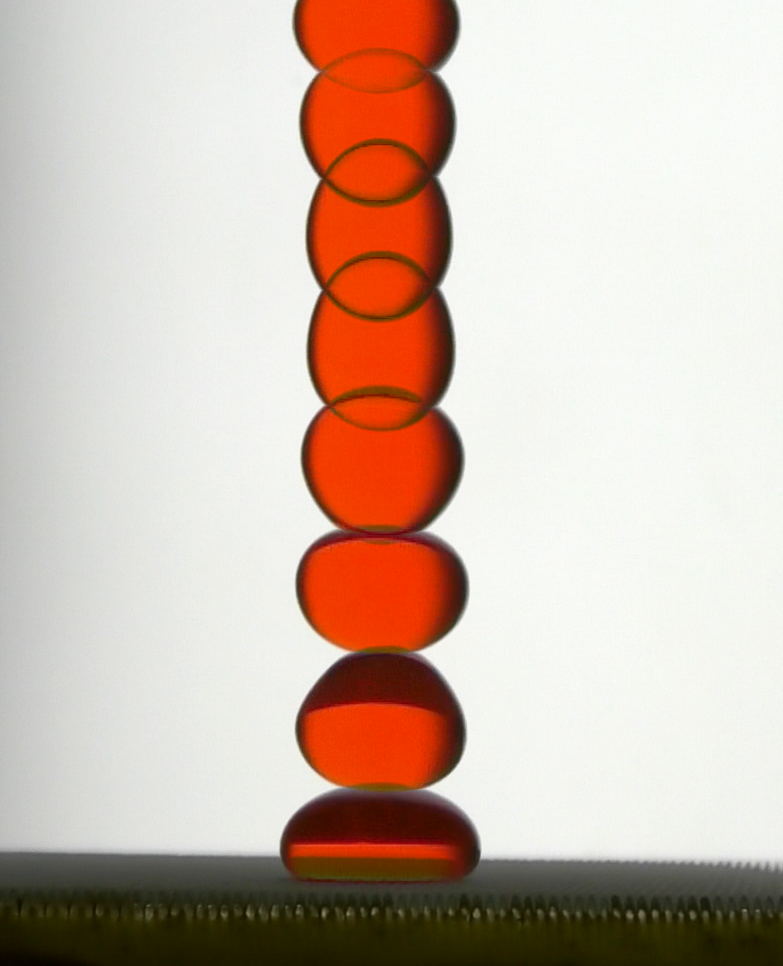
\includegraphics[width=0.75\textwidth]{drop_jump}
\caption{The trajectory of a 0.2 mL spontaneous drop jump is captured in a composite image over a period $\sim 0.67$ s presented at $\approx 10$ Hz. \label{fig:nobounce}}
\end{figure}

The physics of these relatively massive drops (far beyond the 1-$g_0$ millimetric capillary length scale) at once utterly defy terrestrial expectations about the ways in which liquid `should' behave, and also are of critical practical importance to space systems design where examples of such large capillary length scale multiphase flows are commonplace.

\section{Electro-Drop Bounce}
During the `rolling-up' of drops under ideal conditions, the spontaneous jump phenomenon is governed by a balance of inertia and surface tension forces, and once aloft the drop motion is nominally in a regime of pure drag. However, other forces can again come into play. 

We have observed jumped drops to occasionally decelerate and return to the superhydrophobic surface, rebounding multiple times in the fashion of rigid bodies bouncing under 1-$g_0$. The forces at work in such situations are presumably electrostatic in origin. Not without irony given our earlier discussion of underdeveloped low-gravity intuition, we note that though the electro-drop bounce was an accidental effect during our work on spontaneous drop jump, the phenomenon is interesting itself. This has motivated further study, and the `electro-drop bounce' phenomenon is the subject of this thesis. A time-lapsed composite image showing an example of the phenomenon is shown in Figure \ref{fig:bounce}.
\begin{figure}[htb]
\centering
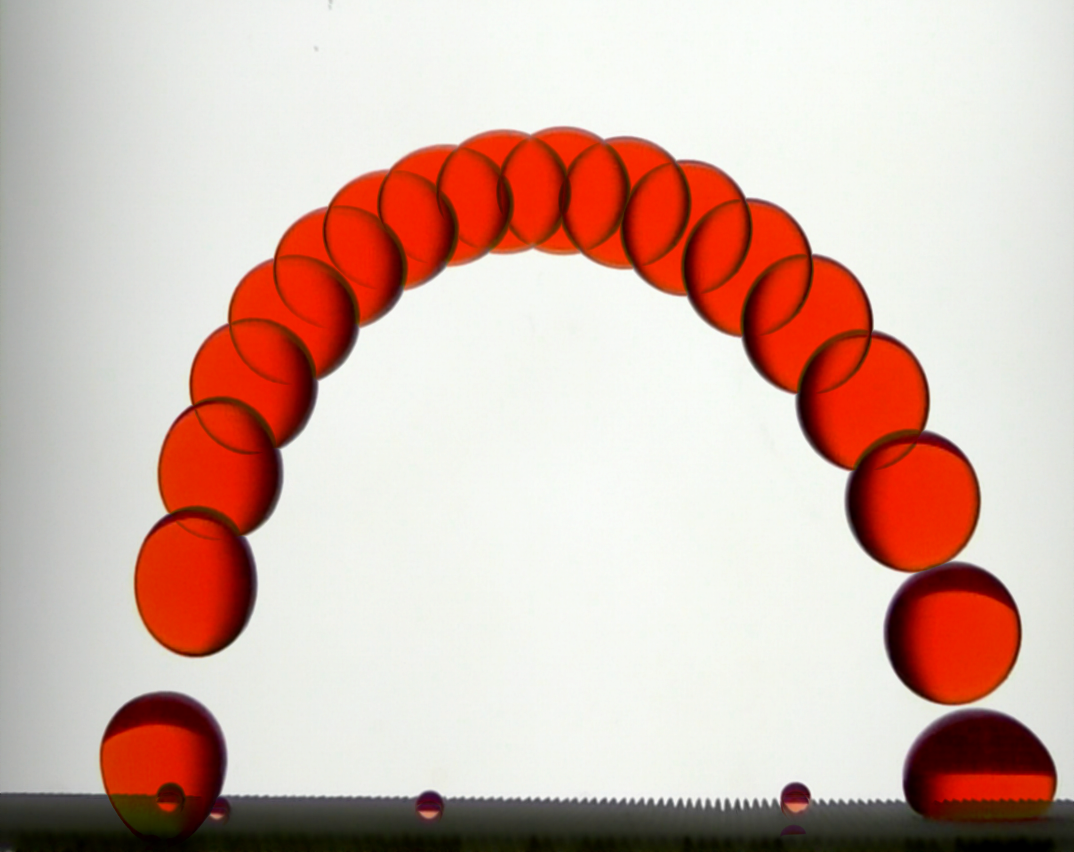
\includegraphics[width=0.75\textwidth]{bounce}
\caption{The trajectory of a 0.5 mL drop is captured in a composite image over a single bounce period ($\sim 1.25$ s). The surface potential of the superhydrophobic dielectric in this example is $\varphi_s = 1.25 \pm 0.41$ kV. \label{fig:bounce}}
\end{figure}

We begin with some preliminary observations of the phenomenon:
\begin{itemize}
\item Observed maximum drop (de-)accelerations are on the order of $\sim$30 cm/s$^2$ for a range of drop volumes $0.03 \lessapprox V_d \lessapprox 0.5$ mL.
\item The water drops are attracted to regions of high electric field. The horizontal (surface plane parallel) components of the drop trajectory usually oscillate about some central position during the experiment (except in cases of nearly pure 1-D vertical translation). For especially small drops close to the spontaneous drop jump limit ($V_d \sim$ 0.01 mL) the drops do not jump, but translate across the surface in a rolling regime until either they reach a local maximum of the electric field, or until their motion is sufficiently damped by contact line hysteresis where pinning ultimately arrests their motion.
\item The drops appear to have net free charge. In cases of multiple simultaneous drop jumps the drops repel each other as they bounce or roll in orbital motion around regions of high field.
\item The magnitude of the drop trajectory maxima (apoapses) appear to be related to the drop volume (mass), and initial jump velocity (inertia), and to the electric field strength.
\end{itemize}

There are several possible origins of the electric charge that are ultimately responsible for this phenomenon. It is well known that water acquires positive free charge when in contact with certain polymers, especially polytetrafluoroethylene (PTFE), through a process called contact charging \cite{langmuir_surface_1938}. PTFE, on the other hand, tends to readily acquire negative charge by contact with water. The superhydrophobic surfaces used in the spontaneous drop jump experiments have thin (nanometric) PTFE coatings, and we observe that it is extremely easy to produce significant surface potentials $\varphi_s \sim$ 100-500 V by simply flowing streams of distilled water over them. A study of this water on PTFE contact charging phenomenon was conducted by Yatsuzuka \emph{et al.} \cite{yatsuzuka_electrification_1994}, who suggest that this process results from formation of an electrical double layer driven by selective adsorption of ($\mbox{OH}^-$) ions at the polymer surface; other recent work strongly supports this hypothesis \cite{beattie_intrinsic_2006, strazdaite_water_2015}. Yatsuzuka \emph{et al.} also found that the specific charge on the drops in contact with the surface depends on their both surface velocity and conductivity. The contact charging mechanism is the most likely accidental source of charge on the suphydrophobic surfaces used in our work. Given the large roughness, or the ratio of projected to actual surface area, of the superhydrophobic surfaces used in the experiment, and given that the drops are initially in a Cassie-Baxter state, a somewhat electrically resistive air layer is maintained that reduces grounding of the drops despite the large potential difference between them and the surface charges. If this electrostatic potential is greater than the release of surface energy under the sudden change in $\mathbb{B}\mbox{o}$, in the form of the drop kinetic energy, we expect that the drop will return to an equilibrium state on the charged surface which minimizes the potential.

The source of the net free charge on the drops is another issue. The drop charge could also be due to the contact charging mechanism mentioned previously. For instance, in a 1996 paper, NASA flight engineer Don Pettit discusses the problem of low-gravity flow induced charging of liquids, resulting ultimately from contact charging phenomenon \cite{pettit_donald_flow_????}. Another mechanism for the drop charge is field-induced charging. Field-induced charging occurs due to physical breakup of a conductor having a field-induced dipole (e.g., a physical separation of charge). In our work this might occur when a drop is deposited on the charged surface by a grounded syringe. The metal syringe needle tip, and the liquid in the syringe itself are essentially a ground connection which is broken when the syringe is suddenly removed in the presence of an external electric field. Field-induced charging is at work in the famous Kelvin thunderstorm, and is applied in inkjet, and electrospay technologies, where in each case the breakup is by the Rayleigh-Plateau instability. Notably, in Pettit's aforementioned discussion of contact charging of liquids in low-g, he remarks on accidental electrostatic `hula-ing' of silicone oil drops when ejected from a syringe in the vicinity of a highly-charged polymer surface during an experiment conducted aboard STS-5 by mission specialist Joseph Allen \cite{pettit_donald_flow_????}. Depending on the (highly-variable) electrical conductivity of the silicone oil, and the material of the syringe used in the experiment, the charge could arise just as easily by field-induction as by contact charging. Relatedly, in a series of informal and somewhat whimsical experiments Pettit himself electrostatically orbited small water drops around a triboelectrically charged PTFE knitting needle while aboard ISS during expedition 30/31 \cite{stevenson_electrostatic_2015}. Again, in this case, the drop charge is likely field-induced.  

\section{Applications}
This study of the electro-drop bounce phenomenon may have results which can be extended to useful applications in a space environment. External surfaces of spacecraft tend to become charged with time due to the space environment itself. Surface charging largely occurs due to low energy electrons (3-50 keV) which do not penetrate the external surface of the spacecraft \cite{czepiela_charging_1997}. The ultimate sources of these charges are trapped charged particles of the van Allen radiation belts, galactic cosmic rays, and the solar wind. This deposited charge accumulates and can lead to significant potential differences between parts of a spacecraft, sometimes leading to breakdown and discharge called Paschen discharge. Deep dielectric charging occurs when higher energy charged particles penetrate the surface of a dielectric material, which can also lead to large potential differences if the dielectric leakage is lower than the external charging rate. In a fluid mechanical context, this accumulated charge could be problematic during any multiphase venting process, as might be expected to occur during autonomous satellite servicing refueling operations, or during boil-off venting of cryogens stored over long periods in a space environment (as in many crewed Mars mission scenarios, or in cryogenic propellant depot operations). Such venting, if occurring in a region of strong field, will also tend to produce a stream of charged drops, which will be decelerated by the field, causing their eventual return, impacting and potentially contaminating the spacecraft surfaces.

As previously noted, robust phase separation is critical to high reliability multiphase systems used in thermal control and life support. Active solid-state phase separation for life support multiphase flows, especially high void-fraction droplet disperse flows is a possible application of this work. Such flows are encountered in dish washing, laundry, waste solids drying, food processing, the Sabatier CO$_2$ reaction, and possibly in vapor-compression cycle condensers. Phase separation for other droplet disperse flows include electrostatic droplet separators for high-efficiency Rankine-cycle turbines, which require a droplet-free vapor phase entering the turbine, but where conventional superheat approaches come with severe mass penalties \cite{unterberg_zero_1962}. More speculatively, results of this work could be applied in high temperature liquid droplet radiators with electrostatic collection \cite{white_liquid_1987}. Removal of satellite droplets produced during pipetting in wet-lab research outside of a glovebox environment aboard ISS has also been recently suggested as a application of the work [private communication, NASA JSC, E. Unger, 2017]. Drops can become spontaneously charged by contact with standard micropipette tips \cite{choi_spontaneous_2013}, and this free charge can possibly be leveraged for the purposes of phase separation in low-gravity. 

\section{Overview of this Thesis}
In this thesis we develop and partly validate a simple model to aid in design of future electrostatic disperse drop phase separators. To this end the work encompasses (1) a mathematical model of the electro-drop bounce, its scale analysis, asymptotic estimates for drop apoapses and times-of-flight, and (2) the results of controlled experiments, where the effect of the key independent variables of drop volume $V_d$ and dielectric surface charge density $\sigma$ on drop trajectories is tested. 

\chapter{Theory}
\section{Equation of Motion}
We develop here a simple 1-dimensional model of the dynamics of drops dominated by electrostatic forces. We treat a drop as a particle with radius $R_d$, which translates vertically along the central axis of a charged dielectric square sheet substrate with initial velocity $U_0$. The equation of motion for this system is given by,
\begin{equation}
m y'' = - \mathbf{F}_D - \mathbf{F}_E,
\label{gov_eqn}
\end{equation}
subject to
\begin{equation}
y(0) = R_d, \hspace{5 mm} \mbox{and} \hspace{5 mm} y'(0) = U_0,
\end{equation}
where $m$ is the drop mass, $y'' = \frac{d^2 y}{d t^2}$ is the drop acceleration, $\mathbf{F}_D$ is the drag force which always opposes motion, and $\mathbf{F}_E$ is the electrostatic force. The assumed initial conditions are such that, when $\mathbb{B}\mbox{o}$ is suddenly reduced at the start of the drop tower free-fall period, the drop jumps with instantaneous initial velocity $U_0$ from its 1-$g_0$ resting position with fixed radius $R_d$ at $t=0$. The dynamical system is sketched schematically Figure \ref{apparatus}. We now define models for each of the forces in this equation.

\begin{figure}[ht]
\centering
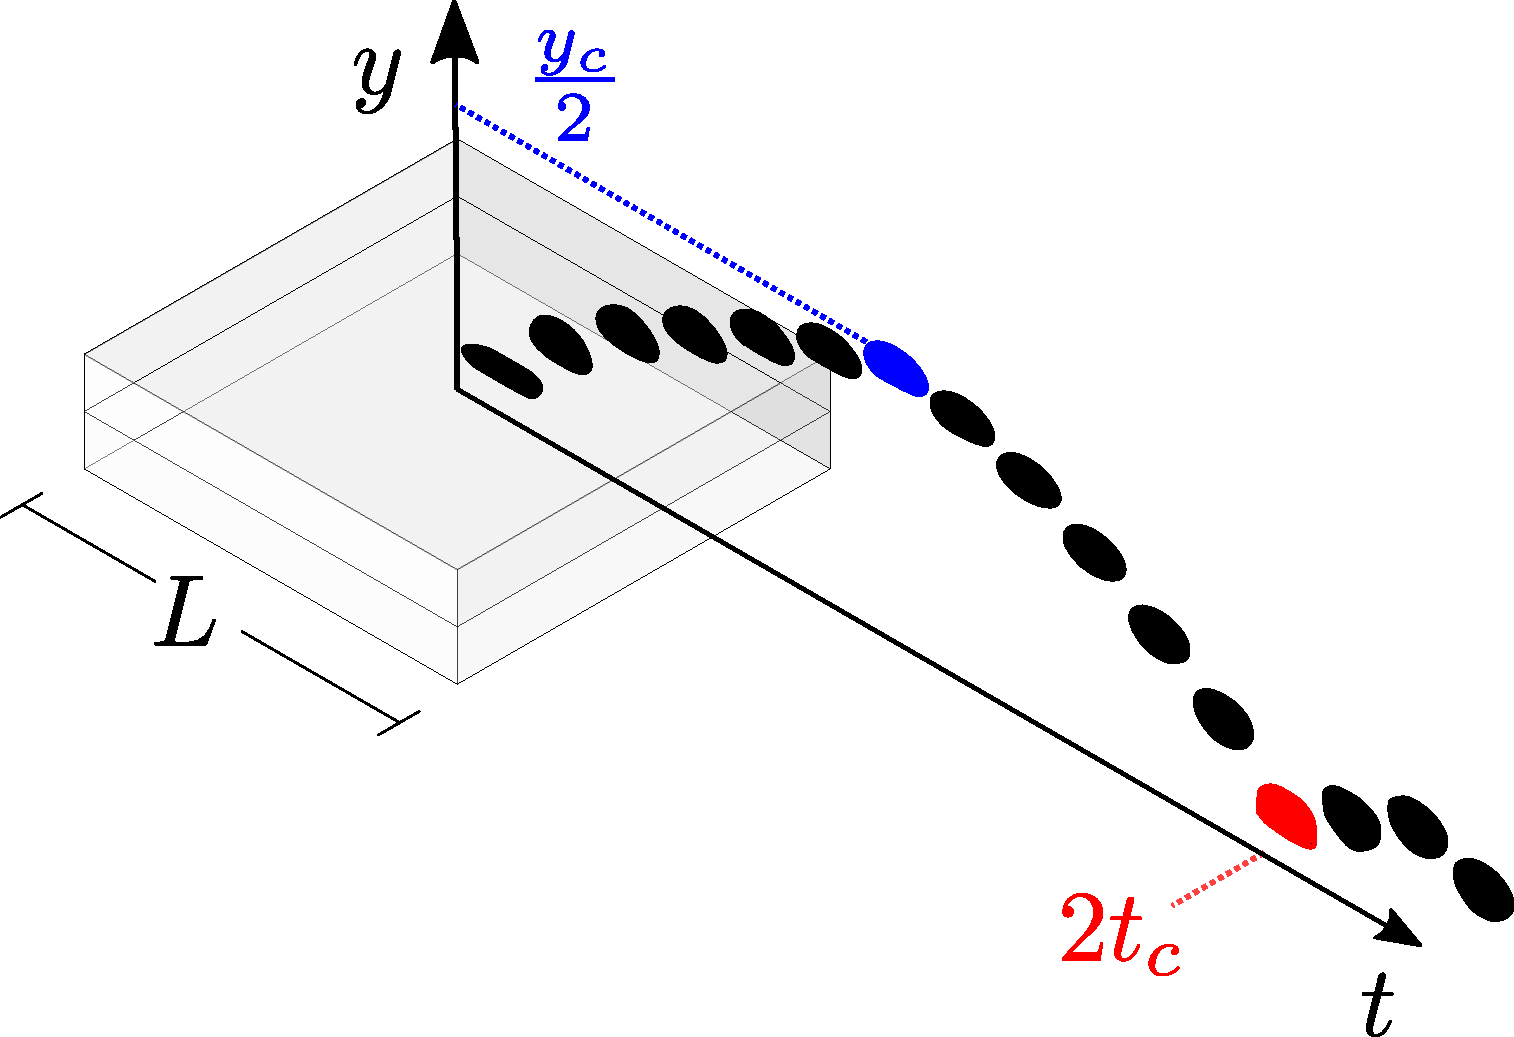
\includegraphics[width=0.65\textwidth]{../figures/apparatus0.pdf}
\label{apparatus}
\caption{Schematic representation of drop jump with return and rebound from an electrically charged superhydrophobic substrate. The characteristic time and length scales $t_c$ and $y_c$ describe the time of flight and apoapse associated with the drop trajectory.}
\end{figure}

For the intermediate range of Reynolds numbers $1 \leq \mathbb{R}\mbox{e} \equiv \frac{2UR_d}{\nu} \leq 2000 $ observed in our experiments, the force of drag acting on the drop may be quadratic such that,
\begin{equation*}\label{drag_force}
\mathbf{F}_D = \frac{1}{2}C_D \rho A {y'}^2,
\end{equation*}
where $C_D$ is the drag coefficient, $\rho$ is the density of the air host fluid, and $A$ is the frontal projected area of the drop. For this range of Reynolds numbers the drag coefficient may be approximated by the well known Abraham correlation \cite{abraham_functional_1970},
\[C_D = \frac{24}{9.06^2} \left( 1 + \frac{9.06}{\sqrt{\mathbb{R}\mbox{e}}} \right)^2 .\]

Modeling the electrostatic force is more involved, but we begin with the standard electrohydrodynamic (EHD) approximation \cite{saville_electrohydrodynamics:_1997}. Under a DC electric field, we assume that the real part of the dielectric permittivity $\epsilon$, $\mbox{Re} \left( \epsilon \right) \approx  \mbox{constant}$. We also assume that electric currents are small enough that the effects of magnetic fields can be neglected. The validity of this assumption rests on the characteristic time scale $\tau_e = \epsilon /\sigma_e \ll 1$, where $\tau_e$ is the ratio of absolute dielectric permittivity $\epsilon = \kappa \epsilon_0$, to conductivity $\sigma_e$, of the medium, $\kappa$ is the relative dielectric permittivity, and $\epsilon_0$ is the vacuum permittivity. This characteristic time $\tau_e$ is also known as the relaxation time, and is a measure of how quickly the polarization of a dielectric responds to a change in electric field. Given the conductivity and permittivity in the limiting case of extremely-pure water ($ \epsilon \sim 80$, $\sigma_e = 18.2 \times 10^{6}$ $\Omega\mbox{cm}$) \cite{yatsuzuka_electrification_1994}, we estimate $\tau_e \approx 4 \times 10^{-6}$ s. The relaxation time for the common distilled water that is actually used in the drop experiments is undoubtedly shorter due to the presence of solvated ions. Neglecting the effects of an electric double layer on hydration of ions in the water or the ambient atmosphere due to the relatively massive size of the drops studied, the assumption of small relaxation time further implies that the free charge present in the drops will remain approximately constant during the typical time interval of a low-gravity experiment.

Supposing that electrical forces acting on free charges and dipoles in a fluid are transferred directly to the fluid itself, the overall electrical body force will be the divergence of the Maxwell stress tensor $\tau_m $,
\[ \mathbf{F}_E = \nabla \cdot \tau_m = \nabla \cdot \left( \epsilon \mathbf{E} \mathbf{E} - \frac{1}{2} \epsilon \mathbf{E} \cdot \mathbf{E} \delta \right) ,\]
where $\mathbf{F}_E$ is the electric body force per unit volume, and $\delta$ is the Dirac delta function. The product of the electric field vectors is the dyadic product.  

The Korteweg-Helmholtz volumetric force density formulation of the Maxwell stress tensor is usually expressed as \cite{melcher_continuum_????}
\begin{equation}\label{force_density}
\mathbf{F}_E = \rho_f \mathbf{E} + \frac{1}{2} \left| E \right|^2 \nabla \epsilon - \nabla \left( \frac{1}{2} \rho \left( \frac{\partial \epsilon}{\partial \rho} \right)_T \left| E \right|^2 \right) .
\end{equation}
The first term on the right hand side of this expression is the well known Coulombic force or electrophoretic force, which arises from the presence of free charge in an external electric field. We expect this term to dominate the electric force in a DC field. The second term is the force arising from polarization stresses due to a nonuniform field acting across a gradient in permittivity. This force is widely termed the dielectrophoretic (DEP) force. The third term describes forces due to electrostriction. It has been noted by Melcher and Hurwitz \cite{hurwitz_electrohydrodynamic_1966} that the electrostriction term is the gradient of a scalar and can thus be canonically lumped together with the hydrostatic pressure for incompressible fluids. We neglect it in our analysis. 

It is common to approximate the polarization stress by idealizing the drop as a simple dipole using the effective dipole moment method first described by Pohl in 1958 \cite{pohl_effects_1958}. This approach has since been related back to the force density by the volumetric integration of the force density with the substitution of a Taylor series expansion of $\mathbf{E}$ in the limit of a small radial gradient of the field within the dielectric sphere \cite{wang_general_1997}. The DEP force arises due to the induced or permanent dipole moment of polarizable media which has a tendency to align the dipole with the electric field. If there is a gradient in the field then for a finite separation of charge, one end of the dipole will feel a stronger electric field than the other resulting in a net force. Whether the force is positive or negative in the direction of the electric field gradient depends on the difference of dielectric permittivites between the fluids, rather than on the polarity of $\mathbf{E}$. In principle an external electric field will tend to induce a dipole in a dielectric material, but if the field is spatially uniform there is no gradient in the field and the forces felt by the dipoles are symmetric with no net force. The dipole moment $\mu$ of a spherical linear-dielectric particle immersed in a dielectric medium is given by
\begin{equation} \label{dipole_m_1}
\mu = V_d \mathbf{P} = \frac{4}{3} \pi R_d^3 \mathbf{P},
\end{equation} 
where $\mathbf{P} = \left(\kappa_a - 1 \right) \epsilon_0 \mathbf{E} = \chi_e \epsilon_0 \mathbf{E}$ is the polarization moment, $R_d$ is the particle radius, $\kappa_a = \frac{\epsilon_a}{\epsilon_0}$ is the relative dielectric constant of the air host fluid, and $\chi_e = \kappa_a - 1$ is the electric susceptibility of the host fluid. The force felt by the dipole is 
\begin{eqnarray} \label{dep_force}
\mathbf{F}_{DEP} &=& \left( \mathbf{P}_e \cdot \nabla \right) \mathbf{E} \nonumber \\
&=& 2 \pi R_d^3 \kappa_w \epsilon_0 K \nabla E^2,
\end{eqnarray}
where $\mathbf{P}_e=(\kappa_w - \kappa_a)\epsilon_0 \mathbf{E}$ is the excess polarization and $\kappa_w$ is the relative dielectric constant of the water particle. Here it is convenient to use the simplifying shorthand $K = \frac{\kappa_w - \kappa_a}{\kappa_w + 2 \kappa_a}$, known as the Clausius-Mossotti factor. In cases where $K <$ 0, or $K>$ 0 the particle will be either repelled or attracted to regions of strong field. In our experiment, choosing the relative dielectric constants $\kappa_a \approx$ 1 and $\kappa_w \approx$ 80, we estimate $K \approx$ 0.96. It is important to note that the equivalent dipole approximation critically requires an assumption of small physical scale of the particle relative to the length scale of nonuniformity of the field, which in this case we take to be the length of the charged superhydrophobic surface, $L =$ 25 mm $\gg R_d \approx$ 2 mm.

When the drop is close to the dielectric surface, the free charge on the drop will tend to induce polarization of the dielectric which perturbs the electric field. The polarization bound charge in the dielectric will be of the opposite sign of the free drop charge and thus there will be a force of attraction. This so-called image force is a correction to the Coulomb force due to the external electric field only, and can be found by a Green's Function solution of Laplace's equation for the electric field called the `method of images' \cite{david_j._griffiths_introduction_1999}. This resulting image force $\mathbf{F}_I$ is given by
\begin{equation}
\mathbf{F}_I = \frac{k q^2}{16 \pi \epsilon_0} y^{-2} \hat{\mathbf{j}},
\label{image_force}
\end{equation}
where the factor $k$ is a function of the dielectric surface susceptibility $k = \frac{\chi_e}{\chi_e + 2}$, and $\hat{\mathbf{j}}$ is a unit vector normal to the dielectric surface.

By substituting Equations \ref{dep_force}, and \ref{image_force} into \ref{force_density} we have
\begin{eqnarray*}
 \mathbf{F}_E &=& q \mathbf{E} + \mathbf{F}_{DEP} + \mathbf{F}_I \\
 &=& q \mathbf{E} + \frac{k q^2}{16 \pi \epsilon_0 } y^{-2} \hat{\mathbf{j}} + 2 \pi R_d^3 \kappa_w \epsilon_0 K \nabla E^2, 
\end{eqnarray*}
and the 1-D governing equation becomes
\begin{equation}
 \label{gov_eqn_subs}
m y'' = - \frac{1}{2} C_D \rho A {y'}^2 - q E - \frac{k q^2}{16 \pi \epsilon_0} y^{-2}- 2 \pi R_d^3 \kappa_w \epsilon_0 K \nabla E^2,
\end{equation}
subject to
\begin{equation}
y(0) = R, \hspace{5 mm} \mbox{and} \hspace{5 mm} y'(0) = U_0 .
\end{equation}

By comparing DEP and Coulombic terms in Equation \ref{gov_eqn_subs}, we note that a condition to neglect the DEP force is
\begin{eqnarray}
\frac{ \kappa_w \epsilon_0 K R_d^2 E_0}{q} \ll 1. \nonumber
\end{eqnarray}
As this condition likely prevails in our experiments we henceforth neglect the DEP force. There is some physical intuition to support this conclusion as well. The dielectric displacement $\mathbf{D} = \kappa \epsilon_0 \mathbf{E}$ of a water drop in air is high due to its large relative dielectric constant. This implies that the field strength within the drop is about 80 times smaller than in the surrounding medium, which is essentially the same as a vacuum from a dielectric standpoint. Thus it is not particularly inaccurate to model the dielectric volume of a drop as an equipotential conductive shell with zero field in its interior. As an aside, in treating the drop as an ideal conductor we note that in our specific case the electrostatic force is not a body force \emph{per se} as the electric field is acting on charges on the surface of the conductor.

\section{The Electric Field}
If we consider the charged dielectric surface of our experiments to be a square sheet of charge lying in the $xz$-plane with width $L$, the symmetry of the problem happily lets us obtain the $y$-component of the electric field $\mathbf{E}$ by direct integration. In particular, it is easy to construct the electric field due to a finite plane of charge by superposition of the electric fields of a series of line charges. By symmetry, the electric field points along the $y$-axis; for a point along the $y$-axis the position vector is $\mathbf{r} = \left( x^2 + y^2 \right)^{1/2} \hat{\mathbf{r}}$ to the center of a line charge in the $xz$-plane. The $y$-component of $d\mathbf{E}$ is found by $d E_r = d E_y \cos \theta = d E_y y/ r$, where $\theta$ is the angle made between the $y$-axis and the position vector $\mathbf{r}$. If the charge in a line element $dx$ is $\sigma L dx$, where $\sigma$ is the average surface charge density, the electric field of a line charge is given by \cite{david_j._griffiths_introduction_1999}
\[d E_r = \frac{\sigma L dx}{4 \pi \epsilon_0 r \sqrt{r^2 + L^2/4}}.
\]
The $y$-component of the electric field $E_y$, hence $E$, is then
\[ E = \frac{\sigma L y }{4 \pi \epsilon_0} \int^{L/2}_{-L/2} \frac{1}{(y^2 + x^2) \sqrt{y^2 + x^2 + L^2/4}} dx 
.\]
With some substitutions the above can be integrated to obtain an expression for the electric field in terms of $y$, 
\begin{equation}
\label{e_field}
E = \frac{\sigma}{ \pi \epsilon_0} \tan^{-1} \left( \frac{L^2}{y \sqrt{2L^2 + 4y^2}}\right)
.\end{equation}
We note that this model of the electric field is valid when $R_d \ll L$, which will be true for cases of small drops `far' from the dielectric surface. For accurate models of the field in the case $R_d/L \sim \mathcal{O}(1)$ we likely need to numerically solve Laplace's equation for the electric potential $\varphi$,
\[ - \nabla^2 \varphi = 0.\]

By taking Taylor series expansions in large and small limits we can intuit a bit about the behavior of this field. In the limit $y/L \ll 1$ Equation \ref{e_field} reduces to
\begin{equation}
\label{near_field}
E \approx \frac{\sigma}{4 \pi \epsilon_0} = E_0,
\end{equation}
where $E_0$ is the characteristic electric field given by $E_0 = \frac{\sigma}{4 \pi \epsilon_0}$. This field is constant and equivalent to the electric field due to an infinite plane of charge. In the limit of $y/L \gg 1$, Equation \ref{e_field} reduces to the familiar electric field due to a point charge
\begin{equation}
\label{far_field}
E \approx L^2 E_0 y^{-2}.
\end{equation}
Both regimes given by Equations \ref{near_field} and \ref{far_field} can be clearly seen in Figure \ref{fig:E0}.
\begin{figure}[h]
    \centering
    \def\svgwidth{\columnwidth}
    %% Creator: Matplotlib, PGF backend
%%
%% To include the figure in your LaTeX document, write
%%   \input{<filename>.pgf}
%%
%% Make sure the required packages are loaded in your preamble
%%   \usepackage{pgf}
%%
%% Figures using additional raster images can only be included by \input if
%% they are in the same directory as the main LaTeX file. For loading figures
%% from other directories you can use the `import` package
%%   \usepackage{import}
%% and then include the figures with
%%   \import{<path to file>}{<filename>.pgf}
%%
%% Matplotlib used the following preamble
%%   \usepackage{fontspec}
%%   \setmainfont{DejaVu Serif}
%%   \setsansfont{DejaVu Sans}
%%   \setmonofont{DejaVu Sans Mono}
%%
\begingroup%
\makeatletter%
\begin{pgfpicture}%
\pgfpathrectangle{\pgfpointorigin}{\pgfqpoint{5.698771in}{3.862421in}}%
\pgfusepath{use as bounding box, clip}%
\begin{pgfscope}%
\pgfsetbuttcap%
\pgfsetmiterjoin%
\definecolor{currentfill}{rgb}{1.000000,1.000000,1.000000}%
\pgfsetfillcolor{currentfill}%
\pgfsetlinewidth{0.000000pt}%
\definecolor{currentstroke}{rgb}{1.000000,1.000000,1.000000}%
\pgfsetstrokecolor{currentstroke}%
\pgfsetdash{}{0pt}%
\pgfpathmoveto{\pgfqpoint{0.000000in}{0.000000in}}%
\pgfpathlineto{\pgfqpoint{5.698771in}{0.000000in}}%
\pgfpathlineto{\pgfqpoint{5.698771in}{3.862421in}}%
\pgfpathlineto{\pgfqpoint{0.000000in}{3.862421in}}%
\pgfpathclose%
\pgfusepath{fill}%
\end{pgfscope}%
\begin{pgfscope}%
\pgfsetbuttcap%
\pgfsetmiterjoin%
\definecolor{currentfill}{rgb}{1.000000,1.000000,1.000000}%
\pgfsetfillcolor{currentfill}%
\pgfsetlinewidth{0.000000pt}%
\definecolor{currentstroke}{rgb}{0.000000,0.000000,0.000000}%
\pgfsetstrokecolor{currentstroke}%
\pgfsetstrokeopacity{0.000000}%
\pgfsetdash{}{0pt}%
\pgfpathmoveto{\pgfqpoint{0.913771in}{0.707421in}}%
\pgfpathlineto{\pgfqpoint{5.563771in}{0.707421in}}%
\pgfpathlineto{\pgfqpoint{5.563771in}{3.727421in}}%
\pgfpathlineto{\pgfqpoint{0.913771in}{3.727421in}}%
\pgfpathclose%
\pgfusepath{fill}%
\end{pgfscope}%
\begin{pgfscope}%
\pgfsetbuttcap%
\pgfsetroundjoin%
\definecolor{currentfill}{rgb}{0.000000,0.000000,0.000000}%
\pgfsetfillcolor{currentfill}%
\pgfsetlinewidth{0.803000pt}%
\definecolor{currentstroke}{rgb}{0.000000,0.000000,0.000000}%
\pgfsetstrokecolor{currentstroke}%
\pgfsetdash{}{0pt}%
\pgfsys@defobject{currentmarker}{\pgfqpoint{0.000000in}{-0.048611in}}{\pgfqpoint{0.000000in}{0.000000in}}{%
\pgfpathmoveto{\pgfqpoint{0.000000in}{0.000000in}}%
\pgfpathlineto{\pgfqpoint{0.000000in}{-0.048611in}}%
\pgfusepath{stroke,fill}%
}%
\begin{pgfscope}%
\pgfsys@transformshift{2.445783in}{0.707421in}%
\pgfsys@useobject{currentmarker}{}%
\end{pgfscope}%
\end{pgfscope}%
\begin{pgfscope}%
\pgftext[x=2.445783in,y=0.610199in,,top]{\rmfamily\fontsize{16.000000}{19.200000}\selectfont \(\displaystyle 10^{-1}\)}%
\end{pgfscope}%
\begin{pgfscope}%
\pgfsetbuttcap%
\pgfsetroundjoin%
\definecolor{currentfill}{rgb}{0.000000,0.000000,0.000000}%
\pgfsetfillcolor{currentfill}%
\pgfsetlinewidth{0.803000pt}%
\definecolor{currentstroke}{rgb}{0.000000,0.000000,0.000000}%
\pgfsetstrokecolor{currentstroke}%
\pgfsetdash{}{0pt}%
\pgfsys@defobject{currentmarker}{\pgfqpoint{0.000000in}{-0.048611in}}{\pgfqpoint{0.000000in}{0.000000in}}{%
\pgfpathmoveto{\pgfqpoint{0.000000in}{0.000000in}}%
\pgfpathlineto{\pgfqpoint{0.000000in}{-0.048611in}}%
\pgfusepath{stroke,fill}%
}%
\begin{pgfscope}%
\pgfsys@transformshift{4.070370in}{0.707421in}%
\pgfsys@useobject{currentmarker}{}%
\end{pgfscope}%
\end{pgfscope}%
\begin{pgfscope}%
\pgftext[x=4.070370in,y=0.610199in,,top]{\rmfamily\fontsize{16.000000}{19.200000}\selectfont \(\displaystyle 10^{0}\)}%
\end{pgfscope}%
\begin{pgfscope}%
\pgfsetbuttcap%
\pgfsetroundjoin%
\definecolor{currentfill}{rgb}{0.000000,0.000000,0.000000}%
\pgfsetfillcolor{currentfill}%
\pgfsetlinewidth{0.602250pt}%
\definecolor{currentstroke}{rgb}{0.000000,0.000000,0.000000}%
\pgfsetstrokecolor{currentstroke}%
\pgfsetdash{}{0pt}%
\pgfsys@defobject{currentmarker}{\pgfqpoint{0.000000in}{-0.027778in}}{\pgfqpoint{0.000000in}{0.000000in}}{%
\pgfpathmoveto{\pgfqpoint{0.000000in}{0.000000in}}%
\pgfpathlineto{\pgfqpoint{0.000000in}{-0.027778in}}%
\pgfusepath{stroke,fill}%
}%
\begin{pgfscope}%
\pgfsys@transformshift{1.310245in}{0.707421in}%
\pgfsys@useobject{currentmarker}{}%
\end{pgfscope}%
\end{pgfscope}%
\begin{pgfscope}%
\pgfsetbuttcap%
\pgfsetroundjoin%
\definecolor{currentfill}{rgb}{0.000000,0.000000,0.000000}%
\pgfsetfillcolor{currentfill}%
\pgfsetlinewidth{0.602250pt}%
\definecolor{currentstroke}{rgb}{0.000000,0.000000,0.000000}%
\pgfsetstrokecolor{currentstroke}%
\pgfsetdash{}{0pt}%
\pgfsys@defobject{currentmarker}{\pgfqpoint{0.000000in}{-0.027778in}}{\pgfqpoint{0.000000in}{0.000000in}}{%
\pgfpathmoveto{\pgfqpoint{0.000000in}{0.000000in}}%
\pgfpathlineto{\pgfqpoint{0.000000in}{-0.027778in}}%
\pgfusepath{stroke,fill}%
}%
\begin{pgfscope}%
\pgfsys@transformshift{1.596321in}{0.707421in}%
\pgfsys@useobject{currentmarker}{}%
\end{pgfscope}%
\end{pgfscope}%
\begin{pgfscope}%
\pgfsetbuttcap%
\pgfsetroundjoin%
\definecolor{currentfill}{rgb}{0.000000,0.000000,0.000000}%
\pgfsetfillcolor{currentfill}%
\pgfsetlinewidth{0.602250pt}%
\definecolor{currentstroke}{rgb}{0.000000,0.000000,0.000000}%
\pgfsetstrokecolor{currentstroke}%
\pgfsetdash{}{0pt}%
\pgfsys@defobject{currentmarker}{\pgfqpoint{0.000000in}{-0.027778in}}{\pgfqpoint{0.000000in}{0.000000in}}{%
\pgfpathmoveto{\pgfqpoint{0.000000in}{0.000000in}}%
\pgfpathlineto{\pgfqpoint{0.000000in}{-0.027778in}}%
\pgfusepath{stroke,fill}%
}%
\begin{pgfscope}%
\pgfsys@transformshift{1.799295in}{0.707421in}%
\pgfsys@useobject{currentmarker}{}%
\end{pgfscope}%
\end{pgfscope}%
\begin{pgfscope}%
\pgfsetbuttcap%
\pgfsetroundjoin%
\definecolor{currentfill}{rgb}{0.000000,0.000000,0.000000}%
\pgfsetfillcolor{currentfill}%
\pgfsetlinewidth{0.602250pt}%
\definecolor{currentstroke}{rgb}{0.000000,0.000000,0.000000}%
\pgfsetstrokecolor{currentstroke}%
\pgfsetdash{}{0pt}%
\pgfsys@defobject{currentmarker}{\pgfqpoint{0.000000in}{-0.027778in}}{\pgfqpoint{0.000000in}{0.000000in}}{%
\pgfpathmoveto{\pgfqpoint{0.000000in}{0.000000in}}%
\pgfpathlineto{\pgfqpoint{0.000000in}{-0.027778in}}%
\pgfusepath{stroke,fill}%
}%
\begin{pgfscope}%
\pgfsys@transformshift{1.956733in}{0.707421in}%
\pgfsys@useobject{currentmarker}{}%
\end{pgfscope}%
\end{pgfscope}%
\begin{pgfscope}%
\pgfsetbuttcap%
\pgfsetroundjoin%
\definecolor{currentfill}{rgb}{0.000000,0.000000,0.000000}%
\pgfsetfillcolor{currentfill}%
\pgfsetlinewidth{0.602250pt}%
\definecolor{currentstroke}{rgb}{0.000000,0.000000,0.000000}%
\pgfsetstrokecolor{currentstroke}%
\pgfsetdash{}{0pt}%
\pgfsys@defobject{currentmarker}{\pgfqpoint{0.000000in}{-0.027778in}}{\pgfqpoint{0.000000in}{0.000000in}}{%
\pgfpathmoveto{\pgfqpoint{0.000000in}{0.000000in}}%
\pgfpathlineto{\pgfqpoint{0.000000in}{-0.027778in}}%
\pgfusepath{stroke,fill}%
}%
\begin{pgfscope}%
\pgfsys@transformshift{2.085370in}{0.707421in}%
\pgfsys@useobject{currentmarker}{}%
\end{pgfscope}%
\end{pgfscope}%
\begin{pgfscope}%
\pgfsetbuttcap%
\pgfsetroundjoin%
\definecolor{currentfill}{rgb}{0.000000,0.000000,0.000000}%
\pgfsetfillcolor{currentfill}%
\pgfsetlinewidth{0.602250pt}%
\definecolor{currentstroke}{rgb}{0.000000,0.000000,0.000000}%
\pgfsetstrokecolor{currentstroke}%
\pgfsetdash{}{0pt}%
\pgfsys@defobject{currentmarker}{\pgfqpoint{0.000000in}{-0.027778in}}{\pgfqpoint{0.000000in}{0.000000in}}{%
\pgfpathmoveto{\pgfqpoint{0.000000in}{0.000000in}}%
\pgfpathlineto{\pgfqpoint{0.000000in}{-0.027778in}}%
\pgfusepath{stroke,fill}%
}%
\begin{pgfscope}%
\pgfsys@transformshift{2.194131in}{0.707421in}%
\pgfsys@useobject{currentmarker}{}%
\end{pgfscope}%
\end{pgfscope}%
\begin{pgfscope}%
\pgfsetbuttcap%
\pgfsetroundjoin%
\definecolor{currentfill}{rgb}{0.000000,0.000000,0.000000}%
\pgfsetfillcolor{currentfill}%
\pgfsetlinewidth{0.602250pt}%
\definecolor{currentstroke}{rgb}{0.000000,0.000000,0.000000}%
\pgfsetstrokecolor{currentstroke}%
\pgfsetdash{}{0pt}%
\pgfsys@defobject{currentmarker}{\pgfqpoint{0.000000in}{-0.027778in}}{\pgfqpoint{0.000000in}{0.000000in}}{%
\pgfpathmoveto{\pgfqpoint{0.000000in}{0.000000in}}%
\pgfpathlineto{\pgfqpoint{0.000000in}{-0.027778in}}%
\pgfusepath{stroke,fill}%
}%
\begin{pgfscope}%
\pgfsys@transformshift{2.288344in}{0.707421in}%
\pgfsys@useobject{currentmarker}{}%
\end{pgfscope}%
\end{pgfscope}%
\begin{pgfscope}%
\pgfsetbuttcap%
\pgfsetroundjoin%
\definecolor{currentfill}{rgb}{0.000000,0.000000,0.000000}%
\pgfsetfillcolor{currentfill}%
\pgfsetlinewidth{0.602250pt}%
\definecolor{currentstroke}{rgb}{0.000000,0.000000,0.000000}%
\pgfsetstrokecolor{currentstroke}%
\pgfsetdash{}{0pt}%
\pgfsys@defobject{currentmarker}{\pgfqpoint{0.000000in}{-0.027778in}}{\pgfqpoint{0.000000in}{0.000000in}}{%
\pgfpathmoveto{\pgfqpoint{0.000000in}{0.000000in}}%
\pgfpathlineto{\pgfqpoint{0.000000in}{-0.027778in}}%
\pgfusepath{stroke,fill}%
}%
\begin{pgfscope}%
\pgfsys@transformshift{2.371446in}{0.707421in}%
\pgfsys@useobject{currentmarker}{}%
\end{pgfscope}%
\end{pgfscope}%
\begin{pgfscope}%
\pgfsetbuttcap%
\pgfsetroundjoin%
\definecolor{currentfill}{rgb}{0.000000,0.000000,0.000000}%
\pgfsetfillcolor{currentfill}%
\pgfsetlinewidth{0.602250pt}%
\definecolor{currentstroke}{rgb}{0.000000,0.000000,0.000000}%
\pgfsetstrokecolor{currentstroke}%
\pgfsetdash{}{0pt}%
\pgfsys@defobject{currentmarker}{\pgfqpoint{0.000000in}{-0.027778in}}{\pgfqpoint{0.000000in}{0.000000in}}{%
\pgfpathmoveto{\pgfqpoint{0.000000in}{0.000000in}}%
\pgfpathlineto{\pgfqpoint{0.000000in}{-0.027778in}}%
\pgfusepath{stroke,fill}%
}%
\begin{pgfscope}%
\pgfsys@transformshift{2.934832in}{0.707421in}%
\pgfsys@useobject{currentmarker}{}%
\end{pgfscope}%
\end{pgfscope}%
\begin{pgfscope}%
\pgfsetbuttcap%
\pgfsetroundjoin%
\definecolor{currentfill}{rgb}{0.000000,0.000000,0.000000}%
\pgfsetfillcolor{currentfill}%
\pgfsetlinewidth{0.602250pt}%
\definecolor{currentstroke}{rgb}{0.000000,0.000000,0.000000}%
\pgfsetstrokecolor{currentstroke}%
\pgfsetdash{}{0pt}%
\pgfsys@defobject{currentmarker}{\pgfqpoint{0.000000in}{-0.027778in}}{\pgfqpoint{0.000000in}{0.000000in}}{%
\pgfpathmoveto{\pgfqpoint{0.000000in}{0.000000in}}%
\pgfpathlineto{\pgfqpoint{0.000000in}{-0.027778in}}%
\pgfusepath{stroke,fill}%
}%
\begin{pgfscope}%
\pgfsys@transformshift{3.220908in}{0.707421in}%
\pgfsys@useobject{currentmarker}{}%
\end{pgfscope}%
\end{pgfscope}%
\begin{pgfscope}%
\pgfsetbuttcap%
\pgfsetroundjoin%
\definecolor{currentfill}{rgb}{0.000000,0.000000,0.000000}%
\pgfsetfillcolor{currentfill}%
\pgfsetlinewidth{0.602250pt}%
\definecolor{currentstroke}{rgb}{0.000000,0.000000,0.000000}%
\pgfsetstrokecolor{currentstroke}%
\pgfsetdash{}{0pt}%
\pgfsys@defobject{currentmarker}{\pgfqpoint{0.000000in}{-0.027778in}}{\pgfqpoint{0.000000in}{0.000000in}}{%
\pgfpathmoveto{\pgfqpoint{0.000000in}{0.000000in}}%
\pgfpathlineto{\pgfqpoint{0.000000in}{-0.027778in}}%
\pgfusepath{stroke,fill}%
}%
\begin{pgfscope}%
\pgfsys@transformshift{3.423882in}{0.707421in}%
\pgfsys@useobject{currentmarker}{}%
\end{pgfscope}%
\end{pgfscope}%
\begin{pgfscope}%
\pgfsetbuttcap%
\pgfsetroundjoin%
\definecolor{currentfill}{rgb}{0.000000,0.000000,0.000000}%
\pgfsetfillcolor{currentfill}%
\pgfsetlinewidth{0.602250pt}%
\definecolor{currentstroke}{rgb}{0.000000,0.000000,0.000000}%
\pgfsetstrokecolor{currentstroke}%
\pgfsetdash{}{0pt}%
\pgfsys@defobject{currentmarker}{\pgfqpoint{0.000000in}{-0.027778in}}{\pgfqpoint{0.000000in}{0.000000in}}{%
\pgfpathmoveto{\pgfqpoint{0.000000in}{0.000000in}}%
\pgfpathlineto{\pgfqpoint{0.000000in}{-0.027778in}}%
\pgfusepath{stroke,fill}%
}%
\begin{pgfscope}%
\pgfsys@transformshift{3.581320in}{0.707421in}%
\pgfsys@useobject{currentmarker}{}%
\end{pgfscope}%
\end{pgfscope}%
\begin{pgfscope}%
\pgfsetbuttcap%
\pgfsetroundjoin%
\definecolor{currentfill}{rgb}{0.000000,0.000000,0.000000}%
\pgfsetfillcolor{currentfill}%
\pgfsetlinewidth{0.602250pt}%
\definecolor{currentstroke}{rgb}{0.000000,0.000000,0.000000}%
\pgfsetstrokecolor{currentstroke}%
\pgfsetdash{}{0pt}%
\pgfsys@defobject{currentmarker}{\pgfqpoint{0.000000in}{-0.027778in}}{\pgfqpoint{0.000000in}{0.000000in}}{%
\pgfpathmoveto{\pgfqpoint{0.000000in}{0.000000in}}%
\pgfpathlineto{\pgfqpoint{0.000000in}{-0.027778in}}%
\pgfusepath{stroke,fill}%
}%
\begin{pgfscope}%
\pgfsys@transformshift{3.709957in}{0.707421in}%
\pgfsys@useobject{currentmarker}{}%
\end{pgfscope}%
\end{pgfscope}%
\begin{pgfscope}%
\pgfsetbuttcap%
\pgfsetroundjoin%
\definecolor{currentfill}{rgb}{0.000000,0.000000,0.000000}%
\pgfsetfillcolor{currentfill}%
\pgfsetlinewidth{0.602250pt}%
\definecolor{currentstroke}{rgb}{0.000000,0.000000,0.000000}%
\pgfsetstrokecolor{currentstroke}%
\pgfsetdash{}{0pt}%
\pgfsys@defobject{currentmarker}{\pgfqpoint{0.000000in}{-0.027778in}}{\pgfqpoint{0.000000in}{0.000000in}}{%
\pgfpathmoveto{\pgfqpoint{0.000000in}{0.000000in}}%
\pgfpathlineto{\pgfqpoint{0.000000in}{-0.027778in}}%
\pgfusepath{stroke,fill}%
}%
\begin{pgfscope}%
\pgfsys@transformshift{3.818718in}{0.707421in}%
\pgfsys@useobject{currentmarker}{}%
\end{pgfscope}%
\end{pgfscope}%
\begin{pgfscope}%
\pgfsetbuttcap%
\pgfsetroundjoin%
\definecolor{currentfill}{rgb}{0.000000,0.000000,0.000000}%
\pgfsetfillcolor{currentfill}%
\pgfsetlinewidth{0.602250pt}%
\definecolor{currentstroke}{rgb}{0.000000,0.000000,0.000000}%
\pgfsetstrokecolor{currentstroke}%
\pgfsetdash{}{0pt}%
\pgfsys@defobject{currentmarker}{\pgfqpoint{0.000000in}{-0.027778in}}{\pgfqpoint{0.000000in}{0.000000in}}{%
\pgfpathmoveto{\pgfqpoint{0.000000in}{0.000000in}}%
\pgfpathlineto{\pgfqpoint{0.000000in}{-0.027778in}}%
\pgfusepath{stroke,fill}%
}%
\begin{pgfscope}%
\pgfsys@transformshift{3.912931in}{0.707421in}%
\pgfsys@useobject{currentmarker}{}%
\end{pgfscope}%
\end{pgfscope}%
\begin{pgfscope}%
\pgfsetbuttcap%
\pgfsetroundjoin%
\definecolor{currentfill}{rgb}{0.000000,0.000000,0.000000}%
\pgfsetfillcolor{currentfill}%
\pgfsetlinewidth{0.602250pt}%
\definecolor{currentstroke}{rgb}{0.000000,0.000000,0.000000}%
\pgfsetstrokecolor{currentstroke}%
\pgfsetdash{}{0pt}%
\pgfsys@defobject{currentmarker}{\pgfqpoint{0.000000in}{-0.027778in}}{\pgfqpoint{0.000000in}{0.000000in}}{%
\pgfpathmoveto{\pgfqpoint{0.000000in}{0.000000in}}%
\pgfpathlineto{\pgfqpoint{0.000000in}{-0.027778in}}%
\pgfusepath{stroke,fill}%
}%
\begin{pgfscope}%
\pgfsys@transformshift{3.996033in}{0.707421in}%
\pgfsys@useobject{currentmarker}{}%
\end{pgfscope}%
\end{pgfscope}%
\begin{pgfscope}%
\pgfsetbuttcap%
\pgfsetroundjoin%
\definecolor{currentfill}{rgb}{0.000000,0.000000,0.000000}%
\pgfsetfillcolor{currentfill}%
\pgfsetlinewidth{0.602250pt}%
\definecolor{currentstroke}{rgb}{0.000000,0.000000,0.000000}%
\pgfsetstrokecolor{currentstroke}%
\pgfsetdash{}{0pt}%
\pgfsys@defobject{currentmarker}{\pgfqpoint{0.000000in}{-0.027778in}}{\pgfqpoint{0.000000in}{0.000000in}}{%
\pgfpathmoveto{\pgfqpoint{0.000000in}{0.000000in}}%
\pgfpathlineto{\pgfqpoint{0.000000in}{-0.027778in}}%
\pgfusepath{stroke,fill}%
}%
\begin{pgfscope}%
\pgfsys@transformshift{4.559419in}{0.707421in}%
\pgfsys@useobject{currentmarker}{}%
\end{pgfscope}%
\end{pgfscope}%
\begin{pgfscope}%
\pgfsetbuttcap%
\pgfsetroundjoin%
\definecolor{currentfill}{rgb}{0.000000,0.000000,0.000000}%
\pgfsetfillcolor{currentfill}%
\pgfsetlinewidth{0.602250pt}%
\definecolor{currentstroke}{rgb}{0.000000,0.000000,0.000000}%
\pgfsetstrokecolor{currentstroke}%
\pgfsetdash{}{0pt}%
\pgfsys@defobject{currentmarker}{\pgfqpoint{0.000000in}{-0.027778in}}{\pgfqpoint{0.000000in}{0.000000in}}{%
\pgfpathmoveto{\pgfqpoint{0.000000in}{0.000000in}}%
\pgfpathlineto{\pgfqpoint{0.000000in}{-0.027778in}}%
\pgfusepath{stroke,fill}%
}%
\begin{pgfscope}%
\pgfsys@transformshift{4.845495in}{0.707421in}%
\pgfsys@useobject{currentmarker}{}%
\end{pgfscope}%
\end{pgfscope}%
\begin{pgfscope}%
\pgfsetbuttcap%
\pgfsetroundjoin%
\definecolor{currentfill}{rgb}{0.000000,0.000000,0.000000}%
\pgfsetfillcolor{currentfill}%
\pgfsetlinewidth{0.602250pt}%
\definecolor{currentstroke}{rgb}{0.000000,0.000000,0.000000}%
\pgfsetstrokecolor{currentstroke}%
\pgfsetdash{}{0pt}%
\pgfsys@defobject{currentmarker}{\pgfqpoint{0.000000in}{-0.027778in}}{\pgfqpoint{0.000000in}{0.000000in}}{%
\pgfpathmoveto{\pgfqpoint{0.000000in}{0.000000in}}%
\pgfpathlineto{\pgfqpoint{0.000000in}{-0.027778in}}%
\pgfusepath{stroke,fill}%
}%
\begin{pgfscope}%
\pgfsys@transformshift{5.048469in}{0.707421in}%
\pgfsys@useobject{currentmarker}{}%
\end{pgfscope}%
\end{pgfscope}%
\begin{pgfscope}%
\pgfsetbuttcap%
\pgfsetroundjoin%
\definecolor{currentfill}{rgb}{0.000000,0.000000,0.000000}%
\pgfsetfillcolor{currentfill}%
\pgfsetlinewidth{0.602250pt}%
\definecolor{currentstroke}{rgb}{0.000000,0.000000,0.000000}%
\pgfsetstrokecolor{currentstroke}%
\pgfsetdash{}{0pt}%
\pgfsys@defobject{currentmarker}{\pgfqpoint{0.000000in}{-0.027778in}}{\pgfqpoint{0.000000in}{0.000000in}}{%
\pgfpathmoveto{\pgfqpoint{0.000000in}{0.000000in}}%
\pgfpathlineto{\pgfqpoint{0.000000in}{-0.027778in}}%
\pgfusepath{stroke,fill}%
}%
\begin{pgfscope}%
\pgfsys@transformshift{5.205907in}{0.707421in}%
\pgfsys@useobject{currentmarker}{}%
\end{pgfscope}%
\end{pgfscope}%
\begin{pgfscope}%
\pgfsetbuttcap%
\pgfsetroundjoin%
\definecolor{currentfill}{rgb}{0.000000,0.000000,0.000000}%
\pgfsetfillcolor{currentfill}%
\pgfsetlinewidth{0.602250pt}%
\definecolor{currentstroke}{rgb}{0.000000,0.000000,0.000000}%
\pgfsetstrokecolor{currentstroke}%
\pgfsetdash{}{0pt}%
\pgfsys@defobject{currentmarker}{\pgfqpoint{0.000000in}{-0.027778in}}{\pgfqpoint{0.000000in}{0.000000in}}{%
\pgfpathmoveto{\pgfqpoint{0.000000in}{0.000000in}}%
\pgfpathlineto{\pgfqpoint{0.000000in}{-0.027778in}}%
\pgfusepath{stroke,fill}%
}%
\begin{pgfscope}%
\pgfsys@transformshift{5.334544in}{0.707421in}%
\pgfsys@useobject{currentmarker}{}%
\end{pgfscope}%
\end{pgfscope}%
\begin{pgfscope}%
\pgfsetbuttcap%
\pgfsetroundjoin%
\definecolor{currentfill}{rgb}{0.000000,0.000000,0.000000}%
\pgfsetfillcolor{currentfill}%
\pgfsetlinewidth{0.602250pt}%
\definecolor{currentstroke}{rgb}{0.000000,0.000000,0.000000}%
\pgfsetstrokecolor{currentstroke}%
\pgfsetdash{}{0pt}%
\pgfsys@defobject{currentmarker}{\pgfqpoint{0.000000in}{-0.027778in}}{\pgfqpoint{0.000000in}{0.000000in}}{%
\pgfpathmoveto{\pgfqpoint{0.000000in}{0.000000in}}%
\pgfpathlineto{\pgfqpoint{0.000000in}{-0.027778in}}%
\pgfusepath{stroke,fill}%
}%
\begin{pgfscope}%
\pgfsys@transformshift{5.443305in}{0.707421in}%
\pgfsys@useobject{currentmarker}{}%
\end{pgfscope}%
\end{pgfscope}%
\begin{pgfscope}%
\pgfsetbuttcap%
\pgfsetroundjoin%
\definecolor{currentfill}{rgb}{0.000000,0.000000,0.000000}%
\pgfsetfillcolor{currentfill}%
\pgfsetlinewidth{0.602250pt}%
\definecolor{currentstroke}{rgb}{0.000000,0.000000,0.000000}%
\pgfsetstrokecolor{currentstroke}%
\pgfsetdash{}{0pt}%
\pgfsys@defobject{currentmarker}{\pgfqpoint{0.000000in}{-0.027778in}}{\pgfqpoint{0.000000in}{0.000000in}}{%
\pgfpathmoveto{\pgfqpoint{0.000000in}{0.000000in}}%
\pgfpathlineto{\pgfqpoint{0.000000in}{-0.027778in}}%
\pgfusepath{stroke,fill}%
}%
\begin{pgfscope}%
\pgfsys@transformshift{5.537518in}{0.707421in}%
\pgfsys@useobject{currentmarker}{}%
\end{pgfscope}%
\end{pgfscope}%
\begin{pgfscope}%
\pgftext[x=3.238771in,y=0.339583in,,top]{\rmfamily\fontsize{16.000000}{19.200000}\selectfont \(\displaystyle y/L\)}%
\end{pgfscope}%
\begin{pgfscope}%
\pgfsetbuttcap%
\pgfsetroundjoin%
\definecolor{currentfill}{rgb}{0.000000,0.000000,0.000000}%
\pgfsetfillcolor{currentfill}%
\pgfsetlinewidth{0.803000pt}%
\definecolor{currentstroke}{rgb}{0.000000,0.000000,0.000000}%
\pgfsetstrokecolor{currentstroke}%
\pgfsetdash{}{0pt}%
\pgfsys@defobject{currentmarker}{\pgfqpoint{-0.048611in}{0.000000in}}{\pgfqpoint{0.000000in}{0.000000in}}{%
\pgfpathmoveto{\pgfqpoint{0.000000in}{0.000000in}}%
\pgfpathlineto{\pgfqpoint{-0.048611in}{0.000000in}}%
\pgfusepath{stroke,fill}%
}%
\begin{pgfscope}%
\pgfsys@transformshift{0.913771in}{1.286260in}%
\pgfsys@useobject{currentmarker}{}%
\end{pgfscope}%
\end{pgfscope}%
\begin{pgfscope}%
\pgftext[x=0.395138in,y=1.201841in,left,base]{\rmfamily\fontsize{16.000000}{19.200000}\selectfont \(\displaystyle 10^{-2}\)}%
\end{pgfscope}%
\begin{pgfscope}%
\pgfsetbuttcap%
\pgfsetroundjoin%
\definecolor{currentfill}{rgb}{0.000000,0.000000,0.000000}%
\pgfsetfillcolor{currentfill}%
\pgfsetlinewidth{0.803000pt}%
\definecolor{currentstroke}{rgb}{0.000000,0.000000,0.000000}%
\pgfsetstrokecolor{currentstroke}%
\pgfsetdash{}{0pt}%
\pgfsys@defobject{currentmarker}{\pgfqpoint{-0.048611in}{0.000000in}}{\pgfqpoint{0.000000in}{0.000000in}}{%
\pgfpathmoveto{\pgfqpoint{0.000000in}{0.000000in}}%
\pgfpathlineto{\pgfqpoint{-0.048611in}{0.000000in}}%
\pgfusepath{stroke,fill}%
}%
\begin{pgfscope}%
\pgfsys@transformshift{0.913771in}{2.438211in}%
\pgfsys@useobject{currentmarker}{}%
\end{pgfscope}%
\end{pgfscope}%
\begin{pgfscope}%
\pgftext[x=0.395138in,y=2.353793in,left,base]{\rmfamily\fontsize{16.000000}{19.200000}\selectfont \(\displaystyle 10^{-1}\)}%
\end{pgfscope}%
\begin{pgfscope}%
\pgfsetbuttcap%
\pgfsetroundjoin%
\definecolor{currentfill}{rgb}{0.000000,0.000000,0.000000}%
\pgfsetfillcolor{currentfill}%
\pgfsetlinewidth{0.803000pt}%
\definecolor{currentstroke}{rgb}{0.000000,0.000000,0.000000}%
\pgfsetstrokecolor{currentstroke}%
\pgfsetdash{}{0pt}%
\pgfsys@defobject{currentmarker}{\pgfqpoint{-0.048611in}{0.000000in}}{\pgfqpoint{0.000000in}{0.000000in}}{%
\pgfpathmoveto{\pgfqpoint{0.000000in}{0.000000in}}%
\pgfpathlineto{\pgfqpoint{-0.048611in}{0.000000in}}%
\pgfusepath{stroke,fill}%
}%
\begin{pgfscope}%
\pgfsys@transformshift{0.913771in}{3.590162in}%
\pgfsys@useobject{currentmarker}{}%
\end{pgfscope}%
\end{pgfscope}%
\begin{pgfscope}%
\pgftext[x=0.513426in,y=3.505744in,left,base]{\rmfamily\fontsize{16.000000}{19.200000}\selectfont \(\displaystyle 10^{0}\)}%
\end{pgfscope}%
\begin{pgfscope}%
\pgfsetbuttcap%
\pgfsetroundjoin%
\definecolor{currentfill}{rgb}{0.000000,0.000000,0.000000}%
\pgfsetfillcolor{currentfill}%
\pgfsetlinewidth{0.602250pt}%
\definecolor{currentstroke}{rgb}{0.000000,0.000000,0.000000}%
\pgfsetstrokecolor{currentstroke}%
\pgfsetdash{}{0pt}%
\pgfsys@defobject{currentmarker}{\pgfqpoint{-0.027778in}{0.000000in}}{\pgfqpoint{0.000000in}{0.000000in}}{%
\pgfpathmoveto{\pgfqpoint{0.000000in}{0.000000in}}%
\pgfpathlineto{\pgfqpoint{-0.027778in}{0.000000in}}%
\pgfusepath{stroke,fill}%
}%
\begin{pgfscope}%
\pgfsys@transformshift{0.913771in}{0.827852in}%
\pgfsys@useobject{currentmarker}{}%
\end{pgfscope}%
\end{pgfscope}%
\begin{pgfscope}%
\pgfsetbuttcap%
\pgfsetroundjoin%
\definecolor{currentfill}{rgb}{0.000000,0.000000,0.000000}%
\pgfsetfillcolor{currentfill}%
\pgfsetlinewidth{0.602250pt}%
\definecolor{currentstroke}{rgb}{0.000000,0.000000,0.000000}%
\pgfsetstrokecolor{currentstroke}%
\pgfsetdash{}{0pt}%
\pgfsys@defobject{currentmarker}{\pgfqpoint{-0.027778in}{0.000000in}}{\pgfqpoint{0.000000in}{0.000000in}}{%
\pgfpathmoveto{\pgfqpoint{0.000000in}{0.000000in}}%
\pgfpathlineto{\pgfqpoint{-0.027778in}{0.000000in}}%
\pgfusepath{stroke,fill}%
}%
\begin{pgfscope}%
\pgfsys@transformshift{0.913771in}{0.939488in}%
\pgfsys@useobject{currentmarker}{}%
\end{pgfscope}%
\end{pgfscope}%
\begin{pgfscope}%
\pgfsetbuttcap%
\pgfsetroundjoin%
\definecolor{currentfill}{rgb}{0.000000,0.000000,0.000000}%
\pgfsetfillcolor{currentfill}%
\pgfsetlinewidth{0.602250pt}%
\definecolor{currentstroke}{rgb}{0.000000,0.000000,0.000000}%
\pgfsetstrokecolor{currentstroke}%
\pgfsetdash{}{0pt}%
\pgfsys@defobject{currentmarker}{\pgfqpoint{-0.027778in}{0.000000in}}{\pgfqpoint{0.000000in}{0.000000in}}{%
\pgfpathmoveto{\pgfqpoint{0.000000in}{0.000000in}}%
\pgfpathlineto{\pgfqpoint{-0.027778in}{0.000000in}}%
\pgfusepath{stroke,fill}%
}%
\begin{pgfscope}%
\pgfsys@transformshift{0.913771in}{1.030701in}%
\pgfsys@useobject{currentmarker}{}%
\end{pgfscope}%
\end{pgfscope}%
\begin{pgfscope}%
\pgfsetbuttcap%
\pgfsetroundjoin%
\definecolor{currentfill}{rgb}{0.000000,0.000000,0.000000}%
\pgfsetfillcolor{currentfill}%
\pgfsetlinewidth{0.602250pt}%
\definecolor{currentstroke}{rgb}{0.000000,0.000000,0.000000}%
\pgfsetstrokecolor{currentstroke}%
\pgfsetdash{}{0pt}%
\pgfsys@defobject{currentmarker}{\pgfqpoint{-0.027778in}{0.000000in}}{\pgfqpoint{0.000000in}{0.000000in}}{%
\pgfpathmoveto{\pgfqpoint{0.000000in}{0.000000in}}%
\pgfpathlineto{\pgfqpoint{-0.027778in}{0.000000in}}%
\pgfusepath{stroke,fill}%
}%
\begin{pgfscope}%
\pgfsys@transformshift{0.913771in}{1.107820in}%
\pgfsys@useobject{currentmarker}{}%
\end{pgfscope}%
\end{pgfscope}%
\begin{pgfscope}%
\pgfsetbuttcap%
\pgfsetroundjoin%
\definecolor{currentfill}{rgb}{0.000000,0.000000,0.000000}%
\pgfsetfillcolor{currentfill}%
\pgfsetlinewidth{0.602250pt}%
\definecolor{currentstroke}{rgb}{0.000000,0.000000,0.000000}%
\pgfsetstrokecolor{currentstroke}%
\pgfsetdash{}{0pt}%
\pgfsys@defobject{currentmarker}{\pgfqpoint{-0.027778in}{0.000000in}}{\pgfqpoint{0.000000in}{0.000000in}}{%
\pgfpathmoveto{\pgfqpoint{0.000000in}{0.000000in}}%
\pgfpathlineto{\pgfqpoint{-0.027778in}{0.000000in}}%
\pgfusepath{stroke,fill}%
}%
\begin{pgfscope}%
\pgfsys@transformshift{0.913771in}{1.174624in}%
\pgfsys@useobject{currentmarker}{}%
\end{pgfscope}%
\end{pgfscope}%
\begin{pgfscope}%
\pgfsetbuttcap%
\pgfsetroundjoin%
\definecolor{currentfill}{rgb}{0.000000,0.000000,0.000000}%
\pgfsetfillcolor{currentfill}%
\pgfsetlinewidth{0.602250pt}%
\definecolor{currentstroke}{rgb}{0.000000,0.000000,0.000000}%
\pgfsetstrokecolor{currentstroke}%
\pgfsetdash{}{0pt}%
\pgfsys@defobject{currentmarker}{\pgfqpoint{-0.027778in}{0.000000in}}{\pgfqpoint{0.000000in}{0.000000in}}{%
\pgfpathmoveto{\pgfqpoint{0.000000in}{0.000000in}}%
\pgfpathlineto{\pgfqpoint{-0.027778in}{0.000000in}}%
\pgfusepath{stroke,fill}%
}%
\begin{pgfscope}%
\pgfsys@transformshift{0.913771in}{1.233549in}%
\pgfsys@useobject{currentmarker}{}%
\end{pgfscope}%
\end{pgfscope}%
\begin{pgfscope}%
\pgfsetbuttcap%
\pgfsetroundjoin%
\definecolor{currentfill}{rgb}{0.000000,0.000000,0.000000}%
\pgfsetfillcolor{currentfill}%
\pgfsetlinewidth{0.602250pt}%
\definecolor{currentstroke}{rgb}{0.000000,0.000000,0.000000}%
\pgfsetstrokecolor{currentstroke}%
\pgfsetdash{}{0pt}%
\pgfsys@defobject{currentmarker}{\pgfqpoint{-0.027778in}{0.000000in}}{\pgfqpoint{0.000000in}{0.000000in}}{%
\pgfpathmoveto{\pgfqpoint{0.000000in}{0.000000in}}%
\pgfpathlineto{\pgfqpoint{-0.027778in}{0.000000in}}%
\pgfusepath{stroke,fill}%
}%
\begin{pgfscope}%
\pgfsys@transformshift{0.913771in}{1.633031in}%
\pgfsys@useobject{currentmarker}{}%
\end{pgfscope}%
\end{pgfscope}%
\begin{pgfscope}%
\pgfsetbuttcap%
\pgfsetroundjoin%
\definecolor{currentfill}{rgb}{0.000000,0.000000,0.000000}%
\pgfsetfillcolor{currentfill}%
\pgfsetlinewidth{0.602250pt}%
\definecolor{currentstroke}{rgb}{0.000000,0.000000,0.000000}%
\pgfsetstrokecolor{currentstroke}%
\pgfsetdash{}{0pt}%
\pgfsys@defobject{currentmarker}{\pgfqpoint{-0.027778in}{0.000000in}}{\pgfqpoint{0.000000in}{0.000000in}}{%
\pgfpathmoveto{\pgfqpoint{0.000000in}{0.000000in}}%
\pgfpathlineto{\pgfqpoint{-0.027778in}{0.000000in}}%
\pgfusepath{stroke,fill}%
}%
\begin{pgfscope}%
\pgfsys@transformshift{0.913771in}{1.835880in}%
\pgfsys@useobject{currentmarker}{}%
\end{pgfscope}%
\end{pgfscope}%
\begin{pgfscope}%
\pgfsetbuttcap%
\pgfsetroundjoin%
\definecolor{currentfill}{rgb}{0.000000,0.000000,0.000000}%
\pgfsetfillcolor{currentfill}%
\pgfsetlinewidth{0.602250pt}%
\definecolor{currentstroke}{rgb}{0.000000,0.000000,0.000000}%
\pgfsetstrokecolor{currentstroke}%
\pgfsetdash{}{0pt}%
\pgfsys@defobject{currentmarker}{\pgfqpoint{-0.027778in}{0.000000in}}{\pgfqpoint{0.000000in}{0.000000in}}{%
\pgfpathmoveto{\pgfqpoint{0.000000in}{0.000000in}}%
\pgfpathlineto{\pgfqpoint{-0.027778in}{0.000000in}}%
\pgfusepath{stroke,fill}%
}%
\begin{pgfscope}%
\pgfsys@transformshift{0.913771in}{1.979803in}%
\pgfsys@useobject{currentmarker}{}%
\end{pgfscope}%
\end{pgfscope}%
\begin{pgfscope}%
\pgfsetbuttcap%
\pgfsetroundjoin%
\definecolor{currentfill}{rgb}{0.000000,0.000000,0.000000}%
\pgfsetfillcolor{currentfill}%
\pgfsetlinewidth{0.602250pt}%
\definecolor{currentstroke}{rgb}{0.000000,0.000000,0.000000}%
\pgfsetstrokecolor{currentstroke}%
\pgfsetdash{}{0pt}%
\pgfsys@defobject{currentmarker}{\pgfqpoint{-0.027778in}{0.000000in}}{\pgfqpoint{0.000000in}{0.000000in}}{%
\pgfpathmoveto{\pgfqpoint{0.000000in}{0.000000in}}%
\pgfpathlineto{\pgfqpoint{-0.027778in}{0.000000in}}%
\pgfusepath{stroke,fill}%
}%
\begin{pgfscope}%
\pgfsys@transformshift{0.913771in}{2.091439in}%
\pgfsys@useobject{currentmarker}{}%
\end{pgfscope}%
\end{pgfscope}%
\begin{pgfscope}%
\pgfsetbuttcap%
\pgfsetroundjoin%
\definecolor{currentfill}{rgb}{0.000000,0.000000,0.000000}%
\pgfsetfillcolor{currentfill}%
\pgfsetlinewidth{0.602250pt}%
\definecolor{currentstroke}{rgb}{0.000000,0.000000,0.000000}%
\pgfsetstrokecolor{currentstroke}%
\pgfsetdash{}{0pt}%
\pgfsys@defobject{currentmarker}{\pgfqpoint{-0.027778in}{0.000000in}}{\pgfqpoint{0.000000in}{0.000000in}}{%
\pgfpathmoveto{\pgfqpoint{0.000000in}{0.000000in}}%
\pgfpathlineto{\pgfqpoint{-0.027778in}{0.000000in}}%
\pgfusepath{stroke,fill}%
}%
\begin{pgfscope}%
\pgfsys@transformshift{0.913771in}{2.182652in}%
\pgfsys@useobject{currentmarker}{}%
\end{pgfscope}%
\end{pgfscope}%
\begin{pgfscope}%
\pgfsetbuttcap%
\pgfsetroundjoin%
\definecolor{currentfill}{rgb}{0.000000,0.000000,0.000000}%
\pgfsetfillcolor{currentfill}%
\pgfsetlinewidth{0.602250pt}%
\definecolor{currentstroke}{rgb}{0.000000,0.000000,0.000000}%
\pgfsetstrokecolor{currentstroke}%
\pgfsetdash{}{0pt}%
\pgfsys@defobject{currentmarker}{\pgfqpoint{-0.027778in}{0.000000in}}{\pgfqpoint{0.000000in}{0.000000in}}{%
\pgfpathmoveto{\pgfqpoint{0.000000in}{0.000000in}}%
\pgfpathlineto{\pgfqpoint{-0.027778in}{0.000000in}}%
\pgfusepath{stroke,fill}%
}%
\begin{pgfscope}%
\pgfsys@transformshift{0.913771in}{2.259771in}%
\pgfsys@useobject{currentmarker}{}%
\end{pgfscope}%
\end{pgfscope}%
\begin{pgfscope}%
\pgfsetbuttcap%
\pgfsetroundjoin%
\definecolor{currentfill}{rgb}{0.000000,0.000000,0.000000}%
\pgfsetfillcolor{currentfill}%
\pgfsetlinewidth{0.602250pt}%
\definecolor{currentstroke}{rgb}{0.000000,0.000000,0.000000}%
\pgfsetstrokecolor{currentstroke}%
\pgfsetdash{}{0pt}%
\pgfsys@defobject{currentmarker}{\pgfqpoint{-0.027778in}{0.000000in}}{\pgfqpoint{0.000000in}{0.000000in}}{%
\pgfpathmoveto{\pgfqpoint{0.000000in}{0.000000in}}%
\pgfpathlineto{\pgfqpoint{-0.027778in}{0.000000in}}%
\pgfusepath{stroke,fill}%
}%
\begin{pgfscope}%
\pgfsys@transformshift{0.913771in}{2.326575in}%
\pgfsys@useobject{currentmarker}{}%
\end{pgfscope}%
\end{pgfscope}%
\begin{pgfscope}%
\pgfsetbuttcap%
\pgfsetroundjoin%
\definecolor{currentfill}{rgb}{0.000000,0.000000,0.000000}%
\pgfsetfillcolor{currentfill}%
\pgfsetlinewidth{0.602250pt}%
\definecolor{currentstroke}{rgb}{0.000000,0.000000,0.000000}%
\pgfsetstrokecolor{currentstroke}%
\pgfsetdash{}{0pt}%
\pgfsys@defobject{currentmarker}{\pgfqpoint{-0.027778in}{0.000000in}}{\pgfqpoint{0.000000in}{0.000000in}}{%
\pgfpathmoveto{\pgfqpoint{0.000000in}{0.000000in}}%
\pgfpathlineto{\pgfqpoint{-0.027778in}{0.000000in}}%
\pgfusepath{stroke,fill}%
}%
\begin{pgfscope}%
\pgfsys@transformshift{0.913771in}{2.385501in}%
\pgfsys@useobject{currentmarker}{}%
\end{pgfscope}%
\end{pgfscope}%
\begin{pgfscope}%
\pgfsetbuttcap%
\pgfsetroundjoin%
\definecolor{currentfill}{rgb}{0.000000,0.000000,0.000000}%
\pgfsetfillcolor{currentfill}%
\pgfsetlinewidth{0.602250pt}%
\definecolor{currentstroke}{rgb}{0.000000,0.000000,0.000000}%
\pgfsetstrokecolor{currentstroke}%
\pgfsetdash{}{0pt}%
\pgfsys@defobject{currentmarker}{\pgfqpoint{-0.027778in}{0.000000in}}{\pgfqpoint{0.000000in}{0.000000in}}{%
\pgfpathmoveto{\pgfqpoint{0.000000in}{0.000000in}}%
\pgfpathlineto{\pgfqpoint{-0.027778in}{0.000000in}}%
\pgfusepath{stroke,fill}%
}%
\begin{pgfscope}%
\pgfsys@transformshift{0.913771in}{2.784983in}%
\pgfsys@useobject{currentmarker}{}%
\end{pgfscope}%
\end{pgfscope}%
\begin{pgfscope}%
\pgfsetbuttcap%
\pgfsetroundjoin%
\definecolor{currentfill}{rgb}{0.000000,0.000000,0.000000}%
\pgfsetfillcolor{currentfill}%
\pgfsetlinewidth{0.602250pt}%
\definecolor{currentstroke}{rgb}{0.000000,0.000000,0.000000}%
\pgfsetstrokecolor{currentstroke}%
\pgfsetdash{}{0pt}%
\pgfsys@defobject{currentmarker}{\pgfqpoint{-0.027778in}{0.000000in}}{\pgfqpoint{0.000000in}{0.000000in}}{%
\pgfpathmoveto{\pgfqpoint{0.000000in}{0.000000in}}%
\pgfpathlineto{\pgfqpoint{-0.027778in}{0.000000in}}%
\pgfusepath{stroke,fill}%
}%
\begin{pgfscope}%
\pgfsys@transformshift{0.913771in}{2.987832in}%
\pgfsys@useobject{currentmarker}{}%
\end{pgfscope}%
\end{pgfscope}%
\begin{pgfscope}%
\pgfsetbuttcap%
\pgfsetroundjoin%
\definecolor{currentfill}{rgb}{0.000000,0.000000,0.000000}%
\pgfsetfillcolor{currentfill}%
\pgfsetlinewidth{0.602250pt}%
\definecolor{currentstroke}{rgb}{0.000000,0.000000,0.000000}%
\pgfsetstrokecolor{currentstroke}%
\pgfsetdash{}{0pt}%
\pgfsys@defobject{currentmarker}{\pgfqpoint{-0.027778in}{0.000000in}}{\pgfqpoint{0.000000in}{0.000000in}}{%
\pgfpathmoveto{\pgfqpoint{0.000000in}{0.000000in}}%
\pgfpathlineto{\pgfqpoint{-0.027778in}{0.000000in}}%
\pgfusepath{stroke,fill}%
}%
\begin{pgfscope}%
\pgfsys@transformshift{0.913771in}{3.131755in}%
\pgfsys@useobject{currentmarker}{}%
\end{pgfscope}%
\end{pgfscope}%
\begin{pgfscope}%
\pgfsetbuttcap%
\pgfsetroundjoin%
\definecolor{currentfill}{rgb}{0.000000,0.000000,0.000000}%
\pgfsetfillcolor{currentfill}%
\pgfsetlinewidth{0.602250pt}%
\definecolor{currentstroke}{rgb}{0.000000,0.000000,0.000000}%
\pgfsetstrokecolor{currentstroke}%
\pgfsetdash{}{0pt}%
\pgfsys@defobject{currentmarker}{\pgfqpoint{-0.027778in}{0.000000in}}{\pgfqpoint{0.000000in}{0.000000in}}{%
\pgfpathmoveto{\pgfqpoint{0.000000in}{0.000000in}}%
\pgfpathlineto{\pgfqpoint{-0.027778in}{0.000000in}}%
\pgfusepath{stroke,fill}%
}%
\begin{pgfscope}%
\pgfsys@transformshift{0.913771in}{3.243391in}%
\pgfsys@useobject{currentmarker}{}%
\end{pgfscope}%
\end{pgfscope}%
\begin{pgfscope}%
\pgfsetbuttcap%
\pgfsetroundjoin%
\definecolor{currentfill}{rgb}{0.000000,0.000000,0.000000}%
\pgfsetfillcolor{currentfill}%
\pgfsetlinewidth{0.602250pt}%
\definecolor{currentstroke}{rgb}{0.000000,0.000000,0.000000}%
\pgfsetstrokecolor{currentstroke}%
\pgfsetdash{}{0pt}%
\pgfsys@defobject{currentmarker}{\pgfqpoint{-0.027778in}{0.000000in}}{\pgfqpoint{0.000000in}{0.000000in}}{%
\pgfpathmoveto{\pgfqpoint{0.000000in}{0.000000in}}%
\pgfpathlineto{\pgfqpoint{-0.027778in}{0.000000in}}%
\pgfusepath{stroke,fill}%
}%
\begin{pgfscope}%
\pgfsys@transformshift{0.913771in}{3.334603in}%
\pgfsys@useobject{currentmarker}{}%
\end{pgfscope}%
\end{pgfscope}%
\begin{pgfscope}%
\pgfsetbuttcap%
\pgfsetroundjoin%
\definecolor{currentfill}{rgb}{0.000000,0.000000,0.000000}%
\pgfsetfillcolor{currentfill}%
\pgfsetlinewidth{0.602250pt}%
\definecolor{currentstroke}{rgb}{0.000000,0.000000,0.000000}%
\pgfsetstrokecolor{currentstroke}%
\pgfsetdash{}{0pt}%
\pgfsys@defobject{currentmarker}{\pgfqpoint{-0.027778in}{0.000000in}}{\pgfqpoint{0.000000in}{0.000000in}}{%
\pgfpathmoveto{\pgfqpoint{0.000000in}{0.000000in}}%
\pgfpathlineto{\pgfqpoint{-0.027778in}{0.000000in}}%
\pgfusepath{stroke,fill}%
}%
\begin{pgfscope}%
\pgfsys@transformshift{0.913771in}{3.411723in}%
\pgfsys@useobject{currentmarker}{}%
\end{pgfscope}%
\end{pgfscope}%
\begin{pgfscope}%
\pgfsetbuttcap%
\pgfsetroundjoin%
\definecolor{currentfill}{rgb}{0.000000,0.000000,0.000000}%
\pgfsetfillcolor{currentfill}%
\pgfsetlinewidth{0.602250pt}%
\definecolor{currentstroke}{rgb}{0.000000,0.000000,0.000000}%
\pgfsetstrokecolor{currentstroke}%
\pgfsetdash{}{0pt}%
\pgfsys@defobject{currentmarker}{\pgfqpoint{-0.027778in}{0.000000in}}{\pgfqpoint{0.000000in}{0.000000in}}{%
\pgfpathmoveto{\pgfqpoint{0.000000in}{0.000000in}}%
\pgfpathlineto{\pgfqpoint{-0.027778in}{0.000000in}}%
\pgfusepath{stroke,fill}%
}%
\begin{pgfscope}%
\pgfsys@transformshift{0.913771in}{3.478527in}%
\pgfsys@useobject{currentmarker}{}%
\end{pgfscope}%
\end{pgfscope}%
\begin{pgfscope}%
\pgfsetbuttcap%
\pgfsetroundjoin%
\definecolor{currentfill}{rgb}{0.000000,0.000000,0.000000}%
\pgfsetfillcolor{currentfill}%
\pgfsetlinewidth{0.602250pt}%
\definecolor{currentstroke}{rgb}{0.000000,0.000000,0.000000}%
\pgfsetstrokecolor{currentstroke}%
\pgfsetdash{}{0pt}%
\pgfsys@defobject{currentmarker}{\pgfqpoint{-0.027778in}{0.000000in}}{\pgfqpoint{0.000000in}{0.000000in}}{%
\pgfpathmoveto{\pgfqpoint{0.000000in}{0.000000in}}%
\pgfpathlineto{\pgfqpoint{-0.027778in}{0.000000in}}%
\pgfusepath{stroke,fill}%
}%
\begin{pgfscope}%
\pgfsys@transformshift{0.913771in}{3.537452in}%
\pgfsys@useobject{currentmarker}{}%
\end{pgfscope}%
\end{pgfscope}%
\begin{pgfscope}%
\pgftext[x=0.339583in,y=2.217421in,,bottom,rotate=90.000000]{\rmfamily\fontsize{16.000000}{19.200000}\selectfont \(\displaystyle E/E_0\)}%
\end{pgfscope}%
\begin{pgfscope}%
\pgfpathrectangle{\pgfqpoint{0.913771in}{0.707421in}}{\pgfqpoint{4.650000in}{3.020000in}}%
\pgfusepath{clip}%
\pgfsetrectcap%
\pgfsetroundjoin%
\pgfsetlinewidth{1.505625pt}%
\definecolor{currentstroke}{rgb}{0.000000,0.000000,0.000000}%
\pgfsetstrokecolor{currentstroke}%
\pgfsetdash{}{0pt}%
\pgfpathmoveto{\pgfqpoint{1.125134in}{3.590149in}}%
\pgfpathlineto{\pgfqpoint{1.381890in}{3.583984in}}%
\pgfpathlineto{\pgfqpoint{1.599100in}{3.576604in}}%
\pgfpathlineto{\pgfqpoint{1.787323in}{3.567962in}}%
\pgfpathlineto{\pgfqpoint{1.944629in}{3.558598in}}%
\pgfpathlineto{\pgfqpoint{2.087717in}{3.547890in}}%
\pgfpathlineto{\pgfqpoint{2.212674in}{3.536392in}}%
\pgfpathlineto{\pgfqpoint{2.329091in}{3.523460in}}%
\pgfpathlineto{\pgfqpoint{2.433413in}{3.509673in}}%
\pgfpathlineto{\pgfqpoint{2.531988in}{3.494368in}}%
\pgfpathlineto{\pgfqpoint{2.621846in}{3.478150in}}%
\pgfpathlineto{\pgfqpoint{2.704550in}{3.461009in}}%
\pgfpathlineto{\pgfqpoint{2.783954in}{3.442263in}}%
\pgfpathlineto{\pgfqpoint{2.857738in}{3.422568in}}%
\pgfpathlineto{\pgfqpoint{2.928913in}{3.401237in}}%
\pgfpathlineto{\pgfqpoint{2.995551in}{3.378962in}}%
\pgfpathlineto{\pgfqpoint{3.060071in}{3.355060in}}%
\pgfpathlineto{\pgfqpoint{3.122510in}{3.329545in}}%
\pgfpathlineto{\pgfqpoint{3.182923in}{3.302448in}}%
\pgfpathlineto{\pgfqpoint{3.241380in}{3.273813in}}%
\pgfpathlineto{\pgfqpoint{3.299249in}{3.242983in}}%
\pgfpathlineto{\pgfqpoint{3.356313in}{3.210036in}}%
\pgfpathlineto{\pgfqpoint{3.412415in}{3.175077in}}%
\pgfpathlineto{\pgfqpoint{3.468460in}{3.137525in}}%
\pgfpathlineto{\pgfqpoint{3.524147in}{3.097551in}}%
\pgfpathlineto{\pgfqpoint{3.580978in}{3.053981in}}%
\pgfpathlineto{\pgfqpoint{3.638381in}{3.007118in}}%
\pgfpathlineto{\pgfqpoint{3.696632in}{2.956650in}}%
\pgfpathlineto{\pgfqpoint{3.755870in}{2.902375in}}%
\pgfpathlineto{\pgfqpoint{3.817370in}{2.842973in}}%
\pgfpathlineto{\pgfqpoint{3.880770in}{2.778622in}}%
\pgfpathlineto{\pgfqpoint{3.947239in}{2.707957in}}%
\pgfpathlineto{\pgfqpoint{4.017383in}{2.630096in}}%
\pgfpathlineto{\pgfqpoint{4.092184in}{2.543682in}}%
\pgfpathlineto{\pgfqpoint{4.172665in}{2.447238in}}%
\pgfpathlineto{\pgfqpoint{4.260288in}{2.338691in}}%
\pgfpathlineto{\pgfqpoint{4.357223in}{2.214987in}}%
\pgfpathlineto{\pgfqpoint{4.466558in}{2.071758in}}%
\pgfpathlineto{\pgfqpoint{4.592883in}{1.902496in}}%
\pgfpathlineto{\pgfqpoint{4.743679in}{1.696593in}}%
\pgfpathlineto{\pgfqpoint{4.932626in}{1.434654in}}%
\pgfpathlineto{\pgfqpoint{5.188055in}{1.076499in}}%
\pgfpathlineto{\pgfqpoint{5.352407in}{0.844694in}}%
\pgfpathlineto{\pgfqpoint{5.352407in}{0.844694in}}%
\pgfusepath{stroke}%
\end{pgfscope}%
\begin{pgfscope}%
\pgfsetrectcap%
\pgfsetmiterjoin%
\pgfsetlinewidth{0.803000pt}%
\definecolor{currentstroke}{rgb}{0.501961,0.501961,0.501961}%
\pgfsetstrokecolor{currentstroke}%
\pgfsetdash{}{0pt}%
\pgfpathmoveto{\pgfqpoint{0.913771in}{0.707421in}}%
\pgfpathlineto{\pgfqpoint{0.913771in}{3.727421in}}%
\pgfusepath{stroke}%
\end{pgfscope}%
\begin{pgfscope}%
\pgfsetrectcap%
\pgfsetmiterjoin%
\pgfsetlinewidth{0.803000pt}%
\definecolor{currentstroke}{rgb}{0.501961,0.501961,0.501961}%
\pgfsetstrokecolor{currentstroke}%
\pgfsetdash{}{0pt}%
\pgfpathmoveto{\pgfqpoint{5.563771in}{0.707421in}}%
\pgfpathlineto{\pgfqpoint{5.563771in}{3.727421in}}%
\pgfusepath{stroke}%
\end{pgfscope}%
\begin{pgfscope}%
\pgfsetrectcap%
\pgfsetmiterjoin%
\pgfsetlinewidth{0.803000pt}%
\definecolor{currentstroke}{rgb}{0.501961,0.501961,0.501961}%
\pgfsetstrokecolor{currentstroke}%
\pgfsetdash{}{0pt}%
\pgfpathmoveto{\pgfqpoint{0.913771in}{0.707421in}}%
\pgfpathlineto{\pgfqpoint{5.563771in}{0.707421in}}%
\pgfusepath{stroke}%
\end{pgfscope}%
\begin{pgfscope}%
\pgfsetrectcap%
\pgfsetmiterjoin%
\pgfsetlinewidth{0.803000pt}%
\definecolor{currentstroke}{rgb}{0.501961,0.501961,0.501961}%
\pgfsetstrokecolor{currentstroke}%
\pgfsetdash{}{0pt}%
\pgfpathmoveto{\pgfqpoint{0.913771in}{3.727421in}}%
\pgfpathlineto{\pgfqpoint{5.563771in}{3.727421in}}%
\pgfusepath{stroke}%
\end{pgfscope}%
\end{pgfpicture}%
\makeatother%
\endgroup%

    \caption{A log-log plot of the magnitude of the dimensionless electric field $E$.\label{fig:E0}}
\end{figure}
\newpage

\section{Scaling}
For small DEP forces the equation of motion Equation \ref{gov_eqn_subs} is non-linear, non-homogeneous and must be solved numerically. Nevertheless we are curious if we can obtain approximate solutions to the equation analytically using perturbation methods. This is aided by non-dimensionalizing the governing equations, forming dimensionless groups, and determining whether any are particularly small or large, and whether any fortuitous opportunities for simplification appear. Introducing the scaled variables
\begin{equation}
 t^* = \frac{t}{t_c}, \hspace{10 mm} y^* = \frac{y}{y_c}, \end{equation}
where $y_c$ and $t_c$ are characteristic length and time scales respectively, and using the coordinate transformation $y(0) - R = 0$, the governing equation becomes
\begin{eqnarray}
& {y^*}'' = - \frac{1}{2} \frac{C_D \rho A y_c}{m} {y^*}'^2
- \frac{q E_0 t_c^2}{m y_c} E^* ( {y^*} ) 
- \frac{k q^2 t_c^2}{16 \pi \epsilon_0 R^2 m y_c} \left( \frac{y_c}{R} {y^*} + 1 \right)^{-2}, & \label{scaled_eqn}
\end{eqnarray}
subject to 
\begin{equation*}
{y^*}(0) = 0, \hspace{5 mm} \mbox{and} \hspace{5 mm} {y^*}'(0) = \frac{U_0 t_c}{y_c} .
\end{equation*}
From Equation \ref{scaled_eqn} we note the existence of several dimensionless groups
\[ \mathbf{\Pi}_1 = \frac{C_D \rho A y_c}{2 m}, \hspace{5 mm}
\mathbf{\Pi}_2 = \frac{q E_0 t_c^2}{m y_c}, \hspace{5 mm}
\mathbf{\Pi}_3 = \frac{k q^2 t_c^2}{16 \pi \epsilon_0 R^2 m y_c}, \hspace{5 mm}
\mathbf{\Pi}_4 = \frac{y_c}{R}, \hspace{5 mm}
\mathbf{\Pi}_5 = \frac{U_0 t_c}{y_c},\]
such that Equation \ref{scaled_eqn} becomes
\begin{equation}
\label{pi_terms}
 {y^*}'' = - \mathbf{\Pi}_1 {y^*}'^2
- \mathbf{\Pi}_2 E^* ( {y^*} ) 
- \mathbf{\Pi}_3 \left( \mathbf{\Pi}_4 {y^*} + 1 \right)^{-2},
\end{equation}
subject to
\begin{equation*}
{y^*}(0) = 0, \hspace{5 mm} \mbox{and} \hspace{5 mm} {y^*}'(0) = \mathbf{\Pi}_5 .
\end{equation*}

\subsection{Inertial Electro-Image Limit}
In the limit of small $y$ and $t$ we expect inertia to scale with Coulombic and image forces. In this limit we can approximate the electric field as the constant $E_0$. One possible characteristic length scale is $y_c \sim R_d$, however this scale is overly restrictive with respect to time. With $y_c \sim U_0 t_c$ and picking $t_c$ such that the Coulombic force $\mathbf{\Pi}_3 \sim \mathcal{O}(1)$, the intrinsic scales are found such that
\[ t_c \sim \frac{m U_0}{q E_0}, \hspace{5 mm} \mbox{and} \hspace{5 mm} 
y_c \sim \frac{m U_0^2}{q E_0} .
\]
With these scales the governing equation \ref{pi_terms} becomes
\begin{equation}
{y^*}'' = -1 - \mathbb{I}\mbox{g} \left( \mathbb{E}\mbox{u}{y^*} + 1 \right)^{-2} , \label{img_limit}
\end{equation}
subject to
\begin{equation*}
{y^*}(0) = 0, \hspace{5 mm} \mbox{and} \hspace{5 mm} {y^*}'(0) = 1 .
\end{equation*}
with 
\[ \mathbb{I}\mbox{g} \equiv \frac{k q}{16 \pi \epsilon_0 R_d^2 E_0} = \mathbf{\Pi}_3, \hspace{5 mm}
\mathbb{E}\mbox{u} \equiv \frac{m U_0^2}{q E_0 R_d} = \mathbf{\Pi}_4 ,
\]
where the Image number $\mathbb{I}\mbox{g}$ is the ratio of image forces to the Coulombic force of the unperturbed field, and the electrostatic Euler number $\mathbb{E}\mbox{u}$ is the ratio of inertia to electrostatic force. With these dimensionless groups the intrinsic scales become
\[ t_c = \mathbb{E}\mbox{u} \frac{R_d}{U_0}, \hspace{5 mm} \mbox{and} \hspace{5 mm}
y_c = \mathbb{E}\mbox{u} R_d.
\]

\subsection{Inertial Electro-Viscous Limit}
In the limit of large $y$ and $t$ we expect drop inertia to balance Coulombic force and drag. In this limit we approximate the electric field as $E \approx y_c^2 E_0 y^{-2}$. In this case there are several obvious possible choices of scales:
\begin{enumerate}
\item $y_c \sim U_0 t_c$ and $\mathbf{\Pi}_3 \sim \mathcal{O}(1)$
\item $y_c \sim L$ and $t_c \sim \frac{L}{U_0}$ (making Equation \ref{scaled_eqn} singular)
\item $y_c \sim L$ and $t_c \sim \left( \frac{L m}{q E_0} \right)^{1/2}$
\item $y_c \sim L$ and $\mathbf{\Pi}_3 \sim \mathcal{O}(1)$
\end{enumerate}
%In Case 4, the characterisitc time is $t_c \sim \left( \frac{4 \pi R_d^2}{q E_0 L} \right)^2 $ and the non-dimensional governing equation is given by
%\begin{eqnarray}
%&\bar{y}'' = - \frac{C_D \rho A L}{2 m} \bar{y}'^2 - \left( \frac{L}{R_d} \bar{y} + 1\right)^{-2} ,& \nonumber \\
%& \bar{y}(0) = \frac{R_d}{L}, \hspace{5 mm} \bar{y}'(0) = \left( \frac{4 \pi U_0^2 R_d^2}{q E_0 L^3}\right)^{1/2} = \frac{R_d}{L} \sqrt{\mathbb{E}\mbox{u}_+}.& \nonumber
%\end{eqnarray}
%where $\mathbb{E}\mbox{u}_+ = \frac{4 \pi m U_0^2}{q E_0 L}$ is a long time scaled electrostatic Euler number. 

We choose the Case 1 scaling for its combination of physical simplicity, few $\mathbf{\Pi}$ terms, and homogeneous initial conditions. The intrinsic scales for this case are given by
\[ t_c \sim \frac{R_d^2}{L^2} \frac{4 \pi m U_0}{q E_0} \hspace{5mm} \mbox{and} \hspace{5 mm} y_c \sim \frac{R_d^2}{L^2} \frac{4 \pi m U_0^2}{q E_0}.
\]
With this scaling the non-dimensional governing equation is 
\begin{eqnarray}
&{y^*}'' = - \mathbb{D}\mbox{g} \phi \mathbb{E}\mbox{u} {y^*}'^2 - \left( \phi \mathbb{E}\mbox{u} {y^*} + 1 \right)^{-2}, & \label{drag_limit}
\end{eqnarray}
subject to 
\begin{equation*}
{y^*}(0) = 0, \hspace{5 mm} \mbox{and} \hspace{5 mm} {y^*}'(0) = 1, 
\end{equation*}
where we call $\mathbb{D}\mbox{g}$ the drag number $\mathbb{D}\mbox{g} \equiv \frac{C_D \rho_a}{\rho_l} = \mathbf{\Pi}_1 \phi^{-1}{\mathbb{E}\mbox{u}}^{-1}$, and $\phi = 4 \pi \frac{R_d^2}{L^2}$ is a dimensionless ratio of length scales.

\section{Asymptotic Estimates}
\subsection{Inertial Electro-Image Limit}
The alternate scalings of the equation of motion given by Equations \ref{img_limit} and \ref{drag_limit} are weakly non-linear differential equations in the sense that they reduce to linear equations as the parameter $\mathbb{E}\mbox{u} \rightarrow 0$. If we take $\mathbb{E}\mbox{u}$ to be a small parameter we can find an asymptotic approximation to the solution of the non-linear equation by means of a regular perturbation. In this case we use the naive expansion
\begin{equation}
{y^*}({t^*}) \sim y^*_0({t^*}) + \mathbb{E}\mbox{u} y^*_1({t^*}) + \mathbb{E}\mbox{u}^2 y^*_2({t^*}) \ldots \mathbb{E}\mbox{u}^n y^*_n ({t^*})  . \label{regular_pert}
\end{equation}

By substitution of Equation \ref{regular_pert} and its derivatives into \ref{pi_terms}, and equating terms by order we first find the $\mathcal{O}(1)$ unperturbed solution
\[{y^*_{0}}{\left ({t^*} \right )} = {t^*} + \frac{{t^*}^{2}}{2} \left(-1 - \mathbb{I}\mbox{g}\right). \]
Looking at this solution it is evident that if $\mathbb{I}\mbox{g}=0$, the solution is the classical kinematic equation for projectile motion without drag under constant gravity $g_0$. Continuing on with this procedure we find, after some tedious computations documented in the project repository for this thesis \cite{schmidt_droplet_electro-bounce:_2017}, the $\mathcal{O}(\mathbb{E}\mbox{u}^5)$ order accurate solution truncated to $\mathcal{O}(\mathbb{E}\mbox{u}^2)$ is
\begin{eqnarray}
\label{perturb_image}
&{y^*}({t^*}) = {t^*} + \frac{{t^*}^{2}}{2} \left(-1 - \mathbb{I}\mbox{g}\right) + \mathbb{E}\mbox{u} \left(\frac{\mathbb{I}\mbox{g} {t^*}^{3}}{3} + \frac{\mathbb{I}\mbox{g} {t^*}^{4}}{12} \left(-1 - \mathbb{I}\mbox{g} \right)\right)& \\
&+ \mathbb{E}\mbox{u}^{2} \left(- \frac{\mathbb{I}\mbox{g} {t^*}^{4}}{4} + \frac{\mathbb{I}\mbox{g} \bar{t^*}^{5}}{60} \left(9 + 11 \mathbb{I}\mbox{g} \right) + \frac{\mathbb{I}\mbox{g} {t^*}^{6}}{360} \left(-9 - 20 \mathbb{I}\mbox{g} - 11 \mathbb{I}\mbox{g}^{2}\right)\right) + \mathcal{O}(\mathbb{E}\mbox{u}^3).&\nonumber
\end{eqnarray}
We plot the approximate short-time scaled solution Equation \ref{perturb_image} with varying values of $\mathbb{I}\mbox{g}$ in Figure \ref{fig:short_times}.
%\newpage
\begin{figure}[htb]
    \centering
    \resizebox{1\textwidth}{!}{%% Creator: Matplotlib, PGF backend
%%
%% To include the figure in your LaTeX document, write
%%   \input{<filename>.pgf}
%%
%% Make sure the required packages are loaded in your preamble
%%   \usepackage{pgf}
%%
%% Figures using additional raster images can only be included by \input if
%% they are in the same directory as the main LaTeX file. For loading figures
%% from other directories you can use the `import` package
%%   \usepackage{import}
%% and then include the figures with
%%   \import{<path to file>}{<filename>.pgf}
%%
%% Matplotlib used the following preamble
%%   \usepackage{fontspec}
%%   \setmainfont{DejaVu Serif}
%%   \setsansfont{DejaVu Sans}
%%   \setmonofont{DejaVu Sans Mono}
%%
\begingroup%
\makeatletter%
\begin{pgfpicture}%
\pgfpathrectangle{\pgfpointorigin}{\pgfqpoint{10.328611in}{8.489057in}}%
\pgfusepath{use as bounding box, clip}%
\begin{pgfscope}%
\pgfsetbuttcap%
\pgfsetmiterjoin%
\definecolor{currentfill}{rgb}{1.000000,1.000000,1.000000}%
\pgfsetfillcolor{currentfill}%
\pgfsetlinewidth{0.000000pt}%
\definecolor{currentstroke}{rgb}{1.000000,1.000000,1.000000}%
\pgfsetstrokecolor{currentstroke}%
\pgfsetdash{}{0pt}%
\pgfpathmoveto{\pgfqpoint{0.000000in}{0.000000in}}%
\pgfpathlineto{\pgfqpoint{10.328611in}{0.000000in}}%
\pgfpathlineto{\pgfqpoint{10.328611in}{8.489057in}}%
\pgfpathlineto{\pgfqpoint{0.000000in}{8.489057in}}%
\pgfpathclose%
\pgfusepath{fill}%
\end{pgfscope}%
\begin{pgfscope}%
\pgfsetbuttcap%
\pgfsetmiterjoin%
\definecolor{currentfill}{rgb}{1.000000,1.000000,1.000000}%
\pgfsetfillcolor{currentfill}%
\pgfsetlinewidth{0.000000pt}%
\definecolor{currentstroke}{rgb}{0.000000,0.000000,0.000000}%
\pgfsetstrokecolor{currentstroke}%
\pgfsetstrokeopacity{0.000000}%
\pgfsetdash{}{0pt}%
\pgfpathmoveto{\pgfqpoint{0.880000in}{4.908628in}}%
\pgfpathlineto{\pgfqpoint{5.107273in}{4.908628in}}%
\pgfpathlineto{\pgfqpoint{5.107273in}{8.340446in}}%
\pgfpathlineto{\pgfqpoint{0.880000in}{8.340446in}}%
\pgfpathclose%
\pgfusepath{fill}%
\end{pgfscope}%
\begin{pgfscope}%
\pgfsetbuttcap%
\pgfsetroundjoin%
\definecolor{currentfill}{rgb}{0.000000,0.000000,0.000000}%
\pgfsetfillcolor{currentfill}%
\pgfsetlinewidth{0.803000pt}%
\definecolor{currentstroke}{rgb}{0.000000,0.000000,0.000000}%
\pgfsetstrokecolor{currentstroke}%
\pgfsetdash{}{0pt}%
\pgfsys@defobject{currentmarker}{\pgfqpoint{0.000000in}{-0.048611in}}{\pgfqpoint{0.000000in}{0.000000in}}{%
\pgfpathmoveto{\pgfqpoint{0.000000in}{0.000000in}}%
\pgfpathlineto{\pgfqpoint{0.000000in}{-0.048611in}}%
\pgfusepath{stroke,fill}%
}%
\begin{pgfscope}%
\pgfsys@transformshift{1.072149in}{4.908628in}%
\pgfsys@useobject{currentmarker}{}%
\end{pgfscope}%
\end{pgfscope}%
\begin{pgfscope}%
\pgftext[x=1.072149in,y=4.811405in,,top]{\rmfamily\fontsize{10.000000}{12.000000}\selectfont \(\displaystyle 0.0\)}%
\end{pgfscope}%
\begin{pgfscope}%
\pgfsetbuttcap%
\pgfsetroundjoin%
\definecolor{currentfill}{rgb}{0.000000,0.000000,0.000000}%
\pgfsetfillcolor{currentfill}%
\pgfsetlinewidth{0.803000pt}%
\definecolor{currentstroke}{rgb}{0.000000,0.000000,0.000000}%
\pgfsetstrokecolor{currentstroke}%
\pgfsetdash{}{0pt}%
\pgfsys@defobject{currentmarker}{\pgfqpoint{0.000000in}{-0.048611in}}{\pgfqpoint{0.000000in}{0.000000in}}{%
\pgfpathmoveto{\pgfqpoint{0.000000in}{0.000000in}}%
\pgfpathlineto{\pgfqpoint{0.000000in}{-0.048611in}}%
\pgfusepath{stroke,fill}%
}%
\begin{pgfscope}%
\pgfsys@transformshift{1.841513in}{4.908628in}%
\pgfsys@useobject{currentmarker}{}%
\end{pgfscope}%
\end{pgfscope}%
\begin{pgfscope}%
\pgftext[x=1.841513in,y=4.811405in,,top]{\rmfamily\fontsize{10.000000}{12.000000}\selectfont \(\displaystyle 0.2\)}%
\end{pgfscope}%
\begin{pgfscope}%
\pgfsetbuttcap%
\pgfsetroundjoin%
\definecolor{currentfill}{rgb}{0.000000,0.000000,0.000000}%
\pgfsetfillcolor{currentfill}%
\pgfsetlinewidth{0.803000pt}%
\definecolor{currentstroke}{rgb}{0.000000,0.000000,0.000000}%
\pgfsetstrokecolor{currentstroke}%
\pgfsetdash{}{0pt}%
\pgfsys@defobject{currentmarker}{\pgfqpoint{0.000000in}{-0.048611in}}{\pgfqpoint{0.000000in}{0.000000in}}{%
\pgfpathmoveto{\pgfqpoint{0.000000in}{0.000000in}}%
\pgfpathlineto{\pgfqpoint{0.000000in}{-0.048611in}}%
\pgfusepath{stroke,fill}%
}%
\begin{pgfscope}%
\pgfsys@transformshift{2.610878in}{4.908628in}%
\pgfsys@useobject{currentmarker}{}%
\end{pgfscope}%
\end{pgfscope}%
\begin{pgfscope}%
\pgftext[x=2.610878in,y=4.811405in,,top]{\rmfamily\fontsize{10.000000}{12.000000}\selectfont \(\displaystyle 0.4\)}%
\end{pgfscope}%
\begin{pgfscope}%
\pgfsetbuttcap%
\pgfsetroundjoin%
\definecolor{currentfill}{rgb}{0.000000,0.000000,0.000000}%
\pgfsetfillcolor{currentfill}%
\pgfsetlinewidth{0.803000pt}%
\definecolor{currentstroke}{rgb}{0.000000,0.000000,0.000000}%
\pgfsetstrokecolor{currentstroke}%
\pgfsetdash{}{0pt}%
\pgfsys@defobject{currentmarker}{\pgfqpoint{0.000000in}{-0.048611in}}{\pgfqpoint{0.000000in}{0.000000in}}{%
\pgfpathmoveto{\pgfqpoint{0.000000in}{0.000000in}}%
\pgfpathlineto{\pgfqpoint{0.000000in}{-0.048611in}}%
\pgfusepath{stroke,fill}%
}%
\begin{pgfscope}%
\pgfsys@transformshift{3.380242in}{4.908628in}%
\pgfsys@useobject{currentmarker}{}%
\end{pgfscope}%
\end{pgfscope}%
\begin{pgfscope}%
\pgftext[x=3.380242in,y=4.811405in,,top]{\rmfamily\fontsize{10.000000}{12.000000}\selectfont \(\displaystyle 0.6\)}%
\end{pgfscope}%
\begin{pgfscope}%
\pgfsetbuttcap%
\pgfsetroundjoin%
\definecolor{currentfill}{rgb}{0.000000,0.000000,0.000000}%
\pgfsetfillcolor{currentfill}%
\pgfsetlinewidth{0.803000pt}%
\definecolor{currentstroke}{rgb}{0.000000,0.000000,0.000000}%
\pgfsetstrokecolor{currentstroke}%
\pgfsetdash{}{0pt}%
\pgfsys@defobject{currentmarker}{\pgfqpoint{0.000000in}{-0.048611in}}{\pgfqpoint{0.000000in}{0.000000in}}{%
\pgfpathmoveto{\pgfqpoint{0.000000in}{0.000000in}}%
\pgfpathlineto{\pgfqpoint{0.000000in}{-0.048611in}}%
\pgfusepath{stroke,fill}%
}%
\begin{pgfscope}%
\pgfsys@transformshift{4.149606in}{4.908628in}%
\pgfsys@useobject{currentmarker}{}%
\end{pgfscope}%
\end{pgfscope}%
\begin{pgfscope}%
\pgftext[x=4.149606in,y=4.811405in,,top]{\rmfamily\fontsize{10.000000}{12.000000}\selectfont \(\displaystyle 0.8\)}%
\end{pgfscope}%
\begin{pgfscope}%
\pgfsetbuttcap%
\pgfsetroundjoin%
\definecolor{currentfill}{rgb}{0.000000,0.000000,0.000000}%
\pgfsetfillcolor{currentfill}%
\pgfsetlinewidth{0.803000pt}%
\definecolor{currentstroke}{rgb}{0.000000,0.000000,0.000000}%
\pgfsetstrokecolor{currentstroke}%
\pgfsetdash{}{0pt}%
\pgfsys@defobject{currentmarker}{\pgfqpoint{0.000000in}{-0.048611in}}{\pgfqpoint{0.000000in}{0.000000in}}{%
\pgfpathmoveto{\pgfqpoint{0.000000in}{0.000000in}}%
\pgfpathlineto{\pgfqpoint{0.000000in}{-0.048611in}}%
\pgfusepath{stroke,fill}%
}%
\begin{pgfscope}%
\pgfsys@transformshift{4.918971in}{4.908628in}%
\pgfsys@useobject{currentmarker}{}%
\end{pgfscope}%
\end{pgfscope}%
\begin{pgfscope}%
\pgftext[x=4.918971in,y=4.811405in,,top]{\rmfamily\fontsize{10.000000}{12.000000}\selectfont \(\displaystyle 1.0\)}%
\end{pgfscope}%
\begin{pgfscope}%
\pgfsetbuttcap%
\pgfsetroundjoin%
\definecolor{currentfill}{rgb}{0.000000,0.000000,0.000000}%
\pgfsetfillcolor{currentfill}%
\pgfsetlinewidth{0.803000pt}%
\definecolor{currentstroke}{rgb}{0.000000,0.000000,0.000000}%
\pgfsetstrokecolor{currentstroke}%
\pgfsetdash{}{0pt}%
\pgfsys@defobject{currentmarker}{\pgfqpoint{-0.048611in}{0.000000in}}{\pgfqpoint{0.000000in}{0.000000in}}{%
\pgfpathmoveto{\pgfqpoint{0.000000in}{0.000000in}}%
\pgfpathlineto{\pgfqpoint{-0.048611in}{0.000000in}}%
\pgfusepath{stroke,fill}%
}%
\begin{pgfscope}%
\pgfsys@transformshift{0.880000in}{5.054743in}%
\pgfsys@useobject{currentmarker}{}%
\end{pgfscope}%
\end{pgfscope}%
\begin{pgfscope}%
\pgftext[x=0.497283in,y=5.001982in,left,base]{\rmfamily\fontsize{10.000000}{12.000000}\selectfont \(\displaystyle -0.5\)}%
\end{pgfscope}%
\begin{pgfscope}%
\pgfsetbuttcap%
\pgfsetroundjoin%
\definecolor{currentfill}{rgb}{0.000000,0.000000,0.000000}%
\pgfsetfillcolor{currentfill}%
\pgfsetlinewidth{0.803000pt}%
\definecolor{currentstroke}{rgb}{0.000000,0.000000,0.000000}%
\pgfsetstrokecolor{currentstroke}%
\pgfsetdash{}{0pt}%
\pgfsys@defobject{currentmarker}{\pgfqpoint{-0.048611in}{0.000000in}}{\pgfqpoint{0.000000in}{0.000000in}}{%
\pgfpathmoveto{\pgfqpoint{0.000000in}{0.000000in}}%
\pgfpathlineto{\pgfqpoint{-0.048611in}{0.000000in}}%
\pgfusepath{stroke,fill}%
}%
\begin{pgfscope}%
\pgfsys@transformshift{0.880000in}{5.510867in}%
\pgfsys@useobject{currentmarker}{}%
\end{pgfscope}%
\end{pgfscope}%
\begin{pgfscope}%
\pgftext[x=0.497283in,y=5.458106in,left,base]{\rmfamily\fontsize{10.000000}{12.000000}\selectfont \(\displaystyle -0.4\)}%
\end{pgfscope}%
\begin{pgfscope}%
\pgfsetbuttcap%
\pgfsetroundjoin%
\definecolor{currentfill}{rgb}{0.000000,0.000000,0.000000}%
\pgfsetfillcolor{currentfill}%
\pgfsetlinewidth{0.803000pt}%
\definecolor{currentstroke}{rgb}{0.000000,0.000000,0.000000}%
\pgfsetstrokecolor{currentstroke}%
\pgfsetdash{}{0pt}%
\pgfsys@defobject{currentmarker}{\pgfqpoint{-0.048611in}{0.000000in}}{\pgfqpoint{0.000000in}{0.000000in}}{%
\pgfpathmoveto{\pgfqpoint{0.000000in}{0.000000in}}%
\pgfpathlineto{\pgfqpoint{-0.048611in}{0.000000in}}%
\pgfusepath{stroke,fill}%
}%
\begin{pgfscope}%
\pgfsys@transformshift{0.880000in}{5.966991in}%
\pgfsys@useobject{currentmarker}{}%
\end{pgfscope}%
\end{pgfscope}%
\begin{pgfscope}%
\pgftext[x=0.497283in,y=5.914230in,left,base]{\rmfamily\fontsize{10.000000}{12.000000}\selectfont \(\displaystyle -0.3\)}%
\end{pgfscope}%
\begin{pgfscope}%
\pgfsetbuttcap%
\pgfsetroundjoin%
\definecolor{currentfill}{rgb}{0.000000,0.000000,0.000000}%
\pgfsetfillcolor{currentfill}%
\pgfsetlinewidth{0.803000pt}%
\definecolor{currentstroke}{rgb}{0.000000,0.000000,0.000000}%
\pgfsetstrokecolor{currentstroke}%
\pgfsetdash{}{0pt}%
\pgfsys@defobject{currentmarker}{\pgfqpoint{-0.048611in}{0.000000in}}{\pgfqpoint{0.000000in}{0.000000in}}{%
\pgfpathmoveto{\pgfqpoint{0.000000in}{0.000000in}}%
\pgfpathlineto{\pgfqpoint{-0.048611in}{0.000000in}}%
\pgfusepath{stroke,fill}%
}%
\begin{pgfscope}%
\pgfsys@transformshift{0.880000in}{6.423115in}%
\pgfsys@useobject{currentmarker}{}%
\end{pgfscope}%
\end{pgfscope}%
\begin{pgfscope}%
\pgftext[x=0.497283in,y=6.370354in,left,base]{\rmfamily\fontsize{10.000000}{12.000000}\selectfont \(\displaystyle -0.2\)}%
\end{pgfscope}%
\begin{pgfscope}%
\pgfsetbuttcap%
\pgfsetroundjoin%
\definecolor{currentfill}{rgb}{0.000000,0.000000,0.000000}%
\pgfsetfillcolor{currentfill}%
\pgfsetlinewidth{0.803000pt}%
\definecolor{currentstroke}{rgb}{0.000000,0.000000,0.000000}%
\pgfsetstrokecolor{currentstroke}%
\pgfsetdash{}{0pt}%
\pgfsys@defobject{currentmarker}{\pgfqpoint{-0.048611in}{0.000000in}}{\pgfqpoint{0.000000in}{0.000000in}}{%
\pgfpathmoveto{\pgfqpoint{0.000000in}{0.000000in}}%
\pgfpathlineto{\pgfqpoint{-0.048611in}{0.000000in}}%
\pgfusepath{stroke,fill}%
}%
\begin{pgfscope}%
\pgfsys@transformshift{0.880000in}{6.879239in}%
\pgfsys@useobject{currentmarker}{}%
\end{pgfscope}%
\end{pgfscope}%
\begin{pgfscope}%
\pgftext[x=0.497283in,y=6.826478in,left,base]{\rmfamily\fontsize{10.000000}{12.000000}\selectfont \(\displaystyle -0.1\)}%
\end{pgfscope}%
\begin{pgfscope}%
\pgfsetbuttcap%
\pgfsetroundjoin%
\definecolor{currentfill}{rgb}{0.000000,0.000000,0.000000}%
\pgfsetfillcolor{currentfill}%
\pgfsetlinewidth{0.803000pt}%
\definecolor{currentstroke}{rgb}{0.000000,0.000000,0.000000}%
\pgfsetstrokecolor{currentstroke}%
\pgfsetdash{}{0pt}%
\pgfsys@defobject{currentmarker}{\pgfqpoint{-0.048611in}{0.000000in}}{\pgfqpoint{0.000000in}{0.000000in}}{%
\pgfpathmoveto{\pgfqpoint{0.000000in}{0.000000in}}%
\pgfpathlineto{\pgfqpoint{-0.048611in}{0.000000in}}%
\pgfusepath{stroke,fill}%
}%
\begin{pgfscope}%
\pgfsys@transformshift{0.880000in}{7.335363in}%
\pgfsys@useobject{currentmarker}{}%
\end{pgfscope}%
\end{pgfscope}%
\begin{pgfscope}%
\pgftext[x=0.605308in,y=7.282601in,left,base]{\rmfamily\fontsize{10.000000}{12.000000}\selectfont \(\displaystyle 0.0\)}%
\end{pgfscope}%
\begin{pgfscope}%
\pgfsetbuttcap%
\pgfsetroundjoin%
\definecolor{currentfill}{rgb}{0.000000,0.000000,0.000000}%
\pgfsetfillcolor{currentfill}%
\pgfsetlinewidth{0.803000pt}%
\definecolor{currentstroke}{rgb}{0.000000,0.000000,0.000000}%
\pgfsetstrokecolor{currentstroke}%
\pgfsetdash{}{0pt}%
\pgfsys@defobject{currentmarker}{\pgfqpoint{-0.048611in}{0.000000in}}{\pgfqpoint{0.000000in}{0.000000in}}{%
\pgfpathmoveto{\pgfqpoint{0.000000in}{0.000000in}}%
\pgfpathlineto{\pgfqpoint{-0.048611in}{0.000000in}}%
\pgfusepath{stroke,fill}%
}%
\begin{pgfscope}%
\pgfsys@transformshift{0.880000in}{7.791487in}%
\pgfsys@useobject{currentmarker}{}%
\end{pgfscope}%
\end{pgfscope}%
\begin{pgfscope}%
\pgftext[x=0.605308in,y=7.738725in,left,base]{\rmfamily\fontsize{10.000000}{12.000000}\selectfont \(\displaystyle 0.1\)}%
\end{pgfscope}%
\begin{pgfscope}%
\pgfsetbuttcap%
\pgfsetroundjoin%
\definecolor{currentfill}{rgb}{0.000000,0.000000,0.000000}%
\pgfsetfillcolor{currentfill}%
\pgfsetlinewidth{0.803000pt}%
\definecolor{currentstroke}{rgb}{0.000000,0.000000,0.000000}%
\pgfsetstrokecolor{currentstroke}%
\pgfsetdash{}{0pt}%
\pgfsys@defobject{currentmarker}{\pgfqpoint{-0.048611in}{0.000000in}}{\pgfqpoint{0.000000in}{0.000000in}}{%
\pgfpathmoveto{\pgfqpoint{0.000000in}{0.000000in}}%
\pgfpathlineto{\pgfqpoint{-0.048611in}{0.000000in}}%
\pgfusepath{stroke,fill}%
}%
\begin{pgfscope}%
\pgfsys@transformshift{0.880000in}{8.247611in}%
\pgfsys@useobject{currentmarker}{}%
\end{pgfscope}%
\end{pgfscope}%
\begin{pgfscope}%
\pgftext[x=0.605308in,y=8.194849in,left,base]{\rmfamily\fontsize{10.000000}{12.000000}\selectfont \(\displaystyle 0.2\)}%
\end{pgfscope}%
\begin{pgfscope}%
\pgfpathrectangle{\pgfqpoint{0.880000in}{4.908628in}}{\pgfqpoint{4.227273in}{3.431818in}} %
\pgfusepath{clip}%
\pgfsetbuttcap%
\pgfsetroundjoin%
\pgfsetlinewidth{1.505625pt}%
\definecolor{currentstroke}{rgb}{1.000000,0.000000,0.000000}%
\pgfsetstrokecolor{currentstroke}%
\pgfsetdash{{5.550000pt}{2.400000pt}}{0.000000pt}%
\pgfpathmoveto{\pgfqpoint{1.072149in}{7.335363in}}%
\pgfpathlineto{\pgfqpoint{1.145238in}{7.419577in}}%
\pgfpathlineto{\pgfqpoint{1.218328in}{7.498968in}}%
\pgfpathlineto{\pgfqpoint{1.291418in}{7.573643in}}%
\pgfpathlineto{\pgfqpoint{1.360660in}{7.640123in}}%
\pgfpathlineto{\pgfqpoint{1.429903in}{7.702527in}}%
\pgfpathlineto{\pgfqpoint{1.499146in}{7.760921in}}%
\pgfpathlineto{\pgfqpoint{1.568389in}{7.815364in}}%
\pgfpathlineto{\pgfqpoint{1.637632in}{7.865909in}}%
\pgfpathlineto{\pgfqpoint{1.706874in}{7.912604in}}%
\pgfpathlineto{\pgfqpoint{1.776117in}{7.955492in}}%
\pgfpathlineto{\pgfqpoint{1.845360in}{7.994611in}}%
\pgfpathlineto{\pgfqpoint{1.910756in}{8.028127in}}%
\pgfpathlineto{\pgfqpoint{1.976152in}{8.058338in}}%
\pgfpathlineto{\pgfqpoint{2.041548in}{8.085267in}}%
\pgfpathlineto{\pgfqpoint{2.106944in}{8.108934in}}%
\pgfpathlineto{\pgfqpoint{2.172340in}{8.129356in}}%
\pgfpathlineto{\pgfqpoint{2.237736in}{8.146548in}}%
\pgfpathlineto{\pgfqpoint{2.303132in}{8.160524in}}%
\pgfpathlineto{\pgfqpoint{2.368528in}{8.171293in}}%
\pgfpathlineto{\pgfqpoint{2.433924in}{8.178864in}}%
\pgfpathlineto{\pgfqpoint{2.499320in}{8.183241in}}%
\pgfpathlineto{\pgfqpoint{2.564716in}{8.184428in}}%
\pgfpathlineto{\pgfqpoint{2.630112in}{8.182426in}}%
\pgfpathlineto{\pgfqpoint{2.695508in}{8.177234in}}%
\pgfpathlineto{\pgfqpoint{2.760904in}{8.168846in}}%
\pgfpathlineto{\pgfqpoint{2.826300in}{8.157256in}}%
\pgfpathlineto{\pgfqpoint{2.891696in}{8.142455in}}%
\pgfpathlineto{\pgfqpoint{2.957092in}{8.124430in}}%
\pgfpathlineto{\pgfqpoint{3.022488in}{8.103166in}}%
\pgfpathlineto{\pgfqpoint{3.087884in}{8.078645in}}%
\pgfpathlineto{\pgfqpoint{3.153279in}{8.050848in}}%
\pgfpathlineto{\pgfqpoint{3.218675in}{8.019749in}}%
\pgfpathlineto{\pgfqpoint{3.284071in}{7.985322in}}%
\pgfpathlineto{\pgfqpoint{3.349467in}{7.947538in}}%
\pgfpathlineto{\pgfqpoint{3.418710in}{7.903837in}}%
\pgfpathlineto{\pgfqpoint{3.487953in}{7.856293in}}%
\pgfpathlineto{\pgfqpoint{3.557196in}{7.804862in}}%
\pgfpathlineto{\pgfqpoint{3.626439in}{7.749494in}}%
\pgfpathlineto{\pgfqpoint{3.695681in}{7.690135in}}%
\pgfpathlineto{\pgfqpoint{3.764924in}{7.626730in}}%
\pgfpathlineto{\pgfqpoint{3.834167in}{7.559218in}}%
\pgfpathlineto{\pgfqpoint{3.903410in}{7.487533in}}%
\pgfpathlineto{\pgfqpoint{3.976499in}{7.407260in}}%
\pgfpathlineto{\pgfqpoint{4.049589in}{7.322168in}}%
\pgfpathlineto{\pgfqpoint{4.122679in}{7.232158in}}%
\pgfpathlineto{\pgfqpoint{4.195768in}{7.137117in}}%
\pgfpathlineto{\pgfqpoint{4.268858in}{7.036919in}}%
\pgfpathlineto{\pgfqpoint{4.341947in}{6.931417in}}%
\pgfpathlineto{\pgfqpoint{4.415037in}{6.820438in}}%
\pgfpathlineto{\pgfqpoint{4.488127in}{6.703778in}}%
\pgfpathlineto{\pgfqpoint{4.561216in}{6.581191in}}%
\pgfpathlineto{\pgfqpoint{4.634306in}{6.452378in}}%
\pgfpathlineto{\pgfqpoint{4.707396in}{6.316973in}}%
\pgfpathlineto{\pgfqpoint{4.776638in}{6.182210in}}%
\pgfpathlineto{\pgfqpoint{4.845881in}{6.040664in}}%
\pgfpathlineto{\pgfqpoint{4.915124in}{5.891769in}}%
\pgfpathlineto{\pgfqpoint{4.915124in}{5.891769in}}%
\pgfusepath{stroke}%
\end{pgfscope}%
\begin{pgfscope}%
\pgfpathrectangle{\pgfqpoint{0.880000in}{4.908628in}}{\pgfqpoint{4.227273in}{3.431818in}} %
\pgfusepath{clip}%
\pgfsetbuttcap%
\pgfsetmiterjoin%
\definecolor{currentfill}{rgb}{1.000000,0.000000,0.000000}%
\pgfsetfillcolor{currentfill}%
\pgfsetlinewidth{1.003750pt}%
\definecolor{currentstroke}{rgb}{1.000000,0.000000,0.000000}%
\pgfsetstrokecolor{currentstroke}%
\pgfsetdash{}{0pt}%
\pgfsys@defobject{currentmarker}{\pgfqpoint{-0.041667in}{-0.041667in}}{\pgfqpoint{0.041667in}{0.041667in}}{%
\pgfpathmoveto{\pgfqpoint{-0.041667in}{-0.041667in}}%
\pgfpathlineto{\pgfqpoint{0.041667in}{-0.041667in}}%
\pgfpathlineto{\pgfqpoint{0.041667in}{0.041667in}}%
\pgfpathlineto{\pgfqpoint{-0.041667in}{0.041667in}}%
\pgfpathclose%
\pgfusepath{stroke,fill}%
}%
\begin{pgfscope}%
\pgfsys@transformshift{1.072149in}{7.335363in}%
\pgfsys@useobject{currentmarker}{}%
\end{pgfscope}%
\begin{pgfscope}%
\pgfsys@transformshift{1.456831in}{7.725709in}%
\pgfsys@useobject{currentmarker}{}%
\end{pgfscope}%
\begin{pgfscope}%
\pgfsys@transformshift{1.841513in}{7.992536in}%
\pgfsys@useobject{currentmarker}{}%
\end{pgfscope}%
\begin{pgfscope}%
\pgfsys@transformshift{2.226195in}{8.143748in}%
\pgfsys@useobject{currentmarker}{}%
\end{pgfscope}%
\begin{pgfscope}%
\pgfsys@transformshift{2.610878in}{8.183346in}%
\pgfsys@useobject{currentmarker}{}%
\end{pgfscope}%
\begin{pgfscope}%
\pgfsys@transformshift{2.995560in}{8.112315in}%
\pgfsys@useobject{currentmarker}{}%
\end{pgfscope}%
\begin{pgfscope}%
\pgfsys@transformshift{3.380242in}{7.928587in}%
\pgfsys@useobject{currentmarker}{}%
\end{pgfscope}%
\begin{pgfscope}%
\pgfsys@transformshift{3.764924in}{7.626730in}%
\pgfsys@useobject{currentmarker}{}%
\end{pgfscope}%
\begin{pgfscope}%
\pgfsys@transformshift{4.149606in}{7.197735in}%
\pgfsys@useobject{currentmarker}{}%
\end{pgfscope}%
\begin{pgfscope}%
\pgfsys@transformshift{4.534289in}{6.627062in}%
\pgfsys@useobject{currentmarker}{}%
\end{pgfscope}%
\end{pgfscope}%
\begin{pgfscope}%
\pgfpathrectangle{\pgfqpoint{0.880000in}{4.908628in}}{\pgfqpoint{4.227273in}{3.431818in}} %
\pgfusepath{clip}%
\pgfsetrectcap%
\pgfsetroundjoin%
\pgfsetlinewidth{1.505625pt}%
\definecolor{currentstroke}{rgb}{0.000000,0.000000,1.000000}%
\pgfsetstrokecolor{currentstroke}%
\pgfsetdash{}{0pt}%
\pgfpathmoveto{\pgfqpoint{1.072149in}{7.335363in}}%
\pgfpathlineto{\pgfqpoint{1.145238in}{7.419559in}}%
\pgfpathlineto{\pgfqpoint{1.214481in}{7.494777in}}%
\pgfpathlineto{\pgfqpoint{1.283724in}{7.565583in}}%
\pgfpathlineto{\pgfqpoint{1.352967in}{7.631984in}}%
\pgfpathlineto{\pgfqpoint{1.422210in}{7.693991in}}%
\pgfpathlineto{\pgfqpoint{1.487606in}{7.748523in}}%
\pgfpathlineto{\pgfqpoint{1.553002in}{7.799148in}}%
\pgfpathlineto{\pgfqpoint{1.618397in}{7.845871in}}%
\pgfpathlineto{\pgfqpoint{1.683793in}{7.888697in}}%
\pgfpathlineto{\pgfqpoint{1.745343in}{7.925450in}}%
\pgfpathlineto{\pgfqpoint{1.806892in}{7.958758in}}%
\pgfpathlineto{\pgfqpoint{1.868441in}{7.988626in}}%
\pgfpathlineto{\pgfqpoint{1.929990in}{8.015056in}}%
\pgfpathlineto{\pgfqpoint{1.991539in}{8.038051in}}%
\pgfpathlineto{\pgfqpoint{2.053088in}{8.057613in}}%
\pgfpathlineto{\pgfqpoint{2.110791in}{8.072837in}}%
\pgfpathlineto{\pgfqpoint{2.168493in}{8.085047in}}%
\pgfpathlineto{\pgfqpoint{2.226195in}{8.094244in}}%
\pgfpathlineto{\pgfqpoint{2.283898in}{8.100429in}}%
\pgfpathlineto{\pgfqpoint{2.341600in}{8.103601in}}%
\pgfpathlineto{\pgfqpoint{2.399302in}{8.103763in}}%
\pgfpathlineto{\pgfqpoint{2.457005in}{8.100913in}}%
\pgfpathlineto{\pgfqpoint{2.514707in}{8.095051in}}%
\pgfpathlineto{\pgfqpoint{2.572409in}{8.086178in}}%
\pgfpathlineto{\pgfqpoint{2.630112in}{8.074291in}}%
\pgfpathlineto{\pgfqpoint{2.687814in}{8.059390in}}%
\pgfpathlineto{\pgfqpoint{2.745516in}{8.041475in}}%
\pgfpathlineto{\pgfqpoint{2.807065in}{8.019039in}}%
\pgfpathlineto{\pgfqpoint{2.868615in}{7.993169in}}%
\pgfpathlineto{\pgfqpoint{2.930164in}{7.963862in}}%
\pgfpathlineto{\pgfqpoint{2.991713in}{7.931115in}}%
\pgfpathlineto{\pgfqpoint{3.053262in}{7.894925in}}%
\pgfpathlineto{\pgfqpoint{3.114811in}{7.855287in}}%
\pgfpathlineto{\pgfqpoint{3.180207in}{7.809392in}}%
\pgfpathlineto{\pgfqpoint{3.245603in}{7.759596in}}%
\pgfpathlineto{\pgfqpoint{3.310999in}{7.705893in}}%
\pgfpathlineto{\pgfqpoint{3.376395in}{7.648278in}}%
\pgfpathlineto{\pgfqpoint{3.445638in}{7.583003in}}%
\pgfpathlineto{\pgfqpoint{3.514881in}{7.513326in}}%
\pgfpathlineto{\pgfqpoint{3.584124in}{7.439238in}}%
\pgfpathlineto{\pgfqpoint{3.653366in}{7.360730in}}%
\pgfpathlineto{\pgfqpoint{3.726456in}{7.273054in}}%
\pgfpathlineto{\pgfqpoint{3.799546in}{7.180429in}}%
\pgfpathlineto{\pgfqpoint{3.872635in}{7.082842in}}%
\pgfpathlineto{\pgfqpoint{3.945725in}{6.980278in}}%
\pgfpathlineto{\pgfqpoint{4.022661in}{6.866923in}}%
\pgfpathlineto{\pgfqpoint{4.099598in}{6.748018in}}%
\pgfpathlineto{\pgfqpoint{4.176534in}{6.623543in}}%
\pgfpathlineto{\pgfqpoint{4.257317in}{6.486829in}}%
\pgfpathlineto{\pgfqpoint{4.338101in}{6.343925in}}%
\pgfpathlineto{\pgfqpoint{4.418884in}{6.194806in}}%
\pgfpathlineto{\pgfqpoint{4.503514in}{6.031889in}}%
\pgfpathlineto{\pgfqpoint{4.588144in}{5.862086in}}%
\pgfpathlineto{\pgfqpoint{4.672774in}{5.685360in}}%
\pgfpathlineto{\pgfqpoint{4.757404in}{5.501673in}}%
\pgfpathlineto{\pgfqpoint{4.845881in}{5.302150in}}%
\pgfpathlineto{\pgfqpoint{4.915124in}{5.140634in}}%
\pgfpathlineto{\pgfqpoint{4.915124in}{5.140634in}}%
\pgfusepath{stroke}%
\end{pgfscope}%
\begin{pgfscope}%
\pgfpathrectangle{\pgfqpoint{0.880000in}{4.908628in}}{\pgfqpoint{4.227273in}{3.431818in}} %
\pgfusepath{clip}%
\pgfsetbuttcap%
\pgfsetroundjoin%
\definecolor{currentfill}{rgb}{0.000000,0.000000,1.000000}%
\pgfsetfillcolor{currentfill}%
\pgfsetlinewidth{1.003750pt}%
\definecolor{currentstroke}{rgb}{0.000000,0.000000,1.000000}%
\pgfsetstrokecolor{currentstroke}%
\pgfsetdash{}{0pt}%
\pgfsys@defobject{currentmarker}{\pgfqpoint{-0.041667in}{-0.041667in}}{\pgfqpoint{0.041667in}{0.041667in}}{%
\pgfpathmoveto{\pgfqpoint{0.000000in}{-0.041667in}}%
\pgfpathcurveto{\pgfqpoint{0.011050in}{-0.041667in}}{\pgfqpoint{0.021649in}{-0.037276in}}{\pgfqpoint{0.029463in}{-0.029463in}}%
\pgfpathcurveto{\pgfqpoint{0.037276in}{-0.021649in}}{\pgfqpoint{0.041667in}{-0.011050in}}{\pgfqpoint{0.041667in}{0.000000in}}%
\pgfpathcurveto{\pgfqpoint{0.041667in}{0.011050in}}{\pgfqpoint{0.037276in}{0.021649in}}{\pgfqpoint{0.029463in}{0.029463in}}%
\pgfpathcurveto{\pgfqpoint{0.021649in}{0.037276in}}{\pgfqpoint{0.011050in}{0.041667in}}{\pgfqpoint{0.000000in}{0.041667in}}%
\pgfpathcurveto{\pgfqpoint{-0.011050in}{0.041667in}}{\pgfqpoint{-0.021649in}{0.037276in}}{\pgfqpoint{-0.029463in}{0.029463in}}%
\pgfpathcurveto{\pgfqpoint{-0.037276in}{0.021649in}}{\pgfqpoint{-0.041667in}{0.011050in}}{\pgfqpoint{-0.041667in}{0.000000in}}%
\pgfpathcurveto{\pgfqpoint{-0.041667in}{-0.011050in}}{\pgfqpoint{-0.037276in}{-0.021649in}}{\pgfqpoint{-0.029463in}{-0.029463in}}%
\pgfpathcurveto{\pgfqpoint{-0.021649in}{-0.037276in}}{\pgfqpoint{-0.011050in}{-0.041667in}}{\pgfqpoint{0.000000in}{-0.041667in}}%
\pgfpathclose%
\pgfusepath{stroke,fill}%
}%
\begin{pgfscope}%
\pgfsys@transformshift{1.072149in}{7.335363in}%
\pgfsys@useobject{currentmarker}{}%
\end{pgfscope}%
\begin{pgfscope}%
\pgfsys@transformshift{1.456831in}{7.723348in}%
\pgfsys@useobject{currentmarker}{}%
\end{pgfscope}%
\begin{pgfscope}%
\pgfsys@transformshift{1.841513in}{7.975982in}%
\pgfsys@useobject{currentmarker}{}%
\end{pgfscope}%
\begin{pgfscope}%
\pgfsys@transformshift{2.226195in}{8.094244in}%
\pgfsys@useobject{currentmarker}{}%
\end{pgfscope}%
\begin{pgfscope}%
\pgfsys@transformshift{2.610878in}{8.078588in}%
\pgfsys@useobject{currentmarker}{}%
\end{pgfscope}%
\begin{pgfscope}%
\pgfsys@transformshift{2.995560in}{7.928954in}%
\pgfsys@useobject{currentmarker}{}%
\end{pgfscope}%
\begin{pgfscope}%
\pgfsys@transformshift{3.380242in}{7.644767in}%
\pgfsys@useobject{currentmarker}{}%
\end{pgfscope}%
\begin{pgfscope}%
\pgfsys@transformshift{3.764924in}{7.224922in}%
\pgfsys@useobject{currentmarker}{}%
\end{pgfscope}%
\begin{pgfscope}%
\pgfsys@transformshift{4.149606in}{6.667744in}%
\pgfsys@useobject{currentmarker}{}%
\end{pgfscope}%
\begin{pgfscope}%
\pgfsys@transformshift{4.534289in}{5.970941in}%
\pgfsys@useobject{currentmarker}{}%
\end{pgfscope}%
\end{pgfscope}%
\begin{pgfscope}%
\pgfpathrectangle{\pgfqpoint{0.880000in}{4.908628in}}{\pgfqpoint{4.227273in}{3.431818in}} %
\pgfusepath{clip}%
\pgfsetbuttcap%
\pgfsetroundjoin%
\pgfsetlinewidth{1.505625pt}%
\definecolor{currentstroke}{rgb}{0.000000,0.750000,0.750000}%
\pgfsetstrokecolor{currentstroke}%
\pgfsetdash{{9.600000pt}{2.400000pt}{1.500000pt}{2.400000pt}}{0.000000pt}%
\pgfpathmoveto{\pgfqpoint{1.072149in}{7.335363in}}%
\pgfpathlineto{\pgfqpoint{1.145238in}{7.419557in}}%
\pgfpathlineto{\pgfqpoint{1.214481in}{7.494764in}}%
\pgfpathlineto{\pgfqpoint{1.283724in}{7.565539in}}%
\pgfpathlineto{\pgfqpoint{1.352967in}{7.631884in}}%
\pgfpathlineto{\pgfqpoint{1.422210in}{7.693800in}}%
\pgfpathlineto{\pgfqpoint{1.487606in}{7.748209in}}%
\pgfpathlineto{\pgfqpoint{1.553002in}{7.798668in}}%
\pgfpathlineto{\pgfqpoint{1.618397in}{7.845177in}}%
\pgfpathlineto{\pgfqpoint{1.683793in}{7.887739in}}%
\pgfpathlineto{\pgfqpoint{1.745343in}{7.924189in}}%
\pgfpathlineto{\pgfqpoint{1.806892in}{7.957143in}}%
\pgfpathlineto{\pgfqpoint{1.868441in}{7.986600in}}%
\pgfpathlineto{\pgfqpoint{1.929990in}{8.012561in}}%
\pgfpathlineto{\pgfqpoint{1.991539in}{8.035026in}}%
\pgfpathlineto{\pgfqpoint{2.049242in}{8.052911in}}%
\pgfpathlineto{\pgfqpoint{2.106944in}{8.067724in}}%
\pgfpathlineto{\pgfqpoint{2.164646in}{8.079465in}}%
\pgfpathlineto{\pgfqpoint{2.222349in}{8.088134in}}%
\pgfpathlineto{\pgfqpoint{2.280051in}{8.093731in}}%
\pgfpathlineto{\pgfqpoint{2.337753in}{8.096256in}}%
\pgfpathlineto{\pgfqpoint{2.395456in}{8.095708in}}%
\pgfpathlineto{\pgfqpoint{2.453158in}{8.092089in}}%
\pgfpathlineto{\pgfqpoint{2.510860in}{8.085397in}}%
\pgfpathlineto{\pgfqpoint{2.568563in}{8.075634in}}%
\pgfpathlineto{\pgfqpoint{2.626265in}{8.062798in}}%
\pgfpathlineto{\pgfqpoint{2.683967in}{8.046890in}}%
\pgfpathlineto{\pgfqpoint{2.741670in}{8.027910in}}%
\pgfpathlineto{\pgfqpoint{2.803219in}{8.004277in}}%
\pgfpathlineto{\pgfqpoint{2.864768in}{7.977149in}}%
\pgfpathlineto{\pgfqpoint{2.926317in}{7.946523in}}%
\pgfpathlineto{\pgfqpoint{2.987866in}{7.912401in}}%
\pgfpathlineto{\pgfqpoint{3.049415in}{7.874782in}}%
\pgfpathlineto{\pgfqpoint{3.110964in}{7.833666in}}%
\pgfpathlineto{\pgfqpoint{3.176360in}{7.786147in}}%
\pgfpathlineto{\pgfqpoint{3.241756in}{7.734678in}}%
\pgfpathlineto{\pgfqpoint{3.307152in}{7.679259in}}%
\pgfpathlineto{\pgfqpoint{3.372548in}{7.619890in}}%
\pgfpathlineto{\pgfqpoint{3.441791in}{7.552722in}}%
\pgfpathlineto{\pgfqpoint{3.511034in}{7.481123in}}%
\pgfpathlineto{\pgfqpoint{3.580277in}{7.405092in}}%
\pgfpathlineto{\pgfqpoint{3.649520in}{7.324629in}}%
\pgfpathlineto{\pgfqpoint{3.722609in}{7.234886in}}%
\pgfpathlineto{\pgfqpoint{3.795699in}{7.140201in}}%
\pgfpathlineto{\pgfqpoint{3.868788in}{7.040574in}}%
\pgfpathlineto{\pgfqpoint{3.945725in}{6.930361in}}%
\pgfpathlineto{\pgfqpoint{4.022661in}{6.814669in}}%
\pgfpathlineto{\pgfqpoint{4.099598in}{6.693495in}}%
\pgfpathlineto{\pgfqpoint{4.180381in}{6.560361in}}%
\pgfpathlineto{\pgfqpoint{4.261164in}{6.421178in}}%
\pgfpathlineto{\pgfqpoint{4.341947in}{6.275944in}}%
\pgfpathlineto{\pgfqpoint{4.426578in}{6.117302in}}%
\pgfpathlineto{\pgfqpoint{4.511208in}{5.952013in}}%
\pgfpathlineto{\pgfqpoint{4.595838in}{5.780075in}}%
\pgfpathlineto{\pgfqpoint{4.684315in}{5.593207in}}%
\pgfpathlineto{\pgfqpoint{4.772792in}{5.399064in}}%
\pgfpathlineto{\pgfqpoint{4.861268in}{5.197640in}}%
\pgfpathlineto{\pgfqpoint{4.915124in}{5.071469in}}%
\pgfpathlineto{\pgfqpoint{4.915124in}{5.071469in}}%
\pgfusepath{stroke}%
\end{pgfscope}%
\begin{pgfscope}%
\pgfpathrectangle{\pgfqpoint{0.880000in}{4.908628in}}{\pgfqpoint{4.227273in}{3.431818in}} %
\pgfusepath{clip}%
\pgfsetbuttcap%
\pgfsetmiterjoin%
\definecolor{currentfill}{rgb}{0.000000,0.750000,0.750000}%
\pgfsetfillcolor{currentfill}%
\pgfsetlinewidth{1.003750pt}%
\definecolor{currentstroke}{rgb}{0.000000,0.750000,0.750000}%
\pgfsetstrokecolor{currentstroke}%
\pgfsetdash{}{0pt}%
\pgfsys@defobject{currentmarker}{\pgfqpoint{-0.041667in}{-0.041667in}}{\pgfqpoint{0.041667in}{0.041667in}}{%
\pgfpathmoveto{\pgfqpoint{-0.000000in}{-0.041667in}}%
\pgfpathlineto{\pgfqpoint{0.041667in}{0.041667in}}%
\pgfpathlineto{\pgfqpoint{-0.041667in}{0.041667in}}%
\pgfpathclose%
\pgfusepath{stroke,fill}%
}%
\begin{pgfscope}%
\pgfsys@transformshift{1.072149in}{7.335363in}%
\pgfsys@useobject{currentmarker}{}%
\end{pgfscope}%
\begin{pgfscope}%
\pgfsys@transformshift{1.456831in}{7.723096in}%
\pgfsys@useobject{currentmarker}{}%
\end{pgfscope}%
\begin{pgfscope}%
\pgfsys@transformshift{1.841513in}{7.974143in}%
\pgfsys@useobject{currentmarker}{}%
\end{pgfscope}%
\begin{pgfscope}%
\pgfsys@transformshift{2.226195in}{8.088603in}%
\pgfsys@useobject{currentmarker}{}%
\end{pgfscope}%
\begin{pgfscope}%
\pgfsys@transformshift{2.610878in}{8.066522in}%
\pgfsys@useobject{currentmarker}{}%
\end{pgfscope}%
\begin{pgfscope}%
\pgfsys@transformshift{2.995560in}{7.907890in}%
\pgfsys@useobject{currentmarker}{}%
\end{pgfscope}%
\begin{pgfscope}%
\pgfsys@transformshift{3.380242in}{7.612646in}%
\pgfsys@useobject{currentmarker}{}%
\end{pgfscope}%
\begin{pgfscope}%
\pgfsys@transformshift{3.764924in}{7.180671in}%
\pgfsys@useobject{currentmarker}{}%
\end{pgfscope}%
\begin{pgfscope}%
\pgfsys@transformshift{4.149606in}{6.611792in}%
\pgfsys@useobject{currentmarker}{}%
\end{pgfscope}%
\begin{pgfscope}%
\pgfsys@transformshift{4.534289in}{5.905781in}%
\pgfsys@useobject{currentmarker}{}%
\end{pgfscope}%
\end{pgfscope}%
\begin{pgfscope}%
\pgfpathrectangle{\pgfqpoint{0.880000in}{4.908628in}}{\pgfqpoint{4.227273in}{3.431818in}} %
\pgfusepath{clip}%
\pgfsetbuttcap%
\pgfsetroundjoin%
\pgfsetlinewidth{1.505625pt}%
\definecolor{currentstroke}{rgb}{0.000000,0.000000,0.000000}%
\pgfsetstrokecolor{currentstroke}%
\pgfsetdash{{1.500000pt}{2.475000pt}}{0.000000pt}%
\pgfpathmoveto{\pgfqpoint{1.072149in}{7.335363in}}%
\pgfpathlineto{\pgfqpoint{1.145238in}{7.419557in}}%
\pgfpathlineto{\pgfqpoint{1.214481in}{7.494762in}}%
\pgfpathlineto{\pgfqpoint{1.283724in}{7.565535in}}%
\pgfpathlineto{\pgfqpoint{1.352967in}{7.631874in}}%
\pgfpathlineto{\pgfqpoint{1.422210in}{7.693780in}}%
\pgfpathlineto{\pgfqpoint{1.487606in}{7.748177in}}%
\pgfpathlineto{\pgfqpoint{1.553002in}{7.798619in}}%
\pgfpathlineto{\pgfqpoint{1.618397in}{7.845107in}}%
\pgfpathlineto{\pgfqpoint{1.683793in}{7.887642in}}%
\pgfpathlineto{\pgfqpoint{1.745343in}{7.924062in}}%
\pgfpathlineto{\pgfqpoint{1.806892in}{7.956980in}}%
\pgfpathlineto{\pgfqpoint{1.868441in}{7.986395in}}%
\pgfpathlineto{\pgfqpoint{1.929990in}{8.012309in}}%
\pgfpathlineto{\pgfqpoint{1.991539in}{8.034719in}}%
\pgfpathlineto{\pgfqpoint{2.049242in}{8.052549in}}%
\pgfpathlineto{\pgfqpoint{2.106944in}{8.067300in}}%
\pgfpathlineto{\pgfqpoint{2.164646in}{8.078973in}}%
\pgfpathlineto{\pgfqpoint{2.222349in}{8.087568in}}%
\pgfpathlineto{\pgfqpoint{2.280051in}{8.093084in}}%
\pgfpathlineto{\pgfqpoint{2.337753in}{8.095523in}}%
\pgfpathlineto{\pgfqpoint{2.395456in}{8.094883in}}%
\pgfpathlineto{\pgfqpoint{2.453158in}{8.091165in}}%
\pgfpathlineto{\pgfqpoint{2.510860in}{8.084369in}}%
\pgfpathlineto{\pgfqpoint{2.568563in}{8.074495in}}%
\pgfpathlineto{\pgfqpoint{2.626265in}{8.061543in}}%
\pgfpathlineto{\pgfqpoint{2.683967in}{8.045512in}}%
\pgfpathlineto{\pgfqpoint{2.741670in}{8.026403in}}%
\pgfpathlineto{\pgfqpoint{2.799372in}{8.004216in}}%
\pgfpathlineto{\pgfqpoint{2.860921in}{7.977157in}}%
\pgfpathlineto{\pgfqpoint{2.922470in}{7.946596in}}%
\pgfpathlineto{\pgfqpoint{2.984019in}{7.912532in}}%
\pgfpathlineto{\pgfqpoint{3.045568in}{7.874966in}}%
\pgfpathlineto{\pgfqpoint{3.107118in}{7.833897in}}%
\pgfpathlineto{\pgfqpoint{3.172514in}{7.786424in}}%
\pgfpathlineto{\pgfqpoint{3.237910in}{7.734997in}}%
\pgfpathlineto{\pgfqpoint{3.303306in}{7.679616in}}%
\pgfpathlineto{\pgfqpoint{3.368702in}{7.620280in}}%
\pgfpathlineto{\pgfqpoint{3.437944in}{7.553144in}}%
\pgfpathlineto{\pgfqpoint{3.507187in}{7.481575in}}%
\pgfpathlineto{\pgfqpoint{3.576430in}{7.405572in}}%
\pgfpathlineto{\pgfqpoint{3.645673in}{7.325136in}}%
\pgfpathlineto{\pgfqpoint{3.718762in}{7.235422in}}%
\pgfpathlineto{\pgfqpoint{3.791852in}{7.140768in}}%
\pgfpathlineto{\pgfqpoint{3.864942in}{7.041173in}}%
\pgfpathlineto{\pgfqpoint{3.941878in}{6.931000in}}%
\pgfpathlineto{\pgfqpoint{4.018814in}{6.815352in}}%
\pgfpathlineto{\pgfqpoint{4.095751in}{6.694230in}}%
\pgfpathlineto{\pgfqpoint{4.176534in}{6.561160in}}%
\pgfpathlineto{\pgfqpoint{4.257317in}{6.422054in}}%
\pgfpathlineto{\pgfqpoint{4.338101in}{6.276912in}}%
\pgfpathlineto{\pgfqpoint{4.422731in}{6.118385in}}%
\pgfpathlineto{\pgfqpoint{4.507361in}{5.953231in}}%
\pgfpathlineto{\pgfqpoint{4.591991in}{5.781453in}}%
\pgfpathlineto{\pgfqpoint{4.680468in}{5.594781in}}%
\pgfpathlineto{\pgfqpoint{4.768945in}{5.400867in}}%
\pgfpathlineto{\pgfqpoint{4.857422in}{5.199711in}}%
\pgfpathlineto{\pgfqpoint{4.915124in}{5.064619in}}%
\pgfpathlineto{\pgfqpoint{4.915124in}{5.064619in}}%
\pgfusepath{stroke}%
\end{pgfscope}%
\begin{pgfscope}%
\pgfpathrectangle{\pgfqpoint{0.880000in}{4.908628in}}{\pgfqpoint{4.227273in}{3.431818in}} %
\pgfusepath{clip}%
\pgfsetbuttcap%
\pgfsetroundjoin%
\definecolor{currentfill}{rgb}{0.000000,0.000000,0.000000}%
\pgfsetfillcolor{currentfill}%
\pgfsetlinewidth{1.003750pt}%
\definecolor{currentstroke}{rgb}{0.000000,0.000000,0.000000}%
\pgfsetstrokecolor{currentstroke}%
\pgfsetdash{}{0pt}%
\pgfsys@defobject{currentmarker}{\pgfqpoint{-0.041667in}{-0.041667in}}{\pgfqpoint{0.041667in}{0.041667in}}{%
\pgfpathmoveto{\pgfqpoint{-0.041667in}{0.000000in}}%
\pgfpathlineto{\pgfqpoint{0.041667in}{0.000000in}}%
\pgfpathmoveto{\pgfqpoint{0.000000in}{-0.041667in}}%
\pgfpathlineto{\pgfqpoint{0.000000in}{0.041667in}}%
\pgfusepath{stroke,fill}%
}%
\begin{pgfscope}%
\pgfsys@transformshift{1.072149in}{7.335363in}%
\pgfsys@useobject{currentmarker}{}%
\end{pgfscope}%
\begin{pgfscope}%
\pgfsys@transformshift{1.456831in}{7.723071in}%
\pgfsys@useobject{currentmarker}{}%
\end{pgfscope}%
\begin{pgfscope}%
\pgfsys@transformshift{1.841513in}{7.973957in}%
\pgfsys@useobject{currentmarker}{}%
\end{pgfscope}%
\begin{pgfscope}%
\pgfsys@transformshift{2.226195in}{8.088031in}%
\pgfsys@useobject{currentmarker}{}%
\end{pgfscope}%
\begin{pgfscope}%
\pgfsys@transformshift{2.610878in}{8.065297in}%
\pgfsys@useobject{currentmarker}{}%
\end{pgfscope}%
\begin{pgfscope}%
\pgfsys@transformshift{2.995560in}{7.905755in}%
\pgfsys@useobject{currentmarker}{}%
\end{pgfscope}%
\begin{pgfscope}%
\pgfsys@transformshift{3.380242in}{7.609399in}%
\pgfsys@useobject{currentmarker}{}%
\end{pgfscope}%
\begin{pgfscope}%
\pgfsys@transformshift{3.764924in}{7.176215in}%
\pgfsys@useobject{currentmarker}{}%
\end{pgfscope}%
\begin{pgfscope}%
\pgfsys@transformshift{4.149606in}{6.606188in}%
\pgfsys@useobject{currentmarker}{}%
\end{pgfscope}%
\begin{pgfscope}%
\pgfsys@transformshift{4.534289in}{5.899293in}%
\pgfsys@useobject{currentmarker}{}%
\end{pgfscope}%
\end{pgfscope}%
\begin{pgfscope}%
\pgfsetrectcap%
\pgfsetmiterjoin%
\pgfsetlinewidth{0.803000pt}%
\definecolor{currentstroke}{rgb}{0.000000,0.000000,0.000000}%
\pgfsetstrokecolor{currentstroke}%
\pgfsetdash{}{0pt}%
\pgfpathmoveto{\pgfqpoint{0.880000in}{4.908628in}}%
\pgfpathlineto{\pgfqpoint{0.880000in}{8.340446in}}%
\pgfusepath{stroke}%
\end{pgfscope}%
\begin{pgfscope}%
\pgfsetrectcap%
\pgfsetmiterjoin%
\pgfsetlinewidth{0.803000pt}%
\definecolor{currentstroke}{rgb}{0.000000,0.000000,0.000000}%
\pgfsetstrokecolor{currentstroke}%
\pgfsetdash{}{0pt}%
\pgfpathmoveto{\pgfqpoint{5.107273in}{4.908628in}}%
\pgfpathlineto{\pgfqpoint{5.107273in}{8.340446in}}%
\pgfusepath{stroke}%
\end{pgfscope}%
\begin{pgfscope}%
\pgfsetrectcap%
\pgfsetmiterjoin%
\pgfsetlinewidth{0.803000pt}%
\definecolor{currentstroke}{rgb}{0.000000,0.000000,0.000000}%
\pgfsetstrokecolor{currentstroke}%
\pgfsetdash{}{0pt}%
\pgfpathmoveto{\pgfqpoint{0.880000in}{4.908628in}}%
\pgfpathlineto{\pgfqpoint{5.107273in}{4.908628in}}%
\pgfusepath{stroke}%
\end{pgfscope}%
\begin{pgfscope}%
\pgfsetrectcap%
\pgfsetmiterjoin%
\pgfsetlinewidth{0.803000pt}%
\definecolor{currentstroke}{rgb}{0.000000,0.000000,0.000000}%
\pgfsetstrokecolor{currentstroke}%
\pgfsetdash{}{0pt}%
\pgfpathmoveto{\pgfqpoint{0.880000in}{8.340446in}}%
\pgfpathlineto{\pgfqpoint{5.107273in}{8.340446in}}%
\pgfusepath{stroke}%
\end{pgfscope}%
\begin{pgfscope}%
\pgfsetbuttcap%
\pgfsetmiterjoin%
\definecolor{currentfill}{rgb}{1.000000,1.000000,1.000000}%
\pgfsetfillcolor{currentfill}%
\pgfsetfillopacity{0.800000}%
\pgfsetlinewidth{1.003750pt}%
\definecolor{currentstroke}{rgb}{0.800000,0.800000,0.800000}%
\pgfsetstrokecolor{currentstroke}%
\pgfsetstrokeopacity{0.800000}%
\pgfsetdash{}{0pt}%
\pgfpathmoveto{\pgfqpoint{2.442086in}{4.978072in}}%
\pgfpathlineto{\pgfqpoint{3.545187in}{4.978072in}}%
\pgfpathquadraticcurveto{\pgfqpoint{3.572965in}{4.978072in}}{\pgfqpoint{3.572965in}{5.005850in}}%
\pgfpathlineto{\pgfqpoint{3.572965in}{6.011247in}}%
\pgfpathquadraticcurveto{\pgfqpoint{3.572965in}{6.039025in}}{\pgfqpoint{3.545187in}{6.039025in}}%
\pgfpathlineto{\pgfqpoint{2.442086in}{6.039025in}}%
\pgfpathquadraticcurveto{\pgfqpoint{2.414308in}{6.039025in}}{\pgfqpoint{2.414308in}{6.011247in}}%
\pgfpathlineto{\pgfqpoint{2.414308in}{5.005850in}}%
\pgfpathquadraticcurveto{\pgfqpoint{2.414308in}{4.978072in}}{\pgfqpoint{2.442086in}{4.978072in}}%
\pgfpathclose%
\pgfusepath{stroke,fill}%
\end{pgfscope}%
\begin{pgfscope}%
\pgftext[x=2.802437in,y=5.877946in,left,base]{\rmfamily\fontsize{10.000000}{12.000000}\selectfont \(\displaystyle \alpha\) = 2}%
\end{pgfscope}%
\begin{pgfscope}%
\pgfsetbuttcap%
\pgfsetroundjoin%
\pgfsetlinewidth{1.505625pt}%
\definecolor{currentstroke}{rgb}{1.000000,0.000000,0.000000}%
\pgfsetstrokecolor{currentstroke}%
\pgfsetdash{{5.550000pt}{2.400000pt}}{0.000000pt}%
\pgfpathmoveto{\pgfqpoint{2.469863in}{5.722700in}}%
\pgfpathlineto{\pgfqpoint{2.747641in}{5.722700in}}%
\pgfusepath{stroke}%
\end{pgfscope}%
\begin{pgfscope}%
\pgfsetbuttcap%
\pgfsetmiterjoin%
\definecolor{currentfill}{rgb}{1.000000,0.000000,0.000000}%
\pgfsetfillcolor{currentfill}%
\pgfsetlinewidth{1.003750pt}%
\definecolor{currentstroke}{rgb}{1.000000,0.000000,0.000000}%
\pgfsetstrokecolor{currentstroke}%
\pgfsetdash{}{0pt}%
\pgfsys@defobject{currentmarker}{\pgfqpoint{-0.041667in}{-0.041667in}}{\pgfqpoint{0.041667in}{0.041667in}}{%
\pgfpathmoveto{\pgfqpoint{-0.041667in}{-0.041667in}}%
\pgfpathlineto{\pgfqpoint{0.041667in}{-0.041667in}}%
\pgfpathlineto{\pgfqpoint{0.041667in}{0.041667in}}%
\pgfpathlineto{\pgfqpoint{-0.041667in}{0.041667in}}%
\pgfpathclose%
\pgfusepath{stroke,fill}%
}%
\begin{pgfscope}%
\pgfsys@transformshift{2.608752in}{5.722700in}%
\pgfsys@useobject{currentmarker}{}%
\end{pgfscope}%
\end{pgfscope}%
\begin{pgfscope}%
\pgftext[x=2.858752in,y=5.674089in,left,base]{\rmfamily\fontsize{10.000000}{12.000000}\selectfont \(\displaystyle \epsilon\) = 1}%
\end{pgfscope}%
\begin{pgfscope}%
\pgfsetrectcap%
\pgfsetroundjoin%
\pgfsetlinewidth{1.505625pt}%
\definecolor{currentstroke}{rgb}{0.000000,0.000000,1.000000}%
\pgfsetstrokecolor{currentstroke}%
\pgfsetdash{}{0pt}%
\pgfpathmoveto{\pgfqpoint{2.469863in}{5.518843in}}%
\pgfpathlineto{\pgfqpoint{2.747641in}{5.518843in}}%
\pgfusepath{stroke}%
\end{pgfscope}%
\begin{pgfscope}%
\pgfsetbuttcap%
\pgfsetroundjoin%
\definecolor{currentfill}{rgb}{0.000000,0.000000,1.000000}%
\pgfsetfillcolor{currentfill}%
\pgfsetlinewidth{1.003750pt}%
\definecolor{currentstroke}{rgb}{0.000000,0.000000,1.000000}%
\pgfsetstrokecolor{currentstroke}%
\pgfsetdash{}{0pt}%
\pgfsys@defobject{currentmarker}{\pgfqpoint{-0.041667in}{-0.041667in}}{\pgfqpoint{0.041667in}{0.041667in}}{%
\pgfpathmoveto{\pgfqpoint{0.000000in}{-0.041667in}}%
\pgfpathcurveto{\pgfqpoint{0.011050in}{-0.041667in}}{\pgfqpoint{0.021649in}{-0.037276in}}{\pgfqpoint{0.029463in}{-0.029463in}}%
\pgfpathcurveto{\pgfqpoint{0.037276in}{-0.021649in}}{\pgfqpoint{0.041667in}{-0.011050in}}{\pgfqpoint{0.041667in}{0.000000in}}%
\pgfpathcurveto{\pgfqpoint{0.041667in}{0.011050in}}{\pgfqpoint{0.037276in}{0.021649in}}{\pgfqpoint{0.029463in}{0.029463in}}%
\pgfpathcurveto{\pgfqpoint{0.021649in}{0.037276in}}{\pgfqpoint{0.011050in}{0.041667in}}{\pgfqpoint{0.000000in}{0.041667in}}%
\pgfpathcurveto{\pgfqpoint{-0.011050in}{0.041667in}}{\pgfqpoint{-0.021649in}{0.037276in}}{\pgfqpoint{-0.029463in}{0.029463in}}%
\pgfpathcurveto{\pgfqpoint{-0.037276in}{0.021649in}}{\pgfqpoint{-0.041667in}{0.011050in}}{\pgfqpoint{-0.041667in}{0.000000in}}%
\pgfpathcurveto{\pgfqpoint{-0.041667in}{-0.011050in}}{\pgfqpoint{-0.037276in}{-0.021649in}}{\pgfqpoint{-0.029463in}{-0.029463in}}%
\pgfpathcurveto{\pgfqpoint{-0.021649in}{-0.037276in}}{\pgfqpoint{-0.011050in}{-0.041667in}}{\pgfqpoint{0.000000in}{-0.041667in}}%
\pgfpathclose%
\pgfusepath{stroke,fill}%
}%
\begin{pgfscope}%
\pgfsys@transformshift{2.608752in}{5.518843in}%
\pgfsys@useobject{currentmarker}{}%
\end{pgfscope}%
\end{pgfscope}%
\begin{pgfscope}%
\pgftext[x=2.858752in,y=5.470232in,left,base]{\rmfamily\fontsize{10.000000}{12.000000}\selectfont \(\displaystyle \epsilon\) = 0.1}%
\end{pgfscope}%
\begin{pgfscope}%
\pgfsetbuttcap%
\pgfsetroundjoin%
\pgfsetlinewidth{1.505625pt}%
\definecolor{currentstroke}{rgb}{0.000000,0.750000,0.750000}%
\pgfsetstrokecolor{currentstroke}%
\pgfsetdash{{9.600000pt}{2.400000pt}{1.500000pt}{2.400000pt}}{0.000000pt}%
\pgfpathmoveto{\pgfqpoint{2.469863in}{5.314986in}}%
\pgfpathlineto{\pgfqpoint{2.747641in}{5.314986in}}%
\pgfusepath{stroke}%
\end{pgfscope}%
\begin{pgfscope}%
\pgfsetbuttcap%
\pgfsetmiterjoin%
\definecolor{currentfill}{rgb}{0.000000,0.750000,0.750000}%
\pgfsetfillcolor{currentfill}%
\pgfsetlinewidth{1.003750pt}%
\definecolor{currentstroke}{rgb}{0.000000,0.750000,0.750000}%
\pgfsetstrokecolor{currentstroke}%
\pgfsetdash{}{0pt}%
\pgfsys@defobject{currentmarker}{\pgfqpoint{-0.041667in}{-0.041667in}}{\pgfqpoint{0.041667in}{0.041667in}}{%
\pgfpathmoveto{\pgfqpoint{-0.000000in}{-0.041667in}}%
\pgfpathlineto{\pgfqpoint{0.041667in}{0.041667in}}%
\pgfpathlineto{\pgfqpoint{-0.041667in}{0.041667in}}%
\pgfpathclose%
\pgfusepath{stroke,fill}%
}%
\begin{pgfscope}%
\pgfsys@transformshift{2.608752in}{5.314986in}%
\pgfsys@useobject{currentmarker}{}%
\end{pgfscope}%
\end{pgfscope}%
\begin{pgfscope}%
\pgftext[x=2.858752in,y=5.266375in,left,base]{\rmfamily\fontsize{10.000000}{12.000000}\selectfont \(\displaystyle \epsilon\) = 0.01}%
\end{pgfscope}%
\begin{pgfscope}%
\pgfsetbuttcap%
\pgfsetroundjoin%
\pgfsetlinewidth{1.505625pt}%
\definecolor{currentstroke}{rgb}{0.000000,0.000000,0.000000}%
\pgfsetstrokecolor{currentstroke}%
\pgfsetdash{{1.500000pt}{2.475000pt}}{0.000000pt}%
\pgfpathmoveto{\pgfqpoint{2.469863in}{5.111128in}}%
\pgfpathlineto{\pgfqpoint{2.747641in}{5.111128in}}%
\pgfusepath{stroke}%
\end{pgfscope}%
\begin{pgfscope}%
\pgfsetbuttcap%
\pgfsetroundjoin%
\definecolor{currentfill}{rgb}{0.000000,0.000000,0.000000}%
\pgfsetfillcolor{currentfill}%
\pgfsetlinewidth{1.003750pt}%
\definecolor{currentstroke}{rgb}{0.000000,0.000000,0.000000}%
\pgfsetstrokecolor{currentstroke}%
\pgfsetdash{}{0pt}%
\pgfsys@defobject{currentmarker}{\pgfqpoint{-0.041667in}{-0.041667in}}{\pgfqpoint{0.041667in}{0.041667in}}{%
\pgfpathmoveto{\pgfqpoint{-0.041667in}{0.000000in}}%
\pgfpathlineto{\pgfqpoint{0.041667in}{0.000000in}}%
\pgfpathmoveto{\pgfqpoint{0.000000in}{-0.041667in}}%
\pgfpathlineto{\pgfqpoint{0.000000in}{0.041667in}}%
\pgfusepath{stroke,fill}%
}%
\begin{pgfscope}%
\pgfsys@transformshift{2.608752in}{5.111128in}%
\pgfsys@useobject{currentmarker}{}%
\end{pgfscope}%
\end{pgfscope}%
\begin{pgfscope}%
\pgftext[x=2.858752in,y=5.062517in,left,base]{\rmfamily\fontsize{10.000000}{12.000000}\selectfont \(\displaystyle \epsilon\) = 0.001}%
\end{pgfscope}%
\begin{pgfscope}%
\pgfsetbuttcap%
\pgfsetmiterjoin%
\definecolor{currentfill}{rgb}{1.000000,1.000000,1.000000}%
\pgfsetfillcolor{currentfill}%
\pgfsetlinewidth{0.000000pt}%
\definecolor{currentstroke}{rgb}{0.000000,0.000000,0.000000}%
\pgfsetstrokecolor{currentstroke}%
\pgfsetstrokeopacity{0.000000}%
\pgfsetdash{}{0pt}%
\pgfpathmoveto{\pgfqpoint{5.952727in}{4.908628in}}%
\pgfpathlineto{\pgfqpoint{10.180000in}{4.908628in}}%
\pgfpathlineto{\pgfqpoint{10.180000in}{8.340446in}}%
\pgfpathlineto{\pgfqpoint{5.952727in}{8.340446in}}%
\pgfpathclose%
\pgfusepath{fill}%
\end{pgfscope}%
\begin{pgfscope}%
\pgfsetbuttcap%
\pgfsetroundjoin%
\definecolor{currentfill}{rgb}{0.000000,0.000000,0.000000}%
\pgfsetfillcolor{currentfill}%
\pgfsetlinewidth{0.803000pt}%
\definecolor{currentstroke}{rgb}{0.000000,0.000000,0.000000}%
\pgfsetstrokecolor{currentstroke}%
\pgfsetdash{}{0pt}%
\pgfsys@defobject{currentmarker}{\pgfqpoint{0.000000in}{-0.048611in}}{\pgfqpoint{0.000000in}{0.000000in}}{%
\pgfpathmoveto{\pgfqpoint{0.000000in}{0.000000in}}%
\pgfpathlineto{\pgfqpoint{0.000000in}{-0.048611in}}%
\pgfusepath{stroke,fill}%
}%
\begin{pgfscope}%
\pgfsys@transformshift{6.144876in}{4.908628in}%
\pgfsys@useobject{currentmarker}{}%
\end{pgfscope}%
\end{pgfscope}%
\begin{pgfscope}%
\pgftext[x=6.144876in,y=4.811405in,,top]{\rmfamily\fontsize{10.000000}{12.000000}\selectfont \(\displaystyle 0.0\)}%
\end{pgfscope}%
\begin{pgfscope}%
\pgfsetbuttcap%
\pgfsetroundjoin%
\definecolor{currentfill}{rgb}{0.000000,0.000000,0.000000}%
\pgfsetfillcolor{currentfill}%
\pgfsetlinewidth{0.803000pt}%
\definecolor{currentstroke}{rgb}{0.000000,0.000000,0.000000}%
\pgfsetstrokecolor{currentstroke}%
\pgfsetdash{}{0pt}%
\pgfsys@defobject{currentmarker}{\pgfqpoint{0.000000in}{-0.048611in}}{\pgfqpoint{0.000000in}{0.000000in}}{%
\pgfpathmoveto{\pgfqpoint{0.000000in}{0.000000in}}%
\pgfpathlineto{\pgfqpoint{0.000000in}{-0.048611in}}%
\pgfusepath{stroke,fill}%
}%
\begin{pgfscope}%
\pgfsys@transformshift{6.914240in}{4.908628in}%
\pgfsys@useobject{currentmarker}{}%
\end{pgfscope}%
\end{pgfscope}%
\begin{pgfscope}%
\pgftext[x=6.914240in,y=4.811405in,,top]{\rmfamily\fontsize{10.000000}{12.000000}\selectfont \(\displaystyle 0.2\)}%
\end{pgfscope}%
\begin{pgfscope}%
\pgfsetbuttcap%
\pgfsetroundjoin%
\definecolor{currentfill}{rgb}{0.000000,0.000000,0.000000}%
\pgfsetfillcolor{currentfill}%
\pgfsetlinewidth{0.803000pt}%
\definecolor{currentstroke}{rgb}{0.000000,0.000000,0.000000}%
\pgfsetstrokecolor{currentstroke}%
\pgfsetdash{}{0pt}%
\pgfsys@defobject{currentmarker}{\pgfqpoint{0.000000in}{-0.048611in}}{\pgfqpoint{0.000000in}{0.000000in}}{%
\pgfpathmoveto{\pgfqpoint{0.000000in}{0.000000in}}%
\pgfpathlineto{\pgfqpoint{0.000000in}{-0.048611in}}%
\pgfusepath{stroke,fill}%
}%
\begin{pgfscope}%
\pgfsys@transformshift{7.683605in}{4.908628in}%
\pgfsys@useobject{currentmarker}{}%
\end{pgfscope}%
\end{pgfscope}%
\begin{pgfscope}%
\pgftext[x=7.683605in,y=4.811405in,,top]{\rmfamily\fontsize{10.000000}{12.000000}\selectfont \(\displaystyle 0.4\)}%
\end{pgfscope}%
\begin{pgfscope}%
\pgfsetbuttcap%
\pgfsetroundjoin%
\definecolor{currentfill}{rgb}{0.000000,0.000000,0.000000}%
\pgfsetfillcolor{currentfill}%
\pgfsetlinewidth{0.803000pt}%
\definecolor{currentstroke}{rgb}{0.000000,0.000000,0.000000}%
\pgfsetstrokecolor{currentstroke}%
\pgfsetdash{}{0pt}%
\pgfsys@defobject{currentmarker}{\pgfqpoint{0.000000in}{-0.048611in}}{\pgfqpoint{0.000000in}{0.000000in}}{%
\pgfpathmoveto{\pgfqpoint{0.000000in}{0.000000in}}%
\pgfpathlineto{\pgfqpoint{0.000000in}{-0.048611in}}%
\pgfusepath{stroke,fill}%
}%
\begin{pgfscope}%
\pgfsys@transformshift{8.452969in}{4.908628in}%
\pgfsys@useobject{currentmarker}{}%
\end{pgfscope}%
\end{pgfscope}%
\begin{pgfscope}%
\pgftext[x=8.452969in,y=4.811405in,,top]{\rmfamily\fontsize{10.000000}{12.000000}\selectfont \(\displaystyle 0.6\)}%
\end{pgfscope}%
\begin{pgfscope}%
\pgfsetbuttcap%
\pgfsetroundjoin%
\definecolor{currentfill}{rgb}{0.000000,0.000000,0.000000}%
\pgfsetfillcolor{currentfill}%
\pgfsetlinewidth{0.803000pt}%
\definecolor{currentstroke}{rgb}{0.000000,0.000000,0.000000}%
\pgfsetstrokecolor{currentstroke}%
\pgfsetdash{}{0pt}%
\pgfsys@defobject{currentmarker}{\pgfqpoint{0.000000in}{-0.048611in}}{\pgfqpoint{0.000000in}{0.000000in}}{%
\pgfpathmoveto{\pgfqpoint{0.000000in}{0.000000in}}%
\pgfpathlineto{\pgfqpoint{0.000000in}{-0.048611in}}%
\pgfusepath{stroke,fill}%
}%
\begin{pgfscope}%
\pgfsys@transformshift{9.222334in}{4.908628in}%
\pgfsys@useobject{currentmarker}{}%
\end{pgfscope}%
\end{pgfscope}%
\begin{pgfscope}%
\pgftext[x=9.222334in,y=4.811405in,,top]{\rmfamily\fontsize{10.000000}{12.000000}\selectfont \(\displaystyle 0.8\)}%
\end{pgfscope}%
\begin{pgfscope}%
\pgfsetbuttcap%
\pgfsetroundjoin%
\definecolor{currentfill}{rgb}{0.000000,0.000000,0.000000}%
\pgfsetfillcolor{currentfill}%
\pgfsetlinewidth{0.803000pt}%
\definecolor{currentstroke}{rgb}{0.000000,0.000000,0.000000}%
\pgfsetstrokecolor{currentstroke}%
\pgfsetdash{}{0pt}%
\pgfsys@defobject{currentmarker}{\pgfqpoint{0.000000in}{-0.048611in}}{\pgfqpoint{0.000000in}{0.000000in}}{%
\pgfpathmoveto{\pgfqpoint{0.000000in}{0.000000in}}%
\pgfpathlineto{\pgfqpoint{0.000000in}{-0.048611in}}%
\pgfusepath{stroke,fill}%
}%
\begin{pgfscope}%
\pgfsys@transformshift{9.991698in}{4.908628in}%
\pgfsys@useobject{currentmarker}{}%
\end{pgfscope}%
\end{pgfscope}%
\begin{pgfscope}%
\pgftext[x=9.991698in,y=4.811405in,,top]{\rmfamily\fontsize{10.000000}{12.000000}\selectfont \(\displaystyle 1.0\)}%
\end{pgfscope}%
\begin{pgfscope}%
\pgfsetbuttcap%
\pgfsetroundjoin%
\definecolor{currentfill}{rgb}{0.000000,0.000000,0.000000}%
\pgfsetfillcolor{currentfill}%
\pgfsetlinewidth{0.803000pt}%
\definecolor{currentstroke}{rgb}{0.000000,0.000000,0.000000}%
\pgfsetstrokecolor{currentstroke}%
\pgfsetdash{}{0pt}%
\pgfsys@defobject{currentmarker}{\pgfqpoint{-0.048611in}{0.000000in}}{\pgfqpoint{0.000000in}{0.000000in}}{%
\pgfpathmoveto{\pgfqpoint{0.000000in}{0.000000in}}%
\pgfpathlineto{\pgfqpoint{-0.048611in}{0.000000in}}%
\pgfusepath{stroke,fill}%
}%
\begin{pgfscope}%
\pgfsys@transformshift{5.952727in}{5.064619in}%
\pgfsys@useobject{currentmarker}{}%
\end{pgfscope}%
\end{pgfscope}%
\begin{pgfscope}%
\pgftext[x=5.608591in,y=5.011858in,left,base]{\rmfamily\fontsize{10.000000}{12.000000}\selectfont \(\displaystyle 0.00\)}%
\end{pgfscope}%
\begin{pgfscope}%
\pgfsetbuttcap%
\pgfsetroundjoin%
\definecolor{currentfill}{rgb}{0.000000,0.000000,0.000000}%
\pgfsetfillcolor{currentfill}%
\pgfsetlinewidth{0.803000pt}%
\definecolor{currentstroke}{rgb}{0.000000,0.000000,0.000000}%
\pgfsetstrokecolor{currentstroke}%
\pgfsetdash{}{0pt}%
\pgfsys@defobject{currentmarker}{\pgfqpoint{-0.048611in}{0.000000in}}{\pgfqpoint{0.000000in}{0.000000in}}{%
\pgfpathmoveto{\pgfqpoint{0.000000in}{0.000000in}}%
\pgfpathlineto{\pgfqpoint{-0.048611in}{0.000000in}}%
\pgfusepath{stroke,fill}%
}%
\begin{pgfscope}%
\pgfsys@transformshift{5.952727in}{5.620090in}%
\pgfsys@useobject{currentmarker}{}%
\end{pgfscope}%
\end{pgfscope}%
\begin{pgfscope}%
\pgftext[x=5.608591in,y=5.567329in,left,base]{\rmfamily\fontsize{10.000000}{12.000000}\selectfont \(\displaystyle 0.05\)}%
\end{pgfscope}%
\begin{pgfscope}%
\pgfsetbuttcap%
\pgfsetroundjoin%
\definecolor{currentfill}{rgb}{0.000000,0.000000,0.000000}%
\pgfsetfillcolor{currentfill}%
\pgfsetlinewidth{0.803000pt}%
\definecolor{currentstroke}{rgb}{0.000000,0.000000,0.000000}%
\pgfsetstrokecolor{currentstroke}%
\pgfsetdash{}{0pt}%
\pgfsys@defobject{currentmarker}{\pgfqpoint{-0.048611in}{0.000000in}}{\pgfqpoint{0.000000in}{0.000000in}}{%
\pgfpathmoveto{\pgfqpoint{0.000000in}{0.000000in}}%
\pgfpathlineto{\pgfqpoint{-0.048611in}{0.000000in}}%
\pgfusepath{stroke,fill}%
}%
\begin{pgfscope}%
\pgfsys@transformshift{5.952727in}{6.175561in}%
\pgfsys@useobject{currentmarker}{}%
\end{pgfscope}%
\end{pgfscope}%
\begin{pgfscope}%
\pgftext[x=5.608591in,y=6.122799in,left,base]{\rmfamily\fontsize{10.000000}{12.000000}\selectfont \(\displaystyle 0.10\)}%
\end{pgfscope}%
\begin{pgfscope}%
\pgfsetbuttcap%
\pgfsetroundjoin%
\definecolor{currentfill}{rgb}{0.000000,0.000000,0.000000}%
\pgfsetfillcolor{currentfill}%
\pgfsetlinewidth{0.803000pt}%
\definecolor{currentstroke}{rgb}{0.000000,0.000000,0.000000}%
\pgfsetstrokecolor{currentstroke}%
\pgfsetdash{}{0pt}%
\pgfsys@defobject{currentmarker}{\pgfqpoint{-0.048611in}{0.000000in}}{\pgfqpoint{0.000000in}{0.000000in}}{%
\pgfpathmoveto{\pgfqpoint{0.000000in}{0.000000in}}%
\pgfpathlineto{\pgfqpoint{-0.048611in}{0.000000in}}%
\pgfusepath{stroke,fill}%
}%
\begin{pgfscope}%
\pgfsys@transformshift{5.952727in}{6.731031in}%
\pgfsys@useobject{currentmarker}{}%
\end{pgfscope}%
\end{pgfscope}%
\begin{pgfscope}%
\pgftext[x=5.608591in,y=6.678270in,left,base]{\rmfamily\fontsize{10.000000}{12.000000}\selectfont \(\displaystyle 0.15\)}%
\end{pgfscope}%
\begin{pgfscope}%
\pgfsetbuttcap%
\pgfsetroundjoin%
\definecolor{currentfill}{rgb}{0.000000,0.000000,0.000000}%
\pgfsetfillcolor{currentfill}%
\pgfsetlinewidth{0.803000pt}%
\definecolor{currentstroke}{rgb}{0.000000,0.000000,0.000000}%
\pgfsetstrokecolor{currentstroke}%
\pgfsetdash{}{0pt}%
\pgfsys@defobject{currentmarker}{\pgfqpoint{-0.048611in}{0.000000in}}{\pgfqpoint{0.000000in}{0.000000in}}{%
\pgfpathmoveto{\pgfqpoint{0.000000in}{0.000000in}}%
\pgfpathlineto{\pgfqpoint{-0.048611in}{0.000000in}}%
\pgfusepath{stroke,fill}%
}%
\begin{pgfscope}%
\pgfsys@transformshift{5.952727in}{7.286502in}%
\pgfsys@useobject{currentmarker}{}%
\end{pgfscope}%
\end{pgfscope}%
\begin{pgfscope}%
\pgftext[x=5.608591in,y=7.233741in,left,base]{\rmfamily\fontsize{10.000000}{12.000000}\selectfont \(\displaystyle 0.20\)}%
\end{pgfscope}%
\begin{pgfscope}%
\pgfsetbuttcap%
\pgfsetroundjoin%
\definecolor{currentfill}{rgb}{0.000000,0.000000,0.000000}%
\pgfsetfillcolor{currentfill}%
\pgfsetlinewidth{0.803000pt}%
\definecolor{currentstroke}{rgb}{0.000000,0.000000,0.000000}%
\pgfsetstrokecolor{currentstroke}%
\pgfsetdash{}{0pt}%
\pgfsys@defobject{currentmarker}{\pgfqpoint{-0.048611in}{0.000000in}}{\pgfqpoint{0.000000in}{0.000000in}}{%
\pgfpathmoveto{\pgfqpoint{0.000000in}{0.000000in}}%
\pgfpathlineto{\pgfqpoint{-0.048611in}{0.000000in}}%
\pgfusepath{stroke,fill}%
}%
\begin{pgfscope}%
\pgfsys@transformshift{5.952727in}{7.841973in}%
\pgfsys@useobject{currentmarker}{}%
\end{pgfscope}%
\end{pgfscope}%
\begin{pgfscope}%
\pgftext[x=5.608591in,y=7.789211in,left,base]{\rmfamily\fontsize{10.000000}{12.000000}\selectfont \(\displaystyle 0.25\)}%
\end{pgfscope}%
\begin{pgfscope}%
\pgfpathrectangle{\pgfqpoint{5.952727in}{4.908628in}}{\pgfqpoint{4.227273in}{3.431818in}} %
\pgfusepath{clip}%
\pgfsetbuttcap%
\pgfsetroundjoin%
\pgfsetlinewidth{1.505625pt}%
\definecolor{currentstroke}{rgb}{1.000000,0.000000,0.000000}%
\pgfsetstrokecolor{currentstroke}%
\pgfsetdash{{5.550000pt}{2.400000pt}}{0.000000pt}%
\pgfpathmoveto{\pgfqpoint{6.144876in}{5.064619in}}%
\pgfpathlineto{\pgfqpoint{6.225659in}{5.293051in}}%
\pgfpathlineto{\pgfqpoint{6.302596in}{5.501673in}}%
\pgfpathlineto{\pgfqpoint{6.379532in}{5.701737in}}%
\pgfpathlineto{\pgfqpoint{6.456469in}{5.893380in}}%
\pgfpathlineto{\pgfqpoint{6.533405in}{6.076731in}}%
\pgfpathlineto{\pgfqpoint{6.610341in}{6.251905in}}%
\pgfpathlineto{\pgfqpoint{6.683431in}{6.410841in}}%
\pgfpathlineto{\pgfqpoint{6.756521in}{6.562576in}}%
\pgfpathlineto{\pgfqpoint{6.829610in}{6.707185in}}%
\pgfpathlineto{\pgfqpoint{6.902700in}{6.844739in}}%
\pgfpathlineto{\pgfqpoint{6.971943in}{6.968603in}}%
\pgfpathlineto{\pgfqpoint{7.041186in}{7.086242in}}%
\pgfpathlineto{\pgfqpoint{7.110428in}{7.197705in}}%
\pgfpathlineto{\pgfqpoint{7.175824in}{7.297341in}}%
\pgfpathlineto{\pgfqpoint{7.241220in}{7.391539in}}%
\pgfpathlineto{\pgfqpoint{7.306616in}{7.480331in}}%
\pgfpathlineto{\pgfqpoint{7.372012in}{7.563745in}}%
\pgfpathlineto{\pgfqpoint{7.433561in}{7.637363in}}%
\pgfpathlineto{\pgfqpoint{7.495111in}{7.706263in}}%
\pgfpathlineto{\pgfqpoint{7.556660in}{7.770463in}}%
\pgfpathlineto{\pgfqpoint{7.614362in}{7.826398in}}%
\pgfpathlineto{\pgfqpoint{7.672064in}{7.878233in}}%
\pgfpathlineto{\pgfqpoint{7.729767in}{7.925980in}}%
\pgfpathlineto{\pgfqpoint{7.787469in}{7.969652in}}%
\pgfpathlineto{\pgfqpoint{7.845171in}{8.009259in}}%
\pgfpathlineto{\pgfqpoint{7.899027in}{8.042568in}}%
\pgfpathlineto{\pgfqpoint{7.952882in}{8.072352in}}%
\pgfpathlineto{\pgfqpoint{8.006738in}{8.098619in}}%
\pgfpathlineto{\pgfqpoint{8.060593in}{8.121376in}}%
\pgfpathlineto{\pgfqpoint{8.114449in}{8.140627in}}%
\pgfpathlineto{\pgfqpoint{8.164458in}{8.155370in}}%
\pgfpathlineto{\pgfqpoint{8.214466in}{8.167097in}}%
\pgfpathlineto{\pgfqpoint{8.264475in}{8.175813in}}%
\pgfpathlineto{\pgfqpoint{8.314484in}{8.181519in}}%
\pgfpathlineto{\pgfqpoint{8.364492in}{8.184217in}}%
\pgfpathlineto{\pgfqpoint{8.414501in}{8.183908in}}%
\pgfpathlineto{\pgfqpoint{8.464510in}{8.180593in}}%
\pgfpathlineto{\pgfqpoint{8.514518in}{8.174271in}}%
\pgfpathlineto{\pgfqpoint{8.564527in}{8.164941in}}%
\pgfpathlineto{\pgfqpoint{8.614536in}{8.152601in}}%
\pgfpathlineto{\pgfqpoint{8.664544in}{8.137249in}}%
\pgfpathlineto{\pgfqpoint{8.718400in}{8.117344in}}%
\pgfpathlineto{\pgfqpoint{8.772255in}{8.093936in}}%
\pgfpathlineto{\pgfqpoint{8.826111in}{8.067020in}}%
\pgfpathlineto{\pgfqpoint{8.879966in}{8.036587in}}%
\pgfpathlineto{\pgfqpoint{8.933822in}{8.002629in}}%
\pgfpathlineto{\pgfqpoint{8.987678in}{7.965136in}}%
\pgfpathlineto{\pgfqpoint{9.045380in}{7.921029in}}%
\pgfpathlineto{\pgfqpoint{9.103082in}{7.872836in}}%
\pgfpathlineto{\pgfqpoint{9.160785in}{7.820540in}}%
\pgfpathlineto{\pgfqpoint{9.218487in}{7.764122in}}%
\pgfpathlineto{\pgfqpoint{9.276189in}{7.703562in}}%
\pgfpathlineto{\pgfqpoint{9.337738in}{7.634375in}}%
\pgfpathlineto{\pgfqpoint{9.399287in}{7.560422in}}%
\pgfpathlineto{\pgfqpoint{9.460837in}{7.481673in}}%
\pgfpathlineto{\pgfqpoint{9.522386in}{7.398096in}}%
\pgfpathlineto{\pgfqpoint{9.587782in}{7.303968in}}%
\pgfpathlineto{\pgfqpoint{9.653178in}{7.204309in}}%
\pgfpathlineto{\pgfqpoint{9.718574in}{7.099076in}}%
\pgfpathlineto{\pgfqpoint{9.783970in}{6.988223in}}%
\pgfpathlineto{\pgfqpoint{9.853212in}{6.864673in}}%
\pgfpathlineto{\pgfqpoint{9.922455in}{6.734713in}}%
\pgfpathlineto{\pgfqpoint{9.987851in}{6.606037in}}%
\pgfpathlineto{\pgfqpoint{9.987851in}{6.606037in}}%
\pgfusepath{stroke}%
\end{pgfscope}%
\begin{pgfscope}%
\pgfpathrectangle{\pgfqpoint{5.952727in}{4.908628in}}{\pgfqpoint{4.227273in}{3.431818in}} %
\pgfusepath{clip}%
\pgfsetbuttcap%
\pgfsetmiterjoin%
\definecolor{currentfill}{rgb}{1.000000,0.000000,0.000000}%
\pgfsetfillcolor{currentfill}%
\pgfsetlinewidth{1.003750pt}%
\definecolor{currentstroke}{rgb}{1.000000,0.000000,0.000000}%
\pgfsetstrokecolor{currentstroke}%
\pgfsetdash{}{0pt}%
\pgfsys@defobject{currentmarker}{\pgfqpoint{-0.041667in}{-0.041667in}}{\pgfqpoint{0.041667in}{0.041667in}}{%
\pgfpathmoveto{\pgfqpoint{-0.041667in}{-0.041667in}}%
\pgfpathlineto{\pgfqpoint{0.041667in}{-0.041667in}}%
\pgfpathlineto{\pgfqpoint{0.041667in}{0.041667in}}%
\pgfpathlineto{\pgfqpoint{-0.041667in}{0.041667in}}%
\pgfpathclose%
\pgfusepath{stroke,fill}%
}%
\begin{pgfscope}%
\pgfsys@transformshift{6.144876in}{5.064619in}%
\pgfsys@useobject{currentmarker}{}%
\end{pgfscope}%
\begin{pgfscope}%
\pgfsys@transformshift{6.529558in}{6.067759in}%
\pgfsys@useobject{currentmarker}{}%
\end{pgfscope}%
\begin{pgfscope}%
\pgfsys@transformshift{6.914240in}{6.865817in}%
\pgfsys@useobject{currentmarker}{}%
\end{pgfscope}%
\begin{pgfscope}%
\pgfsys@transformshift{7.298923in}{7.470165in}%
\pgfsys@useobject{currentmarker}{}%
\end{pgfscope}%
\begin{pgfscope}%
\pgfsys@transformshift{7.683605in}{7.888109in}%
\pgfsys@useobject{currentmarker}{}%
\end{pgfscope}%
\begin{pgfscope}%
\pgfsys@transformshift{8.068287in}{8.124341in}%
\pgfsys@useobject{currentmarker}{}%
\end{pgfscope}%
\begin{pgfscope}%
\pgfsys@transformshift{8.452969in}{8.181625in}%
\pgfsys@useobject{currentmarker}{}%
\end{pgfscope}%
\begin{pgfscope}%
\pgfsys@transformshift{8.837651in}{8.060795in}%
\pgfsys@useobject{currentmarker}{}%
\end{pgfscope}%
\begin{pgfscope}%
\pgfsys@transformshift{9.222334in}{7.760214in}%
\pgfsys@useobject{currentmarker}{}%
\end{pgfscope}%
\begin{pgfscope}%
\pgfsys@transformshift{9.607016in}{7.275232in}%
\pgfsys@useobject{currentmarker}{}%
\end{pgfscope}%
\end{pgfscope}%
\begin{pgfscope}%
\pgfpathrectangle{\pgfqpoint{5.952727in}{4.908628in}}{\pgfqpoint{4.227273in}{3.431818in}} %
\pgfusepath{clip}%
\pgfsetrectcap%
\pgfsetroundjoin%
\pgfsetlinewidth{1.505625pt}%
\definecolor{currentstroke}{rgb}{0.000000,0.000000,1.000000}%
\pgfsetstrokecolor{currentstroke}%
\pgfsetdash{}{0pt}%
\pgfpathmoveto{\pgfqpoint{6.144876in}{5.064619in}}%
\pgfpathlineto{\pgfqpoint{6.225659in}{5.293021in}}%
\pgfpathlineto{\pgfqpoint{6.302596in}{5.501455in}}%
\pgfpathlineto{\pgfqpoint{6.379532in}{5.701037in}}%
\pgfpathlineto{\pgfqpoint{6.456469in}{5.891781in}}%
\pgfpathlineto{\pgfqpoint{6.529558in}{6.064816in}}%
\pgfpathlineto{\pgfqpoint{6.602648in}{6.229901in}}%
\pgfpathlineto{\pgfqpoint{6.671891in}{6.378975in}}%
\pgfpathlineto{\pgfqpoint{6.741133in}{6.520934in}}%
\pgfpathlineto{\pgfqpoint{6.810376in}{6.655787in}}%
\pgfpathlineto{\pgfqpoint{6.875772in}{6.776630in}}%
\pgfpathlineto{\pgfqpoint{6.941168in}{6.891148in}}%
\pgfpathlineto{\pgfqpoint{7.006564in}{6.999348in}}%
\pgfpathlineto{\pgfqpoint{7.068113in}{7.095417in}}%
\pgfpathlineto{\pgfqpoint{7.129662in}{7.185900in}}%
\pgfpathlineto{\pgfqpoint{7.191212in}{7.270799in}}%
\pgfpathlineto{\pgfqpoint{7.248914in}{7.345327in}}%
\pgfpathlineto{\pgfqpoint{7.306616in}{7.414954in}}%
\pgfpathlineto{\pgfqpoint{7.364319in}{7.479685in}}%
\pgfpathlineto{\pgfqpoint{7.418174in}{7.535685in}}%
\pgfpathlineto{\pgfqpoint{7.472030in}{7.587423in}}%
\pgfpathlineto{\pgfqpoint{7.525885in}{7.634903in}}%
\pgfpathlineto{\pgfqpoint{7.579741in}{7.678124in}}%
\pgfpathlineto{\pgfqpoint{7.629749in}{7.714448in}}%
\pgfpathlineto{\pgfqpoint{7.679758in}{7.747103in}}%
\pgfpathlineto{\pgfqpoint{7.729767in}{7.776091in}}%
\pgfpathlineto{\pgfqpoint{7.779775in}{7.801412in}}%
\pgfpathlineto{\pgfqpoint{7.829784in}{7.823067in}}%
\pgfpathlineto{\pgfqpoint{7.875946in}{7.839804in}}%
\pgfpathlineto{\pgfqpoint{7.922108in}{7.853417in}}%
\pgfpathlineto{\pgfqpoint{7.968270in}{7.863909in}}%
\pgfpathlineto{\pgfqpoint{8.014432in}{7.871279in}}%
\pgfpathlineto{\pgfqpoint{8.060593in}{7.875527in}}%
\pgfpathlineto{\pgfqpoint{8.106755in}{7.876654in}}%
\pgfpathlineto{\pgfqpoint{8.152917in}{7.874659in}}%
\pgfpathlineto{\pgfqpoint{8.199079in}{7.869543in}}%
\pgfpathlineto{\pgfqpoint{8.245241in}{7.861305in}}%
\pgfpathlineto{\pgfqpoint{8.291403in}{7.849945in}}%
\pgfpathlineto{\pgfqpoint{8.337565in}{7.835463in}}%
\pgfpathlineto{\pgfqpoint{8.383726in}{7.817858in}}%
\pgfpathlineto{\pgfqpoint{8.429888in}{7.797130in}}%
\pgfpathlineto{\pgfqpoint{8.479897in}{7.771150in}}%
\pgfpathlineto{\pgfqpoint{8.529906in}{7.741503in}}%
\pgfpathlineto{\pgfqpoint{8.579914in}{7.708189in}}%
\pgfpathlineto{\pgfqpoint{8.629923in}{7.671206in}}%
\pgfpathlineto{\pgfqpoint{8.679932in}{7.630552in}}%
\pgfpathlineto{\pgfqpoint{8.733787in}{7.582666in}}%
\pgfpathlineto{\pgfqpoint{8.787643in}{7.530521in}}%
\pgfpathlineto{\pgfqpoint{8.841498in}{7.474114in}}%
\pgfpathlineto{\pgfqpoint{8.895354in}{7.413444in}}%
\pgfpathlineto{\pgfqpoint{8.953056in}{7.343706in}}%
\pgfpathlineto{\pgfqpoint{9.010758in}{7.269069in}}%
\pgfpathlineto{\pgfqpoint{9.068461in}{7.189529in}}%
\pgfpathlineto{\pgfqpoint{9.130010in}{7.099278in}}%
\pgfpathlineto{\pgfqpoint{9.191559in}{7.003441in}}%
\pgfpathlineto{\pgfqpoint{9.253108in}{6.902012in}}%
\pgfpathlineto{\pgfqpoint{9.318504in}{6.788112in}}%
\pgfpathlineto{\pgfqpoint{9.383900in}{6.667888in}}%
\pgfpathlineto{\pgfqpoint{9.449296in}{6.541333in}}%
\pgfpathlineto{\pgfqpoint{9.518539in}{6.400427in}}%
\pgfpathlineto{\pgfqpoint{9.587782in}{6.252406in}}%
\pgfpathlineto{\pgfqpoint{9.657025in}{6.097262in}}%
\pgfpathlineto{\pgfqpoint{9.730114in}{5.925760in}}%
\pgfpathlineto{\pgfqpoint{9.803204in}{5.746299in}}%
\pgfpathlineto{\pgfqpoint{9.876293in}{5.558866in}}%
\pgfpathlineto{\pgfqpoint{9.953230in}{5.352940in}}%
\pgfpathlineto{\pgfqpoint{9.987851in}{5.257382in}}%
\pgfpathlineto{\pgfqpoint{9.987851in}{5.257382in}}%
\pgfusepath{stroke}%
\end{pgfscope}%
\begin{pgfscope}%
\pgfpathrectangle{\pgfqpoint{5.952727in}{4.908628in}}{\pgfqpoint{4.227273in}{3.431818in}} %
\pgfusepath{clip}%
\pgfsetbuttcap%
\pgfsetroundjoin%
\definecolor{currentfill}{rgb}{0.000000,0.000000,1.000000}%
\pgfsetfillcolor{currentfill}%
\pgfsetlinewidth{1.003750pt}%
\definecolor{currentstroke}{rgb}{0.000000,0.000000,1.000000}%
\pgfsetstrokecolor{currentstroke}%
\pgfsetdash{}{0pt}%
\pgfsys@defobject{currentmarker}{\pgfqpoint{-0.041667in}{-0.041667in}}{\pgfqpoint{0.041667in}{0.041667in}}{%
\pgfpathmoveto{\pgfqpoint{0.000000in}{-0.041667in}}%
\pgfpathcurveto{\pgfqpoint{0.011050in}{-0.041667in}}{\pgfqpoint{0.021649in}{-0.037276in}}{\pgfqpoint{0.029463in}{-0.029463in}}%
\pgfpathcurveto{\pgfqpoint{0.037276in}{-0.021649in}}{\pgfqpoint{0.041667in}{-0.011050in}}{\pgfqpoint{0.041667in}{0.000000in}}%
\pgfpathcurveto{\pgfqpoint{0.041667in}{0.011050in}}{\pgfqpoint{0.037276in}{0.021649in}}{\pgfqpoint{0.029463in}{0.029463in}}%
\pgfpathcurveto{\pgfqpoint{0.021649in}{0.037276in}}{\pgfqpoint{0.011050in}{0.041667in}}{\pgfqpoint{0.000000in}{0.041667in}}%
\pgfpathcurveto{\pgfqpoint{-0.011050in}{0.041667in}}{\pgfqpoint{-0.021649in}{0.037276in}}{\pgfqpoint{-0.029463in}{0.029463in}}%
\pgfpathcurveto{\pgfqpoint{-0.037276in}{0.021649in}}{\pgfqpoint{-0.041667in}{0.011050in}}{\pgfqpoint{-0.041667in}{0.000000in}}%
\pgfpathcurveto{\pgfqpoint{-0.041667in}{-0.011050in}}{\pgfqpoint{-0.037276in}{-0.021649in}}{\pgfqpoint{-0.029463in}{-0.029463in}}%
\pgfpathcurveto{\pgfqpoint{-0.021649in}{-0.037276in}}{\pgfqpoint{-0.011050in}{-0.041667in}}{\pgfqpoint{0.000000in}{-0.041667in}}%
\pgfpathclose%
\pgfusepath{stroke,fill}%
}%
\begin{pgfscope}%
\pgfsys@transformshift{6.144876in}{5.064619in}%
\pgfsys@useobject{currentmarker}{}%
\end{pgfscope}%
\begin{pgfscope}%
\pgfsys@transformshift{6.529558in}{6.064816in}%
\pgfsys@useobject{currentmarker}{}%
\end{pgfscope}%
\begin{pgfscope}%
\pgfsys@transformshift{6.914240in}{6.844759in}%
\pgfsys@useobject{currentmarker}{}%
\end{pgfscope}%
\begin{pgfscope}%
\pgfsys@transformshift{7.298923in}{7.405953in}%
\pgfsys@useobject{currentmarker}{}%
\end{pgfscope}%
\begin{pgfscope}%
\pgfsys@transformshift{7.683605in}{7.749463in}%
\pgfsys@useobject{currentmarker}{}%
\end{pgfscope}%
\begin{pgfscope}%
\pgfsys@transformshift{8.068287in}{7.875932in}%
\pgfsys@useobject{currentmarker}{}%
\end{pgfscope}%
\begin{pgfscope}%
\pgfsys@transformshift{8.452969in}{7.785595in}%
\pgfsys@useobject{currentmarker}{}%
\end{pgfscope}%
\begin{pgfscope}%
\pgfsys@transformshift{8.837651in}{7.478285in}%
\pgfsys@useobject{currentmarker}{}%
\end{pgfscope}%
\begin{pgfscope}%
\pgfsys@transformshift{9.222334in}{6.953426in}%
\pgfsys@useobject{currentmarker}{}%
\end{pgfscope}%
\begin{pgfscope}%
\pgfsys@transformshift{9.607016in}{6.210025in}%
\pgfsys@useobject{currentmarker}{}%
\end{pgfscope}%
\end{pgfscope}%
\begin{pgfscope}%
\pgfpathrectangle{\pgfqpoint{5.952727in}{4.908628in}}{\pgfqpoint{4.227273in}{3.431818in}} %
\pgfusepath{clip}%
\pgfsetbuttcap%
\pgfsetroundjoin%
\pgfsetlinewidth{1.505625pt}%
\definecolor{currentstroke}{rgb}{0.000000,0.750000,0.750000}%
\pgfsetstrokecolor{currentstroke}%
\pgfsetdash{{9.600000pt}{2.400000pt}{1.500000pt}{2.400000pt}}{0.000000pt}%
\pgfpathmoveto{\pgfqpoint{6.144876in}{5.064619in}}%
\pgfpathlineto{\pgfqpoint{6.225659in}{5.293018in}}%
\pgfpathlineto{\pgfqpoint{6.302596in}{5.501433in}}%
\pgfpathlineto{\pgfqpoint{6.379532in}{5.700964in}}%
\pgfpathlineto{\pgfqpoint{6.452622in}{5.882290in}}%
\pgfpathlineto{\pgfqpoint{6.525711in}{6.055602in}}%
\pgfpathlineto{\pgfqpoint{6.598801in}{6.220900in}}%
\pgfpathlineto{\pgfqpoint{6.668044in}{6.370107in}}%
\pgfpathlineto{\pgfqpoint{6.737287in}{6.512123in}}%
\pgfpathlineto{\pgfqpoint{6.806529in}{6.646950in}}%
\pgfpathlineto{\pgfqpoint{6.871925in}{6.767685in}}%
\pgfpathlineto{\pgfqpoint{6.937321in}{6.882010in}}%
\pgfpathlineto{\pgfqpoint{7.002717in}{6.989923in}}%
\pgfpathlineto{\pgfqpoint{7.064266in}{7.085633in}}%
\pgfpathlineto{\pgfqpoint{7.125816in}{7.175665in}}%
\pgfpathlineto{\pgfqpoint{7.187365in}{7.260020in}}%
\pgfpathlineto{\pgfqpoint{7.245067in}{7.333947in}}%
\pgfpathlineto{\pgfqpoint{7.302769in}{7.402885in}}%
\pgfpathlineto{\pgfqpoint{7.360472in}{7.466835in}}%
\pgfpathlineto{\pgfqpoint{7.414327in}{7.522020in}}%
\pgfpathlineto{\pgfqpoint{7.468183in}{7.572860in}}%
\pgfpathlineto{\pgfqpoint{7.522038in}{7.619355in}}%
\pgfpathlineto{\pgfqpoint{7.572047in}{7.658638in}}%
\pgfpathlineto{\pgfqpoint{7.622056in}{7.694175in}}%
\pgfpathlineto{\pgfqpoint{7.672064in}{7.725967in}}%
\pgfpathlineto{\pgfqpoint{7.722073in}{7.754012in}}%
\pgfpathlineto{\pgfqpoint{7.772082in}{7.778311in}}%
\pgfpathlineto{\pgfqpoint{7.818244in}{7.797416in}}%
\pgfpathlineto{\pgfqpoint{7.864405in}{7.813329in}}%
\pgfpathlineto{\pgfqpoint{7.910567in}{7.826051in}}%
\pgfpathlineto{\pgfqpoint{7.956729in}{7.835582in}}%
\pgfpathlineto{\pgfqpoint{8.002891in}{7.841920in}}%
\pgfpathlineto{\pgfqpoint{8.049053in}{7.845067in}}%
\pgfpathlineto{\pgfqpoint{8.095215in}{7.845023in}}%
\pgfpathlineto{\pgfqpoint{8.141377in}{7.841787in}}%
\pgfpathlineto{\pgfqpoint{8.187539in}{7.835360in}}%
\pgfpathlineto{\pgfqpoint{8.233700in}{7.825741in}}%
\pgfpathlineto{\pgfqpoint{8.279862in}{7.812930in}}%
\pgfpathlineto{\pgfqpoint{8.326024in}{7.796928in}}%
\pgfpathlineto{\pgfqpoint{8.372186in}{7.777734in}}%
\pgfpathlineto{\pgfqpoint{8.418348in}{7.755349in}}%
\pgfpathlineto{\pgfqpoint{8.468357in}{7.727496in}}%
\pgfpathlineto{\pgfqpoint{8.518365in}{7.695897in}}%
\pgfpathlineto{\pgfqpoint{8.568374in}{7.660552in}}%
\pgfpathlineto{\pgfqpoint{8.618383in}{7.621461in}}%
\pgfpathlineto{\pgfqpoint{8.668391in}{7.578623in}}%
\pgfpathlineto{\pgfqpoint{8.722247in}{7.528300in}}%
\pgfpathlineto{\pgfqpoint{8.776102in}{7.473632in}}%
\pgfpathlineto{\pgfqpoint{8.829958in}{7.414619in}}%
\pgfpathlineto{\pgfqpoint{8.887660in}{7.346568in}}%
\pgfpathlineto{\pgfqpoint{8.945362in}{7.273527in}}%
\pgfpathlineto{\pgfqpoint{9.003065in}{7.195498in}}%
\pgfpathlineto{\pgfqpoint{9.060767in}{7.112479in}}%
\pgfpathlineto{\pgfqpoint{9.122316in}{7.018425in}}%
\pgfpathlineto{\pgfqpoint{9.183865in}{6.918693in}}%
\pgfpathlineto{\pgfqpoint{9.245415in}{6.813282in}}%
\pgfpathlineto{\pgfqpoint{9.310811in}{6.695061in}}%
\pgfpathlineto{\pgfqpoint{9.376207in}{6.570428in}}%
\pgfpathlineto{\pgfqpoint{9.441603in}{6.439382in}}%
\pgfpathlineto{\pgfqpoint{9.510845in}{6.293638in}}%
\pgfpathlineto{\pgfqpoint{9.580088in}{6.140702in}}%
\pgfpathlineto{\pgfqpoint{9.653178in}{5.971468in}}%
\pgfpathlineto{\pgfqpoint{9.726267in}{5.794219in}}%
\pgfpathlineto{\pgfqpoint{9.799357in}{5.608955in}}%
\pgfpathlineto{\pgfqpoint{9.876293in}{5.405278in}}%
\pgfpathlineto{\pgfqpoint{9.953230in}{5.192717in}}%
\pgfpathlineto{\pgfqpoint{9.987851in}{5.094165in}}%
\pgfpathlineto{\pgfqpoint{9.987851in}{5.094165in}}%
\pgfusepath{stroke}%
\end{pgfscope}%
\begin{pgfscope}%
\pgfpathrectangle{\pgfqpoint{5.952727in}{4.908628in}}{\pgfqpoint{4.227273in}{3.431818in}} %
\pgfusepath{clip}%
\pgfsetbuttcap%
\pgfsetmiterjoin%
\definecolor{currentfill}{rgb}{0.000000,0.750000,0.750000}%
\pgfsetfillcolor{currentfill}%
\pgfsetlinewidth{1.003750pt}%
\definecolor{currentstroke}{rgb}{0.000000,0.750000,0.750000}%
\pgfsetstrokecolor{currentstroke}%
\pgfsetdash{}{0pt}%
\pgfsys@defobject{currentmarker}{\pgfqpoint{-0.041667in}{-0.041667in}}{\pgfqpoint{0.041667in}{0.041667in}}{%
\pgfpathmoveto{\pgfqpoint{-0.000000in}{-0.041667in}}%
\pgfpathlineto{\pgfqpoint{0.041667in}{0.041667in}}%
\pgfpathlineto{\pgfqpoint{-0.041667in}{0.041667in}}%
\pgfpathclose%
\pgfusepath{stroke,fill}%
}%
\begin{pgfscope}%
\pgfsys@transformshift{6.144876in}{5.064619in}%
\pgfsys@useobject{currentmarker}{}%
\end{pgfscope}%
\begin{pgfscope}%
\pgfsys@transformshift{6.529558in}{6.064502in}%
\pgfsys@useobject{currentmarker}{}%
\end{pgfscope}%
\begin{pgfscope}%
\pgfsys@transformshift{6.914240in}{6.842392in}%
\pgfsys@useobject{currentmarker}{}%
\end{pgfscope}%
\begin{pgfscope}%
\pgfsys@transformshift{7.298923in}{7.398445in}%
\pgfsys@useobject{currentmarker}{}%
\end{pgfscope}%
\begin{pgfscope}%
\pgfsys@transformshift{7.683605in}{7.732771in}%
\pgfsys@useobject{currentmarker}{}%
\end{pgfscope}%
\begin{pgfscope}%
\pgfsys@transformshift{8.068287in}{7.845437in}%
\pgfsys@useobject{currentmarker}{}%
\end{pgfscope}%
\begin{pgfscope}%
\pgfsys@transformshift{8.452969in}{7.736465in}%
\pgfsys@useobject{currentmarker}{}%
\end{pgfscope}%
\begin{pgfscope}%
\pgfsys@transformshift{8.837651in}{7.405834in}%
\pgfsys@useobject{currentmarker}{}%
\end{pgfscope}%
\begin{pgfscope}%
\pgfsys@transformshift{9.222334in}{6.853477in}%
\pgfsys@useobject{currentmarker}{}%
\end{pgfscope}%
\begin{pgfscope}%
\pgfsys@transformshift{9.607016in}{6.079285in}%
\pgfsys@useobject{currentmarker}{}%
\end{pgfscope}%
\end{pgfscope}%
\begin{pgfscope}%
\pgfpathrectangle{\pgfqpoint{5.952727in}{4.908628in}}{\pgfqpoint{4.227273in}{3.431818in}} %
\pgfusepath{clip}%
\pgfsetbuttcap%
\pgfsetroundjoin%
\pgfsetlinewidth{1.505625pt}%
\definecolor{currentstroke}{rgb}{0.000000,0.000000,0.000000}%
\pgfsetstrokecolor{currentstroke}%
\pgfsetdash{{1.500000pt}{2.475000pt}}{0.000000pt}%
\pgfpathmoveto{\pgfqpoint{6.144876in}{5.064619in}}%
\pgfpathlineto{\pgfqpoint{6.225659in}{5.293018in}}%
\pgfpathlineto{\pgfqpoint{6.302596in}{5.501431in}}%
\pgfpathlineto{\pgfqpoint{6.379532in}{5.700956in}}%
\pgfpathlineto{\pgfqpoint{6.452622in}{5.882274in}}%
\pgfpathlineto{\pgfqpoint{6.525711in}{6.055571in}}%
\pgfpathlineto{\pgfqpoint{6.598801in}{6.220848in}}%
\pgfpathlineto{\pgfqpoint{6.668044in}{6.370029in}}%
\pgfpathlineto{\pgfqpoint{6.737287in}{6.512011in}}%
\pgfpathlineto{\pgfqpoint{6.806529in}{6.646795in}}%
\pgfpathlineto{\pgfqpoint{6.871925in}{6.767482in}}%
\pgfpathlineto{\pgfqpoint{6.937321in}{6.881749in}}%
\pgfpathlineto{\pgfqpoint{7.002717in}{6.989595in}}%
\pgfpathlineto{\pgfqpoint{7.064266in}{7.085233in}}%
\pgfpathlineto{\pgfqpoint{7.125816in}{7.175184in}}%
\pgfpathlineto{\pgfqpoint{7.187365in}{7.259448in}}%
\pgfpathlineto{\pgfqpoint{7.245067in}{7.333280in}}%
\pgfpathlineto{\pgfqpoint{7.302769in}{7.402115in}}%
\pgfpathlineto{\pgfqpoint{7.360472in}{7.465951in}}%
\pgfpathlineto{\pgfqpoint{7.414327in}{7.521022in}}%
\pgfpathlineto{\pgfqpoint{7.468183in}{7.571739in}}%
\pgfpathlineto{\pgfqpoint{7.522038in}{7.618102in}}%
\pgfpathlineto{\pgfqpoint{7.572047in}{7.657255in}}%
\pgfpathlineto{\pgfqpoint{7.622056in}{7.692654in}}%
\pgfpathlineto{\pgfqpoint{7.672064in}{7.724299in}}%
\pgfpathlineto{\pgfqpoint{7.722073in}{7.752189in}}%
\pgfpathlineto{\pgfqpoint{7.772082in}{7.776326in}}%
\pgfpathlineto{\pgfqpoint{7.818244in}{7.795274in}}%
\pgfpathlineto{\pgfqpoint{7.864405in}{7.811023in}}%
\pgfpathlineto{\pgfqpoint{7.910567in}{7.823574in}}%
\pgfpathlineto{\pgfqpoint{7.956729in}{7.832926in}}%
\pgfpathlineto{\pgfqpoint{8.002891in}{7.839079in}}%
\pgfpathlineto{\pgfqpoint{8.049053in}{7.842033in}}%
\pgfpathlineto{\pgfqpoint{8.095215in}{7.841789in}}%
\pgfpathlineto{\pgfqpoint{8.141377in}{7.838346in}}%
\pgfpathlineto{\pgfqpoint{8.187539in}{7.831704in}}%
\pgfpathlineto{\pgfqpoint{8.233700in}{7.821863in}}%
\pgfpathlineto{\pgfqpoint{8.279862in}{7.808824in}}%
\pgfpathlineto{\pgfqpoint{8.326024in}{7.792586in}}%
\pgfpathlineto{\pgfqpoint{8.372186in}{7.773150in}}%
\pgfpathlineto{\pgfqpoint{8.418348in}{7.750514in}}%
\pgfpathlineto{\pgfqpoint{8.468357in}{7.722383in}}%
\pgfpathlineto{\pgfqpoint{8.518365in}{7.690497in}}%
\pgfpathlineto{\pgfqpoint{8.568374in}{7.654858in}}%
\pgfpathlineto{\pgfqpoint{8.618383in}{7.615464in}}%
\pgfpathlineto{\pgfqpoint{8.668391in}{7.572317in}}%
\pgfpathlineto{\pgfqpoint{8.722247in}{7.521651in}}%
\pgfpathlineto{\pgfqpoint{8.776102in}{7.466632in}}%
\pgfpathlineto{\pgfqpoint{8.829958in}{7.407259in}}%
\pgfpathlineto{\pgfqpoint{8.887660in}{7.338813in}}%
\pgfpathlineto{\pgfqpoint{8.945362in}{7.265370in}}%
\pgfpathlineto{\pgfqpoint{9.003065in}{7.186928in}}%
\pgfpathlineto{\pgfqpoint{9.060767in}{7.103487in}}%
\pgfpathlineto{\pgfqpoint{9.122316in}{7.008975in}}%
\pgfpathlineto{\pgfqpoint{9.183865in}{6.908776in}}%
\pgfpathlineto{\pgfqpoint{9.245415in}{6.802889in}}%
\pgfpathlineto{\pgfqpoint{9.310811in}{6.684153in}}%
\pgfpathlineto{\pgfqpoint{9.376207in}{6.558997in}}%
\pgfpathlineto{\pgfqpoint{9.445449in}{6.419481in}}%
\pgfpathlineto{\pgfqpoint{9.514692in}{6.272767in}}%
\pgfpathlineto{\pgfqpoint{9.583935in}{6.118855in}}%
\pgfpathlineto{\pgfqpoint{9.657025in}{5.948583in}}%
\pgfpathlineto{\pgfqpoint{9.730114in}{5.770290in}}%
\pgfpathlineto{\pgfqpoint{9.803204in}{5.583977in}}%
\pgfpathlineto{\pgfqpoint{9.880140in}{5.379193in}}%
\pgfpathlineto{\pgfqpoint{9.957077in}{5.165522in}}%
\pgfpathlineto{\pgfqpoint{9.987851in}{5.077565in}}%
\pgfpathlineto{\pgfqpoint{9.987851in}{5.077565in}}%
\pgfusepath{stroke}%
\end{pgfscope}%
\begin{pgfscope}%
\pgfpathrectangle{\pgfqpoint{5.952727in}{4.908628in}}{\pgfqpoint{4.227273in}{3.431818in}} %
\pgfusepath{clip}%
\pgfsetbuttcap%
\pgfsetroundjoin%
\definecolor{currentfill}{rgb}{0.000000,0.000000,0.000000}%
\pgfsetfillcolor{currentfill}%
\pgfsetlinewidth{1.003750pt}%
\definecolor{currentstroke}{rgb}{0.000000,0.000000,0.000000}%
\pgfsetstrokecolor{currentstroke}%
\pgfsetdash{}{0pt}%
\pgfsys@defobject{currentmarker}{\pgfqpoint{-0.041667in}{-0.041667in}}{\pgfqpoint{0.041667in}{0.041667in}}{%
\pgfpathmoveto{\pgfqpoint{-0.041667in}{0.000000in}}%
\pgfpathlineto{\pgfqpoint{0.041667in}{0.000000in}}%
\pgfpathmoveto{\pgfqpoint{0.000000in}{-0.041667in}}%
\pgfpathlineto{\pgfqpoint{0.000000in}{0.041667in}}%
\pgfusepath{stroke,fill}%
}%
\begin{pgfscope}%
\pgfsys@transformshift{6.144876in}{5.064619in}%
\pgfsys@useobject{currentmarker}{}%
\end{pgfscope}%
\begin{pgfscope}%
\pgfsys@transformshift{6.529558in}{6.064470in}%
\pgfsys@useobject{currentmarker}{}%
\end{pgfscope}%
\begin{pgfscope}%
\pgfsys@transformshift{6.914240in}{6.842152in}%
\pgfsys@useobject{currentmarker}{}%
\end{pgfscope}%
\begin{pgfscope}%
\pgfsys@transformshift{7.298923in}{7.397681in}%
\pgfsys@useobject{currentmarker}{}%
\end{pgfscope}%
\begin{pgfscope}%
\pgfsys@transformshift{7.683605in}{7.731068in}%
\pgfsys@useobject{currentmarker}{}%
\end{pgfscope}%
\begin{pgfscope}%
\pgfsys@transformshift{8.068287in}{7.842320in}%
\pgfsys@useobject{currentmarker}{}%
\end{pgfscope}%
\begin{pgfscope}%
\pgfsys@transformshift{8.452969in}{7.731439in}%
\pgfsys@useobject{currentmarker}{}%
\end{pgfscope}%
\begin{pgfscope}%
\pgfsys@transformshift{8.837651in}{7.398422in}%
\pgfsys@useobject{currentmarker}{}%
\end{pgfscope}%
\begin{pgfscope}%
\pgfsys@transformshift{9.222334in}{6.843263in}%
\pgfsys@useobject{currentmarker}{}%
\end{pgfscope}%
\begin{pgfscope}%
\pgfsys@transformshift{9.607016in}{6.065951in}%
\pgfsys@useobject{currentmarker}{}%
\end{pgfscope}%
\end{pgfscope}%
\begin{pgfscope}%
\pgfsetrectcap%
\pgfsetmiterjoin%
\pgfsetlinewidth{0.803000pt}%
\definecolor{currentstroke}{rgb}{0.000000,0.000000,0.000000}%
\pgfsetstrokecolor{currentstroke}%
\pgfsetdash{}{0pt}%
\pgfpathmoveto{\pgfqpoint{5.952727in}{4.908628in}}%
\pgfpathlineto{\pgfqpoint{5.952727in}{8.340446in}}%
\pgfusepath{stroke}%
\end{pgfscope}%
\begin{pgfscope}%
\pgfsetrectcap%
\pgfsetmiterjoin%
\pgfsetlinewidth{0.803000pt}%
\definecolor{currentstroke}{rgb}{0.000000,0.000000,0.000000}%
\pgfsetstrokecolor{currentstroke}%
\pgfsetdash{}{0pt}%
\pgfpathmoveto{\pgfqpoint{10.180000in}{4.908628in}}%
\pgfpathlineto{\pgfqpoint{10.180000in}{8.340446in}}%
\pgfusepath{stroke}%
\end{pgfscope}%
\begin{pgfscope}%
\pgfsetrectcap%
\pgfsetmiterjoin%
\pgfsetlinewidth{0.803000pt}%
\definecolor{currentstroke}{rgb}{0.000000,0.000000,0.000000}%
\pgfsetstrokecolor{currentstroke}%
\pgfsetdash{}{0pt}%
\pgfpathmoveto{\pgfqpoint{5.952727in}{4.908628in}}%
\pgfpathlineto{\pgfqpoint{10.180000in}{4.908628in}}%
\pgfusepath{stroke}%
\end{pgfscope}%
\begin{pgfscope}%
\pgfsetrectcap%
\pgfsetmiterjoin%
\pgfsetlinewidth{0.803000pt}%
\definecolor{currentstroke}{rgb}{0.000000,0.000000,0.000000}%
\pgfsetstrokecolor{currentstroke}%
\pgfsetdash{}{0pt}%
\pgfpathmoveto{\pgfqpoint{5.952727in}{8.340446in}}%
\pgfpathlineto{\pgfqpoint{10.180000in}{8.340446in}}%
\pgfusepath{stroke}%
\end{pgfscope}%
\begin{pgfscope}%
\pgfsetbuttcap%
\pgfsetmiterjoin%
\definecolor{currentfill}{rgb}{1.000000,1.000000,1.000000}%
\pgfsetfillcolor{currentfill}%
\pgfsetfillopacity{0.800000}%
\pgfsetlinewidth{1.003750pt}%
\definecolor{currentstroke}{rgb}{0.800000,0.800000,0.800000}%
\pgfsetstrokecolor{currentstroke}%
\pgfsetstrokeopacity{0.800000}%
\pgfsetdash{}{0pt}%
\pgfpathmoveto{\pgfqpoint{7.514813in}{4.978072in}}%
\pgfpathlineto{\pgfqpoint{8.617914in}{4.978072in}}%
\pgfpathquadraticcurveto{\pgfqpoint{8.645692in}{4.978072in}}{\pgfqpoint{8.645692in}{5.005850in}}%
\pgfpathlineto{\pgfqpoint{8.645692in}{6.011247in}}%
\pgfpathquadraticcurveto{\pgfqpoint{8.645692in}{6.039025in}}{\pgfqpoint{8.617914in}{6.039025in}}%
\pgfpathlineto{\pgfqpoint{7.514813in}{6.039025in}}%
\pgfpathquadraticcurveto{\pgfqpoint{7.487035in}{6.039025in}}{\pgfqpoint{7.487035in}{6.011247in}}%
\pgfpathlineto{\pgfqpoint{7.487035in}{5.005850in}}%
\pgfpathquadraticcurveto{\pgfqpoint{7.487035in}{4.978072in}}{\pgfqpoint{7.514813in}{4.978072in}}%
\pgfpathclose%
\pgfusepath{stroke,fill}%
\end{pgfscope}%
\begin{pgfscope}%
\pgftext[x=7.875165in,y=5.877946in,left,base]{\rmfamily\fontsize{10.000000}{12.000000}\selectfont \(\displaystyle \alpha\) = 1}%
\end{pgfscope}%
\begin{pgfscope}%
\pgfsetbuttcap%
\pgfsetroundjoin%
\pgfsetlinewidth{1.505625pt}%
\definecolor{currentstroke}{rgb}{1.000000,0.000000,0.000000}%
\pgfsetstrokecolor{currentstroke}%
\pgfsetdash{{5.550000pt}{2.400000pt}}{0.000000pt}%
\pgfpathmoveto{\pgfqpoint{7.542591in}{5.722700in}}%
\pgfpathlineto{\pgfqpoint{7.820368in}{5.722700in}}%
\pgfusepath{stroke}%
\end{pgfscope}%
\begin{pgfscope}%
\pgfsetbuttcap%
\pgfsetmiterjoin%
\definecolor{currentfill}{rgb}{1.000000,0.000000,0.000000}%
\pgfsetfillcolor{currentfill}%
\pgfsetlinewidth{1.003750pt}%
\definecolor{currentstroke}{rgb}{1.000000,0.000000,0.000000}%
\pgfsetstrokecolor{currentstroke}%
\pgfsetdash{}{0pt}%
\pgfsys@defobject{currentmarker}{\pgfqpoint{-0.041667in}{-0.041667in}}{\pgfqpoint{0.041667in}{0.041667in}}{%
\pgfpathmoveto{\pgfqpoint{-0.041667in}{-0.041667in}}%
\pgfpathlineto{\pgfqpoint{0.041667in}{-0.041667in}}%
\pgfpathlineto{\pgfqpoint{0.041667in}{0.041667in}}%
\pgfpathlineto{\pgfqpoint{-0.041667in}{0.041667in}}%
\pgfpathclose%
\pgfusepath{stroke,fill}%
}%
\begin{pgfscope}%
\pgfsys@transformshift{7.681480in}{5.722700in}%
\pgfsys@useobject{currentmarker}{}%
\end{pgfscope}%
\end{pgfscope}%
\begin{pgfscope}%
\pgftext[x=7.931480in,y=5.674089in,left,base]{\rmfamily\fontsize{10.000000}{12.000000}\selectfont \(\displaystyle \epsilon\) = 1}%
\end{pgfscope}%
\begin{pgfscope}%
\pgfsetrectcap%
\pgfsetroundjoin%
\pgfsetlinewidth{1.505625pt}%
\definecolor{currentstroke}{rgb}{0.000000,0.000000,1.000000}%
\pgfsetstrokecolor{currentstroke}%
\pgfsetdash{}{0pt}%
\pgfpathmoveto{\pgfqpoint{7.542591in}{5.518843in}}%
\pgfpathlineto{\pgfqpoint{7.820368in}{5.518843in}}%
\pgfusepath{stroke}%
\end{pgfscope}%
\begin{pgfscope}%
\pgfsetbuttcap%
\pgfsetroundjoin%
\definecolor{currentfill}{rgb}{0.000000,0.000000,1.000000}%
\pgfsetfillcolor{currentfill}%
\pgfsetlinewidth{1.003750pt}%
\definecolor{currentstroke}{rgb}{0.000000,0.000000,1.000000}%
\pgfsetstrokecolor{currentstroke}%
\pgfsetdash{}{0pt}%
\pgfsys@defobject{currentmarker}{\pgfqpoint{-0.041667in}{-0.041667in}}{\pgfqpoint{0.041667in}{0.041667in}}{%
\pgfpathmoveto{\pgfqpoint{0.000000in}{-0.041667in}}%
\pgfpathcurveto{\pgfqpoint{0.011050in}{-0.041667in}}{\pgfqpoint{0.021649in}{-0.037276in}}{\pgfqpoint{0.029463in}{-0.029463in}}%
\pgfpathcurveto{\pgfqpoint{0.037276in}{-0.021649in}}{\pgfqpoint{0.041667in}{-0.011050in}}{\pgfqpoint{0.041667in}{0.000000in}}%
\pgfpathcurveto{\pgfqpoint{0.041667in}{0.011050in}}{\pgfqpoint{0.037276in}{0.021649in}}{\pgfqpoint{0.029463in}{0.029463in}}%
\pgfpathcurveto{\pgfqpoint{0.021649in}{0.037276in}}{\pgfqpoint{0.011050in}{0.041667in}}{\pgfqpoint{0.000000in}{0.041667in}}%
\pgfpathcurveto{\pgfqpoint{-0.011050in}{0.041667in}}{\pgfqpoint{-0.021649in}{0.037276in}}{\pgfqpoint{-0.029463in}{0.029463in}}%
\pgfpathcurveto{\pgfqpoint{-0.037276in}{0.021649in}}{\pgfqpoint{-0.041667in}{0.011050in}}{\pgfqpoint{-0.041667in}{0.000000in}}%
\pgfpathcurveto{\pgfqpoint{-0.041667in}{-0.011050in}}{\pgfqpoint{-0.037276in}{-0.021649in}}{\pgfqpoint{-0.029463in}{-0.029463in}}%
\pgfpathcurveto{\pgfqpoint{-0.021649in}{-0.037276in}}{\pgfqpoint{-0.011050in}{-0.041667in}}{\pgfqpoint{0.000000in}{-0.041667in}}%
\pgfpathclose%
\pgfusepath{stroke,fill}%
}%
\begin{pgfscope}%
\pgfsys@transformshift{7.681480in}{5.518843in}%
\pgfsys@useobject{currentmarker}{}%
\end{pgfscope}%
\end{pgfscope}%
\begin{pgfscope}%
\pgftext[x=7.931480in,y=5.470232in,left,base]{\rmfamily\fontsize{10.000000}{12.000000}\selectfont \(\displaystyle \epsilon\) = 0.1}%
\end{pgfscope}%
\begin{pgfscope}%
\pgfsetbuttcap%
\pgfsetroundjoin%
\pgfsetlinewidth{1.505625pt}%
\definecolor{currentstroke}{rgb}{0.000000,0.750000,0.750000}%
\pgfsetstrokecolor{currentstroke}%
\pgfsetdash{{9.600000pt}{2.400000pt}{1.500000pt}{2.400000pt}}{0.000000pt}%
\pgfpathmoveto{\pgfqpoint{7.542591in}{5.314986in}}%
\pgfpathlineto{\pgfqpoint{7.820368in}{5.314986in}}%
\pgfusepath{stroke}%
\end{pgfscope}%
\begin{pgfscope}%
\pgfsetbuttcap%
\pgfsetmiterjoin%
\definecolor{currentfill}{rgb}{0.000000,0.750000,0.750000}%
\pgfsetfillcolor{currentfill}%
\pgfsetlinewidth{1.003750pt}%
\definecolor{currentstroke}{rgb}{0.000000,0.750000,0.750000}%
\pgfsetstrokecolor{currentstroke}%
\pgfsetdash{}{0pt}%
\pgfsys@defobject{currentmarker}{\pgfqpoint{-0.041667in}{-0.041667in}}{\pgfqpoint{0.041667in}{0.041667in}}{%
\pgfpathmoveto{\pgfqpoint{-0.000000in}{-0.041667in}}%
\pgfpathlineto{\pgfqpoint{0.041667in}{0.041667in}}%
\pgfpathlineto{\pgfqpoint{-0.041667in}{0.041667in}}%
\pgfpathclose%
\pgfusepath{stroke,fill}%
}%
\begin{pgfscope}%
\pgfsys@transformshift{7.681480in}{5.314986in}%
\pgfsys@useobject{currentmarker}{}%
\end{pgfscope}%
\end{pgfscope}%
\begin{pgfscope}%
\pgftext[x=7.931480in,y=5.266375in,left,base]{\rmfamily\fontsize{10.000000}{12.000000}\selectfont \(\displaystyle \epsilon\) = 0.01}%
\end{pgfscope}%
\begin{pgfscope}%
\pgfsetbuttcap%
\pgfsetroundjoin%
\pgfsetlinewidth{1.505625pt}%
\definecolor{currentstroke}{rgb}{0.000000,0.000000,0.000000}%
\pgfsetstrokecolor{currentstroke}%
\pgfsetdash{{1.500000pt}{2.475000pt}}{0.000000pt}%
\pgfpathmoveto{\pgfqpoint{7.542591in}{5.111128in}}%
\pgfpathlineto{\pgfqpoint{7.820368in}{5.111128in}}%
\pgfusepath{stroke}%
\end{pgfscope}%
\begin{pgfscope}%
\pgfsetbuttcap%
\pgfsetroundjoin%
\definecolor{currentfill}{rgb}{0.000000,0.000000,0.000000}%
\pgfsetfillcolor{currentfill}%
\pgfsetlinewidth{1.003750pt}%
\definecolor{currentstroke}{rgb}{0.000000,0.000000,0.000000}%
\pgfsetstrokecolor{currentstroke}%
\pgfsetdash{}{0pt}%
\pgfsys@defobject{currentmarker}{\pgfqpoint{-0.041667in}{-0.041667in}}{\pgfqpoint{0.041667in}{0.041667in}}{%
\pgfpathmoveto{\pgfqpoint{-0.041667in}{0.000000in}}%
\pgfpathlineto{\pgfqpoint{0.041667in}{0.000000in}}%
\pgfpathmoveto{\pgfqpoint{0.000000in}{-0.041667in}}%
\pgfpathlineto{\pgfqpoint{0.000000in}{0.041667in}}%
\pgfusepath{stroke,fill}%
}%
\begin{pgfscope}%
\pgfsys@transformshift{7.681480in}{5.111128in}%
\pgfsys@useobject{currentmarker}{}%
\end{pgfscope}%
\end{pgfscope}%
\begin{pgfscope}%
\pgftext[x=7.931480in,y=5.062517in,left,base]{\rmfamily\fontsize{10.000000}{12.000000}\selectfont \(\displaystyle \epsilon\) = 0.001}%
\end{pgfscope}%
\begin{pgfscope}%
\pgfsetbuttcap%
\pgfsetmiterjoin%
\definecolor{currentfill}{rgb}{1.000000,1.000000,1.000000}%
\pgfsetfillcolor{currentfill}%
\pgfsetlinewidth{0.000000pt}%
\definecolor{currentstroke}{rgb}{0.000000,0.000000,0.000000}%
\pgfsetstrokecolor{currentstroke}%
\pgfsetstrokeopacity{0.000000}%
\pgfsetdash{}{0pt}%
\pgfpathmoveto{\pgfqpoint{0.880000in}{0.790446in}}%
\pgfpathlineto{\pgfqpoint{5.107273in}{0.790446in}}%
\pgfpathlineto{\pgfqpoint{5.107273in}{4.222264in}}%
\pgfpathlineto{\pgfqpoint{0.880000in}{4.222264in}}%
\pgfpathclose%
\pgfusepath{fill}%
\end{pgfscope}%
\begin{pgfscope}%
\pgfsetbuttcap%
\pgfsetroundjoin%
\definecolor{currentfill}{rgb}{0.000000,0.000000,0.000000}%
\pgfsetfillcolor{currentfill}%
\pgfsetlinewidth{0.803000pt}%
\definecolor{currentstroke}{rgb}{0.000000,0.000000,0.000000}%
\pgfsetstrokecolor{currentstroke}%
\pgfsetdash{}{0pt}%
\pgfsys@defobject{currentmarker}{\pgfqpoint{0.000000in}{-0.048611in}}{\pgfqpoint{0.000000in}{0.000000in}}{%
\pgfpathmoveto{\pgfqpoint{0.000000in}{0.000000in}}%
\pgfpathlineto{\pgfqpoint{0.000000in}{-0.048611in}}%
\pgfusepath{stroke,fill}%
}%
\begin{pgfscope}%
\pgfsys@transformshift{1.072149in}{0.790446in}%
\pgfsys@useobject{currentmarker}{}%
\end{pgfscope}%
\end{pgfscope}%
\begin{pgfscope}%
\pgftext[x=1.072149in,y=0.693224in,,top]{\rmfamily\fontsize{10.000000}{12.000000}\selectfont \(\displaystyle 0.0\)}%
\end{pgfscope}%
\begin{pgfscope}%
\pgfsetbuttcap%
\pgfsetroundjoin%
\definecolor{currentfill}{rgb}{0.000000,0.000000,0.000000}%
\pgfsetfillcolor{currentfill}%
\pgfsetlinewidth{0.803000pt}%
\definecolor{currentstroke}{rgb}{0.000000,0.000000,0.000000}%
\pgfsetstrokecolor{currentstroke}%
\pgfsetdash{}{0pt}%
\pgfsys@defobject{currentmarker}{\pgfqpoint{0.000000in}{-0.048611in}}{\pgfqpoint{0.000000in}{0.000000in}}{%
\pgfpathmoveto{\pgfqpoint{0.000000in}{0.000000in}}%
\pgfpathlineto{\pgfqpoint{0.000000in}{-0.048611in}}%
\pgfusepath{stroke,fill}%
}%
\begin{pgfscope}%
\pgfsys@transformshift{1.841513in}{0.790446in}%
\pgfsys@useobject{currentmarker}{}%
\end{pgfscope}%
\end{pgfscope}%
\begin{pgfscope}%
\pgftext[x=1.841513in,y=0.693224in,,top]{\rmfamily\fontsize{10.000000}{12.000000}\selectfont \(\displaystyle 0.2\)}%
\end{pgfscope}%
\begin{pgfscope}%
\pgfsetbuttcap%
\pgfsetroundjoin%
\definecolor{currentfill}{rgb}{0.000000,0.000000,0.000000}%
\pgfsetfillcolor{currentfill}%
\pgfsetlinewidth{0.803000pt}%
\definecolor{currentstroke}{rgb}{0.000000,0.000000,0.000000}%
\pgfsetstrokecolor{currentstroke}%
\pgfsetdash{}{0pt}%
\pgfsys@defobject{currentmarker}{\pgfqpoint{0.000000in}{-0.048611in}}{\pgfqpoint{0.000000in}{0.000000in}}{%
\pgfpathmoveto{\pgfqpoint{0.000000in}{0.000000in}}%
\pgfpathlineto{\pgfqpoint{0.000000in}{-0.048611in}}%
\pgfusepath{stroke,fill}%
}%
\begin{pgfscope}%
\pgfsys@transformshift{2.610878in}{0.790446in}%
\pgfsys@useobject{currentmarker}{}%
\end{pgfscope}%
\end{pgfscope}%
\begin{pgfscope}%
\pgftext[x=2.610878in,y=0.693224in,,top]{\rmfamily\fontsize{10.000000}{12.000000}\selectfont \(\displaystyle 0.4\)}%
\end{pgfscope}%
\begin{pgfscope}%
\pgfsetbuttcap%
\pgfsetroundjoin%
\definecolor{currentfill}{rgb}{0.000000,0.000000,0.000000}%
\pgfsetfillcolor{currentfill}%
\pgfsetlinewidth{0.803000pt}%
\definecolor{currentstroke}{rgb}{0.000000,0.000000,0.000000}%
\pgfsetstrokecolor{currentstroke}%
\pgfsetdash{}{0pt}%
\pgfsys@defobject{currentmarker}{\pgfqpoint{0.000000in}{-0.048611in}}{\pgfqpoint{0.000000in}{0.000000in}}{%
\pgfpathmoveto{\pgfqpoint{0.000000in}{0.000000in}}%
\pgfpathlineto{\pgfqpoint{0.000000in}{-0.048611in}}%
\pgfusepath{stroke,fill}%
}%
\begin{pgfscope}%
\pgfsys@transformshift{3.380242in}{0.790446in}%
\pgfsys@useobject{currentmarker}{}%
\end{pgfscope}%
\end{pgfscope}%
\begin{pgfscope}%
\pgftext[x=3.380242in,y=0.693224in,,top]{\rmfamily\fontsize{10.000000}{12.000000}\selectfont \(\displaystyle 0.6\)}%
\end{pgfscope}%
\begin{pgfscope}%
\pgfsetbuttcap%
\pgfsetroundjoin%
\definecolor{currentfill}{rgb}{0.000000,0.000000,0.000000}%
\pgfsetfillcolor{currentfill}%
\pgfsetlinewidth{0.803000pt}%
\definecolor{currentstroke}{rgb}{0.000000,0.000000,0.000000}%
\pgfsetstrokecolor{currentstroke}%
\pgfsetdash{}{0pt}%
\pgfsys@defobject{currentmarker}{\pgfqpoint{0.000000in}{-0.048611in}}{\pgfqpoint{0.000000in}{0.000000in}}{%
\pgfpathmoveto{\pgfqpoint{0.000000in}{0.000000in}}%
\pgfpathlineto{\pgfqpoint{0.000000in}{-0.048611in}}%
\pgfusepath{stroke,fill}%
}%
\begin{pgfscope}%
\pgfsys@transformshift{4.149606in}{0.790446in}%
\pgfsys@useobject{currentmarker}{}%
\end{pgfscope}%
\end{pgfscope}%
\begin{pgfscope}%
\pgftext[x=4.149606in,y=0.693224in,,top]{\rmfamily\fontsize{10.000000}{12.000000}\selectfont \(\displaystyle 0.8\)}%
\end{pgfscope}%
\begin{pgfscope}%
\pgfsetbuttcap%
\pgfsetroundjoin%
\definecolor{currentfill}{rgb}{0.000000,0.000000,0.000000}%
\pgfsetfillcolor{currentfill}%
\pgfsetlinewidth{0.803000pt}%
\definecolor{currentstroke}{rgb}{0.000000,0.000000,0.000000}%
\pgfsetstrokecolor{currentstroke}%
\pgfsetdash{}{0pt}%
\pgfsys@defobject{currentmarker}{\pgfqpoint{0.000000in}{-0.048611in}}{\pgfqpoint{0.000000in}{0.000000in}}{%
\pgfpathmoveto{\pgfqpoint{0.000000in}{0.000000in}}%
\pgfpathlineto{\pgfqpoint{0.000000in}{-0.048611in}}%
\pgfusepath{stroke,fill}%
}%
\begin{pgfscope}%
\pgfsys@transformshift{4.918971in}{0.790446in}%
\pgfsys@useobject{currentmarker}{}%
\end{pgfscope}%
\end{pgfscope}%
\begin{pgfscope}%
\pgftext[x=4.918971in,y=0.693224in,,top]{\rmfamily\fontsize{10.000000}{12.000000}\selectfont \(\displaystyle 1.0\)}%
\end{pgfscope}%
\begin{pgfscope}%
\pgfsetbuttcap%
\pgfsetroundjoin%
\definecolor{currentfill}{rgb}{0.000000,0.000000,0.000000}%
\pgfsetfillcolor{currentfill}%
\pgfsetlinewidth{0.803000pt}%
\definecolor{currentstroke}{rgb}{0.000000,0.000000,0.000000}%
\pgfsetstrokecolor{currentstroke}%
\pgfsetdash{}{0pt}%
\pgfsys@defobject{currentmarker}{\pgfqpoint{-0.048611in}{0.000000in}}{\pgfqpoint{0.000000in}{0.000000in}}{%
\pgfpathmoveto{\pgfqpoint{0.000000in}{0.000000in}}%
\pgfpathlineto{\pgfqpoint{-0.048611in}{0.000000in}}%
\pgfusepath{stroke,fill}%
}%
\begin{pgfscope}%
\pgfsys@transformshift{0.880000in}{0.946438in}%
\pgfsys@useobject{currentmarker}{}%
\end{pgfscope}%
\end{pgfscope}%
\begin{pgfscope}%
\pgftext[x=0.535863in,y=0.893676in,left,base]{\rmfamily\fontsize{10.000000}{12.000000}\selectfont \(\displaystyle 0.00\)}%
\end{pgfscope}%
\begin{pgfscope}%
\pgfsetbuttcap%
\pgfsetroundjoin%
\definecolor{currentfill}{rgb}{0.000000,0.000000,0.000000}%
\pgfsetfillcolor{currentfill}%
\pgfsetlinewidth{0.803000pt}%
\definecolor{currentstroke}{rgb}{0.000000,0.000000,0.000000}%
\pgfsetstrokecolor{currentstroke}%
\pgfsetdash{}{0pt}%
\pgfsys@defobject{currentmarker}{\pgfqpoint{-0.048611in}{0.000000in}}{\pgfqpoint{0.000000in}{0.000000in}}{%
\pgfpathmoveto{\pgfqpoint{0.000000in}{0.000000in}}%
\pgfpathlineto{\pgfqpoint{-0.048611in}{0.000000in}}%
\pgfusepath{stroke,fill}%
}%
\begin{pgfscope}%
\pgfsys@transformshift{0.880000in}{1.372706in}%
\pgfsys@useobject{currentmarker}{}%
\end{pgfscope}%
\end{pgfscope}%
\begin{pgfscope}%
\pgftext[x=0.535863in,y=1.319944in,left,base]{\rmfamily\fontsize{10.000000}{12.000000}\selectfont \(\displaystyle 0.05\)}%
\end{pgfscope}%
\begin{pgfscope}%
\pgfsetbuttcap%
\pgfsetroundjoin%
\definecolor{currentfill}{rgb}{0.000000,0.000000,0.000000}%
\pgfsetfillcolor{currentfill}%
\pgfsetlinewidth{0.803000pt}%
\definecolor{currentstroke}{rgb}{0.000000,0.000000,0.000000}%
\pgfsetstrokecolor{currentstroke}%
\pgfsetdash{}{0pt}%
\pgfsys@defobject{currentmarker}{\pgfqpoint{-0.048611in}{0.000000in}}{\pgfqpoint{0.000000in}{0.000000in}}{%
\pgfpathmoveto{\pgfqpoint{0.000000in}{0.000000in}}%
\pgfpathlineto{\pgfqpoint{-0.048611in}{0.000000in}}%
\pgfusepath{stroke,fill}%
}%
\begin{pgfscope}%
\pgfsys@transformshift{0.880000in}{1.798974in}%
\pgfsys@useobject{currentmarker}{}%
\end{pgfscope}%
\end{pgfscope}%
\begin{pgfscope}%
\pgftext[x=0.535863in,y=1.746212in,left,base]{\rmfamily\fontsize{10.000000}{12.000000}\selectfont \(\displaystyle 0.10\)}%
\end{pgfscope}%
\begin{pgfscope}%
\pgfsetbuttcap%
\pgfsetroundjoin%
\definecolor{currentfill}{rgb}{0.000000,0.000000,0.000000}%
\pgfsetfillcolor{currentfill}%
\pgfsetlinewidth{0.803000pt}%
\definecolor{currentstroke}{rgb}{0.000000,0.000000,0.000000}%
\pgfsetstrokecolor{currentstroke}%
\pgfsetdash{}{0pt}%
\pgfsys@defobject{currentmarker}{\pgfqpoint{-0.048611in}{0.000000in}}{\pgfqpoint{0.000000in}{0.000000in}}{%
\pgfpathmoveto{\pgfqpoint{0.000000in}{0.000000in}}%
\pgfpathlineto{\pgfqpoint{-0.048611in}{0.000000in}}%
\pgfusepath{stroke,fill}%
}%
\begin{pgfscope}%
\pgfsys@transformshift{0.880000in}{2.225242in}%
\pgfsys@useobject{currentmarker}{}%
\end{pgfscope}%
\end{pgfscope}%
\begin{pgfscope}%
\pgftext[x=0.535863in,y=2.172481in,left,base]{\rmfamily\fontsize{10.000000}{12.000000}\selectfont \(\displaystyle 0.15\)}%
\end{pgfscope}%
\begin{pgfscope}%
\pgfsetbuttcap%
\pgfsetroundjoin%
\definecolor{currentfill}{rgb}{0.000000,0.000000,0.000000}%
\pgfsetfillcolor{currentfill}%
\pgfsetlinewidth{0.803000pt}%
\definecolor{currentstroke}{rgb}{0.000000,0.000000,0.000000}%
\pgfsetstrokecolor{currentstroke}%
\pgfsetdash{}{0pt}%
\pgfsys@defobject{currentmarker}{\pgfqpoint{-0.048611in}{0.000000in}}{\pgfqpoint{0.000000in}{0.000000in}}{%
\pgfpathmoveto{\pgfqpoint{0.000000in}{0.000000in}}%
\pgfpathlineto{\pgfqpoint{-0.048611in}{0.000000in}}%
\pgfusepath{stroke,fill}%
}%
\begin{pgfscope}%
\pgfsys@transformshift{0.880000in}{2.651510in}%
\pgfsys@useobject{currentmarker}{}%
\end{pgfscope}%
\end{pgfscope}%
\begin{pgfscope}%
\pgftext[x=0.535863in,y=2.598749in,left,base]{\rmfamily\fontsize{10.000000}{12.000000}\selectfont \(\displaystyle 0.20\)}%
\end{pgfscope}%
\begin{pgfscope}%
\pgfsetbuttcap%
\pgfsetroundjoin%
\definecolor{currentfill}{rgb}{0.000000,0.000000,0.000000}%
\pgfsetfillcolor{currentfill}%
\pgfsetlinewidth{0.803000pt}%
\definecolor{currentstroke}{rgb}{0.000000,0.000000,0.000000}%
\pgfsetstrokecolor{currentstroke}%
\pgfsetdash{}{0pt}%
\pgfsys@defobject{currentmarker}{\pgfqpoint{-0.048611in}{0.000000in}}{\pgfqpoint{0.000000in}{0.000000in}}{%
\pgfpathmoveto{\pgfqpoint{0.000000in}{0.000000in}}%
\pgfpathlineto{\pgfqpoint{-0.048611in}{0.000000in}}%
\pgfusepath{stroke,fill}%
}%
\begin{pgfscope}%
\pgfsys@transformshift{0.880000in}{3.077779in}%
\pgfsys@useobject{currentmarker}{}%
\end{pgfscope}%
\end{pgfscope}%
\begin{pgfscope}%
\pgftext[x=0.535863in,y=3.025017in,left,base]{\rmfamily\fontsize{10.000000}{12.000000}\selectfont \(\displaystyle 0.25\)}%
\end{pgfscope}%
\begin{pgfscope}%
\pgfsetbuttcap%
\pgfsetroundjoin%
\definecolor{currentfill}{rgb}{0.000000,0.000000,0.000000}%
\pgfsetfillcolor{currentfill}%
\pgfsetlinewidth{0.803000pt}%
\definecolor{currentstroke}{rgb}{0.000000,0.000000,0.000000}%
\pgfsetstrokecolor{currentstroke}%
\pgfsetdash{}{0pt}%
\pgfsys@defobject{currentmarker}{\pgfqpoint{-0.048611in}{0.000000in}}{\pgfqpoint{0.000000in}{0.000000in}}{%
\pgfpathmoveto{\pgfqpoint{0.000000in}{0.000000in}}%
\pgfpathlineto{\pgfqpoint{-0.048611in}{0.000000in}}%
\pgfusepath{stroke,fill}%
}%
\begin{pgfscope}%
\pgfsys@transformshift{0.880000in}{3.504047in}%
\pgfsys@useobject{currentmarker}{}%
\end{pgfscope}%
\end{pgfscope}%
\begin{pgfscope}%
\pgftext[x=0.535863in,y=3.451285in,left,base]{\rmfamily\fontsize{10.000000}{12.000000}\selectfont \(\displaystyle 0.30\)}%
\end{pgfscope}%
\begin{pgfscope}%
\pgfsetbuttcap%
\pgfsetroundjoin%
\definecolor{currentfill}{rgb}{0.000000,0.000000,0.000000}%
\pgfsetfillcolor{currentfill}%
\pgfsetlinewidth{0.803000pt}%
\definecolor{currentstroke}{rgb}{0.000000,0.000000,0.000000}%
\pgfsetstrokecolor{currentstroke}%
\pgfsetdash{}{0pt}%
\pgfsys@defobject{currentmarker}{\pgfqpoint{-0.048611in}{0.000000in}}{\pgfqpoint{0.000000in}{0.000000in}}{%
\pgfpathmoveto{\pgfqpoint{0.000000in}{0.000000in}}%
\pgfpathlineto{\pgfqpoint{-0.048611in}{0.000000in}}%
\pgfusepath{stroke,fill}%
}%
\begin{pgfscope}%
\pgfsys@transformshift{0.880000in}{3.930315in}%
\pgfsys@useobject{currentmarker}{}%
\end{pgfscope}%
\end{pgfscope}%
\begin{pgfscope}%
\pgftext[x=0.535863in,y=3.877553in,left,base]{\rmfamily\fontsize{10.000000}{12.000000}\selectfont \(\displaystyle 0.35\)}%
\end{pgfscope}%
\begin{pgfscope}%
\pgfpathrectangle{\pgfqpoint{0.880000in}{0.790446in}}{\pgfqpoint{4.227273in}{3.431818in}} %
\pgfusepath{clip}%
\pgfsetbuttcap%
\pgfsetroundjoin%
\pgfsetlinewidth{1.505625pt}%
\definecolor{currentstroke}{rgb}{1.000000,0.000000,0.000000}%
\pgfsetstrokecolor{currentstroke}%
\pgfsetdash{{5.550000pt}{2.400000pt}}{0.000000pt}%
\pgfpathmoveto{\pgfqpoint{1.072149in}{0.946438in}}%
\pgfpathlineto{\pgfqpoint{1.164472in}{1.147382in}}%
\pgfpathlineto{\pgfqpoint{1.256796in}{1.341072in}}%
\pgfpathlineto{\pgfqpoint{1.349120in}{1.527608in}}%
\pgfpathlineto{\pgfqpoint{1.441444in}{1.707080in}}%
\pgfpathlineto{\pgfqpoint{1.529921in}{1.872523in}}%
\pgfpathlineto{\pgfqpoint{1.618397in}{2.031620in}}%
\pgfpathlineto{\pgfqpoint{1.706874in}{2.184433in}}%
\pgfpathlineto{\pgfqpoint{1.795351in}{2.331015in}}%
\pgfpathlineto{\pgfqpoint{1.879981in}{2.465440in}}%
\pgfpathlineto{\pgfqpoint{1.964611in}{2.594251in}}%
\pgfpathlineto{\pgfqpoint{2.049242in}{2.717485in}}%
\pgfpathlineto{\pgfqpoint{2.133872in}{2.835175in}}%
\pgfpathlineto{\pgfqpoint{2.214655in}{2.942373in}}%
\pgfpathlineto{\pgfqpoint{2.295438in}{3.044573in}}%
\pgfpathlineto{\pgfqpoint{2.376221in}{3.141799in}}%
\pgfpathlineto{\pgfqpoint{2.457005in}{3.234071in}}%
\pgfpathlineto{\pgfqpoint{2.533941in}{3.317361in}}%
\pgfpathlineto{\pgfqpoint{2.610878in}{3.396193in}}%
\pgfpathlineto{\pgfqpoint{2.687814in}{3.470579in}}%
\pgfpathlineto{\pgfqpoint{2.764750in}{3.540535in}}%
\pgfpathlineto{\pgfqpoint{2.837840in}{3.602901in}}%
\pgfpathlineto{\pgfqpoint{2.910930in}{3.661290in}}%
\pgfpathlineto{\pgfqpoint{2.984019in}{3.715712in}}%
\pgfpathlineto{\pgfqpoint{3.057109in}{3.766177in}}%
\pgfpathlineto{\pgfqpoint{3.126352in}{3.810343in}}%
\pgfpathlineto{\pgfqpoint{3.195595in}{3.850973in}}%
\pgfpathlineto{\pgfqpoint{3.264837in}{3.888073in}}%
\pgfpathlineto{\pgfqpoint{3.334080in}{3.921650in}}%
\pgfpathlineto{\pgfqpoint{3.403323in}{3.951710in}}%
\pgfpathlineto{\pgfqpoint{3.472566in}{3.978260in}}%
\pgfpathlineto{\pgfqpoint{3.537962in}{4.000116in}}%
\pgfpathlineto{\pgfqpoint{3.603358in}{4.018851in}}%
\pgfpathlineto{\pgfqpoint{3.668754in}{4.034468in}}%
\pgfpathlineto{\pgfqpoint{3.734150in}{4.046972in}}%
\pgfpathlineto{\pgfqpoint{3.799546in}{4.056367in}}%
\pgfpathlineto{\pgfqpoint{3.864942in}{4.062656in}}%
\pgfpathlineto{\pgfqpoint{3.930338in}{4.065841in}}%
\pgfpathlineto{\pgfqpoint{3.995734in}{4.065926in}}%
\pgfpathlineto{\pgfqpoint{4.061129in}{4.062913in}}%
\pgfpathlineto{\pgfqpoint{4.126525in}{4.056804in}}%
\pgfpathlineto{\pgfqpoint{4.191921in}{4.047600in}}%
\pgfpathlineto{\pgfqpoint{4.257317in}{4.035300in}}%
\pgfpathlineto{\pgfqpoint{4.322713in}{4.019907in}}%
\pgfpathlineto{\pgfqpoint{4.388109in}{4.001418in}}%
\pgfpathlineto{\pgfqpoint{4.453505in}{3.979833in}}%
\pgfpathlineto{\pgfqpoint{4.518901in}{3.955148in}}%
\pgfpathlineto{\pgfqpoint{4.588144in}{3.925631in}}%
\pgfpathlineto{\pgfqpoint{4.657387in}{3.892632in}}%
\pgfpathlineto{\pgfqpoint{4.726630in}{3.856145in}}%
\pgfpathlineto{\pgfqpoint{4.795872in}{3.816164in}}%
\pgfpathlineto{\pgfqpoint{4.865115in}{3.772680in}}%
\pgfpathlineto{\pgfqpoint{4.915124in}{3.739091in}}%
\pgfpathlineto{\pgfqpoint{4.915124in}{3.739091in}}%
\pgfusepath{stroke}%
\end{pgfscope}%
\begin{pgfscope}%
\pgfpathrectangle{\pgfqpoint{0.880000in}{0.790446in}}{\pgfqpoint{4.227273in}{3.431818in}} %
\pgfusepath{clip}%
\pgfsetbuttcap%
\pgfsetmiterjoin%
\definecolor{currentfill}{rgb}{1.000000,0.000000,0.000000}%
\pgfsetfillcolor{currentfill}%
\pgfsetlinewidth{1.003750pt}%
\definecolor{currentstroke}{rgb}{1.000000,0.000000,0.000000}%
\pgfsetstrokecolor{currentstroke}%
\pgfsetdash{}{0pt}%
\pgfsys@defobject{currentmarker}{\pgfqpoint{-0.041667in}{-0.041667in}}{\pgfqpoint{0.041667in}{0.041667in}}{%
\pgfpathmoveto{\pgfqpoint{-0.041667in}{-0.041667in}}%
\pgfpathlineto{\pgfqpoint{0.041667in}{-0.041667in}}%
\pgfpathlineto{\pgfqpoint{0.041667in}{0.041667in}}%
\pgfpathlineto{\pgfqpoint{-0.041667in}{0.041667in}}%
\pgfpathclose%
\pgfusepath{stroke,fill}%
}%
\begin{pgfscope}%
\pgfsys@transformshift{1.072149in}{0.946438in}%
\pgfsys@useobject{currentmarker}{}%
\end{pgfscope}%
\begin{pgfscope}%
\pgfsys@transformshift{1.456831in}{1.736311in}%
\pgfsys@useobject{currentmarker}{}%
\end{pgfscope}%
\begin{pgfscope}%
\pgfsys@transformshift{1.841513in}{2.405036in}%
\pgfsys@useobject{currentmarker}{}%
\end{pgfscope}%
\begin{pgfscope}%
\pgfsys@transformshift{2.226195in}{2.957278in}%
\pgfsys@useobject{currentmarker}{}%
\end{pgfscope}%
\begin{pgfscope}%
\pgfsys@transformshift{2.610878in}{3.396193in}%
\pgfsys@useobject{currentmarker}{}%
\end{pgfscope}%
\begin{pgfscope}%
\pgfsys@transformshift{2.995560in}{3.723943in}%
\pgfsys@useobject{currentmarker}{}%
\end{pgfscope}%
\begin{pgfscope}%
\pgfsys@transformshift{3.380242in}{3.942080in}%
\pgfsys@useobject{currentmarker}{}%
\end{pgfscope}%
\begin{pgfscope}%
\pgfsys@transformshift{3.764924in}{4.051781in}%
\pgfsys@useobject{currentmarker}{}%
\end{pgfscope}%
\begin{pgfscope}%
\pgfsys@transformshift{4.149606in}{4.053909in}%
\pgfsys@useobject{currentmarker}{}%
\end{pgfscope}%
\begin{pgfscope}%
\pgfsys@transformshift{4.534289in}{3.948890in}%
\pgfsys@useobject{currentmarker}{}%
\end{pgfscope}%
\end{pgfscope}%
\begin{pgfscope}%
\pgfpathrectangle{\pgfqpoint{0.880000in}{0.790446in}}{\pgfqpoint{4.227273in}{3.431818in}} %
\pgfusepath{clip}%
\pgfsetrectcap%
\pgfsetroundjoin%
\pgfsetlinewidth{1.505625pt}%
\definecolor{currentstroke}{rgb}{0.000000,0.000000,1.000000}%
\pgfsetstrokecolor{currentstroke}%
\pgfsetdash{}{0pt}%
\pgfpathmoveto{\pgfqpoint{1.072149in}{0.946438in}}%
\pgfpathlineto{\pgfqpoint{1.164472in}{1.147365in}}%
\pgfpathlineto{\pgfqpoint{1.256796in}{1.340939in}}%
\pgfpathlineto{\pgfqpoint{1.349120in}{1.527169in}}%
\pgfpathlineto{\pgfqpoint{1.437597in}{1.698758in}}%
\pgfpathlineto{\pgfqpoint{1.526074in}{1.863621in}}%
\pgfpathlineto{\pgfqpoint{1.610704in}{2.015032in}}%
\pgfpathlineto{\pgfqpoint{1.695334in}{2.160303in}}%
\pgfpathlineto{\pgfqpoint{1.779964in}{2.299443in}}%
\pgfpathlineto{\pgfqpoint{1.860747in}{2.426543in}}%
\pgfpathlineto{\pgfqpoint{1.941531in}{2.548068in}}%
\pgfpathlineto{\pgfqpoint{2.022314in}{2.664022in}}%
\pgfpathlineto{\pgfqpoint{2.103097in}{2.774410in}}%
\pgfpathlineto{\pgfqpoint{2.180034in}{2.874371in}}%
\pgfpathlineto{\pgfqpoint{2.256970in}{2.969291in}}%
\pgfpathlineto{\pgfqpoint{2.333906in}{3.059174in}}%
\pgfpathlineto{\pgfqpoint{2.406996in}{3.139900in}}%
\pgfpathlineto{\pgfqpoint{2.480086in}{3.216086in}}%
\pgfpathlineto{\pgfqpoint{2.553175in}{3.287735in}}%
\pgfpathlineto{\pgfqpoint{2.622418in}{3.351428in}}%
\pgfpathlineto{\pgfqpoint{2.691661in}{3.411053in}}%
\pgfpathlineto{\pgfqpoint{2.760904in}{3.466612in}}%
\pgfpathlineto{\pgfqpoint{2.830146in}{3.518105in}}%
\pgfpathlineto{\pgfqpoint{2.895542in}{3.563006in}}%
\pgfpathlineto{\pgfqpoint{2.960938in}{3.604284in}}%
\pgfpathlineto{\pgfqpoint{3.026334in}{3.641939in}}%
\pgfpathlineto{\pgfqpoint{3.091730in}{3.675973in}}%
\pgfpathlineto{\pgfqpoint{3.157126in}{3.706386in}}%
\pgfpathlineto{\pgfqpoint{3.218675in}{3.731704in}}%
\pgfpathlineto{\pgfqpoint{3.280225in}{3.753816in}}%
\pgfpathlineto{\pgfqpoint{3.341774in}{3.772722in}}%
\pgfpathlineto{\pgfqpoint{3.403323in}{3.788424in}}%
\pgfpathlineto{\pgfqpoint{3.464872in}{3.800922in}}%
\pgfpathlineto{\pgfqpoint{3.526421in}{3.810215in}}%
\pgfpathlineto{\pgfqpoint{3.587970in}{3.816304in}}%
\pgfpathlineto{\pgfqpoint{3.649520in}{3.819189in}}%
\pgfpathlineto{\pgfqpoint{3.711069in}{3.818871in}}%
\pgfpathlineto{\pgfqpoint{3.772618in}{3.815349in}}%
\pgfpathlineto{\pgfqpoint{3.834167in}{3.808623in}}%
\pgfpathlineto{\pgfqpoint{3.895716in}{3.798693in}}%
\pgfpathlineto{\pgfqpoint{3.957265in}{3.785559in}}%
\pgfpathlineto{\pgfqpoint{4.018814in}{3.769220in}}%
\pgfpathlineto{\pgfqpoint{4.080364in}{3.749676in}}%
\pgfpathlineto{\pgfqpoint{4.141913in}{3.726927in}}%
\pgfpathlineto{\pgfqpoint{4.203462in}{3.700972in}}%
\pgfpathlineto{\pgfqpoint{4.265011in}{3.671811in}}%
\pgfpathlineto{\pgfqpoint{4.330407in}{3.637312in}}%
\pgfpathlineto{\pgfqpoint{4.395803in}{3.599193in}}%
\pgfpathlineto{\pgfqpoint{4.461199in}{3.557450in}}%
\pgfpathlineto{\pgfqpoint{4.526595in}{3.512085in}}%
\pgfpathlineto{\pgfqpoint{4.591991in}{3.463094in}}%
\pgfpathlineto{\pgfqpoint{4.661234in}{3.407269in}}%
\pgfpathlineto{\pgfqpoint{4.730477in}{3.347377in}}%
\pgfpathlineto{\pgfqpoint{4.799719in}{3.283417in}}%
\pgfpathlineto{\pgfqpoint{4.868962in}{3.215385in}}%
\pgfpathlineto{\pgfqpoint{4.915124in}{3.167769in}}%
\pgfpathlineto{\pgfqpoint{4.915124in}{3.167769in}}%
\pgfusepath{stroke}%
\end{pgfscope}%
\begin{pgfscope}%
\pgfpathrectangle{\pgfqpoint{0.880000in}{0.790446in}}{\pgfqpoint{4.227273in}{3.431818in}} %
\pgfusepath{clip}%
\pgfsetbuttcap%
\pgfsetroundjoin%
\definecolor{currentfill}{rgb}{0.000000,0.000000,1.000000}%
\pgfsetfillcolor{currentfill}%
\pgfsetlinewidth{1.003750pt}%
\definecolor{currentstroke}{rgb}{0.000000,0.000000,1.000000}%
\pgfsetstrokecolor{currentstroke}%
\pgfsetdash{}{0pt}%
\pgfsys@defobject{currentmarker}{\pgfqpoint{-0.041667in}{-0.041667in}}{\pgfqpoint{0.041667in}{0.041667in}}{%
\pgfpathmoveto{\pgfqpoint{0.000000in}{-0.041667in}}%
\pgfpathcurveto{\pgfqpoint{0.011050in}{-0.041667in}}{\pgfqpoint{0.021649in}{-0.037276in}}{\pgfqpoint{0.029463in}{-0.029463in}}%
\pgfpathcurveto{\pgfqpoint{0.037276in}{-0.021649in}}{\pgfqpoint{0.041667in}{-0.011050in}}{\pgfqpoint{0.041667in}{0.000000in}}%
\pgfpathcurveto{\pgfqpoint{0.041667in}{0.011050in}}{\pgfqpoint{0.037276in}{0.021649in}}{\pgfqpoint{0.029463in}{0.029463in}}%
\pgfpathcurveto{\pgfqpoint{0.021649in}{0.037276in}}{\pgfqpoint{0.011050in}{0.041667in}}{\pgfqpoint{0.000000in}{0.041667in}}%
\pgfpathcurveto{\pgfqpoint{-0.011050in}{0.041667in}}{\pgfqpoint{-0.021649in}{0.037276in}}{\pgfqpoint{-0.029463in}{0.029463in}}%
\pgfpathcurveto{\pgfqpoint{-0.037276in}{0.021649in}}{\pgfqpoint{-0.041667in}{0.011050in}}{\pgfqpoint{-0.041667in}{0.000000in}}%
\pgfpathcurveto{\pgfqpoint{-0.041667in}{-0.011050in}}{\pgfqpoint{-0.037276in}{-0.021649in}}{\pgfqpoint{-0.029463in}{-0.029463in}}%
\pgfpathcurveto{\pgfqpoint{-0.021649in}{-0.037276in}}{\pgfqpoint{-0.011050in}{-0.041667in}}{\pgfqpoint{0.000000in}{-0.041667in}}%
\pgfpathclose%
\pgfusepath{stroke,fill}%
}%
\begin{pgfscope}%
\pgfsys@transformshift{1.072149in}{0.946438in}%
\pgfsys@useobject{currentmarker}{}%
\end{pgfscope}%
\begin{pgfscope}%
\pgfsys@transformshift{1.456831in}{1.735170in}%
\pgfsys@useobject{currentmarker}{}%
\end{pgfscope}%
\begin{pgfscope}%
\pgfsys@transformshift{1.841513in}{2.396787in}%
\pgfsys@useobject{currentmarker}{}%
\end{pgfscope}%
\begin{pgfscope}%
\pgfsys@transformshift{2.226195in}{2.931928in}%
\pgfsys@useobject{currentmarker}{}%
\end{pgfscope}%
\begin{pgfscope}%
\pgfsys@transformshift{2.610878in}{3.341095in}%
\pgfsys@useobject{currentmarker}{}%
\end{pgfscope}%
\begin{pgfscope}%
\pgfsys@transformshift{2.995560in}{3.624670in}%
\pgfsys@useobject{currentmarker}{}%
\end{pgfscope}%
\begin{pgfscope}%
\pgfsys@transformshift{3.380242in}{3.782912in}%
\pgfsys@useobject{currentmarker}{}%
\end{pgfscope}%
\begin{pgfscope}%
\pgfsys@transformshift{3.764924in}{3.815964in}%
\pgfsys@useobject{currentmarker}{}%
\end{pgfscope}%
\begin{pgfscope}%
\pgfsys@transformshift{4.149606in}{3.723858in}%
\pgfsys@useobject{currentmarker}{}%
\end{pgfscope}%
\begin{pgfscope}%
\pgfsys@transformshift{4.534289in}{3.506509in}%
\pgfsys@useobject{currentmarker}{}%
\end{pgfscope}%
\end{pgfscope}%
\begin{pgfscope}%
\pgfpathrectangle{\pgfqpoint{0.880000in}{0.790446in}}{\pgfqpoint{4.227273in}{3.431818in}} %
\pgfusepath{clip}%
\pgfsetbuttcap%
\pgfsetroundjoin%
\pgfsetlinewidth{1.505625pt}%
\definecolor{currentstroke}{rgb}{0.000000,0.750000,0.750000}%
\pgfsetstrokecolor{currentstroke}%
\pgfsetdash{{9.600000pt}{2.400000pt}{1.500000pt}{2.400000pt}}{0.000000pt}%
\pgfpathmoveto{\pgfqpoint{1.072149in}{0.946438in}}%
\pgfpathlineto{\pgfqpoint{1.164472in}{1.147364in}}%
\pgfpathlineto{\pgfqpoint{1.256796in}{1.340925in}}%
\pgfpathlineto{\pgfqpoint{1.345273in}{1.519511in}}%
\pgfpathlineto{\pgfqpoint{1.433750in}{1.691336in}}%
\pgfpathlineto{\pgfqpoint{1.522227in}{1.856399in}}%
\pgfpathlineto{\pgfqpoint{1.606857in}{2.007960in}}%
\pgfpathlineto{\pgfqpoint{1.691487in}{2.153337in}}%
\pgfpathlineto{\pgfqpoint{1.776117in}{2.292531in}}%
\pgfpathlineto{\pgfqpoint{1.856900in}{2.419629in}}%
\pgfpathlineto{\pgfqpoint{1.937684in}{2.541095in}}%
\pgfpathlineto{\pgfqpoint{2.018467in}{2.656928in}}%
\pgfpathlineto{\pgfqpoint{2.095403in}{2.762009in}}%
\pgfpathlineto{\pgfqpoint{2.172340in}{2.861982in}}%
\pgfpathlineto{\pgfqpoint{2.249276in}{2.956848in}}%
\pgfpathlineto{\pgfqpoint{2.322366in}{3.042240in}}%
\pgfpathlineto{\pgfqpoint{2.395456in}{3.123022in}}%
\pgfpathlineto{\pgfqpoint{2.468545in}{3.199197in}}%
\pgfpathlineto{\pgfqpoint{2.541635in}{3.270762in}}%
\pgfpathlineto{\pgfqpoint{2.610878in}{3.334311in}}%
\pgfpathlineto{\pgfqpoint{2.680120in}{3.393723in}}%
\pgfpathlineto{\pgfqpoint{2.749363in}{3.449001in}}%
\pgfpathlineto{\pgfqpoint{2.814759in}{3.497410in}}%
\pgfpathlineto{\pgfqpoint{2.880155in}{3.542131in}}%
\pgfpathlineto{\pgfqpoint{2.945551in}{3.583164in}}%
\pgfpathlineto{\pgfqpoint{3.010947in}{3.620508in}}%
\pgfpathlineto{\pgfqpoint{3.076343in}{3.654165in}}%
\pgfpathlineto{\pgfqpoint{3.137892in}{3.682472in}}%
\pgfpathlineto{\pgfqpoint{3.199441in}{3.707513in}}%
\pgfpathlineto{\pgfqpoint{3.260990in}{3.729288in}}%
\pgfpathlineto{\pgfqpoint{3.322540in}{3.747795in}}%
\pgfpathlineto{\pgfqpoint{3.384089in}{3.763036in}}%
\pgfpathlineto{\pgfqpoint{3.445638in}{3.775011in}}%
\pgfpathlineto{\pgfqpoint{3.507187in}{3.783718in}}%
\pgfpathlineto{\pgfqpoint{3.568736in}{3.789160in}}%
\pgfpathlineto{\pgfqpoint{3.630285in}{3.791335in}}%
\pgfpathlineto{\pgfqpoint{3.691835in}{3.790243in}}%
\pgfpathlineto{\pgfqpoint{3.753384in}{3.785885in}}%
\pgfpathlineto{\pgfqpoint{3.814933in}{3.778260in}}%
\pgfpathlineto{\pgfqpoint{3.876482in}{3.767369in}}%
\pgfpathlineto{\pgfqpoint{3.938031in}{3.753212in}}%
\pgfpathlineto{\pgfqpoint{3.999580in}{3.735787in}}%
\pgfpathlineto{\pgfqpoint{4.061129in}{3.715096in}}%
\pgfpathlineto{\pgfqpoint{4.122679in}{3.691139in}}%
\pgfpathlineto{\pgfqpoint{4.184228in}{3.663914in}}%
\pgfpathlineto{\pgfqpoint{4.245777in}{3.633423in}}%
\pgfpathlineto{\pgfqpoint{4.311173in}{3.597447in}}%
\pgfpathlineto{\pgfqpoint{4.376569in}{3.557782in}}%
\pgfpathlineto{\pgfqpoint{4.441965in}{3.514429in}}%
\pgfpathlineto{\pgfqpoint{4.507361in}{3.467388in}}%
\pgfpathlineto{\pgfqpoint{4.572757in}{3.416659in}}%
\pgfpathlineto{\pgfqpoint{4.642000in}{3.358924in}}%
\pgfpathlineto{\pgfqpoint{4.711242in}{3.297055in}}%
\pgfpathlineto{\pgfqpoint{4.780485in}{3.231049in}}%
\pgfpathlineto{\pgfqpoint{4.849728in}{3.160908in}}%
\pgfpathlineto{\pgfqpoint{4.915124in}{3.090865in}}%
\pgfpathlineto{\pgfqpoint{4.915124in}{3.090865in}}%
\pgfusepath{stroke}%
\end{pgfscope}%
\begin{pgfscope}%
\pgfpathrectangle{\pgfqpoint{0.880000in}{0.790446in}}{\pgfqpoint{4.227273in}{3.431818in}} %
\pgfusepath{clip}%
\pgfsetbuttcap%
\pgfsetmiterjoin%
\definecolor{currentfill}{rgb}{0.000000,0.750000,0.750000}%
\pgfsetfillcolor{currentfill}%
\pgfsetlinewidth{1.003750pt}%
\definecolor{currentstroke}{rgb}{0.000000,0.750000,0.750000}%
\pgfsetstrokecolor{currentstroke}%
\pgfsetdash{}{0pt}%
\pgfsys@defobject{currentmarker}{\pgfqpoint{-0.041667in}{-0.041667in}}{\pgfqpoint{0.041667in}{0.041667in}}{%
\pgfpathmoveto{\pgfqpoint{-0.000000in}{-0.041667in}}%
\pgfpathlineto{\pgfqpoint{0.041667in}{0.041667in}}%
\pgfpathlineto{\pgfqpoint{-0.041667in}{0.041667in}}%
\pgfpathclose%
\pgfusepath{stroke,fill}%
}%
\begin{pgfscope}%
\pgfsys@transformshift{1.072149in}{0.946438in}%
\pgfsys@useobject{currentmarker}{}%
\end{pgfscope}%
\begin{pgfscope}%
\pgfsys@transformshift{1.456831in}{1.735047in}%
\pgfsys@useobject{currentmarker}{}%
\end{pgfscope}%
\begin{pgfscope}%
\pgfsys@transformshift{1.841513in}{2.395854in}%
\pgfsys@useobject{currentmarker}{}%
\end{pgfscope}%
\begin{pgfscope}%
\pgfsys@transformshift{2.226195in}{2.928925in}%
\pgfsys@useobject{currentmarker}{}%
\end{pgfscope}%
\begin{pgfscope}%
\pgfsys@transformshift{2.610878in}{3.334311in}%
\pgfsys@useobject{currentmarker}{}%
\end{pgfscope}%
\begin{pgfscope}%
\pgfsys@transformshift{2.995560in}{3.612053in}%
\pgfsys@useobject{currentmarker}{}%
\end{pgfscope}%
\begin{pgfscope}%
\pgfsys@transformshift{3.380242in}{3.762179in}%
\pgfsys@useobject{currentmarker}{}%
\end{pgfscope}%
\begin{pgfscope}%
\pgfsys@transformshift{3.764924in}{3.784704in}%
\pgfsys@useobject{currentmarker}{}%
\end{pgfscope}%
\begin{pgfscope}%
\pgfsys@transformshift{4.149606in}{3.679630in}%
\pgfsys@useobject{currentmarker}{}%
\end{pgfscope}%
\begin{pgfscope}%
\pgfsys@transformshift{4.534289in}{3.446946in}%
\pgfsys@useobject{currentmarker}{}%
\end{pgfscope}%
\end{pgfscope}%
\begin{pgfscope}%
\pgfpathrectangle{\pgfqpoint{0.880000in}{0.790446in}}{\pgfqpoint{4.227273in}{3.431818in}} %
\pgfusepath{clip}%
\pgfsetbuttcap%
\pgfsetroundjoin%
\pgfsetlinewidth{1.505625pt}%
\definecolor{currentstroke}{rgb}{0.000000,0.000000,0.000000}%
\pgfsetstrokecolor{currentstroke}%
\pgfsetdash{{1.500000pt}{2.475000pt}}{0.000000pt}%
\pgfpathmoveto{\pgfqpoint{1.072149in}{0.946438in}}%
\pgfpathlineto{\pgfqpoint{1.164472in}{1.147363in}}%
\pgfpathlineto{\pgfqpoint{1.256796in}{1.340923in}}%
\pgfpathlineto{\pgfqpoint{1.345273in}{1.519507in}}%
\pgfpathlineto{\pgfqpoint{1.433750in}{1.691325in}}%
\pgfpathlineto{\pgfqpoint{1.522227in}{1.856380in}}%
\pgfpathlineto{\pgfqpoint{1.606857in}{2.007928in}}%
\pgfpathlineto{\pgfqpoint{1.691487in}{2.153287in}}%
\pgfpathlineto{\pgfqpoint{1.776117in}{2.292458in}}%
\pgfpathlineto{\pgfqpoint{1.856900in}{2.419529in}}%
\pgfpathlineto{\pgfqpoint{1.937684in}{2.540962in}}%
\pgfpathlineto{\pgfqpoint{2.018467in}{2.656756in}}%
\pgfpathlineto{\pgfqpoint{2.095403in}{2.761793in}}%
\pgfpathlineto{\pgfqpoint{2.172340in}{2.861716in}}%
\pgfpathlineto{\pgfqpoint{2.249276in}{2.956524in}}%
\pgfpathlineto{\pgfqpoint{2.322366in}{3.041855in}}%
\pgfpathlineto{\pgfqpoint{2.395456in}{3.122570in}}%
\pgfpathlineto{\pgfqpoint{2.468545in}{3.198669in}}%
\pgfpathlineto{\pgfqpoint{2.541635in}{3.270153in}}%
\pgfpathlineto{\pgfqpoint{2.610878in}{3.333617in}}%
\pgfpathlineto{\pgfqpoint{2.680120in}{3.392938in}}%
\pgfpathlineto{\pgfqpoint{2.749363in}{3.448117in}}%
\pgfpathlineto{\pgfqpoint{2.814759in}{3.496426in}}%
\pgfpathlineto{\pgfqpoint{2.880155in}{3.541040in}}%
\pgfpathlineto{\pgfqpoint{2.945551in}{3.581960in}}%
\pgfpathlineto{\pgfqpoint{3.010947in}{3.619184in}}%
\pgfpathlineto{\pgfqpoint{3.076343in}{3.652714in}}%
\pgfpathlineto{\pgfqpoint{3.137892in}{3.680896in}}%
\pgfpathlineto{\pgfqpoint{3.199441in}{3.705805in}}%
\pgfpathlineto{\pgfqpoint{3.260990in}{3.727440in}}%
\pgfpathlineto{\pgfqpoint{3.322540in}{3.745803in}}%
\pgfpathlineto{\pgfqpoint{3.384089in}{3.760893in}}%
\pgfpathlineto{\pgfqpoint{3.445638in}{3.772709in}}%
\pgfpathlineto{\pgfqpoint{3.507187in}{3.781253in}}%
\pgfpathlineto{\pgfqpoint{3.568736in}{3.786524in}}%
\pgfpathlineto{\pgfqpoint{3.630285in}{3.788521in}}%
\pgfpathlineto{\pgfqpoint{3.691835in}{3.787246in}}%
\pgfpathlineto{\pgfqpoint{3.753384in}{3.782698in}}%
\pgfpathlineto{\pgfqpoint{3.814933in}{3.774876in}}%
\pgfpathlineto{\pgfqpoint{3.876482in}{3.763782in}}%
\pgfpathlineto{\pgfqpoint{3.938031in}{3.749414in}}%
\pgfpathlineto{\pgfqpoint{3.999580in}{3.731774in}}%
\pgfpathlineto{\pgfqpoint{4.061129in}{3.710860in}}%
\pgfpathlineto{\pgfqpoint{4.122679in}{3.686674in}}%
\pgfpathlineto{\pgfqpoint{4.184228in}{3.659214in}}%
\pgfpathlineto{\pgfqpoint{4.245777in}{3.628482in}}%
\pgfpathlineto{\pgfqpoint{4.311173in}{3.592242in}}%
\pgfpathlineto{\pgfqpoint{4.376569in}{3.552307in}}%
\pgfpathlineto{\pgfqpoint{4.441965in}{3.508678in}}%
\pgfpathlineto{\pgfqpoint{4.507361in}{3.461353in}}%
\pgfpathlineto{\pgfqpoint{4.572757in}{3.410334in}}%
\pgfpathlineto{\pgfqpoint{4.642000in}{3.352285in}}%
\pgfpathlineto{\pgfqpoint{4.711242in}{3.290094in}}%
\pgfpathlineto{\pgfqpoint{4.780485in}{3.223761in}}%
\pgfpathlineto{\pgfqpoint{4.849728in}{3.153285in}}%
\pgfpathlineto{\pgfqpoint{4.915124in}{3.082921in}}%
\pgfpathlineto{\pgfqpoint{4.915124in}{3.082921in}}%
\pgfusepath{stroke}%
\end{pgfscope}%
\begin{pgfscope}%
\pgfpathrectangle{\pgfqpoint{0.880000in}{0.790446in}}{\pgfqpoint{4.227273in}{3.431818in}} %
\pgfusepath{clip}%
\pgfsetbuttcap%
\pgfsetroundjoin%
\definecolor{currentfill}{rgb}{0.000000,0.000000,0.000000}%
\pgfsetfillcolor{currentfill}%
\pgfsetlinewidth{1.003750pt}%
\definecolor{currentstroke}{rgb}{0.000000,0.000000,0.000000}%
\pgfsetstrokecolor{currentstroke}%
\pgfsetdash{}{0pt}%
\pgfsys@defobject{currentmarker}{\pgfqpoint{-0.041667in}{-0.041667in}}{\pgfqpoint{0.041667in}{0.041667in}}{%
\pgfpathmoveto{\pgfqpoint{-0.041667in}{0.000000in}}%
\pgfpathlineto{\pgfqpoint{0.041667in}{0.000000in}}%
\pgfpathmoveto{\pgfqpoint{0.000000in}{-0.041667in}}%
\pgfpathlineto{\pgfqpoint{0.000000in}{0.041667in}}%
\pgfusepath{stroke,fill}%
}%
\begin{pgfscope}%
\pgfsys@transformshift{1.072149in}{0.946438in}%
\pgfsys@useobject{currentmarker}{}%
\end{pgfscope}%
\begin{pgfscope}%
\pgfsys@transformshift{1.456831in}{1.735035in}%
\pgfsys@useobject{currentmarker}{}%
\end{pgfscope}%
\begin{pgfscope}%
\pgfsys@transformshift{1.841513in}{2.395760in}%
\pgfsys@useobject{currentmarker}{}%
\end{pgfscope}%
\begin{pgfscope}%
\pgfsys@transformshift{2.226195in}{2.928619in}%
\pgfsys@useobject{currentmarker}{}%
\end{pgfscope}%
\begin{pgfscope}%
\pgfsys@transformshift{2.610878in}{3.333617in}%
\pgfsys@useobject{currentmarker}{}%
\end{pgfscope}%
\begin{pgfscope}%
\pgfsys@transformshift{2.995560in}{3.610758in}%
\pgfsys@useobject{currentmarker}{}%
\end{pgfscope}%
\begin{pgfscope}%
\pgfsys@transformshift{3.380242in}{3.760046in}%
\pgfsys@useobject{currentmarker}{}%
\end{pgfscope}%
\begin{pgfscope}%
\pgfsys@transformshift{3.764924in}{3.781480in}%
\pgfsys@useobject{currentmarker}{}%
\end{pgfscope}%
\begin{pgfscope}%
\pgfsys@transformshift{4.149606in}{3.675063in}%
\pgfsys@useobject{currentmarker}{}%
\end{pgfscope}%
\begin{pgfscope}%
\pgfsys@transformshift{4.534289in}{3.440793in}%
\pgfsys@useobject{currentmarker}{}%
\end{pgfscope}%
\end{pgfscope}%
\begin{pgfscope}%
\pgfsetrectcap%
\pgfsetmiterjoin%
\pgfsetlinewidth{0.803000pt}%
\definecolor{currentstroke}{rgb}{0.000000,0.000000,0.000000}%
\pgfsetstrokecolor{currentstroke}%
\pgfsetdash{}{0pt}%
\pgfpathmoveto{\pgfqpoint{0.880000in}{0.790446in}}%
\pgfpathlineto{\pgfqpoint{0.880000in}{4.222264in}}%
\pgfusepath{stroke}%
\end{pgfscope}%
\begin{pgfscope}%
\pgfsetrectcap%
\pgfsetmiterjoin%
\pgfsetlinewidth{0.803000pt}%
\definecolor{currentstroke}{rgb}{0.000000,0.000000,0.000000}%
\pgfsetstrokecolor{currentstroke}%
\pgfsetdash{}{0pt}%
\pgfpathmoveto{\pgfqpoint{5.107273in}{0.790446in}}%
\pgfpathlineto{\pgfqpoint{5.107273in}{4.222264in}}%
\pgfusepath{stroke}%
\end{pgfscope}%
\begin{pgfscope}%
\pgfsetrectcap%
\pgfsetmiterjoin%
\pgfsetlinewidth{0.803000pt}%
\definecolor{currentstroke}{rgb}{0.000000,0.000000,0.000000}%
\pgfsetstrokecolor{currentstroke}%
\pgfsetdash{}{0pt}%
\pgfpathmoveto{\pgfqpoint{0.880000in}{0.790446in}}%
\pgfpathlineto{\pgfqpoint{5.107273in}{0.790446in}}%
\pgfusepath{stroke}%
\end{pgfscope}%
\begin{pgfscope}%
\pgfsetrectcap%
\pgfsetmiterjoin%
\pgfsetlinewidth{0.803000pt}%
\definecolor{currentstroke}{rgb}{0.000000,0.000000,0.000000}%
\pgfsetstrokecolor{currentstroke}%
\pgfsetdash{}{0pt}%
\pgfpathmoveto{\pgfqpoint{0.880000in}{4.222264in}}%
\pgfpathlineto{\pgfqpoint{5.107273in}{4.222264in}}%
\pgfusepath{stroke}%
\end{pgfscope}%
\begin{pgfscope}%
\pgfsetbuttcap%
\pgfsetmiterjoin%
\definecolor{currentfill}{rgb}{1.000000,1.000000,1.000000}%
\pgfsetfillcolor{currentfill}%
\pgfsetfillopacity{0.800000}%
\pgfsetlinewidth{1.003750pt}%
\definecolor{currentstroke}{rgb}{0.800000,0.800000,0.800000}%
\pgfsetstrokecolor{currentstroke}%
\pgfsetstrokeopacity{0.800000}%
\pgfsetdash{}{0pt}%
\pgfpathmoveto{\pgfqpoint{2.442086in}{0.859890in}}%
\pgfpathlineto{\pgfqpoint{3.545187in}{0.859890in}}%
\pgfpathquadraticcurveto{\pgfqpoint{3.572965in}{0.859890in}}{\pgfqpoint{3.572965in}{0.887668in}}%
\pgfpathlineto{\pgfqpoint{3.572965in}{1.893065in}}%
\pgfpathquadraticcurveto{\pgfqpoint{3.572965in}{1.920843in}}{\pgfqpoint{3.545187in}{1.920843in}}%
\pgfpathlineto{\pgfqpoint{2.442086in}{1.920843in}}%
\pgfpathquadraticcurveto{\pgfqpoint{2.414308in}{1.920843in}}{\pgfqpoint{2.414308in}{1.893065in}}%
\pgfpathlineto{\pgfqpoint{2.414308in}{0.887668in}}%
\pgfpathquadraticcurveto{\pgfqpoint{2.414308in}{0.859890in}}{\pgfqpoint{2.442086in}{0.859890in}}%
\pgfpathclose%
\pgfusepath{stroke,fill}%
\end{pgfscope}%
\begin{pgfscope}%
\pgftext[x=2.736180in,y=1.759764in,left,base]{\rmfamily\fontsize{10.000000}{12.000000}\selectfont \(\displaystyle \alpha\) = 0.5}%
\end{pgfscope}%
\begin{pgfscope}%
\pgfsetbuttcap%
\pgfsetroundjoin%
\pgfsetlinewidth{1.505625pt}%
\definecolor{currentstroke}{rgb}{1.000000,0.000000,0.000000}%
\pgfsetstrokecolor{currentstroke}%
\pgfsetdash{{5.550000pt}{2.400000pt}}{0.000000pt}%
\pgfpathmoveto{\pgfqpoint{2.469863in}{1.604518in}}%
\pgfpathlineto{\pgfqpoint{2.747641in}{1.604518in}}%
\pgfusepath{stroke}%
\end{pgfscope}%
\begin{pgfscope}%
\pgfsetbuttcap%
\pgfsetmiterjoin%
\definecolor{currentfill}{rgb}{1.000000,0.000000,0.000000}%
\pgfsetfillcolor{currentfill}%
\pgfsetlinewidth{1.003750pt}%
\definecolor{currentstroke}{rgb}{1.000000,0.000000,0.000000}%
\pgfsetstrokecolor{currentstroke}%
\pgfsetdash{}{0pt}%
\pgfsys@defobject{currentmarker}{\pgfqpoint{-0.041667in}{-0.041667in}}{\pgfqpoint{0.041667in}{0.041667in}}{%
\pgfpathmoveto{\pgfqpoint{-0.041667in}{-0.041667in}}%
\pgfpathlineto{\pgfqpoint{0.041667in}{-0.041667in}}%
\pgfpathlineto{\pgfqpoint{0.041667in}{0.041667in}}%
\pgfpathlineto{\pgfqpoint{-0.041667in}{0.041667in}}%
\pgfpathclose%
\pgfusepath{stroke,fill}%
}%
\begin{pgfscope}%
\pgfsys@transformshift{2.608752in}{1.604518in}%
\pgfsys@useobject{currentmarker}{}%
\end{pgfscope}%
\end{pgfscope}%
\begin{pgfscope}%
\pgftext[x=2.858752in,y=1.555907in,left,base]{\rmfamily\fontsize{10.000000}{12.000000}\selectfont \(\displaystyle \epsilon\) = 1}%
\end{pgfscope}%
\begin{pgfscope}%
\pgfsetrectcap%
\pgfsetroundjoin%
\pgfsetlinewidth{1.505625pt}%
\definecolor{currentstroke}{rgb}{0.000000,0.000000,1.000000}%
\pgfsetstrokecolor{currentstroke}%
\pgfsetdash{}{0pt}%
\pgfpathmoveto{\pgfqpoint{2.469863in}{1.400661in}}%
\pgfpathlineto{\pgfqpoint{2.747641in}{1.400661in}}%
\pgfusepath{stroke}%
\end{pgfscope}%
\begin{pgfscope}%
\pgfsetbuttcap%
\pgfsetroundjoin%
\definecolor{currentfill}{rgb}{0.000000,0.000000,1.000000}%
\pgfsetfillcolor{currentfill}%
\pgfsetlinewidth{1.003750pt}%
\definecolor{currentstroke}{rgb}{0.000000,0.000000,1.000000}%
\pgfsetstrokecolor{currentstroke}%
\pgfsetdash{}{0pt}%
\pgfsys@defobject{currentmarker}{\pgfqpoint{-0.041667in}{-0.041667in}}{\pgfqpoint{0.041667in}{0.041667in}}{%
\pgfpathmoveto{\pgfqpoint{0.000000in}{-0.041667in}}%
\pgfpathcurveto{\pgfqpoint{0.011050in}{-0.041667in}}{\pgfqpoint{0.021649in}{-0.037276in}}{\pgfqpoint{0.029463in}{-0.029463in}}%
\pgfpathcurveto{\pgfqpoint{0.037276in}{-0.021649in}}{\pgfqpoint{0.041667in}{-0.011050in}}{\pgfqpoint{0.041667in}{0.000000in}}%
\pgfpathcurveto{\pgfqpoint{0.041667in}{0.011050in}}{\pgfqpoint{0.037276in}{0.021649in}}{\pgfqpoint{0.029463in}{0.029463in}}%
\pgfpathcurveto{\pgfqpoint{0.021649in}{0.037276in}}{\pgfqpoint{0.011050in}{0.041667in}}{\pgfqpoint{0.000000in}{0.041667in}}%
\pgfpathcurveto{\pgfqpoint{-0.011050in}{0.041667in}}{\pgfqpoint{-0.021649in}{0.037276in}}{\pgfqpoint{-0.029463in}{0.029463in}}%
\pgfpathcurveto{\pgfqpoint{-0.037276in}{0.021649in}}{\pgfqpoint{-0.041667in}{0.011050in}}{\pgfqpoint{-0.041667in}{0.000000in}}%
\pgfpathcurveto{\pgfqpoint{-0.041667in}{-0.011050in}}{\pgfqpoint{-0.037276in}{-0.021649in}}{\pgfqpoint{-0.029463in}{-0.029463in}}%
\pgfpathcurveto{\pgfqpoint{-0.021649in}{-0.037276in}}{\pgfqpoint{-0.011050in}{-0.041667in}}{\pgfqpoint{0.000000in}{-0.041667in}}%
\pgfpathclose%
\pgfusepath{stroke,fill}%
}%
\begin{pgfscope}%
\pgfsys@transformshift{2.608752in}{1.400661in}%
\pgfsys@useobject{currentmarker}{}%
\end{pgfscope}%
\end{pgfscope}%
\begin{pgfscope}%
\pgftext[x=2.858752in,y=1.352050in,left,base]{\rmfamily\fontsize{10.000000}{12.000000}\selectfont \(\displaystyle \epsilon\) = 0.1}%
\end{pgfscope}%
\begin{pgfscope}%
\pgfsetbuttcap%
\pgfsetroundjoin%
\pgfsetlinewidth{1.505625pt}%
\definecolor{currentstroke}{rgb}{0.000000,0.750000,0.750000}%
\pgfsetstrokecolor{currentstroke}%
\pgfsetdash{{9.600000pt}{2.400000pt}{1.500000pt}{2.400000pt}}{0.000000pt}%
\pgfpathmoveto{\pgfqpoint{2.469863in}{1.196804in}}%
\pgfpathlineto{\pgfqpoint{2.747641in}{1.196804in}}%
\pgfusepath{stroke}%
\end{pgfscope}%
\begin{pgfscope}%
\pgfsetbuttcap%
\pgfsetmiterjoin%
\definecolor{currentfill}{rgb}{0.000000,0.750000,0.750000}%
\pgfsetfillcolor{currentfill}%
\pgfsetlinewidth{1.003750pt}%
\definecolor{currentstroke}{rgb}{0.000000,0.750000,0.750000}%
\pgfsetstrokecolor{currentstroke}%
\pgfsetdash{}{0pt}%
\pgfsys@defobject{currentmarker}{\pgfqpoint{-0.041667in}{-0.041667in}}{\pgfqpoint{0.041667in}{0.041667in}}{%
\pgfpathmoveto{\pgfqpoint{-0.000000in}{-0.041667in}}%
\pgfpathlineto{\pgfqpoint{0.041667in}{0.041667in}}%
\pgfpathlineto{\pgfqpoint{-0.041667in}{0.041667in}}%
\pgfpathclose%
\pgfusepath{stroke,fill}%
}%
\begin{pgfscope}%
\pgfsys@transformshift{2.608752in}{1.196804in}%
\pgfsys@useobject{currentmarker}{}%
\end{pgfscope}%
\end{pgfscope}%
\begin{pgfscope}%
\pgftext[x=2.858752in,y=1.148193in,left,base]{\rmfamily\fontsize{10.000000}{12.000000}\selectfont \(\displaystyle \epsilon\) = 0.01}%
\end{pgfscope}%
\begin{pgfscope}%
\pgfsetbuttcap%
\pgfsetroundjoin%
\pgfsetlinewidth{1.505625pt}%
\definecolor{currentstroke}{rgb}{0.000000,0.000000,0.000000}%
\pgfsetstrokecolor{currentstroke}%
\pgfsetdash{{1.500000pt}{2.475000pt}}{0.000000pt}%
\pgfpathmoveto{\pgfqpoint{2.469863in}{0.992947in}}%
\pgfpathlineto{\pgfqpoint{2.747641in}{0.992947in}}%
\pgfusepath{stroke}%
\end{pgfscope}%
\begin{pgfscope}%
\pgfsetbuttcap%
\pgfsetroundjoin%
\definecolor{currentfill}{rgb}{0.000000,0.000000,0.000000}%
\pgfsetfillcolor{currentfill}%
\pgfsetlinewidth{1.003750pt}%
\definecolor{currentstroke}{rgb}{0.000000,0.000000,0.000000}%
\pgfsetstrokecolor{currentstroke}%
\pgfsetdash{}{0pt}%
\pgfsys@defobject{currentmarker}{\pgfqpoint{-0.041667in}{-0.041667in}}{\pgfqpoint{0.041667in}{0.041667in}}{%
\pgfpathmoveto{\pgfqpoint{-0.041667in}{0.000000in}}%
\pgfpathlineto{\pgfqpoint{0.041667in}{0.000000in}}%
\pgfpathmoveto{\pgfqpoint{0.000000in}{-0.041667in}}%
\pgfpathlineto{\pgfqpoint{0.000000in}{0.041667in}}%
\pgfusepath{stroke,fill}%
}%
\begin{pgfscope}%
\pgfsys@transformshift{2.608752in}{0.992947in}%
\pgfsys@useobject{currentmarker}{}%
\end{pgfscope}%
\end{pgfscope}%
\begin{pgfscope}%
\pgftext[x=2.858752in,y=0.944336in,left,base]{\rmfamily\fontsize{10.000000}{12.000000}\selectfont \(\displaystyle \epsilon\) = 0.001}%
\end{pgfscope}%
\begin{pgfscope}%
\pgfsetbuttcap%
\pgfsetmiterjoin%
\definecolor{currentfill}{rgb}{1.000000,1.000000,1.000000}%
\pgfsetfillcolor{currentfill}%
\pgfsetlinewidth{0.000000pt}%
\definecolor{currentstroke}{rgb}{0.000000,0.000000,0.000000}%
\pgfsetstrokecolor{currentstroke}%
\pgfsetstrokeopacity{0.000000}%
\pgfsetdash{}{0pt}%
\pgfpathmoveto{\pgfqpoint{5.952727in}{0.790446in}}%
\pgfpathlineto{\pgfqpoint{10.180000in}{0.790446in}}%
\pgfpathlineto{\pgfqpoint{10.180000in}{4.222264in}}%
\pgfpathlineto{\pgfqpoint{5.952727in}{4.222264in}}%
\pgfpathclose%
\pgfusepath{fill}%
\end{pgfscope}%
\begin{pgfscope}%
\pgfsetbuttcap%
\pgfsetroundjoin%
\definecolor{currentfill}{rgb}{0.000000,0.000000,0.000000}%
\pgfsetfillcolor{currentfill}%
\pgfsetlinewidth{0.803000pt}%
\definecolor{currentstroke}{rgb}{0.000000,0.000000,0.000000}%
\pgfsetstrokecolor{currentstroke}%
\pgfsetdash{}{0pt}%
\pgfsys@defobject{currentmarker}{\pgfqpoint{0.000000in}{-0.048611in}}{\pgfqpoint{0.000000in}{0.000000in}}{%
\pgfpathmoveto{\pgfqpoint{0.000000in}{0.000000in}}%
\pgfpathlineto{\pgfqpoint{0.000000in}{-0.048611in}}%
\pgfusepath{stroke,fill}%
}%
\begin{pgfscope}%
\pgfsys@transformshift{6.144876in}{0.790446in}%
\pgfsys@useobject{currentmarker}{}%
\end{pgfscope}%
\end{pgfscope}%
\begin{pgfscope}%
\pgftext[x=6.144876in,y=0.693224in,,top]{\rmfamily\fontsize{10.000000}{12.000000}\selectfont \(\displaystyle 0.0\)}%
\end{pgfscope}%
\begin{pgfscope}%
\pgfsetbuttcap%
\pgfsetroundjoin%
\definecolor{currentfill}{rgb}{0.000000,0.000000,0.000000}%
\pgfsetfillcolor{currentfill}%
\pgfsetlinewidth{0.803000pt}%
\definecolor{currentstroke}{rgb}{0.000000,0.000000,0.000000}%
\pgfsetstrokecolor{currentstroke}%
\pgfsetdash{}{0pt}%
\pgfsys@defobject{currentmarker}{\pgfqpoint{0.000000in}{-0.048611in}}{\pgfqpoint{0.000000in}{0.000000in}}{%
\pgfpathmoveto{\pgfqpoint{0.000000in}{0.000000in}}%
\pgfpathlineto{\pgfqpoint{0.000000in}{-0.048611in}}%
\pgfusepath{stroke,fill}%
}%
\begin{pgfscope}%
\pgfsys@transformshift{6.914240in}{0.790446in}%
\pgfsys@useobject{currentmarker}{}%
\end{pgfscope}%
\end{pgfscope}%
\begin{pgfscope}%
\pgftext[x=6.914240in,y=0.693224in,,top]{\rmfamily\fontsize{10.000000}{12.000000}\selectfont \(\displaystyle 0.2\)}%
\end{pgfscope}%
\begin{pgfscope}%
\pgfsetbuttcap%
\pgfsetroundjoin%
\definecolor{currentfill}{rgb}{0.000000,0.000000,0.000000}%
\pgfsetfillcolor{currentfill}%
\pgfsetlinewidth{0.803000pt}%
\definecolor{currentstroke}{rgb}{0.000000,0.000000,0.000000}%
\pgfsetstrokecolor{currentstroke}%
\pgfsetdash{}{0pt}%
\pgfsys@defobject{currentmarker}{\pgfqpoint{0.000000in}{-0.048611in}}{\pgfqpoint{0.000000in}{0.000000in}}{%
\pgfpathmoveto{\pgfqpoint{0.000000in}{0.000000in}}%
\pgfpathlineto{\pgfqpoint{0.000000in}{-0.048611in}}%
\pgfusepath{stroke,fill}%
}%
\begin{pgfscope}%
\pgfsys@transformshift{7.683605in}{0.790446in}%
\pgfsys@useobject{currentmarker}{}%
\end{pgfscope}%
\end{pgfscope}%
\begin{pgfscope}%
\pgftext[x=7.683605in,y=0.693224in,,top]{\rmfamily\fontsize{10.000000}{12.000000}\selectfont \(\displaystyle 0.4\)}%
\end{pgfscope}%
\begin{pgfscope}%
\pgfsetbuttcap%
\pgfsetroundjoin%
\definecolor{currentfill}{rgb}{0.000000,0.000000,0.000000}%
\pgfsetfillcolor{currentfill}%
\pgfsetlinewidth{0.803000pt}%
\definecolor{currentstroke}{rgb}{0.000000,0.000000,0.000000}%
\pgfsetstrokecolor{currentstroke}%
\pgfsetdash{}{0pt}%
\pgfsys@defobject{currentmarker}{\pgfqpoint{0.000000in}{-0.048611in}}{\pgfqpoint{0.000000in}{0.000000in}}{%
\pgfpathmoveto{\pgfqpoint{0.000000in}{0.000000in}}%
\pgfpathlineto{\pgfqpoint{0.000000in}{-0.048611in}}%
\pgfusepath{stroke,fill}%
}%
\begin{pgfscope}%
\pgfsys@transformshift{8.452969in}{0.790446in}%
\pgfsys@useobject{currentmarker}{}%
\end{pgfscope}%
\end{pgfscope}%
\begin{pgfscope}%
\pgftext[x=8.452969in,y=0.693224in,,top]{\rmfamily\fontsize{10.000000}{12.000000}\selectfont \(\displaystyle 0.6\)}%
\end{pgfscope}%
\begin{pgfscope}%
\pgfsetbuttcap%
\pgfsetroundjoin%
\definecolor{currentfill}{rgb}{0.000000,0.000000,0.000000}%
\pgfsetfillcolor{currentfill}%
\pgfsetlinewidth{0.803000pt}%
\definecolor{currentstroke}{rgb}{0.000000,0.000000,0.000000}%
\pgfsetstrokecolor{currentstroke}%
\pgfsetdash{}{0pt}%
\pgfsys@defobject{currentmarker}{\pgfqpoint{0.000000in}{-0.048611in}}{\pgfqpoint{0.000000in}{0.000000in}}{%
\pgfpathmoveto{\pgfqpoint{0.000000in}{0.000000in}}%
\pgfpathlineto{\pgfqpoint{0.000000in}{-0.048611in}}%
\pgfusepath{stroke,fill}%
}%
\begin{pgfscope}%
\pgfsys@transformshift{9.222334in}{0.790446in}%
\pgfsys@useobject{currentmarker}{}%
\end{pgfscope}%
\end{pgfscope}%
\begin{pgfscope}%
\pgftext[x=9.222334in,y=0.693224in,,top]{\rmfamily\fontsize{10.000000}{12.000000}\selectfont \(\displaystyle 0.8\)}%
\end{pgfscope}%
\begin{pgfscope}%
\pgfsetbuttcap%
\pgfsetroundjoin%
\definecolor{currentfill}{rgb}{0.000000,0.000000,0.000000}%
\pgfsetfillcolor{currentfill}%
\pgfsetlinewidth{0.803000pt}%
\definecolor{currentstroke}{rgb}{0.000000,0.000000,0.000000}%
\pgfsetstrokecolor{currentstroke}%
\pgfsetdash{}{0pt}%
\pgfsys@defobject{currentmarker}{\pgfqpoint{0.000000in}{-0.048611in}}{\pgfqpoint{0.000000in}{0.000000in}}{%
\pgfpathmoveto{\pgfqpoint{0.000000in}{0.000000in}}%
\pgfpathlineto{\pgfqpoint{0.000000in}{-0.048611in}}%
\pgfusepath{stroke,fill}%
}%
\begin{pgfscope}%
\pgfsys@transformshift{9.991698in}{0.790446in}%
\pgfsys@useobject{currentmarker}{}%
\end{pgfscope}%
\end{pgfscope}%
\begin{pgfscope}%
\pgftext[x=9.991698in,y=0.693224in,,top]{\rmfamily\fontsize{10.000000}{12.000000}\selectfont \(\displaystyle 1.0\)}%
\end{pgfscope}%
\begin{pgfscope}%
\pgfsetbuttcap%
\pgfsetroundjoin%
\definecolor{currentfill}{rgb}{0.000000,0.000000,0.000000}%
\pgfsetfillcolor{currentfill}%
\pgfsetlinewidth{0.803000pt}%
\definecolor{currentstroke}{rgb}{0.000000,0.000000,0.000000}%
\pgfsetstrokecolor{currentstroke}%
\pgfsetdash{}{0pt}%
\pgfsys@defobject{currentmarker}{\pgfqpoint{-0.048611in}{0.000000in}}{\pgfqpoint{0.000000in}{0.000000in}}{%
\pgfpathmoveto{\pgfqpoint{0.000000in}{0.000000in}}%
\pgfpathlineto{\pgfqpoint{-0.048611in}{0.000000in}}%
\pgfusepath{stroke,fill}%
}%
\begin{pgfscope}%
\pgfsys@transformshift{5.952727in}{0.946438in}%
\pgfsys@useobject{currentmarker}{}%
\end{pgfscope}%
\end{pgfscope}%
\begin{pgfscope}%
\pgftext[x=5.678035in,y=0.893676in,left,base]{\rmfamily\fontsize{10.000000}{12.000000}\selectfont \(\displaystyle 0.0\)}%
\end{pgfscope}%
\begin{pgfscope}%
\pgfsetbuttcap%
\pgfsetroundjoin%
\definecolor{currentfill}{rgb}{0.000000,0.000000,0.000000}%
\pgfsetfillcolor{currentfill}%
\pgfsetlinewidth{0.803000pt}%
\definecolor{currentstroke}{rgb}{0.000000,0.000000,0.000000}%
\pgfsetstrokecolor{currentstroke}%
\pgfsetdash{}{0pt}%
\pgfsys@defobject{currentmarker}{\pgfqpoint{-0.048611in}{0.000000in}}{\pgfqpoint{0.000000in}{0.000000in}}{%
\pgfpathmoveto{\pgfqpoint{0.000000in}{0.000000in}}%
\pgfpathlineto{\pgfqpoint{-0.048611in}{0.000000in}}%
\pgfusepath{stroke,fill}%
}%
\begin{pgfscope}%
\pgfsys@transformshift{5.952727in}{1.574696in}%
\pgfsys@useobject{currentmarker}{}%
\end{pgfscope}%
\end{pgfscope}%
\begin{pgfscope}%
\pgftext[x=5.678035in,y=1.521935in,left,base]{\rmfamily\fontsize{10.000000}{12.000000}\selectfont \(\displaystyle 0.1\)}%
\end{pgfscope}%
\begin{pgfscope}%
\pgfsetbuttcap%
\pgfsetroundjoin%
\definecolor{currentfill}{rgb}{0.000000,0.000000,0.000000}%
\pgfsetfillcolor{currentfill}%
\pgfsetlinewidth{0.803000pt}%
\definecolor{currentstroke}{rgb}{0.000000,0.000000,0.000000}%
\pgfsetstrokecolor{currentstroke}%
\pgfsetdash{}{0pt}%
\pgfsys@defobject{currentmarker}{\pgfqpoint{-0.048611in}{0.000000in}}{\pgfqpoint{0.000000in}{0.000000in}}{%
\pgfpathmoveto{\pgfqpoint{0.000000in}{0.000000in}}%
\pgfpathlineto{\pgfqpoint{-0.048611in}{0.000000in}}%
\pgfusepath{stroke,fill}%
}%
\begin{pgfscope}%
\pgfsys@transformshift{5.952727in}{2.202955in}%
\pgfsys@useobject{currentmarker}{}%
\end{pgfscope}%
\end{pgfscope}%
\begin{pgfscope}%
\pgftext[x=5.678035in,y=2.150193in,left,base]{\rmfamily\fontsize{10.000000}{12.000000}\selectfont \(\displaystyle 0.2\)}%
\end{pgfscope}%
\begin{pgfscope}%
\pgfsetbuttcap%
\pgfsetroundjoin%
\definecolor{currentfill}{rgb}{0.000000,0.000000,0.000000}%
\pgfsetfillcolor{currentfill}%
\pgfsetlinewidth{0.803000pt}%
\definecolor{currentstroke}{rgb}{0.000000,0.000000,0.000000}%
\pgfsetstrokecolor{currentstroke}%
\pgfsetdash{}{0pt}%
\pgfsys@defobject{currentmarker}{\pgfqpoint{-0.048611in}{0.000000in}}{\pgfqpoint{0.000000in}{0.000000in}}{%
\pgfpathmoveto{\pgfqpoint{0.000000in}{0.000000in}}%
\pgfpathlineto{\pgfqpoint{-0.048611in}{0.000000in}}%
\pgfusepath{stroke,fill}%
}%
\begin{pgfscope}%
\pgfsys@transformshift{5.952727in}{2.831213in}%
\pgfsys@useobject{currentmarker}{}%
\end{pgfscope}%
\end{pgfscope}%
\begin{pgfscope}%
\pgftext[x=5.678035in,y=2.778452in,left,base]{\rmfamily\fontsize{10.000000}{12.000000}\selectfont \(\displaystyle 0.3\)}%
\end{pgfscope}%
\begin{pgfscope}%
\pgfsetbuttcap%
\pgfsetroundjoin%
\definecolor{currentfill}{rgb}{0.000000,0.000000,0.000000}%
\pgfsetfillcolor{currentfill}%
\pgfsetlinewidth{0.803000pt}%
\definecolor{currentstroke}{rgb}{0.000000,0.000000,0.000000}%
\pgfsetstrokecolor{currentstroke}%
\pgfsetdash{}{0pt}%
\pgfsys@defobject{currentmarker}{\pgfqpoint{-0.048611in}{0.000000in}}{\pgfqpoint{0.000000in}{0.000000in}}{%
\pgfpathmoveto{\pgfqpoint{0.000000in}{0.000000in}}%
\pgfpathlineto{\pgfqpoint{-0.048611in}{0.000000in}}%
\pgfusepath{stroke,fill}%
}%
\begin{pgfscope}%
\pgfsys@transformshift{5.952727in}{3.459472in}%
\pgfsys@useobject{currentmarker}{}%
\end{pgfscope}%
\end{pgfscope}%
\begin{pgfscope}%
\pgftext[x=5.678035in,y=3.406710in,left,base]{\rmfamily\fontsize{10.000000}{12.000000}\selectfont \(\displaystyle 0.4\)}%
\end{pgfscope}%
\begin{pgfscope}%
\pgfsetbuttcap%
\pgfsetroundjoin%
\definecolor{currentfill}{rgb}{0.000000,0.000000,0.000000}%
\pgfsetfillcolor{currentfill}%
\pgfsetlinewidth{0.803000pt}%
\definecolor{currentstroke}{rgb}{0.000000,0.000000,0.000000}%
\pgfsetstrokecolor{currentstroke}%
\pgfsetdash{}{0pt}%
\pgfsys@defobject{currentmarker}{\pgfqpoint{-0.048611in}{0.000000in}}{\pgfqpoint{0.000000in}{0.000000in}}{%
\pgfpathmoveto{\pgfqpoint{0.000000in}{0.000000in}}%
\pgfpathlineto{\pgfqpoint{-0.048611in}{0.000000in}}%
\pgfusepath{stroke,fill}%
}%
\begin{pgfscope}%
\pgfsys@transformshift{5.952727in}{4.087730in}%
\pgfsys@useobject{currentmarker}{}%
\end{pgfscope}%
\end{pgfscope}%
\begin{pgfscope}%
\pgftext[x=5.678035in,y=4.034969in,left,base]{\rmfamily\fontsize{10.000000}{12.000000}\selectfont \(\displaystyle 0.5\)}%
\end{pgfscope}%
\begin{pgfscope}%
\pgfpathrectangle{\pgfqpoint{5.952727in}{0.790446in}}{\pgfqpoint{4.227273in}{3.431818in}} %
\pgfusepath{clip}%
\pgfsetbuttcap%
\pgfsetroundjoin%
\pgfsetlinewidth{1.505625pt}%
\definecolor{currentstroke}{rgb}{1.000000,0.000000,0.000000}%
\pgfsetstrokecolor{currentstroke}%
\pgfsetdash{{5.550000pt}{2.400000pt}}{0.000000pt}%
\pgfpathmoveto{\pgfqpoint{6.144876in}{0.946438in}}%
\pgfpathlineto{\pgfqpoint{6.264128in}{1.138149in}}%
\pgfpathlineto{\pgfqpoint{6.379532in}{1.317874in}}%
\pgfpathlineto{\pgfqpoint{6.494937in}{1.491894in}}%
\pgfpathlineto{\pgfqpoint{6.610341in}{1.660212in}}%
\pgfpathlineto{\pgfqpoint{6.721899in}{1.817501in}}%
\pgfpathlineto{\pgfqpoint{6.833457in}{1.969466in}}%
\pgfpathlineto{\pgfqpoint{6.945015in}{2.116107in}}%
\pgfpathlineto{\pgfqpoint{7.052726in}{2.252643in}}%
\pgfpathlineto{\pgfqpoint{7.160437in}{2.384220in}}%
\pgfpathlineto{\pgfqpoint{7.268148in}{2.510838in}}%
\pgfpathlineto{\pgfqpoint{7.372012in}{2.628240in}}%
\pgfpathlineto{\pgfqpoint{7.475876in}{2.741032in}}%
\pgfpathlineto{\pgfqpoint{7.579741in}{2.849216in}}%
\pgfpathlineto{\pgfqpoint{7.679758in}{2.949039in}}%
\pgfpathlineto{\pgfqpoint{7.779775in}{3.044590in}}%
\pgfpathlineto{\pgfqpoint{7.879793in}{3.135869in}}%
\pgfpathlineto{\pgfqpoint{7.979810in}{3.222877in}}%
\pgfpathlineto{\pgfqpoint{8.075981in}{3.302511in}}%
\pgfpathlineto{\pgfqpoint{8.172151in}{3.378196in}}%
\pgfpathlineto{\pgfqpoint{8.268322in}{3.449932in}}%
\pgfpathlineto{\pgfqpoint{8.364492in}{3.517721in}}%
\pgfpathlineto{\pgfqpoint{8.456816in}{3.579083in}}%
\pgfpathlineto{\pgfqpoint{8.549140in}{3.636807in}}%
\pgfpathlineto{\pgfqpoint{8.641464in}{3.690892in}}%
\pgfpathlineto{\pgfqpoint{8.733787in}{3.741339in}}%
\pgfpathlineto{\pgfqpoint{8.826111in}{3.788147in}}%
\pgfpathlineto{\pgfqpoint{8.914588in}{3.829590in}}%
\pgfpathlineto{\pgfqpoint{9.003065in}{3.867692in}}%
\pgfpathlineto{\pgfqpoint{9.091542in}{3.902453in}}%
\pgfpathlineto{\pgfqpoint{9.180019in}{3.933871in}}%
\pgfpathlineto{\pgfqpoint{9.268496in}{3.961948in}}%
\pgfpathlineto{\pgfqpoint{9.356972in}{3.986683in}}%
\pgfpathlineto{\pgfqpoint{9.441603in}{4.007215in}}%
\pgfpathlineto{\pgfqpoint{9.526233in}{4.024690in}}%
\pgfpathlineto{\pgfqpoint{9.610863in}{4.039108in}}%
\pgfpathlineto{\pgfqpoint{9.695493in}{4.050468in}}%
\pgfpathlineto{\pgfqpoint{9.780123in}{4.058770in}}%
\pgfpathlineto{\pgfqpoint{9.864753in}{4.064015in}}%
\pgfpathlineto{\pgfqpoint{9.949383in}{4.066202in}}%
\pgfpathlineto{\pgfqpoint{9.987851in}{4.066185in}}%
\pgfpathlineto{\pgfqpoint{9.987851in}{4.066185in}}%
\pgfusepath{stroke}%
\end{pgfscope}%
\begin{pgfscope}%
\pgfpathrectangle{\pgfqpoint{5.952727in}{0.790446in}}{\pgfqpoint{4.227273in}{3.431818in}} %
\pgfusepath{clip}%
\pgfsetbuttcap%
\pgfsetmiterjoin%
\definecolor{currentfill}{rgb}{1.000000,0.000000,0.000000}%
\pgfsetfillcolor{currentfill}%
\pgfsetlinewidth{1.003750pt}%
\definecolor{currentstroke}{rgb}{1.000000,0.000000,0.000000}%
\pgfsetstrokecolor{currentstroke}%
\pgfsetdash{}{0pt}%
\pgfsys@defobject{currentmarker}{\pgfqpoint{-0.041667in}{-0.041667in}}{\pgfqpoint{0.041667in}{0.041667in}}{%
\pgfpathmoveto{\pgfqpoint{-0.041667in}{-0.041667in}}%
\pgfpathlineto{\pgfqpoint{0.041667in}{-0.041667in}}%
\pgfpathlineto{\pgfqpoint{0.041667in}{0.041667in}}%
\pgfpathlineto{\pgfqpoint{-0.041667in}{0.041667in}}%
\pgfpathclose%
\pgfusepath{stroke,fill}%
}%
\begin{pgfscope}%
\pgfsys@transformshift{6.144876in}{0.946438in}%
\pgfsys@useobject{currentmarker}{}%
\end{pgfscope}%
\begin{pgfscope}%
\pgfsys@transformshift{6.529558in}{1.542988in}%
\pgfsys@useobject{currentmarker}{}%
\end{pgfscope}%
\begin{pgfscope}%
\pgfsys@transformshift{6.914240in}{2.076186in}%
\pgfsys@useobject{currentmarker}{}%
\end{pgfscope}%
\begin{pgfscope}%
\pgfsys@transformshift{7.298923in}{2.546104in}%
\pgfsys@useobject{currentmarker}{}%
\end{pgfscope}%
\begin{pgfscope}%
\pgfsys@transformshift{7.683605in}{2.952793in}%
\pgfsys@useobject{currentmarker}{}%
\end{pgfscope}%
\begin{pgfscope}%
\pgfsys@transformshift{8.068287in}{3.296285in}%
\pgfsys@useobject{currentmarker}{}%
\end{pgfscope}%
\begin{pgfscope}%
\pgfsys@transformshift{8.452969in}{3.576599in}%
\pgfsys@useobject{currentmarker}{}%
\end{pgfscope}%
\begin{pgfscope}%
\pgfsys@transformshift{8.837651in}{3.793742in}%
\pgfsys@useobject{currentmarker}{}%
\end{pgfscope}%
\begin{pgfscope}%
\pgfsys@transformshift{9.222334in}{3.947716in}%
\pgfsys@useobject{currentmarker}{}%
\end{pgfscope}%
\begin{pgfscope}%
\pgfsys@transformshift{9.607016in}{4.038519in}%
\pgfsys@useobject{currentmarker}{}%
\end{pgfscope}%
\end{pgfscope}%
\begin{pgfscope}%
\pgfpathrectangle{\pgfqpoint{5.952727in}{0.790446in}}{\pgfqpoint{4.227273in}{3.431818in}} %
\pgfusepath{clip}%
\pgfsetrectcap%
\pgfsetroundjoin%
\pgfsetlinewidth{1.505625pt}%
\definecolor{currentstroke}{rgb}{0.000000,0.000000,1.000000}%
\pgfsetstrokecolor{currentstroke}%
\pgfsetdash{}{0pt}%
\pgfpathmoveto{\pgfqpoint{6.144876in}{0.946438in}}%
\pgfpathlineto{\pgfqpoint{6.264128in}{1.138149in}}%
\pgfpathlineto{\pgfqpoint{6.379532in}{1.317870in}}%
\pgfpathlineto{\pgfqpoint{6.494937in}{1.491881in}}%
\pgfpathlineto{\pgfqpoint{6.606495in}{1.654664in}}%
\pgfpathlineto{\pgfqpoint{6.718053in}{1.812112in}}%
\pgfpathlineto{\pgfqpoint{6.829610in}{1.964225in}}%
\pgfpathlineto{\pgfqpoint{6.941168in}{2.111003in}}%
\pgfpathlineto{\pgfqpoint{7.048879in}{2.247658in}}%
\pgfpathlineto{\pgfqpoint{7.156590in}{2.379340in}}%
\pgfpathlineto{\pgfqpoint{7.264301in}{2.506049in}}%
\pgfpathlineto{\pgfqpoint{7.368165in}{2.623524in}}%
\pgfpathlineto{\pgfqpoint{7.472030in}{2.736375in}}%
\pgfpathlineto{\pgfqpoint{7.575894in}{2.844603in}}%
\pgfpathlineto{\pgfqpoint{7.675911in}{2.944453in}}%
\pgfpathlineto{\pgfqpoint{7.775929in}{3.040016in}}%
\pgfpathlineto{\pgfqpoint{7.875946in}{3.131293in}}%
\pgfpathlineto{\pgfqpoint{7.975963in}{3.218282in}}%
\pgfpathlineto{\pgfqpoint{8.072134in}{3.297884in}}%
\pgfpathlineto{\pgfqpoint{8.168304in}{3.373522in}}%
\pgfpathlineto{\pgfqpoint{8.264475in}{3.445197in}}%
\pgfpathlineto{\pgfqpoint{8.360646in}{3.512910in}}%
\pgfpathlineto{\pgfqpoint{8.452969in}{3.574185in}}%
\pgfpathlineto{\pgfqpoint{8.545293in}{3.631809in}}%
\pgfpathlineto{\pgfqpoint{8.637617in}{3.685780in}}%
\pgfpathlineto{\pgfqpoint{8.729940in}{3.736100in}}%
\pgfpathlineto{\pgfqpoint{8.818417in}{3.780896in}}%
\pgfpathlineto{\pgfqpoint{8.906894in}{3.822338in}}%
\pgfpathlineto{\pgfqpoint{8.995371in}{3.860426in}}%
\pgfpathlineto{\pgfqpoint{9.083848in}{3.895160in}}%
\pgfpathlineto{\pgfqpoint{9.172325in}{3.926541in}}%
\pgfpathlineto{\pgfqpoint{9.260802in}{3.954568in}}%
\pgfpathlineto{\pgfqpoint{9.349279in}{3.979241in}}%
\pgfpathlineto{\pgfqpoint{9.433909in}{3.999703in}}%
\pgfpathlineto{\pgfqpoint{9.518539in}{4.017096in}}%
\pgfpathlineto{\pgfqpoint{9.603169in}{4.031422in}}%
\pgfpathlineto{\pgfqpoint{9.687799in}{4.042678in}}%
\pgfpathlineto{\pgfqpoint{9.772429in}{4.050867in}}%
\pgfpathlineto{\pgfqpoint{9.857059in}{4.055987in}}%
\pgfpathlineto{\pgfqpoint{9.941689in}{4.058039in}}%
\pgfpathlineto{\pgfqpoint{9.987851in}{4.057864in}}%
\pgfpathlineto{\pgfqpoint{9.987851in}{4.057864in}}%
\pgfusepath{stroke}%
\end{pgfscope}%
\begin{pgfscope}%
\pgfpathrectangle{\pgfqpoint{5.952727in}{0.790446in}}{\pgfqpoint{4.227273in}{3.431818in}} %
\pgfusepath{clip}%
\pgfsetbuttcap%
\pgfsetroundjoin%
\definecolor{currentfill}{rgb}{0.000000,0.000000,1.000000}%
\pgfsetfillcolor{currentfill}%
\pgfsetlinewidth{1.003750pt}%
\definecolor{currentstroke}{rgb}{0.000000,0.000000,1.000000}%
\pgfsetstrokecolor{currentstroke}%
\pgfsetdash{}{0pt}%
\pgfsys@defobject{currentmarker}{\pgfqpoint{-0.041667in}{-0.041667in}}{\pgfqpoint{0.041667in}{0.041667in}}{%
\pgfpathmoveto{\pgfqpoint{0.000000in}{-0.041667in}}%
\pgfpathcurveto{\pgfqpoint{0.011050in}{-0.041667in}}{\pgfqpoint{0.021649in}{-0.037276in}}{\pgfqpoint{0.029463in}{-0.029463in}}%
\pgfpathcurveto{\pgfqpoint{0.037276in}{-0.021649in}}{\pgfqpoint{0.041667in}{-0.011050in}}{\pgfqpoint{0.041667in}{0.000000in}}%
\pgfpathcurveto{\pgfqpoint{0.041667in}{0.011050in}}{\pgfqpoint{0.037276in}{0.021649in}}{\pgfqpoint{0.029463in}{0.029463in}}%
\pgfpathcurveto{\pgfqpoint{0.021649in}{0.037276in}}{\pgfqpoint{0.011050in}{0.041667in}}{\pgfqpoint{0.000000in}{0.041667in}}%
\pgfpathcurveto{\pgfqpoint{-0.011050in}{0.041667in}}{\pgfqpoint{-0.021649in}{0.037276in}}{\pgfqpoint{-0.029463in}{0.029463in}}%
\pgfpathcurveto{\pgfqpoint{-0.037276in}{0.021649in}}{\pgfqpoint{-0.041667in}{0.011050in}}{\pgfqpoint{-0.041667in}{0.000000in}}%
\pgfpathcurveto{\pgfqpoint{-0.041667in}{-0.011050in}}{\pgfqpoint{-0.037276in}{-0.021649in}}{\pgfqpoint{-0.029463in}{-0.029463in}}%
\pgfpathcurveto{\pgfqpoint{-0.021649in}{-0.037276in}}{\pgfqpoint{-0.011050in}{-0.041667in}}{\pgfqpoint{0.000000in}{-0.041667in}}%
\pgfpathclose%
\pgfusepath{stroke,fill}%
}%
\begin{pgfscope}%
\pgfsys@transformshift{6.144876in}{0.946438in}%
\pgfsys@useobject{currentmarker}{}%
\end{pgfscope}%
\begin{pgfscope}%
\pgfsys@transformshift{6.529558in}{1.542971in}%
\pgfsys@useobject{currentmarker}{}%
\end{pgfscope}%
\begin{pgfscope}%
\pgfsys@transformshift{6.914240in}{2.076062in}%
\pgfsys@useobject{currentmarker}{}%
\end{pgfscope}%
\begin{pgfscope}%
\pgfsys@transformshift{7.298923in}{2.545721in}%
\pgfsys@useobject{currentmarker}{}%
\end{pgfscope}%
\begin{pgfscope}%
\pgfsys@transformshift{7.683605in}{2.951956in}%
\pgfsys@useobject{currentmarker}{}%
\end{pgfscope}%
\begin{pgfscope}%
\pgfsys@transformshift{8.068287in}{3.294776in}%
\pgfsys@useobject{currentmarker}{}%
\end{pgfscope}%
\begin{pgfscope}%
\pgfsys@transformshift{8.452969in}{3.574185in}%
\pgfsys@useobject{currentmarker}{}%
\end{pgfscope}%
\begin{pgfscope}%
\pgfsys@transformshift{8.837651in}{3.790190in}%
\pgfsys@useobject{currentmarker}{}%
\end{pgfscope}%
\begin{pgfscope}%
\pgfsys@transformshift{9.222334in}{3.942794in}%
\pgfsys@useobject{currentmarker}{}%
\end{pgfscope}%
\begin{pgfscope}%
\pgfsys@transformshift{9.607016in}{4.032000in}%
\pgfsys@useobject{currentmarker}{}%
\end{pgfscope}%
\end{pgfscope}%
\begin{pgfscope}%
\pgfpathrectangle{\pgfqpoint{5.952727in}{0.790446in}}{\pgfqpoint{4.227273in}{3.431818in}} %
\pgfusepath{clip}%
\pgfsetbuttcap%
\pgfsetroundjoin%
\pgfsetlinewidth{1.505625pt}%
\definecolor{currentstroke}{rgb}{0.000000,0.750000,0.750000}%
\pgfsetstrokecolor{currentstroke}%
\pgfsetdash{{9.600000pt}{2.400000pt}{1.500000pt}{2.400000pt}}{0.000000pt}%
\pgfpathmoveto{\pgfqpoint{6.144876in}{0.946438in}}%
\pgfpathlineto{\pgfqpoint{6.264128in}{1.138149in}}%
\pgfpathlineto{\pgfqpoint{6.379532in}{1.317870in}}%
\pgfpathlineto{\pgfqpoint{6.494937in}{1.491880in}}%
\pgfpathlineto{\pgfqpoint{6.606495in}{1.654661in}}%
\pgfpathlineto{\pgfqpoint{6.718053in}{1.812106in}}%
\pgfpathlineto{\pgfqpoint{6.829610in}{1.964215in}}%
\pgfpathlineto{\pgfqpoint{6.941168in}{2.110987in}}%
\pgfpathlineto{\pgfqpoint{7.048879in}{2.247635in}}%
\pgfpathlineto{\pgfqpoint{7.156590in}{2.379308in}}%
\pgfpathlineto{\pgfqpoint{7.264301in}{2.506007in}}%
\pgfpathlineto{\pgfqpoint{7.368165in}{2.623469in}}%
\pgfpathlineto{\pgfqpoint{7.472030in}{2.736306in}}%
\pgfpathlineto{\pgfqpoint{7.575894in}{2.844517in}}%
\pgfpathlineto{\pgfqpoint{7.675911in}{2.944349in}}%
\pgfpathlineto{\pgfqpoint{7.775929in}{3.039892in}}%
\pgfpathlineto{\pgfqpoint{7.875946in}{3.131145in}}%
\pgfpathlineto{\pgfqpoint{7.975963in}{3.218109in}}%
\pgfpathlineto{\pgfqpoint{8.072134in}{3.297684in}}%
\pgfpathlineto{\pgfqpoint{8.168304in}{3.373292in}}%
\pgfpathlineto{\pgfqpoint{8.264475in}{3.444936in}}%
\pgfpathlineto{\pgfqpoint{8.360646in}{3.512613in}}%
\pgfpathlineto{\pgfqpoint{8.452969in}{3.573853in}}%
\pgfpathlineto{\pgfqpoint{8.545293in}{3.631438in}}%
\pgfpathlineto{\pgfqpoint{8.637617in}{3.685369in}}%
\pgfpathlineto{\pgfqpoint{8.729940in}{3.735644in}}%
\pgfpathlineto{\pgfqpoint{8.818417in}{3.780396in}}%
\pgfpathlineto{\pgfqpoint{8.906894in}{3.821791in}}%
\pgfpathlineto{\pgfqpoint{8.995371in}{3.859830in}}%
\pgfpathlineto{\pgfqpoint{9.083848in}{3.894512in}}%
\pgfpathlineto{\pgfqpoint{9.172325in}{3.925838in}}%
\pgfpathlineto{\pgfqpoint{9.260802in}{3.953808in}}%
\pgfpathlineto{\pgfqpoint{9.349279in}{3.978421in}}%
\pgfpathlineto{\pgfqpoint{9.433909in}{3.998823in}}%
\pgfpathlineto{\pgfqpoint{9.518539in}{4.016155in}}%
\pgfpathlineto{\pgfqpoint{9.603169in}{4.030415in}}%
\pgfpathlineto{\pgfqpoint{9.687799in}{4.041605in}}%
\pgfpathlineto{\pgfqpoint{9.772429in}{4.049723in}}%
\pgfpathlineto{\pgfqpoint{9.857059in}{4.054771in}}%
\pgfpathlineto{\pgfqpoint{9.941689in}{4.056748in}}%
\pgfpathlineto{\pgfqpoint{9.987851in}{4.056532in}}%
\pgfpathlineto{\pgfqpoint{9.987851in}{4.056532in}}%
\pgfusepath{stroke}%
\end{pgfscope}%
\begin{pgfscope}%
\pgfpathrectangle{\pgfqpoint{5.952727in}{0.790446in}}{\pgfqpoint{4.227273in}{3.431818in}} %
\pgfusepath{clip}%
\pgfsetbuttcap%
\pgfsetmiterjoin%
\definecolor{currentfill}{rgb}{0.000000,0.750000,0.750000}%
\pgfsetfillcolor{currentfill}%
\pgfsetlinewidth{1.003750pt}%
\definecolor{currentstroke}{rgb}{0.000000,0.750000,0.750000}%
\pgfsetstrokecolor{currentstroke}%
\pgfsetdash{}{0pt}%
\pgfsys@defobject{currentmarker}{\pgfqpoint{-0.041667in}{-0.041667in}}{\pgfqpoint{0.041667in}{0.041667in}}{%
\pgfpathmoveto{\pgfqpoint{-0.000000in}{-0.041667in}}%
\pgfpathlineto{\pgfqpoint{0.041667in}{0.041667in}}%
\pgfpathlineto{\pgfqpoint{-0.041667in}{0.041667in}}%
\pgfpathclose%
\pgfusepath{stroke,fill}%
}%
\begin{pgfscope}%
\pgfsys@transformshift{6.144876in}{0.946438in}%
\pgfsys@useobject{currentmarker}{}%
\end{pgfscope}%
\begin{pgfscope}%
\pgfsys@transformshift{6.529558in}{1.542969in}%
\pgfsys@useobject{currentmarker}{}%
\end{pgfscope}%
\begin{pgfscope}%
\pgfsys@transformshift{6.914240in}{2.076048in}%
\pgfsys@useobject{currentmarker}{}%
\end{pgfscope}%
\begin{pgfscope}%
\pgfsys@transformshift{7.298923in}{2.545675in}%
\pgfsys@useobject{currentmarker}{}%
\end{pgfscope}%
\begin{pgfscope}%
\pgfsys@transformshift{7.683605in}{2.951851in}%
\pgfsys@useobject{currentmarker}{}%
\end{pgfscope}%
\begin{pgfscope}%
\pgfsys@transformshift{8.068287in}{3.294577in}%
\pgfsys@useobject{currentmarker}{}%
\end{pgfscope}%
\begin{pgfscope}%
\pgfsys@transformshift{8.452969in}{3.573853in}%
\pgfsys@useobject{currentmarker}{}%
\end{pgfscope}%
\begin{pgfscope}%
\pgfsys@transformshift{8.837651in}{3.789681in}%
\pgfsys@useobject{currentmarker}{}%
\end{pgfscope}%
\begin{pgfscope}%
\pgfsys@transformshift{9.222334in}{3.942059in}%
\pgfsys@useobject{currentmarker}{}%
\end{pgfscope}%
\begin{pgfscope}%
\pgfsys@transformshift{9.607016in}{4.030990in}%
\pgfsys@useobject{currentmarker}{}%
\end{pgfscope}%
\end{pgfscope}%
\begin{pgfscope}%
\pgfpathrectangle{\pgfqpoint{5.952727in}{0.790446in}}{\pgfqpoint{4.227273in}{3.431818in}} %
\pgfusepath{clip}%
\pgfsetbuttcap%
\pgfsetroundjoin%
\pgfsetlinewidth{1.505625pt}%
\definecolor{currentstroke}{rgb}{0.000000,0.000000,0.000000}%
\pgfsetstrokecolor{currentstroke}%
\pgfsetdash{{1.500000pt}{2.475000pt}}{0.000000pt}%
\pgfpathmoveto{\pgfqpoint{6.144876in}{0.946438in}}%
\pgfpathlineto{\pgfqpoint{6.264128in}{1.138149in}}%
\pgfpathlineto{\pgfqpoint{6.379532in}{1.317870in}}%
\pgfpathlineto{\pgfqpoint{6.494937in}{1.491880in}}%
\pgfpathlineto{\pgfqpoint{6.606495in}{1.654661in}}%
\pgfpathlineto{\pgfqpoint{6.718053in}{1.812106in}}%
\pgfpathlineto{\pgfqpoint{6.829610in}{1.964214in}}%
\pgfpathlineto{\pgfqpoint{6.941168in}{2.110986in}}%
\pgfpathlineto{\pgfqpoint{7.048879in}{2.247633in}}%
\pgfpathlineto{\pgfqpoint{7.156590in}{2.379305in}}%
\pgfpathlineto{\pgfqpoint{7.264301in}{2.506003in}}%
\pgfpathlineto{\pgfqpoint{7.368165in}{2.623464in}}%
\pgfpathlineto{\pgfqpoint{7.472030in}{2.736299in}}%
\pgfpathlineto{\pgfqpoint{7.575894in}{2.844509in}}%
\pgfpathlineto{\pgfqpoint{7.675911in}{2.944338in}}%
\pgfpathlineto{\pgfqpoint{7.775929in}{3.039879in}}%
\pgfpathlineto{\pgfqpoint{7.875946in}{3.131130in}}%
\pgfpathlineto{\pgfqpoint{7.975963in}{3.218091in}}%
\pgfpathlineto{\pgfqpoint{8.072134in}{3.297663in}}%
\pgfpathlineto{\pgfqpoint{8.168304in}{3.373269in}}%
\pgfpathlineto{\pgfqpoint{8.264475in}{3.444909in}}%
\pgfpathlineto{\pgfqpoint{8.360646in}{3.512583in}}%
\pgfpathlineto{\pgfqpoint{8.452969in}{3.573819in}}%
\pgfpathlineto{\pgfqpoint{8.545293in}{3.631400in}}%
\pgfpathlineto{\pgfqpoint{8.637617in}{3.685326in}}%
\pgfpathlineto{\pgfqpoint{8.729940in}{3.735597in}}%
\pgfpathlineto{\pgfqpoint{8.818417in}{3.780344in}}%
\pgfpathlineto{\pgfqpoint{8.906894in}{3.821734in}}%
\pgfpathlineto{\pgfqpoint{8.995371in}{3.859768in}}%
\pgfpathlineto{\pgfqpoint{9.083848in}{3.894445in}}%
\pgfpathlineto{\pgfqpoint{9.172325in}{3.925765in}}%
\pgfpathlineto{\pgfqpoint{9.260802in}{3.953728in}}%
\pgfpathlineto{\pgfqpoint{9.349279in}{3.978335in}}%
\pgfpathlineto{\pgfqpoint{9.433909in}{3.998731in}}%
\pgfpathlineto{\pgfqpoint{9.518539in}{4.016056in}}%
\pgfpathlineto{\pgfqpoint{9.603169in}{4.030310in}}%
\pgfpathlineto{\pgfqpoint{9.687799in}{4.041492in}}%
\pgfpathlineto{\pgfqpoint{9.772429in}{4.049604in}}%
\pgfpathlineto{\pgfqpoint{9.857059in}{4.054644in}}%
\pgfpathlineto{\pgfqpoint{9.941689in}{4.056613in}}%
\pgfpathlineto{\pgfqpoint{9.987851in}{4.056393in}}%
\pgfpathlineto{\pgfqpoint{9.987851in}{4.056393in}}%
\pgfusepath{stroke}%
\end{pgfscope}%
\begin{pgfscope}%
\pgfpathrectangle{\pgfqpoint{5.952727in}{0.790446in}}{\pgfqpoint{4.227273in}{3.431818in}} %
\pgfusepath{clip}%
\pgfsetbuttcap%
\pgfsetroundjoin%
\definecolor{currentfill}{rgb}{0.000000,0.000000,0.000000}%
\pgfsetfillcolor{currentfill}%
\pgfsetlinewidth{1.003750pt}%
\definecolor{currentstroke}{rgb}{0.000000,0.000000,0.000000}%
\pgfsetstrokecolor{currentstroke}%
\pgfsetdash{}{0pt}%
\pgfsys@defobject{currentmarker}{\pgfqpoint{-0.041667in}{-0.041667in}}{\pgfqpoint{0.041667in}{0.041667in}}{%
\pgfpathmoveto{\pgfqpoint{-0.041667in}{0.000000in}}%
\pgfpathlineto{\pgfqpoint{0.041667in}{0.000000in}}%
\pgfpathmoveto{\pgfqpoint{0.000000in}{-0.041667in}}%
\pgfpathlineto{\pgfqpoint{0.000000in}{0.041667in}}%
\pgfusepath{stroke,fill}%
}%
\begin{pgfscope}%
\pgfsys@transformshift{6.144876in}{0.946438in}%
\pgfsys@useobject{currentmarker}{}%
\end{pgfscope}%
\begin{pgfscope}%
\pgfsys@transformshift{6.529558in}{1.542969in}%
\pgfsys@useobject{currentmarker}{}%
\end{pgfscope}%
\begin{pgfscope}%
\pgfsys@transformshift{6.914240in}{2.076047in}%
\pgfsys@useobject{currentmarker}{}%
\end{pgfscope}%
\begin{pgfscope}%
\pgfsys@transformshift{7.298923in}{2.545670in}%
\pgfsys@useobject{currentmarker}{}%
\end{pgfscope}%
\begin{pgfscope}%
\pgfsys@transformshift{7.683605in}{2.951840in}%
\pgfsys@useobject{currentmarker}{}%
\end{pgfscope}%
\begin{pgfscope}%
\pgfsys@transformshift{8.068287in}{3.294556in}%
\pgfsys@useobject{currentmarker}{}%
\end{pgfscope}%
\begin{pgfscope}%
\pgfsys@transformshift{8.452969in}{3.573819in}%
\pgfsys@useobject{currentmarker}{}%
\end{pgfscope}%
\begin{pgfscope}%
\pgfsys@transformshift{8.837651in}{3.789628in}%
\pgfsys@useobject{currentmarker}{}%
\end{pgfscope}%
\begin{pgfscope}%
\pgfsys@transformshift{9.222334in}{3.941983in}%
\pgfsys@useobject{currentmarker}{}%
\end{pgfscope}%
\begin{pgfscope}%
\pgfsys@transformshift{9.607016in}{4.030885in}%
\pgfsys@useobject{currentmarker}{}%
\end{pgfscope}%
\end{pgfscope}%
\begin{pgfscope}%
\pgfsetrectcap%
\pgfsetmiterjoin%
\pgfsetlinewidth{0.803000pt}%
\definecolor{currentstroke}{rgb}{0.000000,0.000000,0.000000}%
\pgfsetstrokecolor{currentstroke}%
\pgfsetdash{}{0pt}%
\pgfpathmoveto{\pgfqpoint{5.952727in}{0.790446in}}%
\pgfpathlineto{\pgfqpoint{5.952727in}{4.222264in}}%
\pgfusepath{stroke}%
\end{pgfscope}%
\begin{pgfscope}%
\pgfsetrectcap%
\pgfsetmiterjoin%
\pgfsetlinewidth{0.803000pt}%
\definecolor{currentstroke}{rgb}{0.000000,0.000000,0.000000}%
\pgfsetstrokecolor{currentstroke}%
\pgfsetdash{}{0pt}%
\pgfpathmoveto{\pgfqpoint{10.180000in}{0.790446in}}%
\pgfpathlineto{\pgfqpoint{10.180000in}{4.222264in}}%
\pgfusepath{stroke}%
\end{pgfscope}%
\begin{pgfscope}%
\pgfsetrectcap%
\pgfsetmiterjoin%
\pgfsetlinewidth{0.803000pt}%
\definecolor{currentstroke}{rgb}{0.000000,0.000000,0.000000}%
\pgfsetstrokecolor{currentstroke}%
\pgfsetdash{}{0pt}%
\pgfpathmoveto{\pgfqpoint{5.952727in}{0.790446in}}%
\pgfpathlineto{\pgfqpoint{10.180000in}{0.790446in}}%
\pgfusepath{stroke}%
\end{pgfscope}%
\begin{pgfscope}%
\pgfsetrectcap%
\pgfsetmiterjoin%
\pgfsetlinewidth{0.803000pt}%
\definecolor{currentstroke}{rgb}{0.000000,0.000000,0.000000}%
\pgfsetstrokecolor{currentstroke}%
\pgfsetdash{}{0pt}%
\pgfpathmoveto{\pgfqpoint{5.952727in}{4.222264in}}%
\pgfpathlineto{\pgfqpoint{10.180000in}{4.222264in}}%
\pgfusepath{stroke}%
\end{pgfscope}%
\begin{pgfscope}%
\pgfsetbuttcap%
\pgfsetmiterjoin%
\definecolor{currentfill}{rgb}{1.000000,1.000000,1.000000}%
\pgfsetfillcolor{currentfill}%
\pgfsetfillopacity{0.800000}%
\pgfsetlinewidth{1.003750pt}%
\definecolor{currentstroke}{rgb}{0.800000,0.800000,0.800000}%
\pgfsetstrokecolor{currentstroke}%
\pgfsetstrokeopacity{0.800000}%
\pgfsetdash{}{0pt}%
\pgfpathmoveto{\pgfqpoint{7.514813in}{0.859890in}}%
\pgfpathlineto{\pgfqpoint{8.617914in}{0.859890in}}%
\pgfpathquadraticcurveto{\pgfqpoint{8.645692in}{0.859890in}}{\pgfqpoint{8.645692in}{0.887668in}}%
\pgfpathlineto{\pgfqpoint{8.645692in}{1.893065in}}%
\pgfpathquadraticcurveto{\pgfqpoint{8.645692in}{1.920843in}}{\pgfqpoint{8.617914in}{1.920843in}}%
\pgfpathlineto{\pgfqpoint{7.514813in}{1.920843in}}%
\pgfpathquadraticcurveto{\pgfqpoint{7.487035in}{1.920843in}}{\pgfqpoint{7.487035in}{1.893065in}}%
\pgfpathlineto{\pgfqpoint{7.487035in}{0.887668in}}%
\pgfpathquadraticcurveto{\pgfqpoint{7.487035in}{0.859890in}}{\pgfqpoint{7.514813in}{0.859890in}}%
\pgfpathclose%
\pgfusepath{stroke,fill}%
\end{pgfscope}%
\begin{pgfscope}%
\pgftext[x=7.764725in,y=1.759764in,left,base]{\rmfamily\fontsize{10.000000}{12.000000}\selectfont \(\displaystyle \alpha\) = 0.01}%
\end{pgfscope}%
\begin{pgfscope}%
\pgfsetbuttcap%
\pgfsetroundjoin%
\pgfsetlinewidth{1.505625pt}%
\definecolor{currentstroke}{rgb}{1.000000,0.000000,0.000000}%
\pgfsetstrokecolor{currentstroke}%
\pgfsetdash{{5.550000pt}{2.400000pt}}{0.000000pt}%
\pgfpathmoveto{\pgfqpoint{7.542591in}{1.604518in}}%
\pgfpathlineto{\pgfqpoint{7.820368in}{1.604518in}}%
\pgfusepath{stroke}%
\end{pgfscope}%
\begin{pgfscope}%
\pgfsetbuttcap%
\pgfsetmiterjoin%
\definecolor{currentfill}{rgb}{1.000000,0.000000,0.000000}%
\pgfsetfillcolor{currentfill}%
\pgfsetlinewidth{1.003750pt}%
\definecolor{currentstroke}{rgb}{1.000000,0.000000,0.000000}%
\pgfsetstrokecolor{currentstroke}%
\pgfsetdash{}{0pt}%
\pgfsys@defobject{currentmarker}{\pgfqpoint{-0.041667in}{-0.041667in}}{\pgfqpoint{0.041667in}{0.041667in}}{%
\pgfpathmoveto{\pgfqpoint{-0.041667in}{-0.041667in}}%
\pgfpathlineto{\pgfqpoint{0.041667in}{-0.041667in}}%
\pgfpathlineto{\pgfqpoint{0.041667in}{0.041667in}}%
\pgfpathlineto{\pgfqpoint{-0.041667in}{0.041667in}}%
\pgfpathclose%
\pgfusepath{stroke,fill}%
}%
\begin{pgfscope}%
\pgfsys@transformshift{7.681480in}{1.604518in}%
\pgfsys@useobject{currentmarker}{}%
\end{pgfscope}%
\end{pgfscope}%
\begin{pgfscope}%
\pgftext[x=7.931480in,y=1.555907in,left,base]{\rmfamily\fontsize{10.000000}{12.000000}\selectfont \(\displaystyle \epsilon\) = 1}%
\end{pgfscope}%
\begin{pgfscope}%
\pgfsetrectcap%
\pgfsetroundjoin%
\pgfsetlinewidth{1.505625pt}%
\definecolor{currentstroke}{rgb}{0.000000,0.000000,1.000000}%
\pgfsetstrokecolor{currentstroke}%
\pgfsetdash{}{0pt}%
\pgfpathmoveto{\pgfqpoint{7.542591in}{1.400661in}}%
\pgfpathlineto{\pgfqpoint{7.820368in}{1.400661in}}%
\pgfusepath{stroke}%
\end{pgfscope}%
\begin{pgfscope}%
\pgfsetbuttcap%
\pgfsetroundjoin%
\definecolor{currentfill}{rgb}{0.000000,0.000000,1.000000}%
\pgfsetfillcolor{currentfill}%
\pgfsetlinewidth{1.003750pt}%
\definecolor{currentstroke}{rgb}{0.000000,0.000000,1.000000}%
\pgfsetstrokecolor{currentstroke}%
\pgfsetdash{}{0pt}%
\pgfsys@defobject{currentmarker}{\pgfqpoint{-0.041667in}{-0.041667in}}{\pgfqpoint{0.041667in}{0.041667in}}{%
\pgfpathmoveto{\pgfqpoint{0.000000in}{-0.041667in}}%
\pgfpathcurveto{\pgfqpoint{0.011050in}{-0.041667in}}{\pgfqpoint{0.021649in}{-0.037276in}}{\pgfqpoint{0.029463in}{-0.029463in}}%
\pgfpathcurveto{\pgfqpoint{0.037276in}{-0.021649in}}{\pgfqpoint{0.041667in}{-0.011050in}}{\pgfqpoint{0.041667in}{0.000000in}}%
\pgfpathcurveto{\pgfqpoint{0.041667in}{0.011050in}}{\pgfqpoint{0.037276in}{0.021649in}}{\pgfqpoint{0.029463in}{0.029463in}}%
\pgfpathcurveto{\pgfqpoint{0.021649in}{0.037276in}}{\pgfqpoint{0.011050in}{0.041667in}}{\pgfqpoint{0.000000in}{0.041667in}}%
\pgfpathcurveto{\pgfqpoint{-0.011050in}{0.041667in}}{\pgfqpoint{-0.021649in}{0.037276in}}{\pgfqpoint{-0.029463in}{0.029463in}}%
\pgfpathcurveto{\pgfqpoint{-0.037276in}{0.021649in}}{\pgfqpoint{-0.041667in}{0.011050in}}{\pgfqpoint{-0.041667in}{0.000000in}}%
\pgfpathcurveto{\pgfqpoint{-0.041667in}{-0.011050in}}{\pgfqpoint{-0.037276in}{-0.021649in}}{\pgfqpoint{-0.029463in}{-0.029463in}}%
\pgfpathcurveto{\pgfqpoint{-0.021649in}{-0.037276in}}{\pgfqpoint{-0.011050in}{-0.041667in}}{\pgfqpoint{0.000000in}{-0.041667in}}%
\pgfpathclose%
\pgfusepath{stroke,fill}%
}%
\begin{pgfscope}%
\pgfsys@transformshift{7.681480in}{1.400661in}%
\pgfsys@useobject{currentmarker}{}%
\end{pgfscope}%
\end{pgfscope}%
\begin{pgfscope}%
\pgftext[x=7.931480in,y=1.352050in,left,base]{\rmfamily\fontsize{10.000000}{12.000000}\selectfont \(\displaystyle \epsilon\) = 0.1}%
\end{pgfscope}%
\begin{pgfscope}%
\pgfsetbuttcap%
\pgfsetroundjoin%
\pgfsetlinewidth{1.505625pt}%
\definecolor{currentstroke}{rgb}{0.000000,0.750000,0.750000}%
\pgfsetstrokecolor{currentstroke}%
\pgfsetdash{{9.600000pt}{2.400000pt}{1.500000pt}{2.400000pt}}{0.000000pt}%
\pgfpathmoveto{\pgfqpoint{7.542591in}{1.196804in}}%
\pgfpathlineto{\pgfqpoint{7.820368in}{1.196804in}}%
\pgfusepath{stroke}%
\end{pgfscope}%
\begin{pgfscope}%
\pgfsetbuttcap%
\pgfsetmiterjoin%
\definecolor{currentfill}{rgb}{0.000000,0.750000,0.750000}%
\pgfsetfillcolor{currentfill}%
\pgfsetlinewidth{1.003750pt}%
\definecolor{currentstroke}{rgb}{0.000000,0.750000,0.750000}%
\pgfsetstrokecolor{currentstroke}%
\pgfsetdash{}{0pt}%
\pgfsys@defobject{currentmarker}{\pgfqpoint{-0.041667in}{-0.041667in}}{\pgfqpoint{0.041667in}{0.041667in}}{%
\pgfpathmoveto{\pgfqpoint{-0.000000in}{-0.041667in}}%
\pgfpathlineto{\pgfqpoint{0.041667in}{0.041667in}}%
\pgfpathlineto{\pgfqpoint{-0.041667in}{0.041667in}}%
\pgfpathclose%
\pgfusepath{stroke,fill}%
}%
\begin{pgfscope}%
\pgfsys@transformshift{7.681480in}{1.196804in}%
\pgfsys@useobject{currentmarker}{}%
\end{pgfscope}%
\end{pgfscope}%
\begin{pgfscope}%
\pgftext[x=7.931480in,y=1.148193in,left,base]{\rmfamily\fontsize{10.000000}{12.000000}\selectfont \(\displaystyle \epsilon\) = 0.01}%
\end{pgfscope}%
\begin{pgfscope}%
\pgfsetbuttcap%
\pgfsetroundjoin%
\pgfsetlinewidth{1.505625pt}%
\definecolor{currentstroke}{rgb}{0.000000,0.000000,0.000000}%
\pgfsetstrokecolor{currentstroke}%
\pgfsetdash{{1.500000pt}{2.475000pt}}{0.000000pt}%
\pgfpathmoveto{\pgfqpoint{7.542591in}{0.992947in}}%
\pgfpathlineto{\pgfqpoint{7.820368in}{0.992947in}}%
\pgfusepath{stroke}%
\end{pgfscope}%
\begin{pgfscope}%
\pgfsetbuttcap%
\pgfsetroundjoin%
\definecolor{currentfill}{rgb}{0.000000,0.000000,0.000000}%
\pgfsetfillcolor{currentfill}%
\pgfsetlinewidth{1.003750pt}%
\definecolor{currentstroke}{rgb}{0.000000,0.000000,0.000000}%
\pgfsetstrokecolor{currentstroke}%
\pgfsetdash{}{0pt}%
\pgfsys@defobject{currentmarker}{\pgfqpoint{-0.041667in}{-0.041667in}}{\pgfqpoint{0.041667in}{0.041667in}}{%
\pgfpathmoveto{\pgfqpoint{-0.041667in}{0.000000in}}%
\pgfpathlineto{\pgfqpoint{0.041667in}{0.000000in}}%
\pgfpathmoveto{\pgfqpoint{0.000000in}{-0.041667in}}%
\pgfpathlineto{\pgfqpoint{0.000000in}{0.041667in}}%
\pgfusepath{stroke,fill}%
}%
\begin{pgfscope}%
\pgfsys@transformshift{7.681480in}{0.992947in}%
\pgfsys@useobject{currentmarker}{}%
\end{pgfscope}%
\end{pgfscope}%
\begin{pgfscope}%
\pgftext[x=7.931480in,y=0.944336in,left,base]{\rmfamily\fontsize{10.000000}{12.000000}\selectfont \(\displaystyle \epsilon\) = 0.001}%
\end{pgfscope}%
\begin{pgfscope}%
\pgftext[x=5.380000in,y=0.140446in,,base]{\rmfamily\fontsize{14.000000}{16.800000}\selectfont \(\displaystyle \bar{t}\)}%
\end{pgfscope}%
\begin{pgfscope}%
\pgftext[x=0.247732in,y=4.489115in,left,base,rotate=90.000000]{\rmfamily\fontsize{14.000000}{16.800000}\selectfont \(\displaystyle \bar{y}\)}%
\end{pgfscope}%
\end{pgfpicture}%
\makeatother%
\endgroup%
}
    \caption{Short-time scaled drop trajectories for various values of $\mathbb{E}\mbox{u}$, $\mathbb{I}\mbox{g}$. The trajectory reduces to the classical $\mathcal{O}(1)$ solution for small values of $\mathbb{I}\mbox{g}$. It should be noted that despite what is implied by these plots $\mathbb{I}\mbox{g}$ is not necessarily independent of $\mathbb{E}\mbox{u}$, as they share $q$, and $E_0$ as common factors, $U_0 \propto R_d^2$, and $m \propto R_d^3$.}
    \label{fig:short_times}
\end{figure}
These plots show a trend of decreasing time-of-flight $t_f$, which is the time for the drop to return to the origin (a single `bounce'), and height at apoapse with increasing values of $\mathbb{I}\mbox{g}$. When $\mathbb{I}\mbox{g} = 1$, $t_f$ is exactly half of the characteristic time scale in this regime. In the limit of small $\mathbb{I}\mbox{m}$ the trajectories collapse to the $\mathcal{O}(1)$ solution regardless of the electrostatic Euler number. Trajectories with $\mathbb{E}\mbox{u} \leq 0.1$ are essentially coincident given the scale of the axes used here. In principle there is some coupling between $\mathbb{E}\mbox{u}$ and $\mathbb{I}\mbox{g}$; notably this relationship does not depend on the electric field $E_0$ but on a charge to mass ratio. The effect of contact line hysteresis on the initial jump velocity $U_0$ will also tend to decohere the natural covariance between these parameters.

\subsection{Inertial Electro-Viscous Limit}
By similar arguments we find an asymptotic estimate of the trajectory in the long-time regime. The approximate solution is 
\begin{eqnarray*}
\label{perturb_viscous}
&{y^*}({t^*}) = {t^*} - \frac{{t^*}^{2}}{2} + \phi\mathbb{E}\mbox{u} \left(\frac{{t^*}^{3}}{3} \left(1 + \mathbb{D}\mbox{g}\right) + \frac{{t^*}^{4}}{12} \left(-1 - \mathbb{D}\mbox{g}\right) - \frac{\mathbb{D}\mbox{g} {t^*}^{2}}{2}\right)&  \\
&+ \phi^2 \mathbb{E}\mbox{u}^{2} \left(\frac{{t^*}^{4}}{12} \left(-3 - 3 \mathbb{D}\mbox{g} - 4 \mathbb{D}\mbox{g}^{2}\right) + \frac{{t^*}^{5}}{60} \left(11 + 10 \mathbb{D}\mbox{g} + 8 \mathbb{D}\mbox{g}^{2}\right) \right. & \\
&\left. + \frac{{t^*}^{6}}{360} \left(-11 - 10 \mathbb{D}\mbox{g} - 8 \mathbb{D}\mbox{g}^{2}\right) + \frac{\mathbb{D}\mbox{g}^{2} {t^*}^{3}}{3}\right)
 + \mathcal{O}(\phi^3 \mathbb{E}\mbox{u}^3).& \nonumber
\end{eqnarray*}
Trajectories for this solution are shown in Figure \ref{fig:long_times}.
\begin{figure}[htb]
    \centering
    %% Creator: Matplotlib, PGF backend
%%
%% To include the figure in your LaTeX document, write
%%   \input{<filename>.pgf}
%%
%% Make sure the required packages are loaded in your preamble
%%   \usepackage{pgf}
%%
%% Figures using additional raster images can only be included by \input if
%% they are in the same directory as the main LaTeX file. For loading figures
%% from other directories you can use the `import` package
%%   \usepackage{import}
%% and then include the figures with
%%   \import{<path to file>}{<filename>.pgf}
%%
%% Matplotlib used the following preamble
%%   \usepackage{fontspec}
%%   \setmainfont{DejaVu Serif}
%%   \setsansfont{DejaVu Sans}
%%   \setmonofont{DejaVu Sans Mono}
%%
\begingroup%
\makeatletter%
\begin{pgfpicture}%
\pgfpathrectangle{\pgfpointorigin}{\pgfqpoint{5.566298in}{3.823000in}}%
\pgfusepath{use as bounding box, clip}%
\begin{pgfscope}%
\pgfsetbuttcap%
\pgfsetmiterjoin%
\definecolor{currentfill}{rgb}{1.000000,1.000000,1.000000}%
\pgfsetfillcolor{currentfill}%
\pgfsetlinewidth{0.000000pt}%
\definecolor{currentstroke}{rgb}{1.000000,1.000000,1.000000}%
\pgfsetstrokecolor{currentstroke}%
\pgfsetdash{}{0pt}%
\pgfpathmoveto{\pgfqpoint{0.000000in}{0.000000in}}%
\pgfpathlineto{\pgfqpoint{5.566298in}{0.000000in}}%
\pgfpathlineto{\pgfqpoint{5.566298in}{3.823000in}}%
\pgfpathlineto{\pgfqpoint{0.000000in}{3.823000in}}%
\pgfpathclose%
\pgfusepath{fill}%
\end{pgfscope}%
\begin{pgfscope}%
\pgfsetbuttcap%
\pgfsetmiterjoin%
\definecolor{currentfill}{rgb}{1.000000,1.000000,1.000000}%
\pgfsetfillcolor{currentfill}%
\pgfsetlinewidth{0.000000pt}%
\definecolor{currentstroke}{rgb}{0.000000,0.000000,0.000000}%
\pgfsetstrokecolor{currentstroke}%
\pgfsetstrokeopacity{0.000000}%
\pgfsetdash{}{0pt}%
\pgfpathmoveto{\pgfqpoint{0.691184in}{0.629134in}}%
\pgfpathlineto{\pgfqpoint{5.341184in}{0.629134in}}%
\pgfpathlineto{\pgfqpoint{5.341184in}{3.649134in}}%
\pgfpathlineto{\pgfqpoint{0.691184in}{3.649134in}}%
\pgfpathclose%
\pgfusepath{fill}%
\end{pgfscope}%
\begin{pgfscope}%
\pgfsetbuttcap%
\pgfsetroundjoin%
\definecolor{currentfill}{rgb}{0.000000,0.000000,0.000000}%
\pgfsetfillcolor{currentfill}%
\pgfsetlinewidth{0.803000pt}%
\definecolor{currentstroke}{rgb}{0.000000,0.000000,0.000000}%
\pgfsetstrokecolor{currentstroke}%
\pgfsetdash{}{0pt}%
\pgfsys@defobject{currentmarker}{\pgfqpoint{0.000000in}{-0.048611in}}{\pgfqpoint{0.000000in}{0.000000in}}{%
\pgfpathmoveto{\pgfqpoint{0.000000in}{0.000000in}}%
\pgfpathlineto{\pgfqpoint{0.000000in}{-0.048611in}}%
\pgfusepath{stroke,fill}%
}%
\begin{pgfscope}%
\pgfsys@transformshift{0.912402in}{0.629134in}%
\pgfsys@useobject{currentmarker}{}%
\end{pgfscope}%
\end{pgfscope}%
\begin{pgfscope}%
\pgftext[x=0.912402in,y=0.531912in,,top]{\rmfamily\fontsize{14.000000}{16.800000}\selectfont \(\displaystyle 0.0\)}%
\end{pgfscope}%
\begin{pgfscope}%
\pgfsetbuttcap%
\pgfsetroundjoin%
\definecolor{currentfill}{rgb}{0.000000,0.000000,0.000000}%
\pgfsetfillcolor{currentfill}%
\pgfsetlinewidth{0.803000pt}%
\definecolor{currentstroke}{rgb}{0.000000,0.000000,0.000000}%
\pgfsetstrokecolor{currentstroke}%
\pgfsetdash{}{0pt}%
\pgfsys@defobject{currentmarker}{\pgfqpoint{0.000000in}{-0.048611in}}{\pgfqpoint{0.000000in}{0.000000in}}{%
\pgfpathmoveto{\pgfqpoint{0.000000in}{0.000000in}}%
\pgfpathlineto{\pgfqpoint{0.000000in}{-0.048611in}}%
\pgfusepath{stroke,fill}%
}%
\begin{pgfscope}%
\pgfsys@transformshift{1.798158in}{0.629134in}%
\pgfsys@useobject{currentmarker}{}%
\end{pgfscope}%
\end{pgfscope}%
\begin{pgfscope}%
\pgftext[x=1.798158in,y=0.531912in,,top]{\rmfamily\fontsize{14.000000}{16.800000}\selectfont \(\displaystyle 0.2\)}%
\end{pgfscope}%
\begin{pgfscope}%
\pgfsetbuttcap%
\pgfsetroundjoin%
\definecolor{currentfill}{rgb}{0.000000,0.000000,0.000000}%
\pgfsetfillcolor{currentfill}%
\pgfsetlinewidth{0.803000pt}%
\definecolor{currentstroke}{rgb}{0.000000,0.000000,0.000000}%
\pgfsetstrokecolor{currentstroke}%
\pgfsetdash{}{0pt}%
\pgfsys@defobject{currentmarker}{\pgfqpoint{0.000000in}{-0.048611in}}{\pgfqpoint{0.000000in}{0.000000in}}{%
\pgfpathmoveto{\pgfqpoint{0.000000in}{0.000000in}}%
\pgfpathlineto{\pgfqpoint{0.000000in}{-0.048611in}}%
\pgfusepath{stroke,fill}%
}%
\begin{pgfscope}%
\pgfsys@transformshift{2.683915in}{0.629134in}%
\pgfsys@useobject{currentmarker}{}%
\end{pgfscope}%
\end{pgfscope}%
\begin{pgfscope}%
\pgftext[x=2.683915in,y=0.531912in,,top]{\rmfamily\fontsize{14.000000}{16.800000}\selectfont \(\displaystyle 0.4\)}%
\end{pgfscope}%
\begin{pgfscope}%
\pgfsetbuttcap%
\pgfsetroundjoin%
\definecolor{currentfill}{rgb}{0.000000,0.000000,0.000000}%
\pgfsetfillcolor{currentfill}%
\pgfsetlinewidth{0.803000pt}%
\definecolor{currentstroke}{rgb}{0.000000,0.000000,0.000000}%
\pgfsetstrokecolor{currentstroke}%
\pgfsetdash{}{0pt}%
\pgfsys@defobject{currentmarker}{\pgfqpoint{0.000000in}{-0.048611in}}{\pgfqpoint{0.000000in}{0.000000in}}{%
\pgfpathmoveto{\pgfqpoint{0.000000in}{0.000000in}}%
\pgfpathlineto{\pgfqpoint{0.000000in}{-0.048611in}}%
\pgfusepath{stroke,fill}%
}%
\begin{pgfscope}%
\pgfsys@transformshift{3.569671in}{0.629134in}%
\pgfsys@useobject{currentmarker}{}%
\end{pgfscope}%
\end{pgfscope}%
\begin{pgfscope}%
\pgftext[x=3.569671in,y=0.531912in,,top]{\rmfamily\fontsize{14.000000}{16.800000}\selectfont \(\displaystyle 0.6\)}%
\end{pgfscope}%
\begin{pgfscope}%
\pgfsetbuttcap%
\pgfsetroundjoin%
\definecolor{currentfill}{rgb}{0.000000,0.000000,0.000000}%
\pgfsetfillcolor{currentfill}%
\pgfsetlinewidth{0.803000pt}%
\definecolor{currentstroke}{rgb}{0.000000,0.000000,0.000000}%
\pgfsetstrokecolor{currentstroke}%
\pgfsetdash{}{0pt}%
\pgfsys@defobject{currentmarker}{\pgfqpoint{0.000000in}{-0.048611in}}{\pgfqpoint{0.000000in}{0.000000in}}{%
\pgfpathmoveto{\pgfqpoint{0.000000in}{0.000000in}}%
\pgfpathlineto{\pgfqpoint{0.000000in}{-0.048611in}}%
\pgfusepath{stroke,fill}%
}%
\begin{pgfscope}%
\pgfsys@transformshift{4.455428in}{0.629134in}%
\pgfsys@useobject{currentmarker}{}%
\end{pgfscope}%
\end{pgfscope}%
\begin{pgfscope}%
\pgftext[x=4.455428in,y=0.531912in,,top]{\rmfamily\fontsize{14.000000}{16.800000}\selectfont \(\displaystyle 0.8\)}%
\end{pgfscope}%
\begin{pgfscope}%
\pgfsetbuttcap%
\pgfsetroundjoin%
\definecolor{currentfill}{rgb}{0.000000,0.000000,0.000000}%
\pgfsetfillcolor{currentfill}%
\pgfsetlinewidth{0.803000pt}%
\definecolor{currentstroke}{rgb}{0.000000,0.000000,0.000000}%
\pgfsetstrokecolor{currentstroke}%
\pgfsetdash{}{0pt}%
\pgfsys@defobject{currentmarker}{\pgfqpoint{0.000000in}{-0.048611in}}{\pgfqpoint{0.000000in}{0.000000in}}{%
\pgfpathmoveto{\pgfqpoint{0.000000in}{0.000000in}}%
\pgfpathlineto{\pgfqpoint{0.000000in}{-0.048611in}}%
\pgfusepath{stroke,fill}%
}%
\begin{pgfscope}%
\pgfsys@transformshift{5.341184in}{0.629134in}%
\pgfsys@useobject{currentmarker}{}%
\end{pgfscope}%
\end{pgfscope}%
\begin{pgfscope}%
\pgftext[x=5.341184in,y=0.531912in,,top]{\rmfamily\fontsize{14.000000}{16.800000}\selectfont \(\displaystyle 1.0\)}%
\end{pgfscope}%
\begin{pgfscope}%
\pgftext[x=3.016184in,y=0.288178in,,top]{\rmfamily\fontsize{14.000000}{16.800000}\selectfont \(\displaystyle t^*\)}%
\end{pgfscope}%
\begin{pgfscope}%
\pgfsetbuttcap%
\pgfsetroundjoin%
\definecolor{currentfill}{rgb}{0.000000,0.000000,0.000000}%
\pgfsetfillcolor{currentfill}%
\pgfsetlinewidth{0.803000pt}%
\definecolor{currentstroke}{rgb}{0.000000,0.000000,0.000000}%
\pgfsetstrokecolor{currentstroke}%
\pgfsetdash{}{0pt}%
\pgfsys@defobject{currentmarker}{\pgfqpoint{-0.048611in}{0.000000in}}{\pgfqpoint{0.000000in}{0.000000in}}{%
\pgfpathmoveto{\pgfqpoint{0.000000in}{0.000000in}}%
\pgfpathlineto{\pgfqpoint{-0.048611in}{0.000000in}}%
\pgfusepath{stroke,fill}%
}%
\begin{pgfscope}%
\pgfsys@transformshift{0.691184in}{0.629134in}%
\pgfsys@useobject{currentmarker}{}%
\end{pgfscope}%
\end{pgfscope}%
\begin{pgfscope}%
\pgftext[x=0.343734in,y=0.555268in,left,base]{\rmfamily\fontsize{14.000000}{16.800000}\selectfont \(\displaystyle 0.0\)}%
\end{pgfscope}%
\begin{pgfscope}%
\pgfsetbuttcap%
\pgfsetroundjoin%
\definecolor{currentfill}{rgb}{0.000000,0.000000,0.000000}%
\pgfsetfillcolor{currentfill}%
\pgfsetlinewidth{0.803000pt}%
\definecolor{currentstroke}{rgb}{0.000000,0.000000,0.000000}%
\pgfsetstrokecolor{currentstroke}%
\pgfsetdash{}{0pt}%
\pgfsys@defobject{currentmarker}{\pgfqpoint{-0.048611in}{0.000000in}}{\pgfqpoint{0.000000in}{0.000000in}}{%
\pgfpathmoveto{\pgfqpoint{0.000000in}{0.000000in}}%
\pgfpathlineto{\pgfqpoint{-0.048611in}{0.000000in}}%
\pgfusepath{stroke,fill}%
}%
\begin{pgfscope}%
\pgfsys@transformshift{0.691184in}{1.060562in}%
\pgfsys@useobject{currentmarker}{}%
\end{pgfscope}%
\end{pgfscope}%
\begin{pgfscope}%
\pgftext[x=0.343734in,y=0.986696in,left,base]{\rmfamily\fontsize{14.000000}{16.800000}\selectfont \(\displaystyle 0.1\)}%
\end{pgfscope}%
\begin{pgfscope}%
\pgfsetbuttcap%
\pgfsetroundjoin%
\definecolor{currentfill}{rgb}{0.000000,0.000000,0.000000}%
\pgfsetfillcolor{currentfill}%
\pgfsetlinewidth{0.803000pt}%
\definecolor{currentstroke}{rgb}{0.000000,0.000000,0.000000}%
\pgfsetstrokecolor{currentstroke}%
\pgfsetdash{}{0pt}%
\pgfsys@defobject{currentmarker}{\pgfqpoint{-0.048611in}{0.000000in}}{\pgfqpoint{0.000000in}{0.000000in}}{%
\pgfpathmoveto{\pgfqpoint{0.000000in}{0.000000in}}%
\pgfpathlineto{\pgfqpoint{-0.048611in}{0.000000in}}%
\pgfusepath{stroke,fill}%
}%
\begin{pgfscope}%
\pgfsys@transformshift{0.691184in}{1.491991in}%
\pgfsys@useobject{currentmarker}{}%
\end{pgfscope}%
\end{pgfscope}%
\begin{pgfscope}%
\pgftext[x=0.343734in,y=1.418125in,left,base]{\rmfamily\fontsize{14.000000}{16.800000}\selectfont \(\displaystyle 0.2\)}%
\end{pgfscope}%
\begin{pgfscope}%
\pgfsetbuttcap%
\pgfsetroundjoin%
\definecolor{currentfill}{rgb}{0.000000,0.000000,0.000000}%
\pgfsetfillcolor{currentfill}%
\pgfsetlinewidth{0.803000pt}%
\definecolor{currentstroke}{rgb}{0.000000,0.000000,0.000000}%
\pgfsetstrokecolor{currentstroke}%
\pgfsetdash{}{0pt}%
\pgfsys@defobject{currentmarker}{\pgfqpoint{-0.048611in}{0.000000in}}{\pgfqpoint{0.000000in}{0.000000in}}{%
\pgfpathmoveto{\pgfqpoint{0.000000in}{0.000000in}}%
\pgfpathlineto{\pgfqpoint{-0.048611in}{0.000000in}}%
\pgfusepath{stroke,fill}%
}%
\begin{pgfscope}%
\pgfsys@transformshift{0.691184in}{1.923420in}%
\pgfsys@useobject{currentmarker}{}%
\end{pgfscope}%
\end{pgfscope}%
\begin{pgfscope}%
\pgftext[x=0.343734in,y=1.849553in,left,base]{\rmfamily\fontsize{14.000000}{16.800000}\selectfont \(\displaystyle 0.3\)}%
\end{pgfscope}%
\begin{pgfscope}%
\pgfsetbuttcap%
\pgfsetroundjoin%
\definecolor{currentfill}{rgb}{0.000000,0.000000,0.000000}%
\pgfsetfillcolor{currentfill}%
\pgfsetlinewidth{0.803000pt}%
\definecolor{currentstroke}{rgb}{0.000000,0.000000,0.000000}%
\pgfsetstrokecolor{currentstroke}%
\pgfsetdash{}{0pt}%
\pgfsys@defobject{currentmarker}{\pgfqpoint{-0.048611in}{0.000000in}}{\pgfqpoint{0.000000in}{0.000000in}}{%
\pgfpathmoveto{\pgfqpoint{0.000000in}{0.000000in}}%
\pgfpathlineto{\pgfqpoint{-0.048611in}{0.000000in}}%
\pgfusepath{stroke,fill}%
}%
\begin{pgfscope}%
\pgfsys@transformshift{0.691184in}{2.354848in}%
\pgfsys@useobject{currentmarker}{}%
\end{pgfscope}%
\end{pgfscope}%
\begin{pgfscope}%
\pgftext[x=0.343734in,y=2.280982in,left,base]{\rmfamily\fontsize{14.000000}{16.800000}\selectfont \(\displaystyle 0.4\)}%
\end{pgfscope}%
\begin{pgfscope}%
\pgfsetbuttcap%
\pgfsetroundjoin%
\definecolor{currentfill}{rgb}{0.000000,0.000000,0.000000}%
\pgfsetfillcolor{currentfill}%
\pgfsetlinewidth{0.803000pt}%
\definecolor{currentstroke}{rgb}{0.000000,0.000000,0.000000}%
\pgfsetstrokecolor{currentstroke}%
\pgfsetdash{}{0pt}%
\pgfsys@defobject{currentmarker}{\pgfqpoint{-0.048611in}{0.000000in}}{\pgfqpoint{0.000000in}{0.000000in}}{%
\pgfpathmoveto{\pgfqpoint{0.000000in}{0.000000in}}%
\pgfpathlineto{\pgfqpoint{-0.048611in}{0.000000in}}%
\pgfusepath{stroke,fill}%
}%
\begin{pgfscope}%
\pgfsys@transformshift{0.691184in}{2.786277in}%
\pgfsys@useobject{currentmarker}{}%
\end{pgfscope}%
\end{pgfscope}%
\begin{pgfscope}%
\pgftext[x=0.343734in,y=2.712411in,left,base]{\rmfamily\fontsize{14.000000}{16.800000}\selectfont \(\displaystyle 0.5\)}%
\end{pgfscope}%
\begin{pgfscope}%
\pgfsetbuttcap%
\pgfsetroundjoin%
\definecolor{currentfill}{rgb}{0.000000,0.000000,0.000000}%
\pgfsetfillcolor{currentfill}%
\pgfsetlinewidth{0.803000pt}%
\definecolor{currentstroke}{rgb}{0.000000,0.000000,0.000000}%
\pgfsetstrokecolor{currentstroke}%
\pgfsetdash{}{0pt}%
\pgfsys@defobject{currentmarker}{\pgfqpoint{-0.048611in}{0.000000in}}{\pgfqpoint{0.000000in}{0.000000in}}{%
\pgfpathmoveto{\pgfqpoint{0.000000in}{0.000000in}}%
\pgfpathlineto{\pgfqpoint{-0.048611in}{0.000000in}}%
\pgfusepath{stroke,fill}%
}%
\begin{pgfscope}%
\pgfsys@transformshift{0.691184in}{3.217705in}%
\pgfsys@useobject{currentmarker}{}%
\end{pgfscope}%
\end{pgfscope}%
\begin{pgfscope}%
\pgftext[x=0.343734in,y=3.143839in,left,base]{\rmfamily\fontsize{14.000000}{16.800000}\selectfont \(\displaystyle 0.6\)}%
\end{pgfscope}%
\begin{pgfscope}%
\pgfsetbuttcap%
\pgfsetroundjoin%
\definecolor{currentfill}{rgb}{0.000000,0.000000,0.000000}%
\pgfsetfillcolor{currentfill}%
\pgfsetlinewidth{0.803000pt}%
\definecolor{currentstroke}{rgb}{0.000000,0.000000,0.000000}%
\pgfsetstrokecolor{currentstroke}%
\pgfsetdash{}{0pt}%
\pgfsys@defobject{currentmarker}{\pgfqpoint{-0.048611in}{0.000000in}}{\pgfqpoint{0.000000in}{0.000000in}}{%
\pgfpathmoveto{\pgfqpoint{0.000000in}{0.000000in}}%
\pgfpathlineto{\pgfqpoint{-0.048611in}{0.000000in}}%
\pgfusepath{stroke,fill}%
}%
\begin{pgfscope}%
\pgfsys@transformshift{0.691184in}{3.649134in}%
\pgfsys@useobject{currentmarker}{}%
\end{pgfscope}%
\end{pgfscope}%
\begin{pgfscope}%
\pgftext[x=0.343734in,y=3.575268in,left,base]{\rmfamily\fontsize{14.000000}{16.800000}\selectfont \(\displaystyle 0.7\)}%
\end{pgfscope}%
\begin{pgfscope}%
\pgftext[x=0.288178in,y=2.139134in,,bottom,rotate=90.000000]{\rmfamily\fontsize{14.000000}{16.800000}\selectfont \(\displaystyle y^*\)}%
\end{pgfscope}%
\begin{pgfscope}%
\pgfpathrectangle{\pgfqpoint{0.691184in}{0.629134in}}{\pgfqpoint{4.650000in}{3.020000in}}%
\pgfusepath{clip}%
\pgfsetbuttcap%
\pgfsetroundjoin%
\pgfsetlinewidth{1.505625pt}%
\definecolor{currentstroke}{rgb}{1.000000,0.000000,0.000000}%
\pgfsetstrokecolor{currentstroke}%
\pgfsetdash{{5.550000pt}{2.400000pt}}{0.000000pt}%
\pgfpathmoveto{\pgfqpoint{0.912402in}{0.629134in}}%
\pgfpathlineto{\pgfqpoint{0.969976in}{0.684858in}}%
\pgfpathlineto{\pgfqpoint{1.031979in}{0.744074in}}%
\pgfpathlineto{\pgfqpoint{1.093982in}{0.802486in}}%
\pgfpathlineto{\pgfqpoint{1.155985in}{0.860117in}}%
\pgfpathlineto{\pgfqpoint{1.217988in}{0.916985in}}%
\pgfpathlineto{\pgfqpoint{1.279991in}{0.973110in}}%
\pgfpathlineto{\pgfqpoint{1.341994in}{1.028508in}}%
\pgfpathlineto{\pgfqpoint{1.403997in}{1.083198in}}%
\pgfpathlineto{\pgfqpoint{1.470428in}{1.141026in}}%
\pgfpathlineto{\pgfqpoint{1.536860in}{1.198077in}}%
\pgfpathlineto{\pgfqpoint{1.603292in}{1.254370in}}%
\pgfpathlineto{\pgfqpoint{1.669723in}{1.309922in}}%
\pgfpathlineto{\pgfqpoint{1.736155in}{1.364749in}}%
\pgfpathlineto{\pgfqpoint{1.802587in}{1.418866in}}%
\pgfpathlineto{\pgfqpoint{1.869019in}{1.472289in}}%
\pgfpathlineto{\pgfqpoint{1.935450in}{1.525031in}}%
\pgfpathlineto{\pgfqpoint{2.006311in}{1.580555in}}%
\pgfpathlineto{\pgfqpoint{2.077171in}{1.635335in}}%
\pgfpathlineto{\pgfqpoint{2.148032in}{1.689387in}}%
\pgfpathlineto{\pgfqpoint{2.218892in}{1.742725in}}%
\pgfpathlineto{\pgfqpoint{2.289753in}{1.795363in}}%
\pgfpathlineto{\pgfqpoint{2.360614in}{1.847314in}}%
\pgfpathlineto{\pgfqpoint{2.431474in}{1.898590in}}%
\pgfpathlineto{\pgfqpoint{2.502335in}{1.949204in}}%
\pgfpathlineto{\pgfqpoint{2.573195in}{1.999167in}}%
\pgfpathlineto{\pgfqpoint{2.648484in}{2.051553in}}%
\pgfpathlineto{\pgfqpoint{2.723774in}{2.103230in}}%
\pgfpathlineto{\pgfqpoint{2.799063in}{2.154212in}}%
\pgfpathlineto{\pgfqpoint{2.874352in}{2.204512in}}%
\pgfpathlineto{\pgfqpoint{2.949642in}{2.254142in}}%
\pgfpathlineto{\pgfqpoint{3.024931in}{2.303114in}}%
\pgfpathlineto{\pgfqpoint{3.100220in}{2.351441in}}%
\pgfpathlineto{\pgfqpoint{3.175509in}{2.399135in}}%
\pgfpathlineto{\pgfqpoint{3.255228in}{2.448960in}}%
\pgfpathlineto{\pgfqpoint{3.334946in}{2.498105in}}%
\pgfpathlineto{\pgfqpoint{3.414664in}{2.546585in}}%
\pgfpathlineto{\pgfqpoint{3.494382in}{2.594416in}}%
\pgfpathlineto{\pgfqpoint{3.574100in}{2.641615in}}%
\pgfpathlineto{\pgfqpoint{3.658247in}{2.690767in}}%
\pgfpathlineto{\pgfqpoint{3.742394in}{2.739254in}}%
\pgfpathlineto{\pgfqpoint{3.826540in}{2.787095in}}%
\pgfpathlineto{\pgfqpoint{3.910687in}{2.834313in}}%
\pgfpathlineto{\pgfqpoint{3.999263in}{2.883366in}}%
\pgfpathlineto{\pgfqpoint{4.087839in}{2.931781in}}%
\pgfpathlineto{\pgfqpoint{4.180843in}{2.981958in}}%
\pgfpathlineto{\pgfqpoint{4.273847in}{3.031494in}}%
\pgfpathlineto{\pgfqpoint{4.371281in}{3.082740in}}%
\pgfpathlineto{\pgfqpoint{4.468714in}{3.133360in}}%
\pgfpathlineto{\pgfqpoint{4.570576in}{3.185657in}}%
\pgfpathlineto{\pgfqpoint{4.676867in}{3.239599in}}%
\pgfpathlineto{\pgfqpoint{4.787586in}{3.295162in}}%
\pgfpathlineto{\pgfqpoint{4.902735in}{3.352336in}}%
\pgfpathlineto{\pgfqpoint{5.026740in}{3.413285in}}%
\pgfpathlineto{\pgfqpoint{5.159604in}{3.477959in}}%
\pgfpathlineto{\pgfqpoint{5.301325in}{3.546329in}}%
\pgfpathlineto{\pgfqpoint{5.336755in}{3.563333in}}%
\pgfpathlineto{\pgfqpoint{5.336755in}{3.563333in}}%
\pgfusepath{stroke}%
\end{pgfscope}%
\begin{pgfscope}%
\pgfpathrectangle{\pgfqpoint{0.691184in}{0.629134in}}{\pgfqpoint{4.650000in}{3.020000in}}%
\pgfusepath{clip}%
\pgfsetbuttcap%
\pgfsetmiterjoin%
\definecolor{currentfill}{rgb}{1.000000,0.000000,0.000000}%
\pgfsetfillcolor{currentfill}%
\pgfsetlinewidth{1.003750pt}%
\definecolor{currentstroke}{rgb}{1.000000,0.000000,0.000000}%
\pgfsetstrokecolor{currentstroke}%
\pgfsetdash{}{0pt}%
\pgfsys@defobject{currentmarker}{\pgfqpoint{-0.041667in}{-0.041667in}}{\pgfqpoint{0.041667in}{0.041667in}}{%
\pgfpathmoveto{\pgfqpoint{-0.041667in}{-0.041667in}}%
\pgfpathlineto{\pgfqpoint{0.041667in}{-0.041667in}}%
\pgfpathlineto{\pgfqpoint{0.041667in}{0.041667in}}%
\pgfpathlineto{\pgfqpoint{-0.041667in}{0.041667in}}%
\pgfpathclose%
\pgfusepath{stroke,fill}%
}%
\begin{pgfscope}%
\pgfsys@transformshift{0.912402in}{0.629134in}%
\pgfsys@useobject{currentmarker}{}%
\end{pgfscope}%
\begin{pgfscope}%
\pgfsys@transformshift{1.355280in}{1.040287in}%
\pgfsys@useobject{currentmarker}{}%
\end{pgfscope}%
\begin{pgfscope}%
\pgfsys@transformshift{1.798158in}{1.415280in}%
\pgfsys@useobject{currentmarker}{}%
\end{pgfscope}%
\begin{pgfscope}%
\pgfsys@transformshift{2.241036in}{1.759249in}%
\pgfsys@useobject{currentmarker}{}%
\end{pgfscope}%
\begin{pgfscope}%
\pgfsys@transformshift{2.683915in}{2.075959in}%
\pgfsys@useobject{currentmarker}{}%
\end{pgfscope}%
\begin{pgfscope}%
\pgfsys@transformshift{3.126793in}{2.368346in}%
\pgfsys@useobject{currentmarker}{}%
\end{pgfscope}%
\begin{pgfscope}%
\pgfsys@transformshift{3.569671in}{2.639009in}%
\pgfsys@useobject{currentmarker}{}%
\end{pgfscope}%
\begin{pgfscope}%
\pgfsys@transformshift{4.012549in}{2.890669in}%
\pgfsys@useobject{currentmarker}{}%
\end{pgfscope}%
\begin{pgfscope}%
\pgfsys@transformshift{4.455428in}{3.126492in}%
\pgfsys@useobject{currentmarker}{}%
\end{pgfscope}%
\begin{pgfscope}%
\pgfsys@transformshift{4.898306in}{3.350148in}%
\pgfsys@useobject{currentmarker}{}%
\end{pgfscope}%
\end{pgfscope}%
\begin{pgfscope}%
\pgfpathrectangle{\pgfqpoint{0.691184in}{0.629134in}}{\pgfqpoint{4.650000in}{3.020000in}}%
\pgfusepath{clip}%
\pgfsetrectcap%
\pgfsetroundjoin%
\pgfsetlinewidth{1.505625pt}%
\definecolor{currentstroke}{rgb}{0.000000,0.000000,1.000000}%
\pgfsetstrokecolor{currentstroke}%
\pgfsetdash{}{0pt}%
\pgfpathmoveto{\pgfqpoint{0.912402in}{0.629134in}}%
\pgfpathlineto{\pgfqpoint{0.969976in}{0.684856in}}%
\pgfpathlineto{\pgfqpoint{1.027550in}{0.739859in}}%
\pgfpathlineto{\pgfqpoint{1.089553in}{0.798298in}}%
\pgfpathlineto{\pgfqpoint{1.151556in}{0.855923in}}%
\pgfpathlineto{\pgfqpoint{1.213559in}{0.912744in}}%
\pgfpathlineto{\pgfqpoint{1.275562in}{0.968773in}}%
\pgfpathlineto{\pgfqpoint{1.337565in}{1.024019in}}%
\pgfpathlineto{\pgfqpoint{1.399568in}{1.078492in}}%
\pgfpathlineto{\pgfqpoint{1.461571in}{1.132200in}}%
\pgfpathlineto{\pgfqpoint{1.523574in}{1.185153in}}%
\pgfpathlineto{\pgfqpoint{1.585577in}{1.237359in}}%
\pgfpathlineto{\pgfqpoint{1.647580in}{1.288828in}}%
\pgfpathlineto{\pgfqpoint{1.709583in}{1.339566in}}%
\pgfpathlineto{\pgfqpoint{1.771585in}{1.389582in}}%
\pgfpathlineto{\pgfqpoint{1.833588in}{1.438884in}}%
\pgfpathlineto{\pgfqpoint{1.895591in}{1.487479in}}%
\pgfpathlineto{\pgfqpoint{1.957594in}{1.535375in}}%
\pgfpathlineto{\pgfqpoint{2.019597in}{1.582577in}}%
\pgfpathlineto{\pgfqpoint{2.081600in}{1.629094in}}%
\pgfpathlineto{\pgfqpoint{2.143603in}{1.674931in}}%
\pgfpathlineto{\pgfqpoint{2.205606in}{1.720095in}}%
\pgfpathlineto{\pgfqpoint{2.267609in}{1.764593in}}%
\pgfpathlineto{\pgfqpoint{2.329612in}{1.808430in}}%
\pgfpathlineto{\pgfqpoint{2.391615in}{1.851613in}}%
\pgfpathlineto{\pgfqpoint{2.453618in}{1.894146in}}%
\pgfpathlineto{\pgfqpoint{2.515621in}{1.936037in}}%
\pgfpathlineto{\pgfqpoint{2.577624in}{1.977289in}}%
\pgfpathlineto{\pgfqpoint{2.639627in}{2.017908in}}%
\pgfpathlineto{\pgfqpoint{2.701630in}{2.057900in}}%
\pgfpathlineto{\pgfqpoint{2.763633in}{2.097269in}}%
\pgfpathlineto{\pgfqpoint{2.825636in}{2.136021in}}%
\pgfpathlineto{\pgfqpoint{2.887639in}{2.174159in}}%
\pgfpathlineto{\pgfqpoint{2.954070in}{2.214347in}}%
\pgfpathlineto{\pgfqpoint{3.020502in}{2.253842in}}%
\pgfpathlineto{\pgfqpoint{3.086934in}{2.292650in}}%
\pgfpathlineto{\pgfqpoint{3.153366in}{2.330775in}}%
\pgfpathlineto{\pgfqpoint{3.219797in}{2.368223in}}%
\pgfpathlineto{\pgfqpoint{3.286229in}{2.404999in}}%
\pgfpathlineto{\pgfqpoint{3.352661in}{2.441107in}}%
\pgfpathlineto{\pgfqpoint{3.419092in}{2.476553in}}%
\pgfpathlineto{\pgfqpoint{3.485524in}{2.511341in}}%
\pgfpathlineto{\pgfqpoint{3.551956in}{2.545476in}}%
\pgfpathlineto{\pgfqpoint{3.618388in}{2.578961in}}%
\pgfpathlineto{\pgfqpoint{3.684819in}{2.611802in}}%
\pgfpathlineto{\pgfqpoint{3.751251in}{2.644002in}}%
\pgfpathlineto{\pgfqpoint{3.817683in}{2.675565in}}%
\pgfpathlineto{\pgfqpoint{3.884115in}{2.706495in}}%
\pgfpathlineto{\pgfqpoint{3.950546in}{2.736797in}}%
\pgfpathlineto{\pgfqpoint{4.016978in}{2.766474in}}%
\pgfpathlineto{\pgfqpoint{4.083410in}{2.795530in}}%
\pgfpathlineto{\pgfqpoint{4.149842in}{2.823968in}}%
\pgfpathlineto{\pgfqpoint{4.216273in}{2.851792in}}%
\pgfpathlineto{\pgfqpoint{4.282705in}{2.879006in}}%
\pgfpathlineto{\pgfqpoint{4.349137in}{2.905612in}}%
\pgfpathlineto{\pgfqpoint{4.415569in}{2.931615in}}%
\pgfpathlineto{\pgfqpoint{4.482000in}{2.957017in}}%
\pgfpathlineto{\pgfqpoint{4.548432in}{2.981821in}}%
\pgfpathlineto{\pgfqpoint{4.614864in}{3.006031in}}%
\pgfpathlineto{\pgfqpoint{4.681295in}{3.029649in}}%
\pgfpathlineto{\pgfqpoint{4.747727in}{3.052679in}}%
\pgfpathlineto{\pgfqpoint{4.814159in}{3.075123in}}%
\pgfpathlineto{\pgfqpoint{4.880591in}{3.096983in}}%
\pgfpathlineto{\pgfqpoint{4.947022in}{3.118264in}}%
\pgfpathlineto{\pgfqpoint{5.013454in}{3.138966in}}%
\pgfpathlineto{\pgfqpoint{5.079886in}{3.159093in}}%
\pgfpathlineto{\pgfqpoint{5.146318in}{3.178646in}}%
\pgfpathlineto{\pgfqpoint{5.212749in}{3.197629in}}%
\pgfpathlineto{\pgfqpoint{5.279181in}{3.216043in}}%
\pgfpathlineto{\pgfqpoint{5.336755in}{3.231543in}}%
\pgfpathlineto{\pgfqpoint{5.336755in}{3.231543in}}%
\pgfusepath{stroke}%
\end{pgfscope}%
\begin{pgfscope}%
\pgfpathrectangle{\pgfqpoint{0.691184in}{0.629134in}}{\pgfqpoint{4.650000in}{3.020000in}}%
\pgfusepath{clip}%
\pgfsetbuttcap%
\pgfsetroundjoin%
\definecolor{currentfill}{rgb}{0.000000,0.000000,1.000000}%
\pgfsetfillcolor{currentfill}%
\pgfsetlinewidth{1.003750pt}%
\definecolor{currentstroke}{rgb}{0.000000,0.000000,1.000000}%
\pgfsetstrokecolor{currentstroke}%
\pgfsetdash{}{0pt}%
\pgfsys@defobject{currentmarker}{\pgfqpoint{-0.041667in}{-0.041667in}}{\pgfqpoint{0.041667in}{0.041667in}}{%
\pgfpathmoveto{\pgfqpoint{0.000000in}{-0.041667in}}%
\pgfpathcurveto{\pgfqpoint{0.011050in}{-0.041667in}}{\pgfqpoint{0.021649in}{-0.037276in}}{\pgfqpoint{0.029463in}{-0.029463in}}%
\pgfpathcurveto{\pgfqpoint{0.037276in}{-0.021649in}}{\pgfqpoint{0.041667in}{-0.011050in}}{\pgfqpoint{0.041667in}{0.000000in}}%
\pgfpathcurveto{\pgfqpoint{0.041667in}{0.011050in}}{\pgfqpoint{0.037276in}{0.021649in}}{\pgfqpoint{0.029463in}{0.029463in}}%
\pgfpathcurveto{\pgfqpoint{0.021649in}{0.037276in}}{\pgfqpoint{0.011050in}{0.041667in}}{\pgfqpoint{0.000000in}{0.041667in}}%
\pgfpathcurveto{\pgfqpoint{-0.011050in}{0.041667in}}{\pgfqpoint{-0.021649in}{0.037276in}}{\pgfqpoint{-0.029463in}{0.029463in}}%
\pgfpathcurveto{\pgfqpoint{-0.037276in}{0.021649in}}{\pgfqpoint{-0.041667in}{0.011050in}}{\pgfqpoint{-0.041667in}{0.000000in}}%
\pgfpathcurveto{\pgfqpoint{-0.041667in}{-0.011050in}}{\pgfqpoint{-0.037276in}{-0.021649in}}{\pgfqpoint{-0.029463in}{-0.029463in}}%
\pgfpathcurveto{\pgfqpoint{-0.021649in}{-0.037276in}}{\pgfqpoint{-0.011050in}{-0.041667in}}{\pgfqpoint{0.000000in}{-0.041667in}}%
\pgfpathclose%
\pgfusepath{stroke,fill}%
}%
\begin{pgfscope}%
\pgfsys@transformshift{0.912402in}{0.629134in}%
\pgfsys@useobject{currentmarker}{}%
\end{pgfscope}%
\begin{pgfscope}%
\pgfsys@transformshift{1.355280in}{1.039661in}%
\pgfsys@useobject{currentmarker}{}%
\end{pgfscope}%
\begin{pgfscope}%
\pgfsys@transformshift{1.798158in}{1.410799in}%
\pgfsys@useobject{currentmarker}{}%
\end{pgfscope}%
\begin{pgfscope}%
\pgfsys@transformshift{2.241036in}{1.745604in}%
\pgfsys@useobject{currentmarker}{}%
\end{pgfscope}%
\begin{pgfscope}%
\pgfsys@transformshift{2.683915in}{2.046538in}%
\pgfsys@useobject{currentmarker}{}%
\end{pgfscope}%
\begin{pgfscope}%
\pgfsys@transformshift{3.126793in}{2.315606in}%
\pgfsys@useobject{currentmarker}{}%
\end{pgfscope}%
\begin{pgfscope}%
\pgfsys@transformshift{3.569671in}{2.554469in}%
\pgfsys@useobject{currentmarker}{}%
\end{pgfscope}%
\begin{pgfscope}%
\pgfsys@transformshift{4.012549in}{2.764515in}%
\pgfsys@useobject{currentmarker}{}%
\end{pgfscope}%
\begin{pgfscope}%
\pgfsys@transformshift{4.455428in}{2.946928in}%
\pgfsys@useobject{currentmarker}{}%
\end{pgfscope}%
\begin{pgfscope}%
\pgfsys@transformshift{4.898306in}{3.102715in}%
\pgfsys@useobject{currentmarker}{}%
\end{pgfscope}%
\end{pgfscope}%
\begin{pgfscope}%
\pgfpathrectangle{\pgfqpoint{0.691184in}{0.629134in}}{\pgfqpoint{4.650000in}{3.020000in}}%
\pgfusepath{clip}%
\pgfsetbuttcap%
\pgfsetroundjoin%
\pgfsetlinewidth{1.505625pt}%
\definecolor{currentstroke}{rgb}{0.000000,0.750000,0.750000}%
\pgfsetstrokecolor{currentstroke}%
\pgfsetdash{{9.600000pt}{2.400000pt}{1.500000pt}{2.400000pt}}{0.000000pt}%
\pgfpathmoveto{\pgfqpoint{0.912402in}{0.629134in}}%
\pgfpathlineto{\pgfqpoint{0.969976in}{0.684855in}}%
\pgfpathlineto{\pgfqpoint{1.027550in}{0.739850in}}%
\pgfpathlineto{\pgfqpoint{1.085124in}{0.794118in}}%
\pgfpathlineto{\pgfqpoint{1.142698in}{0.847663in}}%
\pgfpathlineto{\pgfqpoint{1.200273in}{0.900487in}}%
\pgfpathlineto{\pgfqpoint{1.257847in}{0.952590in}}%
\pgfpathlineto{\pgfqpoint{1.315421in}{1.003975in}}%
\pgfpathlineto{\pgfqpoint{1.372995in}{1.054643in}}%
\pgfpathlineto{\pgfqpoint{1.430569in}{1.104596in}}%
\pgfpathlineto{\pgfqpoint{1.488143in}{1.153836in}}%
\pgfpathlineto{\pgfqpoint{1.545718in}{1.202364in}}%
\pgfpathlineto{\pgfqpoint{1.603292in}{1.250182in}}%
\pgfpathlineto{\pgfqpoint{1.660866in}{1.297292in}}%
\pgfpathlineto{\pgfqpoint{1.718440in}{1.343694in}}%
\pgfpathlineto{\pgfqpoint{1.776014in}{1.389391in}}%
\pgfpathlineto{\pgfqpoint{1.833588in}{1.434383in}}%
\pgfpathlineto{\pgfqpoint{1.891163in}{1.478673in}}%
\pgfpathlineto{\pgfqpoint{1.948737in}{1.522262in}}%
\pgfpathlineto{\pgfqpoint{2.006311in}{1.565151in}}%
\pgfpathlineto{\pgfqpoint{2.063885in}{1.607341in}}%
\pgfpathlineto{\pgfqpoint{2.121459in}{1.648834in}}%
\pgfpathlineto{\pgfqpoint{2.179033in}{1.689631in}}%
\pgfpathlineto{\pgfqpoint{2.236608in}{1.729734in}}%
\pgfpathlineto{\pgfqpoint{2.294182in}{1.769144in}}%
\pgfpathlineto{\pgfqpoint{2.351756in}{1.807861in}}%
\pgfpathlineto{\pgfqpoint{2.409330in}{1.845887in}}%
\pgfpathlineto{\pgfqpoint{2.466904in}{1.883224in}}%
\pgfpathlineto{\pgfqpoint{2.524478in}{1.919872in}}%
\pgfpathlineto{\pgfqpoint{2.582053in}{1.955833in}}%
\pgfpathlineto{\pgfqpoint{2.639627in}{1.991108in}}%
\pgfpathlineto{\pgfqpoint{2.697201in}{2.025697in}}%
\pgfpathlineto{\pgfqpoint{2.754775in}{2.059602in}}%
\pgfpathlineto{\pgfqpoint{2.812349in}{2.092824in}}%
\pgfpathlineto{\pgfqpoint{2.869923in}{2.125364in}}%
\pgfpathlineto{\pgfqpoint{2.927498in}{2.157223in}}%
\pgfpathlineto{\pgfqpoint{2.985072in}{2.188402in}}%
\pgfpathlineto{\pgfqpoint{3.042646in}{2.218902in}}%
\pgfpathlineto{\pgfqpoint{3.100220in}{2.248724in}}%
\pgfpathlineto{\pgfqpoint{3.153366in}{2.275650in}}%
\pgfpathlineto{\pgfqpoint{3.206511in}{2.302000in}}%
\pgfpathlineto{\pgfqpoint{3.259656in}{2.327774in}}%
\pgfpathlineto{\pgfqpoint{3.312802in}{2.352973in}}%
\pgfpathlineto{\pgfqpoint{3.365947in}{2.377598in}}%
\pgfpathlineto{\pgfqpoint{3.419092in}{2.401649in}}%
\pgfpathlineto{\pgfqpoint{3.472238in}{2.425126in}}%
\pgfpathlineto{\pgfqpoint{3.525383in}{2.448031in}}%
\pgfpathlineto{\pgfqpoint{3.578529in}{2.470364in}}%
\pgfpathlineto{\pgfqpoint{3.631674in}{2.492126in}}%
\pgfpathlineto{\pgfqpoint{3.684819in}{2.513316in}}%
\pgfpathlineto{\pgfqpoint{3.737965in}{2.533937in}}%
\pgfpathlineto{\pgfqpoint{3.791110in}{2.553987in}}%
\pgfpathlineto{\pgfqpoint{3.844256in}{2.573468in}}%
\pgfpathlineto{\pgfqpoint{3.897401in}{2.592381in}}%
\pgfpathlineto{\pgfqpoint{3.950546in}{2.610725in}}%
\pgfpathlineto{\pgfqpoint{4.003692in}{2.628501in}}%
\pgfpathlineto{\pgfqpoint{4.056837in}{2.645709in}}%
\pgfpathlineto{\pgfqpoint{4.109983in}{2.662351in}}%
\pgfpathlineto{\pgfqpoint{4.163128in}{2.678426in}}%
\pgfpathlineto{\pgfqpoint{4.216273in}{2.693934in}}%
\pgfpathlineto{\pgfqpoint{4.269419in}{2.708877in}}%
\pgfpathlineto{\pgfqpoint{4.322564in}{2.723255in}}%
\pgfpathlineto{\pgfqpoint{4.375709in}{2.737067in}}%
\pgfpathlineto{\pgfqpoint{4.428855in}{2.750315in}}%
\pgfpathlineto{\pgfqpoint{4.482000in}{2.762999in}}%
\pgfpathlineto{\pgfqpoint{4.535146in}{2.775118in}}%
\pgfpathlineto{\pgfqpoint{4.588291in}{2.786673in}}%
\pgfpathlineto{\pgfqpoint{4.641436in}{2.797665in}}%
\pgfpathlineto{\pgfqpoint{4.694582in}{2.808094in}}%
\pgfpathlineto{\pgfqpoint{4.747727in}{2.817960in}}%
\pgfpathlineto{\pgfqpoint{4.800873in}{2.827263in}}%
\pgfpathlineto{\pgfqpoint{4.854018in}{2.836004in}}%
\pgfpathlineto{\pgfqpoint{4.907163in}{2.844182in}}%
\pgfpathlineto{\pgfqpoint{4.960309in}{2.851798in}}%
\pgfpathlineto{\pgfqpoint{5.013454in}{2.858853in}}%
\pgfpathlineto{\pgfqpoint{5.066600in}{2.865345in}}%
\pgfpathlineto{\pgfqpoint{5.119745in}{2.871277in}}%
\pgfpathlineto{\pgfqpoint{5.172890in}{2.876646in}}%
\pgfpathlineto{\pgfqpoint{5.226036in}{2.881455in}}%
\pgfpathlineto{\pgfqpoint{5.279181in}{2.885702in}}%
\pgfpathlineto{\pgfqpoint{5.332326in}{2.889389in}}%
\pgfpathlineto{\pgfqpoint{5.336755in}{2.889671in}}%
\pgfpathlineto{\pgfqpoint{5.336755in}{2.889671in}}%
\pgfusepath{stroke}%
\end{pgfscope}%
\begin{pgfscope}%
\pgfpathrectangle{\pgfqpoint{0.691184in}{0.629134in}}{\pgfqpoint{4.650000in}{3.020000in}}%
\pgfusepath{clip}%
\pgfsetbuttcap%
\pgfsetmiterjoin%
\definecolor{currentfill}{rgb}{0.000000,0.750000,0.750000}%
\pgfsetfillcolor{currentfill}%
\pgfsetlinewidth{1.003750pt}%
\definecolor{currentstroke}{rgb}{0.000000,0.750000,0.750000}%
\pgfsetstrokecolor{currentstroke}%
\pgfsetdash{}{0pt}%
\pgfsys@defobject{currentmarker}{\pgfqpoint{-0.041667in}{-0.041667in}}{\pgfqpoint{0.041667in}{0.041667in}}{%
\pgfpathmoveto{\pgfqpoint{-0.000000in}{-0.041667in}}%
\pgfpathlineto{\pgfqpoint{0.041667in}{0.041667in}}%
\pgfpathlineto{\pgfqpoint{-0.041667in}{0.041667in}}%
\pgfpathclose%
\pgfusepath{stroke,fill}%
}%
\begin{pgfscope}%
\pgfsys@transformshift{0.912402in}{0.629134in}%
\pgfsys@useobject{currentmarker}{}%
\end{pgfscope}%
\begin{pgfscope}%
\pgfsys@transformshift{1.355280in}{1.039129in}%
\pgfsys@useobject{currentmarker}{}%
\end{pgfscope}%
\begin{pgfscope}%
\pgfsys@transformshift{1.798158in}{1.406779in}%
\pgfsys@useobject{currentmarker}{}%
\end{pgfscope}%
\begin{pgfscope}%
\pgfsys@transformshift{2.241036in}{1.732790in}%
\pgfsys@useobject{currentmarker}{}%
\end{pgfscope}%
\begin{pgfscope}%
\pgfsys@transformshift{2.683915in}{2.017776in}%
\pgfsys@useobject{currentmarker}{}%
\end{pgfscope}%
\begin{pgfscope}%
\pgfsys@transformshift{3.126793in}{2.262259in}%
\pgfsys@useobject{currentmarker}{}%
\end{pgfscope}%
\begin{pgfscope}%
\pgfsys@transformshift{3.569671in}{2.466682in}%
\pgfsys@useobject{currentmarker}{}%
\end{pgfscope}%
\begin{pgfscope}%
\pgfsys@transformshift{4.012549in}{2.631408in}%
\pgfsys@useobject{currentmarker}{}%
\end{pgfscope}%
\begin{pgfscope}%
\pgfsys@transformshift{4.455428in}{2.756727in}%
\pgfsys@useobject{currentmarker}{}%
\end{pgfscope}%
\begin{pgfscope}%
\pgfsys@transformshift{4.898306in}{2.842858in}%
\pgfsys@useobject{currentmarker}{}%
\end{pgfscope}%
\end{pgfscope}%
\begin{pgfscope}%
\pgfsetrectcap%
\pgfsetmiterjoin%
\pgfsetlinewidth{0.803000pt}%
\definecolor{currentstroke}{rgb}{0.501961,0.501961,0.501961}%
\pgfsetstrokecolor{currentstroke}%
\pgfsetdash{}{0pt}%
\pgfpathmoveto{\pgfqpoint{0.691184in}{0.629134in}}%
\pgfpathlineto{\pgfqpoint{0.691184in}{3.649134in}}%
\pgfusepath{stroke}%
\end{pgfscope}%
\begin{pgfscope}%
\pgfsetrectcap%
\pgfsetmiterjoin%
\pgfsetlinewidth{0.803000pt}%
\definecolor{currentstroke}{rgb}{0.501961,0.501961,0.501961}%
\pgfsetstrokecolor{currentstroke}%
\pgfsetdash{}{0pt}%
\pgfpathmoveto{\pgfqpoint{5.341184in}{0.629134in}}%
\pgfpathlineto{\pgfqpoint{5.341184in}{3.649134in}}%
\pgfusepath{stroke}%
\end{pgfscope}%
\begin{pgfscope}%
\pgfsetrectcap%
\pgfsetmiterjoin%
\pgfsetlinewidth{0.803000pt}%
\definecolor{currentstroke}{rgb}{0.501961,0.501961,0.501961}%
\pgfsetstrokecolor{currentstroke}%
\pgfsetdash{}{0pt}%
\pgfpathmoveto{\pgfqpoint{0.691184in}{0.629134in}}%
\pgfpathlineto{\pgfqpoint{5.341184in}{0.629134in}}%
\pgfusepath{stroke}%
\end{pgfscope}%
\begin{pgfscope}%
\pgfsetrectcap%
\pgfsetmiterjoin%
\pgfsetlinewidth{0.803000pt}%
\definecolor{currentstroke}{rgb}{0.501961,0.501961,0.501961}%
\pgfsetstrokecolor{currentstroke}%
\pgfsetdash{}{0pt}%
\pgfpathmoveto{\pgfqpoint{0.691184in}{3.649134in}}%
\pgfpathlineto{\pgfqpoint{5.341184in}{3.649134in}}%
\pgfusepath{stroke}%
\end{pgfscope}%
\begin{pgfscope}%
\pgfsetbuttcap%
\pgfsetmiterjoin%
\definecolor{currentfill}{rgb}{1.000000,1.000000,1.000000}%
\pgfsetfillcolor{currentfill}%
\pgfsetfillopacity{0.800000}%
\pgfsetlinewidth{0.000000pt}%
\definecolor{currentstroke}{rgb}{0.800000,0.800000,0.800000}%
\pgfsetstrokecolor{currentstroke}%
\pgfsetstrokeopacity{0.800000}%
\pgfsetdash{}{0pt}%
\pgfpathmoveto{\pgfqpoint{0.827295in}{2.324872in}}%
\pgfpathlineto{\pgfqpoint{2.434627in}{2.324872in}}%
\pgfpathquadraticcurveto{\pgfqpoint{2.473516in}{2.324872in}}{\pgfqpoint{2.473516in}{2.363761in}}%
\pgfpathlineto{\pgfqpoint{2.473516in}{3.513023in}}%
\pgfpathquadraticcurveto{\pgfqpoint{2.473516in}{3.551912in}}{\pgfqpoint{2.434627in}{3.551912in}}%
\pgfpathlineto{\pgfqpoint{0.827295in}{3.551912in}}%
\pgfpathquadraticcurveto{\pgfqpoint{0.788406in}{3.551912in}}{\pgfqpoint{0.788406in}{3.513023in}}%
\pgfpathlineto{\pgfqpoint{0.788406in}{2.363761in}}%
\pgfpathquadraticcurveto{\pgfqpoint{0.788406in}{2.324872in}}{\pgfqpoint{0.827295in}{2.324872in}}%
\pgfpathclose%
\pgfusepath{fill}%
\end{pgfscope}%
\begin{pgfscope}%
\pgftext[x=1.011390in,y=3.302049in,left,base]{\rmfamily\fontsize{14.000000}{16.800000}\selectfont \(\displaystyle \mathbf{D}\mbox{g}\) = 6\(\displaystyle \times 10^{-4}\)}%
\end{pgfscope}%
\begin{pgfscope}%
\pgfsetbuttcap%
\pgfsetroundjoin%
\pgfsetlinewidth{1.505625pt}%
\definecolor{currentstroke}{rgb}{1.000000,0.000000,0.000000}%
\pgfsetstrokecolor{currentstroke}%
\pgfsetdash{{5.550000pt}{2.400000pt}}{0.000000pt}%
\pgfpathmoveto{\pgfqpoint{0.866184in}{3.081951in}}%
\pgfpathlineto{\pgfqpoint{1.255073in}{3.081951in}}%
\pgfusepath{stroke}%
\end{pgfscope}%
\begin{pgfscope}%
\pgfsetbuttcap%
\pgfsetmiterjoin%
\definecolor{currentfill}{rgb}{1.000000,0.000000,0.000000}%
\pgfsetfillcolor{currentfill}%
\pgfsetlinewidth{1.003750pt}%
\definecolor{currentstroke}{rgb}{1.000000,0.000000,0.000000}%
\pgfsetstrokecolor{currentstroke}%
\pgfsetdash{}{0pt}%
\pgfsys@defobject{currentmarker}{\pgfqpoint{-0.041667in}{-0.041667in}}{\pgfqpoint{0.041667in}{0.041667in}}{%
\pgfpathmoveto{\pgfqpoint{-0.041667in}{-0.041667in}}%
\pgfpathlineto{\pgfqpoint{0.041667in}{-0.041667in}}%
\pgfpathlineto{\pgfqpoint{0.041667in}{0.041667in}}%
\pgfpathlineto{\pgfqpoint{-0.041667in}{0.041667in}}%
\pgfpathclose%
\pgfusepath{stroke,fill}%
}%
\begin{pgfscope}%
\pgfsys@transformshift{1.060628in}{3.081951in}%
\pgfsys@useobject{currentmarker}{}%
\end{pgfscope}%
\end{pgfscope}%
\begin{pgfscope}%
\pgftext[x=1.410628in,y=3.013896in,left,base]{\rmfamily\fontsize{14.000000}{16.800000}\selectfont \(\displaystyle \phi \mathbf{E}\mbox{u}\) = 1}%
\end{pgfscope}%
\begin{pgfscope}%
\pgfsetrectcap%
\pgfsetroundjoin%
\pgfsetlinewidth{1.505625pt}%
\definecolor{currentstroke}{rgb}{0.000000,0.000000,1.000000}%
\pgfsetstrokecolor{currentstroke}%
\pgfsetdash{}{0pt}%
\pgfpathmoveto{\pgfqpoint{0.866184in}{2.796551in}}%
\pgfpathlineto{\pgfqpoint{1.255073in}{2.796551in}}%
\pgfusepath{stroke}%
\end{pgfscope}%
\begin{pgfscope}%
\pgfsetbuttcap%
\pgfsetroundjoin%
\definecolor{currentfill}{rgb}{0.000000,0.000000,1.000000}%
\pgfsetfillcolor{currentfill}%
\pgfsetlinewidth{1.003750pt}%
\definecolor{currentstroke}{rgb}{0.000000,0.000000,1.000000}%
\pgfsetstrokecolor{currentstroke}%
\pgfsetdash{}{0pt}%
\pgfsys@defobject{currentmarker}{\pgfqpoint{-0.041667in}{-0.041667in}}{\pgfqpoint{0.041667in}{0.041667in}}{%
\pgfpathmoveto{\pgfqpoint{0.000000in}{-0.041667in}}%
\pgfpathcurveto{\pgfqpoint{0.011050in}{-0.041667in}}{\pgfqpoint{0.021649in}{-0.037276in}}{\pgfqpoint{0.029463in}{-0.029463in}}%
\pgfpathcurveto{\pgfqpoint{0.037276in}{-0.021649in}}{\pgfqpoint{0.041667in}{-0.011050in}}{\pgfqpoint{0.041667in}{0.000000in}}%
\pgfpathcurveto{\pgfqpoint{0.041667in}{0.011050in}}{\pgfqpoint{0.037276in}{0.021649in}}{\pgfqpoint{0.029463in}{0.029463in}}%
\pgfpathcurveto{\pgfqpoint{0.021649in}{0.037276in}}{\pgfqpoint{0.011050in}{0.041667in}}{\pgfqpoint{0.000000in}{0.041667in}}%
\pgfpathcurveto{\pgfqpoint{-0.011050in}{0.041667in}}{\pgfqpoint{-0.021649in}{0.037276in}}{\pgfqpoint{-0.029463in}{0.029463in}}%
\pgfpathcurveto{\pgfqpoint{-0.037276in}{0.021649in}}{\pgfqpoint{-0.041667in}{0.011050in}}{\pgfqpoint{-0.041667in}{0.000000in}}%
\pgfpathcurveto{\pgfqpoint{-0.041667in}{-0.011050in}}{\pgfqpoint{-0.037276in}{-0.021649in}}{\pgfqpoint{-0.029463in}{-0.029463in}}%
\pgfpathcurveto{\pgfqpoint{-0.021649in}{-0.037276in}}{\pgfqpoint{-0.011050in}{-0.041667in}}{\pgfqpoint{0.000000in}{-0.041667in}}%
\pgfpathclose%
\pgfusepath{stroke,fill}%
}%
\begin{pgfscope}%
\pgfsys@transformshift{1.060628in}{2.796551in}%
\pgfsys@useobject{currentmarker}{}%
\end{pgfscope}%
\end{pgfscope}%
\begin{pgfscope}%
\pgftext[x=1.410628in,y=2.728496in,left,base]{\rmfamily\fontsize{14.000000}{16.800000}\selectfont \(\displaystyle \phi \mathbf{E}\mbox{u}\) = 0.5}%
\end{pgfscope}%
\begin{pgfscope}%
\pgfsetbuttcap%
\pgfsetroundjoin%
\pgfsetlinewidth{1.505625pt}%
\definecolor{currentstroke}{rgb}{0.000000,0.750000,0.750000}%
\pgfsetstrokecolor{currentstroke}%
\pgfsetdash{{9.600000pt}{2.400000pt}{1.500000pt}{2.400000pt}}{0.000000pt}%
\pgfpathmoveto{\pgfqpoint{0.866184in}{2.511151in}}%
\pgfpathlineto{\pgfqpoint{1.255073in}{2.511151in}}%
\pgfusepath{stroke}%
\end{pgfscope}%
\begin{pgfscope}%
\pgfsetbuttcap%
\pgfsetmiterjoin%
\definecolor{currentfill}{rgb}{0.000000,0.750000,0.750000}%
\pgfsetfillcolor{currentfill}%
\pgfsetlinewidth{1.003750pt}%
\definecolor{currentstroke}{rgb}{0.000000,0.750000,0.750000}%
\pgfsetstrokecolor{currentstroke}%
\pgfsetdash{}{0pt}%
\pgfsys@defobject{currentmarker}{\pgfqpoint{-0.041667in}{-0.041667in}}{\pgfqpoint{0.041667in}{0.041667in}}{%
\pgfpathmoveto{\pgfqpoint{-0.000000in}{-0.041667in}}%
\pgfpathlineto{\pgfqpoint{0.041667in}{0.041667in}}%
\pgfpathlineto{\pgfqpoint{-0.041667in}{0.041667in}}%
\pgfpathclose%
\pgfusepath{stroke,fill}%
}%
\begin{pgfscope}%
\pgfsys@transformshift{1.060628in}{2.511151in}%
\pgfsys@useobject{currentmarker}{}%
\end{pgfscope}%
\end{pgfscope}%
\begin{pgfscope}%
\pgftext[x=1.410628in,y=2.443095in,left,base]{\rmfamily\fontsize{14.000000}{16.800000}\selectfont \(\displaystyle \phi \mathbf{E}\mbox{u}\) = 0.1}%
\end{pgfscope}%
\end{pgfpicture}%
\makeatother%
\endgroup%

    \caption{Long-time scaled drop trajectories for various values of $\phi \mathbb{E}\mbox{u}$.}
     \label{fig:long_times}
\end{figure}
If we assume a constant scale for the drag coefficient $C_d \approx 0.5$ then $\mathbb{D}\mbox{g}$ is approximately a constant $\mathbb{D}\mbox{g} \approx 6 \times 10^{-4}$ in all of our experiments. We note that the trajectory reduces to the classical $\mathcal{O}(1)$ solution for small values of of $\phi \mathbb{E}\mbox{u}$. We also note that with $\mathbb{D}\mbox{g} = 6 \times 10^{-4}$ the effect of drag is slight, appearing only as a slight correction to the higher order terms.
 
By again applying a regular perturbation to the asymptotic solution with the expansion
\[ t^* \sim t^*_0 + \phi \mathbb{E}\mbox{u} t^*_1 + \phi^2 \mathbb{E}\mbox{u}^2 t^*_2 \ldots \phi^n \mathbb{E}\mbox{u}^n t^*_n  
,\]
and solving for the roots at times when $y^* = 0$, we find an asymptotic estimate for the time-of-flight. The $\mathcal{O}(\phi^2 \mathbb{E}\mbox{u}^2)$ accurate time-of-flight estimate is given by
\[t_f = 2 + \phi \mathbb{E}\mbox{u} \left(\frac{4}{3} - \frac{2 \mathbb{D}\mbox{g}}{3}\right) + \phi^2 \mathbb{E}\mbox{u}^{2} \left(\frac{4}{5} - \frac{4 \mathbb{D}\mbox{g}}{3} + \frac{2 \mathbb{D}\mbox{g}^{2}}{5}\right) + \mathcal{O}(\phi^3 \mathbb{E}\mbox{u}^3).\]
Substituting the experimental value of $\mathbb{D}\mbox{g}$ we find the time-of-flight estimate for water drops is
\begin{equation} \label{time_of_flight}
t_f = 2 + 1.333 \phi \mathbb{E}\mbox{u} + 0.799 \phi^2 \mathbb{E}\mbox{u}^{2} + \mathcal{O}(\phi^3 \mathbb{E}\mbox{u}^3). 
\end{equation} 
In Figure \ref{fig:drag} we see the effect of increasing values of $\phi \mathbb{E}\mbox{u}$ on $t_f$.
\begin{figure}[htb]
    \centering
    %% Creator: Matplotlib, PGF backend
%%
%% To include the figure in your LaTeX document, write
%%   \input{<filename>.pgf}
%%
%% Make sure the required packages are loaded in your preamble
%%   \usepackage{pgf}
%%
%% Figures using additional raster images can only be included by \input if
%% they are in the same directory as the main LaTeX file. For loading figures
%% from other directories you can use the `import` package
%%   \usepackage{import}
%% and then include the figures with
%%   \import{<path to file>}{<filename>.pgf}
%%
%% Matplotlib used the following preamble
%%   \usepackage{fontspec}
%%   \setmainfont{DejaVu Serif}
%%   \setsansfont{DejaVu Sans}
%%   \setmonofont{DejaVu Sans Mono}
%%
\begingroup%
\makeatletter%
\begin{pgfpicture}%
\pgfpathrectangle{\pgfpointorigin}{\pgfqpoint{5.326327in}{3.653270in}}%
\pgfusepath{use as bounding box, clip}%
\begin{pgfscope}%
\pgfsetbuttcap%
\pgfsetmiterjoin%
\definecolor{currentfill}{rgb}{1.000000,1.000000,1.000000}%
\pgfsetfillcolor{currentfill}%
\pgfsetlinewidth{0.000000pt}%
\definecolor{currentstroke}{rgb}{1.000000,1.000000,1.000000}%
\pgfsetstrokecolor{currentstroke}%
\pgfsetdash{}{0pt}%
\pgfpathmoveto{\pgfqpoint{0.000000in}{0.000000in}}%
\pgfpathlineto{\pgfqpoint{5.326327in}{0.000000in}}%
\pgfpathlineto{\pgfqpoint{5.326327in}{3.653270in}}%
\pgfpathlineto{\pgfqpoint{0.000000in}{3.653270in}}%
\pgfpathclose%
\pgfusepath{fill}%
\end{pgfscope}%
\begin{pgfscope}%
\pgfsetbuttcap%
\pgfsetmiterjoin%
\definecolor{currentfill}{rgb}{1.000000,1.000000,1.000000}%
\pgfsetfillcolor{currentfill}%
\pgfsetlinewidth{0.000000pt}%
\definecolor{currentstroke}{rgb}{0.000000,0.000000,0.000000}%
\pgfsetstrokecolor{currentstroke}%
\pgfsetstrokeopacity{0.000000}%
\pgfsetdash{}{0pt}%
\pgfpathmoveto{\pgfqpoint{0.564660in}{0.521603in}}%
\pgfpathlineto{\pgfqpoint{5.214660in}{0.521603in}}%
\pgfpathlineto{\pgfqpoint{5.214660in}{3.541603in}}%
\pgfpathlineto{\pgfqpoint{0.564660in}{3.541603in}}%
\pgfpathclose%
\pgfusepath{fill}%
\end{pgfscope}%
\begin{pgfscope}%
\pgfsetbuttcap%
\pgfsetroundjoin%
\definecolor{currentfill}{rgb}{0.000000,0.000000,0.000000}%
\pgfsetfillcolor{currentfill}%
\pgfsetlinewidth{0.803000pt}%
\definecolor{currentstroke}{rgb}{0.000000,0.000000,0.000000}%
\pgfsetstrokecolor{currentstroke}%
\pgfsetdash{}{0pt}%
\pgfsys@defobject{currentmarker}{\pgfqpoint{0.000000in}{-0.048611in}}{\pgfqpoint{0.000000in}{0.000000in}}{%
\pgfpathmoveto{\pgfqpoint{0.000000in}{0.000000in}}%
\pgfpathlineto{\pgfqpoint{0.000000in}{-0.048611in}}%
\pgfusepath{stroke,fill}%
}%
\begin{pgfscope}%
\pgfsys@transformshift{0.776024in}{0.521603in}%
\pgfsys@useobject{currentmarker}{}%
\end{pgfscope}%
\end{pgfscope}%
\begin{pgfscope}%
\pgftext[x=0.776024in,y=0.424381in,,top]{\rmfamily\fontsize{10.000000}{12.000000}\selectfont \(\displaystyle 10^{-2}\)}%
\end{pgfscope}%
\begin{pgfscope}%
\pgfsetbuttcap%
\pgfsetroundjoin%
\definecolor{currentfill}{rgb}{0.000000,0.000000,0.000000}%
\pgfsetfillcolor{currentfill}%
\pgfsetlinewidth{0.803000pt}%
\definecolor{currentstroke}{rgb}{0.000000,0.000000,0.000000}%
\pgfsetstrokecolor{currentstroke}%
\pgfsetdash{}{0pt}%
\pgfsys@defobject{currentmarker}{\pgfqpoint{0.000000in}{-0.048611in}}{\pgfqpoint{0.000000in}{0.000000in}}{%
\pgfpathmoveto{\pgfqpoint{0.000000in}{0.000000in}}%
\pgfpathlineto{\pgfqpoint{0.000000in}{-0.048611in}}%
\pgfusepath{stroke,fill}%
}%
\begin{pgfscope}%
\pgfsys@transformshift{2.890120in}{0.521603in}%
\pgfsys@useobject{currentmarker}{}%
\end{pgfscope}%
\end{pgfscope}%
\begin{pgfscope}%
\pgftext[x=2.890120in,y=0.424381in,,top]{\rmfamily\fontsize{10.000000}{12.000000}\selectfont \(\displaystyle 10^{-1}\)}%
\end{pgfscope}%
\begin{pgfscope}%
\pgfsetbuttcap%
\pgfsetroundjoin%
\definecolor{currentfill}{rgb}{0.000000,0.000000,0.000000}%
\pgfsetfillcolor{currentfill}%
\pgfsetlinewidth{0.803000pt}%
\definecolor{currentstroke}{rgb}{0.000000,0.000000,0.000000}%
\pgfsetstrokecolor{currentstroke}%
\pgfsetdash{}{0pt}%
\pgfsys@defobject{currentmarker}{\pgfqpoint{0.000000in}{-0.048611in}}{\pgfqpoint{0.000000in}{0.000000in}}{%
\pgfpathmoveto{\pgfqpoint{0.000000in}{0.000000in}}%
\pgfpathlineto{\pgfqpoint{0.000000in}{-0.048611in}}%
\pgfusepath{stroke,fill}%
}%
\begin{pgfscope}%
\pgfsys@transformshift{5.004215in}{0.521603in}%
\pgfsys@useobject{currentmarker}{}%
\end{pgfscope}%
\end{pgfscope}%
\begin{pgfscope}%
\pgftext[x=5.004215in,y=0.424381in,,top]{\rmfamily\fontsize{10.000000}{12.000000}\selectfont \(\displaystyle 10^{0}\)}%
\end{pgfscope}%
\begin{pgfscope}%
\pgfsetbuttcap%
\pgfsetroundjoin%
\definecolor{currentfill}{rgb}{0.000000,0.000000,0.000000}%
\pgfsetfillcolor{currentfill}%
\pgfsetlinewidth{0.602250pt}%
\definecolor{currentstroke}{rgb}{0.000000,0.000000,0.000000}%
\pgfsetstrokecolor{currentstroke}%
\pgfsetdash{}{0pt}%
\pgfsys@defobject{currentmarker}{\pgfqpoint{0.000000in}{-0.027778in}}{\pgfqpoint{0.000000in}{0.000000in}}{%
\pgfpathmoveto{\pgfqpoint{0.000000in}{0.000000in}}%
\pgfpathlineto{\pgfqpoint{0.000000in}{-0.027778in}}%
\pgfusepath{stroke,fill}%
}%
\begin{pgfscope}%
\pgfsys@transformshift{0.571147in}{0.521603in}%
\pgfsys@useobject{currentmarker}{}%
\end{pgfscope}%
\end{pgfscope}%
\begin{pgfscope}%
\pgfsetbuttcap%
\pgfsetroundjoin%
\definecolor{currentfill}{rgb}{0.000000,0.000000,0.000000}%
\pgfsetfillcolor{currentfill}%
\pgfsetlinewidth{0.602250pt}%
\definecolor{currentstroke}{rgb}{0.000000,0.000000,0.000000}%
\pgfsetstrokecolor{currentstroke}%
\pgfsetdash{}{0pt}%
\pgfsys@defobject{currentmarker}{\pgfqpoint{0.000000in}{-0.027778in}}{\pgfqpoint{0.000000in}{0.000000in}}{%
\pgfpathmoveto{\pgfqpoint{0.000000in}{0.000000in}}%
\pgfpathlineto{\pgfqpoint{0.000000in}{-0.027778in}}%
\pgfusepath{stroke,fill}%
}%
\begin{pgfscope}%
\pgfsys@transformshift{0.679288in}{0.521603in}%
\pgfsys@useobject{currentmarker}{}%
\end{pgfscope}%
\end{pgfscope}%
\begin{pgfscope}%
\pgfsetbuttcap%
\pgfsetroundjoin%
\definecolor{currentfill}{rgb}{0.000000,0.000000,0.000000}%
\pgfsetfillcolor{currentfill}%
\pgfsetlinewidth{0.602250pt}%
\definecolor{currentstroke}{rgb}{0.000000,0.000000,0.000000}%
\pgfsetstrokecolor{currentstroke}%
\pgfsetdash{}{0pt}%
\pgfsys@defobject{currentmarker}{\pgfqpoint{0.000000in}{-0.027778in}}{\pgfqpoint{0.000000in}{0.000000in}}{%
\pgfpathmoveto{\pgfqpoint{0.000000in}{0.000000in}}%
\pgfpathlineto{\pgfqpoint{0.000000in}{-0.027778in}}%
\pgfusepath{stroke,fill}%
}%
\begin{pgfscope}%
\pgfsys@transformshift{1.412430in}{0.521603in}%
\pgfsys@useobject{currentmarker}{}%
\end{pgfscope}%
\end{pgfscope}%
\begin{pgfscope}%
\pgfsetbuttcap%
\pgfsetroundjoin%
\definecolor{currentfill}{rgb}{0.000000,0.000000,0.000000}%
\pgfsetfillcolor{currentfill}%
\pgfsetlinewidth{0.602250pt}%
\definecolor{currentstroke}{rgb}{0.000000,0.000000,0.000000}%
\pgfsetstrokecolor{currentstroke}%
\pgfsetdash{}{0pt}%
\pgfsys@defobject{currentmarker}{\pgfqpoint{0.000000in}{-0.027778in}}{\pgfqpoint{0.000000in}{0.000000in}}{%
\pgfpathmoveto{\pgfqpoint{0.000000in}{0.000000in}}%
\pgfpathlineto{\pgfqpoint{0.000000in}{-0.027778in}}%
\pgfusepath{stroke,fill}%
}%
\begin{pgfscope}%
\pgfsys@transformshift{1.784704in}{0.521603in}%
\pgfsys@useobject{currentmarker}{}%
\end{pgfscope}%
\end{pgfscope}%
\begin{pgfscope}%
\pgfsetbuttcap%
\pgfsetroundjoin%
\definecolor{currentfill}{rgb}{0.000000,0.000000,0.000000}%
\pgfsetfillcolor{currentfill}%
\pgfsetlinewidth{0.602250pt}%
\definecolor{currentstroke}{rgb}{0.000000,0.000000,0.000000}%
\pgfsetstrokecolor{currentstroke}%
\pgfsetdash{}{0pt}%
\pgfsys@defobject{currentmarker}{\pgfqpoint{0.000000in}{-0.027778in}}{\pgfqpoint{0.000000in}{0.000000in}}{%
\pgfpathmoveto{\pgfqpoint{0.000000in}{0.000000in}}%
\pgfpathlineto{\pgfqpoint{0.000000in}{-0.027778in}}%
\pgfusepath{stroke,fill}%
}%
\begin{pgfscope}%
\pgfsys@transformshift{2.048836in}{0.521603in}%
\pgfsys@useobject{currentmarker}{}%
\end{pgfscope}%
\end{pgfscope}%
\begin{pgfscope}%
\pgfsetbuttcap%
\pgfsetroundjoin%
\definecolor{currentfill}{rgb}{0.000000,0.000000,0.000000}%
\pgfsetfillcolor{currentfill}%
\pgfsetlinewidth{0.602250pt}%
\definecolor{currentstroke}{rgb}{0.000000,0.000000,0.000000}%
\pgfsetstrokecolor{currentstroke}%
\pgfsetdash{}{0pt}%
\pgfsys@defobject{currentmarker}{\pgfqpoint{0.000000in}{-0.027778in}}{\pgfqpoint{0.000000in}{0.000000in}}{%
\pgfpathmoveto{\pgfqpoint{0.000000in}{0.000000in}}%
\pgfpathlineto{\pgfqpoint{0.000000in}{-0.027778in}}%
\pgfusepath{stroke,fill}%
}%
\begin{pgfscope}%
\pgfsys@transformshift{2.253713in}{0.521603in}%
\pgfsys@useobject{currentmarker}{}%
\end{pgfscope}%
\end{pgfscope}%
\begin{pgfscope}%
\pgfsetbuttcap%
\pgfsetroundjoin%
\definecolor{currentfill}{rgb}{0.000000,0.000000,0.000000}%
\pgfsetfillcolor{currentfill}%
\pgfsetlinewidth{0.602250pt}%
\definecolor{currentstroke}{rgb}{0.000000,0.000000,0.000000}%
\pgfsetstrokecolor{currentstroke}%
\pgfsetdash{}{0pt}%
\pgfsys@defobject{currentmarker}{\pgfqpoint{0.000000in}{-0.027778in}}{\pgfqpoint{0.000000in}{0.000000in}}{%
\pgfpathmoveto{\pgfqpoint{0.000000in}{0.000000in}}%
\pgfpathlineto{\pgfqpoint{0.000000in}{-0.027778in}}%
\pgfusepath{stroke,fill}%
}%
\begin{pgfscope}%
\pgfsys@transformshift{2.421110in}{0.521603in}%
\pgfsys@useobject{currentmarker}{}%
\end{pgfscope}%
\end{pgfscope}%
\begin{pgfscope}%
\pgfsetbuttcap%
\pgfsetroundjoin%
\definecolor{currentfill}{rgb}{0.000000,0.000000,0.000000}%
\pgfsetfillcolor{currentfill}%
\pgfsetlinewidth{0.602250pt}%
\definecolor{currentstroke}{rgb}{0.000000,0.000000,0.000000}%
\pgfsetstrokecolor{currentstroke}%
\pgfsetdash{}{0pt}%
\pgfsys@defobject{currentmarker}{\pgfqpoint{0.000000in}{-0.027778in}}{\pgfqpoint{0.000000in}{0.000000in}}{%
\pgfpathmoveto{\pgfqpoint{0.000000in}{0.000000in}}%
\pgfpathlineto{\pgfqpoint{0.000000in}{-0.027778in}}%
\pgfusepath{stroke,fill}%
}%
\begin{pgfscope}%
\pgfsys@transformshift{2.562642in}{0.521603in}%
\pgfsys@useobject{currentmarker}{}%
\end{pgfscope}%
\end{pgfscope}%
\begin{pgfscope}%
\pgfsetbuttcap%
\pgfsetroundjoin%
\definecolor{currentfill}{rgb}{0.000000,0.000000,0.000000}%
\pgfsetfillcolor{currentfill}%
\pgfsetlinewidth{0.602250pt}%
\definecolor{currentstroke}{rgb}{0.000000,0.000000,0.000000}%
\pgfsetstrokecolor{currentstroke}%
\pgfsetdash{}{0pt}%
\pgfsys@defobject{currentmarker}{\pgfqpoint{0.000000in}{-0.027778in}}{\pgfqpoint{0.000000in}{0.000000in}}{%
\pgfpathmoveto{\pgfqpoint{0.000000in}{0.000000in}}%
\pgfpathlineto{\pgfqpoint{0.000000in}{-0.027778in}}%
\pgfusepath{stroke,fill}%
}%
\begin{pgfscope}%
\pgfsys@transformshift{2.685243in}{0.521603in}%
\pgfsys@useobject{currentmarker}{}%
\end{pgfscope}%
\end{pgfscope}%
\begin{pgfscope}%
\pgfsetbuttcap%
\pgfsetroundjoin%
\definecolor{currentfill}{rgb}{0.000000,0.000000,0.000000}%
\pgfsetfillcolor{currentfill}%
\pgfsetlinewidth{0.602250pt}%
\definecolor{currentstroke}{rgb}{0.000000,0.000000,0.000000}%
\pgfsetstrokecolor{currentstroke}%
\pgfsetdash{}{0pt}%
\pgfsys@defobject{currentmarker}{\pgfqpoint{0.000000in}{-0.027778in}}{\pgfqpoint{0.000000in}{0.000000in}}{%
\pgfpathmoveto{\pgfqpoint{0.000000in}{0.000000in}}%
\pgfpathlineto{\pgfqpoint{0.000000in}{-0.027778in}}%
\pgfusepath{stroke,fill}%
}%
\begin{pgfscope}%
\pgfsys@transformshift{2.793384in}{0.521603in}%
\pgfsys@useobject{currentmarker}{}%
\end{pgfscope}%
\end{pgfscope}%
\begin{pgfscope}%
\pgfsetbuttcap%
\pgfsetroundjoin%
\definecolor{currentfill}{rgb}{0.000000,0.000000,0.000000}%
\pgfsetfillcolor{currentfill}%
\pgfsetlinewidth{0.602250pt}%
\definecolor{currentstroke}{rgb}{0.000000,0.000000,0.000000}%
\pgfsetstrokecolor{currentstroke}%
\pgfsetdash{}{0pt}%
\pgfsys@defobject{currentmarker}{\pgfqpoint{0.000000in}{-0.027778in}}{\pgfqpoint{0.000000in}{0.000000in}}{%
\pgfpathmoveto{\pgfqpoint{0.000000in}{0.000000in}}%
\pgfpathlineto{\pgfqpoint{0.000000in}{-0.027778in}}%
\pgfusepath{stroke,fill}%
}%
\begin{pgfscope}%
\pgfsys@transformshift{3.526526in}{0.521603in}%
\pgfsys@useobject{currentmarker}{}%
\end{pgfscope}%
\end{pgfscope}%
\begin{pgfscope}%
\pgfsetbuttcap%
\pgfsetroundjoin%
\definecolor{currentfill}{rgb}{0.000000,0.000000,0.000000}%
\pgfsetfillcolor{currentfill}%
\pgfsetlinewidth{0.602250pt}%
\definecolor{currentstroke}{rgb}{0.000000,0.000000,0.000000}%
\pgfsetstrokecolor{currentstroke}%
\pgfsetdash{}{0pt}%
\pgfsys@defobject{currentmarker}{\pgfqpoint{0.000000in}{-0.027778in}}{\pgfqpoint{0.000000in}{0.000000in}}{%
\pgfpathmoveto{\pgfqpoint{0.000000in}{0.000000in}}%
\pgfpathlineto{\pgfqpoint{0.000000in}{-0.027778in}}%
\pgfusepath{stroke,fill}%
}%
\begin{pgfscope}%
\pgfsys@transformshift{3.898800in}{0.521603in}%
\pgfsys@useobject{currentmarker}{}%
\end{pgfscope}%
\end{pgfscope}%
\begin{pgfscope}%
\pgfsetbuttcap%
\pgfsetroundjoin%
\definecolor{currentfill}{rgb}{0.000000,0.000000,0.000000}%
\pgfsetfillcolor{currentfill}%
\pgfsetlinewidth{0.602250pt}%
\definecolor{currentstroke}{rgb}{0.000000,0.000000,0.000000}%
\pgfsetstrokecolor{currentstroke}%
\pgfsetdash{}{0pt}%
\pgfsys@defobject{currentmarker}{\pgfqpoint{0.000000in}{-0.027778in}}{\pgfqpoint{0.000000in}{0.000000in}}{%
\pgfpathmoveto{\pgfqpoint{0.000000in}{0.000000in}}%
\pgfpathlineto{\pgfqpoint{0.000000in}{-0.027778in}}%
\pgfusepath{stroke,fill}%
}%
\begin{pgfscope}%
\pgfsys@transformshift{4.162932in}{0.521603in}%
\pgfsys@useobject{currentmarker}{}%
\end{pgfscope}%
\end{pgfscope}%
\begin{pgfscope}%
\pgfsetbuttcap%
\pgfsetroundjoin%
\definecolor{currentfill}{rgb}{0.000000,0.000000,0.000000}%
\pgfsetfillcolor{currentfill}%
\pgfsetlinewidth{0.602250pt}%
\definecolor{currentstroke}{rgb}{0.000000,0.000000,0.000000}%
\pgfsetstrokecolor{currentstroke}%
\pgfsetdash{}{0pt}%
\pgfsys@defobject{currentmarker}{\pgfqpoint{0.000000in}{-0.027778in}}{\pgfqpoint{0.000000in}{0.000000in}}{%
\pgfpathmoveto{\pgfqpoint{0.000000in}{0.000000in}}%
\pgfpathlineto{\pgfqpoint{0.000000in}{-0.027778in}}%
\pgfusepath{stroke,fill}%
}%
\begin{pgfscope}%
\pgfsys@transformshift{4.367809in}{0.521603in}%
\pgfsys@useobject{currentmarker}{}%
\end{pgfscope}%
\end{pgfscope}%
\begin{pgfscope}%
\pgfsetbuttcap%
\pgfsetroundjoin%
\definecolor{currentfill}{rgb}{0.000000,0.000000,0.000000}%
\pgfsetfillcolor{currentfill}%
\pgfsetlinewidth{0.602250pt}%
\definecolor{currentstroke}{rgb}{0.000000,0.000000,0.000000}%
\pgfsetstrokecolor{currentstroke}%
\pgfsetdash{}{0pt}%
\pgfsys@defobject{currentmarker}{\pgfqpoint{0.000000in}{-0.027778in}}{\pgfqpoint{0.000000in}{0.000000in}}{%
\pgfpathmoveto{\pgfqpoint{0.000000in}{0.000000in}}%
\pgfpathlineto{\pgfqpoint{0.000000in}{-0.027778in}}%
\pgfusepath{stroke,fill}%
}%
\begin{pgfscope}%
\pgfsys@transformshift{4.535206in}{0.521603in}%
\pgfsys@useobject{currentmarker}{}%
\end{pgfscope}%
\end{pgfscope}%
\begin{pgfscope}%
\pgfsetbuttcap%
\pgfsetroundjoin%
\definecolor{currentfill}{rgb}{0.000000,0.000000,0.000000}%
\pgfsetfillcolor{currentfill}%
\pgfsetlinewidth{0.602250pt}%
\definecolor{currentstroke}{rgb}{0.000000,0.000000,0.000000}%
\pgfsetstrokecolor{currentstroke}%
\pgfsetdash{}{0pt}%
\pgfsys@defobject{currentmarker}{\pgfqpoint{0.000000in}{-0.027778in}}{\pgfqpoint{0.000000in}{0.000000in}}{%
\pgfpathmoveto{\pgfqpoint{0.000000in}{0.000000in}}%
\pgfpathlineto{\pgfqpoint{0.000000in}{-0.027778in}}%
\pgfusepath{stroke,fill}%
}%
\begin{pgfscope}%
\pgfsys@transformshift{4.676738in}{0.521603in}%
\pgfsys@useobject{currentmarker}{}%
\end{pgfscope}%
\end{pgfscope}%
\begin{pgfscope}%
\pgfsetbuttcap%
\pgfsetroundjoin%
\definecolor{currentfill}{rgb}{0.000000,0.000000,0.000000}%
\pgfsetfillcolor{currentfill}%
\pgfsetlinewidth{0.602250pt}%
\definecolor{currentstroke}{rgb}{0.000000,0.000000,0.000000}%
\pgfsetstrokecolor{currentstroke}%
\pgfsetdash{}{0pt}%
\pgfsys@defobject{currentmarker}{\pgfqpoint{0.000000in}{-0.027778in}}{\pgfqpoint{0.000000in}{0.000000in}}{%
\pgfpathmoveto{\pgfqpoint{0.000000in}{0.000000in}}%
\pgfpathlineto{\pgfqpoint{0.000000in}{-0.027778in}}%
\pgfusepath{stroke,fill}%
}%
\begin{pgfscope}%
\pgfsys@transformshift{4.799338in}{0.521603in}%
\pgfsys@useobject{currentmarker}{}%
\end{pgfscope}%
\end{pgfscope}%
\begin{pgfscope}%
\pgfsetbuttcap%
\pgfsetroundjoin%
\definecolor{currentfill}{rgb}{0.000000,0.000000,0.000000}%
\pgfsetfillcolor{currentfill}%
\pgfsetlinewidth{0.602250pt}%
\definecolor{currentstroke}{rgb}{0.000000,0.000000,0.000000}%
\pgfsetstrokecolor{currentstroke}%
\pgfsetdash{}{0pt}%
\pgfsys@defobject{currentmarker}{\pgfqpoint{0.000000in}{-0.027778in}}{\pgfqpoint{0.000000in}{0.000000in}}{%
\pgfpathmoveto{\pgfqpoint{0.000000in}{0.000000in}}%
\pgfpathlineto{\pgfqpoint{0.000000in}{-0.027778in}}%
\pgfusepath{stroke,fill}%
}%
\begin{pgfscope}%
\pgfsys@transformshift{4.907480in}{0.521603in}%
\pgfsys@useobject{currentmarker}{}%
\end{pgfscope}%
\end{pgfscope}%
\begin{pgfscope}%
\pgftext[x=2.889660in,y=0.234413in,,top]{\rmfamily\fontsize{10.000000}{12.000000}\selectfont \(\displaystyle B \mathbf{E}\mbox{u}\)}%
\end{pgfscope}%
\begin{pgfscope}%
\pgfsetbuttcap%
\pgfsetroundjoin%
\definecolor{currentfill}{rgb}{0.000000,0.000000,0.000000}%
\pgfsetfillcolor{currentfill}%
\pgfsetlinewidth{0.803000pt}%
\definecolor{currentstroke}{rgb}{0.000000,0.000000,0.000000}%
\pgfsetstrokecolor{currentstroke}%
\pgfsetdash{}{0pt}%
\pgfsys@defobject{currentmarker}{\pgfqpoint{-0.048611in}{0.000000in}}{\pgfqpoint{0.000000in}{0.000000in}}{%
\pgfpathmoveto{\pgfqpoint{0.000000in}{0.000000in}}%
\pgfpathlineto{\pgfqpoint{-0.048611in}{0.000000in}}%
\pgfusepath{stroke,fill}%
}%
\begin{pgfscope}%
\pgfsys@transformshift{0.564660in}{0.644567in}%
\pgfsys@useobject{currentmarker}{}%
\end{pgfscope}%
\end{pgfscope}%
\begin{pgfscope}%
\pgftext[x=0.289968in,y=0.591805in,left,base]{\rmfamily\fontsize{10.000000}{12.000000}\selectfont \(\displaystyle 2.0\)}%
\end{pgfscope}%
\begin{pgfscope}%
\pgfsetbuttcap%
\pgfsetroundjoin%
\definecolor{currentfill}{rgb}{0.000000,0.000000,0.000000}%
\pgfsetfillcolor{currentfill}%
\pgfsetlinewidth{0.803000pt}%
\definecolor{currentstroke}{rgb}{0.000000,0.000000,0.000000}%
\pgfsetstrokecolor{currentstroke}%
\pgfsetdash{}{0pt}%
\pgfsys@defobject{currentmarker}{\pgfqpoint{-0.048611in}{0.000000in}}{\pgfqpoint{0.000000in}{0.000000in}}{%
\pgfpathmoveto{\pgfqpoint{0.000000in}{0.000000in}}%
\pgfpathlineto{\pgfqpoint{-0.048611in}{0.000000in}}%
\pgfusepath{stroke,fill}%
}%
\begin{pgfscope}%
\pgfsys@transformshift{0.564660in}{1.178128in}%
\pgfsys@useobject{currentmarker}{}%
\end{pgfscope}%
\end{pgfscope}%
\begin{pgfscope}%
\pgftext[x=0.289968in,y=1.125366in,left,base]{\rmfamily\fontsize{10.000000}{12.000000}\selectfont \(\displaystyle 2.5\)}%
\end{pgfscope}%
\begin{pgfscope}%
\pgfsetbuttcap%
\pgfsetroundjoin%
\definecolor{currentfill}{rgb}{0.000000,0.000000,0.000000}%
\pgfsetfillcolor{currentfill}%
\pgfsetlinewidth{0.803000pt}%
\definecolor{currentstroke}{rgb}{0.000000,0.000000,0.000000}%
\pgfsetstrokecolor{currentstroke}%
\pgfsetdash{}{0pt}%
\pgfsys@defobject{currentmarker}{\pgfqpoint{-0.048611in}{0.000000in}}{\pgfqpoint{0.000000in}{0.000000in}}{%
\pgfpathmoveto{\pgfqpoint{0.000000in}{0.000000in}}%
\pgfpathlineto{\pgfqpoint{-0.048611in}{0.000000in}}%
\pgfusepath{stroke,fill}%
}%
\begin{pgfscope}%
\pgfsys@transformshift{0.564660in}{1.711689in}%
\pgfsys@useobject{currentmarker}{}%
\end{pgfscope}%
\end{pgfscope}%
\begin{pgfscope}%
\pgftext[x=0.289968in,y=1.658928in,left,base]{\rmfamily\fontsize{10.000000}{12.000000}\selectfont \(\displaystyle 3.0\)}%
\end{pgfscope}%
\begin{pgfscope}%
\pgfsetbuttcap%
\pgfsetroundjoin%
\definecolor{currentfill}{rgb}{0.000000,0.000000,0.000000}%
\pgfsetfillcolor{currentfill}%
\pgfsetlinewidth{0.803000pt}%
\definecolor{currentstroke}{rgb}{0.000000,0.000000,0.000000}%
\pgfsetstrokecolor{currentstroke}%
\pgfsetdash{}{0pt}%
\pgfsys@defobject{currentmarker}{\pgfqpoint{-0.048611in}{0.000000in}}{\pgfqpoint{0.000000in}{0.000000in}}{%
\pgfpathmoveto{\pgfqpoint{0.000000in}{0.000000in}}%
\pgfpathlineto{\pgfqpoint{-0.048611in}{0.000000in}}%
\pgfusepath{stroke,fill}%
}%
\begin{pgfscope}%
\pgfsys@transformshift{0.564660in}{2.245250in}%
\pgfsys@useobject{currentmarker}{}%
\end{pgfscope}%
\end{pgfscope}%
\begin{pgfscope}%
\pgftext[x=0.289968in,y=2.192489in,left,base]{\rmfamily\fontsize{10.000000}{12.000000}\selectfont \(\displaystyle 3.5\)}%
\end{pgfscope}%
\begin{pgfscope}%
\pgfsetbuttcap%
\pgfsetroundjoin%
\definecolor{currentfill}{rgb}{0.000000,0.000000,0.000000}%
\pgfsetfillcolor{currentfill}%
\pgfsetlinewidth{0.803000pt}%
\definecolor{currentstroke}{rgb}{0.000000,0.000000,0.000000}%
\pgfsetstrokecolor{currentstroke}%
\pgfsetdash{}{0pt}%
\pgfsys@defobject{currentmarker}{\pgfqpoint{-0.048611in}{0.000000in}}{\pgfqpoint{0.000000in}{0.000000in}}{%
\pgfpathmoveto{\pgfqpoint{0.000000in}{0.000000in}}%
\pgfpathlineto{\pgfqpoint{-0.048611in}{0.000000in}}%
\pgfusepath{stroke,fill}%
}%
\begin{pgfscope}%
\pgfsys@transformshift{0.564660in}{2.778812in}%
\pgfsys@useobject{currentmarker}{}%
\end{pgfscope}%
\end{pgfscope}%
\begin{pgfscope}%
\pgftext[x=0.289968in,y=2.726050in,left,base]{\rmfamily\fontsize{10.000000}{12.000000}\selectfont \(\displaystyle 4.0\)}%
\end{pgfscope}%
\begin{pgfscope}%
\pgfsetbuttcap%
\pgfsetroundjoin%
\definecolor{currentfill}{rgb}{0.000000,0.000000,0.000000}%
\pgfsetfillcolor{currentfill}%
\pgfsetlinewidth{0.803000pt}%
\definecolor{currentstroke}{rgb}{0.000000,0.000000,0.000000}%
\pgfsetstrokecolor{currentstroke}%
\pgfsetdash{}{0pt}%
\pgfsys@defobject{currentmarker}{\pgfqpoint{-0.048611in}{0.000000in}}{\pgfqpoint{0.000000in}{0.000000in}}{%
\pgfpathmoveto{\pgfqpoint{0.000000in}{0.000000in}}%
\pgfpathlineto{\pgfqpoint{-0.048611in}{0.000000in}}%
\pgfusepath{stroke,fill}%
}%
\begin{pgfscope}%
\pgfsys@transformshift{0.564660in}{3.312373in}%
\pgfsys@useobject{currentmarker}{}%
\end{pgfscope}%
\end{pgfscope}%
\begin{pgfscope}%
\pgftext[x=0.289968in,y=3.259611in,left,base]{\rmfamily\fontsize{10.000000}{12.000000}\selectfont \(\displaystyle 4.5\)}%
\end{pgfscope}%
\begin{pgfscope}%
\pgftext[x=0.234413in,y=2.031603in,,bottom,rotate=90.000000]{\rmfamily\fontsize{10.000000}{12.000000}\selectfont \(\displaystyle t_f\)}%
\end{pgfscope}%
\begin{pgfscope}%
\pgfpathrectangle{\pgfqpoint{0.564660in}{0.521603in}}{\pgfqpoint{4.650000in}{3.020000in}} %
\pgfusepath{clip}%
\pgfsetrectcap%
\pgfsetroundjoin%
\pgfsetlinewidth{1.505625pt}%
\definecolor{currentstroke}{rgb}{1.000000,0.000000,0.000000}%
\pgfsetstrokecolor{currentstroke}%
\pgfsetdash{}{0pt}%
\pgfpathmoveto{\pgfqpoint{0.776024in}{0.658881in}}%
\pgfpathlineto{\pgfqpoint{1.016911in}{0.663209in}}%
\pgfpathlineto{\pgfqpoint{1.207553in}{0.667552in}}%
\pgfpathlineto{\pgfqpoint{1.365336in}{0.671912in}}%
\pgfpathlineto{\pgfqpoint{1.499938in}{0.676287in}}%
\pgfpathlineto{\pgfqpoint{1.653317in}{0.682146in}}%
\pgfpathlineto{\pgfqpoint{1.784704in}{0.688033in}}%
\pgfpathlineto{\pgfqpoint{1.899621in}{0.693949in}}%
\pgfpathlineto{\pgfqpoint{2.001742in}{0.699894in}}%
\pgfpathlineto{\pgfqpoint{2.093633in}{0.705868in}}%
\pgfpathlineto{\pgfqpoint{2.196903in}{0.713376in}}%
\pgfpathlineto{\pgfqpoint{2.289723in}{0.720931in}}%
\pgfpathlineto{\pgfqpoint{2.374016in}{0.728532in}}%
\pgfpathlineto{\pgfqpoint{2.451216in}{0.736180in}}%
\pgfpathlineto{\pgfqpoint{2.522425in}{0.743875in}}%
\pgfpathlineto{\pgfqpoint{2.601171in}{0.753172in}}%
\pgfpathlineto{\pgfqpoint{2.673693in}{0.762539in}}%
\pgfpathlineto{\pgfqpoint{2.740904in}{0.771975in}}%
\pgfpathlineto{\pgfqpoint{2.803529in}{0.781481in}}%
\pgfpathlineto{\pgfqpoint{2.862154in}{0.791059in}}%
\pgfpathlineto{\pgfqpoint{2.926130in}{0.802323in}}%
\pgfpathlineto{\pgfqpoint{2.985937in}{0.813686in}}%
\pgfpathlineto{\pgfqpoint{3.042085in}{0.825149in}}%
\pgfpathlineto{\pgfqpoint{3.094997in}{0.836712in}}%
\pgfpathlineto{\pgfqpoint{3.145024in}{0.848377in}}%
\pgfpathlineto{\pgfqpoint{3.192467in}{0.860144in}}%
\pgfpathlineto{\pgfqpoint{3.237577in}{0.872015in}}%
\pgfpathlineto{\pgfqpoint{3.286556in}{0.885710in}}%
\pgfpathlineto{\pgfqpoint{3.333054in}{0.899544in}}%
\pgfpathlineto{\pgfqpoint{3.377311in}{0.913516in}}%
\pgfpathlineto{\pgfqpoint{3.419531in}{0.927630in}}%
\pgfpathlineto{\pgfqpoint{3.459896in}{0.941887in}}%
\pgfpathlineto{\pgfqpoint{3.498560in}{0.956287in}}%
\pgfpathlineto{\pgfqpoint{3.535662in}{0.970833in}}%
\pgfpathlineto{\pgfqpoint{3.571322in}{0.985527in}}%
\pgfpathlineto{\pgfqpoint{3.609851in}{1.002234in}}%
\pgfpathlineto{\pgfqpoint{3.646828in}{1.019132in}}%
\pgfpathlineto{\pgfqpoint{3.682373in}{1.036223in}}%
\pgfpathlineto{\pgfqpoint{3.716594in}{1.053507in}}%
\pgfpathlineto{\pgfqpoint{3.749584in}{1.070989in}}%
\pgfpathlineto{\pgfqpoint{3.781431in}{1.088669in}}%
\pgfpathlineto{\pgfqpoint{3.812209in}{1.106550in}}%
\pgfpathlineto{\pgfqpoint{3.841989in}{1.124634in}}%
\pgfpathlineto{\pgfqpoint{3.873983in}{1.144968in}}%
\pgfpathlineto{\pgfqpoint{3.904900in}{1.165558in}}%
\pgfpathlineto{\pgfqpoint{3.934810in}{1.186408in}}%
\pgfpathlineto{\pgfqpoint{3.963775in}{1.207519in}}%
\pgfpathlineto{\pgfqpoint{3.991855in}{1.228896in}}%
\pgfpathlineto{\pgfqpoint{4.019102in}{1.250540in}}%
\pgfpathlineto{\pgfqpoint{4.045563in}{1.272456in}}%
\pgfpathlineto{\pgfqpoint{4.071283in}{1.294645in}}%
\pgfpathlineto{\pgfqpoint{4.098767in}{1.319372in}}%
\pgfpathlineto{\pgfqpoint{4.125452in}{1.344439in}}%
\pgfpathlineto{\pgfqpoint{4.151383in}{1.369847in}}%
\pgfpathlineto{\pgfqpoint{4.176602in}{1.395603in}}%
\pgfpathlineto{\pgfqpoint{4.201147in}{1.421709in}}%
\pgfpathlineto{\pgfqpoint{4.225052in}{1.448169in}}%
\pgfpathlineto{\pgfqpoint{4.248351in}{1.474987in}}%
\pgfpathlineto{\pgfqpoint{4.273111in}{1.504656in}}%
\pgfpathlineto{\pgfqpoint{4.297221in}{1.534762in}}%
\pgfpathlineto{\pgfqpoint{4.320715in}{1.565308in}}%
\pgfpathlineto{\pgfqpoint{4.343622in}{1.596300in}}%
\pgfpathlineto{\pgfqpoint{4.365971in}{1.627744in}}%
\pgfpathlineto{\pgfqpoint{4.387789in}{1.659643in}}%
\pgfpathlineto{\pgfqpoint{4.410855in}{1.694722in}}%
\pgfpathlineto{\pgfqpoint{4.433355in}{1.730348in}}%
\pgfpathlineto{\pgfqpoint{4.455317in}{1.766529in}}%
\pgfpathlineto{\pgfqpoint{4.476766in}{1.803270in}}%
\pgfpathlineto{\pgfqpoint{4.497725in}{1.840578in}}%
\pgfpathlineto{\pgfqpoint{4.519774in}{1.881398in}}%
\pgfpathlineto{\pgfqpoint{4.541306in}{1.922891in}}%
\pgfpathlineto{\pgfqpoint{4.562345in}{1.965065in}}%
\pgfpathlineto{\pgfqpoint{4.582912in}{2.007928in}}%
\pgfpathlineto{\pgfqpoint{4.603029in}{2.051488in}}%
\pgfpathlineto{\pgfqpoint{4.624104in}{2.098943in}}%
\pgfpathlineto{\pgfqpoint{4.644706in}{2.147217in}}%
\pgfpathlineto{\pgfqpoint{4.664856in}{2.196320in}}%
\pgfpathlineto{\pgfqpoint{4.684574in}{2.246263in}}%
\pgfpathlineto{\pgfqpoint{4.705149in}{2.300471in}}%
\pgfpathlineto{\pgfqpoint{4.725274in}{2.355658in}}%
\pgfpathlineto{\pgfqpoint{4.744967in}{2.411834in}}%
\pgfpathlineto{\pgfqpoint{4.764246in}{2.469013in}}%
\pgfpathlineto{\pgfqpoint{4.784296in}{2.530876in}}%
\pgfpathlineto{\pgfqpoint{4.803917in}{2.593899in}}%
\pgfpathlineto{\pgfqpoint{4.823128in}{2.658095in}}%
\pgfpathlineto{\pgfqpoint{4.841946in}{2.723479in}}%
\pgfpathlineto{\pgfqpoint{4.861458in}{2.794020in}}%
\pgfpathlineto{\pgfqpoint{4.880565in}{2.865926in}}%
\pgfpathlineto{\pgfqpoint{4.899282in}{2.939215in}}%
\pgfpathlineto{\pgfqpoint{4.918633in}{3.018092in}}%
\pgfpathlineto{\pgfqpoint{4.937585in}{3.098549in}}%
\pgfpathlineto{\pgfqpoint{4.956154in}{3.180605in}}%
\pgfpathlineto{\pgfqpoint{4.974354in}{3.264280in}}%
\pgfpathlineto{\pgfqpoint{4.993131in}{3.354130in}}%
\pgfpathlineto{\pgfqpoint{5.003297in}{3.404331in}}%
\pgfpathlineto{\pgfqpoint{5.003297in}{3.404331in}}%
\pgfusepath{stroke}%
\end{pgfscope}%
\begin{pgfscope}%
\pgfpathrectangle{\pgfqpoint{0.564660in}{0.521603in}}{\pgfqpoint{4.650000in}{3.020000in}} %
\pgfusepath{clip}%
\pgfsetbuttcap%
\pgfsetroundjoin%
\pgfsetlinewidth{1.505625pt}%
\definecolor{currentstroke}{rgb}{0.000000,0.000000,0.000000}%
\pgfsetstrokecolor{currentstroke}%
\pgfsetdash{{5.550000pt}{2.400000pt}}{0.000000pt}%
\pgfpathmoveto{\pgfqpoint{0.776024in}{0.658876in}}%
\pgfpathlineto{\pgfqpoint{1.016911in}{0.663203in}}%
\pgfpathlineto{\pgfqpoint{1.207553in}{0.667545in}}%
\pgfpathlineto{\pgfqpoint{1.365336in}{0.671903in}}%
\pgfpathlineto{\pgfqpoint{1.499938in}{0.676277in}}%
\pgfpathlineto{\pgfqpoint{1.653317in}{0.682133in}}%
\pgfpathlineto{\pgfqpoint{1.784704in}{0.688018in}}%
\pgfpathlineto{\pgfqpoint{1.899621in}{0.693932in}}%
\pgfpathlineto{\pgfqpoint{2.001742in}{0.699875in}}%
\pgfpathlineto{\pgfqpoint{2.093633in}{0.705846in}}%
\pgfpathlineto{\pgfqpoint{2.196903in}{0.713352in}}%
\pgfpathlineto{\pgfqpoint{2.289723in}{0.720904in}}%
\pgfpathlineto{\pgfqpoint{2.374016in}{0.728502in}}%
\pgfpathlineto{\pgfqpoint{2.451216in}{0.736147in}}%
\pgfpathlineto{\pgfqpoint{2.522425in}{0.743840in}}%
\pgfpathlineto{\pgfqpoint{2.601171in}{0.753133in}}%
\pgfpathlineto{\pgfqpoint{2.673693in}{0.762496in}}%
\pgfpathlineto{\pgfqpoint{2.740904in}{0.771928in}}%
\pgfpathlineto{\pgfqpoint{2.803529in}{0.781431in}}%
\pgfpathlineto{\pgfqpoint{2.862154in}{0.791004in}}%
\pgfpathlineto{\pgfqpoint{2.926130in}{0.802264in}}%
\pgfpathlineto{\pgfqpoint{2.985937in}{0.813622in}}%
\pgfpathlineto{\pgfqpoint{3.042085in}{0.825080in}}%
\pgfpathlineto{\pgfqpoint{3.094997in}{0.836638in}}%
\pgfpathlineto{\pgfqpoint{3.145024in}{0.848297in}}%
\pgfpathlineto{\pgfqpoint{3.192467in}{0.860059in}}%
\pgfpathlineto{\pgfqpoint{3.237577in}{0.871925in}}%
\pgfpathlineto{\pgfqpoint{3.286556in}{0.885613in}}%
\pgfpathlineto{\pgfqpoint{3.333054in}{0.899440in}}%
\pgfpathlineto{\pgfqpoint{3.377311in}{0.913406in}}%
\pgfpathlineto{\pgfqpoint{3.419531in}{0.927513in}}%
\pgfpathlineto{\pgfqpoint{3.459896in}{0.941762in}}%
\pgfpathlineto{\pgfqpoint{3.498560in}{0.956155in}}%
\pgfpathlineto{\pgfqpoint{3.535662in}{0.970694in}}%
\pgfpathlineto{\pgfqpoint{3.575684in}{0.987225in}}%
\pgfpathlineto{\pgfqpoint{3.614034in}{1.003945in}}%
\pgfpathlineto{\pgfqpoint{3.650846in}{1.020855in}}%
\pgfpathlineto{\pgfqpoint{3.686239in}{1.037957in}}%
\pgfpathlineto{\pgfqpoint{3.720319in}{1.055254in}}%
\pgfpathlineto{\pgfqpoint{3.753178in}{1.072747in}}%
\pgfpathlineto{\pgfqpoint{3.784902in}{1.090439in}}%
\pgfpathlineto{\pgfqpoint{3.815566in}{1.108331in}}%
\pgfpathlineto{\pgfqpoint{3.845239in}{1.126427in}}%
\pgfpathlineto{\pgfqpoint{3.877122in}{1.146774in}}%
\pgfpathlineto{\pgfqpoint{3.907935in}{1.167377in}}%
\pgfpathlineto{\pgfqpoint{3.937748in}{1.188240in}}%
\pgfpathlineto{\pgfqpoint{3.966622in}{1.209364in}}%
\pgfpathlineto{\pgfqpoint{3.994617in}{1.230753in}}%
\pgfpathlineto{\pgfqpoint{4.021783in}{1.252410in}}%
\pgfpathlineto{\pgfqpoint{4.048168in}{1.274337in}}%
\pgfpathlineto{\pgfqpoint{4.073816in}{1.296538in}}%
\pgfpathlineto{\pgfqpoint{4.101225in}{1.321279in}}%
\pgfpathlineto{\pgfqpoint{4.127840in}{1.346359in}}%
\pgfpathlineto{\pgfqpoint{4.153704in}{1.371781in}}%
\pgfpathlineto{\pgfqpoint{4.178860in}{1.397549in}}%
\pgfpathlineto{\pgfqpoint{4.203346in}{1.423667in}}%
\pgfpathlineto{\pgfqpoint{4.227195in}{1.450140in}}%
\pgfpathlineto{\pgfqpoint{4.250440in}{1.476970in}}%
\pgfpathlineto{\pgfqpoint{4.275145in}{1.506653in}}%
\pgfpathlineto{\pgfqpoint{4.299202in}{1.536771in}}%
\pgfpathlineto{\pgfqpoint{4.322645in}{1.567330in}}%
\pgfpathlineto{\pgfqpoint{4.345505in}{1.598335in}}%
\pgfpathlineto{\pgfqpoint{4.367809in}{1.629790in}}%
\pgfpathlineto{\pgfqpoint{4.389584in}{1.661702in}}%
\pgfpathlineto{\pgfqpoint{4.412605in}{1.696793in}}%
\pgfpathlineto{\pgfqpoint{4.435063in}{1.732431in}}%
\pgfpathlineto{\pgfqpoint{4.456985in}{1.768623in}}%
\pgfpathlineto{\pgfqpoint{4.478395in}{1.805375in}}%
\pgfpathlineto{\pgfqpoint{4.499318in}{1.842694in}}%
\pgfpathlineto{\pgfqpoint{4.521329in}{1.883525in}}%
\pgfpathlineto{\pgfqpoint{4.542825in}{1.925028in}}%
\pgfpathlineto{\pgfqpoint{4.563829in}{1.967212in}}%
\pgfpathlineto{\pgfqpoint{4.584364in}{2.010085in}}%
\pgfpathlineto{\pgfqpoint{4.604449in}{2.053654in}}%
\pgfpathlineto{\pgfqpoint{4.625492in}{2.101118in}}%
\pgfpathlineto{\pgfqpoint{4.646063in}{2.149400in}}%
\pgfpathlineto{\pgfqpoint{4.666184in}{2.198511in}}%
\pgfpathlineto{\pgfqpoint{4.685873in}{2.248460in}}%
\pgfpathlineto{\pgfqpoint{4.706420in}{2.302675in}}%
\pgfpathlineto{\pgfqpoint{4.726517in}{2.357866in}}%
\pgfpathlineto{\pgfqpoint{4.746183in}{2.414047in}}%
\pgfpathlineto{\pgfqpoint{4.765437in}{2.471229in}}%
\pgfpathlineto{\pgfqpoint{4.785462in}{2.533096in}}%
\pgfpathlineto{\pgfqpoint{4.805059in}{2.596120in}}%
\pgfpathlineto{\pgfqpoint{4.824246in}{2.660317in}}%
\pgfpathlineto{\pgfqpoint{4.843041in}{2.725700in}}%
\pgfpathlineto{\pgfqpoint{4.862530in}{2.796239in}}%
\pgfpathlineto{\pgfqpoint{4.881615in}{2.868141in}}%
\pgfpathlineto{\pgfqpoint{4.900311in}{2.941424in}}%
\pgfpathlineto{\pgfqpoint{4.919641in}{3.020295in}}%
\pgfpathlineto{\pgfqpoint{4.938572in}{3.100744in}}%
\pgfpathlineto{\pgfqpoint{4.957121in}{3.182789in}}%
\pgfpathlineto{\pgfqpoint{4.975302in}{3.266452in}}%
\pgfpathlineto{\pgfqpoint{4.994060in}{3.356287in}}%
\pgfpathlineto{\pgfqpoint{5.003297in}{3.401893in}}%
\pgfpathlineto{\pgfqpoint{5.003297in}{3.401893in}}%
\pgfusepath{stroke}%
\end{pgfscope}%
\begin{pgfscope}%
\pgfsetrectcap%
\pgfsetmiterjoin%
\pgfsetlinewidth{0.803000pt}%
\definecolor{currentstroke}{rgb}{0.000000,0.000000,0.000000}%
\pgfsetstrokecolor{currentstroke}%
\pgfsetdash{}{0pt}%
\pgfpathmoveto{\pgfqpoint{0.564660in}{0.521603in}}%
\pgfpathlineto{\pgfqpoint{0.564660in}{3.541603in}}%
\pgfusepath{stroke}%
\end{pgfscope}%
\begin{pgfscope}%
\pgfsetrectcap%
\pgfsetmiterjoin%
\pgfsetlinewidth{0.803000pt}%
\definecolor{currentstroke}{rgb}{0.000000,0.000000,0.000000}%
\pgfsetstrokecolor{currentstroke}%
\pgfsetdash{}{0pt}%
\pgfpathmoveto{\pgfqpoint{5.214660in}{0.521603in}}%
\pgfpathlineto{\pgfqpoint{5.214660in}{3.541603in}}%
\pgfusepath{stroke}%
\end{pgfscope}%
\begin{pgfscope}%
\pgfsetrectcap%
\pgfsetmiterjoin%
\pgfsetlinewidth{0.803000pt}%
\definecolor{currentstroke}{rgb}{0.000000,0.000000,0.000000}%
\pgfsetstrokecolor{currentstroke}%
\pgfsetdash{}{0pt}%
\pgfpathmoveto{\pgfqpoint{0.564660in}{0.521603in}}%
\pgfpathlineto{\pgfqpoint{5.214660in}{0.521603in}}%
\pgfusepath{stroke}%
\end{pgfscope}%
\begin{pgfscope}%
\pgfsetrectcap%
\pgfsetmiterjoin%
\pgfsetlinewidth{0.803000pt}%
\definecolor{currentstroke}{rgb}{0.000000,0.000000,0.000000}%
\pgfsetstrokecolor{currentstroke}%
\pgfsetdash{}{0pt}%
\pgfpathmoveto{\pgfqpoint{0.564660in}{3.541603in}}%
\pgfpathlineto{\pgfqpoint{5.214660in}{3.541603in}}%
\pgfusepath{stroke}%
\end{pgfscope}%
\begin{pgfscope}%
\pgfsetbuttcap%
\pgfsetmiterjoin%
\definecolor{currentfill}{rgb}{1.000000,1.000000,1.000000}%
\pgfsetfillcolor{currentfill}%
\pgfsetfillopacity{0.800000}%
\pgfsetlinewidth{1.003750pt}%
\definecolor{currentstroke}{rgb}{0.800000,0.800000,0.800000}%
\pgfsetstrokecolor{currentstroke}%
\pgfsetstrokeopacity{0.800000}%
\pgfsetdash{}{0pt}%
\pgfpathmoveto{\pgfqpoint{0.661883in}{3.004367in}}%
\pgfpathlineto{\pgfqpoint{2.004742in}{3.004367in}}%
\pgfpathquadraticcurveto{\pgfqpoint{2.032519in}{3.004367in}}{\pgfqpoint{2.032519in}{3.032145in}}%
\pgfpathlineto{\pgfqpoint{2.032519in}{3.444381in}}%
\pgfpathquadraticcurveto{\pgfqpoint{2.032519in}{3.472159in}}{\pgfqpoint{2.004742in}{3.472159in}}%
\pgfpathlineto{\pgfqpoint{0.661883in}{3.472159in}}%
\pgfpathquadraticcurveto{\pgfqpoint{0.634105in}{3.472159in}}{\pgfqpoint{0.634105in}{3.444381in}}%
\pgfpathlineto{\pgfqpoint{0.634105in}{3.032145in}}%
\pgfpathquadraticcurveto{\pgfqpoint{0.634105in}{3.004367in}}{\pgfqpoint{0.661883in}{3.004367in}}%
\pgfpathclose%
\pgfusepath{stroke,fill}%
\end{pgfscope}%
\begin{pgfscope}%
\pgfsetrectcap%
\pgfsetroundjoin%
\pgfsetlinewidth{1.505625pt}%
\definecolor{currentstroke}{rgb}{1.000000,0.000000,0.000000}%
\pgfsetstrokecolor{currentstroke}%
\pgfsetdash{}{0pt}%
\pgfpathmoveto{\pgfqpoint{0.689660in}{3.359691in}}%
\pgfpathlineto{\pgfqpoint{0.967438in}{3.359691in}}%
\pgfusepath{stroke}%
\end{pgfscope}%
\begin{pgfscope}%
\pgftext[x=1.078549in,y=3.311080in,left,base]{\rmfamily\fontsize{10.000000}{12.000000}\selectfont \(\displaystyle \mathbf{D}\mbox{g}\) = 0}%
\end{pgfscope}%
\begin{pgfscope}%
\pgfsetbuttcap%
\pgfsetroundjoin%
\pgfsetlinewidth{1.505625pt}%
\definecolor{currentstroke}{rgb}{0.000000,0.000000,0.000000}%
\pgfsetstrokecolor{currentstroke}%
\pgfsetdash{{5.550000pt}{2.400000pt}}{0.000000pt}%
\pgfpathmoveto{\pgfqpoint{0.689660in}{3.139390in}}%
\pgfpathlineto{\pgfqpoint{0.967438in}{3.139390in}}%
\pgfusepath{stroke}%
\end{pgfscope}%
\begin{pgfscope}%
\pgftext[x=1.078549in,y=3.090779in,left,base]{\rmfamily\fontsize{10.000000}{12.000000}\selectfont \(\displaystyle \mathbf{D}\mbox{g}\) = 6\(\displaystyle \times 10^{-4}\)}%
\end{pgfscope}%
\end{pgfpicture}%
\makeatother%
\endgroup%

    \caption{$\mathcal{O}(\phi^3 \mathbb{E}\mbox{u}^3)$ accurate asymptotic estimate of drop time-of-flight $t_f$.}
    \label{fig:drag}
\end{figure}
As $\mathbb{E}\mbox{u}$ grows to be no longer small, the time-of-flight grows rapidly, but this behavior appears to have an asymptote at a certain critical velocity; this is an electrostatic escape velocity $U_e$. We can find the escape velocity by solving a modified version of the equation of motion
\[ m u' = - \frac{q E_0 y_c^2}{y^2}, \]
where $u = \frac{d y}{d t}$ is the drop velocity. This has the solution
\[ u(y) = \pm U_0 \left(1 + \frac{2q E_0 y_c^2}{m U_0^2} \left( \frac{1}{y} - \frac{1}{R_d} \right) \right)^{1/2}.
\]
This equation has an asymptotic velocity $U_{\infty}$ at $y = \infty$, which is real provided 
\[ U_0 \geq  U_e = y_c \sqrt{\frac{2 q E_0 }{m R_d}},
\]
where $U_e$ is the escape velocity and $U_{\infty} = \sqrt{U_0^2 - U_e^2}$. If $y_c=L$ the condition for the drops to escape the electric field is then given by
\begin{equation}\label{escape}
\frac{1}{8 \pi} \phi \mathbb{E}\mbox{u} > 1.
\end{equation}
If the drop escapes the electric field it will have a residual velocity $U_{\infty}$ and will be in a regime where inertia $\sim$ drag. The velocity will then decay by drag as
\[
u^*(t^*) = \frac{1}{t^* + 1},
\]
with a characteristic time $t_c \sim \frac{2 m}{C_D \rho A U_{\infty}}$, which is the halving time of the velocity.
\section{Summary}
The objective of this work is to understand the basic physics of the low-gravity electro-drop bounce phenomenon to the point where we can make useful predictions of drop behavior for engineering purposes. To that end, in this chapter we have shown the following:
\begin{itemize}
\item We develop from first principles a simple 1-dimensional model of drop trajectories subject to Coulombic forces and drag under low-gravity. Drops are idealized as point charges. We find that polarization stresses are negligible, and that water drops can be modeled as ideal conductors under the conditions of our experiments.
\item By scaling arguments we find characteristic length and time scales for both a short-times regime where inertia balances Coulombic force and forces due to image charges, and a long-times regime where inertia balances Coulombic force and drag. In both regimes the key dimensionless electrostatic Euler number $\mathbb{E}\mbox{u}$ which is a ratio of inertia to electrostatic force, appears. 
\item The governing ODE is non-linear, but we find approximate analytic solutions for the drop trajectory and time of flight in both regimes by means of asymptotic expansions.
\item We find a limiting initial velocity $U_0$ for which drop time of flight grows without bound. This electrostatic escape velocity is analogous to the gravitational escape velocity of a planet or other massive body. 
\end{itemize} 

\chapter{Methodology}
\section{Overview}
We are interested mainly about which parameters are important in electrostatic transport of relatively large millimetric drops in low-gravity, and what the values of the respective dimensionless numbers might be; namely, $\mathbb{I}\mbox{g}$ and $\mathbb{E}\mbox{u}$. However, it is impractical to directly measure all of the key physical quantities that appear in the dimensionless groups at once in a drop tower experiment. In particular, determination of net drop free electric charge $q$ is difficult as high-input resistance electrometers are not well-suited to the sudden 15-$g_0$ decelerations characteristic of drop tower experiments. To find typical values of these parameters we use the following approach:
\begin{enumerate}
\item We vary the independent variables $V_d$ and $\sigma$ in a set of single-drop spontaneous drop jumps on charged dielectric superhydrophobic substrates under low-gravity conditions in a $2.1$ s drop tower. 
\item We capture high-speed video and digitize the trajectories of the drops. 
\item We solve the inverse problem to find the key parameters by maximizing a statistical likelihood function between an observed trajectory and the trajectory predicted by a dynamical model given that certain set parameters.
\end{enumerate}
A schematic representation of drop jump system statics is provided in Figure \ref{fig:schematic}.
\begin{figure}[ht]
 \centering
 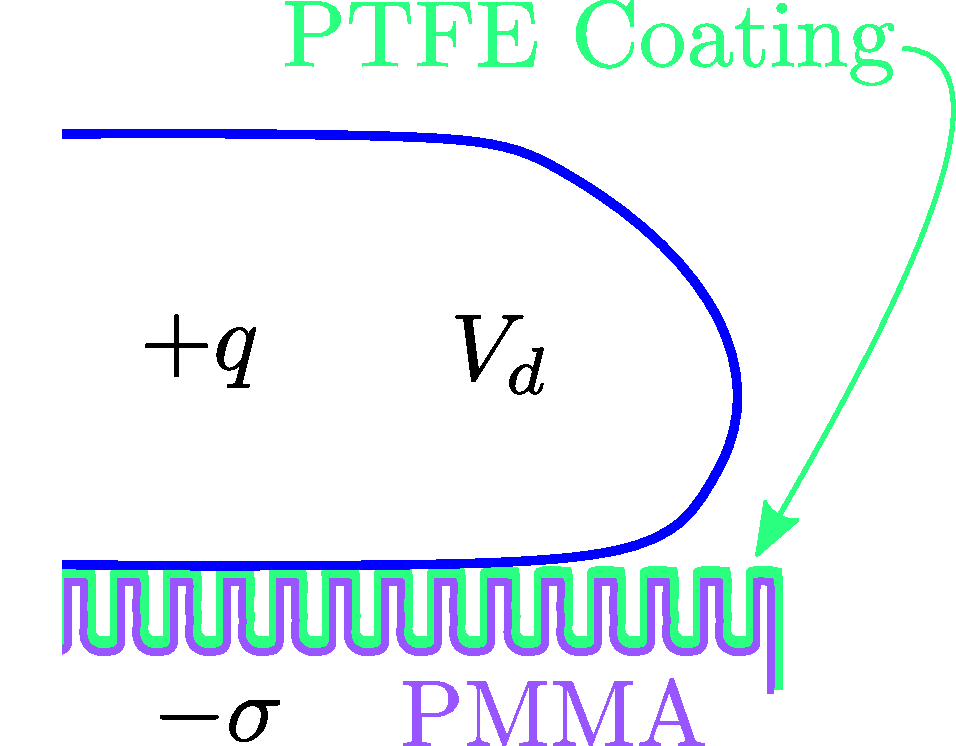
\includegraphics[width=0.65\textwidth]{../figures/schematic.pdf}
 \caption{Portion of drop at the initial condition, resting on a superhydrophobic surface in the Cassie-Baxter state just prior to release of the experiment into free-fall. The variables $q$, $\sigma$, and $V_d$ are the drop net free charge, dielectric surface charge density, and drop volume, respectively.\label{fig:schematic}}
\end{figure}

\section{Experimental Methods}
The DDT uses a dual capsule design, inspired by the 2.2 s facility at NASA Glenn Research Center, which decouples drag acceleration felt by the external drag shield from the experiment. The experiment experiences approximately $\lesssim 1 \times 10^{-4}$ $g_0$ during free-fall for 2.1s as the rig and drag shield plummet to the bottom of drop tower 6 stories below. Single drops of distilled water in a range of volumes ($0.01 \leq R_d \leq 0.5$ mL) are carefully deposited on charged superhydrophobic substrates using an grounded glass syringe with $\pm $1 $\mu$L accuracy and then dropped in the drop tower. Red dye is added to improve thresholding accuracy in trajectory digitization. Drop trajectories are recorded using a Panasonic HC-WX970 Camera at 120 fps with 1/3000s shutter speed. In a few cases where higher frame rates are required a Nikon J1 400 fps camera with a 30mm telephoto lens is used. The test cell is back illuminated with a diffused 6000K LED strip light source.  

Superhydrophobic electret substrates are prepared with surface potentials $\varphi_s = 0.7$-$4.0$ kV. According to a review by Sessler \cite{sessler_electrets_1987}, an electret is a dielectric material with quasi-permanent electric charge in the sense that the characteristic decay period of the electret is much greater than a practical experiment time scale. Electret charge may be `true' charge in the form of surface or space charges, or polarization charges such as bound charges. If the electret is not screened by a conductor then it produces an external electric field if the polarization and real charges do not uniformly compensate each other throughout the volume of the electret. For this reason electrets are thought of as electrostatic analogs to permanent magnets. The name \emph{electret} itself is a portmanteau to that effect conjured by Heaviside in 1892 \cite{heaviside_electrical_2011}. Typical commercial electrets are PTFE films on the order of 10-50 $\mu$m thick with the charge being primarily real surface charge. Electrets have a plethora of applications, but most germanely they have been used in Electro-Wetting On Dielectric (EWOD) devices for low-voltage manipulation of small drops \cite{wu_low-voltage_2010}. Real charge electrets can be produced by contact electrification, injection or deposition of charge carriers by corona discharge or electron beam, ionizing radiation, or by frictional triboelectrification. Dipolar electrets by contrast are produced by a combination of polarization at elevated temperatures in a strong external electric field followed by an annealing process. Effective surface charge densities are limited to the material dielectric strengths due to internal dielectric breakdown phenomenon which typically occurs before external breakdown or Paschen breakdown. 

We use an isothermal electret formation process which is a variation of the widely applied corona-charging technique. Typical corona-charging techniques uses strong inhomogenous DC electric fields to produce discharge in air at ambient conditions; the dielectric substrate is atop a grounded electrode and there is a screening potential electrode intermediately positioned to control the surface potential. The surface potential of the dielectric will tend to saturate at this grid potential if the material is not space-charge current limited. The corona field is usually produced by a pin-shaped electrode. In air the most common charge carriers thus produced are $\mbox{CO}_3^-$ ions. This approach is known to generally produce samples with fairly uniform surface charge densities. Some work by van Turnhout \cite{van_turnhout_thermally_1975} using Thermally Stimulated Current (TCS) measurements showed that in 4.8 mm thick polymethyl methacrylate (PMMA), polarization of the dielectric is non-uniform due to real space-charge mostly ($\sim$90\%) residing in a thin (0.1-0.2 mm) layer near the free-surface of the sample. In this work we use a Ptec IN5120 balanced AC corona ion source to direct a net neutral stream of ions towards the dielectric target, which we polarize by an electrode with an EMCO P20P $2$ kV$+$ absolute reference DC-DC converter. The ion stream compensates the surface and space bound charges arising due to the polarization of the dielectric. When the DC-DC converter is switched to ground the deposited negative ions remain on the surface. 

The electret is lamina of 3 to 4 0.4 mm thick corona charged PMMA sheets. The electric field strength scales with the number of dielectric lamina as has also been shown in work on electret based vibrational energy harvesters \cite{wada_stacking_2012} and in water desalinization \cite{ni_desalination_2005}. 

The electret is established on a superhydrophobic substrate produced by laser etching PMMA and depositing a thin layer of PTFE on the roughened surface. The surface charge density can be modulated during the experiment using the high-voltage DC-DC converter, which can re-polarize the dielectric substrate by means of an embedded electrode. The resulting bound charge partially or fully neutralizes the electric field due to the surface ions deposited by corona charging of the electret. The high-voltage system is armed manually before the drop tower experiment and is automatically safed by a high-voltage power switching relay, which switches the load across a 100 k$\Omega$ resistor when triggered by the resumption of 1-$g_0$ conditions. The safing is set by an accelerometer pin-interrupt triggered microcontroller command. The rig with a mounted experiment is shown in Figure \ref{fig:rig}. 
\begin{figure}
    \centering
    \def\svgwidth{\columnwidth}
        \subfloat[]{%
        \input{../figures/rig.pdf_tex}%
}

        \subfloat[]{%
        \includegraphics[width=0.45\textwidth]{close_up}%
}
    \caption{(a) The electro-drop bounce experiment hardware mounted on a drop tower rig. (b) Close up of the experimental test cell.\label{fig:rig}}
\end{figure}

Contact angles of distilled water on the electret are $\sim \hspace{-1mm} 150^{\circ}$. The hysteresis of the contact angle (the difference between the advancing $\theta_a$ and receding $\theta_r$ contact angles) is estimated from the roll-off angle using the method of Furmidge \cite{furmidge_studies_1962}, and is found to be approximately $25^{\circ} \pm 10^{\circ}$ when the surface is uncharged. A contour plot of the Furmidge model is provided in Figure \ref{fig:hysteresis}. The contact angle for water on smooth PTFE is $\approx 115^{\circ}$ and is further enhanced by an air layer maintained in the underlying roughness length scales of the surface. We use a laser-etched pillared geometry with pillar heights $\sim \hspace{-1mm} 775$ $\mu$m, widths $\sim \hspace{-1mm} 70$ $\mu$m, and pitch $\sim \hspace{-1mm} 100$ $\mu$m. An SEM image of the pillar geometry is shown in Figure \ref{fig:SEM}.
\begin{figure}
    \centering
    %% Creator: Matplotlib, PGF backend
%%
%% To include the figure in your LaTeX document, write
%%   \input{<filename>.pgf}
%%
%% Make sure the required packages are loaded in your preamble
%%   \usepackage{pgf}
%%
%% Figures using additional raster images can only be included by \input if
%% they are in the same directory as the main LaTeX file. For loading figures
%% from other directories you can use the `import` package
%%   \usepackage{import}
%% and then include the figures with
%%   \import{<path to file>}{<filename>.pgf}
%%
%% Matplotlib used the following preamble
%%   \usepackage{fontspec}
%%   \setmainfont{DejaVuSerif.ttf}[Path=/home/erin/anaconda3/lib/python3.6/site-packages/matplotlib/mpl-data/fonts/ttf/]
%%   \setsansfont{DejaVuSans.ttf}[Path=/home/erin/anaconda3/lib/python3.6/site-packages/matplotlib/mpl-data/fonts/ttf/]
%%   \setmonofont{DejaVuSansMono.ttf}[Path=/home/erin/anaconda3/lib/python3.6/site-packages/matplotlib/mpl-data/fonts/ttf/]
%%
\begingroup%
\makeatletter%
\begin{pgfpicture}%
\pgfpathrectangle{\pgfpointorigin}{\pgfqpoint{5.435744in}{3.749134in}}%
\pgfusepath{use as bounding box, clip}%
\begin{pgfscope}%
\pgfsetbuttcap%
\pgfsetmiterjoin%
\definecolor{currentfill}{rgb}{1.000000,1.000000,1.000000}%
\pgfsetfillcolor{currentfill}%
\pgfsetlinewidth{0.000000pt}%
\definecolor{currentstroke}{rgb}{1.000000,1.000000,1.000000}%
\pgfsetstrokecolor{currentstroke}%
\pgfsetdash{}{0pt}%
\pgfpathmoveto{\pgfqpoint{0.000000in}{0.000000in}}%
\pgfpathlineto{\pgfqpoint{5.435744in}{0.000000in}}%
\pgfpathlineto{\pgfqpoint{5.435744in}{3.749134in}}%
\pgfpathlineto{\pgfqpoint{0.000000in}{3.749134in}}%
\pgfpathclose%
\pgfusepath{fill}%
\end{pgfscope}%
\begin{pgfscope}%
\pgfsetbuttcap%
\pgfsetmiterjoin%
\definecolor{currentfill}{rgb}{1.000000,1.000000,1.000000}%
\pgfsetfillcolor{currentfill}%
\pgfsetlinewidth{0.000000pt}%
\definecolor{currentstroke}{rgb}{0.000000,0.000000,0.000000}%
\pgfsetstrokecolor{currentstroke}%
\pgfsetstrokeopacity{0.000000}%
\pgfsetdash{}{0pt}%
\pgfpathmoveto{\pgfqpoint{0.538871in}{0.629134in}}%
\pgfpathlineto{\pgfqpoint{5.188871in}{0.629134in}}%
\pgfpathlineto{\pgfqpoint{5.188871in}{3.649134in}}%
\pgfpathlineto{\pgfqpoint{0.538871in}{3.649134in}}%
\pgfpathclose%
\pgfusepath{fill}%
\end{pgfscope}%
\begin{pgfscope}%
\pgfpathrectangle{\pgfqpoint{0.538871in}{0.629134in}}{\pgfqpoint{4.650000in}{3.020000in}}%
\pgfusepath{clip}%
\pgfsetrectcap%
\pgfsetroundjoin%
\pgfsetlinewidth{1.505625pt}%
\definecolor{currentstroke}{rgb}{1.000000,0.000000,1.000000}%
\pgfsetstrokecolor{currentstroke}%
\pgfsetdash{}{0pt}%
\pgfpathmoveto{\pgfqpoint{0.535538in}{1.192634in}}%
\pgfpathlineto{\pgfqpoint{0.544090in}{1.192036in}}%
\pgfpathlineto{\pgfqpoint{0.596279in}{1.188353in}}%
\pgfpathlineto{\pgfqpoint{0.648467in}{1.184635in}}%
\pgfpathlineto{\pgfqpoint{0.700656in}{1.180883in}}%
\pgfpathlineto{\pgfqpoint{0.752844in}{1.177096in}}%
\pgfpathlineto{\pgfqpoint{0.805033in}{1.173276in}}%
\pgfpathlineto{\pgfqpoint{0.857221in}{1.169422in}}%
\pgfpathlineto{\pgfqpoint{0.909410in}{1.165534in}}%
\pgfpathlineto{\pgfqpoint{0.961599in}{1.161614in}}%
\pgfpathlineto{\pgfqpoint{1.013787in}{1.157660in}}%
\pgfpathlineto{\pgfqpoint{1.065976in}{1.153675in}}%
\pgfpathlineto{\pgfqpoint{1.118164in}{1.149657in}}%
\pgfpathlineto{\pgfqpoint{1.170353in}{1.145608in}}%
\pgfpathlineto{\pgfqpoint{1.222541in}{1.141527in}}%
\pgfpathlineto{\pgfqpoint{1.274730in}{1.137415in}}%
\pgfpathlineto{\pgfqpoint{1.326918in}{1.133272in}}%
\pgfpathlineto{\pgfqpoint{1.379107in}{1.129099in}}%
\pgfpathlineto{\pgfqpoint{1.431295in}{1.124896in}}%
\pgfpathlineto{\pgfqpoint{1.483484in}{1.120663in}}%
\pgfpathlineto{\pgfqpoint{1.535673in}{1.116400in}}%
\pgfpathlineto{\pgfqpoint{1.587861in}{1.112108in}}%
\pgfpathlineto{\pgfqpoint{1.640050in}{1.107787in}}%
\pgfpathlineto{\pgfqpoint{1.692238in}{1.103438in}}%
\pgfpathlineto{\pgfqpoint{1.744427in}{1.099061in}}%
\pgfpathlineto{\pgfqpoint{1.796615in}{1.094656in}}%
\pgfpathlineto{\pgfqpoint{1.848804in}{1.090223in}}%
\pgfpathlineto{\pgfqpoint{1.900992in}{1.085763in}}%
\pgfpathlineto{\pgfqpoint{1.953181in}{1.081277in}}%
\pgfpathlineto{\pgfqpoint{2.005370in}{1.076764in}}%
\pgfpathlineto{\pgfqpoint{2.057558in}{1.072225in}}%
\pgfpathlineto{\pgfqpoint{2.109747in}{1.067660in}}%
\pgfpathlineto{\pgfqpoint{2.161935in}{1.063070in}}%
\pgfpathlineto{\pgfqpoint{2.214124in}{1.058455in}}%
\pgfpathlineto{\pgfqpoint{2.266312in}{1.053815in}}%
\pgfpathlineto{\pgfqpoint{2.318501in}{1.049151in}}%
\pgfpathlineto{\pgfqpoint{2.370689in}{1.044463in}}%
\pgfpathlineto{\pgfqpoint{2.422878in}{1.039751in}}%
\pgfpathlineto{\pgfqpoint{2.475067in}{1.035017in}}%
\pgfpathlineto{\pgfqpoint{2.527255in}{1.030259in}}%
\pgfpathlineto{\pgfqpoint{2.579444in}{1.025479in}}%
\pgfpathlineto{\pgfqpoint{2.631632in}{1.020677in}}%
\pgfpathlineto{\pgfqpoint{2.683821in}{1.015853in}}%
\pgfpathlineto{\pgfqpoint{2.736009in}{1.011008in}}%
\pgfpathlineto{\pgfqpoint{2.788198in}{1.006142in}}%
\pgfpathlineto{\pgfqpoint{2.840386in}{1.001255in}}%
\pgfpathlineto{\pgfqpoint{2.892575in}{0.996348in}}%
\pgfpathlineto{\pgfqpoint{2.944764in}{0.991421in}}%
\pgfpathlineto{\pgfqpoint{2.996952in}{0.986475in}}%
\pgfpathlineto{\pgfqpoint{3.049141in}{0.981510in}}%
\pgfpathlineto{\pgfqpoint{3.101329in}{0.976526in}}%
\pgfpathlineto{\pgfqpoint{3.153518in}{0.971523in}}%
\pgfpathlineto{\pgfqpoint{3.205706in}{0.966503in}}%
\pgfpathlineto{\pgfqpoint{3.257895in}{0.961466in}}%
\pgfpathlineto{\pgfqpoint{3.310083in}{0.956411in}}%
\pgfpathlineto{\pgfqpoint{3.362272in}{0.951339in}}%
\pgfpathlineto{\pgfqpoint{3.414460in}{0.946251in}}%
\pgfpathlineto{\pgfqpoint{3.466649in}{0.941147in}}%
\pgfpathlineto{\pgfqpoint{3.518838in}{0.936028in}}%
\pgfpathlineto{\pgfqpoint{3.571026in}{0.930893in}}%
\pgfpathlineto{\pgfqpoint{3.623215in}{0.925744in}}%
\pgfpathlineto{\pgfqpoint{3.675403in}{0.920580in}}%
\pgfpathlineto{\pgfqpoint{3.727592in}{0.915403in}}%
\pgfpathlineto{\pgfqpoint{3.779780in}{0.910211in}}%
\pgfpathlineto{\pgfqpoint{3.831969in}{0.905007in}}%
\pgfpathlineto{\pgfqpoint{3.884157in}{0.899790in}}%
\pgfpathlineto{\pgfqpoint{3.936346in}{0.894560in}}%
\pgfpathlineto{\pgfqpoint{3.988535in}{0.889319in}}%
\pgfpathlineto{\pgfqpoint{4.040723in}{0.884066in}}%
\pgfpathlineto{\pgfqpoint{4.092912in}{0.878802in}}%
\pgfpathlineto{\pgfqpoint{4.145100in}{0.873527in}}%
\pgfpathlineto{\pgfqpoint{4.197289in}{0.868242in}}%
\pgfpathlineto{\pgfqpoint{4.249477in}{0.862947in}}%
\pgfpathlineto{\pgfqpoint{4.301666in}{0.857642in}}%
\pgfpathlineto{\pgfqpoint{4.353854in}{0.852328in}}%
\pgfpathlineto{\pgfqpoint{4.406043in}{0.847006in}}%
\pgfpathlineto{\pgfqpoint{4.458232in}{0.841675in}}%
\pgfpathlineto{\pgfqpoint{4.510420in}{0.836336in}}%
\pgfpathlineto{\pgfqpoint{4.562609in}{0.830990in}}%
\pgfpathlineto{\pgfqpoint{4.614797in}{0.825637in}}%
\pgfpathlineto{\pgfqpoint{4.666986in}{0.820278in}}%
\pgfpathlineto{\pgfqpoint{4.719174in}{0.814912in}}%
\pgfpathlineto{\pgfqpoint{4.771363in}{0.809540in}}%
\pgfpathlineto{\pgfqpoint{4.823551in}{0.804163in}}%
\pgfpathlineto{\pgfqpoint{4.875740in}{0.798781in}}%
\pgfpathlineto{\pgfqpoint{4.927928in}{0.793394in}}%
\pgfpathlineto{\pgfqpoint{4.980117in}{0.788003in}}%
\pgfpathlineto{\pgfqpoint{5.032306in}{0.782609in}}%
\pgfpathlineto{\pgfqpoint{5.084494in}{0.777211in}}%
\pgfpathlineto{\pgfqpoint{5.136683in}{0.771810in}}%
\pgfpathlineto{\pgfqpoint{5.188871in}{0.766407in}}%
\pgfusepath{stroke}%
\end{pgfscope}%
\begin{pgfscope}%
\pgfpathrectangle{\pgfqpoint{0.538871in}{0.629134in}}{\pgfqpoint{4.650000in}{3.020000in}}%
\pgfusepath{clip}%
\pgfsetrectcap%
\pgfsetroundjoin%
\pgfsetlinewidth{1.505625pt}%
\definecolor{currentstroke}{rgb}{0.749020,0.250980,1.000000}%
\pgfsetstrokecolor{currentstroke}%
\pgfsetdash{}{0pt}%
\pgfpathmoveto{\pgfqpoint{0.535538in}{1.682212in}}%
\pgfpathlineto{\pgfqpoint{0.544090in}{1.681068in}}%
\pgfpathlineto{\pgfqpoint{0.596279in}{1.674014in}}%
\pgfpathlineto{\pgfqpoint{0.648467in}{1.666888in}}%
\pgfpathlineto{\pgfqpoint{0.700656in}{1.659690in}}%
\pgfpathlineto{\pgfqpoint{0.752844in}{1.652422in}}%
\pgfpathlineto{\pgfqpoint{0.805033in}{1.645083in}}%
\pgfpathlineto{\pgfqpoint{0.857221in}{1.637675in}}%
\pgfpathlineto{\pgfqpoint{0.909410in}{1.630197in}}%
\pgfpathlineto{\pgfqpoint{0.961599in}{1.622651in}}%
\pgfpathlineto{\pgfqpoint{1.013787in}{1.615037in}}%
\pgfpathlineto{\pgfqpoint{1.065976in}{1.607355in}}%
\pgfpathlineto{\pgfqpoint{1.118164in}{1.599607in}}%
\pgfpathlineto{\pgfqpoint{1.170353in}{1.591793in}}%
\pgfpathlineto{\pgfqpoint{1.222541in}{1.583913in}}%
\pgfpathlineto{\pgfqpoint{1.274730in}{1.575968in}}%
\pgfpathlineto{\pgfqpoint{1.326918in}{1.567960in}}%
\pgfpathlineto{\pgfqpoint{1.379107in}{1.559887in}}%
\pgfpathlineto{\pgfqpoint{1.431295in}{1.551752in}}%
\pgfpathlineto{\pgfqpoint{1.483484in}{1.543554in}}%
\pgfpathlineto{\pgfqpoint{1.535673in}{1.535295in}}%
\pgfpathlineto{\pgfqpoint{1.587861in}{1.526975in}}%
\pgfpathlineto{\pgfqpoint{1.640050in}{1.518594in}}%
\pgfpathlineto{\pgfqpoint{1.692238in}{1.510154in}}%
\pgfpathlineto{\pgfqpoint{1.744427in}{1.501655in}}%
\pgfpathlineto{\pgfqpoint{1.796615in}{1.493097in}}%
\pgfpathlineto{\pgfqpoint{1.848804in}{1.484482in}}%
\pgfpathlineto{\pgfqpoint{1.900992in}{1.475810in}}%
\pgfpathlineto{\pgfqpoint{1.953181in}{1.467082in}}%
\pgfpathlineto{\pgfqpoint{2.005370in}{1.458298in}}%
\pgfpathlineto{\pgfqpoint{2.057558in}{1.449459in}}%
\pgfpathlineto{\pgfqpoint{2.109747in}{1.440566in}}%
\pgfpathlineto{\pgfqpoint{2.161935in}{1.431619in}}%
\pgfpathlineto{\pgfqpoint{2.214124in}{1.422620in}}%
\pgfpathlineto{\pgfqpoint{2.266312in}{1.413568in}}%
\pgfpathlineto{\pgfqpoint{2.318501in}{1.404466in}}%
\pgfpathlineto{\pgfqpoint{2.370689in}{1.395312in}}%
\pgfpathlineto{\pgfqpoint{2.422878in}{1.386108in}}%
\pgfpathlineto{\pgfqpoint{2.475067in}{1.376856in}}%
\pgfpathlineto{\pgfqpoint{2.527255in}{1.367554in}}%
\pgfpathlineto{\pgfqpoint{2.579444in}{1.358205in}}%
\pgfpathlineto{\pgfqpoint{2.631632in}{1.348809in}}%
\pgfpathlineto{\pgfqpoint{2.683821in}{1.339366in}}%
\pgfpathlineto{\pgfqpoint{2.736009in}{1.329878in}}%
\pgfpathlineto{\pgfqpoint{2.788198in}{1.320345in}}%
\pgfpathlineto{\pgfqpoint{2.840386in}{1.310767in}}%
\pgfpathlineto{\pgfqpoint{2.892575in}{1.301147in}}%
\pgfpathlineto{\pgfqpoint{2.944764in}{1.291483in}}%
\pgfpathlineto{\pgfqpoint{2.996952in}{1.281778in}}%
\pgfpathlineto{\pgfqpoint{3.049141in}{1.272032in}}%
\pgfpathlineto{\pgfqpoint{3.101329in}{1.262245in}}%
\pgfpathlineto{\pgfqpoint{3.153518in}{1.252418in}}%
\pgfpathlineto{\pgfqpoint{3.205706in}{1.242553in}}%
\pgfpathlineto{\pgfqpoint{3.257895in}{1.232649in}}%
\pgfpathlineto{\pgfqpoint{3.310083in}{1.222708in}}%
\pgfpathlineto{\pgfqpoint{3.362272in}{1.212731in}}%
\pgfpathlineto{\pgfqpoint{3.414460in}{1.202717in}}%
\pgfpathlineto{\pgfqpoint{3.466649in}{1.192669in}}%
\pgfpathlineto{\pgfqpoint{3.518838in}{1.182586in}}%
\pgfpathlineto{\pgfqpoint{3.571026in}{1.172469in}}%
\pgfpathlineto{\pgfqpoint{3.623215in}{1.162320in}}%
\pgfpathlineto{\pgfqpoint{3.675403in}{1.152139in}}%
\pgfpathlineto{\pgfqpoint{3.727592in}{1.141927in}}%
\pgfpathlineto{\pgfqpoint{3.779780in}{1.131684in}}%
\pgfpathlineto{\pgfqpoint{3.831969in}{1.121411in}}%
\pgfpathlineto{\pgfqpoint{3.884157in}{1.111110in}}%
\pgfpathlineto{\pgfqpoint{3.936346in}{1.100780in}}%
\pgfpathlineto{\pgfqpoint{3.988535in}{1.090424in}}%
\pgfpathlineto{\pgfqpoint{4.040723in}{1.080040in}}%
\pgfpathlineto{\pgfqpoint{4.092912in}{1.069631in}}%
\pgfpathlineto{\pgfqpoint{4.145100in}{1.059197in}}%
\pgfpathlineto{\pgfqpoint{4.197289in}{1.048739in}}%
\pgfpathlineto{\pgfqpoint{4.249477in}{1.038258in}}%
\pgfpathlineto{\pgfqpoint{4.301666in}{1.027754in}}%
\pgfpathlineto{\pgfqpoint{4.353854in}{1.017228in}}%
\pgfpathlineto{\pgfqpoint{4.406043in}{1.006681in}}%
\pgfpathlineto{\pgfqpoint{4.458232in}{0.996114in}}%
\pgfpathlineto{\pgfqpoint{4.510420in}{0.985528in}}%
\pgfpathlineto{\pgfqpoint{4.562609in}{0.974923in}}%
\pgfpathlineto{\pgfqpoint{4.614797in}{0.964301in}}%
\pgfpathlineto{\pgfqpoint{4.666986in}{0.953661in}}%
\pgfpathlineto{\pgfqpoint{4.719174in}{0.943006in}}%
\pgfpathlineto{\pgfqpoint{4.771363in}{0.932335in}}%
\pgfpathlineto{\pgfqpoint{4.823551in}{0.921649in}}%
\pgfpathlineto{\pgfqpoint{4.875740in}{0.910950in}}%
\pgfpathlineto{\pgfqpoint{4.927928in}{0.900238in}}%
\pgfpathlineto{\pgfqpoint{4.980117in}{0.889514in}}%
\pgfpathlineto{\pgfqpoint{5.032306in}{0.878778in}}%
\pgfpathlineto{\pgfqpoint{5.084494in}{0.868032in}}%
\pgfpathlineto{\pgfqpoint{5.136683in}{0.857277in}}%
\pgfpathlineto{\pgfqpoint{5.188871in}{0.846512in}}%
\pgfusepath{stroke}%
\end{pgfscope}%
\begin{pgfscope}%
\pgfpathrectangle{\pgfqpoint{0.538871in}{0.629134in}}{\pgfqpoint{4.650000in}{3.020000in}}%
\pgfusepath{clip}%
\pgfsetrectcap%
\pgfsetroundjoin%
\pgfsetlinewidth{1.505625pt}%
\definecolor{currentstroke}{rgb}{0.498039,0.501961,1.000000}%
\pgfsetstrokecolor{currentstroke}%
\pgfsetdash{}{0pt}%
\pgfpathmoveto{\pgfqpoint{0.535538in}{2.207784in}}%
\pgfpathlineto{\pgfqpoint{0.544090in}{2.206141in}}%
\pgfpathlineto{\pgfqpoint{0.596279in}{2.196001in}}%
\pgfpathlineto{\pgfqpoint{0.648467in}{2.185749in}}%
\pgfpathlineto{\pgfqpoint{0.700656in}{2.175387in}}%
\pgfpathlineto{\pgfqpoint{0.752844in}{2.164915in}}%
\pgfpathlineto{\pgfqpoint{0.805033in}{2.154333in}}%
\pgfpathlineto{\pgfqpoint{0.857221in}{2.143643in}}%
\pgfpathlineto{\pgfqpoint{0.909410in}{2.132847in}}%
\pgfpathlineto{\pgfqpoint{0.961599in}{2.121943in}}%
\pgfpathlineto{\pgfqpoint{1.013787in}{2.110935in}}%
\pgfpathlineto{\pgfqpoint{1.065976in}{2.099822in}}%
\pgfpathlineto{\pgfqpoint{1.118164in}{2.088605in}}%
\pgfpathlineto{\pgfqpoint{1.170353in}{2.077286in}}%
\pgfpathlineto{\pgfqpoint{1.222541in}{2.065865in}}%
\pgfpathlineto{\pgfqpoint{1.274730in}{2.054343in}}%
\pgfpathlineto{\pgfqpoint{1.326918in}{2.042722in}}%
\pgfpathlineto{\pgfqpoint{1.379107in}{2.031002in}}%
\pgfpathlineto{\pgfqpoint{1.431295in}{2.019184in}}%
\pgfpathlineto{\pgfqpoint{1.483484in}{2.007269in}}%
\pgfpathlineto{\pgfqpoint{1.535673in}{1.995258in}}%
\pgfpathlineto{\pgfqpoint{1.587861in}{1.983153in}}%
\pgfpathlineto{\pgfqpoint{1.640050in}{1.970953in}}%
\pgfpathlineto{\pgfqpoint{1.692238in}{1.958661in}}%
\pgfpathlineto{\pgfqpoint{1.744427in}{1.946276in}}%
\pgfpathlineto{\pgfqpoint{1.796615in}{1.933801in}}%
\pgfpathlineto{\pgfqpoint{1.848804in}{1.921236in}}%
\pgfpathlineto{\pgfqpoint{1.900992in}{1.908582in}}%
\pgfpathlineto{\pgfqpoint{1.953181in}{1.895840in}}%
\pgfpathlineto{\pgfqpoint{2.005370in}{1.883012in}}%
\pgfpathlineto{\pgfqpoint{2.057558in}{1.870098in}}%
\pgfpathlineto{\pgfqpoint{2.109747in}{1.857099in}}%
\pgfpathlineto{\pgfqpoint{2.161935in}{1.844016in}}%
\pgfpathlineto{\pgfqpoint{2.214124in}{1.830851in}}%
\pgfpathlineto{\pgfqpoint{2.266312in}{1.817604in}}%
\pgfpathlineto{\pgfqpoint{2.318501in}{1.804276in}}%
\pgfpathlineto{\pgfqpoint{2.370689in}{1.790869in}}%
\pgfpathlineto{\pgfqpoint{2.422878in}{1.777384in}}%
\pgfpathlineto{\pgfqpoint{2.475067in}{1.763821in}}%
\pgfpathlineto{\pgfqpoint{2.527255in}{1.750182in}}%
\pgfpathlineto{\pgfqpoint{2.579444in}{1.736468in}}%
\pgfpathlineto{\pgfqpoint{2.631632in}{1.722679in}}%
\pgfpathlineto{\pgfqpoint{2.683821in}{1.708818in}}%
\pgfpathlineto{\pgfqpoint{2.736009in}{1.694884in}}%
\pgfpathlineto{\pgfqpoint{2.788198in}{1.680880in}}%
\pgfpathlineto{\pgfqpoint{2.840386in}{1.666806in}}%
\pgfpathlineto{\pgfqpoint{2.892575in}{1.652663in}}%
\pgfpathlineto{\pgfqpoint{2.944764in}{1.638452in}}%
\pgfpathlineto{\pgfqpoint{2.996952in}{1.624175in}}%
\pgfpathlineto{\pgfqpoint{3.049141in}{1.609833in}}%
\pgfpathlineto{\pgfqpoint{3.101329in}{1.595426in}}%
\pgfpathlineto{\pgfqpoint{3.153518in}{1.580956in}}%
\pgfpathlineto{\pgfqpoint{3.205706in}{1.566424in}}%
\pgfpathlineto{\pgfqpoint{3.257895in}{1.551831in}}%
\pgfpathlineto{\pgfqpoint{3.310083in}{1.537179in}}%
\pgfpathlineto{\pgfqpoint{3.362272in}{1.522467in}}%
\pgfpathlineto{\pgfqpoint{3.414460in}{1.507698in}}%
\pgfpathlineto{\pgfqpoint{3.466649in}{1.492872in}}%
\pgfpathlineto{\pgfqpoint{3.518838in}{1.477991in}}%
\pgfpathlineto{\pgfqpoint{3.571026in}{1.463055in}}%
\pgfpathlineto{\pgfqpoint{3.623215in}{1.448067in}}%
\pgfpathlineto{\pgfqpoint{3.675403in}{1.433026in}}%
\pgfpathlineto{\pgfqpoint{3.727592in}{1.417935in}}%
\pgfpathlineto{\pgfqpoint{3.779780in}{1.402794in}}%
\pgfpathlineto{\pgfqpoint{3.831969in}{1.387604in}}%
\pgfpathlineto{\pgfqpoint{3.884157in}{1.372367in}}%
\pgfpathlineto{\pgfqpoint{3.936346in}{1.357084in}}%
\pgfpathlineto{\pgfqpoint{3.988535in}{1.341755in}}%
\pgfpathlineto{\pgfqpoint{4.040723in}{1.326383in}}%
\pgfpathlineto{\pgfqpoint{4.092912in}{1.310967in}}%
\pgfpathlineto{\pgfqpoint{4.145100in}{1.295510in}}%
\pgfpathlineto{\pgfqpoint{4.197289in}{1.280012in}}%
\pgfpathlineto{\pgfqpoint{4.249477in}{1.264475in}}%
\pgfpathlineto{\pgfqpoint{4.301666in}{1.248899in}}%
\pgfpathlineto{\pgfqpoint{4.353854in}{1.233287in}}%
\pgfpathlineto{\pgfqpoint{4.406043in}{1.217638in}}%
\pgfpathlineto{\pgfqpoint{4.458232in}{1.201955in}}%
\pgfpathlineto{\pgfqpoint{4.510420in}{1.186237in}}%
\pgfpathlineto{\pgfqpoint{4.562609in}{1.170488in}}%
\pgfpathlineto{\pgfqpoint{4.614797in}{1.154707in}}%
\pgfpathlineto{\pgfqpoint{4.666986in}{1.138896in}}%
\pgfpathlineto{\pgfqpoint{4.719174in}{1.123055in}}%
\pgfpathlineto{\pgfqpoint{4.771363in}{1.107187in}}%
\pgfpathlineto{\pgfqpoint{4.823551in}{1.091293in}}%
\pgfpathlineto{\pgfqpoint{4.875740in}{1.075372in}}%
\pgfpathlineto{\pgfqpoint{4.927928in}{1.059427in}}%
\pgfpathlineto{\pgfqpoint{4.980117in}{1.043459in}}%
\pgfpathlineto{\pgfqpoint{5.032306in}{1.027469in}}%
\pgfpathlineto{\pgfqpoint{5.084494in}{1.011459in}}%
\pgfpathlineto{\pgfqpoint{5.136683in}{0.995428in}}%
\pgfpathlineto{\pgfqpoint{5.188871in}{0.979379in}}%
\pgfusepath{stroke}%
\end{pgfscope}%
\begin{pgfscope}%
\pgfpathrectangle{\pgfqpoint{0.538871in}{0.629134in}}{\pgfqpoint{4.650000in}{3.020000in}}%
\pgfusepath{clip}%
\pgfsetrectcap%
\pgfsetroundjoin%
\pgfsetlinewidth{1.505625pt}%
\definecolor{currentstroke}{rgb}{0.247059,0.752941,1.000000}%
\pgfsetstrokecolor{currentstroke}%
\pgfsetdash{}{0pt}%
\pgfpathmoveto{\pgfqpoint{0.535538in}{2.769708in}}%
\pgfpathlineto{\pgfqpoint{0.544090in}{2.767606in}}%
\pgfpathlineto{\pgfqpoint{0.596279in}{2.754629in}}%
\pgfpathlineto{\pgfqpoint{0.648467in}{2.741498in}}%
\pgfpathlineto{\pgfqpoint{0.700656in}{2.728215in}}%
\pgfpathlineto{\pgfqpoint{0.752844in}{2.714779in}}%
\pgfpathlineto{\pgfqpoint{0.805033in}{2.701194in}}%
\pgfpathlineto{\pgfqpoint{0.857221in}{2.687460in}}%
\pgfpathlineto{\pgfqpoint{0.909410in}{2.673578in}}%
\pgfpathlineto{\pgfqpoint{0.961599in}{2.659550in}}%
\pgfpathlineto{\pgfqpoint{1.013787in}{2.645377in}}%
\pgfpathlineto{\pgfqpoint{1.065976in}{2.631060in}}%
\pgfpathlineto{\pgfqpoint{1.118164in}{2.616600in}}%
\pgfpathlineto{\pgfqpoint{1.170353in}{2.602000in}}%
\pgfpathlineto{\pgfqpoint{1.222541in}{2.587259in}}%
\pgfpathlineto{\pgfqpoint{1.274730in}{2.572380in}}%
\pgfpathlineto{\pgfqpoint{1.326918in}{2.557364in}}%
\pgfpathlineto{\pgfqpoint{1.379107in}{2.542211in}}%
\pgfpathlineto{\pgfqpoint{1.431295in}{2.526924in}}%
\pgfpathlineto{\pgfqpoint{1.483484in}{2.511504in}}%
\pgfpathlineto{\pgfqpoint{1.535673in}{2.495952in}}%
\pgfpathlineto{\pgfqpoint{1.587861in}{2.480270in}}%
\pgfpathlineto{\pgfqpoint{1.640050in}{2.464458in}}%
\pgfpathlineto{\pgfqpoint{1.692238in}{2.448518in}}%
\pgfpathlineto{\pgfqpoint{1.744427in}{2.432452in}}%
\pgfpathlineto{\pgfqpoint{1.796615in}{2.416261in}}%
\pgfpathlineto{\pgfqpoint{1.848804in}{2.399947in}}%
\pgfpathlineto{\pgfqpoint{1.900992in}{2.383510in}}%
\pgfpathlineto{\pgfqpoint{1.953181in}{2.366952in}}%
\pgfpathlineto{\pgfqpoint{2.005370in}{2.350274in}}%
\pgfpathlineto{\pgfqpoint{2.057558in}{2.333479in}}%
\pgfpathlineto{\pgfqpoint{2.109747in}{2.316567in}}%
\pgfpathlineto{\pgfqpoint{2.161935in}{2.299539in}}%
\pgfpathlineto{\pgfqpoint{2.214124in}{2.282398in}}%
\pgfpathlineto{\pgfqpoint{2.266312in}{2.265144in}}%
\pgfpathlineto{\pgfqpoint{2.318501in}{2.247779in}}%
\pgfpathlineto{\pgfqpoint{2.370689in}{2.230305in}}%
\pgfpathlineto{\pgfqpoint{2.422878in}{2.212722in}}%
\pgfpathlineto{\pgfqpoint{2.475067in}{2.195032in}}%
\pgfpathlineto{\pgfqpoint{2.527255in}{2.177238in}}%
\pgfpathlineto{\pgfqpoint{2.579444in}{2.159339in}}%
\pgfpathlineto{\pgfqpoint{2.631632in}{2.141338in}}%
\pgfpathlineto{\pgfqpoint{2.683821in}{2.123236in}}%
\pgfpathlineto{\pgfqpoint{2.736009in}{2.105034in}}%
\pgfpathlineto{\pgfqpoint{2.788198in}{2.086734in}}%
\pgfpathlineto{\pgfqpoint{2.840386in}{2.068338in}}%
\pgfpathlineto{\pgfqpoint{2.892575in}{2.049846in}}%
\pgfpathlineto{\pgfqpoint{2.944764in}{2.031260in}}%
\pgfpathlineto{\pgfqpoint{2.996952in}{2.012582in}}%
\pgfpathlineto{\pgfqpoint{3.049141in}{1.993813in}}%
\pgfpathlineto{\pgfqpoint{3.101329in}{1.974955in}}%
\pgfpathlineto{\pgfqpoint{3.153518in}{1.956009in}}%
\pgfpathlineto{\pgfqpoint{3.205706in}{1.936976in}}%
\pgfpathlineto{\pgfqpoint{3.257895in}{1.917858in}}%
\pgfpathlineto{\pgfqpoint{3.310083in}{1.898657in}}%
\pgfpathlineto{\pgfqpoint{3.362272in}{1.879374in}}%
\pgfpathlineto{\pgfqpoint{3.414460in}{1.860009in}}%
\pgfpathlineto{\pgfqpoint{3.466649in}{1.840566in}}%
\pgfpathlineto{\pgfqpoint{3.518838in}{1.821045in}}%
\pgfpathlineto{\pgfqpoint{3.571026in}{1.801448in}}%
\pgfpathlineto{\pgfqpoint{3.623215in}{1.781775in}}%
\pgfpathlineto{\pgfqpoint{3.675403in}{1.762030in}}%
\pgfpathlineto{\pgfqpoint{3.727592in}{1.742212in}}%
\pgfpathlineto{\pgfqpoint{3.779780in}{1.722325in}}%
\pgfpathlineto{\pgfqpoint{3.831969in}{1.702368in}}%
\pgfpathlineto{\pgfqpoint{3.884157in}{1.682344in}}%
\pgfpathlineto{\pgfqpoint{3.936346in}{1.662254in}}%
\pgfpathlineto{\pgfqpoint{3.988535in}{1.642099in}}%
\pgfpathlineto{\pgfqpoint{4.040723in}{1.621882in}}%
\pgfpathlineto{\pgfqpoint{4.092912in}{1.601602in}}%
\pgfpathlineto{\pgfqpoint{4.145100in}{1.581263in}}%
\pgfpathlineto{\pgfqpoint{4.197289in}{1.560865in}}%
\pgfpathlineto{\pgfqpoint{4.249477in}{1.540410in}}%
\pgfpathlineto{\pgfqpoint{4.301666in}{1.519899in}}%
\pgfpathlineto{\pgfqpoint{4.353854in}{1.499334in}}%
\pgfpathlineto{\pgfqpoint{4.406043in}{1.478717in}}%
\pgfpathlineto{\pgfqpoint{4.458232in}{1.458048in}}%
\pgfpathlineto{\pgfqpoint{4.510420in}{1.437329in}}%
\pgfpathlineto{\pgfqpoint{4.562609in}{1.416562in}}%
\pgfpathlineto{\pgfqpoint{4.614797in}{1.395748in}}%
\pgfpathlineto{\pgfqpoint{4.666986in}{1.374889in}}%
\pgfpathlineto{\pgfqpoint{4.719174in}{1.353986in}}%
\pgfpathlineto{\pgfqpoint{4.771363in}{1.333041in}}%
\pgfpathlineto{\pgfqpoint{4.823551in}{1.312054in}}%
\pgfpathlineto{\pgfqpoint{4.875740in}{1.291028in}}%
\pgfpathlineto{\pgfqpoint{4.927928in}{1.269964in}}%
\pgfpathlineto{\pgfqpoint{4.980117in}{1.248864in}}%
\pgfpathlineto{\pgfqpoint{5.032306in}{1.227729in}}%
\pgfpathlineto{\pgfqpoint{5.084494in}{1.206560in}}%
\pgfpathlineto{\pgfqpoint{5.136683in}{1.185359in}}%
\pgfpathlineto{\pgfqpoint{5.188871in}{1.164127in}}%
\pgfusepath{stroke}%
\end{pgfscope}%
\begin{pgfscope}%
\pgfpathrectangle{\pgfqpoint{0.538871in}{0.629134in}}{\pgfqpoint{4.650000in}{3.020000in}}%
\pgfusepath{clip}%
\pgfsetrectcap%
\pgfsetroundjoin%
\pgfsetlinewidth{1.505625pt}%
\definecolor{currentstroke}{rgb}{0.000000,1.000000,1.000000}%
\pgfsetstrokecolor{currentstroke}%
\pgfsetdash{}{0pt}%
\pgfpathmoveto{\pgfqpoint{0.535538in}{3.369582in}}%
\pgfpathlineto{\pgfqpoint{0.544090in}{3.367056in}}%
\pgfpathlineto{\pgfqpoint{0.596279in}{3.351445in}}%
\pgfpathlineto{\pgfqpoint{0.648467in}{3.335634in}}%
\pgfpathlineto{\pgfqpoint{0.700656in}{3.319626in}}%
\pgfpathlineto{\pgfqpoint{0.752844in}{3.303422in}}%
\pgfpathlineto{\pgfqpoint{0.805033in}{3.287024in}}%
\pgfpathlineto{\pgfqpoint{0.857221in}{3.270433in}}%
\pgfpathlineto{\pgfqpoint{0.909410in}{3.253652in}}%
\pgfpathlineto{\pgfqpoint{0.961599in}{3.236682in}}%
\pgfpathlineto{\pgfqpoint{1.013787in}{3.219524in}}%
\pgfpathlineto{\pgfqpoint{1.065976in}{3.202181in}}%
\pgfpathlineto{\pgfqpoint{1.118164in}{3.184654in}}%
\pgfpathlineto{\pgfqpoint{1.170353in}{3.166945in}}%
\pgfpathlineto{\pgfqpoint{1.222541in}{3.149056in}}%
\pgfpathlineto{\pgfqpoint{1.274730in}{3.130989in}}%
\pgfpathlineto{\pgfqpoint{1.326918in}{3.112744in}}%
\pgfpathlineto{\pgfqpoint{1.379107in}{3.094325in}}%
\pgfpathlineto{\pgfqpoint{1.431295in}{3.075733in}}%
\pgfpathlineto{\pgfqpoint{1.483484in}{3.056969in}}%
\pgfpathlineto{\pgfqpoint{1.535673in}{3.038035in}}%
\pgfpathlineto{\pgfqpoint{1.587861in}{3.018934in}}%
\pgfpathlineto{\pgfqpoint{1.640050in}{2.999667in}}%
\pgfpathlineto{\pgfqpoint{1.692238in}{2.980235in}}%
\pgfpathlineto{\pgfqpoint{1.744427in}{2.960641in}}%
\pgfpathlineto{\pgfqpoint{1.796615in}{2.940887in}}%
\pgfpathlineto{\pgfqpoint{1.848804in}{2.920974in}}%
\pgfpathlineto{\pgfqpoint{1.900992in}{2.900903in}}%
\pgfpathlineto{\pgfqpoint{1.953181in}{2.880678in}}%
\pgfpathlineto{\pgfqpoint{2.005370in}{2.860300in}}%
\pgfpathlineto{\pgfqpoint{2.057558in}{2.839770in}}%
\pgfpathlineto{\pgfqpoint{2.109747in}{2.819090in}}%
\pgfpathlineto{\pgfqpoint{2.161935in}{2.798263in}}%
\pgfpathlineto{\pgfqpoint{2.214124in}{2.777289in}}%
\pgfpathlineto{\pgfqpoint{2.266312in}{2.756172in}}%
\pgfpathlineto{\pgfqpoint{2.318501in}{2.734912in}}%
\pgfpathlineto{\pgfqpoint{2.370689in}{2.713511in}}%
\pgfpathlineto{\pgfqpoint{2.422878in}{2.691972in}}%
\pgfpathlineto{\pgfqpoint{2.475067in}{2.670297in}}%
\pgfpathlineto{\pgfqpoint{2.527255in}{2.648486in}}%
\pgfpathlineto{\pgfqpoint{2.579444in}{2.626542in}}%
\pgfpathlineto{\pgfqpoint{2.631632in}{2.604467in}}%
\pgfpathlineto{\pgfqpoint{2.683821in}{2.582262in}}%
\pgfpathlineto{\pgfqpoint{2.736009in}{2.559930in}}%
\pgfpathlineto{\pgfqpoint{2.788198in}{2.537472in}}%
\pgfpathlineto{\pgfqpoint{2.840386in}{2.514890in}}%
\pgfpathlineto{\pgfqpoint{2.892575in}{2.492185in}}%
\pgfpathlineto{\pgfqpoint{2.944764in}{2.469361in}}%
\pgfpathlineto{\pgfqpoint{2.996952in}{2.446418in}}%
\pgfpathlineto{\pgfqpoint{3.049141in}{2.423358in}}%
\pgfpathlineto{\pgfqpoint{3.101329in}{2.400183in}}%
\pgfpathlineto{\pgfqpoint{3.153518in}{2.376896in}}%
\pgfpathlineto{\pgfqpoint{3.205706in}{2.353497in}}%
\pgfpathlineto{\pgfqpoint{3.257895in}{2.329989in}}%
\pgfpathlineto{\pgfqpoint{3.310083in}{2.306373in}}%
\pgfpathlineto{\pgfqpoint{3.362272in}{2.282652in}}%
\pgfpathlineto{\pgfqpoint{3.414460in}{2.258826in}}%
\pgfpathlineto{\pgfqpoint{3.466649in}{2.234898in}}%
\pgfpathlineto{\pgfqpoint{3.518838in}{2.210871in}}%
\pgfpathlineto{\pgfqpoint{3.571026in}{2.186744in}}%
\pgfpathlineto{\pgfqpoint{3.623215in}{2.162521in}}%
\pgfpathlineto{\pgfqpoint{3.675403in}{2.138203in}}%
\pgfpathlineto{\pgfqpoint{3.727592in}{2.113792in}}%
\pgfpathlineto{\pgfqpoint{3.779780in}{2.089289in}}%
\pgfpathlineto{\pgfqpoint{3.831969in}{2.064697in}}%
\pgfpathlineto{\pgfqpoint{3.884157in}{2.040017in}}%
\pgfpathlineto{\pgfqpoint{3.936346in}{2.015252in}}%
\pgfpathlineto{\pgfqpoint{3.988535in}{1.990402in}}%
\pgfpathlineto{\pgfqpoint{4.040723in}{1.965469in}}%
\pgfpathlineto{\pgfqpoint{4.092912in}{1.940457in}}%
\pgfpathlineto{\pgfqpoint{4.145100in}{1.915365in}}%
\pgfpathlineto{\pgfqpoint{4.197289in}{1.890196in}}%
\pgfpathlineto{\pgfqpoint{4.249477in}{1.864952in}}%
\pgfpathlineto{\pgfqpoint{4.301666in}{1.839634in}}%
\pgfpathlineto{\pgfqpoint{4.353854in}{1.814245in}}%
\pgfpathlineto{\pgfqpoint{4.406043in}{1.788785in}}%
\pgfpathlineto{\pgfqpoint{4.458232in}{1.763257in}}%
\pgfpathlineto{\pgfqpoint{4.510420in}{1.737663in}}%
\pgfpathlineto{\pgfqpoint{4.562609in}{1.712004in}}%
\pgfpathlineto{\pgfqpoint{4.614797in}{1.686282in}}%
\pgfpathlineto{\pgfqpoint{4.666986in}{1.660499in}}%
\pgfpathlineto{\pgfqpoint{4.719174in}{1.634657in}}%
\pgfpathlineto{\pgfqpoint{4.771363in}{1.608756in}}%
\pgfpathlineto{\pgfqpoint{4.823551in}{1.582800in}}%
\pgfpathlineto{\pgfqpoint{4.875740in}{1.556789in}}%
\pgfpathlineto{\pgfqpoint{4.927928in}{1.530726in}}%
\pgfpathlineto{\pgfqpoint{4.980117in}{1.504612in}}%
\pgfpathlineto{\pgfqpoint{5.032306in}{1.478449in}}%
\pgfpathlineto{\pgfqpoint{5.084494in}{1.452239in}}%
\pgfpathlineto{\pgfqpoint{5.136683in}{1.425983in}}%
\pgfpathlineto{\pgfqpoint{5.188871in}{1.399683in}}%
\pgfusepath{stroke}%
\end{pgfscope}%
\begin{pgfscope}%
\pgfsetbuttcap%
\pgfsetroundjoin%
\definecolor{currentfill}{rgb}{0.000000,0.000000,0.000000}%
\pgfsetfillcolor{currentfill}%
\pgfsetlinewidth{0.803000pt}%
\definecolor{currentstroke}{rgb}{0.000000,0.000000,0.000000}%
\pgfsetstrokecolor{currentstroke}%
\pgfsetdash{}{0pt}%
\pgfsys@defobject{currentmarker}{\pgfqpoint{0.000000in}{-0.048611in}}{\pgfqpoint{0.000000in}{0.000000in}}{%
\pgfpathmoveto{\pgfqpoint{0.000000in}{0.000000in}}%
\pgfpathlineto{\pgfqpoint{0.000000in}{-0.048611in}}%
\pgfusepath{stroke,fill}%
}%
\begin{pgfscope}%
\pgfsys@transformshift{1.055538in}{0.629134in}%
\pgfsys@useobject{currentmarker}{}%
\end{pgfscope}%
\end{pgfscope}%
\begin{pgfscope}%
\definecolor{textcolor}{rgb}{0.000000,0.000000,0.000000}%
\pgfsetstrokecolor{textcolor}%
\pgfsetfillcolor{textcolor}%
\pgftext[x=1.055538in,y=0.531912in,,top]{\color{textcolor}\rmfamily\fontsize{14.000000}{16.800000}\selectfont \(\displaystyle 140\)}%
\end{pgfscope}%
\begin{pgfscope}%
\pgfsetbuttcap%
\pgfsetroundjoin%
\definecolor{currentfill}{rgb}{0.000000,0.000000,0.000000}%
\pgfsetfillcolor{currentfill}%
\pgfsetlinewidth{0.803000pt}%
\definecolor{currentstroke}{rgb}{0.000000,0.000000,0.000000}%
\pgfsetstrokecolor{currentstroke}%
\pgfsetdash{}{0pt}%
\pgfsys@defobject{currentmarker}{\pgfqpoint{0.000000in}{-0.048611in}}{\pgfqpoint{0.000000in}{0.000000in}}{%
\pgfpathmoveto{\pgfqpoint{0.000000in}{0.000000in}}%
\pgfpathlineto{\pgfqpoint{0.000000in}{-0.048611in}}%
\pgfusepath{stroke,fill}%
}%
\begin{pgfscope}%
\pgfsys@transformshift{2.088871in}{0.629134in}%
\pgfsys@useobject{currentmarker}{}%
\end{pgfscope}%
\end{pgfscope}%
\begin{pgfscope}%
\definecolor{textcolor}{rgb}{0.000000,0.000000,0.000000}%
\pgfsetstrokecolor{textcolor}%
\pgfsetfillcolor{textcolor}%
\pgftext[x=2.088871in,y=0.531912in,,top]{\color{textcolor}\rmfamily\fontsize{14.000000}{16.800000}\selectfont \(\displaystyle 150\)}%
\end{pgfscope}%
\begin{pgfscope}%
\pgfsetbuttcap%
\pgfsetroundjoin%
\definecolor{currentfill}{rgb}{0.000000,0.000000,0.000000}%
\pgfsetfillcolor{currentfill}%
\pgfsetlinewidth{0.803000pt}%
\definecolor{currentstroke}{rgb}{0.000000,0.000000,0.000000}%
\pgfsetstrokecolor{currentstroke}%
\pgfsetdash{}{0pt}%
\pgfsys@defobject{currentmarker}{\pgfqpoint{0.000000in}{-0.048611in}}{\pgfqpoint{0.000000in}{0.000000in}}{%
\pgfpathmoveto{\pgfqpoint{0.000000in}{0.000000in}}%
\pgfpathlineto{\pgfqpoint{0.000000in}{-0.048611in}}%
\pgfusepath{stroke,fill}%
}%
\begin{pgfscope}%
\pgfsys@transformshift{3.122205in}{0.629134in}%
\pgfsys@useobject{currentmarker}{}%
\end{pgfscope}%
\end{pgfscope}%
\begin{pgfscope}%
\definecolor{textcolor}{rgb}{0.000000,0.000000,0.000000}%
\pgfsetstrokecolor{textcolor}%
\pgfsetfillcolor{textcolor}%
\pgftext[x=3.122205in,y=0.531912in,,top]{\color{textcolor}\rmfamily\fontsize{14.000000}{16.800000}\selectfont \(\displaystyle 160\)}%
\end{pgfscope}%
\begin{pgfscope}%
\pgfsetbuttcap%
\pgfsetroundjoin%
\definecolor{currentfill}{rgb}{0.000000,0.000000,0.000000}%
\pgfsetfillcolor{currentfill}%
\pgfsetlinewidth{0.803000pt}%
\definecolor{currentstroke}{rgb}{0.000000,0.000000,0.000000}%
\pgfsetstrokecolor{currentstroke}%
\pgfsetdash{}{0pt}%
\pgfsys@defobject{currentmarker}{\pgfqpoint{0.000000in}{-0.048611in}}{\pgfqpoint{0.000000in}{0.000000in}}{%
\pgfpathmoveto{\pgfqpoint{0.000000in}{0.000000in}}%
\pgfpathlineto{\pgfqpoint{0.000000in}{-0.048611in}}%
\pgfusepath{stroke,fill}%
}%
\begin{pgfscope}%
\pgfsys@transformshift{4.155538in}{0.629134in}%
\pgfsys@useobject{currentmarker}{}%
\end{pgfscope}%
\end{pgfscope}%
\begin{pgfscope}%
\definecolor{textcolor}{rgb}{0.000000,0.000000,0.000000}%
\pgfsetstrokecolor{textcolor}%
\pgfsetfillcolor{textcolor}%
\pgftext[x=4.155538in,y=0.531912in,,top]{\color{textcolor}\rmfamily\fontsize{14.000000}{16.800000}\selectfont \(\displaystyle 170\)}%
\end{pgfscope}%
\begin{pgfscope}%
\pgfsetbuttcap%
\pgfsetroundjoin%
\definecolor{currentfill}{rgb}{0.000000,0.000000,0.000000}%
\pgfsetfillcolor{currentfill}%
\pgfsetlinewidth{0.803000pt}%
\definecolor{currentstroke}{rgb}{0.000000,0.000000,0.000000}%
\pgfsetstrokecolor{currentstroke}%
\pgfsetdash{}{0pt}%
\pgfsys@defobject{currentmarker}{\pgfqpoint{0.000000in}{-0.048611in}}{\pgfqpoint{0.000000in}{0.000000in}}{%
\pgfpathmoveto{\pgfqpoint{0.000000in}{0.000000in}}%
\pgfpathlineto{\pgfqpoint{0.000000in}{-0.048611in}}%
\pgfusepath{stroke,fill}%
}%
\begin{pgfscope}%
\pgfsys@transformshift{5.188871in}{0.629134in}%
\pgfsys@useobject{currentmarker}{}%
\end{pgfscope}%
\end{pgfscope}%
\begin{pgfscope}%
\definecolor{textcolor}{rgb}{0.000000,0.000000,0.000000}%
\pgfsetstrokecolor{textcolor}%
\pgfsetfillcolor{textcolor}%
\pgftext[x=5.188871in,y=0.531912in,,top]{\color{textcolor}\rmfamily\fontsize{14.000000}{16.800000}\selectfont \(\displaystyle 180\)}%
\end{pgfscope}%
\begin{pgfscope}%
\definecolor{textcolor}{rgb}{0.000000,0.000000,0.000000}%
\pgfsetstrokecolor{textcolor}%
\pgfsetfillcolor{textcolor}%
\pgftext[x=2.863871in,y=0.288178in,,top]{\color{textcolor}\rmfamily\fontsize{14.000000}{16.800000}\selectfont \(\displaystyle \theta\)}%
\end{pgfscope}%
\begin{pgfscope}%
\pgfsetbuttcap%
\pgfsetroundjoin%
\definecolor{currentfill}{rgb}{0.000000,0.000000,0.000000}%
\pgfsetfillcolor{currentfill}%
\pgfsetlinewidth{0.803000pt}%
\definecolor{currentstroke}{rgb}{0.000000,0.000000,0.000000}%
\pgfsetstrokecolor{currentstroke}%
\pgfsetdash{}{0pt}%
\pgfsys@defobject{currentmarker}{\pgfqpoint{-0.048611in}{0.000000in}}{\pgfqpoint{0.000000in}{0.000000in}}{%
\pgfpathmoveto{\pgfqpoint{0.000000in}{0.000000in}}%
\pgfpathlineto{\pgfqpoint{-0.048611in}{0.000000in}}%
\pgfusepath{stroke,fill}%
}%
\begin{pgfscope}%
\pgfsys@transformshift{0.538871in}{0.739638in}%
\pgfsys@useobject{currentmarker}{}%
\end{pgfscope}%
\end{pgfscope}%
\begin{pgfscope}%
\definecolor{textcolor}{rgb}{0.000000,0.000000,0.000000}%
\pgfsetstrokecolor{textcolor}%
\pgfsetfillcolor{textcolor}%
\pgftext[x=0.343734in,y=0.665772in,left,base]{\color{textcolor}\rmfamily\fontsize{14.000000}{16.800000}\selectfont \(\displaystyle 0\)}%
\end{pgfscope}%
\begin{pgfscope}%
\pgfsetbuttcap%
\pgfsetroundjoin%
\definecolor{currentfill}{rgb}{0.000000,0.000000,0.000000}%
\pgfsetfillcolor{currentfill}%
\pgfsetlinewidth{0.803000pt}%
\definecolor{currentstroke}{rgb}{0.000000,0.000000,0.000000}%
\pgfsetstrokecolor{currentstroke}%
\pgfsetdash{}{0pt}%
\pgfsys@defobject{currentmarker}{\pgfqpoint{-0.048611in}{0.000000in}}{\pgfqpoint{0.000000in}{0.000000in}}{%
\pgfpathmoveto{\pgfqpoint{0.000000in}{0.000000in}}%
\pgfpathlineto{\pgfqpoint{-0.048611in}{0.000000in}}%
\pgfusepath{stroke,fill}%
}%
\begin{pgfscope}%
\pgfsys@transformshift{0.538871in}{1.443087in}%
\pgfsys@useobject{currentmarker}{}%
\end{pgfscope}%
\end{pgfscope}%
\begin{pgfscope}%
\definecolor{textcolor}{rgb}{0.000000,0.000000,0.000000}%
\pgfsetstrokecolor{textcolor}%
\pgfsetfillcolor{textcolor}%
\pgftext[x=0.343734in,y=1.369220in,left,base]{\color{textcolor}\rmfamily\fontsize{14.000000}{16.800000}\selectfont \(\displaystyle 1\)}%
\end{pgfscope}%
\begin{pgfscope}%
\pgfsetbuttcap%
\pgfsetroundjoin%
\definecolor{currentfill}{rgb}{0.000000,0.000000,0.000000}%
\pgfsetfillcolor{currentfill}%
\pgfsetlinewidth{0.803000pt}%
\definecolor{currentstroke}{rgb}{0.000000,0.000000,0.000000}%
\pgfsetstrokecolor{currentstroke}%
\pgfsetdash{}{0pt}%
\pgfsys@defobject{currentmarker}{\pgfqpoint{-0.048611in}{0.000000in}}{\pgfqpoint{0.000000in}{0.000000in}}{%
\pgfpathmoveto{\pgfqpoint{0.000000in}{0.000000in}}%
\pgfpathlineto{\pgfqpoint{-0.048611in}{0.000000in}}%
\pgfusepath{stroke,fill}%
}%
\begin{pgfscope}%
\pgfsys@transformshift{0.538871in}{2.146535in}%
\pgfsys@useobject{currentmarker}{}%
\end{pgfscope}%
\end{pgfscope}%
\begin{pgfscope}%
\definecolor{textcolor}{rgb}{0.000000,0.000000,0.000000}%
\pgfsetstrokecolor{textcolor}%
\pgfsetfillcolor{textcolor}%
\pgftext[x=0.343734in,y=2.072669in,left,base]{\color{textcolor}\rmfamily\fontsize{14.000000}{16.800000}\selectfont \(\displaystyle 2\)}%
\end{pgfscope}%
\begin{pgfscope}%
\pgfsetbuttcap%
\pgfsetroundjoin%
\definecolor{currentfill}{rgb}{0.000000,0.000000,0.000000}%
\pgfsetfillcolor{currentfill}%
\pgfsetlinewidth{0.803000pt}%
\definecolor{currentstroke}{rgb}{0.000000,0.000000,0.000000}%
\pgfsetstrokecolor{currentstroke}%
\pgfsetdash{}{0pt}%
\pgfsys@defobject{currentmarker}{\pgfqpoint{-0.048611in}{0.000000in}}{\pgfqpoint{0.000000in}{0.000000in}}{%
\pgfpathmoveto{\pgfqpoint{0.000000in}{0.000000in}}%
\pgfpathlineto{\pgfqpoint{-0.048611in}{0.000000in}}%
\pgfusepath{stroke,fill}%
}%
\begin{pgfscope}%
\pgfsys@transformshift{0.538871in}{2.849983in}%
\pgfsys@useobject{currentmarker}{}%
\end{pgfscope}%
\end{pgfscope}%
\begin{pgfscope}%
\definecolor{textcolor}{rgb}{0.000000,0.000000,0.000000}%
\pgfsetstrokecolor{textcolor}%
\pgfsetfillcolor{textcolor}%
\pgftext[x=0.343734in,y=2.776117in,left,base]{\color{textcolor}\rmfamily\fontsize{14.000000}{16.800000}\selectfont \(\displaystyle 3\)}%
\end{pgfscope}%
\begin{pgfscope}%
\pgfsetbuttcap%
\pgfsetroundjoin%
\definecolor{currentfill}{rgb}{0.000000,0.000000,0.000000}%
\pgfsetfillcolor{currentfill}%
\pgfsetlinewidth{0.803000pt}%
\definecolor{currentstroke}{rgb}{0.000000,0.000000,0.000000}%
\pgfsetstrokecolor{currentstroke}%
\pgfsetdash{}{0pt}%
\pgfsys@defobject{currentmarker}{\pgfqpoint{-0.048611in}{0.000000in}}{\pgfqpoint{0.000000in}{0.000000in}}{%
\pgfpathmoveto{\pgfqpoint{0.000000in}{0.000000in}}%
\pgfpathlineto{\pgfqpoint{-0.048611in}{0.000000in}}%
\pgfusepath{stroke,fill}%
}%
\begin{pgfscope}%
\pgfsys@transformshift{0.538871in}{3.553431in}%
\pgfsys@useobject{currentmarker}{}%
\end{pgfscope}%
\end{pgfscope}%
\begin{pgfscope}%
\definecolor{textcolor}{rgb}{0.000000,0.000000,0.000000}%
\pgfsetstrokecolor{textcolor}%
\pgfsetfillcolor{textcolor}%
\pgftext[x=0.343734in,y=3.479565in,left,base]{\color{textcolor}\rmfamily\fontsize{14.000000}{16.800000}\selectfont \(\displaystyle 4\)}%
\end{pgfscope}%
\begin{pgfscope}%
\definecolor{textcolor}{rgb}{0.000000,0.000000,0.000000}%
\pgfsetstrokecolor{textcolor}%
\pgfsetfillcolor{textcolor}%
\pgftext[x=0.288178in,y=2.139134in,,bottom,rotate=90.000000]{\color{textcolor}\rmfamily\fontsize{14.000000}{16.800000}\selectfont \(\displaystyle \alpha\)}%
\end{pgfscope}%
\begin{pgfscope}%
\pgfpathrectangle{\pgfqpoint{0.538871in}{0.629134in}}{\pgfqpoint{4.650000in}{3.020000in}}%
\pgfusepath{clip}%
\pgfsetbuttcap%
\pgfsetroundjoin%
\definecolor{currentfill}{rgb}{1.000000,0.000000,0.000000}%
\pgfsetfillcolor{currentfill}%
\pgfsetlinewidth{1.003750pt}%
\definecolor{currentstroke}{rgb}{0.750000,0.000000,0.750000}%
\pgfsetstrokecolor{currentstroke}%
\pgfsetdash{}{0pt}%
\pgfpathmoveto{\pgfqpoint{1.882205in}{2.639849in}}%
\pgfpathlineto{\pgfqpoint{1.951649in}{2.778738in}}%
\pgfpathlineto{\pgfqpoint{1.812760in}{2.778738in}}%
\pgfpathclose%
\pgfusepath{stroke,fill}%
\end{pgfscope}%
\begin{pgfscope}%
\pgfpathrectangle{\pgfqpoint{0.538871in}{0.629134in}}{\pgfqpoint{4.650000in}{3.020000in}}%
\pgfusepath{clip}%
\pgfsetbuttcap%
\pgfsetroundjoin%
\definecolor{currentfill}{rgb}{1.000000,0.000000,0.000000}%
\pgfsetfillcolor{currentfill}%
\pgfsetlinewidth{1.003750pt}%
\definecolor{currentstroke}{rgb}{0.750000,0.000000,0.750000}%
\pgfsetstrokecolor{currentstroke}%
\pgfsetdash{}{0pt}%
\pgfpathmoveto{\pgfqpoint{0.848871in}{2.077090in}}%
\pgfpathlineto{\pgfqpoint{0.918316in}{2.215979in}}%
\pgfpathlineto{\pgfqpoint{0.779427in}{2.215979in}}%
\pgfpathclose%
\pgfusepath{stroke,fill}%
\end{pgfscope}%
\begin{pgfscope}%
\pgfpathrectangle{\pgfqpoint{0.538871in}{0.629134in}}{\pgfqpoint{4.650000in}{3.020000in}}%
\pgfusepath{clip}%
\pgfsetbuttcap%
\pgfsetroundjoin%
\definecolor{currentfill}{rgb}{0.000000,0.000000,1.000000}%
\pgfsetfillcolor{currentfill}%
\pgfsetlinewidth{1.003750pt}%
\definecolor{currentstroke}{rgb}{0.000000,0.750000,0.750000}%
\pgfsetstrokecolor{currentstroke}%
\pgfsetdash{}{0pt}%
\pgfpathmoveto{\pgfqpoint{2.915538in}{2.077090in}}%
\pgfpathcurveto{\pgfqpoint{2.933955in}{2.077090in}}{\pgfqpoint{2.951620in}{2.084407in}}{\pgfqpoint{2.964643in}{2.097430in}}%
\pgfpathcurveto{\pgfqpoint{2.977665in}{2.110453in}}{\pgfqpoint{2.984982in}{2.128118in}}{\pgfqpoint{2.984982in}{2.146535in}}%
\pgfpathcurveto{\pgfqpoint{2.984982in}{2.164952in}}{\pgfqpoint{2.977665in}{2.182617in}}{\pgfqpoint{2.964643in}{2.195639in}}%
\pgfpathcurveto{\pgfqpoint{2.951620in}{2.208662in}}{\pgfqpoint{2.933955in}{2.215979in}}{\pgfqpoint{2.915538in}{2.215979in}}%
\pgfpathcurveto{\pgfqpoint{2.897121in}{2.215979in}}{\pgfqpoint{2.879456in}{2.208662in}}{\pgfqpoint{2.866433in}{2.195639in}}%
\pgfpathcurveto{\pgfqpoint{2.853411in}{2.182617in}}{\pgfqpoint{2.846093in}{2.164952in}}{\pgfqpoint{2.846093in}{2.146535in}}%
\pgfpathcurveto{\pgfqpoint{2.846093in}{2.128118in}}{\pgfqpoint{2.853411in}{2.110453in}}{\pgfqpoint{2.866433in}{2.097430in}}%
\pgfpathcurveto{\pgfqpoint{2.879456in}{2.084407in}}{\pgfqpoint{2.897121in}{2.077090in}}{\pgfqpoint{2.915538in}{2.077090in}}%
\pgfpathclose%
\pgfusepath{stroke,fill}%
\end{pgfscope}%
\begin{pgfscope}%
\pgfsetrectcap%
\pgfsetmiterjoin%
\pgfsetlinewidth{0.803000pt}%
\definecolor{currentstroke}{rgb}{0.501961,0.501961,0.501961}%
\pgfsetstrokecolor{currentstroke}%
\pgfsetdash{}{0pt}%
\pgfpathmoveto{\pgfqpoint{0.538871in}{0.629134in}}%
\pgfpathlineto{\pgfqpoint{0.538871in}{3.649134in}}%
\pgfusepath{stroke}%
\end{pgfscope}%
\begin{pgfscope}%
\pgfsetrectcap%
\pgfsetmiterjoin%
\pgfsetlinewidth{0.803000pt}%
\definecolor{currentstroke}{rgb}{0.501961,0.501961,0.501961}%
\pgfsetstrokecolor{currentstroke}%
\pgfsetdash{}{0pt}%
\pgfpathmoveto{\pgfqpoint{5.188871in}{0.629134in}}%
\pgfpathlineto{\pgfqpoint{5.188871in}{3.649134in}}%
\pgfusepath{stroke}%
\end{pgfscope}%
\begin{pgfscope}%
\pgfsetrectcap%
\pgfsetmiterjoin%
\pgfsetlinewidth{0.803000pt}%
\definecolor{currentstroke}{rgb}{0.501961,0.501961,0.501961}%
\pgfsetstrokecolor{currentstroke}%
\pgfsetdash{}{0pt}%
\pgfpathmoveto{\pgfqpoint{0.538871in}{0.629134in}}%
\pgfpathlineto{\pgfqpoint{5.188871in}{0.629134in}}%
\pgfusepath{stroke}%
\end{pgfscope}%
\begin{pgfscope}%
\pgfsetrectcap%
\pgfsetmiterjoin%
\pgfsetlinewidth{0.803000pt}%
\definecolor{currentstroke}{rgb}{0.501961,0.501961,0.501961}%
\pgfsetstrokecolor{currentstroke}%
\pgfsetdash{}{0pt}%
\pgfpathmoveto{\pgfqpoint{0.538871in}{3.649134in}}%
\pgfpathlineto{\pgfqpoint{5.188871in}{3.649134in}}%
\pgfusepath{stroke}%
\end{pgfscope}%
\begin{pgfscope}%
\pgfsetroundcap%
\pgfsetroundjoin%
\pgfsetlinewidth{1.003750pt}%
\definecolor{currentstroke}{rgb}{0.000000,0.000000,0.000000}%
\pgfsetstrokecolor{currentstroke}%
\pgfsetdash{}{0pt}%
\pgfpathmoveto{\pgfqpoint{2.120302in}{3.038981in}}%
\pgfpathquadraticcurveto{\pgfqpoint{1.998193in}{2.915962in}}{\pgfqpoint{1.903255in}{2.747136in}}%
\pgfusepath{stroke}%
\end{pgfscope}%
\begin{pgfscope}%
\pgfsetroundcap%
\pgfsetroundjoin%
\pgfsetlinewidth{1.003750pt}%
\definecolor{currentstroke}{rgb}{0.000000,0.000000,0.000000}%
\pgfsetstrokecolor{currentstroke}%
\pgfsetdash{}{0pt}%
\pgfpathmoveto{\pgfqpoint{1.954698in}{2.781944in}}%
\pgfpathlineto{\pgfqpoint{1.903255in}{2.747136in}}%
\pgfpathlineto{\pgfqpoint{1.906273in}{2.809175in}}%
\pgfusepath{stroke}%
\end{pgfscope}%
\begin{pgfscope}%
\definecolor{textcolor}{rgb}{0.501961,0.501961,0.501961}%
\pgfsetstrokecolor{textcolor}%
\pgfsetfillcolor{textcolor}%
\pgftext[x=2.090538in,y=3.125960in,left,base]{\color{textcolor}\rmfamily\fontsize{10.000000}{12.000000}\selectfont laser-etched PMMA (\(\displaystyle R_q \sim 775 \mu m\))}%
\end{pgfscope}%
\begin{pgfscope}%
\pgfsetroundcap%
\pgfsetroundjoin%
\pgfsetlinewidth{1.003750pt}%
\definecolor{currentstroke}{rgb}{0.000000,0.000000,0.000000}%
\pgfsetstrokecolor{currentstroke}%
\pgfsetdash{}{0pt}%
\pgfpathmoveto{\pgfqpoint{2.003248in}{3.165007in}}%
\pgfpathquadraticcurveto{\pgfqpoint{1.240270in}{2.888863in}}{\pgfqpoint{0.868936in}{2.184913in}}%
\pgfusepath{stroke}%
\end{pgfscope}%
\begin{pgfscope}%
\pgfsetroundcap%
\pgfsetroundjoin%
\pgfsetlinewidth{1.003750pt}%
\definecolor{currentstroke}{rgb}{0.000000,0.000000,0.000000}%
\pgfsetstrokecolor{currentstroke}%
\pgfsetdash{}{0pt}%
\pgfpathmoveto{\pgfqpoint{0.919425in}{2.221091in}}%
\pgfpathlineto{\pgfqpoint{0.868936in}{2.184913in}}%
\pgfpathlineto{\pgfqpoint{0.870287in}{2.247011in}}%
\pgfusepath{stroke}%
\end{pgfscope}%
\begin{pgfscope}%
\pgfsetroundcap%
\pgfsetroundjoin%
\pgfsetlinewidth{1.003750pt}%
\definecolor{currentstroke}{rgb}{0.000000,0.000000,0.000000}%
\pgfsetstrokecolor{currentstroke}%
\pgfsetdash{}{0pt}%
\pgfpathmoveto{\pgfqpoint{3.111568in}{2.617657in}}%
\pgfpathquadraticcurveto{\pgfqpoint{2.940985in}{2.477927in}}{\pgfqpoint{2.918572in}{2.189730in}}%
\pgfusepath{stroke}%
\end{pgfscope}%
\begin{pgfscope}%
\pgfsetroundcap%
\pgfsetroundjoin%
\pgfsetlinewidth{1.003750pt}%
\definecolor{currentstroke}{rgb}{0.000000,0.000000,0.000000}%
\pgfsetstrokecolor{currentstroke}%
\pgfsetdash{}{0pt}%
\pgfpathmoveto{\pgfqpoint{2.950574in}{2.242965in}}%
\pgfpathlineto{\pgfqpoint{2.918572in}{2.189730in}}%
\pgfpathlineto{\pgfqpoint{2.895186in}{2.247272in}}%
\pgfusepath{stroke}%
\end{pgfscope}%
\begin{pgfscope}%
\definecolor{textcolor}{rgb}{0.501961,0.501961,0.501961}%
\pgfsetstrokecolor{textcolor}%
\pgfsetfillcolor{textcolor}%
\pgftext[x=2.776649in,y=2.702090in,left,base]{\color{textcolor}\rmfamily\fontsize{10.000000}{12.000000}\selectfont sandpaper (\(\displaystyle R_q \sim 30 \mu m\))}%
\end{pgfscope}%
\begin{pgfscope}%
\pgfsetbuttcap%
\pgfsetmiterjoin%
\definecolor{currentfill}{rgb}{1.000000,1.000000,1.000000}%
\pgfsetfillcolor{currentfill}%
\pgfsetfillopacity{0.800000}%
\pgfsetlinewidth{1.003750pt}%
\definecolor{currentstroke}{rgb}{0.800000,0.800000,0.800000}%
\pgfsetstrokecolor{currentstroke}%
\pgfsetstrokeopacity{0.800000}%
\pgfsetdash{}{0pt}%
\pgfpathmoveto{\pgfqpoint{4.183115in}{1.781177in}}%
\pgfpathlineto{\pgfqpoint{5.052760in}{1.781177in}}%
\pgfpathquadraticcurveto{\pgfqpoint{5.091649in}{1.781177in}}{\pgfqpoint{5.091649in}{1.820066in}}%
\pgfpathlineto{\pgfqpoint{5.091649in}{3.513023in}}%
\pgfpathquadraticcurveto{\pgfqpoint{5.091649in}{3.551912in}}{\pgfqpoint{5.052760in}{3.551912in}}%
\pgfpathlineto{\pgfqpoint{4.183115in}{3.551912in}}%
\pgfpathquadraticcurveto{\pgfqpoint{4.144226in}{3.551912in}}{\pgfqpoint{4.144226in}{3.513023in}}%
\pgfpathlineto{\pgfqpoint{4.144226in}{1.820066in}}%
\pgfpathquadraticcurveto{\pgfqpoint{4.144226in}{1.781177in}}{\pgfqpoint{4.183115in}{1.781177in}}%
\pgfpathclose%
\pgfusepath{stroke,fill}%
\end{pgfscope}%
\begin{pgfscope}%
\definecolor{textcolor}{rgb}{0.501961,0.501961,0.501961}%
\pgfsetstrokecolor{textcolor}%
\pgfsetfillcolor{textcolor}%
\pgftext[x=4.327544in,y=3.326402in,left,base]{\color{textcolor}\rmfamily\fontsize{14.000000}{16.800000}\selectfont \(\displaystyle \theta_r - \theta_a\)}%
\end{pgfscope}%
\begin{pgfscope}%
\pgfsetrectcap%
\pgfsetroundjoin%
\pgfsetlinewidth{1.505625pt}%
\definecolor{currentstroke}{rgb}{1.000000,0.000000,1.000000}%
\pgfsetstrokecolor{currentstroke}%
\pgfsetdash{}{0pt}%
\pgfpathmoveto{\pgfqpoint{4.222004in}{3.109057in}}%
\pgfpathlineto{\pgfqpoint{4.610893in}{3.109057in}}%
\pgfusepath{stroke}%
\end{pgfscope}%
\begin{pgfscope}%
\definecolor{textcolor}{rgb}{0.501961,0.501961,0.501961}%
\pgfsetstrokecolor{textcolor}%
\pgfsetfillcolor{textcolor}%
\pgftext[x=4.766448in,y=3.041001in,left,base]{\color{textcolor}\rmfamily\fontsize{14.000000}{16.800000}\selectfont 5}%
\end{pgfscope}%
\begin{pgfscope}%
\pgfsetrectcap%
\pgfsetroundjoin%
\pgfsetlinewidth{1.505625pt}%
\definecolor{currentstroke}{rgb}{0.749020,0.250980,1.000000}%
\pgfsetstrokecolor{currentstroke}%
\pgfsetdash{}{0pt}%
\pgfpathmoveto{\pgfqpoint{4.222004in}{2.823657in}}%
\pgfpathlineto{\pgfqpoint{4.610893in}{2.823657in}}%
\pgfusepath{stroke}%
\end{pgfscope}%
\begin{pgfscope}%
\definecolor{textcolor}{rgb}{0.501961,0.501961,0.501961}%
\pgfsetstrokecolor{textcolor}%
\pgfsetfillcolor{textcolor}%
\pgftext[x=4.766448in,y=2.755601in,left,base]{\color{textcolor}\rmfamily\fontsize{14.000000}{16.800000}\selectfont 10}%
\end{pgfscope}%
\begin{pgfscope}%
\pgfsetrectcap%
\pgfsetroundjoin%
\pgfsetlinewidth{1.505625pt}%
\definecolor{currentstroke}{rgb}{0.498039,0.501961,1.000000}%
\pgfsetstrokecolor{currentstroke}%
\pgfsetdash{}{0pt}%
\pgfpathmoveto{\pgfqpoint{4.222004in}{2.538256in}}%
\pgfpathlineto{\pgfqpoint{4.610893in}{2.538256in}}%
\pgfusepath{stroke}%
\end{pgfscope}%
\begin{pgfscope}%
\definecolor{textcolor}{rgb}{0.501961,0.501961,0.501961}%
\pgfsetstrokecolor{textcolor}%
\pgfsetfillcolor{textcolor}%
\pgftext[x=4.766448in,y=2.470201in,left,base]{\color{textcolor}\rmfamily\fontsize{14.000000}{16.800000}\selectfont 15}%
\end{pgfscope}%
\begin{pgfscope}%
\pgfsetrectcap%
\pgfsetroundjoin%
\pgfsetlinewidth{1.505625pt}%
\definecolor{currentstroke}{rgb}{0.247059,0.752941,1.000000}%
\pgfsetstrokecolor{currentstroke}%
\pgfsetdash{}{0pt}%
\pgfpathmoveto{\pgfqpoint{4.222004in}{2.252856in}}%
\pgfpathlineto{\pgfqpoint{4.610893in}{2.252856in}}%
\pgfusepath{stroke}%
\end{pgfscope}%
\begin{pgfscope}%
\definecolor{textcolor}{rgb}{0.501961,0.501961,0.501961}%
\pgfsetstrokecolor{textcolor}%
\pgfsetfillcolor{textcolor}%
\pgftext[x=4.766448in,y=2.184801in,left,base]{\color{textcolor}\rmfamily\fontsize{14.000000}{16.800000}\selectfont 20}%
\end{pgfscope}%
\begin{pgfscope}%
\pgfsetrectcap%
\pgfsetroundjoin%
\pgfsetlinewidth{1.505625pt}%
\definecolor{currentstroke}{rgb}{0.000000,1.000000,1.000000}%
\pgfsetstrokecolor{currentstroke}%
\pgfsetdash{}{0pt}%
\pgfpathmoveto{\pgfqpoint{4.222004in}{1.967456in}}%
\pgfpathlineto{\pgfqpoint{4.610893in}{1.967456in}}%
\pgfusepath{stroke}%
\end{pgfscope}%
\begin{pgfscope}%
\definecolor{textcolor}{rgb}{0.501961,0.501961,0.501961}%
\pgfsetstrokecolor{textcolor}%
\pgfsetfillcolor{textcolor}%
\pgftext[x=4.766448in,y=1.899400in,left,base]{\color{textcolor}\rmfamily\fontsize{14.000000}{16.800000}\selectfont 25}%
\end{pgfscope}%
\end{pgfpicture}%
\makeatother%
\endgroup%

       \caption{The Furmidge model of the hysteresis of the contact angle plotted as a function of static contact angle $\theta$ and roll-off angle $\alpha$ for $1$ mL drops. The measured static contact angles and roll-off angles of several superhydrophobic surfaces including the laser-etched PMMA used in this work are also shown annotated with the characteristic roughness lengthscale $R_q$ of the surface.\label{fig:hysteresis}}
\end{figure}

\begin{figure}
 \centering
 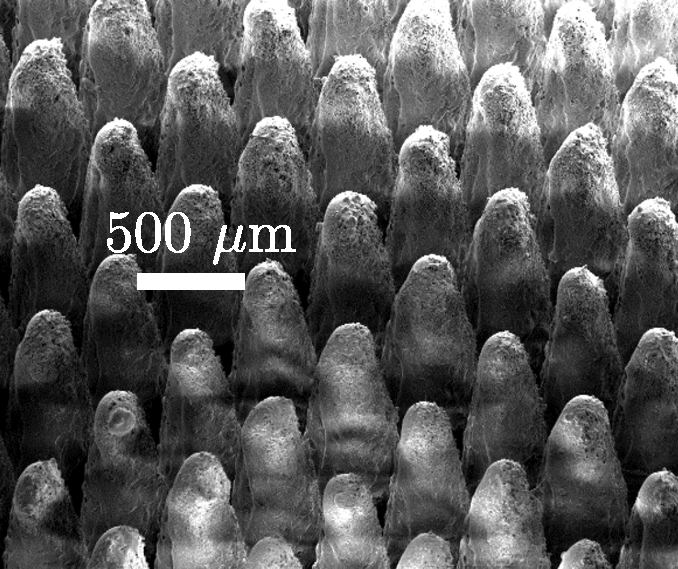
\includegraphics[width=0.65\textwidth]{../figures/SEM.pdf}
 \caption{SEM image of the superhydrophobic surface.\label{fig:SEM}}
\end{figure}

Surface potentials $\varphi_s$ are measured on the superhydrophobic surface using a Simco-Ion FMX-004 electrostatic fieldmeter and the method for determination of surface charge density for low conductivity polymers described in Davies \cite{davies_examination_1967}. This measurement is made with the electret substrate bonded to a conductive ground plane by conductive tape far from the presence of other conductors. An ideal approach to determining surface charge on a dielectric surface is to screen perturbing effects of external electric fields. This is partly accomplished by grounding the fieldmeter and by placing the dielectric sample on a grounded conductive plate backing. In this case the surface charge density is determined from $\sigma = \varphi_s \kappa \epsilon_0/l,$ where $l$ is the thickness of the dielectric surface. The measured surface voltage is a function of position away from the charged dielectric. In most cases this function is relatively constant at a distance of about 1-2 cm away from the surface though we note that there is some measurement error in surface voltage due to small mispositioning of the electrostatic fieldmeter, say by $\pm$1 mm. The relative dielectric constant of the PMMA sheet is measured by using a 65$\times$65 mm polished aluminum parallel plate capacitor with $C = \kappa \epsilon_0 A/l$, where $C$ is the capacitance, and $A$ is the sheet area. Measuring the capacitance with 3 sample thicknesses using a GenRad 1657 RLC Digibridge, we find the relative permittivity to be $\kappa = 3.5 \pm 0.4$.  

A further consideration is the possibility of the change in total charge during a typical experimental timescale. If we consider the drop rig to be a ground which is reasonable given that the rig is isolated from true ground, but is at some reference voltage with respect to the surface charges on the dielectric with an abundance of free charge carriers, then there will be both bulk and surface Ohmic decay of the charge on the dielectric. The evolution of the charge can in some cases be approximated by $\sigma = \sigma_0 e^{\frac{-t}{\epsilon \rho}}, $ where $\sigma_0$ is the initial surface charge density and $\rho$ is the bulk resistivity. For an example case of a surface with relative permittivity $\kappa = 3.5$ and bulk resistivity $\rho = 1.6 \times (10^{16})$ $\Omega$cm such as with the case of a 2.8 mm PMMA sheet, then the time constant $\tau = \kappa \epsilon_0 \rho$ is approximately 5000 s, which is significantly longer than the typical time period for a drop tower experiment. External charge decay mechanisms include compensation by environmental ionic species. The relative magnitudes of these charge transport mechanisms, and therefore the stability of the electret, vary drastically depending on the initial surface potential, material properties, environment, and charging method. In the case of unshielded electrets compensation by atmospheric ions is significant \cite{perlman_electrets_1973}. Because environmental convection will tend to  maintain a gradient of these ions, sealing an electret in a container from the atmosphere will effectively halt this decay mechanism. Atmospheric humidity and water drop condensation can also significantly increase charge decay, presumably by reducing the surface resistance \cite{haenen_characteristic_1975}. Examples of this decay can be seen in Figure \ref{fig:charge_decay} for differing numbers of dielectric lamina used in this experiment. In looking at the trends in charge decay for our electrets we notice firstly that the decay does not appear to be exponential, as in the model described above. Secondly, we plainly see a cross-over effect in the decay of the surface potential in our electret samples, whereby the samples charged to higher initial surface potentials decay faster and reached the lower overall final potentials. This is a well known effect in polyethylenes charged by corona \cite{ferreira_corona_1992}.
\begin{figure}[htb!]
    \centering
    {%% Creator: Matplotlib, PGF backend
%%
%% To include the figure in your LaTeX document, write
%%   \input{<filename>.pgf}
%%
%% Make sure the required packages are loaded in your preamble
%%   \usepackage{pgf}
%%
%% Figures using additional raster images can only be included by \input if
%% they are in the same directory as the main LaTeX file. For loading figures
%% from other directories you can use the `import` package
%%   \usepackage{import}
%% and then include the figures with
%%   \import{<path to file>}{<filename>.pgf}
%%
%% Matplotlib used the following preamble
%%   \usepackage{fontspec}
%%   \setmainfont{DejaVu Serif}
%%   \setsansfont{DejaVu Sans}
%%   \setmonofont{DejaVu Sans Mono}
%%
\begingroup%
\makeatletter%
\begin{pgfpicture}%
\pgfpathrectangle{\pgfpointorigin}{\pgfqpoint{5.349660in}{3.676603in}}%
\pgfusepath{use as bounding box, clip}%
\begin{pgfscope}%
\pgfsetbuttcap%
\pgfsetmiterjoin%
\definecolor{currentfill}{rgb}{1.000000,1.000000,1.000000}%
\pgfsetfillcolor{currentfill}%
\pgfsetlinewidth{0.000000pt}%
\definecolor{currentstroke}{rgb}{1.000000,1.000000,1.000000}%
\pgfsetstrokecolor{currentstroke}%
\pgfsetdash{}{0pt}%
\pgfpathmoveto{\pgfqpoint{0.000000in}{0.000000in}}%
\pgfpathlineto{\pgfqpoint{5.349660in}{0.000000in}}%
\pgfpathlineto{\pgfqpoint{5.349660in}{3.676603in}}%
\pgfpathlineto{\pgfqpoint{0.000000in}{3.676603in}}%
\pgfpathclose%
\pgfusepath{fill}%
\end{pgfscope}%
\begin{pgfscope}%
\pgfsetbuttcap%
\pgfsetmiterjoin%
\definecolor{currentfill}{rgb}{1.000000,1.000000,1.000000}%
\pgfsetfillcolor{currentfill}%
\pgfsetlinewidth{0.000000pt}%
\definecolor{currentstroke}{rgb}{0.000000,0.000000,0.000000}%
\pgfsetstrokecolor{currentstroke}%
\pgfsetstrokeopacity{0.000000}%
\pgfsetdash{}{0pt}%
\pgfpathmoveto{\pgfqpoint{0.564660in}{0.521603in}}%
\pgfpathlineto{\pgfqpoint{5.214660in}{0.521603in}}%
\pgfpathlineto{\pgfqpoint{5.214660in}{3.541603in}}%
\pgfpathlineto{\pgfqpoint{0.564660in}{3.541603in}}%
\pgfpathclose%
\pgfusepath{fill}%
\end{pgfscope}%
\begin{pgfscope}%
\pgfsetbuttcap%
\pgfsetroundjoin%
\definecolor{currentfill}{rgb}{0.000000,0.000000,0.000000}%
\pgfsetfillcolor{currentfill}%
\pgfsetlinewidth{0.803000pt}%
\definecolor{currentstroke}{rgb}{0.000000,0.000000,0.000000}%
\pgfsetstrokecolor{currentstroke}%
\pgfsetdash{}{0pt}%
\pgfsys@defobject{currentmarker}{\pgfqpoint{0.000000in}{-0.048611in}}{\pgfqpoint{0.000000in}{0.000000in}}{%
\pgfpathmoveto{\pgfqpoint{0.000000in}{0.000000in}}%
\pgfpathlineto{\pgfqpoint{0.000000in}{-0.048611in}}%
\pgfusepath{stroke,fill}%
}%
\begin{pgfscope}%
\pgfsys@transformshift{0.776024in}{0.521603in}%
\pgfsys@useobject{currentmarker}{}%
\end{pgfscope}%
\end{pgfscope}%
\begin{pgfscope}%
\pgftext[x=0.776024in,y=0.424381in,,top]{\rmfamily\fontsize{10.000000}{12.000000}\selectfont \(\displaystyle 0\)}%
\end{pgfscope}%
\begin{pgfscope}%
\pgfsetbuttcap%
\pgfsetroundjoin%
\definecolor{currentfill}{rgb}{0.000000,0.000000,0.000000}%
\pgfsetfillcolor{currentfill}%
\pgfsetlinewidth{0.803000pt}%
\definecolor{currentstroke}{rgb}{0.000000,0.000000,0.000000}%
\pgfsetstrokecolor{currentstroke}%
\pgfsetdash{}{0pt}%
\pgfsys@defobject{currentmarker}{\pgfqpoint{0.000000in}{-0.048611in}}{\pgfqpoint{0.000000in}{0.000000in}}{%
\pgfpathmoveto{\pgfqpoint{0.000000in}{0.000000in}}%
\pgfpathlineto{\pgfqpoint{0.000000in}{-0.048611in}}%
\pgfusepath{stroke,fill}%
}%
\begin{pgfscope}%
\pgfsys@transformshift{1.351163in}{0.521603in}%
\pgfsys@useobject{currentmarker}{}%
\end{pgfscope}%
\end{pgfscope}%
\begin{pgfscope}%
\pgftext[x=1.351163in,y=0.424381in,,top]{\rmfamily\fontsize{10.000000}{12.000000}\selectfont \(\displaystyle 2000\)}%
\end{pgfscope}%
\begin{pgfscope}%
\pgfsetbuttcap%
\pgfsetroundjoin%
\definecolor{currentfill}{rgb}{0.000000,0.000000,0.000000}%
\pgfsetfillcolor{currentfill}%
\pgfsetlinewidth{0.803000pt}%
\definecolor{currentstroke}{rgb}{0.000000,0.000000,0.000000}%
\pgfsetstrokecolor{currentstroke}%
\pgfsetdash{}{0pt}%
\pgfsys@defobject{currentmarker}{\pgfqpoint{0.000000in}{-0.048611in}}{\pgfqpoint{0.000000in}{0.000000in}}{%
\pgfpathmoveto{\pgfqpoint{0.000000in}{0.000000in}}%
\pgfpathlineto{\pgfqpoint{0.000000in}{-0.048611in}}%
\pgfusepath{stroke,fill}%
}%
\begin{pgfscope}%
\pgfsys@transformshift{1.926302in}{0.521603in}%
\pgfsys@useobject{currentmarker}{}%
\end{pgfscope}%
\end{pgfscope}%
\begin{pgfscope}%
\pgftext[x=1.926302in,y=0.424381in,,top]{\rmfamily\fontsize{10.000000}{12.000000}\selectfont \(\displaystyle 4000\)}%
\end{pgfscope}%
\begin{pgfscope}%
\pgfsetbuttcap%
\pgfsetroundjoin%
\definecolor{currentfill}{rgb}{0.000000,0.000000,0.000000}%
\pgfsetfillcolor{currentfill}%
\pgfsetlinewidth{0.803000pt}%
\definecolor{currentstroke}{rgb}{0.000000,0.000000,0.000000}%
\pgfsetstrokecolor{currentstroke}%
\pgfsetdash{}{0pt}%
\pgfsys@defobject{currentmarker}{\pgfqpoint{0.000000in}{-0.048611in}}{\pgfqpoint{0.000000in}{0.000000in}}{%
\pgfpathmoveto{\pgfqpoint{0.000000in}{0.000000in}}%
\pgfpathlineto{\pgfqpoint{0.000000in}{-0.048611in}}%
\pgfusepath{stroke,fill}%
}%
\begin{pgfscope}%
\pgfsys@transformshift{2.501441in}{0.521603in}%
\pgfsys@useobject{currentmarker}{}%
\end{pgfscope}%
\end{pgfscope}%
\begin{pgfscope}%
\pgftext[x=2.501441in,y=0.424381in,,top]{\rmfamily\fontsize{10.000000}{12.000000}\selectfont \(\displaystyle 6000\)}%
\end{pgfscope}%
\begin{pgfscope}%
\pgfsetbuttcap%
\pgfsetroundjoin%
\definecolor{currentfill}{rgb}{0.000000,0.000000,0.000000}%
\pgfsetfillcolor{currentfill}%
\pgfsetlinewidth{0.803000pt}%
\definecolor{currentstroke}{rgb}{0.000000,0.000000,0.000000}%
\pgfsetstrokecolor{currentstroke}%
\pgfsetdash{}{0pt}%
\pgfsys@defobject{currentmarker}{\pgfqpoint{0.000000in}{-0.048611in}}{\pgfqpoint{0.000000in}{0.000000in}}{%
\pgfpathmoveto{\pgfqpoint{0.000000in}{0.000000in}}%
\pgfpathlineto{\pgfqpoint{0.000000in}{-0.048611in}}%
\pgfusepath{stroke,fill}%
}%
\begin{pgfscope}%
\pgfsys@transformshift{3.076581in}{0.521603in}%
\pgfsys@useobject{currentmarker}{}%
\end{pgfscope}%
\end{pgfscope}%
\begin{pgfscope}%
\pgftext[x=3.076581in,y=0.424381in,,top]{\rmfamily\fontsize{10.000000}{12.000000}\selectfont \(\displaystyle 8000\)}%
\end{pgfscope}%
\begin{pgfscope}%
\pgfsetbuttcap%
\pgfsetroundjoin%
\definecolor{currentfill}{rgb}{0.000000,0.000000,0.000000}%
\pgfsetfillcolor{currentfill}%
\pgfsetlinewidth{0.803000pt}%
\definecolor{currentstroke}{rgb}{0.000000,0.000000,0.000000}%
\pgfsetstrokecolor{currentstroke}%
\pgfsetdash{}{0pt}%
\pgfsys@defobject{currentmarker}{\pgfqpoint{0.000000in}{-0.048611in}}{\pgfqpoint{0.000000in}{0.000000in}}{%
\pgfpathmoveto{\pgfqpoint{0.000000in}{0.000000in}}%
\pgfpathlineto{\pgfqpoint{0.000000in}{-0.048611in}}%
\pgfusepath{stroke,fill}%
}%
\begin{pgfscope}%
\pgfsys@transformshift{3.651720in}{0.521603in}%
\pgfsys@useobject{currentmarker}{}%
\end{pgfscope}%
\end{pgfscope}%
\begin{pgfscope}%
\pgftext[x=3.651720in,y=0.424381in,,top]{\rmfamily\fontsize{10.000000}{12.000000}\selectfont \(\displaystyle 10000\)}%
\end{pgfscope}%
\begin{pgfscope}%
\pgfsetbuttcap%
\pgfsetroundjoin%
\definecolor{currentfill}{rgb}{0.000000,0.000000,0.000000}%
\pgfsetfillcolor{currentfill}%
\pgfsetlinewidth{0.803000pt}%
\definecolor{currentstroke}{rgb}{0.000000,0.000000,0.000000}%
\pgfsetstrokecolor{currentstroke}%
\pgfsetdash{}{0pt}%
\pgfsys@defobject{currentmarker}{\pgfqpoint{0.000000in}{-0.048611in}}{\pgfqpoint{0.000000in}{0.000000in}}{%
\pgfpathmoveto{\pgfqpoint{0.000000in}{0.000000in}}%
\pgfpathlineto{\pgfqpoint{0.000000in}{-0.048611in}}%
\pgfusepath{stroke,fill}%
}%
\begin{pgfscope}%
\pgfsys@transformshift{4.226859in}{0.521603in}%
\pgfsys@useobject{currentmarker}{}%
\end{pgfscope}%
\end{pgfscope}%
\begin{pgfscope}%
\pgftext[x=4.226859in,y=0.424381in,,top]{\rmfamily\fontsize{10.000000}{12.000000}\selectfont \(\displaystyle 12000\)}%
\end{pgfscope}%
\begin{pgfscope}%
\pgfsetbuttcap%
\pgfsetroundjoin%
\definecolor{currentfill}{rgb}{0.000000,0.000000,0.000000}%
\pgfsetfillcolor{currentfill}%
\pgfsetlinewidth{0.803000pt}%
\definecolor{currentstroke}{rgb}{0.000000,0.000000,0.000000}%
\pgfsetstrokecolor{currentstroke}%
\pgfsetdash{}{0pt}%
\pgfsys@defobject{currentmarker}{\pgfqpoint{0.000000in}{-0.048611in}}{\pgfqpoint{0.000000in}{0.000000in}}{%
\pgfpathmoveto{\pgfqpoint{0.000000in}{0.000000in}}%
\pgfpathlineto{\pgfqpoint{0.000000in}{-0.048611in}}%
\pgfusepath{stroke,fill}%
}%
\begin{pgfscope}%
\pgfsys@transformshift{4.801998in}{0.521603in}%
\pgfsys@useobject{currentmarker}{}%
\end{pgfscope}%
\end{pgfscope}%
\begin{pgfscope}%
\pgftext[x=4.801998in,y=0.424381in,,top]{\rmfamily\fontsize{10.000000}{12.000000}\selectfont \(\displaystyle 14000\)}%
\end{pgfscope}%
\begin{pgfscope}%
\pgftext[x=2.889660in,y=0.234413in,,top]{\rmfamily\fontsize{10.000000}{12.000000}\selectfont t (s)}%
\end{pgfscope}%
\begin{pgfscope}%
\pgfsetbuttcap%
\pgfsetroundjoin%
\definecolor{currentfill}{rgb}{0.000000,0.000000,0.000000}%
\pgfsetfillcolor{currentfill}%
\pgfsetlinewidth{0.803000pt}%
\definecolor{currentstroke}{rgb}{0.000000,0.000000,0.000000}%
\pgfsetstrokecolor{currentstroke}%
\pgfsetdash{}{0pt}%
\pgfsys@defobject{currentmarker}{\pgfqpoint{-0.048611in}{0.000000in}}{\pgfqpoint{0.000000in}{0.000000in}}{%
\pgfpathmoveto{\pgfqpoint{0.000000in}{0.000000in}}%
\pgfpathlineto{\pgfqpoint{-0.048611in}{0.000000in}}%
\pgfusepath{stroke,fill}%
}%
\begin{pgfscope}%
\pgfsys@transformshift{0.564660in}{0.747439in}%
\pgfsys@useobject{currentmarker}{}%
\end{pgfscope}%
\end{pgfscope}%
\begin{pgfscope}%
\pgftext[x=0.289968in,y=0.694678in,left,base]{\rmfamily\fontsize{10.000000}{12.000000}\selectfont \(\displaystyle 0.5\)}%
\end{pgfscope}%
\begin{pgfscope}%
\pgfsetbuttcap%
\pgfsetroundjoin%
\definecolor{currentfill}{rgb}{0.000000,0.000000,0.000000}%
\pgfsetfillcolor{currentfill}%
\pgfsetlinewidth{0.803000pt}%
\definecolor{currentstroke}{rgb}{0.000000,0.000000,0.000000}%
\pgfsetstrokecolor{currentstroke}%
\pgfsetdash{}{0pt}%
\pgfsys@defobject{currentmarker}{\pgfqpoint{-0.048611in}{0.000000in}}{\pgfqpoint{0.000000in}{0.000000in}}{%
\pgfpathmoveto{\pgfqpoint{0.000000in}{0.000000in}}%
\pgfpathlineto{\pgfqpoint{-0.048611in}{0.000000in}}%
\pgfusepath{stroke,fill}%
}%
\begin{pgfscope}%
\pgfsys@transformshift{0.564660in}{1.190254in}%
\pgfsys@useobject{currentmarker}{}%
\end{pgfscope}%
\end{pgfscope}%
\begin{pgfscope}%
\pgftext[x=0.289968in,y=1.137493in,left,base]{\rmfamily\fontsize{10.000000}{12.000000}\selectfont \(\displaystyle 1.0\)}%
\end{pgfscope}%
\begin{pgfscope}%
\pgfsetbuttcap%
\pgfsetroundjoin%
\definecolor{currentfill}{rgb}{0.000000,0.000000,0.000000}%
\pgfsetfillcolor{currentfill}%
\pgfsetlinewidth{0.803000pt}%
\definecolor{currentstroke}{rgb}{0.000000,0.000000,0.000000}%
\pgfsetstrokecolor{currentstroke}%
\pgfsetdash{}{0pt}%
\pgfsys@defobject{currentmarker}{\pgfqpoint{-0.048611in}{0.000000in}}{\pgfqpoint{0.000000in}{0.000000in}}{%
\pgfpathmoveto{\pgfqpoint{0.000000in}{0.000000in}}%
\pgfpathlineto{\pgfqpoint{-0.048611in}{0.000000in}}%
\pgfusepath{stroke,fill}%
}%
\begin{pgfscope}%
\pgfsys@transformshift{0.564660in}{1.633070in}%
\pgfsys@useobject{currentmarker}{}%
\end{pgfscope}%
\end{pgfscope}%
\begin{pgfscope}%
\pgftext[x=0.289968in,y=1.580308in,left,base]{\rmfamily\fontsize{10.000000}{12.000000}\selectfont \(\displaystyle 1.5\)}%
\end{pgfscope}%
\begin{pgfscope}%
\pgfsetbuttcap%
\pgfsetroundjoin%
\definecolor{currentfill}{rgb}{0.000000,0.000000,0.000000}%
\pgfsetfillcolor{currentfill}%
\pgfsetlinewidth{0.803000pt}%
\definecolor{currentstroke}{rgb}{0.000000,0.000000,0.000000}%
\pgfsetstrokecolor{currentstroke}%
\pgfsetdash{}{0pt}%
\pgfsys@defobject{currentmarker}{\pgfqpoint{-0.048611in}{0.000000in}}{\pgfqpoint{0.000000in}{0.000000in}}{%
\pgfpathmoveto{\pgfqpoint{0.000000in}{0.000000in}}%
\pgfpathlineto{\pgfqpoint{-0.048611in}{0.000000in}}%
\pgfusepath{stroke,fill}%
}%
\begin{pgfscope}%
\pgfsys@transformshift{0.564660in}{2.075885in}%
\pgfsys@useobject{currentmarker}{}%
\end{pgfscope}%
\end{pgfscope}%
\begin{pgfscope}%
\pgftext[x=0.289968in,y=2.023123in,left,base]{\rmfamily\fontsize{10.000000}{12.000000}\selectfont \(\displaystyle 2.0\)}%
\end{pgfscope}%
\begin{pgfscope}%
\pgfsetbuttcap%
\pgfsetroundjoin%
\definecolor{currentfill}{rgb}{0.000000,0.000000,0.000000}%
\pgfsetfillcolor{currentfill}%
\pgfsetlinewidth{0.803000pt}%
\definecolor{currentstroke}{rgb}{0.000000,0.000000,0.000000}%
\pgfsetstrokecolor{currentstroke}%
\pgfsetdash{}{0pt}%
\pgfsys@defobject{currentmarker}{\pgfqpoint{-0.048611in}{0.000000in}}{\pgfqpoint{0.000000in}{0.000000in}}{%
\pgfpathmoveto{\pgfqpoint{0.000000in}{0.000000in}}%
\pgfpathlineto{\pgfqpoint{-0.048611in}{0.000000in}}%
\pgfusepath{stroke,fill}%
}%
\begin{pgfscope}%
\pgfsys@transformshift{0.564660in}{2.518700in}%
\pgfsys@useobject{currentmarker}{}%
\end{pgfscope}%
\end{pgfscope}%
\begin{pgfscope}%
\pgftext[x=0.289968in,y=2.465939in,left,base]{\rmfamily\fontsize{10.000000}{12.000000}\selectfont \(\displaystyle 2.5\)}%
\end{pgfscope}%
\begin{pgfscope}%
\pgfsetbuttcap%
\pgfsetroundjoin%
\definecolor{currentfill}{rgb}{0.000000,0.000000,0.000000}%
\pgfsetfillcolor{currentfill}%
\pgfsetlinewidth{0.803000pt}%
\definecolor{currentstroke}{rgb}{0.000000,0.000000,0.000000}%
\pgfsetstrokecolor{currentstroke}%
\pgfsetdash{}{0pt}%
\pgfsys@defobject{currentmarker}{\pgfqpoint{-0.048611in}{0.000000in}}{\pgfqpoint{0.000000in}{0.000000in}}{%
\pgfpathmoveto{\pgfqpoint{0.000000in}{0.000000in}}%
\pgfpathlineto{\pgfqpoint{-0.048611in}{0.000000in}}%
\pgfusepath{stroke,fill}%
}%
\begin{pgfscope}%
\pgfsys@transformshift{0.564660in}{2.961515in}%
\pgfsys@useobject{currentmarker}{}%
\end{pgfscope}%
\end{pgfscope}%
\begin{pgfscope}%
\pgftext[x=0.289968in,y=2.908754in,left,base]{\rmfamily\fontsize{10.000000}{12.000000}\selectfont \(\displaystyle 3.0\)}%
\end{pgfscope}%
\begin{pgfscope}%
\pgfsetbuttcap%
\pgfsetroundjoin%
\definecolor{currentfill}{rgb}{0.000000,0.000000,0.000000}%
\pgfsetfillcolor{currentfill}%
\pgfsetlinewidth{0.803000pt}%
\definecolor{currentstroke}{rgb}{0.000000,0.000000,0.000000}%
\pgfsetstrokecolor{currentstroke}%
\pgfsetdash{}{0pt}%
\pgfsys@defobject{currentmarker}{\pgfqpoint{-0.048611in}{0.000000in}}{\pgfqpoint{0.000000in}{0.000000in}}{%
\pgfpathmoveto{\pgfqpoint{0.000000in}{0.000000in}}%
\pgfpathlineto{\pgfqpoint{-0.048611in}{0.000000in}}%
\pgfusepath{stroke,fill}%
}%
\begin{pgfscope}%
\pgfsys@transformshift{0.564660in}{3.404331in}%
\pgfsys@useobject{currentmarker}{}%
\end{pgfscope}%
\end{pgfscope}%
\begin{pgfscope}%
\pgftext[x=0.289968in,y=3.351569in,left,base]{\rmfamily\fontsize{10.000000}{12.000000}\selectfont \(\displaystyle 3.5\)}%
\end{pgfscope}%
\begin{pgfscope}%
\pgftext[x=0.234413in,y=2.031603in,,bottom,rotate=90.000000]{\rmfamily\fontsize{10.000000}{12.000000}\selectfont Surface potential (kV)}%
\end{pgfscope}%
\begin{pgfscope}%
\pgfpathrectangle{\pgfqpoint{0.564660in}{0.521603in}}{\pgfqpoint{4.650000in}{3.020000in}} %
\pgfusepath{clip}%
\pgfsetrectcap%
\pgfsetroundjoin%
\pgfsetlinewidth{1.505625pt}%
\definecolor{currentstroke}{rgb}{0.000000,0.750000,0.750000}%
\pgfsetstrokecolor{currentstroke}%
\pgfsetdash{}{0pt}%
\pgfpathmoveto{\pgfqpoint{0.776024in}{1.810196in}}%
\pgfpathlineto{\pgfqpoint{0.784651in}{1.633070in}}%
\pgfpathlineto{\pgfqpoint{0.793278in}{1.721633in}}%
\pgfpathlineto{\pgfqpoint{0.810532in}{1.633070in}}%
\pgfpathlineto{\pgfqpoint{0.819159in}{1.544507in}}%
\pgfpathlineto{\pgfqpoint{0.827786in}{1.633070in}}%
\pgfpathlineto{\pgfqpoint{0.836414in}{1.721633in}}%
\pgfpathlineto{\pgfqpoint{0.845041in}{1.455944in}}%
\pgfpathlineto{\pgfqpoint{0.853668in}{1.455944in}}%
\pgfpathlineto{\pgfqpoint{0.862295in}{1.544507in}}%
\pgfpathlineto{\pgfqpoint{1.034837in}{1.455944in}}%
\pgfpathlineto{\pgfqpoint{1.207378in}{1.367380in}}%
\pgfpathlineto{\pgfqpoint{1.379920in}{1.367380in}}%
\pgfpathlineto{\pgfqpoint{1.897545in}{1.190254in}}%
\pgfpathlineto{\pgfqpoint{2.415170in}{1.190254in}}%
\pgfpathlineto{\pgfqpoint{2.932796in}{1.101691in}}%
\pgfpathlineto{\pgfqpoint{3.450421in}{1.101691in}}%
\pgfpathlineto{\pgfqpoint{5.003297in}{1.101691in}}%
\pgfusepath{stroke}%
\end{pgfscope}%
\begin{pgfscope}%
\pgfpathrectangle{\pgfqpoint{0.564660in}{0.521603in}}{\pgfqpoint{4.650000in}{3.020000in}} %
\pgfusepath{clip}%
\pgfsetbuttcap%
\pgfsetmiterjoin%
\definecolor{currentfill}{rgb}{0.000000,0.750000,0.750000}%
\pgfsetfillcolor{currentfill}%
\pgfsetlinewidth{1.003750pt}%
\definecolor{currentstroke}{rgb}{0.000000,0.750000,0.750000}%
\pgfsetstrokecolor{currentstroke}%
\pgfsetdash{}{0pt}%
\pgfsys@defobject{currentmarker}{\pgfqpoint{-0.041667in}{-0.041667in}}{\pgfqpoint{0.041667in}{0.041667in}}{%
\pgfpathmoveto{\pgfqpoint{-0.000000in}{-0.041667in}}%
\pgfpathlineto{\pgfqpoint{0.041667in}{0.041667in}}%
\pgfpathlineto{\pgfqpoint{-0.041667in}{0.041667in}}%
\pgfpathclose%
\pgfusepath{stroke,fill}%
}%
\begin{pgfscope}%
\pgfsys@transformshift{0.776024in}{1.810196in}%
\pgfsys@useobject{currentmarker}{}%
\end{pgfscope}%
\begin{pgfscope}%
\pgfsys@transformshift{0.784651in}{1.633070in}%
\pgfsys@useobject{currentmarker}{}%
\end{pgfscope}%
\begin{pgfscope}%
\pgfsys@transformshift{0.793278in}{1.721633in}%
\pgfsys@useobject{currentmarker}{}%
\end{pgfscope}%
\begin{pgfscope}%
\pgfsys@transformshift{0.810532in}{1.633070in}%
\pgfsys@useobject{currentmarker}{}%
\end{pgfscope}%
\begin{pgfscope}%
\pgfsys@transformshift{0.819159in}{1.544507in}%
\pgfsys@useobject{currentmarker}{}%
\end{pgfscope}%
\begin{pgfscope}%
\pgfsys@transformshift{0.827786in}{1.633070in}%
\pgfsys@useobject{currentmarker}{}%
\end{pgfscope}%
\begin{pgfscope}%
\pgfsys@transformshift{0.836414in}{1.721633in}%
\pgfsys@useobject{currentmarker}{}%
\end{pgfscope}%
\begin{pgfscope}%
\pgfsys@transformshift{0.845041in}{1.455944in}%
\pgfsys@useobject{currentmarker}{}%
\end{pgfscope}%
\begin{pgfscope}%
\pgfsys@transformshift{0.853668in}{1.455944in}%
\pgfsys@useobject{currentmarker}{}%
\end{pgfscope}%
\begin{pgfscope}%
\pgfsys@transformshift{0.862295in}{1.544507in}%
\pgfsys@useobject{currentmarker}{}%
\end{pgfscope}%
\begin{pgfscope}%
\pgfsys@transformshift{1.034837in}{1.455944in}%
\pgfsys@useobject{currentmarker}{}%
\end{pgfscope}%
\begin{pgfscope}%
\pgfsys@transformshift{1.207378in}{1.367380in}%
\pgfsys@useobject{currentmarker}{}%
\end{pgfscope}%
\begin{pgfscope}%
\pgfsys@transformshift{1.379920in}{1.367380in}%
\pgfsys@useobject{currentmarker}{}%
\end{pgfscope}%
\begin{pgfscope}%
\pgfsys@transformshift{1.897545in}{1.190254in}%
\pgfsys@useobject{currentmarker}{}%
\end{pgfscope}%
\begin{pgfscope}%
\pgfsys@transformshift{2.415170in}{1.190254in}%
\pgfsys@useobject{currentmarker}{}%
\end{pgfscope}%
\begin{pgfscope}%
\pgfsys@transformshift{2.932796in}{1.101691in}%
\pgfsys@useobject{currentmarker}{}%
\end{pgfscope}%
\begin{pgfscope}%
\pgfsys@transformshift{3.450421in}{1.101691in}%
\pgfsys@useobject{currentmarker}{}%
\end{pgfscope}%
\begin{pgfscope}%
\pgfsys@transformshift{5.003297in}{1.101691in}%
\pgfsys@useobject{currentmarker}{}%
\end{pgfscope}%
\end{pgfscope}%
\begin{pgfscope}%
\pgfpathrectangle{\pgfqpoint{0.564660in}{0.521603in}}{\pgfqpoint{4.650000in}{3.020000in}} %
\pgfusepath{clip}%
\pgfsetrectcap%
\pgfsetroundjoin%
\pgfsetlinewidth{1.505625pt}%
\definecolor{currentstroke}{rgb}{0.000000,0.000000,1.000000}%
\pgfsetstrokecolor{currentstroke}%
\pgfsetdash{}{0pt}%
\pgfpathmoveto{\pgfqpoint{0.776024in}{2.430137in}}%
\pgfpathlineto{\pgfqpoint{0.784651in}{2.872952in}}%
\pgfpathlineto{\pgfqpoint{0.793278in}{2.784389in}}%
\pgfpathlineto{\pgfqpoint{0.801905in}{2.607263in}}%
\pgfpathlineto{\pgfqpoint{0.810532in}{2.607263in}}%
\pgfpathlineto{\pgfqpoint{0.819159in}{2.253011in}}%
\pgfpathlineto{\pgfqpoint{0.827786in}{2.253011in}}%
\pgfpathlineto{\pgfqpoint{0.836414in}{2.518700in}}%
\pgfpathlineto{\pgfqpoint{0.845041in}{2.430137in}}%
\pgfpathlineto{\pgfqpoint{0.853668in}{2.518700in}}%
\pgfpathlineto{\pgfqpoint{0.862295in}{2.430137in}}%
\pgfpathlineto{\pgfqpoint{1.034837in}{1.810196in}}%
\pgfpathlineto{\pgfqpoint{1.207378in}{1.633070in}}%
\pgfpathlineto{\pgfqpoint{1.379920in}{1.544507in}}%
\pgfpathlineto{\pgfqpoint{1.897545in}{1.101691in}}%
\pgfpathlineto{\pgfqpoint{2.415170in}{1.101691in}}%
\pgfpathlineto{\pgfqpoint{2.932796in}{1.013128in}}%
\pgfpathlineto{\pgfqpoint{3.450421in}{1.013128in}}%
\pgfpathlineto{\pgfqpoint{5.003297in}{0.924565in}}%
\pgfusepath{stroke}%
\end{pgfscope}%
\begin{pgfscope}%
\pgfpathrectangle{\pgfqpoint{0.564660in}{0.521603in}}{\pgfqpoint{4.650000in}{3.020000in}} %
\pgfusepath{clip}%
\pgfsetbuttcap%
\pgfsetroundjoin%
\definecolor{currentfill}{rgb}{0.000000,0.000000,1.000000}%
\pgfsetfillcolor{currentfill}%
\pgfsetlinewidth{1.003750pt}%
\definecolor{currentstroke}{rgb}{0.000000,0.000000,1.000000}%
\pgfsetstrokecolor{currentstroke}%
\pgfsetdash{}{0pt}%
\pgfsys@defobject{currentmarker}{\pgfqpoint{-0.041667in}{-0.041667in}}{\pgfqpoint{0.041667in}{0.041667in}}{%
\pgfpathmoveto{\pgfqpoint{0.000000in}{-0.041667in}}%
\pgfpathcurveto{\pgfqpoint{0.011050in}{-0.041667in}}{\pgfqpoint{0.021649in}{-0.037276in}}{\pgfqpoint{0.029463in}{-0.029463in}}%
\pgfpathcurveto{\pgfqpoint{0.037276in}{-0.021649in}}{\pgfqpoint{0.041667in}{-0.011050in}}{\pgfqpoint{0.041667in}{0.000000in}}%
\pgfpathcurveto{\pgfqpoint{0.041667in}{0.011050in}}{\pgfqpoint{0.037276in}{0.021649in}}{\pgfqpoint{0.029463in}{0.029463in}}%
\pgfpathcurveto{\pgfqpoint{0.021649in}{0.037276in}}{\pgfqpoint{0.011050in}{0.041667in}}{\pgfqpoint{0.000000in}{0.041667in}}%
\pgfpathcurveto{\pgfqpoint{-0.011050in}{0.041667in}}{\pgfqpoint{-0.021649in}{0.037276in}}{\pgfqpoint{-0.029463in}{0.029463in}}%
\pgfpathcurveto{\pgfqpoint{-0.037276in}{0.021649in}}{\pgfqpoint{-0.041667in}{0.011050in}}{\pgfqpoint{-0.041667in}{0.000000in}}%
\pgfpathcurveto{\pgfqpoint{-0.041667in}{-0.011050in}}{\pgfqpoint{-0.037276in}{-0.021649in}}{\pgfqpoint{-0.029463in}{-0.029463in}}%
\pgfpathcurveto{\pgfqpoint{-0.021649in}{-0.037276in}}{\pgfqpoint{-0.011050in}{-0.041667in}}{\pgfqpoint{0.000000in}{-0.041667in}}%
\pgfpathclose%
\pgfusepath{stroke,fill}%
}%
\begin{pgfscope}%
\pgfsys@transformshift{0.776024in}{2.430137in}%
\pgfsys@useobject{currentmarker}{}%
\end{pgfscope}%
\begin{pgfscope}%
\pgfsys@transformshift{0.784651in}{2.872952in}%
\pgfsys@useobject{currentmarker}{}%
\end{pgfscope}%
\begin{pgfscope}%
\pgfsys@transformshift{0.793278in}{2.784389in}%
\pgfsys@useobject{currentmarker}{}%
\end{pgfscope}%
\begin{pgfscope}%
\pgfsys@transformshift{0.801905in}{2.607263in}%
\pgfsys@useobject{currentmarker}{}%
\end{pgfscope}%
\begin{pgfscope}%
\pgfsys@transformshift{0.810532in}{2.607263in}%
\pgfsys@useobject{currentmarker}{}%
\end{pgfscope}%
\begin{pgfscope}%
\pgfsys@transformshift{0.819159in}{2.253011in}%
\pgfsys@useobject{currentmarker}{}%
\end{pgfscope}%
\begin{pgfscope}%
\pgfsys@transformshift{0.827786in}{2.253011in}%
\pgfsys@useobject{currentmarker}{}%
\end{pgfscope}%
\begin{pgfscope}%
\pgfsys@transformshift{0.836414in}{2.518700in}%
\pgfsys@useobject{currentmarker}{}%
\end{pgfscope}%
\begin{pgfscope}%
\pgfsys@transformshift{0.845041in}{2.430137in}%
\pgfsys@useobject{currentmarker}{}%
\end{pgfscope}%
\begin{pgfscope}%
\pgfsys@transformshift{0.853668in}{2.518700in}%
\pgfsys@useobject{currentmarker}{}%
\end{pgfscope}%
\begin{pgfscope}%
\pgfsys@transformshift{0.862295in}{2.430137in}%
\pgfsys@useobject{currentmarker}{}%
\end{pgfscope}%
\begin{pgfscope}%
\pgfsys@transformshift{1.034837in}{1.810196in}%
\pgfsys@useobject{currentmarker}{}%
\end{pgfscope}%
\begin{pgfscope}%
\pgfsys@transformshift{1.207378in}{1.633070in}%
\pgfsys@useobject{currentmarker}{}%
\end{pgfscope}%
\begin{pgfscope}%
\pgfsys@transformshift{1.379920in}{1.544507in}%
\pgfsys@useobject{currentmarker}{}%
\end{pgfscope}%
\begin{pgfscope}%
\pgfsys@transformshift{1.897545in}{1.101691in}%
\pgfsys@useobject{currentmarker}{}%
\end{pgfscope}%
\begin{pgfscope}%
\pgfsys@transformshift{2.415170in}{1.101691in}%
\pgfsys@useobject{currentmarker}{}%
\end{pgfscope}%
\begin{pgfscope}%
\pgfsys@transformshift{2.932796in}{1.013128in}%
\pgfsys@useobject{currentmarker}{}%
\end{pgfscope}%
\begin{pgfscope}%
\pgfsys@transformshift{3.450421in}{1.013128in}%
\pgfsys@useobject{currentmarker}{}%
\end{pgfscope}%
\begin{pgfscope}%
\pgfsys@transformshift{5.003297in}{0.924565in}%
\pgfsys@useobject{currentmarker}{}%
\end{pgfscope}%
\end{pgfscope}%
\begin{pgfscope}%
\pgfpathrectangle{\pgfqpoint{0.564660in}{0.521603in}}{\pgfqpoint{4.650000in}{3.020000in}} %
\pgfusepath{clip}%
\pgfsetrectcap%
\pgfsetroundjoin%
\pgfsetlinewidth{1.505625pt}%
\definecolor{currentstroke}{rgb}{1.000000,0.000000,0.000000}%
\pgfsetstrokecolor{currentstroke}%
\pgfsetdash{}{0pt}%
\pgfpathmoveto{\pgfqpoint{0.776024in}{3.050078in}}%
\pgfpathlineto{\pgfqpoint{0.784651in}{3.404331in}}%
\pgfpathlineto{\pgfqpoint{0.793278in}{3.315768in}}%
\pgfpathlineto{\pgfqpoint{0.801905in}{3.138641in}}%
\pgfpathlineto{\pgfqpoint{0.810532in}{2.961515in}}%
\pgfpathlineto{\pgfqpoint{0.819159in}{2.961515in}}%
\pgfpathlineto{\pgfqpoint{0.827786in}{2.784389in}}%
\pgfpathlineto{\pgfqpoint{0.836414in}{2.961515in}}%
\pgfpathlineto{\pgfqpoint{0.845041in}{2.961515in}}%
\pgfpathlineto{\pgfqpoint{0.853668in}{2.784389in}}%
\pgfpathlineto{\pgfqpoint{0.862295in}{2.872952in}}%
\pgfpathlineto{\pgfqpoint{1.034837in}{1.898759in}}%
\pgfpathlineto{\pgfqpoint{1.207378in}{1.633070in}}%
\pgfpathlineto{\pgfqpoint{1.379920in}{1.278817in}}%
\pgfpathlineto{\pgfqpoint{1.897545in}{1.101691in}}%
\pgfpathlineto{\pgfqpoint{2.415170in}{0.836002in}}%
\pgfpathlineto{\pgfqpoint{2.932796in}{0.836002in}}%
\pgfpathlineto{\pgfqpoint{3.450421in}{0.747439in}}%
\pgfpathlineto{\pgfqpoint{3.968046in}{0.658876in}}%
\pgfpathlineto{\pgfqpoint{4.485671in}{0.658876in}}%
\pgfpathlineto{\pgfqpoint{5.003297in}{0.658876in}}%
\pgfusepath{stroke}%
\end{pgfscope}%
\begin{pgfscope}%
\pgfpathrectangle{\pgfqpoint{0.564660in}{0.521603in}}{\pgfqpoint{4.650000in}{3.020000in}} %
\pgfusepath{clip}%
\pgfsetbuttcap%
\pgfsetmiterjoin%
\definecolor{currentfill}{rgb}{1.000000,0.000000,0.000000}%
\pgfsetfillcolor{currentfill}%
\pgfsetlinewidth{1.003750pt}%
\definecolor{currentstroke}{rgb}{1.000000,0.000000,0.000000}%
\pgfsetstrokecolor{currentstroke}%
\pgfsetdash{}{0pt}%
\pgfsys@defobject{currentmarker}{\pgfqpoint{-0.041667in}{-0.041667in}}{\pgfqpoint{0.041667in}{0.041667in}}{%
\pgfpathmoveto{\pgfqpoint{-0.041667in}{-0.041667in}}%
\pgfpathlineto{\pgfqpoint{0.041667in}{-0.041667in}}%
\pgfpathlineto{\pgfqpoint{0.041667in}{0.041667in}}%
\pgfpathlineto{\pgfqpoint{-0.041667in}{0.041667in}}%
\pgfpathclose%
\pgfusepath{stroke,fill}%
}%
\begin{pgfscope}%
\pgfsys@transformshift{0.776024in}{3.050078in}%
\pgfsys@useobject{currentmarker}{}%
\end{pgfscope}%
\begin{pgfscope}%
\pgfsys@transformshift{0.784651in}{3.404331in}%
\pgfsys@useobject{currentmarker}{}%
\end{pgfscope}%
\begin{pgfscope}%
\pgfsys@transformshift{0.793278in}{3.315768in}%
\pgfsys@useobject{currentmarker}{}%
\end{pgfscope}%
\begin{pgfscope}%
\pgfsys@transformshift{0.801905in}{3.138641in}%
\pgfsys@useobject{currentmarker}{}%
\end{pgfscope}%
\begin{pgfscope}%
\pgfsys@transformshift{0.810532in}{2.961515in}%
\pgfsys@useobject{currentmarker}{}%
\end{pgfscope}%
\begin{pgfscope}%
\pgfsys@transformshift{0.819159in}{2.961515in}%
\pgfsys@useobject{currentmarker}{}%
\end{pgfscope}%
\begin{pgfscope}%
\pgfsys@transformshift{0.827786in}{2.784389in}%
\pgfsys@useobject{currentmarker}{}%
\end{pgfscope}%
\begin{pgfscope}%
\pgfsys@transformshift{0.836414in}{2.961515in}%
\pgfsys@useobject{currentmarker}{}%
\end{pgfscope}%
\begin{pgfscope}%
\pgfsys@transformshift{0.845041in}{2.961515in}%
\pgfsys@useobject{currentmarker}{}%
\end{pgfscope}%
\begin{pgfscope}%
\pgfsys@transformshift{0.853668in}{2.784389in}%
\pgfsys@useobject{currentmarker}{}%
\end{pgfscope}%
\begin{pgfscope}%
\pgfsys@transformshift{0.862295in}{2.872952in}%
\pgfsys@useobject{currentmarker}{}%
\end{pgfscope}%
\begin{pgfscope}%
\pgfsys@transformshift{1.034837in}{1.898759in}%
\pgfsys@useobject{currentmarker}{}%
\end{pgfscope}%
\begin{pgfscope}%
\pgfsys@transformshift{1.207378in}{1.633070in}%
\pgfsys@useobject{currentmarker}{}%
\end{pgfscope}%
\begin{pgfscope}%
\pgfsys@transformshift{1.379920in}{1.278817in}%
\pgfsys@useobject{currentmarker}{}%
\end{pgfscope}%
\begin{pgfscope}%
\pgfsys@transformshift{1.897545in}{1.101691in}%
\pgfsys@useobject{currentmarker}{}%
\end{pgfscope}%
\begin{pgfscope}%
\pgfsys@transformshift{2.415170in}{0.836002in}%
\pgfsys@useobject{currentmarker}{}%
\end{pgfscope}%
\begin{pgfscope}%
\pgfsys@transformshift{2.932796in}{0.836002in}%
\pgfsys@useobject{currentmarker}{}%
\end{pgfscope}%
\begin{pgfscope}%
\pgfsys@transformshift{3.450421in}{0.747439in}%
\pgfsys@useobject{currentmarker}{}%
\end{pgfscope}%
\begin{pgfscope}%
\pgfsys@transformshift{3.968046in}{0.658876in}%
\pgfsys@useobject{currentmarker}{}%
\end{pgfscope}%
\begin{pgfscope}%
\pgfsys@transformshift{4.485671in}{0.658876in}%
\pgfsys@useobject{currentmarker}{}%
\end{pgfscope}%
\begin{pgfscope}%
\pgfsys@transformshift{5.003297in}{0.658876in}%
\pgfsys@useobject{currentmarker}{}%
\end{pgfscope}%
\end{pgfscope}%
\begin{pgfscope}%
\pgfsetrectcap%
\pgfsetmiterjoin%
\pgfsetlinewidth{0.803000pt}%
\definecolor{currentstroke}{rgb}{0.000000,0.000000,0.000000}%
\pgfsetstrokecolor{currentstroke}%
\pgfsetdash{}{0pt}%
\pgfpathmoveto{\pgfqpoint{0.564660in}{0.521603in}}%
\pgfpathlineto{\pgfqpoint{0.564660in}{3.541603in}}%
\pgfusepath{stroke}%
\end{pgfscope}%
\begin{pgfscope}%
\pgfsetrectcap%
\pgfsetmiterjoin%
\pgfsetlinewidth{0.803000pt}%
\definecolor{currentstroke}{rgb}{0.000000,0.000000,0.000000}%
\pgfsetstrokecolor{currentstroke}%
\pgfsetdash{}{0pt}%
\pgfpathmoveto{\pgfqpoint{5.214660in}{0.521603in}}%
\pgfpathlineto{\pgfqpoint{5.214660in}{3.541603in}}%
\pgfusepath{stroke}%
\end{pgfscope}%
\begin{pgfscope}%
\pgfsetrectcap%
\pgfsetmiterjoin%
\pgfsetlinewidth{0.803000pt}%
\definecolor{currentstroke}{rgb}{0.000000,0.000000,0.000000}%
\pgfsetstrokecolor{currentstroke}%
\pgfsetdash{}{0pt}%
\pgfpathmoveto{\pgfqpoint{0.564660in}{0.521603in}}%
\pgfpathlineto{\pgfqpoint{5.214660in}{0.521603in}}%
\pgfusepath{stroke}%
\end{pgfscope}%
\begin{pgfscope}%
\pgfsetrectcap%
\pgfsetmiterjoin%
\pgfsetlinewidth{0.803000pt}%
\definecolor{currentstroke}{rgb}{0.000000,0.000000,0.000000}%
\pgfsetstrokecolor{currentstroke}%
\pgfsetdash{}{0pt}%
\pgfpathmoveto{\pgfqpoint{0.564660in}{3.541603in}}%
\pgfpathlineto{\pgfqpoint{5.214660in}{3.541603in}}%
\pgfusepath{stroke}%
\end{pgfscope}%
\begin{pgfscope}%
\pgfsetbuttcap%
\pgfsetmiterjoin%
\definecolor{currentfill}{rgb}{1.000000,1.000000,1.000000}%
\pgfsetfillcolor{currentfill}%
\pgfsetfillopacity{0.800000}%
\pgfsetlinewidth{1.003750pt}%
\definecolor{currentstroke}{rgb}{0.800000,0.800000,0.800000}%
\pgfsetstrokecolor{currentstroke}%
\pgfsetstrokeopacity{0.800000}%
\pgfsetdash{}{0pt}%
\pgfpathmoveto{\pgfqpoint{4.114929in}{2.813021in}}%
\pgfpathlineto{\pgfqpoint{5.117438in}{2.813021in}}%
\pgfpathquadraticcurveto{\pgfqpoint{5.145216in}{2.813021in}}{\pgfqpoint{5.145216in}{2.840798in}}%
\pgfpathlineto{\pgfqpoint{5.145216in}{3.444381in}}%
\pgfpathquadraticcurveto{\pgfqpoint{5.145216in}{3.472159in}}{\pgfqpoint{5.117438in}{3.472159in}}%
\pgfpathlineto{\pgfqpoint{4.114929in}{3.472159in}}%
\pgfpathquadraticcurveto{\pgfqpoint{4.087151in}{3.472159in}}{\pgfqpoint{4.087151in}{3.444381in}}%
\pgfpathlineto{\pgfqpoint{4.087151in}{2.840798in}}%
\pgfpathquadraticcurveto{\pgfqpoint{4.087151in}{2.813021in}}{\pgfqpoint{4.114929in}{2.813021in}}%
\pgfpathclose%
\pgfusepath{stroke,fill}%
\end{pgfscope}%
\begin{pgfscope}%
\pgfsetrectcap%
\pgfsetroundjoin%
\pgfsetlinewidth{1.505625pt}%
\definecolor{currentstroke}{rgb}{0.000000,0.750000,0.750000}%
\pgfsetstrokecolor{currentstroke}%
\pgfsetdash{}{0pt}%
\pgfpathmoveto{\pgfqpoint{4.142707in}{3.359691in}}%
\pgfpathlineto{\pgfqpoint{4.420484in}{3.359691in}}%
\pgfusepath{stroke}%
\end{pgfscope}%
\begin{pgfscope}%
\pgfsetbuttcap%
\pgfsetmiterjoin%
\definecolor{currentfill}{rgb}{0.000000,0.750000,0.750000}%
\pgfsetfillcolor{currentfill}%
\pgfsetlinewidth{1.003750pt}%
\definecolor{currentstroke}{rgb}{0.000000,0.750000,0.750000}%
\pgfsetstrokecolor{currentstroke}%
\pgfsetdash{}{0pt}%
\pgfsys@defobject{currentmarker}{\pgfqpoint{-0.041667in}{-0.041667in}}{\pgfqpoint{0.041667in}{0.041667in}}{%
\pgfpathmoveto{\pgfqpoint{-0.000000in}{-0.041667in}}%
\pgfpathlineto{\pgfqpoint{0.041667in}{0.041667in}}%
\pgfpathlineto{\pgfqpoint{-0.041667in}{0.041667in}}%
\pgfpathclose%
\pgfusepath{stroke,fill}%
}%
\begin{pgfscope}%
\pgfsys@transformshift{4.281596in}{3.359691in}%
\pgfsys@useobject{currentmarker}{}%
\end{pgfscope}%
\end{pgfscope}%
\begin{pgfscope}%
\pgftext[x=4.531596in,y=3.311080in,left,base]{\rmfamily\fontsize{10.000000}{12.000000}\selectfont 1 layer}%
\end{pgfscope}%
\begin{pgfscope}%
\pgfsetrectcap%
\pgfsetroundjoin%
\pgfsetlinewidth{1.505625pt}%
\definecolor{currentstroke}{rgb}{0.000000,0.000000,1.000000}%
\pgfsetstrokecolor{currentstroke}%
\pgfsetdash{}{0pt}%
\pgfpathmoveto{\pgfqpoint{4.142707in}{3.153867in}}%
\pgfpathlineto{\pgfqpoint{4.420484in}{3.153867in}}%
\pgfusepath{stroke}%
\end{pgfscope}%
\begin{pgfscope}%
\pgfsetbuttcap%
\pgfsetroundjoin%
\definecolor{currentfill}{rgb}{0.000000,0.000000,1.000000}%
\pgfsetfillcolor{currentfill}%
\pgfsetlinewidth{1.003750pt}%
\definecolor{currentstroke}{rgb}{0.000000,0.000000,1.000000}%
\pgfsetstrokecolor{currentstroke}%
\pgfsetdash{}{0pt}%
\pgfsys@defobject{currentmarker}{\pgfqpoint{-0.041667in}{-0.041667in}}{\pgfqpoint{0.041667in}{0.041667in}}{%
\pgfpathmoveto{\pgfqpoint{0.000000in}{-0.041667in}}%
\pgfpathcurveto{\pgfqpoint{0.011050in}{-0.041667in}}{\pgfqpoint{0.021649in}{-0.037276in}}{\pgfqpoint{0.029463in}{-0.029463in}}%
\pgfpathcurveto{\pgfqpoint{0.037276in}{-0.021649in}}{\pgfqpoint{0.041667in}{-0.011050in}}{\pgfqpoint{0.041667in}{0.000000in}}%
\pgfpathcurveto{\pgfqpoint{0.041667in}{0.011050in}}{\pgfqpoint{0.037276in}{0.021649in}}{\pgfqpoint{0.029463in}{0.029463in}}%
\pgfpathcurveto{\pgfqpoint{0.021649in}{0.037276in}}{\pgfqpoint{0.011050in}{0.041667in}}{\pgfqpoint{0.000000in}{0.041667in}}%
\pgfpathcurveto{\pgfqpoint{-0.011050in}{0.041667in}}{\pgfqpoint{-0.021649in}{0.037276in}}{\pgfqpoint{-0.029463in}{0.029463in}}%
\pgfpathcurveto{\pgfqpoint{-0.037276in}{0.021649in}}{\pgfqpoint{-0.041667in}{0.011050in}}{\pgfqpoint{-0.041667in}{0.000000in}}%
\pgfpathcurveto{\pgfqpoint{-0.041667in}{-0.011050in}}{\pgfqpoint{-0.037276in}{-0.021649in}}{\pgfqpoint{-0.029463in}{-0.029463in}}%
\pgfpathcurveto{\pgfqpoint{-0.021649in}{-0.037276in}}{\pgfqpoint{-0.011050in}{-0.041667in}}{\pgfqpoint{0.000000in}{-0.041667in}}%
\pgfpathclose%
\pgfusepath{stroke,fill}%
}%
\begin{pgfscope}%
\pgfsys@transformshift{4.281596in}{3.153867in}%
\pgfsys@useobject{currentmarker}{}%
\end{pgfscope}%
\end{pgfscope}%
\begin{pgfscope}%
\pgftext[x=4.531596in,y=3.105256in,left,base]{\rmfamily\fontsize{10.000000}{12.000000}\selectfont 2 layers}%
\end{pgfscope}%
\begin{pgfscope}%
\pgfsetrectcap%
\pgfsetroundjoin%
\pgfsetlinewidth{1.505625pt}%
\definecolor{currentstroke}{rgb}{1.000000,0.000000,0.000000}%
\pgfsetstrokecolor{currentstroke}%
\pgfsetdash{}{0pt}%
\pgfpathmoveto{\pgfqpoint{4.142707in}{2.948044in}}%
\pgfpathlineto{\pgfqpoint{4.420484in}{2.948044in}}%
\pgfusepath{stroke}%
\end{pgfscope}%
\begin{pgfscope}%
\pgfsetbuttcap%
\pgfsetmiterjoin%
\definecolor{currentfill}{rgb}{1.000000,0.000000,0.000000}%
\pgfsetfillcolor{currentfill}%
\pgfsetlinewidth{1.003750pt}%
\definecolor{currentstroke}{rgb}{1.000000,0.000000,0.000000}%
\pgfsetstrokecolor{currentstroke}%
\pgfsetdash{}{0pt}%
\pgfsys@defobject{currentmarker}{\pgfqpoint{-0.041667in}{-0.041667in}}{\pgfqpoint{0.041667in}{0.041667in}}{%
\pgfpathmoveto{\pgfqpoint{-0.041667in}{-0.041667in}}%
\pgfpathlineto{\pgfqpoint{0.041667in}{-0.041667in}}%
\pgfpathlineto{\pgfqpoint{0.041667in}{0.041667in}}%
\pgfpathlineto{\pgfqpoint{-0.041667in}{0.041667in}}%
\pgfpathclose%
\pgfusepath{stroke,fill}%
}%
\begin{pgfscope}%
\pgfsys@transformshift{4.281596in}{2.948044in}%
\pgfsys@useobject{currentmarker}{}%
\end{pgfscope}%
\end{pgfscope}%
\begin{pgfscope}%
\pgftext[x=4.531596in,y=2.899432in,left,base]{\rmfamily\fontsize{10.000000}{12.000000}\selectfont 3 layers}%
\end{pgfscope}%
\end{pgfpicture}%
\makeatother%
\endgroup%
}
       \caption{Charge decay in the dielectric laminates for several numbers of layers.\label{fig:charge_decay}}
\end{figure}
\newpage

\section{Data Reduction}
Digitization of drop trajectories requires several steps of post-processing. The video records are first decomposed into sequences of still images. Trajectories are captured using the particle tracking module in Fiji \cite{schindelin_fiji:_2012}, a derivative of the popular ImageJ \cite{schneider_nih_2012} package for scientific image analysis. The series is stabilized to remove the effect of drop transients from the kinematic data \cite{li_image_2008}. The series of still images is cropped and the low-entropy pixels are removed using a built-in rolling ball algorithm. Each still is then split into its constituent RGB maps. In this case the green channel images contain the most information. These are globally thresholded using the Triangle algorithm to recover a map of the pixels corresponding the approximate position of the drop in the original still image. Ellipses are fitted to the pixel map stepping through the time series to determine the positions of the center of mass and the semi-major and semi-minor axes of the drops during the drop tower test. Finally, a perspective correction is applied to the center-of-mass positions. 

The code, raw data, and make files for this thesis are archived on the open-source project portal Github \cite{schmidt_droplet_electro-bounce:_2017}.

\section{Parameter Estimation}
Using various scaling arguments we have gleaned from our simple model a series of dimensionless numbers characteristic of drop bounce apoapses and times of flight. These dimensionless numbers depend on physical properties not all of which are easily measured by experiment. Drop free charge $q$ in particular could in principle be directly measured by collecting the charged drops in a Faraday cup under low-g and measuring the change in capacitance of the cup using a high input-resistance electrometer. But this method is burdensome to apply in practice in a drop tower. Other variables we can directly measure with varying levels of accuracy. 

To measure the charge $q$ we must use parameter estimation techniques. Our work flow to identify $q$ in an individual drop tower experiment is as follows:
\begin{enumerate}
\item Experimentally vary $V_d$ and $\sigma$, capturing drop trajectories using a high-speed camera.
\item Digitize drop trajectories via automatic tracking of ellipse-fitted centers of mass on the thresholded video.
\item Slice drop trajectories by their bounce minima and apply a smoothing filter.
\item Extract the drop charge as well as other experimental parameters by maximizing the log-likelihood of the data given the dynamical model by varying the parameter vector using a direct search optimization. 
\end{enumerate}

Mathematically we state that we find the parameters $\mathbf{x}$ that solve the inverse problem $G(\mathbf{x}) = \mathbf{d}$ using the Nelder-Mead direct search method to maximize the log-likelihood of the data. This is equivalent to minimizing the $\chi^2$ goodness-of-fit between an experimentally observed drop trajectory and the trajectory predicted by Equation \ref{gov_eqn_subs} given a vector of parameters $\mathbf{x} = \left\langle q, \hspace{2 mm} V_d, \hspace{2 mm} \sigma \right\rangle$. This problem is stated as  
\[
\mbox{min} \hspace{2 mm} \chi^2 = \mbox{min} \hspace{2 mm} \sum^n_{i=1} \frac{\left({y_d(t)}_i - y_G(t, \mathbf{x})_i \right)^2}{{\sigma_d}_i},
\]
\begin{eqnarray*} \mbox{} \hspace{2 mm} \begin{split} \mathbf{x} = \left\{ \begin{array}{ll}      & q\\
		  &	V_d\\
          & \sigma 
          \end{array} \right. 
          \end{split} \hspace{2 mm} \mbox{subject to constraints} \hspace{2 mm} \begin{split}
          g = \left\{ \begin{array}{ll}
           V_d &\pm \hspace{2 mm} u_{exp}\\
      	   \sigma &\pm  \hspace{2 mm} u_{exp}\\
      	   y_0 &\pm \hspace{2 mm} u_{exp}\\
      	   t_0 &\pm \hspace{2 mm} u_{exp}\\
          \end{array} \right. 
          \end{split}
\end{eqnarray*}
where $y_G(t, \mathbf{x})$ is the $y$-coordinate position at time $t$ of the numerical solution of the equation of motion
\[
m y'' = \frac{1}{2} \rho C_D A_d {y'}^2 + q E(y) + K q^2 y^{-2}, \]
where $y_d(t)$ is the corresponding experimentally observed drop $y$-coordinate position at time $t$ and $\sigma_d$ is the standard error of the observed position. The vector $\mathbf{x}$ that minimizes $\chi^2$ is the so called Maximum Likelihood Estimate (MLE) of the experimental parameters. This approach is given further explanation below.

\subsection{Inverse Problems}
Suppose we have a model $G(\mathbf{x})$ with a vector of parameters $\mathbf{x}$ and set of ideal observations $\mathbf{d}$. We then expect there to exist a relationship 
\[G(\mathbf{x}) = \mathbf{d} .\]
Suppose the model $G(\mathbf{x})$ is the ODE
\[ y'(t) = f(t, \mathbf{y}, \mathbf{x}),\]
and a collection of $n$ measurements of experimental data
\[ \mathbf{d} = \left( t_1, \mathbf{y_1} \right), 
\left( t_2, \mathbf{y_2} \right), ... ,
\left( t_k, \mathbf{y_n} \right).\]
The process of fitting a function defined by a collection of parameters to a data set is called the discrete inverse, or parameter estimation problem as opposed to the \emph{forward problem} to find $\mathbf{d}$ given $\mathbf{x}$ and $G(\mathbf{x})$. This is a familiar procedure when the determination of model parameters is accomplished using linear or polynomial regression. However there are approaches even to fitting an arbitrary function to a noisy dataset. In this work we use the conventional Maximum Likelihood Estimate method to identify the model parameters.

Using MLE we seek to know what is the probability that this data set occurred given the set of model parameters. In other words, what is the likelihood of the parameters given the data. Bayes' Theorem holds that
\[\mbox{prob}(X|D, I) = \frac{\mbox{prob}(D|X,I) \times \mbox{prob}(X|I)}{\mbox{prob}(D|I)}\]
where $D$ are the observations (dataset), $X$ is the vector of parameters, $I$ is general background information about the problem including the mathematical model, and 
\[\begin{array}{lll}
& \centering \mbox{prob}(X|D, I) & \mbox{posterior probability density function},\\
& \centering \mbox{prob}(D|X, I) & \mbox{likelihood function},\\
& \centering \mbox{prob}(X|I) &  \mbox{prior probability density function},\\
& \centering \mbox{prob}(D|I) &  \mbox{evidence}.
\end{array}
\]
The posterior probability density function (PDF) $\mbox{prob}(X|D, I)$ is ultimately what we wish to estimate, the prior PDF $\mbox{prob}(X|I)$ reflects our knowledge of the system, and the evidence $\mbox{prob}(D|I)$ is the likelihood of the data based on our knowledge. We also note that since it only makes sense to compare the conditional PDFs for the same data we can ignore the denominator. We further note that the prior $\mbox{prob}(X|I)$ is fixed before our observations and so can be treated as invariant to our problem. We can therefore infer that $\mbox{prob}(X|D, I) \propto \mbox{prob}(D|X, I)$. The MLE for the model parameters $\mathbf{x_0}$ is given by the maximum of the posterior PDF, which is equivalent to the solution of the ODE given the parameters $\mathbf{x}$ that produces the highest probability of the observed data. Since the likelihood $\mathcal{L}(\mathbf{x}) = \prod_i^n \mathcal{P}_i$ and the probability $\mathcal{P}$ of any single observation is less than one, then the total likelihood which is the product of a large number of probabilities is vanishingly small. The more well-behaved log-likelihood is given by
\[\mathcal{M} = \ln(\mathcal{L}) = \ln(\mbox{prob}(D|X, I)) = \mbox{\emph{const}} - \frac{\chi^2}{2},\]
where 
\[
\chi^2 = \sum^n_{i=1} \frac{\left({y_d}_i - {y_G}_i \right)^2}{{\sigma_d}_i^2}
\]
is the $\chi^2$ goodness-of-fit, $y_d = y_d(t)$ is an observation of drop position at a point in time, $y_G =  y_G(t, \mathbf{x})$ is the drop position predicted by the solution to the equation of motion at time $t$, and $\sigma_d$ is the standard error of the position measurement. The optimal parameter set is the one with the highest probability of observing the data (the maximum of the posterior PDF) and can be determined by maximizing the log-likelihood $\mathcal{M}$ (or minimizing $\chi^2$) of the data $\mathbf{d}$ with respect to the parameter set $\mathbf{x}$. Thus, parameter estimation herein is a variety of optimization problem. 

\subsection{Smoothing}
All optimization methods, whether explicitly or implicitly, follow gradients towards an optimum. In a parameter estimation problem, if we approximate these gradients by finite differences, then the noise manifests itself as amplification of the roughness in the hyper-response surface. Gradient-based optimizers do poorly in these situations because they tend to converge to local minima. While so called gradient free algorithms offer an improvement in this regard, speed of convergence and the quality of the MLE is improved by smoothing the objective function. This is equivalent to smoothing the underlying dataset.

Our choice of smoothing approach depends principally on the nature of the errors in the dataset. The sources of error include misalignment of the camera, error in the fiduciary length scale, perspective due to objects being out of the photographic plane, and various errors arising in the digitization process including the difference between the thresholded ellipse-fitted centroid and the true centroid of the non-ellipse drop centroid. Some of these errors are systematic in origin and introduce consistent biases into the data, e.g., coherent spectral sources rather than truly stochastic noise. Data smoothing does little to help systematic errors in that they are usually of lower frequency than the signal. Random errors by contrast are assumed to have a Gaussian distribution as required by the central limit theorem and are independent of the signal which we assume results from an inherently deterministic process.

We experimented with a variety of filters implemented in the \verb|scipy.signal| Python \emph{SciPy} \cite{oliphant_python_2007} module on a representative set of trajectory data; these methods include 1D Gaussian convolution, Wiener, Butterworth, and Savitsky-Golay filters. Qualitatively comparing these smoothing methods by hand-tuning filter orders and window sizes, we find that we loose too many data points in the smoothing process, that large amplitudes are overly smoothed by repeated filtering passes, or that there are significant end effects for most of these methods. A comparison of these smoothing approaches on a representative trajectory data set is shown in Figure \ref{fig:y_filtered}.
\begin{figure}[htp]
    \centering
    \subfloat[]{%
  %% Creator: Matplotlib, PGF backend
%%
%% To include the figure in your LaTeX document, write
%%   \input{<filename>.pgf}
%%
%% Make sure the required packages are loaded in your preamble
%%   \usepackage{pgf}
%%
%% Figures using additional raster images can only be included by \input if
%% they are in the same directory as the main LaTeX file. For loading figures
%% from other directories you can use the `import` package
%%   \usepackage{import}
%% and then include the figures with
%%   \import{<path to file>}{<filename>.pgf}
%%
%% Matplotlib used the following preamble
%%   \usepackage{fontspec}
%%   \setmainfont{DejaVu Serif}
%%   \setsansfont{DejaVu Sans}
%%   \setmonofont{DejaVu Sans Mono}
%%
\begingroup%
\makeatletter%
\begin{pgfpicture}%
\pgfpathrectangle{\pgfpointorigin}{\pgfqpoint{5.066664in}{3.471851in}}%
\pgfusepath{use as bounding box, clip}%
\begin{pgfscope}%
\pgfsetbuttcap%
\pgfsetmiterjoin%
\definecolor{currentfill}{rgb}{1.000000,1.000000,1.000000}%
\pgfsetfillcolor{currentfill}%
\pgfsetlinewidth{0.000000pt}%
\definecolor{currentstroke}{rgb}{1.000000,1.000000,1.000000}%
\pgfsetstrokecolor{currentstroke}%
\pgfsetdash{}{0pt}%
\pgfpathmoveto{\pgfqpoint{0.000000in}{0.000000in}}%
\pgfpathlineto{\pgfqpoint{5.066664in}{0.000000in}}%
\pgfpathlineto{\pgfqpoint{5.066664in}{3.471851in}}%
\pgfpathlineto{\pgfqpoint{0.000000in}{3.471851in}}%
\pgfpathclose%
\pgfusepath{fill}%
\end{pgfscope}%
\begin{pgfscope}%
\pgfsetbuttcap%
\pgfsetmiterjoin%
\definecolor{currentfill}{rgb}{1.000000,1.000000,1.000000}%
\pgfsetfillcolor{currentfill}%
\pgfsetlinewidth{0.000000pt}%
\definecolor{currentstroke}{rgb}{0.000000,0.000000,0.000000}%
\pgfsetstrokecolor{currentstroke}%
\pgfsetstrokeopacity{0.000000}%
\pgfsetdash{}{0pt}%
\pgfpathmoveto{\pgfqpoint{0.281664in}{0.316851in}}%
\pgfpathlineto{\pgfqpoint{4.931664in}{0.316851in}}%
\pgfpathlineto{\pgfqpoint{4.931664in}{3.336851in}}%
\pgfpathlineto{\pgfqpoint{0.281664in}{3.336851in}}%
\pgfpathclose%
\pgfusepath{fill}%
\end{pgfscope}%
\begin{pgfscope}%
\pgftext[x=2.606664in,y=0.261295in,,top]{\rmfamily\fontsize{12.000000}{14.400000}\selectfont t}%
\end{pgfscope}%
\begin{pgfscope}%
\pgftext[x=0.142775in,y=1.826851in,,bottom]{\rmfamily\fontsize{12.000000}{14.400000}\selectfont \(\displaystyle y\)}%
\end{pgfscope}%
\begin{pgfscope}%
\pgfpathrectangle{\pgfqpoint{0.281664in}{0.316851in}}{\pgfqpoint{4.650000in}{3.020000in}} %
\pgfusepath{clip}%
\pgfsetbuttcap%
\pgfsetroundjoin%
\definecolor{currentfill}{rgb}{0.000000,0.000000,0.000000}%
\pgfsetfillcolor{currentfill}%
\pgfsetlinewidth{1.003750pt}%
\definecolor{currentstroke}{rgb}{0.000000,0.000000,0.000000}%
\pgfsetstrokecolor{currentstroke}%
\pgfsetdash{}{0pt}%
\pgfsys@defobject{currentmarker}{\pgfqpoint{-0.020833in}{-0.020833in}}{\pgfqpoint{0.020833in}{0.020833in}}{%
\pgfpathmoveto{\pgfqpoint{0.000000in}{-0.020833in}}%
\pgfpathcurveto{\pgfqpoint{0.005525in}{-0.020833in}}{\pgfqpoint{0.010825in}{-0.018638in}}{\pgfqpoint{0.014731in}{-0.014731in}}%
\pgfpathcurveto{\pgfqpoint{0.018638in}{-0.010825in}}{\pgfqpoint{0.020833in}{-0.005525in}}{\pgfqpoint{0.020833in}{0.000000in}}%
\pgfpathcurveto{\pgfqpoint{0.020833in}{0.005525in}}{\pgfqpoint{0.018638in}{0.010825in}}{\pgfqpoint{0.014731in}{0.014731in}}%
\pgfpathcurveto{\pgfqpoint{0.010825in}{0.018638in}}{\pgfqpoint{0.005525in}{0.020833in}}{\pgfqpoint{0.000000in}{0.020833in}}%
\pgfpathcurveto{\pgfqpoint{-0.005525in}{0.020833in}}{\pgfqpoint{-0.010825in}{0.018638in}}{\pgfqpoint{-0.014731in}{0.014731in}}%
\pgfpathcurveto{\pgfqpoint{-0.018638in}{0.010825in}}{\pgfqpoint{-0.020833in}{0.005525in}}{\pgfqpoint{-0.020833in}{0.000000in}}%
\pgfpathcurveto{\pgfqpoint{-0.020833in}{-0.005525in}}{\pgfqpoint{-0.018638in}{-0.010825in}}{\pgfqpoint{-0.014731in}{-0.014731in}}%
\pgfpathcurveto{\pgfqpoint{-0.010825in}{-0.018638in}}{\pgfqpoint{-0.005525in}{-0.020833in}}{\pgfqpoint{0.000000in}{-0.020833in}}%
\pgfpathclose%
\pgfusepath{stroke,fill}%
}%
\begin{pgfscope}%
\pgfsys@transformshift{0.493028in}{0.928679in}%
\pgfsys@useobject{currentmarker}{}%
\end{pgfscope}%
\begin{pgfscope}%
\pgfsys@transformshift{0.528852in}{1.000537in}%
\pgfsys@useobject{currentmarker}{}%
\end{pgfscope}%
\begin{pgfscope}%
\pgfsys@transformshift{0.564677in}{1.052538in}%
\pgfsys@useobject{currentmarker}{}%
\end{pgfscope}%
\begin{pgfscope}%
\pgfsys@transformshift{0.600501in}{1.137040in}%
\pgfsys@useobject{currentmarker}{}%
\end{pgfscope}%
\begin{pgfscope}%
\pgfsys@transformshift{0.636325in}{1.250622in}%
\pgfsys@useobject{currentmarker}{}%
\end{pgfscope}%
\begin{pgfscope}%
\pgfsys@transformshift{0.672150in}{1.335634in}%
\pgfsys@useobject{currentmarker}{}%
\end{pgfscope}%
\begin{pgfscope}%
\pgfsys@transformshift{0.707974in}{1.420754in}%
\pgfsys@useobject{currentmarker}{}%
\end{pgfscope}%
\begin{pgfscope}%
\pgfsys@transformshift{0.743798in}{1.470554in}%
\pgfsys@useobject{currentmarker}{}%
\end{pgfscope}%
\begin{pgfscope}%
\pgfsys@transformshift{0.779623in}{1.514713in}%
\pgfsys@useobject{currentmarker}{}%
\end{pgfscope}%
\begin{pgfscope}%
\pgfsys@transformshift{0.815447in}{1.568129in}%
\pgfsys@useobject{currentmarker}{}%
\end{pgfscope}%
\begin{pgfscope}%
\pgfsys@transformshift{0.851271in}{1.649470in}%
\pgfsys@useobject{currentmarker}{}%
\end{pgfscope}%
\begin{pgfscope}%
\pgfsys@transformshift{0.887096in}{1.737655in}%
\pgfsys@useobject{currentmarker}{}%
\end{pgfscope}%
\begin{pgfscope}%
\pgfsys@transformshift{0.922920in}{1.829330in}%
\pgfsys@useobject{currentmarker}{}%
\end{pgfscope}%
\begin{pgfscope}%
\pgfsys@transformshift{0.958744in}{1.883428in}%
\pgfsys@useobject{currentmarker}{}%
\end{pgfscope}%
\begin{pgfscope}%
\pgfsys@transformshift{0.994569in}{1.910614in}%
\pgfsys@useobject{currentmarker}{}%
\end{pgfscope}%
\begin{pgfscope}%
\pgfsys@transformshift{1.030393in}{1.962106in}%
\pgfsys@useobject{currentmarker}{}%
\end{pgfscope}%
\begin{pgfscope}%
\pgfsys@transformshift{1.066217in}{2.030846in}%
\pgfsys@useobject{currentmarker}{}%
\end{pgfscope}%
\begin{pgfscope}%
\pgfsys@transformshift{1.102042in}{2.111746in}%
\pgfsys@useobject{currentmarker}{}%
\end{pgfscope}%
\begin{pgfscope}%
\pgfsys@transformshift{1.137866in}{2.172149in}%
\pgfsys@useobject{currentmarker}{}%
\end{pgfscope}%
\begin{pgfscope}%
\pgfsys@transformshift{1.173690in}{2.201081in}%
\pgfsys@useobject{currentmarker}{}%
\end{pgfscope}%
\begin{pgfscope}%
\pgfsys@transformshift{1.209515in}{2.225526in}%
\pgfsys@useobject{currentmarker}{}%
\end{pgfscope}%
\begin{pgfscope}%
\pgfsys@transformshift{1.245339in}{2.259815in}%
\pgfsys@useobject{currentmarker}{}%
\end{pgfscope}%
\begin{pgfscope}%
\pgfsys@transformshift{1.281163in}{2.309263in}%
\pgfsys@useobject{currentmarker}{}%
\end{pgfscope}%
\begin{pgfscope}%
\pgfsys@transformshift{1.316988in}{2.385577in}%
\pgfsys@useobject{currentmarker}{}%
\end{pgfscope}%
\begin{pgfscope}%
\pgfsys@transformshift{1.352812in}{2.452705in}%
\pgfsys@useobject{currentmarker}{}%
\end{pgfscope}%
\begin{pgfscope}%
\pgfsys@transformshift{1.388637in}{2.481667in}%
\pgfsys@useobject{currentmarker}{}%
\end{pgfscope}%
\begin{pgfscope}%
\pgfsys@transformshift{1.424461in}{2.494290in}%
\pgfsys@useobject{currentmarker}{}%
\end{pgfscope}%
\begin{pgfscope}%
\pgfsys@transformshift{1.460285in}{2.526482in}%
\pgfsys@useobject{currentmarker}{}%
\end{pgfscope}%
\begin{pgfscope}%
\pgfsys@transformshift{1.496110in}{2.581446in}%
\pgfsys@useobject{currentmarker}{}%
\end{pgfscope}%
\begin{pgfscope}%
\pgfsys@transformshift{1.531934in}{2.642921in}%
\pgfsys@useobject{currentmarker}{}%
\end{pgfscope}%
\begin{pgfscope}%
\pgfsys@transformshift{1.567758in}{2.680748in}%
\pgfsys@useobject{currentmarker}{}%
\end{pgfscope}%
\begin{pgfscope}%
\pgfsys@transformshift{1.603583in}{2.703974in}%
\pgfsys@useobject{currentmarker}{}%
\end{pgfscope}%
\begin{pgfscope}%
\pgfsys@transformshift{1.639407in}{2.708222in}%
\pgfsys@useobject{currentmarker}{}%
\end{pgfscope}%
\begin{pgfscope}%
\pgfsys@transformshift{1.675231in}{2.722180in}%
\pgfsys@useobject{currentmarker}{}%
\end{pgfscope}%
\begin{pgfscope}%
\pgfsys@transformshift{1.711056in}{2.766227in}%
\pgfsys@useobject{currentmarker}{}%
\end{pgfscope}%
\begin{pgfscope}%
\pgfsys@transformshift{1.746880in}{2.820876in}%
\pgfsys@useobject{currentmarker}{}%
\end{pgfscope}%
\begin{pgfscope}%
\pgfsys@transformshift{1.782704in}{2.865133in}%
\pgfsys@useobject{currentmarker}{}%
\end{pgfscope}%
\begin{pgfscope}%
\pgfsys@transformshift{1.818529in}{2.879349in}%
\pgfsys@useobject{currentmarker}{}%
\end{pgfscope}%
\begin{pgfscope}%
\pgfsys@transformshift{1.854353in}{2.879949in}%
\pgfsys@useobject{currentmarker}{}%
\end{pgfscope}%
\begin{pgfscope}%
\pgfsys@transformshift{1.890177in}{2.898561in}%
\pgfsys@useobject{currentmarker}{}%
\end{pgfscope}%
\begin{pgfscope}%
\pgfsys@transformshift{1.926002in}{2.941603in}%
\pgfsys@useobject{currentmarker}{}%
\end{pgfscope}%
\begin{pgfscope}%
\pgfsys@transformshift{1.961826in}{2.983568in}%
\pgfsys@useobject{currentmarker}{}%
\end{pgfscope}%
\begin{pgfscope}%
\pgfsys@transformshift{1.997650in}{3.012917in}%
\pgfsys@useobject{currentmarker}{}%
\end{pgfscope}%
\begin{pgfscope}%
\pgfsys@transformshift{2.033475in}{3.015178in}%
\pgfsys@useobject{currentmarker}{}%
\end{pgfscope}%
\begin{pgfscope}%
\pgfsys@transformshift{2.069299in}{3.008037in}%
\pgfsys@useobject{currentmarker}{}%
\end{pgfscope}%
\begin{pgfscope}%
\pgfsys@transformshift{2.105123in}{3.014275in}%
\pgfsys@useobject{currentmarker}{}%
\end{pgfscope}%
\begin{pgfscope}%
\pgfsys@transformshift{2.140948in}{3.043740in}%
\pgfsys@useobject{currentmarker}{}%
\end{pgfscope}%
\begin{pgfscope}%
\pgfsys@transformshift{2.176772in}{3.084525in}%
\pgfsys@useobject{currentmarker}{}%
\end{pgfscope}%
\begin{pgfscope}%
\pgfsys@transformshift{2.212596in}{3.105812in}%
\pgfsys@useobject{currentmarker}{}%
\end{pgfscope}%
\begin{pgfscope}%
\pgfsys@transformshift{2.248421in}{3.105416in}%
\pgfsys@useobject{currentmarker}{}%
\end{pgfscope}%
\begin{pgfscope}%
\pgfsys@transformshift{2.284245in}{3.096852in}%
\pgfsys@useobject{currentmarker}{}%
\end{pgfscope}%
\begin{pgfscope}%
\pgfsys@transformshift{2.320069in}{3.106378in}%
\pgfsys@useobject{currentmarker}{}%
\end{pgfscope}%
\begin{pgfscope}%
\pgfsys@transformshift{2.355894in}{3.137411in}%
\pgfsys@useobject{currentmarker}{}%
\end{pgfscope}%
\begin{pgfscope}%
\pgfsys@transformshift{2.391718in}{3.169125in}%
\pgfsys@useobject{currentmarker}{}%
\end{pgfscope}%
\begin{pgfscope}%
\pgfsys@transformshift{2.427543in}{3.176838in}%
\pgfsys@useobject{currentmarker}{}%
\end{pgfscope}%
\begin{pgfscope}%
\pgfsys@transformshift{2.463367in}{3.166474in}%
\pgfsys@useobject{currentmarker}{}%
\end{pgfscope}%
\begin{pgfscope}%
\pgfsys@transformshift{2.499191in}{3.151557in}%
\pgfsys@useobject{currentmarker}{}%
\end{pgfscope}%
\begin{pgfscope}%
\pgfsys@transformshift{2.535016in}{3.147031in}%
\pgfsys@useobject{currentmarker}{}%
\end{pgfscope}%
\begin{pgfscope}%
\pgfsys@transformshift{2.570840in}{3.165847in}%
\pgfsys@useobject{currentmarker}{}%
\end{pgfscope}%
\begin{pgfscope}%
\pgfsys@transformshift{2.606664in}{3.195505in}%
\pgfsys@useobject{currentmarker}{}%
\end{pgfscope}%
\begin{pgfscope}%
\pgfsys@transformshift{2.642489in}{3.196283in}%
\pgfsys@useobject{currentmarker}{}%
\end{pgfscope}%
\begin{pgfscope}%
\pgfsys@transformshift{2.678313in}{3.181265in}%
\pgfsys@useobject{currentmarker}{}%
\end{pgfscope}%
\begin{pgfscope}%
\pgfsys@transformshift{2.714137in}{3.162399in}%
\pgfsys@useobject{currentmarker}{}%
\end{pgfscope}%
\begin{pgfscope}%
\pgfsys@transformshift{2.749962in}{3.166078in}%
\pgfsys@useobject{currentmarker}{}%
\end{pgfscope}%
\begin{pgfscope}%
\pgfsys@transformshift{2.785786in}{3.186534in}%
\pgfsys@useobject{currentmarker}{}%
\end{pgfscope}%
\begin{pgfscope}%
\pgfsys@transformshift{2.821610in}{3.199578in}%
\pgfsys@useobject{currentmarker}{}%
\end{pgfscope}%
\begin{pgfscope}%
\pgfsys@transformshift{2.857435in}{3.196022in}%
\pgfsys@useobject{currentmarker}{}%
\end{pgfscope}%
\begin{pgfscope}%
\pgfsys@transformshift{2.893259in}{3.172912in}%
\pgfsys@useobject{currentmarker}{}%
\end{pgfscope}%
\begin{pgfscope}%
\pgfsys@transformshift{2.929083in}{3.144159in}%
\pgfsys@useobject{currentmarker}{}%
\end{pgfscope}%
\begin{pgfscope}%
\pgfsys@transformshift{2.964908in}{3.134666in}%
\pgfsys@useobject{currentmarker}{}%
\end{pgfscope}%
\begin{pgfscope}%
\pgfsys@transformshift{3.000732in}{3.144276in}%
\pgfsys@useobject{currentmarker}{}%
\end{pgfscope}%
\begin{pgfscope}%
\pgfsys@transformshift{3.036556in}{3.155500in}%
\pgfsys@useobject{currentmarker}{}%
\end{pgfscope}%
\begin{pgfscope}%
\pgfsys@transformshift{3.072381in}{3.144574in}%
\pgfsys@useobject{currentmarker}{}%
\end{pgfscope}%
\begin{pgfscope}%
\pgfsys@transformshift{3.108205in}{3.110535in}%
\pgfsys@useobject{currentmarker}{}%
\end{pgfscope}%
\begin{pgfscope}%
\pgfsys@transformshift{3.144029in}{3.088562in}%
\pgfsys@useobject{currentmarker}{}%
\end{pgfscope}%
\begin{pgfscope}%
\pgfsys@transformshift{3.179854in}{3.082270in}%
\pgfsys@useobject{currentmarker}{}%
\end{pgfscope}%
\begin{pgfscope}%
\pgfsys@transformshift{3.215678in}{3.088172in}%
\pgfsys@useobject{currentmarker}{}%
\end{pgfscope}%
\begin{pgfscope}%
\pgfsys@transformshift{3.251502in}{3.088947in}%
\pgfsys@useobject{currentmarker}{}%
\end{pgfscope}%
\begin{pgfscope}%
\pgfsys@transformshift{3.287327in}{3.068084in}%
\pgfsys@useobject{currentmarker}{}%
\end{pgfscope}%
\begin{pgfscope}%
\pgfsys@transformshift{3.323151in}{3.030370in}%
\pgfsys@useobject{currentmarker}{}%
\end{pgfscope}%
\begin{pgfscope}%
\pgfsys@transformshift{3.358975in}{2.995229in}%
\pgfsys@useobject{currentmarker}{}%
\end{pgfscope}%
\begin{pgfscope}%
\pgfsys@transformshift{3.394800in}{2.977707in}%
\pgfsys@useobject{currentmarker}{}%
\end{pgfscope}%
\begin{pgfscope}%
\pgfsys@transformshift{3.430624in}{2.977950in}%
\pgfsys@useobject{currentmarker}{}%
\end{pgfscope}%
\begin{pgfscope}%
\pgfsys@transformshift{3.466449in}{2.967165in}%
\pgfsys@useobject{currentmarker}{}%
\end{pgfscope}%
\begin{pgfscope}%
\pgfsys@transformshift{3.502273in}{2.939776in}%
\pgfsys@useobject{currentmarker}{}%
\end{pgfscope}%
\begin{pgfscope}%
\pgfsys@transformshift{3.538097in}{2.896261in}%
\pgfsys@useobject{currentmarker}{}%
\end{pgfscope}%
\begin{pgfscope}%
\pgfsys@transformshift{3.573922in}{2.862819in}%
\pgfsys@useobject{currentmarker}{}%
\end{pgfscope}%
\begin{pgfscope}%
\pgfsys@transformshift{3.609746in}{2.847574in}%
\pgfsys@useobject{currentmarker}{}%
\end{pgfscope}%
\begin{pgfscope}%
\pgfsys@transformshift{3.645570in}{2.842148in}%
\pgfsys@useobject{currentmarker}{}%
\end{pgfscope}%
\begin{pgfscope}%
\pgfsys@transformshift{3.681395in}{2.822805in}%
\pgfsys@useobject{currentmarker}{}%
\end{pgfscope}%
\begin{pgfscope}%
\pgfsys@transformshift{3.717219in}{2.784820in}%
\pgfsys@useobject{currentmarker}{}%
\end{pgfscope}%
\begin{pgfscope}%
\pgfsys@transformshift{3.753043in}{2.735235in}%
\pgfsys@useobject{currentmarker}{}%
\end{pgfscope}%
\begin{pgfscope}%
\pgfsys@transformshift{3.788868in}{2.688874in}%
\pgfsys@useobject{currentmarker}{}%
\end{pgfscope}%
\begin{pgfscope}%
\pgfsys@transformshift{3.824692in}{2.665390in}%
\pgfsys@useobject{currentmarker}{}%
\end{pgfscope}%
\begin{pgfscope}%
\pgfsys@transformshift{3.860516in}{2.651989in}%
\pgfsys@useobject{currentmarker}{}%
\end{pgfscope}%
\begin{pgfscope}%
\pgfsys@transformshift{3.896341in}{2.624050in}%
\pgfsys@useobject{currentmarker}{}%
\end{pgfscope}%
\begin{pgfscope}%
\pgfsys@transformshift{3.932165in}{2.573173in}%
\pgfsys@useobject{currentmarker}{}%
\end{pgfscope}%
\begin{pgfscope}%
\pgfsys@transformshift{3.967989in}{2.516050in}%
\pgfsys@useobject{currentmarker}{}%
\end{pgfscope}%
\begin{pgfscope}%
\pgfsys@transformshift{4.003814in}{2.471636in}%
\pgfsys@useobject{currentmarker}{}%
\end{pgfscope}%
\begin{pgfscope}%
\pgfsys@transformshift{4.039638in}{2.446527in}%
\pgfsys@useobject{currentmarker}{}%
\end{pgfscope}%
\begin{pgfscope}%
\pgfsys@transformshift{4.075462in}{2.420950in}%
\pgfsys@useobject{currentmarker}{}%
\end{pgfscope}%
\begin{pgfscope}%
\pgfsys@transformshift{4.111287in}{2.383679in}%
\pgfsys@useobject{currentmarker}{}%
\end{pgfscope}%
\begin{pgfscope}%
\pgfsys@transformshift{4.147111in}{2.326908in}%
\pgfsys@useobject{currentmarker}{}%
\end{pgfscope}%
\begin{pgfscope}%
\pgfsys@transformshift{4.182935in}{2.258851in}%
\pgfsys@useobject{currentmarker}{}%
\end{pgfscope}%
\begin{pgfscope}%
\pgfsys@transformshift{4.218760in}{2.205708in}%
\pgfsys@useobject{currentmarker}{}%
\end{pgfscope}%
\begin{pgfscope}%
\pgfsys@transformshift{4.254584in}{2.170752in}%
\pgfsys@useobject{currentmarker}{}%
\end{pgfscope}%
\begin{pgfscope}%
\pgfsys@transformshift{4.290408in}{2.137112in}%
\pgfsys@useobject{currentmarker}{}%
\end{pgfscope}%
\begin{pgfscope}%
\pgfsys@transformshift{4.326233in}{2.085140in}%
\pgfsys@useobject{currentmarker}{}%
\end{pgfscope}%
\begin{pgfscope}%
\pgfsys@transformshift{4.362057in}{2.010225in}%
\pgfsys@useobject{currentmarker}{}%
\end{pgfscope}%
\begin{pgfscope}%
\pgfsys@transformshift{4.397881in}{1.938990in}%
\pgfsys@useobject{currentmarker}{}%
\end{pgfscope}%
\begin{pgfscope}%
\pgfsys@transformshift{4.433706in}{1.881144in}%
\pgfsys@useobject{currentmarker}{}%
\end{pgfscope}%
\begin{pgfscope}%
\pgfsys@transformshift{4.469530in}{1.836555in}%
\pgfsys@useobject{currentmarker}{}%
\end{pgfscope}%
\begin{pgfscope}%
\pgfsys@transformshift{4.505355in}{1.791362in}%
\pgfsys@useobject{currentmarker}{}%
\end{pgfscope}%
\begin{pgfscope}%
\pgfsys@transformshift{4.541179in}{1.729299in}%
\pgfsys@useobject{currentmarker}{}%
\end{pgfscope}%
\begin{pgfscope}%
\pgfsys@transformshift{4.577003in}{1.647511in}%
\pgfsys@useobject{currentmarker}{}%
\end{pgfscope}%
\begin{pgfscope}%
\pgfsys@transformshift{4.612828in}{1.561739in}%
\pgfsys@useobject{currentmarker}{}%
\end{pgfscope}%
\begin{pgfscope}%
\pgfsys@transformshift{4.648652in}{1.492396in}%
\pgfsys@useobject{currentmarker}{}%
\end{pgfscope}%
\begin{pgfscope}%
\pgfsys@transformshift{4.684476in}{1.436963in}%
\pgfsys@useobject{currentmarker}{}%
\end{pgfscope}%
\begin{pgfscope}%
\pgfsys@transformshift{4.720301in}{1.377489in}%
\pgfsys@useobject{currentmarker}{}%
\end{pgfscope}%
\end{pgfscope}%
\begin{pgfscope}%
\pgfpathrectangle{\pgfqpoint{0.281664in}{0.316851in}}{\pgfqpoint{4.650000in}{3.020000in}} %
\pgfusepath{clip}%
\pgfsetrectcap%
\pgfsetroundjoin%
\pgfsetlinewidth{1.505625pt}%
\definecolor{currentstroke}{rgb}{0.750000,0.000000,0.750000}%
\pgfsetstrokecolor{currentstroke}%
\pgfsetdash{}{0pt}%
\pgfpathmoveto{\pgfqpoint{0.493028in}{1.416680in}}%
\pgfpathlineto{\pgfqpoint{0.528852in}{1.421773in}}%
\pgfpathlineto{\pgfqpoint{0.564677in}{1.432125in}}%
\pgfpathlineto{\pgfqpoint{0.600501in}{1.447784in}}%
\pgfpathlineto{\pgfqpoint{0.636325in}{1.468633in}}%
\pgfpathlineto{\pgfqpoint{0.672150in}{1.494275in}}%
\pgfpathlineto{\pgfqpoint{0.707974in}{1.524039in}}%
\pgfpathlineto{\pgfqpoint{0.743798in}{1.557636in}}%
\pgfpathlineto{\pgfqpoint{0.779623in}{1.594996in}}%
\pgfpathlineto{\pgfqpoint{0.815447in}{1.635800in}}%
\pgfpathlineto{\pgfqpoint{0.851271in}{1.679629in}}%
\pgfpathlineto{\pgfqpoint{0.887096in}{1.725759in}}%
\pgfpathlineto{\pgfqpoint{0.922920in}{1.773646in}}%
\pgfpathlineto{\pgfqpoint{0.958744in}{1.822804in}}%
\pgfpathlineto{\pgfqpoint{0.994569in}{1.873101in}}%
\pgfpathlineto{\pgfqpoint{1.030393in}{1.924337in}}%
\pgfpathlineto{\pgfqpoint{1.066217in}{1.976417in}}%
\pgfpathlineto{\pgfqpoint{1.102042in}{2.028795in}}%
\pgfpathlineto{\pgfqpoint{1.137866in}{2.080832in}}%
\pgfpathlineto{\pgfqpoint{1.173690in}{2.132334in}}%
\pgfpathlineto{\pgfqpoint{1.209515in}{2.182792in}}%
\pgfpathlineto{\pgfqpoint{1.245339in}{2.231869in}}%
\pgfpathlineto{\pgfqpoint{1.281163in}{2.279704in}}%
\pgfpathlineto{\pgfqpoint{1.316988in}{2.326041in}}%
\pgfpathlineto{\pgfqpoint{1.352812in}{2.370577in}}%
\pgfpathlineto{\pgfqpoint{1.388637in}{2.413453in}}%
\pgfpathlineto{\pgfqpoint{1.424461in}{2.454756in}}%
\pgfpathlineto{\pgfqpoint{1.460285in}{2.494857in}}%
\pgfpathlineto{\pgfqpoint{1.496110in}{2.533873in}}%
\pgfpathlineto{\pgfqpoint{1.531934in}{2.571640in}}%
\pgfpathlineto{\pgfqpoint{1.567758in}{2.607869in}}%
\pgfpathlineto{\pgfqpoint{1.603583in}{2.642485in}}%
\pgfpathlineto{\pgfqpoint{1.639407in}{2.675613in}}%
\pgfpathlineto{\pgfqpoint{1.675231in}{2.707655in}}%
\pgfpathlineto{\pgfqpoint{1.711056in}{2.738796in}}%
\pgfpathlineto{\pgfqpoint{1.746880in}{2.768741in}}%
\pgfpathlineto{\pgfqpoint{1.782704in}{2.797281in}}%
\pgfpathlineto{\pgfqpoint{1.818529in}{2.824325in}}%
\pgfpathlineto{\pgfqpoint{1.854353in}{2.850073in}}%
\pgfpathlineto{\pgfqpoint{1.890177in}{2.874866in}}%
\pgfpathlineto{\pgfqpoint{1.926002in}{2.898805in}}%
\pgfpathlineto{\pgfqpoint{1.961826in}{2.921653in}}%
\pgfpathlineto{\pgfqpoint{1.997650in}{2.943214in}}%
\pgfpathlineto{\pgfqpoint{2.033475in}{2.963307in}}%
\pgfpathlineto{\pgfqpoint{2.069299in}{2.982161in}}%
\pgfpathlineto{\pgfqpoint{2.105123in}{3.000144in}}%
\pgfpathlineto{\pgfqpoint{2.140948in}{3.017316in}}%
\pgfpathlineto{\pgfqpoint{2.176772in}{3.033450in}}%
\pgfpathlineto{\pgfqpoint{2.212596in}{3.048289in}}%
\pgfpathlineto{\pgfqpoint{2.248421in}{3.061762in}}%
\pgfpathlineto{\pgfqpoint{2.284245in}{3.074142in}}%
\pgfpathlineto{\pgfqpoint{2.320069in}{3.085640in}}%
\pgfpathlineto{\pgfqpoint{2.355894in}{3.096387in}}%
\pgfpathlineto{\pgfqpoint{2.391718in}{3.106176in}}%
\pgfpathlineto{\pgfqpoint{2.427543in}{3.114666in}}%
\pgfpathlineto{\pgfqpoint{2.463367in}{3.121877in}}%
\pgfpathlineto{\pgfqpoint{2.499191in}{3.127995in}}%
\pgfpathlineto{\pgfqpoint{2.535016in}{3.133300in}}%
\pgfpathlineto{\pgfqpoint{2.570840in}{3.137847in}}%
\pgfpathlineto{\pgfqpoint{2.606664in}{3.141382in}}%
\pgfpathlineto{\pgfqpoint{2.642489in}{3.143647in}}%
\pgfpathlineto{\pgfqpoint{2.678313in}{3.144668in}}%
\pgfpathlineto{\pgfqpoint{2.714137in}{3.144636in}}%
\pgfpathlineto{\pgfqpoint{2.749962in}{3.143836in}}%
\pgfpathlineto{\pgfqpoint{2.785786in}{3.142248in}}%
\pgfpathlineto{\pgfqpoint{2.821610in}{3.139669in}}%
\pgfpathlineto{\pgfqpoint{2.857435in}{3.135844in}}%
\pgfpathlineto{\pgfqpoint{2.893259in}{3.130769in}}%
\pgfpathlineto{\pgfqpoint{2.929083in}{3.124696in}}%
\pgfpathlineto{\pgfqpoint{2.964908in}{3.117832in}}%
\pgfpathlineto{\pgfqpoint{3.000732in}{3.110137in}}%
\pgfpathlineto{\pgfqpoint{3.036556in}{3.101371in}}%
\pgfpathlineto{\pgfqpoint{3.072381in}{3.091321in}}%
\pgfpathlineto{\pgfqpoint{3.108205in}{3.080006in}}%
\pgfpathlineto{\pgfqpoint{3.144029in}{3.067719in}}%
\pgfpathlineto{\pgfqpoint{3.179854in}{3.054633in}}%
\pgfpathlineto{\pgfqpoint{3.215678in}{3.040678in}}%
\pgfpathlineto{\pgfqpoint{3.251502in}{3.025619in}}%
\pgfpathlineto{\pgfqpoint{3.287327in}{3.009254in}}%
\pgfpathlineto{\pgfqpoint{3.323151in}{2.991598in}}%
\pgfpathlineto{\pgfqpoint{3.358975in}{2.972963in}}%
\pgfpathlineto{\pgfqpoint{3.394800in}{2.953444in}}%
\pgfpathlineto{\pgfqpoint{3.430624in}{2.932980in}}%
\pgfpathlineto{\pgfqpoint{3.466449in}{2.911291in}}%
\pgfpathlineto{\pgfqpoint{3.502273in}{2.888193in}}%
\pgfpathlineto{\pgfqpoint{3.538097in}{2.863821in}}%
\pgfpathlineto{\pgfqpoint{3.573922in}{2.838392in}}%
\pgfpathlineto{\pgfqpoint{3.609746in}{2.812031in}}%
\pgfpathlineto{\pgfqpoint{3.645570in}{2.784637in}}%
\pgfpathlineto{\pgfqpoint{3.681395in}{2.755908in}}%
\pgfpathlineto{\pgfqpoint{3.717219in}{2.725728in}}%
\pgfpathlineto{\pgfqpoint{3.753043in}{2.694167in}}%
\pgfpathlineto{\pgfqpoint{3.788868in}{2.661450in}}%
\pgfpathlineto{\pgfqpoint{3.824692in}{2.627705in}}%
\pgfpathlineto{\pgfqpoint{3.860516in}{2.592728in}}%
\pgfpathlineto{\pgfqpoint{3.896341in}{2.556276in}}%
\pgfpathlineto{\pgfqpoint{3.932165in}{2.518226in}}%
\pgfpathlineto{\pgfqpoint{3.967989in}{2.478701in}}%
\pgfpathlineto{\pgfqpoint{4.003814in}{2.437917in}}%
\pgfpathlineto{\pgfqpoint{4.039638in}{2.395934in}}%
\pgfpathlineto{\pgfqpoint{4.075462in}{2.353126in}}%
\pgfpathlineto{\pgfqpoint{4.111287in}{2.309876in}}%
\pgfpathlineto{\pgfqpoint{4.147111in}{2.266250in}}%
\pgfpathlineto{\pgfqpoint{4.182935in}{2.222645in}}%
\pgfpathlineto{\pgfqpoint{4.218760in}{2.179539in}}%
\pgfpathlineto{\pgfqpoint{4.254584in}{2.137301in}}%
\pgfpathlineto{\pgfqpoint{4.290408in}{2.096052in}}%
\pgfpathlineto{\pgfqpoint{4.326233in}{2.055900in}}%
\pgfpathlineto{\pgfqpoint{4.362057in}{2.017132in}}%
\pgfpathlineto{\pgfqpoint{4.397881in}{1.980283in}}%
\pgfpathlineto{\pgfqpoint{4.433706in}{1.945923in}}%
\pgfpathlineto{\pgfqpoint{4.469530in}{1.914513in}}%
\pgfpathlineto{\pgfqpoint{4.505355in}{1.886235in}}%
\pgfpathlineto{\pgfqpoint{4.541179in}{1.861154in}}%
\pgfpathlineto{\pgfqpoint{4.577003in}{1.839519in}}%
\pgfpathlineto{\pgfqpoint{4.612828in}{1.821811in}}%
\pgfpathlineto{\pgfqpoint{4.648652in}{1.808501in}}%
\pgfpathlineto{\pgfqpoint{4.684476in}{1.799733in}}%
\pgfpathlineto{\pgfqpoint{4.720301in}{1.795416in}}%
\pgfusepath{stroke}%
\end{pgfscope}%
\begin{pgfscope}%
\pgfpathrectangle{\pgfqpoint{0.281664in}{0.316851in}}{\pgfqpoint{4.650000in}{3.020000in}} %
\pgfusepath{clip}%
\pgfsetrectcap%
\pgfsetroundjoin%
\pgfsetlinewidth{1.505625pt}%
\definecolor{currentstroke}{rgb}{0.000000,0.750000,0.750000}%
\pgfsetstrokecolor{currentstroke}%
\pgfsetdash{}{0pt}%
\pgfpathmoveto{\pgfqpoint{0.493028in}{0.454124in}}%
\pgfpathlineto{\pgfqpoint{0.528852in}{0.555674in}}%
\pgfpathlineto{\pgfqpoint{0.564677in}{0.653179in}}%
\pgfpathlineto{\pgfqpoint{0.600501in}{0.751316in}}%
\pgfpathlineto{\pgfqpoint{0.636325in}{0.849490in}}%
\pgfpathlineto{\pgfqpoint{0.672150in}{0.941040in}}%
\pgfpathlineto{\pgfqpoint{0.707974in}{1.027816in}}%
\pgfpathlineto{\pgfqpoint{0.743798in}{1.111564in}}%
\pgfpathlineto{\pgfqpoint{0.779623in}{1.212955in}}%
\pgfpathlineto{\pgfqpoint{0.815447in}{1.316978in}}%
\pgfpathlineto{\pgfqpoint{0.851271in}{1.423316in}}%
\pgfpathlineto{\pgfqpoint{0.887096in}{1.530652in}}%
\pgfpathlineto{\pgfqpoint{0.922920in}{1.638424in}}%
\pgfpathlineto{\pgfqpoint{0.958744in}{1.747306in}}%
\pgfpathlineto{\pgfqpoint{0.994569in}{1.858083in}}%
\pgfpathlineto{\pgfqpoint{1.030393in}{1.917194in}}%
\pgfpathlineto{\pgfqpoint{1.066217in}{1.975133in}}%
\pgfpathlineto{\pgfqpoint{1.102042in}{2.032079in}}%
\pgfpathlineto{\pgfqpoint{1.137866in}{2.086257in}}%
\pgfpathlineto{\pgfqpoint{1.173690in}{2.137001in}}%
\pgfpathlineto{\pgfqpoint{1.209515in}{2.186332in}}%
\pgfpathlineto{\pgfqpoint{1.245339in}{2.234612in}}%
\pgfpathlineto{\pgfqpoint{1.281163in}{2.282701in}}%
\pgfpathlineto{\pgfqpoint{1.316988in}{2.329757in}}%
\pgfpathlineto{\pgfqpoint{1.352812in}{2.374992in}}%
\pgfpathlineto{\pgfqpoint{1.388637in}{2.418064in}}%
\pgfpathlineto{\pgfqpoint{1.424461in}{2.459580in}}%
\pgfpathlineto{\pgfqpoint{1.460285in}{2.499381in}}%
\pgfpathlineto{\pgfqpoint{1.496110in}{2.538329in}}%
\pgfpathlineto{\pgfqpoint{1.531934in}{2.576417in}}%
\pgfpathlineto{\pgfqpoint{1.567758in}{2.612484in}}%
\pgfpathlineto{\pgfqpoint{1.603583in}{2.646395in}}%
\pgfpathlineto{\pgfqpoint{1.639407in}{2.678533in}}%
\pgfpathlineto{\pgfqpoint{1.675231in}{2.709994in}}%
\pgfpathlineto{\pgfqpoint{1.711056in}{2.741192in}}%
\pgfpathlineto{\pgfqpoint{1.746880in}{2.771533in}}%
\pgfpathlineto{\pgfqpoint{1.782704in}{2.800396in}}%
\pgfpathlineto{\pgfqpoint{1.818529in}{2.827883in}}%
\pgfpathlineto{\pgfqpoint{1.854353in}{2.853808in}}%
\pgfpathlineto{\pgfqpoint{1.890177in}{2.878512in}}%
\pgfpathlineto{\pgfqpoint{1.926002in}{2.902484in}}%
\pgfpathlineto{\pgfqpoint{1.961826in}{2.925663in}}%
\pgfpathlineto{\pgfqpoint{1.997650in}{2.947217in}}%
\pgfpathlineto{\pgfqpoint{2.033475in}{2.966720in}}%
\pgfpathlineto{\pgfqpoint{2.069299in}{2.984752in}}%
\pgfpathlineto{\pgfqpoint{2.105123in}{3.002502in}}%
\pgfpathlineto{\pgfqpoint{2.140948in}{3.019478in}}%
\pgfpathlineto{\pgfqpoint{2.176772in}{3.035790in}}%
\pgfpathlineto{\pgfqpoint{2.212596in}{3.050970in}}%
\pgfpathlineto{\pgfqpoint{2.248421in}{3.064758in}}%
\pgfpathlineto{\pgfqpoint{2.284245in}{3.077367in}}%
\pgfpathlineto{\pgfqpoint{2.320069in}{3.088899in}}%
\pgfpathlineto{\pgfqpoint{2.355894in}{3.099819in}}%
\pgfpathlineto{\pgfqpoint{2.391718in}{3.109921in}}%
\pgfpathlineto{\pgfqpoint{2.427543in}{3.118390in}}%
\pgfpathlineto{\pgfqpoint{2.463367in}{3.125048in}}%
\pgfpathlineto{\pgfqpoint{2.499191in}{3.130589in}}%
\pgfpathlineto{\pgfqpoint{2.535016in}{3.135506in}}%
\pgfpathlineto{\pgfqpoint{2.570840in}{3.139968in}}%
\pgfpathlineto{\pgfqpoint{2.606664in}{3.143502in}}%
\pgfpathlineto{\pgfqpoint{2.642489in}{3.146064in}}%
\pgfpathlineto{\pgfqpoint{2.678313in}{3.147392in}}%
\pgfpathlineto{\pgfqpoint{2.714137in}{3.147518in}}%
\pgfpathlineto{\pgfqpoint{2.749962in}{3.146937in}}%
\pgfpathlineto{\pgfqpoint{2.785786in}{3.145649in}}%
\pgfpathlineto{\pgfqpoint{2.821610in}{3.143357in}}%
\pgfpathlineto{\pgfqpoint{2.857435in}{3.139524in}}%
\pgfpathlineto{\pgfqpoint{2.893259in}{3.134017in}}%
\pgfpathlineto{\pgfqpoint{2.929083in}{3.127425in}}%
\pgfpathlineto{\pgfqpoint{2.964908in}{3.120195in}}%
\pgfpathlineto{\pgfqpoint{3.000732in}{3.112378in}}%
\pgfpathlineto{\pgfqpoint{3.036556in}{3.103574in}}%
\pgfpathlineto{\pgfqpoint{3.072381in}{3.093774in}}%
\pgfpathlineto{\pgfqpoint{3.108205in}{3.082799in}}%
\pgfpathlineto{\pgfqpoint{3.144029in}{3.070614in}}%
\pgfpathlineto{\pgfqpoint{3.179854in}{3.057736in}}%
\pgfpathlineto{\pgfqpoint{3.215678in}{3.044065in}}%
\pgfpathlineto{\pgfqpoint{3.251502in}{3.029335in}}%
\pgfpathlineto{\pgfqpoint{3.287327in}{3.012880in}}%
\pgfpathlineto{\pgfqpoint{3.323151in}{2.994910in}}%
\pgfpathlineto{\pgfqpoint{3.358975in}{2.976027in}}%
\pgfpathlineto{\pgfqpoint{3.394800in}{2.956304in}}%
\pgfpathlineto{\pgfqpoint{3.430624in}{2.935623in}}%
\pgfpathlineto{\pgfqpoint{3.466449in}{2.913964in}}%
\pgfpathlineto{\pgfqpoint{3.502273in}{2.891101in}}%
\pgfpathlineto{\pgfqpoint{3.538097in}{2.867041in}}%
\pgfpathlineto{\pgfqpoint{3.573922in}{2.841712in}}%
\pgfpathlineto{\pgfqpoint{3.609746in}{2.815474in}}%
\pgfpathlineto{\pgfqpoint{3.645570in}{2.788452in}}%
\pgfpathlineto{\pgfqpoint{3.681395in}{2.759842in}}%
\pgfpathlineto{\pgfqpoint{3.717219in}{2.729615in}}%
\pgfpathlineto{\pgfqpoint{3.753043in}{2.697980in}}%
\pgfpathlineto{\pgfqpoint{3.788868in}{2.665158in}}%
\pgfpathlineto{\pgfqpoint{3.824692in}{2.631264in}}%
\pgfpathlineto{\pgfqpoint{3.860516in}{2.596086in}}%
\pgfpathlineto{\pgfqpoint{3.896341in}{2.559664in}}%
\pgfpathlineto{\pgfqpoint{3.932165in}{2.521852in}}%
\pgfpathlineto{\pgfqpoint{3.967989in}{2.482493in}}%
\pgfpathlineto{\pgfqpoint{4.003814in}{2.441948in}}%
\pgfpathlineto{\pgfqpoint{4.039638in}{2.400208in}}%
\pgfpathlineto{\pgfqpoint{4.075462in}{2.357147in}}%
\pgfpathlineto{\pgfqpoint{4.111287in}{2.312283in}}%
\pgfpathlineto{\pgfqpoint{4.147111in}{2.265552in}}%
\pgfpathlineto{\pgfqpoint{4.182935in}{2.217098in}}%
\pgfpathlineto{\pgfqpoint{4.218760in}{2.167259in}}%
\pgfpathlineto{\pgfqpoint{4.254584in}{2.049469in}}%
\pgfpathlineto{\pgfqpoint{4.290408in}{1.933389in}}%
\pgfpathlineto{\pgfqpoint{4.326233in}{1.818908in}}%
\pgfpathlineto{\pgfqpoint{4.362057in}{1.705236in}}%
\pgfpathlineto{\pgfqpoint{4.397881in}{1.605093in}}%
\pgfpathlineto{\pgfqpoint{4.433706in}{1.531815in}}%
\pgfpathlineto{\pgfqpoint{4.469530in}{1.459679in}}%
\pgfpathlineto{\pgfqpoint{4.505355in}{1.387306in}}%
\pgfpathlineto{\pgfqpoint{4.541179in}{1.308862in}}%
\pgfpathlineto{\pgfqpoint{4.577003in}{1.220874in}}%
\pgfpathlineto{\pgfqpoint{4.612828in}{1.127160in}}%
\pgfpathlineto{\pgfqpoint{4.648652in}{1.034385in}}%
\pgfpathlineto{\pgfqpoint{4.684476in}{0.942463in}}%
\pgfpathlineto{\pgfqpoint{4.720301in}{0.845996in}}%
\pgfusepath{stroke}%
\end{pgfscope}%
\begin{pgfscope}%
\pgfpathrectangle{\pgfqpoint{0.281664in}{0.316851in}}{\pgfqpoint{4.650000in}{3.020000in}} %
\pgfusepath{clip}%
\pgfsetrectcap%
\pgfsetroundjoin%
\pgfsetlinewidth{1.505625pt}%
\definecolor{currentstroke}{rgb}{0.000000,0.000000,1.000000}%
\pgfsetstrokecolor{currentstroke}%
\pgfsetdash{}{0pt}%
\pgfpathmoveto{\pgfqpoint{0.493028in}{0.927729in}}%
\pgfpathlineto{\pgfqpoint{0.528852in}{1.008111in}}%
\pgfpathlineto{\pgfqpoint{0.564677in}{1.087668in}}%
\pgfpathlineto{\pgfqpoint{0.600501in}{1.166130in}}%
\pgfpathlineto{\pgfqpoint{0.636325in}{1.243281in}}%
\pgfpathlineto{\pgfqpoint{0.672150in}{1.318952in}}%
\pgfpathlineto{\pgfqpoint{0.707974in}{1.393017in}}%
\pgfpathlineto{\pgfqpoint{0.743798in}{1.465383in}}%
\pgfpathlineto{\pgfqpoint{0.779623in}{1.535986in}}%
\pgfpathlineto{\pgfqpoint{0.815447in}{1.604786in}}%
\pgfpathlineto{\pgfqpoint{0.851271in}{1.671758in}}%
\pgfpathlineto{\pgfqpoint{0.887096in}{1.736889in}}%
\pgfpathlineto{\pgfqpoint{0.922920in}{1.800178in}}%
\pgfpathlineto{\pgfqpoint{0.958744in}{1.861631in}}%
\pgfpathlineto{\pgfqpoint{0.994569in}{1.921261in}}%
\pgfpathlineto{\pgfqpoint{1.030393in}{1.979090in}}%
\pgfpathlineto{\pgfqpoint{1.066217in}{2.035147in}}%
\pgfpathlineto{\pgfqpoint{1.102042in}{2.089466in}}%
\pgfpathlineto{\pgfqpoint{1.137866in}{2.142087in}}%
\pgfpathlineto{\pgfqpoint{1.173690in}{2.193055in}}%
\pgfpathlineto{\pgfqpoint{1.209515in}{2.242417in}}%
\pgfpathlineto{\pgfqpoint{1.245339in}{2.290219in}}%
\pgfpathlineto{\pgfqpoint{1.281163in}{2.336506in}}%
\pgfpathlineto{\pgfqpoint{1.316988in}{2.381316in}}%
\pgfpathlineto{\pgfqpoint{1.352812in}{2.424687in}}%
\pgfpathlineto{\pgfqpoint{1.388637in}{2.466648in}}%
\pgfpathlineto{\pgfqpoint{1.424461in}{2.507228in}}%
\pgfpathlineto{\pgfqpoint{1.460285in}{2.546450in}}%
\pgfpathlineto{\pgfqpoint{1.496110in}{2.584338in}}%
\pgfpathlineto{\pgfqpoint{1.531934in}{2.620913in}}%
\pgfpathlineto{\pgfqpoint{1.567758in}{2.656196in}}%
\pgfpathlineto{\pgfqpoint{1.603583in}{2.690209in}}%
\pgfpathlineto{\pgfqpoint{1.639407in}{2.722973in}}%
\pgfpathlineto{\pgfqpoint{1.675231in}{2.754507in}}%
\pgfpathlineto{\pgfqpoint{1.711056in}{2.784830in}}%
\pgfpathlineto{\pgfqpoint{1.746880in}{2.813955in}}%
\pgfpathlineto{\pgfqpoint{1.782704in}{2.841895in}}%
\pgfpathlineto{\pgfqpoint{1.818529in}{2.868659in}}%
\pgfpathlineto{\pgfqpoint{1.854353in}{2.894256in}}%
\pgfpathlineto{\pgfqpoint{1.890177in}{2.918693in}}%
\pgfpathlineto{\pgfqpoint{1.926002in}{2.941979in}}%
\pgfpathlineto{\pgfqpoint{1.961826in}{2.964121in}}%
\pgfpathlineto{\pgfqpoint{1.997650in}{2.985132in}}%
\pgfpathlineto{\pgfqpoint{2.033475in}{3.005024in}}%
\pgfpathlineto{\pgfqpoint{2.069299in}{3.023811in}}%
\pgfpathlineto{\pgfqpoint{2.105123in}{3.041507in}}%
\pgfpathlineto{\pgfqpoint{2.140948in}{3.058126in}}%
\pgfpathlineto{\pgfqpoint{2.176772in}{3.073679in}}%
\pgfpathlineto{\pgfqpoint{2.212596in}{3.088177in}}%
\pgfpathlineto{\pgfqpoint{2.248421in}{3.101624in}}%
\pgfpathlineto{\pgfqpoint{2.284245in}{3.114026in}}%
\pgfpathlineto{\pgfqpoint{2.320069in}{3.125386in}}%
\pgfpathlineto{\pgfqpoint{2.355894in}{3.135704in}}%
\pgfpathlineto{\pgfqpoint{2.391718in}{3.144984in}}%
\pgfpathlineto{\pgfqpoint{2.427543in}{3.153229in}}%
\pgfpathlineto{\pgfqpoint{2.463367in}{3.160442in}}%
\pgfpathlineto{\pgfqpoint{2.499191in}{3.166631in}}%
\pgfpathlineto{\pgfqpoint{2.535016in}{3.171801in}}%
\pgfpathlineto{\pgfqpoint{2.570840in}{3.175961in}}%
\pgfpathlineto{\pgfqpoint{2.606664in}{3.179117in}}%
\pgfpathlineto{\pgfqpoint{2.642489in}{3.181274in}}%
\pgfpathlineto{\pgfqpoint{2.678313in}{3.182437in}}%
\pgfpathlineto{\pgfqpoint{2.714137in}{3.182609in}}%
\pgfpathlineto{\pgfqpoint{2.749962in}{3.181793in}}%
\pgfpathlineto{\pgfqpoint{2.785786in}{3.179991in}}%
\pgfpathlineto{\pgfqpoint{2.821610in}{3.177205in}}%
\pgfpathlineto{\pgfqpoint{2.857435in}{3.173436in}}%
\pgfpathlineto{\pgfqpoint{2.893259in}{3.168688in}}%
\pgfpathlineto{\pgfqpoint{2.929083in}{3.162961in}}%
\pgfpathlineto{\pgfqpoint{2.964908in}{3.156256in}}%
\pgfpathlineto{\pgfqpoint{3.000732in}{3.148571in}}%
\pgfpathlineto{\pgfqpoint{3.036556in}{3.139901in}}%
\pgfpathlineto{\pgfqpoint{3.072381in}{3.130236in}}%
\pgfpathlineto{\pgfqpoint{3.108205in}{3.119561in}}%
\pgfpathlineto{\pgfqpoint{3.144029in}{3.107860in}}%
\pgfpathlineto{\pgfqpoint{3.179854in}{3.095111in}}%
\pgfpathlineto{\pgfqpoint{3.215678in}{3.081292in}}%
\pgfpathlineto{\pgfqpoint{3.251502in}{3.066377in}}%
\pgfpathlineto{\pgfqpoint{3.287327in}{3.050345in}}%
\pgfpathlineto{\pgfqpoint{3.323151in}{3.033175in}}%
\pgfpathlineto{\pgfqpoint{3.358975in}{3.014849in}}%
\pgfpathlineto{\pgfqpoint{3.394800in}{2.995355in}}%
\pgfpathlineto{\pgfqpoint{3.430624in}{2.974684in}}%
\pgfpathlineto{\pgfqpoint{3.466449in}{2.952835in}}%
\pgfpathlineto{\pgfqpoint{3.502273in}{2.929812in}}%
\pgfpathlineto{\pgfqpoint{3.538097in}{2.905625in}}%
\pgfpathlineto{\pgfqpoint{3.573922in}{2.880292in}}%
\pgfpathlineto{\pgfqpoint{3.609746in}{2.853840in}}%
\pgfpathlineto{\pgfqpoint{3.645570in}{2.826297in}}%
\pgfpathlineto{\pgfqpoint{3.681395in}{2.797701in}}%
\pgfpathlineto{\pgfqpoint{3.717219in}{2.768088in}}%
\pgfpathlineto{\pgfqpoint{3.753043in}{2.737497in}}%
\pgfpathlineto{\pgfqpoint{3.788868in}{2.705957in}}%
\pgfpathlineto{\pgfqpoint{3.824692in}{2.673491in}}%
\pgfpathlineto{\pgfqpoint{3.860516in}{2.640100in}}%
\pgfpathlineto{\pgfqpoint{3.896341in}{2.605764in}}%
\pgfpathlineto{\pgfqpoint{3.932165in}{2.570437in}}%
\pgfpathlineto{\pgfqpoint{3.967989in}{2.534037in}}%
\pgfpathlineto{\pgfqpoint{4.003814in}{2.496449in}}%
\pgfpathlineto{\pgfqpoint{4.039638in}{2.457524in}}%
\pgfpathlineto{\pgfqpoint{4.075462in}{2.417077in}}%
\pgfpathlineto{\pgfqpoint{4.111287in}{2.374896in}}%
\pgfpathlineto{\pgfqpoint{4.147111in}{2.330754in}}%
\pgfpathlineto{\pgfqpoint{4.182935in}{2.284413in}}%
\pgfpathlineto{\pgfqpoint{4.218760in}{2.235646in}}%
\pgfpathlineto{\pgfqpoint{4.254584in}{2.184250in}}%
\pgfpathlineto{\pgfqpoint{4.290408in}{2.130071in}}%
\pgfpathlineto{\pgfqpoint{4.326233in}{2.073020in}}%
\pgfpathlineto{\pgfqpoint{4.362057in}{2.013097in}}%
\pgfpathlineto{\pgfqpoint{4.397881in}{1.950410in}}%
\pgfpathlineto{\pgfqpoint{4.433706in}{1.885193in}}%
\pgfpathlineto{\pgfqpoint{4.469530in}{1.817816in}}%
\pgfpathlineto{\pgfqpoint{4.505355in}{1.748793in}}%
\pgfpathlineto{\pgfqpoint{4.541179in}{1.678780in}}%
\pgfpathlineto{\pgfqpoint{4.577003in}{1.608564in}}%
\pgfpathlineto{\pgfqpoint{4.612828in}{1.539041in}}%
\pgfpathlineto{\pgfqpoint{4.648652in}{1.471186in}}%
\pgfpathlineto{\pgfqpoint{4.684476in}{1.406014in}}%
\pgfpathlineto{\pgfqpoint{4.720301in}{1.344527in}}%
\pgfusepath{stroke}%
\end{pgfscope}%
\begin{pgfscope}%
\pgfpathrectangle{\pgfqpoint{0.281664in}{0.316851in}}{\pgfqpoint{4.650000in}{3.020000in}} %
\pgfusepath{clip}%
\pgfsetrectcap%
\pgfsetroundjoin%
\pgfsetlinewidth{1.505625pt}%
\definecolor{currentstroke}{rgb}{1.000000,0.000000,0.000000}%
\pgfsetstrokecolor{currentstroke}%
\pgfsetdash{}{0pt}%
\pgfpathmoveto{\pgfqpoint{0.493028in}{0.912686in}}%
\pgfpathlineto{\pgfqpoint{0.528852in}{0.997437in}}%
\pgfpathlineto{\pgfqpoint{0.564677in}{1.080130in}}%
\pgfpathlineto{\pgfqpoint{0.600501in}{1.160788in}}%
\pgfpathlineto{\pgfqpoint{0.636325in}{1.239433in}}%
\pgfpathlineto{\pgfqpoint{0.672150in}{1.316089in}}%
\pgfpathlineto{\pgfqpoint{0.707974in}{1.390779in}}%
\pgfpathlineto{\pgfqpoint{0.743798in}{1.463525in}}%
\pgfpathlineto{\pgfqpoint{0.779623in}{1.534351in}}%
\pgfpathlineto{\pgfqpoint{0.815447in}{1.603279in}}%
\pgfpathlineto{\pgfqpoint{0.851271in}{1.670332in}}%
\pgfpathlineto{\pgfqpoint{0.887096in}{1.735533in}}%
\pgfpathlineto{\pgfqpoint{0.922920in}{1.798906in}}%
\pgfpathlineto{\pgfqpoint{0.958744in}{1.860460in}}%
\pgfpathlineto{\pgfqpoint{0.994569in}{1.920219in}}%
\pgfpathlineto{\pgfqpoint{1.030393in}{1.978208in}}%
\pgfpathlineto{\pgfqpoint{1.066217in}{2.034454in}}%
\pgfpathlineto{\pgfqpoint{1.102042in}{2.088986in}}%
\pgfpathlineto{\pgfqpoint{1.137866in}{2.141832in}}%
\pgfpathlineto{\pgfqpoint{1.173690in}{2.193022in}}%
\pgfpathlineto{\pgfqpoint{1.209515in}{2.242589in}}%
\pgfpathlineto{\pgfqpoint{1.245339in}{2.290569in}}%
\pgfpathlineto{\pgfqpoint{1.281163in}{2.337001in}}%
\pgfpathlineto{\pgfqpoint{1.316988in}{2.381921in}}%
\pgfpathlineto{\pgfqpoint{1.352812in}{2.425365in}}%
\pgfpathlineto{\pgfqpoint{1.388637in}{2.467368in}}%
\pgfpathlineto{\pgfqpoint{1.424461in}{2.507961in}}%
\pgfpathlineto{\pgfqpoint{1.460285in}{2.547175in}}%
\pgfpathlineto{\pgfqpoint{1.496110in}{2.585041in}}%
\pgfpathlineto{\pgfqpoint{1.531934in}{2.621584in}}%
\pgfpathlineto{\pgfqpoint{1.567758in}{2.656828in}}%
\pgfpathlineto{\pgfqpoint{1.603583in}{2.690795in}}%
\pgfpathlineto{\pgfqpoint{1.639407in}{2.723508in}}%
\pgfpathlineto{\pgfqpoint{1.675231in}{2.754989in}}%
\pgfpathlineto{\pgfqpoint{1.711056in}{2.785258in}}%
\pgfpathlineto{\pgfqpoint{1.746880in}{2.814331in}}%
\pgfpathlineto{\pgfqpoint{1.782704in}{2.842218in}}%
\pgfpathlineto{\pgfqpoint{1.818529in}{2.868930in}}%
\pgfpathlineto{\pgfqpoint{1.854353in}{2.894478in}}%
\pgfpathlineto{\pgfqpoint{1.890177in}{2.918875in}}%
\pgfpathlineto{\pgfqpoint{1.926002in}{2.942133in}}%
\pgfpathlineto{\pgfqpoint{1.961826in}{2.964259in}}%
\pgfpathlineto{\pgfqpoint{1.997650in}{2.985260in}}%
\pgfpathlineto{\pgfqpoint{2.033475in}{3.005147in}}%
\pgfpathlineto{\pgfqpoint{2.069299in}{3.023932in}}%
\pgfpathlineto{\pgfqpoint{2.105123in}{3.041630in}}%
\pgfpathlineto{\pgfqpoint{2.140948in}{3.058252in}}%
\pgfpathlineto{\pgfqpoint{2.176772in}{3.073807in}}%
\pgfpathlineto{\pgfqpoint{2.212596in}{3.088299in}}%
\pgfpathlineto{\pgfqpoint{2.248421in}{3.101734in}}%
\pgfpathlineto{\pgfqpoint{2.284245in}{3.114122in}}%
\pgfpathlineto{\pgfqpoint{2.320069in}{3.125470in}}%
\pgfpathlineto{\pgfqpoint{2.355894in}{3.135784in}}%
\pgfpathlineto{\pgfqpoint{2.391718in}{3.145068in}}%
\pgfpathlineto{\pgfqpoint{2.427543in}{3.153323in}}%
\pgfpathlineto{\pgfqpoint{2.463367in}{3.160556in}}%
\pgfpathlineto{\pgfqpoint{2.499191in}{3.166774in}}%
\pgfpathlineto{\pgfqpoint{2.535016in}{3.171986in}}%
\pgfpathlineto{\pgfqpoint{2.570840in}{3.176196in}}%
\pgfpathlineto{\pgfqpoint{2.606664in}{3.179404in}}%
\pgfpathlineto{\pgfqpoint{2.642489in}{3.181610in}}%
\pgfpathlineto{\pgfqpoint{2.678313in}{3.182815in}}%
\pgfpathlineto{\pgfqpoint{2.714137in}{3.183023in}}%
\pgfpathlineto{\pgfqpoint{2.749962in}{3.182235in}}%
\pgfpathlineto{\pgfqpoint{2.785786in}{3.180450in}}%
\pgfpathlineto{\pgfqpoint{2.821610in}{3.177664in}}%
\pgfpathlineto{\pgfqpoint{2.857435in}{3.173874in}}%
\pgfpathlineto{\pgfqpoint{2.893259in}{3.169080in}}%
\pgfpathlineto{\pgfqpoint{2.929083in}{3.163285in}}%
\pgfpathlineto{\pgfqpoint{2.964908in}{3.156489in}}%
\pgfpathlineto{\pgfqpoint{3.000732in}{3.148691in}}%
\pgfpathlineto{\pgfqpoint{3.036556in}{3.139884in}}%
\pgfpathlineto{\pgfqpoint{3.072381in}{3.130063in}}%
\pgfpathlineto{\pgfqpoint{3.108205in}{3.119222in}}%
\pgfpathlineto{\pgfqpoint{3.144029in}{3.107359in}}%
\pgfpathlineto{\pgfqpoint{3.179854in}{3.094468in}}%
\pgfpathlineto{\pgfqpoint{3.215678in}{3.080540in}}%
\pgfpathlineto{\pgfqpoint{3.251502in}{3.065567in}}%
\pgfpathlineto{\pgfqpoint{3.287327in}{3.049541in}}%
\pgfpathlineto{\pgfqpoint{3.323151in}{3.032456in}}%
\pgfpathlineto{\pgfqpoint{3.358975in}{3.014309in}}%
\pgfpathlineto{\pgfqpoint{3.394800in}{2.995095in}}%
\pgfpathlineto{\pgfqpoint{3.430624in}{2.974805in}}%
\pgfpathlineto{\pgfqpoint{3.466449in}{2.953425in}}%
\pgfpathlineto{\pgfqpoint{3.502273in}{2.930943in}}%
\pgfpathlineto{\pgfqpoint{3.538097in}{2.907348in}}%
\pgfpathlineto{\pgfqpoint{3.573922in}{2.882629in}}%
\pgfpathlineto{\pgfqpoint{3.609746in}{2.856770in}}%
\pgfpathlineto{\pgfqpoint{3.645570in}{2.829754in}}%
\pgfpathlineto{\pgfqpoint{3.681395in}{2.801562in}}%
\pgfpathlineto{\pgfqpoint{3.717219in}{2.772175in}}%
\pgfpathlineto{\pgfqpoint{3.753043in}{2.741578in}}%
\pgfpathlineto{\pgfqpoint{3.788868in}{2.709755in}}%
\pgfpathlineto{\pgfqpoint{3.824692in}{2.676684in}}%
\pgfpathlineto{\pgfqpoint{3.860516in}{2.642342in}}%
\pgfpathlineto{\pgfqpoint{3.896341in}{2.606701in}}%
\pgfpathlineto{\pgfqpoint{3.932165in}{2.569736in}}%
\pgfpathlineto{\pgfqpoint{3.967989in}{2.531421in}}%
\pgfpathlineto{\pgfqpoint{4.003814in}{2.491729in}}%
\pgfpathlineto{\pgfqpoint{4.039638in}{2.450632in}}%
\pgfpathlineto{\pgfqpoint{4.075462in}{2.408099in}}%
\pgfpathlineto{\pgfqpoint{4.111287in}{2.364101in}}%
\pgfpathlineto{\pgfqpoint{4.147111in}{2.318611in}}%
\pgfpathlineto{\pgfqpoint{4.182935in}{2.271601in}}%
\pgfpathlineto{\pgfqpoint{4.218760in}{2.223044in}}%
\pgfpathlineto{\pgfqpoint{4.254584in}{2.172910in}}%
\pgfpathlineto{\pgfqpoint{4.290408in}{2.121167in}}%
\pgfpathlineto{\pgfqpoint{4.326233in}{2.067786in}}%
\pgfpathlineto{\pgfqpoint{4.362057in}{2.012737in}}%
\pgfpathlineto{\pgfqpoint{4.397881in}{1.955991in}}%
\pgfpathlineto{\pgfqpoint{4.433706in}{1.897519in}}%
\pgfpathlineto{\pgfqpoint{4.469530in}{1.837292in}}%
\pgfpathlineto{\pgfqpoint{4.505355in}{1.775282in}}%
\pgfpathlineto{\pgfqpoint{4.541179in}{1.711458in}}%
\pgfpathlineto{\pgfqpoint{4.577003in}{1.645791in}}%
\pgfpathlineto{\pgfqpoint{4.612828in}{1.578253in}}%
\pgfpathlineto{\pgfqpoint{4.648652in}{1.508814in}}%
\pgfpathlineto{\pgfqpoint{4.684476in}{1.437446in}}%
\pgfpathlineto{\pgfqpoint{4.720301in}{1.364119in}}%
\pgfusepath{stroke}%
\end{pgfscope}%
\begin{pgfscope}%
\pgfsetrectcap%
\pgfsetmiterjoin%
\pgfsetlinewidth{0.803000pt}%
\definecolor{currentstroke}{rgb}{0.000000,0.000000,0.000000}%
\pgfsetstrokecolor{currentstroke}%
\pgfsetdash{}{0pt}%
\pgfpathmoveto{\pgfqpoint{0.281664in}{0.316851in}}%
\pgfpathlineto{\pgfqpoint{0.281664in}{3.336851in}}%
\pgfusepath{stroke}%
\end{pgfscope}%
\begin{pgfscope}%
\pgfsetrectcap%
\pgfsetmiterjoin%
\pgfsetlinewidth{0.803000pt}%
\definecolor{currentstroke}{rgb}{0.000000,0.000000,0.000000}%
\pgfsetstrokecolor{currentstroke}%
\pgfsetdash{}{0pt}%
\pgfpathmoveto{\pgfqpoint{4.931664in}{0.316851in}}%
\pgfpathlineto{\pgfqpoint{4.931664in}{3.336851in}}%
\pgfusepath{stroke}%
\end{pgfscope}%
\begin{pgfscope}%
\pgfsetrectcap%
\pgfsetmiterjoin%
\pgfsetlinewidth{0.803000pt}%
\definecolor{currentstroke}{rgb}{0.000000,0.000000,0.000000}%
\pgfsetstrokecolor{currentstroke}%
\pgfsetdash{}{0pt}%
\pgfpathmoveto{\pgfqpoint{0.281664in}{0.316851in}}%
\pgfpathlineto{\pgfqpoint{4.931664in}{0.316851in}}%
\pgfusepath{stroke}%
\end{pgfscope}%
\begin{pgfscope}%
\pgfsetrectcap%
\pgfsetmiterjoin%
\pgfsetlinewidth{0.803000pt}%
\definecolor{currentstroke}{rgb}{0.000000,0.000000,0.000000}%
\pgfsetstrokecolor{currentstroke}%
\pgfsetdash{}{0pt}%
\pgfpathmoveto{\pgfqpoint{0.281664in}{3.336851in}}%
\pgfpathlineto{\pgfqpoint{4.931664in}{3.336851in}}%
\pgfusepath{stroke}%
\end{pgfscope}%
\begin{pgfscope}%
\pgfsetbuttcap%
\pgfsetmiterjoin%
\definecolor{currentfill}{rgb}{1.000000,1.000000,1.000000}%
\pgfsetfillcolor{currentfill}%
\pgfsetfillopacity{0.800000}%
\pgfsetlinewidth{1.003750pt}%
\definecolor{currentstroke}{rgb}{0.800000,0.800000,0.800000}%
\pgfsetstrokecolor{currentstroke}%
\pgfsetstrokeopacity{0.800000}%
\pgfsetdash{}{0pt}%
\pgfpathmoveto{\pgfqpoint{1.509164in}{0.386295in}}%
\pgfpathlineto{\pgfqpoint{3.704165in}{0.386295in}}%
\pgfpathquadraticcurveto{\pgfqpoint{3.731942in}{0.386295in}}{\pgfqpoint{3.731942in}{0.414073in}}%
\pgfpathlineto{\pgfqpoint{3.731942in}{1.423404in}}%
\pgfpathquadraticcurveto{\pgfqpoint{3.731942in}{1.451182in}}{\pgfqpoint{3.704165in}{1.451182in}}%
\pgfpathlineto{\pgfqpoint{1.509164in}{1.451182in}}%
\pgfpathquadraticcurveto{\pgfqpoint{1.481386in}{1.451182in}}{\pgfqpoint{1.481386in}{1.423404in}}%
\pgfpathlineto{\pgfqpoint{1.481386in}{0.414073in}}%
\pgfpathquadraticcurveto{\pgfqpoint{1.481386in}{0.386295in}}{\pgfqpoint{1.509164in}{0.386295in}}%
\pgfpathclose%
\pgfusepath{stroke,fill}%
\end{pgfscope}%
\begin{pgfscope}%
\pgfsetbuttcap%
\pgfsetroundjoin%
\definecolor{currentfill}{rgb}{0.000000,0.000000,0.000000}%
\pgfsetfillcolor{currentfill}%
\pgfsetlinewidth{1.003750pt}%
\definecolor{currentstroke}{rgb}{0.000000,0.000000,0.000000}%
\pgfsetstrokecolor{currentstroke}%
\pgfsetdash{}{0pt}%
\pgfsys@defobject{currentmarker}{\pgfqpoint{-0.020833in}{-0.020833in}}{\pgfqpoint{0.020833in}{0.020833in}}{%
\pgfpathmoveto{\pgfqpoint{0.000000in}{-0.020833in}}%
\pgfpathcurveto{\pgfqpoint{0.005525in}{-0.020833in}}{\pgfqpoint{0.010825in}{-0.018638in}}{\pgfqpoint{0.014731in}{-0.014731in}}%
\pgfpathcurveto{\pgfqpoint{0.018638in}{-0.010825in}}{\pgfqpoint{0.020833in}{-0.005525in}}{\pgfqpoint{0.020833in}{0.000000in}}%
\pgfpathcurveto{\pgfqpoint{0.020833in}{0.005525in}}{\pgfqpoint{0.018638in}{0.010825in}}{\pgfqpoint{0.014731in}{0.014731in}}%
\pgfpathcurveto{\pgfqpoint{0.010825in}{0.018638in}}{\pgfqpoint{0.005525in}{0.020833in}}{\pgfqpoint{0.000000in}{0.020833in}}%
\pgfpathcurveto{\pgfqpoint{-0.005525in}{0.020833in}}{\pgfqpoint{-0.010825in}{0.018638in}}{\pgfqpoint{-0.014731in}{0.014731in}}%
\pgfpathcurveto{\pgfqpoint{-0.018638in}{0.010825in}}{\pgfqpoint{-0.020833in}{0.005525in}}{\pgfqpoint{-0.020833in}{0.000000in}}%
\pgfpathcurveto{\pgfqpoint{-0.020833in}{-0.005525in}}{\pgfqpoint{-0.018638in}{-0.010825in}}{\pgfqpoint{-0.014731in}{-0.014731in}}%
\pgfpathcurveto{\pgfqpoint{-0.010825in}{-0.018638in}}{\pgfqpoint{-0.005525in}{-0.020833in}}{\pgfqpoint{0.000000in}{-0.020833in}}%
\pgfpathclose%
\pgfusepath{stroke,fill}%
}%
\begin{pgfscope}%
\pgfsys@transformshift{1.675831in}{1.338714in}%
\pgfsys@useobject{currentmarker}{}%
\end{pgfscope}%
\end{pgfscope}%
\begin{pgfscope}%
\pgftext[x=1.925831in,y=1.290103in,left,base]{\rmfamily\fontsize{10.000000}{12.000000}\selectfont Raw signal}%
\end{pgfscope}%
\begin{pgfscope}%
\pgfsetrectcap%
\pgfsetroundjoin%
\pgfsetlinewidth{1.505625pt}%
\definecolor{currentstroke}{rgb}{0.750000,0.000000,0.750000}%
\pgfsetstrokecolor{currentstroke}%
\pgfsetdash{}{0pt}%
\pgfpathmoveto{\pgfqpoint{1.536942in}{1.132890in}}%
\pgfpathlineto{\pgfqpoint{1.814720in}{1.132890in}}%
\pgfusepath{stroke}%
\end{pgfscope}%
\begin{pgfscope}%
\pgftext[x=1.925831in,y=1.084279in,left,base]{\rmfamily\fontsize{10.000000}{12.000000}\selectfont 1D Gaussian convolution}%
\end{pgfscope}%
\begin{pgfscope}%
\pgfsetrectcap%
\pgfsetroundjoin%
\pgfsetlinewidth{1.505625pt}%
\definecolor{currentstroke}{rgb}{0.000000,0.750000,0.750000}%
\pgfsetstrokecolor{currentstroke}%
\pgfsetdash{}{0pt}%
\pgfpathmoveto{\pgfqpoint{1.536942in}{0.929033in}}%
\pgfpathlineto{\pgfqpoint{1.814720in}{0.929033in}}%
\pgfusepath{stroke}%
\end{pgfscope}%
\begin{pgfscope}%
\pgftext[x=1.925831in,y=0.880422in,left,base]{\rmfamily\fontsize{10.000000}{12.000000}\selectfont Wiener}%
\end{pgfscope}%
\begin{pgfscope}%
\pgfsetrectcap%
\pgfsetroundjoin%
\pgfsetlinewidth{1.505625pt}%
\definecolor{currentstroke}{rgb}{0.000000,0.000000,1.000000}%
\pgfsetstrokecolor{currentstroke}%
\pgfsetdash{}{0pt}%
\pgfpathmoveto{\pgfqpoint{1.536942in}{0.725176in}}%
\pgfpathlineto{\pgfqpoint{1.814720in}{0.725176in}}%
\pgfusepath{stroke}%
\end{pgfscope}%
\begin{pgfscope}%
\pgftext[x=1.925831in,y=0.676565in,left,base]{\rmfamily\fontsize{10.000000}{12.000000}\selectfont Butterworth}%
\end{pgfscope}%
\begin{pgfscope}%
\pgfsetrectcap%
\pgfsetroundjoin%
\pgfsetlinewidth{1.505625pt}%
\definecolor{currentstroke}{rgb}{1.000000,0.000000,0.000000}%
\pgfsetstrokecolor{currentstroke}%
\pgfsetdash{}{0pt}%
\pgfpathmoveto{\pgfqpoint{1.536942in}{0.521318in}}%
\pgfpathlineto{\pgfqpoint{1.814720in}{0.521318in}}%
\pgfusepath{stroke}%
\end{pgfscope}%
\begin{pgfscope}%
\pgftext[x=1.925831in,y=0.472707in,left,base]{\rmfamily\fontsize{10.000000}{12.000000}\selectfont Savitsky-Golay}%
\end{pgfscope}%
\end{pgfpicture}%
\makeatother%
\endgroup%
%
}


     \subfloat[]{%
    %% Creator: Matplotlib, PGF backend
%%
%% To include the figure in your LaTeX document, write
%%   \input{<filename>.pgf}
%%
%% Make sure the required packages are loaded in your preamble
%%   \usepackage{pgf}
%%
%% Figures using additional raster images can only be included by \input if
%% they are in the same directory as the main LaTeX file. For loading figures
%% from other directories you can use the `import` package
%%   \usepackage{import}
%% and then include the figures with
%%   \import{<path to file>}{<filename>.pgf}
%%
%% Matplotlib used the following preamble
%%   \usepackage{fontspec}
%%   \setmainfont{DejaVu Serif}
%%   \setsansfont{DejaVu Sans}
%%   \setmonofont{DejaVu Sans Mono}
%%
\begingroup%
\makeatletter%
\begin{pgfpicture}%
\pgfpathrectangle{\pgfpointorigin}{\pgfqpoint{5.186840in}{3.471851in}}%
\pgfusepath{use as bounding box, clip}%
\begin{pgfscope}%
\pgfsetbuttcap%
\pgfsetmiterjoin%
\definecolor{currentfill}{rgb}{1.000000,1.000000,1.000000}%
\pgfsetfillcolor{currentfill}%
\pgfsetlinewidth{0.000000pt}%
\definecolor{currentstroke}{rgb}{1.000000,1.000000,1.000000}%
\pgfsetstrokecolor{currentstroke}%
\pgfsetdash{}{0pt}%
\pgfpathmoveto{\pgfqpoint{0.000000in}{0.000000in}}%
\pgfpathlineto{\pgfqpoint{5.186840in}{0.000000in}}%
\pgfpathlineto{\pgfqpoint{5.186840in}{3.471851in}}%
\pgfpathlineto{\pgfqpoint{0.000000in}{3.471851in}}%
\pgfpathclose%
\pgfusepath{fill}%
\end{pgfscope}%
\begin{pgfscope}%
\pgfsetbuttcap%
\pgfsetmiterjoin%
\definecolor{currentfill}{rgb}{1.000000,1.000000,1.000000}%
\pgfsetfillcolor{currentfill}%
\pgfsetlinewidth{0.000000pt}%
\definecolor{currentstroke}{rgb}{0.000000,0.000000,0.000000}%
\pgfsetstrokecolor{currentstroke}%
\pgfsetstrokeopacity{0.000000}%
\pgfsetdash{}{0pt}%
\pgfpathmoveto{\pgfqpoint{0.401840in}{0.316851in}}%
\pgfpathlineto{\pgfqpoint{5.051840in}{0.316851in}}%
\pgfpathlineto{\pgfqpoint{5.051840in}{3.336851in}}%
\pgfpathlineto{\pgfqpoint{0.401840in}{3.336851in}}%
\pgfpathclose%
\pgfusepath{fill}%
\end{pgfscope}%
\begin{pgfscope}%
\pgftext[x=2.726840in,y=0.261295in,,top]{\rmfamily\fontsize{12.000000}{14.400000}\selectfont \(\displaystyle t\)}%
\end{pgfscope}%
\begin{pgfscope}%
\pgftext[x=0.262951in,y=1.826851in,,bottom,rotate=90.000000]{\rmfamily\fontsize{12.000000}{14.400000}\selectfont \(\displaystyle y'\)}%
\end{pgfscope}%
\begin{pgfscope}%
\pgfpathrectangle{\pgfqpoint{0.401840in}{0.316851in}}{\pgfqpoint{4.650000in}{3.020000in}} %
\pgfusepath{clip}%
\pgfsetbuttcap%
\pgfsetroundjoin%
\pgfsetlinewidth{1.505625pt}%
\definecolor{currentstroke}{rgb}{1.000000,0.000000,0.000000}%
\pgfsetstrokecolor{currentstroke}%
\pgfsetstrokeopacity{0.700000}%
\pgfsetdash{{5.550000pt}{2.400000pt}}{0.000000pt}%
\pgfpathmoveto{\pgfqpoint{0.613203in}{3.199578in}}%
\pgfpathlineto{\pgfqpoint{0.649028in}{3.163846in}}%
\pgfpathlineto{\pgfqpoint{0.684852in}{3.128531in}}%
\pgfpathlineto{\pgfqpoint{0.720676in}{3.093634in}}%
\pgfpathlineto{\pgfqpoint{0.756501in}{3.059154in}}%
\pgfpathlineto{\pgfqpoint{0.792325in}{3.025091in}}%
\pgfpathlineto{\pgfqpoint{0.828149in}{2.991446in}}%
\pgfpathlineto{\pgfqpoint{0.863974in}{2.958217in}}%
\pgfpathlineto{\pgfqpoint{0.899798in}{2.925406in}}%
\pgfpathlineto{\pgfqpoint{0.935622in}{2.893013in}}%
\pgfpathlineto{\pgfqpoint{0.971447in}{2.861036in}}%
\pgfpathlineto{\pgfqpoint{1.007271in}{2.829478in}}%
\pgfpathlineto{\pgfqpoint{1.043096in}{2.798336in}}%
\pgfpathlineto{\pgfqpoint{1.078920in}{2.767454in}}%
\pgfpathlineto{\pgfqpoint{1.114744in}{2.736988in}}%
\pgfpathlineto{\pgfqpoint{1.150569in}{2.706959in}}%
\pgfpathlineto{\pgfqpoint{1.186393in}{2.677394in}}%
\pgfpathlineto{\pgfqpoint{1.222217in}{2.648322in}}%
\pgfpathlineto{\pgfqpoint{1.258042in}{2.619771in}}%
\pgfpathlineto{\pgfqpoint{1.293866in}{2.591769in}}%
\pgfpathlineto{\pgfqpoint{1.329690in}{2.564337in}}%
\pgfpathlineto{\pgfqpoint{1.365515in}{2.537490in}}%
\pgfpathlineto{\pgfqpoint{1.401339in}{2.511236in}}%
\pgfpathlineto{\pgfqpoint{1.437163in}{2.485576in}}%
\pgfpathlineto{\pgfqpoint{1.472988in}{2.460503in}}%
\pgfpathlineto{\pgfqpoint{1.508812in}{2.436000in}}%
\pgfpathlineto{\pgfqpoint{1.544636in}{2.412047in}}%
\pgfpathlineto{\pgfqpoint{1.580461in}{2.388617in}}%
\pgfpathlineto{\pgfqpoint{1.616285in}{2.365679in}}%
\pgfpathlineto{\pgfqpoint{1.652109in}{2.343198in}}%
\pgfpathlineto{\pgfqpoint{1.687934in}{2.321139in}}%
\pgfpathlineto{\pgfqpoint{1.723758in}{2.299465in}}%
\pgfpathlineto{\pgfqpoint{1.759582in}{2.278141in}}%
\pgfpathlineto{\pgfqpoint{1.795407in}{2.257130in}}%
\pgfpathlineto{\pgfqpoint{1.831231in}{2.236404in}}%
\pgfpathlineto{\pgfqpoint{1.867055in}{2.215935in}}%
\pgfpathlineto{\pgfqpoint{1.902880in}{2.195703in}}%
\pgfpathlineto{\pgfqpoint{1.938704in}{2.175689in}}%
\pgfpathlineto{\pgfqpoint{1.974528in}{2.155880in}}%
\pgfpathlineto{\pgfqpoint{2.010353in}{2.136263in}}%
\pgfpathlineto{\pgfqpoint{2.046177in}{2.116828in}}%
\pgfpathlineto{\pgfqpoint{2.082002in}{2.097570in}}%
\pgfpathlineto{\pgfqpoint{2.117826in}{2.078482in}}%
\pgfpathlineto{\pgfqpoint{2.153650in}{2.059562in}}%
\pgfpathlineto{\pgfqpoint{2.189475in}{2.040805in}}%
\pgfpathlineto{\pgfqpoint{2.225299in}{2.022207in}}%
\pgfpathlineto{\pgfqpoint{2.261123in}{2.003761in}}%
\pgfpathlineto{\pgfqpoint{2.296948in}{1.985462in}}%
\pgfpathlineto{\pgfqpoint{2.332772in}{1.967303in}}%
\pgfpathlineto{\pgfqpoint{2.368596in}{1.949275in}}%
\pgfpathlineto{\pgfqpoint{2.404421in}{1.931372in}}%
\pgfpathlineto{\pgfqpoint{2.440245in}{1.913584in}}%
\pgfpathlineto{\pgfqpoint{2.476069in}{1.895901in}}%
\pgfpathlineto{\pgfqpoint{2.511894in}{1.878315in}}%
\pgfpathlineto{\pgfqpoint{2.547718in}{1.860818in}}%
\pgfpathlineto{\pgfqpoint{2.583542in}{1.843400in}}%
\pgfpathlineto{\pgfqpoint{2.619367in}{1.826054in}}%
\pgfpathlineto{\pgfqpoint{2.655191in}{1.808771in}}%
\pgfpathlineto{\pgfqpoint{2.691015in}{1.791541in}}%
\pgfpathlineto{\pgfqpoint{2.726840in}{1.774354in}}%
\pgfpathlineto{\pgfqpoint{2.762664in}{1.757203in}}%
\pgfpathlineto{\pgfqpoint{2.798488in}{1.740078in}}%
\pgfpathlineto{\pgfqpoint{2.834313in}{1.722970in}}%
\pgfpathlineto{\pgfqpoint{2.870137in}{1.705870in}}%
\pgfpathlineto{\pgfqpoint{2.905961in}{1.688769in}}%
\pgfpathlineto{\pgfqpoint{2.941786in}{1.671659in}}%
\pgfpathlineto{\pgfqpoint{2.977610in}{1.654530in}}%
\pgfpathlineto{\pgfqpoint{3.013434in}{1.637374in}}%
\pgfpathlineto{\pgfqpoint{3.049259in}{1.620183in}}%
\pgfpathlineto{\pgfqpoint{3.085083in}{1.602947in}}%
\pgfpathlineto{\pgfqpoint{3.120908in}{1.585657in}}%
\pgfpathlineto{\pgfqpoint{3.156732in}{1.568303in}}%
\pgfpathlineto{\pgfqpoint{3.192556in}{1.550877in}}%
\pgfpathlineto{\pgfqpoint{3.228381in}{1.533373in}}%
\pgfpathlineto{\pgfqpoint{3.264205in}{1.515782in}}%
\pgfpathlineto{\pgfqpoint{3.300029in}{1.498097in}}%
\pgfpathlineto{\pgfqpoint{3.335854in}{1.480309in}}%
\pgfpathlineto{\pgfqpoint{3.371678in}{1.462409in}}%
\pgfpathlineto{\pgfqpoint{3.407502in}{1.444389in}}%
\pgfpathlineto{\pgfqpoint{3.443327in}{1.426240in}}%
\pgfpathlineto{\pgfqpoint{3.479151in}{1.407951in}}%
\pgfpathlineto{\pgfqpoint{3.514975in}{1.389510in}}%
\pgfpathlineto{\pgfqpoint{3.550800in}{1.370905in}}%
\pgfpathlineto{\pgfqpoint{3.586624in}{1.352119in}}%
\pgfpathlineto{\pgfqpoint{3.622448in}{1.333137in}}%
\pgfpathlineto{\pgfqpoint{3.658273in}{1.313941in}}%
\pgfpathlineto{\pgfqpoint{3.694097in}{1.294514in}}%
\pgfpathlineto{\pgfqpoint{3.729921in}{1.274834in}}%
\pgfpathlineto{\pgfqpoint{3.765746in}{1.254878in}}%
\pgfpathlineto{\pgfqpoint{3.801570in}{1.234624in}}%
\pgfpathlineto{\pgfqpoint{3.837394in}{1.214051in}}%
\pgfpathlineto{\pgfqpoint{3.873219in}{1.193136in}}%
\pgfpathlineto{\pgfqpoint{3.909043in}{1.171859in}}%
\pgfpathlineto{\pgfqpoint{3.944867in}{1.150201in}}%
\pgfpathlineto{\pgfqpoint{3.980692in}{1.128140in}}%
\pgfpathlineto{\pgfqpoint{4.016516in}{1.105659in}}%
\pgfpathlineto{\pgfqpoint{4.052340in}{1.082738in}}%
\pgfpathlineto{\pgfqpoint{4.088165in}{1.059365in}}%
\pgfpathlineto{\pgfqpoint{4.123989in}{1.035525in}}%
\pgfpathlineto{\pgfqpoint{4.159814in}{1.011206in}}%
\pgfpathlineto{\pgfqpoint{4.195638in}{0.986398in}}%
\pgfpathlineto{\pgfqpoint{4.231462in}{0.961093in}}%
\pgfpathlineto{\pgfqpoint{4.267287in}{0.935288in}}%
\pgfpathlineto{\pgfqpoint{4.303111in}{0.908980in}}%
\pgfpathlineto{\pgfqpoint{4.338935in}{0.882171in}}%
\pgfpathlineto{\pgfqpoint{4.374760in}{0.854859in}}%
\pgfpathlineto{\pgfqpoint{4.410584in}{0.827045in}}%
\pgfpathlineto{\pgfqpoint{4.446408in}{0.798718in}}%
\pgfpathlineto{\pgfqpoint{4.482233in}{0.769891in}}%
\pgfpathlineto{\pgfqpoint{4.518057in}{0.740564in}}%
\pgfpathlineto{\pgfqpoint{4.553881in}{0.710737in}}%
\pgfpathlineto{\pgfqpoint{4.589706in}{0.680410in}}%
\pgfpathlineto{\pgfqpoint{4.625530in}{0.649583in}}%
\pgfpathlineto{\pgfqpoint{4.661354in}{0.618257in}}%
\pgfpathlineto{\pgfqpoint{4.697179in}{0.586430in}}%
\pgfpathlineto{\pgfqpoint{4.733003in}{0.554103in}}%
\pgfpathlineto{\pgfqpoint{4.768827in}{0.521277in}}%
\pgfpathlineto{\pgfqpoint{4.804652in}{0.487950in}}%
\pgfpathlineto{\pgfqpoint{4.840476in}{0.454124in}}%
\pgfusepath{stroke}%
\end{pgfscope}%
\begin{pgfscope}%
\pgfpathrectangle{\pgfqpoint{0.401840in}{0.316851in}}{\pgfqpoint{4.650000in}{3.020000in}} %
\pgfusepath{clip}%
\pgfsetbuttcap%
\pgfsetmiterjoin%
\definecolor{currentfill}{rgb}{1.000000,0.000000,0.000000}%
\pgfsetfillcolor{currentfill}%
\pgfsetfillopacity{0.700000}%
\pgfsetlinewidth{1.003750pt}%
\definecolor{currentstroke}{rgb}{1.000000,0.000000,0.000000}%
\pgfsetstrokecolor{currentstroke}%
\pgfsetstrokeopacity{0.700000}%
\pgfsetdash{}{0pt}%
\pgfsys@defobject{currentmarker}{\pgfqpoint{-0.041667in}{-0.041667in}}{\pgfqpoint{0.041667in}{0.041667in}}{%
\pgfpathmoveto{\pgfqpoint{-0.041667in}{-0.041667in}}%
\pgfpathlineto{\pgfqpoint{0.041667in}{-0.041667in}}%
\pgfpathlineto{\pgfqpoint{0.041667in}{0.041667in}}%
\pgfpathlineto{\pgfqpoint{-0.041667in}{0.041667in}}%
\pgfpathclose%
\pgfusepath{stroke,fill}%
}%
\begin{pgfscope}%
\pgfsys@transformshift{0.613203in}{3.199578in}%
\pgfsys@useobject{currentmarker}{}%
\end{pgfscope}%
\begin{pgfscope}%
\pgfsys@transformshift{0.899798in}{2.925406in}%
\pgfsys@useobject{currentmarker}{}%
\end{pgfscope}%
\begin{pgfscope}%
\pgfsys@transformshift{1.186393in}{2.677394in}%
\pgfsys@useobject{currentmarker}{}%
\end{pgfscope}%
\begin{pgfscope}%
\pgfsys@transformshift{1.472988in}{2.460503in}%
\pgfsys@useobject{currentmarker}{}%
\end{pgfscope}%
\begin{pgfscope}%
\pgfsys@transformshift{1.759582in}{2.278141in}%
\pgfsys@useobject{currentmarker}{}%
\end{pgfscope}%
\begin{pgfscope}%
\pgfsys@transformshift{2.046177in}{2.116828in}%
\pgfsys@useobject{currentmarker}{}%
\end{pgfscope}%
\begin{pgfscope}%
\pgfsys@transformshift{2.332772in}{1.967303in}%
\pgfsys@useobject{currentmarker}{}%
\end{pgfscope}%
\begin{pgfscope}%
\pgfsys@transformshift{2.619367in}{1.826054in}%
\pgfsys@useobject{currentmarker}{}%
\end{pgfscope}%
\begin{pgfscope}%
\pgfsys@transformshift{2.905961in}{1.688769in}%
\pgfsys@useobject{currentmarker}{}%
\end{pgfscope}%
\begin{pgfscope}%
\pgfsys@transformshift{3.192556in}{1.550877in}%
\pgfsys@useobject{currentmarker}{}%
\end{pgfscope}%
\begin{pgfscope}%
\pgfsys@transformshift{3.479151in}{1.407951in}%
\pgfsys@useobject{currentmarker}{}%
\end{pgfscope}%
\begin{pgfscope}%
\pgfsys@transformshift{3.765746in}{1.254878in}%
\pgfsys@useobject{currentmarker}{}%
\end{pgfscope}%
\begin{pgfscope}%
\pgfsys@transformshift{4.052340in}{1.082738in}%
\pgfsys@useobject{currentmarker}{}%
\end{pgfscope}%
\begin{pgfscope}%
\pgfsys@transformshift{4.338935in}{0.882171in}%
\pgfsys@useobject{currentmarker}{}%
\end{pgfscope}%
\begin{pgfscope}%
\pgfsys@transformshift{4.625530in}{0.649583in}%
\pgfsys@useobject{currentmarker}{}%
\end{pgfscope}%
\end{pgfscope}%
\begin{pgfscope}%
\pgfpathrectangle{\pgfqpoint{0.401840in}{0.316851in}}{\pgfqpoint{4.650000in}{3.020000in}} %
\pgfusepath{clip}%
\pgfsetrectcap%
\pgfsetroundjoin%
\pgfsetlinewidth{1.505625pt}%
\definecolor{currentstroke}{rgb}{0.000000,0.000000,1.000000}%
\pgfsetstrokecolor{currentstroke}%
\pgfsetstrokeopacity{0.700000}%
\pgfsetdash{}{0pt}%
\pgfpathmoveto{\pgfqpoint{0.649028in}{3.093309in}}%
\pgfpathlineto{\pgfqpoint{0.684852in}{3.077671in}}%
\pgfpathlineto{\pgfqpoint{0.720676in}{3.058612in}}%
\pgfpathlineto{\pgfqpoint{0.756501in}{3.036930in}}%
\pgfpathlineto{\pgfqpoint{0.792325in}{3.013250in}}%
\pgfpathlineto{\pgfqpoint{0.828149in}{2.988048in}}%
\pgfpathlineto{\pgfqpoint{0.863974in}{2.961671in}}%
\pgfpathlineto{\pgfqpoint{0.899798in}{2.934354in}}%
\pgfpathlineto{\pgfqpoint{0.935622in}{2.906235in}}%
\pgfpathlineto{\pgfqpoint{0.971447in}{2.877387in}}%
\pgfpathlineto{\pgfqpoint{1.007271in}{2.847853in}}%
\pgfpathlineto{\pgfqpoint{1.043096in}{2.817690in}}%
\pgfpathlineto{\pgfqpoint{1.078920in}{2.786999in}}%
\pgfpathlineto{\pgfqpoint{1.114744in}{2.755941in}}%
\pgfpathlineto{\pgfqpoint{1.150569in}{2.724725in}}%
\pgfpathlineto{\pgfqpoint{1.186393in}{2.693597in}}%
\pgfpathlineto{\pgfqpoint{1.222217in}{2.662812in}}%
\pgfpathlineto{\pgfqpoint{1.258042in}{2.632617in}}%
\pgfpathlineto{\pgfqpoint{1.293866in}{2.603218in}}%
\pgfpathlineto{\pgfqpoint{1.329690in}{2.574756in}}%
\pgfpathlineto{\pgfqpoint{1.365515in}{2.547293in}}%
\pgfpathlineto{\pgfqpoint{1.401339in}{2.520803in}}%
\pgfpathlineto{\pgfqpoint{1.437163in}{2.495199in}}%
\pgfpathlineto{\pgfqpoint{1.472988in}{2.470358in}}%
\pgfpathlineto{\pgfqpoint{1.508812in}{2.446158in}}%
\pgfpathlineto{\pgfqpoint{1.544636in}{2.422495in}}%
\pgfpathlineto{\pgfqpoint{1.580461in}{2.399293in}}%
\pgfpathlineto{\pgfqpoint{1.616285in}{2.376504in}}%
\pgfpathlineto{\pgfqpoint{1.652109in}{2.354108in}}%
\pgfpathlineto{\pgfqpoint{1.687934in}{2.332106in}}%
\pgfpathlineto{\pgfqpoint{1.723758in}{2.310508in}}%
\pgfpathlineto{\pgfqpoint{1.759582in}{2.289310in}}%
\pgfpathlineto{\pgfqpoint{1.795407in}{2.268483in}}%
\pgfpathlineto{\pgfqpoint{1.831231in}{2.247966in}}%
\pgfpathlineto{\pgfqpoint{1.867055in}{2.227674in}}%
\pgfpathlineto{\pgfqpoint{1.902880in}{2.207523in}}%
\pgfpathlineto{\pgfqpoint{1.938704in}{2.187445in}}%
\pgfpathlineto{\pgfqpoint{1.974528in}{2.167403in}}%
\pgfpathlineto{\pgfqpoint{2.010353in}{2.147392in}}%
\pgfpathlineto{\pgfqpoint{2.046177in}{2.127439in}}%
\pgfpathlineto{\pgfqpoint{2.082002in}{2.107595in}}%
\pgfpathlineto{\pgfqpoint{2.117826in}{2.087934in}}%
\pgfpathlineto{\pgfqpoint{2.153650in}{2.068534in}}%
\pgfpathlineto{\pgfqpoint{2.189475in}{2.049454in}}%
\pgfpathlineto{\pgfqpoint{2.225299in}{2.030722in}}%
\pgfpathlineto{\pgfqpoint{2.261123in}{2.012318in}}%
\pgfpathlineto{\pgfqpoint{2.296948in}{1.994188in}}%
\pgfpathlineto{\pgfqpoint{2.332772in}{1.976259in}}%
\pgfpathlineto{\pgfqpoint{2.368596in}{1.958453in}}%
\pgfpathlineto{\pgfqpoint{2.404421in}{1.940704in}}%
\pgfpathlineto{\pgfqpoint{2.440245in}{1.922965in}}%
\pgfpathlineto{\pgfqpoint{2.476069in}{1.905213in}}%
\pgfpathlineto{\pgfqpoint{2.511894in}{1.887456in}}%
\pgfpathlineto{\pgfqpoint{2.547718in}{1.869725in}}%
\pgfpathlineto{\pgfqpoint{2.583542in}{1.852071in}}%
\pgfpathlineto{\pgfqpoint{2.619367in}{1.834536in}}%
\pgfpathlineto{\pgfqpoint{2.655191in}{1.817145in}}%
\pgfpathlineto{\pgfqpoint{2.691015in}{1.799890in}}%
\pgfpathlineto{\pgfqpoint{2.726840in}{1.782738in}}%
\pgfpathlineto{\pgfqpoint{2.762664in}{1.765642in}}%
\pgfpathlineto{\pgfqpoint{2.798488in}{1.748554in}}%
\pgfpathlineto{\pgfqpoint{2.834313in}{1.731432in}}%
\pgfpathlineto{\pgfqpoint{2.870137in}{1.714251in}}%
\pgfpathlineto{\pgfqpoint{2.905961in}{1.697001in}}%
\pgfpathlineto{\pgfqpoint{2.941786in}{1.679703in}}%
\pgfpathlineto{\pgfqpoint{2.977610in}{1.662396in}}%
\pgfpathlineto{\pgfqpoint{3.013434in}{1.645135in}}%
\pgfpathlineto{\pgfqpoint{3.049259in}{1.627965in}}%
\pgfpathlineto{\pgfqpoint{3.085083in}{1.610910in}}%
\pgfpathlineto{\pgfqpoint{3.120908in}{1.593960in}}%
\pgfpathlineto{\pgfqpoint{3.156732in}{1.577078in}}%
\pgfpathlineto{\pgfqpoint{3.192556in}{1.560204in}}%
\pgfpathlineto{\pgfqpoint{3.228381in}{1.543274in}}%
\pgfpathlineto{\pgfqpoint{3.264205in}{1.526215in}}%
\pgfpathlineto{\pgfqpoint{3.300029in}{1.508963in}}%
\pgfpathlineto{\pgfqpoint{3.335854in}{1.491462in}}%
\pgfpathlineto{\pgfqpoint{3.371678in}{1.473675in}}%
\pgfpathlineto{\pgfqpoint{3.407502in}{1.455585in}}%
\pgfpathlineto{\pgfqpoint{3.443327in}{1.437188in}}%
\pgfpathlineto{\pgfqpoint{3.479151in}{1.418477in}}%
\pgfpathlineto{\pgfqpoint{3.514975in}{1.399439in}}%
\pgfpathlineto{\pgfqpoint{3.550800in}{1.380052in}}%
\pgfpathlineto{\pgfqpoint{3.586624in}{1.360293in}}%
\pgfpathlineto{\pgfqpoint{3.622448in}{1.340156in}}%
\pgfpathlineto{\pgfqpoint{3.658273in}{1.319658in}}%
\pgfpathlineto{\pgfqpoint{3.694097in}{1.298848in}}%
\pgfpathlineto{\pgfqpoint{3.729921in}{1.277818in}}%
\pgfpathlineto{\pgfqpoint{3.765746in}{1.256698in}}%
\pgfpathlineto{\pgfqpoint{3.801570in}{1.235659in}}%
\pgfpathlineto{\pgfqpoint{3.837394in}{1.214900in}}%
\pgfpathlineto{\pgfqpoint{3.873219in}{1.194617in}}%
\pgfpathlineto{\pgfqpoint{3.909043in}{1.174975in}}%
\pgfpathlineto{\pgfqpoint{3.944867in}{1.156072in}}%
\pgfpathlineto{\pgfqpoint{3.980692in}{1.137913in}}%
\pgfpathlineto{\pgfqpoint{4.016516in}{1.120396in}}%
\pgfpathlineto{\pgfqpoint{4.052340in}{1.103296in}}%
\pgfpathlineto{\pgfqpoint{4.088165in}{1.086262in}}%
\pgfpathlineto{\pgfqpoint{4.123989in}{1.068817in}}%
\pgfpathlineto{\pgfqpoint{4.159814in}{1.050374in}}%
\pgfpathlineto{\pgfqpoint{4.195638in}{1.030272in}}%
\pgfpathlineto{\pgfqpoint{4.231462in}{1.007819in}}%
\pgfpathlineto{\pgfqpoint{4.267287in}{0.982348in}}%
\pgfpathlineto{\pgfqpoint{4.303111in}{0.953272in}}%
\pgfpathlineto{\pgfqpoint{4.338935in}{0.920152in}}%
\pgfpathlineto{\pgfqpoint{4.374760in}{0.882769in}}%
\pgfpathlineto{\pgfqpoint{4.410584in}{0.841200in}}%
\pgfpathlineto{\pgfqpoint{4.446408in}{0.795893in}}%
\pgfpathlineto{\pgfqpoint{4.482233in}{0.747730in}}%
\pgfpathlineto{\pgfqpoint{4.518057in}{0.698056in}}%
\pgfpathlineto{\pgfqpoint{4.553881in}{0.648687in}}%
\pgfpathlineto{\pgfqpoint{4.589706in}{0.601885in}}%
\pgfpathlineto{\pgfqpoint{4.625530in}{0.560290in}}%
\pgfpathlineto{\pgfqpoint{4.661354in}{0.526811in}}%
\pgfpathlineto{\pgfqpoint{4.697179in}{0.504464in}}%
\pgfpathlineto{\pgfqpoint{4.733003in}{0.496161in}}%
\pgfpathlineto{\pgfqpoint{4.768827in}{0.504479in}}%
\pgfpathlineto{\pgfqpoint{4.804652in}{0.531410in}}%
\pgfpathlineto{\pgfqpoint{4.840476in}{0.578120in}}%
\pgfusepath{stroke}%
\end{pgfscope}%
\begin{pgfscope}%
\pgfpathrectangle{\pgfqpoint{0.401840in}{0.316851in}}{\pgfqpoint{4.650000in}{3.020000in}} %
\pgfusepath{clip}%
\pgfsetbuttcap%
\pgfsetroundjoin%
\definecolor{currentfill}{rgb}{0.000000,0.000000,1.000000}%
\pgfsetfillcolor{currentfill}%
\pgfsetfillopacity{0.700000}%
\pgfsetlinewidth{1.003750pt}%
\definecolor{currentstroke}{rgb}{0.000000,0.000000,1.000000}%
\pgfsetstrokecolor{currentstroke}%
\pgfsetstrokeopacity{0.700000}%
\pgfsetdash{}{0pt}%
\pgfsys@defobject{currentmarker}{\pgfqpoint{-0.041667in}{-0.041667in}}{\pgfqpoint{0.041667in}{0.041667in}}{%
\pgfpathmoveto{\pgfqpoint{0.000000in}{-0.041667in}}%
\pgfpathcurveto{\pgfqpoint{0.011050in}{-0.041667in}}{\pgfqpoint{0.021649in}{-0.037276in}}{\pgfqpoint{0.029463in}{-0.029463in}}%
\pgfpathcurveto{\pgfqpoint{0.037276in}{-0.021649in}}{\pgfqpoint{0.041667in}{-0.011050in}}{\pgfqpoint{0.041667in}{0.000000in}}%
\pgfpathcurveto{\pgfqpoint{0.041667in}{0.011050in}}{\pgfqpoint{0.037276in}{0.021649in}}{\pgfqpoint{0.029463in}{0.029463in}}%
\pgfpathcurveto{\pgfqpoint{0.021649in}{0.037276in}}{\pgfqpoint{0.011050in}{0.041667in}}{\pgfqpoint{0.000000in}{0.041667in}}%
\pgfpathcurveto{\pgfqpoint{-0.011050in}{0.041667in}}{\pgfqpoint{-0.021649in}{0.037276in}}{\pgfqpoint{-0.029463in}{0.029463in}}%
\pgfpathcurveto{\pgfqpoint{-0.037276in}{0.021649in}}{\pgfqpoint{-0.041667in}{0.011050in}}{\pgfqpoint{-0.041667in}{0.000000in}}%
\pgfpathcurveto{\pgfqpoint{-0.041667in}{-0.011050in}}{\pgfqpoint{-0.037276in}{-0.021649in}}{\pgfqpoint{-0.029463in}{-0.029463in}}%
\pgfpathcurveto{\pgfqpoint{-0.021649in}{-0.037276in}}{\pgfqpoint{-0.011050in}{-0.041667in}}{\pgfqpoint{0.000000in}{-0.041667in}}%
\pgfpathclose%
\pgfusepath{stroke,fill}%
}%
\begin{pgfscope}%
\pgfsys@transformshift{0.649028in}{3.093309in}%
\pgfsys@useobject{currentmarker}{}%
\end{pgfscope}%
\begin{pgfscope}%
\pgfsys@transformshift{0.935622in}{2.906235in}%
\pgfsys@useobject{currentmarker}{}%
\end{pgfscope}%
\begin{pgfscope}%
\pgfsys@transformshift{1.222217in}{2.662812in}%
\pgfsys@useobject{currentmarker}{}%
\end{pgfscope}%
\begin{pgfscope}%
\pgfsys@transformshift{1.508812in}{2.446158in}%
\pgfsys@useobject{currentmarker}{}%
\end{pgfscope}%
\begin{pgfscope}%
\pgfsys@transformshift{1.795407in}{2.268483in}%
\pgfsys@useobject{currentmarker}{}%
\end{pgfscope}%
\begin{pgfscope}%
\pgfsys@transformshift{2.082002in}{2.107595in}%
\pgfsys@useobject{currentmarker}{}%
\end{pgfscope}%
\begin{pgfscope}%
\pgfsys@transformshift{2.368596in}{1.958453in}%
\pgfsys@useobject{currentmarker}{}%
\end{pgfscope}%
\begin{pgfscope}%
\pgfsys@transformshift{2.655191in}{1.817145in}%
\pgfsys@useobject{currentmarker}{}%
\end{pgfscope}%
\begin{pgfscope}%
\pgfsys@transformshift{2.941786in}{1.679703in}%
\pgfsys@useobject{currentmarker}{}%
\end{pgfscope}%
\begin{pgfscope}%
\pgfsys@transformshift{3.228381in}{1.543274in}%
\pgfsys@useobject{currentmarker}{}%
\end{pgfscope}%
\begin{pgfscope}%
\pgfsys@transformshift{3.514975in}{1.399439in}%
\pgfsys@useobject{currentmarker}{}%
\end{pgfscope}%
\begin{pgfscope}%
\pgfsys@transformshift{3.801570in}{1.235659in}%
\pgfsys@useobject{currentmarker}{}%
\end{pgfscope}%
\begin{pgfscope}%
\pgfsys@transformshift{4.088165in}{1.086262in}%
\pgfsys@useobject{currentmarker}{}%
\end{pgfscope}%
\begin{pgfscope}%
\pgfsys@transformshift{4.374760in}{0.882769in}%
\pgfsys@useobject{currentmarker}{}%
\end{pgfscope}%
\begin{pgfscope}%
\pgfsys@transformshift{4.661354in}{0.526811in}%
\pgfsys@useobject{currentmarker}{}%
\end{pgfscope}%
\end{pgfscope}%
\begin{pgfscope}%
\pgfsetrectcap%
\pgfsetmiterjoin%
\pgfsetlinewidth{0.803000pt}%
\definecolor{currentstroke}{rgb}{0.000000,0.000000,0.000000}%
\pgfsetstrokecolor{currentstroke}%
\pgfsetdash{}{0pt}%
\pgfpathmoveto{\pgfqpoint{0.401840in}{0.316851in}}%
\pgfpathlineto{\pgfqpoint{0.401840in}{3.336851in}}%
\pgfusepath{stroke}%
\end{pgfscope}%
\begin{pgfscope}%
\pgfsetrectcap%
\pgfsetmiterjoin%
\pgfsetlinewidth{0.803000pt}%
\definecolor{currentstroke}{rgb}{0.000000,0.000000,0.000000}%
\pgfsetstrokecolor{currentstroke}%
\pgfsetdash{}{0pt}%
\pgfpathmoveto{\pgfqpoint{5.051840in}{0.316851in}}%
\pgfpathlineto{\pgfqpoint{5.051840in}{3.336851in}}%
\pgfusepath{stroke}%
\end{pgfscope}%
\begin{pgfscope}%
\pgfsetrectcap%
\pgfsetmiterjoin%
\pgfsetlinewidth{0.803000pt}%
\definecolor{currentstroke}{rgb}{0.000000,0.000000,0.000000}%
\pgfsetstrokecolor{currentstroke}%
\pgfsetdash{}{0pt}%
\pgfpathmoveto{\pgfqpoint{0.401840in}{0.316851in}}%
\pgfpathlineto{\pgfqpoint{5.051840in}{0.316851in}}%
\pgfusepath{stroke}%
\end{pgfscope}%
\begin{pgfscope}%
\pgfsetrectcap%
\pgfsetmiterjoin%
\pgfsetlinewidth{0.803000pt}%
\definecolor{currentstroke}{rgb}{0.000000,0.000000,0.000000}%
\pgfsetstrokecolor{currentstroke}%
\pgfsetdash{}{0pt}%
\pgfpathmoveto{\pgfqpoint{0.401840in}{3.336851in}}%
\pgfpathlineto{\pgfqpoint{5.051840in}{3.336851in}}%
\pgfusepath{stroke}%
\end{pgfscope}%
\begin{pgfscope}%
\pgfsetbuttcap%
\pgfsetmiterjoin%
\definecolor{currentfill}{rgb}{1.000000,1.000000,1.000000}%
\pgfsetfillcolor{currentfill}%
\pgfsetfillopacity{0.800000}%
\pgfsetlinewidth{1.003750pt}%
\definecolor{currentstroke}{rgb}{0.800000,0.800000,0.800000}%
\pgfsetstrokecolor{currentstroke}%
\pgfsetstrokeopacity{0.800000}%
\pgfsetdash{}{0pt}%
\pgfpathmoveto{\pgfqpoint{1.985751in}{2.816059in}}%
\pgfpathlineto{\pgfqpoint{3.467929in}{2.816059in}}%
\pgfpathquadraticcurveto{\pgfqpoint{3.495706in}{2.816059in}}{\pgfqpoint{3.495706in}{2.843837in}}%
\pgfpathlineto{\pgfqpoint{3.495706in}{3.239629in}}%
\pgfpathquadraticcurveto{\pgfqpoint{3.495706in}{3.267407in}}{\pgfqpoint{3.467929in}{3.267407in}}%
\pgfpathlineto{\pgfqpoint{1.985751in}{3.267407in}}%
\pgfpathquadraticcurveto{\pgfqpoint{1.957973in}{3.267407in}}{\pgfqpoint{1.957973in}{3.239629in}}%
\pgfpathlineto{\pgfqpoint{1.957973in}{2.843837in}}%
\pgfpathquadraticcurveto{\pgfqpoint{1.957973in}{2.816059in}}{\pgfqpoint{1.985751in}{2.816059in}}%
\pgfpathclose%
\pgfusepath{stroke,fill}%
\end{pgfscope}%
\begin{pgfscope}%
\pgfsetbuttcap%
\pgfsetroundjoin%
\pgfsetlinewidth{1.505625pt}%
\definecolor{currentstroke}{rgb}{1.000000,0.000000,0.000000}%
\pgfsetstrokecolor{currentstroke}%
\pgfsetstrokeopacity{0.700000}%
\pgfsetdash{{5.550000pt}{2.400000pt}}{0.000000pt}%
\pgfpathmoveto{\pgfqpoint{2.013529in}{3.154939in}}%
\pgfpathlineto{\pgfqpoint{2.291306in}{3.154939in}}%
\pgfusepath{stroke}%
\end{pgfscope}%
\begin{pgfscope}%
\pgfsetbuttcap%
\pgfsetmiterjoin%
\definecolor{currentfill}{rgb}{1.000000,0.000000,0.000000}%
\pgfsetfillcolor{currentfill}%
\pgfsetfillopacity{0.700000}%
\pgfsetlinewidth{1.003750pt}%
\definecolor{currentstroke}{rgb}{1.000000,0.000000,0.000000}%
\pgfsetstrokecolor{currentstroke}%
\pgfsetstrokeopacity{0.700000}%
\pgfsetdash{}{0pt}%
\pgfsys@defobject{currentmarker}{\pgfqpoint{-0.041667in}{-0.041667in}}{\pgfqpoint{0.041667in}{0.041667in}}{%
\pgfpathmoveto{\pgfqpoint{-0.041667in}{-0.041667in}}%
\pgfpathlineto{\pgfqpoint{0.041667in}{-0.041667in}}%
\pgfpathlineto{\pgfqpoint{0.041667in}{0.041667in}}%
\pgfpathlineto{\pgfqpoint{-0.041667in}{0.041667in}}%
\pgfpathclose%
\pgfusepath{stroke,fill}%
}%
\begin{pgfscope}%
\pgfsys@transformshift{2.152417in}{3.154939in}%
\pgfsys@useobject{currentmarker}{}%
\end{pgfscope}%
\end{pgfscope}%
\begin{pgfscope}%
\pgftext[x=2.402417in,y=3.106328in,left,base]{\rmfamily\fontsize{10.000000}{12.000000}\selectfont Savitsky-Golay}%
\end{pgfscope}%
\begin{pgfscope}%
\pgfsetrectcap%
\pgfsetroundjoin%
\pgfsetlinewidth{1.505625pt}%
\definecolor{currentstroke}{rgb}{0.000000,0.000000,1.000000}%
\pgfsetstrokecolor{currentstroke}%
\pgfsetstrokeopacity{0.700000}%
\pgfsetdash{}{0pt}%
\pgfpathmoveto{\pgfqpoint{2.013529in}{2.949115in}}%
\pgfpathlineto{\pgfqpoint{2.291306in}{2.949115in}}%
\pgfusepath{stroke}%
\end{pgfscope}%
\begin{pgfscope}%
\pgfsetbuttcap%
\pgfsetroundjoin%
\definecolor{currentfill}{rgb}{0.000000,0.000000,1.000000}%
\pgfsetfillcolor{currentfill}%
\pgfsetfillopacity{0.700000}%
\pgfsetlinewidth{1.003750pt}%
\definecolor{currentstroke}{rgb}{0.000000,0.000000,1.000000}%
\pgfsetstrokecolor{currentstroke}%
\pgfsetstrokeopacity{0.700000}%
\pgfsetdash{}{0pt}%
\pgfsys@defobject{currentmarker}{\pgfqpoint{-0.041667in}{-0.041667in}}{\pgfqpoint{0.041667in}{0.041667in}}{%
\pgfpathmoveto{\pgfqpoint{0.000000in}{-0.041667in}}%
\pgfpathcurveto{\pgfqpoint{0.011050in}{-0.041667in}}{\pgfqpoint{0.021649in}{-0.037276in}}{\pgfqpoint{0.029463in}{-0.029463in}}%
\pgfpathcurveto{\pgfqpoint{0.037276in}{-0.021649in}}{\pgfqpoint{0.041667in}{-0.011050in}}{\pgfqpoint{0.041667in}{0.000000in}}%
\pgfpathcurveto{\pgfqpoint{0.041667in}{0.011050in}}{\pgfqpoint{0.037276in}{0.021649in}}{\pgfqpoint{0.029463in}{0.029463in}}%
\pgfpathcurveto{\pgfqpoint{0.021649in}{0.037276in}}{\pgfqpoint{0.011050in}{0.041667in}}{\pgfqpoint{0.000000in}{0.041667in}}%
\pgfpathcurveto{\pgfqpoint{-0.011050in}{0.041667in}}{\pgfqpoint{-0.021649in}{0.037276in}}{\pgfqpoint{-0.029463in}{0.029463in}}%
\pgfpathcurveto{\pgfqpoint{-0.037276in}{0.021649in}}{\pgfqpoint{-0.041667in}{0.011050in}}{\pgfqpoint{-0.041667in}{0.000000in}}%
\pgfpathcurveto{\pgfqpoint{-0.041667in}{-0.011050in}}{\pgfqpoint{-0.037276in}{-0.021649in}}{\pgfqpoint{-0.029463in}{-0.029463in}}%
\pgfpathcurveto{\pgfqpoint{-0.021649in}{-0.037276in}}{\pgfqpoint{-0.011050in}{-0.041667in}}{\pgfqpoint{0.000000in}{-0.041667in}}%
\pgfpathclose%
\pgfusepath{stroke,fill}%
}%
\begin{pgfscope}%
\pgfsys@transformshift{2.152417in}{2.949115in}%
\pgfsys@useobject{currentmarker}{}%
\end{pgfscope}%
\end{pgfscope}%
\begin{pgfscope}%
\pgftext[x=2.402417in,y=2.900504in,left,base]{\rmfamily\fontsize{10.000000}{12.000000}\selectfont Butterworth}%
\end{pgfscope}%
\end{pgfpicture}%
\makeatother%
\endgroup%
%
}
       \caption{(a) Schematic noisy drop trajectory data. We see that 1D Gaussian convolution and Wiener filters suffer from significant end effects. At this scale Butterworth and Savistsky-Golay filters are nearly indistinguishable. (b) Comparing Butterworth and Savitsky-Golay filtered first derivatives of the above schematic trajectory we see that the Butterworth filter also suffers from a slight end effect. This implies that the optimization will find a different optima of the likelihood depending on which type of filter is used.}
      \label{fig:y_filtered}
\end{figure}
%\begin{figure}
%    \centering
%    %% Creator: Matplotlib, PGF backend
%%
%% To include the figure in your LaTeX document, write
%%   \input{<filename>.pgf}
%%
%% Make sure the required packages are loaded in your preamble
%%   \usepackage{pgf}
%%
%% Figures using additional raster images can only be included by \input if
%% they are in the same directory as the main LaTeX file. For loading figures
%% from other directories you can use the `import` package
%%   \usepackage{import}
%% and then include the figures with
%%   \import{<path to file>}{<filename>.pgf}
%%
%% Matplotlib used the following preamble
%%   \usepackage{fontspec}
%%   \setmainfont{DejaVu Serif}
%%   \setsansfont{DejaVu Sans}
%%   \setmonofont{DejaVu Sans Mono}
%%
\begingroup%
\makeatletter%
\begin{pgfpicture}%
\pgfpathrectangle{\pgfpointorigin}{\pgfqpoint{5.186840in}{3.471851in}}%
\pgfusepath{use as bounding box, clip}%
\begin{pgfscope}%
\pgfsetbuttcap%
\pgfsetmiterjoin%
\definecolor{currentfill}{rgb}{1.000000,1.000000,1.000000}%
\pgfsetfillcolor{currentfill}%
\pgfsetlinewidth{0.000000pt}%
\definecolor{currentstroke}{rgb}{1.000000,1.000000,1.000000}%
\pgfsetstrokecolor{currentstroke}%
\pgfsetdash{}{0pt}%
\pgfpathmoveto{\pgfqpoint{0.000000in}{0.000000in}}%
\pgfpathlineto{\pgfqpoint{5.186840in}{0.000000in}}%
\pgfpathlineto{\pgfqpoint{5.186840in}{3.471851in}}%
\pgfpathlineto{\pgfqpoint{0.000000in}{3.471851in}}%
\pgfpathclose%
\pgfusepath{fill}%
\end{pgfscope}%
\begin{pgfscope}%
\pgfsetbuttcap%
\pgfsetmiterjoin%
\definecolor{currentfill}{rgb}{1.000000,1.000000,1.000000}%
\pgfsetfillcolor{currentfill}%
\pgfsetlinewidth{0.000000pt}%
\definecolor{currentstroke}{rgb}{0.000000,0.000000,0.000000}%
\pgfsetstrokecolor{currentstroke}%
\pgfsetstrokeopacity{0.000000}%
\pgfsetdash{}{0pt}%
\pgfpathmoveto{\pgfqpoint{0.401840in}{0.316851in}}%
\pgfpathlineto{\pgfqpoint{5.051840in}{0.316851in}}%
\pgfpathlineto{\pgfqpoint{5.051840in}{3.336851in}}%
\pgfpathlineto{\pgfqpoint{0.401840in}{3.336851in}}%
\pgfpathclose%
\pgfusepath{fill}%
\end{pgfscope}%
\begin{pgfscope}%
\pgftext[x=2.726840in,y=0.261295in,,top]{\rmfamily\fontsize{12.000000}{14.400000}\selectfont \(\displaystyle t\)}%
\end{pgfscope}%
\begin{pgfscope}%
\pgftext[x=0.262951in,y=1.826851in,,bottom,rotate=90.000000]{\rmfamily\fontsize{12.000000}{14.400000}\selectfont \(\displaystyle y'\)}%
\end{pgfscope}%
\begin{pgfscope}%
\pgfpathrectangle{\pgfqpoint{0.401840in}{0.316851in}}{\pgfqpoint{4.650000in}{3.020000in}} %
\pgfusepath{clip}%
\pgfsetbuttcap%
\pgfsetroundjoin%
\pgfsetlinewidth{1.505625pt}%
\definecolor{currentstroke}{rgb}{1.000000,0.000000,0.000000}%
\pgfsetstrokecolor{currentstroke}%
\pgfsetstrokeopacity{0.700000}%
\pgfsetdash{{5.550000pt}{2.400000pt}}{0.000000pt}%
\pgfpathmoveto{\pgfqpoint{0.613203in}{3.199578in}}%
\pgfpathlineto{\pgfqpoint{0.649028in}{3.163846in}}%
\pgfpathlineto{\pgfqpoint{0.684852in}{3.128531in}}%
\pgfpathlineto{\pgfqpoint{0.720676in}{3.093634in}}%
\pgfpathlineto{\pgfqpoint{0.756501in}{3.059154in}}%
\pgfpathlineto{\pgfqpoint{0.792325in}{3.025091in}}%
\pgfpathlineto{\pgfqpoint{0.828149in}{2.991446in}}%
\pgfpathlineto{\pgfqpoint{0.863974in}{2.958217in}}%
\pgfpathlineto{\pgfqpoint{0.899798in}{2.925406in}}%
\pgfpathlineto{\pgfqpoint{0.935622in}{2.893013in}}%
\pgfpathlineto{\pgfqpoint{0.971447in}{2.861036in}}%
\pgfpathlineto{\pgfqpoint{1.007271in}{2.829478in}}%
\pgfpathlineto{\pgfqpoint{1.043096in}{2.798336in}}%
\pgfpathlineto{\pgfqpoint{1.078920in}{2.767454in}}%
\pgfpathlineto{\pgfqpoint{1.114744in}{2.736988in}}%
\pgfpathlineto{\pgfqpoint{1.150569in}{2.706959in}}%
\pgfpathlineto{\pgfqpoint{1.186393in}{2.677394in}}%
\pgfpathlineto{\pgfqpoint{1.222217in}{2.648322in}}%
\pgfpathlineto{\pgfqpoint{1.258042in}{2.619771in}}%
\pgfpathlineto{\pgfqpoint{1.293866in}{2.591769in}}%
\pgfpathlineto{\pgfqpoint{1.329690in}{2.564337in}}%
\pgfpathlineto{\pgfqpoint{1.365515in}{2.537490in}}%
\pgfpathlineto{\pgfqpoint{1.401339in}{2.511236in}}%
\pgfpathlineto{\pgfqpoint{1.437163in}{2.485576in}}%
\pgfpathlineto{\pgfqpoint{1.472988in}{2.460503in}}%
\pgfpathlineto{\pgfqpoint{1.508812in}{2.436000in}}%
\pgfpathlineto{\pgfqpoint{1.544636in}{2.412047in}}%
\pgfpathlineto{\pgfqpoint{1.580461in}{2.388617in}}%
\pgfpathlineto{\pgfqpoint{1.616285in}{2.365679in}}%
\pgfpathlineto{\pgfqpoint{1.652109in}{2.343198in}}%
\pgfpathlineto{\pgfqpoint{1.687934in}{2.321139in}}%
\pgfpathlineto{\pgfqpoint{1.723758in}{2.299465in}}%
\pgfpathlineto{\pgfqpoint{1.759582in}{2.278141in}}%
\pgfpathlineto{\pgfqpoint{1.795407in}{2.257130in}}%
\pgfpathlineto{\pgfqpoint{1.831231in}{2.236404in}}%
\pgfpathlineto{\pgfqpoint{1.867055in}{2.215935in}}%
\pgfpathlineto{\pgfqpoint{1.902880in}{2.195703in}}%
\pgfpathlineto{\pgfqpoint{1.938704in}{2.175689in}}%
\pgfpathlineto{\pgfqpoint{1.974528in}{2.155880in}}%
\pgfpathlineto{\pgfqpoint{2.010353in}{2.136263in}}%
\pgfpathlineto{\pgfqpoint{2.046177in}{2.116828in}}%
\pgfpathlineto{\pgfqpoint{2.082002in}{2.097570in}}%
\pgfpathlineto{\pgfqpoint{2.117826in}{2.078482in}}%
\pgfpathlineto{\pgfqpoint{2.153650in}{2.059562in}}%
\pgfpathlineto{\pgfqpoint{2.189475in}{2.040805in}}%
\pgfpathlineto{\pgfqpoint{2.225299in}{2.022207in}}%
\pgfpathlineto{\pgfqpoint{2.261123in}{2.003761in}}%
\pgfpathlineto{\pgfqpoint{2.296948in}{1.985462in}}%
\pgfpathlineto{\pgfqpoint{2.332772in}{1.967303in}}%
\pgfpathlineto{\pgfqpoint{2.368596in}{1.949275in}}%
\pgfpathlineto{\pgfqpoint{2.404421in}{1.931372in}}%
\pgfpathlineto{\pgfqpoint{2.440245in}{1.913584in}}%
\pgfpathlineto{\pgfqpoint{2.476069in}{1.895901in}}%
\pgfpathlineto{\pgfqpoint{2.511894in}{1.878315in}}%
\pgfpathlineto{\pgfqpoint{2.547718in}{1.860818in}}%
\pgfpathlineto{\pgfqpoint{2.583542in}{1.843400in}}%
\pgfpathlineto{\pgfqpoint{2.619367in}{1.826054in}}%
\pgfpathlineto{\pgfqpoint{2.655191in}{1.808771in}}%
\pgfpathlineto{\pgfqpoint{2.691015in}{1.791541in}}%
\pgfpathlineto{\pgfqpoint{2.726840in}{1.774354in}}%
\pgfpathlineto{\pgfqpoint{2.762664in}{1.757203in}}%
\pgfpathlineto{\pgfqpoint{2.798488in}{1.740078in}}%
\pgfpathlineto{\pgfqpoint{2.834313in}{1.722970in}}%
\pgfpathlineto{\pgfqpoint{2.870137in}{1.705870in}}%
\pgfpathlineto{\pgfqpoint{2.905961in}{1.688769in}}%
\pgfpathlineto{\pgfqpoint{2.941786in}{1.671659in}}%
\pgfpathlineto{\pgfqpoint{2.977610in}{1.654530in}}%
\pgfpathlineto{\pgfqpoint{3.013434in}{1.637374in}}%
\pgfpathlineto{\pgfqpoint{3.049259in}{1.620183in}}%
\pgfpathlineto{\pgfqpoint{3.085083in}{1.602947in}}%
\pgfpathlineto{\pgfqpoint{3.120908in}{1.585657in}}%
\pgfpathlineto{\pgfqpoint{3.156732in}{1.568303in}}%
\pgfpathlineto{\pgfqpoint{3.192556in}{1.550877in}}%
\pgfpathlineto{\pgfqpoint{3.228381in}{1.533373in}}%
\pgfpathlineto{\pgfqpoint{3.264205in}{1.515782in}}%
\pgfpathlineto{\pgfqpoint{3.300029in}{1.498097in}}%
\pgfpathlineto{\pgfqpoint{3.335854in}{1.480309in}}%
\pgfpathlineto{\pgfqpoint{3.371678in}{1.462409in}}%
\pgfpathlineto{\pgfqpoint{3.407502in}{1.444389in}}%
\pgfpathlineto{\pgfqpoint{3.443327in}{1.426240in}}%
\pgfpathlineto{\pgfqpoint{3.479151in}{1.407951in}}%
\pgfpathlineto{\pgfqpoint{3.514975in}{1.389510in}}%
\pgfpathlineto{\pgfqpoint{3.550800in}{1.370905in}}%
\pgfpathlineto{\pgfqpoint{3.586624in}{1.352119in}}%
\pgfpathlineto{\pgfqpoint{3.622448in}{1.333137in}}%
\pgfpathlineto{\pgfqpoint{3.658273in}{1.313941in}}%
\pgfpathlineto{\pgfqpoint{3.694097in}{1.294514in}}%
\pgfpathlineto{\pgfqpoint{3.729921in}{1.274834in}}%
\pgfpathlineto{\pgfqpoint{3.765746in}{1.254878in}}%
\pgfpathlineto{\pgfqpoint{3.801570in}{1.234624in}}%
\pgfpathlineto{\pgfqpoint{3.837394in}{1.214051in}}%
\pgfpathlineto{\pgfqpoint{3.873219in}{1.193136in}}%
\pgfpathlineto{\pgfqpoint{3.909043in}{1.171859in}}%
\pgfpathlineto{\pgfqpoint{3.944867in}{1.150201in}}%
\pgfpathlineto{\pgfqpoint{3.980692in}{1.128140in}}%
\pgfpathlineto{\pgfqpoint{4.016516in}{1.105659in}}%
\pgfpathlineto{\pgfqpoint{4.052340in}{1.082738in}}%
\pgfpathlineto{\pgfqpoint{4.088165in}{1.059365in}}%
\pgfpathlineto{\pgfqpoint{4.123989in}{1.035525in}}%
\pgfpathlineto{\pgfqpoint{4.159814in}{1.011206in}}%
\pgfpathlineto{\pgfqpoint{4.195638in}{0.986398in}}%
\pgfpathlineto{\pgfqpoint{4.231462in}{0.961093in}}%
\pgfpathlineto{\pgfqpoint{4.267287in}{0.935288in}}%
\pgfpathlineto{\pgfqpoint{4.303111in}{0.908980in}}%
\pgfpathlineto{\pgfqpoint{4.338935in}{0.882171in}}%
\pgfpathlineto{\pgfqpoint{4.374760in}{0.854859in}}%
\pgfpathlineto{\pgfqpoint{4.410584in}{0.827045in}}%
\pgfpathlineto{\pgfqpoint{4.446408in}{0.798718in}}%
\pgfpathlineto{\pgfqpoint{4.482233in}{0.769891in}}%
\pgfpathlineto{\pgfqpoint{4.518057in}{0.740564in}}%
\pgfpathlineto{\pgfqpoint{4.553881in}{0.710737in}}%
\pgfpathlineto{\pgfqpoint{4.589706in}{0.680410in}}%
\pgfpathlineto{\pgfqpoint{4.625530in}{0.649583in}}%
\pgfpathlineto{\pgfqpoint{4.661354in}{0.618257in}}%
\pgfpathlineto{\pgfqpoint{4.697179in}{0.586430in}}%
\pgfpathlineto{\pgfqpoint{4.733003in}{0.554103in}}%
\pgfpathlineto{\pgfqpoint{4.768827in}{0.521277in}}%
\pgfpathlineto{\pgfqpoint{4.804652in}{0.487950in}}%
\pgfpathlineto{\pgfqpoint{4.840476in}{0.454124in}}%
\pgfusepath{stroke}%
\end{pgfscope}%
\begin{pgfscope}%
\pgfpathrectangle{\pgfqpoint{0.401840in}{0.316851in}}{\pgfqpoint{4.650000in}{3.020000in}} %
\pgfusepath{clip}%
\pgfsetbuttcap%
\pgfsetmiterjoin%
\definecolor{currentfill}{rgb}{1.000000,0.000000,0.000000}%
\pgfsetfillcolor{currentfill}%
\pgfsetfillopacity{0.700000}%
\pgfsetlinewidth{1.003750pt}%
\definecolor{currentstroke}{rgb}{1.000000,0.000000,0.000000}%
\pgfsetstrokecolor{currentstroke}%
\pgfsetstrokeopacity{0.700000}%
\pgfsetdash{}{0pt}%
\pgfsys@defobject{currentmarker}{\pgfqpoint{-0.041667in}{-0.041667in}}{\pgfqpoint{0.041667in}{0.041667in}}{%
\pgfpathmoveto{\pgfqpoint{-0.041667in}{-0.041667in}}%
\pgfpathlineto{\pgfqpoint{0.041667in}{-0.041667in}}%
\pgfpathlineto{\pgfqpoint{0.041667in}{0.041667in}}%
\pgfpathlineto{\pgfqpoint{-0.041667in}{0.041667in}}%
\pgfpathclose%
\pgfusepath{stroke,fill}%
}%
\begin{pgfscope}%
\pgfsys@transformshift{0.613203in}{3.199578in}%
\pgfsys@useobject{currentmarker}{}%
\end{pgfscope}%
\begin{pgfscope}%
\pgfsys@transformshift{0.899798in}{2.925406in}%
\pgfsys@useobject{currentmarker}{}%
\end{pgfscope}%
\begin{pgfscope}%
\pgfsys@transformshift{1.186393in}{2.677394in}%
\pgfsys@useobject{currentmarker}{}%
\end{pgfscope}%
\begin{pgfscope}%
\pgfsys@transformshift{1.472988in}{2.460503in}%
\pgfsys@useobject{currentmarker}{}%
\end{pgfscope}%
\begin{pgfscope}%
\pgfsys@transformshift{1.759582in}{2.278141in}%
\pgfsys@useobject{currentmarker}{}%
\end{pgfscope}%
\begin{pgfscope}%
\pgfsys@transformshift{2.046177in}{2.116828in}%
\pgfsys@useobject{currentmarker}{}%
\end{pgfscope}%
\begin{pgfscope}%
\pgfsys@transformshift{2.332772in}{1.967303in}%
\pgfsys@useobject{currentmarker}{}%
\end{pgfscope}%
\begin{pgfscope}%
\pgfsys@transformshift{2.619367in}{1.826054in}%
\pgfsys@useobject{currentmarker}{}%
\end{pgfscope}%
\begin{pgfscope}%
\pgfsys@transformshift{2.905961in}{1.688769in}%
\pgfsys@useobject{currentmarker}{}%
\end{pgfscope}%
\begin{pgfscope}%
\pgfsys@transformshift{3.192556in}{1.550877in}%
\pgfsys@useobject{currentmarker}{}%
\end{pgfscope}%
\begin{pgfscope}%
\pgfsys@transformshift{3.479151in}{1.407951in}%
\pgfsys@useobject{currentmarker}{}%
\end{pgfscope}%
\begin{pgfscope}%
\pgfsys@transformshift{3.765746in}{1.254878in}%
\pgfsys@useobject{currentmarker}{}%
\end{pgfscope}%
\begin{pgfscope}%
\pgfsys@transformshift{4.052340in}{1.082738in}%
\pgfsys@useobject{currentmarker}{}%
\end{pgfscope}%
\begin{pgfscope}%
\pgfsys@transformshift{4.338935in}{0.882171in}%
\pgfsys@useobject{currentmarker}{}%
\end{pgfscope}%
\begin{pgfscope}%
\pgfsys@transformshift{4.625530in}{0.649583in}%
\pgfsys@useobject{currentmarker}{}%
\end{pgfscope}%
\end{pgfscope}%
\begin{pgfscope}%
\pgfpathrectangle{\pgfqpoint{0.401840in}{0.316851in}}{\pgfqpoint{4.650000in}{3.020000in}} %
\pgfusepath{clip}%
\pgfsetrectcap%
\pgfsetroundjoin%
\pgfsetlinewidth{1.505625pt}%
\definecolor{currentstroke}{rgb}{0.000000,0.000000,1.000000}%
\pgfsetstrokecolor{currentstroke}%
\pgfsetstrokeopacity{0.700000}%
\pgfsetdash{}{0pt}%
\pgfpathmoveto{\pgfqpoint{0.649028in}{3.093309in}}%
\pgfpathlineto{\pgfqpoint{0.684852in}{3.077671in}}%
\pgfpathlineto{\pgfqpoint{0.720676in}{3.058612in}}%
\pgfpathlineto{\pgfqpoint{0.756501in}{3.036930in}}%
\pgfpathlineto{\pgfqpoint{0.792325in}{3.013250in}}%
\pgfpathlineto{\pgfqpoint{0.828149in}{2.988048in}}%
\pgfpathlineto{\pgfqpoint{0.863974in}{2.961671in}}%
\pgfpathlineto{\pgfqpoint{0.899798in}{2.934354in}}%
\pgfpathlineto{\pgfqpoint{0.935622in}{2.906235in}}%
\pgfpathlineto{\pgfqpoint{0.971447in}{2.877387in}}%
\pgfpathlineto{\pgfqpoint{1.007271in}{2.847853in}}%
\pgfpathlineto{\pgfqpoint{1.043096in}{2.817690in}}%
\pgfpathlineto{\pgfqpoint{1.078920in}{2.786999in}}%
\pgfpathlineto{\pgfqpoint{1.114744in}{2.755941in}}%
\pgfpathlineto{\pgfqpoint{1.150569in}{2.724725in}}%
\pgfpathlineto{\pgfqpoint{1.186393in}{2.693597in}}%
\pgfpathlineto{\pgfqpoint{1.222217in}{2.662812in}}%
\pgfpathlineto{\pgfqpoint{1.258042in}{2.632617in}}%
\pgfpathlineto{\pgfqpoint{1.293866in}{2.603218in}}%
\pgfpathlineto{\pgfqpoint{1.329690in}{2.574756in}}%
\pgfpathlineto{\pgfqpoint{1.365515in}{2.547293in}}%
\pgfpathlineto{\pgfqpoint{1.401339in}{2.520803in}}%
\pgfpathlineto{\pgfqpoint{1.437163in}{2.495199in}}%
\pgfpathlineto{\pgfqpoint{1.472988in}{2.470358in}}%
\pgfpathlineto{\pgfqpoint{1.508812in}{2.446158in}}%
\pgfpathlineto{\pgfqpoint{1.544636in}{2.422495in}}%
\pgfpathlineto{\pgfqpoint{1.580461in}{2.399293in}}%
\pgfpathlineto{\pgfqpoint{1.616285in}{2.376504in}}%
\pgfpathlineto{\pgfqpoint{1.652109in}{2.354108in}}%
\pgfpathlineto{\pgfqpoint{1.687934in}{2.332106in}}%
\pgfpathlineto{\pgfqpoint{1.723758in}{2.310508in}}%
\pgfpathlineto{\pgfqpoint{1.759582in}{2.289310in}}%
\pgfpathlineto{\pgfqpoint{1.795407in}{2.268483in}}%
\pgfpathlineto{\pgfqpoint{1.831231in}{2.247966in}}%
\pgfpathlineto{\pgfqpoint{1.867055in}{2.227674in}}%
\pgfpathlineto{\pgfqpoint{1.902880in}{2.207523in}}%
\pgfpathlineto{\pgfqpoint{1.938704in}{2.187445in}}%
\pgfpathlineto{\pgfqpoint{1.974528in}{2.167403in}}%
\pgfpathlineto{\pgfqpoint{2.010353in}{2.147392in}}%
\pgfpathlineto{\pgfqpoint{2.046177in}{2.127439in}}%
\pgfpathlineto{\pgfqpoint{2.082002in}{2.107595in}}%
\pgfpathlineto{\pgfqpoint{2.117826in}{2.087934in}}%
\pgfpathlineto{\pgfqpoint{2.153650in}{2.068534in}}%
\pgfpathlineto{\pgfqpoint{2.189475in}{2.049454in}}%
\pgfpathlineto{\pgfqpoint{2.225299in}{2.030722in}}%
\pgfpathlineto{\pgfqpoint{2.261123in}{2.012318in}}%
\pgfpathlineto{\pgfqpoint{2.296948in}{1.994188in}}%
\pgfpathlineto{\pgfqpoint{2.332772in}{1.976259in}}%
\pgfpathlineto{\pgfqpoint{2.368596in}{1.958453in}}%
\pgfpathlineto{\pgfqpoint{2.404421in}{1.940704in}}%
\pgfpathlineto{\pgfqpoint{2.440245in}{1.922965in}}%
\pgfpathlineto{\pgfqpoint{2.476069in}{1.905213in}}%
\pgfpathlineto{\pgfqpoint{2.511894in}{1.887456in}}%
\pgfpathlineto{\pgfqpoint{2.547718in}{1.869725in}}%
\pgfpathlineto{\pgfqpoint{2.583542in}{1.852071in}}%
\pgfpathlineto{\pgfqpoint{2.619367in}{1.834536in}}%
\pgfpathlineto{\pgfqpoint{2.655191in}{1.817145in}}%
\pgfpathlineto{\pgfqpoint{2.691015in}{1.799890in}}%
\pgfpathlineto{\pgfqpoint{2.726840in}{1.782738in}}%
\pgfpathlineto{\pgfqpoint{2.762664in}{1.765642in}}%
\pgfpathlineto{\pgfqpoint{2.798488in}{1.748554in}}%
\pgfpathlineto{\pgfqpoint{2.834313in}{1.731432in}}%
\pgfpathlineto{\pgfqpoint{2.870137in}{1.714251in}}%
\pgfpathlineto{\pgfqpoint{2.905961in}{1.697001in}}%
\pgfpathlineto{\pgfqpoint{2.941786in}{1.679703in}}%
\pgfpathlineto{\pgfqpoint{2.977610in}{1.662396in}}%
\pgfpathlineto{\pgfqpoint{3.013434in}{1.645135in}}%
\pgfpathlineto{\pgfqpoint{3.049259in}{1.627965in}}%
\pgfpathlineto{\pgfqpoint{3.085083in}{1.610910in}}%
\pgfpathlineto{\pgfqpoint{3.120908in}{1.593960in}}%
\pgfpathlineto{\pgfqpoint{3.156732in}{1.577078in}}%
\pgfpathlineto{\pgfqpoint{3.192556in}{1.560204in}}%
\pgfpathlineto{\pgfqpoint{3.228381in}{1.543274in}}%
\pgfpathlineto{\pgfqpoint{3.264205in}{1.526215in}}%
\pgfpathlineto{\pgfqpoint{3.300029in}{1.508963in}}%
\pgfpathlineto{\pgfqpoint{3.335854in}{1.491462in}}%
\pgfpathlineto{\pgfqpoint{3.371678in}{1.473675in}}%
\pgfpathlineto{\pgfqpoint{3.407502in}{1.455585in}}%
\pgfpathlineto{\pgfqpoint{3.443327in}{1.437188in}}%
\pgfpathlineto{\pgfqpoint{3.479151in}{1.418477in}}%
\pgfpathlineto{\pgfqpoint{3.514975in}{1.399439in}}%
\pgfpathlineto{\pgfqpoint{3.550800in}{1.380052in}}%
\pgfpathlineto{\pgfqpoint{3.586624in}{1.360293in}}%
\pgfpathlineto{\pgfqpoint{3.622448in}{1.340156in}}%
\pgfpathlineto{\pgfqpoint{3.658273in}{1.319658in}}%
\pgfpathlineto{\pgfqpoint{3.694097in}{1.298848in}}%
\pgfpathlineto{\pgfqpoint{3.729921in}{1.277818in}}%
\pgfpathlineto{\pgfqpoint{3.765746in}{1.256698in}}%
\pgfpathlineto{\pgfqpoint{3.801570in}{1.235659in}}%
\pgfpathlineto{\pgfqpoint{3.837394in}{1.214900in}}%
\pgfpathlineto{\pgfqpoint{3.873219in}{1.194617in}}%
\pgfpathlineto{\pgfqpoint{3.909043in}{1.174975in}}%
\pgfpathlineto{\pgfqpoint{3.944867in}{1.156072in}}%
\pgfpathlineto{\pgfqpoint{3.980692in}{1.137913in}}%
\pgfpathlineto{\pgfqpoint{4.016516in}{1.120396in}}%
\pgfpathlineto{\pgfqpoint{4.052340in}{1.103296in}}%
\pgfpathlineto{\pgfqpoint{4.088165in}{1.086262in}}%
\pgfpathlineto{\pgfqpoint{4.123989in}{1.068817in}}%
\pgfpathlineto{\pgfqpoint{4.159814in}{1.050374in}}%
\pgfpathlineto{\pgfqpoint{4.195638in}{1.030272in}}%
\pgfpathlineto{\pgfqpoint{4.231462in}{1.007819in}}%
\pgfpathlineto{\pgfqpoint{4.267287in}{0.982348in}}%
\pgfpathlineto{\pgfqpoint{4.303111in}{0.953272in}}%
\pgfpathlineto{\pgfqpoint{4.338935in}{0.920152in}}%
\pgfpathlineto{\pgfqpoint{4.374760in}{0.882769in}}%
\pgfpathlineto{\pgfqpoint{4.410584in}{0.841200in}}%
\pgfpathlineto{\pgfqpoint{4.446408in}{0.795893in}}%
\pgfpathlineto{\pgfqpoint{4.482233in}{0.747730in}}%
\pgfpathlineto{\pgfqpoint{4.518057in}{0.698056in}}%
\pgfpathlineto{\pgfqpoint{4.553881in}{0.648687in}}%
\pgfpathlineto{\pgfqpoint{4.589706in}{0.601885in}}%
\pgfpathlineto{\pgfqpoint{4.625530in}{0.560290in}}%
\pgfpathlineto{\pgfqpoint{4.661354in}{0.526811in}}%
\pgfpathlineto{\pgfqpoint{4.697179in}{0.504464in}}%
\pgfpathlineto{\pgfqpoint{4.733003in}{0.496161in}}%
\pgfpathlineto{\pgfqpoint{4.768827in}{0.504479in}}%
\pgfpathlineto{\pgfqpoint{4.804652in}{0.531410in}}%
\pgfpathlineto{\pgfqpoint{4.840476in}{0.578120in}}%
\pgfusepath{stroke}%
\end{pgfscope}%
\begin{pgfscope}%
\pgfpathrectangle{\pgfqpoint{0.401840in}{0.316851in}}{\pgfqpoint{4.650000in}{3.020000in}} %
\pgfusepath{clip}%
\pgfsetbuttcap%
\pgfsetroundjoin%
\definecolor{currentfill}{rgb}{0.000000,0.000000,1.000000}%
\pgfsetfillcolor{currentfill}%
\pgfsetfillopacity{0.700000}%
\pgfsetlinewidth{1.003750pt}%
\definecolor{currentstroke}{rgb}{0.000000,0.000000,1.000000}%
\pgfsetstrokecolor{currentstroke}%
\pgfsetstrokeopacity{0.700000}%
\pgfsetdash{}{0pt}%
\pgfsys@defobject{currentmarker}{\pgfqpoint{-0.041667in}{-0.041667in}}{\pgfqpoint{0.041667in}{0.041667in}}{%
\pgfpathmoveto{\pgfqpoint{0.000000in}{-0.041667in}}%
\pgfpathcurveto{\pgfqpoint{0.011050in}{-0.041667in}}{\pgfqpoint{0.021649in}{-0.037276in}}{\pgfqpoint{0.029463in}{-0.029463in}}%
\pgfpathcurveto{\pgfqpoint{0.037276in}{-0.021649in}}{\pgfqpoint{0.041667in}{-0.011050in}}{\pgfqpoint{0.041667in}{0.000000in}}%
\pgfpathcurveto{\pgfqpoint{0.041667in}{0.011050in}}{\pgfqpoint{0.037276in}{0.021649in}}{\pgfqpoint{0.029463in}{0.029463in}}%
\pgfpathcurveto{\pgfqpoint{0.021649in}{0.037276in}}{\pgfqpoint{0.011050in}{0.041667in}}{\pgfqpoint{0.000000in}{0.041667in}}%
\pgfpathcurveto{\pgfqpoint{-0.011050in}{0.041667in}}{\pgfqpoint{-0.021649in}{0.037276in}}{\pgfqpoint{-0.029463in}{0.029463in}}%
\pgfpathcurveto{\pgfqpoint{-0.037276in}{0.021649in}}{\pgfqpoint{-0.041667in}{0.011050in}}{\pgfqpoint{-0.041667in}{0.000000in}}%
\pgfpathcurveto{\pgfqpoint{-0.041667in}{-0.011050in}}{\pgfqpoint{-0.037276in}{-0.021649in}}{\pgfqpoint{-0.029463in}{-0.029463in}}%
\pgfpathcurveto{\pgfqpoint{-0.021649in}{-0.037276in}}{\pgfqpoint{-0.011050in}{-0.041667in}}{\pgfqpoint{0.000000in}{-0.041667in}}%
\pgfpathclose%
\pgfusepath{stroke,fill}%
}%
\begin{pgfscope}%
\pgfsys@transformshift{0.649028in}{3.093309in}%
\pgfsys@useobject{currentmarker}{}%
\end{pgfscope}%
\begin{pgfscope}%
\pgfsys@transformshift{0.935622in}{2.906235in}%
\pgfsys@useobject{currentmarker}{}%
\end{pgfscope}%
\begin{pgfscope}%
\pgfsys@transformshift{1.222217in}{2.662812in}%
\pgfsys@useobject{currentmarker}{}%
\end{pgfscope}%
\begin{pgfscope}%
\pgfsys@transformshift{1.508812in}{2.446158in}%
\pgfsys@useobject{currentmarker}{}%
\end{pgfscope}%
\begin{pgfscope}%
\pgfsys@transformshift{1.795407in}{2.268483in}%
\pgfsys@useobject{currentmarker}{}%
\end{pgfscope}%
\begin{pgfscope}%
\pgfsys@transformshift{2.082002in}{2.107595in}%
\pgfsys@useobject{currentmarker}{}%
\end{pgfscope}%
\begin{pgfscope}%
\pgfsys@transformshift{2.368596in}{1.958453in}%
\pgfsys@useobject{currentmarker}{}%
\end{pgfscope}%
\begin{pgfscope}%
\pgfsys@transformshift{2.655191in}{1.817145in}%
\pgfsys@useobject{currentmarker}{}%
\end{pgfscope}%
\begin{pgfscope}%
\pgfsys@transformshift{2.941786in}{1.679703in}%
\pgfsys@useobject{currentmarker}{}%
\end{pgfscope}%
\begin{pgfscope}%
\pgfsys@transformshift{3.228381in}{1.543274in}%
\pgfsys@useobject{currentmarker}{}%
\end{pgfscope}%
\begin{pgfscope}%
\pgfsys@transformshift{3.514975in}{1.399439in}%
\pgfsys@useobject{currentmarker}{}%
\end{pgfscope}%
\begin{pgfscope}%
\pgfsys@transformshift{3.801570in}{1.235659in}%
\pgfsys@useobject{currentmarker}{}%
\end{pgfscope}%
\begin{pgfscope}%
\pgfsys@transformshift{4.088165in}{1.086262in}%
\pgfsys@useobject{currentmarker}{}%
\end{pgfscope}%
\begin{pgfscope}%
\pgfsys@transformshift{4.374760in}{0.882769in}%
\pgfsys@useobject{currentmarker}{}%
\end{pgfscope}%
\begin{pgfscope}%
\pgfsys@transformshift{4.661354in}{0.526811in}%
\pgfsys@useobject{currentmarker}{}%
\end{pgfscope}%
\end{pgfscope}%
\begin{pgfscope}%
\pgfsetrectcap%
\pgfsetmiterjoin%
\pgfsetlinewidth{0.803000pt}%
\definecolor{currentstroke}{rgb}{0.000000,0.000000,0.000000}%
\pgfsetstrokecolor{currentstroke}%
\pgfsetdash{}{0pt}%
\pgfpathmoveto{\pgfqpoint{0.401840in}{0.316851in}}%
\pgfpathlineto{\pgfqpoint{0.401840in}{3.336851in}}%
\pgfusepath{stroke}%
\end{pgfscope}%
\begin{pgfscope}%
\pgfsetrectcap%
\pgfsetmiterjoin%
\pgfsetlinewidth{0.803000pt}%
\definecolor{currentstroke}{rgb}{0.000000,0.000000,0.000000}%
\pgfsetstrokecolor{currentstroke}%
\pgfsetdash{}{0pt}%
\pgfpathmoveto{\pgfqpoint{5.051840in}{0.316851in}}%
\pgfpathlineto{\pgfqpoint{5.051840in}{3.336851in}}%
\pgfusepath{stroke}%
\end{pgfscope}%
\begin{pgfscope}%
\pgfsetrectcap%
\pgfsetmiterjoin%
\pgfsetlinewidth{0.803000pt}%
\definecolor{currentstroke}{rgb}{0.000000,0.000000,0.000000}%
\pgfsetstrokecolor{currentstroke}%
\pgfsetdash{}{0pt}%
\pgfpathmoveto{\pgfqpoint{0.401840in}{0.316851in}}%
\pgfpathlineto{\pgfqpoint{5.051840in}{0.316851in}}%
\pgfusepath{stroke}%
\end{pgfscope}%
\begin{pgfscope}%
\pgfsetrectcap%
\pgfsetmiterjoin%
\pgfsetlinewidth{0.803000pt}%
\definecolor{currentstroke}{rgb}{0.000000,0.000000,0.000000}%
\pgfsetstrokecolor{currentstroke}%
\pgfsetdash{}{0pt}%
\pgfpathmoveto{\pgfqpoint{0.401840in}{3.336851in}}%
\pgfpathlineto{\pgfqpoint{5.051840in}{3.336851in}}%
\pgfusepath{stroke}%
\end{pgfscope}%
\begin{pgfscope}%
\pgfsetbuttcap%
\pgfsetmiterjoin%
\definecolor{currentfill}{rgb}{1.000000,1.000000,1.000000}%
\pgfsetfillcolor{currentfill}%
\pgfsetfillopacity{0.800000}%
\pgfsetlinewidth{1.003750pt}%
\definecolor{currentstroke}{rgb}{0.800000,0.800000,0.800000}%
\pgfsetstrokecolor{currentstroke}%
\pgfsetstrokeopacity{0.800000}%
\pgfsetdash{}{0pt}%
\pgfpathmoveto{\pgfqpoint{1.985751in}{2.816059in}}%
\pgfpathlineto{\pgfqpoint{3.467929in}{2.816059in}}%
\pgfpathquadraticcurveto{\pgfqpoint{3.495706in}{2.816059in}}{\pgfqpoint{3.495706in}{2.843837in}}%
\pgfpathlineto{\pgfqpoint{3.495706in}{3.239629in}}%
\pgfpathquadraticcurveto{\pgfqpoint{3.495706in}{3.267407in}}{\pgfqpoint{3.467929in}{3.267407in}}%
\pgfpathlineto{\pgfqpoint{1.985751in}{3.267407in}}%
\pgfpathquadraticcurveto{\pgfqpoint{1.957973in}{3.267407in}}{\pgfqpoint{1.957973in}{3.239629in}}%
\pgfpathlineto{\pgfqpoint{1.957973in}{2.843837in}}%
\pgfpathquadraticcurveto{\pgfqpoint{1.957973in}{2.816059in}}{\pgfqpoint{1.985751in}{2.816059in}}%
\pgfpathclose%
\pgfusepath{stroke,fill}%
\end{pgfscope}%
\begin{pgfscope}%
\pgfsetbuttcap%
\pgfsetroundjoin%
\pgfsetlinewidth{1.505625pt}%
\definecolor{currentstroke}{rgb}{1.000000,0.000000,0.000000}%
\pgfsetstrokecolor{currentstroke}%
\pgfsetstrokeopacity{0.700000}%
\pgfsetdash{{5.550000pt}{2.400000pt}}{0.000000pt}%
\pgfpathmoveto{\pgfqpoint{2.013529in}{3.154939in}}%
\pgfpathlineto{\pgfqpoint{2.291306in}{3.154939in}}%
\pgfusepath{stroke}%
\end{pgfscope}%
\begin{pgfscope}%
\pgfsetbuttcap%
\pgfsetmiterjoin%
\definecolor{currentfill}{rgb}{1.000000,0.000000,0.000000}%
\pgfsetfillcolor{currentfill}%
\pgfsetfillopacity{0.700000}%
\pgfsetlinewidth{1.003750pt}%
\definecolor{currentstroke}{rgb}{1.000000,0.000000,0.000000}%
\pgfsetstrokecolor{currentstroke}%
\pgfsetstrokeopacity{0.700000}%
\pgfsetdash{}{0pt}%
\pgfsys@defobject{currentmarker}{\pgfqpoint{-0.041667in}{-0.041667in}}{\pgfqpoint{0.041667in}{0.041667in}}{%
\pgfpathmoveto{\pgfqpoint{-0.041667in}{-0.041667in}}%
\pgfpathlineto{\pgfqpoint{0.041667in}{-0.041667in}}%
\pgfpathlineto{\pgfqpoint{0.041667in}{0.041667in}}%
\pgfpathlineto{\pgfqpoint{-0.041667in}{0.041667in}}%
\pgfpathclose%
\pgfusepath{stroke,fill}%
}%
\begin{pgfscope}%
\pgfsys@transformshift{2.152417in}{3.154939in}%
\pgfsys@useobject{currentmarker}{}%
\end{pgfscope}%
\end{pgfscope}%
\begin{pgfscope}%
\pgftext[x=2.402417in,y=3.106328in,left,base]{\rmfamily\fontsize{10.000000}{12.000000}\selectfont Savitsky-Golay}%
\end{pgfscope}%
\begin{pgfscope}%
\pgfsetrectcap%
\pgfsetroundjoin%
\pgfsetlinewidth{1.505625pt}%
\definecolor{currentstroke}{rgb}{0.000000,0.000000,1.000000}%
\pgfsetstrokecolor{currentstroke}%
\pgfsetstrokeopacity{0.700000}%
\pgfsetdash{}{0pt}%
\pgfpathmoveto{\pgfqpoint{2.013529in}{2.949115in}}%
\pgfpathlineto{\pgfqpoint{2.291306in}{2.949115in}}%
\pgfusepath{stroke}%
\end{pgfscope}%
\begin{pgfscope}%
\pgfsetbuttcap%
\pgfsetroundjoin%
\definecolor{currentfill}{rgb}{0.000000,0.000000,1.000000}%
\pgfsetfillcolor{currentfill}%
\pgfsetfillopacity{0.700000}%
\pgfsetlinewidth{1.003750pt}%
\definecolor{currentstroke}{rgb}{0.000000,0.000000,1.000000}%
\pgfsetstrokecolor{currentstroke}%
\pgfsetstrokeopacity{0.700000}%
\pgfsetdash{}{0pt}%
\pgfsys@defobject{currentmarker}{\pgfqpoint{-0.041667in}{-0.041667in}}{\pgfqpoint{0.041667in}{0.041667in}}{%
\pgfpathmoveto{\pgfqpoint{0.000000in}{-0.041667in}}%
\pgfpathcurveto{\pgfqpoint{0.011050in}{-0.041667in}}{\pgfqpoint{0.021649in}{-0.037276in}}{\pgfqpoint{0.029463in}{-0.029463in}}%
\pgfpathcurveto{\pgfqpoint{0.037276in}{-0.021649in}}{\pgfqpoint{0.041667in}{-0.011050in}}{\pgfqpoint{0.041667in}{0.000000in}}%
\pgfpathcurveto{\pgfqpoint{0.041667in}{0.011050in}}{\pgfqpoint{0.037276in}{0.021649in}}{\pgfqpoint{0.029463in}{0.029463in}}%
\pgfpathcurveto{\pgfqpoint{0.021649in}{0.037276in}}{\pgfqpoint{0.011050in}{0.041667in}}{\pgfqpoint{0.000000in}{0.041667in}}%
\pgfpathcurveto{\pgfqpoint{-0.011050in}{0.041667in}}{\pgfqpoint{-0.021649in}{0.037276in}}{\pgfqpoint{-0.029463in}{0.029463in}}%
\pgfpathcurveto{\pgfqpoint{-0.037276in}{0.021649in}}{\pgfqpoint{-0.041667in}{0.011050in}}{\pgfqpoint{-0.041667in}{0.000000in}}%
\pgfpathcurveto{\pgfqpoint{-0.041667in}{-0.011050in}}{\pgfqpoint{-0.037276in}{-0.021649in}}{\pgfqpoint{-0.029463in}{-0.029463in}}%
\pgfpathcurveto{\pgfqpoint{-0.021649in}{-0.037276in}}{\pgfqpoint{-0.011050in}{-0.041667in}}{\pgfqpoint{0.000000in}{-0.041667in}}%
\pgfpathclose%
\pgfusepath{stroke,fill}%
}%
\begin{pgfscope}%
\pgfsys@transformshift{2.152417in}{2.949115in}%
\pgfsys@useobject{currentmarker}{}%
\end{pgfscope}%
\end{pgfscope}%
\begin{pgfscope}%
\pgftext[x=2.402417in,y=2.900504in,left,base]{\rmfamily\fontsize{10.000000}{12.000000}\selectfont Butterworth}%
\end{pgfscope}%
\end{pgfpicture}%
\makeatother%
\endgroup%

%    \caption{Comparing the first derivatives of the Butterworth and Savitsky-Golay filters we see that the Butterworth filter also suffers %from a slight end effect. This implies that the optimization will find a different optima of the likelyhood depending on which type of %%filter is used.\label{fig:dy_filtered}}
%\end{figure}
\begin{figure}
    \centering
    %% Creator: Matplotlib, PGF backend
%%
%% To include the figure in your LaTeX document, write
%%   \input{<filename>.pgf}
%%
%% Make sure the required packages are loaded in your preamble
%%   \usepackage{pgf}
%%
%% Figures using additional raster images can only be included by \input if
%% they are in the same directory as the main LaTeX file. For loading figures
%% from other directories you can use the `import` package
%%   \usepackage{import}
%% and then include the figures with
%%   \import{<path to file>}{<filename>.pgf}
%%
%% Matplotlib used the following preamble
%%   \usepackage{fontspec}
%%   \setmainfont{DejaVu Serif}
%%   \setsansfont{DejaVu Sans}
%%   \setmonofont{DejaVu Sans Mono}
%%
\begingroup%
\makeatletter%
\begin{pgfpicture}%
\pgfpathrectangle{\pgfpointorigin}{\pgfqpoint{5.490516in}{3.678570in}}%
\pgfusepath{use as bounding box, clip}%
\begin{pgfscope}%
\pgfsetbuttcap%
\pgfsetmiterjoin%
\definecolor{currentfill}{rgb}{1.000000,1.000000,1.000000}%
\pgfsetfillcolor{currentfill}%
\pgfsetlinewidth{0.000000pt}%
\definecolor{currentstroke}{rgb}{1.000000,1.000000,1.000000}%
\pgfsetstrokecolor{currentstroke}%
\pgfsetdash{}{0pt}%
\pgfpathmoveto{\pgfqpoint{0.000000in}{0.000000in}}%
\pgfpathlineto{\pgfqpoint{5.490516in}{0.000000in}}%
\pgfpathlineto{\pgfqpoint{5.490516in}{3.678570in}}%
\pgfpathlineto{\pgfqpoint{0.000000in}{3.678570in}}%
\pgfpathclose%
\pgfusepath{fill}%
\end{pgfscope}%
\begin{pgfscope}%
\pgfsetbuttcap%
\pgfsetmiterjoin%
\definecolor{currentfill}{rgb}{1.000000,1.000000,1.000000}%
\pgfsetfillcolor{currentfill}%
\pgfsetlinewidth{0.000000pt}%
\definecolor{currentstroke}{rgb}{0.000000,0.000000,0.000000}%
\pgfsetstrokecolor{currentstroke}%
\pgfsetstrokeopacity{0.000000}%
\pgfsetdash{}{0pt}%
\pgfpathmoveto{\pgfqpoint{0.705516in}{0.523570in}}%
\pgfpathlineto{\pgfqpoint{5.355516in}{0.523570in}}%
\pgfpathlineto{\pgfqpoint{5.355516in}{3.543570in}}%
\pgfpathlineto{\pgfqpoint{0.705516in}{3.543570in}}%
\pgfpathclose%
\pgfusepath{fill}%
\end{pgfscope}%
\begin{pgfscope}%
\pgfsetbuttcap%
\pgfsetroundjoin%
\definecolor{currentfill}{rgb}{0.000000,0.000000,0.000000}%
\pgfsetfillcolor{currentfill}%
\pgfsetlinewidth{0.803000pt}%
\definecolor{currentstroke}{rgb}{0.000000,0.000000,0.000000}%
\pgfsetstrokecolor{currentstroke}%
\pgfsetdash{}{0pt}%
\pgfsys@defobject{currentmarker}{\pgfqpoint{0.000000in}{-0.048611in}}{\pgfqpoint{0.000000in}{0.000000in}}{%
\pgfpathmoveto{\pgfqpoint{0.000000in}{0.000000in}}%
\pgfpathlineto{\pgfqpoint{0.000000in}{-0.048611in}}%
\pgfusepath{stroke,fill}%
}%
\begin{pgfscope}%
\pgfsys@transformshift{0.916880in}{0.523570in}%
\pgfsys@useobject{currentmarker}{}%
\end{pgfscope}%
\end{pgfscope}%
\begin{pgfscope}%
\pgftext[x=0.916880in,y=0.426348in,,top]{\rmfamily\fontsize{10.000000}{12.000000}\selectfont \(\displaystyle 0\)}%
\end{pgfscope}%
\begin{pgfscope}%
\pgfsetbuttcap%
\pgfsetroundjoin%
\definecolor{currentfill}{rgb}{0.000000,0.000000,0.000000}%
\pgfsetfillcolor{currentfill}%
\pgfsetlinewidth{0.803000pt}%
\definecolor{currentstroke}{rgb}{0.000000,0.000000,0.000000}%
\pgfsetstrokecolor{currentstroke}%
\pgfsetdash{}{0pt}%
\pgfsys@defobject{currentmarker}{\pgfqpoint{0.000000in}{-0.048611in}}{\pgfqpoint{0.000000in}{0.000000in}}{%
\pgfpathmoveto{\pgfqpoint{0.000000in}{0.000000in}}%
\pgfpathlineto{\pgfqpoint{0.000000in}{-0.048611in}}%
\pgfusepath{stroke,fill}%
}%
\begin{pgfscope}%
\pgfsys@transformshift{1.634412in}{0.523570in}%
\pgfsys@useobject{currentmarker}{}%
\end{pgfscope}%
\end{pgfscope}%
\begin{pgfscope}%
\pgftext[x=1.634412in,y=0.426348in,,top]{\rmfamily\fontsize{10.000000}{12.000000}\selectfont \(\displaystyle 1000\)}%
\end{pgfscope}%
\begin{pgfscope}%
\pgfsetbuttcap%
\pgfsetroundjoin%
\definecolor{currentfill}{rgb}{0.000000,0.000000,0.000000}%
\pgfsetfillcolor{currentfill}%
\pgfsetlinewidth{0.803000pt}%
\definecolor{currentstroke}{rgb}{0.000000,0.000000,0.000000}%
\pgfsetstrokecolor{currentstroke}%
\pgfsetdash{}{0pt}%
\pgfsys@defobject{currentmarker}{\pgfqpoint{0.000000in}{-0.048611in}}{\pgfqpoint{0.000000in}{0.000000in}}{%
\pgfpathmoveto{\pgfqpoint{0.000000in}{0.000000in}}%
\pgfpathlineto{\pgfqpoint{0.000000in}{-0.048611in}}%
\pgfusepath{stroke,fill}%
}%
\begin{pgfscope}%
\pgfsys@transformshift{2.351944in}{0.523570in}%
\pgfsys@useobject{currentmarker}{}%
\end{pgfscope}%
\end{pgfscope}%
\begin{pgfscope}%
\pgftext[x=2.351944in,y=0.426348in,,top]{\rmfamily\fontsize{10.000000}{12.000000}\selectfont \(\displaystyle 2000\)}%
\end{pgfscope}%
\begin{pgfscope}%
\pgfsetbuttcap%
\pgfsetroundjoin%
\definecolor{currentfill}{rgb}{0.000000,0.000000,0.000000}%
\pgfsetfillcolor{currentfill}%
\pgfsetlinewidth{0.803000pt}%
\definecolor{currentstroke}{rgb}{0.000000,0.000000,0.000000}%
\pgfsetstrokecolor{currentstroke}%
\pgfsetdash{}{0pt}%
\pgfsys@defobject{currentmarker}{\pgfqpoint{0.000000in}{-0.048611in}}{\pgfqpoint{0.000000in}{0.000000in}}{%
\pgfpathmoveto{\pgfqpoint{0.000000in}{0.000000in}}%
\pgfpathlineto{\pgfqpoint{0.000000in}{-0.048611in}}%
\pgfusepath{stroke,fill}%
}%
\begin{pgfscope}%
\pgfsys@transformshift{3.069476in}{0.523570in}%
\pgfsys@useobject{currentmarker}{}%
\end{pgfscope}%
\end{pgfscope}%
\begin{pgfscope}%
\pgftext[x=3.069476in,y=0.426348in,,top]{\rmfamily\fontsize{10.000000}{12.000000}\selectfont \(\displaystyle 3000\)}%
\end{pgfscope}%
\begin{pgfscope}%
\pgfsetbuttcap%
\pgfsetroundjoin%
\definecolor{currentfill}{rgb}{0.000000,0.000000,0.000000}%
\pgfsetfillcolor{currentfill}%
\pgfsetlinewidth{0.803000pt}%
\definecolor{currentstroke}{rgb}{0.000000,0.000000,0.000000}%
\pgfsetstrokecolor{currentstroke}%
\pgfsetdash{}{0pt}%
\pgfsys@defobject{currentmarker}{\pgfqpoint{0.000000in}{-0.048611in}}{\pgfqpoint{0.000000in}{0.000000in}}{%
\pgfpathmoveto{\pgfqpoint{0.000000in}{0.000000in}}%
\pgfpathlineto{\pgfqpoint{0.000000in}{-0.048611in}}%
\pgfusepath{stroke,fill}%
}%
\begin{pgfscope}%
\pgfsys@transformshift{3.787009in}{0.523570in}%
\pgfsys@useobject{currentmarker}{}%
\end{pgfscope}%
\end{pgfscope}%
\begin{pgfscope}%
\pgftext[x=3.787009in,y=0.426348in,,top]{\rmfamily\fontsize{10.000000}{12.000000}\selectfont \(\displaystyle 4000\)}%
\end{pgfscope}%
\begin{pgfscope}%
\pgfsetbuttcap%
\pgfsetroundjoin%
\definecolor{currentfill}{rgb}{0.000000,0.000000,0.000000}%
\pgfsetfillcolor{currentfill}%
\pgfsetlinewidth{0.803000pt}%
\definecolor{currentstroke}{rgb}{0.000000,0.000000,0.000000}%
\pgfsetstrokecolor{currentstroke}%
\pgfsetdash{}{0pt}%
\pgfsys@defobject{currentmarker}{\pgfqpoint{0.000000in}{-0.048611in}}{\pgfqpoint{0.000000in}{0.000000in}}{%
\pgfpathmoveto{\pgfqpoint{0.000000in}{0.000000in}}%
\pgfpathlineto{\pgfqpoint{0.000000in}{-0.048611in}}%
\pgfusepath{stroke,fill}%
}%
\begin{pgfscope}%
\pgfsys@transformshift{4.504541in}{0.523570in}%
\pgfsys@useobject{currentmarker}{}%
\end{pgfscope}%
\end{pgfscope}%
\begin{pgfscope}%
\pgftext[x=4.504541in,y=0.426348in,,top]{\rmfamily\fontsize{10.000000}{12.000000}\selectfont \(\displaystyle 5000\)}%
\end{pgfscope}%
\begin{pgfscope}%
\pgfsetbuttcap%
\pgfsetroundjoin%
\definecolor{currentfill}{rgb}{0.000000,0.000000,0.000000}%
\pgfsetfillcolor{currentfill}%
\pgfsetlinewidth{0.803000pt}%
\definecolor{currentstroke}{rgb}{0.000000,0.000000,0.000000}%
\pgfsetstrokecolor{currentstroke}%
\pgfsetdash{}{0pt}%
\pgfsys@defobject{currentmarker}{\pgfqpoint{0.000000in}{-0.048611in}}{\pgfqpoint{0.000000in}{0.000000in}}{%
\pgfpathmoveto{\pgfqpoint{0.000000in}{0.000000in}}%
\pgfpathlineto{\pgfqpoint{0.000000in}{-0.048611in}}%
\pgfusepath{stroke,fill}%
}%
\begin{pgfscope}%
\pgfsys@transformshift{5.222073in}{0.523570in}%
\pgfsys@useobject{currentmarker}{}%
\end{pgfscope}%
\end{pgfscope}%
\begin{pgfscope}%
\pgftext[x=5.222073in,y=0.426348in,,top]{\rmfamily\fontsize{10.000000}{12.000000}\selectfont \(\displaystyle 6000\)}%
\end{pgfscope}%
\begin{pgfscope}%
\pgftext[x=3.030516in,y=0.236379in,,top]{\rmfamily\fontsize{10.000000}{12.000000}\selectfont Frequency (Hz)}%
\end{pgfscope}%
\begin{pgfscope}%
\pgfsetbuttcap%
\pgfsetroundjoin%
\definecolor{currentfill}{rgb}{0.000000,0.000000,0.000000}%
\pgfsetfillcolor{currentfill}%
\pgfsetlinewidth{0.803000pt}%
\definecolor{currentstroke}{rgb}{0.000000,0.000000,0.000000}%
\pgfsetstrokecolor{currentstroke}%
\pgfsetdash{}{0pt}%
\pgfsys@defobject{currentmarker}{\pgfqpoint{-0.048611in}{0.000000in}}{\pgfqpoint{0.000000in}{0.000000in}}{%
\pgfpathmoveto{\pgfqpoint{0.000000in}{0.000000in}}%
\pgfpathlineto{\pgfqpoint{-0.048611in}{0.000000in}}%
\pgfusepath{stroke,fill}%
}%
\begin{pgfscope}%
\pgfsys@transformshift{0.705516in}{0.908792in}%
\pgfsys@useobject{currentmarker}{}%
\end{pgfscope}%
\end{pgfscope}%
\begin{pgfscope}%
\pgftext[x=0.291935in,y=0.856030in,left,base]{\rmfamily\fontsize{10.000000}{12.000000}\selectfont \(\displaystyle -120\)}%
\end{pgfscope}%
\begin{pgfscope}%
\pgfsetbuttcap%
\pgfsetroundjoin%
\definecolor{currentfill}{rgb}{0.000000,0.000000,0.000000}%
\pgfsetfillcolor{currentfill}%
\pgfsetlinewidth{0.803000pt}%
\definecolor{currentstroke}{rgb}{0.000000,0.000000,0.000000}%
\pgfsetstrokecolor{currentstroke}%
\pgfsetdash{}{0pt}%
\pgfsys@defobject{currentmarker}{\pgfqpoint{-0.048611in}{0.000000in}}{\pgfqpoint{0.000000in}{0.000000in}}{%
\pgfpathmoveto{\pgfqpoint{0.000000in}{0.000000in}}%
\pgfpathlineto{\pgfqpoint{-0.048611in}{0.000000in}}%
\pgfusepath{stroke,fill}%
}%
\begin{pgfscope}%
\pgfsys@transformshift{0.705516in}{1.325043in}%
\pgfsys@useobject{currentmarker}{}%
\end{pgfscope}%
\end{pgfscope}%
\begin{pgfscope}%
\pgftext[x=0.291935in,y=1.272281in,left,base]{\rmfamily\fontsize{10.000000}{12.000000}\selectfont \(\displaystyle -100\)}%
\end{pgfscope}%
\begin{pgfscope}%
\pgfsetbuttcap%
\pgfsetroundjoin%
\definecolor{currentfill}{rgb}{0.000000,0.000000,0.000000}%
\pgfsetfillcolor{currentfill}%
\pgfsetlinewidth{0.803000pt}%
\definecolor{currentstroke}{rgb}{0.000000,0.000000,0.000000}%
\pgfsetstrokecolor{currentstroke}%
\pgfsetdash{}{0pt}%
\pgfsys@defobject{currentmarker}{\pgfqpoint{-0.048611in}{0.000000in}}{\pgfqpoint{0.000000in}{0.000000in}}{%
\pgfpathmoveto{\pgfqpoint{0.000000in}{0.000000in}}%
\pgfpathlineto{\pgfqpoint{-0.048611in}{0.000000in}}%
\pgfusepath{stroke,fill}%
}%
\begin{pgfscope}%
\pgfsys@transformshift{0.705516in}{1.741294in}%
\pgfsys@useobject{currentmarker}{}%
\end{pgfscope}%
\end{pgfscope}%
\begin{pgfscope}%
\pgftext[x=0.361380in,y=1.688532in,left,base]{\rmfamily\fontsize{10.000000}{12.000000}\selectfont \(\displaystyle -80\)}%
\end{pgfscope}%
\begin{pgfscope}%
\pgfsetbuttcap%
\pgfsetroundjoin%
\definecolor{currentfill}{rgb}{0.000000,0.000000,0.000000}%
\pgfsetfillcolor{currentfill}%
\pgfsetlinewidth{0.803000pt}%
\definecolor{currentstroke}{rgb}{0.000000,0.000000,0.000000}%
\pgfsetstrokecolor{currentstroke}%
\pgfsetdash{}{0pt}%
\pgfsys@defobject{currentmarker}{\pgfqpoint{-0.048611in}{0.000000in}}{\pgfqpoint{0.000000in}{0.000000in}}{%
\pgfpathmoveto{\pgfqpoint{0.000000in}{0.000000in}}%
\pgfpathlineto{\pgfqpoint{-0.048611in}{0.000000in}}%
\pgfusepath{stroke,fill}%
}%
\begin{pgfscope}%
\pgfsys@transformshift{0.705516in}{2.157545in}%
\pgfsys@useobject{currentmarker}{}%
\end{pgfscope}%
\end{pgfscope}%
\begin{pgfscope}%
\pgftext[x=0.361380in,y=2.104783in,left,base]{\rmfamily\fontsize{10.000000}{12.000000}\selectfont \(\displaystyle -60\)}%
\end{pgfscope}%
\begin{pgfscope}%
\pgfsetbuttcap%
\pgfsetroundjoin%
\definecolor{currentfill}{rgb}{0.000000,0.000000,0.000000}%
\pgfsetfillcolor{currentfill}%
\pgfsetlinewidth{0.803000pt}%
\definecolor{currentstroke}{rgb}{0.000000,0.000000,0.000000}%
\pgfsetstrokecolor{currentstroke}%
\pgfsetdash{}{0pt}%
\pgfsys@defobject{currentmarker}{\pgfqpoint{-0.048611in}{0.000000in}}{\pgfqpoint{0.000000in}{0.000000in}}{%
\pgfpathmoveto{\pgfqpoint{0.000000in}{0.000000in}}%
\pgfpathlineto{\pgfqpoint{-0.048611in}{0.000000in}}%
\pgfusepath{stroke,fill}%
}%
\begin{pgfscope}%
\pgfsys@transformshift{0.705516in}{2.573795in}%
\pgfsys@useobject{currentmarker}{}%
\end{pgfscope}%
\end{pgfscope}%
\begin{pgfscope}%
\pgftext[x=0.361380in,y=2.521034in,left,base]{\rmfamily\fontsize{10.000000}{12.000000}\selectfont \(\displaystyle -40\)}%
\end{pgfscope}%
\begin{pgfscope}%
\pgfsetbuttcap%
\pgfsetroundjoin%
\definecolor{currentfill}{rgb}{0.000000,0.000000,0.000000}%
\pgfsetfillcolor{currentfill}%
\pgfsetlinewidth{0.803000pt}%
\definecolor{currentstroke}{rgb}{0.000000,0.000000,0.000000}%
\pgfsetstrokecolor{currentstroke}%
\pgfsetdash{}{0pt}%
\pgfsys@defobject{currentmarker}{\pgfqpoint{-0.048611in}{0.000000in}}{\pgfqpoint{0.000000in}{0.000000in}}{%
\pgfpathmoveto{\pgfqpoint{0.000000in}{0.000000in}}%
\pgfpathlineto{\pgfqpoint{-0.048611in}{0.000000in}}%
\pgfusepath{stroke,fill}%
}%
\begin{pgfscope}%
\pgfsys@transformshift{0.705516in}{2.990046in}%
\pgfsys@useobject{currentmarker}{}%
\end{pgfscope}%
\end{pgfscope}%
\begin{pgfscope}%
\pgftext[x=0.361380in,y=2.937285in,left,base]{\rmfamily\fontsize{10.000000}{12.000000}\selectfont \(\displaystyle -20\)}%
\end{pgfscope}%
\begin{pgfscope}%
\pgfsetbuttcap%
\pgfsetroundjoin%
\definecolor{currentfill}{rgb}{0.000000,0.000000,0.000000}%
\pgfsetfillcolor{currentfill}%
\pgfsetlinewidth{0.803000pt}%
\definecolor{currentstroke}{rgb}{0.000000,0.000000,0.000000}%
\pgfsetstrokecolor{currentstroke}%
\pgfsetdash{}{0pt}%
\pgfsys@defobject{currentmarker}{\pgfqpoint{-0.048611in}{0.000000in}}{\pgfqpoint{0.000000in}{0.000000in}}{%
\pgfpathmoveto{\pgfqpoint{0.000000in}{0.000000in}}%
\pgfpathlineto{\pgfqpoint{-0.048611in}{0.000000in}}%
\pgfusepath{stroke,fill}%
}%
\begin{pgfscope}%
\pgfsys@transformshift{0.705516in}{3.406297in}%
\pgfsys@useobject{currentmarker}{}%
\end{pgfscope}%
\end{pgfscope}%
\begin{pgfscope}%
\pgftext[x=0.538849in,y=3.353536in,left,base]{\rmfamily\fontsize{10.000000}{12.000000}\selectfont \(\displaystyle 0\)}%
\end{pgfscope}%
\begin{pgfscope}%
\pgftext[x=0.236379in,y=2.033570in,,bottom,rotate=90.000000]{\rmfamily\fontsize{10.000000}{12.000000}\selectfont Magnitude (dB)}%
\end{pgfscope}%
\begin{pgfscope}%
\pgfpathrectangle{\pgfqpoint{0.705516in}{0.523570in}}{\pgfqpoint{4.650000in}{3.020000in}} %
\pgfusepath{clip}%
\pgfsetrectcap%
\pgfsetroundjoin%
\pgfsetlinewidth{1.505625pt}%
\definecolor{currentstroke}{rgb}{0.000000,0.000000,0.000000}%
\pgfsetstrokecolor{currentstroke}%
\pgfsetstrokeopacity{0.700000}%
\pgfsetdash{}{0pt}%
\pgfpathmoveto{\pgfqpoint{0.916880in}{3.406297in}}%
\pgfpathlineto{\pgfqpoint{0.988529in}{2.668798in}}%
\pgfpathlineto{\pgfqpoint{1.060177in}{2.228790in}}%
\pgfpathlineto{\pgfqpoint{1.131826in}{1.966121in}}%
\pgfpathlineto{\pgfqpoint{1.203475in}{1.784756in}}%
\pgfpathlineto{\pgfqpoint{1.275123in}{1.649075in}}%
\pgfpathlineto{\pgfqpoint{1.346772in}{1.542565in}}%
\pgfpathlineto{\pgfqpoint{1.418421in}{1.454360in}}%
\pgfpathlineto{\pgfqpoint{1.490069in}{1.375845in}}%
\pgfpathlineto{\pgfqpoint{1.561718in}{1.283599in}}%
\pgfpathlineto{\pgfqpoint{1.633367in}{1.313644in}}%
\pgfpathlineto{\pgfqpoint{1.705015in}{1.254328in}}%
\pgfpathlineto{\pgfqpoint{1.776664in}{1.230409in}}%
\pgfpathlineto{\pgfqpoint{1.848313in}{1.191472in}}%
\pgfpathlineto{\pgfqpoint{1.919962in}{1.156676in}}%
\pgfpathlineto{\pgfqpoint{1.991610in}{1.129872in}}%
\pgfpathlineto{\pgfqpoint{2.063259in}{1.108026in}}%
\pgfpathlineto{\pgfqpoint{2.134908in}{1.088093in}}%
\pgfpathlineto{\pgfqpoint{2.206556in}{1.082532in}}%
\pgfpathlineto{\pgfqpoint{2.278205in}{1.097681in}}%
\pgfpathlineto{\pgfqpoint{2.349854in}{1.272536in}}%
\pgfpathlineto{\pgfqpoint{2.421502in}{1.086494in}}%
\pgfpathlineto{\pgfqpoint{2.493151in}{1.004172in}}%
\pgfpathlineto{\pgfqpoint{2.564800in}{0.965381in}}%
\pgfpathlineto{\pgfqpoint{2.636448in}{0.939640in}}%
\pgfpathlineto{\pgfqpoint{2.708097in}{0.916632in}}%
\pgfpathlineto{\pgfqpoint{2.779746in}{0.901896in}}%
\pgfpathlineto{\pgfqpoint{2.851395in}{0.882169in}}%
\pgfpathlineto{\pgfqpoint{2.923043in}{0.863225in}}%
\pgfpathlineto{\pgfqpoint{2.994692in}{0.829628in}}%
\pgfpathlineto{\pgfqpoint{3.066341in}{0.736568in}}%
\pgfpathlineto{\pgfqpoint{3.137989in}{0.876987in}}%
\pgfpathlineto{\pgfqpoint{3.209638in}{0.847826in}}%
\pgfpathlineto{\pgfqpoint{3.281287in}{0.845238in}}%
\pgfpathlineto{\pgfqpoint{3.352935in}{0.769978in}}%
\pgfpathlineto{\pgfqpoint{3.424584in}{0.780304in}}%
\pgfpathlineto{\pgfqpoint{3.496233in}{0.784584in}}%
\pgfpathlineto{\pgfqpoint{3.567881in}{0.791042in}}%
\pgfpathlineto{\pgfqpoint{3.639530in}{0.763833in}}%
\pgfpathlineto{\pgfqpoint{3.711179in}{0.746188in}}%
\pgfpathlineto{\pgfqpoint{3.782827in}{0.757916in}}%
\pgfpathlineto{\pgfqpoint{3.854476in}{0.757447in}}%
\pgfpathlineto{\pgfqpoint{3.926125in}{0.775771in}}%
\pgfpathlineto{\pgfqpoint{3.997774in}{0.795559in}}%
\pgfpathlineto{\pgfqpoint{4.069422in}{0.833367in}}%
\pgfpathlineto{\pgfqpoint{4.141071in}{0.758128in}}%
\pgfpathlineto{\pgfqpoint{4.212720in}{0.762727in}}%
\pgfpathlineto{\pgfqpoint{4.284368in}{0.760962in}}%
\pgfpathlineto{\pgfqpoint{4.356017in}{0.745143in}}%
\pgfpathlineto{\pgfqpoint{4.427666in}{0.758238in}}%
\pgfpathlineto{\pgfqpoint{4.499314in}{0.759372in}}%
\pgfpathlineto{\pgfqpoint{4.570963in}{0.764988in}}%
\pgfpathlineto{\pgfqpoint{4.642612in}{0.785393in}}%
\pgfpathlineto{\pgfqpoint{4.714260in}{0.754508in}}%
\pgfpathlineto{\pgfqpoint{4.785909in}{0.740646in}}%
\pgfpathlineto{\pgfqpoint{4.857558in}{0.744052in}}%
\pgfpathlineto{\pgfqpoint{4.929207in}{0.728294in}}%
\pgfpathlineto{\pgfqpoint{5.000855in}{0.711100in}}%
\pgfpathlineto{\pgfqpoint{5.072504in}{0.693256in}}%
\pgfpathlineto{\pgfqpoint{5.144153in}{0.714114in}}%
\pgfusepath{stroke}%
\end{pgfscope}%
\begin{pgfscope}%
\pgfpathrectangle{\pgfqpoint{0.705516in}{0.523570in}}{\pgfqpoint{4.650000in}{3.020000in}} %
\pgfusepath{clip}%
\pgfsetrectcap%
\pgfsetroundjoin%
\pgfsetlinewidth{1.505625pt}%
\definecolor{currentstroke}{rgb}{0.750000,0.000000,0.750000}%
\pgfsetstrokecolor{currentstroke}%
\pgfsetstrokeopacity{0.700000}%
\pgfsetdash{}{0pt}%
\pgfpathmoveto{\pgfqpoint{0.916880in}{3.406297in}}%
\pgfpathlineto{\pgfqpoint{0.988529in}{2.631281in}}%
\pgfpathlineto{\pgfqpoint{1.060177in}{2.087149in}}%
\pgfpathlineto{\pgfqpoint{1.131826in}{1.709057in}}%
\pgfpathlineto{\pgfqpoint{1.203475in}{1.507406in}}%
\pgfpathlineto{\pgfqpoint{1.275123in}{1.409081in}}%
\pgfpathlineto{\pgfqpoint{1.346772in}{1.337310in}}%
\pgfpathlineto{\pgfqpoint{1.418421in}{1.279499in}}%
\pgfpathlineto{\pgfqpoint{1.490069in}{1.230979in}}%
\pgfpathlineto{\pgfqpoint{1.561718in}{1.187992in}}%
\pgfpathlineto{\pgfqpoint{1.633367in}{1.150673in}}%
\pgfpathlineto{\pgfqpoint{1.705015in}{1.115178in}}%
\pgfpathlineto{\pgfqpoint{1.776664in}{1.083447in}}%
\pgfpathlineto{\pgfqpoint{1.848313in}{1.055686in}}%
\pgfpathlineto{\pgfqpoint{1.919962in}{1.030274in}}%
\pgfpathlineto{\pgfqpoint{1.991610in}{1.006603in}}%
\pgfpathlineto{\pgfqpoint{2.063259in}{0.984307in}}%
\pgfpathlineto{\pgfqpoint{2.134908in}{0.963775in}}%
\pgfpathlineto{\pgfqpoint{2.206556in}{0.945069in}}%
\pgfpathlineto{\pgfqpoint{2.278205in}{0.928634in}}%
\pgfpathlineto{\pgfqpoint{2.349854in}{0.903630in}}%
\pgfpathlineto{\pgfqpoint{2.421502in}{0.895061in}}%
\pgfpathlineto{\pgfqpoint{2.493151in}{0.878691in}}%
\pgfpathlineto{\pgfqpoint{2.564800in}{0.864213in}}%
\pgfpathlineto{\pgfqpoint{2.636448in}{0.850827in}}%
\pgfpathlineto{\pgfqpoint{2.708097in}{0.838175in}}%
\pgfpathlineto{\pgfqpoint{2.779746in}{0.826095in}}%
\pgfpathlineto{\pgfqpoint{2.851395in}{0.814492in}}%
\pgfpathlineto{\pgfqpoint{2.923043in}{0.803623in}}%
\pgfpathlineto{\pgfqpoint{2.994692in}{0.793641in}}%
\pgfpathlineto{\pgfqpoint{3.066341in}{0.784348in}}%
\pgfpathlineto{\pgfqpoint{3.137989in}{0.774817in}}%
\pgfpathlineto{\pgfqpoint{3.209638in}{0.766220in}}%
\pgfpathlineto{\pgfqpoint{3.281287in}{0.758010in}}%
\pgfpathlineto{\pgfqpoint{3.352935in}{0.750098in}}%
\pgfpathlineto{\pgfqpoint{3.424584in}{0.742680in}}%
\pgfpathlineto{\pgfqpoint{3.496233in}{0.735512in}}%
\pgfpathlineto{\pgfqpoint{3.567881in}{0.728879in}}%
\pgfpathlineto{\pgfqpoint{3.639530in}{0.722662in}}%
\pgfpathlineto{\pgfqpoint{3.711179in}{0.716830in}}%
\pgfpathlineto{\pgfqpoint{3.782827in}{0.711459in}}%
\pgfpathlineto{\pgfqpoint{3.854476in}{0.706093in}}%
\pgfpathlineto{\pgfqpoint{3.926125in}{0.700673in}}%
\pgfpathlineto{\pgfqpoint{3.997774in}{0.695985in}}%
\pgfpathlineto{\pgfqpoint{4.069422in}{0.692351in}}%
\pgfpathlineto{\pgfqpoint{4.141071in}{0.687918in}}%
\pgfpathlineto{\pgfqpoint{4.212720in}{0.684348in}}%
\pgfpathlineto{\pgfqpoint{4.284368in}{0.680921in}}%
\pgfpathlineto{\pgfqpoint{4.356017in}{0.677755in}}%
\pgfpathlineto{\pgfqpoint{4.427666in}{0.674800in}}%
\pgfpathlineto{\pgfqpoint{4.499314in}{0.672294in}}%
\pgfpathlineto{\pgfqpoint{4.570963in}{0.670082in}}%
\pgfpathlineto{\pgfqpoint{4.642612in}{0.667967in}}%
\pgfpathlineto{\pgfqpoint{4.714260in}{0.666236in}}%
\pgfpathlineto{\pgfqpoint{4.785909in}{0.664899in}}%
\pgfpathlineto{\pgfqpoint{4.857558in}{0.663688in}}%
\pgfpathlineto{\pgfqpoint{4.929207in}{0.662553in}}%
\pgfpathlineto{\pgfqpoint{5.000855in}{0.661585in}}%
\pgfpathlineto{\pgfqpoint{5.072504in}{0.661080in}}%
\pgfpathlineto{\pgfqpoint{5.144153in}{0.660843in}}%
\pgfusepath{stroke}%
\end{pgfscope}%
\begin{pgfscope}%
\pgfpathrectangle{\pgfqpoint{0.705516in}{0.523570in}}{\pgfqpoint{4.650000in}{3.020000in}} %
\pgfusepath{clip}%
\pgfsetrectcap%
\pgfsetroundjoin%
\pgfsetlinewidth{1.505625pt}%
\definecolor{currentstroke}{rgb}{0.000000,0.000000,1.000000}%
\pgfsetstrokecolor{currentstroke}%
\pgfsetstrokeopacity{0.700000}%
\pgfsetdash{}{0pt}%
\pgfpathmoveto{\pgfqpoint{0.916880in}{3.406297in}}%
\pgfpathlineto{\pgfqpoint{0.988529in}{2.669290in}}%
\pgfpathlineto{\pgfqpoint{1.060177in}{2.230600in}}%
\pgfpathlineto{\pgfqpoint{1.131826in}{1.970562in}}%
\pgfpathlineto{\pgfqpoint{1.203475in}{1.791137in}}%
\pgfpathlineto{\pgfqpoint{1.275123in}{1.647572in}}%
\pgfpathlineto{\pgfqpoint{1.346772in}{1.522234in}}%
\pgfpathlineto{\pgfqpoint{1.418421in}{1.422726in}}%
\pgfpathlineto{\pgfqpoint{1.490069in}{1.346855in}}%
\pgfpathlineto{\pgfqpoint{1.561718in}{1.286286in}}%
\pgfpathlineto{\pgfqpoint{1.633367in}{1.237044in}}%
\pgfpathlineto{\pgfqpoint{1.705015in}{1.193754in}}%
\pgfpathlineto{\pgfqpoint{1.776664in}{1.155940in}}%
\pgfpathlineto{\pgfqpoint{1.848313in}{1.122285in}}%
\pgfpathlineto{\pgfqpoint{1.919962in}{1.092028in}}%
\pgfpathlineto{\pgfqpoint{1.991610in}{1.064573in}}%
\pgfpathlineto{\pgfqpoint{2.063259in}{1.039473in}}%
\pgfpathlineto{\pgfqpoint{2.134908in}{1.016387in}}%
\pgfpathlineto{\pgfqpoint{2.206556in}{0.995047in}}%
\pgfpathlineto{\pgfqpoint{2.278205in}{0.975237in}}%
\pgfpathlineto{\pgfqpoint{2.349854in}{0.956770in}}%
\pgfpathlineto{\pgfqpoint{2.421502in}{0.939537in}}%
\pgfpathlineto{\pgfqpoint{2.493151in}{0.923380in}}%
\pgfpathlineto{\pgfqpoint{2.564800in}{0.908210in}}%
\pgfpathlineto{\pgfqpoint{2.636448in}{0.893941in}}%
\pgfpathlineto{\pgfqpoint{2.708097in}{0.880497in}}%
\pgfpathlineto{\pgfqpoint{2.779746in}{0.867815in}}%
\pgfpathlineto{\pgfqpoint{2.851395in}{0.855839in}}%
\pgfpathlineto{\pgfqpoint{2.923043in}{0.844520in}}%
\pgfpathlineto{\pgfqpoint{2.994692in}{0.833816in}}%
\pgfpathlineto{\pgfqpoint{3.066341in}{0.823687in}}%
\pgfpathlineto{\pgfqpoint{3.137989in}{0.814100in}}%
\pgfpathlineto{\pgfqpoint{3.209638in}{0.805027in}}%
\pgfpathlineto{\pgfqpoint{3.281287in}{0.796439in}}%
\pgfpathlineto{\pgfqpoint{3.352935in}{0.788312in}}%
\pgfpathlineto{\pgfqpoint{3.424584in}{0.780626in}}%
\pgfpathlineto{\pgfqpoint{3.496233in}{0.773361in}}%
\pgfpathlineto{\pgfqpoint{3.567881in}{0.766498in}}%
\pgfpathlineto{\pgfqpoint{3.639530in}{0.760023in}}%
\pgfpathlineto{\pgfqpoint{3.711179in}{0.753921in}}%
\pgfpathlineto{\pgfqpoint{3.782827in}{0.748178in}}%
\pgfpathlineto{\pgfqpoint{3.854476in}{0.742784in}}%
\pgfpathlineto{\pgfqpoint{3.926125in}{0.737726in}}%
\pgfpathlineto{\pgfqpoint{3.997774in}{0.732996in}}%
\pgfpathlineto{\pgfqpoint{4.069422in}{0.728585in}}%
\pgfpathlineto{\pgfqpoint{4.141071in}{0.724484in}}%
\pgfpathlineto{\pgfqpoint{4.212720in}{0.720685in}}%
\pgfpathlineto{\pgfqpoint{4.284368in}{0.717184in}}%
\pgfpathlineto{\pgfqpoint{4.356017in}{0.713973in}}%
\pgfpathlineto{\pgfqpoint{4.427666in}{0.711047in}}%
\pgfpathlineto{\pgfqpoint{4.499314in}{0.708401in}}%
\pgfpathlineto{\pgfqpoint{4.570963in}{0.706032in}}%
\pgfpathlineto{\pgfqpoint{4.642612in}{0.703935in}}%
\pgfpathlineto{\pgfqpoint{4.714260in}{0.702107in}}%
\pgfpathlineto{\pgfqpoint{4.785909in}{0.700546in}}%
\pgfpathlineto{\pgfqpoint{4.857558in}{0.699248in}}%
\pgfpathlineto{\pgfqpoint{4.929207in}{0.698212in}}%
\pgfpathlineto{\pgfqpoint{5.000855in}{0.697436in}}%
\pgfpathlineto{\pgfqpoint{5.072504in}{0.696920in}}%
\pgfpathlineto{\pgfqpoint{5.144153in}{0.696662in}}%
\pgfusepath{stroke}%
\end{pgfscope}%
\begin{pgfscope}%
\pgfpathrectangle{\pgfqpoint{0.705516in}{0.523570in}}{\pgfqpoint{4.650000in}{3.020000in}} %
\pgfusepath{clip}%
\pgfsetrectcap%
\pgfsetroundjoin%
\pgfsetlinewidth{1.505625pt}%
\definecolor{currentstroke}{rgb}{0.000000,0.750000,0.750000}%
\pgfsetstrokecolor{currentstroke}%
\pgfsetstrokeopacity{0.700000}%
\pgfsetdash{}{0pt}%
\pgfpathmoveto{\pgfqpoint{0.916880in}{3.406297in}}%
\pgfpathlineto{\pgfqpoint{0.988529in}{2.738258in}}%
\pgfpathlineto{\pgfqpoint{1.060177in}{2.368762in}}%
\pgfpathlineto{\pgfqpoint{1.131826in}{2.142808in}}%
\pgfpathlineto{\pgfqpoint{1.203475in}{1.939810in}}%
\pgfpathlineto{\pgfqpoint{1.275123in}{1.720237in}}%
\pgfpathlineto{\pgfqpoint{1.346772in}{1.498168in}}%
\pgfpathlineto{\pgfqpoint{1.418421in}{1.366898in}}%
\pgfpathlineto{\pgfqpoint{1.490069in}{1.327581in}}%
\pgfpathlineto{\pgfqpoint{1.561718in}{1.313894in}}%
\pgfpathlineto{\pgfqpoint{1.633367in}{1.337306in}}%
\pgfpathlineto{\pgfqpoint{1.705015in}{1.345551in}}%
\pgfpathlineto{\pgfqpoint{1.776664in}{1.317370in}}%
\pgfpathlineto{\pgfqpoint{1.848313in}{1.238848in}}%
\pgfpathlineto{\pgfqpoint{1.919962in}{1.119125in}}%
\pgfpathlineto{\pgfqpoint{1.991610in}{1.006635in}}%
\pgfpathlineto{\pgfqpoint{2.063259in}{0.972229in}}%
\pgfpathlineto{\pgfqpoint{2.134908in}{0.988688in}}%
\pgfpathlineto{\pgfqpoint{2.206556in}{1.012790in}}%
\pgfpathlineto{\pgfqpoint{2.278205in}{1.029647in}}%
\pgfpathlineto{\pgfqpoint{2.349854in}{1.009553in}}%
\pgfpathlineto{\pgfqpoint{2.421502in}{1.002992in}}%
\pgfpathlineto{\pgfqpoint{2.493151in}{0.958155in}}%
\pgfpathlineto{\pgfqpoint{2.564800in}{0.913618in}}%
\pgfpathlineto{\pgfqpoint{2.636448in}{0.882517in}}%
\pgfpathlineto{\pgfqpoint{2.708097in}{0.861802in}}%
\pgfpathlineto{\pgfqpoint{2.779746in}{0.849567in}}%
\pgfpathlineto{\pgfqpoint{2.851395in}{0.848267in}}%
\pgfpathlineto{\pgfqpoint{2.923043in}{0.848973in}}%
\pgfpathlineto{\pgfqpoint{2.994692in}{0.839250in}}%
\pgfpathlineto{\pgfqpoint{3.066341in}{0.822268in}}%
\pgfpathlineto{\pgfqpoint{3.137989in}{0.800486in}}%
\pgfpathlineto{\pgfqpoint{3.209638in}{0.800974in}}%
\pgfpathlineto{\pgfqpoint{3.281287in}{0.805518in}}%
\pgfpathlineto{\pgfqpoint{3.352935in}{0.805495in}}%
\pgfpathlineto{\pgfqpoint{3.424584in}{0.805810in}}%
\pgfpathlineto{\pgfqpoint{3.496233in}{0.801884in}}%
\pgfpathlineto{\pgfqpoint{3.567881in}{0.785392in}}%
\pgfpathlineto{\pgfqpoint{3.639530in}{0.757062in}}%
\pgfpathlineto{\pgfqpoint{3.711179in}{0.730151in}}%
\pgfpathlineto{\pgfqpoint{3.782827in}{0.718249in}}%
\pgfpathlineto{\pgfqpoint{3.854476in}{0.718947in}}%
\pgfpathlineto{\pgfqpoint{3.926125in}{0.721998in}}%
\pgfpathlineto{\pgfqpoint{3.997774in}{0.727167in}}%
\pgfpathlineto{\pgfqpoint{4.069422in}{0.733702in}}%
\pgfpathlineto{\pgfqpoint{4.141071in}{0.731916in}}%
\pgfpathlineto{\pgfqpoint{4.212720in}{0.723515in}}%
\pgfpathlineto{\pgfqpoint{4.284368in}{0.711688in}}%
\pgfpathlineto{\pgfqpoint{4.356017in}{0.706642in}}%
\pgfpathlineto{\pgfqpoint{4.427666in}{0.707298in}}%
\pgfpathlineto{\pgfqpoint{4.499314in}{0.708779in}}%
\pgfpathlineto{\pgfqpoint{4.570963in}{0.708528in}}%
\pgfpathlineto{\pgfqpoint{4.642612in}{0.707277in}}%
\pgfpathlineto{\pgfqpoint{4.714260in}{0.700862in}}%
\pgfpathlineto{\pgfqpoint{4.785909in}{0.690873in}}%
\pgfpathlineto{\pgfqpoint{4.857558in}{0.681881in}}%
\pgfpathlineto{\pgfqpoint{4.929207in}{0.682714in}}%
\pgfpathlineto{\pgfqpoint{5.000855in}{0.689629in}}%
\pgfpathlineto{\pgfqpoint{5.072504in}{0.692982in}}%
\pgfpathlineto{\pgfqpoint{5.144153in}{0.692852in}}%
\pgfusepath{stroke}%
\end{pgfscope}%
\begin{pgfscope}%
\pgfpathrectangle{\pgfqpoint{0.705516in}{0.523570in}}{\pgfqpoint{4.650000in}{3.020000in}} %
\pgfusepath{clip}%
\pgfsetrectcap%
\pgfsetroundjoin%
\pgfsetlinewidth{1.505625pt}%
\definecolor{currentstroke}{rgb}{1.000000,0.000000,0.000000}%
\pgfsetstrokecolor{currentstroke}%
\pgfsetstrokeopacity{0.700000}%
\pgfsetdash{}{0pt}%
\pgfpathmoveto{\pgfqpoint{0.916880in}{3.406297in}}%
\pgfpathlineto{\pgfqpoint{0.988529in}{2.668833in}}%
\pgfpathlineto{\pgfqpoint{1.060177in}{2.228948in}}%
\pgfpathlineto{\pgfqpoint{1.131826in}{1.965694in}}%
\pgfpathlineto{\pgfqpoint{1.203475in}{1.782735in}}%
\pgfpathlineto{\pgfqpoint{1.275123in}{1.646049in}}%
\pgfpathlineto{\pgfqpoint{1.346772in}{1.540534in}}%
\pgfpathlineto{\pgfqpoint{1.418421in}{1.456474in}}%
\pgfpathlineto{\pgfqpoint{1.490069in}{1.387279in}}%
\pgfpathlineto{\pgfqpoint{1.561718in}{1.328930in}}%
\pgfpathlineto{\pgfqpoint{1.633367in}{1.278882in}}%
\pgfpathlineto{\pgfqpoint{1.705015in}{1.235176in}}%
\pgfpathlineto{\pgfqpoint{1.776664in}{1.196611in}}%
\pgfpathlineto{\pgfqpoint{1.848313in}{1.162175in}}%
\pgfpathlineto{\pgfqpoint{1.919962in}{1.131146in}}%
\pgfpathlineto{\pgfqpoint{1.991610in}{1.102974in}}%
\pgfpathlineto{\pgfqpoint{2.063259in}{1.077210in}}%
\pgfpathlineto{\pgfqpoint{2.134908in}{1.053525in}}%
\pgfpathlineto{\pgfqpoint{2.206556in}{1.031663in}}%
\pgfpathlineto{\pgfqpoint{2.278205in}{1.011394in}}%
\pgfpathlineto{\pgfqpoint{2.349854in}{0.992471in}}%
\pgfpathlineto{\pgfqpoint{2.421502in}{0.974964in}}%
\pgfpathlineto{\pgfqpoint{2.493151in}{0.958446in}}%
\pgfpathlineto{\pgfqpoint{2.564800in}{0.942982in}}%
\pgfpathlineto{\pgfqpoint{2.636448in}{0.928458in}}%
\pgfpathlineto{\pgfqpoint{2.708097in}{0.914784in}}%
\pgfpathlineto{\pgfqpoint{2.779746in}{0.901892in}}%
\pgfpathlineto{\pgfqpoint{2.851395in}{0.889723in}}%
\pgfpathlineto{\pgfqpoint{2.923043in}{0.878231in}}%
\pgfpathlineto{\pgfqpoint{2.994692in}{0.867371in}}%
\pgfpathlineto{\pgfqpoint{3.066341in}{0.857102in}}%
\pgfpathlineto{\pgfqpoint{3.137989in}{0.847396in}}%
\pgfpathlineto{\pgfqpoint{3.209638in}{0.838205in}}%
\pgfpathlineto{\pgfqpoint{3.281287in}{0.829513in}}%
\pgfpathlineto{\pgfqpoint{3.352935in}{0.821293in}}%
\pgfpathlineto{\pgfqpoint{3.424584in}{0.813520in}}%
\pgfpathlineto{\pgfqpoint{3.496233in}{0.806174in}}%
\pgfpathlineto{\pgfqpoint{3.567881in}{0.799235in}}%
\pgfpathlineto{\pgfqpoint{3.639530in}{0.792690in}}%
\pgfpathlineto{\pgfqpoint{3.711179in}{0.786526in}}%
\pgfpathlineto{\pgfqpoint{3.782827in}{0.780728in}}%
\pgfpathlineto{\pgfqpoint{3.854476in}{0.775283in}}%
\pgfpathlineto{\pgfqpoint{3.926125in}{0.770179in}}%
\pgfpathlineto{\pgfqpoint{3.997774in}{0.765408in}}%
\pgfpathlineto{\pgfqpoint{4.069422in}{0.760959in}}%
\pgfpathlineto{\pgfqpoint{4.141071in}{0.756822in}}%
\pgfpathlineto{\pgfqpoint{4.212720in}{0.752990in}}%
\pgfpathlineto{\pgfqpoint{4.284368in}{0.749457in}}%
\pgfpathlineto{\pgfqpoint{4.356017in}{0.746217in}}%
\pgfpathlineto{\pgfqpoint{4.427666in}{0.743267in}}%
\pgfpathlineto{\pgfqpoint{4.499314in}{0.740600in}}%
\pgfpathlineto{\pgfqpoint{4.570963in}{0.738212in}}%
\pgfpathlineto{\pgfqpoint{4.642612in}{0.736100in}}%
\pgfpathlineto{\pgfqpoint{4.714260in}{0.734260in}}%
\pgfpathlineto{\pgfqpoint{4.785909in}{0.732688in}}%
\pgfpathlineto{\pgfqpoint{4.857558in}{0.731380in}}%
\pgfpathlineto{\pgfqpoint{4.929207in}{0.730335in}}%
\pgfpathlineto{\pgfqpoint{5.000855in}{0.729551in}}%
\pgfpathlineto{\pgfqpoint{5.072504in}{0.729029in}}%
\pgfpathlineto{\pgfqpoint{5.144153in}{0.728769in}}%
\pgfusepath{stroke}%
\end{pgfscope}%
\begin{pgfscope}%
\pgfsetrectcap%
\pgfsetmiterjoin%
\pgfsetlinewidth{0.803000pt}%
\definecolor{currentstroke}{rgb}{0.000000,0.000000,0.000000}%
\pgfsetstrokecolor{currentstroke}%
\pgfsetdash{}{0pt}%
\pgfpathmoveto{\pgfqpoint{0.705516in}{0.523570in}}%
\pgfpathlineto{\pgfqpoint{0.705516in}{3.543570in}}%
\pgfusepath{stroke}%
\end{pgfscope}%
\begin{pgfscope}%
\pgfsetrectcap%
\pgfsetmiterjoin%
\pgfsetlinewidth{0.803000pt}%
\definecolor{currentstroke}{rgb}{0.000000,0.000000,0.000000}%
\pgfsetstrokecolor{currentstroke}%
\pgfsetdash{}{0pt}%
\pgfpathmoveto{\pgfqpoint{5.355516in}{0.523570in}}%
\pgfpathlineto{\pgfqpoint{5.355516in}{3.543570in}}%
\pgfusepath{stroke}%
\end{pgfscope}%
\begin{pgfscope}%
\pgfsetrectcap%
\pgfsetmiterjoin%
\pgfsetlinewidth{0.803000pt}%
\definecolor{currentstroke}{rgb}{0.000000,0.000000,0.000000}%
\pgfsetstrokecolor{currentstroke}%
\pgfsetdash{}{0pt}%
\pgfpathmoveto{\pgfqpoint{0.705516in}{0.523570in}}%
\pgfpathlineto{\pgfqpoint{5.355516in}{0.523570in}}%
\pgfusepath{stroke}%
\end{pgfscope}%
\begin{pgfscope}%
\pgfsetrectcap%
\pgfsetmiterjoin%
\pgfsetlinewidth{0.803000pt}%
\definecolor{currentstroke}{rgb}{0.000000,0.000000,0.000000}%
\pgfsetstrokecolor{currentstroke}%
\pgfsetdash{}{0pt}%
\pgfpathmoveto{\pgfqpoint{0.705516in}{3.543570in}}%
\pgfpathlineto{\pgfqpoint{5.355516in}{3.543570in}}%
\pgfusepath{stroke}%
\end{pgfscope}%
\begin{pgfscope}%
\pgfsetbuttcap%
\pgfsetmiterjoin%
\definecolor{currentfill}{rgb}{1.000000,1.000000,1.000000}%
\pgfsetfillcolor{currentfill}%
\pgfsetfillopacity{0.800000}%
\pgfsetlinewidth{1.003750pt}%
\definecolor{currentstroke}{rgb}{0.800000,0.800000,0.800000}%
\pgfsetstrokecolor{currentstroke}%
\pgfsetstrokeopacity{0.800000}%
\pgfsetdash{}{0pt}%
\pgfpathmoveto{\pgfqpoint{3.063293in}{2.409239in}}%
\pgfpathlineto{\pgfqpoint{5.258294in}{2.409239in}}%
\pgfpathquadraticcurveto{\pgfqpoint{5.286072in}{2.409239in}}{\pgfqpoint{5.286072in}{2.437017in}}%
\pgfpathlineto{\pgfqpoint{5.286072in}{3.446348in}}%
\pgfpathquadraticcurveto{\pgfqpoint{5.286072in}{3.474126in}}{\pgfqpoint{5.258294in}{3.474126in}}%
\pgfpathlineto{\pgfqpoint{3.063293in}{3.474126in}}%
\pgfpathquadraticcurveto{\pgfqpoint{3.035516in}{3.474126in}}{\pgfqpoint{3.035516in}{3.446348in}}%
\pgfpathlineto{\pgfqpoint{3.035516in}{2.437017in}}%
\pgfpathquadraticcurveto{\pgfqpoint{3.035516in}{2.409239in}}{\pgfqpoint{3.063293in}{2.409239in}}%
\pgfpathclose%
\pgfusepath{stroke,fill}%
\end{pgfscope}%
\begin{pgfscope}%
\pgfsetrectcap%
\pgfsetroundjoin%
\pgfsetlinewidth{1.505625pt}%
\definecolor{currentstroke}{rgb}{0.000000,0.000000,0.000000}%
\pgfsetstrokecolor{currentstroke}%
\pgfsetstrokeopacity{0.700000}%
\pgfsetdash{}{0pt}%
\pgfpathmoveto{\pgfqpoint{3.091071in}{3.361658in}}%
\pgfpathlineto{\pgfqpoint{3.368849in}{3.361658in}}%
\pgfusepath{stroke}%
\end{pgfscope}%
\begin{pgfscope}%
\pgftext[x=3.479960in,y=3.313047in,left,base]{\rmfamily\fontsize{10.000000}{12.000000}\selectfont Raw signal}%
\end{pgfscope}%
\begin{pgfscope}%
\pgfsetrectcap%
\pgfsetroundjoin%
\pgfsetlinewidth{1.505625pt}%
\definecolor{currentstroke}{rgb}{0.750000,0.000000,0.750000}%
\pgfsetstrokecolor{currentstroke}%
\pgfsetstrokeopacity{0.700000}%
\pgfsetdash{}{0pt}%
\pgfpathmoveto{\pgfqpoint{3.091071in}{3.155834in}}%
\pgfpathlineto{\pgfqpoint{3.368849in}{3.155834in}}%
\pgfusepath{stroke}%
\end{pgfscope}%
\begin{pgfscope}%
\pgftext[x=3.479960in,y=3.107223in,left,base]{\rmfamily\fontsize{10.000000}{12.000000}\selectfont 1D Gaussian convolution}%
\end{pgfscope}%
\begin{pgfscope}%
\pgfsetrectcap%
\pgfsetroundjoin%
\pgfsetlinewidth{1.505625pt}%
\definecolor{currentstroke}{rgb}{0.000000,0.000000,1.000000}%
\pgfsetstrokecolor{currentstroke}%
\pgfsetstrokeopacity{0.700000}%
\pgfsetdash{}{0pt}%
\pgfpathmoveto{\pgfqpoint{3.091071in}{2.951977in}}%
\pgfpathlineto{\pgfqpoint{3.368849in}{2.951977in}}%
\pgfusepath{stroke}%
\end{pgfscope}%
\begin{pgfscope}%
\pgftext[x=3.479960in,y=2.903366in,left,base]{\rmfamily\fontsize{10.000000}{12.000000}\selectfont Butterworth}%
\end{pgfscope}%
\begin{pgfscope}%
\pgfsetrectcap%
\pgfsetroundjoin%
\pgfsetlinewidth{1.505625pt}%
\definecolor{currentstroke}{rgb}{0.000000,0.750000,0.750000}%
\pgfsetstrokecolor{currentstroke}%
\pgfsetstrokeopacity{0.700000}%
\pgfsetdash{}{0pt}%
\pgfpathmoveto{\pgfqpoint{3.091071in}{2.748120in}}%
\pgfpathlineto{\pgfqpoint{3.368849in}{2.748120in}}%
\pgfusepath{stroke}%
\end{pgfscope}%
\begin{pgfscope}%
\pgftext[x=3.479960in,y=2.699509in,left,base]{\rmfamily\fontsize{10.000000}{12.000000}\selectfont Wiener}%
\end{pgfscope}%
\begin{pgfscope}%
\pgfsetrectcap%
\pgfsetroundjoin%
\pgfsetlinewidth{1.505625pt}%
\definecolor{currentstroke}{rgb}{1.000000,0.000000,0.000000}%
\pgfsetstrokecolor{currentstroke}%
\pgfsetstrokeopacity{0.700000}%
\pgfsetdash{}{0pt}%
\pgfpathmoveto{\pgfqpoint{3.091071in}{2.544263in}}%
\pgfpathlineto{\pgfqpoint{3.368849in}{2.544263in}}%
\pgfusepath{stroke}%
\end{pgfscope}%
\begin{pgfscope}%
\pgftext[x=3.479960in,y=2.495651in,left,base]{\rmfamily\fontsize{10.000000}{12.000000}\selectfont Savitsky-Golay}%
\end{pgfscope}%
\end{pgfpicture}%
\makeatother%
\endgroup%

    \caption{Signal power spectra with peak at 1 Hz, which is the drop trajectory parabola itself, and smaller peaks in the kHz range corresponding to various noise frequencies. The Savitsky-Golay and Butterworth filters appear to have the least distortion and attenuate the noise at the 2 kHz peak. \label{fig:power}}
\end{figure}
The Savitsky-Golay and Butterworth filters both produce fairly smooth derivatives but the small window-size needed for Butterworth filter tends to also produce noticeable end effects. The Savitsky-Golay filter essentially uses a moving-window based on local least-squares polynomial approximations. It was shown that fitting a polynomial within a moving window and then evaluating the resulting polynomial at a single point within said window is equivalent to a discrete convolution with a fixed impulse response \cite{savitzky_smoothing_1964}. A beneficial property of this kind of low-pass filter is the tendency to maintain waveform amplitudes, and so they are attractive in applications having noisy signals with sharply pointed waveforms such as ultrasound or synthetic aperture radar \cite{schafer_what_2011}. Because Savitsky-Golay is a Finite Impulse Response (FIR) filter it requires data points to be equally spaced. To accommodate this requirement we interpolate points between the small gaps which sometimes occur in the tracking results from image analysis. We use a moving window size slightly smaller than the length of the current bounce in a single drop jump data set. The windows are piecewise defined by partitioning the data set into a series of individual bounces. This partitioning is accomplished by slicing the dataset at minima identified after an initial rough smoothing pass using the \verb|scipy.signal.argrelextrema()| function. The Savitsky-Golay polynomial order is 4. 

To understand how these filters differ it is useful to look at their frequency responses. The power spectra for these same data, obtained by Discrete Fourier Transform, are shown in Figure \ref{fig:power}. We note that our signal is not truly periodic. 

\subsection{Optimization}
Most generally, a constrained optimization problem is stated as 
\[
\begin{array}{lll}
\mbox{minimize:} & \hspace{2 mm} f\left(\mathbf{x}\right) & \mbox{objective function,}\\
\mbox{subject to:} & & \\
& \centering g_j \left( \mathbf{x} \right) \leq 0 & \mbox{inequality constraints,}\\
& \centering h_k \left(\mathbf{x} \right) = 0 & \mbox{equality constraints,}
\end{array}
 \]
\[ 
\begin{array}{ll}
\mbox{where} \hspace{2 mm} \mathbf{x} = \left\{ \begin{array}{ll}
x_1 & \\
x_2 & \\
\vdots &\\
x_n &
\end{array} \right. & \mbox{design variables.}
\end{array}
\]
Mathematical optimization is the problem of finding minima of a function $f$. In this context the function is called the cost or objective function. The field of mathematical optimization is as old as calculus itself and the number of particular optimization techniques is correspondingly myriad. Particular techniques lend themselves well to particular types of optimization problems. The minima of the objective function $f$ is sought on a domain $A$ specified by the constraints of the problem, where the domain is usually called the feasible region. Minima of objective function $f: A \rightarrow \mathbb{R}^m$ are called feasible solutions. If the function $f$ is convex the feasible solution is the global minimum- otherwise additional local minima exist. The scale of the optimization problem is set ultimately by dimensionality of the objective function. Functions may not always be smooth in the sense of having continuous derivatives, and this is problematic in that optimization methods fundamentally rely on gradients of the objective function. Problems with anisotropic objective functions where there is strong covariance between the parameters are called ill-conditioned. In such cases the gradient vector differs significantly from the Newton direction $-\mathbf{H}^{-1} f' ( \mathbf{x} )^T$, where $\mathbf{H}$ is the Hessian matrix. Gradient-based deterministic search algorithms tend to converge slowly for ill-conditioned problems as they take a zigzagging path determined by the local value of the gradient rather than following the Newton-direction vector towards the minimum. Numerical optimization may deal with black box functions where we do not have an explicit mathematical expression of the function we are optimizing. Black box problems are challenging because we do not have access to analytic gradients of the objective function and approximating them by finite-differences is slow and noisy. In general, noisy, black box, non-linear, non-quadratic, non-convex, constrained, ill-conditioned, high-dimensional objective functions are problematic to optimize. Unfortunately, problems of this type are the essence of parameter estimation and of our problem particularly. These difficulties often lead to the characterization of parameter estimation as an `art' rather than a science.   

The equation of motion behaves stiffly due to the large disparity in Coulombic and image charge length scales. We integrate it numerically using the \verb|odeint| \emph{Scipy} module. This is a shake-and-bake Python wrapper for the venerable 1982 \emph{netlib ODEPACK} library double-precision \verb|lsoda| integrator \cite{hindmarsh_odepack_1983} (Livermore Solver for Ordinary Differential equations with Automatic method switching for stiff and nonstiff problems). The function switches dynamically between Adams (nonstiff) and Backwards Differentiation Formulas (BDF, stiff) according to the stiffness of the solution.

Our specific optimization problem is non-convex, mixed discrete-continuous black-box (noisy), and highly ill-conditioned which is essentially the worst case scenario for an optimization problem. The ill-conditioning arises due to the strong covariance between several of the model parameters, particularly $q=q(V_d, E_0)$. The non-convexity of the problem implies that there are many local minima of the objective function. While in principle a gradient-based optimizer (i.e., the quasi-Newton method of Broyden, Fletcher, Goldfarb, and Shanno (BFGS) \cite{nocedal_numerical_2006}), could be used by using finite-differences to obtain approximate gradients of the $\chi^2$ objective function, doing so in practice is problematic because the noise-to-signal ratio of the objective function scales like $\mathcal{O}(f)$ for $df/dt$ and $\mathcal{O}(f^2)$ for $d^2f/dt^2$ which will tend to cause convergence to a local minima that is only an artifact of the likelihood response surface \cite{wood_data_1982}. As a further practical matter, if evaluating the objective function is computationally expensive, as in our problem, then gradient-free approaches tend to converge faster regardless \cite{kolda_optimization_2003}.
 
We use a gradient-free direct-search Nelder-Mead \cite{nelder_simplex_1965} algorithm implemented in \verb|scipy.optimize|. Nelder-Mead is relatively robust to noise and is thrifty with our computationally expensive function-calls. Nelder-Mead, sometimes called simplex-search or downhill-simplex, is a heuristic search method with no guarantee of optimal solutions. It nonetheless is a well-established and widely used algorithm. Nelder-Mead is based on the concept of an $N$-simplex, which generalizes a triangle into higher dimensions as a polytrope of $N + 1$ vertices in $N$ dimensions. It uses only-function calls and expands or contracts the simplex according to the function values at its vertices in a way visually reminiscent (in $\mathbb{R}^3$) of the oscillations of the jumping drops themselves. In fact Nelder-Mead is sometimes also called the `amoeba method'. Little is known about the convergence properties of the Nelder-Mead algorithm in its classical form for non-smooth objective functions \cite{price_convergent_2002}, except that in general it does not satisfy the properties required for convergence by other direct search algorithms: the simplex remains uniformly non-degenerate and some form of sufficient descent condition for function values at the vertices is required at each iteration. Scaling can help solve convergence problems and improve numerical stability. We precondition the optimization problem by minimizing $\ln(\chi^2)$ and using a naive $\sim \mathcal{O}(1)$ scaling of our constraints by their initial guesses. Here the goal is to make the problem equally sensitive to steps in any direction. Nelder-Mead is not a global optimizer, though there are variants which use sequential local searches with probabilistic restarts to improve globality, usually at a tremendous computational cost. However, Nelder-Mead behaves less locally than many gradient-based approaches. The convergence history of the parameter MLE using Nelder-Mead for a single drop jump experiment is shown in Figure \ref{fig:convergence}. As is typical with Nelder-Mead much of the improvement in $\chi^2$ is realized in the first few iterations. Overall the rate of convergence is sub-linear, which is to be expected for non-linear constrained problems using an heuristic algorithm. Results of the parameter estimation are shown in Figures \ref{fig:trajectories} and \ref{fig:inverse_problem}.

\begin{figure}[h]
    \centering
    %% Creator: Matplotlib, PGF backend
%%
%% To include the figure in your LaTeX document, write
%%   \input{<filename>.pgf}
%%
%% Make sure the required packages are loaded in your preamble
%%   \usepackage{pgf}
%%
%% Figures using additional raster images can only be included by \input if
%% they are in the same directory as the main LaTeX file. For loading figures
%% from other directories you can use the `import` package
%%   \usepackage{import}
%% and then include the figures with
%%   \import{<path to file>}{<filename>.pgf}
%%
%% Matplotlib used the following preamble
%%   \usepackage{fontspec}
%%   \setmainfont{DejaVu Serif}
%%   \setsansfont{DejaVu Sans}
%%   \setmonofont{DejaVu Sans Mono}
%%
\begingroup%
\makeatletter%
\begin{pgfpicture}%
\pgfpathrectangle{\pgfpointorigin}{\pgfqpoint{5.472787in}{3.676603in}}%
\pgfusepath{use as bounding box, clip}%
\begin{pgfscope}%
\pgfsetbuttcap%
\pgfsetmiterjoin%
\definecolor{currentfill}{rgb}{1.000000,1.000000,1.000000}%
\pgfsetfillcolor{currentfill}%
\pgfsetlinewidth{0.000000pt}%
\definecolor{currentstroke}{rgb}{1.000000,1.000000,1.000000}%
\pgfsetstrokecolor{currentstroke}%
\pgfsetdash{}{0pt}%
\pgfpathmoveto{\pgfqpoint{0.000000in}{0.000000in}}%
\pgfpathlineto{\pgfqpoint{5.472787in}{0.000000in}}%
\pgfpathlineto{\pgfqpoint{5.472787in}{3.676603in}}%
\pgfpathlineto{\pgfqpoint{0.000000in}{3.676603in}}%
\pgfpathclose%
\pgfusepath{fill}%
\end{pgfscope}%
\begin{pgfscope}%
\pgfsetbuttcap%
\pgfsetmiterjoin%
\definecolor{currentfill}{rgb}{1.000000,1.000000,1.000000}%
\pgfsetfillcolor{currentfill}%
\pgfsetlinewidth{0.000000pt}%
\definecolor{currentstroke}{rgb}{0.000000,0.000000,0.000000}%
\pgfsetstrokecolor{currentstroke}%
\pgfsetstrokeopacity{0.000000}%
\pgfsetdash{}{0pt}%
\pgfpathmoveto{\pgfqpoint{0.687787in}{0.521603in}}%
\pgfpathlineto{\pgfqpoint{5.337787in}{0.521603in}}%
\pgfpathlineto{\pgfqpoint{5.337787in}{3.541603in}}%
\pgfpathlineto{\pgfqpoint{0.687787in}{3.541603in}}%
\pgfpathclose%
\pgfusepath{fill}%
\end{pgfscope}%
\begin{pgfscope}%
\pgfsetbuttcap%
\pgfsetroundjoin%
\definecolor{currentfill}{rgb}{0.000000,0.000000,0.000000}%
\pgfsetfillcolor{currentfill}%
\pgfsetlinewidth{0.803000pt}%
\definecolor{currentstroke}{rgb}{0.000000,0.000000,0.000000}%
\pgfsetstrokecolor{currentstroke}%
\pgfsetdash{}{0pt}%
\pgfsys@defobject{currentmarker}{\pgfqpoint{0.000000in}{-0.048611in}}{\pgfqpoint{0.000000in}{0.000000in}}{%
\pgfpathmoveto{\pgfqpoint{0.000000in}{0.000000in}}%
\pgfpathlineto{\pgfqpoint{0.000000in}{-0.048611in}}%
\pgfusepath{stroke,fill}%
}%
\begin{pgfscope}%
\pgfsys@transformshift{0.899150in}{0.521603in}%
\pgfsys@useobject{currentmarker}{}%
\end{pgfscope}%
\end{pgfscope}%
\begin{pgfscope}%
\pgftext[x=0.899150in,y=0.424381in,,top]{\rmfamily\fontsize{10.000000}{12.000000}\selectfont \(\displaystyle 0\)}%
\end{pgfscope}%
\begin{pgfscope}%
\pgfsetbuttcap%
\pgfsetroundjoin%
\definecolor{currentfill}{rgb}{0.000000,0.000000,0.000000}%
\pgfsetfillcolor{currentfill}%
\pgfsetlinewidth{0.803000pt}%
\definecolor{currentstroke}{rgb}{0.000000,0.000000,0.000000}%
\pgfsetstrokecolor{currentstroke}%
\pgfsetdash{}{0pt}%
\pgfsys@defobject{currentmarker}{\pgfqpoint{0.000000in}{-0.048611in}}{\pgfqpoint{0.000000in}{0.000000in}}{%
\pgfpathmoveto{\pgfqpoint{0.000000in}{0.000000in}}%
\pgfpathlineto{\pgfqpoint{0.000000in}{-0.048611in}}%
\pgfusepath{stroke,fill}%
}%
\begin{pgfscope}%
\pgfsys@transformshift{1.606052in}{0.521603in}%
\pgfsys@useobject{currentmarker}{}%
\end{pgfscope}%
\end{pgfscope}%
\begin{pgfscope}%
\pgftext[x=1.606052in,y=0.424381in,,top]{\rmfamily\fontsize{10.000000}{12.000000}\selectfont \(\displaystyle 50\)}%
\end{pgfscope}%
\begin{pgfscope}%
\pgfsetbuttcap%
\pgfsetroundjoin%
\definecolor{currentfill}{rgb}{0.000000,0.000000,0.000000}%
\pgfsetfillcolor{currentfill}%
\pgfsetlinewidth{0.803000pt}%
\definecolor{currentstroke}{rgb}{0.000000,0.000000,0.000000}%
\pgfsetstrokecolor{currentstroke}%
\pgfsetdash{}{0pt}%
\pgfsys@defobject{currentmarker}{\pgfqpoint{0.000000in}{-0.048611in}}{\pgfqpoint{0.000000in}{0.000000in}}{%
\pgfpathmoveto{\pgfqpoint{0.000000in}{0.000000in}}%
\pgfpathlineto{\pgfqpoint{0.000000in}{-0.048611in}}%
\pgfusepath{stroke,fill}%
}%
\begin{pgfscope}%
\pgfsys@transformshift{2.312954in}{0.521603in}%
\pgfsys@useobject{currentmarker}{}%
\end{pgfscope}%
\end{pgfscope}%
\begin{pgfscope}%
\pgftext[x=2.312954in,y=0.424381in,,top]{\rmfamily\fontsize{10.000000}{12.000000}\selectfont \(\displaystyle 100\)}%
\end{pgfscope}%
\begin{pgfscope}%
\pgfsetbuttcap%
\pgfsetroundjoin%
\definecolor{currentfill}{rgb}{0.000000,0.000000,0.000000}%
\pgfsetfillcolor{currentfill}%
\pgfsetlinewidth{0.803000pt}%
\definecolor{currentstroke}{rgb}{0.000000,0.000000,0.000000}%
\pgfsetstrokecolor{currentstroke}%
\pgfsetdash{}{0pt}%
\pgfsys@defobject{currentmarker}{\pgfqpoint{0.000000in}{-0.048611in}}{\pgfqpoint{0.000000in}{0.000000in}}{%
\pgfpathmoveto{\pgfqpoint{0.000000in}{0.000000in}}%
\pgfpathlineto{\pgfqpoint{0.000000in}{-0.048611in}}%
\pgfusepath{stroke,fill}%
}%
\begin{pgfscope}%
\pgfsys@transformshift{3.019856in}{0.521603in}%
\pgfsys@useobject{currentmarker}{}%
\end{pgfscope}%
\end{pgfscope}%
\begin{pgfscope}%
\pgftext[x=3.019856in,y=0.424381in,,top]{\rmfamily\fontsize{10.000000}{12.000000}\selectfont \(\displaystyle 150\)}%
\end{pgfscope}%
\begin{pgfscope}%
\pgfsetbuttcap%
\pgfsetroundjoin%
\definecolor{currentfill}{rgb}{0.000000,0.000000,0.000000}%
\pgfsetfillcolor{currentfill}%
\pgfsetlinewidth{0.803000pt}%
\definecolor{currentstroke}{rgb}{0.000000,0.000000,0.000000}%
\pgfsetstrokecolor{currentstroke}%
\pgfsetdash{}{0pt}%
\pgfsys@defobject{currentmarker}{\pgfqpoint{0.000000in}{-0.048611in}}{\pgfqpoint{0.000000in}{0.000000in}}{%
\pgfpathmoveto{\pgfqpoint{0.000000in}{0.000000in}}%
\pgfpathlineto{\pgfqpoint{0.000000in}{-0.048611in}}%
\pgfusepath{stroke,fill}%
}%
\begin{pgfscope}%
\pgfsys@transformshift{3.726758in}{0.521603in}%
\pgfsys@useobject{currentmarker}{}%
\end{pgfscope}%
\end{pgfscope}%
\begin{pgfscope}%
\pgftext[x=3.726758in,y=0.424381in,,top]{\rmfamily\fontsize{10.000000}{12.000000}\selectfont \(\displaystyle 200\)}%
\end{pgfscope}%
\begin{pgfscope}%
\pgfsetbuttcap%
\pgfsetroundjoin%
\definecolor{currentfill}{rgb}{0.000000,0.000000,0.000000}%
\pgfsetfillcolor{currentfill}%
\pgfsetlinewidth{0.803000pt}%
\definecolor{currentstroke}{rgb}{0.000000,0.000000,0.000000}%
\pgfsetstrokecolor{currentstroke}%
\pgfsetdash{}{0pt}%
\pgfsys@defobject{currentmarker}{\pgfqpoint{0.000000in}{-0.048611in}}{\pgfqpoint{0.000000in}{0.000000in}}{%
\pgfpathmoveto{\pgfqpoint{0.000000in}{0.000000in}}%
\pgfpathlineto{\pgfqpoint{0.000000in}{-0.048611in}}%
\pgfusepath{stroke,fill}%
}%
\begin{pgfscope}%
\pgfsys@transformshift{4.433659in}{0.521603in}%
\pgfsys@useobject{currentmarker}{}%
\end{pgfscope}%
\end{pgfscope}%
\begin{pgfscope}%
\pgftext[x=4.433659in,y=0.424381in,,top]{\rmfamily\fontsize{10.000000}{12.000000}\selectfont \(\displaystyle 250\)}%
\end{pgfscope}%
\begin{pgfscope}%
\pgfsetbuttcap%
\pgfsetroundjoin%
\definecolor{currentfill}{rgb}{0.000000,0.000000,0.000000}%
\pgfsetfillcolor{currentfill}%
\pgfsetlinewidth{0.803000pt}%
\definecolor{currentstroke}{rgb}{0.000000,0.000000,0.000000}%
\pgfsetstrokecolor{currentstroke}%
\pgfsetdash{}{0pt}%
\pgfsys@defobject{currentmarker}{\pgfqpoint{0.000000in}{-0.048611in}}{\pgfqpoint{0.000000in}{0.000000in}}{%
\pgfpathmoveto{\pgfqpoint{0.000000in}{0.000000in}}%
\pgfpathlineto{\pgfqpoint{0.000000in}{-0.048611in}}%
\pgfusepath{stroke,fill}%
}%
\begin{pgfscope}%
\pgfsys@transformshift{5.140561in}{0.521603in}%
\pgfsys@useobject{currentmarker}{}%
\end{pgfscope}%
\end{pgfscope}%
\begin{pgfscope}%
\pgftext[x=5.140561in,y=0.424381in,,top]{\rmfamily\fontsize{10.000000}{12.000000}\selectfont \(\displaystyle 300\)}%
\end{pgfscope}%
\begin{pgfscope}%
\pgftext[x=3.012787in,y=0.234413in,,top]{\rmfamily\fontsize{10.000000}{12.000000}\selectfont Iteration number}%
\end{pgfscope}%
\begin{pgfscope}%
\pgfsetbuttcap%
\pgfsetroundjoin%
\definecolor{currentfill}{rgb}{0.000000,0.000000,0.000000}%
\pgfsetfillcolor{currentfill}%
\pgfsetlinewidth{0.803000pt}%
\definecolor{currentstroke}{rgb}{0.000000,0.000000,0.000000}%
\pgfsetstrokecolor{currentstroke}%
\pgfsetdash{}{0pt}%
\pgfsys@defobject{currentmarker}{\pgfqpoint{-0.048611in}{0.000000in}}{\pgfqpoint{0.000000in}{0.000000in}}{%
\pgfpathmoveto{\pgfqpoint{0.000000in}{0.000000in}}%
\pgfpathlineto{\pgfqpoint{-0.048611in}{0.000000in}}%
\pgfusepath{stroke,fill}%
}%
\begin{pgfscope}%
\pgfsys@transformshift{0.687787in}{0.826289in}%
\pgfsys@useobject{currentmarker}{}%
\end{pgfscope}%
\end{pgfscope}%
\begin{pgfscope}%
\pgftext[x=0.302562in,y=0.773527in,left,base]{\rmfamily\fontsize{10.000000}{12.000000}\selectfont \(\displaystyle 10^{-7}\)}%
\end{pgfscope}%
\begin{pgfscope}%
\pgfsetbuttcap%
\pgfsetroundjoin%
\definecolor{currentfill}{rgb}{0.000000,0.000000,0.000000}%
\pgfsetfillcolor{currentfill}%
\pgfsetlinewidth{0.803000pt}%
\definecolor{currentstroke}{rgb}{0.000000,0.000000,0.000000}%
\pgfsetstrokecolor{currentstroke}%
\pgfsetdash{}{0pt}%
\pgfsys@defobject{currentmarker}{\pgfqpoint{-0.048611in}{0.000000in}}{\pgfqpoint{0.000000in}{0.000000in}}{%
\pgfpathmoveto{\pgfqpoint{0.000000in}{0.000000in}}%
\pgfpathlineto{\pgfqpoint{-0.048611in}{0.000000in}}%
\pgfusepath{stroke,fill}%
}%
\begin{pgfscope}%
\pgfsys@transformshift{0.687787in}{1.693039in}%
\pgfsys@useobject{currentmarker}{}%
\end{pgfscope}%
\end{pgfscope}%
\begin{pgfscope}%
\pgftext[x=0.302562in,y=1.640278in,left,base]{\rmfamily\fontsize{10.000000}{12.000000}\selectfont \(\displaystyle 10^{-6}\)}%
\end{pgfscope}%
\begin{pgfscope}%
\pgfsetbuttcap%
\pgfsetroundjoin%
\definecolor{currentfill}{rgb}{0.000000,0.000000,0.000000}%
\pgfsetfillcolor{currentfill}%
\pgfsetlinewidth{0.803000pt}%
\definecolor{currentstroke}{rgb}{0.000000,0.000000,0.000000}%
\pgfsetstrokecolor{currentstroke}%
\pgfsetdash{}{0pt}%
\pgfsys@defobject{currentmarker}{\pgfqpoint{-0.048611in}{0.000000in}}{\pgfqpoint{0.000000in}{0.000000in}}{%
\pgfpathmoveto{\pgfqpoint{0.000000in}{0.000000in}}%
\pgfpathlineto{\pgfqpoint{-0.048611in}{0.000000in}}%
\pgfusepath{stroke,fill}%
}%
\begin{pgfscope}%
\pgfsys@transformshift{0.687787in}{2.559790in}%
\pgfsys@useobject{currentmarker}{}%
\end{pgfscope}%
\end{pgfscope}%
\begin{pgfscope}%
\pgftext[x=0.302562in,y=2.507029in,left,base]{\rmfamily\fontsize{10.000000}{12.000000}\selectfont \(\displaystyle 10^{-5}\)}%
\end{pgfscope}%
\begin{pgfscope}%
\pgfsetbuttcap%
\pgfsetroundjoin%
\definecolor{currentfill}{rgb}{0.000000,0.000000,0.000000}%
\pgfsetfillcolor{currentfill}%
\pgfsetlinewidth{0.803000pt}%
\definecolor{currentstroke}{rgb}{0.000000,0.000000,0.000000}%
\pgfsetstrokecolor{currentstroke}%
\pgfsetdash{}{0pt}%
\pgfsys@defobject{currentmarker}{\pgfqpoint{-0.048611in}{0.000000in}}{\pgfqpoint{0.000000in}{0.000000in}}{%
\pgfpathmoveto{\pgfqpoint{0.000000in}{0.000000in}}%
\pgfpathlineto{\pgfqpoint{-0.048611in}{0.000000in}}%
\pgfusepath{stroke,fill}%
}%
\begin{pgfscope}%
\pgfsys@transformshift{0.687787in}{3.426541in}%
\pgfsys@useobject{currentmarker}{}%
\end{pgfscope}%
\end{pgfscope}%
\begin{pgfscope}%
\pgftext[x=0.302562in,y=3.373779in,left,base]{\rmfamily\fontsize{10.000000}{12.000000}\selectfont \(\displaystyle 10^{-4}\)}%
\end{pgfscope}%
\begin{pgfscope}%
\pgfsetbuttcap%
\pgfsetroundjoin%
\definecolor{currentfill}{rgb}{0.000000,0.000000,0.000000}%
\pgfsetfillcolor{currentfill}%
\pgfsetlinewidth{0.602250pt}%
\definecolor{currentstroke}{rgb}{0.000000,0.000000,0.000000}%
\pgfsetstrokecolor{currentstroke}%
\pgfsetdash{}{0pt}%
\pgfsys@defobject{currentmarker}{\pgfqpoint{-0.027778in}{0.000000in}}{\pgfqpoint{0.000000in}{0.000000in}}{%
\pgfpathmoveto{\pgfqpoint{0.000000in}{0.000000in}}%
\pgfpathlineto{\pgfqpoint{-0.027778in}{0.000000in}}%
\pgfusepath{stroke,fill}%
}%
\begin{pgfscope}%
\pgfsys@transformshift{0.687787in}{0.565371in}%
\pgfsys@useobject{currentmarker}{}%
\end{pgfscope}%
\end{pgfscope}%
\begin{pgfscope}%
\pgfsetbuttcap%
\pgfsetroundjoin%
\definecolor{currentfill}{rgb}{0.000000,0.000000,0.000000}%
\pgfsetfillcolor{currentfill}%
\pgfsetlinewidth{0.602250pt}%
\definecolor{currentstroke}{rgb}{0.000000,0.000000,0.000000}%
\pgfsetstrokecolor{currentstroke}%
\pgfsetdash{}{0pt}%
\pgfsys@defobject{currentmarker}{\pgfqpoint{-0.027778in}{0.000000in}}{\pgfqpoint{0.000000in}{0.000000in}}{%
\pgfpathmoveto{\pgfqpoint{0.000000in}{0.000000in}}%
\pgfpathlineto{\pgfqpoint{-0.027778in}{0.000000in}}%
\pgfusepath{stroke,fill}%
}%
\begin{pgfscope}%
\pgfsys@transformshift{0.687787in}{0.634001in}%
\pgfsys@useobject{currentmarker}{}%
\end{pgfscope}%
\end{pgfscope}%
\begin{pgfscope}%
\pgfsetbuttcap%
\pgfsetroundjoin%
\definecolor{currentfill}{rgb}{0.000000,0.000000,0.000000}%
\pgfsetfillcolor{currentfill}%
\pgfsetlinewidth{0.602250pt}%
\definecolor{currentstroke}{rgb}{0.000000,0.000000,0.000000}%
\pgfsetstrokecolor{currentstroke}%
\pgfsetdash{}{0pt}%
\pgfsys@defobject{currentmarker}{\pgfqpoint{-0.027778in}{0.000000in}}{\pgfqpoint{0.000000in}{0.000000in}}{%
\pgfpathmoveto{\pgfqpoint{0.000000in}{0.000000in}}%
\pgfpathlineto{\pgfqpoint{-0.027778in}{0.000000in}}%
\pgfusepath{stroke,fill}%
}%
\begin{pgfscope}%
\pgfsys@transformshift{0.687787in}{0.692027in}%
\pgfsys@useobject{currentmarker}{}%
\end{pgfscope}%
\end{pgfscope}%
\begin{pgfscope}%
\pgfsetbuttcap%
\pgfsetroundjoin%
\definecolor{currentfill}{rgb}{0.000000,0.000000,0.000000}%
\pgfsetfillcolor{currentfill}%
\pgfsetlinewidth{0.602250pt}%
\definecolor{currentstroke}{rgb}{0.000000,0.000000,0.000000}%
\pgfsetstrokecolor{currentstroke}%
\pgfsetdash{}{0pt}%
\pgfsys@defobject{currentmarker}{\pgfqpoint{-0.027778in}{0.000000in}}{\pgfqpoint{0.000000in}{0.000000in}}{%
\pgfpathmoveto{\pgfqpoint{0.000000in}{0.000000in}}%
\pgfpathlineto{\pgfqpoint{-0.027778in}{0.000000in}}%
\pgfusepath{stroke,fill}%
}%
\begin{pgfscope}%
\pgfsys@transformshift{0.687787in}{0.742292in}%
\pgfsys@useobject{currentmarker}{}%
\end{pgfscope}%
\end{pgfscope}%
\begin{pgfscope}%
\pgfsetbuttcap%
\pgfsetroundjoin%
\definecolor{currentfill}{rgb}{0.000000,0.000000,0.000000}%
\pgfsetfillcolor{currentfill}%
\pgfsetlinewidth{0.602250pt}%
\definecolor{currentstroke}{rgb}{0.000000,0.000000,0.000000}%
\pgfsetstrokecolor{currentstroke}%
\pgfsetdash{}{0pt}%
\pgfsys@defobject{currentmarker}{\pgfqpoint{-0.027778in}{0.000000in}}{\pgfqpoint{0.000000in}{0.000000in}}{%
\pgfpathmoveto{\pgfqpoint{0.000000in}{0.000000in}}%
\pgfpathlineto{\pgfqpoint{-0.027778in}{0.000000in}}%
\pgfusepath{stroke,fill}%
}%
\begin{pgfscope}%
\pgfsys@transformshift{0.687787in}{0.786628in}%
\pgfsys@useobject{currentmarker}{}%
\end{pgfscope}%
\end{pgfscope}%
\begin{pgfscope}%
\pgfsetbuttcap%
\pgfsetroundjoin%
\definecolor{currentfill}{rgb}{0.000000,0.000000,0.000000}%
\pgfsetfillcolor{currentfill}%
\pgfsetlinewidth{0.602250pt}%
\definecolor{currentstroke}{rgb}{0.000000,0.000000,0.000000}%
\pgfsetstrokecolor{currentstroke}%
\pgfsetdash{}{0pt}%
\pgfsys@defobject{currentmarker}{\pgfqpoint{-0.027778in}{0.000000in}}{\pgfqpoint{0.000000in}{0.000000in}}{%
\pgfpathmoveto{\pgfqpoint{0.000000in}{0.000000in}}%
\pgfpathlineto{\pgfqpoint{-0.027778in}{0.000000in}}%
\pgfusepath{stroke,fill}%
}%
\begin{pgfscope}%
\pgfsys@transformshift{0.687787in}{1.087207in}%
\pgfsys@useobject{currentmarker}{}%
\end{pgfscope}%
\end{pgfscope}%
\begin{pgfscope}%
\pgfsetbuttcap%
\pgfsetroundjoin%
\definecolor{currentfill}{rgb}{0.000000,0.000000,0.000000}%
\pgfsetfillcolor{currentfill}%
\pgfsetlinewidth{0.602250pt}%
\definecolor{currentstroke}{rgb}{0.000000,0.000000,0.000000}%
\pgfsetstrokecolor{currentstroke}%
\pgfsetdash{}{0pt}%
\pgfsys@defobject{currentmarker}{\pgfqpoint{-0.027778in}{0.000000in}}{\pgfqpoint{0.000000in}{0.000000in}}{%
\pgfpathmoveto{\pgfqpoint{0.000000in}{0.000000in}}%
\pgfpathlineto{\pgfqpoint{-0.027778in}{0.000000in}}%
\pgfusepath{stroke,fill}%
}%
\begin{pgfscope}%
\pgfsys@transformshift{0.687787in}{1.239834in}%
\pgfsys@useobject{currentmarker}{}%
\end{pgfscope}%
\end{pgfscope}%
\begin{pgfscope}%
\pgfsetbuttcap%
\pgfsetroundjoin%
\definecolor{currentfill}{rgb}{0.000000,0.000000,0.000000}%
\pgfsetfillcolor{currentfill}%
\pgfsetlinewidth{0.602250pt}%
\definecolor{currentstroke}{rgb}{0.000000,0.000000,0.000000}%
\pgfsetstrokecolor{currentstroke}%
\pgfsetdash{}{0pt}%
\pgfsys@defobject{currentmarker}{\pgfqpoint{-0.027778in}{0.000000in}}{\pgfqpoint{0.000000in}{0.000000in}}{%
\pgfpathmoveto{\pgfqpoint{0.000000in}{0.000000in}}%
\pgfpathlineto{\pgfqpoint{-0.027778in}{0.000000in}}%
\pgfusepath{stroke,fill}%
}%
\begin{pgfscope}%
\pgfsys@transformshift{0.687787in}{1.348125in}%
\pgfsys@useobject{currentmarker}{}%
\end{pgfscope}%
\end{pgfscope}%
\begin{pgfscope}%
\pgfsetbuttcap%
\pgfsetroundjoin%
\definecolor{currentfill}{rgb}{0.000000,0.000000,0.000000}%
\pgfsetfillcolor{currentfill}%
\pgfsetlinewidth{0.602250pt}%
\definecolor{currentstroke}{rgb}{0.000000,0.000000,0.000000}%
\pgfsetstrokecolor{currentstroke}%
\pgfsetdash{}{0pt}%
\pgfsys@defobject{currentmarker}{\pgfqpoint{-0.027778in}{0.000000in}}{\pgfqpoint{0.000000in}{0.000000in}}{%
\pgfpathmoveto{\pgfqpoint{0.000000in}{0.000000in}}%
\pgfpathlineto{\pgfqpoint{-0.027778in}{0.000000in}}%
\pgfusepath{stroke,fill}%
}%
\begin{pgfscope}%
\pgfsys@transformshift{0.687787in}{1.432121in}%
\pgfsys@useobject{currentmarker}{}%
\end{pgfscope}%
\end{pgfscope}%
\begin{pgfscope}%
\pgfsetbuttcap%
\pgfsetroundjoin%
\definecolor{currentfill}{rgb}{0.000000,0.000000,0.000000}%
\pgfsetfillcolor{currentfill}%
\pgfsetlinewidth{0.602250pt}%
\definecolor{currentstroke}{rgb}{0.000000,0.000000,0.000000}%
\pgfsetstrokecolor{currentstroke}%
\pgfsetdash{}{0pt}%
\pgfsys@defobject{currentmarker}{\pgfqpoint{-0.027778in}{0.000000in}}{\pgfqpoint{0.000000in}{0.000000in}}{%
\pgfpathmoveto{\pgfqpoint{0.000000in}{0.000000in}}%
\pgfpathlineto{\pgfqpoint{-0.027778in}{0.000000in}}%
\pgfusepath{stroke,fill}%
}%
\begin{pgfscope}%
\pgfsys@transformshift{0.687787in}{1.500752in}%
\pgfsys@useobject{currentmarker}{}%
\end{pgfscope}%
\end{pgfscope}%
\begin{pgfscope}%
\pgfsetbuttcap%
\pgfsetroundjoin%
\definecolor{currentfill}{rgb}{0.000000,0.000000,0.000000}%
\pgfsetfillcolor{currentfill}%
\pgfsetlinewidth{0.602250pt}%
\definecolor{currentstroke}{rgb}{0.000000,0.000000,0.000000}%
\pgfsetstrokecolor{currentstroke}%
\pgfsetdash{}{0pt}%
\pgfsys@defobject{currentmarker}{\pgfqpoint{-0.027778in}{0.000000in}}{\pgfqpoint{0.000000in}{0.000000in}}{%
\pgfpathmoveto{\pgfqpoint{0.000000in}{0.000000in}}%
\pgfpathlineto{\pgfqpoint{-0.027778in}{0.000000in}}%
\pgfusepath{stroke,fill}%
}%
\begin{pgfscope}%
\pgfsys@transformshift{0.687787in}{1.558778in}%
\pgfsys@useobject{currentmarker}{}%
\end{pgfscope}%
\end{pgfscope}%
\begin{pgfscope}%
\pgfsetbuttcap%
\pgfsetroundjoin%
\definecolor{currentfill}{rgb}{0.000000,0.000000,0.000000}%
\pgfsetfillcolor{currentfill}%
\pgfsetlinewidth{0.602250pt}%
\definecolor{currentstroke}{rgb}{0.000000,0.000000,0.000000}%
\pgfsetstrokecolor{currentstroke}%
\pgfsetdash{}{0pt}%
\pgfsys@defobject{currentmarker}{\pgfqpoint{-0.027778in}{0.000000in}}{\pgfqpoint{0.000000in}{0.000000in}}{%
\pgfpathmoveto{\pgfqpoint{0.000000in}{0.000000in}}%
\pgfpathlineto{\pgfqpoint{-0.027778in}{0.000000in}}%
\pgfusepath{stroke,fill}%
}%
\begin{pgfscope}%
\pgfsys@transformshift{0.687787in}{1.609043in}%
\pgfsys@useobject{currentmarker}{}%
\end{pgfscope}%
\end{pgfscope}%
\begin{pgfscope}%
\pgfsetbuttcap%
\pgfsetroundjoin%
\definecolor{currentfill}{rgb}{0.000000,0.000000,0.000000}%
\pgfsetfillcolor{currentfill}%
\pgfsetlinewidth{0.602250pt}%
\definecolor{currentstroke}{rgb}{0.000000,0.000000,0.000000}%
\pgfsetstrokecolor{currentstroke}%
\pgfsetdash{}{0pt}%
\pgfsys@defobject{currentmarker}{\pgfqpoint{-0.027778in}{0.000000in}}{\pgfqpoint{0.000000in}{0.000000in}}{%
\pgfpathmoveto{\pgfqpoint{0.000000in}{0.000000in}}%
\pgfpathlineto{\pgfqpoint{-0.027778in}{0.000000in}}%
\pgfusepath{stroke,fill}%
}%
\begin{pgfscope}%
\pgfsys@transformshift{0.687787in}{1.653379in}%
\pgfsys@useobject{currentmarker}{}%
\end{pgfscope}%
\end{pgfscope}%
\begin{pgfscope}%
\pgfsetbuttcap%
\pgfsetroundjoin%
\definecolor{currentfill}{rgb}{0.000000,0.000000,0.000000}%
\pgfsetfillcolor{currentfill}%
\pgfsetlinewidth{0.602250pt}%
\definecolor{currentstroke}{rgb}{0.000000,0.000000,0.000000}%
\pgfsetstrokecolor{currentstroke}%
\pgfsetdash{}{0pt}%
\pgfsys@defobject{currentmarker}{\pgfqpoint{-0.027778in}{0.000000in}}{\pgfqpoint{0.000000in}{0.000000in}}{%
\pgfpathmoveto{\pgfqpoint{0.000000in}{0.000000in}}%
\pgfpathlineto{\pgfqpoint{-0.027778in}{0.000000in}}%
\pgfusepath{stroke,fill}%
}%
\begin{pgfscope}%
\pgfsys@transformshift{0.687787in}{1.953957in}%
\pgfsys@useobject{currentmarker}{}%
\end{pgfscope}%
\end{pgfscope}%
\begin{pgfscope}%
\pgfsetbuttcap%
\pgfsetroundjoin%
\definecolor{currentfill}{rgb}{0.000000,0.000000,0.000000}%
\pgfsetfillcolor{currentfill}%
\pgfsetlinewidth{0.602250pt}%
\definecolor{currentstroke}{rgb}{0.000000,0.000000,0.000000}%
\pgfsetstrokecolor{currentstroke}%
\pgfsetdash{}{0pt}%
\pgfsys@defobject{currentmarker}{\pgfqpoint{-0.027778in}{0.000000in}}{\pgfqpoint{0.000000in}{0.000000in}}{%
\pgfpathmoveto{\pgfqpoint{0.000000in}{0.000000in}}%
\pgfpathlineto{\pgfqpoint{-0.027778in}{0.000000in}}%
\pgfusepath{stroke,fill}%
}%
\begin{pgfscope}%
\pgfsys@transformshift{0.687787in}{2.106585in}%
\pgfsys@useobject{currentmarker}{}%
\end{pgfscope}%
\end{pgfscope}%
\begin{pgfscope}%
\pgfsetbuttcap%
\pgfsetroundjoin%
\definecolor{currentfill}{rgb}{0.000000,0.000000,0.000000}%
\pgfsetfillcolor{currentfill}%
\pgfsetlinewidth{0.602250pt}%
\definecolor{currentstroke}{rgb}{0.000000,0.000000,0.000000}%
\pgfsetstrokecolor{currentstroke}%
\pgfsetdash{}{0pt}%
\pgfsys@defobject{currentmarker}{\pgfqpoint{-0.027778in}{0.000000in}}{\pgfqpoint{0.000000in}{0.000000in}}{%
\pgfpathmoveto{\pgfqpoint{0.000000in}{0.000000in}}%
\pgfpathlineto{\pgfqpoint{-0.027778in}{0.000000in}}%
\pgfusepath{stroke,fill}%
}%
\begin{pgfscope}%
\pgfsys@transformshift{0.687787in}{2.214875in}%
\pgfsys@useobject{currentmarker}{}%
\end{pgfscope}%
\end{pgfscope}%
\begin{pgfscope}%
\pgfsetbuttcap%
\pgfsetroundjoin%
\definecolor{currentfill}{rgb}{0.000000,0.000000,0.000000}%
\pgfsetfillcolor{currentfill}%
\pgfsetlinewidth{0.602250pt}%
\definecolor{currentstroke}{rgb}{0.000000,0.000000,0.000000}%
\pgfsetstrokecolor{currentstroke}%
\pgfsetdash{}{0pt}%
\pgfsys@defobject{currentmarker}{\pgfqpoint{-0.027778in}{0.000000in}}{\pgfqpoint{0.000000in}{0.000000in}}{%
\pgfpathmoveto{\pgfqpoint{0.000000in}{0.000000in}}%
\pgfpathlineto{\pgfqpoint{-0.027778in}{0.000000in}}%
\pgfusepath{stroke,fill}%
}%
\begin{pgfscope}%
\pgfsys@transformshift{0.687787in}{2.298872in}%
\pgfsys@useobject{currentmarker}{}%
\end{pgfscope}%
\end{pgfscope}%
\begin{pgfscope}%
\pgfsetbuttcap%
\pgfsetroundjoin%
\definecolor{currentfill}{rgb}{0.000000,0.000000,0.000000}%
\pgfsetfillcolor{currentfill}%
\pgfsetlinewidth{0.602250pt}%
\definecolor{currentstroke}{rgb}{0.000000,0.000000,0.000000}%
\pgfsetstrokecolor{currentstroke}%
\pgfsetdash{}{0pt}%
\pgfsys@defobject{currentmarker}{\pgfqpoint{-0.027778in}{0.000000in}}{\pgfqpoint{0.000000in}{0.000000in}}{%
\pgfpathmoveto{\pgfqpoint{0.000000in}{0.000000in}}%
\pgfpathlineto{\pgfqpoint{-0.027778in}{0.000000in}}%
\pgfusepath{stroke,fill}%
}%
\begin{pgfscope}%
\pgfsys@transformshift{0.687787in}{2.367503in}%
\pgfsys@useobject{currentmarker}{}%
\end{pgfscope}%
\end{pgfscope}%
\begin{pgfscope}%
\pgfsetbuttcap%
\pgfsetroundjoin%
\definecolor{currentfill}{rgb}{0.000000,0.000000,0.000000}%
\pgfsetfillcolor{currentfill}%
\pgfsetlinewidth{0.602250pt}%
\definecolor{currentstroke}{rgb}{0.000000,0.000000,0.000000}%
\pgfsetstrokecolor{currentstroke}%
\pgfsetdash{}{0pt}%
\pgfsys@defobject{currentmarker}{\pgfqpoint{-0.027778in}{0.000000in}}{\pgfqpoint{0.000000in}{0.000000in}}{%
\pgfpathmoveto{\pgfqpoint{0.000000in}{0.000000in}}%
\pgfpathlineto{\pgfqpoint{-0.027778in}{0.000000in}}%
\pgfusepath{stroke,fill}%
}%
\begin{pgfscope}%
\pgfsys@transformshift{0.687787in}{2.425529in}%
\pgfsys@useobject{currentmarker}{}%
\end{pgfscope}%
\end{pgfscope}%
\begin{pgfscope}%
\pgfsetbuttcap%
\pgfsetroundjoin%
\definecolor{currentfill}{rgb}{0.000000,0.000000,0.000000}%
\pgfsetfillcolor{currentfill}%
\pgfsetlinewidth{0.602250pt}%
\definecolor{currentstroke}{rgb}{0.000000,0.000000,0.000000}%
\pgfsetstrokecolor{currentstroke}%
\pgfsetdash{}{0pt}%
\pgfsys@defobject{currentmarker}{\pgfqpoint{-0.027778in}{0.000000in}}{\pgfqpoint{0.000000in}{0.000000in}}{%
\pgfpathmoveto{\pgfqpoint{0.000000in}{0.000000in}}%
\pgfpathlineto{\pgfqpoint{-0.027778in}{0.000000in}}%
\pgfusepath{stroke,fill}%
}%
\begin{pgfscope}%
\pgfsys@transformshift{0.687787in}{2.475793in}%
\pgfsys@useobject{currentmarker}{}%
\end{pgfscope}%
\end{pgfscope}%
\begin{pgfscope}%
\pgfsetbuttcap%
\pgfsetroundjoin%
\definecolor{currentfill}{rgb}{0.000000,0.000000,0.000000}%
\pgfsetfillcolor{currentfill}%
\pgfsetlinewidth{0.602250pt}%
\definecolor{currentstroke}{rgb}{0.000000,0.000000,0.000000}%
\pgfsetstrokecolor{currentstroke}%
\pgfsetdash{}{0pt}%
\pgfsys@defobject{currentmarker}{\pgfqpoint{-0.027778in}{0.000000in}}{\pgfqpoint{0.000000in}{0.000000in}}{%
\pgfpathmoveto{\pgfqpoint{0.000000in}{0.000000in}}%
\pgfpathlineto{\pgfqpoint{-0.027778in}{0.000000in}}%
\pgfusepath{stroke,fill}%
}%
\begin{pgfscope}%
\pgfsys@transformshift{0.687787in}{2.520130in}%
\pgfsys@useobject{currentmarker}{}%
\end{pgfscope}%
\end{pgfscope}%
\begin{pgfscope}%
\pgfsetbuttcap%
\pgfsetroundjoin%
\definecolor{currentfill}{rgb}{0.000000,0.000000,0.000000}%
\pgfsetfillcolor{currentfill}%
\pgfsetlinewidth{0.602250pt}%
\definecolor{currentstroke}{rgb}{0.000000,0.000000,0.000000}%
\pgfsetstrokecolor{currentstroke}%
\pgfsetdash{}{0pt}%
\pgfsys@defobject{currentmarker}{\pgfqpoint{-0.027778in}{0.000000in}}{\pgfqpoint{0.000000in}{0.000000in}}{%
\pgfpathmoveto{\pgfqpoint{0.000000in}{0.000000in}}%
\pgfpathlineto{\pgfqpoint{-0.027778in}{0.000000in}}%
\pgfusepath{stroke,fill}%
}%
\begin{pgfscope}%
\pgfsys@transformshift{0.687787in}{2.820708in}%
\pgfsys@useobject{currentmarker}{}%
\end{pgfscope}%
\end{pgfscope}%
\begin{pgfscope}%
\pgfsetbuttcap%
\pgfsetroundjoin%
\definecolor{currentfill}{rgb}{0.000000,0.000000,0.000000}%
\pgfsetfillcolor{currentfill}%
\pgfsetlinewidth{0.602250pt}%
\definecolor{currentstroke}{rgb}{0.000000,0.000000,0.000000}%
\pgfsetstrokecolor{currentstroke}%
\pgfsetdash{}{0pt}%
\pgfsys@defobject{currentmarker}{\pgfqpoint{-0.027778in}{0.000000in}}{\pgfqpoint{0.000000in}{0.000000in}}{%
\pgfpathmoveto{\pgfqpoint{0.000000in}{0.000000in}}%
\pgfpathlineto{\pgfqpoint{-0.027778in}{0.000000in}}%
\pgfusepath{stroke,fill}%
}%
\begin{pgfscope}%
\pgfsys@transformshift{0.687787in}{2.973335in}%
\pgfsys@useobject{currentmarker}{}%
\end{pgfscope}%
\end{pgfscope}%
\begin{pgfscope}%
\pgfsetbuttcap%
\pgfsetroundjoin%
\definecolor{currentfill}{rgb}{0.000000,0.000000,0.000000}%
\pgfsetfillcolor{currentfill}%
\pgfsetlinewidth{0.602250pt}%
\definecolor{currentstroke}{rgb}{0.000000,0.000000,0.000000}%
\pgfsetstrokecolor{currentstroke}%
\pgfsetdash{}{0pt}%
\pgfsys@defobject{currentmarker}{\pgfqpoint{-0.027778in}{0.000000in}}{\pgfqpoint{0.000000in}{0.000000in}}{%
\pgfpathmoveto{\pgfqpoint{0.000000in}{0.000000in}}%
\pgfpathlineto{\pgfqpoint{-0.027778in}{0.000000in}}%
\pgfusepath{stroke,fill}%
}%
\begin{pgfscope}%
\pgfsys@transformshift{0.687787in}{3.081626in}%
\pgfsys@useobject{currentmarker}{}%
\end{pgfscope}%
\end{pgfscope}%
\begin{pgfscope}%
\pgfsetbuttcap%
\pgfsetroundjoin%
\definecolor{currentfill}{rgb}{0.000000,0.000000,0.000000}%
\pgfsetfillcolor{currentfill}%
\pgfsetlinewidth{0.602250pt}%
\definecolor{currentstroke}{rgb}{0.000000,0.000000,0.000000}%
\pgfsetstrokecolor{currentstroke}%
\pgfsetdash{}{0pt}%
\pgfsys@defobject{currentmarker}{\pgfqpoint{-0.027778in}{0.000000in}}{\pgfqpoint{0.000000in}{0.000000in}}{%
\pgfpathmoveto{\pgfqpoint{0.000000in}{0.000000in}}%
\pgfpathlineto{\pgfqpoint{-0.027778in}{0.000000in}}%
\pgfusepath{stroke,fill}%
}%
\begin{pgfscope}%
\pgfsys@transformshift{0.687787in}{3.165623in}%
\pgfsys@useobject{currentmarker}{}%
\end{pgfscope}%
\end{pgfscope}%
\begin{pgfscope}%
\pgfsetbuttcap%
\pgfsetroundjoin%
\definecolor{currentfill}{rgb}{0.000000,0.000000,0.000000}%
\pgfsetfillcolor{currentfill}%
\pgfsetlinewidth{0.602250pt}%
\definecolor{currentstroke}{rgb}{0.000000,0.000000,0.000000}%
\pgfsetstrokecolor{currentstroke}%
\pgfsetdash{}{0pt}%
\pgfsys@defobject{currentmarker}{\pgfqpoint{-0.027778in}{0.000000in}}{\pgfqpoint{0.000000in}{0.000000in}}{%
\pgfpathmoveto{\pgfqpoint{0.000000in}{0.000000in}}%
\pgfpathlineto{\pgfqpoint{-0.027778in}{0.000000in}}%
\pgfusepath{stroke,fill}%
}%
\begin{pgfscope}%
\pgfsys@transformshift{0.687787in}{3.234253in}%
\pgfsys@useobject{currentmarker}{}%
\end{pgfscope}%
\end{pgfscope}%
\begin{pgfscope}%
\pgfsetbuttcap%
\pgfsetroundjoin%
\definecolor{currentfill}{rgb}{0.000000,0.000000,0.000000}%
\pgfsetfillcolor{currentfill}%
\pgfsetlinewidth{0.602250pt}%
\definecolor{currentstroke}{rgb}{0.000000,0.000000,0.000000}%
\pgfsetstrokecolor{currentstroke}%
\pgfsetdash{}{0pt}%
\pgfsys@defobject{currentmarker}{\pgfqpoint{-0.027778in}{0.000000in}}{\pgfqpoint{0.000000in}{0.000000in}}{%
\pgfpathmoveto{\pgfqpoint{0.000000in}{0.000000in}}%
\pgfpathlineto{\pgfqpoint{-0.027778in}{0.000000in}}%
\pgfusepath{stroke,fill}%
}%
\begin{pgfscope}%
\pgfsys@transformshift{0.687787in}{3.292279in}%
\pgfsys@useobject{currentmarker}{}%
\end{pgfscope}%
\end{pgfscope}%
\begin{pgfscope}%
\pgfsetbuttcap%
\pgfsetroundjoin%
\definecolor{currentfill}{rgb}{0.000000,0.000000,0.000000}%
\pgfsetfillcolor{currentfill}%
\pgfsetlinewidth{0.602250pt}%
\definecolor{currentstroke}{rgb}{0.000000,0.000000,0.000000}%
\pgfsetstrokecolor{currentstroke}%
\pgfsetdash{}{0pt}%
\pgfsys@defobject{currentmarker}{\pgfqpoint{-0.027778in}{0.000000in}}{\pgfqpoint{0.000000in}{0.000000in}}{%
\pgfpathmoveto{\pgfqpoint{0.000000in}{0.000000in}}%
\pgfpathlineto{\pgfqpoint{-0.027778in}{0.000000in}}%
\pgfusepath{stroke,fill}%
}%
\begin{pgfscope}%
\pgfsys@transformshift{0.687787in}{3.342544in}%
\pgfsys@useobject{currentmarker}{}%
\end{pgfscope}%
\end{pgfscope}%
\begin{pgfscope}%
\pgfsetbuttcap%
\pgfsetroundjoin%
\definecolor{currentfill}{rgb}{0.000000,0.000000,0.000000}%
\pgfsetfillcolor{currentfill}%
\pgfsetlinewidth{0.602250pt}%
\definecolor{currentstroke}{rgb}{0.000000,0.000000,0.000000}%
\pgfsetstrokecolor{currentstroke}%
\pgfsetdash{}{0pt}%
\pgfsys@defobject{currentmarker}{\pgfqpoint{-0.027778in}{0.000000in}}{\pgfqpoint{0.000000in}{0.000000in}}{%
\pgfpathmoveto{\pgfqpoint{0.000000in}{0.000000in}}%
\pgfpathlineto{\pgfqpoint{-0.027778in}{0.000000in}}%
\pgfusepath{stroke,fill}%
}%
\begin{pgfscope}%
\pgfsys@transformshift{0.687787in}{3.386880in}%
\pgfsys@useobject{currentmarker}{}%
\end{pgfscope}%
\end{pgfscope}%
\begin{pgfscope}%
\pgftext[x=0.247007in,y=2.031603in,,bottom,rotate=90.000000]{\rmfamily\fontsize{10.000000}{12.000000}\selectfont \(\displaystyle \chi^2\)}%
\end{pgfscope}%
\begin{pgfscope}%
\pgfpathrectangle{\pgfqpoint{0.687787in}{0.521603in}}{\pgfqpoint{4.650000in}{3.020000in}} %
\pgfusepath{clip}%
\pgfsetrectcap%
\pgfsetroundjoin%
\pgfsetlinewidth{1.505625pt}%
\definecolor{currentstroke}{rgb}{0.000000,0.000000,0.000000}%
\pgfsetstrokecolor{currentstroke}%
\pgfsetdash{}{0pt}%
\pgfpathmoveto{\pgfqpoint{0.899150in}{3.404331in}}%
\pgfpathlineto{\pgfqpoint{0.913288in}{2.508828in}}%
\pgfpathlineto{\pgfqpoint{0.983979in}{2.508828in}}%
\pgfpathlineto{\pgfqpoint{0.998117in}{2.115305in}}%
\pgfpathlineto{\pgfqpoint{1.012255in}{1.762632in}}%
\pgfpathlineto{\pgfqpoint{1.068807in}{1.762632in}}%
\pgfpathlineto{\pgfqpoint{1.082945in}{1.688391in}}%
\pgfpathlineto{\pgfqpoint{1.111221in}{1.688391in}}%
\pgfpathlineto{\pgfqpoint{1.125359in}{1.584960in}}%
\pgfpathlineto{\pgfqpoint{1.139497in}{1.558568in}}%
\pgfpathlineto{\pgfqpoint{1.153635in}{1.550011in}}%
\pgfpathlineto{\pgfqpoint{1.167773in}{1.349172in}}%
\pgfpathlineto{\pgfqpoint{1.210187in}{1.349172in}}%
\pgfpathlineto{\pgfqpoint{1.224325in}{1.206799in}}%
\pgfpathlineto{\pgfqpoint{1.280877in}{1.206799in}}%
\pgfpathlineto{\pgfqpoint{1.295015in}{1.193792in}}%
\pgfpathlineto{\pgfqpoint{1.309153in}{1.193792in}}%
\pgfpathlineto{\pgfqpoint{1.323292in}{1.156043in}}%
\pgfpathlineto{\pgfqpoint{1.535362in}{1.155246in}}%
\pgfpathlineto{\pgfqpoint{1.549500in}{1.153778in}}%
\pgfpathlineto{\pgfqpoint{1.591914in}{1.153778in}}%
\pgfpathlineto{\pgfqpoint{1.606052in}{1.152373in}}%
\pgfpathlineto{\pgfqpoint{1.634328in}{1.152373in}}%
\pgfpathlineto{\pgfqpoint{1.648466in}{1.149873in}}%
\pgfpathlineto{\pgfqpoint{1.676742in}{1.149576in}}%
\pgfpathlineto{\pgfqpoint{1.690880in}{1.146418in}}%
\pgfpathlineto{\pgfqpoint{1.705018in}{1.140159in}}%
\pgfpathlineto{\pgfqpoint{1.719157in}{1.140159in}}%
\pgfpathlineto{\pgfqpoint{1.733295in}{1.136616in}}%
\pgfpathlineto{\pgfqpoint{1.747433in}{1.124170in}}%
\pgfpathlineto{\pgfqpoint{1.761571in}{1.124170in}}%
\pgfpathlineto{\pgfqpoint{1.775709in}{1.108891in}}%
\pgfpathlineto{\pgfqpoint{1.789847in}{1.108891in}}%
\pgfpathlineto{\pgfqpoint{1.818123in}{1.090164in}}%
\pgfpathlineto{\pgfqpoint{1.846399in}{1.090164in}}%
\pgfpathlineto{\pgfqpoint{1.860537in}{1.084855in}}%
\pgfpathlineto{\pgfqpoint{1.917089in}{1.084677in}}%
\pgfpathlineto{\pgfqpoint{1.931227in}{1.082102in}}%
\pgfpathlineto{\pgfqpoint{1.959503in}{1.082102in}}%
\pgfpathlineto{\pgfqpoint{1.973641in}{1.079000in}}%
\pgfpathlineto{\pgfqpoint{1.987779in}{1.079000in}}%
\pgfpathlineto{\pgfqpoint{2.001917in}{1.076517in}}%
\pgfpathlineto{\pgfqpoint{2.016055in}{1.076517in}}%
\pgfpathlineto{\pgfqpoint{2.030193in}{1.071018in}}%
\pgfpathlineto{\pgfqpoint{2.058469in}{1.071018in}}%
\pgfpathlineto{\pgfqpoint{2.072607in}{1.067436in}}%
\pgfpathlineto{\pgfqpoint{2.086745in}{1.062010in}}%
\pgfpathlineto{\pgfqpoint{2.100883in}{1.060684in}}%
\pgfpathlineto{\pgfqpoint{2.115022in}{1.058141in}}%
\pgfpathlineto{\pgfqpoint{2.129160in}{1.047314in}}%
\pgfpathlineto{\pgfqpoint{2.143298in}{1.028235in}}%
\pgfpathlineto{\pgfqpoint{2.171574in}{1.028235in}}%
\pgfpathlineto{\pgfqpoint{2.185712in}{1.007789in}}%
\pgfpathlineto{\pgfqpoint{2.199850in}{1.007789in}}%
\pgfpathlineto{\pgfqpoint{2.213988in}{0.981054in}}%
\pgfpathlineto{\pgfqpoint{2.242264in}{0.981054in}}%
\pgfpathlineto{\pgfqpoint{2.256402in}{0.977419in}}%
\pgfpathlineto{\pgfqpoint{2.284678in}{0.977419in}}%
\pgfpathlineto{\pgfqpoint{2.298816in}{0.951000in}}%
\pgfpathlineto{\pgfqpoint{2.327092in}{0.951000in}}%
\pgfpathlineto{\pgfqpoint{2.341230in}{0.944968in}}%
\pgfpathlineto{\pgfqpoint{2.355368in}{0.944968in}}%
\pgfpathlineto{\pgfqpoint{2.369506in}{0.942512in}}%
\pgfpathlineto{\pgfqpoint{2.383644in}{0.937011in}}%
\pgfpathlineto{\pgfqpoint{2.411920in}{0.936731in}}%
\pgfpathlineto{\pgfqpoint{2.426058in}{0.916625in}}%
\pgfpathlineto{\pgfqpoint{2.440196in}{0.914941in}}%
\pgfpathlineto{\pgfqpoint{2.468472in}{0.914941in}}%
\pgfpathlineto{\pgfqpoint{2.482610in}{0.913791in}}%
\pgfpathlineto{\pgfqpoint{2.510887in}{0.906470in}}%
\pgfpathlineto{\pgfqpoint{2.525025in}{0.906470in}}%
\pgfpathlineto{\pgfqpoint{2.539163in}{0.895320in}}%
\pgfpathlineto{\pgfqpoint{2.652267in}{0.894947in}}%
\pgfpathlineto{\pgfqpoint{2.666405in}{0.884891in}}%
\pgfpathlineto{\pgfqpoint{2.722957in}{0.884313in}}%
\pgfpathlineto{\pgfqpoint{2.737095in}{0.873523in}}%
\pgfpathlineto{\pgfqpoint{2.751233in}{0.873523in}}%
\pgfpathlineto{\pgfqpoint{2.765371in}{0.863835in}}%
\pgfpathlineto{\pgfqpoint{2.779509in}{0.863835in}}%
\pgfpathlineto{\pgfqpoint{2.793647in}{0.859925in}}%
\pgfpathlineto{\pgfqpoint{2.821923in}{0.859925in}}%
\pgfpathlineto{\pgfqpoint{2.836061in}{0.840328in}}%
\pgfpathlineto{\pgfqpoint{2.878475in}{0.840328in}}%
\pgfpathlineto{\pgfqpoint{2.892614in}{0.835663in}}%
\pgfpathlineto{\pgfqpoint{2.906752in}{0.826031in}}%
\pgfpathlineto{\pgfqpoint{2.920890in}{0.826031in}}%
\pgfpathlineto{\pgfqpoint{2.949166in}{0.816590in}}%
\pgfpathlineto{\pgfqpoint{2.963304in}{0.789137in}}%
\pgfpathlineto{\pgfqpoint{3.019856in}{0.789137in}}%
\pgfpathlineto{\pgfqpoint{3.033994in}{0.765863in}}%
\pgfpathlineto{\pgfqpoint{3.104684in}{0.765863in}}%
\pgfpathlineto{\pgfqpoint{3.118822in}{0.764308in}}%
\pgfpathlineto{\pgfqpoint{3.132960in}{0.759525in}}%
\pgfpathlineto{\pgfqpoint{3.147098in}{0.745955in}}%
\pgfpathlineto{\pgfqpoint{3.175374in}{0.745955in}}%
\pgfpathlineto{\pgfqpoint{3.189512in}{0.735875in}}%
\pgfpathlineto{\pgfqpoint{3.203650in}{0.735875in}}%
\pgfpathlineto{\pgfqpoint{3.217788in}{0.728870in}}%
\pgfpathlineto{\pgfqpoint{3.274340in}{0.727821in}}%
\pgfpathlineto{\pgfqpoint{3.288479in}{0.722138in}}%
\pgfpathlineto{\pgfqpoint{3.302617in}{0.722138in}}%
\pgfpathlineto{\pgfqpoint{3.316755in}{0.715443in}}%
\pgfpathlineto{\pgfqpoint{3.359169in}{0.715443in}}%
\pgfpathlineto{\pgfqpoint{3.373307in}{0.711192in}}%
\pgfpathlineto{\pgfqpoint{3.387445in}{0.709715in}}%
\pgfpathlineto{\pgfqpoint{3.401583in}{0.709715in}}%
\pgfpathlineto{\pgfqpoint{3.415721in}{0.707428in}}%
\pgfpathlineto{\pgfqpoint{3.429859in}{0.697603in}}%
\pgfpathlineto{\pgfqpoint{3.500549in}{0.697603in}}%
\pgfpathlineto{\pgfqpoint{3.514687in}{0.696488in}}%
\pgfpathlineto{\pgfqpoint{3.557101in}{0.695804in}}%
\pgfpathlineto{\pgfqpoint{3.571239in}{0.693290in}}%
\pgfpathlineto{\pgfqpoint{3.613653in}{0.693290in}}%
\pgfpathlineto{\pgfqpoint{3.627791in}{0.691372in}}%
\pgfpathlineto{\pgfqpoint{3.740896in}{0.690532in}}%
\pgfpathlineto{\pgfqpoint{3.769172in}{0.689609in}}%
\pgfpathlineto{\pgfqpoint{3.910552in}{0.688607in}}%
\pgfpathlineto{\pgfqpoint{3.995380in}{0.688396in}}%
\pgfpathlineto{\pgfqpoint{4.377107in}{0.687313in}}%
\pgfpathlineto{\pgfqpoint{4.518488in}{0.683393in}}%
\pgfpathlineto{\pgfqpoint{4.532626in}{0.681618in}}%
\pgfpathlineto{\pgfqpoint{4.589178in}{0.681277in}}%
\pgfpathlineto{\pgfqpoint{4.631592in}{0.679012in}}%
\pgfpathlineto{\pgfqpoint{4.674006in}{0.678358in}}%
\pgfpathlineto{\pgfqpoint{4.688144in}{0.677049in}}%
\pgfpathlineto{\pgfqpoint{4.772972in}{0.676567in}}%
\pgfpathlineto{\pgfqpoint{4.801248in}{0.675688in}}%
\pgfpathlineto{\pgfqpoint{4.829524in}{0.675688in}}%
\pgfpathlineto{\pgfqpoint{4.843662in}{0.674324in}}%
\pgfpathlineto{\pgfqpoint{4.914353in}{0.674324in}}%
\pgfpathlineto{\pgfqpoint{4.928491in}{0.673098in}}%
\pgfpathlineto{\pgfqpoint{4.970905in}{0.672562in}}%
\pgfpathlineto{\pgfqpoint{4.985043in}{0.670641in}}%
\pgfpathlineto{\pgfqpoint{5.013319in}{0.670641in}}%
\pgfpathlineto{\pgfqpoint{5.041595in}{0.666862in}}%
\pgfpathlineto{\pgfqpoint{5.055733in}{0.666862in}}%
\pgfpathlineto{\pgfqpoint{5.069871in}{0.665074in}}%
\pgfpathlineto{\pgfqpoint{5.084009in}{0.658876in}}%
\pgfpathlineto{\pgfqpoint{5.126423in}{0.658876in}}%
\pgfpathlineto{\pgfqpoint{5.126423in}{0.658876in}}%
\pgfusepath{stroke}%
\end{pgfscope}%
\begin{pgfscope}%
\pgfsetrectcap%
\pgfsetmiterjoin%
\pgfsetlinewidth{0.803000pt}%
\definecolor{currentstroke}{rgb}{0.000000,0.000000,0.000000}%
\pgfsetstrokecolor{currentstroke}%
\pgfsetdash{}{0pt}%
\pgfpathmoveto{\pgfqpoint{0.687787in}{0.521603in}}%
\pgfpathlineto{\pgfqpoint{0.687787in}{3.541603in}}%
\pgfusepath{stroke}%
\end{pgfscope}%
\begin{pgfscope}%
\pgfsetrectcap%
\pgfsetmiterjoin%
\pgfsetlinewidth{0.803000pt}%
\definecolor{currentstroke}{rgb}{0.000000,0.000000,0.000000}%
\pgfsetstrokecolor{currentstroke}%
\pgfsetdash{}{0pt}%
\pgfpathmoveto{\pgfqpoint{5.337787in}{0.521603in}}%
\pgfpathlineto{\pgfqpoint{5.337787in}{3.541603in}}%
\pgfusepath{stroke}%
\end{pgfscope}%
\begin{pgfscope}%
\pgfsetrectcap%
\pgfsetmiterjoin%
\pgfsetlinewidth{0.803000pt}%
\definecolor{currentstroke}{rgb}{0.000000,0.000000,0.000000}%
\pgfsetstrokecolor{currentstroke}%
\pgfsetdash{}{0pt}%
\pgfpathmoveto{\pgfqpoint{0.687787in}{0.521603in}}%
\pgfpathlineto{\pgfqpoint{5.337787in}{0.521603in}}%
\pgfusepath{stroke}%
\end{pgfscope}%
\begin{pgfscope}%
\pgfsetrectcap%
\pgfsetmiterjoin%
\pgfsetlinewidth{0.803000pt}%
\definecolor{currentstroke}{rgb}{0.000000,0.000000,0.000000}%
\pgfsetstrokecolor{currentstroke}%
\pgfsetdash{}{0pt}%
\pgfpathmoveto{\pgfqpoint{0.687787in}{3.541603in}}%
\pgfpathlineto{\pgfqpoint{5.337787in}{3.541603in}}%
\pgfusepath{stroke}%
\end{pgfscope}%
\end{pgfpicture}%
\makeatother%
\endgroup%

    \caption{Convergence history of MLE optimization by the Nelder-Mead algorithm for a typical drop trajectory. \label{fig:convergence}}
\end{figure}

%\newpage
\begin{figure}[h]
    \centering
    \resizebox{\textwidth}{!}{%% Creator: Matplotlib, PGF backend
%%
%% To include the figure in your LaTeX document, write
%%   \input{<filename>.pgf}
%%
%% Make sure the required packages are loaded in your preamble
%%   \usepackage{pgf}
%%
%% Figures using additional raster images can only be included by \input if
%% they are in the same directory as the main LaTeX file. For loading figures
%% from other directories you can use the `import` package
%%   \usepackage{import}
%% and then include the figures with
%%   \import{<path to file>}{<filename>.pgf}
%%
%% Matplotlib used the following preamble
%%   \usepackage{fontspec}
%%   \setmainfont{DejaVu Serif}
%%   \setsansfont{DejaVu Sans}
%%   \setmonofont{DejaVu Sans Mono}
%%
\begingroup%
\makeatletter%
\begin{pgfpicture}%
\pgfpathrectangle{\pgfpointorigin}{\pgfqpoint{10.315000in}{8.475446in}}%
\pgfusepath{use as bounding box, clip}%
\begin{pgfscope}%
\pgfsetbuttcap%
\pgfsetmiterjoin%
\definecolor{currentfill}{rgb}{1.000000,1.000000,1.000000}%
\pgfsetfillcolor{currentfill}%
\pgfsetlinewidth{0.000000pt}%
\definecolor{currentstroke}{rgb}{1.000000,1.000000,1.000000}%
\pgfsetstrokecolor{currentstroke}%
\pgfsetdash{}{0pt}%
\pgfpathmoveto{\pgfqpoint{0.000000in}{0.000000in}}%
\pgfpathlineto{\pgfqpoint{10.315000in}{0.000000in}}%
\pgfpathlineto{\pgfqpoint{10.315000in}{8.475446in}}%
\pgfpathlineto{\pgfqpoint{0.000000in}{8.475446in}}%
\pgfpathclose%
\pgfusepath{fill}%
\end{pgfscope}%
\begin{pgfscope}%
\pgfsetbuttcap%
\pgfsetmiterjoin%
\definecolor{currentfill}{rgb}{1.000000,1.000000,1.000000}%
\pgfsetfillcolor{currentfill}%
\pgfsetlinewidth{0.000000pt}%
\definecolor{currentstroke}{rgb}{0.000000,0.000000,0.000000}%
\pgfsetstrokecolor{currentstroke}%
\pgfsetstrokeopacity{0.000000}%
\pgfsetdash{}{0pt}%
\pgfpathmoveto{\pgfqpoint{0.880000in}{6.967719in}}%
\pgfpathlineto{\pgfqpoint{2.777959in}{6.967719in}}%
\pgfpathlineto{\pgfqpoint{2.777959in}{8.340446in}}%
\pgfpathlineto{\pgfqpoint{0.880000in}{8.340446in}}%
\pgfpathclose%
\pgfusepath{fill}%
\end{pgfscope}%
\begin{pgfscope}%
\pgfsetbuttcap%
\pgfsetroundjoin%
\definecolor{currentfill}{rgb}{0.000000,0.000000,0.000000}%
\pgfsetfillcolor{currentfill}%
\pgfsetlinewidth{0.803000pt}%
\definecolor{currentstroke}{rgb}{0.000000,0.000000,0.000000}%
\pgfsetstrokecolor{currentstroke}%
\pgfsetdash{}{0pt}%
\pgfsys@defobject{currentmarker}{\pgfqpoint{0.000000in}{-0.048611in}}{\pgfqpoint{0.000000in}{0.000000in}}{%
\pgfpathmoveto{\pgfqpoint{0.000000in}{0.000000in}}%
\pgfpathlineto{\pgfqpoint{0.000000in}{-0.048611in}}%
\pgfusepath{stroke,fill}%
}%
\begin{pgfscope}%
\pgfsys@transformshift{1.473747in}{6.967719in}%
\pgfsys@useobject{currentmarker}{}%
\end{pgfscope}%
\end{pgfscope}%
\begin{pgfscope}%
\pgftext[x=1.473747in,y=6.870496in,,top]{\rmfamily\fontsize{10.000000}{12.000000}\selectfont \(\displaystyle 0.2\)}%
\end{pgfscope}%
\begin{pgfscope}%
\pgfsetbuttcap%
\pgfsetroundjoin%
\definecolor{currentfill}{rgb}{0.000000,0.000000,0.000000}%
\pgfsetfillcolor{currentfill}%
\pgfsetlinewidth{0.803000pt}%
\definecolor{currentstroke}{rgb}{0.000000,0.000000,0.000000}%
\pgfsetstrokecolor{currentstroke}%
\pgfsetdash{}{0pt}%
\pgfsys@defobject{currentmarker}{\pgfqpoint{0.000000in}{-0.048611in}}{\pgfqpoint{0.000000in}{0.000000in}}{%
\pgfpathmoveto{\pgfqpoint{0.000000in}{0.000000in}}%
\pgfpathlineto{\pgfqpoint{0.000000in}{-0.048611in}}%
\pgfusepath{stroke,fill}%
}%
\begin{pgfscope}%
\pgfsys@transformshift{2.285708in}{6.967719in}%
\pgfsys@useobject{currentmarker}{}%
\end{pgfscope}%
\end{pgfscope}%
\begin{pgfscope}%
\pgftext[x=2.285708in,y=6.870496in,,top]{\rmfamily\fontsize{10.000000}{12.000000}\selectfont \(\displaystyle 0.4\)}%
\end{pgfscope}%
\begin{pgfscope}%
\pgfsetbuttcap%
\pgfsetroundjoin%
\definecolor{currentfill}{rgb}{0.000000,0.000000,0.000000}%
\pgfsetfillcolor{currentfill}%
\pgfsetlinewidth{0.803000pt}%
\definecolor{currentstroke}{rgb}{0.000000,0.000000,0.000000}%
\pgfsetstrokecolor{currentstroke}%
\pgfsetdash{}{0pt}%
\pgfsys@defobject{currentmarker}{\pgfqpoint{-0.048611in}{0.000000in}}{\pgfqpoint{0.000000in}{0.000000in}}{%
\pgfpathmoveto{\pgfqpoint{0.000000in}{0.000000in}}%
\pgfpathlineto{\pgfqpoint{-0.048611in}{0.000000in}}%
\pgfusepath{stroke,fill}%
}%
\begin{pgfscope}%
\pgfsys@transformshift{0.880000in}{7.233086in}%
\pgfsys@useobject{currentmarker}{}%
\end{pgfscope}%
\end{pgfscope}%
\begin{pgfscope}%
\pgftext[x=0.605308in,y=7.180324in,left,base]{\rmfamily\fontsize{10.000000}{12.000000}\selectfont \(\displaystyle 0.3\)}%
\end{pgfscope}%
\begin{pgfscope}%
\pgfsetbuttcap%
\pgfsetroundjoin%
\definecolor{currentfill}{rgb}{0.000000,0.000000,0.000000}%
\pgfsetfillcolor{currentfill}%
\pgfsetlinewidth{0.803000pt}%
\definecolor{currentstroke}{rgb}{0.000000,0.000000,0.000000}%
\pgfsetstrokecolor{currentstroke}%
\pgfsetdash{}{0pt}%
\pgfsys@defobject{currentmarker}{\pgfqpoint{-0.048611in}{0.000000in}}{\pgfqpoint{0.000000in}{0.000000in}}{%
\pgfpathmoveto{\pgfqpoint{0.000000in}{0.000000in}}%
\pgfpathlineto{\pgfqpoint{-0.048611in}{0.000000in}}%
\pgfusepath{stroke,fill}%
}%
\begin{pgfscope}%
\pgfsys@transformshift{0.880000in}{7.742744in}%
\pgfsys@useobject{currentmarker}{}%
\end{pgfscope}%
\end{pgfscope}%
\begin{pgfscope}%
\pgftext[x=0.605308in,y=7.689983in,left,base]{\rmfamily\fontsize{10.000000}{12.000000}\selectfont \(\displaystyle 0.4\)}%
\end{pgfscope}%
\begin{pgfscope}%
\pgfsetbuttcap%
\pgfsetroundjoin%
\definecolor{currentfill}{rgb}{0.000000,0.000000,0.000000}%
\pgfsetfillcolor{currentfill}%
\pgfsetlinewidth{0.803000pt}%
\definecolor{currentstroke}{rgb}{0.000000,0.000000,0.000000}%
\pgfsetstrokecolor{currentstroke}%
\pgfsetdash{}{0pt}%
\pgfsys@defobject{currentmarker}{\pgfqpoint{-0.048611in}{0.000000in}}{\pgfqpoint{0.000000in}{0.000000in}}{%
\pgfpathmoveto{\pgfqpoint{0.000000in}{0.000000in}}%
\pgfpathlineto{\pgfqpoint{-0.048611in}{0.000000in}}%
\pgfusepath{stroke,fill}%
}%
\begin{pgfscope}%
\pgfsys@transformshift{0.880000in}{8.252403in}%
\pgfsys@useobject{currentmarker}{}%
\end{pgfscope}%
\end{pgfscope}%
\begin{pgfscope}%
\pgftext[x=0.605308in,y=8.199641in,left,base]{\rmfamily\fontsize{10.000000}{12.000000}\selectfont \(\displaystyle 0.5\)}%
\end{pgfscope}%
\begin{pgfscope}%
\pgfpathrectangle{\pgfqpoint{0.880000in}{6.967719in}}{\pgfqpoint{1.897959in}{1.372727in}} %
\pgfusepath{clip}%
\pgfsetbuttcap%
\pgfsetroundjoin%
\definecolor{currentfill}{rgb}{1.000000,1.000000,1.000000}%
\pgfsetfillcolor{currentfill}%
\pgfsetlinewidth{1.003750pt}%
\definecolor{currentstroke}{rgb}{0.000000,0.000000,0.000000}%
\pgfsetstrokecolor{currentstroke}%
\pgfsetdash{}{0pt}%
\pgfsys@defobject{currentmarker}{\pgfqpoint{-0.041667in}{-0.041667in}}{\pgfqpoint{0.041667in}{0.041667in}}{%
\pgfpathmoveto{\pgfqpoint{0.000000in}{-0.041667in}}%
\pgfpathcurveto{\pgfqpoint{0.011050in}{-0.041667in}}{\pgfqpoint{0.021649in}{-0.037276in}}{\pgfqpoint{0.029463in}{-0.029463in}}%
\pgfpathcurveto{\pgfqpoint{0.037276in}{-0.021649in}}{\pgfqpoint{0.041667in}{-0.011050in}}{\pgfqpoint{0.041667in}{0.000000in}}%
\pgfpathcurveto{\pgfqpoint{0.041667in}{0.011050in}}{\pgfqpoint{0.037276in}{0.021649in}}{\pgfqpoint{0.029463in}{0.029463in}}%
\pgfpathcurveto{\pgfqpoint{0.021649in}{0.037276in}}{\pgfqpoint{0.011050in}{0.041667in}}{\pgfqpoint{0.000000in}{0.041667in}}%
\pgfpathcurveto{\pgfqpoint{-0.011050in}{0.041667in}}{\pgfqpoint{-0.021649in}{0.037276in}}{\pgfqpoint{-0.029463in}{0.029463in}}%
\pgfpathcurveto{\pgfqpoint{-0.037276in}{0.021649in}}{\pgfqpoint{-0.041667in}{0.011050in}}{\pgfqpoint{-0.041667in}{0.000000in}}%
\pgfpathcurveto{\pgfqpoint{-0.041667in}{-0.011050in}}{\pgfqpoint{-0.037276in}{-0.021649in}}{\pgfqpoint{-0.029463in}{-0.029463in}}%
\pgfpathcurveto{\pgfqpoint{-0.021649in}{-0.037276in}}{\pgfqpoint{-0.011050in}{-0.041667in}}{\pgfqpoint{0.000000in}{-0.041667in}}%
\pgfpathclose%
\pgfusepath{stroke,fill}%
}%
\begin{pgfscope}%
\pgfsys@transformshift{0.966271in}{7.739537in}%
\pgfsys@useobject{currentmarker}{}%
\end{pgfscope}%
\begin{pgfscope}%
\pgfsys@transformshift{1.000103in}{7.815584in}%
\pgfsys@useobject{currentmarker}{}%
\end{pgfscope}%
\begin{pgfscope}%
\pgfsys@transformshift{1.033934in}{7.886263in}%
\pgfsys@useobject{currentmarker}{}%
\end{pgfscope}%
\begin{pgfscope}%
\pgfsys@transformshift{1.067766in}{7.951464in}%
\pgfsys@useobject{currentmarker}{}%
\end{pgfscope}%
\begin{pgfscope}%
\pgfsys@transformshift{1.101598in}{8.011078in}%
\pgfsys@useobject{currentmarker}{}%
\end{pgfscope}%
\begin{pgfscope}%
\pgfsys@transformshift{1.135429in}{8.064993in}%
\pgfsys@useobject{currentmarker}{}%
\end{pgfscope}%
\begin{pgfscope}%
\pgfsys@transformshift{1.169261in}{8.113099in}%
\pgfsys@useobject{currentmarker}{}%
\end{pgfscope}%
\begin{pgfscope}%
\pgfsys@transformshift{1.203093in}{8.155286in}%
\pgfsys@useobject{currentmarker}{}%
\end{pgfscope}%
\begin{pgfscope}%
\pgfsys@transformshift{1.236925in}{8.191444in}%
\pgfsys@useobject{currentmarker}{}%
\end{pgfscope}%
\begin{pgfscope}%
\pgfsys@transformshift{1.270756in}{8.221462in}%
\pgfsys@useobject{currentmarker}{}%
\end{pgfscope}%
\begin{pgfscope}%
\pgfsys@transformshift{1.304588in}{8.245231in}%
\pgfsys@useobject{currentmarker}{}%
\end{pgfscope}%
\begin{pgfscope}%
\pgfsys@transformshift{1.338420in}{8.262639in}%
\pgfsys@useobject{currentmarker}{}%
\end{pgfscope}%
\begin{pgfscope}%
\pgfsys@transformshift{1.372251in}{8.273577in}%
\pgfsys@useobject{currentmarker}{}%
\end{pgfscope}%
\begin{pgfscope}%
\pgfsys@transformshift{1.406083in}{8.278049in}%
\pgfsys@useobject{currentmarker}{}%
\end{pgfscope}%
\begin{pgfscope}%
\pgfsys@transformshift{1.439915in}{8.275902in}%
\pgfsys@useobject{currentmarker}{}%
\end{pgfscope}%
\begin{pgfscope}%
\pgfsys@transformshift{1.473747in}{8.267010in}%
\pgfsys@useobject{currentmarker}{}%
\end{pgfscope}%
\begin{pgfscope}%
\pgfsys@transformshift{1.507578in}{8.251243in}%
\pgfsys@useobject{currentmarker}{}%
\end{pgfscope}%
\begin{pgfscope}%
\pgfsys@transformshift{1.541410in}{8.228455in}%
\pgfsys@useobject{currentmarker}{}%
\end{pgfscope}%
\begin{pgfscope}%
\pgfsys@transformshift{1.575242in}{8.198493in}%
\pgfsys@useobject{currentmarker}{}%
\end{pgfscope}%
\begin{pgfscope}%
\pgfsys@transformshift{1.609073in}{8.161195in}%
\pgfsys@useobject{currentmarker}{}%
\end{pgfscope}%
\begin{pgfscope}%
\pgfsys@transformshift{1.642905in}{8.116429in}%
\pgfsys@useobject{currentmarker}{}%
\end{pgfscope}%
\begin{pgfscope}%
\pgfsys@transformshift{1.676737in}{8.063902in}%
\pgfsys@useobject{currentmarker}{}%
\end{pgfscope}%
\begin{pgfscope}%
\pgfsys@transformshift{1.710569in}{8.003438in}%
\pgfsys@useobject{currentmarker}{}%
\end{pgfscope}%
\begin{pgfscope}%
\pgfsys@transformshift{1.744400in}{7.934861in}%
\pgfsys@useobject{currentmarker}{}%
\end{pgfscope}%
\begin{pgfscope}%
\pgfsys@transformshift{1.778232in}{7.857994in}%
\pgfsys@useobject{currentmarker}{}%
\end{pgfscope}%
\begin{pgfscope}%
\pgfsys@transformshift{1.812064in}{7.772662in}%
\pgfsys@useobject{currentmarker}{}%
\end{pgfscope}%
\begin{pgfscope}%
\pgfsys@transformshift{1.845895in}{7.678688in}%
\pgfsys@useobject{currentmarker}{}%
\end{pgfscope}%
\begin{pgfscope}%
\pgfsys@transformshift{1.879727in}{7.575895in}%
\pgfsys@useobject{currentmarker}{}%
\end{pgfscope}%
\begin{pgfscope}%
\pgfsys@transformshift{1.913559in}{7.464107in}%
\pgfsys@useobject{currentmarker}{}%
\end{pgfscope}%
\begin{pgfscope}%
\pgfsys@transformshift{1.947391in}{7.343149in}%
\pgfsys@useobject{currentmarker}{}%
\end{pgfscope}%
\begin{pgfscope}%
\pgfsys@transformshift{1.981222in}{7.212842in}%
\pgfsys@useobject{currentmarker}{}%
\end{pgfscope}%
\begin{pgfscope}%
\pgfsys@transformshift{2.015054in}{7.073012in}%
\pgfsys@useobject{currentmarker}{}%
\end{pgfscope}%
\begin{pgfscope}%
\pgfsys@transformshift{2.251876in}{7.069512in}%
\pgfsys@useobject{currentmarker}{}%
\end{pgfscope}%
\begin{pgfscope}%
\pgfsys@transformshift{2.285708in}{7.170580in}%
\pgfsys@useobject{currentmarker}{}%
\end{pgfscope}%
\begin{pgfscope}%
\pgfsys@transformshift{2.319539in}{7.254320in}%
\pgfsys@useobject{currentmarker}{}%
\end{pgfscope}%
\begin{pgfscope}%
\pgfsys@transformshift{2.353371in}{7.320763in}%
\pgfsys@useobject{currentmarker}{}%
\end{pgfscope}%
\begin{pgfscope}%
\pgfsys@transformshift{2.387203in}{7.369938in}%
\pgfsys@useobject{currentmarker}{}%
\end{pgfscope}%
\begin{pgfscope}%
\pgfsys@transformshift{2.421035in}{7.401876in}%
\pgfsys@useobject{currentmarker}{}%
\end{pgfscope}%
\begin{pgfscope}%
\pgfsys@transformshift{2.454866in}{7.416746in}%
\pgfsys@useobject{currentmarker}{}%
\end{pgfscope}%
\begin{pgfscope}%
\pgfsys@transformshift{2.488698in}{7.414532in}%
\pgfsys@useobject{currentmarker}{}%
\end{pgfscope}%
\begin{pgfscope}%
\pgfsys@transformshift{2.522530in}{7.395119in}%
\pgfsys@useobject{currentmarker}{}%
\end{pgfscope}%
\begin{pgfscope}%
\pgfsys@transformshift{2.556361in}{7.358287in}%
\pgfsys@useobject{currentmarker}{}%
\end{pgfscope}%
\begin{pgfscope}%
\pgfsys@transformshift{2.590193in}{7.303634in}%
\pgfsys@useobject{currentmarker}{}%
\end{pgfscope}%
\begin{pgfscope}%
\pgfsys@transformshift{2.624025in}{7.230898in}%
\pgfsys@useobject{currentmarker}{}%
\end{pgfscope}%
\begin{pgfscope}%
\pgfsys@transformshift{2.657857in}{7.139812in}%
\pgfsys@useobject{currentmarker}{}%
\end{pgfscope}%
\begin{pgfscope}%
\pgfsys@transformshift{2.691688in}{7.030115in}%
\pgfsys@useobject{currentmarker}{}%
\end{pgfscope}%
\end{pgfscope}%
\begin{pgfscope}%
\pgfpathrectangle{\pgfqpoint{0.880000in}{6.967719in}}{\pgfqpoint{1.897959in}{1.372727in}} %
\pgfusepath{clip}%
\pgfsetbuttcap%
\pgfsetroundjoin%
\definecolor{currentfill}{rgb}{0.121569,0.466667,0.705882}%
\pgfsetfillcolor{currentfill}%
\pgfsetlinewidth{1.003750pt}%
\definecolor{currentstroke}{rgb}{0.121569,0.466667,0.705882}%
\pgfsetstrokecolor{currentstroke}%
\pgfsetdash{}{0pt}%
\pgfsys@defobject{currentmarker}{\pgfqpoint{-0.041667in}{-0.041667in}}{\pgfqpoint{0.041667in}{0.041667in}}{%
\pgfpathmoveto{\pgfqpoint{0.000000in}{-0.041667in}}%
\pgfpathcurveto{\pgfqpoint{0.011050in}{-0.041667in}}{\pgfqpoint{0.021649in}{-0.037276in}}{\pgfqpoint{0.029463in}{-0.029463in}}%
\pgfpathcurveto{\pgfqpoint{0.037276in}{-0.021649in}}{\pgfqpoint{0.041667in}{-0.011050in}}{\pgfqpoint{0.041667in}{0.000000in}}%
\pgfpathcurveto{\pgfqpoint{0.041667in}{0.011050in}}{\pgfqpoint{0.037276in}{0.021649in}}{\pgfqpoint{0.029463in}{0.029463in}}%
\pgfpathcurveto{\pgfqpoint{0.021649in}{0.037276in}}{\pgfqpoint{0.011050in}{0.041667in}}{\pgfqpoint{0.000000in}{0.041667in}}%
\pgfpathcurveto{\pgfqpoint{-0.011050in}{0.041667in}}{\pgfqpoint{-0.021649in}{0.037276in}}{\pgfqpoint{-0.029463in}{0.029463in}}%
\pgfpathcurveto{\pgfqpoint{-0.037276in}{0.021649in}}{\pgfqpoint{-0.041667in}{0.011050in}}{\pgfqpoint{-0.041667in}{0.000000in}}%
\pgfpathcurveto{\pgfqpoint{-0.041667in}{-0.011050in}}{\pgfqpoint{-0.037276in}{-0.021649in}}{\pgfqpoint{-0.029463in}{-0.029463in}}%
\pgfpathcurveto{\pgfqpoint{-0.021649in}{-0.037276in}}{\pgfqpoint{-0.011050in}{-0.041667in}}{\pgfqpoint{0.000000in}{-0.041667in}}%
\pgfpathclose%
\pgfusepath{stroke,fill}%
}%
\begin{pgfscope}%
\pgfsys@transformshift{0.966271in}{7.739537in}%
\pgfsys@useobject{currentmarker}{}%
\end{pgfscope}%
\begin{pgfscope}%
\pgfsys@transformshift{2.015054in}{7.073012in}%
\pgfsys@useobject{currentmarker}{}%
\end{pgfscope}%
\begin{pgfscope}%
\pgfsys@transformshift{2.251876in}{7.069512in}%
\pgfsys@useobject{currentmarker}{}%
\end{pgfscope}%
\begin{pgfscope}%
\pgfsys@transformshift{2.691688in}{7.030115in}%
\pgfsys@useobject{currentmarker}{}%
\end{pgfscope}%
\end{pgfscope}%
\begin{pgfscope}%
\pgfsetrectcap%
\pgfsetmiterjoin%
\pgfsetlinewidth{0.803000pt}%
\definecolor{currentstroke}{rgb}{0.000000,0.000000,0.000000}%
\pgfsetstrokecolor{currentstroke}%
\pgfsetdash{}{0pt}%
\pgfpathmoveto{\pgfqpoint{0.880000in}{6.967719in}}%
\pgfpathlineto{\pgfqpoint{0.880000in}{8.340446in}}%
\pgfusepath{stroke}%
\end{pgfscope}%
\begin{pgfscope}%
\pgfsetrectcap%
\pgfsetmiterjoin%
\pgfsetlinewidth{0.803000pt}%
\definecolor{currentstroke}{rgb}{0.000000,0.000000,0.000000}%
\pgfsetstrokecolor{currentstroke}%
\pgfsetdash{}{0pt}%
\pgfpathmoveto{\pgfqpoint{2.777959in}{6.967719in}}%
\pgfpathlineto{\pgfqpoint{2.777959in}{8.340446in}}%
\pgfusepath{stroke}%
\end{pgfscope}%
\begin{pgfscope}%
\pgfsetrectcap%
\pgfsetmiterjoin%
\pgfsetlinewidth{0.803000pt}%
\definecolor{currentstroke}{rgb}{0.000000,0.000000,0.000000}%
\pgfsetstrokecolor{currentstroke}%
\pgfsetdash{}{0pt}%
\pgfpathmoveto{\pgfqpoint{0.880000in}{6.967719in}}%
\pgfpathlineto{\pgfqpoint{2.777959in}{6.967719in}}%
\pgfusepath{stroke}%
\end{pgfscope}%
\begin{pgfscope}%
\pgfsetrectcap%
\pgfsetmiterjoin%
\pgfsetlinewidth{0.803000pt}%
\definecolor{currentstroke}{rgb}{0.000000,0.000000,0.000000}%
\pgfsetstrokecolor{currentstroke}%
\pgfsetdash{}{0pt}%
\pgfpathmoveto{\pgfqpoint{0.880000in}{8.340446in}}%
\pgfpathlineto{\pgfqpoint{2.777959in}{8.340446in}}%
\pgfusepath{stroke}%
\end{pgfscope}%
\begin{pgfscope}%
\pgfsetbuttcap%
\pgfsetmiterjoin%
\definecolor{currentfill}{rgb}{1.000000,1.000000,1.000000}%
\pgfsetfillcolor{currentfill}%
\pgfsetlinewidth{0.000000pt}%
\definecolor{currentstroke}{rgb}{0.000000,0.000000,0.000000}%
\pgfsetstrokecolor{currentstroke}%
\pgfsetstrokeopacity{0.000000}%
\pgfsetdash{}{0pt}%
\pgfpathmoveto{\pgfqpoint{3.347347in}{6.967719in}}%
\pgfpathlineto{\pgfqpoint{5.245306in}{6.967719in}}%
\pgfpathlineto{\pgfqpoint{5.245306in}{8.340446in}}%
\pgfpathlineto{\pgfqpoint{3.347347in}{8.340446in}}%
\pgfpathclose%
\pgfusepath{fill}%
\end{pgfscope}%
\begin{pgfscope}%
\pgfsetbuttcap%
\pgfsetroundjoin%
\definecolor{currentfill}{rgb}{0.000000,0.000000,0.000000}%
\pgfsetfillcolor{currentfill}%
\pgfsetlinewidth{0.803000pt}%
\definecolor{currentstroke}{rgb}{0.000000,0.000000,0.000000}%
\pgfsetstrokecolor{currentstroke}%
\pgfsetdash{}{0pt}%
\pgfsys@defobject{currentmarker}{\pgfqpoint{0.000000in}{-0.048611in}}{\pgfqpoint{0.000000in}{0.000000in}}{%
\pgfpathmoveto{\pgfqpoint{0.000000in}{0.000000in}}%
\pgfpathlineto{\pgfqpoint{0.000000in}{-0.048611in}}%
\pgfusepath{stroke,fill}%
}%
\begin{pgfscope}%
\pgfsys@transformshift{3.789656in}{6.967719in}%
\pgfsys@useobject{currentmarker}{}%
\end{pgfscope}%
\end{pgfscope}%
\begin{pgfscope}%
\pgftext[x=3.789656in,y=6.870496in,,top]{\rmfamily\fontsize{10.000000}{12.000000}\selectfont \(\displaystyle 0.2\)}%
\end{pgfscope}%
\begin{pgfscope}%
\pgfsetbuttcap%
\pgfsetroundjoin%
\definecolor{currentfill}{rgb}{0.000000,0.000000,0.000000}%
\pgfsetfillcolor{currentfill}%
\pgfsetlinewidth{0.803000pt}%
\definecolor{currentstroke}{rgb}{0.000000,0.000000,0.000000}%
\pgfsetstrokecolor{currentstroke}%
\pgfsetdash{}{0pt}%
\pgfsys@defobject{currentmarker}{\pgfqpoint{0.000000in}{-0.048611in}}{\pgfqpoint{0.000000in}{0.000000in}}{%
\pgfpathmoveto{\pgfqpoint{0.000000in}{0.000000in}}%
\pgfpathlineto{\pgfqpoint{0.000000in}{-0.048611in}}%
\pgfusepath{stroke,fill}%
}%
\begin{pgfscope}%
\pgfsys@transformshift{4.446958in}{6.967719in}%
\pgfsys@useobject{currentmarker}{}%
\end{pgfscope}%
\end{pgfscope}%
\begin{pgfscope}%
\pgftext[x=4.446958in,y=6.870496in,,top]{\rmfamily\fontsize{10.000000}{12.000000}\selectfont \(\displaystyle 0.4\)}%
\end{pgfscope}%
\begin{pgfscope}%
\pgfsetbuttcap%
\pgfsetroundjoin%
\definecolor{currentfill}{rgb}{0.000000,0.000000,0.000000}%
\pgfsetfillcolor{currentfill}%
\pgfsetlinewidth{0.803000pt}%
\definecolor{currentstroke}{rgb}{0.000000,0.000000,0.000000}%
\pgfsetstrokecolor{currentstroke}%
\pgfsetdash{}{0pt}%
\pgfsys@defobject{currentmarker}{\pgfqpoint{0.000000in}{-0.048611in}}{\pgfqpoint{0.000000in}{0.000000in}}{%
\pgfpathmoveto{\pgfqpoint{0.000000in}{0.000000in}}%
\pgfpathlineto{\pgfqpoint{0.000000in}{-0.048611in}}%
\pgfusepath{stroke,fill}%
}%
\begin{pgfscope}%
\pgfsys@transformshift{5.104260in}{6.967719in}%
\pgfsys@useobject{currentmarker}{}%
\end{pgfscope}%
\end{pgfscope}%
\begin{pgfscope}%
\pgftext[x=5.104260in,y=6.870496in,,top]{\rmfamily\fontsize{10.000000}{12.000000}\selectfont \(\displaystyle 0.6\)}%
\end{pgfscope}%
\begin{pgfscope}%
\pgfsetbuttcap%
\pgfsetroundjoin%
\definecolor{currentfill}{rgb}{0.000000,0.000000,0.000000}%
\pgfsetfillcolor{currentfill}%
\pgfsetlinewidth{0.803000pt}%
\definecolor{currentstroke}{rgb}{0.000000,0.000000,0.000000}%
\pgfsetstrokecolor{currentstroke}%
\pgfsetdash{}{0pt}%
\pgfsys@defobject{currentmarker}{\pgfqpoint{-0.048611in}{0.000000in}}{\pgfqpoint{0.000000in}{0.000000in}}{%
\pgfpathmoveto{\pgfqpoint{0.000000in}{0.000000in}}%
\pgfpathlineto{\pgfqpoint{-0.048611in}{0.000000in}}%
\pgfusepath{stroke,fill}%
}%
\begin{pgfscope}%
\pgfsys@transformshift{3.347347in}{7.082892in}%
\pgfsys@useobject{currentmarker}{}%
\end{pgfscope}%
\end{pgfscope}%
\begin{pgfscope}%
\pgftext[x=3.072655in,y=7.030131in,left,base]{\rmfamily\fontsize{10.000000}{12.000000}\selectfont \(\displaystyle 0.3\)}%
\end{pgfscope}%
\begin{pgfscope}%
\pgfsetbuttcap%
\pgfsetroundjoin%
\definecolor{currentfill}{rgb}{0.000000,0.000000,0.000000}%
\pgfsetfillcolor{currentfill}%
\pgfsetlinewidth{0.803000pt}%
\definecolor{currentstroke}{rgb}{0.000000,0.000000,0.000000}%
\pgfsetstrokecolor{currentstroke}%
\pgfsetdash{}{0pt}%
\pgfsys@defobject{currentmarker}{\pgfqpoint{-0.048611in}{0.000000in}}{\pgfqpoint{0.000000in}{0.000000in}}{%
\pgfpathmoveto{\pgfqpoint{0.000000in}{0.000000in}}%
\pgfpathlineto{\pgfqpoint{-0.048611in}{0.000000in}}%
\pgfusepath{stroke,fill}%
}%
\begin{pgfscope}%
\pgfsys@transformshift{3.347347in}{7.479862in}%
\pgfsys@useobject{currentmarker}{}%
\end{pgfscope}%
\end{pgfscope}%
\begin{pgfscope}%
\pgftext[x=3.072655in,y=7.427100in,left,base]{\rmfamily\fontsize{10.000000}{12.000000}\selectfont \(\displaystyle 0.4\)}%
\end{pgfscope}%
\begin{pgfscope}%
\pgfsetbuttcap%
\pgfsetroundjoin%
\definecolor{currentfill}{rgb}{0.000000,0.000000,0.000000}%
\pgfsetfillcolor{currentfill}%
\pgfsetlinewidth{0.803000pt}%
\definecolor{currentstroke}{rgb}{0.000000,0.000000,0.000000}%
\pgfsetstrokecolor{currentstroke}%
\pgfsetdash{}{0pt}%
\pgfsys@defobject{currentmarker}{\pgfqpoint{-0.048611in}{0.000000in}}{\pgfqpoint{0.000000in}{0.000000in}}{%
\pgfpathmoveto{\pgfqpoint{0.000000in}{0.000000in}}%
\pgfpathlineto{\pgfqpoint{-0.048611in}{0.000000in}}%
\pgfusepath{stroke,fill}%
}%
\begin{pgfscope}%
\pgfsys@transformshift{3.347347in}{7.876832in}%
\pgfsys@useobject{currentmarker}{}%
\end{pgfscope}%
\end{pgfscope}%
\begin{pgfscope}%
\pgftext[x=3.072655in,y=7.824070in,left,base]{\rmfamily\fontsize{10.000000}{12.000000}\selectfont \(\displaystyle 0.5\)}%
\end{pgfscope}%
\begin{pgfscope}%
\pgfsetbuttcap%
\pgfsetroundjoin%
\definecolor{currentfill}{rgb}{0.000000,0.000000,0.000000}%
\pgfsetfillcolor{currentfill}%
\pgfsetlinewidth{0.803000pt}%
\definecolor{currentstroke}{rgb}{0.000000,0.000000,0.000000}%
\pgfsetstrokecolor{currentstroke}%
\pgfsetdash{}{0pt}%
\pgfsys@defobject{currentmarker}{\pgfqpoint{-0.048611in}{0.000000in}}{\pgfqpoint{0.000000in}{0.000000in}}{%
\pgfpathmoveto{\pgfqpoint{0.000000in}{0.000000in}}%
\pgfpathlineto{\pgfqpoint{-0.048611in}{0.000000in}}%
\pgfusepath{stroke,fill}%
}%
\begin{pgfscope}%
\pgfsys@transformshift{3.347347in}{8.273801in}%
\pgfsys@useobject{currentmarker}{}%
\end{pgfscope}%
\end{pgfscope}%
\begin{pgfscope}%
\pgftext[x=3.072655in,y=8.221040in,left,base]{\rmfamily\fontsize{10.000000}{12.000000}\selectfont \(\displaystyle 0.6\)}%
\end{pgfscope}%
\begin{pgfscope}%
\pgfpathrectangle{\pgfqpoint{3.347347in}{6.967719in}}{\pgfqpoint{1.897959in}{1.372727in}} %
\pgfusepath{clip}%
\pgfsetbuttcap%
\pgfsetroundjoin%
\definecolor{currentfill}{rgb}{1.000000,1.000000,1.000000}%
\pgfsetfillcolor{currentfill}%
\pgfsetlinewidth{1.003750pt}%
\definecolor{currentstroke}{rgb}{0.000000,0.000000,0.000000}%
\pgfsetstrokecolor{currentstroke}%
\pgfsetdash{}{0pt}%
\pgfsys@defobject{currentmarker}{\pgfqpoint{-0.041667in}{-0.041667in}}{\pgfqpoint{0.041667in}{0.041667in}}{%
\pgfpathmoveto{\pgfqpoint{0.000000in}{-0.041667in}}%
\pgfpathcurveto{\pgfqpoint{0.011050in}{-0.041667in}}{\pgfqpoint{0.021649in}{-0.037276in}}{\pgfqpoint{0.029463in}{-0.029463in}}%
\pgfpathcurveto{\pgfqpoint{0.037276in}{-0.021649in}}{\pgfqpoint{0.041667in}{-0.011050in}}{\pgfqpoint{0.041667in}{0.000000in}}%
\pgfpathcurveto{\pgfqpoint{0.041667in}{0.011050in}}{\pgfqpoint{0.037276in}{0.021649in}}{\pgfqpoint{0.029463in}{0.029463in}}%
\pgfpathcurveto{\pgfqpoint{0.021649in}{0.037276in}}{\pgfqpoint{0.011050in}{0.041667in}}{\pgfqpoint{0.000000in}{0.041667in}}%
\pgfpathcurveto{\pgfqpoint{-0.011050in}{0.041667in}}{\pgfqpoint{-0.021649in}{0.037276in}}{\pgfqpoint{-0.029463in}{0.029463in}}%
\pgfpathcurveto{\pgfqpoint{-0.037276in}{0.021649in}}{\pgfqpoint{-0.041667in}{0.011050in}}{\pgfqpoint{-0.041667in}{0.000000in}}%
\pgfpathcurveto{\pgfqpoint{-0.041667in}{-0.011050in}}{\pgfqpoint{-0.037276in}{-0.021649in}}{\pgfqpoint{-0.029463in}{-0.029463in}}%
\pgfpathcurveto{\pgfqpoint{-0.021649in}{-0.037276in}}{\pgfqpoint{-0.011050in}{-0.041667in}}{\pgfqpoint{0.000000in}{-0.041667in}}%
\pgfpathclose%
\pgfusepath{stroke,fill}%
}%
\begin{pgfscope}%
\pgfsys@transformshift{3.433618in}{7.803741in}%
\pgfsys@useobject{currentmarker}{}%
\end{pgfscope}%
\begin{pgfscope}%
\pgfsys@transformshift{3.461005in}{7.879513in}%
\pgfsys@useobject{currentmarker}{}%
\end{pgfscope}%
\begin{pgfscope}%
\pgfsys@transformshift{3.488393in}{7.949016in}%
\pgfsys@useobject{currentmarker}{}%
\end{pgfscope}%
\begin{pgfscope}%
\pgfsys@transformshift{3.515781in}{8.012155in}%
\pgfsys@useobject{currentmarker}{}%
\end{pgfscope}%
\begin{pgfscope}%
\pgfsys@transformshift{3.543168in}{8.068832in}%
\pgfsys@useobject{currentmarker}{}%
\end{pgfscope}%
\begin{pgfscope}%
\pgfsys@transformshift{3.570556in}{8.118951in}%
\pgfsys@useobject{currentmarker}{}%
\end{pgfscope}%
\begin{pgfscope}%
\pgfsys@transformshift{3.597943in}{8.162415in}%
\pgfsys@useobject{currentmarker}{}%
\end{pgfscope}%
\begin{pgfscope}%
\pgfsys@transformshift{3.625331in}{8.199128in}%
\pgfsys@useobject{currentmarker}{}%
\end{pgfscope}%
\begin{pgfscope}%
\pgfsys@transformshift{3.652718in}{8.228994in}%
\pgfsys@useobject{currentmarker}{}%
\end{pgfscope}%
\begin{pgfscope}%
\pgfsys@transformshift{3.680106in}{8.251915in}%
\pgfsys@useobject{currentmarker}{}%
\end{pgfscope}%
\begin{pgfscope}%
\pgfsys@transformshift{3.707494in}{8.267796in}%
\pgfsys@useobject{currentmarker}{}%
\end{pgfscope}%
\begin{pgfscope}%
\pgfsys@transformshift{3.734881in}{8.276539in}%
\pgfsys@useobject{currentmarker}{}%
\end{pgfscope}%
\begin{pgfscope}%
\pgfsys@transformshift{3.762269in}{8.278049in}%
\pgfsys@useobject{currentmarker}{}%
\end{pgfscope}%
\begin{pgfscope}%
\pgfsys@transformshift{3.789656in}{8.272286in}%
\pgfsys@useobject{currentmarker}{}%
\end{pgfscope}%
\begin{pgfscope}%
\pgfsys@transformshift{3.817044in}{8.259132in}%
\pgfsys@useobject{currentmarker}{}%
\end{pgfscope}%
\begin{pgfscope}%
\pgfsys@transformshift{3.844431in}{8.238485in}%
\pgfsys@useobject{currentmarker}{}%
\end{pgfscope}%
\begin{pgfscope}%
\pgfsys@transformshift{3.871819in}{8.210234in}%
\pgfsys@useobject{currentmarker}{}%
\end{pgfscope}%
\begin{pgfscope}%
\pgfsys@transformshift{3.899207in}{8.174265in}%
\pgfsys@useobject{currentmarker}{}%
\end{pgfscope}%
\begin{pgfscope}%
\pgfsys@transformshift{3.926594in}{8.130477in}%
\pgfsys@useobject{currentmarker}{}%
\end{pgfscope}%
\begin{pgfscope}%
\pgfsys@transformshift{3.953982in}{8.078690in}%
\pgfsys@useobject{currentmarker}{}%
\end{pgfscope}%
\begin{pgfscope}%
\pgfsys@transformshift{3.981369in}{8.018781in}%
\pgfsys@useobject{currentmarker}{}%
\end{pgfscope}%
\begin{pgfscope}%
\pgfsys@transformshift{4.008757in}{7.950630in}%
\pgfsys@useobject{currentmarker}{}%
\end{pgfscope}%
\begin{pgfscope}%
\pgfsys@transformshift{4.036145in}{7.874114in}%
\pgfsys@useobject{currentmarker}{}%
\end{pgfscope}%
\begin{pgfscope}%
\pgfsys@transformshift{4.063532in}{7.789111in}%
\pgfsys@useobject{currentmarker}{}%
\end{pgfscope}%
\begin{pgfscope}%
\pgfsys@transformshift{4.090920in}{7.695498in}%
\pgfsys@useobject{currentmarker}{}%
\end{pgfscope}%
\begin{pgfscope}%
\pgfsys@transformshift{4.118307in}{7.593155in}%
\pgfsys@useobject{currentmarker}{}%
\end{pgfscope}%
\begin{pgfscope}%
\pgfsys@transformshift{4.145695in}{7.481958in}%
\pgfsys@useobject{currentmarker}{}%
\end{pgfscope}%
\begin{pgfscope}%
\pgfsys@transformshift{4.173082in}{7.361785in}%
\pgfsys@useobject{currentmarker}{}%
\end{pgfscope}%
\begin{pgfscope}%
\pgfsys@transformshift{4.200470in}{7.232516in}%
\pgfsys@useobject{currentmarker}{}%
\end{pgfscope}%
\begin{pgfscope}%
\pgfsys@transformshift{4.227858in}{7.094026in}%
\pgfsys@useobject{currentmarker}{}%
\end{pgfscope}%
\begin{pgfscope}%
\pgfsys@transformshift{4.446958in}{7.129095in}%
\pgfsys@useobject{currentmarker}{}%
\end{pgfscope}%
\begin{pgfscope}%
\pgfsys@transformshift{4.474346in}{7.208811in}%
\pgfsys@useobject{currentmarker}{}%
\end{pgfscope}%
\begin{pgfscope}%
\pgfsys@transformshift{4.501733in}{7.269859in}%
\pgfsys@useobject{currentmarker}{}%
\end{pgfscope}%
\begin{pgfscope}%
\pgfsys@transformshift{4.529121in}{7.312086in}%
\pgfsys@useobject{currentmarker}{}%
\end{pgfscope}%
\begin{pgfscope}%
\pgfsys@transformshift{4.556509in}{7.335341in}%
\pgfsys@useobject{currentmarker}{}%
\end{pgfscope}%
\begin{pgfscope}%
\pgfsys@transformshift{4.583896in}{7.339472in}%
\pgfsys@useobject{currentmarker}{}%
\end{pgfscope}%
\begin{pgfscope}%
\pgfsys@transformshift{4.611284in}{7.324327in}%
\pgfsys@useobject{currentmarker}{}%
\end{pgfscope}%
\begin{pgfscope}%
\pgfsys@transformshift{4.638671in}{7.289753in}%
\pgfsys@useobject{currentmarker}{}%
\end{pgfscope}%
\begin{pgfscope}%
\pgfsys@transformshift{4.666059in}{7.235599in}%
\pgfsys@useobject{currentmarker}{}%
\end{pgfscope}%
\begin{pgfscope}%
\pgfsys@transformshift{4.693446in}{7.161713in}%
\pgfsys@useobject{currentmarker}{}%
\end{pgfscope}%
\begin{pgfscope}%
\pgfsys@transformshift{4.720834in}{7.067943in}%
\pgfsys@useobject{currentmarker}{}%
\end{pgfscope}%
\begin{pgfscope}%
\pgfsys@transformshift{4.912547in}{7.068662in}%
\pgfsys@useobject{currentmarker}{}%
\end{pgfscope}%
\begin{pgfscope}%
\pgfsys@transformshift{4.939935in}{7.149453in}%
\pgfsys@useobject{currentmarker}{}%
\end{pgfscope}%
\begin{pgfscope}%
\pgfsys@transformshift{4.967322in}{7.206899in}%
\pgfsys@useobject{currentmarker}{}%
\end{pgfscope}%
\begin{pgfscope}%
\pgfsys@transformshift{4.994710in}{7.242387in}%
\pgfsys@useobject{currentmarker}{}%
\end{pgfscope}%
\begin{pgfscope}%
\pgfsys@transformshift{5.022097in}{7.257717in}%
\pgfsys@useobject{currentmarker}{}%
\end{pgfscope}%
\begin{pgfscope}%
\pgfsys@transformshift{5.049485in}{7.254023in}%
\pgfsys@useobject{currentmarker}{}%
\end{pgfscope}%
\begin{pgfscope}%
\pgfsys@transformshift{5.076873in}{7.231156in}%
\pgfsys@useobject{currentmarker}{}%
\end{pgfscope}%
\begin{pgfscope}%
\pgfsys@transformshift{5.104260in}{7.187639in}%
\pgfsys@useobject{currentmarker}{}%
\end{pgfscope}%
\begin{pgfscope}%
\pgfsys@transformshift{5.131648in}{7.121226in}%
\pgfsys@useobject{currentmarker}{}%
\end{pgfscope}%
\begin{pgfscope}%
\pgfsys@transformshift{5.159035in}{7.030115in}%
\pgfsys@useobject{currentmarker}{}%
\end{pgfscope}%
\end{pgfscope}%
\begin{pgfscope}%
\pgfpathrectangle{\pgfqpoint{3.347347in}{6.967719in}}{\pgfqpoint{1.897959in}{1.372727in}} %
\pgfusepath{clip}%
\pgfsetbuttcap%
\pgfsetroundjoin%
\definecolor{currentfill}{rgb}{0.121569,0.466667,0.705882}%
\pgfsetfillcolor{currentfill}%
\pgfsetlinewidth{1.003750pt}%
\definecolor{currentstroke}{rgb}{0.121569,0.466667,0.705882}%
\pgfsetstrokecolor{currentstroke}%
\pgfsetdash{}{0pt}%
\pgfsys@defobject{currentmarker}{\pgfqpoint{-0.041667in}{-0.041667in}}{\pgfqpoint{0.041667in}{0.041667in}}{%
\pgfpathmoveto{\pgfqpoint{0.000000in}{-0.041667in}}%
\pgfpathcurveto{\pgfqpoint{0.011050in}{-0.041667in}}{\pgfqpoint{0.021649in}{-0.037276in}}{\pgfqpoint{0.029463in}{-0.029463in}}%
\pgfpathcurveto{\pgfqpoint{0.037276in}{-0.021649in}}{\pgfqpoint{0.041667in}{-0.011050in}}{\pgfqpoint{0.041667in}{0.000000in}}%
\pgfpathcurveto{\pgfqpoint{0.041667in}{0.011050in}}{\pgfqpoint{0.037276in}{0.021649in}}{\pgfqpoint{0.029463in}{0.029463in}}%
\pgfpathcurveto{\pgfqpoint{0.021649in}{0.037276in}}{\pgfqpoint{0.011050in}{0.041667in}}{\pgfqpoint{0.000000in}{0.041667in}}%
\pgfpathcurveto{\pgfqpoint{-0.011050in}{0.041667in}}{\pgfqpoint{-0.021649in}{0.037276in}}{\pgfqpoint{-0.029463in}{0.029463in}}%
\pgfpathcurveto{\pgfqpoint{-0.037276in}{0.021649in}}{\pgfqpoint{-0.041667in}{0.011050in}}{\pgfqpoint{-0.041667in}{0.000000in}}%
\pgfpathcurveto{\pgfqpoint{-0.041667in}{-0.011050in}}{\pgfqpoint{-0.037276in}{-0.021649in}}{\pgfqpoint{-0.029463in}{-0.029463in}}%
\pgfpathcurveto{\pgfqpoint{-0.021649in}{-0.037276in}}{\pgfqpoint{-0.011050in}{-0.041667in}}{\pgfqpoint{0.000000in}{-0.041667in}}%
\pgfpathclose%
\pgfusepath{stroke,fill}%
}%
\begin{pgfscope}%
\pgfsys@transformshift{3.433618in}{7.803741in}%
\pgfsys@useobject{currentmarker}{}%
\end{pgfscope}%
\begin{pgfscope}%
\pgfsys@transformshift{4.227858in}{7.094026in}%
\pgfsys@useobject{currentmarker}{}%
\end{pgfscope}%
\begin{pgfscope}%
\pgfsys@transformshift{4.446958in}{7.129095in}%
\pgfsys@useobject{currentmarker}{}%
\end{pgfscope}%
\begin{pgfscope}%
\pgfsys@transformshift{4.720834in}{7.067943in}%
\pgfsys@useobject{currentmarker}{}%
\end{pgfscope}%
\begin{pgfscope}%
\pgfsys@transformshift{4.912547in}{7.068662in}%
\pgfsys@useobject{currentmarker}{}%
\end{pgfscope}%
\begin{pgfscope}%
\pgfsys@transformshift{5.159035in}{7.030115in}%
\pgfsys@useobject{currentmarker}{}%
\end{pgfscope}%
\end{pgfscope}%
\begin{pgfscope}%
\pgfsetrectcap%
\pgfsetmiterjoin%
\pgfsetlinewidth{0.803000pt}%
\definecolor{currentstroke}{rgb}{0.000000,0.000000,0.000000}%
\pgfsetstrokecolor{currentstroke}%
\pgfsetdash{}{0pt}%
\pgfpathmoveto{\pgfqpoint{3.347347in}{6.967719in}}%
\pgfpathlineto{\pgfqpoint{3.347347in}{8.340446in}}%
\pgfusepath{stroke}%
\end{pgfscope}%
\begin{pgfscope}%
\pgfsetrectcap%
\pgfsetmiterjoin%
\pgfsetlinewidth{0.803000pt}%
\definecolor{currentstroke}{rgb}{0.000000,0.000000,0.000000}%
\pgfsetstrokecolor{currentstroke}%
\pgfsetdash{}{0pt}%
\pgfpathmoveto{\pgfqpoint{5.245306in}{6.967719in}}%
\pgfpathlineto{\pgfqpoint{5.245306in}{8.340446in}}%
\pgfusepath{stroke}%
\end{pgfscope}%
\begin{pgfscope}%
\pgfsetrectcap%
\pgfsetmiterjoin%
\pgfsetlinewidth{0.803000pt}%
\definecolor{currentstroke}{rgb}{0.000000,0.000000,0.000000}%
\pgfsetstrokecolor{currentstroke}%
\pgfsetdash{}{0pt}%
\pgfpathmoveto{\pgfqpoint{3.347347in}{6.967719in}}%
\pgfpathlineto{\pgfqpoint{5.245306in}{6.967719in}}%
\pgfusepath{stroke}%
\end{pgfscope}%
\begin{pgfscope}%
\pgfsetrectcap%
\pgfsetmiterjoin%
\pgfsetlinewidth{0.803000pt}%
\definecolor{currentstroke}{rgb}{0.000000,0.000000,0.000000}%
\pgfsetstrokecolor{currentstroke}%
\pgfsetdash{}{0pt}%
\pgfpathmoveto{\pgfqpoint{3.347347in}{8.340446in}}%
\pgfpathlineto{\pgfqpoint{5.245306in}{8.340446in}}%
\pgfusepath{stroke}%
\end{pgfscope}%
\begin{pgfscope}%
\pgfsetbuttcap%
\pgfsetmiterjoin%
\definecolor{currentfill}{rgb}{1.000000,1.000000,1.000000}%
\pgfsetfillcolor{currentfill}%
\pgfsetlinewidth{0.000000pt}%
\definecolor{currentstroke}{rgb}{0.000000,0.000000,0.000000}%
\pgfsetstrokecolor{currentstroke}%
\pgfsetstrokeopacity{0.000000}%
\pgfsetdash{}{0pt}%
\pgfpathmoveto{\pgfqpoint{5.814694in}{6.967719in}}%
\pgfpathlineto{\pgfqpoint{7.712653in}{6.967719in}}%
\pgfpathlineto{\pgfqpoint{7.712653in}{8.340446in}}%
\pgfpathlineto{\pgfqpoint{5.814694in}{8.340446in}}%
\pgfpathclose%
\pgfusepath{fill}%
\end{pgfscope}%
\begin{pgfscope}%
\pgfsetbuttcap%
\pgfsetroundjoin%
\definecolor{currentfill}{rgb}{0.000000,0.000000,0.000000}%
\pgfsetfillcolor{currentfill}%
\pgfsetlinewidth{0.803000pt}%
\definecolor{currentstroke}{rgb}{0.000000,0.000000,0.000000}%
\pgfsetstrokecolor{currentstroke}%
\pgfsetdash{}{0pt}%
\pgfsys@defobject{currentmarker}{\pgfqpoint{0.000000in}{-0.048611in}}{\pgfqpoint{0.000000in}{0.000000in}}{%
\pgfpathmoveto{\pgfqpoint{0.000000in}{0.000000in}}%
\pgfpathlineto{\pgfqpoint{0.000000in}{-0.048611in}}%
\pgfusepath{stroke,fill}%
}%
\begin{pgfscope}%
\pgfsys@transformshift{6.402904in}{6.967719in}%
\pgfsys@useobject{currentmarker}{}%
\end{pgfscope}%
\end{pgfscope}%
\begin{pgfscope}%
\pgftext[x=6.402904in,y=6.870496in,,top]{\rmfamily\fontsize{10.000000}{12.000000}\selectfont \(\displaystyle 0.2\)}%
\end{pgfscope}%
\begin{pgfscope}%
\pgfsetbuttcap%
\pgfsetroundjoin%
\definecolor{currentfill}{rgb}{0.000000,0.000000,0.000000}%
\pgfsetfillcolor{currentfill}%
\pgfsetlinewidth{0.803000pt}%
\definecolor{currentstroke}{rgb}{0.000000,0.000000,0.000000}%
\pgfsetstrokecolor{currentstroke}%
\pgfsetdash{}{0pt}%
\pgfsys@defobject{currentmarker}{\pgfqpoint{0.000000in}{-0.048611in}}{\pgfqpoint{0.000000in}{0.000000in}}{%
\pgfpathmoveto{\pgfqpoint{0.000000in}{0.000000in}}%
\pgfpathlineto{\pgfqpoint{0.000000in}{-0.048611in}}%
\pgfusepath{stroke,fill}%
}%
\begin{pgfscope}%
\pgfsys@transformshift{7.155814in}{6.967719in}%
\pgfsys@useobject{currentmarker}{}%
\end{pgfscope}%
\end{pgfscope}%
\begin{pgfscope}%
\pgftext[x=7.155814in,y=6.870496in,,top]{\rmfamily\fontsize{10.000000}{12.000000}\selectfont \(\displaystyle 0.4\)}%
\end{pgfscope}%
\begin{pgfscope}%
\pgfsetbuttcap%
\pgfsetroundjoin%
\definecolor{currentfill}{rgb}{0.000000,0.000000,0.000000}%
\pgfsetfillcolor{currentfill}%
\pgfsetlinewidth{0.803000pt}%
\definecolor{currentstroke}{rgb}{0.000000,0.000000,0.000000}%
\pgfsetstrokecolor{currentstroke}%
\pgfsetdash{}{0pt}%
\pgfsys@defobject{currentmarker}{\pgfqpoint{-0.048611in}{0.000000in}}{\pgfqpoint{0.000000in}{0.000000in}}{%
\pgfpathmoveto{\pgfqpoint{0.000000in}{0.000000in}}%
\pgfpathlineto{\pgfqpoint{-0.048611in}{0.000000in}}%
\pgfusepath{stroke,fill}%
}%
\begin{pgfscope}%
\pgfsys@transformshift{5.814694in}{7.602203in}%
\pgfsys@useobject{currentmarker}{}%
\end{pgfscope}%
\end{pgfscope}%
\begin{pgfscope}%
\pgftext[x=5.540002in,y=7.549442in,left,base]{\rmfamily\fontsize{10.000000}{12.000000}\selectfont \(\displaystyle 0.6\)}%
\end{pgfscope}%
\begin{pgfscope}%
\pgfsetbuttcap%
\pgfsetroundjoin%
\definecolor{currentfill}{rgb}{0.000000,0.000000,0.000000}%
\pgfsetfillcolor{currentfill}%
\pgfsetlinewidth{0.803000pt}%
\definecolor{currentstroke}{rgb}{0.000000,0.000000,0.000000}%
\pgfsetstrokecolor{currentstroke}%
\pgfsetdash{}{0pt}%
\pgfsys@defobject{currentmarker}{\pgfqpoint{-0.048611in}{0.000000in}}{\pgfqpoint{0.000000in}{0.000000in}}{%
\pgfpathmoveto{\pgfqpoint{0.000000in}{0.000000in}}%
\pgfpathlineto{\pgfqpoint{-0.048611in}{0.000000in}}%
\pgfusepath{stroke,fill}%
}%
\begin{pgfscope}%
\pgfsys@transformshift{5.814694in}{8.253642in}%
\pgfsys@useobject{currentmarker}{}%
\end{pgfscope}%
\end{pgfscope}%
\begin{pgfscope}%
\pgftext[x=5.540002in,y=8.200880in,left,base]{\rmfamily\fontsize{10.000000}{12.000000}\selectfont \(\displaystyle 0.8\)}%
\end{pgfscope}%
\begin{pgfscope}%
\pgfpathrectangle{\pgfqpoint{5.814694in}{6.967719in}}{\pgfqpoint{1.897959in}{1.372727in}} %
\pgfusepath{clip}%
\pgfsetbuttcap%
\pgfsetroundjoin%
\definecolor{currentfill}{rgb}{1.000000,1.000000,1.000000}%
\pgfsetfillcolor{currentfill}%
\pgfsetlinewidth{1.003750pt}%
\definecolor{currentstroke}{rgb}{0.000000,0.000000,0.000000}%
\pgfsetstrokecolor{currentstroke}%
\pgfsetdash{}{0pt}%
\pgfsys@defobject{currentmarker}{\pgfqpoint{-0.041667in}{-0.041667in}}{\pgfqpoint{0.041667in}{0.041667in}}{%
\pgfpathmoveto{\pgfqpoint{0.000000in}{-0.041667in}}%
\pgfpathcurveto{\pgfqpoint{0.011050in}{-0.041667in}}{\pgfqpoint{0.021649in}{-0.037276in}}{\pgfqpoint{0.029463in}{-0.029463in}}%
\pgfpathcurveto{\pgfqpoint{0.037276in}{-0.021649in}}{\pgfqpoint{0.041667in}{-0.011050in}}{\pgfqpoint{0.041667in}{0.000000in}}%
\pgfpathcurveto{\pgfqpoint{0.041667in}{0.011050in}}{\pgfqpoint{0.037276in}{0.021649in}}{\pgfqpoint{0.029463in}{0.029463in}}%
\pgfpathcurveto{\pgfqpoint{0.021649in}{0.037276in}}{\pgfqpoint{0.011050in}{0.041667in}}{\pgfqpoint{0.000000in}{0.041667in}}%
\pgfpathcurveto{\pgfqpoint{-0.011050in}{0.041667in}}{\pgfqpoint{-0.021649in}{0.037276in}}{\pgfqpoint{-0.029463in}{0.029463in}}%
\pgfpathcurveto{\pgfqpoint{-0.037276in}{0.021649in}}{\pgfqpoint{-0.041667in}{0.011050in}}{\pgfqpoint{-0.041667in}{0.000000in}}%
\pgfpathcurveto{\pgfqpoint{-0.041667in}{-0.011050in}}{\pgfqpoint{-0.037276in}{-0.021649in}}{\pgfqpoint{-0.029463in}{-0.029463in}}%
\pgfpathcurveto{\pgfqpoint{-0.021649in}{-0.037276in}}{\pgfqpoint{-0.011050in}{-0.041667in}}{\pgfqpoint{0.000000in}{-0.041667in}}%
\pgfpathclose%
\pgfusepath{stroke,fill}%
}%
\begin{pgfscope}%
\pgfsys@transformshift{5.900965in}{7.405140in}%
\pgfsys@useobject{currentmarker}{}%
\end{pgfscope}%
\begin{pgfscope}%
\pgfsys@transformshift{5.932336in}{7.527340in}%
\pgfsys@useobject{currentmarker}{}%
\end{pgfscope}%
\begin{pgfscope}%
\pgfsys@transformshift{5.963707in}{7.640348in}%
\pgfsys@useobject{currentmarker}{}%
\end{pgfscope}%
\begin{pgfscope}%
\pgfsys@transformshift{5.995078in}{7.744159in}%
\pgfsys@useobject{currentmarker}{}%
\end{pgfscope}%
\begin{pgfscope}%
\pgfsys@transformshift{6.026450in}{7.838769in}%
\pgfsys@useobject{currentmarker}{}%
\end{pgfscope}%
\begin{pgfscope}%
\pgfsys@transformshift{6.057821in}{7.924173in}%
\pgfsys@useobject{currentmarker}{}%
\end{pgfscope}%
\begin{pgfscope}%
\pgfsys@transformshift{6.089192in}{8.000367in}%
\pgfsys@useobject{currentmarker}{}%
\end{pgfscope}%
\begin{pgfscope}%
\pgfsys@transformshift{6.120563in}{8.067346in}%
\pgfsys@useobject{currentmarker}{}%
\end{pgfscope}%
\begin{pgfscope}%
\pgfsys@transformshift{6.151935in}{8.125107in}%
\pgfsys@useobject{currentmarker}{}%
\end{pgfscope}%
\begin{pgfscope}%
\pgfsys@transformshift{6.183306in}{8.173644in}%
\pgfsys@useobject{currentmarker}{}%
\end{pgfscope}%
\begin{pgfscope}%
\pgfsys@transformshift{6.214677in}{8.212954in}%
\pgfsys@useobject{currentmarker}{}%
\end{pgfscope}%
\begin{pgfscope}%
\pgfsys@transformshift{6.246048in}{8.243032in}%
\pgfsys@useobject{currentmarker}{}%
\end{pgfscope}%
\begin{pgfscope}%
\pgfsys@transformshift{6.277419in}{8.263873in}%
\pgfsys@useobject{currentmarker}{}%
\end{pgfscope}%
\begin{pgfscope}%
\pgfsys@transformshift{6.308791in}{8.275558in}%
\pgfsys@useobject{currentmarker}{}%
\end{pgfscope}%
\begin{pgfscope}%
\pgfsys@transformshift{6.340162in}{8.278049in}%
\pgfsys@useobject{currentmarker}{}%
\end{pgfscope}%
\begin{pgfscope}%
\pgfsys@transformshift{6.371533in}{8.271332in}%
\pgfsys@useobject{currentmarker}{}%
\end{pgfscope}%
\begin{pgfscope}%
\pgfsys@transformshift{6.402904in}{8.255386in}%
\pgfsys@useobject{currentmarker}{}%
\end{pgfscope}%
\begin{pgfscope}%
\pgfsys@transformshift{6.434276in}{8.230181in}%
\pgfsys@useobject{currentmarker}{}%
\end{pgfscope}%
\begin{pgfscope}%
\pgfsys@transformshift{6.465647in}{8.195681in}%
\pgfsys@useobject{currentmarker}{}%
\end{pgfscope}%
\begin{pgfscope}%
\pgfsys@transformshift{6.497018in}{8.151871in}%
\pgfsys@useobject{currentmarker}{}%
\end{pgfscope}%
\begin{pgfscope}%
\pgfsys@transformshift{6.528389in}{8.098622in}%
\pgfsys@useobject{currentmarker}{}%
\end{pgfscope}%
\begin{pgfscope}%
\pgfsys@transformshift{6.559760in}{8.035887in}%
\pgfsys@useobject{currentmarker}{}%
\end{pgfscope}%
\begin{pgfscope}%
\pgfsys@transformshift{6.591132in}{7.963620in}%
\pgfsys@useobject{currentmarker}{}%
\end{pgfscope}%
\begin{pgfscope}%
\pgfsys@transformshift{6.622503in}{7.881775in}%
\pgfsys@useobject{currentmarker}{}%
\end{pgfscope}%
\begin{pgfscope}%
\pgfsys@transformshift{6.653874in}{7.790304in}%
\pgfsys@useobject{currentmarker}{}%
\end{pgfscope}%
\begin{pgfscope}%
\pgfsys@transformshift{6.685245in}{7.689161in}%
\pgfsys@useobject{currentmarker}{}%
\end{pgfscope}%
\begin{pgfscope}%
\pgfsys@transformshift{6.716617in}{7.578301in}%
\pgfsys@useobject{currentmarker}{}%
\end{pgfscope}%
\begin{pgfscope}%
\pgfsys@transformshift{6.747988in}{7.457676in}%
\pgfsys@useobject{currentmarker}{}%
\end{pgfscope}%
\begin{pgfscope}%
\pgfsys@transformshift{6.779359in}{7.327240in}%
\pgfsys@useobject{currentmarker}{}%
\end{pgfscope}%
\begin{pgfscope}%
\pgfsys@transformshift{6.810730in}{7.186947in}%
\pgfsys@useobject{currentmarker}{}%
\end{pgfscope}%
\begin{pgfscope}%
\pgfsys@transformshift{6.842102in}{7.036751in}%
\pgfsys@useobject{currentmarker}{}%
\end{pgfscope}%
\begin{pgfscope}%
\pgfsys@transformshift{7.187185in}{7.116233in}%
\pgfsys@useobject{currentmarker}{}%
\end{pgfscope}%
\begin{pgfscope}%
\pgfsys@transformshift{7.218556in}{7.189251in}%
\pgfsys@useobject{currentmarker}{}%
\end{pgfscope}%
\begin{pgfscope}%
\pgfsys@transformshift{7.249927in}{7.251737in}%
\pgfsys@useobject{currentmarker}{}%
\end{pgfscope}%
\begin{pgfscope}%
\pgfsys@transformshift{7.281299in}{7.303278in}%
\pgfsys@useobject{currentmarker}{}%
\end{pgfscope}%
\begin{pgfscope}%
\pgfsys@transformshift{7.312670in}{7.343463in}%
\pgfsys@useobject{currentmarker}{}%
\end{pgfscope}%
\begin{pgfscope}%
\pgfsys@transformshift{7.344041in}{7.371880in}%
\pgfsys@useobject{currentmarker}{}%
\end{pgfscope}%
\begin{pgfscope}%
\pgfsys@transformshift{7.375412in}{7.388116in}%
\pgfsys@useobject{currentmarker}{}%
\end{pgfscope}%
\begin{pgfscope}%
\pgfsys@transformshift{7.406784in}{7.391762in}%
\pgfsys@useobject{currentmarker}{}%
\end{pgfscope}%
\begin{pgfscope}%
\pgfsys@transformshift{7.438155in}{7.382403in}%
\pgfsys@useobject{currentmarker}{}%
\end{pgfscope}%
\begin{pgfscope}%
\pgfsys@transformshift{7.469526in}{7.359629in}%
\pgfsys@useobject{currentmarker}{}%
\end{pgfscope}%
\begin{pgfscope}%
\pgfsys@transformshift{7.500897in}{7.323028in}%
\pgfsys@useobject{currentmarker}{}%
\end{pgfscope}%
\begin{pgfscope}%
\pgfsys@transformshift{7.532269in}{7.272188in}%
\pgfsys@useobject{currentmarker}{}%
\end{pgfscope}%
\begin{pgfscope}%
\pgfsys@transformshift{7.563640in}{7.206697in}%
\pgfsys@useobject{currentmarker}{}%
\end{pgfscope}%
\begin{pgfscope}%
\pgfsys@transformshift{7.595011in}{7.126143in}%
\pgfsys@useobject{currentmarker}{}%
\end{pgfscope}%
\begin{pgfscope}%
\pgfsys@transformshift{7.626382in}{7.030115in}%
\pgfsys@useobject{currentmarker}{}%
\end{pgfscope}%
\end{pgfscope}%
\begin{pgfscope}%
\pgfpathrectangle{\pgfqpoint{5.814694in}{6.967719in}}{\pgfqpoint{1.897959in}{1.372727in}} %
\pgfusepath{clip}%
\pgfsetbuttcap%
\pgfsetroundjoin%
\definecolor{currentfill}{rgb}{0.121569,0.466667,0.705882}%
\pgfsetfillcolor{currentfill}%
\pgfsetlinewidth{1.003750pt}%
\definecolor{currentstroke}{rgb}{0.121569,0.466667,0.705882}%
\pgfsetstrokecolor{currentstroke}%
\pgfsetdash{}{0pt}%
\pgfsys@defobject{currentmarker}{\pgfqpoint{-0.041667in}{-0.041667in}}{\pgfqpoint{0.041667in}{0.041667in}}{%
\pgfpathmoveto{\pgfqpoint{0.000000in}{-0.041667in}}%
\pgfpathcurveto{\pgfqpoint{0.011050in}{-0.041667in}}{\pgfqpoint{0.021649in}{-0.037276in}}{\pgfqpoint{0.029463in}{-0.029463in}}%
\pgfpathcurveto{\pgfqpoint{0.037276in}{-0.021649in}}{\pgfqpoint{0.041667in}{-0.011050in}}{\pgfqpoint{0.041667in}{0.000000in}}%
\pgfpathcurveto{\pgfqpoint{0.041667in}{0.011050in}}{\pgfqpoint{0.037276in}{0.021649in}}{\pgfqpoint{0.029463in}{0.029463in}}%
\pgfpathcurveto{\pgfqpoint{0.021649in}{0.037276in}}{\pgfqpoint{0.011050in}{0.041667in}}{\pgfqpoint{0.000000in}{0.041667in}}%
\pgfpathcurveto{\pgfqpoint{-0.011050in}{0.041667in}}{\pgfqpoint{-0.021649in}{0.037276in}}{\pgfqpoint{-0.029463in}{0.029463in}}%
\pgfpathcurveto{\pgfqpoint{-0.037276in}{0.021649in}}{\pgfqpoint{-0.041667in}{0.011050in}}{\pgfqpoint{-0.041667in}{0.000000in}}%
\pgfpathcurveto{\pgfqpoint{-0.041667in}{-0.011050in}}{\pgfqpoint{-0.037276in}{-0.021649in}}{\pgfqpoint{-0.029463in}{-0.029463in}}%
\pgfpathcurveto{\pgfqpoint{-0.021649in}{-0.037276in}}{\pgfqpoint{-0.011050in}{-0.041667in}}{\pgfqpoint{0.000000in}{-0.041667in}}%
\pgfpathclose%
\pgfusepath{stroke,fill}%
}%
\begin{pgfscope}%
\pgfsys@transformshift{5.900965in}{7.405140in}%
\pgfsys@useobject{currentmarker}{}%
\end{pgfscope}%
\begin{pgfscope}%
\pgfsys@transformshift{6.842102in}{7.036751in}%
\pgfsys@useobject{currentmarker}{}%
\end{pgfscope}%
\begin{pgfscope}%
\pgfsys@transformshift{7.187185in}{7.116233in}%
\pgfsys@useobject{currentmarker}{}%
\end{pgfscope}%
\begin{pgfscope}%
\pgfsys@transformshift{7.626382in}{7.030115in}%
\pgfsys@useobject{currentmarker}{}%
\end{pgfscope}%
\end{pgfscope}%
\begin{pgfscope}%
\pgfsetrectcap%
\pgfsetmiterjoin%
\pgfsetlinewidth{0.803000pt}%
\definecolor{currentstroke}{rgb}{0.000000,0.000000,0.000000}%
\pgfsetstrokecolor{currentstroke}%
\pgfsetdash{}{0pt}%
\pgfpathmoveto{\pgfqpoint{5.814694in}{6.967719in}}%
\pgfpathlineto{\pgfqpoint{5.814694in}{8.340446in}}%
\pgfusepath{stroke}%
\end{pgfscope}%
\begin{pgfscope}%
\pgfsetrectcap%
\pgfsetmiterjoin%
\pgfsetlinewidth{0.803000pt}%
\definecolor{currentstroke}{rgb}{0.000000,0.000000,0.000000}%
\pgfsetstrokecolor{currentstroke}%
\pgfsetdash{}{0pt}%
\pgfpathmoveto{\pgfqpoint{7.712653in}{6.967719in}}%
\pgfpathlineto{\pgfqpoint{7.712653in}{8.340446in}}%
\pgfusepath{stroke}%
\end{pgfscope}%
\begin{pgfscope}%
\pgfsetrectcap%
\pgfsetmiterjoin%
\pgfsetlinewidth{0.803000pt}%
\definecolor{currentstroke}{rgb}{0.000000,0.000000,0.000000}%
\pgfsetstrokecolor{currentstroke}%
\pgfsetdash{}{0pt}%
\pgfpathmoveto{\pgfqpoint{5.814694in}{6.967719in}}%
\pgfpathlineto{\pgfqpoint{7.712653in}{6.967719in}}%
\pgfusepath{stroke}%
\end{pgfscope}%
\begin{pgfscope}%
\pgfsetrectcap%
\pgfsetmiterjoin%
\pgfsetlinewidth{0.803000pt}%
\definecolor{currentstroke}{rgb}{0.000000,0.000000,0.000000}%
\pgfsetstrokecolor{currentstroke}%
\pgfsetdash{}{0pt}%
\pgfpathmoveto{\pgfqpoint{5.814694in}{8.340446in}}%
\pgfpathlineto{\pgfqpoint{7.712653in}{8.340446in}}%
\pgfusepath{stroke}%
\end{pgfscope}%
\begin{pgfscope}%
\pgfsetbuttcap%
\pgfsetmiterjoin%
\definecolor{currentfill}{rgb}{1.000000,1.000000,1.000000}%
\pgfsetfillcolor{currentfill}%
\pgfsetlinewidth{0.000000pt}%
\definecolor{currentstroke}{rgb}{0.000000,0.000000,0.000000}%
\pgfsetstrokecolor{currentstroke}%
\pgfsetstrokeopacity{0.000000}%
\pgfsetdash{}{0pt}%
\pgfpathmoveto{\pgfqpoint{8.282041in}{6.967719in}}%
\pgfpathlineto{\pgfqpoint{10.180000in}{6.967719in}}%
\pgfpathlineto{\pgfqpoint{10.180000in}{8.340446in}}%
\pgfpathlineto{\pgfqpoint{8.282041in}{8.340446in}}%
\pgfpathclose%
\pgfusepath{fill}%
\end{pgfscope}%
\begin{pgfscope}%
\pgfsetbuttcap%
\pgfsetroundjoin%
\definecolor{currentfill}{rgb}{0.000000,0.000000,0.000000}%
\pgfsetfillcolor{currentfill}%
\pgfsetlinewidth{0.803000pt}%
\definecolor{currentstroke}{rgb}{0.000000,0.000000,0.000000}%
\pgfsetstrokecolor{currentstroke}%
\pgfsetdash{}{0pt}%
\pgfsys@defobject{currentmarker}{\pgfqpoint{0.000000in}{-0.048611in}}{\pgfqpoint{0.000000in}{0.000000in}}{%
\pgfpathmoveto{\pgfqpoint{0.000000in}{0.000000in}}%
\pgfpathlineto{\pgfqpoint{0.000000in}{-0.048611in}}%
\pgfusepath{stroke,fill}%
}%
\begin{pgfscope}%
\pgfsys@transformshift{8.708535in}{6.967719in}%
\pgfsys@useobject{currentmarker}{}%
\end{pgfscope}%
\end{pgfscope}%
\begin{pgfscope}%
\pgftext[x=8.708535in,y=6.870496in,,top]{\rmfamily\fontsize{10.000000}{12.000000}\selectfont \(\displaystyle 0.2\)}%
\end{pgfscope}%
\begin{pgfscope}%
\pgfsetbuttcap%
\pgfsetroundjoin%
\definecolor{currentfill}{rgb}{0.000000,0.000000,0.000000}%
\pgfsetfillcolor{currentfill}%
\pgfsetlinewidth{0.803000pt}%
\definecolor{currentstroke}{rgb}{0.000000,0.000000,0.000000}%
\pgfsetstrokecolor{currentstroke}%
\pgfsetdash{}{0pt}%
\pgfsys@defobject{currentmarker}{\pgfqpoint{0.000000in}{-0.048611in}}{\pgfqpoint{0.000000in}{0.000000in}}{%
\pgfpathmoveto{\pgfqpoint{0.000000in}{0.000000in}}%
\pgfpathlineto{\pgfqpoint{0.000000in}{-0.048611in}}%
\pgfusepath{stroke,fill}%
}%
\begin{pgfscope}%
\pgfsys@transformshift{9.291775in}{6.967719in}%
\pgfsys@useobject{currentmarker}{}%
\end{pgfscope}%
\end{pgfscope}%
\begin{pgfscope}%
\pgftext[x=9.291775in,y=6.870496in,,top]{\rmfamily\fontsize{10.000000}{12.000000}\selectfont \(\displaystyle 0.4\)}%
\end{pgfscope}%
\begin{pgfscope}%
\pgfsetbuttcap%
\pgfsetroundjoin%
\definecolor{currentfill}{rgb}{0.000000,0.000000,0.000000}%
\pgfsetfillcolor{currentfill}%
\pgfsetlinewidth{0.803000pt}%
\definecolor{currentstroke}{rgb}{0.000000,0.000000,0.000000}%
\pgfsetstrokecolor{currentstroke}%
\pgfsetdash{}{0pt}%
\pgfsys@defobject{currentmarker}{\pgfqpoint{0.000000in}{-0.048611in}}{\pgfqpoint{0.000000in}{0.000000in}}{%
\pgfpathmoveto{\pgfqpoint{0.000000in}{0.000000in}}%
\pgfpathlineto{\pgfqpoint{0.000000in}{-0.048611in}}%
\pgfusepath{stroke,fill}%
}%
\begin{pgfscope}%
\pgfsys@transformshift{9.875014in}{6.967719in}%
\pgfsys@useobject{currentmarker}{}%
\end{pgfscope}%
\end{pgfscope}%
\begin{pgfscope}%
\pgftext[x=9.875014in,y=6.870496in,,top]{\rmfamily\fontsize{10.000000}{12.000000}\selectfont \(\displaystyle 0.6\)}%
\end{pgfscope}%
\begin{pgfscope}%
\pgfsetbuttcap%
\pgfsetroundjoin%
\definecolor{currentfill}{rgb}{0.000000,0.000000,0.000000}%
\pgfsetfillcolor{currentfill}%
\pgfsetlinewidth{0.803000pt}%
\definecolor{currentstroke}{rgb}{0.000000,0.000000,0.000000}%
\pgfsetstrokecolor{currentstroke}%
\pgfsetdash{}{0pt}%
\pgfsys@defobject{currentmarker}{\pgfqpoint{-0.048611in}{0.000000in}}{\pgfqpoint{0.000000in}{0.000000in}}{%
\pgfpathmoveto{\pgfqpoint{0.000000in}{0.000000in}}%
\pgfpathlineto{\pgfqpoint{-0.048611in}{0.000000in}}%
\pgfusepath{stroke,fill}%
}%
\begin{pgfscope}%
\pgfsys@transformshift{8.282041in}{6.964572in}%
\pgfsys@useobject{currentmarker}{}%
\end{pgfscope}%
\end{pgfscope}%
\begin{pgfscope}%
\pgftext[x=8.007349in,y=6.911811in,left,base]{\rmfamily\fontsize{10.000000}{12.000000}\selectfont \(\displaystyle 0.6\)}%
\end{pgfscope}%
\begin{pgfscope}%
\pgfsetbuttcap%
\pgfsetroundjoin%
\definecolor{currentfill}{rgb}{0.000000,0.000000,0.000000}%
\pgfsetfillcolor{currentfill}%
\pgfsetlinewidth{0.803000pt}%
\definecolor{currentstroke}{rgb}{0.000000,0.000000,0.000000}%
\pgfsetstrokecolor{currentstroke}%
\pgfsetdash{}{0pt}%
\pgfsys@defobject{currentmarker}{\pgfqpoint{-0.048611in}{0.000000in}}{\pgfqpoint{0.000000in}{0.000000in}}{%
\pgfpathmoveto{\pgfqpoint{0.000000in}{0.000000in}}%
\pgfpathlineto{\pgfqpoint{-0.048611in}{0.000000in}}%
\pgfusepath{stroke,fill}%
}%
\begin{pgfscope}%
\pgfsys@transformshift{8.282041in}{7.613508in}%
\pgfsys@useobject{currentmarker}{}%
\end{pgfscope}%
\end{pgfscope}%
\begin{pgfscope}%
\pgftext[x=8.007349in,y=7.560746in,left,base]{\rmfamily\fontsize{10.000000}{12.000000}\selectfont \(\displaystyle 0.8\)}%
\end{pgfscope}%
\begin{pgfscope}%
\pgfsetbuttcap%
\pgfsetroundjoin%
\definecolor{currentfill}{rgb}{0.000000,0.000000,0.000000}%
\pgfsetfillcolor{currentfill}%
\pgfsetlinewidth{0.803000pt}%
\definecolor{currentstroke}{rgb}{0.000000,0.000000,0.000000}%
\pgfsetstrokecolor{currentstroke}%
\pgfsetdash{}{0pt}%
\pgfsys@defobject{currentmarker}{\pgfqpoint{-0.048611in}{0.000000in}}{\pgfqpoint{0.000000in}{0.000000in}}{%
\pgfpathmoveto{\pgfqpoint{0.000000in}{0.000000in}}%
\pgfpathlineto{\pgfqpoint{-0.048611in}{0.000000in}}%
\pgfusepath{stroke,fill}%
}%
\begin{pgfscope}%
\pgfsys@transformshift{8.282041in}{8.262443in}%
\pgfsys@useobject{currentmarker}{}%
\end{pgfscope}%
\end{pgfscope}%
\begin{pgfscope}%
\pgftext[x=8.007349in,y=8.209682in,left,base]{\rmfamily\fontsize{10.000000}{12.000000}\selectfont \(\displaystyle 1.0\)}%
\end{pgfscope}%
\begin{pgfscope}%
\pgfpathrectangle{\pgfqpoint{8.282041in}{6.967719in}}{\pgfqpoint{1.897959in}{1.372727in}} %
\pgfusepath{clip}%
\pgfsetbuttcap%
\pgfsetroundjoin%
\definecolor{currentfill}{rgb}{1.000000,1.000000,1.000000}%
\pgfsetfillcolor{currentfill}%
\pgfsetlinewidth{1.003750pt}%
\definecolor{currentstroke}{rgb}{0.000000,0.000000,0.000000}%
\pgfsetstrokecolor{currentstroke}%
\pgfsetdash{}{0pt}%
\pgfsys@defobject{currentmarker}{\pgfqpoint{-0.041667in}{-0.041667in}}{\pgfqpoint{0.041667in}{0.041667in}}{%
\pgfpathmoveto{\pgfqpoint{0.000000in}{-0.041667in}}%
\pgfpathcurveto{\pgfqpoint{0.011050in}{-0.041667in}}{\pgfqpoint{0.021649in}{-0.037276in}}{\pgfqpoint{0.029463in}{-0.029463in}}%
\pgfpathcurveto{\pgfqpoint{0.037276in}{-0.021649in}}{\pgfqpoint{0.041667in}{-0.011050in}}{\pgfqpoint{0.041667in}{0.000000in}}%
\pgfpathcurveto{\pgfqpoint{0.041667in}{0.011050in}}{\pgfqpoint{0.037276in}{0.021649in}}{\pgfqpoint{0.029463in}{0.029463in}}%
\pgfpathcurveto{\pgfqpoint{0.021649in}{0.037276in}}{\pgfqpoint{0.011050in}{0.041667in}}{\pgfqpoint{0.000000in}{0.041667in}}%
\pgfpathcurveto{\pgfqpoint{-0.011050in}{0.041667in}}{\pgfqpoint{-0.021649in}{0.037276in}}{\pgfqpoint{-0.029463in}{0.029463in}}%
\pgfpathcurveto{\pgfqpoint{-0.037276in}{0.021649in}}{\pgfqpoint{-0.041667in}{0.011050in}}{\pgfqpoint{-0.041667in}{0.000000in}}%
\pgfpathcurveto{\pgfqpoint{-0.041667in}{-0.011050in}}{\pgfqpoint{-0.037276in}{-0.021649in}}{\pgfqpoint{-0.029463in}{-0.029463in}}%
\pgfpathcurveto{\pgfqpoint{-0.021649in}{-0.037276in}}{\pgfqpoint{-0.011050in}{-0.041667in}}{\pgfqpoint{0.000000in}{-0.041667in}}%
\pgfpathclose%
\pgfusepath{stroke,fill}%
}%
\begin{pgfscope}%
\pgfsys@transformshift{8.368312in}{7.292156in}%
\pgfsys@useobject{currentmarker}{}%
\end{pgfscope}%
\begin{pgfscope}%
\pgfsys@transformshift{8.392613in}{7.425989in}%
\pgfsys@useobject{currentmarker}{}%
\end{pgfscope}%
\begin{pgfscope}%
\pgfsys@transformshift{8.416915in}{7.549698in}%
\pgfsys@useobject{currentmarker}{}%
\end{pgfscope}%
\begin{pgfscope}%
\pgfsys@transformshift{8.441217in}{7.663372in}%
\pgfsys@useobject{currentmarker}{}%
\end{pgfscope}%
\begin{pgfscope}%
\pgfsys@transformshift{8.465518in}{7.767100in}%
\pgfsys@useobject{currentmarker}{}%
\end{pgfscope}%
\begin{pgfscope}%
\pgfsys@transformshift{8.489820in}{7.860973in}%
\pgfsys@useobject{currentmarker}{}%
\end{pgfscope}%
\begin{pgfscope}%
\pgfsys@transformshift{8.514122in}{7.945080in}%
\pgfsys@useobject{currentmarker}{}%
\end{pgfscope}%
\begin{pgfscope}%
\pgfsys@transformshift{8.538423in}{8.019510in}%
\pgfsys@useobject{currentmarker}{}%
\end{pgfscope}%
\begin{pgfscope}%
\pgfsys@transformshift{8.562725in}{8.084353in}%
\pgfsys@useobject{currentmarker}{}%
\end{pgfscope}%
\begin{pgfscope}%
\pgfsys@transformshift{8.587027in}{8.139699in}%
\pgfsys@useobject{currentmarker}{}%
\end{pgfscope}%
\begin{pgfscope}%
\pgfsys@transformshift{8.611328in}{8.185636in}%
\pgfsys@useobject{currentmarker}{}%
\end{pgfscope}%
\begin{pgfscope}%
\pgfsys@transformshift{8.635630in}{8.222256in}%
\pgfsys@useobject{currentmarker}{}%
\end{pgfscope}%
\begin{pgfscope}%
\pgfsys@transformshift{8.659932in}{8.249646in}%
\pgfsys@useobject{currentmarker}{}%
\end{pgfscope}%
\begin{pgfscope}%
\pgfsys@transformshift{8.684233in}{8.268047in}%
\pgfsys@useobject{currentmarker}{}%
\end{pgfscope}%
\begin{pgfscope}%
\pgfsys@transformshift{8.708535in}{8.277491in}%
\pgfsys@useobject{currentmarker}{}%
\end{pgfscope}%
\begin{pgfscope}%
\pgfsys@transformshift{8.732836in}{8.278049in}%
\pgfsys@useobject{currentmarker}{}%
\end{pgfscope}%
\begin{pgfscope}%
\pgfsys@transformshift{8.757138in}{8.269780in}%
\pgfsys@useobject{currentmarker}{}%
\end{pgfscope}%
\begin{pgfscope}%
\pgfsys@transformshift{8.781440in}{8.252728in}%
\pgfsys@useobject{currentmarker}{}%
\end{pgfscope}%
\begin{pgfscope}%
\pgfsys@transformshift{8.805741in}{8.226927in}%
\pgfsys@useobject{currentmarker}{}%
\end{pgfscope}%
\begin{pgfscope}%
\pgfsys@transformshift{8.830043in}{8.192447in}%
\pgfsys@useobject{currentmarker}{}%
\end{pgfscope}%
\begin{pgfscope}%
\pgfsys@transformshift{8.854345in}{8.149153in}%
\pgfsys@useobject{currentmarker}{}%
\end{pgfscope}%
\begin{pgfscope}%
\pgfsys@transformshift{8.878646in}{8.097058in}%
\pgfsys@useobject{currentmarker}{}%
\end{pgfscope}%
\begin{pgfscope}%
\pgfsys@transformshift{8.902948in}{8.036177in}%
\pgfsys@useobject{currentmarker}{}%
\end{pgfscope}%
\begin{pgfscope}%
\pgfsys@transformshift{8.927250in}{7.966523in}%
\pgfsys@useobject{currentmarker}{}%
\end{pgfscope}%
\begin{pgfscope}%
\pgfsys@transformshift{8.951551in}{7.888110in}%
\pgfsys@useobject{currentmarker}{}%
\end{pgfscope}%
\begin{pgfscope}%
\pgfsys@transformshift{8.975853in}{7.800954in}%
\pgfsys@useobject{currentmarker}{}%
\end{pgfscope}%
\begin{pgfscope}%
\pgfsys@transformshift{9.000155in}{7.705066in}%
\pgfsys@useobject{currentmarker}{}%
\end{pgfscope}%
\begin{pgfscope}%
\pgfsys@transformshift{9.024456in}{7.600463in}%
\pgfsys@useobject{currentmarker}{}%
\end{pgfscope}%
\begin{pgfscope}%
\pgfsys@transformshift{9.048758in}{7.487156in}%
\pgfsys@useobject{currentmarker}{}%
\end{pgfscope}%
\begin{pgfscope}%
\pgfsys@transformshift{9.073060in}{7.365162in}%
\pgfsys@useobject{currentmarker}{}%
\end{pgfscope}%
\begin{pgfscope}%
\pgfsys@transformshift{9.097361in}{7.234493in}%
\pgfsys@useobject{currentmarker}{}%
\end{pgfscope}%
\begin{pgfscope}%
\pgfsys@transformshift{9.534791in}{7.215179in}%
\pgfsys@useobject{currentmarker}{}%
\end{pgfscope}%
\begin{pgfscope}%
\pgfsys@transformshift{9.559093in}{7.320435in}%
\pgfsys@useobject{currentmarker}{}%
\end{pgfscope}%
\begin{pgfscope}%
\pgfsys@transformshift{9.583394in}{7.415651in}%
\pgfsys@useobject{currentmarker}{}%
\end{pgfscope}%
\begin{pgfscope}%
\pgfsys@transformshift{9.607696in}{7.500788in}%
\pgfsys@useobject{currentmarker}{}%
\end{pgfscope}%
\begin{pgfscope}%
\pgfsys@transformshift{9.631998in}{7.575809in}%
\pgfsys@useobject{currentmarker}{}%
\end{pgfscope}%
\begin{pgfscope}%
\pgfsys@transformshift{9.656299in}{7.640676in}%
\pgfsys@useobject{currentmarker}{}%
\end{pgfscope}%
\begin{pgfscope}%
\pgfsys@transformshift{9.680601in}{7.695350in}%
\pgfsys@useobject{currentmarker}{}%
\end{pgfscope}%
\begin{pgfscope}%
\pgfsys@transformshift{9.704903in}{7.739792in}%
\pgfsys@useobject{currentmarker}{}%
\end{pgfscope}%
\begin{pgfscope}%
\pgfsys@transformshift{9.729204in}{7.773966in}%
\pgfsys@useobject{currentmarker}{}%
\end{pgfscope}%
\begin{pgfscope}%
\pgfsys@transformshift{9.753506in}{7.797832in}%
\pgfsys@useobject{currentmarker}{}%
\end{pgfscope}%
\begin{pgfscope}%
\pgfsys@transformshift{9.777808in}{7.811352in}%
\pgfsys@useobject{currentmarker}{}%
\end{pgfscope}%
\begin{pgfscope}%
\pgfsys@transformshift{9.802109in}{7.814467in}%
\pgfsys@useobject{currentmarker}{}%
\end{pgfscope}%
\begin{pgfscope}%
\pgfsys@transformshift{9.826411in}{7.807143in}%
\pgfsys@useobject{currentmarker}{}%
\end{pgfscope}%
\begin{pgfscope}%
\pgfsys@transformshift{9.850713in}{7.789346in}%
\pgfsys@useobject{currentmarker}{}%
\end{pgfscope}%
\begin{pgfscope}%
\pgfsys@transformshift{9.875014in}{7.761044in}%
\pgfsys@useobject{currentmarker}{}%
\end{pgfscope}%
\begin{pgfscope}%
\pgfsys@transformshift{9.899316in}{7.722233in}%
\pgfsys@useobject{currentmarker}{}%
\end{pgfscope}%
\begin{pgfscope}%
\pgfsys@transformshift{9.923618in}{7.672885in}%
\pgfsys@useobject{currentmarker}{}%
\end{pgfscope}%
\begin{pgfscope}%
\pgfsys@transformshift{9.947919in}{7.612972in}%
\pgfsys@useobject{currentmarker}{}%
\end{pgfscope}%
\begin{pgfscope}%
\pgfsys@transformshift{9.972221in}{7.542468in}%
\pgfsys@useobject{currentmarker}{}%
\end{pgfscope}%
\begin{pgfscope}%
\pgfsys@transformshift{9.996523in}{7.461345in}%
\pgfsys@useobject{currentmarker}{}%
\end{pgfscope}%
\begin{pgfscope}%
\pgfsys@transformshift{10.020824in}{7.369575in}%
\pgfsys@useobject{currentmarker}{}%
\end{pgfscope}%
\begin{pgfscope}%
\pgfsys@transformshift{10.045126in}{7.267132in}%
\pgfsys@useobject{currentmarker}{}%
\end{pgfscope}%
\begin{pgfscope}%
\pgfsys@transformshift{10.069427in}{7.153988in}%
\pgfsys@useobject{currentmarker}{}%
\end{pgfscope}%
\begin{pgfscope}%
\pgfsys@transformshift{10.093729in}{7.030115in}%
\pgfsys@useobject{currentmarker}{}%
\end{pgfscope}%
\end{pgfscope}%
\begin{pgfscope}%
\pgfpathrectangle{\pgfqpoint{8.282041in}{6.967719in}}{\pgfqpoint{1.897959in}{1.372727in}} %
\pgfusepath{clip}%
\pgfsetbuttcap%
\pgfsetroundjoin%
\definecolor{currentfill}{rgb}{0.121569,0.466667,0.705882}%
\pgfsetfillcolor{currentfill}%
\pgfsetlinewidth{1.003750pt}%
\definecolor{currentstroke}{rgb}{0.121569,0.466667,0.705882}%
\pgfsetstrokecolor{currentstroke}%
\pgfsetdash{}{0pt}%
\pgfsys@defobject{currentmarker}{\pgfqpoint{-0.041667in}{-0.041667in}}{\pgfqpoint{0.041667in}{0.041667in}}{%
\pgfpathmoveto{\pgfqpoint{0.000000in}{-0.041667in}}%
\pgfpathcurveto{\pgfqpoint{0.011050in}{-0.041667in}}{\pgfqpoint{0.021649in}{-0.037276in}}{\pgfqpoint{0.029463in}{-0.029463in}}%
\pgfpathcurveto{\pgfqpoint{0.037276in}{-0.021649in}}{\pgfqpoint{0.041667in}{-0.011050in}}{\pgfqpoint{0.041667in}{0.000000in}}%
\pgfpathcurveto{\pgfqpoint{0.041667in}{0.011050in}}{\pgfqpoint{0.037276in}{0.021649in}}{\pgfqpoint{0.029463in}{0.029463in}}%
\pgfpathcurveto{\pgfqpoint{0.021649in}{0.037276in}}{\pgfqpoint{0.011050in}{0.041667in}}{\pgfqpoint{0.000000in}{0.041667in}}%
\pgfpathcurveto{\pgfqpoint{-0.011050in}{0.041667in}}{\pgfqpoint{-0.021649in}{0.037276in}}{\pgfqpoint{-0.029463in}{0.029463in}}%
\pgfpathcurveto{\pgfqpoint{-0.037276in}{0.021649in}}{\pgfqpoint{-0.041667in}{0.011050in}}{\pgfqpoint{-0.041667in}{0.000000in}}%
\pgfpathcurveto{\pgfqpoint{-0.041667in}{-0.011050in}}{\pgfqpoint{-0.037276in}{-0.021649in}}{\pgfqpoint{-0.029463in}{-0.029463in}}%
\pgfpathcurveto{\pgfqpoint{-0.021649in}{-0.037276in}}{\pgfqpoint{-0.011050in}{-0.041667in}}{\pgfqpoint{0.000000in}{-0.041667in}}%
\pgfpathclose%
\pgfusepath{stroke,fill}%
}%
\begin{pgfscope}%
\pgfsys@transformshift{8.368312in}{7.292156in}%
\pgfsys@useobject{currentmarker}{}%
\end{pgfscope}%
\begin{pgfscope}%
\pgfsys@transformshift{9.097361in}{7.234493in}%
\pgfsys@useobject{currentmarker}{}%
\end{pgfscope}%
\begin{pgfscope}%
\pgfsys@transformshift{9.534791in}{7.215179in}%
\pgfsys@useobject{currentmarker}{}%
\end{pgfscope}%
\begin{pgfscope}%
\pgfsys@transformshift{10.093729in}{7.030115in}%
\pgfsys@useobject{currentmarker}{}%
\end{pgfscope}%
\end{pgfscope}%
\begin{pgfscope}%
\pgfsetrectcap%
\pgfsetmiterjoin%
\pgfsetlinewidth{0.803000pt}%
\definecolor{currentstroke}{rgb}{0.000000,0.000000,0.000000}%
\pgfsetstrokecolor{currentstroke}%
\pgfsetdash{}{0pt}%
\pgfpathmoveto{\pgfqpoint{8.282041in}{6.967719in}}%
\pgfpathlineto{\pgfqpoint{8.282041in}{8.340446in}}%
\pgfusepath{stroke}%
\end{pgfscope}%
\begin{pgfscope}%
\pgfsetrectcap%
\pgfsetmiterjoin%
\pgfsetlinewidth{0.803000pt}%
\definecolor{currentstroke}{rgb}{0.000000,0.000000,0.000000}%
\pgfsetstrokecolor{currentstroke}%
\pgfsetdash{}{0pt}%
\pgfpathmoveto{\pgfqpoint{10.180000in}{6.967719in}}%
\pgfpathlineto{\pgfqpoint{10.180000in}{8.340446in}}%
\pgfusepath{stroke}%
\end{pgfscope}%
\begin{pgfscope}%
\pgfsetrectcap%
\pgfsetmiterjoin%
\pgfsetlinewidth{0.803000pt}%
\definecolor{currentstroke}{rgb}{0.000000,0.000000,0.000000}%
\pgfsetstrokecolor{currentstroke}%
\pgfsetdash{}{0pt}%
\pgfpathmoveto{\pgfqpoint{8.282041in}{6.967719in}}%
\pgfpathlineto{\pgfqpoint{10.180000in}{6.967719in}}%
\pgfusepath{stroke}%
\end{pgfscope}%
\begin{pgfscope}%
\pgfsetrectcap%
\pgfsetmiterjoin%
\pgfsetlinewidth{0.803000pt}%
\definecolor{currentstroke}{rgb}{0.000000,0.000000,0.000000}%
\pgfsetstrokecolor{currentstroke}%
\pgfsetdash{}{0pt}%
\pgfpathmoveto{\pgfqpoint{8.282041in}{8.340446in}}%
\pgfpathlineto{\pgfqpoint{10.180000in}{8.340446in}}%
\pgfusepath{stroke}%
\end{pgfscope}%
\begin{pgfscope}%
\pgfsetbuttcap%
\pgfsetmiterjoin%
\definecolor{currentfill}{rgb}{1.000000,1.000000,1.000000}%
\pgfsetfillcolor{currentfill}%
\pgfsetlinewidth{0.000000pt}%
\definecolor{currentstroke}{rgb}{0.000000,0.000000,0.000000}%
\pgfsetstrokecolor{currentstroke}%
\pgfsetstrokeopacity{0.000000}%
\pgfsetdash{}{0pt}%
\pgfpathmoveto{\pgfqpoint{0.880000in}{4.908628in}}%
\pgfpathlineto{\pgfqpoint{2.777959in}{4.908628in}}%
\pgfpathlineto{\pgfqpoint{2.777959in}{6.281355in}}%
\pgfpathlineto{\pgfqpoint{0.880000in}{6.281355in}}%
\pgfpathclose%
\pgfusepath{fill}%
\end{pgfscope}%
\begin{pgfscope}%
\pgfsetbuttcap%
\pgfsetroundjoin%
\definecolor{currentfill}{rgb}{0.000000,0.000000,0.000000}%
\pgfsetfillcolor{currentfill}%
\pgfsetlinewidth{0.803000pt}%
\definecolor{currentstroke}{rgb}{0.000000,0.000000,0.000000}%
\pgfsetstrokecolor{currentstroke}%
\pgfsetdash{}{0pt}%
\pgfsys@defobject{currentmarker}{\pgfqpoint{0.000000in}{-0.048611in}}{\pgfqpoint{0.000000in}{0.000000in}}{%
\pgfpathmoveto{\pgfqpoint{0.000000in}{0.000000in}}%
\pgfpathlineto{\pgfqpoint{0.000000in}{-0.048611in}}%
\pgfusepath{stroke,fill}%
}%
\begin{pgfscope}%
\pgfsys@transformshift{1.275961in}{4.908628in}%
\pgfsys@useobject{currentmarker}{}%
\end{pgfscope}%
\end{pgfscope}%
\begin{pgfscope}%
\pgftext[x=1.275961in,y=4.811405in,,top]{\rmfamily\fontsize{10.000000}{12.000000}\selectfont \(\displaystyle 0.2\)}%
\end{pgfscope}%
\begin{pgfscope}%
\pgfsetbuttcap%
\pgfsetroundjoin%
\definecolor{currentfill}{rgb}{0.000000,0.000000,0.000000}%
\pgfsetfillcolor{currentfill}%
\pgfsetlinewidth{0.803000pt}%
\definecolor{currentstroke}{rgb}{0.000000,0.000000,0.000000}%
\pgfsetstrokecolor{currentstroke}%
\pgfsetdash{}{0pt}%
\pgfsys@defobject{currentmarker}{\pgfqpoint{0.000000in}{-0.048611in}}{\pgfqpoint{0.000000in}{0.000000in}}{%
\pgfpathmoveto{\pgfqpoint{0.000000in}{0.000000in}}%
\pgfpathlineto{\pgfqpoint{0.000000in}{-0.048611in}}%
\pgfusepath{stroke,fill}%
}%
\begin{pgfscope}%
\pgfsys@transformshift{1.806859in}{4.908628in}%
\pgfsys@useobject{currentmarker}{}%
\end{pgfscope}%
\end{pgfscope}%
\begin{pgfscope}%
\pgftext[x=1.806859in,y=4.811405in,,top]{\rmfamily\fontsize{10.000000}{12.000000}\selectfont \(\displaystyle 0.4\)}%
\end{pgfscope}%
\begin{pgfscope}%
\pgfsetbuttcap%
\pgfsetroundjoin%
\definecolor{currentfill}{rgb}{0.000000,0.000000,0.000000}%
\pgfsetfillcolor{currentfill}%
\pgfsetlinewidth{0.803000pt}%
\definecolor{currentstroke}{rgb}{0.000000,0.000000,0.000000}%
\pgfsetstrokecolor{currentstroke}%
\pgfsetdash{}{0pt}%
\pgfsys@defobject{currentmarker}{\pgfqpoint{0.000000in}{-0.048611in}}{\pgfqpoint{0.000000in}{0.000000in}}{%
\pgfpathmoveto{\pgfqpoint{0.000000in}{0.000000in}}%
\pgfpathlineto{\pgfqpoint{0.000000in}{-0.048611in}}%
\pgfusepath{stroke,fill}%
}%
\begin{pgfscope}%
\pgfsys@transformshift{2.337757in}{4.908628in}%
\pgfsys@useobject{currentmarker}{}%
\end{pgfscope}%
\end{pgfscope}%
\begin{pgfscope}%
\pgftext[x=2.337757in,y=4.811405in,,top]{\rmfamily\fontsize{10.000000}{12.000000}\selectfont \(\displaystyle 0.6\)}%
\end{pgfscope}%
\begin{pgfscope}%
\pgfsetbuttcap%
\pgfsetroundjoin%
\definecolor{currentfill}{rgb}{0.000000,0.000000,0.000000}%
\pgfsetfillcolor{currentfill}%
\pgfsetlinewidth{0.803000pt}%
\definecolor{currentstroke}{rgb}{0.000000,0.000000,0.000000}%
\pgfsetstrokecolor{currentstroke}%
\pgfsetdash{}{0pt}%
\pgfsys@defobject{currentmarker}{\pgfqpoint{-0.048611in}{0.000000in}}{\pgfqpoint{0.000000in}{0.000000in}}{%
\pgfpathmoveto{\pgfqpoint{0.000000in}{0.000000in}}%
\pgfpathlineto{\pgfqpoint{-0.048611in}{0.000000in}}%
\pgfusepath{stroke,fill}%
}%
\begin{pgfscope}%
\pgfsys@transformshift{0.880000in}{5.056249in}%
\pgfsys@useobject{currentmarker}{}%
\end{pgfscope}%
\end{pgfscope}%
\begin{pgfscope}%
\pgftext[x=0.605308in,y=5.003487in,left,base]{\rmfamily\fontsize{10.000000}{12.000000}\selectfont \(\displaystyle 0.4\)}%
\end{pgfscope}%
\begin{pgfscope}%
\pgfsetbuttcap%
\pgfsetroundjoin%
\definecolor{currentfill}{rgb}{0.000000,0.000000,0.000000}%
\pgfsetfillcolor{currentfill}%
\pgfsetlinewidth{0.803000pt}%
\definecolor{currentstroke}{rgb}{0.000000,0.000000,0.000000}%
\pgfsetstrokecolor{currentstroke}%
\pgfsetdash{}{0pt}%
\pgfsys@defobject{currentmarker}{\pgfqpoint{-0.048611in}{0.000000in}}{\pgfqpoint{0.000000in}{0.000000in}}{%
\pgfpathmoveto{\pgfqpoint{0.000000in}{0.000000in}}%
\pgfpathlineto{\pgfqpoint{-0.048611in}{0.000000in}}%
\pgfusepath{stroke,fill}%
}%
\begin{pgfscope}%
\pgfsys@transformshift{0.880000in}{5.426107in}%
\pgfsys@useobject{currentmarker}{}%
\end{pgfscope}%
\end{pgfscope}%
\begin{pgfscope}%
\pgftext[x=0.605308in,y=5.373345in,left,base]{\rmfamily\fontsize{10.000000}{12.000000}\selectfont \(\displaystyle 0.6\)}%
\end{pgfscope}%
\begin{pgfscope}%
\pgfsetbuttcap%
\pgfsetroundjoin%
\definecolor{currentfill}{rgb}{0.000000,0.000000,0.000000}%
\pgfsetfillcolor{currentfill}%
\pgfsetlinewidth{0.803000pt}%
\definecolor{currentstroke}{rgb}{0.000000,0.000000,0.000000}%
\pgfsetstrokecolor{currentstroke}%
\pgfsetdash{}{0pt}%
\pgfsys@defobject{currentmarker}{\pgfqpoint{-0.048611in}{0.000000in}}{\pgfqpoint{0.000000in}{0.000000in}}{%
\pgfpathmoveto{\pgfqpoint{0.000000in}{0.000000in}}%
\pgfpathlineto{\pgfqpoint{-0.048611in}{0.000000in}}%
\pgfusepath{stroke,fill}%
}%
\begin{pgfscope}%
\pgfsys@transformshift{0.880000in}{5.795965in}%
\pgfsys@useobject{currentmarker}{}%
\end{pgfscope}%
\end{pgfscope}%
\begin{pgfscope}%
\pgftext[x=0.605308in,y=5.743204in,left,base]{\rmfamily\fontsize{10.000000}{12.000000}\selectfont \(\displaystyle 0.8\)}%
\end{pgfscope}%
\begin{pgfscope}%
\pgfsetbuttcap%
\pgfsetroundjoin%
\definecolor{currentfill}{rgb}{0.000000,0.000000,0.000000}%
\pgfsetfillcolor{currentfill}%
\pgfsetlinewidth{0.803000pt}%
\definecolor{currentstroke}{rgb}{0.000000,0.000000,0.000000}%
\pgfsetstrokecolor{currentstroke}%
\pgfsetdash{}{0pt}%
\pgfsys@defobject{currentmarker}{\pgfqpoint{-0.048611in}{0.000000in}}{\pgfqpoint{0.000000in}{0.000000in}}{%
\pgfpathmoveto{\pgfqpoint{0.000000in}{0.000000in}}%
\pgfpathlineto{\pgfqpoint{-0.048611in}{0.000000in}}%
\pgfusepath{stroke,fill}%
}%
\begin{pgfscope}%
\pgfsys@transformshift{0.880000in}{6.165824in}%
\pgfsys@useobject{currentmarker}{}%
\end{pgfscope}%
\end{pgfscope}%
\begin{pgfscope}%
\pgftext[x=0.605308in,y=6.113062in,left,base]{\rmfamily\fontsize{10.000000}{12.000000}\selectfont \(\displaystyle 1.0\)}%
\end{pgfscope}%
\begin{pgfscope}%
\pgfpathrectangle{\pgfqpoint{0.880000in}{4.908628in}}{\pgfqpoint{1.897959in}{1.372727in}} %
\pgfusepath{clip}%
\pgfsetbuttcap%
\pgfsetroundjoin%
\definecolor{currentfill}{rgb}{1.000000,1.000000,1.000000}%
\pgfsetfillcolor{currentfill}%
\pgfsetlinewidth{1.003750pt}%
\definecolor{currentstroke}{rgb}{0.000000,0.000000,0.000000}%
\pgfsetstrokecolor{currentstroke}%
\pgfsetdash{}{0pt}%
\pgfsys@defobject{currentmarker}{\pgfqpoint{-0.041667in}{-0.041667in}}{\pgfqpoint{0.041667in}{0.041667in}}{%
\pgfpathmoveto{\pgfqpoint{0.000000in}{-0.041667in}}%
\pgfpathcurveto{\pgfqpoint{0.011050in}{-0.041667in}}{\pgfqpoint{0.021649in}{-0.037276in}}{\pgfqpoint{0.029463in}{-0.029463in}}%
\pgfpathcurveto{\pgfqpoint{0.037276in}{-0.021649in}}{\pgfqpoint{0.041667in}{-0.011050in}}{\pgfqpoint{0.041667in}{0.000000in}}%
\pgfpathcurveto{\pgfqpoint{0.041667in}{0.011050in}}{\pgfqpoint{0.037276in}{0.021649in}}{\pgfqpoint{0.029463in}{0.029463in}}%
\pgfpathcurveto{\pgfqpoint{0.021649in}{0.037276in}}{\pgfqpoint{0.011050in}{0.041667in}}{\pgfqpoint{0.000000in}{0.041667in}}%
\pgfpathcurveto{\pgfqpoint{-0.011050in}{0.041667in}}{\pgfqpoint{-0.021649in}{0.037276in}}{\pgfqpoint{-0.029463in}{0.029463in}}%
\pgfpathcurveto{\pgfqpoint{-0.037276in}{0.021649in}}{\pgfqpoint{-0.041667in}{0.011050in}}{\pgfqpoint{-0.041667in}{0.000000in}}%
\pgfpathcurveto{\pgfqpoint{-0.041667in}{-0.011050in}}{\pgfqpoint{-0.037276in}{-0.021649in}}{\pgfqpoint{-0.029463in}{-0.029463in}}%
\pgfpathcurveto{\pgfqpoint{-0.021649in}{-0.037276in}}{\pgfqpoint{-0.011050in}{-0.041667in}}{\pgfqpoint{0.000000in}{-0.041667in}}%
\pgfpathclose%
\pgfusepath{stroke,fill}%
}%
\begin{pgfscope}%
\pgfsys@transformshift{0.966271in}{5.365771in}%
\pgfsys@useobject{currentmarker}{}%
\end{pgfscope}%
\begin{pgfscope}%
\pgfsys@transformshift{0.988392in}{5.435078in}%
\pgfsys@useobject{currentmarker}{}%
\end{pgfscope}%
\begin{pgfscope}%
\pgfsys@transformshift{1.010512in}{5.501401in}%
\pgfsys@useobject{currentmarker}{}%
\end{pgfscope}%
\begin{pgfscope}%
\pgfsys@transformshift{1.032633in}{5.564747in}%
\pgfsys@useobject{currentmarker}{}%
\end{pgfscope}%
\begin{pgfscope}%
\pgfsys@transformshift{1.054754in}{5.625122in}%
\pgfsys@useobject{currentmarker}{}%
\end{pgfscope}%
\begin{pgfscope}%
\pgfsys@transformshift{1.076875in}{5.682532in}%
\pgfsys@useobject{currentmarker}{}%
\end{pgfscope}%
\begin{pgfscope}%
\pgfsys@transformshift{1.098995in}{5.736985in}%
\pgfsys@useobject{currentmarker}{}%
\end{pgfscope}%
\begin{pgfscope}%
\pgfsys@transformshift{1.121116in}{5.788486in}%
\pgfsys@useobject{currentmarker}{}%
\end{pgfscope}%
\begin{pgfscope}%
\pgfsys@transformshift{1.143237in}{5.837043in}%
\pgfsys@useobject{currentmarker}{}%
\end{pgfscope}%
\begin{pgfscope}%
\pgfsys@transformshift{1.165357in}{5.882661in}%
\pgfsys@useobject{currentmarker}{}%
\end{pgfscope}%
\begin{pgfscope}%
\pgfsys@transformshift{1.187478in}{5.925347in}%
\pgfsys@useobject{currentmarker}{}%
\end{pgfscope}%
\begin{pgfscope}%
\pgfsys@transformshift{1.209599in}{5.965108in}%
\pgfsys@useobject{currentmarker}{}%
\end{pgfscope}%
\begin{pgfscope}%
\pgfsys@transformshift{1.231720in}{6.001950in}%
\pgfsys@useobject{currentmarker}{}%
\end{pgfscope}%
\begin{pgfscope}%
\pgfsys@transformshift{1.253840in}{6.035878in}%
\pgfsys@useobject{currentmarker}{}%
\end{pgfscope}%
\begin{pgfscope}%
\pgfsys@transformshift{1.275961in}{6.066899in}%
\pgfsys@useobject{currentmarker}{}%
\end{pgfscope}%
\begin{pgfscope}%
\pgfsys@transformshift{1.298082in}{6.095020in}%
\pgfsys@useobject{currentmarker}{}%
\end{pgfscope}%
\begin{pgfscope}%
\pgfsys@transformshift{1.320203in}{6.120250in}%
\pgfsys@useobject{currentmarker}{}%
\end{pgfscope}%
\begin{pgfscope}%
\pgfsys@transformshift{1.342323in}{6.142596in}%
\pgfsys@useobject{currentmarker}{}%
\end{pgfscope}%
\begin{pgfscope}%
\pgfsys@transformshift{1.364444in}{6.162067in}%
\pgfsys@useobject{currentmarker}{}%
\end{pgfscope}%
\begin{pgfscope}%
\pgfsys@transformshift{1.386565in}{6.178670in}%
\pgfsys@useobject{currentmarker}{}%
\end{pgfscope}%
\begin{pgfscope}%
\pgfsys@transformshift{1.408686in}{6.192415in}%
\pgfsys@useobject{currentmarker}{}%
\end{pgfscope}%
\begin{pgfscope}%
\pgfsys@transformshift{1.430806in}{6.203309in}%
\pgfsys@useobject{currentmarker}{}%
\end{pgfscope}%
\begin{pgfscope}%
\pgfsys@transformshift{1.452927in}{6.211359in}%
\pgfsys@useobject{currentmarker}{}%
\end{pgfscope}%
\begin{pgfscope}%
\pgfsys@transformshift{1.475048in}{6.216574in}%
\pgfsys@useobject{currentmarker}{}%
\end{pgfscope}%
\begin{pgfscope}%
\pgfsys@transformshift{1.497169in}{6.218958in}%
\pgfsys@useobject{currentmarker}{}%
\end{pgfscope}%
\begin{pgfscope}%
\pgfsys@transformshift{1.519289in}{6.218516in}%
\pgfsys@useobject{currentmarker}{}%
\end{pgfscope}%
\begin{pgfscope}%
\pgfsys@transformshift{1.541410in}{6.215250in}%
\pgfsys@useobject{currentmarker}{}%
\end{pgfscope}%
\begin{pgfscope}%
\pgfsys@transformshift{1.563531in}{6.209159in}%
\pgfsys@useobject{currentmarker}{}%
\end{pgfscope}%
\begin{pgfscope}%
\pgfsys@transformshift{1.585651in}{6.200239in}%
\pgfsys@useobject{currentmarker}{}%
\end{pgfscope}%
\begin{pgfscope}%
\pgfsys@transformshift{1.607772in}{6.188481in}%
\pgfsys@useobject{currentmarker}{}%
\end{pgfscope}%
\begin{pgfscope}%
\pgfsys@transformshift{1.629893in}{6.173878in}%
\pgfsys@useobject{currentmarker}{}%
\end{pgfscope}%
\begin{pgfscope}%
\pgfsys@transformshift{1.652014in}{6.156413in}%
\pgfsys@useobject{currentmarker}{}%
\end{pgfscope}%
\begin{pgfscope}%
\pgfsys@transformshift{1.674134in}{6.136065in}%
\pgfsys@useobject{currentmarker}{}%
\end{pgfscope}%
\begin{pgfscope}%
\pgfsys@transformshift{1.696255in}{6.112807in}%
\pgfsys@useobject{currentmarker}{}%
\end{pgfscope}%
\begin{pgfscope}%
\pgfsys@transformshift{1.718376in}{6.086605in}%
\pgfsys@useobject{currentmarker}{}%
\end{pgfscope}%
\begin{pgfscope}%
\pgfsys@transformshift{1.740497in}{6.057421in}%
\pgfsys@useobject{currentmarker}{}%
\end{pgfscope}%
\begin{pgfscope}%
\pgfsys@transformshift{1.762617in}{6.025209in}%
\pgfsys@useobject{currentmarker}{}%
\end{pgfscope}%
\begin{pgfscope}%
\pgfsys@transformshift{1.784738in}{5.989918in}%
\pgfsys@useobject{currentmarker}{}%
\end{pgfscope}%
\begin{pgfscope}%
\pgfsys@transformshift{1.806859in}{5.951492in}%
\pgfsys@useobject{currentmarker}{}%
\end{pgfscope}%
\begin{pgfscope}%
\pgfsys@transformshift{1.828980in}{5.909872in}%
\pgfsys@useobject{currentmarker}{}%
\end{pgfscope}%
\begin{pgfscope}%
\pgfsys@transformshift{1.851100in}{5.864994in}%
\pgfsys@useobject{currentmarker}{}%
\end{pgfscope}%
\begin{pgfscope}%
\pgfsys@transformshift{1.873221in}{5.816805in}%
\pgfsys@useobject{currentmarker}{}%
\end{pgfscope}%
\begin{pgfscope}%
\pgfsys@transformshift{1.895342in}{5.765195in}%
\pgfsys@useobject{currentmarker}{}%
\end{pgfscope}%
\begin{pgfscope}%
\pgfsys@transformshift{1.917463in}{5.710098in}%
\pgfsys@useobject{currentmarker}{}%
\end{pgfscope}%
\begin{pgfscope}%
\pgfsys@transformshift{1.939583in}{5.651449in}%
\pgfsys@useobject{currentmarker}{}%
\end{pgfscope}%
\begin{pgfscope}%
\pgfsys@transformshift{1.961704in}{5.589181in}%
\pgfsys@useobject{currentmarker}{}%
\end{pgfscope}%
\begin{pgfscope}%
\pgfsys@transformshift{1.983825in}{5.523228in}%
\pgfsys@useobject{currentmarker}{}%
\end{pgfscope}%
\begin{pgfscope}%
\pgfsys@transformshift{2.005945in}{5.453524in}%
\pgfsys@useobject{currentmarker}{}%
\end{pgfscope}%
\begin{pgfscope}%
\pgfsys@transformshift{2.028066in}{5.380003in}%
\pgfsys@useobject{currentmarker}{}%
\end{pgfscope}%
\begin{pgfscope}%
\pgfsys@transformshift{2.050187in}{5.302600in}%
\pgfsys@useobject{currentmarker}{}%
\end{pgfscope}%
\begin{pgfscope}%
\pgfsys@transformshift{2.072308in}{5.221248in}%
\pgfsys@useobject{currentmarker}{}%
\end{pgfscope}%
\begin{pgfscope}%
\pgfsys@transformshift{2.094428in}{5.135882in}%
\pgfsys@useobject{currentmarker}{}%
\end{pgfscope}%
\begin{pgfscope}%
\pgfsys@transformshift{2.116549in}{5.046434in}%
\pgfsys@useobject{currentmarker}{}%
\end{pgfscope}%
\begin{pgfscope}%
\pgfsys@transformshift{2.337757in}{5.080581in}%
\pgfsys@useobject{currentmarker}{}%
\end{pgfscope}%
\begin{pgfscope}%
\pgfsys@transformshift{2.359877in}{5.124957in}%
\pgfsys@useobject{currentmarker}{}%
\end{pgfscope}%
\begin{pgfscope}%
\pgfsys@transformshift{2.381998in}{5.163517in}%
\pgfsys@useobject{currentmarker}{}%
\end{pgfscope}%
\begin{pgfscope}%
\pgfsys@transformshift{2.404119in}{5.196042in}%
\pgfsys@useobject{currentmarker}{}%
\end{pgfscope}%
\begin{pgfscope}%
\pgfsys@transformshift{2.426239in}{5.222316in}%
\pgfsys@useobject{currentmarker}{}%
\end{pgfscope}%
\begin{pgfscope}%
\pgfsys@transformshift{2.448360in}{5.242122in}%
\pgfsys@useobject{currentmarker}{}%
\end{pgfscope}%
\begin{pgfscope}%
\pgfsys@transformshift{2.470481in}{5.255243in}%
\pgfsys@useobject{currentmarker}{}%
\end{pgfscope}%
\begin{pgfscope}%
\pgfsys@transformshift{2.492602in}{5.261462in}%
\pgfsys@useobject{currentmarker}{}%
\end{pgfscope}%
\begin{pgfscope}%
\pgfsys@transformshift{2.514722in}{5.260561in}%
\pgfsys@useobject{currentmarker}{}%
\end{pgfscope}%
\begin{pgfscope}%
\pgfsys@transformshift{2.536843in}{5.252324in}%
\pgfsys@useobject{currentmarker}{}%
\end{pgfscope}%
\begin{pgfscope}%
\pgfsys@transformshift{2.558964in}{5.236534in}%
\pgfsys@useobject{currentmarker}{}%
\end{pgfscope}%
\begin{pgfscope}%
\pgfsys@transformshift{2.581085in}{5.212974in}%
\pgfsys@useobject{currentmarker}{}%
\end{pgfscope}%
\begin{pgfscope}%
\pgfsys@transformshift{2.603205in}{5.181426in}%
\pgfsys@useobject{currentmarker}{}%
\end{pgfscope}%
\begin{pgfscope}%
\pgfsys@transformshift{2.625326in}{5.141675in}%
\pgfsys@useobject{currentmarker}{}%
\end{pgfscope}%
\begin{pgfscope}%
\pgfsys@transformshift{2.647447in}{5.093502in}%
\pgfsys@useobject{currentmarker}{}%
\end{pgfscope}%
\begin{pgfscope}%
\pgfsys@transformshift{2.669568in}{5.036691in}%
\pgfsys@useobject{currentmarker}{}%
\end{pgfscope}%
\begin{pgfscope}%
\pgfsys@transformshift{2.691688in}{4.971024in}%
\pgfsys@useobject{currentmarker}{}%
\end{pgfscope}%
\end{pgfscope}%
\begin{pgfscope}%
\pgfpathrectangle{\pgfqpoint{0.880000in}{4.908628in}}{\pgfqpoint{1.897959in}{1.372727in}} %
\pgfusepath{clip}%
\pgfsetbuttcap%
\pgfsetroundjoin%
\definecolor{currentfill}{rgb}{0.121569,0.466667,0.705882}%
\pgfsetfillcolor{currentfill}%
\pgfsetlinewidth{1.003750pt}%
\definecolor{currentstroke}{rgb}{0.121569,0.466667,0.705882}%
\pgfsetstrokecolor{currentstroke}%
\pgfsetdash{}{0pt}%
\pgfsys@defobject{currentmarker}{\pgfqpoint{-0.041667in}{-0.041667in}}{\pgfqpoint{0.041667in}{0.041667in}}{%
\pgfpathmoveto{\pgfqpoint{0.000000in}{-0.041667in}}%
\pgfpathcurveto{\pgfqpoint{0.011050in}{-0.041667in}}{\pgfqpoint{0.021649in}{-0.037276in}}{\pgfqpoint{0.029463in}{-0.029463in}}%
\pgfpathcurveto{\pgfqpoint{0.037276in}{-0.021649in}}{\pgfqpoint{0.041667in}{-0.011050in}}{\pgfqpoint{0.041667in}{0.000000in}}%
\pgfpathcurveto{\pgfqpoint{0.041667in}{0.011050in}}{\pgfqpoint{0.037276in}{0.021649in}}{\pgfqpoint{0.029463in}{0.029463in}}%
\pgfpathcurveto{\pgfqpoint{0.021649in}{0.037276in}}{\pgfqpoint{0.011050in}{0.041667in}}{\pgfqpoint{0.000000in}{0.041667in}}%
\pgfpathcurveto{\pgfqpoint{-0.011050in}{0.041667in}}{\pgfqpoint{-0.021649in}{0.037276in}}{\pgfqpoint{-0.029463in}{0.029463in}}%
\pgfpathcurveto{\pgfqpoint{-0.037276in}{0.021649in}}{\pgfqpoint{-0.041667in}{0.011050in}}{\pgfqpoint{-0.041667in}{0.000000in}}%
\pgfpathcurveto{\pgfqpoint{-0.041667in}{-0.011050in}}{\pgfqpoint{-0.037276in}{-0.021649in}}{\pgfqpoint{-0.029463in}{-0.029463in}}%
\pgfpathcurveto{\pgfqpoint{-0.021649in}{-0.037276in}}{\pgfqpoint{-0.011050in}{-0.041667in}}{\pgfqpoint{0.000000in}{-0.041667in}}%
\pgfpathclose%
\pgfusepath{stroke,fill}%
}%
\begin{pgfscope}%
\pgfsys@transformshift{0.966271in}{5.365771in}%
\pgfsys@useobject{currentmarker}{}%
\end{pgfscope}%
\begin{pgfscope}%
\pgfsys@transformshift{2.116549in}{5.046434in}%
\pgfsys@useobject{currentmarker}{}%
\end{pgfscope}%
\begin{pgfscope}%
\pgfsys@transformshift{2.337757in}{5.080581in}%
\pgfsys@useobject{currentmarker}{}%
\end{pgfscope}%
\begin{pgfscope}%
\pgfsys@transformshift{2.691688in}{4.971024in}%
\pgfsys@useobject{currentmarker}{}%
\end{pgfscope}%
\end{pgfscope}%
\begin{pgfscope}%
\pgfsetrectcap%
\pgfsetmiterjoin%
\pgfsetlinewidth{0.803000pt}%
\definecolor{currentstroke}{rgb}{0.000000,0.000000,0.000000}%
\pgfsetstrokecolor{currentstroke}%
\pgfsetdash{}{0pt}%
\pgfpathmoveto{\pgfqpoint{0.880000in}{4.908628in}}%
\pgfpathlineto{\pgfqpoint{0.880000in}{6.281355in}}%
\pgfusepath{stroke}%
\end{pgfscope}%
\begin{pgfscope}%
\pgfsetrectcap%
\pgfsetmiterjoin%
\pgfsetlinewidth{0.803000pt}%
\definecolor{currentstroke}{rgb}{0.000000,0.000000,0.000000}%
\pgfsetstrokecolor{currentstroke}%
\pgfsetdash{}{0pt}%
\pgfpathmoveto{\pgfqpoint{2.777959in}{4.908628in}}%
\pgfpathlineto{\pgfqpoint{2.777959in}{6.281355in}}%
\pgfusepath{stroke}%
\end{pgfscope}%
\begin{pgfscope}%
\pgfsetrectcap%
\pgfsetmiterjoin%
\pgfsetlinewidth{0.803000pt}%
\definecolor{currentstroke}{rgb}{0.000000,0.000000,0.000000}%
\pgfsetstrokecolor{currentstroke}%
\pgfsetdash{}{0pt}%
\pgfpathmoveto{\pgfqpoint{0.880000in}{4.908628in}}%
\pgfpathlineto{\pgfqpoint{2.777959in}{4.908628in}}%
\pgfusepath{stroke}%
\end{pgfscope}%
\begin{pgfscope}%
\pgfsetrectcap%
\pgfsetmiterjoin%
\pgfsetlinewidth{0.803000pt}%
\definecolor{currentstroke}{rgb}{0.000000,0.000000,0.000000}%
\pgfsetstrokecolor{currentstroke}%
\pgfsetdash{}{0pt}%
\pgfpathmoveto{\pgfqpoint{0.880000in}{6.281355in}}%
\pgfpathlineto{\pgfqpoint{2.777959in}{6.281355in}}%
\pgfusepath{stroke}%
\end{pgfscope}%
\begin{pgfscope}%
\pgfsetbuttcap%
\pgfsetmiterjoin%
\definecolor{currentfill}{rgb}{1.000000,1.000000,1.000000}%
\pgfsetfillcolor{currentfill}%
\pgfsetlinewidth{0.000000pt}%
\definecolor{currentstroke}{rgb}{0.000000,0.000000,0.000000}%
\pgfsetstrokecolor{currentstroke}%
\pgfsetstrokeopacity{0.000000}%
\pgfsetdash{}{0pt}%
\pgfpathmoveto{\pgfqpoint{3.347347in}{4.908628in}}%
\pgfpathlineto{\pgfqpoint{5.245306in}{4.908628in}}%
\pgfpathlineto{\pgfqpoint{5.245306in}{6.281355in}}%
\pgfpathlineto{\pgfqpoint{3.347347in}{6.281355in}}%
\pgfpathclose%
\pgfusepath{fill}%
\end{pgfscope}%
\begin{pgfscope}%
\pgfsetbuttcap%
\pgfsetroundjoin%
\definecolor{currentfill}{rgb}{0.000000,0.000000,0.000000}%
\pgfsetfillcolor{currentfill}%
\pgfsetlinewidth{0.803000pt}%
\definecolor{currentstroke}{rgb}{0.000000,0.000000,0.000000}%
\pgfsetstrokecolor{currentstroke}%
\pgfsetdash{}{0pt}%
\pgfsys@defobject{currentmarker}{\pgfqpoint{0.000000in}{-0.048611in}}{\pgfqpoint{0.000000in}{0.000000in}}{%
\pgfpathmoveto{\pgfqpoint{0.000000in}{0.000000in}}%
\pgfpathlineto{\pgfqpoint{0.000000in}{-0.048611in}}%
\pgfusepath{stroke,fill}%
}%
\begin{pgfscope}%
\pgfsys@transformshift{3.370589in}{4.908628in}%
\pgfsys@useobject{currentmarker}{}%
\end{pgfscope}%
\end{pgfscope}%
\begin{pgfscope}%
\pgftext[x=3.370589in,y=4.811405in,,top]{\rmfamily\fontsize{10.000000}{12.000000}\selectfont \(\displaystyle 0\)}%
\end{pgfscope}%
\begin{pgfscope}%
\pgfsetbuttcap%
\pgfsetroundjoin%
\definecolor{currentfill}{rgb}{0.000000,0.000000,0.000000}%
\pgfsetfillcolor{currentfill}%
\pgfsetlinewidth{0.803000pt}%
\definecolor{currentstroke}{rgb}{0.000000,0.000000,0.000000}%
\pgfsetstrokecolor{currentstroke}%
\pgfsetdash{}{0pt}%
\pgfsys@defobject{currentmarker}{\pgfqpoint{0.000000in}{-0.048611in}}{\pgfqpoint{0.000000in}{0.000000in}}{%
\pgfpathmoveto{\pgfqpoint{0.000000in}{0.000000in}}%
\pgfpathlineto{\pgfqpoint{0.000000in}{-0.048611in}}%
\pgfusepath{stroke,fill}%
}%
\begin{pgfscope}%
\pgfsys@transformshift{4.316023in}{4.908628in}%
\pgfsys@useobject{currentmarker}{}%
\end{pgfscope}%
\end{pgfscope}%
\begin{pgfscope}%
\pgftext[x=4.316023in,y=4.811405in,,top]{\rmfamily\fontsize{10.000000}{12.000000}\selectfont \(\displaystyle 1\)}%
\end{pgfscope}%
\begin{pgfscope}%
\pgfsetbuttcap%
\pgfsetroundjoin%
\definecolor{currentfill}{rgb}{0.000000,0.000000,0.000000}%
\pgfsetfillcolor{currentfill}%
\pgfsetlinewidth{0.803000pt}%
\definecolor{currentstroke}{rgb}{0.000000,0.000000,0.000000}%
\pgfsetstrokecolor{currentstroke}%
\pgfsetdash{}{0pt}%
\pgfsys@defobject{currentmarker}{\pgfqpoint{-0.048611in}{0.000000in}}{\pgfqpoint{0.000000in}{0.000000in}}{%
\pgfpathmoveto{\pgfqpoint{0.000000in}{0.000000in}}%
\pgfpathlineto{\pgfqpoint{-0.048611in}{0.000000in}}%
\pgfusepath{stroke,fill}%
}%
\begin{pgfscope}%
\pgfsys@transformshift{3.347347in}{5.279225in}%
\pgfsys@useobject{currentmarker}{}%
\end{pgfscope}%
\end{pgfscope}%
\begin{pgfscope}%
\pgftext[x=3.003210in,y=5.226464in,left,base]{\rmfamily\fontsize{10.000000}{12.000000}\selectfont \(\displaystyle 0.50\)}%
\end{pgfscope}%
\begin{pgfscope}%
\pgfsetbuttcap%
\pgfsetroundjoin%
\definecolor{currentfill}{rgb}{0.000000,0.000000,0.000000}%
\pgfsetfillcolor{currentfill}%
\pgfsetlinewidth{0.803000pt}%
\definecolor{currentstroke}{rgb}{0.000000,0.000000,0.000000}%
\pgfsetstrokecolor{currentstroke}%
\pgfsetdash{}{0pt}%
\pgfsys@defobject{currentmarker}{\pgfqpoint{-0.048611in}{0.000000in}}{\pgfqpoint{0.000000in}{0.000000in}}{%
\pgfpathmoveto{\pgfqpoint{0.000000in}{0.000000in}}%
\pgfpathlineto{\pgfqpoint{-0.048611in}{0.000000in}}%
\pgfusepath{stroke,fill}%
}%
\begin{pgfscope}%
\pgfsys@transformshift{3.347347in}{5.657994in}%
\pgfsys@useobject{currentmarker}{}%
\end{pgfscope}%
\end{pgfscope}%
\begin{pgfscope}%
\pgftext[x=3.003210in,y=5.605232in,left,base]{\rmfamily\fontsize{10.000000}{12.000000}\selectfont \(\displaystyle 0.75\)}%
\end{pgfscope}%
\begin{pgfscope}%
\pgfsetbuttcap%
\pgfsetroundjoin%
\definecolor{currentfill}{rgb}{0.000000,0.000000,0.000000}%
\pgfsetfillcolor{currentfill}%
\pgfsetlinewidth{0.803000pt}%
\definecolor{currentstroke}{rgb}{0.000000,0.000000,0.000000}%
\pgfsetstrokecolor{currentstroke}%
\pgfsetdash{}{0pt}%
\pgfsys@defobject{currentmarker}{\pgfqpoint{-0.048611in}{0.000000in}}{\pgfqpoint{0.000000in}{0.000000in}}{%
\pgfpathmoveto{\pgfqpoint{0.000000in}{0.000000in}}%
\pgfpathlineto{\pgfqpoint{-0.048611in}{0.000000in}}%
\pgfusepath{stroke,fill}%
}%
\begin{pgfscope}%
\pgfsys@transformshift{3.347347in}{6.036762in}%
\pgfsys@useobject{currentmarker}{}%
\end{pgfscope}%
\end{pgfscope}%
\begin{pgfscope}%
\pgftext[x=3.003210in,y=5.984000in,left,base]{\rmfamily\fontsize{10.000000}{12.000000}\selectfont \(\displaystyle 1.00\)}%
\end{pgfscope}%
\begin{pgfscope}%
\pgfpathrectangle{\pgfqpoint{3.347347in}{4.908628in}}{\pgfqpoint{1.897959in}{1.372727in}} %
\pgfusepath{clip}%
\pgfsetbuttcap%
\pgfsetroundjoin%
\definecolor{currentfill}{rgb}{1.000000,1.000000,1.000000}%
\pgfsetfillcolor{currentfill}%
\pgfsetlinewidth{1.003750pt}%
\definecolor{currentstroke}{rgb}{0.000000,0.000000,0.000000}%
\pgfsetstrokecolor{currentstroke}%
\pgfsetdash{}{0pt}%
\pgfsys@defobject{currentmarker}{\pgfqpoint{-0.041667in}{-0.041667in}}{\pgfqpoint{0.041667in}{0.041667in}}{%
\pgfpathmoveto{\pgfqpoint{0.000000in}{-0.041667in}}%
\pgfpathcurveto{\pgfqpoint{0.011050in}{-0.041667in}}{\pgfqpoint{0.021649in}{-0.037276in}}{\pgfqpoint{0.029463in}{-0.029463in}}%
\pgfpathcurveto{\pgfqpoint{0.037276in}{-0.021649in}}{\pgfqpoint{0.041667in}{-0.011050in}}{\pgfqpoint{0.041667in}{0.000000in}}%
\pgfpathcurveto{\pgfqpoint{0.041667in}{0.011050in}}{\pgfqpoint{0.037276in}{0.021649in}}{\pgfqpoint{0.029463in}{0.029463in}}%
\pgfpathcurveto{\pgfqpoint{0.021649in}{0.037276in}}{\pgfqpoint{0.011050in}{0.041667in}}{\pgfqpoint{0.000000in}{0.041667in}}%
\pgfpathcurveto{\pgfqpoint{-0.011050in}{0.041667in}}{\pgfqpoint{-0.021649in}{0.037276in}}{\pgfqpoint{-0.029463in}{0.029463in}}%
\pgfpathcurveto{\pgfqpoint{-0.037276in}{0.021649in}}{\pgfqpoint{-0.041667in}{0.011050in}}{\pgfqpoint{-0.041667in}{0.000000in}}%
\pgfpathcurveto{\pgfqpoint{-0.041667in}{-0.011050in}}{\pgfqpoint{-0.037276in}{-0.021649in}}{\pgfqpoint{-0.029463in}{-0.029463in}}%
\pgfpathcurveto{\pgfqpoint{-0.021649in}{-0.037276in}}{\pgfqpoint{-0.011050in}{-0.041667in}}{\pgfqpoint{0.000000in}{-0.041667in}}%
\pgfpathclose%
\pgfusepath{stroke,fill}%
}%
\begin{pgfscope}%
\pgfsys@transformshift{3.433618in}{5.324659in}%
\pgfsys@useobject{currentmarker}{}%
\end{pgfscope}%
\begin{pgfscope}%
\pgfsys@transformshift{3.441496in}{5.389318in}%
\pgfsys@useobject{currentmarker}{}%
\end{pgfscope}%
\begin{pgfscope}%
\pgfsys@transformshift{3.449375in}{5.451337in}%
\pgfsys@useobject{currentmarker}{}%
\end{pgfscope}%
\begin{pgfscope}%
\pgfsys@transformshift{3.457254in}{5.510741in}%
\pgfsys@useobject{currentmarker}{}%
\end{pgfscope}%
\begin{pgfscope}%
\pgfsys@transformshift{3.465132in}{5.567557in}%
\pgfsys@useobject{currentmarker}{}%
\end{pgfscope}%
\begin{pgfscope}%
\pgfsys@transformshift{3.473011in}{5.621808in}%
\pgfsys@useobject{currentmarker}{}%
\end{pgfscope}%
\begin{pgfscope}%
\pgfsys@transformshift{3.480890in}{5.673520in}%
\pgfsys@useobject{currentmarker}{}%
\end{pgfscope}%
\begin{pgfscope}%
\pgfsys@transformshift{3.488768in}{5.722718in}%
\pgfsys@useobject{currentmarker}{}%
\end{pgfscope}%
\begin{pgfscope}%
\pgfsys@transformshift{3.496647in}{5.769428in}%
\pgfsys@useobject{currentmarker}{}%
\end{pgfscope}%
\begin{pgfscope}%
\pgfsys@transformshift{3.504525in}{5.813674in}%
\pgfsys@useobject{currentmarker}{}%
\end{pgfscope}%
\begin{pgfscope}%
\pgfsys@transformshift{3.512404in}{5.855483in}%
\pgfsys@useobject{currentmarker}{}%
\end{pgfscope}%
\begin{pgfscope}%
\pgfsys@transformshift{3.520283in}{5.894878in}%
\pgfsys@useobject{currentmarker}{}%
\end{pgfscope}%
\begin{pgfscope}%
\pgfsys@transformshift{3.528161in}{5.931885in}%
\pgfsys@useobject{currentmarker}{}%
\end{pgfscope}%
\begin{pgfscope}%
\pgfsys@transformshift{3.536040in}{5.966537in}%
\pgfsys@useobject{currentmarker}{}%
\end{pgfscope}%
\begin{pgfscope}%
\pgfsys@transformshift{3.543918in}{5.998857in}%
\pgfsys@useobject{currentmarker}{}%
\end{pgfscope}%
\begin{pgfscope}%
\pgfsys@transformshift{3.551797in}{6.028870in}%
\pgfsys@useobject{currentmarker}{}%
\end{pgfscope}%
\begin{pgfscope}%
\pgfsys@transformshift{3.559676in}{6.056603in}%
\pgfsys@useobject{currentmarker}{}%
\end{pgfscope}%
\begin{pgfscope}%
\pgfsys@transformshift{3.567554in}{6.082078in}%
\pgfsys@useobject{currentmarker}{}%
\end{pgfscope}%
\begin{pgfscope}%
\pgfsys@transformshift{3.575433in}{6.105321in}%
\pgfsys@useobject{currentmarker}{}%
\end{pgfscope}%
\begin{pgfscope}%
\pgfsys@transformshift{3.583312in}{6.126353in}%
\pgfsys@useobject{currentmarker}{}%
\end{pgfscope}%
\begin{pgfscope}%
\pgfsys@transformshift{3.591190in}{6.145194in}%
\pgfsys@useobject{currentmarker}{}%
\end{pgfscope}%
\begin{pgfscope}%
\pgfsys@transformshift{3.599069in}{6.161864in}%
\pgfsys@useobject{currentmarker}{}%
\end{pgfscope}%
\begin{pgfscope}%
\pgfsys@transformshift{3.606947in}{6.176380in}%
\pgfsys@useobject{currentmarker}{}%
\end{pgfscope}%
\begin{pgfscope}%
\pgfsys@transformshift{3.614826in}{6.188757in}%
\pgfsys@useobject{currentmarker}{}%
\end{pgfscope}%
\begin{pgfscope}%
\pgfsys@transformshift{3.622705in}{6.199009in}%
\pgfsys@useobject{currentmarker}{}%
\end{pgfscope}%
\begin{pgfscope}%
\pgfsys@transformshift{3.630583in}{6.207146in}%
\pgfsys@useobject{currentmarker}{}%
\end{pgfscope}%
\begin{pgfscope}%
\pgfsys@transformshift{3.638462in}{6.213178in}%
\pgfsys@useobject{currentmarker}{}%
\end{pgfscope}%
\begin{pgfscope}%
\pgfsys@transformshift{3.646341in}{6.217114in}%
\pgfsys@useobject{currentmarker}{}%
\end{pgfscope}%
\begin{pgfscope}%
\pgfsys@transformshift{3.654219in}{6.218958in}%
\pgfsys@useobject{currentmarker}{}%
\end{pgfscope}%
\begin{pgfscope}%
\pgfsys@transformshift{3.662098in}{6.218716in}%
\pgfsys@useobject{currentmarker}{}%
\end{pgfscope}%
\begin{pgfscope}%
\pgfsys@transformshift{3.669976in}{6.216390in}%
\pgfsys@useobject{currentmarker}{}%
\end{pgfscope}%
\begin{pgfscope}%
\pgfsys@transformshift{3.677855in}{6.211982in}%
\pgfsys@useobject{currentmarker}{}%
\end{pgfscope}%
\begin{pgfscope}%
\pgfsys@transformshift{3.685734in}{6.205492in}%
\pgfsys@useobject{currentmarker}{}%
\end{pgfscope}%
\begin{pgfscope}%
\pgfsys@transformshift{3.693612in}{6.196920in}%
\pgfsys@useobject{currentmarker}{}%
\end{pgfscope}%
\begin{pgfscope}%
\pgfsys@transformshift{3.701491in}{6.186262in}%
\pgfsys@useobject{currentmarker}{}%
\end{pgfscope}%
\begin{pgfscope}%
\pgfsys@transformshift{3.709369in}{6.173514in}%
\pgfsys@useobject{currentmarker}{}%
\end{pgfscope}%
\begin{pgfscope}%
\pgfsys@transformshift{3.717248in}{6.158668in}%
\pgfsys@useobject{currentmarker}{}%
\end{pgfscope}%
\begin{pgfscope}%
\pgfsys@transformshift{3.725127in}{6.141714in}%
\pgfsys@useobject{currentmarker}{}%
\end{pgfscope}%
\begin{pgfscope}%
\pgfsys@transformshift{3.733005in}{6.122641in}%
\pgfsys@useobject{currentmarker}{}%
\end{pgfscope}%
\begin{pgfscope}%
\pgfsys@transformshift{3.740884in}{6.101433in}%
\pgfsys@useobject{currentmarker}{}%
\end{pgfscope}%
\begin{pgfscope}%
\pgfsys@transformshift{3.748763in}{6.078070in}%
\pgfsys@useobject{currentmarker}{}%
\end{pgfscope}%
\begin{pgfscope}%
\pgfsys@transformshift{3.756641in}{6.052524in}%
\pgfsys@useobject{currentmarker}{}%
\end{pgfscope}%
\begin{pgfscope}%
\pgfsys@transformshift{3.764520in}{6.024764in}%
\pgfsys@useobject{currentmarker}{}%
\end{pgfscope}%
\begin{pgfscope}%
\pgfsys@transformshift{3.772398in}{5.994752in}%
\pgfsys@useobject{currentmarker}{}%
\end{pgfscope}%
\begin{pgfscope}%
\pgfsys@transformshift{3.780277in}{5.962445in}%
\pgfsys@useobject{currentmarker}{}%
\end{pgfscope}%
\begin{pgfscope}%
\pgfsys@transformshift{3.788156in}{5.927793in}%
\pgfsys@useobject{currentmarker}{}%
\end{pgfscope}%
\begin{pgfscope}%
\pgfsys@transformshift{3.796034in}{5.890744in}%
\pgfsys@useobject{currentmarker}{}%
\end{pgfscope}%
\begin{pgfscope}%
\pgfsys@transformshift{3.803913in}{5.851240in}%
\pgfsys@useobject{currentmarker}{}%
\end{pgfscope}%
\begin{pgfscope}%
\pgfsys@transformshift{3.811791in}{5.809219in}%
\pgfsys@useobject{currentmarker}{}%
\end{pgfscope}%
\begin{pgfscope}%
\pgfsys@transformshift{3.819670in}{5.764631in}%
\pgfsys@useobject{currentmarker}{}%
\end{pgfscope}%
\begin{pgfscope}%
\pgfsys@transformshift{3.827549in}{5.717367in}%
\pgfsys@useobject{currentmarker}{}%
\end{pgfscope}%
\begin{pgfscope}%
\pgfsys@transformshift{3.835427in}{5.667365in}%
\pgfsys@useobject{currentmarker}{}%
\end{pgfscope}%
\begin{pgfscope}%
\pgfsys@transformshift{3.843306in}{5.614558in}%
\pgfsys@useobject{currentmarker}{}%
\end{pgfscope}%
\begin{pgfscope}%
\pgfsys@transformshift{3.851185in}{5.558884in}%
\pgfsys@useobject{currentmarker}{}%
\end{pgfscope}%
\begin{pgfscope}%
\pgfsys@transformshift{3.859063in}{5.500279in}%
\pgfsys@useobject{currentmarker}{}%
\end{pgfscope}%
\begin{pgfscope}%
\pgfsys@transformshift{3.866942in}{5.438677in}%
\pgfsys@useobject{currentmarker}{}%
\end{pgfscope}%
\begin{pgfscope}%
\pgfsys@transformshift{3.874820in}{5.374015in}%
\pgfsys@useobject{currentmarker}{}%
\end{pgfscope}%
\begin{pgfscope}%
\pgfsys@transformshift{3.882699in}{5.306229in}%
\pgfsys@useobject{currentmarker}{}%
\end{pgfscope}%
\begin{pgfscope}%
\pgfsys@transformshift{3.890578in}{5.235255in}%
\pgfsys@useobject{currentmarker}{}%
\end{pgfscope}%
\begin{pgfscope}%
\pgfsys@transformshift{3.898456in}{5.161029in}%
\pgfsys@useobject{currentmarker}{}%
\end{pgfscope}%
\begin{pgfscope}%
\pgfsys@transformshift{3.906335in}{5.083486in}%
\pgfsys@useobject{currentmarker}{}%
\end{pgfscope}%
\begin{pgfscope}%
\pgfsys@transformshift{3.961485in}{5.022650in}%
\pgfsys@useobject{currentmarker}{}%
\end{pgfscope}%
\begin{pgfscope}%
\pgfsys@transformshift{3.969364in}{5.089990in}%
\pgfsys@useobject{currentmarker}{}%
\end{pgfscope}%
\begin{pgfscope}%
\pgfsys@transformshift{3.977242in}{5.153517in}%
\pgfsys@useobject{currentmarker}{}%
\end{pgfscope}%
\begin{pgfscope}%
\pgfsys@transformshift{3.985121in}{5.213312in}%
\pgfsys@useobject{currentmarker}{}%
\end{pgfscope}%
\begin{pgfscope}%
\pgfsys@transformshift{3.993000in}{5.269460in}%
\pgfsys@useobject{currentmarker}{}%
\end{pgfscope}%
\begin{pgfscope}%
\pgfsys@transformshift{4.000878in}{5.322043in}%
\pgfsys@useobject{currentmarker}{}%
\end{pgfscope}%
\begin{pgfscope}%
\pgfsys@transformshift{4.008757in}{5.371144in}%
\pgfsys@useobject{currentmarker}{}%
\end{pgfscope}%
\begin{pgfscope}%
\pgfsys@transformshift{4.016636in}{5.416847in}%
\pgfsys@useobject{currentmarker}{}%
\end{pgfscope}%
\begin{pgfscope}%
\pgfsys@transformshift{4.024514in}{5.459233in}%
\pgfsys@useobject{currentmarker}{}%
\end{pgfscope}%
\begin{pgfscope}%
\pgfsys@transformshift{4.032393in}{5.498386in}%
\pgfsys@useobject{currentmarker}{}%
\end{pgfscope}%
\begin{pgfscope}%
\pgfsys@transformshift{4.040271in}{5.534389in}%
\pgfsys@useobject{currentmarker}{}%
\end{pgfscope}%
\begin{pgfscope}%
\pgfsys@transformshift{4.048150in}{5.567326in}%
\pgfsys@useobject{currentmarker}{}%
\end{pgfscope}%
\begin{pgfscope}%
\pgfsys@transformshift{4.056029in}{5.597278in}%
\pgfsys@useobject{currentmarker}{}%
\end{pgfscope}%
\begin{pgfscope}%
\pgfsys@transformshift{4.063907in}{5.624390in}%
\pgfsys@useobject{currentmarker}{}%
\end{pgfscope}%
\begin{pgfscope}%
\pgfsys@transformshift{4.071786in}{5.648727in}%
\pgfsys@useobject{currentmarker}{}%
\end{pgfscope}%
\begin{pgfscope}%
\pgfsys@transformshift{4.079665in}{5.670367in}%
\pgfsys@useobject{currentmarker}{}%
\end{pgfscope}%
\begin{pgfscope}%
\pgfsys@transformshift{4.087543in}{5.689385in}%
\pgfsys@useobject{currentmarker}{}%
\end{pgfscope}%
\begin{pgfscope}%
\pgfsys@transformshift{4.095422in}{5.705850in}%
\pgfsys@useobject{currentmarker}{}%
\end{pgfscope}%
\begin{pgfscope}%
\pgfsys@transformshift{4.103300in}{5.719824in}%
\pgfsys@useobject{currentmarker}{}%
\end{pgfscope}%
\begin{pgfscope}%
\pgfsys@transformshift{4.111179in}{5.731361in}%
\pgfsys@useobject{currentmarker}{}%
\end{pgfscope}%
\begin{pgfscope}%
\pgfsys@transformshift{4.119058in}{5.740510in}%
\pgfsys@useobject{currentmarker}{}%
\end{pgfscope}%
\begin{pgfscope}%
\pgfsys@transformshift{4.126936in}{5.747308in}%
\pgfsys@useobject{currentmarker}{}%
\end{pgfscope}%
\begin{pgfscope}%
\pgfsys@transformshift{4.134815in}{5.751790in}%
\pgfsys@useobject{currentmarker}{}%
\end{pgfscope}%
\begin{pgfscope}%
\pgfsys@transformshift{4.142693in}{5.753976in}%
\pgfsys@useobject{currentmarker}{}%
\end{pgfscope}%
\begin{pgfscope}%
\pgfsys@transformshift{4.150572in}{5.753883in}%
\pgfsys@useobject{currentmarker}{}%
\end{pgfscope}%
\begin{pgfscope}%
\pgfsys@transformshift{4.158451in}{5.751516in}%
\pgfsys@useobject{currentmarker}{}%
\end{pgfscope}%
\begin{pgfscope}%
\pgfsys@transformshift{4.166329in}{5.746883in}%
\pgfsys@useobject{currentmarker}{}%
\end{pgfscope}%
\begin{pgfscope}%
\pgfsys@transformshift{4.174208in}{5.739981in}%
\pgfsys@useobject{currentmarker}{}%
\end{pgfscope}%
\begin{pgfscope}%
\pgfsys@transformshift{4.182087in}{5.730803in}%
\pgfsys@useobject{currentmarker}{}%
\end{pgfscope}%
\begin{pgfscope}%
\pgfsys@transformshift{4.189965in}{5.719331in}%
\pgfsys@useobject{currentmarker}{}%
\end{pgfscope}%
\begin{pgfscope}%
\pgfsys@transformshift{4.197844in}{5.705544in}%
\pgfsys@useobject{currentmarker}{}%
\end{pgfscope}%
\begin{pgfscope}%
\pgfsys@transformshift{4.205722in}{5.689413in}%
\pgfsys@useobject{currentmarker}{}%
\end{pgfscope}%
\begin{pgfscope}%
\pgfsys@transformshift{4.213601in}{5.670904in}%
\pgfsys@useobject{currentmarker}{}%
\end{pgfscope}%
\begin{pgfscope}%
\pgfsys@transformshift{4.221480in}{5.649976in}%
\pgfsys@useobject{currentmarker}{}%
\end{pgfscope}%
\begin{pgfscope}%
\pgfsys@transformshift{4.229358in}{5.626586in}%
\pgfsys@useobject{currentmarker}{}%
\end{pgfscope}%
\begin{pgfscope}%
\pgfsys@transformshift{4.237237in}{5.600682in}%
\pgfsys@useobject{currentmarker}{}%
\end{pgfscope}%
\begin{pgfscope}%
\pgfsys@transformshift{4.245116in}{5.572214in}%
\pgfsys@useobject{currentmarker}{}%
\end{pgfscope}%
\begin{pgfscope}%
\pgfsys@transformshift{4.252994in}{5.541139in}%
\pgfsys@useobject{currentmarker}{}%
\end{pgfscope}%
\begin{pgfscope}%
\pgfsys@transformshift{4.260873in}{5.507354in}%
\pgfsys@useobject{currentmarker}{}%
\end{pgfscope}%
\begin{pgfscope}%
\pgfsys@transformshift{4.268751in}{5.470805in}%
\pgfsys@useobject{currentmarker}{}%
\end{pgfscope}%
\begin{pgfscope}%
\pgfsys@transformshift{4.276630in}{5.431435in}%
\pgfsys@useobject{currentmarker}{}%
\end{pgfscope}%
\begin{pgfscope}%
\pgfsys@transformshift{4.284509in}{5.389188in}%
\pgfsys@useobject{currentmarker}{}%
\end{pgfscope}%
\begin{pgfscope}%
\pgfsys@transformshift{4.292387in}{5.344010in}%
\pgfsys@useobject{currentmarker}{}%
\end{pgfscope}%
\begin{pgfscope}%
\pgfsys@transformshift{4.300266in}{5.295845in}%
\pgfsys@useobject{currentmarker}{}%
\end{pgfscope}%
\begin{pgfscope}%
\pgfsys@transformshift{4.308144in}{5.244638in}%
\pgfsys@useobject{currentmarker}{}%
\end{pgfscope}%
\begin{pgfscope}%
\pgfsys@transformshift{4.316023in}{5.190332in}%
\pgfsys@useobject{currentmarker}{}%
\end{pgfscope}%
\begin{pgfscope}%
\pgfsys@transformshift{4.323902in}{5.132872in}%
\pgfsys@useobject{currentmarker}{}%
\end{pgfscope}%
\begin{pgfscope}%
\pgfsys@transformshift{4.331780in}{5.072203in}%
\pgfsys@useobject{currentmarker}{}%
\end{pgfscope}%
\begin{pgfscope}%
\pgfsys@transformshift{4.339659in}{5.008270in}%
\pgfsys@useobject{currentmarker}{}%
\end{pgfscope}%
\begin{pgfscope}%
\pgfsys@transformshift{4.394809in}{5.052866in}%
\pgfsys@useobject{currentmarker}{}%
\end{pgfscope}%
\begin{pgfscope}%
\pgfsys@transformshift{4.402688in}{5.102830in}%
\pgfsys@useobject{currentmarker}{}%
\end{pgfscope}%
\begin{pgfscope}%
\pgfsys@transformshift{4.410566in}{5.149437in}%
\pgfsys@useobject{currentmarker}{}%
\end{pgfscope}%
\begin{pgfscope}%
\pgfsys@transformshift{4.418445in}{5.192686in}%
\pgfsys@useobject{currentmarker}{}%
\end{pgfscope}%
\begin{pgfscope}%
\pgfsys@transformshift{4.426324in}{5.232578in}%
\pgfsys@useobject{currentmarker}{}%
\end{pgfscope}%
\begin{pgfscope}%
\pgfsys@transformshift{4.434202in}{5.269112in}%
\pgfsys@useobject{currentmarker}{}%
\end{pgfscope}%
\begin{pgfscope}%
\pgfsys@transformshift{4.442081in}{5.302287in}%
\pgfsys@useobject{currentmarker}{}%
\end{pgfscope}%
\begin{pgfscope}%
\pgfsys@transformshift{4.449960in}{5.332103in}%
\pgfsys@useobject{currentmarker}{}%
\end{pgfscope}%
\begin{pgfscope}%
\pgfsys@transformshift{4.457838in}{5.358560in}%
\pgfsys@useobject{currentmarker}{}%
\end{pgfscope}%
\begin{pgfscope}%
\pgfsys@transformshift{4.465717in}{5.381657in}%
\pgfsys@useobject{currentmarker}{}%
\end{pgfscope}%
\begin{pgfscope}%
\pgfsys@transformshift{4.473595in}{5.401394in}%
\pgfsys@useobject{currentmarker}{}%
\end{pgfscope}%
\begin{pgfscope}%
\pgfsys@transformshift{4.481474in}{5.417771in}%
\pgfsys@useobject{currentmarker}{}%
\end{pgfscope}%
\begin{pgfscope}%
\pgfsys@transformshift{4.489353in}{5.430786in}%
\pgfsys@useobject{currentmarker}{}%
\end{pgfscope}%
\begin{pgfscope}%
\pgfsys@transformshift{4.497231in}{5.440539in}%
\pgfsys@useobject{currentmarker}{}%
\end{pgfscope}%
\begin{pgfscope}%
\pgfsys@transformshift{4.505110in}{5.446991in}%
\pgfsys@useobject{currentmarker}{}%
\end{pgfscope}%
\begin{pgfscope}%
\pgfsys@transformshift{4.512989in}{5.450130in}%
\pgfsys@useobject{currentmarker}{}%
\end{pgfscope}%
\begin{pgfscope}%
\pgfsys@transformshift{4.520867in}{5.449936in}%
\pgfsys@useobject{currentmarker}{}%
\end{pgfscope}%
\begin{pgfscope}%
\pgfsys@transformshift{4.528746in}{5.446381in}%
\pgfsys@useobject{currentmarker}{}%
\end{pgfscope}%
\begin{pgfscope}%
\pgfsys@transformshift{4.536624in}{5.439428in}%
\pgfsys@useobject{currentmarker}{}%
\end{pgfscope}%
\begin{pgfscope}%
\pgfsys@transformshift{4.544503in}{5.429030in}%
\pgfsys@useobject{currentmarker}{}%
\end{pgfscope}%
\begin{pgfscope}%
\pgfsys@transformshift{4.552382in}{5.415170in}%
\pgfsys@useobject{currentmarker}{}%
\end{pgfscope}%
\begin{pgfscope}%
\pgfsys@transformshift{4.560260in}{5.397692in}%
\pgfsys@useobject{currentmarker}{}%
\end{pgfscope}%
\begin{pgfscope}%
\pgfsys@transformshift{4.568139in}{5.376539in}%
\pgfsys@useobject{currentmarker}{}%
\end{pgfscope}%
\begin{pgfscope}%
\pgfsys@transformshift{4.576017in}{5.351654in}%
\pgfsys@useobject{currentmarker}{}%
\end{pgfscope}%
\begin{pgfscope}%
\pgfsys@transformshift{4.583896in}{5.322981in}%
\pgfsys@useobject{currentmarker}{}%
\end{pgfscope}%
\begin{pgfscope}%
\pgfsys@transformshift{4.591775in}{5.290463in}%
\pgfsys@useobject{currentmarker}{}%
\end{pgfscope}%
\begin{pgfscope}%
\pgfsys@transformshift{4.599653in}{5.254043in}%
\pgfsys@useobject{currentmarker}{}%
\end{pgfscope}%
\begin{pgfscope}%
\pgfsys@transformshift{4.607532in}{5.213665in}%
\pgfsys@useobject{currentmarker}{}%
\end{pgfscope}%
\begin{pgfscope}%
\pgfsys@transformshift{4.615411in}{5.169271in}%
\pgfsys@useobject{currentmarker}{}%
\end{pgfscope}%
\begin{pgfscope}%
\pgfsys@transformshift{4.623289in}{5.120805in}%
\pgfsys@useobject{currentmarker}{}%
\end{pgfscope}%
\begin{pgfscope}%
\pgfsys@transformshift{4.631168in}{5.068211in}%
\pgfsys@useobject{currentmarker}{}%
\end{pgfscope}%
\begin{pgfscope}%
\pgfsys@transformshift{4.639046in}{5.011431in}%
\pgfsys@useobject{currentmarker}{}%
\end{pgfscope}%
\begin{pgfscope}%
\pgfsys@transformshift{4.694197in}{5.058004in}%
\pgfsys@useobject{currentmarker}{}%
\end{pgfscope}%
\begin{pgfscope}%
\pgfsys@transformshift{4.702075in}{5.100567in}%
\pgfsys@useobject{currentmarker}{}%
\end{pgfscope}%
\begin{pgfscope}%
\pgfsys@transformshift{4.709954in}{5.138908in}%
\pgfsys@useobject{currentmarker}{}%
\end{pgfscope}%
\begin{pgfscope}%
\pgfsys@transformshift{4.717833in}{5.173007in}%
\pgfsys@useobject{currentmarker}{}%
\end{pgfscope}%
\begin{pgfscope}%
\pgfsys@transformshift{4.725711in}{5.202842in}%
\pgfsys@useobject{currentmarker}{}%
\end{pgfscope}%
\begin{pgfscope}%
\pgfsys@transformshift{4.733590in}{5.228393in}%
\pgfsys@useobject{currentmarker}{}%
\end{pgfscope}%
\begin{pgfscope}%
\pgfsys@transformshift{4.741468in}{5.249641in}%
\pgfsys@useobject{currentmarker}{}%
\end{pgfscope}%
\begin{pgfscope}%
\pgfsys@transformshift{4.749347in}{5.266563in}%
\pgfsys@useobject{currentmarker}{}%
\end{pgfscope}%
\begin{pgfscope}%
\pgfsys@transformshift{4.757226in}{5.279139in}%
\pgfsys@useobject{currentmarker}{}%
\end{pgfscope}%
\begin{pgfscope}%
\pgfsys@transformshift{4.765104in}{5.287350in}%
\pgfsys@useobject{currentmarker}{}%
\end{pgfscope}%
\begin{pgfscope}%
\pgfsys@transformshift{4.772983in}{5.291174in}%
\pgfsys@useobject{currentmarker}{}%
\end{pgfscope}%
\begin{pgfscope}%
\pgfsys@transformshift{4.780862in}{5.290591in}%
\pgfsys@useobject{currentmarker}{}%
\end{pgfscope}%
\begin{pgfscope}%
\pgfsys@transformshift{4.788740in}{5.285580in}%
\pgfsys@useobject{currentmarker}{}%
\end{pgfscope}%
\begin{pgfscope}%
\pgfsys@transformshift{4.796619in}{5.276121in}%
\pgfsys@useobject{currentmarker}{}%
\end{pgfscope}%
\begin{pgfscope}%
\pgfsys@transformshift{4.804497in}{5.262192in}%
\pgfsys@useobject{currentmarker}{}%
\end{pgfscope}%
\begin{pgfscope}%
\pgfsys@transformshift{4.812376in}{5.243775in}%
\pgfsys@useobject{currentmarker}{}%
\end{pgfscope}%
\begin{pgfscope}%
\pgfsys@transformshift{4.820255in}{5.220847in}%
\pgfsys@useobject{currentmarker}{}%
\end{pgfscope}%
\begin{pgfscope}%
\pgfsys@transformshift{4.828133in}{5.193389in}%
\pgfsys@useobject{currentmarker}{}%
\end{pgfscope}%
\begin{pgfscope}%
\pgfsys@transformshift{4.836012in}{5.161379in}%
\pgfsys@useobject{currentmarker}{}%
\end{pgfscope}%
\begin{pgfscope}%
\pgfsys@transformshift{4.843891in}{5.124798in}%
\pgfsys@useobject{currentmarker}{}%
\end{pgfscope}%
\begin{pgfscope}%
\pgfsys@transformshift{4.851769in}{5.083624in}%
\pgfsys@useobject{currentmarker}{}%
\end{pgfscope}%
\begin{pgfscope}%
\pgfsys@transformshift{4.859648in}{5.037838in}%
\pgfsys@useobject{currentmarker}{}%
\end{pgfscope}%
\begin{pgfscope}%
\pgfsys@transformshift{4.867526in}{4.987418in}%
\pgfsys@useobject{currentmarker}{}%
\end{pgfscope}%
\begin{pgfscope}%
\pgfsys@transformshift{4.922677in}{5.032262in}%
\pgfsys@useobject{currentmarker}{}%
\end{pgfscope}%
\begin{pgfscope}%
\pgfsys@transformshift{4.930555in}{5.060993in}%
\pgfsys@useobject{currentmarker}{}%
\end{pgfscope}%
\begin{pgfscope}%
\pgfsys@transformshift{4.938434in}{5.084285in}%
\pgfsys@useobject{currentmarker}{}%
\end{pgfscope}%
\begin{pgfscope}%
\pgfsys@transformshift{4.946313in}{5.102041in}%
\pgfsys@useobject{currentmarker}{}%
\end{pgfscope}%
\begin{pgfscope}%
\pgfsys@transformshift{4.954191in}{5.114167in}%
\pgfsys@useobject{currentmarker}{}%
\end{pgfscope}%
\begin{pgfscope}%
\pgfsys@transformshift{4.962070in}{5.120568in}%
\pgfsys@useobject{currentmarker}{}%
\end{pgfscope}%
\begin{pgfscope}%
\pgfsys@transformshift{4.969948in}{5.121149in}%
\pgfsys@useobject{currentmarker}{}%
\end{pgfscope}%
\begin{pgfscope}%
\pgfsys@transformshift{4.977827in}{5.115813in}%
\pgfsys@useobject{currentmarker}{}%
\end{pgfscope}%
\begin{pgfscope}%
\pgfsys@transformshift{4.985706in}{5.104467in}%
\pgfsys@useobject{currentmarker}{}%
\end{pgfscope}%
\begin{pgfscope}%
\pgfsys@transformshift{4.993584in}{5.087014in}%
\pgfsys@useobject{currentmarker}{}%
\end{pgfscope}%
\begin{pgfscope}%
\pgfsys@transformshift{5.001463in}{5.063359in}%
\pgfsys@useobject{currentmarker}{}%
\end{pgfscope}%
\begin{pgfscope}%
\pgfsys@transformshift{5.009341in}{5.033408in}%
\pgfsys@useobject{currentmarker}{}%
\end{pgfscope}%
\begin{pgfscope}%
\pgfsys@transformshift{5.017220in}{4.997064in}%
\pgfsys@useobject{currentmarker}{}%
\end{pgfscope}%
\begin{pgfscope}%
\pgfsys@transformshift{5.064492in}{4.971024in}%
\pgfsys@useobject{currentmarker}{}%
\end{pgfscope}%
\begin{pgfscope}%
\pgfsys@transformshift{5.072370in}{5.007244in}%
\pgfsys@useobject{currentmarker}{}%
\end{pgfscope}%
\begin{pgfscope}%
\pgfsys@transformshift{5.080249in}{5.037236in}%
\pgfsys@useobject{currentmarker}{}%
\end{pgfscope}%
\begin{pgfscope}%
\pgfsys@transformshift{5.088128in}{5.060936in}%
\pgfsys@useobject{currentmarker}{}%
\end{pgfscope}%
\begin{pgfscope}%
\pgfsys@transformshift{5.096006in}{5.078281in}%
\pgfsys@useobject{currentmarker}{}%
\end{pgfscope}%
\begin{pgfscope}%
\pgfsys@transformshift{5.103885in}{5.089208in}%
\pgfsys@useobject{currentmarker}{}%
\end{pgfscope}%
\begin{pgfscope}%
\pgfsys@transformshift{5.111764in}{5.093654in}%
\pgfsys@useobject{currentmarker}{}%
\end{pgfscope}%
\begin{pgfscope}%
\pgfsys@transformshift{5.119642in}{5.091555in}%
\pgfsys@useobject{currentmarker}{}%
\end{pgfscope}%
\begin{pgfscope}%
\pgfsys@transformshift{5.127521in}{5.082847in}%
\pgfsys@useobject{currentmarker}{}%
\end{pgfscope}%
\begin{pgfscope}%
\pgfsys@transformshift{5.135399in}{5.067468in}%
\pgfsys@useobject{currentmarker}{}%
\end{pgfscope}%
\begin{pgfscope}%
\pgfsys@transformshift{5.143278in}{5.045354in}%
\pgfsys@useobject{currentmarker}{}%
\end{pgfscope}%
\begin{pgfscope}%
\pgfsys@transformshift{5.151157in}{5.016442in}%
\pgfsys@useobject{currentmarker}{}%
\end{pgfscope}%
\begin{pgfscope}%
\pgfsys@transformshift{5.159035in}{4.980668in}%
\pgfsys@useobject{currentmarker}{}%
\end{pgfscope}%
\end{pgfscope}%
\begin{pgfscope}%
\pgfpathrectangle{\pgfqpoint{3.347347in}{4.908628in}}{\pgfqpoint{1.897959in}{1.372727in}} %
\pgfusepath{clip}%
\pgfsetbuttcap%
\pgfsetroundjoin%
\definecolor{currentfill}{rgb}{0.121569,0.466667,0.705882}%
\pgfsetfillcolor{currentfill}%
\pgfsetlinewidth{1.003750pt}%
\definecolor{currentstroke}{rgb}{0.121569,0.466667,0.705882}%
\pgfsetstrokecolor{currentstroke}%
\pgfsetdash{}{0pt}%
\pgfsys@defobject{currentmarker}{\pgfqpoint{-0.041667in}{-0.041667in}}{\pgfqpoint{0.041667in}{0.041667in}}{%
\pgfpathmoveto{\pgfqpoint{0.000000in}{-0.041667in}}%
\pgfpathcurveto{\pgfqpoint{0.011050in}{-0.041667in}}{\pgfqpoint{0.021649in}{-0.037276in}}{\pgfqpoint{0.029463in}{-0.029463in}}%
\pgfpathcurveto{\pgfqpoint{0.037276in}{-0.021649in}}{\pgfqpoint{0.041667in}{-0.011050in}}{\pgfqpoint{0.041667in}{0.000000in}}%
\pgfpathcurveto{\pgfqpoint{0.041667in}{0.011050in}}{\pgfqpoint{0.037276in}{0.021649in}}{\pgfqpoint{0.029463in}{0.029463in}}%
\pgfpathcurveto{\pgfqpoint{0.021649in}{0.037276in}}{\pgfqpoint{0.011050in}{0.041667in}}{\pgfqpoint{0.000000in}{0.041667in}}%
\pgfpathcurveto{\pgfqpoint{-0.011050in}{0.041667in}}{\pgfqpoint{-0.021649in}{0.037276in}}{\pgfqpoint{-0.029463in}{0.029463in}}%
\pgfpathcurveto{\pgfqpoint{-0.037276in}{0.021649in}}{\pgfqpoint{-0.041667in}{0.011050in}}{\pgfqpoint{-0.041667in}{0.000000in}}%
\pgfpathcurveto{\pgfqpoint{-0.041667in}{-0.011050in}}{\pgfqpoint{-0.037276in}{-0.021649in}}{\pgfqpoint{-0.029463in}{-0.029463in}}%
\pgfpathcurveto{\pgfqpoint{-0.021649in}{-0.037276in}}{\pgfqpoint{-0.011050in}{-0.041667in}}{\pgfqpoint{0.000000in}{-0.041667in}}%
\pgfpathclose%
\pgfusepath{stroke,fill}%
}%
\begin{pgfscope}%
\pgfsys@transformshift{3.433618in}{5.324659in}%
\pgfsys@useobject{currentmarker}{}%
\end{pgfscope}%
\begin{pgfscope}%
\pgfsys@transformshift{3.906335in}{5.083486in}%
\pgfsys@useobject{currentmarker}{}%
\end{pgfscope}%
\begin{pgfscope}%
\pgfsys@transformshift{3.961485in}{5.022650in}%
\pgfsys@useobject{currentmarker}{}%
\end{pgfscope}%
\begin{pgfscope}%
\pgfsys@transformshift{4.339659in}{5.008270in}%
\pgfsys@useobject{currentmarker}{}%
\end{pgfscope}%
\begin{pgfscope}%
\pgfsys@transformshift{4.394809in}{5.052866in}%
\pgfsys@useobject{currentmarker}{}%
\end{pgfscope}%
\begin{pgfscope}%
\pgfsys@transformshift{4.639046in}{5.011431in}%
\pgfsys@useobject{currentmarker}{}%
\end{pgfscope}%
\begin{pgfscope}%
\pgfsys@transformshift{4.694197in}{5.058004in}%
\pgfsys@useobject{currentmarker}{}%
\end{pgfscope}%
\begin{pgfscope}%
\pgfsys@transformshift{4.867526in}{4.987418in}%
\pgfsys@useobject{currentmarker}{}%
\end{pgfscope}%
\begin{pgfscope}%
\pgfsys@transformshift{4.922677in}{5.032262in}%
\pgfsys@useobject{currentmarker}{}%
\end{pgfscope}%
\begin{pgfscope}%
\pgfsys@transformshift{5.017220in}{4.997064in}%
\pgfsys@useobject{currentmarker}{}%
\end{pgfscope}%
\begin{pgfscope}%
\pgfsys@transformshift{5.064492in}{4.971024in}%
\pgfsys@useobject{currentmarker}{}%
\end{pgfscope}%
\begin{pgfscope}%
\pgfsys@transformshift{5.159035in}{4.980668in}%
\pgfsys@useobject{currentmarker}{}%
\end{pgfscope}%
\end{pgfscope}%
\begin{pgfscope}%
\pgfsetrectcap%
\pgfsetmiterjoin%
\pgfsetlinewidth{0.803000pt}%
\definecolor{currentstroke}{rgb}{0.000000,0.000000,0.000000}%
\pgfsetstrokecolor{currentstroke}%
\pgfsetdash{}{0pt}%
\pgfpathmoveto{\pgfqpoint{3.347347in}{4.908628in}}%
\pgfpathlineto{\pgfqpoint{3.347347in}{6.281355in}}%
\pgfusepath{stroke}%
\end{pgfscope}%
\begin{pgfscope}%
\pgfsetrectcap%
\pgfsetmiterjoin%
\pgfsetlinewidth{0.803000pt}%
\definecolor{currentstroke}{rgb}{0.000000,0.000000,0.000000}%
\pgfsetstrokecolor{currentstroke}%
\pgfsetdash{}{0pt}%
\pgfpathmoveto{\pgfqpoint{5.245306in}{4.908628in}}%
\pgfpathlineto{\pgfqpoint{5.245306in}{6.281355in}}%
\pgfusepath{stroke}%
\end{pgfscope}%
\begin{pgfscope}%
\pgfsetrectcap%
\pgfsetmiterjoin%
\pgfsetlinewidth{0.803000pt}%
\definecolor{currentstroke}{rgb}{0.000000,0.000000,0.000000}%
\pgfsetstrokecolor{currentstroke}%
\pgfsetdash{}{0pt}%
\pgfpathmoveto{\pgfqpoint{3.347347in}{4.908628in}}%
\pgfpathlineto{\pgfqpoint{5.245306in}{4.908628in}}%
\pgfusepath{stroke}%
\end{pgfscope}%
\begin{pgfscope}%
\pgfsetrectcap%
\pgfsetmiterjoin%
\pgfsetlinewidth{0.803000pt}%
\definecolor{currentstroke}{rgb}{0.000000,0.000000,0.000000}%
\pgfsetstrokecolor{currentstroke}%
\pgfsetdash{}{0pt}%
\pgfpathmoveto{\pgfqpoint{3.347347in}{6.281355in}}%
\pgfpathlineto{\pgfqpoint{5.245306in}{6.281355in}}%
\pgfusepath{stroke}%
\end{pgfscope}%
\begin{pgfscope}%
\pgfsetbuttcap%
\pgfsetmiterjoin%
\definecolor{currentfill}{rgb}{1.000000,1.000000,1.000000}%
\pgfsetfillcolor{currentfill}%
\pgfsetlinewidth{0.000000pt}%
\definecolor{currentstroke}{rgb}{0.000000,0.000000,0.000000}%
\pgfsetstrokecolor{currentstroke}%
\pgfsetstrokeopacity{0.000000}%
\pgfsetdash{}{0pt}%
\pgfpathmoveto{\pgfqpoint{5.814694in}{4.908628in}}%
\pgfpathlineto{\pgfqpoint{7.712653in}{4.908628in}}%
\pgfpathlineto{\pgfqpoint{7.712653in}{6.281355in}}%
\pgfpathlineto{\pgfqpoint{5.814694in}{6.281355in}}%
\pgfpathclose%
\pgfusepath{fill}%
\end{pgfscope}%
\begin{pgfscope}%
\pgfsetbuttcap%
\pgfsetroundjoin%
\definecolor{currentfill}{rgb}{0.000000,0.000000,0.000000}%
\pgfsetfillcolor{currentfill}%
\pgfsetlinewidth{0.803000pt}%
\definecolor{currentstroke}{rgb}{0.000000,0.000000,0.000000}%
\pgfsetstrokecolor{currentstroke}%
\pgfsetdash{}{0pt}%
\pgfsys@defobject{currentmarker}{\pgfqpoint{0.000000in}{-0.048611in}}{\pgfqpoint{0.000000in}{0.000000in}}{%
\pgfpathmoveto{\pgfqpoint{0.000000in}{0.000000in}}%
\pgfpathlineto{\pgfqpoint{0.000000in}{-0.048611in}}%
\pgfusepath{stroke,fill}%
}%
\begin{pgfscope}%
\pgfsys@transformshift{6.588436in}{4.908628in}%
\pgfsys@useobject{currentmarker}{}%
\end{pgfscope}%
\end{pgfscope}%
\begin{pgfscope}%
\pgftext[x=6.588436in,y=4.811405in,,top]{\rmfamily\fontsize{10.000000}{12.000000}\selectfont \(\displaystyle 0.5\)}%
\end{pgfscope}%
\begin{pgfscope}%
\pgfsetbuttcap%
\pgfsetroundjoin%
\definecolor{currentfill}{rgb}{0.000000,0.000000,0.000000}%
\pgfsetfillcolor{currentfill}%
\pgfsetlinewidth{0.803000pt}%
\definecolor{currentstroke}{rgb}{0.000000,0.000000,0.000000}%
\pgfsetstrokecolor{currentstroke}%
\pgfsetdash{}{0pt}%
\pgfsys@defobject{currentmarker}{\pgfqpoint{0.000000in}{-0.048611in}}{\pgfqpoint{0.000000in}{0.000000in}}{%
\pgfpathmoveto{\pgfqpoint{0.000000in}{0.000000in}}%
\pgfpathlineto{\pgfqpoint{0.000000in}{-0.048611in}}%
\pgfusepath{stroke,fill}%
}%
\begin{pgfscope}%
\pgfsys@transformshift{7.397225in}{4.908628in}%
\pgfsys@useobject{currentmarker}{}%
\end{pgfscope}%
\end{pgfscope}%
\begin{pgfscope}%
\pgftext[x=7.397225in,y=4.811405in,,top]{\rmfamily\fontsize{10.000000}{12.000000}\selectfont \(\displaystyle 1.0\)}%
\end{pgfscope}%
\begin{pgfscope}%
\pgfsetbuttcap%
\pgfsetroundjoin%
\definecolor{currentfill}{rgb}{0.000000,0.000000,0.000000}%
\pgfsetfillcolor{currentfill}%
\pgfsetlinewidth{0.803000pt}%
\definecolor{currentstroke}{rgb}{0.000000,0.000000,0.000000}%
\pgfsetstrokecolor{currentstroke}%
\pgfsetdash{}{0pt}%
\pgfsys@defobject{currentmarker}{\pgfqpoint{-0.048611in}{0.000000in}}{\pgfqpoint{0.000000in}{0.000000in}}{%
\pgfpathmoveto{\pgfqpoint{0.000000in}{0.000000in}}%
\pgfpathlineto{\pgfqpoint{-0.048611in}{0.000000in}}%
\pgfusepath{stroke,fill}%
}%
\begin{pgfscope}%
\pgfsys@transformshift{5.814694in}{5.026256in}%
\pgfsys@useobject{currentmarker}{}%
\end{pgfscope}%
\end{pgfscope}%
\begin{pgfscope}%
\pgftext[x=5.470557in,y=4.973495in,left,base]{\rmfamily\fontsize{10.000000}{12.000000}\selectfont \(\displaystyle 0.50\)}%
\end{pgfscope}%
\begin{pgfscope}%
\pgfsetbuttcap%
\pgfsetroundjoin%
\definecolor{currentfill}{rgb}{0.000000,0.000000,0.000000}%
\pgfsetfillcolor{currentfill}%
\pgfsetlinewidth{0.803000pt}%
\definecolor{currentstroke}{rgb}{0.000000,0.000000,0.000000}%
\pgfsetstrokecolor{currentstroke}%
\pgfsetdash{}{0pt}%
\pgfsys@defobject{currentmarker}{\pgfqpoint{-0.048611in}{0.000000in}}{\pgfqpoint{0.000000in}{0.000000in}}{%
\pgfpathmoveto{\pgfqpoint{0.000000in}{0.000000in}}%
\pgfpathlineto{\pgfqpoint{-0.048611in}{0.000000in}}%
\pgfusepath{stroke,fill}%
}%
\begin{pgfscope}%
\pgfsys@transformshift{5.814694in}{5.394276in}%
\pgfsys@useobject{currentmarker}{}%
\end{pgfscope}%
\end{pgfscope}%
\begin{pgfscope}%
\pgftext[x=5.470557in,y=5.341515in,left,base]{\rmfamily\fontsize{10.000000}{12.000000}\selectfont \(\displaystyle 0.75\)}%
\end{pgfscope}%
\begin{pgfscope}%
\pgfsetbuttcap%
\pgfsetroundjoin%
\definecolor{currentfill}{rgb}{0.000000,0.000000,0.000000}%
\pgfsetfillcolor{currentfill}%
\pgfsetlinewidth{0.803000pt}%
\definecolor{currentstroke}{rgb}{0.000000,0.000000,0.000000}%
\pgfsetstrokecolor{currentstroke}%
\pgfsetdash{}{0pt}%
\pgfsys@defobject{currentmarker}{\pgfqpoint{-0.048611in}{0.000000in}}{\pgfqpoint{0.000000in}{0.000000in}}{%
\pgfpathmoveto{\pgfqpoint{0.000000in}{0.000000in}}%
\pgfpathlineto{\pgfqpoint{-0.048611in}{0.000000in}}%
\pgfusepath{stroke,fill}%
}%
\begin{pgfscope}%
\pgfsys@transformshift{5.814694in}{5.762296in}%
\pgfsys@useobject{currentmarker}{}%
\end{pgfscope}%
\end{pgfscope}%
\begin{pgfscope}%
\pgftext[x=5.470557in,y=5.709534in,left,base]{\rmfamily\fontsize{10.000000}{12.000000}\selectfont \(\displaystyle 1.00\)}%
\end{pgfscope}%
\begin{pgfscope}%
\pgfsetbuttcap%
\pgfsetroundjoin%
\definecolor{currentfill}{rgb}{0.000000,0.000000,0.000000}%
\pgfsetfillcolor{currentfill}%
\pgfsetlinewidth{0.803000pt}%
\definecolor{currentstroke}{rgb}{0.000000,0.000000,0.000000}%
\pgfsetstrokecolor{currentstroke}%
\pgfsetdash{}{0pt}%
\pgfsys@defobject{currentmarker}{\pgfqpoint{-0.048611in}{0.000000in}}{\pgfqpoint{0.000000in}{0.000000in}}{%
\pgfpathmoveto{\pgfqpoint{0.000000in}{0.000000in}}%
\pgfpathlineto{\pgfqpoint{-0.048611in}{0.000000in}}%
\pgfusepath{stroke,fill}%
}%
\begin{pgfscope}%
\pgfsys@transformshift{5.814694in}{6.130316in}%
\pgfsys@useobject{currentmarker}{}%
\end{pgfscope}%
\end{pgfscope}%
\begin{pgfscope}%
\pgftext[x=5.470557in,y=6.077554in,left,base]{\rmfamily\fontsize{10.000000}{12.000000}\selectfont \(\displaystyle 1.25\)}%
\end{pgfscope}%
\begin{pgfscope}%
\pgfpathrectangle{\pgfqpoint{5.814694in}{4.908628in}}{\pgfqpoint{1.897959in}{1.372727in}} %
\pgfusepath{clip}%
\pgfsetbuttcap%
\pgfsetroundjoin%
\definecolor{currentfill}{rgb}{1.000000,1.000000,1.000000}%
\pgfsetfillcolor{currentfill}%
\pgfsetlinewidth{1.003750pt}%
\definecolor{currentstroke}{rgb}{0.000000,0.000000,0.000000}%
\pgfsetstrokecolor{currentstroke}%
\pgfsetdash{}{0pt}%
\pgfsys@defobject{currentmarker}{\pgfqpoint{-0.041667in}{-0.041667in}}{\pgfqpoint{0.041667in}{0.041667in}}{%
\pgfpathmoveto{\pgfqpoint{0.000000in}{-0.041667in}}%
\pgfpathcurveto{\pgfqpoint{0.011050in}{-0.041667in}}{\pgfqpoint{0.021649in}{-0.037276in}}{\pgfqpoint{0.029463in}{-0.029463in}}%
\pgfpathcurveto{\pgfqpoint{0.037276in}{-0.021649in}}{\pgfqpoint{0.041667in}{-0.011050in}}{\pgfqpoint{0.041667in}{0.000000in}}%
\pgfpathcurveto{\pgfqpoint{0.041667in}{0.011050in}}{\pgfqpoint{0.037276in}{0.021649in}}{\pgfqpoint{0.029463in}{0.029463in}}%
\pgfpathcurveto{\pgfqpoint{0.021649in}{0.037276in}}{\pgfqpoint{0.011050in}{0.041667in}}{\pgfqpoint{0.000000in}{0.041667in}}%
\pgfpathcurveto{\pgfqpoint{-0.011050in}{0.041667in}}{\pgfqpoint{-0.021649in}{0.037276in}}{\pgfqpoint{-0.029463in}{0.029463in}}%
\pgfpathcurveto{\pgfqpoint{-0.037276in}{0.021649in}}{\pgfqpoint{-0.041667in}{0.011050in}}{\pgfqpoint{-0.041667in}{0.000000in}}%
\pgfpathcurveto{\pgfqpoint{-0.041667in}{-0.011050in}}{\pgfqpoint{-0.037276in}{-0.021649in}}{\pgfqpoint{-0.029463in}{-0.029463in}}%
\pgfpathcurveto{\pgfqpoint{-0.021649in}{-0.037276in}}{\pgfqpoint{-0.011050in}{-0.041667in}}{\pgfqpoint{0.000000in}{-0.041667in}}%
\pgfpathclose%
\pgfusepath{stroke,fill}%
}%
\begin{pgfscope}%
\pgfsys@transformshift{5.900965in}{5.231162in}%
\pgfsys@useobject{currentmarker}{}%
\end{pgfscope}%
\begin{pgfscope}%
\pgfsys@transformshift{5.914445in}{5.307451in}%
\pgfsys@useobject{currentmarker}{}%
\end{pgfscope}%
\begin{pgfscope}%
\pgfsys@transformshift{5.927924in}{5.380400in}%
\pgfsys@useobject{currentmarker}{}%
\end{pgfscope}%
\begin{pgfscope}%
\pgfsys@transformshift{5.941404in}{5.450043in}%
\pgfsys@useobject{currentmarker}{}%
\end{pgfscope}%
\begin{pgfscope}%
\pgfsys@transformshift{5.954884in}{5.516414in}%
\pgfsys@useobject{currentmarker}{}%
\end{pgfscope}%
\begin{pgfscope}%
\pgfsys@transformshift{5.968364in}{5.579549in}%
\pgfsys@useobject{currentmarker}{}%
\end{pgfscope}%
\begin{pgfscope}%
\pgfsys@transformshift{5.981844in}{5.639482in}%
\pgfsys@useobject{currentmarker}{}%
\end{pgfscope}%
\begin{pgfscope}%
\pgfsys@transformshift{5.995324in}{5.696247in}%
\pgfsys@useobject{currentmarker}{}%
\end{pgfscope}%
\begin{pgfscope}%
\pgfsys@transformshift{6.008803in}{5.749881in}%
\pgfsys@useobject{currentmarker}{}%
\end{pgfscope}%
\begin{pgfscope}%
\pgfsys@transformshift{6.022283in}{5.800416in}%
\pgfsys@useobject{currentmarker}{}%
\end{pgfscope}%
\begin{pgfscope}%
\pgfsys@transformshift{6.035763in}{5.847889in}%
\pgfsys@useobject{currentmarker}{}%
\end{pgfscope}%
\begin{pgfscope}%
\pgfsys@transformshift{6.049243in}{5.892334in}%
\pgfsys@useobject{currentmarker}{}%
\end{pgfscope}%
\begin{pgfscope}%
\pgfsys@transformshift{6.062723in}{5.933786in}%
\pgfsys@useobject{currentmarker}{}%
\end{pgfscope}%
\begin{pgfscope}%
\pgfsys@transformshift{6.076202in}{5.972297in}%
\pgfsys@useobject{currentmarker}{}%
\end{pgfscope}%
\begin{pgfscope}%
\pgfsys@transformshift{6.089682in}{6.007894in}%
\pgfsys@useobject{currentmarker}{}%
\end{pgfscope}%
\begin{pgfscope}%
\pgfsys@transformshift{6.103162in}{6.040615in}%
\pgfsys@useobject{currentmarker}{}%
\end{pgfscope}%
\begin{pgfscope}%
\pgfsys@transformshift{6.116642in}{6.070492in}%
\pgfsys@useobject{currentmarker}{}%
\end{pgfscope}%
\begin{pgfscope}%
\pgfsys@transformshift{6.130122in}{6.097558in}%
\pgfsys@useobject{currentmarker}{}%
\end{pgfscope}%
\begin{pgfscope}%
\pgfsys@transformshift{6.143602in}{6.121843in}%
\pgfsys@useobject{currentmarker}{}%
\end{pgfscope}%
\begin{pgfscope}%
\pgfsys@transformshift{6.157081in}{6.143376in}%
\pgfsys@useobject{currentmarker}{}%
\end{pgfscope}%
\begin{pgfscope}%
\pgfsys@transformshift{6.170561in}{6.162182in}%
\pgfsys@useobject{currentmarker}{}%
\end{pgfscope}%
\begin{pgfscope}%
\pgfsys@transformshift{6.184041in}{6.178284in}%
\pgfsys@useobject{currentmarker}{}%
\end{pgfscope}%
\begin{pgfscope}%
\pgfsys@transformshift{6.197521in}{6.191701in}%
\pgfsys@useobject{currentmarker}{}%
\end{pgfscope}%
\begin{pgfscope}%
\pgfsys@transformshift{6.211001in}{6.202450in}%
\pgfsys@useobject{currentmarker}{}%
\end{pgfscope}%
\begin{pgfscope}%
\pgfsys@transformshift{6.224481in}{6.210543in}%
\pgfsys@useobject{currentmarker}{}%
\end{pgfscope}%
\begin{pgfscope}%
\pgfsys@transformshift{6.237960in}{6.215989in}%
\pgfsys@useobject{currentmarker}{}%
\end{pgfscope}%
\begin{pgfscope}%
\pgfsys@transformshift{6.251440in}{6.218794in}%
\pgfsys@useobject{currentmarker}{}%
\end{pgfscope}%
\begin{pgfscope}%
\pgfsys@transformshift{6.264920in}{6.218958in}%
\pgfsys@useobject{currentmarker}{}%
\end{pgfscope}%
\begin{pgfscope}%
\pgfsys@transformshift{6.278400in}{6.216481in}%
\pgfsys@useobject{currentmarker}{}%
\end{pgfscope}%
\begin{pgfscope}%
\pgfsys@transformshift{6.291880in}{6.211357in}%
\pgfsys@useobject{currentmarker}{}%
\end{pgfscope}%
\begin{pgfscope}%
\pgfsys@transformshift{6.305359in}{6.203575in}%
\pgfsys@useobject{currentmarker}{}%
\end{pgfscope}%
\begin{pgfscope}%
\pgfsys@transformshift{6.318839in}{6.193119in}%
\pgfsys@useobject{currentmarker}{}%
\end{pgfscope}%
\begin{pgfscope}%
\pgfsys@transformshift{6.332319in}{6.179972in}%
\pgfsys@useobject{currentmarker}{}%
\end{pgfscope}%
\begin{pgfscope}%
\pgfsys@transformshift{6.345799in}{6.164111in}%
\pgfsys@useobject{currentmarker}{}%
\end{pgfscope}%
\begin{pgfscope}%
\pgfsys@transformshift{6.359279in}{6.145507in}%
\pgfsys@useobject{currentmarker}{}%
\end{pgfscope}%
\begin{pgfscope}%
\pgfsys@transformshift{6.372759in}{6.124121in}%
\pgfsys@useobject{currentmarker}{}%
\end{pgfscope}%
\begin{pgfscope}%
\pgfsys@transformshift{6.386238in}{6.099911in}%
\pgfsys@useobject{currentmarker}{}%
\end{pgfscope}%
\begin{pgfscope}%
\pgfsys@transformshift{6.399718in}{6.072827in}%
\pgfsys@useobject{currentmarker}{}%
\end{pgfscope}%
\begin{pgfscope}%
\pgfsys@transformshift{6.413198in}{6.042813in}%
\pgfsys@useobject{currentmarker}{}%
\end{pgfscope}%
\begin{pgfscope}%
\pgfsys@transformshift{6.426678in}{6.009808in}%
\pgfsys@useobject{currentmarker}{}%
\end{pgfscope}%
\begin{pgfscope}%
\pgfsys@transformshift{6.440158in}{5.973743in}%
\pgfsys@useobject{currentmarker}{}%
\end{pgfscope}%
\begin{pgfscope}%
\pgfsys@transformshift{6.453638in}{5.934546in}%
\pgfsys@useobject{currentmarker}{}%
\end{pgfscope}%
\begin{pgfscope}%
\pgfsys@transformshift{6.467117in}{5.892141in}%
\pgfsys@useobject{currentmarker}{}%
\end{pgfscope}%
\begin{pgfscope}%
\pgfsys@transformshift{6.480597in}{5.846464in}%
\pgfsys@useobject{currentmarker}{}%
\end{pgfscope}%
\begin{pgfscope}%
\pgfsys@transformshift{6.494077in}{5.797387in}%
\pgfsys@useobject{currentmarker}{}%
\end{pgfscope}%
\begin{pgfscope}%
\pgfsys@transformshift{6.507557in}{5.744831in}%
\pgfsys@useobject{currentmarker}{}%
\end{pgfscope}%
\begin{pgfscope}%
\pgfsys@transformshift{6.521037in}{5.688716in}%
\pgfsys@useobject{currentmarker}{}%
\end{pgfscope}%
\begin{pgfscope}%
\pgfsys@transformshift{6.534516in}{5.628963in}%
\pgfsys@useobject{currentmarker}{}%
\end{pgfscope}%
\begin{pgfscope}%
\pgfsys@transformshift{6.547996in}{5.565494in}%
\pgfsys@useobject{currentmarker}{}%
\end{pgfscope}%
\begin{pgfscope}%
\pgfsys@transformshift{6.561476in}{5.498229in}%
\pgfsys@useobject{currentmarker}{}%
\end{pgfscope}%
\begin{pgfscope}%
\pgfsys@transformshift{6.574956in}{5.427089in}%
\pgfsys@useobject{currentmarker}{}%
\end{pgfscope}%
\begin{pgfscope}%
\pgfsys@transformshift{6.588436in}{5.351996in}%
\pgfsys@useobject{currentmarker}{}%
\end{pgfscope}%
\begin{pgfscope}%
\pgfsys@transformshift{6.601916in}{5.272870in}%
\pgfsys@useobject{currentmarker}{}%
\end{pgfscope}%
\begin{pgfscope}%
\pgfsys@transformshift{6.615395in}{5.189632in}%
\pgfsys@useobject{currentmarker}{}%
\end{pgfscope}%
\begin{pgfscope}%
\pgfsys@transformshift{6.628875in}{5.102203in}%
\pgfsys@useobject{currentmarker}{}%
\end{pgfscope}%
\begin{pgfscope}%
\pgfsys@transformshift{6.790633in}{5.112857in}%
\pgfsys@useobject{currentmarker}{}%
\end{pgfscope}%
\begin{pgfscope}%
\pgfsys@transformshift{6.804113in}{5.181136in}%
\pgfsys@useobject{currentmarker}{}%
\end{pgfscope}%
\begin{pgfscope}%
\pgfsys@transformshift{6.817593in}{5.244680in}%
\pgfsys@useobject{currentmarker}{}%
\end{pgfscope}%
\begin{pgfscope}%
\pgfsys@transformshift{6.831073in}{5.303514in}%
\pgfsys@useobject{currentmarker}{}%
\end{pgfscope}%
\begin{pgfscope}%
\pgfsys@transformshift{6.844552in}{5.357665in}%
\pgfsys@useobject{currentmarker}{}%
\end{pgfscope}%
\begin{pgfscope}%
\pgfsys@transformshift{6.858032in}{5.407156in}%
\pgfsys@useobject{currentmarker}{}%
\end{pgfscope}%
\begin{pgfscope}%
\pgfsys@transformshift{6.871512in}{5.452013in}%
\pgfsys@useobject{currentmarker}{}%
\end{pgfscope}%
\begin{pgfscope}%
\pgfsys@transformshift{6.884992in}{5.492261in}%
\pgfsys@useobject{currentmarker}{}%
\end{pgfscope}%
\begin{pgfscope}%
\pgfsys@transformshift{6.898472in}{5.527927in}%
\pgfsys@useobject{currentmarker}{}%
\end{pgfscope}%
\begin{pgfscope}%
\pgfsys@transformshift{6.911952in}{5.559034in}%
\pgfsys@useobject{currentmarker}{}%
\end{pgfscope}%
\begin{pgfscope}%
\pgfsys@transformshift{6.925431in}{5.585609in}%
\pgfsys@useobject{currentmarker}{}%
\end{pgfscope}%
\begin{pgfscope}%
\pgfsys@transformshift{6.938911in}{5.607677in}%
\pgfsys@useobject{currentmarker}{}%
\end{pgfscope}%
\begin{pgfscope}%
\pgfsys@transformshift{6.952391in}{5.625262in}%
\pgfsys@useobject{currentmarker}{}%
\end{pgfscope}%
\begin{pgfscope}%
\pgfsys@transformshift{6.965871in}{5.638490in}%
\pgfsys@useobject{currentmarker}{}%
\end{pgfscope}%
\begin{pgfscope}%
\pgfsys@transformshift{6.979351in}{5.647350in}%
\pgfsys@useobject{currentmarker}{}%
\end{pgfscope}%
\begin{pgfscope}%
\pgfsys@transformshift{6.992830in}{5.651856in}%
\pgfsys@useobject{currentmarker}{}%
\end{pgfscope}%
\begin{pgfscope}%
\pgfsys@transformshift{7.006310in}{5.652014in}%
\pgfsys@useobject{currentmarker}{}%
\end{pgfscope}%
\begin{pgfscope}%
\pgfsys@transformshift{7.019790in}{5.647822in}%
\pgfsys@useobject{currentmarker}{}%
\end{pgfscope}%
\begin{pgfscope}%
\pgfsys@transformshift{7.033270in}{5.639268in}%
\pgfsys@useobject{currentmarker}{}%
\end{pgfscope}%
\begin{pgfscope}%
\pgfsys@transformshift{7.046750in}{5.626330in}%
\pgfsys@useobject{currentmarker}{}%
\end{pgfscope}%
\begin{pgfscope}%
\pgfsys@transformshift{7.060230in}{5.608979in}%
\pgfsys@useobject{currentmarker}{}%
\end{pgfscope}%
\begin{pgfscope}%
\pgfsys@transformshift{7.073709in}{5.587211in}%
\pgfsys@useobject{currentmarker}{}%
\end{pgfscope}%
\begin{pgfscope}%
\pgfsys@transformshift{7.087189in}{5.560888in}%
\pgfsys@useobject{currentmarker}{}%
\end{pgfscope}%
\begin{pgfscope}%
\pgfsys@transformshift{7.100669in}{5.529968in}%
\pgfsys@useobject{currentmarker}{}%
\end{pgfscope}%
\begin{pgfscope}%
\pgfsys@transformshift{7.114149in}{5.494412in}%
\pgfsys@useobject{currentmarker}{}%
\end{pgfscope}%
\begin{pgfscope}%
\pgfsys@transformshift{7.127629in}{5.454179in}%
\pgfsys@useobject{currentmarker}{}%
\end{pgfscope}%
\begin{pgfscope}%
\pgfsys@transformshift{7.141109in}{5.409229in}%
\pgfsys@useobject{currentmarker}{}%
\end{pgfscope}%
\begin{pgfscope}%
\pgfsys@transformshift{7.154588in}{5.359523in}%
\pgfsys@useobject{currentmarker}{}%
\end{pgfscope}%
\begin{pgfscope}%
\pgfsys@transformshift{7.168068in}{5.305020in}%
\pgfsys@useobject{currentmarker}{}%
\end{pgfscope}%
\begin{pgfscope}%
\pgfsys@transformshift{7.181548in}{5.245680in}%
\pgfsys@useobject{currentmarker}{}%
\end{pgfscope}%
\begin{pgfscope}%
\pgfsys@transformshift{7.195028in}{5.181463in}%
\pgfsys@useobject{currentmarker}{}%
\end{pgfscope}%
\begin{pgfscope}%
\pgfsys@transformshift{7.208508in}{5.112329in}%
\pgfsys@useobject{currentmarker}{}%
\end{pgfscope}%
\begin{pgfscope}%
\pgfsys@transformshift{7.221987in}{5.038237in}%
\pgfsys@useobject{currentmarker}{}%
\end{pgfscope}%
\begin{pgfscope}%
\pgfsys@transformshift{7.410705in}{5.151020in}%
\pgfsys@useobject{currentmarker}{}%
\end{pgfscope}%
\begin{pgfscope}%
\pgfsys@transformshift{7.424185in}{5.182882in}%
\pgfsys@useobject{currentmarker}{}%
\end{pgfscope}%
\begin{pgfscope}%
\pgfsys@transformshift{7.437665in}{5.209796in}%
\pgfsys@useobject{currentmarker}{}%
\end{pgfscope}%
\begin{pgfscope}%
\pgfsys@transformshift{7.451144in}{5.231590in}%
\pgfsys@useobject{currentmarker}{}%
\end{pgfscope}%
\begin{pgfscope}%
\pgfsys@transformshift{7.464624in}{5.248093in}%
\pgfsys@useobject{currentmarker}{}%
\end{pgfscope}%
\begin{pgfscope}%
\pgfsys@transformshift{7.478104in}{5.259134in}%
\pgfsys@useobject{currentmarker}{}%
\end{pgfscope}%
\begin{pgfscope}%
\pgfsys@transformshift{7.491584in}{5.264541in}%
\pgfsys@useobject{currentmarker}{}%
\end{pgfscope}%
\begin{pgfscope}%
\pgfsys@transformshift{7.505064in}{5.264142in}%
\pgfsys@useobject{currentmarker}{}%
\end{pgfscope}%
\begin{pgfscope}%
\pgfsys@transformshift{7.518544in}{5.257767in}%
\pgfsys@useobject{currentmarker}{}%
\end{pgfscope}%
\begin{pgfscope}%
\pgfsys@transformshift{7.532023in}{5.245243in}%
\pgfsys@useobject{currentmarker}{}%
\end{pgfscope}%
\begin{pgfscope}%
\pgfsys@transformshift{7.545503in}{5.226400in}%
\pgfsys@useobject{currentmarker}{}%
\end{pgfscope}%
\begin{pgfscope}%
\pgfsys@transformshift{7.558983in}{5.201065in}%
\pgfsys@useobject{currentmarker}{}%
\end{pgfscope}%
\begin{pgfscope}%
\pgfsys@transformshift{7.572463in}{5.169068in}%
\pgfsys@useobject{currentmarker}{}%
\end{pgfscope}%
\begin{pgfscope}%
\pgfsys@transformshift{7.585943in}{5.130237in}%
\pgfsys@useobject{currentmarker}{}%
\end{pgfscope}%
\begin{pgfscope}%
\pgfsys@transformshift{7.599423in}{5.084400in}%
\pgfsys@useobject{currentmarker}{}%
\end{pgfscope}%
\begin{pgfscope}%
\pgfsys@transformshift{7.612902in}{5.031386in}%
\pgfsys@useobject{currentmarker}{}%
\end{pgfscope}%
\begin{pgfscope}%
\pgfsys@transformshift{7.626382in}{4.971024in}%
\pgfsys@useobject{currentmarker}{}%
\end{pgfscope}%
\end{pgfscope}%
\begin{pgfscope}%
\pgfpathrectangle{\pgfqpoint{5.814694in}{4.908628in}}{\pgfqpoint{1.897959in}{1.372727in}} %
\pgfusepath{clip}%
\pgfsetbuttcap%
\pgfsetroundjoin%
\definecolor{currentfill}{rgb}{0.121569,0.466667,0.705882}%
\pgfsetfillcolor{currentfill}%
\pgfsetlinewidth{1.003750pt}%
\definecolor{currentstroke}{rgb}{0.121569,0.466667,0.705882}%
\pgfsetstrokecolor{currentstroke}%
\pgfsetdash{}{0pt}%
\pgfsys@defobject{currentmarker}{\pgfqpoint{-0.041667in}{-0.041667in}}{\pgfqpoint{0.041667in}{0.041667in}}{%
\pgfpathmoveto{\pgfqpoint{0.000000in}{-0.041667in}}%
\pgfpathcurveto{\pgfqpoint{0.011050in}{-0.041667in}}{\pgfqpoint{0.021649in}{-0.037276in}}{\pgfqpoint{0.029463in}{-0.029463in}}%
\pgfpathcurveto{\pgfqpoint{0.037276in}{-0.021649in}}{\pgfqpoint{0.041667in}{-0.011050in}}{\pgfqpoint{0.041667in}{0.000000in}}%
\pgfpathcurveto{\pgfqpoint{0.041667in}{0.011050in}}{\pgfqpoint{0.037276in}{0.021649in}}{\pgfqpoint{0.029463in}{0.029463in}}%
\pgfpathcurveto{\pgfqpoint{0.021649in}{0.037276in}}{\pgfqpoint{0.011050in}{0.041667in}}{\pgfqpoint{0.000000in}{0.041667in}}%
\pgfpathcurveto{\pgfqpoint{-0.011050in}{0.041667in}}{\pgfqpoint{-0.021649in}{0.037276in}}{\pgfqpoint{-0.029463in}{0.029463in}}%
\pgfpathcurveto{\pgfqpoint{-0.037276in}{0.021649in}}{\pgfqpoint{-0.041667in}{0.011050in}}{\pgfqpoint{-0.041667in}{0.000000in}}%
\pgfpathcurveto{\pgfqpoint{-0.041667in}{-0.011050in}}{\pgfqpoint{-0.037276in}{-0.021649in}}{\pgfqpoint{-0.029463in}{-0.029463in}}%
\pgfpathcurveto{\pgfqpoint{-0.021649in}{-0.037276in}}{\pgfqpoint{-0.011050in}{-0.041667in}}{\pgfqpoint{0.000000in}{-0.041667in}}%
\pgfpathclose%
\pgfusepath{stroke,fill}%
}%
\begin{pgfscope}%
\pgfsys@transformshift{5.900965in}{5.231162in}%
\pgfsys@useobject{currentmarker}{}%
\end{pgfscope}%
\begin{pgfscope}%
\pgfsys@transformshift{6.628875in}{5.102203in}%
\pgfsys@useobject{currentmarker}{}%
\end{pgfscope}%
\begin{pgfscope}%
\pgfsys@transformshift{6.790633in}{5.112857in}%
\pgfsys@useobject{currentmarker}{}%
\end{pgfscope}%
\begin{pgfscope}%
\pgfsys@transformshift{7.221987in}{5.038237in}%
\pgfsys@useobject{currentmarker}{}%
\end{pgfscope}%
\begin{pgfscope}%
\pgfsys@transformshift{7.410705in}{5.151020in}%
\pgfsys@useobject{currentmarker}{}%
\end{pgfscope}%
\begin{pgfscope}%
\pgfsys@transformshift{7.626382in}{4.971024in}%
\pgfsys@useobject{currentmarker}{}%
\end{pgfscope}%
\end{pgfscope}%
\begin{pgfscope}%
\pgfsetrectcap%
\pgfsetmiterjoin%
\pgfsetlinewidth{0.803000pt}%
\definecolor{currentstroke}{rgb}{0.000000,0.000000,0.000000}%
\pgfsetstrokecolor{currentstroke}%
\pgfsetdash{}{0pt}%
\pgfpathmoveto{\pgfqpoint{5.814694in}{4.908628in}}%
\pgfpathlineto{\pgfqpoint{5.814694in}{6.281355in}}%
\pgfusepath{stroke}%
\end{pgfscope}%
\begin{pgfscope}%
\pgfsetrectcap%
\pgfsetmiterjoin%
\pgfsetlinewidth{0.803000pt}%
\definecolor{currentstroke}{rgb}{0.000000,0.000000,0.000000}%
\pgfsetstrokecolor{currentstroke}%
\pgfsetdash{}{0pt}%
\pgfpathmoveto{\pgfqpoint{7.712653in}{4.908628in}}%
\pgfpathlineto{\pgfqpoint{7.712653in}{6.281355in}}%
\pgfusepath{stroke}%
\end{pgfscope}%
\begin{pgfscope}%
\pgfsetrectcap%
\pgfsetmiterjoin%
\pgfsetlinewidth{0.803000pt}%
\definecolor{currentstroke}{rgb}{0.000000,0.000000,0.000000}%
\pgfsetstrokecolor{currentstroke}%
\pgfsetdash{}{0pt}%
\pgfpathmoveto{\pgfqpoint{5.814694in}{4.908628in}}%
\pgfpathlineto{\pgfqpoint{7.712653in}{4.908628in}}%
\pgfusepath{stroke}%
\end{pgfscope}%
\begin{pgfscope}%
\pgfsetrectcap%
\pgfsetmiterjoin%
\pgfsetlinewidth{0.803000pt}%
\definecolor{currentstroke}{rgb}{0.000000,0.000000,0.000000}%
\pgfsetstrokecolor{currentstroke}%
\pgfsetdash{}{0pt}%
\pgfpathmoveto{\pgfqpoint{5.814694in}{6.281355in}}%
\pgfpathlineto{\pgfqpoint{7.712653in}{6.281355in}}%
\pgfusepath{stroke}%
\end{pgfscope}%
\begin{pgfscope}%
\pgfsetbuttcap%
\pgfsetmiterjoin%
\definecolor{currentfill}{rgb}{1.000000,1.000000,1.000000}%
\pgfsetfillcolor{currentfill}%
\pgfsetlinewidth{0.000000pt}%
\definecolor{currentstroke}{rgb}{0.000000,0.000000,0.000000}%
\pgfsetstrokecolor{currentstroke}%
\pgfsetstrokeopacity{0.000000}%
\pgfsetdash{}{0pt}%
\pgfpathmoveto{\pgfqpoint{8.282041in}{4.908628in}}%
\pgfpathlineto{\pgfqpoint{10.180000in}{4.908628in}}%
\pgfpathlineto{\pgfqpoint{10.180000in}{6.281355in}}%
\pgfpathlineto{\pgfqpoint{8.282041in}{6.281355in}}%
\pgfpathclose%
\pgfusepath{fill}%
\end{pgfscope}%
\begin{pgfscope}%
\pgfsetbuttcap%
\pgfsetroundjoin%
\definecolor{currentfill}{rgb}{0.000000,0.000000,0.000000}%
\pgfsetfillcolor{currentfill}%
\pgfsetlinewidth{0.803000pt}%
\definecolor{currentstroke}{rgb}{0.000000,0.000000,0.000000}%
\pgfsetstrokecolor{currentstroke}%
\pgfsetdash{}{0pt}%
\pgfsys@defobject{currentmarker}{\pgfqpoint{0.000000in}{-0.048611in}}{\pgfqpoint{0.000000in}{0.000000in}}{%
\pgfpathmoveto{\pgfqpoint{0.000000in}{0.000000in}}%
\pgfpathlineto{\pgfqpoint{0.000000in}{-0.048611in}}%
\pgfusepath{stroke,fill}%
}%
\begin{pgfscope}%
\pgfsys@transformshift{8.314632in}{4.908628in}%
\pgfsys@useobject{currentmarker}{}%
\end{pgfscope}%
\end{pgfscope}%
\begin{pgfscope}%
\pgftext[x=8.314632in,y=4.811405in,,top]{\rmfamily\fontsize{10.000000}{12.000000}\selectfont \(\displaystyle 0\)}%
\end{pgfscope}%
\begin{pgfscope}%
\pgfsetbuttcap%
\pgfsetroundjoin%
\definecolor{currentfill}{rgb}{0.000000,0.000000,0.000000}%
\pgfsetfillcolor{currentfill}%
\pgfsetlinewidth{0.803000pt}%
\definecolor{currentstroke}{rgb}{0.000000,0.000000,0.000000}%
\pgfsetstrokecolor{currentstroke}%
\pgfsetdash{}{0pt}%
\pgfsys@defobject{currentmarker}{\pgfqpoint{0.000000in}{-0.048611in}}{\pgfqpoint{0.000000in}{0.000000in}}{%
\pgfpathmoveto{\pgfqpoint{0.000000in}{0.000000in}}%
\pgfpathlineto{\pgfqpoint{0.000000in}{-0.048611in}}%
\pgfusepath{stroke,fill}%
}%
\begin{pgfscope}%
\pgfsys@transformshift{9.234855in}{4.908628in}%
\pgfsys@useobject{currentmarker}{}%
\end{pgfscope}%
\end{pgfscope}%
\begin{pgfscope}%
\pgftext[x=9.234855in,y=4.811405in,,top]{\rmfamily\fontsize{10.000000}{12.000000}\selectfont \(\displaystyle 1\)}%
\end{pgfscope}%
\begin{pgfscope}%
\pgfsetbuttcap%
\pgfsetroundjoin%
\definecolor{currentfill}{rgb}{0.000000,0.000000,0.000000}%
\pgfsetfillcolor{currentfill}%
\pgfsetlinewidth{0.803000pt}%
\definecolor{currentstroke}{rgb}{0.000000,0.000000,0.000000}%
\pgfsetstrokecolor{currentstroke}%
\pgfsetdash{}{0pt}%
\pgfsys@defobject{currentmarker}{\pgfqpoint{0.000000in}{-0.048611in}}{\pgfqpoint{0.000000in}{0.000000in}}{%
\pgfpathmoveto{\pgfqpoint{0.000000in}{0.000000in}}%
\pgfpathlineto{\pgfqpoint{0.000000in}{-0.048611in}}%
\pgfusepath{stroke,fill}%
}%
\begin{pgfscope}%
\pgfsys@transformshift{10.155077in}{4.908628in}%
\pgfsys@useobject{currentmarker}{}%
\end{pgfscope}%
\end{pgfscope}%
\begin{pgfscope}%
\pgftext[x=10.155077in,y=4.811405in,,top]{\rmfamily\fontsize{10.000000}{12.000000}\selectfont \(\displaystyle 2\)}%
\end{pgfscope}%
\begin{pgfscope}%
\pgfsetbuttcap%
\pgfsetroundjoin%
\definecolor{currentfill}{rgb}{0.000000,0.000000,0.000000}%
\pgfsetfillcolor{currentfill}%
\pgfsetlinewidth{0.803000pt}%
\definecolor{currentstroke}{rgb}{0.000000,0.000000,0.000000}%
\pgfsetstrokecolor{currentstroke}%
\pgfsetdash{}{0pt}%
\pgfsys@defobject{currentmarker}{\pgfqpoint{-0.048611in}{0.000000in}}{\pgfqpoint{0.000000in}{0.000000in}}{%
\pgfpathmoveto{\pgfqpoint{0.000000in}{0.000000in}}%
\pgfpathlineto{\pgfqpoint{-0.048611in}{0.000000in}}%
\pgfusepath{stroke,fill}%
}%
\begin{pgfscope}%
\pgfsys@transformshift{8.282041in}{5.116834in}%
\pgfsys@useobject{currentmarker}{}%
\end{pgfscope}%
\end{pgfscope}%
\begin{pgfscope}%
\pgftext[x=8.007349in,y=5.064072in,left,base]{\rmfamily\fontsize{10.000000}{12.000000}\selectfont \(\displaystyle 0.5\)}%
\end{pgfscope}%
\begin{pgfscope}%
\pgfsetbuttcap%
\pgfsetroundjoin%
\definecolor{currentfill}{rgb}{0.000000,0.000000,0.000000}%
\pgfsetfillcolor{currentfill}%
\pgfsetlinewidth{0.803000pt}%
\definecolor{currentstroke}{rgb}{0.000000,0.000000,0.000000}%
\pgfsetstrokecolor{currentstroke}%
\pgfsetdash{}{0pt}%
\pgfsys@defobject{currentmarker}{\pgfqpoint{-0.048611in}{0.000000in}}{\pgfqpoint{0.000000in}{0.000000in}}{%
\pgfpathmoveto{\pgfqpoint{0.000000in}{0.000000in}}%
\pgfpathlineto{\pgfqpoint{-0.048611in}{0.000000in}}%
\pgfusepath{stroke,fill}%
}%
\begin{pgfscope}%
\pgfsys@transformshift{8.282041in}{5.477795in}%
\pgfsys@useobject{currentmarker}{}%
\end{pgfscope}%
\end{pgfscope}%
\begin{pgfscope}%
\pgftext[x=8.007349in,y=5.425034in,left,base]{\rmfamily\fontsize{10.000000}{12.000000}\selectfont \(\displaystyle 1.0\)}%
\end{pgfscope}%
\begin{pgfscope}%
\pgfsetbuttcap%
\pgfsetroundjoin%
\definecolor{currentfill}{rgb}{0.000000,0.000000,0.000000}%
\pgfsetfillcolor{currentfill}%
\pgfsetlinewidth{0.803000pt}%
\definecolor{currentstroke}{rgb}{0.000000,0.000000,0.000000}%
\pgfsetstrokecolor{currentstroke}%
\pgfsetdash{}{0pt}%
\pgfsys@defobject{currentmarker}{\pgfqpoint{-0.048611in}{0.000000in}}{\pgfqpoint{0.000000in}{0.000000in}}{%
\pgfpathmoveto{\pgfqpoint{0.000000in}{0.000000in}}%
\pgfpathlineto{\pgfqpoint{-0.048611in}{0.000000in}}%
\pgfusepath{stroke,fill}%
}%
\begin{pgfscope}%
\pgfsys@transformshift{8.282041in}{5.838757in}%
\pgfsys@useobject{currentmarker}{}%
\end{pgfscope}%
\end{pgfscope}%
\begin{pgfscope}%
\pgftext[x=8.007349in,y=5.785995in,left,base]{\rmfamily\fontsize{10.000000}{12.000000}\selectfont \(\displaystyle 1.5\)}%
\end{pgfscope}%
\begin{pgfscope}%
\pgfsetbuttcap%
\pgfsetroundjoin%
\definecolor{currentfill}{rgb}{0.000000,0.000000,0.000000}%
\pgfsetfillcolor{currentfill}%
\pgfsetlinewidth{0.803000pt}%
\definecolor{currentstroke}{rgb}{0.000000,0.000000,0.000000}%
\pgfsetstrokecolor{currentstroke}%
\pgfsetdash{}{0pt}%
\pgfsys@defobject{currentmarker}{\pgfqpoint{-0.048611in}{0.000000in}}{\pgfqpoint{0.000000in}{0.000000in}}{%
\pgfpathmoveto{\pgfqpoint{0.000000in}{0.000000in}}%
\pgfpathlineto{\pgfqpoint{-0.048611in}{0.000000in}}%
\pgfusepath{stroke,fill}%
}%
\begin{pgfscope}%
\pgfsys@transformshift{8.282041in}{6.199718in}%
\pgfsys@useobject{currentmarker}{}%
\end{pgfscope}%
\end{pgfscope}%
\begin{pgfscope}%
\pgftext[x=8.007349in,y=6.146957in,left,base]{\rmfamily\fontsize{10.000000}{12.000000}\selectfont \(\displaystyle 2.0\)}%
\end{pgfscope}%
\begin{pgfscope}%
\pgfpathrectangle{\pgfqpoint{8.282041in}{4.908628in}}{\pgfqpoint{1.897959in}{1.372727in}} %
\pgfusepath{clip}%
\pgfsetbuttcap%
\pgfsetroundjoin%
\definecolor{currentfill}{rgb}{1.000000,1.000000,1.000000}%
\pgfsetfillcolor{currentfill}%
\pgfsetlinewidth{1.003750pt}%
\definecolor{currentstroke}{rgb}{0.000000,0.000000,0.000000}%
\pgfsetstrokecolor{currentstroke}%
\pgfsetdash{}{0pt}%
\pgfsys@defobject{currentmarker}{\pgfqpoint{-0.041667in}{-0.041667in}}{\pgfqpoint{0.041667in}{0.041667in}}{%
\pgfpathmoveto{\pgfqpoint{0.000000in}{-0.041667in}}%
\pgfpathcurveto{\pgfqpoint{0.011050in}{-0.041667in}}{\pgfqpoint{0.021649in}{-0.037276in}}{\pgfqpoint{0.029463in}{-0.029463in}}%
\pgfpathcurveto{\pgfqpoint{0.037276in}{-0.021649in}}{\pgfqpoint{0.041667in}{-0.011050in}}{\pgfqpoint{0.041667in}{0.000000in}}%
\pgfpathcurveto{\pgfqpoint{0.041667in}{0.011050in}}{\pgfqpoint{0.037276in}{0.021649in}}{\pgfqpoint{0.029463in}{0.029463in}}%
\pgfpathcurveto{\pgfqpoint{0.021649in}{0.037276in}}{\pgfqpoint{0.011050in}{0.041667in}}{\pgfqpoint{0.000000in}{0.041667in}}%
\pgfpathcurveto{\pgfqpoint{-0.011050in}{0.041667in}}{\pgfqpoint{-0.021649in}{0.037276in}}{\pgfqpoint{-0.029463in}{0.029463in}}%
\pgfpathcurveto{\pgfqpoint{-0.037276in}{0.021649in}}{\pgfqpoint{-0.041667in}{0.011050in}}{\pgfqpoint{-0.041667in}{0.000000in}}%
\pgfpathcurveto{\pgfqpoint{-0.041667in}{-0.011050in}}{\pgfqpoint{-0.037276in}{-0.021649in}}{\pgfqpoint{-0.029463in}{-0.029463in}}%
\pgfpathcurveto{\pgfqpoint{-0.021649in}{-0.037276in}}{\pgfqpoint{-0.011050in}{-0.041667in}}{\pgfqpoint{0.000000in}{-0.041667in}}%
\pgfpathclose%
\pgfusepath{stroke,fill}%
}%
\begin{pgfscope}%
\pgfsys@transformshift{8.368312in}{5.055875in}%
\pgfsys@useobject{currentmarker}{}%
\end{pgfscope}%
\begin{pgfscope}%
\pgfsys@transformshift{8.375980in}{5.087577in}%
\pgfsys@useobject{currentmarker}{}%
\end{pgfscope}%
\begin{pgfscope}%
\pgfsys@transformshift{8.383649in}{5.118831in}%
\pgfsys@useobject{currentmarker}{}%
\end{pgfscope}%
\begin{pgfscope}%
\pgfsys@transformshift{8.391317in}{5.149632in}%
\pgfsys@useobject{currentmarker}{}%
\end{pgfscope}%
\begin{pgfscope}%
\pgfsys@transformshift{8.398986in}{5.179978in}%
\pgfsys@useobject{currentmarker}{}%
\end{pgfscope}%
\begin{pgfscope}%
\pgfsys@transformshift{8.406654in}{5.209867in}%
\pgfsys@useobject{currentmarker}{}%
\end{pgfscope}%
\begin{pgfscope}%
\pgfsys@transformshift{8.414323in}{5.239294in}%
\pgfsys@useobject{currentmarker}{}%
\end{pgfscope}%
\begin{pgfscope}%
\pgfsys@transformshift{8.421991in}{5.268256in}%
\pgfsys@useobject{currentmarker}{}%
\end{pgfscope}%
\begin{pgfscope}%
\pgfsys@transformshift{8.429660in}{5.296752in}%
\pgfsys@useobject{currentmarker}{}%
\end{pgfscope}%
\begin{pgfscope}%
\pgfsys@transformshift{8.437328in}{5.324777in}%
\pgfsys@useobject{currentmarker}{}%
\end{pgfscope}%
\begin{pgfscope}%
\pgfsys@transformshift{8.444997in}{5.352328in}%
\pgfsys@useobject{currentmarker}{}%
\end{pgfscope}%
\begin{pgfscope}%
\pgfsys@transformshift{8.452665in}{5.379403in}%
\pgfsys@useobject{currentmarker}{}%
\end{pgfscope}%
\begin{pgfscope}%
\pgfsys@transformshift{8.460334in}{5.405998in}%
\pgfsys@useobject{currentmarker}{}%
\end{pgfscope}%
\begin{pgfscope}%
\pgfsys@transformshift{8.468002in}{5.432099in}%
\pgfsys@useobject{currentmarker}{}%
\end{pgfscope}%
\begin{pgfscope}%
\pgfsys@transformshift{8.475671in}{5.457707in}%
\pgfsys@useobject{currentmarker}{}%
\end{pgfscope}%
\begin{pgfscope}%
\pgfsys@transformshift{8.483340in}{5.482820in}%
\pgfsys@useobject{currentmarker}{}%
\end{pgfscope}%
\begin{pgfscope}%
\pgfsys@transformshift{8.491008in}{5.507437in}%
\pgfsys@useobject{currentmarker}{}%
\end{pgfscope}%
\begin{pgfscope}%
\pgfsys@transformshift{8.498677in}{5.531558in}%
\pgfsys@useobject{currentmarker}{}%
\end{pgfscope}%
\begin{pgfscope}%
\pgfsys@transformshift{8.506345in}{5.555183in}%
\pgfsys@useobject{currentmarker}{}%
\end{pgfscope}%
\begin{pgfscope}%
\pgfsys@transformshift{8.514014in}{5.578315in}%
\pgfsys@useobject{currentmarker}{}%
\end{pgfscope}%
\begin{pgfscope}%
\pgfsys@transformshift{8.521682in}{5.600958in}%
\pgfsys@useobject{currentmarker}{}%
\end{pgfscope}%
\begin{pgfscope}%
\pgfsys@transformshift{8.529351in}{5.623116in}%
\pgfsys@useobject{currentmarker}{}%
\end{pgfscope}%
\begin{pgfscope}%
\pgfsys@transformshift{8.537019in}{5.644794in}%
\pgfsys@useobject{currentmarker}{}%
\end{pgfscope}%
\begin{pgfscope}%
\pgfsys@transformshift{8.544688in}{5.665999in}%
\pgfsys@useobject{currentmarker}{}%
\end{pgfscope}%
\begin{pgfscope}%
\pgfsys@transformshift{8.552356in}{5.686738in}%
\pgfsys@useobject{currentmarker}{}%
\end{pgfscope}%
\begin{pgfscope}%
\pgfsys@transformshift{8.560025in}{5.707017in}%
\pgfsys@useobject{currentmarker}{}%
\end{pgfscope}%
\begin{pgfscope}%
\pgfsys@transformshift{8.567693in}{5.726843in}%
\pgfsys@useobject{currentmarker}{}%
\end{pgfscope}%
\begin{pgfscope}%
\pgfsys@transformshift{8.575362in}{5.746224in}%
\pgfsys@useobject{currentmarker}{}%
\end{pgfscope}%
\begin{pgfscope}%
\pgfsys@transformshift{8.583030in}{5.765164in}%
\pgfsys@useobject{currentmarker}{}%
\end{pgfscope}%
\begin{pgfscope}%
\pgfsys@transformshift{8.590699in}{5.783670in}%
\pgfsys@useobject{currentmarker}{}%
\end{pgfscope}%
\begin{pgfscope}%
\pgfsys@transformshift{8.598367in}{5.801747in}%
\pgfsys@useobject{currentmarker}{}%
\end{pgfscope}%
\begin{pgfscope}%
\pgfsys@transformshift{8.606036in}{5.819399in}%
\pgfsys@useobject{currentmarker}{}%
\end{pgfscope}%
\begin{pgfscope}%
\pgfsys@transformshift{8.613704in}{5.836632in}%
\pgfsys@useobject{currentmarker}{}%
\end{pgfscope}%
\begin{pgfscope}%
\pgfsys@transformshift{8.621373in}{5.853448in}%
\pgfsys@useobject{currentmarker}{}%
\end{pgfscope}%
\begin{pgfscope}%
\pgfsys@transformshift{8.629041in}{5.869850in}%
\pgfsys@useobject{currentmarker}{}%
\end{pgfscope}%
\begin{pgfscope}%
\pgfsys@transformshift{8.636710in}{5.885843in}%
\pgfsys@useobject{currentmarker}{}%
\end{pgfscope}%
\begin{pgfscope}%
\pgfsys@transformshift{8.644378in}{5.901428in}%
\pgfsys@useobject{currentmarker}{}%
\end{pgfscope}%
\begin{pgfscope}%
\pgfsys@transformshift{8.652047in}{5.916608in}%
\pgfsys@useobject{currentmarker}{}%
\end{pgfscope}%
\begin{pgfscope}%
\pgfsys@transformshift{8.659716in}{5.931386in}%
\pgfsys@useobject{currentmarker}{}%
\end{pgfscope}%
\begin{pgfscope}%
\pgfsys@transformshift{8.667384in}{5.945765in}%
\pgfsys@useobject{currentmarker}{}%
\end{pgfscope}%
\begin{pgfscope}%
\pgfsys@transformshift{8.675053in}{5.959746in}%
\pgfsys@useobject{currentmarker}{}%
\end{pgfscope}%
\begin{pgfscope}%
\pgfsys@transformshift{8.682721in}{5.973333in}%
\pgfsys@useobject{currentmarker}{}%
\end{pgfscope}%
\begin{pgfscope}%
\pgfsys@transformshift{8.690390in}{5.986528in}%
\pgfsys@useobject{currentmarker}{}%
\end{pgfscope}%
\begin{pgfscope}%
\pgfsys@transformshift{8.698058in}{5.999335in}%
\pgfsys@useobject{currentmarker}{}%
\end{pgfscope}%
\begin{pgfscope}%
\pgfsys@transformshift{8.705727in}{6.011756in}%
\pgfsys@useobject{currentmarker}{}%
\end{pgfscope}%
\begin{pgfscope}%
\pgfsys@transformshift{8.713395in}{6.023794in}%
\pgfsys@useobject{currentmarker}{}%
\end{pgfscope}%
\begin{pgfscope}%
\pgfsys@transformshift{8.721064in}{6.035452in}%
\pgfsys@useobject{currentmarker}{}%
\end{pgfscope}%
\begin{pgfscope}%
\pgfsys@transformshift{8.728732in}{6.046734in}%
\pgfsys@useobject{currentmarker}{}%
\end{pgfscope}%
\begin{pgfscope}%
\pgfsys@transformshift{8.736401in}{6.057641in}%
\pgfsys@useobject{currentmarker}{}%
\end{pgfscope}%
\begin{pgfscope}%
\pgfsys@transformshift{8.744069in}{6.068177in}%
\pgfsys@useobject{currentmarker}{}%
\end{pgfscope}%
\begin{pgfscope}%
\pgfsys@transformshift{8.751738in}{6.078344in}%
\pgfsys@useobject{currentmarker}{}%
\end{pgfscope}%
\begin{pgfscope}%
\pgfsys@transformshift{8.759406in}{6.088144in}%
\pgfsys@useobject{currentmarker}{}%
\end{pgfscope}%
\begin{pgfscope}%
\pgfsys@transformshift{8.767075in}{6.097579in}%
\pgfsys@useobject{currentmarker}{}%
\end{pgfscope}%
\begin{pgfscope}%
\pgfsys@transformshift{8.774743in}{6.106652in}%
\pgfsys@useobject{currentmarker}{}%
\end{pgfscope}%
\begin{pgfscope}%
\pgfsys@transformshift{8.782412in}{6.115363in}%
\pgfsys@useobject{currentmarker}{}%
\end{pgfscope}%
\begin{pgfscope}%
\pgfsys@transformshift{8.790080in}{6.123715in}%
\pgfsys@useobject{currentmarker}{}%
\end{pgfscope}%
\begin{pgfscope}%
\pgfsys@transformshift{8.797749in}{6.131708in}%
\pgfsys@useobject{currentmarker}{}%
\end{pgfscope}%
\begin{pgfscope}%
\pgfsys@transformshift{8.805417in}{6.139344in}%
\pgfsys@useobject{currentmarker}{}%
\end{pgfscope}%
\begin{pgfscope}%
\pgfsys@transformshift{8.813086in}{6.146624in}%
\pgfsys@useobject{currentmarker}{}%
\end{pgfscope}%
\begin{pgfscope}%
\pgfsys@transformshift{8.820754in}{6.153549in}%
\pgfsys@useobject{currentmarker}{}%
\end{pgfscope}%
\begin{pgfscope}%
\pgfsys@transformshift{8.828423in}{6.160120in}%
\pgfsys@useobject{currentmarker}{}%
\end{pgfscope}%
\begin{pgfscope}%
\pgfsys@transformshift{8.836092in}{6.166337in}%
\pgfsys@useobject{currentmarker}{}%
\end{pgfscope}%
\begin{pgfscope}%
\pgfsys@transformshift{8.843760in}{6.172203in}%
\pgfsys@useobject{currentmarker}{}%
\end{pgfscope}%
\begin{pgfscope}%
\pgfsys@transformshift{8.851429in}{6.177716in}%
\pgfsys@useobject{currentmarker}{}%
\end{pgfscope}%
\begin{pgfscope}%
\pgfsys@transformshift{8.859097in}{6.182880in}%
\pgfsys@useobject{currentmarker}{}%
\end{pgfscope}%
\begin{pgfscope}%
\pgfsys@transformshift{8.866766in}{6.187693in}%
\pgfsys@useobject{currentmarker}{}%
\end{pgfscope}%
\begin{pgfscope}%
\pgfsys@transformshift{8.874434in}{6.192159in}%
\pgfsys@useobject{currentmarker}{}%
\end{pgfscope}%
\begin{pgfscope}%
\pgfsys@transformshift{8.882103in}{6.196276in}%
\pgfsys@useobject{currentmarker}{}%
\end{pgfscope}%
\begin{pgfscope}%
\pgfsys@transformshift{8.889771in}{6.200048in}%
\pgfsys@useobject{currentmarker}{}%
\end{pgfscope}%
\begin{pgfscope}%
\pgfsys@transformshift{8.897440in}{6.203474in}%
\pgfsys@useobject{currentmarker}{}%
\end{pgfscope}%
\begin{pgfscope}%
\pgfsys@transformshift{8.905108in}{6.206556in}%
\pgfsys@useobject{currentmarker}{}%
\end{pgfscope}%
\begin{pgfscope}%
\pgfsys@transformshift{8.912777in}{6.209295in}%
\pgfsys@useobject{currentmarker}{}%
\end{pgfscope}%
\begin{pgfscope}%
\pgfsys@transformshift{8.920445in}{6.211692in}%
\pgfsys@useobject{currentmarker}{}%
\end{pgfscope}%
\begin{pgfscope}%
\pgfsys@transformshift{8.928114in}{6.213748in}%
\pgfsys@useobject{currentmarker}{}%
\end{pgfscope}%
\begin{pgfscope}%
\pgfsys@transformshift{8.935782in}{6.215463in}%
\pgfsys@useobject{currentmarker}{}%
\end{pgfscope}%
\begin{pgfscope}%
\pgfsys@transformshift{8.943451in}{6.216840in}%
\pgfsys@useobject{currentmarker}{}%
\end{pgfscope}%
\begin{pgfscope}%
\pgfsys@transformshift{8.951119in}{6.217877in}%
\pgfsys@useobject{currentmarker}{}%
\end{pgfscope}%
\begin{pgfscope}%
\pgfsys@transformshift{8.958788in}{6.218575in}%
\pgfsys@useobject{currentmarker}{}%
\end{pgfscope}%
\begin{pgfscope}%
\pgfsys@transformshift{8.966456in}{6.218936in}%
\pgfsys@useobject{currentmarker}{}%
\end{pgfscope}%
\begin{pgfscope}%
\pgfsys@transformshift{8.974125in}{6.218958in}%
\pgfsys@useobject{currentmarker}{}%
\end{pgfscope}%
\begin{pgfscope}%
\pgfsys@transformshift{8.981793in}{6.218642in}%
\pgfsys@useobject{currentmarker}{}%
\end{pgfscope}%
\begin{pgfscope}%
\pgfsys@transformshift{8.989462in}{6.217988in}%
\pgfsys@useobject{currentmarker}{}%
\end{pgfscope}%
\begin{pgfscope}%
\pgfsys@transformshift{8.997130in}{6.216994in}%
\pgfsys@useobject{currentmarker}{}%
\end{pgfscope}%
\begin{pgfscope}%
\pgfsys@transformshift{9.004799in}{6.215660in}%
\pgfsys@useobject{currentmarker}{}%
\end{pgfscope}%
\begin{pgfscope}%
\pgfsys@transformshift{9.012468in}{6.213986in}%
\pgfsys@useobject{currentmarker}{}%
\end{pgfscope}%
\begin{pgfscope}%
\pgfsys@transformshift{9.020136in}{6.211969in}%
\pgfsys@useobject{currentmarker}{}%
\end{pgfscope}%
\begin{pgfscope}%
\pgfsys@transformshift{9.027805in}{6.209610in}%
\pgfsys@useobject{currentmarker}{}%
\end{pgfscope}%
\begin{pgfscope}%
\pgfsys@transformshift{9.035473in}{6.206907in}%
\pgfsys@useobject{currentmarker}{}%
\end{pgfscope}%
\begin{pgfscope}%
\pgfsys@transformshift{9.043142in}{6.203858in}%
\pgfsys@useobject{currentmarker}{}%
\end{pgfscope}%
\begin{pgfscope}%
\pgfsys@transformshift{9.050810in}{6.200463in}%
\pgfsys@useobject{currentmarker}{}%
\end{pgfscope}%
\begin{pgfscope}%
\pgfsys@transformshift{9.058479in}{6.196721in}%
\pgfsys@useobject{currentmarker}{}%
\end{pgfscope}%
\begin{pgfscope}%
\pgfsys@transformshift{9.066147in}{6.192629in}%
\pgfsys@useobject{currentmarker}{}%
\end{pgfscope}%
\begin{pgfscope}%
\pgfsys@transformshift{9.073816in}{6.188188in}%
\pgfsys@useobject{currentmarker}{}%
\end{pgfscope}%
\begin{pgfscope}%
\pgfsys@transformshift{9.081484in}{6.183396in}%
\pgfsys@useobject{currentmarker}{}%
\end{pgfscope}%
\begin{pgfscope}%
\pgfsys@transformshift{9.089153in}{6.178251in}%
\pgfsys@useobject{currentmarker}{}%
\end{pgfscope}%
\begin{pgfscope}%
\pgfsys@transformshift{9.096821in}{6.172754in}%
\pgfsys@useobject{currentmarker}{}%
\end{pgfscope}%
\begin{pgfscope}%
\pgfsys@transformshift{9.104490in}{6.166903in}%
\pgfsys@useobject{currentmarker}{}%
\end{pgfscope}%
\begin{pgfscope}%
\pgfsys@transformshift{9.112158in}{6.160697in}%
\pgfsys@useobject{currentmarker}{}%
\end{pgfscope}%
\begin{pgfscope}%
\pgfsys@transformshift{9.119827in}{6.154135in}%
\pgfsys@useobject{currentmarker}{}%
\end{pgfscope}%
\begin{pgfscope}%
\pgfsys@transformshift{9.127495in}{6.147216in}%
\pgfsys@useobject{currentmarker}{}%
\end{pgfscope}%
\begin{pgfscope}%
\pgfsys@transformshift{9.135164in}{6.139940in}%
\pgfsys@useobject{currentmarker}{}%
\end{pgfscope}%
\begin{pgfscope}%
\pgfsys@transformshift{9.142832in}{6.132305in}%
\pgfsys@useobject{currentmarker}{}%
\end{pgfscope}%
\begin{pgfscope}%
\pgfsys@transformshift{9.150501in}{6.124310in}%
\pgfsys@useobject{currentmarker}{}%
\end{pgfscope}%
\begin{pgfscope}%
\pgfsys@transformshift{9.158169in}{6.115954in}%
\pgfsys@useobject{currentmarker}{}%
\end{pgfscope}%
\begin{pgfscope}%
\pgfsys@transformshift{9.165838in}{6.107235in}%
\pgfsys@useobject{currentmarker}{}%
\end{pgfscope}%
\begin{pgfscope}%
\pgfsys@transformshift{9.173506in}{6.098152in}%
\pgfsys@useobject{currentmarker}{}%
\end{pgfscope}%
\begin{pgfscope}%
\pgfsys@transformshift{9.181175in}{6.088704in}%
\pgfsys@useobject{currentmarker}{}%
\end{pgfscope}%
\begin{pgfscope}%
\pgfsys@transformshift{9.188844in}{6.078887in}%
\pgfsys@useobject{currentmarker}{}%
\end{pgfscope}%
\begin{pgfscope}%
\pgfsys@transformshift{9.196512in}{6.068702in}%
\pgfsys@useobject{currentmarker}{}%
\end{pgfscope}%
\begin{pgfscope}%
\pgfsys@transformshift{9.204181in}{6.058144in}%
\pgfsys@useobject{currentmarker}{}%
\end{pgfscope}%
\begin{pgfscope}%
\pgfsys@transformshift{9.211849in}{6.047213in}%
\pgfsys@useobject{currentmarker}{}%
\end{pgfscope}%
\begin{pgfscope}%
\pgfsys@transformshift{9.219518in}{6.035905in}%
\pgfsys@useobject{currentmarker}{}%
\end{pgfscope}%
\begin{pgfscope}%
\pgfsys@transformshift{9.227186in}{6.024219in}%
\pgfsys@useobject{currentmarker}{}%
\end{pgfscope}%
\begin{pgfscope}%
\pgfsys@transformshift{9.234855in}{6.012152in}%
\pgfsys@useobject{currentmarker}{}%
\end{pgfscope}%
\begin{pgfscope}%
\pgfsys@transformshift{9.242523in}{5.999701in}%
\pgfsys@useobject{currentmarker}{}%
\end{pgfscope}%
\begin{pgfscope}%
\pgfsys@transformshift{9.250192in}{5.986864in}%
\pgfsys@useobject{currentmarker}{}%
\end{pgfscope}%
\begin{pgfscope}%
\pgfsys@transformshift{9.257860in}{5.973638in}%
\pgfsys@useobject{currentmarker}{}%
\end{pgfscope}%
\begin{pgfscope}%
\pgfsys@transformshift{9.265529in}{5.960021in}%
\pgfsys@useobject{currentmarker}{}%
\end{pgfscope}%
\begin{pgfscope}%
\pgfsys@transformshift{9.273197in}{5.946011in}%
\pgfsys@useobject{currentmarker}{}%
\end{pgfscope}%
\begin{pgfscope}%
\pgfsys@transformshift{9.280866in}{5.931604in}%
\pgfsys@useobject{currentmarker}{}%
\end{pgfscope}%
\begin{pgfscope}%
\pgfsys@transformshift{9.288534in}{5.916798in}%
\pgfsys@useobject{currentmarker}{}%
\end{pgfscope}%
\begin{pgfscope}%
\pgfsys@transformshift{9.296203in}{5.901590in}%
\pgfsys@useobject{currentmarker}{}%
\end{pgfscope}%
\begin{pgfscope}%
\pgfsys@transformshift{9.303871in}{5.885978in}%
\pgfsys@useobject{currentmarker}{}%
\end{pgfscope}%
\begin{pgfscope}%
\pgfsys@transformshift{9.311540in}{5.869959in}%
\pgfsys@useobject{currentmarker}{}%
\end{pgfscope}%
\begin{pgfscope}%
\pgfsys@transformshift{9.319208in}{5.853530in}%
\pgfsys@useobject{currentmarker}{}%
\end{pgfscope}%
\begin{pgfscope}%
\pgfsys@transformshift{9.326877in}{5.836689in}%
\pgfsys@useobject{currentmarker}{}%
\end{pgfscope}%
\begin{pgfscope}%
\pgfsys@transformshift{9.334545in}{5.819434in}%
\pgfsys@useobject{currentmarker}{}%
\end{pgfscope}%
\begin{pgfscope}%
\pgfsys@transformshift{9.342214in}{5.801761in}%
\pgfsys@useobject{currentmarker}{}%
\end{pgfscope}%
\begin{pgfscope}%
\pgfsys@transformshift{9.349882in}{5.783669in}%
\pgfsys@useobject{currentmarker}{}%
\end{pgfscope}%
\begin{pgfscope}%
\pgfsys@transformshift{9.357551in}{5.765154in}%
\pgfsys@useobject{currentmarker}{}%
\end{pgfscope}%
\begin{pgfscope}%
\pgfsys@transformshift{9.365220in}{5.746216in}%
\pgfsys@useobject{currentmarker}{}%
\end{pgfscope}%
\begin{pgfscope}%
\pgfsys@transformshift{9.372888in}{5.726850in}%
\pgfsys@useobject{currentmarker}{}%
\end{pgfscope}%
\begin{pgfscope}%
\pgfsys@transformshift{9.380557in}{5.707055in}%
\pgfsys@useobject{currentmarker}{}%
\end{pgfscope}%
\begin{pgfscope}%
\pgfsys@transformshift{9.388225in}{5.686829in}%
\pgfsys@useobject{currentmarker}{}%
\end{pgfscope}%
\begin{pgfscope}%
\pgfsys@transformshift{9.395894in}{5.666171in}%
\pgfsys@useobject{currentmarker}{}%
\end{pgfscope}%
\begin{pgfscope}%
\pgfsys@transformshift{9.403562in}{5.645078in}%
\pgfsys@useobject{currentmarker}{}%
\end{pgfscope}%
\begin{pgfscope}%
\pgfsys@transformshift{9.411231in}{5.623548in}%
\pgfsys@useobject{currentmarker}{}%
\end{pgfscope}%
\begin{pgfscope}%
\pgfsys@transformshift{9.418899in}{5.601580in}%
\pgfsys@useobject{currentmarker}{}%
\end{pgfscope}%
\begin{pgfscope}%
\pgfsys@transformshift{9.426568in}{5.579173in}%
\pgfsys@useobject{currentmarker}{}%
\end{pgfscope}%
\begin{pgfscope}%
\pgfsys@transformshift{9.434236in}{5.556324in}%
\pgfsys@useobject{currentmarker}{}%
\end{pgfscope}%
\begin{pgfscope}%
\pgfsys@transformshift{9.441905in}{5.533034in}%
\pgfsys@useobject{currentmarker}{}%
\end{pgfscope}%
\begin{pgfscope}%
\pgfsys@transformshift{9.449573in}{5.509299in}%
\pgfsys@useobject{currentmarker}{}%
\end{pgfscope}%
\begin{pgfscope}%
\pgfsys@transformshift{9.457242in}{5.485119in}%
\pgfsys@useobject{currentmarker}{}%
\end{pgfscope}%
\begin{pgfscope}%
\pgfsys@transformshift{9.464910in}{5.460492in}%
\pgfsys@useobject{currentmarker}{}%
\end{pgfscope}%
\begin{pgfscope}%
\pgfsys@transformshift{9.472579in}{5.435415in}%
\pgfsys@useobject{currentmarker}{}%
\end{pgfscope}%
\begin{pgfscope}%
\pgfsys@transformshift{9.480247in}{5.409887in}%
\pgfsys@useobject{currentmarker}{}%
\end{pgfscope}%
\begin{pgfscope}%
\pgfsys@transformshift{9.487916in}{5.383905in}%
\pgfsys@useobject{currentmarker}{}%
\end{pgfscope}%
\begin{pgfscope}%
\pgfsys@transformshift{9.495584in}{5.357468in}%
\pgfsys@useobject{currentmarker}{}%
\end{pgfscope}%
\begin{pgfscope}%
\pgfsys@transformshift{9.503253in}{5.330572in}%
\pgfsys@useobject{currentmarker}{}%
\end{pgfscope}%
\begin{pgfscope}%
\pgfsys@transformshift{9.510921in}{5.303215in}%
\pgfsys@useobject{currentmarker}{}%
\end{pgfscope}%
\begin{pgfscope}%
\pgfsys@transformshift{9.518590in}{5.275394in}%
\pgfsys@useobject{currentmarker}{}%
\end{pgfscope}%
\begin{pgfscope}%
\pgfsys@transformshift{9.526259in}{5.247105in}%
\pgfsys@useobject{currentmarker}{}%
\end{pgfscope}%
\begin{pgfscope}%
\pgfsys@transformshift{9.533927in}{5.218346in}%
\pgfsys@useobject{currentmarker}{}%
\end{pgfscope}%
\begin{pgfscope}%
\pgfsys@transformshift{9.541596in}{5.189115in}%
\pgfsys@useobject{currentmarker}{}%
\end{pgfscope}%
\begin{pgfscope}%
\pgfsys@transformshift{9.549264in}{5.159407in}%
\pgfsys@useobject{currentmarker}{}%
\end{pgfscope}%
\begin{pgfscope}%
\pgfsys@transformshift{9.556933in}{5.129222in}%
\pgfsys@useobject{currentmarker}{}%
\end{pgfscope}%
\begin{pgfscope}%
\pgfsys@transformshift{9.564601in}{5.098555in}%
\pgfsys@useobject{currentmarker}{}%
\end{pgfscope}%
\begin{pgfscope}%
\pgfsys@transformshift{9.572270in}{5.067404in}%
\pgfsys@useobject{currentmarker}{}%
\end{pgfscope}%
\begin{pgfscope}%
\pgfsys@transformshift{9.579938in}{5.035768in}%
\pgfsys@useobject{currentmarker}{}%
\end{pgfscope}%
\begin{pgfscope}%
\pgfsys@transformshift{9.587607in}{5.003642in}%
\pgfsys@useobject{currentmarker}{}%
\end{pgfscope}%
\begin{pgfscope}%
\pgfsys@transformshift{9.595275in}{4.971024in}%
\pgfsys@useobject{currentmarker}{}%
\end{pgfscope}%
\begin{pgfscope}%
\pgfsys@transformshift{9.664292in}{4.980721in}%
\pgfsys@useobject{currentmarker}{}%
\end{pgfscope}%
\begin{pgfscope}%
\pgfsys@transformshift{9.671960in}{5.002925in}%
\pgfsys@useobject{currentmarker}{}%
\end{pgfscope}%
\begin{pgfscope}%
\pgfsys@transformshift{9.679629in}{5.024721in}%
\pgfsys@useobject{currentmarker}{}%
\end{pgfscope}%
\begin{pgfscope}%
\pgfsys@transformshift{9.687297in}{5.046107in}%
\pgfsys@useobject{currentmarker}{}%
\end{pgfscope}%
\begin{pgfscope}%
\pgfsys@transformshift{9.694966in}{5.067080in}%
\pgfsys@useobject{currentmarker}{}%
\end{pgfscope}%
\begin{pgfscope}%
\pgfsys@transformshift{9.702635in}{5.087640in}%
\pgfsys@useobject{currentmarker}{}%
\end{pgfscope}%
\begin{pgfscope}%
\pgfsys@transformshift{9.710303in}{5.107784in}%
\pgfsys@useobject{currentmarker}{}%
\end{pgfscope}%
\begin{pgfscope}%
\pgfsys@transformshift{9.717972in}{5.127511in}%
\pgfsys@useobject{currentmarker}{}%
\end{pgfscope}%
\begin{pgfscope}%
\pgfsys@transformshift{9.725640in}{5.146820in}%
\pgfsys@useobject{currentmarker}{}%
\end{pgfscope}%
\begin{pgfscope}%
\pgfsys@transformshift{9.733309in}{5.165707in}%
\pgfsys@useobject{currentmarker}{}%
\end{pgfscope}%
\begin{pgfscope}%
\pgfsys@transformshift{9.740977in}{5.184173in}%
\pgfsys@useobject{currentmarker}{}%
\end{pgfscope}%
\begin{pgfscope}%
\pgfsys@transformshift{9.748646in}{5.202214in}%
\pgfsys@useobject{currentmarker}{}%
\end{pgfscope}%
\begin{pgfscope}%
\pgfsys@transformshift{9.756314in}{5.219830in}%
\pgfsys@useobject{currentmarker}{}%
\end{pgfscope}%
\begin{pgfscope}%
\pgfsys@transformshift{9.763983in}{5.237017in}%
\pgfsys@useobject{currentmarker}{}%
\end{pgfscope}%
\begin{pgfscope}%
\pgfsys@transformshift{9.771651in}{5.253775in}%
\pgfsys@useobject{currentmarker}{}%
\end{pgfscope}%
\begin{pgfscope}%
\pgfsys@transformshift{9.779320in}{5.270102in}%
\pgfsys@useobject{currentmarker}{}%
\end{pgfscope}%
\begin{pgfscope}%
\pgfsys@transformshift{9.786988in}{5.285995in}%
\pgfsys@useobject{currentmarker}{}%
\end{pgfscope}%
\begin{pgfscope}%
\pgfsys@transformshift{9.794657in}{5.301455in}%
\pgfsys@useobject{currentmarker}{}%
\end{pgfscope}%
\begin{pgfscope}%
\pgfsys@transformshift{9.802325in}{5.316478in}%
\pgfsys@useobject{currentmarker}{}%
\end{pgfscope}%
\begin{pgfscope}%
\pgfsys@transformshift{9.809994in}{5.331065in}%
\pgfsys@useobject{currentmarker}{}%
\end{pgfscope}%
\begin{pgfscope}%
\pgfsys@transformshift{9.817662in}{5.345213in}%
\pgfsys@useobject{currentmarker}{}%
\end{pgfscope}%
\begin{pgfscope}%
\pgfsys@transformshift{9.825331in}{5.358921in}%
\pgfsys@useobject{currentmarker}{}%
\end{pgfscope}%
\begin{pgfscope}%
\pgfsys@transformshift{9.832999in}{5.372188in}%
\pgfsys@useobject{currentmarker}{}%
\end{pgfscope}%
\begin{pgfscope}%
\pgfsys@transformshift{9.840668in}{5.385014in}%
\pgfsys@useobject{currentmarker}{}%
\end{pgfscope}%
\begin{pgfscope}%
\pgfsys@transformshift{9.848336in}{5.397396in}%
\pgfsys@useobject{currentmarker}{}%
\end{pgfscope}%
\begin{pgfscope}%
\pgfsys@transformshift{9.856005in}{5.409333in}%
\pgfsys@useobject{currentmarker}{}%
\end{pgfscope}%
\begin{pgfscope}%
\pgfsys@transformshift{9.863673in}{5.420825in}%
\pgfsys@useobject{currentmarker}{}%
\end{pgfscope}%
\begin{pgfscope}%
\pgfsys@transformshift{9.871342in}{5.431870in}%
\pgfsys@useobject{currentmarker}{}%
\end{pgfscope}%
\begin{pgfscope}%
\pgfsys@transformshift{9.879011in}{5.442466in}%
\pgfsys@useobject{currentmarker}{}%
\end{pgfscope}%
\begin{pgfscope}%
\pgfsys@transformshift{9.886679in}{5.452614in}%
\pgfsys@useobject{currentmarker}{}%
\end{pgfscope}%
\begin{pgfscope}%
\pgfsys@transformshift{9.894348in}{5.462310in}%
\pgfsys@useobject{currentmarker}{}%
\end{pgfscope}%
\begin{pgfscope}%
\pgfsys@transformshift{9.902016in}{5.471555in}%
\pgfsys@useobject{currentmarker}{}%
\end{pgfscope}%
\begin{pgfscope}%
\pgfsys@transformshift{9.909685in}{5.480346in}%
\pgfsys@useobject{currentmarker}{}%
\end{pgfscope}%
\begin{pgfscope}%
\pgfsys@transformshift{9.917353in}{5.488681in}%
\pgfsys@useobject{currentmarker}{}%
\end{pgfscope}%
\begin{pgfscope}%
\pgfsys@transformshift{9.925022in}{5.496560in}%
\pgfsys@useobject{currentmarker}{}%
\end{pgfscope}%
\begin{pgfscope}%
\pgfsys@transformshift{9.932690in}{5.503981in}%
\pgfsys@useobject{currentmarker}{}%
\end{pgfscope}%
\begin{pgfscope}%
\pgfsys@transformshift{9.940359in}{5.510942in}%
\pgfsys@useobject{currentmarker}{}%
\end{pgfscope}%
\begin{pgfscope}%
\pgfsys@transformshift{9.948027in}{5.517440in}%
\pgfsys@useobject{currentmarker}{}%
\end{pgfscope}%
\begin{pgfscope}%
\pgfsys@transformshift{9.955696in}{5.523476in}%
\pgfsys@useobject{currentmarker}{}%
\end{pgfscope}%
\begin{pgfscope}%
\pgfsys@transformshift{9.963364in}{5.529046in}%
\pgfsys@useobject{currentmarker}{}%
\end{pgfscope}%
\begin{pgfscope}%
\pgfsys@transformshift{9.971033in}{5.534148in}%
\pgfsys@useobject{currentmarker}{}%
\end{pgfscope}%
\begin{pgfscope}%
\pgfsys@transformshift{9.978701in}{5.538782in}%
\pgfsys@useobject{currentmarker}{}%
\end{pgfscope}%
\begin{pgfscope}%
\pgfsys@transformshift{9.986370in}{5.542945in}%
\pgfsys@useobject{currentmarker}{}%
\end{pgfscope}%
\begin{pgfscope}%
\pgfsys@transformshift{9.994038in}{5.546635in}%
\pgfsys@useobject{currentmarker}{}%
\end{pgfscope}%
\begin{pgfscope}%
\pgfsys@transformshift{10.001707in}{5.549850in}%
\pgfsys@useobject{currentmarker}{}%
\end{pgfscope}%
\begin{pgfscope}%
\pgfsys@transformshift{10.009375in}{5.552588in}%
\pgfsys@useobject{currentmarker}{}%
\end{pgfscope}%
\begin{pgfscope}%
\pgfsys@transformshift{10.017044in}{5.554847in}%
\pgfsys@useobject{currentmarker}{}%
\end{pgfscope}%
\begin{pgfscope}%
\pgfsys@transformshift{10.024712in}{5.556624in}%
\pgfsys@useobject{currentmarker}{}%
\end{pgfscope}%
\begin{pgfscope}%
\pgfsys@transformshift{10.032381in}{5.557919in}%
\pgfsys@useobject{currentmarker}{}%
\end{pgfscope}%
\begin{pgfscope}%
\pgfsys@transformshift{10.040049in}{5.558728in}%
\pgfsys@useobject{currentmarker}{}%
\end{pgfscope}%
\begin{pgfscope}%
\pgfsys@transformshift{10.047718in}{5.559050in}%
\pgfsys@useobject{currentmarker}{}%
\end{pgfscope}%
\begin{pgfscope}%
\pgfsys@transformshift{10.055387in}{5.558883in}%
\pgfsys@useobject{currentmarker}{}%
\end{pgfscope}%
\begin{pgfscope}%
\pgfsys@transformshift{10.063055in}{5.558225in}%
\pgfsys@useobject{currentmarker}{}%
\end{pgfscope}%
\begin{pgfscope}%
\pgfsys@transformshift{10.070724in}{5.557074in}%
\pgfsys@useobject{currentmarker}{}%
\end{pgfscope}%
\begin{pgfscope}%
\pgfsys@transformshift{10.078392in}{5.555427in}%
\pgfsys@useobject{currentmarker}{}%
\end{pgfscope}%
\begin{pgfscope}%
\pgfsys@transformshift{10.086061in}{5.553283in}%
\pgfsys@useobject{currentmarker}{}%
\end{pgfscope}%
\begin{pgfscope}%
\pgfsys@transformshift{10.093729in}{5.550640in}%
\pgfsys@useobject{currentmarker}{}%
\end{pgfscope}%
\end{pgfscope}%
\begin{pgfscope}%
\pgfpathrectangle{\pgfqpoint{8.282041in}{4.908628in}}{\pgfqpoint{1.897959in}{1.372727in}} %
\pgfusepath{clip}%
\pgfsetbuttcap%
\pgfsetroundjoin%
\definecolor{currentfill}{rgb}{0.121569,0.466667,0.705882}%
\pgfsetfillcolor{currentfill}%
\pgfsetlinewidth{1.003750pt}%
\definecolor{currentstroke}{rgb}{0.121569,0.466667,0.705882}%
\pgfsetstrokecolor{currentstroke}%
\pgfsetdash{}{0pt}%
\pgfsys@defobject{currentmarker}{\pgfqpoint{-0.041667in}{-0.041667in}}{\pgfqpoint{0.041667in}{0.041667in}}{%
\pgfpathmoveto{\pgfqpoint{0.000000in}{-0.041667in}}%
\pgfpathcurveto{\pgfqpoint{0.011050in}{-0.041667in}}{\pgfqpoint{0.021649in}{-0.037276in}}{\pgfqpoint{0.029463in}{-0.029463in}}%
\pgfpathcurveto{\pgfqpoint{0.037276in}{-0.021649in}}{\pgfqpoint{0.041667in}{-0.011050in}}{\pgfqpoint{0.041667in}{0.000000in}}%
\pgfpathcurveto{\pgfqpoint{0.041667in}{0.011050in}}{\pgfqpoint{0.037276in}{0.021649in}}{\pgfqpoint{0.029463in}{0.029463in}}%
\pgfpathcurveto{\pgfqpoint{0.021649in}{0.037276in}}{\pgfqpoint{0.011050in}{0.041667in}}{\pgfqpoint{0.000000in}{0.041667in}}%
\pgfpathcurveto{\pgfqpoint{-0.011050in}{0.041667in}}{\pgfqpoint{-0.021649in}{0.037276in}}{\pgfqpoint{-0.029463in}{0.029463in}}%
\pgfpathcurveto{\pgfqpoint{-0.037276in}{0.021649in}}{\pgfqpoint{-0.041667in}{0.011050in}}{\pgfqpoint{-0.041667in}{0.000000in}}%
\pgfpathcurveto{\pgfqpoint{-0.041667in}{-0.011050in}}{\pgfqpoint{-0.037276in}{-0.021649in}}{\pgfqpoint{-0.029463in}{-0.029463in}}%
\pgfpathcurveto{\pgfqpoint{-0.021649in}{-0.037276in}}{\pgfqpoint{-0.011050in}{-0.041667in}}{\pgfqpoint{0.000000in}{-0.041667in}}%
\pgfpathclose%
\pgfusepath{stroke,fill}%
}%
\begin{pgfscope}%
\pgfsys@transformshift{8.368312in}{5.055875in}%
\pgfsys@useobject{currentmarker}{}%
\end{pgfscope}%
\begin{pgfscope}%
\pgfsys@transformshift{9.595275in}{4.971024in}%
\pgfsys@useobject{currentmarker}{}%
\end{pgfscope}%
\begin{pgfscope}%
\pgfsys@transformshift{9.664292in}{4.980721in}%
\pgfsys@useobject{currentmarker}{}%
\end{pgfscope}%
\begin{pgfscope}%
\pgfsys@transformshift{10.093729in}{5.550640in}%
\pgfsys@useobject{currentmarker}{}%
\end{pgfscope}%
\end{pgfscope}%
\begin{pgfscope}%
\pgfsetrectcap%
\pgfsetmiterjoin%
\pgfsetlinewidth{0.803000pt}%
\definecolor{currentstroke}{rgb}{0.000000,0.000000,0.000000}%
\pgfsetstrokecolor{currentstroke}%
\pgfsetdash{}{0pt}%
\pgfpathmoveto{\pgfqpoint{8.282041in}{4.908628in}}%
\pgfpathlineto{\pgfqpoint{8.282041in}{6.281355in}}%
\pgfusepath{stroke}%
\end{pgfscope}%
\begin{pgfscope}%
\pgfsetrectcap%
\pgfsetmiterjoin%
\pgfsetlinewidth{0.803000pt}%
\definecolor{currentstroke}{rgb}{0.000000,0.000000,0.000000}%
\pgfsetstrokecolor{currentstroke}%
\pgfsetdash{}{0pt}%
\pgfpathmoveto{\pgfqpoint{10.180000in}{4.908628in}}%
\pgfpathlineto{\pgfqpoint{10.180000in}{6.281355in}}%
\pgfusepath{stroke}%
\end{pgfscope}%
\begin{pgfscope}%
\pgfsetrectcap%
\pgfsetmiterjoin%
\pgfsetlinewidth{0.803000pt}%
\definecolor{currentstroke}{rgb}{0.000000,0.000000,0.000000}%
\pgfsetstrokecolor{currentstroke}%
\pgfsetdash{}{0pt}%
\pgfpathmoveto{\pgfqpoint{8.282041in}{4.908628in}}%
\pgfpathlineto{\pgfqpoint{10.180000in}{4.908628in}}%
\pgfusepath{stroke}%
\end{pgfscope}%
\begin{pgfscope}%
\pgfsetrectcap%
\pgfsetmiterjoin%
\pgfsetlinewidth{0.803000pt}%
\definecolor{currentstroke}{rgb}{0.000000,0.000000,0.000000}%
\pgfsetstrokecolor{currentstroke}%
\pgfsetdash{}{0pt}%
\pgfpathmoveto{\pgfqpoint{8.282041in}{6.281355in}}%
\pgfpathlineto{\pgfqpoint{10.180000in}{6.281355in}}%
\pgfusepath{stroke}%
\end{pgfscope}%
\begin{pgfscope}%
\pgfsetbuttcap%
\pgfsetmiterjoin%
\definecolor{currentfill}{rgb}{1.000000,1.000000,1.000000}%
\pgfsetfillcolor{currentfill}%
\pgfsetlinewidth{0.000000pt}%
\definecolor{currentstroke}{rgb}{0.000000,0.000000,0.000000}%
\pgfsetstrokecolor{currentstroke}%
\pgfsetstrokeopacity{0.000000}%
\pgfsetdash{}{0pt}%
\pgfpathmoveto{\pgfqpoint{0.880000in}{2.849537in}}%
\pgfpathlineto{\pgfqpoint{2.777959in}{2.849537in}}%
\pgfpathlineto{\pgfqpoint{2.777959in}{4.222264in}}%
\pgfpathlineto{\pgfqpoint{0.880000in}{4.222264in}}%
\pgfpathclose%
\pgfusepath{fill}%
\end{pgfscope}%
\begin{pgfscope}%
\pgfsetbuttcap%
\pgfsetroundjoin%
\definecolor{currentfill}{rgb}{0.000000,0.000000,0.000000}%
\pgfsetfillcolor{currentfill}%
\pgfsetlinewidth{0.803000pt}%
\definecolor{currentstroke}{rgb}{0.000000,0.000000,0.000000}%
\pgfsetstrokecolor{currentstroke}%
\pgfsetdash{}{0pt}%
\pgfsys@defobject{currentmarker}{\pgfqpoint{0.000000in}{-0.048611in}}{\pgfqpoint{0.000000in}{0.000000in}}{%
\pgfpathmoveto{\pgfqpoint{0.000000in}{0.000000in}}%
\pgfpathlineto{\pgfqpoint{0.000000in}{-0.048611in}}%
\pgfusepath{stroke,fill}%
}%
\begin{pgfscope}%
\pgfsys@transformshift{0.904923in}{2.849537in}%
\pgfsys@useobject{currentmarker}{}%
\end{pgfscope}%
\end{pgfscope}%
\begin{pgfscope}%
\pgftext[x=0.904923in,y=2.752315in,,top]{\rmfamily\fontsize{10.000000}{12.000000}\selectfont \(\displaystyle 0\)}%
\end{pgfscope}%
\begin{pgfscope}%
\pgfsetbuttcap%
\pgfsetroundjoin%
\definecolor{currentfill}{rgb}{0.000000,0.000000,0.000000}%
\pgfsetfillcolor{currentfill}%
\pgfsetlinewidth{0.803000pt}%
\definecolor{currentstroke}{rgb}{0.000000,0.000000,0.000000}%
\pgfsetstrokecolor{currentstroke}%
\pgfsetdash{}{0pt}%
\pgfsys@defobject{currentmarker}{\pgfqpoint{0.000000in}{-0.048611in}}{\pgfqpoint{0.000000in}{0.000000in}}{%
\pgfpathmoveto{\pgfqpoint{0.000000in}{0.000000in}}%
\pgfpathlineto{\pgfqpoint{0.000000in}{-0.048611in}}%
\pgfusepath{stroke,fill}%
}%
\begin{pgfscope}%
\pgfsys@transformshift{1.825145in}{2.849537in}%
\pgfsys@useobject{currentmarker}{}%
\end{pgfscope}%
\end{pgfscope}%
\begin{pgfscope}%
\pgftext[x=1.825145in,y=2.752315in,,top]{\rmfamily\fontsize{10.000000}{12.000000}\selectfont \(\displaystyle 1\)}%
\end{pgfscope}%
\begin{pgfscope}%
\pgfsetbuttcap%
\pgfsetroundjoin%
\definecolor{currentfill}{rgb}{0.000000,0.000000,0.000000}%
\pgfsetfillcolor{currentfill}%
\pgfsetlinewidth{0.803000pt}%
\definecolor{currentstroke}{rgb}{0.000000,0.000000,0.000000}%
\pgfsetstrokecolor{currentstroke}%
\pgfsetdash{}{0pt}%
\pgfsys@defobject{currentmarker}{\pgfqpoint{0.000000in}{-0.048611in}}{\pgfqpoint{0.000000in}{0.000000in}}{%
\pgfpathmoveto{\pgfqpoint{0.000000in}{0.000000in}}%
\pgfpathlineto{\pgfqpoint{0.000000in}{-0.048611in}}%
\pgfusepath{stroke,fill}%
}%
\begin{pgfscope}%
\pgfsys@transformshift{2.745368in}{2.849537in}%
\pgfsys@useobject{currentmarker}{}%
\end{pgfscope}%
\end{pgfscope}%
\begin{pgfscope}%
\pgftext[x=2.745368in,y=2.752315in,,top]{\rmfamily\fontsize{10.000000}{12.000000}\selectfont \(\displaystyle 2\)}%
\end{pgfscope}%
\begin{pgfscope}%
\pgfsetbuttcap%
\pgfsetroundjoin%
\definecolor{currentfill}{rgb}{0.000000,0.000000,0.000000}%
\pgfsetfillcolor{currentfill}%
\pgfsetlinewidth{0.803000pt}%
\definecolor{currentstroke}{rgb}{0.000000,0.000000,0.000000}%
\pgfsetstrokecolor{currentstroke}%
\pgfsetdash{}{0pt}%
\pgfsys@defobject{currentmarker}{\pgfqpoint{-0.048611in}{0.000000in}}{\pgfqpoint{0.000000in}{0.000000in}}{%
\pgfpathmoveto{\pgfqpoint{0.000000in}{0.000000in}}%
\pgfpathlineto{\pgfqpoint{-0.048611in}{0.000000in}}%
\pgfusepath{stroke,fill}%
}%
\begin{pgfscope}%
\pgfsys@transformshift{0.880000in}{2.999388in}%
\pgfsys@useobject{currentmarker}{}%
\end{pgfscope}%
\end{pgfscope}%
\begin{pgfscope}%
\pgftext[x=0.605308in,y=2.946626in,left,base]{\rmfamily\fontsize{10.000000}{12.000000}\selectfont \(\displaystyle 0.5\)}%
\end{pgfscope}%
\begin{pgfscope}%
\pgfsetbuttcap%
\pgfsetroundjoin%
\definecolor{currentfill}{rgb}{0.000000,0.000000,0.000000}%
\pgfsetfillcolor{currentfill}%
\pgfsetlinewidth{0.803000pt}%
\definecolor{currentstroke}{rgb}{0.000000,0.000000,0.000000}%
\pgfsetstrokecolor{currentstroke}%
\pgfsetdash{}{0pt}%
\pgfsys@defobject{currentmarker}{\pgfqpoint{-0.048611in}{0.000000in}}{\pgfqpoint{0.000000in}{0.000000in}}{%
\pgfpathmoveto{\pgfqpoint{0.000000in}{0.000000in}}%
\pgfpathlineto{\pgfqpoint{-0.048611in}{0.000000in}}%
\pgfusepath{stroke,fill}%
}%
\begin{pgfscope}%
\pgfsys@transformshift{0.880000in}{3.348198in}%
\pgfsys@useobject{currentmarker}{}%
\end{pgfscope}%
\end{pgfscope}%
\begin{pgfscope}%
\pgftext[x=0.605308in,y=3.295436in,left,base]{\rmfamily\fontsize{10.000000}{12.000000}\selectfont \(\displaystyle 1.0\)}%
\end{pgfscope}%
\begin{pgfscope}%
\pgfsetbuttcap%
\pgfsetroundjoin%
\definecolor{currentfill}{rgb}{0.000000,0.000000,0.000000}%
\pgfsetfillcolor{currentfill}%
\pgfsetlinewidth{0.803000pt}%
\definecolor{currentstroke}{rgb}{0.000000,0.000000,0.000000}%
\pgfsetstrokecolor{currentstroke}%
\pgfsetdash{}{0pt}%
\pgfsys@defobject{currentmarker}{\pgfqpoint{-0.048611in}{0.000000in}}{\pgfqpoint{0.000000in}{0.000000in}}{%
\pgfpathmoveto{\pgfqpoint{0.000000in}{0.000000in}}%
\pgfpathlineto{\pgfqpoint{-0.048611in}{0.000000in}}%
\pgfusepath{stroke,fill}%
}%
\begin{pgfscope}%
\pgfsys@transformshift{0.880000in}{3.697008in}%
\pgfsys@useobject{currentmarker}{}%
\end{pgfscope}%
\end{pgfscope}%
\begin{pgfscope}%
\pgftext[x=0.605308in,y=3.644246in,left,base]{\rmfamily\fontsize{10.000000}{12.000000}\selectfont \(\displaystyle 1.5\)}%
\end{pgfscope}%
\begin{pgfscope}%
\pgfsetbuttcap%
\pgfsetroundjoin%
\definecolor{currentfill}{rgb}{0.000000,0.000000,0.000000}%
\pgfsetfillcolor{currentfill}%
\pgfsetlinewidth{0.803000pt}%
\definecolor{currentstroke}{rgb}{0.000000,0.000000,0.000000}%
\pgfsetstrokecolor{currentstroke}%
\pgfsetdash{}{0pt}%
\pgfsys@defobject{currentmarker}{\pgfqpoint{-0.048611in}{0.000000in}}{\pgfqpoint{0.000000in}{0.000000in}}{%
\pgfpathmoveto{\pgfqpoint{0.000000in}{0.000000in}}%
\pgfpathlineto{\pgfqpoint{-0.048611in}{0.000000in}}%
\pgfusepath{stroke,fill}%
}%
\begin{pgfscope}%
\pgfsys@transformshift{0.880000in}{4.045818in}%
\pgfsys@useobject{currentmarker}{}%
\end{pgfscope}%
\end{pgfscope}%
\begin{pgfscope}%
\pgftext[x=0.605308in,y=3.993056in,left,base]{\rmfamily\fontsize{10.000000}{12.000000}\selectfont \(\displaystyle 2.0\)}%
\end{pgfscope}%
\begin{pgfscope}%
\pgfpathrectangle{\pgfqpoint{0.880000in}{2.849537in}}{\pgfqpoint{1.897959in}{1.372727in}} %
\pgfusepath{clip}%
\pgfsetbuttcap%
\pgfsetroundjoin%
\definecolor{currentfill}{rgb}{1.000000,1.000000,1.000000}%
\pgfsetfillcolor{currentfill}%
\pgfsetlinewidth{1.003750pt}%
\definecolor{currentstroke}{rgb}{0.000000,0.000000,0.000000}%
\pgfsetstrokecolor{currentstroke}%
\pgfsetdash{}{0pt}%
\pgfsys@defobject{currentmarker}{\pgfqpoint{-0.041667in}{-0.041667in}}{\pgfqpoint{0.041667in}{0.041667in}}{%
\pgfpathmoveto{\pgfqpoint{0.000000in}{-0.041667in}}%
\pgfpathcurveto{\pgfqpoint{0.011050in}{-0.041667in}}{\pgfqpoint{0.021649in}{-0.037276in}}{\pgfqpoint{0.029463in}{-0.029463in}}%
\pgfpathcurveto{\pgfqpoint{0.037276in}{-0.021649in}}{\pgfqpoint{0.041667in}{-0.011050in}}{\pgfqpoint{0.041667in}{0.000000in}}%
\pgfpathcurveto{\pgfqpoint{0.041667in}{0.011050in}}{\pgfqpoint{0.037276in}{0.021649in}}{\pgfqpoint{0.029463in}{0.029463in}}%
\pgfpathcurveto{\pgfqpoint{0.021649in}{0.037276in}}{\pgfqpoint{0.011050in}{0.041667in}}{\pgfqpoint{0.000000in}{0.041667in}}%
\pgfpathcurveto{\pgfqpoint{-0.011050in}{0.041667in}}{\pgfqpoint{-0.021649in}{0.037276in}}{\pgfqpoint{-0.029463in}{0.029463in}}%
\pgfpathcurveto{\pgfqpoint{-0.037276in}{0.021649in}}{\pgfqpoint{-0.041667in}{0.011050in}}{\pgfqpoint{-0.041667in}{0.000000in}}%
\pgfpathcurveto{\pgfqpoint{-0.041667in}{-0.011050in}}{\pgfqpoint{-0.037276in}{-0.021649in}}{\pgfqpoint{-0.029463in}{-0.029463in}}%
\pgfpathcurveto{\pgfqpoint{-0.021649in}{-0.037276in}}{\pgfqpoint{-0.011050in}{-0.041667in}}{\pgfqpoint{0.000000in}{-0.041667in}}%
\pgfpathclose%
\pgfusepath{stroke,fill}%
}%
\begin{pgfscope}%
\pgfsys@transformshift{0.966271in}{3.008802in}%
\pgfsys@useobject{currentmarker}{}%
\end{pgfscope}%
\begin{pgfscope}%
\pgfsys@transformshift{0.973939in}{3.042812in}%
\pgfsys@useobject{currentmarker}{}%
\end{pgfscope}%
\begin{pgfscope}%
\pgfsys@transformshift{0.981608in}{3.076200in}%
\pgfsys@useobject{currentmarker}{}%
\end{pgfscope}%
\begin{pgfscope}%
\pgfsys@transformshift{0.989276in}{3.108973in}%
\pgfsys@useobject{currentmarker}{}%
\end{pgfscope}%
\begin{pgfscope}%
\pgfsys@transformshift{0.996945in}{3.141135in}%
\pgfsys@useobject{currentmarker}{}%
\end{pgfscope}%
\begin{pgfscope}%
\pgfsys@transformshift{1.004613in}{3.172693in}%
\pgfsys@useobject{currentmarker}{}%
\end{pgfscope}%
\begin{pgfscope}%
\pgfsys@transformshift{1.012282in}{3.203650in}%
\pgfsys@useobject{currentmarker}{}%
\end{pgfscope}%
\begin{pgfscope}%
\pgfsys@transformshift{1.019951in}{3.234013in}%
\pgfsys@useobject{currentmarker}{}%
\end{pgfscope}%
\begin{pgfscope}%
\pgfsys@transformshift{1.027619in}{3.263787in}%
\pgfsys@useobject{currentmarker}{}%
\end{pgfscope}%
\begin{pgfscope}%
\pgfsys@transformshift{1.035288in}{3.292978in}%
\pgfsys@useobject{currentmarker}{}%
\end{pgfscope}%
\begin{pgfscope}%
\pgfsys@transformshift{1.042956in}{3.321590in}%
\pgfsys@useobject{currentmarker}{}%
\end{pgfscope}%
\begin{pgfscope}%
\pgfsys@transformshift{1.050625in}{3.349630in}%
\pgfsys@useobject{currentmarker}{}%
\end{pgfscope}%
\begin{pgfscope}%
\pgfsys@transformshift{1.058293in}{3.377102in}%
\pgfsys@useobject{currentmarker}{}%
\end{pgfscope}%
\begin{pgfscope}%
\pgfsys@transformshift{1.065962in}{3.404015in}%
\pgfsys@useobject{currentmarker}{}%
\end{pgfscope}%
\begin{pgfscope}%
\pgfsys@transformshift{1.073630in}{3.430372in}%
\pgfsys@useobject{currentmarker}{}%
\end{pgfscope}%
\begin{pgfscope}%
\pgfsys@transformshift{1.081299in}{3.456180in}%
\pgfsys@useobject{currentmarker}{}%
\end{pgfscope}%
\begin{pgfscope}%
\pgfsys@transformshift{1.088967in}{3.481442in}%
\pgfsys@useobject{currentmarker}{}%
\end{pgfscope}%
\begin{pgfscope}%
\pgfsys@transformshift{1.096636in}{3.506164in}%
\pgfsys@useobject{currentmarker}{}%
\end{pgfscope}%
\begin{pgfscope}%
\pgfsys@transformshift{1.104304in}{3.530349in}%
\pgfsys@useobject{currentmarker}{}%
\end{pgfscope}%
\begin{pgfscope}%
\pgfsys@transformshift{1.111973in}{3.554001in}%
\pgfsys@useobject{currentmarker}{}%
\end{pgfscope}%
\begin{pgfscope}%
\pgfsys@transformshift{1.119641in}{3.577126in}%
\pgfsys@useobject{currentmarker}{}%
\end{pgfscope}%
\begin{pgfscope}%
\pgfsys@transformshift{1.127310in}{3.599725in}%
\pgfsys@useobject{currentmarker}{}%
\end{pgfscope}%
\begin{pgfscope}%
\pgfsys@transformshift{1.134978in}{3.621804in}%
\pgfsys@useobject{currentmarker}{}%
\end{pgfscope}%
\begin{pgfscope}%
\pgfsys@transformshift{1.142647in}{3.643367in}%
\pgfsys@useobject{currentmarker}{}%
\end{pgfscope}%
\begin{pgfscope}%
\pgfsys@transformshift{1.150315in}{3.664417in}%
\pgfsys@useobject{currentmarker}{}%
\end{pgfscope}%
\begin{pgfscope}%
\pgfsys@transformshift{1.157984in}{3.684959in}%
\pgfsys@useobject{currentmarker}{}%
\end{pgfscope}%
\begin{pgfscope}%
\pgfsys@transformshift{1.165652in}{3.704998in}%
\pgfsys@useobject{currentmarker}{}%
\end{pgfscope}%
\begin{pgfscope}%
\pgfsys@transformshift{1.173321in}{3.724538in}%
\pgfsys@useobject{currentmarker}{}%
\end{pgfscope}%
\begin{pgfscope}%
\pgfsys@transformshift{1.180989in}{3.743587in}%
\pgfsys@useobject{currentmarker}{}%
\end{pgfscope}%
\begin{pgfscope}%
\pgfsys@transformshift{1.188658in}{3.762149in}%
\pgfsys@useobject{currentmarker}{}%
\end{pgfscope}%
\begin{pgfscope}%
\pgfsys@transformshift{1.196327in}{3.780230in}%
\pgfsys@useobject{currentmarker}{}%
\end{pgfscope}%
\begin{pgfscope}%
\pgfsys@transformshift{1.203995in}{3.797836in}%
\pgfsys@useobject{currentmarker}{}%
\end{pgfscope}%
\begin{pgfscope}%
\pgfsys@transformshift{1.211664in}{3.814974in}%
\pgfsys@useobject{currentmarker}{}%
\end{pgfscope}%
\begin{pgfscope}%
\pgfsys@transformshift{1.219332in}{3.831649in}%
\pgfsys@useobject{currentmarker}{}%
\end{pgfscope}%
\begin{pgfscope}%
\pgfsys@transformshift{1.227001in}{3.847867in}%
\pgfsys@useobject{currentmarker}{}%
\end{pgfscope}%
\begin{pgfscope}%
\pgfsys@transformshift{1.234669in}{3.863635in}%
\pgfsys@useobject{currentmarker}{}%
\end{pgfscope}%
\begin{pgfscope}%
\pgfsys@transformshift{1.242338in}{3.878957in}%
\pgfsys@useobject{currentmarker}{}%
\end{pgfscope}%
\begin{pgfscope}%
\pgfsys@transformshift{1.250006in}{3.893839in}%
\pgfsys@useobject{currentmarker}{}%
\end{pgfscope}%
\begin{pgfscope}%
\pgfsys@transformshift{1.257675in}{3.908285in}%
\pgfsys@useobject{currentmarker}{}%
\end{pgfscope}%
\begin{pgfscope}%
\pgfsys@transformshift{1.265343in}{3.922299in}%
\pgfsys@useobject{currentmarker}{}%
\end{pgfscope}%
\begin{pgfscope}%
\pgfsys@transformshift{1.273012in}{3.935887in}%
\pgfsys@useobject{currentmarker}{}%
\end{pgfscope}%
\begin{pgfscope}%
\pgfsys@transformshift{1.280680in}{3.949050in}%
\pgfsys@useobject{currentmarker}{}%
\end{pgfscope}%
\begin{pgfscope}%
\pgfsys@transformshift{1.288349in}{3.961792in}%
\pgfsys@useobject{currentmarker}{}%
\end{pgfscope}%
\begin{pgfscope}%
\pgfsys@transformshift{1.296017in}{3.974117in}%
\pgfsys@useobject{currentmarker}{}%
\end{pgfscope}%
\begin{pgfscope}%
\pgfsys@transformshift{1.303686in}{3.986025in}%
\pgfsys@useobject{currentmarker}{}%
\end{pgfscope}%
\begin{pgfscope}%
\pgfsys@transformshift{1.311354in}{3.997521in}%
\pgfsys@useobject{currentmarker}{}%
\end{pgfscope}%
\begin{pgfscope}%
\pgfsys@transformshift{1.319023in}{4.008605in}%
\pgfsys@useobject{currentmarker}{}%
\end{pgfscope}%
\begin{pgfscope}%
\pgfsys@transformshift{1.326691in}{4.019279in}%
\pgfsys@useobject{currentmarker}{}%
\end{pgfscope}%
\begin{pgfscope}%
\pgfsys@transformshift{1.334360in}{4.029545in}%
\pgfsys@useobject{currentmarker}{}%
\end{pgfscope}%
\begin{pgfscope}%
\pgfsys@transformshift{1.342028in}{4.039406in}%
\pgfsys@useobject{currentmarker}{}%
\end{pgfscope}%
\begin{pgfscope}%
\pgfsys@transformshift{1.349697in}{4.048862in}%
\pgfsys@useobject{currentmarker}{}%
\end{pgfscope}%
\begin{pgfscope}%
\pgfsys@transformshift{1.357365in}{4.057917in}%
\pgfsys@useobject{currentmarker}{}%
\end{pgfscope}%
\begin{pgfscope}%
\pgfsys@transformshift{1.365034in}{4.066573in}%
\pgfsys@useobject{currentmarker}{}%
\end{pgfscope}%
\begin{pgfscope}%
\pgfsys@transformshift{1.372703in}{4.074829in}%
\pgfsys@useobject{currentmarker}{}%
\end{pgfscope}%
\begin{pgfscope}%
\pgfsys@transformshift{1.380371in}{4.082690in}%
\pgfsys@useobject{currentmarker}{}%
\end{pgfscope}%
\begin{pgfscope}%
\pgfsys@transformshift{1.388040in}{4.090158in}%
\pgfsys@useobject{currentmarker}{}%
\end{pgfscope}%
\begin{pgfscope}%
\pgfsys@transformshift{1.395708in}{4.097233in}%
\pgfsys@useobject{currentmarker}{}%
\end{pgfscope}%
\begin{pgfscope}%
\pgfsys@transformshift{1.403377in}{4.103920in}%
\pgfsys@useobject{currentmarker}{}%
\end{pgfscope}%
\begin{pgfscope}%
\pgfsys@transformshift{1.411045in}{4.110219in}%
\pgfsys@useobject{currentmarker}{}%
\end{pgfscope}%
\begin{pgfscope}%
\pgfsys@transformshift{1.418714in}{4.116134in}%
\pgfsys@useobject{currentmarker}{}%
\end{pgfscope}%
\begin{pgfscope}%
\pgfsys@transformshift{1.426382in}{4.121666in}%
\pgfsys@useobject{currentmarker}{}%
\end{pgfscope}%
\begin{pgfscope}%
\pgfsys@transformshift{1.434051in}{4.126817in}%
\pgfsys@useobject{currentmarker}{}%
\end{pgfscope}%
\begin{pgfscope}%
\pgfsys@transformshift{1.441719in}{4.131591in}%
\pgfsys@useobject{currentmarker}{}%
\end{pgfscope}%
\begin{pgfscope}%
\pgfsys@transformshift{1.449388in}{4.135988in}%
\pgfsys@useobject{currentmarker}{}%
\end{pgfscope}%
\begin{pgfscope}%
\pgfsys@transformshift{1.457056in}{4.140011in}%
\pgfsys@useobject{currentmarker}{}%
\end{pgfscope}%
\begin{pgfscope}%
\pgfsys@transformshift{1.464725in}{4.143661in}%
\pgfsys@useobject{currentmarker}{}%
\end{pgfscope}%
\begin{pgfscope}%
\pgfsys@transformshift{1.472393in}{4.146939in}%
\pgfsys@useobject{currentmarker}{}%
\end{pgfscope}%
\begin{pgfscope}%
\pgfsys@transformshift{1.480062in}{4.149847in}%
\pgfsys@useobject{currentmarker}{}%
\end{pgfscope}%
\begin{pgfscope}%
\pgfsys@transformshift{1.487730in}{4.152384in}%
\pgfsys@useobject{currentmarker}{}%
\end{pgfscope}%
\begin{pgfscope}%
\pgfsys@transformshift{1.495399in}{4.154553in}%
\pgfsys@useobject{currentmarker}{}%
\end{pgfscope}%
\begin{pgfscope}%
\pgfsys@transformshift{1.503067in}{4.156353in}%
\pgfsys@useobject{currentmarker}{}%
\end{pgfscope}%
\begin{pgfscope}%
\pgfsys@transformshift{1.510736in}{4.157784in}%
\pgfsys@useobject{currentmarker}{}%
\end{pgfscope}%
\begin{pgfscope}%
\pgfsys@transformshift{1.518404in}{4.158847in}%
\pgfsys@useobject{currentmarker}{}%
\end{pgfscope}%
\begin{pgfscope}%
\pgfsys@transformshift{1.526073in}{4.159542in}%
\pgfsys@useobject{currentmarker}{}%
\end{pgfscope}%
\begin{pgfscope}%
\pgfsys@transformshift{1.533741in}{4.159867in}%
\pgfsys@useobject{currentmarker}{}%
\end{pgfscope}%
\begin{pgfscope}%
\pgfsys@transformshift{1.541410in}{4.159824in}%
\pgfsys@useobject{currentmarker}{}%
\end{pgfscope}%
\begin{pgfscope}%
\pgfsys@transformshift{1.549079in}{4.159410in}%
\pgfsys@useobject{currentmarker}{}%
\end{pgfscope}%
\begin{pgfscope}%
\pgfsys@transformshift{1.556747in}{4.158626in}%
\pgfsys@useobject{currentmarker}{}%
\end{pgfscope}%
\begin{pgfscope}%
\pgfsys@transformshift{1.564416in}{4.157471in}%
\pgfsys@useobject{currentmarker}{}%
\end{pgfscope}%
\begin{pgfscope}%
\pgfsys@transformshift{1.572084in}{4.155943in}%
\pgfsys@useobject{currentmarker}{}%
\end{pgfscope}%
\begin{pgfscope}%
\pgfsys@transformshift{1.579753in}{4.154043in}%
\pgfsys@useobject{currentmarker}{}%
\end{pgfscope}%
\begin{pgfscope}%
\pgfsys@transformshift{1.587421in}{4.151769in}%
\pgfsys@useobject{currentmarker}{}%
\end{pgfscope}%
\begin{pgfscope}%
\pgfsys@transformshift{1.595090in}{4.149121in}%
\pgfsys@useobject{currentmarker}{}%
\end{pgfscope}%
\begin{pgfscope}%
\pgfsys@transformshift{1.602758in}{4.146096in}%
\pgfsys@useobject{currentmarker}{}%
\end{pgfscope}%
\begin{pgfscope}%
\pgfsys@transformshift{1.610427in}{4.142695in}%
\pgfsys@useobject{currentmarker}{}%
\end{pgfscope}%
\begin{pgfscope}%
\pgfsys@transformshift{1.618095in}{4.138916in}%
\pgfsys@useobject{currentmarker}{}%
\end{pgfscope}%
\begin{pgfscope}%
\pgfsys@transformshift{1.625764in}{4.134757in}%
\pgfsys@useobject{currentmarker}{}%
\end{pgfscope}%
\begin{pgfscope}%
\pgfsys@transformshift{1.633432in}{4.130217in}%
\pgfsys@useobject{currentmarker}{}%
\end{pgfscope}%
\begin{pgfscope}%
\pgfsys@transformshift{1.641101in}{4.125295in}%
\pgfsys@useobject{currentmarker}{}%
\end{pgfscope}%
\begin{pgfscope}%
\pgfsys@transformshift{1.648769in}{4.119987in}%
\pgfsys@useobject{currentmarker}{}%
\end{pgfscope}%
\begin{pgfscope}%
\pgfsys@transformshift{1.656438in}{4.114293in}%
\pgfsys@useobject{currentmarker}{}%
\end{pgfscope}%
\begin{pgfscope}%
\pgfsys@transformshift{1.664106in}{4.108209in}%
\pgfsys@useobject{currentmarker}{}%
\end{pgfscope}%
\begin{pgfscope}%
\pgfsys@transformshift{1.671775in}{4.101735in}%
\pgfsys@useobject{currentmarker}{}%
\end{pgfscope}%
\begin{pgfscope}%
\pgfsys@transformshift{1.679443in}{4.094866in}%
\pgfsys@useobject{currentmarker}{}%
\end{pgfscope}%
\begin{pgfscope}%
\pgfsys@transformshift{1.687112in}{4.087602in}%
\pgfsys@useobject{currentmarker}{}%
\end{pgfscope}%
\begin{pgfscope}%
\pgfsys@transformshift{1.694780in}{4.079940in}%
\pgfsys@useobject{currentmarker}{}%
\end{pgfscope}%
\begin{pgfscope}%
\pgfsys@transformshift{1.702449in}{4.071878in}%
\pgfsys@useobject{currentmarker}{}%
\end{pgfscope}%
\begin{pgfscope}%
\pgfsys@transformshift{1.710118in}{4.063413in}%
\pgfsys@useobject{currentmarker}{}%
\end{pgfscope}%
\begin{pgfscope}%
\pgfsys@transformshift{1.717786in}{4.054543in}%
\pgfsys@useobject{currentmarker}{}%
\end{pgfscope}%
\begin{pgfscope}%
\pgfsys@transformshift{1.725455in}{4.045267in}%
\pgfsys@useobject{currentmarker}{}%
\end{pgfscope}%
\begin{pgfscope}%
\pgfsys@transformshift{1.733123in}{4.035582in}%
\pgfsys@useobject{currentmarker}{}%
\end{pgfscope}%
\begin{pgfscope}%
\pgfsys@transformshift{1.740792in}{4.025486in}%
\pgfsys@useobject{currentmarker}{}%
\end{pgfscope}%
\begin{pgfscope}%
\pgfsys@transformshift{1.748460in}{4.014979in}%
\pgfsys@useobject{currentmarker}{}%
\end{pgfscope}%
\begin{pgfscope}%
\pgfsys@transformshift{1.756129in}{4.004057in}%
\pgfsys@useobject{currentmarker}{}%
\end{pgfscope}%
\begin{pgfscope}%
\pgfsys@transformshift{1.763797in}{3.992720in}%
\pgfsys@useobject{currentmarker}{}%
\end{pgfscope}%
\begin{pgfscope}%
\pgfsys@transformshift{1.771466in}{3.980966in}%
\pgfsys@useobject{currentmarker}{}%
\end{pgfscope}%
\begin{pgfscope}%
\pgfsys@transformshift{1.779134in}{3.968793in}%
\pgfsys@useobject{currentmarker}{}%
\end{pgfscope}%
\begin{pgfscope}%
\pgfsys@transformshift{1.786803in}{3.956200in}%
\pgfsys@useobject{currentmarker}{}%
\end{pgfscope}%
\begin{pgfscope}%
\pgfsys@transformshift{1.794471in}{3.943183in}%
\pgfsys@useobject{currentmarker}{}%
\end{pgfscope}%
\begin{pgfscope}%
\pgfsys@transformshift{1.802140in}{3.929741in}%
\pgfsys@useobject{currentmarker}{}%
\end{pgfscope}%
\begin{pgfscope}%
\pgfsys@transformshift{1.809808in}{3.915871in}%
\pgfsys@useobject{currentmarker}{}%
\end{pgfscope}%
\begin{pgfscope}%
\pgfsys@transformshift{1.817477in}{3.901569in}%
\pgfsys@useobject{currentmarker}{}%
\end{pgfscope}%
\begin{pgfscope}%
\pgfsys@transformshift{1.825145in}{3.886833in}%
\pgfsys@useobject{currentmarker}{}%
\end{pgfscope}%
\begin{pgfscope}%
\pgfsys@transformshift{1.832814in}{3.871658in}%
\pgfsys@useobject{currentmarker}{}%
\end{pgfscope}%
\begin{pgfscope}%
\pgfsys@transformshift{1.840482in}{3.856041in}%
\pgfsys@useobject{currentmarker}{}%
\end{pgfscope}%
\begin{pgfscope}%
\pgfsys@transformshift{1.848151in}{3.839976in}%
\pgfsys@useobject{currentmarker}{}%
\end{pgfscope}%
\begin{pgfscope}%
\pgfsys@transformshift{1.855819in}{3.823460in}%
\pgfsys@useobject{currentmarker}{}%
\end{pgfscope}%
\begin{pgfscope}%
\pgfsys@transformshift{1.863488in}{3.806488in}%
\pgfsys@useobject{currentmarker}{}%
\end{pgfscope}%
\begin{pgfscope}%
\pgfsys@transformshift{1.871156in}{3.789054in}%
\pgfsys@useobject{currentmarker}{}%
\end{pgfscope}%
\begin{pgfscope}%
\pgfsys@transformshift{1.878825in}{3.771154in}%
\pgfsys@useobject{currentmarker}{}%
\end{pgfscope}%
\begin{pgfscope}%
\pgfsys@transformshift{1.886494in}{3.752781in}%
\pgfsys@useobject{currentmarker}{}%
\end{pgfscope}%
\begin{pgfscope}%
\pgfsys@transformshift{1.894162in}{3.733932in}%
\pgfsys@useobject{currentmarker}{}%
\end{pgfscope}%
\begin{pgfscope}%
\pgfsys@transformshift{1.901831in}{3.714600in}%
\pgfsys@useobject{currentmarker}{}%
\end{pgfscope}%
\begin{pgfscope}%
\pgfsys@transformshift{1.909499in}{3.694780in}%
\pgfsys@useobject{currentmarker}{}%
\end{pgfscope}%
\begin{pgfscope}%
\pgfsys@transformshift{1.917168in}{3.674468in}%
\pgfsys@useobject{currentmarker}{}%
\end{pgfscope}%
\begin{pgfscope}%
\pgfsys@transformshift{1.924836in}{3.653657in}%
\pgfsys@useobject{currentmarker}{}%
\end{pgfscope}%
\begin{pgfscope}%
\pgfsys@transformshift{1.932505in}{3.632342in}%
\pgfsys@useobject{currentmarker}{}%
\end{pgfscope}%
\begin{pgfscope}%
\pgfsys@transformshift{1.940173in}{3.610519in}%
\pgfsys@useobject{currentmarker}{}%
\end{pgfscope}%
\begin{pgfscope}%
\pgfsys@transformshift{1.947842in}{3.588180in}%
\pgfsys@useobject{currentmarker}{}%
\end{pgfscope}%
\begin{pgfscope}%
\pgfsys@transformshift{1.955510in}{3.565321in}%
\pgfsys@useobject{currentmarker}{}%
\end{pgfscope}%
\begin{pgfscope}%
\pgfsys@transformshift{1.963179in}{3.541936in}%
\pgfsys@useobject{currentmarker}{}%
\end{pgfscope}%
\begin{pgfscope}%
\pgfsys@transformshift{1.970847in}{3.518017in}%
\pgfsys@useobject{currentmarker}{}%
\end{pgfscope}%
\begin{pgfscope}%
\pgfsys@transformshift{1.978516in}{3.493557in}%
\pgfsys@useobject{currentmarker}{}%
\end{pgfscope}%
\begin{pgfscope}%
\pgfsys@transformshift{1.986184in}{3.468549in}%
\pgfsys@useobject{currentmarker}{}%
\end{pgfscope}%
\begin{pgfscope}%
\pgfsys@transformshift{1.993853in}{3.442984in}%
\pgfsys@useobject{currentmarker}{}%
\end{pgfscope}%
\begin{pgfscope}%
\pgfsys@transformshift{2.001521in}{3.416852in}%
\pgfsys@useobject{currentmarker}{}%
\end{pgfscope}%
\begin{pgfscope}%
\pgfsys@transformshift{2.009190in}{3.390144in}%
\pgfsys@useobject{currentmarker}{}%
\end{pgfscope}%
\begin{pgfscope}%
\pgfsys@transformshift{2.016858in}{3.362850in}%
\pgfsys@useobject{currentmarker}{}%
\end{pgfscope}%
\begin{pgfscope}%
\pgfsys@transformshift{2.024527in}{3.334958in}%
\pgfsys@useobject{currentmarker}{}%
\end{pgfscope}%
\begin{pgfscope}%
\pgfsys@transformshift{2.032195in}{3.306456in}%
\pgfsys@useobject{currentmarker}{}%
\end{pgfscope}%
\begin{pgfscope}%
\pgfsys@transformshift{2.039864in}{3.277336in}%
\pgfsys@useobject{currentmarker}{}%
\end{pgfscope}%
\begin{pgfscope}%
\pgfsys@transformshift{2.047532in}{3.247580in}%
\pgfsys@useobject{currentmarker}{}%
\end{pgfscope}%
\begin{pgfscope}%
\pgfsys@transformshift{2.055201in}{3.217175in}%
\pgfsys@useobject{currentmarker}{}%
\end{pgfscope}%
\begin{pgfscope}%
\pgfsys@transformshift{2.062870in}{3.186111in}%
\pgfsys@useobject{currentmarker}{}%
\end{pgfscope}%
\begin{pgfscope}%
\pgfsys@transformshift{2.070538in}{3.154375in}%
\pgfsys@useobject{currentmarker}{}%
\end{pgfscope}%
\begin{pgfscope}%
\pgfsys@transformshift{2.078207in}{3.121956in}%
\pgfsys@useobject{currentmarker}{}%
\end{pgfscope}%
\begin{pgfscope}%
\pgfsys@transformshift{2.085875in}{3.088842in}%
\pgfsys@useobject{currentmarker}{}%
\end{pgfscope}%
\begin{pgfscope}%
\pgfsys@transformshift{2.093544in}{3.055021in}%
\pgfsys@useobject{currentmarker}{}%
\end{pgfscope}%
\begin{pgfscope}%
\pgfsys@transformshift{2.101212in}{3.020481in}%
\pgfsys@useobject{currentmarker}{}%
\end{pgfscope}%
\begin{pgfscope}%
\pgfsys@transformshift{2.108881in}{2.985211in}%
\pgfsys@useobject{currentmarker}{}%
\end{pgfscope}%
\begin{pgfscope}%
\pgfsys@transformshift{2.116549in}{2.949198in}%
\pgfsys@useobject{currentmarker}{}%
\end{pgfscope}%
\begin{pgfscope}%
\pgfsys@transformshift{2.124218in}{2.912432in}%
\pgfsys@useobject{currentmarker}{}%
\end{pgfscope}%
\begin{pgfscope}%
\pgfsys@transformshift{2.200903in}{2.911933in}%
\pgfsys@useobject{currentmarker}{}%
\end{pgfscope}%
\begin{pgfscope}%
\pgfsys@transformshift{2.208571in}{2.937385in}%
\pgfsys@useobject{currentmarker}{}%
\end{pgfscope}%
\begin{pgfscope}%
\pgfsys@transformshift{2.216240in}{2.961918in}%
\pgfsys@useobject{currentmarker}{}%
\end{pgfscope}%
\begin{pgfscope}%
\pgfsys@transformshift{2.223908in}{2.985546in}%
\pgfsys@useobject{currentmarker}{}%
\end{pgfscope}%
\begin{pgfscope}%
\pgfsys@transformshift{2.231577in}{3.008282in}%
\pgfsys@useobject{currentmarker}{}%
\end{pgfscope}%
\begin{pgfscope}%
\pgfsys@transformshift{2.239246in}{3.030139in}%
\pgfsys@useobject{currentmarker}{}%
\end{pgfscope}%
\begin{pgfscope}%
\pgfsys@transformshift{2.246914in}{3.051131in}%
\pgfsys@useobject{currentmarker}{}%
\end{pgfscope}%
\begin{pgfscope}%
\pgfsys@transformshift{2.254583in}{3.071271in}%
\pgfsys@useobject{currentmarker}{}%
\end{pgfscope}%
\begin{pgfscope}%
\pgfsys@transformshift{2.262251in}{3.090573in}%
\pgfsys@useobject{currentmarker}{}%
\end{pgfscope}%
\begin{pgfscope}%
\pgfsys@transformshift{2.269920in}{3.109049in}%
\pgfsys@useobject{currentmarker}{}%
\end{pgfscope}%
\begin{pgfscope}%
\pgfsys@transformshift{2.277588in}{3.126714in}%
\pgfsys@useobject{currentmarker}{}%
\end{pgfscope}%
\begin{pgfscope}%
\pgfsys@transformshift{2.285257in}{3.143580in}%
\pgfsys@useobject{currentmarker}{}%
\end{pgfscope}%
\begin{pgfscope}%
\pgfsys@transformshift{2.292925in}{3.159661in}%
\pgfsys@useobject{currentmarker}{}%
\end{pgfscope}%
\begin{pgfscope}%
\pgfsys@transformshift{2.300594in}{3.174978in}%
\pgfsys@useobject{currentmarker}{}%
\end{pgfscope}%
\begin{pgfscope}%
\pgfsys@transformshift{2.308262in}{3.189542in}%
\pgfsys@useobject{currentmarker}{}%
\end{pgfscope}%
\begin{pgfscope}%
\pgfsys@transformshift{2.315931in}{3.203365in}%
\pgfsys@useobject{currentmarker}{}%
\end{pgfscope}%
\begin{pgfscope}%
\pgfsys@transformshift{2.323599in}{3.216462in}%
\pgfsys@useobject{currentmarker}{}%
\end{pgfscope}%
\begin{pgfscope}%
\pgfsys@transformshift{2.331268in}{3.228843in}%
\pgfsys@useobject{currentmarker}{}%
\end{pgfscope}%
\begin{pgfscope}%
\pgfsys@transformshift{2.338936in}{3.240521in}%
\pgfsys@useobject{currentmarker}{}%
\end{pgfscope}%
\begin{pgfscope}%
\pgfsys@transformshift{2.346605in}{3.251504in}%
\pgfsys@useobject{currentmarker}{}%
\end{pgfscope}%
\begin{pgfscope}%
\pgfsys@transformshift{2.354273in}{3.261801in}%
\pgfsys@useobject{currentmarker}{}%
\end{pgfscope}%
\begin{pgfscope}%
\pgfsys@transformshift{2.361942in}{3.271422in}%
\pgfsys@useobject{currentmarker}{}%
\end{pgfscope}%
\begin{pgfscope}%
\pgfsys@transformshift{2.369610in}{3.280371in}%
\pgfsys@useobject{currentmarker}{}%
\end{pgfscope}%
\begin{pgfscope}%
\pgfsys@transformshift{2.377279in}{3.288655in}%
\pgfsys@useobject{currentmarker}{}%
\end{pgfscope}%
\begin{pgfscope}%
\pgfsys@transformshift{2.384947in}{3.296278in}%
\pgfsys@useobject{currentmarker}{}%
\end{pgfscope}%
\begin{pgfscope}%
\pgfsys@transformshift{2.392616in}{3.303242in}%
\pgfsys@useobject{currentmarker}{}%
\end{pgfscope}%
\begin{pgfscope}%
\pgfsys@transformshift{2.400284in}{3.309550in}%
\pgfsys@useobject{currentmarker}{}%
\end{pgfscope}%
\begin{pgfscope}%
\pgfsys@transformshift{2.407953in}{3.315204in}%
\pgfsys@useobject{currentmarker}{}%
\end{pgfscope}%
\begin{pgfscope}%
\pgfsys@transformshift{2.415622in}{3.320204in}%
\pgfsys@useobject{currentmarker}{}%
\end{pgfscope}%
\begin{pgfscope}%
\pgfsys@transformshift{2.423290in}{3.324551in}%
\pgfsys@useobject{currentmarker}{}%
\end{pgfscope}%
\begin{pgfscope}%
\pgfsys@transformshift{2.430959in}{3.328245in}%
\pgfsys@useobject{currentmarker}{}%
\end{pgfscope}%
\begin{pgfscope}%
\pgfsys@transformshift{2.438627in}{3.331283in}%
\pgfsys@useobject{currentmarker}{}%
\end{pgfscope}%
\begin{pgfscope}%
\pgfsys@transformshift{2.446296in}{3.333667in}%
\pgfsys@useobject{currentmarker}{}%
\end{pgfscope}%
\begin{pgfscope}%
\pgfsys@transformshift{2.453964in}{3.335393in}%
\pgfsys@useobject{currentmarker}{}%
\end{pgfscope}%
\begin{pgfscope}%
\pgfsys@transformshift{2.461633in}{3.336460in}%
\pgfsys@useobject{currentmarker}{}%
\end{pgfscope}%
\begin{pgfscope}%
\pgfsys@transformshift{2.469301in}{3.336866in}%
\pgfsys@useobject{currentmarker}{}%
\end{pgfscope}%
\begin{pgfscope}%
\pgfsys@transformshift{2.476970in}{3.336610in}%
\pgfsys@useobject{currentmarker}{}%
\end{pgfscope}%
\begin{pgfscope}%
\pgfsys@transformshift{2.484638in}{3.335689in}%
\pgfsys@useobject{currentmarker}{}%
\end{pgfscope}%
\begin{pgfscope}%
\pgfsys@transformshift{2.492307in}{3.334100in}%
\pgfsys@useobject{currentmarker}{}%
\end{pgfscope}%
\begin{pgfscope}%
\pgfsys@transformshift{2.499975in}{3.331841in}%
\pgfsys@useobject{currentmarker}{}%
\end{pgfscope}%
\begin{pgfscope}%
\pgfsys@transformshift{2.507644in}{3.328908in}%
\pgfsys@useobject{currentmarker}{}%
\end{pgfscope}%
\begin{pgfscope}%
\pgfsys@transformshift{2.515312in}{3.325296in}%
\pgfsys@useobject{currentmarker}{}%
\end{pgfscope}%
\begin{pgfscope}%
\pgfsys@transformshift{2.522981in}{3.321002in}%
\pgfsys@useobject{currentmarker}{}%
\end{pgfscope}%
\begin{pgfscope}%
\pgfsys@transformshift{2.530649in}{3.316019in}%
\pgfsys@useobject{currentmarker}{}%
\end{pgfscope}%
\begin{pgfscope}%
\pgfsys@transformshift{2.538318in}{3.310341in}%
\pgfsys@useobject{currentmarker}{}%
\end{pgfscope}%
\begin{pgfscope}%
\pgfsys@transformshift{2.545986in}{3.303962in}%
\pgfsys@useobject{currentmarker}{}%
\end{pgfscope}%
\begin{pgfscope}%
\pgfsys@transformshift{2.553655in}{3.296871in}%
\pgfsys@useobject{currentmarker}{}%
\end{pgfscope}%
\begin{pgfscope}%
\pgfsys@transformshift{2.561323in}{3.289061in}%
\pgfsys@useobject{currentmarker}{}%
\end{pgfscope}%
\begin{pgfscope}%
\pgfsys@transformshift{2.568992in}{3.280521in}%
\pgfsys@useobject{currentmarker}{}%
\end{pgfscope}%
\begin{pgfscope}%
\pgfsys@transformshift{2.576660in}{3.271241in}%
\pgfsys@useobject{currentmarker}{}%
\end{pgfscope}%
\begin{pgfscope}%
\pgfsys@transformshift{2.584329in}{3.261209in}%
\pgfsys@useobject{currentmarker}{}%
\end{pgfscope}%
\begin{pgfscope}%
\pgfsys@transformshift{2.591998in}{3.250413in}%
\pgfsys@useobject{currentmarker}{}%
\end{pgfscope}%
\begin{pgfscope}%
\pgfsys@transformshift{2.599666in}{3.238841in}%
\pgfsys@useobject{currentmarker}{}%
\end{pgfscope}%
\begin{pgfscope}%
\pgfsys@transformshift{2.607335in}{3.226481in}%
\pgfsys@useobject{currentmarker}{}%
\end{pgfscope}%
\begin{pgfscope}%
\pgfsys@transformshift{2.615003in}{3.213314in}%
\pgfsys@useobject{currentmarker}{}%
\end{pgfscope}%
\begin{pgfscope}%
\pgfsys@transformshift{2.622672in}{3.199328in}%
\pgfsys@useobject{currentmarker}{}%
\end{pgfscope}%
\begin{pgfscope}%
\pgfsys@transformshift{2.630340in}{3.184511in}%
\pgfsys@useobject{currentmarker}{}%
\end{pgfscope}%
\begin{pgfscope}%
\pgfsys@transformshift{2.638009in}{3.168849in}%
\pgfsys@useobject{currentmarker}{}%
\end{pgfscope}%
\begin{pgfscope}%
\pgfsys@transformshift{2.645677in}{3.152329in}%
\pgfsys@useobject{currentmarker}{}%
\end{pgfscope}%
\begin{pgfscope}%
\pgfsys@transformshift{2.653346in}{3.134939in}%
\pgfsys@useobject{currentmarker}{}%
\end{pgfscope}%
\begin{pgfscope}%
\pgfsys@transformshift{2.661014in}{3.116666in}%
\pgfsys@useobject{currentmarker}{}%
\end{pgfscope}%
\begin{pgfscope}%
\pgfsys@transformshift{2.668683in}{3.097496in}%
\pgfsys@useobject{currentmarker}{}%
\end{pgfscope}%
\begin{pgfscope}%
\pgfsys@transformshift{2.676351in}{3.077419in}%
\pgfsys@useobject{currentmarker}{}%
\end{pgfscope}%
\begin{pgfscope}%
\pgfsys@transformshift{2.684020in}{3.056419in}%
\pgfsys@useobject{currentmarker}{}%
\end{pgfscope}%
\begin{pgfscope}%
\pgfsys@transformshift{2.691688in}{3.034486in}%
\pgfsys@useobject{currentmarker}{}%
\end{pgfscope}%
\end{pgfscope}%
\begin{pgfscope}%
\pgfpathrectangle{\pgfqpoint{0.880000in}{2.849537in}}{\pgfqpoint{1.897959in}{1.372727in}} %
\pgfusepath{clip}%
\pgfsetbuttcap%
\pgfsetroundjoin%
\definecolor{currentfill}{rgb}{0.121569,0.466667,0.705882}%
\pgfsetfillcolor{currentfill}%
\pgfsetlinewidth{1.003750pt}%
\definecolor{currentstroke}{rgb}{0.121569,0.466667,0.705882}%
\pgfsetstrokecolor{currentstroke}%
\pgfsetdash{}{0pt}%
\pgfsys@defobject{currentmarker}{\pgfqpoint{-0.041667in}{-0.041667in}}{\pgfqpoint{0.041667in}{0.041667in}}{%
\pgfpathmoveto{\pgfqpoint{0.000000in}{-0.041667in}}%
\pgfpathcurveto{\pgfqpoint{0.011050in}{-0.041667in}}{\pgfqpoint{0.021649in}{-0.037276in}}{\pgfqpoint{0.029463in}{-0.029463in}}%
\pgfpathcurveto{\pgfqpoint{0.037276in}{-0.021649in}}{\pgfqpoint{0.041667in}{-0.011050in}}{\pgfqpoint{0.041667in}{0.000000in}}%
\pgfpathcurveto{\pgfqpoint{0.041667in}{0.011050in}}{\pgfqpoint{0.037276in}{0.021649in}}{\pgfqpoint{0.029463in}{0.029463in}}%
\pgfpathcurveto{\pgfqpoint{0.021649in}{0.037276in}}{\pgfqpoint{0.011050in}{0.041667in}}{\pgfqpoint{0.000000in}{0.041667in}}%
\pgfpathcurveto{\pgfqpoint{-0.011050in}{0.041667in}}{\pgfqpoint{-0.021649in}{0.037276in}}{\pgfqpoint{-0.029463in}{0.029463in}}%
\pgfpathcurveto{\pgfqpoint{-0.037276in}{0.021649in}}{\pgfqpoint{-0.041667in}{0.011050in}}{\pgfqpoint{-0.041667in}{0.000000in}}%
\pgfpathcurveto{\pgfqpoint{-0.041667in}{-0.011050in}}{\pgfqpoint{-0.037276in}{-0.021649in}}{\pgfqpoint{-0.029463in}{-0.029463in}}%
\pgfpathcurveto{\pgfqpoint{-0.021649in}{-0.037276in}}{\pgfqpoint{-0.011050in}{-0.041667in}}{\pgfqpoint{0.000000in}{-0.041667in}}%
\pgfpathclose%
\pgfusepath{stroke,fill}%
}%
\begin{pgfscope}%
\pgfsys@transformshift{0.966271in}{3.008802in}%
\pgfsys@useobject{currentmarker}{}%
\end{pgfscope}%
\begin{pgfscope}%
\pgfsys@transformshift{2.124218in}{2.912432in}%
\pgfsys@useobject{currentmarker}{}%
\end{pgfscope}%
\begin{pgfscope}%
\pgfsys@transformshift{2.200903in}{2.911933in}%
\pgfsys@useobject{currentmarker}{}%
\end{pgfscope}%
\begin{pgfscope}%
\pgfsys@transformshift{2.691688in}{3.034486in}%
\pgfsys@useobject{currentmarker}{}%
\end{pgfscope}%
\end{pgfscope}%
\begin{pgfscope}%
\pgfsetrectcap%
\pgfsetmiterjoin%
\pgfsetlinewidth{0.803000pt}%
\definecolor{currentstroke}{rgb}{0.000000,0.000000,0.000000}%
\pgfsetstrokecolor{currentstroke}%
\pgfsetdash{}{0pt}%
\pgfpathmoveto{\pgfqpoint{0.880000in}{2.849537in}}%
\pgfpathlineto{\pgfqpoint{0.880000in}{4.222264in}}%
\pgfusepath{stroke}%
\end{pgfscope}%
\begin{pgfscope}%
\pgfsetrectcap%
\pgfsetmiterjoin%
\pgfsetlinewidth{0.803000pt}%
\definecolor{currentstroke}{rgb}{0.000000,0.000000,0.000000}%
\pgfsetstrokecolor{currentstroke}%
\pgfsetdash{}{0pt}%
\pgfpathmoveto{\pgfqpoint{2.777959in}{2.849537in}}%
\pgfpathlineto{\pgfqpoint{2.777959in}{4.222264in}}%
\pgfusepath{stroke}%
\end{pgfscope}%
\begin{pgfscope}%
\pgfsetrectcap%
\pgfsetmiterjoin%
\pgfsetlinewidth{0.803000pt}%
\definecolor{currentstroke}{rgb}{0.000000,0.000000,0.000000}%
\pgfsetstrokecolor{currentstroke}%
\pgfsetdash{}{0pt}%
\pgfpathmoveto{\pgfqpoint{0.880000in}{2.849537in}}%
\pgfpathlineto{\pgfqpoint{2.777959in}{2.849537in}}%
\pgfusepath{stroke}%
\end{pgfscope}%
\begin{pgfscope}%
\pgfsetrectcap%
\pgfsetmiterjoin%
\pgfsetlinewidth{0.803000pt}%
\definecolor{currentstroke}{rgb}{0.000000,0.000000,0.000000}%
\pgfsetstrokecolor{currentstroke}%
\pgfsetdash{}{0pt}%
\pgfpathmoveto{\pgfqpoint{0.880000in}{4.222264in}}%
\pgfpathlineto{\pgfqpoint{2.777959in}{4.222264in}}%
\pgfusepath{stroke}%
\end{pgfscope}%
\begin{pgfscope}%
\pgfsetbuttcap%
\pgfsetmiterjoin%
\definecolor{currentfill}{rgb}{1.000000,1.000000,1.000000}%
\pgfsetfillcolor{currentfill}%
\pgfsetlinewidth{0.000000pt}%
\definecolor{currentstroke}{rgb}{0.000000,0.000000,0.000000}%
\pgfsetstrokecolor{currentstroke}%
\pgfsetstrokeopacity{0.000000}%
\pgfsetdash{}{0pt}%
\pgfpathmoveto{\pgfqpoint{3.347347in}{2.849537in}}%
\pgfpathlineto{\pgfqpoint{5.245306in}{2.849537in}}%
\pgfpathlineto{\pgfqpoint{5.245306in}{4.222264in}}%
\pgfpathlineto{\pgfqpoint{3.347347in}{4.222264in}}%
\pgfpathclose%
\pgfusepath{fill}%
\end{pgfscope}%
\begin{pgfscope}%
\pgfsetbuttcap%
\pgfsetroundjoin%
\definecolor{currentfill}{rgb}{0.000000,0.000000,0.000000}%
\pgfsetfillcolor{currentfill}%
\pgfsetlinewidth{0.803000pt}%
\definecolor{currentstroke}{rgb}{0.000000,0.000000,0.000000}%
\pgfsetstrokecolor{currentstroke}%
\pgfsetdash{}{0pt}%
\pgfsys@defobject{currentmarker}{\pgfqpoint{0.000000in}{-0.048611in}}{\pgfqpoint{0.000000in}{0.000000in}}{%
\pgfpathmoveto{\pgfqpoint{0.000000in}{0.000000in}}%
\pgfpathlineto{\pgfqpoint{0.000000in}{-0.048611in}}%
\pgfusepath{stroke,fill}%
}%
\begin{pgfscope}%
\pgfsys@transformshift{3.379699in}{2.849537in}%
\pgfsys@useobject{currentmarker}{}%
\end{pgfscope}%
\end{pgfscope}%
\begin{pgfscope}%
\pgftext[x=3.379699in,y=2.752315in,,top]{\rmfamily\fontsize{10.000000}{12.000000}\selectfont \(\displaystyle 0\)}%
\end{pgfscope}%
\begin{pgfscope}%
\pgfsetbuttcap%
\pgfsetroundjoin%
\definecolor{currentfill}{rgb}{0.000000,0.000000,0.000000}%
\pgfsetfillcolor{currentfill}%
\pgfsetlinewidth{0.803000pt}%
\definecolor{currentstroke}{rgb}{0.000000,0.000000,0.000000}%
\pgfsetstrokecolor{currentstroke}%
\pgfsetdash{}{0pt}%
\pgfsys@defobject{currentmarker}{\pgfqpoint{0.000000in}{-0.048611in}}{\pgfqpoint{0.000000in}{0.000000in}}{%
\pgfpathmoveto{\pgfqpoint{0.000000in}{0.000000in}}%
\pgfpathlineto{\pgfqpoint{0.000000in}{-0.048611in}}%
\pgfusepath{stroke,fill}%
}%
\begin{pgfscope}%
\pgfsys@transformshift{4.304029in}{2.849537in}%
\pgfsys@useobject{currentmarker}{}%
\end{pgfscope}%
\end{pgfscope}%
\begin{pgfscope}%
\pgftext[x=4.304029in,y=2.752315in,,top]{\rmfamily\fontsize{10.000000}{12.000000}\selectfont \(\displaystyle 1\)}%
\end{pgfscope}%
\begin{pgfscope}%
\pgfsetbuttcap%
\pgfsetroundjoin%
\definecolor{currentfill}{rgb}{0.000000,0.000000,0.000000}%
\pgfsetfillcolor{currentfill}%
\pgfsetlinewidth{0.803000pt}%
\definecolor{currentstroke}{rgb}{0.000000,0.000000,0.000000}%
\pgfsetstrokecolor{currentstroke}%
\pgfsetdash{}{0pt}%
\pgfsys@defobject{currentmarker}{\pgfqpoint{0.000000in}{-0.048611in}}{\pgfqpoint{0.000000in}{0.000000in}}{%
\pgfpathmoveto{\pgfqpoint{0.000000in}{0.000000in}}%
\pgfpathlineto{\pgfqpoint{0.000000in}{-0.048611in}}%
\pgfusepath{stroke,fill}%
}%
\begin{pgfscope}%
\pgfsys@transformshift{5.228360in}{2.849537in}%
\pgfsys@useobject{currentmarker}{}%
\end{pgfscope}%
\end{pgfscope}%
\begin{pgfscope}%
\pgftext[x=5.228360in,y=2.752315in,,top]{\rmfamily\fontsize{10.000000}{12.000000}\selectfont \(\displaystyle 2\)}%
\end{pgfscope}%
\begin{pgfscope}%
\pgfsetbuttcap%
\pgfsetroundjoin%
\definecolor{currentfill}{rgb}{0.000000,0.000000,0.000000}%
\pgfsetfillcolor{currentfill}%
\pgfsetlinewidth{0.803000pt}%
\definecolor{currentstroke}{rgb}{0.000000,0.000000,0.000000}%
\pgfsetstrokecolor{currentstroke}%
\pgfsetdash{}{0pt}%
\pgfsys@defobject{currentmarker}{\pgfqpoint{-0.048611in}{0.000000in}}{\pgfqpoint{0.000000in}{0.000000in}}{%
\pgfpathmoveto{\pgfqpoint{0.000000in}{0.000000in}}%
\pgfpathlineto{\pgfqpoint{-0.048611in}{0.000000in}}%
\pgfusepath{stroke,fill}%
}%
\begin{pgfscope}%
\pgfsys@transformshift{3.347347in}{2.898506in}%
\pgfsys@useobject{currentmarker}{}%
\end{pgfscope}%
\end{pgfscope}%
\begin{pgfscope}%
\pgftext[x=3.072655in,y=2.845744in,left,base]{\rmfamily\fontsize{10.000000}{12.000000}\selectfont \(\displaystyle 0.5\)}%
\end{pgfscope}%
\begin{pgfscope}%
\pgfsetbuttcap%
\pgfsetroundjoin%
\definecolor{currentfill}{rgb}{0.000000,0.000000,0.000000}%
\pgfsetfillcolor{currentfill}%
\pgfsetlinewidth{0.803000pt}%
\definecolor{currentstroke}{rgb}{0.000000,0.000000,0.000000}%
\pgfsetstrokecolor{currentstroke}%
\pgfsetdash{}{0pt}%
\pgfsys@defobject{currentmarker}{\pgfqpoint{-0.048611in}{0.000000in}}{\pgfqpoint{0.000000in}{0.000000in}}{%
\pgfpathmoveto{\pgfqpoint{0.000000in}{0.000000in}}%
\pgfpathlineto{\pgfqpoint{-0.048611in}{0.000000in}}%
\pgfusepath{stroke,fill}%
}%
\begin{pgfscope}%
\pgfsys@transformshift{3.347347in}{3.260309in}%
\pgfsys@useobject{currentmarker}{}%
\end{pgfscope}%
\end{pgfscope}%
\begin{pgfscope}%
\pgftext[x=3.072655in,y=3.207547in,left,base]{\rmfamily\fontsize{10.000000}{12.000000}\selectfont \(\displaystyle 1.0\)}%
\end{pgfscope}%
\begin{pgfscope}%
\pgfsetbuttcap%
\pgfsetroundjoin%
\definecolor{currentfill}{rgb}{0.000000,0.000000,0.000000}%
\pgfsetfillcolor{currentfill}%
\pgfsetlinewidth{0.803000pt}%
\definecolor{currentstroke}{rgb}{0.000000,0.000000,0.000000}%
\pgfsetstrokecolor{currentstroke}%
\pgfsetdash{}{0pt}%
\pgfsys@defobject{currentmarker}{\pgfqpoint{-0.048611in}{0.000000in}}{\pgfqpoint{0.000000in}{0.000000in}}{%
\pgfpathmoveto{\pgfqpoint{0.000000in}{0.000000in}}%
\pgfpathlineto{\pgfqpoint{-0.048611in}{0.000000in}}%
\pgfusepath{stroke,fill}%
}%
\begin{pgfscope}%
\pgfsys@transformshift{3.347347in}{3.622112in}%
\pgfsys@useobject{currentmarker}{}%
\end{pgfscope}%
\end{pgfscope}%
\begin{pgfscope}%
\pgftext[x=3.072655in,y=3.569350in,left,base]{\rmfamily\fontsize{10.000000}{12.000000}\selectfont \(\displaystyle 1.5\)}%
\end{pgfscope}%
\begin{pgfscope}%
\pgfsetbuttcap%
\pgfsetroundjoin%
\definecolor{currentfill}{rgb}{0.000000,0.000000,0.000000}%
\pgfsetfillcolor{currentfill}%
\pgfsetlinewidth{0.803000pt}%
\definecolor{currentstroke}{rgb}{0.000000,0.000000,0.000000}%
\pgfsetstrokecolor{currentstroke}%
\pgfsetdash{}{0pt}%
\pgfsys@defobject{currentmarker}{\pgfqpoint{-0.048611in}{0.000000in}}{\pgfqpoint{0.000000in}{0.000000in}}{%
\pgfpathmoveto{\pgfqpoint{0.000000in}{0.000000in}}%
\pgfpathlineto{\pgfqpoint{-0.048611in}{0.000000in}}%
\pgfusepath{stroke,fill}%
}%
\begin{pgfscope}%
\pgfsys@transformshift{3.347347in}{3.983914in}%
\pgfsys@useobject{currentmarker}{}%
\end{pgfscope}%
\end{pgfscope}%
\begin{pgfscope}%
\pgftext[x=3.072655in,y=3.931153in,left,base]{\rmfamily\fontsize{10.000000}{12.000000}\selectfont \(\displaystyle 2.0\)}%
\end{pgfscope}%
\begin{pgfscope}%
\pgfpathrectangle{\pgfqpoint{3.347347in}{2.849537in}}{\pgfqpoint{1.897959in}{1.372727in}} %
\pgfusepath{clip}%
\pgfsetbuttcap%
\pgfsetroundjoin%
\definecolor{currentfill}{rgb}{1.000000,1.000000,1.000000}%
\pgfsetfillcolor{currentfill}%
\pgfsetlinewidth{1.003750pt}%
\definecolor{currentstroke}{rgb}{0.000000,0.000000,0.000000}%
\pgfsetstrokecolor{currentstroke}%
\pgfsetdash{}{0pt}%
\pgfsys@defobject{currentmarker}{\pgfqpoint{-0.041667in}{-0.041667in}}{\pgfqpoint{0.041667in}{0.041667in}}{%
\pgfpathmoveto{\pgfqpoint{0.000000in}{-0.041667in}}%
\pgfpathcurveto{\pgfqpoint{0.011050in}{-0.041667in}}{\pgfqpoint{0.021649in}{-0.037276in}}{\pgfqpoint{0.029463in}{-0.029463in}}%
\pgfpathcurveto{\pgfqpoint{0.037276in}{-0.021649in}}{\pgfqpoint{0.041667in}{-0.011050in}}{\pgfqpoint{0.041667in}{0.000000in}}%
\pgfpathcurveto{\pgfqpoint{0.041667in}{0.011050in}}{\pgfqpoint{0.037276in}{0.021649in}}{\pgfqpoint{0.029463in}{0.029463in}}%
\pgfpathcurveto{\pgfqpoint{0.021649in}{0.037276in}}{\pgfqpoint{0.011050in}{0.041667in}}{\pgfqpoint{0.000000in}{0.041667in}}%
\pgfpathcurveto{\pgfqpoint{-0.011050in}{0.041667in}}{\pgfqpoint{-0.021649in}{0.037276in}}{\pgfqpoint{-0.029463in}{0.029463in}}%
\pgfpathcurveto{\pgfqpoint{-0.037276in}{0.021649in}}{\pgfqpoint{-0.041667in}{0.011050in}}{\pgfqpoint{-0.041667in}{0.000000in}}%
\pgfpathcurveto{\pgfqpoint{-0.041667in}{-0.011050in}}{\pgfqpoint{-0.037276in}{-0.021649in}}{\pgfqpoint{-0.029463in}{-0.029463in}}%
\pgfpathcurveto{\pgfqpoint{-0.021649in}{-0.037276in}}{\pgfqpoint{-0.011050in}{-0.041667in}}{\pgfqpoint{0.000000in}{-0.041667in}}%
\pgfpathclose%
\pgfusepath{stroke,fill}%
}%
\begin{pgfscope}%
\pgfsys@transformshift{3.433618in}{3.033678in}%
\pgfsys@useobject{currentmarker}{}%
\end{pgfscope}%
\begin{pgfscope}%
\pgfsys@transformshift{3.441321in}{3.084197in}%
\pgfsys@useobject{currentmarker}{}%
\end{pgfscope}%
\begin{pgfscope}%
\pgfsys@transformshift{3.449023in}{3.133053in}%
\pgfsys@useobject{currentmarker}{}%
\end{pgfscope}%
\begin{pgfscope}%
\pgfsys@transformshift{3.456726in}{3.180288in}%
\pgfsys@useobject{currentmarker}{}%
\end{pgfscope}%
\begin{pgfscope}%
\pgfsys@transformshift{3.464429in}{3.225944in}%
\pgfsys@useobject{currentmarker}{}%
\end{pgfscope}%
\begin{pgfscope}%
\pgfsys@transformshift{3.472132in}{3.270061in}%
\pgfsys@useobject{currentmarker}{}%
\end{pgfscope}%
\begin{pgfscope}%
\pgfsys@transformshift{3.479834in}{3.312680in}%
\pgfsys@useobject{currentmarker}{}%
\end{pgfscope}%
\begin{pgfscope}%
\pgfsys@transformshift{3.487537in}{3.353844in}%
\pgfsys@useobject{currentmarker}{}%
\end{pgfscope}%
\begin{pgfscope}%
\pgfsys@transformshift{3.495240in}{3.393593in}%
\pgfsys@useobject{currentmarker}{}%
\end{pgfscope}%
\begin{pgfscope}%
\pgfsys@transformshift{3.502943in}{3.431968in}%
\pgfsys@useobject{currentmarker}{}%
\end{pgfscope}%
\begin{pgfscope}%
\pgfsys@transformshift{3.510645in}{3.469012in}%
\pgfsys@useobject{currentmarker}{}%
\end{pgfscope}%
\begin{pgfscope}%
\pgfsys@transformshift{3.518348in}{3.504764in}%
\pgfsys@useobject{currentmarker}{}%
\end{pgfscope}%
\begin{pgfscope}%
\pgfsys@transformshift{3.526051in}{3.539267in}%
\pgfsys@useobject{currentmarker}{}%
\end{pgfscope}%
\begin{pgfscope}%
\pgfsys@transformshift{3.533754in}{3.572592in}%
\pgfsys@useobject{currentmarker}{}%
\end{pgfscope}%
\begin{pgfscope}%
\pgfsys@transformshift{3.541456in}{3.604769in}%
\pgfsys@useobject{currentmarker}{}%
\end{pgfscope}%
\begin{pgfscope}%
\pgfsys@transformshift{3.549159in}{3.635840in}%
\pgfsys@useobject{currentmarker}{}%
\end{pgfscope}%
\begin{pgfscope}%
\pgfsys@transformshift{3.556862in}{3.665839in}%
\pgfsys@useobject{currentmarker}{}%
\end{pgfscope}%
\begin{pgfscope}%
\pgfsys@transformshift{3.564565in}{3.694800in}%
\pgfsys@useobject{currentmarker}{}%
\end{pgfscope}%
\begin{pgfscope}%
\pgfsys@transformshift{3.572267in}{3.722754in}%
\pgfsys@useobject{currentmarker}{}%
\end{pgfscope}%
\begin{pgfscope}%
\pgfsys@transformshift{3.579970in}{3.749728in}%
\pgfsys@useobject{currentmarker}{}%
\end{pgfscope}%
\begin{pgfscope}%
\pgfsys@transformshift{3.587673in}{3.775745in}%
\pgfsys@useobject{currentmarker}{}%
\end{pgfscope}%
\begin{pgfscope}%
\pgfsys@transformshift{3.595376in}{3.800825in}%
\pgfsys@useobject{currentmarker}{}%
\end{pgfscope}%
\begin{pgfscope}%
\pgfsys@transformshift{3.603078in}{3.824983in}%
\pgfsys@useobject{currentmarker}{}%
\end{pgfscope}%
\begin{pgfscope}%
\pgfsys@transformshift{3.610781in}{3.848234in}%
\pgfsys@useobject{currentmarker}{}%
\end{pgfscope}%
\begin{pgfscope}%
\pgfsys@transformshift{3.618484in}{3.870588in}%
\pgfsys@useobject{currentmarker}{}%
\end{pgfscope}%
\begin{pgfscope}%
\pgfsys@transformshift{3.626187in}{3.892053in}%
\pgfsys@useobject{currentmarker}{}%
\end{pgfscope}%
\begin{pgfscope}%
\pgfsys@transformshift{3.633889in}{3.912636in}%
\pgfsys@useobject{currentmarker}{}%
\end{pgfscope}%
\begin{pgfscope}%
\pgfsys@transformshift{3.641592in}{3.932346in}%
\pgfsys@useobject{currentmarker}{}%
\end{pgfscope}%
\begin{pgfscope}%
\pgfsys@transformshift{3.649295in}{3.951189in}%
\pgfsys@useobject{currentmarker}{}%
\end{pgfscope}%
\begin{pgfscope}%
\pgfsys@transformshift{3.656998in}{3.969174in}%
\pgfsys@useobject{currentmarker}{}%
\end{pgfscope}%
\begin{pgfscope}%
\pgfsys@transformshift{3.664701in}{3.986307in}%
\pgfsys@useobject{currentmarker}{}%
\end{pgfscope}%
\begin{pgfscope}%
\pgfsys@transformshift{3.672403in}{4.002592in}%
\pgfsys@useobject{currentmarker}{}%
\end{pgfscope}%
\begin{pgfscope}%
\pgfsys@transformshift{3.680106in}{4.018038in}%
\pgfsys@useobject{currentmarker}{}%
\end{pgfscope}%
\begin{pgfscope}%
\pgfsys@transformshift{3.687809in}{4.032650in}%
\pgfsys@useobject{currentmarker}{}%
\end{pgfscope}%
\begin{pgfscope}%
\pgfsys@transformshift{3.695512in}{4.046436in}%
\pgfsys@useobject{currentmarker}{}%
\end{pgfscope}%
\begin{pgfscope}%
\pgfsys@transformshift{3.703214in}{4.059401in}%
\pgfsys@useobject{currentmarker}{}%
\end{pgfscope}%
\begin{pgfscope}%
\pgfsys@transformshift{3.710917in}{4.071552in}%
\pgfsys@useobject{currentmarker}{}%
\end{pgfscope}%
\begin{pgfscope}%
\pgfsys@transformshift{3.718620in}{4.082896in}%
\pgfsys@useobject{currentmarker}{}%
\end{pgfscope}%
\begin{pgfscope}%
\pgfsys@transformshift{3.726323in}{4.093439in}%
\pgfsys@useobject{currentmarker}{}%
\end{pgfscope}%
\begin{pgfscope}%
\pgfsys@transformshift{3.734025in}{4.103189in}%
\pgfsys@useobject{currentmarker}{}%
\end{pgfscope}%
\begin{pgfscope}%
\pgfsys@transformshift{3.741728in}{4.112150in}%
\pgfsys@useobject{currentmarker}{}%
\end{pgfscope}%
\begin{pgfscope}%
\pgfsys@transformshift{3.749431in}{4.120327in}%
\pgfsys@useobject{currentmarker}{}%
\end{pgfscope}%
\begin{pgfscope}%
\pgfsys@transformshift{3.757134in}{4.127726in}%
\pgfsys@useobject{currentmarker}{}%
\end{pgfscope}%
\begin{pgfscope}%
\pgfsys@transformshift{3.764836in}{4.134353in}%
\pgfsys@useobject{currentmarker}{}%
\end{pgfscope}%
\begin{pgfscope}%
\pgfsys@transformshift{3.772539in}{4.140210in}%
\pgfsys@useobject{currentmarker}{}%
\end{pgfscope}%
\begin{pgfscope}%
\pgfsys@transformshift{3.780242in}{4.145300in}%
\pgfsys@useobject{currentmarker}{}%
\end{pgfscope}%
\begin{pgfscope}%
\pgfsys@transformshift{3.787945in}{4.149625in}%
\pgfsys@useobject{currentmarker}{}%
\end{pgfscope}%
\begin{pgfscope}%
\pgfsys@transformshift{3.795647in}{4.153190in}%
\pgfsys@useobject{currentmarker}{}%
\end{pgfscope}%
\begin{pgfscope}%
\pgfsys@transformshift{3.803350in}{4.155996in}%
\pgfsys@useobject{currentmarker}{}%
\end{pgfscope}%
\begin{pgfscope}%
\pgfsys@transformshift{3.811053in}{4.158043in}%
\pgfsys@useobject{currentmarker}{}%
\end{pgfscope}%
\begin{pgfscope}%
\pgfsys@transformshift{3.818756in}{4.159333in}%
\pgfsys@useobject{currentmarker}{}%
\end{pgfscope}%
\begin{pgfscope}%
\pgfsys@transformshift{3.826458in}{4.159867in}%
\pgfsys@useobject{currentmarker}{}%
\end{pgfscope}%
\begin{pgfscope}%
\pgfsys@transformshift{3.834161in}{4.159646in}%
\pgfsys@useobject{currentmarker}{}%
\end{pgfscope}%
\begin{pgfscope}%
\pgfsys@transformshift{3.841864in}{4.158669in}%
\pgfsys@useobject{currentmarker}{}%
\end{pgfscope}%
\begin{pgfscope}%
\pgfsys@transformshift{3.849567in}{4.156933in}%
\pgfsys@useobject{currentmarker}{}%
\end{pgfscope}%
\begin{pgfscope}%
\pgfsys@transformshift{3.857269in}{4.154439in}%
\pgfsys@useobject{currentmarker}{}%
\end{pgfscope}%
\begin{pgfscope}%
\pgfsys@transformshift{3.864972in}{4.151185in}%
\pgfsys@useobject{currentmarker}{}%
\end{pgfscope}%
\begin{pgfscope}%
\pgfsys@transformshift{3.872675in}{4.147170in}%
\pgfsys@useobject{currentmarker}{}%
\end{pgfscope}%
\begin{pgfscope}%
\pgfsys@transformshift{3.880378in}{4.142390in}%
\pgfsys@useobject{currentmarker}{}%
\end{pgfscope}%
\begin{pgfscope}%
\pgfsys@transformshift{3.888080in}{4.136844in}%
\pgfsys@useobject{currentmarker}{}%
\end{pgfscope}%
\begin{pgfscope}%
\pgfsys@transformshift{3.895783in}{4.130530in}%
\pgfsys@useobject{currentmarker}{}%
\end{pgfscope}%
\begin{pgfscope}%
\pgfsys@transformshift{3.903486in}{4.123446in}%
\pgfsys@useobject{currentmarker}{}%
\end{pgfscope}%
\begin{pgfscope}%
\pgfsys@transformshift{3.911189in}{4.115589in}%
\pgfsys@useobject{currentmarker}{}%
\end{pgfscope}%
\begin{pgfscope}%
\pgfsys@transformshift{3.918891in}{4.106956in}%
\pgfsys@useobject{currentmarker}{}%
\end{pgfscope}%
\begin{pgfscope}%
\pgfsys@transformshift{3.926594in}{4.097544in}%
\pgfsys@useobject{currentmarker}{}%
\end{pgfscope}%
\begin{pgfscope}%
\pgfsys@transformshift{3.934297in}{4.087351in}%
\pgfsys@useobject{currentmarker}{}%
\end{pgfscope}%
\begin{pgfscope}%
\pgfsys@transformshift{3.942000in}{4.076372in}%
\pgfsys@useobject{currentmarker}{}%
\end{pgfscope}%
\begin{pgfscope}%
\pgfsys@transformshift{3.949702in}{4.064604in}%
\pgfsys@useobject{currentmarker}{}%
\end{pgfscope}%
\begin{pgfscope}%
\pgfsys@transformshift{3.957405in}{4.052042in}%
\pgfsys@useobject{currentmarker}{}%
\end{pgfscope}%
\begin{pgfscope}%
\pgfsys@transformshift{3.965108in}{4.038680in}%
\pgfsys@useobject{currentmarker}{}%
\end{pgfscope}%
\begin{pgfscope}%
\pgfsys@transformshift{3.972811in}{4.024515in}%
\pgfsys@useobject{currentmarker}{}%
\end{pgfscope}%
\begin{pgfscope}%
\pgfsys@transformshift{3.980514in}{4.009539in}%
\pgfsys@useobject{currentmarker}{}%
\end{pgfscope}%
\begin{pgfscope}%
\pgfsys@transformshift{3.988216in}{3.993747in}%
\pgfsys@useobject{currentmarker}{}%
\end{pgfscope}%
\begin{pgfscope}%
\pgfsys@transformshift{3.995919in}{3.977129in}%
\pgfsys@useobject{currentmarker}{}%
\end{pgfscope}%
\begin{pgfscope}%
\pgfsys@transformshift{4.003622in}{3.959679in}%
\pgfsys@useobject{currentmarker}{}%
\end{pgfscope}%
\begin{pgfscope}%
\pgfsys@transformshift{4.011325in}{3.941387in}%
\pgfsys@useobject{currentmarker}{}%
\end{pgfscope}%
\begin{pgfscope}%
\pgfsys@transformshift{4.019027in}{3.922245in}%
\pgfsys@useobject{currentmarker}{}%
\end{pgfscope}%
\begin{pgfscope}%
\pgfsys@transformshift{4.026730in}{3.902243in}%
\pgfsys@useobject{currentmarker}{}%
\end{pgfscope}%
\begin{pgfscope}%
\pgfsys@transformshift{4.034433in}{3.881369in}%
\pgfsys@useobject{currentmarker}{}%
\end{pgfscope}%
\begin{pgfscope}%
\pgfsys@transformshift{4.042136in}{3.859613in}%
\pgfsys@useobject{currentmarker}{}%
\end{pgfscope}%
\begin{pgfscope}%
\pgfsys@transformshift{4.049838in}{3.836963in}%
\pgfsys@useobject{currentmarker}{}%
\end{pgfscope}%
\begin{pgfscope}%
\pgfsys@transformshift{4.057541in}{3.813405in}%
\pgfsys@useobject{currentmarker}{}%
\end{pgfscope}%
\begin{pgfscope}%
\pgfsys@transformshift{4.065244in}{3.788924in}%
\pgfsys@useobject{currentmarker}{}%
\end{pgfscope}%
\begin{pgfscope}%
\pgfsys@transformshift{4.072947in}{3.763504in}%
\pgfsys@useobject{currentmarker}{}%
\end{pgfscope}%
\begin{pgfscope}%
\pgfsys@transformshift{4.080649in}{3.737130in}%
\pgfsys@useobject{currentmarker}{}%
\end{pgfscope}%
\begin{pgfscope}%
\pgfsys@transformshift{4.088352in}{3.709782in}%
\pgfsys@useobject{currentmarker}{}%
\end{pgfscope}%
\begin{pgfscope}%
\pgfsys@transformshift{4.096055in}{3.681438in}%
\pgfsys@useobject{currentmarker}{}%
\end{pgfscope}%
\begin{pgfscope}%
\pgfsys@transformshift{4.103758in}{3.652075in}%
\pgfsys@useobject{currentmarker}{}%
\end{pgfscope}%
\begin{pgfscope}%
\pgfsys@transformshift{4.111460in}{3.621668in}%
\pgfsys@useobject{currentmarker}{}%
\end{pgfscope}%
\begin{pgfscope}%
\pgfsys@transformshift{4.119163in}{3.590188in}%
\pgfsys@useobject{currentmarker}{}%
\end{pgfscope}%
\begin{pgfscope}%
\pgfsys@transformshift{4.126866in}{3.557605in}%
\pgfsys@useobject{currentmarker}{}%
\end{pgfscope}%
\begin{pgfscope}%
\pgfsys@transformshift{4.134569in}{3.523888in}%
\pgfsys@useobject{currentmarker}{}%
\end{pgfscope}%
\begin{pgfscope}%
\pgfsys@transformshift{4.142271in}{3.489001in}%
\pgfsys@useobject{currentmarker}{}%
\end{pgfscope}%
\begin{pgfscope}%
\pgfsys@transformshift{4.149974in}{3.452911in}%
\pgfsys@useobject{currentmarker}{}%
\end{pgfscope}%
\begin{pgfscope}%
\pgfsys@transformshift{4.157677in}{3.415586in}%
\pgfsys@useobject{currentmarker}{}%
\end{pgfscope}%
\begin{pgfscope}%
\pgfsys@transformshift{4.165380in}{3.376972in}%
\pgfsys@useobject{currentmarker}{}%
\end{pgfscope}%
\begin{pgfscope}%
\pgfsys@transformshift{4.173082in}{3.337032in}%
\pgfsys@useobject{currentmarker}{}%
\end{pgfscope}%
\begin{pgfscope}%
\pgfsys@transformshift{4.180785in}{3.295731in}%
\pgfsys@useobject{currentmarker}{}%
\end{pgfscope}%
\begin{pgfscope}%
\pgfsys@transformshift{4.188488in}{3.253031in}%
\pgfsys@useobject{currentmarker}{}%
\end{pgfscope}%
\begin{pgfscope}%
\pgfsys@transformshift{4.196191in}{3.208898in}%
\pgfsys@useobject{currentmarker}{}%
\end{pgfscope}%
\begin{pgfscope}%
\pgfsys@transformshift{4.203893in}{3.163293in}%
\pgfsys@useobject{currentmarker}{}%
\end{pgfscope}%
\begin{pgfscope}%
\pgfsys@transformshift{4.211596in}{3.116181in}%
\pgfsys@useobject{currentmarker}{}%
\end{pgfscope}%
\begin{pgfscope}%
\pgfsys@transformshift{4.219299in}{3.067525in}%
\pgfsys@useobject{currentmarker}{}%
\end{pgfscope}%
\begin{pgfscope}%
\pgfsys@transformshift{4.227002in}{3.017290in}%
\pgfsys@useobject{currentmarker}{}%
\end{pgfscope}%
\begin{pgfscope}%
\pgfsys@transformshift{4.234704in}{2.965438in}%
\pgfsys@useobject{currentmarker}{}%
\end{pgfscope}%
\begin{pgfscope}%
\pgfsys@transformshift{4.242407in}{2.911933in}%
\pgfsys@useobject{currentmarker}{}%
\end{pgfscope}%
\begin{pgfscope}%
\pgfsys@transformshift{4.334840in}{2.982397in}%
\pgfsys@useobject{currentmarker}{}%
\end{pgfscope}%
\begin{pgfscope}%
\pgfsys@transformshift{4.342543in}{3.020114in}%
\pgfsys@useobject{currentmarker}{}%
\end{pgfscope}%
\begin{pgfscope}%
\pgfsys@transformshift{4.350246in}{3.056155in}%
\pgfsys@useobject{currentmarker}{}%
\end{pgfscope}%
\begin{pgfscope}%
\pgfsys@transformshift{4.357949in}{3.090543in}%
\pgfsys@useobject{currentmarker}{}%
\end{pgfscope}%
\begin{pgfscope}%
\pgfsys@transformshift{4.365651in}{3.123299in}%
\pgfsys@useobject{currentmarker}{}%
\end{pgfscope}%
\begin{pgfscope}%
\pgfsys@transformshift{4.373354in}{3.154447in}%
\pgfsys@useobject{currentmarker}{}%
\end{pgfscope}%
\begin{pgfscope}%
\pgfsys@transformshift{4.381057in}{3.184009in}%
\pgfsys@useobject{currentmarker}{}%
\end{pgfscope}%
\begin{pgfscope}%
\pgfsys@transformshift{4.388760in}{3.212008in}%
\pgfsys@useobject{currentmarker}{}%
\end{pgfscope}%
\begin{pgfscope}%
\pgfsys@transformshift{4.396462in}{3.238465in}%
\pgfsys@useobject{currentmarker}{}%
\end{pgfscope}%
\begin{pgfscope}%
\pgfsys@transformshift{4.404165in}{3.263403in}%
\pgfsys@useobject{currentmarker}{}%
\end{pgfscope}%
\begin{pgfscope}%
\pgfsys@transformshift{4.411868in}{3.286846in}%
\pgfsys@useobject{currentmarker}{}%
\end{pgfscope}%
\begin{pgfscope}%
\pgfsys@transformshift{4.419571in}{3.308814in}%
\pgfsys@useobject{currentmarker}{}%
\end{pgfscope}%
\begin{pgfscope}%
\pgfsys@transformshift{4.427273in}{3.329332in}%
\pgfsys@useobject{currentmarker}{}%
\end{pgfscope}%
\begin{pgfscope}%
\pgfsys@transformshift{4.434976in}{3.348434in}%
\pgfsys@useobject{currentmarker}{}%
\end{pgfscope}%
\begin{pgfscope}%
\pgfsys@transformshift{4.442679in}{3.366138in}%
\pgfsys@useobject{currentmarker}{}%
\end{pgfscope}%
\begin{pgfscope}%
\pgfsys@transformshift{4.450382in}{3.382467in}%
\pgfsys@useobject{currentmarker}{}%
\end{pgfscope}%
\begin{pgfscope}%
\pgfsys@transformshift{4.458084in}{3.397441in}%
\pgfsys@useobject{currentmarker}{}%
\end{pgfscope}%
\begin{pgfscope}%
\pgfsys@transformshift{4.465787in}{3.411081in}%
\pgfsys@useobject{currentmarker}{}%
\end{pgfscope}%
\begin{pgfscope}%
\pgfsys@transformshift{4.473490in}{3.423404in}%
\pgfsys@useobject{currentmarker}{}%
\end{pgfscope}%
\begin{pgfscope}%
\pgfsys@transformshift{4.481193in}{3.434428in}%
\pgfsys@useobject{currentmarker}{}%
\end{pgfscope}%
\begin{pgfscope}%
\pgfsys@transformshift{4.488895in}{3.444168in}%
\pgfsys@useobject{currentmarker}{}%
\end{pgfscope}%
\begin{pgfscope}%
\pgfsys@transformshift{4.496598in}{3.452636in}%
\pgfsys@useobject{currentmarker}{}%
\end{pgfscope}%
\begin{pgfscope}%
\pgfsys@transformshift{4.504301in}{3.459846in}%
\pgfsys@useobject{currentmarker}{}%
\end{pgfscope}%
\begin{pgfscope}%
\pgfsys@transformshift{4.512004in}{3.465806in}%
\pgfsys@useobject{currentmarker}{}%
\end{pgfscope}%
\begin{pgfscope}%
\pgfsys@transformshift{4.519706in}{3.470526in}%
\pgfsys@useobject{currentmarker}{}%
\end{pgfscope}%
\begin{pgfscope}%
\pgfsys@transformshift{4.527409in}{3.474011in}%
\pgfsys@useobject{currentmarker}{}%
\end{pgfscope}%
\begin{pgfscope}%
\pgfsys@transformshift{4.535112in}{3.476267in}%
\pgfsys@useobject{currentmarker}{}%
\end{pgfscope}%
\begin{pgfscope}%
\pgfsys@transformshift{4.542815in}{3.477299in}%
\pgfsys@useobject{currentmarker}{}%
\end{pgfscope}%
\begin{pgfscope}%
\pgfsys@transformshift{4.550517in}{3.477108in}%
\pgfsys@useobject{currentmarker}{}%
\end{pgfscope}%
\begin{pgfscope}%
\pgfsys@transformshift{4.558220in}{3.475696in}%
\pgfsys@useobject{currentmarker}{}%
\end{pgfscope}%
\begin{pgfscope}%
\pgfsys@transformshift{4.565923in}{3.473061in}%
\pgfsys@useobject{currentmarker}{}%
\end{pgfscope}%
\begin{pgfscope}%
\pgfsys@transformshift{4.573626in}{3.469200in}%
\pgfsys@useobject{currentmarker}{}%
\end{pgfscope}%
\begin{pgfscope}%
\pgfsys@transformshift{4.581329in}{3.464106in}%
\pgfsys@useobject{currentmarker}{}%
\end{pgfscope}%
\begin{pgfscope}%
\pgfsys@transformshift{4.589031in}{3.457773in}%
\pgfsys@useobject{currentmarker}{}%
\end{pgfscope}%
\begin{pgfscope}%
\pgfsys@transformshift{4.596734in}{3.450190in}%
\pgfsys@useobject{currentmarker}{}%
\end{pgfscope}%
\begin{pgfscope}%
\pgfsys@transformshift{4.604437in}{3.441344in}%
\pgfsys@useobject{currentmarker}{}%
\end{pgfscope}%
\begin{pgfscope}%
\pgfsys@transformshift{4.612140in}{3.431215in}%
\pgfsys@useobject{currentmarker}{}%
\end{pgfscope}%
\begin{pgfscope}%
\pgfsys@transformshift{4.619842in}{3.419784in}%
\pgfsys@useobject{currentmarker}{}%
\end{pgfscope}%
\begin{pgfscope}%
\pgfsys@transformshift{4.627545in}{3.407023in}%
\pgfsys@useobject{currentmarker}{}%
\end{pgfscope}%
\begin{pgfscope}%
\pgfsys@transformshift{4.635248in}{3.392905in}%
\pgfsys@useobject{currentmarker}{}%
\end{pgfscope}%
\begin{pgfscope}%
\pgfsys@transformshift{4.642951in}{3.377395in}%
\pgfsys@useobject{currentmarker}{}%
\end{pgfscope}%
\begin{pgfscope}%
\pgfsys@transformshift{4.650653in}{3.360460in}%
\pgfsys@useobject{currentmarker}{}%
\end{pgfscope}%
\begin{pgfscope}%
\pgfsys@transformshift{4.658356in}{3.342059in}%
\pgfsys@useobject{currentmarker}{}%
\end{pgfscope}%
\begin{pgfscope}%
\pgfsys@transformshift{4.666059in}{3.322153in}%
\pgfsys@useobject{currentmarker}{}%
\end{pgfscope}%
\begin{pgfscope}%
\pgfsys@transformshift{4.673762in}{3.300707in}%
\pgfsys@useobject{currentmarker}{}%
\end{pgfscope}%
\begin{pgfscope}%
\pgfsys@transformshift{4.681464in}{3.277652in}%
\pgfsys@useobject{currentmarker}{}%
\end{pgfscope}%
\begin{pgfscope}%
\pgfsys@transformshift{4.689167in}{3.252945in}%
\pgfsys@useobject{currentmarker}{}%
\end{pgfscope}%
\begin{pgfscope}%
\pgfsys@transformshift{4.696870in}{3.226545in}%
\pgfsys@useobject{currentmarker}{}%
\end{pgfscope}%
\begin{pgfscope}%
\pgfsys@transformshift{4.704573in}{3.198410in}%
\pgfsys@useobject{currentmarker}{}%
\end{pgfscope}%
\begin{pgfscope}%
\pgfsys@transformshift{4.712275in}{3.168496in}%
\pgfsys@useobject{currentmarker}{}%
\end{pgfscope}%
\begin{pgfscope}%
\pgfsys@transformshift{4.719978in}{3.136762in}%
\pgfsys@useobject{currentmarker}{}%
\end{pgfscope}%
\begin{pgfscope}%
\pgfsys@transformshift{4.727681in}{3.103167in}%
\pgfsys@useobject{currentmarker}{}%
\end{pgfscope}%
\begin{pgfscope}%
\pgfsys@transformshift{4.735384in}{3.067667in}%
\pgfsys@useobject{currentmarker}{}%
\end{pgfscope}%
\begin{pgfscope}%
\pgfsys@transformshift{4.743086in}{3.030220in}%
\pgfsys@useobject{currentmarker}{}%
\end{pgfscope}%
\begin{pgfscope}%
\pgfsys@transformshift{4.750789in}{2.990785in}%
\pgfsys@useobject{currentmarker}{}%
\end{pgfscope}%
\begin{pgfscope}%
\pgfsys@transformshift{4.758492in}{2.949319in}%
\pgfsys@useobject{currentmarker}{}%
\end{pgfscope}%
\begin{pgfscope}%
\pgfsys@transformshift{4.850925in}{2.968127in}%
\pgfsys@useobject{currentmarker}{}%
\end{pgfscope}%
\begin{pgfscope}%
\pgfsys@transformshift{4.858628in}{3.003933in}%
\pgfsys@useobject{currentmarker}{}%
\end{pgfscope}%
\begin{pgfscope}%
\pgfsys@transformshift{4.866331in}{3.037542in}%
\pgfsys@useobject{currentmarker}{}%
\end{pgfscope}%
\begin{pgfscope}%
\pgfsys@transformshift{4.874033in}{3.068997in}%
\pgfsys@useobject{currentmarker}{}%
\end{pgfscope}%
\begin{pgfscope}%
\pgfsys@transformshift{4.881736in}{3.098342in}%
\pgfsys@useobject{currentmarker}{}%
\end{pgfscope}%
\begin{pgfscope}%
\pgfsys@transformshift{4.889439in}{3.125618in}%
\pgfsys@useobject{currentmarker}{}%
\end{pgfscope}%
\begin{pgfscope}%
\pgfsys@transformshift{4.897142in}{3.150870in}%
\pgfsys@useobject{currentmarker}{}%
\end{pgfscope}%
\begin{pgfscope}%
\pgfsys@transformshift{4.904844in}{3.174141in}%
\pgfsys@useobject{currentmarker}{}%
\end{pgfscope}%
\begin{pgfscope}%
\pgfsys@transformshift{4.912547in}{3.195474in}%
\pgfsys@useobject{currentmarker}{}%
\end{pgfscope}%
\begin{pgfscope}%
\pgfsys@transformshift{4.920250in}{3.214912in}%
\pgfsys@useobject{currentmarker}{}%
\end{pgfscope}%
\begin{pgfscope}%
\pgfsys@transformshift{4.927953in}{3.232499in}%
\pgfsys@useobject{currentmarker}{}%
\end{pgfscope}%
\begin{pgfscope}%
\pgfsys@transformshift{4.935655in}{3.248278in}%
\pgfsys@useobject{currentmarker}{}%
\end{pgfscope}%
\begin{pgfscope}%
\pgfsys@transformshift{4.943358in}{3.262292in}%
\pgfsys@useobject{currentmarker}{}%
\end{pgfscope}%
\begin{pgfscope}%
\pgfsys@transformshift{4.951061in}{3.274628in}%
\pgfsys@useobject{currentmarker}{}%
\end{pgfscope}%
\begin{pgfscope}%
\pgfsys@transformshift{4.958764in}{3.285316in}%
\pgfsys@useobject{currentmarker}{}%
\end{pgfscope}%
\begin{pgfscope}%
\pgfsys@transformshift{4.966466in}{3.294396in}%
\pgfsys@useobject{currentmarker}{}%
\end{pgfscope}%
\begin{pgfscope}%
\pgfsys@transformshift{4.974169in}{3.301908in}%
\pgfsys@useobject{currentmarker}{}%
\end{pgfscope}%
\begin{pgfscope}%
\pgfsys@transformshift{4.981872in}{3.307884in}%
\pgfsys@useobject{currentmarker}{}%
\end{pgfscope}%
\begin{pgfscope}%
\pgfsys@transformshift{4.989575in}{3.312353in}%
\pgfsys@useobject{currentmarker}{}%
\end{pgfscope}%
\begin{pgfscope}%
\pgfsys@transformshift{4.997277in}{3.315338in}%
\pgfsys@useobject{currentmarker}{}%
\end{pgfscope}%
\begin{pgfscope}%
\pgfsys@transformshift{5.004980in}{3.316856in}%
\pgfsys@useobject{currentmarker}{}%
\end{pgfscope}%
\begin{pgfscope}%
\pgfsys@transformshift{5.012683in}{3.316918in}%
\pgfsys@useobject{currentmarker}{}%
\end{pgfscope}%
\begin{pgfscope}%
\pgfsys@transformshift{5.020386in}{3.315527in}%
\pgfsys@useobject{currentmarker}{}%
\end{pgfscope}%
\begin{pgfscope}%
\pgfsys@transformshift{5.028088in}{3.312680in}%
\pgfsys@useobject{currentmarker}{}%
\end{pgfscope}%
\begin{pgfscope}%
\pgfsys@transformshift{5.035791in}{3.308370in}%
\pgfsys@useobject{currentmarker}{}%
\end{pgfscope}%
\begin{pgfscope}%
\pgfsys@transformshift{5.043494in}{3.302582in}%
\pgfsys@useobject{currentmarker}{}%
\end{pgfscope}%
\begin{pgfscope}%
\pgfsys@transformshift{5.051197in}{3.295301in}%
\pgfsys@useobject{currentmarker}{}%
\end{pgfscope}%
\begin{pgfscope}%
\pgfsys@transformshift{5.058899in}{3.286507in}%
\pgfsys@useobject{currentmarker}{}%
\end{pgfscope}%
\begin{pgfscope}%
\pgfsys@transformshift{5.066602in}{3.276179in}%
\pgfsys@useobject{currentmarker}{}%
\end{pgfscope}%
\begin{pgfscope}%
\pgfsys@transformshift{5.074305in}{3.264306in}%
\pgfsys@useobject{currentmarker}{}%
\end{pgfscope}%
\begin{pgfscope}%
\pgfsys@transformshift{5.082008in}{3.250834in}%
\pgfsys@useobject{currentmarker}{}%
\end{pgfscope}%
\begin{pgfscope}%
\pgfsys@transformshift{5.089710in}{3.235742in}%
\pgfsys@useobject{currentmarker}{}%
\end{pgfscope}%
\begin{pgfscope}%
\pgfsys@transformshift{5.097413in}{3.219009in}%
\pgfsys@useobject{currentmarker}{}%
\end{pgfscope}%
\begin{pgfscope}%
\pgfsys@transformshift{5.105116in}{3.200614in}%
\pgfsys@useobject{currentmarker}{}%
\end{pgfscope}%
\begin{pgfscope}%
\pgfsys@transformshift{5.112819in}{3.180535in}%
\pgfsys@useobject{currentmarker}{}%
\end{pgfscope}%
\begin{pgfscope}%
\pgfsys@transformshift{5.120521in}{3.158751in}%
\pgfsys@useobject{currentmarker}{}%
\end{pgfscope}%
\begin{pgfscope}%
\pgfsys@transformshift{5.128224in}{3.135240in}%
\pgfsys@useobject{currentmarker}{}%
\end{pgfscope}%
\begin{pgfscope}%
\pgfsys@transformshift{5.135927in}{3.109981in}%
\pgfsys@useobject{currentmarker}{}%
\end{pgfscope}%
\begin{pgfscope}%
\pgfsys@transformshift{5.143630in}{3.082953in}%
\pgfsys@useobject{currentmarker}{}%
\end{pgfscope}%
\begin{pgfscope}%
\pgfsys@transformshift{5.151332in}{3.054134in}%
\pgfsys@useobject{currentmarker}{}%
\end{pgfscope}%
\begin{pgfscope}%
\pgfsys@transformshift{5.159035in}{3.023503in}%
\pgfsys@useobject{currentmarker}{}%
\end{pgfscope}%
\end{pgfscope}%
\begin{pgfscope}%
\pgfpathrectangle{\pgfqpoint{3.347347in}{2.849537in}}{\pgfqpoint{1.897959in}{1.372727in}} %
\pgfusepath{clip}%
\pgfsetbuttcap%
\pgfsetroundjoin%
\definecolor{currentfill}{rgb}{0.121569,0.466667,0.705882}%
\pgfsetfillcolor{currentfill}%
\pgfsetlinewidth{1.003750pt}%
\definecolor{currentstroke}{rgb}{0.121569,0.466667,0.705882}%
\pgfsetstrokecolor{currentstroke}%
\pgfsetdash{}{0pt}%
\pgfsys@defobject{currentmarker}{\pgfqpoint{-0.041667in}{-0.041667in}}{\pgfqpoint{0.041667in}{0.041667in}}{%
\pgfpathmoveto{\pgfqpoint{0.000000in}{-0.041667in}}%
\pgfpathcurveto{\pgfqpoint{0.011050in}{-0.041667in}}{\pgfqpoint{0.021649in}{-0.037276in}}{\pgfqpoint{0.029463in}{-0.029463in}}%
\pgfpathcurveto{\pgfqpoint{0.037276in}{-0.021649in}}{\pgfqpoint{0.041667in}{-0.011050in}}{\pgfqpoint{0.041667in}{0.000000in}}%
\pgfpathcurveto{\pgfqpoint{0.041667in}{0.011050in}}{\pgfqpoint{0.037276in}{0.021649in}}{\pgfqpoint{0.029463in}{0.029463in}}%
\pgfpathcurveto{\pgfqpoint{0.021649in}{0.037276in}}{\pgfqpoint{0.011050in}{0.041667in}}{\pgfqpoint{0.000000in}{0.041667in}}%
\pgfpathcurveto{\pgfqpoint{-0.011050in}{0.041667in}}{\pgfqpoint{-0.021649in}{0.037276in}}{\pgfqpoint{-0.029463in}{0.029463in}}%
\pgfpathcurveto{\pgfqpoint{-0.037276in}{0.021649in}}{\pgfqpoint{-0.041667in}{0.011050in}}{\pgfqpoint{-0.041667in}{0.000000in}}%
\pgfpathcurveto{\pgfqpoint{-0.041667in}{-0.011050in}}{\pgfqpoint{-0.037276in}{-0.021649in}}{\pgfqpoint{-0.029463in}{-0.029463in}}%
\pgfpathcurveto{\pgfqpoint{-0.021649in}{-0.037276in}}{\pgfqpoint{-0.011050in}{-0.041667in}}{\pgfqpoint{0.000000in}{-0.041667in}}%
\pgfpathclose%
\pgfusepath{stroke,fill}%
}%
\begin{pgfscope}%
\pgfsys@transformshift{3.433618in}{3.033678in}%
\pgfsys@useobject{currentmarker}{}%
\end{pgfscope}%
\begin{pgfscope}%
\pgfsys@transformshift{4.242407in}{2.911933in}%
\pgfsys@useobject{currentmarker}{}%
\end{pgfscope}%
\begin{pgfscope}%
\pgfsys@transformshift{4.334840in}{2.982397in}%
\pgfsys@useobject{currentmarker}{}%
\end{pgfscope}%
\begin{pgfscope}%
\pgfsys@transformshift{4.758492in}{2.949319in}%
\pgfsys@useobject{currentmarker}{}%
\end{pgfscope}%
\begin{pgfscope}%
\pgfsys@transformshift{4.850925in}{2.968127in}%
\pgfsys@useobject{currentmarker}{}%
\end{pgfscope}%
\begin{pgfscope}%
\pgfsys@transformshift{5.159035in}{3.023503in}%
\pgfsys@useobject{currentmarker}{}%
\end{pgfscope}%
\end{pgfscope}%
\begin{pgfscope}%
\pgfsetrectcap%
\pgfsetmiterjoin%
\pgfsetlinewidth{0.803000pt}%
\definecolor{currentstroke}{rgb}{0.000000,0.000000,0.000000}%
\pgfsetstrokecolor{currentstroke}%
\pgfsetdash{}{0pt}%
\pgfpathmoveto{\pgfqpoint{3.347347in}{2.849537in}}%
\pgfpathlineto{\pgfqpoint{3.347347in}{4.222264in}}%
\pgfusepath{stroke}%
\end{pgfscope}%
\begin{pgfscope}%
\pgfsetrectcap%
\pgfsetmiterjoin%
\pgfsetlinewidth{0.803000pt}%
\definecolor{currentstroke}{rgb}{0.000000,0.000000,0.000000}%
\pgfsetstrokecolor{currentstroke}%
\pgfsetdash{}{0pt}%
\pgfpathmoveto{\pgfqpoint{5.245306in}{2.849537in}}%
\pgfpathlineto{\pgfqpoint{5.245306in}{4.222264in}}%
\pgfusepath{stroke}%
\end{pgfscope}%
\begin{pgfscope}%
\pgfsetrectcap%
\pgfsetmiterjoin%
\pgfsetlinewidth{0.803000pt}%
\definecolor{currentstroke}{rgb}{0.000000,0.000000,0.000000}%
\pgfsetstrokecolor{currentstroke}%
\pgfsetdash{}{0pt}%
\pgfpathmoveto{\pgfqpoint{3.347347in}{2.849537in}}%
\pgfpathlineto{\pgfqpoint{5.245306in}{2.849537in}}%
\pgfusepath{stroke}%
\end{pgfscope}%
\begin{pgfscope}%
\pgfsetrectcap%
\pgfsetmiterjoin%
\pgfsetlinewidth{0.803000pt}%
\definecolor{currentstroke}{rgb}{0.000000,0.000000,0.000000}%
\pgfsetstrokecolor{currentstroke}%
\pgfsetdash{}{0pt}%
\pgfpathmoveto{\pgfqpoint{3.347347in}{4.222264in}}%
\pgfpathlineto{\pgfqpoint{5.245306in}{4.222264in}}%
\pgfusepath{stroke}%
\end{pgfscope}%
\begin{pgfscope}%
\pgfsetbuttcap%
\pgfsetmiterjoin%
\definecolor{currentfill}{rgb}{1.000000,1.000000,1.000000}%
\pgfsetfillcolor{currentfill}%
\pgfsetlinewidth{0.000000pt}%
\definecolor{currentstroke}{rgb}{0.000000,0.000000,0.000000}%
\pgfsetstrokecolor{currentstroke}%
\pgfsetstrokeopacity{0.000000}%
\pgfsetdash{}{0pt}%
\pgfpathmoveto{\pgfqpoint{5.814694in}{2.849537in}}%
\pgfpathlineto{\pgfqpoint{7.712653in}{2.849537in}}%
\pgfpathlineto{\pgfqpoint{7.712653in}{4.222264in}}%
\pgfpathlineto{\pgfqpoint{5.814694in}{4.222264in}}%
\pgfpathclose%
\pgfusepath{fill}%
\end{pgfscope}%
\begin{pgfscope}%
\pgfsetbuttcap%
\pgfsetroundjoin%
\definecolor{currentfill}{rgb}{0.000000,0.000000,0.000000}%
\pgfsetfillcolor{currentfill}%
\pgfsetlinewidth{0.803000pt}%
\definecolor{currentstroke}{rgb}{0.000000,0.000000,0.000000}%
\pgfsetstrokecolor{currentstroke}%
\pgfsetdash{}{0pt}%
\pgfsys@defobject{currentmarker}{\pgfqpoint{0.000000in}{-0.048611in}}{\pgfqpoint{0.000000in}{0.000000in}}{%
\pgfpathmoveto{\pgfqpoint{0.000000in}{0.000000in}}%
\pgfpathlineto{\pgfqpoint{0.000000in}{-0.048611in}}%
\pgfusepath{stroke,fill}%
}%
\begin{pgfscope}%
\pgfsys@transformshift{5.827716in}{2.849537in}%
\pgfsys@useobject{currentmarker}{}%
\end{pgfscope}%
\end{pgfscope}%
\begin{pgfscope}%
\pgftext[x=5.827716in,y=2.752315in,,top]{\rmfamily\fontsize{10.000000}{12.000000}\selectfont \(\displaystyle 0.0\)}%
\end{pgfscope}%
\begin{pgfscope}%
\pgfsetbuttcap%
\pgfsetroundjoin%
\definecolor{currentfill}{rgb}{0.000000,0.000000,0.000000}%
\pgfsetfillcolor{currentfill}%
\pgfsetlinewidth{0.803000pt}%
\definecolor{currentstroke}{rgb}{0.000000,0.000000,0.000000}%
\pgfsetstrokecolor{currentstroke}%
\pgfsetdash{}{0pt}%
\pgfsys@defobject{currentmarker}{\pgfqpoint{0.000000in}{-0.048611in}}{\pgfqpoint{0.000000in}{0.000000in}}{%
\pgfpathmoveto{\pgfqpoint{0.000000in}{0.000000in}}%
\pgfpathlineto{\pgfqpoint{0.000000in}{-0.048611in}}%
\pgfusepath{stroke,fill}%
}%
\begin{pgfscope}%
\pgfsys@transformshift{6.316042in}{2.849537in}%
\pgfsys@useobject{currentmarker}{}%
\end{pgfscope}%
\end{pgfscope}%
\begin{pgfscope}%
\pgftext[x=6.316042in,y=2.752315in,,top]{\rmfamily\fontsize{10.000000}{12.000000}\selectfont \(\displaystyle 0.5\)}%
\end{pgfscope}%
\begin{pgfscope}%
\pgfsetbuttcap%
\pgfsetroundjoin%
\definecolor{currentfill}{rgb}{0.000000,0.000000,0.000000}%
\pgfsetfillcolor{currentfill}%
\pgfsetlinewidth{0.803000pt}%
\definecolor{currentstroke}{rgb}{0.000000,0.000000,0.000000}%
\pgfsetstrokecolor{currentstroke}%
\pgfsetdash{}{0pt}%
\pgfsys@defobject{currentmarker}{\pgfqpoint{0.000000in}{-0.048611in}}{\pgfqpoint{0.000000in}{0.000000in}}{%
\pgfpathmoveto{\pgfqpoint{0.000000in}{0.000000in}}%
\pgfpathlineto{\pgfqpoint{0.000000in}{-0.048611in}}%
\pgfusepath{stroke,fill}%
}%
\begin{pgfscope}%
\pgfsys@transformshift{6.804367in}{2.849537in}%
\pgfsys@useobject{currentmarker}{}%
\end{pgfscope}%
\end{pgfscope}%
\begin{pgfscope}%
\pgftext[x=6.804367in,y=2.752315in,,top]{\rmfamily\fontsize{10.000000}{12.000000}\selectfont \(\displaystyle 1.0\)}%
\end{pgfscope}%
\begin{pgfscope}%
\pgfsetbuttcap%
\pgfsetroundjoin%
\definecolor{currentfill}{rgb}{0.000000,0.000000,0.000000}%
\pgfsetfillcolor{currentfill}%
\pgfsetlinewidth{0.803000pt}%
\definecolor{currentstroke}{rgb}{0.000000,0.000000,0.000000}%
\pgfsetstrokecolor{currentstroke}%
\pgfsetdash{}{0pt}%
\pgfsys@defobject{currentmarker}{\pgfqpoint{0.000000in}{-0.048611in}}{\pgfqpoint{0.000000in}{0.000000in}}{%
\pgfpathmoveto{\pgfqpoint{0.000000in}{0.000000in}}%
\pgfpathlineto{\pgfqpoint{0.000000in}{-0.048611in}}%
\pgfusepath{stroke,fill}%
}%
\begin{pgfscope}%
\pgfsys@transformshift{7.292693in}{2.849537in}%
\pgfsys@useobject{currentmarker}{}%
\end{pgfscope}%
\end{pgfscope}%
\begin{pgfscope}%
\pgftext[x=7.292693in,y=2.752315in,,top]{\rmfamily\fontsize{10.000000}{12.000000}\selectfont \(\displaystyle 1.5\)}%
\end{pgfscope}%
\begin{pgfscope}%
\pgfsetbuttcap%
\pgfsetroundjoin%
\definecolor{currentfill}{rgb}{0.000000,0.000000,0.000000}%
\pgfsetfillcolor{currentfill}%
\pgfsetlinewidth{0.803000pt}%
\definecolor{currentstroke}{rgb}{0.000000,0.000000,0.000000}%
\pgfsetstrokecolor{currentstroke}%
\pgfsetdash{}{0pt}%
\pgfsys@defobject{currentmarker}{\pgfqpoint{-0.048611in}{0.000000in}}{\pgfqpoint{0.000000in}{0.000000in}}{%
\pgfpathmoveto{\pgfqpoint{0.000000in}{0.000000in}}%
\pgfpathlineto{\pgfqpoint{-0.048611in}{0.000000in}}%
\pgfusepath{stroke,fill}%
}%
\begin{pgfscope}%
\pgfsys@transformshift{5.814694in}{3.183474in}%
\pgfsys@useobject{currentmarker}{}%
\end{pgfscope}%
\end{pgfscope}%
\begin{pgfscope}%
\pgftext[x=5.648027in,y=3.130713in,left,base]{\rmfamily\fontsize{10.000000}{12.000000}\selectfont \(\displaystyle 1\)}%
\end{pgfscope}%
\begin{pgfscope}%
\pgfsetbuttcap%
\pgfsetroundjoin%
\definecolor{currentfill}{rgb}{0.000000,0.000000,0.000000}%
\pgfsetfillcolor{currentfill}%
\pgfsetlinewidth{0.803000pt}%
\definecolor{currentstroke}{rgb}{0.000000,0.000000,0.000000}%
\pgfsetstrokecolor{currentstroke}%
\pgfsetdash{}{0pt}%
\pgfsys@defobject{currentmarker}{\pgfqpoint{-0.048611in}{0.000000in}}{\pgfqpoint{0.000000in}{0.000000in}}{%
\pgfpathmoveto{\pgfqpoint{0.000000in}{0.000000in}}%
\pgfpathlineto{\pgfqpoint{-0.048611in}{0.000000in}}%
\pgfusepath{stroke,fill}%
}%
\begin{pgfscope}%
\pgfsys@transformshift{5.814694in}{3.806022in}%
\pgfsys@useobject{currentmarker}{}%
\end{pgfscope}%
\end{pgfscope}%
\begin{pgfscope}%
\pgftext[x=5.648027in,y=3.753260in,left,base]{\rmfamily\fontsize{10.000000}{12.000000}\selectfont \(\displaystyle 2\)}%
\end{pgfscope}%
\begin{pgfscope}%
\pgfpathrectangle{\pgfqpoint{5.814694in}{2.849537in}}{\pgfqpoint{1.897959in}{1.372727in}} %
\pgfusepath{clip}%
\pgfsetbuttcap%
\pgfsetroundjoin%
\definecolor{currentfill}{rgb}{1.000000,1.000000,1.000000}%
\pgfsetfillcolor{currentfill}%
\pgfsetlinewidth{1.003750pt}%
\definecolor{currentstroke}{rgb}{0.000000,0.000000,0.000000}%
\pgfsetstrokecolor{currentstroke}%
\pgfsetdash{}{0pt}%
\pgfsys@defobject{currentmarker}{\pgfqpoint{-0.041667in}{-0.041667in}}{\pgfqpoint{0.041667in}{0.041667in}}{%
\pgfpathmoveto{\pgfqpoint{0.000000in}{-0.041667in}}%
\pgfpathcurveto{\pgfqpoint{0.011050in}{-0.041667in}}{\pgfqpoint{0.021649in}{-0.037276in}}{\pgfqpoint{0.029463in}{-0.029463in}}%
\pgfpathcurveto{\pgfqpoint{0.037276in}{-0.021649in}}{\pgfqpoint{0.041667in}{-0.011050in}}{\pgfqpoint{0.041667in}{0.000000in}}%
\pgfpathcurveto{\pgfqpoint{0.041667in}{0.011050in}}{\pgfqpoint{0.037276in}{0.021649in}}{\pgfqpoint{0.029463in}{0.029463in}}%
\pgfpathcurveto{\pgfqpoint{0.021649in}{0.037276in}}{\pgfqpoint{0.011050in}{0.041667in}}{\pgfqpoint{0.000000in}{0.041667in}}%
\pgfpathcurveto{\pgfqpoint{-0.011050in}{0.041667in}}{\pgfqpoint{-0.021649in}{0.037276in}}{\pgfqpoint{-0.029463in}{0.029463in}}%
\pgfpathcurveto{\pgfqpoint{-0.037276in}{0.021649in}}{\pgfqpoint{-0.041667in}{0.011050in}}{\pgfqpoint{-0.041667in}{0.000000in}}%
\pgfpathcurveto{\pgfqpoint{-0.041667in}{-0.011050in}}{\pgfqpoint{-0.037276in}{-0.021649in}}{\pgfqpoint{-0.029463in}{-0.029463in}}%
\pgfpathcurveto{\pgfqpoint{-0.021649in}{-0.037276in}}{\pgfqpoint{-0.011050in}{-0.041667in}}{\pgfqpoint{0.000000in}{-0.041667in}}%
\pgfpathclose%
\pgfusepath{stroke,fill}%
}%
\begin{pgfscope}%
\pgfsys@transformshift{5.900965in}{3.072584in}%
\pgfsys@useobject{currentmarker}{}%
\end{pgfscope}%
\begin{pgfscope}%
\pgfsys@transformshift{5.909104in}{3.115818in}%
\pgfsys@useobject{currentmarker}{}%
\end{pgfscope}%
\begin{pgfscope}%
\pgfsys@transformshift{5.917242in}{3.157514in}%
\pgfsys@useobject{currentmarker}{}%
\end{pgfscope}%
\begin{pgfscope}%
\pgfsys@transformshift{5.925381in}{3.197721in}%
\pgfsys@useobject{currentmarker}{}%
\end{pgfscope}%
\begin{pgfscope}%
\pgfsys@transformshift{5.933520in}{3.236490in}%
\pgfsys@useobject{currentmarker}{}%
\end{pgfscope}%
\begin{pgfscope}%
\pgfsys@transformshift{5.941659in}{3.273869in}%
\pgfsys@useobject{currentmarker}{}%
\end{pgfscope}%
\begin{pgfscope}%
\pgfsys@transformshift{5.949797in}{3.309909in}%
\pgfsys@useobject{currentmarker}{}%
\end{pgfscope}%
\begin{pgfscope}%
\pgfsys@transformshift{5.957936in}{3.344658in}%
\pgfsys@useobject{currentmarker}{}%
\end{pgfscope}%
\begin{pgfscope}%
\pgfsys@transformshift{5.966075in}{3.378167in}%
\pgfsys@useobject{currentmarker}{}%
\end{pgfscope}%
\begin{pgfscope}%
\pgfsys@transformshift{5.974214in}{3.410486in}%
\pgfsys@useobject{currentmarker}{}%
\end{pgfscope}%
\begin{pgfscope}%
\pgfsys@transformshift{5.982352in}{3.441663in}%
\pgfsys@useobject{currentmarker}{}%
\end{pgfscope}%
\begin{pgfscope}%
\pgfsys@transformshift{5.990491in}{3.471748in}%
\pgfsys@useobject{currentmarker}{}%
\end{pgfscope}%
\begin{pgfscope}%
\pgfsys@transformshift{5.998630in}{3.500792in}%
\pgfsys@useobject{currentmarker}{}%
\end{pgfscope}%
\begin{pgfscope}%
\pgfsys@transformshift{6.006769in}{3.528880in}%
\pgfsys@useobject{currentmarker}{}%
\end{pgfscope}%
\begin{pgfscope}%
\pgfsys@transformshift{6.014907in}{3.556050in}%
\pgfsys@useobject{currentmarker}{}%
\end{pgfscope}%
\begin{pgfscope}%
\pgfsys@transformshift{6.023046in}{3.582349in}%
\pgfsys@useobject{currentmarker}{}%
\end{pgfscope}%
\begin{pgfscope}%
\pgfsys@transformshift{6.031185in}{3.607820in}%
\pgfsys@useobject{currentmarker}{}%
\end{pgfscope}%
\begin{pgfscope}%
\pgfsys@transformshift{6.039324in}{3.632502in}%
\pgfsys@useobject{currentmarker}{}%
\end{pgfscope}%
\begin{pgfscope}%
\pgfsys@transformshift{6.047462in}{3.656433in}%
\pgfsys@useobject{currentmarker}{}%
\end{pgfscope}%
\begin{pgfscope}%
\pgfsys@transformshift{6.055601in}{3.679646in}%
\pgfsys@useobject{currentmarker}{}%
\end{pgfscope}%
\begin{pgfscope}%
\pgfsys@transformshift{6.063740in}{3.702168in}%
\pgfsys@useobject{currentmarker}{}%
\end{pgfscope}%
\begin{pgfscope}%
\pgfsys@transformshift{6.071879in}{3.724023in}%
\pgfsys@useobject{currentmarker}{}%
\end{pgfscope}%
\begin{pgfscope}%
\pgfsys@transformshift{6.080018in}{3.745233in}%
\pgfsys@useobject{currentmarker}{}%
\end{pgfscope}%
\begin{pgfscope}%
\pgfsys@transformshift{6.088156in}{3.765812in}%
\pgfsys@useobject{currentmarker}{}%
\end{pgfscope}%
\begin{pgfscope}%
\pgfsys@transformshift{6.096295in}{3.785776in}%
\pgfsys@useobject{currentmarker}{}%
\end{pgfscope}%
\begin{pgfscope}%
\pgfsys@transformshift{6.104434in}{3.805134in}%
\pgfsys@useobject{currentmarker}{}%
\end{pgfscope}%
\begin{pgfscope}%
\pgfsys@transformshift{6.112573in}{3.823898in}%
\pgfsys@useobject{currentmarker}{}%
\end{pgfscope}%
\begin{pgfscope}%
\pgfsys@transformshift{6.120711in}{3.842075in}%
\pgfsys@useobject{currentmarker}{}%
\end{pgfscope}%
\begin{pgfscope}%
\pgfsys@transformshift{6.128850in}{3.859671in}%
\pgfsys@useobject{currentmarker}{}%
\end{pgfscope}%
\begin{pgfscope}%
\pgfsys@transformshift{6.136989in}{3.876694in}%
\pgfsys@useobject{currentmarker}{}%
\end{pgfscope}%
\begin{pgfscope}%
\pgfsys@transformshift{6.145128in}{3.893152in}%
\pgfsys@useobject{currentmarker}{}%
\end{pgfscope}%
\begin{pgfscope}%
\pgfsys@transformshift{6.153266in}{3.909052in}%
\pgfsys@useobject{currentmarker}{}%
\end{pgfscope}%
\begin{pgfscope}%
\pgfsys@transformshift{6.161405in}{3.924400in}%
\pgfsys@useobject{currentmarker}{}%
\end{pgfscope}%
\begin{pgfscope}%
\pgfsys@transformshift{6.169544in}{3.939203in}%
\pgfsys@useobject{currentmarker}{}%
\end{pgfscope}%
\begin{pgfscope}%
\pgfsys@transformshift{6.177683in}{3.953468in}%
\pgfsys@useobject{currentmarker}{}%
\end{pgfscope}%
\begin{pgfscope}%
\pgfsys@transformshift{6.185821in}{3.967204in}%
\pgfsys@useobject{currentmarker}{}%
\end{pgfscope}%
\begin{pgfscope}%
\pgfsys@transformshift{6.193960in}{3.980418in}%
\pgfsys@useobject{currentmarker}{}%
\end{pgfscope}%
\begin{pgfscope}%
\pgfsys@transformshift{6.202099in}{3.993120in}%
\pgfsys@useobject{currentmarker}{}%
\end{pgfscope}%
\begin{pgfscope}%
\pgfsys@transformshift{6.210238in}{4.005316in}%
\pgfsys@useobject{currentmarker}{}%
\end{pgfscope}%
\begin{pgfscope}%
\pgfsys@transformshift{6.218376in}{4.017011in}%
\pgfsys@useobject{currentmarker}{}%
\end{pgfscope}%
\begin{pgfscope}%
\pgfsys@transformshift{6.226515in}{4.028209in}%
\pgfsys@useobject{currentmarker}{}%
\end{pgfscope}%
\begin{pgfscope}%
\pgfsys@transformshift{6.234654in}{4.038917in}%
\pgfsys@useobject{currentmarker}{}%
\end{pgfscope}%
\begin{pgfscope}%
\pgfsys@transformshift{6.242793in}{4.049141in}%
\pgfsys@useobject{currentmarker}{}%
\end{pgfscope}%
\begin{pgfscope}%
\pgfsys@transformshift{6.250931in}{4.058888in}%
\pgfsys@useobject{currentmarker}{}%
\end{pgfscope}%
\begin{pgfscope}%
\pgfsys@transformshift{6.259070in}{4.068160in}%
\pgfsys@useobject{currentmarker}{}%
\end{pgfscope}%
\begin{pgfscope}%
\pgfsys@transformshift{6.267209in}{4.076962in}%
\pgfsys@useobject{currentmarker}{}%
\end{pgfscope}%
\begin{pgfscope}%
\pgfsys@transformshift{6.275348in}{4.085298in}%
\pgfsys@useobject{currentmarker}{}%
\end{pgfscope}%
\begin{pgfscope}%
\pgfsys@transformshift{6.283487in}{4.093173in}%
\pgfsys@useobject{currentmarker}{}%
\end{pgfscope}%
\begin{pgfscope}%
\pgfsys@transformshift{6.291625in}{4.100592in}%
\pgfsys@useobject{currentmarker}{}%
\end{pgfscope}%
\begin{pgfscope}%
\pgfsys@transformshift{6.299764in}{4.107561in}%
\pgfsys@useobject{currentmarker}{}%
\end{pgfscope}%
\begin{pgfscope}%
\pgfsys@transformshift{6.307903in}{4.114082in}%
\pgfsys@useobject{currentmarker}{}%
\end{pgfscope}%
\begin{pgfscope}%
\pgfsys@transformshift{6.316042in}{4.120157in}%
\pgfsys@useobject{currentmarker}{}%
\end{pgfscope}%
\begin{pgfscope}%
\pgfsys@transformshift{6.324180in}{4.125790in}%
\pgfsys@useobject{currentmarker}{}%
\end{pgfscope}%
\begin{pgfscope}%
\pgfsys@transformshift{6.332319in}{4.130983in}%
\pgfsys@useobject{currentmarker}{}%
\end{pgfscope}%
\begin{pgfscope}%
\pgfsys@transformshift{6.340458in}{4.135740in}%
\pgfsys@useobject{currentmarker}{}%
\end{pgfscope}%
\begin{pgfscope}%
\pgfsys@transformshift{6.348597in}{4.140064in}%
\pgfsys@useobject{currentmarker}{}%
\end{pgfscope}%
\begin{pgfscope}%
\pgfsys@transformshift{6.356735in}{4.143956in}%
\pgfsys@useobject{currentmarker}{}%
\end{pgfscope}%
\begin{pgfscope}%
\pgfsys@transformshift{6.364874in}{4.147417in}%
\pgfsys@useobject{currentmarker}{}%
\end{pgfscope}%
\begin{pgfscope}%
\pgfsys@transformshift{6.373013in}{4.150449in}%
\pgfsys@useobject{currentmarker}{}%
\end{pgfscope}%
\begin{pgfscope}%
\pgfsys@transformshift{6.381152in}{4.153056in}%
\pgfsys@useobject{currentmarker}{}%
\end{pgfscope}%
\begin{pgfscope}%
\pgfsys@transformshift{6.389290in}{4.155240in}%
\pgfsys@useobject{currentmarker}{}%
\end{pgfscope}%
\begin{pgfscope}%
\pgfsys@transformshift{6.397429in}{4.157005in}%
\pgfsys@useobject{currentmarker}{}%
\end{pgfscope}%
\begin{pgfscope}%
\pgfsys@transformshift{6.405568in}{4.158350in}%
\pgfsys@useobject{currentmarker}{}%
\end{pgfscope}%
\begin{pgfscope}%
\pgfsys@transformshift{6.413707in}{4.159275in}%
\pgfsys@useobject{currentmarker}{}%
\end{pgfscope}%
\begin{pgfscope}%
\pgfsys@transformshift{6.421845in}{4.159780in}%
\pgfsys@useobject{currentmarker}{}%
\end{pgfscope}%
\begin{pgfscope}%
\pgfsys@transformshift{6.429984in}{4.159867in}%
\pgfsys@useobject{currentmarker}{}%
\end{pgfscope}%
\begin{pgfscope}%
\pgfsys@transformshift{6.438123in}{4.159537in}%
\pgfsys@useobject{currentmarker}{}%
\end{pgfscope}%
\begin{pgfscope}%
\pgfsys@transformshift{6.446262in}{4.158789in}%
\pgfsys@useobject{currentmarker}{}%
\end{pgfscope}%
\begin{pgfscope}%
\pgfsys@transformshift{6.454401in}{4.157621in}%
\pgfsys@useobject{currentmarker}{}%
\end{pgfscope}%
\begin{pgfscope}%
\pgfsys@transformshift{6.462539in}{4.156032in}%
\pgfsys@useobject{currentmarker}{}%
\end{pgfscope}%
\begin{pgfscope}%
\pgfsys@transformshift{6.470678in}{4.154022in}%
\pgfsys@useobject{currentmarker}{}%
\end{pgfscope}%
\begin{pgfscope}%
\pgfsys@transformshift{6.478817in}{4.151593in}%
\pgfsys@useobject{currentmarker}{}%
\end{pgfscope}%
\begin{pgfscope}%
\pgfsys@transformshift{6.486956in}{4.148744in}%
\pgfsys@useobject{currentmarker}{}%
\end{pgfscope}%
\begin{pgfscope}%
\pgfsys@transformshift{6.495094in}{4.145475in}%
\pgfsys@useobject{currentmarker}{}%
\end{pgfscope}%
\begin{pgfscope}%
\pgfsys@transformshift{6.503233in}{4.141783in}%
\pgfsys@useobject{currentmarker}{}%
\end{pgfscope}%
\begin{pgfscope}%
\pgfsys@transformshift{6.511372in}{4.137665in}%
\pgfsys@useobject{currentmarker}{}%
\end{pgfscope}%
\begin{pgfscope}%
\pgfsys@transformshift{6.519511in}{4.133120in}%
\pgfsys@useobject{currentmarker}{}%
\end{pgfscope}%
\begin{pgfscope}%
\pgfsys@transformshift{6.527649in}{4.128147in}%
\pgfsys@useobject{currentmarker}{}%
\end{pgfscope}%
\begin{pgfscope}%
\pgfsys@transformshift{6.535788in}{4.122743in}%
\pgfsys@useobject{currentmarker}{}%
\end{pgfscope}%
\begin{pgfscope}%
\pgfsys@transformshift{6.543927in}{4.116905in}%
\pgfsys@useobject{currentmarker}{}%
\end{pgfscope}%
\begin{pgfscope}%
\pgfsys@transformshift{6.552066in}{4.110629in}%
\pgfsys@useobject{currentmarker}{}%
\end{pgfscope}%
\begin{pgfscope}%
\pgfsys@transformshift{6.560204in}{4.103911in}%
\pgfsys@useobject{currentmarker}{}%
\end{pgfscope}%
\begin{pgfscope}%
\pgfsys@transformshift{6.568343in}{4.096750in}%
\pgfsys@useobject{currentmarker}{}%
\end{pgfscope}%
\begin{pgfscope}%
\pgfsys@transformshift{6.576482in}{4.089143in}%
\pgfsys@useobject{currentmarker}{}%
\end{pgfscope}%
\begin{pgfscope}%
\pgfsys@transformshift{6.584621in}{4.081089in}%
\pgfsys@useobject{currentmarker}{}%
\end{pgfscope}%
\begin{pgfscope}%
\pgfsys@transformshift{6.592759in}{4.072582in}%
\pgfsys@useobject{currentmarker}{}%
\end{pgfscope}%
\begin{pgfscope}%
\pgfsys@transformshift{6.600898in}{4.063618in}%
\pgfsys@useobject{currentmarker}{}%
\end{pgfscope}%
\begin{pgfscope}%
\pgfsys@transformshift{6.609037in}{4.054190in}%
\pgfsys@useobject{currentmarker}{}%
\end{pgfscope}%
\begin{pgfscope}%
\pgfsys@transformshift{6.617176in}{4.044296in}%
\pgfsys@useobject{currentmarker}{}%
\end{pgfscope}%
\begin{pgfscope}%
\pgfsys@transformshift{6.625315in}{4.033929in}%
\pgfsys@useobject{currentmarker}{}%
\end{pgfscope}%
\begin{pgfscope}%
\pgfsys@transformshift{6.633453in}{4.023083in}%
\pgfsys@useobject{currentmarker}{}%
\end{pgfscope}%
\begin{pgfscope}%
\pgfsys@transformshift{6.641592in}{4.011752in}%
\pgfsys@useobject{currentmarker}{}%
\end{pgfscope}%
\begin{pgfscope}%
\pgfsys@transformshift{6.649731in}{3.999928in}%
\pgfsys@useobject{currentmarker}{}%
\end{pgfscope}%
\begin{pgfscope}%
\pgfsys@transformshift{6.657870in}{3.987602in}%
\pgfsys@useobject{currentmarker}{}%
\end{pgfscope}%
\begin{pgfscope}%
\pgfsys@transformshift{6.666008in}{3.974769in}%
\pgfsys@useobject{currentmarker}{}%
\end{pgfscope}%
\begin{pgfscope}%
\pgfsys@transformshift{6.674147in}{3.961423in}%
\pgfsys@useobject{currentmarker}{}%
\end{pgfscope}%
\begin{pgfscope}%
\pgfsys@transformshift{6.682286in}{3.947557in}%
\pgfsys@useobject{currentmarker}{}%
\end{pgfscope}%
\begin{pgfscope}%
\pgfsys@transformshift{6.690425in}{3.933161in}%
\pgfsys@useobject{currentmarker}{}%
\end{pgfscope}%
\begin{pgfscope}%
\pgfsys@transformshift{6.698563in}{3.918225in}%
\pgfsys@useobject{currentmarker}{}%
\end{pgfscope}%
\begin{pgfscope}%
\pgfsys@transformshift{6.706702in}{3.902740in}%
\pgfsys@useobject{currentmarker}{}%
\end{pgfscope}%
\begin{pgfscope}%
\pgfsys@transformshift{6.714841in}{3.886696in}%
\pgfsys@useobject{currentmarker}{}%
\end{pgfscope}%
\begin{pgfscope}%
\pgfsys@transformshift{6.722980in}{3.870086in}%
\pgfsys@useobject{currentmarker}{}%
\end{pgfscope}%
\begin{pgfscope}%
\pgfsys@transformshift{6.731118in}{3.852898in}%
\pgfsys@useobject{currentmarker}{}%
\end{pgfscope}%
\begin{pgfscope}%
\pgfsys@transformshift{6.739257in}{3.835122in}%
\pgfsys@useobject{currentmarker}{}%
\end{pgfscope}%
\begin{pgfscope}%
\pgfsys@transformshift{6.747396in}{3.816746in}%
\pgfsys@useobject{currentmarker}{}%
\end{pgfscope}%
\begin{pgfscope}%
\pgfsys@transformshift{6.755535in}{3.797759in}%
\pgfsys@useobject{currentmarker}{}%
\end{pgfscope}%
\begin{pgfscope}%
\pgfsys@transformshift{6.763673in}{3.778151in}%
\pgfsys@useobject{currentmarker}{}%
\end{pgfscope}%
\begin{pgfscope}%
\pgfsys@transformshift{6.771812in}{3.757910in}%
\pgfsys@useobject{currentmarker}{}%
\end{pgfscope}%
\begin{pgfscope}%
\pgfsys@transformshift{6.779951in}{3.737022in}%
\pgfsys@useobject{currentmarker}{}%
\end{pgfscope}%
\begin{pgfscope}%
\pgfsys@transformshift{6.788090in}{3.715471in}%
\pgfsys@useobject{currentmarker}{}%
\end{pgfscope}%
\begin{pgfscope}%
\pgfsys@transformshift{6.796229in}{3.693238in}%
\pgfsys@useobject{currentmarker}{}%
\end{pgfscope}%
\begin{pgfscope}%
\pgfsys@transformshift{6.804367in}{3.670304in}%
\pgfsys@useobject{currentmarker}{}%
\end{pgfscope}%
\begin{pgfscope}%
\pgfsys@transformshift{6.812506in}{3.646649in}%
\pgfsys@useobject{currentmarker}{}%
\end{pgfscope}%
\begin{pgfscope}%
\pgfsys@transformshift{6.820645in}{3.622248in}%
\pgfsys@useobject{currentmarker}{}%
\end{pgfscope}%
\begin{pgfscope}%
\pgfsys@transformshift{6.828784in}{3.597071in}%
\pgfsys@useobject{currentmarker}{}%
\end{pgfscope}%
\begin{pgfscope}%
\pgfsys@transformshift{6.836922in}{3.571085in}%
\pgfsys@useobject{currentmarker}{}%
\end{pgfscope}%
\begin{pgfscope}%
\pgfsys@transformshift{6.845061in}{3.544256in}%
\pgfsys@useobject{currentmarker}{}%
\end{pgfscope}%
\begin{pgfscope}%
\pgfsys@transformshift{6.853200in}{3.516543in}%
\pgfsys@useobject{currentmarker}{}%
\end{pgfscope}%
\begin{pgfscope}%
\pgfsys@transformshift{6.861339in}{3.487905in}%
\pgfsys@useobject{currentmarker}{}%
\end{pgfscope}%
\begin{pgfscope}%
\pgfsys@transformshift{6.869477in}{3.458298in}%
\pgfsys@useobject{currentmarker}{}%
\end{pgfscope}%
\begin{pgfscope}%
\pgfsys@transformshift{6.877616in}{3.427671in}%
\pgfsys@useobject{currentmarker}{}%
\end{pgfscope}%
\begin{pgfscope}%
\pgfsys@transformshift{6.885755in}{3.395973in}%
\pgfsys@useobject{currentmarker}{}%
\end{pgfscope}%
\begin{pgfscope}%
\pgfsys@transformshift{6.893894in}{3.363161in}%
\pgfsys@useobject{currentmarker}{}%
\end{pgfscope}%
\begin{pgfscope}%
\pgfsys@transformshift{6.902032in}{3.329155in}%
\pgfsys@useobject{currentmarker}{}%
\end{pgfscope}%
\begin{pgfscope}%
\pgfsys@transformshift{6.910171in}{3.293903in}%
\pgfsys@useobject{currentmarker}{}%
\end{pgfscope}%
\begin{pgfscope}%
\pgfsys@transformshift{6.918310in}{3.257352in}%
\pgfsys@useobject{currentmarker}{}%
\end{pgfscope}%
\begin{pgfscope}%
\pgfsys@transformshift{6.926449in}{3.219451in}%
\pgfsys@useobject{currentmarker}{}%
\end{pgfscope}%
\begin{pgfscope}%
\pgfsys@transformshift{6.934587in}{3.180146in}%
\pgfsys@useobject{currentmarker}{}%
\end{pgfscope}%
\begin{pgfscope}%
\pgfsys@transformshift{6.942726in}{3.139387in}%
\pgfsys@useobject{currentmarker}{}%
\end{pgfscope}%
\begin{pgfscope}%
\pgfsys@transformshift{6.950865in}{3.097120in}%
\pgfsys@useobject{currentmarker}{}%
\end{pgfscope}%
\begin{pgfscope}%
\pgfsys@transformshift{6.959004in}{3.053294in}%
\pgfsys@useobject{currentmarker}{}%
\end{pgfscope}%
\begin{pgfscope}%
\pgfsys@transformshift{6.967143in}{3.007855in}%
\pgfsys@useobject{currentmarker}{}%
\end{pgfscope}%
\begin{pgfscope}%
\pgfsys@transformshift{6.975281in}{2.960753in}%
\pgfsys@useobject{currentmarker}{}%
\end{pgfscope}%
\begin{pgfscope}%
\pgfsys@transformshift{6.983420in}{2.911933in}%
\pgfsys@useobject{currentmarker}{}%
\end{pgfscope}%
\begin{pgfscope}%
\pgfsys@transformshift{7.121779in}{3.036466in}%
\pgfsys@useobject{currentmarker}{}%
\end{pgfscope}%
\begin{pgfscope}%
\pgfsys@transformshift{7.129918in}{3.052614in}%
\pgfsys@useobject{currentmarker}{}%
\end{pgfscope}%
\begin{pgfscope}%
\pgfsys@transformshift{7.138056in}{3.067358in}%
\pgfsys@useobject{currentmarker}{}%
\end{pgfscope}%
\begin{pgfscope}%
\pgfsys@transformshift{7.146195in}{3.080661in}%
\pgfsys@useobject{currentmarker}{}%
\end{pgfscope}%
\begin{pgfscope}%
\pgfsys@transformshift{7.154334in}{3.092483in}%
\pgfsys@useobject{currentmarker}{}%
\end{pgfscope}%
\begin{pgfscope}%
\pgfsys@transformshift{7.162473in}{3.102786in}%
\pgfsys@useobject{currentmarker}{}%
\end{pgfscope}%
\begin{pgfscope}%
\pgfsys@transformshift{7.170612in}{3.111530in}%
\pgfsys@useobject{currentmarker}{}%
\end{pgfscope}%
\begin{pgfscope}%
\pgfsys@transformshift{7.178750in}{3.118677in}%
\pgfsys@useobject{currentmarker}{}%
\end{pgfscope}%
\begin{pgfscope}%
\pgfsys@transformshift{7.186889in}{3.124189in}%
\pgfsys@useobject{currentmarker}{}%
\end{pgfscope}%
\begin{pgfscope}%
\pgfsys@transformshift{7.195028in}{3.128026in}%
\pgfsys@useobject{currentmarker}{}%
\end{pgfscope}%
\begin{pgfscope}%
\pgfsys@transformshift{7.203167in}{3.130156in}%
\pgfsys@useobject{currentmarker}{}%
\end{pgfscope}%
\begin{pgfscope}%
\pgfsys@transformshift{7.211305in}{3.130538in}%
\pgfsys@useobject{currentmarker}{}%
\end{pgfscope}%
\begin{pgfscope}%
\pgfsys@transformshift{7.219444in}{3.129133in}%
\pgfsys@useobject{currentmarker}{}%
\end{pgfscope}%
\begin{pgfscope}%
\pgfsys@transformshift{7.227583in}{3.125900in}%
\pgfsys@useobject{currentmarker}{}%
\end{pgfscope}%
\begin{pgfscope}%
\pgfsys@transformshift{7.235722in}{3.120789in}%
\pgfsys@useobject{currentmarker}{}%
\end{pgfscope}%
\begin{pgfscope}%
\pgfsys@transformshift{7.243860in}{3.113758in}%
\pgfsys@useobject{currentmarker}{}%
\end{pgfscope}%
\begin{pgfscope}%
\pgfsys@transformshift{7.251999in}{3.104765in}%
\pgfsys@useobject{currentmarker}{}%
\end{pgfscope}%
\begin{pgfscope}%
\pgfsys@transformshift{7.260138in}{3.093767in}%
\pgfsys@useobject{currentmarker}{}%
\end{pgfscope}%
\begin{pgfscope}%
\pgfsys@transformshift{7.268277in}{3.080722in}%
\pgfsys@useobject{currentmarker}{}%
\end{pgfscope}%
\begin{pgfscope}%
\pgfsys@transformshift{7.276415in}{3.065587in}%
\pgfsys@useobject{currentmarker}{}%
\end{pgfscope}%
\begin{pgfscope}%
\pgfsys@transformshift{7.284554in}{3.048319in}%
\pgfsys@useobject{currentmarker}{}%
\end{pgfscope}%
\begin{pgfscope}%
\pgfsys@transformshift{7.292693in}{3.028877in}%
\pgfsys@useobject{currentmarker}{}%
\end{pgfscope}%
\begin{pgfscope}%
\pgfsys@transformshift{7.479884in}{3.023487in}%
\pgfsys@useobject{currentmarker}{}%
\end{pgfscope}%
\begin{pgfscope}%
\pgfsys@transformshift{7.488023in}{3.037595in}%
\pgfsys@useobject{currentmarker}{}%
\end{pgfscope}%
\begin{pgfscope}%
\pgfsys@transformshift{7.496162in}{3.049930in}%
\pgfsys@useobject{currentmarker}{}%
\end{pgfscope}%
\begin{pgfscope}%
\pgfsys@transformshift{7.504301in}{3.060466in}%
\pgfsys@useobject{currentmarker}{}%
\end{pgfscope}%
\begin{pgfscope}%
\pgfsys@transformshift{7.512440in}{3.069177in}%
\pgfsys@useobject{currentmarker}{}%
\end{pgfscope}%
\begin{pgfscope}%
\pgfsys@transformshift{7.520578in}{3.076035in}%
\pgfsys@useobject{currentmarker}{}%
\end{pgfscope}%
\begin{pgfscope}%
\pgfsys@transformshift{7.528717in}{3.081016in}%
\pgfsys@useobject{currentmarker}{}%
\end{pgfscope}%
\begin{pgfscope}%
\pgfsys@transformshift{7.536856in}{3.084092in}%
\pgfsys@useobject{currentmarker}{}%
\end{pgfscope}%
\begin{pgfscope}%
\pgfsys@transformshift{7.544995in}{3.085236in}%
\pgfsys@useobject{currentmarker}{}%
\end{pgfscope}%
\begin{pgfscope}%
\pgfsys@transformshift{7.553133in}{3.084423in}%
\pgfsys@useobject{currentmarker}{}%
\end{pgfscope}%
\begin{pgfscope}%
\pgfsys@transformshift{7.561272in}{3.081626in}%
\pgfsys@useobject{currentmarker}{}%
\end{pgfscope}%
\begin{pgfscope}%
\pgfsys@transformshift{7.569411in}{3.076819in}%
\pgfsys@useobject{currentmarker}{}%
\end{pgfscope}%
\begin{pgfscope}%
\pgfsys@transformshift{7.577550in}{3.069974in}%
\pgfsys@useobject{currentmarker}{}%
\end{pgfscope}%
\begin{pgfscope}%
\pgfsys@transformshift{7.585688in}{3.061067in}%
\pgfsys@useobject{currentmarker}{}%
\end{pgfscope}%
\begin{pgfscope}%
\pgfsys@transformshift{7.593827in}{3.050069in}%
\pgfsys@useobject{currentmarker}{}%
\end{pgfscope}%
\begin{pgfscope}%
\pgfsys@transformshift{7.601966in}{3.036956in}%
\pgfsys@useobject{currentmarker}{}%
\end{pgfscope}%
\begin{pgfscope}%
\pgfsys@transformshift{7.610105in}{3.021699in}%
\pgfsys@useobject{currentmarker}{}%
\end{pgfscope}%
\begin{pgfscope}%
\pgfsys@transformshift{7.618243in}{3.004274in}%
\pgfsys@useobject{currentmarker}{}%
\end{pgfscope}%
\begin{pgfscope}%
\pgfsys@transformshift{7.626382in}{2.984654in}%
\pgfsys@useobject{currentmarker}{}%
\end{pgfscope}%
\end{pgfscope}%
\begin{pgfscope}%
\pgfpathrectangle{\pgfqpoint{5.814694in}{2.849537in}}{\pgfqpoint{1.897959in}{1.372727in}} %
\pgfusepath{clip}%
\pgfsetbuttcap%
\pgfsetroundjoin%
\definecolor{currentfill}{rgb}{0.121569,0.466667,0.705882}%
\pgfsetfillcolor{currentfill}%
\pgfsetlinewidth{1.003750pt}%
\definecolor{currentstroke}{rgb}{0.121569,0.466667,0.705882}%
\pgfsetstrokecolor{currentstroke}%
\pgfsetdash{}{0pt}%
\pgfsys@defobject{currentmarker}{\pgfqpoint{-0.041667in}{-0.041667in}}{\pgfqpoint{0.041667in}{0.041667in}}{%
\pgfpathmoveto{\pgfqpoint{0.000000in}{-0.041667in}}%
\pgfpathcurveto{\pgfqpoint{0.011050in}{-0.041667in}}{\pgfqpoint{0.021649in}{-0.037276in}}{\pgfqpoint{0.029463in}{-0.029463in}}%
\pgfpathcurveto{\pgfqpoint{0.037276in}{-0.021649in}}{\pgfqpoint{0.041667in}{-0.011050in}}{\pgfqpoint{0.041667in}{0.000000in}}%
\pgfpathcurveto{\pgfqpoint{0.041667in}{0.011050in}}{\pgfqpoint{0.037276in}{0.021649in}}{\pgfqpoint{0.029463in}{0.029463in}}%
\pgfpathcurveto{\pgfqpoint{0.021649in}{0.037276in}}{\pgfqpoint{0.011050in}{0.041667in}}{\pgfqpoint{0.000000in}{0.041667in}}%
\pgfpathcurveto{\pgfqpoint{-0.011050in}{0.041667in}}{\pgfqpoint{-0.021649in}{0.037276in}}{\pgfqpoint{-0.029463in}{0.029463in}}%
\pgfpathcurveto{\pgfqpoint{-0.037276in}{0.021649in}}{\pgfqpoint{-0.041667in}{0.011050in}}{\pgfqpoint{-0.041667in}{0.000000in}}%
\pgfpathcurveto{\pgfqpoint{-0.041667in}{-0.011050in}}{\pgfqpoint{-0.037276in}{-0.021649in}}{\pgfqpoint{-0.029463in}{-0.029463in}}%
\pgfpathcurveto{\pgfqpoint{-0.021649in}{-0.037276in}}{\pgfqpoint{-0.011050in}{-0.041667in}}{\pgfqpoint{0.000000in}{-0.041667in}}%
\pgfpathclose%
\pgfusepath{stroke,fill}%
}%
\begin{pgfscope}%
\pgfsys@transformshift{5.900965in}{3.072584in}%
\pgfsys@useobject{currentmarker}{}%
\end{pgfscope}%
\begin{pgfscope}%
\pgfsys@transformshift{6.983420in}{2.911933in}%
\pgfsys@useobject{currentmarker}{}%
\end{pgfscope}%
\begin{pgfscope}%
\pgfsys@transformshift{7.121779in}{3.036466in}%
\pgfsys@useobject{currentmarker}{}%
\end{pgfscope}%
\begin{pgfscope}%
\pgfsys@transformshift{7.292693in}{3.028877in}%
\pgfsys@useobject{currentmarker}{}%
\end{pgfscope}%
\begin{pgfscope}%
\pgfsys@transformshift{7.479884in}{3.023487in}%
\pgfsys@useobject{currentmarker}{}%
\end{pgfscope}%
\begin{pgfscope}%
\pgfsys@transformshift{7.626382in}{2.984654in}%
\pgfsys@useobject{currentmarker}{}%
\end{pgfscope}%
\end{pgfscope}%
\begin{pgfscope}%
\pgfsetrectcap%
\pgfsetmiterjoin%
\pgfsetlinewidth{0.803000pt}%
\definecolor{currentstroke}{rgb}{0.000000,0.000000,0.000000}%
\pgfsetstrokecolor{currentstroke}%
\pgfsetdash{}{0pt}%
\pgfpathmoveto{\pgfqpoint{5.814694in}{2.849537in}}%
\pgfpathlineto{\pgfqpoint{5.814694in}{4.222264in}}%
\pgfusepath{stroke}%
\end{pgfscope}%
\begin{pgfscope}%
\pgfsetrectcap%
\pgfsetmiterjoin%
\pgfsetlinewidth{0.803000pt}%
\definecolor{currentstroke}{rgb}{0.000000,0.000000,0.000000}%
\pgfsetstrokecolor{currentstroke}%
\pgfsetdash{}{0pt}%
\pgfpathmoveto{\pgfqpoint{7.712653in}{2.849537in}}%
\pgfpathlineto{\pgfqpoint{7.712653in}{4.222264in}}%
\pgfusepath{stroke}%
\end{pgfscope}%
\begin{pgfscope}%
\pgfsetrectcap%
\pgfsetmiterjoin%
\pgfsetlinewidth{0.803000pt}%
\definecolor{currentstroke}{rgb}{0.000000,0.000000,0.000000}%
\pgfsetstrokecolor{currentstroke}%
\pgfsetdash{}{0pt}%
\pgfpathmoveto{\pgfqpoint{5.814694in}{2.849537in}}%
\pgfpathlineto{\pgfqpoint{7.712653in}{2.849537in}}%
\pgfusepath{stroke}%
\end{pgfscope}%
\begin{pgfscope}%
\pgfsetrectcap%
\pgfsetmiterjoin%
\pgfsetlinewidth{0.803000pt}%
\definecolor{currentstroke}{rgb}{0.000000,0.000000,0.000000}%
\pgfsetstrokecolor{currentstroke}%
\pgfsetdash{}{0pt}%
\pgfpathmoveto{\pgfqpoint{5.814694in}{4.222264in}}%
\pgfpathlineto{\pgfqpoint{7.712653in}{4.222264in}}%
\pgfusepath{stroke}%
\end{pgfscope}%
\begin{pgfscope}%
\pgfsetbuttcap%
\pgfsetmiterjoin%
\definecolor{currentfill}{rgb}{1.000000,1.000000,1.000000}%
\pgfsetfillcolor{currentfill}%
\pgfsetlinewidth{0.000000pt}%
\definecolor{currentstroke}{rgb}{0.000000,0.000000,0.000000}%
\pgfsetstrokecolor{currentstroke}%
\pgfsetstrokeopacity{0.000000}%
\pgfsetdash{}{0pt}%
\pgfpathmoveto{\pgfqpoint{8.282041in}{2.849537in}}%
\pgfpathlineto{\pgfqpoint{10.180000in}{2.849537in}}%
\pgfpathlineto{\pgfqpoint{10.180000in}{4.222264in}}%
\pgfpathlineto{\pgfqpoint{8.282041in}{4.222264in}}%
\pgfpathclose%
\pgfusepath{fill}%
\end{pgfscope}%
\begin{pgfscope}%
\pgfsetbuttcap%
\pgfsetroundjoin%
\definecolor{currentfill}{rgb}{0.000000,0.000000,0.000000}%
\pgfsetfillcolor{currentfill}%
\pgfsetlinewidth{0.803000pt}%
\definecolor{currentstroke}{rgb}{0.000000,0.000000,0.000000}%
\pgfsetstrokecolor{currentstroke}%
\pgfsetdash{}{0pt}%
\pgfsys@defobject{currentmarker}{\pgfqpoint{0.000000in}{-0.048611in}}{\pgfqpoint{0.000000in}{0.000000in}}{%
\pgfpathmoveto{\pgfqpoint{0.000000in}{0.000000in}}%
\pgfpathlineto{\pgfqpoint{0.000000in}{-0.048611in}}%
\pgfusepath{stroke,fill}%
}%
\begin{pgfscope}%
\pgfsys@transformshift{8.306964in}{2.849537in}%
\pgfsys@useobject{currentmarker}{}%
\end{pgfscope}%
\end{pgfscope}%
\begin{pgfscope}%
\pgftext[x=8.306964in,y=2.752315in,,top]{\rmfamily\fontsize{10.000000}{12.000000}\selectfont \(\displaystyle 0\)}%
\end{pgfscope}%
\begin{pgfscope}%
\pgfsetbuttcap%
\pgfsetroundjoin%
\definecolor{currentfill}{rgb}{0.000000,0.000000,0.000000}%
\pgfsetfillcolor{currentfill}%
\pgfsetlinewidth{0.803000pt}%
\definecolor{currentstroke}{rgb}{0.000000,0.000000,0.000000}%
\pgfsetstrokecolor{currentstroke}%
\pgfsetdash{}{0pt}%
\pgfsys@defobject{currentmarker}{\pgfqpoint{0.000000in}{-0.048611in}}{\pgfqpoint{0.000000in}{0.000000in}}{%
\pgfpathmoveto{\pgfqpoint{0.000000in}{0.000000in}}%
\pgfpathlineto{\pgfqpoint{0.000000in}{-0.048611in}}%
\pgfusepath{stroke,fill}%
}%
\begin{pgfscope}%
\pgfsys@transformshift{9.227186in}{2.849537in}%
\pgfsys@useobject{currentmarker}{}%
\end{pgfscope}%
\end{pgfscope}%
\begin{pgfscope}%
\pgftext[x=9.227186in,y=2.752315in,,top]{\rmfamily\fontsize{10.000000}{12.000000}\selectfont \(\displaystyle 1\)}%
\end{pgfscope}%
\begin{pgfscope}%
\pgfsetbuttcap%
\pgfsetroundjoin%
\definecolor{currentfill}{rgb}{0.000000,0.000000,0.000000}%
\pgfsetfillcolor{currentfill}%
\pgfsetlinewidth{0.803000pt}%
\definecolor{currentstroke}{rgb}{0.000000,0.000000,0.000000}%
\pgfsetstrokecolor{currentstroke}%
\pgfsetdash{}{0pt}%
\pgfsys@defobject{currentmarker}{\pgfqpoint{0.000000in}{-0.048611in}}{\pgfqpoint{0.000000in}{0.000000in}}{%
\pgfpathmoveto{\pgfqpoint{0.000000in}{0.000000in}}%
\pgfpathlineto{\pgfqpoint{0.000000in}{-0.048611in}}%
\pgfusepath{stroke,fill}%
}%
\begin{pgfscope}%
\pgfsys@transformshift{10.147409in}{2.849537in}%
\pgfsys@useobject{currentmarker}{}%
\end{pgfscope}%
\end{pgfscope}%
\begin{pgfscope}%
\pgftext[x=10.147409in,y=2.752315in,,top]{\rmfamily\fontsize{10.000000}{12.000000}\selectfont \(\displaystyle 2\)}%
\end{pgfscope}%
\begin{pgfscope}%
\pgfsetbuttcap%
\pgfsetroundjoin%
\definecolor{currentfill}{rgb}{0.000000,0.000000,0.000000}%
\pgfsetfillcolor{currentfill}%
\pgfsetlinewidth{0.803000pt}%
\definecolor{currentstroke}{rgb}{0.000000,0.000000,0.000000}%
\pgfsetstrokecolor{currentstroke}%
\pgfsetdash{}{0pt}%
\pgfsys@defobject{currentmarker}{\pgfqpoint{-0.048611in}{0.000000in}}{\pgfqpoint{0.000000in}{0.000000in}}{%
\pgfpathmoveto{\pgfqpoint{0.000000in}{0.000000in}}%
\pgfpathlineto{\pgfqpoint{-0.048611in}{0.000000in}}%
\pgfusepath{stroke,fill}%
}%
\begin{pgfscope}%
\pgfsys@transformshift{8.282041in}{3.051621in}%
\pgfsys@useobject{currentmarker}{}%
\end{pgfscope}%
\end{pgfscope}%
\begin{pgfscope}%
\pgftext[x=8.115374in,y=2.998859in,left,base]{\rmfamily\fontsize{10.000000}{12.000000}\selectfont \(\displaystyle 1\)}%
\end{pgfscope}%
\begin{pgfscope}%
\pgfsetbuttcap%
\pgfsetroundjoin%
\definecolor{currentfill}{rgb}{0.000000,0.000000,0.000000}%
\pgfsetfillcolor{currentfill}%
\pgfsetlinewidth{0.803000pt}%
\definecolor{currentstroke}{rgb}{0.000000,0.000000,0.000000}%
\pgfsetstrokecolor{currentstroke}%
\pgfsetdash{}{0pt}%
\pgfsys@defobject{currentmarker}{\pgfqpoint{-0.048611in}{0.000000in}}{\pgfqpoint{0.000000in}{0.000000in}}{%
\pgfpathmoveto{\pgfqpoint{0.000000in}{0.000000in}}%
\pgfpathlineto{\pgfqpoint{-0.048611in}{0.000000in}}%
\pgfusepath{stroke,fill}%
}%
\begin{pgfscope}%
\pgfsys@transformshift{8.282041in}{3.483272in}%
\pgfsys@useobject{currentmarker}{}%
\end{pgfscope}%
\end{pgfscope}%
\begin{pgfscope}%
\pgftext[x=8.115374in,y=3.430511in,left,base]{\rmfamily\fontsize{10.000000}{12.000000}\selectfont \(\displaystyle 2\)}%
\end{pgfscope}%
\begin{pgfscope}%
\pgfsetbuttcap%
\pgfsetroundjoin%
\definecolor{currentfill}{rgb}{0.000000,0.000000,0.000000}%
\pgfsetfillcolor{currentfill}%
\pgfsetlinewidth{0.803000pt}%
\definecolor{currentstroke}{rgb}{0.000000,0.000000,0.000000}%
\pgfsetstrokecolor{currentstroke}%
\pgfsetdash{}{0pt}%
\pgfsys@defobject{currentmarker}{\pgfqpoint{-0.048611in}{0.000000in}}{\pgfqpoint{0.000000in}{0.000000in}}{%
\pgfpathmoveto{\pgfqpoint{0.000000in}{0.000000in}}%
\pgfpathlineto{\pgfqpoint{-0.048611in}{0.000000in}}%
\pgfusepath{stroke,fill}%
}%
\begin{pgfscope}%
\pgfsys@transformshift{8.282041in}{3.914923in}%
\pgfsys@useobject{currentmarker}{}%
\end{pgfscope}%
\end{pgfscope}%
\begin{pgfscope}%
\pgftext[x=8.115374in,y=3.862162in,left,base]{\rmfamily\fontsize{10.000000}{12.000000}\selectfont \(\displaystyle 3\)}%
\end{pgfscope}%
\begin{pgfscope}%
\pgfpathrectangle{\pgfqpoint{8.282041in}{2.849537in}}{\pgfqpoint{1.897959in}{1.372727in}} %
\pgfusepath{clip}%
\pgfsetbuttcap%
\pgfsetroundjoin%
\definecolor{currentfill}{rgb}{1.000000,1.000000,1.000000}%
\pgfsetfillcolor{currentfill}%
\pgfsetlinewidth{1.003750pt}%
\definecolor{currentstroke}{rgb}{0.000000,0.000000,0.000000}%
\pgfsetstrokecolor{currentstroke}%
\pgfsetdash{}{0pt}%
\pgfsys@defobject{currentmarker}{\pgfqpoint{-0.041667in}{-0.041667in}}{\pgfqpoint{0.041667in}{0.041667in}}{%
\pgfpathmoveto{\pgfqpoint{0.000000in}{-0.041667in}}%
\pgfpathcurveto{\pgfqpoint{0.011050in}{-0.041667in}}{\pgfqpoint{0.021649in}{-0.037276in}}{\pgfqpoint{0.029463in}{-0.029463in}}%
\pgfpathcurveto{\pgfqpoint{0.037276in}{-0.021649in}}{\pgfqpoint{0.041667in}{-0.011050in}}{\pgfqpoint{0.041667in}{0.000000in}}%
\pgfpathcurveto{\pgfqpoint{0.041667in}{0.011050in}}{\pgfqpoint{0.037276in}{0.021649in}}{\pgfqpoint{0.029463in}{0.029463in}}%
\pgfpathcurveto{\pgfqpoint{0.021649in}{0.037276in}}{\pgfqpoint{0.011050in}{0.041667in}}{\pgfqpoint{0.000000in}{0.041667in}}%
\pgfpathcurveto{\pgfqpoint{-0.011050in}{0.041667in}}{\pgfqpoint{-0.021649in}{0.037276in}}{\pgfqpoint{-0.029463in}{0.029463in}}%
\pgfpathcurveto{\pgfqpoint{-0.037276in}{0.021649in}}{\pgfqpoint{-0.041667in}{0.011050in}}{\pgfqpoint{-0.041667in}{0.000000in}}%
\pgfpathcurveto{\pgfqpoint{-0.041667in}{-0.011050in}}{\pgfqpoint{-0.037276in}{-0.021649in}}{\pgfqpoint{-0.029463in}{-0.029463in}}%
\pgfpathcurveto{\pgfqpoint{-0.021649in}{-0.037276in}}{\pgfqpoint{-0.011050in}{-0.041667in}}{\pgfqpoint{0.000000in}{-0.041667in}}%
\pgfpathclose%
\pgfusepath{stroke,fill}%
}%
\begin{pgfscope}%
\pgfsys@transformshift{8.368312in}{2.911933in}%
\pgfsys@useobject{currentmarker}{}%
\end{pgfscope}%
\begin{pgfscope}%
\pgfsys@transformshift{8.375980in}{2.938476in}%
\pgfsys@useobject{currentmarker}{}%
\end{pgfscope}%
\begin{pgfscope}%
\pgfsys@transformshift{8.383649in}{2.964529in}%
\pgfsys@useobject{currentmarker}{}%
\end{pgfscope}%
\begin{pgfscope}%
\pgfsys@transformshift{8.391317in}{2.990100in}%
\pgfsys@useobject{currentmarker}{}%
\end{pgfscope}%
\begin{pgfscope}%
\pgfsys@transformshift{8.398986in}{3.015196in}%
\pgfsys@useobject{currentmarker}{}%
\end{pgfscope}%
\begin{pgfscope}%
\pgfsys@transformshift{8.406654in}{3.039826in}%
\pgfsys@useobject{currentmarker}{}%
\end{pgfscope}%
\begin{pgfscope}%
\pgfsys@transformshift{8.414323in}{3.063997in}%
\pgfsys@useobject{currentmarker}{}%
\end{pgfscope}%
\begin{pgfscope}%
\pgfsys@transformshift{8.421991in}{3.087717in}%
\pgfsys@useobject{currentmarker}{}%
\end{pgfscope}%
\begin{pgfscope}%
\pgfsys@transformshift{8.429660in}{3.110995in}%
\pgfsys@useobject{currentmarker}{}%
\end{pgfscope}%
\begin{pgfscope}%
\pgfsys@transformshift{8.437328in}{3.133837in}%
\pgfsys@useobject{currentmarker}{}%
\end{pgfscope}%
\begin{pgfscope}%
\pgfsys@transformshift{8.444997in}{3.156252in}%
\pgfsys@useobject{currentmarker}{}%
\end{pgfscope}%
\begin{pgfscope}%
\pgfsys@transformshift{8.452665in}{3.178248in}%
\pgfsys@useobject{currentmarker}{}%
\end{pgfscope}%
\begin{pgfscope}%
\pgfsys@transformshift{8.460334in}{3.199832in}%
\pgfsys@useobject{currentmarker}{}%
\end{pgfscope}%
\begin{pgfscope}%
\pgfsys@transformshift{8.468002in}{3.221010in}%
\pgfsys@useobject{currentmarker}{}%
\end{pgfscope}%
\begin{pgfscope}%
\pgfsys@transformshift{8.475671in}{3.241790in}%
\pgfsys@useobject{currentmarker}{}%
\end{pgfscope}%
\begin{pgfscope}%
\pgfsys@transformshift{8.483340in}{3.262182in}%
\pgfsys@useobject{currentmarker}{}%
\end{pgfscope}%
\begin{pgfscope}%
\pgfsys@transformshift{8.491008in}{3.282193in}%
\pgfsys@useobject{currentmarker}{}%
\end{pgfscope}%
\begin{pgfscope}%
\pgfsys@transformshift{8.498677in}{3.301832in}%
\pgfsys@useobject{currentmarker}{}%
\end{pgfscope}%
\begin{pgfscope}%
\pgfsys@transformshift{8.506345in}{3.321109in}%
\pgfsys@useobject{currentmarker}{}%
\end{pgfscope}%
\begin{pgfscope}%
\pgfsys@transformshift{8.514014in}{3.340033in}%
\pgfsys@useobject{currentmarker}{}%
\end{pgfscope}%
\begin{pgfscope}%
\pgfsys@transformshift{8.521682in}{3.358613in}%
\pgfsys@useobject{currentmarker}{}%
\end{pgfscope}%
\begin{pgfscope}%
\pgfsys@transformshift{8.529351in}{3.376858in}%
\pgfsys@useobject{currentmarker}{}%
\end{pgfscope}%
\begin{pgfscope}%
\pgfsys@transformshift{8.537019in}{3.394778in}%
\pgfsys@useobject{currentmarker}{}%
\end{pgfscope}%
\begin{pgfscope}%
\pgfsys@transformshift{8.544688in}{3.412381in}%
\pgfsys@useobject{currentmarker}{}%
\end{pgfscope}%
\begin{pgfscope}%
\pgfsys@transformshift{8.552356in}{3.429677in}%
\pgfsys@useobject{currentmarker}{}%
\end{pgfscope}%
\begin{pgfscope}%
\pgfsys@transformshift{8.560025in}{3.446674in}%
\pgfsys@useobject{currentmarker}{}%
\end{pgfscope}%
\begin{pgfscope}%
\pgfsys@transformshift{8.567693in}{3.463380in}%
\pgfsys@useobject{currentmarker}{}%
\end{pgfscope}%
\begin{pgfscope}%
\pgfsys@transformshift{8.575362in}{3.479802in}%
\pgfsys@useobject{currentmarker}{}%
\end{pgfscope}%
\begin{pgfscope}%
\pgfsys@transformshift{8.583030in}{3.495946in}%
\pgfsys@useobject{currentmarker}{}%
\end{pgfscope}%
\begin{pgfscope}%
\pgfsys@transformshift{8.590699in}{3.511818in}%
\pgfsys@useobject{currentmarker}{}%
\end{pgfscope}%
\begin{pgfscope}%
\pgfsys@transformshift{8.598367in}{3.527425in}%
\pgfsys@useobject{currentmarker}{}%
\end{pgfscope}%
\begin{pgfscope}%
\pgfsys@transformshift{8.606036in}{3.542770in}%
\pgfsys@useobject{currentmarker}{}%
\end{pgfscope}%
\begin{pgfscope}%
\pgfsys@transformshift{8.613704in}{3.557859in}%
\pgfsys@useobject{currentmarker}{}%
\end{pgfscope}%
\begin{pgfscope}%
\pgfsys@transformshift{8.621373in}{3.572695in}%
\pgfsys@useobject{currentmarker}{}%
\end{pgfscope}%
\begin{pgfscope}%
\pgfsys@transformshift{8.629041in}{3.587283in}%
\pgfsys@useobject{currentmarker}{}%
\end{pgfscope}%
\begin{pgfscope}%
\pgfsys@transformshift{8.636710in}{3.601627in}%
\pgfsys@useobject{currentmarker}{}%
\end{pgfscope}%
\begin{pgfscope}%
\pgfsys@transformshift{8.644378in}{3.615729in}%
\pgfsys@useobject{currentmarker}{}%
\end{pgfscope}%
\begin{pgfscope}%
\pgfsys@transformshift{8.652047in}{3.629593in}%
\pgfsys@useobject{currentmarker}{}%
\end{pgfscope}%
\begin{pgfscope}%
\pgfsys@transformshift{8.659716in}{3.643223in}%
\pgfsys@useobject{currentmarker}{}%
\end{pgfscope}%
\begin{pgfscope}%
\pgfsys@transformshift{8.667384in}{3.656622in}%
\pgfsys@useobject{currentmarker}{}%
\end{pgfscope}%
\begin{pgfscope}%
\pgfsys@transformshift{8.675053in}{3.669792in}%
\pgfsys@useobject{currentmarker}{}%
\end{pgfscope}%
\begin{pgfscope}%
\pgfsys@transformshift{8.682721in}{3.682738in}%
\pgfsys@useobject{currentmarker}{}%
\end{pgfscope}%
\begin{pgfscope}%
\pgfsys@transformshift{8.690390in}{3.695463in}%
\pgfsys@useobject{currentmarker}{}%
\end{pgfscope}%
\begin{pgfscope}%
\pgfsys@transformshift{8.698058in}{3.707969in}%
\pgfsys@useobject{currentmarker}{}%
\end{pgfscope}%
\begin{pgfscope}%
\pgfsys@transformshift{8.705727in}{3.720260in}%
\pgfsys@useobject{currentmarker}{}%
\end{pgfscope}%
\begin{pgfscope}%
\pgfsys@transformshift{8.713395in}{3.732339in}%
\pgfsys@useobject{currentmarker}{}%
\end{pgfscope}%
\begin{pgfscope}%
\pgfsys@transformshift{8.721064in}{3.744209in}%
\pgfsys@useobject{currentmarker}{}%
\end{pgfscope}%
\begin{pgfscope}%
\pgfsys@transformshift{8.728732in}{3.755874in}%
\pgfsys@useobject{currentmarker}{}%
\end{pgfscope}%
\begin{pgfscope}%
\pgfsys@transformshift{8.736401in}{3.767335in}%
\pgfsys@useobject{currentmarker}{}%
\end{pgfscope}%
\begin{pgfscope}%
\pgfsys@transformshift{8.744069in}{3.778597in}%
\pgfsys@useobject{currentmarker}{}%
\end{pgfscope}%
\begin{pgfscope}%
\pgfsys@transformshift{8.751738in}{3.789660in}%
\pgfsys@useobject{currentmarker}{}%
\end{pgfscope}%
\begin{pgfscope}%
\pgfsys@transformshift{8.759406in}{3.800529in}%
\pgfsys@useobject{currentmarker}{}%
\end{pgfscope}%
\begin{pgfscope}%
\pgfsys@transformshift{8.767075in}{3.811204in}%
\pgfsys@useobject{currentmarker}{}%
\end{pgfscope}%
\begin{pgfscope}%
\pgfsys@transformshift{8.774743in}{3.821688in}%
\pgfsys@useobject{currentmarker}{}%
\end{pgfscope}%
\begin{pgfscope}%
\pgfsys@transformshift{8.782412in}{3.831984in}%
\pgfsys@useobject{currentmarker}{}%
\end{pgfscope}%
\begin{pgfscope}%
\pgfsys@transformshift{8.790080in}{3.842093in}%
\pgfsys@useobject{currentmarker}{}%
\end{pgfscope}%
\begin{pgfscope}%
\pgfsys@transformshift{8.797749in}{3.852017in}%
\pgfsys@useobject{currentmarker}{}%
\end{pgfscope}%
\begin{pgfscope}%
\pgfsys@transformshift{8.805417in}{3.861758in}%
\pgfsys@useobject{currentmarker}{}%
\end{pgfscope}%
\begin{pgfscope}%
\pgfsys@transformshift{8.813086in}{3.871318in}%
\pgfsys@useobject{currentmarker}{}%
\end{pgfscope}%
\begin{pgfscope}%
\pgfsys@transformshift{8.820754in}{3.880698in}%
\pgfsys@useobject{currentmarker}{}%
\end{pgfscope}%
\begin{pgfscope}%
\pgfsys@transformshift{8.828423in}{3.889899in}%
\pgfsys@useobject{currentmarker}{}%
\end{pgfscope}%
\begin{pgfscope}%
\pgfsys@transformshift{8.836092in}{3.898924in}%
\pgfsys@useobject{currentmarker}{}%
\end{pgfscope}%
\begin{pgfscope}%
\pgfsys@transformshift{8.843760in}{3.907774in}%
\pgfsys@useobject{currentmarker}{}%
\end{pgfscope}%
\begin{pgfscope}%
\pgfsys@transformshift{8.851429in}{3.916450in}%
\pgfsys@useobject{currentmarker}{}%
\end{pgfscope}%
\begin{pgfscope}%
\pgfsys@transformshift{8.859097in}{3.924954in}%
\pgfsys@useobject{currentmarker}{}%
\end{pgfscope}%
\begin{pgfscope}%
\pgfsys@transformshift{8.866766in}{3.933287in}%
\pgfsys@useobject{currentmarker}{}%
\end{pgfscope}%
\begin{pgfscope}%
\pgfsys@transformshift{8.874434in}{3.941452in}%
\pgfsys@useobject{currentmarker}{}%
\end{pgfscope}%
\begin{pgfscope}%
\pgfsys@transformshift{8.882103in}{3.949448in}%
\pgfsys@useobject{currentmarker}{}%
\end{pgfscope}%
\begin{pgfscope}%
\pgfsys@transformshift{8.889771in}{3.957279in}%
\pgfsys@useobject{currentmarker}{}%
\end{pgfscope}%
\begin{pgfscope}%
\pgfsys@transformshift{8.897440in}{3.964945in}%
\pgfsys@useobject{currentmarker}{}%
\end{pgfscope}%
\begin{pgfscope}%
\pgfsys@transformshift{8.905108in}{3.972448in}%
\pgfsys@useobject{currentmarker}{}%
\end{pgfscope}%
\begin{pgfscope}%
\pgfsys@transformshift{8.912777in}{3.979789in}%
\pgfsys@useobject{currentmarker}{}%
\end{pgfscope}%
\begin{pgfscope}%
\pgfsys@transformshift{8.920445in}{3.986970in}%
\pgfsys@useobject{currentmarker}{}%
\end{pgfscope}%
\begin{pgfscope}%
\pgfsys@transformshift{8.928114in}{3.993992in}%
\pgfsys@useobject{currentmarker}{}%
\end{pgfscope}%
\begin{pgfscope}%
\pgfsys@transformshift{8.935782in}{4.000857in}%
\pgfsys@useobject{currentmarker}{}%
\end{pgfscope}%
\begin{pgfscope}%
\pgfsys@transformshift{8.943451in}{4.007565in}%
\pgfsys@useobject{currentmarker}{}%
\end{pgfscope}%
\begin{pgfscope}%
\pgfsys@transformshift{8.951119in}{4.014118in}%
\pgfsys@useobject{currentmarker}{}%
\end{pgfscope}%
\begin{pgfscope}%
\pgfsys@transformshift{8.958788in}{4.020516in}%
\pgfsys@useobject{currentmarker}{}%
\end{pgfscope}%
\begin{pgfscope}%
\pgfsys@transformshift{8.966456in}{4.026762in}%
\pgfsys@useobject{currentmarker}{}%
\end{pgfscope}%
\begin{pgfscope}%
\pgfsys@transformshift{8.974125in}{4.032855in}%
\pgfsys@useobject{currentmarker}{}%
\end{pgfscope}%
\begin{pgfscope}%
\pgfsys@transformshift{8.981793in}{4.038797in}%
\pgfsys@useobject{currentmarker}{}%
\end{pgfscope}%
\begin{pgfscope}%
\pgfsys@transformshift{8.989462in}{4.044588in}%
\pgfsys@useobject{currentmarker}{}%
\end{pgfscope}%
\begin{pgfscope}%
\pgfsys@transformshift{8.997130in}{4.050230in}%
\pgfsys@useobject{currentmarker}{}%
\end{pgfscope}%
\begin{pgfscope}%
\pgfsys@transformshift{9.004799in}{4.055723in}%
\pgfsys@useobject{currentmarker}{}%
\end{pgfscope}%
\begin{pgfscope}%
\pgfsys@transformshift{9.012468in}{4.061067in}%
\pgfsys@useobject{currentmarker}{}%
\end{pgfscope}%
\begin{pgfscope}%
\pgfsys@transformshift{9.020136in}{4.066263in}%
\pgfsys@useobject{currentmarker}{}%
\end{pgfscope}%
\begin{pgfscope}%
\pgfsys@transformshift{9.027805in}{4.071313in}%
\pgfsys@useobject{currentmarker}{}%
\end{pgfscope}%
\begin{pgfscope}%
\pgfsys@transformshift{9.035473in}{4.076216in}%
\pgfsys@useobject{currentmarker}{}%
\end{pgfscope}%
\begin{pgfscope}%
\pgfsys@transformshift{9.043142in}{4.080973in}%
\pgfsys@useobject{currentmarker}{}%
\end{pgfscope}%
\begin{pgfscope}%
\pgfsys@transformshift{9.050810in}{4.085586in}%
\pgfsys@useobject{currentmarker}{}%
\end{pgfscope}%
\begin{pgfscope}%
\pgfsys@transformshift{9.058479in}{4.090054in}%
\pgfsys@useobject{currentmarker}{}%
\end{pgfscope}%
\begin{pgfscope}%
\pgfsys@transformshift{9.066147in}{4.094378in}%
\pgfsys@useobject{currentmarker}{}%
\end{pgfscope}%
\begin{pgfscope}%
\pgfsys@transformshift{9.073816in}{4.098558in}%
\pgfsys@useobject{currentmarker}{}%
\end{pgfscope}%
\begin{pgfscope}%
\pgfsys@transformshift{9.081484in}{4.102597in}%
\pgfsys@useobject{currentmarker}{}%
\end{pgfscope}%
\begin{pgfscope}%
\pgfsys@transformshift{9.089153in}{4.106493in}%
\pgfsys@useobject{currentmarker}{}%
\end{pgfscope}%
\begin{pgfscope}%
\pgfsys@transformshift{9.096821in}{4.110249in}%
\pgfsys@useobject{currentmarker}{}%
\end{pgfscope}%
\begin{pgfscope}%
\pgfsys@transformshift{9.104490in}{4.113863in}%
\pgfsys@useobject{currentmarker}{}%
\end{pgfscope}%
\begin{pgfscope}%
\pgfsys@transformshift{9.112158in}{4.117338in}%
\pgfsys@useobject{currentmarker}{}%
\end{pgfscope}%
\begin{pgfscope}%
\pgfsys@transformshift{9.119827in}{4.120673in}%
\pgfsys@useobject{currentmarker}{}%
\end{pgfscope}%
\begin{pgfscope}%
\pgfsys@transformshift{9.127495in}{4.123870in}%
\pgfsys@useobject{currentmarker}{}%
\end{pgfscope}%
\begin{pgfscope}%
\pgfsys@transformshift{9.135164in}{4.126928in}%
\pgfsys@useobject{currentmarker}{}%
\end{pgfscope}%
\begin{pgfscope}%
\pgfsys@transformshift{9.142832in}{4.129848in}%
\pgfsys@useobject{currentmarker}{}%
\end{pgfscope}%
\begin{pgfscope}%
\pgfsys@transformshift{9.150501in}{4.132631in}%
\pgfsys@useobject{currentmarker}{}%
\end{pgfscope}%
\begin{pgfscope}%
\pgfsys@transformshift{9.158169in}{4.135277in}%
\pgfsys@useobject{currentmarker}{}%
\end{pgfscope}%
\begin{pgfscope}%
\pgfsys@transformshift{9.165838in}{4.137786in}%
\pgfsys@useobject{currentmarker}{}%
\end{pgfscope}%
\begin{pgfscope}%
\pgfsys@transformshift{9.173506in}{4.140159in}%
\pgfsys@useobject{currentmarker}{}%
\end{pgfscope}%
\begin{pgfscope}%
\pgfsys@transformshift{9.181175in}{4.142396in}%
\pgfsys@useobject{currentmarker}{}%
\end{pgfscope}%
\begin{pgfscope}%
\pgfsys@transformshift{9.188844in}{4.144497in}%
\pgfsys@useobject{currentmarker}{}%
\end{pgfscope}%
\begin{pgfscope}%
\pgfsys@transformshift{9.196512in}{4.146462in}%
\pgfsys@useobject{currentmarker}{}%
\end{pgfscope}%
\begin{pgfscope}%
\pgfsys@transformshift{9.204181in}{4.148293in}%
\pgfsys@useobject{currentmarker}{}%
\end{pgfscope}%
\begin{pgfscope}%
\pgfsys@transformshift{9.211849in}{4.149988in}%
\pgfsys@useobject{currentmarker}{}%
\end{pgfscope}%
\begin{pgfscope}%
\pgfsys@transformshift{9.219518in}{4.151549in}%
\pgfsys@useobject{currentmarker}{}%
\end{pgfscope}%
\begin{pgfscope}%
\pgfsys@transformshift{9.227186in}{4.152975in}%
\pgfsys@useobject{currentmarker}{}%
\end{pgfscope}%
\begin{pgfscope}%
\pgfsys@transformshift{9.234855in}{4.154266in}%
\pgfsys@useobject{currentmarker}{}%
\end{pgfscope}%
\begin{pgfscope}%
\pgfsys@transformshift{9.242523in}{4.155423in}%
\pgfsys@useobject{currentmarker}{}%
\end{pgfscope}%
\begin{pgfscope}%
\pgfsys@transformshift{9.250192in}{4.156447in}%
\pgfsys@useobject{currentmarker}{}%
\end{pgfscope}%
\begin{pgfscope}%
\pgfsys@transformshift{9.257860in}{4.157336in}%
\pgfsys@useobject{currentmarker}{}%
\end{pgfscope}%
\begin{pgfscope}%
\pgfsys@transformshift{9.265529in}{4.158092in}%
\pgfsys@useobject{currentmarker}{}%
\end{pgfscope}%
\begin{pgfscope}%
\pgfsys@transformshift{9.273197in}{4.158714in}%
\pgfsys@useobject{currentmarker}{}%
\end{pgfscope}%
\begin{pgfscope}%
\pgfsys@transformshift{9.280866in}{4.159202in}%
\pgfsys@useobject{currentmarker}{}%
\end{pgfscope}%
\begin{pgfscope}%
\pgfsys@transformshift{9.288534in}{4.159557in}%
\pgfsys@useobject{currentmarker}{}%
\end{pgfscope}%
\begin{pgfscope}%
\pgfsys@transformshift{9.296203in}{4.159779in}%
\pgfsys@useobject{currentmarker}{}%
\end{pgfscope}%
\begin{pgfscope}%
\pgfsys@transformshift{9.303871in}{4.159867in}%
\pgfsys@useobject{currentmarker}{}%
\end{pgfscope}%
\begin{pgfscope}%
\pgfsys@transformshift{9.311540in}{4.159822in}%
\pgfsys@useobject{currentmarker}{}%
\end{pgfscope}%
\begin{pgfscope}%
\pgfsys@transformshift{9.319208in}{4.159643in}%
\pgfsys@useobject{currentmarker}{}%
\end{pgfscope}%
\begin{pgfscope}%
\pgfsys@transformshift{9.326877in}{4.159330in}%
\pgfsys@useobject{currentmarker}{}%
\end{pgfscope}%
\begin{pgfscope}%
\pgfsys@transformshift{9.334545in}{4.158883in}%
\pgfsys@useobject{currentmarker}{}%
\end{pgfscope}%
\begin{pgfscope}%
\pgfsys@transformshift{9.342214in}{4.158302in}%
\pgfsys@useobject{currentmarker}{}%
\end{pgfscope}%
\begin{pgfscope}%
\pgfsys@transformshift{9.349882in}{4.157586in}%
\pgfsys@useobject{currentmarker}{}%
\end{pgfscope}%
\begin{pgfscope}%
\pgfsys@transformshift{9.357551in}{4.156736in}%
\pgfsys@useobject{currentmarker}{}%
\end{pgfscope}%
\begin{pgfscope}%
\pgfsys@transformshift{9.365220in}{4.155750in}%
\pgfsys@useobject{currentmarker}{}%
\end{pgfscope}%
\begin{pgfscope}%
\pgfsys@transformshift{9.372888in}{4.154628in}%
\pgfsys@useobject{currentmarker}{}%
\end{pgfscope}%
\begin{pgfscope}%
\pgfsys@transformshift{9.380557in}{4.153371in}%
\pgfsys@useobject{currentmarker}{}%
\end{pgfscope}%
\begin{pgfscope}%
\pgfsys@transformshift{9.388225in}{4.151977in}%
\pgfsys@useobject{currentmarker}{}%
\end{pgfscope}%
\begin{pgfscope}%
\pgfsys@transformshift{9.395894in}{4.150447in}%
\pgfsys@useobject{currentmarker}{}%
\end{pgfscope}%
\begin{pgfscope}%
\pgfsys@transformshift{9.403562in}{4.148780in}%
\pgfsys@useobject{currentmarker}{}%
\end{pgfscope}%
\begin{pgfscope}%
\pgfsys@transformshift{9.411231in}{4.146975in}%
\pgfsys@useobject{currentmarker}{}%
\end{pgfscope}%
\begin{pgfscope}%
\pgfsys@transformshift{9.418899in}{4.145032in}%
\pgfsys@useobject{currentmarker}{}%
\end{pgfscope}%
\begin{pgfscope}%
\pgfsys@transformshift{9.426568in}{4.142951in}%
\pgfsys@useobject{currentmarker}{}%
\end{pgfscope}%
\begin{pgfscope}%
\pgfsys@transformshift{9.434236in}{4.140731in}%
\pgfsys@useobject{currentmarker}{}%
\end{pgfscope}%
\begin{pgfscope}%
\pgfsys@transformshift{9.441905in}{4.138371in}%
\pgfsys@useobject{currentmarker}{}%
\end{pgfscope}%
\begin{pgfscope}%
\pgfsys@transformshift{9.449573in}{4.135871in}%
\pgfsys@useobject{currentmarker}{}%
\end{pgfscope}%
\begin{pgfscope}%
\pgfsys@transformshift{9.457242in}{4.133230in}%
\pgfsys@useobject{currentmarker}{}%
\end{pgfscope}%
\begin{pgfscope}%
\pgfsys@transformshift{9.464910in}{4.130447in}%
\pgfsys@useobject{currentmarker}{}%
\end{pgfscope}%
\begin{pgfscope}%
\pgfsys@transformshift{9.472579in}{4.127522in}%
\pgfsys@useobject{currentmarker}{}%
\end{pgfscope}%
\begin{pgfscope}%
\pgfsys@transformshift{9.480247in}{4.124453in}%
\pgfsys@useobject{currentmarker}{}%
\end{pgfscope}%
\begin{pgfscope}%
\pgfsys@transformshift{9.487916in}{4.121239in}%
\pgfsys@useobject{currentmarker}{}%
\end{pgfscope}%
\begin{pgfscope}%
\pgfsys@transformshift{9.495584in}{4.117879in}%
\pgfsys@useobject{currentmarker}{}%
\end{pgfscope}%
\begin{pgfscope}%
\pgfsys@transformshift{9.503253in}{4.114372in}%
\pgfsys@useobject{currentmarker}{}%
\end{pgfscope}%
\begin{pgfscope}%
\pgfsys@transformshift{9.510921in}{4.110717in}%
\pgfsys@useobject{currentmarker}{}%
\end{pgfscope}%
\begin{pgfscope}%
\pgfsys@transformshift{9.518590in}{4.106911in}%
\pgfsys@useobject{currentmarker}{}%
\end{pgfscope}%
\begin{pgfscope}%
\pgfsys@transformshift{9.526259in}{4.102954in}%
\pgfsys@useobject{currentmarker}{}%
\end{pgfscope}%
\begin{pgfscope}%
\pgfsys@transformshift{9.533927in}{4.098844in}%
\pgfsys@useobject{currentmarker}{}%
\end{pgfscope}%
\begin{pgfscope}%
\pgfsys@transformshift{9.541596in}{4.094578in}%
\pgfsys@useobject{currentmarker}{}%
\end{pgfscope}%
\begin{pgfscope}%
\pgfsys@transformshift{9.549264in}{4.090156in}%
\pgfsys@useobject{currentmarker}{}%
\end{pgfscope}%
\begin{pgfscope}%
\pgfsys@transformshift{9.556933in}{4.085576in}%
\pgfsys@useobject{currentmarker}{}%
\end{pgfscope}%
\begin{pgfscope}%
\pgfsys@transformshift{9.564601in}{4.080836in}%
\pgfsys@useobject{currentmarker}{}%
\end{pgfscope}%
\begin{pgfscope}%
\pgfsys@transformshift{9.572270in}{4.075935in}%
\pgfsys@useobject{currentmarker}{}%
\end{pgfscope}%
\begin{pgfscope}%
\pgfsys@transformshift{9.579938in}{4.070869in}%
\pgfsys@useobject{currentmarker}{}%
\end{pgfscope}%
\begin{pgfscope}%
\pgfsys@transformshift{9.587607in}{4.065639in}%
\pgfsys@useobject{currentmarker}{}%
\end{pgfscope}%
\begin{pgfscope}%
\pgfsys@transformshift{9.595275in}{4.060241in}%
\pgfsys@useobject{currentmarker}{}%
\end{pgfscope}%
\begin{pgfscope}%
\pgfsys@transformshift{9.602944in}{4.054675in}%
\pgfsys@useobject{currentmarker}{}%
\end{pgfscope}%
\begin{pgfscope}%
\pgfsys@transformshift{9.610612in}{4.048938in}%
\pgfsys@useobject{currentmarker}{}%
\end{pgfscope}%
\begin{pgfscope}%
\pgfsys@transformshift{9.618281in}{4.043029in}%
\pgfsys@useobject{currentmarker}{}%
\end{pgfscope}%
\begin{pgfscope}%
\pgfsys@transformshift{9.625949in}{4.036946in}%
\pgfsys@useobject{currentmarker}{}%
\end{pgfscope}%
\begin{pgfscope}%
\pgfsys@transformshift{9.633618in}{4.030688in}%
\pgfsys@useobject{currentmarker}{}%
\end{pgfscope}%
\begin{pgfscope}%
\pgfsys@transformshift{9.641286in}{4.024252in}%
\pgfsys@useobject{currentmarker}{}%
\end{pgfscope}%
\begin{pgfscope}%
\pgfsys@transformshift{9.648955in}{4.017636in}%
\pgfsys@useobject{currentmarker}{}%
\end{pgfscope}%
\begin{pgfscope}%
\pgfsys@transformshift{9.656623in}{4.010840in}%
\pgfsys@useobject{currentmarker}{}%
\end{pgfscope}%
\begin{pgfscope}%
\pgfsys@transformshift{9.664292in}{4.003862in}%
\pgfsys@useobject{currentmarker}{}%
\end{pgfscope}%
\begin{pgfscope}%
\pgfsys@transformshift{9.671960in}{3.996699in}%
\pgfsys@useobject{currentmarker}{}%
\end{pgfscope}%
\begin{pgfscope}%
\pgfsys@transformshift{9.679629in}{3.989351in}%
\pgfsys@useobject{currentmarker}{}%
\end{pgfscope}%
\begin{pgfscope}%
\pgfsys@transformshift{9.687297in}{3.981815in}%
\pgfsys@useobject{currentmarker}{}%
\end{pgfscope}%
\begin{pgfscope}%
\pgfsys@transformshift{9.694966in}{3.974090in}%
\pgfsys@useobject{currentmarker}{}%
\end{pgfscope}%
\begin{pgfscope}%
\pgfsys@transformshift{9.702635in}{3.966174in}%
\pgfsys@useobject{currentmarker}{}%
\end{pgfscope}%
\begin{pgfscope}%
\pgfsys@transformshift{9.710303in}{3.958066in}%
\pgfsys@useobject{currentmarker}{}%
\end{pgfscope}%
\begin{pgfscope}%
\pgfsys@transformshift{9.717972in}{3.949764in}%
\pgfsys@useobject{currentmarker}{}%
\end{pgfscope}%
\begin{pgfscope}%
\pgfsys@transformshift{9.725640in}{3.941267in}%
\pgfsys@useobject{currentmarker}{}%
\end{pgfscope}%
\begin{pgfscope}%
\pgfsys@transformshift{9.733309in}{3.932573in}%
\pgfsys@useobject{currentmarker}{}%
\end{pgfscope}%
\begin{pgfscope}%
\pgfsys@transformshift{9.740977in}{3.923681in}%
\pgfsys@useobject{currentmarker}{}%
\end{pgfscope}%
\begin{pgfscope}%
\pgfsys@transformshift{9.748646in}{3.914590in}%
\pgfsys@useobject{currentmarker}{}%
\end{pgfscope}%
\begin{pgfscope}%
\pgfsys@transformshift{9.756314in}{3.905299in}%
\pgfsys@useobject{currentmarker}{}%
\end{pgfscope}%
\begin{pgfscope}%
\pgfsys@transformshift{9.763983in}{3.895806in}%
\pgfsys@useobject{currentmarker}{}%
\end{pgfscope}%
\begin{pgfscope}%
\pgfsys@transformshift{9.771651in}{3.886111in}%
\pgfsys@useobject{currentmarker}{}%
\end{pgfscope}%
\begin{pgfscope}%
\pgfsys@transformshift{9.779320in}{3.876211in}%
\pgfsys@useobject{currentmarker}{}%
\end{pgfscope}%
\begin{pgfscope}%
\pgfsys@transformshift{9.786988in}{3.866108in}%
\pgfsys@useobject{currentmarker}{}%
\end{pgfscope}%
\begin{pgfscope}%
\pgfsys@transformshift{9.794657in}{3.855798in}%
\pgfsys@useobject{currentmarker}{}%
\end{pgfscope}%
\begin{pgfscope}%
\pgfsys@transformshift{9.802325in}{3.845282in}%
\pgfsys@useobject{currentmarker}{}%
\end{pgfscope}%
\begin{pgfscope}%
\pgfsys@transformshift{9.809994in}{3.834559in}%
\pgfsys@useobject{currentmarker}{}%
\end{pgfscope}%
\begin{pgfscope}%
\pgfsys@transformshift{9.817662in}{3.823626in}%
\pgfsys@useobject{currentmarker}{}%
\end{pgfscope}%
\begin{pgfscope}%
\pgfsys@transformshift{9.825331in}{3.812484in}%
\pgfsys@useobject{currentmarker}{}%
\end{pgfscope}%
\begin{pgfscope}%
\pgfsys@transformshift{9.832999in}{3.801131in}%
\pgfsys@useobject{currentmarker}{}%
\end{pgfscope}%
\begin{pgfscope}%
\pgfsys@transformshift{9.840668in}{3.789566in}%
\pgfsys@useobject{currentmarker}{}%
\end{pgfscope}%
\begin{pgfscope}%
\pgfsys@transformshift{9.848336in}{3.777787in}%
\pgfsys@useobject{currentmarker}{}%
\end{pgfscope}%
\begin{pgfscope}%
\pgfsys@transformshift{9.856005in}{3.765793in}%
\pgfsys@useobject{currentmarker}{}%
\end{pgfscope}%
\begin{pgfscope}%
\pgfsys@transformshift{9.863673in}{3.753583in}%
\pgfsys@useobject{currentmarker}{}%
\end{pgfscope}%
\begin{pgfscope}%
\pgfsys@transformshift{9.871342in}{3.741154in}%
\pgfsys@useobject{currentmarker}{}%
\end{pgfscope}%
\begin{pgfscope}%
\pgfsys@transformshift{9.879011in}{3.728506in}%
\pgfsys@useobject{currentmarker}{}%
\end{pgfscope}%
\begin{pgfscope}%
\pgfsys@transformshift{9.886679in}{3.715636in}%
\pgfsys@useobject{currentmarker}{}%
\end{pgfscope}%
\begin{pgfscope}%
\pgfsys@transformshift{9.894348in}{3.702542in}%
\pgfsys@useobject{currentmarker}{}%
\end{pgfscope}%
\begin{pgfscope}%
\pgfsys@transformshift{9.902016in}{3.689222in}%
\pgfsys@useobject{currentmarker}{}%
\end{pgfscope}%
\begin{pgfscope}%
\pgfsys@transformshift{9.909685in}{3.675673in}%
\pgfsys@useobject{currentmarker}{}%
\end{pgfscope}%
\begin{pgfscope}%
\pgfsys@transformshift{9.917353in}{3.661894in}%
\pgfsys@useobject{currentmarker}{}%
\end{pgfscope}%
\begin{pgfscope}%
\pgfsys@transformshift{9.925022in}{3.647881in}%
\pgfsys@useobject{currentmarker}{}%
\end{pgfscope}%
\begin{pgfscope}%
\pgfsys@transformshift{9.932690in}{3.633632in}%
\pgfsys@useobject{currentmarker}{}%
\end{pgfscope}%
\begin{pgfscope}%
\pgfsys@transformshift{9.940359in}{3.619143in}%
\pgfsys@useobject{currentmarker}{}%
\end{pgfscope}%
\begin{pgfscope}%
\pgfsys@transformshift{9.948027in}{3.604413in}%
\pgfsys@useobject{currentmarker}{}%
\end{pgfscope}%
\begin{pgfscope}%
\pgfsys@transformshift{9.955696in}{3.589436in}%
\pgfsys@useobject{currentmarker}{}%
\end{pgfscope}%
\begin{pgfscope}%
\pgfsys@transformshift{9.963364in}{3.574211in}%
\pgfsys@useobject{currentmarker}{}%
\end{pgfscope}%
\begin{pgfscope}%
\pgfsys@transformshift{9.971033in}{3.558732in}%
\pgfsys@useobject{currentmarker}{}%
\end{pgfscope}%
\begin{pgfscope}%
\pgfsys@transformshift{9.978701in}{3.542998in}%
\pgfsys@useobject{currentmarker}{}%
\end{pgfscope}%
\begin{pgfscope}%
\pgfsys@transformshift{9.986370in}{3.527002in}%
\pgfsys@useobject{currentmarker}{}%
\end{pgfscope}%
\begin{pgfscope}%
\pgfsys@transformshift{9.994038in}{3.510742in}%
\pgfsys@useobject{currentmarker}{}%
\end{pgfscope}%
\begin{pgfscope}%
\pgfsys@transformshift{10.001707in}{3.494213in}%
\pgfsys@useobject{currentmarker}{}%
\end{pgfscope}%
\begin{pgfscope}%
\pgfsys@transformshift{10.009375in}{3.477412in}%
\pgfsys@useobject{currentmarker}{}%
\end{pgfscope}%
\begin{pgfscope}%
\pgfsys@transformshift{10.017044in}{3.460332in}%
\pgfsys@useobject{currentmarker}{}%
\end{pgfscope}%
\begin{pgfscope}%
\pgfsys@transformshift{10.024712in}{3.442970in}%
\pgfsys@useobject{currentmarker}{}%
\end{pgfscope}%
\begin{pgfscope}%
\pgfsys@transformshift{10.032381in}{3.425322in}%
\pgfsys@useobject{currentmarker}{}%
\end{pgfscope}%
\begin{pgfscope}%
\pgfsys@transformshift{10.040049in}{3.407383in}%
\pgfsys@useobject{currentmarker}{}%
\end{pgfscope}%
\begin{pgfscope}%
\pgfsys@transformshift{10.047718in}{3.389149in}%
\pgfsys@useobject{currentmarker}{}%
\end{pgfscope}%
\begin{pgfscope}%
\pgfsys@transformshift{10.055387in}{3.370615in}%
\pgfsys@useobject{currentmarker}{}%
\end{pgfscope}%
\begin{pgfscope}%
\pgfsys@transformshift{10.063055in}{3.351778in}%
\pgfsys@useobject{currentmarker}{}%
\end{pgfscope}%
\begin{pgfscope}%
\pgfsys@transformshift{10.070724in}{3.332634in}%
\pgfsys@useobject{currentmarker}{}%
\end{pgfscope}%
\begin{pgfscope}%
\pgfsys@transformshift{10.078392in}{3.313177in}%
\pgfsys@useobject{currentmarker}{}%
\end{pgfscope}%
\begin{pgfscope}%
\pgfsys@transformshift{10.086061in}{3.293405in}%
\pgfsys@useobject{currentmarker}{}%
\end{pgfscope}%
\begin{pgfscope}%
\pgfsys@transformshift{10.093729in}{3.273312in}%
\pgfsys@useobject{currentmarker}{}%
\end{pgfscope}%
\end{pgfscope}%
\begin{pgfscope}%
\pgfpathrectangle{\pgfqpoint{8.282041in}{2.849537in}}{\pgfqpoint{1.897959in}{1.372727in}} %
\pgfusepath{clip}%
\pgfsetbuttcap%
\pgfsetroundjoin%
\definecolor{currentfill}{rgb}{0.121569,0.466667,0.705882}%
\pgfsetfillcolor{currentfill}%
\pgfsetlinewidth{1.003750pt}%
\definecolor{currentstroke}{rgb}{0.121569,0.466667,0.705882}%
\pgfsetstrokecolor{currentstroke}%
\pgfsetdash{}{0pt}%
\pgfsys@defobject{currentmarker}{\pgfqpoint{-0.041667in}{-0.041667in}}{\pgfqpoint{0.041667in}{0.041667in}}{%
\pgfpathmoveto{\pgfqpoint{0.000000in}{-0.041667in}}%
\pgfpathcurveto{\pgfqpoint{0.011050in}{-0.041667in}}{\pgfqpoint{0.021649in}{-0.037276in}}{\pgfqpoint{0.029463in}{-0.029463in}}%
\pgfpathcurveto{\pgfqpoint{0.037276in}{-0.021649in}}{\pgfqpoint{0.041667in}{-0.011050in}}{\pgfqpoint{0.041667in}{0.000000in}}%
\pgfpathcurveto{\pgfqpoint{0.041667in}{0.011050in}}{\pgfqpoint{0.037276in}{0.021649in}}{\pgfqpoint{0.029463in}{0.029463in}}%
\pgfpathcurveto{\pgfqpoint{0.021649in}{0.037276in}}{\pgfqpoint{0.011050in}{0.041667in}}{\pgfqpoint{0.000000in}{0.041667in}}%
\pgfpathcurveto{\pgfqpoint{-0.011050in}{0.041667in}}{\pgfqpoint{-0.021649in}{0.037276in}}{\pgfqpoint{-0.029463in}{0.029463in}}%
\pgfpathcurveto{\pgfqpoint{-0.037276in}{0.021649in}}{\pgfqpoint{-0.041667in}{0.011050in}}{\pgfqpoint{-0.041667in}{0.000000in}}%
\pgfpathcurveto{\pgfqpoint{-0.041667in}{-0.011050in}}{\pgfqpoint{-0.037276in}{-0.021649in}}{\pgfqpoint{-0.029463in}{-0.029463in}}%
\pgfpathcurveto{\pgfqpoint{-0.021649in}{-0.037276in}}{\pgfqpoint{-0.011050in}{-0.041667in}}{\pgfqpoint{0.000000in}{-0.041667in}}%
\pgfpathclose%
\pgfusepath{stroke,fill}%
}%
\begin{pgfscope}%
\pgfsys@transformshift{8.368312in}{2.911933in}%
\pgfsys@useobject{currentmarker}{}%
\end{pgfscope}%
\begin{pgfscope}%
\pgfsys@transformshift{10.093729in}{3.273312in}%
\pgfsys@useobject{currentmarker}{}%
\end{pgfscope}%
\end{pgfscope}%
\begin{pgfscope}%
\pgfsetrectcap%
\pgfsetmiterjoin%
\pgfsetlinewidth{0.803000pt}%
\definecolor{currentstroke}{rgb}{0.000000,0.000000,0.000000}%
\pgfsetstrokecolor{currentstroke}%
\pgfsetdash{}{0pt}%
\pgfpathmoveto{\pgfqpoint{8.282041in}{2.849537in}}%
\pgfpathlineto{\pgfqpoint{8.282041in}{4.222264in}}%
\pgfusepath{stroke}%
\end{pgfscope}%
\begin{pgfscope}%
\pgfsetrectcap%
\pgfsetmiterjoin%
\pgfsetlinewidth{0.803000pt}%
\definecolor{currentstroke}{rgb}{0.000000,0.000000,0.000000}%
\pgfsetstrokecolor{currentstroke}%
\pgfsetdash{}{0pt}%
\pgfpathmoveto{\pgfqpoint{10.180000in}{2.849537in}}%
\pgfpathlineto{\pgfqpoint{10.180000in}{4.222264in}}%
\pgfusepath{stroke}%
\end{pgfscope}%
\begin{pgfscope}%
\pgfsetrectcap%
\pgfsetmiterjoin%
\pgfsetlinewidth{0.803000pt}%
\definecolor{currentstroke}{rgb}{0.000000,0.000000,0.000000}%
\pgfsetstrokecolor{currentstroke}%
\pgfsetdash{}{0pt}%
\pgfpathmoveto{\pgfqpoint{8.282041in}{2.849537in}}%
\pgfpathlineto{\pgfqpoint{10.180000in}{2.849537in}}%
\pgfusepath{stroke}%
\end{pgfscope}%
\begin{pgfscope}%
\pgfsetrectcap%
\pgfsetmiterjoin%
\pgfsetlinewidth{0.803000pt}%
\definecolor{currentstroke}{rgb}{0.000000,0.000000,0.000000}%
\pgfsetstrokecolor{currentstroke}%
\pgfsetdash{}{0pt}%
\pgfpathmoveto{\pgfqpoint{8.282041in}{4.222264in}}%
\pgfpathlineto{\pgfqpoint{10.180000in}{4.222264in}}%
\pgfusepath{stroke}%
\end{pgfscope}%
\begin{pgfscope}%
\pgfsetbuttcap%
\pgfsetmiterjoin%
\definecolor{currentfill}{rgb}{1.000000,1.000000,1.000000}%
\pgfsetfillcolor{currentfill}%
\pgfsetlinewidth{0.000000pt}%
\definecolor{currentstroke}{rgb}{0.000000,0.000000,0.000000}%
\pgfsetstrokecolor{currentstroke}%
\pgfsetstrokeopacity{0.000000}%
\pgfsetdash{}{0pt}%
\pgfpathmoveto{\pgfqpoint{0.880000in}{0.790446in}}%
\pgfpathlineto{\pgfqpoint{2.777959in}{0.790446in}}%
\pgfpathlineto{\pgfqpoint{2.777959in}{2.163173in}}%
\pgfpathlineto{\pgfqpoint{0.880000in}{2.163173in}}%
\pgfpathclose%
\pgfusepath{fill}%
\end{pgfscope}%
\begin{pgfscope}%
\pgfsetbuttcap%
\pgfsetroundjoin%
\definecolor{currentfill}{rgb}{0.000000,0.000000,0.000000}%
\pgfsetfillcolor{currentfill}%
\pgfsetlinewidth{0.803000pt}%
\definecolor{currentstroke}{rgb}{0.000000,0.000000,0.000000}%
\pgfsetstrokecolor{currentstroke}%
\pgfsetdash{}{0pt}%
\pgfsys@defobject{currentmarker}{\pgfqpoint{0.000000in}{-0.048611in}}{\pgfqpoint{0.000000in}{0.000000in}}{%
\pgfpathmoveto{\pgfqpoint{0.000000in}{0.000000in}}%
\pgfpathlineto{\pgfqpoint{0.000000in}{-0.048611in}}%
\pgfusepath{stroke,fill}%
}%
\begin{pgfscope}%
\pgfsys@transformshift{0.913064in}{0.790446in}%
\pgfsys@useobject{currentmarker}{}%
\end{pgfscope}%
\end{pgfscope}%
\begin{pgfscope}%
\pgftext[x=0.913064in,y=0.693224in,,top]{\rmfamily\fontsize{10.000000}{12.000000}\selectfont \(\displaystyle 0\)}%
\end{pgfscope}%
\begin{pgfscope}%
\pgfsetbuttcap%
\pgfsetroundjoin%
\definecolor{currentfill}{rgb}{0.000000,0.000000,0.000000}%
\pgfsetfillcolor{currentfill}%
\pgfsetlinewidth{0.803000pt}%
\definecolor{currentstroke}{rgb}{0.000000,0.000000,0.000000}%
\pgfsetstrokecolor{currentstroke}%
\pgfsetdash{}{0pt}%
\pgfsys@defobject{currentmarker}{\pgfqpoint{0.000000in}{-0.048611in}}{\pgfqpoint{0.000000in}{0.000000in}}{%
\pgfpathmoveto{\pgfqpoint{0.000000in}{0.000000in}}%
\pgfpathlineto{\pgfqpoint{0.000000in}{-0.048611in}}%
\pgfusepath{stroke,fill}%
}%
\begin{pgfscope}%
\pgfsys@transformshift{1.825179in}{0.790446in}%
\pgfsys@useobject{currentmarker}{}%
\end{pgfscope}%
\end{pgfscope}%
\begin{pgfscope}%
\pgftext[x=1.825179in,y=0.693224in,,top]{\rmfamily\fontsize{10.000000}{12.000000}\selectfont \(\displaystyle 1\)}%
\end{pgfscope}%
\begin{pgfscope}%
\pgfsetbuttcap%
\pgfsetroundjoin%
\definecolor{currentfill}{rgb}{0.000000,0.000000,0.000000}%
\pgfsetfillcolor{currentfill}%
\pgfsetlinewidth{0.803000pt}%
\definecolor{currentstroke}{rgb}{0.000000,0.000000,0.000000}%
\pgfsetstrokecolor{currentstroke}%
\pgfsetdash{}{0pt}%
\pgfsys@defobject{currentmarker}{\pgfqpoint{0.000000in}{-0.048611in}}{\pgfqpoint{0.000000in}{0.000000in}}{%
\pgfpathmoveto{\pgfqpoint{0.000000in}{0.000000in}}%
\pgfpathlineto{\pgfqpoint{0.000000in}{-0.048611in}}%
\pgfusepath{stroke,fill}%
}%
\begin{pgfscope}%
\pgfsys@transformshift{2.737294in}{0.790446in}%
\pgfsys@useobject{currentmarker}{}%
\end{pgfscope}%
\end{pgfscope}%
\begin{pgfscope}%
\pgftext[x=2.737294in,y=0.693224in,,top]{\rmfamily\fontsize{10.000000}{12.000000}\selectfont \(\displaystyle 2\)}%
\end{pgfscope}%
\begin{pgfscope}%
\pgfsetbuttcap%
\pgfsetroundjoin%
\definecolor{currentfill}{rgb}{0.000000,0.000000,0.000000}%
\pgfsetfillcolor{currentfill}%
\pgfsetlinewidth{0.803000pt}%
\definecolor{currentstroke}{rgb}{0.000000,0.000000,0.000000}%
\pgfsetstrokecolor{currentstroke}%
\pgfsetdash{}{0pt}%
\pgfsys@defobject{currentmarker}{\pgfqpoint{-0.048611in}{0.000000in}}{\pgfqpoint{0.000000in}{0.000000in}}{%
\pgfpathmoveto{\pgfqpoint{0.000000in}{0.000000in}}%
\pgfpathlineto{\pgfqpoint{-0.048611in}{0.000000in}}%
\pgfusepath{stroke,fill}%
}%
\begin{pgfscope}%
\pgfsys@transformshift{0.880000in}{1.028609in}%
\pgfsys@useobject{currentmarker}{}%
\end{pgfscope}%
\end{pgfscope}%
\begin{pgfscope}%
\pgftext[x=0.713333in,y=0.975848in,left,base]{\rmfamily\fontsize{10.000000}{12.000000}\selectfont \(\displaystyle 1\)}%
\end{pgfscope}%
\begin{pgfscope}%
\pgfsetbuttcap%
\pgfsetroundjoin%
\definecolor{currentfill}{rgb}{0.000000,0.000000,0.000000}%
\pgfsetfillcolor{currentfill}%
\pgfsetlinewidth{0.803000pt}%
\definecolor{currentstroke}{rgb}{0.000000,0.000000,0.000000}%
\pgfsetstrokecolor{currentstroke}%
\pgfsetdash{}{0pt}%
\pgfsys@defobject{currentmarker}{\pgfqpoint{-0.048611in}{0.000000in}}{\pgfqpoint{0.000000in}{0.000000in}}{%
\pgfpathmoveto{\pgfqpoint{0.000000in}{0.000000in}}%
\pgfpathlineto{\pgfqpoint{-0.048611in}{0.000000in}}%
\pgfusepath{stroke,fill}%
}%
\begin{pgfscope}%
\pgfsys@transformshift{0.880000in}{1.378740in}%
\pgfsys@useobject{currentmarker}{}%
\end{pgfscope}%
\end{pgfscope}%
\begin{pgfscope}%
\pgftext[x=0.713333in,y=1.325979in,left,base]{\rmfamily\fontsize{10.000000}{12.000000}\selectfont \(\displaystyle 2\)}%
\end{pgfscope}%
\begin{pgfscope}%
\pgfsetbuttcap%
\pgfsetroundjoin%
\definecolor{currentfill}{rgb}{0.000000,0.000000,0.000000}%
\pgfsetfillcolor{currentfill}%
\pgfsetlinewidth{0.803000pt}%
\definecolor{currentstroke}{rgb}{0.000000,0.000000,0.000000}%
\pgfsetstrokecolor{currentstroke}%
\pgfsetdash{}{0pt}%
\pgfsys@defobject{currentmarker}{\pgfqpoint{-0.048611in}{0.000000in}}{\pgfqpoint{0.000000in}{0.000000in}}{%
\pgfpathmoveto{\pgfqpoint{0.000000in}{0.000000in}}%
\pgfpathlineto{\pgfqpoint{-0.048611in}{0.000000in}}%
\pgfusepath{stroke,fill}%
}%
\begin{pgfscope}%
\pgfsys@transformshift{0.880000in}{1.728871in}%
\pgfsys@useobject{currentmarker}{}%
\end{pgfscope}%
\end{pgfscope}%
\begin{pgfscope}%
\pgftext[x=0.713333in,y=1.676110in,left,base]{\rmfamily\fontsize{10.000000}{12.000000}\selectfont \(\displaystyle 3\)}%
\end{pgfscope}%
\begin{pgfscope}%
\pgfsetbuttcap%
\pgfsetroundjoin%
\definecolor{currentfill}{rgb}{0.000000,0.000000,0.000000}%
\pgfsetfillcolor{currentfill}%
\pgfsetlinewidth{0.803000pt}%
\definecolor{currentstroke}{rgb}{0.000000,0.000000,0.000000}%
\pgfsetstrokecolor{currentstroke}%
\pgfsetdash{}{0pt}%
\pgfsys@defobject{currentmarker}{\pgfqpoint{-0.048611in}{0.000000in}}{\pgfqpoint{0.000000in}{0.000000in}}{%
\pgfpathmoveto{\pgfqpoint{0.000000in}{0.000000in}}%
\pgfpathlineto{\pgfqpoint{-0.048611in}{0.000000in}}%
\pgfusepath{stroke,fill}%
}%
\begin{pgfscope}%
\pgfsys@transformshift{0.880000in}{2.079002in}%
\pgfsys@useobject{currentmarker}{}%
\end{pgfscope}%
\end{pgfscope}%
\begin{pgfscope}%
\pgftext[x=0.713333in,y=2.026241in,left,base]{\rmfamily\fontsize{10.000000}{12.000000}\selectfont \(\displaystyle 4\)}%
\end{pgfscope}%
\begin{pgfscope}%
\pgfpathrectangle{\pgfqpoint{0.880000in}{0.790446in}}{\pgfqpoint{1.897959in}{1.372727in}} %
\pgfusepath{clip}%
\pgfsetbuttcap%
\pgfsetroundjoin%
\definecolor{currentfill}{rgb}{1.000000,1.000000,1.000000}%
\pgfsetfillcolor{currentfill}%
\pgfsetlinewidth{1.003750pt}%
\definecolor{currentstroke}{rgb}{0.000000,0.000000,0.000000}%
\pgfsetstrokecolor{currentstroke}%
\pgfsetdash{}{0pt}%
\pgfsys@defobject{currentmarker}{\pgfqpoint{-0.041667in}{-0.041667in}}{\pgfqpoint{0.041667in}{0.041667in}}{%
\pgfpathmoveto{\pgfqpoint{0.000000in}{-0.041667in}}%
\pgfpathcurveto{\pgfqpoint{0.011050in}{-0.041667in}}{\pgfqpoint{0.021649in}{-0.037276in}}{\pgfqpoint{0.029463in}{-0.029463in}}%
\pgfpathcurveto{\pgfqpoint{0.037276in}{-0.021649in}}{\pgfqpoint{0.041667in}{-0.011050in}}{\pgfqpoint{0.041667in}{0.000000in}}%
\pgfpathcurveto{\pgfqpoint{0.041667in}{0.011050in}}{\pgfqpoint{0.037276in}{0.021649in}}{\pgfqpoint{0.029463in}{0.029463in}}%
\pgfpathcurveto{\pgfqpoint{0.021649in}{0.037276in}}{\pgfqpoint{0.011050in}{0.041667in}}{\pgfqpoint{0.000000in}{0.041667in}}%
\pgfpathcurveto{\pgfqpoint{-0.011050in}{0.041667in}}{\pgfqpoint{-0.021649in}{0.037276in}}{\pgfqpoint{-0.029463in}{0.029463in}}%
\pgfpathcurveto{\pgfqpoint{-0.037276in}{0.021649in}}{\pgfqpoint{-0.041667in}{0.011050in}}{\pgfqpoint{-0.041667in}{0.000000in}}%
\pgfpathcurveto{\pgfqpoint{-0.041667in}{-0.011050in}}{\pgfqpoint{-0.037276in}{-0.021649in}}{\pgfqpoint{-0.029463in}{-0.029463in}}%
\pgfpathcurveto{\pgfqpoint{-0.021649in}{-0.037276in}}{\pgfqpoint{-0.011050in}{-0.041667in}}{\pgfqpoint{0.000000in}{-0.041667in}}%
\pgfpathclose%
\pgfusepath{stroke,fill}%
}%
\begin{pgfscope}%
\pgfsys@transformshift{0.966271in}{0.852843in}%
\pgfsys@useobject{currentmarker}{}%
\end{pgfscope}%
\begin{pgfscope}%
\pgfsys@transformshift{0.973872in}{0.871487in}%
\pgfsys@useobject{currentmarker}{}%
\end{pgfscope}%
\begin{pgfscope}%
\pgfsys@transformshift{0.981473in}{0.889882in}%
\pgfsys@useobject{currentmarker}{}%
\end{pgfscope}%
\begin{pgfscope}%
\pgfsys@transformshift{0.989074in}{0.908033in}%
\pgfsys@useobject{currentmarker}{}%
\end{pgfscope}%
\begin{pgfscope}%
\pgfsys@transformshift{0.996675in}{0.925942in}%
\pgfsys@useobject{currentmarker}{}%
\end{pgfscope}%
\begin{pgfscope}%
\pgfsys@transformshift{1.004276in}{0.943614in}%
\pgfsys@useobject{currentmarker}{}%
\end{pgfscope}%
\begin{pgfscope}%
\pgfsys@transformshift{1.011877in}{0.961051in}%
\pgfsys@useobject{currentmarker}{}%
\end{pgfscope}%
\begin{pgfscope}%
\pgfsys@transformshift{1.019478in}{0.978258in}%
\pgfsys@useobject{currentmarker}{}%
\end{pgfscope}%
\begin{pgfscope}%
\pgfsys@transformshift{1.027079in}{0.995239in}%
\pgfsys@useobject{currentmarker}{}%
\end{pgfscope}%
\begin{pgfscope}%
\pgfsys@transformshift{1.034679in}{1.011996in}%
\pgfsys@useobject{currentmarker}{}%
\end{pgfscope}%
\begin{pgfscope}%
\pgfsys@transformshift{1.042280in}{1.028534in}%
\pgfsys@useobject{currentmarker}{}%
\end{pgfscope}%
\begin{pgfscope}%
\pgfsys@transformshift{1.049881in}{1.044856in}%
\pgfsys@useobject{currentmarker}{}%
\end{pgfscope}%
\begin{pgfscope}%
\pgfsys@transformshift{1.057482in}{1.060966in}%
\pgfsys@useobject{currentmarker}{}%
\end{pgfscope}%
\begin{pgfscope}%
\pgfsys@transformshift{1.065083in}{1.076868in}%
\pgfsys@useobject{currentmarker}{}%
\end{pgfscope}%
\begin{pgfscope}%
\pgfsys@transformshift{1.072684in}{1.092566in}%
\pgfsys@useobject{currentmarker}{}%
\end{pgfscope}%
\begin{pgfscope}%
\pgfsys@transformshift{1.080285in}{1.108063in}%
\pgfsys@useobject{currentmarker}{}%
\end{pgfscope}%
\begin{pgfscope}%
\pgfsys@transformshift{1.087886in}{1.123363in}%
\pgfsys@useobject{currentmarker}{}%
\end{pgfscope}%
\begin{pgfscope}%
\pgfsys@transformshift{1.095487in}{1.138470in}%
\pgfsys@useobject{currentmarker}{}%
\end{pgfscope}%
\begin{pgfscope}%
\pgfsys@transformshift{1.103088in}{1.153385in}%
\pgfsys@useobject{currentmarker}{}%
\end{pgfscope}%
\begin{pgfscope}%
\pgfsys@transformshift{1.110689in}{1.168114in}%
\pgfsys@useobject{currentmarker}{}%
\end{pgfscope}%
\begin{pgfscope}%
\pgfsys@transformshift{1.118290in}{1.182658in}%
\pgfsys@useobject{currentmarker}{}%
\end{pgfscope}%
\begin{pgfscope}%
\pgfsys@transformshift{1.125891in}{1.197021in}%
\pgfsys@useobject{currentmarker}{}%
\end{pgfscope}%
\begin{pgfscope}%
\pgfsys@transformshift{1.133492in}{1.211205in}%
\pgfsys@useobject{currentmarker}{}%
\end{pgfscope}%
\begin{pgfscope}%
\pgfsys@transformshift{1.141093in}{1.225213in}%
\pgfsys@useobject{currentmarker}{}%
\end{pgfscope}%
\begin{pgfscope}%
\pgfsys@transformshift{1.148694in}{1.239047in}%
\pgfsys@useobject{currentmarker}{}%
\end{pgfscope}%
\begin{pgfscope}%
\pgfsys@transformshift{1.156295in}{1.252710in}%
\pgfsys@useobject{currentmarker}{}%
\end{pgfscope}%
\begin{pgfscope}%
\pgfsys@transformshift{1.163896in}{1.266203in}%
\pgfsys@useobject{currentmarker}{}%
\end{pgfscope}%
\begin{pgfscope}%
\pgfsys@transformshift{1.171497in}{1.279529in}%
\pgfsys@useobject{currentmarker}{}%
\end{pgfscope}%
\begin{pgfscope}%
\pgfsys@transformshift{1.179098in}{1.292690in}%
\pgfsys@useobject{currentmarker}{}%
\end{pgfscope}%
\begin{pgfscope}%
\pgfsys@transformshift{1.186699in}{1.305687in}%
\pgfsys@useobject{currentmarker}{}%
\end{pgfscope}%
\begin{pgfscope}%
\pgfsys@transformshift{1.194300in}{1.318523in}%
\pgfsys@useobject{currentmarker}{}%
\end{pgfscope}%
\begin{pgfscope}%
\pgfsys@transformshift{1.201901in}{1.331200in}%
\pgfsys@useobject{currentmarker}{}%
\end{pgfscope}%
\begin{pgfscope}%
\pgfsys@transformshift{1.209502in}{1.343719in}%
\pgfsys@useobject{currentmarker}{}%
\end{pgfscope}%
\begin{pgfscope}%
\pgfsys@transformshift{1.217102in}{1.356083in}%
\pgfsys@useobject{currentmarker}{}%
\end{pgfscope}%
\begin{pgfscope}%
\pgfsys@transformshift{1.224703in}{1.368293in}%
\pgfsys@useobject{currentmarker}{}%
\end{pgfscope}%
\begin{pgfscope}%
\pgfsys@transformshift{1.232304in}{1.380353in}%
\pgfsys@useobject{currentmarker}{}%
\end{pgfscope}%
\begin{pgfscope}%
\pgfsys@transformshift{1.239905in}{1.392263in}%
\pgfsys@useobject{currentmarker}{}%
\end{pgfscope}%
\begin{pgfscope}%
\pgfsys@transformshift{1.247506in}{1.404026in}%
\pgfsys@useobject{currentmarker}{}%
\end{pgfscope}%
\begin{pgfscope}%
\pgfsys@transformshift{1.255107in}{1.415644in}%
\pgfsys@useobject{currentmarker}{}%
\end{pgfscope}%
\begin{pgfscope}%
\pgfsys@transformshift{1.262708in}{1.427119in}%
\pgfsys@useobject{currentmarker}{}%
\end{pgfscope}%
\begin{pgfscope}%
\pgfsys@transformshift{1.270309in}{1.438454in}%
\pgfsys@useobject{currentmarker}{}%
\end{pgfscope}%
\begin{pgfscope}%
\pgfsys@transformshift{1.277910in}{1.449650in}%
\pgfsys@useobject{currentmarker}{}%
\end{pgfscope}%
\begin{pgfscope}%
\pgfsys@transformshift{1.285511in}{1.460710in}%
\pgfsys@useobject{currentmarker}{}%
\end{pgfscope}%
\begin{pgfscope}%
\pgfsys@transformshift{1.293112in}{1.471636in}%
\pgfsys@useobject{currentmarker}{}%
\end{pgfscope}%
\begin{pgfscope}%
\pgfsys@transformshift{1.300713in}{1.482429in}%
\pgfsys@useobject{currentmarker}{}%
\end{pgfscope}%
\begin{pgfscope}%
\pgfsys@transformshift{1.308314in}{1.493092in}%
\pgfsys@useobject{currentmarker}{}%
\end{pgfscope}%
\begin{pgfscope}%
\pgfsys@transformshift{1.315915in}{1.503626in}%
\pgfsys@useobject{currentmarker}{}%
\end{pgfscope}%
\begin{pgfscope}%
\pgfsys@transformshift{1.323516in}{1.514032in}%
\pgfsys@useobject{currentmarker}{}%
\end{pgfscope}%
\begin{pgfscope}%
\pgfsys@transformshift{1.331117in}{1.524314in}%
\pgfsys@useobject{currentmarker}{}%
\end{pgfscope}%
\begin{pgfscope}%
\pgfsys@transformshift{1.338718in}{1.534470in}%
\pgfsys@useobject{currentmarker}{}%
\end{pgfscope}%
\begin{pgfscope}%
\pgfsys@transformshift{1.346319in}{1.544504in}%
\pgfsys@useobject{currentmarker}{}%
\end{pgfscope}%
\begin{pgfscope}%
\pgfsys@transformshift{1.353920in}{1.554415in}%
\pgfsys@useobject{currentmarker}{}%
\end{pgfscope}%
\begin{pgfscope}%
\pgfsys@transformshift{1.361521in}{1.564206in}%
\pgfsys@useobject{currentmarker}{}%
\end{pgfscope}%
\begin{pgfscope}%
\pgfsys@transformshift{1.369122in}{1.573877in}%
\pgfsys@useobject{currentmarker}{}%
\end{pgfscope}%
\begin{pgfscope}%
\pgfsys@transformshift{1.376723in}{1.583428in}%
\pgfsys@useobject{currentmarker}{}%
\end{pgfscope}%
\begin{pgfscope}%
\pgfsys@transformshift{1.384324in}{1.592862in}%
\pgfsys@useobject{currentmarker}{}%
\end{pgfscope}%
\begin{pgfscope}%
\pgfsys@transformshift{1.391925in}{1.602178in}%
\pgfsys@useobject{currentmarker}{}%
\end{pgfscope}%
\begin{pgfscope}%
\pgfsys@transformshift{1.399525in}{1.611378in}%
\pgfsys@useobject{currentmarker}{}%
\end{pgfscope}%
\begin{pgfscope}%
\pgfsys@transformshift{1.407126in}{1.620462in}%
\pgfsys@useobject{currentmarker}{}%
\end{pgfscope}%
\begin{pgfscope}%
\pgfsys@transformshift{1.414727in}{1.629432in}%
\pgfsys@useobject{currentmarker}{}%
\end{pgfscope}%
\begin{pgfscope}%
\pgfsys@transformshift{1.422328in}{1.638288in}%
\pgfsys@useobject{currentmarker}{}%
\end{pgfscope}%
\begin{pgfscope}%
\pgfsys@transformshift{1.429929in}{1.647032in}%
\pgfsys@useobject{currentmarker}{}%
\end{pgfscope}%
\begin{pgfscope}%
\pgfsys@transformshift{1.437530in}{1.655664in}%
\pgfsys@useobject{currentmarker}{}%
\end{pgfscope}%
\begin{pgfscope}%
\pgfsys@transformshift{1.445131in}{1.664185in}%
\pgfsys@useobject{currentmarker}{}%
\end{pgfscope}%
\begin{pgfscope}%
\pgfsys@transformshift{1.452732in}{1.672597in}%
\pgfsys@useobject{currentmarker}{}%
\end{pgfscope}%
\begin{pgfscope}%
\pgfsys@transformshift{1.460333in}{1.680901in}%
\pgfsys@useobject{currentmarker}{}%
\end{pgfscope}%
\begin{pgfscope}%
\pgfsys@transformshift{1.467934in}{1.689097in}%
\pgfsys@useobject{currentmarker}{}%
\end{pgfscope}%
\begin{pgfscope}%
\pgfsys@transformshift{1.475535in}{1.697188in}%
\pgfsys@useobject{currentmarker}{}%
\end{pgfscope}%
\begin{pgfscope}%
\pgfsys@transformshift{1.483136in}{1.705174in}%
\pgfsys@useobject{currentmarker}{}%
\end{pgfscope}%
\begin{pgfscope}%
\pgfsys@transformshift{1.490737in}{1.713056in}%
\pgfsys@useobject{currentmarker}{}%
\end{pgfscope}%
\begin{pgfscope}%
\pgfsys@transformshift{1.498338in}{1.720835in}%
\pgfsys@useobject{currentmarker}{}%
\end{pgfscope}%
\begin{pgfscope}%
\pgfsys@transformshift{1.505939in}{1.728513in}%
\pgfsys@useobject{currentmarker}{}%
\end{pgfscope}%
\begin{pgfscope}%
\pgfsys@transformshift{1.513540in}{1.736090in}%
\pgfsys@useobject{currentmarker}{}%
\end{pgfscope}%
\begin{pgfscope}%
\pgfsys@transformshift{1.521141in}{1.743567in}%
\pgfsys@useobject{currentmarker}{}%
\end{pgfscope}%
\begin{pgfscope}%
\pgfsys@transformshift{1.528742in}{1.750946in}%
\pgfsys@useobject{currentmarker}{}%
\end{pgfscope}%
\begin{pgfscope}%
\pgfsys@transformshift{1.536343in}{1.758228in}%
\pgfsys@useobject{currentmarker}{}%
\end{pgfscope}%
\begin{pgfscope}%
\pgfsys@transformshift{1.543944in}{1.765412in}%
\pgfsys@useobject{currentmarker}{}%
\end{pgfscope}%
\begin{pgfscope}%
\pgfsys@transformshift{1.551545in}{1.772501in}%
\pgfsys@useobject{currentmarker}{}%
\end{pgfscope}%
\begin{pgfscope}%
\pgfsys@transformshift{1.559146in}{1.779494in}%
\pgfsys@useobject{currentmarker}{}%
\end{pgfscope}%
\begin{pgfscope}%
\pgfsys@transformshift{1.566747in}{1.786393in}%
\pgfsys@useobject{currentmarker}{}%
\end{pgfscope}%
\begin{pgfscope}%
\pgfsys@transformshift{1.574348in}{1.793199in}%
\pgfsys@useobject{currentmarker}{}%
\end{pgfscope}%
\begin{pgfscope}%
\pgfsys@transformshift{1.581948in}{1.799912in}%
\pgfsys@useobject{currentmarker}{}%
\end{pgfscope}%
\begin{pgfscope}%
\pgfsys@transformshift{1.589549in}{1.806534in}%
\pgfsys@useobject{currentmarker}{}%
\end{pgfscope}%
\begin{pgfscope}%
\pgfsys@transformshift{1.597150in}{1.813064in}%
\pgfsys@useobject{currentmarker}{}%
\end{pgfscope}%
\begin{pgfscope}%
\pgfsys@transformshift{1.604751in}{1.819504in}%
\pgfsys@useobject{currentmarker}{}%
\end{pgfscope}%
\begin{pgfscope}%
\pgfsys@transformshift{1.612352in}{1.825855in}%
\pgfsys@useobject{currentmarker}{}%
\end{pgfscope}%
\begin{pgfscope}%
\pgfsys@transformshift{1.619953in}{1.832117in}%
\pgfsys@useobject{currentmarker}{}%
\end{pgfscope}%
\begin{pgfscope}%
\pgfsys@transformshift{1.627554in}{1.838292in}%
\pgfsys@useobject{currentmarker}{}%
\end{pgfscope}%
\begin{pgfscope}%
\pgfsys@transformshift{1.635155in}{1.844380in}%
\pgfsys@useobject{currentmarker}{}%
\end{pgfscope}%
\begin{pgfscope}%
\pgfsys@transformshift{1.642756in}{1.850383in}%
\pgfsys@useobject{currentmarker}{}%
\end{pgfscope}%
\begin{pgfscope}%
\pgfsys@transformshift{1.650357in}{1.856301in}%
\pgfsys@useobject{currentmarker}{}%
\end{pgfscope}%
\begin{pgfscope}%
\pgfsys@transformshift{1.657958in}{1.862135in}%
\pgfsys@useobject{currentmarker}{}%
\end{pgfscope}%
\begin{pgfscope}%
\pgfsys@transformshift{1.665559in}{1.867886in}%
\pgfsys@useobject{currentmarker}{}%
\end{pgfscope}%
\begin{pgfscope}%
\pgfsys@transformshift{1.673160in}{1.873555in}%
\pgfsys@useobject{currentmarker}{}%
\end{pgfscope}%
\begin{pgfscope}%
\pgfsys@transformshift{1.680761in}{1.879143in}%
\pgfsys@useobject{currentmarker}{}%
\end{pgfscope}%
\begin{pgfscope}%
\pgfsys@transformshift{1.688362in}{1.884651in}%
\pgfsys@useobject{currentmarker}{}%
\end{pgfscope}%
\begin{pgfscope}%
\pgfsys@transformshift{1.695963in}{1.890079in}%
\pgfsys@useobject{currentmarker}{}%
\end{pgfscope}%
\begin{pgfscope}%
\pgfsys@transformshift{1.703564in}{1.895429in}%
\pgfsys@useobject{currentmarker}{}%
\end{pgfscope}%
\begin{pgfscope}%
\pgfsys@transformshift{1.711165in}{1.900700in}%
\pgfsys@useobject{currentmarker}{}%
\end{pgfscope}%
\begin{pgfscope}%
\pgfsys@transformshift{1.718766in}{1.905894in}%
\pgfsys@useobject{currentmarker}{}%
\end{pgfscope}%
\begin{pgfscope}%
\pgfsys@transformshift{1.726367in}{1.911012in}%
\pgfsys@useobject{currentmarker}{}%
\end{pgfscope}%
\begin{pgfscope}%
\pgfsys@transformshift{1.733968in}{1.916053in}%
\pgfsys@useobject{currentmarker}{}%
\end{pgfscope}%
\begin{pgfscope}%
\pgfsys@transformshift{1.741569in}{1.921018in}%
\pgfsys@useobject{currentmarker}{}%
\end{pgfscope}%
\begin{pgfscope}%
\pgfsys@transformshift{1.749170in}{1.925909in}%
\pgfsys@useobject{currentmarker}{}%
\end{pgfscope}%
\begin{pgfscope}%
\pgfsys@transformshift{1.756770in}{1.930724in}%
\pgfsys@useobject{currentmarker}{}%
\end{pgfscope}%
\begin{pgfscope}%
\pgfsys@transformshift{1.764371in}{1.935465in}%
\pgfsys@useobject{currentmarker}{}%
\end{pgfscope}%
\begin{pgfscope}%
\pgfsys@transformshift{1.771972in}{1.940132in}%
\pgfsys@useobject{currentmarker}{}%
\end{pgfscope}%
\begin{pgfscope}%
\pgfsys@transformshift{1.779573in}{1.944725in}%
\pgfsys@useobject{currentmarker}{}%
\end{pgfscope}%
\begin{pgfscope}%
\pgfsys@transformshift{1.787174in}{1.949245in}%
\pgfsys@useobject{currentmarker}{}%
\end{pgfscope}%
\begin{pgfscope}%
\pgfsys@transformshift{1.794775in}{1.953692in}%
\pgfsys@useobject{currentmarker}{}%
\end{pgfscope}%
\begin{pgfscope}%
\pgfsys@transformshift{1.802376in}{1.958066in}%
\pgfsys@useobject{currentmarker}{}%
\end{pgfscope}%
\begin{pgfscope}%
\pgfsys@transformshift{1.809977in}{1.962369in}%
\pgfsys@useobject{currentmarker}{}%
\end{pgfscope}%
\begin{pgfscope}%
\pgfsys@transformshift{1.817578in}{1.966600in}%
\pgfsys@useobject{currentmarker}{}%
\end{pgfscope}%
\begin{pgfscope}%
\pgfsys@transformshift{1.825179in}{1.970759in}%
\pgfsys@useobject{currentmarker}{}%
\end{pgfscope}%
\begin{pgfscope}%
\pgfsys@transformshift{1.832780in}{1.974848in}%
\pgfsys@useobject{currentmarker}{}%
\end{pgfscope}%
\begin{pgfscope}%
\pgfsys@transformshift{1.840381in}{1.978866in}%
\pgfsys@useobject{currentmarker}{}%
\end{pgfscope}%
\begin{pgfscope}%
\pgfsys@transformshift{1.847982in}{1.982814in}%
\pgfsys@useobject{currentmarker}{}%
\end{pgfscope}%
\begin{pgfscope}%
\pgfsys@transformshift{1.855583in}{1.986693in}%
\pgfsys@useobject{currentmarker}{}%
\end{pgfscope}%
\begin{pgfscope}%
\pgfsys@transformshift{1.863184in}{1.990502in}%
\pgfsys@useobject{currentmarker}{}%
\end{pgfscope}%
\begin{pgfscope}%
\pgfsys@transformshift{1.870785in}{1.994243in}%
\pgfsys@useobject{currentmarker}{}%
\end{pgfscope}%
\begin{pgfscope}%
\pgfsys@transformshift{1.878386in}{1.997915in}%
\pgfsys@useobject{currentmarker}{}%
\end{pgfscope}%
\begin{pgfscope}%
\pgfsys@transformshift{1.885987in}{2.001519in}%
\pgfsys@useobject{currentmarker}{}%
\end{pgfscope}%
\begin{pgfscope}%
\pgfsys@transformshift{1.893588in}{2.005055in}%
\pgfsys@useobject{currentmarker}{}%
\end{pgfscope}%
\begin{pgfscope}%
\pgfsys@transformshift{1.901189in}{2.008524in}%
\pgfsys@useobject{currentmarker}{}%
\end{pgfscope}%
\begin{pgfscope}%
\pgfsys@transformshift{1.908790in}{2.011926in}%
\pgfsys@useobject{currentmarker}{}%
\end{pgfscope}%
\begin{pgfscope}%
\pgfsys@transformshift{1.916391in}{2.015261in}%
\pgfsys@useobject{currentmarker}{}%
\end{pgfscope}%
\begin{pgfscope}%
\pgfsys@transformshift{1.923992in}{2.018528in}%
\pgfsys@useobject{currentmarker}{}%
\end{pgfscope}%
\begin{pgfscope}%
\pgfsys@transformshift{1.931593in}{2.021729in}%
\pgfsys@useobject{currentmarker}{}%
\end{pgfscope}%
\begin{pgfscope}%
\pgfsys@transformshift{1.939193in}{2.024864in}%
\pgfsys@useobject{currentmarker}{}%
\end{pgfscope}%
\begin{pgfscope}%
\pgfsys@transformshift{1.946794in}{2.027931in}%
\pgfsys@useobject{currentmarker}{}%
\end{pgfscope}%
\begin{pgfscope}%
\pgfsys@transformshift{1.954395in}{2.030933in}%
\pgfsys@useobject{currentmarker}{}%
\end{pgfscope}%
\begin{pgfscope}%
\pgfsys@transformshift{1.961996in}{2.033868in}%
\pgfsys@useobject{currentmarker}{}%
\end{pgfscope}%
\begin{pgfscope}%
\pgfsys@transformshift{1.969597in}{2.036737in}%
\pgfsys@useobject{currentmarker}{}%
\end{pgfscope}%
\begin{pgfscope}%
\pgfsys@transformshift{1.977198in}{2.039541in}%
\pgfsys@useobject{currentmarker}{}%
\end{pgfscope}%
\begin{pgfscope}%
\pgfsys@transformshift{1.984799in}{2.042278in}%
\pgfsys@useobject{currentmarker}{}%
\end{pgfscope}%
\begin{pgfscope}%
\pgfsys@transformshift{1.992400in}{2.044951in}%
\pgfsys@useobject{currentmarker}{}%
\end{pgfscope}%
\begin{pgfscope}%
\pgfsys@transformshift{2.000001in}{2.047558in}%
\pgfsys@useobject{currentmarker}{}%
\end{pgfscope}%
\begin{pgfscope}%
\pgfsys@transformshift{2.007602in}{2.050100in}%
\pgfsys@useobject{currentmarker}{}%
\end{pgfscope}%
\begin{pgfscope}%
\pgfsys@transformshift{2.015203in}{2.052578in}%
\pgfsys@useobject{currentmarker}{}%
\end{pgfscope}%
\begin{pgfscope}%
\pgfsys@transformshift{2.022804in}{2.054993in}%
\pgfsys@useobject{currentmarker}{}%
\end{pgfscope}%
\begin{pgfscope}%
\pgfsys@transformshift{2.030405in}{2.057343in}%
\pgfsys@useobject{currentmarker}{}%
\end{pgfscope}%
\begin{pgfscope}%
\pgfsys@transformshift{2.038006in}{2.059631in}%
\pgfsys@useobject{currentmarker}{}%
\end{pgfscope}%
\begin{pgfscope}%
\pgfsys@transformshift{2.045607in}{2.061856in}%
\pgfsys@useobject{currentmarker}{}%
\end{pgfscope}%
\begin{pgfscope}%
\pgfsys@transformshift{2.053208in}{2.064019in}%
\pgfsys@useobject{currentmarker}{}%
\end{pgfscope}%
\begin{pgfscope}%
\pgfsys@transformshift{2.060809in}{2.066120in}%
\pgfsys@useobject{currentmarker}{}%
\end{pgfscope}%
\begin{pgfscope}%
\pgfsys@transformshift{2.068410in}{2.068160in}%
\pgfsys@useobject{currentmarker}{}%
\end{pgfscope}%
\begin{pgfscope}%
\pgfsys@transformshift{2.076011in}{2.070139in}%
\pgfsys@useobject{currentmarker}{}%
\end{pgfscope}%
\begin{pgfscope}%
\pgfsys@transformshift{2.083612in}{2.072057in}%
\pgfsys@useobject{currentmarker}{}%
\end{pgfscope}%
\begin{pgfscope}%
\pgfsys@transformshift{2.091213in}{2.073915in}%
\pgfsys@useobject{currentmarker}{}%
\end{pgfscope}%
\begin{pgfscope}%
\pgfsys@transformshift{2.098814in}{2.075711in}%
\pgfsys@useobject{currentmarker}{}%
\end{pgfscope}%
\begin{pgfscope}%
\pgfsys@transformshift{2.106415in}{2.077448in}%
\pgfsys@useobject{currentmarker}{}%
\end{pgfscope}%
\begin{pgfscope}%
\pgfsys@transformshift{2.114016in}{2.079124in}%
\pgfsys@useobject{currentmarker}{}%
\end{pgfscope}%
\begin{pgfscope}%
\pgfsys@transformshift{2.121616in}{2.080738in}%
\pgfsys@useobject{currentmarker}{}%
\end{pgfscope}%
\begin{pgfscope}%
\pgfsys@transformshift{2.129217in}{2.082292in}%
\pgfsys@useobject{currentmarker}{}%
\end{pgfscope}%
\begin{pgfscope}%
\pgfsys@transformshift{2.136818in}{2.083785in}%
\pgfsys@useobject{currentmarker}{}%
\end{pgfscope}%
\begin{pgfscope}%
\pgfsys@transformshift{2.144419in}{2.085216in}%
\pgfsys@useobject{currentmarker}{}%
\end{pgfscope}%
\begin{pgfscope}%
\pgfsys@transformshift{2.152020in}{2.086585in}%
\pgfsys@useobject{currentmarker}{}%
\end{pgfscope}%
\begin{pgfscope}%
\pgfsys@transformshift{2.159621in}{2.087892in}%
\pgfsys@useobject{currentmarker}{}%
\end{pgfscope}%
\begin{pgfscope}%
\pgfsys@transformshift{2.167222in}{2.089136in}%
\pgfsys@useobject{currentmarker}{}%
\end{pgfscope}%
\begin{pgfscope}%
\pgfsys@transformshift{2.174823in}{2.090318in}%
\pgfsys@useobject{currentmarker}{}%
\end{pgfscope}%
\begin{pgfscope}%
\pgfsys@transformshift{2.182424in}{2.091437in}%
\pgfsys@useobject{currentmarker}{}%
\end{pgfscope}%
\begin{pgfscope}%
\pgfsys@transformshift{2.190025in}{2.092493in}%
\pgfsys@useobject{currentmarker}{}%
\end{pgfscope}%
\begin{pgfscope}%
\pgfsys@transformshift{2.197626in}{2.093486in}%
\pgfsys@useobject{currentmarker}{}%
\end{pgfscope}%
\begin{pgfscope}%
\pgfsys@transformshift{2.205227in}{2.094415in}%
\pgfsys@useobject{currentmarker}{}%
\end{pgfscope}%
\begin{pgfscope}%
\pgfsys@transformshift{2.212828in}{2.095281in}%
\pgfsys@useobject{currentmarker}{}%
\end{pgfscope}%
\begin{pgfscope}%
\pgfsys@transformshift{2.220429in}{2.096084in}%
\pgfsys@useobject{currentmarker}{}%
\end{pgfscope}%
\begin{pgfscope}%
\pgfsys@transformshift{2.228030in}{2.096823in}%
\pgfsys@useobject{currentmarker}{}%
\end{pgfscope}%
\begin{pgfscope}%
\pgfsys@transformshift{2.235631in}{2.097499in}%
\pgfsys@useobject{currentmarker}{}%
\end{pgfscope}%
\begin{pgfscope}%
\pgfsys@transformshift{2.243232in}{2.098112in}%
\pgfsys@useobject{currentmarker}{}%
\end{pgfscope}%
\begin{pgfscope}%
\pgfsys@transformshift{2.250833in}{2.098661in}%
\pgfsys@useobject{currentmarker}{}%
\end{pgfscope}%
\begin{pgfscope}%
\pgfsys@transformshift{2.258434in}{2.099147in}%
\pgfsys@useobject{currentmarker}{}%
\end{pgfscope}%
\begin{pgfscope}%
\pgfsys@transformshift{2.266035in}{2.099570in}%
\pgfsys@useobject{currentmarker}{}%
\end{pgfscope}%
\begin{pgfscope}%
\pgfsys@transformshift{2.273636in}{2.099929in}%
\pgfsys@useobject{currentmarker}{}%
\end{pgfscope}%
\begin{pgfscope}%
\pgfsys@transformshift{2.281237in}{2.100225in}%
\pgfsys@useobject{currentmarker}{}%
\end{pgfscope}%
\begin{pgfscope}%
\pgfsys@transformshift{2.288838in}{2.100458in}%
\pgfsys@useobject{currentmarker}{}%
\end{pgfscope}%
\begin{pgfscope}%
\pgfsys@transformshift{2.296439in}{2.100628in}%
\pgfsys@useobject{currentmarker}{}%
\end{pgfscope}%
\begin{pgfscope}%
\pgfsys@transformshift{2.304039in}{2.100734in}%
\pgfsys@useobject{currentmarker}{}%
\end{pgfscope}%
\begin{pgfscope}%
\pgfsys@transformshift{2.311640in}{2.100776in}%
\pgfsys@useobject{currentmarker}{}%
\end{pgfscope}%
\begin{pgfscope}%
\pgfsys@transformshift{2.319241in}{2.100756in}%
\pgfsys@useobject{currentmarker}{}%
\end{pgfscope}%
\begin{pgfscope}%
\pgfsys@transformshift{2.326842in}{2.100672in}%
\pgfsys@useobject{currentmarker}{}%
\end{pgfscope}%
\begin{pgfscope}%
\pgfsys@transformshift{2.334443in}{2.100525in}%
\pgfsys@useobject{currentmarker}{}%
\end{pgfscope}%
\begin{pgfscope}%
\pgfsys@transformshift{2.342044in}{2.100314in}%
\pgfsys@useobject{currentmarker}{}%
\end{pgfscope}%
\begin{pgfscope}%
\pgfsys@transformshift{2.349645in}{2.100040in}%
\pgfsys@useobject{currentmarker}{}%
\end{pgfscope}%
\begin{pgfscope}%
\pgfsys@transformshift{2.357246in}{2.099703in}%
\pgfsys@useobject{currentmarker}{}%
\end{pgfscope}%
\begin{pgfscope}%
\pgfsys@transformshift{2.364847in}{2.099302in}%
\pgfsys@useobject{currentmarker}{}%
\end{pgfscope}%
\begin{pgfscope}%
\pgfsys@transformshift{2.372448in}{2.098837in}%
\pgfsys@useobject{currentmarker}{}%
\end{pgfscope}%
\begin{pgfscope}%
\pgfsys@transformshift{2.380049in}{2.098309in}%
\pgfsys@useobject{currentmarker}{}%
\end{pgfscope}%
\begin{pgfscope}%
\pgfsys@transformshift{2.387650in}{2.097718in}%
\pgfsys@useobject{currentmarker}{}%
\end{pgfscope}%
\begin{pgfscope}%
\pgfsys@transformshift{2.395251in}{2.097062in}%
\pgfsys@useobject{currentmarker}{}%
\end{pgfscope}%
\begin{pgfscope}%
\pgfsys@transformshift{2.402852in}{2.096342in}%
\pgfsys@useobject{currentmarker}{}%
\end{pgfscope}%
\begin{pgfscope}%
\pgfsys@transformshift{2.410453in}{2.095558in}%
\pgfsys@useobject{currentmarker}{}%
\end{pgfscope}%
\begin{pgfscope}%
\pgfsys@transformshift{2.418054in}{2.094709in}%
\pgfsys@useobject{currentmarker}{}%
\end{pgfscope}%
\begin{pgfscope}%
\pgfsys@transformshift{2.425655in}{2.093794in}%
\pgfsys@useobject{currentmarker}{}%
\end{pgfscope}%
\begin{pgfscope}%
\pgfsys@transformshift{2.433256in}{2.092815in}%
\pgfsys@useobject{currentmarker}{}%
\end{pgfscope}%
\begin{pgfscope}%
\pgfsys@transformshift{2.440857in}{2.091769in}%
\pgfsys@useobject{currentmarker}{}%
\end{pgfscope}%
\begin{pgfscope}%
\pgfsys@transformshift{2.448458in}{2.090657in}%
\pgfsys@useobject{currentmarker}{}%
\end{pgfscope}%
\begin{pgfscope}%
\pgfsys@transformshift{2.456059in}{2.089479in}%
\pgfsys@useobject{currentmarker}{}%
\end{pgfscope}%
\begin{pgfscope}%
\pgfsys@transformshift{2.463660in}{2.088234in}%
\pgfsys@useobject{currentmarker}{}%
\end{pgfscope}%
\begin{pgfscope}%
\pgfsys@transformshift{2.471261in}{2.086922in}%
\pgfsys@useobject{currentmarker}{}%
\end{pgfscope}%
\begin{pgfscope}%
\pgfsys@transformshift{2.478861in}{2.085542in}%
\pgfsys@useobject{currentmarker}{}%
\end{pgfscope}%
\begin{pgfscope}%
\pgfsys@transformshift{2.486462in}{2.084095in}%
\pgfsys@useobject{currentmarker}{}%
\end{pgfscope}%
\begin{pgfscope}%
\pgfsys@transformshift{2.494063in}{2.082580in}%
\pgfsys@useobject{currentmarker}{}%
\end{pgfscope}%
\begin{pgfscope}%
\pgfsys@transformshift{2.501664in}{2.080996in}%
\pgfsys@useobject{currentmarker}{}%
\end{pgfscope}%
\begin{pgfscope}%
\pgfsys@transformshift{2.509265in}{2.079344in}%
\pgfsys@useobject{currentmarker}{}%
\end{pgfscope}%
\begin{pgfscope}%
\pgfsys@transformshift{2.516866in}{2.077623in}%
\pgfsys@useobject{currentmarker}{}%
\end{pgfscope}%
\begin{pgfscope}%
\pgfsys@transformshift{2.524467in}{2.075832in}%
\pgfsys@useobject{currentmarker}{}%
\end{pgfscope}%
\begin{pgfscope}%
\pgfsys@transformshift{2.532068in}{2.073973in}%
\pgfsys@useobject{currentmarker}{}%
\end{pgfscope}%
\begin{pgfscope}%
\pgfsys@transformshift{2.539669in}{2.072043in}%
\pgfsys@useobject{currentmarker}{}%
\end{pgfscope}%
\begin{pgfscope}%
\pgfsys@transformshift{2.547270in}{2.070043in}%
\pgfsys@useobject{currentmarker}{}%
\end{pgfscope}%
\begin{pgfscope}%
\pgfsys@transformshift{2.554871in}{2.067972in}%
\pgfsys@useobject{currentmarker}{}%
\end{pgfscope}%
\begin{pgfscope}%
\pgfsys@transformshift{2.562472in}{2.065829in}%
\pgfsys@useobject{currentmarker}{}%
\end{pgfscope}%
\begin{pgfscope}%
\pgfsys@transformshift{2.570073in}{2.063613in}%
\pgfsys@useobject{currentmarker}{}%
\end{pgfscope}%
\begin{pgfscope}%
\pgfsys@transformshift{2.577674in}{2.061324in}%
\pgfsys@useobject{currentmarker}{}%
\end{pgfscope}%
\begin{pgfscope}%
\pgfsys@transformshift{2.585275in}{2.058960in}%
\pgfsys@useobject{currentmarker}{}%
\end{pgfscope}%
\begin{pgfscope}%
\pgfsys@transformshift{2.592876in}{2.056520in}%
\pgfsys@useobject{currentmarker}{}%
\end{pgfscope}%
\begin{pgfscope}%
\pgfsys@transformshift{2.600477in}{2.054004in}%
\pgfsys@useobject{currentmarker}{}%
\end{pgfscope}%
\begin{pgfscope}%
\pgfsys@transformshift{2.608078in}{2.051409in}%
\pgfsys@useobject{currentmarker}{}%
\end{pgfscope}%
\begin{pgfscope}%
\pgfsys@transformshift{2.615679in}{2.048735in}%
\pgfsys@useobject{currentmarker}{}%
\end{pgfscope}%
\begin{pgfscope}%
\pgfsys@transformshift{2.623280in}{2.045979in}%
\pgfsys@useobject{currentmarker}{}%
\end{pgfscope}%
\begin{pgfscope}%
\pgfsys@transformshift{2.630881in}{2.043141in}%
\pgfsys@useobject{currentmarker}{}%
\end{pgfscope}%
\begin{pgfscope}%
\pgfsys@transformshift{2.638482in}{2.040219in}%
\pgfsys@useobject{currentmarker}{}%
\end{pgfscope}%
\begin{pgfscope}%
\pgfsys@transformshift{2.646083in}{2.037213in}%
\pgfsys@useobject{currentmarker}{}%
\end{pgfscope}%
\begin{pgfscope}%
\pgfsys@transformshift{2.653684in}{2.034120in}%
\pgfsys@useobject{currentmarker}{}%
\end{pgfscope}%
\begin{pgfscope}%
\pgfsys@transformshift{2.661284in}{2.030940in}%
\pgfsys@useobject{currentmarker}{}%
\end{pgfscope}%
\begin{pgfscope}%
\pgfsys@transformshift{2.668885in}{2.027671in}%
\pgfsys@useobject{currentmarker}{}%
\end{pgfscope}%
\begin{pgfscope}%
\pgfsys@transformshift{2.676486in}{2.024313in}%
\pgfsys@useobject{currentmarker}{}%
\end{pgfscope}%
\begin{pgfscope}%
\pgfsys@transformshift{2.684087in}{2.020863in}%
\pgfsys@useobject{currentmarker}{}%
\end{pgfscope}%
\begin{pgfscope}%
\pgfsys@transformshift{2.691688in}{2.017321in}%
\pgfsys@useobject{currentmarker}{}%
\end{pgfscope}%
\end{pgfscope}%
\begin{pgfscope}%
\pgfpathrectangle{\pgfqpoint{0.880000in}{0.790446in}}{\pgfqpoint{1.897959in}{1.372727in}} %
\pgfusepath{clip}%
\pgfsetbuttcap%
\pgfsetroundjoin%
\definecolor{currentfill}{rgb}{0.121569,0.466667,0.705882}%
\pgfsetfillcolor{currentfill}%
\pgfsetlinewidth{1.003750pt}%
\definecolor{currentstroke}{rgb}{0.121569,0.466667,0.705882}%
\pgfsetstrokecolor{currentstroke}%
\pgfsetdash{}{0pt}%
\pgfsys@defobject{currentmarker}{\pgfqpoint{-0.041667in}{-0.041667in}}{\pgfqpoint{0.041667in}{0.041667in}}{%
\pgfpathmoveto{\pgfqpoint{0.000000in}{-0.041667in}}%
\pgfpathcurveto{\pgfqpoint{0.011050in}{-0.041667in}}{\pgfqpoint{0.021649in}{-0.037276in}}{\pgfqpoint{0.029463in}{-0.029463in}}%
\pgfpathcurveto{\pgfqpoint{0.037276in}{-0.021649in}}{\pgfqpoint{0.041667in}{-0.011050in}}{\pgfqpoint{0.041667in}{0.000000in}}%
\pgfpathcurveto{\pgfqpoint{0.041667in}{0.011050in}}{\pgfqpoint{0.037276in}{0.021649in}}{\pgfqpoint{0.029463in}{0.029463in}}%
\pgfpathcurveto{\pgfqpoint{0.021649in}{0.037276in}}{\pgfqpoint{0.011050in}{0.041667in}}{\pgfqpoint{0.000000in}{0.041667in}}%
\pgfpathcurveto{\pgfqpoint{-0.011050in}{0.041667in}}{\pgfqpoint{-0.021649in}{0.037276in}}{\pgfqpoint{-0.029463in}{0.029463in}}%
\pgfpathcurveto{\pgfqpoint{-0.037276in}{0.021649in}}{\pgfqpoint{-0.041667in}{0.011050in}}{\pgfqpoint{-0.041667in}{0.000000in}}%
\pgfpathcurveto{\pgfqpoint{-0.041667in}{-0.011050in}}{\pgfqpoint{-0.037276in}{-0.021649in}}{\pgfqpoint{-0.029463in}{-0.029463in}}%
\pgfpathcurveto{\pgfqpoint{-0.021649in}{-0.037276in}}{\pgfqpoint{-0.011050in}{-0.041667in}}{\pgfqpoint{0.000000in}{-0.041667in}}%
\pgfpathclose%
\pgfusepath{stroke,fill}%
}%
\begin{pgfscope}%
\pgfsys@transformshift{0.966271in}{0.852843in}%
\pgfsys@useobject{currentmarker}{}%
\end{pgfscope}%
\begin{pgfscope}%
\pgfsys@transformshift{2.691688in}{2.017321in}%
\pgfsys@useobject{currentmarker}{}%
\end{pgfscope}%
\end{pgfscope}%
\begin{pgfscope}%
\pgfsetrectcap%
\pgfsetmiterjoin%
\pgfsetlinewidth{0.803000pt}%
\definecolor{currentstroke}{rgb}{0.000000,0.000000,0.000000}%
\pgfsetstrokecolor{currentstroke}%
\pgfsetdash{}{0pt}%
\pgfpathmoveto{\pgfqpoint{0.880000in}{0.790446in}}%
\pgfpathlineto{\pgfqpoint{0.880000in}{2.163173in}}%
\pgfusepath{stroke}%
\end{pgfscope}%
\begin{pgfscope}%
\pgfsetrectcap%
\pgfsetmiterjoin%
\pgfsetlinewidth{0.803000pt}%
\definecolor{currentstroke}{rgb}{0.000000,0.000000,0.000000}%
\pgfsetstrokecolor{currentstroke}%
\pgfsetdash{}{0pt}%
\pgfpathmoveto{\pgfqpoint{2.777959in}{0.790446in}}%
\pgfpathlineto{\pgfqpoint{2.777959in}{2.163173in}}%
\pgfusepath{stroke}%
\end{pgfscope}%
\begin{pgfscope}%
\pgfsetrectcap%
\pgfsetmiterjoin%
\pgfsetlinewidth{0.803000pt}%
\definecolor{currentstroke}{rgb}{0.000000,0.000000,0.000000}%
\pgfsetstrokecolor{currentstroke}%
\pgfsetdash{}{0pt}%
\pgfpathmoveto{\pgfqpoint{0.880000in}{0.790446in}}%
\pgfpathlineto{\pgfqpoint{2.777959in}{0.790446in}}%
\pgfusepath{stroke}%
\end{pgfscope}%
\begin{pgfscope}%
\pgfsetrectcap%
\pgfsetmiterjoin%
\pgfsetlinewidth{0.803000pt}%
\definecolor{currentstroke}{rgb}{0.000000,0.000000,0.000000}%
\pgfsetstrokecolor{currentstroke}%
\pgfsetdash{}{0pt}%
\pgfpathmoveto{\pgfqpoint{0.880000in}{2.163173in}}%
\pgfpathlineto{\pgfqpoint{2.777959in}{2.163173in}}%
\pgfusepath{stroke}%
\end{pgfscope}%
\begin{pgfscope}%
\pgfsetbuttcap%
\pgfsetmiterjoin%
\definecolor{currentfill}{rgb}{1.000000,1.000000,1.000000}%
\pgfsetfillcolor{currentfill}%
\pgfsetlinewidth{0.000000pt}%
\definecolor{currentstroke}{rgb}{0.000000,0.000000,0.000000}%
\pgfsetstrokecolor{currentstroke}%
\pgfsetstrokeopacity{0.000000}%
\pgfsetdash{}{0pt}%
\pgfpathmoveto{\pgfqpoint{3.347347in}{0.790446in}}%
\pgfpathlineto{\pgfqpoint{5.245306in}{0.790446in}}%
\pgfpathlineto{\pgfqpoint{5.245306in}{2.163173in}}%
\pgfpathlineto{\pgfqpoint{3.347347in}{2.163173in}}%
\pgfpathclose%
\pgfusepath{fill}%
\end{pgfscope}%
\begin{pgfscope}%
\pgfsetbuttcap%
\pgfsetroundjoin%
\definecolor{currentfill}{rgb}{0.000000,0.000000,0.000000}%
\pgfsetfillcolor{currentfill}%
\pgfsetlinewidth{0.803000pt}%
\definecolor{currentstroke}{rgb}{0.000000,0.000000,0.000000}%
\pgfsetstrokecolor{currentstroke}%
\pgfsetdash{}{0pt}%
\pgfsys@defobject{currentmarker}{\pgfqpoint{0.000000in}{-0.048611in}}{\pgfqpoint{0.000000in}{0.000000in}}{%
\pgfpathmoveto{\pgfqpoint{0.000000in}{0.000000in}}%
\pgfpathlineto{\pgfqpoint{0.000000in}{-0.048611in}}%
\pgfusepath{stroke,fill}%
}%
\begin{pgfscope}%
\pgfsys@transformshift{3.348508in}{0.790446in}%
\pgfsys@useobject{currentmarker}{}%
\end{pgfscope}%
\end{pgfscope}%
\begin{pgfscope}%
\pgftext[x=3.348508in,y=0.693224in,,top]{\rmfamily\fontsize{10.000000}{12.000000}\selectfont \(\displaystyle 0\)}%
\end{pgfscope}%
\begin{pgfscope}%
\pgfsetbuttcap%
\pgfsetroundjoin%
\definecolor{currentfill}{rgb}{0.000000,0.000000,0.000000}%
\pgfsetfillcolor{currentfill}%
\pgfsetlinewidth{0.803000pt}%
\definecolor{currentstroke}{rgb}{0.000000,0.000000,0.000000}%
\pgfsetstrokecolor{currentstroke}%
\pgfsetdash{}{0pt}%
\pgfsys@defobject{currentmarker}{\pgfqpoint{0.000000in}{-0.048611in}}{\pgfqpoint{0.000000in}{0.000000in}}{%
\pgfpathmoveto{\pgfqpoint{0.000000in}{0.000000in}}%
\pgfpathlineto{\pgfqpoint{0.000000in}{-0.048611in}}%
\pgfusepath{stroke,fill}%
}%
\begin{pgfscope}%
\pgfsys@transformshift{4.276983in}{0.790446in}%
\pgfsys@useobject{currentmarker}{}%
\end{pgfscope}%
\end{pgfscope}%
\begin{pgfscope}%
\pgftext[x=4.276983in,y=0.693224in,,top]{\rmfamily\fontsize{10.000000}{12.000000}\selectfont \(\displaystyle 1\)}%
\end{pgfscope}%
\begin{pgfscope}%
\pgfsetbuttcap%
\pgfsetroundjoin%
\definecolor{currentfill}{rgb}{0.000000,0.000000,0.000000}%
\pgfsetfillcolor{currentfill}%
\pgfsetlinewidth{0.803000pt}%
\definecolor{currentstroke}{rgb}{0.000000,0.000000,0.000000}%
\pgfsetstrokecolor{currentstroke}%
\pgfsetdash{}{0pt}%
\pgfsys@defobject{currentmarker}{\pgfqpoint{0.000000in}{-0.048611in}}{\pgfqpoint{0.000000in}{0.000000in}}{%
\pgfpathmoveto{\pgfqpoint{0.000000in}{0.000000in}}%
\pgfpathlineto{\pgfqpoint{0.000000in}{-0.048611in}}%
\pgfusepath{stroke,fill}%
}%
\begin{pgfscope}%
\pgfsys@transformshift{5.205459in}{0.790446in}%
\pgfsys@useobject{currentmarker}{}%
\end{pgfscope}%
\end{pgfscope}%
\begin{pgfscope}%
\pgftext[x=5.205459in,y=0.693224in,,top]{\rmfamily\fontsize{10.000000}{12.000000}\selectfont \(\displaystyle 2\)}%
\end{pgfscope}%
\begin{pgfscope}%
\pgfsetbuttcap%
\pgfsetroundjoin%
\definecolor{currentfill}{rgb}{0.000000,0.000000,0.000000}%
\pgfsetfillcolor{currentfill}%
\pgfsetlinewidth{0.803000pt}%
\definecolor{currentstroke}{rgb}{0.000000,0.000000,0.000000}%
\pgfsetstrokecolor{currentstroke}%
\pgfsetdash{}{0pt}%
\pgfsys@defobject{currentmarker}{\pgfqpoint{-0.048611in}{0.000000in}}{\pgfqpoint{0.000000in}{0.000000in}}{%
\pgfpathmoveto{\pgfqpoint{0.000000in}{0.000000in}}%
\pgfpathlineto{\pgfqpoint{-0.048611in}{0.000000in}}%
\pgfusepath{stroke,fill}%
}%
\begin{pgfscope}%
\pgfsys@transformshift{3.347347in}{1.102327in}%
\pgfsys@useobject{currentmarker}{}%
\end{pgfscope}%
\end{pgfscope}%
\begin{pgfscope}%
\pgftext[x=3.180680in,y=1.049565in,left,base]{\rmfamily\fontsize{10.000000}{12.000000}\selectfont \(\displaystyle 2\)}%
\end{pgfscope}%
\begin{pgfscope}%
\pgfsetbuttcap%
\pgfsetroundjoin%
\definecolor{currentfill}{rgb}{0.000000,0.000000,0.000000}%
\pgfsetfillcolor{currentfill}%
\pgfsetlinewidth{0.803000pt}%
\definecolor{currentstroke}{rgb}{0.000000,0.000000,0.000000}%
\pgfsetstrokecolor{currentstroke}%
\pgfsetdash{}{0pt}%
\pgfsys@defobject{currentmarker}{\pgfqpoint{-0.048611in}{0.000000in}}{\pgfqpoint{0.000000in}{0.000000in}}{%
\pgfpathmoveto{\pgfqpoint{0.000000in}{0.000000in}}%
\pgfpathlineto{\pgfqpoint{-0.048611in}{0.000000in}}%
\pgfusepath{stroke,fill}%
}%
\begin{pgfscope}%
\pgfsys@transformshift{3.347347in}{1.554956in}%
\pgfsys@useobject{currentmarker}{}%
\end{pgfscope}%
\end{pgfscope}%
\begin{pgfscope}%
\pgftext[x=3.180680in,y=1.502194in,left,base]{\rmfamily\fontsize{10.000000}{12.000000}\selectfont \(\displaystyle 4\)}%
\end{pgfscope}%
\begin{pgfscope}%
\pgfsetbuttcap%
\pgfsetroundjoin%
\definecolor{currentfill}{rgb}{0.000000,0.000000,0.000000}%
\pgfsetfillcolor{currentfill}%
\pgfsetlinewidth{0.803000pt}%
\definecolor{currentstroke}{rgb}{0.000000,0.000000,0.000000}%
\pgfsetstrokecolor{currentstroke}%
\pgfsetdash{}{0pt}%
\pgfsys@defobject{currentmarker}{\pgfqpoint{-0.048611in}{0.000000in}}{\pgfqpoint{0.000000in}{0.000000in}}{%
\pgfpathmoveto{\pgfqpoint{0.000000in}{0.000000in}}%
\pgfpathlineto{\pgfqpoint{-0.048611in}{0.000000in}}%
\pgfusepath{stroke,fill}%
}%
\begin{pgfscope}%
\pgfsys@transformshift{3.347347in}{2.007585in}%
\pgfsys@useobject{currentmarker}{}%
\end{pgfscope}%
\end{pgfscope}%
\begin{pgfscope}%
\pgftext[x=3.180680in,y=1.954823in,left,base]{\rmfamily\fontsize{10.000000}{12.000000}\selectfont \(\displaystyle 6\)}%
\end{pgfscope}%
\begin{pgfscope}%
\pgfpathrectangle{\pgfqpoint{3.347347in}{0.790446in}}{\pgfqpoint{1.897959in}{1.372727in}} %
\pgfusepath{clip}%
\pgfsetbuttcap%
\pgfsetroundjoin%
\definecolor{currentfill}{rgb}{1.000000,1.000000,1.000000}%
\pgfsetfillcolor{currentfill}%
\pgfsetlinewidth{1.003750pt}%
\definecolor{currentstroke}{rgb}{0.000000,0.000000,0.000000}%
\pgfsetstrokecolor{currentstroke}%
\pgfsetdash{}{0pt}%
\pgfsys@defobject{currentmarker}{\pgfqpoint{-0.041667in}{-0.041667in}}{\pgfqpoint{0.041667in}{0.041667in}}{%
\pgfpathmoveto{\pgfqpoint{0.000000in}{-0.041667in}}%
\pgfpathcurveto{\pgfqpoint{0.011050in}{-0.041667in}}{\pgfqpoint{0.021649in}{-0.037276in}}{\pgfqpoint{0.029463in}{-0.029463in}}%
\pgfpathcurveto{\pgfqpoint{0.037276in}{-0.021649in}}{\pgfqpoint{0.041667in}{-0.011050in}}{\pgfqpoint{0.041667in}{0.000000in}}%
\pgfpathcurveto{\pgfqpoint{0.041667in}{0.011050in}}{\pgfqpoint{0.037276in}{0.021649in}}{\pgfqpoint{0.029463in}{0.029463in}}%
\pgfpathcurveto{\pgfqpoint{0.021649in}{0.037276in}}{\pgfqpoint{0.011050in}{0.041667in}}{\pgfqpoint{0.000000in}{0.041667in}}%
\pgfpathcurveto{\pgfqpoint{-0.011050in}{0.041667in}}{\pgfqpoint{-0.021649in}{0.037276in}}{\pgfqpoint{-0.029463in}{0.029463in}}%
\pgfpathcurveto{\pgfqpoint{-0.037276in}{0.021649in}}{\pgfqpoint{-0.041667in}{0.011050in}}{\pgfqpoint{-0.041667in}{0.000000in}}%
\pgfpathcurveto{\pgfqpoint{-0.041667in}{-0.011050in}}{\pgfqpoint{-0.037276in}{-0.021649in}}{\pgfqpoint{-0.029463in}{-0.029463in}}%
\pgfpathcurveto{\pgfqpoint{-0.021649in}{-0.037276in}}{\pgfqpoint{-0.011050in}{-0.041667in}}{\pgfqpoint{0.000000in}{-0.041667in}}%
\pgfpathclose%
\pgfusepath{stroke,fill}%
}%
\begin{pgfscope}%
\pgfsys@transformshift{3.433618in}{0.852843in}%
\pgfsys@useobject{currentmarker}{}%
\end{pgfscope}%
\begin{pgfscope}%
\pgfsys@transformshift{3.441355in}{0.867108in}%
\pgfsys@useobject{currentmarker}{}%
\end{pgfscope}%
\begin{pgfscope}%
\pgfsys@transformshift{3.449092in}{0.881214in}%
\pgfsys@useobject{currentmarker}{}%
\end{pgfscope}%
\begin{pgfscope}%
\pgfsys@transformshift{3.456830in}{0.895159in}%
\pgfsys@useobject{currentmarker}{}%
\end{pgfscope}%
\begin{pgfscope}%
\pgfsys@transformshift{3.464567in}{0.908945in}%
\pgfsys@useobject{currentmarker}{}%
\end{pgfscope}%
\begin{pgfscope}%
\pgfsys@transformshift{3.472304in}{0.922569in}%
\pgfsys@useobject{currentmarker}{}%
\end{pgfscope}%
\begin{pgfscope}%
\pgfsys@transformshift{3.480042in}{0.936033in}%
\pgfsys@useobject{currentmarker}{}%
\end{pgfscope}%
\begin{pgfscope}%
\pgfsys@transformshift{3.487779in}{0.949335in}%
\pgfsys@useobject{currentmarker}{}%
\end{pgfscope}%
\begin{pgfscope}%
\pgfsys@transformshift{3.495516in}{0.962477in}%
\pgfsys@useobject{currentmarker}{}%
\end{pgfscope}%
\begin{pgfscope}%
\pgfsys@transformshift{3.503253in}{0.975456in}%
\pgfsys@useobject{currentmarker}{}%
\end{pgfscope}%
\begin{pgfscope}%
\pgfsys@transformshift{3.510991in}{0.988274in}%
\pgfsys@useobject{currentmarker}{}%
\end{pgfscope}%
\begin{pgfscope}%
\pgfsys@transformshift{3.518728in}{1.000929in}%
\pgfsys@useobject{currentmarker}{}%
\end{pgfscope}%
\begin{pgfscope}%
\pgfsys@transformshift{3.526465in}{1.013422in}%
\pgfsys@useobject{currentmarker}{}%
\end{pgfscope}%
\begin{pgfscope}%
\pgfsys@transformshift{3.534203in}{1.025748in}%
\pgfsys@useobject{currentmarker}{}%
\end{pgfscope}%
\begin{pgfscope}%
\pgfsys@transformshift{3.541940in}{1.037907in}%
\pgfsys@useobject{currentmarker}{}%
\end{pgfscope}%
\begin{pgfscope}%
\pgfsys@transformshift{3.549677in}{1.049901in}%
\pgfsys@useobject{currentmarker}{}%
\end{pgfscope}%
\begin{pgfscope}%
\pgfsys@transformshift{3.557415in}{1.061729in}%
\pgfsys@useobject{currentmarker}{}%
\end{pgfscope}%
\begin{pgfscope}%
\pgfsys@transformshift{3.565152in}{1.073393in}%
\pgfsys@useobject{currentmarker}{}%
\end{pgfscope}%
\begin{pgfscope}%
\pgfsys@transformshift{3.572889in}{1.084895in}%
\pgfsys@useobject{currentmarker}{}%
\end{pgfscope}%
\begin{pgfscope}%
\pgfsys@transformshift{3.580626in}{1.096236in}%
\pgfsys@useobject{currentmarker}{}%
\end{pgfscope}%
\begin{pgfscope}%
\pgfsys@transformshift{3.588364in}{1.107421in}%
\pgfsys@useobject{currentmarker}{}%
\end{pgfscope}%
\begin{pgfscope}%
\pgfsys@transformshift{3.596101in}{1.118451in}%
\pgfsys@useobject{currentmarker}{}%
\end{pgfscope}%
\begin{pgfscope}%
\pgfsys@transformshift{3.603838in}{1.129331in}%
\pgfsys@useobject{currentmarker}{}%
\end{pgfscope}%
\begin{pgfscope}%
\pgfsys@transformshift{3.611576in}{1.140063in}%
\pgfsys@useobject{currentmarker}{}%
\end{pgfscope}%
\begin{pgfscope}%
\pgfsys@transformshift{3.619313in}{1.150654in}%
\pgfsys@useobject{currentmarker}{}%
\end{pgfscope}%
\begin{pgfscope}%
\pgfsys@transformshift{3.627050in}{1.161106in}%
\pgfsys@useobject{currentmarker}{}%
\end{pgfscope}%
\begin{pgfscope}%
\pgfsys@transformshift{3.634788in}{1.171424in}%
\pgfsys@useobject{currentmarker}{}%
\end{pgfscope}%
\begin{pgfscope}%
\pgfsys@transformshift{3.642525in}{1.181611in}%
\pgfsys@useobject{currentmarker}{}%
\end{pgfscope}%
\begin{pgfscope}%
\pgfsys@transformshift{3.650262in}{1.191671in}%
\pgfsys@useobject{currentmarker}{}%
\end{pgfscope}%
\begin{pgfscope}%
\pgfsys@transformshift{3.657999in}{1.201607in}%
\pgfsys@useobject{currentmarker}{}%
\end{pgfscope}%
\begin{pgfscope}%
\pgfsys@transformshift{3.665737in}{1.211423in}%
\pgfsys@useobject{currentmarker}{}%
\end{pgfscope}%
\begin{pgfscope}%
\pgfsys@transformshift{3.673474in}{1.221121in}%
\pgfsys@useobject{currentmarker}{}%
\end{pgfscope}%
\begin{pgfscope}%
\pgfsys@transformshift{3.681211in}{1.230705in}%
\pgfsys@useobject{currentmarker}{}%
\end{pgfscope}%
\begin{pgfscope}%
\pgfsys@transformshift{3.688949in}{1.240176in}%
\pgfsys@useobject{currentmarker}{}%
\end{pgfscope}%
\begin{pgfscope}%
\pgfsys@transformshift{3.696686in}{1.249538in}%
\pgfsys@useobject{currentmarker}{}%
\end{pgfscope}%
\begin{pgfscope}%
\pgfsys@transformshift{3.704423in}{1.258791in}%
\pgfsys@useobject{currentmarker}{}%
\end{pgfscope}%
\begin{pgfscope}%
\pgfsys@transformshift{3.712161in}{1.267939in}%
\pgfsys@useobject{currentmarker}{}%
\end{pgfscope}%
\begin{pgfscope}%
\pgfsys@transformshift{3.719898in}{1.276983in}%
\pgfsys@useobject{currentmarker}{}%
\end{pgfscope}%
\begin{pgfscope}%
\pgfsys@transformshift{3.727635in}{1.285926in}%
\pgfsys@useobject{currentmarker}{}%
\end{pgfscope}%
\begin{pgfscope}%
\pgfsys@transformshift{3.735372in}{1.294768in}%
\pgfsys@useobject{currentmarker}{}%
\end{pgfscope}%
\begin{pgfscope}%
\pgfsys@transformshift{3.743110in}{1.303513in}%
\pgfsys@useobject{currentmarker}{}%
\end{pgfscope}%
\begin{pgfscope}%
\pgfsys@transformshift{3.750847in}{1.312161in}%
\pgfsys@useobject{currentmarker}{}%
\end{pgfscope}%
\begin{pgfscope}%
\pgfsys@transformshift{3.758584in}{1.320715in}%
\pgfsys@useobject{currentmarker}{}%
\end{pgfscope}%
\begin{pgfscope}%
\pgfsys@transformshift{3.766322in}{1.329177in}%
\pgfsys@useobject{currentmarker}{}%
\end{pgfscope}%
\begin{pgfscope}%
\pgfsys@transformshift{3.774059in}{1.337548in}%
\pgfsys@useobject{currentmarker}{}%
\end{pgfscope}%
\begin{pgfscope}%
\pgfsys@transformshift{3.781796in}{1.345831in}%
\pgfsys@useobject{currentmarker}{}%
\end{pgfscope}%
\begin{pgfscope}%
\pgfsys@transformshift{3.789534in}{1.354027in}%
\pgfsys@useobject{currentmarker}{}%
\end{pgfscope}%
\begin{pgfscope}%
\pgfsys@transformshift{3.797271in}{1.362138in}%
\pgfsys@useobject{currentmarker}{}%
\end{pgfscope}%
\begin{pgfscope}%
\pgfsys@transformshift{3.805008in}{1.370165in}%
\pgfsys@useobject{currentmarker}{}%
\end{pgfscope}%
\begin{pgfscope}%
\pgfsys@transformshift{3.812745in}{1.378111in}%
\pgfsys@useobject{currentmarker}{}%
\end{pgfscope}%
\begin{pgfscope}%
\pgfsys@transformshift{3.820483in}{1.385977in}%
\pgfsys@useobject{currentmarker}{}%
\end{pgfscope}%
\begin{pgfscope}%
\pgfsys@transformshift{3.828220in}{1.393765in}%
\pgfsys@useobject{currentmarker}{}%
\end{pgfscope}%
\begin{pgfscope}%
\pgfsys@transformshift{3.835957in}{1.401476in}%
\pgfsys@useobject{currentmarker}{}%
\end{pgfscope}%
\begin{pgfscope}%
\pgfsys@transformshift{3.843695in}{1.409111in}%
\pgfsys@useobject{currentmarker}{}%
\end{pgfscope}%
\begin{pgfscope}%
\pgfsys@transformshift{3.851432in}{1.416672in}%
\pgfsys@useobject{currentmarker}{}%
\end{pgfscope}%
\begin{pgfscope}%
\pgfsys@transformshift{3.859169in}{1.424160in}%
\pgfsys@useobject{currentmarker}{}%
\end{pgfscope}%
\begin{pgfscope}%
\pgfsys@transformshift{3.866906in}{1.431578in}%
\pgfsys@useobject{currentmarker}{}%
\end{pgfscope}%
\begin{pgfscope}%
\pgfsys@transformshift{3.874644in}{1.438926in}%
\pgfsys@useobject{currentmarker}{}%
\end{pgfscope}%
\begin{pgfscope}%
\pgfsys@transformshift{3.882381in}{1.446205in}%
\pgfsys@useobject{currentmarker}{}%
\end{pgfscope}%
\begin{pgfscope}%
\pgfsys@transformshift{3.890118in}{1.453417in}%
\pgfsys@useobject{currentmarker}{}%
\end{pgfscope}%
\begin{pgfscope}%
\pgfsys@transformshift{3.897856in}{1.460563in}%
\pgfsys@useobject{currentmarker}{}%
\end{pgfscope}%
\begin{pgfscope}%
\pgfsys@transformshift{3.905593in}{1.467644in}%
\pgfsys@useobject{currentmarker}{}%
\end{pgfscope}%
\begin{pgfscope}%
\pgfsys@transformshift{3.913330in}{1.474661in}%
\pgfsys@useobject{currentmarker}{}%
\end{pgfscope}%
\begin{pgfscope}%
\pgfsys@transformshift{3.921068in}{1.481615in}%
\pgfsys@useobject{currentmarker}{}%
\end{pgfscope}%
\begin{pgfscope}%
\pgfsys@transformshift{3.928805in}{1.488508in}%
\pgfsys@useobject{currentmarker}{}%
\end{pgfscope}%
\begin{pgfscope}%
\pgfsys@transformshift{3.936542in}{1.495339in}%
\pgfsys@useobject{currentmarker}{}%
\end{pgfscope}%
\begin{pgfscope}%
\pgfsys@transformshift{3.944279in}{1.502110in}%
\pgfsys@useobject{currentmarker}{}%
\end{pgfscope}%
\begin{pgfscope}%
\pgfsys@transformshift{3.952017in}{1.508821in}%
\pgfsys@useobject{currentmarker}{}%
\end{pgfscope}%
\begin{pgfscope}%
\pgfsys@transformshift{3.959754in}{1.515474in}%
\pgfsys@useobject{currentmarker}{}%
\end{pgfscope}%
\begin{pgfscope}%
\pgfsys@transformshift{3.967491in}{1.522068in}%
\pgfsys@useobject{currentmarker}{}%
\end{pgfscope}%
\begin{pgfscope}%
\pgfsys@transformshift{3.975229in}{1.528605in}%
\pgfsys@useobject{currentmarker}{}%
\end{pgfscope}%
\begin{pgfscope}%
\pgfsys@transformshift{3.982966in}{1.535084in}%
\pgfsys@useobject{currentmarker}{}%
\end{pgfscope}%
\begin{pgfscope}%
\pgfsys@transformshift{3.990703in}{1.541507in}%
\pgfsys@useobject{currentmarker}{}%
\end{pgfscope}%
\begin{pgfscope}%
\pgfsys@transformshift{3.998441in}{1.547873in}%
\pgfsys@useobject{currentmarker}{}%
\end{pgfscope}%
\begin{pgfscope}%
\pgfsys@transformshift{4.006178in}{1.554184in}%
\pgfsys@useobject{currentmarker}{}%
\end{pgfscope}%
\begin{pgfscope}%
\pgfsys@transformshift{4.013915in}{1.560439in}%
\pgfsys@useobject{currentmarker}{}%
\end{pgfscope}%
\begin{pgfscope}%
\pgfsys@transformshift{4.021652in}{1.566640in}%
\pgfsys@useobject{currentmarker}{}%
\end{pgfscope}%
\begin{pgfscope}%
\pgfsys@transformshift{4.029390in}{1.572786in}%
\pgfsys@useobject{currentmarker}{}%
\end{pgfscope}%
\begin{pgfscope}%
\pgfsys@transformshift{4.037127in}{1.578878in}%
\pgfsys@useobject{currentmarker}{}%
\end{pgfscope}%
\begin{pgfscope}%
\pgfsys@transformshift{4.044864in}{1.584918in}%
\pgfsys@useobject{currentmarker}{}%
\end{pgfscope}%
\begin{pgfscope}%
\pgfsys@transformshift{4.052602in}{1.590904in}%
\pgfsys@useobject{currentmarker}{}%
\end{pgfscope}%
\begin{pgfscope}%
\pgfsys@transformshift{4.060339in}{1.596838in}%
\pgfsys@useobject{currentmarker}{}%
\end{pgfscope}%
\begin{pgfscope}%
\pgfsys@transformshift{4.068076in}{1.602721in}%
\pgfsys@useobject{currentmarker}{}%
\end{pgfscope}%
\begin{pgfscope}%
\pgfsys@transformshift{4.075814in}{1.608554in}%
\pgfsys@useobject{currentmarker}{}%
\end{pgfscope}%
\begin{pgfscope}%
\pgfsys@transformshift{4.083551in}{1.614336in}%
\pgfsys@useobject{currentmarker}{}%
\end{pgfscope}%
\begin{pgfscope}%
\pgfsys@transformshift{4.091288in}{1.620068in}%
\pgfsys@useobject{currentmarker}{}%
\end{pgfscope}%
\begin{pgfscope}%
\pgfsys@transformshift{4.099025in}{1.625752in}%
\pgfsys@useobject{currentmarker}{}%
\end{pgfscope}%
\begin{pgfscope}%
\pgfsys@transformshift{4.106763in}{1.631388in}%
\pgfsys@useobject{currentmarker}{}%
\end{pgfscope}%
\begin{pgfscope}%
\pgfsys@transformshift{4.114500in}{1.636976in}%
\pgfsys@useobject{currentmarker}{}%
\end{pgfscope}%
\begin{pgfscope}%
\pgfsys@transformshift{4.122237in}{1.642517in}%
\pgfsys@useobject{currentmarker}{}%
\end{pgfscope}%
\begin{pgfscope}%
\pgfsys@transformshift{4.129975in}{1.648012in}%
\pgfsys@useobject{currentmarker}{}%
\end{pgfscope}%
\begin{pgfscope}%
\pgfsys@transformshift{4.137712in}{1.653461in}%
\pgfsys@useobject{currentmarker}{}%
\end{pgfscope}%
\begin{pgfscope}%
\pgfsys@transformshift{4.145449in}{1.658865in}%
\pgfsys@useobject{currentmarker}{}%
\end{pgfscope}%
\begin{pgfscope}%
\pgfsys@transformshift{4.153187in}{1.664224in}%
\pgfsys@useobject{currentmarker}{}%
\end{pgfscope}%
\begin{pgfscope}%
\pgfsys@transformshift{4.160924in}{1.669538in}%
\pgfsys@useobject{currentmarker}{}%
\end{pgfscope}%
\begin{pgfscope}%
\pgfsys@transformshift{4.168661in}{1.674809in}%
\pgfsys@useobject{currentmarker}{}%
\end{pgfscope}%
\begin{pgfscope}%
\pgfsys@transformshift{4.176398in}{1.680036in}%
\pgfsys@useobject{currentmarker}{}%
\end{pgfscope}%
\begin{pgfscope}%
\pgfsys@transformshift{4.184136in}{1.685219in}%
\pgfsys@useobject{currentmarker}{}%
\end{pgfscope}%
\begin{pgfscope}%
\pgfsys@transformshift{4.191873in}{1.690360in}%
\pgfsys@useobject{currentmarker}{}%
\end{pgfscope}%
\begin{pgfscope}%
\pgfsys@transformshift{4.199610in}{1.695458in}%
\pgfsys@useobject{currentmarker}{}%
\end{pgfscope}%
\begin{pgfscope}%
\pgfsys@transformshift{4.207348in}{1.700514in}%
\pgfsys@useobject{currentmarker}{}%
\end{pgfscope}%
\begin{pgfscope}%
\pgfsys@transformshift{4.215085in}{1.705528in}%
\pgfsys@useobject{currentmarker}{}%
\end{pgfscope}%
\begin{pgfscope}%
\pgfsys@transformshift{4.222822in}{1.710501in}%
\pgfsys@useobject{currentmarker}{}%
\end{pgfscope}%
\begin{pgfscope}%
\pgfsys@transformshift{4.230559in}{1.715433in}%
\pgfsys@useobject{currentmarker}{}%
\end{pgfscope}%
\begin{pgfscope}%
\pgfsys@transformshift{4.238297in}{1.720324in}%
\pgfsys@useobject{currentmarker}{}%
\end{pgfscope}%
\begin{pgfscope}%
\pgfsys@transformshift{4.246034in}{1.725176in}%
\pgfsys@useobject{currentmarker}{}%
\end{pgfscope}%
\begin{pgfscope}%
\pgfsys@transformshift{4.253771in}{1.729988in}%
\pgfsys@useobject{currentmarker}{}%
\end{pgfscope}%
\begin{pgfscope}%
\pgfsys@transformshift{4.261509in}{1.734761in}%
\pgfsys@useobject{currentmarker}{}%
\end{pgfscope}%
\begin{pgfscope}%
\pgfsys@transformshift{4.269246in}{1.739496in}%
\pgfsys@useobject{currentmarker}{}%
\end{pgfscope}%
\begin{pgfscope}%
\pgfsys@transformshift{4.276983in}{1.744193in}%
\pgfsys@useobject{currentmarker}{}%
\end{pgfscope}%
\begin{pgfscope}%
\pgfsys@transformshift{4.284721in}{1.748854in}%
\pgfsys@useobject{currentmarker}{}%
\end{pgfscope}%
\begin{pgfscope}%
\pgfsys@transformshift{4.292458in}{1.753478in}%
\pgfsys@useobject{currentmarker}{}%
\end{pgfscope}%
\begin{pgfscope}%
\pgfsys@transformshift{4.300195in}{1.758067in}%
\pgfsys@useobject{currentmarker}{}%
\end{pgfscope}%
\begin{pgfscope}%
\pgfsys@transformshift{4.307932in}{1.762620in}%
\pgfsys@useobject{currentmarker}{}%
\end{pgfscope}%
\begin{pgfscope}%
\pgfsys@transformshift{4.315670in}{1.767140in}%
\pgfsys@useobject{currentmarker}{}%
\end{pgfscope}%
\begin{pgfscope}%
\pgfsys@transformshift{4.323407in}{1.771626in}%
\pgfsys@useobject{currentmarker}{}%
\end{pgfscope}%
\begin{pgfscope}%
\pgfsys@transformshift{4.331144in}{1.776079in}%
\pgfsys@useobject{currentmarker}{}%
\end{pgfscope}%
\begin{pgfscope}%
\pgfsys@transformshift{4.338882in}{1.780499in}%
\pgfsys@useobject{currentmarker}{}%
\end{pgfscope}%
\begin{pgfscope}%
\pgfsys@transformshift{4.346619in}{1.784888in}%
\pgfsys@useobject{currentmarker}{}%
\end{pgfscope}%
\begin{pgfscope}%
\pgfsys@transformshift{4.354356in}{1.789245in}%
\pgfsys@useobject{currentmarker}{}%
\end{pgfscope}%
\begin{pgfscope}%
\pgfsys@transformshift{4.362094in}{1.793571in}%
\pgfsys@useobject{currentmarker}{}%
\end{pgfscope}%
\begin{pgfscope}%
\pgfsys@transformshift{4.369831in}{1.797866in}%
\pgfsys@useobject{currentmarker}{}%
\end{pgfscope}%
\begin{pgfscope}%
\pgfsys@transformshift{4.377568in}{1.802131in}%
\pgfsys@useobject{currentmarker}{}%
\end{pgfscope}%
\begin{pgfscope}%
\pgfsys@transformshift{4.385305in}{1.806366in}%
\pgfsys@useobject{currentmarker}{}%
\end{pgfscope}%
\begin{pgfscope}%
\pgfsys@transformshift{4.393043in}{1.810570in}%
\pgfsys@useobject{currentmarker}{}%
\end{pgfscope}%
\begin{pgfscope}%
\pgfsys@transformshift{4.400780in}{1.814745in}%
\pgfsys@useobject{currentmarker}{}%
\end{pgfscope}%
\begin{pgfscope}%
\pgfsys@transformshift{4.408517in}{1.818889in}%
\pgfsys@useobject{currentmarker}{}%
\end{pgfscope}%
\begin{pgfscope}%
\pgfsys@transformshift{4.416255in}{1.823004in}%
\pgfsys@useobject{currentmarker}{}%
\end{pgfscope}%
\begin{pgfscope}%
\pgfsys@transformshift{4.423992in}{1.827089in}%
\pgfsys@useobject{currentmarker}{}%
\end{pgfscope}%
\begin{pgfscope}%
\pgfsys@transformshift{4.431729in}{1.831143in}%
\pgfsys@useobject{currentmarker}{}%
\end{pgfscope}%
\begin{pgfscope}%
\pgfsys@transformshift{4.439467in}{1.835168in}%
\pgfsys@useobject{currentmarker}{}%
\end{pgfscope}%
\begin{pgfscope}%
\pgfsys@transformshift{4.447204in}{1.839163in}%
\pgfsys@useobject{currentmarker}{}%
\end{pgfscope}%
\begin{pgfscope}%
\pgfsys@transformshift{4.454941in}{1.843127in}%
\pgfsys@useobject{currentmarker}{}%
\end{pgfscope}%
\begin{pgfscope}%
\pgfsys@transformshift{4.462678in}{1.847062in}%
\pgfsys@useobject{currentmarker}{}%
\end{pgfscope}%
\begin{pgfscope}%
\pgfsys@transformshift{4.470416in}{1.850966in}%
\pgfsys@useobject{currentmarker}{}%
\end{pgfscope}%
\begin{pgfscope}%
\pgfsys@transformshift{4.478153in}{1.854840in}%
\pgfsys@useobject{currentmarker}{}%
\end{pgfscope}%
\begin{pgfscope}%
\pgfsys@transformshift{4.485890in}{1.858684in}%
\pgfsys@useobject{currentmarker}{}%
\end{pgfscope}%
\begin{pgfscope}%
\pgfsys@transformshift{4.493628in}{1.862498in}%
\pgfsys@useobject{currentmarker}{}%
\end{pgfscope}%
\begin{pgfscope}%
\pgfsys@transformshift{4.501365in}{1.866281in}%
\pgfsys@useobject{currentmarker}{}%
\end{pgfscope}%
\begin{pgfscope}%
\pgfsys@transformshift{4.509102in}{1.870036in}%
\pgfsys@useobject{currentmarker}{}%
\end{pgfscope}%
\begin{pgfscope}%
\pgfsys@transformshift{4.516840in}{1.873760in}%
\pgfsys@useobject{currentmarker}{}%
\end{pgfscope}%
\begin{pgfscope}%
\pgfsys@transformshift{4.524577in}{1.877456in}%
\pgfsys@useobject{currentmarker}{}%
\end{pgfscope}%
\begin{pgfscope}%
\pgfsys@transformshift{4.532314in}{1.881122in}%
\pgfsys@useobject{currentmarker}{}%
\end{pgfscope}%
\begin{pgfscope}%
\pgfsys@transformshift{4.540051in}{1.884760in}%
\pgfsys@useobject{currentmarker}{}%
\end{pgfscope}%
\begin{pgfscope}%
\pgfsys@transformshift{4.547789in}{1.888370in}%
\pgfsys@useobject{currentmarker}{}%
\end{pgfscope}%
\begin{pgfscope}%
\pgfsys@transformshift{4.555526in}{1.891952in}%
\pgfsys@useobject{currentmarker}{}%
\end{pgfscope}%
\begin{pgfscope}%
\pgfsys@transformshift{4.563263in}{1.895506in}%
\pgfsys@useobject{currentmarker}{}%
\end{pgfscope}%
\begin{pgfscope}%
\pgfsys@transformshift{4.571001in}{1.899033in}%
\pgfsys@useobject{currentmarker}{}%
\end{pgfscope}%
\begin{pgfscope}%
\pgfsys@transformshift{4.578738in}{1.902534in}%
\pgfsys@useobject{currentmarker}{}%
\end{pgfscope}%
\begin{pgfscope}%
\pgfsys@transformshift{4.586475in}{1.906009in}%
\pgfsys@useobject{currentmarker}{}%
\end{pgfscope}%
\begin{pgfscope}%
\pgfsys@transformshift{4.594213in}{1.909457in}%
\pgfsys@useobject{currentmarker}{}%
\end{pgfscope}%
\begin{pgfscope}%
\pgfsys@transformshift{4.601950in}{1.912881in}%
\pgfsys@useobject{currentmarker}{}%
\end{pgfscope}%
\begin{pgfscope}%
\pgfsys@transformshift{4.609687in}{1.916279in}%
\pgfsys@useobject{currentmarker}{}%
\end{pgfscope}%
\begin{pgfscope}%
\pgfsys@transformshift{4.617424in}{1.919652in}%
\pgfsys@useobject{currentmarker}{}%
\end{pgfscope}%
\begin{pgfscope}%
\pgfsys@transformshift{4.625162in}{1.923001in}%
\pgfsys@useobject{currentmarker}{}%
\end{pgfscope}%
\begin{pgfscope}%
\pgfsys@transformshift{4.632899in}{1.926326in}%
\pgfsys@useobject{currentmarker}{}%
\end{pgfscope}%
\begin{pgfscope}%
\pgfsys@transformshift{4.640636in}{1.929626in}%
\pgfsys@useobject{currentmarker}{}%
\end{pgfscope}%
\begin{pgfscope}%
\pgfsys@transformshift{4.648374in}{1.932903in}%
\pgfsys@useobject{currentmarker}{}%
\end{pgfscope}%
\begin{pgfscope}%
\pgfsys@transformshift{4.656111in}{1.936155in}%
\pgfsys@useobject{currentmarker}{}%
\end{pgfscope}%
\begin{pgfscope}%
\pgfsys@transformshift{4.663848in}{1.939384in}%
\pgfsys@useobject{currentmarker}{}%
\end{pgfscope}%
\begin{pgfscope}%
\pgfsys@transformshift{4.671585in}{1.942588in}%
\pgfsys@useobject{currentmarker}{}%
\end{pgfscope}%
\begin{pgfscope}%
\pgfsys@transformshift{4.679323in}{1.945769in}%
\pgfsys@useobject{currentmarker}{}%
\end{pgfscope}%
\begin{pgfscope}%
\pgfsys@transformshift{4.687060in}{1.948927in}%
\pgfsys@useobject{currentmarker}{}%
\end{pgfscope}%
\begin{pgfscope}%
\pgfsys@transformshift{4.694797in}{1.952061in}%
\pgfsys@useobject{currentmarker}{}%
\end{pgfscope}%
\begin{pgfscope}%
\pgfsys@transformshift{4.702535in}{1.955171in}%
\pgfsys@useobject{currentmarker}{}%
\end{pgfscope}%
\begin{pgfscope}%
\pgfsys@transformshift{4.710272in}{1.958258in}%
\pgfsys@useobject{currentmarker}{}%
\end{pgfscope}%
\begin{pgfscope}%
\pgfsys@transformshift{4.718009in}{1.961321in}%
\pgfsys@useobject{currentmarker}{}%
\end{pgfscope}%
\begin{pgfscope}%
\pgfsys@transformshift{4.725747in}{1.964360in}%
\pgfsys@useobject{currentmarker}{}%
\end{pgfscope}%
\begin{pgfscope}%
\pgfsys@transformshift{4.733484in}{1.967376in}%
\pgfsys@useobject{currentmarker}{}%
\end{pgfscope}%
\begin{pgfscope}%
\pgfsys@transformshift{4.741221in}{1.970368in}%
\pgfsys@useobject{currentmarker}{}%
\end{pgfscope}%
\begin{pgfscope}%
\pgfsys@transformshift{4.748958in}{1.973337in}%
\pgfsys@useobject{currentmarker}{}%
\end{pgfscope}%
\begin{pgfscope}%
\pgfsys@transformshift{4.756696in}{1.976283in}%
\pgfsys@useobject{currentmarker}{}%
\end{pgfscope}%
\begin{pgfscope}%
\pgfsys@transformshift{4.764433in}{1.979206in}%
\pgfsys@useobject{currentmarker}{}%
\end{pgfscope}%
\begin{pgfscope}%
\pgfsys@transformshift{4.772170in}{1.982105in}%
\pgfsys@useobject{currentmarker}{}%
\end{pgfscope}%
\begin{pgfscope}%
\pgfsys@transformshift{4.779908in}{1.984981in}%
\pgfsys@useobject{currentmarker}{}%
\end{pgfscope}%
\begin{pgfscope}%
\pgfsys@transformshift{4.787645in}{1.987835in}%
\pgfsys@useobject{currentmarker}{}%
\end{pgfscope}%
\begin{pgfscope}%
\pgfsys@transformshift{4.795382in}{1.990665in}%
\pgfsys@useobject{currentmarker}{}%
\end{pgfscope}%
\begin{pgfscope}%
\pgfsys@transformshift{4.803120in}{1.993473in}%
\pgfsys@useobject{currentmarker}{}%
\end{pgfscope}%
\begin{pgfscope}%
\pgfsys@transformshift{4.810857in}{1.996258in}%
\pgfsys@useobject{currentmarker}{}%
\end{pgfscope}%
\begin{pgfscope}%
\pgfsys@transformshift{4.818594in}{1.999020in}%
\pgfsys@useobject{currentmarker}{}%
\end{pgfscope}%
\begin{pgfscope}%
\pgfsys@transformshift{4.826331in}{2.001761in}%
\pgfsys@useobject{currentmarker}{}%
\end{pgfscope}%
\begin{pgfscope}%
\pgfsys@transformshift{4.834069in}{2.004479in}%
\pgfsys@useobject{currentmarker}{}%
\end{pgfscope}%
\begin{pgfscope}%
\pgfsys@transformshift{4.841806in}{2.007175in}%
\pgfsys@useobject{currentmarker}{}%
\end{pgfscope}%
\begin{pgfscope}%
\pgfsys@transformshift{4.849543in}{2.009850in}%
\pgfsys@useobject{currentmarker}{}%
\end{pgfscope}%
\begin{pgfscope}%
\pgfsys@transformshift{4.857281in}{2.012503in}%
\pgfsys@useobject{currentmarker}{}%
\end{pgfscope}%
\begin{pgfscope}%
\pgfsys@transformshift{4.865018in}{2.015135in}%
\pgfsys@useobject{currentmarker}{}%
\end{pgfscope}%
\begin{pgfscope}%
\pgfsys@transformshift{4.872755in}{2.017746in}%
\pgfsys@useobject{currentmarker}{}%
\end{pgfscope}%
\begin{pgfscope}%
\pgfsys@transformshift{4.880493in}{2.020336in}%
\pgfsys@useobject{currentmarker}{}%
\end{pgfscope}%
\begin{pgfscope}%
\pgfsys@transformshift{4.888230in}{2.022906in}%
\pgfsys@useobject{currentmarker}{}%
\end{pgfscope}%
\begin{pgfscope}%
\pgfsys@transformshift{4.895967in}{2.025456in}%
\pgfsys@useobject{currentmarker}{}%
\end{pgfscope}%
\begin{pgfscope}%
\pgfsys@transformshift{4.903704in}{2.027986in}%
\pgfsys@useobject{currentmarker}{}%
\end{pgfscope}%
\begin{pgfscope}%
\pgfsys@transformshift{4.911442in}{2.030496in}%
\pgfsys@useobject{currentmarker}{}%
\end{pgfscope}%
\begin{pgfscope}%
\pgfsys@transformshift{4.919179in}{2.032986in}%
\pgfsys@useobject{currentmarker}{}%
\end{pgfscope}%
\begin{pgfscope}%
\pgfsys@transformshift{4.926916in}{2.035457in}%
\pgfsys@useobject{currentmarker}{}%
\end{pgfscope}%
\begin{pgfscope}%
\pgfsys@transformshift{4.934654in}{2.037908in}%
\pgfsys@useobject{currentmarker}{}%
\end{pgfscope}%
\begin{pgfscope}%
\pgfsys@transformshift{4.942391in}{2.040340in}%
\pgfsys@useobject{currentmarker}{}%
\end{pgfscope}%
\begin{pgfscope}%
\pgfsys@transformshift{4.950128in}{2.042752in}%
\pgfsys@useobject{currentmarker}{}%
\end{pgfscope}%
\begin{pgfscope}%
\pgfsys@transformshift{4.957866in}{2.045145in}%
\pgfsys@useobject{currentmarker}{}%
\end{pgfscope}%
\begin{pgfscope}%
\pgfsys@transformshift{4.965603in}{2.047519in}%
\pgfsys@useobject{currentmarker}{}%
\end{pgfscope}%
\begin{pgfscope}%
\pgfsys@transformshift{4.973340in}{2.049873in}%
\pgfsys@useobject{currentmarker}{}%
\end{pgfscope}%
\begin{pgfscope}%
\pgfsys@transformshift{4.981077in}{2.052208in}%
\pgfsys@useobject{currentmarker}{}%
\end{pgfscope}%
\begin{pgfscope}%
\pgfsys@transformshift{4.988815in}{2.054523in}%
\pgfsys@useobject{currentmarker}{}%
\end{pgfscope}%
\begin{pgfscope}%
\pgfsys@transformshift{4.996552in}{2.056820in}%
\pgfsys@useobject{currentmarker}{}%
\end{pgfscope}%
\begin{pgfscope}%
\pgfsys@transformshift{5.004289in}{2.059096in}%
\pgfsys@useobject{currentmarker}{}%
\end{pgfscope}%
\begin{pgfscope}%
\pgfsys@transformshift{5.012027in}{2.061354in}%
\pgfsys@useobject{currentmarker}{}%
\end{pgfscope}%
\begin{pgfscope}%
\pgfsys@transformshift{5.019764in}{2.063592in}%
\pgfsys@useobject{currentmarker}{}%
\end{pgfscope}%
\begin{pgfscope}%
\pgfsys@transformshift{5.027501in}{2.065811in}%
\pgfsys@useobject{currentmarker}{}%
\end{pgfscope}%
\begin{pgfscope}%
\pgfsys@transformshift{5.035238in}{2.068011in}%
\pgfsys@useobject{currentmarker}{}%
\end{pgfscope}%
\begin{pgfscope}%
\pgfsys@transformshift{5.042976in}{2.070192in}%
\pgfsys@useobject{currentmarker}{}%
\end{pgfscope}%
\begin{pgfscope}%
\pgfsys@transformshift{5.050713in}{2.072354in}%
\pgfsys@useobject{currentmarker}{}%
\end{pgfscope}%
\begin{pgfscope}%
\pgfsys@transformshift{5.058450in}{2.074498in}%
\pgfsys@useobject{currentmarker}{}%
\end{pgfscope}%
\begin{pgfscope}%
\pgfsys@transformshift{5.066188in}{2.076624in}%
\pgfsys@useobject{currentmarker}{}%
\end{pgfscope}%
\begin{pgfscope}%
\pgfsys@transformshift{5.073925in}{2.078731in}%
\pgfsys@useobject{currentmarker}{}%
\end{pgfscope}%
\begin{pgfscope}%
\pgfsys@transformshift{5.081662in}{2.080820in}%
\pgfsys@useobject{currentmarker}{}%
\end{pgfscope}%
\begin{pgfscope}%
\pgfsys@transformshift{5.089400in}{2.082892in}%
\pgfsys@useobject{currentmarker}{}%
\end{pgfscope}%
\begin{pgfscope}%
\pgfsys@transformshift{5.097137in}{2.084947in}%
\pgfsys@useobject{currentmarker}{}%
\end{pgfscope}%
\begin{pgfscope}%
\pgfsys@transformshift{5.104874in}{2.086984in}%
\pgfsys@useobject{currentmarker}{}%
\end{pgfscope}%
\begin{pgfscope}%
\pgfsys@transformshift{5.112611in}{2.089004in}%
\pgfsys@useobject{currentmarker}{}%
\end{pgfscope}%
\begin{pgfscope}%
\pgfsys@transformshift{5.120349in}{2.091007in}%
\pgfsys@useobject{currentmarker}{}%
\end{pgfscope}%
\begin{pgfscope}%
\pgfsys@transformshift{5.128086in}{2.092993in}%
\pgfsys@useobject{currentmarker}{}%
\end{pgfscope}%
\begin{pgfscope}%
\pgfsys@transformshift{5.135823in}{2.094963in}%
\pgfsys@useobject{currentmarker}{}%
\end{pgfscope}%
\begin{pgfscope}%
\pgfsys@transformshift{5.143561in}{2.096917in}%
\pgfsys@useobject{currentmarker}{}%
\end{pgfscope}%
\begin{pgfscope}%
\pgfsys@transformshift{5.151298in}{2.098855in}%
\pgfsys@useobject{currentmarker}{}%
\end{pgfscope}%
\begin{pgfscope}%
\pgfsys@transformshift{5.159035in}{2.100776in}%
\pgfsys@useobject{currentmarker}{}%
\end{pgfscope}%
\end{pgfscope}%
\begin{pgfscope}%
\pgfpathrectangle{\pgfqpoint{3.347347in}{0.790446in}}{\pgfqpoint{1.897959in}{1.372727in}} %
\pgfusepath{clip}%
\pgfsetbuttcap%
\pgfsetroundjoin%
\definecolor{currentfill}{rgb}{0.121569,0.466667,0.705882}%
\pgfsetfillcolor{currentfill}%
\pgfsetlinewidth{1.003750pt}%
\definecolor{currentstroke}{rgb}{0.121569,0.466667,0.705882}%
\pgfsetstrokecolor{currentstroke}%
\pgfsetdash{}{0pt}%
\pgfsys@defobject{currentmarker}{\pgfqpoint{-0.041667in}{-0.041667in}}{\pgfqpoint{0.041667in}{0.041667in}}{%
\pgfpathmoveto{\pgfqpoint{0.000000in}{-0.041667in}}%
\pgfpathcurveto{\pgfqpoint{0.011050in}{-0.041667in}}{\pgfqpoint{0.021649in}{-0.037276in}}{\pgfqpoint{0.029463in}{-0.029463in}}%
\pgfpathcurveto{\pgfqpoint{0.037276in}{-0.021649in}}{\pgfqpoint{0.041667in}{-0.011050in}}{\pgfqpoint{0.041667in}{0.000000in}}%
\pgfpathcurveto{\pgfqpoint{0.041667in}{0.011050in}}{\pgfqpoint{0.037276in}{0.021649in}}{\pgfqpoint{0.029463in}{0.029463in}}%
\pgfpathcurveto{\pgfqpoint{0.021649in}{0.037276in}}{\pgfqpoint{0.011050in}{0.041667in}}{\pgfqpoint{0.000000in}{0.041667in}}%
\pgfpathcurveto{\pgfqpoint{-0.011050in}{0.041667in}}{\pgfqpoint{-0.021649in}{0.037276in}}{\pgfqpoint{-0.029463in}{0.029463in}}%
\pgfpathcurveto{\pgfqpoint{-0.037276in}{0.021649in}}{\pgfqpoint{-0.041667in}{0.011050in}}{\pgfqpoint{-0.041667in}{0.000000in}}%
\pgfpathcurveto{\pgfqpoint{-0.041667in}{-0.011050in}}{\pgfqpoint{-0.037276in}{-0.021649in}}{\pgfqpoint{-0.029463in}{-0.029463in}}%
\pgfpathcurveto{\pgfqpoint{-0.021649in}{-0.037276in}}{\pgfqpoint{-0.011050in}{-0.041667in}}{\pgfqpoint{0.000000in}{-0.041667in}}%
\pgfpathclose%
\pgfusepath{stroke,fill}%
}%
\begin{pgfscope}%
\pgfsys@transformshift{3.433618in}{0.852843in}%
\pgfsys@useobject{currentmarker}{}%
\end{pgfscope}%
\begin{pgfscope}%
\pgfsys@transformshift{5.159035in}{2.100776in}%
\pgfsys@useobject{currentmarker}{}%
\end{pgfscope}%
\end{pgfscope}%
\begin{pgfscope}%
\pgfsetrectcap%
\pgfsetmiterjoin%
\pgfsetlinewidth{0.803000pt}%
\definecolor{currentstroke}{rgb}{0.000000,0.000000,0.000000}%
\pgfsetstrokecolor{currentstroke}%
\pgfsetdash{}{0pt}%
\pgfpathmoveto{\pgfqpoint{3.347347in}{0.790446in}}%
\pgfpathlineto{\pgfqpoint{3.347347in}{2.163173in}}%
\pgfusepath{stroke}%
\end{pgfscope}%
\begin{pgfscope}%
\pgfsetrectcap%
\pgfsetmiterjoin%
\pgfsetlinewidth{0.803000pt}%
\definecolor{currentstroke}{rgb}{0.000000,0.000000,0.000000}%
\pgfsetstrokecolor{currentstroke}%
\pgfsetdash{}{0pt}%
\pgfpathmoveto{\pgfqpoint{5.245306in}{0.790446in}}%
\pgfpathlineto{\pgfqpoint{5.245306in}{2.163173in}}%
\pgfusepath{stroke}%
\end{pgfscope}%
\begin{pgfscope}%
\pgfsetrectcap%
\pgfsetmiterjoin%
\pgfsetlinewidth{0.803000pt}%
\definecolor{currentstroke}{rgb}{0.000000,0.000000,0.000000}%
\pgfsetstrokecolor{currentstroke}%
\pgfsetdash{}{0pt}%
\pgfpathmoveto{\pgfqpoint{3.347347in}{0.790446in}}%
\pgfpathlineto{\pgfqpoint{5.245306in}{0.790446in}}%
\pgfusepath{stroke}%
\end{pgfscope}%
\begin{pgfscope}%
\pgfsetrectcap%
\pgfsetmiterjoin%
\pgfsetlinewidth{0.803000pt}%
\definecolor{currentstroke}{rgb}{0.000000,0.000000,0.000000}%
\pgfsetstrokecolor{currentstroke}%
\pgfsetdash{}{0pt}%
\pgfpathmoveto{\pgfqpoint{3.347347in}{2.163173in}}%
\pgfpathlineto{\pgfqpoint{5.245306in}{2.163173in}}%
\pgfusepath{stroke}%
\end{pgfscope}%
\begin{pgfscope}%
\pgfsetbuttcap%
\pgfsetmiterjoin%
\definecolor{currentfill}{rgb}{1.000000,1.000000,1.000000}%
\pgfsetfillcolor{currentfill}%
\pgfsetlinewidth{0.000000pt}%
\definecolor{currentstroke}{rgb}{0.000000,0.000000,0.000000}%
\pgfsetstrokecolor{currentstroke}%
\pgfsetstrokeopacity{0.000000}%
\pgfsetdash{}{0pt}%
\pgfpathmoveto{\pgfqpoint{5.814694in}{0.790446in}}%
\pgfpathlineto{\pgfqpoint{7.712653in}{0.790446in}}%
\pgfpathlineto{\pgfqpoint{7.712653in}{2.163173in}}%
\pgfpathlineto{\pgfqpoint{5.814694in}{2.163173in}}%
\pgfpathclose%
\pgfusepath{fill}%
\end{pgfscope}%
\begin{pgfscope}%
\pgfsetbuttcap%
\pgfsetroundjoin%
\definecolor{currentfill}{rgb}{0.000000,0.000000,0.000000}%
\pgfsetfillcolor{currentfill}%
\pgfsetlinewidth{0.803000pt}%
\definecolor{currentstroke}{rgb}{0.000000,0.000000,0.000000}%
\pgfsetstrokecolor{currentstroke}%
\pgfsetdash{}{0pt}%
\pgfsys@defobject{currentmarker}{\pgfqpoint{0.000000in}{-0.048611in}}{\pgfqpoint{0.000000in}{0.000000in}}{%
\pgfpathmoveto{\pgfqpoint{0.000000in}{0.000000in}}%
\pgfpathlineto{\pgfqpoint{0.000000in}{-0.048611in}}%
\pgfusepath{stroke,fill}%
}%
\begin{pgfscope}%
\pgfsys@transformshift{5.826486in}{0.790446in}%
\pgfsys@useobject{currentmarker}{}%
\end{pgfscope}%
\end{pgfscope}%
\begin{pgfscope}%
\pgftext[x=5.826486in,y=0.693224in,,top]{\rmfamily\fontsize{10.000000}{12.000000}\selectfont \(\displaystyle 0.0\)}%
\end{pgfscope}%
\begin{pgfscope}%
\pgfsetbuttcap%
\pgfsetroundjoin%
\definecolor{currentfill}{rgb}{0.000000,0.000000,0.000000}%
\pgfsetfillcolor{currentfill}%
\pgfsetlinewidth{0.803000pt}%
\definecolor{currentstroke}{rgb}{0.000000,0.000000,0.000000}%
\pgfsetstrokecolor{currentstroke}%
\pgfsetdash{}{0pt}%
\pgfsys@defobject{currentmarker}{\pgfqpoint{0.000000in}{-0.048611in}}{\pgfqpoint{0.000000in}{0.000000in}}{%
\pgfpathmoveto{\pgfqpoint{0.000000in}{0.000000in}}%
\pgfpathlineto{\pgfqpoint{0.000000in}{-0.048611in}}%
\pgfusepath{stroke,fill}%
}%
\begin{pgfscope}%
\pgfsys@transformshift{6.571271in}{0.790446in}%
\pgfsys@useobject{currentmarker}{}%
\end{pgfscope}%
\end{pgfscope}%
\begin{pgfscope}%
\pgftext[x=6.571271in,y=0.693224in,,top]{\rmfamily\fontsize{10.000000}{12.000000}\selectfont \(\displaystyle 0.5\)}%
\end{pgfscope}%
\begin{pgfscope}%
\pgfsetbuttcap%
\pgfsetroundjoin%
\definecolor{currentfill}{rgb}{0.000000,0.000000,0.000000}%
\pgfsetfillcolor{currentfill}%
\pgfsetlinewidth{0.803000pt}%
\definecolor{currentstroke}{rgb}{0.000000,0.000000,0.000000}%
\pgfsetstrokecolor{currentstroke}%
\pgfsetdash{}{0pt}%
\pgfsys@defobject{currentmarker}{\pgfqpoint{0.000000in}{-0.048611in}}{\pgfqpoint{0.000000in}{0.000000in}}{%
\pgfpathmoveto{\pgfqpoint{0.000000in}{0.000000in}}%
\pgfpathlineto{\pgfqpoint{0.000000in}{-0.048611in}}%
\pgfusepath{stroke,fill}%
}%
\begin{pgfscope}%
\pgfsys@transformshift{7.316055in}{0.790446in}%
\pgfsys@useobject{currentmarker}{}%
\end{pgfscope}%
\end{pgfscope}%
\begin{pgfscope}%
\pgftext[x=7.316055in,y=0.693224in,,top]{\rmfamily\fontsize{10.000000}{12.000000}\selectfont \(\displaystyle 1.0\)}%
\end{pgfscope}%
\begin{pgfscope}%
\pgfsetbuttcap%
\pgfsetroundjoin%
\definecolor{currentfill}{rgb}{0.000000,0.000000,0.000000}%
\pgfsetfillcolor{currentfill}%
\pgfsetlinewidth{0.803000pt}%
\definecolor{currentstroke}{rgb}{0.000000,0.000000,0.000000}%
\pgfsetstrokecolor{currentstroke}%
\pgfsetdash{}{0pt}%
\pgfsys@defobject{currentmarker}{\pgfqpoint{-0.048611in}{0.000000in}}{\pgfqpoint{0.000000in}{0.000000in}}{%
\pgfpathmoveto{\pgfqpoint{0.000000in}{0.000000in}}%
\pgfpathlineto{\pgfqpoint{-0.048611in}{0.000000in}}%
\pgfusepath{stroke,fill}%
}%
\begin{pgfscope}%
\pgfsys@transformshift{5.814694in}{1.112685in}%
\pgfsys@useobject{currentmarker}{}%
\end{pgfscope}%
\end{pgfscope}%
\begin{pgfscope}%
\pgftext[x=5.648027in,y=1.059923in,left,base]{\rmfamily\fontsize{10.000000}{12.000000}\selectfont \(\displaystyle 2\)}%
\end{pgfscope}%
\begin{pgfscope}%
\pgfsetbuttcap%
\pgfsetroundjoin%
\definecolor{currentfill}{rgb}{0.000000,0.000000,0.000000}%
\pgfsetfillcolor{currentfill}%
\pgfsetlinewidth{0.803000pt}%
\definecolor{currentstroke}{rgb}{0.000000,0.000000,0.000000}%
\pgfsetstrokecolor{currentstroke}%
\pgfsetdash{}{0pt}%
\pgfsys@defobject{currentmarker}{\pgfqpoint{-0.048611in}{0.000000in}}{\pgfqpoint{0.000000in}{0.000000in}}{%
\pgfpathmoveto{\pgfqpoint{0.000000in}{0.000000in}}%
\pgfpathlineto{\pgfqpoint{-0.048611in}{0.000000in}}%
\pgfusepath{stroke,fill}%
}%
\begin{pgfscope}%
\pgfsys@transformshift{5.814694in}{1.480312in}%
\pgfsys@useobject{currentmarker}{}%
\end{pgfscope}%
\end{pgfscope}%
\begin{pgfscope}%
\pgftext[x=5.648027in,y=1.427550in,left,base]{\rmfamily\fontsize{10.000000}{12.000000}\selectfont \(\displaystyle 4\)}%
\end{pgfscope}%
\begin{pgfscope}%
\pgfsetbuttcap%
\pgfsetroundjoin%
\definecolor{currentfill}{rgb}{0.000000,0.000000,0.000000}%
\pgfsetfillcolor{currentfill}%
\pgfsetlinewidth{0.803000pt}%
\definecolor{currentstroke}{rgb}{0.000000,0.000000,0.000000}%
\pgfsetstrokecolor{currentstroke}%
\pgfsetdash{}{0pt}%
\pgfsys@defobject{currentmarker}{\pgfqpoint{-0.048611in}{0.000000in}}{\pgfqpoint{0.000000in}{0.000000in}}{%
\pgfpathmoveto{\pgfqpoint{0.000000in}{0.000000in}}%
\pgfpathlineto{\pgfqpoint{-0.048611in}{0.000000in}}%
\pgfusepath{stroke,fill}%
}%
\begin{pgfscope}%
\pgfsys@transformshift{5.814694in}{1.847939in}%
\pgfsys@useobject{currentmarker}{}%
\end{pgfscope}%
\end{pgfscope}%
\begin{pgfscope}%
\pgftext[x=5.648027in,y=1.795177in,left,base]{\rmfamily\fontsize{10.000000}{12.000000}\selectfont \(\displaystyle 6\)}%
\end{pgfscope}%
\begin{pgfscope}%
\pgfpathrectangle{\pgfqpoint{5.814694in}{0.790446in}}{\pgfqpoint{1.897959in}{1.372727in}} %
\pgfusepath{clip}%
\pgfsetbuttcap%
\pgfsetroundjoin%
\definecolor{currentfill}{rgb}{1.000000,1.000000,1.000000}%
\pgfsetfillcolor{currentfill}%
\pgfsetlinewidth{1.003750pt}%
\definecolor{currentstroke}{rgb}{0.000000,0.000000,0.000000}%
\pgfsetstrokecolor{currentstroke}%
\pgfsetdash{}{0pt}%
\pgfsys@defobject{currentmarker}{\pgfqpoint{-0.041667in}{-0.041667in}}{\pgfqpoint{0.041667in}{0.041667in}}{%
\pgfpathmoveto{\pgfqpoint{0.000000in}{-0.041667in}}%
\pgfpathcurveto{\pgfqpoint{0.011050in}{-0.041667in}}{\pgfqpoint{0.021649in}{-0.037276in}}{\pgfqpoint{0.029463in}{-0.029463in}}%
\pgfpathcurveto{\pgfqpoint{0.037276in}{-0.021649in}}{\pgfqpoint{0.041667in}{-0.011050in}}{\pgfqpoint{0.041667in}{0.000000in}}%
\pgfpathcurveto{\pgfqpoint{0.041667in}{0.011050in}}{\pgfqpoint{0.037276in}{0.021649in}}{\pgfqpoint{0.029463in}{0.029463in}}%
\pgfpathcurveto{\pgfqpoint{0.021649in}{0.037276in}}{\pgfqpoint{0.011050in}{0.041667in}}{\pgfqpoint{0.000000in}{0.041667in}}%
\pgfpathcurveto{\pgfqpoint{-0.011050in}{0.041667in}}{\pgfqpoint{-0.021649in}{0.037276in}}{\pgfqpoint{-0.029463in}{0.029463in}}%
\pgfpathcurveto{\pgfqpoint{-0.037276in}{0.021649in}}{\pgfqpoint{-0.041667in}{0.011050in}}{\pgfqpoint{-0.041667in}{0.000000in}}%
\pgfpathcurveto{\pgfqpoint{-0.041667in}{-0.011050in}}{\pgfqpoint{-0.037276in}{-0.021649in}}{\pgfqpoint{-0.029463in}{-0.029463in}}%
\pgfpathcurveto{\pgfqpoint{-0.021649in}{-0.037276in}}{\pgfqpoint{-0.011050in}{-0.041667in}}{\pgfqpoint{0.000000in}{-0.041667in}}%
\pgfpathclose%
\pgfusepath{stroke,fill}%
}%
\begin{pgfscope}%
\pgfsys@transformshift{5.900965in}{0.852843in}%
\pgfsys@useobject{currentmarker}{}%
\end{pgfscope}%
\begin{pgfscope}%
\pgfsys@transformshift{5.913378in}{0.865421in}%
\pgfsys@useobject{currentmarker}{}%
\end{pgfscope}%
\begin{pgfscope}%
\pgfsys@transformshift{5.925791in}{0.877884in}%
\pgfsys@useobject{currentmarker}{}%
\end{pgfscope}%
\begin{pgfscope}%
\pgfsys@transformshift{5.938204in}{0.890233in}%
\pgfsys@useobject{currentmarker}{}%
\end{pgfscope}%
\begin{pgfscope}%
\pgfsys@transformshift{5.950617in}{0.902470in}%
\pgfsys@useobject{currentmarker}{}%
\end{pgfscope}%
\begin{pgfscope}%
\pgfsys@transformshift{5.963030in}{0.914598in}%
\pgfsys@useobject{currentmarker}{}%
\end{pgfscope}%
\begin{pgfscope}%
\pgfsys@transformshift{5.975443in}{0.926619in}%
\pgfsys@useobject{currentmarker}{}%
\end{pgfscope}%
\begin{pgfscope}%
\pgfsys@transformshift{5.987856in}{0.938535in}%
\pgfsys@useobject{currentmarker}{}%
\end{pgfscope}%
\begin{pgfscope}%
\pgfsys@transformshift{6.000269in}{0.950348in}%
\pgfsys@useobject{currentmarker}{}%
\end{pgfscope}%
\begin{pgfscope}%
\pgfsys@transformshift{6.012682in}{0.962061in}%
\pgfsys@useobject{currentmarker}{}%
\end{pgfscope}%
\begin{pgfscope}%
\pgfsys@transformshift{6.025096in}{0.973676in}%
\pgfsys@useobject{currentmarker}{}%
\end{pgfscope}%
\begin{pgfscope}%
\pgfsys@transformshift{6.037509in}{0.985194in}%
\pgfsys@useobject{currentmarker}{}%
\end{pgfscope}%
\begin{pgfscope}%
\pgfsys@transformshift{6.049922in}{0.996618in}%
\pgfsys@useobject{currentmarker}{}%
\end{pgfscope}%
\begin{pgfscope}%
\pgfsys@transformshift{6.062335in}{1.007952in}%
\pgfsys@useobject{currentmarker}{}%
\end{pgfscope}%
\begin{pgfscope}%
\pgfsys@transformshift{6.074748in}{1.019196in}%
\pgfsys@useobject{currentmarker}{}%
\end{pgfscope}%
\begin{pgfscope}%
\pgfsys@transformshift{6.087161in}{1.030354in}%
\pgfsys@useobject{currentmarker}{}%
\end{pgfscope}%
\begin{pgfscope}%
\pgfsys@transformshift{6.099574in}{1.041427in}%
\pgfsys@useobject{currentmarker}{}%
\end{pgfscope}%
\begin{pgfscope}%
\pgfsys@transformshift{6.111987in}{1.052418in}%
\pgfsys@useobject{currentmarker}{}%
\end{pgfscope}%
\begin{pgfscope}%
\pgfsys@transformshift{6.124400in}{1.063327in}%
\pgfsys@useobject{currentmarker}{}%
\end{pgfscope}%
\begin{pgfscope}%
\pgfsys@transformshift{6.136813in}{1.074157in}%
\pgfsys@useobject{currentmarker}{}%
\end{pgfscope}%
\begin{pgfscope}%
\pgfsys@transformshift{6.149226in}{1.084909in}%
\pgfsys@useobject{currentmarker}{}%
\end{pgfscope}%
\begin{pgfscope}%
\pgfsys@transformshift{6.161639in}{1.095585in}%
\pgfsys@useobject{currentmarker}{}%
\end{pgfscope}%
\begin{pgfscope}%
\pgfsys@transformshift{6.174052in}{1.106186in}%
\pgfsys@useobject{currentmarker}{}%
\end{pgfscope}%
\begin{pgfscope}%
\pgfsys@transformshift{6.186465in}{1.116714in}%
\pgfsys@useobject{currentmarker}{}%
\end{pgfscope}%
\begin{pgfscope}%
\pgfsys@transformshift{6.198879in}{1.127170in}%
\pgfsys@useobject{currentmarker}{}%
\end{pgfscope}%
\begin{pgfscope}%
\pgfsys@transformshift{6.211292in}{1.137555in}%
\pgfsys@useobject{currentmarker}{}%
\end{pgfscope}%
\begin{pgfscope}%
\pgfsys@transformshift{6.223705in}{1.147872in}%
\pgfsys@useobject{currentmarker}{}%
\end{pgfscope}%
\begin{pgfscope}%
\pgfsys@transformshift{6.236118in}{1.158122in}%
\pgfsys@useobject{currentmarker}{}%
\end{pgfscope}%
\begin{pgfscope}%
\pgfsys@transformshift{6.248531in}{1.168306in}%
\pgfsys@useobject{currentmarker}{}%
\end{pgfscope}%
\begin{pgfscope}%
\pgfsys@transformshift{6.260944in}{1.178427in}%
\pgfsys@useobject{currentmarker}{}%
\end{pgfscope}%
\begin{pgfscope}%
\pgfsys@transformshift{6.273357in}{1.188485in}%
\pgfsys@useobject{currentmarker}{}%
\end{pgfscope}%
\begin{pgfscope}%
\pgfsys@transformshift{6.285770in}{1.198483in}%
\pgfsys@useobject{currentmarker}{}%
\end{pgfscope}%
\begin{pgfscope}%
\pgfsys@transformshift{6.298183in}{1.208423in}%
\pgfsys@useobject{currentmarker}{}%
\end{pgfscope}%
\begin{pgfscope}%
\pgfsys@transformshift{6.310596in}{1.218305in}%
\pgfsys@useobject{currentmarker}{}%
\end{pgfscope}%
\begin{pgfscope}%
\pgfsys@transformshift{6.323009in}{1.228133in}%
\pgfsys@useobject{currentmarker}{}%
\end{pgfscope}%
\begin{pgfscope}%
\pgfsys@transformshift{6.335422in}{1.237907in}%
\pgfsys@useobject{currentmarker}{}%
\end{pgfscope}%
\begin{pgfscope}%
\pgfsys@transformshift{6.347835in}{1.247630in}%
\pgfsys@useobject{currentmarker}{}%
\end{pgfscope}%
\begin{pgfscope}%
\pgfsys@transformshift{6.360249in}{1.257302in}%
\pgfsys@useobject{currentmarker}{}%
\end{pgfscope}%
\begin{pgfscope}%
\pgfsys@transformshift{6.372662in}{1.266925in}%
\pgfsys@useobject{currentmarker}{}%
\end{pgfscope}%
\begin{pgfscope}%
\pgfsys@transformshift{6.385075in}{1.276500in}%
\pgfsys@useobject{currentmarker}{}%
\end{pgfscope}%
\begin{pgfscope}%
\pgfsys@transformshift{6.397488in}{1.286029in}%
\pgfsys@useobject{currentmarker}{}%
\end{pgfscope}%
\begin{pgfscope}%
\pgfsys@transformshift{6.409901in}{1.295513in}%
\pgfsys@useobject{currentmarker}{}%
\end{pgfscope}%
\begin{pgfscope}%
\pgfsys@transformshift{6.422314in}{1.304952in}%
\pgfsys@useobject{currentmarker}{}%
\end{pgfscope}%
\begin{pgfscope}%
\pgfsys@transformshift{6.434727in}{1.314348in}%
\pgfsys@useobject{currentmarker}{}%
\end{pgfscope}%
\begin{pgfscope}%
\pgfsys@transformshift{6.447140in}{1.323700in}%
\pgfsys@useobject{currentmarker}{}%
\end{pgfscope}%
\begin{pgfscope}%
\pgfsys@transformshift{6.459553in}{1.333011in}%
\pgfsys@useobject{currentmarker}{}%
\end{pgfscope}%
\begin{pgfscope}%
\pgfsys@transformshift{6.471966in}{1.342280in}%
\pgfsys@useobject{currentmarker}{}%
\end{pgfscope}%
\begin{pgfscope}%
\pgfsys@transformshift{6.484379in}{1.351508in}%
\pgfsys@useobject{currentmarker}{}%
\end{pgfscope}%
\begin{pgfscope}%
\pgfsys@transformshift{6.496792in}{1.360696in}%
\pgfsys@useobject{currentmarker}{}%
\end{pgfscope}%
\begin{pgfscope}%
\pgfsys@transformshift{6.509205in}{1.369845in}%
\pgfsys@useobject{currentmarker}{}%
\end{pgfscope}%
\begin{pgfscope}%
\pgfsys@transformshift{6.521619in}{1.378955in}%
\pgfsys@useobject{currentmarker}{}%
\end{pgfscope}%
\begin{pgfscope}%
\pgfsys@transformshift{6.534032in}{1.388027in}%
\pgfsys@useobject{currentmarker}{}%
\end{pgfscope}%
\begin{pgfscope}%
\pgfsys@transformshift{6.546445in}{1.397061in}%
\pgfsys@useobject{currentmarker}{}%
\end{pgfscope}%
\begin{pgfscope}%
\pgfsys@transformshift{6.558858in}{1.406058in}%
\pgfsys@useobject{currentmarker}{}%
\end{pgfscope}%
\begin{pgfscope}%
\pgfsys@transformshift{6.571271in}{1.415020in}%
\pgfsys@useobject{currentmarker}{}%
\end{pgfscope}%
\begin{pgfscope}%
\pgfsys@transformshift{6.583684in}{1.423946in}%
\pgfsys@useobject{currentmarker}{}%
\end{pgfscope}%
\begin{pgfscope}%
\pgfsys@transformshift{6.596097in}{1.432838in}%
\pgfsys@useobject{currentmarker}{}%
\end{pgfscope}%
\begin{pgfscope}%
\pgfsys@transformshift{6.608510in}{1.441696in}%
\pgfsys@useobject{currentmarker}{}%
\end{pgfscope}%
\begin{pgfscope}%
\pgfsys@transformshift{6.620923in}{1.450522in}%
\pgfsys@useobject{currentmarker}{}%
\end{pgfscope}%
\begin{pgfscope}%
\pgfsys@transformshift{6.633336in}{1.459316in}%
\pgfsys@useobject{currentmarker}{}%
\end{pgfscope}%
\begin{pgfscope}%
\pgfsys@transformshift{6.645749in}{1.468079in}%
\pgfsys@useobject{currentmarker}{}%
\end{pgfscope}%
\begin{pgfscope}%
\pgfsys@transformshift{6.658162in}{1.476812in}%
\pgfsys@useobject{currentmarker}{}%
\end{pgfscope}%
\begin{pgfscope}%
\pgfsys@transformshift{6.670575in}{1.485516in}%
\pgfsys@useobject{currentmarker}{}%
\end{pgfscope}%
\begin{pgfscope}%
\pgfsys@transformshift{6.682988in}{1.494192in}%
\pgfsys@useobject{currentmarker}{}%
\end{pgfscope}%
\begin{pgfscope}%
\pgfsys@transformshift{6.695402in}{1.502841in}%
\pgfsys@useobject{currentmarker}{}%
\end{pgfscope}%
\begin{pgfscope}%
\pgfsys@transformshift{6.707815in}{1.511462in}%
\pgfsys@useobject{currentmarker}{}%
\end{pgfscope}%
\begin{pgfscope}%
\pgfsys@transformshift{6.720228in}{1.520058in}%
\pgfsys@useobject{currentmarker}{}%
\end{pgfscope}%
\begin{pgfscope}%
\pgfsys@transformshift{6.732641in}{1.528629in}%
\pgfsys@useobject{currentmarker}{}%
\end{pgfscope}%
\begin{pgfscope}%
\pgfsys@transformshift{6.745054in}{1.537175in}%
\pgfsys@useobject{currentmarker}{}%
\end{pgfscope}%
\begin{pgfscope}%
\pgfsys@transformshift{6.757467in}{1.545696in}%
\pgfsys@useobject{currentmarker}{}%
\end{pgfscope}%
\begin{pgfscope}%
\pgfsys@transformshift{6.769880in}{1.554195in}%
\pgfsys@useobject{currentmarker}{}%
\end{pgfscope}%
\begin{pgfscope}%
\pgfsys@transformshift{6.782293in}{1.562670in}%
\pgfsys@useobject{currentmarker}{}%
\end{pgfscope}%
\begin{pgfscope}%
\pgfsys@transformshift{6.794706in}{1.571123in}%
\pgfsys@useobject{currentmarker}{}%
\end{pgfscope}%
\begin{pgfscope}%
\pgfsys@transformshift{6.807119in}{1.579553in}%
\pgfsys@useobject{currentmarker}{}%
\end{pgfscope}%
\begin{pgfscope}%
\pgfsys@transformshift{6.819532in}{1.587962in}%
\pgfsys@useobject{currentmarker}{}%
\end{pgfscope}%
\begin{pgfscope}%
\pgfsys@transformshift{6.831945in}{1.596349in}%
\pgfsys@useobject{currentmarker}{}%
\end{pgfscope}%
\begin{pgfscope}%
\pgfsys@transformshift{6.844358in}{1.604716in}%
\pgfsys@useobject{currentmarker}{}%
\end{pgfscope}%
\begin{pgfscope}%
\pgfsys@transformshift{6.856772in}{1.613062in}%
\pgfsys@useobject{currentmarker}{}%
\end{pgfscope}%
\begin{pgfscope}%
\pgfsys@transformshift{6.869185in}{1.621388in}%
\pgfsys@useobject{currentmarker}{}%
\end{pgfscope}%
\begin{pgfscope}%
\pgfsys@transformshift{6.881598in}{1.629694in}%
\pgfsys@useobject{currentmarker}{}%
\end{pgfscope}%
\begin{pgfscope}%
\pgfsys@transformshift{6.894011in}{1.637980in}%
\pgfsys@useobject{currentmarker}{}%
\end{pgfscope}%
\begin{pgfscope}%
\pgfsys@transformshift{6.906424in}{1.646248in}%
\pgfsys@useobject{currentmarker}{}%
\end{pgfscope}%
\begin{pgfscope}%
\pgfsys@transformshift{6.918837in}{1.654496in}%
\pgfsys@useobject{currentmarker}{}%
\end{pgfscope}%
\begin{pgfscope}%
\pgfsys@transformshift{6.931250in}{1.662727in}%
\pgfsys@useobject{currentmarker}{}%
\end{pgfscope}%
\begin{pgfscope}%
\pgfsys@transformshift{6.943663in}{1.670939in}%
\pgfsys@useobject{currentmarker}{}%
\end{pgfscope}%
\begin{pgfscope}%
\pgfsys@transformshift{6.956076in}{1.679133in}%
\pgfsys@useobject{currentmarker}{}%
\end{pgfscope}%
\begin{pgfscope}%
\pgfsys@transformshift{6.968489in}{1.687309in}%
\pgfsys@useobject{currentmarker}{}%
\end{pgfscope}%
\begin{pgfscope}%
\pgfsys@transformshift{6.980902in}{1.695469in}%
\pgfsys@useobject{currentmarker}{}%
\end{pgfscope}%
\begin{pgfscope}%
\pgfsys@transformshift{6.993315in}{1.703611in}%
\pgfsys@useobject{currentmarker}{}%
\end{pgfscope}%
\begin{pgfscope}%
\pgfsys@transformshift{7.005728in}{1.711737in}%
\pgfsys@useobject{currentmarker}{}%
\end{pgfscope}%
\begin{pgfscope}%
\pgfsys@transformshift{7.018142in}{1.719846in}%
\pgfsys@useobject{currentmarker}{}%
\end{pgfscope}%
\begin{pgfscope}%
\pgfsys@transformshift{7.030555in}{1.727940in}%
\pgfsys@useobject{currentmarker}{}%
\end{pgfscope}%
\begin{pgfscope}%
\pgfsys@transformshift{7.042968in}{1.736017in}%
\pgfsys@useobject{currentmarker}{}%
\end{pgfscope}%
\begin{pgfscope}%
\pgfsys@transformshift{7.055381in}{1.744078in}%
\pgfsys@useobject{currentmarker}{}%
\end{pgfscope}%
\begin{pgfscope}%
\pgfsys@transformshift{7.067794in}{1.752124in}%
\pgfsys@useobject{currentmarker}{}%
\end{pgfscope}%
\begin{pgfscope}%
\pgfsys@transformshift{7.080207in}{1.760154in}%
\pgfsys@useobject{currentmarker}{}%
\end{pgfscope}%
\begin{pgfscope}%
\pgfsys@transformshift{7.092620in}{1.768170in}%
\pgfsys@useobject{currentmarker}{}%
\end{pgfscope}%
\begin{pgfscope}%
\pgfsys@transformshift{7.105033in}{1.776170in}%
\pgfsys@useobject{currentmarker}{}%
\end{pgfscope}%
\begin{pgfscope}%
\pgfsys@transformshift{7.117446in}{1.784155in}%
\pgfsys@useobject{currentmarker}{}%
\end{pgfscope}%
\begin{pgfscope}%
\pgfsys@transformshift{7.129859in}{1.792125in}%
\pgfsys@useobject{currentmarker}{}%
\end{pgfscope}%
\begin{pgfscope}%
\pgfsys@transformshift{7.142272in}{1.800080in}%
\pgfsys@useobject{currentmarker}{}%
\end{pgfscope}%
\begin{pgfscope}%
\pgfsys@transformshift{7.154685in}{1.808021in}%
\pgfsys@useobject{currentmarker}{}%
\end{pgfscope}%
\begin{pgfscope}%
\pgfsys@transformshift{7.167098in}{1.815948in}%
\pgfsys@useobject{currentmarker}{}%
\end{pgfscope}%
\begin{pgfscope}%
\pgfsys@transformshift{7.179511in}{1.823861in}%
\pgfsys@useobject{currentmarker}{}%
\end{pgfscope}%
\begin{pgfscope}%
\pgfsys@transformshift{7.191925in}{1.831760in}%
\pgfsys@useobject{currentmarker}{}%
\end{pgfscope}%
\begin{pgfscope}%
\pgfsys@transformshift{7.204338in}{1.839645in}%
\pgfsys@useobject{currentmarker}{}%
\end{pgfscope}%
\begin{pgfscope}%
\pgfsys@transformshift{7.216751in}{1.847517in}%
\pgfsys@useobject{currentmarker}{}%
\end{pgfscope}%
\begin{pgfscope}%
\pgfsys@transformshift{7.229164in}{1.855375in}%
\pgfsys@useobject{currentmarker}{}%
\end{pgfscope}%
\begin{pgfscope}%
\pgfsys@transformshift{7.241577in}{1.863221in}%
\pgfsys@useobject{currentmarker}{}%
\end{pgfscope}%
\begin{pgfscope}%
\pgfsys@transformshift{7.253990in}{1.871053in}%
\pgfsys@useobject{currentmarker}{}%
\end{pgfscope}%
\begin{pgfscope}%
\pgfsys@transformshift{7.266403in}{1.878873in}%
\pgfsys@useobject{currentmarker}{}%
\end{pgfscope}%
\begin{pgfscope}%
\pgfsys@transformshift{7.278816in}{1.886681in}%
\pgfsys@useobject{currentmarker}{}%
\end{pgfscope}%
\begin{pgfscope}%
\pgfsys@transformshift{7.291229in}{1.894477in}%
\pgfsys@useobject{currentmarker}{}%
\end{pgfscope}%
\begin{pgfscope}%
\pgfsys@transformshift{7.303642in}{1.902261in}%
\pgfsys@useobject{currentmarker}{}%
\end{pgfscope}%
\begin{pgfscope}%
\pgfsys@transformshift{7.316055in}{1.910034in}%
\pgfsys@useobject{currentmarker}{}%
\end{pgfscope}%
\begin{pgfscope}%
\pgfsys@transformshift{7.328468in}{1.917795in}%
\pgfsys@useobject{currentmarker}{}%
\end{pgfscope}%
\begin{pgfscope}%
\pgfsys@transformshift{7.340881in}{1.925545in}%
\pgfsys@useobject{currentmarker}{}%
\end{pgfscope}%
\begin{pgfscope}%
\pgfsys@transformshift{7.353295in}{1.933283in}%
\pgfsys@useobject{currentmarker}{}%
\end{pgfscope}%
\begin{pgfscope}%
\pgfsys@transformshift{7.365708in}{1.941011in}%
\pgfsys@useobject{currentmarker}{}%
\end{pgfscope}%
\begin{pgfscope}%
\pgfsys@transformshift{7.378121in}{1.948728in}%
\pgfsys@useobject{currentmarker}{}%
\end{pgfscope}%
\begin{pgfscope}%
\pgfsys@transformshift{7.390534in}{1.956434in}%
\pgfsys@useobject{currentmarker}{}%
\end{pgfscope}%
\begin{pgfscope}%
\pgfsys@transformshift{7.402947in}{1.964130in}%
\pgfsys@useobject{currentmarker}{}%
\end{pgfscope}%
\begin{pgfscope}%
\pgfsys@transformshift{7.415360in}{1.971814in}%
\pgfsys@useobject{currentmarker}{}%
\end{pgfscope}%
\begin{pgfscope}%
\pgfsys@transformshift{7.427773in}{1.979488in}%
\pgfsys@useobject{currentmarker}{}%
\end{pgfscope}%
\begin{pgfscope}%
\pgfsys@transformshift{7.440186in}{1.987152in}%
\pgfsys@useobject{currentmarker}{}%
\end{pgfscope}%
\begin{pgfscope}%
\pgfsys@transformshift{7.452599in}{1.994804in}%
\pgfsys@useobject{currentmarker}{}%
\end{pgfscope}%
\begin{pgfscope}%
\pgfsys@transformshift{7.465012in}{2.002446in}%
\pgfsys@useobject{currentmarker}{}%
\end{pgfscope}%
\begin{pgfscope}%
\pgfsys@transformshift{7.477425in}{2.010077in}%
\pgfsys@useobject{currentmarker}{}%
\end{pgfscope}%
\begin{pgfscope}%
\pgfsys@transformshift{7.489838in}{2.017697in}%
\pgfsys@useobject{currentmarker}{}%
\end{pgfscope}%
\begin{pgfscope}%
\pgfsys@transformshift{7.502251in}{2.025306in}%
\pgfsys@useobject{currentmarker}{}%
\end{pgfscope}%
\begin{pgfscope}%
\pgfsys@transformshift{7.514665in}{2.032904in}%
\pgfsys@useobject{currentmarker}{}%
\end{pgfscope}%
\begin{pgfscope}%
\pgfsys@transformshift{7.527078in}{2.040491in}%
\pgfsys@useobject{currentmarker}{}%
\end{pgfscope}%
\begin{pgfscope}%
\pgfsys@transformshift{7.539491in}{2.048066in}%
\pgfsys@useobject{currentmarker}{}%
\end{pgfscope}%
\begin{pgfscope}%
\pgfsys@transformshift{7.551904in}{2.055631in}%
\pgfsys@useobject{currentmarker}{}%
\end{pgfscope}%
\begin{pgfscope}%
\pgfsys@transformshift{7.564317in}{2.063184in}%
\pgfsys@useobject{currentmarker}{}%
\end{pgfscope}%
\begin{pgfscope}%
\pgfsys@transformshift{7.576730in}{2.070725in}%
\pgfsys@useobject{currentmarker}{}%
\end{pgfscope}%
\begin{pgfscope}%
\pgfsys@transformshift{7.589143in}{2.078255in}%
\pgfsys@useobject{currentmarker}{}%
\end{pgfscope}%
\begin{pgfscope}%
\pgfsys@transformshift{7.601556in}{2.085774in}%
\pgfsys@useobject{currentmarker}{}%
\end{pgfscope}%
\begin{pgfscope}%
\pgfsys@transformshift{7.613969in}{2.093281in}%
\pgfsys@useobject{currentmarker}{}%
\end{pgfscope}%
\begin{pgfscope}%
\pgfsys@transformshift{7.626382in}{2.100776in}%
\pgfsys@useobject{currentmarker}{}%
\end{pgfscope}%
\end{pgfscope}%
\begin{pgfscope}%
\pgfpathrectangle{\pgfqpoint{5.814694in}{0.790446in}}{\pgfqpoint{1.897959in}{1.372727in}} %
\pgfusepath{clip}%
\pgfsetbuttcap%
\pgfsetroundjoin%
\definecolor{currentfill}{rgb}{0.121569,0.466667,0.705882}%
\pgfsetfillcolor{currentfill}%
\pgfsetlinewidth{1.003750pt}%
\definecolor{currentstroke}{rgb}{0.121569,0.466667,0.705882}%
\pgfsetstrokecolor{currentstroke}%
\pgfsetdash{}{0pt}%
\pgfsys@defobject{currentmarker}{\pgfqpoint{-0.041667in}{-0.041667in}}{\pgfqpoint{0.041667in}{0.041667in}}{%
\pgfpathmoveto{\pgfqpoint{0.000000in}{-0.041667in}}%
\pgfpathcurveto{\pgfqpoint{0.011050in}{-0.041667in}}{\pgfqpoint{0.021649in}{-0.037276in}}{\pgfqpoint{0.029463in}{-0.029463in}}%
\pgfpathcurveto{\pgfqpoint{0.037276in}{-0.021649in}}{\pgfqpoint{0.041667in}{-0.011050in}}{\pgfqpoint{0.041667in}{0.000000in}}%
\pgfpathcurveto{\pgfqpoint{0.041667in}{0.011050in}}{\pgfqpoint{0.037276in}{0.021649in}}{\pgfqpoint{0.029463in}{0.029463in}}%
\pgfpathcurveto{\pgfqpoint{0.021649in}{0.037276in}}{\pgfqpoint{0.011050in}{0.041667in}}{\pgfqpoint{0.000000in}{0.041667in}}%
\pgfpathcurveto{\pgfqpoint{-0.011050in}{0.041667in}}{\pgfqpoint{-0.021649in}{0.037276in}}{\pgfqpoint{-0.029463in}{0.029463in}}%
\pgfpathcurveto{\pgfqpoint{-0.037276in}{0.021649in}}{\pgfqpoint{-0.041667in}{0.011050in}}{\pgfqpoint{-0.041667in}{0.000000in}}%
\pgfpathcurveto{\pgfqpoint{-0.041667in}{-0.011050in}}{\pgfqpoint{-0.037276in}{-0.021649in}}{\pgfqpoint{-0.029463in}{-0.029463in}}%
\pgfpathcurveto{\pgfqpoint{-0.021649in}{-0.037276in}}{\pgfqpoint{-0.011050in}{-0.041667in}}{\pgfqpoint{0.000000in}{-0.041667in}}%
\pgfpathclose%
\pgfusepath{stroke,fill}%
}%
\begin{pgfscope}%
\pgfsys@transformshift{5.900965in}{0.852843in}%
\pgfsys@useobject{currentmarker}{}%
\end{pgfscope}%
\begin{pgfscope}%
\pgfsys@transformshift{7.626382in}{2.100776in}%
\pgfsys@useobject{currentmarker}{}%
\end{pgfscope}%
\end{pgfscope}%
\begin{pgfscope}%
\pgfsetrectcap%
\pgfsetmiterjoin%
\pgfsetlinewidth{0.803000pt}%
\definecolor{currentstroke}{rgb}{0.000000,0.000000,0.000000}%
\pgfsetstrokecolor{currentstroke}%
\pgfsetdash{}{0pt}%
\pgfpathmoveto{\pgfqpoint{5.814694in}{0.790446in}}%
\pgfpathlineto{\pgfqpoint{5.814694in}{2.163173in}}%
\pgfusepath{stroke}%
\end{pgfscope}%
\begin{pgfscope}%
\pgfsetrectcap%
\pgfsetmiterjoin%
\pgfsetlinewidth{0.803000pt}%
\definecolor{currentstroke}{rgb}{0.000000,0.000000,0.000000}%
\pgfsetstrokecolor{currentstroke}%
\pgfsetdash{}{0pt}%
\pgfpathmoveto{\pgfqpoint{7.712653in}{0.790446in}}%
\pgfpathlineto{\pgfqpoint{7.712653in}{2.163173in}}%
\pgfusepath{stroke}%
\end{pgfscope}%
\begin{pgfscope}%
\pgfsetrectcap%
\pgfsetmiterjoin%
\pgfsetlinewidth{0.803000pt}%
\definecolor{currentstroke}{rgb}{0.000000,0.000000,0.000000}%
\pgfsetstrokecolor{currentstroke}%
\pgfsetdash{}{0pt}%
\pgfpathmoveto{\pgfqpoint{5.814694in}{0.790446in}}%
\pgfpathlineto{\pgfqpoint{7.712653in}{0.790446in}}%
\pgfusepath{stroke}%
\end{pgfscope}%
\begin{pgfscope}%
\pgfsetrectcap%
\pgfsetmiterjoin%
\pgfsetlinewidth{0.803000pt}%
\definecolor{currentstroke}{rgb}{0.000000,0.000000,0.000000}%
\pgfsetstrokecolor{currentstroke}%
\pgfsetdash{}{0pt}%
\pgfpathmoveto{\pgfqpoint{5.814694in}{2.163173in}}%
\pgfpathlineto{\pgfqpoint{7.712653in}{2.163173in}}%
\pgfusepath{stroke}%
\end{pgfscope}%
\begin{pgfscope}%
\pgfsetbuttcap%
\pgfsetmiterjoin%
\definecolor{currentfill}{rgb}{1.000000,1.000000,1.000000}%
\pgfsetfillcolor{currentfill}%
\pgfsetlinewidth{0.000000pt}%
\definecolor{currentstroke}{rgb}{0.000000,0.000000,0.000000}%
\pgfsetstrokecolor{currentstroke}%
\pgfsetstrokeopacity{0.000000}%
\pgfsetdash{}{0pt}%
\pgfpathmoveto{\pgfqpoint{8.282041in}{0.790446in}}%
\pgfpathlineto{\pgfqpoint{10.180000in}{0.790446in}}%
\pgfpathlineto{\pgfqpoint{10.180000in}{2.163173in}}%
\pgfpathlineto{\pgfqpoint{8.282041in}{2.163173in}}%
\pgfpathclose%
\pgfusepath{fill}%
\end{pgfscope}%
\begin{pgfscope}%
\pgfsetbuttcap%
\pgfsetroundjoin%
\definecolor{currentfill}{rgb}{0.000000,0.000000,0.000000}%
\pgfsetfillcolor{currentfill}%
\pgfsetlinewidth{0.803000pt}%
\definecolor{currentstroke}{rgb}{0.000000,0.000000,0.000000}%
\pgfsetstrokecolor{currentstroke}%
\pgfsetdash{}{0pt}%
\pgfsys@defobject{currentmarker}{\pgfqpoint{0.000000in}{-0.048611in}}{\pgfqpoint{0.000000in}{0.000000in}}{%
\pgfpathmoveto{\pgfqpoint{0.000000in}{0.000000in}}%
\pgfpathlineto{\pgfqpoint{0.000000in}{-0.048611in}}%
\pgfusepath{stroke,fill}%
}%
\begin{pgfscope}%
\pgfsys@transformshift{9.153993in}{0.790446in}%
\pgfsys@useobject{currentmarker}{}%
\end{pgfscope}%
\end{pgfscope}%
\begin{pgfscope}%
\pgftext[x=9.153993in,y=0.693224in,,top]{\rmfamily\fontsize{10.000000}{12.000000}\selectfont \(\displaystyle 0.5\)}%
\end{pgfscope}%
\begin{pgfscope}%
\pgfsetbuttcap%
\pgfsetroundjoin%
\definecolor{currentfill}{rgb}{0.000000,0.000000,0.000000}%
\pgfsetfillcolor{currentfill}%
\pgfsetlinewidth{0.803000pt}%
\definecolor{currentstroke}{rgb}{0.000000,0.000000,0.000000}%
\pgfsetstrokecolor{currentstroke}%
\pgfsetdash{}{0pt}%
\pgfsys@defobject{currentmarker}{\pgfqpoint{0.000000in}{-0.048611in}}{\pgfqpoint{0.000000in}{0.000000in}}{%
\pgfpathmoveto{\pgfqpoint{0.000000in}{0.000000in}}%
\pgfpathlineto{\pgfqpoint{0.000000in}{-0.048611in}}%
\pgfusepath{stroke,fill}%
}%
\begin{pgfscope}%
\pgfsys@transformshift{10.078324in}{0.790446in}%
\pgfsys@useobject{currentmarker}{}%
\end{pgfscope}%
\end{pgfscope}%
\begin{pgfscope}%
\pgftext[x=10.078324in,y=0.693224in,,top]{\rmfamily\fontsize{10.000000}{12.000000}\selectfont \(\displaystyle 1.0\)}%
\end{pgfscope}%
\begin{pgfscope}%
\pgfsetbuttcap%
\pgfsetroundjoin%
\definecolor{currentfill}{rgb}{0.000000,0.000000,0.000000}%
\pgfsetfillcolor{currentfill}%
\pgfsetlinewidth{0.803000pt}%
\definecolor{currentstroke}{rgb}{0.000000,0.000000,0.000000}%
\pgfsetstrokecolor{currentstroke}%
\pgfsetdash{}{0pt}%
\pgfsys@defobject{currentmarker}{\pgfqpoint{-0.048611in}{0.000000in}}{\pgfqpoint{0.000000in}{0.000000in}}{%
\pgfpathmoveto{\pgfqpoint{0.000000in}{0.000000in}}%
\pgfpathlineto{\pgfqpoint{-0.048611in}{0.000000in}}%
\pgfusepath{stroke,fill}%
}%
\begin{pgfscope}%
\pgfsys@transformshift{8.282041in}{1.046172in}%
\pgfsys@useobject{currentmarker}{}%
\end{pgfscope}%
\end{pgfscope}%
\begin{pgfscope}%
\pgftext[x=8.115374in,y=0.993410in,left,base]{\rmfamily\fontsize{10.000000}{12.000000}\selectfont \(\displaystyle 2\)}%
\end{pgfscope}%
\begin{pgfscope}%
\pgfsetbuttcap%
\pgfsetroundjoin%
\definecolor{currentfill}{rgb}{0.000000,0.000000,0.000000}%
\pgfsetfillcolor{currentfill}%
\pgfsetlinewidth{0.803000pt}%
\definecolor{currentstroke}{rgb}{0.000000,0.000000,0.000000}%
\pgfsetstrokecolor{currentstroke}%
\pgfsetdash{}{0pt}%
\pgfsys@defobject{currentmarker}{\pgfqpoint{-0.048611in}{0.000000in}}{\pgfqpoint{0.000000in}{0.000000in}}{%
\pgfpathmoveto{\pgfqpoint{0.000000in}{0.000000in}}%
\pgfpathlineto{\pgfqpoint{-0.048611in}{0.000000in}}%
\pgfusepath{stroke,fill}%
}%
\begin{pgfscope}%
\pgfsys@transformshift{8.282041in}{1.419198in}%
\pgfsys@useobject{currentmarker}{}%
\end{pgfscope}%
\end{pgfscope}%
\begin{pgfscope}%
\pgftext[x=8.115374in,y=1.366437in,left,base]{\rmfamily\fontsize{10.000000}{12.000000}\selectfont \(\displaystyle 4\)}%
\end{pgfscope}%
\begin{pgfscope}%
\pgfsetbuttcap%
\pgfsetroundjoin%
\definecolor{currentfill}{rgb}{0.000000,0.000000,0.000000}%
\pgfsetfillcolor{currentfill}%
\pgfsetlinewidth{0.803000pt}%
\definecolor{currentstroke}{rgb}{0.000000,0.000000,0.000000}%
\pgfsetstrokecolor{currentstroke}%
\pgfsetdash{}{0pt}%
\pgfsys@defobject{currentmarker}{\pgfqpoint{-0.048611in}{0.000000in}}{\pgfqpoint{0.000000in}{0.000000in}}{%
\pgfpathmoveto{\pgfqpoint{0.000000in}{0.000000in}}%
\pgfpathlineto{\pgfqpoint{-0.048611in}{0.000000in}}%
\pgfusepath{stroke,fill}%
}%
\begin{pgfscope}%
\pgfsys@transformshift{8.282041in}{1.792225in}%
\pgfsys@useobject{currentmarker}{}%
\end{pgfscope}%
\end{pgfscope}%
\begin{pgfscope}%
\pgftext[x=8.115374in,y=1.739464in,left,base]{\rmfamily\fontsize{10.000000}{12.000000}\selectfont \(\displaystyle 6\)}%
\end{pgfscope}%
\begin{pgfscope}%
\pgfsetbuttcap%
\pgfsetroundjoin%
\definecolor{currentfill}{rgb}{0.000000,0.000000,0.000000}%
\pgfsetfillcolor{currentfill}%
\pgfsetlinewidth{0.803000pt}%
\definecolor{currentstroke}{rgb}{0.000000,0.000000,0.000000}%
\pgfsetstrokecolor{currentstroke}%
\pgfsetdash{}{0pt}%
\pgfsys@defobject{currentmarker}{\pgfqpoint{-0.048611in}{0.000000in}}{\pgfqpoint{0.000000in}{0.000000in}}{%
\pgfpathmoveto{\pgfqpoint{0.000000in}{0.000000in}}%
\pgfpathlineto{\pgfqpoint{-0.048611in}{0.000000in}}%
\pgfusepath{stroke,fill}%
}%
\begin{pgfscope}%
\pgfsys@transformshift{8.282041in}{2.165252in}%
\pgfsys@useobject{currentmarker}{}%
\end{pgfscope}%
\end{pgfscope}%
\begin{pgfscope}%
\pgftext[x=8.115374in,y=2.112491in,left,base]{\rmfamily\fontsize{10.000000}{12.000000}\selectfont \(\displaystyle 8\)}%
\end{pgfscope}%
\begin{pgfscope}%
\pgfpathrectangle{\pgfqpoint{8.282041in}{0.790446in}}{\pgfqpoint{1.897959in}{1.372727in}} %
\pgfusepath{clip}%
\pgfsetbuttcap%
\pgfsetroundjoin%
\definecolor{currentfill}{rgb}{1.000000,1.000000,1.000000}%
\pgfsetfillcolor{currentfill}%
\pgfsetlinewidth{1.003750pt}%
\definecolor{currentstroke}{rgb}{0.000000,0.000000,0.000000}%
\pgfsetstrokecolor{currentstroke}%
\pgfsetdash{}{0pt}%
\pgfsys@defobject{currentmarker}{\pgfqpoint{-0.041667in}{-0.041667in}}{\pgfqpoint{0.041667in}{0.041667in}}{%
\pgfpathmoveto{\pgfqpoint{0.000000in}{-0.041667in}}%
\pgfpathcurveto{\pgfqpoint{0.011050in}{-0.041667in}}{\pgfqpoint{0.021649in}{-0.037276in}}{\pgfqpoint{0.029463in}{-0.029463in}}%
\pgfpathcurveto{\pgfqpoint{0.037276in}{-0.021649in}}{\pgfqpoint{0.041667in}{-0.011050in}}{\pgfqpoint{0.041667in}{0.000000in}}%
\pgfpathcurveto{\pgfqpoint{0.041667in}{0.011050in}}{\pgfqpoint{0.037276in}{0.021649in}}{\pgfqpoint{0.029463in}{0.029463in}}%
\pgfpathcurveto{\pgfqpoint{0.021649in}{0.037276in}}{\pgfqpoint{0.011050in}{0.041667in}}{\pgfqpoint{0.000000in}{0.041667in}}%
\pgfpathcurveto{\pgfqpoint{-0.011050in}{0.041667in}}{\pgfqpoint{-0.021649in}{0.037276in}}{\pgfqpoint{-0.029463in}{0.029463in}}%
\pgfpathcurveto{\pgfqpoint{-0.037276in}{0.021649in}}{\pgfqpoint{-0.041667in}{0.011050in}}{\pgfqpoint{-0.041667in}{0.000000in}}%
\pgfpathcurveto{\pgfqpoint{-0.041667in}{-0.011050in}}{\pgfqpoint{-0.037276in}{-0.021649in}}{\pgfqpoint{-0.029463in}{-0.029463in}}%
\pgfpathcurveto{\pgfqpoint{-0.021649in}{-0.037276in}}{\pgfqpoint{-0.011050in}{-0.041667in}}{\pgfqpoint{0.000000in}{-0.041667in}}%
\pgfpathclose%
\pgfusepath{stroke,fill}%
}%
\begin{pgfscope}%
\pgfsys@transformshift{8.368312in}{0.852843in}%
\pgfsys@useobject{currentmarker}{}%
\end{pgfscope}%
\begin{pgfscope}%
\pgfsys@transformshift{8.383717in}{0.866070in}%
\pgfsys@useobject{currentmarker}{}%
\end{pgfscope}%
\begin{pgfscope}%
\pgfsys@transformshift{8.399123in}{0.879263in}%
\pgfsys@useobject{currentmarker}{}%
\end{pgfscope}%
\begin{pgfscope}%
\pgfsys@transformshift{8.414528in}{0.892420in}%
\pgfsys@useobject{currentmarker}{}%
\end{pgfscope}%
\begin{pgfscope}%
\pgfsys@transformshift{8.429934in}{0.905538in}%
\pgfsys@useobject{currentmarker}{}%
\end{pgfscope}%
\begin{pgfscope}%
\pgfsys@transformshift{8.445339in}{0.918617in}%
\pgfsys@useobject{currentmarker}{}%
\end{pgfscope}%
\begin{pgfscope}%
\pgfsys@transformshift{8.460745in}{0.931655in}%
\pgfsys@useobject{currentmarker}{}%
\end{pgfscope}%
\begin{pgfscope}%
\pgfsys@transformshift{8.476150in}{0.944649in}%
\pgfsys@useobject{currentmarker}{}%
\end{pgfscope}%
\begin{pgfscope}%
\pgfsys@transformshift{8.491556in}{0.957598in}%
\pgfsys@useobject{currentmarker}{}%
\end{pgfscope}%
\begin{pgfscope}%
\pgfsys@transformshift{8.506961in}{0.970500in}%
\pgfsys@useobject{currentmarker}{}%
\end{pgfscope}%
\begin{pgfscope}%
\pgfsys@transformshift{8.522367in}{0.983353in}%
\pgfsys@useobject{currentmarker}{}%
\end{pgfscope}%
\begin{pgfscope}%
\pgfsys@transformshift{8.537772in}{0.996155in}%
\pgfsys@useobject{currentmarker}{}%
\end{pgfscope}%
\begin{pgfscope}%
\pgfsys@transformshift{8.553178in}{1.008906in}%
\pgfsys@useobject{currentmarker}{}%
\end{pgfscope}%
\begin{pgfscope}%
\pgfsys@transformshift{8.568583in}{1.021599in}%
\pgfsys@useobject{currentmarker}{}%
\end{pgfscope}%
\begin{pgfscope}%
\pgfsys@transformshift{8.583989in}{1.034235in}%
\pgfsys@useobject{currentmarker}{}%
\end{pgfscope}%
\begin{pgfscope}%
\pgfsys@transformshift{8.599394in}{1.046811in}%
\pgfsys@useobject{currentmarker}{}%
\end{pgfscope}%
\begin{pgfscope}%
\pgfsys@transformshift{8.614800in}{1.059326in}%
\pgfsys@useobject{currentmarker}{}%
\end{pgfscope}%
\begin{pgfscope}%
\pgfsys@transformshift{8.630205in}{1.071780in}%
\pgfsys@useobject{currentmarker}{}%
\end{pgfscope}%
\begin{pgfscope}%
\pgfsys@transformshift{8.645611in}{1.084170in}%
\pgfsys@useobject{currentmarker}{}%
\end{pgfscope}%
\begin{pgfscope}%
\pgfsys@transformshift{8.661016in}{1.096497in}%
\pgfsys@useobject{currentmarker}{}%
\end{pgfscope}%
\begin{pgfscope}%
\pgfsys@transformshift{8.676422in}{1.108760in}%
\pgfsys@useobject{currentmarker}{}%
\end{pgfscope}%
\begin{pgfscope}%
\pgfsys@transformshift{8.691827in}{1.120960in}%
\pgfsys@useobject{currentmarker}{}%
\end{pgfscope}%
\begin{pgfscope}%
\pgfsys@transformshift{8.707233in}{1.133096in}%
\pgfsys@useobject{currentmarker}{}%
\end{pgfscope}%
\begin{pgfscope}%
\pgfsys@transformshift{8.722638in}{1.145170in}%
\pgfsys@useobject{currentmarker}{}%
\end{pgfscope}%
\begin{pgfscope}%
\pgfsys@transformshift{8.738044in}{1.157183in}%
\pgfsys@useobject{currentmarker}{}%
\end{pgfscope}%
\begin{pgfscope}%
\pgfsys@transformshift{8.753450in}{1.169135in}%
\pgfsys@useobject{currentmarker}{}%
\end{pgfscope}%
\begin{pgfscope}%
\pgfsys@transformshift{8.768855in}{1.181028in}%
\pgfsys@useobject{currentmarker}{}%
\end{pgfscope}%
\begin{pgfscope}%
\pgfsys@transformshift{8.784261in}{1.192864in}%
\pgfsys@useobject{currentmarker}{}%
\end{pgfscope}%
\begin{pgfscope}%
\pgfsys@transformshift{8.799666in}{1.204645in}%
\pgfsys@useobject{currentmarker}{}%
\end{pgfscope}%
\begin{pgfscope}%
\pgfsys@transformshift{8.815072in}{1.216372in}%
\pgfsys@useobject{currentmarker}{}%
\end{pgfscope}%
\begin{pgfscope}%
\pgfsys@transformshift{8.830477in}{1.228048in}%
\pgfsys@useobject{currentmarker}{}%
\end{pgfscope}%
\begin{pgfscope}%
\pgfsys@transformshift{8.845883in}{1.239674in}%
\pgfsys@useobject{currentmarker}{}%
\end{pgfscope}%
\begin{pgfscope}%
\pgfsys@transformshift{8.861288in}{1.251252in}%
\pgfsys@useobject{currentmarker}{}%
\end{pgfscope}%
\begin{pgfscope}%
\pgfsys@transformshift{8.876694in}{1.262785in}%
\pgfsys@useobject{currentmarker}{}%
\end{pgfscope}%
\begin{pgfscope}%
\pgfsys@transformshift{8.892099in}{1.274273in}%
\pgfsys@useobject{currentmarker}{}%
\end{pgfscope}%
\begin{pgfscope}%
\pgfsys@transformshift{8.907505in}{1.285719in}%
\pgfsys@useobject{currentmarker}{}%
\end{pgfscope}%
\begin{pgfscope}%
\pgfsys@transformshift{8.922910in}{1.297126in}%
\pgfsys@useobject{currentmarker}{}%
\end{pgfscope}%
\begin{pgfscope}%
\pgfsys@transformshift{8.938316in}{1.308494in}%
\pgfsys@useobject{currentmarker}{}%
\end{pgfscope}%
\begin{pgfscope}%
\pgfsys@transformshift{8.953721in}{1.319826in}%
\pgfsys@useobject{currentmarker}{}%
\end{pgfscope}%
\begin{pgfscope}%
\pgfsys@transformshift{8.969127in}{1.331122in}%
\pgfsys@useobject{currentmarker}{}%
\end{pgfscope}%
\begin{pgfscope}%
\pgfsys@transformshift{8.984532in}{1.342385in}%
\pgfsys@useobject{currentmarker}{}%
\end{pgfscope}%
\begin{pgfscope}%
\pgfsys@transformshift{8.999938in}{1.353616in}%
\pgfsys@useobject{currentmarker}{}%
\end{pgfscope}%
\begin{pgfscope}%
\pgfsys@transformshift{9.015343in}{1.364815in}%
\pgfsys@useobject{currentmarker}{}%
\end{pgfscope}%
\begin{pgfscope}%
\pgfsys@transformshift{9.030749in}{1.375985in}%
\pgfsys@useobject{currentmarker}{}%
\end{pgfscope}%
\begin{pgfscope}%
\pgfsys@transformshift{9.046154in}{1.387127in}%
\pgfsys@useobject{currentmarker}{}%
\end{pgfscope}%
\begin{pgfscope}%
\pgfsys@transformshift{9.061560in}{1.398241in}%
\pgfsys@useobject{currentmarker}{}%
\end{pgfscope}%
\begin{pgfscope}%
\pgfsys@transformshift{9.076965in}{1.409329in}%
\pgfsys@useobject{currentmarker}{}%
\end{pgfscope}%
\begin{pgfscope}%
\pgfsys@transformshift{9.092371in}{1.420390in}%
\pgfsys@useobject{currentmarker}{}%
\end{pgfscope}%
\begin{pgfscope}%
\pgfsys@transformshift{9.107776in}{1.431427in}%
\pgfsys@useobject{currentmarker}{}%
\end{pgfscope}%
\begin{pgfscope}%
\pgfsys@transformshift{9.123182in}{1.442440in}%
\pgfsys@useobject{currentmarker}{}%
\end{pgfscope}%
\begin{pgfscope}%
\pgfsys@transformshift{9.138587in}{1.453429in}%
\pgfsys@useobject{currentmarker}{}%
\end{pgfscope}%
\begin{pgfscope}%
\pgfsys@transformshift{9.153993in}{1.464396in}%
\pgfsys@useobject{currentmarker}{}%
\end{pgfscope}%
\begin{pgfscope}%
\pgfsys@transformshift{9.169398in}{1.475341in}%
\pgfsys@useobject{currentmarker}{}%
\end{pgfscope}%
\begin{pgfscope}%
\pgfsys@transformshift{9.184804in}{1.486265in}%
\pgfsys@useobject{currentmarker}{}%
\end{pgfscope}%
\begin{pgfscope}%
\pgfsys@transformshift{9.200209in}{1.497168in}%
\pgfsys@useobject{currentmarker}{}%
\end{pgfscope}%
\begin{pgfscope}%
\pgfsys@transformshift{9.215615in}{1.508051in}%
\pgfsys@useobject{currentmarker}{}%
\end{pgfscope}%
\begin{pgfscope}%
\pgfsys@transformshift{9.231020in}{1.518914in}%
\pgfsys@useobject{currentmarker}{}%
\end{pgfscope}%
\begin{pgfscope}%
\pgfsys@transformshift{9.246426in}{1.529757in}%
\pgfsys@useobject{currentmarker}{}%
\end{pgfscope}%
\begin{pgfscope}%
\pgfsys@transformshift{9.261831in}{1.540581in}%
\pgfsys@useobject{currentmarker}{}%
\end{pgfscope}%
\begin{pgfscope}%
\pgfsys@transformshift{9.277237in}{1.551386in}%
\pgfsys@useobject{currentmarker}{}%
\end{pgfscope}%
\begin{pgfscope}%
\pgfsys@transformshift{9.292642in}{1.562172in}%
\pgfsys@useobject{currentmarker}{}%
\end{pgfscope}%
\begin{pgfscope}%
\pgfsys@transformshift{9.308048in}{1.572939in}%
\pgfsys@useobject{currentmarker}{}%
\end{pgfscope}%
\begin{pgfscope}%
\pgfsys@transformshift{9.323453in}{1.583687in}%
\pgfsys@useobject{currentmarker}{}%
\end{pgfscope}%
\begin{pgfscope}%
\pgfsys@transformshift{9.338859in}{1.594416in}%
\pgfsys@useobject{currentmarker}{}%
\end{pgfscope}%
\begin{pgfscope}%
\pgfsys@transformshift{9.354265in}{1.605126in}%
\pgfsys@useobject{currentmarker}{}%
\end{pgfscope}%
\begin{pgfscope}%
\pgfsys@transformshift{9.369670in}{1.615816in}%
\pgfsys@useobject{currentmarker}{}%
\end{pgfscope}%
\begin{pgfscope}%
\pgfsys@transformshift{9.385076in}{1.626487in}%
\pgfsys@useobject{currentmarker}{}%
\end{pgfscope}%
\begin{pgfscope}%
\pgfsys@transformshift{9.400481in}{1.637138in}%
\pgfsys@useobject{currentmarker}{}%
\end{pgfscope}%
\begin{pgfscope}%
\pgfsys@transformshift{9.415887in}{1.647771in}%
\pgfsys@useobject{currentmarker}{}%
\end{pgfscope}%
\begin{pgfscope}%
\pgfsys@transformshift{9.431292in}{1.658384in}%
\pgfsys@useobject{currentmarker}{}%
\end{pgfscope}%
\begin{pgfscope}%
\pgfsys@transformshift{9.446698in}{1.668977in}%
\pgfsys@useobject{currentmarker}{}%
\end{pgfscope}%
\begin{pgfscope}%
\pgfsys@transformshift{9.462103in}{1.679551in}%
\pgfsys@useobject{currentmarker}{}%
\end{pgfscope}%
\begin{pgfscope}%
\pgfsys@transformshift{9.477509in}{1.690105in}%
\pgfsys@useobject{currentmarker}{}%
\end{pgfscope}%
\begin{pgfscope}%
\pgfsys@transformshift{9.492914in}{1.700639in}%
\pgfsys@useobject{currentmarker}{}%
\end{pgfscope}%
\begin{pgfscope}%
\pgfsys@transformshift{9.508320in}{1.711156in}%
\pgfsys@useobject{currentmarker}{}%
\end{pgfscope}%
\begin{pgfscope}%
\pgfsys@transformshift{9.523725in}{1.721653in}%
\pgfsys@useobject{currentmarker}{}%
\end{pgfscope}%
\begin{pgfscope}%
\pgfsys@transformshift{9.539131in}{1.732133in}%
\pgfsys@useobject{currentmarker}{}%
\end{pgfscope}%
\begin{pgfscope}%
\pgfsys@transformshift{9.554536in}{1.742596in}%
\pgfsys@useobject{currentmarker}{}%
\end{pgfscope}%
\begin{pgfscope}%
\pgfsys@transformshift{9.569942in}{1.753040in}%
\pgfsys@useobject{currentmarker}{}%
\end{pgfscope}%
\begin{pgfscope}%
\pgfsys@transformshift{9.585347in}{1.763467in}%
\pgfsys@useobject{currentmarker}{}%
\end{pgfscope}%
\begin{pgfscope}%
\pgfsys@transformshift{9.600753in}{1.773877in}%
\pgfsys@useobject{currentmarker}{}%
\end{pgfscope}%
\begin{pgfscope}%
\pgfsys@transformshift{9.616158in}{1.784271in}%
\pgfsys@useobject{currentmarker}{}%
\end{pgfscope}%
\begin{pgfscope}%
\pgfsys@transformshift{9.631564in}{1.794648in}%
\pgfsys@useobject{currentmarker}{}%
\end{pgfscope}%
\begin{pgfscope}%
\pgfsys@transformshift{9.646969in}{1.805009in}%
\pgfsys@useobject{currentmarker}{}%
\end{pgfscope}%
\begin{pgfscope}%
\pgfsys@transformshift{9.662375in}{1.815353in}%
\pgfsys@useobject{currentmarker}{}%
\end{pgfscope}%
\begin{pgfscope}%
\pgfsys@transformshift{9.677780in}{1.825682in}%
\pgfsys@useobject{currentmarker}{}%
\end{pgfscope}%
\begin{pgfscope}%
\pgfsys@transformshift{9.693186in}{1.835994in}%
\pgfsys@useobject{currentmarker}{}%
\end{pgfscope}%
\begin{pgfscope}%
\pgfsys@transformshift{9.708591in}{1.846289in}%
\pgfsys@useobject{currentmarker}{}%
\end{pgfscope}%
\begin{pgfscope}%
\pgfsys@transformshift{9.723997in}{1.856568in}%
\pgfsys@useobject{currentmarker}{}%
\end{pgfscope}%
\begin{pgfscope}%
\pgfsys@transformshift{9.739402in}{1.866830in}%
\pgfsys@useobject{currentmarker}{}%
\end{pgfscope}%
\begin{pgfscope}%
\pgfsys@transformshift{9.754808in}{1.877076in}%
\pgfsys@useobject{currentmarker}{}%
\end{pgfscope}%
\begin{pgfscope}%
\pgfsys@transformshift{9.770213in}{1.887305in}%
\pgfsys@useobject{currentmarker}{}%
\end{pgfscope}%
\begin{pgfscope}%
\pgfsys@transformshift{9.785619in}{1.897518in}%
\pgfsys@useobject{currentmarker}{}%
\end{pgfscope}%
\begin{pgfscope}%
\pgfsys@transformshift{9.801024in}{1.907715in}%
\pgfsys@useobject{currentmarker}{}%
\end{pgfscope}%
\begin{pgfscope}%
\pgfsys@transformshift{9.816430in}{1.917896in}%
\pgfsys@useobject{currentmarker}{}%
\end{pgfscope}%
\begin{pgfscope}%
\pgfsys@transformshift{9.831835in}{1.928063in}%
\pgfsys@useobject{currentmarker}{}%
\end{pgfscope}%
\begin{pgfscope}%
\pgfsys@transformshift{9.847241in}{1.938217in}%
\pgfsys@useobject{currentmarker}{}%
\end{pgfscope}%
\begin{pgfscope}%
\pgfsys@transformshift{9.862646in}{1.948360in}%
\pgfsys@useobject{currentmarker}{}%
\end{pgfscope}%
\begin{pgfscope}%
\pgfsys@transformshift{9.878052in}{1.958493in}%
\pgfsys@useobject{currentmarker}{}%
\end{pgfscope}%
\begin{pgfscope}%
\pgfsys@transformshift{9.893457in}{1.968619in}%
\pgfsys@useobject{currentmarker}{}%
\end{pgfscope}%
\begin{pgfscope}%
\pgfsys@transformshift{9.908863in}{1.978740in}%
\pgfsys@useobject{currentmarker}{}%
\end{pgfscope}%
\begin{pgfscope}%
\pgfsys@transformshift{9.924268in}{1.988856in}%
\pgfsys@useobject{currentmarker}{}%
\end{pgfscope}%
\begin{pgfscope}%
\pgfsys@transformshift{9.939674in}{1.998974in}%
\pgfsys@useobject{currentmarker}{}%
\end{pgfscope}%
\begin{pgfscope}%
\pgfsys@transformshift{9.955080in}{2.009096in}%
\pgfsys@useobject{currentmarker}{}%
\end{pgfscope}%
\begin{pgfscope}%
\pgfsys@transformshift{9.970485in}{2.019225in}%
\pgfsys@useobject{currentmarker}{}%
\end{pgfscope}%
\begin{pgfscope}%
\pgfsys@transformshift{9.985891in}{2.029362in}%
\pgfsys@useobject{currentmarker}{}%
\end{pgfscope}%
\begin{pgfscope}%
\pgfsys@transformshift{10.001296in}{2.039510in}%
\pgfsys@useobject{currentmarker}{}%
\end{pgfscope}%
\begin{pgfscope}%
\pgfsys@transformshift{10.016702in}{2.049672in}%
\pgfsys@useobject{currentmarker}{}%
\end{pgfscope}%
\begin{pgfscope}%
\pgfsys@transformshift{10.032107in}{2.059850in}%
\pgfsys@useobject{currentmarker}{}%
\end{pgfscope}%
\begin{pgfscope}%
\pgfsys@transformshift{10.047513in}{2.070048in}%
\pgfsys@useobject{currentmarker}{}%
\end{pgfscope}%
\begin{pgfscope}%
\pgfsys@transformshift{10.062918in}{2.080266in}%
\pgfsys@useobject{currentmarker}{}%
\end{pgfscope}%
\begin{pgfscope}%
\pgfsys@transformshift{10.078324in}{2.090508in}%
\pgfsys@useobject{currentmarker}{}%
\end{pgfscope}%
\begin{pgfscope}%
\pgfsys@transformshift{10.093729in}{2.100776in}%
\pgfsys@useobject{currentmarker}{}%
\end{pgfscope}%
\end{pgfscope}%
\begin{pgfscope}%
\pgfpathrectangle{\pgfqpoint{8.282041in}{0.790446in}}{\pgfqpoint{1.897959in}{1.372727in}} %
\pgfusepath{clip}%
\pgfsetbuttcap%
\pgfsetroundjoin%
\definecolor{currentfill}{rgb}{0.121569,0.466667,0.705882}%
\pgfsetfillcolor{currentfill}%
\pgfsetlinewidth{1.003750pt}%
\definecolor{currentstroke}{rgb}{0.121569,0.466667,0.705882}%
\pgfsetstrokecolor{currentstroke}%
\pgfsetdash{}{0pt}%
\pgfsys@defobject{currentmarker}{\pgfqpoint{-0.041667in}{-0.041667in}}{\pgfqpoint{0.041667in}{0.041667in}}{%
\pgfpathmoveto{\pgfqpoint{0.000000in}{-0.041667in}}%
\pgfpathcurveto{\pgfqpoint{0.011050in}{-0.041667in}}{\pgfqpoint{0.021649in}{-0.037276in}}{\pgfqpoint{0.029463in}{-0.029463in}}%
\pgfpathcurveto{\pgfqpoint{0.037276in}{-0.021649in}}{\pgfqpoint{0.041667in}{-0.011050in}}{\pgfqpoint{0.041667in}{0.000000in}}%
\pgfpathcurveto{\pgfqpoint{0.041667in}{0.011050in}}{\pgfqpoint{0.037276in}{0.021649in}}{\pgfqpoint{0.029463in}{0.029463in}}%
\pgfpathcurveto{\pgfqpoint{0.021649in}{0.037276in}}{\pgfqpoint{0.011050in}{0.041667in}}{\pgfqpoint{0.000000in}{0.041667in}}%
\pgfpathcurveto{\pgfqpoint{-0.011050in}{0.041667in}}{\pgfqpoint{-0.021649in}{0.037276in}}{\pgfqpoint{-0.029463in}{0.029463in}}%
\pgfpathcurveto{\pgfqpoint{-0.037276in}{0.021649in}}{\pgfqpoint{-0.041667in}{0.011050in}}{\pgfqpoint{-0.041667in}{0.000000in}}%
\pgfpathcurveto{\pgfqpoint{-0.041667in}{-0.011050in}}{\pgfqpoint{-0.037276in}{-0.021649in}}{\pgfqpoint{-0.029463in}{-0.029463in}}%
\pgfpathcurveto{\pgfqpoint{-0.021649in}{-0.037276in}}{\pgfqpoint{-0.011050in}{-0.041667in}}{\pgfqpoint{0.000000in}{-0.041667in}}%
\pgfpathclose%
\pgfusepath{stroke,fill}%
}%
\begin{pgfscope}%
\pgfsys@transformshift{8.368312in}{0.852843in}%
\pgfsys@useobject{currentmarker}{}%
\end{pgfscope}%
\begin{pgfscope}%
\pgfsys@transformshift{10.093729in}{2.100776in}%
\pgfsys@useobject{currentmarker}{}%
\end{pgfscope}%
\end{pgfscope}%
\begin{pgfscope}%
\pgfsetrectcap%
\pgfsetmiterjoin%
\pgfsetlinewidth{0.803000pt}%
\definecolor{currentstroke}{rgb}{0.000000,0.000000,0.000000}%
\pgfsetstrokecolor{currentstroke}%
\pgfsetdash{}{0pt}%
\pgfpathmoveto{\pgfqpoint{8.282041in}{0.790446in}}%
\pgfpathlineto{\pgfqpoint{8.282041in}{2.163173in}}%
\pgfusepath{stroke}%
\end{pgfscope}%
\begin{pgfscope}%
\pgfsetrectcap%
\pgfsetmiterjoin%
\pgfsetlinewidth{0.803000pt}%
\definecolor{currentstroke}{rgb}{0.000000,0.000000,0.000000}%
\pgfsetstrokecolor{currentstroke}%
\pgfsetdash{}{0pt}%
\pgfpathmoveto{\pgfqpoint{10.180000in}{0.790446in}}%
\pgfpathlineto{\pgfqpoint{10.180000in}{2.163173in}}%
\pgfusepath{stroke}%
\end{pgfscope}%
\begin{pgfscope}%
\pgfsetrectcap%
\pgfsetmiterjoin%
\pgfsetlinewidth{0.803000pt}%
\definecolor{currentstroke}{rgb}{0.000000,0.000000,0.000000}%
\pgfsetstrokecolor{currentstroke}%
\pgfsetdash{}{0pt}%
\pgfpathmoveto{\pgfqpoint{8.282041in}{0.790446in}}%
\pgfpathlineto{\pgfqpoint{10.180000in}{0.790446in}}%
\pgfusepath{stroke}%
\end{pgfscope}%
\begin{pgfscope}%
\pgfsetrectcap%
\pgfsetmiterjoin%
\pgfsetlinewidth{0.803000pt}%
\definecolor{currentstroke}{rgb}{0.000000,0.000000,0.000000}%
\pgfsetstrokecolor{currentstroke}%
\pgfsetdash{}{0pt}%
\pgfpathmoveto{\pgfqpoint{8.282041in}{2.163173in}}%
\pgfpathlineto{\pgfqpoint{10.180000in}{2.163173in}}%
\pgfusepath{stroke}%
\end{pgfscope}%
\begin{pgfscope}%
\pgftext[x=5.380000in,y=0.140446in,,base]{\rmfamily\fontsize{14.000000}{16.800000}\selectfont \(\displaystyle t\) (s)}%
\end{pgfscope}%
\begin{pgfscope}%
\pgftext[x=0.247732in,y=4.235711in,left,base,rotate=90.000000]{\rmfamily\fontsize{14.000000}{16.800000}\selectfont \(\displaystyle y\) (cm)}%
\end{pgfscope}%
\end{pgfpicture}%
\makeatother%
\endgroup%
}
    \caption{A series of filtered drop trajectories arranged by increasing apoapse. The blue dots represent either the beginning and end of the experiment, or points at which the drop is either coming into or leaving contact with the surface.}
    \label{fig:trajectories}
\end{figure}
%\newpage
\begin{figure}[h]
    \centering
    \resizebox{\textwidth}{!}{%% Creator: Matplotlib, PGF backend
%%
%% To include the figure in your LaTeX document, write
%%   \input{<filename>.pgf}
%%
%% Make sure the required packages are loaded in your preamble
%%   \usepackage{pgf}
%%
%% Figures using additional raster images can only be included by \input if
%% they are in the same directory as the main LaTeX file. For loading figures
%% from other directories you can use the `import` package
%%   \usepackage{import}
%% and then include the figures with
%%   \import{<path to file>}{<filename>.pgf}
%%
%% Matplotlib used the following preamble
%%   \usepackage{fontspec}
%%   \setmainfont{DejaVu Serif}
%%   \setsansfont{DejaVu Sans}
%%   \setmonofont{DejaVu Sans Mono}
%%
\begingroup%
\makeatletter%
\begin{pgfpicture}%
\pgfpathrectangle{\pgfpointorigin}{\pgfqpoint{5.390049in}{3.837899in}}%
\pgfusepath{use as bounding box, clip}%
\begin{pgfscope}%
\pgfsetbuttcap%
\pgfsetmiterjoin%
\definecolor{currentfill}{rgb}{1.000000,1.000000,1.000000}%
\pgfsetfillcolor{currentfill}%
\pgfsetlinewidth{0.000000pt}%
\definecolor{currentstroke}{rgb}{1.000000,1.000000,1.000000}%
\pgfsetstrokecolor{currentstroke}%
\pgfsetdash{}{0pt}%
\pgfpathmoveto{\pgfqpoint{0.000000in}{0.000000in}}%
\pgfpathlineto{\pgfqpoint{5.390049in}{0.000000in}}%
\pgfpathlineto{\pgfqpoint{5.390049in}{3.837899in}}%
\pgfpathlineto{\pgfqpoint{0.000000in}{3.837899in}}%
\pgfpathclose%
\pgfusepath{fill}%
\end{pgfscope}%
\begin{pgfscope}%
\pgfsetbuttcap%
\pgfsetmiterjoin%
\definecolor{currentfill}{rgb}{1.000000,1.000000,1.000000}%
\pgfsetfillcolor{currentfill}%
\pgfsetlinewidth{0.000000pt}%
\definecolor{currentstroke}{rgb}{0.000000,0.000000,0.000000}%
\pgfsetstrokecolor{currentstroke}%
\pgfsetstrokeopacity{0.000000}%
\pgfsetdash{}{0pt}%
\pgfpathmoveto{\pgfqpoint{0.578349in}{0.682899in}}%
\pgfpathlineto{\pgfqpoint{5.228349in}{0.682899in}}%
\pgfpathlineto{\pgfqpoint{5.228349in}{3.702899in}}%
\pgfpathlineto{\pgfqpoint{0.578349in}{3.702899in}}%
\pgfpathclose%
\pgfusepath{fill}%
\end{pgfscope}%
\begin{pgfscope}%
\pgfsetbuttcap%
\pgfsetroundjoin%
\definecolor{currentfill}{rgb}{0.000000,0.000000,0.000000}%
\pgfsetfillcolor{currentfill}%
\pgfsetlinewidth{0.803000pt}%
\definecolor{currentstroke}{rgb}{0.000000,0.000000,0.000000}%
\pgfsetstrokecolor{currentstroke}%
\pgfsetdash{}{0pt}%
\pgfsys@defobject{currentmarker}{\pgfqpoint{0.000000in}{-0.048611in}}{\pgfqpoint{0.000000in}{0.000000in}}{%
\pgfpathmoveto{\pgfqpoint{0.000000in}{0.000000in}}%
\pgfpathlineto{\pgfqpoint{0.000000in}{-0.048611in}}%
\pgfusepath{stroke,fill}%
}%
\begin{pgfscope}%
\pgfsys@transformshift{0.677979in}{0.682899in}%
\pgfsys@useobject{currentmarker}{}%
\end{pgfscope}%
\end{pgfscope}%
\begin{pgfscope}%
\pgftext[x=0.677979in,y=0.585677in,,top]{\rmfamily\fontsize{16.000000}{19.200000}\selectfont \(\displaystyle 0.0\)}%
\end{pgfscope}%
\begin{pgfscope}%
\pgfsetbuttcap%
\pgfsetroundjoin%
\definecolor{currentfill}{rgb}{0.000000,0.000000,0.000000}%
\pgfsetfillcolor{currentfill}%
\pgfsetlinewidth{0.803000pt}%
\definecolor{currentstroke}{rgb}{0.000000,0.000000,0.000000}%
\pgfsetstrokecolor{currentstroke}%
\pgfsetdash{}{0pt}%
\pgfsys@defobject{currentmarker}{\pgfqpoint{0.000000in}{-0.048611in}}{\pgfqpoint{0.000000in}{0.000000in}}{%
\pgfpathmoveto{\pgfqpoint{0.000000in}{0.000000in}}%
\pgfpathlineto{\pgfqpoint{0.000000in}{-0.048611in}}%
\pgfusepath{stroke,fill}%
}%
\begin{pgfscope}%
\pgfsys@transformshift{1.795320in}{0.682899in}%
\pgfsys@useobject{currentmarker}{}%
\end{pgfscope}%
\end{pgfscope}%
\begin{pgfscope}%
\pgftext[x=1.795320in,y=0.585677in,,top]{\rmfamily\fontsize{16.000000}{19.200000}\selectfont \(\displaystyle 0.5\)}%
\end{pgfscope}%
\begin{pgfscope}%
\pgfsetbuttcap%
\pgfsetroundjoin%
\definecolor{currentfill}{rgb}{0.000000,0.000000,0.000000}%
\pgfsetfillcolor{currentfill}%
\pgfsetlinewidth{0.803000pt}%
\definecolor{currentstroke}{rgb}{0.000000,0.000000,0.000000}%
\pgfsetstrokecolor{currentstroke}%
\pgfsetdash{}{0pt}%
\pgfsys@defobject{currentmarker}{\pgfqpoint{0.000000in}{-0.048611in}}{\pgfqpoint{0.000000in}{0.000000in}}{%
\pgfpathmoveto{\pgfqpoint{0.000000in}{0.000000in}}%
\pgfpathlineto{\pgfqpoint{0.000000in}{-0.048611in}}%
\pgfusepath{stroke,fill}%
}%
\begin{pgfscope}%
\pgfsys@transformshift{2.912660in}{0.682899in}%
\pgfsys@useobject{currentmarker}{}%
\end{pgfscope}%
\end{pgfscope}%
\begin{pgfscope}%
\pgftext[x=2.912660in,y=0.585677in,,top]{\rmfamily\fontsize{16.000000}{19.200000}\selectfont \(\displaystyle 1.0\)}%
\end{pgfscope}%
\begin{pgfscope}%
\pgfsetbuttcap%
\pgfsetroundjoin%
\definecolor{currentfill}{rgb}{0.000000,0.000000,0.000000}%
\pgfsetfillcolor{currentfill}%
\pgfsetlinewidth{0.803000pt}%
\definecolor{currentstroke}{rgb}{0.000000,0.000000,0.000000}%
\pgfsetstrokecolor{currentstroke}%
\pgfsetdash{}{0pt}%
\pgfsys@defobject{currentmarker}{\pgfqpoint{0.000000in}{-0.048611in}}{\pgfqpoint{0.000000in}{0.000000in}}{%
\pgfpathmoveto{\pgfqpoint{0.000000in}{0.000000in}}%
\pgfpathlineto{\pgfqpoint{0.000000in}{-0.048611in}}%
\pgfusepath{stroke,fill}%
}%
\begin{pgfscope}%
\pgfsys@transformshift{4.030001in}{0.682899in}%
\pgfsys@useobject{currentmarker}{}%
\end{pgfscope}%
\end{pgfscope}%
\begin{pgfscope}%
\pgftext[x=4.030001in,y=0.585677in,,top]{\rmfamily\fontsize{16.000000}{19.200000}\selectfont \(\displaystyle 1.5\)}%
\end{pgfscope}%
\begin{pgfscope}%
\pgfsetbuttcap%
\pgfsetroundjoin%
\definecolor{currentfill}{rgb}{0.000000,0.000000,0.000000}%
\pgfsetfillcolor{currentfill}%
\pgfsetlinewidth{0.803000pt}%
\definecolor{currentstroke}{rgb}{0.000000,0.000000,0.000000}%
\pgfsetstrokecolor{currentstroke}%
\pgfsetdash{}{0pt}%
\pgfsys@defobject{currentmarker}{\pgfqpoint{0.000000in}{-0.048611in}}{\pgfqpoint{0.000000in}{0.000000in}}{%
\pgfpathmoveto{\pgfqpoint{0.000000in}{0.000000in}}%
\pgfpathlineto{\pgfqpoint{0.000000in}{-0.048611in}}%
\pgfusepath{stroke,fill}%
}%
\begin{pgfscope}%
\pgfsys@transformshift{5.147342in}{0.682899in}%
\pgfsys@useobject{currentmarker}{}%
\end{pgfscope}%
\end{pgfscope}%
\begin{pgfscope}%
\pgftext[x=5.147342in,y=0.585677in,,top]{\rmfamily\fontsize{16.000000}{19.200000}\selectfont \(\displaystyle 2.0\)}%
\end{pgfscope}%
\begin{pgfscope}%
\pgftext[x=2.903349in,y=0.315061in,,top]{\rmfamily\fontsize{16.000000}{19.200000}\selectfont \(\displaystyle t\) (s)}%
\end{pgfscope}%
\begin{pgfscope}%
\pgfsetbuttcap%
\pgfsetroundjoin%
\definecolor{currentfill}{rgb}{0.000000,0.000000,0.000000}%
\pgfsetfillcolor{currentfill}%
\pgfsetlinewidth{0.803000pt}%
\definecolor{currentstroke}{rgb}{0.000000,0.000000,0.000000}%
\pgfsetstrokecolor{currentstroke}%
\pgfsetdash{}{0pt}%
\pgfsys@defobject{currentmarker}{\pgfqpoint{-0.048611in}{0.000000in}}{\pgfqpoint{0.000000in}{0.000000in}}{%
\pgfpathmoveto{\pgfqpoint{0.000000in}{0.000000in}}%
\pgfpathlineto{\pgfqpoint{-0.048611in}{0.000000in}}%
\pgfusepath{stroke,fill}%
}%
\begin{pgfscope}%
\pgfsys@transformshift{0.578349in}{1.430522in}%
\pgfsys@useobject{currentmarker}{}%
\end{pgfscope}%
\end{pgfscope}%
\begin{pgfscope}%
\pgftext[x=0.371059in,y=1.346104in,left,base]{\rmfamily\fontsize{16.000000}{19.200000}\selectfont \(\displaystyle 2\)}%
\end{pgfscope}%
\begin{pgfscope}%
\pgfsetbuttcap%
\pgfsetroundjoin%
\definecolor{currentfill}{rgb}{0.000000,0.000000,0.000000}%
\pgfsetfillcolor{currentfill}%
\pgfsetlinewidth{0.803000pt}%
\definecolor{currentstroke}{rgb}{0.000000,0.000000,0.000000}%
\pgfsetstrokecolor{currentstroke}%
\pgfsetdash{}{0pt}%
\pgfsys@defobject{currentmarker}{\pgfqpoint{-0.048611in}{0.000000in}}{\pgfqpoint{0.000000in}{0.000000in}}{%
\pgfpathmoveto{\pgfqpoint{0.000000in}{0.000000in}}%
\pgfpathlineto{\pgfqpoint{-0.048611in}{0.000000in}}%
\pgfusepath{stroke,fill}%
}%
\begin{pgfscope}%
\pgfsys@transformshift{0.578349in}{2.193161in}%
\pgfsys@useobject{currentmarker}{}%
\end{pgfscope}%
\end{pgfscope}%
\begin{pgfscope}%
\pgftext[x=0.371059in,y=2.108742in,left,base]{\rmfamily\fontsize{16.000000}{19.200000}\selectfont \(\displaystyle 4\)}%
\end{pgfscope}%
\begin{pgfscope}%
\pgfsetbuttcap%
\pgfsetroundjoin%
\definecolor{currentfill}{rgb}{0.000000,0.000000,0.000000}%
\pgfsetfillcolor{currentfill}%
\pgfsetlinewidth{0.803000pt}%
\definecolor{currentstroke}{rgb}{0.000000,0.000000,0.000000}%
\pgfsetstrokecolor{currentstroke}%
\pgfsetdash{}{0pt}%
\pgfsys@defobject{currentmarker}{\pgfqpoint{-0.048611in}{0.000000in}}{\pgfqpoint{0.000000in}{0.000000in}}{%
\pgfpathmoveto{\pgfqpoint{0.000000in}{0.000000in}}%
\pgfpathlineto{\pgfqpoint{-0.048611in}{0.000000in}}%
\pgfusepath{stroke,fill}%
}%
\begin{pgfscope}%
\pgfsys@transformshift{0.578349in}{2.955799in}%
\pgfsys@useobject{currentmarker}{}%
\end{pgfscope}%
\end{pgfscope}%
\begin{pgfscope}%
\pgftext[x=0.371059in,y=2.871381in,left,base]{\rmfamily\fontsize{16.000000}{19.200000}\selectfont \(\displaystyle 6\)}%
\end{pgfscope}%
\begin{pgfscope}%
\pgftext[x=0.315503in,y=2.192899in,,bottom,rotate=90.000000]{\rmfamily\fontsize{16.000000}{19.200000}\selectfont \(\displaystyle y\) (cm)}%
\end{pgfscope}%
\begin{pgfscope}%
\pgfpathrectangle{\pgfqpoint{0.578349in}{0.682899in}}{\pgfqpoint{4.650000in}{3.020000in}}%
\pgfusepath{clip}%
\pgfsetbuttcap%
\pgfsetroundjoin%
\definecolor{currentfill}{rgb}{0.000000,0.000000,0.000000}%
\pgfsetfillcolor{currentfill}%
\pgfsetfillopacity{0.500000}%
\pgfsetlinewidth{1.003750pt}%
\definecolor{currentstroke}{rgb}{0.000000,0.000000,0.000000}%
\pgfsetstrokecolor{currentstroke}%
\pgfsetstrokeopacity{0.500000}%
\pgfsetdash{}{0pt}%
\pgfsys@defobject{currentmarker}{\pgfqpoint{-0.041667in}{-0.041667in}}{\pgfqpoint{0.041667in}{0.041667in}}{%
\pgfpathmoveto{\pgfqpoint{0.000000in}{-0.041667in}}%
\pgfpathcurveto{\pgfqpoint{0.011050in}{-0.041667in}}{\pgfqpoint{0.021649in}{-0.037276in}}{\pgfqpoint{0.029463in}{-0.029463in}}%
\pgfpathcurveto{\pgfqpoint{0.037276in}{-0.021649in}}{\pgfqpoint{0.041667in}{-0.011050in}}{\pgfqpoint{0.041667in}{0.000000in}}%
\pgfpathcurveto{\pgfqpoint{0.041667in}{0.011050in}}{\pgfqpoint{0.037276in}{0.021649in}}{\pgfqpoint{0.029463in}{0.029463in}}%
\pgfpathcurveto{\pgfqpoint{0.021649in}{0.037276in}}{\pgfqpoint{0.011050in}{0.041667in}}{\pgfqpoint{0.000000in}{0.041667in}}%
\pgfpathcurveto{\pgfqpoint{-0.011050in}{0.041667in}}{\pgfqpoint{-0.021649in}{0.037276in}}{\pgfqpoint{-0.029463in}{0.029463in}}%
\pgfpathcurveto{\pgfqpoint{-0.037276in}{0.021649in}}{\pgfqpoint{-0.041667in}{0.011050in}}{\pgfqpoint{-0.041667in}{0.000000in}}%
\pgfpathcurveto{\pgfqpoint{-0.041667in}{-0.011050in}}{\pgfqpoint{-0.037276in}{-0.021649in}}{\pgfqpoint{-0.029463in}{-0.029463in}}%
\pgfpathcurveto{\pgfqpoint{-0.021649in}{-0.037276in}}{\pgfqpoint{-0.011050in}{-0.041667in}}{\pgfqpoint{0.000000in}{-0.041667in}}%
\pgfpathclose%
\pgfusepath{stroke,fill}%
}%
\begin{pgfscope}%
\pgfsys@transformshift{0.845580in}{1.035269in}%
\pgfsys@useobject{currentmarker}{}%
\end{pgfscope}%
\begin{pgfscope}%
\pgfsys@transformshift{0.864202in}{1.062311in}%
\pgfsys@useobject{currentmarker}{}%
\end{pgfscope}%
\begin{pgfscope}%
\pgfsys@transformshift{0.882825in}{1.089284in}%
\pgfsys@useobject{currentmarker}{}%
\end{pgfscope}%
\begin{pgfscope}%
\pgfsys@transformshift{0.901447in}{1.116182in}%
\pgfsys@useobject{currentmarker}{}%
\end{pgfscope}%
\begin{pgfscope}%
\pgfsys@transformshift{0.920069in}{1.143003in}%
\pgfsys@useobject{currentmarker}{}%
\end{pgfscope}%
\begin{pgfscope}%
\pgfsys@transformshift{0.938692in}{1.169743in}%
\pgfsys@useobject{currentmarker}{}%
\end{pgfscope}%
\begin{pgfscope}%
\pgfsys@transformshift{0.957314in}{1.196397in}%
\pgfsys@useobject{currentmarker}{}%
\end{pgfscope}%
\begin{pgfscope}%
\pgfsys@transformshift{0.975936in}{1.222963in}%
\pgfsys@useobject{currentmarker}{}%
\end{pgfscope}%
\begin{pgfscope}%
\pgfsys@transformshift{0.994559in}{1.249437in}%
\pgfsys@useobject{currentmarker}{}%
\end{pgfscope}%
\begin{pgfscope}%
\pgfsys@transformshift{1.013181in}{1.275814in}%
\pgfsys@useobject{currentmarker}{}%
\end{pgfscope}%
\begin{pgfscope}%
\pgfsys@transformshift{1.031803in}{1.302092in}%
\pgfsys@useobject{currentmarker}{}%
\end{pgfscope}%
\begin{pgfscope}%
\pgfsys@transformshift{1.050426in}{1.328266in}%
\pgfsys@useobject{currentmarker}{}%
\end{pgfscope}%
\begin{pgfscope}%
\pgfsys@transformshift{1.069048in}{1.354334in}%
\pgfsys@useobject{currentmarker}{}%
\end{pgfscope}%
\begin{pgfscope}%
\pgfsys@transformshift{1.087670in}{1.380285in}%
\pgfsys@useobject{currentmarker}{}%
\end{pgfscope}%
\begin{pgfscope}%
\pgfsys@transformshift{1.106293in}{1.406118in}%
\pgfsys@useobject{currentmarker}{}%
\end{pgfscope}%
\begin{pgfscope}%
\pgfsys@transformshift{1.124915in}{1.431829in}%
\pgfsys@useobject{currentmarker}{}%
\end{pgfscope}%
\begin{pgfscope}%
\pgfsys@transformshift{1.143538in}{1.457417in}%
\pgfsys@useobject{currentmarker}{}%
\end{pgfscope}%
\begin{pgfscope}%
\pgfsys@transformshift{1.162160in}{1.482877in}%
\pgfsys@useobject{currentmarker}{}%
\end{pgfscope}%
\begin{pgfscope}%
\pgfsys@transformshift{1.180782in}{1.508209in}%
\pgfsys@useobject{currentmarker}{}%
\end{pgfscope}%
\begin{pgfscope}%
\pgfsys@transformshift{1.199405in}{1.533411in}%
\pgfsys@useobject{currentmarker}{}%
\end{pgfscope}%
\begin{pgfscope}%
\pgfsys@transformshift{1.218027in}{1.558483in}%
\pgfsys@useobject{currentmarker}{}%
\end{pgfscope}%
\begin{pgfscope}%
\pgfsys@transformshift{1.236649in}{1.583424in}%
\pgfsys@useobject{currentmarker}{}%
\end{pgfscope}%
\begin{pgfscope}%
\pgfsys@transformshift{1.255272in}{1.608237in}%
\pgfsys@useobject{currentmarker}{}%
\end{pgfscope}%
\begin{pgfscope}%
\pgfsys@transformshift{1.273894in}{1.632921in}%
\pgfsys@useobject{currentmarker}{}%
\end{pgfscope}%
\begin{pgfscope}%
\pgfsys@transformshift{1.292516in}{1.657480in}%
\pgfsys@useobject{currentmarker}{}%
\end{pgfscope}%
\begin{pgfscope}%
\pgfsys@transformshift{1.311139in}{1.681916in}%
\pgfsys@useobject{currentmarker}{}%
\end{pgfscope}%
\begin{pgfscope}%
\pgfsys@transformshift{1.329761in}{1.706231in}%
\pgfsys@useobject{currentmarker}{}%
\end{pgfscope}%
\begin{pgfscope}%
\pgfsys@transformshift{1.348383in}{1.730430in}%
\pgfsys@useobject{currentmarker}{}%
\end{pgfscope}%
\begin{pgfscope}%
\pgfsys@transformshift{1.367006in}{1.754515in}%
\pgfsys@useobject{currentmarker}{}%
\end{pgfscope}%
\begin{pgfscope}%
\pgfsys@transformshift{1.385628in}{1.778491in}%
\pgfsys@useobject{currentmarker}{}%
\end{pgfscope}%
\begin{pgfscope}%
\pgfsys@transformshift{1.404250in}{1.802361in}%
\pgfsys@useobject{currentmarker}{}%
\end{pgfscope}%
\begin{pgfscope}%
\pgfsys@transformshift{1.422873in}{1.826130in}%
\pgfsys@useobject{currentmarker}{}%
\end{pgfscope}%
\begin{pgfscope}%
\pgfsys@transformshift{1.441495in}{1.849802in}%
\pgfsys@useobject{currentmarker}{}%
\end{pgfscope}%
\begin{pgfscope}%
\pgfsys@transformshift{1.460117in}{1.873379in}%
\pgfsys@useobject{currentmarker}{}%
\end{pgfscope}%
\begin{pgfscope}%
\pgfsys@transformshift{1.478740in}{1.896866in}%
\pgfsys@useobject{currentmarker}{}%
\end{pgfscope}%
\begin{pgfscope}%
\pgfsys@transformshift{1.497362in}{1.920268in}%
\pgfsys@useobject{currentmarker}{}%
\end{pgfscope}%
\begin{pgfscope}%
\pgfsys@transformshift{1.515984in}{1.943588in}%
\pgfsys@useobject{currentmarker}{}%
\end{pgfscope}%
\begin{pgfscope}%
\pgfsys@transformshift{1.534607in}{1.966830in}%
\pgfsys@useobject{currentmarker}{}%
\end{pgfscope}%
\begin{pgfscope}%
\pgfsys@transformshift{1.553229in}{1.989997in}%
\pgfsys@useobject{currentmarker}{}%
\end{pgfscope}%
\begin{pgfscope}%
\pgfsys@transformshift{1.571852in}{2.013092in}%
\pgfsys@useobject{currentmarker}{}%
\end{pgfscope}%
\begin{pgfscope}%
\pgfsys@transformshift{1.590474in}{2.036119in}%
\pgfsys@useobject{currentmarker}{}%
\end{pgfscope}%
\begin{pgfscope}%
\pgfsys@transformshift{1.609096in}{2.059079in}%
\pgfsys@useobject{currentmarker}{}%
\end{pgfscope}%
\begin{pgfscope}%
\pgfsys@transformshift{1.627719in}{2.081976in}%
\pgfsys@useobject{currentmarker}{}%
\end{pgfscope}%
\begin{pgfscope}%
\pgfsys@transformshift{1.646341in}{2.104813in}%
\pgfsys@useobject{currentmarker}{}%
\end{pgfscope}%
\begin{pgfscope}%
\pgfsys@transformshift{1.664963in}{2.127591in}%
\pgfsys@useobject{currentmarker}{}%
\end{pgfscope}%
\begin{pgfscope}%
\pgfsys@transformshift{1.683586in}{2.150314in}%
\pgfsys@useobject{currentmarker}{}%
\end{pgfscope}%
\begin{pgfscope}%
\pgfsys@transformshift{1.702208in}{2.172982in}%
\pgfsys@useobject{currentmarker}{}%
\end{pgfscope}%
\begin{pgfscope}%
\pgfsys@transformshift{1.720830in}{2.195597in}%
\pgfsys@useobject{currentmarker}{}%
\end{pgfscope}%
\begin{pgfscope}%
\pgfsys@transformshift{1.739453in}{2.218162in}%
\pgfsys@useobject{currentmarker}{}%
\end{pgfscope}%
\begin{pgfscope}%
\pgfsys@transformshift{1.758075in}{2.240677in}%
\pgfsys@useobject{currentmarker}{}%
\end{pgfscope}%
\begin{pgfscope}%
\pgfsys@transformshift{1.776697in}{2.263144in}%
\pgfsys@useobject{currentmarker}{}%
\end{pgfscope}%
\begin{pgfscope}%
\pgfsys@transformshift{1.795320in}{2.285565in}%
\pgfsys@useobject{currentmarker}{}%
\end{pgfscope}%
\begin{pgfscope}%
\pgfsys@transformshift{1.813942in}{2.307942in}%
\pgfsys@useobject{currentmarker}{}%
\end{pgfscope}%
\begin{pgfscope}%
\pgfsys@transformshift{1.832564in}{2.330276in}%
\pgfsys@useobject{currentmarker}{}%
\end{pgfscope}%
\begin{pgfscope}%
\pgfsys@transformshift{1.851187in}{2.352567in}%
\pgfsys@useobject{currentmarker}{}%
\end{pgfscope}%
\begin{pgfscope}%
\pgfsys@transformshift{1.869809in}{2.374817in}%
\pgfsys@useobject{currentmarker}{}%
\end{pgfscope}%
\begin{pgfscope}%
\pgfsys@transformshift{1.888431in}{2.397025in}%
\pgfsys@useobject{currentmarker}{}%
\end{pgfscope}%
\begin{pgfscope}%
\pgfsys@transformshift{1.907054in}{2.419194in}%
\pgfsys@useobject{currentmarker}{}%
\end{pgfscope}%
\begin{pgfscope}%
\pgfsys@transformshift{1.925676in}{2.441322in}%
\pgfsys@useobject{currentmarker}{}%
\end{pgfscope}%
\begin{pgfscope}%
\pgfsys@transformshift{1.944298in}{2.463412in}%
\pgfsys@useobject{currentmarker}{}%
\end{pgfscope}%
\begin{pgfscope}%
\pgfsys@transformshift{1.962921in}{2.485463in}%
\pgfsys@useobject{currentmarker}{}%
\end{pgfscope}%
\begin{pgfscope}%
\pgfsys@transformshift{1.981543in}{2.507477in}%
\pgfsys@useobject{currentmarker}{}%
\end{pgfscope}%
\begin{pgfscope}%
\pgfsys@transformshift{2.000165in}{2.529451in}%
\pgfsys@useobject{currentmarker}{}%
\end{pgfscope}%
\begin{pgfscope}%
\pgfsys@transformshift{2.018788in}{2.551386in}%
\pgfsys@useobject{currentmarker}{}%
\end{pgfscope}%
\begin{pgfscope}%
\pgfsys@transformshift{2.037410in}{2.573281in}%
\pgfsys@useobject{currentmarker}{}%
\end{pgfscope}%
\begin{pgfscope}%
\pgfsys@transformshift{2.056033in}{2.595137in}%
\pgfsys@useobject{currentmarker}{}%
\end{pgfscope}%
\begin{pgfscope}%
\pgfsys@transformshift{2.074655in}{2.616953in}%
\pgfsys@useobject{currentmarker}{}%
\end{pgfscope}%
\begin{pgfscope}%
\pgfsys@transformshift{2.093277in}{2.638730in}%
\pgfsys@useobject{currentmarker}{}%
\end{pgfscope}%
\begin{pgfscope}%
\pgfsys@transformshift{2.111900in}{2.660468in}%
\pgfsys@useobject{currentmarker}{}%
\end{pgfscope}%
\begin{pgfscope}%
\pgfsys@transformshift{2.130522in}{2.682165in}%
\pgfsys@useobject{currentmarker}{}%
\end{pgfscope}%
\begin{pgfscope}%
\pgfsys@transformshift{2.149144in}{2.703823in}%
\pgfsys@useobject{currentmarker}{}%
\end{pgfscope}%
\begin{pgfscope}%
\pgfsys@transformshift{2.167767in}{2.725440in}%
\pgfsys@useobject{currentmarker}{}%
\end{pgfscope}%
\begin{pgfscope}%
\pgfsys@transformshift{2.186389in}{2.747017in}%
\pgfsys@useobject{currentmarker}{}%
\end{pgfscope}%
\begin{pgfscope}%
\pgfsys@transformshift{2.205011in}{2.768555in}%
\pgfsys@useobject{currentmarker}{}%
\end{pgfscope}%
\begin{pgfscope}%
\pgfsys@transformshift{2.223634in}{2.790055in}%
\pgfsys@useobject{currentmarker}{}%
\end{pgfscope}%
\begin{pgfscope}%
\pgfsys@transformshift{2.242256in}{2.811518in}%
\pgfsys@useobject{currentmarker}{}%
\end{pgfscope}%
\begin{pgfscope}%
\pgfsys@transformshift{2.260878in}{2.832944in}%
\pgfsys@useobject{currentmarker}{}%
\end{pgfscope}%
\begin{pgfscope}%
\pgfsys@transformshift{2.279501in}{2.854333in}%
\pgfsys@useobject{currentmarker}{}%
\end{pgfscope}%
\begin{pgfscope}%
\pgfsys@transformshift{2.298123in}{2.875687in}%
\pgfsys@useobject{currentmarker}{}%
\end{pgfscope}%
\begin{pgfscope}%
\pgfsys@transformshift{2.316745in}{2.897004in}%
\pgfsys@useobject{currentmarker}{}%
\end{pgfscope}%
\begin{pgfscope}%
\pgfsys@transformshift{2.335368in}{2.918287in}%
\pgfsys@useobject{currentmarker}{}%
\end{pgfscope}%
\begin{pgfscope}%
\pgfsys@transformshift{2.353990in}{2.939536in}%
\pgfsys@useobject{currentmarker}{}%
\end{pgfscope}%
\begin{pgfscope}%
\pgfsys@transformshift{2.372612in}{2.960751in}%
\pgfsys@useobject{currentmarker}{}%
\end{pgfscope}%
\begin{pgfscope}%
\pgfsys@transformshift{2.391235in}{2.981934in}%
\pgfsys@useobject{currentmarker}{}%
\end{pgfscope}%
\begin{pgfscope}%
\pgfsys@transformshift{2.409857in}{3.003084in}%
\pgfsys@useobject{currentmarker}{}%
\end{pgfscope}%
\begin{pgfscope}%
\pgfsys@transformshift{2.428479in}{3.024200in}%
\pgfsys@useobject{currentmarker}{}%
\end{pgfscope}%
\begin{pgfscope}%
\pgfsys@transformshift{2.447102in}{3.045282in}%
\pgfsys@useobject{currentmarker}{}%
\end{pgfscope}%
\begin{pgfscope}%
\pgfsys@transformshift{2.465724in}{3.066331in}%
\pgfsys@useobject{currentmarker}{}%
\end{pgfscope}%
\begin{pgfscope}%
\pgfsys@transformshift{2.484347in}{3.087345in}%
\pgfsys@useobject{currentmarker}{}%
\end{pgfscope}%
\begin{pgfscope}%
\pgfsys@transformshift{2.502969in}{3.108326in}%
\pgfsys@useobject{currentmarker}{}%
\end{pgfscope}%
\begin{pgfscope}%
\pgfsys@transformshift{2.521591in}{3.129273in}%
\pgfsys@useobject{currentmarker}{}%
\end{pgfscope}%
\begin{pgfscope}%
\pgfsys@transformshift{2.540214in}{3.150186in}%
\pgfsys@useobject{currentmarker}{}%
\end{pgfscope}%
\begin{pgfscope}%
\pgfsys@transformshift{2.558836in}{3.171066in}%
\pgfsys@useobject{currentmarker}{}%
\end{pgfscope}%
\begin{pgfscope}%
\pgfsys@transformshift{2.577458in}{3.191913in}%
\pgfsys@useobject{currentmarker}{}%
\end{pgfscope}%
\begin{pgfscope}%
\pgfsys@transformshift{2.596081in}{3.212728in}%
\pgfsys@useobject{currentmarker}{}%
\end{pgfscope}%
\begin{pgfscope}%
\pgfsys@transformshift{2.614703in}{3.233515in}%
\pgfsys@useobject{currentmarker}{}%
\end{pgfscope}%
\begin{pgfscope}%
\pgfsys@transformshift{2.633325in}{3.254274in}%
\pgfsys@useobject{currentmarker}{}%
\end{pgfscope}%
\begin{pgfscope}%
\pgfsys@transformshift{2.651948in}{3.275011in}%
\pgfsys@useobject{currentmarker}{}%
\end{pgfscope}%
\begin{pgfscope}%
\pgfsys@transformshift{2.670570in}{3.295728in}%
\pgfsys@useobject{currentmarker}{}%
\end{pgfscope}%
\begin{pgfscope}%
\pgfsys@transformshift{2.689192in}{3.316429in}%
\pgfsys@useobject{currentmarker}{}%
\end{pgfscope}%
\begin{pgfscope}%
\pgfsys@transformshift{2.707815in}{3.337120in}%
\pgfsys@useobject{currentmarker}{}%
\end{pgfscope}%
\begin{pgfscope}%
\pgfsys@transformshift{2.726437in}{3.357803in}%
\pgfsys@useobject{currentmarker}{}%
\end{pgfscope}%
\begin{pgfscope}%
\pgfsys@transformshift{2.745059in}{3.378489in}%
\pgfsys@useobject{currentmarker}{}%
\end{pgfscope}%
\begin{pgfscope}%
\pgfsys@transformshift{2.763682in}{3.399183in}%
\pgfsys@useobject{currentmarker}{}%
\end{pgfscope}%
\begin{pgfscope}%
\pgfsys@transformshift{2.782304in}{3.419890in}%
\pgfsys@useobject{currentmarker}{}%
\end{pgfscope}%
\begin{pgfscope}%
\pgfsys@transformshift{2.800926in}{3.440615in}%
\pgfsys@useobject{currentmarker}{}%
\end{pgfscope}%
\begin{pgfscope}%
\pgfsys@transformshift{2.819549in}{3.461363in}%
\pgfsys@useobject{currentmarker}{}%
\end{pgfscope}%
\begin{pgfscope}%
\pgfsys@transformshift{2.838171in}{3.482139in}%
\pgfsys@useobject{currentmarker}{}%
\end{pgfscope}%
\begin{pgfscope}%
\pgfsys@transformshift{2.856793in}{3.502948in}%
\pgfsys@useobject{currentmarker}{}%
\end{pgfscope}%
\begin{pgfscope}%
\pgfsys@transformshift{2.875416in}{3.523796in}%
\pgfsys@useobject{currentmarker}{}%
\end{pgfscope}%
\begin{pgfscope}%
\pgfsys@transformshift{2.894038in}{3.544687in}%
\pgfsys@useobject{currentmarker}{}%
\end{pgfscope}%
\begin{pgfscope}%
\pgfsys@transformshift{2.912660in}{3.565626in}%
\pgfsys@useobject{currentmarker}{}%
\end{pgfscope}%
\end{pgfscope}%
\begin{pgfscope}%
\pgfpathrectangle{\pgfqpoint{0.578349in}{0.682899in}}{\pgfqpoint{4.650000in}{3.020000in}}%
\pgfusepath{clip}%
\pgfsetrectcap%
\pgfsetroundjoin%
\pgfsetlinewidth{1.505625pt}%
\definecolor{currentstroke}{rgb}{1.000000,0.000000,0.000000}%
\pgfsetstrokecolor{currentstroke}%
\pgfsetdash{}{0pt}%
\pgfpathmoveto{\pgfqpoint{0.845580in}{1.035269in}}%
\pgfpathlineto{\pgfqpoint{0.864202in}{1.062796in}}%
\pgfpathlineto{\pgfqpoint{0.882825in}{1.090129in}}%
\pgfpathlineto{\pgfqpoint{0.901447in}{1.117279in}}%
\pgfpathlineto{\pgfqpoint{0.920069in}{1.144254in}}%
\pgfpathlineto{\pgfqpoint{0.938692in}{1.171062in}}%
\pgfpathlineto{\pgfqpoint{0.957314in}{1.197710in}}%
\pgfpathlineto{\pgfqpoint{0.975936in}{1.224203in}}%
\pgfpathlineto{\pgfqpoint{0.994559in}{1.250549in}}%
\pgfpathlineto{\pgfqpoint{1.013181in}{1.276751in}}%
\pgfpathlineto{\pgfqpoint{1.031803in}{1.302815in}}%
\pgfpathlineto{\pgfqpoint{1.050426in}{1.328745in}}%
\pgfpathlineto{\pgfqpoint{1.069048in}{1.354545in}}%
\pgfpathlineto{\pgfqpoint{1.087670in}{1.380219in}}%
\pgfpathlineto{\pgfqpoint{1.106293in}{1.405770in}}%
\pgfpathlineto{\pgfqpoint{1.124915in}{1.431203in}}%
\pgfpathlineto{\pgfqpoint{1.143538in}{1.456520in}}%
\pgfpathlineto{\pgfqpoint{1.162160in}{1.481724in}}%
\pgfpathlineto{\pgfqpoint{1.180782in}{1.506818in}}%
\pgfpathlineto{\pgfqpoint{1.199405in}{1.531805in}}%
\pgfpathlineto{\pgfqpoint{1.218027in}{1.556688in}}%
\pgfpathlineto{\pgfqpoint{1.236649in}{1.581470in}}%
\pgfpathlineto{\pgfqpoint{1.255272in}{1.606152in}}%
\pgfpathlineto{\pgfqpoint{1.273894in}{1.630736in}}%
\pgfpathlineto{\pgfqpoint{1.292516in}{1.655227in}}%
\pgfpathlineto{\pgfqpoint{1.311139in}{1.679624in}}%
\pgfpathlineto{\pgfqpoint{1.329761in}{1.703931in}}%
\pgfpathlineto{\pgfqpoint{1.348383in}{1.728149in}}%
\pgfpathlineto{\pgfqpoint{1.367006in}{1.752281in}}%
\pgfpathlineto{\pgfqpoint{1.385628in}{1.776328in}}%
\pgfpathlineto{\pgfqpoint{1.404250in}{1.800292in}}%
\pgfpathlineto{\pgfqpoint{1.422873in}{1.824174in}}%
\pgfpathlineto{\pgfqpoint{1.441495in}{1.847977in}}%
\pgfpathlineto{\pgfqpoint{1.460117in}{1.871702in}}%
\pgfpathlineto{\pgfqpoint{1.478740in}{1.895350in}}%
\pgfpathlineto{\pgfqpoint{1.497362in}{1.918923in}}%
\pgfpathlineto{\pgfqpoint{1.515984in}{1.942423in}}%
\pgfpathlineto{\pgfqpoint{1.534607in}{1.965850in}}%
\pgfpathlineto{\pgfqpoint{1.553229in}{1.989207in}}%
\pgfpathlineto{\pgfqpoint{1.571852in}{2.012494in}}%
\pgfpathlineto{\pgfqpoint{1.590474in}{2.035712in}}%
\pgfpathlineto{\pgfqpoint{1.609096in}{2.058864in}}%
\pgfpathlineto{\pgfqpoint{1.627719in}{2.081950in}}%
\pgfpathlineto{\pgfqpoint{1.646341in}{2.104971in}}%
\pgfpathlineto{\pgfqpoint{1.664963in}{2.127929in}}%
\pgfpathlineto{\pgfqpoint{1.683586in}{2.150825in}}%
\pgfpathlineto{\pgfqpoint{1.702208in}{2.173658in}}%
\pgfpathlineto{\pgfqpoint{1.720830in}{2.196432in}}%
\pgfpathlineto{\pgfqpoint{1.739453in}{2.219146in}}%
\pgfpathlineto{\pgfqpoint{1.758075in}{2.241802in}}%
\pgfpathlineto{\pgfqpoint{1.776697in}{2.264400in}}%
\pgfpathlineto{\pgfqpoint{1.795320in}{2.286942in}}%
\pgfpathlineto{\pgfqpoint{1.813942in}{2.309428in}}%
\pgfpathlineto{\pgfqpoint{1.832564in}{2.331859in}}%
\pgfpathlineto{\pgfqpoint{1.851187in}{2.354237in}}%
\pgfpathlineto{\pgfqpoint{1.869809in}{2.376561in}}%
\pgfpathlineto{\pgfqpoint{1.888431in}{2.398833in}}%
\pgfpathlineto{\pgfqpoint{1.907054in}{2.421053in}}%
\pgfpathlineto{\pgfqpoint{1.925676in}{2.443223in}}%
\pgfpathlineto{\pgfqpoint{1.944298in}{2.465342in}}%
\pgfpathlineto{\pgfqpoint{1.962921in}{2.487412in}}%
\pgfpathlineto{\pgfqpoint{1.981543in}{2.509434in}}%
\pgfpathlineto{\pgfqpoint{2.000165in}{2.531407in}}%
\pgfpathlineto{\pgfqpoint{2.018788in}{2.553334in}}%
\pgfpathlineto{\pgfqpoint{2.037410in}{2.575213in}}%
\pgfpathlineto{\pgfqpoint{2.056033in}{2.597047in}}%
\pgfpathlineto{\pgfqpoint{2.074655in}{2.618835in}}%
\pgfpathlineto{\pgfqpoint{2.093277in}{2.640578in}}%
\pgfpathlineto{\pgfqpoint{2.111900in}{2.662277in}}%
\pgfpathlineto{\pgfqpoint{2.130522in}{2.683932in}}%
\pgfpathlineto{\pgfqpoint{2.149144in}{2.705545in}}%
\pgfpathlineto{\pgfqpoint{2.167767in}{2.727114in}}%
\pgfpathlineto{\pgfqpoint{2.186389in}{2.748642in}}%
\pgfpathlineto{\pgfqpoint{2.205011in}{2.770128in}}%
\pgfpathlineto{\pgfqpoint{2.223634in}{2.791573in}}%
\pgfpathlineto{\pgfqpoint{2.242256in}{2.812978in}}%
\pgfpathlineto{\pgfqpoint{2.260878in}{2.834342in}}%
\pgfpathlineto{\pgfqpoint{2.279501in}{2.855667in}}%
\pgfpathlineto{\pgfqpoint{2.298123in}{2.876953in}}%
\pgfpathlineto{\pgfqpoint{2.316745in}{2.898200in}}%
\pgfpathlineto{\pgfqpoint{2.335368in}{2.919410in}}%
\pgfpathlineto{\pgfqpoint{2.353990in}{2.940581in}}%
\pgfpathlineto{\pgfqpoint{2.372612in}{2.961715in}}%
\pgfpathlineto{\pgfqpoint{2.391235in}{2.982812in}}%
\pgfpathlineto{\pgfqpoint{2.409857in}{3.003872in}}%
\pgfpathlineto{\pgfqpoint{2.428479in}{3.024897in}}%
\pgfpathlineto{\pgfqpoint{2.447102in}{3.045885in}}%
\pgfpathlineto{\pgfqpoint{2.465724in}{3.066838in}}%
\pgfpathlineto{\pgfqpoint{2.484347in}{3.087757in}}%
\pgfpathlineto{\pgfqpoint{2.502969in}{3.108640in}}%
\pgfpathlineto{\pgfqpoint{2.521591in}{3.129490in}}%
\pgfpathlineto{\pgfqpoint{2.540214in}{3.150305in}}%
\pgfpathlineto{\pgfqpoint{2.558836in}{3.171087in}}%
\pgfpathlineto{\pgfqpoint{2.577458in}{3.191835in}}%
\pgfpathlineto{\pgfqpoint{2.596081in}{3.212551in}}%
\pgfpathlineto{\pgfqpoint{2.614703in}{3.233234in}}%
\pgfpathlineto{\pgfqpoint{2.633325in}{3.253885in}}%
\pgfpathlineto{\pgfqpoint{2.651948in}{3.274504in}}%
\pgfpathlineto{\pgfqpoint{2.670570in}{3.295091in}}%
\pgfpathlineto{\pgfqpoint{2.689192in}{3.315647in}}%
\pgfpathlineto{\pgfqpoint{2.707815in}{3.336171in}}%
\pgfpathlineto{\pgfqpoint{2.726437in}{3.356665in}}%
\pgfpathlineto{\pgfqpoint{2.745059in}{3.377128in}}%
\pgfpathlineto{\pgfqpoint{2.763682in}{3.397561in}}%
\pgfpathlineto{\pgfqpoint{2.782304in}{3.417965in}}%
\pgfpathlineto{\pgfqpoint{2.800926in}{3.438338in}}%
\pgfpathlineto{\pgfqpoint{2.819549in}{3.458682in}}%
\pgfpathlineto{\pgfqpoint{2.838171in}{3.478997in}}%
\pgfpathlineto{\pgfqpoint{2.856793in}{3.499282in}}%
\pgfpathlineto{\pgfqpoint{2.875416in}{3.519539in}}%
\pgfpathlineto{\pgfqpoint{2.894038in}{3.539768in}}%
\pgfpathlineto{\pgfqpoint{2.912660in}{3.559944in}}%
\pgfusepath{stroke}%
\end{pgfscope}%
\begin{pgfscope}%
\pgfpathrectangle{\pgfqpoint{0.578349in}{0.682899in}}{\pgfqpoint{4.650000in}{3.020000in}}%
\pgfusepath{clip}%
\pgfsetbuttcap%
\pgfsetroundjoin%
\definecolor{currentfill}{rgb}{0.000000,0.000000,0.000000}%
\pgfsetfillcolor{currentfill}%
\pgfsetfillopacity{0.500000}%
\pgfsetlinewidth{1.003750pt}%
\definecolor{currentstroke}{rgb}{0.000000,0.000000,0.000000}%
\pgfsetstrokecolor{currentstroke}%
\pgfsetstrokeopacity{0.500000}%
\pgfsetdash{}{0pt}%
\pgfsys@defobject{currentmarker}{\pgfqpoint{-0.041667in}{-0.041667in}}{\pgfqpoint{0.041667in}{0.041667in}}{%
\pgfpathmoveto{\pgfqpoint{0.000000in}{-0.041667in}}%
\pgfpathcurveto{\pgfqpoint{0.011050in}{-0.041667in}}{\pgfqpoint{0.021649in}{-0.037276in}}{\pgfqpoint{0.029463in}{-0.029463in}}%
\pgfpathcurveto{\pgfqpoint{0.037276in}{-0.021649in}}{\pgfqpoint{0.041667in}{-0.011050in}}{\pgfqpoint{0.041667in}{0.000000in}}%
\pgfpathcurveto{\pgfqpoint{0.041667in}{0.011050in}}{\pgfqpoint{0.037276in}{0.021649in}}{\pgfqpoint{0.029463in}{0.029463in}}%
\pgfpathcurveto{\pgfqpoint{0.021649in}{0.037276in}}{\pgfqpoint{0.011050in}{0.041667in}}{\pgfqpoint{0.000000in}{0.041667in}}%
\pgfpathcurveto{\pgfqpoint{-0.011050in}{0.041667in}}{\pgfqpoint{-0.021649in}{0.037276in}}{\pgfqpoint{-0.029463in}{0.029463in}}%
\pgfpathcurveto{\pgfqpoint{-0.037276in}{0.021649in}}{\pgfqpoint{-0.041667in}{0.011050in}}{\pgfqpoint{-0.041667in}{0.000000in}}%
\pgfpathcurveto{\pgfqpoint{-0.041667in}{-0.011050in}}{\pgfqpoint{-0.037276in}{-0.021649in}}{\pgfqpoint{-0.029463in}{-0.029463in}}%
\pgfpathcurveto{\pgfqpoint{-0.021649in}{-0.037276in}}{\pgfqpoint{-0.011050in}{-0.041667in}}{\pgfqpoint{0.000000in}{-0.041667in}}%
\pgfpathclose%
\pgfusepath{stroke,fill}%
}%
\begin{pgfscope}%
\pgfsys@transformshift{0.789713in}{0.891483in}%
\pgfsys@useobject{currentmarker}{}%
\end{pgfscope}%
\begin{pgfscope}%
\pgfsys@transformshift{0.808335in}{0.917577in}%
\pgfsys@useobject{currentmarker}{}%
\end{pgfscope}%
\begin{pgfscope}%
\pgfsys@transformshift{0.826958in}{0.943431in}%
\pgfsys@useobject{currentmarker}{}%
\end{pgfscope}%
\begin{pgfscope}%
\pgfsys@transformshift{0.845580in}{0.969049in}%
\pgfsys@useobject{currentmarker}{}%
\end{pgfscope}%
\begin{pgfscope}%
\pgfsys@transformshift{0.864202in}{0.994435in}%
\pgfsys@useobject{currentmarker}{}%
\end{pgfscope}%
\begin{pgfscope}%
\pgfsys@transformshift{0.882825in}{1.019595in}%
\pgfsys@useobject{currentmarker}{}%
\end{pgfscope}%
\begin{pgfscope}%
\pgfsys@transformshift{0.901447in}{1.044532in}%
\pgfsys@useobject{currentmarker}{}%
\end{pgfscope}%
\begin{pgfscope}%
\pgfsys@transformshift{0.920069in}{1.069252in}%
\pgfsys@useobject{currentmarker}{}%
\end{pgfscope}%
\begin{pgfscope}%
\pgfsys@transformshift{0.938692in}{1.093758in}%
\pgfsys@useobject{currentmarker}{}%
\end{pgfscope}%
\begin{pgfscope}%
\pgfsys@transformshift{0.957314in}{1.118056in}%
\pgfsys@useobject{currentmarker}{}%
\end{pgfscope}%
\begin{pgfscope}%
\pgfsys@transformshift{0.975936in}{1.142150in}%
\pgfsys@useobject{currentmarker}{}%
\end{pgfscope}%
\begin{pgfscope}%
\pgfsys@transformshift{0.994559in}{1.166044in}%
\pgfsys@useobject{currentmarker}{}%
\end{pgfscope}%
\begin{pgfscope}%
\pgfsys@transformshift{1.013181in}{1.189744in}%
\pgfsys@useobject{currentmarker}{}%
\end{pgfscope}%
\begin{pgfscope}%
\pgfsys@transformshift{1.031803in}{1.213255in}%
\pgfsys@useobject{currentmarker}{}%
\end{pgfscope}%
\begin{pgfscope}%
\pgfsys@transformshift{1.050426in}{1.236582in}%
\pgfsys@useobject{currentmarker}{}%
\end{pgfscope}%
\begin{pgfscope}%
\pgfsys@transformshift{1.069048in}{1.259729in}%
\pgfsys@useobject{currentmarker}{}%
\end{pgfscope}%
\begin{pgfscope}%
\pgfsys@transformshift{1.087670in}{1.282700in}%
\pgfsys@useobject{currentmarker}{}%
\end{pgfscope}%
\begin{pgfscope}%
\pgfsys@transformshift{1.106293in}{1.305499in}%
\pgfsys@useobject{currentmarker}{}%
\end{pgfscope}%
\begin{pgfscope}%
\pgfsys@transformshift{1.124915in}{1.328131in}%
\pgfsys@useobject{currentmarker}{}%
\end{pgfscope}%
\begin{pgfscope}%
\pgfsys@transformshift{1.143538in}{1.350597in}%
\pgfsys@useobject{currentmarker}{}%
\end{pgfscope}%
\begin{pgfscope}%
\pgfsys@transformshift{1.162160in}{1.372902in}%
\pgfsys@useobject{currentmarker}{}%
\end{pgfscope}%
\begin{pgfscope}%
\pgfsys@transformshift{1.180782in}{1.395049in}%
\pgfsys@useobject{currentmarker}{}%
\end{pgfscope}%
\begin{pgfscope}%
\pgfsys@transformshift{1.199405in}{1.417041in}%
\pgfsys@useobject{currentmarker}{}%
\end{pgfscope}%
\begin{pgfscope}%
\pgfsys@transformshift{1.218027in}{1.438881in}%
\pgfsys@useobject{currentmarker}{}%
\end{pgfscope}%
\begin{pgfscope}%
\pgfsys@transformshift{1.236649in}{1.460572in}%
\pgfsys@useobject{currentmarker}{}%
\end{pgfscope}%
\begin{pgfscope}%
\pgfsys@transformshift{1.255272in}{1.482116in}%
\pgfsys@useobject{currentmarker}{}%
\end{pgfscope}%
\begin{pgfscope}%
\pgfsys@transformshift{1.273894in}{1.503519in}%
\pgfsys@useobject{currentmarker}{}%
\end{pgfscope}%
\begin{pgfscope}%
\pgfsys@transformshift{1.292516in}{1.524782in}%
\pgfsys@useobject{currentmarker}{}%
\end{pgfscope}%
\begin{pgfscope}%
\pgfsys@transformshift{1.311139in}{1.545909in}%
\pgfsys@useobject{currentmarker}{}%
\end{pgfscope}%
\begin{pgfscope}%
\pgfsys@transformshift{1.329761in}{1.566903in}%
\pgfsys@useobject{currentmarker}{}%
\end{pgfscope}%
\begin{pgfscope}%
\pgfsys@transformshift{1.348383in}{1.587769in}%
\pgfsys@useobject{currentmarker}{}%
\end{pgfscope}%
\begin{pgfscope}%
\pgfsys@transformshift{1.367006in}{1.608510in}%
\pgfsys@useobject{currentmarker}{}%
\end{pgfscope}%
\begin{pgfscope}%
\pgfsys@transformshift{1.385628in}{1.629130in}%
\pgfsys@useobject{currentmarker}{}%
\end{pgfscope}%
\begin{pgfscope}%
\pgfsys@transformshift{1.404250in}{1.649632in}%
\pgfsys@useobject{currentmarker}{}%
\end{pgfscope}%
\begin{pgfscope}%
\pgfsys@transformshift{1.422873in}{1.670019in}%
\pgfsys@useobject{currentmarker}{}%
\end{pgfscope}%
\begin{pgfscope}%
\pgfsys@transformshift{1.441495in}{1.690296in}%
\pgfsys@useobject{currentmarker}{}%
\end{pgfscope}%
\begin{pgfscope}%
\pgfsys@transformshift{1.460117in}{1.710464in}%
\pgfsys@useobject{currentmarker}{}%
\end{pgfscope}%
\begin{pgfscope}%
\pgfsys@transformshift{1.478740in}{1.730529in}%
\pgfsys@useobject{currentmarker}{}%
\end{pgfscope}%
\begin{pgfscope}%
\pgfsys@transformshift{1.497362in}{1.750492in}%
\pgfsys@useobject{currentmarker}{}%
\end{pgfscope}%
\begin{pgfscope}%
\pgfsys@transformshift{1.515984in}{1.770356in}%
\pgfsys@useobject{currentmarker}{}%
\end{pgfscope}%
\begin{pgfscope}%
\pgfsys@transformshift{1.534607in}{1.790124in}%
\pgfsys@useobject{currentmarker}{}%
\end{pgfscope}%
\begin{pgfscope}%
\pgfsys@transformshift{1.553229in}{1.809798in}%
\pgfsys@useobject{currentmarker}{}%
\end{pgfscope}%
\begin{pgfscope}%
\pgfsys@transformshift{1.571852in}{1.829379in}%
\pgfsys@useobject{currentmarker}{}%
\end{pgfscope}%
\begin{pgfscope}%
\pgfsys@transformshift{1.590474in}{1.848870in}%
\pgfsys@useobject{currentmarker}{}%
\end{pgfscope}%
\begin{pgfscope}%
\pgfsys@transformshift{1.609096in}{1.868272in}%
\pgfsys@useobject{currentmarker}{}%
\end{pgfscope}%
\begin{pgfscope}%
\pgfsys@transformshift{1.627719in}{1.887587in}%
\pgfsys@useobject{currentmarker}{}%
\end{pgfscope}%
\begin{pgfscope}%
\pgfsys@transformshift{1.646341in}{1.906815in}%
\pgfsys@useobject{currentmarker}{}%
\end{pgfscope}%
\begin{pgfscope}%
\pgfsys@transformshift{1.664963in}{1.925959in}%
\pgfsys@useobject{currentmarker}{}%
\end{pgfscope}%
\begin{pgfscope}%
\pgfsys@transformshift{1.683586in}{1.945020in}%
\pgfsys@useobject{currentmarker}{}%
\end{pgfscope}%
\begin{pgfscope}%
\pgfsys@transformshift{1.702208in}{1.963999in}%
\pgfsys@useobject{currentmarker}{}%
\end{pgfscope}%
\begin{pgfscope}%
\pgfsys@transformshift{1.720830in}{1.982897in}%
\pgfsys@useobject{currentmarker}{}%
\end{pgfscope}%
\begin{pgfscope}%
\pgfsys@transformshift{1.739453in}{2.001717in}%
\pgfsys@useobject{currentmarker}{}%
\end{pgfscope}%
\begin{pgfscope}%
\pgfsys@transformshift{1.758075in}{2.020458in}%
\pgfsys@useobject{currentmarker}{}%
\end{pgfscope}%
\begin{pgfscope}%
\pgfsys@transformshift{1.776697in}{2.039123in}%
\pgfsys@useobject{currentmarker}{}%
\end{pgfscope}%
\begin{pgfscope}%
\pgfsys@transformshift{1.795320in}{2.057713in}%
\pgfsys@useobject{currentmarker}{}%
\end{pgfscope}%
\begin{pgfscope}%
\pgfsys@transformshift{1.813942in}{2.076231in}%
\pgfsys@useobject{currentmarker}{}%
\end{pgfscope}%
\begin{pgfscope}%
\pgfsys@transformshift{1.832564in}{2.094677in}%
\pgfsys@useobject{currentmarker}{}%
\end{pgfscope}%
\begin{pgfscope}%
\pgfsys@transformshift{1.851187in}{2.113053in}%
\pgfsys@useobject{currentmarker}{}%
\end{pgfscope}%
\begin{pgfscope}%
\pgfsys@transformshift{1.869809in}{2.131362in}%
\pgfsys@useobject{currentmarker}{}%
\end{pgfscope}%
\begin{pgfscope}%
\pgfsys@transformshift{1.888431in}{2.149605in}%
\pgfsys@useobject{currentmarker}{}%
\end{pgfscope}%
\begin{pgfscope}%
\pgfsys@transformshift{1.907054in}{2.167784in}%
\pgfsys@useobject{currentmarker}{}%
\end{pgfscope}%
\begin{pgfscope}%
\pgfsys@transformshift{1.925676in}{2.185901in}%
\pgfsys@useobject{currentmarker}{}%
\end{pgfscope}%
\begin{pgfscope}%
\pgfsys@transformshift{1.944298in}{2.203958in}%
\pgfsys@useobject{currentmarker}{}%
\end{pgfscope}%
\begin{pgfscope}%
\pgfsys@transformshift{1.962921in}{2.221956in}%
\pgfsys@useobject{currentmarker}{}%
\end{pgfscope}%
\begin{pgfscope}%
\pgfsys@transformshift{1.981543in}{2.239897in}%
\pgfsys@useobject{currentmarker}{}%
\end{pgfscope}%
\begin{pgfscope}%
\pgfsys@transformshift{2.000165in}{2.257782in}%
\pgfsys@useobject{currentmarker}{}%
\end{pgfscope}%
\begin{pgfscope}%
\pgfsys@transformshift{2.018788in}{2.275614in}%
\pgfsys@useobject{currentmarker}{}%
\end{pgfscope}%
\begin{pgfscope}%
\pgfsys@transformshift{2.037410in}{2.293394in}%
\pgfsys@useobject{currentmarker}{}%
\end{pgfscope}%
\begin{pgfscope}%
\pgfsys@transformshift{2.056033in}{2.311122in}%
\pgfsys@useobject{currentmarker}{}%
\end{pgfscope}%
\begin{pgfscope}%
\pgfsys@transformshift{2.074655in}{2.328800in}%
\pgfsys@useobject{currentmarker}{}%
\end{pgfscope}%
\begin{pgfscope}%
\pgfsys@transformshift{2.093277in}{2.346430in}%
\pgfsys@useobject{currentmarker}{}%
\end{pgfscope}%
\begin{pgfscope}%
\pgfsys@transformshift{2.111900in}{2.364012in}%
\pgfsys@useobject{currentmarker}{}%
\end{pgfscope}%
\begin{pgfscope}%
\pgfsys@transformshift{2.130522in}{2.381547in}%
\pgfsys@useobject{currentmarker}{}%
\end{pgfscope}%
\begin{pgfscope}%
\pgfsys@transformshift{2.149144in}{2.399036in}%
\pgfsys@useobject{currentmarker}{}%
\end{pgfscope}%
\begin{pgfscope}%
\pgfsys@transformshift{2.167767in}{2.416480in}%
\pgfsys@useobject{currentmarker}{}%
\end{pgfscope}%
\begin{pgfscope}%
\pgfsys@transformshift{2.186389in}{2.433880in}%
\pgfsys@useobject{currentmarker}{}%
\end{pgfscope}%
\begin{pgfscope}%
\pgfsys@transformshift{2.205011in}{2.451236in}%
\pgfsys@useobject{currentmarker}{}%
\end{pgfscope}%
\begin{pgfscope}%
\pgfsys@transformshift{2.223634in}{2.468550in}%
\pgfsys@useobject{currentmarker}{}%
\end{pgfscope}%
\begin{pgfscope}%
\pgfsys@transformshift{2.242256in}{2.485822in}%
\pgfsys@useobject{currentmarker}{}%
\end{pgfscope}%
\begin{pgfscope}%
\pgfsys@transformshift{2.260878in}{2.503053in}%
\pgfsys@useobject{currentmarker}{}%
\end{pgfscope}%
\begin{pgfscope}%
\pgfsys@transformshift{2.279501in}{2.520243in}%
\pgfsys@useobject{currentmarker}{}%
\end{pgfscope}%
\begin{pgfscope}%
\pgfsys@transformshift{2.298123in}{2.537393in}%
\pgfsys@useobject{currentmarker}{}%
\end{pgfscope}%
\begin{pgfscope}%
\pgfsys@transformshift{2.316745in}{2.554505in}%
\pgfsys@useobject{currentmarker}{}%
\end{pgfscope}%
\begin{pgfscope}%
\pgfsys@transformshift{2.335368in}{2.571578in}%
\pgfsys@useobject{currentmarker}{}%
\end{pgfscope}%
\begin{pgfscope}%
\pgfsys@transformshift{2.353990in}{2.588614in}%
\pgfsys@useobject{currentmarker}{}%
\end{pgfscope}%
\begin{pgfscope}%
\pgfsys@transformshift{2.372612in}{2.605613in}%
\pgfsys@useobject{currentmarker}{}%
\end{pgfscope}%
\begin{pgfscope}%
\pgfsys@transformshift{2.391235in}{2.622575in}%
\pgfsys@useobject{currentmarker}{}%
\end{pgfscope}%
\begin{pgfscope}%
\pgfsys@transformshift{2.409857in}{2.639502in}%
\pgfsys@useobject{currentmarker}{}%
\end{pgfscope}%
\begin{pgfscope}%
\pgfsys@transformshift{2.428479in}{2.656393in}%
\pgfsys@useobject{currentmarker}{}%
\end{pgfscope}%
\begin{pgfscope}%
\pgfsys@transformshift{2.447102in}{2.673250in}%
\pgfsys@useobject{currentmarker}{}%
\end{pgfscope}%
\begin{pgfscope}%
\pgfsys@transformshift{2.465724in}{2.690073in}%
\pgfsys@useobject{currentmarker}{}%
\end{pgfscope}%
\begin{pgfscope}%
\pgfsys@transformshift{2.484347in}{2.706862in}%
\pgfsys@useobject{currentmarker}{}%
\end{pgfscope}%
\begin{pgfscope}%
\pgfsys@transformshift{2.502969in}{2.723618in}%
\pgfsys@useobject{currentmarker}{}%
\end{pgfscope}%
\begin{pgfscope}%
\pgfsys@transformshift{2.521591in}{2.740342in}%
\pgfsys@useobject{currentmarker}{}%
\end{pgfscope}%
\begin{pgfscope}%
\pgfsys@transformshift{2.540214in}{2.757033in}%
\pgfsys@useobject{currentmarker}{}%
\end{pgfscope}%
\begin{pgfscope}%
\pgfsys@transformshift{2.558836in}{2.773691in}%
\pgfsys@useobject{currentmarker}{}%
\end{pgfscope}%
\begin{pgfscope}%
\pgfsys@transformshift{2.577458in}{2.790319in}%
\pgfsys@useobject{currentmarker}{}%
\end{pgfscope}%
\begin{pgfscope}%
\pgfsys@transformshift{2.596081in}{2.806914in}%
\pgfsys@useobject{currentmarker}{}%
\end{pgfscope}%
\begin{pgfscope}%
\pgfsys@transformshift{2.614703in}{2.823479in}%
\pgfsys@useobject{currentmarker}{}%
\end{pgfscope}%
\begin{pgfscope}%
\pgfsys@transformshift{2.633325in}{2.840013in}%
\pgfsys@useobject{currentmarker}{}%
\end{pgfscope}%
\begin{pgfscope}%
\pgfsys@transformshift{2.651948in}{2.856517in}%
\pgfsys@useobject{currentmarker}{}%
\end{pgfscope}%
\begin{pgfscope}%
\pgfsys@transformshift{2.670570in}{2.872991in}%
\pgfsys@useobject{currentmarker}{}%
\end{pgfscope}%
\begin{pgfscope}%
\pgfsys@transformshift{2.689192in}{2.889435in}%
\pgfsys@useobject{currentmarker}{}%
\end{pgfscope}%
\begin{pgfscope}%
\pgfsys@transformshift{2.707815in}{2.905850in}%
\pgfsys@useobject{currentmarker}{}%
\end{pgfscope}%
\begin{pgfscope}%
\pgfsys@transformshift{2.726437in}{2.922236in}%
\pgfsys@useobject{currentmarker}{}%
\end{pgfscope}%
\begin{pgfscope}%
\pgfsys@transformshift{2.745059in}{2.938594in}%
\pgfsys@useobject{currentmarker}{}%
\end{pgfscope}%
\begin{pgfscope}%
\pgfsys@transformshift{2.763682in}{2.954923in}%
\pgfsys@useobject{currentmarker}{}%
\end{pgfscope}%
\begin{pgfscope}%
\pgfsys@transformshift{2.782304in}{2.971226in}%
\pgfsys@useobject{currentmarker}{}%
\end{pgfscope}%
\begin{pgfscope}%
\pgfsys@transformshift{2.800926in}{2.987501in}%
\pgfsys@useobject{currentmarker}{}%
\end{pgfscope}%
\begin{pgfscope}%
\pgfsys@transformshift{2.819549in}{3.003750in}%
\pgfsys@useobject{currentmarker}{}%
\end{pgfscope}%
\begin{pgfscope}%
\pgfsys@transformshift{2.838171in}{3.019973in}%
\pgfsys@useobject{currentmarker}{}%
\end{pgfscope}%
\begin{pgfscope}%
\pgfsys@transformshift{2.856793in}{3.036170in}%
\pgfsys@useobject{currentmarker}{}%
\end{pgfscope}%
\begin{pgfscope}%
\pgfsys@transformshift{2.875416in}{3.052342in}%
\pgfsys@useobject{currentmarker}{}%
\end{pgfscope}%
\begin{pgfscope}%
\pgfsys@transformshift{2.894038in}{3.068490in}%
\pgfsys@useobject{currentmarker}{}%
\end{pgfscope}%
\begin{pgfscope}%
\pgfsys@transformshift{2.912660in}{3.084614in}%
\pgfsys@useobject{currentmarker}{}%
\end{pgfscope}%
\begin{pgfscope}%
\pgfsys@transformshift{2.931283in}{3.100715in}%
\pgfsys@useobject{currentmarker}{}%
\end{pgfscope}%
\begin{pgfscope}%
\pgfsys@transformshift{2.949905in}{3.116792in}%
\pgfsys@useobject{currentmarker}{}%
\end{pgfscope}%
\begin{pgfscope}%
\pgfsys@transformshift{2.968528in}{3.132845in}%
\pgfsys@useobject{currentmarker}{}%
\end{pgfscope}%
\begin{pgfscope}%
\pgfsys@transformshift{2.987150in}{3.148877in}%
\pgfsys@useobject{currentmarker}{}%
\end{pgfscope}%
\begin{pgfscope}%
\pgfsys@transformshift{3.005772in}{3.164885in}%
\pgfsys@useobject{currentmarker}{}%
\end{pgfscope}%
\begin{pgfscope}%
\pgfsys@transformshift{3.024395in}{3.180871in}%
\pgfsys@useobject{currentmarker}{}%
\end{pgfscope}%
\begin{pgfscope}%
\pgfsys@transformshift{3.043017in}{3.196835in}%
\pgfsys@useobject{currentmarker}{}%
\end{pgfscope}%
\begin{pgfscope}%
\pgfsys@transformshift{3.061639in}{3.212777in}%
\pgfsys@useobject{currentmarker}{}%
\end{pgfscope}%
\begin{pgfscope}%
\pgfsys@transformshift{3.080262in}{3.228697in}%
\pgfsys@useobject{currentmarker}{}%
\end{pgfscope}%
\begin{pgfscope}%
\pgfsys@transformshift{3.098884in}{3.244594in}%
\pgfsys@useobject{currentmarker}{}%
\end{pgfscope}%
\begin{pgfscope}%
\pgfsys@transformshift{3.117506in}{3.260469in}%
\pgfsys@useobject{currentmarker}{}%
\end{pgfscope}%
\begin{pgfscope}%
\pgfsys@transformshift{3.136129in}{3.276322in}%
\pgfsys@useobject{currentmarker}{}%
\end{pgfscope}%
\begin{pgfscope}%
\pgfsys@transformshift{3.154751in}{3.292153in}%
\pgfsys@useobject{currentmarker}{}%
\end{pgfscope}%
\begin{pgfscope}%
\pgfsys@transformshift{3.173373in}{3.307960in}%
\pgfsys@useobject{currentmarker}{}%
\end{pgfscope}%
\begin{pgfscope}%
\pgfsys@transformshift{3.191996in}{3.323745in}%
\pgfsys@useobject{currentmarker}{}%
\end{pgfscope}%
\begin{pgfscope}%
\pgfsys@transformshift{3.210618in}{3.339507in}%
\pgfsys@useobject{currentmarker}{}%
\end{pgfscope}%
\begin{pgfscope}%
\pgfsys@transformshift{3.229240in}{3.355246in}%
\pgfsys@useobject{currentmarker}{}%
\end{pgfscope}%
\begin{pgfscope}%
\pgfsys@transformshift{3.247863in}{3.370961in}%
\pgfsys@useobject{currentmarker}{}%
\end{pgfscope}%
\begin{pgfscope}%
\pgfsys@transformshift{3.266485in}{3.386653in}%
\pgfsys@useobject{currentmarker}{}%
\end{pgfscope}%
\begin{pgfscope}%
\pgfsys@transformshift{3.285107in}{3.402322in}%
\pgfsys@useobject{currentmarker}{}%
\end{pgfscope}%
\begin{pgfscope}%
\pgfsys@transformshift{3.303730in}{3.417967in}%
\pgfsys@useobject{currentmarker}{}%
\end{pgfscope}%
\begin{pgfscope}%
\pgfsys@transformshift{3.322352in}{3.433588in}%
\pgfsys@useobject{currentmarker}{}%
\end{pgfscope}%
\begin{pgfscope}%
\pgfsys@transformshift{3.340974in}{3.449185in}%
\pgfsys@useobject{currentmarker}{}%
\end{pgfscope}%
\begin{pgfscope}%
\pgfsys@transformshift{3.359597in}{3.464759in}%
\pgfsys@useobject{currentmarker}{}%
\end{pgfscope}%
\end{pgfscope}%
\begin{pgfscope}%
\pgfpathrectangle{\pgfqpoint{0.578349in}{0.682899in}}{\pgfqpoint{4.650000in}{3.020000in}}%
\pgfusepath{clip}%
\pgfsetrectcap%
\pgfsetroundjoin%
\pgfsetlinewidth{1.505625pt}%
\definecolor{currentstroke}{rgb}{1.000000,0.000000,0.000000}%
\pgfsetstrokecolor{currentstroke}%
\pgfsetdash{}{0pt}%
\pgfpathmoveto{\pgfqpoint{0.789713in}{0.891483in}}%
\pgfpathlineto{\pgfqpoint{0.864202in}{0.993981in}}%
\pgfpathlineto{\pgfqpoint{0.938692in}{1.092355in}}%
\pgfpathlineto{\pgfqpoint{1.013181in}{1.187431in}}%
\pgfpathlineto{\pgfqpoint{1.106293in}{1.302352in}}%
\pgfpathlineto{\pgfqpoint{1.199405in}{1.413488in}}%
\pgfpathlineto{\pgfqpoint{1.292516in}{1.521302in}}%
\pgfpathlineto{\pgfqpoint{1.385628in}{1.626156in}}%
\pgfpathlineto{\pgfqpoint{1.497362in}{1.748487in}}%
\pgfpathlineto{\pgfqpoint{1.609096in}{1.867404in}}%
\pgfpathlineto{\pgfqpoint{1.720830in}{1.983256in}}%
\pgfpathlineto{\pgfqpoint{1.851187in}{2.114934in}}%
\pgfpathlineto{\pgfqpoint{1.981543in}{2.243229in}}%
\pgfpathlineto{\pgfqpoint{2.111900in}{2.368470in}}%
\pgfpathlineto{\pgfqpoint{2.260878in}{2.508215in}}%
\pgfpathlineto{\pgfqpoint{2.409857in}{2.644678in}}%
\pgfpathlineto{\pgfqpoint{2.558836in}{2.778154in}}%
\pgfpathlineto{\pgfqpoint{2.707815in}{2.908892in}}%
\pgfpathlineto{\pgfqpoint{2.875416in}{3.052967in}}%
\pgfpathlineto{\pgfqpoint{3.043017in}{3.194111in}}%
\pgfpathlineto{\pgfqpoint{3.210618in}{3.332550in}}%
\pgfpathlineto{\pgfqpoint{3.359597in}{3.453477in}}%
\pgfpathlineto{\pgfqpoint{3.359597in}{3.453477in}}%
\pgfusepath{stroke}%
\end{pgfscope}%
\begin{pgfscope}%
\pgfpathrectangle{\pgfqpoint{0.578349in}{0.682899in}}{\pgfqpoint{4.650000in}{3.020000in}}%
\pgfusepath{clip}%
\pgfsetbuttcap%
\pgfsetroundjoin%
\definecolor{currentfill}{rgb}{0.000000,0.000000,0.000000}%
\pgfsetfillcolor{currentfill}%
\pgfsetfillopacity{0.500000}%
\pgfsetlinewidth{1.003750pt}%
\definecolor{currentstroke}{rgb}{0.000000,0.000000,0.000000}%
\pgfsetstrokecolor{currentstroke}%
\pgfsetstrokeopacity{0.500000}%
\pgfsetdash{}{0pt}%
\pgfsys@defobject{currentmarker}{\pgfqpoint{-0.041667in}{-0.041667in}}{\pgfqpoint{0.041667in}{0.041667in}}{%
\pgfpathmoveto{\pgfqpoint{0.000000in}{-0.041667in}}%
\pgfpathcurveto{\pgfqpoint{0.011050in}{-0.041667in}}{\pgfqpoint{0.021649in}{-0.037276in}}{\pgfqpoint{0.029463in}{-0.029463in}}%
\pgfpathcurveto{\pgfqpoint{0.037276in}{-0.021649in}}{\pgfqpoint{0.041667in}{-0.011050in}}{\pgfqpoint{0.041667in}{0.000000in}}%
\pgfpathcurveto{\pgfqpoint{0.041667in}{0.011050in}}{\pgfqpoint{0.037276in}{0.021649in}}{\pgfqpoint{0.029463in}{0.029463in}}%
\pgfpathcurveto{\pgfqpoint{0.021649in}{0.037276in}}{\pgfqpoint{0.011050in}{0.041667in}}{\pgfqpoint{0.000000in}{0.041667in}}%
\pgfpathcurveto{\pgfqpoint{-0.011050in}{0.041667in}}{\pgfqpoint{-0.021649in}{0.037276in}}{\pgfqpoint{-0.029463in}{0.029463in}}%
\pgfpathcurveto{\pgfqpoint{-0.037276in}{0.021649in}}{\pgfqpoint{-0.041667in}{0.011050in}}{\pgfqpoint{-0.041667in}{0.000000in}}%
\pgfpathcurveto{\pgfqpoint{-0.041667in}{-0.011050in}}{\pgfqpoint{-0.037276in}{-0.021649in}}{\pgfqpoint{-0.029463in}{-0.029463in}}%
\pgfpathcurveto{\pgfqpoint{-0.021649in}{-0.037276in}}{\pgfqpoint{-0.011050in}{-0.041667in}}{\pgfqpoint{0.000000in}{-0.041667in}}%
\pgfpathclose%
\pgfusepath{stroke,fill}%
}%
\begin{pgfscope}%
\pgfsys@transformshift{0.882825in}{1.010164in}%
\pgfsys@useobject{currentmarker}{}%
\end{pgfscope}%
\begin{pgfscope}%
\pgfsys@transformshift{0.901447in}{1.034200in}%
\pgfsys@useobject{currentmarker}{}%
\end{pgfscope}%
\begin{pgfscope}%
\pgfsys@transformshift{0.920069in}{1.057967in}%
\pgfsys@useobject{currentmarker}{}%
\end{pgfscope}%
\begin{pgfscope}%
\pgfsys@transformshift{0.938692in}{1.081464in}%
\pgfsys@useobject{currentmarker}{}%
\end{pgfscope}%
\begin{pgfscope}%
\pgfsys@transformshift{0.957314in}{1.104691in}%
\pgfsys@useobject{currentmarker}{}%
\end{pgfscope}%
\begin{pgfscope}%
\pgfsys@transformshift{0.975936in}{1.127647in}%
\pgfsys@useobject{currentmarker}{}%
\end{pgfscope}%
\begin{pgfscope}%
\pgfsys@transformshift{0.994559in}{1.150332in}%
\pgfsys@useobject{currentmarker}{}%
\end{pgfscope}%
\begin{pgfscope}%
\pgfsys@transformshift{1.013181in}{1.172746in}%
\pgfsys@useobject{currentmarker}{}%
\end{pgfscope}%
\begin{pgfscope}%
\pgfsys@transformshift{1.031803in}{1.194887in}%
\pgfsys@useobject{currentmarker}{}%
\end{pgfscope}%
\begin{pgfscope}%
\pgfsys@transformshift{1.050426in}{1.216757in}%
\pgfsys@useobject{currentmarker}{}%
\end{pgfscope}%
\begin{pgfscope}%
\pgfsys@transformshift{1.069048in}{1.238353in}%
\pgfsys@useobject{currentmarker}{}%
\end{pgfscope}%
\begin{pgfscope}%
\pgfsys@transformshift{1.087670in}{1.259676in}%
\pgfsys@useobject{currentmarker}{}%
\end{pgfscope}%
\begin{pgfscope}%
\pgfsys@transformshift{1.106293in}{1.280726in}%
\pgfsys@useobject{currentmarker}{}%
\end{pgfscope}%
\begin{pgfscope}%
\pgfsys@transformshift{1.124915in}{1.301493in}%
\pgfsys@useobject{currentmarker}{}%
\end{pgfscope}%
\begin{pgfscope}%
\pgfsys@transformshift{1.143538in}{1.321981in}%
\pgfsys@useobject{currentmarker}{}%
\end{pgfscope}%
\begin{pgfscope}%
\pgfsys@transformshift{1.162160in}{1.342189in}%
\pgfsys@useobject{currentmarker}{}%
\end{pgfscope}%
\begin{pgfscope}%
\pgfsys@transformshift{1.180782in}{1.362118in}%
\pgfsys@useobject{currentmarker}{}%
\end{pgfscope}%
\begin{pgfscope}%
\pgfsys@transformshift{1.199405in}{1.381771in}%
\pgfsys@useobject{currentmarker}{}%
\end{pgfscope}%
\begin{pgfscope}%
\pgfsys@transformshift{1.218027in}{1.401151in}%
\pgfsys@useobject{currentmarker}{}%
\end{pgfscope}%
\begin{pgfscope}%
\pgfsys@transformshift{1.236649in}{1.420260in}%
\pgfsys@useobject{currentmarker}{}%
\end{pgfscope}%
\begin{pgfscope}%
\pgfsys@transformshift{1.255272in}{1.439105in}%
\pgfsys@useobject{currentmarker}{}%
\end{pgfscope}%
\begin{pgfscope}%
\pgfsys@transformshift{1.273894in}{1.457690in}%
\pgfsys@useobject{currentmarker}{}%
\end{pgfscope}%
\begin{pgfscope}%
\pgfsys@transformshift{1.292516in}{1.476021in}%
\pgfsys@useobject{currentmarker}{}%
\end{pgfscope}%
\begin{pgfscope}%
\pgfsys@transformshift{1.311139in}{1.494105in}%
\pgfsys@useobject{currentmarker}{}%
\end{pgfscope}%
\begin{pgfscope}%
\pgfsys@transformshift{1.329761in}{1.511949in}%
\pgfsys@useobject{currentmarker}{}%
\end{pgfscope}%
\begin{pgfscope}%
\pgfsys@transformshift{1.348383in}{1.529560in}%
\pgfsys@useobject{currentmarker}{}%
\end{pgfscope}%
\begin{pgfscope}%
\pgfsys@transformshift{1.367006in}{1.546944in}%
\pgfsys@useobject{currentmarker}{}%
\end{pgfscope}%
\begin{pgfscope}%
\pgfsys@transformshift{1.385628in}{1.564108in}%
\pgfsys@useobject{currentmarker}{}%
\end{pgfscope}%
\begin{pgfscope}%
\pgfsys@transformshift{1.404250in}{1.581058in}%
\pgfsys@useobject{currentmarker}{}%
\end{pgfscope}%
\begin{pgfscope}%
\pgfsys@transformshift{1.422873in}{1.597801in}%
\pgfsys@useobject{currentmarker}{}%
\end{pgfscope}%
\begin{pgfscope}%
\pgfsys@transformshift{1.441495in}{1.614339in}%
\pgfsys@useobject{currentmarker}{}%
\end{pgfscope}%
\begin{pgfscope}%
\pgfsys@transformshift{1.460117in}{1.630680in}%
\pgfsys@useobject{currentmarker}{}%
\end{pgfscope}%
\begin{pgfscope}%
\pgfsys@transformshift{1.478740in}{1.646827in}%
\pgfsys@useobject{currentmarker}{}%
\end{pgfscope}%
\begin{pgfscope}%
\pgfsys@transformshift{1.497362in}{1.662786in}%
\pgfsys@useobject{currentmarker}{}%
\end{pgfscope}%
\begin{pgfscope}%
\pgfsys@transformshift{1.515984in}{1.678559in}%
\pgfsys@useobject{currentmarker}{}%
\end{pgfscope}%
\begin{pgfscope}%
\pgfsys@transformshift{1.534607in}{1.694150in}%
\pgfsys@useobject{currentmarker}{}%
\end{pgfscope}%
\begin{pgfscope}%
\pgfsys@transformshift{1.553229in}{1.709564in}%
\pgfsys@useobject{currentmarker}{}%
\end{pgfscope}%
\begin{pgfscope}%
\pgfsys@transformshift{1.571852in}{1.724802in}%
\pgfsys@useobject{currentmarker}{}%
\end{pgfscope}%
\begin{pgfscope}%
\pgfsys@transformshift{1.590474in}{1.739870in}%
\pgfsys@useobject{currentmarker}{}%
\end{pgfscope}%
\begin{pgfscope}%
\pgfsys@transformshift{1.609096in}{1.754768in}%
\pgfsys@useobject{currentmarker}{}%
\end{pgfscope}%
\begin{pgfscope}%
\pgfsys@transformshift{1.627719in}{1.769502in}%
\pgfsys@useobject{currentmarker}{}%
\end{pgfscope}%
\begin{pgfscope}%
\pgfsys@transformshift{1.646341in}{1.784073in}%
\pgfsys@useobject{currentmarker}{}%
\end{pgfscope}%
\begin{pgfscope}%
\pgfsys@transformshift{1.664963in}{1.798486in}%
\pgfsys@useobject{currentmarker}{}%
\end{pgfscope}%
\begin{pgfscope}%
\pgfsys@transformshift{1.683586in}{1.812744in}%
\pgfsys@useobject{currentmarker}{}%
\end{pgfscope}%
\begin{pgfscope}%
\pgfsys@transformshift{1.702208in}{1.826849in}%
\pgfsys@useobject{currentmarker}{}%
\end{pgfscope}%
\begin{pgfscope}%
\pgfsys@transformshift{1.720830in}{1.840804in}%
\pgfsys@useobject{currentmarker}{}%
\end{pgfscope}%
\begin{pgfscope}%
\pgfsys@transformshift{1.739453in}{1.854614in}%
\pgfsys@useobject{currentmarker}{}%
\end{pgfscope}%
\begin{pgfscope}%
\pgfsys@transformshift{1.758075in}{1.868280in}%
\pgfsys@useobject{currentmarker}{}%
\end{pgfscope}%
\begin{pgfscope}%
\pgfsys@transformshift{1.776697in}{1.881806in}%
\pgfsys@useobject{currentmarker}{}%
\end{pgfscope}%
\begin{pgfscope}%
\pgfsys@transformshift{1.795320in}{1.895194in}%
\pgfsys@useobject{currentmarker}{}%
\end{pgfscope}%
\begin{pgfscope}%
\pgfsys@transformshift{1.813942in}{1.908447in}%
\pgfsys@useobject{currentmarker}{}%
\end{pgfscope}%
\begin{pgfscope}%
\pgfsys@transformshift{1.832564in}{1.921569in}%
\pgfsys@useobject{currentmarker}{}%
\end{pgfscope}%
\begin{pgfscope}%
\pgfsys@transformshift{1.851187in}{1.934561in}%
\pgfsys@useobject{currentmarker}{}%
\end{pgfscope}%
\begin{pgfscope}%
\pgfsys@transformshift{1.869809in}{1.947425in}%
\pgfsys@useobject{currentmarker}{}%
\end{pgfscope}%
\begin{pgfscope}%
\pgfsys@transformshift{1.888431in}{1.960165in}%
\pgfsys@useobject{currentmarker}{}%
\end{pgfscope}%
\begin{pgfscope}%
\pgfsys@transformshift{1.907054in}{1.972783in}%
\pgfsys@useobject{currentmarker}{}%
\end{pgfscope}%
\begin{pgfscope}%
\pgfsys@transformshift{1.925676in}{1.985281in}%
\pgfsys@useobject{currentmarker}{}%
\end{pgfscope}%
\begin{pgfscope}%
\pgfsys@transformshift{1.944298in}{1.997661in}%
\pgfsys@useobject{currentmarker}{}%
\end{pgfscope}%
\begin{pgfscope}%
\pgfsys@transformshift{1.962921in}{2.009926in}%
\pgfsys@useobject{currentmarker}{}%
\end{pgfscope}%
\begin{pgfscope}%
\pgfsys@transformshift{1.981543in}{2.022077in}%
\pgfsys@useobject{currentmarker}{}%
\end{pgfscope}%
\begin{pgfscope}%
\pgfsys@transformshift{2.000165in}{2.034117in}%
\pgfsys@useobject{currentmarker}{}%
\end{pgfscope}%
\begin{pgfscope}%
\pgfsys@transformshift{2.018788in}{2.046048in}%
\pgfsys@useobject{currentmarker}{}%
\end{pgfscope}%
\begin{pgfscope}%
\pgfsys@transformshift{2.037410in}{2.057871in}%
\pgfsys@useobject{currentmarker}{}%
\end{pgfscope}%
\begin{pgfscope}%
\pgfsys@transformshift{2.056033in}{2.069589in}%
\pgfsys@useobject{currentmarker}{}%
\end{pgfscope}%
\begin{pgfscope}%
\pgfsys@transformshift{2.074655in}{2.081202in}%
\pgfsys@useobject{currentmarker}{}%
\end{pgfscope}%
\begin{pgfscope}%
\pgfsys@transformshift{2.093277in}{2.092712in}%
\pgfsys@useobject{currentmarker}{}%
\end{pgfscope}%
\begin{pgfscope}%
\pgfsys@transformshift{2.111900in}{2.104120in}%
\pgfsys@useobject{currentmarker}{}%
\end{pgfscope}%
\begin{pgfscope}%
\pgfsys@transformshift{2.130522in}{2.115428in}%
\pgfsys@useobject{currentmarker}{}%
\end{pgfscope}%
\begin{pgfscope}%
\pgfsys@transformshift{2.149144in}{2.126637in}%
\pgfsys@useobject{currentmarker}{}%
\end{pgfscope}%
\begin{pgfscope}%
\pgfsys@transformshift{2.167767in}{2.137748in}%
\pgfsys@useobject{currentmarker}{}%
\end{pgfscope}%
\begin{pgfscope}%
\pgfsys@transformshift{2.186389in}{2.148762in}%
\pgfsys@useobject{currentmarker}{}%
\end{pgfscope}%
\begin{pgfscope}%
\pgfsys@transformshift{2.205011in}{2.159679in}%
\pgfsys@useobject{currentmarker}{}%
\end{pgfscope}%
\begin{pgfscope}%
\pgfsys@transformshift{2.223634in}{2.170500in}%
\pgfsys@useobject{currentmarker}{}%
\end{pgfscope}%
\begin{pgfscope}%
\pgfsys@transformshift{2.242256in}{2.181227in}%
\pgfsys@useobject{currentmarker}{}%
\end{pgfscope}%
\begin{pgfscope}%
\pgfsys@transformshift{2.260878in}{2.191860in}%
\pgfsys@useobject{currentmarker}{}%
\end{pgfscope}%
\begin{pgfscope}%
\pgfsys@transformshift{2.279501in}{2.202400in}%
\pgfsys@useobject{currentmarker}{}%
\end{pgfscope}%
\begin{pgfscope}%
\pgfsys@transformshift{2.298123in}{2.212847in}%
\pgfsys@useobject{currentmarker}{}%
\end{pgfscope}%
\begin{pgfscope}%
\pgfsys@transformshift{2.316745in}{2.223203in}%
\pgfsys@useobject{currentmarker}{}%
\end{pgfscope}%
\begin{pgfscope}%
\pgfsys@transformshift{2.335368in}{2.233468in}%
\pgfsys@useobject{currentmarker}{}%
\end{pgfscope}%
\begin{pgfscope}%
\pgfsys@transformshift{2.353990in}{2.243644in}%
\pgfsys@useobject{currentmarker}{}%
\end{pgfscope}%
\begin{pgfscope}%
\pgfsys@transformshift{2.372612in}{2.253730in}%
\pgfsys@useobject{currentmarker}{}%
\end{pgfscope}%
\begin{pgfscope}%
\pgfsys@transformshift{2.391235in}{2.263729in}%
\pgfsys@useobject{currentmarker}{}%
\end{pgfscope}%
\begin{pgfscope}%
\pgfsys@transformshift{2.409857in}{2.273641in}%
\pgfsys@useobject{currentmarker}{}%
\end{pgfscope}%
\begin{pgfscope}%
\pgfsys@transformshift{2.428479in}{2.283468in}%
\pgfsys@useobject{currentmarker}{}%
\end{pgfscope}%
\begin{pgfscope}%
\pgfsys@transformshift{2.447102in}{2.293211in}%
\pgfsys@useobject{currentmarker}{}%
\end{pgfscope}%
\begin{pgfscope}%
\pgfsys@transformshift{2.465724in}{2.302870in}%
\pgfsys@useobject{currentmarker}{}%
\end{pgfscope}%
\begin{pgfscope}%
\pgfsys@transformshift{2.484347in}{2.312446in}%
\pgfsys@useobject{currentmarker}{}%
\end{pgfscope}%
\begin{pgfscope}%
\pgfsys@transformshift{2.502969in}{2.321942in}%
\pgfsys@useobject{currentmarker}{}%
\end{pgfscope}%
\begin{pgfscope}%
\pgfsys@transformshift{2.521591in}{2.331358in}%
\pgfsys@useobject{currentmarker}{}%
\end{pgfscope}%
\begin{pgfscope}%
\pgfsys@transformshift{2.540214in}{2.340694in}%
\pgfsys@useobject{currentmarker}{}%
\end{pgfscope}%
\begin{pgfscope}%
\pgfsys@transformshift{2.558836in}{2.349952in}%
\pgfsys@useobject{currentmarker}{}%
\end{pgfscope}%
\begin{pgfscope}%
\pgfsys@transformshift{2.577458in}{2.359134in}%
\pgfsys@useobject{currentmarker}{}%
\end{pgfscope}%
\begin{pgfscope}%
\pgfsys@transformshift{2.596081in}{2.368238in}%
\pgfsys@useobject{currentmarker}{}%
\end{pgfscope}%
\begin{pgfscope}%
\pgfsys@transformshift{2.614703in}{2.377268in}%
\pgfsys@useobject{currentmarker}{}%
\end{pgfscope}%
\begin{pgfscope}%
\pgfsys@transformshift{2.633325in}{2.386222in}%
\pgfsys@useobject{currentmarker}{}%
\end{pgfscope}%
\begin{pgfscope}%
\pgfsys@transformshift{2.651948in}{2.395102in}%
\pgfsys@useobject{currentmarker}{}%
\end{pgfscope}%
\begin{pgfscope}%
\pgfsys@transformshift{2.670570in}{2.403909in}%
\pgfsys@useobject{currentmarker}{}%
\end{pgfscope}%
\begin{pgfscope}%
\pgfsys@transformshift{2.689192in}{2.412643in}%
\pgfsys@useobject{currentmarker}{}%
\end{pgfscope}%
\begin{pgfscope}%
\pgfsys@transformshift{2.707815in}{2.421304in}%
\pgfsys@useobject{currentmarker}{}%
\end{pgfscope}%
\begin{pgfscope}%
\pgfsys@transformshift{2.726437in}{2.429894in}%
\pgfsys@useobject{currentmarker}{}%
\end{pgfscope}%
\begin{pgfscope}%
\pgfsys@transformshift{2.745059in}{2.438413in}%
\pgfsys@useobject{currentmarker}{}%
\end{pgfscope}%
\begin{pgfscope}%
\pgfsys@transformshift{2.763682in}{2.446862in}%
\pgfsys@useobject{currentmarker}{}%
\end{pgfscope}%
\begin{pgfscope}%
\pgfsys@transformshift{2.782304in}{2.455240in}%
\pgfsys@useobject{currentmarker}{}%
\end{pgfscope}%
\begin{pgfscope}%
\pgfsys@transformshift{2.800926in}{2.463550in}%
\pgfsys@useobject{currentmarker}{}%
\end{pgfscope}%
\begin{pgfscope}%
\pgfsys@transformshift{2.819549in}{2.471792in}%
\pgfsys@useobject{currentmarker}{}%
\end{pgfscope}%
\begin{pgfscope}%
\pgfsys@transformshift{2.838171in}{2.479966in}%
\pgfsys@useobject{currentmarker}{}%
\end{pgfscope}%
\begin{pgfscope}%
\pgfsys@transformshift{2.856793in}{2.488074in}%
\pgfsys@useobject{currentmarker}{}%
\end{pgfscope}%
\begin{pgfscope}%
\pgfsys@transformshift{2.875416in}{2.496116in}%
\pgfsys@useobject{currentmarker}{}%
\end{pgfscope}%
\begin{pgfscope}%
\pgfsys@transformshift{2.894038in}{2.504094in}%
\pgfsys@useobject{currentmarker}{}%
\end{pgfscope}%
\begin{pgfscope}%
\pgfsys@transformshift{2.912660in}{2.512009in}%
\pgfsys@useobject{currentmarker}{}%
\end{pgfscope}%
\begin{pgfscope}%
\pgfsys@transformshift{2.931283in}{2.519861in}%
\pgfsys@useobject{currentmarker}{}%
\end{pgfscope}%
\begin{pgfscope}%
\pgfsys@transformshift{2.949905in}{2.527653in}%
\pgfsys@useobject{currentmarker}{}%
\end{pgfscope}%
\begin{pgfscope}%
\pgfsys@transformshift{2.968528in}{2.535384in}%
\pgfsys@useobject{currentmarker}{}%
\end{pgfscope}%
\begin{pgfscope}%
\pgfsys@transformshift{2.987150in}{2.543057in}%
\pgfsys@useobject{currentmarker}{}%
\end{pgfscope}%
\begin{pgfscope}%
\pgfsys@transformshift{3.005772in}{2.550672in}%
\pgfsys@useobject{currentmarker}{}%
\end{pgfscope}%
\begin{pgfscope}%
\pgfsys@transformshift{3.024395in}{2.558230in}%
\pgfsys@useobject{currentmarker}{}%
\end{pgfscope}%
\begin{pgfscope}%
\pgfsys@transformshift{3.043017in}{2.565733in}%
\pgfsys@useobject{currentmarker}{}%
\end{pgfscope}%
\begin{pgfscope}%
\pgfsys@transformshift{3.061639in}{2.573181in}%
\pgfsys@useobject{currentmarker}{}%
\end{pgfscope}%
\begin{pgfscope}%
\pgfsys@transformshift{3.080262in}{2.580575in}%
\pgfsys@useobject{currentmarker}{}%
\end{pgfscope}%
\begin{pgfscope}%
\pgfsys@transformshift{3.098884in}{2.587916in}%
\pgfsys@useobject{currentmarker}{}%
\end{pgfscope}%
\begin{pgfscope}%
\pgfsys@transformshift{3.117506in}{2.595205in}%
\pgfsys@useobject{currentmarker}{}%
\end{pgfscope}%
\begin{pgfscope}%
\pgfsys@transformshift{3.136129in}{2.602443in}%
\pgfsys@useobject{currentmarker}{}%
\end{pgfscope}%
\begin{pgfscope}%
\pgfsys@transformshift{3.154751in}{2.609629in}%
\pgfsys@useobject{currentmarker}{}%
\end{pgfscope}%
\begin{pgfscope}%
\pgfsys@transformshift{3.173373in}{2.616764in}%
\pgfsys@useobject{currentmarker}{}%
\end{pgfscope}%
\begin{pgfscope}%
\pgfsys@transformshift{3.191996in}{2.623848in}%
\pgfsys@useobject{currentmarker}{}%
\end{pgfscope}%
\begin{pgfscope}%
\pgfsys@transformshift{3.210618in}{2.630882in}%
\pgfsys@useobject{currentmarker}{}%
\end{pgfscope}%
\begin{pgfscope}%
\pgfsys@transformshift{3.229240in}{2.637865in}%
\pgfsys@useobject{currentmarker}{}%
\end{pgfscope}%
\begin{pgfscope}%
\pgfsys@transformshift{3.247863in}{2.644798in}%
\pgfsys@useobject{currentmarker}{}%
\end{pgfscope}%
\begin{pgfscope}%
\pgfsys@transformshift{3.266485in}{2.651680in}%
\pgfsys@useobject{currentmarker}{}%
\end{pgfscope}%
\begin{pgfscope}%
\pgfsys@transformshift{3.285107in}{2.658512in}%
\pgfsys@useobject{currentmarker}{}%
\end{pgfscope}%
\begin{pgfscope}%
\pgfsys@transformshift{3.303730in}{2.665293in}%
\pgfsys@useobject{currentmarker}{}%
\end{pgfscope}%
\begin{pgfscope}%
\pgfsys@transformshift{3.322352in}{2.672024in}%
\pgfsys@useobject{currentmarker}{}%
\end{pgfscope}%
\begin{pgfscope}%
\pgfsys@transformshift{3.340974in}{2.678704in}%
\pgfsys@useobject{currentmarker}{}%
\end{pgfscope}%
\begin{pgfscope}%
\pgfsys@transformshift{3.359597in}{2.685333in}%
\pgfsys@useobject{currentmarker}{}%
\end{pgfscope}%
\begin{pgfscope}%
\pgfsys@transformshift{3.378219in}{2.691911in}%
\pgfsys@useobject{currentmarker}{}%
\end{pgfscope}%
\begin{pgfscope}%
\pgfsys@transformshift{3.396841in}{2.698438in}%
\pgfsys@useobject{currentmarker}{}%
\end{pgfscope}%
\begin{pgfscope}%
\pgfsys@transformshift{3.415464in}{2.704915in}%
\pgfsys@useobject{currentmarker}{}%
\end{pgfscope}%
\begin{pgfscope}%
\pgfsys@transformshift{3.434086in}{2.711341in}%
\pgfsys@useobject{currentmarker}{}%
\end{pgfscope}%
\begin{pgfscope}%
\pgfsys@transformshift{3.452709in}{2.717716in}%
\pgfsys@useobject{currentmarker}{}%
\end{pgfscope}%
\begin{pgfscope}%
\pgfsys@transformshift{3.471331in}{2.724041in}%
\pgfsys@useobject{currentmarker}{}%
\end{pgfscope}%
\begin{pgfscope}%
\pgfsys@transformshift{3.489953in}{2.730317in}%
\pgfsys@useobject{currentmarker}{}%
\end{pgfscope}%
\begin{pgfscope}%
\pgfsys@transformshift{3.508576in}{2.736544in}%
\pgfsys@useobject{currentmarker}{}%
\end{pgfscope}%
\begin{pgfscope}%
\pgfsys@transformshift{3.527198in}{2.742721in}%
\pgfsys@useobject{currentmarker}{}%
\end{pgfscope}%
\begin{pgfscope}%
\pgfsys@transformshift{3.545820in}{2.748851in}%
\pgfsys@useobject{currentmarker}{}%
\end{pgfscope}%
\begin{pgfscope}%
\pgfsys@transformshift{3.564443in}{2.754933in}%
\pgfsys@useobject{currentmarker}{}%
\end{pgfscope}%
\begin{pgfscope}%
\pgfsys@transformshift{3.583065in}{2.760968in}%
\pgfsys@useobject{currentmarker}{}%
\end{pgfscope}%
\begin{pgfscope}%
\pgfsys@transformshift{3.601687in}{2.766957in}%
\pgfsys@useobject{currentmarker}{}%
\end{pgfscope}%
\begin{pgfscope}%
\pgfsys@transformshift{3.620310in}{2.772900in}%
\pgfsys@useobject{currentmarker}{}%
\end{pgfscope}%
\begin{pgfscope}%
\pgfsys@transformshift{3.638932in}{2.778798in}%
\pgfsys@useobject{currentmarker}{}%
\end{pgfscope}%
\begin{pgfscope}%
\pgfsys@transformshift{3.657554in}{2.784653in}%
\pgfsys@useobject{currentmarker}{}%
\end{pgfscope}%
\begin{pgfscope}%
\pgfsys@transformshift{3.676177in}{2.790463in}%
\pgfsys@useobject{currentmarker}{}%
\end{pgfscope}%
\begin{pgfscope}%
\pgfsys@transformshift{3.694799in}{2.796231in}%
\pgfsys@useobject{currentmarker}{}%
\end{pgfscope}%
\begin{pgfscope}%
\pgfsys@transformshift{3.713421in}{2.801957in}%
\pgfsys@useobject{currentmarker}{}%
\end{pgfscope}%
\begin{pgfscope}%
\pgfsys@transformshift{3.732044in}{2.807641in}%
\pgfsys@useobject{currentmarker}{}%
\end{pgfscope}%
\begin{pgfscope}%
\pgfsys@transformshift{3.750666in}{2.813284in}%
\pgfsys@useobject{currentmarker}{}%
\end{pgfscope}%
\begin{pgfscope}%
\pgfsys@transformshift{3.769288in}{2.818885in}%
\pgfsys@useobject{currentmarker}{}%
\end{pgfscope}%
\begin{pgfscope}%
\pgfsys@transformshift{3.787911in}{2.824446in}%
\pgfsys@useobject{currentmarker}{}%
\end{pgfscope}%
\begin{pgfscope}%
\pgfsys@transformshift{3.806533in}{2.829967in}%
\pgfsys@useobject{currentmarker}{}%
\end{pgfscope}%
\begin{pgfscope}%
\pgfsys@transformshift{3.825155in}{2.835447in}%
\pgfsys@useobject{currentmarker}{}%
\end{pgfscope}%
\begin{pgfscope}%
\pgfsys@transformshift{3.843778in}{2.840887in}%
\pgfsys@useobject{currentmarker}{}%
\end{pgfscope}%
\begin{pgfscope}%
\pgfsys@transformshift{3.862400in}{2.846286in}%
\pgfsys@useobject{currentmarker}{}%
\end{pgfscope}%
\begin{pgfscope}%
\pgfsys@transformshift{3.881023in}{2.851646in}%
\pgfsys@useobject{currentmarker}{}%
\end{pgfscope}%
\begin{pgfscope}%
\pgfsys@transformshift{3.899645in}{2.856966in}%
\pgfsys@useobject{currentmarker}{}%
\end{pgfscope}%
\begin{pgfscope}%
\pgfsys@transformshift{3.918267in}{2.862246in}%
\pgfsys@useobject{currentmarker}{}%
\end{pgfscope}%
\begin{pgfscope}%
\pgfsys@transformshift{3.936890in}{2.867487in}%
\pgfsys@useobject{currentmarker}{}%
\end{pgfscope}%
\begin{pgfscope}%
\pgfsys@transformshift{3.955512in}{2.872688in}%
\pgfsys@useobject{currentmarker}{}%
\end{pgfscope}%
\begin{pgfscope}%
\pgfsys@transformshift{3.974134in}{2.877848in}%
\pgfsys@useobject{currentmarker}{}%
\end{pgfscope}%
\begin{pgfscope}%
\pgfsys@transformshift{3.992757in}{2.882970in}%
\pgfsys@useobject{currentmarker}{}%
\end{pgfscope}%
\begin{pgfscope}%
\pgfsys@transformshift{4.011379in}{2.888051in}%
\pgfsys@useobject{currentmarker}{}%
\end{pgfscope}%
\begin{pgfscope}%
\pgfsys@transformshift{4.030001in}{2.893093in}%
\pgfsys@useobject{currentmarker}{}%
\end{pgfscope}%
\begin{pgfscope}%
\pgfsys@transformshift{4.048624in}{2.898096in}%
\pgfsys@useobject{currentmarker}{}%
\end{pgfscope}%
\begin{pgfscope}%
\pgfsys@transformshift{4.067246in}{2.903059in}%
\pgfsys@useobject{currentmarker}{}%
\end{pgfscope}%
\begin{pgfscope}%
\pgfsys@transformshift{4.085868in}{2.907983in}%
\pgfsys@useobject{currentmarker}{}%
\end{pgfscope}%
\begin{pgfscope}%
\pgfsys@transformshift{4.104491in}{2.912868in}%
\pgfsys@useobject{currentmarker}{}%
\end{pgfscope}%
\begin{pgfscope}%
\pgfsys@transformshift{4.123113in}{2.917715in}%
\pgfsys@useobject{currentmarker}{}%
\end{pgfscope}%
\begin{pgfscope}%
\pgfsys@transformshift{4.141735in}{2.922522in}%
\pgfsys@useobject{currentmarker}{}%
\end{pgfscope}%
\begin{pgfscope}%
\pgfsys@transformshift{4.160358in}{2.927291in}%
\pgfsys@useobject{currentmarker}{}%
\end{pgfscope}%
\begin{pgfscope}%
\pgfsys@transformshift{4.178980in}{2.932022in}%
\pgfsys@useobject{currentmarker}{}%
\end{pgfscope}%
\begin{pgfscope}%
\pgfsys@transformshift{4.197602in}{2.936715in}%
\pgfsys@useobject{currentmarker}{}%
\end{pgfscope}%
\begin{pgfscope}%
\pgfsys@transformshift{4.216225in}{2.941369in}%
\pgfsys@useobject{currentmarker}{}%
\end{pgfscope}%
\begin{pgfscope}%
\pgfsys@transformshift{4.234847in}{2.945986in}%
\pgfsys@useobject{currentmarker}{}%
\end{pgfscope}%
\begin{pgfscope}%
\pgfsys@transformshift{4.253469in}{2.950566in}%
\pgfsys@useobject{currentmarker}{}%
\end{pgfscope}%
\begin{pgfscope}%
\pgfsys@transformshift{4.272092in}{2.955109in}%
\pgfsys@useobject{currentmarker}{}%
\end{pgfscope}%
\begin{pgfscope}%
\pgfsys@transformshift{4.290714in}{2.959615in}%
\pgfsys@useobject{currentmarker}{}%
\end{pgfscope}%
\begin{pgfscope}%
\pgfsys@transformshift{4.309336in}{2.964086in}%
\pgfsys@useobject{currentmarker}{}%
\end{pgfscope}%
\begin{pgfscope}%
\pgfsys@transformshift{4.327959in}{2.968520in}%
\pgfsys@useobject{currentmarker}{}%
\end{pgfscope}%
\begin{pgfscope}%
\pgfsys@transformshift{4.346581in}{2.972920in}%
\pgfsys@useobject{currentmarker}{}%
\end{pgfscope}%
\begin{pgfscope}%
\pgfsys@transformshift{4.365204in}{2.977285in}%
\pgfsys@useobject{currentmarker}{}%
\end{pgfscope}%
\begin{pgfscope}%
\pgfsys@transformshift{4.383826in}{2.981615in}%
\pgfsys@useobject{currentmarker}{}%
\end{pgfscope}%
\begin{pgfscope}%
\pgfsys@transformshift{4.402448in}{2.985911in}%
\pgfsys@useobject{currentmarker}{}%
\end{pgfscope}%
\begin{pgfscope}%
\pgfsys@transformshift{4.421071in}{2.990173in}%
\pgfsys@useobject{currentmarker}{}%
\end{pgfscope}%
\begin{pgfscope}%
\pgfsys@transformshift{4.439693in}{2.994402in}%
\pgfsys@useobject{currentmarker}{}%
\end{pgfscope}%
\begin{pgfscope}%
\pgfsys@transformshift{4.458315in}{2.998598in}%
\pgfsys@useobject{currentmarker}{}%
\end{pgfscope}%
\begin{pgfscope}%
\pgfsys@transformshift{4.476938in}{3.002761in}%
\pgfsys@useobject{currentmarker}{}%
\end{pgfscope}%
\begin{pgfscope}%
\pgfsys@transformshift{4.495560in}{3.006891in}%
\pgfsys@useobject{currentmarker}{}%
\end{pgfscope}%
\begin{pgfscope}%
\pgfsys@transformshift{4.514182in}{3.010988in}%
\pgfsys@useobject{currentmarker}{}%
\end{pgfscope}%
\begin{pgfscope}%
\pgfsys@transformshift{4.532805in}{3.015053in}%
\pgfsys@useobject{currentmarker}{}%
\end{pgfscope}%
\begin{pgfscope}%
\pgfsys@transformshift{4.551427in}{3.019085in}%
\pgfsys@useobject{currentmarker}{}%
\end{pgfscope}%
\begin{pgfscope}%
\pgfsys@transformshift{4.570049in}{3.023084in}%
\pgfsys@useobject{currentmarker}{}%
\end{pgfscope}%
\begin{pgfscope}%
\pgfsys@transformshift{4.588672in}{3.027051in}%
\pgfsys@useobject{currentmarker}{}%
\end{pgfscope}%
\begin{pgfscope}%
\pgfsys@transformshift{4.607294in}{3.030985in}%
\pgfsys@useobject{currentmarker}{}%
\end{pgfscope}%
\begin{pgfscope}%
\pgfsys@transformshift{4.625916in}{3.034887in}%
\pgfsys@useobject{currentmarker}{}%
\end{pgfscope}%
\begin{pgfscope}%
\pgfsys@transformshift{4.644539in}{3.038755in}%
\pgfsys@useobject{currentmarker}{}%
\end{pgfscope}%
\begin{pgfscope}%
\pgfsys@transformshift{4.663161in}{3.042592in}%
\pgfsys@useobject{currentmarker}{}%
\end{pgfscope}%
\begin{pgfscope}%
\pgfsys@transformshift{4.681783in}{3.046395in}%
\pgfsys@useobject{currentmarker}{}%
\end{pgfscope}%
\begin{pgfscope}%
\pgfsys@transformshift{4.700406in}{3.050166in}%
\pgfsys@useobject{currentmarker}{}%
\end{pgfscope}%
\begin{pgfscope}%
\pgfsys@transformshift{4.719028in}{3.053905in}%
\pgfsys@useobject{currentmarker}{}%
\end{pgfscope}%
\begin{pgfscope}%
\pgfsys@transformshift{4.737650in}{3.057612in}%
\pgfsys@useobject{currentmarker}{}%
\end{pgfscope}%
\begin{pgfscope}%
\pgfsys@transformshift{4.756273in}{3.061287in}%
\pgfsys@useobject{currentmarker}{}%
\end{pgfscope}%
\begin{pgfscope}%
\pgfsys@transformshift{4.774895in}{3.064930in}%
\pgfsys@useobject{currentmarker}{}%
\end{pgfscope}%
\begin{pgfscope}%
\pgfsys@transformshift{4.793518in}{3.068542in}%
\pgfsys@useobject{currentmarker}{}%
\end{pgfscope}%
\begin{pgfscope}%
\pgfsys@transformshift{4.812140in}{3.072124in}%
\pgfsys@useobject{currentmarker}{}%
\end{pgfscope}%
\begin{pgfscope}%
\pgfsys@transformshift{4.830762in}{3.075674in}%
\pgfsys@useobject{currentmarker}{}%
\end{pgfscope}%
\begin{pgfscope}%
\pgfsys@transformshift{4.849385in}{3.079195in}%
\pgfsys@useobject{currentmarker}{}%
\end{pgfscope}%
\begin{pgfscope}%
\pgfsys@transformshift{4.868007in}{3.082686in}%
\pgfsys@useobject{currentmarker}{}%
\end{pgfscope}%
\begin{pgfscope}%
\pgfsys@transformshift{4.886629in}{3.086147in}%
\pgfsys@useobject{currentmarker}{}%
\end{pgfscope}%
\begin{pgfscope}%
\pgfsys@transformshift{4.905252in}{3.089579in}%
\pgfsys@useobject{currentmarker}{}%
\end{pgfscope}%
\begin{pgfscope}%
\pgfsys@transformshift{4.923874in}{3.092983in}%
\pgfsys@useobject{currentmarker}{}%
\end{pgfscope}%
\begin{pgfscope}%
\pgfsys@transformshift{4.942496in}{3.096358in}%
\pgfsys@useobject{currentmarker}{}%
\end{pgfscope}%
\begin{pgfscope}%
\pgfsys@transformshift{4.961119in}{3.099705in}%
\pgfsys@useobject{currentmarker}{}%
\end{pgfscope}%
\begin{pgfscope}%
\pgfsys@transformshift{4.979741in}{3.103024in}%
\pgfsys@useobject{currentmarker}{}%
\end{pgfscope}%
\begin{pgfscope}%
\pgfsys@transformshift{4.998363in}{3.106316in}%
\pgfsys@useobject{currentmarker}{}%
\end{pgfscope}%
\begin{pgfscope}%
\pgfsys@transformshift{5.016986in}{3.109581in}%
\pgfsys@useobject{currentmarker}{}%
\end{pgfscope}%
\end{pgfscope}%
\begin{pgfscope}%
\pgfpathrectangle{\pgfqpoint{0.578349in}{0.682899in}}{\pgfqpoint{4.650000in}{3.020000in}}%
\pgfusepath{clip}%
\pgfsetrectcap%
\pgfsetroundjoin%
\pgfsetlinewidth{1.505625pt}%
\definecolor{currentstroke}{rgb}{1.000000,0.000000,0.000000}%
\pgfsetstrokecolor{currentstroke}%
\pgfsetdash{}{0pt}%
\pgfpathmoveto{\pgfqpoint{0.882825in}{1.010164in}}%
\pgfpathlineto{\pgfqpoint{0.938692in}{1.079779in}}%
\pgfpathlineto{\pgfqpoint{0.994559in}{1.146301in}}%
\pgfpathlineto{\pgfqpoint{1.050426in}{1.210108in}}%
\pgfpathlineto{\pgfqpoint{1.124915in}{1.291423in}}%
\pgfpathlineto{\pgfqpoint{1.199405in}{1.368878in}}%
\pgfpathlineto{\pgfqpoint{1.273894in}{1.442848in}}%
\pgfpathlineto{\pgfqpoint{1.348383in}{1.513634in}}%
\pgfpathlineto{\pgfqpoint{1.422873in}{1.581487in}}%
\pgfpathlineto{\pgfqpoint{1.497362in}{1.646619in}}%
\pgfpathlineto{\pgfqpoint{1.571852in}{1.709216in}}%
\pgfpathlineto{\pgfqpoint{1.646341in}{1.769437in}}%
\pgfpathlineto{\pgfqpoint{1.739453in}{1.841586in}}%
\pgfpathlineto{\pgfqpoint{1.832564in}{1.910487in}}%
\pgfpathlineto{\pgfqpoint{1.925676in}{1.976349in}}%
\pgfpathlineto{\pgfqpoint{2.018788in}{2.039357in}}%
\pgfpathlineto{\pgfqpoint{2.111900in}{2.099676in}}%
\pgfpathlineto{\pgfqpoint{2.205011in}{2.157448in}}%
\pgfpathlineto{\pgfqpoint{2.298123in}{2.212804in}}%
\pgfpathlineto{\pgfqpoint{2.391235in}{2.265860in}}%
\pgfpathlineto{\pgfqpoint{2.484347in}{2.316721in}}%
\pgfpathlineto{\pgfqpoint{2.596081in}{2.374987in}}%
\pgfpathlineto{\pgfqpoint{2.707815in}{2.430373in}}%
\pgfpathlineto{\pgfqpoint{2.819549in}{2.483010in}}%
\pgfpathlineto{\pgfqpoint{2.931283in}{2.533016in}}%
\pgfpathlineto{\pgfqpoint{3.043017in}{2.580496in}}%
\pgfpathlineto{\pgfqpoint{3.154751in}{2.625546in}}%
\pgfpathlineto{\pgfqpoint{3.266485in}{2.668252in}}%
\pgfpathlineto{\pgfqpoint{3.378219in}{2.708692in}}%
\pgfpathlineto{\pgfqpoint{3.489953in}{2.746938in}}%
\pgfpathlineto{\pgfqpoint{3.601687in}{2.783055in}}%
\pgfpathlineto{\pgfqpoint{3.713421in}{2.817101in}}%
\pgfpathlineto{\pgfqpoint{3.825155in}{2.849130in}}%
\pgfpathlineto{\pgfqpoint{3.955512in}{2.884015in}}%
\pgfpathlineto{\pgfqpoint{4.085868in}{2.916294in}}%
\pgfpathlineto{\pgfqpoint{4.216225in}{2.946030in}}%
\pgfpathlineto{\pgfqpoint{4.346581in}{2.973280in}}%
\pgfpathlineto{\pgfqpoint{4.476938in}{2.998097in}}%
\pgfpathlineto{\pgfqpoint{4.607294in}{3.020526in}}%
\pgfpathlineto{\pgfqpoint{4.737650in}{3.040608in}}%
\pgfpathlineto{\pgfqpoint{4.868007in}{3.058380in}}%
\pgfpathlineto{\pgfqpoint{4.998363in}{3.073874in}}%
\pgfpathlineto{\pgfqpoint{5.016986in}{3.075900in}}%
\pgfpathlineto{\pgfqpoint{5.016986in}{3.075900in}}%
\pgfusepath{stroke}%
\end{pgfscope}%
\begin{pgfscope}%
\pgfpathrectangle{\pgfqpoint{0.578349in}{0.682899in}}{\pgfqpoint{4.650000in}{3.020000in}}%
\pgfusepath{clip}%
\pgfsetbuttcap%
\pgfsetroundjoin%
\definecolor{currentfill}{rgb}{0.000000,0.000000,0.000000}%
\pgfsetfillcolor{currentfill}%
\pgfsetfillopacity{0.500000}%
\pgfsetlinewidth{1.003750pt}%
\definecolor{currentstroke}{rgb}{0.000000,0.000000,0.000000}%
\pgfsetstrokecolor{currentstroke}%
\pgfsetstrokeopacity{0.500000}%
\pgfsetdash{}{0pt}%
\pgfsys@defobject{currentmarker}{\pgfqpoint{-0.041667in}{-0.041667in}}{\pgfqpoint{0.041667in}{0.041667in}}{%
\pgfpathmoveto{\pgfqpoint{0.000000in}{-0.041667in}}%
\pgfpathcurveto{\pgfqpoint{0.011050in}{-0.041667in}}{\pgfqpoint{0.021649in}{-0.037276in}}{\pgfqpoint{0.029463in}{-0.029463in}}%
\pgfpathcurveto{\pgfqpoint{0.037276in}{-0.021649in}}{\pgfqpoint{0.041667in}{-0.011050in}}{\pgfqpoint{0.041667in}{0.000000in}}%
\pgfpathcurveto{\pgfqpoint{0.041667in}{0.011050in}}{\pgfqpoint{0.037276in}{0.021649in}}{\pgfqpoint{0.029463in}{0.029463in}}%
\pgfpathcurveto{\pgfqpoint{0.021649in}{0.037276in}}{\pgfqpoint{0.011050in}{0.041667in}}{\pgfqpoint{0.000000in}{0.041667in}}%
\pgfpathcurveto{\pgfqpoint{-0.011050in}{0.041667in}}{\pgfqpoint{-0.021649in}{0.037276in}}{\pgfqpoint{-0.029463in}{0.029463in}}%
\pgfpathcurveto{\pgfqpoint{-0.037276in}{0.021649in}}{\pgfqpoint{-0.041667in}{0.011050in}}{\pgfqpoint{-0.041667in}{0.000000in}}%
\pgfpathcurveto{\pgfqpoint{-0.041667in}{-0.011050in}}{\pgfqpoint{-0.037276in}{-0.021649in}}{\pgfqpoint{-0.029463in}{-0.029463in}}%
\pgfpathcurveto{\pgfqpoint{-0.021649in}{-0.037276in}}{\pgfqpoint{-0.011050in}{-0.041667in}}{\pgfqpoint{0.000000in}{-0.041667in}}%
\pgfpathclose%
\pgfusepath{stroke,fill}%
}%
\begin{pgfscope}%
\pgfsys@transformshift{0.826958in}{0.925804in}%
\pgfsys@useobject{currentmarker}{}%
\end{pgfscope}%
\begin{pgfscope}%
\pgfsys@transformshift{0.845580in}{0.949252in}%
\pgfsys@useobject{currentmarker}{}%
\end{pgfscope}%
\begin{pgfscope}%
\pgfsys@transformshift{0.864202in}{0.972266in}%
\pgfsys@useobject{currentmarker}{}%
\end{pgfscope}%
\begin{pgfscope}%
\pgfsys@transformshift{0.882825in}{0.994855in}%
\pgfsys@useobject{currentmarker}{}%
\end{pgfscope}%
\begin{pgfscope}%
\pgfsys@transformshift{0.901447in}{1.017025in}%
\pgfsys@useobject{currentmarker}{}%
\end{pgfscope}%
\begin{pgfscope}%
\pgfsys@transformshift{0.920069in}{1.038783in}%
\pgfsys@useobject{currentmarker}{}%
\end{pgfscope}%
\begin{pgfscope}%
\pgfsys@transformshift{0.938692in}{1.060136in}%
\pgfsys@useobject{currentmarker}{}%
\end{pgfscope}%
\begin{pgfscope}%
\pgfsys@transformshift{0.957314in}{1.081090in}%
\pgfsys@useobject{currentmarker}{}%
\end{pgfscope}%
\begin{pgfscope}%
\pgfsys@transformshift{0.975936in}{1.101654in}%
\pgfsys@useobject{currentmarker}{}%
\end{pgfscope}%
\begin{pgfscope}%
\pgfsys@transformshift{0.994559in}{1.121832in}%
\pgfsys@useobject{currentmarker}{}%
\end{pgfscope}%
\begin{pgfscope}%
\pgfsys@transformshift{1.013181in}{1.141634in}%
\pgfsys@useobject{currentmarker}{}%
\end{pgfscope}%
\begin{pgfscope}%
\pgfsys@transformshift{1.031803in}{1.161065in}%
\pgfsys@useobject{currentmarker}{}%
\end{pgfscope}%
\begin{pgfscope}%
\pgfsys@transformshift{1.050426in}{1.180132in}%
\pgfsys@useobject{currentmarker}{}%
\end{pgfscope}%
\begin{pgfscope}%
\pgfsys@transformshift{1.069048in}{1.198841in}%
\pgfsys@useobject{currentmarker}{}%
\end{pgfscope}%
\begin{pgfscope}%
\pgfsys@transformshift{1.087670in}{1.217198in}%
\pgfsys@useobject{currentmarker}{}%
\end{pgfscope}%
\begin{pgfscope}%
\pgfsys@transformshift{1.106293in}{1.235212in}%
\pgfsys@useobject{currentmarker}{}%
\end{pgfscope}%
\begin{pgfscope}%
\pgfsys@transformshift{1.124915in}{1.252890in}%
\pgfsys@useobject{currentmarker}{}%
\end{pgfscope}%
\begin{pgfscope}%
\pgfsys@transformshift{1.143538in}{1.270239in}%
\pgfsys@useobject{currentmarker}{}%
\end{pgfscope}%
\begin{pgfscope}%
\pgfsys@transformshift{1.162160in}{1.287268in}%
\pgfsys@useobject{currentmarker}{}%
\end{pgfscope}%
\begin{pgfscope}%
\pgfsys@transformshift{1.180782in}{1.303985in}%
\pgfsys@useobject{currentmarker}{}%
\end{pgfscope}%
\begin{pgfscope}%
\pgfsys@transformshift{1.199405in}{1.320399in}%
\pgfsys@useobject{currentmarker}{}%
\end{pgfscope}%
\begin{pgfscope}%
\pgfsys@transformshift{1.218027in}{1.336516in}%
\pgfsys@useobject{currentmarker}{}%
\end{pgfscope}%
\begin{pgfscope}%
\pgfsys@transformshift{1.236649in}{1.352347in}%
\pgfsys@useobject{currentmarker}{}%
\end{pgfscope}%
\begin{pgfscope}%
\pgfsys@transformshift{1.255272in}{1.367898in}%
\pgfsys@useobject{currentmarker}{}%
\end{pgfscope}%
\begin{pgfscope}%
\pgfsys@transformshift{1.273894in}{1.383177in}%
\pgfsys@useobject{currentmarker}{}%
\end{pgfscope}%
\begin{pgfscope}%
\pgfsys@transformshift{1.292516in}{1.398192in}%
\pgfsys@useobject{currentmarker}{}%
\end{pgfscope}%
\begin{pgfscope}%
\pgfsys@transformshift{1.311139in}{1.412950in}%
\pgfsys@useobject{currentmarker}{}%
\end{pgfscope}%
\begin{pgfscope}%
\pgfsys@transformshift{1.329761in}{1.427457in}%
\pgfsys@useobject{currentmarker}{}%
\end{pgfscope}%
\begin{pgfscope}%
\pgfsys@transformshift{1.348383in}{1.441718in}%
\pgfsys@useobject{currentmarker}{}%
\end{pgfscope}%
\begin{pgfscope}%
\pgfsys@transformshift{1.367006in}{1.455740in}%
\pgfsys@useobject{currentmarker}{}%
\end{pgfscope}%
\begin{pgfscope}%
\pgfsys@transformshift{1.385628in}{1.469526in}%
\pgfsys@useobject{currentmarker}{}%
\end{pgfscope}%
\begin{pgfscope}%
\pgfsys@transformshift{1.404250in}{1.483082in}%
\pgfsys@useobject{currentmarker}{}%
\end{pgfscope}%
\begin{pgfscope}%
\pgfsys@transformshift{1.422873in}{1.496412in}%
\pgfsys@useobject{currentmarker}{}%
\end{pgfscope}%
\begin{pgfscope}%
\pgfsys@transformshift{1.441495in}{1.509518in}%
\pgfsys@useobject{currentmarker}{}%
\end{pgfscope}%
\begin{pgfscope}%
\pgfsys@transformshift{1.460117in}{1.522405in}%
\pgfsys@useobject{currentmarker}{}%
\end{pgfscope}%
\begin{pgfscope}%
\pgfsys@transformshift{1.478740in}{1.535076in}%
\pgfsys@useobject{currentmarker}{}%
\end{pgfscope}%
\begin{pgfscope}%
\pgfsys@transformshift{1.497362in}{1.547534in}%
\pgfsys@useobject{currentmarker}{}%
\end{pgfscope}%
\begin{pgfscope}%
\pgfsys@transformshift{1.515984in}{1.559782in}%
\pgfsys@useobject{currentmarker}{}%
\end{pgfscope}%
\begin{pgfscope}%
\pgfsys@transformshift{1.534607in}{1.571822in}%
\pgfsys@useobject{currentmarker}{}%
\end{pgfscope}%
\begin{pgfscope}%
\pgfsys@transformshift{1.553229in}{1.583659in}%
\pgfsys@useobject{currentmarker}{}%
\end{pgfscope}%
\begin{pgfscope}%
\pgfsys@transformshift{1.571852in}{1.595293in}%
\pgfsys@useobject{currentmarker}{}%
\end{pgfscope}%
\begin{pgfscope}%
\pgfsys@transformshift{1.590474in}{1.606730in}%
\pgfsys@useobject{currentmarker}{}%
\end{pgfscope}%
\begin{pgfscope}%
\pgfsys@transformshift{1.609096in}{1.617971in}%
\pgfsys@useobject{currentmarker}{}%
\end{pgfscope}%
\begin{pgfscope}%
\pgfsys@transformshift{1.627719in}{1.629018in}%
\pgfsys@useobject{currentmarker}{}%
\end{pgfscope}%
\begin{pgfscope}%
\pgfsys@transformshift{1.646341in}{1.639876in}%
\pgfsys@useobject{currentmarker}{}%
\end{pgfscope}%
\begin{pgfscope}%
\pgfsys@transformshift{1.664963in}{1.650547in}%
\pgfsys@useobject{currentmarker}{}%
\end{pgfscope}%
\begin{pgfscope}%
\pgfsys@transformshift{1.683586in}{1.661033in}%
\pgfsys@useobject{currentmarker}{}%
\end{pgfscope}%
\begin{pgfscope}%
\pgfsys@transformshift{1.702208in}{1.671338in}%
\pgfsys@useobject{currentmarker}{}%
\end{pgfscope}%
\begin{pgfscope}%
\pgfsys@transformshift{1.720830in}{1.681463in}%
\pgfsys@useobject{currentmarker}{}%
\end{pgfscope}%
\begin{pgfscope}%
\pgfsys@transformshift{1.739453in}{1.691411in}%
\pgfsys@useobject{currentmarker}{}%
\end{pgfscope}%
\begin{pgfscope}%
\pgfsys@transformshift{1.758075in}{1.701185in}%
\pgfsys@useobject{currentmarker}{}%
\end{pgfscope}%
\begin{pgfscope}%
\pgfsys@transformshift{1.776697in}{1.710785in}%
\pgfsys@useobject{currentmarker}{}%
\end{pgfscope}%
\begin{pgfscope}%
\pgfsys@transformshift{1.795320in}{1.720216in}%
\pgfsys@useobject{currentmarker}{}%
\end{pgfscope}%
\begin{pgfscope}%
\pgfsys@transformshift{1.813942in}{1.729478in}%
\pgfsys@useobject{currentmarker}{}%
\end{pgfscope}%
\begin{pgfscope}%
\pgfsys@transformshift{1.832564in}{1.738573in}%
\pgfsys@useobject{currentmarker}{}%
\end{pgfscope}%
\begin{pgfscope}%
\pgfsys@transformshift{1.851187in}{1.747503in}%
\pgfsys@useobject{currentmarker}{}%
\end{pgfscope}%
\begin{pgfscope}%
\pgfsys@transformshift{1.869809in}{1.756270in}%
\pgfsys@useobject{currentmarker}{}%
\end{pgfscope}%
\begin{pgfscope}%
\pgfsys@transformshift{1.888431in}{1.764876in}%
\pgfsys@useobject{currentmarker}{}%
\end{pgfscope}%
\begin{pgfscope}%
\pgfsys@transformshift{1.907054in}{1.773321in}%
\pgfsys@useobject{currentmarker}{}%
\end{pgfscope}%
\begin{pgfscope}%
\pgfsys@transformshift{1.925676in}{1.781607in}%
\pgfsys@useobject{currentmarker}{}%
\end{pgfscope}%
\begin{pgfscope}%
\pgfsys@transformshift{1.944298in}{1.789735in}%
\pgfsys@useobject{currentmarker}{}%
\end{pgfscope}%
\begin{pgfscope}%
\pgfsys@transformshift{1.962921in}{1.797708in}%
\pgfsys@useobject{currentmarker}{}%
\end{pgfscope}%
\begin{pgfscope}%
\pgfsys@transformshift{1.981543in}{1.805525in}%
\pgfsys@useobject{currentmarker}{}%
\end{pgfscope}%
\begin{pgfscope}%
\pgfsys@transformshift{2.000165in}{1.813190in}%
\pgfsys@useobject{currentmarker}{}%
\end{pgfscope}%
\begin{pgfscope}%
\pgfsys@transformshift{2.018788in}{1.820702in}%
\pgfsys@useobject{currentmarker}{}%
\end{pgfscope}%
\begin{pgfscope}%
\pgfsys@transformshift{2.037410in}{1.828064in}%
\pgfsys@useobject{currentmarker}{}%
\end{pgfscope}%
\begin{pgfscope}%
\pgfsys@transformshift{2.056033in}{1.835276in}%
\pgfsys@useobject{currentmarker}{}%
\end{pgfscope}%
\begin{pgfscope}%
\pgfsys@transformshift{2.074655in}{1.842341in}%
\pgfsys@useobject{currentmarker}{}%
\end{pgfscope}%
\begin{pgfscope}%
\pgfsys@transformshift{2.093277in}{1.849258in}%
\pgfsys@useobject{currentmarker}{}%
\end{pgfscope}%
\begin{pgfscope}%
\pgfsys@transformshift{2.111900in}{1.856030in}%
\pgfsys@useobject{currentmarker}{}%
\end{pgfscope}%
\begin{pgfscope}%
\pgfsys@transformshift{2.130522in}{1.862658in}%
\pgfsys@useobject{currentmarker}{}%
\end{pgfscope}%
\begin{pgfscope}%
\pgfsys@transformshift{2.149144in}{1.869144in}%
\pgfsys@useobject{currentmarker}{}%
\end{pgfscope}%
\begin{pgfscope}%
\pgfsys@transformshift{2.167767in}{1.875487in}%
\pgfsys@useobject{currentmarker}{}%
\end{pgfscope}%
\begin{pgfscope}%
\pgfsys@transformshift{2.186389in}{1.881691in}%
\pgfsys@useobject{currentmarker}{}%
\end{pgfscope}%
\begin{pgfscope}%
\pgfsys@transformshift{2.205011in}{1.887755in}%
\pgfsys@useobject{currentmarker}{}%
\end{pgfscope}%
\begin{pgfscope}%
\pgfsys@transformshift{2.223634in}{1.893680in}%
\pgfsys@useobject{currentmarker}{}%
\end{pgfscope}%
\begin{pgfscope}%
\pgfsys@transformshift{2.242256in}{1.899469in}%
\pgfsys@useobject{currentmarker}{}%
\end{pgfscope}%
\begin{pgfscope}%
\pgfsys@transformshift{2.260878in}{1.905122in}%
\pgfsys@useobject{currentmarker}{}%
\end{pgfscope}%
\begin{pgfscope}%
\pgfsys@transformshift{2.279501in}{1.910639in}%
\pgfsys@useobject{currentmarker}{}%
\end{pgfscope}%
\begin{pgfscope}%
\pgfsys@transformshift{2.298123in}{1.916022in}%
\pgfsys@useobject{currentmarker}{}%
\end{pgfscope}%
\begin{pgfscope}%
\pgfsys@transformshift{2.316745in}{1.921271in}%
\pgfsys@useobject{currentmarker}{}%
\end{pgfscope}%
\begin{pgfscope}%
\pgfsys@transformshift{2.335368in}{1.926387in}%
\pgfsys@useobject{currentmarker}{}%
\end{pgfscope}%
\begin{pgfscope}%
\pgfsys@transformshift{2.353990in}{1.931371in}%
\pgfsys@useobject{currentmarker}{}%
\end{pgfscope}%
\begin{pgfscope}%
\pgfsys@transformshift{2.372612in}{1.936223in}%
\pgfsys@useobject{currentmarker}{}%
\end{pgfscope}%
\begin{pgfscope}%
\pgfsys@transformshift{2.391235in}{1.940944in}%
\pgfsys@useobject{currentmarker}{}%
\end{pgfscope}%
\begin{pgfscope}%
\pgfsys@transformshift{2.409857in}{1.945535in}%
\pgfsys@useobject{currentmarker}{}%
\end{pgfscope}%
\begin{pgfscope}%
\pgfsys@transformshift{2.428479in}{1.949995in}%
\pgfsys@useobject{currentmarker}{}%
\end{pgfscope}%
\begin{pgfscope}%
\pgfsys@transformshift{2.447102in}{1.954327in}%
\pgfsys@useobject{currentmarker}{}%
\end{pgfscope}%
\begin{pgfscope}%
\pgfsys@transformshift{2.465724in}{1.958529in}%
\pgfsys@useobject{currentmarker}{}%
\end{pgfscope}%
\begin{pgfscope}%
\pgfsys@transformshift{2.484347in}{1.962604in}%
\pgfsys@useobject{currentmarker}{}%
\end{pgfscope}%
\begin{pgfscope}%
\pgfsys@transformshift{2.502969in}{1.966551in}%
\pgfsys@useobject{currentmarker}{}%
\end{pgfscope}%
\begin{pgfscope}%
\pgfsys@transformshift{2.521591in}{1.970371in}%
\pgfsys@useobject{currentmarker}{}%
\end{pgfscope}%
\begin{pgfscope}%
\pgfsys@transformshift{2.540214in}{1.974064in}%
\pgfsys@useobject{currentmarker}{}%
\end{pgfscope}%
\begin{pgfscope}%
\pgfsys@transformshift{2.558836in}{1.977631in}%
\pgfsys@useobject{currentmarker}{}%
\end{pgfscope}%
\begin{pgfscope}%
\pgfsys@transformshift{2.577458in}{1.981074in}%
\pgfsys@useobject{currentmarker}{}%
\end{pgfscope}%
\begin{pgfscope}%
\pgfsys@transformshift{2.596081in}{1.984391in}%
\pgfsys@useobject{currentmarker}{}%
\end{pgfscope}%
\begin{pgfscope}%
\pgfsys@transformshift{2.614703in}{1.987584in}%
\pgfsys@useobject{currentmarker}{}%
\end{pgfscope}%
\begin{pgfscope}%
\pgfsys@transformshift{2.633325in}{1.990654in}%
\pgfsys@useobject{currentmarker}{}%
\end{pgfscope}%
\begin{pgfscope}%
\pgfsys@transformshift{2.651948in}{1.993600in}%
\pgfsys@useobject{currentmarker}{}%
\end{pgfscope}%
\begin{pgfscope}%
\pgfsys@transformshift{2.670570in}{1.996424in}%
\pgfsys@useobject{currentmarker}{}%
\end{pgfscope}%
\begin{pgfscope}%
\pgfsys@transformshift{2.689192in}{1.999125in}%
\pgfsys@useobject{currentmarker}{}%
\end{pgfscope}%
\begin{pgfscope}%
\pgfsys@transformshift{2.707815in}{2.001705in}%
\pgfsys@useobject{currentmarker}{}%
\end{pgfscope}%
\begin{pgfscope}%
\pgfsys@transformshift{2.726437in}{2.004164in}%
\pgfsys@useobject{currentmarker}{}%
\end{pgfscope}%
\begin{pgfscope}%
\pgfsys@transformshift{2.745059in}{2.006501in}%
\pgfsys@useobject{currentmarker}{}%
\end{pgfscope}%
\begin{pgfscope}%
\pgfsys@transformshift{2.763682in}{2.008718in}%
\pgfsys@useobject{currentmarker}{}%
\end{pgfscope}%
\begin{pgfscope}%
\pgfsys@transformshift{2.782304in}{2.010814in}%
\pgfsys@useobject{currentmarker}{}%
\end{pgfscope}%
\begin{pgfscope}%
\pgfsys@transformshift{2.800926in}{2.012790in}%
\pgfsys@useobject{currentmarker}{}%
\end{pgfscope}%
\begin{pgfscope}%
\pgfsys@transformshift{2.819549in}{2.014646in}%
\pgfsys@useobject{currentmarker}{}%
\end{pgfscope}%
\begin{pgfscope}%
\pgfsys@transformshift{2.838171in}{2.016382in}%
\pgfsys@useobject{currentmarker}{}%
\end{pgfscope}%
\begin{pgfscope}%
\pgfsys@transformshift{2.856793in}{2.017999in}%
\pgfsys@useobject{currentmarker}{}%
\end{pgfscope}%
\begin{pgfscope}%
\pgfsys@transformshift{2.875416in}{2.019497in}%
\pgfsys@useobject{currentmarker}{}%
\end{pgfscope}%
\begin{pgfscope}%
\pgfsys@transformshift{2.894038in}{2.020875in}%
\pgfsys@useobject{currentmarker}{}%
\end{pgfscope}%
\begin{pgfscope}%
\pgfsys@transformshift{2.912660in}{2.022135in}%
\pgfsys@useobject{currentmarker}{}%
\end{pgfscope}%
\begin{pgfscope}%
\pgfsys@transformshift{2.931283in}{2.023276in}%
\pgfsys@useobject{currentmarker}{}%
\end{pgfscope}%
\begin{pgfscope}%
\pgfsys@transformshift{2.949905in}{2.024298in}%
\pgfsys@useobject{currentmarker}{}%
\end{pgfscope}%
\begin{pgfscope}%
\pgfsys@transformshift{2.968528in}{2.025202in}%
\pgfsys@useobject{currentmarker}{}%
\end{pgfscope}%
\begin{pgfscope}%
\pgfsys@transformshift{2.987150in}{2.025988in}%
\pgfsys@useobject{currentmarker}{}%
\end{pgfscope}%
\begin{pgfscope}%
\pgfsys@transformshift{3.005772in}{2.026655in}%
\pgfsys@useobject{currentmarker}{}%
\end{pgfscope}%
\begin{pgfscope}%
\pgfsys@transformshift{3.024395in}{2.027205in}%
\pgfsys@useobject{currentmarker}{}%
\end{pgfscope}%
\begin{pgfscope}%
\pgfsys@transformshift{3.043017in}{2.027637in}%
\pgfsys@useobject{currentmarker}{}%
\end{pgfscope}%
\begin{pgfscope}%
\pgfsys@transformshift{3.061639in}{2.027950in}%
\pgfsys@useobject{currentmarker}{}%
\end{pgfscope}%
\begin{pgfscope}%
\pgfsys@transformshift{3.080262in}{2.028146in}%
\pgfsys@useobject{currentmarker}{}%
\end{pgfscope}%
\end{pgfscope}%
\begin{pgfscope}%
\pgfpathrectangle{\pgfqpoint{0.578349in}{0.682899in}}{\pgfqpoint{4.650000in}{3.020000in}}%
\pgfusepath{clip}%
\pgfsetrectcap%
\pgfsetroundjoin%
\pgfsetlinewidth{1.505625pt}%
\definecolor{currentstroke}{rgb}{1.000000,0.000000,0.000000}%
\pgfsetstrokecolor{currentstroke}%
\pgfsetdash{}{0pt}%
\pgfpathmoveto{\pgfqpoint{0.826958in}{0.925804in}}%
\pgfpathlineto{\pgfqpoint{0.845580in}{0.949376in}}%
\pgfpathlineto{\pgfqpoint{0.864202in}{0.972385in}}%
\pgfpathlineto{\pgfqpoint{0.882825in}{0.994874in}}%
\pgfpathlineto{\pgfqpoint{0.901447in}{1.016876in}}%
\pgfpathlineto{\pgfqpoint{0.920069in}{1.038420in}}%
\pgfpathlineto{\pgfqpoint{0.938692in}{1.059528in}}%
\pgfpathlineto{\pgfqpoint{0.957314in}{1.080221in}}%
\pgfpathlineto{\pgfqpoint{0.975936in}{1.100517in}}%
\pgfpathlineto{\pgfqpoint{0.994559in}{1.120431in}}%
\pgfpathlineto{\pgfqpoint{1.013181in}{1.139977in}}%
\pgfpathlineto{\pgfqpoint{1.031803in}{1.159168in}}%
\pgfpathlineto{\pgfqpoint{1.050426in}{1.178015in}}%
\pgfpathlineto{\pgfqpoint{1.069048in}{1.196528in}}%
\pgfpathlineto{\pgfqpoint{1.087670in}{1.214717in}}%
\pgfpathlineto{\pgfqpoint{1.106293in}{1.232591in}}%
\pgfpathlineto{\pgfqpoint{1.124915in}{1.250158in}}%
\pgfpathlineto{\pgfqpoint{1.143538in}{1.267425in}}%
\pgfpathlineto{\pgfqpoint{1.162160in}{1.284399in}}%
\pgfpathlineto{\pgfqpoint{1.180782in}{1.301088in}}%
\pgfpathlineto{\pgfqpoint{1.199405in}{1.317498in}}%
\pgfpathlineto{\pgfqpoint{1.218027in}{1.333634in}}%
\pgfpathlineto{\pgfqpoint{1.236649in}{1.349502in}}%
\pgfpathlineto{\pgfqpoint{1.255272in}{1.365108in}}%
\pgfpathlineto{\pgfqpoint{1.273894in}{1.380456in}}%
\pgfpathlineto{\pgfqpoint{1.292516in}{1.395552in}}%
\pgfpathlineto{\pgfqpoint{1.311139in}{1.410401in}}%
\pgfpathlineto{\pgfqpoint{1.329761in}{1.425006in}}%
\pgfpathlineto{\pgfqpoint{1.348383in}{1.439371in}}%
\pgfpathlineto{\pgfqpoint{1.367006in}{1.453502in}}%
\pgfpathlineto{\pgfqpoint{1.385628in}{1.467401in}}%
\pgfpathlineto{\pgfqpoint{1.404250in}{1.481073in}}%
\pgfpathlineto{\pgfqpoint{1.422873in}{1.494520in}}%
\pgfpathlineto{\pgfqpoint{1.441495in}{1.507747in}}%
\pgfpathlineto{\pgfqpoint{1.460117in}{1.520757in}}%
\pgfpathlineto{\pgfqpoint{1.478740in}{1.533553in}}%
\pgfpathlineto{\pgfqpoint{1.497362in}{1.546138in}}%
\pgfpathlineto{\pgfqpoint{1.515984in}{1.558515in}}%
\pgfpathlineto{\pgfqpoint{1.534607in}{1.570687in}}%
\pgfpathlineto{\pgfqpoint{1.553229in}{1.582656in}}%
\pgfpathlineto{\pgfqpoint{1.571852in}{1.594426in}}%
\pgfpathlineto{\pgfqpoint{1.590474in}{1.605998in}}%
\pgfpathlineto{\pgfqpoint{1.609096in}{1.617376in}}%
\pgfpathlineto{\pgfqpoint{1.627719in}{1.628561in}}%
\pgfpathlineto{\pgfqpoint{1.646341in}{1.639556in}}%
\pgfpathlineto{\pgfqpoint{1.664963in}{1.650364in}}%
\pgfpathlineto{\pgfqpoint{1.683586in}{1.660986in}}%
\pgfpathlineto{\pgfqpoint{1.702208in}{1.671425in}}%
\pgfpathlineto{\pgfqpoint{1.720830in}{1.681682in}}%
\pgfpathlineto{\pgfqpoint{1.739453in}{1.691759in}}%
\pgfpathlineto{\pgfqpoint{1.758075in}{1.701660in}}%
\pgfpathlineto{\pgfqpoint{1.776697in}{1.711384in}}%
\pgfpathlineto{\pgfqpoint{1.795320in}{1.720935in}}%
\pgfpathlineto{\pgfqpoint{1.813942in}{1.730313in}}%
\pgfpathlineto{\pgfqpoint{1.832564in}{1.739521in}}%
\pgfpathlineto{\pgfqpoint{1.851187in}{1.748560in}}%
\pgfpathlineto{\pgfqpoint{1.869809in}{1.757432in}}%
\pgfpathlineto{\pgfqpoint{1.888431in}{1.766138in}}%
\pgfpathlineto{\pgfqpoint{1.907054in}{1.774680in}}%
\pgfpathlineto{\pgfqpoint{1.925676in}{1.783059in}}%
\pgfpathlineto{\pgfqpoint{1.944298in}{1.791277in}}%
\pgfpathlineto{\pgfqpoint{1.962921in}{1.799335in}}%
\pgfpathlineto{\pgfqpoint{1.981543in}{1.807234in}}%
\pgfpathlineto{\pgfqpoint{2.000165in}{1.814976in}}%
\pgfpathlineto{\pgfqpoint{2.018788in}{1.822562in}}%
\pgfpathlineto{\pgfqpoint{2.037410in}{1.829993in}}%
\pgfpathlineto{\pgfqpoint{2.056033in}{1.837270in}}%
\pgfpathlineto{\pgfqpoint{2.074655in}{1.844395in}}%
\pgfpathlineto{\pgfqpoint{2.093277in}{1.851368in}}%
\pgfpathlineto{\pgfqpoint{2.111900in}{1.858191in}}%
\pgfpathlineto{\pgfqpoint{2.130522in}{1.864865in}}%
\pgfpathlineto{\pgfqpoint{2.149144in}{1.871390in}}%
\pgfpathlineto{\pgfqpoint{2.167767in}{1.877768in}}%
\pgfpathlineto{\pgfqpoint{2.186389in}{1.884000in}}%
\pgfpathlineto{\pgfqpoint{2.205011in}{1.890086in}}%
\pgfpathlineto{\pgfqpoint{2.223634in}{1.896028in}}%
\pgfpathlineto{\pgfqpoint{2.242256in}{1.901826in}}%
\pgfpathlineto{\pgfqpoint{2.260878in}{1.907481in}}%
\pgfpathlineto{\pgfqpoint{2.279501in}{1.912995in}}%
\pgfpathlineto{\pgfqpoint{2.298123in}{1.918367in}}%
\pgfpathlineto{\pgfqpoint{2.316745in}{1.923599in}}%
\pgfpathlineto{\pgfqpoint{2.335368in}{1.928691in}}%
\pgfpathlineto{\pgfqpoint{2.353990in}{1.933644in}}%
\pgfpathlineto{\pgfqpoint{2.372612in}{1.938459in}}%
\pgfpathlineto{\pgfqpoint{2.391235in}{1.943136in}}%
\pgfpathlineto{\pgfqpoint{2.409857in}{1.947677in}}%
\pgfpathlineto{\pgfqpoint{2.428479in}{1.952081in}}%
\pgfpathlineto{\pgfqpoint{2.447102in}{1.956350in}}%
\pgfpathlineto{\pgfqpoint{2.465724in}{1.960483in}}%
\pgfpathlineto{\pgfqpoint{2.484347in}{1.964482in}}%
\pgfpathlineto{\pgfqpoint{2.502969in}{1.968347in}}%
\pgfpathlineto{\pgfqpoint{2.521591in}{1.972079in}}%
\pgfpathlineto{\pgfqpoint{2.540214in}{1.975678in}}%
\pgfpathlineto{\pgfqpoint{2.558836in}{1.979145in}}%
\pgfpathlineto{\pgfqpoint{2.577458in}{1.982479in}}%
\pgfpathlineto{\pgfqpoint{2.596081in}{1.985682in}}%
\pgfpathlineto{\pgfqpoint{2.614703in}{1.988754in}}%
\pgfpathlineto{\pgfqpoint{2.633325in}{1.991696in}}%
\pgfpathlineto{\pgfqpoint{2.651948in}{1.994507in}}%
\pgfpathlineto{\pgfqpoint{2.670570in}{1.997189in}}%
\pgfpathlineto{\pgfqpoint{2.689192in}{1.999741in}}%
\pgfpathlineto{\pgfqpoint{2.707815in}{2.002164in}}%
\pgfpathlineto{\pgfqpoint{2.726437in}{2.004458in}}%
\pgfpathlineto{\pgfqpoint{2.745059in}{2.006624in}}%
\pgfpathlineto{\pgfqpoint{2.763682in}{2.008661in}}%
\pgfpathlineto{\pgfqpoint{2.782304in}{2.010571in}}%
\pgfpathlineto{\pgfqpoint{2.800926in}{2.012353in}}%
\pgfpathlineto{\pgfqpoint{2.819549in}{2.014008in}}%
\pgfpathlineto{\pgfqpoint{2.838171in}{2.015536in}}%
\pgfpathlineto{\pgfqpoint{2.856793in}{2.016936in}}%
\pgfpathlineto{\pgfqpoint{2.875416in}{2.018211in}}%
\pgfpathlineto{\pgfqpoint{2.894038in}{2.019358in}}%
\pgfpathlineto{\pgfqpoint{2.912660in}{2.020379in}}%
\pgfpathlineto{\pgfqpoint{2.931283in}{2.021275in}}%
\pgfpathlineto{\pgfqpoint{2.949905in}{2.022044in}}%
\pgfpathlineto{\pgfqpoint{2.968528in}{2.022687in}}%
\pgfpathlineto{\pgfqpoint{2.987150in}{2.023204in}}%
\pgfpathlineto{\pgfqpoint{3.005772in}{2.023596in}}%
\pgfpathlineto{\pgfqpoint{3.024395in}{2.023862in}}%
\pgfpathlineto{\pgfqpoint{3.043017in}{2.024002in}}%
\pgfpathlineto{\pgfqpoint{3.061639in}{2.024017in}}%
\pgfpathlineto{\pgfqpoint{3.080262in}{2.023906in}}%
\pgfusepath{stroke}%
\end{pgfscope}%
\begin{pgfscope}%
\pgfpathrectangle{\pgfqpoint{0.578349in}{0.682899in}}{\pgfqpoint{4.650000in}{3.020000in}}%
\pgfusepath{clip}%
\pgfsetbuttcap%
\pgfsetroundjoin%
\definecolor{currentfill}{rgb}{0.000000,0.000000,0.000000}%
\pgfsetfillcolor{currentfill}%
\pgfsetfillopacity{0.500000}%
\pgfsetlinewidth{1.003750pt}%
\definecolor{currentstroke}{rgb}{0.000000,0.000000,0.000000}%
\pgfsetstrokecolor{currentstroke}%
\pgfsetstrokeopacity{0.500000}%
\pgfsetdash{}{0pt}%
\pgfsys@defobject{currentmarker}{\pgfqpoint{-0.041667in}{-0.041667in}}{\pgfqpoint{0.041667in}{0.041667in}}{%
\pgfpathmoveto{\pgfqpoint{0.000000in}{-0.041667in}}%
\pgfpathcurveto{\pgfqpoint{0.011050in}{-0.041667in}}{\pgfqpoint{0.021649in}{-0.037276in}}{\pgfqpoint{0.029463in}{-0.029463in}}%
\pgfpathcurveto{\pgfqpoint{0.037276in}{-0.021649in}}{\pgfqpoint{0.041667in}{-0.011050in}}{\pgfqpoint{0.041667in}{0.000000in}}%
\pgfpathcurveto{\pgfqpoint{0.041667in}{0.011050in}}{\pgfqpoint{0.037276in}{0.021649in}}{\pgfqpoint{0.029463in}{0.029463in}}%
\pgfpathcurveto{\pgfqpoint{0.021649in}{0.037276in}}{\pgfqpoint{0.011050in}{0.041667in}}{\pgfqpoint{0.000000in}{0.041667in}}%
\pgfpathcurveto{\pgfqpoint{-0.011050in}{0.041667in}}{\pgfqpoint{-0.021649in}{0.037276in}}{\pgfqpoint{-0.029463in}{0.029463in}}%
\pgfpathcurveto{\pgfqpoint{-0.037276in}{0.021649in}}{\pgfqpoint{-0.041667in}{0.011050in}}{\pgfqpoint{-0.041667in}{0.000000in}}%
\pgfpathcurveto{\pgfqpoint{-0.041667in}{-0.011050in}}{\pgfqpoint{-0.037276in}{-0.021649in}}{\pgfqpoint{-0.029463in}{-0.029463in}}%
\pgfpathcurveto{\pgfqpoint{-0.021649in}{-0.037276in}}{\pgfqpoint{-0.011050in}{-0.041667in}}{\pgfqpoint{0.000000in}{-0.041667in}}%
\pgfpathclose%
\pgfusepath{stroke,fill}%
}%
\begin{pgfscope}%
\pgfsys@transformshift{0.826958in}{0.961276in}%
\pgfsys@useobject{currentmarker}{}%
\end{pgfscope}%
\begin{pgfscope}%
\pgfsys@transformshift{0.845580in}{0.985704in}%
\pgfsys@useobject{currentmarker}{}%
\end{pgfscope}%
\begin{pgfscope}%
\pgfsys@transformshift{0.864202in}{1.009472in}%
\pgfsys@useobject{currentmarker}{}%
\end{pgfscope}%
\begin{pgfscope}%
\pgfsys@transformshift{0.882825in}{1.032590in}%
\pgfsys@useobject{currentmarker}{}%
\end{pgfscope}%
\begin{pgfscope}%
\pgfsys@transformshift{0.901447in}{1.055065in}%
\pgfsys@useobject{currentmarker}{}%
\end{pgfscope}%
\begin{pgfscope}%
\pgfsys@transformshift{0.920069in}{1.076905in}%
\pgfsys@useobject{currentmarker}{}%
\end{pgfscope}%
\begin{pgfscope}%
\pgfsys@transformshift{0.938692in}{1.098118in}%
\pgfsys@useobject{currentmarker}{}%
\end{pgfscope}%
\begin{pgfscope}%
\pgfsys@transformshift{0.957314in}{1.118714in}%
\pgfsys@useobject{currentmarker}{}%
\end{pgfscope}%
\begin{pgfscope}%
\pgfsys@transformshift{0.975936in}{1.138699in}%
\pgfsys@useobject{currentmarker}{}%
\end{pgfscope}%
\begin{pgfscope}%
\pgfsys@transformshift{0.994559in}{1.158082in}%
\pgfsys@useobject{currentmarker}{}%
\end{pgfscope}%
\begin{pgfscope}%
\pgfsys@transformshift{1.013181in}{1.176871in}%
\pgfsys@useobject{currentmarker}{}%
\end{pgfscope}%
\begin{pgfscope}%
\pgfsys@transformshift{1.031803in}{1.195075in}%
\pgfsys@useobject{currentmarker}{}%
\end{pgfscope}%
\begin{pgfscope}%
\pgfsys@transformshift{1.050426in}{1.212701in}%
\pgfsys@useobject{currentmarker}{}%
\end{pgfscope}%
\begin{pgfscope}%
\pgfsys@transformshift{1.069048in}{1.229758in}%
\pgfsys@useobject{currentmarker}{}%
\end{pgfscope}%
\begin{pgfscope}%
\pgfsys@transformshift{1.087670in}{1.246255in}%
\pgfsys@useobject{currentmarker}{}%
\end{pgfscope}%
\begin{pgfscope}%
\pgfsys@transformshift{1.106293in}{1.262199in}%
\pgfsys@useobject{currentmarker}{}%
\end{pgfscope}%
\begin{pgfscope}%
\pgfsys@transformshift{1.124915in}{1.277599in}%
\pgfsys@useobject{currentmarker}{}%
\end{pgfscope}%
\begin{pgfscope}%
\pgfsys@transformshift{1.143538in}{1.292463in}%
\pgfsys@useobject{currentmarker}{}%
\end{pgfscope}%
\begin{pgfscope}%
\pgfsys@transformshift{1.162160in}{1.306799in}%
\pgfsys@useobject{currentmarker}{}%
\end{pgfscope}%
\begin{pgfscope}%
\pgfsys@transformshift{1.180782in}{1.320615in}%
\pgfsys@useobject{currentmarker}{}%
\end{pgfscope}%
\begin{pgfscope}%
\pgfsys@transformshift{1.199405in}{1.333920in}%
\pgfsys@useobject{currentmarker}{}%
\end{pgfscope}%
\begin{pgfscope}%
\pgfsys@transformshift{1.218027in}{1.346721in}%
\pgfsys@useobject{currentmarker}{}%
\end{pgfscope}%
\begin{pgfscope}%
\pgfsys@transformshift{1.236649in}{1.359025in}%
\pgfsys@useobject{currentmarker}{}%
\end{pgfscope}%
\begin{pgfscope}%
\pgfsys@transformshift{1.255272in}{1.370840in}%
\pgfsys@useobject{currentmarker}{}%
\end{pgfscope}%
\begin{pgfscope}%
\pgfsys@transformshift{1.273894in}{1.382172in}%
\pgfsys@useobject{currentmarker}{}%
\end{pgfscope}%
\begin{pgfscope}%
\pgfsys@transformshift{1.292516in}{1.393029in}%
\pgfsys@useobject{currentmarker}{}%
\end{pgfscope}%
\begin{pgfscope}%
\pgfsys@transformshift{1.311139in}{1.403417in}%
\pgfsys@useobject{currentmarker}{}%
\end{pgfscope}%
\begin{pgfscope}%
\pgfsys@transformshift{1.329761in}{1.413342in}%
\pgfsys@useobject{currentmarker}{}%
\end{pgfscope}%
\begin{pgfscope}%
\pgfsys@transformshift{1.348383in}{1.422811in}%
\pgfsys@useobject{currentmarker}{}%
\end{pgfscope}%
\begin{pgfscope}%
\pgfsys@transformshift{1.367006in}{1.431828in}%
\pgfsys@useobject{currentmarker}{}%
\end{pgfscope}%
\begin{pgfscope}%
\pgfsys@transformshift{1.385628in}{1.440398in}%
\pgfsys@useobject{currentmarker}{}%
\end{pgfscope}%
\begin{pgfscope}%
\pgfsys@transformshift{1.404250in}{1.448527in}%
\pgfsys@useobject{currentmarker}{}%
\end{pgfscope}%
\begin{pgfscope}%
\pgfsys@transformshift{1.422873in}{1.456218in}%
\pgfsys@useobject{currentmarker}{}%
\end{pgfscope}%
\begin{pgfscope}%
\pgfsys@transformshift{1.441495in}{1.463475in}%
\pgfsys@useobject{currentmarker}{}%
\end{pgfscope}%
\begin{pgfscope}%
\pgfsys@transformshift{1.460117in}{1.470302in}%
\pgfsys@useobject{currentmarker}{}%
\end{pgfscope}%
\begin{pgfscope}%
\pgfsys@transformshift{1.478740in}{1.476702in}%
\pgfsys@useobject{currentmarker}{}%
\end{pgfscope}%
\begin{pgfscope}%
\pgfsys@transformshift{1.497362in}{1.482678in}%
\pgfsys@useobject{currentmarker}{}%
\end{pgfscope}%
\begin{pgfscope}%
\pgfsys@transformshift{1.515984in}{1.488233in}%
\pgfsys@useobject{currentmarker}{}%
\end{pgfscope}%
\begin{pgfscope}%
\pgfsys@transformshift{1.534607in}{1.493372in}%
\pgfsys@useobject{currentmarker}{}%
\end{pgfscope}%
\begin{pgfscope}%
\pgfsys@transformshift{1.553229in}{1.498095in}%
\pgfsys@useobject{currentmarker}{}%
\end{pgfscope}%
\begin{pgfscope}%
\pgfsys@transformshift{1.571852in}{1.502405in}%
\pgfsys@useobject{currentmarker}{}%
\end{pgfscope}%
\begin{pgfscope}%
\pgfsys@transformshift{1.590474in}{1.506306in}%
\pgfsys@useobject{currentmarker}{}%
\end{pgfscope}%
\begin{pgfscope}%
\pgfsys@transformshift{1.609096in}{1.509799in}%
\pgfsys@useobject{currentmarker}{}%
\end{pgfscope}%
\begin{pgfscope}%
\pgfsys@transformshift{1.627719in}{1.512886in}%
\pgfsys@useobject{currentmarker}{}%
\end{pgfscope}%
\begin{pgfscope}%
\pgfsys@transformshift{1.646341in}{1.515568in}%
\pgfsys@useobject{currentmarker}{}%
\end{pgfscope}%
\begin{pgfscope}%
\pgfsys@transformshift{1.664963in}{1.517848in}%
\pgfsys@useobject{currentmarker}{}%
\end{pgfscope}%
\begin{pgfscope}%
\pgfsys@transformshift{1.683586in}{1.519726in}%
\pgfsys@useobject{currentmarker}{}%
\end{pgfscope}%
\begin{pgfscope}%
\pgfsys@transformshift{1.702208in}{1.521204in}%
\pgfsys@useobject{currentmarker}{}%
\end{pgfscope}%
\begin{pgfscope}%
\pgfsys@transformshift{1.720830in}{1.522283in}%
\pgfsys@useobject{currentmarker}{}%
\end{pgfscope}%
\begin{pgfscope}%
\pgfsys@transformshift{1.739453in}{1.522963in}%
\pgfsys@useobject{currentmarker}{}%
\end{pgfscope}%
\end{pgfscope}%
\begin{pgfscope}%
\pgfpathrectangle{\pgfqpoint{0.578349in}{0.682899in}}{\pgfqpoint{4.650000in}{3.020000in}}%
\pgfusepath{clip}%
\pgfsetrectcap%
\pgfsetroundjoin%
\pgfsetlinewidth{1.505625pt}%
\definecolor{currentstroke}{rgb}{1.000000,0.000000,0.000000}%
\pgfsetstrokecolor{currentstroke}%
\pgfsetdash{}{0pt}%
\pgfpathmoveto{\pgfqpoint{0.826958in}{0.961276in}}%
\pgfpathlineto{\pgfqpoint{0.845580in}{0.986102in}}%
\pgfpathlineto{\pgfqpoint{0.864202in}{1.010139in}}%
\pgfpathlineto{\pgfqpoint{0.882825in}{1.033423in}}%
\pgfpathlineto{\pgfqpoint{0.901447in}{1.055982in}}%
\pgfpathlineto{\pgfqpoint{0.920069in}{1.077843in}}%
\pgfpathlineto{\pgfqpoint{0.938692in}{1.099028in}}%
\pgfpathlineto{\pgfqpoint{0.957314in}{1.119558in}}%
\pgfpathlineto{\pgfqpoint{0.975936in}{1.139451in}}%
\pgfpathlineto{\pgfqpoint{0.994559in}{1.158724in}}%
\pgfpathlineto{\pgfqpoint{1.013181in}{1.177392in}}%
\pgfpathlineto{\pgfqpoint{1.031803in}{1.195468in}}%
\pgfpathlineto{\pgfqpoint{1.050426in}{1.212967in}}%
\pgfpathlineto{\pgfqpoint{1.069048in}{1.229900in}}%
\pgfpathlineto{\pgfqpoint{1.087670in}{1.246279in}}%
\pgfpathlineto{\pgfqpoint{1.106293in}{1.262114in}}%
\pgfpathlineto{\pgfqpoint{1.124915in}{1.277415in}}%
\pgfpathlineto{\pgfqpoint{1.143538in}{1.292192in}}%
\pgfpathlineto{\pgfqpoint{1.162160in}{1.306453in}}%
\pgfpathlineto{\pgfqpoint{1.180782in}{1.320207in}}%
\pgfpathlineto{\pgfqpoint{1.199405in}{1.333461in}}%
\pgfpathlineto{\pgfqpoint{1.218027in}{1.346223in}}%
\pgfpathlineto{\pgfqpoint{1.236649in}{1.358500in}}%
\pgfpathlineto{\pgfqpoint{1.255272in}{1.370298in}}%
\pgfpathlineto{\pgfqpoint{1.273894in}{1.381624in}}%
\pgfpathlineto{\pgfqpoint{1.292516in}{1.392483in}}%
\pgfpathlineto{\pgfqpoint{1.311139in}{1.402881in}}%
\pgfpathlineto{\pgfqpoint{1.329761in}{1.412823in}}%
\pgfpathlineto{\pgfqpoint{1.348383in}{1.422314in}}%
\pgfpathlineto{\pgfqpoint{1.367006in}{1.431359in}}%
\pgfpathlineto{\pgfqpoint{1.385628in}{1.439961in}}%
\pgfpathlineto{\pgfqpoint{1.404250in}{1.448126in}}%
\pgfpathlineto{\pgfqpoint{1.422873in}{1.455857in}}%
\pgfpathlineto{\pgfqpoint{1.441495in}{1.463158in}}%
\pgfpathlineto{\pgfqpoint{1.460117in}{1.470031in}}%
\pgfpathlineto{\pgfqpoint{1.478740in}{1.476481in}}%
\pgfpathlineto{\pgfqpoint{1.497362in}{1.482510in}}%
\pgfpathlineto{\pgfqpoint{1.515984in}{1.488121in}}%
\pgfpathlineto{\pgfqpoint{1.534607in}{1.493317in}}%
\pgfpathlineto{\pgfqpoint{1.553229in}{1.498099in}}%
\pgfpathlineto{\pgfqpoint{1.571852in}{1.502470in}}%
\pgfpathlineto{\pgfqpoint{1.590474in}{1.506432in}}%
\pgfpathlineto{\pgfqpoint{1.609096in}{1.509987in}}%
\pgfpathlineto{\pgfqpoint{1.627719in}{1.513136in}}%
\pgfpathlineto{\pgfqpoint{1.646341in}{1.515881in}}%
\pgfpathlineto{\pgfqpoint{1.664963in}{1.518223in}}%
\pgfpathlineto{\pgfqpoint{1.683586in}{1.520163in}}%
\pgfpathlineto{\pgfqpoint{1.702208in}{1.521702in}}%
\pgfpathlineto{\pgfqpoint{1.720830in}{1.522840in}}%
\pgfpathlineto{\pgfqpoint{1.739453in}{1.523579in}}%
\pgfusepath{stroke}%
\end{pgfscope}%
\begin{pgfscope}%
\pgfpathrectangle{\pgfqpoint{0.578349in}{0.682899in}}{\pgfqpoint{4.650000in}{3.020000in}}%
\pgfusepath{clip}%
\pgfsetbuttcap%
\pgfsetroundjoin%
\definecolor{currentfill}{rgb}{0.000000,0.000000,0.000000}%
\pgfsetfillcolor{currentfill}%
\pgfsetfillopacity{0.500000}%
\pgfsetlinewidth{1.003750pt}%
\definecolor{currentstroke}{rgb}{0.000000,0.000000,0.000000}%
\pgfsetstrokecolor{currentstroke}%
\pgfsetstrokeopacity{0.500000}%
\pgfsetdash{}{0pt}%
\pgfsys@defobject{currentmarker}{\pgfqpoint{-0.041667in}{-0.041667in}}{\pgfqpoint{0.041667in}{0.041667in}}{%
\pgfpathmoveto{\pgfqpoint{0.000000in}{-0.041667in}}%
\pgfpathcurveto{\pgfqpoint{0.011050in}{-0.041667in}}{\pgfqpoint{0.021649in}{-0.037276in}}{\pgfqpoint{0.029463in}{-0.029463in}}%
\pgfpathcurveto{\pgfqpoint{0.037276in}{-0.021649in}}{\pgfqpoint{0.041667in}{-0.011050in}}{\pgfqpoint{0.041667in}{0.000000in}}%
\pgfpathcurveto{\pgfqpoint{0.041667in}{0.011050in}}{\pgfqpoint{0.037276in}{0.021649in}}{\pgfqpoint{0.029463in}{0.029463in}}%
\pgfpathcurveto{\pgfqpoint{0.021649in}{0.037276in}}{\pgfqpoint{0.011050in}{0.041667in}}{\pgfqpoint{0.000000in}{0.041667in}}%
\pgfpathcurveto{\pgfqpoint{-0.011050in}{0.041667in}}{\pgfqpoint{-0.021649in}{0.037276in}}{\pgfqpoint{-0.029463in}{0.029463in}}%
\pgfpathcurveto{\pgfqpoint{-0.037276in}{0.021649in}}{\pgfqpoint{-0.041667in}{0.011050in}}{\pgfqpoint{-0.041667in}{0.000000in}}%
\pgfpathcurveto{\pgfqpoint{-0.041667in}{-0.011050in}}{\pgfqpoint{-0.037276in}{-0.021649in}}{\pgfqpoint{-0.029463in}{-0.029463in}}%
\pgfpathcurveto{\pgfqpoint{-0.021649in}{-0.037276in}}{\pgfqpoint{-0.011050in}{-0.041667in}}{\pgfqpoint{0.000000in}{-0.041667in}}%
\pgfpathclose%
\pgfusepath{stroke,fill}%
}%
\begin{pgfscope}%
\pgfsys@transformshift{0.845580in}{0.911621in}%
\pgfsys@useobject{currentmarker}{}%
\end{pgfscope}%
\begin{pgfscope}%
\pgfsys@transformshift{0.864202in}{0.931383in}%
\pgfsys@useobject{currentmarker}{}%
\end{pgfscope}%
\begin{pgfscope}%
\pgfsys@transformshift{0.882825in}{0.950279in}%
\pgfsys@useobject{currentmarker}{}%
\end{pgfscope}%
\begin{pgfscope}%
\pgfsys@transformshift{0.901447in}{0.968319in}%
\pgfsys@useobject{currentmarker}{}%
\end{pgfscope}%
\begin{pgfscope}%
\pgfsys@transformshift{0.920069in}{0.985511in}%
\pgfsys@useobject{currentmarker}{}%
\end{pgfscope}%
\begin{pgfscope}%
\pgfsys@transformshift{0.938692in}{1.001865in}%
\pgfsys@useobject{currentmarker}{}%
\end{pgfscope}%
\begin{pgfscope}%
\pgfsys@transformshift{0.957314in}{1.017390in}%
\pgfsys@useobject{currentmarker}{}%
\end{pgfscope}%
\begin{pgfscope}%
\pgfsys@transformshift{0.975936in}{1.032094in}%
\pgfsys@useobject{currentmarker}{}%
\end{pgfscope}%
\begin{pgfscope}%
\pgfsys@transformshift{0.994559in}{1.045987in}%
\pgfsys@useobject{currentmarker}{}%
\end{pgfscope}%
\begin{pgfscope}%
\pgfsys@transformshift{1.013181in}{1.059078in}%
\pgfsys@useobject{currentmarker}{}%
\end{pgfscope}%
\begin{pgfscope}%
\pgfsys@transformshift{1.031803in}{1.071375in}%
\pgfsys@useobject{currentmarker}{}%
\end{pgfscope}%
\begin{pgfscope}%
\pgfsys@transformshift{1.050426in}{1.082888in}%
\pgfsys@useobject{currentmarker}{}%
\end{pgfscope}%
\begin{pgfscope}%
\pgfsys@transformshift{1.069048in}{1.093625in}%
\pgfsys@useobject{currentmarker}{}%
\end{pgfscope}%
\begin{pgfscope}%
\pgfsys@transformshift{1.087670in}{1.103600in}%
\pgfsys@useobject{currentmarker}{}%
\end{pgfscope}%
\begin{pgfscope}%
\pgfsys@transformshift{1.106293in}{1.112822in}%
\pgfsys@useobject{currentmarker}{}%
\end{pgfscope}%
\begin{pgfscope}%
\pgfsys@transformshift{1.124915in}{1.121297in}%
\pgfsys@useobject{currentmarker}{}%
\end{pgfscope}%
\begin{pgfscope}%
\pgfsys@transformshift{1.143538in}{1.129036in}%
\pgfsys@useobject{currentmarker}{}%
\end{pgfscope}%
\begin{pgfscope}%
\pgfsys@transformshift{1.162160in}{1.136047in}%
\pgfsys@useobject{currentmarker}{}%
\end{pgfscope}%
\begin{pgfscope}%
\pgfsys@transformshift{1.180782in}{1.142338in}%
\pgfsys@useobject{currentmarker}{}%
\end{pgfscope}%
\begin{pgfscope}%
\pgfsys@transformshift{1.199405in}{1.147916in}%
\pgfsys@useobject{currentmarker}{}%
\end{pgfscope}%
\begin{pgfscope}%
\pgfsys@transformshift{1.218027in}{1.152787in}%
\pgfsys@useobject{currentmarker}{}%
\end{pgfscope}%
\begin{pgfscope}%
\pgfsys@transformshift{1.236649in}{1.156958in}%
\pgfsys@useobject{currentmarker}{}%
\end{pgfscope}%
\begin{pgfscope}%
\pgfsys@transformshift{1.255272in}{1.160434in}%
\pgfsys@useobject{currentmarker}{}%
\end{pgfscope}%
\begin{pgfscope}%
\pgfsys@transformshift{1.273894in}{1.163218in}%
\pgfsys@useobject{currentmarker}{}%
\end{pgfscope}%
\begin{pgfscope}%
\pgfsys@transformshift{1.292516in}{1.165314in}%
\pgfsys@useobject{currentmarker}{}%
\end{pgfscope}%
\begin{pgfscope}%
\pgfsys@transformshift{1.311139in}{1.166725in}%
\pgfsys@useobject{currentmarker}{}%
\end{pgfscope}%
\begin{pgfscope}%
\pgfsys@transformshift{1.329761in}{1.167452in}%
\pgfsys@useobject{currentmarker}{}%
\end{pgfscope}%
\end{pgfscope}%
\begin{pgfscope}%
\pgfpathrectangle{\pgfqpoint{0.578349in}{0.682899in}}{\pgfqpoint{4.650000in}{3.020000in}}%
\pgfusepath{clip}%
\pgfsetrectcap%
\pgfsetroundjoin%
\pgfsetlinewidth{1.505625pt}%
\definecolor{currentstroke}{rgb}{1.000000,0.000000,0.000000}%
\pgfsetstrokecolor{currentstroke}%
\pgfsetdash{}{0pt}%
\pgfpathmoveto{\pgfqpoint{0.845580in}{0.911621in}}%
\pgfpathlineto{\pgfqpoint{0.864202in}{0.931620in}}%
\pgfpathlineto{\pgfqpoint{0.882825in}{0.950644in}}%
\pgfpathlineto{\pgfqpoint{0.901447in}{0.968732in}}%
\pgfpathlineto{\pgfqpoint{0.920069in}{0.985914in}}%
\pgfpathlineto{\pgfqpoint{0.938692in}{1.002218in}}%
\pgfpathlineto{\pgfqpoint{0.957314in}{1.017669in}}%
\pgfpathlineto{\pgfqpoint{0.975936in}{1.032285in}}%
\pgfpathlineto{\pgfqpoint{0.994559in}{1.046086in}}%
\pgfpathlineto{\pgfqpoint{1.013181in}{1.059088in}}%
\pgfpathlineto{\pgfqpoint{1.031803in}{1.071305in}}%
\pgfpathlineto{\pgfqpoint{1.050426in}{1.082751in}}%
\pgfpathlineto{\pgfqpoint{1.069048in}{1.093438in}}%
\pgfpathlineto{\pgfqpoint{1.087670in}{1.103376in}}%
\pgfpathlineto{\pgfqpoint{1.106293in}{1.112575in}}%
\pgfpathlineto{\pgfqpoint{1.124915in}{1.121044in}}%
\pgfpathlineto{\pgfqpoint{1.143538in}{1.128791in}}%
\pgfpathlineto{\pgfqpoint{1.162160in}{1.135822in}}%
\pgfpathlineto{\pgfqpoint{1.180782in}{1.142145in}}%
\pgfpathlineto{\pgfqpoint{1.199405in}{1.147765in}}%
\pgfpathlineto{\pgfqpoint{1.218027in}{1.152687in}}%
\pgfpathlineto{\pgfqpoint{1.236649in}{1.156915in}}%
\pgfpathlineto{\pgfqpoint{1.255272in}{1.160453in}}%
\pgfpathlineto{\pgfqpoint{1.273894in}{1.163305in}}%
\pgfpathlineto{\pgfqpoint{1.292516in}{1.165472in}}%
\pgfpathlineto{\pgfqpoint{1.311139in}{1.166956in}}%
\pgfpathlineto{\pgfqpoint{1.329761in}{1.167760in}}%
\pgfusepath{stroke}%
\end{pgfscope}%
\begin{pgfscope}%
\pgfpathrectangle{\pgfqpoint{0.578349in}{0.682899in}}{\pgfqpoint{4.650000in}{3.020000in}}%
\pgfusepath{clip}%
\pgfsetbuttcap%
\pgfsetroundjoin%
\definecolor{currentfill}{rgb}{0.000000,0.000000,0.000000}%
\pgfsetfillcolor{currentfill}%
\pgfsetfillopacity{0.500000}%
\pgfsetlinewidth{1.003750pt}%
\definecolor{currentstroke}{rgb}{0.000000,0.000000,0.000000}%
\pgfsetstrokecolor{currentstroke}%
\pgfsetstrokeopacity{0.500000}%
\pgfsetdash{}{0pt}%
\pgfsys@defobject{currentmarker}{\pgfqpoint{-0.041667in}{-0.041667in}}{\pgfqpoint{0.041667in}{0.041667in}}{%
\pgfpathmoveto{\pgfqpoint{0.000000in}{-0.041667in}}%
\pgfpathcurveto{\pgfqpoint{0.011050in}{-0.041667in}}{\pgfqpoint{0.021649in}{-0.037276in}}{\pgfqpoint{0.029463in}{-0.029463in}}%
\pgfpathcurveto{\pgfqpoint{0.037276in}{-0.021649in}}{\pgfqpoint{0.041667in}{-0.011050in}}{\pgfqpoint{0.041667in}{0.000000in}}%
\pgfpathcurveto{\pgfqpoint{0.041667in}{0.011050in}}{\pgfqpoint{0.037276in}{0.021649in}}{\pgfqpoint{0.029463in}{0.029463in}}%
\pgfpathcurveto{\pgfqpoint{0.021649in}{0.037276in}}{\pgfqpoint{0.011050in}{0.041667in}}{\pgfqpoint{0.000000in}{0.041667in}}%
\pgfpathcurveto{\pgfqpoint{-0.011050in}{0.041667in}}{\pgfqpoint{-0.021649in}{0.037276in}}{\pgfqpoint{-0.029463in}{0.029463in}}%
\pgfpathcurveto{\pgfqpoint{-0.037276in}{0.021649in}}{\pgfqpoint{-0.041667in}{0.011050in}}{\pgfqpoint{-0.041667in}{0.000000in}}%
\pgfpathcurveto{\pgfqpoint{-0.041667in}{-0.011050in}}{\pgfqpoint{-0.037276in}{-0.021649in}}{\pgfqpoint{-0.029463in}{-0.029463in}}%
\pgfpathcurveto{\pgfqpoint{-0.021649in}{-0.037276in}}{\pgfqpoint{-0.011050in}{-0.041667in}}{\pgfqpoint{0.000000in}{-0.041667in}}%
\pgfpathclose%
\pgfusepath{stroke,fill}%
}%
\begin{pgfscope}%
\pgfsys@transformshift{0.826958in}{0.873605in}%
\pgfsys@useobject{currentmarker}{}%
\end{pgfscope}%
\begin{pgfscope}%
\pgfsys@transformshift{0.845580in}{0.887911in}%
\pgfsys@useobject{currentmarker}{}%
\end{pgfscope}%
\begin{pgfscope}%
\pgfsys@transformshift{0.864202in}{0.901141in}%
\pgfsys@useobject{currentmarker}{}%
\end{pgfscope}%
\begin{pgfscope}%
\pgfsys@transformshift{0.882825in}{0.913294in}%
\pgfsys@useobject{currentmarker}{}%
\end{pgfscope}%
\begin{pgfscope}%
\pgfsys@transformshift{0.901447in}{0.924370in}%
\pgfsys@useobject{currentmarker}{}%
\end{pgfscope}%
\begin{pgfscope}%
\pgfsys@transformshift{0.920069in}{0.934368in}%
\pgfsys@useobject{currentmarker}{}%
\end{pgfscope}%
\begin{pgfscope}%
\pgfsys@transformshift{0.938692in}{0.943288in}%
\pgfsys@useobject{currentmarker}{}%
\end{pgfscope}%
\begin{pgfscope}%
\pgfsys@transformshift{0.957314in}{0.951130in}%
\pgfsys@useobject{currentmarker}{}%
\end{pgfscope}%
\begin{pgfscope}%
\pgfsys@transformshift{0.975936in}{0.957892in}%
\pgfsys@useobject{currentmarker}{}%
\end{pgfscope}%
\begin{pgfscope}%
\pgfsys@transformshift{0.994559in}{0.963574in}%
\pgfsys@useobject{currentmarker}{}%
\end{pgfscope}%
\begin{pgfscope}%
\pgfsys@transformshift{1.013181in}{0.968176in}%
\pgfsys@useobject{currentmarker}{}%
\end{pgfscope}%
\begin{pgfscope}%
\pgfsys@transformshift{1.031803in}{0.971697in}%
\pgfsys@useobject{currentmarker}{}%
\end{pgfscope}%
\begin{pgfscope}%
\pgfsys@transformshift{1.050426in}{0.974137in}%
\pgfsys@useobject{currentmarker}{}%
\end{pgfscope}%
\begin{pgfscope}%
\pgfsys@transformshift{1.069048in}{0.975505in}%
\pgfsys@useobject{currentmarker}{}%
\end{pgfscope}%
\end{pgfscope}%
\begin{pgfscope}%
\pgfpathrectangle{\pgfqpoint{0.578349in}{0.682899in}}{\pgfqpoint{4.650000in}{3.020000in}}%
\pgfusepath{clip}%
\pgfsetrectcap%
\pgfsetroundjoin%
\pgfsetlinewidth{1.505625pt}%
\definecolor{currentstroke}{rgb}{1.000000,0.000000,0.000000}%
\pgfsetstrokecolor{currentstroke}%
\pgfsetdash{}{0pt}%
\pgfpathmoveto{\pgfqpoint{0.826958in}{0.873605in}}%
\pgfpathlineto{\pgfqpoint{0.845580in}{0.888144in}}%
\pgfpathlineto{\pgfqpoint{0.864202in}{0.901453in}}%
\pgfpathlineto{\pgfqpoint{0.882825in}{0.913581in}}%
\pgfpathlineto{\pgfqpoint{0.901447in}{0.924568in}}%
\pgfpathlineto{\pgfqpoint{0.920069in}{0.934444in}}%
\pgfpathlineto{\pgfqpoint{0.938692in}{0.943237in}}%
\pgfpathlineto{\pgfqpoint{0.957314in}{0.950968in}}%
\pgfpathlineto{\pgfqpoint{0.975936in}{0.957656in}}%
\pgfpathlineto{\pgfqpoint{0.994559in}{0.963314in}}%
\pgfpathlineto{\pgfqpoint{1.013181in}{0.967956in}}%
\pgfpathlineto{\pgfqpoint{1.031803in}{0.971591in}}%
\pgfpathlineto{\pgfqpoint{1.050426in}{0.974226in}}%
\pgfpathlineto{\pgfqpoint{1.069048in}{0.975867in}}%
\pgfusepath{stroke}%
\end{pgfscope}%
\begin{pgfscope}%
\pgfpathrectangle{\pgfqpoint{0.578349in}{0.682899in}}{\pgfqpoint{4.650000in}{3.020000in}}%
\pgfusepath{clip}%
\pgfsetbuttcap%
\pgfsetroundjoin%
\definecolor{currentfill}{rgb}{0.000000,0.000000,0.000000}%
\pgfsetfillcolor{currentfill}%
\pgfsetfillopacity{0.500000}%
\pgfsetlinewidth{1.003750pt}%
\definecolor{currentstroke}{rgb}{0.000000,0.000000,0.000000}%
\pgfsetstrokecolor{currentstroke}%
\pgfsetstrokeopacity{0.500000}%
\pgfsetdash{}{0pt}%
\pgfsys@defobject{currentmarker}{\pgfqpoint{-0.041667in}{-0.041667in}}{\pgfqpoint{0.041667in}{0.041667in}}{%
\pgfpathmoveto{\pgfqpoint{0.000000in}{-0.041667in}}%
\pgfpathcurveto{\pgfqpoint{0.011050in}{-0.041667in}}{\pgfqpoint{0.021649in}{-0.037276in}}{\pgfqpoint{0.029463in}{-0.029463in}}%
\pgfpathcurveto{\pgfqpoint{0.037276in}{-0.021649in}}{\pgfqpoint{0.041667in}{-0.011050in}}{\pgfqpoint{0.041667in}{0.000000in}}%
\pgfpathcurveto{\pgfqpoint{0.041667in}{0.011050in}}{\pgfqpoint{0.037276in}{0.021649in}}{\pgfqpoint{0.029463in}{0.029463in}}%
\pgfpathcurveto{\pgfqpoint{0.021649in}{0.037276in}}{\pgfqpoint{0.011050in}{0.041667in}}{\pgfqpoint{0.000000in}{0.041667in}}%
\pgfpathcurveto{\pgfqpoint{-0.011050in}{0.041667in}}{\pgfqpoint{-0.021649in}{0.037276in}}{\pgfqpoint{-0.029463in}{0.029463in}}%
\pgfpathcurveto{\pgfqpoint{-0.037276in}{0.021649in}}{\pgfqpoint{-0.041667in}{0.011050in}}{\pgfqpoint{-0.041667in}{0.000000in}}%
\pgfpathcurveto{\pgfqpoint{-0.041667in}{-0.011050in}}{\pgfqpoint{-0.037276in}{-0.021649in}}{\pgfqpoint{-0.029463in}{-0.029463in}}%
\pgfpathcurveto{\pgfqpoint{-0.021649in}{-0.037276in}}{\pgfqpoint{-0.011050in}{-0.041667in}}{\pgfqpoint{0.000000in}{-0.041667in}}%
\pgfpathclose%
\pgfusepath{stroke,fill}%
}%
\begin{pgfscope}%
\pgfsys@transformshift{0.845580in}{0.820172in}%
\pgfsys@useobject{currentmarker}{}%
\end{pgfscope}%
\begin{pgfscope}%
\pgfsys@transformshift{0.864202in}{0.825861in}%
\pgfsys@useobject{currentmarker}{}%
\end{pgfscope}%
\begin{pgfscope}%
\pgfsys@transformshift{0.882825in}{0.831149in}%
\pgfsys@useobject{currentmarker}{}%
\end{pgfscope}%
\begin{pgfscope}%
\pgfsys@transformshift{0.901447in}{0.836028in}%
\pgfsys@useobject{currentmarker}{}%
\end{pgfscope}%
\begin{pgfscope}%
\pgfsys@transformshift{0.920069in}{0.840488in}%
\pgfsys@useobject{currentmarker}{}%
\end{pgfscope}%
\begin{pgfscope}%
\pgfsys@transformshift{0.938692in}{0.844522in}%
\pgfsys@useobject{currentmarker}{}%
\end{pgfscope}%
\begin{pgfscope}%
\pgfsys@transformshift{0.957314in}{0.848121in}%
\pgfsys@useobject{currentmarker}{}%
\end{pgfscope}%
\begin{pgfscope}%
\pgfsys@transformshift{0.975936in}{0.851277in}%
\pgfsys@useobject{currentmarker}{}%
\end{pgfscope}%
\begin{pgfscope}%
\pgfsys@transformshift{0.994559in}{0.853983in}%
\pgfsys@useobject{currentmarker}{}%
\end{pgfscope}%
\begin{pgfscope}%
\pgfsys@transformshift{1.013181in}{0.856229in}%
\pgfsys@useobject{currentmarker}{}%
\end{pgfscope}%
\begin{pgfscope}%
\pgfsys@transformshift{1.031803in}{0.858007in}%
\pgfsys@useobject{currentmarker}{}%
\end{pgfscope}%
\begin{pgfscope}%
\pgfsys@transformshift{1.050426in}{0.859309in}%
\pgfsys@useobject{currentmarker}{}%
\end{pgfscope}%
\begin{pgfscope}%
\pgfsys@transformshift{1.069048in}{0.860128in}%
\pgfsys@useobject{currentmarker}{}%
\end{pgfscope}%
\end{pgfscope}%
\begin{pgfscope}%
\pgfpathrectangle{\pgfqpoint{0.578349in}{0.682899in}}{\pgfqpoint{4.650000in}{3.020000in}}%
\pgfusepath{clip}%
\pgfsetrectcap%
\pgfsetroundjoin%
\pgfsetlinewidth{1.505625pt}%
\definecolor{currentstroke}{rgb}{1.000000,0.000000,0.000000}%
\pgfsetstrokecolor{currentstroke}%
\pgfsetdash{}{0pt}%
\pgfpathmoveto{\pgfqpoint{0.845580in}{0.820172in}}%
\pgfpathlineto{\pgfqpoint{0.864202in}{0.825956in}}%
\pgfpathlineto{\pgfqpoint{0.882825in}{0.831278in}}%
\pgfpathlineto{\pgfqpoint{0.901447in}{0.836147in}}%
\pgfpathlineto{\pgfqpoint{0.920069in}{0.840568in}}%
\pgfpathlineto{\pgfqpoint{0.938692in}{0.844545in}}%
\pgfpathlineto{\pgfqpoint{0.957314in}{0.848085in}}%
\pgfpathlineto{\pgfqpoint{0.975936in}{0.851190in}}%
\pgfpathlineto{\pgfqpoint{0.994559in}{0.853864in}}%
\pgfpathlineto{\pgfqpoint{1.013181in}{0.856111in}}%
\pgfpathlineto{\pgfqpoint{1.031803in}{0.857932in}}%
\pgfpathlineto{\pgfqpoint{1.050426in}{0.859331in}}%
\pgfpathlineto{\pgfqpoint{1.069048in}{0.860308in}}%
\pgfusepath{stroke}%
\end{pgfscope}%
\begin{pgfscope}%
\pgfsetrectcap%
\pgfsetmiterjoin%
\pgfsetlinewidth{0.803000pt}%
\definecolor{currentstroke}{rgb}{0.501961,0.501961,0.501961}%
\pgfsetstrokecolor{currentstroke}%
\pgfsetdash{}{0pt}%
\pgfpathmoveto{\pgfqpoint{0.578349in}{0.682899in}}%
\pgfpathlineto{\pgfqpoint{0.578349in}{3.702899in}}%
\pgfusepath{stroke}%
\end{pgfscope}%
\begin{pgfscope}%
\pgfsetrectcap%
\pgfsetmiterjoin%
\pgfsetlinewidth{0.803000pt}%
\definecolor{currentstroke}{rgb}{0.501961,0.501961,0.501961}%
\pgfsetstrokecolor{currentstroke}%
\pgfsetdash{}{0pt}%
\pgfpathmoveto{\pgfqpoint{5.228349in}{0.682899in}}%
\pgfpathlineto{\pgfqpoint{5.228349in}{3.702899in}}%
\pgfusepath{stroke}%
\end{pgfscope}%
\begin{pgfscope}%
\pgfsetrectcap%
\pgfsetmiterjoin%
\pgfsetlinewidth{0.803000pt}%
\definecolor{currentstroke}{rgb}{0.501961,0.501961,0.501961}%
\pgfsetstrokecolor{currentstroke}%
\pgfsetdash{}{0pt}%
\pgfpathmoveto{\pgfqpoint{0.578349in}{0.682899in}}%
\pgfpathlineto{\pgfqpoint{5.228349in}{0.682899in}}%
\pgfusepath{stroke}%
\end{pgfscope}%
\begin{pgfscope}%
\pgfsetrectcap%
\pgfsetmiterjoin%
\pgfsetlinewidth{0.803000pt}%
\definecolor{currentstroke}{rgb}{0.501961,0.501961,0.501961}%
\pgfsetstrokecolor{currentstroke}%
\pgfsetdash{}{0pt}%
\pgfpathmoveto{\pgfqpoint{0.578349in}{3.702899in}}%
\pgfpathlineto{\pgfqpoint{5.228349in}{3.702899in}}%
\pgfusepath{stroke}%
\end{pgfscope}%
\begin{pgfscope}%
\pgfsetbuttcap%
\pgfsetmiterjoin%
\definecolor{currentfill}{rgb}{1.000000,1.000000,1.000000}%
\pgfsetfillcolor{currentfill}%
\pgfsetfillopacity{0.800000}%
\pgfsetlinewidth{0.000000pt}%
\definecolor{currentstroke}{rgb}{0.800000,0.800000,0.800000}%
\pgfsetstrokecolor{currentstroke}%
\pgfsetstrokeopacity{0.800000}%
\pgfsetdash{}{0pt}%
\pgfpathmoveto{\pgfqpoint{3.079131in}{0.794010in}}%
\pgfpathlineto{\pgfqpoint{5.072794in}{0.794010in}}%
\pgfpathquadraticcurveto{\pgfqpoint{5.117238in}{0.794010in}}{\pgfqpoint{5.117238in}{0.838454in}}%
\pgfpathlineto{\pgfqpoint{5.117238in}{1.468576in}}%
\pgfpathquadraticcurveto{\pgfqpoint{5.117238in}{1.513020in}}{\pgfqpoint{5.072794in}{1.513020in}}%
\pgfpathlineto{\pgfqpoint{3.079131in}{1.513020in}}%
\pgfpathquadraticcurveto{\pgfqpoint{3.034686in}{1.513020in}}{\pgfqpoint{3.034686in}{1.468576in}}%
\pgfpathlineto{\pgfqpoint{3.034686in}{0.838454in}}%
\pgfpathquadraticcurveto{\pgfqpoint{3.034686in}{0.794010in}}{\pgfqpoint{3.079131in}{0.794010in}}%
\pgfpathclose%
\pgfusepath{fill}%
\end{pgfscope}%
\begin{pgfscope}%
\pgfsetbuttcap%
\pgfsetroundjoin%
\definecolor{currentfill}{rgb}{0.000000,0.000000,0.000000}%
\pgfsetfillcolor{currentfill}%
\pgfsetfillopacity{0.000000}%
\pgfsetlinewidth{1.003750pt}%
\definecolor{currentstroke}{rgb}{0.000000,0.000000,0.000000}%
\pgfsetstrokecolor{currentstroke}%
\pgfsetdash{}{0pt}%
\pgfsys@defobject{currentmarker}{\pgfqpoint{-0.041667in}{-0.041667in}}{\pgfqpoint{0.041667in}{0.041667in}}{%
\pgfpathmoveto{\pgfqpoint{0.000000in}{-0.041667in}}%
\pgfpathcurveto{\pgfqpoint{0.011050in}{-0.041667in}}{\pgfqpoint{0.021649in}{-0.037276in}}{\pgfqpoint{0.029463in}{-0.029463in}}%
\pgfpathcurveto{\pgfqpoint{0.037276in}{-0.021649in}}{\pgfqpoint{0.041667in}{-0.011050in}}{\pgfqpoint{0.041667in}{0.000000in}}%
\pgfpathcurveto{\pgfqpoint{0.041667in}{0.011050in}}{\pgfqpoint{0.037276in}{0.021649in}}{\pgfqpoint{0.029463in}{0.029463in}}%
\pgfpathcurveto{\pgfqpoint{0.021649in}{0.037276in}}{\pgfqpoint{0.011050in}{0.041667in}}{\pgfqpoint{0.000000in}{0.041667in}}%
\pgfpathcurveto{\pgfqpoint{-0.011050in}{0.041667in}}{\pgfqpoint{-0.021649in}{0.037276in}}{\pgfqpoint{-0.029463in}{0.029463in}}%
\pgfpathcurveto{\pgfqpoint{-0.037276in}{0.021649in}}{\pgfqpoint{-0.041667in}{0.011050in}}{\pgfqpoint{-0.041667in}{0.000000in}}%
\pgfpathcurveto{\pgfqpoint{-0.041667in}{-0.011050in}}{\pgfqpoint{-0.037276in}{-0.021649in}}{\pgfqpoint{-0.029463in}{-0.029463in}}%
\pgfpathcurveto{\pgfqpoint{-0.021649in}{-0.037276in}}{\pgfqpoint{-0.011050in}{-0.041667in}}{\pgfqpoint{0.000000in}{-0.041667in}}%
\pgfpathclose%
\pgfusepath{stroke,fill}%
}%
\begin{pgfscope}%
\pgfsys@transformshift{3.345797in}{1.333072in}%
\pgfsys@useobject{currentmarker}{}%
\end{pgfscope}%
\end{pgfscope}%
\begin{pgfscope}%
\pgftext[x=3.745797in,y=1.255294in,left,base]{\rmfamily\fontsize{16.000000}{19.200000}\selectfont experiment}%
\end{pgfscope}%
\begin{pgfscope}%
\pgfsetrectcap%
\pgfsetroundjoin%
\pgfsetlinewidth{1.505625pt}%
\definecolor{currentstroke}{rgb}{1.000000,0.000000,0.000000}%
\pgfsetstrokecolor{currentstroke}%
\pgfsetdash{}{0pt}%
\pgfpathmoveto{\pgfqpoint{3.123575in}{1.006900in}}%
\pgfpathlineto{\pgfqpoint{3.568019in}{1.006900in}}%
\pgfusepath{stroke}%
\end{pgfscope}%
\begin{pgfscope}%
\pgftext[x=3.745797in,y=0.929123in,left,base]{\rmfamily\fontsize{16.000000}{19.200000}\selectfont model}%
\end{pgfscope}%
\end{pgfpicture}%
\makeatother%
\endgroup%
}
    \caption{A set of drop trajectories showing the results of the parameter estimation. The trajectories are shown only up to the apoapse of the first bounce. The (\protect\redline) \hspace{0.25 mm} lines show the ODE solution with the given MLE parameter vector. $\chi^2$ goodness-of-fit varies between $1 \times 10^{-5}$ and $1 \times 10^{-8}$ with the better fit occurring typically for the drops with the lowest apoapses.}
    \label{fig:inverse_problem}
\end{figure}
%\newpage

\subsection{Identifiability}
That we are capable of fitting any arbitrary model to a dataset given sufficient degrees of freedom in our parameters is admittedly a disconcerting issue, begging the question `given the structure of the model is it possible to uniquely estimate the unknown parameters?' This question is called the problem of identifiability. However, apart from the drop free charge the inverse model parameters are constrained by our experimental observations of them and their associated measurement uncertainties. This we hope makes the specter of an over fit model less worrisome, but does convert our unconstrained optimization problem to an constrained one which raises special difficulties of its own, which we discuss below. 

The Nelder-Mead direct search method cannot be used with explicitly constrained problems. However, there are various implicit approaches to approximately solve general constrained problems using unconstrained algorithms. Generally, this is achieved by domain transformations or the use of penalty functions.  By the addition of a penalty function which depends in some way on the values of the constraints to the objective function, we minimize a pseudo-objective function where the in-feasibility of the constraints is minimized simultaneously to the objective function. 

There are various penalty function schemes. We use an exterior penalty function as a simple way of converting converting the constrained problem into an unconstrained one. These are especially useful in cases where the constraints are not `hard' in the sense that they need to be precisely satisfied. General penalty functions, which are sequential unconstrained minimization techniques, reformulate the general constrained problem as the pseudo-objective function given by

\[ \phi(\mathbf{x}, r_p ) = F(\mathbf{x}) + r_p P(\mathbf{x}), \]
where the penalty function $P \left( \mathbf{x} \right)$ is given by
\begin{equation} \label{exterior}
 P( \mathbf{x} ) = \sum_{j = 1}^m \left( \mbox{max} \left[ 0, g_j(\mathbf{x} ) \right] \right)^2 + 
\sum_{k = 1}^l \left[ h_k( \mathbf{x}) \right]^2 .
\end{equation}
We see from Equation \ref{exterior} that there is no penalty if the inequality constraints $g_j(\mathbf{x})$ and equality constraints $h_k(\mathbf{x})$ are satisfied.
 
As with penalty function approaches generally, the exterior penalty function has the drawback of the objective function possibly being undefined outside of the set of feasible solutions. Additionally, by naively encouraging feasibility of the solution using large values of the penalty parameter $r_p$ we will tend to ill-condition the unconstrained formulation of the problem, though in our implementation the preconditioning tends to make the pseudo-objective function less and less sensitive to the constraints as the likelihood is approaches a maximum. We use the measured values of $U_0$, $V_d$, and $E_0$, and the informed guess $q \approx k V_d^{2/3} E_0$ where the constant $k \approx 1 \times 10^{-11}$ is an initial guess for the parameter vector $\mathbf{x}$. We stop the optimization after 300 iterations rather than waiting for convergence.

We are interested in the variance and co-variance as a means to determine the quality of the parameter estimate. The $\left( i, j \right)$-th element of the matrix $\sigma (\mathbf{x}, \mathbf{y})$ is equal to the covariance $\mbox{cov}(X_i, Y_j)$ between the $i$-th scalar component of $\mathbf{x}$ and the $j$-th scalar component of $\mathbf{y}$. Here the concept of error bars in linear correlation associated with a covariance matrix is not suitable. However, there is another approach to find the covariance matrix, given by
\[ \left[\sigma^2 \right]_{ij} = -\left[ \left( \nabla^2 \mathcal{L}\right)^{-1}\right]_{ij} = 2 \left[ \nabla^2 \left( \chi^2\right)\right]_{ij}^{-1} = -\mathbf{H}^{-1},\]
where $\left[\sigma^2 \right]_{ij}$ is the covariance matrix. The issue of identifiability is especially fraught for non-linear black-box type problems were it is difficult to explicitly evaluate the Hessian. 
The likelihood function, and thus the posterior probability density function, are defined completely by the optimal solution $\mathbf{x}$ and the second derivative of $\mathcal{L}$ at the maximum, which corresponds to the covariance matrix. The standard errors, or marginal variances, are the square roots of the diagonal of the covariance matrix. The Hessian matrix must be negative definite for $\mathcal{L}$ to have a maximum at $\mathbf{x_0}$. We obtain an approximate Hessian using the approach suggested in Nelder's original paper by fitting quadratics to the simplex vertices and midpoints in the vicinity of the optima \cite{nelder_simplex_1965, spendley_sequential_1962}. Thus armed with the Hessian we may use the condition number
\[ \mbox{cond} (\mathbf{H}) = \frac{\mbox{max}(\mbox{eig}(\mathbf{H}))}{\mbox{min}(\mbox{eig}(\mathbf{H}))}, \]
to make a qualitative assessment of the stability of the problem. Among our parameter estimate MLE optima we find large typical condition numbers $\sim \mathcal{O}(10^{27})$. In fact, in many cases our Hessian is not negative definite or invertible at the minmima $\mathbf{x}_0$, which implies unphysical negative values of the variances. These issues indicate the problem is extremely ill-conditioned near the minima $\mathbf{x_0}$. Given that the parameter estimates are highly co-linear, it is unsurprising that the Hessian matrix is near-singular and its inversion is either impossible or involves significant numerical error. A posteriori verification of the results is crucial to bound the identifiability of the parameter estimation problem, but this remains as future work. Several sources suggest sensitivity analysis of the parameter estimates by generation of synthetic Monte Carlo data sets as a means of establishing identifiability \cite{bevington_data_1969, jaqaman_linking_2006}.

\section{Summary}
The objectives of our experimental work are to validate the earlier scaling results by identifying values of the physical parameters which appear in the relevant dimensionless groups. To accomplish this we conduct a series of low-gravity experiments in a 2.1 s drop tower, where we observe the trajectories of spontaneous drop jumps and rebounds from charged dielectric superhydrophobic substrates. Our procedure to quantify these physical parameters is itemized below: 
\begin{itemize}
\item  In drop tower experiments we vary the independent variables $V_d$ and $\sigma$ and capture the trajectories of the drops using high-speed video. 
\item We produce superhydrophobic electret substrates with surface potentials 0.7-4.0 $kV$ and contact angles $\sim 150^{\circ}$ with approximately $25^{\circ}$ contact angle hysteresis when uncharged. The dielectrics are a lamina of 3-4 corona charged 0.4 mm PMMA sheets. The electric field scales with the number of dielectric lamina. The superhydrophobic layer of the electret lamina is manufactured by laser etching a $\sim$775 $\mu$m deep square array of pillars into the PMMA sheet, followed by a PTFE spray deposition process. 
\item We solve the inverse problem to identify key parameters which we cannot measure directly in the drop tower experiments. This is accomplished by Maximum Likelihood Estimation using a constrained direct search optimization.
\end{itemize}

\chapter{Results}
\section{Parameter Estimates}
We determined the distribution of most probable experimental model variables values for a population of the drops jumped in drop tower tests shown in Figure \ref{fig:scatter}. The dependence of charge on drop surface area $A$ is immediately evident, while the effect of electric field on drop charge is less obvious. This co-linearity is likely the source of the ill-conditioning issues in the parameter estimation process. However, assuming the main effect is the interaction between charge and electric field, a Robust Least Squares model fit $q \sim kAE_0$ using the Python \verb|statsmodels.formula.api.RLM()| function with the non-linear transformation $A = V_d^{2/3}$ finds that $k=5.01 \times 10^{-11} \pm  2.85 \times 10^{-11}$ F/m with $R^2 = 0.946$. This model uses Huber's T norm, median absolute scaling, and H1 covariance estimation. A contour plot showing the estimated drop free charge as a function of $V_d$ and $\varphi_s$ is shown in Figure \ref{fig:charge}.
\begin{figure}[h]
    \centering
    \resizebox{12cm}{!}{%% Creator: Matplotlib, PGF backend
%%
%% To include the figure in your LaTeX document, write
%%   \input{<filename>.pgf}
%%
%% Make sure the required packages are loaded in your preamble
%%   \usepackage{pgf}
%%
%% Figures using additional raster images can only be included by \input if
%% they are in the same directory as the main LaTeX file. For loading figures
%% from other directories you can use the `import` package
%%   \usepackage{import}
%% and then include the figures with
%%   \import{<path to file>}{<filename>.pgf}
%%
%% Matplotlib used the following preamble
%%   \usepackage{fontspec}
%%   \setmainfont{DejaVu Serif}
%%   \setsansfont{DejaVu Sans}
%%   \setmonofont{DejaVu Sans Mono}
%%
\begingroup%
\makeatletter%
\begin{pgfpicture}%
\pgfpathrectangle{\pgfpointorigin}{\pgfqpoint{5.618185in}{3.988185in}}%
\pgfusepath{use as bounding box, clip}%
\begin{pgfscope}%
\pgfsetbuttcap%
\pgfsetmiterjoin%
\definecolor{currentfill}{rgb}{1.000000,1.000000,1.000000}%
\pgfsetfillcolor{currentfill}%
\pgfsetlinewidth{0.000000pt}%
\definecolor{currentstroke}{rgb}{1.000000,1.000000,1.000000}%
\pgfsetstrokecolor{currentstroke}%
\pgfsetdash{}{0pt}%
\pgfpathmoveto{\pgfqpoint{0.000000in}{0.000000in}}%
\pgfpathlineto{\pgfqpoint{5.618185in}{0.000000in}}%
\pgfpathlineto{\pgfqpoint{5.618185in}{3.988185in}}%
\pgfpathlineto{\pgfqpoint{0.000000in}{3.988185in}}%
\pgfpathclose%
\pgfusepath{fill}%
\end{pgfscope}%
\begin{pgfscope}%
\pgfsetbuttcap%
\pgfsetmiterjoin%
\definecolor{currentfill}{rgb}{1.000000,1.000000,1.000000}%
\pgfsetfillcolor{currentfill}%
\pgfsetlinewidth{0.000000pt}%
\definecolor{currentstroke}{rgb}{0.000000,0.000000,0.000000}%
\pgfsetstrokecolor{currentstroke}%
\pgfsetstrokeopacity{0.000000}%
\pgfsetdash{}{0pt}%
\pgfpathmoveto{\pgfqpoint{0.833185in}{3.098185in}}%
\pgfpathlineto{\pgfqpoint{1.995685in}{3.098185in}}%
\pgfpathlineto{\pgfqpoint{1.995685in}{3.853185in}}%
\pgfpathlineto{\pgfqpoint{0.833185in}{3.853185in}}%
\pgfpathclose%
\pgfusepath{fill}%
\end{pgfscope}%
\begin{pgfscope}%
\pgfsetbuttcap%
\pgfsetroundjoin%
\definecolor{currentfill}{rgb}{0.000000,0.000000,0.000000}%
\pgfsetfillcolor{currentfill}%
\pgfsetlinewidth{0.803000pt}%
\definecolor{currentstroke}{rgb}{0.000000,0.000000,0.000000}%
\pgfsetstrokecolor{currentstroke}%
\pgfsetdash{}{0pt}%
\pgfsys@defobject{currentmarker}{\pgfqpoint{-0.048611in}{0.000000in}}{\pgfqpoint{0.000000in}{0.000000in}}{%
\pgfpathmoveto{\pgfqpoint{0.000000in}{0.000000in}}%
\pgfpathlineto{\pgfqpoint{-0.048611in}{0.000000in}}%
\pgfusepath{stroke,fill}%
}%
\begin{pgfscope}%
\pgfsys@transformshift{0.833185in}{3.164777in}%
\pgfsys@useobject{currentmarker}{}%
\end{pgfscope}%
\end{pgfscope}%
\begin{pgfscope}%
\pgftext[x=0.559259in,y=3.122567in,left,base]{\rmfamily\fontsize{8.000000}{9.600000}\selectfont 0.5}%
\end{pgfscope}%
\begin{pgfscope}%
\pgfsetbuttcap%
\pgfsetroundjoin%
\definecolor{currentfill}{rgb}{0.000000,0.000000,0.000000}%
\pgfsetfillcolor{currentfill}%
\pgfsetlinewidth{0.803000pt}%
\definecolor{currentstroke}{rgb}{0.000000,0.000000,0.000000}%
\pgfsetstrokecolor{currentstroke}%
\pgfsetdash{}{0pt}%
\pgfsys@defobject{currentmarker}{\pgfqpoint{-0.048611in}{0.000000in}}{\pgfqpoint{0.000000in}{0.000000in}}{%
\pgfpathmoveto{\pgfqpoint{0.000000in}{0.000000in}}%
\pgfpathlineto{\pgfqpoint{-0.048611in}{0.000000in}}%
\pgfusepath{stroke,fill}%
}%
\begin{pgfscope}%
\pgfsys@transformshift{0.833185in}{3.440784in}%
\pgfsys@useobject{currentmarker}{}%
\end{pgfscope}%
\end{pgfscope}%
\begin{pgfscope}%
\pgftext[x=0.559259in,y=3.398574in,left,base]{\rmfamily\fontsize{8.000000}{9.600000}\selectfont 1.0}%
\end{pgfscope}%
\begin{pgfscope}%
\pgfsetbuttcap%
\pgfsetroundjoin%
\definecolor{currentfill}{rgb}{0.000000,0.000000,0.000000}%
\pgfsetfillcolor{currentfill}%
\pgfsetlinewidth{0.803000pt}%
\definecolor{currentstroke}{rgb}{0.000000,0.000000,0.000000}%
\pgfsetstrokecolor{currentstroke}%
\pgfsetdash{}{0pt}%
\pgfsys@defobject{currentmarker}{\pgfqpoint{-0.048611in}{0.000000in}}{\pgfqpoint{0.000000in}{0.000000in}}{%
\pgfpathmoveto{\pgfqpoint{0.000000in}{0.000000in}}%
\pgfpathlineto{\pgfqpoint{-0.048611in}{0.000000in}}%
\pgfusepath{stroke,fill}%
}%
\begin{pgfscope}%
\pgfsys@transformshift{0.833185in}{3.716791in}%
\pgfsys@useobject{currentmarker}{}%
\end{pgfscope}%
\end{pgfscope}%
\begin{pgfscope}%
\pgftext[x=0.559259in,y=3.674581in,left,base]{\rmfamily\fontsize{8.000000}{9.600000}\selectfont 1.5}%
\end{pgfscope}%
\begin{pgfscope}%
\pgftext[x=0.503703in,y=3.475685in,,bottom,rotate=90.000000]{\rmfamily\fontsize{10.000000}{12.000000}\selectfont Ef0}%
\end{pgfscope}%
\begin{pgfscope}%
\pgfpathrectangle{\pgfqpoint{0.833185in}{3.098185in}}{\pgfqpoint{1.162500in}{0.755000in}} %
\pgfusepath{clip}%
\pgfsetrectcap%
\pgfsetroundjoin%
\pgfsetlinewidth{1.505625pt}%
\definecolor{currentstroke}{rgb}{0.121569,0.466667,0.705882}%
\pgfsetstrokecolor{currentstroke}%
\pgfsetdash{}{0pt}%
\pgfpathmoveto{\pgfqpoint{0.860863in}{3.508850in}}%
\pgfpathlineto{\pgfqpoint{0.889678in}{3.584059in}}%
\pgfpathlineto{\pgfqpoint{0.914059in}{3.641668in}}%
\pgfpathlineto{\pgfqpoint{0.935116in}{3.685989in}}%
\pgfpathlineto{\pgfqpoint{0.953956in}{3.720805in}}%
\pgfpathlineto{\pgfqpoint{0.971688in}{3.749038in}}%
\pgfpathlineto{\pgfqpoint{0.988312in}{3.771288in}}%
\pgfpathlineto{\pgfqpoint{1.003828in}{3.788247in}}%
\pgfpathlineto{\pgfqpoint{1.018235in}{3.800646in}}%
\pgfpathlineto{\pgfqpoint{1.031534in}{3.809221in}}%
\pgfpathlineto{\pgfqpoint{1.044833in}{3.815062in}}%
\pgfpathlineto{\pgfqpoint{1.057024in}{3.818055in}}%
\pgfpathlineto{\pgfqpoint{1.069214in}{3.818850in}}%
\pgfpathlineto{\pgfqpoint{1.081405in}{3.817519in}}%
\pgfpathlineto{\pgfqpoint{1.094704in}{3.813751in}}%
\pgfpathlineto{\pgfqpoint{1.108003in}{3.807704in}}%
\pgfpathlineto{\pgfqpoint{1.122410in}{3.798763in}}%
\pgfpathlineto{\pgfqpoint{1.139034in}{3.785647in}}%
\pgfpathlineto{\pgfqpoint{1.156766in}{3.768754in}}%
\pgfpathlineto{\pgfqpoint{1.177823in}{3.745460in}}%
\pgfpathlineto{\pgfqpoint{1.203313in}{3.713710in}}%
\pgfpathlineto{\pgfqpoint{1.239885in}{3.664179in}}%
\pgfpathlineto{\pgfqpoint{1.305272in}{3.575335in}}%
\pgfpathlineto{\pgfqpoint{1.336303in}{3.537262in}}%
\pgfpathlineto{\pgfqpoint{1.362901in}{3.508055in}}%
\pgfpathlineto{\pgfqpoint{1.387282in}{3.484432in}}%
\pgfpathlineto{\pgfqpoint{1.410556in}{3.464808in}}%
\pgfpathlineto{\pgfqpoint{1.433829in}{3.448013in}}%
\pgfpathlineto{\pgfqpoint{1.457102in}{3.433906in}}%
\pgfpathlineto{\pgfqpoint{1.481484in}{3.421768in}}%
\pgfpathlineto{\pgfqpoint{1.506974in}{3.411611in}}%
\pgfpathlineto{\pgfqpoint{1.534680in}{3.403002in}}%
\pgfpathlineto{\pgfqpoint{1.566819in}{3.395392in}}%
\pgfpathlineto{\pgfqpoint{1.613366in}{3.386905in}}%
\pgfpathlineto{\pgfqpoint{1.674319in}{3.375490in}}%
\pgfpathlineto{\pgfqpoint{1.706459in}{3.367112in}}%
\pgfpathlineto{\pgfqpoint{1.733057in}{3.357976in}}%
\pgfpathlineto{\pgfqpoint{1.757438in}{3.347350in}}%
\pgfpathlineto{\pgfqpoint{1.780712in}{3.334841in}}%
\pgfpathlineto{\pgfqpoint{1.803985in}{3.319740in}}%
\pgfpathlineto{\pgfqpoint{1.826150in}{3.302753in}}%
\pgfpathlineto{\pgfqpoint{1.849423in}{3.282046in}}%
\pgfpathlineto{\pgfqpoint{1.872696in}{3.258348in}}%
\pgfpathlineto{\pgfqpoint{1.897078in}{3.230355in}}%
\pgfpathlineto{\pgfqpoint{1.923676in}{3.196315in}}%
\pgfpathlineto{\pgfqpoint{1.952490in}{3.155732in}}%
\pgfpathlineto{\pgfqpoint{1.968006in}{3.132503in}}%
\pgfpathlineto{\pgfqpoint{1.968006in}{3.132503in}}%
\pgfusepath{stroke}%
\end{pgfscope}%
\begin{pgfscope}%
\pgfsetrectcap%
\pgfsetmiterjoin%
\pgfsetlinewidth{0.803000pt}%
\definecolor{currentstroke}{rgb}{0.000000,0.000000,0.000000}%
\pgfsetstrokecolor{currentstroke}%
\pgfsetdash{}{0pt}%
\pgfpathmoveto{\pgfqpoint{0.833185in}{3.098185in}}%
\pgfpathlineto{\pgfqpoint{0.833185in}{3.853185in}}%
\pgfusepath{stroke}%
\end{pgfscope}%
\begin{pgfscope}%
\pgfsetrectcap%
\pgfsetmiterjoin%
\pgfsetlinewidth{0.803000pt}%
\definecolor{currentstroke}{rgb}{0.000000,0.000000,0.000000}%
\pgfsetstrokecolor{currentstroke}%
\pgfsetdash{}{0pt}%
\pgfpathmoveto{\pgfqpoint{1.995685in}{3.098185in}}%
\pgfpathlineto{\pgfqpoint{1.995685in}{3.853185in}}%
\pgfusepath{stroke}%
\end{pgfscope}%
\begin{pgfscope}%
\pgfsetrectcap%
\pgfsetmiterjoin%
\pgfsetlinewidth{0.803000pt}%
\definecolor{currentstroke}{rgb}{0.000000,0.000000,0.000000}%
\pgfsetstrokecolor{currentstroke}%
\pgfsetdash{}{0pt}%
\pgfpathmoveto{\pgfqpoint{0.833185in}{3.098185in}}%
\pgfpathlineto{\pgfqpoint{1.995685in}{3.098185in}}%
\pgfusepath{stroke}%
\end{pgfscope}%
\begin{pgfscope}%
\pgfsetrectcap%
\pgfsetmiterjoin%
\pgfsetlinewidth{0.803000pt}%
\definecolor{currentstroke}{rgb}{0.000000,0.000000,0.000000}%
\pgfsetstrokecolor{currentstroke}%
\pgfsetdash{}{0pt}%
\pgfpathmoveto{\pgfqpoint{0.833185in}{3.853185in}}%
\pgfpathlineto{\pgfqpoint{1.995685in}{3.853185in}}%
\pgfusepath{stroke}%
\end{pgfscope}%
\begin{pgfscope}%
\pgfsetbuttcap%
\pgfsetmiterjoin%
\definecolor{currentfill}{rgb}{1.000000,1.000000,1.000000}%
\pgfsetfillcolor{currentfill}%
\pgfsetlinewidth{0.000000pt}%
\definecolor{currentstroke}{rgb}{0.000000,0.000000,0.000000}%
\pgfsetstrokecolor{currentstroke}%
\pgfsetstrokeopacity{0.000000}%
\pgfsetdash{}{0pt}%
\pgfpathmoveto{\pgfqpoint{1.995685in}{3.098185in}}%
\pgfpathlineto{\pgfqpoint{3.158185in}{3.098185in}}%
\pgfpathlineto{\pgfqpoint{3.158185in}{3.853185in}}%
\pgfpathlineto{\pgfqpoint{1.995685in}{3.853185in}}%
\pgfpathclose%
\pgfusepath{fill}%
\end{pgfscope}%
\begin{pgfscope}%
\pgfpathrectangle{\pgfqpoint{1.995685in}{3.098185in}}{\pgfqpoint{1.162500in}{0.755000in}} %
\pgfusepath{clip}%
\pgfsetbuttcap%
\pgfsetroundjoin%
\definecolor{currentfill}{rgb}{0.000000,0.000000,0.000000}%
\pgfsetfillcolor{currentfill}%
\pgfsetfillopacity{0.500000}%
\pgfsetlinewidth{0.000000pt}%
\definecolor{currentstroke}{rgb}{0.000000,0.000000,0.000000}%
\pgfsetstrokecolor{currentstroke}%
\pgfsetdash{}{0pt}%
\pgfpathmoveto{\pgfqpoint{3.130506in}{3.691634in}}%
\pgfpathcurveto{\pgfqpoint{3.136031in}{3.691634in}}{\pgfqpoint{3.141331in}{3.693829in}}{\pgfqpoint{3.145237in}{3.697736in}}%
\pgfpathcurveto{\pgfqpoint{3.149144in}{3.701643in}}{\pgfqpoint{3.151339in}{3.706942in}}{\pgfqpoint{3.151339in}{3.712467in}}%
\pgfpathcurveto{\pgfqpoint{3.151339in}{3.717993in}}{\pgfqpoint{3.149144in}{3.723292in}}{\pgfqpoint{3.145237in}{3.727199in}}%
\pgfpathcurveto{\pgfqpoint{3.141331in}{3.731106in}}{\pgfqpoint{3.136031in}{3.733301in}}{\pgfqpoint{3.130506in}{3.733301in}}%
\pgfpathcurveto{\pgfqpoint{3.124981in}{3.733301in}}{\pgfqpoint{3.119681in}{3.731106in}}{\pgfqpoint{3.115775in}{3.727199in}}%
\pgfpathcurveto{\pgfqpoint{3.111868in}{3.723292in}}{\pgfqpoint{3.109673in}{3.717993in}}{\pgfqpoint{3.109673in}{3.712467in}}%
\pgfpathcurveto{\pgfqpoint{3.109673in}{3.706942in}}{\pgfqpoint{3.111868in}{3.701643in}}{\pgfqpoint{3.115775in}{3.697736in}}%
\pgfpathcurveto{\pgfqpoint{3.119681in}{3.693829in}}{\pgfqpoint{3.124981in}{3.691634in}}{\pgfqpoint{3.130506in}{3.691634in}}%
\pgfpathclose%
\pgfusepath{fill}%
\end{pgfscope}%
\begin{pgfscope}%
\pgfpathrectangle{\pgfqpoint{1.995685in}{3.098185in}}{\pgfqpoint{1.162500in}{0.755000in}} %
\pgfusepath{clip}%
\pgfsetbuttcap%
\pgfsetroundjoin%
\definecolor{currentfill}{rgb}{0.000000,0.000000,0.000000}%
\pgfsetfillcolor{currentfill}%
\pgfsetfillopacity{0.500000}%
\pgfsetlinewidth{0.000000pt}%
\definecolor{currentstroke}{rgb}{0.000000,0.000000,0.000000}%
\pgfsetstrokecolor{currentstroke}%
\pgfsetdash{}{0pt}%
\pgfpathmoveto{\pgfqpoint{2.755547in}{3.134292in}}%
\pgfpathcurveto{\pgfqpoint{2.761072in}{3.134292in}}{\pgfqpoint{2.766372in}{3.136487in}}{\pgfqpoint{2.770279in}{3.140394in}}%
\pgfpathcurveto{\pgfqpoint{2.774186in}{3.144301in}}{\pgfqpoint{2.776381in}{3.149600in}}{\pgfqpoint{2.776381in}{3.155125in}}%
\pgfpathcurveto{\pgfqpoint{2.776381in}{3.160650in}}{\pgfqpoint{2.774186in}{3.165950in}}{\pgfqpoint{2.770279in}{3.169857in}}%
\pgfpathcurveto{\pgfqpoint{2.766372in}{3.173763in}}{\pgfqpoint{2.761072in}{3.175959in}}{\pgfqpoint{2.755547in}{3.175959in}}%
\pgfpathcurveto{\pgfqpoint{2.750022in}{3.175959in}}{\pgfqpoint{2.744723in}{3.173763in}}{\pgfqpoint{2.740816in}{3.169857in}}%
\pgfpathcurveto{\pgfqpoint{2.736909in}{3.165950in}}{\pgfqpoint{2.734714in}{3.160650in}}{\pgfqpoint{2.734714in}{3.155125in}}%
\pgfpathcurveto{\pgfqpoint{2.734714in}{3.149600in}}{\pgfqpoint{2.736909in}{3.144301in}}{\pgfqpoint{2.740816in}{3.140394in}}%
\pgfpathcurveto{\pgfqpoint{2.744723in}{3.136487in}}{\pgfqpoint{2.750022in}{3.134292in}}{\pgfqpoint{2.755547in}{3.134292in}}%
\pgfpathclose%
\pgfusepath{fill}%
\end{pgfscope}%
\begin{pgfscope}%
\pgfpathrectangle{\pgfqpoint{1.995685in}{3.098185in}}{\pgfqpoint{1.162500in}{0.755000in}} %
\pgfusepath{clip}%
\pgfsetbuttcap%
\pgfsetroundjoin%
\definecolor{currentfill}{rgb}{0.000000,0.000000,0.000000}%
\pgfsetfillcolor{currentfill}%
\pgfsetfillopacity{0.500000}%
\pgfsetlinewidth{0.000000pt}%
\definecolor{currentstroke}{rgb}{0.000000,0.000000,0.000000}%
\pgfsetstrokecolor{currentstroke}%
\pgfsetdash{}{0pt}%
\pgfpathmoveto{\pgfqpoint{2.755127in}{3.095327in}}%
\pgfpathcurveto{\pgfqpoint{2.760652in}{3.095327in}}{\pgfqpoint{2.765952in}{3.097523in}}{\pgfqpoint{2.769858in}{3.101429in}}%
\pgfpathcurveto{\pgfqpoint{2.773765in}{3.105336in}}{\pgfqpoint{2.775960in}{3.110636in}}{\pgfqpoint{2.775960in}{3.116161in}}%
\pgfpathcurveto{\pgfqpoint{2.775960in}{3.121686in}}{\pgfqpoint{2.773765in}{3.126985in}}{\pgfqpoint{2.769858in}{3.130892in}}%
\pgfpathcurveto{\pgfqpoint{2.765952in}{3.134799in}}{\pgfqpoint{2.760652in}{3.136994in}}{\pgfqpoint{2.755127in}{3.136994in}}%
\pgfpathcurveto{\pgfqpoint{2.749602in}{3.136994in}}{\pgfqpoint{2.744302in}{3.134799in}}{\pgfqpoint{2.740396in}{3.130892in}}%
\pgfpathcurveto{\pgfqpoint{2.736489in}{3.126985in}}{\pgfqpoint{2.734294in}{3.121686in}}{\pgfqpoint{2.734294in}{3.116161in}}%
\pgfpathcurveto{\pgfqpoint{2.734294in}{3.110636in}}{\pgfqpoint{2.736489in}{3.105336in}}{\pgfqpoint{2.740396in}{3.101429in}}%
\pgfpathcurveto{\pgfqpoint{2.744302in}{3.097523in}}{\pgfqpoint{2.749602in}{3.095327in}}{\pgfqpoint{2.755127in}{3.095327in}}%
\pgfpathclose%
\pgfusepath{fill}%
\end{pgfscope}%
\begin{pgfscope}%
\pgfpathrectangle{\pgfqpoint{1.995685in}{3.098185in}}{\pgfqpoint{1.162500in}{0.755000in}} %
\pgfusepath{clip}%
\pgfsetbuttcap%
\pgfsetroundjoin%
\definecolor{currentfill}{rgb}{0.000000,0.000000,0.000000}%
\pgfsetfillcolor{currentfill}%
\pgfsetfillopacity{0.500000}%
\pgfsetlinewidth{0.000000pt}%
\definecolor{currentstroke}{rgb}{0.000000,0.000000,0.000000}%
\pgfsetstrokecolor{currentstroke}%
\pgfsetdash{}{0pt}%
\pgfpathmoveto{\pgfqpoint{2.317114in}{3.302828in}}%
\pgfpathcurveto{\pgfqpoint{2.322639in}{3.302828in}}{\pgfqpoint{2.327939in}{3.305023in}}{\pgfqpoint{2.331845in}{3.308930in}}%
\pgfpathcurveto{\pgfqpoint{2.335752in}{3.312837in}}{\pgfqpoint{2.337947in}{3.318136in}}{\pgfqpoint{2.337947in}{3.323661in}}%
\pgfpathcurveto{\pgfqpoint{2.337947in}{3.329186in}}{\pgfqpoint{2.335752in}{3.334486in}}{\pgfqpoint{2.331845in}{3.338393in}}%
\pgfpathcurveto{\pgfqpoint{2.327939in}{3.342300in}}{\pgfqpoint{2.322639in}{3.344495in}}{\pgfqpoint{2.317114in}{3.344495in}}%
\pgfpathcurveto{\pgfqpoint{2.311589in}{3.344495in}}{\pgfqpoint{2.306289in}{3.342300in}}{\pgfqpoint{2.302383in}{3.338393in}}%
\pgfpathcurveto{\pgfqpoint{2.298476in}{3.334486in}}{\pgfqpoint{2.296281in}{3.329186in}}{\pgfqpoint{2.296281in}{3.323661in}}%
\pgfpathcurveto{\pgfqpoint{2.296281in}{3.318136in}}{\pgfqpoint{2.298476in}{3.312837in}}{\pgfqpoint{2.302383in}{3.308930in}}%
\pgfpathcurveto{\pgfqpoint{2.306289in}{3.305023in}}{\pgfqpoint{2.311589in}{3.302828in}}{\pgfqpoint{2.317114in}{3.302828in}}%
\pgfpathclose%
\pgfusepath{fill}%
\end{pgfscope}%
\begin{pgfscope}%
\pgfpathrectangle{\pgfqpoint{1.995685in}{3.098185in}}{\pgfqpoint{1.162500in}{0.755000in}} %
\pgfusepath{clip}%
\pgfsetbuttcap%
\pgfsetroundjoin%
\definecolor{currentfill}{rgb}{0.000000,0.000000,0.000000}%
\pgfsetfillcolor{currentfill}%
\pgfsetfillopacity{0.500000}%
\pgfsetlinewidth{0.000000pt}%
\definecolor{currentstroke}{rgb}{0.000000,0.000000,0.000000}%
\pgfsetstrokecolor{currentstroke}%
\pgfsetdash{}{0pt}%
\pgfpathmoveto{\pgfqpoint{2.241285in}{3.145618in}}%
\pgfpathcurveto{\pgfqpoint{2.246810in}{3.145618in}}{\pgfqpoint{2.252110in}{3.147813in}}{\pgfqpoint{2.256017in}{3.151720in}}%
\pgfpathcurveto{\pgfqpoint{2.259923in}{3.155626in}}{\pgfqpoint{2.262118in}{3.160926in}}{\pgfqpoint{2.262118in}{3.166451in}}%
\pgfpathcurveto{\pgfqpoint{2.262118in}{3.171976in}}{\pgfqpoint{2.259923in}{3.177276in}}{\pgfqpoint{2.256017in}{3.181182in}}%
\pgfpathcurveto{\pgfqpoint{2.252110in}{3.185089in}}{\pgfqpoint{2.246810in}{3.187284in}}{\pgfqpoint{2.241285in}{3.187284in}}%
\pgfpathcurveto{\pgfqpoint{2.235760in}{3.187284in}}{\pgfqpoint{2.230461in}{3.185089in}}{\pgfqpoint{2.226554in}{3.181182in}}%
\pgfpathcurveto{\pgfqpoint{2.222647in}{3.177276in}}{\pgfqpoint{2.220452in}{3.171976in}}{\pgfqpoint{2.220452in}{3.166451in}}%
\pgfpathcurveto{\pgfqpoint{2.220452in}{3.160926in}}{\pgfqpoint{2.222647in}{3.155626in}}{\pgfqpoint{2.226554in}{3.151720in}}%
\pgfpathcurveto{\pgfqpoint{2.230461in}{3.147813in}}{\pgfqpoint{2.235760in}{3.145618in}}{\pgfqpoint{2.241285in}{3.145618in}}%
\pgfpathclose%
\pgfusepath{fill}%
\end{pgfscope}%
\begin{pgfscope}%
\pgfpathrectangle{\pgfqpoint{1.995685in}{3.098185in}}{\pgfqpoint{1.162500in}{0.755000in}} %
\pgfusepath{clip}%
\pgfsetbuttcap%
\pgfsetroundjoin%
\definecolor{currentfill}{rgb}{0.000000,0.000000,0.000000}%
\pgfsetfillcolor{currentfill}%
\pgfsetfillopacity{0.500000}%
\pgfsetlinewidth{0.000000pt}%
\definecolor{currentstroke}{rgb}{0.000000,0.000000,0.000000}%
\pgfsetstrokecolor{currentstroke}%
\pgfsetdash{}{0pt}%
\pgfpathmoveto{\pgfqpoint{2.106066in}{3.249924in}}%
\pgfpathcurveto{\pgfqpoint{2.111591in}{3.249924in}}{\pgfqpoint{2.116890in}{3.252119in}}{\pgfqpoint{2.120797in}{3.256026in}}%
\pgfpathcurveto{\pgfqpoint{2.124704in}{3.259932in}}{\pgfqpoint{2.126899in}{3.265232in}}{\pgfqpoint{2.126899in}{3.270757in}}%
\pgfpathcurveto{\pgfqpoint{2.126899in}{3.276282in}}{\pgfqpoint{2.124704in}{3.281582in}}{\pgfqpoint{2.120797in}{3.285488in}}%
\pgfpathcurveto{\pgfqpoint{2.116890in}{3.289395in}}{\pgfqpoint{2.111591in}{3.291590in}}{\pgfqpoint{2.106066in}{3.291590in}}%
\pgfpathcurveto{\pgfqpoint{2.100541in}{3.291590in}}{\pgfqpoint{2.095241in}{3.289395in}}{\pgfqpoint{2.091334in}{3.285488in}}%
\pgfpathcurveto{\pgfqpoint{2.087428in}{3.281582in}}{\pgfqpoint{2.085232in}{3.276282in}}{\pgfqpoint{2.085232in}{3.270757in}}%
\pgfpathcurveto{\pgfqpoint{2.085232in}{3.265232in}}{\pgfqpoint{2.087428in}{3.259932in}}{\pgfqpoint{2.091334in}{3.256026in}}%
\pgfpathcurveto{\pgfqpoint{2.095241in}{3.252119in}}{\pgfqpoint{2.100541in}{3.249924in}}{\pgfqpoint{2.106066in}{3.249924in}}%
\pgfpathclose%
\pgfusepath{fill}%
\end{pgfscope}%
\begin{pgfscope}%
\pgfpathrectangle{\pgfqpoint{1.995685in}{3.098185in}}{\pgfqpoint{1.162500in}{0.755000in}} %
\pgfusepath{clip}%
\pgfsetbuttcap%
\pgfsetroundjoin%
\definecolor{currentfill}{rgb}{0.000000,0.000000,0.000000}%
\pgfsetfillcolor{currentfill}%
\pgfsetfillopacity{0.500000}%
\pgfsetlinewidth{0.000000pt}%
\definecolor{currentstroke}{rgb}{0.000000,0.000000,0.000000}%
\pgfsetstrokecolor{currentstroke}%
\pgfsetdash{}{0pt}%
\pgfpathmoveto{\pgfqpoint{2.023363in}{3.240978in}}%
\pgfpathcurveto{\pgfqpoint{2.028888in}{3.240978in}}{\pgfqpoint{2.034188in}{3.243173in}}{\pgfqpoint{2.038095in}{3.247080in}}%
\pgfpathcurveto{\pgfqpoint{2.042001in}{3.250987in}}{\pgfqpoint{2.044196in}{3.256286in}}{\pgfqpoint{2.044196in}{3.261812in}}%
\pgfpathcurveto{\pgfqpoint{2.044196in}{3.267337in}}{\pgfqpoint{2.042001in}{3.272636in}}{\pgfqpoint{2.038095in}{3.276543in}}%
\pgfpathcurveto{\pgfqpoint{2.034188in}{3.280450in}}{\pgfqpoint{2.028888in}{3.282645in}}{\pgfqpoint{2.023363in}{3.282645in}}%
\pgfpathcurveto{\pgfqpoint{2.017838in}{3.282645in}}{\pgfqpoint{2.012539in}{3.280450in}}{\pgfqpoint{2.008632in}{3.276543in}}%
\pgfpathcurveto{\pgfqpoint{2.004725in}{3.272636in}}{\pgfqpoint{2.002530in}{3.267337in}}{\pgfqpoint{2.002530in}{3.261812in}}%
\pgfpathcurveto{\pgfqpoint{2.002530in}{3.256286in}}{\pgfqpoint{2.004725in}{3.250987in}}{\pgfqpoint{2.008632in}{3.247080in}}%
\pgfpathcurveto{\pgfqpoint{2.012539in}{3.243173in}}{\pgfqpoint{2.017838in}{3.240978in}}{\pgfqpoint{2.023363in}{3.240978in}}%
\pgfpathclose%
\pgfusepath{fill}%
\end{pgfscope}%
\begin{pgfscope}%
\pgfpathrectangle{\pgfqpoint{1.995685in}{3.098185in}}{\pgfqpoint{1.162500in}{0.755000in}} %
\pgfusepath{clip}%
\pgfsetbuttcap%
\pgfsetroundjoin%
\definecolor{currentfill}{rgb}{0.000000,0.000000,0.000000}%
\pgfsetfillcolor{currentfill}%
\pgfsetfillopacity{0.500000}%
\pgfsetlinewidth{0.000000pt}%
\definecolor{currentstroke}{rgb}{0.000000,0.000000,0.000000}%
\pgfsetstrokecolor{currentstroke}%
\pgfsetdash{}{0pt}%
\pgfpathmoveto{\pgfqpoint{2.907651in}{3.768072in}}%
\pgfpathcurveto{\pgfqpoint{2.913176in}{3.768072in}}{\pgfqpoint{2.918476in}{3.770267in}}{\pgfqpoint{2.922382in}{3.774174in}}%
\pgfpathcurveto{\pgfqpoint{2.926289in}{3.778081in}}{\pgfqpoint{2.928484in}{3.783381in}}{\pgfqpoint{2.928484in}{3.788906in}}%
\pgfpathcurveto{\pgfqpoint{2.928484in}{3.794431in}}{\pgfqpoint{2.926289in}{3.799730in}}{\pgfqpoint{2.922382in}{3.803637in}}%
\pgfpathcurveto{\pgfqpoint{2.918476in}{3.807544in}}{\pgfqpoint{2.913176in}{3.809739in}}{\pgfqpoint{2.907651in}{3.809739in}}%
\pgfpathcurveto{\pgfqpoint{2.902126in}{3.809739in}}{\pgfqpoint{2.896827in}{3.807544in}}{\pgfqpoint{2.892920in}{3.803637in}}%
\pgfpathcurveto{\pgfqpoint{2.889013in}{3.799730in}}{\pgfqpoint{2.886818in}{3.794431in}}{\pgfqpoint{2.886818in}{3.788906in}}%
\pgfpathcurveto{\pgfqpoint{2.886818in}{3.783381in}}{\pgfqpoint{2.889013in}{3.778081in}}{\pgfqpoint{2.892920in}{3.774174in}}%
\pgfpathcurveto{\pgfqpoint{2.896827in}{3.770267in}}{\pgfqpoint{2.902126in}{3.768072in}}{\pgfqpoint{2.907651in}{3.768072in}}%
\pgfpathclose%
\pgfusepath{fill}%
\end{pgfscope}%
\begin{pgfscope}%
\pgfpathrectangle{\pgfqpoint{1.995685in}{3.098185in}}{\pgfqpoint{1.162500in}{0.755000in}} %
\pgfusepath{clip}%
\pgfsetbuttcap%
\pgfsetroundjoin%
\definecolor{currentfill}{rgb}{0.000000,0.000000,0.000000}%
\pgfsetfillcolor{currentfill}%
\pgfsetfillopacity{0.500000}%
\pgfsetlinewidth{0.000000pt}%
\definecolor{currentstroke}{rgb}{0.000000,0.000000,0.000000}%
\pgfsetstrokecolor{currentstroke}%
\pgfsetdash{}{0pt}%
\pgfpathmoveto{\pgfqpoint{2.630361in}{3.814375in}}%
\pgfpathcurveto{\pgfqpoint{2.635886in}{3.814375in}}{\pgfqpoint{2.641186in}{3.816570in}}{\pgfqpoint{2.645093in}{3.820477in}}%
\pgfpathcurveto{\pgfqpoint{2.649000in}{3.824384in}}{\pgfqpoint{2.651195in}{3.829683in}}{\pgfqpoint{2.651195in}{3.835208in}}%
\pgfpathcurveto{\pgfqpoint{2.651195in}{3.840733in}}{\pgfqpoint{2.649000in}{3.846033in}}{\pgfqpoint{2.645093in}{3.849940in}}%
\pgfpathcurveto{\pgfqpoint{2.641186in}{3.853847in}}{\pgfqpoint{2.635886in}{3.856042in}}{\pgfqpoint{2.630361in}{3.856042in}}%
\pgfpathcurveto{\pgfqpoint{2.624836in}{3.856042in}}{\pgfqpoint{2.619537in}{3.853847in}}{\pgfqpoint{2.615630in}{3.849940in}}%
\pgfpathcurveto{\pgfqpoint{2.611723in}{3.846033in}}{\pgfqpoint{2.609528in}{3.840733in}}{\pgfqpoint{2.609528in}{3.835208in}}%
\pgfpathcurveto{\pgfqpoint{2.609528in}{3.829683in}}{\pgfqpoint{2.611723in}{3.824384in}}{\pgfqpoint{2.615630in}{3.820477in}}%
\pgfpathcurveto{\pgfqpoint{2.619537in}{3.816570in}}{\pgfqpoint{2.624836in}{3.814375in}}{\pgfqpoint{2.630361in}{3.814375in}}%
\pgfpathclose%
\pgfusepath{fill}%
\end{pgfscope}%
\begin{pgfscope}%
\pgfpathrectangle{\pgfqpoint{1.995685in}{3.098185in}}{\pgfqpoint{1.162500in}{0.755000in}} %
\pgfusepath{clip}%
\pgfsetbuttcap%
\pgfsetroundjoin%
\definecolor{currentfill}{rgb}{0.000000,0.000000,0.000000}%
\pgfsetfillcolor{currentfill}%
\pgfsetfillopacity{0.500000}%
\pgfsetlinewidth{0.000000pt}%
\definecolor{currentstroke}{rgb}{0.000000,0.000000,0.000000}%
\pgfsetstrokecolor{currentstroke}%
\pgfsetdash{}{0pt}%
\pgfpathmoveto{\pgfqpoint{2.487752in}{3.667724in}}%
\pgfpathcurveto{\pgfqpoint{2.493277in}{3.667724in}}{\pgfqpoint{2.498576in}{3.669919in}}{\pgfqpoint{2.502483in}{3.673826in}}%
\pgfpathcurveto{\pgfqpoint{2.506390in}{3.677733in}}{\pgfqpoint{2.508585in}{3.683032in}}{\pgfqpoint{2.508585in}{3.688558in}}%
\pgfpathcurveto{\pgfqpoint{2.508585in}{3.694083in}}{\pgfqpoint{2.506390in}{3.699382in}}{\pgfqpoint{2.502483in}{3.703289in}}%
\pgfpathcurveto{\pgfqpoint{2.498576in}{3.707196in}}{\pgfqpoint{2.493277in}{3.709391in}}{\pgfqpoint{2.487752in}{3.709391in}}%
\pgfpathcurveto{\pgfqpoint{2.482227in}{3.709391in}}{\pgfqpoint{2.476927in}{3.707196in}}{\pgfqpoint{2.473020in}{3.703289in}}%
\pgfpathcurveto{\pgfqpoint{2.469113in}{3.699382in}}{\pgfqpoint{2.466918in}{3.694083in}}{\pgfqpoint{2.466918in}{3.688558in}}%
\pgfpathcurveto{\pgfqpoint{2.466918in}{3.683032in}}{\pgfqpoint{2.469113in}{3.677733in}}{\pgfqpoint{2.473020in}{3.673826in}}%
\pgfpathcurveto{\pgfqpoint{2.476927in}{3.669919in}}{\pgfqpoint{2.482227in}{3.667724in}}{\pgfqpoint{2.487752in}{3.667724in}}%
\pgfpathclose%
\pgfusepath{fill}%
\end{pgfscope}%
\begin{pgfscope}%
\pgfpathrectangle{\pgfqpoint{1.995685in}{3.098185in}}{\pgfqpoint{1.162500in}{0.755000in}} %
\pgfusepath{clip}%
\pgfsetbuttcap%
\pgfsetroundjoin%
\definecolor{currentfill}{rgb}{0.000000,0.000000,0.000000}%
\pgfsetfillcolor{currentfill}%
\pgfsetfillopacity{0.500000}%
\pgfsetlinewidth{0.000000pt}%
\definecolor{currentstroke}{rgb}{0.000000,0.000000,0.000000}%
\pgfsetstrokecolor{currentstroke}%
\pgfsetdash{}{0pt}%
\pgfpathmoveto{\pgfqpoint{3.000738in}{3.223705in}}%
\pgfpathcurveto{\pgfqpoint{3.006263in}{3.223705in}}{\pgfqpoint{3.011563in}{3.225900in}}{\pgfqpoint{3.015470in}{3.229807in}}%
\pgfpathcurveto{\pgfqpoint{3.019376in}{3.233713in}}{\pgfqpoint{3.021572in}{3.239013in}}{\pgfqpoint{3.021572in}{3.244538in}}%
\pgfpathcurveto{\pgfqpoint{3.021572in}{3.250063in}}{\pgfqpoint{3.019376in}{3.255363in}}{\pgfqpoint{3.015470in}{3.259269in}}%
\pgfpathcurveto{\pgfqpoint{3.011563in}{3.263176in}}{\pgfqpoint{3.006263in}{3.265371in}}{\pgfqpoint{3.000738in}{3.265371in}}%
\pgfpathcurveto{\pgfqpoint{2.995213in}{3.265371in}}{\pgfqpoint{2.989914in}{3.263176in}}{\pgfqpoint{2.986007in}{3.259269in}}%
\pgfpathcurveto{\pgfqpoint{2.982100in}{3.255363in}}{\pgfqpoint{2.979905in}{3.250063in}}{\pgfqpoint{2.979905in}{3.244538in}}%
\pgfpathcurveto{\pgfqpoint{2.979905in}{3.239013in}}{\pgfqpoint{2.982100in}{3.233713in}}{\pgfqpoint{2.986007in}{3.229807in}}%
\pgfpathcurveto{\pgfqpoint{2.989914in}{3.225900in}}{\pgfqpoint{2.995213in}{3.223705in}}{\pgfqpoint{3.000738in}{3.223705in}}%
\pgfpathclose%
\pgfusepath{fill}%
\end{pgfscope}%
\begin{pgfscope}%
\pgfpathrectangle{\pgfqpoint{1.995685in}{3.098185in}}{\pgfqpoint{1.162500in}{0.755000in}} %
\pgfusepath{clip}%
\pgfsetbuttcap%
\pgfsetroundjoin%
\definecolor{currentfill}{rgb}{0.000000,0.000000,0.000000}%
\pgfsetfillcolor{currentfill}%
\pgfsetfillopacity{0.500000}%
\pgfsetlinewidth{0.000000pt}%
\definecolor{currentstroke}{rgb}{0.000000,0.000000,0.000000}%
\pgfsetstrokecolor{currentstroke}%
\pgfsetdash{}{0pt}%
\pgfpathmoveto{\pgfqpoint{2.318352in}{3.524055in}}%
\pgfpathcurveto{\pgfqpoint{2.323877in}{3.524055in}}{\pgfqpoint{2.329176in}{3.526250in}}{\pgfqpoint{2.333083in}{3.530157in}}%
\pgfpathcurveto{\pgfqpoint{2.336990in}{3.534064in}}{\pgfqpoint{2.339185in}{3.539363in}}{\pgfqpoint{2.339185in}{3.544888in}}%
\pgfpathcurveto{\pgfqpoint{2.339185in}{3.550413in}}{\pgfqpoint{2.336990in}{3.555713in}}{\pgfqpoint{2.333083in}{3.559620in}}%
\pgfpathcurveto{\pgfqpoint{2.329176in}{3.563526in}}{\pgfqpoint{2.323877in}{3.565721in}}{\pgfqpoint{2.318352in}{3.565721in}}%
\pgfpathcurveto{\pgfqpoint{2.312827in}{3.565721in}}{\pgfqpoint{2.307527in}{3.563526in}}{\pgfqpoint{2.303620in}{3.559620in}}%
\pgfpathcurveto{\pgfqpoint{2.299713in}{3.555713in}}{\pgfqpoint{2.297518in}{3.550413in}}{\pgfqpoint{2.297518in}{3.544888in}}%
\pgfpathcurveto{\pgfqpoint{2.297518in}{3.539363in}}{\pgfqpoint{2.299713in}{3.534064in}}{\pgfqpoint{2.303620in}{3.530157in}}%
\pgfpathcurveto{\pgfqpoint{2.307527in}{3.526250in}}{\pgfqpoint{2.312827in}{3.524055in}}{\pgfqpoint{2.318352in}{3.524055in}}%
\pgfpathclose%
\pgfusepath{fill}%
\end{pgfscope}%
\begin{pgfscope}%
\pgfpathrectangle{\pgfqpoint{1.995685in}{3.098185in}}{\pgfqpoint{1.162500in}{0.755000in}} %
\pgfusepath{clip}%
\pgfsetbuttcap%
\pgfsetroundjoin%
\definecolor{currentfill}{rgb}{0.000000,0.000000,0.000000}%
\pgfsetfillcolor{currentfill}%
\pgfsetfillopacity{0.500000}%
\pgfsetlinewidth{0.000000pt}%
\definecolor{currentstroke}{rgb}{0.000000,0.000000,0.000000}%
\pgfsetstrokecolor{currentstroke}%
\pgfsetdash{}{0pt}%
\pgfpathmoveto{\pgfqpoint{2.410257in}{3.446907in}}%
\pgfpathcurveto{\pgfqpoint{2.415782in}{3.446907in}}{\pgfqpoint{2.421082in}{3.449102in}}{\pgfqpoint{2.424989in}{3.453009in}}%
\pgfpathcurveto{\pgfqpoint{2.428896in}{3.456916in}}{\pgfqpoint{2.431091in}{3.462215in}}{\pgfqpoint{2.431091in}{3.467740in}}%
\pgfpathcurveto{\pgfqpoint{2.431091in}{3.473265in}}{\pgfqpoint{2.428896in}{3.478565in}}{\pgfqpoint{2.424989in}{3.482472in}}%
\pgfpathcurveto{\pgfqpoint{2.421082in}{3.486379in}}{\pgfqpoint{2.415782in}{3.488574in}}{\pgfqpoint{2.410257in}{3.488574in}}%
\pgfpathcurveto{\pgfqpoint{2.404732in}{3.488574in}}{\pgfqpoint{2.399433in}{3.486379in}}{\pgfqpoint{2.395526in}{3.482472in}}%
\pgfpathcurveto{\pgfqpoint{2.391619in}{3.478565in}}{\pgfqpoint{2.389424in}{3.473265in}}{\pgfqpoint{2.389424in}{3.467740in}}%
\pgfpathcurveto{\pgfqpoint{2.389424in}{3.462215in}}{\pgfqpoint{2.391619in}{3.456916in}}{\pgfqpoint{2.395526in}{3.453009in}}%
\pgfpathcurveto{\pgfqpoint{2.399433in}{3.449102in}}{\pgfqpoint{2.404732in}{3.446907in}}{\pgfqpoint{2.410257in}{3.446907in}}%
\pgfpathclose%
\pgfusepath{fill}%
\end{pgfscope}%
\begin{pgfscope}%
\pgfpathrectangle{\pgfqpoint{1.995685in}{3.098185in}}{\pgfqpoint{1.162500in}{0.755000in}} %
\pgfusepath{clip}%
\pgfsetbuttcap%
\pgfsetroundjoin%
\definecolor{currentfill}{rgb}{0.000000,0.000000,0.000000}%
\pgfsetfillcolor{currentfill}%
\pgfsetfillopacity{0.500000}%
\pgfsetlinewidth{0.000000pt}%
\definecolor{currentstroke}{rgb}{0.000000,0.000000,0.000000}%
\pgfsetstrokecolor{currentstroke}%
\pgfsetdash{}{0pt}%
\pgfpathmoveto{\pgfqpoint{2.752801in}{3.220444in}}%
\pgfpathcurveto{\pgfqpoint{2.758327in}{3.220444in}}{\pgfqpoint{2.763626in}{3.222640in}}{\pgfqpoint{2.767533in}{3.226546in}}%
\pgfpathcurveto{\pgfqpoint{2.771440in}{3.230453in}}{\pgfqpoint{2.773635in}{3.235753in}}{\pgfqpoint{2.773635in}{3.241278in}}%
\pgfpathcurveto{\pgfqpoint{2.773635in}{3.246803in}}{\pgfqpoint{2.771440in}{3.252102in}}{\pgfqpoint{2.767533in}{3.256009in}}%
\pgfpathcurveto{\pgfqpoint{2.763626in}{3.259916in}}{\pgfqpoint{2.758327in}{3.262111in}}{\pgfqpoint{2.752801in}{3.262111in}}%
\pgfpathcurveto{\pgfqpoint{2.747276in}{3.262111in}}{\pgfqpoint{2.741977in}{3.259916in}}{\pgfqpoint{2.738070in}{3.256009in}}%
\pgfpathcurveto{\pgfqpoint{2.734163in}{3.252102in}}{\pgfqpoint{2.731968in}{3.246803in}}{\pgfqpoint{2.731968in}{3.241278in}}%
\pgfpathcurveto{\pgfqpoint{2.731968in}{3.235753in}}{\pgfqpoint{2.734163in}{3.230453in}}{\pgfqpoint{2.738070in}{3.226546in}}%
\pgfpathcurveto{\pgfqpoint{2.741977in}{3.222640in}}{\pgfqpoint{2.747276in}{3.220444in}}{\pgfqpoint{2.752801in}{3.220444in}}%
\pgfpathclose%
\pgfusepath{fill}%
\end{pgfscope}%
\begin{pgfscope}%
\pgfpathrectangle{\pgfqpoint{1.995685in}{3.098185in}}{\pgfqpoint{1.162500in}{0.755000in}} %
\pgfusepath{clip}%
\pgfsetbuttcap%
\pgfsetroundjoin%
\definecolor{currentfill}{rgb}{0.000000,0.000000,0.000000}%
\pgfsetfillcolor{currentfill}%
\pgfsetfillopacity{0.500000}%
\pgfsetlinewidth{0.000000pt}%
\definecolor{currentstroke}{rgb}{0.000000,0.000000,0.000000}%
\pgfsetstrokecolor{currentstroke}%
\pgfsetdash{}{0pt}%
\pgfpathmoveto{\pgfqpoint{2.103337in}{3.505459in}}%
\pgfpathcurveto{\pgfqpoint{2.108862in}{3.505459in}}{\pgfqpoint{2.114161in}{3.507654in}}{\pgfqpoint{2.118068in}{3.511561in}}%
\pgfpathcurveto{\pgfqpoint{2.121975in}{3.515468in}}{\pgfqpoint{2.124170in}{3.520768in}}{\pgfqpoint{2.124170in}{3.526293in}}%
\pgfpathcurveto{\pgfqpoint{2.124170in}{3.531818in}}{\pgfqpoint{2.121975in}{3.537117in}}{\pgfqpoint{2.118068in}{3.541024in}}%
\pgfpathcurveto{\pgfqpoint{2.114161in}{3.544931in}}{\pgfqpoint{2.108862in}{3.547126in}}{\pgfqpoint{2.103337in}{3.547126in}}%
\pgfpathcurveto{\pgfqpoint{2.097812in}{3.547126in}}{\pgfqpoint{2.092512in}{3.544931in}}{\pgfqpoint{2.088605in}{3.541024in}}%
\pgfpathcurveto{\pgfqpoint{2.084698in}{3.537117in}}{\pgfqpoint{2.082503in}{3.531818in}}{\pgfqpoint{2.082503in}{3.526293in}}%
\pgfpathcurveto{\pgfqpoint{2.082503in}{3.520768in}}{\pgfqpoint{2.084698in}{3.515468in}}{\pgfqpoint{2.088605in}{3.511561in}}%
\pgfpathcurveto{\pgfqpoint{2.092512in}{3.507654in}}{\pgfqpoint{2.097812in}{3.505459in}}{\pgfqpoint{2.103337in}{3.505459in}}%
\pgfpathclose%
\pgfusepath{fill}%
\end{pgfscope}%
\begin{pgfscope}%
\pgfsetrectcap%
\pgfsetmiterjoin%
\pgfsetlinewidth{0.803000pt}%
\definecolor{currentstroke}{rgb}{0.000000,0.000000,0.000000}%
\pgfsetstrokecolor{currentstroke}%
\pgfsetdash{}{0pt}%
\pgfpathmoveto{\pgfqpoint{1.995685in}{3.098185in}}%
\pgfpathlineto{\pgfqpoint{1.995685in}{3.853185in}}%
\pgfusepath{stroke}%
\end{pgfscope}%
\begin{pgfscope}%
\pgfsetrectcap%
\pgfsetmiterjoin%
\pgfsetlinewidth{0.803000pt}%
\definecolor{currentstroke}{rgb}{0.000000,0.000000,0.000000}%
\pgfsetstrokecolor{currentstroke}%
\pgfsetdash{}{0pt}%
\pgfpathmoveto{\pgfqpoint{3.158185in}{3.098185in}}%
\pgfpathlineto{\pgfqpoint{3.158185in}{3.853185in}}%
\pgfusepath{stroke}%
\end{pgfscope}%
\begin{pgfscope}%
\pgfsetrectcap%
\pgfsetmiterjoin%
\pgfsetlinewidth{0.803000pt}%
\definecolor{currentstroke}{rgb}{0.000000,0.000000,0.000000}%
\pgfsetstrokecolor{currentstroke}%
\pgfsetdash{}{0pt}%
\pgfpathmoveto{\pgfqpoint{1.995685in}{3.098185in}}%
\pgfpathlineto{\pgfqpoint{3.158185in}{3.098185in}}%
\pgfusepath{stroke}%
\end{pgfscope}%
\begin{pgfscope}%
\pgfsetrectcap%
\pgfsetmiterjoin%
\pgfsetlinewidth{0.803000pt}%
\definecolor{currentstroke}{rgb}{0.000000,0.000000,0.000000}%
\pgfsetstrokecolor{currentstroke}%
\pgfsetdash{}{0pt}%
\pgfpathmoveto{\pgfqpoint{1.995685in}{3.853185in}}%
\pgfpathlineto{\pgfqpoint{3.158185in}{3.853185in}}%
\pgfusepath{stroke}%
\end{pgfscope}%
\begin{pgfscope}%
\pgfsetbuttcap%
\pgfsetmiterjoin%
\definecolor{currentfill}{rgb}{1.000000,1.000000,1.000000}%
\pgfsetfillcolor{currentfill}%
\pgfsetlinewidth{0.000000pt}%
\definecolor{currentstroke}{rgb}{0.000000,0.000000,0.000000}%
\pgfsetstrokecolor{currentstroke}%
\pgfsetstrokeopacity{0.000000}%
\pgfsetdash{}{0pt}%
\pgfpathmoveto{\pgfqpoint{3.158185in}{3.098185in}}%
\pgfpathlineto{\pgfqpoint{4.320685in}{3.098185in}}%
\pgfpathlineto{\pgfqpoint{4.320685in}{3.853185in}}%
\pgfpathlineto{\pgfqpoint{3.158185in}{3.853185in}}%
\pgfpathclose%
\pgfusepath{fill}%
\end{pgfscope}%
\begin{pgfscope}%
\pgfpathrectangle{\pgfqpoint{3.158185in}{3.098185in}}{\pgfqpoint{1.162500in}{0.755000in}} %
\pgfusepath{clip}%
\pgfsetbuttcap%
\pgfsetroundjoin%
\definecolor{currentfill}{rgb}{0.000000,0.000000,0.000000}%
\pgfsetfillcolor{currentfill}%
\pgfsetfillopacity{0.500000}%
\pgfsetlinewidth{0.000000pt}%
\definecolor{currentstroke}{rgb}{0.000000,0.000000,0.000000}%
\pgfsetstrokecolor{currentstroke}%
\pgfsetdash{}{0pt}%
\pgfpathmoveto{\pgfqpoint{4.293006in}{3.691634in}}%
\pgfpathcurveto{\pgfqpoint{4.298531in}{3.691634in}}{\pgfqpoint{4.303831in}{3.693829in}}{\pgfqpoint{4.307737in}{3.697736in}}%
\pgfpathcurveto{\pgfqpoint{4.311644in}{3.701643in}}{\pgfqpoint{4.313839in}{3.706942in}}{\pgfqpoint{4.313839in}{3.712467in}}%
\pgfpathcurveto{\pgfqpoint{4.313839in}{3.717993in}}{\pgfqpoint{4.311644in}{3.723292in}}{\pgfqpoint{4.307737in}{3.727199in}}%
\pgfpathcurveto{\pgfqpoint{4.303831in}{3.731106in}}{\pgfqpoint{4.298531in}{3.733301in}}{\pgfqpoint{4.293006in}{3.733301in}}%
\pgfpathcurveto{\pgfqpoint{4.287481in}{3.733301in}}{\pgfqpoint{4.282181in}{3.731106in}}{\pgfqpoint{4.278275in}{3.727199in}}%
\pgfpathcurveto{\pgfqpoint{4.274368in}{3.723292in}}{\pgfqpoint{4.272173in}{3.717993in}}{\pgfqpoint{4.272173in}{3.712467in}}%
\pgfpathcurveto{\pgfqpoint{4.272173in}{3.706942in}}{\pgfqpoint{4.274368in}{3.701643in}}{\pgfqpoint{4.278275in}{3.697736in}}%
\pgfpathcurveto{\pgfqpoint{4.282181in}{3.693829in}}{\pgfqpoint{4.287481in}{3.691634in}}{\pgfqpoint{4.293006in}{3.691634in}}%
\pgfpathclose%
\pgfusepath{fill}%
\end{pgfscope}%
\begin{pgfscope}%
\pgfpathrectangle{\pgfqpoint{3.158185in}{3.098185in}}{\pgfqpoint{1.162500in}{0.755000in}} %
\pgfusepath{clip}%
\pgfsetbuttcap%
\pgfsetroundjoin%
\definecolor{currentfill}{rgb}{0.000000,0.000000,0.000000}%
\pgfsetfillcolor{currentfill}%
\pgfsetfillopacity{0.500000}%
\pgfsetlinewidth{0.000000pt}%
\definecolor{currentstroke}{rgb}{0.000000,0.000000,0.000000}%
\pgfsetstrokecolor{currentstroke}%
\pgfsetdash{}{0pt}%
\pgfpathmoveto{\pgfqpoint{3.586831in}{3.134292in}}%
\pgfpathcurveto{\pgfqpoint{3.592356in}{3.134292in}}{\pgfqpoint{3.597655in}{3.136487in}}{\pgfqpoint{3.601562in}{3.140394in}}%
\pgfpathcurveto{\pgfqpoint{3.605469in}{3.144301in}}{\pgfqpoint{3.607664in}{3.149600in}}{\pgfqpoint{3.607664in}{3.155125in}}%
\pgfpathcurveto{\pgfqpoint{3.607664in}{3.160650in}}{\pgfqpoint{3.605469in}{3.165950in}}{\pgfqpoint{3.601562in}{3.169857in}}%
\pgfpathcurveto{\pgfqpoint{3.597655in}{3.173763in}}{\pgfqpoint{3.592356in}{3.175959in}}{\pgfqpoint{3.586831in}{3.175959in}}%
\pgfpathcurveto{\pgfqpoint{3.581306in}{3.175959in}}{\pgfqpoint{3.576006in}{3.173763in}}{\pgfqpoint{3.572099in}{3.169857in}}%
\pgfpathcurveto{\pgfqpoint{3.568193in}{3.165950in}}{\pgfqpoint{3.565998in}{3.160650in}}{\pgfqpoint{3.565998in}{3.155125in}}%
\pgfpathcurveto{\pgfqpoint{3.565998in}{3.149600in}}{\pgfqpoint{3.568193in}{3.144301in}}{\pgfqpoint{3.572099in}{3.140394in}}%
\pgfpathcurveto{\pgfqpoint{3.576006in}{3.136487in}}{\pgfqpoint{3.581306in}{3.134292in}}{\pgfqpoint{3.586831in}{3.134292in}}%
\pgfpathclose%
\pgfusepath{fill}%
\end{pgfscope}%
\begin{pgfscope}%
\pgfpathrectangle{\pgfqpoint{3.158185in}{3.098185in}}{\pgfqpoint{1.162500in}{0.755000in}} %
\pgfusepath{clip}%
\pgfsetbuttcap%
\pgfsetroundjoin%
\definecolor{currentfill}{rgb}{0.000000,0.000000,0.000000}%
\pgfsetfillcolor{currentfill}%
\pgfsetfillopacity{0.500000}%
\pgfsetlinewidth{0.000000pt}%
\definecolor{currentstroke}{rgb}{0.000000,0.000000,0.000000}%
\pgfsetstrokecolor{currentstroke}%
\pgfsetdash{}{0pt}%
\pgfpathmoveto{\pgfqpoint{3.578870in}{3.095327in}}%
\pgfpathcurveto{\pgfqpoint{3.584395in}{3.095327in}}{\pgfqpoint{3.589694in}{3.097523in}}{\pgfqpoint{3.593601in}{3.101429in}}%
\pgfpathcurveto{\pgfqpoint{3.597508in}{3.105336in}}{\pgfqpoint{3.599703in}{3.110636in}}{\pgfqpoint{3.599703in}{3.116161in}}%
\pgfpathcurveto{\pgfqpoint{3.599703in}{3.121686in}}{\pgfqpoint{3.597508in}{3.126985in}}{\pgfqpoint{3.593601in}{3.130892in}}%
\pgfpathcurveto{\pgfqpoint{3.589694in}{3.134799in}}{\pgfqpoint{3.584395in}{3.136994in}}{\pgfqpoint{3.578870in}{3.136994in}}%
\pgfpathcurveto{\pgfqpoint{3.573345in}{3.136994in}}{\pgfqpoint{3.568045in}{3.134799in}}{\pgfqpoint{3.564138in}{3.130892in}}%
\pgfpathcurveto{\pgfqpoint{3.560231in}{3.126985in}}{\pgfqpoint{3.558036in}{3.121686in}}{\pgfqpoint{3.558036in}{3.116161in}}%
\pgfpathcurveto{\pgfqpoint{3.558036in}{3.110636in}}{\pgfqpoint{3.560231in}{3.105336in}}{\pgfqpoint{3.564138in}{3.101429in}}%
\pgfpathcurveto{\pgfqpoint{3.568045in}{3.097523in}}{\pgfqpoint{3.573345in}{3.095327in}}{\pgfqpoint{3.578870in}{3.095327in}}%
\pgfpathclose%
\pgfusepath{fill}%
\end{pgfscope}%
\begin{pgfscope}%
\pgfpathrectangle{\pgfqpoint{3.158185in}{3.098185in}}{\pgfqpoint{1.162500in}{0.755000in}} %
\pgfusepath{clip}%
\pgfsetbuttcap%
\pgfsetroundjoin%
\definecolor{currentfill}{rgb}{0.000000,0.000000,0.000000}%
\pgfsetfillcolor{currentfill}%
\pgfsetfillopacity{0.500000}%
\pgfsetlinewidth{0.000000pt}%
\definecolor{currentstroke}{rgb}{0.000000,0.000000,0.000000}%
\pgfsetstrokecolor{currentstroke}%
\pgfsetdash{}{0pt}%
\pgfpathmoveto{\pgfqpoint{3.333069in}{3.302828in}}%
\pgfpathcurveto{\pgfqpoint{3.338594in}{3.302828in}}{\pgfqpoint{3.343894in}{3.305023in}}{\pgfqpoint{3.347801in}{3.308930in}}%
\pgfpathcurveto{\pgfqpoint{3.351708in}{3.312837in}}{\pgfqpoint{3.353903in}{3.318136in}}{\pgfqpoint{3.353903in}{3.323661in}}%
\pgfpathcurveto{\pgfqpoint{3.353903in}{3.329186in}}{\pgfqpoint{3.351708in}{3.334486in}}{\pgfqpoint{3.347801in}{3.338393in}}%
\pgfpathcurveto{\pgfqpoint{3.343894in}{3.342300in}}{\pgfqpoint{3.338594in}{3.344495in}}{\pgfqpoint{3.333069in}{3.344495in}}%
\pgfpathcurveto{\pgfqpoint{3.327544in}{3.344495in}}{\pgfqpoint{3.322245in}{3.342300in}}{\pgfqpoint{3.318338in}{3.338393in}}%
\pgfpathcurveto{\pgfqpoint{3.314431in}{3.334486in}}{\pgfqpoint{3.312236in}{3.329186in}}{\pgfqpoint{3.312236in}{3.323661in}}%
\pgfpathcurveto{\pgfqpoint{3.312236in}{3.318136in}}{\pgfqpoint{3.314431in}{3.312837in}}{\pgfqpoint{3.318338in}{3.308930in}}%
\pgfpathcurveto{\pgfqpoint{3.322245in}{3.305023in}}{\pgfqpoint{3.327544in}{3.302828in}}{\pgfqpoint{3.333069in}{3.302828in}}%
\pgfpathclose%
\pgfusepath{fill}%
\end{pgfscope}%
\begin{pgfscope}%
\pgfpathrectangle{\pgfqpoint{3.158185in}{3.098185in}}{\pgfqpoint{1.162500in}{0.755000in}} %
\pgfusepath{clip}%
\pgfsetbuttcap%
\pgfsetroundjoin%
\definecolor{currentfill}{rgb}{0.000000,0.000000,0.000000}%
\pgfsetfillcolor{currentfill}%
\pgfsetfillopacity{0.500000}%
\pgfsetlinewidth{0.000000pt}%
\definecolor{currentstroke}{rgb}{0.000000,0.000000,0.000000}%
\pgfsetstrokecolor{currentstroke}%
\pgfsetdash{}{0pt}%
\pgfpathmoveto{\pgfqpoint{3.296013in}{3.145618in}}%
\pgfpathcurveto{\pgfqpoint{3.301538in}{3.145618in}}{\pgfqpoint{3.306838in}{3.147813in}}{\pgfqpoint{3.310744in}{3.151720in}}%
\pgfpathcurveto{\pgfqpoint{3.314651in}{3.155626in}}{\pgfqpoint{3.316846in}{3.160926in}}{\pgfqpoint{3.316846in}{3.166451in}}%
\pgfpathcurveto{\pgfqpoint{3.316846in}{3.171976in}}{\pgfqpoint{3.314651in}{3.177276in}}{\pgfqpoint{3.310744in}{3.181182in}}%
\pgfpathcurveto{\pgfqpoint{3.306838in}{3.185089in}}{\pgfqpoint{3.301538in}{3.187284in}}{\pgfqpoint{3.296013in}{3.187284in}}%
\pgfpathcurveto{\pgfqpoint{3.290488in}{3.187284in}}{\pgfqpoint{3.285188in}{3.185089in}}{\pgfqpoint{3.281282in}{3.181182in}}%
\pgfpathcurveto{\pgfqpoint{3.277375in}{3.177276in}}{\pgfqpoint{3.275180in}{3.171976in}}{\pgfqpoint{3.275180in}{3.166451in}}%
\pgfpathcurveto{\pgfqpoint{3.275180in}{3.160926in}}{\pgfqpoint{3.277375in}{3.155626in}}{\pgfqpoint{3.281282in}{3.151720in}}%
\pgfpathcurveto{\pgfqpoint{3.285188in}{3.147813in}}{\pgfqpoint{3.290488in}{3.145618in}}{\pgfqpoint{3.296013in}{3.145618in}}%
\pgfpathclose%
\pgfusepath{fill}%
\end{pgfscope}%
\begin{pgfscope}%
\pgfpathrectangle{\pgfqpoint{3.158185in}{3.098185in}}{\pgfqpoint{1.162500in}{0.755000in}} %
\pgfusepath{clip}%
\pgfsetbuttcap%
\pgfsetroundjoin%
\definecolor{currentfill}{rgb}{0.000000,0.000000,0.000000}%
\pgfsetfillcolor{currentfill}%
\pgfsetfillopacity{0.500000}%
\pgfsetlinewidth{0.000000pt}%
\definecolor{currentstroke}{rgb}{0.000000,0.000000,0.000000}%
\pgfsetstrokecolor{currentstroke}%
\pgfsetdash{}{0pt}%
\pgfpathmoveto{\pgfqpoint{3.206735in}{3.249924in}}%
\pgfpathcurveto{\pgfqpoint{3.212260in}{3.249924in}}{\pgfqpoint{3.217559in}{3.252119in}}{\pgfqpoint{3.221466in}{3.256026in}}%
\pgfpathcurveto{\pgfqpoint{3.225373in}{3.259932in}}{\pgfqpoint{3.227568in}{3.265232in}}{\pgfqpoint{3.227568in}{3.270757in}}%
\pgfpathcurveto{\pgfqpoint{3.227568in}{3.276282in}}{\pgfqpoint{3.225373in}{3.281582in}}{\pgfqpoint{3.221466in}{3.285488in}}%
\pgfpathcurveto{\pgfqpoint{3.217559in}{3.289395in}}{\pgfqpoint{3.212260in}{3.291590in}}{\pgfqpoint{3.206735in}{3.291590in}}%
\pgfpathcurveto{\pgfqpoint{3.201210in}{3.291590in}}{\pgfqpoint{3.195910in}{3.289395in}}{\pgfqpoint{3.192003in}{3.285488in}}%
\pgfpathcurveto{\pgfqpoint{3.188097in}{3.281582in}}{\pgfqpoint{3.185901in}{3.276282in}}{\pgfqpoint{3.185901in}{3.270757in}}%
\pgfpathcurveto{\pgfqpoint{3.185901in}{3.265232in}}{\pgfqpoint{3.188097in}{3.259932in}}{\pgfqpoint{3.192003in}{3.256026in}}%
\pgfpathcurveto{\pgfqpoint{3.195910in}{3.252119in}}{\pgfqpoint{3.201210in}{3.249924in}}{\pgfqpoint{3.206735in}{3.249924in}}%
\pgfpathclose%
\pgfusepath{fill}%
\end{pgfscope}%
\begin{pgfscope}%
\pgfpathrectangle{\pgfqpoint{3.158185in}{3.098185in}}{\pgfqpoint{1.162500in}{0.755000in}} %
\pgfusepath{clip}%
\pgfsetbuttcap%
\pgfsetroundjoin%
\definecolor{currentfill}{rgb}{0.000000,0.000000,0.000000}%
\pgfsetfillcolor{currentfill}%
\pgfsetfillopacity{0.500000}%
\pgfsetlinewidth{0.000000pt}%
\definecolor{currentstroke}{rgb}{0.000000,0.000000,0.000000}%
\pgfsetstrokecolor{currentstroke}%
\pgfsetdash{}{0pt}%
\pgfpathmoveto{\pgfqpoint{3.185863in}{3.240978in}}%
\pgfpathcurveto{\pgfqpoint{3.191388in}{3.240978in}}{\pgfqpoint{3.196688in}{3.243173in}}{\pgfqpoint{3.200595in}{3.247080in}}%
\pgfpathcurveto{\pgfqpoint{3.204501in}{3.250987in}}{\pgfqpoint{3.206696in}{3.256286in}}{\pgfqpoint{3.206696in}{3.261812in}}%
\pgfpathcurveto{\pgfqpoint{3.206696in}{3.267337in}}{\pgfqpoint{3.204501in}{3.272636in}}{\pgfqpoint{3.200595in}{3.276543in}}%
\pgfpathcurveto{\pgfqpoint{3.196688in}{3.280450in}}{\pgfqpoint{3.191388in}{3.282645in}}{\pgfqpoint{3.185863in}{3.282645in}}%
\pgfpathcurveto{\pgfqpoint{3.180338in}{3.282645in}}{\pgfqpoint{3.175039in}{3.280450in}}{\pgfqpoint{3.171132in}{3.276543in}}%
\pgfpathcurveto{\pgfqpoint{3.167225in}{3.272636in}}{\pgfqpoint{3.165030in}{3.267337in}}{\pgfqpoint{3.165030in}{3.261812in}}%
\pgfpathcurveto{\pgfqpoint{3.165030in}{3.256286in}}{\pgfqpoint{3.167225in}{3.250987in}}{\pgfqpoint{3.171132in}{3.247080in}}%
\pgfpathcurveto{\pgfqpoint{3.175039in}{3.243173in}}{\pgfqpoint{3.180338in}{3.240978in}}{\pgfqpoint{3.185863in}{3.240978in}}%
\pgfpathclose%
\pgfusepath{fill}%
\end{pgfscope}%
\begin{pgfscope}%
\pgfpathrectangle{\pgfqpoint{3.158185in}{3.098185in}}{\pgfqpoint{1.162500in}{0.755000in}} %
\pgfusepath{clip}%
\pgfsetbuttcap%
\pgfsetroundjoin%
\definecolor{currentfill}{rgb}{0.000000,0.000000,0.000000}%
\pgfsetfillcolor{currentfill}%
\pgfsetfillopacity{0.500000}%
\pgfsetlinewidth{0.000000pt}%
\definecolor{currentstroke}{rgb}{0.000000,0.000000,0.000000}%
\pgfsetstrokecolor{currentstroke}%
\pgfsetdash{}{0pt}%
\pgfpathmoveto{\pgfqpoint{3.808562in}{3.768072in}}%
\pgfpathcurveto{\pgfqpoint{3.814087in}{3.768072in}}{\pgfqpoint{3.819386in}{3.770267in}}{\pgfqpoint{3.823293in}{3.774174in}}%
\pgfpathcurveto{\pgfqpoint{3.827200in}{3.778081in}}{\pgfqpoint{3.829395in}{3.783381in}}{\pgfqpoint{3.829395in}{3.788906in}}%
\pgfpathcurveto{\pgfqpoint{3.829395in}{3.794431in}}{\pgfqpoint{3.827200in}{3.799730in}}{\pgfqpoint{3.823293in}{3.803637in}}%
\pgfpathcurveto{\pgfqpoint{3.819386in}{3.807544in}}{\pgfqpoint{3.814087in}{3.809739in}}{\pgfqpoint{3.808562in}{3.809739in}}%
\pgfpathcurveto{\pgfqpoint{3.803037in}{3.809739in}}{\pgfqpoint{3.797737in}{3.807544in}}{\pgfqpoint{3.793830in}{3.803637in}}%
\pgfpathcurveto{\pgfqpoint{3.789924in}{3.799730in}}{\pgfqpoint{3.787728in}{3.794431in}}{\pgfqpoint{3.787728in}{3.788906in}}%
\pgfpathcurveto{\pgfqpoint{3.787728in}{3.783381in}}{\pgfqpoint{3.789924in}{3.778081in}}{\pgfqpoint{3.793830in}{3.774174in}}%
\pgfpathcurveto{\pgfqpoint{3.797737in}{3.770267in}}{\pgfqpoint{3.803037in}{3.768072in}}{\pgfqpoint{3.808562in}{3.768072in}}%
\pgfpathclose%
\pgfusepath{fill}%
\end{pgfscope}%
\begin{pgfscope}%
\pgfpathrectangle{\pgfqpoint{3.158185in}{3.098185in}}{\pgfqpoint{1.162500in}{0.755000in}} %
\pgfusepath{clip}%
\pgfsetbuttcap%
\pgfsetroundjoin%
\definecolor{currentfill}{rgb}{0.000000,0.000000,0.000000}%
\pgfsetfillcolor{currentfill}%
\pgfsetfillopacity{0.500000}%
\pgfsetlinewidth{0.000000pt}%
\definecolor{currentstroke}{rgb}{0.000000,0.000000,0.000000}%
\pgfsetstrokecolor{currentstroke}%
\pgfsetdash{}{0pt}%
\pgfpathmoveto{\pgfqpoint{3.620933in}{3.814375in}}%
\pgfpathcurveto{\pgfqpoint{3.626458in}{3.814375in}}{\pgfqpoint{3.631758in}{3.816570in}}{\pgfqpoint{3.635664in}{3.820477in}}%
\pgfpathcurveto{\pgfqpoint{3.639571in}{3.824384in}}{\pgfqpoint{3.641766in}{3.829683in}}{\pgfqpoint{3.641766in}{3.835208in}}%
\pgfpathcurveto{\pgfqpoint{3.641766in}{3.840733in}}{\pgfqpoint{3.639571in}{3.846033in}}{\pgfqpoint{3.635664in}{3.849940in}}%
\pgfpathcurveto{\pgfqpoint{3.631758in}{3.853847in}}{\pgfqpoint{3.626458in}{3.856042in}}{\pgfqpoint{3.620933in}{3.856042in}}%
\pgfpathcurveto{\pgfqpoint{3.615408in}{3.856042in}}{\pgfqpoint{3.610108in}{3.853847in}}{\pgfqpoint{3.606202in}{3.849940in}}%
\pgfpathcurveto{\pgfqpoint{3.602295in}{3.846033in}}{\pgfqpoint{3.600100in}{3.840733in}}{\pgfqpoint{3.600100in}{3.835208in}}%
\pgfpathcurveto{\pgfqpoint{3.600100in}{3.829683in}}{\pgfqpoint{3.602295in}{3.824384in}}{\pgfqpoint{3.606202in}{3.820477in}}%
\pgfpathcurveto{\pgfqpoint{3.610108in}{3.816570in}}{\pgfqpoint{3.615408in}{3.814375in}}{\pgfqpoint{3.620933in}{3.814375in}}%
\pgfpathclose%
\pgfusepath{fill}%
\end{pgfscope}%
\begin{pgfscope}%
\pgfpathrectangle{\pgfqpoint{3.158185in}{3.098185in}}{\pgfqpoint{1.162500in}{0.755000in}} %
\pgfusepath{clip}%
\pgfsetbuttcap%
\pgfsetroundjoin%
\definecolor{currentfill}{rgb}{0.000000,0.000000,0.000000}%
\pgfsetfillcolor{currentfill}%
\pgfsetfillopacity{0.500000}%
\pgfsetlinewidth{0.000000pt}%
\definecolor{currentstroke}{rgb}{0.000000,0.000000,0.000000}%
\pgfsetstrokecolor{currentstroke}%
\pgfsetdash{}{0pt}%
\pgfpathmoveto{\pgfqpoint{3.600191in}{3.667724in}}%
\pgfpathcurveto{\pgfqpoint{3.605716in}{3.667724in}}{\pgfqpoint{3.611016in}{3.669919in}}{\pgfqpoint{3.614922in}{3.673826in}}%
\pgfpathcurveto{\pgfqpoint{3.618829in}{3.677733in}}{\pgfqpoint{3.621024in}{3.683032in}}{\pgfqpoint{3.621024in}{3.688558in}}%
\pgfpathcurveto{\pgfqpoint{3.621024in}{3.694083in}}{\pgfqpoint{3.618829in}{3.699382in}}{\pgfqpoint{3.614922in}{3.703289in}}%
\pgfpathcurveto{\pgfqpoint{3.611016in}{3.707196in}}{\pgfqpoint{3.605716in}{3.709391in}}{\pgfqpoint{3.600191in}{3.709391in}}%
\pgfpathcurveto{\pgfqpoint{3.594666in}{3.709391in}}{\pgfqpoint{3.589366in}{3.707196in}}{\pgfqpoint{3.585460in}{3.703289in}}%
\pgfpathcurveto{\pgfqpoint{3.581553in}{3.699382in}}{\pgfqpoint{3.579358in}{3.694083in}}{\pgfqpoint{3.579358in}{3.688558in}}%
\pgfpathcurveto{\pgfqpoint{3.579358in}{3.683032in}}{\pgfqpoint{3.581553in}{3.677733in}}{\pgfqpoint{3.585460in}{3.673826in}}%
\pgfpathcurveto{\pgfqpoint{3.589366in}{3.669919in}}{\pgfqpoint{3.594666in}{3.667724in}}{\pgfqpoint{3.600191in}{3.667724in}}%
\pgfpathclose%
\pgfusepath{fill}%
\end{pgfscope}%
\begin{pgfscope}%
\pgfpathrectangle{\pgfqpoint{3.158185in}{3.098185in}}{\pgfqpoint{1.162500in}{0.755000in}} %
\pgfusepath{clip}%
\pgfsetbuttcap%
\pgfsetroundjoin%
\definecolor{currentfill}{rgb}{0.000000,0.000000,0.000000}%
\pgfsetfillcolor{currentfill}%
\pgfsetfillopacity{0.500000}%
\pgfsetlinewidth{0.000000pt}%
\definecolor{currentstroke}{rgb}{0.000000,0.000000,0.000000}%
\pgfsetstrokecolor{currentstroke}%
\pgfsetdash{}{0pt}%
\pgfpathmoveto{\pgfqpoint{3.899960in}{3.223705in}}%
\pgfpathcurveto{\pgfqpoint{3.905485in}{3.223705in}}{\pgfqpoint{3.910785in}{3.225900in}}{\pgfqpoint{3.914692in}{3.229807in}}%
\pgfpathcurveto{\pgfqpoint{3.918598in}{3.233713in}}{\pgfqpoint{3.920794in}{3.239013in}}{\pgfqpoint{3.920794in}{3.244538in}}%
\pgfpathcurveto{\pgfqpoint{3.920794in}{3.250063in}}{\pgfqpoint{3.918598in}{3.255363in}}{\pgfqpoint{3.914692in}{3.259269in}}%
\pgfpathcurveto{\pgfqpoint{3.910785in}{3.263176in}}{\pgfqpoint{3.905485in}{3.265371in}}{\pgfqpoint{3.899960in}{3.265371in}}%
\pgfpathcurveto{\pgfqpoint{3.894435in}{3.265371in}}{\pgfqpoint{3.889136in}{3.263176in}}{\pgfqpoint{3.885229in}{3.259269in}}%
\pgfpathcurveto{\pgfqpoint{3.881322in}{3.255363in}}{\pgfqpoint{3.879127in}{3.250063in}}{\pgfqpoint{3.879127in}{3.244538in}}%
\pgfpathcurveto{\pgfqpoint{3.879127in}{3.239013in}}{\pgfqpoint{3.881322in}{3.233713in}}{\pgfqpoint{3.885229in}{3.229807in}}%
\pgfpathcurveto{\pgfqpoint{3.889136in}{3.225900in}}{\pgfqpoint{3.894435in}{3.223705in}}{\pgfqpoint{3.899960in}{3.223705in}}%
\pgfpathclose%
\pgfusepath{fill}%
\end{pgfscope}%
\begin{pgfscope}%
\pgfpathrectangle{\pgfqpoint{3.158185in}{3.098185in}}{\pgfqpoint{1.162500in}{0.755000in}} %
\pgfusepath{clip}%
\pgfsetbuttcap%
\pgfsetroundjoin%
\definecolor{currentfill}{rgb}{0.000000,0.000000,0.000000}%
\pgfsetfillcolor{currentfill}%
\pgfsetfillopacity{0.500000}%
\pgfsetlinewidth{0.000000pt}%
\definecolor{currentstroke}{rgb}{0.000000,0.000000,0.000000}%
\pgfsetstrokecolor{currentstroke}%
\pgfsetdash{}{0pt}%
\pgfpathmoveto{\pgfqpoint{3.368320in}{3.524055in}}%
\pgfpathcurveto{\pgfqpoint{3.373845in}{3.524055in}}{\pgfqpoint{3.379145in}{3.526250in}}{\pgfqpoint{3.383052in}{3.530157in}}%
\pgfpathcurveto{\pgfqpoint{3.386958in}{3.534064in}}{\pgfqpoint{3.389154in}{3.539363in}}{\pgfqpoint{3.389154in}{3.544888in}}%
\pgfpathcurveto{\pgfqpoint{3.389154in}{3.550413in}}{\pgfqpoint{3.386958in}{3.555713in}}{\pgfqpoint{3.383052in}{3.559620in}}%
\pgfpathcurveto{\pgfqpoint{3.379145in}{3.563526in}}{\pgfqpoint{3.373845in}{3.565721in}}{\pgfqpoint{3.368320in}{3.565721in}}%
\pgfpathcurveto{\pgfqpoint{3.362795in}{3.565721in}}{\pgfqpoint{3.357496in}{3.563526in}}{\pgfqpoint{3.353589in}{3.559620in}}%
\pgfpathcurveto{\pgfqpoint{3.349682in}{3.555713in}}{\pgfqpoint{3.347487in}{3.550413in}}{\pgfqpoint{3.347487in}{3.544888in}}%
\pgfpathcurveto{\pgfqpoint{3.347487in}{3.539363in}}{\pgfqpoint{3.349682in}{3.534064in}}{\pgfqpoint{3.353589in}{3.530157in}}%
\pgfpathcurveto{\pgfqpoint{3.357496in}{3.526250in}}{\pgfqpoint{3.362795in}{3.524055in}}{\pgfqpoint{3.368320in}{3.524055in}}%
\pgfpathclose%
\pgfusepath{fill}%
\end{pgfscope}%
\begin{pgfscope}%
\pgfpathrectangle{\pgfqpoint{3.158185in}{3.098185in}}{\pgfqpoint{1.162500in}{0.755000in}} %
\pgfusepath{clip}%
\pgfsetbuttcap%
\pgfsetroundjoin%
\definecolor{currentfill}{rgb}{0.000000,0.000000,0.000000}%
\pgfsetfillcolor{currentfill}%
\pgfsetfillopacity{0.500000}%
\pgfsetlinewidth{0.000000pt}%
\definecolor{currentstroke}{rgb}{0.000000,0.000000,0.000000}%
\pgfsetstrokecolor{currentstroke}%
\pgfsetdash{}{0pt}%
\pgfpathmoveto{\pgfqpoint{3.416175in}{3.446907in}}%
\pgfpathcurveto{\pgfqpoint{3.421700in}{3.446907in}}{\pgfqpoint{3.427000in}{3.449102in}}{\pgfqpoint{3.430907in}{3.453009in}}%
\pgfpathcurveto{\pgfqpoint{3.434814in}{3.456916in}}{\pgfqpoint{3.437009in}{3.462215in}}{\pgfqpoint{3.437009in}{3.467740in}}%
\pgfpathcurveto{\pgfqpoint{3.437009in}{3.473265in}}{\pgfqpoint{3.434814in}{3.478565in}}{\pgfqpoint{3.430907in}{3.482472in}}%
\pgfpathcurveto{\pgfqpoint{3.427000in}{3.486379in}}{\pgfqpoint{3.421700in}{3.488574in}}{\pgfqpoint{3.416175in}{3.488574in}}%
\pgfpathcurveto{\pgfqpoint{3.410650in}{3.488574in}}{\pgfqpoint{3.405351in}{3.486379in}}{\pgfqpoint{3.401444in}{3.482472in}}%
\pgfpathcurveto{\pgfqpoint{3.397537in}{3.478565in}}{\pgfqpoint{3.395342in}{3.473265in}}{\pgfqpoint{3.395342in}{3.467740in}}%
\pgfpathcurveto{\pgfqpoint{3.395342in}{3.462215in}}{\pgfqpoint{3.397537in}{3.456916in}}{\pgfqpoint{3.401444in}{3.453009in}}%
\pgfpathcurveto{\pgfqpoint{3.405351in}{3.449102in}}{\pgfqpoint{3.410650in}{3.446907in}}{\pgfqpoint{3.416175in}{3.446907in}}%
\pgfpathclose%
\pgfusepath{fill}%
\end{pgfscope}%
\begin{pgfscope}%
\pgfpathrectangle{\pgfqpoint{3.158185in}{3.098185in}}{\pgfqpoint{1.162500in}{0.755000in}} %
\pgfusepath{clip}%
\pgfsetbuttcap%
\pgfsetroundjoin%
\definecolor{currentfill}{rgb}{0.000000,0.000000,0.000000}%
\pgfsetfillcolor{currentfill}%
\pgfsetfillopacity{0.500000}%
\pgfsetlinewidth{0.000000pt}%
\definecolor{currentstroke}{rgb}{0.000000,0.000000,0.000000}%
\pgfsetstrokecolor{currentstroke}%
\pgfsetdash{}{0pt}%
\pgfpathmoveto{\pgfqpoint{3.789669in}{3.220444in}}%
\pgfpathcurveto{\pgfqpoint{3.795194in}{3.220444in}}{\pgfqpoint{3.800493in}{3.222640in}}{\pgfqpoint{3.804400in}{3.226546in}}%
\pgfpathcurveto{\pgfqpoint{3.808307in}{3.230453in}}{\pgfqpoint{3.810502in}{3.235753in}}{\pgfqpoint{3.810502in}{3.241278in}}%
\pgfpathcurveto{\pgfqpoint{3.810502in}{3.246803in}}{\pgfqpoint{3.808307in}{3.252102in}}{\pgfqpoint{3.804400in}{3.256009in}}%
\pgfpathcurveto{\pgfqpoint{3.800493in}{3.259916in}}{\pgfqpoint{3.795194in}{3.262111in}}{\pgfqpoint{3.789669in}{3.262111in}}%
\pgfpathcurveto{\pgfqpoint{3.784143in}{3.262111in}}{\pgfqpoint{3.778844in}{3.259916in}}{\pgfqpoint{3.774937in}{3.256009in}}%
\pgfpathcurveto{\pgfqpoint{3.771030in}{3.252102in}}{\pgfqpoint{3.768835in}{3.246803in}}{\pgfqpoint{3.768835in}{3.241278in}}%
\pgfpathcurveto{\pgfqpoint{3.768835in}{3.235753in}}{\pgfqpoint{3.771030in}{3.230453in}}{\pgfqpoint{3.774937in}{3.226546in}}%
\pgfpathcurveto{\pgfqpoint{3.778844in}{3.222640in}}{\pgfqpoint{3.784143in}{3.220444in}}{\pgfqpoint{3.789669in}{3.220444in}}%
\pgfpathclose%
\pgfusepath{fill}%
\end{pgfscope}%
\begin{pgfscope}%
\pgfpathrectangle{\pgfqpoint{3.158185in}{3.098185in}}{\pgfqpoint{1.162500in}{0.755000in}} %
\pgfusepath{clip}%
\pgfsetbuttcap%
\pgfsetroundjoin%
\definecolor{currentfill}{rgb}{0.000000,0.000000,0.000000}%
\pgfsetfillcolor{currentfill}%
\pgfsetfillopacity{0.500000}%
\pgfsetlinewidth{0.000000pt}%
\definecolor{currentstroke}{rgb}{0.000000,0.000000,0.000000}%
\pgfsetstrokecolor{currentstroke}%
\pgfsetdash{}{0pt}%
\pgfpathmoveto{\pgfqpoint{3.231064in}{3.505459in}}%
\pgfpathcurveto{\pgfqpoint{3.236589in}{3.505459in}}{\pgfqpoint{3.241888in}{3.507654in}}{\pgfqpoint{3.245795in}{3.511561in}}%
\pgfpathcurveto{\pgfqpoint{3.249702in}{3.515468in}}{\pgfqpoint{3.251897in}{3.520768in}}{\pgfqpoint{3.251897in}{3.526293in}}%
\pgfpathcurveto{\pgfqpoint{3.251897in}{3.531818in}}{\pgfqpoint{3.249702in}{3.537117in}}{\pgfqpoint{3.245795in}{3.541024in}}%
\pgfpathcurveto{\pgfqpoint{3.241888in}{3.544931in}}{\pgfqpoint{3.236589in}{3.547126in}}{\pgfqpoint{3.231064in}{3.547126in}}%
\pgfpathcurveto{\pgfqpoint{3.225539in}{3.547126in}}{\pgfqpoint{3.220239in}{3.544931in}}{\pgfqpoint{3.216332in}{3.541024in}}%
\pgfpathcurveto{\pgfqpoint{3.212425in}{3.537117in}}{\pgfqpoint{3.210230in}{3.531818in}}{\pgfqpoint{3.210230in}{3.526293in}}%
\pgfpathcurveto{\pgfqpoint{3.210230in}{3.520768in}}{\pgfqpoint{3.212425in}{3.515468in}}{\pgfqpoint{3.216332in}{3.511561in}}%
\pgfpathcurveto{\pgfqpoint{3.220239in}{3.507654in}}{\pgfqpoint{3.225539in}{3.505459in}}{\pgfqpoint{3.231064in}{3.505459in}}%
\pgfpathclose%
\pgfusepath{fill}%
\end{pgfscope}%
\begin{pgfscope}%
\pgfsetrectcap%
\pgfsetmiterjoin%
\pgfsetlinewidth{0.803000pt}%
\definecolor{currentstroke}{rgb}{0.000000,0.000000,0.000000}%
\pgfsetstrokecolor{currentstroke}%
\pgfsetdash{}{0pt}%
\pgfpathmoveto{\pgfqpoint{3.158185in}{3.098185in}}%
\pgfpathlineto{\pgfqpoint{3.158185in}{3.853185in}}%
\pgfusepath{stroke}%
\end{pgfscope}%
\begin{pgfscope}%
\pgfsetrectcap%
\pgfsetmiterjoin%
\pgfsetlinewidth{0.803000pt}%
\definecolor{currentstroke}{rgb}{0.000000,0.000000,0.000000}%
\pgfsetstrokecolor{currentstroke}%
\pgfsetdash{}{0pt}%
\pgfpathmoveto{\pgfqpoint{4.320685in}{3.098185in}}%
\pgfpathlineto{\pgfqpoint{4.320685in}{3.853185in}}%
\pgfusepath{stroke}%
\end{pgfscope}%
\begin{pgfscope}%
\pgfsetrectcap%
\pgfsetmiterjoin%
\pgfsetlinewidth{0.803000pt}%
\definecolor{currentstroke}{rgb}{0.000000,0.000000,0.000000}%
\pgfsetstrokecolor{currentstroke}%
\pgfsetdash{}{0pt}%
\pgfpathmoveto{\pgfqpoint{3.158185in}{3.098185in}}%
\pgfpathlineto{\pgfqpoint{4.320685in}{3.098185in}}%
\pgfusepath{stroke}%
\end{pgfscope}%
\begin{pgfscope}%
\pgfsetrectcap%
\pgfsetmiterjoin%
\pgfsetlinewidth{0.803000pt}%
\definecolor{currentstroke}{rgb}{0.000000,0.000000,0.000000}%
\pgfsetstrokecolor{currentstroke}%
\pgfsetdash{}{0pt}%
\pgfpathmoveto{\pgfqpoint{3.158185in}{3.853185in}}%
\pgfpathlineto{\pgfqpoint{4.320685in}{3.853185in}}%
\pgfusepath{stroke}%
\end{pgfscope}%
\begin{pgfscope}%
\pgfsetbuttcap%
\pgfsetmiterjoin%
\definecolor{currentfill}{rgb}{1.000000,1.000000,1.000000}%
\pgfsetfillcolor{currentfill}%
\pgfsetlinewidth{0.000000pt}%
\definecolor{currentstroke}{rgb}{0.000000,0.000000,0.000000}%
\pgfsetstrokecolor{currentstroke}%
\pgfsetstrokeopacity{0.000000}%
\pgfsetdash{}{0pt}%
\pgfpathmoveto{\pgfqpoint{4.320685in}{3.098185in}}%
\pgfpathlineto{\pgfqpoint{5.483185in}{3.098185in}}%
\pgfpathlineto{\pgfqpoint{5.483185in}{3.853185in}}%
\pgfpathlineto{\pgfqpoint{4.320685in}{3.853185in}}%
\pgfpathclose%
\pgfusepath{fill}%
\end{pgfscope}%
\begin{pgfscope}%
\pgfpathrectangle{\pgfqpoint{4.320685in}{3.098185in}}{\pgfqpoint{1.162500in}{0.755000in}} %
\pgfusepath{clip}%
\pgfsetbuttcap%
\pgfsetroundjoin%
\definecolor{currentfill}{rgb}{0.000000,0.000000,0.000000}%
\pgfsetfillcolor{currentfill}%
\pgfsetfillopacity{0.500000}%
\pgfsetlinewidth{0.000000pt}%
\definecolor{currentstroke}{rgb}{0.000000,0.000000,0.000000}%
\pgfsetstrokecolor{currentstroke}%
\pgfsetdash{}{0pt}%
\pgfpathmoveto{\pgfqpoint{4.763543in}{3.691634in}}%
\pgfpathcurveto{\pgfqpoint{4.769068in}{3.691634in}}{\pgfqpoint{4.774367in}{3.693829in}}{\pgfqpoint{4.778274in}{3.697736in}}%
\pgfpathcurveto{\pgfqpoint{4.782181in}{3.701643in}}{\pgfqpoint{4.784376in}{3.706942in}}{\pgfqpoint{4.784376in}{3.712467in}}%
\pgfpathcurveto{\pgfqpoint{4.784376in}{3.717993in}}{\pgfqpoint{4.782181in}{3.723292in}}{\pgfqpoint{4.778274in}{3.727199in}}%
\pgfpathcurveto{\pgfqpoint{4.774367in}{3.731106in}}{\pgfqpoint{4.769068in}{3.733301in}}{\pgfqpoint{4.763543in}{3.733301in}}%
\pgfpathcurveto{\pgfqpoint{4.758018in}{3.733301in}}{\pgfqpoint{4.752718in}{3.731106in}}{\pgfqpoint{4.748811in}{3.727199in}}%
\pgfpathcurveto{\pgfqpoint{4.744905in}{3.723292in}}{\pgfqpoint{4.742709in}{3.717993in}}{\pgfqpoint{4.742709in}{3.712467in}}%
\pgfpathcurveto{\pgfqpoint{4.742709in}{3.706942in}}{\pgfqpoint{4.744905in}{3.701643in}}{\pgfqpoint{4.748811in}{3.697736in}}%
\pgfpathcurveto{\pgfqpoint{4.752718in}{3.693829in}}{\pgfqpoint{4.758018in}{3.691634in}}{\pgfqpoint{4.763543in}{3.691634in}}%
\pgfpathclose%
\pgfusepath{fill}%
\end{pgfscope}%
\begin{pgfscope}%
\pgfpathrectangle{\pgfqpoint{4.320685in}{3.098185in}}{\pgfqpoint{1.162500in}{0.755000in}} %
\pgfusepath{clip}%
\pgfsetbuttcap%
\pgfsetroundjoin%
\definecolor{currentfill}{rgb}{0.000000,0.000000,0.000000}%
\pgfsetfillcolor{currentfill}%
\pgfsetfillopacity{0.500000}%
\pgfsetlinewidth{0.000000pt}%
\definecolor{currentstroke}{rgb}{0.000000,0.000000,0.000000}%
\pgfsetstrokecolor{currentstroke}%
\pgfsetdash{}{0pt}%
\pgfpathmoveto{\pgfqpoint{5.385388in}{3.134292in}}%
\pgfpathcurveto{\pgfqpoint{5.390913in}{3.134292in}}{\pgfqpoint{5.396213in}{3.136487in}}{\pgfqpoint{5.400119in}{3.140394in}}%
\pgfpathcurveto{\pgfqpoint{5.404026in}{3.144301in}}{\pgfqpoint{5.406221in}{3.149600in}}{\pgfqpoint{5.406221in}{3.155125in}}%
\pgfpathcurveto{\pgfqpoint{5.406221in}{3.160650in}}{\pgfqpoint{5.404026in}{3.165950in}}{\pgfqpoint{5.400119in}{3.169857in}}%
\pgfpathcurveto{\pgfqpoint{5.396213in}{3.173763in}}{\pgfqpoint{5.390913in}{3.175959in}}{\pgfqpoint{5.385388in}{3.175959in}}%
\pgfpathcurveto{\pgfqpoint{5.379863in}{3.175959in}}{\pgfqpoint{5.374564in}{3.173763in}}{\pgfqpoint{5.370657in}{3.169857in}}%
\pgfpathcurveto{\pgfqpoint{5.366750in}{3.165950in}}{\pgfqpoint{5.364555in}{3.160650in}}{\pgfqpoint{5.364555in}{3.155125in}}%
\pgfpathcurveto{\pgfqpoint{5.364555in}{3.149600in}}{\pgfqpoint{5.366750in}{3.144301in}}{\pgfqpoint{5.370657in}{3.140394in}}%
\pgfpathcurveto{\pgfqpoint{5.374564in}{3.136487in}}{\pgfqpoint{5.379863in}{3.134292in}}{\pgfqpoint{5.385388in}{3.134292in}}%
\pgfpathclose%
\pgfusepath{fill}%
\end{pgfscope}%
\begin{pgfscope}%
\pgfpathrectangle{\pgfqpoint{4.320685in}{3.098185in}}{\pgfqpoint{1.162500in}{0.755000in}} %
\pgfusepath{clip}%
\pgfsetbuttcap%
\pgfsetroundjoin%
\definecolor{currentfill}{rgb}{0.000000,0.000000,0.000000}%
\pgfsetfillcolor{currentfill}%
\pgfsetfillopacity{0.500000}%
\pgfsetlinewidth{0.000000pt}%
\definecolor{currentstroke}{rgb}{0.000000,0.000000,0.000000}%
\pgfsetstrokecolor{currentstroke}%
\pgfsetdash{}{0pt}%
\pgfpathmoveto{\pgfqpoint{5.455506in}{3.095327in}}%
\pgfpathcurveto{\pgfqpoint{5.461031in}{3.095327in}}{\pgfqpoint{5.466331in}{3.097523in}}{\pgfqpoint{5.470237in}{3.101429in}}%
\pgfpathcurveto{\pgfqpoint{5.474144in}{3.105336in}}{\pgfqpoint{5.476339in}{3.110636in}}{\pgfqpoint{5.476339in}{3.116161in}}%
\pgfpathcurveto{\pgfqpoint{5.476339in}{3.121686in}}{\pgfqpoint{5.474144in}{3.126985in}}{\pgfqpoint{5.470237in}{3.130892in}}%
\pgfpathcurveto{\pgfqpoint{5.466331in}{3.134799in}}{\pgfqpoint{5.461031in}{3.136994in}}{\pgfqpoint{5.455506in}{3.136994in}}%
\pgfpathcurveto{\pgfqpoint{5.449981in}{3.136994in}}{\pgfqpoint{5.444681in}{3.134799in}}{\pgfqpoint{5.440775in}{3.130892in}}%
\pgfpathcurveto{\pgfqpoint{5.436868in}{3.126985in}}{\pgfqpoint{5.434673in}{3.121686in}}{\pgfqpoint{5.434673in}{3.116161in}}%
\pgfpathcurveto{\pgfqpoint{5.434673in}{3.110636in}}{\pgfqpoint{5.436868in}{3.105336in}}{\pgfqpoint{5.440775in}{3.101429in}}%
\pgfpathcurveto{\pgfqpoint{5.444681in}{3.097523in}}{\pgfqpoint{5.449981in}{3.095327in}}{\pgfqpoint{5.455506in}{3.095327in}}%
\pgfpathclose%
\pgfusepath{fill}%
\end{pgfscope}%
\begin{pgfscope}%
\pgfpathrectangle{\pgfqpoint{4.320685in}{3.098185in}}{\pgfqpoint{1.162500in}{0.755000in}} %
\pgfusepath{clip}%
\pgfsetbuttcap%
\pgfsetroundjoin%
\definecolor{currentfill}{rgb}{0.000000,0.000000,0.000000}%
\pgfsetfillcolor{currentfill}%
\pgfsetfillopacity{0.500000}%
\pgfsetlinewidth{0.000000pt}%
\definecolor{currentstroke}{rgb}{0.000000,0.000000,0.000000}%
\pgfsetstrokecolor{currentstroke}%
\pgfsetdash{}{0pt}%
\pgfpathmoveto{\pgfqpoint{5.031128in}{3.302828in}}%
\pgfpathcurveto{\pgfqpoint{5.036653in}{3.302828in}}{\pgfqpoint{5.041953in}{3.305023in}}{\pgfqpoint{5.045859in}{3.308930in}}%
\pgfpathcurveto{\pgfqpoint{5.049766in}{3.312837in}}{\pgfqpoint{5.051961in}{3.318136in}}{\pgfqpoint{5.051961in}{3.323661in}}%
\pgfpathcurveto{\pgfqpoint{5.051961in}{3.329186in}}{\pgfqpoint{5.049766in}{3.334486in}}{\pgfqpoint{5.045859in}{3.338393in}}%
\pgfpathcurveto{\pgfqpoint{5.041953in}{3.342300in}}{\pgfqpoint{5.036653in}{3.344495in}}{\pgfqpoint{5.031128in}{3.344495in}}%
\pgfpathcurveto{\pgfqpoint{5.025603in}{3.344495in}}{\pgfqpoint{5.020303in}{3.342300in}}{\pgfqpoint{5.016397in}{3.338393in}}%
\pgfpathcurveto{\pgfqpoint{5.012490in}{3.334486in}}{\pgfqpoint{5.010295in}{3.329186in}}{\pgfqpoint{5.010295in}{3.323661in}}%
\pgfpathcurveto{\pgfqpoint{5.010295in}{3.318136in}}{\pgfqpoint{5.012490in}{3.312837in}}{\pgfqpoint{5.016397in}{3.308930in}}%
\pgfpathcurveto{\pgfqpoint{5.020303in}{3.305023in}}{\pgfqpoint{5.025603in}{3.302828in}}{\pgfqpoint{5.031128in}{3.302828in}}%
\pgfpathclose%
\pgfusepath{fill}%
\end{pgfscope}%
\begin{pgfscope}%
\pgfpathrectangle{\pgfqpoint{4.320685in}{3.098185in}}{\pgfqpoint{1.162500in}{0.755000in}} %
\pgfusepath{clip}%
\pgfsetbuttcap%
\pgfsetroundjoin%
\definecolor{currentfill}{rgb}{0.000000,0.000000,0.000000}%
\pgfsetfillcolor{currentfill}%
\pgfsetfillopacity{0.500000}%
\pgfsetlinewidth{0.000000pt}%
\definecolor{currentstroke}{rgb}{0.000000,0.000000,0.000000}%
\pgfsetstrokecolor{currentstroke}%
\pgfsetdash{}{0pt}%
\pgfpathmoveto{\pgfqpoint{5.102087in}{3.145618in}}%
\pgfpathcurveto{\pgfqpoint{5.107612in}{3.145618in}}{\pgfqpoint{5.112912in}{3.147813in}}{\pgfqpoint{5.116819in}{3.151720in}}%
\pgfpathcurveto{\pgfqpoint{5.120726in}{3.155626in}}{\pgfqpoint{5.122921in}{3.160926in}}{\pgfqpoint{5.122921in}{3.166451in}}%
\pgfpathcurveto{\pgfqpoint{5.122921in}{3.171976in}}{\pgfqpoint{5.120726in}{3.177276in}}{\pgfqpoint{5.116819in}{3.181182in}}%
\pgfpathcurveto{\pgfqpoint{5.112912in}{3.185089in}}{\pgfqpoint{5.107612in}{3.187284in}}{\pgfqpoint{5.102087in}{3.187284in}}%
\pgfpathcurveto{\pgfqpoint{5.096562in}{3.187284in}}{\pgfqpoint{5.091263in}{3.185089in}}{\pgfqpoint{5.087356in}{3.181182in}}%
\pgfpathcurveto{\pgfqpoint{5.083449in}{3.177276in}}{\pgfqpoint{5.081254in}{3.171976in}}{\pgfqpoint{5.081254in}{3.166451in}}%
\pgfpathcurveto{\pgfqpoint{5.081254in}{3.160926in}}{\pgfqpoint{5.083449in}{3.155626in}}{\pgfqpoint{5.087356in}{3.151720in}}%
\pgfpathcurveto{\pgfqpoint{5.091263in}{3.147813in}}{\pgfqpoint{5.096562in}{3.145618in}}{\pgfqpoint{5.102087in}{3.145618in}}%
\pgfpathclose%
\pgfusepath{fill}%
\end{pgfscope}%
\begin{pgfscope}%
\pgfpathrectangle{\pgfqpoint{4.320685in}{3.098185in}}{\pgfqpoint{1.162500in}{0.755000in}} %
\pgfusepath{clip}%
\pgfsetbuttcap%
\pgfsetroundjoin%
\definecolor{currentfill}{rgb}{0.000000,0.000000,0.000000}%
\pgfsetfillcolor{currentfill}%
\pgfsetfillopacity{0.500000}%
\pgfsetlinewidth{0.000000pt}%
\definecolor{currentstroke}{rgb}{0.000000,0.000000,0.000000}%
\pgfsetstrokecolor{currentstroke}%
\pgfsetdash{}{0pt}%
\pgfpathmoveto{\pgfqpoint{4.940844in}{3.249924in}}%
\pgfpathcurveto{\pgfqpoint{4.946369in}{3.249924in}}{\pgfqpoint{4.951669in}{3.252119in}}{\pgfqpoint{4.955576in}{3.256026in}}%
\pgfpathcurveto{\pgfqpoint{4.959482in}{3.259932in}}{\pgfqpoint{4.961678in}{3.265232in}}{\pgfqpoint{4.961678in}{3.270757in}}%
\pgfpathcurveto{\pgfqpoint{4.961678in}{3.276282in}}{\pgfqpoint{4.959482in}{3.281582in}}{\pgfqpoint{4.955576in}{3.285488in}}%
\pgfpathcurveto{\pgfqpoint{4.951669in}{3.289395in}}{\pgfqpoint{4.946369in}{3.291590in}}{\pgfqpoint{4.940844in}{3.291590in}}%
\pgfpathcurveto{\pgfqpoint{4.935319in}{3.291590in}}{\pgfqpoint{4.930020in}{3.289395in}}{\pgfqpoint{4.926113in}{3.285488in}}%
\pgfpathcurveto{\pgfqpoint{4.922206in}{3.281582in}}{\pgfqpoint{4.920011in}{3.276282in}}{\pgfqpoint{4.920011in}{3.270757in}}%
\pgfpathcurveto{\pgfqpoint{4.920011in}{3.265232in}}{\pgfqpoint{4.922206in}{3.259932in}}{\pgfqpoint{4.926113in}{3.256026in}}%
\pgfpathcurveto{\pgfqpoint{4.930020in}{3.252119in}}{\pgfqpoint{4.935319in}{3.249924in}}{\pgfqpoint{4.940844in}{3.249924in}}%
\pgfpathclose%
\pgfusepath{fill}%
\end{pgfscope}%
\begin{pgfscope}%
\pgfpathrectangle{\pgfqpoint{4.320685in}{3.098185in}}{\pgfqpoint{1.162500in}{0.755000in}} %
\pgfusepath{clip}%
\pgfsetbuttcap%
\pgfsetroundjoin%
\definecolor{currentfill}{rgb}{0.000000,0.000000,0.000000}%
\pgfsetfillcolor{currentfill}%
\pgfsetfillopacity{0.500000}%
\pgfsetlinewidth{0.000000pt}%
\definecolor{currentstroke}{rgb}{0.000000,0.000000,0.000000}%
\pgfsetstrokecolor{currentstroke}%
\pgfsetdash{}{0pt}%
\pgfpathmoveto{\pgfqpoint{4.348363in}{3.240978in}}%
\pgfpathcurveto{\pgfqpoint{4.353888in}{3.240978in}}{\pgfqpoint{4.359188in}{3.243173in}}{\pgfqpoint{4.363095in}{3.247080in}}%
\pgfpathcurveto{\pgfqpoint{4.367001in}{3.250987in}}{\pgfqpoint{4.369196in}{3.256286in}}{\pgfqpoint{4.369196in}{3.261812in}}%
\pgfpathcurveto{\pgfqpoint{4.369196in}{3.267337in}}{\pgfqpoint{4.367001in}{3.272636in}}{\pgfqpoint{4.363095in}{3.276543in}}%
\pgfpathcurveto{\pgfqpoint{4.359188in}{3.280450in}}{\pgfqpoint{4.353888in}{3.282645in}}{\pgfqpoint{4.348363in}{3.282645in}}%
\pgfpathcurveto{\pgfqpoint{4.342838in}{3.282645in}}{\pgfqpoint{4.337539in}{3.280450in}}{\pgfqpoint{4.333632in}{3.276543in}}%
\pgfpathcurveto{\pgfqpoint{4.329725in}{3.272636in}}{\pgfqpoint{4.327530in}{3.267337in}}{\pgfqpoint{4.327530in}{3.261812in}}%
\pgfpathcurveto{\pgfqpoint{4.327530in}{3.256286in}}{\pgfqpoint{4.329725in}{3.250987in}}{\pgfqpoint{4.333632in}{3.247080in}}%
\pgfpathcurveto{\pgfqpoint{4.337539in}{3.243173in}}{\pgfqpoint{4.342838in}{3.240978in}}{\pgfqpoint{4.348363in}{3.240978in}}%
\pgfpathclose%
\pgfusepath{fill}%
\end{pgfscope}%
\begin{pgfscope}%
\pgfpathrectangle{\pgfqpoint{4.320685in}{3.098185in}}{\pgfqpoint{1.162500in}{0.755000in}} %
\pgfusepath{clip}%
\pgfsetbuttcap%
\pgfsetroundjoin%
\definecolor{currentfill}{rgb}{0.000000,0.000000,0.000000}%
\pgfsetfillcolor{currentfill}%
\pgfsetfillopacity{0.500000}%
\pgfsetlinewidth{0.000000pt}%
\definecolor{currentstroke}{rgb}{0.000000,0.000000,0.000000}%
\pgfsetstrokecolor{currentstroke}%
\pgfsetdash{}{0pt}%
\pgfpathmoveto{\pgfqpoint{5.332823in}{3.768072in}}%
\pgfpathcurveto{\pgfqpoint{5.338348in}{3.768072in}}{\pgfqpoint{5.343648in}{3.770267in}}{\pgfqpoint{5.347555in}{3.774174in}}%
\pgfpathcurveto{\pgfqpoint{5.351461in}{3.778081in}}{\pgfqpoint{5.353656in}{3.783381in}}{\pgfqpoint{5.353656in}{3.788906in}}%
\pgfpathcurveto{\pgfqpoint{5.353656in}{3.794431in}}{\pgfqpoint{5.351461in}{3.799730in}}{\pgfqpoint{5.347555in}{3.803637in}}%
\pgfpathcurveto{\pgfqpoint{5.343648in}{3.807544in}}{\pgfqpoint{5.338348in}{3.809739in}}{\pgfqpoint{5.332823in}{3.809739in}}%
\pgfpathcurveto{\pgfqpoint{5.327298in}{3.809739in}}{\pgfqpoint{5.321999in}{3.807544in}}{\pgfqpoint{5.318092in}{3.803637in}}%
\pgfpathcurveto{\pgfqpoint{5.314185in}{3.799730in}}{\pgfqpoint{5.311990in}{3.794431in}}{\pgfqpoint{5.311990in}{3.788906in}}%
\pgfpathcurveto{\pgfqpoint{5.311990in}{3.783381in}}{\pgfqpoint{5.314185in}{3.778081in}}{\pgfqpoint{5.318092in}{3.774174in}}%
\pgfpathcurveto{\pgfqpoint{5.321999in}{3.770267in}}{\pgfqpoint{5.327298in}{3.768072in}}{\pgfqpoint{5.332823in}{3.768072in}}%
\pgfpathclose%
\pgfusepath{fill}%
\end{pgfscope}%
\begin{pgfscope}%
\pgfpathrectangle{\pgfqpoint{4.320685in}{3.098185in}}{\pgfqpoint{1.162500in}{0.755000in}} %
\pgfusepath{clip}%
\pgfsetbuttcap%
\pgfsetroundjoin%
\definecolor{currentfill}{rgb}{0.000000,0.000000,0.000000}%
\pgfsetfillcolor{currentfill}%
\pgfsetfillopacity{0.500000}%
\pgfsetlinewidth{0.000000pt}%
\definecolor{currentstroke}{rgb}{0.000000,0.000000,0.000000}%
\pgfsetstrokecolor{currentstroke}%
\pgfsetdash{}{0pt}%
\pgfpathmoveto{\pgfqpoint{5.090412in}{3.814375in}}%
\pgfpathcurveto{\pgfqpoint{5.095937in}{3.814375in}}{\pgfqpoint{5.101237in}{3.816570in}}{\pgfqpoint{5.105143in}{3.820477in}}%
\pgfpathcurveto{\pgfqpoint{5.109050in}{3.824384in}}{\pgfqpoint{5.111245in}{3.829683in}}{\pgfqpoint{5.111245in}{3.835208in}}%
\pgfpathcurveto{\pgfqpoint{5.111245in}{3.840733in}}{\pgfqpoint{5.109050in}{3.846033in}}{\pgfqpoint{5.105143in}{3.849940in}}%
\pgfpathcurveto{\pgfqpoint{5.101237in}{3.853847in}}{\pgfqpoint{5.095937in}{3.856042in}}{\pgfqpoint{5.090412in}{3.856042in}}%
\pgfpathcurveto{\pgfqpoint{5.084887in}{3.856042in}}{\pgfqpoint{5.079587in}{3.853847in}}{\pgfqpoint{5.075681in}{3.849940in}}%
\pgfpathcurveto{\pgfqpoint{5.071774in}{3.846033in}}{\pgfqpoint{5.069579in}{3.840733in}}{\pgfqpoint{5.069579in}{3.835208in}}%
\pgfpathcurveto{\pgfqpoint{5.069579in}{3.829683in}}{\pgfqpoint{5.071774in}{3.824384in}}{\pgfqpoint{5.075681in}{3.820477in}}%
\pgfpathcurveto{\pgfqpoint{5.079587in}{3.816570in}}{\pgfqpoint{5.084887in}{3.814375in}}{\pgfqpoint{5.090412in}{3.814375in}}%
\pgfpathclose%
\pgfusepath{fill}%
\end{pgfscope}%
\begin{pgfscope}%
\pgfpathrectangle{\pgfqpoint{4.320685in}{3.098185in}}{\pgfqpoint{1.162500in}{0.755000in}} %
\pgfusepath{clip}%
\pgfsetbuttcap%
\pgfsetroundjoin%
\definecolor{currentfill}{rgb}{0.000000,0.000000,0.000000}%
\pgfsetfillcolor{currentfill}%
\pgfsetfillopacity{0.500000}%
\pgfsetlinewidth{0.000000pt}%
\definecolor{currentstroke}{rgb}{0.000000,0.000000,0.000000}%
\pgfsetstrokecolor{currentstroke}%
\pgfsetdash{}{0pt}%
\pgfpathmoveto{\pgfqpoint{4.817426in}{3.667724in}}%
\pgfpathcurveto{\pgfqpoint{4.822951in}{3.667724in}}{\pgfqpoint{4.828251in}{3.669919in}}{\pgfqpoint{4.832158in}{3.673826in}}%
\pgfpathcurveto{\pgfqpoint{4.836065in}{3.677733in}}{\pgfqpoint{4.838260in}{3.683032in}}{\pgfqpoint{4.838260in}{3.688558in}}%
\pgfpathcurveto{\pgfqpoint{4.838260in}{3.694083in}}{\pgfqpoint{4.836065in}{3.699382in}}{\pgfqpoint{4.832158in}{3.703289in}}%
\pgfpathcurveto{\pgfqpoint{4.828251in}{3.707196in}}{\pgfqpoint{4.822951in}{3.709391in}}{\pgfqpoint{4.817426in}{3.709391in}}%
\pgfpathcurveto{\pgfqpoint{4.811901in}{3.709391in}}{\pgfqpoint{4.806602in}{3.707196in}}{\pgfqpoint{4.802695in}{3.703289in}}%
\pgfpathcurveto{\pgfqpoint{4.798788in}{3.699382in}}{\pgfqpoint{4.796593in}{3.694083in}}{\pgfqpoint{4.796593in}{3.688558in}}%
\pgfpathcurveto{\pgfqpoint{4.796593in}{3.683032in}}{\pgfqpoint{4.798788in}{3.677733in}}{\pgfqpoint{4.802695in}{3.673826in}}%
\pgfpathcurveto{\pgfqpoint{4.806602in}{3.669919in}}{\pgfqpoint{4.811901in}{3.667724in}}{\pgfqpoint{4.817426in}{3.667724in}}%
\pgfpathclose%
\pgfusepath{fill}%
\end{pgfscope}%
\begin{pgfscope}%
\pgfpathrectangle{\pgfqpoint{4.320685in}{3.098185in}}{\pgfqpoint{1.162500in}{0.755000in}} %
\pgfusepath{clip}%
\pgfsetbuttcap%
\pgfsetroundjoin%
\definecolor{currentfill}{rgb}{0.000000,0.000000,0.000000}%
\pgfsetfillcolor{currentfill}%
\pgfsetfillopacity{0.500000}%
\pgfsetlinewidth{0.000000pt}%
\definecolor{currentstroke}{rgb}{0.000000,0.000000,0.000000}%
\pgfsetstrokecolor{currentstroke}%
\pgfsetdash{}{0pt}%
\pgfpathmoveto{\pgfqpoint{5.258215in}{3.223705in}}%
\pgfpathcurveto{\pgfqpoint{5.263740in}{3.223705in}}{\pgfqpoint{5.269040in}{3.225900in}}{\pgfqpoint{5.272947in}{3.229807in}}%
\pgfpathcurveto{\pgfqpoint{5.276853in}{3.233713in}}{\pgfqpoint{5.279048in}{3.239013in}}{\pgfqpoint{5.279048in}{3.244538in}}%
\pgfpathcurveto{\pgfqpoint{5.279048in}{3.250063in}}{\pgfqpoint{5.276853in}{3.255363in}}{\pgfqpoint{5.272947in}{3.259269in}}%
\pgfpathcurveto{\pgfqpoint{5.269040in}{3.263176in}}{\pgfqpoint{5.263740in}{3.265371in}}{\pgfqpoint{5.258215in}{3.265371in}}%
\pgfpathcurveto{\pgfqpoint{5.252690in}{3.265371in}}{\pgfqpoint{5.247391in}{3.263176in}}{\pgfqpoint{5.243484in}{3.259269in}}%
\pgfpathcurveto{\pgfqpoint{5.239577in}{3.255363in}}{\pgfqpoint{5.237382in}{3.250063in}}{\pgfqpoint{5.237382in}{3.244538in}}%
\pgfpathcurveto{\pgfqpoint{5.237382in}{3.239013in}}{\pgfqpoint{5.239577in}{3.233713in}}{\pgfqpoint{5.243484in}{3.229807in}}%
\pgfpathcurveto{\pgfqpoint{5.247391in}{3.225900in}}{\pgfqpoint{5.252690in}{3.223705in}}{\pgfqpoint{5.258215in}{3.223705in}}%
\pgfpathclose%
\pgfusepath{fill}%
\end{pgfscope}%
\begin{pgfscope}%
\pgfpathrectangle{\pgfqpoint{4.320685in}{3.098185in}}{\pgfqpoint{1.162500in}{0.755000in}} %
\pgfusepath{clip}%
\pgfsetbuttcap%
\pgfsetroundjoin%
\definecolor{currentfill}{rgb}{0.000000,0.000000,0.000000}%
\pgfsetfillcolor{currentfill}%
\pgfsetfillopacity{0.500000}%
\pgfsetlinewidth{0.000000pt}%
\definecolor{currentstroke}{rgb}{0.000000,0.000000,0.000000}%
\pgfsetstrokecolor{currentstroke}%
\pgfsetdash{}{0pt}%
\pgfpathmoveto{\pgfqpoint{4.803827in}{3.524055in}}%
\pgfpathcurveto{\pgfqpoint{4.809352in}{3.524055in}}{\pgfqpoint{4.814651in}{3.526250in}}{\pgfqpoint{4.818558in}{3.530157in}}%
\pgfpathcurveto{\pgfqpoint{4.822465in}{3.534064in}}{\pgfqpoint{4.824660in}{3.539363in}}{\pgfqpoint{4.824660in}{3.544888in}}%
\pgfpathcurveto{\pgfqpoint{4.824660in}{3.550413in}}{\pgfqpoint{4.822465in}{3.555713in}}{\pgfqpoint{4.818558in}{3.559620in}}%
\pgfpathcurveto{\pgfqpoint{4.814651in}{3.563526in}}{\pgfqpoint{4.809352in}{3.565721in}}{\pgfqpoint{4.803827in}{3.565721in}}%
\pgfpathcurveto{\pgfqpoint{4.798302in}{3.565721in}}{\pgfqpoint{4.793002in}{3.563526in}}{\pgfqpoint{4.789096in}{3.559620in}}%
\pgfpathcurveto{\pgfqpoint{4.785189in}{3.555713in}}{\pgfqpoint{4.782994in}{3.550413in}}{\pgfqpoint{4.782994in}{3.544888in}}%
\pgfpathcurveto{\pgfqpoint{4.782994in}{3.539363in}}{\pgfqpoint{4.785189in}{3.534064in}}{\pgfqpoint{4.789096in}{3.530157in}}%
\pgfpathcurveto{\pgfqpoint{4.793002in}{3.526250in}}{\pgfqpoint{4.798302in}{3.524055in}}{\pgfqpoint{4.803827in}{3.524055in}}%
\pgfpathclose%
\pgfusepath{fill}%
\end{pgfscope}%
\begin{pgfscope}%
\pgfpathrectangle{\pgfqpoint{4.320685in}{3.098185in}}{\pgfqpoint{1.162500in}{0.755000in}} %
\pgfusepath{clip}%
\pgfsetbuttcap%
\pgfsetroundjoin%
\definecolor{currentfill}{rgb}{0.000000,0.000000,0.000000}%
\pgfsetfillcolor{currentfill}%
\pgfsetfillopacity{0.500000}%
\pgfsetlinewidth{0.000000pt}%
\definecolor{currentstroke}{rgb}{0.000000,0.000000,0.000000}%
\pgfsetstrokecolor{currentstroke}%
\pgfsetdash{}{0pt}%
\pgfpathmoveto{\pgfqpoint{4.437194in}{3.446907in}}%
\pgfpathcurveto{\pgfqpoint{4.442719in}{3.446907in}}{\pgfqpoint{4.448018in}{3.449102in}}{\pgfqpoint{4.451925in}{3.453009in}}%
\pgfpathcurveto{\pgfqpoint{4.455832in}{3.456916in}}{\pgfqpoint{4.458027in}{3.462215in}}{\pgfqpoint{4.458027in}{3.467740in}}%
\pgfpathcurveto{\pgfqpoint{4.458027in}{3.473265in}}{\pgfqpoint{4.455832in}{3.478565in}}{\pgfqpoint{4.451925in}{3.482472in}}%
\pgfpathcurveto{\pgfqpoint{4.448018in}{3.486379in}}{\pgfqpoint{4.442719in}{3.488574in}}{\pgfqpoint{4.437194in}{3.488574in}}%
\pgfpathcurveto{\pgfqpoint{4.431669in}{3.488574in}}{\pgfqpoint{4.426369in}{3.486379in}}{\pgfqpoint{4.422462in}{3.482472in}}%
\pgfpathcurveto{\pgfqpoint{4.418556in}{3.478565in}}{\pgfqpoint{4.416360in}{3.473265in}}{\pgfqpoint{4.416360in}{3.467740in}}%
\pgfpathcurveto{\pgfqpoint{4.416360in}{3.462215in}}{\pgfqpoint{4.418556in}{3.456916in}}{\pgfqpoint{4.422462in}{3.453009in}}%
\pgfpathcurveto{\pgfqpoint{4.426369in}{3.449102in}}{\pgfqpoint{4.431669in}{3.446907in}}{\pgfqpoint{4.437194in}{3.446907in}}%
\pgfpathclose%
\pgfusepath{fill}%
\end{pgfscope}%
\begin{pgfscope}%
\pgfpathrectangle{\pgfqpoint{4.320685in}{3.098185in}}{\pgfqpoint{1.162500in}{0.755000in}} %
\pgfusepath{clip}%
\pgfsetbuttcap%
\pgfsetroundjoin%
\definecolor{currentfill}{rgb}{0.000000,0.000000,0.000000}%
\pgfsetfillcolor{currentfill}%
\pgfsetfillopacity{0.500000}%
\pgfsetlinewidth{0.000000pt}%
\definecolor{currentstroke}{rgb}{0.000000,0.000000,0.000000}%
\pgfsetstrokecolor{currentstroke}%
\pgfsetdash{}{0pt}%
\pgfpathmoveto{\pgfqpoint{5.262967in}{3.220444in}}%
\pgfpathcurveto{\pgfqpoint{5.268492in}{3.220444in}}{\pgfqpoint{5.273791in}{3.222640in}}{\pgfqpoint{5.277698in}{3.226546in}}%
\pgfpathcurveto{\pgfqpoint{5.281605in}{3.230453in}}{\pgfqpoint{5.283800in}{3.235753in}}{\pgfqpoint{5.283800in}{3.241278in}}%
\pgfpathcurveto{\pgfqpoint{5.283800in}{3.246803in}}{\pgfqpoint{5.281605in}{3.252102in}}{\pgfqpoint{5.277698in}{3.256009in}}%
\pgfpathcurveto{\pgfqpoint{5.273791in}{3.259916in}}{\pgfqpoint{5.268492in}{3.262111in}}{\pgfqpoint{5.262967in}{3.262111in}}%
\pgfpathcurveto{\pgfqpoint{5.257442in}{3.262111in}}{\pgfqpoint{5.252142in}{3.259916in}}{\pgfqpoint{5.248235in}{3.256009in}}%
\pgfpathcurveto{\pgfqpoint{5.244329in}{3.252102in}}{\pgfqpoint{5.242134in}{3.246803in}}{\pgfqpoint{5.242134in}{3.241278in}}%
\pgfpathcurveto{\pgfqpoint{5.242134in}{3.235753in}}{\pgfqpoint{5.244329in}{3.230453in}}{\pgfqpoint{5.248235in}{3.226546in}}%
\pgfpathcurveto{\pgfqpoint{5.252142in}{3.222640in}}{\pgfqpoint{5.257442in}{3.220444in}}{\pgfqpoint{5.262967in}{3.220444in}}%
\pgfpathclose%
\pgfusepath{fill}%
\end{pgfscope}%
\begin{pgfscope}%
\pgfpathrectangle{\pgfqpoint{4.320685in}{3.098185in}}{\pgfqpoint{1.162500in}{0.755000in}} %
\pgfusepath{clip}%
\pgfsetbuttcap%
\pgfsetroundjoin%
\definecolor{currentfill}{rgb}{0.000000,0.000000,0.000000}%
\pgfsetfillcolor{currentfill}%
\pgfsetfillopacity{0.500000}%
\pgfsetlinewidth{0.000000pt}%
\definecolor{currentstroke}{rgb}{0.000000,0.000000,0.000000}%
\pgfsetstrokecolor{currentstroke}%
\pgfsetdash{}{0pt}%
\pgfpathmoveto{\pgfqpoint{4.896922in}{3.505459in}}%
\pgfpathcurveto{\pgfqpoint{4.902447in}{3.505459in}}{\pgfqpoint{4.907746in}{3.507654in}}{\pgfqpoint{4.911653in}{3.511561in}}%
\pgfpathcurveto{\pgfqpoint{4.915560in}{3.515468in}}{\pgfqpoint{4.917755in}{3.520768in}}{\pgfqpoint{4.917755in}{3.526293in}}%
\pgfpathcurveto{\pgfqpoint{4.917755in}{3.531818in}}{\pgfqpoint{4.915560in}{3.537117in}}{\pgfqpoint{4.911653in}{3.541024in}}%
\pgfpathcurveto{\pgfqpoint{4.907746in}{3.544931in}}{\pgfqpoint{4.902447in}{3.547126in}}{\pgfqpoint{4.896922in}{3.547126in}}%
\pgfpathcurveto{\pgfqpoint{4.891397in}{3.547126in}}{\pgfqpoint{4.886097in}{3.544931in}}{\pgfqpoint{4.882190in}{3.541024in}}%
\pgfpathcurveto{\pgfqpoint{4.878284in}{3.537117in}}{\pgfqpoint{4.876088in}{3.531818in}}{\pgfqpoint{4.876088in}{3.526293in}}%
\pgfpathcurveto{\pgfqpoint{4.876088in}{3.520768in}}{\pgfqpoint{4.878284in}{3.515468in}}{\pgfqpoint{4.882190in}{3.511561in}}%
\pgfpathcurveto{\pgfqpoint{4.886097in}{3.507654in}}{\pgfqpoint{4.891397in}{3.505459in}}{\pgfqpoint{4.896922in}{3.505459in}}%
\pgfpathclose%
\pgfusepath{fill}%
\end{pgfscope}%
\begin{pgfscope}%
\pgfsetrectcap%
\pgfsetmiterjoin%
\pgfsetlinewidth{0.803000pt}%
\definecolor{currentstroke}{rgb}{0.000000,0.000000,0.000000}%
\pgfsetstrokecolor{currentstroke}%
\pgfsetdash{}{0pt}%
\pgfpathmoveto{\pgfqpoint{4.320685in}{3.098185in}}%
\pgfpathlineto{\pgfqpoint{4.320685in}{3.853185in}}%
\pgfusepath{stroke}%
\end{pgfscope}%
\begin{pgfscope}%
\pgfsetrectcap%
\pgfsetmiterjoin%
\pgfsetlinewidth{0.803000pt}%
\definecolor{currentstroke}{rgb}{0.000000,0.000000,0.000000}%
\pgfsetstrokecolor{currentstroke}%
\pgfsetdash{}{0pt}%
\pgfpathmoveto{\pgfqpoint{5.483185in}{3.098185in}}%
\pgfpathlineto{\pgfqpoint{5.483185in}{3.853185in}}%
\pgfusepath{stroke}%
\end{pgfscope}%
\begin{pgfscope}%
\pgfsetrectcap%
\pgfsetmiterjoin%
\pgfsetlinewidth{0.803000pt}%
\definecolor{currentstroke}{rgb}{0.000000,0.000000,0.000000}%
\pgfsetstrokecolor{currentstroke}%
\pgfsetdash{}{0pt}%
\pgfpathmoveto{\pgfqpoint{4.320685in}{3.098185in}}%
\pgfpathlineto{\pgfqpoint{5.483185in}{3.098185in}}%
\pgfusepath{stroke}%
\end{pgfscope}%
\begin{pgfscope}%
\pgfsetrectcap%
\pgfsetmiterjoin%
\pgfsetlinewidth{0.803000pt}%
\definecolor{currentstroke}{rgb}{0.000000,0.000000,0.000000}%
\pgfsetstrokecolor{currentstroke}%
\pgfsetdash{}{0pt}%
\pgfpathmoveto{\pgfqpoint{4.320685in}{3.853185in}}%
\pgfpathlineto{\pgfqpoint{5.483185in}{3.853185in}}%
\pgfusepath{stroke}%
\end{pgfscope}%
\begin{pgfscope}%
\pgfsetbuttcap%
\pgfsetmiterjoin%
\definecolor{currentfill}{rgb}{1.000000,1.000000,1.000000}%
\pgfsetfillcolor{currentfill}%
\pgfsetlinewidth{0.000000pt}%
\definecolor{currentstroke}{rgb}{0.000000,0.000000,0.000000}%
\pgfsetstrokecolor{currentstroke}%
\pgfsetstrokeopacity{0.000000}%
\pgfsetdash{}{0pt}%
\pgfpathmoveto{\pgfqpoint{0.833185in}{2.343185in}}%
\pgfpathlineto{\pgfqpoint{1.995685in}{2.343185in}}%
\pgfpathlineto{\pgfqpoint{1.995685in}{3.098185in}}%
\pgfpathlineto{\pgfqpoint{0.833185in}{3.098185in}}%
\pgfpathclose%
\pgfusepath{fill}%
\end{pgfscope}%
\begin{pgfscope}%
\pgfpathrectangle{\pgfqpoint{0.833185in}{2.343185in}}{\pgfqpoint{1.162500in}{0.755000in}} %
\pgfusepath{clip}%
\pgfsetbuttcap%
\pgfsetroundjoin%
\definecolor{currentfill}{rgb}{0.000000,0.000000,0.000000}%
\pgfsetfillcolor{currentfill}%
\pgfsetfillopacity{0.500000}%
\pgfsetlinewidth{0.000000pt}%
\definecolor{currentstroke}{rgb}{0.000000,0.000000,0.000000}%
\pgfsetstrokecolor{currentstroke}%
\pgfsetdash{}{0pt}%
\pgfpathmoveto{\pgfqpoint{1.779018in}{3.059375in}}%
\pgfpathcurveto{\pgfqpoint{1.784543in}{3.059375in}}{\pgfqpoint{1.789842in}{3.061570in}}{\pgfqpoint{1.793749in}{3.065477in}}%
\pgfpathcurveto{\pgfqpoint{1.797656in}{3.069384in}}{\pgfqpoint{1.799851in}{3.074683in}}{\pgfqpoint{1.799851in}{3.080208in}}%
\pgfpathcurveto{\pgfqpoint{1.799851in}{3.085733in}}{\pgfqpoint{1.797656in}{3.091033in}}{\pgfqpoint{1.793749in}{3.094940in}}%
\pgfpathcurveto{\pgfqpoint{1.789842in}{3.098847in}}{\pgfqpoint{1.784543in}{3.101042in}}{\pgfqpoint{1.779018in}{3.101042in}}%
\pgfpathcurveto{\pgfqpoint{1.773492in}{3.101042in}}{\pgfqpoint{1.768193in}{3.098847in}}{\pgfqpoint{1.764286in}{3.094940in}}%
\pgfpathcurveto{\pgfqpoint{1.760379in}{3.091033in}}{\pgfqpoint{1.758184in}{3.085733in}}{\pgfqpoint{1.758184in}{3.080208in}}%
\pgfpathcurveto{\pgfqpoint{1.758184in}{3.074683in}}{\pgfqpoint{1.760379in}{3.069384in}}{\pgfqpoint{1.764286in}{3.065477in}}%
\pgfpathcurveto{\pgfqpoint{1.768193in}{3.061570in}}{\pgfqpoint{1.773492in}{3.059375in}}{\pgfqpoint{1.779018in}{3.059375in}}%
\pgfpathclose%
\pgfusepath{fill}%
\end{pgfscope}%
\begin{pgfscope}%
\pgfpathrectangle{\pgfqpoint{0.833185in}{2.343185in}}{\pgfqpoint{1.162500in}{0.755000in}} %
\pgfusepath{clip}%
\pgfsetbuttcap%
\pgfsetroundjoin%
\definecolor{currentfill}{rgb}{0.000000,0.000000,0.000000}%
\pgfsetfillcolor{currentfill}%
\pgfsetfillopacity{0.500000}%
\pgfsetlinewidth{0.000000pt}%
\definecolor{currentstroke}{rgb}{0.000000,0.000000,0.000000}%
\pgfsetstrokecolor{currentstroke}%
\pgfsetdash{}{0pt}%
\pgfpathmoveto{\pgfqpoint{0.920858in}{2.815854in}}%
\pgfpathcurveto{\pgfqpoint{0.926383in}{2.815854in}}{\pgfqpoint{0.931683in}{2.818049in}}{\pgfqpoint{0.935589in}{2.821955in}}%
\pgfpathcurveto{\pgfqpoint{0.939496in}{2.825862in}}{\pgfqpoint{0.941691in}{2.831162in}}{\pgfqpoint{0.941691in}{2.836687in}}%
\pgfpathcurveto{\pgfqpoint{0.941691in}{2.842212in}}{\pgfqpoint{0.939496in}{2.847511in}}{\pgfqpoint{0.935589in}{2.851418in}}%
\pgfpathcurveto{\pgfqpoint{0.931683in}{2.855325in}}{\pgfqpoint{0.926383in}{2.857520in}}{\pgfqpoint{0.920858in}{2.857520in}}%
\pgfpathcurveto{\pgfqpoint{0.915333in}{2.857520in}}{\pgfqpoint{0.910034in}{2.855325in}}{\pgfqpoint{0.906127in}{2.851418in}}%
\pgfpathcurveto{\pgfqpoint{0.902220in}{2.847511in}}{\pgfqpoint{0.900025in}{2.842212in}}{\pgfqpoint{0.900025in}{2.836687in}}%
\pgfpathcurveto{\pgfqpoint{0.900025in}{2.831162in}}{\pgfqpoint{0.902220in}{2.825862in}}{\pgfqpoint{0.906127in}{2.821955in}}%
\pgfpathcurveto{\pgfqpoint{0.910034in}{2.818049in}}{\pgfqpoint{0.915333in}{2.815854in}}{\pgfqpoint{0.920858in}{2.815854in}}%
\pgfpathclose%
\pgfusepath{fill}%
\end{pgfscope}%
\begin{pgfscope}%
\pgfpathrectangle{\pgfqpoint{0.833185in}{2.343185in}}{\pgfqpoint{1.162500in}{0.755000in}} %
\pgfusepath{clip}%
\pgfsetbuttcap%
\pgfsetroundjoin%
\definecolor{currentfill}{rgb}{0.000000,0.000000,0.000000}%
\pgfsetfillcolor{currentfill}%
\pgfsetfillopacity{0.500000}%
\pgfsetlinewidth{0.000000pt}%
\definecolor{currentstroke}{rgb}{0.000000,0.000000,0.000000}%
\pgfsetstrokecolor{currentstroke}%
\pgfsetdash{}{0pt}%
\pgfpathmoveto{\pgfqpoint{0.860863in}{2.815581in}}%
\pgfpathcurveto{\pgfqpoint{0.866388in}{2.815581in}}{\pgfqpoint{0.871688in}{2.817776in}}{\pgfqpoint{0.875595in}{2.821682in}}%
\pgfpathcurveto{\pgfqpoint{0.879501in}{2.825589in}}{\pgfqpoint{0.881696in}{2.830889in}}{\pgfqpoint{0.881696in}{2.836414in}}%
\pgfpathcurveto{\pgfqpoint{0.881696in}{2.841939in}}{\pgfqpoint{0.879501in}{2.847238in}}{\pgfqpoint{0.875595in}{2.851145in}}%
\pgfpathcurveto{\pgfqpoint{0.871688in}{2.855052in}}{\pgfqpoint{0.866388in}{2.857247in}}{\pgfqpoint{0.860863in}{2.857247in}}%
\pgfpathcurveto{\pgfqpoint{0.855338in}{2.857247in}}{\pgfqpoint{0.850039in}{2.855052in}}{\pgfqpoint{0.846132in}{2.851145in}}%
\pgfpathcurveto{\pgfqpoint{0.842225in}{2.847238in}}{\pgfqpoint{0.840030in}{2.841939in}}{\pgfqpoint{0.840030in}{2.836414in}}%
\pgfpathcurveto{\pgfqpoint{0.840030in}{2.830889in}}{\pgfqpoint{0.842225in}{2.825589in}}{\pgfqpoint{0.846132in}{2.821682in}}%
\pgfpathcurveto{\pgfqpoint{0.850039in}{2.817776in}}{\pgfqpoint{0.855338in}{2.815581in}}{\pgfqpoint{0.860863in}{2.815581in}}%
\pgfpathclose%
\pgfusepath{fill}%
\end{pgfscope}%
\begin{pgfscope}%
\pgfpathrectangle{\pgfqpoint{0.833185in}{2.343185in}}{\pgfqpoint{1.162500in}{0.755000in}} %
\pgfusepath{clip}%
\pgfsetbuttcap%
\pgfsetroundjoin%
\definecolor{currentfill}{rgb}{0.000000,0.000000,0.000000}%
\pgfsetfillcolor{currentfill}%
\pgfsetfillopacity{0.500000}%
\pgfsetlinewidth{0.000000pt}%
\definecolor{currentstroke}{rgb}{0.000000,0.000000,0.000000}%
\pgfsetstrokecolor{currentstroke}%
\pgfsetdash{}{0pt}%
\pgfpathmoveto{\pgfqpoint{1.180359in}{2.531108in}}%
\pgfpathcurveto{\pgfqpoint{1.185884in}{2.531108in}}{\pgfqpoint{1.191184in}{2.533303in}}{\pgfqpoint{1.195090in}{2.537210in}}%
\pgfpathcurveto{\pgfqpoint{1.198997in}{2.541116in}}{\pgfqpoint{1.201192in}{2.546416in}}{\pgfqpoint{1.201192in}{2.551941in}}%
\pgfpathcurveto{\pgfqpoint{1.201192in}{2.557466in}}{\pgfqpoint{1.198997in}{2.562766in}}{\pgfqpoint{1.195090in}{2.566672in}}%
\pgfpathcurveto{\pgfqpoint{1.191184in}{2.570579in}}{\pgfqpoint{1.185884in}{2.572774in}}{\pgfqpoint{1.180359in}{2.572774in}}%
\pgfpathcurveto{\pgfqpoint{1.174834in}{2.572774in}}{\pgfqpoint{1.169535in}{2.570579in}}{\pgfqpoint{1.165628in}{2.566672in}}%
\pgfpathcurveto{\pgfqpoint{1.161721in}{2.562766in}}{\pgfqpoint{1.159526in}{2.557466in}}{\pgfqpoint{1.159526in}{2.551941in}}%
\pgfpathcurveto{\pgfqpoint{1.159526in}{2.546416in}}{\pgfqpoint{1.161721in}{2.541116in}}{\pgfqpoint{1.165628in}{2.537210in}}%
\pgfpathcurveto{\pgfqpoint{1.169535in}{2.533303in}}{\pgfqpoint{1.174834in}{2.531108in}}{\pgfqpoint{1.180359in}{2.531108in}}%
\pgfpathclose%
\pgfusepath{fill}%
\end{pgfscope}%
\begin{pgfscope}%
\pgfpathrectangle{\pgfqpoint{0.833185in}{2.343185in}}{\pgfqpoint{1.162500in}{0.755000in}} %
\pgfusepath{clip}%
\pgfsetbuttcap%
\pgfsetroundjoin%
\definecolor{currentfill}{rgb}{0.000000,0.000000,0.000000}%
\pgfsetfillcolor{currentfill}%
\pgfsetfillopacity{0.500000}%
\pgfsetlinewidth{0.000000pt}%
\definecolor{currentstroke}{rgb}{0.000000,0.000000,0.000000}%
\pgfsetstrokecolor{currentstroke}%
\pgfsetdash{}{0pt}%
\pgfpathmoveto{\pgfqpoint{0.938297in}{2.481860in}}%
\pgfpathcurveto{\pgfqpoint{0.943822in}{2.481860in}}{\pgfqpoint{0.949121in}{2.484055in}}{\pgfqpoint{0.953028in}{2.487962in}}%
\pgfpathcurveto{\pgfqpoint{0.956935in}{2.491868in}}{\pgfqpoint{0.959130in}{2.497168in}}{\pgfqpoint{0.959130in}{2.502693in}}%
\pgfpathcurveto{\pgfqpoint{0.959130in}{2.508218in}}{\pgfqpoint{0.956935in}{2.513517in}}{\pgfqpoint{0.953028in}{2.517424in}}%
\pgfpathcurveto{\pgfqpoint{0.949121in}{2.521331in}}{\pgfqpoint{0.943822in}{2.523526in}}{\pgfqpoint{0.938297in}{2.523526in}}%
\pgfpathcurveto{\pgfqpoint{0.932772in}{2.523526in}}{\pgfqpoint{0.927472in}{2.521331in}}{\pgfqpoint{0.923565in}{2.517424in}}%
\pgfpathcurveto{\pgfqpoint{0.919659in}{2.513517in}}{\pgfqpoint{0.917464in}{2.508218in}}{\pgfqpoint{0.917464in}{2.502693in}}%
\pgfpathcurveto{\pgfqpoint{0.917464in}{2.497168in}}{\pgfqpoint{0.919659in}{2.491868in}}{\pgfqpoint{0.923565in}{2.487962in}}%
\pgfpathcurveto{\pgfqpoint{0.927472in}{2.484055in}}{\pgfqpoint{0.932772in}{2.481860in}}{\pgfqpoint{0.938297in}{2.481860in}}%
\pgfpathclose%
\pgfusepath{fill}%
\end{pgfscope}%
\begin{pgfscope}%
\pgfpathrectangle{\pgfqpoint{0.833185in}{2.343185in}}{\pgfqpoint{1.162500in}{0.755000in}} %
\pgfusepath{clip}%
\pgfsetbuttcap%
\pgfsetroundjoin%
\definecolor{currentfill}{rgb}{0.000000,0.000000,0.000000}%
\pgfsetfillcolor{currentfill}%
\pgfsetfillopacity{0.500000}%
\pgfsetlinewidth{0.000000pt}%
\definecolor{currentstroke}{rgb}{0.000000,0.000000,0.000000}%
\pgfsetstrokecolor{currentstroke}%
\pgfsetdash{}{0pt}%
\pgfpathmoveto{\pgfqpoint{1.098900in}{2.394040in}}%
\pgfpathcurveto{\pgfqpoint{1.104426in}{2.394040in}}{\pgfqpoint{1.109725in}{2.396235in}}{\pgfqpoint{1.113632in}{2.400142in}}%
\pgfpathcurveto{\pgfqpoint{1.117539in}{2.404048in}}{\pgfqpoint{1.119734in}{2.409348in}}{\pgfqpoint{1.119734in}{2.414873in}}%
\pgfpathcurveto{\pgfqpoint{1.119734in}{2.420398in}}{\pgfqpoint{1.117539in}{2.425698in}}{\pgfqpoint{1.113632in}{2.429604in}}%
\pgfpathcurveto{\pgfqpoint{1.109725in}{2.433511in}}{\pgfqpoint{1.104426in}{2.435706in}}{\pgfqpoint{1.098900in}{2.435706in}}%
\pgfpathcurveto{\pgfqpoint{1.093375in}{2.435706in}}{\pgfqpoint{1.088076in}{2.433511in}}{\pgfqpoint{1.084169in}{2.429604in}}%
\pgfpathcurveto{\pgfqpoint{1.080262in}{2.425698in}}{\pgfqpoint{1.078067in}{2.420398in}}{\pgfqpoint{1.078067in}{2.414873in}}%
\pgfpathcurveto{\pgfqpoint{1.078067in}{2.409348in}}{\pgfqpoint{1.080262in}{2.404048in}}{\pgfqpoint{1.084169in}{2.400142in}}%
\pgfpathcurveto{\pgfqpoint{1.088076in}{2.396235in}}{\pgfqpoint{1.093375in}{2.394040in}}{\pgfqpoint{1.098900in}{2.394040in}}%
\pgfpathclose%
\pgfusepath{fill}%
\end{pgfscope}%
\begin{pgfscope}%
\pgfpathrectangle{\pgfqpoint{0.833185in}{2.343185in}}{\pgfqpoint{1.162500in}{0.755000in}} %
\pgfusepath{clip}%
\pgfsetbuttcap%
\pgfsetroundjoin%
\definecolor{currentfill}{rgb}{0.000000,0.000000,0.000000}%
\pgfsetfillcolor{currentfill}%
\pgfsetfillopacity{0.500000}%
\pgfsetlinewidth{0.000000pt}%
\definecolor{currentstroke}{rgb}{0.000000,0.000000,0.000000}%
\pgfsetstrokecolor{currentstroke}%
\pgfsetdash{}{0pt}%
\pgfpathmoveto{\pgfqpoint{1.085127in}{2.340327in}}%
\pgfpathcurveto{\pgfqpoint{1.090652in}{2.340327in}}{\pgfqpoint{1.095951in}{2.342523in}}{\pgfqpoint{1.099858in}{2.346429in}}%
\pgfpathcurveto{\pgfqpoint{1.103765in}{2.350336in}}{\pgfqpoint{1.105960in}{2.355636in}}{\pgfqpoint{1.105960in}{2.361161in}}%
\pgfpathcurveto{\pgfqpoint{1.105960in}{2.366686in}}{\pgfqpoint{1.103765in}{2.371985in}}{\pgfqpoint{1.099858in}{2.375892in}}%
\pgfpathcurveto{\pgfqpoint{1.095951in}{2.379799in}}{\pgfqpoint{1.090652in}{2.381994in}}{\pgfqpoint{1.085127in}{2.381994in}}%
\pgfpathcurveto{\pgfqpoint{1.079602in}{2.381994in}}{\pgfqpoint{1.074302in}{2.379799in}}{\pgfqpoint{1.070395in}{2.375892in}}%
\pgfpathcurveto{\pgfqpoint{1.066488in}{2.371985in}}{\pgfqpoint{1.064293in}{2.366686in}}{\pgfqpoint{1.064293in}{2.361161in}}%
\pgfpathcurveto{\pgfqpoint{1.064293in}{2.355636in}}{\pgfqpoint{1.066488in}{2.350336in}}{\pgfqpoint{1.070395in}{2.346429in}}%
\pgfpathcurveto{\pgfqpoint{1.074302in}{2.342523in}}{\pgfqpoint{1.079602in}{2.340327in}}{\pgfqpoint{1.085127in}{2.340327in}}%
\pgfpathclose%
\pgfusepath{fill}%
\end{pgfscope}%
\begin{pgfscope}%
\pgfpathrectangle{\pgfqpoint{0.833185in}{2.343185in}}{\pgfqpoint{1.162500in}{0.755000in}} %
\pgfusepath{clip}%
\pgfsetbuttcap%
\pgfsetroundjoin%
\definecolor{currentfill}{rgb}{0.000000,0.000000,0.000000}%
\pgfsetfillcolor{currentfill}%
\pgfsetfillopacity{0.500000}%
\pgfsetlinewidth{0.000000pt}%
\definecolor{currentstroke}{rgb}{0.000000,0.000000,0.000000}%
\pgfsetstrokecolor{currentstroke}%
\pgfsetdash{}{0pt}%
\pgfpathmoveto{\pgfqpoint{1.896712in}{2.914639in}}%
\pgfpathcurveto{\pgfqpoint{1.902237in}{2.914639in}}{\pgfqpoint{1.907537in}{2.916834in}}{\pgfqpoint{1.911443in}{2.920741in}}%
\pgfpathcurveto{\pgfqpoint{1.915350in}{2.924648in}}{\pgfqpoint{1.917545in}{2.929947in}}{\pgfqpoint{1.917545in}{2.935473in}}%
\pgfpathcurveto{\pgfqpoint{1.917545in}{2.940998in}}{\pgfqpoint{1.915350in}{2.946297in}}{\pgfqpoint{1.911443in}{2.950204in}}%
\pgfpathcurveto{\pgfqpoint{1.907537in}{2.954111in}}{\pgfqpoint{1.902237in}{2.956306in}}{\pgfqpoint{1.896712in}{2.956306in}}%
\pgfpathcurveto{\pgfqpoint{1.891187in}{2.956306in}}{\pgfqpoint{1.885887in}{2.954111in}}{\pgfqpoint{1.881981in}{2.950204in}}%
\pgfpathcurveto{\pgfqpoint{1.878074in}{2.946297in}}{\pgfqpoint{1.875879in}{2.940998in}}{\pgfqpoint{1.875879in}{2.935473in}}%
\pgfpathcurveto{\pgfqpoint{1.875879in}{2.929947in}}{\pgfqpoint{1.878074in}{2.924648in}}{\pgfqpoint{1.881981in}{2.920741in}}%
\pgfpathcurveto{\pgfqpoint{1.885887in}{2.916834in}}{\pgfqpoint{1.891187in}{2.914639in}}{\pgfqpoint{1.896712in}{2.914639in}}%
\pgfpathclose%
\pgfusepath{fill}%
\end{pgfscope}%
\begin{pgfscope}%
\pgfpathrectangle{\pgfqpoint{0.833185in}{2.343185in}}{\pgfqpoint{1.162500in}{0.755000in}} %
\pgfusepath{clip}%
\pgfsetbuttcap%
\pgfsetroundjoin%
\definecolor{currentfill}{rgb}{0.000000,0.000000,0.000000}%
\pgfsetfillcolor{currentfill}%
\pgfsetfillopacity{0.500000}%
\pgfsetlinewidth{0.000000pt}%
\definecolor{currentstroke}{rgb}{0.000000,0.000000,0.000000}%
\pgfsetstrokecolor{currentstroke}%
\pgfsetdash{}{0pt}%
\pgfpathmoveto{\pgfqpoint{1.968006in}{2.734550in}}%
\pgfpathcurveto{\pgfqpoint{1.973531in}{2.734550in}}{\pgfqpoint{1.978831in}{2.736745in}}{\pgfqpoint{1.982737in}{2.740652in}}%
\pgfpathcurveto{\pgfqpoint{1.986644in}{2.744559in}}{\pgfqpoint{1.988839in}{2.749858in}}{\pgfqpoint{1.988839in}{2.755383in}}%
\pgfpathcurveto{\pgfqpoint{1.988839in}{2.760908in}}{\pgfqpoint{1.986644in}{2.766208in}}{\pgfqpoint{1.982737in}{2.770115in}}%
\pgfpathcurveto{\pgfqpoint{1.978831in}{2.774021in}}{\pgfqpoint{1.973531in}{2.776217in}}{\pgfqpoint{1.968006in}{2.776217in}}%
\pgfpathcurveto{\pgfqpoint{1.962481in}{2.776217in}}{\pgfqpoint{1.957181in}{2.774021in}}{\pgfqpoint{1.953275in}{2.770115in}}%
\pgfpathcurveto{\pgfqpoint{1.949368in}{2.766208in}}{\pgfqpoint{1.947173in}{2.760908in}}{\pgfqpoint{1.947173in}{2.755383in}}%
\pgfpathcurveto{\pgfqpoint{1.947173in}{2.749858in}}{\pgfqpoint{1.949368in}{2.744559in}}{\pgfqpoint{1.953275in}{2.740652in}}%
\pgfpathcurveto{\pgfqpoint{1.957181in}{2.736745in}}{\pgfqpoint{1.962481in}{2.734550in}}{\pgfqpoint{1.968006in}{2.734550in}}%
\pgfpathclose%
\pgfusepath{fill}%
\end{pgfscope}%
\begin{pgfscope}%
\pgfpathrectangle{\pgfqpoint{0.833185in}{2.343185in}}{\pgfqpoint{1.162500in}{0.755000in}} %
\pgfusepath{clip}%
\pgfsetbuttcap%
\pgfsetroundjoin%
\definecolor{currentfill}{rgb}{0.000000,0.000000,0.000000}%
\pgfsetfillcolor{currentfill}%
\pgfsetfillopacity{0.500000}%
\pgfsetlinewidth{0.000000pt}%
\definecolor{currentstroke}{rgb}{0.000000,0.000000,0.000000}%
\pgfsetstrokecolor{currentstroke}%
\pgfsetdash{}{0pt}%
\pgfpathmoveto{\pgfqpoint{1.742203in}{2.641930in}}%
\pgfpathcurveto{\pgfqpoint{1.747728in}{2.641930in}}{\pgfqpoint{1.753027in}{2.644125in}}{\pgfqpoint{1.756934in}{2.648032in}}%
\pgfpathcurveto{\pgfqpoint{1.760841in}{2.651939in}}{\pgfqpoint{1.763036in}{2.657239in}}{\pgfqpoint{1.763036in}{2.662764in}}%
\pgfpathcurveto{\pgfqpoint{1.763036in}{2.668289in}}{\pgfqpoint{1.760841in}{2.673588in}}{\pgfqpoint{1.756934in}{2.677495in}}%
\pgfpathcurveto{\pgfqpoint{1.753027in}{2.681402in}}{\pgfqpoint{1.747728in}{2.683597in}}{\pgfqpoint{1.742203in}{2.683597in}}%
\pgfpathcurveto{\pgfqpoint{1.736677in}{2.683597in}}{\pgfqpoint{1.731378in}{2.681402in}}{\pgfqpoint{1.727471in}{2.677495in}}%
\pgfpathcurveto{\pgfqpoint{1.723564in}{2.673588in}}{\pgfqpoint{1.721369in}{2.668289in}}{\pgfqpoint{1.721369in}{2.662764in}}%
\pgfpathcurveto{\pgfqpoint{1.721369in}{2.657239in}}{\pgfqpoint{1.723564in}{2.651939in}}{\pgfqpoint{1.727471in}{2.648032in}}%
\pgfpathcurveto{\pgfqpoint{1.731378in}{2.644125in}}{\pgfqpoint{1.736677in}{2.641930in}}{\pgfqpoint{1.742203in}{2.641930in}}%
\pgfpathclose%
\pgfusepath{fill}%
\end{pgfscope}%
\begin{pgfscope}%
\pgfpathrectangle{\pgfqpoint{0.833185in}{2.343185in}}{\pgfqpoint{1.162500in}{0.755000in}} %
\pgfusepath{clip}%
\pgfsetbuttcap%
\pgfsetroundjoin%
\definecolor{currentfill}{rgb}{0.000000,0.000000,0.000000}%
\pgfsetfillcolor{currentfill}%
\pgfsetfillopacity{0.500000}%
\pgfsetlinewidth{0.000000pt}%
\definecolor{currentstroke}{rgb}{0.000000,0.000000,0.000000}%
\pgfsetstrokecolor{currentstroke}%
\pgfsetdash{}{0pt}%
\pgfpathmoveto{\pgfqpoint{1.058530in}{2.975096in}}%
\pgfpathcurveto{\pgfqpoint{1.064055in}{2.975096in}}{\pgfqpoint{1.069355in}{2.977291in}}{\pgfqpoint{1.073261in}{2.981198in}}%
\pgfpathcurveto{\pgfqpoint{1.077168in}{2.985104in}}{\pgfqpoint{1.079363in}{2.990404in}}{\pgfqpoint{1.079363in}{2.995929in}}%
\pgfpathcurveto{\pgfqpoint{1.079363in}{3.001454in}}{\pgfqpoint{1.077168in}{3.006754in}}{\pgfqpoint{1.073261in}{3.010660in}}%
\pgfpathcurveto{\pgfqpoint{1.069355in}{3.014567in}}{\pgfqpoint{1.064055in}{3.016762in}}{\pgfqpoint{1.058530in}{3.016762in}}%
\pgfpathcurveto{\pgfqpoint{1.053005in}{3.016762in}}{\pgfqpoint{1.047706in}{3.014567in}}{\pgfqpoint{1.043799in}{3.010660in}}%
\pgfpathcurveto{\pgfqpoint{1.039892in}{3.006754in}}{\pgfqpoint{1.037697in}{3.001454in}}{\pgfqpoint{1.037697in}{2.995929in}}%
\pgfpathcurveto{\pgfqpoint{1.037697in}{2.990404in}}{\pgfqpoint{1.039892in}{2.985104in}}{\pgfqpoint{1.043799in}{2.981198in}}%
\pgfpathcurveto{\pgfqpoint{1.047706in}{2.977291in}}{\pgfqpoint{1.053005in}{2.975096in}}{\pgfqpoint{1.058530in}{2.975096in}}%
\pgfpathclose%
\pgfusepath{fill}%
\end{pgfscope}%
\begin{pgfscope}%
\pgfpathrectangle{\pgfqpoint{0.833185in}{2.343185in}}{\pgfqpoint{1.162500in}{0.755000in}} %
\pgfusepath{clip}%
\pgfsetbuttcap%
\pgfsetroundjoin%
\definecolor{currentfill}{rgb}{0.000000,0.000000,0.000000}%
\pgfsetfillcolor{currentfill}%
\pgfsetfillopacity{0.500000}%
\pgfsetlinewidth{0.000000pt}%
\definecolor{currentstroke}{rgb}{0.000000,0.000000,0.000000}%
\pgfsetstrokecolor{currentstroke}%
\pgfsetdash{}{0pt}%
\pgfpathmoveto{\pgfqpoint{1.520990in}{2.531911in}}%
\pgfpathcurveto{\pgfqpoint{1.526515in}{2.531911in}}{\pgfqpoint{1.531814in}{2.534106in}}{\pgfqpoint{1.535721in}{2.538013in}}%
\pgfpathcurveto{\pgfqpoint{1.539628in}{2.541920in}}{\pgfqpoint{1.541823in}{2.547220in}}{\pgfqpoint{1.541823in}{2.552745in}}%
\pgfpathcurveto{\pgfqpoint{1.541823in}{2.558270in}}{\pgfqpoint{1.539628in}{2.563569in}}{\pgfqpoint{1.535721in}{2.567476in}}%
\pgfpathcurveto{\pgfqpoint{1.531814in}{2.571383in}}{\pgfqpoint{1.526515in}{2.573578in}}{\pgfqpoint{1.520990in}{2.573578in}}%
\pgfpathcurveto{\pgfqpoint{1.515465in}{2.573578in}}{\pgfqpoint{1.510165in}{2.571383in}}{\pgfqpoint{1.506258in}{2.567476in}}%
\pgfpathcurveto{\pgfqpoint{1.502352in}{2.563569in}}{\pgfqpoint{1.500156in}{2.558270in}}{\pgfqpoint{1.500156in}{2.552745in}}%
\pgfpathcurveto{\pgfqpoint{1.500156in}{2.547220in}}{\pgfqpoint{1.502352in}{2.541920in}}{\pgfqpoint{1.506258in}{2.538013in}}%
\pgfpathcurveto{\pgfqpoint{1.510165in}{2.534106in}}{\pgfqpoint{1.515465in}{2.531911in}}{\pgfqpoint{1.520990in}{2.531911in}}%
\pgfpathclose%
\pgfusepath{fill}%
\end{pgfscope}%
\begin{pgfscope}%
\pgfpathrectangle{\pgfqpoint{0.833185in}{2.343185in}}{\pgfqpoint{1.162500in}{0.755000in}} %
\pgfusepath{clip}%
\pgfsetbuttcap%
\pgfsetroundjoin%
\definecolor{currentfill}{rgb}{0.000000,0.000000,0.000000}%
\pgfsetfillcolor{currentfill}%
\pgfsetfillopacity{0.500000}%
\pgfsetlinewidth{0.000000pt}%
\definecolor{currentstroke}{rgb}{0.000000,0.000000,0.000000}%
\pgfsetstrokecolor{currentstroke}%
\pgfsetdash{}{0pt}%
\pgfpathmoveto{\pgfqpoint{1.402203in}{2.591601in}}%
\pgfpathcurveto{\pgfqpoint{1.407728in}{2.591601in}}{\pgfqpoint{1.413027in}{2.593796in}}{\pgfqpoint{1.416934in}{2.597703in}}%
\pgfpathcurveto{\pgfqpoint{1.420841in}{2.601609in}}{\pgfqpoint{1.423036in}{2.606909in}}{\pgfqpoint{1.423036in}{2.612434in}}%
\pgfpathcurveto{\pgfqpoint{1.423036in}{2.617959in}}{\pgfqpoint{1.420841in}{2.623259in}}{\pgfqpoint{1.416934in}{2.627165in}}%
\pgfpathcurveto{\pgfqpoint{1.413027in}{2.631072in}}{\pgfqpoint{1.407728in}{2.633267in}}{\pgfqpoint{1.402203in}{2.633267in}}%
\pgfpathcurveto{\pgfqpoint{1.396677in}{2.633267in}}{\pgfqpoint{1.391378in}{2.631072in}}{\pgfqpoint{1.387471in}{2.627165in}}%
\pgfpathcurveto{\pgfqpoint{1.383564in}{2.623259in}}{\pgfqpoint{1.381369in}{2.617959in}}{\pgfqpoint{1.381369in}{2.612434in}}%
\pgfpathcurveto{\pgfqpoint{1.381369in}{2.606909in}}{\pgfqpoint{1.383564in}{2.601609in}}{\pgfqpoint{1.387471in}{2.597703in}}%
\pgfpathcurveto{\pgfqpoint{1.391378in}{2.593796in}}{\pgfqpoint{1.396677in}{2.591601in}}{\pgfqpoint{1.402203in}{2.591601in}}%
\pgfpathclose%
\pgfusepath{fill}%
\end{pgfscope}%
\begin{pgfscope}%
\pgfpathrectangle{\pgfqpoint{0.833185in}{2.343185in}}{\pgfqpoint{1.162500in}{0.755000in}} %
\pgfusepath{clip}%
\pgfsetbuttcap%
\pgfsetroundjoin%
\definecolor{currentfill}{rgb}{0.000000,0.000000,0.000000}%
\pgfsetfillcolor{currentfill}%
\pgfsetfillopacity{0.500000}%
\pgfsetlinewidth{0.000000pt}%
\definecolor{currentstroke}{rgb}{0.000000,0.000000,0.000000}%
\pgfsetstrokecolor{currentstroke}%
\pgfsetdash{}{0pt}%
\pgfpathmoveto{\pgfqpoint{1.053510in}{2.814070in}}%
\pgfpathcurveto{\pgfqpoint{1.059035in}{2.814070in}}{\pgfqpoint{1.064335in}{2.816265in}}{\pgfqpoint{1.068242in}{2.820172in}}%
\pgfpathcurveto{\pgfqpoint{1.072148in}{2.824079in}}{\pgfqpoint{1.074344in}{2.829378in}}{\pgfqpoint{1.074344in}{2.834904in}}%
\pgfpathcurveto{\pgfqpoint{1.074344in}{2.840429in}}{\pgfqpoint{1.072148in}{2.845728in}}{\pgfqpoint{1.068242in}{2.849635in}}%
\pgfpathcurveto{\pgfqpoint{1.064335in}{2.853542in}}{\pgfqpoint{1.059035in}{2.855737in}}{\pgfqpoint{1.053510in}{2.855737in}}%
\pgfpathcurveto{\pgfqpoint{1.047985in}{2.855737in}}{\pgfqpoint{1.042686in}{2.853542in}}{\pgfqpoint{1.038779in}{2.849635in}}%
\pgfpathcurveto{\pgfqpoint{1.034872in}{2.845728in}}{\pgfqpoint{1.032677in}{2.840429in}}{\pgfqpoint{1.032677in}{2.834904in}}%
\pgfpathcurveto{\pgfqpoint{1.032677in}{2.829378in}}{\pgfqpoint{1.034872in}{2.824079in}}{\pgfqpoint{1.038779in}{2.820172in}}%
\pgfpathcurveto{\pgfqpoint{1.042686in}{2.816265in}}{\pgfqpoint{1.047985in}{2.814070in}}{\pgfqpoint{1.053510in}{2.814070in}}%
\pgfpathclose%
\pgfusepath{fill}%
\end{pgfscope}%
\begin{pgfscope}%
\pgfpathrectangle{\pgfqpoint{0.833185in}{2.343185in}}{\pgfqpoint{1.162500in}{0.755000in}} %
\pgfusepath{clip}%
\pgfsetbuttcap%
\pgfsetroundjoin%
\definecolor{currentfill}{rgb}{0.000000,0.000000,0.000000}%
\pgfsetfillcolor{currentfill}%
\pgfsetfillopacity{0.500000}%
\pgfsetlinewidth{0.000000pt}%
\definecolor{currentstroke}{rgb}{0.000000,0.000000,0.000000}%
\pgfsetstrokecolor{currentstroke}%
\pgfsetdash{}{0pt}%
\pgfpathmoveto{\pgfqpoint{1.492358in}{2.392267in}}%
\pgfpathcurveto{\pgfqpoint{1.497883in}{2.392267in}}{\pgfqpoint{1.503182in}{2.394462in}}{\pgfqpoint{1.507089in}{2.398369in}}%
\pgfpathcurveto{\pgfqpoint{1.510996in}{2.402276in}}{\pgfqpoint{1.513191in}{2.407575in}}{\pgfqpoint{1.513191in}{2.413101in}}%
\pgfpathcurveto{\pgfqpoint{1.513191in}{2.418626in}}{\pgfqpoint{1.510996in}{2.423925in}}{\pgfqpoint{1.507089in}{2.427832in}}%
\pgfpathcurveto{\pgfqpoint{1.503182in}{2.431739in}}{\pgfqpoint{1.497883in}{2.433934in}}{\pgfqpoint{1.492358in}{2.433934in}}%
\pgfpathcurveto{\pgfqpoint{1.486832in}{2.433934in}}{\pgfqpoint{1.481533in}{2.431739in}}{\pgfqpoint{1.477626in}{2.427832in}}%
\pgfpathcurveto{\pgfqpoint{1.473719in}{2.423925in}}{\pgfqpoint{1.471524in}{2.418626in}}{\pgfqpoint{1.471524in}{2.413101in}}%
\pgfpathcurveto{\pgfqpoint{1.471524in}{2.407575in}}{\pgfqpoint{1.473719in}{2.402276in}}{\pgfqpoint{1.477626in}{2.398369in}}%
\pgfpathcurveto{\pgfqpoint{1.481533in}{2.394462in}}{\pgfqpoint{1.486832in}{2.392267in}}{\pgfqpoint{1.492358in}{2.392267in}}%
\pgfpathclose%
\pgfusepath{fill}%
\end{pgfscope}%
\begin{pgfscope}%
\pgfsetbuttcap%
\pgfsetroundjoin%
\definecolor{currentfill}{rgb}{0.000000,0.000000,0.000000}%
\pgfsetfillcolor{currentfill}%
\pgfsetlinewidth{0.803000pt}%
\definecolor{currentstroke}{rgb}{0.000000,0.000000,0.000000}%
\pgfsetstrokecolor{currentstroke}%
\pgfsetdash{}{0pt}%
\pgfsys@defobject{currentmarker}{\pgfqpoint{-0.048611in}{0.000000in}}{\pgfqpoint{0.000000in}{0.000000in}}{%
\pgfpathmoveto{\pgfqpoint{0.000000in}{0.000000in}}%
\pgfpathlineto{\pgfqpoint{-0.048611in}{0.000000in}}%
\pgfusepath{stroke,fill}%
}%
\begin{pgfscope}%
\pgfsys@transformshift{0.833185in}{2.654426in}%
\pgfsys@useobject{currentmarker}{}%
\end{pgfscope}%
\end{pgfscope}%
\begin{pgfscope}%
\pgftext[x=0.289968in,y=2.612217in,left,base]{\rmfamily\fontsize{8.000000}{9.600000}\selectfont \(\displaystyle 0.000025\)}%
\end{pgfscope}%
\begin{pgfscope}%
\pgfsetbuttcap%
\pgfsetroundjoin%
\definecolor{currentfill}{rgb}{0.000000,0.000000,0.000000}%
\pgfsetfillcolor{currentfill}%
\pgfsetlinewidth{0.803000pt}%
\definecolor{currentstroke}{rgb}{0.000000,0.000000,0.000000}%
\pgfsetstrokecolor{currentstroke}%
\pgfsetdash{}{0pt}%
\pgfsys@defobject{currentmarker}{\pgfqpoint{-0.048611in}{0.000000in}}{\pgfqpoint{0.000000in}{0.000000in}}{%
\pgfpathmoveto{\pgfqpoint{0.000000in}{0.000000in}}%
\pgfpathlineto{\pgfqpoint{-0.048611in}{0.000000in}}%
\pgfusepath{stroke,fill}%
}%
\begin{pgfscope}%
\pgfsys@transformshift{0.833185in}{3.044353in}%
\pgfsys@useobject{currentmarker}{}%
\end{pgfscope}%
\end{pgfscope}%
\begin{pgfscope}%
\pgftext[x=0.289968in,y=3.002144in,left,base]{\rmfamily\fontsize{8.000000}{9.600000}\selectfont \(\displaystyle 0.000050\)}%
\end{pgfscope}%
\begin{pgfscope}%
\pgftext[x=0.234413in,y=2.720685in,,bottom,rotate=90.000000]{\rmfamily\fontsize{10.000000}{12.000000}\selectfont area}%
\end{pgfscope}%
\begin{pgfscope}%
\pgfsetrectcap%
\pgfsetmiterjoin%
\pgfsetlinewidth{0.803000pt}%
\definecolor{currentstroke}{rgb}{0.000000,0.000000,0.000000}%
\pgfsetstrokecolor{currentstroke}%
\pgfsetdash{}{0pt}%
\pgfpathmoveto{\pgfqpoint{0.833185in}{2.343185in}}%
\pgfpathlineto{\pgfqpoint{0.833185in}{3.098185in}}%
\pgfusepath{stroke}%
\end{pgfscope}%
\begin{pgfscope}%
\pgfsetrectcap%
\pgfsetmiterjoin%
\pgfsetlinewidth{0.803000pt}%
\definecolor{currentstroke}{rgb}{0.000000,0.000000,0.000000}%
\pgfsetstrokecolor{currentstroke}%
\pgfsetdash{}{0pt}%
\pgfpathmoveto{\pgfqpoint{1.995685in}{2.343185in}}%
\pgfpathlineto{\pgfqpoint{1.995685in}{3.098185in}}%
\pgfusepath{stroke}%
\end{pgfscope}%
\begin{pgfscope}%
\pgfsetrectcap%
\pgfsetmiterjoin%
\pgfsetlinewidth{0.803000pt}%
\definecolor{currentstroke}{rgb}{0.000000,0.000000,0.000000}%
\pgfsetstrokecolor{currentstroke}%
\pgfsetdash{}{0pt}%
\pgfpathmoveto{\pgfqpoint{0.833185in}{2.343185in}}%
\pgfpathlineto{\pgfqpoint{1.995685in}{2.343185in}}%
\pgfusepath{stroke}%
\end{pgfscope}%
\begin{pgfscope}%
\pgfsetrectcap%
\pgfsetmiterjoin%
\pgfsetlinewidth{0.803000pt}%
\definecolor{currentstroke}{rgb}{0.000000,0.000000,0.000000}%
\pgfsetstrokecolor{currentstroke}%
\pgfsetdash{}{0pt}%
\pgfpathmoveto{\pgfqpoint{0.833185in}{3.098185in}}%
\pgfpathlineto{\pgfqpoint{1.995685in}{3.098185in}}%
\pgfusepath{stroke}%
\end{pgfscope}%
\begin{pgfscope}%
\pgfsetbuttcap%
\pgfsetmiterjoin%
\definecolor{currentfill}{rgb}{1.000000,1.000000,1.000000}%
\pgfsetfillcolor{currentfill}%
\pgfsetlinewidth{0.000000pt}%
\definecolor{currentstroke}{rgb}{0.000000,0.000000,0.000000}%
\pgfsetstrokecolor{currentstroke}%
\pgfsetstrokeopacity{0.000000}%
\pgfsetdash{}{0pt}%
\pgfpathmoveto{\pgfqpoint{1.995685in}{2.343185in}}%
\pgfpathlineto{\pgfqpoint{3.158185in}{2.343185in}}%
\pgfpathlineto{\pgfqpoint{3.158185in}{3.098185in}}%
\pgfpathlineto{\pgfqpoint{1.995685in}{3.098185in}}%
\pgfpathclose%
\pgfusepath{fill}%
\end{pgfscope}%
\begin{pgfscope}%
\pgfpathrectangle{\pgfqpoint{1.995685in}{2.343185in}}{\pgfqpoint{1.162500in}{0.755000in}} %
\pgfusepath{clip}%
\pgfsetrectcap%
\pgfsetroundjoin%
\pgfsetlinewidth{1.505625pt}%
\definecolor{currentstroke}{rgb}{0.121569,0.466667,0.705882}%
\pgfsetstrokecolor{currentstroke}%
\pgfsetdash{}{0pt}%
\pgfpathmoveto{\pgfqpoint{2.023363in}{2.636992in}}%
\pgfpathlineto{\pgfqpoint{2.061044in}{2.733201in}}%
\pgfpathlineto{\pgfqpoint{2.090966in}{2.803557in}}%
\pgfpathlineto{\pgfqpoint{2.116456in}{2.858016in}}%
\pgfpathlineto{\pgfqpoint{2.139730in}{2.902658in}}%
\pgfpathlineto{\pgfqpoint{2.160786in}{2.938493in}}%
\pgfpathlineto{\pgfqpoint{2.180735in}{2.968245in}}%
\pgfpathlineto{\pgfqpoint{2.199575in}{2.992499in}}%
\pgfpathlineto{\pgfqpoint{2.217307in}{3.011894in}}%
\pgfpathlineto{\pgfqpoint{2.235039in}{3.027999in}}%
\pgfpathlineto{\pgfqpoint{2.251663in}{3.040184in}}%
\pgfpathlineto{\pgfqpoint{2.268287in}{3.049660in}}%
\pgfpathlineto{\pgfqpoint{2.284910in}{3.056569in}}%
\pgfpathlineto{\pgfqpoint{2.301534in}{3.061086in}}%
\pgfpathlineto{\pgfqpoint{2.319266in}{3.063499in}}%
\pgfpathlineto{\pgfqpoint{2.336998in}{3.063703in}}%
\pgfpathlineto{\pgfqpoint{2.356947in}{3.061671in}}%
\pgfpathlineto{\pgfqpoint{2.379112in}{3.057152in}}%
\pgfpathlineto{\pgfqpoint{2.406818in}{3.049123in}}%
\pgfpathlineto{\pgfqpoint{2.455581in}{3.032151in}}%
\pgfpathlineto{\pgfqpoint{2.499911in}{3.017708in}}%
\pgfpathlineto{\pgfqpoint{2.532050in}{3.009550in}}%
\pgfpathlineto{\pgfqpoint{2.563081in}{3.003938in}}%
\pgfpathlineto{\pgfqpoint{2.598545in}{2.999866in}}%
\pgfpathlineto{\pgfqpoint{2.687206in}{2.990950in}}%
\pgfpathlineto{\pgfqpoint{2.711587in}{2.985549in}}%
\pgfpathlineto{\pgfqpoint{2.733752in}{2.978361in}}%
\pgfpathlineto{\pgfqpoint{2.753701in}{2.969630in}}%
\pgfpathlineto{\pgfqpoint{2.773649in}{2.958460in}}%
\pgfpathlineto{\pgfqpoint{2.793598in}{2.944633in}}%
\pgfpathlineto{\pgfqpoint{2.813546in}{2.928005in}}%
\pgfpathlineto{\pgfqpoint{2.833495in}{2.908505in}}%
\pgfpathlineto{\pgfqpoint{2.854551in}{2.884806in}}%
\pgfpathlineto{\pgfqpoint{2.876717in}{2.856493in}}%
\pgfpathlineto{\pgfqpoint{2.901098in}{2.821570in}}%
\pgfpathlineto{\pgfqpoint{2.927696in}{2.779342in}}%
\pgfpathlineto{\pgfqpoint{2.956511in}{2.729334in}}%
\pgfpathlineto{\pgfqpoint{2.989758in}{2.667097in}}%
\pgfpathlineto{\pgfqpoint{3.030763in}{2.585401in}}%
\pgfpathlineto{\pgfqpoint{3.095042in}{2.451609in}}%
\pgfpathlineto{\pgfqpoint{3.130506in}{2.377503in}}%
\pgfpathlineto{\pgfqpoint{3.130506in}{2.377503in}}%
\pgfusepath{stroke}%
\end{pgfscope}%
\begin{pgfscope}%
\pgfsetrectcap%
\pgfsetmiterjoin%
\pgfsetlinewidth{0.803000pt}%
\definecolor{currentstroke}{rgb}{0.000000,0.000000,0.000000}%
\pgfsetstrokecolor{currentstroke}%
\pgfsetdash{}{0pt}%
\pgfpathmoveto{\pgfqpoint{1.995685in}{2.343185in}}%
\pgfpathlineto{\pgfqpoint{1.995685in}{3.098185in}}%
\pgfusepath{stroke}%
\end{pgfscope}%
\begin{pgfscope}%
\pgfsetrectcap%
\pgfsetmiterjoin%
\pgfsetlinewidth{0.803000pt}%
\definecolor{currentstroke}{rgb}{0.000000,0.000000,0.000000}%
\pgfsetstrokecolor{currentstroke}%
\pgfsetdash{}{0pt}%
\pgfpathmoveto{\pgfqpoint{3.158185in}{2.343185in}}%
\pgfpathlineto{\pgfqpoint{3.158185in}{3.098185in}}%
\pgfusepath{stroke}%
\end{pgfscope}%
\begin{pgfscope}%
\pgfsetrectcap%
\pgfsetmiterjoin%
\pgfsetlinewidth{0.803000pt}%
\definecolor{currentstroke}{rgb}{0.000000,0.000000,0.000000}%
\pgfsetstrokecolor{currentstroke}%
\pgfsetdash{}{0pt}%
\pgfpathmoveto{\pgfqpoint{1.995685in}{2.343185in}}%
\pgfpathlineto{\pgfqpoint{3.158185in}{2.343185in}}%
\pgfusepath{stroke}%
\end{pgfscope}%
\begin{pgfscope}%
\pgfsetrectcap%
\pgfsetmiterjoin%
\pgfsetlinewidth{0.803000pt}%
\definecolor{currentstroke}{rgb}{0.000000,0.000000,0.000000}%
\pgfsetstrokecolor{currentstroke}%
\pgfsetdash{}{0pt}%
\pgfpathmoveto{\pgfqpoint{1.995685in}{3.098185in}}%
\pgfpathlineto{\pgfqpoint{3.158185in}{3.098185in}}%
\pgfusepath{stroke}%
\end{pgfscope}%
\begin{pgfscope}%
\pgfsetbuttcap%
\pgfsetmiterjoin%
\definecolor{currentfill}{rgb}{1.000000,1.000000,1.000000}%
\pgfsetfillcolor{currentfill}%
\pgfsetlinewidth{0.000000pt}%
\definecolor{currentstroke}{rgb}{0.000000,0.000000,0.000000}%
\pgfsetstrokecolor{currentstroke}%
\pgfsetstrokeopacity{0.000000}%
\pgfsetdash{}{0pt}%
\pgfpathmoveto{\pgfqpoint{3.158185in}{2.343185in}}%
\pgfpathlineto{\pgfqpoint{4.320685in}{2.343185in}}%
\pgfpathlineto{\pgfqpoint{4.320685in}{3.098185in}}%
\pgfpathlineto{\pgfqpoint{3.158185in}{3.098185in}}%
\pgfpathclose%
\pgfusepath{fill}%
\end{pgfscope}%
\begin{pgfscope}%
\pgfpathrectangle{\pgfqpoint{3.158185in}{2.343185in}}{\pgfqpoint{1.162500in}{0.755000in}} %
\pgfusepath{clip}%
\pgfsetbuttcap%
\pgfsetroundjoin%
\definecolor{currentfill}{rgb}{0.000000,0.000000,0.000000}%
\pgfsetfillcolor{currentfill}%
\pgfsetfillopacity{0.500000}%
\pgfsetlinewidth{0.000000pt}%
\definecolor{currentstroke}{rgb}{0.000000,0.000000,0.000000}%
\pgfsetstrokecolor{currentstroke}%
\pgfsetdash{}{0pt}%
\pgfpathmoveto{\pgfqpoint{4.293006in}{3.059375in}}%
\pgfpathcurveto{\pgfqpoint{4.298531in}{3.059375in}}{\pgfqpoint{4.303831in}{3.061570in}}{\pgfqpoint{4.307737in}{3.065477in}}%
\pgfpathcurveto{\pgfqpoint{4.311644in}{3.069384in}}{\pgfqpoint{4.313839in}{3.074683in}}{\pgfqpoint{4.313839in}{3.080208in}}%
\pgfpathcurveto{\pgfqpoint{4.313839in}{3.085733in}}{\pgfqpoint{4.311644in}{3.091033in}}{\pgfqpoint{4.307737in}{3.094940in}}%
\pgfpathcurveto{\pgfqpoint{4.303831in}{3.098847in}}{\pgfqpoint{4.298531in}{3.101042in}}{\pgfqpoint{4.293006in}{3.101042in}}%
\pgfpathcurveto{\pgfqpoint{4.287481in}{3.101042in}}{\pgfqpoint{4.282181in}{3.098847in}}{\pgfqpoint{4.278275in}{3.094940in}}%
\pgfpathcurveto{\pgfqpoint{4.274368in}{3.091033in}}{\pgfqpoint{4.272173in}{3.085733in}}{\pgfqpoint{4.272173in}{3.080208in}}%
\pgfpathcurveto{\pgfqpoint{4.272173in}{3.074683in}}{\pgfqpoint{4.274368in}{3.069384in}}{\pgfqpoint{4.278275in}{3.065477in}}%
\pgfpathcurveto{\pgfqpoint{4.282181in}{3.061570in}}{\pgfqpoint{4.287481in}{3.059375in}}{\pgfqpoint{4.293006in}{3.059375in}}%
\pgfpathclose%
\pgfusepath{fill}%
\end{pgfscope}%
\begin{pgfscope}%
\pgfpathrectangle{\pgfqpoint{3.158185in}{2.343185in}}{\pgfqpoint{1.162500in}{0.755000in}} %
\pgfusepath{clip}%
\pgfsetbuttcap%
\pgfsetroundjoin%
\definecolor{currentfill}{rgb}{0.000000,0.000000,0.000000}%
\pgfsetfillcolor{currentfill}%
\pgfsetfillopacity{0.500000}%
\pgfsetlinewidth{0.000000pt}%
\definecolor{currentstroke}{rgb}{0.000000,0.000000,0.000000}%
\pgfsetstrokecolor{currentstroke}%
\pgfsetdash{}{0pt}%
\pgfpathmoveto{\pgfqpoint{3.586831in}{2.815854in}}%
\pgfpathcurveto{\pgfqpoint{3.592356in}{2.815854in}}{\pgfqpoint{3.597655in}{2.818049in}}{\pgfqpoint{3.601562in}{2.821955in}}%
\pgfpathcurveto{\pgfqpoint{3.605469in}{2.825862in}}{\pgfqpoint{3.607664in}{2.831162in}}{\pgfqpoint{3.607664in}{2.836687in}}%
\pgfpathcurveto{\pgfqpoint{3.607664in}{2.842212in}}{\pgfqpoint{3.605469in}{2.847511in}}{\pgfqpoint{3.601562in}{2.851418in}}%
\pgfpathcurveto{\pgfqpoint{3.597655in}{2.855325in}}{\pgfqpoint{3.592356in}{2.857520in}}{\pgfqpoint{3.586831in}{2.857520in}}%
\pgfpathcurveto{\pgfqpoint{3.581306in}{2.857520in}}{\pgfqpoint{3.576006in}{2.855325in}}{\pgfqpoint{3.572099in}{2.851418in}}%
\pgfpathcurveto{\pgfqpoint{3.568193in}{2.847511in}}{\pgfqpoint{3.565998in}{2.842212in}}{\pgfqpoint{3.565998in}{2.836687in}}%
\pgfpathcurveto{\pgfqpoint{3.565998in}{2.831162in}}{\pgfqpoint{3.568193in}{2.825862in}}{\pgfqpoint{3.572099in}{2.821955in}}%
\pgfpathcurveto{\pgfqpoint{3.576006in}{2.818049in}}{\pgfqpoint{3.581306in}{2.815854in}}{\pgfqpoint{3.586831in}{2.815854in}}%
\pgfpathclose%
\pgfusepath{fill}%
\end{pgfscope}%
\begin{pgfscope}%
\pgfpathrectangle{\pgfqpoint{3.158185in}{2.343185in}}{\pgfqpoint{1.162500in}{0.755000in}} %
\pgfusepath{clip}%
\pgfsetbuttcap%
\pgfsetroundjoin%
\definecolor{currentfill}{rgb}{0.000000,0.000000,0.000000}%
\pgfsetfillcolor{currentfill}%
\pgfsetfillopacity{0.500000}%
\pgfsetlinewidth{0.000000pt}%
\definecolor{currentstroke}{rgb}{0.000000,0.000000,0.000000}%
\pgfsetstrokecolor{currentstroke}%
\pgfsetdash{}{0pt}%
\pgfpathmoveto{\pgfqpoint{3.578870in}{2.815581in}}%
\pgfpathcurveto{\pgfqpoint{3.584395in}{2.815581in}}{\pgfqpoint{3.589694in}{2.817776in}}{\pgfqpoint{3.593601in}{2.821682in}}%
\pgfpathcurveto{\pgfqpoint{3.597508in}{2.825589in}}{\pgfqpoint{3.599703in}{2.830889in}}{\pgfqpoint{3.599703in}{2.836414in}}%
\pgfpathcurveto{\pgfqpoint{3.599703in}{2.841939in}}{\pgfqpoint{3.597508in}{2.847238in}}{\pgfqpoint{3.593601in}{2.851145in}}%
\pgfpathcurveto{\pgfqpoint{3.589694in}{2.855052in}}{\pgfqpoint{3.584395in}{2.857247in}}{\pgfqpoint{3.578870in}{2.857247in}}%
\pgfpathcurveto{\pgfqpoint{3.573345in}{2.857247in}}{\pgfqpoint{3.568045in}{2.855052in}}{\pgfqpoint{3.564138in}{2.851145in}}%
\pgfpathcurveto{\pgfqpoint{3.560231in}{2.847238in}}{\pgfqpoint{3.558036in}{2.841939in}}{\pgfqpoint{3.558036in}{2.836414in}}%
\pgfpathcurveto{\pgfqpoint{3.558036in}{2.830889in}}{\pgfqpoint{3.560231in}{2.825589in}}{\pgfqpoint{3.564138in}{2.821682in}}%
\pgfpathcurveto{\pgfqpoint{3.568045in}{2.817776in}}{\pgfqpoint{3.573345in}{2.815581in}}{\pgfqpoint{3.578870in}{2.815581in}}%
\pgfpathclose%
\pgfusepath{fill}%
\end{pgfscope}%
\begin{pgfscope}%
\pgfpathrectangle{\pgfqpoint{3.158185in}{2.343185in}}{\pgfqpoint{1.162500in}{0.755000in}} %
\pgfusepath{clip}%
\pgfsetbuttcap%
\pgfsetroundjoin%
\definecolor{currentfill}{rgb}{0.000000,0.000000,0.000000}%
\pgfsetfillcolor{currentfill}%
\pgfsetfillopacity{0.500000}%
\pgfsetlinewidth{0.000000pt}%
\definecolor{currentstroke}{rgb}{0.000000,0.000000,0.000000}%
\pgfsetstrokecolor{currentstroke}%
\pgfsetdash{}{0pt}%
\pgfpathmoveto{\pgfqpoint{3.333069in}{2.531108in}}%
\pgfpathcurveto{\pgfqpoint{3.338594in}{2.531108in}}{\pgfqpoint{3.343894in}{2.533303in}}{\pgfqpoint{3.347801in}{2.537210in}}%
\pgfpathcurveto{\pgfqpoint{3.351708in}{2.541116in}}{\pgfqpoint{3.353903in}{2.546416in}}{\pgfqpoint{3.353903in}{2.551941in}}%
\pgfpathcurveto{\pgfqpoint{3.353903in}{2.557466in}}{\pgfqpoint{3.351708in}{2.562766in}}{\pgfqpoint{3.347801in}{2.566672in}}%
\pgfpathcurveto{\pgfqpoint{3.343894in}{2.570579in}}{\pgfqpoint{3.338594in}{2.572774in}}{\pgfqpoint{3.333069in}{2.572774in}}%
\pgfpathcurveto{\pgfqpoint{3.327544in}{2.572774in}}{\pgfqpoint{3.322245in}{2.570579in}}{\pgfqpoint{3.318338in}{2.566672in}}%
\pgfpathcurveto{\pgfqpoint{3.314431in}{2.562766in}}{\pgfqpoint{3.312236in}{2.557466in}}{\pgfqpoint{3.312236in}{2.551941in}}%
\pgfpathcurveto{\pgfqpoint{3.312236in}{2.546416in}}{\pgfqpoint{3.314431in}{2.541116in}}{\pgfqpoint{3.318338in}{2.537210in}}%
\pgfpathcurveto{\pgfqpoint{3.322245in}{2.533303in}}{\pgfqpoint{3.327544in}{2.531108in}}{\pgfqpoint{3.333069in}{2.531108in}}%
\pgfpathclose%
\pgfusepath{fill}%
\end{pgfscope}%
\begin{pgfscope}%
\pgfpathrectangle{\pgfqpoint{3.158185in}{2.343185in}}{\pgfqpoint{1.162500in}{0.755000in}} %
\pgfusepath{clip}%
\pgfsetbuttcap%
\pgfsetroundjoin%
\definecolor{currentfill}{rgb}{0.000000,0.000000,0.000000}%
\pgfsetfillcolor{currentfill}%
\pgfsetfillopacity{0.500000}%
\pgfsetlinewidth{0.000000pt}%
\definecolor{currentstroke}{rgb}{0.000000,0.000000,0.000000}%
\pgfsetstrokecolor{currentstroke}%
\pgfsetdash{}{0pt}%
\pgfpathmoveto{\pgfqpoint{3.296013in}{2.481860in}}%
\pgfpathcurveto{\pgfqpoint{3.301538in}{2.481860in}}{\pgfqpoint{3.306838in}{2.484055in}}{\pgfqpoint{3.310744in}{2.487962in}}%
\pgfpathcurveto{\pgfqpoint{3.314651in}{2.491868in}}{\pgfqpoint{3.316846in}{2.497168in}}{\pgfqpoint{3.316846in}{2.502693in}}%
\pgfpathcurveto{\pgfqpoint{3.316846in}{2.508218in}}{\pgfqpoint{3.314651in}{2.513517in}}{\pgfqpoint{3.310744in}{2.517424in}}%
\pgfpathcurveto{\pgfqpoint{3.306838in}{2.521331in}}{\pgfqpoint{3.301538in}{2.523526in}}{\pgfqpoint{3.296013in}{2.523526in}}%
\pgfpathcurveto{\pgfqpoint{3.290488in}{2.523526in}}{\pgfqpoint{3.285188in}{2.521331in}}{\pgfqpoint{3.281282in}{2.517424in}}%
\pgfpathcurveto{\pgfqpoint{3.277375in}{2.513517in}}{\pgfqpoint{3.275180in}{2.508218in}}{\pgfqpoint{3.275180in}{2.502693in}}%
\pgfpathcurveto{\pgfqpoint{3.275180in}{2.497168in}}{\pgfqpoint{3.277375in}{2.491868in}}{\pgfqpoint{3.281282in}{2.487962in}}%
\pgfpathcurveto{\pgfqpoint{3.285188in}{2.484055in}}{\pgfqpoint{3.290488in}{2.481860in}}{\pgfqpoint{3.296013in}{2.481860in}}%
\pgfpathclose%
\pgfusepath{fill}%
\end{pgfscope}%
\begin{pgfscope}%
\pgfpathrectangle{\pgfqpoint{3.158185in}{2.343185in}}{\pgfqpoint{1.162500in}{0.755000in}} %
\pgfusepath{clip}%
\pgfsetbuttcap%
\pgfsetroundjoin%
\definecolor{currentfill}{rgb}{0.000000,0.000000,0.000000}%
\pgfsetfillcolor{currentfill}%
\pgfsetfillopacity{0.500000}%
\pgfsetlinewidth{0.000000pt}%
\definecolor{currentstroke}{rgb}{0.000000,0.000000,0.000000}%
\pgfsetstrokecolor{currentstroke}%
\pgfsetdash{}{0pt}%
\pgfpathmoveto{\pgfqpoint{3.206735in}{2.394040in}}%
\pgfpathcurveto{\pgfqpoint{3.212260in}{2.394040in}}{\pgfqpoint{3.217559in}{2.396235in}}{\pgfqpoint{3.221466in}{2.400142in}}%
\pgfpathcurveto{\pgfqpoint{3.225373in}{2.404048in}}{\pgfqpoint{3.227568in}{2.409348in}}{\pgfqpoint{3.227568in}{2.414873in}}%
\pgfpathcurveto{\pgfqpoint{3.227568in}{2.420398in}}{\pgfqpoint{3.225373in}{2.425698in}}{\pgfqpoint{3.221466in}{2.429604in}}%
\pgfpathcurveto{\pgfqpoint{3.217559in}{2.433511in}}{\pgfqpoint{3.212260in}{2.435706in}}{\pgfqpoint{3.206735in}{2.435706in}}%
\pgfpathcurveto{\pgfqpoint{3.201210in}{2.435706in}}{\pgfqpoint{3.195910in}{2.433511in}}{\pgfqpoint{3.192003in}{2.429604in}}%
\pgfpathcurveto{\pgfqpoint{3.188097in}{2.425698in}}{\pgfqpoint{3.185901in}{2.420398in}}{\pgfqpoint{3.185901in}{2.414873in}}%
\pgfpathcurveto{\pgfqpoint{3.185901in}{2.409348in}}{\pgfqpoint{3.188097in}{2.404048in}}{\pgfqpoint{3.192003in}{2.400142in}}%
\pgfpathcurveto{\pgfqpoint{3.195910in}{2.396235in}}{\pgfqpoint{3.201210in}{2.394040in}}{\pgfqpoint{3.206735in}{2.394040in}}%
\pgfpathclose%
\pgfusepath{fill}%
\end{pgfscope}%
\begin{pgfscope}%
\pgfpathrectangle{\pgfqpoint{3.158185in}{2.343185in}}{\pgfqpoint{1.162500in}{0.755000in}} %
\pgfusepath{clip}%
\pgfsetbuttcap%
\pgfsetroundjoin%
\definecolor{currentfill}{rgb}{0.000000,0.000000,0.000000}%
\pgfsetfillcolor{currentfill}%
\pgfsetfillopacity{0.500000}%
\pgfsetlinewidth{0.000000pt}%
\definecolor{currentstroke}{rgb}{0.000000,0.000000,0.000000}%
\pgfsetstrokecolor{currentstroke}%
\pgfsetdash{}{0pt}%
\pgfpathmoveto{\pgfqpoint{3.185863in}{2.340327in}}%
\pgfpathcurveto{\pgfqpoint{3.191388in}{2.340327in}}{\pgfqpoint{3.196688in}{2.342523in}}{\pgfqpoint{3.200595in}{2.346429in}}%
\pgfpathcurveto{\pgfqpoint{3.204501in}{2.350336in}}{\pgfqpoint{3.206696in}{2.355636in}}{\pgfqpoint{3.206696in}{2.361161in}}%
\pgfpathcurveto{\pgfqpoint{3.206696in}{2.366686in}}{\pgfqpoint{3.204501in}{2.371985in}}{\pgfqpoint{3.200595in}{2.375892in}}%
\pgfpathcurveto{\pgfqpoint{3.196688in}{2.379799in}}{\pgfqpoint{3.191388in}{2.381994in}}{\pgfqpoint{3.185863in}{2.381994in}}%
\pgfpathcurveto{\pgfqpoint{3.180338in}{2.381994in}}{\pgfqpoint{3.175039in}{2.379799in}}{\pgfqpoint{3.171132in}{2.375892in}}%
\pgfpathcurveto{\pgfqpoint{3.167225in}{2.371985in}}{\pgfqpoint{3.165030in}{2.366686in}}{\pgfqpoint{3.165030in}{2.361161in}}%
\pgfpathcurveto{\pgfqpoint{3.165030in}{2.355636in}}{\pgfqpoint{3.167225in}{2.350336in}}{\pgfqpoint{3.171132in}{2.346429in}}%
\pgfpathcurveto{\pgfqpoint{3.175039in}{2.342523in}}{\pgfqpoint{3.180338in}{2.340327in}}{\pgfqpoint{3.185863in}{2.340327in}}%
\pgfpathclose%
\pgfusepath{fill}%
\end{pgfscope}%
\begin{pgfscope}%
\pgfpathrectangle{\pgfqpoint{3.158185in}{2.343185in}}{\pgfqpoint{1.162500in}{0.755000in}} %
\pgfusepath{clip}%
\pgfsetbuttcap%
\pgfsetroundjoin%
\definecolor{currentfill}{rgb}{0.000000,0.000000,0.000000}%
\pgfsetfillcolor{currentfill}%
\pgfsetfillopacity{0.500000}%
\pgfsetlinewidth{0.000000pt}%
\definecolor{currentstroke}{rgb}{0.000000,0.000000,0.000000}%
\pgfsetstrokecolor{currentstroke}%
\pgfsetdash{}{0pt}%
\pgfpathmoveto{\pgfqpoint{3.808562in}{2.914639in}}%
\pgfpathcurveto{\pgfqpoint{3.814087in}{2.914639in}}{\pgfqpoint{3.819386in}{2.916834in}}{\pgfqpoint{3.823293in}{2.920741in}}%
\pgfpathcurveto{\pgfqpoint{3.827200in}{2.924648in}}{\pgfqpoint{3.829395in}{2.929947in}}{\pgfqpoint{3.829395in}{2.935473in}}%
\pgfpathcurveto{\pgfqpoint{3.829395in}{2.940998in}}{\pgfqpoint{3.827200in}{2.946297in}}{\pgfqpoint{3.823293in}{2.950204in}}%
\pgfpathcurveto{\pgfqpoint{3.819386in}{2.954111in}}{\pgfqpoint{3.814087in}{2.956306in}}{\pgfqpoint{3.808562in}{2.956306in}}%
\pgfpathcurveto{\pgfqpoint{3.803037in}{2.956306in}}{\pgfqpoint{3.797737in}{2.954111in}}{\pgfqpoint{3.793830in}{2.950204in}}%
\pgfpathcurveto{\pgfqpoint{3.789924in}{2.946297in}}{\pgfqpoint{3.787728in}{2.940998in}}{\pgfqpoint{3.787728in}{2.935473in}}%
\pgfpathcurveto{\pgfqpoint{3.787728in}{2.929947in}}{\pgfqpoint{3.789924in}{2.924648in}}{\pgfqpoint{3.793830in}{2.920741in}}%
\pgfpathcurveto{\pgfqpoint{3.797737in}{2.916834in}}{\pgfqpoint{3.803037in}{2.914639in}}{\pgfqpoint{3.808562in}{2.914639in}}%
\pgfpathclose%
\pgfusepath{fill}%
\end{pgfscope}%
\begin{pgfscope}%
\pgfpathrectangle{\pgfqpoint{3.158185in}{2.343185in}}{\pgfqpoint{1.162500in}{0.755000in}} %
\pgfusepath{clip}%
\pgfsetbuttcap%
\pgfsetroundjoin%
\definecolor{currentfill}{rgb}{0.000000,0.000000,0.000000}%
\pgfsetfillcolor{currentfill}%
\pgfsetfillopacity{0.500000}%
\pgfsetlinewidth{0.000000pt}%
\definecolor{currentstroke}{rgb}{0.000000,0.000000,0.000000}%
\pgfsetstrokecolor{currentstroke}%
\pgfsetdash{}{0pt}%
\pgfpathmoveto{\pgfqpoint{3.620933in}{2.734550in}}%
\pgfpathcurveto{\pgfqpoint{3.626458in}{2.734550in}}{\pgfqpoint{3.631758in}{2.736745in}}{\pgfqpoint{3.635664in}{2.740652in}}%
\pgfpathcurveto{\pgfqpoint{3.639571in}{2.744559in}}{\pgfqpoint{3.641766in}{2.749858in}}{\pgfqpoint{3.641766in}{2.755383in}}%
\pgfpathcurveto{\pgfqpoint{3.641766in}{2.760908in}}{\pgfqpoint{3.639571in}{2.766208in}}{\pgfqpoint{3.635664in}{2.770115in}}%
\pgfpathcurveto{\pgfqpoint{3.631758in}{2.774021in}}{\pgfqpoint{3.626458in}{2.776217in}}{\pgfqpoint{3.620933in}{2.776217in}}%
\pgfpathcurveto{\pgfqpoint{3.615408in}{2.776217in}}{\pgfqpoint{3.610108in}{2.774021in}}{\pgfqpoint{3.606202in}{2.770115in}}%
\pgfpathcurveto{\pgfqpoint{3.602295in}{2.766208in}}{\pgfqpoint{3.600100in}{2.760908in}}{\pgfqpoint{3.600100in}{2.755383in}}%
\pgfpathcurveto{\pgfqpoint{3.600100in}{2.749858in}}{\pgfqpoint{3.602295in}{2.744559in}}{\pgfqpoint{3.606202in}{2.740652in}}%
\pgfpathcurveto{\pgfqpoint{3.610108in}{2.736745in}}{\pgfqpoint{3.615408in}{2.734550in}}{\pgfqpoint{3.620933in}{2.734550in}}%
\pgfpathclose%
\pgfusepath{fill}%
\end{pgfscope}%
\begin{pgfscope}%
\pgfpathrectangle{\pgfqpoint{3.158185in}{2.343185in}}{\pgfqpoint{1.162500in}{0.755000in}} %
\pgfusepath{clip}%
\pgfsetbuttcap%
\pgfsetroundjoin%
\definecolor{currentfill}{rgb}{0.000000,0.000000,0.000000}%
\pgfsetfillcolor{currentfill}%
\pgfsetfillopacity{0.500000}%
\pgfsetlinewidth{0.000000pt}%
\definecolor{currentstroke}{rgb}{0.000000,0.000000,0.000000}%
\pgfsetstrokecolor{currentstroke}%
\pgfsetdash{}{0pt}%
\pgfpathmoveto{\pgfqpoint{3.600191in}{2.641930in}}%
\pgfpathcurveto{\pgfqpoint{3.605716in}{2.641930in}}{\pgfqpoint{3.611016in}{2.644125in}}{\pgfqpoint{3.614922in}{2.648032in}}%
\pgfpathcurveto{\pgfqpoint{3.618829in}{2.651939in}}{\pgfqpoint{3.621024in}{2.657239in}}{\pgfqpoint{3.621024in}{2.662764in}}%
\pgfpathcurveto{\pgfqpoint{3.621024in}{2.668289in}}{\pgfqpoint{3.618829in}{2.673588in}}{\pgfqpoint{3.614922in}{2.677495in}}%
\pgfpathcurveto{\pgfqpoint{3.611016in}{2.681402in}}{\pgfqpoint{3.605716in}{2.683597in}}{\pgfqpoint{3.600191in}{2.683597in}}%
\pgfpathcurveto{\pgfqpoint{3.594666in}{2.683597in}}{\pgfqpoint{3.589366in}{2.681402in}}{\pgfqpoint{3.585460in}{2.677495in}}%
\pgfpathcurveto{\pgfqpoint{3.581553in}{2.673588in}}{\pgfqpoint{3.579358in}{2.668289in}}{\pgfqpoint{3.579358in}{2.662764in}}%
\pgfpathcurveto{\pgfqpoint{3.579358in}{2.657239in}}{\pgfqpoint{3.581553in}{2.651939in}}{\pgfqpoint{3.585460in}{2.648032in}}%
\pgfpathcurveto{\pgfqpoint{3.589366in}{2.644125in}}{\pgfqpoint{3.594666in}{2.641930in}}{\pgfqpoint{3.600191in}{2.641930in}}%
\pgfpathclose%
\pgfusepath{fill}%
\end{pgfscope}%
\begin{pgfscope}%
\pgfpathrectangle{\pgfqpoint{3.158185in}{2.343185in}}{\pgfqpoint{1.162500in}{0.755000in}} %
\pgfusepath{clip}%
\pgfsetbuttcap%
\pgfsetroundjoin%
\definecolor{currentfill}{rgb}{0.000000,0.000000,0.000000}%
\pgfsetfillcolor{currentfill}%
\pgfsetfillopacity{0.500000}%
\pgfsetlinewidth{0.000000pt}%
\definecolor{currentstroke}{rgb}{0.000000,0.000000,0.000000}%
\pgfsetstrokecolor{currentstroke}%
\pgfsetdash{}{0pt}%
\pgfpathmoveto{\pgfqpoint{3.899960in}{2.975096in}}%
\pgfpathcurveto{\pgfqpoint{3.905485in}{2.975096in}}{\pgfqpoint{3.910785in}{2.977291in}}{\pgfqpoint{3.914692in}{2.981198in}}%
\pgfpathcurveto{\pgfqpoint{3.918598in}{2.985104in}}{\pgfqpoint{3.920794in}{2.990404in}}{\pgfqpoint{3.920794in}{2.995929in}}%
\pgfpathcurveto{\pgfqpoint{3.920794in}{3.001454in}}{\pgfqpoint{3.918598in}{3.006754in}}{\pgfqpoint{3.914692in}{3.010660in}}%
\pgfpathcurveto{\pgfqpoint{3.910785in}{3.014567in}}{\pgfqpoint{3.905485in}{3.016762in}}{\pgfqpoint{3.899960in}{3.016762in}}%
\pgfpathcurveto{\pgfqpoint{3.894435in}{3.016762in}}{\pgfqpoint{3.889136in}{3.014567in}}{\pgfqpoint{3.885229in}{3.010660in}}%
\pgfpathcurveto{\pgfqpoint{3.881322in}{3.006754in}}{\pgfqpoint{3.879127in}{3.001454in}}{\pgfqpoint{3.879127in}{2.995929in}}%
\pgfpathcurveto{\pgfqpoint{3.879127in}{2.990404in}}{\pgfqpoint{3.881322in}{2.985104in}}{\pgfqpoint{3.885229in}{2.981198in}}%
\pgfpathcurveto{\pgfqpoint{3.889136in}{2.977291in}}{\pgfqpoint{3.894435in}{2.975096in}}{\pgfqpoint{3.899960in}{2.975096in}}%
\pgfpathclose%
\pgfusepath{fill}%
\end{pgfscope}%
\begin{pgfscope}%
\pgfpathrectangle{\pgfqpoint{3.158185in}{2.343185in}}{\pgfqpoint{1.162500in}{0.755000in}} %
\pgfusepath{clip}%
\pgfsetbuttcap%
\pgfsetroundjoin%
\definecolor{currentfill}{rgb}{0.000000,0.000000,0.000000}%
\pgfsetfillcolor{currentfill}%
\pgfsetfillopacity{0.500000}%
\pgfsetlinewidth{0.000000pt}%
\definecolor{currentstroke}{rgb}{0.000000,0.000000,0.000000}%
\pgfsetstrokecolor{currentstroke}%
\pgfsetdash{}{0pt}%
\pgfpathmoveto{\pgfqpoint{3.368320in}{2.531911in}}%
\pgfpathcurveto{\pgfqpoint{3.373845in}{2.531911in}}{\pgfqpoint{3.379145in}{2.534106in}}{\pgfqpoint{3.383052in}{2.538013in}}%
\pgfpathcurveto{\pgfqpoint{3.386958in}{2.541920in}}{\pgfqpoint{3.389154in}{2.547220in}}{\pgfqpoint{3.389154in}{2.552745in}}%
\pgfpathcurveto{\pgfqpoint{3.389154in}{2.558270in}}{\pgfqpoint{3.386958in}{2.563569in}}{\pgfqpoint{3.383052in}{2.567476in}}%
\pgfpathcurveto{\pgfqpoint{3.379145in}{2.571383in}}{\pgfqpoint{3.373845in}{2.573578in}}{\pgfqpoint{3.368320in}{2.573578in}}%
\pgfpathcurveto{\pgfqpoint{3.362795in}{2.573578in}}{\pgfqpoint{3.357496in}{2.571383in}}{\pgfqpoint{3.353589in}{2.567476in}}%
\pgfpathcurveto{\pgfqpoint{3.349682in}{2.563569in}}{\pgfqpoint{3.347487in}{2.558270in}}{\pgfqpoint{3.347487in}{2.552745in}}%
\pgfpathcurveto{\pgfqpoint{3.347487in}{2.547220in}}{\pgfqpoint{3.349682in}{2.541920in}}{\pgfqpoint{3.353589in}{2.538013in}}%
\pgfpathcurveto{\pgfqpoint{3.357496in}{2.534106in}}{\pgfqpoint{3.362795in}{2.531911in}}{\pgfqpoint{3.368320in}{2.531911in}}%
\pgfpathclose%
\pgfusepath{fill}%
\end{pgfscope}%
\begin{pgfscope}%
\pgfpathrectangle{\pgfqpoint{3.158185in}{2.343185in}}{\pgfqpoint{1.162500in}{0.755000in}} %
\pgfusepath{clip}%
\pgfsetbuttcap%
\pgfsetroundjoin%
\definecolor{currentfill}{rgb}{0.000000,0.000000,0.000000}%
\pgfsetfillcolor{currentfill}%
\pgfsetfillopacity{0.500000}%
\pgfsetlinewidth{0.000000pt}%
\definecolor{currentstroke}{rgb}{0.000000,0.000000,0.000000}%
\pgfsetstrokecolor{currentstroke}%
\pgfsetdash{}{0pt}%
\pgfpathmoveto{\pgfqpoint{3.416175in}{2.591601in}}%
\pgfpathcurveto{\pgfqpoint{3.421700in}{2.591601in}}{\pgfqpoint{3.427000in}{2.593796in}}{\pgfqpoint{3.430907in}{2.597703in}}%
\pgfpathcurveto{\pgfqpoint{3.434814in}{2.601609in}}{\pgfqpoint{3.437009in}{2.606909in}}{\pgfqpoint{3.437009in}{2.612434in}}%
\pgfpathcurveto{\pgfqpoint{3.437009in}{2.617959in}}{\pgfqpoint{3.434814in}{2.623259in}}{\pgfqpoint{3.430907in}{2.627165in}}%
\pgfpathcurveto{\pgfqpoint{3.427000in}{2.631072in}}{\pgfqpoint{3.421700in}{2.633267in}}{\pgfqpoint{3.416175in}{2.633267in}}%
\pgfpathcurveto{\pgfqpoint{3.410650in}{2.633267in}}{\pgfqpoint{3.405351in}{2.631072in}}{\pgfqpoint{3.401444in}{2.627165in}}%
\pgfpathcurveto{\pgfqpoint{3.397537in}{2.623259in}}{\pgfqpoint{3.395342in}{2.617959in}}{\pgfqpoint{3.395342in}{2.612434in}}%
\pgfpathcurveto{\pgfqpoint{3.395342in}{2.606909in}}{\pgfqpoint{3.397537in}{2.601609in}}{\pgfqpoint{3.401444in}{2.597703in}}%
\pgfpathcurveto{\pgfqpoint{3.405351in}{2.593796in}}{\pgfqpoint{3.410650in}{2.591601in}}{\pgfqpoint{3.416175in}{2.591601in}}%
\pgfpathclose%
\pgfusepath{fill}%
\end{pgfscope}%
\begin{pgfscope}%
\pgfpathrectangle{\pgfqpoint{3.158185in}{2.343185in}}{\pgfqpoint{1.162500in}{0.755000in}} %
\pgfusepath{clip}%
\pgfsetbuttcap%
\pgfsetroundjoin%
\definecolor{currentfill}{rgb}{0.000000,0.000000,0.000000}%
\pgfsetfillcolor{currentfill}%
\pgfsetfillopacity{0.500000}%
\pgfsetlinewidth{0.000000pt}%
\definecolor{currentstroke}{rgb}{0.000000,0.000000,0.000000}%
\pgfsetstrokecolor{currentstroke}%
\pgfsetdash{}{0pt}%
\pgfpathmoveto{\pgfqpoint{3.789669in}{2.814070in}}%
\pgfpathcurveto{\pgfqpoint{3.795194in}{2.814070in}}{\pgfqpoint{3.800493in}{2.816265in}}{\pgfqpoint{3.804400in}{2.820172in}}%
\pgfpathcurveto{\pgfqpoint{3.808307in}{2.824079in}}{\pgfqpoint{3.810502in}{2.829378in}}{\pgfqpoint{3.810502in}{2.834904in}}%
\pgfpathcurveto{\pgfqpoint{3.810502in}{2.840429in}}{\pgfqpoint{3.808307in}{2.845728in}}{\pgfqpoint{3.804400in}{2.849635in}}%
\pgfpathcurveto{\pgfqpoint{3.800493in}{2.853542in}}{\pgfqpoint{3.795194in}{2.855737in}}{\pgfqpoint{3.789669in}{2.855737in}}%
\pgfpathcurveto{\pgfqpoint{3.784143in}{2.855737in}}{\pgfqpoint{3.778844in}{2.853542in}}{\pgfqpoint{3.774937in}{2.849635in}}%
\pgfpathcurveto{\pgfqpoint{3.771030in}{2.845728in}}{\pgfqpoint{3.768835in}{2.840429in}}{\pgfqpoint{3.768835in}{2.834904in}}%
\pgfpathcurveto{\pgfqpoint{3.768835in}{2.829378in}}{\pgfqpoint{3.771030in}{2.824079in}}{\pgfqpoint{3.774937in}{2.820172in}}%
\pgfpathcurveto{\pgfqpoint{3.778844in}{2.816265in}}{\pgfqpoint{3.784143in}{2.814070in}}{\pgfqpoint{3.789669in}{2.814070in}}%
\pgfpathclose%
\pgfusepath{fill}%
\end{pgfscope}%
\begin{pgfscope}%
\pgfpathrectangle{\pgfqpoint{3.158185in}{2.343185in}}{\pgfqpoint{1.162500in}{0.755000in}} %
\pgfusepath{clip}%
\pgfsetbuttcap%
\pgfsetroundjoin%
\definecolor{currentfill}{rgb}{0.000000,0.000000,0.000000}%
\pgfsetfillcolor{currentfill}%
\pgfsetfillopacity{0.500000}%
\pgfsetlinewidth{0.000000pt}%
\definecolor{currentstroke}{rgb}{0.000000,0.000000,0.000000}%
\pgfsetstrokecolor{currentstroke}%
\pgfsetdash{}{0pt}%
\pgfpathmoveto{\pgfqpoint{3.231064in}{2.392267in}}%
\pgfpathcurveto{\pgfqpoint{3.236589in}{2.392267in}}{\pgfqpoint{3.241888in}{2.394462in}}{\pgfqpoint{3.245795in}{2.398369in}}%
\pgfpathcurveto{\pgfqpoint{3.249702in}{2.402276in}}{\pgfqpoint{3.251897in}{2.407575in}}{\pgfqpoint{3.251897in}{2.413101in}}%
\pgfpathcurveto{\pgfqpoint{3.251897in}{2.418626in}}{\pgfqpoint{3.249702in}{2.423925in}}{\pgfqpoint{3.245795in}{2.427832in}}%
\pgfpathcurveto{\pgfqpoint{3.241888in}{2.431739in}}{\pgfqpoint{3.236589in}{2.433934in}}{\pgfqpoint{3.231064in}{2.433934in}}%
\pgfpathcurveto{\pgfqpoint{3.225539in}{2.433934in}}{\pgfqpoint{3.220239in}{2.431739in}}{\pgfqpoint{3.216332in}{2.427832in}}%
\pgfpathcurveto{\pgfqpoint{3.212425in}{2.423925in}}{\pgfqpoint{3.210230in}{2.418626in}}{\pgfqpoint{3.210230in}{2.413101in}}%
\pgfpathcurveto{\pgfqpoint{3.210230in}{2.407575in}}{\pgfqpoint{3.212425in}{2.402276in}}{\pgfqpoint{3.216332in}{2.398369in}}%
\pgfpathcurveto{\pgfqpoint{3.220239in}{2.394462in}}{\pgfqpoint{3.225539in}{2.392267in}}{\pgfqpoint{3.231064in}{2.392267in}}%
\pgfpathclose%
\pgfusepath{fill}%
\end{pgfscope}%
\begin{pgfscope}%
\pgfsetrectcap%
\pgfsetmiterjoin%
\pgfsetlinewidth{0.803000pt}%
\definecolor{currentstroke}{rgb}{0.000000,0.000000,0.000000}%
\pgfsetstrokecolor{currentstroke}%
\pgfsetdash{}{0pt}%
\pgfpathmoveto{\pgfqpoint{3.158185in}{2.343185in}}%
\pgfpathlineto{\pgfqpoint{3.158185in}{3.098185in}}%
\pgfusepath{stroke}%
\end{pgfscope}%
\begin{pgfscope}%
\pgfsetrectcap%
\pgfsetmiterjoin%
\pgfsetlinewidth{0.803000pt}%
\definecolor{currentstroke}{rgb}{0.000000,0.000000,0.000000}%
\pgfsetstrokecolor{currentstroke}%
\pgfsetdash{}{0pt}%
\pgfpathmoveto{\pgfqpoint{4.320685in}{2.343185in}}%
\pgfpathlineto{\pgfqpoint{4.320685in}{3.098185in}}%
\pgfusepath{stroke}%
\end{pgfscope}%
\begin{pgfscope}%
\pgfsetrectcap%
\pgfsetmiterjoin%
\pgfsetlinewidth{0.803000pt}%
\definecolor{currentstroke}{rgb}{0.000000,0.000000,0.000000}%
\pgfsetstrokecolor{currentstroke}%
\pgfsetdash{}{0pt}%
\pgfpathmoveto{\pgfqpoint{3.158185in}{2.343185in}}%
\pgfpathlineto{\pgfqpoint{4.320685in}{2.343185in}}%
\pgfusepath{stroke}%
\end{pgfscope}%
\begin{pgfscope}%
\pgfsetrectcap%
\pgfsetmiterjoin%
\pgfsetlinewidth{0.803000pt}%
\definecolor{currentstroke}{rgb}{0.000000,0.000000,0.000000}%
\pgfsetstrokecolor{currentstroke}%
\pgfsetdash{}{0pt}%
\pgfpathmoveto{\pgfqpoint{3.158185in}{3.098185in}}%
\pgfpathlineto{\pgfqpoint{4.320685in}{3.098185in}}%
\pgfusepath{stroke}%
\end{pgfscope}%
\begin{pgfscope}%
\pgfsetbuttcap%
\pgfsetmiterjoin%
\definecolor{currentfill}{rgb}{1.000000,1.000000,1.000000}%
\pgfsetfillcolor{currentfill}%
\pgfsetlinewidth{0.000000pt}%
\definecolor{currentstroke}{rgb}{0.000000,0.000000,0.000000}%
\pgfsetstrokecolor{currentstroke}%
\pgfsetstrokeopacity{0.000000}%
\pgfsetdash{}{0pt}%
\pgfpathmoveto{\pgfqpoint{4.320685in}{2.343185in}}%
\pgfpathlineto{\pgfqpoint{5.483185in}{2.343185in}}%
\pgfpathlineto{\pgfqpoint{5.483185in}{3.098185in}}%
\pgfpathlineto{\pgfqpoint{4.320685in}{3.098185in}}%
\pgfpathclose%
\pgfusepath{fill}%
\end{pgfscope}%
\begin{pgfscope}%
\pgfpathrectangle{\pgfqpoint{4.320685in}{2.343185in}}{\pgfqpoint{1.162500in}{0.755000in}} %
\pgfusepath{clip}%
\pgfsetbuttcap%
\pgfsetroundjoin%
\definecolor{currentfill}{rgb}{0.000000,0.000000,0.000000}%
\pgfsetfillcolor{currentfill}%
\pgfsetfillopacity{0.500000}%
\pgfsetlinewidth{0.000000pt}%
\definecolor{currentstroke}{rgb}{0.000000,0.000000,0.000000}%
\pgfsetstrokecolor{currentstroke}%
\pgfsetdash{}{0pt}%
\pgfpathmoveto{\pgfqpoint{4.763543in}{3.059375in}}%
\pgfpathcurveto{\pgfqpoint{4.769068in}{3.059375in}}{\pgfqpoint{4.774367in}{3.061570in}}{\pgfqpoint{4.778274in}{3.065477in}}%
\pgfpathcurveto{\pgfqpoint{4.782181in}{3.069384in}}{\pgfqpoint{4.784376in}{3.074683in}}{\pgfqpoint{4.784376in}{3.080208in}}%
\pgfpathcurveto{\pgfqpoint{4.784376in}{3.085733in}}{\pgfqpoint{4.782181in}{3.091033in}}{\pgfqpoint{4.778274in}{3.094940in}}%
\pgfpathcurveto{\pgfqpoint{4.774367in}{3.098847in}}{\pgfqpoint{4.769068in}{3.101042in}}{\pgfqpoint{4.763543in}{3.101042in}}%
\pgfpathcurveto{\pgfqpoint{4.758018in}{3.101042in}}{\pgfqpoint{4.752718in}{3.098847in}}{\pgfqpoint{4.748811in}{3.094940in}}%
\pgfpathcurveto{\pgfqpoint{4.744905in}{3.091033in}}{\pgfqpoint{4.742709in}{3.085733in}}{\pgfqpoint{4.742709in}{3.080208in}}%
\pgfpathcurveto{\pgfqpoint{4.742709in}{3.074683in}}{\pgfqpoint{4.744905in}{3.069384in}}{\pgfqpoint{4.748811in}{3.065477in}}%
\pgfpathcurveto{\pgfqpoint{4.752718in}{3.061570in}}{\pgfqpoint{4.758018in}{3.059375in}}{\pgfqpoint{4.763543in}{3.059375in}}%
\pgfpathclose%
\pgfusepath{fill}%
\end{pgfscope}%
\begin{pgfscope}%
\pgfpathrectangle{\pgfqpoint{4.320685in}{2.343185in}}{\pgfqpoint{1.162500in}{0.755000in}} %
\pgfusepath{clip}%
\pgfsetbuttcap%
\pgfsetroundjoin%
\definecolor{currentfill}{rgb}{0.000000,0.000000,0.000000}%
\pgfsetfillcolor{currentfill}%
\pgfsetfillopacity{0.500000}%
\pgfsetlinewidth{0.000000pt}%
\definecolor{currentstroke}{rgb}{0.000000,0.000000,0.000000}%
\pgfsetstrokecolor{currentstroke}%
\pgfsetdash{}{0pt}%
\pgfpathmoveto{\pgfqpoint{5.385388in}{2.815854in}}%
\pgfpathcurveto{\pgfqpoint{5.390913in}{2.815854in}}{\pgfqpoint{5.396213in}{2.818049in}}{\pgfqpoint{5.400119in}{2.821955in}}%
\pgfpathcurveto{\pgfqpoint{5.404026in}{2.825862in}}{\pgfqpoint{5.406221in}{2.831162in}}{\pgfqpoint{5.406221in}{2.836687in}}%
\pgfpathcurveto{\pgfqpoint{5.406221in}{2.842212in}}{\pgfqpoint{5.404026in}{2.847511in}}{\pgfqpoint{5.400119in}{2.851418in}}%
\pgfpathcurveto{\pgfqpoint{5.396213in}{2.855325in}}{\pgfqpoint{5.390913in}{2.857520in}}{\pgfqpoint{5.385388in}{2.857520in}}%
\pgfpathcurveto{\pgfqpoint{5.379863in}{2.857520in}}{\pgfqpoint{5.374564in}{2.855325in}}{\pgfqpoint{5.370657in}{2.851418in}}%
\pgfpathcurveto{\pgfqpoint{5.366750in}{2.847511in}}{\pgfqpoint{5.364555in}{2.842212in}}{\pgfqpoint{5.364555in}{2.836687in}}%
\pgfpathcurveto{\pgfqpoint{5.364555in}{2.831162in}}{\pgfqpoint{5.366750in}{2.825862in}}{\pgfqpoint{5.370657in}{2.821955in}}%
\pgfpathcurveto{\pgfqpoint{5.374564in}{2.818049in}}{\pgfqpoint{5.379863in}{2.815854in}}{\pgfqpoint{5.385388in}{2.815854in}}%
\pgfpathclose%
\pgfusepath{fill}%
\end{pgfscope}%
\begin{pgfscope}%
\pgfpathrectangle{\pgfqpoint{4.320685in}{2.343185in}}{\pgfqpoint{1.162500in}{0.755000in}} %
\pgfusepath{clip}%
\pgfsetbuttcap%
\pgfsetroundjoin%
\definecolor{currentfill}{rgb}{0.000000,0.000000,0.000000}%
\pgfsetfillcolor{currentfill}%
\pgfsetfillopacity{0.500000}%
\pgfsetlinewidth{0.000000pt}%
\definecolor{currentstroke}{rgb}{0.000000,0.000000,0.000000}%
\pgfsetstrokecolor{currentstroke}%
\pgfsetdash{}{0pt}%
\pgfpathmoveto{\pgfqpoint{5.455506in}{2.815581in}}%
\pgfpathcurveto{\pgfqpoint{5.461031in}{2.815581in}}{\pgfqpoint{5.466331in}{2.817776in}}{\pgfqpoint{5.470237in}{2.821682in}}%
\pgfpathcurveto{\pgfqpoint{5.474144in}{2.825589in}}{\pgfqpoint{5.476339in}{2.830889in}}{\pgfqpoint{5.476339in}{2.836414in}}%
\pgfpathcurveto{\pgfqpoint{5.476339in}{2.841939in}}{\pgfqpoint{5.474144in}{2.847238in}}{\pgfqpoint{5.470237in}{2.851145in}}%
\pgfpathcurveto{\pgfqpoint{5.466331in}{2.855052in}}{\pgfqpoint{5.461031in}{2.857247in}}{\pgfqpoint{5.455506in}{2.857247in}}%
\pgfpathcurveto{\pgfqpoint{5.449981in}{2.857247in}}{\pgfqpoint{5.444681in}{2.855052in}}{\pgfqpoint{5.440775in}{2.851145in}}%
\pgfpathcurveto{\pgfqpoint{5.436868in}{2.847238in}}{\pgfqpoint{5.434673in}{2.841939in}}{\pgfqpoint{5.434673in}{2.836414in}}%
\pgfpathcurveto{\pgfqpoint{5.434673in}{2.830889in}}{\pgfqpoint{5.436868in}{2.825589in}}{\pgfqpoint{5.440775in}{2.821682in}}%
\pgfpathcurveto{\pgfqpoint{5.444681in}{2.817776in}}{\pgfqpoint{5.449981in}{2.815581in}}{\pgfqpoint{5.455506in}{2.815581in}}%
\pgfpathclose%
\pgfusepath{fill}%
\end{pgfscope}%
\begin{pgfscope}%
\pgfpathrectangle{\pgfqpoint{4.320685in}{2.343185in}}{\pgfqpoint{1.162500in}{0.755000in}} %
\pgfusepath{clip}%
\pgfsetbuttcap%
\pgfsetroundjoin%
\definecolor{currentfill}{rgb}{0.000000,0.000000,0.000000}%
\pgfsetfillcolor{currentfill}%
\pgfsetfillopacity{0.500000}%
\pgfsetlinewidth{0.000000pt}%
\definecolor{currentstroke}{rgb}{0.000000,0.000000,0.000000}%
\pgfsetstrokecolor{currentstroke}%
\pgfsetdash{}{0pt}%
\pgfpathmoveto{\pgfqpoint{5.031128in}{2.531108in}}%
\pgfpathcurveto{\pgfqpoint{5.036653in}{2.531108in}}{\pgfqpoint{5.041953in}{2.533303in}}{\pgfqpoint{5.045859in}{2.537210in}}%
\pgfpathcurveto{\pgfqpoint{5.049766in}{2.541116in}}{\pgfqpoint{5.051961in}{2.546416in}}{\pgfqpoint{5.051961in}{2.551941in}}%
\pgfpathcurveto{\pgfqpoint{5.051961in}{2.557466in}}{\pgfqpoint{5.049766in}{2.562766in}}{\pgfqpoint{5.045859in}{2.566672in}}%
\pgfpathcurveto{\pgfqpoint{5.041953in}{2.570579in}}{\pgfqpoint{5.036653in}{2.572774in}}{\pgfqpoint{5.031128in}{2.572774in}}%
\pgfpathcurveto{\pgfqpoint{5.025603in}{2.572774in}}{\pgfqpoint{5.020303in}{2.570579in}}{\pgfqpoint{5.016397in}{2.566672in}}%
\pgfpathcurveto{\pgfqpoint{5.012490in}{2.562766in}}{\pgfqpoint{5.010295in}{2.557466in}}{\pgfqpoint{5.010295in}{2.551941in}}%
\pgfpathcurveto{\pgfqpoint{5.010295in}{2.546416in}}{\pgfqpoint{5.012490in}{2.541116in}}{\pgfqpoint{5.016397in}{2.537210in}}%
\pgfpathcurveto{\pgfqpoint{5.020303in}{2.533303in}}{\pgfqpoint{5.025603in}{2.531108in}}{\pgfqpoint{5.031128in}{2.531108in}}%
\pgfpathclose%
\pgfusepath{fill}%
\end{pgfscope}%
\begin{pgfscope}%
\pgfpathrectangle{\pgfqpoint{4.320685in}{2.343185in}}{\pgfqpoint{1.162500in}{0.755000in}} %
\pgfusepath{clip}%
\pgfsetbuttcap%
\pgfsetroundjoin%
\definecolor{currentfill}{rgb}{0.000000,0.000000,0.000000}%
\pgfsetfillcolor{currentfill}%
\pgfsetfillopacity{0.500000}%
\pgfsetlinewidth{0.000000pt}%
\definecolor{currentstroke}{rgb}{0.000000,0.000000,0.000000}%
\pgfsetstrokecolor{currentstroke}%
\pgfsetdash{}{0pt}%
\pgfpathmoveto{\pgfqpoint{5.102087in}{2.481860in}}%
\pgfpathcurveto{\pgfqpoint{5.107612in}{2.481860in}}{\pgfqpoint{5.112912in}{2.484055in}}{\pgfqpoint{5.116819in}{2.487962in}}%
\pgfpathcurveto{\pgfqpoint{5.120726in}{2.491868in}}{\pgfqpoint{5.122921in}{2.497168in}}{\pgfqpoint{5.122921in}{2.502693in}}%
\pgfpathcurveto{\pgfqpoint{5.122921in}{2.508218in}}{\pgfqpoint{5.120726in}{2.513517in}}{\pgfqpoint{5.116819in}{2.517424in}}%
\pgfpathcurveto{\pgfqpoint{5.112912in}{2.521331in}}{\pgfqpoint{5.107612in}{2.523526in}}{\pgfqpoint{5.102087in}{2.523526in}}%
\pgfpathcurveto{\pgfqpoint{5.096562in}{2.523526in}}{\pgfqpoint{5.091263in}{2.521331in}}{\pgfqpoint{5.087356in}{2.517424in}}%
\pgfpathcurveto{\pgfqpoint{5.083449in}{2.513517in}}{\pgfqpoint{5.081254in}{2.508218in}}{\pgfqpoint{5.081254in}{2.502693in}}%
\pgfpathcurveto{\pgfqpoint{5.081254in}{2.497168in}}{\pgfqpoint{5.083449in}{2.491868in}}{\pgfqpoint{5.087356in}{2.487962in}}%
\pgfpathcurveto{\pgfqpoint{5.091263in}{2.484055in}}{\pgfqpoint{5.096562in}{2.481860in}}{\pgfqpoint{5.102087in}{2.481860in}}%
\pgfpathclose%
\pgfusepath{fill}%
\end{pgfscope}%
\begin{pgfscope}%
\pgfpathrectangle{\pgfqpoint{4.320685in}{2.343185in}}{\pgfqpoint{1.162500in}{0.755000in}} %
\pgfusepath{clip}%
\pgfsetbuttcap%
\pgfsetroundjoin%
\definecolor{currentfill}{rgb}{0.000000,0.000000,0.000000}%
\pgfsetfillcolor{currentfill}%
\pgfsetfillopacity{0.500000}%
\pgfsetlinewidth{0.000000pt}%
\definecolor{currentstroke}{rgb}{0.000000,0.000000,0.000000}%
\pgfsetstrokecolor{currentstroke}%
\pgfsetdash{}{0pt}%
\pgfpathmoveto{\pgfqpoint{4.940844in}{2.394040in}}%
\pgfpathcurveto{\pgfqpoint{4.946369in}{2.394040in}}{\pgfqpoint{4.951669in}{2.396235in}}{\pgfqpoint{4.955576in}{2.400142in}}%
\pgfpathcurveto{\pgfqpoint{4.959482in}{2.404048in}}{\pgfqpoint{4.961678in}{2.409348in}}{\pgfqpoint{4.961678in}{2.414873in}}%
\pgfpathcurveto{\pgfqpoint{4.961678in}{2.420398in}}{\pgfqpoint{4.959482in}{2.425698in}}{\pgfqpoint{4.955576in}{2.429604in}}%
\pgfpathcurveto{\pgfqpoint{4.951669in}{2.433511in}}{\pgfqpoint{4.946369in}{2.435706in}}{\pgfqpoint{4.940844in}{2.435706in}}%
\pgfpathcurveto{\pgfqpoint{4.935319in}{2.435706in}}{\pgfqpoint{4.930020in}{2.433511in}}{\pgfqpoint{4.926113in}{2.429604in}}%
\pgfpathcurveto{\pgfqpoint{4.922206in}{2.425698in}}{\pgfqpoint{4.920011in}{2.420398in}}{\pgfqpoint{4.920011in}{2.414873in}}%
\pgfpathcurveto{\pgfqpoint{4.920011in}{2.409348in}}{\pgfqpoint{4.922206in}{2.404048in}}{\pgfqpoint{4.926113in}{2.400142in}}%
\pgfpathcurveto{\pgfqpoint{4.930020in}{2.396235in}}{\pgfqpoint{4.935319in}{2.394040in}}{\pgfqpoint{4.940844in}{2.394040in}}%
\pgfpathclose%
\pgfusepath{fill}%
\end{pgfscope}%
\begin{pgfscope}%
\pgfpathrectangle{\pgfqpoint{4.320685in}{2.343185in}}{\pgfqpoint{1.162500in}{0.755000in}} %
\pgfusepath{clip}%
\pgfsetbuttcap%
\pgfsetroundjoin%
\definecolor{currentfill}{rgb}{0.000000,0.000000,0.000000}%
\pgfsetfillcolor{currentfill}%
\pgfsetfillopacity{0.500000}%
\pgfsetlinewidth{0.000000pt}%
\definecolor{currentstroke}{rgb}{0.000000,0.000000,0.000000}%
\pgfsetstrokecolor{currentstroke}%
\pgfsetdash{}{0pt}%
\pgfpathmoveto{\pgfqpoint{4.348363in}{2.340327in}}%
\pgfpathcurveto{\pgfqpoint{4.353888in}{2.340327in}}{\pgfqpoint{4.359188in}{2.342523in}}{\pgfqpoint{4.363095in}{2.346429in}}%
\pgfpathcurveto{\pgfqpoint{4.367001in}{2.350336in}}{\pgfqpoint{4.369196in}{2.355636in}}{\pgfqpoint{4.369196in}{2.361161in}}%
\pgfpathcurveto{\pgfqpoint{4.369196in}{2.366686in}}{\pgfqpoint{4.367001in}{2.371985in}}{\pgfqpoint{4.363095in}{2.375892in}}%
\pgfpathcurveto{\pgfqpoint{4.359188in}{2.379799in}}{\pgfqpoint{4.353888in}{2.381994in}}{\pgfqpoint{4.348363in}{2.381994in}}%
\pgfpathcurveto{\pgfqpoint{4.342838in}{2.381994in}}{\pgfqpoint{4.337539in}{2.379799in}}{\pgfqpoint{4.333632in}{2.375892in}}%
\pgfpathcurveto{\pgfqpoint{4.329725in}{2.371985in}}{\pgfqpoint{4.327530in}{2.366686in}}{\pgfqpoint{4.327530in}{2.361161in}}%
\pgfpathcurveto{\pgfqpoint{4.327530in}{2.355636in}}{\pgfqpoint{4.329725in}{2.350336in}}{\pgfqpoint{4.333632in}{2.346429in}}%
\pgfpathcurveto{\pgfqpoint{4.337539in}{2.342523in}}{\pgfqpoint{4.342838in}{2.340327in}}{\pgfqpoint{4.348363in}{2.340327in}}%
\pgfpathclose%
\pgfusepath{fill}%
\end{pgfscope}%
\begin{pgfscope}%
\pgfpathrectangle{\pgfqpoint{4.320685in}{2.343185in}}{\pgfqpoint{1.162500in}{0.755000in}} %
\pgfusepath{clip}%
\pgfsetbuttcap%
\pgfsetroundjoin%
\definecolor{currentfill}{rgb}{0.000000,0.000000,0.000000}%
\pgfsetfillcolor{currentfill}%
\pgfsetfillopacity{0.500000}%
\pgfsetlinewidth{0.000000pt}%
\definecolor{currentstroke}{rgb}{0.000000,0.000000,0.000000}%
\pgfsetstrokecolor{currentstroke}%
\pgfsetdash{}{0pt}%
\pgfpathmoveto{\pgfqpoint{5.332823in}{2.914639in}}%
\pgfpathcurveto{\pgfqpoint{5.338348in}{2.914639in}}{\pgfqpoint{5.343648in}{2.916834in}}{\pgfqpoint{5.347555in}{2.920741in}}%
\pgfpathcurveto{\pgfqpoint{5.351461in}{2.924648in}}{\pgfqpoint{5.353656in}{2.929947in}}{\pgfqpoint{5.353656in}{2.935473in}}%
\pgfpathcurveto{\pgfqpoint{5.353656in}{2.940998in}}{\pgfqpoint{5.351461in}{2.946297in}}{\pgfqpoint{5.347555in}{2.950204in}}%
\pgfpathcurveto{\pgfqpoint{5.343648in}{2.954111in}}{\pgfqpoint{5.338348in}{2.956306in}}{\pgfqpoint{5.332823in}{2.956306in}}%
\pgfpathcurveto{\pgfqpoint{5.327298in}{2.956306in}}{\pgfqpoint{5.321999in}{2.954111in}}{\pgfqpoint{5.318092in}{2.950204in}}%
\pgfpathcurveto{\pgfqpoint{5.314185in}{2.946297in}}{\pgfqpoint{5.311990in}{2.940998in}}{\pgfqpoint{5.311990in}{2.935473in}}%
\pgfpathcurveto{\pgfqpoint{5.311990in}{2.929947in}}{\pgfqpoint{5.314185in}{2.924648in}}{\pgfqpoint{5.318092in}{2.920741in}}%
\pgfpathcurveto{\pgfqpoint{5.321999in}{2.916834in}}{\pgfqpoint{5.327298in}{2.914639in}}{\pgfqpoint{5.332823in}{2.914639in}}%
\pgfpathclose%
\pgfusepath{fill}%
\end{pgfscope}%
\begin{pgfscope}%
\pgfpathrectangle{\pgfqpoint{4.320685in}{2.343185in}}{\pgfqpoint{1.162500in}{0.755000in}} %
\pgfusepath{clip}%
\pgfsetbuttcap%
\pgfsetroundjoin%
\definecolor{currentfill}{rgb}{0.000000,0.000000,0.000000}%
\pgfsetfillcolor{currentfill}%
\pgfsetfillopacity{0.500000}%
\pgfsetlinewidth{0.000000pt}%
\definecolor{currentstroke}{rgb}{0.000000,0.000000,0.000000}%
\pgfsetstrokecolor{currentstroke}%
\pgfsetdash{}{0pt}%
\pgfpathmoveto{\pgfqpoint{5.090412in}{2.734550in}}%
\pgfpathcurveto{\pgfqpoint{5.095937in}{2.734550in}}{\pgfqpoint{5.101237in}{2.736745in}}{\pgfqpoint{5.105143in}{2.740652in}}%
\pgfpathcurveto{\pgfqpoint{5.109050in}{2.744559in}}{\pgfqpoint{5.111245in}{2.749858in}}{\pgfqpoint{5.111245in}{2.755383in}}%
\pgfpathcurveto{\pgfqpoint{5.111245in}{2.760908in}}{\pgfqpoint{5.109050in}{2.766208in}}{\pgfqpoint{5.105143in}{2.770115in}}%
\pgfpathcurveto{\pgfqpoint{5.101237in}{2.774021in}}{\pgfqpoint{5.095937in}{2.776217in}}{\pgfqpoint{5.090412in}{2.776217in}}%
\pgfpathcurveto{\pgfqpoint{5.084887in}{2.776217in}}{\pgfqpoint{5.079587in}{2.774021in}}{\pgfqpoint{5.075681in}{2.770115in}}%
\pgfpathcurveto{\pgfqpoint{5.071774in}{2.766208in}}{\pgfqpoint{5.069579in}{2.760908in}}{\pgfqpoint{5.069579in}{2.755383in}}%
\pgfpathcurveto{\pgfqpoint{5.069579in}{2.749858in}}{\pgfqpoint{5.071774in}{2.744559in}}{\pgfqpoint{5.075681in}{2.740652in}}%
\pgfpathcurveto{\pgfqpoint{5.079587in}{2.736745in}}{\pgfqpoint{5.084887in}{2.734550in}}{\pgfqpoint{5.090412in}{2.734550in}}%
\pgfpathclose%
\pgfusepath{fill}%
\end{pgfscope}%
\begin{pgfscope}%
\pgfpathrectangle{\pgfqpoint{4.320685in}{2.343185in}}{\pgfqpoint{1.162500in}{0.755000in}} %
\pgfusepath{clip}%
\pgfsetbuttcap%
\pgfsetroundjoin%
\definecolor{currentfill}{rgb}{0.000000,0.000000,0.000000}%
\pgfsetfillcolor{currentfill}%
\pgfsetfillopacity{0.500000}%
\pgfsetlinewidth{0.000000pt}%
\definecolor{currentstroke}{rgb}{0.000000,0.000000,0.000000}%
\pgfsetstrokecolor{currentstroke}%
\pgfsetdash{}{0pt}%
\pgfpathmoveto{\pgfqpoint{4.817426in}{2.641930in}}%
\pgfpathcurveto{\pgfqpoint{4.822951in}{2.641930in}}{\pgfqpoint{4.828251in}{2.644125in}}{\pgfqpoint{4.832158in}{2.648032in}}%
\pgfpathcurveto{\pgfqpoint{4.836065in}{2.651939in}}{\pgfqpoint{4.838260in}{2.657239in}}{\pgfqpoint{4.838260in}{2.662764in}}%
\pgfpathcurveto{\pgfqpoint{4.838260in}{2.668289in}}{\pgfqpoint{4.836065in}{2.673588in}}{\pgfqpoint{4.832158in}{2.677495in}}%
\pgfpathcurveto{\pgfqpoint{4.828251in}{2.681402in}}{\pgfqpoint{4.822951in}{2.683597in}}{\pgfqpoint{4.817426in}{2.683597in}}%
\pgfpathcurveto{\pgfqpoint{4.811901in}{2.683597in}}{\pgfqpoint{4.806602in}{2.681402in}}{\pgfqpoint{4.802695in}{2.677495in}}%
\pgfpathcurveto{\pgfqpoint{4.798788in}{2.673588in}}{\pgfqpoint{4.796593in}{2.668289in}}{\pgfqpoint{4.796593in}{2.662764in}}%
\pgfpathcurveto{\pgfqpoint{4.796593in}{2.657239in}}{\pgfqpoint{4.798788in}{2.651939in}}{\pgfqpoint{4.802695in}{2.648032in}}%
\pgfpathcurveto{\pgfqpoint{4.806602in}{2.644125in}}{\pgfqpoint{4.811901in}{2.641930in}}{\pgfqpoint{4.817426in}{2.641930in}}%
\pgfpathclose%
\pgfusepath{fill}%
\end{pgfscope}%
\begin{pgfscope}%
\pgfpathrectangle{\pgfqpoint{4.320685in}{2.343185in}}{\pgfqpoint{1.162500in}{0.755000in}} %
\pgfusepath{clip}%
\pgfsetbuttcap%
\pgfsetroundjoin%
\definecolor{currentfill}{rgb}{0.000000,0.000000,0.000000}%
\pgfsetfillcolor{currentfill}%
\pgfsetfillopacity{0.500000}%
\pgfsetlinewidth{0.000000pt}%
\definecolor{currentstroke}{rgb}{0.000000,0.000000,0.000000}%
\pgfsetstrokecolor{currentstroke}%
\pgfsetdash{}{0pt}%
\pgfpathmoveto{\pgfqpoint{5.258215in}{2.975096in}}%
\pgfpathcurveto{\pgfqpoint{5.263740in}{2.975096in}}{\pgfqpoint{5.269040in}{2.977291in}}{\pgfqpoint{5.272947in}{2.981198in}}%
\pgfpathcurveto{\pgfqpoint{5.276853in}{2.985104in}}{\pgfqpoint{5.279048in}{2.990404in}}{\pgfqpoint{5.279048in}{2.995929in}}%
\pgfpathcurveto{\pgfqpoint{5.279048in}{3.001454in}}{\pgfqpoint{5.276853in}{3.006754in}}{\pgfqpoint{5.272947in}{3.010660in}}%
\pgfpathcurveto{\pgfqpoint{5.269040in}{3.014567in}}{\pgfqpoint{5.263740in}{3.016762in}}{\pgfqpoint{5.258215in}{3.016762in}}%
\pgfpathcurveto{\pgfqpoint{5.252690in}{3.016762in}}{\pgfqpoint{5.247391in}{3.014567in}}{\pgfqpoint{5.243484in}{3.010660in}}%
\pgfpathcurveto{\pgfqpoint{5.239577in}{3.006754in}}{\pgfqpoint{5.237382in}{3.001454in}}{\pgfqpoint{5.237382in}{2.995929in}}%
\pgfpathcurveto{\pgfqpoint{5.237382in}{2.990404in}}{\pgfqpoint{5.239577in}{2.985104in}}{\pgfqpoint{5.243484in}{2.981198in}}%
\pgfpathcurveto{\pgfqpoint{5.247391in}{2.977291in}}{\pgfqpoint{5.252690in}{2.975096in}}{\pgfqpoint{5.258215in}{2.975096in}}%
\pgfpathclose%
\pgfusepath{fill}%
\end{pgfscope}%
\begin{pgfscope}%
\pgfpathrectangle{\pgfqpoint{4.320685in}{2.343185in}}{\pgfqpoint{1.162500in}{0.755000in}} %
\pgfusepath{clip}%
\pgfsetbuttcap%
\pgfsetroundjoin%
\definecolor{currentfill}{rgb}{0.000000,0.000000,0.000000}%
\pgfsetfillcolor{currentfill}%
\pgfsetfillopacity{0.500000}%
\pgfsetlinewidth{0.000000pt}%
\definecolor{currentstroke}{rgb}{0.000000,0.000000,0.000000}%
\pgfsetstrokecolor{currentstroke}%
\pgfsetdash{}{0pt}%
\pgfpathmoveto{\pgfqpoint{4.803827in}{2.531911in}}%
\pgfpathcurveto{\pgfqpoint{4.809352in}{2.531911in}}{\pgfqpoint{4.814651in}{2.534106in}}{\pgfqpoint{4.818558in}{2.538013in}}%
\pgfpathcurveto{\pgfqpoint{4.822465in}{2.541920in}}{\pgfqpoint{4.824660in}{2.547220in}}{\pgfqpoint{4.824660in}{2.552745in}}%
\pgfpathcurveto{\pgfqpoint{4.824660in}{2.558270in}}{\pgfqpoint{4.822465in}{2.563569in}}{\pgfqpoint{4.818558in}{2.567476in}}%
\pgfpathcurveto{\pgfqpoint{4.814651in}{2.571383in}}{\pgfqpoint{4.809352in}{2.573578in}}{\pgfqpoint{4.803827in}{2.573578in}}%
\pgfpathcurveto{\pgfqpoint{4.798302in}{2.573578in}}{\pgfqpoint{4.793002in}{2.571383in}}{\pgfqpoint{4.789096in}{2.567476in}}%
\pgfpathcurveto{\pgfqpoint{4.785189in}{2.563569in}}{\pgfqpoint{4.782994in}{2.558270in}}{\pgfqpoint{4.782994in}{2.552745in}}%
\pgfpathcurveto{\pgfqpoint{4.782994in}{2.547220in}}{\pgfqpoint{4.785189in}{2.541920in}}{\pgfqpoint{4.789096in}{2.538013in}}%
\pgfpathcurveto{\pgfqpoint{4.793002in}{2.534106in}}{\pgfqpoint{4.798302in}{2.531911in}}{\pgfqpoint{4.803827in}{2.531911in}}%
\pgfpathclose%
\pgfusepath{fill}%
\end{pgfscope}%
\begin{pgfscope}%
\pgfpathrectangle{\pgfqpoint{4.320685in}{2.343185in}}{\pgfqpoint{1.162500in}{0.755000in}} %
\pgfusepath{clip}%
\pgfsetbuttcap%
\pgfsetroundjoin%
\definecolor{currentfill}{rgb}{0.000000,0.000000,0.000000}%
\pgfsetfillcolor{currentfill}%
\pgfsetfillopacity{0.500000}%
\pgfsetlinewidth{0.000000pt}%
\definecolor{currentstroke}{rgb}{0.000000,0.000000,0.000000}%
\pgfsetstrokecolor{currentstroke}%
\pgfsetdash{}{0pt}%
\pgfpathmoveto{\pgfqpoint{4.437194in}{2.591601in}}%
\pgfpathcurveto{\pgfqpoint{4.442719in}{2.591601in}}{\pgfqpoint{4.448018in}{2.593796in}}{\pgfqpoint{4.451925in}{2.597703in}}%
\pgfpathcurveto{\pgfqpoint{4.455832in}{2.601609in}}{\pgfqpoint{4.458027in}{2.606909in}}{\pgfqpoint{4.458027in}{2.612434in}}%
\pgfpathcurveto{\pgfqpoint{4.458027in}{2.617959in}}{\pgfqpoint{4.455832in}{2.623259in}}{\pgfqpoint{4.451925in}{2.627165in}}%
\pgfpathcurveto{\pgfqpoint{4.448018in}{2.631072in}}{\pgfqpoint{4.442719in}{2.633267in}}{\pgfqpoint{4.437194in}{2.633267in}}%
\pgfpathcurveto{\pgfqpoint{4.431669in}{2.633267in}}{\pgfqpoint{4.426369in}{2.631072in}}{\pgfqpoint{4.422462in}{2.627165in}}%
\pgfpathcurveto{\pgfqpoint{4.418556in}{2.623259in}}{\pgfqpoint{4.416360in}{2.617959in}}{\pgfqpoint{4.416360in}{2.612434in}}%
\pgfpathcurveto{\pgfqpoint{4.416360in}{2.606909in}}{\pgfqpoint{4.418556in}{2.601609in}}{\pgfqpoint{4.422462in}{2.597703in}}%
\pgfpathcurveto{\pgfqpoint{4.426369in}{2.593796in}}{\pgfqpoint{4.431669in}{2.591601in}}{\pgfqpoint{4.437194in}{2.591601in}}%
\pgfpathclose%
\pgfusepath{fill}%
\end{pgfscope}%
\begin{pgfscope}%
\pgfpathrectangle{\pgfqpoint{4.320685in}{2.343185in}}{\pgfqpoint{1.162500in}{0.755000in}} %
\pgfusepath{clip}%
\pgfsetbuttcap%
\pgfsetroundjoin%
\definecolor{currentfill}{rgb}{0.000000,0.000000,0.000000}%
\pgfsetfillcolor{currentfill}%
\pgfsetfillopacity{0.500000}%
\pgfsetlinewidth{0.000000pt}%
\definecolor{currentstroke}{rgb}{0.000000,0.000000,0.000000}%
\pgfsetstrokecolor{currentstroke}%
\pgfsetdash{}{0pt}%
\pgfpathmoveto{\pgfqpoint{5.262967in}{2.814070in}}%
\pgfpathcurveto{\pgfqpoint{5.268492in}{2.814070in}}{\pgfqpoint{5.273791in}{2.816265in}}{\pgfqpoint{5.277698in}{2.820172in}}%
\pgfpathcurveto{\pgfqpoint{5.281605in}{2.824079in}}{\pgfqpoint{5.283800in}{2.829378in}}{\pgfqpoint{5.283800in}{2.834904in}}%
\pgfpathcurveto{\pgfqpoint{5.283800in}{2.840429in}}{\pgfqpoint{5.281605in}{2.845728in}}{\pgfqpoint{5.277698in}{2.849635in}}%
\pgfpathcurveto{\pgfqpoint{5.273791in}{2.853542in}}{\pgfqpoint{5.268492in}{2.855737in}}{\pgfqpoint{5.262967in}{2.855737in}}%
\pgfpathcurveto{\pgfqpoint{5.257442in}{2.855737in}}{\pgfqpoint{5.252142in}{2.853542in}}{\pgfqpoint{5.248235in}{2.849635in}}%
\pgfpathcurveto{\pgfqpoint{5.244329in}{2.845728in}}{\pgfqpoint{5.242134in}{2.840429in}}{\pgfqpoint{5.242134in}{2.834904in}}%
\pgfpathcurveto{\pgfqpoint{5.242134in}{2.829378in}}{\pgfqpoint{5.244329in}{2.824079in}}{\pgfqpoint{5.248235in}{2.820172in}}%
\pgfpathcurveto{\pgfqpoint{5.252142in}{2.816265in}}{\pgfqpoint{5.257442in}{2.814070in}}{\pgfqpoint{5.262967in}{2.814070in}}%
\pgfpathclose%
\pgfusepath{fill}%
\end{pgfscope}%
\begin{pgfscope}%
\pgfpathrectangle{\pgfqpoint{4.320685in}{2.343185in}}{\pgfqpoint{1.162500in}{0.755000in}} %
\pgfusepath{clip}%
\pgfsetbuttcap%
\pgfsetroundjoin%
\definecolor{currentfill}{rgb}{0.000000,0.000000,0.000000}%
\pgfsetfillcolor{currentfill}%
\pgfsetfillopacity{0.500000}%
\pgfsetlinewidth{0.000000pt}%
\definecolor{currentstroke}{rgb}{0.000000,0.000000,0.000000}%
\pgfsetstrokecolor{currentstroke}%
\pgfsetdash{}{0pt}%
\pgfpathmoveto{\pgfqpoint{4.896922in}{2.392267in}}%
\pgfpathcurveto{\pgfqpoint{4.902447in}{2.392267in}}{\pgfqpoint{4.907746in}{2.394462in}}{\pgfqpoint{4.911653in}{2.398369in}}%
\pgfpathcurveto{\pgfqpoint{4.915560in}{2.402276in}}{\pgfqpoint{4.917755in}{2.407575in}}{\pgfqpoint{4.917755in}{2.413101in}}%
\pgfpathcurveto{\pgfqpoint{4.917755in}{2.418626in}}{\pgfqpoint{4.915560in}{2.423925in}}{\pgfqpoint{4.911653in}{2.427832in}}%
\pgfpathcurveto{\pgfqpoint{4.907746in}{2.431739in}}{\pgfqpoint{4.902447in}{2.433934in}}{\pgfqpoint{4.896922in}{2.433934in}}%
\pgfpathcurveto{\pgfqpoint{4.891397in}{2.433934in}}{\pgfqpoint{4.886097in}{2.431739in}}{\pgfqpoint{4.882190in}{2.427832in}}%
\pgfpathcurveto{\pgfqpoint{4.878284in}{2.423925in}}{\pgfqpoint{4.876088in}{2.418626in}}{\pgfqpoint{4.876088in}{2.413101in}}%
\pgfpathcurveto{\pgfqpoint{4.876088in}{2.407575in}}{\pgfqpoint{4.878284in}{2.402276in}}{\pgfqpoint{4.882190in}{2.398369in}}%
\pgfpathcurveto{\pgfqpoint{4.886097in}{2.394462in}}{\pgfqpoint{4.891397in}{2.392267in}}{\pgfqpoint{4.896922in}{2.392267in}}%
\pgfpathclose%
\pgfusepath{fill}%
\end{pgfscope}%
\begin{pgfscope}%
\pgfsetrectcap%
\pgfsetmiterjoin%
\pgfsetlinewidth{0.803000pt}%
\definecolor{currentstroke}{rgb}{0.000000,0.000000,0.000000}%
\pgfsetstrokecolor{currentstroke}%
\pgfsetdash{}{0pt}%
\pgfpathmoveto{\pgfqpoint{4.320685in}{2.343185in}}%
\pgfpathlineto{\pgfqpoint{4.320685in}{3.098185in}}%
\pgfusepath{stroke}%
\end{pgfscope}%
\begin{pgfscope}%
\pgfsetrectcap%
\pgfsetmiterjoin%
\pgfsetlinewidth{0.803000pt}%
\definecolor{currentstroke}{rgb}{0.000000,0.000000,0.000000}%
\pgfsetstrokecolor{currentstroke}%
\pgfsetdash{}{0pt}%
\pgfpathmoveto{\pgfqpoint{5.483185in}{2.343185in}}%
\pgfpathlineto{\pgfqpoint{5.483185in}{3.098185in}}%
\pgfusepath{stroke}%
\end{pgfscope}%
\begin{pgfscope}%
\pgfsetrectcap%
\pgfsetmiterjoin%
\pgfsetlinewidth{0.803000pt}%
\definecolor{currentstroke}{rgb}{0.000000,0.000000,0.000000}%
\pgfsetstrokecolor{currentstroke}%
\pgfsetdash{}{0pt}%
\pgfpathmoveto{\pgfqpoint{4.320685in}{2.343185in}}%
\pgfpathlineto{\pgfqpoint{5.483185in}{2.343185in}}%
\pgfusepath{stroke}%
\end{pgfscope}%
\begin{pgfscope}%
\pgfsetrectcap%
\pgfsetmiterjoin%
\pgfsetlinewidth{0.803000pt}%
\definecolor{currentstroke}{rgb}{0.000000,0.000000,0.000000}%
\pgfsetstrokecolor{currentstroke}%
\pgfsetdash{}{0pt}%
\pgfpathmoveto{\pgfqpoint{4.320685in}{3.098185in}}%
\pgfpathlineto{\pgfqpoint{5.483185in}{3.098185in}}%
\pgfusepath{stroke}%
\end{pgfscope}%
\begin{pgfscope}%
\pgfsetbuttcap%
\pgfsetmiterjoin%
\definecolor{currentfill}{rgb}{1.000000,1.000000,1.000000}%
\pgfsetfillcolor{currentfill}%
\pgfsetlinewidth{0.000000pt}%
\definecolor{currentstroke}{rgb}{0.000000,0.000000,0.000000}%
\pgfsetstrokecolor{currentstroke}%
\pgfsetstrokeopacity{0.000000}%
\pgfsetdash{}{0pt}%
\pgfpathmoveto{\pgfqpoint{0.833185in}{1.588185in}}%
\pgfpathlineto{\pgfqpoint{1.995685in}{1.588185in}}%
\pgfpathlineto{\pgfqpoint{1.995685in}{2.343185in}}%
\pgfpathlineto{\pgfqpoint{0.833185in}{2.343185in}}%
\pgfpathclose%
\pgfusepath{fill}%
\end{pgfscope}%
\begin{pgfscope}%
\pgfpathrectangle{\pgfqpoint{0.833185in}{1.588185in}}{\pgfqpoint{1.162500in}{0.755000in}} %
\pgfusepath{clip}%
\pgfsetbuttcap%
\pgfsetroundjoin%
\definecolor{currentfill}{rgb}{0.000000,0.000000,0.000000}%
\pgfsetfillcolor{currentfill}%
\pgfsetfillopacity{0.500000}%
\pgfsetlinewidth{0.000000pt}%
\definecolor{currentstroke}{rgb}{0.000000,0.000000,0.000000}%
\pgfsetstrokecolor{currentstroke}%
\pgfsetdash{}{0pt}%
\pgfpathmoveto{\pgfqpoint{1.779018in}{2.304375in}}%
\pgfpathcurveto{\pgfqpoint{1.784543in}{2.304375in}}{\pgfqpoint{1.789842in}{2.306570in}}{\pgfqpoint{1.793749in}{2.310477in}}%
\pgfpathcurveto{\pgfqpoint{1.797656in}{2.314384in}}{\pgfqpoint{1.799851in}{2.319683in}}{\pgfqpoint{1.799851in}{2.325208in}}%
\pgfpathcurveto{\pgfqpoint{1.799851in}{2.330733in}}{\pgfqpoint{1.797656in}{2.336033in}}{\pgfqpoint{1.793749in}{2.339940in}}%
\pgfpathcurveto{\pgfqpoint{1.789842in}{2.343847in}}{\pgfqpoint{1.784543in}{2.346042in}}{\pgfqpoint{1.779018in}{2.346042in}}%
\pgfpathcurveto{\pgfqpoint{1.773492in}{2.346042in}}{\pgfqpoint{1.768193in}{2.343847in}}{\pgfqpoint{1.764286in}{2.339940in}}%
\pgfpathcurveto{\pgfqpoint{1.760379in}{2.336033in}}{\pgfqpoint{1.758184in}{2.330733in}}{\pgfqpoint{1.758184in}{2.325208in}}%
\pgfpathcurveto{\pgfqpoint{1.758184in}{2.319683in}}{\pgfqpoint{1.760379in}{2.314384in}}{\pgfqpoint{1.764286in}{2.310477in}}%
\pgfpathcurveto{\pgfqpoint{1.768193in}{2.306570in}}{\pgfqpoint{1.773492in}{2.304375in}}{\pgfqpoint{1.779018in}{2.304375in}}%
\pgfpathclose%
\pgfusepath{fill}%
\end{pgfscope}%
\begin{pgfscope}%
\pgfpathrectangle{\pgfqpoint{0.833185in}{1.588185in}}{\pgfqpoint{1.162500in}{0.755000in}} %
\pgfusepath{clip}%
\pgfsetbuttcap%
\pgfsetroundjoin%
\definecolor{currentfill}{rgb}{0.000000,0.000000,0.000000}%
\pgfsetfillcolor{currentfill}%
\pgfsetfillopacity{0.500000}%
\pgfsetlinewidth{0.000000pt}%
\definecolor{currentstroke}{rgb}{0.000000,0.000000,0.000000}%
\pgfsetstrokecolor{currentstroke}%
\pgfsetdash{}{0pt}%
\pgfpathmoveto{\pgfqpoint{0.920858in}{1.845741in}}%
\pgfpathcurveto{\pgfqpoint{0.926383in}{1.845741in}}{\pgfqpoint{0.931683in}{1.847936in}}{\pgfqpoint{0.935589in}{1.851843in}}%
\pgfpathcurveto{\pgfqpoint{0.939496in}{1.855750in}}{\pgfqpoint{0.941691in}{1.861049in}}{\pgfqpoint{0.941691in}{1.866574in}}%
\pgfpathcurveto{\pgfqpoint{0.941691in}{1.872099in}}{\pgfqpoint{0.939496in}{1.877399in}}{\pgfqpoint{0.935589in}{1.881306in}}%
\pgfpathcurveto{\pgfqpoint{0.931683in}{1.885212in}}{\pgfqpoint{0.926383in}{1.887408in}}{\pgfqpoint{0.920858in}{1.887408in}}%
\pgfpathcurveto{\pgfqpoint{0.915333in}{1.887408in}}{\pgfqpoint{0.910034in}{1.885212in}}{\pgfqpoint{0.906127in}{1.881306in}}%
\pgfpathcurveto{\pgfqpoint{0.902220in}{1.877399in}}{\pgfqpoint{0.900025in}{1.872099in}}{\pgfqpoint{0.900025in}{1.866574in}}%
\pgfpathcurveto{\pgfqpoint{0.900025in}{1.861049in}}{\pgfqpoint{0.902220in}{1.855750in}}{\pgfqpoint{0.906127in}{1.851843in}}%
\pgfpathcurveto{\pgfqpoint{0.910034in}{1.847936in}}{\pgfqpoint{0.915333in}{1.845741in}}{\pgfqpoint{0.920858in}{1.845741in}}%
\pgfpathclose%
\pgfusepath{fill}%
\end{pgfscope}%
\begin{pgfscope}%
\pgfpathrectangle{\pgfqpoint{0.833185in}{1.588185in}}{\pgfqpoint{1.162500in}{0.755000in}} %
\pgfusepath{clip}%
\pgfsetbuttcap%
\pgfsetroundjoin%
\definecolor{currentfill}{rgb}{0.000000,0.000000,0.000000}%
\pgfsetfillcolor{currentfill}%
\pgfsetfillopacity{0.500000}%
\pgfsetlinewidth{0.000000pt}%
\definecolor{currentstroke}{rgb}{0.000000,0.000000,0.000000}%
\pgfsetstrokecolor{currentstroke}%
\pgfsetdash{}{0pt}%
\pgfpathmoveto{\pgfqpoint{0.860863in}{1.840570in}}%
\pgfpathcurveto{\pgfqpoint{0.866388in}{1.840570in}}{\pgfqpoint{0.871688in}{1.842766in}}{\pgfqpoint{0.875595in}{1.846672in}}%
\pgfpathcurveto{\pgfqpoint{0.879501in}{1.850579in}}{\pgfqpoint{0.881696in}{1.855879in}}{\pgfqpoint{0.881696in}{1.861404in}}%
\pgfpathcurveto{\pgfqpoint{0.881696in}{1.866929in}}{\pgfqpoint{0.879501in}{1.872228in}}{\pgfqpoint{0.875595in}{1.876135in}}%
\pgfpathcurveto{\pgfqpoint{0.871688in}{1.880042in}}{\pgfqpoint{0.866388in}{1.882237in}}{\pgfqpoint{0.860863in}{1.882237in}}%
\pgfpathcurveto{\pgfqpoint{0.855338in}{1.882237in}}{\pgfqpoint{0.850039in}{1.880042in}}{\pgfqpoint{0.846132in}{1.876135in}}%
\pgfpathcurveto{\pgfqpoint{0.842225in}{1.872228in}}{\pgfqpoint{0.840030in}{1.866929in}}{\pgfqpoint{0.840030in}{1.861404in}}%
\pgfpathcurveto{\pgfqpoint{0.840030in}{1.855879in}}{\pgfqpoint{0.842225in}{1.850579in}}{\pgfqpoint{0.846132in}{1.846672in}}%
\pgfpathcurveto{\pgfqpoint{0.850039in}{1.842766in}}{\pgfqpoint{0.855338in}{1.840570in}}{\pgfqpoint{0.860863in}{1.840570in}}%
\pgfpathclose%
\pgfusepath{fill}%
\end{pgfscope}%
\begin{pgfscope}%
\pgfpathrectangle{\pgfqpoint{0.833185in}{1.588185in}}{\pgfqpoint{1.162500in}{0.755000in}} %
\pgfusepath{clip}%
\pgfsetbuttcap%
\pgfsetroundjoin%
\definecolor{currentfill}{rgb}{0.000000,0.000000,0.000000}%
\pgfsetfillcolor{currentfill}%
\pgfsetfillopacity{0.500000}%
\pgfsetlinewidth{0.000000pt}%
\definecolor{currentstroke}{rgb}{0.000000,0.000000,0.000000}%
\pgfsetstrokecolor{currentstroke}%
\pgfsetdash{}{0pt}%
\pgfpathmoveto{\pgfqpoint{1.180359in}{1.680932in}}%
\pgfpathcurveto{\pgfqpoint{1.185884in}{1.680932in}}{\pgfqpoint{1.191184in}{1.683127in}}{\pgfqpoint{1.195090in}{1.687034in}}%
\pgfpathcurveto{\pgfqpoint{1.198997in}{1.690941in}}{\pgfqpoint{1.201192in}{1.696241in}}{\pgfqpoint{1.201192in}{1.701766in}}%
\pgfpathcurveto{\pgfqpoint{1.201192in}{1.707291in}}{\pgfqpoint{1.198997in}{1.712590in}}{\pgfqpoint{1.195090in}{1.716497in}}%
\pgfpathcurveto{\pgfqpoint{1.191184in}{1.720404in}}{\pgfqpoint{1.185884in}{1.722599in}}{\pgfqpoint{1.180359in}{1.722599in}}%
\pgfpathcurveto{\pgfqpoint{1.174834in}{1.722599in}}{\pgfqpoint{1.169535in}{1.720404in}}{\pgfqpoint{1.165628in}{1.716497in}}%
\pgfpathcurveto{\pgfqpoint{1.161721in}{1.712590in}}{\pgfqpoint{1.159526in}{1.707291in}}{\pgfqpoint{1.159526in}{1.701766in}}%
\pgfpathcurveto{\pgfqpoint{1.159526in}{1.696241in}}{\pgfqpoint{1.161721in}{1.690941in}}{\pgfqpoint{1.165628in}{1.687034in}}%
\pgfpathcurveto{\pgfqpoint{1.169535in}{1.683127in}}{\pgfqpoint{1.174834in}{1.680932in}}{\pgfqpoint{1.180359in}{1.680932in}}%
\pgfpathclose%
\pgfusepath{fill}%
\end{pgfscope}%
\begin{pgfscope}%
\pgfpathrectangle{\pgfqpoint{0.833185in}{1.588185in}}{\pgfqpoint{1.162500in}{0.755000in}} %
\pgfusepath{clip}%
\pgfsetbuttcap%
\pgfsetroundjoin%
\definecolor{currentfill}{rgb}{0.000000,0.000000,0.000000}%
\pgfsetfillcolor{currentfill}%
\pgfsetfillopacity{0.500000}%
\pgfsetlinewidth{0.000000pt}%
\definecolor{currentstroke}{rgb}{0.000000,0.000000,0.000000}%
\pgfsetstrokecolor{currentstroke}%
\pgfsetdash{}{0pt}%
\pgfpathmoveto{\pgfqpoint{0.938297in}{1.656866in}}%
\pgfpathcurveto{\pgfqpoint{0.943822in}{1.656866in}}{\pgfqpoint{0.949121in}{1.659061in}}{\pgfqpoint{0.953028in}{1.662968in}}%
\pgfpathcurveto{\pgfqpoint{0.956935in}{1.666874in}}{\pgfqpoint{0.959130in}{1.672174in}}{\pgfqpoint{0.959130in}{1.677699in}}%
\pgfpathcurveto{\pgfqpoint{0.959130in}{1.683224in}}{\pgfqpoint{0.956935in}{1.688523in}}{\pgfqpoint{0.953028in}{1.692430in}}%
\pgfpathcurveto{\pgfqpoint{0.949121in}{1.696337in}}{\pgfqpoint{0.943822in}{1.698532in}}{\pgfqpoint{0.938297in}{1.698532in}}%
\pgfpathcurveto{\pgfqpoint{0.932772in}{1.698532in}}{\pgfqpoint{0.927472in}{1.696337in}}{\pgfqpoint{0.923565in}{1.692430in}}%
\pgfpathcurveto{\pgfqpoint{0.919659in}{1.688523in}}{\pgfqpoint{0.917464in}{1.683224in}}{\pgfqpoint{0.917464in}{1.677699in}}%
\pgfpathcurveto{\pgfqpoint{0.917464in}{1.672174in}}{\pgfqpoint{0.919659in}{1.666874in}}{\pgfqpoint{0.923565in}{1.662968in}}%
\pgfpathcurveto{\pgfqpoint{0.927472in}{1.659061in}}{\pgfqpoint{0.932772in}{1.656866in}}{\pgfqpoint{0.938297in}{1.656866in}}%
\pgfpathclose%
\pgfusepath{fill}%
\end{pgfscope}%
\begin{pgfscope}%
\pgfpathrectangle{\pgfqpoint{0.833185in}{1.588185in}}{\pgfqpoint{1.162500in}{0.755000in}} %
\pgfusepath{clip}%
\pgfsetbuttcap%
\pgfsetroundjoin%
\definecolor{currentfill}{rgb}{0.000000,0.000000,0.000000}%
\pgfsetfillcolor{currentfill}%
\pgfsetfillopacity{0.500000}%
\pgfsetlinewidth{0.000000pt}%
\definecolor{currentstroke}{rgb}{0.000000,0.000000,0.000000}%
\pgfsetstrokecolor{currentstroke}%
\pgfsetdash{}{0pt}%
\pgfpathmoveto{\pgfqpoint{1.098900in}{1.598883in}}%
\pgfpathcurveto{\pgfqpoint{1.104426in}{1.598883in}}{\pgfqpoint{1.109725in}{1.601078in}}{\pgfqpoint{1.113632in}{1.604985in}}%
\pgfpathcurveto{\pgfqpoint{1.117539in}{1.608892in}}{\pgfqpoint{1.119734in}{1.614191in}}{\pgfqpoint{1.119734in}{1.619716in}}%
\pgfpathcurveto{\pgfqpoint{1.119734in}{1.625241in}}{\pgfqpoint{1.117539in}{1.630541in}}{\pgfqpoint{1.113632in}{1.634447in}}%
\pgfpathcurveto{\pgfqpoint{1.109725in}{1.638354in}}{\pgfqpoint{1.104426in}{1.640549in}}{\pgfqpoint{1.098900in}{1.640549in}}%
\pgfpathcurveto{\pgfqpoint{1.093375in}{1.640549in}}{\pgfqpoint{1.088076in}{1.638354in}}{\pgfqpoint{1.084169in}{1.634447in}}%
\pgfpathcurveto{\pgfqpoint{1.080262in}{1.630541in}}{\pgfqpoint{1.078067in}{1.625241in}}{\pgfqpoint{1.078067in}{1.619716in}}%
\pgfpathcurveto{\pgfqpoint{1.078067in}{1.614191in}}{\pgfqpoint{1.080262in}{1.608892in}}{\pgfqpoint{1.084169in}{1.604985in}}%
\pgfpathcurveto{\pgfqpoint{1.088076in}{1.601078in}}{\pgfqpoint{1.093375in}{1.598883in}}{\pgfqpoint{1.098900in}{1.598883in}}%
\pgfpathclose%
\pgfusepath{fill}%
\end{pgfscope}%
\begin{pgfscope}%
\pgfpathrectangle{\pgfqpoint{0.833185in}{1.588185in}}{\pgfqpoint{1.162500in}{0.755000in}} %
\pgfusepath{clip}%
\pgfsetbuttcap%
\pgfsetroundjoin%
\definecolor{currentfill}{rgb}{0.000000,0.000000,0.000000}%
\pgfsetfillcolor{currentfill}%
\pgfsetfillopacity{0.500000}%
\pgfsetlinewidth{0.000000pt}%
\definecolor{currentstroke}{rgb}{0.000000,0.000000,0.000000}%
\pgfsetstrokecolor{currentstroke}%
\pgfsetdash{}{0pt}%
\pgfpathmoveto{\pgfqpoint{1.085127in}{1.585327in}}%
\pgfpathcurveto{\pgfqpoint{1.090652in}{1.585327in}}{\pgfqpoint{1.095951in}{1.587523in}}{\pgfqpoint{1.099858in}{1.591429in}}%
\pgfpathcurveto{\pgfqpoint{1.103765in}{1.595336in}}{\pgfqpoint{1.105960in}{1.600636in}}{\pgfqpoint{1.105960in}{1.606161in}}%
\pgfpathcurveto{\pgfqpoint{1.105960in}{1.611686in}}{\pgfqpoint{1.103765in}{1.616985in}}{\pgfqpoint{1.099858in}{1.620892in}}%
\pgfpathcurveto{\pgfqpoint{1.095951in}{1.624799in}}{\pgfqpoint{1.090652in}{1.626994in}}{\pgfqpoint{1.085127in}{1.626994in}}%
\pgfpathcurveto{\pgfqpoint{1.079602in}{1.626994in}}{\pgfqpoint{1.074302in}{1.624799in}}{\pgfqpoint{1.070395in}{1.620892in}}%
\pgfpathcurveto{\pgfqpoint{1.066488in}{1.616985in}}{\pgfqpoint{1.064293in}{1.611686in}}{\pgfqpoint{1.064293in}{1.606161in}}%
\pgfpathcurveto{\pgfqpoint{1.064293in}{1.600636in}}{\pgfqpoint{1.066488in}{1.595336in}}{\pgfqpoint{1.070395in}{1.591429in}}%
\pgfpathcurveto{\pgfqpoint{1.074302in}{1.587523in}}{\pgfqpoint{1.079602in}{1.585327in}}{\pgfqpoint{1.085127in}{1.585327in}}%
\pgfpathclose%
\pgfusepath{fill}%
\end{pgfscope}%
\begin{pgfscope}%
\pgfpathrectangle{\pgfqpoint{0.833185in}{1.588185in}}{\pgfqpoint{1.162500in}{0.755000in}} %
\pgfusepath{clip}%
\pgfsetbuttcap%
\pgfsetroundjoin%
\definecolor{currentfill}{rgb}{0.000000,0.000000,0.000000}%
\pgfsetfillcolor{currentfill}%
\pgfsetfillopacity{0.500000}%
\pgfsetlinewidth{0.000000pt}%
\definecolor{currentstroke}{rgb}{0.000000,0.000000,0.000000}%
\pgfsetstrokecolor{currentstroke}%
\pgfsetdash{}{0pt}%
\pgfpathmoveto{\pgfqpoint{1.896712in}{1.989747in}}%
\pgfpathcurveto{\pgfqpoint{1.902237in}{1.989747in}}{\pgfqpoint{1.907537in}{1.991942in}}{\pgfqpoint{1.911443in}{1.995849in}}%
\pgfpathcurveto{\pgfqpoint{1.915350in}{1.999756in}}{\pgfqpoint{1.917545in}{2.005055in}}{\pgfqpoint{1.917545in}{2.010580in}}%
\pgfpathcurveto{\pgfqpoint{1.917545in}{2.016105in}}{\pgfqpoint{1.915350in}{2.021405in}}{\pgfqpoint{1.911443in}{2.025311in}}%
\pgfpathcurveto{\pgfqpoint{1.907537in}{2.029218in}}{\pgfqpoint{1.902237in}{2.031413in}}{\pgfqpoint{1.896712in}{2.031413in}}%
\pgfpathcurveto{\pgfqpoint{1.891187in}{2.031413in}}{\pgfqpoint{1.885887in}{2.029218in}}{\pgfqpoint{1.881981in}{2.025311in}}%
\pgfpathcurveto{\pgfqpoint{1.878074in}{2.021405in}}{\pgfqpoint{1.875879in}{2.016105in}}{\pgfqpoint{1.875879in}{2.010580in}}%
\pgfpathcurveto{\pgfqpoint{1.875879in}{2.005055in}}{\pgfqpoint{1.878074in}{1.999756in}}{\pgfqpoint{1.881981in}{1.995849in}}%
\pgfpathcurveto{\pgfqpoint{1.885887in}{1.991942in}}{\pgfqpoint{1.891187in}{1.989747in}}{\pgfqpoint{1.896712in}{1.989747in}}%
\pgfpathclose%
\pgfusepath{fill}%
\end{pgfscope}%
\begin{pgfscope}%
\pgfpathrectangle{\pgfqpoint{0.833185in}{1.588185in}}{\pgfqpoint{1.162500in}{0.755000in}} %
\pgfusepath{clip}%
\pgfsetbuttcap%
\pgfsetroundjoin%
\definecolor{currentfill}{rgb}{0.000000,0.000000,0.000000}%
\pgfsetfillcolor{currentfill}%
\pgfsetfillopacity{0.500000}%
\pgfsetlinewidth{0.000000pt}%
\definecolor{currentstroke}{rgb}{0.000000,0.000000,0.000000}%
\pgfsetstrokecolor{currentstroke}%
\pgfsetdash{}{0pt}%
\pgfpathmoveto{\pgfqpoint{1.968006in}{1.867889in}}%
\pgfpathcurveto{\pgfqpoint{1.973531in}{1.867889in}}{\pgfqpoint{1.978831in}{1.870084in}}{\pgfqpoint{1.982737in}{1.873991in}}%
\pgfpathcurveto{\pgfqpoint{1.986644in}{1.877898in}}{\pgfqpoint{1.988839in}{1.883197in}}{\pgfqpoint{1.988839in}{1.888722in}}%
\pgfpathcurveto{\pgfqpoint{1.988839in}{1.894247in}}{\pgfqpoint{1.986644in}{1.899547in}}{\pgfqpoint{1.982737in}{1.903454in}}%
\pgfpathcurveto{\pgfqpoint{1.978831in}{1.907360in}}{\pgfqpoint{1.973531in}{1.909556in}}{\pgfqpoint{1.968006in}{1.909556in}}%
\pgfpathcurveto{\pgfqpoint{1.962481in}{1.909556in}}{\pgfqpoint{1.957181in}{1.907360in}}{\pgfqpoint{1.953275in}{1.903454in}}%
\pgfpathcurveto{\pgfqpoint{1.949368in}{1.899547in}}{\pgfqpoint{1.947173in}{1.894247in}}{\pgfqpoint{1.947173in}{1.888722in}}%
\pgfpathcurveto{\pgfqpoint{1.947173in}{1.883197in}}{\pgfqpoint{1.949368in}{1.877898in}}{\pgfqpoint{1.953275in}{1.873991in}}%
\pgfpathcurveto{\pgfqpoint{1.957181in}{1.870084in}}{\pgfqpoint{1.962481in}{1.867889in}}{\pgfqpoint{1.968006in}{1.867889in}}%
\pgfpathclose%
\pgfusepath{fill}%
\end{pgfscope}%
\begin{pgfscope}%
\pgfpathrectangle{\pgfqpoint{0.833185in}{1.588185in}}{\pgfqpoint{1.162500in}{0.755000in}} %
\pgfusepath{clip}%
\pgfsetbuttcap%
\pgfsetroundjoin%
\definecolor{currentfill}{rgb}{0.000000,0.000000,0.000000}%
\pgfsetfillcolor{currentfill}%
\pgfsetfillopacity{0.500000}%
\pgfsetlinewidth{0.000000pt}%
\definecolor{currentstroke}{rgb}{0.000000,0.000000,0.000000}%
\pgfsetstrokecolor{currentstroke}%
\pgfsetdash{}{0pt}%
\pgfpathmoveto{\pgfqpoint{1.742203in}{1.854418in}}%
\pgfpathcurveto{\pgfqpoint{1.747728in}{1.854418in}}{\pgfqpoint{1.753027in}{1.856613in}}{\pgfqpoint{1.756934in}{1.860520in}}%
\pgfpathcurveto{\pgfqpoint{1.760841in}{1.864427in}}{\pgfqpoint{1.763036in}{1.869726in}}{\pgfqpoint{1.763036in}{1.875251in}}%
\pgfpathcurveto{\pgfqpoint{1.763036in}{1.880776in}}{\pgfqpoint{1.760841in}{1.886076in}}{\pgfqpoint{1.756934in}{1.889982in}}%
\pgfpathcurveto{\pgfqpoint{1.753027in}{1.893889in}}{\pgfqpoint{1.747728in}{1.896084in}}{\pgfqpoint{1.742203in}{1.896084in}}%
\pgfpathcurveto{\pgfqpoint{1.736677in}{1.896084in}}{\pgfqpoint{1.731378in}{1.893889in}}{\pgfqpoint{1.727471in}{1.889982in}}%
\pgfpathcurveto{\pgfqpoint{1.723564in}{1.886076in}}{\pgfqpoint{1.721369in}{1.880776in}}{\pgfqpoint{1.721369in}{1.875251in}}%
\pgfpathcurveto{\pgfqpoint{1.721369in}{1.869726in}}{\pgfqpoint{1.723564in}{1.864427in}}{\pgfqpoint{1.727471in}{1.860520in}}%
\pgfpathcurveto{\pgfqpoint{1.731378in}{1.856613in}}{\pgfqpoint{1.736677in}{1.854418in}}{\pgfqpoint{1.742203in}{1.854418in}}%
\pgfpathclose%
\pgfusepath{fill}%
\end{pgfscope}%
\begin{pgfscope}%
\pgfpathrectangle{\pgfqpoint{0.833185in}{1.588185in}}{\pgfqpoint{1.162500in}{0.755000in}} %
\pgfusepath{clip}%
\pgfsetbuttcap%
\pgfsetroundjoin%
\definecolor{currentfill}{rgb}{0.000000,0.000000,0.000000}%
\pgfsetfillcolor{currentfill}%
\pgfsetfillopacity{0.500000}%
\pgfsetlinewidth{0.000000pt}%
\definecolor{currentstroke}{rgb}{0.000000,0.000000,0.000000}%
\pgfsetstrokecolor{currentstroke}%
\pgfsetdash{}{0pt}%
\pgfpathmoveto{\pgfqpoint{1.058530in}{2.049107in}}%
\pgfpathcurveto{\pgfqpoint{1.064055in}{2.049107in}}{\pgfqpoint{1.069355in}{2.051302in}}{\pgfqpoint{1.073261in}{2.055209in}}%
\pgfpathcurveto{\pgfqpoint{1.077168in}{2.059115in}}{\pgfqpoint{1.079363in}{2.064415in}}{\pgfqpoint{1.079363in}{2.069940in}}%
\pgfpathcurveto{\pgfqpoint{1.079363in}{2.075465in}}{\pgfqpoint{1.077168in}{2.080764in}}{\pgfqpoint{1.073261in}{2.084671in}}%
\pgfpathcurveto{\pgfqpoint{1.069355in}{2.088578in}}{\pgfqpoint{1.064055in}{2.090773in}}{\pgfqpoint{1.058530in}{2.090773in}}%
\pgfpathcurveto{\pgfqpoint{1.053005in}{2.090773in}}{\pgfqpoint{1.047706in}{2.088578in}}{\pgfqpoint{1.043799in}{2.084671in}}%
\pgfpathcurveto{\pgfqpoint{1.039892in}{2.080764in}}{\pgfqpoint{1.037697in}{2.075465in}}{\pgfqpoint{1.037697in}{2.069940in}}%
\pgfpathcurveto{\pgfqpoint{1.037697in}{2.064415in}}{\pgfqpoint{1.039892in}{2.059115in}}{\pgfqpoint{1.043799in}{2.055209in}}%
\pgfpathcurveto{\pgfqpoint{1.047706in}{2.051302in}}{\pgfqpoint{1.053005in}{2.049107in}}{\pgfqpoint{1.058530in}{2.049107in}}%
\pgfpathclose%
\pgfusepath{fill}%
\end{pgfscope}%
\begin{pgfscope}%
\pgfpathrectangle{\pgfqpoint{0.833185in}{1.588185in}}{\pgfqpoint{1.162500in}{0.755000in}} %
\pgfusepath{clip}%
\pgfsetbuttcap%
\pgfsetroundjoin%
\definecolor{currentfill}{rgb}{0.000000,0.000000,0.000000}%
\pgfsetfillcolor{currentfill}%
\pgfsetfillopacity{0.500000}%
\pgfsetlinewidth{0.000000pt}%
\definecolor{currentstroke}{rgb}{0.000000,0.000000,0.000000}%
\pgfsetstrokecolor{currentstroke}%
\pgfsetdash{}{0pt}%
\pgfpathmoveto{\pgfqpoint{1.520990in}{1.703826in}}%
\pgfpathcurveto{\pgfqpoint{1.526515in}{1.703826in}}{\pgfqpoint{1.531814in}{1.706022in}}{\pgfqpoint{1.535721in}{1.709928in}}%
\pgfpathcurveto{\pgfqpoint{1.539628in}{1.713835in}}{\pgfqpoint{1.541823in}{1.719135in}}{\pgfqpoint{1.541823in}{1.724660in}}%
\pgfpathcurveto{\pgfqpoint{1.541823in}{1.730185in}}{\pgfqpoint{1.539628in}{1.735484in}}{\pgfqpoint{1.535721in}{1.739391in}}%
\pgfpathcurveto{\pgfqpoint{1.531814in}{1.743298in}}{\pgfqpoint{1.526515in}{1.745493in}}{\pgfqpoint{1.520990in}{1.745493in}}%
\pgfpathcurveto{\pgfqpoint{1.515465in}{1.745493in}}{\pgfqpoint{1.510165in}{1.743298in}}{\pgfqpoint{1.506258in}{1.739391in}}%
\pgfpathcurveto{\pgfqpoint{1.502352in}{1.735484in}}{\pgfqpoint{1.500156in}{1.730185in}}{\pgfqpoint{1.500156in}{1.724660in}}%
\pgfpathcurveto{\pgfqpoint{1.500156in}{1.719135in}}{\pgfqpoint{1.502352in}{1.713835in}}{\pgfqpoint{1.506258in}{1.709928in}}%
\pgfpathcurveto{\pgfqpoint{1.510165in}{1.706022in}}{\pgfqpoint{1.515465in}{1.703826in}}{\pgfqpoint{1.520990in}{1.703826in}}%
\pgfpathclose%
\pgfusepath{fill}%
\end{pgfscope}%
\begin{pgfscope}%
\pgfpathrectangle{\pgfqpoint{0.833185in}{1.588185in}}{\pgfqpoint{1.162500in}{0.755000in}} %
\pgfusepath{clip}%
\pgfsetbuttcap%
\pgfsetroundjoin%
\definecolor{currentfill}{rgb}{0.000000,0.000000,0.000000}%
\pgfsetfillcolor{currentfill}%
\pgfsetfillopacity{0.500000}%
\pgfsetlinewidth{0.000000pt}%
\definecolor{currentstroke}{rgb}{0.000000,0.000000,0.000000}%
\pgfsetstrokecolor{currentstroke}%
\pgfsetdash{}{0pt}%
\pgfpathmoveto{\pgfqpoint{1.402203in}{1.734907in}}%
\pgfpathcurveto{\pgfqpoint{1.407728in}{1.734907in}}{\pgfqpoint{1.413027in}{1.737102in}}{\pgfqpoint{1.416934in}{1.741009in}}%
\pgfpathcurveto{\pgfqpoint{1.420841in}{1.744915in}}{\pgfqpoint{1.423036in}{1.750215in}}{\pgfqpoint{1.423036in}{1.755740in}}%
\pgfpathcurveto{\pgfqpoint{1.423036in}{1.761265in}}{\pgfqpoint{1.420841in}{1.766565in}}{\pgfqpoint{1.416934in}{1.770471in}}%
\pgfpathcurveto{\pgfqpoint{1.413027in}{1.774378in}}{\pgfqpoint{1.407728in}{1.776573in}}{\pgfqpoint{1.402203in}{1.776573in}}%
\pgfpathcurveto{\pgfqpoint{1.396677in}{1.776573in}}{\pgfqpoint{1.391378in}{1.774378in}}{\pgfqpoint{1.387471in}{1.770471in}}%
\pgfpathcurveto{\pgfqpoint{1.383564in}{1.766565in}}{\pgfqpoint{1.381369in}{1.761265in}}{\pgfqpoint{1.381369in}{1.755740in}}%
\pgfpathcurveto{\pgfqpoint{1.381369in}{1.750215in}}{\pgfqpoint{1.383564in}{1.744915in}}{\pgfqpoint{1.387471in}{1.741009in}}%
\pgfpathcurveto{\pgfqpoint{1.391378in}{1.737102in}}{\pgfqpoint{1.396677in}{1.734907in}}{\pgfqpoint{1.402203in}{1.734907in}}%
\pgfpathclose%
\pgfusepath{fill}%
\end{pgfscope}%
\begin{pgfscope}%
\pgfpathrectangle{\pgfqpoint{0.833185in}{1.588185in}}{\pgfqpoint{1.162500in}{0.755000in}} %
\pgfusepath{clip}%
\pgfsetbuttcap%
\pgfsetroundjoin%
\definecolor{currentfill}{rgb}{0.000000,0.000000,0.000000}%
\pgfsetfillcolor{currentfill}%
\pgfsetfillopacity{0.500000}%
\pgfsetlinewidth{0.000000pt}%
\definecolor{currentstroke}{rgb}{0.000000,0.000000,0.000000}%
\pgfsetstrokecolor{currentstroke}%
\pgfsetdash{}{0pt}%
\pgfpathmoveto{\pgfqpoint{1.053510in}{1.977476in}}%
\pgfpathcurveto{\pgfqpoint{1.059035in}{1.977476in}}{\pgfqpoint{1.064335in}{1.979671in}}{\pgfqpoint{1.068242in}{1.983578in}}%
\pgfpathcurveto{\pgfqpoint{1.072148in}{1.987485in}}{\pgfqpoint{1.074344in}{1.992785in}}{\pgfqpoint{1.074344in}{1.998310in}}%
\pgfpathcurveto{\pgfqpoint{1.074344in}{2.003835in}}{\pgfqpoint{1.072148in}{2.009134in}}{\pgfqpoint{1.068242in}{2.013041in}}%
\pgfpathcurveto{\pgfqpoint{1.064335in}{2.016948in}}{\pgfqpoint{1.059035in}{2.019143in}}{\pgfqpoint{1.053510in}{2.019143in}}%
\pgfpathcurveto{\pgfqpoint{1.047985in}{2.019143in}}{\pgfqpoint{1.042686in}{2.016948in}}{\pgfqpoint{1.038779in}{2.013041in}}%
\pgfpathcurveto{\pgfqpoint{1.034872in}{2.009134in}}{\pgfqpoint{1.032677in}{2.003835in}}{\pgfqpoint{1.032677in}{1.998310in}}%
\pgfpathcurveto{\pgfqpoint{1.032677in}{1.992785in}}{\pgfqpoint{1.034872in}{1.987485in}}{\pgfqpoint{1.038779in}{1.983578in}}%
\pgfpathcurveto{\pgfqpoint{1.042686in}{1.979671in}}{\pgfqpoint{1.047985in}{1.977476in}}{\pgfqpoint{1.053510in}{1.977476in}}%
\pgfpathclose%
\pgfusepath{fill}%
\end{pgfscope}%
\begin{pgfscope}%
\pgfpathrectangle{\pgfqpoint{0.833185in}{1.588185in}}{\pgfqpoint{1.162500in}{0.755000in}} %
\pgfusepath{clip}%
\pgfsetbuttcap%
\pgfsetroundjoin%
\definecolor{currentfill}{rgb}{0.000000,0.000000,0.000000}%
\pgfsetfillcolor{currentfill}%
\pgfsetfillopacity{0.500000}%
\pgfsetlinewidth{0.000000pt}%
\definecolor{currentstroke}{rgb}{0.000000,0.000000,0.000000}%
\pgfsetstrokecolor{currentstroke}%
\pgfsetdash{}{0pt}%
\pgfpathmoveto{\pgfqpoint{1.492358in}{1.614683in}}%
\pgfpathcurveto{\pgfqpoint{1.497883in}{1.614683in}}{\pgfqpoint{1.503182in}{1.616879in}}{\pgfqpoint{1.507089in}{1.620785in}}%
\pgfpathcurveto{\pgfqpoint{1.510996in}{1.624692in}}{\pgfqpoint{1.513191in}{1.629992in}}{\pgfqpoint{1.513191in}{1.635517in}}%
\pgfpathcurveto{\pgfqpoint{1.513191in}{1.641042in}}{\pgfqpoint{1.510996in}{1.646341in}}{\pgfqpoint{1.507089in}{1.650248in}}%
\pgfpathcurveto{\pgfqpoint{1.503182in}{1.654155in}}{\pgfqpoint{1.497883in}{1.656350in}}{\pgfqpoint{1.492358in}{1.656350in}}%
\pgfpathcurveto{\pgfqpoint{1.486832in}{1.656350in}}{\pgfqpoint{1.481533in}{1.654155in}}{\pgfqpoint{1.477626in}{1.650248in}}%
\pgfpathcurveto{\pgfqpoint{1.473719in}{1.646341in}}{\pgfqpoint{1.471524in}{1.641042in}}{\pgfqpoint{1.471524in}{1.635517in}}%
\pgfpathcurveto{\pgfqpoint{1.471524in}{1.629992in}}{\pgfqpoint{1.473719in}{1.624692in}}{\pgfqpoint{1.477626in}{1.620785in}}%
\pgfpathcurveto{\pgfqpoint{1.481533in}{1.616879in}}{\pgfqpoint{1.486832in}{1.614683in}}{\pgfqpoint{1.492358in}{1.614683in}}%
\pgfpathclose%
\pgfusepath{fill}%
\end{pgfscope}%
\begin{pgfscope}%
\pgfsetbuttcap%
\pgfsetroundjoin%
\definecolor{currentfill}{rgb}{0.000000,0.000000,0.000000}%
\pgfsetfillcolor{currentfill}%
\pgfsetlinewidth{0.803000pt}%
\definecolor{currentstroke}{rgb}{0.000000,0.000000,0.000000}%
\pgfsetstrokecolor{currentstroke}%
\pgfsetdash{}{0pt}%
\pgfsys@defobject{currentmarker}{\pgfqpoint{-0.048611in}{0.000000in}}{\pgfqpoint{0.000000in}{0.000000in}}{%
\pgfpathmoveto{\pgfqpoint{0.000000in}{0.000000in}}%
\pgfpathlineto{\pgfqpoint{-0.048611in}{0.000000in}}%
\pgfusepath{stroke,fill}%
}%
\begin{pgfscope}%
\pgfsys@transformshift{0.833185in}{1.808481in}%
\pgfsys@useobject{currentmarker}{}%
\end{pgfscope}%
\end{pgfscope}%
\begin{pgfscope}%
\pgftext[x=0.585111in,y=1.766272in,left,base]{\rmfamily\fontsize{8.000000}{9.600000}\selectfont \(\displaystyle 2.5\)}%
\end{pgfscope}%
\begin{pgfscope}%
\pgfsetbuttcap%
\pgfsetroundjoin%
\definecolor{currentfill}{rgb}{0.000000,0.000000,0.000000}%
\pgfsetfillcolor{currentfill}%
\pgfsetlinewidth{0.803000pt}%
\definecolor{currentstroke}{rgb}{0.000000,0.000000,0.000000}%
\pgfsetstrokecolor{currentstroke}%
\pgfsetdash{}{0pt}%
\pgfsys@defobject{currentmarker}{\pgfqpoint{-0.048611in}{0.000000in}}{\pgfqpoint{0.000000in}{0.000000in}}{%
\pgfpathmoveto{\pgfqpoint{0.000000in}{0.000000in}}%
\pgfpathlineto{\pgfqpoint{-0.048611in}{0.000000in}}%
\pgfusepath{stroke,fill}%
}%
\begin{pgfscope}%
\pgfsys@transformshift{0.833185in}{2.044496in}%
\pgfsys@useobject{currentmarker}{}%
\end{pgfscope}%
\end{pgfscope}%
\begin{pgfscope}%
\pgftext[x=0.585111in,y=2.002287in,left,base]{\rmfamily\fontsize{8.000000}{9.600000}\selectfont \(\displaystyle 5.0\)}%
\end{pgfscope}%
\begin{pgfscope}%
\pgfsetbuttcap%
\pgfsetroundjoin%
\definecolor{currentfill}{rgb}{0.000000,0.000000,0.000000}%
\pgfsetfillcolor{currentfill}%
\pgfsetlinewidth{0.803000pt}%
\definecolor{currentstroke}{rgb}{0.000000,0.000000,0.000000}%
\pgfsetstrokecolor{currentstroke}%
\pgfsetdash{}{0pt}%
\pgfsys@defobject{currentmarker}{\pgfqpoint{-0.048611in}{0.000000in}}{\pgfqpoint{0.000000in}{0.000000in}}{%
\pgfpathmoveto{\pgfqpoint{0.000000in}{0.000000in}}%
\pgfpathlineto{\pgfqpoint{-0.048611in}{0.000000in}}%
\pgfusepath{stroke,fill}%
}%
\begin{pgfscope}%
\pgfsys@transformshift{0.833185in}{2.280511in}%
\pgfsys@useobject{currentmarker}{}%
\end{pgfscope}%
\end{pgfscope}%
\begin{pgfscope}%
\pgftext[x=0.585111in,y=2.238302in,left,base]{\rmfamily\fontsize{8.000000}{9.600000}\selectfont \(\displaystyle 7.5\)}%
\end{pgfscope}%
\begin{pgfscope}%
\pgftext[x=0.529556in,y=1.965685in,,bottom,rotate=90.000000]{\rmfamily\fontsize{10.000000}{12.000000}\selectfont charge}%
\end{pgfscope}%
\begin{pgfscope}%
\pgftext[x=0.833185in,y=2.384851in,left,base]{\rmfamily\fontsize{10.000000}{12.000000}\selectfont \(\displaystyle \times10^{-10}\)}%
\end{pgfscope}%
\begin{pgfscope}%
\pgfsetrectcap%
\pgfsetmiterjoin%
\pgfsetlinewidth{0.803000pt}%
\definecolor{currentstroke}{rgb}{0.000000,0.000000,0.000000}%
\pgfsetstrokecolor{currentstroke}%
\pgfsetdash{}{0pt}%
\pgfpathmoveto{\pgfqpoint{0.833185in}{1.588185in}}%
\pgfpathlineto{\pgfqpoint{0.833185in}{2.343185in}}%
\pgfusepath{stroke}%
\end{pgfscope}%
\begin{pgfscope}%
\pgfsetrectcap%
\pgfsetmiterjoin%
\pgfsetlinewidth{0.803000pt}%
\definecolor{currentstroke}{rgb}{0.000000,0.000000,0.000000}%
\pgfsetstrokecolor{currentstroke}%
\pgfsetdash{}{0pt}%
\pgfpathmoveto{\pgfqpoint{1.995685in}{1.588185in}}%
\pgfpathlineto{\pgfqpoint{1.995685in}{2.343185in}}%
\pgfusepath{stroke}%
\end{pgfscope}%
\begin{pgfscope}%
\pgfsetrectcap%
\pgfsetmiterjoin%
\pgfsetlinewidth{0.803000pt}%
\definecolor{currentstroke}{rgb}{0.000000,0.000000,0.000000}%
\pgfsetstrokecolor{currentstroke}%
\pgfsetdash{}{0pt}%
\pgfpathmoveto{\pgfqpoint{0.833185in}{1.588185in}}%
\pgfpathlineto{\pgfqpoint{1.995685in}{1.588185in}}%
\pgfusepath{stroke}%
\end{pgfscope}%
\begin{pgfscope}%
\pgfsetrectcap%
\pgfsetmiterjoin%
\pgfsetlinewidth{0.803000pt}%
\definecolor{currentstroke}{rgb}{0.000000,0.000000,0.000000}%
\pgfsetstrokecolor{currentstroke}%
\pgfsetdash{}{0pt}%
\pgfpathmoveto{\pgfqpoint{0.833185in}{2.343185in}}%
\pgfpathlineto{\pgfqpoint{1.995685in}{2.343185in}}%
\pgfusepath{stroke}%
\end{pgfscope}%
\begin{pgfscope}%
\pgfsetbuttcap%
\pgfsetmiterjoin%
\definecolor{currentfill}{rgb}{1.000000,1.000000,1.000000}%
\pgfsetfillcolor{currentfill}%
\pgfsetlinewidth{0.000000pt}%
\definecolor{currentstroke}{rgb}{0.000000,0.000000,0.000000}%
\pgfsetstrokecolor{currentstroke}%
\pgfsetstrokeopacity{0.000000}%
\pgfsetdash{}{0pt}%
\pgfpathmoveto{\pgfqpoint{1.995685in}{1.588185in}}%
\pgfpathlineto{\pgfqpoint{3.158185in}{1.588185in}}%
\pgfpathlineto{\pgfqpoint{3.158185in}{2.343185in}}%
\pgfpathlineto{\pgfqpoint{1.995685in}{2.343185in}}%
\pgfpathclose%
\pgfusepath{fill}%
\end{pgfscope}%
\begin{pgfscope}%
\pgfpathrectangle{\pgfqpoint{1.995685in}{1.588185in}}{\pgfqpoint{1.162500in}{0.755000in}} %
\pgfusepath{clip}%
\pgfsetbuttcap%
\pgfsetroundjoin%
\definecolor{currentfill}{rgb}{0.000000,0.000000,0.000000}%
\pgfsetfillcolor{currentfill}%
\pgfsetfillopacity{0.500000}%
\pgfsetlinewidth{0.000000pt}%
\definecolor{currentstroke}{rgb}{0.000000,0.000000,0.000000}%
\pgfsetstrokecolor{currentstroke}%
\pgfsetdash{}{0pt}%
\pgfpathmoveto{\pgfqpoint{3.130506in}{2.304375in}}%
\pgfpathcurveto{\pgfqpoint{3.136031in}{2.304375in}}{\pgfqpoint{3.141331in}{2.306570in}}{\pgfqpoint{3.145237in}{2.310477in}}%
\pgfpathcurveto{\pgfqpoint{3.149144in}{2.314384in}}{\pgfqpoint{3.151339in}{2.319683in}}{\pgfqpoint{3.151339in}{2.325208in}}%
\pgfpathcurveto{\pgfqpoint{3.151339in}{2.330733in}}{\pgfqpoint{3.149144in}{2.336033in}}{\pgfqpoint{3.145237in}{2.339940in}}%
\pgfpathcurveto{\pgfqpoint{3.141331in}{2.343847in}}{\pgfqpoint{3.136031in}{2.346042in}}{\pgfqpoint{3.130506in}{2.346042in}}%
\pgfpathcurveto{\pgfqpoint{3.124981in}{2.346042in}}{\pgfqpoint{3.119681in}{2.343847in}}{\pgfqpoint{3.115775in}{2.339940in}}%
\pgfpathcurveto{\pgfqpoint{3.111868in}{2.336033in}}{\pgfqpoint{3.109673in}{2.330733in}}{\pgfqpoint{3.109673in}{2.325208in}}%
\pgfpathcurveto{\pgfqpoint{3.109673in}{2.319683in}}{\pgfqpoint{3.111868in}{2.314384in}}{\pgfqpoint{3.115775in}{2.310477in}}%
\pgfpathcurveto{\pgfqpoint{3.119681in}{2.306570in}}{\pgfqpoint{3.124981in}{2.304375in}}{\pgfqpoint{3.130506in}{2.304375in}}%
\pgfpathclose%
\pgfusepath{fill}%
\end{pgfscope}%
\begin{pgfscope}%
\pgfpathrectangle{\pgfqpoint{1.995685in}{1.588185in}}{\pgfqpoint{1.162500in}{0.755000in}} %
\pgfusepath{clip}%
\pgfsetbuttcap%
\pgfsetroundjoin%
\definecolor{currentfill}{rgb}{0.000000,0.000000,0.000000}%
\pgfsetfillcolor{currentfill}%
\pgfsetfillopacity{0.500000}%
\pgfsetlinewidth{0.000000pt}%
\definecolor{currentstroke}{rgb}{0.000000,0.000000,0.000000}%
\pgfsetstrokecolor{currentstroke}%
\pgfsetdash{}{0pt}%
\pgfpathmoveto{\pgfqpoint{2.755547in}{1.845741in}}%
\pgfpathcurveto{\pgfqpoint{2.761072in}{1.845741in}}{\pgfqpoint{2.766372in}{1.847936in}}{\pgfqpoint{2.770279in}{1.851843in}}%
\pgfpathcurveto{\pgfqpoint{2.774186in}{1.855750in}}{\pgfqpoint{2.776381in}{1.861049in}}{\pgfqpoint{2.776381in}{1.866574in}}%
\pgfpathcurveto{\pgfqpoint{2.776381in}{1.872099in}}{\pgfqpoint{2.774186in}{1.877399in}}{\pgfqpoint{2.770279in}{1.881306in}}%
\pgfpathcurveto{\pgfqpoint{2.766372in}{1.885212in}}{\pgfqpoint{2.761072in}{1.887408in}}{\pgfqpoint{2.755547in}{1.887408in}}%
\pgfpathcurveto{\pgfqpoint{2.750022in}{1.887408in}}{\pgfqpoint{2.744723in}{1.885212in}}{\pgfqpoint{2.740816in}{1.881306in}}%
\pgfpathcurveto{\pgfqpoint{2.736909in}{1.877399in}}{\pgfqpoint{2.734714in}{1.872099in}}{\pgfqpoint{2.734714in}{1.866574in}}%
\pgfpathcurveto{\pgfqpoint{2.734714in}{1.861049in}}{\pgfqpoint{2.736909in}{1.855750in}}{\pgfqpoint{2.740816in}{1.851843in}}%
\pgfpathcurveto{\pgfqpoint{2.744723in}{1.847936in}}{\pgfqpoint{2.750022in}{1.845741in}}{\pgfqpoint{2.755547in}{1.845741in}}%
\pgfpathclose%
\pgfusepath{fill}%
\end{pgfscope}%
\begin{pgfscope}%
\pgfpathrectangle{\pgfqpoint{1.995685in}{1.588185in}}{\pgfqpoint{1.162500in}{0.755000in}} %
\pgfusepath{clip}%
\pgfsetbuttcap%
\pgfsetroundjoin%
\definecolor{currentfill}{rgb}{0.000000,0.000000,0.000000}%
\pgfsetfillcolor{currentfill}%
\pgfsetfillopacity{0.500000}%
\pgfsetlinewidth{0.000000pt}%
\definecolor{currentstroke}{rgb}{0.000000,0.000000,0.000000}%
\pgfsetstrokecolor{currentstroke}%
\pgfsetdash{}{0pt}%
\pgfpathmoveto{\pgfqpoint{2.755127in}{1.840570in}}%
\pgfpathcurveto{\pgfqpoint{2.760652in}{1.840570in}}{\pgfqpoint{2.765952in}{1.842766in}}{\pgfqpoint{2.769858in}{1.846672in}}%
\pgfpathcurveto{\pgfqpoint{2.773765in}{1.850579in}}{\pgfqpoint{2.775960in}{1.855879in}}{\pgfqpoint{2.775960in}{1.861404in}}%
\pgfpathcurveto{\pgfqpoint{2.775960in}{1.866929in}}{\pgfqpoint{2.773765in}{1.872228in}}{\pgfqpoint{2.769858in}{1.876135in}}%
\pgfpathcurveto{\pgfqpoint{2.765952in}{1.880042in}}{\pgfqpoint{2.760652in}{1.882237in}}{\pgfqpoint{2.755127in}{1.882237in}}%
\pgfpathcurveto{\pgfqpoint{2.749602in}{1.882237in}}{\pgfqpoint{2.744302in}{1.880042in}}{\pgfqpoint{2.740396in}{1.876135in}}%
\pgfpathcurveto{\pgfqpoint{2.736489in}{1.872228in}}{\pgfqpoint{2.734294in}{1.866929in}}{\pgfqpoint{2.734294in}{1.861404in}}%
\pgfpathcurveto{\pgfqpoint{2.734294in}{1.855879in}}{\pgfqpoint{2.736489in}{1.850579in}}{\pgfqpoint{2.740396in}{1.846672in}}%
\pgfpathcurveto{\pgfqpoint{2.744302in}{1.842766in}}{\pgfqpoint{2.749602in}{1.840570in}}{\pgfqpoint{2.755127in}{1.840570in}}%
\pgfpathclose%
\pgfusepath{fill}%
\end{pgfscope}%
\begin{pgfscope}%
\pgfpathrectangle{\pgfqpoint{1.995685in}{1.588185in}}{\pgfqpoint{1.162500in}{0.755000in}} %
\pgfusepath{clip}%
\pgfsetbuttcap%
\pgfsetroundjoin%
\definecolor{currentfill}{rgb}{0.000000,0.000000,0.000000}%
\pgfsetfillcolor{currentfill}%
\pgfsetfillopacity{0.500000}%
\pgfsetlinewidth{0.000000pt}%
\definecolor{currentstroke}{rgb}{0.000000,0.000000,0.000000}%
\pgfsetstrokecolor{currentstroke}%
\pgfsetdash{}{0pt}%
\pgfpathmoveto{\pgfqpoint{2.317114in}{1.680932in}}%
\pgfpathcurveto{\pgfqpoint{2.322639in}{1.680932in}}{\pgfqpoint{2.327939in}{1.683127in}}{\pgfqpoint{2.331845in}{1.687034in}}%
\pgfpathcurveto{\pgfqpoint{2.335752in}{1.690941in}}{\pgfqpoint{2.337947in}{1.696241in}}{\pgfqpoint{2.337947in}{1.701766in}}%
\pgfpathcurveto{\pgfqpoint{2.337947in}{1.707291in}}{\pgfqpoint{2.335752in}{1.712590in}}{\pgfqpoint{2.331845in}{1.716497in}}%
\pgfpathcurveto{\pgfqpoint{2.327939in}{1.720404in}}{\pgfqpoint{2.322639in}{1.722599in}}{\pgfqpoint{2.317114in}{1.722599in}}%
\pgfpathcurveto{\pgfqpoint{2.311589in}{1.722599in}}{\pgfqpoint{2.306289in}{1.720404in}}{\pgfqpoint{2.302383in}{1.716497in}}%
\pgfpathcurveto{\pgfqpoint{2.298476in}{1.712590in}}{\pgfqpoint{2.296281in}{1.707291in}}{\pgfqpoint{2.296281in}{1.701766in}}%
\pgfpathcurveto{\pgfqpoint{2.296281in}{1.696241in}}{\pgfqpoint{2.298476in}{1.690941in}}{\pgfqpoint{2.302383in}{1.687034in}}%
\pgfpathcurveto{\pgfqpoint{2.306289in}{1.683127in}}{\pgfqpoint{2.311589in}{1.680932in}}{\pgfqpoint{2.317114in}{1.680932in}}%
\pgfpathclose%
\pgfusepath{fill}%
\end{pgfscope}%
\begin{pgfscope}%
\pgfpathrectangle{\pgfqpoint{1.995685in}{1.588185in}}{\pgfqpoint{1.162500in}{0.755000in}} %
\pgfusepath{clip}%
\pgfsetbuttcap%
\pgfsetroundjoin%
\definecolor{currentfill}{rgb}{0.000000,0.000000,0.000000}%
\pgfsetfillcolor{currentfill}%
\pgfsetfillopacity{0.500000}%
\pgfsetlinewidth{0.000000pt}%
\definecolor{currentstroke}{rgb}{0.000000,0.000000,0.000000}%
\pgfsetstrokecolor{currentstroke}%
\pgfsetdash{}{0pt}%
\pgfpathmoveto{\pgfqpoint{2.241285in}{1.656866in}}%
\pgfpathcurveto{\pgfqpoint{2.246810in}{1.656866in}}{\pgfqpoint{2.252110in}{1.659061in}}{\pgfqpoint{2.256017in}{1.662968in}}%
\pgfpathcurveto{\pgfqpoint{2.259923in}{1.666874in}}{\pgfqpoint{2.262118in}{1.672174in}}{\pgfqpoint{2.262118in}{1.677699in}}%
\pgfpathcurveto{\pgfqpoint{2.262118in}{1.683224in}}{\pgfqpoint{2.259923in}{1.688523in}}{\pgfqpoint{2.256017in}{1.692430in}}%
\pgfpathcurveto{\pgfqpoint{2.252110in}{1.696337in}}{\pgfqpoint{2.246810in}{1.698532in}}{\pgfqpoint{2.241285in}{1.698532in}}%
\pgfpathcurveto{\pgfqpoint{2.235760in}{1.698532in}}{\pgfqpoint{2.230461in}{1.696337in}}{\pgfqpoint{2.226554in}{1.692430in}}%
\pgfpathcurveto{\pgfqpoint{2.222647in}{1.688523in}}{\pgfqpoint{2.220452in}{1.683224in}}{\pgfqpoint{2.220452in}{1.677699in}}%
\pgfpathcurveto{\pgfqpoint{2.220452in}{1.672174in}}{\pgfqpoint{2.222647in}{1.666874in}}{\pgfqpoint{2.226554in}{1.662968in}}%
\pgfpathcurveto{\pgfqpoint{2.230461in}{1.659061in}}{\pgfqpoint{2.235760in}{1.656866in}}{\pgfqpoint{2.241285in}{1.656866in}}%
\pgfpathclose%
\pgfusepath{fill}%
\end{pgfscope}%
\begin{pgfscope}%
\pgfpathrectangle{\pgfqpoint{1.995685in}{1.588185in}}{\pgfqpoint{1.162500in}{0.755000in}} %
\pgfusepath{clip}%
\pgfsetbuttcap%
\pgfsetroundjoin%
\definecolor{currentfill}{rgb}{0.000000,0.000000,0.000000}%
\pgfsetfillcolor{currentfill}%
\pgfsetfillopacity{0.500000}%
\pgfsetlinewidth{0.000000pt}%
\definecolor{currentstroke}{rgb}{0.000000,0.000000,0.000000}%
\pgfsetstrokecolor{currentstroke}%
\pgfsetdash{}{0pt}%
\pgfpathmoveto{\pgfqpoint{2.106066in}{1.598883in}}%
\pgfpathcurveto{\pgfqpoint{2.111591in}{1.598883in}}{\pgfqpoint{2.116890in}{1.601078in}}{\pgfqpoint{2.120797in}{1.604985in}}%
\pgfpathcurveto{\pgfqpoint{2.124704in}{1.608892in}}{\pgfqpoint{2.126899in}{1.614191in}}{\pgfqpoint{2.126899in}{1.619716in}}%
\pgfpathcurveto{\pgfqpoint{2.126899in}{1.625241in}}{\pgfqpoint{2.124704in}{1.630541in}}{\pgfqpoint{2.120797in}{1.634447in}}%
\pgfpathcurveto{\pgfqpoint{2.116890in}{1.638354in}}{\pgfqpoint{2.111591in}{1.640549in}}{\pgfqpoint{2.106066in}{1.640549in}}%
\pgfpathcurveto{\pgfqpoint{2.100541in}{1.640549in}}{\pgfqpoint{2.095241in}{1.638354in}}{\pgfqpoint{2.091334in}{1.634447in}}%
\pgfpathcurveto{\pgfqpoint{2.087428in}{1.630541in}}{\pgfqpoint{2.085232in}{1.625241in}}{\pgfqpoint{2.085232in}{1.619716in}}%
\pgfpathcurveto{\pgfqpoint{2.085232in}{1.614191in}}{\pgfqpoint{2.087428in}{1.608892in}}{\pgfqpoint{2.091334in}{1.604985in}}%
\pgfpathcurveto{\pgfqpoint{2.095241in}{1.601078in}}{\pgfqpoint{2.100541in}{1.598883in}}{\pgfqpoint{2.106066in}{1.598883in}}%
\pgfpathclose%
\pgfusepath{fill}%
\end{pgfscope}%
\begin{pgfscope}%
\pgfpathrectangle{\pgfqpoint{1.995685in}{1.588185in}}{\pgfqpoint{1.162500in}{0.755000in}} %
\pgfusepath{clip}%
\pgfsetbuttcap%
\pgfsetroundjoin%
\definecolor{currentfill}{rgb}{0.000000,0.000000,0.000000}%
\pgfsetfillcolor{currentfill}%
\pgfsetfillopacity{0.500000}%
\pgfsetlinewidth{0.000000pt}%
\definecolor{currentstroke}{rgb}{0.000000,0.000000,0.000000}%
\pgfsetstrokecolor{currentstroke}%
\pgfsetdash{}{0pt}%
\pgfpathmoveto{\pgfqpoint{2.023363in}{1.585327in}}%
\pgfpathcurveto{\pgfqpoint{2.028888in}{1.585327in}}{\pgfqpoint{2.034188in}{1.587523in}}{\pgfqpoint{2.038095in}{1.591429in}}%
\pgfpathcurveto{\pgfqpoint{2.042001in}{1.595336in}}{\pgfqpoint{2.044196in}{1.600636in}}{\pgfqpoint{2.044196in}{1.606161in}}%
\pgfpathcurveto{\pgfqpoint{2.044196in}{1.611686in}}{\pgfqpoint{2.042001in}{1.616985in}}{\pgfqpoint{2.038095in}{1.620892in}}%
\pgfpathcurveto{\pgfqpoint{2.034188in}{1.624799in}}{\pgfqpoint{2.028888in}{1.626994in}}{\pgfqpoint{2.023363in}{1.626994in}}%
\pgfpathcurveto{\pgfqpoint{2.017838in}{1.626994in}}{\pgfqpoint{2.012539in}{1.624799in}}{\pgfqpoint{2.008632in}{1.620892in}}%
\pgfpathcurveto{\pgfqpoint{2.004725in}{1.616985in}}{\pgfqpoint{2.002530in}{1.611686in}}{\pgfqpoint{2.002530in}{1.606161in}}%
\pgfpathcurveto{\pgfqpoint{2.002530in}{1.600636in}}{\pgfqpoint{2.004725in}{1.595336in}}{\pgfqpoint{2.008632in}{1.591429in}}%
\pgfpathcurveto{\pgfqpoint{2.012539in}{1.587523in}}{\pgfqpoint{2.017838in}{1.585327in}}{\pgfqpoint{2.023363in}{1.585327in}}%
\pgfpathclose%
\pgfusepath{fill}%
\end{pgfscope}%
\begin{pgfscope}%
\pgfpathrectangle{\pgfqpoint{1.995685in}{1.588185in}}{\pgfqpoint{1.162500in}{0.755000in}} %
\pgfusepath{clip}%
\pgfsetbuttcap%
\pgfsetroundjoin%
\definecolor{currentfill}{rgb}{0.000000,0.000000,0.000000}%
\pgfsetfillcolor{currentfill}%
\pgfsetfillopacity{0.500000}%
\pgfsetlinewidth{0.000000pt}%
\definecolor{currentstroke}{rgb}{0.000000,0.000000,0.000000}%
\pgfsetstrokecolor{currentstroke}%
\pgfsetdash{}{0pt}%
\pgfpathmoveto{\pgfqpoint{2.907651in}{1.989747in}}%
\pgfpathcurveto{\pgfqpoint{2.913176in}{1.989747in}}{\pgfqpoint{2.918476in}{1.991942in}}{\pgfqpoint{2.922382in}{1.995849in}}%
\pgfpathcurveto{\pgfqpoint{2.926289in}{1.999756in}}{\pgfqpoint{2.928484in}{2.005055in}}{\pgfqpoint{2.928484in}{2.010580in}}%
\pgfpathcurveto{\pgfqpoint{2.928484in}{2.016105in}}{\pgfqpoint{2.926289in}{2.021405in}}{\pgfqpoint{2.922382in}{2.025311in}}%
\pgfpathcurveto{\pgfqpoint{2.918476in}{2.029218in}}{\pgfqpoint{2.913176in}{2.031413in}}{\pgfqpoint{2.907651in}{2.031413in}}%
\pgfpathcurveto{\pgfqpoint{2.902126in}{2.031413in}}{\pgfqpoint{2.896827in}{2.029218in}}{\pgfqpoint{2.892920in}{2.025311in}}%
\pgfpathcurveto{\pgfqpoint{2.889013in}{2.021405in}}{\pgfqpoint{2.886818in}{2.016105in}}{\pgfqpoint{2.886818in}{2.010580in}}%
\pgfpathcurveto{\pgfqpoint{2.886818in}{2.005055in}}{\pgfqpoint{2.889013in}{1.999756in}}{\pgfqpoint{2.892920in}{1.995849in}}%
\pgfpathcurveto{\pgfqpoint{2.896827in}{1.991942in}}{\pgfqpoint{2.902126in}{1.989747in}}{\pgfqpoint{2.907651in}{1.989747in}}%
\pgfpathclose%
\pgfusepath{fill}%
\end{pgfscope}%
\begin{pgfscope}%
\pgfpathrectangle{\pgfqpoint{1.995685in}{1.588185in}}{\pgfqpoint{1.162500in}{0.755000in}} %
\pgfusepath{clip}%
\pgfsetbuttcap%
\pgfsetroundjoin%
\definecolor{currentfill}{rgb}{0.000000,0.000000,0.000000}%
\pgfsetfillcolor{currentfill}%
\pgfsetfillopacity{0.500000}%
\pgfsetlinewidth{0.000000pt}%
\definecolor{currentstroke}{rgb}{0.000000,0.000000,0.000000}%
\pgfsetstrokecolor{currentstroke}%
\pgfsetdash{}{0pt}%
\pgfpathmoveto{\pgfqpoint{2.630361in}{1.867889in}}%
\pgfpathcurveto{\pgfqpoint{2.635886in}{1.867889in}}{\pgfqpoint{2.641186in}{1.870084in}}{\pgfqpoint{2.645093in}{1.873991in}}%
\pgfpathcurveto{\pgfqpoint{2.649000in}{1.877898in}}{\pgfqpoint{2.651195in}{1.883197in}}{\pgfqpoint{2.651195in}{1.888722in}}%
\pgfpathcurveto{\pgfqpoint{2.651195in}{1.894247in}}{\pgfqpoint{2.649000in}{1.899547in}}{\pgfqpoint{2.645093in}{1.903454in}}%
\pgfpathcurveto{\pgfqpoint{2.641186in}{1.907360in}}{\pgfqpoint{2.635886in}{1.909556in}}{\pgfqpoint{2.630361in}{1.909556in}}%
\pgfpathcurveto{\pgfqpoint{2.624836in}{1.909556in}}{\pgfqpoint{2.619537in}{1.907360in}}{\pgfqpoint{2.615630in}{1.903454in}}%
\pgfpathcurveto{\pgfqpoint{2.611723in}{1.899547in}}{\pgfqpoint{2.609528in}{1.894247in}}{\pgfqpoint{2.609528in}{1.888722in}}%
\pgfpathcurveto{\pgfqpoint{2.609528in}{1.883197in}}{\pgfqpoint{2.611723in}{1.877898in}}{\pgfqpoint{2.615630in}{1.873991in}}%
\pgfpathcurveto{\pgfqpoint{2.619537in}{1.870084in}}{\pgfqpoint{2.624836in}{1.867889in}}{\pgfqpoint{2.630361in}{1.867889in}}%
\pgfpathclose%
\pgfusepath{fill}%
\end{pgfscope}%
\begin{pgfscope}%
\pgfpathrectangle{\pgfqpoint{1.995685in}{1.588185in}}{\pgfqpoint{1.162500in}{0.755000in}} %
\pgfusepath{clip}%
\pgfsetbuttcap%
\pgfsetroundjoin%
\definecolor{currentfill}{rgb}{0.000000,0.000000,0.000000}%
\pgfsetfillcolor{currentfill}%
\pgfsetfillopacity{0.500000}%
\pgfsetlinewidth{0.000000pt}%
\definecolor{currentstroke}{rgb}{0.000000,0.000000,0.000000}%
\pgfsetstrokecolor{currentstroke}%
\pgfsetdash{}{0pt}%
\pgfpathmoveto{\pgfqpoint{2.487752in}{1.854418in}}%
\pgfpathcurveto{\pgfqpoint{2.493277in}{1.854418in}}{\pgfqpoint{2.498576in}{1.856613in}}{\pgfqpoint{2.502483in}{1.860520in}}%
\pgfpathcurveto{\pgfqpoint{2.506390in}{1.864427in}}{\pgfqpoint{2.508585in}{1.869726in}}{\pgfqpoint{2.508585in}{1.875251in}}%
\pgfpathcurveto{\pgfqpoint{2.508585in}{1.880776in}}{\pgfqpoint{2.506390in}{1.886076in}}{\pgfqpoint{2.502483in}{1.889982in}}%
\pgfpathcurveto{\pgfqpoint{2.498576in}{1.893889in}}{\pgfqpoint{2.493277in}{1.896084in}}{\pgfqpoint{2.487752in}{1.896084in}}%
\pgfpathcurveto{\pgfqpoint{2.482227in}{1.896084in}}{\pgfqpoint{2.476927in}{1.893889in}}{\pgfqpoint{2.473020in}{1.889982in}}%
\pgfpathcurveto{\pgfqpoint{2.469113in}{1.886076in}}{\pgfqpoint{2.466918in}{1.880776in}}{\pgfqpoint{2.466918in}{1.875251in}}%
\pgfpathcurveto{\pgfqpoint{2.466918in}{1.869726in}}{\pgfqpoint{2.469113in}{1.864427in}}{\pgfqpoint{2.473020in}{1.860520in}}%
\pgfpathcurveto{\pgfqpoint{2.476927in}{1.856613in}}{\pgfqpoint{2.482227in}{1.854418in}}{\pgfqpoint{2.487752in}{1.854418in}}%
\pgfpathclose%
\pgfusepath{fill}%
\end{pgfscope}%
\begin{pgfscope}%
\pgfpathrectangle{\pgfqpoint{1.995685in}{1.588185in}}{\pgfqpoint{1.162500in}{0.755000in}} %
\pgfusepath{clip}%
\pgfsetbuttcap%
\pgfsetroundjoin%
\definecolor{currentfill}{rgb}{0.000000,0.000000,0.000000}%
\pgfsetfillcolor{currentfill}%
\pgfsetfillopacity{0.500000}%
\pgfsetlinewidth{0.000000pt}%
\definecolor{currentstroke}{rgb}{0.000000,0.000000,0.000000}%
\pgfsetstrokecolor{currentstroke}%
\pgfsetdash{}{0pt}%
\pgfpathmoveto{\pgfqpoint{3.000738in}{2.049107in}}%
\pgfpathcurveto{\pgfqpoint{3.006263in}{2.049107in}}{\pgfqpoint{3.011563in}{2.051302in}}{\pgfqpoint{3.015470in}{2.055209in}}%
\pgfpathcurveto{\pgfqpoint{3.019376in}{2.059115in}}{\pgfqpoint{3.021572in}{2.064415in}}{\pgfqpoint{3.021572in}{2.069940in}}%
\pgfpathcurveto{\pgfqpoint{3.021572in}{2.075465in}}{\pgfqpoint{3.019376in}{2.080764in}}{\pgfqpoint{3.015470in}{2.084671in}}%
\pgfpathcurveto{\pgfqpoint{3.011563in}{2.088578in}}{\pgfqpoint{3.006263in}{2.090773in}}{\pgfqpoint{3.000738in}{2.090773in}}%
\pgfpathcurveto{\pgfqpoint{2.995213in}{2.090773in}}{\pgfqpoint{2.989914in}{2.088578in}}{\pgfqpoint{2.986007in}{2.084671in}}%
\pgfpathcurveto{\pgfqpoint{2.982100in}{2.080764in}}{\pgfqpoint{2.979905in}{2.075465in}}{\pgfqpoint{2.979905in}{2.069940in}}%
\pgfpathcurveto{\pgfqpoint{2.979905in}{2.064415in}}{\pgfqpoint{2.982100in}{2.059115in}}{\pgfqpoint{2.986007in}{2.055209in}}%
\pgfpathcurveto{\pgfqpoint{2.989914in}{2.051302in}}{\pgfqpoint{2.995213in}{2.049107in}}{\pgfqpoint{3.000738in}{2.049107in}}%
\pgfpathclose%
\pgfusepath{fill}%
\end{pgfscope}%
\begin{pgfscope}%
\pgfpathrectangle{\pgfqpoint{1.995685in}{1.588185in}}{\pgfqpoint{1.162500in}{0.755000in}} %
\pgfusepath{clip}%
\pgfsetbuttcap%
\pgfsetroundjoin%
\definecolor{currentfill}{rgb}{0.000000,0.000000,0.000000}%
\pgfsetfillcolor{currentfill}%
\pgfsetfillopacity{0.500000}%
\pgfsetlinewidth{0.000000pt}%
\definecolor{currentstroke}{rgb}{0.000000,0.000000,0.000000}%
\pgfsetstrokecolor{currentstroke}%
\pgfsetdash{}{0pt}%
\pgfpathmoveto{\pgfqpoint{2.318352in}{1.703826in}}%
\pgfpathcurveto{\pgfqpoint{2.323877in}{1.703826in}}{\pgfqpoint{2.329176in}{1.706022in}}{\pgfqpoint{2.333083in}{1.709928in}}%
\pgfpathcurveto{\pgfqpoint{2.336990in}{1.713835in}}{\pgfqpoint{2.339185in}{1.719135in}}{\pgfqpoint{2.339185in}{1.724660in}}%
\pgfpathcurveto{\pgfqpoint{2.339185in}{1.730185in}}{\pgfqpoint{2.336990in}{1.735484in}}{\pgfqpoint{2.333083in}{1.739391in}}%
\pgfpathcurveto{\pgfqpoint{2.329176in}{1.743298in}}{\pgfqpoint{2.323877in}{1.745493in}}{\pgfqpoint{2.318352in}{1.745493in}}%
\pgfpathcurveto{\pgfqpoint{2.312827in}{1.745493in}}{\pgfqpoint{2.307527in}{1.743298in}}{\pgfqpoint{2.303620in}{1.739391in}}%
\pgfpathcurveto{\pgfqpoint{2.299713in}{1.735484in}}{\pgfqpoint{2.297518in}{1.730185in}}{\pgfqpoint{2.297518in}{1.724660in}}%
\pgfpathcurveto{\pgfqpoint{2.297518in}{1.719135in}}{\pgfqpoint{2.299713in}{1.713835in}}{\pgfqpoint{2.303620in}{1.709928in}}%
\pgfpathcurveto{\pgfqpoint{2.307527in}{1.706022in}}{\pgfqpoint{2.312827in}{1.703826in}}{\pgfqpoint{2.318352in}{1.703826in}}%
\pgfpathclose%
\pgfusepath{fill}%
\end{pgfscope}%
\begin{pgfscope}%
\pgfpathrectangle{\pgfqpoint{1.995685in}{1.588185in}}{\pgfqpoint{1.162500in}{0.755000in}} %
\pgfusepath{clip}%
\pgfsetbuttcap%
\pgfsetroundjoin%
\definecolor{currentfill}{rgb}{0.000000,0.000000,0.000000}%
\pgfsetfillcolor{currentfill}%
\pgfsetfillopacity{0.500000}%
\pgfsetlinewidth{0.000000pt}%
\definecolor{currentstroke}{rgb}{0.000000,0.000000,0.000000}%
\pgfsetstrokecolor{currentstroke}%
\pgfsetdash{}{0pt}%
\pgfpathmoveto{\pgfqpoint{2.410257in}{1.734907in}}%
\pgfpathcurveto{\pgfqpoint{2.415782in}{1.734907in}}{\pgfqpoint{2.421082in}{1.737102in}}{\pgfqpoint{2.424989in}{1.741009in}}%
\pgfpathcurveto{\pgfqpoint{2.428896in}{1.744915in}}{\pgfqpoint{2.431091in}{1.750215in}}{\pgfqpoint{2.431091in}{1.755740in}}%
\pgfpathcurveto{\pgfqpoint{2.431091in}{1.761265in}}{\pgfqpoint{2.428896in}{1.766565in}}{\pgfqpoint{2.424989in}{1.770471in}}%
\pgfpathcurveto{\pgfqpoint{2.421082in}{1.774378in}}{\pgfqpoint{2.415782in}{1.776573in}}{\pgfqpoint{2.410257in}{1.776573in}}%
\pgfpathcurveto{\pgfqpoint{2.404732in}{1.776573in}}{\pgfqpoint{2.399433in}{1.774378in}}{\pgfqpoint{2.395526in}{1.770471in}}%
\pgfpathcurveto{\pgfqpoint{2.391619in}{1.766565in}}{\pgfqpoint{2.389424in}{1.761265in}}{\pgfqpoint{2.389424in}{1.755740in}}%
\pgfpathcurveto{\pgfqpoint{2.389424in}{1.750215in}}{\pgfqpoint{2.391619in}{1.744915in}}{\pgfqpoint{2.395526in}{1.741009in}}%
\pgfpathcurveto{\pgfqpoint{2.399433in}{1.737102in}}{\pgfqpoint{2.404732in}{1.734907in}}{\pgfqpoint{2.410257in}{1.734907in}}%
\pgfpathclose%
\pgfusepath{fill}%
\end{pgfscope}%
\begin{pgfscope}%
\pgfpathrectangle{\pgfqpoint{1.995685in}{1.588185in}}{\pgfqpoint{1.162500in}{0.755000in}} %
\pgfusepath{clip}%
\pgfsetbuttcap%
\pgfsetroundjoin%
\definecolor{currentfill}{rgb}{0.000000,0.000000,0.000000}%
\pgfsetfillcolor{currentfill}%
\pgfsetfillopacity{0.500000}%
\pgfsetlinewidth{0.000000pt}%
\definecolor{currentstroke}{rgb}{0.000000,0.000000,0.000000}%
\pgfsetstrokecolor{currentstroke}%
\pgfsetdash{}{0pt}%
\pgfpathmoveto{\pgfqpoint{2.752801in}{1.977476in}}%
\pgfpathcurveto{\pgfqpoint{2.758327in}{1.977476in}}{\pgfqpoint{2.763626in}{1.979671in}}{\pgfqpoint{2.767533in}{1.983578in}}%
\pgfpathcurveto{\pgfqpoint{2.771440in}{1.987485in}}{\pgfqpoint{2.773635in}{1.992785in}}{\pgfqpoint{2.773635in}{1.998310in}}%
\pgfpathcurveto{\pgfqpoint{2.773635in}{2.003835in}}{\pgfqpoint{2.771440in}{2.009134in}}{\pgfqpoint{2.767533in}{2.013041in}}%
\pgfpathcurveto{\pgfqpoint{2.763626in}{2.016948in}}{\pgfqpoint{2.758327in}{2.019143in}}{\pgfqpoint{2.752801in}{2.019143in}}%
\pgfpathcurveto{\pgfqpoint{2.747276in}{2.019143in}}{\pgfqpoint{2.741977in}{2.016948in}}{\pgfqpoint{2.738070in}{2.013041in}}%
\pgfpathcurveto{\pgfqpoint{2.734163in}{2.009134in}}{\pgfqpoint{2.731968in}{2.003835in}}{\pgfqpoint{2.731968in}{1.998310in}}%
\pgfpathcurveto{\pgfqpoint{2.731968in}{1.992785in}}{\pgfqpoint{2.734163in}{1.987485in}}{\pgfqpoint{2.738070in}{1.983578in}}%
\pgfpathcurveto{\pgfqpoint{2.741977in}{1.979671in}}{\pgfqpoint{2.747276in}{1.977476in}}{\pgfqpoint{2.752801in}{1.977476in}}%
\pgfpathclose%
\pgfusepath{fill}%
\end{pgfscope}%
\begin{pgfscope}%
\pgfpathrectangle{\pgfqpoint{1.995685in}{1.588185in}}{\pgfqpoint{1.162500in}{0.755000in}} %
\pgfusepath{clip}%
\pgfsetbuttcap%
\pgfsetroundjoin%
\definecolor{currentfill}{rgb}{0.000000,0.000000,0.000000}%
\pgfsetfillcolor{currentfill}%
\pgfsetfillopacity{0.500000}%
\pgfsetlinewidth{0.000000pt}%
\definecolor{currentstroke}{rgb}{0.000000,0.000000,0.000000}%
\pgfsetstrokecolor{currentstroke}%
\pgfsetdash{}{0pt}%
\pgfpathmoveto{\pgfqpoint{2.103337in}{1.614683in}}%
\pgfpathcurveto{\pgfqpoint{2.108862in}{1.614683in}}{\pgfqpoint{2.114161in}{1.616879in}}{\pgfqpoint{2.118068in}{1.620785in}}%
\pgfpathcurveto{\pgfqpoint{2.121975in}{1.624692in}}{\pgfqpoint{2.124170in}{1.629992in}}{\pgfqpoint{2.124170in}{1.635517in}}%
\pgfpathcurveto{\pgfqpoint{2.124170in}{1.641042in}}{\pgfqpoint{2.121975in}{1.646341in}}{\pgfqpoint{2.118068in}{1.650248in}}%
\pgfpathcurveto{\pgfqpoint{2.114161in}{1.654155in}}{\pgfqpoint{2.108862in}{1.656350in}}{\pgfqpoint{2.103337in}{1.656350in}}%
\pgfpathcurveto{\pgfqpoint{2.097812in}{1.656350in}}{\pgfqpoint{2.092512in}{1.654155in}}{\pgfqpoint{2.088605in}{1.650248in}}%
\pgfpathcurveto{\pgfqpoint{2.084698in}{1.646341in}}{\pgfqpoint{2.082503in}{1.641042in}}{\pgfqpoint{2.082503in}{1.635517in}}%
\pgfpathcurveto{\pgfqpoint{2.082503in}{1.629992in}}{\pgfqpoint{2.084698in}{1.624692in}}{\pgfqpoint{2.088605in}{1.620785in}}%
\pgfpathcurveto{\pgfqpoint{2.092512in}{1.616879in}}{\pgfqpoint{2.097812in}{1.614683in}}{\pgfqpoint{2.103337in}{1.614683in}}%
\pgfpathclose%
\pgfusepath{fill}%
\end{pgfscope}%
\begin{pgfscope}%
\pgfsetrectcap%
\pgfsetmiterjoin%
\pgfsetlinewidth{0.803000pt}%
\definecolor{currentstroke}{rgb}{0.000000,0.000000,0.000000}%
\pgfsetstrokecolor{currentstroke}%
\pgfsetdash{}{0pt}%
\pgfpathmoveto{\pgfqpoint{1.995685in}{1.588185in}}%
\pgfpathlineto{\pgfqpoint{1.995685in}{2.343185in}}%
\pgfusepath{stroke}%
\end{pgfscope}%
\begin{pgfscope}%
\pgfsetrectcap%
\pgfsetmiterjoin%
\pgfsetlinewidth{0.803000pt}%
\definecolor{currentstroke}{rgb}{0.000000,0.000000,0.000000}%
\pgfsetstrokecolor{currentstroke}%
\pgfsetdash{}{0pt}%
\pgfpathmoveto{\pgfqpoint{3.158185in}{1.588185in}}%
\pgfpathlineto{\pgfqpoint{3.158185in}{2.343185in}}%
\pgfusepath{stroke}%
\end{pgfscope}%
\begin{pgfscope}%
\pgfsetrectcap%
\pgfsetmiterjoin%
\pgfsetlinewidth{0.803000pt}%
\definecolor{currentstroke}{rgb}{0.000000,0.000000,0.000000}%
\pgfsetstrokecolor{currentstroke}%
\pgfsetdash{}{0pt}%
\pgfpathmoveto{\pgfqpoint{1.995685in}{1.588185in}}%
\pgfpathlineto{\pgfqpoint{3.158185in}{1.588185in}}%
\pgfusepath{stroke}%
\end{pgfscope}%
\begin{pgfscope}%
\pgfsetrectcap%
\pgfsetmiterjoin%
\pgfsetlinewidth{0.803000pt}%
\definecolor{currentstroke}{rgb}{0.000000,0.000000,0.000000}%
\pgfsetstrokecolor{currentstroke}%
\pgfsetdash{}{0pt}%
\pgfpathmoveto{\pgfqpoint{1.995685in}{2.343185in}}%
\pgfpathlineto{\pgfqpoint{3.158185in}{2.343185in}}%
\pgfusepath{stroke}%
\end{pgfscope}%
\begin{pgfscope}%
\pgfsetbuttcap%
\pgfsetmiterjoin%
\definecolor{currentfill}{rgb}{1.000000,1.000000,1.000000}%
\pgfsetfillcolor{currentfill}%
\pgfsetlinewidth{0.000000pt}%
\definecolor{currentstroke}{rgb}{0.000000,0.000000,0.000000}%
\pgfsetstrokecolor{currentstroke}%
\pgfsetstrokeopacity{0.000000}%
\pgfsetdash{}{0pt}%
\pgfpathmoveto{\pgfqpoint{3.158185in}{1.588185in}}%
\pgfpathlineto{\pgfqpoint{4.320685in}{1.588185in}}%
\pgfpathlineto{\pgfqpoint{4.320685in}{2.343185in}}%
\pgfpathlineto{\pgfqpoint{3.158185in}{2.343185in}}%
\pgfpathclose%
\pgfusepath{fill}%
\end{pgfscope}%
\begin{pgfscope}%
\pgfpathrectangle{\pgfqpoint{3.158185in}{1.588185in}}{\pgfqpoint{1.162500in}{0.755000in}} %
\pgfusepath{clip}%
\pgfsetrectcap%
\pgfsetroundjoin%
\pgfsetlinewidth{1.505625pt}%
\definecolor{currentstroke}{rgb}{0.121569,0.466667,0.705882}%
\pgfsetstrokecolor{currentstroke}%
\pgfsetdash{}{0pt}%
\pgfpathmoveto{\pgfqpoint{3.185863in}{2.104447in}}%
\pgfpathlineto{\pgfqpoint{3.211353in}{2.150561in}}%
\pgfpathlineto{\pgfqpoint{3.233518in}{2.186403in}}%
\pgfpathlineto{\pgfqpoint{3.254575in}{2.216289in}}%
\pgfpathlineto{\pgfqpoint{3.273415in}{2.239364in}}%
\pgfpathlineto{\pgfqpoint{3.292255in}{2.258893in}}%
\pgfpathlineto{\pgfqpoint{3.309987in}{2.274058in}}%
\pgfpathlineto{\pgfqpoint{3.327719in}{2.286206in}}%
\pgfpathlineto{\pgfqpoint{3.344343in}{2.294999in}}%
\pgfpathlineto{\pgfqpoint{3.362075in}{2.301807in}}%
\pgfpathlineto{\pgfqpoint{3.379807in}{2.306200in}}%
\pgfpathlineto{\pgfqpoint{3.398647in}{2.308514in}}%
\pgfpathlineto{\pgfqpoint{3.418596in}{2.308664in}}%
\pgfpathlineto{\pgfqpoint{3.440761in}{2.306475in}}%
\pgfpathlineto{\pgfqpoint{3.465142in}{2.301687in}}%
\pgfpathlineto{\pgfqpoint{3.491740in}{2.294102in}}%
\pgfpathlineto{\pgfqpoint{3.520555in}{2.283496in}}%
\pgfpathlineto{\pgfqpoint{3.550478in}{2.270030in}}%
\pgfpathlineto{\pgfqpoint{3.579292in}{2.254637in}}%
\pgfpathlineto{\pgfqpoint{3.606999in}{2.237399in}}%
\pgfpathlineto{\pgfqpoint{3.634705in}{2.217533in}}%
\pgfpathlineto{\pgfqpoint{3.662411in}{2.194829in}}%
\pgfpathlineto{\pgfqpoint{3.690117in}{2.169146in}}%
\pgfpathlineto{\pgfqpoint{3.717824in}{2.140453in}}%
\pgfpathlineto{\pgfqpoint{3.747746in}{2.106189in}}%
\pgfpathlineto{\pgfqpoint{3.779886in}{2.065923in}}%
\pgfpathlineto{\pgfqpoint{3.817566in}{2.014928in}}%
\pgfpathlineto{\pgfqpoint{3.869654in}{1.940191in}}%
\pgfpathlineto{\pgfqpoint{3.940582in}{1.838745in}}%
\pgfpathlineto{\pgfqpoint{3.974938in}{1.793588in}}%
\pgfpathlineto{\pgfqpoint{4.003752in}{1.759310in}}%
\pgfpathlineto{\pgfqpoint{4.029242in}{1.732355in}}%
\pgfpathlineto{\pgfqpoint{4.052516in}{1.710813in}}%
\pgfpathlineto{\pgfqpoint{4.074681in}{1.693141in}}%
\pgfpathlineto{\pgfqpoint{4.096846in}{1.678234in}}%
\pgfpathlineto{\pgfqpoint{4.119011in}{1.665964in}}%
\pgfpathlineto{\pgfqpoint{4.142284in}{1.655659in}}%
\pgfpathlineto{\pgfqpoint{4.166665in}{1.647288in}}%
\pgfpathlineto{\pgfqpoint{4.195480in}{1.639872in}}%
\pgfpathlineto{\pgfqpoint{4.233160in}{1.632692in}}%
\pgfpathlineto{\pgfqpoint{4.293006in}{1.622503in}}%
\pgfpathlineto{\pgfqpoint{4.293006in}{1.622503in}}%
\pgfusepath{stroke}%
\end{pgfscope}%
\begin{pgfscope}%
\pgfsetrectcap%
\pgfsetmiterjoin%
\pgfsetlinewidth{0.803000pt}%
\definecolor{currentstroke}{rgb}{0.000000,0.000000,0.000000}%
\pgfsetstrokecolor{currentstroke}%
\pgfsetdash{}{0pt}%
\pgfpathmoveto{\pgfqpoint{3.158185in}{1.588185in}}%
\pgfpathlineto{\pgfqpoint{3.158185in}{2.343185in}}%
\pgfusepath{stroke}%
\end{pgfscope}%
\begin{pgfscope}%
\pgfsetrectcap%
\pgfsetmiterjoin%
\pgfsetlinewidth{0.803000pt}%
\definecolor{currentstroke}{rgb}{0.000000,0.000000,0.000000}%
\pgfsetstrokecolor{currentstroke}%
\pgfsetdash{}{0pt}%
\pgfpathmoveto{\pgfqpoint{4.320685in}{1.588185in}}%
\pgfpathlineto{\pgfqpoint{4.320685in}{2.343185in}}%
\pgfusepath{stroke}%
\end{pgfscope}%
\begin{pgfscope}%
\pgfsetrectcap%
\pgfsetmiterjoin%
\pgfsetlinewidth{0.803000pt}%
\definecolor{currentstroke}{rgb}{0.000000,0.000000,0.000000}%
\pgfsetstrokecolor{currentstroke}%
\pgfsetdash{}{0pt}%
\pgfpathmoveto{\pgfqpoint{3.158185in}{1.588185in}}%
\pgfpathlineto{\pgfqpoint{4.320685in}{1.588185in}}%
\pgfusepath{stroke}%
\end{pgfscope}%
\begin{pgfscope}%
\pgfsetrectcap%
\pgfsetmiterjoin%
\pgfsetlinewidth{0.803000pt}%
\definecolor{currentstroke}{rgb}{0.000000,0.000000,0.000000}%
\pgfsetstrokecolor{currentstroke}%
\pgfsetdash{}{0pt}%
\pgfpathmoveto{\pgfqpoint{3.158185in}{2.343185in}}%
\pgfpathlineto{\pgfqpoint{4.320685in}{2.343185in}}%
\pgfusepath{stroke}%
\end{pgfscope}%
\begin{pgfscope}%
\pgfsetbuttcap%
\pgfsetmiterjoin%
\definecolor{currentfill}{rgb}{1.000000,1.000000,1.000000}%
\pgfsetfillcolor{currentfill}%
\pgfsetlinewidth{0.000000pt}%
\definecolor{currentstroke}{rgb}{0.000000,0.000000,0.000000}%
\pgfsetstrokecolor{currentstroke}%
\pgfsetstrokeopacity{0.000000}%
\pgfsetdash{}{0pt}%
\pgfpathmoveto{\pgfqpoint{4.320685in}{1.588185in}}%
\pgfpathlineto{\pgfqpoint{5.483185in}{1.588185in}}%
\pgfpathlineto{\pgfqpoint{5.483185in}{2.343185in}}%
\pgfpathlineto{\pgfqpoint{4.320685in}{2.343185in}}%
\pgfpathclose%
\pgfusepath{fill}%
\end{pgfscope}%
\begin{pgfscope}%
\pgfpathrectangle{\pgfqpoint{4.320685in}{1.588185in}}{\pgfqpoint{1.162500in}{0.755000in}} %
\pgfusepath{clip}%
\pgfsetbuttcap%
\pgfsetroundjoin%
\definecolor{currentfill}{rgb}{0.000000,0.000000,0.000000}%
\pgfsetfillcolor{currentfill}%
\pgfsetfillopacity{0.500000}%
\pgfsetlinewidth{0.000000pt}%
\definecolor{currentstroke}{rgb}{0.000000,0.000000,0.000000}%
\pgfsetstrokecolor{currentstroke}%
\pgfsetdash{}{0pt}%
\pgfpathmoveto{\pgfqpoint{4.763543in}{2.304375in}}%
\pgfpathcurveto{\pgfqpoint{4.769068in}{2.304375in}}{\pgfqpoint{4.774367in}{2.306570in}}{\pgfqpoint{4.778274in}{2.310477in}}%
\pgfpathcurveto{\pgfqpoint{4.782181in}{2.314384in}}{\pgfqpoint{4.784376in}{2.319683in}}{\pgfqpoint{4.784376in}{2.325208in}}%
\pgfpathcurveto{\pgfqpoint{4.784376in}{2.330733in}}{\pgfqpoint{4.782181in}{2.336033in}}{\pgfqpoint{4.778274in}{2.339940in}}%
\pgfpathcurveto{\pgfqpoint{4.774367in}{2.343847in}}{\pgfqpoint{4.769068in}{2.346042in}}{\pgfqpoint{4.763543in}{2.346042in}}%
\pgfpathcurveto{\pgfqpoint{4.758018in}{2.346042in}}{\pgfqpoint{4.752718in}{2.343847in}}{\pgfqpoint{4.748811in}{2.339940in}}%
\pgfpathcurveto{\pgfqpoint{4.744905in}{2.336033in}}{\pgfqpoint{4.742709in}{2.330733in}}{\pgfqpoint{4.742709in}{2.325208in}}%
\pgfpathcurveto{\pgfqpoint{4.742709in}{2.319683in}}{\pgfqpoint{4.744905in}{2.314384in}}{\pgfqpoint{4.748811in}{2.310477in}}%
\pgfpathcurveto{\pgfqpoint{4.752718in}{2.306570in}}{\pgfqpoint{4.758018in}{2.304375in}}{\pgfqpoint{4.763543in}{2.304375in}}%
\pgfpathclose%
\pgfusepath{fill}%
\end{pgfscope}%
\begin{pgfscope}%
\pgfpathrectangle{\pgfqpoint{4.320685in}{1.588185in}}{\pgfqpoint{1.162500in}{0.755000in}} %
\pgfusepath{clip}%
\pgfsetbuttcap%
\pgfsetroundjoin%
\definecolor{currentfill}{rgb}{0.000000,0.000000,0.000000}%
\pgfsetfillcolor{currentfill}%
\pgfsetfillopacity{0.500000}%
\pgfsetlinewidth{0.000000pt}%
\definecolor{currentstroke}{rgb}{0.000000,0.000000,0.000000}%
\pgfsetstrokecolor{currentstroke}%
\pgfsetdash{}{0pt}%
\pgfpathmoveto{\pgfqpoint{5.385388in}{1.845741in}}%
\pgfpathcurveto{\pgfqpoint{5.390913in}{1.845741in}}{\pgfqpoint{5.396213in}{1.847936in}}{\pgfqpoint{5.400119in}{1.851843in}}%
\pgfpathcurveto{\pgfqpoint{5.404026in}{1.855750in}}{\pgfqpoint{5.406221in}{1.861049in}}{\pgfqpoint{5.406221in}{1.866574in}}%
\pgfpathcurveto{\pgfqpoint{5.406221in}{1.872099in}}{\pgfqpoint{5.404026in}{1.877399in}}{\pgfqpoint{5.400119in}{1.881306in}}%
\pgfpathcurveto{\pgfqpoint{5.396213in}{1.885212in}}{\pgfqpoint{5.390913in}{1.887408in}}{\pgfqpoint{5.385388in}{1.887408in}}%
\pgfpathcurveto{\pgfqpoint{5.379863in}{1.887408in}}{\pgfqpoint{5.374564in}{1.885212in}}{\pgfqpoint{5.370657in}{1.881306in}}%
\pgfpathcurveto{\pgfqpoint{5.366750in}{1.877399in}}{\pgfqpoint{5.364555in}{1.872099in}}{\pgfqpoint{5.364555in}{1.866574in}}%
\pgfpathcurveto{\pgfqpoint{5.364555in}{1.861049in}}{\pgfqpoint{5.366750in}{1.855750in}}{\pgfqpoint{5.370657in}{1.851843in}}%
\pgfpathcurveto{\pgfqpoint{5.374564in}{1.847936in}}{\pgfqpoint{5.379863in}{1.845741in}}{\pgfqpoint{5.385388in}{1.845741in}}%
\pgfpathclose%
\pgfusepath{fill}%
\end{pgfscope}%
\begin{pgfscope}%
\pgfpathrectangle{\pgfqpoint{4.320685in}{1.588185in}}{\pgfqpoint{1.162500in}{0.755000in}} %
\pgfusepath{clip}%
\pgfsetbuttcap%
\pgfsetroundjoin%
\definecolor{currentfill}{rgb}{0.000000,0.000000,0.000000}%
\pgfsetfillcolor{currentfill}%
\pgfsetfillopacity{0.500000}%
\pgfsetlinewidth{0.000000pt}%
\definecolor{currentstroke}{rgb}{0.000000,0.000000,0.000000}%
\pgfsetstrokecolor{currentstroke}%
\pgfsetdash{}{0pt}%
\pgfpathmoveto{\pgfqpoint{5.455506in}{1.840570in}}%
\pgfpathcurveto{\pgfqpoint{5.461031in}{1.840570in}}{\pgfqpoint{5.466331in}{1.842766in}}{\pgfqpoint{5.470237in}{1.846672in}}%
\pgfpathcurveto{\pgfqpoint{5.474144in}{1.850579in}}{\pgfqpoint{5.476339in}{1.855879in}}{\pgfqpoint{5.476339in}{1.861404in}}%
\pgfpathcurveto{\pgfqpoint{5.476339in}{1.866929in}}{\pgfqpoint{5.474144in}{1.872228in}}{\pgfqpoint{5.470237in}{1.876135in}}%
\pgfpathcurveto{\pgfqpoint{5.466331in}{1.880042in}}{\pgfqpoint{5.461031in}{1.882237in}}{\pgfqpoint{5.455506in}{1.882237in}}%
\pgfpathcurveto{\pgfqpoint{5.449981in}{1.882237in}}{\pgfqpoint{5.444681in}{1.880042in}}{\pgfqpoint{5.440775in}{1.876135in}}%
\pgfpathcurveto{\pgfqpoint{5.436868in}{1.872228in}}{\pgfqpoint{5.434673in}{1.866929in}}{\pgfqpoint{5.434673in}{1.861404in}}%
\pgfpathcurveto{\pgfqpoint{5.434673in}{1.855879in}}{\pgfqpoint{5.436868in}{1.850579in}}{\pgfqpoint{5.440775in}{1.846672in}}%
\pgfpathcurveto{\pgfqpoint{5.444681in}{1.842766in}}{\pgfqpoint{5.449981in}{1.840570in}}{\pgfqpoint{5.455506in}{1.840570in}}%
\pgfpathclose%
\pgfusepath{fill}%
\end{pgfscope}%
\begin{pgfscope}%
\pgfpathrectangle{\pgfqpoint{4.320685in}{1.588185in}}{\pgfqpoint{1.162500in}{0.755000in}} %
\pgfusepath{clip}%
\pgfsetbuttcap%
\pgfsetroundjoin%
\definecolor{currentfill}{rgb}{0.000000,0.000000,0.000000}%
\pgfsetfillcolor{currentfill}%
\pgfsetfillopacity{0.500000}%
\pgfsetlinewidth{0.000000pt}%
\definecolor{currentstroke}{rgb}{0.000000,0.000000,0.000000}%
\pgfsetstrokecolor{currentstroke}%
\pgfsetdash{}{0pt}%
\pgfpathmoveto{\pgfqpoint{5.031128in}{1.680932in}}%
\pgfpathcurveto{\pgfqpoint{5.036653in}{1.680932in}}{\pgfqpoint{5.041953in}{1.683127in}}{\pgfqpoint{5.045859in}{1.687034in}}%
\pgfpathcurveto{\pgfqpoint{5.049766in}{1.690941in}}{\pgfqpoint{5.051961in}{1.696241in}}{\pgfqpoint{5.051961in}{1.701766in}}%
\pgfpathcurveto{\pgfqpoint{5.051961in}{1.707291in}}{\pgfqpoint{5.049766in}{1.712590in}}{\pgfqpoint{5.045859in}{1.716497in}}%
\pgfpathcurveto{\pgfqpoint{5.041953in}{1.720404in}}{\pgfqpoint{5.036653in}{1.722599in}}{\pgfqpoint{5.031128in}{1.722599in}}%
\pgfpathcurveto{\pgfqpoint{5.025603in}{1.722599in}}{\pgfqpoint{5.020303in}{1.720404in}}{\pgfqpoint{5.016397in}{1.716497in}}%
\pgfpathcurveto{\pgfqpoint{5.012490in}{1.712590in}}{\pgfqpoint{5.010295in}{1.707291in}}{\pgfqpoint{5.010295in}{1.701766in}}%
\pgfpathcurveto{\pgfqpoint{5.010295in}{1.696241in}}{\pgfqpoint{5.012490in}{1.690941in}}{\pgfqpoint{5.016397in}{1.687034in}}%
\pgfpathcurveto{\pgfqpoint{5.020303in}{1.683127in}}{\pgfqpoint{5.025603in}{1.680932in}}{\pgfqpoint{5.031128in}{1.680932in}}%
\pgfpathclose%
\pgfusepath{fill}%
\end{pgfscope}%
\begin{pgfscope}%
\pgfpathrectangle{\pgfqpoint{4.320685in}{1.588185in}}{\pgfqpoint{1.162500in}{0.755000in}} %
\pgfusepath{clip}%
\pgfsetbuttcap%
\pgfsetroundjoin%
\definecolor{currentfill}{rgb}{0.000000,0.000000,0.000000}%
\pgfsetfillcolor{currentfill}%
\pgfsetfillopacity{0.500000}%
\pgfsetlinewidth{0.000000pt}%
\definecolor{currentstroke}{rgb}{0.000000,0.000000,0.000000}%
\pgfsetstrokecolor{currentstroke}%
\pgfsetdash{}{0pt}%
\pgfpathmoveto{\pgfqpoint{5.102087in}{1.656866in}}%
\pgfpathcurveto{\pgfqpoint{5.107612in}{1.656866in}}{\pgfqpoint{5.112912in}{1.659061in}}{\pgfqpoint{5.116819in}{1.662968in}}%
\pgfpathcurveto{\pgfqpoint{5.120726in}{1.666874in}}{\pgfqpoint{5.122921in}{1.672174in}}{\pgfqpoint{5.122921in}{1.677699in}}%
\pgfpathcurveto{\pgfqpoint{5.122921in}{1.683224in}}{\pgfqpoint{5.120726in}{1.688523in}}{\pgfqpoint{5.116819in}{1.692430in}}%
\pgfpathcurveto{\pgfqpoint{5.112912in}{1.696337in}}{\pgfqpoint{5.107612in}{1.698532in}}{\pgfqpoint{5.102087in}{1.698532in}}%
\pgfpathcurveto{\pgfqpoint{5.096562in}{1.698532in}}{\pgfqpoint{5.091263in}{1.696337in}}{\pgfqpoint{5.087356in}{1.692430in}}%
\pgfpathcurveto{\pgfqpoint{5.083449in}{1.688523in}}{\pgfqpoint{5.081254in}{1.683224in}}{\pgfqpoint{5.081254in}{1.677699in}}%
\pgfpathcurveto{\pgfqpoint{5.081254in}{1.672174in}}{\pgfqpoint{5.083449in}{1.666874in}}{\pgfqpoint{5.087356in}{1.662968in}}%
\pgfpathcurveto{\pgfqpoint{5.091263in}{1.659061in}}{\pgfqpoint{5.096562in}{1.656866in}}{\pgfqpoint{5.102087in}{1.656866in}}%
\pgfpathclose%
\pgfusepath{fill}%
\end{pgfscope}%
\begin{pgfscope}%
\pgfpathrectangle{\pgfqpoint{4.320685in}{1.588185in}}{\pgfqpoint{1.162500in}{0.755000in}} %
\pgfusepath{clip}%
\pgfsetbuttcap%
\pgfsetroundjoin%
\definecolor{currentfill}{rgb}{0.000000,0.000000,0.000000}%
\pgfsetfillcolor{currentfill}%
\pgfsetfillopacity{0.500000}%
\pgfsetlinewidth{0.000000pt}%
\definecolor{currentstroke}{rgb}{0.000000,0.000000,0.000000}%
\pgfsetstrokecolor{currentstroke}%
\pgfsetdash{}{0pt}%
\pgfpathmoveto{\pgfqpoint{4.940844in}{1.598883in}}%
\pgfpathcurveto{\pgfqpoint{4.946369in}{1.598883in}}{\pgfqpoint{4.951669in}{1.601078in}}{\pgfqpoint{4.955576in}{1.604985in}}%
\pgfpathcurveto{\pgfqpoint{4.959482in}{1.608892in}}{\pgfqpoint{4.961678in}{1.614191in}}{\pgfqpoint{4.961678in}{1.619716in}}%
\pgfpathcurveto{\pgfqpoint{4.961678in}{1.625241in}}{\pgfqpoint{4.959482in}{1.630541in}}{\pgfqpoint{4.955576in}{1.634447in}}%
\pgfpathcurveto{\pgfqpoint{4.951669in}{1.638354in}}{\pgfqpoint{4.946369in}{1.640549in}}{\pgfqpoint{4.940844in}{1.640549in}}%
\pgfpathcurveto{\pgfqpoint{4.935319in}{1.640549in}}{\pgfqpoint{4.930020in}{1.638354in}}{\pgfqpoint{4.926113in}{1.634447in}}%
\pgfpathcurveto{\pgfqpoint{4.922206in}{1.630541in}}{\pgfqpoint{4.920011in}{1.625241in}}{\pgfqpoint{4.920011in}{1.619716in}}%
\pgfpathcurveto{\pgfqpoint{4.920011in}{1.614191in}}{\pgfqpoint{4.922206in}{1.608892in}}{\pgfqpoint{4.926113in}{1.604985in}}%
\pgfpathcurveto{\pgfqpoint{4.930020in}{1.601078in}}{\pgfqpoint{4.935319in}{1.598883in}}{\pgfqpoint{4.940844in}{1.598883in}}%
\pgfpathclose%
\pgfusepath{fill}%
\end{pgfscope}%
\begin{pgfscope}%
\pgfpathrectangle{\pgfqpoint{4.320685in}{1.588185in}}{\pgfqpoint{1.162500in}{0.755000in}} %
\pgfusepath{clip}%
\pgfsetbuttcap%
\pgfsetroundjoin%
\definecolor{currentfill}{rgb}{0.000000,0.000000,0.000000}%
\pgfsetfillcolor{currentfill}%
\pgfsetfillopacity{0.500000}%
\pgfsetlinewidth{0.000000pt}%
\definecolor{currentstroke}{rgb}{0.000000,0.000000,0.000000}%
\pgfsetstrokecolor{currentstroke}%
\pgfsetdash{}{0pt}%
\pgfpathmoveto{\pgfqpoint{4.348363in}{1.585327in}}%
\pgfpathcurveto{\pgfqpoint{4.353888in}{1.585327in}}{\pgfqpoint{4.359188in}{1.587523in}}{\pgfqpoint{4.363095in}{1.591429in}}%
\pgfpathcurveto{\pgfqpoint{4.367001in}{1.595336in}}{\pgfqpoint{4.369196in}{1.600636in}}{\pgfqpoint{4.369196in}{1.606161in}}%
\pgfpathcurveto{\pgfqpoint{4.369196in}{1.611686in}}{\pgfqpoint{4.367001in}{1.616985in}}{\pgfqpoint{4.363095in}{1.620892in}}%
\pgfpathcurveto{\pgfqpoint{4.359188in}{1.624799in}}{\pgfqpoint{4.353888in}{1.626994in}}{\pgfqpoint{4.348363in}{1.626994in}}%
\pgfpathcurveto{\pgfqpoint{4.342838in}{1.626994in}}{\pgfqpoint{4.337539in}{1.624799in}}{\pgfqpoint{4.333632in}{1.620892in}}%
\pgfpathcurveto{\pgfqpoint{4.329725in}{1.616985in}}{\pgfqpoint{4.327530in}{1.611686in}}{\pgfqpoint{4.327530in}{1.606161in}}%
\pgfpathcurveto{\pgfqpoint{4.327530in}{1.600636in}}{\pgfqpoint{4.329725in}{1.595336in}}{\pgfqpoint{4.333632in}{1.591429in}}%
\pgfpathcurveto{\pgfqpoint{4.337539in}{1.587523in}}{\pgfqpoint{4.342838in}{1.585327in}}{\pgfqpoint{4.348363in}{1.585327in}}%
\pgfpathclose%
\pgfusepath{fill}%
\end{pgfscope}%
\begin{pgfscope}%
\pgfpathrectangle{\pgfqpoint{4.320685in}{1.588185in}}{\pgfqpoint{1.162500in}{0.755000in}} %
\pgfusepath{clip}%
\pgfsetbuttcap%
\pgfsetroundjoin%
\definecolor{currentfill}{rgb}{0.000000,0.000000,0.000000}%
\pgfsetfillcolor{currentfill}%
\pgfsetfillopacity{0.500000}%
\pgfsetlinewidth{0.000000pt}%
\definecolor{currentstroke}{rgb}{0.000000,0.000000,0.000000}%
\pgfsetstrokecolor{currentstroke}%
\pgfsetdash{}{0pt}%
\pgfpathmoveto{\pgfqpoint{5.332823in}{1.989747in}}%
\pgfpathcurveto{\pgfqpoint{5.338348in}{1.989747in}}{\pgfqpoint{5.343648in}{1.991942in}}{\pgfqpoint{5.347555in}{1.995849in}}%
\pgfpathcurveto{\pgfqpoint{5.351461in}{1.999756in}}{\pgfqpoint{5.353656in}{2.005055in}}{\pgfqpoint{5.353656in}{2.010580in}}%
\pgfpathcurveto{\pgfqpoint{5.353656in}{2.016105in}}{\pgfqpoint{5.351461in}{2.021405in}}{\pgfqpoint{5.347555in}{2.025311in}}%
\pgfpathcurveto{\pgfqpoint{5.343648in}{2.029218in}}{\pgfqpoint{5.338348in}{2.031413in}}{\pgfqpoint{5.332823in}{2.031413in}}%
\pgfpathcurveto{\pgfqpoint{5.327298in}{2.031413in}}{\pgfqpoint{5.321999in}{2.029218in}}{\pgfqpoint{5.318092in}{2.025311in}}%
\pgfpathcurveto{\pgfqpoint{5.314185in}{2.021405in}}{\pgfqpoint{5.311990in}{2.016105in}}{\pgfqpoint{5.311990in}{2.010580in}}%
\pgfpathcurveto{\pgfqpoint{5.311990in}{2.005055in}}{\pgfqpoint{5.314185in}{1.999756in}}{\pgfqpoint{5.318092in}{1.995849in}}%
\pgfpathcurveto{\pgfqpoint{5.321999in}{1.991942in}}{\pgfqpoint{5.327298in}{1.989747in}}{\pgfqpoint{5.332823in}{1.989747in}}%
\pgfpathclose%
\pgfusepath{fill}%
\end{pgfscope}%
\begin{pgfscope}%
\pgfpathrectangle{\pgfqpoint{4.320685in}{1.588185in}}{\pgfqpoint{1.162500in}{0.755000in}} %
\pgfusepath{clip}%
\pgfsetbuttcap%
\pgfsetroundjoin%
\definecolor{currentfill}{rgb}{0.000000,0.000000,0.000000}%
\pgfsetfillcolor{currentfill}%
\pgfsetfillopacity{0.500000}%
\pgfsetlinewidth{0.000000pt}%
\definecolor{currentstroke}{rgb}{0.000000,0.000000,0.000000}%
\pgfsetstrokecolor{currentstroke}%
\pgfsetdash{}{0pt}%
\pgfpathmoveto{\pgfqpoint{5.090412in}{1.867889in}}%
\pgfpathcurveto{\pgfqpoint{5.095937in}{1.867889in}}{\pgfqpoint{5.101237in}{1.870084in}}{\pgfqpoint{5.105143in}{1.873991in}}%
\pgfpathcurveto{\pgfqpoint{5.109050in}{1.877898in}}{\pgfqpoint{5.111245in}{1.883197in}}{\pgfqpoint{5.111245in}{1.888722in}}%
\pgfpathcurveto{\pgfqpoint{5.111245in}{1.894247in}}{\pgfqpoint{5.109050in}{1.899547in}}{\pgfqpoint{5.105143in}{1.903454in}}%
\pgfpathcurveto{\pgfqpoint{5.101237in}{1.907360in}}{\pgfqpoint{5.095937in}{1.909556in}}{\pgfqpoint{5.090412in}{1.909556in}}%
\pgfpathcurveto{\pgfqpoint{5.084887in}{1.909556in}}{\pgfqpoint{5.079587in}{1.907360in}}{\pgfqpoint{5.075681in}{1.903454in}}%
\pgfpathcurveto{\pgfqpoint{5.071774in}{1.899547in}}{\pgfqpoint{5.069579in}{1.894247in}}{\pgfqpoint{5.069579in}{1.888722in}}%
\pgfpathcurveto{\pgfqpoint{5.069579in}{1.883197in}}{\pgfqpoint{5.071774in}{1.877898in}}{\pgfqpoint{5.075681in}{1.873991in}}%
\pgfpathcurveto{\pgfqpoint{5.079587in}{1.870084in}}{\pgfqpoint{5.084887in}{1.867889in}}{\pgfqpoint{5.090412in}{1.867889in}}%
\pgfpathclose%
\pgfusepath{fill}%
\end{pgfscope}%
\begin{pgfscope}%
\pgfpathrectangle{\pgfqpoint{4.320685in}{1.588185in}}{\pgfqpoint{1.162500in}{0.755000in}} %
\pgfusepath{clip}%
\pgfsetbuttcap%
\pgfsetroundjoin%
\definecolor{currentfill}{rgb}{0.000000,0.000000,0.000000}%
\pgfsetfillcolor{currentfill}%
\pgfsetfillopacity{0.500000}%
\pgfsetlinewidth{0.000000pt}%
\definecolor{currentstroke}{rgb}{0.000000,0.000000,0.000000}%
\pgfsetstrokecolor{currentstroke}%
\pgfsetdash{}{0pt}%
\pgfpathmoveto{\pgfqpoint{4.817426in}{1.854418in}}%
\pgfpathcurveto{\pgfqpoint{4.822951in}{1.854418in}}{\pgfqpoint{4.828251in}{1.856613in}}{\pgfqpoint{4.832158in}{1.860520in}}%
\pgfpathcurveto{\pgfqpoint{4.836065in}{1.864427in}}{\pgfqpoint{4.838260in}{1.869726in}}{\pgfqpoint{4.838260in}{1.875251in}}%
\pgfpathcurveto{\pgfqpoint{4.838260in}{1.880776in}}{\pgfqpoint{4.836065in}{1.886076in}}{\pgfqpoint{4.832158in}{1.889982in}}%
\pgfpathcurveto{\pgfqpoint{4.828251in}{1.893889in}}{\pgfqpoint{4.822951in}{1.896084in}}{\pgfqpoint{4.817426in}{1.896084in}}%
\pgfpathcurveto{\pgfqpoint{4.811901in}{1.896084in}}{\pgfqpoint{4.806602in}{1.893889in}}{\pgfqpoint{4.802695in}{1.889982in}}%
\pgfpathcurveto{\pgfqpoint{4.798788in}{1.886076in}}{\pgfqpoint{4.796593in}{1.880776in}}{\pgfqpoint{4.796593in}{1.875251in}}%
\pgfpathcurveto{\pgfqpoint{4.796593in}{1.869726in}}{\pgfqpoint{4.798788in}{1.864427in}}{\pgfqpoint{4.802695in}{1.860520in}}%
\pgfpathcurveto{\pgfqpoint{4.806602in}{1.856613in}}{\pgfqpoint{4.811901in}{1.854418in}}{\pgfqpoint{4.817426in}{1.854418in}}%
\pgfpathclose%
\pgfusepath{fill}%
\end{pgfscope}%
\begin{pgfscope}%
\pgfpathrectangle{\pgfqpoint{4.320685in}{1.588185in}}{\pgfqpoint{1.162500in}{0.755000in}} %
\pgfusepath{clip}%
\pgfsetbuttcap%
\pgfsetroundjoin%
\definecolor{currentfill}{rgb}{0.000000,0.000000,0.000000}%
\pgfsetfillcolor{currentfill}%
\pgfsetfillopacity{0.500000}%
\pgfsetlinewidth{0.000000pt}%
\definecolor{currentstroke}{rgb}{0.000000,0.000000,0.000000}%
\pgfsetstrokecolor{currentstroke}%
\pgfsetdash{}{0pt}%
\pgfpathmoveto{\pgfqpoint{5.258215in}{2.049107in}}%
\pgfpathcurveto{\pgfqpoint{5.263740in}{2.049107in}}{\pgfqpoint{5.269040in}{2.051302in}}{\pgfqpoint{5.272947in}{2.055209in}}%
\pgfpathcurveto{\pgfqpoint{5.276853in}{2.059115in}}{\pgfqpoint{5.279048in}{2.064415in}}{\pgfqpoint{5.279048in}{2.069940in}}%
\pgfpathcurveto{\pgfqpoint{5.279048in}{2.075465in}}{\pgfqpoint{5.276853in}{2.080764in}}{\pgfqpoint{5.272947in}{2.084671in}}%
\pgfpathcurveto{\pgfqpoint{5.269040in}{2.088578in}}{\pgfqpoint{5.263740in}{2.090773in}}{\pgfqpoint{5.258215in}{2.090773in}}%
\pgfpathcurveto{\pgfqpoint{5.252690in}{2.090773in}}{\pgfqpoint{5.247391in}{2.088578in}}{\pgfqpoint{5.243484in}{2.084671in}}%
\pgfpathcurveto{\pgfqpoint{5.239577in}{2.080764in}}{\pgfqpoint{5.237382in}{2.075465in}}{\pgfqpoint{5.237382in}{2.069940in}}%
\pgfpathcurveto{\pgfqpoint{5.237382in}{2.064415in}}{\pgfqpoint{5.239577in}{2.059115in}}{\pgfqpoint{5.243484in}{2.055209in}}%
\pgfpathcurveto{\pgfqpoint{5.247391in}{2.051302in}}{\pgfqpoint{5.252690in}{2.049107in}}{\pgfqpoint{5.258215in}{2.049107in}}%
\pgfpathclose%
\pgfusepath{fill}%
\end{pgfscope}%
\begin{pgfscope}%
\pgfpathrectangle{\pgfqpoint{4.320685in}{1.588185in}}{\pgfqpoint{1.162500in}{0.755000in}} %
\pgfusepath{clip}%
\pgfsetbuttcap%
\pgfsetroundjoin%
\definecolor{currentfill}{rgb}{0.000000,0.000000,0.000000}%
\pgfsetfillcolor{currentfill}%
\pgfsetfillopacity{0.500000}%
\pgfsetlinewidth{0.000000pt}%
\definecolor{currentstroke}{rgb}{0.000000,0.000000,0.000000}%
\pgfsetstrokecolor{currentstroke}%
\pgfsetdash{}{0pt}%
\pgfpathmoveto{\pgfqpoint{4.803827in}{1.703826in}}%
\pgfpathcurveto{\pgfqpoint{4.809352in}{1.703826in}}{\pgfqpoint{4.814651in}{1.706022in}}{\pgfqpoint{4.818558in}{1.709928in}}%
\pgfpathcurveto{\pgfqpoint{4.822465in}{1.713835in}}{\pgfqpoint{4.824660in}{1.719135in}}{\pgfqpoint{4.824660in}{1.724660in}}%
\pgfpathcurveto{\pgfqpoint{4.824660in}{1.730185in}}{\pgfqpoint{4.822465in}{1.735484in}}{\pgfqpoint{4.818558in}{1.739391in}}%
\pgfpathcurveto{\pgfqpoint{4.814651in}{1.743298in}}{\pgfqpoint{4.809352in}{1.745493in}}{\pgfqpoint{4.803827in}{1.745493in}}%
\pgfpathcurveto{\pgfqpoint{4.798302in}{1.745493in}}{\pgfqpoint{4.793002in}{1.743298in}}{\pgfqpoint{4.789096in}{1.739391in}}%
\pgfpathcurveto{\pgfqpoint{4.785189in}{1.735484in}}{\pgfqpoint{4.782994in}{1.730185in}}{\pgfqpoint{4.782994in}{1.724660in}}%
\pgfpathcurveto{\pgfqpoint{4.782994in}{1.719135in}}{\pgfqpoint{4.785189in}{1.713835in}}{\pgfqpoint{4.789096in}{1.709928in}}%
\pgfpathcurveto{\pgfqpoint{4.793002in}{1.706022in}}{\pgfqpoint{4.798302in}{1.703826in}}{\pgfqpoint{4.803827in}{1.703826in}}%
\pgfpathclose%
\pgfusepath{fill}%
\end{pgfscope}%
\begin{pgfscope}%
\pgfpathrectangle{\pgfqpoint{4.320685in}{1.588185in}}{\pgfqpoint{1.162500in}{0.755000in}} %
\pgfusepath{clip}%
\pgfsetbuttcap%
\pgfsetroundjoin%
\definecolor{currentfill}{rgb}{0.000000,0.000000,0.000000}%
\pgfsetfillcolor{currentfill}%
\pgfsetfillopacity{0.500000}%
\pgfsetlinewidth{0.000000pt}%
\definecolor{currentstroke}{rgb}{0.000000,0.000000,0.000000}%
\pgfsetstrokecolor{currentstroke}%
\pgfsetdash{}{0pt}%
\pgfpathmoveto{\pgfqpoint{4.437194in}{1.734907in}}%
\pgfpathcurveto{\pgfqpoint{4.442719in}{1.734907in}}{\pgfqpoint{4.448018in}{1.737102in}}{\pgfqpoint{4.451925in}{1.741009in}}%
\pgfpathcurveto{\pgfqpoint{4.455832in}{1.744915in}}{\pgfqpoint{4.458027in}{1.750215in}}{\pgfqpoint{4.458027in}{1.755740in}}%
\pgfpathcurveto{\pgfqpoint{4.458027in}{1.761265in}}{\pgfqpoint{4.455832in}{1.766565in}}{\pgfqpoint{4.451925in}{1.770471in}}%
\pgfpathcurveto{\pgfqpoint{4.448018in}{1.774378in}}{\pgfqpoint{4.442719in}{1.776573in}}{\pgfqpoint{4.437194in}{1.776573in}}%
\pgfpathcurveto{\pgfqpoint{4.431669in}{1.776573in}}{\pgfqpoint{4.426369in}{1.774378in}}{\pgfqpoint{4.422462in}{1.770471in}}%
\pgfpathcurveto{\pgfqpoint{4.418556in}{1.766565in}}{\pgfqpoint{4.416360in}{1.761265in}}{\pgfqpoint{4.416360in}{1.755740in}}%
\pgfpathcurveto{\pgfqpoint{4.416360in}{1.750215in}}{\pgfqpoint{4.418556in}{1.744915in}}{\pgfqpoint{4.422462in}{1.741009in}}%
\pgfpathcurveto{\pgfqpoint{4.426369in}{1.737102in}}{\pgfqpoint{4.431669in}{1.734907in}}{\pgfqpoint{4.437194in}{1.734907in}}%
\pgfpathclose%
\pgfusepath{fill}%
\end{pgfscope}%
\begin{pgfscope}%
\pgfpathrectangle{\pgfqpoint{4.320685in}{1.588185in}}{\pgfqpoint{1.162500in}{0.755000in}} %
\pgfusepath{clip}%
\pgfsetbuttcap%
\pgfsetroundjoin%
\definecolor{currentfill}{rgb}{0.000000,0.000000,0.000000}%
\pgfsetfillcolor{currentfill}%
\pgfsetfillopacity{0.500000}%
\pgfsetlinewidth{0.000000pt}%
\definecolor{currentstroke}{rgb}{0.000000,0.000000,0.000000}%
\pgfsetstrokecolor{currentstroke}%
\pgfsetdash{}{0pt}%
\pgfpathmoveto{\pgfqpoint{5.262967in}{1.977476in}}%
\pgfpathcurveto{\pgfqpoint{5.268492in}{1.977476in}}{\pgfqpoint{5.273791in}{1.979671in}}{\pgfqpoint{5.277698in}{1.983578in}}%
\pgfpathcurveto{\pgfqpoint{5.281605in}{1.987485in}}{\pgfqpoint{5.283800in}{1.992785in}}{\pgfqpoint{5.283800in}{1.998310in}}%
\pgfpathcurveto{\pgfqpoint{5.283800in}{2.003835in}}{\pgfqpoint{5.281605in}{2.009134in}}{\pgfqpoint{5.277698in}{2.013041in}}%
\pgfpathcurveto{\pgfqpoint{5.273791in}{2.016948in}}{\pgfqpoint{5.268492in}{2.019143in}}{\pgfqpoint{5.262967in}{2.019143in}}%
\pgfpathcurveto{\pgfqpoint{5.257442in}{2.019143in}}{\pgfqpoint{5.252142in}{2.016948in}}{\pgfqpoint{5.248235in}{2.013041in}}%
\pgfpathcurveto{\pgfqpoint{5.244329in}{2.009134in}}{\pgfqpoint{5.242134in}{2.003835in}}{\pgfqpoint{5.242134in}{1.998310in}}%
\pgfpathcurveto{\pgfqpoint{5.242134in}{1.992785in}}{\pgfqpoint{5.244329in}{1.987485in}}{\pgfqpoint{5.248235in}{1.983578in}}%
\pgfpathcurveto{\pgfqpoint{5.252142in}{1.979671in}}{\pgfqpoint{5.257442in}{1.977476in}}{\pgfqpoint{5.262967in}{1.977476in}}%
\pgfpathclose%
\pgfusepath{fill}%
\end{pgfscope}%
\begin{pgfscope}%
\pgfpathrectangle{\pgfqpoint{4.320685in}{1.588185in}}{\pgfqpoint{1.162500in}{0.755000in}} %
\pgfusepath{clip}%
\pgfsetbuttcap%
\pgfsetroundjoin%
\definecolor{currentfill}{rgb}{0.000000,0.000000,0.000000}%
\pgfsetfillcolor{currentfill}%
\pgfsetfillopacity{0.500000}%
\pgfsetlinewidth{0.000000pt}%
\definecolor{currentstroke}{rgb}{0.000000,0.000000,0.000000}%
\pgfsetstrokecolor{currentstroke}%
\pgfsetdash{}{0pt}%
\pgfpathmoveto{\pgfqpoint{4.896922in}{1.614683in}}%
\pgfpathcurveto{\pgfqpoint{4.902447in}{1.614683in}}{\pgfqpoint{4.907746in}{1.616879in}}{\pgfqpoint{4.911653in}{1.620785in}}%
\pgfpathcurveto{\pgfqpoint{4.915560in}{1.624692in}}{\pgfqpoint{4.917755in}{1.629992in}}{\pgfqpoint{4.917755in}{1.635517in}}%
\pgfpathcurveto{\pgfqpoint{4.917755in}{1.641042in}}{\pgfqpoint{4.915560in}{1.646341in}}{\pgfqpoint{4.911653in}{1.650248in}}%
\pgfpathcurveto{\pgfqpoint{4.907746in}{1.654155in}}{\pgfqpoint{4.902447in}{1.656350in}}{\pgfqpoint{4.896922in}{1.656350in}}%
\pgfpathcurveto{\pgfqpoint{4.891397in}{1.656350in}}{\pgfqpoint{4.886097in}{1.654155in}}{\pgfqpoint{4.882190in}{1.650248in}}%
\pgfpathcurveto{\pgfqpoint{4.878284in}{1.646341in}}{\pgfqpoint{4.876088in}{1.641042in}}{\pgfqpoint{4.876088in}{1.635517in}}%
\pgfpathcurveto{\pgfqpoint{4.876088in}{1.629992in}}{\pgfqpoint{4.878284in}{1.624692in}}{\pgfqpoint{4.882190in}{1.620785in}}%
\pgfpathcurveto{\pgfqpoint{4.886097in}{1.616879in}}{\pgfqpoint{4.891397in}{1.614683in}}{\pgfqpoint{4.896922in}{1.614683in}}%
\pgfpathclose%
\pgfusepath{fill}%
\end{pgfscope}%
\begin{pgfscope}%
\pgfsetrectcap%
\pgfsetmiterjoin%
\pgfsetlinewidth{0.803000pt}%
\definecolor{currentstroke}{rgb}{0.000000,0.000000,0.000000}%
\pgfsetstrokecolor{currentstroke}%
\pgfsetdash{}{0pt}%
\pgfpathmoveto{\pgfqpoint{4.320685in}{1.588185in}}%
\pgfpathlineto{\pgfqpoint{4.320685in}{2.343185in}}%
\pgfusepath{stroke}%
\end{pgfscope}%
\begin{pgfscope}%
\pgfsetrectcap%
\pgfsetmiterjoin%
\pgfsetlinewidth{0.803000pt}%
\definecolor{currentstroke}{rgb}{0.000000,0.000000,0.000000}%
\pgfsetstrokecolor{currentstroke}%
\pgfsetdash{}{0pt}%
\pgfpathmoveto{\pgfqpoint{5.483185in}{1.588185in}}%
\pgfpathlineto{\pgfqpoint{5.483185in}{2.343185in}}%
\pgfusepath{stroke}%
\end{pgfscope}%
\begin{pgfscope}%
\pgfsetrectcap%
\pgfsetmiterjoin%
\pgfsetlinewidth{0.803000pt}%
\definecolor{currentstroke}{rgb}{0.000000,0.000000,0.000000}%
\pgfsetstrokecolor{currentstroke}%
\pgfsetdash{}{0pt}%
\pgfpathmoveto{\pgfqpoint{4.320685in}{1.588185in}}%
\pgfpathlineto{\pgfqpoint{5.483185in}{1.588185in}}%
\pgfusepath{stroke}%
\end{pgfscope}%
\begin{pgfscope}%
\pgfsetrectcap%
\pgfsetmiterjoin%
\pgfsetlinewidth{0.803000pt}%
\definecolor{currentstroke}{rgb}{0.000000,0.000000,0.000000}%
\pgfsetstrokecolor{currentstroke}%
\pgfsetdash{}{0pt}%
\pgfpathmoveto{\pgfqpoint{4.320685in}{2.343185in}}%
\pgfpathlineto{\pgfqpoint{5.483185in}{2.343185in}}%
\pgfusepath{stroke}%
\end{pgfscope}%
\begin{pgfscope}%
\pgfsetbuttcap%
\pgfsetmiterjoin%
\definecolor{currentfill}{rgb}{1.000000,1.000000,1.000000}%
\pgfsetfillcolor{currentfill}%
\pgfsetlinewidth{0.000000pt}%
\definecolor{currentstroke}{rgb}{0.000000,0.000000,0.000000}%
\pgfsetstrokecolor{currentstroke}%
\pgfsetstrokeopacity{0.000000}%
\pgfsetdash{}{0pt}%
\pgfpathmoveto{\pgfqpoint{0.833185in}{0.833185in}}%
\pgfpathlineto{\pgfqpoint{1.995685in}{0.833185in}}%
\pgfpathlineto{\pgfqpoint{1.995685in}{1.588185in}}%
\pgfpathlineto{\pgfqpoint{0.833185in}{1.588185in}}%
\pgfpathclose%
\pgfusepath{fill}%
\end{pgfscope}%
\begin{pgfscope}%
\pgfpathrectangle{\pgfqpoint{0.833185in}{0.833185in}}{\pgfqpoint{1.162500in}{0.755000in}} %
\pgfusepath{clip}%
\pgfsetbuttcap%
\pgfsetroundjoin%
\definecolor{currentfill}{rgb}{0.000000,0.000000,0.000000}%
\pgfsetfillcolor{currentfill}%
\pgfsetfillopacity{0.500000}%
\pgfsetlinewidth{0.000000pt}%
\definecolor{currentstroke}{rgb}{0.000000,0.000000,0.000000}%
\pgfsetstrokecolor{currentstroke}%
\pgfsetdash{}{0pt}%
\pgfpathmoveto{\pgfqpoint{1.779018in}{1.099971in}}%
\pgfpathcurveto{\pgfqpoint{1.784543in}{1.099971in}}{\pgfqpoint{1.789842in}{1.102166in}}{\pgfqpoint{1.793749in}{1.106073in}}%
\pgfpathcurveto{\pgfqpoint{1.797656in}{1.109980in}}{\pgfqpoint{1.799851in}{1.115279in}}{\pgfqpoint{1.799851in}{1.120804in}}%
\pgfpathcurveto{\pgfqpoint{1.799851in}{1.126329in}}{\pgfqpoint{1.797656in}{1.131629in}}{\pgfqpoint{1.793749in}{1.135536in}}%
\pgfpathcurveto{\pgfqpoint{1.789842in}{1.139442in}}{\pgfqpoint{1.784543in}{1.141638in}}{\pgfqpoint{1.779018in}{1.141638in}}%
\pgfpathcurveto{\pgfqpoint{1.773492in}{1.141638in}}{\pgfqpoint{1.768193in}{1.139442in}}{\pgfqpoint{1.764286in}{1.135536in}}%
\pgfpathcurveto{\pgfqpoint{1.760379in}{1.131629in}}{\pgfqpoint{1.758184in}{1.126329in}}{\pgfqpoint{1.758184in}{1.120804in}}%
\pgfpathcurveto{\pgfqpoint{1.758184in}{1.115279in}}{\pgfqpoint{1.760379in}{1.109980in}}{\pgfqpoint{1.764286in}{1.106073in}}%
\pgfpathcurveto{\pgfqpoint{1.768193in}{1.102166in}}{\pgfqpoint{1.773492in}{1.099971in}}{\pgfqpoint{1.779018in}{1.099971in}}%
\pgfpathclose%
\pgfusepath{fill}%
\end{pgfscope}%
\begin{pgfscope}%
\pgfpathrectangle{\pgfqpoint{0.833185in}{0.833185in}}{\pgfqpoint{1.162500in}{0.755000in}} %
\pgfusepath{clip}%
\pgfsetbuttcap%
\pgfsetroundjoin%
\definecolor{currentfill}{rgb}{0.000000,0.000000,0.000000}%
\pgfsetfillcolor{currentfill}%
\pgfsetfillopacity{0.500000}%
\pgfsetlinewidth{0.000000pt}%
\definecolor{currentstroke}{rgb}{0.000000,0.000000,0.000000}%
\pgfsetstrokecolor{currentstroke}%
\pgfsetdash{}{0pt}%
\pgfpathmoveto{\pgfqpoint{0.920858in}{1.503836in}}%
\pgfpathcurveto{\pgfqpoint{0.926383in}{1.503836in}}{\pgfqpoint{0.931683in}{1.506031in}}{\pgfqpoint{0.935589in}{1.509938in}}%
\pgfpathcurveto{\pgfqpoint{0.939496in}{1.513845in}}{\pgfqpoint{0.941691in}{1.519144in}}{\pgfqpoint{0.941691in}{1.524669in}}%
\pgfpathcurveto{\pgfqpoint{0.941691in}{1.530195in}}{\pgfqpoint{0.939496in}{1.535494in}}{\pgfqpoint{0.935589in}{1.539401in}}%
\pgfpathcurveto{\pgfqpoint{0.931683in}{1.543308in}}{\pgfqpoint{0.926383in}{1.545503in}}{\pgfqpoint{0.920858in}{1.545503in}}%
\pgfpathcurveto{\pgfqpoint{0.915333in}{1.545503in}}{\pgfqpoint{0.910034in}{1.543308in}}{\pgfqpoint{0.906127in}{1.539401in}}%
\pgfpathcurveto{\pgfqpoint{0.902220in}{1.535494in}}{\pgfqpoint{0.900025in}{1.530195in}}{\pgfqpoint{0.900025in}{1.524669in}}%
\pgfpathcurveto{\pgfqpoint{0.900025in}{1.519144in}}{\pgfqpoint{0.902220in}{1.513845in}}{\pgfqpoint{0.906127in}{1.509938in}}%
\pgfpathcurveto{\pgfqpoint{0.910034in}{1.506031in}}{\pgfqpoint{0.915333in}{1.503836in}}{\pgfqpoint{0.920858in}{1.503836in}}%
\pgfpathclose%
\pgfusepath{fill}%
\end{pgfscope}%
\begin{pgfscope}%
\pgfpathrectangle{\pgfqpoint{0.833185in}{0.833185in}}{\pgfqpoint{1.162500in}{0.755000in}} %
\pgfusepath{clip}%
\pgfsetbuttcap%
\pgfsetroundjoin%
\definecolor{currentfill}{rgb}{0.000000,0.000000,0.000000}%
\pgfsetfillcolor{currentfill}%
\pgfsetfillopacity{0.500000}%
\pgfsetlinewidth{0.000000pt}%
\definecolor{currentstroke}{rgb}{0.000000,0.000000,0.000000}%
\pgfsetstrokecolor{currentstroke}%
\pgfsetdash{}{0pt}%
\pgfpathmoveto{\pgfqpoint{0.860863in}{1.549375in}}%
\pgfpathcurveto{\pgfqpoint{0.866388in}{1.549375in}}{\pgfqpoint{0.871688in}{1.551570in}}{\pgfqpoint{0.875595in}{1.555477in}}%
\pgfpathcurveto{\pgfqpoint{0.879501in}{1.559384in}}{\pgfqpoint{0.881696in}{1.564683in}}{\pgfqpoint{0.881696in}{1.570208in}}%
\pgfpathcurveto{\pgfqpoint{0.881696in}{1.575733in}}{\pgfqpoint{0.879501in}{1.581033in}}{\pgfqpoint{0.875595in}{1.584940in}}%
\pgfpathcurveto{\pgfqpoint{0.871688in}{1.588847in}}{\pgfqpoint{0.866388in}{1.591042in}}{\pgfqpoint{0.860863in}{1.591042in}}%
\pgfpathcurveto{\pgfqpoint{0.855338in}{1.591042in}}{\pgfqpoint{0.850039in}{1.588847in}}{\pgfqpoint{0.846132in}{1.584940in}}%
\pgfpathcurveto{\pgfqpoint{0.842225in}{1.581033in}}{\pgfqpoint{0.840030in}{1.575733in}}{\pgfqpoint{0.840030in}{1.570208in}}%
\pgfpathcurveto{\pgfqpoint{0.840030in}{1.564683in}}{\pgfqpoint{0.842225in}{1.559384in}}{\pgfqpoint{0.846132in}{1.555477in}}%
\pgfpathcurveto{\pgfqpoint{0.850039in}{1.551570in}}{\pgfqpoint{0.855338in}{1.549375in}}{\pgfqpoint{0.860863in}{1.549375in}}%
\pgfpathclose%
\pgfusepath{fill}%
\end{pgfscope}%
\begin{pgfscope}%
\pgfpathrectangle{\pgfqpoint{0.833185in}{0.833185in}}{\pgfqpoint{1.162500in}{0.755000in}} %
\pgfusepath{clip}%
\pgfsetbuttcap%
\pgfsetroundjoin%
\definecolor{currentfill}{rgb}{0.000000,0.000000,0.000000}%
\pgfsetfillcolor{currentfill}%
\pgfsetfillopacity{0.500000}%
\pgfsetlinewidth{0.000000pt}%
\definecolor{currentstroke}{rgb}{0.000000,0.000000,0.000000}%
\pgfsetstrokecolor{currentstroke}%
\pgfsetdash{}{0pt}%
\pgfpathmoveto{\pgfqpoint{1.180359in}{1.273758in}}%
\pgfpathcurveto{\pgfqpoint{1.185884in}{1.273758in}}{\pgfqpoint{1.191184in}{1.275953in}}{\pgfqpoint{1.195090in}{1.279859in}}%
\pgfpathcurveto{\pgfqpoint{1.198997in}{1.283766in}}{\pgfqpoint{1.201192in}{1.289066in}}{\pgfqpoint{1.201192in}{1.294591in}}%
\pgfpathcurveto{\pgfqpoint{1.201192in}{1.300116in}}{\pgfqpoint{1.198997in}{1.305415in}}{\pgfqpoint{1.195090in}{1.309322in}}%
\pgfpathcurveto{\pgfqpoint{1.191184in}{1.313229in}}{\pgfqpoint{1.185884in}{1.315424in}}{\pgfqpoint{1.180359in}{1.315424in}}%
\pgfpathcurveto{\pgfqpoint{1.174834in}{1.315424in}}{\pgfqpoint{1.169535in}{1.313229in}}{\pgfqpoint{1.165628in}{1.309322in}}%
\pgfpathcurveto{\pgfqpoint{1.161721in}{1.305415in}}{\pgfqpoint{1.159526in}{1.300116in}}{\pgfqpoint{1.159526in}{1.294591in}}%
\pgfpathcurveto{\pgfqpoint{1.159526in}{1.289066in}}{\pgfqpoint{1.161721in}{1.283766in}}{\pgfqpoint{1.165628in}{1.279859in}}%
\pgfpathcurveto{\pgfqpoint{1.169535in}{1.275953in}}{\pgfqpoint{1.174834in}{1.273758in}}{\pgfqpoint{1.180359in}{1.273758in}}%
\pgfpathclose%
\pgfusepath{fill}%
\end{pgfscope}%
\begin{pgfscope}%
\pgfpathrectangle{\pgfqpoint{0.833185in}{0.833185in}}{\pgfqpoint{1.162500in}{0.755000in}} %
\pgfusepath{clip}%
\pgfsetbuttcap%
\pgfsetroundjoin%
\definecolor{currentfill}{rgb}{0.000000,0.000000,0.000000}%
\pgfsetfillcolor{currentfill}%
\pgfsetfillopacity{0.500000}%
\pgfsetlinewidth{0.000000pt}%
\definecolor{currentstroke}{rgb}{0.000000,0.000000,0.000000}%
\pgfsetstrokecolor{currentstroke}%
\pgfsetdash{}{0pt}%
\pgfpathmoveto{\pgfqpoint{0.938297in}{1.319843in}}%
\pgfpathcurveto{\pgfqpoint{0.943822in}{1.319843in}}{\pgfqpoint{0.949121in}{1.322038in}}{\pgfqpoint{0.953028in}{1.325945in}}%
\pgfpathcurveto{\pgfqpoint{0.956935in}{1.329852in}}{\pgfqpoint{0.959130in}{1.335151in}}{\pgfqpoint{0.959130in}{1.340676in}}%
\pgfpathcurveto{\pgfqpoint{0.959130in}{1.346201in}}{\pgfqpoint{0.956935in}{1.351501in}}{\pgfqpoint{0.953028in}{1.355408in}}%
\pgfpathcurveto{\pgfqpoint{0.949121in}{1.359314in}}{\pgfqpoint{0.943822in}{1.361510in}}{\pgfqpoint{0.938297in}{1.361510in}}%
\pgfpathcurveto{\pgfqpoint{0.932772in}{1.361510in}}{\pgfqpoint{0.927472in}{1.359314in}}{\pgfqpoint{0.923565in}{1.355408in}}%
\pgfpathcurveto{\pgfqpoint{0.919659in}{1.351501in}}{\pgfqpoint{0.917464in}{1.346201in}}{\pgfqpoint{0.917464in}{1.340676in}}%
\pgfpathcurveto{\pgfqpoint{0.917464in}{1.335151in}}{\pgfqpoint{0.919659in}{1.329852in}}{\pgfqpoint{0.923565in}{1.325945in}}%
\pgfpathcurveto{\pgfqpoint{0.927472in}{1.322038in}}{\pgfqpoint{0.932772in}{1.319843in}}{\pgfqpoint{0.938297in}{1.319843in}}%
\pgfpathclose%
\pgfusepath{fill}%
\end{pgfscope}%
\begin{pgfscope}%
\pgfpathrectangle{\pgfqpoint{0.833185in}{0.833185in}}{\pgfqpoint{1.162500in}{0.755000in}} %
\pgfusepath{clip}%
\pgfsetbuttcap%
\pgfsetroundjoin%
\definecolor{currentfill}{rgb}{0.000000,0.000000,0.000000}%
\pgfsetfillcolor{currentfill}%
\pgfsetfillopacity{0.500000}%
\pgfsetlinewidth{0.000000pt}%
\definecolor{currentstroke}{rgb}{0.000000,0.000000,0.000000}%
\pgfsetstrokecolor{currentstroke}%
\pgfsetdash{}{0pt}%
\pgfpathmoveto{\pgfqpoint{1.098900in}{1.215122in}}%
\pgfpathcurveto{\pgfqpoint{1.104426in}{1.215122in}}{\pgfqpoint{1.109725in}{1.217317in}}{\pgfqpoint{1.113632in}{1.221224in}}%
\pgfpathcurveto{\pgfqpoint{1.117539in}{1.225130in}}{\pgfqpoint{1.119734in}{1.230430in}}{\pgfqpoint{1.119734in}{1.235955in}}%
\pgfpathcurveto{\pgfqpoint{1.119734in}{1.241480in}}{\pgfqpoint{1.117539in}{1.246780in}}{\pgfqpoint{1.113632in}{1.250686in}}%
\pgfpathcurveto{\pgfqpoint{1.109725in}{1.254593in}}{\pgfqpoint{1.104426in}{1.256788in}}{\pgfqpoint{1.098900in}{1.256788in}}%
\pgfpathcurveto{\pgfqpoint{1.093375in}{1.256788in}}{\pgfqpoint{1.088076in}{1.254593in}}{\pgfqpoint{1.084169in}{1.250686in}}%
\pgfpathcurveto{\pgfqpoint{1.080262in}{1.246780in}}{\pgfqpoint{1.078067in}{1.241480in}}{\pgfqpoint{1.078067in}{1.235955in}}%
\pgfpathcurveto{\pgfqpoint{1.078067in}{1.230430in}}{\pgfqpoint{1.080262in}{1.225130in}}{\pgfqpoint{1.084169in}{1.221224in}}%
\pgfpathcurveto{\pgfqpoint{1.088076in}{1.217317in}}{\pgfqpoint{1.093375in}{1.215122in}}{\pgfqpoint{1.098900in}{1.215122in}}%
\pgfpathclose%
\pgfusepath{fill}%
\end{pgfscope}%
\begin{pgfscope}%
\pgfpathrectangle{\pgfqpoint{0.833185in}{0.833185in}}{\pgfqpoint{1.162500in}{0.755000in}} %
\pgfusepath{clip}%
\pgfsetbuttcap%
\pgfsetroundjoin%
\definecolor{currentfill}{rgb}{0.000000,0.000000,0.000000}%
\pgfsetfillcolor{currentfill}%
\pgfsetfillopacity{0.500000}%
\pgfsetlinewidth{0.000000pt}%
\definecolor{currentstroke}{rgb}{0.000000,0.000000,0.000000}%
\pgfsetstrokecolor{currentstroke}%
\pgfsetdash{}{0pt}%
\pgfpathmoveto{\pgfqpoint{1.085127in}{0.830327in}}%
\pgfpathcurveto{\pgfqpoint{1.090652in}{0.830327in}}{\pgfqpoint{1.095951in}{0.832523in}}{\pgfqpoint{1.099858in}{0.836429in}}%
\pgfpathcurveto{\pgfqpoint{1.103765in}{0.840336in}}{\pgfqpoint{1.105960in}{0.845636in}}{\pgfqpoint{1.105960in}{0.851161in}}%
\pgfpathcurveto{\pgfqpoint{1.105960in}{0.856686in}}{\pgfqpoint{1.103765in}{0.861985in}}{\pgfqpoint{1.099858in}{0.865892in}}%
\pgfpathcurveto{\pgfqpoint{1.095951in}{0.869799in}}{\pgfqpoint{1.090652in}{0.871994in}}{\pgfqpoint{1.085127in}{0.871994in}}%
\pgfpathcurveto{\pgfqpoint{1.079602in}{0.871994in}}{\pgfqpoint{1.074302in}{0.869799in}}{\pgfqpoint{1.070395in}{0.865892in}}%
\pgfpathcurveto{\pgfqpoint{1.066488in}{0.861985in}}{\pgfqpoint{1.064293in}{0.856686in}}{\pgfqpoint{1.064293in}{0.851161in}}%
\pgfpathcurveto{\pgfqpoint{1.064293in}{0.845636in}}{\pgfqpoint{1.066488in}{0.840336in}}{\pgfqpoint{1.070395in}{0.836429in}}%
\pgfpathcurveto{\pgfqpoint{1.074302in}{0.832523in}}{\pgfqpoint{1.079602in}{0.830327in}}{\pgfqpoint{1.085127in}{0.830327in}}%
\pgfpathclose%
\pgfusepath{fill}%
\end{pgfscope}%
\begin{pgfscope}%
\pgfpathrectangle{\pgfqpoint{0.833185in}{0.833185in}}{\pgfqpoint{1.162500in}{0.755000in}} %
\pgfusepath{clip}%
\pgfsetbuttcap%
\pgfsetroundjoin%
\definecolor{currentfill}{rgb}{0.000000,0.000000,0.000000}%
\pgfsetfillcolor{currentfill}%
\pgfsetfillopacity{0.500000}%
\pgfsetlinewidth{0.000000pt}%
\definecolor{currentstroke}{rgb}{0.000000,0.000000,0.000000}%
\pgfsetstrokecolor{currentstroke}%
\pgfsetdash{}{0pt}%
\pgfpathmoveto{\pgfqpoint{1.896712in}{1.469697in}}%
\pgfpathcurveto{\pgfqpoint{1.902237in}{1.469697in}}{\pgfqpoint{1.907537in}{1.471892in}}{\pgfqpoint{1.911443in}{1.475799in}}%
\pgfpathcurveto{\pgfqpoint{1.915350in}{1.479706in}}{\pgfqpoint{1.917545in}{1.485005in}}{\pgfqpoint{1.917545in}{1.490530in}}%
\pgfpathcurveto{\pgfqpoint{1.917545in}{1.496056in}}{\pgfqpoint{1.915350in}{1.501355in}}{\pgfqpoint{1.911443in}{1.505262in}}%
\pgfpathcurveto{\pgfqpoint{1.907537in}{1.509169in}}{\pgfqpoint{1.902237in}{1.511364in}}{\pgfqpoint{1.896712in}{1.511364in}}%
\pgfpathcurveto{\pgfqpoint{1.891187in}{1.511364in}}{\pgfqpoint{1.885887in}{1.509169in}}{\pgfqpoint{1.881981in}{1.505262in}}%
\pgfpathcurveto{\pgfqpoint{1.878074in}{1.501355in}}{\pgfqpoint{1.875879in}{1.496056in}}{\pgfqpoint{1.875879in}{1.490530in}}%
\pgfpathcurveto{\pgfqpoint{1.875879in}{1.485005in}}{\pgfqpoint{1.878074in}{1.479706in}}{\pgfqpoint{1.881981in}{1.475799in}}%
\pgfpathcurveto{\pgfqpoint{1.885887in}{1.471892in}}{\pgfqpoint{1.891187in}{1.469697in}}{\pgfqpoint{1.896712in}{1.469697in}}%
\pgfpathclose%
\pgfusepath{fill}%
\end{pgfscope}%
\begin{pgfscope}%
\pgfpathrectangle{\pgfqpoint{0.833185in}{0.833185in}}{\pgfqpoint{1.162500in}{0.755000in}} %
\pgfusepath{clip}%
\pgfsetbuttcap%
\pgfsetroundjoin%
\definecolor{currentfill}{rgb}{0.000000,0.000000,0.000000}%
\pgfsetfillcolor{currentfill}%
\pgfsetfillopacity{0.500000}%
\pgfsetlinewidth{0.000000pt}%
\definecolor{currentstroke}{rgb}{0.000000,0.000000,0.000000}%
\pgfsetstrokecolor{currentstroke}%
\pgfsetdash{}{0pt}%
\pgfpathmoveto{\pgfqpoint{1.968006in}{1.312260in}}%
\pgfpathcurveto{\pgfqpoint{1.973531in}{1.312260in}}{\pgfqpoint{1.978831in}{1.314455in}}{\pgfqpoint{1.982737in}{1.318362in}}%
\pgfpathcurveto{\pgfqpoint{1.986644in}{1.322269in}}{\pgfqpoint{1.988839in}{1.327569in}}{\pgfqpoint{1.988839in}{1.333094in}}%
\pgfpathcurveto{\pgfqpoint{1.988839in}{1.338619in}}{\pgfqpoint{1.986644in}{1.343918in}}{\pgfqpoint{1.982737in}{1.347825in}}%
\pgfpathcurveto{\pgfqpoint{1.978831in}{1.351732in}}{\pgfqpoint{1.973531in}{1.353927in}}{\pgfqpoint{1.968006in}{1.353927in}}%
\pgfpathcurveto{\pgfqpoint{1.962481in}{1.353927in}}{\pgfqpoint{1.957181in}{1.351732in}}{\pgfqpoint{1.953275in}{1.347825in}}%
\pgfpathcurveto{\pgfqpoint{1.949368in}{1.343918in}}{\pgfqpoint{1.947173in}{1.338619in}}{\pgfqpoint{1.947173in}{1.333094in}}%
\pgfpathcurveto{\pgfqpoint{1.947173in}{1.327569in}}{\pgfqpoint{1.949368in}{1.322269in}}{\pgfqpoint{1.953275in}{1.318362in}}%
\pgfpathcurveto{\pgfqpoint{1.957181in}{1.314455in}}{\pgfqpoint{1.962481in}{1.312260in}}{\pgfqpoint{1.968006in}{1.312260in}}%
\pgfpathclose%
\pgfusepath{fill}%
\end{pgfscope}%
\begin{pgfscope}%
\pgfpathrectangle{\pgfqpoint{0.833185in}{0.833185in}}{\pgfqpoint{1.162500in}{0.755000in}} %
\pgfusepath{clip}%
\pgfsetbuttcap%
\pgfsetroundjoin%
\definecolor{currentfill}{rgb}{0.000000,0.000000,0.000000}%
\pgfsetfillcolor{currentfill}%
\pgfsetfillopacity{0.500000}%
\pgfsetlinewidth{0.000000pt}%
\definecolor{currentstroke}{rgb}{0.000000,0.000000,0.000000}%
\pgfsetstrokecolor{currentstroke}%
\pgfsetdash{}{0pt}%
\pgfpathmoveto{\pgfqpoint{1.742203in}{1.134966in}}%
\pgfpathcurveto{\pgfqpoint{1.747728in}{1.134966in}}{\pgfqpoint{1.753027in}{1.137161in}}{\pgfqpoint{1.756934in}{1.141068in}}%
\pgfpathcurveto{\pgfqpoint{1.760841in}{1.144975in}}{\pgfqpoint{1.763036in}{1.150275in}}{\pgfqpoint{1.763036in}{1.155800in}}%
\pgfpathcurveto{\pgfqpoint{1.763036in}{1.161325in}}{\pgfqpoint{1.760841in}{1.166624in}}{\pgfqpoint{1.756934in}{1.170531in}}%
\pgfpathcurveto{\pgfqpoint{1.753027in}{1.174438in}}{\pgfqpoint{1.747728in}{1.176633in}}{\pgfqpoint{1.742203in}{1.176633in}}%
\pgfpathcurveto{\pgfqpoint{1.736677in}{1.176633in}}{\pgfqpoint{1.731378in}{1.174438in}}{\pgfqpoint{1.727471in}{1.170531in}}%
\pgfpathcurveto{\pgfqpoint{1.723564in}{1.166624in}}{\pgfqpoint{1.721369in}{1.161325in}}{\pgfqpoint{1.721369in}{1.155800in}}%
\pgfpathcurveto{\pgfqpoint{1.721369in}{1.150275in}}{\pgfqpoint{1.723564in}{1.144975in}}{\pgfqpoint{1.727471in}{1.141068in}}%
\pgfpathcurveto{\pgfqpoint{1.731378in}{1.137161in}}{\pgfqpoint{1.736677in}{1.134966in}}{\pgfqpoint{1.742203in}{1.134966in}}%
\pgfpathclose%
\pgfusepath{fill}%
\end{pgfscope}%
\begin{pgfscope}%
\pgfpathrectangle{\pgfqpoint{0.833185in}{0.833185in}}{\pgfqpoint{1.162500in}{0.755000in}} %
\pgfusepath{clip}%
\pgfsetbuttcap%
\pgfsetroundjoin%
\definecolor{currentfill}{rgb}{0.000000,0.000000,0.000000}%
\pgfsetfillcolor{currentfill}%
\pgfsetfillopacity{0.500000}%
\pgfsetlinewidth{0.000000pt}%
\definecolor{currentstroke}{rgb}{0.000000,0.000000,0.000000}%
\pgfsetstrokecolor{currentstroke}%
\pgfsetdash{}{0pt}%
\pgfpathmoveto{\pgfqpoint{1.058530in}{1.421242in}}%
\pgfpathcurveto{\pgfqpoint{1.064055in}{1.421242in}}{\pgfqpoint{1.069355in}{1.423437in}}{\pgfqpoint{1.073261in}{1.427344in}}%
\pgfpathcurveto{\pgfqpoint{1.077168in}{1.431251in}}{\pgfqpoint{1.079363in}{1.436550in}}{\pgfqpoint{1.079363in}{1.442075in}}%
\pgfpathcurveto{\pgfqpoint{1.079363in}{1.447600in}}{\pgfqpoint{1.077168in}{1.452900in}}{\pgfqpoint{1.073261in}{1.456807in}}%
\pgfpathcurveto{\pgfqpoint{1.069355in}{1.460714in}}{\pgfqpoint{1.064055in}{1.462909in}}{\pgfqpoint{1.058530in}{1.462909in}}%
\pgfpathcurveto{\pgfqpoint{1.053005in}{1.462909in}}{\pgfqpoint{1.047706in}{1.460714in}}{\pgfqpoint{1.043799in}{1.456807in}}%
\pgfpathcurveto{\pgfqpoint{1.039892in}{1.452900in}}{\pgfqpoint{1.037697in}{1.447600in}}{\pgfqpoint{1.037697in}{1.442075in}}%
\pgfpathcurveto{\pgfqpoint{1.037697in}{1.436550in}}{\pgfqpoint{1.039892in}{1.431251in}}{\pgfqpoint{1.043799in}{1.427344in}}%
\pgfpathcurveto{\pgfqpoint{1.047706in}{1.423437in}}{\pgfqpoint{1.053005in}{1.421242in}}{\pgfqpoint{1.058530in}{1.421242in}}%
\pgfpathclose%
\pgfusepath{fill}%
\end{pgfscope}%
\begin{pgfscope}%
\pgfpathrectangle{\pgfqpoint{0.833185in}{0.833185in}}{\pgfqpoint{1.162500in}{0.755000in}} %
\pgfusepath{clip}%
\pgfsetbuttcap%
\pgfsetroundjoin%
\definecolor{currentfill}{rgb}{0.000000,0.000000,0.000000}%
\pgfsetfillcolor{currentfill}%
\pgfsetfillopacity{0.500000}%
\pgfsetlinewidth{0.000000pt}%
\definecolor{currentstroke}{rgb}{0.000000,0.000000,0.000000}%
\pgfsetstrokecolor{currentstroke}%
\pgfsetdash{}{0pt}%
\pgfpathmoveto{\pgfqpoint{1.520990in}{1.126134in}}%
\pgfpathcurveto{\pgfqpoint{1.526515in}{1.126134in}}{\pgfqpoint{1.531814in}{1.128329in}}{\pgfqpoint{1.535721in}{1.132236in}}%
\pgfpathcurveto{\pgfqpoint{1.539628in}{1.136143in}}{\pgfqpoint{1.541823in}{1.141442in}}{\pgfqpoint{1.541823in}{1.146967in}}%
\pgfpathcurveto{\pgfqpoint{1.541823in}{1.152492in}}{\pgfqpoint{1.539628in}{1.157792in}}{\pgfqpoint{1.535721in}{1.161699in}}%
\pgfpathcurveto{\pgfqpoint{1.531814in}{1.165606in}}{\pgfqpoint{1.526515in}{1.167801in}}{\pgfqpoint{1.520990in}{1.167801in}}%
\pgfpathcurveto{\pgfqpoint{1.515465in}{1.167801in}}{\pgfqpoint{1.510165in}{1.165606in}}{\pgfqpoint{1.506258in}{1.161699in}}%
\pgfpathcurveto{\pgfqpoint{1.502352in}{1.157792in}}{\pgfqpoint{1.500156in}{1.152492in}}{\pgfqpoint{1.500156in}{1.146967in}}%
\pgfpathcurveto{\pgfqpoint{1.500156in}{1.141442in}}{\pgfqpoint{1.502352in}{1.136143in}}{\pgfqpoint{1.506258in}{1.132236in}}%
\pgfpathcurveto{\pgfqpoint{1.510165in}{1.128329in}}{\pgfqpoint{1.515465in}{1.126134in}}{\pgfqpoint{1.520990in}{1.126134in}}%
\pgfpathclose%
\pgfusepath{fill}%
\end{pgfscope}%
\begin{pgfscope}%
\pgfpathrectangle{\pgfqpoint{0.833185in}{0.833185in}}{\pgfqpoint{1.162500in}{0.755000in}} %
\pgfusepath{clip}%
\pgfsetbuttcap%
\pgfsetroundjoin%
\definecolor{currentfill}{rgb}{0.000000,0.000000,0.000000}%
\pgfsetfillcolor{currentfill}%
\pgfsetfillopacity{0.500000}%
\pgfsetlinewidth{0.000000pt}%
\definecolor{currentstroke}{rgb}{0.000000,0.000000,0.000000}%
\pgfsetstrokecolor{currentstroke}%
\pgfsetdash{}{0pt}%
\pgfpathmoveto{\pgfqpoint{1.402203in}{0.888020in}}%
\pgfpathcurveto{\pgfqpoint{1.407728in}{0.888020in}}{\pgfqpoint{1.413027in}{0.890215in}}{\pgfqpoint{1.416934in}{0.894122in}}%
\pgfpathcurveto{\pgfqpoint{1.420841in}{0.898028in}}{\pgfqpoint{1.423036in}{0.903328in}}{\pgfqpoint{1.423036in}{0.908853in}}%
\pgfpathcurveto{\pgfqpoint{1.423036in}{0.914378in}}{\pgfqpoint{1.420841in}{0.919677in}}{\pgfqpoint{1.416934in}{0.923584in}}%
\pgfpathcurveto{\pgfqpoint{1.413027in}{0.927491in}}{\pgfqpoint{1.407728in}{0.929686in}}{\pgfqpoint{1.402203in}{0.929686in}}%
\pgfpathcurveto{\pgfqpoint{1.396677in}{0.929686in}}{\pgfqpoint{1.391378in}{0.927491in}}{\pgfqpoint{1.387471in}{0.923584in}}%
\pgfpathcurveto{\pgfqpoint{1.383564in}{0.919677in}}{\pgfqpoint{1.381369in}{0.914378in}}{\pgfqpoint{1.381369in}{0.908853in}}%
\pgfpathcurveto{\pgfqpoint{1.381369in}{0.903328in}}{\pgfqpoint{1.383564in}{0.898028in}}{\pgfqpoint{1.387471in}{0.894122in}}%
\pgfpathcurveto{\pgfqpoint{1.391378in}{0.890215in}}{\pgfqpoint{1.396677in}{0.888020in}}{\pgfqpoint{1.402203in}{0.888020in}}%
\pgfpathclose%
\pgfusepath{fill}%
\end{pgfscope}%
\begin{pgfscope}%
\pgfpathrectangle{\pgfqpoint{0.833185in}{0.833185in}}{\pgfqpoint{1.162500in}{0.755000in}} %
\pgfusepath{clip}%
\pgfsetbuttcap%
\pgfsetroundjoin%
\definecolor{currentfill}{rgb}{0.000000,0.000000,0.000000}%
\pgfsetfillcolor{currentfill}%
\pgfsetfillopacity{0.500000}%
\pgfsetlinewidth{0.000000pt}%
\definecolor{currentstroke}{rgb}{0.000000,0.000000,0.000000}%
\pgfsetstrokecolor{currentstroke}%
\pgfsetdash{}{0pt}%
\pgfpathmoveto{\pgfqpoint{1.053510in}{1.424328in}}%
\pgfpathcurveto{\pgfqpoint{1.059035in}{1.424328in}}{\pgfqpoint{1.064335in}{1.426523in}}{\pgfqpoint{1.068242in}{1.430430in}}%
\pgfpathcurveto{\pgfqpoint{1.072148in}{1.434337in}}{\pgfqpoint{1.074344in}{1.439636in}}{\pgfqpoint{1.074344in}{1.445161in}}%
\pgfpathcurveto{\pgfqpoint{1.074344in}{1.450687in}}{\pgfqpoint{1.072148in}{1.455986in}}{\pgfqpoint{1.068242in}{1.459893in}}%
\pgfpathcurveto{\pgfqpoint{1.064335in}{1.463800in}}{\pgfqpoint{1.059035in}{1.465995in}}{\pgfqpoint{1.053510in}{1.465995in}}%
\pgfpathcurveto{\pgfqpoint{1.047985in}{1.465995in}}{\pgfqpoint{1.042686in}{1.463800in}}{\pgfqpoint{1.038779in}{1.459893in}}%
\pgfpathcurveto{\pgfqpoint{1.034872in}{1.455986in}}{\pgfqpoint{1.032677in}{1.450687in}}{\pgfqpoint{1.032677in}{1.445161in}}%
\pgfpathcurveto{\pgfqpoint{1.032677in}{1.439636in}}{\pgfqpoint{1.034872in}{1.434337in}}{\pgfqpoint{1.038779in}{1.430430in}}%
\pgfpathcurveto{\pgfqpoint{1.042686in}{1.426523in}}{\pgfqpoint{1.047985in}{1.424328in}}{\pgfqpoint{1.053510in}{1.424328in}}%
\pgfpathclose%
\pgfusepath{fill}%
\end{pgfscope}%
\begin{pgfscope}%
\pgfpathrectangle{\pgfqpoint{0.833185in}{0.833185in}}{\pgfqpoint{1.162500in}{0.755000in}} %
\pgfusepath{clip}%
\pgfsetbuttcap%
\pgfsetroundjoin%
\definecolor{currentfill}{rgb}{0.000000,0.000000,0.000000}%
\pgfsetfillcolor{currentfill}%
\pgfsetfillopacity{0.500000}%
\pgfsetlinewidth{0.000000pt}%
\definecolor{currentstroke}{rgb}{0.000000,0.000000,0.000000}%
\pgfsetstrokecolor{currentstroke}%
\pgfsetdash{}{0pt}%
\pgfpathmoveto{\pgfqpoint{1.492358in}{1.186596in}}%
\pgfpathcurveto{\pgfqpoint{1.497883in}{1.186596in}}{\pgfqpoint{1.503182in}{1.188791in}}{\pgfqpoint{1.507089in}{1.192698in}}%
\pgfpathcurveto{\pgfqpoint{1.510996in}{1.196604in}}{\pgfqpoint{1.513191in}{1.201904in}}{\pgfqpoint{1.513191in}{1.207429in}}%
\pgfpathcurveto{\pgfqpoint{1.513191in}{1.212954in}}{\pgfqpoint{1.510996in}{1.218254in}}{\pgfqpoint{1.507089in}{1.222160in}}%
\pgfpathcurveto{\pgfqpoint{1.503182in}{1.226067in}}{\pgfqpoint{1.497883in}{1.228262in}}{\pgfqpoint{1.492358in}{1.228262in}}%
\pgfpathcurveto{\pgfqpoint{1.486832in}{1.228262in}}{\pgfqpoint{1.481533in}{1.226067in}}{\pgfqpoint{1.477626in}{1.222160in}}%
\pgfpathcurveto{\pgfqpoint{1.473719in}{1.218254in}}{\pgfqpoint{1.471524in}{1.212954in}}{\pgfqpoint{1.471524in}{1.207429in}}%
\pgfpathcurveto{\pgfqpoint{1.471524in}{1.201904in}}{\pgfqpoint{1.473719in}{1.196604in}}{\pgfqpoint{1.477626in}{1.192698in}}%
\pgfpathcurveto{\pgfqpoint{1.481533in}{1.188791in}}{\pgfqpoint{1.486832in}{1.186596in}}{\pgfqpoint{1.492358in}{1.186596in}}%
\pgfpathclose%
\pgfusepath{fill}%
\end{pgfscope}%
\begin{pgfscope}%
\pgfsetbuttcap%
\pgfsetroundjoin%
\definecolor{currentfill}{rgb}{0.000000,0.000000,0.000000}%
\pgfsetfillcolor{currentfill}%
\pgfsetlinewidth{0.803000pt}%
\definecolor{currentstroke}{rgb}{0.000000,0.000000,0.000000}%
\pgfsetstrokecolor{currentstroke}%
\pgfsetdash{}{0pt}%
\pgfsys@defobject{currentmarker}{\pgfqpoint{0.000000in}{-0.048611in}}{\pgfqpoint{0.000000in}{0.000000in}}{%
\pgfpathmoveto{\pgfqpoint{0.000000in}{0.000000in}}%
\pgfpathlineto{\pgfqpoint{0.000000in}{-0.048611in}}%
\pgfusepath{stroke,fill}%
}%
\begin{pgfscope}%
\pgfsys@transformshift{0.935719in}{0.833185in}%
\pgfsys@useobject{currentmarker}{}%
\end{pgfscope}%
\end{pgfscope}%
\begin{pgfscope}%
\pgftext[x=0.966372in,y=0.585111in,left,base,rotate=90.000000]{\rmfamily\fontsize{8.000000}{9.600000}\selectfont \(\displaystyle 0.5\)}%
\end{pgfscope}%
\begin{pgfscope}%
\pgfsetbuttcap%
\pgfsetroundjoin%
\definecolor{currentfill}{rgb}{0.000000,0.000000,0.000000}%
\pgfsetfillcolor{currentfill}%
\pgfsetlinewidth{0.803000pt}%
\definecolor{currentstroke}{rgb}{0.000000,0.000000,0.000000}%
\pgfsetstrokecolor{currentstroke}%
\pgfsetdash{}{0pt}%
\pgfsys@defobject{currentmarker}{\pgfqpoint{0.000000in}{-0.048611in}}{\pgfqpoint{0.000000in}{0.000000in}}{%
\pgfpathmoveto{\pgfqpoint{0.000000in}{0.000000in}}%
\pgfpathlineto{\pgfqpoint{0.000000in}{-0.048611in}}%
\pgfusepath{stroke,fill}%
}%
\begin{pgfscope}%
\pgfsys@transformshift{1.360696in}{0.833185in}%
\pgfsys@useobject{currentmarker}{}%
\end{pgfscope}%
\end{pgfscope}%
\begin{pgfscope}%
\pgftext[x=1.391350in,y=0.585111in,left,base,rotate=90.000000]{\rmfamily\fontsize{8.000000}{9.600000}\selectfont \(\displaystyle 1.0\)}%
\end{pgfscope}%
\begin{pgfscope}%
\pgfsetbuttcap%
\pgfsetroundjoin%
\definecolor{currentfill}{rgb}{0.000000,0.000000,0.000000}%
\pgfsetfillcolor{currentfill}%
\pgfsetlinewidth{0.803000pt}%
\definecolor{currentstroke}{rgb}{0.000000,0.000000,0.000000}%
\pgfsetstrokecolor{currentstroke}%
\pgfsetdash{}{0pt}%
\pgfsys@defobject{currentmarker}{\pgfqpoint{0.000000in}{-0.048611in}}{\pgfqpoint{0.000000in}{0.000000in}}{%
\pgfpathmoveto{\pgfqpoint{0.000000in}{0.000000in}}%
\pgfpathlineto{\pgfqpoint{0.000000in}{-0.048611in}}%
\pgfusepath{stroke,fill}%
}%
\begin{pgfscope}%
\pgfsys@transformshift{1.785674in}{0.833185in}%
\pgfsys@useobject{currentmarker}{}%
\end{pgfscope}%
\end{pgfscope}%
\begin{pgfscope}%
\pgftext[x=1.816328in,y=0.585111in,left,base,rotate=90.000000]{\rmfamily\fontsize{8.000000}{9.600000}\selectfont \(\displaystyle 1.5\)}%
\end{pgfscope}%
\begin{pgfscope}%
\pgftext[x=1.414435in,y=0.529556in,,top]{\rmfamily\fontsize{10.000000}{12.000000}\selectfont Ef0}%
\end{pgfscope}%
\begin{pgfscope}%
\pgfsetbuttcap%
\pgfsetroundjoin%
\definecolor{currentfill}{rgb}{0.000000,0.000000,0.000000}%
\pgfsetfillcolor{currentfill}%
\pgfsetlinewidth{0.803000pt}%
\definecolor{currentstroke}{rgb}{0.000000,0.000000,0.000000}%
\pgfsetstrokecolor{currentstroke}%
\pgfsetdash{}{0pt}%
\pgfsys@defobject{currentmarker}{\pgfqpoint{-0.048611in}{0.000000in}}{\pgfqpoint{0.000000in}{0.000000in}}{%
\pgfpathmoveto{\pgfqpoint{0.000000in}{0.000000in}}%
\pgfpathlineto{\pgfqpoint{-0.048611in}{0.000000in}}%
\pgfusepath{stroke,fill}%
}%
\begin{pgfscope}%
\pgfsys@transformshift{0.833185in}{0.915277in}%
\pgfsys@useobject{currentmarker}{}%
\end{pgfscope}%
\end{pgfscope}%
\begin{pgfscope}%
\pgftext[x=0.467054in,y=0.873068in,left,base]{\rmfamily\fontsize{8.000000}{9.600000}\selectfont \(\displaystyle 0.025\)}%
\end{pgfscope}%
\begin{pgfscope}%
\pgfsetbuttcap%
\pgfsetroundjoin%
\definecolor{currentfill}{rgb}{0.000000,0.000000,0.000000}%
\pgfsetfillcolor{currentfill}%
\pgfsetlinewidth{0.803000pt}%
\definecolor{currentstroke}{rgb}{0.000000,0.000000,0.000000}%
\pgfsetstrokecolor{currentstroke}%
\pgfsetdash{}{0pt}%
\pgfsys@defobject{currentmarker}{\pgfqpoint{-0.048611in}{0.000000in}}{\pgfqpoint{0.000000in}{0.000000in}}{%
\pgfpathmoveto{\pgfqpoint{0.000000in}{0.000000in}}%
\pgfpathlineto{\pgfqpoint{-0.048611in}{0.000000in}}%
\pgfusepath{stroke,fill}%
}%
\begin{pgfscope}%
\pgfsys@transformshift{0.833185in}{1.179603in}%
\pgfsys@useobject{currentmarker}{}%
\end{pgfscope}%
\end{pgfscope}%
\begin{pgfscope}%
\pgftext[x=0.467054in,y=1.137394in,left,base]{\rmfamily\fontsize{8.000000}{9.600000}\selectfont \(\displaystyle 0.050\)}%
\end{pgfscope}%
\begin{pgfscope}%
\pgfsetbuttcap%
\pgfsetroundjoin%
\definecolor{currentfill}{rgb}{0.000000,0.000000,0.000000}%
\pgfsetfillcolor{currentfill}%
\pgfsetlinewidth{0.803000pt}%
\definecolor{currentstroke}{rgb}{0.000000,0.000000,0.000000}%
\pgfsetstrokecolor{currentstroke}%
\pgfsetdash{}{0pt}%
\pgfsys@defobject{currentmarker}{\pgfqpoint{-0.048611in}{0.000000in}}{\pgfqpoint{0.000000in}{0.000000in}}{%
\pgfpathmoveto{\pgfqpoint{0.000000in}{0.000000in}}%
\pgfpathlineto{\pgfqpoint{-0.048611in}{0.000000in}}%
\pgfusepath{stroke,fill}%
}%
\begin{pgfscope}%
\pgfsys@transformshift{0.833185in}{1.443929in}%
\pgfsys@useobject{currentmarker}{}%
\end{pgfscope}%
\end{pgfscope}%
\begin{pgfscope}%
\pgftext[x=0.467054in,y=1.401719in,left,base]{\rmfamily\fontsize{8.000000}{9.600000}\selectfont \(\displaystyle 0.075\)}%
\end{pgfscope}%
\begin{pgfscope}%
\pgftext[x=0.411499in,y=1.210685in,,bottom,rotate=90.000000]{\rmfamily\fontsize{10.000000}{12.000000}\selectfont u0}%
\end{pgfscope}%
\begin{pgfscope}%
\pgfsetrectcap%
\pgfsetmiterjoin%
\pgfsetlinewidth{0.803000pt}%
\definecolor{currentstroke}{rgb}{0.000000,0.000000,0.000000}%
\pgfsetstrokecolor{currentstroke}%
\pgfsetdash{}{0pt}%
\pgfpathmoveto{\pgfqpoint{0.833185in}{0.833185in}}%
\pgfpathlineto{\pgfqpoint{0.833185in}{1.588185in}}%
\pgfusepath{stroke}%
\end{pgfscope}%
\begin{pgfscope}%
\pgfsetrectcap%
\pgfsetmiterjoin%
\pgfsetlinewidth{0.803000pt}%
\definecolor{currentstroke}{rgb}{0.000000,0.000000,0.000000}%
\pgfsetstrokecolor{currentstroke}%
\pgfsetdash{}{0pt}%
\pgfpathmoveto{\pgfqpoint{1.995685in}{0.833185in}}%
\pgfpathlineto{\pgfqpoint{1.995685in}{1.588185in}}%
\pgfusepath{stroke}%
\end{pgfscope}%
\begin{pgfscope}%
\pgfsetrectcap%
\pgfsetmiterjoin%
\pgfsetlinewidth{0.803000pt}%
\definecolor{currentstroke}{rgb}{0.000000,0.000000,0.000000}%
\pgfsetstrokecolor{currentstroke}%
\pgfsetdash{}{0pt}%
\pgfpathmoveto{\pgfqpoint{0.833185in}{0.833185in}}%
\pgfpathlineto{\pgfqpoint{1.995685in}{0.833185in}}%
\pgfusepath{stroke}%
\end{pgfscope}%
\begin{pgfscope}%
\pgfsetrectcap%
\pgfsetmiterjoin%
\pgfsetlinewidth{0.803000pt}%
\definecolor{currentstroke}{rgb}{0.000000,0.000000,0.000000}%
\pgfsetstrokecolor{currentstroke}%
\pgfsetdash{}{0pt}%
\pgfpathmoveto{\pgfqpoint{0.833185in}{1.588185in}}%
\pgfpathlineto{\pgfqpoint{1.995685in}{1.588185in}}%
\pgfusepath{stroke}%
\end{pgfscope}%
\begin{pgfscope}%
\pgfsetbuttcap%
\pgfsetmiterjoin%
\definecolor{currentfill}{rgb}{1.000000,1.000000,1.000000}%
\pgfsetfillcolor{currentfill}%
\pgfsetlinewidth{0.000000pt}%
\definecolor{currentstroke}{rgb}{0.000000,0.000000,0.000000}%
\pgfsetstrokecolor{currentstroke}%
\pgfsetstrokeopacity{0.000000}%
\pgfsetdash{}{0pt}%
\pgfpathmoveto{\pgfqpoint{1.995685in}{0.833185in}}%
\pgfpathlineto{\pgfqpoint{3.158185in}{0.833185in}}%
\pgfpathlineto{\pgfqpoint{3.158185in}{1.588185in}}%
\pgfpathlineto{\pgfqpoint{1.995685in}{1.588185in}}%
\pgfpathclose%
\pgfusepath{fill}%
\end{pgfscope}%
\begin{pgfscope}%
\pgfpathrectangle{\pgfqpoint{1.995685in}{0.833185in}}{\pgfqpoint{1.162500in}{0.755000in}} %
\pgfusepath{clip}%
\pgfsetbuttcap%
\pgfsetroundjoin%
\definecolor{currentfill}{rgb}{0.000000,0.000000,0.000000}%
\pgfsetfillcolor{currentfill}%
\pgfsetfillopacity{0.500000}%
\pgfsetlinewidth{0.000000pt}%
\definecolor{currentstroke}{rgb}{0.000000,0.000000,0.000000}%
\pgfsetstrokecolor{currentstroke}%
\pgfsetdash{}{0pt}%
\pgfpathmoveto{\pgfqpoint{3.130506in}{1.099971in}}%
\pgfpathcurveto{\pgfqpoint{3.136031in}{1.099971in}}{\pgfqpoint{3.141331in}{1.102166in}}{\pgfqpoint{3.145237in}{1.106073in}}%
\pgfpathcurveto{\pgfqpoint{3.149144in}{1.109980in}}{\pgfqpoint{3.151339in}{1.115279in}}{\pgfqpoint{3.151339in}{1.120804in}}%
\pgfpathcurveto{\pgfqpoint{3.151339in}{1.126329in}}{\pgfqpoint{3.149144in}{1.131629in}}{\pgfqpoint{3.145237in}{1.135536in}}%
\pgfpathcurveto{\pgfqpoint{3.141331in}{1.139442in}}{\pgfqpoint{3.136031in}{1.141638in}}{\pgfqpoint{3.130506in}{1.141638in}}%
\pgfpathcurveto{\pgfqpoint{3.124981in}{1.141638in}}{\pgfqpoint{3.119681in}{1.139442in}}{\pgfqpoint{3.115775in}{1.135536in}}%
\pgfpathcurveto{\pgfqpoint{3.111868in}{1.131629in}}{\pgfqpoint{3.109673in}{1.126329in}}{\pgfqpoint{3.109673in}{1.120804in}}%
\pgfpathcurveto{\pgfqpoint{3.109673in}{1.115279in}}{\pgfqpoint{3.111868in}{1.109980in}}{\pgfqpoint{3.115775in}{1.106073in}}%
\pgfpathcurveto{\pgfqpoint{3.119681in}{1.102166in}}{\pgfqpoint{3.124981in}{1.099971in}}{\pgfqpoint{3.130506in}{1.099971in}}%
\pgfpathclose%
\pgfusepath{fill}%
\end{pgfscope}%
\begin{pgfscope}%
\pgfpathrectangle{\pgfqpoint{1.995685in}{0.833185in}}{\pgfqpoint{1.162500in}{0.755000in}} %
\pgfusepath{clip}%
\pgfsetbuttcap%
\pgfsetroundjoin%
\definecolor{currentfill}{rgb}{0.000000,0.000000,0.000000}%
\pgfsetfillcolor{currentfill}%
\pgfsetfillopacity{0.500000}%
\pgfsetlinewidth{0.000000pt}%
\definecolor{currentstroke}{rgb}{0.000000,0.000000,0.000000}%
\pgfsetstrokecolor{currentstroke}%
\pgfsetdash{}{0pt}%
\pgfpathmoveto{\pgfqpoint{2.755547in}{1.503836in}}%
\pgfpathcurveto{\pgfqpoint{2.761072in}{1.503836in}}{\pgfqpoint{2.766372in}{1.506031in}}{\pgfqpoint{2.770279in}{1.509938in}}%
\pgfpathcurveto{\pgfqpoint{2.774186in}{1.513845in}}{\pgfqpoint{2.776381in}{1.519144in}}{\pgfqpoint{2.776381in}{1.524669in}}%
\pgfpathcurveto{\pgfqpoint{2.776381in}{1.530195in}}{\pgfqpoint{2.774186in}{1.535494in}}{\pgfqpoint{2.770279in}{1.539401in}}%
\pgfpathcurveto{\pgfqpoint{2.766372in}{1.543308in}}{\pgfqpoint{2.761072in}{1.545503in}}{\pgfqpoint{2.755547in}{1.545503in}}%
\pgfpathcurveto{\pgfqpoint{2.750022in}{1.545503in}}{\pgfqpoint{2.744723in}{1.543308in}}{\pgfqpoint{2.740816in}{1.539401in}}%
\pgfpathcurveto{\pgfqpoint{2.736909in}{1.535494in}}{\pgfqpoint{2.734714in}{1.530195in}}{\pgfqpoint{2.734714in}{1.524669in}}%
\pgfpathcurveto{\pgfqpoint{2.734714in}{1.519144in}}{\pgfqpoint{2.736909in}{1.513845in}}{\pgfqpoint{2.740816in}{1.509938in}}%
\pgfpathcurveto{\pgfqpoint{2.744723in}{1.506031in}}{\pgfqpoint{2.750022in}{1.503836in}}{\pgfqpoint{2.755547in}{1.503836in}}%
\pgfpathclose%
\pgfusepath{fill}%
\end{pgfscope}%
\begin{pgfscope}%
\pgfpathrectangle{\pgfqpoint{1.995685in}{0.833185in}}{\pgfqpoint{1.162500in}{0.755000in}} %
\pgfusepath{clip}%
\pgfsetbuttcap%
\pgfsetroundjoin%
\definecolor{currentfill}{rgb}{0.000000,0.000000,0.000000}%
\pgfsetfillcolor{currentfill}%
\pgfsetfillopacity{0.500000}%
\pgfsetlinewidth{0.000000pt}%
\definecolor{currentstroke}{rgb}{0.000000,0.000000,0.000000}%
\pgfsetstrokecolor{currentstroke}%
\pgfsetdash{}{0pt}%
\pgfpathmoveto{\pgfqpoint{2.755127in}{1.549375in}}%
\pgfpathcurveto{\pgfqpoint{2.760652in}{1.549375in}}{\pgfqpoint{2.765952in}{1.551570in}}{\pgfqpoint{2.769858in}{1.555477in}}%
\pgfpathcurveto{\pgfqpoint{2.773765in}{1.559384in}}{\pgfqpoint{2.775960in}{1.564683in}}{\pgfqpoint{2.775960in}{1.570208in}}%
\pgfpathcurveto{\pgfqpoint{2.775960in}{1.575733in}}{\pgfqpoint{2.773765in}{1.581033in}}{\pgfqpoint{2.769858in}{1.584940in}}%
\pgfpathcurveto{\pgfqpoint{2.765952in}{1.588847in}}{\pgfqpoint{2.760652in}{1.591042in}}{\pgfqpoint{2.755127in}{1.591042in}}%
\pgfpathcurveto{\pgfqpoint{2.749602in}{1.591042in}}{\pgfqpoint{2.744302in}{1.588847in}}{\pgfqpoint{2.740396in}{1.584940in}}%
\pgfpathcurveto{\pgfqpoint{2.736489in}{1.581033in}}{\pgfqpoint{2.734294in}{1.575733in}}{\pgfqpoint{2.734294in}{1.570208in}}%
\pgfpathcurveto{\pgfqpoint{2.734294in}{1.564683in}}{\pgfqpoint{2.736489in}{1.559384in}}{\pgfqpoint{2.740396in}{1.555477in}}%
\pgfpathcurveto{\pgfqpoint{2.744302in}{1.551570in}}{\pgfqpoint{2.749602in}{1.549375in}}{\pgfqpoint{2.755127in}{1.549375in}}%
\pgfpathclose%
\pgfusepath{fill}%
\end{pgfscope}%
\begin{pgfscope}%
\pgfpathrectangle{\pgfqpoint{1.995685in}{0.833185in}}{\pgfqpoint{1.162500in}{0.755000in}} %
\pgfusepath{clip}%
\pgfsetbuttcap%
\pgfsetroundjoin%
\definecolor{currentfill}{rgb}{0.000000,0.000000,0.000000}%
\pgfsetfillcolor{currentfill}%
\pgfsetfillopacity{0.500000}%
\pgfsetlinewidth{0.000000pt}%
\definecolor{currentstroke}{rgb}{0.000000,0.000000,0.000000}%
\pgfsetstrokecolor{currentstroke}%
\pgfsetdash{}{0pt}%
\pgfpathmoveto{\pgfqpoint{2.317114in}{1.273758in}}%
\pgfpathcurveto{\pgfqpoint{2.322639in}{1.273758in}}{\pgfqpoint{2.327939in}{1.275953in}}{\pgfqpoint{2.331845in}{1.279859in}}%
\pgfpathcurveto{\pgfqpoint{2.335752in}{1.283766in}}{\pgfqpoint{2.337947in}{1.289066in}}{\pgfqpoint{2.337947in}{1.294591in}}%
\pgfpathcurveto{\pgfqpoint{2.337947in}{1.300116in}}{\pgfqpoint{2.335752in}{1.305415in}}{\pgfqpoint{2.331845in}{1.309322in}}%
\pgfpathcurveto{\pgfqpoint{2.327939in}{1.313229in}}{\pgfqpoint{2.322639in}{1.315424in}}{\pgfqpoint{2.317114in}{1.315424in}}%
\pgfpathcurveto{\pgfqpoint{2.311589in}{1.315424in}}{\pgfqpoint{2.306289in}{1.313229in}}{\pgfqpoint{2.302383in}{1.309322in}}%
\pgfpathcurveto{\pgfqpoint{2.298476in}{1.305415in}}{\pgfqpoint{2.296281in}{1.300116in}}{\pgfqpoint{2.296281in}{1.294591in}}%
\pgfpathcurveto{\pgfqpoint{2.296281in}{1.289066in}}{\pgfqpoint{2.298476in}{1.283766in}}{\pgfqpoint{2.302383in}{1.279859in}}%
\pgfpathcurveto{\pgfqpoint{2.306289in}{1.275953in}}{\pgfqpoint{2.311589in}{1.273758in}}{\pgfqpoint{2.317114in}{1.273758in}}%
\pgfpathclose%
\pgfusepath{fill}%
\end{pgfscope}%
\begin{pgfscope}%
\pgfpathrectangle{\pgfqpoint{1.995685in}{0.833185in}}{\pgfqpoint{1.162500in}{0.755000in}} %
\pgfusepath{clip}%
\pgfsetbuttcap%
\pgfsetroundjoin%
\definecolor{currentfill}{rgb}{0.000000,0.000000,0.000000}%
\pgfsetfillcolor{currentfill}%
\pgfsetfillopacity{0.500000}%
\pgfsetlinewidth{0.000000pt}%
\definecolor{currentstroke}{rgb}{0.000000,0.000000,0.000000}%
\pgfsetstrokecolor{currentstroke}%
\pgfsetdash{}{0pt}%
\pgfpathmoveto{\pgfqpoint{2.241285in}{1.319843in}}%
\pgfpathcurveto{\pgfqpoint{2.246810in}{1.319843in}}{\pgfqpoint{2.252110in}{1.322038in}}{\pgfqpoint{2.256017in}{1.325945in}}%
\pgfpathcurveto{\pgfqpoint{2.259923in}{1.329852in}}{\pgfqpoint{2.262118in}{1.335151in}}{\pgfqpoint{2.262118in}{1.340676in}}%
\pgfpathcurveto{\pgfqpoint{2.262118in}{1.346201in}}{\pgfqpoint{2.259923in}{1.351501in}}{\pgfqpoint{2.256017in}{1.355408in}}%
\pgfpathcurveto{\pgfqpoint{2.252110in}{1.359314in}}{\pgfqpoint{2.246810in}{1.361510in}}{\pgfqpoint{2.241285in}{1.361510in}}%
\pgfpathcurveto{\pgfqpoint{2.235760in}{1.361510in}}{\pgfqpoint{2.230461in}{1.359314in}}{\pgfqpoint{2.226554in}{1.355408in}}%
\pgfpathcurveto{\pgfqpoint{2.222647in}{1.351501in}}{\pgfqpoint{2.220452in}{1.346201in}}{\pgfqpoint{2.220452in}{1.340676in}}%
\pgfpathcurveto{\pgfqpoint{2.220452in}{1.335151in}}{\pgfqpoint{2.222647in}{1.329852in}}{\pgfqpoint{2.226554in}{1.325945in}}%
\pgfpathcurveto{\pgfqpoint{2.230461in}{1.322038in}}{\pgfqpoint{2.235760in}{1.319843in}}{\pgfqpoint{2.241285in}{1.319843in}}%
\pgfpathclose%
\pgfusepath{fill}%
\end{pgfscope}%
\begin{pgfscope}%
\pgfpathrectangle{\pgfqpoint{1.995685in}{0.833185in}}{\pgfqpoint{1.162500in}{0.755000in}} %
\pgfusepath{clip}%
\pgfsetbuttcap%
\pgfsetroundjoin%
\definecolor{currentfill}{rgb}{0.000000,0.000000,0.000000}%
\pgfsetfillcolor{currentfill}%
\pgfsetfillopacity{0.500000}%
\pgfsetlinewidth{0.000000pt}%
\definecolor{currentstroke}{rgb}{0.000000,0.000000,0.000000}%
\pgfsetstrokecolor{currentstroke}%
\pgfsetdash{}{0pt}%
\pgfpathmoveto{\pgfqpoint{2.106066in}{1.215122in}}%
\pgfpathcurveto{\pgfqpoint{2.111591in}{1.215122in}}{\pgfqpoint{2.116890in}{1.217317in}}{\pgfqpoint{2.120797in}{1.221224in}}%
\pgfpathcurveto{\pgfqpoint{2.124704in}{1.225130in}}{\pgfqpoint{2.126899in}{1.230430in}}{\pgfqpoint{2.126899in}{1.235955in}}%
\pgfpathcurveto{\pgfqpoint{2.126899in}{1.241480in}}{\pgfqpoint{2.124704in}{1.246780in}}{\pgfqpoint{2.120797in}{1.250686in}}%
\pgfpathcurveto{\pgfqpoint{2.116890in}{1.254593in}}{\pgfqpoint{2.111591in}{1.256788in}}{\pgfqpoint{2.106066in}{1.256788in}}%
\pgfpathcurveto{\pgfqpoint{2.100541in}{1.256788in}}{\pgfqpoint{2.095241in}{1.254593in}}{\pgfqpoint{2.091334in}{1.250686in}}%
\pgfpathcurveto{\pgfqpoint{2.087428in}{1.246780in}}{\pgfqpoint{2.085232in}{1.241480in}}{\pgfqpoint{2.085232in}{1.235955in}}%
\pgfpathcurveto{\pgfqpoint{2.085232in}{1.230430in}}{\pgfqpoint{2.087428in}{1.225130in}}{\pgfqpoint{2.091334in}{1.221224in}}%
\pgfpathcurveto{\pgfqpoint{2.095241in}{1.217317in}}{\pgfqpoint{2.100541in}{1.215122in}}{\pgfqpoint{2.106066in}{1.215122in}}%
\pgfpathclose%
\pgfusepath{fill}%
\end{pgfscope}%
\begin{pgfscope}%
\pgfpathrectangle{\pgfqpoint{1.995685in}{0.833185in}}{\pgfqpoint{1.162500in}{0.755000in}} %
\pgfusepath{clip}%
\pgfsetbuttcap%
\pgfsetroundjoin%
\definecolor{currentfill}{rgb}{0.000000,0.000000,0.000000}%
\pgfsetfillcolor{currentfill}%
\pgfsetfillopacity{0.500000}%
\pgfsetlinewidth{0.000000pt}%
\definecolor{currentstroke}{rgb}{0.000000,0.000000,0.000000}%
\pgfsetstrokecolor{currentstroke}%
\pgfsetdash{}{0pt}%
\pgfpathmoveto{\pgfqpoint{2.023363in}{0.830327in}}%
\pgfpathcurveto{\pgfqpoint{2.028888in}{0.830327in}}{\pgfqpoint{2.034188in}{0.832523in}}{\pgfqpoint{2.038095in}{0.836429in}}%
\pgfpathcurveto{\pgfqpoint{2.042001in}{0.840336in}}{\pgfqpoint{2.044196in}{0.845636in}}{\pgfqpoint{2.044196in}{0.851161in}}%
\pgfpathcurveto{\pgfqpoint{2.044196in}{0.856686in}}{\pgfqpoint{2.042001in}{0.861985in}}{\pgfqpoint{2.038095in}{0.865892in}}%
\pgfpathcurveto{\pgfqpoint{2.034188in}{0.869799in}}{\pgfqpoint{2.028888in}{0.871994in}}{\pgfqpoint{2.023363in}{0.871994in}}%
\pgfpathcurveto{\pgfqpoint{2.017838in}{0.871994in}}{\pgfqpoint{2.012539in}{0.869799in}}{\pgfqpoint{2.008632in}{0.865892in}}%
\pgfpathcurveto{\pgfqpoint{2.004725in}{0.861985in}}{\pgfqpoint{2.002530in}{0.856686in}}{\pgfqpoint{2.002530in}{0.851161in}}%
\pgfpathcurveto{\pgfqpoint{2.002530in}{0.845636in}}{\pgfqpoint{2.004725in}{0.840336in}}{\pgfqpoint{2.008632in}{0.836429in}}%
\pgfpathcurveto{\pgfqpoint{2.012539in}{0.832523in}}{\pgfqpoint{2.017838in}{0.830327in}}{\pgfqpoint{2.023363in}{0.830327in}}%
\pgfpathclose%
\pgfusepath{fill}%
\end{pgfscope}%
\begin{pgfscope}%
\pgfpathrectangle{\pgfqpoint{1.995685in}{0.833185in}}{\pgfqpoint{1.162500in}{0.755000in}} %
\pgfusepath{clip}%
\pgfsetbuttcap%
\pgfsetroundjoin%
\definecolor{currentfill}{rgb}{0.000000,0.000000,0.000000}%
\pgfsetfillcolor{currentfill}%
\pgfsetfillopacity{0.500000}%
\pgfsetlinewidth{0.000000pt}%
\definecolor{currentstroke}{rgb}{0.000000,0.000000,0.000000}%
\pgfsetstrokecolor{currentstroke}%
\pgfsetdash{}{0pt}%
\pgfpathmoveto{\pgfqpoint{2.907651in}{1.469697in}}%
\pgfpathcurveto{\pgfqpoint{2.913176in}{1.469697in}}{\pgfqpoint{2.918476in}{1.471892in}}{\pgfqpoint{2.922382in}{1.475799in}}%
\pgfpathcurveto{\pgfqpoint{2.926289in}{1.479706in}}{\pgfqpoint{2.928484in}{1.485005in}}{\pgfqpoint{2.928484in}{1.490530in}}%
\pgfpathcurveto{\pgfqpoint{2.928484in}{1.496056in}}{\pgfqpoint{2.926289in}{1.501355in}}{\pgfqpoint{2.922382in}{1.505262in}}%
\pgfpathcurveto{\pgfqpoint{2.918476in}{1.509169in}}{\pgfqpoint{2.913176in}{1.511364in}}{\pgfqpoint{2.907651in}{1.511364in}}%
\pgfpathcurveto{\pgfqpoint{2.902126in}{1.511364in}}{\pgfqpoint{2.896827in}{1.509169in}}{\pgfqpoint{2.892920in}{1.505262in}}%
\pgfpathcurveto{\pgfqpoint{2.889013in}{1.501355in}}{\pgfqpoint{2.886818in}{1.496056in}}{\pgfqpoint{2.886818in}{1.490530in}}%
\pgfpathcurveto{\pgfqpoint{2.886818in}{1.485005in}}{\pgfqpoint{2.889013in}{1.479706in}}{\pgfqpoint{2.892920in}{1.475799in}}%
\pgfpathcurveto{\pgfqpoint{2.896827in}{1.471892in}}{\pgfqpoint{2.902126in}{1.469697in}}{\pgfqpoint{2.907651in}{1.469697in}}%
\pgfpathclose%
\pgfusepath{fill}%
\end{pgfscope}%
\begin{pgfscope}%
\pgfpathrectangle{\pgfqpoint{1.995685in}{0.833185in}}{\pgfqpoint{1.162500in}{0.755000in}} %
\pgfusepath{clip}%
\pgfsetbuttcap%
\pgfsetroundjoin%
\definecolor{currentfill}{rgb}{0.000000,0.000000,0.000000}%
\pgfsetfillcolor{currentfill}%
\pgfsetfillopacity{0.500000}%
\pgfsetlinewidth{0.000000pt}%
\definecolor{currentstroke}{rgb}{0.000000,0.000000,0.000000}%
\pgfsetstrokecolor{currentstroke}%
\pgfsetdash{}{0pt}%
\pgfpathmoveto{\pgfqpoint{2.630361in}{1.312260in}}%
\pgfpathcurveto{\pgfqpoint{2.635886in}{1.312260in}}{\pgfqpoint{2.641186in}{1.314455in}}{\pgfqpoint{2.645093in}{1.318362in}}%
\pgfpathcurveto{\pgfqpoint{2.649000in}{1.322269in}}{\pgfqpoint{2.651195in}{1.327569in}}{\pgfqpoint{2.651195in}{1.333094in}}%
\pgfpathcurveto{\pgfqpoint{2.651195in}{1.338619in}}{\pgfqpoint{2.649000in}{1.343918in}}{\pgfqpoint{2.645093in}{1.347825in}}%
\pgfpathcurveto{\pgfqpoint{2.641186in}{1.351732in}}{\pgfqpoint{2.635886in}{1.353927in}}{\pgfqpoint{2.630361in}{1.353927in}}%
\pgfpathcurveto{\pgfqpoint{2.624836in}{1.353927in}}{\pgfqpoint{2.619537in}{1.351732in}}{\pgfqpoint{2.615630in}{1.347825in}}%
\pgfpathcurveto{\pgfqpoint{2.611723in}{1.343918in}}{\pgfqpoint{2.609528in}{1.338619in}}{\pgfqpoint{2.609528in}{1.333094in}}%
\pgfpathcurveto{\pgfqpoint{2.609528in}{1.327569in}}{\pgfqpoint{2.611723in}{1.322269in}}{\pgfqpoint{2.615630in}{1.318362in}}%
\pgfpathcurveto{\pgfqpoint{2.619537in}{1.314455in}}{\pgfqpoint{2.624836in}{1.312260in}}{\pgfqpoint{2.630361in}{1.312260in}}%
\pgfpathclose%
\pgfusepath{fill}%
\end{pgfscope}%
\begin{pgfscope}%
\pgfpathrectangle{\pgfqpoint{1.995685in}{0.833185in}}{\pgfqpoint{1.162500in}{0.755000in}} %
\pgfusepath{clip}%
\pgfsetbuttcap%
\pgfsetroundjoin%
\definecolor{currentfill}{rgb}{0.000000,0.000000,0.000000}%
\pgfsetfillcolor{currentfill}%
\pgfsetfillopacity{0.500000}%
\pgfsetlinewidth{0.000000pt}%
\definecolor{currentstroke}{rgb}{0.000000,0.000000,0.000000}%
\pgfsetstrokecolor{currentstroke}%
\pgfsetdash{}{0pt}%
\pgfpathmoveto{\pgfqpoint{2.487752in}{1.134966in}}%
\pgfpathcurveto{\pgfqpoint{2.493277in}{1.134966in}}{\pgfqpoint{2.498576in}{1.137161in}}{\pgfqpoint{2.502483in}{1.141068in}}%
\pgfpathcurveto{\pgfqpoint{2.506390in}{1.144975in}}{\pgfqpoint{2.508585in}{1.150275in}}{\pgfqpoint{2.508585in}{1.155800in}}%
\pgfpathcurveto{\pgfqpoint{2.508585in}{1.161325in}}{\pgfqpoint{2.506390in}{1.166624in}}{\pgfqpoint{2.502483in}{1.170531in}}%
\pgfpathcurveto{\pgfqpoint{2.498576in}{1.174438in}}{\pgfqpoint{2.493277in}{1.176633in}}{\pgfqpoint{2.487752in}{1.176633in}}%
\pgfpathcurveto{\pgfqpoint{2.482227in}{1.176633in}}{\pgfqpoint{2.476927in}{1.174438in}}{\pgfqpoint{2.473020in}{1.170531in}}%
\pgfpathcurveto{\pgfqpoint{2.469113in}{1.166624in}}{\pgfqpoint{2.466918in}{1.161325in}}{\pgfqpoint{2.466918in}{1.155800in}}%
\pgfpathcurveto{\pgfqpoint{2.466918in}{1.150275in}}{\pgfqpoint{2.469113in}{1.144975in}}{\pgfqpoint{2.473020in}{1.141068in}}%
\pgfpathcurveto{\pgfqpoint{2.476927in}{1.137161in}}{\pgfqpoint{2.482227in}{1.134966in}}{\pgfqpoint{2.487752in}{1.134966in}}%
\pgfpathclose%
\pgfusepath{fill}%
\end{pgfscope}%
\begin{pgfscope}%
\pgfpathrectangle{\pgfqpoint{1.995685in}{0.833185in}}{\pgfqpoint{1.162500in}{0.755000in}} %
\pgfusepath{clip}%
\pgfsetbuttcap%
\pgfsetroundjoin%
\definecolor{currentfill}{rgb}{0.000000,0.000000,0.000000}%
\pgfsetfillcolor{currentfill}%
\pgfsetfillopacity{0.500000}%
\pgfsetlinewidth{0.000000pt}%
\definecolor{currentstroke}{rgb}{0.000000,0.000000,0.000000}%
\pgfsetstrokecolor{currentstroke}%
\pgfsetdash{}{0pt}%
\pgfpathmoveto{\pgfqpoint{3.000738in}{1.421242in}}%
\pgfpathcurveto{\pgfqpoint{3.006263in}{1.421242in}}{\pgfqpoint{3.011563in}{1.423437in}}{\pgfqpoint{3.015470in}{1.427344in}}%
\pgfpathcurveto{\pgfqpoint{3.019376in}{1.431251in}}{\pgfqpoint{3.021572in}{1.436550in}}{\pgfqpoint{3.021572in}{1.442075in}}%
\pgfpathcurveto{\pgfqpoint{3.021572in}{1.447600in}}{\pgfqpoint{3.019376in}{1.452900in}}{\pgfqpoint{3.015470in}{1.456807in}}%
\pgfpathcurveto{\pgfqpoint{3.011563in}{1.460714in}}{\pgfqpoint{3.006263in}{1.462909in}}{\pgfqpoint{3.000738in}{1.462909in}}%
\pgfpathcurveto{\pgfqpoint{2.995213in}{1.462909in}}{\pgfqpoint{2.989914in}{1.460714in}}{\pgfqpoint{2.986007in}{1.456807in}}%
\pgfpathcurveto{\pgfqpoint{2.982100in}{1.452900in}}{\pgfqpoint{2.979905in}{1.447600in}}{\pgfqpoint{2.979905in}{1.442075in}}%
\pgfpathcurveto{\pgfqpoint{2.979905in}{1.436550in}}{\pgfqpoint{2.982100in}{1.431251in}}{\pgfqpoint{2.986007in}{1.427344in}}%
\pgfpathcurveto{\pgfqpoint{2.989914in}{1.423437in}}{\pgfqpoint{2.995213in}{1.421242in}}{\pgfqpoint{3.000738in}{1.421242in}}%
\pgfpathclose%
\pgfusepath{fill}%
\end{pgfscope}%
\begin{pgfscope}%
\pgfpathrectangle{\pgfqpoint{1.995685in}{0.833185in}}{\pgfqpoint{1.162500in}{0.755000in}} %
\pgfusepath{clip}%
\pgfsetbuttcap%
\pgfsetroundjoin%
\definecolor{currentfill}{rgb}{0.000000,0.000000,0.000000}%
\pgfsetfillcolor{currentfill}%
\pgfsetfillopacity{0.500000}%
\pgfsetlinewidth{0.000000pt}%
\definecolor{currentstroke}{rgb}{0.000000,0.000000,0.000000}%
\pgfsetstrokecolor{currentstroke}%
\pgfsetdash{}{0pt}%
\pgfpathmoveto{\pgfqpoint{2.318352in}{1.126134in}}%
\pgfpathcurveto{\pgfqpoint{2.323877in}{1.126134in}}{\pgfqpoint{2.329176in}{1.128329in}}{\pgfqpoint{2.333083in}{1.132236in}}%
\pgfpathcurveto{\pgfqpoint{2.336990in}{1.136143in}}{\pgfqpoint{2.339185in}{1.141442in}}{\pgfqpoint{2.339185in}{1.146967in}}%
\pgfpathcurveto{\pgfqpoint{2.339185in}{1.152492in}}{\pgfqpoint{2.336990in}{1.157792in}}{\pgfqpoint{2.333083in}{1.161699in}}%
\pgfpathcurveto{\pgfqpoint{2.329176in}{1.165606in}}{\pgfqpoint{2.323877in}{1.167801in}}{\pgfqpoint{2.318352in}{1.167801in}}%
\pgfpathcurveto{\pgfqpoint{2.312827in}{1.167801in}}{\pgfqpoint{2.307527in}{1.165606in}}{\pgfqpoint{2.303620in}{1.161699in}}%
\pgfpathcurveto{\pgfqpoint{2.299713in}{1.157792in}}{\pgfqpoint{2.297518in}{1.152492in}}{\pgfqpoint{2.297518in}{1.146967in}}%
\pgfpathcurveto{\pgfqpoint{2.297518in}{1.141442in}}{\pgfqpoint{2.299713in}{1.136143in}}{\pgfqpoint{2.303620in}{1.132236in}}%
\pgfpathcurveto{\pgfqpoint{2.307527in}{1.128329in}}{\pgfqpoint{2.312827in}{1.126134in}}{\pgfqpoint{2.318352in}{1.126134in}}%
\pgfpathclose%
\pgfusepath{fill}%
\end{pgfscope}%
\begin{pgfscope}%
\pgfpathrectangle{\pgfqpoint{1.995685in}{0.833185in}}{\pgfqpoint{1.162500in}{0.755000in}} %
\pgfusepath{clip}%
\pgfsetbuttcap%
\pgfsetroundjoin%
\definecolor{currentfill}{rgb}{0.000000,0.000000,0.000000}%
\pgfsetfillcolor{currentfill}%
\pgfsetfillopacity{0.500000}%
\pgfsetlinewidth{0.000000pt}%
\definecolor{currentstroke}{rgb}{0.000000,0.000000,0.000000}%
\pgfsetstrokecolor{currentstroke}%
\pgfsetdash{}{0pt}%
\pgfpathmoveto{\pgfqpoint{2.410257in}{0.888020in}}%
\pgfpathcurveto{\pgfqpoint{2.415782in}{0.888020in}}{\pgfqpoint{2.421082in}{0.890215in}}{\pgfqpoint{2.424989in}{0.894122in}}%
\pgfpathcurveto{\pgfqpoint{2.428896in}{0.898028in}}{\pgfqpoint{2.431091in}{0.903328in}}{\pgfqpoint{2.431091in}{0.908853in}}%
\pgfpathcurveto{\pgfqpoint{2.431091in}{0.914378in}}{\pgfqpoint{2.428896in}{0.919677in}}{\pgfqpoint{2.424989in}{0.923584in}}%
\pgfpathcurveto{\pgfqpoint{2.421082in}{0.927491in}}{\pgfqpoint{2.415782in}{0.929686in}}{\pgfqpoint{2.410257in}{0.929686in}}%
\pgfpathcurveto{\pgfqpoint{2.404732in}{0.929686in}}{\pgfqpoint{2.399433in}{0.927491in}}{\pgfqpoint{2.395526in}{0.923584in}}%
\pgfpathcurveto{\pgfqpoint{2.391619in}{0.919677in}}{\pgfqpoint{2.389424in}{0.914378in}}{\pgfqpoint{2.389424in}{0.908853in}}%
\pgfpathcurveto{\pgfqpoint{2.389424in}{0.903328in}}{\pgfqpoint{2.391619in}{0.898028in}}{\pgfqpoint{2.395526in}{0.894122in}}%
\pgfpathcurveto{\pgfqpoint{2.399433in}{0.890215in}}{\pgfqpoint{2.404732in}{0.888020in}}{\pgfqpoint{2.410257in}{0.888020in}}%
\pgfpathclose%
\pgfusepath{fill}%
\end{pgfscope}%
\begin{pgfscope}%
\pgfpathrectangle{\pgfqpoint{1.995685in}{0.833185in}}{\pgfqpoint{1.162500in}{0.755000in}} %
\pgfusepath{clip}%
\pgfsetbuttcap%
\pgfsetroundjoin%
\definecolor{currentfill}{rgb}{0.000000,0.000000,0.000000}%
\pgfsetfillcolor{currentfill}%
\pgfsetfillopacity{0.500000}%
\pgfsetlinewidth{0.000000pt}%
\definecolor{currentstroke}{rgb}{0.000000,0.000000,0.000000}%
\pgfsetstrokecolor{currentstroke}%
\pgfsetdash{}{0pt}%
\pgfpathmoveto{\pgfqpoint{2.752801in}{1.424328in}}%
\pgfpathcurveto{\pgfqpoint{2.758327in}{1.424328in}}{\pgfqpoint{2.763626in}{1.426523in}}{\pgfqpoint{2.767533in}{1.430430in}}%
\pgfpathcurveto{\pgfqpoint{2.771440in}{1.434337in}}{\pgfqpoint{2.773635in}{1.439636in}}{\pgfqpoint{2.773635in}{1.445161in}}%
\pgfpathcurveto{\pgfqpoint{2.773635in}{1.450687in}}{\pgfqpoint{2.771440in}{1.455986in}}{\pgfqpoint{2.767533in}{1.459893in}}%
\pgfpathcurveto{\pgfqpoint{2.763626in}{1.463800in}}{\pgfqpoint{2.758327in}{1.465995in}}{\pgfqpoint{2.752801in}{1.465995in}}%
\pgfpathcurveto{\pgfqpoint{2.747276in}{1.465995in}}{\pgfqpoint{2.741977in}{1.463800in}}{\pgfqpoint{2.738070in}{1.459893in}}%
\pgfpathcurveto{\pgfqpoint{2.734163in}{1.455986in}}{\pgfqpoint{2.731968in}{1.450687in}}{\pgfqpoint{2.731968in}{1.445161in}}%
\pgfpathcurveto{\pgfqpoint{2.731968in}{1.439636in}}{\pgfqpoint{2.734163in}{1.434337in}}{\pgfqpoint{2.738070in}{1.430430in}}%
\pgfpathcurveto{\pgfqpoint{2.741977in}{1.426523in}}{\pgfqpoint{2.747276in}{1.424328in}}{\pgfqpoint{2.752801in}{1.424328in}}%
\pgfpathclose%
\pgfusepath{fill}%
\end{pgfscope}%
\begin{pgfscope}%
\pgfpathrectangle{\pgfqpoint{1.995685in}{0.833185in}}{\pgfqpoint{1.162500in}{0.755000in}} %
\pgfusepath{clip}%
\pgfsetbuttcap%
\pgfsetroundjoin%
\definecolor{currentfill}{rgb}{0.000000,0.000000,0.000000}%
\pgfsetfillcolor{currentfill}%
\pgfsetfillopacity{0.500000}%
\pgfsetlinewidth{0.000000pt}%
\definecolor{currentstroke}{rgb}{0.000000,0.000000,0.000000}%
\pgfsetstrokecolor{currentstroke}%
\pgfsetdash{}{0pt}%
\pgfpathmoveto{\pgfqpoint{2.103337in}{1.186596in}}%
\pgfpathcurveto{\pgfqpoint{2.108862in}{1.186596in}}{\pgfqpoint{2.114161in}{1.188791in}}{\pgfqpoint{2.118068in}{1.192698in}}%
\pgfpathcurveto{\pgfqpoint{2.121975in}{1.196604in}}{\pgfqpoint{2.124170in}{1.201904in}}{\pgfqpoint{2.124170in}{1.207429in}}%
\pgfpathcurveto{\pgfqpoint{2.124170in}{1.212954in}}{\pgfqpoint{2.121975in}{1.218254in}}{\pgfqpoint{2.118068in}{1.222160in}}%
\pgfpathcurveto{\pgfqpoint{2.114161in}{1.226067in}}{\pgfqpoint{2.108862in}{1.228262in}}{\pgfqpoint{2.103337in}{1.228262in}}%
\pgfpathcurveto{\pgfqpoint{2.097812in}{1.228262in}}{\pgfqpoint{2.092512in}{1.226067in}}{\pgfqpoint{2.088605in}{1.222160in}}%
\pgfpathcurveto{\pgfqpoint{2.084698in}{1.218254in}}{\pgfqpoint{2.082503in}{1.212954in}}{\pgfqpoint{2.082503in}{1.207429in}}%
\pgfpathcurveto{\pgfqpoint{2.082503in}{1.201904in}}{\pgfqpoint{2.084698in}{1.196604in}}{\pgfqpoint{2.088605in}{1.192698in}}%
\pgfpathcurveto{\pgfqpoint{2.092512in}{1.188791in}}{\pgfqpoint{2.097812in}{1.186596in}}{\pgfqpoint{2.103337in}{1.186596in}}%
\pgfpathclose%
\pgfusepath{fill}%
\end{pgfscope}%
\begin{pgfscope}%
\pgfsetbuttcap%
\pgfsetroundjoin%
\definecolor{currentfill}{rgb}{0.000000,0.000000,0.000000}%
\pgfsetfillcolor{currentfill}%
\pgfsetlinewidth{0.803000pt}%
\definecolor{currentstroke}{rgb}{0.000000,0.000000,0.000000}%
\pgfsetstrokecolor{currentstroke}%
\pgfsetdash{}{0pt}%
\pgfsys@defobject{currentmarker}{\pgfqpoint{0.000000in}{-0.048611in}}{\pgfqpoint{0.000000in}{0.000000in}}{%
\pgfpathmoveto{\pgfqpoint{0.000000in}{0.000000in}}%
\pgfpathlineto{\pgfqpoint{0.000000in}{-0.048611in}}%
\pgfusepath{stroke,fill}%
}%
\begin{pgfscope}%
\pgfsys@transformshift{2.474914in}{0.833185in}%
\pgfsys@useobject{currentmarker}{}%
\end{pgfscope}%
\end{pgfscope}%
\begin{pgfscope}%
\pgftext[x=2.505567in,y=0.289968in,left,base,rotate=90.000000]{\rmfamily\fontsize{8.000000}{9.600000}\selectfont \(\displaystyle 0.000025\)}%
\end{pgfscope}%
\begin{pgfscope}%
\pgfsetbuttcap%
\pgfsetroundjoin%
\definecolor{currentfill}{rgb}{0.000000,0.000000,0.000000}%
\pgfsetfillcolor{currentfill}%
\pgfsetlinewidth{0.803000pt}%
\definecolor{currentstroke}{rgb}{0.000000,0.000000,0.000000}%
\pgfsetstrokecolor{currentstroke}%
\pgfsetdash{}{0pt}%
\pgfsys@defobject{currentmarker}{\pgfqpoint{0.000000in}{-0.048611in}}{\pgfqpoint{0.000000in}{0.000000in}}{%
\pgfpathmoveto{\pgfqpoint{0.000000in}{0.000000in}}%
\pgfpathlineto{\pgfqpoint{0.000000in}{-0.048611in}}%
\pgfusepath{stroke,fill}%
}%
\begin{pgfscope}%
\pgfsys@transformshift{3.075299in}{0.833185in}%
\pgfsys@useobject{currentmarker}{}%
\end{pgfscope}%
\end{pgfscope}%
\begin{pgfscope}%
\pgftext[x=3.105952in,y=0.289968in,left,base,rotate=90.000000]{\rmfamily\fontsize{8.000000}{9.600000}\selectfont \(\displaystyle 0.000050\)}%
\end{pgfscope}%
\begin{pgfscope}%
\pgftext[x=2.576935in,y=0.234413in,,top]{\rmfamily\fontsize{10.000000}{12.000000}\selectfont area}%
\end{pgfscope}%
\begin{pgfscope}%
\pgfsetrectcap%
\pgfsetmiterjoin%
\pgfsetlinewidth{0.803000pt}%
\definecolor{currentstroke}{rgb}{0.000000,0.000000,0.000000}%
\pgfsetstrokecolor{currentstroke}%
\pgfsetdash{}{0pt}%
\pgfpathmoveto{\pgfqpoint{1.995685in}{0.833185in}}%
\pgfpathlineto{\pgfqpoint{1.995685in}{1.588185in}}%
\pgfusepath{stroke}%
\end{pgfscope}%
\begin{pgfscope}%
\pgfsetrectcap%
\pgfsetmiterjoin%
\pgfsetlinewidth{0.803000pt}%
\definecolor{currentstroke}{rgb}{0.000000,0.000000,0.000000}%
\pgfsetstrokecolor{currentstroke}%
\pgfsetdash{}{0pt}%
\pgfpathmoveto{\pgfqpoint{3.158185in}{0.833185in}}%
\pgfpathlineto{\pgfqpoint{3.158185in}{1.588185in}}%
\pgfusepath{stroke}%
\end{pgfscope}%
\begin{pgfscope}%
\pgfsetrectcap%
\pgfsetmiterjoin%
\pgfsetlinewidth{0.803000pt}%
\definecolor{currentstroke}{rgb}{0.000000,0.000000,0.000000}%
\pgfsetstrokecolor{currentstroke}%
\pgfsetdash{}{0pt}%
\pgfpathmoveto{\pgfqpoint{1.995685in}{0.833185in}}%
\pgfpathlineto{\pgfqpoint{3.158185in}{0.833185in}}%
\pgfusepath{stroke}%
\end{pgfscope}%
\begin{pgfscope}%
\pgfsetrectcap%
\pgfsetmiterjoin%
\pgfsetlinewidth{0.803000pt}%
\definecolor{currentstroke}{rgb}{0.000000,0.000000,0.000000}%
\pgfsetstrokecolor{currentstroke}%
\pgfsetdash{}{0pt}%
\pgfpathmoveto{\pgfqpoint{1.995685in}{1.588185in}}%
\pgfpathlineto{\pgfqpoint{3.158185in}{1.588185in}}%
\pgfusepath{stroke}%
\end{pgfscope}%
\begin{pgfscope}%
\pgfsetbuttcap%
\pgfsetmiterjoin%
\definecolor{currentfill}{rgb}{1.000000,1.000000,1.000000}%
\pgfsetfillcolor{currentfill}%
\pgfsetlinewidth{0.000000pt}%
\definecolor{currentstroke}{rgb}{0.000000,0.000000,0.000000}%
\pgfsetstrokecolor{currentstroke}%
\pgfsetstrokeopacity{0.000000}%
\pgfsetdash{}{0pt}%
\pgfpathmoveto{\pgfqpoint{3.158185in}{0.833185in}}%
\pgfpathlineto{\pgfqpoint{4.320685in}{0.833185in}}%
\pgfpathlineto{\pgfqpoint{4.320685in}{1.588185in}}%
\pgfpathlineto{\pgfqpoint{3.158185in}{1.588185in}}%
\pgfpathclose%
\pgfusepath{fill}%
\end{pgfscope}%
\begin{pgfscope}%
\pgfpathrectangle{\pgfqpoint{3.158185in}{0.833185in}}{\pgfqpoint{1.162500in}{0.755000in}} %
\pgfusepath{clip}%
\pgfsetbuttcap%
\pgfsetroundjoin%
\definecolor{currentfill}{rgb}{0.000000,0.000000,0.000000}%
\pgfsetfillcolor{currentfill}%
\pgfsetfillopacity{0.500000}%
\pgfsetlinewidth{0.000000pt}%
\definecolor{currentstroke}{rgb}{0.000000,0.000000,0.000000}%
\pgfsetstrokecolor{currentstroke}%
\pgfsetdash{}{0pt}%
\pgfpathmoveto{\pgfqpoint{4.293006in}{1.099971in}}%
\pgfpathcurveto{\pgfqpoint{4.298531in}{1.099971in}}{\pgfqpoint{4.303831in}{1.102166in}}{\pgfqpoint{4.307737in}{1.106073in}}%
\pgfpathcurveto{\pgfqpoint{4.311644in}{1.109980in}}{\pgfqpoint{4.313839in}{1.115279in}}{\pgfqpoint{4.313839in}{1.120804in}}%
\pgfpathcurveto{\pgfqpoint{4.313839in}{1.126329in}}{\pgfqpoint{4.311644in}{1.131629in}}{\pgfqpoint{4.307737in}{1.135536in}}%
\pgfpathcurveto{\pgfqpoint{4.303831in}{1.139442in}}{\pgfqpoint{4.298531in}{1.141638in}}{\pgfqpoint{4.293006in}{1.141638in}}%
\pgfpathcurveto{\pgfqpoint{4.287481in}{1.141638in}}{\pgfqpoint{4.282181in}{1.139442in}}{\pgfqpoint{4.278275in}{1.135536in}}%
\pgfpathcurveto{\pgfqpoint{4.274368in}{1.131629in}}{\pgfqpoint{4.272173in}{1.126329in}}{\pgfqpoint{4.272173in}{1.120804in}}%
\pgfpathcurveto{\pgfqpoint{4.272173in}{1.115279in}}{\pgfqpoint{4.274368in}{1.109980in}}{\pgfqpoint{4.278275in}{1.106073in}}%
\pgfpathcurveto{\pgfqpoint{4.282181in}{1.102166in}}{\pgfqpoint{4.287481in}{1.099971in}}{\pgfqpoint{4.293006in}{1.099971in}}%
\pgfpathclose%
\pgfusepath{fill}%
\end{pgfscope}%
\begin{pgfscope}%
\pgfpathrectangle{\pgfqpoint{3.158185in}{0.833185in}}{\pgfqpoint{1.162500in}{0.755000in}} %
\pgfusepath{clip}%
\pgfsetbuttcap%
\pgfsetroundjoin%
\definecolor{currentfill}{rgb}{0.000000,0.000000,0.000000}%
\pgfsetfillcolor{currentfill}%
\pgfsetfillopacity{0.500000}%
\pgfsetlinewidth{0.000000pt}%
\definecolor{currentstroke}{rgb}{0.000000,0.000000,0.000000}%
\pgfsetstrokecolor{currentstroke}%
\pgfsetdash{}{0pt}%
\pgfpathmoveto{\pgfqpoint{3.586831in}{1.503836in}}%
\pgfpathcurveto{\pgfqpoint{3.592356in}{1.503836in}}{\pgfqpoint{3.597655in}{1.506031in}}{\pgfqpoint{3.601562in}{1.509938in}}%
\pgfpathcurveto{\pgfqpoint{3.605469in}{1.513845in}}{\pgfqpoint{3.607664in}{1.519144in}}{\pgfqpoint{3.607664in}{1.524669in}}%
\pgfpathcurveto{\pgfqpoint{3.607664in}{1.530195in}}{\pgfqpoint{3.605469in}{1.535494in}}{\pgfqpoint{3.601562in}{1.539401in}}%
\pgfpathcurveto{\pgfqpoint{3.597655in}{1.543308in}}{\pgfqpoint{3.592356in}{1.545503in}}{\pgfqpoint{3.586831in}{1.545503in}}%
\pgfpathcurveto{\pgfqpoint{3.581306in}{1.545503in}}{\pgfqpoint{3.576006in}{1.543308in}}{\pgfqpoint{3.572099in}{1.539401in}}%
\pgfpathcurveto{\pgfqpoint{3.568193in}{1.535494in}}{\pgfqpoint{3.565998in}{1.530195in}}{\pgfqpoint{3.565998in}{1.524669in}}%
\pgfpathcurveto{\pgfqpoint{3.565998in}{1.519144in}}{\pgfqpoint{3.568193in}{1.513845in}}{\pgfqpoint{3.572099in}{1.509938in}}%
\pgfpathcurveto{\pgfqpoint{3.576006in}{1.506031in}}{\pgfqpoint{3.581306in}{1.503836in}}{\pgfqpoint{3.586831in}{1.503836in}}%
\pgfpathclose%
\pgfusepath{fill}%
\end{pgfscope}%
\begin{pgfscope}%
\pgfpathrectangle{\pgfqpoint{3.158185in}{0.833185in}}{\pgfqpoint{1.162500in}{0.755000in}} %
\pgfusepath{clip}%
\pgfsetbuttcap%
\pgfsetroundjoin%
\definecolor{currentfill}{rgb}{0.000000,0.000000,0.000000}%
\pgfsetfillcolor{currentfill}%
\pgfsetfillopacity{0.500000}%
\pgfsetlinewidth{0.000000pt}%
\definecolor{currentstroke}{rgb}{0.000000,0.000000,0.000000}%
\pgfsetstrokecolor{currentstroke}%
\pgfsetdash{}{0pt}%
\pgfpathmoveto{\pgfqpoint{3.578870in}{1.549375in}}%
\pgfpathcurveto{\pgfqpoint{3.584395in}{1.549375in}}{\pgfqpoint{3.589694in}{1.551570in}}{\pgfqpoint{3.593601in}{1.555477in}}%
\pgfpathcurveto{\pgfqpoint{3.597508in}{1.559384in}}{\pgfqpoint{3.599703in}{1.564683in}}{\pgfqpoint{3.599703in}{1.570208in}}%
\pgfpathcurveto{\pgfqpoint{3.599703in}{1.575733in}}{\pgfqpoint{3.597508in}{1.581033in}}{\pgfqpoint{3.593601in}{1.584940in}}%
\pgfpathcurveto{\pgfqpoint{3.589694in}{1.588847in}}{\pgfqpoint{3.584395in}{1.591042in}}{\pgfqpoint{3.578870in}{1.591042in}}%
\pgfpathcurveto{\pgfqpoint{3.573345in}{1.591042in}}{\pgfqpoint{3.568045in}{1.588847in}}{\pgfqpoint{3.564138in}{1.584940in}}%
\pgfpathcurveto{\pgfqpoint{3.560231in}{1.581033in}}{\pgfqpoint{3.558036in}{1.575733in}}{\pgfqpoint{3.558036in}{1.570208in}}%
\pgfpathcurveto{\pgfqpoint{3.558036in}{1.564683in}}{\pgfqpoint{3.560231in}{1.559384in}}{\pgfqpoint{3.564138in}{1.555477in}}%
\pgfpathcurveto{\pgfqpoint{3.568045in}{1.551570in}}{\pgfqpoint{3.573345in}{1.549375in}}{\pgfqpoint{3.578870in}{1.549375in}}%
\pgfpathclose%
\pgfusepath{fill}%
\end{pgfscope}%
\begin{pgfscope}%
\pgfpathrectangle{\pgfqpoint{3.158185in}{0.833185in}}{\pgfqpoint{1.162500in}{0.755000in}} %
\pgfusepath{clip}%
\pgfsetbuttcap%
\pgfsetroundjoin%
\definecolor{currentfill}{rgb}{0.000000,0.000000,0.000000}%
\pgfsetfillcolor{currentfill}%
\pgfsetfillopacity{0.500000}%
\pgfsetlinewidth{0.000000pt}%
\definecolor{currentstroke}{rgb}{0.000000,0.000000,0.000000}%
\pgfsetstrokecolor{currentstroke}%
\pgfsetdash{}{0pt}%
\pgfpathmoveto{\pgfqpoint{3.333069in}{1.273758in}}%
\pgfpathcurveto{\pgfqpoint{3.338594in}{1.273758in}}{\pgfqpoint{3.343894in}{1.275953in}}{\pgfqpoint{3.347801in}{1.279859in}}%
\pgfpathcurveto{\pgfqpoint{3.351708in}{1.283766in}}{\pgfqpoint{3.353903in}{1.289066in}}{\pgfqpoint{3.353903in}{1.294591in}}%
\pgfpathcurveto{\pgfqpoint{3.353903in}{1.300116in}}{\pgfqpoint{3.351708in}{1.305415in}}{\pgfqpoint{3.347801in}{1.309322in}}%
\pgfpathcurveto{\pgfqpoint{3.343894in}{1.313229in}}{\pgfqpoint{3.338594in}{1.315424in}}{\pgfqpoint{3.333069in}{1.315424in}}%
\pgfpathcurveto{\pgfqpoint{3.327544in}{1.315424in}}{\pgfqpoint{3.322245in}{1.313229in}}{\pgfqpoint{3.318338in}{1.309322in}}%
\pgfpathcurveto{\pgfqpoint{3.314431in}{1.305415in}}{\pgfqpoint{3.312236in}{1.300116in}}{\pgfqpoint{3.312236in}{1.294591in}}%
\pgfpathcurveto{\pgfqpoint{3.312236in}{1.289066in}}{\pgfqpoint{3.314431in}{1.283766in}}{\pgfqpoint{3.318338in}{1.279859in}}%
\pgfpathcurveto{\pgfqpoint{3.322245in}{1.275953in}}{\pgfqpoint{3.327544in}{1.273758in}}{\pgfqpoint{3.333069in}{1.273758in}}%
\pgfpathclose%
\pgfusepath{fill}%
\end{pgfscope}%
\begin{pgfscope}%
\pgfpathrectangle{\pgfqpoint{3.158185in}{0.833185in}}{\pgfqpoint{1.162500in}{0.755000in}} %
\pgfusepath{clip}%
\pgfsetbuttcap%
\pgfsetroundjoin%
\definecolor{currentfill}{rgb}{0.000000,0.000000,0.000000}%
\pgfsetfillcolor{currentfill}%
\pgfsetfillopacity{0.500000}%
\pgfsetlinewidth{0.000000pt}%
\definecolor{currentstroke}{rgb}{0.000000,0.000000,0.000000}%
\pgfsetstrokecolor{currentstroke}%
\pgfsetdash{}{0pt}%
\pgfpathmoveto{\pgfqpoint{3.296013in}{1.319843in}}%
\pgfpathcurveto{\pgfqpoint{3.301538in}{1.319843in}}{\pgfqpoint{3.306838in}{1.322038in}}{\pgfqpoint{3.310744in}{1.325945in}}%
\pgfpathcurveto{\pgfqpoint{3.314651in}{1.329852in}}{\pgfqpoint{3.316846in}{1.335151in}}{\pgfqpoint{3.316846in}{1.340676in}}%
\pgfpathcurveto{\pgfqpoint{3.316846in}{1.346201in}}{\pgfqpoint{3.314651in}{1.351501in}}{\pgfqpoint{3.310744in}{1.355408in}}%
\pgfpathcurveto{\pgfqpoint{3.306838in}{1.359314in}}{\pgfqpoint{3.301538in}{1.361510in}}{\pgfqpoint{3.296013in}{1.361510in}}%
\pgfpathcurveto{\pgfqpoint{3.290488in}{1.361510in}}{\pgfqpoint{3.285188in}{1.359314in}}{\pgfqpoint{3.281282in}{1.355408in}}%
\pgfpathcurveto{\pgfqpoint{3.277375in}{1.351501in}}{\pgfqpoint{3.275180in}{1.346201in}}{\pgfqpoint{3.275180in}{1.340676in}}%
\pgfpathcurveto{\pgfqpoint{3.275180in}{1.335151in}}{\pgfqpoint{3.277375in}{1.329852in}}{\pgfqpoint{3.281282in}{1.325945in}}%
\pgfpathcurveto{\pgfqpoint{3.285188in}{1.322038in}}{\pgfqpoint{3.290488in}{1.319843in}}{\pgfqpoint{3.296013in}{1.319843in}}%
\pgfpathclose%
\pgfusepath{fill}%
\end{pgfscope}%
\begin{pgfscope}%
\pgfpathrectangle{\pgfqpoint{3.158185in}{0.833185in}}{\pgfqpoint{1.162500in}{0.755000in}} %
\pgfusepath{clip}%
\pgfsetbuttcap%
\pgfsetroundjoin%
\definecolor{currentfill}{rgb}{0.000000,0.000000,0.000000}%
\pgfsetfillcolor{currentfill}%
\pgfsetfillopacity{0.500000}%
\pgfsetlinewidth{0.000000pt}%
\definecolor{currentstroke}{rgb}{0.000000,0.000000,0.000000}%
\pgfsetstrokecolor{currentstroke}%
\pgfsetdash{}{0pt}%
\pgfpathmoveto{\pgfqpoint{3.206735in}{1.215122in}}%
\pgfpathcurveto{\pgfqpoint{3.212260in}{1.215122in}}{\pgfqpoint{3.217559in}{1.217317in}}{\pgfqpoint{3.221466in}{1.221224in}}%
\pgfpathcurveto{\pgfqpoint{3.225373in}{1.225130in}}{\pgfqpoint{3.227568in}{1.230430in}}{\pgfqpoint{3.227568in}{1.235955in}}%
\pgfpathcurveto{\pgfqpoint{3.227568in}{1.241480in}}{\pgfqpoint{3.225373in}{1.246780in}}{\pgfqpoint{3.221466in}{1.250686in}}%
\pgfpathcurveto{\pgfqpoint{3.217559in}{1.254593in}}{\pgfqpoint{3.212260in}{1.256788in}}{\pgfqpoint{3.206735in}{1.256788in}}%
\pgfpathcurveto{\pgfqpoint{3.201210in}{1.256788in}}{\pgfqpoint{3.195910in}{1.254593in}}{\pgfqpoint{3.192003in}{1.250686in}}%
\pgfpathcurveto{\pgfqpoint{3.188097in}{1.246780in}}{\pgfqpoint{3.185901in}{1.241480in}}{\pgfqpoint{3.185901in}{1.235955in}}%
\pgfpathcurveto{\pgfqpoint{3.185901in}{1.230430in}}{\pgfqpoint{3.188097in}{1.225130in}}{\pgfqpoint{3.192003in}{1.221224in}}%
\pgfpathcurveto{\pgfqpoint{3.195910in}{1.217317in}}{\pgfqpoint{3.201210in}{1.215122in}}{\pgfqpoint{3.206735in}{1.215122in}}%
\pgfpathclose%
\pgfusepath{fill}%
\end{pgfscope}%
\begin{pgfscope}%
\pgfpathrectangle{\pgfqpoint{3.158185in}{0.833185in}}{\pgfqpoint{1.162500in}{0.755000in}} %
\pgfusepath{clip}%
\pgfsetbuttcap%
\pgfsetroundjoin%
\definecolor{currentfill}{rgb}{0.000000,0.000000,0.000000}%
\pgfsetfillcolor{currentfill}%
\pgfsetfillopacity{0.500000}%
\pgfsetlinewidth{0.000000pt}%
\definecolor{currentstroke}{rgb}{0.000000,0.000000,0.000000}%
\pgfsetstrokecolor{currentstroke}%
\pgfsetdash{}{0pt}%
\pgfpathmoveto{\pgfqpoint{3.185863in}{0.830327in}}%
\pgfpathcurveto{\pgfqpoint{3.191388in}{0.830327in}}{\pgfqpoint{3.196688in}{0.832523in}}{\pgfqpoint{3.200595in}{0.836429in}}%
\pgfpathcurveto{\pgfqpoint{3.204501in}{0.840336in}}{\pgfqpoint{3.206696in}{0.845636in}}{\pgfqpoint{3.206696in}{0.851161in}}%
\pgfpathcurveto{\pgfqpoint{3.206696in}{0.856686in}}{\pgfqpoint{3.204501in}{0.861985in}}{\pgfqpoint{3.200595in}{0.865892in}}%
\pgfpathcurveto{\pgfqpoint{3.196688in}{0.869799in}}{\pgfqpoint{3.191388in}{0.871994in}}{\pgfqpoint{3.185863in}{0.871994in}}%
\pgfpathcurveto{\pgfqpoint{3.180338in}{0.871994in}}{\pgfqpoint{3.175039in}{0.869799in}}{\pgfqpoint{3.171132in}{0.865892in}}%
\pgfpathcurveto{\pgfqpoint{3.167225in}{0.861985in}}{\pgfqpoint{3.165030in}{0.856686in}}{\pgfqpoint{3.165030in}{0.851161in}}%
\pgfpathcurveto{\pgfqpoint{3.165030in}{0.845636in}}{\pgfqpoint{3.167225in}{0.840336in}}{\pgfqpoint{3.171132in}{0.836429in}}%
\pgfpathcurveto{\pgfqpoint{3.175039in}{0.832523in}}{\pgfqpoint{3.180338in}{0.830327in}}{\pgfqpoint{3.185863in}{0.830327in}}%
\pgfpathclose%
\pgfusepath{fill}%
\end{pgfscope}%
\begin{pgfscope}%
\pgfpathrectangle{\pgfqpoint{3.158185in}{0.833185in}}{\pgfqpoint{1.162500in}{0.755000in}} %
\pgfusepath{clip}%
\pgfsetbuttcap%
\pgfsetroundjoin%
\definecolor{currentfill}{rgb}{0.000000,0.000000,0.000000}%
\pgfsetfillcolor{currentfill}%
\pgfsetfillopacity{0.500000}%
\pgfsetlinewidth{0.000000pt}%
\definecolor{currentstroke}{rgb}{0.000000,0.000000,0.000000}%
\pgfsetstrokecolor{currentstroke}%
\pgfsetdash{}{0pt}%
\pgfpathmoveto{\pgfqpoint{3.808562in}{1.469697in}}%
\pgfpathcurveto{\pgfqpoint{3.814087in}{1.469697in}}{\pgfqpoint{3.819386in}{1.471892in}}{\pgfqpoint{3.823293in}{1.475799in}}%
\pgfpathcurveto{\pgfqpoint{3.827200in}{1.479706in}}{\pgfqpoint{3.829395in}{1.485005in}}{\pgfqpoint{3.829395in}{1.490530in}}%
\pgfpathcurveto{\pgfqpoint{3.829395in}{1.496056in}}{\pgfqpoint{3.827200in}{1.501355in}}{\pgfqpoint{3.823293in}{1.505262in}}%
\pgfpathcurveto{\pgfqpoint{3.819386in}{1.509169in}}{\pgfqpoint{3.814087in}{1.511364in}}{\pgfqpoint{3.808562in}{1.511364in}}%
\pgfpathcurveto{\pgfqpoint{3.803037in}{1.511364in}}{\pgfqpoint{3.797737in}{1.509169in}}{\pgfqpoint{3.793830in}{1.505262in}}%
\pgfpathcurveto{\pgfqpoint{3.789924in}{1.501355in}}{\pgfqpoint{3.787728in}{1.496056in}}{\pgfqpoint{3.787728in}{1.490530in}}%
\pgfpathcurveto{\pgfqpoint{3.787728in}{1.485005in}}{\pgfqpoint{3.789924in}{1.479706in}}{\pgfqpoint{3.793830in}{1.475799in}}%
\pgfpathcurveto{\pgfqpoint{3.797737in}{1.471892in}}{\pgfqpoint{3.803037in}{1.469697in}}{\pgfqpoint{3.808562in}{1.469697in}}%
\pgfpathclose%
\pgfusepath{fill}%
\end{pgfscope}%
\begin{pgfscope}%
\pgfpathrectangle{\pgfqpoint{3.158185in}{0.833185in}}{\pgfqpoint{1.162500in}{0.755000in}} %
\pgfusepath{clip}%
\pgfsetbuttcap%
\pgfsetroundjoin%
\definecolor{currentfill}{rgb}{0.000000,0.000000,0.000000}%
\pgfsetfillcolor{currentfill}%
\pgfsetfillopacity{0.500000}%
\pgfsetlinewidth{0.000000pt}%
\definecolor{currentstroke}{rgb}{0.000000,0.000000,0.000000}%
\pgfsetstrokecolor{currentstroke}%
\pgfsetdash{}{0pt}%
\pgfpathmoveto{\pgfqpoint{3.620933in}{1.312260in}}%
\pgfpathcurveto{\pgfqpoint{3.626458in}{1.312260in}}{\pgfqpoint{3.631758in}{1.314455in}}{\pgfqpoint{3.635664in}{1.318362in}}%
\pgfpathcurveto{\pgfqpoint{3.639571in}{1.322269in}}{\pgfqpoint{3.641766in}{1.327569in}}{\pgfqpoint{3.641766in}{1.333094in}}%
\pgfpathcurveto{\pgfqpoint{3.641766in}{1.338619in}}{\pgfqpoint{3.639571in}{1.343918in}}{\pgfqpoint{3.635664in}{1.347825in}}%
\pgfpathcurveto{\pgfqpoint{3.631758in}{1.351732in}}{\pgfqpoint{3.626458in}{1.353927in}}{\pgfqpoint{3.620933in}{1.353927in}}%
\pgfpathcurveto{\pgfqpoint{3.615408in}{1.353927in}}{\pgfqpoint{3.610108in}{1.351732in}}{\pgfqpoint{3.606202in}{1.347825in}}%
\pgfpathcurveto{\pgfqpoint{3.602295in}{1.343918in}}{\pgfqpoint{3.600100in}{1.338619in}}{\pgfqpoint{3.600100in}{1.333094in}}%
\pgfpathcurveto{\pgfqpoint{3.600100in}{1.327569in}}{\pgfqpoint{3.602295in}{1.322269in}}{\pgfqpoint{3.606202in}{1.318362in}}%
\pgfpathcurveto{\pgfqpoint{3.610108in}{1.314455in}}{\pgfqpoint{3.615408in}{1.312260in}}{\pgfqpoint{3.620933in}{1.312260in}}%
\pgfpathclose%
\pgfusepath{fill}%
\end{pgfscope}%
\begin{pgfscope}%
\pgfpathrectangle{\pgfqpoint{3.158185in}{0.833185in}}{\pgfqpoint{1.162500in}{0.755000in}} %
\pgfusepath{clip}%
\pgfsetbuttcap%
\pgfsetroundjoin%
\definecolor{currentfill}{rgb}{0.000000,0.000000,0.000000}%
\pgfsetfillcolor{currentfill}%
\pgfsetfillopacity{0.500000}%
\pgfsetlinewidth{0.000000pt}%
\definecolor{currentstroke}{rgb}{0.000000,0.000000,0.000000}%
\pgfsetstrokecolor{currentstroke}%
\pgfsetdash{}{0pt}%
\pgfpathmoveto{\pgfqpoint{3.600191in}{1.134966in}}%
\pgfpathcurveto{\pgfqpoint{3.605716in}{1.134966in}}{\pgfqpoint{3.611016in}{1.137161in}}{\pgfqpoint{3.614922in}{1.141068in}}%
\pgfpathcurveto{\pgfqpoint{3.618829in}{1.144975in}}{\pgfqpoint{3.621024in}{1.150275in}}{\pgfqpoint{3.621024in}{1.155800in}}%
\pgfpathcurveto{\pgfqpoint{3.621024in}{1.161325in}}{\pgfqpoint{3.618829in}{1.166624in}}{\pgfqpoint{3.614922in}{1.170531in}}%
\pgfpathcurveto{\pgfqpoint{3.611016in}{1.174438in}}{\pgfqpoint{3.605716in}{1.176633in}}{\pgfqpoint{3.600191in}{1.176633in}}%
\pgfpathcurveto{\pgfqpoint{3.594666in}{1.176633in}}{\pgfqpoint{3.589366in}{1.174438in}}{\pgfqpoint{3.585460in}{1.170531in}}%
\pgfpathcurveto{\pgfqpoint{3.581553in}{1.166624in}}{\pgfqpoint{3.579358in}{1.161325in}}{\pgfqpoint{3.579358in}{1.155800in}}%
\pgfpathcurveto{\pgfqpoint{3.579358in}{1.150275in}}{\pgfqpoint{3.581553in}{1.144975in}}{\pgfqpoint{3.585460in}{1.141068in}}%
\pgfpathcurveto{\pgfqpoint{3.589366in}{1.137161in}}{\pgfqpoint{3.594666in}{1.134966in}}{\pgfqpoint{3.600191in}{1.134966in}}%
\pgfpathclose%
\pgfusepath{fill}%
\end{pgfscope}%
\begin{pgfscope}%
\pgfpathrectangle{\pgfqpoint{3.158185in}{0.833185in}}{\pgfqpoint{1.162500in}{0.755000in}} %
\pgfusepath{clip}%
\pgfsetbuttcap%
\pgfsetroundjoin%
\definecolor{currentfill}{rgb}{0.000000,0.000000,0.000000}%
\pgfsetfillcolor{currentfill}%
\pgfsetfillopacity{0.500000}%
\pgfsetlinewidth{0.000000pt}%
\definecolor{currentstroke}{rgb}{0.000000,0.000000,0.000000}%
\pgfsetstrokecolor{currentstroke}%
\pgfsetdash{}{0pt}%
\pgfpathmoveto{\pgfqpoint{3.899960in}{1.421242in}}%
\pgfpathcurveto{\pgfqpoint{3.905485in}{1.421242in}}{\pgfqpoint{3.910785in}{1.423437in}}{\pgfqpoint{3.914692in}{1.427344in}}%
\pgfpathcurveto{\pgfqpoint{3.918598in}{1.431251in}}{\pgfqpoint{3.920794in}{1.436550in}}{\pgfqpoint{3.920794in}{1.442075in}}%
\pgfpathcurveto{\pgfqpoint{3.920794in}{1.447600in}}{\pgfqpoint{3.918598in}{1.452900in}}{\pgfqpoint{3.914692in}{1.456807in}}%
\pgfpathcurveto{\pgfqpoint{3.910785in}{1.460714in}}{\pgfqpoint{3.905485in}{1.462909in}}{\pgfqpoint{3.899960in}{1.462909in}}%
\pgfpathcurveto{\pgfqpoint{3.894435in}{1.462909in}}{\pgfqpoint{3.889136in}{1.460714in}}{\pgfqpoint{3.885229in}{1.456807in}}%
\pgfpathcurveto{\pgfqpoint{3.881322in}{1.452900in}}{\pgfqpoint{3.879127in}{1.447600in}}{\pgfqpoint{3.879127in}{1.442075in}}%
\pgfpathcurveto{\pgfqpoint{3.879127in}{1.436550in}}{\pgfqpoint{3.881322in}{1.431251in}}{\pgfqpoint{3.885229in}{1.427344in}}%
\pgfpathcurveto{\pgfqpoint{3.889136in}{1.423437in}}{\pgfqpoint{3.894435in}{1.421242in}}{\pgfqpoint{3.899960in}{1.421242in}}%
\pgfpathclose%
\pgfusepath{fill}%
\end{pgfscope}%
\begin{pgfscope}%
\pgfpathrectangle{\pgfqpoint{3.158185in}{0.833185in}}{\pgfqpoint{1.162500in}{0.755000in}} %
\pgfusepath{clip}%
\pgfsetbuttcap%
\pgfsetroundjoin%
\definecolor{currentfill}{rgb}{0.000000,0.000000,0.000000}%
\pgfsetfillcolor{currentfill}%
\pgfsetfillopacity{0.500000}%
\pgfsetlinewidth{0.000000pt}%
\definecolor{currentstroke}{rgb}{0.000000,0.000000,0.000000}%
\pgfsetstrokecolor{currentstroke}%
\pgfsetdash{}{0pt}%
\pgfpathmoveto{\pgfqpoint{3.368320in}{1.126134in}}%
\pgfpathcurveto{\pgfqpoint{3.373845in}{1.126134in}}{\pgfqpoint{3.379145in}{1.128329in}}{\pgfqpoint{3.383052in}{1.132236in}}%
\pgfpathcurveto{\pgfqpoint{3.386958in}{1.136143in}}{\pgfqpoint{3.389154in}{1.141442in}}{\pgfqpoint{3.389154in}{1.146967in}}%
\pgfpathcurveto{\pgfqpoint{3.389154in}{1.152492in}}{\pgfqpoint{3.386958in}{1.157792in}}{\pgfqpoint{3.383052in}{1.161699in}}%
\pgfpathcurveto{\pgfqpoint{3.379145in}{1.165606in}}{\pgfqpoint{3.373845in}{1.167801in}}{\pgfqpoint{3.368320in}{1.167801in}}%
\pgfpathcurveto{\pgfqpoint{3.362795in}{1.167801in}}{\pgfqpoint{3.357496in}{1.165606in}}{\pgfqpoint{3.353589in}{1.161699in}}%
\pgfpathcurveto{\pgfqpoint{3.349682in}{1.157792in}}{\pgfqpoint{3.347487in}{1.152492in}}{\pgfqpoint{3.347487in}{1.146967in}}%
\pgfpathcurveto{\pgfqpoint{3.347487in}{1.141442in}}{\pgfqpoint{3.349682in}{1.136143in}}{\pgfqpoint{3.353589in}{1.132236in}}%
\pgfpathcurveto{\pgfqpoint{3.357496in}{1.128329in}}{\pgfqpoint{3.362795in}{1.126134in}}{\pgfqpoint{3.368320in}{1.126134in}}%
\pgfpathclose%
\pgfusepath{fill}%
\end{pgfscope}%
\begin{pgfscope}%
\pgfpathrectangle{\pgfqpoint{3.158185in}{0.833185in}}{\pgfqpoint{1.162500in}{0.755000in}} %
\pgfusepath{clip}%
\pgfsetbuttcap%
\pgfsetroundjoin%
\definecolor{currentfill}{rgb}{0.000000,0.000000,0.000000}%
\pgfsetfillcolor{currentfill}%
\pgfsetfillopacity{0.500000}%
\pgfsetlinewidth{0.000000pt}%
\definecolor{currentstroke}{rgb}{0.000000,0.000000,0.000000}%
\pgfsetstrokecolor{currentstroke}%
\pgfsetdash{}{0pt}%
\pgfpathmoveto{\pgfqpoint{3.416175in}{0.888020in}}%
\pgfpathcurveto{\pgfqpoint{3.421700in}{0.888020in}}{\pgfqpoint{3.427000in}{0.890215in}}{\pgfqpoint{3.430907in}{0.894122in}}%
\pgfpathcurveto{\pgfqpoint{3.434814in}{0.898028in}}{\pgfqpoint{3.437009in}{0.903328in}}{\pgfqpoint{3.437009in}{0.908853in}}%
\pgfpathcurveto{\pgfqpoint{3.437009in}{0.914378in}}{\pgfqpoint{3.434814in}{0.919677in}}{\pgfqpoint{3.430907in}{0.923584in}}%
\pgfpathcurveto{\pgfqpoint{3.427000in}{0.927491in}}{\pgfqpoint{3.421700in}{0.929686in}}{\pgfqpoint{3.416175in}{0.929686in}}%
\pgfpathcurveto{\pgfqpoint{3.410650in}{0.929686in}}{\pgfqpoint{3.405351in}{0.927491in}}{\pgfqpoint{3.401444in}{0.923584in}}%
\pgfpathcurveto{\pgfqpoint{3.397537in}{0.919677in}}{\pgfqpoint{3.395342in}{0.914378in}}{\pgfqpoint{3.395342in}{0.908853in}}%
\pgfpathcurveto{\pgfqpoint{3.395342in}{0.903328in}}{\pgfqpoint{3.397537in}{0.898028in}}{\pgfqpoint{3.401444in}{0.894122in}}%
\pgfpathcurveto{\pgfqpoint{3.405351in}{0.890215in}}{\pgfqpoint{3.410650in}{0.888020in}}{\pgfqpoint{3.416175in}{0.888020in}}%
\pgfpathclose%
\pgfusepath{fill}%
\end{pgfscope}%
\begin{pgfscope}%
\pgfpathrectangle{\pgfqpoint{3.158185in}{0.833185in}}{\pgfqpoint{1.162500in}{0.755000in}} %
\pgfusepath{clip}%
\pgfsetbuttcap%
\pgfsetroundjoin%
\definecolor{currentfill}{rgb}{0.000000,0.000000,0.000000}%
\pgfsetfillcolor{currentfill}%
\pgfsetfillopacity{0.500000}%
\pgfsetlinewidth{0.000000pt}%
\definecolor{currentstroke}{rgb}{0.000000,0.000000,0.000000}%
\pgfsetstrokecolor{currentstroke}%
\pgfsetdash{}{0pt}%
\pgfpathmoveto{\pgfqpoint{3.789669in}{1.424328in}}%
\pgfpathcurveto{\pgfqpoint{3.795194in}{1.424328in}}{\pgfqpoint{3.800493in}{1.426523in}}{\pgfqpoint{3.804400in}{1.430430in}}%
\pgfpathcurveto{\pgfqpoint{3.808307in}{1.434337in}}{\pgfqpoint{3.810502in}{1.439636in}}{\pgfqpoint{3.810502in}{1.445161in}}%
\pgfpathcurveto{\pgfqpoint{3.810502in}{1.450687in}}{\pgfqpoint{3.808307in}{1.455986in}}{\pgfqpoint{3.804400in}{1.459893in}}%
\pgfpathcurveto{\pgfqpoint{3.800493in}{1.463800in}}{\pgfqpoint{3.795194in}{1.465995in}}{\pgfqpoint{3.789669in}{1.465995in}}%
\pgfpathcurveto{\pgfqpoint{3.784143in}{1.465995in}}{\pgfqpoint{3.778844in}{1.463800in}}{\pgfqpoint{3.774937in}{1.459893in}}%
\pgfpathcurveto{\pgfqpoint{3.771030in}{1.455986in}}{\pgfqpoint{3.768835in}{1.450687in}}{\pgfqpoint{3.768835in}{1.445161in}}%
\pgfpathcurveto{\pgfqpoint{3.768835in}{1.439636in}}{\pgfqpoint{3.771030in}{1.434337in}}{\pgfqpoint{3.774937in}{1.430430in}}%
\pgfpathcurveto{\pgfqpoint{3.778844in}{1.426523in}}{\pgfqpoint{3.784143in}{1.424328in}}{\pgfqpoint{3.789669in}{1.424328in}}%
\pgfpathclose%
\pgfusepath{fill}%
\end{pgfscope}%
\begin{pgfscope}%
\pgfpathrectangle{\pgfqpoint{3.158185in}{0.833185in}}{\pgfqpoint{1.162500in}{0.755000in}} %
\pgfusepath{clip}%
\pgfsetbuttcap%
\pgfsetroundjoin%
\definecolor{currentfill}{rgb}{0.000000,0.000000,0.000000}%
\pgfsetfillcolor{currentfill}%
\pgfsetfillopacity{0.500000}%
\pgfsetlinewidth{0.000000pt}%
\definecolor{currentstroke}{rgb}{0.000000,0.000000,0.000000}%
\pgfsetstrokecolor{currentstroke}%
\pgfsetdash{}{0pt}%
\pgfpathmoveto{\pgfqpoint{3.231064in}{1.186596in}}%
\pgfpathcurveto{\pgfqpoint{3.236589in}{1.186596in}}{\pgfqpoint{3.241888in}{1.188791in}}{\pgfqpoint{3.245795in}{1.192698in}}%
\pgfpathcurveto{\pgfqpoint{3.249702in}{1.196604in}}{\pgfqpoint{3.251897in}{1.201904in}}{\pgfqpoint{3.251897in}{1.207429in}}%
\pgfpathcurveto{\pgfqpoint{3.251897in}{1.212954in}}{\pgfqpoint{3.249702in}{1.218254in}}{\pgfqpoint{3.245795in}{1.222160in}}%
\pgfpathcurveto{\pgfqpoint{3.241888in}{1.226067in}}{\pgfqpoint{3.236589in}{1.228262in}}{\pgfqpoint{3.231064in}{1.228262in}}%
\pgfpathcurveto{\pgfqpoint{3.225539in}{1.228262in}}{\pgfqpoint{3.220239in}{1.226067in}}{\pgfqpoint{3.216332in}{1.222160in}}%
\pgfpathcurveto{\pgfqpoint{3.212425in}{1.218254in}}{\pgfqpoint{3.210230in}{1.212954in}}{\pgfqpoint{3.210230in}{1.207429in}}%
\pgfpathcurveto{\pgfqpoint{3.210230in}{1.201904in}}{\pgfqpoint{3.212425in}{1.196604in}}{\pgfqpoint{3.216332in}{1.192698in}}%
\pgfpathcurveto{\pgfqpoint{3.220239in}{1.188791in}}{\pgfqpoint{3.225539in}{1.186596in}}{\pgfqpoint{3.231064in}{1.186596in}}%
\pgfpathclose%
\pgfusepath{fill}%
\end{pgfscope}%
\begin{pgfscope}%
\pgfsetbuttcap%
\pgfsetroundjoin%
\definecolor{currentfill}{rgb}{0.000000,0.000000,0.000000}%
\pgfsetfillcolor{currentfill}%
\pgfsetlinewidth{0.803000pt}%
\definecolor{currentstroke}{rgb}{0.000000,0.000000,0.000000}%
\pgfsetstrokecolor{currentstroke}%
\pgfsetdash{}{0pt}%
\pgfsys@defobject{currentmarker}{\pgfqpoint{0.000000in}{-0.048611in}}{\pgfqpoint{0.000000in}{0.000000in}}{%
\pgfpathmoveto{\pgfqpoint{0.000000in}{0.000000in}}%
\pgfpathlineto{\pgfqpoint{0.000000in}{-0.048611in}}%
\pgfusepath{stroke,fill}%
}%
\begin{pgfscope}%
\pgfsys@transformshift{3.497383in}{0.833185in}%
\pgfsys@useobject{currentmarker}{}%
\end{pgfscope}%
\end{pgfscope}%
\begin{pgfscope}%
\pgftext[x=3.528037in,y=0.585111in,left,base,rotate=90.000000]{\rmfamily\fontsize{8.000000}{9.600000}\selectfont \(\displaystyle 2.5\)}%
\end{pgfscope}%
\begin{pgfscope}%
\pgfsetbuttcap%
\pgfsetroundjoin%
\definecolor{currentfill}{rgb}{0.000000,0.000000,0.000000}%
\pgfsetfillcolor{currentfill}%
\pgfsetlinewidth{0.803000pt}%
\definecolor{currentstroke}{rgb}{0.000000,0.000000,0.000000}%
\pgfsetstrokecolor{currentstroke}%
\pgfsetdash{}{0pt}%
\pgfsys@defobject{currentmarker}{\pgfqpoint{0.000000in}{-0.048611in}}{\pgfqpoint{0.000000in}{0.000000in}}{%
\pgfpathmoveto{\pgfqpoint{0.000000in}{0.000000in}}%
\pgfpathlineto{\pgfqpoint{0.000000in}{-0.048611in}}%
\pgfusepath{stroke,fill}%
}%
\begin{pgfscope}%
\pgfsys@transformshift{3.860784in}{0.833185in}%
\pgfsys@useobject{currentmarker}{}%
\end{pgfscope}%
\end{pgfscope}%
\begin{pgfscope}%
\pgftext[x=3.891437in,y=0.585111in,left,base,rotate=90.000000]{\rmfamily\fontsize{8.000000}{9.600000}\selectfont \(\displaystyle 5.0\)}%
\end{pgfscope}%
\begin{pgfscope}%
\pgfsetbuttcap%
\pgfsetroundjoin%
\definecolor{currentfill}{rgb}{0.000000,0.000000,0.000000}%
\pgfsetfillcolor{currentfill}%
\pgfsetlinewidth{0.803000pt}%
\definecolor{currentstroke}{rgb}{0.000000,0.000000,0.000000}%
\pgfsetstrokecolor{currentstroke}%
\pgfsetdash{}{0pt}%
\pgfsys@defobject{currentmarker}{\pgfqpoint{0.000000in}{-0.048611in}}{\pgfqpoint{0.000000in}{0.000000in}}{%
\pgfpathmoveto{\pgfqpoint{0.000000in}{0.000000in}}%
\pgfpathlineto{\pgfqpoint{0.000000in}{-0.048611in}}%
\pgfusepath{stroke,fill}%
}%
\begin{pgfscope}%
\pgfsys@transformshift{4.224184in}{0.833185in}%
\pgfsys@useobject{currentmarker}{}%
\end{pgfscope}%
\end{pgfscope}%
\begin{pgfscope}%
\pgftext[x=4.254838in,y=0.585111in,left,base,rotate=90.000000]{\rmfamily\fontsize{8.000000}{9.600000}\selectfont \(\displaystyle 7.5\)}%
\end{pgfscope}%
\begin{pgfscope}%
\pgftext[x=3.739435in,y=0.529556in,,top]{\rmfamily\fontsize{10.000000}{12.000000}\selectfont charge}%
\end{pgfscope}%
\begin{pgfscope}%
\pgftext[x=4.320685in,y=0.543445in,right,top]{\rmfamily\fontsize{10.000000}{12.000000}\selectfont \(\displaystyle \times10^{-10}\)}%
\end{pgfscope}%
\begin{pgfscope}%
\pgfsetrectcap%
\pgfsetmiterjoin%
\pgfsetlinewidth{0.803000pt}%
\definecolor{currentstroke}{rgb}{0.000000,0.000000,0.000000}%
\pgfsetstrokecolor{currentstroke}%
\pgfsetdash{}{0pt}%
\pgfpathmoveto{\pgfqpoint{3.158185in}{0.833185in}}%
\pgfpathlineto{\pgfqpoint{3.158185in}{1.588185in}}%
\pgfusepath{stroke}%
\end{pgfscope}%
\begin{pgfscope}%
\pgfsetrectcap%
\pgfsetmiterjoin%
\pgfsetlinewidth{0.803000pt}%
\definecolor{currentstroke}{rgb}{0.000000,0.000000,0.000000}%
\pgfsetstrokecolor{currentstroke}%
\pgfsetdash{}{0pt}%
\pgfpathmoveto{\pgfqpoint{4.320685in}{0.833185in}}%
\pgfpathlineto{\pgfqpoint{4.320685in}{1.588185in}}%
\pgfusepath{stroke}%
\end{pgfscope}%
\begin{pgfscope}%
\pgfsetrectcap%
\pgfsetmiterjoin%
\pgfsetlinewidth{0.803000pt}%
\definecolor{currentstroke}{rgb}{0.000000,0.000000,0.000000}%
\pgfsetstrokecolor{currentstroke}%
\pgfsetdash{}{0pt}%
\pgfpathmoveto{\pgfqpoint{3.158185in}{0.833185in}}%
\pgfpathlineto{\pgfqpoint{4.320685in}{0.833185in}}%
\pgfusepath{stroke}%
\end{pgfscope}%
\begin{pgfscope}%
\pgfsetrectcap%
\pgfsetmiterjoin%
\pgfsetlinewidth{0.803000pt}%
\definecolor{currentstroke}{rgb}{0.000000,0.000000,0.000000}%
\pgfsetstrokecolor{currentstroke}%
\pgfsetdash{}{0pt}%
\pgfpathmoveto{\pgfqpoint{3.158185in}{1.588185in}}%
\pgfpathlineto{\pgfqpoint{4.320685in}{1.588185in}}%
\pgfusepath{stroke}%
\end{pgfscope}%
\begin{pgfscope}%
\pgfsetbuttcap%
\pgfsetmiterjoin%
\definecolor{currentfill}{rgb}{1.000000,1.000000,1.000000}%
\pgfsetfillcolor{currentfill}%
\pgfsetlinewidth{0.000000pt}%
\definecolor{currentstroke}{rgb}{0.000000,0.000000,0.000000}%
\pgfsetstrokecolor{currentstroke}%
\pgfsetstrokeopacity{0.000000}%
\pgfsetdash{}{0pt}%
\pgfpathmoveto{\pgfqpoint{4.320685in}{0.833185in}}%
\pgfpathlineto{\pgfqpoint{5.483185in}{0.833185in}}%
\pgfpathlineto{\pgfqpoint{5.483185in}{1.588185in}}%
\pgfpathlineto{\pgfqpoint{4.320685in}{1.588185in}}%
\pgfpathclose%
\pgfusepath{fill}%
\end{pgfscope}%
\begin{pgfscope}%
\pgfsetbuttcap%
\pgfsetroundjoin%
\definecolor{currentfill}{rgb}{0.000000,0.000000,0.000000}%
\pgfsetfillcolor{currentfill}%
\pgfsetlinewidth{0.803000pt}%
\definecolor{currentstroke}{rgb}{0.000000,0.000000,0.000000}%
\pgfsetstrokecolor{currentstroke}%
\pgfsetdash{}{0pt}%
\pgfsys@defobject{currentmarker}{\pgfqpoint{0.000000in}{-0.048611in}}{\pgfqpoint{0.000000in}{0.000000in}}{%
\pgfpathmoveto{\pgfqpoint{0.000000in}{0.000000in}}%
\pgfpathlineto{\pgfqpoint{0.000000in}{-0.048611in}}%
\pgfusepath{stroke,fill}%
}%
\begin{pgfscope}%
\pgfsys@transformshift{4.447086in}{0.833185in}%
\pgfsys@useobject{currentmarker}{}%
\end{pgfscope}%
\end{pgfscope}%
\begin{pgfscope}%
\pgftext[x=4.477739in,y=0.467054in,left,base,rotate=90.000000]{\rmfamily\fontsize{8.000000}{9.600000}\selectfont \(\displaystyle 0.025\)}%
\end{pgfscope}%
\begin{pgfscope}%
\pgfsetbuttcap%
\pgfsetroundjoin%
\definecolor{currentfill}{rgb}{0.000000,0.000000,0.000000}%
\pgfsetfillcolor{currentfill}%
\pgfsetlinewidth{0.803000pt}%
\definecolor{currentstroke}{rgb}{0.000000,0.000000,0.000000}%
\pgfsetstrokecolor{currentstroke}%
\pgfsetdash{}{0pt}%
\pgfsys@defobject{currentmarker}{\pgfqpoint{0.000000in}{-0.048611in}}{\pgfqpoint{0.000000in}{0.000000in}}{%
\pgfpathmoveto{\pgfqpoint{0.000000in}{0.000000in}}%
\pgfpathlineto{\pgfqpoint{0.000000in}{-0.048611in}}%
\pgfusepath{stroke,fill}%
}%
\begin{pgfscope}%
\pgfsys@transformshift{4.854077in}{0.833185in}%
\pgfsys@useobject{currentmarker}{}%
\end{pgfscope}%
\end{pgfscope}%
\begin{pgfscope}%
\pgftext[x=4.884731in,y=0.467054in,left,base,rotate=90.000000]{\rmfamily\fontsize{8.000000}{9.600000}\selectfont \(\displaystyle 0.050\)}%
\end{pgfscope}%
\begin{pgfscope}%
\pgfsetbuttcap%
\pgfsetroundjoin%
\definecolor{currentfill}{rgb}{0.000000,0.000000,0.000000}%
\pgfsetfillcolor{currentfill}%
\pgfsetlinewidth{0.803000pt}%
\definecolor{currentstroke}{rgb}{0.000000,0.000000,0.000000}%
\pgfsetstrokecolor{currentstroke}%
\pgfsetdash{}{0pt}%
\pgfsys@defobject{currentmarker}{\pgfqpoint{0.000000in}{-0.048611in}}{\pgfqpoint{0.000000in}{0.000000in}}{%
\pgfpathmoveto{\pgfqpoint{0.000000in}{0.000000in}}%
\pgfpathlineto{\pgfqpoint{0.000000in}{-0.048611in}}%
\pgfusepath{stroke,fill}%
}%
\begin{pgfscope}%
\pgfsys@transformshift{5.261069in}{0.833185in}%
\pgfsys@useobject{currentmarker}{}%
\end{pgfscope}%
\end{pgfscope}%
\begin{pgfscope}%
\pgftext[x=5.291722in,y=0.467054in,left,base,rotate=90.000000]{\rmfamily\fontsize{8.000000}{9.600000}\selectfont \(\displaystyle 0.075\)}%
\end{pgfscope}%
\begin{pgfscope}%
\pgftext[x=4.901935in,y=0.411499in,,top]{\rmfamily\fontsize{10.000000}{12.000000}\selectfont u0}%
\end{pgfscope}%
\begin{pgfscope}%
\pgfpathrectangle{\pgfqpoint{4.320685in}{0.833185in}}{\pgfqpoint{1.162500in}{0.755000in}} %
\pgfusepath{clip}%
\pgfsetrectcap%
\pgfsetroundjoin%
\pgfsetlinewidth{1.505625pt}%
\definecolor{currentstroke}{rgb}{0.121569,0.466667,0.705882}%
\pgfsetstrokecolor{currentstroke}%
\pgfsetdash{}{0pt}%
\pgfpathmoveto{\pgfqpoint{4.348363in}{0.867503in}}%
\pgfpathlineto{\pgfqpoint{4.384935in}{0.889698in}}%
\pgfpathlineto{\pgfqpoint{4.438131in}{0.918946in}}%
\pgfpathlineto{\pgfqpoint{4.481353in}{0.943686in}}%
\pgfpathlineto{\pgfqpoint{4.509060in}{0.962052in}}%
\pgfpathlineto{\pgfqpoint{4.533441in}{0.980861in}}%
\pgfpathlineto{\pgfqpoint{4.556714in}{1.001727in}}%
\pgfpathlineto{\pgfqpoint{4.578879in}{1.024610in}}%
\pgfpathlineto{\pgfqpoint{4.602153in}{1.051996in}}%
\pgfpathlineto{\pgfqpoint{4.626534in}{1.084371in}}%
\pgfpathlineto{\pgfqpoint{4.653132in}{1.123666in}}%
\pgfpathlineto{\pgfqpoint{4.684163in}{1.173821in}}%
\pgfpathlineto{\pgfqpoint{4.728493in}{1.250270in}}%
\pgfpathlineto{\pgfqpoint{4.786122in}{1.348907in}}%
\pgfpathlineto{\pgfqpoint{4.816045in}{1.395699in}}%
\pgfpathlineto{\pgfqpoint{4.841535in}{1.431586in}}%
\pgfpathlineto{\pgfqpoint{4.864808in}{1.460534in}}%
\pgfpathlineto{\pgfqpoint{4.885865in}{1.483292in}}%
\pgfpathlineto{\pgfqpoint{4.905813in}{1.501731in}}%
\pgfpathlineto{\pgfqpoint{4.925762in}{1.517130in}}%
\pgfpathlineto{\pgfqpoint{4.944602in}{1.528953in}}%
\pgfpathlineto{\pgfqpoint{4.963443in}{1.538257in}}%
\pgfpathlineto{\pgfqpoint{4.982283in}{1.545206in}}%
\pgfpathlineto{\pgfqpoint{5.002231in}{1.550207in}}%
\pgfpathlineto{\pgfqpoint{5.023288in}{1.553112in}}%
\pgfpathlineto{\pgfqpoint{5.045453in}{1.553833in}}%
\pgfpathlineto{\pgfqpoint{5.068726in}{1.552312in}}%
\pgfpathlineto{\pgfqpoint{5.093108in}{1.548490in}}%
\pgfpathlineto{\pgfqpoint{5.118598in}{1.542249in}}%
\pgfpathlineto{\pgfqpoint{5.144087in}{1.533767in}}%
\pgfpathlineto{\pgfqpoint{5.169577in}{1.522946in}}%
\pgfpathlineto{\pgfqpoint{5.193959in}{1.510184in}}%
\pgfpathlineto{\pgfqpoint{5.217232in}{1.495522in}}%
\pgfpathlineto{\pgfqpoint{5.239397in}{1.479020in}}%
\pgfpathlineto{\pgfqpoint{5.261562in}{1.459760in}}%
\pgfpathlineto{\pgfqpoint{5.283727in}{1.437493in}}%
\pgfpathlineto{\pgfqpoint{5.305892in}{1.412020in}}%
\pgfpathlineto{\pgfqpoint{5.329165in}{1.381694in}}%
\pgfpathlineto{\pgfqpoint{5.352439in}{1.347687in}}%
\pgfpathlineto{\pgfqpoint{5.377928in}{1.306375in}}%
\pgfpathlineto{\pgfqpoint{5.405635in}{1.257087in}}%
\pgfpathlineto{\pgfqpoint{5.437774in}{1.195202in}}%
\pgfpathlineto{\pgfqpoint{5.455506in}{1.159442in}}%
\pgfpathlineto{\pgfqpoint{5.455506in}{1.159442in}}%
\pgfusepath{stroke}%
\end{pgfscope}%
\begin{pgfscope}%
\pgfsetrectcap%
\pgfsetmiterjoin%
\pgfsetlinewidth{0.803000pt}%
\definecolor{currentstroke}{rgb}{0.000000,0.000000,0.000000}%
\pgfsetstrokecolor{currentstroke}%
\pgfsetdash{}{0pt}%
\pgfpathmoveto{\pgfqpoint{4.320685in}{0.833185in}}%
\pgfpathlineto{\pgfqpoint{4.320685in}{1.588185in}}%
\pgfusepath{stroke}%
\end{pgfscope}%
\begin{pgfscope}%
\pgfsetrectcap%
\pgfsetmiterjoin%
\pgfsetlinewidth{0.803000pt}%
\definecolor{currentstroke}{rgb}{0.000000,0.000000,0.000000}%
\pgfsetstrokecolor{currentstroke}%
\pgfsetdash{}{0pt}%
\pgfpathmoveto{\pgfqpoint{5.483185in}{0.833185in}}%
\pgfpathlineto{\pgfqpoint{5.483185in}{1.588185in}}%
\pgfusepath{stroke}%
\end{pgfscope}%
\begin{pgfscope}%
\pgfsetrectcap%
\pgfsetmiterjoin%
\pgfsetlinewidth{0.803000pt}%
\definecolor{currentstroke}{rgb}{0.000000,0.000000,0.000000}%
\pgfsetstrokecolor{currentstroke}%
\pgfsetdash{}{0pt}%
\pgfpathmoveto{\pgfqpoint{4.320685in}{0.833185in}}%
\pgfpathlineto{\pgfqpoint{5.483185in}{0.833185in}}%
\pgfusepath{stroke}%
\end{pgfscope}%
\begin{pgfscope}%
\pgfsetrectcap%
\pgfsetmiterjoin%
\pgfsetlinewidth{0.803000pt}%
\definecolor{currentstroke}{rgb}{0.000000,0.000000,0.000000}%
\pgfsetstrokecolor{currentstroke}%
\pgfsetdash{}{0pt}%
\pgfpathmoveto{\pgfqpoint{4.320685in}{1.588185in}}%
\pgfpathlineto{\pgfqpoint{5.483185in}{1.588185in}}%
\pgfusepath{stroke}%
\end{pgfscope}%
\end{pgfpicture}%
\makeatother%
\endgroup%
}
    \caption{Scatter plot matrix of main parameters $E_0$, $U_0$, $V_d$, and $q$.\label{fig:scatter}}
\end{figure}
\begin{figure}[h]
    \centering
    %% Creator: Matplotlib, PGF backend
%%
%% To include the figure in your LaTeX document, write
%%   \input{<filename>.pgf}
%%
%% Make sure the required packages are loaded in your preamble
%%   \usepackage{pgf}
%%
%% Figures using additional raster images can only be included by \input if
%% they are in the same directory as the main LaTeX file. For loading figures
%% from other directories you can use the `import` package
%%   \usepackage{import}
%% and then include the figures with
%%   \import{<path to file>}{<filename>.pgf}
%%
%% Matplotlib used the following preamble
%%   \usepackage{fontspec}
%%   \setmainfont{DejaVu Serif}
%%   \setsansfont{DejaVu Sans}
%%   \setmonofont{DejaVu Sans Mono}
%%
\begingroup%
\makeatletter%
\begin{pgfpicture}%
\pgfpathrectangle{\pgfpointorigin}{\pgfqpoint{5.194240in}{3.788793in}}%
\pgfusepath{use as bounding box, clip}%
\begin{pgfscope}%
\pgfsetbuttcap%
\pgfsetmiterjoin%
\definecolor{currentfill}{rgb}{1.000000,1.000000,1.000000}%
\pgfsetfillcolor{currentfill}%
\pgfsetlinewidth{0.000000pt}%
\definecolor{currentstroke}{rgb}{1.000000,1.000000,1.000000}%
\pgfsetstrokecolor{currentstroke}%
\pgfsetdash{}{0pt}%
\pgfpathmoveto{\pgfqpoint{0.000000in}{0.000000in}}%
\pgfpathlineto{\pgfqpoint{5.194240in}{0.000000in}}%
\pgfpathlineto{\pgfqpoint{5.194240in}{3.788793in}}%
\pgfpathlineto{\pgfqpoint{0.000000in}{3.788793in}}%
\pgfpathclose%
\pgfusepath{fill}%
\end{pgfscope}%
\begin{pgfscope}%
\pgfsetbuttcap%
\pgfsetmiterjoin%
\definecolor{currentfill}{rgb}{1.000000,1.000000,1.000000}%
\pgfsetfillcolor{currentfill}%
\pgfsetlinewidth{0.000000pt}%
\definecolor{currentstroke}{rgb}{0.000000,0.000000,0.000000}%
\pgfsetstrokecolor{currentstroke}%
\pgfsetstrokeopacity{0.000000}%
\pgfsetdash{}{0pt}%
\pgfpathmoveto{\pgfqpoint{0.634105in}{0.521603in}}%
\pgfpathlineto{\pgfqpoint{4.354105in}{0.521603in}}%
\pgfpathlineto{\pgfqpoint{4.354105in}{3.541603in}}%
\pgfpathlineto{\pgfqpoint{0.634105in}{3.541603in}}%
\pgfpathclose%
\pgfusepath{fill}%
\end{pgfscope}%
\begin{pgfscope}%
\pgfpathrectangle{\pgfqpoint{0.634105in}{0.521603in}}{\pgfqpoint{3.720000in}{3.020000in}} %
\pgfusepath{clip}%
\pgfsetbuttcap%
\pgfsetroundjoin%
\definecolor{currentfill}{rgb}{0.061765,0.061765,0.085934}%
\pgfsetfillcolor{currentfill}%
\pgfsetlinewidth{0.000000pt}%
\definecolor{currentstroke}{rgb}{0.000000,0.000000,0.000000}%
\pgfsetstrokecolor{currentstroke}%
\pgfsetdash{}{0pt}%
\pgfpathmoveto{\pgfqpoint{1.369836in}{0.740556in}}%
\pgfpathlineto{\pgfqpoint{1.437974in}{0.740556in}}%
\pgfpathlineto{\pgfqpoint{1.506111in}{0.740556in}}%
\pgfpathlineto{\pgfqpoint{1.574249in}{0.740556in}}%
\pgfpathlineto{\pgfqpoint{1.642386in}{0.740556in}}%
\pgfpathlineto{\pgfqpoint{1.710524in}{0.740556in}}%
\pgfpathlineto{\pgfqpoint{1.778661in}{0.740556in}}%
\pgfpathlineto{\pgfqpoint{1.846799in}{0.795494in}}%
\pgfpathlineto{\pgfqpoint{1.914936in}{0.795494in}}%
\pgfpathlineto{\pgfqpoint{1.983074in}{0.795494in}}%
\pgfpathlineto{\pgfqpoint{2.051211in}{0.795494in}}%
\pgfpathlineto{\pgfqpoint{2.119349in}{0.795494in}}%
\pgfpathlineto{\pgfqpoint{2.187486in}{0.795494in}}%
\pgfpathlineto{\pgfqpoint{2.255624in}{0.850432in}}%
\pgfpathlineto{\pgfqpoint{2.323761in}{0.905370in}}%
\pgfpathlineto{\pgfqpoint{2.337491in}{0.916441in}}%
\pgfpathlineto{\pgfqpoint{2.323761in}{0.911739in}}%
\pgfpathlineto{\pgfqpoint{2.269121in}{0.905370in}}%
\pgfpathlineto{\pgfqpoint{2.255624in}{0.903185in}}%
\pgfpathlineto{\pgfqpoint{2.247795in}{0.905370in}}%
\pgfpathlineto{\pgfqpoint{2.187486in}{0.927654in}}%
\pgfpathlineto{\pgfqpoint{2.119349in}{0.940331in}}%
\pgfpathlineto{\pgfqpoint{2.051211in}{0.952591in}}%
\pgfpathlineto{\pgfqpoint{2.005953in}{0.960308in}}%
\pgfpathlineto{\pgfqpoint{1.983074in}{0.964247in}}%
\pgfpathlineto{\pgfqpoint{1.914936in}{0.972393in}}%
\pgfpathlineto{\pgfqpoint{1.846799in}{0.980237in}}%
\pgfpathlineto{\pgfqpoint{1.778661in}{0.988081in}}%
\pgfpathlineto{\pgfqpoint{1.710524in}{0.995925in}}%
\pgfpathlineto{\pgfqpoint{1.642386in}{1.000048in}}%
\pgfpathlineto{\pgfqpoint{1.574249in}{0.991101in}}%
\pgfpathlineto{\pgfqpoint{1.506111in}{0.980260in}}%
\pgfpathlineto{\pgfqpoint{1.437974in}{0.966635in}}%
\pgfpathlineto{\pgfqpoint{1.428669in}{0.960308in}}%
\pgfpathlineto{\pgfqpoint{1.369836in}{0.923458in}}%
\pgfpathlineto{\pgfqpoint{1.301699in}{0.933018in}}%
\pgfpathlineto{\pgfqpoint{1.233561in}{0.942578in}}%
\pgfpathlineto{\pgfqpoint{1.165424in}{0.952138in}}%
\pgfpathlineto{\pgfqpoint{1.107195in}{0.960308in}}%
\pgfpathlineto{\pgfqpoint{1.097286in}{0.961699in}}%
\pgfpathlineto{\pgfqpoint{1.095198in}{0.961992in}}%
\pgfpathlineto{\pgfqpoint{1.097286in}{0.960308in}}%
\pgfpathlineto{\pgfqpoint{1.165424in}{0.905370in}}%
\pgfpathlineto{\pgfqpoint{1.233561in}{0.850432in}}%
\pgfpathlineto{\pgfqpoint{1.301699in}{0.795494in}}%
\pgfpathclose%
\pgfusepath{fill}%
\end{pgfscope}%
\begin{pgfscope}%
\pgfpathrectangle{\pgfqpoint{0.634105in}{0.521603in}}{\pgfqpoint{3.720000in}{3.020000in}} %
\pgfusepath{clip}%
\pgfsetbuttcap%
\pgfsetroundjoin%
\definecolor{currentfill}{rgb}{0.185294,0.185294,0.257801}%
\pgfsetfillcolor{currentfill}%
\pgfsetlinewidth{0.000000pt}%
\definecolor{currentstroke}{rgb}{0.000000,0.000000,0.000000}%
\pgfsetstrokecolor{currentstroke}%
\pgfsetdash{}{0pt}%
\pgfpathmoveto{\pgfqpoint{2.255624in}{0.903185in}}%
\pgfpathlineto{\pgfqpoint{2.269121in}{0.905370in}}%
\pgfpathlineto{\pgfqpoint{2.323761in}{0.911739in}}%
\pgfpathlineto{\pgfqpoint{2.337491in}{0.916441in}}%
\pgfpathlineto{\pgfqpoint{2.391899in}{0.960308in}}%
\pgfpathlineto{\pgfqpoint{2.460036in}{1.015247in}}%
\pgfpathlineto{\pgfqpoint{2.528174in}{1.070185in}}%
\pgfpathlineto{\pgfqpoint{2.596311in}{1.125123in}}%
\pgfpathlineto{\pgfqpoint{2.664449in}{1.180061in}}%
\pgfpathlineto{\pgfqpoint{2.732586in}{1.234999in}}%
\pgfpathlineto{\pgfqpoint{2.800724in}{1.289938in}}%
\pgfpathlineto{\pgfqpoint{2.828867in}{1.312630in}}%
\pgfpathlineto{\pgfqpoint{2.800724in}{1.297732in}}%
\pgfpathlineto{\pgfqpoint{2.785999in}{1.289938in}}%
\pgfpathlineto{\pgfqpoint{2.732586in}{1.261664in}}%
\pgfpathlineto{\pgfqpoint{2.682214in}{1.234999in}}%
\pgfpathlineto{\pgfqpoint{2.664449in}{1.225595in}}%
\pgfpathlineto{\pgfqpoint{2.596311in}{1.197344in}}%
\pgfpathlineto{\pgfqpoint{2.528174in}{1.206434in}}%
\pgfpathlineto{\pgfqpoint{2.484547in}{1.234999in}}%
\pgfpathlineto{\pgfqpoint{2.460036in}{1.247206in}}%
\pgfpathlineto{\pgfqpoint{2.391899in}{1.269643in}}%
\pgfpathlineto{\pgfqpoint{2.323761in}{1.288767in}}%
\pgfpathlineto{\pgfqpoint{2.319592in}{1.289938in}}%
\pgfpathlineto{\pgfqpoint{2.255624in}{1.307892in}}%
\pgfpathlineto{\pgfqpoint{2.187486in}{1.327016in}}%
\pgfpathlineto{\pgfqpoint{2.123852in}{1.344876in}}%
\pgfpathlineto{\pgfqpoint{2.119349in}{1.346235in}}%
\pgfpathlineto{\pgfqpoint{2.051211in}{1.367605in}}%
\pgfpathlineto{\pgfqpoint{1.983074in}{1.386557in}}%
\pgfpathlineto{\pgfqpoint{1.917821in}{1.399814in}}%
\pgfpathlineto{\pgfqpoint{1.914936in}{1.400400in}}%
\pgfpathlineto{\pgfqpoint{1.846799in}{1.414243in}}%
\pgfpathlineto{\pgfqpoint{1.778661in}{1.428085in}}%
\pgfpathlineto{\pgfqpoint{1.710524in}{1.441928in}}%
\pgfpathlineto{\pgfqpoint{1.666521in}{1.399814in}}%
\pgfpathlineto{\pgfqpoint{1.642386in}{1.374990in}}%
\pgfpathlineto{\pgfqpoint{1.574249in}{1.357931in}}%
\pgfpathlineto{\pgfqpoint{1.506111in}{1.347090in}}%
\pgfpathlineto{\pgfqpoint{1.492193in}{1.344876in}}%
\pgfpathlineto{\pgfqpoint{1.437974in}{1.336250in}}%
\pgfpathlineto{\pgfqpoint{1.369836in}{1.325409in}}%
\pgfpathlineto{\pgfqpoint{1.301699in}{1.291509in}}%
\pgfpathlineto{\pgfqpoint{1.233561in}{1.301069in}}%
\pgfpathlineto{\pgfqpoint{1.165424in}{1.310629in}}%
\pgfpathlineto{\pgfqpoint{1.097286in}{1.320189in}}%
\pgfpathlineto{\pgfqpoint{1.080739in}{1.344876in}}%
\pgfpathlineto{\pgfqpoint{1.053387in}{1.399814in}}%
\pgfpathlineto{\pgfqpoint{1.034280in}{1.454752in}}%
\pgfpathlineto{\pgfqpoint{1.029149in}{1.472995in}}%
\pgfpathlineto{\pgfqpoint{0.999191in}{1.509690in}}%
\pgfpathlineto{\pgfqpoint{0.961011in}{1.556918in}}%
\pgfpathlineto{\pgfqpoint{0.961011in}{1.509690in}}%
\pgfpathlineto{\pgfqpoint{0.961011in}{1.454752in}}%
\pgfpathlineto{\pgfqpoint{0.961011in}{1.399814in}}%
\pgfpathlineto{\pgfqpoint{1.029149in}{1.344876in}}%
\pgfpathlineto{\pgfqpoint{1.029149in}{1.289938in}}%
\pgfpathlineto{\pgfqpoint{1.029149in}{1.234999in}}%
\pgfpathlineto{\pgfqpoint{1.029149in}{1.180061in}}%
\pgfpathlineto{\pgfqpoint{1.029149in}{1.125123in}}%
\pgfpathlineto{\pgfqpoint{1.029149in}{1.070185in}}%
\pgfpathlineto{\pgfqpoint{1.029149in}{1.015247in}}%
\pgfpathlineto{\pgfqpoint{1.095198in}{0.961992in}}%
\pgfpathlineto{\pgfqpoint{1.097286in}{0.961699in}}%
\pgfpathlineto{\pgfqpoint{1.107195in}{0.960308in}}%
\pgfpathlineto{\pgfqpoint{1.165424in}{0.952138in}}%
\pgfpathlineto{\pgfqpoint{1.233561in}{0.942578in}}%
\pgfpathlineto{\pgfqpoint{1.301699in}{0.933018in}}%
\pgfpathlineto{\pgfqpoint{1.369836in}{0.923458in}}%
\pgfpathlineto{\pgfqpoint{1.428669in}{0.960308in}}%
\pgfpathlineto{\pgfqpoint{1.437974in}{0.966635in}}%
\pgfpathlineto{\pgfqpoint{1.506111in}{0.980260in}}%
\pgfpathlineto{\pgfqpoint{1.574249in}{0.991101in}}%
\pgfpathlineto{\pgfqpoint{1.642386in}{1.000048in}}%
\pgfpathlineto{\pgfqpoint{1.710524in}{0.995925in}}%
\pgfpathlineto{\pgfqpoint{1.778661in}{0.988081in}}%
\pgfpathlineto{\pgfqpoint{1.846799in}{0.980237in}}%
\pgfpathlineto{\pgfqpoint{1.914936in}{0.972393in}}%
\pgfpathlineto{\pgfqpoint{1.983074in}{0.964247in}}%
\pgfpathlineto{\pgfqpoint{2.005953in}{0.960308in}}%
\pgfpathlineto{\pgfqpoint{2.051211in}{0.952591in}}%
\pgfpathlineto{\pgfqpoint{2.119349in}{0.940331in}}%
\pgfpathlineto{\pgfqpoint{2.187486in}{0.927654in}}%
\pgfpathlineto{\pgfqpoint{2.247795in}{0.905370in}}%
\pgfpathclose%
\pgfusepath{fill}%
\end{pgfscope}%
\begin{pgfscope}%
\pgfpathrectangle{\pgfqpoint{0.634105in}{0.521603in}}{\pgfqpoint{3.720000in}{3.020000in}} %
\pgfusepath{clip}%
\pgfsetbuttcap%
\pgfsetroundjoin%
\definecolor{currentfill}{rgb}{0.312255,0.312255,0.434442}%
\pgfsetfillcolor{currentfill}%
\pgfsetlinewidth{0.000000pt}%
\definecolor{currentstroke}{rgb}{0.000000,0.000000,0.000000}%
\pgfsetstrokecolor{currentstroke}%
\pgfsetdash{}{0pt}%
\pgfpathmoveto{\pgfqpoint{2.528174in}{1.206434in}}%
\pgfpathlineto{\pgfqpoint{2.596311in}{1.197344in}}%
\pgfpathlineto{\pgfqpoint{2.664449in}{1.225595in}}%
\pgfpathlineto{\pgfqpoint{2.682214in}{1.234999in}}%
\pgfpathlineto{\pgfqpoint{2.732586in}{1.261664in}}%
\pgfpathlineto{\pgfqpoint{2.785999in}{1.289938in}}%
\pgfpathlineto{\pgfqpoint{2.800724in}{1.297732in}}%
\pgfpathlineto{\pgfqpoint{2.828867in}{1.312630in}}%
\pgfpathlineto{\pgfqpoint{2.868861in}{1.344876in}}%
\pgfpathlineto{\pgfqpoint{2.936999in}{1.399814in}}%
\pgfpathlineto{\pgfqpoint{3.005136in}{1.454752in}}%
\pgfpathlineto{\pgfqpoint{3.073274in}{1.509690in}}%
\pgfpathlineto{\pgfqpoint{3.141411in}{1.564629in}}%
\pgfpathlineto{\pgfqpoint{3.209549in}{1.619567in}}%
\pgfpathlineto{\pgfqpoint{3.277686in}{1.674505in}}%
\pgfpathlineto{\pgfqpoint{3.320244in}{1.708818in}}%
\pgfpathlineto{\pgfqpoint{3.277686in}{1.686784in}}%
\pgfpathlineto{\pgfqpoint{3.255421in}{1.674505in}}%
\pgfpathlineto{\pgfqpoint{3.209549in}{1.650223in}}%
\pgfpathlineto{\pgfqpoint{3.151636in}{1.619567in}}%
\pgfpathlineto{\pgfqpoint{3.141411in}{1.614155in}}%
\pgfpathlineto{\pgfqpoint{3.073274in}{1.579343in}}%
\pgfpathlineto{\pgfqpoint{3.047850in}{1.564629in}}%
\pgfpathlineto{\pgfqpoint{3.005136in}{1.542018in}}%
\pgfpathlineto{\pgfqpoint{2.944065in}{1.509690in}}%
\pgfpathlineto{\pgfqpoint{2.936999in}{1.505950in}}%
\pgfpathlineto{\pgfqpoint{2.868861in}{1.483166in}}%
\pgfpathlineto{\pgfqpoint{2.800724in}{1.494202in}}%
\pgfpathlineto{\pgfqpoint{2.750992in}{1.509690in}}%
\pgfpathlineto{\pgfqpoint{2.732586in}{1.516233in}}%
\pgfpathlineto{\pgfqpoint{2.664449in}{1.540451in}}%
\pgfpathlineto{\pgfqpoint{2.596426in}{1.564629in}}%
\pgfpathlineto{\pgfqpoint{2.596311in}{1.564669in}}%
\pgfpathlineto{\pgfqpoint{2.528174in}{1.588888in}}%
\pgfpathlineto{\pgfqpoint{2.460036in}{1.613106in}}%
\pgfpathlineto{\pgfqpoint{2.441859in}{1.619567in}}%
\pgfpathlineto{\pgfqpoint{2.391899in}{1.637324in}}%
\pgfpathlineto{\pgfqpoint{2.323761in}{1.661543in}}%
\pgfpathlineto{\pgfqpoint{2.287292in}{1.674505in}}%
\pgfpathlineto{\pgfqpoint{2.255624in}{1.685761in}}%
\pgfpathlineto{\pgfqpoint{2.187486in}{1.709979in}}%
\pgfpathlineto{\pgfqpoint{2.132725in}{1.729443in}}%
\pgfpathlineto{\pgfqpoint{2.119349in}{1.734198in}}%
\pgfpathlineto{\pgfqpoint{2.051211in}{1.758416in}}%
\pgfpathlineto{\pgfqpoint{1.983074in}{1.782635in}}%
\pgfpathlineto{\pgfqpoint{1.978159in}{1.784381in}}%
\pgfpathlineto{\pgfqpoint{1.914936in}{1.806853in}}%
\pgfpathlineto{\pgfqpoint{1.846799in}{1.831071in}}%
\pgfpathlineto{\pgfqpoint{1.823592in}{1.839320in}}%
\pgfpathlineto{\pgfqpoint{1.778661in}{1.855290in}}%
\pgfpathlineto{\pgfqpoint{1.710524in}{1.872116in}}%
\pgfpathlineto{\pgfqpoint{1.642386in}{1.885959in}}%
\pgfpathlineto{\pgfqpoint{1.601535in}{1.894258in}}%
\pgfpathlineto{\pgfqpoint{1.574249in}{1.899801in}}%
\pgfpathlineto{\pgfqpoint{1.561047in}{1.894258in}}%
\pgfpathlineto{\pgfqpoint{1.506111in}{1.848486in}}%
\pgfpathlineto{\pgfqpoint{1.502632in}{1.839320in}}%
\pgfpathlineto{\pgfqpoint{1.481783in}{1.784381in}}%
\pgfpathlineto{\pgfqpoint{1.460934in}{1.729443in}}%
\pgfpathlineto{\pgfqpoint{1.437974in}{1.703270in}}%
\pgfpathlineto{\pgfqpoint{1.369836in}{1.692239in}}%
\pgfpathlineto{\pgfqpoint{1.301699in}{1.681399in}}%
\pgfpathlineto{\pgfqpoint{1.280527in}{1.674505in}}%
\pgfpathlineto{\pgfqpoint{1.233561in}{1.659560in}}%
\pgfpathlineto{\pgfqpoint{1.165424in}{1.669120in}}%
\pgfpathlineto{\pgfqpoint{1.127043in}{1.674505in}}%
\pgfpathlineto{\pgfqpoint{1.097286in}{1.679372in}}%
\pgfpathlineto{\pgfqpoint{1.085455in}{1.729443in}}%
\pgfpathlineto{\pgfqpoint{1.076365in}{1.784381in}}%
\pgfpathlineto{\pgfqpoint{1.067275in}{1.839320in}}%
\pgfpathlineto{\pgfqpoint{1.058184in}{1.894258in}}%
\pgfpathlineto{\pgfqpoint{1.049094in}{1.949196in}}%
\pgfpathlineto{\pgfqpoint{1.040004in}{2.004134in}}%
\pgfpathlineto{\pgfqpoint{1.030914in}{2.059072in}}%
\pgfpathlineto{\pgfqpoint{1.029149in}{2.069741in}}%
\pgfpathlineto{\pgfqpoint{0.995383in}{2.114011in}}%
\pgfpathlineto{\pgfqpoint{0.961011in}{2.159517in}}%
\pgfpathlineto{\pgfqpoint{0.904418in}{2.168949in}}%
\pgfpathlineto{\pgfqpoint{0.892874in}{2.170759in}}%
\pgfpathlineto{\pgfqpoint{0.892874in}{2.168949in}}%
\pgfpathlineto{\pgfqpoint{0.892874in}{2.114011in}}%
\pgfpathlineto{\pgfqpoint{0.892874in}{2.059072in}}%
\pgfpathlineto{\pgfqpoint{0.892874in}{2.004134in}}%
\pgfpathlineto{\pgfqpoint{0.892874in}{1.949196in}}%
\pgfpathlineto{\pgfqpoint{0.892874in}{1.894258in}}%
\pgfpathlineto{\pgfqpoint{0.892874in}{1.839320in}}%
\pgfpathlineto{\pgfqpoint{0.961011in}{1.784381in}}%
\pgfpathlineto{\pgfqpoint{0.961011in}{1.729443in}}%
\pgfpathlineto{\pgfqpoint{0.961011in}{1.674505in}}%
\pgfpathlineto{\pgfqpoint{0.961011in}{1.619567in}}%
\pgfpathlineto{\pgfqpoint{0.961011in}{1.564629in}}%
\pgfpathlineto{\pgfqpoint{0.961011in}{1.556918in}}%
\pgfpathlineto{\pgfqpoint{0.999191in}{1.509690in}}%
\pgfpathlineto{\pgfqpoint{1.029149in}{1.472995in}}%
\pgfpathlineto{\pgfqpoint{1.034280in}{1.454752in}}%
\pgfpathlineto{\pgfqpoint{1.053387in}{1.399814in}}%
\pgfpathlineto{\pgfqpoint{1.080739in}{1.344876in}}%
\pgfpathlineto{\pgfqpoint{1.097286in}{1.320189in}}%
\pgfpathlineto{\pgfqpoint{1.165424in}{1.310629in}}%
\pgfpathlineto{\pgfqpoint{1.233561in}{1.301069in}}%
\pgfpathlineto{\pgfqpoint{1.301699in}{1.291509in}}%
\pgfpathlineto{\pgfqpoint{1.369836in}{1.325409in}}%
\pgfpathlineto{\pgfqpoint{1.437974in}{1.336250in}}%
\pgfpathlineto{\pgfqpoint{1.492193in}{1.344876in}}%
\pgfpathlineto{\pgfqpoint{1.506111in}{1.347090in}}%
\pgfpathlineto{\pgfqpoint{1.574249in}{1.357931in}}%
\pgfpathlineto{\pgfqpoint{1.642386in}{1.374990in}}%
\pgfpathlineto{\pgfqpoint{1.666521in}{1.399814in}}%
\pgfpathlineto{\pgfqpoint{1.710524in}{1.441928in}}%
\pgfpathlineto{\pgfqpoint{1.778661in}{1.428085in}}%
\pgfpathlineto{\pgfqpoint{1.846799in}{1.414243in}}%
\pgfpathlineto{\pgfqpoint{1.914936in}{1.400400in}}%
\pgfpathlineto{\pgfqpoint{1.917821in}{1.399814in}}%
\pgfpathlineto{\pgfqpoint{1.983074in}{1.386557in}}%
\pgfpathlineto{\pgfqpoint{2.051211in}{1.367605in}}%
\pgfpathlineto{\pgfqpoint{2.119349in}{1.346235in}}%
\pgfpathlineto{\pgfqpoint{2.123852in}{1.344876in}}%
\pgfpathlineto{\pgfqpoint{2.187486in}{1.327016in}}%
\pgfpathlineto{\pgfqpoint{2.255624in}{1.307892in}}%
\pgfpathlineto{\pgfqpoint{2.319592in}{1.289938in}}%
\pgfpathlineto{\pgfqpoint{2.323761in}{1.288767in}}%
\pgfpathlineto{\pgfqpoint{2.391899in}{1.269643in}}%
\pgfpathlineto{\pgfqpoint{2.460036in}{1.247206in}}%
\pgfpathlineto{\pgfqpoint{2.484547in}{1.234999in}}%
\pgfpathclose%
\pgfusepath{fill}%
\end{pgfscope}%
\begin{pgfscope}%
\pgfpathrectangle{\pgfqpoint{0.634105in}{0.521603in}}{\pgfqpoint{3.720000in}{3.020000in}} %
\pgfusepath{clip}%
\pgfsetbuttcap%
\pgfsetroundjoin%
\definecolor{currentfill}{rgb}{0.439216,0.484130,0.564216}%
\pgfsetfillcolor{currentfill}%
\pgfsetlinewidth{0.000000pt}%
\definecolor{currentstroke}{rgb}{0.000000,0.000000,0.000000}%
\pgfsetstrokecolor{currentstroke}%
\pgfsetdash{}{0pt}%
\pgfpathmoveto{\pgfqpoint{2.800724in}{1.494202in}}%
\pgfpathlineto{\pgfqpoint{2.868861in}{1.483166in}}%
\pgfpathlineto{\pgfqpoint{2.936999in}{1.505950in}}%
\pgfpathlineto{\pgfqpoint{2.944065in}{1.509690in}}%
\pgfpathlineto{\pgfqpoint{3.005136in}{1.542018in}}%
\pgfpathlineto{\pgfqpoint{3.047850in}{1.564629in}}%
\pgfpathlineto{\pgfqpoint{3.073274in}{1.579343in}}%
\pgfpathlineto{\pgfqpoint{3.141411in}{1.614155in}}%
\pgfpathlineto{\pgfqpoint{3.151636in}{1.619567in}}%
\pgfpathlineto{\pgfqpoint{3.209549in}{1.650223in}}%
\pgfpathlineto{\pgfqpoint{3.255421in}{1.674505in}}%
\pgfpathlineto{\pgfqpoint{3.277686in}{1.686784in}}%
\pgfpathlineto{\pgfqpoint{3.320244in}{1.708818in}}%
\pgfpathlineto{\pgfqpoint{3.345824in}{1.729443in}}%
\pgfpathlineto{\pgfqpoint{3.413961in}{1.784381in}}%
\pgfpathlineto{\pgfqpoint{3.482099in}{1.839320in}}%
\pgfpathlineto{\pgfqpoint{3.550236in}{1.894258in}}%
\pgfpathlineto{\pgfqpoint{3.550236in}{1.949196in}}%
\pgfpathlineto{\pgfqpoint{3.618374in}{2.004134in}}%
\pgfpathlineto{\pgfqpoint{3.686511in}{2.059072in}}%
\pgfpathlineto{\pgfqpoint{3.686511in}{2.114011in}}%
\pgfpathlineto{\pgfqpoint{3.754649in}{2.168949in}}%
\pgfpathlineto{\pgfqpoint{3.754649in}{2.201612in}}%
\pgfpathlineto{\pgfqpoint{3.707448in}{2.168949in}}%
\pgfpathlineto{\pgfqpoint{3.686511in}{2.154460in}}%
\pgfpathlineto{\pgfqpoint{3.628058in}{2.114011in}}%
\pgfpathlineto{\pgfqpoint{3.618374in}{2.107309in}}%
\pgfpathlineto{\pgfqpoint{3.550236in}{2.069188in}}%
\pgfpathlineto{\pgfqpoint{3.529745in}{2.059072in}}%
\pgfpathlineto{\pgfqpoint{3.482099in}{2.035551in}}%
\pgfpathlineto{\pgfqpoint{3.418459in}{2.004134in}}%
\pgfpathlineto{\pgfqpoint{3.413961in}{2.001914in}}%
\pgfpathlineto{\pgfqpoint{3.345824in}{1.968276in}}%
\pgfpathlineto{\pgfqpoint{3.307173in}{1.949196in}}%
\pgfpathlineto{\pgfqpoint{3.277686in}{1.934639in}}%
\pgfpathlineto{\pgfqpoint{3.209549in}{1.901002in}}%
\pgfpathlineto{\pgfqpoint{3.195887in}{1.894258in}}%
\pgfpathlineto{\pgfqpoint{3.141411in}{1.867365in}}%
\pgfpathlineto{\pgfqpoint{3.076025in}{1.839320in}}%
\pgfpathlineto{\pgfqpoint{3.073274in}{1.838037in}}%
\pgfpathlineto{\pgfqpoint{3.067192in}{1.839320in}}%
\pgfpathlineto{\pgfqpoint{3.005136in}{1.857538in}}%
\pgfpathlineto{\pgfqpoint{2.936999in}{1.877542in}}%
\pgfpathlineto{\pgfqpoint{2.880062in}{1.894258in}}%
\pgfpathlineto{\pgfqpoint{2.868861in}{1.897546in}}%
\pgfpathlineto{\pgfqpoint{2.800724in}{1.917550in}}%
\pgfpathlineto{\pgfqpoint{2.732586in}{1.937554in}}%
\pgfpathlineto{\pgfqpoint{2.692931in}{1.949196in}}%
\pgfpathlineto{\pgfqpoint{2.664449in}{1.957558in}}%
\pgfpathlineto{\pgfqpoint{2.596311in}{1.977562in}}%
\pgfpathlineto{\pgfqpoint{2.528174in}{1.997566in}}%
\pgfpathlineto{\pgfqpoint{2.505801in}{2.004134in}}%
\pgfpathlineto{\pgfqpoint{2.460036in}{2.017570in}}%
\pgfpathlineto{\pgfqpoint{2.391899in}{2.037574in}}%
\pgfpathlineto{\pgfqpoint{2.323761in}{2.057645in}}%
\pgfpathlineto{\pgfqpoint{2.319278in}{2.059072in}}%
\pgfpathlineto{\pgfqpoint{2.255624in}{2.079292in}}%
\pgfpathlineto{\pgfqpoint{2.187486in}{2.102019in}}%
\pgfpathlineto{\pgfqpoint{2.153747in}{2.114011in}}%
\pgfpathlineto{\pgfqpoint{2.119349in}{2.126237in}}%
\pgfpathlineto{\pgfqpoint{2.051211in}{2.150455in}}%
\pgfpathlineto{\pgfqpoint{1.999180in}{2.168949in}}%
\pgfpathlineto{\pgfqpoint{1.983074in}{2.174674in}}%
\pgfpathlineto{\pgfqpoint{1.914936in}{2.198892in}}%
\pgfpathlineto{\pgfqpoint{1.846799in}{2.223110in}}%
\pgfpathlineto{\pgfqpoint{1.844613in}{2.223887in}}%
\pgfpathlineto{\pgfqpoint{1.778661in}{2.247329in}}%
\pgfpathlineto{\pgfqpoint{1.710524in}{2.271547in}}%
\pgfpathlineto{\pgfqpoint{1.690047in}{2.278825in}}%
\pgfpathlineto{\pgfqpoint{1.642386in}{2.295765in}}%
\pgfpathlineto{\pgfqpoint{1.574249in}{2.319984in}}%
\pgfpathlineto{\pgfqpoint{1.533347in}{2.333763in}}%
\pgfpathlineto{\pgfqpoint{1.506111in}{2.343155in}}%
\pgfpathlineto{\pgfqpoint{1.437974in}{2.357675in}}%
\pgfpathlineto{\pgfqpoint{1.369836in}{2.342991in}}%
\pgfpathlineto{\pgfqpoint{1.366334in}{2.333763in}}%
\pgfpathlineto{\pgfqpoint{1.345485in}{2.278825in}}%
\pgfpathlineto{\pgfqpoint{1.324635in}{2.223887in}}%
\pgfpathlineto{\pgfqpoint{1.303786in}{2.168949in}}%
\pgfpathlineto{\pgfqpoint{1.301699in}{2.163449in}}%
\pgfpathlineto{\pgfqpoint{1.282936in}{2.114011in}}%
\pgfpathlineto{\pgfqpoint{1.255766in}{2.059072in}}%
\pgfpathlineto{\pgfqpoint{1.233561in}{2.037389in}}%
\pgfpathlineto{\pgfqpoint{1.165424in}{2.027611in}}%
\pgfpathlineto{\pgfqpoint{1.151034in}{2.059072in}}%
\pgfpathlineto{\pgfqpoint{1.130978in}{2.114011in}}%
\pgfpathlineto{\pgfqpoint{1.115692in}{2.168949in}}%
\pgfpathlineto{\pgfqpoint{1.104839in}{2.223887in}}%
\pgfpathlineto{\pgfqpoint{1.100966in}{2.278825in}}%
\pgfpathlineto{\pgfqpoint{1.097526in}{2.333763in}}%
\pgfpathlineto{\pgfqpoint{1.097286in}{2.337842in}}%
\pgfpathlineto{\pgfqpoint{1.092891in}{2.388702in}}%
\pgfpathlineto{\pgfqpoint{1.084182in}{2.443640in}}%
\pgfpathlineto{\pgfqpoint{1.062163in}{2.498578in}}%
\pgfpathlineto{\pgfqpoint{1.029149in}{2.526883in}}%
\pgfpathlineto{\pgfqpoint{1.029149in}{2.498578in}}%
\pgfpathlineto{\pgfqpoint{0.961011in}{2.443640in}}%
\pgfpathlineto{\pgfqpoint{0.961011in}{2.388702in}}%
\pgfpathlineto{\pgfqpoint{0.892874in}{2.333763in}}%
\pgfpathlineto{\pgfqpoint{0.892874in}{2.278825in}}%
\pgfpathlineto{\pgfqpoint{0.892874in}{2.223887in}}%
\pgfpathlineto{\pgfqpoint{0.892874in}{2.170759in}}%
\pgfpathlineto{\pgfqpoint{0.904418in}{2.168949in}}%
\pgfpathlineto{\pgfqpoint{0.961011in}{2.159517in}}%
\pgfpathlineto{\pgfqpoint{0.995383in}{2.114011in}}%
\pgfpathlineto{\pgfqpoint{1.029149in}{2.069741in}}%
\pgfpathlineto{\pgfqpoint{1.030914in}{2.059072in}}%
\pgfpathlineto{\pgfqpoint{1.040004in}{2.004134in}}%
\pgfpathlineto{\pgfqpoint{1.049094in}{1.949196in}}%
\pgfpathlineto{\pgfqpoint{1.058184in}{1.894258in}}%
\pgfpathlineto{\pgfqpoint{1.067275in}{1.839320in}}%
\pgfpathlineto{\pgfqpoint{1.076365in}{1.784381in}}%
\pgfpathlineto{\pgfqpoint{1.085455in}{1.729443in}}%
\pgfpathlineto{\pgfqpoint{1.097286in}{1.679372in}}%
\pgfpathlineto{\pgfqpoint{1.127043in}{1.674505in}}%
\pgfpathlineto{\pgfqpoint{1.165424in}{1.669120in}}%
\pgfpathlineto{\pgfqpoint{1.233561in}{1.659560in}}%
\pgfpathlineto{\pgfqpoint{1.280527in}{1.674505in}}%
\pgfpathlineto{\pgfqpoint{1.301699in}{1.681399in}}%
\pgfpathlineto{\pgfqpoint{1.369836in}{1.692239in}}%
\pgfpathlineto{\pgfqpoint{1.437974in}{1.703270in}}%
\pgfpathlineto{\pgfqpoint{1.460934in}{1.729443in}}%
\pgfpathlineto{\pgfqpoint{1.481783in}{1.784381in}}%
\pgfpathlineto{\pgfqpoint{1.502632in}{1.839320in}}%
\pgfpathlineto{\pgfqpoint{1.506111in}{1.848486in}}%
\pgfpathlineto{\pgfqpoint{1.561047in}{1.894258in}}%
\pgfpathlineto{\pgfqpoint{1.574249in}{1.899801in}}%
\pgfpathlineto{\pgfqpoint{1.601535in}{1.894258in}}%
\pgfpathlineto{\pgfqpoint{1.642386in}{1.885959in}}%
\pgfpathlineto{\pgfqpoint{1.710524in}{1.872116in}}%
\pgfpathlineto{\pgfqpoint{1.778661in}{1.855290in}}%
\pgfpathlineto{\pgfqpoint{1.823592in}{1.839320in}}%
\pgfpathlineto{\pgfqpoint{1.846799in}{1.831071in}}%
\pgfpathlineto{\pgfqpoint{1.914936in}{1.806853in}}%
\pgfpathlineto{\pgfqpoint{1.978159in}{1.784381in}}%
\pgfpathlineto{\pgfqpoint{1.983074in}{1.782635in}}%
\pgfpathlineto{\pgfqpoint{2.051211in}{1.758416in}}%
\pgfpathlineto{\pgfqpoint{2.119349in}{1.734198in}}%
\pgfpathlineto{\pgfqpoint{2.132725in}{1.729443in}}%
\pgfpathlineto{\pgfqpoint{2.187486in}{1.709979in}}%
\pgfpathlineto{\pgfqpoint{2.255624in}{1.685761in}}%
\pgfpathlineto{\pgfqpoint{2.287292in}{1.674505in}}%
\pgfpathlineto{\pgfqpoint{2.323761in}{1.661543in}}%
\pgfpathlineto{\pgfqpoint{2.391899in}{1.637324in}}%
\pgfpathlineto{\pgfqpoint{2.441859in}{1.619567in}}%
\pgfpathlineto{\pgfqpoint{2.460036in}{1.613106in}}%
\pgfpathlineto{\pgfqpoint{2.528174in}{1.588888in}}%
\pgfpathlineto{\pgfqpoint{2.596311in}{1.564669in}}%
\pgfpathlineto{\pgfqpoint{2.596426in}{1.564629in}}%
\pgfpathlineto{\pgfqpoint{2.664449in}{1.540451in}}%
\pgfpathlineto{\pgfqpoint{2.732586in}{1.516233in}}%
\pgfpathlineto{\pgfqpoint{2.750992in}{1.509690in}}%
\pgfpathclose%
\pgfusepath{fill}%
\end{pgfscope}%
\begin{pgfscope}%
\pgfpathrectangle{\pgfqpoint{0.634105in}{0.521603in}}{\pgfqpoint{3.720000in}{3.020000in}} %
\pgfusepath{clip}%
\pgfsetbuttcap%
\pgfsetroundjoin%
\definecolor{currentfill}{rgb}{0.562745,0.653983,0.687745}%
\pgfsetfillcolor{currentfill}%
\pgfsetlinewidth{0.000000pt}%
\definecolor{currentstroke}{rgb}{0.000000,0.000000,0.000000}%
\pgfsetstrokecolor{currentstroke}%
\pgfsetdash{}{0pt}%
\pgfpathmoveto{\pgfqpoint{3.073274in}{1.838037in}}%
\pgfpathlineto{\pgfqpoint{3.076025in}{1.839320in}}%
\pgfpathlineto{\pgfqpoint{3.141411in}{1.867365in}}%
\pgfpathlineto{\pgfqpoint{3.195887in}{1.894258in}}%
\pgfpathlineto{\pgfqpoint{3.209549in}{1.901002in}}%
\pgfpathlineto{\pgfqpoint{3.277686in}{1.934639in}}%
\pgfpathlineto{\pgfqpoint{3.307173in}{1.949196in}}%
\pgfpathlineto{\pgfqpoint{3.345824in}{1.968276in}}%
\pgfpathlineto{\pgfqpoint{3.413961in}{2.001914in}}%
\pgfpathlineto{\pgfqpoint{3.418459in}{2.004134in}}%
\pgfpathlineto{\pgfqpoint{3.482099in}{2.035551in}}%
\pgfpathlineto{\pgfqpoint{3.529745in}{2.059072in}}%
\pgfpathlineto{\pgfqpoint{3.550236in}{2.069188in}}%
\pgfpathlineto{\pgfqpoint{3.618374in}{2.107309in}}%
\pgfpathlineto{\pgfqpoint{3.628058in}{2.114011in}}%
\pgfpathlineto{\pgfqpoint{3.686511in}{2.154460in}}%
\pgfpathlineto{\pgfqpoint{3.707448in}{2.168949in}}%
\pgfpathlineto{\pgfqpoint{3.754649in}{2.201612in}}%
\pgfpathlineto{\pgfqpoint{3.754649in}{2.223887in}}%
\pgfpathlineto{\pgfqpoint{3.822786in}{2.278825in}}%
\pgfpathlineto{\pgfqpoint{3.890924in}{2.333763in}}%
\pgfpathlineto{\pgfqpoint{3.890924in}{2.388702in}}%
\pgfpathlineto{\pgfqpoint{3.959061in}{2.443640in}}%
\pgfpathlineto{\pgfqpoint{4.027199in}{2.498578in}}%
\pgfpathlineto{\pgfqpoint{4.027199in}{2.553516in}}%
\pgfpathlineto{\pgfqpoint{4.095336in}{2.608454in}}%
\pgfpathlineto{\pgfqpoint{4.095336in}{2.663393in}}%
\pgfpathlineto{\pgfqpoint{4.095336in}{2.718331in}}%
\pgfpathlineto{\pgfqpoint{4.095336in}{2.718774in}}%
\pgfpathlineto{\pgfqpoint{4.094696in}{2.718331in}}%
\pgfpathlineto{\pgfqpoint{4.027199in}{2.671622in}}%
\pgfpathlineto{\pgfqpoint{4.015306in}{2.663393in}}%
\pgfpathlineto{\pgfqpoint{3.959061in}{2.624471in}}%
\pgfpathlineto{\pgfqpoint{3.935916in}{2.608454in}}%
\pgfpathlineto{\pgfqpoint{3.890924in}{2.577320in}}%
\pgfpathlineto{\pgfqpoint{3.856525in}{2.553516in}}%
\pgfpathlineto{\pgfqpoint{3.822786in}{2.530169in}}%
\pgfpathlineto{\pgfqpoint{3.777135in}{2.498578in}}%
\pgfpathlineto{\pgfqpoint{3.754649in}{2.483017in}}%
\pgfpathlineto{\pgfqpoint{3.697745in}{2.443640in}}%
\pgfpathlineto{\pgfqpoint{3.686511in}{2.435866in}}%
\pgfpathlineto{\pgfqpoint{3.618374in}{2.396333in}}%
\pgfpathlineto{\pgfqpoint{3.602916in}{2.388702in}}%
\pgfpathlineto{\pgfqpoint{3.550236in}{2.362695in}}%
\pgfpathlineto{\pgfqpoint{3.491630in}{2.333763in}}%
\pgfpathlineto{\pgfqpoint{3.482099in}{2.329058in}}%
\pgfpathlineto{\pgfqpoint{3.413961in}{2.295421in}}%
\pgfpathlineto{\pgfqpoint{3.380344in}{2.278825in}}%
\pgfpathlineto{\pgfqpoint{3.345824in}{2.261784in}}%
\pgfpathlineto{\pgfqpoint{3.277686in}{2.229450in}}%
\pgfpathlineto{\pgfqpoint{3.209549in}{2.241630in}}%
\pgfpathlineto{\pgfqpoint{3.141411in}{2.261634in}}%
\pgfpathlineto{\pgfqpoint{3.082854in}{2.278825in}}%
\pgfpathlineto{\pgfqpoint{3.073274in}{2.281638in}}%
\pgfpathlineto{\pgfqpoint{3.005136in}{2.301642in}}%
\pgfpathlineto{\pgfqpoint{2.936999in}{2.321646in}}%
\pgfpathlineto{\pgfqpoint{2.895724in}{2.333763in}}%
\pgfpathlineto{\pgfqpoint{2.868861in}{2.341650in}}%
\pgfpathlineto{\pgfqpoint{2.800724in}{2.361654in}}%
\pgfpathlineto{\pgfqpoint{2.732586in}{2.381658in}}%
\pgfpathlineto{\pgfqpoint{2.708594in}{2.388702in}}%
\pgfpathlineto{\pgfqpoint{2.664449in}{2.401662in}}%
\pgfpathlineto{\pgfqpoint{2.596311in}{2.421666in}}%
\pgfpathlineto{\pgfqpoint{2.528174in}{2.441670in}}%
\pgfpathlineto{\pgfqpoint{2.521464in}{2.443640in}}%
\pgfpathlineto{\pgfqpoint{2.460036in}{2.461674in}}%
\pgfpathlineto{\pgfqpoint{2.391899in}{2.481678in}}%
\pgfpathlineto{\pgfqpoint{2.334334in}{2.498578in}}%
\pgfpathlineto{\pgfqpoint{2.323761in}{2.501682in}}%
\pgfpathlineto{\pgfqpoint{2.255624in}{2.521686in}}%
\pgfpathlineto{\pgfqpoint{2.187486in}{2.541690in}}%
\pgfpathlineto{\pgfqpoint{2.147204in}{2.553516in}}%
\pgfpathlineto{\pgfqpoint{2.119349in}{2.561694in}}%
\pgfpathlineto{\pgfqpoint{2.051211in}{2.581698in}}%
\pgfpathlineto{\pgfqpoint{1.983074in}{2.601702in}}%
\pgfpathlineto{\pgfqpoint{1.960073in}{2.608454in}}%
\pgfpathlineto{\pgfqpoint{1.914936in}{2.621706in}}%
\pgfpathlineto{\pgfqpoint{1.846799in}{2.641710in}}%
\pgfpathlineto{\pgfqpoint{1.778661in}{2.661714in}}%
\pgfpathlineto{\pgfqpoint{1.772943in}{2.663393in}}%
\pgfpathlineto{\pgfqpoint{1.710524in}{2.681718in}}%
\pgfpathlineto{\pgfqpoint{1.642386in}{2.701722in}}%
\pgfpathlineto{\pgfqpoint{1.585813in}{2.718331in}}%
\pgfpathlineto{\pgfqpoint{1.574249in}{2.721726in}}%
\pgfpathlineto{\pgfqpoint{1.506111in}{2.741730in}}%
\pgfpathlineto{\pgfqpoint{1.437974in}{2.762575in}}%
\pgfpathlineto{\pgfqpoint{1.405840in}{2.773269in}}%
\pgfpathlineto{\pgfqpoint{1.369836in}{2.785224in}}%
\pgfpathlineto{\pgfqpoint{1.301699in}{2.808896in}}%
\pgfpathlineto{\pgfqpoint{1.237165in}{2.828207in}}%
\pgfpathlineto{\pgfqpoint{1.233561in}{2.829366in}}%
\pgfpathlineto{\pgfqpoint{1.165424in}{2.853515in}}%
\pgfpathlineto{\pgfqpoint{1.165424in}{2.828207in}}%
\pgfpathlineto{\pgfqpoint{1.165424in}{2.773269in}}%
\pgfpathlineto{\pgfqpoint{1.097286in}{2.718331in}}%
\pgfpathlineto{\pgfqpoint{1.097286in}{2.663393in}}%
\pgfpathlineto{\pgfqpoint{1.029149in}{2.608454in}}%
\pgfpathlineto{\pgfqpoint{1.029149in}{2.553516in}}%
\pgfpathlineto{\pgfqpoint{1.029149in}{2.526883in}}%
\pgfpathlineto{\pgfqpoint{1.062163in}{2.498578in}}%
\pgfpathlineto{\pgfqpoint{1.084182in}{2.443640in}}%
\pgfpathlineto{\pgfqpoint{1.092891in}{2.388702in}}%
\pgfpathlineto{\pgfqpoint{1.097286in}{2.337842in}}%
\pgfpathlineto{\pgfqpoint{1.097526in}{2.333763in}}%
\pgfpathlineto{\pgfqpoint{1.100966in}{2.278825in}}%
\pgfpathlineto{\pgfqpoint{1.104839in}{2.223887in}}%
\pgfpathlineto{\pgfqpoint{1.115692in}{2.168949in}}%
\pgfpathlineto{\pgfqpoint{1.130978in}{2.114011in}}%
\pgfpathlineto{\pgfqpoint{1.151034in}{2.059072in}}%
\pgfpathlineto{\pgfqpoint{1.165424in}{2.027611in}}%
\pgfpathlineto{\pgfqpoint{1.233561in}{2.037389in}}%
\pgfpathlineto{\pgfqpoint{1.255766in}{2.059072in}}%
\pgfpathlineto{\pgfqpoint{1.282936in}{2.114011in}}%
\pgfpathlineto{\pgfqpoint{1.301699in}{2.163449in}}%
\pgfpathlineto{\pgfqpoint{1.303786in}{2.168949in}}%
\pgfpathlineto{\pgfqpoint{1.324635in}{2.223887in}}%
\pgfpathlineto{\pgfqpoint{1.345485in}{2.278825in}}%
\pgfpathlineto{\pgfqpoint{1.366334in}{2.333763in}}%
\pgfpathlineto{\pgfqpoint{1.369836in}{2.342991in}}%
\pgfpathlineto{\pgfqpoint{1.437974in}{2.357675in}}%
\pgfpathlineto{\pgfqpoint{1.506111in}{2.343155in}}%
\pgfpathlineto{\pgfqpoint{1.533347in}{2.333763in}}%
\pgfpathlineto{\pgfqpoint{1.574249in}{2.319984in}}%
\pgfpathlineto{\pgfqpoint{1.642386in}{2.295765in}}%
\pgfpathlineto{\pgfqpoint{1.690047in}{2.278825in}}%
\pgfpathlineto{\pgfqpoint{1.710524in}{2.271547in}}%
\pgfpathlineto{\pgfqpoint{1.778661in}{2.247329in}}%
\pgfpathlineto{\pgfqpoint{1.844613in}{2.223887in}}%
\pgfpathlineto{\pgfqpoint{1.846799in}{2.223110in}}%
\pgfpathlineto{\pgfqpoint{1.914936in}{2.198892in}}%
\pgfpathlineto{\pgfqpoint{1.983074in}{2.174674in}}%
\pgfpathlineto{\pgfqpoint{1.999180in}{2.168949in}}%
\pgfpathlineto{\pgfqpoint{2.051211in}{2.150455in}}%
\pgfpathlineto{\pgfqpoint{2.119349in}{2.126237in}}%
\pgfpathlineto{\pgfqpoint{2.153747in}{2.114011in}}%
\pgfpathlineto{\pgfqpoint{2.187486in}{2.102019in}}%
\pgfpathlineto{\pgfqpoint{2.255624in}{2.079292in}}%
\pgfpathlineto{\pgfqpoint{2.319278in}{2.059072in}}%
\pgfpathlineto{\pgfqpoint{2.323761in}{2.057645in}}%
\pgfpathlineto{\pgfqpoint{2.391899in}{2.037574in}}%
\pgfpathlineto{\pgfqpoint{2.460036in}{2.017570in}}%
\pgfpathlineto{\pgfqpoint{2.505801in}{2.004134in}}%
\pgfpathlineto{\pgfqpoint{2.528174in}{1.997566in}}%
\pgfpathlineto{\pgfqpoint{2.596311in}{1.977562in}}%
\pgfpathlineto{\pgfqpoint{2.664449in}{1.957558in}}%
\pgfpathlineto{\pgfqpoint{2.692931in}{1.949196in}}%
\pgfpathlineto{\pgfqpoint{2.732586in}{1.937554in}}%
\pgfpathlineto{\pgfqpoint{2.800724in}{1.917550in}}%
\pgfpathlineto{\pgfqpoint{2.868861in}{1.897546in}}%
\pgfpathlineto{\pgfqpoint{2.880062in}{1.894258in}}%
\pgfpathlineto{\pgfqpoint{2.936999in}{1.877542in}}%
\pgfpathlineto{\pgfqpoint{3.005136in}{1.857538in}}%
\pgfpathlineto{\pgfqpoint{3.067192in}{1.839320in}}%
\pgfpathclose%
\pgfusepath{fill}%
\end{pgfscope}%
\begin{pgfscope}%
\pgfpathrectangle{\pgfqpoint{0.634105in}{0.521603in}}{\pgfqpoint{3.720000in}{3.020000in}} %
\pgfusepath{clip}%
\pgfsetbuttcap%
\pgfsetroundjoin%
\definecolor{currentfill}{rgb}{0.710478,0.814706,0.814706}%
\pgfsetfillcolor{currentfill}%
\pgfsetlinewidth{0.000000pt}%
\definecolor{currentstroke}{rgb}{0.000000,0.000000,0.000000}%
\pgfsetstrokecolor{currentstroke}%
\pgfsetdash{}{0pt}%
\pgfpathmoveto{\pgfqpoint{3.141411in}{2.261634in}}%
\pgfpathlineto{\pgfqpoint{3.209549in}{2.241630in}}%
\pgfpathlineto{\pgfqpoint{3.277686in}{2.229450in}}%
\pgfpathlineto{\pgfqpoint{3.345824in}{2.261784in}}%
\pgfpathlineto{\pgfqpoint{3.380344in}{2.278825in}}%
\pgfpathlineto{\pgfqpoint{3.413961in}{2.295421in}}%
\pgfpathlineto{\pgfqpoint{3.482099in}{2.329058in}}%
\pgfpathlineto{\pgfqpoint{3.491630in}{2.333763in}}%
\pgfpathlineto{\pgfqpoint{3.550236in}{2.362695in}}%
\pgfpathlineto{\pgfqpoint{3.602916in}{2.388702in}}%
\pgfpathlineto{\pgfqpoint{3.618374in}{2.396333in}}%
\pgfpathlineto{\pgfqpoint{3.686511in}{2.435866in}}%
\pgfpathlineto{\pgfqpoint{3.697745in}{2.443640in}}%
\pgfpathlineto{\pgfqpoint{3.754649in}{2.483017in}}%
\pgfpathlineto{\pgfqpoint{3.777135in}{2.498578in}}%
\pgfpathlineto{\pgfqpoint{3.822786in}{2.530169in}}%
\pgfpathlineto{\pgfqpoint{3.856525in}{2.553516in}}%
\pgfpathlineto{\pgfqpoint{3.890924in}{2.577320in}}%
\pgfpathlineto{\pgfqpoint{3.935916in}{2.608454in}}%
\pgfpathlineto{\pgfqpoint{3.959061in}{2.624471in}}%
\pgfpathlineto{\pgfqpoint{4.015306in}{2.663393in}}%
\pgfpathlineto{\pgfqpoint{4.027199in}{2.671622in}}%
\pgfpathlineto{\pgfqpoint{4.094696in}{2.718331in}}%
\pgfpathlineto{\pgfqpoint{4.095336in}{2.718774in}}%
\pgfpathlineto{\pgfqpoint{4.095336in}{2.773269in}}%
\pgfpathlineto{\pgfqpoint{4.027199in}{2.828207in}}%
\pgfpathlineto{\pgfqpoint{4.027199in}{2.883145in}}%
\pgfpathlineto{\pgfqpoint{4.027199in}{2.938084in}}%
\pgfpathlineto{\pgfqpoint{4.017224in}{2.946126in}}%
\pgfpathlineto{\pgfqpoint{4.005603in}{2.938084in}}%
\pgfpathlineto{\pgfqpoint{3.959061in}{2.905877in}}%
\pgfpathlineto{\pgfqpoint{3.926213in}{2.883145in}}%
\pgfpathlineto{\pgfqpoint{3.890924in}{2.858725in}}%
\pgfpathlineto{\pgfqpoint{3.846822in}{2.828207in}}%
\pgfpathlineto{\pgfqpoint{3.822786in}{2.811574in}}%
\pgfpathlineto{\pgfqpoint{3.767432in}{2.773269in}}%
\pgfpathlineto{\pgfqpoint{3.754649in}{2.764423in}}%
\pgfpathlineto{\pgfqpoint{3.686511in}{2.723477in}}%
\pgfpathlineto{\pgfqpoint{3.676087in}{2.718331in}}%
\pgfpathlineto{\pgfqpoint{3.618374in}{2.689840in}}%
\pgfpathlineto{\pgfqpoint{3.564801in}{2.663393in}}%
\pgfpathlineto{\pgfqpoint{3.550236in}{2.656202in}}%
\pgfpathlineto{\pgfqpoint{3.482099in}{2.623297in}}%
\pgfpathlineto{\pgfqpoint{3.413961in}{2.625722in}}%
\pgfpathlineto{\pgfqpoint{3.345824in}{2.645726in}}%
\pgfpathlineto{\pgfqpoint{3.285647in}{2.663393in}}%
\pgfpathlineto{\pgfqpoint{3.277686in}{2.665730in}}%
\pgfpathlineto{\pgfqpoint{3.209549in}{2.685734in}}%
\pgfpathlineto{\pgfqpoint{3.141411in}{2.705738in}}%
\pgfpathlineto{\pgfqpoint{3.098517in}{2.718331in}}%
\pgfpathlineto{\pgfqpoint{3.073274in}{2.725742in}}%
\pgfpathlineto{\pgfqpoint{3.005136in}{2.745746in}}%
\pgfpathlineto{\pgfqpoint{2.936999in}{2.765750in}}%
\pgfpathlineto{\pgfqpoint{2.911387in}{2.773269in}}%
\pgfpathlineto{\pgfqpoint{2.868861in}{2.785754in}}%
\pgfpathlineto{\pgfqpoint{2.800724in}{2.805758in}}%
\pgfpathlineto{\pgfqpoint{2.732586in}{2.825762in}}%
\pgfpathlineto{\pgfqpoint{2.724257in}{2.828207in}}%
\pgfpathlineto{\pgfqpoint{2.664449in}{2.845766in}}%
\pgfpathlineto{\pgfqpoint{2.596311in}{2.865770in}}%
\pgfpathlineto{\pgfqpoint{2.537126in}{2.883145in}}%
\pgfpathlineto{\pgfqpoint{2.528174in}{2.885774in}}%
\pgfpathlineto{\pgfqpoint{2.460036in}{2.905778in}}%
\pgfpathlineto{\pgfqpoint{2.391899in}{2.925782in}}%
\pgfpathlineto{\pgfqpoint{2.349996in}{2.938084in}}%
\pgfpathlineto{\pgfqpoint{2.323761in}{2.945786in}}%
\pgfpathlineto{\pgfqpoint{2.255624in}{2.965790in}}%
\pgfpathlineto{\pgfqpoint{2.187486in}{2.985794in}}%
\pgfpathlineto{\pgfqpoint{2.162866in}{2.993022in}}%
\pgfpathlineto{\pgfqpoint{2.119349in}{3.005798in}}%
\pgfpathlineto{\pgfqpoint{2.051211in}{3.025802in}}%
\pgfpathlineto{\pgfqpoint{1.983074in}{3.045806in}}%
\pgfpathlineto{\pgfqpoint{1.975736in}{3.047960in}}%
\pgfpathlineto{\pgfqpoint{1.914936in}{3.047960in}}%
\pgfpathlineto{\pgfqpoint{1.846799in}{3.047960in}}%
\pgfpathlineto{\pgfqpoint{1.778661in}{3.047960in}}%
\pgfpathlineto{\pgfqpoint{1.710524in}{2.993022in}}%
\pgfpathlineto{\pgfqpoint{1.642386in}{2.993022in}}%
\pgfpathlineto{\pgfqpoint{1.574249in}{2.993022in}}%
\pgfpathlineto{\pgfqpoint{1.506111in}{2.993022in}}%
\pgfpathlineto{\pgfqpoint{1.437974in}{2.993022in}}%
\pgfpathlineto{\pgfqpoint{1.369836in}{2.938084in}}%
\pgfpathlineto{\pgfqpoint{1.301699in}{2.938084in}}%
\pgfpathlineto{\pgfqpoint{1.233561in}{2.938084in}}%
\pgfpathlineto{\pgfqpoint{1.165424in}{2.883145in}}%
\pgfpathlineto{\pgfqpoint{1.165424in}{2.853515in}}%
\pgfpathlineto{\pgfqpoint{1.233561in}{2.829366in}}%
\pgfpathlineto{\pgfqpoint{1.237165in}{2.828207in}}%
\pgfpathlineto{\pgfqpoint{1.301699in}{2.808896in}}%
\pgfpathlineto{\pgfqpoint{1.369836in}{2.785224in}}%
\pgfpathlineto{\pgfqpoint{1.405840in}{2.773269in}}%
\pgfpathlineto{\pgfqpoint{1.437974in}{2.762575in}}%
\pgfpathlineto{\pgfqpoint{1.506111in}{2.741730in}}%
\pgfpathlineto{\pgfqpoint{1.574249in}{2.721726in}}%
\pgfpathlineto{\pgfqpoint{1.585813in}{2.718331in}}%
\pgfpathlineto{\pgfqpoint{1.642386in}{2.701722in}}%
\pgfpathlineto{\pgfqpoint{1.710524in}{2.681718in}}%
\pgfpathlineto{\pgfqpoint{1.772943in}{2.663393in}}%
\pgfpathlineto{\pgfqpoint{1.778661in}{2.661714in}}%
\pgfpathlineto{\pgfqpoint{1.846799in}{2.641710in}}%
\pgfpathlineto{\pgfqpoint{1.914936in}{2.621706in}}%
\pgfpathlineto{\pgfqpoint{1.960073in}{2.608454in}}%
\pgfpathlineto{\pgfqpoint{1.983074in}{2.601702in}}%
\pgfpathlineto{\pgfqpoint{2.051211in}{2.581698in}}%
\pgfpathlineto{\pgfqpoint{2.119349in}{2.561694in}}%
\pgfpathlineto{\pgfqpoint{2.147204in}{2.553516in}}%
\pgfpathlineto{\pgfqpoint{2.187486in}{2.541690in}}%
\pgfpathlineto{\pgfqpoint{2.255624in}{2.521686in}}%
\pgfpathlineto{\pgfqpoint{2.323761in}{2.501682in}}%
\pgfpathlineto{\pgfqpoint{2.334334in}{2.498578in}}%
\pgfpathlineto{\pgfqpoint{2.391899in}{2.481678in}}%
\pgfpathlineto{\pgfqpoint{2.460036in}{2.461674in}}%
\pgfpathlineto{\pgfqpoint{2.521464in}{2.443640in}}%
\pgfpathlineto{\pgfqpoint{2.528174in}{2.441670in}}%
\pgfpathlineto{\pgfqpoint{2.596311in}{2.421666in}}%
\pgfpathlineto{\pgfqpoint{2.664449in}{2.401662in}}%
\pgfpathlineto{\pgfqpoint{2.708594in}{2.388702in}}%
\pgfpathlineto{\pgfqpoint{2.732586in}{2.381658in}}%
\pgfpathlineto{\pgfqpoint{2.800724in}{2.361654in}}%
\pgfpathlineto{\pgfqpoint{2.868861in}{2.341650in}}%
\pgfpathlineto{\pgfqpoint{2.895724in}{2.333763in}}%
\pgfpathlineto{\pgfqpoint{2.936999in}{2.321646in}}%
\pgfpathlineto{\pgfqpoint{3.005136in}{2.301642in}}%
\pgfpathlineto{\pgfqpoint{3.073274in}{2.281638in}}%
\pgfpathlineto{\pgfqpoint{3.082854in}{2.278825in}}%
\pgfpathclose%
\pgfusepath{fill}%
\end{pgfscope}%
\begin{pgfscope}%
\pgfpathrectangle{\pgfqpoint{0.634105in}{0.521603in}}{\pgfqpoint{3.720000in}{3.020000in}} %
\pgfusepath{clip}%
\pgfsetbuttcap%
\pgfsetroundjoin%
\definecolor{currentfill}{rgb}{0.903493,0.938235,0.938235}%
\pgfsetfillcolor{currentfill}%
\pgfsetlinewidth{0.000000pt}%
\definecolor{currentstroke}{rgb}{0.000000,0.000000,0.000000}%
\pgfsetstrokecolor{currentstroke}%
\pgfsetdash{}{0pt}%
\pgfpathmoveto{\pgfqpoint{3.345824in}{2.645726in}}%
\pgfpathlineto{\pgfqpoint{3.413961in}{2.625722in}}%
\pgfpathlineto{\pgfqpoint{3.482099in}{2.623297in}}%
\pgfpathlineto{\pgfqpoint{3.550236in}{2.656202in}}%
\pgfpathlineto{\pgfqpoint{3.564801in}{2.663393in}}%
\pgfpathlineto{\pgfqpoint{3.618374in}{2.689840in}}%
\pgfpathlineto{\pgfqpoint{3.676087in}{2.718331in}}%
\pgfpathlineto{\pgfqpoint{3.686511in}{2.723477in}}%
\pgfpathlineto{\pgfqpoint{3.754649in}{2.764423in}}%
\pgfpathlineto{\pgfqpoint{3.767432in}{2.773269in}}%
\pgfpathlineto{\pgfqpoint{3.822786in}{2.811574in}}%
\pgfpathlineto{\pgfqpoint{3.846822in}{2.828207in}}%
\pgfpathlineto{\pgfqpoint{3.890924in}{2.858725in}}%
\pgfpathlineto{\pgfqpoint{3.926213in}{2.883145in}}%
\pgfpathlineto{\pgfqpoint{3.959061in}{2.905877in}}%
\pgfpathlineto{\pgfqpoint{4.005603in}{2.938084in}}%
\pgfpathlineto{\pgfqpoint{4.017224in}{2.946126in}}%
\pgfpathlineto{\pgfqpoint{3.959061in}{2.993022in}}%
\pgfpathlineto{\pgfqpoint{3.959061in}{3.047960in}}%
\pgfpathlineto{\pgfqpoint{3.959061in}{3.102898in}}%
\pgfpathlineto{\pgfqpoint{3.902741in}{3.148308in}}%
\pgfpathlineto{\pgfqpoint{3.890924in}{3.140131in}}%
\pgfpathlineto{\pgfqpoint{3.837119in}{3.102898in}}%
\pgfpathlineto{\pgfqpoint{3.822786in}{3.092980in}}%
\pgfpathlineto{\pgfqpoint{3.754649in}{3.050621in}}%
\pgfpathlineto{\pgfqpoint{3.749258in}{3.047960in}}%
\pgfpathlineto{\pgfqpoint{3.686511in}{3.016984in}}%
\pgfpathlineto{\pgfqpoint{3.618374in}{3.009814in}}%
\pgfpathlineto{\pgfqpoint{3.550236in}{3.029818in}}%
\pgfpathlineto{\pgfqpoint{3.488440in}{3.047960in}}%
\pgfpathlineto{\pgfqpoint{3.482099in}{3.049822in}}%
\pgfpathlineto{\pgfqpoint{3.413961in}{3.069826in}}%
\pgfpathlineto{\pgfqpoint{3.345824in}{3.089830in}}%
\pgfpathlineto{\pgfqpoint{3.301309in}{3.102898in}}%
\pgfpathlineto{\pgfqpoint{3.277686in}{3.109834in}}%
\pgfpathlineto{\pgfqpoint{3.209549in}{3.129838in}}%
\pgfpathlineto{\pgfqpoint{3.141411in}{3.149842in}}%
\pgfpathlineto{\pgfqpoint{3.114179in}{3.157836in}}%
\pgfpathlineto{\pgfqpoint{3.073274in}{3.169846in}}%
\pgfpathlineto{\pgfqpoint{3.005136in}{3.189850in}}%
\pgfpathlineto{\pgfqpoint{2.936999in}{3.209854in}}%
\pgfpathlineto{\pgfqpoint{2.927049in}{3.212775in}}%
\pgfpathlineto{\pgfqpoint{2.868861in}{3.212775in}}%
\pgfpathlineto{\pgfqpoint{2.800724in}{3.157836in}}%
\pgfpathlineto{\pgfqpoint{2.732586in}{3.157836in}}%
\pgfpathlineto{\pgfqpoint{2.664449in}{3.157836in}}%
\pgfpathlineto{\pgfqpoint{2.596311in}{3.157836in}}%
\pgfpathlineto{\pgfqpoint{2.528174in}{3.157836in}}%
\pgfpathlineto{\pgfqpoint{2.460036in}{3.102898in}}%
\pgfpathlineto{\pgfqpoint{2.391899in}{3.102898in}}%
\pgfpathlineto{\pgfqpoint{2.323761in}{3.102898in}}%
\pgfpathlineto{\pgfqpoint{2.255624in}{3.102898in}}%
\pgfpathlineto{\pgfqpoint{2.187486in}{3.102898in}}%
\pgfpathlineto{\pgfqpoint{2.119349in}{3.047960in}}%
\pgfpathlineto{\pgfqpoint{2.051211in}{3.047960in}}%
\pgfpathlineto{\pgfqpoint{1.983074in}{3.047960in}}%
\pgfpathlineto{\pgfqpoint{1.975736in}{3.047960in}}%
\pgfpathlineto{\pgfqpoint{1.983074in}{3.045806in}}%
\pgfpathlineto{\pgfqpoint{2.051211in}{3.025802in}}%
\pgfpathlineto{\pgfqpoint{2.119349in}{3.005798in}}%
\pgfpathlineto{\pgfqpoint{2.162866in}{2.993022in}}%
\pgfpathlineto{\pgfqpoint{2.187486in}{2.985794in}}%
\pgfpathlineto{\pgfqpoint{2.255624in}{2.965790in}}%
\pgfpathlineto{\pgfqpoint{2.323761in}{2.945786in}}%
\pgfpathlineto{\pgfqpoint{2.349996in}{2.938084in}}%
\pgfpathlineto{\pgfqpoint{2.391899in}{2.925782in}}%
\pgfpathlineto{\pgfqpoint{2.460036in}{2.905778in}}%
\pgfpathlineto{\pgfqpoint{2.528174in}{2.885774in}}%
\pgfpathlineto{\pgfqpoint{2.537126in}{2.883145in}}%
\pgfpathlineto{\pgfqpoint{2.596311in}{2.865770in}}%
\pgfpathlineto{\pgfqpoint{2.664449in}{2.845766in}}%
\pgfpathlineto{\pgfqpoint{2.724257in}{2.828207in}}%
\pgfpathlineto{\pgfqpoint{2.732586in}{2.825762in}}%
\pgfpathlineto{\pgfqpoint{2.800724in}{2.805758in}}%
\pgfpathlineto{\pgfqpoint{2.868861in}{2.785754in}}%
\pgfpathlineto{\pgfqpoint{2.911387in}{2.773269in}}%
\pgfpathlineto{\pgfqpoint{2.936999in}{2.765750in}}%
\pgfpathlineto{\pgfqpoint{3.005136in}{2.745746in}}%
\pgfpathlineto{\pgfqpoint{3.073274in}{2.725742in}}%
\pgfpathlineto{\pgfqpoint{3.098517in}{2.718331in}}%
\pgfpathlineto{\pgfqpoint{3.141411in}{2.705738in}}%
\pgfpathlineto{\pgfqpoint{3.209549in}{2.685734in}}%
\pgfpathlineto{\pgfqpoint{3.277686in}{2.665730in}}%
\pgfpathlineto{\pgfqpoint{3.285647in}{2.663393in}}%
\pgfpathclose%
\pgfusepath{fill}%
\end{pgfscope}%
\begin{pgfscope}%
\pgfpathrectangle{\pgfqpoint{0.634105in}{0.521603in}}{\pgfqpoint{3.720000in}{3.020000in}} %
\pgfusepath{clip}%
\pgfsetbuttcap%
\pgfsetroundjoin%
\definecolor{currentfill}{rgb}{1.000000,1.000000,1.000000}%
\pgfsetfillcolor{currentfill}%
\pgfsetlinewidth{1.003750pt}%
\definecolor{currentstroke}{rgb}{0.000000,0.000000,0.000000}%
\pgfsetstrokecolor{currentstroke}%
\pgfsetdash{}{0pt}%
\pgfpathmoveto{\pgfqpoint{3.838210in}{3.335922in}}%
\pgfpathcurveto{\pgfqpoint{3.849260in}{3.335922in}}{\pgfqpoint{3.859859in}{3.340313in}}{\pgfqpoint{3.867673in}{3.348126in}}%
\pgfpathcurveto{\pgfqpoint{3.875486in}{3.355940in}}{\pgfqpoint{3.879877in}{3.366539in}}{\pgfqpoint{3.879877in}{3.377589in}}%
\pgfpathcurveto{\pgfqpoint{3.879877in}{3.388639in}}{\pgfqpoint{3.875486in}{3.399238in}}{\pgfqpoint{3.867673in}{3.407052in}}%
\pgfpathcurveto{\pgfqpoint{3.859859in}{3.414866in}}{\pgfqpoint{3.849260in}{3.419256in}}{\pgfqpoint{3.838210in}{3.419256in}}%
\pgfpathcurveto{\pgfqpoint{3.827160in}{3.419256in}}{\pgfqpoint{3.816561in}{3.414866in}}{\pgfqpoint{3.808747in}{3.407052in}}%
\pgfpathcurveto{\pgfqpoint{3.800934in}{3.399238in}}{\pgfqpoint{3.796543in}{3.388639in}}{\pgfqpoint{3.796543in}{3.377589in}}%
\pgfpathcurveto{\pgfqpoint{3.796543in}{3.366539in}}{\pgfqpoint{3.800934in}{3.355940in}}{\pgfqpoint{3.808747in}{3.348126in}}%
\pgfpathcurveto{\pgfqpoint{3.816561in}{3.340313in}}{\pgfqpoint{3.827160in}{3.335922in}}{\pgfqpoint{3.838210in}{3.335922in}}%
\pgfpathclose%
\pgfusepath{stroke,fill}%
\end{pgfscope}%
\begin{pgfscope}%
\pgfpathrectangle{\pgfqpoint{0.634105in}{0.521603in}}{\pgfqpoint{3.720000in}{3.020000in}} %
\pgfusepath{clip}%
\pgfsetbuttcap%
\pgfsetroundjoin%
\definecolor{currentfill}{rgb}{1.000000,1.000000,1.000000}%
\pgfsetfillcolor{currentfill}%
\pgfsetlinewidth{1.003750pt}%
\definecolor{currentstroke}{rgb}{0.000000,0.000000,0.000000}%
\pgfsetstrokecolor{currentstroke}%
\pgfsetdash{}{0pt}%
\pgfpathmoveto{\pgfqpoint{1.015690in}{2.178249in}}%
\pgfpathcurveto{\pgfqpoint{1.026740in}{2.178249in}}{\pgfqpoint{1.037339in}{2.182639in}}{\pgfqpoint{1.045153in}{2.190453in}}%
\pgfpathcurveto{\pgfqpoint{1.052966in}{2.198266in}}{\pgfqpoint{1.057357in}{2.208866in}}{\pgfqpoint{1.057357in}{2.219916in}}%
\pgfpathcurveto{\pgfqpoint{1.057357in}{2.230966in}}{\pgfqpoint{1.052966in}{2.241565in}}{\pgfqpoint{1.045153in}{2.249378in}}%
\pgfpathcurveto{\pgfqpoint{1.037339in}{2.257192in}}{\pgfqpoint{1.026740in}{2.261582in}}{\pgfqpoint{1.015690in}{2.261582in}}%
\pgfpathcurveto{\pgfqpoint{1.004640in}{2.261582in}}{\pgfqpoint{0.994041in}{2.257192in}}{\pgfqpoint{0.986227in}{2.249378in}}%
\pgfpathcurveto{\pgfqpoint{0.978414in}{2.241565in}}{\pgfqpoint{0.974023in}{2.230966in}}{\pgfqpoint{0.974023in}{2.219916in}}%
\pgfpathcurveto{\pgfqpoint{0.974023in}{2.208866in}}{\pgfqpoint{0.978414in}{2.198266in}}{\pgfqpoint{0.986227in}{2.190453in}}%
\pgfpathcurveto{\pgfqpoint{0.994041in}{2.182639in}}{\pgfqpoint{1.004640in}{2.178249in}}{\pgfqpoint{1.015690in}{2.178249in}}%
\pgfpathclose%
\pgfusepath{stroke,fill}%
\end{pgfscope}%
\begin{pgfscope}%
\pgfpathrectangle{\pgfqpoint{0.634105in}{0.521603in}}{\pgfqpoint{3.720000in}{3.020000in}} %
\pgfusepath{clip}%
\pgfsetbuttcap%
\pgfsetroundjoin%
\definecolor{currentfill}{rgb}{1.000000,1.000000,1.000000}%
\pgfsetfillcolor{currentfill}%
\pgfsetlinewidth{1.003750pt}%
\definecolor{currentstroke}{rgb}{0.000000,0.000000,0.000000}%
\pgfsetstrokecolor{currentstroke}%
\pgfsetdash{}{0pt}%
\pgfpathmoveto{\pgfqpoint{0.824736in}{2.177069in}}%
\pgfpathcurveto{\pgfqpoint{0.835786in}{2.177069in}}{\pgfqpoint{0.846385in}{2.181459in}}{\pgfqpoint{0.854199in}{2.189273in}}%
\pgfpathcurveto{\pgfqpoint{0.862012in}{2.197087in}}{\pgfqpoint{0.866403in}{2.207686in}}{\pgfqpoint{0.866403in}{2.218736in}}%
\pgfpathcurveto{\pgfqpoint{0.866403in}{2.229786in}}{\pgfqpoint{0.862012in}{2.240385in}}{\pgfqpoint{0.854199in}{2.248199in}}%
\pgfpathcurveto{\pgfqpoint{0.846385in}{2.256012in}}{\pgfqpoint{0.835786in}{2.260402in}}{\pgfqpoint{0.824736in}{2.260402in}}%
\pgfpathcurveto{\pgfqpoint{0.813686in}{2.260402in}}{\pgfqpoint{0.803087in}{2.256012in}}{\pgfqpoint{0.795273in}{2.248199in}}%
\pgfpathcurveto{\pgfqpoint{0.787460in}{2.240385in}}{\pgfqpoint{0.783069in}{2.229786in}}{\pgfqpoint{0.783069in}{2.218736in}}%
\pgfpathcurveto{\pgfqpoint{0.783069in}{2.207686in}}{\pgfqpoint{0.787460in}{2.197087in}}{\pgfqpoint{0.795273in}{2.189273in}}%
\pgfpathcurveto{\pgfqpoint{0.803087in}{2.181459in}}{\pgfqpoint{0.813686in}{2.177069in}}{\pgfqpoint{0.824736in}{2.177069in}}%
\pgfpathclose%
\pgfusepath{stroke,fill}%
\end{pgfscope}%
\begin{pgfscope}%
\pgfpathrectangle{\pgfqpoint{0.634105in}{0.521603in}}{\pgfqpoint{3.720000in}{3.020000in}} %
\pgfusepath{clip}%
\pgfsetbuttcap%
\pgfsetroundjoin%
\definecolor{currentfill}{rgb}{1.000000,1.000000,1.000000}%
\pgfsetfillcolor{currentfill}%
\pgfsetlinewidth{1.003750pt}%
\definecolor{currentstroke}{rgb}{0.000000,0.000000,0.000000}%
\pgfsetstrokecolor{currentstroke}%
\pgfsetdash{}{0pt}%
\pgfpathmoveto{\pgfqpoint{1.772294in}{1.116526in}}%
\pgfpathcurveto{\pgfqpoint{1.783344in}{1.116526in}}{\pgfqpoint{1.793943in}{1.120916in}}{\pgfqpoint{1.801757in}{1.128730in}}%
\pgfpathcurveto{\pgfqpoint{1.809570in}{1.136543in}}{\pgfqpoint{1.813960in}{1.147142in}}{\pgfqpoint{1.813960in}{1.158192in}}%
\pgfpathcurveto{\pgfqpoint{1.813960in}{1.169243in}}{\pgfqpoint{1.809570in}{1.179842in}}{\pgfqpoint{1.801757in}{1.187655in}}%
\pgfpathcurveto{\pgfqpoint{1.793943in}{1.195469in}}{\pgfqpoint{1.783344in}{1.199859in}}{\pgfqpoint{1.772294in}{1.199859in}}%
\pgfpathcurveto{\pgfqpoint{1.761244in}{1.199859in}}{\pgfqpoint{1.750645in}{1.195469in}}{\pgfqpoint{1.742831in}{1.187655in}}%
\pgfpathcurveto{\pgfqpoint{1.735017in}{1.179842in}}{\pgfqpoint{1.730627in}{1.169243in}}{\pgfqpoint{1.730627in}{1.158192in}}%
\pgfpathcurveto{\pgfqpoint{1.730627in}{1.147142in}}{\pgfqpoint{1.735017in}{1.136543in}}{\pgfqpoint{1.742831in}{1.128730in}}%
\pgfpathcurveto{\pgfqpoint{1.750645in}{1.120916in}}{\pgfqpoint{1.761244in}{1.116526in}}{\pgfqpoint{1.772294in}{1.116526in}}%
\pgfpathclose%
\pgfusepath{stroke,fill}%
\end{pgfscope}%
\begin{pgfscope}%
\pgfpathrectangle{\pgfqpoint{0.634105in}{0.521603in}}{\pgfqpoint{3.720000in}{3.020000in}} %
\pgfusepath{clip}%
\pgfsetbuttcap%
\pgfsetroundjoin%
\definecolor{currentfill}{rgb}{1.000000,1.000000,1.000000}%
\pgfsetfillcolor{currentfill}%
\pgfsetlinewidth{1.003750pt}%
\definecolor{currentstroke}{rgb}{0.000000,0.000000,0.000000}%
\pgfsetstrokecolor{currentstroke}%
\pgfsetdash{}{0pt}%
\pgfpathmoveto{\pgfqpoint{1.017683in}{0.972313in}}%
\pgfpathcurveto{\pgfqpoint{1.028733in}{0.972313in}}{\pgfqpoint{1.039332in}{0.976703in}}{\pgfqpoint{1.047146in}{0.984517in}}%
\pgfpathcurveto{\pgfqpoint{1.054959in}{0.992331in}}{\pgfqpoint{1.059349in}{1.002930in}}{\pgfqpoint{1.059349in}{1.013980in}}%
\pgfpathcurveto{\pgfqpoint{1.059349in}{1.025030in}}{\pgfqpoint{1.054959in}{1.035629in}}{\pgfqpoint{1.047146in}{1.043443in}}%
\pgfpathcurveto{\pgfqpoint{1.039332in}{1.051256in}}{\pgfqpoint{1.028733in}{1.055647in}}{\pgfqpoint{1.017683in}{1.055647in}}%
\pgfpathcurveto{\pgfqpoint{1.006633in}{1.055647in}}{\pgfqpoint{0.996034in}{1.051256in}}{\pgfqpoint{0.988220in}{1.043443in}}%
\pgfpathcurveto{\pgfqpoint{0.980406in}{1.035629in}}{\pgfqpoint{0.976016in}{1.025030in}}{\pgfqpoint{0.976016in}{1.013980in}}%
\pgfpathcurveto{\pgfqpoint{0.976016in}{1.002930in}}{\pgfqpoint{0.980406in}{0.992331in}}{\pgfqpoint{0.988220in}{0.984517in}}%
\pgfpathcurveto{\pgfqpoint{0.996034in}{0.976703in}}{\pgfqpoint{1.006633in}{0.972313in}}{\pgfqpoint{1.017683in}{0.972313in}}%
\pgfpathclose%
\pgfusepath{stroke,fill}%
\end{pgfscope}%
\begin{pgfscope}%
\pgfpathrectangle{\pgfqpoint{0.634105in}{0.521603in}}{\pgfqpoint{3.720000in}{3.020000in}} %
\pgfusepath{clip}%
\pgfsetbuttcap%
\pgfsetroundjoin%
\definecolor{currentfill}{rgb}{1.000000,1.000000,1.000000}%
\pgfsetfillcolor{currentfill}%
\pgfsetlinewidth{1.003750pt}%
\definecolor{currentstroke}{rgb}{0.000000,0.000000,0.000000}%
\pgfsetstrokecolor{currentstroke}%
\pgfsetdash{}{0pt}%
\pgfpathmoveto{\pgfqpoint{1.482493in}{0.751603in}}%
\pgfpathcurveto{\pgfqpoint{1.493543in}{0.751603in}}{\pgfqpoint{1.504142in}{0.755993in}}{\pgfqpoint{1.511956in}{0.763806in}}%
\pgfpathcurveto{\pgfqpoint{1.519770in}{0.771620in}}{\pgfqpoint{1.524160in}{0.782219in}}{\pgfqpoint{1.524160in}{0.793269in}}%
\pgfpathcurveto{\pgfqpoint{1.524160in}{0.804319in}}{\pgfqpoint{1.519770in}{0.814918in}}{\pgfqpoint{1.511956in}{0.822732in}}%
\pgfpathcurveto{\pgfqpoint{1.504142in}{0.830546in}}{\pgfqpoint{1.493543in}{0.834936in}}{\pgfqpoint{1.482493in}{0.834936in}}%
\pgfpathcurveto{\pgfqpoint{1.471443in}{0.834936in}}{\pgfqpoint{1.460844in}{0.830546in}}{\pgfqpoint{1.453030in}{0.822732in}}%
\pgfpathcurveto{\pgfqpoint{1.445217in}{0.814918in}}{\pgfqpoint{1.440826in}{0.804319in}}{\pgfqpoint{1.440826in}{0.793269in}}%
\pgfpathcurveto{\pgfqpoint{1.440826in}{0.782219in}}{\pgfqpoint{1.445217in}{0.771620in}}{\pgfqpoint{1.453030in}{0.763806in}}%
\pgfpathcurveto{\pgfqpoint{1.460844in}{0.755993in}}{\pgfqpoint{1.471443in}{0.751603in}}{\pgfqpoint{1.482493in}{0.751603in}}%
\pgfpathclose%
\pgfusepath{stroke,fill}%
\end{pgfscope}%
\begin{pgfscope}%
\pgfpathrectangle{\pgfqpoint{0.634105in}{0.521603in}}{\pgfqpoint{3.720000in}{3.020000in}} %
\pgfusepath{clip}%
\pgfsetbuttcap%
\pgfsetroundjoin%
\definecolor{currentfill}{rgb}{1.000000,1.000000,1.000000}%
\pgfsetfillcolor{currentfill}%
\pgfsetlinewidth{1.003750pt}%
\definecolor{currentstroke}{rgb}{0.000000,0.000000,0.000000}%
\pgfsetstrokecolor{currentstroke}%
\pgfsetdash{}{0pt}%
\pgfpathmoveto{\pgfqpoint{1.421851in}{0.643951in}}%
\pgfpathcurveto{\pgfqpoint{1.432901in}{0.643951in}}{\pgfqpoint{1.443501in}{0.648341in}}{\pgfqpoint{1.451314in}{0.656155in}}%
\pgfpathcurveto{\pgfqpoint{1.459128in}{0.663968in}}{\pgfqpoint{1.463518in}{0.674567in}}{\pgfqpoint{1.463518in}{0.685618in}}%
\pgfpathcurveto{\pgfqpoint{1.463518in}{0.696668in}}{\pgfqpoint{1.459128in}{0.707267in}}{\pgfqpoint{1.451314in}{0.715080in}}%
\pgfpathcurveto{\pgfqpoint{1.443501in}{0.722894in}}{\pgfqpoint{1.432901in}{0.727284in}}{\pgfqpoint{1.421851in}{0.727284in}}%
\pgfpathcurveto{\pgfqpoint{1.410801in}{0.727284in}}{\pgfqpoint{1.400202in}{0.722894in}}{\pgfqpoint{1.392389in}{0.715080in}}%
\pgfpathcurveto{\pgfqpoint{1.384575in}{0.707267in}}{\pgfqpoint{1.380185in}{0.696668in}}{\pgfqpoint{1.380185in}{0.685618in}}%
\pgfpathcurveto{\pgfqpoint{1.380185in}{0.674567in}}{\pgfqpoint{1.384575in}{0.663968in}}{\pgfqpoint{1.392389in}{0.656155in}}%
\pgfpathcurveto{\pgfqpoint{1.400202in}{0.648341in}}{\pgfqpoint{1.410801in}{0.643951in}}{\pgfqpoint{1.421851in}{0.643951in}}%
\pgfpathclose%
\pgfusepath{stroke,fill}%
\end{pgfscope}%
\begin{pgfscope}%
\pgfpathrectangle{\pgfqpoint{0.634105in}{0.521603in}}{\pgfqpoint{3.720000in}{3.020000in}} %
\pgfusepath{clip}%
\pgfsetbuttcap%
\pgfsetroundjoin%
\definecolor{currentfill}{rgb}{1.000000,1.000000,1.000000}%
\pgfsetfillcolor{currentfill}%
\pgfsetlinewidth{1.003750pt}%
\definecolor{currentstroke}{rgb}{0.000000,0.000000,0.000000}%
\pgfsetstrokecolor{currentstroke}%
\pgfsetdash{}{0pt}%
\pgfpathmoveto{\pgfqpoint{4.163474in}{2.623161in}}%
\pgfpathcurveto{\pgfqpoint{4.174524in}{2.623161in}}{\pgfqpoint{4.185123in}{2.627551in}}{\pgfqpoint{4.192936in}{2.635365in}}%
\pgfpathcurveto{\pgfqpoint{4.200750in}{2.643178in}}{\pgfqpoint{4.205140in}{2.653777in}}{\pgfqpoint{4.205140in}{2.664828in}}%
\pgfpathcurveto{\pgfqpoint{4.205140in}{2.675878in}}{\pgfqpoint{4.200750in}{2.686477in}}{\pgfqpoint{4.192936in}{2.694290in}}%
\pgfpathcurveto{\pgfqpoint{4.185123in}{2.702104in}}{\pgfqpoint{4.174524in}{2.706494in}}{\pgfqpoint{4.163474in}{2.706494in}}%
\pgfpathcurveto{\pgfqpoint{4.152424in}{2.706494in}}{\pgfqpoint{4.141825in}{2.702104in}}{\pgfqpoint{4.134011in}{2.694290in}}%
\pgfpathcurveto{\pgfqpoint{4.126197in}{2.686477in}}{\pgfqpoint{4.121807in}{2.675878in}}{\pgfqpoint{4.121807in}{2.664828in}}%
\pgfpathcurveto{\pgfqpoint{4.121807in}{2.653777in}}{\pgfqpoint{4.126197in}{2.643178in}}{\pgfqpoint{4.134011in}{2.635365in}}%
\pgfpathcurveto{\pgfqpoint{4.141825in}{2.627551in}}{\pgfqpoint{4.152424in}{2.623161in}}{\pgfqpoint{4.163474in}{2.623161in}}%
\pgfpathclose%
\pgfusepath{stroke,fill}%
\end{pgfscope}%
\begin{pgfscope}%
\pgfpathrectangle{\pgfqpoint{0.634105in}{0.521603in}}{\pgfqpoint{3.720000in}{3.020000in}} %
\pgfusepath{clip}%
\pgfsetbuttcap%
\pgfsetroundjoin%
\definecolor{currentfill}{rgb}{1.000000,1.000000,1.000000}%
\pgfsetfillcolor{currentfill}%
\pgfsetlinewidth{1.003750pt}%
\definecolor{currentstroke}{rgb}{0.000000,0.000000,0.000000}%
\pgfsetstrokecolor{currentstroke}%
\pgfsetdash{}{0pt}%
\pgfpathmoveto{\pgfqpoint{3.556105in}{1.839626in}}%
\pgfpathcurveto{\pgfqpoint{3.567155in}{1.839626in}}{\pgfqpoint{3.577754in}{1.844017in}}{\pgfqpoint{3.585568in}{1.851830in}}%
\pgfpathcurveto{\pgfqpoint{3.593381in}{1.859644in}}{\pgfqpoint{3.597772in}{1.870243in}}{\pgfqpoint{3.597772in}{1.881293in}}%
\pgfpathcurveto{\pgfqpoint{3.597772in}{1.892343in}}{\pgfqpoint{3.593381in}{1.902942in}}{\pgfqpoint{3.585568in}{1.910756in}}%
\pgfpathcurveto{\pgfqpoint{3.577754in}{1.918569in}}{\pgfqpoint{3.567155in}{1.922960in}}{\pgfqpoint{3.556105in}{1.922960in}}%
\pgfpathcurveto{\pgfqpoint{3.545055in}{1.922960in}}{\pgfqpoint{3.534456in}{1.918569in}}{\pgfqpoint{3.526642in}{1.910756in}}%
\pgfpathcurveto{\pgfqpoint{3.518829in}{1.902942in}}{\pgfqpoint{3.514438in}{1.892343in}}{\pgfqpoint{3.514438in}{1.881293in}}%
\pgfpathcurveto{\pgfqpoint{3.514438in}{1.870243in}}{\pgfqpoint{3.518829in}{1.859644in}}{\pgfqpoint{3.526642in}{1.851830in}}%
\pgfpathcurveto{\pgfqpoint{3.534456in}{1.844017in}}{\pgfqpoint{3.545055in}{1.839626in}}{\pgfqpoint{3.556105in}{1.839626in}}%
\pgfpathclose%
\pgfusepath{stroke,fill}%
\end{pgfscope}%
\begin{pgfscope}%
\pgfpathrectangle{\pgfqpoint{0.634105in}{0.521603in}}{\pgfqpoint{3.720000in}{3.020000in}} %
\pgfusepath{clip}%
\pgfsetbuttcap%
\pgfsetroundjoin%
\definecolor{currentfill}{rgb}{1.000000,1.000000,1.000000}%
\pgfsetfillcolor{currentfill}%
\pgfsetlinewidth{1.003750pt}%
\definecolor{currentstroke}{rgb}{0.000000,0.000000,0.000000}%
\pgfsetstrokecolor{currentstroke}%
\pgfsetdash{}{0pt}%
\pgfpathmoveto{\pgfqpoint{2.926462in}{1.486911in}}%
\pgfpathcurveto{\pgfqpoint{2.937513in}{1.486911in}}{\pgfqpoint{2.948112in}{1.491301in}}{\pgfqpoint{2.955925in}{1.499115in}}%
\pgfpathcurveto{\pgfqpoint{2.963739in}{1.506928in}}{\pgfqpoint{2.968129in}{1.517527in}}{\pgfqpoint{2.968129in}{1.528577in}}%
\pgfpathcurveto{\pgfqpoint{2.968129in}{1.539628in}}{\pgfqpoint{2.963739in}{1.550227in}}{\pgfqpoint{2.955925in}{1.558040in}}%
\pgfpathcurveto{\pgfqpoint{2.948112in}{1.565854in}}{\pgfqpoint{2.937513in}{1.570244in}}{\pgfqpoint{2.926462in}{1.570244in}}%
\pgfpathcurveto{\pgfqpoint{2.915412in}{1.570244in}}{\pgfqpoint{2.904813in}{1.565854in}}{\pgfqpoint{2.897000in}{1.558040in}}%
\pgfpathcurveto{\pgfqpoint{2.889186in}{1.550227in}}{\pgfqpoint{2.884796in}{1.539628in}}{\pgfqpoint{2.884796in}{1.528577in}}%
\pgfpathcurveto{\pgfqpoint{2.884796in}{1.517527in}}{\pgfqpoint{2.889186in}{1.506928in}}{\pgfqpoint{2.897000in}{1.499115in}}%
\pgfpathcurveto{\pgfqpoint{2.904813in}{1.491301in}}{\pgfqpoint{2.915412in}{1.486911in}}{\pgfqpoint{2.926462in}{1.486911in}}%
\pgfpathclose%
\pgfusepath{stroke,fill}%
\end{pgfscope}%
\begin{pgfscope}%
\pgfpathrectangle{\pgfqpoint{0.634105in}{0.521603in}}{\pgfqpoint{3.720000in}{3.020000in}} %
\pgfusepath{clip}%
\pgfsetbuttcap%
\pgfsetroundjoin%
\definecolor{currentfill}{rgb}{1.000000,1.000000,1.000000}%
\pgfsetfillcolor{currentfill}%
\pgfsetlinewidth{1.003750pt}%
\definecolor{currentstroke}{rgb}{0.000000,0.000000,0.000000}%
\pgfsetstrokecolor{currentstroke}%
\pgfsetdash{}{0pt}%
\pgfpathmoveto{\pgfqpoint{1.190499in}{2.912413in}}%
\pgfpathcurveto{\pgfqpoint{1.201549in}{2.912413in}}{\pgfqpoint{1.212148in}{2.916804in}}{\pgfqpoint{1.219962in}{2.924617in}}%
\pgfpathcurveto{\pgfqpoint{1.227775in}{2.932431in}}{\pgfqpoint{1.232166in}{2.943030in}}{\pgfqpoint{1.232166in}{2.954080in}}%
\pgfpathcurveto{\pgfqpoint{1.232166in}{2.965130in}}{\pgfqpoint{1.227775in}{2.975729in}}{\pgfqpoint{1.219962in}{2.983543in}}%
\pgfpathcurveto{\pgfqpoint{1.212148in}{2.991356in}}{\pgfqpoint{1.201549in}{2.995747in}}{\pgfqpoint{1.190499in}{2.995747in}}%
\pgfpathcurveto{\pgfqpoint{1.179449in}{2.995747in}}{\pgfqpoint{1.168850in}{2.991356in}}{\pgfqpoint{1.161036in}{2.983543in}}%
\pgfpathcurveto{\pgfqpoint{1.153222in}{2.975729in}}{\pgfqpoint{1.148832in}{2.965130in}}{\pgfqpoint{1.148832in}{2.954080in}}%
\pgfpathcurveto{\pgfqpoint{1.148832in}{2.943030in}}{\pgfqpoint{1.153222in}{2.932431in}}{\pgfqpoint{1.161036in}{2.924617in}}%
\pgfpathcurveto{\pgfqpoint{1.168850in}{2.916804in}}{\pgfqpoint{1.179449in}{2.912413in}}{\pgfqpoint{1.190499in}{2.912413in}}%
\pgfpathclose%
\pgfusepath{stroke,fill}%
\end{pgfscope}%
\begin{pgfscope}%
\pgfpathrectangle{\pgfqpoint{0.634105in}{0.521603in}}{\pgfqpoint{3.720000in}{3.020000in}} %
\pgfusepath{clip}%
\pgfsetbuttcap%
\pgfsetroundjoin%
\definecolor{currentfill}{rgb}{1.000000,1.000000,1.000000}%
\pgfsetfillcolor{currentfill}%
\pgfsetlinewidth{1.003750pt}%
\definecolor{currentstroke}{rgb}{0.000000,0.000000,0.000000}%
\pgfsetstrokecolor{currentstroke}%
\pgfsetdash{}{0pt}%
\pgfpathmoveto{\pgfqpoint{2.312047in}{1.118990in}}%
\pgfpathcurveto{\pgfqpoint{2.323097in}{1.118990in}}{\pgfqpoint{2.333696in}{1.123380in}}{\pgfqpoint{2.341510in}{1.131194in}}%
\pgfpathcurveto{\pgfqpoint{2.349323in}{1.139007in}}{\pgfqpoint{2.353714in}{1.149606in}}{\pgfqpoint{2.353714in}{1.160656in}}%
\pgfpathcurveto{\pgfqpoint{2.353714in}{1.171707in}}{\pgfqpoint{2.349323in}{1.182306in}}{\pgfqpoint{2.341510in}{1.190119in}}%
\pgfpathcurveto{\pgfqpoint{2.333696in}{1.197933in}}{\pgfqpoint{2.323097in}{1.202323in}}{\pgfqpoint{2.312047in}{1.202323in}}%
\pgfpathcurveto{\pgfqpoint{2.300997in}{1.202323in}}{\pgfqpoint{2.290398in}{1.197933in}}{\pgfqpoint{2.282584in}{1.190119in}}%
\pgfpathcurveto{\pgfqpoint{2.274770in}{1.182306in}}{\pgfqpoint{2.270380in}{1.171707in}}{\pgfqpoint{2.270380in}{1.160656in}}%
\pgfpathcurveto{\pgfqpoint{2.270380in}{1.149606in}}{\pgfqpoint{2.274770in}{1.139007in}}{\pgfqpoint{2.282584in}{1.131194in}}%
\pgfpathcurveto{\pgfqpoint{2.290398in}{1.123380in}}{\pgfqpoint{2.300997in}{1.118990in}}{\pgfqpoint{2.312047in}{1.118990in}}%
\pgfpathclose%
\pgfusepath{stroke,fill}%
\end{pgfscope}%
\begin{pgfscope}%
\pgfpathrectangle{\pgfqpoint{0.634105in}{0.521603in}}{\pgfqpoint{3.720000in}{3.020000in}} %
\pgfusepath{clip}%
\pgfsetbuttcap%
\pgfsetroundjoin%
\definecolor{currentfill}{rgb}{1.000000,1.000000,1.000000}%
\pgfsetfillcolor{currentfill}%
\pgfsetlinewidth{1.003750pt}%
\definecolor{currentstroke}{rgb}{0.000000,0.000000,0.000000}%
\pgfsetstrokecolor{currentstroke}%
\pgfsetdash{}{0pt}%
\pgfpathmoveto{\pgfqpoint{2.024287in}{1.311281in}}%
\pgfpathcurveto{\pgfqpoint{2.035338in}{1.311281in}}{\pgfqpoint{2.045937in}{1.315671in}}{\pgfqpoint{2.053750in}{1.323484in}}%
\pgfpathcurveto{\pgfqpoint{2.061564in}{1.331298in}}{\pgfqpoint{2.065954in}{1.341897in}}{\pgfqpoint{2.065954in}{1.352947in}}%
\pgfpathcurveto{\pgfqpoint{2.065954in}{1.363997in}}{\pgfqpoint{2.061564in}{1.374596in}}{\pgfqpoint{2.053750in}{1.382410in}}%
\pgfpathcurveto{\pgfqpoint{2.045937in}{1.390224in}}{\pgfqpoint{2.035338in}{1.394614in}}{\pgfqpoint{2.024287in}{1.394614in}}%
\pgfpathcurveto{\pgfqpoint{2.013237in}{1.394614in}}{\pgfqpoint{2.002638in}{1.390224in}}{\pgfqpoint{1.994825in}{1.382410in}}%
\pgfpathcurveto{\pgfqpoint{1.987011in}{1.374596in}}{\pgfqpoint{1.982621in}{1.363997in}}{\pgfqpoint{1.982621in}{1.352947in}}%
\pgfpathcurveto{\pgfqpoint{1.982621in}{1.341897in}}{\pgfqpoint{1.987011in}{1.331298in}}{\pgfqpoint{1.994825in}{1.323484in}}%
\pgfpathcurveto{\pgfqpoint{2.002638in}{1.315671in}}{\pgfqpoint{2.013237in}{1.311281in}}{\pgfqpoint{2.024287in}{1.311281in}}%
\pgfpathclose%
\pgfusepath{stroke,fill}%
\end{pgfscope}%
\begin{pgfscope}%
\pgfpathrectangle{\pgfqpoint{0.634105in}{0.521603in}}{\pgfqpoint{3.720000in}{3.020000in}} %
\pgfusepath{clip}%
\pgfsetbuttcap%
\pgfsetroundjoin%
\definecolor{currentfill}{rgb}{1.000000,1.000000,1.000000}%
\pgfsetfillcolor{currentfill}%
\pgfsetlinewidth{1.003750pt}%
\definecolor{currentstroke}{rgb}{0.000000,0.000000,0.000000}%
\pgfsetstrokecolor{currentstroke}%
\pgfsetdash{}{0pt}%
\pgfpathmoveto{\pgfqpoint{1.154746in}{2.170547in}}%
\pgfpathcurveto{\pgfqpoint{1.165796in}{2.170547in}}{\pgfqpoint{1.176395in}{2.174937in}}{\pgfqpoint{1.184209in}{2.182751in}}%
\pgfpathcurveto{\pgfqpoint{1.192022in}{2.190564in}}{\pgfqpoint{1.196413in}{2.201163in}}{\pgfqpoint{1.196413in}{2.212213in}}%
\pgfpathcurveto{\pgfqpoint{1.196413in}{2.223264in}}{\pgfqpoint{1.192022in}{2.233863in}}{\pgfqpoint{1.184209in}{2.241676in}}%
\pgfpathcurveto{\pgfqpoint{1.176395in}{2.249490in}}{\pgfqpoint{1.165796in}{2.253880in}}{\pgfqpoint{1.154746in}{2.253880in}}%
\pgfpathcurveto{\pgfqpoint{1.143696in}{2.253880in}}{\pgfqpoint{1.133097in}{2.249490in}}{\pgfqpoint{1.125283in}{2.241676in}}%
\pgfpathcurveto{\pgfqpoint{1.117470in}{2.233863in}}{\pgfqpoint{1.113079in}{2.223264in}}{\pgfqpoint{1.113079in}{2.212213in}}%
\pgfpathcurveto{\pgfqpoint{1.113079in}{2.201163in}}{\pgfqpoint{1.117470in}{2.190564in}}{\pgfqpoint{1.125283in}{2.182751in}}%
\pgfpathcurveto{\pgfqpoint{1.133097in}{2.174937in}}{\pgfqpoint{1.143696in}{2.170547in}}{\pgfqpoint{1.154746in}{2.170547in}}%
\pgfpathclose%
\pgfusepath{stroke,fill}%
\end{pgfscope}%
\begin{pgfscope}%
\pgfpathrectangle{\pgfqpoint{0.634105in}{0.521603in}}{\pgfqpoint{3.720000in}{3.020000in}} %
\pgfusepath{clip}%
\pgfsetbuttcap%
\pgfsetroundjoin%
\definecolor{currentfill}{rgb}{1.000000,1.000000,1.000000}%
\pgfsetfillcolor{currentfill}%
\pgfsetlinewidth{1.003750pt}%
\definecolor{currentstroke}{rgb}{0.000000,0.000000,0.000000}%
\pgfsetstrokecolor{currentstroke}%
\pgfsetdash{}{0pt}%
\pgfpathmoveto{\pgfqpoint{2.182791in}{0.747687in}}%
\pgfpathcurveto{\pgfqpoint{2.193841in}{0.747687in}}{\pgfqpoint{2.204440in}{0.752077in}}{\pgfqpoint{2.212254in}{0.759891in}}%
\pgfpathcurveto{\pgfqpoint{2.220067in}{0.767704in}}{\pgfqpoint{2.224457in}{0.778303in}}{\pgfqpoint{2.224457in}{0.789353in}}%
\pgfpathcurveto{\pgfqpoint{2.224457in}{0.800403in}}{\pgfqpoint{2.220067in}{0.811002in}}{\pgfqpoint{2.212254in}{0.818816in}}%
\pgfpathcurveto{\pgfqpoint{2.204440in}{0.826630in}}{\pgfqpoint{2.193841in}{0.831020in}}{\pgfqpoint{2.182791in}{0.831020in}}%
\pgfpathcurveto{\pgfqpoint{2.171741in}{0.831020in}}{\pgfqpoint{2.161142in}{0.826630in}}{\pgfqpoint{2.153328in}{0.818816in}}%
\pgfpathcurveto{\pgfqpoint{2.145514in}{0.811002in}}{\pgfqpoint{2.141124in}{0.800403in}}{\pgfqpoint{2.141124in}{0.789353in}}%
\pgfpathcurveto{\pgfqpoint{2.141124in}{0.778303in}}{\pgfqpoint{2.145514in}{0.767704in}}{\pgfqpoint{2.153328in}{0.759891in}}%
\pgfpathcurveto{\pgfqpoint{2.161142in}{0.752077in}}{\pgfqpoint{2.171741in}{0.747687in}}{\pgfqpoint{2.182791in}{0.747687in}}%
\pgfpathclose%
\pgfusepath{stroke,fill}%
\end{pgfscope}%
\begin{pgfscope}%
\pgfsetbuttcap%
\pgfsetroundjoin%
\definecolor{currentfill}{rgb}{0.000000,0.000000,0.000000}%
\pgfsetfillcolor{currentfill}%
\pgfsetlinewidth{0.803000pt}%
\definecolor{currentstroke}{rgb}{0.000000,0.000000,0.000000}%
\pgfsetstrokecolor{currentstroke}%
\pgfsetdash{}{0pt}%
\pgfsys@defobject{currentmarker}{\pgfqpoint{0.000000in}{-0.048611in}}{\pgfqpoint{0.000000in}{0.000000in}}{%
\pgfpathmoveto{\pgfqpoint{0.000000in}{0.000000in}}%
\pgfpathlineto{\pgfqpoint{0.000000in}{-0.048611in}}%
\pgfusepath{stroke,fill}%
}%
\begin{pgfscope}%
\pgfsys@transformshift{0.674322in}{0.521603in}%
\pgfsys@useobject{currentmarker}{}%
\end{pgfscope}%
\end{pgfscope}%
\begin{pgfscope}%
\pgftext[x=0.674322in,y=0.424381in,,top]{\rmfamily\fontsize{10.000000}{12.000000}\selectfont \(\displaystyle 0.4\)}%
\end{pgfscope}%
\begin{pgfscope}%
\pgfsetbuttcap%
\pgfsetroundjoin%
\definecolor{currentfill}{rgb}{0.000000,0.000000,0.000000}%
\pgfsetfillcolor{currentfill}%
\pgfsetlinewidth{0.803000pt}%
\definecolor{currentstroke}{rgb}{0.000000,0.000000,0.000000}%
\pgfsetstrokecolor{currentstroke}%
\pgfsetdash{}{0pt}%
\pgfsys@defobject{currentmarker}{\pgfqpoint{0.000000in}{-0.048611in}}{\pgfqpoint{0.000000in}{0.000000in}}{%
\pgfpathmoveto{\pgfqpoint{0.000000in}{0.000000in}}%
\pgfpathlineto{\pgfqpoint{0.000000in}{-0.048611in}}%
\pgfusepath{stroke,fill}%
}%
\begin{pgfscope}%
\pgfsys@transformshift{1.156200in}{0.521603in}%
\pgfsys@useobject{currentmarker}{}%
\end{pgfscope}%
\end{pgfscope}%
\begin{pgfscope}%
\pgftext[x=1.156200in,y=0.424381in,,top]{\rmfamily\fontsize{10.000000}{12.000000}\selectfont \(\displaystyle 0.6\)}%
\end{pgfscope}%
\begin{pgfscope}%
\pgfsetbuttcap%
\pgfsetroundjoin%
\definecolor{currentfill}{rgb}{0.000000,0.000000,0.000000}%
\pgfsetfillcolor{currentfill}%
\pgfsetlinewidth{0.803000pt}%
\definecolor{currentstroke}{rgb}{0.000000,0.000000,0.000000}%
\pgfsetstrokecolor{currentstroke}%
\pgfsetdash{}{0pt}%
\pgfsys@defobject{currentmarker}{\pgfqpoint{0.000000in}{-0.048611in}}{\pgfqpoint{0.000000in}{0.000000in}}{%
\pgfpathmoveto{\pgfqpoint{0.000000in}{0.000000in}}%
\pgfpathlineto{\pgfqpoint{0.000000in}{-0.048611in}}%
\pgfusepath{stroke,fill}%
}%
\begin{pgfscope}%
\pgfsys@transformshift{1.638079in}{0.521603in}%
\pgfsys@useobject{currentmarker}{}%
\end{pgfscope}%
\end{pgfscope}%
\begin{pgfscope}%
\pgftext[x=1.638079in,y=0.424381in,,top]{\rmfamily\fontsize{10.000000}{12.000000}\selectfont \(\displaystyle 0.8\)}%
\end{pgfscope}%
\begin{pgfscope}%
\pgfsetbuttcap%
\pgfsetroundjoin%
\definecolor{currentfill}{rgb}{0.000000,0.000000,0.000000}%
\pgfsetfillcolor{currentfill}%
\pgfsetlinewidth{0.803000pt}%
\definecolor{currentstroke}{rgb}{0.000000,0.000000,0.000000}%
\pgfsetstrokecolor{currentstroke}%
\pgfsetdash{}{0pt}%
\pgfsys@defobject{currentmarker}{\pgfqpoint{0.000000in}{-0.048611in}}{\pgfqpoint{0.000000in}{0.000000in}}{%
\pgfpathmoveto{\pgfqpoint{0.000000in}{0.000000in}}%
\pgfpathlineto{\pgfqpoint{0.000000in}{-0.048611in}}%
\pgfusepath{stroke,fill}%
}%
\begin{pgfscope}%
\pgfsys@transformshift{2.119958in}{0.521603in}%
\pgfsys@useobject{currentmarker}{}%
\end{pgfscope}%
\end{pgfscope}%
\begin{pgfscope}%
\pgftext[x=2.119958in,y=0.424381in,,top]{\rmfamily\fontsize{10.000000}{12.000000}\selectfont \(\displaystyle 1.0\)}%
\end{pgfscope}%
\begin{pgfscope}%
\pgfsetbuttcap%
\pgfsetroundjoin%
\definecolor{currentfill}{rgb}{0.000000,0.000000,0.000000}%
\pgfsetfillcolor{currentfill}%
\pgfsetlinewidth{0.803000pt}%
\definecolor{currentstroke}{rgb}{0.000000,0.000000,0.000000}%
\pgfsetstrokecolor{currentstroke}%
\pgfsetdash{}{0pt}%
\pgfsys@defobject{currentmarker}{\pgfqpoint{0.000000in}{-0.048611in}}{\pgfqpoint{0.000000in}{0.000000in}}{%
\pgfpathmoveto{\pgfqpoint{0.000000in}{0.000000in}}%
\pgfpathlineto{\pgfqpoint{0.000000in}{-0.048611in}}%
\pgfusepath{stroke,fill}%
}%
\begin{pgfscope}%
\pgfsys@transformshift{2.601837in}{0.521603in}%
\pgfsys@useobject{currentmarker}{}%
\end{pgfscope}%
\end{pgfscope}%
\begin{pgfscope}%
\pgftext[x=2.601837in,y=0.424381in,,top]{\rmfamily\fontsize{10.000000}{12.000000}\selectfont \(\displaystyle 1.2\)}%
\end{pgfscope}%
\begin{pgfscope}%
\pgfsetbuttcap%
\pgfsetroundjoin%
\definecolor{currentfill}{rgb}{0.000000,0.000000,0.000000}%
\pgfsetfillcolor{currentfill}%
\pgfsetlinewidth{0.803000pt}%
\definecolor{currentstroke}{rgb}{0.000000,0.000000,0.000000}%
\pgfsetstrokecolor{currentstroke}%
\pgfsetdash{}{0pt}%
\pgfsys@defobject{currentmarker}{\pgfqpoint{0.000000in}{-0.048611in}}{\pgfqpoint{0.000000in}{0.000000in}}{%
\pgfpathmoveto{\pgfqpoint{0.000000in}{0.000000in}}%
\pgfpathlineto{\pgfqpoint{0.000000in}{-0.048611in}}%
\pgfusepath{stroke,fill}%
}%
\begin{pgfscope}%
\pgfsys@transformshift{3.083716in}{0.521603in}%
\pgfsys@useobject{currentmarker}{}%
\end{pgfscope}%
\end{pgfscope}%
\begin{pgfscope}%
\pgftext[x=3.083716in,y=0.424381in,,top]{\rmfamily\fontsize{10.000000}{12.000000}\selectfont \(\displaystyle 1.4\)}%
\end{pgfscope}%
\begin{pgfscope}%
\pgfsetbuttcap%
\pgfsetroundjoin%
\definecolor{currentfill}{rgb}{0.000000,0.000000,0.000000}%
\pgfsetfillcolor{currentfill}%
\pgfsetlinewidth{0.803000pt}%
\definecolor{currentstroke}{rgb}{0.000000,0.000000,0.000000}%
\pgfsetstrokecolor{currentstroke}%
\pgfsetdash{}{0pt}%
\pgfsys@defobject{currentmarker}{\pgfqpoint{0.000000in}{-0.048611in}}{\pgfqpoint{0.000000in}{0.000000in}}{%
\pgfpathmoveto{\pgfqpoint{0.000000in}{0.000000in}}%
\pgfpathlineto{\pgfqpoint{0.000000in}{-0.048611in}}%
\pgfusepath{stroke,fill}%
}%
\begin{pgfscope}%
\pgfsys@transformshift{3.565595in}{0.521603in}%
\pgfsys@useobject{currentmarker}{}%
\end{pgfscope}%
\end{pgfscope}%
\begin{pgfscope}%
\pgftext[x=3.565595in,y=0.424381in,,top]{\rmfamily\fontsize{10.000000}{12.000000}\selectfont \(\displaystyle 1.6\)}%
\end{pgfscope}%
\begin{pgfscope}%
\pgfsetbuttcap%
\pgfsetroundjoin%
\definecolor{currentfill}{rgb}{0.000000,0.000000,0.000000}%
\pgfsetfillcolor{currentfill}%
\pgfsetlinewidth{0.803000pt}%
\definecolor{currentstroke}{rgb}{0.000000,0.000000,0.000000}%
\pgfsetstrokecolor{currentstroke}%
\pgfsetdash{}{0pt}%
\pgfsys@defobject{currentmarker}{\pgfqpoint{0.000000in}{-0.048611in}}{\pgfqpoint{0.000000in}{0.000000in}}{%
\pgfpathmoveto{\pgfqpoint{0.000000in}{0.000000in}}%
\pgfpathlineto{\pgfqpoint{0.000000in}{-0.048611in}}%
\pgfusepath{stroke,fill}%
}%
\begin{pgfscope}%
\pgfsys@transformshift{4.047474in}{0.521603in}%
\pgfsys@useobject{currentmarker}{}%
\end{pgfscope}%
\end{pgfscope}%
\begin{pgfscope}%
\pgftext[x=4.047474in,y=0.424381in,,top]{\rmfamily\fontsize{10.000000}{12.000000}\selectfont \(\displaystyle 1.8\)}%
\end{pgfscope}%
\begin{pgfscope}%
\pgftext[x=2.494105in,y=0.234413in,,top]{\rmfamily\fontsize{10.000000}{12.000000}\selectfont \(\displaystyle \varphi_s\) (kV)}%
\end{pgfscope}%
\begin{pgfscope}%
\pgfsetbuttcap%
\pgfsetroundjoin%
\definecolor{currentfill}{rgb}{0.000000,0.000000,0.000000}%
\pgfsetfillcolor{currentfill}%
\pgfsetlinewidth{0.803000pt}%
\definecolor{currentstroke}{rgb}{0.000000,0.000000,0.000000}%
\pgfsetstrokecolor{currentstroke}%
\pgfsetdash{}{0pt}%
\pgfsys@defobject{currentmarker}{\pgfqpoint{-0.048611in}{0.000000in}}{\pgfqpoint{0.000000in}{0.000000in}}{%
\pgfpathmoveto{\pgfqpoint{0.000000in}{0.000000in}}%
\pgfpathlineto{\pgfqpoint{-0.048611in}{0.000000in}}%
\pgfusepath{stroke,fill}%
}%
\begin{pgfscope}%
\pgfsys@transformshift{0.634105in}{0.571135in}%
\pgfsys@useobject{currentmarker}{}%
\end{pgfscope}%
\end{pgfscope}%
\begin{pgfscope}%
\pgftext[x=0.289968in,y=0.518373in,left,base]{\rmfamily\fontsize{10.000000}{12.000000}\selectfont \(\displaystyle 0.00\)}%
\end{pgfscope}%
\begin{pgfscope}%
\pgfsetbuttcap%
\pgfsetroundjoin%
\definecolor{currentfill}{rgb}{0.000000,0.000000,0.000000}%
\pgfsetfillcolor{currentfill}%
\pgfsetlinewidth{0.803000pt}%
\definecolor{currentstroke}{rgb}{0.000000,0.000000,0.000000}%
\pgfsetstrokecolor{currentstroke}%
\pgfsetdash{}{0pt}%
\pgfsys@defobject{currentmarker}{\pgfqpoint{-0.048611in}{0.000000in}}{\pgfqpoint{0.000000in}{0.000000in}}{%
\pgfpathmoveto{\pgfqpoint{0.000000in}{0.000000in}}%
\pgfpathlineto{\pgfqpoint{-0.048611in}{0.000000in}}%
\pgfusepath{stroke,fill}%
}%
\begin{pgfscope}%
\pgfsys@transformshift{0.634105in}{0.942149in}%
\pgfsys@useobject{currentmarker}{}%
\end{pgfscope}%
\end{pgfscope}%
\begin{pgfscope}%
\pgftext[x=0.289968in,y=0.889387in,left,base]{\rmfamily\fontsize{10.000000}{12.000000}\selectfont \(\displaystyle 0.05\)}%
\end{pgfscope}%
\begin{pgfscope}%
\pgfsetbuttcap%
\pgfsetroundjoin%
\definecolor{currentfill}{rgb}{0.000000,0.000000,0.000000}%
\pgfsetfillcolor{currentfill}%
\pgfsetlinewidth{0.803000pt}%
\definecolor{currentstroke}{rgb}{0.000000,0.000000,0.000000}%
\pgfsetstrokecolor{currentstroke}%
\pgfsetdash{}{0pt}%
\pgfsys@defobject{currentmarker}{\pgfqpoint{-0.048611in}{0.000000in}}{\pgfqpoint{0.000000in}{0.000000in}}{%
\pgfpathmoveto{\pgfqpoint{0.000000in}{0.000000in}}%
\pgfpathlineto{\pgfqpoint{-0.048611in}{0.000000in}}%
\pgfusepath{stroke,fill}%
}%
\begin{pgfscope}%
\pgfsys@transformshift{0.634105in}{1.313162in}%
\pgfsys@useobject{currentmarker}{}%
\end{pgfscope}%
\end{pgfscope}%
\begin{pgfscope}%
\pgftext[x=0.289968in,y=1.260401in,left,base]{\rmfamily\fontsize{10.000000}{12.000000}\selectfont \(\displaystyle 0.10\)}%
\end{pgfscope}%
\begin{pgfscope}%
\pgfsetbuttcap%
\pgfsetroundjoin%
\definecolor{currentfill}{rgb}{0.000000,0.000000,0.000000}%
\pgfsetfillcolor{currentfill}%
\pgfsetlinewidth{0.803000pt}%
\definecolor{currentstroke}{rgb}{0.000000,0.000000,0.000000}%
\pgfsetstrokecolor{currentstroke}%
\pgfsetdash{}{0pt}%
\pgfsys@defobject{currentmarker}{\pgfqpoint{-0.048611in}{0.000000in}}{\pgfqpoint{0.000000in}{0.000000in}}{%
\pgfpathmoveto{\pgfqpoint{0.000000in}{0.000000in}}%
\pgfpathlineto{\pgfqpoint{-0.048611in}{0.000000in}}%
\pgfusepath{stroke,fill}%
}%
\begin{pgfscope}%
\pgfsys@transformshift{0.634105in}{1.684176in}%
\pgfsys@useobject{currentmarker}{}%
\end{pgfscope}%
\end{pgfscope}%
\begin{pgfscope}%
\pgftext[x=0.289968in,y=1.631415in,left,base]{\rmfamily\fontsize{10.000000}{12.000000}\selectfont \(\displaystyle 0.15\)}%
\end{pgfscope}%
\begin{pgfscope}%
\pgfsetbuttcap%
\pgfsetroundjoin%
\definecolor{currentfill}{rgb}{0.000000,0.000000,0.000000}%
\pgfsetfillcolor{currentfill}%
\pgfsetlinewidth{0.803000pt}%
\definecolor{currentstroke}{rgb}{0.000000,0.000000,0.000000}%
\pgfsetstrokecolor{currentstroke}%
\pgfsetdash{}{0pt}%
\pgfsys@defobject{currentmarker}{\pgfqpoint{-0.048611in}{0.000000in}}{\pgfqpoint{0.000000in}{0.000000in}}{%
\pgfpathmoveto{\pgfqpoint{0.000000in}{0.000000in}}%
\pgfpathlineto{\pgfqpoint{-0.048611in}{0.000000in}}%
\pgfusepath{stroke,fill}%
}%
\begin{pgfscope}%
\pgfsys@transformshift{0.634105in}{2.055190in}%
\pgfsys@useobject{currentmarker}{}%
\end{pgfscope}%
\end{pgfscope}%
\begin{pgfscope}%
\pgftext[x=0.289968in,y=2.002429in,left,base]{\rmfamily\fontsize{10.000000}{12.000000}\selectfont \(\displaystyle 0.20\)}%
\end{pgfscope}%
\begin{pgfscope}%
\pgfsetbuttcap%
\pgfsetroundjoin%
\definecolor{currentfill}{rgb}{0.000000,0.000000,0.000000}%
\pgfsetfillcolor{currentfill}%
\pgfsetlinewidth{0.803000pt}%
\definecolor{currentstroke}{rgb}{0.000000,0.000000,0.000000}%
\pgfsetstrokecolor{currentstroke}%
\pgfsetdash{}{0pt}%
\pgfsys@defobject{currentmarker}{\pgfqpoint{-0.048611in}{0.000000in}}{\pgfqpoint{0.000000in}{0.000000in}}{%
\pgfpathmoveto{\pgfqpoint{0.000000in}{0.000000in}}%
\pgfpathlineto{\pgfqpoint{-0.048611in}{0.000000in}}%
\pgfusepath{stroke,fill}%
}%
\begin{pgfscope}%
\pgfsys@transformshift{0.634105in}{2.426204in}%
\pgfsys@useobject{currentmarker}{}%
\end{pgfscope}%
\end{pgfscope}%
\begin{pgfscope}%
\pgftext[x=0.289968in,y=2.373443in,left,base]{\rmfamily\fontsize{10.000000}{12.000000}\selectfont \(\displaystyle 0.25\)}%
\end{pgfscope}%
\begin{pgfscope}%
\pgfsetbuttcap%
\pgfsetroundjoin%
\definecolor{currentfill}{rgb}{0.000000,0.000000,0.000000}%
\pgfsetfillcolor{currentfill}%
\pgfsetlinewidth{0.803000pt}%
\definecolor{currentstroke}{rgb}{0.000000,0.000000,0.000000}%
\pgfsetstrokecolor{currentstroke}%
\pgfsetdash{}{0pt}%
\pgfsys@defobject{currentmarker}{\pgfqpoint{-0.048611in}{0.000000in}}{\pgfqpoint{0.000000in}{0.000000in}}{%
\pgfpathmoveto{\pgfqpoint{0.000000in}{0.000000in}}%
\pgfpathlineto{\pgfqpoint{-0.048611in}{0.000000in}}%
\pgfusepath{stroke,fill}%
}%
\begin{pgfscope}%
\pgfsys@transformshift{0.634105in}{2.797218in}%
\pgfsys@useobject{currentmarker}{}%
\end{pgfscope}%
\end{pgfscope}%
\begin{pgfscope}%
\pgftext[x=0.289968in,y=2.744457in,left,base]{\rmfamily\fontsize{10.000000}{12.000000}\selectfont \(\displaystyle 0.30\)}%
\end{pgfscope}%
\begin{pgfscope}%
\pgfsetbuttcap%
\pgfsetroundjoin%
\definecolor{currentfill}{rgb}{0.000000,0.000000,0.000000}%
\pgfsetfillcolor{currentfill}%
\pgfsetlinewidth{0.803000pt}%
\definecolor{currentstroke}{rgb}{0.000000,0.000000,0.000000}%
\pgfsetstrokecolor{currentstroke}%
\pgfsetdash{}{0pt}%
\pgfsys@defobject{currentmarker}{\pgfqpoint{-0.048611in}{0.000000in}}{\pgfqpoint{0.000000in}{0.000000in}}{%
\pgfpathmoveto{\pgfqpoint{0.000000in}{0.000000in}}%
\pgfpathlineto{\pgfqpoint{-0.048611in}{0.000000in}}%
\pgfusepath{stroke,fill}%
}%
\begin{pgfscope}%
\pgfsys@transformshift{0.634105in}{3.168232in}%
\pgfsys@useobject{currentmarker}{}%
\end{pgfscope}%
\end{pgfscope}%
\begin{pgfscope}%
\pgftext[x=0.289968in,y=3.115470in,left,base]{\rmfamily\fontsize{10.000000}{12.000000}\selectfont \(\displaystyle 0.35\)}%
\end{pgfscope}%
\begin{pgfscope}%
\pgfsetbuttcap%
\pgfsetroundjoin%
\definecolor{currentfill}{rgb}{0.000000,0.000000,0.000000}%
\pgfsetfillcolor{currentfill}%
\pgfsetlinewidth{0.803000pt}%
\definecolor{currentstroke}{rgb}{0.000000,0.000000,0.000000}%
\pgfsetstrokecolor{currentstroke}%
\pgfsetdash{}{0pt}%
\pgfsys@defobject{currentmarker}{\pgfqpoint{-0.048611in}{0.000000in}}{\pgfqpoint{0.000000in}{0.000000in}}{%
\pgfpathmoveto{\pgfqpoint{0.000000in}{0.000000in}}%
\pgfpathlineto{\pgfqpoint{-0.048611in}{0.000000in}}%
\pgfusepath{stroke,fill}%
}%
\begin{pgfscope}%
\pgfsys@transformshift{0.634105in}{3.539246in}%
\pgfsys@useobject{currentmarker}{}%
\end{pgfscope}%
\end{pgfscope}%
\begin{pgfscope}%
\pgftext[x=0.289968in,y=3.486484in,left,base]{\rmfamily\fontsize{10.000000}{12.000000}\selectfont \(\displaystyle 0.40\)}%
\end{pgfscope}%
\begin{pgfscope}%
\pgftext[x=0.234413in,y=2.031603in,,bottom,rotate=90.000000]{\rmfamily\fontsize{10.000000}{12.000000}\selectfont \(\displaystyle V_d\) (mL)}%
\end{pgfscope}%
\begin{pgfscope}%
\pgfsetrectcap%
\pgfsetmiterjoin%
\pgfsetlinewidth{0.803000pt}%
\definecolor{currentstroke}{rgb}{0.000000,0.000000,0.000000}%
\pgfsetstrokecolor{currentstroke}%
\pgfsetdash{}{0pt}%
\pgfpathmoveto{\pgfqpoint{0.634105in}{0.521603in}}%
\pgfpathlineto{\pgfqpoint{0.634105in}{3.541603in}}%
\pgfusepath{stroke}%
\end{pgfscope}%
\begin{pgfscope}%
\pgfsetrectcap%
\pgfsetmiterjoin%
\pgfsetlinewidth{0.803000pt}%
\definecolor{currentstroke}{rgb}{0.000000,0.000000,0.000000}%
\pgfsetstrokecolor{currentstroke}%
\pgfsetdash{}{0pt}%
\pgfpathmoveto{\pgfqpoint{4.354105in}{0.521603in}}%
\pgfpathlineto{\pgfqpoint{4.354105in}{3.541603in}}%
\pgfusepath{stroke}%
\end{pgfscope}%
\begin{pgfscope}%
\pgfsetrectcap%
\pgfsetmiterjoin%
\pgfsetlinewidth{0.803000pt}%
\definecolor{currentstroke}{rgb}{0.000000,0.000000,0.000000}%
\pgfsetstrokecolor{currentstroke}%
\pgfsetdash{}{0pt}%
\pgfpathmoveto{\pgfqpoint{0.634105in}{0.521603in}}%
\pgfpathlineto{\pgfqpoint{4.354105in}{0.521603in}}%
\pgfusepath{stroke}%
\end{pgfscope}%
\begin{pgfscope}%
\pgfsetrectcap%
\pgfsetmiterjoin%
\pgfsetlinewidth{0.803000pt}%
\definecolor{currentstroke}{rgb}{0.000000,0.000000,0.000000}%
\pgfsetstrokecolor{currentstroke}%
\pgfsetdash{}{0pt}%
\pgfpathmoveto{\pgfqpoint{0.634105in}{3.541603in}}%
\pgfpathlineto{\pgfqpoint{4.354105in}{3.541603in}}%
\pgfusepath{stroke}%
\end{pgfscope}%
\begin{pgfscope}%
\pgfpathrectangle{\pgfqpoint{4.586605in}{0.521603in}}{\pgfqpoint{0.151000in}{3.020000in}} %
\pgfusepath{clip}%
\pgfsetbuttcap%
\pgfsetmiterjoin%
\definecolor{currentfill}{rgb}{1.000000,1.000000,1.000000}%
\pgfsetfillcolor{currentfill}%
\pgfsetlinewidth{0.010037pt}%
\definecolor{currentstroke}{rgb}{1.000000,1.000000,1.000000}%
\pgfsetstrokecolor{currentstroke}%
\pgfsetdash{}{0pt}%
\pgfpathmoveto{\pgfqpoint{4.586605in}{0.521603in}}%
\pgfpathlineto{\pgfqpoint{4.586605in}{0.953032in}}%
\pgfpathlineto{\pgfqpoint{4.586605in}{3.110175in}}%
\pgfpathlineto{\pgfqpoint{4.586605in}{3.541603in}}%
\pgfpathlineto{\pgfqpoint{4.737605in}{3.541603in}}%
\pgfpathlineto{\pgfqpoint{4.737605in}{3.110175in}}%
\pgfpathlineto{\pgfqpoint{4.737605in}{0.953032in}}%
\pgfpathlineto{\pgfqpoint{4.737605in}{0.521603in}}%
\pgfpathclose%
\pgfusepath{stroke,fill}%
\end{pgfscope}%
\begin{pgfscope}%
\pgfpathrectangle{\pgfqpoint{4.586605in}{0.521603in}}{\pgfqpoint{0.151000in}{3.020000in}} %
\pgfusepath{clip}%
\pgfsetbuttcap%
\pgfsetroundjoin%
\definecolor{currentfill}{rgb}{0.061765,0.061765,0.085934}%
\pgfsetfillcolor{currentfill}%
\pgfsetlinewidth{0.000000pt}%
\definecolor{currentstroke}{rgb}{0.000000,0.000000,0.000000}%
\pgfsetstrokecolor{currentstroke}%
\pgfsetdash{}{0pt}%
\pgfpathmoveto{\pgfqpoint{4.586605in}{0.521603in}}%
\pgfpathlineto{\pgfqpoint{4.737605in}{0.521603in}}%
\pgfpathlineto{\pgfqpoint{4.737605in}{0.953032in}}%
\pgfpathlineto{\pgfqpoint{4.586605in}{0.953032in}}%
\pgfpathlineto{\pgfqpoint{4.586605in}{0.521603in}}%
\pgfusepath{fill}%
\end{pgfscope}%
\begin{pgfscope}%
\pgfpathrectangle{\pgfqpoint{4.586605in}{0.521603in}}{\pgfqpoint{0.151000in}{3.020000in}} %
\pgfusepath{clip}%
\pgfsetbuttcap%
\pgfsetroundjoin%
\definecolor{currentfill}{rgb}{0.185294,0.185294,0.257801}%
\pgfsetfillcolor{currentfill}%
\pgfsetlinewidth{0.000000pt}%
\definecolor{currentstroke}{rgb}{0.000000,0.000000,0.000000}%
\pgfsetstrokecolor{currentstroke}%
\pgfsetdash{}{0pt}%
\pgfpathmoveto{\pgfqpoint{4.586605in}{0.953032in}}%
\pgfpathlineto{\pgfqpoint{4.737605in}{0.953032in}}%
\pgfpathlineto{\pgfqpoint{4.737605in}{1.384460in}}%
\pgfpathlineto{\pgfqpoint{4.586605in}{1.384460in}}%
\pgfpathlineto{\pgfqpoint{4.586605in}{0.953032in}}%
\pgfusepath{fill}%
\end{pgfscope}%
\begin{pgfscope}%
\pgfpathrectangle{\pgfqpoint{4.586605in}{0.521603in}}{\pgfqpoint{0.151000in}{3.020000in}} %
\pgfusepath{clip}%
\pgfsetbuttcap%
\pgfsetroundjoin%
\definecolor{currentfill}{rgb}{0.312255,0.312255,0.434442}%
\pgfsetfillcolor{currentfill}%
\pgfsetlinewidth{0.000000pt}%
\definecolor{currentstroke}{rgb}{0.000000,0.000000,0.000000}%
\pgfsetstrokecolor{currentstroke}%
\pgfsetdash{}{0pt}%
\pgfpathmoveto{\pgfqpoint{4.586605in}{1.384460in}}%
\pgfpathlineto{\pgfqpoint{4.737605in}{1.384460in}}%
\pgfpathlineto{\pgfqpoint{4.737605in}{1.815889in}}%
\pgfpathlineto{\pgfqpoint{4.586605in}{1.815889in}}%
\pgfpathlineto{\pgfqpoint{4.586605in}{1.384460in}}%
\pgfusepath{fill}%
\end{pgfscope}%
\begin{pgfscope}%
\pgfpathrectangle{\pgfqpoint{4.586605in}{0.521603in}}{\pgfqpoint{0.151000in}{3.020000in}} %
\pgfusepath{clip}%
\pgfsetbuttcap%
\pgfsetroundjoin%
\definecolor{currentfill}{rgb}{0.439216,0.484130,0.564216}%
\pgfsetfillcolor{currentfill}%
\pgfsetlinewidth{0.000000pt}%
\definecolor{currentstroke}{rgb}{0.000000,0.000000,0.000000}%
\pgfsetstrokecolor{currentstroke}%
\pgfsetdash{}{0pt}%
\pgfpathmoveto{\pgfqpoint{4.586605in}{1.815889in}}%
\pgfpathlineto{\pgfqpoint{4.737605in}{1.815889in}}%
\pgfpathlineto{\pgfqpoint{4.737605in}{2.247318in}}%
\pgfpathlineto{\pgfqpoint{4.586605in}{2.247318in}}%
\pgfpathlineto{\pgfqpoint{4.586605in}{1.815889in}}%
\pgfusepath{fill}%
\end{pgfscope}%
\begin{pgfscope}%
\pgfpathrectangle{\pgfqpoint{4.586605in}{0.521603in}}{\pgfqpoint{0.151000in}{3.020000in}} %
\pgfusepath{clip}%
\pgfsetbuttcap%
\pgfsetroundjoin%
\definecolor{currentfill}{rgb}{0.562745,0.653983,0.687745}%
\pgfsetfillcolor{currentfill}%
\pgfsetlinewidth{0.000000pt}%
\definecolor{currentstroke}{rgb}{0.000000,0.000000,0.000000}%
\pgfsetstrokecolor{currentstroke}%
\pgfsetdash{}{0pt}%
\pgfpathmoveto{\pgfqpoint{4.586605in}{2.247318in}}%
\pgfpathlineto{\pgfqpoint{4.737605in}{2.247318in}}%
\pgfpathlineto{\pgfqpoint{4.737605in}{2.678746in}}%
\pgfpathlineto{\pgfqpoint{4.586605in}{2.678746in}}%
\pgfpathlineto{\pgfqpoint{4.586605in}{2.247318in}}%
\pgfusepath{fill}%
\end{pgfscope}%
\begin{pgfscope}%
\pgfpathrectangle{\pgfqpoint{4.586605in}{0.521603in}}{\pgfqpoint{0.151000in}{3.020000in}} %
\pgfusepath{clip}%
\pgfsetbuttcap%
\pgfsetroundjoin%
\definecolor{currentfill}{rgb}{0.710478,0.814706,0.814706}%
\pgfsetfillcolor{currentfill}%
\pgfsetlinewidth{0.000000pt}%
\definecolor{currentstroke}{rgb}{0.000000,0.000000,0.000000}%
\pgfsetstrokecolor{currentstroke}%
\pgfsetdash{}{0pt}%
\pgfpathmoveto{\pgfqpoint{4.586605in}{2.678746in}}%
\pgfpathlineto{\pgfqpoint{4.737605in}{2.678746in}}%
\pgfpathlineto{\pgfqpoint{4.737605in}{3.110175in}}%
\pgfpathlineto{\pgfqpoint{4.586605in}{3.110175in}}%
\pgfpathlineto{\pgfqpoint{4.586605in}{2.678746in}}%
\pgfusepath{fill}%
\end{pgfscope}%
\begin{pgfscope}%
\pgfpathrectangle{\pgfqpoint{4.586605in}{0.521603in}}{\pgfqpoint{0.151000in}{3.020000in}} %
\pgfusepath{clip}%
\pgfsetbuttcap%
\pgfsetroundjoin%
\definecolor{currentfill}{rgb}{0.903493,0.938235,0.938235}%
\pgfsetfillcolor{currentfill}%
\pgfsetlinewidth{0.000000pt}%
\definecolor{currentstroke}{rgb}{0.000000,0.000000,0.000000}%
\pgfsetstrokecolor{currentstroke}%
\pgfsetdash{}{0pt}%
\pgfpathmoveto{\pgfqpoint{4.586605in}{3.110175in}}%
\pgfpathlineto{\pgfqpoint{4.737605in}{3.110175in}}%
\pgfpathlineto{\pgfqpoint{4.737605in}{3.541603in}}%
\pgfpathlineto{\pgfqpoint{4.586605in}{3.541603in}}%
\pgfpathlineto{\pgfqpoint{4.586605in}{3.110175in}}%
\pgfusepath{fill}%
\end{pgfscope}%
\begin{pgfscope}%
\pgfsetbuttcap%
\pgfsetroundjoin%
\definecolor{currentfill}{rgb}{0.000000,0.000000,0.000000}%
\pgfsetfillcolor{currentfill}%
\pgfsetlinewidth{0.803000pt}%
\definecolor{currentstroke}{rgb}{0.000000,0.000000,0.000000}%
\pgfsetstrokecolor{currentstroke}%
\pgfsetdash{}{0pt}%
\pgfsys@defobject{currentmarker}{\pgfqpoint{0.000000in}{0.000000in}}{\pgfqpoint{0.048611in}{0.000000in}}{%
\pgfpathmoveto{\pgfqpoint{0.000000in}{0.000000in}}%
\pgfpathlineto{\pgfqpoint{0.048611in}{0.000000in}}%
\pgfusepath{stroke,fill}%
}%
\begin{pgfscope}%
\pgfsys@transformshift{4.737605in}{0.521603in}%
\pgfsys@useobject{currentmarker}{}%
\end{pgfscope}%
\end{pgfscope}%
\begin{pgfscope}%
\pgftext[x=4.834827in,y=0.468842in,left,base]{\rmfamily\fontsize{10.000000}{12.000000}\selectfont \(\displaystyle 0\)}%
\end{pgfscope}%
\begin{pgfscope}%
\pgfsetbuttcap%
\pgfsetroundjoin%
\definecolor{currentfill}{rgb}{0.000000,0.000000,0.000000}%
\pgfsetfillcolor{currentfill}%
\pgfsetlinewidth{0.803000pt}%
\definecolor{currentstroke}{rgb}{0.000000,0.000000,0.000000}%
\pgfsetstrokecolor{currentstroke}%
\pgfsetdash{}{0pt}%
\pgfsys@defobject{currentmarker}{\pgfqpoint{0.000000in}{0.000000in}}{\pgfqpoint{0.048611in}{0.000000in}}{%
\pgfpathmoveto{\pgfqpoint{0.000000in}{0.000000in}}%
\pgfpathlineto{\pgfqpoint{0.048611in}{0.000000in}}%
\pgfusepath{stroke,fill}%
}%
\begin{pgfscope}%
\pgfsys@transformshift{4.737605in}{0.953032in}%
\pgfsys@useobject{currentmarker}{}%
\end{pgfscope}%
\end{pgfscope}%
\begin{pgfscope}%
\pgftext[x=4.834827in,y=0.900270in,left,base]{\rmfamily\fontsize{10.000000}{12.000000}\selectfont \(\displaystyle 1\)}%
\end{pgfscope}%
\begin{pgfscope}%
\pgfsetbuttcap%
\pgfsetroundjoin%
\definecolor{currentfill}{rgb}{0.000000,0.000000,0.000000}%
\pgfsetfillcolor{currentfill}%
\pgfsetlinewidth{0.803000pt}%
\definecolor{currentstroke}{rgb}{0.000000,0.000000,0.000000}%
\pgfsetstrokecolor{currentstroke}%
\pgfsetdash{}{0pt}%
\pgfsys@defobject{currentmarker}{\pgfqpoint{0.000000in}{0.000000in}}{\pgfqpoint{0.048611in}{0.000000in}}{%
\pgfpathmoveto{\pgfqpoint{0.000000in}{0.000000in}}%
\pgfpathlineto{\pgfqpoint{0.048611in}{0.000000in}}%
\pgfusepath{stroke,fill}%
}%
\begin{pgfscope}%
\pgfsys@transformshift{4.737605in}{1.384460in}%
\pgfsys@useobject{currentmarker}{}%
\end{pgfscope}%
\end{pgfscope}%
\begin{pgfscope}%
\pgftext[x=4.834827in,y=1.331699in,left,base]{\rmfamily\fontsize{10.000000}{12.000000}\selectfont \(\displaystyle 2\)}%
\end{pgfscope}%
\begin{pgfscope}%
\pgfsetbuttcap%
\pgfsetroundjoin%
\definecolor{currentfill}{rgb}{0.000000,0.000000,0.000000}%
\pgfsetfillcolor{currentfill}%
\pgfsetlinewidth{0.803000pt}%
\definecolor{currentstroke}{rgb}{0.000000,0.000000,0.000000}%
\pgfsetstrokecolor{currentstroke}%
\pgfsetdash{}{0pt}%
\pgfsys@defobject{currentmarker}{\pgfqpoint{0.000000in}{0.000000in}}{\pgfqpoint{0.048611in}{0.000000in}}{%
\pgfpathmoveto{\pgfqpoint{0.000000in}{0.000000in}}%
\pgfpathlineto{\pgfqpoint{0.048611in}{0.000000in}}%
\pgfusepath{stroke,fill}%
}%
\begin{pgfscope}%
\pgfsys@transformshift{4.737605in}{1.815889in}%
\pgfsys@useobject{currentmarker}{}%
\end{pgfscope}%
\end{pgfscope}%
\begin{pgfscope}%
\pgftext[x=4.834827in,y=1.763128in,left,base]{\rmfamily\fontsize{10.000000}{12.000000}\selectfont \(\displaystyle 3\)}%
\end{pgfscope}%
\begin{pgfscope}%
\pgfsetbuttcap%
\pgfsetroundjoin%
\definecolor{currentfill}{rgb}{0.000000,0.000000,0.000000}%
\pgfsetfillcolor{currentfill}%
\pgfsetlinewidth{0.803000pt}%
\definecolor{currentstroke}{rgb}{0.000000,0.000000,0.000000}%
\pgfsetstrokecolor{currentstroke}%
\pgfsetdash{}{0pt}%
\pgfsys@defobject{currentmarker}{\pgfqpoint{0.000000in}{0.000000in}}{\pgfqpoint{0.048611in}{0.000000in}}{%
\pgfpathmoveto{\pgfqpoint{0.000000in}{0.000000in}}%
\pgfpathlineto{\pgfqpoint{0.048611in}{0.000000in}}%
\pgfusepath{stroke,fill}%
}%
\begin{pgfscope}%
\pgfsys@transformshift{4.737605in}{2.247318in}%
\pgfsys@useobject{currentmarker}{}%
\end{pgfscope}%
\end{pgfscope}%
\begin{pgfscope}%
\pgftext[x=4.834827in,y=2.194556in,left,base]{\rmfamily\fontsize{10.000000}{12.000000}\selectfont \(\displaystyle 4\)}%
\end{pgfscope}%
\begin{pgfscope}%
\pgfsetbuttcap%
\pgfsetroundjoin%
\definecolor{currentfill}{rgb}{0.000000,0.000000,0.000000}%
\pgfsetfillcolor{currentfill}%
\pgfsetlinewidth{0.803000pt}%
\definecolor{currentstroke}{rgb}{0.000000,0.000000,0.000000}%
\pgfsetstrokecolor{currentstroke}%
\pgfsetdash{}{0pt}%
\pgfsys@defobject{currentmarker}{\pgfqpoint{0.000000in}{0.000000in}}{\pgfqpoint{0.048611in}{0.000000in}}{%
\pgfpathmoveto{\pgfqpoint{0.000000in}{0.000000in}}%
\pgfpathlineto{\pgfqpoint{0.048611in}{0.000000in}}%
\pgfusepath{stroke,fill}%
}%
\begin{pgfscope}%
\pgfsys@transformshift{4.737605in}{2.678746in}%
\pgfsys@useobject{currentmarker}{}%
\end{pgfscope}%
\end{pgfscope}%
\begin{pgfscope}%
\pgftext[x=4.834827in,y=2.625985in,left,base]{\rmfamily\fontsize{10.000000}{12.000000}\selectfont \(\displaystyle 5\)}%
\end{pgfscope}%
\begin{pgfscope}%
\pgfsetbuttcap%
\pgfsetroundjoin%
\definecolor{currentfill}{rgb}{0.000000,0.000000,0.000000}%
\pgfsetfillcolor{currentfill}%
\pgfsetlinewidth{0.803000pt}%
\definecolor{currentstroke}{rgb}{0.000000,0.000000,0.000000}%
\pgfsetstrokecolor{currentstroke}%
\pgfsetdash{}{0pt}%
\pgfsys@defobject{currentmarker}{\pgfqpoint{0.000000in}{0.000000in}}{\pgfqpoint{0.048611in}{0.000000in}}{%
\pgfpathmoveto{\pgfqpoint{0.000000in}{0.000000in}}%
\pgfpathlineto{\pgfqpoint{0.048611in}{0.000000in}}%
\pgfusepath{stroke,fill}%
}%
\begin{pgfscope}%
\pgfsys@transformshift{4.737605in}{3.110175in}%
\pgfsys@useobject{currentmarker}{}%
\end{pgfscope}%
\end{pgfscope}%
\begin{pgfscope}%
\pgftext[x=4.834827in,y=3.057413in,left,base]{\rmfamily\fontsize{10.000000}{12.000000}\selectfont \(\displaystyle 6\)}%
\end{pgfscope}%
\begin{pgfscope}%
\pgfsetbuttcap%
\pgfsetroundjoin%
\definecolor{currentfill}{rgb}{0.000000,0.000000,0.000000}%
\pgfsetfillcolor{currentfill}%
\pgfsetlinewidth{0.803000pt}%
\definecolor{currentstroke}{rgb}{0.000000,0.000000,0.000000}%
\pgfsetstrokecolor{currentstroke}%
\pgfsetdash{}{0pt}%
\pgfsys@defobject{currentmarker}{\pgfqpoint{0.000000in}{0.000000in}}{\pgfqpoint{0.048611in}{0.000000in}}{%
\pgfpathmoveto{\pgfqpoint{0.000000in}{0.000000in}}%
\pgfpathlineto{\pgfqpoint{0.048611in}{0.000000in}}%
\pgfusepath{stroke,fill}%
}%
\begin{pgfscope}%
\pgfsys@transformshift{4.737605in}{3.541603in}%
\pgfsys@useobject{currentmarker}{}%
\end{pgfscope}%
\end{pgfscope}%
\begin{pgfscope}%
\pgftext[x=4.834827in,y=3.488842in,left,base]{\rmfamily\fontsize{10.000000}{12.000000}\selectfont \(\displaystyle 7\)}%
\end{pgfscope}%
\begin{pgfscope}%
\pgftext[x=4.959827in,y=2.031603in,,top,rotate=90.000000]{\rmfamily\fontsize{10.000000}{12.000000}\selectfont \(\displaystyle q\) (C)}%
\end{pgfscope}%
\begin{pgfscope}%
\pgftext[x=4.737605in,y=3.583270in,right,base]{\rmfamily\fontsize{10.000000}{12.000000}\selectfont \(\displaystyle \times10^{-10}\)}%
\end{pgfscope}%
\begin{pgfscope}%
\pgfsetbuttcap%
\pgfsetmiterjoin%
\pgfsetlinewidth{0.803000pt}%
\definecolor{currentstroke}{rgb}{0.000000,0.000000,0.000000}%
\pgfsetstrokecolor{currentstroke}%
\pgfsetdash{}{0pt}%
\pgfpathmoveto{\pgfqpoint{4.586605in}{0.521603in}}%
\pgfpathlineto{\pgfqpoint{4.586605in}{0.953032in}}%
\pgfpathlineto{\pgfqpoint{4.586605in}{3.110175in}}%
\pgfpathlineto{\pgfqpoint{4.586605in}{3.541603in}}%
\pgfpathlineto{\pgfqpoint{4.737605in}{3.541603in}}%
\pgfpathlineto{\pgfqpoint{4.737605in}{3.110175in}}%
\pgfpathlineto{\pgfqpoint{4.737605in}{0.953032in}}%
\pgfpathlineto{\pgfqpoint{4.737605in}{0.521603in}}%
\pgfpathclose%
\pgfusepath{stroke}%
\end{pgfscope}%
\end{pgfpicture}%
\makeatother%
\endgroup%

    \caption{Charge $q$, as a function of the measured variables $V_d$, $\varphi_s$.\label{fig:charge}}
\end{figure}

A two-way T-test comparison of charge distributions between the drop bounce experiment and a corollary experiment with zero electric field at the time of drop deposition on the superhydrophobic surface suggests that the drop charge is primarily induced by the electric field, rather than through contact charging on the PTFE layer ($t = 5.11$, $p = 0.0002$). The T-test informs us that the charge distributions are about 5 times more different from each other as they are within each other, and there is a 0.02$\%$ probability that this result occurred by chance. This corollary experiment is documented in Appendix \ref{sec.drop_charge}.

The model $q \sim kAE_0$ is similar to the classical solution for the surface charge of a half-spherical conductor with a field-induced dipole \cite{david_j._griffiths_introduction_1999}
\begin{eqnarray}
q &=& 3 \epsilon_0 E_0 \int_A \cos \theta dA \nonumber \\
&=& 3 \pi^{1/3} 6 \left(6 V_d \right)^{2/3} \epsilon_0 E_0 \int^{\pi / 2}_{0} \!\!\!\!\! \cos \theta d\theta \nonumber \\
&=& k E_0 V_d^{2/3} \label{dipole}
\end{eqnarray}
with $k \approx 1.3 \times 10^{-10}$ F/m. This is also of similar form to the charge found by Takamatsu and coauthors for drops falling from a grounded nozzle in an external electric field \cite{takamatsu_theoretical_1981}
\[q = 4 \pi \epsilon_0 \beta E_0 R_d^2 \]
with $\beta \approx 2.63$. Cast in the same form as Equation \ref{dipole} $k \approx 4 \pi \epsilon_0 \beta (4 \pi/3)^{-2/3} \approx 1.1 \times 10^{-10}$ F/m.

The effect of volume on jump velocity $U_0$ is not immediately evident in the data despite previous work having establishing this relationship \cite{attari_puddle_2016}. This likely results from large variance in $U_0$ due to contact line hysteresis during the drop roll-up. Contact line losses predominate in the sub 1 mL volume drops which are primarily the object of this study.  

\section{Model Validation}
Dimensional drop apoapses shown in Figure \ref{fig:series_s_eu} scale closely with $\mathbb{E}\mbox{u}$ as expected according to our earlier analysis. Electrostatic Euler numbers in the data set vary between $1.4 \lesssim \mathbb{E}\mbox{u} \lesssim 35.4$. The dielectrophoretic force plays a small role when drops have net charge in a DC field. The condition to neglect the DEP force was satisfied for all experiments in the dataset with typical values of the condition number $\kappa_w \epsilon_0 K R_d^2 E_0/q \approx \mathcal{O}(10^{-6})$. In the non-dimensional trajectories with short-time scaling shown in Figure \ref{fig:series_s_ds}, we see that the scaled trajectory apoapses are consistently $\mathcal{O}(1)$, with all trajectories overshooting their characteristic time scale (which predicts returns at $t^*  =2$ at zeroth order). The fact that $\mathbb{E}\mbox{u} \ll 1$ is not satisfied for all tests is in violation of the Equation \ref{perturb_image} asymptotic result for short times.
\begin{figure}[!htb]
    \centering
    %% Creator: Matplotlib, PGF backend
%%
%% To include the figure in your LaTeX document, write
%%   \input{<filename>.pgf}
%%
%% Make sure the required packages are loaded in your preamble
%%   \usepackage{pgf}
%%
%% Figures using additional raster images can only be included by \input if
%% they are in the same directory as the main LaTeX file. For loading figures
%% from other directories you can use the `import` package
%%   \usepackage{import}
%% and then include the figures with
%%   \import{<path to file>}{<filename>.pgf}
%%
%% Matplotlib used the following preamble
%%   \usepackage{fontspec}
%%   \setmainfont{DejaVu Serif}
%%   \setsansfont{DejaVu Sans}
%%   \setmonofont{DejaVu Sans Mono}
%%
\begingroup%
\makeatletter%
\begin{pgfpicture}%
\pgfpathrectangle{\pgfpointorigin}{\pgfqpoint{5.270186in}{3.684574in}}%
\pgfusepath{use as bounding box, clip}%
\begin{pgfscope}%
\pgfsetbuttcap%
\pgfsetmiterjoin%
\definecolor{currentfill}{rgb}{1.000000,1.000000,1.000000}%
\pgfsetfillcolor{currentfill}%
\pgfsetlinewidth{0.000000pt}%
\definecolor{currentstroke}{rgb}{1.000000,1.000000,1.000000}%
\pgfsetstrokecolor{currentstroke}%
\pgfsetdash{}{0pt}%
\pgfpathmoveto{\pgfqpoint{0.000000in}{0.000000in}}%
\pgfpathlineto{\pgfqpoint{5.270186in}{0.000000in}}%
\pgfpathlineto{\pgfqpoint{5.270186in}{3.684574in}}%
\pgfpathlineto{\pgfqpoint{0.000000in}{3.684574in}}%
\pgfpathclose%
\pgfusepath{fill}%
\end{pgfscope}%
\begin{pgfscope}%
\pgfsetbuttcap%
\pgfsetmiterjoin%
\definecolor{currentfill}{rgb}{1.000000,1.000000,1.000000}%
\pgfsetfillcolor{currentfill}%
\pgfsetlinewidth{0.000000pt}%
\definecolor{currentstroke}{rgb}{0.000000,0.000000,0.000000}%
\pgfsetstrokecolor{currentstroke}%
\pgfsetstrokeopacity{0.000000}%
\pgfsetdash{}{0pt}%
\pgfpathmoveto{\pgfqpoint{0.456635in}{0.521603in}}%
\pgfpathlineto{\pgfqpoint{4.176635in}{0.521603in}}%
\pgfpathlineto{\pgfqpoint{4.176635in}{3.541603in}}%
\pgfpathlineto{\pgfqpoint{0.456635in}{3.541603in}}%
\pgfpathclose%
\pgfusepath{fill}%
\end{pgfscope}%
\begin{pgfscope}%
\pgfsetbuttcap%
\pgfsetroundjoin%
\definecolor{currentfill}{rgb}{0.000000,0.000000,0.000000}%
\pgfsetfillcolor{currentfill}%
\pgfsetlinewidth{0.803000pt}%
\definecolor{currentstroke}{rgb}{0.000000,0.000000,0.000000}%
\pgfsetstrokecolor{currentstroke}%
\pgfsetdash{}{0pt}%
\pgfsys@defobject{currentmarker}{\pgfqpoint{0.000000in}{-0.048611in}}{\pgfqpoint{0.000000in}{0.000000in}}{%
\pgfpathmoveto{\pgfqpoint{0.000000in}{0.000000in}}%
\pgfpathlineto{\pgfqpoint{0.000000in}{-0.048611in}}%
\pgfusepath{stroke,fill}%
}%
\begin{pgfscope}%
\pgfsys@transformshift{0.581806in}{0.521603in}%
\pgfsys@useobject{currentmarker}{}%
\end{pgfscope}%
\end{pgfscope}%
\begin{pgfscope}%
\pgftext[x=0.581806in,y=0.424381in,,top]{\rmfamily\fontsize{10.000000}{12.000000}\selectfont \(\displaystyle 0.0\)}%
\end{pgfscope}%
\begin{pgfscope}%
\pgfsetbuttcap%
\pgfsetroundjoin%
\definecolor{currentfill}{rgb}{0.000000,0.000000,0.000000}%
\pgfsetfillcolor{currentfill}%
\pgfsetlinewidth{0.803000pt}%
\definecolor{currentstroke}{rgb}{0.000000,0.000000,0.000000}%
\pgfsetstrokecolor{currentstroke}%
\pgfsetdash{}{0pt}%
\pgfsys@defobject{currentmarker}{\pgfqpoint{0.000000in}{-0.048611in}}{\pgfqpoint{0.000000in}{0.000000in}}{%
\pgfpathmoveto{\pgfqpoint{0.000000in}{0.000000in}}%
\pgfpathlineto{\pgfqpoint{0.000000in}{-0.048611in}}%
\pgfusepath{stroke,fill}%
}%
\begin{pgfscope}%
\pgfsys@transformshift{1.460201in}{0.521603in}%
\pgfsys@useobject{currentmarker}{}%
\end{pgfscope}%
\end{pgfscope}%
\begin{pgfscope}%
\pgftext[x=1.460201in,y=0.424381in,,top]{\rmfamily\fontsize{10.000000}{12.000000}\selectfont \(\displaystyle 0.5\)}%
\end{pgfscope}%
\begin{pgfscope}%
\pgfsetbuttcap%
\pgfsetroundjoin%
\definecolor{currentfill}{rgb}{0.000000,0.000000,0.000000}%
\pgfsetfillcolor{currentfill}%
\pgfsetlinewidth{0.803000pt}%
\definecolor{currentstroke}{rgb}{0.000000,0.000000,0.000000}%
\pgfsetstrokecolor{currentstroke}%
\pgfsetdash{}{0pt}%
\pgfsys@defobject{currentmarker}{\pgfqpoint{0.000000in}{-0.048611in}}{\pgfqpoint{0.000000in}{0.000000in}}{%
\pgfpathmoveto{\pgfqpoint{0.000000in}{0.000000in}}%
\pgfpathlineto{\pgfqpoint{0.000000in}{-0.048611in}}%
\pgfusepath{stroke,fill}%
}%
\begin{pgfscope}%
\pgfsys@transformshift{2.338595in}{0.521603in}%
\pgfsys@useobject{currentmarker}{}%
\end{pgfscope}%
\end{pgfscope}%
\begin{pgfscope}%
\pgftext[x=2.338595in,y=0.424381in,,top]{\rmfamily\fontsize{10.000000}{12.000000}\selectfont \(\displaystyle 1.0\)}%
\end{pgfscope}%
\begin{pgfscope}%
\pgfsetbuttcap%
\pgfsetroundjoin%
\definecolor{currentfill}{rgb}{0.000000,0.000000,0.000000}%
\pgfsetfillcolor{currentfill}%
\pgfsetlinewidth{0.803000pt}%
\definecolor{currentstroke}{rgb}{0.000000,0.000000,0.000000}%
\pgfsetstrokecolor{currentstroke}%
\pgfsetdash{}{0pt}%
\pgfsys@defobject{currentmarker}{\pgfqpoint{0.000000in}{-0.048611in}}{\pgfqpoint{0.000000in}{0.000000in}}{%
\pgfpathmoveto{\pgfqpoint{0.000000in}{0.000000in}}%
\pgfpathlineto{\pgfqpoint{0.000000in}{-0.048611in}}%
\pgfusepath{stroke,fill}%
}%
\begin{pgfscope}%
\pgfsys@transformshift{3.216989in}{0.521603in}%
\pgfsys@useobject{currentmarker}{}%
\end{pgfscope}%
\end{pgfscope}%
\begin{pgfscope}%
\pgftext[x=3.216989in,y=0.424381in,,top]{\rmfamily\fontsize{10.000000}{12.000000}\selectfont \(\displaystyle 1.5\)}%
\end{pgfscope}%
\begin{pgfscope}%
\pgfsetbuttcap%
\pgfsetroundjoin%
\definecolor{currentfill}{rgb}{0.000000,0.000000,0.000000}%
\pgfsetfillcolor{currentfill}%
\pgfsetlinewidth{0.803000pt}%
\definecolor{currentstroke}{rgb}{0.000000,0.000000,0.000000}%
\pgfsetstrokecolor{currentstroke}%
\pgfsetdash{}{0pt}%
\pgfsys@defobject{currentmarker}{\pgfqpoint{0.000000in}{-0.048611in}}{\pgfqpoint{0.000000in}{0.000000in}}{%
\pgfpathmoveto{\pgfqpoint{0.000000in}{0.000000in}}%
\pgfpathlineto{\pgfqpoint{0.000000in}{-0.048611in}}%
\pgfusepath{stroke,fill}%
}%
\begin{pgfscope}%
\pgfsys@transformshift{4.095384in}{0.521603in}%
\pgfsys@useobject{currentmarker}{}%
\end{pgfscope}%
\end{pgfscope}%
\begin{pgfscope}%
\pgftext[x=4.095384in,y=0.424381in,,top]{\rmfamily\fontsize{10.000000}{12.000000}\selectfont \(\displaystyle 2.0\)}%
\end{pgfscope}%
\begin{pgfscope}%
\pgftext[x=2.316635in,y=0.234413in,,top]{\rmfamily\fontsize{10.000000}{12.000000}\selectfont \(\displaystyle t\) (s)}%
\end{pgfscope}%
\begin{pgfscope}%
\pgfsetbuttcap%
\pgfsetroundjoin%
\definecolor{currentfill}{rgb}{0.000000,0.000000,0.000000}%
\pgfsetfillcolor{currentfill}%
\pgfsetlinewidth{0.803000pt}%
\definecolor{currentstroke}{rgb}{0.000000,0.000000,0.000000}%
\pgfsetstrokecolor{currentstroke}%
\pgfsetdash{}{0pt}%
\pgfsys@defobject{currentmarker}{\pgfqpoint{-0.048611in}{0.000000in}}{\pgfqpoint{0.000000in}{0.000000in}}{%
\pgfpathmoveto{\pgfqpoint{0.000000in}{0.000000in}}%
\pgfpathlineto{\pgfqpoint{-0.048611in}{0.000000in}}%
\pgfusepath{stroke,fill}%
}%
\begin{pgfscope}%
\pgfsys@transformshift{0.456635in}{0.597983in}%
\pgfsys@useobject{currentmarker}{}%
\end{pgfscope}%
\end{pgfscope}%
\begin{pgfscope}%
\pgftext[x=0.289968in,y=0.545221in,left,base]{\rmfamily\fontsize{10.000000}{12.000000}\selectfont \(\displaystyle 0\)}%
\end{pgfscope}%
\begin{pgfscope}%
\pgfsetbuttcap%
\pgfsetroundjoin%
\definecolor{currentfill}{rgb}{0.000000,0.000000,0.000000}%
\pgfsetfillcolor{currentfill}%
\pgfsetlinewidth{0.803000pt}%
\definecolor{currentstroke}{rgb}{0.000000,0.000000,0.000000}%
\pgfsetstrokecolor{currentstroke}%
\pgfsetdash{}{0pt}%
\pgfsys@defobject{currentmarker}{\pgfqpoint{-0.048611in}{0.000000in}}{\pgfqpoint{0.000000in}{0.000000in}}{%
\pgfpathmoveto{\pgfqpoint{0.000000in}{0.000000in}}%
\pgfpathlineto{\pgfqpoint{-0.048611in}{0.000000in}}%
\pgfusepath{stroke,fill}%
}%
\begin{pgfscope}%
\pgfsys@transformshift{0.456635in}{0.964711in}%
\pgfsys@useobject{currentmarker}{}%
\end{pgfscope}%
\end{pgfscope}%
\begin{pgfscope}%
\pgftext[x=0.289968in,y=0.911950in,left,base]{\rmfamily\fontsize{10.000000}{12.000000}\selectfont \(\displaystyle 1\)}%
\end{pgfscope}%
\begin{pgfscope}%
\pgfsetbuttcap%
\pgfsetroundjoin%
\definecolor{currentfill}{rgb}{0.000000,0.000000,0.000000}%
\pgfsetfillcolor{currentfill}%
\pgfsetlinewidth{0.803000pt}%
\definecolor{currentstroke}{rgb}{0.000000,0.000000,0.000000}%
\pgfsetstrokecolor{currentstroke}%
\pgfsetdash{}{0pt}%
\pgfsys@defobject{currentmarker}{\pgfqpoint{-0.048611in}{0.000000in}}{\pgfqpoint{0.000000in}{0.000000in}}{%
\pgfpathmoveto{\pgfqpoint{0.000000in}{0.000000in}}%
\pgfpathlineto{\pgfqpoint{-0.048611in}{0.000000in}}%
\pgfusepath{stroke,fill}%
}%
\begin{pgfscope}%
\pgfsys@transformshift{0.456635in}{1.331440in}%
\pgfsys@useobject{currentmarker}{}%
\end{pgfscope}%
\end{pgfscope}%
\begin{pgfscope}%
\pgftext[x=0.289968in,y=1.278679in,left,base]{\rmfamily\fontsize{10.000000}{12.000000}\selectfont \(\displaystyle 2\)}%
\end{pgfscope}%
\begin{pgfscope}%
\pgfsetbuttcap%
\pgfsetroundjoin%
\definecolor{currentfill}{rgb}{0.000000,0.000000,0.000000}%
\pgfsetfillcolor{currentfill}%
\pgfsetlinewidth{0.803000pt}%
\definecolor{currentstroke}{rgb}{0.000000,0.000000,0.000000}%
\pgfsetstrokecolor{currentstroke}%
\pgfsetdash{}{0pt}%
\pgfsys@defobject{currentmarker}{\pgfqpoint{-0.048611in}{0.000000in}}{\pgfqpoint{0.000000in}{0.000000in}}{%
\pgfpathmoveto{\pgfqpoint{0.000000in}{0.000000in}}%
\pgfpathlineto{\pgfqpoint{-0.048611in}{0.000000in}}%
\pgfusepath{stroke,fill}%
}%
\begin{pgfscope}%
\pgfsys@transformshift{0.456635in}{1.698169in}%
\pgfsys@useobject{currentmarker}{}%
\end{pgfscope}%
\end{pgfscope}%
\begin{pgfscope}%
\pgftext[x=0.289968in,y=1.645407in,left,base]{\rmfamily\fontsize{10.000000}{12.000000}\selectfont \(\displaystyle 3\)}%
\end{pgfscope}%
\begin{pgfscope}%
\pgfsetbuttcap%
\pgfsetroundjoin%
\definecolor{currentfill}{rgb}{0.000000,0.000000,0.000000}%
\pgfsetfillcolor{currentfill}%
\pgfsetlinewidth{0.803000pt}%
\definecolor{currentstroke}{rgb}{0.000000,0.000000,0.000000}%
\pgfsetstrokecolor{currentstroke}%
\pgfsetdash{}{0pt}%
\pgfsys@defobject{currentmarker}{\pgfqpoint{-0.048611in}{0.000000in}}{\pgfqpoint{0.000000in}{0.000000in}}{%
\pgfpathmoveto{\pgfqpoint{0.000000in}{0.000000in}}%
\pgfpathlineto{\pgfqpoint{-0.048611in}{0.000000in}}%
\pgfusepath{stroke,fill}%
}%
\begin{pgfscope}%
\pgfsys@transformshift{0.456635in}{2.064898in}%
\pgfsys@useobject{currentmarker}{}%
\end{pgfscope}%
\end{pgfscope}%
\begin{pgfscope}%
\pgftext[x=0.289968in,y=2.012136in,left,base]{\rmfamily\fontsize{10.000000}{12.000000}\selectfont \(\displaystyle 4\)}%
\end{pgfscope}%
\begin{pgfscope}%
\pgfsetbuttcap%
\pgfsetroundjoin%
\definecolor{currentfill}{rgb}{0.000000,0.000000,0.000000}%
\pgfsetfillcolor{currentfill}%
\pgfsetlinewidth{0.803000pt}%
\definecolor{currentstroke}{rgb}{0.000000,0.000000,0.000000}%
\pgfsetstrokecolor{currentstroke}%
\pgfsetdash{}{0pt}%
\pgfsys@defobject{currentmarker}{\pgfqpoint{-0.048611in}{0.000000in}}{\pgfqpoint{0.000000in}{0.000000in}}{%
\pgfpathmoveto{\pgfqpoint{0.000000in}{0.000000in}}%
\pgfpathlineto{\pgfqpoint{-0.048611in}{0.000000in}}%
\pgfusepath{stroke,fill}%
}%
\begin{pgfscope}%
\pgfsys@transformshift{0.456635in}{2.431627in}%
\pgfsys@useobject{currentmarker}{}%
\end{pgfscope}%
\end{pgfscope}%
\begin{pgfscope}%
\pgftext[x=0.289968in,y=2.378865in,left,base]{\rmfamily\fontsize{10.000000}{12.000000}\selectfont \(\displaystyle 5\)}%
\end{pgfscope}%
\begin{pgfscope}%
\pgfsetbuttcap%
\pgfsetroundjoin%
\definecolor{currentfill}{rgb}{0.000000,0.000000,0.000000}%
\pgfsetfillcolor{currentfill}%
\pgfsetlinewidth{0.803000pt}%
\definecolor{currentstroke}{rgb}{0.000000,0.000000,0.000000}%
\pgfsetstrokecolor{currentstroke}%
\pgfsetdash{}{0pt}%
\pgfsys@defobject{currentmarker}{\pgfqpoint{-0.048611in}{0.000000in}}{\pgfqpoint{0.000000in}{0.000000in}}{%
\pgfpathmoveto{\pgfqpoint{0.000000in}{0.000000in}}%
\pgfpathlineto{\pgfqpoint{-0.048611in}{0.000000in}}%
\pgfusepath{stroke,fill}%
}%
\begin{pgfscope}%
\pgfsys@transformshift{0.456635in}{2.798355in}%
\pgfsys@useobject{currentmarker}{}%
\end{pgfscope}%
\end{pgfscope}%
\begin{pgfscope}%
\pgftext[x=0.289968in,y=2.745594in,left,base]{\rmfamily\fontsize{10.000000}{12.000000}\selectfont \(\displaystyle 6\)}%
\end{pgfscope}%
\begin{pgfscope}%
\pgfsetbuttcap%
\pgfsetroundjoin%
\definecolor{currentfill}{rgb}{0.000000,0.000000,0.000000}%
\pgfsetfillcolor{currentfill}%
\pgfsetlinewidth{0.803000pt}%
\definecolor{currentstroke}{rgb}{0.000000,0.000000,0.000000}%
\pgfsetstrokecolor{currentstroke}%
\pgfsetdash{}{0pt}%
\pgfsys@defobject{currentmarker}{\pgfqpoint{-0.048611in}{0.000000in}}{\pgfqpoint{0.000000in}{0.000000in}}{%
\pgfpathmoveto{\pgfqpoint{0.000000in}{0.000000in}}%
\pgfpathlineto{\pgfqpoint{-0.048611in}{0.000000in}}%
\pgfusepath{stroke,fill}%
}%
\begin{pgfscope}%
\pgfsys@transformshift{0.456635in}{3.165084in}%
\pgfsys@useobject{currentmarker}{}%
\end{pgfscope}%
\end{pgfscope}%
\begin{pgfscope}%
\pgftext[x=0.289968in,y=3.112323in,left,base]{\rmfamily\fontsize{10.000000}{12.000000}\selectfont \(\displaystyle 7\)}%
\end{pgfscope}%
\begin{pgfscope}%
\pgfsetbuttcap%
\pgfsetroundjoin%
\definecolor{currentfill}{rgb}{0.000000,0.000000,0.000000}%
\pgfsetfillcolor{currentfill}%
\pgfsetlinewidth{0.803000pt}%
\definecolor{currentstroke}{rgb}{0.000000,0.000000,0.000000}%
\pgfsetstrokecolor{currentstroke}%
\pgfsetdash{}{0pt}%
\pgfsys@defobject{currentmarker}{\pgfqpoint{-0.048611in}{0.000000in}}{\pgfqpoint{0.000000in}{0.000000in}}{%
\pgfpathmoveto{\pgfqpoint{0.000000in}{0.000000in}}%
\pgfpathlineto{\pgfqpoint{-0.048611in}{0.000000in}}%
\pgfusepath{stroke,fill}%
}%
\begin{pgfscope}%
\pgfsys@transformshift{0.456635in}{3.531813in}%
\pgfsys@useobject{currentmarker}{}%
\end{pgfscope}%
\end{pgfscope}%
\begin{pgfscope}%
\pgftext[x=0.289968in,y=3.479051in,left,base]{\rmfamily\fontsize{10.000000}{12.000000}\selectfont \(\displaystyle 8\)}%
\end{pgfscope}%
\begin{pgfscope}%
\pgftext[x=0.234413in,y=2.031603in,,bottom,rotate=90.000000]{\rmfamily\fontsize{10.000000}{12.000000}\selectfont \(\displaystyle y\) (cm)}%
\end{pgfscope}%
\begin{pgfscope}%
\pgfpathrectangle{\pgfqpoint{0.456635in}{0.521603in}}{\pgfqpoint{3.720000in}{3.020000in}} %
\pgfusepath{clip}%
\pgfsetrectcap%
\pgfsetroundjoin%
\pgfsetlinewidth{1.505625pt}%
\definecolor{currentstroke}{rgb}{0.500000,0.000000,1.000000}%
\pgfsetstrokecolor{currentstroke}%
\pgfsetdash{}{0pt}%
\pgfpathmoveto{\pgfqpoint{0.713566in}{0.953990in}}%
\pgfpathlineto{\pgfqpoint{0.728206in}{0.976249in}}%
\pgfpathlineto{\pgfqpoint{0.742845in}{0.998409in}}%
\pgfpathlineto{\pgfqpoint{0.757485in}{1.029351in}}%
\pgfpathlineto{\pgfqpoint{0.772125in}{1.057658in}}%
\pgfpathlineto{\pgfqpoint{0.786765in}{1.081788in}}%
\pgfpathlineto{\pgfqpoint{0.801405in}{1.106941in}}%
\pgfpathlineto{\pgfqpoint{0.816045in}{1.129560in}}%
\pgfpathlineto{\pgfqpoint{0.830685in}{1.156430in}}%
\pgfpathlineto{\pgfqpoint{0.845325in}{1.185125in}}%
\pgfpathlineto{\pgfqpoint{0.859965in}{1.206949in}}%
\pgfpathlineto{\pgfqpoint{0.874605in}{1.230897in}}%
\pgfpathlineto{\pgfqpoint{0.889244in}{1.260151in}}%
\pgfpathlineto{\pgfqpoint{0.903884in}{1.286379in}}%
\pgfpathlineto{\pgfqpoint{0.918524in}{1.309421in}}%
\pgfpathlineto{\pgfqpoint{0.933164in}{1.329354in}}%
\pgfpathlineto{\pgfqpoint{0.947804in}{1.355500in}}%
\pgfpathlineto{\pgfqpoint{0.962444in}{1.382638in}}%
\pgfpathlineto{\pgfqpoint{0.977084in}{1.408055in}}%
\pgfpathlineto{\pgfqpoint{0.991724in}{1.429796in}}%
\pgfpathlineto{\pgfqpoint{1.006364in}{1.454095in}}%
\pgfpathlineto{\pgfqpoint{1.021004in}{1.480372in}}%
\pgfpathlineto{\pgfqpoint{1.035644in}{1.503842in}}%
\pgfpathlineto{\pgfqpoint{1.050283in}{1.524845in}}%
\pgfpathlineto{\pgfqpoint{1.064923in}{1.548538in}}%
\pgfpathlineto{\pgfqpoint{1.079563in}{1.573337in}}%
\pgfpathlineto{\pgfqpoint{1.094203in}{1.598394in}}%
\pgfpathlineto{\pgfqpoint{1.108843in}{1.618325in}}%
\pgfpathlineto{\pgfqpoint{1.123483in}{1.642140in}}%
\pgfpathlineto{\pgfqpoint{1.138123in}{1.667006in}}%
\pgfpathlineto{\pgfqpoint{1.152763in}{1.690600in}}%
\pgfpathlineto{\pgfqpoint{1.167403in}{1.711890in}}%
\pgfpathlineto{\pgfqpoint{1.182043in}{1.733580in}}%
\pgfpathlineto{\pgfqpoint{1.196683in}{1.757106in}}%
\pgfpathlineto{\pgfqpoint{1.211322in}{1.781324in}}%
\pgfpathlineto{\pgfqpoint{1.225962in}{1.800742in}}%
\pgfpathlineto{\pgfqpoint{1.240602in}{1.824801in}}%
\pgfpathlineto{\pgfqpoint{1.255242in}{1.847458in}}%
\pgfpathlineto{\pgfqpoint{1.269882in}{1.870972in}}%
\pgfpathlineto{\pgfqpoint{1.284522in}{1.892498in}}%
\pgfpathlineto{\pgfqpoint{1.299162in}{1.913503in}}%
\pgfpathlineto{\pgfqpoint{1.313802in}{1.933511in}}%
\pgfpathlineto{\pgfqpoint{1.328442in}{1.957575in}}%
\pgfpathlineto{\pgfqpoint{1.343082in}{1.978541in}}%
\pgfpathlineto{\pgfqpoint{1.357721in}{2.002067in}}%
\pgfpathlineto{\pgfqpoint{1.372361in}{2.024440in}}%
\pgfpathlineto{\pgfqpoint{1.387001in}{2.047513in}}%
\pgfpathlineto{\pgfqpoint{1.401641in}{2.069389in}}%
\pgfpathlineto{\pgfqpoint{1.416281in}{2.088838in}}%
\pgfpathlineto{\pgfqpoint{1.430921in}{2.108017in}}%
\pgfpathlineto{\pgfqpoint{1.445561in}{2.130921in}}%
\pgfpathlineto{\pgfqpoint{1.460201in}{2.152687in}}%
\pgfpathlineto{\pgfqpoint{1.474841in}{2.175094in}}%
\pgfpathlineto{\pgfqpoint{1.489481in}{2.197700in}}%
\pgfpathlineto{\pgfqpoint{1.504121in}{2.220082in}}%
\pgfpathlineto{\pgfqpoint{1.518760in}{2.242097in}}%
\pgfpathlineto{\pgfqpoint{1.533400in}{2.261309in}}%
\pgfpathlineto{\pgfqpoint{1.548040in}{2.279987in}}%
\pgfpathlineto{\pgfqpoint{1.562680in}{2.300611in}}%
\pgfpathlineto{\pgfqpoint{1.577320in}{2.323216in}}%
\pgfpathlineto{\pgfqpoint{1.591960in}{2.345376in}}%
\pgfpathlineto{\pgfqpoint{1.606600in}{2.368865in}}%
\pgfpathlineto{\pgfqpoint{1.621240in}{2.390565in}}%
\pgfpathlineto{\pgfqpoint{1.635880in}{2.412284in}}%
\pgfpathlineto{\pgfqpoint{1.650520in}{2.430994in}}%
\pgfpathlineto{\pgfqpoint{1.665159in}{2.449679in}}%
\pgfpathlineto{\pgfqpoint{1.679799in}{2.469323in}}%
\pgfpathlineto{\pgfqpoint{1.694439in}{2.490954in}}%
\pgfpathlineto{\pgfqpoint{1.709079in}{2.513901in}}%
\pgfpathlineto{\pgfqpoint{1.723719in}{2.537633in}}%
\pgfpathlineto{\pgfqpoint{1.738359in}{2.558787in}}%
\pgfpathlineto{\pgfqpoint{1.752999in}{2.579855in}}%
\pgfpathlineto{\pgfqpoint{1.767639in}{2.598638in}}%
\pgfpathlineto{\pgfqpoint{1.782279in}{2.616273in}}%
\pgfpathlineto{\pgfqpoint{1.796919in}{2.635641in}}%
\pgfpathlineto{\pgfqpoint{1.811559in}{2.656098in}}%
\pgfpathlineto{\pgfqpoint{1.826198in}{2.679336in}}%
\pgfpathlineto{\pgfqpoint{1.840838in}{2.702490in}}%
\pgfpathlineto{\pgfqpoint{1.855478in}{2.724267in}}%
\pgfpathlineto{\pgfqpoint{1.870118in}{2.745367in}}%
\pgfpathlineto{\pgfqpoint{1.884758in}{2.763303in}}%
\pgfpathlineto{\pgfqpoint{1.899398in}{2.780590in}}%
\pgfpathlineto{\pgfqpoint{1.914038in}{2.799896in}}%
\pgfpathlineto{\pgfqpoint{1.928678in}{2.820454in}}%
\pgfpathlineto{\pgfqpoint{1.943318in}{2.842822in}}%
\pgfpathlineto{\pgfqpoint{1.957958in}{2.866414in}}%
\pgfpathlineto{\pgfqpoint{1.972597in}{2.887499in}}%
\pgfpathlineto{\pgfqpoint{1.987237in}{2.907908in}}%
\pgfpathlineto{\pgfqpoint{2.001877in}{2.926565in}}%
\pgfpathlineto{\pgfqpoint{2.016517in}{2.942901in}}%
\pgfpathlineto{\pgfqpoint{2.031157in}{2.961694in}}%
\pgfpathlineto{\pgfqpoint{2.045797in}{2.981693in}}%
\pgfpathlineto{\pgfqpoint{2.060437in}{3.003759in}}%
\pgfpathlineto{\pgfqpoint{2.075077in}{3.027689in}}%
\pgfpathlineto{\pgfqpoint{2.089717in}{3.048612in}}%
\pgfpathlineto{\pgfqpoint{2.104357in}{3.068468in}}%
\pgfpathlineto{\pgfqpoint{2.118997in}{3.088032in}}%
\pgfpathlineto{\pgfqpoint{2.133636in}{3.103928in}}%
\pgfpathlineto{\pgfqpoint{2.148276in}{3.122116in}}%
\pgfpathlineto{\pgfqpoint{2.162916in}{3.142069in}}%
\pgfpathlineto{\pgfqpoint{2.177556in}{3.164506in}}%
\pgfpathlineto{\pgfqpoint{2.192196in}{3.187622in}}%
\pgfpathlineto{\pgfqpoint{2.206836in}{3.207936in}}%
\pgfpathlineto{\pgfqpoint{2.221476in}{3.227375in}}%
\pgfpathlineto{\pgfqpoint{2.236116in}{3.247184in}}%
\pgfpathlineto{\pgfqpoint{2.250756in}{3.263485in}}%
\pgfpathlineto{\pgfqpoint{2.265396in}{3.280831in}}%
\pgfpathlineto{\pgfqpoint{2.280036in}{3.301000in}}%
\pgfpathlineto{\pgfqpoint{2.294675in}{3.323594in}}%
\pgfpathlineto{\pgfqpoint{2.309315in}{3.346447in}}%
\pgfpathlineto{\pgfqpoint{2.323955in}{3.365335in}}%
\pgfpathlineto{\pgfqpoint{2.338595in}{3.386528in}}%
\pgfpathlineto{\pgfqpoint{2.353235in}{3.404331in}}%
\pgfusepath{stroke}%
\end{pgfscope}%
\begin{pgfscope}%
\pgfpathrectangle{\pgfqpoint{0.456635in}{0.521603in}}{\pgfqpoint{3.720000in}{3.020000in}} %
\pgfusepath{clip}%
\pgfsetrectcap%
\pgfsetroundjoin%
\pgfsetlinewidth{1.505625pt}%
\definecolor{currentstroke}{rgb}{0.182353,0.878081,0.859800}%
\pgfsetstrokecolor{currentstroke}%
\pgfsetdash{}{0pt}%
\pgfpathmoveto{\pgfqpoint{0.742845in}{0.933978in}}%
\pgfpathlineto{\pgfqpoint{0.757485in}{0.941019in}}%
\pgfpathlineto{\pgfqpoint{0.772125in}{0.973343in}}%
\pgfpathlineto{\pgfqpoint{0.786765in}{1.000368in}}%
\pgfpathlineto{\pgfqpoint{0.801405in}{1.016000in}}%
\pgfpathlineto{\pgfqpoint{0.816045in}{1.035824in}}%
\pgfpathlineto{\pgfqpoint{0.830685in}{1.060113in}}%
\pgfpathlineto{\pgfqpoint{0.845325in}{1.088076in}}%
\pgfpathlineto{\pgfqpoint{0.859965in}{1.107301in}}%
\pgfpathlineto{\pgfqpoint{0.874605in}{1.123489in}}%
\pgfpathlineto{\pgfqpoint{0.889244in}{1.145334in}}%
\pgfpathlineto{\pgfqpoint{0.903884in}{1.171042in}}%
\pgfpathlineto{\pgfqpoint{0.918524in}{1.190507in}}%
\pgfpathlineto{\pgfqpoint{0.947804in}{1.223946in}}%
\pgfpathlineto{\pgfqpoint{0.962444in}{1.245026in}}%
\pgfpathlineto{\pgfqpoint{0.977084in}{1.269296in}}%
\pgfpathlineto{\pgfqpoint{0.991724in}{1.287106in}}%
\pgfpathlineto{\pgfqpoint{1.006364in}{1.300033in}}%
\pgfpathlineto{\pgfqpoint{1.021004in}{1.319799in}}%
\pgfpathlineto{\pgfqpoint{1.035644in}{1.342371in}}%
\pgfpathlineto{\pgfqpoint{1.050283in}{1.360156in}}%
\pgfpathlineto{\pgfqpoint{1.079563in}{1.389101in}}%
\pgfpathlineto{\pgfqpoint{1.108843in}{1.429204in}}%
\pgfpathlineto{\pgfqpoint{1.123483in}{1.445130in}}%
\pgfpathlineto{\pgfqpoint{1.138123in}{1.456741in}}%
\pgfpathlineto{\pgfqpoint{1.182043in}{1.510897in}}%
\pgfpathlineto{\pgfqpoint{1.211322in}{1.536678in}}%
\pgfpathlineto{\pgfqpoint{1.225962in}{1.553608in}}%
\pgfpathlineto{\pgfqpoint{1.240602in}{1.573048in}}%
\pgfpathlineto{\pgfqpoint{1.255242in}{1.585839in}}%
\pgfpathlineto{\pgfqpoint{1.269882in}{1.597138in}}%
\pgfpathlineto{\pgfqpoint{1.284522in}{1.613020in}}%
\pgfpathlineto{\pgfqpoint{1.299162in}{1.631021in}}%
\pgfpathlineto{\pgfqpoint{1.313802in}{1.645608in}}%
\pgfpathlineto{\pgfqpoint{1.343082in}{1.668732in}}%
\pgfpathlineto{\pgfqpoint{1.357721in}{1.684388in}}%
\pgfpathlineto{\pgfqpoint{1.372361in}{1.701768in}}%
\pgfpathlineto{\pgfqpoint{1.387001in}{1.713490in}}%
\pgfpathlineto{\pgfqpoint{1.401641in}{1.723187in}}%
\pgfpathlineto{\pgfqpoint{1.445561in}{1.767723in}}%
\pgfpathlineto{\pgfqpoint{1.474841in}{1.788706in}}%
\pgfpathlineto{\pgfqpoint{1.489481in}{1.802843in}}%
\pgfpathlineto{\pgfqpoint{1.504121in}{1.818774in}}%
\pgfpathlineto{\pgfqpoint{1.533400in}{1.838593in}}%
\pgfpathlineto{\pgfqpoint{1.577320in}{1.878987in}}%
\pgfpathlineto{\pgfqpoint{1.606600in}{1.898229in}}%
\pgfpathlineto{\pgfqpoint{1.621240in}{1.911232in}}%
\pgfpathlineto{\pgfqpoint{1.635880in}{1.925897in}}%
\pgfpathlineto{\pgfqpoint{1.665159in}{1.944092in}}%
\pgfpathlineto{\pgfqpoint{1.679799in}{1.956146in}}%
\pgfpathlineto{\pgfqpoint{1.694439in}{1.969727in}}%
\pgfpathlineto{\pgfqpoint{1.709079in}{1.981062in}}%
\pgfpathlineto{\pgfqpoint{1.738359in}{1.998867in}}%
\pgfpathlineto{\pgfqpoint{1.767639in}{2.024330in}}%
\pgfpathlineto{\pgfqpoint{1.796919in}{2.041296in}}%
\pgfpathlineto{\pgfqpoint{1.840838in}{2.075478in}}%
\pgfpathlineto{\pgfqpoint{1.870118in}{2.091891in}}%
\pgfpathlineto{\pgfqpoint{1.899398in}{2.115390in}}%
\pgfpathlineto{\pgfqpoint{1.928678in}{2.131108in}}%
\pgfpathlineto{\pgfqpoint{1.972597in}{2.162623in}}%
\pgfpathlineto{\pgfqpoint{2.001877in}{2.177798in}}%
\pgfpathlineto{\pgfqpoint{2.031157in}{2.199360in}}%
\pgfpathlineto{\pgfqpoint{2.060437in}{2.214157in}}%
\pgfpathlineto{\pgfqpoint{2.104357in}{2.243302in}}%
\pgfpathlineto{\pgfqpoint{2.118997in}{2.249723in}}%
\pgfpathlineto{\pgfqpoint{2.133636in}{2.257683in}}%
\pgfpathlineto{\pgfqpoint{2.148276in}{2.268149in}}%
\pgfpathlineto{\pgfqpoint{2.162916in}{2.277173in}}%
\pgfpathlineto{\pgfqpoint{2.192196in}{2.291301in}}%
\pgfpathlineto{\pgfqpoint{2.236116in}{2.317978in}}%
\pgfpathlineto{\pgfqpoint{2.250756in}{2.324052in}}%
\pgfpathlineto{\pgfqpoint{2.265396in}{2.331888in}}%
\pgfpathlineto{\pgfqpoint{2.294675in}{2.349540in}}%
\pgfpathlineto{\pgfqpoint{2.323955in}{2.362874in}}%
\pgfpathlineto{\pgfqpoint{2.367875in}{2.387341in}}%
\pgfpathlineto{\pgfqpoint{2.382515in}{2.393125in}}%
\pgfpathlineto{\pgfqpoint{2.397155in}{2.400387in}}%
\pgfpathlineto{\pgfqpoint{2.426435in}{2.416978in}}%
\pgfpathlineto{\pgfqpoint{2.455714in}{2.429330in}}%
\pgfpathlineto{\pgfqpoint{2.499634in}{2.452189in}}%
\pgfpathlineto{\pgfqpoint{2.514274in}{2.457637in}}%
\pgfpathlineto{\pgfqpoint{2.528914in}{2.464404in}}%
\pgfpathlineto{\pgfqpoint{2.543554in}{2.472880in}}%
\pgfpathlineto{\pgfqpoint{2.558194in}{2.479991in}}%
\pgfpathlineto{\pgfqpoint{2.587474in}{2.491712in}}%
\pgfpathlineto{\pgfqpoint{2.616753in}{2.506825in}}%
\pgfpathlineto{\pgfqpoint{2.660673in}{2.524554in}}%
\pgfpathlineto{\pgfqpoint{2.675313in}{2.532584in}}%
\pgfpathlineto{\pgfqpoint{2.689953in}{2.539155in}}%
\pgfpathlineto{\pgfqpoint{2.719233in}{2.550014in}}%
\pgfpathlineto{\pgfqpoint{2.748512in}{2.564240in}}%
\pgfpathlineto{\pgfqpoint{2.792432in}{2.580848in}}%
\pgfpathlineto{\pgfqpoint{2.807072in}{2.588388in}}%
\pgfpathlineto{\pgfqpoint{2.836352in}{2.599127in}}%
\pgfpathlineto{\pgfqpoint{2.850992in}{2.604424in}}%
\pgfpathlineto{\pgfqpoint{2.880272in}{2.617634in}}%
\pgfpathlineto{\pgfqpoint{2.909551in}{2.627015in}}%
\pgfpathlineto{\pgfqpoint{2.953471in}{2.645568in}}%
\pgfpathlineto{\pgfqpoint{2.982751in}{2.655140in}}%
\pgfpathlineto{\pgfqpoint{3.012031in}{2.667409in}}%
\pgfpathlineto{\pgfqpoint{3.041311in}{2.676193in}}%
\pgfpathlineto{\pgfqpoint{3.070590in}{2.688902in}}%
\pgfpathlineto{\pgfqpoint{3.129150in}{2.708443in}}%
\pgfpathlineto{\pgfqpoint{3.143790in}{2.713979in}}%
\pgfpathlineto{\pgfqpoint{3.173070in}{2.722477in}}%
\pgfpathlineto{\pgfqpoint{3.202350in}{2.734136in}}%
\pgfpathlineto{\pgfqpoint{3.260909in}{2.752555in}}%
\pgfpathlineto{\pgfqpoint{3.275549in}{2.757441in}}%
\pgfpathlineto{\pgfqpoint{3.304829in}{2.765599in}}%
\pgfpathlineto{\pgfqpoint{3.334109in}{2.776470in}}%
\pgfpathlineto{\pgfqpoint{3.378028in}{2.788514in}}%
\pgfpathlineto{\pgfqpoint{3.407308in}{2.797945in}}%
\pgfpathlineto{\pgfqpoint{3.436588in}{2.805763in}}%
\pgfpathlineto{\pgfqpoint{3.465868in}{2.815708in}}%
\pgfpathlineto{\pgfqpoint{3.553707in}{2.838818in}}%
\pgfpathlineto{\pgfqpoint{3.612267in}{2.855578in}}%
\pgfpathlineto{\pgfqpoint{3.641547in}{2.862772in}}%
\pgfpathlineto{\pgfqpoint{3.670827in}{2.870655in}}%
\pgfpathlineto{\pgfqpoint{3.700106in}{2.878019in}}%
\pgfpathlineto{\pgfqpoint{3.729386in}{2.886112in}}%
\pgfpathlineto{\pgfqpoint{3.758666in}{2.892053in}}%
\pgfpathlineto{\pgfqpoint{3.787946in}{2.900089in}}%
\pgfpathlineto{\pgfqpoint{3.831866in}{2.910066in}}%
\pgfpathlineto{\pgfqpoint{3.861145in}{2.917565in}}%
\pgfpathlineto{\pgfqpoint{3.905065in}{2.926960in}}%
\pgfpathlineto{\pgfqpoint{3.992904in}{2.946717in}}%
\pgfpathlineto{\pgfqpoint{4.007544in}{2.948929in}}%
\pgfpathlineto{\pgfqpoint{4.007544in}{2.948929in}}%
\pgfusepath{stroke}%
\end{pgfscope}%
\begin{pgfscope}%
\pgfpathrectangle{\pgfqpoint{0.456635in}{0.521603in}}{\pgfqpoint{3.720000in}{3.020000in}} %
\pgfusepath{clip}%
\pgfsetrectcap%
\pgfsetroundjoin%
\pgfsetlinewidth{1.505625pt}%
\definecolor{currentstroke}{rgb}{0.327451,0.267733,0.990831}%
\pgfsetstrokecolor{currentstroke}%
\pgfsetdash{}{0pt}%
\pgfpathmoveto{\pgfqpoint{0.669646in}{0.811525in}}%
\pgfpathlineto{\pgfqpoint{0.698926in}{0.865918in}}%
\pgfpathlineto{\pgfqpoint{0.728206in}{0.908725in}}%
\pgfpathlineto{\pgfqpoint{0.757485in}{0.963482in}}%
\pgfpathlineto{\pgfqpoint{0.801405in}{1.027780in}}%
\pgfpathlineto{\pgfqpoint{0.830685in}{1.080571in}}%
\pgfpathlineto{\pgfqpoint{0.845325in}{1.098492in}}%
\pgfpathlineto{\pgfqpoint{0.859965in}{1.119449in}}%
\pgfpathlineto{\pgfqpoint{0.889244in}{1.170686in}}%
\pgfpathlineto{\pgfqpoint{0.918524in}{1.208540in}}%
\pgfpathlineto{\pgfqpoint{0.933164in}{1.230544in}}%
\pgfpathlineto{\pgfqpoint{0.947804in}{1.256586in}}%
\pgfpathlineto{\pgfqpoint{0.962444in}{1.278190in}}%
\pgfpathlineto{\pgfqpoint{0.977084in}{1.295522in}}%
\pgfpathlineto{\pgfqpoint{0.991724in}{1.316035in}}%
\pgfpathlineto{\pgfqpoint{1.006364in}{1.340894in}}%
\pgfpathlineto{\pgfqpoint{1.021004in}{1.362977in}}%
\pgfpathlineto{\pgfqpoint{1.050283in}{1.399015in}}%
\pgfpathlineto{\pgfqpoint{1.094203in}{1.463863in}}%
\pgfpathlineto{\pgfqpoint{1.108843in}{1.480742in}}%
\pgfpathlineto{\pgfqpoint{1.123483in}{1.501349in}}%
\pgfpathlineto{\pgfqpoint{1.138123in}{1.524051in}}%
\pgfpathlineto{\pgfqpoint{1.152763in}{1.544073in}}%
\pgfpathlineto{\pgfqpoint{1.182043in}{1.579144in}}%
\pgfpathlineto{\pgfqpoint{1.211322in}{1.621910in}}%
\pgfpathlineto{\pgfqpoint{1.240602in}{1.656144in}}%
\pgfpathlineto{\pgfqpoint{1.284522in}{1.716388in}}%
\pgfpathlineto{\pgfqpoint{1.313802in}{1.750962in}}%
\pgfpathlineto{\pgfqpoint{1.343082in}{1.790981in}}%
\pgfpathlineto{\pgfqpoint{1.372361in}{1.824423in}}%
\pgfpathlineto{\pgfqpoint{1.401641in}{1.864406in}}%
\pgfpathlineto{\pgfqpoint{1.445561in}{1.915671in}}%
\pgfpathlineto{\pgfqpoint{1.460201in}{1.935707in}}%
\pgfpathlineto{\pgfqpoint{1.606600in}{2.109960in}}%
\pgfpathlineto{\pgfqpoint{1.621240in}{2.125842in}}%
\pgfpathlineto{\pgfqpoint{1.679799in}{2.195059in}}%
\pgfpathlineto{\pgfqpoint{1.709079in}{2.229423in}}%
\pgfpathlineto{\pgfqpoint{1.723719in}{2.246998in}}%
\pgfpathlineto{\pgfqpoint{1.752999in}{2.278617in}}%
\pgfpathlineto{\pgfqpoint{1.796919in}{2.330318in}}%
\pgfpathlineto{\pgfqpoint{1.826198in}{2.362395in}}%
\pgfpathlineto{\pgfqpoint{1.855478in}{2.396475in}}%
\pgfpathlineto{\pgfqpoint{1.884758in}{2.427983in}}%
\pgfpathlineto{\pgfqpoint{1.914038in}{2.462437in}}%
\pgfpathlineto{\pgfqpoint{1.957958in}{2.510295in}}%
\pgfpathlineto{\pgfqpoint{1.987237in}{2.542933in}}%
\pgfpathlineto{\pgfqpoint{2.016517in}{2.574534in}}%
\pgfpathlineto{\pgfqpoint{2.045797in}{2.607833in}}%
\pgfpathlineto{\pgfqpoint{2.075077in}{2.638864in}}%
\pgfpathlineto{\pgfqpoint{2.118997in}{2.686924in}}%
\pgfpathlineto{\pgfqpoint{2.148276in}{2.718456in}}%
\pgfpathlineto{\pgfqpoint{2.177556in}{2.750600in}}%
\pgfpathlineto{\pgfqpoint{2.221476in}{2.797740in}}%
\pgfpathlineto{\pgfqpoint{2.309315in}{2.891284in}}%
\pgfpathlineto{\pgfqpoint{2.689953in}{3.287956in}}%
\pgfpathlineto{\pgfqpoint{2.704593in}{3.302659in}}%
\pgfpathlineto{\pgfqpoint{2.704593in}{3.302659in}}%
\pgfusepath{stroke}%
\end{pgfscope}%
\begin{pgfscope}%
\pgfpathrectangle{\pgfqpoint{0.456635in}{0.521603in}}{\pgfqpoint{3.720000in}{3.020000in}} %
\pgfusepath{clip}%
\pgfsetrectcap%
\pgfsetroundjoin%
\pgfsetlinewidth{1.505625pt}%
\definecolor{currentstroke}{rgb}{0.221569,0.905873,0.843667}%
\pgfsetstrokecolor{currentstroke}%
\pgfsetdash{}{0pt}%
\pgfpathmoveto{\pgfqpoint{0.698926in}{0.851858in}}%
\pgfpathlineto{\pgfqpoint{0.713566in}{0.864296in}}%
\pgfpathlineto{\pgfqpoint{0.728206in}{0.883058in}}%
\pgfpathlineto{\pgfqpoint{0.742845in}{0.918177in}}%
\pgfpathlineto{\pgfqpoint{0.757485in}{0.938144in}}%
\pgfpathlineto{\pgfqpoint{0.772125in}{0.946161in}}%
\pgfpathlineto{\pgfqpoint{0.801405in}{1.000800in}}%
\pgfpathlineto{\pgfqpoint{0.816045in}{1.017281in}}%
\pgfpathlineto{\pgfqpoint{0.830685in}{1.031370in}}%
\pgfpathlineto{\pgfqpoint{0.859965in}{1.075645in}}%
\pgfpathlineto{\pgfqpoint{0.903884in}{1.124870in}}%
\pgfpathlineto{\pgfqpoint{0.918524in}{1.145932in}}%
\pgfpathlineto{\pgfqpoint{0.933164in}{1.161308in}}%
\pgfpathlineto{\pgfqpoint{0.947804in}{1.174899in}}%
\pgfpathlineto{\pgfqpoint{0.977084in}{1.211593in}}%
\pgfpathlineto{\pgfqpoint{1.006364in}{1.238733in}}%
\pgfpathlineto{\pgfqpoint{1.035644in}{1.272978in}}%
\pgfpathlineto{\pgfqpoint{1.064923in}{1.298607in}}%
\pgfpathlineto{\pgfqpoint{1.079563in}{1.315231in}}%
\pgfpathlineto{\pgfqpoint{1.094203in}{1.330100in}}%
\pgfpathlineto{\pgfqpoint{1.123483in}{1.353921in}}%
\pgfpathlineto{\pgfqpoint{1.152763in}{1.383467in}}%
\pgfpathlineto{\pgfqpoint{1.167403in}{1.393333in}}%
\pgfpathlineto{\pgfqpoint{1.182043in}{1.406430in}}%
\pgfpathlineto{\pgfqpoint{1.196683in}{1.421021in}}%
\pgfpathlineto{\pgfqpoint{1.211322in}{1.433027in}}%
\pgfpathlineto{\pgfqpoint{1.225962in}{1.442974in}}%
\pgfpathlineto{\pgfqpoint{1.240602in}{1.454708in}}%
\pgfpathlineto{\pgfqpoint{1.255242in}{1.468745in}}%
\pgfpathlineto{\pgfqpoint{1.284522in}{1.488491in}}%
\pgfpathlineto{\pgfqpoint{1.313802in}{1.512982in}}%
\pgfpathlineto{\pgfqpoint{1.357721in}{1.543011in}}%
\pgfpathlineto{\pgfqpoint{1.372361in}{1.554431in}}%
\pgfpathlineto{\pgfqpoint{1.387001in}{1.562419in}}%
\pgfpathlineto{\pgfqpoint{1.401641in}{1.571848in}}%
\pgfpathlineto{\pgfqpoint{1.430921in}{1.592672in}}%
\pgfpathlineto{\pgfqpoint{1.460201in}{1.608960in}}%
\pgfpathlineto{\pgfqpoint{1.474841in}{1.619591in}}%
\pgfpathlineto{\pgfqpoint{1.489481in}{1.628442in}}%
\pgfpathlineto{\pgfqpoint{1.504121in}{1.635377in}}%
\pgfpathlineto{\pgfqpoint{1.548040in}{1.661700in}}%
\pgfpathlineto{\pgfqpoint{1.562680in}{1.668304in}}%
\pgfpathlineto{\pgfqpoint{1.606600in}{1.692133in}}%
\pgfpathlineto{\pgfqpoint{1.621240in}{1.698642in}}%
\pgfpathlineto{\pgfqpoint{1.650520in}{1.714561in}}%
\pgfpathlineto{\pgfqpoint{1.679799in}{1.726649in}}%
\pgfpathlineto{\pgfqpoint{1.709079in}{1.741425in}}%
\pgfpathlineto{\pgfqpoint{1.738359in}{1.752576in}}%
\pgfpathlineto{\pgfqpoint{1.767639in}{1.765916in}}%
\pgfpathlineto{\pgfqpoint{1.796919in}{1.776319in}}%
\pgfpathlineto{\pgfqpoint{1.811559in}{1.782916in}}%
\pgfpathlineto{\pgfqpoint{1.884758in}{1.808662in}}%
\pgfpathlineto{\pgfqpoint{1.914038in}{1.817611in}}%
\pgfpathlineto{\pgfqpoint{1.928678in}{1.822955in}}%
\pgfpathlineto{\pgfqpoint{1.972597in}{1.835156in}}%
\pgfpathlineto{\pgfqpoint{2.001877in}{1.843219in}}%
\pgfpathlineto{\pgfqpoint{2.016517in}{1.846409in}}%
\pgfpathlineto{\pgfqpoint{2.045797in}{1.854518in}}%
\pgfpathlineto{\pgfqpoint{2.089717in}{1.864300in}}%
\pgfpathlineto{\pgfqpoint{2.118997in}{1.869836in}}%
\pgfpathlineto{\pgfqpoint{2.206836in}{1.885592in}}%
\pgfpathlineto{\pgfqpoint{2.265396in}{1.893569in}}%
\pgfpathlineto{\pgfqpoint{2.397155in}{1.904005in}}%
\pgfpathlineto{\pgfqpoint{2.455714in}{1.905659in}}%
\pgfpathlineto{\pgfqpoint{2.514274in}{1.905938in}}%
\pgfpathlineto{\pgfqpoint{2.558194in}{1.904842in}}%
\pgfpathlineto{\pgfqpoint{2.660673in}{1.898446in}}%
\pgfpathlineto{\pgfqpoint{2.777792in}{1.883829in}}%
\pgfpathlineto{\pgfqpoint{2.924191in}{1.854476in}}%
\pgfpathlineto{\pgfqpoint{2.953471in}{1.847007in}}%
\pgfpathlineto{\pgfqpoint{3.041311in}{1.821777in}}%
\pgfpathlineto{\pgfqpoint{3.099870in}{1.802002in}}%
\pgfpathlineto{\pgfqpoint{3.173070in}{1.773770in}}%
\pgfpathlineto{\pgfqpoint{3.260909in}{1.734878in}}%
\pgfpathlineto{\pgfqpoint{3.319469in}{1.705692in}}%
\pgfpathlineto{\pgfqpoint{3.378028in}{1.673804in}}%
\pgfpathlineto{\pgfqpoint{3.451228in}{1.629885in}}%
\pgfpathlineto{\pgfqpoint{3.524427in}{1.581609in}}%
\pgfpathlineto{\pgfqpoint{3.568347in}{1.550435in}}%
\pgfpathlineto{\pgfqpoint{3.612267in}{1.517747in}}%
\pgfpathlineto{\pgfqpoint{3.670827in}{1.471263in}}%
\pgfpathlineto{\pgfqpoint{3.714746in}{1.434195in}}%
\pgfpathlineto{\pgfqpoint{3.773306in}{1.382222in}}%
\pgfpathlineto{\pgfqpoint{3.831866in}{1.326426in}}%
\pgfpathlineto{\pgfqpoint{3.890425in}{1.267035in}}%
\pgfpathlineto{\pgfqpoint{3.948985in}{1.203506in}}%
\pgfpathlineto{\pgfqpoint{3.992904in}{1.152998in}}%
\pgfpathlineto{\pgfqpoint{3.992904in}{1.152998in}}%
\pgfusepath{stroke}%
\end{pgfscope}%
\begin{pgfscope}%
\pgfpathrectangle{\pgfqpoint{0.456635in}{0.521603in}}{\pgfqpoint{3.720000in}{3.020000in}} %
\pgfusepath{clip}%
\pgfsetrectcap%
\pgfsetroundjoin%
\pgfsetlinewidth{1.505625pt}%
\definecolor{currentstroke}{rgb}{0.676471,0.961826,0.602635}%
\pgfsetstrokecolor{currentstroke}%
\pgfsetdash{}{0pt}%
\pgfpathmoveto{\pgfqpoint{0.625726in}{0.723991in}}%
\pgfpathlineto{\pgfqpoint{0.640366in}{0.769626in}}%
\pgfpathlineto{\pgfqpoint{0.655006in}{0.798991in}}%
\pgfpathlineto{\pgfqpoint{0.669646in}{0.818221in}}%
\pgfpathlineto{\pgfqpoint{0.684286in}{0.841608in}}%
\pgfpathlineto{\pgfqpoint{0.698926in}{0.877155in}}%
\pgfpathlineto{\pgfqpoint{0.713566in}{0.907224in}}%
\pgfpathlineto{\pgfqpoint{0.742845in}{0.946129in}}%
\pgfpathlineto{\pgfqpoint{0.757485in}{0.973013in}}%
\pgfpathlineto{\pgfqpoint{0.772125in}{0.991182in}}%
\pgfpathlineto{\pgfqpoint{0.786765in}{1.015200in}}%
\pgfpathlineto{\pgfqpoint{0.801405in}{1.032217in}}%
\pgfpathlineto{\pgfqpoint{0.816045in}{1.045872in}}%
\pgfpathlineto{\pgfqpoint{0.830685in}{1.064878in}}%
\pgfpathlineto{\pgfqpoint{0.845325in}{1.089004in}}%
\pgfpathlineto{\pgfqpoint{0.859965in}{1.108565in}}%
\pgfpathlineto{\pgfqpoint{0.889244in}{1.135246in}}%
\pgfpathlineto{\pgfqpoint{0.918524in}{1.174356in}}%
\pgfpathlineto{\pgfqpoint{0.933164in}{1.186982in}}%
\pgfpathlineto{\pgfqpoint{0.947804in}{1.196767in}}%
\pgfpathlineto{\pgfqpoint{0.962444in}{1.208042in}}%
\pgfpathlineto{\pgfqpoint{0.991724in}{1.242442in}}%
\pgfpathlineto{\pgfqpoint{1.006364in}{1.252412in}}%
\pgfpathlineto{\pgfqpoint{1.021004in}{1.259485in}}%
\pgfpathlineto{\pgfqpoint{1.035644in}{1.271790in}}%
\pgfpathlineto{\pgfqpoint{1.050283in}{1.287133in}}%
\pgfpathlineto{\pgfqpoint{1.064923in}{1.298516in}}%
\pgfpathlineto{\pgfqpoint{1.094203in}{1.310900in}}%
\pgfpathlineto{\pgfqpoint{1.108843in}{1.321669in}}%
\pgfpathlineto{\pgfqpoint{1.123483in}{1.334681in}}%
\pgfpathlineto{\pgfqpoint{1.138123in}{1.343697in}}%
\pgfpathlineto{\pgfqpoint{1.152763in}{1.346561in}}%
\pgfpathlineto{\pgfqpoint{1.167403in}{1.353440in}}%
\pgfpathlineto{\pgfqpoint{1.182043in}{1.364228in}}%
\pgfpathlineto{\pgfqpoint{1.196683in}{1.372868in}}%
\pgfpathlineto{\pgfqpoint{1.211322in}{1.377271in}}%
\pgfpathlineto{\pgfqpoint{1.225962in}{1.379321in}}%
\pgfpathlineto{\pgfqpoint{1.240602in}{1.384414in}}%
\pgfpathlineto{\pgfqpoint{1.269882in}{1.399266in}}%
\pgfpathlineto{\pgfqpoint{1.284522in}{1.399731in}}%
\pgfpathlineto{\pgfqpoint{1.299162in}{1.401507in}}%
\pgfpathlineto{\pgfqpoint{1.328442in}{1.413073in}}%
\pgfpathlineto{\pgfqpoint{1.343082in}{1.415304in}}%
\pgfpathlineto{\pgfqpoint{1.357721in}{1.414213in}}%
\pgfpathlineto{\pgfqpoint{1.372361in}{1.414503in}}%
\pgfpathlineto{\pgfqpoint{1.401641in}{1.422141in}}%
\pgfpathlineto{\pgfqpoint{1.430921in}{1.418317in}}%
\pgfpathlineto{\pgfqpoint{1.445561in}{1.419228in}}%
\pgfpathlineto{\pgfqpoint{1.460201in}{1.421553in}}%
\pgfpathlineto{\pgfqpoint{1.474841in}{1.421434in}}%
\pgfpathlineto{\pgfqpoint{1.504121in}{1.414074in}}%
\pgfpathlineto{\pgfqpoint{1.518760in}{1.413015in}}%
\pgfpathlineto{\pgfqpoint{1.533400in}{1.413715in}}%
\pgfpathlineto{\pgfqpoint{1.548040in}{1.410014in}}%
\pgfpathlineto{\pgfqpoint{1.562680in}{1.403926in}}%
\pgfpathlineto{\pgfqpoint{1.577320in}{1.400369in}}%
\pgfpathlineto{\pgfqpoint{1.591960in}{1.398974in}}%
\pgfpathlineto{\pgfqpoint{1.606600in}{1.395960in}}%
\pgfpathlineto{\pgfqpoint{1.650520in}{1.376649in}}%
\pgfpathlineto{\pgfqpoint{1.665159in}{1.373407in}}%
\pgfpathlineto{\pgfqpoint{1.679799in}{1.367237in}}%
\pgfpathlineto{\pgfqpoint{1.694439in}{1.358001in}}%
\pgfpathlineto{\pgfqpoint{1.709079in}{1.350196in}}%
\pgfpathlineto{\pgfqpoint{1.738359in}{1.338091in}}%
\pgfpathlineto{\pgfqpoint{1.752999in}{1.328956in}}%
\pgfpathlineto{\pgfqpoint{1.782279in}{1.307966in}}%
\pgfpathlineto{\pgfqpoint{1.796919in}{1.300642in}}%
\pgfpathlineto{\pgfqpoint{1.811559in}{1.291365in}}%
\pgfpathlineto{\pgfqpoint{1.840838in}{1.267059in}}%
\pgfpathlineto{\pgfqpoint{1.884758in}{1.233923in}}%
\pgfpathlineto{\pgfqpoint{1.914038in}{1.204529in}}%
\pgfpathlineto{\pgfqpoint{1.943318in}{1.178919in}}%
\pgfpathlineto{\pgfqpoint{2.016517in}{1.099160in}}%
\pgfpathlineto{\pgfqpoint{2.089717in}{1.003535in}}%
\pgfpathlineto{\pgfqpoint{2.148276in}{0.916469in}}%
\pgfpathlineto{\pgfqpoint{2.206836in}{0.816016in}}%
\pgfpathlineto{\pgfqpoint{2.236116in}{0.758762in}}%
\pgfpathlineto{\pgfqpoint{2.250756in}{0.739752in}}%
\pgfpathlineto{\pgfqpoint{2.280036in}{0.706330in}}%
\pgfpathlineto{\pgfqpoint{2.294675in}{0.700062in}}%
\pgfpathlineto{\pgfqpoint{2.309315in}{0.704587in}}%
\pgfpathlineto{\pgfqpoint{2.323955in}{0.713714in}}%
\pgfpathlineto{\pgfqpoint{2.338595in}{0.729888in}}%
\pgfpathlineto{\pgfqpoint{2.353235in}{0.752111in}}%
\pgfpathlineto{\pgfqpoint{2.367875in}{0.770814in}}%
\pgfpathlineto{\pgfqpoint{2.382515in}{0.800461in}}%
\pgfpathlineto{\pgfqpoint{2.411795in}{0.844837in}}%
\pgfpathlineto{\pgfqpoint{2.426435in}{0.861958in}}%
\pgfpathlineto{\pgfqpoint{2.441074in}{0.877195in}}%
\pgfpathlineto{\pgfqpoint{2.470354in}{0.911880in}}%
\pgfpathlineto{\pgfqpoint{2.484994in}{0.926760in}}%
\pgfpathlineto{\pgfqpoint{2.528914in}{0.966476in}}%
\pgfpathlineto{\pgfqpoint{2.543554in}{0.979890in}}%
\pgfpathlineto{\pgfqpoint{2.572834in}{0.998856in}}%
\pgfpathlineto{\pgfqpoint{2.587474in}{1.008032in}}%
\pgfpathlineto{\pgfqpoint{2.602113in}{1.018763in}}%
\pgfpathlineto{\pgfqpoint{2.616753in}{1.026908in}}%
\pgfpathlineto{\pgfqpoint{2.660673in}{1.047001in}}%
\pgfpathlineto{\pgfqpoint{2.675313in}{1.054076in}}%
\pgfpathlineto{\pgfqpoint{2.689953in}{1.058535in}}%
\pgfpathlineto{\pgfqpoint{2.719233in}{1.064352in}}%
\pgfpathlineto{\pgfqpoint{2.733873in}{1.068835in}}%
\pgfpathlineto{\pgfqpoint{2.748512in}{1.071944in}}%
\pgfpathlineto{\pgfqpoint{2.792432in}{1.074202in}}%
\pgfpathlineto{\pgfqpoint{2.807072in}{1.075131in}}%
\pgfpathlineto{\pgfqpoint{2.821712in}{1.074885in}}%
\pgfpathlineto{\pgfqpoint{2.850992in}{1.069395in}}%
\pgfpathlineto{\pgfqpoint{2.880272in}{1.065350in}}%
\pgfpathlineto{\pgfqpoint{2.953471in}{1.039470in}}%
\pgfpathlineto{\pgfqpoint{3.012031in}{1.006229in}}%
\pgfpathlineto{\pgfqpoint{3.041311in}{0.983998in}}%
\pgfpathlineto{\pgfqpoint{3.085230in}{0.948516in}}%
\pgfpathlineto{\pgfqpoint{3.114510in}{0.918175in}}%
\pgfpathlineto{\pgfqpoint{3.143790in}{0.886120in}}%
\pgfpathlineto{\pgfqpoint{3.173070in}{0.848274in}}%
\pgfpathlineto{\pgfqpoint{3.202350in}{0.806122in}}%
\pgfpathlineto{\pgfqpoint{3.231629in}{0.758749in}}%
\pgfpathlineto{\pgfqpoint{3.246269in}{0.737224in}}%
\pgfpathlineto{\pgfqpoint{3.260909in}{0.719826in}}%
\pgfpathlineto{\pgfqpoint{3.275549in}{0.706124in}}%
\pgfpathlineto{\pgfqpoint{3.290189in}{0.705328in}}%
\pgfpathlineto{\pgfqpoint{3.304829in}{0.713343in}}%
\pgfpathlineto{\pgfqpoint{3.319469in}{0.729921in}}%
\pgfpathlineto{\pgfqpoint{3.348749in}{0.771368in}}%
\pgfpathlineto{\pgfqpoint{3.363389in}{0.793717in}}%
\pgfpathlineto{\pgfqpoint{3.378028in}{0.812499in}}%
\pgfpathlineto{\pgfqpoint{3.392668in}{0.835521in}}%
\pgfpathlineto{\pgfqpoint{3.407308in}{0.854257in}}%
\pgfpathlineto{\pgfqpoint{3.436588in}{0.884432in}}%
\pgfpathlineto{\pgfqpoint{3.451228in}{0.895825in}}%
\pgfpathlineto{\pgfqpoint{3.480508in}{0.921222in}}%
\pgfpathlineto{\pgfqpoint{3.495148in}{0.932392in}}%
\pgfpathlineto{\pgfqpoint{3.553707in}{0.966072in}}%
\pgfpathlineto{\pgfqpoint{3.568347in}{0.971496in}}%
\pgfpathlineto{\pgfqpoint{3.597627in}{0.979862in}}%
\pgfpathlineto{\pgfqpoint{3.612267in}{0.985311in}}%
\pgfpathlineto{\pgfqpoint{3.626907in}{0.988750in}}%
\pgfpathlineto{\pgfqpoint{3.685466in}{0.993763in}}%
\pgfpathlineto{\pgfqpoint{3.700106in}{0.992602in}}%
\pgfpathlineto{\pgfqpoint{3.729386in}{0.987230in}}%
\pgfpathlineto{\pgfqpoint{3.744026in}{0.985985in}}%
\pgfpathlineto{\pgfqpoint{3.758666in}{0.982802in}}%
\pgfpathlineto{\pgfqpoint{3.773306in}{0.978073in}}%
\pgfpathlineto{\pgfqpoint{3.831866in}{0.952877in}}%
\pgfpathlineto{\pgfqpoint{3.875785in}{0.924402in}}%
\pgfpathlineto{\pgfqpoint{3.890425in}{0.914319in}}%
\pgfpathlineto{\pgfqpoint{3.905065in}{0.902412in}}%
\pgfpathlineto{\pgfqpoint{3.948985in}{0.859816in}}%
\pgfpathlineto{\pgfqpoint{3.963625in}{0.844425in}}%
\pgfpathlineto{\pgfqpoint{3.963625in}{0.844425in}}%
\pgfusepath{stroke}%
\end{pgfscope}%
\begin{pgfscope}%
\pgfpathrectangle{\pgfqpoint{0.456635in}{0.521603in}}{\pgfqpoint{3.720000in}{3.020000in}} %
\pgfusepath{clip}%
\pgfsetrectcap%
\pgfsetroundjoin%
\pgfsetlinewidth{1.505625pt}%
\definecolor{currentstroke}{rgb}{1.000000,0.000000,0.000000}%
\pgfsetstrokecolor{currentstroke}%
\pgfsetdash{}{0pt}%
\pgfpathmoveto{\pgfqpoint{0.713566in}{0.744513in}}%
\pgfpathlineto{\pgfqpoint{0.742845in}{0.754844in}}%
\pgfpathlineto{\pgfqpoint{0.757485in}{0.758737in}}%
\pgfpathlineto{\pgfqpoint{0.772125in}{0.764319in}}%
\pgfpathlineto{\pgfqpoint{0.786765in}{0.768553in}}%
\pgfpathlineto{\pgfqpoint{0.801405in}{0.770678in}}%
\pgfpathlineto{\pgfqpoint{0.830685in}{0.778906in}}%
\pgfpathlineto{\pgfqpoint{0.845325in}{0.778466in}}%
\pgfpathlineto{\pgfqpoint{0.874605in}{0.782565in}}%
\pgfpathlineto{\pgfqpoint{0.889244in}{0.782131in}}%
\pgfpathlineto{\pgfqpoint{0.918524in}{0.783032in}}%
\pgfpathlineto{\pgfqpoint{0.977084in}{0.777015in}}%
\pgfpathlineto{\pgfqpoint{1.021004in}{0.767397in}}%
\pgfpathlineto{\pgfqpoint{1.064923in}{0.753119in}}%
\pgfpathlineto{\pgfqpoint{1.108843in}{0.733987in}}%
\pgfpathlineto{\pgfqpoint{1.123483in}{0.725958in}}%
\pgfpathlineto{\pgfqpoint{1.152763in}{0.707133in}}%
\pgfpathlineto{\pgfqpoint{1.196683in}{0.667825in}}%
\pgfpathlineto{\pgfqpoint{1.211322in}{0.660773in}}%
\pgfpathlineto{\pgfqpoint{1.225962in}{0.663499in}}%
\pgfpathlineto{\pgfqpoint{1.240602in}{0.673788in}}%
\pgfpathlineto{\pgfqpoint{1.269882in}{0.696291in}}%
\pgfpathlineto{\pgfqpoint{1.284522in}{0.703579in}}%
\pgfpathlineto{\pgfqpoint{1.313802in}{0.715027in}}%
\pgfpathlineto{\pgfqpoint{1.328442in}{0.718017in}}%
\pgfpathlineto{\pgfqpoint{1.357721in}{0.721316in}}%
\pgfpathlineto{\pgfqpoint{1.372361in}{0.721022in}}%
\pgfpathlineto{\pgfqpoint{1.401641in}{0.716713in}}%
\pgfpathlineto{\pgfqpoint{1.430921in}{0.708418in}}%
\pgfpathlineto{\pgfqpoint{1.460201in}{0.693378in}}%
\pgfpathlineto{\pgfqpoint{1.474841in}{0.683940in}}%
\pgfpathlineto{\pgfqpoint{1.489481in}{0.672239in}}%
\pgfpathlineto{\pgfqpoint{1.504121in}{0.662450in}}%
\pgfpathlineto{\pgfqpoint{1.518760in}{0.659721in}}%
\pgfpathlineto{\pgfqpoint{1.533400in}{0.664295in}}%
\pgfpathlineto{\pgfqpoint{1.562680in}{0.682885in}}%
\pgfpathlineto{\pgfqpoint{1.577320in}{0.690500in}}%
\pgfpathlineto{\pgfqpoint{1.591960in}{0.695235in}}%
\pgfpathlineto{\pgfqpoint{1.621240in}{0.702010in}}%
\pgfpathlineto{\pgfqpoint{1.650520in}{0.701157in}}%
\pgfpathlineto{\pgfqpoint{1.665159in}{0.699875in}}%
\pgfpathlineto{\pgfqpoint{1.694439in}{0.691160in}}%
\pgfpathlineto{\pgfqpoint{1.709079in}{0.684377in}}%
\pgfpathlineto{\pgfqpoint{1.738359in}{0.666700in}}%
\pgfpathlineto{\pgfqpoint{1.752999in}{0.660091in}}%
\pgfpathlineto{\pgfqpoint{1.767639in}{0.660342in}}%
\pgfpathlineto{\pgfqpoint{1.782279in}{0.665597in}}%
\pgfpathlineto{\pgfqpoint{1.796919in}{0.674506in}}%
\pgfpathlineto{\pgfqpoint{1.811559in}{0.680747in}}%
\pgfpathlineto{\pgfqpoint{1.826198in}{0.685673in}}%
\pgfpathlineto{\pgfqpoint{1.840838in}{0.687723in}}%
\pgfpathlineto{\pgfqpoint{1.855478in}{0.687629in}}%
\pgfpathlineto{\pgfqpoint{1.870118in}{0.685857in}}%
\pgfpathlineto{\pgfqpoint{1.884758in}{0.682120in}}%
\pgfpathlineto{\pgfqpoint{1.899398in}{0.675901in}}%
\pgfpathlineto{\pgfqpoint{1.928678in}{0.661291in}}%
\pgfpathlineto{\pgfqpoint{1.943318in}{0.658876in}}%
\pgfpathlineto{\pgfqpoint{1.957958in}{0.662430in}}%
\pgfpathlineto{\pgfqpoint{1.987237in}{0.676108in}}%
\pgfpathlineto{\pgfqpoint{2.001877in}{0.679739in}}%
\pgfpathlineto{\pgfqpoint{2.016517in}{0.679982in}}%
\pgfpathlineto{\pgfqpoint{2.031157in}{0.677360in}}%
\pgfpathlineto{\pgfqpoint{2.075077in}{0.663171in}}%
\pgfpathlineto{\pgfqpoint{2.089717in}{0.662075in}}%
\pgfpathlineto{\pgfqpoint{2.104357in}{0.663916in}}%
\pgfpathlineto{\pgfqpoint{2.118997in}{0.669254in}}%
\pgfpathlineto{\pgfqpoint{2.133636in}{0.673229in}}%
\pgfpathlineto{\pgfqpoint{2.148276in}{0.675850in}}%
\pgfpathlineto{\pgfqpoint{2.162916in}{0.675189in}}%
\pgfpathlineto{\pgfqpoint{2.177556in}{0.671194in}}%
\pgfpathlineto{\pgfqpoint{2.192196in}{0.666026in}}%
\pgfpathlineto{\pgfqpoint{2.206836in}{0.662058in}}%
\pgfpathlineto{\pgfqpoint{2.221476in}{0.661826in}}%
\pgfpathlineto{\pgfqpoint{2.236116in}{0.664860in}}%
\pgfpathlineto{\pgfqpoint{2.265396in}{0.672954in}}%
\pgfpathlineto{\pgfqpoint{2.280036in}{0.674296in}}%
\pgfpathlineto{\pgfqpoint{2.294675in}{0.672611in}}%
\pgfpathlineto{\pgfqpoint{2.338595in}{0.663810in}}%
\pgfpathlineto{\pgfqpoint{2.353235in}{0.664157in}}%
\pgfpathlineto{\pgfqpoint{2.397155in}{0.671991in}}%
\pgfpathlineto{\pgfqpoint{2.411795in}{0.672391in}}%
\pgfpathlineto{\pgfqpoint{2.426435in}{0.668634in}}%
\pgfpathlineto{\pgfqpoint{2.441074in}{0.667368in}}%
\pgfpathlineto{\pgfqpoint{2.455714in}{0.664927in}}%
\pgfpathlineto{\pgfqpoint{2.484994in}{0.666911in}}%
\pgfpathlineto{\pgfqpoint{2.514274in}{0.671071in}}%
\pgfpathlineto{\pgfqpoint{2.528914in}{0.671758in}}%
\pgfpathlineto{\pgfqpoint{2.558194in}{0.669422in}}%
\pgfpathlineto{\pgfqpoint{2.587474in}{0.666092in}}%
\pgfpathlineto{\pgfqpoint{2.616753in}{0.667017in}}%
\pgfpathlineto{\pgfqpoint{2.660673in}{0.671383in}}%
\pgfpathlineto{\pgfqpoint{2.675313in}{0.671291in}}%
\pgfpathlineto{\pgfqpoint{2.733873in}{0.666837in}}%
\pgfpathlineto{\pgfqpoint{2.807072in}{0.669736in}}%
\pgfpathlineto{\pgfqpoint{2.836352in}{0.667182in}}%
\pgfpathlineto{\pgfqpoint{2.865632in}{0.667123in}}%
\pgfpathlineto{\pgfqpoint{2.909551in}{0.670099in}}%
\pgfpathlineto{\pgfqpoint{2.938831in}{0.668344in}}%
\pgfpathlineto{\pgfqpoint{2.968111in}{0.666498in}}%
\pgfpathlineto{\pgfqpoint{2.997391in}{0.667777in}}%
\pgfpathlineto{\pgfqpoint{3.026671in}{0.669857in}}%
\pgfpathlineto{\pgfqpoint{3.055951in}{0.669227in}}%
\pgfpathlineto{\pgfqpoint{3.085230in}{0.667153in}}%
\pgfpathlineto{\pgfqpoint{3.114510in}{0.667180in}}%
\pgfpathlineto{\pgfqpoint{3.173070in}{0.669572in}}%
\pgfpathlineto{\pgfqpoint{3.231629in}{0.666723in}}%
\pgfpathlineto{\pgfqpoint{3.290189in}{0.668790in}}%
\pgfpathlineto{\pgfqpoint{3.378028in}{0.667594in}}%
\pgfpathlineto{\pgfqpoint{3.407308in}{0.668180in}}%
\pgfpathlineto{\pgfqpoint{3.465868in}{0.666640in}}%
\pgfpathlineto{\pgfqpoint{3.539067in}{0.667431in}}%
\pgfpathlineto{\pgfqpoint{3.597627in}{0.667095in}}%
\pgfpathlineto{\pgfqpoint{3.656187in}{0.667620in}}%
\pgfpathlineto{\pgfqpoint{3.714746in}{0.667098in}}%
\pgfpathlineto{\pgfqpoint{3.758666in}{0.667772in}}%
\pgfpathlineto{\pgfqpoint{3.817226in}{0.666881in}}%
\pgfpathlineto{\pgfqpoint{3.890425in}{0.667773in}}%
\pgfpathlineto{\pgfqpoint{3.948985in}{0.667250in}}%
\pgfpathlineto{\pgfqpoint{3.978265in}{0.667987in}}%
\pgfpathlineto{\pgfqpoint{3.978265in}{0.667987in}}%
\pgfusepath{stroke}%
\end{pgfscope}%
\begin{pgfscope}%
\pgfpathrectangle{\pgfqpoint{0.456635in}{0.521603in}}{\pgfqpoint{3.720000in}{3.020000in}} %
\pgfusepath{clip}%
\pgfsetrectcap%
\pgfsetroundjoin%
\pgfsetlinewidth{1.505625pt}%
\definecolor{currentstroke}{rgb}{0.958824,0.751332,0.412356}%
\pgfsetstrokecolor{currentstroke}%
\pgfsetdash{}{0pt}%
\pgfpathmoveto{\pgfqpoint{0.713566in}{0.835471in}}%
\pgfpathlineto{\pgfqpoint{0.728206in}{0.847490in}}%
\pgfpathlineto{\pgfqpoint{0.757485in}{0.889137in}}%
\pgfpathlineto{\pgfqpoint{0.772125in}{0.905233in}}%
\pgfpathlineto{\pgfqpoint{0.786765in}{0.916299in}}%
\pgfpathlineto{\pgfqpoint{0.816045in}{0.951147in}}%
\pgfpathlineto{\pgfqpoint{0.845325in}{0.971976in}}%
\pgfpathlineto{\pgfqpoint{0.859965in}{0.987231in}}%
\pgfpathlineto{\pgfqpoint{0.874605in}{1.000083in}}%
\pgfpathlineto{\pgfqpoint{0.889244in}{1.006651in}}%
\pgfpathlineto{\pgfqpoint{0.903884in}{1.014538in}}%
\pgfpathlineto{\pgfqpoint{0.918524in}{1.026987in}}%
\pgfpathlineto{\pgfqpoint{0.933164in}{1.035406in}}%
\pgfpathlineto{\pgfqpoint{0.947804in}{1.039112in}}%
\pgfpathlineto{\pgfqpoint{0.977084in}{1.056323in}}%
\pgfpathlineto{\pgfqpoint{0.991724in}{1.060205in}}%
\pgfpathlineto{\pgfqpoint{1.006364in}{1.061328in}}%
\pgfpathlineto{\pgfqpoint{1.035644in}{1.073370in}}%
\pgfpathlineto{\pgfqpoint{1.050283in}{1.073156in}}%
\pgfpathlineto{\pgfqpoint{1.064923in}{1.074139in}}%
\pgfpathlineto{\pgfqpoint{1.079563in}{1.078566in}}%
\pgfpathlineto{\pgfqpoint{1.094203in}{1.080318in}}%
\pgfpathlineto{\pgfqpoint{1.108843in}{1.077031in}}%
\pgfpathlineto{\pgfqpoint{1.123483in}{1.076053in}}%
\pgfpathlineto{\pgfqpoint{1.138123in}{1.077879in}}%
\pgfpathlineto{\pgfqpoint{1.152763in}{1.075132in}}%
\pgfpathlineto{\pgfqpoint{1.167403in}{1.069922in}}%
\pgfpathlineto{\pgfqpoint{1.196683in}{1.066918in}}%
\pgfpathlineto{\pgfqpoint{1.225962in}{1.052246in}}%
\pgfpathlineto{\pgfqpoint{1.240602in}{1.048455in}}%
\pgfpathlineto{\pgfqpoint{1.255242in}{1.043038in}}%
\pgfpathlineto{\pgfqpoint{1.269882in}{1.032572in}}%
\pgfpathlineto{\pgfqpoint{1.284522in}{1.024380in}}%
\pgfpathlineto{\pgfqpoint{1.299162in}{1.018391in}}%
\pgfpathlineto{\pgfqpoint{1.313802in}{1.008334in}}%
\pgfpathlineto{\pgfqpoint{1.328442in}{0.994761in}}%
\pgfpathlineto{\pgfqpoint{1.357721in}{0.974528in}}%
\pgfpathlineto{\pgfqpoint{1.387001in}{0.944649in}}%
\pgfpathlineto{\pgfqpoint{1.401641in}{0.932223in}}%
\pgfpathlineto{\pgfqpoint{1.416281in}{0.917956in}}%
\pgfpathlineto{\pgfqpoint{1.445561in}{0.880457in}}%
\pgfpathlineto{\pgfqpoint{1.460201in}{0.864071in}}%
\pgfpathlineto{\pgfqpoint{1.474841in}{0.844462in}}%
\pgfpathlineto{\pgfqpoint{1.518760in}{0.775638in}}%
\pgfpathlineto{\pgfqpoint{1.533400in}{0.745253in}}%
\pgfpathlineto{\pgfqpoint{1.548040in}{0.719356in}}%
\pgfpathlineto{\pgfqpoint{1.562680in}{0.698014in}}%
\pgfpathlineto{\pgfqpoint{1.577320in}{0.678958in}}%
\pgfpathlineto{\pgfqpoint{1.591960in}{0.679096in}}%
\pgfpathlineto{\pgfqpoint{1.606600in}{0.685966in}}%
\pgfpathlineto{\pgfqpoint{1.621240in}{0.708358in}}%
\pgfpathlineto{\pgfqpoint{1.635880in}{0.727794in}}%
\pgfpathlineto{\pgfqpoint{1.650520in}{0.749581in}}%
\pgfpathlineto{\pgfqpoint{1.679799in}{0.800741in}}%
\pgfpathlineto{\pgfqpoint{1.694439in}{0.820594in}}%
\pgfpathlineto{\pgfqpoint{1.709079in}{0.836573in}}%
\pgfpathlineto{\pgfqpoint{1.752999in}{0.877556in}}%
\pgfpathlineto{\pgfqpoint{1.782279in}{0.897944in}}%
\pgfpathlineto{\pgfqpoint{1.811559in}{0.914104in}}%
\pgfpathlineto{\pgfqpoint{1.840838in}{0.925081in}}%
\pgfpathlineto{\pgfqpoint{1.855478in}{0.930155in}}%
\pgfpathlineto{\pgfqpoint{1.884758in}{0.934764in}}%
\pgfpathlineto{\pgfqpoint{1.914038in}{0.936155in}}%
\pgfpathlineto{\pgfqpoint{1.928678in}{0.934927in}}%
\pgfpathlineto{\pgfqpoint{1.972597in}{0.925832in}}%
\pgfpathlineto{\pgfqpoint{2.001877in}{0.913948in}}%
\pgfpathlineto{\pgfqpoint{2.016517in}{0.906638in}}%
\pgfpathlineto{\pgfqpoint{2.031157in}{0.898033in}}%
\pgfpathlineto{\pgfqpoint{2.060437in}{0.877335in}}%
\pgfpathlineto{\pgfqpoint{2.075077in}{0.865775in}}%
\pgfpathlineto{\pgfqpoint{2.104357in}{0.836848in}}%
\pgfpathlineto{\pgfqpoint{2.133636in}{0.802866in}}%
\pgfpathlineto{\pgfqpoint{2.148276in}{0.782420in}}%
\pgfpathlineto{\pgfqpoint{2.177556in}{0.732354in}}%
\pgfpathlineto{\pgfqpoint{2.192196in}{0.715859in}}%
\pgfpathlineto{\pgfqpoint{2.206836in}{0.703566in}}%
\pgfpathlineto{\pgfqpoint{2.221476in}{0.689101in}}%
\pgfpathlineto{\pgfqpoint{2.236116in}{0.690806in}}%
\pgfpathlineto{\pgfqpoint{2.250756in}{0.698193in}}%
\pgfpathlineto{\pgfqpoint{2.265396in}{0.712680in}}%
\pgfpathlineto{\pgfqpoint{2.280036in}{0.729615in}}%
\pgfpathlineto{\pgfqpoint{2.294675in}{0.753247in}}%
\pgfpathlineto{\pgfqpoint{2.309315in}{0.770631in}}%
\pgfpathlineto{\pgfqpoint{2.323955in}{0.785907in}}%
\pgfpathlineto{\pgfqpoint{2.338595in}{0.796207in}}%
\pgfpathlineto{\pgfqpoint{2.353235in}{0.811701in}}%
\pgfpathlineto{\pgfqpoint{2.367875in}{0.821377in}}%
\pgfpathlineto{\pgfqpoint{2.411795in}{0.837330in}}%
\pgfpathlineto{\pgfqpoint{2.426435in}{0.841228in}}%
\pgfpathlineto{\pgfqpoint{2.455714in}{0.838885in}}%
\pgfpathlineto{\pgfqpoint{2.470354in}{0.838832in}}%
\pgfpathlineto{\pgfqpoint{2.484994in}{0.836547in}}%
\pgfpathlineto{\pgfqpoint{2.499634in}{0.829860in}}%
\pgfpathlineto{\pgfqpoint{2.528914in}{0.819593in}}%
\pgfpathlineto{\pgfqpoint{2.543554in}{0.809405in}}%
\pgfpathlineto{\pgfqpoint{2.558194in}{0.792715in}}%
\pgfpathlineto{\pgfqpoint{2.572834in}{0.781736in}}%
\pgfpathlineto{\pgfqpoint{2.587474in}{0.768565in}}%
\pgfpathlineto{\pgfqpoint{2.602113in}{0.750635in}}%
\pgfpathlineto{\pgfqpoint{2.616753in}{0.729694in}}%
\pgfpathlineto{\pgfqpoint{2.631393in}{0.717143in}}%
\pgfpathlineto{\pgfqpoint{2.646033in}{0.709388in}}%
\pgfpathlineto{\pgfqpoint{2.660673in}{0.697743in}}%
\pgfpathlineto{\pgfqpoint{2.675313in}{0.698540in}}%
\pgfpathlineto{\pgfqpoint{2.689953in}{0.704416in}}%
\pgfpathlineto{\pgfqpoint{2.719233in}{0.728937in}}%
\pgfpathlineto{\pgfqpoint{2.733873in}{0.742480in}}%
\pgfpathlineto{\pgfqpoint{2.748512in}{0.759303in}}%
\pgfpathlineto{\pgfqpoint{2.763152in}{0.773047in}}%
\pgfpathlineto{\pgfqpoint{2.792432in}{0.784277in}}%
\pgfpathlineto{\pgfqpoint{2.807072in}{0.793376in}}%
\pgfpathlineto{\pgfqpoint{2.821712in}{0.796753in}}%
\pgfpathlineto{\pgfqpoint{2.836352in}{0.793110in}}%
\pgfpathlineto{\pgfqpoint{2.850992in}{0.792348in}}%
\pgfpathlineto{\pgfqpoint{2.865632in}{0.793142in}}%
\pgfpathlineto{\pgfqpoint{2.880272in}{0.782026in}}%
\pgfpathlineto{\pgfqpoint{2.894912in}{0.774155in}}%
\pgfpathlineto{\pgfqpoint{2.909551in}{0.763049in}}%
\pgfpathlineto{\pgfqpoint{2.953471in}{0.718895in}}%
\pgfpathlineto{\pgfqpoint{2.968111in}{0.710040in}}%
\pgfpathlineto{\pgfqpoint{2.982751in}{0.699669in}}%
\pgfpathlineto{\pgfqpoint{2.997391in}{0.699166in}}%
\pgfpathlineto{\pgfqpoint{3.012031in}{0.703379in}}%
\pgfpathlineto{\pgfqpoint{3.026671in}{0.713750in}}%
\pgfpathlineto{\pgfqpoint{3.041311in}{0.728719in}}%
\pgfpathlineto{\pgfqpoint{3.055951in}{0.738625in}}%
\pgfpathlineto{\pgfqpoint{3.070590in}{0.755275in}}%
\pgfpathlineto{\pgfqpoint{3.085230in}{0.770180in}}%
\pgfpathlineto{\pgfqpoint{3.114510in}{0.784535in}}%
\pgfpathlineto{\pgfqpoint{3.143790in}{0.795600in}}%
\pgfpathlineto{\pgfqpoint{3.173070in}{0.794884in}}%
\pgfpathlineto{\pgfqpoint{3.187710in}{0.793747in}}%
\pgfpathlineto{\pgfqpoint{3.216989in}{0.784082in}}%
\pgfpathlineto{\pgfqpoint{3.246269in}{0.768536in}}%
\pgfpathlineto{\pgfqpoint{3.260909in}{0.750410in}}%
\pgfpathlineto{\pgfqpoint{3.290189in}{0.727749in}}%
\pgfpathlineto{\pgfqpoint{3.319469in}{0.705218in}}%
\pgfpathlineto{\pgfqpoint{3.334109in}{0.702192in}}%
\pgfpathlineto{\pgfqpoint{3.348749in}{0.704276in}}%
\pgfpathlineto{\pgfqpoint{3.363389in}{0.711844in}}%
\pgfpathlineto{\pgfqpoint{3.378028in}{0.721462in}}%
\pgfpathlineto{\pgfqpoint{3.421948in}{0.754120in}}%
\pgfpathlineto{\pgfqpoint{3.451228in}{0.770571in}}%
\pgfpathlineto{\pgfqpoint{3.465868in}{0.777363in}}%
\pgfpathlineto{\pgfqpoint{3.480508in}{0.778059in}}%
\pgfpathlineto{\pgfqpoint{3.509788in}{0.776663in}}%
\pgfpathlineto{\pgfqpoint{3.524427in}{0.772679in}}%
\pgfpathlineto{\pgfqpoint{3.553707in}{0.753547in}}%
\pgfpathlineto{\pgfqpoint{3.582987in}{0.734218in}}%
\pgfpathlineto{\pgfqpoint{3.597627in}{0.722475in}}%
\pgfpathlineto{\pgfqpoint{3.626907in}{0.708369in}}%
\pgfpathlineto{\pgfqpoint{3.641547in}{0.706015in}}%
\pgfpathlineto{\pgfqpoint{3.656187in}{0.709342in}}%
\pgfpathlineto{\pgfqpoint{3.670827in}{0.717489in}}%
\pgfpathlineto{\pgfqpoint{3.700106in}{0.736799in}}%
\pgfpathlineto{\pgfqpoint{3.729386in}{0.755551in}}%
\pgfpathlineto{\pgfqpoint{3.744026in}{0.761817in}}%
\pgfpathlineto{\pgfqpoint{3.758666in}{0.773568in}}%
\pgfpathlineto{\pgfqpoint{3.773306in}{0.777566in}}%
\pgfpathlineto{\pgfqpoint{3.802586in}{0.779997in}}%
\pgfpathlineto{\pgfqpoint{3.817226in}{0.778640in}}%
\pgfpathlineto{\pgfqpoint{3.846505in}{0.772118in}}%
\pgfpathlineto{\pgfqpoint{3.861145in}{0.760681in}}%
\pgfpathlineto{\pgfqpoint{3.875785in}{0.753836in}}%
\pgfpathlineto{\pgfqpoint{3.905065in}{0.735299in}}%
\pgfpathlineto{\pgfqpoint{3.934345in}{0.717684in}}%
\pgfpathlineto{\pgfqpoint{3.948985in}{0.713737in}}%
\pgfpathlineto{\pgfqpoint{3.963625in}{0.711600in}}%
\pgfpathlineto{\pgfqpoint{3.978265in}{0.714993in}}%
\pgfpathlineto{\pgfqpoint{3.992904in}{0.721341in}}%
\pgfpathlineto{\pgfqpoint{3.992904in}{0.721341in}}%
\pgfusepath{stroke}%
\end{pgfscope}%
\begin{pgfscope}%
\pgfpathrectangle{\pgfqpoint{0.456635in}{0.521603in}}{\pgfqpoint{3.720000in}{3.020000in}} %
\pgfusepath{clip}%
\pgfsetrectcap%
\pgfsetroundjoin%
\pgfsetlinewidth{1.505625pt}%
\definecolor{currentstroke}{rgb}{1.000000,0.255843,0.128999}%
\pgfsetstrokecolor{currentstroke}%
\pgfsetdash{}{0pt}%
\pgfpathmoveto{\pgfqpoint{0.698926in}{0.793976in}}%
\pgfpathlineto{\pgfqpoint{0.713566in}{0.810676in}}%
\pgfpathlineto{\pgfqpoint{0.728206in}{0.823919in}}%
\pgfpathlineto{\pgfqpoint{0.742845in}{0.832514in}}%
\pgfpathlineto{\pgfqpoint{0.772125in}{0.856341in}}%
\pgfpathlineto{\pgfqpoint{0.786765in}{0.861852in}}%
\pgfpathlineto{\pgfqpoint{0.801405in}{0.871288in}}%
\pgfpathlineto{\pgfqpoint{0.816045in}{0.877833in}}%
\pgfpathlineto{\pgfqpoint{0.830685in}{0.880855in}}%
\pgfpathlineto{\pgfqpoint{0.845325in}{0.887872in}}%
\pgfpathlineto{\pgfqpoint{0.859965in}{0.890144in}}%
\pgfpathlineto{\pgfqpoint{0.874605in}{0.889611in}}%
\pgfpathlineto{\pgfqpoint{0.889244in}{0.894655in}}%
\pgfpathlineto{\pgfqpoint{0.903884in}{0.893836in}}%
\pgfpathlineto{\pgfqpoint{0.918524in}{0.890909in}}%
\pgfpathlineto{\pgfqpoint{0.933164in}{0.892340in}}%
\pgfpathlineto{\pgfqpoint{0.962444in}{0.883192in}}%
\pgfpathlineto{\pgfqpoint{0.977084in}{0.880800in}}%
\pgfpathlineto{\pgfqpoint{1.006364in}{0.865331in}}%
\pgfpathlineto{\pgfqpoint{1.021004in}{0.860026in}}%
\pgfpathlineto{\pgfqpoint{1.035644in}{0.848672in}}%
\pgfpathlineto{\pgfqpoint{1.064923in}{0.830052in}}%
\pgfpathlineto{\pgfqpoint{1.094203in}{0.801535in}}%
\pgfpathlineto{\pgfqpoint{1.108843in}{0.788907in}}%
\pgfpathlineto{\pgfqpoint{1.152763in}{0.732715in}}%
\pgfpathlineto{\pgfqpoint{1.167403in}{0.710818in}}%
\pgfpathlineto{\pgfqpoint{1.182043in}{0.695783in}}%
\pgfpathlineto{\pgfqpoint{1.196683in}{0.677920in}}%
\pgfpathlineto{\pgfqpoint{1.211322in}{0.678072in}}%
\pgfpathlineto{\pgfqpoint{1.225962in}{0.684655in}}%
\pgfpathlineto{\pgfqpoint{1.240602in}{0.701228in}}%
\pgfpathlineto{\pgfqpoint{1.255242in}{0.720577in}}%
\pgfpathlineto{\pgfqpoint{1.269882in}{0.737327in}}%
\pgfpathlineto{\pgfqpoint{1.313802in}{0.773150in}}%
\pgfpathlineto{\pgfqpoint{1.328442in}{0.775543in}}%
\pgfpathlineto{\pgfqpoint{1.343082in}{0.786176in}}%
\pgfpathlineto{\pgfqpoint{1.357721in}{0.791121in}}%
\pgfpathlineto{\pgfqpoint{1.372361in}{0.789441in}}%
\pgfpathlineto{\pgfqpoint{1.387001in}{0.794093in}}%
\pgfpathlineto{\pgfqpoint{1.401641in}{0.796106in}}%
\pgfpathlineto{\pgfqpoint{1.416281in}{0.790614in}}%
\pgfpathlineto{\pgfqpoint{1.430921in}{0.791915in}}%
\pgfpathlineto{\pgfqpoint{1.445561in}{0.786776in}}%
\pgfpathlineto{\pgfqpoint{1.460201in}{0.778773in}}%
\pgfpathlineto{\pgfqpoint{1.474841in}{0.775456in}}%
\pgfpathlineto{\pgfqpoint{1.489481in}{0.765427in}}%
\pgfpathlineto{\pgfqpoint{1.504121in}{0.752507in}}%
\pgfpathlineto{\pgfqpoint{1.518760in}{0.743108in}}%
\pgfpathlineto{\pgfqpoint{1.548040in}{0.710709in}}%
\pgfpathlineto{\pgfqpoint{1.562680in}{0.696702in}}%
\pgfpathlineto{\pgfqpoint{1.577320in}{0.684339in}}%
\pgfpathlineto{\pgfqpoint{1.591960in}{0.683412in}}%
\pgfpathlineto{\pgfqpoint{1.606600in}{0.687464in}}%
\pgfpathlineto{\pgfqpoint{1.635880in}{0.713026in}}%
\pgfpathlineto{\pgfqpoint{1.650520in}{0.728710in}}%
\pgfpathlineto{\pgfqpoint{1.665159in}{0.737816in}}%
\pgfpathlineto{\pgfqpoint{1.679799in}{0.749399in}}%
\pgfpathlineto{\pgfqpoint{1.694439in}{0.753682in}}%
\pgfpathlineto{\pgfqpoint{1.709079in}{0.753994in}}%
\pgfpathlineto{\pgfqpoint{1.723719in}{0.756821in}}%
\pgfpathlineto{\pgfqpoint{1.738359in}{0.754605in}}%
\pgfpathlineto{\pgfqpoint{1.767639in}{0.740558in}}%
\pgfpathlineto{\pgfqpoint{1.782279in}{0.729716in}}%
\pgfpathlineto{\pgfqpoint{1.796919in}{0.713752in}}%
\pgfpathlineto{\pgfqpoint{1.811559in}{0.704032in}}%
\pgfpathlineto{\pgfqpoint{1.826198in}{0.690824in}}%
\pgfpathlineto{\pgfqpoint{1.840838in}{0.686075in}}%
\pgfpathlineto{\pgfqpoint{1.855478in}{0.687906in}}%
\pgfpathlineto{\pgfqpoint{1.884758in}{0.707524in}}%
\pgfpathlineto{\pgfqpoint{1.899398in}{0.723243in}}%
\pgfpathlineto{\pgfqpoint{1.914038in}{0.733632in}}%
\pgfpathlineto{\pgfqpoint{1.928678in}{0.740188in}}%
\pgfpathlineto{\pgfqpoint{1.943318in}{0.745190in}}%
\pgfpathlineto{\pgfqpoint{1.957958in}{0.746480in}}%
\pgfpathlineto{\pgfqpoint{1.987237in}{0.740660in}}%
\pgfpathlineto{\pgfqpoint{2.001877in}{0.734541in}}%
\pgfpathlineto{\pgfqpoint{2.016517in}{0.723556in}}%
\pgfpathlineto{\pgfqpoint{2.031157in}{0.715739in}}%
\pgfpathlineto{\pgfqpoint{2.045797in}{0.702010in}}%
\pgfpathlineto{\pgfqpoint{2.060437in}{0.695183in}}%
\pgfpathlineto{\pgfqpoint{2.075077in}{0.691070in}}%
\pgfpathlineto{\pgfqpoint{2.089717in}{0.694616in}}%
\pgfpathlineto{\pgfqpoint{2.104357in}{0.700876in}}%
\pgfpathlineto{\pgfqpoint{2.118997in}{0.713187in}}%
\pgfpathlineto{\pgfqpoint{2.148276in}{0.730778in}}%
\pgfpathlineto{\pgfqpoint{2.162916in}{0.736501in}}%
\pgfpathlineto{\pgfqpoint{2.177556in}{0.739030in}}%
\pgfpathlineto{\pgfqpoint{2.192196in}{0.737526in}}%
\pgfpathlineto{\pgfqpoint{2.206836in}{0.731872in}}%
\pgfpathlineto{\pgfqpoint{2.236116in}{0.713340in}}%
\pgfpathlineto{\pgfqpoint{2.250756in}{0.703175in}}%
\pgfpathlineto{\pgfqpoint{2.265396in}{0.695458in}}%
\pgfpathlineto{\pgfqpoint{2.280036in}{0.692968in}}%
\pgfpathlineto{\pgfqpoint{2.294675in}{0.695941in}}%
\pgfpathlineto{\pgfqpoint{2.353235in}{0.732471in}}%
\pgfpathlineto{\pgfqpoint{2.367875in}{0.737107in}}%
\pgfpathlineto{\pgfqpoint{2.382515in}{0.738917in}}%
\pgfpathlineto{\pgfqpoint{2.397155in}{0.736212in}}%
\pgfpathlineto{\pgfqpoint{2.411795in}{0.730353in}}%
\pgfpathlineto{\pgfqpoint{2.455714in}{0.703239in}}%
\pgfpathlineto{\pgfqpoint{2.470354in}{0.697216in}}%
\pgfpathlineto{\pgfqpoint{2.484994in}{0.697196in}}%
\pgfpathlineto{\pgfqpoint{2.499634in}{0.702717in}}%
\pgfpathlineto{\pgfqpoint{2.543554in}{0.730498in}}%
\pgfpathlineto{\pgfqpoint{2.558194in}{0.736559in}}%
\pgfpathlineto{\pgfqpoint{2.572834in}{0.739310in}}%
\pgfpathlineto{\pgfqpoint{2.587474in}{0.738246in}}%
\pgfpathlineto{\pgfqpoint{2.602113in}{0.733559in}}%
\pgfpathlineto{\pgfqpoint{2.631393in}{0.717805in}}%
\pgfpathlineto{\pgfqpoint{2.646033in}{0.709189in}}%
\pgfpathlineto{\pgfqpoint{2.660673in}{0.702319in}}%
\pgfpathlineto{\pgfqpoint{2.675313in}{0.701187in}}%
\pgfpathlineto{\pgfqpoint{2.689953in}{0.704252in}}%
\pgfpathlineto{\pgfqpoint{2.704593in}{0.711515in}}%
\pgfpathlineto{\pgfqpoint{2.733873in}{0.729212in}}%
\pgfpathlineto{\pgfqpoint{2.748512in}{0.736376in}}%
\pgfpathlineto{\pgfqpoint{2.763152in}{0.739742in}}%
\pgfpathlineto{\pgfqpoint{2.777792in}{0.740852in}}%
\pgfpathlineto{\pgfqpoint{2.792432in}{0.738184in}}%
\pgfpathlineto{\pgfqpoint{2.821712in}{0.725223in}}%
\pgfpathlineto{\pgfqpoint{2.850992in}{0.709557in}}%
\pgfpathlineto{\pgfqpoint{2.865632in}{0.704998in}}%
\pgfpathlineto{\pgfqpoint{2.880272in}{0.704797in}}%
\pgfpathlineto{\pgfqpoint{2.894912in}{0.709057in}}%
\pgfpathlineto{\pgfqpoint{2.938831in}{0.732340in}}%
\pgfpathlineto{\pgfqpoint{2.953471in}{0.738224in}}%
\pgfpathlineto{\pgfqpoint{2.968111in}{0.740760in}}%
\pgfpathlineto{\pgfqpoint{2.982751in}{0.740355in}}%
\pgfpathlineto{\pgfqpoint{2.997391in}{0.736920in}}%
\pgfpathlineto{\pgfqpoint{3.055951in}{0.709950in}}%
\pgfpathlineto{\pgfqpoint{3.070590in}{0.708073in}}%
\pgfpathlineto{\pgfqpoint{3.085230in}{0.709356in}}%
\pgfpathlineto{\pgfqpoint{3.099870in}{0.715305in}}%
\pgfpathlineto{\pgfqpoint{3.129150in}{0.729659in}}%
\pgfpathlineto{\pgfqpoint{3.143790in}{0.736704in}}%
\pgfpathlineto{\pgfqpoint{3.158430in}{0.741691in}}%
\pgfpathlineto{\pgfqpoint{3.173070in}{0.742231in}}%
\pgfpathlineto{\pgfqpoint{3.187710in}{0.741058in}}%
\pgfpathlineto{\pgfqpoint{3.202350in}{0.736418in}}%
\pgfpathlineto{\pgfqpoint{3.260909in}{0.711635in}}%
\pgfpathlineto{\pgfqpoint{3.275549in}{0.710470in}}%
\pgfpathlineto{\pgfqpoint{3.290189in}{0.712661in}}%
\pgfpathlineto{\pgfqpoint{3.304829in}{0.717345in}}%
\pgfpathlineto{\pgfqpoint{3.348749in}{0.735047in}}%
\pgfpathlineto{\pgfqpoint{3.363389in}{0.738654in}}%
\pgfpathlineto{\pgfqpoint{3.378028in}{0.739474in}}%
\pgfpathlineto{\pgfqpoint{3.392668in}{0.736780in}}%
\pgfpathlineto{\pgfqpoint{3.407308in}{0.732693in}}%
\pgfpathlineto{\pgfqpoint{3.451228in}{0.716161in}}%
\pgfpathlineto{\pgfqpoint{3.465868in}{0.713208in}}%
\pgfpathlineto{\pgfqpoint{3.480508in}{0.712959in}}%
\pgfpathlineto{\pgfqpoint{3.495148in}{0.715585in}}%
\pgfpathlineto{\pgfqpoint{3.509788in}{0.719731in}}%
\pgfpathlineto{\pgfqpoint{3.539067in}{0.730512in}}%
\pgfpathlineto{\pgfqpoint{3.553707in}{0.733819in}}%
\pgfpathlineto{\pgfqpoint{3.568347in}{0.735427in}}%
\pgfpathlineto{\pgfqpoint{3.582987in}{0.734946in}}%
\pgfpathlineto{\pgfqpoint{3.597627in}{0.731983in}}%
\pgfpathlineto{\pgfqpoint{3.641547in}{0.717876in}}%
\pgfpathlineto{\pgfqpoint{3.656187in}{0.715059in}}%
\pgfpathlineto{\pgfqpoint{3.670827in}{0.714350in}}%
\pgfpathlineto{\pgfqpoint{3.685466in}{0.715740in}}%
\pgfpathlineto{\pgfqpoint{3.700106in}{0.719377in}}%
\pgfpathlineto{\pgfqpoint{3.714746in}{0.724174in}}%
\pgfpathlineto{\pgfqpoint{3.744026in}{0.731310in}}%
\pgfpathlineto{\pgfqpoint{3.758666in}{0.732873in}}%
\pgfpathlineto{\pgfqpoint{3.773306in}{0.732185in}}%
\pgfpathlineto{\pgfqpoint{3.787946in}{0.729996in}}%
\pgfpathlineto{\pgfqpoint{3.817226in}{0.722389in}}%
\pgfpathlineto{\pgfqpoint{3.831866in}{0.718663in}}%
\pgfpathlineto{\pgfqpoint{3.846505in}{0.716278in}}%
\pgfpathlineto{\pgfqpoint{3.861145in}{0.715532in}}%
\pgfpathlineto{\pgfqpoint{3.890425in}{0.719783in}}%
\pgfpathlineto{\pgfqpoint{3.934345in}{0.729494in}}%
\pgfpathlineto{\pgfqpoint{3.948985in}{0.730440in}}%
\pgfpathlineto{\pgfqpoint{3.963625in}{0.729959in}}%
\pgfpathlineto{\pgfqpoint{4.007544in}{0.721682in}}%
\pgfpathlineto{\pgfqpoint{4.007544in}{0.721682in}}%
\pgfusepath{stroke}%
\end{pgfscope}%
\begin{pgfscope}%
\pgfsetrectcap%
\pgfsetmiterjoin%
\pgfsetlinewidth{0.803000pt}%
\definecolor{currentstroke}{rgb}{0.000000,0.000000,0.000000}%
\pgfsetstrokecolor{currentstroke}%
\pgfsetdash{}{0pt}%
\pgfpathmoveto{\pgfqpoint{0.456635in}{0.521603in}}%
\pgfpathlineto{\pgfqpoint{0.456635in}{3.541603in}}%
\pgfusepath{stroke}%
\end{pgfscope}%
\begin{pgfscope}%
\pgfsetrectcap%
\pgfsetmiterjoin%
\pgfsetlinewidth{0.803000pt}%
\definecolor{currentstroke}{rgb}{0.000000,0.000000,0.000000}%
\pgfsetstrokecolor{currentstroke}%
\pgfsetdash{}{0pt}%
\pgfpathmoveto{\pgfqpoint{4.176635in}{0.521603in}}%
\pgfpathlineto{\pgfqpoint{4.176635in}{3.541603in}}%
\pgfusepath{stroke}%
\end{pgfscope}%
\begin{pgfscope}%
\pgfsetrectcap%
\pgfsetmiterjoin%
\pgfsetlinewidth{0.803000pt}%
\definecolor{currentstroke}{rgb}{0.000000,0.000000,0.000000}%
\pgfsetstrokecolor{currentstroke}%
\pgfsetdash{}{0pt}%
\pgfpathmoveto{\pgfqpoint{0.456635in}{0.521603in}}%
\pgfpathlineto{\pgfqpoint{4.176635in}{0.521603in}}%
\pgfusepath{stroke}%
\end{pgfscope}%
\begin{pgfscope}%
\pgfsetrectcap%
\pgfsetmiterjoin%
\pgfsetlinewidth{0.803000pt}%
\definecolor{currentstroke}{rgb}{0.000000,0.000000,0.000000}%
\pgfsetstrokecolor{currentstroke}%
\pgfsetdash{}{0pt}%
\pgfpathmoveto{\pgfqpoint{0.456635in}{3.541603in}}%
\pgfpathlineto{\pgfqpoint{4.176635in}{3.541603in}}%
\pgfusepath{stroke}%
\end{pgfscope}%
\begin{pgfscope}%
\pgfpathrectangle{\pgfqpoint{4.409135in}{0.521603in}}{\pgfqpoint{0.151000in}{3.020000in}} %
\pgfusepath{clip}%
\pgfsetbuttcap%
\pgfsetmiterjoin%
\definecolor{currentfill}{rgb}{1.000000,1.000000,1.000000}%
\pgfsetfillcolor{currentfill}%
\pgfsetlinewidth{0.010037pt}%
\definecolor{currentstroke}{rgb}{1.000000,1.000000,1.000000}%
\pgfsetstrokecolor{currentstroke}%
\pgfsetdash{}{0pt}%
\pgfpathmoveto{\pgfqpoint{4.409135in}{0.521603in}}%
\pgfpathlineto{\pgfqpoint{4.409135in}{0.533400in}}%
\pgfpathlineto{\pgfqpoint{4.409135in}{3.529806in}}%
\pgfpathlineto{\pgfqpoint{4.409135in}{3.541603in}}%
\pgfpathlineto{\pgfqpoint{4.560135in}{3.541603in}}%
\pgfpathlineto{\pgfqpoint{4.560135in}{3.529806in}}%
\pgfpathlineto{\pgfqpoint{4.560135in}{0.533400in}}%
\pgfpathlineto{\pgfqpoint{4.560135in}{0.521603in}}%
\pgfpathclose%
\pgfusepath{stroke,fill}%
\end{pgfscope}%
\begin{pgfscope}%
\pgfsys@transformshift{4.410000in}{0.524574in}%
\pgftext[left,bottom]{\pgfimage[interpolate=true,width=0.150000in,height=3.020000in]{series_s_eu-img0.png}}%
\end{pgfscope}%
\begin{pgfscope}%
\pgfsetbuttcap%
\pgfsetroundjoin%
\definecolor{currentfill}{rgb}{0.000000,0.000000,0.000000}%
\pgfsetfillcolor{currentfill}%
\pgfsetlinewidth{0.803000pt}%
\definecolor{currentstroke}{rgb}{0.000000,0.000000,0.000000}%
\pgfsetstrokecolor{currentstroke}%
\pgfsetdash{}{0pt}%
\pgfsys@defobject{currentmarker}{\pgfqpoint{0.000000in}{0.000000in}}{\pgfqpoint{0.048611in}{0.000000in}}{%
\pgfpathmoveto{\pgfqpoint{0.000000in}{0.000000in}}%
\pgfpathlineto{\pgfqpoint{0.048611in}{0.000000in}}%
\pgfusepath{stroke,fill}%
}%
\begin{pgfscope}%
\pgfsys@transformshift{4.560135in}{0.853575in}%
\pgfsys@useobject{currentmarker}{}%
\end{pgfscope}%
\end{pgfscope}%
\begin{pgfscope}%
\pgfsetbuttcap%
\pgfsetroundjoin%
\definecolor{currentfill}{rgb}{0.000000,0.000000,0.000000}%
\pgfsetfillcolor{currentfill}%
\pgfsetlinewidth{0.803000pt}%
\definecolor{currentstroke}{rgb}{0.000000,0.000000,0.000000}%
\pgfsetstrokecolor{currentstroke}%
\pgfsetdash{}{0pt}%
\pgfsys@defobject{currentmarker}{\pgfqpoint{0.000000in}{0.000000in}}{\pgfqpoint{0.048611in}{0.000000in}}{%
\pgfpathmoveto{\pgfqpoint{0.000000in}{0.000000in}}%
\pgfpathlineto{\pgfqpoint{0.048611in}{0.000000in}}%
\pgfusepath{stroke,fill}%
}%
\begin{pgfscope}%
\pgfsys@transformshift{4.560135in}{1.247759in}%
\pgfsys@useobject{currentmarker}{}%
\end{pgfscope}%
\end{pgfscope}%
\begin{pgfscope}%
\pgfsetbuttcap%
\pgfsetroundjoin%
\definecolor{currentfill}{rgb}{0.000000,0.000000,0.000000}%
\pgfsetfillcolor{currentfill}%
\pgfsetlinewidth{0.803000pt}%
\definecolor{currentstroke}{rgb}{0.000000,0.000000,0.000000}%
\pgfsetstrokecolor{currentstroke}%
\pgfsetdash{}{0pt}%
\pgfsys@defobject{currentmarker}{\pgfqpoint{0.000000in}{0.000000in}}{\pgfqpoint{0.048611in}{0.000000in}}{%
\pgfpathmoveto{\pgfqpoint{0.000000in}{0.000000in}}%
\pgfpathlineto{\pgfqpoint{0.048611in}{0.000000in}}%
\pgfusepath{stroke,fill}%
}%
\begin{pgfscope}%
\pgfsys@transformshift{4.560135in}{1.527436in}%
\pgfsys@useobject{currentmarker}{}%
\end{pgfscope}%
\end{pgfscope}%
\begin{pgfscope}%
\pgfsetbuttcap%
\pgfsetroundjoin%
\definecolor{currentfill}{rgb}{0.000000,0.000000,0.000000}%
\pgfsetfillcolor{currentfill}%
\pgfsetlinewidth{0.803000pt}%
\definecolor{currentstroke}{rgb}{0.000000,0.000000,0.000000}%
\pgfsetstrokecolor{currentstroke}%
\pgfsetdash{}{0pt}%
\pgfsys@defobject{currentmarker}{\pgfqpoint{0.000000in}{0.000000in}}{\pgfqpoint{0.048611in}{0.000000in}}{%
\pgfpathmoveto{\pgfqpoint{0.000000in}{0.000000in}}%
\pgfpathlineto{\pgfqpoint{0.048611in}{0.000000in}}%
\pgfusepath{stroke,fill}%
}%
\begin{pgfscope}%
\pgfsys@transformshift{4.560135in}{1.744371in}%
\pgfsys@useobject{currentmarker}{}%
\end{pgfscope}%
\end{pgfscope}%
\begin{pgfscope}%
\pgfsetbuttcap%
\pgfsetroundjoin%
\definecolor{currentfill}{rgb}{0.000000,0.000000,0.000000}%
\pgfsetfillcolor{currentfill}%
\pgfsetlinewidth{0.803000pt}%
\definecolor{currentstroke}{rgb}{0.000000,0.000000,0.000000}%
\pgfsetstrokecolor{currentstroke}%
\pgfsetdash{}{0pt}%
\pgfsys@defobject{currentmarker}{\pgfqpoint{0.000000in}{0.000000in}}{\pgfqpoint{0.048611in}{0.000000in}}{%
\pgfpathmoveto{\pgfqpoint{0.000000in}{0.000000in}}%
\pgfpathlineto{\pgfqpoint{0.048611in}{0.000000in}}%
\pgfusepath{stroke,fill}%
}%
\begin{pgfscope}%
\pgfsys@transformshift{4.560135in}{1.921620in}%
\pgfsys@useobject{currentmarker}{}%
\end{pgfscope}%
\end{pgfscope}%
\begin{pgfscope}%
\pgfsetbuttcap%
\pgfsetroundjoin%
\definecolor{currentfill}{rgb}{0.000000,0.000000,0.000000}%
\pgfsetfillcolor{currentfill}%
\pgfsetlinewidth{0.803000pt}%
\definecolor{currentstroke}{rgb}{0.000000,0.000000,0.000000}%
\pgfsetstrokecolor{currentstroke}%
\pgfsetdash{}{0pt}%
\pgfsys@defobject{currentmarker}{\pgfqpoint{0.000000in}{0.000000in}}{\pgfqpoint{0.048611in}{0.000000in}}{%
\pgfpathmoveto{\pgfqpoint{0.000000in}{0.000000in}}%
\pgfpathlineto{\pgfqpoint{0.048611in}{0.000000in}}%
\pgfusepath{stroke,fill}%
}%
\begin{pgfscope}%
\pgfsys@transformshift{4.560135in}{2.071482in}%
\pgfsys@useobject{currentmarker}{}%
\end{pgfscope}%
\end{pgfscope}%
\begin{pgfscope}%
\pgfsetbuttcap%
\pgfsetroundjoin%
\definecolor{currentfill}{rgb}{0.000000,0.000000,0.000000}%
\pgfsetfillcolor{currentfill}%
\pgfsetlinewidth{0.803000pt}%
\definecolor{currentstroke}{rgb}{0.000000,0.000000,0.000000}%
\pgfsetstrokecolor{currentstroke}%
\pgfsetdash{}{0pt}%
\pgfsys@defobject{currentmarker}{\pgfqpoint{0.000000in}{0.000000in}}{\pgfqpoint{0.048611in}{0.000000in}}{%
\pgfpathmoveto{\pgfqpoint{0.000000in}{0.000000in}}%
\pgfpathlineto{\pgfqpoint{0.048611in}{0.000000in}}%
\pgfusepath{stroke,fill}%
}%
\begin{pgfscope}%
\pgfsys@transformshift{4.560135in}{2.201298in}%
\pgfsys@useobject{currentmarker}{}%
\end{pgfscope}%
\end{pgfscope}%
\begin{pgfscope}%
\pgfsetbuttcap%
\pgfsetroundjoin%
\definecolor{currentfill}{rgb}{0.000000,0.000000,0.000000}%
\pgfsetfillcolor{currentfill}%
\pgfsetlinewidth{0.803000pt}%
\definecolor{currentstroke}{rgb}{0.000000,0.000000,0.000000}%
\pgfsetstrokecolor{currentstroke}%
\pgfsetdash{}{0pt}%
\pgfsys@defobject{currentmarker}{\pgfqpoint{0.000000in}{0.000000in}}{\pgfqpoint{0.048611in}{0.000000in}}{%
\pgfpathmoveto{\pgfqpoint{0.000000in}{0.000000in}}%
\pgfpathlineto{\pgfqpoint{0.048611in}{0.000000in}}%
\pgfusepath{stroke,fill}%
}%
\begin{pgfscope}%
\pgfsys@transformshift{4.560135in}{2.315804in}%
\pgfsys@useobject{currentmarker}{}%
\end{pgfscope}%
\end{pgfscope}%
\begin{pgfscope}%
\pgfsetbuttcap%
\pgfsetroundjoin%
\definecolor{currentfill}{rgb}{0.000000,0.000000,0.000000}%
\pgfsetfillcolor{currentfill}%
\pgfsetlinewidth{0.803000pt}%
\definecolor{currentstroke}{rgb}{0.000000,0.000000,0.000000}%
\pgfsetstrokecolor{currentstroke}%
\pgfsetdash{}{0pt}%
\pgfsys@defobject{currentmarker}{\pgfqpoint{0.000000in}{0.000000in}}{\pgfqpoint{0.048611in}{0.000000in}}{%
\pgfpathmoveto{\pgfqpoint{0.000000in}{0.000000in}}%
\pgfpathlineto{\pgfqpoint{0.048611in}{0.000000in}}%
\pgfusepath{stroke,fill}%
}%
\begin{pgfscope}%
\pgfsys@transformshift{4.560135in}{2.418233in}%
\pgfsys@useobject{currentmarker}{}%
\end{pgfscope}%
\end{pgfscope}%
\begin{pgfscope}%
\pgftext[x=4.657357in,y=2.365471in,left,base]{\rmfamily\fontsize{10.000000}{12.000000}\selectfont \(\displaystyle 10^{1}\)}%
\end{pgfscope}%
\begin{pgfscope}%
\pgfsetbuttcap%
\pgfsetroundjoin%
\definecolor{currentfill}{rgb}{0.000000,0.000000,0.000000}%
\pgfsetfillcolor{currentfill}%
\pgfsetlinewidth{0.803000pt}%
\definecolor{currentstroke}{rgb}{0.000000,0.000000,0.000000}%
\pgfsetstrokecolor{currentstroke}%
\pgfsetdash{}{0pt}%
\pgfsys@defobject{currentmarker}{\pgfqpoint{0.000000in}{0.000000in}}{\pgfqpoint{0.048611in}{0.000000in}}{%
\pgfpathmoveto{\pgfqpoint{0.000000in}{0.000000in}}%
\pgfpathlineto{\pgfqpoint{0.048611in}{0.000000in}}%
\pgfusepath{stroke,fill}%
}%
\begin{pgfscope}%
\pgfsys@transformshift{4.560135in}{3.092094in}%
\pgfsys@useobject{currentmarker}{}%
\end{pgfscope}%
\end{pgfscope}%
\begin{pgfscope}%
\pgfsetbuttcap%
\pgfsetroundjoin%
\definecolor{currentfill}{rgb}{0.000000,0.000000,0.000000}%
\pgfsetfillcolor{currentfill}%
\pgfsetlinewidth{0.803000pt}%
\definecolor{currentstroke}{rgb}{0.000000,0.000000,0.000000}%
\pgfsetstrokecolor{currentstroke}%
\pgfsetdash{}{0pt}%
\pgfsys@defobject{currentmarker}{\pgfqpoint{0.000000in}{0.000000in}}{\pgfqpoint{0.048611in}{0.000000in}}{%
\pgfpathmoveto{\pgfqpoint{0.000000in}{0.000000in}}%
\pgfpathlineto{\pgfqpoint{0.048611in}{0.000000in}}%
\pgfusepath{stroke,fill}%
}%
\begin{pgfscope}%
\pgfsys@transformshift{4.560135in}{3.486278in}%
\pgfsys@useobject{currentmarker}{}%
\end{pgfscope}%
\end{pgfscope}%
\begin{pgfscope}%
\pgftext[x=5.052999in,y=2.031603in,,top]{\rmfamily\fontsize{12.000000}{14.400000}\selectfont \(\displaystyle {\mathbf{E} \mbox{u}}\)}%
\end{pgfscope}%
\begin{pgfscope}%
\pgfsetbuttcap%
\pgfsetmiterjoin%
\pgfsetlinewidth{0.803000pt}%
\definecolor{currentstroke}{rgb}{0.000000,0.000000,0.000000}%
\pgfsetstrokecolor{currentstroke}%
\pgfsetdash{}{0pt}%
\pgfpathmoveto{\pgfqpoint{4.409135in}{0.521603in}}%
\pgfpathlineto{\pgfqpoint{4.409135in}{0.533400in}}%
\pgfpathlineto{\pgfqpoint{4.409135in}{3.529806in}}%
\pgfpathlineto{\pgfqpoint{4.409135in}{3.541603in}}%
\pgfpathlineto{\pgfqpoint{4.560135in}{3.541603in}}%
\pgfpathlineto{\pgfqpoint{4.560135in}{3.529806in}}%
\pgfpathlineto{\pgfqpoint{4.560135in}{0.533400in}}%
\pgfpathlineto{\pgfqpoint{4.560135in}{0.521603in}}%
\pgfpathclose%
\pgfusepath{stroke}%
\end{pgfscope}%
\end{pgfpicture}%
\makeatother%
\endgroup%

    \caption{Drop trajectories as a function of $\mathbb{E}\mbox{u}$.\label{fig:series_s_eu}}
\end{figure}
\begin{figure}[htb]
    \centering
    %% Creator: Matplotlib, PGF backend
%%
%% To include the figure in your LaTeX document, write
%%   \input{<filename>.pgf}
%%
%% Make sure the required packages are loaded in your preamble
%%   \usepackage{pgf}
%%
%% Figures using additional raster images can only be included by \input if
%% they are in the same directory as the main LaTeX file. For loading figures
%% from other directories you can use the `import` package
%%   \usepackage{import}
%% and then include the figures with
%%   \import{<path to file>}{<filename>.pgf}
%%
%% Matplotlib used the following preamble
%%   \usepackage{fontspec}
%%   \setmainfont{DejaVu Serif}
%%   \setsansfont{DejaVu Sans}
%%   \setmonofont{DejaVu Sans Mono}
%%
\begingroup%
\makeatletter%
\begin{pgfpicture}%
\pgfpathrectangle{\pgfpointorigin}{\pgfqpoint{5.606387in}{3.837899in}}%
\pgfusepath{use as bounding box, clip}%
\begin{pgfscope}%
\pgfsetbuttcap%
\pgfsetmiterjoin%
\definecolor{currentfill}{rgb}{1.000000,1.000000,1.000000}%
\pgfsetfillcolor{currentfill}%
\pgfsetlinewidth{0.000000pt}%
\definecolor{currentstroke}{rgb}{1.000000,1.000000,1.000000}%
\pgfsetstrokecolor{currentstroke}%
\pgfsetdash{}{0pt}%
\pgfpathmoveto{\pgfqpoint{0.000000in}{0.000000in}}%
\pgfpathlineto{\pgfqpoint{5.606387in}{0.000000in}}%
\pgfpathlineto{\pgfqpoint{5.606387in}{3.837899in}}%
\pgfpathlineto{\pgfqpoint{0.000000in}{3.837899in}}%
\pgfpathclose%
\pgfusepath{fill}%
\end{pgfscope}%
\begin{pgfscope}%
\pgfsetbuttcap%
\pgfsetmiterjoin%
\definecolor{currentfill}{rgb}{1.000000,1.000000,1.000000}%
\pgfsetfillcolor{currentfill}%
\pgfsetlinewidth{0.000000pt}%
\definecolor{currentstroke}{rgb}{0.000000,0.000000,0.000000}%
\pgfsetstrokecolor{currentstroke}%
\pgfsetstrokeopacity{0.000000}%
\pgfsetdash{}{0pt}%
\pgfpathmoveto{\pgfqpoint{0.754713in}{0.682899in}}%
\pgfpathlineto{\pgfqpoint{4.474713in}{0.682899in}}%
\pgfpathlineto{\pgfqpoint{4.474713in}{3.702899in}}%
\pgfpathlineto{\pgfqpoint{0.754713in}{3.702899in}}%
\pgfpathclose%
\pgfusepath{fill}%
\end{pgfscope}%
\begin{pgfscope}%
\pgfsetbuttcap%
\pgfsetroundjoin%
\definecolor{currentfill}{rgb}{0.000000,0.000000,0.000000}%
\pgfsetfillcolor{currentfill}%
\pgfsetlinewidth{0.803000pt}%
\definecolor{currentstroke}{rgb}{0.000000,0.000000,0.000000}%
\pgfsetstrokecolor{currentstroke}%
\pgfsetdash{}{0pt}%
\pgfsys@defobject{currentmarker}{\pgfqpoint{0.000000in}{-0.048611in}}{\pgfqpoint{0.000000in}{0.000000in}}{%
\pgfpathmoveto{\pgfqpoint{0.000000in}{0.000000in}}%
\pgfpathlineto{\pgfqpoint{0.000000in}{-0.048611in}}%
\pgfusepath{stroke,fill}%
}%
\begin{pgfscope}%
\pgfsys@transformshift{0.754713in}{0.682899in}%
\pgfsys@useobject{currentmarker}{}%
\end{pgfscope}%
\end{pgfscope}%
\begin{pgfscope}%
\pgftext[x=0.754713in,y=0.585677in,,top]{\rmfamily\fontsize{16.000000}{19.200000}\selectfont \(\displaystyle 0\)}%
\end{pgfscope}%
\begin{pgfscope}%
\pgfsetbuttcap%
\pgfsetroundjoin%
\definecolor{currentfill}{rgb}{0.000000,0.000000,0.000000}%
\pgfsetfillcolor{currentfill}%
\pgfsetlinewidth{0.803000pt}%
\definecolor{currentstroke}{rgb}{0.000000,0.000000,0.000000}%
\pgfsetstrokecolor{currentstroke}%
\pgfsetdash{}{0pt}%
\pgfsys@defobject{currentmarker}{\pgfqpoint{0.000000in}{-0.048611in}}{\pgfqpoint{0.000000in}{0.000000in}}{%
\pgfpathmoveto{\pgfqpoint{0.000000in}{0.000000in}}%
\pgfpathlineto{\pgfqpoint{0.000000in}{-0.048611in}}%
\pgfusepath{stroke,fill}%
}%
\begin{pgfscope}%
\pgfsys@transformshift{1.817570in}{0.682899in}%
\pgfsys@useobject{currentmarker}{}%
\end{pgfscope}%
\end{pgfscope}%
\begin{pgfscope}%
\pgftext[x=1.817570in,y=0.585677in,,top]{\rmfamily\fontsize{16.000000}{19.200000}\selectfont \(\displaystyle 1\)}%
\end{pgfscope}%
\begin{pgfscope}%
\pgfsetbuttcap%
\pgfsetroundjoin%
\definecolor{currentfill}{rgb}{0.000000,0.000000,0.000000}%
\pgfsetfillcolor{currentfill}%
\pgfsetlinewidth{0.803000pt}%
\definecolor{currentstroke}{rgb}{0.000000,0.000000,0.000000}%
\pgfsetstrokecolor{currentstroke}%
\pgfsetdash{}{0pt}%
\pgfsys@defobject{currentmarker}{\pgfqpoint{0.000000in}{-0.048611in}}{\pgfqpoint{0.000000in}{0.000000in}}{%
\pgfpathmoveto{\pgfqpoint{0.000000in}{0.000000in}}%
\pgfpathlineto{\pgfqpoint{0.000000in}{-0.048611in}}%
\pgfusepath{stroke,fill}%
}%
\begin{pgfscope}%
\pgfsys@transformshift{2.880427in}{0.682899in}%
\pgfsys@useobject{currentmarker}{}%
\end{pgfscope}%
\end{pgfscope}%
\begin{pgfscope}%
\pgftext[x=2.880427in,y=0.585677in,,top]{\rmfamily\fontsize{16.000000}{19.200000}\selectfont \(\displaystyle 2\)}%
\end{pgfscope}%
\begin{pgfscope}%
\pgfsetbuttcap%
\pgfsetroundjoin%
\definecolor{currentfill}{rgb}{0.000000,0.000000,0.000000}%
\pgfsetfillcolor{currentfill}%
\pgfsetlinewidth{0.803000pt}%
\definecolor{currentstroke}{rgb}{0.000000,0.000000,0.000000}%
\pgfsetstrokecolor{currentstroke}%
\pgfsetdash{}{0pt}%
\pgfsys@defobject{currentmarker}{\pgfqpoint{0.000000in}{-0.048611in}}{\pgfqpoint{0.000000in}{0.000000in}}{%
\pgfpathmoveto{\pgfqpoint{0.000000in}{0.000000in}}%
\pgfpathlineto{\pgfqpoint{0.000000in}{-0.048611in}}%
\pgfusepath{stroke,fill}%
}%
\begin{pgfscope}%
\pgfsys@transformshift{3.943284in}{0.682899in}%
\pgfsys@useobject{currentmarker}{}%
\end{pgfscope}%
\end{pgfscope}%
\begin{pgfscope}%
\pgftext[x=3.943284in,y=0.585677in,,top]{\rmfamily\fontsize{16.000000}{19.200000}\selectfont \(\displaystyle 3\)}%
\end{pgfscope}%
\begin{pgfscope}%
\pgftext[x=2.614713in,y=0.315061in,,top]{\rmfamily\fontsize{16.000000}{19.200000}\selectfont \(\displaystyle t^*\)}%
\end{pgfscope}%
\begin{pgfscope}%
\pgfsetbuttcap%
\pgfsetroundjoin%
\definecolor{currentfill}{rgb}{0.000000,0.000000,0.000000}%
\pgfsetfillcolor{currentfill}%
\pgfsetlinewidth{0.803000pt}%
\definecolor{currentstroke}{rgb}{0.000000,0.000000,0.000000}%
\pgfsetstrokecolor{currentstroke}%
\pgfsetdash{}{0pt}%
\pgfsys@defobject{currentmarker}{\pgfqpoint{-0.048611in}{0.000000in}}{\pgfqpoint{0.000000in}{0.000000in}}{%
\pgfpathmoveto{\pgfqpoint{0.000000in}{0.000000in}}%
\pgfpathlineto{\pgfqpoint{-0.048611in}{0.000000in}}%
\pgfusepath{stroke,fill}%
}%
\begin{pgfscope}%
\pgfsys@transformshift{0.754713in}{0.933165in}%
\pgfsys@useobject{currentmarker}{}%
\end{pgfscope}%
\end{pgfscope}%
\begin{pgfscope}%
\pgftext[x=0.372077in,y=0.848746in,left,base]{\rmfamily\fontsize{16.000000}{19.200000}\selectfont \(\displaystyle 0.0\)}%
\end{pgfscope}%
\begin{pgfscope}%
\pgfsetbuttcap%
\pgfsetroundjoin%
\definecolor{currentfill}{rgb}{0.000000,0.000000,0.000000}%
\pgfsetfillcolor{currentfill}%
\pgfsetlinewidth{0.803000pt}%
\definecolor{currentstroke}{rgb}{0.000000,0.000000,0.000000}%
\pgfsetstrokecolor{currentstroke}%
\pgfsetdash{}{0pt}%
\pgfsys@defobject{currentmarker}{\pgfqpoint{-0.048611in}{0.000000in}}{\pgfqpoint{0.000000in}{0.000000in}}{%
\pgfpathmoveto{\pgfqpoint{0.000000in}{0.000000in}}%
\pgfpathlineto{\pgfqpoint{-0.048611in}{0.000000in}}%
\pgfusepath{stroke,fill}%
}%
\begin{pgfscope}%
\pgfsys@transformshift{0.754713in}{1.830828in}%
\pgfsys@useobject{currentmarker}{}%
\end{pgfscope}%
\end{pgfscope}%
\begin{pgfscope}%
\pgftext[x=0.372077in,y=1.746410in,left,base]{\rmfamily\fontsize{16.000000}{19.200000}\selectfont \(\displaystyle 0.5\)}%
\end{pgfscope}%
\begin{pgfscope}%
\pgfsetbuttcap%
\pgfsetroundjoin%
\definecolor{currentfill}{rgb}{0.000000,0.000000,0.000000}%
\pgfsetfillcolor{currentfill}%
\pgfsetlinewidth{0.803000pt}%
\definecolor{currentstroke}{rgb}{0.000000,0.000000,0.000000}%
\pgfsetstrokecolor{currentstroke}%
\pgfsetdash{}{0pt}%
\pgfsys@defobject{currentmarker}{\pgfqpoint{-0.048611in}{0.000000in}}{\pgfqpoint{0.000000in}{0.000000in}}{%
\pgfpathmoveto{\pgfqpoint{0.000000in}{0.000000in}}%
\pgfpathlineto{\pgfqpoint{-0.048611in}{0.000000in}}%
\pgfusepath{stroke,fill}%
}%
\begin{pgfscope}%
\pgfsys@transformshift{0.754713in}{2.728492in}%
\pgfsys@useobject{currentmarker}{}%
\end{pgfscope}%
\end{pgfscope}%
\begin{pgfscope}%
\pgftext[x=0.372077in,y=2.644073in,left,base]{\rmfamily\fontsize{16.000000}{19.200000}\selectfont \(\displaystyle 1.0\)}%
\end{pgfscope}%
\begin{pgfscope}%
\pgfsetbuttcap%
\pgfsetroundjoin%
\definecolor{currentfill}{rgb}{0.000000,0.000000,0.000000}%
\pgfsetfillcolor{currentfill}%
\pgfsetlinewidth{0.803000pt}%
\definecolor{currentstroke}{rgb}{0.000000,0.000000,0.000000}%
\pgfsetstrokecolor{currentstroke}%
\pgfsetdash{}{0pt}%
\pgfsys@defobject{currentmarker}{\pgfqpoint{-0.048611in}{0.000000in}}{\pgfqpoint{0.000000in}{0.000000in}}{%
\pgfpathmoveto{\pgfqpoint{0.000000in}{0.000000in}}%
\pgfpathlineto{\pgfqpoint{-0.048611in}{0.000000in}}%
\pgfusepath{stroke,fill}%
}%
\begin{pgfscope}%
\pgfsys@transformshift{0.754713in}{3.626155in}%
\pgfsys@useobject{currentmarker}{}%
\end{pgfscope}%
\end{pgfscope}%
\begin{pgfscope}%
\pgftext[x=0.372077in,y=3.541737in,left,base]{\rmfamily\fontsize{16.000000}{19.200000}\selectfont \(\displaystyle 1.5\)}%
\end{pgfscope}%
\begin{pgfscope}%
\pgftext[x=0.316521in,y=2.192899in,,bottom,rotate=90.000000]{\rmfamily\fontsize{16.000000}{19.200000}\selectfont \(\displaystyle y^*\)}%
\end{pgfscope}%
\begin{pgfscope}%
\pgfpathrectangle{\pgfqpoint{0.754713in}{0.682899in}}{\pgfqpoint{3.720000in}{3.020000in}}%
\pgfusepath{clip}%
\pgfsetrectcap%
\pgfsetroundjoin%
\pgfsetlinewidth{1.505625pt}%
\definecolor{currentstroke}{rgb}{0.993248,0.906157,0.143936}%
\pgfsetstrokecolor{currentstroke}%
\pgfsetdash{}{0pt}%
\pgfpathmoveto{\pgfqpoint{1.526605in}{2.540456in}}%
\pgfpathlineto{\pgfqpoint{1.596777in}{2.665308in}}%
\pgfpathlineto{\pgfqpoint{1.666949in}{2.817882in}}%
\pgfpathlineto{\pgfqpoint{1.737121in}{2.841919in}}%
\pgfpathlineto{\pgfqpoint{1.807293in}{2.914832in}}%
\pgfpathlineto{\pgfqpoint{1.877465in}{3.038647in}}%
\pgfpathlineto{\pgfqpoint{1.947637in}{3.082049in}}%
\pgfpathlineto{\pgfqpoint{2.017809in}{3.138944in}}%
\pgfpathlineto{\pgfqpoint{2.087981in}{3.186031in}}%
\pgfpathlineto{\pgfqpoint{2.158153in}{3.225182in}}%
\pgfpathlineto{\pgfqpoint{2.228325in}{3.238547in}}%
\pgfpathlineto{\pgfqpoint{2.298497in}{3.244670in}}%
\pgfpathlineto{\pgfqpoint{2.368669in}{3.251294in}}%
\pgfpathlineto{\pgfqpoint{2.438841in}{3.230319in}}%
\pgfpathlineto{\pgfqpoint{2.509013in}{3.220226in}}%
\pgfpathlineto{\pgfqpoint{2.579185in}{3.182532in}}%
\pgfpathlineto{\pgfqpoint{2.649357in}{3.145323in}}%
\pgfpathlineto{\pgfqpoint{2.719529in}{3.086988in}}%
\pgfpathlineto{\pgfqpoint{2.789702in}{3.029451in}}%
\pgfpathlineto{\pgfqpoint{2.859874in}{2.949412in}}%
\pgfpathlineto{\pgfqpoint{2.930046in}{2.865500in}}%
\pgfpathlineto{\pgfqpoint{3.000218in}{2.770906in}}%
\pgfpathlineto{\pgfqpoint{3.070390in}{2.658771in}}%
\pgfpathlineto{\pgfqpoint{3.140562in}{2.541389in}}%
\pgfpathlineto{\pgfqpoint{3.210734in}{2.401807in}}%
\pgfpathlineto{\pgfqpoint{3.280906in}{2.264913in}}%
\pgfpathlineto{\pgfqpoint{3.351078in}{2.098262in}}%
\pgfpathlineto{\pgfqpoint{3.421250in}{1.920170in}}%
\pgfpathlineto{\pgfqpoint{3.491422in}{1.707511in}}%
\pgfpathlineto{\pgfqpoint{3.561594in}{1.493756in}}%
\pgfpathlineto{\pgfqpoint{3.631766in}{1.222808in}}%
\pgfpathlineto{\pgfqpoint{3.701938in}{1.018307in}}%
\pgfpathlineto{\pgfqpoint{3.772110in}{0.853977in}}%
\pgfpathlineto{\pgfqpoint{3.842282in}{0.869925in}}%
\pgfpathlineto{\pgfqpoint{3.912454in}{1.015648in}}%
\pgfpathlineto{\pgfqpoint{3.982626in}{1.219280in}}%
\pgfpathlineto{\pgfqpoint{4.052798in}{1.416638in}}%
\pgfpathlineto{\pgfqpoint{4.122970in}{1.565620in}}%
\pgfpathlineto{\pgfqpoint{4.193142in}{1.681545in}}%
\pgfpathlineto{\pgfqpoint{4.263314in}{1.773229in}}%
\pgfpathlineto{\pgfqpoint{4.333486in}{1.827833in}}%
\pgfpathlineto{\pgfqpoint{4.403658in}{1.874022in}}%
\pgfpathlineto{\pgfqpoint{4.473830in}{1.873142in}}%
\pgfpathlineto{\pgfqpoint{4.484713in}{1.870017in}}%
\pgfusepath{stroke}%
\end{pgfscope}%
\begin{pgfscope}%
\pgfpathrectangle{\pgfqpoint{0.754713in}{0.682899in}}{\pgfqpoint{3.720000in}{3.020000in}}%
\pgfusepath{clip}%
\pgfsetrectcap%
\pgfsetroundjoin%
\pgfsetlinewidth{1.505625pt}%
\definecolor{currentstroke}{rgb}{0.699415,0.867117,0.175971}%
\pgfsetstrokecolor{currentstroke}%
\pgfsetdash{}{0pt}%
\pgfpathmoveto{\pgfqpoint{1.005507in}{1.122611in}}%
\pgfpathlineto{\pgfqpoint{1.068206in}{1.371153in}}%
\pgfpathlineto{\pgfqpoint{1.130904in}{1.583661in}}%
\pgfpathlineto{\pgfqpoint{1.193603in}{1.736381in}}%
\pgfpathlineto{\pgfqpoint{1.256301in}{1.864552in}}%
\pgfpathlineto{\pgfqpoint{1.319000in}{2.008757in}}%
\pgfpathlineto{\pgfqpoint{1.381699in}{2.143646in}}%
\pgfpathlineto{\pgfqpoint{1.444397in}{2.340164in}}%
\pgfpathlineto{\pgfqpoint{1.507096in}{2.473534in}}%
\pgfpathlineto{\pgfqpoint{1.569795in}{2.551234in}}%
\pgfpathlineto{\pgfqpoint{1.632493in}{2.622196in}}%
\pgfpathlineto{\pgfqpoint{1.695192in}{2.674623in}}%
\pgfpathlineto{\pgfqpoint{1.757890in}{2.782897in}}%
\pgfpathlineto{\pgfqpoint{1.820589in}{2.860214in}}%
\pgfpathlineto{\pgfqpoint{1.883288in}{2.930209in}}%
\pgfpathlineto{\pgfqpoint{1.945986in}{2.922035in}}%
\pgfpathlineto{\pgfqpoint{2.008685in}{2.933715in}}%
\pgfpathlineto{\pgfqpoint{2.071384in}{2.988627in}}%
\pgfpathlineto{\pgfqpoint{2.134082in}{3.034831in}}%
\pgfpathlineto{\pgfqpoint{2.196781in}{3.093865in}}%
\pgfpathlineto{\pgfqpoint{2.259479in}{3.080572in}}%
\pgfpathlineto{\pgfqpoint{2.322178in}{3.040494in}}%
\pgfpathlineto{\pgfqpoint{2.384877in}{3.031214in}}%
\pgfpathlineto{\pgfqpoint{2.447575in}{3.054173in}}%
\pgfpathlineto{\pgfqpoint{2.510274in}{3.067809in}}%
\pgfpathlineto{\pgfqpoint{2.572972in}{2.999990in}}%
\pgfpathlineto{\pgfqpoint{2.635671in}{2.937788in}}%
\pgfpathlineto{\pgfqpoint{2.698370in}{2.873438in}}%
\pgfpathlineto{\pgfqpoint{2.761068in}{2.828260in}}%
\pgfpathlineto{\pgfqpoint{2.823767in}{2.827357in}}%
\pgfpathlineto{\pgfqpoint{2.886466in}{2.759907in}}%
\pgfpathlineto{\pgfqpoint{2.949164in}{2.654501in}}%
\pgfpathlineto{\pgfqpoint{3.011863in}{2.527271in}}%
\pgfpathlineto{\pgfqpoint{3.074561in}{2.465584in}}%
\pgfpathlineto{\pgfqpoint{3.137260in}{2.389752in}}%
\pgfpathlineto{\pgfqpoint{3.199959in}{2.281062in}}%
\pgfpathlineto{\pgfqpoint{3.262657in}{2.135655in}}%
\pgfpathlineto{\pgfqpoint{3.325356in}{1.955252in}}%
\pgfpathlineto{\pgfqpoint{3.388055in}{1.781112in}}%
\pgfpathlineto{\pgfqpoint{3.450753in}{1.632073in}}%
\pgfpathlineto{\pgfqpoint{3.513452in}{1.442164in}}%
\pgfpathlineto{\pgfqpoint{3.576150in}{1.237340in}}%
\pgfpathlineto{\pgfqpoint{3.638849in}{1.063732in}}%
\pgfpathlineto{\pgfqpoint{3.701548in}{0.930760in}}%
\pgfpathlineto{\pgfqpoint{3.764246in}{0.842899in}}%
\pgfpathlineto{\pgfqpoint{3.826945in}{0.820172in}}%
\pgfpathlineto{\pgfqpoint{3.889643in}{0.899559in}}%
\pgfpathlineto{\pgfqpoint{3.952342in}{1.028284in}}%
\pgfpathlineto{\pgfqpoint{4.077739in}{1.358084in}}%
\pgfpathlineto{\pgfqpoint{4.140438in}{1.539273in}}%
\pgfpathlineto{\pgfqpoint{4.203137in}{1.677699in}}%
\pgfpathlineto{\pgfqpoint{4.265835in}{1.825798in}}%
\pgfpathlineto{\pgfqpoint{4.328534in}{1.978689in}}%
\pgfpathlineto{\pgfqpoint{4.391232in}{2.116514in}}%
\pgfpathlineto{\pgfqpoint{4.453931in}{2.243527in}}%
\pgfpathlineto{\pgfqpoint{4.484713in}{2.280774in}}%
\pgfpathlineto{\pgfqpoint{4.484713in}{2.280774in}}%
\pgfusepath{stroke}%
\end{pgfscope}%
\begin{pgfscope}%
\pgfpathrectangle{\pgfqpoint{0.754713in}{0.682899in}}{\pgfqpoint{3.720000in}{3.020000in}}%
\pgfusepath{clip}%
\pgfsetrectcap%
\pgfsetroundjoin%
\pgfsetlinewidth{1.505625pt}%
\definecolor{currentstroke}{rgb}{0.636902,0.856542,0.216620}%
\pgfsetstrokecolor{currentstroke}%
\pgfsetdash{}{0pt}%
\pgfpathmoveto{\pgfqpoint{1.412821in}{2.742976in}}%
\pgfpathlineto{\pgfqpoint{1.485944in}{2.862986in}}%
\pgfpathlineto{\pgfqpoint{1.559068in}{2.963475in}}%
\pgfpathlineto{\pgfqpoint{1.632191in}{3.046579in}}%
\pgfpathlineto{\pgfqpoint{1.705314in}{3.165706in}}%
\pgfpathlineto{\pgfqpoint{1.778437in}{3.256081in}}%
\pgfpathlineto{\pgfqpoint{1.851560in}{3.301449in}}%
\pgfpathlineto{\pgfqpoint{1.924684in}{3.377384in}}%
\pgfpathlineto{\pgfqpoint{1.997807in}{3.477058in}}%
\pgfpathlineto{\pgfqpoint{2.070930in}{3.467665in}}%
\pgfpathlineto{\pgfqpoint{2.144053in}{3.505926in}}%
\pgfpathlineto{\pgfqpoint{2.217176in}{3.555161in}}%
\pgfpathlineto{\pgfqpoint{2.290299in}{3.545901in}}%
\pgfpathlineto{\pgfqpoint{2.363423in}{3.565626in}}%
\pgfpathlineto{\pgfqpoint{2.436546in}{3.565125in}}%
\pgfpathlineto{\pgfqpoint{2.509669in}{3.538410in}}%
\pgfpathlineto{\pgfqpoint{2.582792in}{3.521777in}}%
\pgfpathlineto{\pgfqpoint{2.655915in}{3.484502in}}%
\pgfpathlineto{\pgfqpoint{2.729039in}{3.436700in}}%
\pgfpathlineto{\pgfqpoint{2.802162in}{3.373611in}}%
\pgfpathlineto{\pgfqpoint{2.875285in}{3.298757in}}%
\pgfpathlineto{\pgfqpoint{2.948408in}{3.231401in}}%
\pgfpathlineto{\pgfqpoint{3.021531in}{3.133660in}}%
\pgfpathlineto{\pgfqpoint{3.094655in}{3.032529in}}%
\pgfpathlineto{\pgfqpoint{3.167778in}{2.926671in}}%
\pgfpathlineto{\pgfqpoint{3.240901in}{2.793674in}}%
\pgfpathlineto{\pgfqpoint{3.314024in}{2.653696in}}%
\pgfpathlineto{\pgfqpoint{3.387147in}{2.518312in}}%
\pgfpathlineto{\pgfqpoint{3.460271in}{2.346945in}}%
\pgfpathlineto{\pgfqpoint{3.606517in}{1.945130in}}%
\pgfpathlineto{\pgfqpoint{3.679640in}{1.669486in}}%
\pgfpathlineto{\pgfqpoint{3.752763in}{1.381765in}}%
\pgfpathlineto{\pgfqpoint{3.825886in}{1.106136in}}%
\pgfpathlineto{\pgfqpoint{3.899010in}{0.955622in}}%
\pgfpathlineto{\pgfqpoint{3.972133in}{1.013819in}}%
\pgfpathlineto{\pgfqpoint{4.045256in}{1.233426in}}%
\pgfpathlineto{\pgfqpoint{4.118379in}{1.485455in}}%
\pgfpathlineto{\pgfqpoint{4.191502in}{1.713727in}}%
\pgfpathlineto{\pgfqpoint{4.264626in}{1.869282in}}%
\pgfpathlineto{\pgfqpoint{4.337749in}{1.982193in}}%
\pgfpathlineto{\pgfqpoint{4.410872in}{2.113632in}}%
\pgfpathlineto{\pgfqpoint{4.484713in}{2.177766in}}%
\pgfpathlineto{\pgfqpoint{4.484713in}{2.177766in}}%
\pgfusepath{stroke}%
\end{pgfscope}%
\begin{pgfscope}%
\pgfpathrectangle{\pgfqpoint{0.754713in}{0.682899in}}{\pgfqpoint{3.720000in}{3.020000in}}%
\pgfusepath{clip}%
\pgfsetrectcap%
\pgfsetroundjoin%
\pgfsetlinewidth{1.505625pt}%
\definecolor{currentstroke}{rgb}{0.335885,0.777018,0.402049}%
\pgfsetstrokecolor{currentstroke}%
\pgfsetdash{}{0pt}%
\pgfpathmoveto{\pgfqpoint{1.289140in}{1.788140in}}%
\pgfpathlineto{\pgfqpoint{1.355944in}{1.917285in}}%
\pgfpathlineto{\pgfqpoint{1.422747in}{2.019686in}}%
\pgfpathlineto{\pgfqpoint{1.489550in}{2.086154in}}%
\pgfpathlineto{\pgfqpoint{1.556354in}{2.179740in}}%
\pgfpathlineto{\pgfqpoint{1.623157in}{2.270406in}}%
\pgfpathlineto{\pgfqpoint{1.689961in}{2.313024in}}%
\pgfpathlineto{\pgfqpoint{1.756764in}{2.385985in}}%
\pgfpathlineto{\pgfqpoint{1.823568in}{2.436603in}}%
\pgfpathlineto{\pgfqpoint{1.890371in}{2.459970in}}%
\pgfpathlineto{\pgfqpoint{1.957175in}{2.514232in}}%
\pgfpathlineto{\pgfqpoint{2.023978in}{2.531798in}}%
\pgfpathlineto{\pgfqpoint{2.090782in}{2.527677in}}%
\pgfpathlineto{\pgfqpoint{2.157585in}{2.566682in}}%
\pgfpathlineto{\pgfqpoint{2.224388in}{2.560349in}}%
\pgfpathlineto{\pgfqpoint{2.291192in}{2.537716in}}%
\pgfpathlineto{\pgfqpoint{2.357995in}{2.548779in}}%
\pgfpathlineto{\pgfqpoint{2.491602in}{2.478044in}}%
\pgfpathlineto{\pgfqpoint{2.558406in}{2.459545in}}%
\pgfpathlineto{\pgfqpoint{2.625209in}{2.401991in}}%
\pgfpathlineto{\pgfqpoint{2.692013in}{2.339925in}}%
\pgfpathlineto{\pgfqpoint{2.758816in}{2.298901in}}%
\pgfpathlineto{\pgfqpoint{2.825619in}{2.211102in}}%
\pgfpathlineto{\pgfqpoint{2.892423in}{2.137781in}}%
\pgfpathlineto{\pgfqpoint{2.959226in}{2.067113in}}%
\pgfpathlineto{\pgfqpoint{3.092833in}{1.846593in}}%
\pgfpathlineto{\pgfqpoint{3.159637in}{1.748945in}}%
\pgfpathlineto{\pgfqpoint{3.226440in}{1.604854in}}%
\pgfpathlineto{\pgfqpoint{3.293244in}{1.472373in}}%
\pgfpathlineto{\pgfqpoint{3.360047in}{1.314418in}}%
\pgfpathlineto{\pgfqpoint{3.426851in}{1.145090in}}%
\pgfpathlineto{\pgfqpoint{3.493654in}{1.028822in}}%
\pgfpathlineto{\pgfqpoint{3.560457in}{0.890692in}}%
\pgfpathlineto{\pgfqpoint{3.627261in}{0.891872in}}%
\pgfpathlineto{\pgfqpoint{3.694064in}{0.942776in}}%
\pgfpathlineto{\pgfqpoint{3.760868in}{1.070935in}}%
\pgfpathlineto{\pgfqpoint{3.827671in}{1.220553in}}%
\pgfpathlineto{\pgfqpoint{3.894475in}{1.350079in}}%
\pgfpathlineto{\pgfqpoint{3.961278in}{1.443507in}}%
\pgfpathlineto{\pgfqpoint{4.028082in}{1.547237in}}%
\pgfpathlineto{\pgfqpoint{4.094885in}{1.627096in}}%
\pgfpathlineto{\pgfqpoint{4.161688in}{1.645603in}}%
\pgfpathlineto{\pgfqpoint{4.228492in}{1.727829in}}%
\pgfpathlineto{\pgfqpoint{4.295295in}{1.766065in}}%
\pgfpathlineto{\pgfqpoint{4.362099in}{1.753077in}}%
\pgfpathlineto{\pgfqpoint{4.428902in}{1.789050in}}%
\pgfpathlineto{\pgfqpoint{4.484713in}{1.802050in}}%
\pgfpathlineto{\pgfqpoint{4.484713in}{1.802050in}}%
\pgfusepath{stroke}%
\end{pgfscope}%
\begin{pgfscope}%
\pgfpathrectangle{\pgfqpoint{0.754713in}{0.682899in}}{\pgfqpoint{3.720000in}{3.020000in}}%
\pgfusepath{clip}%
\pgfsetrectcap%
\pgfsetroundjoin%
\pgfsetlinewidth{1.505625pt}%
\definecolor{currentstroke}{rgb}{0.122606,0.585371,0.546557}%
\pgfsetstrokecolor{currentstroke}%
\pgfsetdash{}{0pt}%
\pgfpathmoveto{\pgfqpoint{1.210064in}{2.041114in}}%
\pgfpathlineto{\pgfqpoint{1.255599in}{2.126493in}}%
\pgfpathlineto{\pgfqpoint{1.301134in}{2.186878in}}%
\pgfpathlineto{\pgfqpoint{1.346669in}{2.247201in}}%
\pgfpathlineto{\pgfqpoint{1.392204in}{2.326849in}}%
\pgfpathlineto{\pgfqpoint{1.437739in}{2.380003in}}%
\pgfpathlineto{\pgfqpoint{1.483274in}{2.431756in}}%
\pgfpathlineto{\pgfqpoint{1.528810in}{2.500981in}}%
\pgfpathlineto{\pgfqpoint{1.574345in}{2.543991in}}%
\pgfpathlineto{\pgfqpoint{1.619880in}{2.592931in}}%
\pgfpathlineto{\pgfqpoint{1.665415in}{2.644533in}}%
\pgfpathlineto{\pgfqpoint{1.710950in}{2.676291in}}%
\pgfpathlineto{\pgfqpoint{1.756485in}{2.724918in}}%
\pgfpathlineto{\pgfqpoint{1.802020in}{2.757566in}}%
\pgfpathlineto{\pgfqpoint{1.847555in}{2.789444in}}%
\pgfpathlineto{\pgfqpoint{1.893090in}{2.825149in}}%
\pgfpathlineto{\pgfqpoint{1.938626in}{2.843228in}}%
\pgfpathlineto{\pgfqpoint{1.984161in}{2.872786in}}%
\pgfpathlineto{\pgfqpoint{2.029696in}{2.890440in}}%
\pgfpathlineto{\pgfqpoint{2.075231in}{2.904761in}}%
\pgfpathlineto{\pgfqpoint{2.120766in}{2.928425in}}%
\pgfpathlineto{\pgfqpoint{2.166301in}{2.931459in}}%
\pgfpathlineto{\pgfqpoint{2.211836in}{2.943441in}}%
\pgfpathlineto{\pgfqpoint{2.257371in}{2.949398in}}%
\pgfpathlineto{\pgfqpoint{2.302907in}{2.946453in}}%
\pgfpathlineto{\pgfqpoint{2.348442in}{2.954793in}}%
\pgfpathlineto{\pgfqpoint{2.393977in}{2.945397in}}%
\pgfpathlineto{\pgfqpoint{2.439512in}{2.940366in}}%
\pgfpathlineto{\pgfqpoint{2.485047in}{2.932110in}}%
\pgfpathlineto{\pgfqpoint{2.530582in}{2.914650in}}%
\pgfpathlineto{\pgfqpoint{2.576117in}{2.907126in}}%
\pgfpathlineto{\pgfqpoint{2.621652in}{2.883169in}}%
\pgfpathlineto{\pgfqpoint{2.667187in}{2.860990in}}%
\pgfpathlineto{\pgfqpoint{2.712723in}{2.840137in}}%
\pgfpathlineto{\pgfqpoint{2.758258in}{2.806159in}}%
\pgfpathlineto{\pgfqpoint{2.803793in}{2.780714in}}%
\pgfpathlineto{\pgfqpoint{2.849328in}{2.743544in}}%
\pgfpathlineto{\pgfqpoint{2.894863in}{2.703260in}}%
\pgfpathlineto{\pgfqpoint{2.940398in}{2.667485in}}%
\pgfpathlineto{\pgfqpoint{2.985933in}{2.616876in}}%
\pgfpathlineto{\pgfqpoint{3.031468in}{2.575302in}}%
\pgfpathlineto{\pgfqpoint{3.077004in}{2.521629in}}%
\pgfpathlineto{\pgfqpoint{3.122539in}{2.464028in}}%
\pgfpathlineto{\pgfqpoint{3.168074in}{2.410573in}}%
\pgfpathlineto{\pgfqpoint{3.213609in}{2.344589in}}%
\pgfpathlineto{\pgfqpoint{3.259144in}{2.284588in}}%
\pgfpathlineto{\pgfqpoint{3.304679in}{2.214609in}}%
\pgfpathlineto{\pgfqpoint{3.350214in}{2.137290in}}%
\pgfpathlineto{\pgfqpoint{3.395749in}{2.064979in}}%
\pgfpathlineto{\pgfqpoint{3.441285in}{1.978347in}}%
\pgfpathlineto{\pgfqpoint{3.486820in}{1.895585in}}%
\pgfpathlineto{\pgfqpoint{3.532355in}{1.802502in}}%
\pgfpathlineto{\pgfqpoint{3.577890in}{1.694714in}}%
\pgfpathlineto{\pgfqpoint{3.623425in}{1.586464in}}%
\pgfpathlineto{\pgfqpoint{3.668960in}{1.471758in}}%
\pgfpathlineto{\pgfqpoint{3.714495in}{1.403724in}}%
\pgfpathlineto{\pgfqpoint{3.760030in}{1.333833in}}%
\pgfpathlineto{\pgfqpoint{3.805565in}{1.362562in}}%
\pgfpathlineto{\pgfqpoint{3.851101in}{1.415907in}}%
\pgfpathlineto{\pgfqpoint{3.896636in}{1.497923in}}%
\pgfpathlineto{\pgfqpoint{3.942171in}{1.596677in}}%
\pgfpathlineto{\pgfqpoint{3.987706in}{1.677273in}}%
\pgfpathlineto{\pgfqpoint{4.033241in}{1.736359in}}%
\pgfpathlineto{\pgfqpoint{4.078776in}{1.792979in}}%
\pgfpathlineto{\pgfqpoint{4.124311in}{1.828230in}}%
\pgfpathlineto{\pgfqpoint{4.169846in}{1.861568in}}%
\pgfpathlineto{\pgfqpoint{4.215382in}{1.897358in}}%
\pgfpathlineto{\pgfqpoint{4.260917in}{1.912466in}}%
\pgfpathlineto{\pgfqpoint{4.306452in}{1.929575in}}%
\pgfpathlineto{\pgfqpoint{4.351987in}{1.932783in}}%
\pgfpathlineto{\pgfqpoint{4.397522in}{1.926322in}}%
\pgfpathlineto{\pgfqpoint{4.443057in}{1.921874in}}%
\pgfpathlineto{\pgfqpoint{4.484713in}{1.902623in}}%
\pgfusepath{stroke}%
\end{pgfscope}%
\begin{pgfscope}%
\pgfpathrectangle{\pgfqpoint{0.754713in}{0.682899in}}{\pgfqpoint{3.720000in}{3.020000in}}%
\pgfusepath{clip}%
\pgfsetrectcap%
\pgfsetroundjoin%
\pgfsetlinewidth{1.505625pt}%
\definecolor{currentstroke}{rgb}{0.129933,0.559582,0.551864}%
\pgfsetstrokecolor{currentstroke}%
\pgfsetdash{}{0pt}%
\pgfpathmoveto{\pgfqpoint{1.156632in}{1.493148in}}%
\pgfpathlineto{\pgfqpoint{1.201289in}{1.539133in}}%
\pgfpathlineto{\pgfqpoint{1.245947in}{1.617447in}}%
\pgfpathlineto{\pgfqpoint{1.290605in}{1.698465in}}%
\pgfpathlineto{\pgfqpoint{1.335262in}{1.760049in}}%
\pgfpathlineto{\pgfqpoint{1.379920in}{1.802384in}}%
\pgfpathlineto{\pgfqpoint{1.424578in}{1.866192in}}%
\pgfpathlineto{\pgfqpoint{1.469235in}{1.935707in}}%
\pgfpathlineto{\pgfqpoint{1.513893in}{1.977048in}}%
\pgfpathlineto{\pgfqpoint{1.558551in}{2.015396in}}%
\pgfpathlineto{\pgfqpoint{1.603208in}{2.073756in}}%
\pgfpathlineto{\pgfqpoint{1.647866in}{2.122927in}}%
\pgfpathlineto{\pgfqpoint{1.692524in}{2.148056in}}%
\pgfpathlineto{\pgfqpoint{1.737181in}{2.178228in}}%
\pgfpathlineto{\pgfqpoint{1.781839in}{2.225857in}}%
\pgfpathlineto{\pgfqpoint{1.826497in}{2.258068in}}%
\pgfpathlineto{\pgfqpoint{1.871154in}{2.272246in}}%
\pgfpathlineto{\pgfqpoint{1.915812in}{2.303287in}}%
\pgfpathlineto{\pgfqpoint{1.960470in}{2.338091in}}%
\pgfpathlineto{\pgfqpoint{2.005127in}{2.352945in}}%
\pgfpathlineto{\pgfqpoint{2.049785in}{2.357238in}}%
\pgfpathlineto{\pgfqpoint{2.139100in}{2.403310in}}%
\pgfpathlineto{\pgfqpoint{2.183758in}{2.402491in}}%
\pgfpathlineto{\pgfqpoint{2.228416in}{2.406252in}}%
\pgfpathlineto{\pgfqpoint{2.273073in}{2.423190in}}%
\pgfpathlineto{\pgfqpoint{2.317731in}{2.429892in}}%
\pgfpathlineto{\pgfqpoint{2.362389in}{2.417316in}}%
\pgfpathlineto{\pgfqpoint{2.407047in}{2.413576in}}%
\pgfpathlineto{\pgfqpoint{2.451704in}{2.420560in}}%
\pgfpathlineto{\pgfqpoint{2.496362in}{2.410050in}}%
\pgfpathlineto{\pgfqpoint{2.541020in}{2.390118in}}%
\pgfpathlineto{\pgfqpoint{2.585677in}{2.383808in}}%
\pgfpathlineto{\pgfqpoint{2.630335in}{2.378628in}}%
\pgfpathlineto{\pgfqpoint{2.674993in}{2.351402in}}%
\pgfpathlineto{\pgfqpoint{2.719650in}{2.322495in}}%
\pgfpathlineto{\pgfqpoint{2.764308in}{2.307989in}}%
\pgfpathlineto{\pgfqpoint{2.808966in}{2.287267in}}%
\pgfpathlineto{\pgfqpoint{2.853623in}{2.247226in}}%
\pgfpathlineto{\pgfqpoint{2.898281in}{2.215885in}}%
\pgfpathlineto{\pgfqpoint{2.942939in}{2.192971in}}%
\pgfpathlineto{\pgfqpoint{2.987596in}{2.154496in}}%
\pgfpathlineto{\pgfqpoint{3.032254in}{2.102566in}}%
\pgfpathlineto{\pgfqpoint{3.076912in}{2.063105in}}%
\pgfpathlineto{\pgfqpoint{3.121569in}{2.025159in}}%
\pgfpathlineto{\pgfqpoint{3.210885in}{1.910846in}}%
\pgfpathlineto{\pgfqpoint{3.255542in}{1.863306in}}%
\pgfpathlineto{\pgfqpoint{3.300200in}{1.808722in}}%
\pgfpathlineto{\pgfqpoint{3.344858in}{1.735306in}}%
\pgfpathlineto{\pgfqpoint{3.389515in}{1.665257in}}%
\pgfpathlineto{\pgfqpoint{3.434173in}{1.602569in}}%
\pgfpathlineto{\pgfqpoint{3.478831in}{1.527547in}}%
\pgfpathlineto{\pgfqpoint{3.612804in}{1.264238in}}%
\pgfpathlineto{\pgfqpoint{3.657461in}{1.147990in}}%
\pgfpathlineto{\pgfqpoint{3.702119in}{1.048913in}}%
\pgfpathlineto{\pgfqpoint{3.746777in}{0.967262in}}%
\pgfpathlineto{\pgfqpoint{3.791434in}{0.894358in}}%
\pgfpathlineto{\pgfqpoint{3.836092in}{0.894884in}}%
\pgfpathlineto{\pgfqpoint{3.880750in}{0.921169in}}%
\pgfpathlineto{\pgfqpoint{3.925407in}{1.006837in}}%
\pgfpathlineto{\pgfqpoint{3.970065in}{1.081196in}}%
\pgfpathlineto{\pgfqpoint{4.014723in}{1.164549in}}%
\pgfpathlineto{\pgfqpoint{4.059381in}{1.265393in}}%
\pgfpathlineto{\pgfqpoint{4.104038in}{1.360280in}}%
\pgfpathlineto{\pgfqpoint{4.148696in}{1.436234in}}%
\pgfpathlineto{\pgfqpoint{4.193354in}{1.497367in}}%
\pgfpathlineto{\pgfqpoint{4.282669in}{1.604668in}}%
\pgfpathlineto{\pgfqpoint{4.327327in}{1.654161in}}%
\pgfpathlineto{\pgfqpoint{4.416642in}{1.732159in}}%
\pgfpathlineto{\pgfqpoint{4.461300in}{1.764655in}}%
\pgfpathlineto{\pgfqpoint{4.484713in}{1.780032in}}%
\pgfpathlineto{\pgfqpoint{4.484713in}{1.780032in}}%
\pgfusepath{stroke}%
\end{pgfscope}%
\begin{pgfscope}%
\pgfpathrectangle{\pgfqpoint{0.754713in}{0.682899in}}{\pgfqpoint{3.720000in}{3.020000in}}%
\pgfusepath{clip}%
\pgfsetrectcap%
\pgfsetroundjoin%
\pgfsetlinewidth{1.505625pt}%
\definecolor{currentstroke}{rgb}{0.192357,0.403199,0.555836}%
\pgfsetstrokecolor{currentstroke}%
\pgfsetdash{}{0pt}%
\pgfpathmoveto{\pgfqpoint{1.107813in}{1.491525in}}%
\pgfpathlineto{\pgfqpoint{1.151950in}{1.564134in}}%
\pgfpathlineto{\pgfqpoint{1.196088in}{1.620209in}}%
\pgfpathlineto{\pgfqpoint{1.240225in}{1.699304in}}%
\pgfpathlineto{\pgfqpoint{1.328500in}{1.821472in}}%
\pgfpathlineto{\pgfqpoint{1.372638in}{1.875380in}}%
\pgfpathlineto{\pgfqpoint{1.416775in}{1.938685in}}%
\pgfpathlineto{\pgfqpoint{1.460913in}{1.985363in}}%
\pgfpathlineto{\pgfqpoint{1.505050in}{2.041424in}}%
\pgfpathlineto{\pgfqpoint{1.549188in}{2.082394in}}%
\pgfpathlineto{\pgfqpoint{1.593325in}{2.131038in}}%
\pgfpathlineto{\pgfqpoint{1.637463in}{2.169230in}}%
\pgfpathlineto{\pgfqpoint{1.681600in}{2.210368in}}%
\pgfpathlineto{\pgfqpoint{1.725738in}{2.242567in}}%
\pgfpathlineto{\pgfqpoint{1.769875in}{2.280484in}}%
\pgfpathlineto{\pgfqpoint{1.814013in}{2.306282in}}%
\pgfpathlineto{\pgfqpoint{1.858150in}{2.339004in}}%
\pgfpathlineto{\pgfqpoint{1.902288in}{2.360698in}}%
\pgfpathlineto{\pgfqpoint{1.946425in}{2.388125in}}%
\pgfpathlineto{\pgfqpoint{1.990563in}{2.406323in}}%
\pgfpathlineto{\pgfqpoint{2.034700in}{2.428472in}}%
\pgfpathlineto{\pgfqpoint{2.078838in}{2.441495in}}%
\pgfpathlineto{\pgfqpoint{2.122975in}{2.458371in}}%
\pgfpathlineto{\pgfqpoint{2.167113in}{2.466987in}}%
\pgfpathlineto{\pgfqpoint{2.211251in}{2.479218in}}%
\pgfpathlineto{\pgfqpoint{2.255388in}{2.483119in}}%
\pgfpathlineto{\pgfqpoint{2.299526in}{2.490789in}}%
\pgfpathlineto{\pgfqpoint{2.343663in}{2.490365in}}%
\pgfpathlineto{\pgfqpoint{2.387801in}{2.491859in}}%
\pgfpathlineto{\pgfqpoint{2.431938in}{2.486728in}}%
\pgfpathlineto{\pgfqpoint{2.476076in}{2.484550in}}%
\pgfpathlineto{\pgfqpoint{2.520213in}{2.474764in}}%
\pgfpathlineto{\pgfqpoint{2.564351in}{2.467465in}}%
\pgfpathlineto{\pgfqpoint{2.608488in}{2.453227in}}%
\pgfpathlineto{\pgfqpoint{2.652626in}{2.441374in}}%
\pgfpathlineto{\pgfqpoint{2.696763in}{2.422071in}}%
\pgfpathlineto{\pgfqpoint{2.740901in}{2.404905in}}%
\pgfpathlineto{\pgfqpoint{2.785038in}{2.381198in}}%
\pgfpathlineto{\pgfqpoint{2.829176in}{2.359499in}}%
\pgfpathlineto{\pgfqpoint{2.873313in}{2.330524in}}%
\pgfpathlineto{\pgfqpoint{2.917451in}{2.303663in}}%
\pgfpathlineto{\pgfqpoint{3.005726in}{2.238625in}}%
\pgfpathlineto{\pgfqpoint{3.094001in}{2.162599in}}%
\pgfpathlineto{\pgfqpoint{3.138138in}{2.120650in}}%
\pgfpathlineto{\pgfqpoint{3.182276in}{2.076737in}}%
\pgfpathlineto{\pgfqpoint{3.226413in}{2.029277in}}%
\pgfpathlineto{\pgfqpoint{3.270551in}{1.980048in}}%
\pgfpathlineto{\pgfqpoint{3.314688in}{1.927228in}}%
\pgfpathlineto{\pgfqpoint{3.358826in}{1.871820in}}%
\pgfpathlineto{\pgfqpoint{3.447101in}{1.750963in}}%
\pgfpathlineto{\pgfqpoint{3.491238in}{1.686212in}}%
\pgfpathlineto{\pgfqpoint{3.535376in}{1.618502in}}%
\pgfpathlineto{\pgfqpoint{3.579513in}{1.546449in}}%
\pgfpathlineto{\pgfqpoint{3.623651in}{1.471732in}}%
\pgfpathlineto{\pgfqpoint{3.667789in}{1.392300in}}%
\pgfpathlineto{\pgfqpoint{3.711926in}{1.306109in}}%
\pgfpathlineto{\pgfqpoint{3.756064in}{1.209419in}}%
\pgfpathlineto{\pgfqpoint{3.844339in}{1.007562in}}%
\pgfpathlineto{\pgfqpoint{3.888476in}{0.935297in}}%
\pgfpathlineto{\pgfqpoint{3.932614in}{0.912801in}}%
\pgfpathlineto{\pgfqpoint{3.976751in}{0.958649in}}%
\pgfpathlineto{\pgfqpoint{4.020889in}{1.044428in}}%
\pgfpathlineto{\pgfqpoint{4.065026in}{1.140789in}}%
\pgfpathlineto{\pgfqpoint{4.153301in}{1.303261in}}%
\pgfpathlineto{\pgfqpoint{4.241576in}{1.433018in}}%
\pgfpathlineto{\pgfqpoint{4.329851in}{1.543138in}}%
\pgfpathlineto{\pgfqpoint{4.418126in}{1.639662in}}%
\pgfpathlineto{\pgfqpoint{4.484713in}{1.701058in}}%
\pgfpathlineto{\pgfqpoint{4.484713in}{1.701058in}}%
\pgfusepath{stroke}%
\end{pgfscope}%
\begin{pgfscope}%
\pgfpathrectangle{\pgfqpoint{0.754713in}{0.682899in}}{\pgfqpoint{3.720000in}{3.020000in}}%
\pgfusepath{clip}%
\pgfsetrectcap%
\pgfsetroundjoin%
\pgfsetlinewidth{1.505625pt}%
\definecolor{currentstroke}{rgb}{0.201239,0.383670,0.554294}%
\pgfsetstrokecolor{currentstroke}%
\pgfsetdash{}{0pt}%
\pgfpathmoveto{\pgfqpoint{0.844456in}{0.972025in}}%
\pgfpathlineto{\pgfqpoint{0.874371in}{1.067048in}}%
\pgfpathlineto{\pgfqpoint{0.904286in}{1.128192in}}%
\pgfpathlineto{\pgfqpoint{0.934200in}{1.168233in}}%
\pgfpathlineto{\pgfqpoint{0.964115in}{1.216930in}}%
\pgfpathlineto{\pgfqpoint{0.994030in}{1.290947in}}%
\pgfpathlineto{\pgfqpoint{1.023944in}{1.353557in}}%
\pgfpathlineto{\pgfqpoint{1.083774in}{1.434567in}}%
\pgfpathlineto{\pgfqpoint{1.113688in}{1.490544in}}%
\pgfpathlineto{\pgfqpoint{1.143603in}{1.528376in}}%
\pgfpathlineto{\pgfqpoint{1.173518in}{1.578386in}}%
\pgfpathlineto{\pgfqpoint{1.203432in}{1.613820in}}%
\pgfpathlineto{\pgfqpoint{1.233347in}{1.642253in}}%
\pgfpathlineto{\pgfqpoint{1.263262in}{1.681827in}}%
\pgfpathlineto{\pgfqpoint{1.293176in}{1.732063in}}%
\pgfpathlineto{\pgfqpoint{1.323091in}{1.772794in}}%
\pgfpathlineto{\pgfqpoint{1.353006in}{1.799500in}}%
\pgfpathlineto{\pgfqpoint{1.382920in}{1.828350in}}%
\pgfpathlineto{\pgfqpoint{1.412835in}{1.867490in}}%
\pgfpathlineto{\pgfqpoint{1.442750in}{1.909786in}}%
\pgfpathlineto{\pgfqpoint{1.472664in}{1.936075in}}%
\pgfpathlineto{\pgfqpoint{1.502579in}{1.956450in}}%
\pgfpathlineto{\pgfqpoint{1.532494in}{1.979926in}}%
\pgfpathlineto{\pgfqpoint{1.562408in}{2.014665in}}%
\pgfpathlineto{\pgfqpoint{1.592323in}{2.051555in}}%
\pgfpathlineto{\pgfqpoint{1.622237in}{2.072315in}}%
\pgfpathlineto{\pgfqpoint{1.652152in}{2.087043in}}%
\pgfpathlineto{\pgfqpoint{1.682067in}{2.112664in}}%
\pgfpathlineto{\pgfqpoint{1.711981in}{2.144611in}}%
\pgfpathlineto{\pgfqpoint{1.741896in}{2.168314in}}%
\pgfpathlineto{\pgfqpoint{1.771811in}{2.182412in}}%
\pgfpathlineto{\pgfqpoint{1.801725in}{2.194101in}}%
\pgfpathlineto{\pgfqpoint{1.831640in}{2.216523in}}%
\pgfpathlineto{\pgfqpoint{1.861555in}{2.243618in}}%
\pgfpathlineto{\pgfqpoint{1.891469in}{2.262391in}}%
\pgfpathlineto{\pgfqpoint{1.921384in}{2.268354in}}%
\pgfpathlineto{\pgfqpoint{1.951299in}{2.282678in}}%
\pgfpathlineto{\pgfqpoint{1.981213in}{2.305140in}}%
\pgfpathlineto{\pgfqpoint{2.011128in}{2.323131in}}%
\pgfpathlineto{\pgfqpoint{2.041043in}{2.332299in}}%
\pgfpathlineto{\pgfqpoint{2.070957in}{2.336567in}}%
\pgfpathlineto{\pgfqpoint{2.100872in}{2.347173in}}%
\pgfpathlineto{\pgfqpoint{2.130787in}{2.363800in}}%
\pgfpathlineto{\pgfqpoint{2.160701in}{2.378097in}}%
\pgfpathlineto{\pgfqpoint{2.190616in}{2.379066in}}%
\pgfpathlineto{\pgfqpoint{2.220531in}{2.382763in}}%
\pgfpathlineto{\pgfqpoint{2.280360in}{2.406846in}}%
\pgfpathlineto{\pgfqpoint{2.310275in}{2.411492in}}%
\pgfpathlineto{\pgfqpoint{2.340189in}{2.409220in}}%
\pgfpathlineto{\pgfqpoint{2.370104in}{2.409825in}}%
\pgfpathlineto{\pgfqpoint{2.429933in}{2.425728in}}%
\pgfpathlineto{\pgfqpoint{2.489762in}{2.417767in}}%
\pgfpathlineto{\pgfqpoint{2.519677in}{2.419663in}}%
\pgfpathlineto{\pgfqpoint{2.549592in}{2.424505in}}%
\pgfpathlineto{\pgfqpoint{2.579506in}{2.424256in}}%
\pgfpathlineto{\pgfqpoint{2.639336in}{2.408932in}}%
\pgfpathlineto{\pgfqpoint{2.669250in}{2.406726in}}%
\pgfpathlineto{\pgfqpoint{2.699165in}{2.408183in}}%
\pgfpathlineto{\pgfqpoint{2.729080in}{2.400477in}}%
\pgfpathlineto{\pgfqpoint{2.758994in}{2.387800in}}%
\pgfpathlineto{\pgfqpoint{2.788909in}{2.380394in}}%
\pgfpathlineto{\pgfqpoint{2.818824in}{2.377489in}}%
\pgfpathlineto{\pgfqpoint{2.848738in}{2.371214in}}%
\pgfpathlineto{\pgfqpoint{2.878653in}{2.358256in}}%
\pgfpathlineto{\pgfqpoint{2.908568in}{2.342972in}}%
\pgfpathlineto{\pgfqpoint{2.938482in}{2.331003in}}%
\pgfpathlineto{\pgfqpoint{2.968397in}{2.324253in}}%
\pgfpathlineto{\pgfqpoint{2.998312in}{2.311406in}}%
\pgfpathlineto{\pgfqpoint{3.028226in}{2.292175in}}%
\pgfpathlineto{\pgfqpoint{3.058141in}{2.275924in}}%
\pgfpathlineto{\pgfqpoint{3.117970in}{2.250717in}}%
\pgfpathlineto{\pgfqpoint{3.147885in}{2.231697in}}%
\pgfpathlineto{\pgfqpoint{3.177799in}{2.208913in}}%
\pgfpathlineto{\pgfqpoint{3.207714in}{2.187991in}}%
\pgfpathlineto{\pgfqpoint{3.237629in}{2.172739in}}%
\pgfpathlineto{\pgfqpoint{3.267543in}{2.153423in}}%
\pgfpathlineto{\pgfqpoint{3.297458in}{2.127367in}}%
\pgfpathlineto{\pgfqpoint{3.327373in}{2.102813in}}%
\pgfpathlineto{\pgfqpoint{3.387202in}{2.059566in}}%
\pgfpathlineto{\pgfqpoint{3.417117in}{2.033817in}}%
\pgfpathlineto{\pgfqpoint{3.476946in}{1.972612in}}%
\pgfpathlineto{\pgfqpoint{3.506861in}{1.947077in}}%
\pgfpathlineto{\pgfqpoint{3.536775in}{1.919287in}}%
\pgfpathlineto{\pgfqpoint{3.626519in}{1.818747in}}%
\pgfpathlineto{\pgfqpoint{3.656434in}{1.787868in}}%
\pgfpathlineto{\pgfqpoint{3.686349in}{1.753210in}}%
\pgfpathlineto{\pgfqpoint{3.776093in}{1.635609in}}%
\pgfpathlineto{\pgfqpoint{3.806007in}{1.597715in}}%
\pgfpathlineto{\pgfqpoint{3.895751in}{1.465065in}}%
\pgfpathlineto{\pgfqpoint{3.925666in}{1.420774in}}%
\pgfpathlineto{\pgfqpoint{3.955580in}{1.372808in}}%
\pgfpathlineto{\pgfqpoint{4.015410in}{1.268647in}}%
\pgfpathlineto{\pgfqpoint{4.075239in}{1.163642in}}%
\pgfpathlineto{\pgfqpoint{4.135068in}{1.044426in}}%
\pgfpathlineto{\pgfqpoint{4.164983in}{1.004844in}}%
\pgfpathlineto{\pgfqpoint{4.194898in}{0.971173in}}%
\pgfpathlineto{\pgfqpoint{4.224812in}{0.935253in}}%
\pgfpathlineto{\pgfqpoint{4.254727in}{0.922199in}}%
\pgfpathlineto{\pgfqpoint{4.284642in}{0.931622in}}%
\pgfpathlineto{\pgfqpoint{4.314556in}{0.950627in}}%
\pgfpathlineto{\pgfqpoint{4.344471in}{0.984305in}}%
\pgfpathlineto{\pgfqpoint{4.374386in}{1.030579in}}%
\pgfpathlineto{\pgfqpoint{4.404300in}{1.069521in}}%
\pgfpathlineto{\pgfqpoint{4.434215in}{1.131253in}}%
\pgfpathlineto{\pgfqpoint{4.484713in}{1.209165in}}%
\pgfpathlineto{\pgfqpoint{4.484713in}{1.209165in}}%
\pgfusepath{stroke}%
\end{pgfscope}%
\begin{pgfscope}%
\pgfpathrectangle{\pgfqpoint{0.754713in}{0.682899in}}{\pgfqpoint{3.720000in}{3.020000in}}%
\pgfusepath{clip}%
\pgfsetrectcap%
\pgfsetroundjoin%
\pgfsetlinewidth{1.505625pt}%
\definecolor{currentstroke}{rgb}{0.283197,0.115680,0.436115}%
\pgfsetstrokecolor{currentstroke}%
\pgfsetdash{}{0pt}%
\pgfpathmoveto{\pgfqpoint{0.913460in}{1.266667in}}%
\pgfpathlineto{\pgfqpoint{0.933304in}{1.305795in}}%
\pgfpathlineto{\pgfqpoint{0.953147in}{1.337200in}}%
\pgfpathlineto{\pgfqpoint{0.972991in}{1.365133in}}%
\pgfpathlineto{\pgfqpoint{1.012677in}{1.426777in}}%
\pgfpathlineto{\pgfqpoint{1.032521in}{1.453695in}}%
\pgfpathlineto{\pgfqpoint{1.052364in}{1.484859in}}%
\pgfpathlineto{\pgfqpoint{1.171425in}{1.646308in}}%
\pgfpathlineto{\pgfqpoint{1.211112in}{1.693424in}}%
\pgfpathlineto{\pgfqpoint{1.230956in}{1.719020in}}%
\pgfpathlineto{\pgfqpoint{1.250799in}{1.740528in}}%
\pgfpathlineto{\pgfqpoint{1.290486in}{1.788559in}}%
\pgfpathlineto{\pgfqpoint{1.330173in}{1.830148in}}%
\pgfpathlineto{\pgfqpoint{1.350016in}{1.852619in}}%
\pgfpathlineto{\pgfqpoint{1.369860in}{1.871162in}}%
\pgfpathlineto{\pgfqpoint{1.389703in}{1.892235in}}%
\pgfpathlineto{\pgfqpoint{1.449234in}{1.948412in}}%
\pgfpathlineto{\pgfqpoint{1.508764in}{2.002449in}}%
\pgfpathlineto{\pgfqpoint{1.548451in}{2.032969in}}%
\pgfpathlineto{\pgfqpoint{1.568294in}{2.050861in}}%
\pgfpathlineto{\pgfqpoint{1.588138in}{2.064129in}}%
\pgfpathlineto{\pgfqpoint{1.607981in}{2.080662in}}%
\pgfpathlineto{\pgfqpoint{1.627825in}{2.095365in}}%
\pgfpathlineto{\pgfqpoint{1.647668in}{2.108057in}}%
\pgfpathlineto{\pgfqpoint{1.687355in}{2.136979in}}%
\pgfpathlineto{\pgfqpoint{1.707199in}{2.148404in}}%
\pgfpathlineto{\pgfqpoint{1.727042in}{2.161483in}}%
\pgfpathlineto{\pgfqpoint{1.826259in}{2.218520in}}%
\pgfpathlineto{\pgfqpoint{1.865946in}{2.237153in}}%
\pgfpathlineto{\pgfqpoint{1.885790in}{2.245724in}}%
\pgfpathlineto{\pgfqpoint{1.905633in}{2.255906in}}%
\pgfpathlineto{\pgfqpoint{1.985007in}{2.287646in}}%
\pgfpathlineto{\pgfqpoint{2.064381in}{2.314493in}}%
\pgfpathlineto{\pgfqpoint{2.163598in}{2.338359in}}%
\pgfpathlineto{\pgfqpoint{2.203285in}{2.345159in}}%
\pgfpathlineto{\pgfqpoint{2.282659in}{2.356536in}}%
\pgfpathlineto{\pgfqpoint{2.362033in}{2.360399in}}%
\pgfpathlineto{\pgfqpoint{2.421563in}{2.360495in}}%
\pgfpathlineto{\pgfqpoint{2.461250in}{2.358375in}}%
\pgfpathlineto{\pgfqpoint{2.520780in}{2.353657in}}%
\pgfpathlineto{\pgfqpoint{2.540624in}{2.350216in}}%
\pgfpathlineto{\pgfqpoint{2.560467in}{2.348075in}}%
\pgfpathlineto{\pgfqpoint{2.600154in}{2.340426in}}%
\pgfpathlineto{\pgfqpoint{2.619998in}{2.337736in}}%
\pgfpathlineto{\pgfqpoint{2.679528in}{2.323278in}}%
\pgfpathlineto{\pgfqpoint{2.778745in}{2.292490in}}%
\pgfpathlineto{\pgfqpoint{2.877963in}{2.252488in}}%
\pgfpathlineto{\pgfqpoint{2.897806in}{2.243874in}}%
\pgfpathlineto{\pgfqpoint{2.937493in}{2.223731in}}%
\pgfpathlineto{\pgfqpoint{2.997023in}{2.191897in}}%
\pgfpathlineto{\pgfqpoint{3.116084in}{2.116549in}}%
\pgfpathlineto{\pgfqpoint{3.155771in}{2.087757in}}%
\pgfpathlineto{\pgfqpoint{3.175615in}{2.073911in}}%
\pgfpathlineto{\pgfqpoint{3.274832in}{1.992583in}}%
\pgfpathlineto{\pgfqpoint{3.314519in}{1.957115in}}%
\pgfpathlineto{\pgfqpoint{3.354206in}{1.920238in}}%
\pgfpathlineto{\pgfqpoint{3.413736in}{1.861849in}}%
\pgfpathlineto{\pgfqpoint{3.473267in}{1.797496in}}%
\pgfpathlineto{\pgfqpoint{3.512953in}{1.752941in}}%
\pgfpathlineto{\pgfqpoint{3.592327in}{1.657123in}}%
\pgfpathlineto{\pgfqpoint{3.632014in}{1.605852in}}%
\pgfpathlineto{\pgfqpoint{3.711388in}{1.496544in}}%
\pgfpathlineto{\pgfqpoint{3.751075in}{1.438797in}}%
\pgfpathlineto{\pgfqpoint{3.810605in}{1.346958in}}%
\pgfpathlineto{\pgfqpoint{3.889979in}{1.214432in}}%
\pgfpathlineto{\pgfqpoint{3.909823in}{1.178908in}}%
\pgfpathlineto{\pgfqpoint{3.949510in}{1.101522in}}%
\pgfpathlineto{\pgfqpoint{3.989196in}{1.046803in}}%
\pgfpathlineto{\pgfqpoint{4.009040in}{1.046427in}}%
\pgfpathlineto{\pgfqpoint{4.028883in}{1.063931in}}%
\pgfpathlineto{\pgfqpoint{4.048727in}{1.089470in}}%
\pgfpathlineto{\pgfqpoint{4.068570in}{1.119620in}}%
\pgfpathlineto{\pgfqpoint{4.088414in}{1.152975in}}%
\pgfpathlineto{\pgfqpoint{4.128101in}{1.203496in}}%
\pgfpathlineto{\pgfqpoint{4.187631in}{1.271802in}}%
\pgfpathlineto{\pgfqpoint{4.227318in}{1.308723in}}%
\pgfpathlineto{\pgfqpoint{4.247161in}{1.330310in}}%
\pgfpathlineto{\pgfqpoint{4.286848in}{1.365899in}}%
\pgfpathlineto{\pgfqpoint{4.306692in}{1.382980in}}%
\pgfpathlineto{\pgfqpoint{4.326535in}{1.397554in}}%
\pgfpathlineto{\pgfqpoint{4.366222in}{1.428849in}}%
\pgfpathlineto{\pgfqpoint{4.386066in}{1.440781in}}%
\pgfpathlineto{\pgfqpoint{4.425753in}{1.467700in}}%
\pgfpathlineto{\pgfqpoint{4.445596in}{1.477794in}}%
\pgfpathlineto{\pgfqpoint{4.484713in}{1.500267in}}%
\pgfpathlineto{\pgfqpoint{4.484713in}{1.500267in}}%
\pgfusepath{stroke}%
\end{pgfscope}%
\begin{pgfscope}%
\pgfpathrectangle{\pgfqpoint{0.754713in}{0.682899in}}{\pgfqpoint{3.720000in}{3.020000in}}%
\pgfusepath{clip}%
\pgfsetrectcap%
\pgfsetroundjoin%
\pgfsetlinewidth{1.505625pt}%
\definecolor{currentstroke}{rgb}{0.276022,0.044167,0.370164}%
\pgfsetstrokecolor{currentstroke}%
\pgfsetdash{}{0pt}%
\pgfpathmoveto{\pgfqpoint{0.877572in}{1.218494in}}%
\pgfpathlineto{\pgfqpoint{0.892929in}{1.232550in}}%
\pgfpathlineto{\pgfqpoint{0.908287in}{1.253752in}}%
\pgfpathlineto{\pgfqpoint{0.923644in}{1.293437in}}%
\pgfpathlineto{\pgfqpoint{0.939001in}{1.316000in}}%
\pgfpathlineto{\pgfqpoint{0.954359in}{1.325059in}}%
\pgfpathlineto{\pgfqpoint{0.985074in}{1.386803in}}%
\pgfpathlineto{\pgfqpoint{1.000431in}{1.405426in}}%
\pgfpathlineto{\pgfqpoint{1.015788in}{1.421348in}}%
\pgfpathlineto{\pgfqpoint{1.046503in}{1.471379in}}%
\pgfpathlineto{\pgfqpoint{1.092575in}{1.527004in}}%
\pgfpathlineto{\pgfqpoint{1.107933in}{1.550805in}}%
\pgfpathlineto{\pgfqpoint{1.123290in}{1.568180in}}%
\pgfpathlineto{\pgfqpoint{1.138648in}{1.583538in}}%
\pgfpathlineto{\pgfqpoint{1.169362in}{1.625003in}}%
\pgfpathlineto{\pgfqpoint{1.200077in}{1.655672in}}%
\pgfpathlineto{\pgfqpoint{1.230792in}{1.694370in}}%
\pgfpathlineto{\pgfqpoint{1.246149in}{1.708065in}}%
\pgfpathlineto{\pgfqpoint{1.261507in}{1.723331in}}%
\pgfpathlineto{\pgfqpoint{1.276864in}{1.742117in}}%
\pgfpathlineto{\pgfqpoint{1.292222in}{1.758918in}}%
\pgfpathlineto{\pgfqpoint{1.322936in}{1.785837in}}%
\pgfpathlineto{\pgfqpoint{1.338294in}{1.803432in}}%
\pgfpathlineto{\pgfqpoint{1.353651in}{1.819225in}}%
\pgfpathlineto{\pgfqpoint{1.369009in}{1.830374in}}%
\pgfpathlineto{\pgfqpoint{1.384366in}{1.845173in}}%
\pgfpathlineto{\pgfqpoint{1.399723in}{1.861661in}}%
\pgfpathlineto{\pgfqpoint{1.415081in}{1.875228in}}%
\pgfpathlineto{\pgfqpoint{1.430438in}{1.886468in}}%
\pgfpathlineto{\pgfqpoint{1.445796in}{1.899728in}}%
\pgfpathlineto{\pgfqpoint{1.461153in}{1.915591in}}%
\pgfpathlineto{\pgfqpoint{1.491868in}{1.937904in}}%
\pgfpathlineto{\pgfqpoint{1.522583in}{1.965579in}}%
\pgfpathlineto{\pgfqpoint{1.553297in}{1.986579in}}%
\pgfpathlineto{\pgfqpoint{1.584012in}{2.012418in}}%
\pgfpathlineto{\pgfqpoint{1.599370in}{2.021444in}}%
\pgfpathlineto{\pgfqpoint{1.614727in}{2.032099in}}%
\pgfpathlineto{\pgfqpoint{1.645442in}{2.055631in}}%
\pgfpathlineto{\pgfqpoint{1.676157in}{2.074037in}}%
\pgfpathlineto{\pgfqpoint{1.691514in}{2.086049in}}%
\pgfpathlineto{\pgfqpoint{1.706871in}{2.096051in}}%
\pgfpathlineto{\pgfqpoint{1.722229in}{2.103888in}}%
\pgfpathlineto{\pgfqpoint{1.768301in}{2.133633in}}%
\pgfpathlineto{\pgfqpoint{1.783658in}{2.141097in}}%
\pgfpathlineto{\pgfqpoint{1.829731in}{2.168024in}}%
\pgfpathlineto{\pgfqpoint{1.845088in}{2.175379in}}%
\pgfpathlineto{\pgfqpoint{1.875803in}{2.193368in}}%
\pgfpathlineto{\pgfqpoint{1.906518in}{2.207028in}}%
\pgfpathlineto{\pgfqpoint{1.937232in}{2.223725in}}%
\pgfpathlineto{\pgfqpoint{1.967947in}{2.236325in}}%
\pgfpathlineto{\pgfqpoint{1.998662in}{2.251400in}}%
\pgfpathlineto{\pgfqpoint{2.029377in}{2.263156in}}%
\pgfpathlineto{\pgfqpoint{2.044734in}{2.270610in}}%
\pgfpathlineto{\pgfqpoint{2.121521in}{2.299704in}}%
\pgfpathlineto{\pgfqpoint{2.136879in}{2.304181in}}%
\pgfpathlineto{\pgfqpoint{2.182951in}{2.320048in}}%
\pgfpathlineto{\pgfqpoint{2.213666in}{2.329643in}}%
\pgfpathlineto{\pgfqpoint{2.229023in}{2.334848in}}%
\pgfpathlineto{\pgfqpoint{2.351882in}{2.366294in}}%
\pgfpathlineto{\pgfqpoint{2.382597in}{2.371963in}}%
\pgfpathlineto{\pgfqpoint{2.413312in}{2.378622in}}%
\pgfpathlineto{\pgfqpoint{2.444027in}{2.383693in}}%
\pgfpathlineto{\pgfqpoint{2.474742in}{2.389051in}}%
\pgfpathlineto{\pgfqpoint{2.505456in}{2.393190in}}%
\pgfpathlineto{\pgfqpoint{2.536171in}{2.397093in}}%
\pgfpathlineto{\pgfqpoint{2.643673in}{2.407047in}}%
\pgfpathlineto{\pgfqpoint{2.781890in}{2.409628in}}%
\pgfpathlineto{\pgfqpoint{2.827962in}{2.408390in}}%
\pgfpathlineto{\pgfqpoint{2.935464in}{2.401162in}}%
\pgfpathlineto{\pgfqpoint{3.042965in}{2.387017in}}%
\pgfpathlineto{\pgfqpoint{3.089038in}{2.378855in}}%
\pgfpathlineto{\pgfqpoint{3.119752in}{2.373002in}}%
\pgfpathlineto{\pgfqpoint{3.242612in}{2.343035in}}%
\pgfpathlineto{\pgfqpoint{3.334756in}{2.314524in}}%
\pgfpathlineto{\pgfqpoint{3.396186in}{2.292178in}}%
\pgfpathlineto{\pgfqpoint{3.472973in}{2.260275in}}%
\pgfpathlineto{\pgfqpoint{3.549760in}{2.224028in}}%
\pgfpathlineto{\pgfqpoint{3.595832in}{2.200086in}}%
\pgfpathlineto{\pgfqpoint{3.657262in}{2.165524in}}%
\pgfpathlineto{\pgfqpoint{3.703334in}{2.137618in}}%
\pgfpathlineto{\pgfqpoint{3.749406in}{2.108167in}}%
\pgfpathlineto{\pgfqpoint{3.810836in}{2.065600in}}%
\pgfpathlineto{\pgfqpoint{3.872265in}{2.019850in}}%
\pgfpathlineto{\pgfqpoint{3.933695in}{1.970964in}}%
\pgfpathlineto{\pgfqpoint{3.995124in}{1.918436in}}%
\pgfpathlineto{\pgfqpoint{4.041197in}{1.876548in}}%
\pgfpathlineto{\pgfqpoint{4.102626in}{1.817817in}}%
\pgfpathlineto{\pgfqpoint{4.164056in}{1.754767in}}%
\pgfpathlineto{\pgfqpoint{4.225485in}{1.687653in}}%
\pgfpathlineto{\pgfqpoint{4.286915in}{1.615865in}}%
\pgfpathlineto{\pgfqpoint{4.332987in}{1.558790in}}%
\pgfpathlineto{\pgfqpoint{4.332987in}{1.558790in}}%
\pgfusepath{stroke}%
\end{pgfscope}%
\begin{pgfscope}%
\pgfpathrectangle{\pgfqpoint{0.754713in}{0.682899in}}{\pgfqpoint{3.720000in}{3.020000in}}%
\pgfusepath{clip}%
\pgfsetrectcap%
\pgfsetroundjoin%
\pgfsetlinewidth{1.505625pt}%
\definecolor{currentstroke}{rgb}{0.267004,0.004874,0.329415}%
\pgfsetstrokecolor{currentstroke}%
\pgfsetdash{}{0pt}%
\pgfpathmoveto{\pgfqpoint{0.892413in}{1.242420in}}%
\pgfpathlineto{\pgfqpoint{0.904931in}{1.248931in}}%
\pgfpathlineto{\pgfqpoint{0.917449in}{1.278821in}}%
\pgfpathlineto{\pgfqpoint{0.929967in}{1.303812in}}%
\pgfpathlineto{\pgfqpoint{0.942486in}{1.318266in}}%
\pgfpathlineto{\pgfqpoint{0.955004in}{1.336597in}}%
\pgfpathlineto{\pgfqpoint{0.967522in}{1.359057in}}%
\pgfpathlineto{\pgfqpoint{0.980040in}{1.384915in}}%
\pgfpathlineto{\pgfqpoint{0.992559in}{1.402692in}}%
\pgfpathlineto{\pgfqpoint{1.005077in}{1.417661in}}%
\pgfpathlineto{\pgfqpoint{1.017595in}{1.437862in}}%
\pgfpathlineto{\pgfqpoint{1.030113in}{1.461634in}}%
\pgfpathlineto{\pgfqpoint{1.042631in}{1.479633in}}%
\pgfpathlineto{\pgfqpoint{1.067668in}{1.510554in}}%
\pgfpathlineto{\pgfqpoint{1.080186in}{1.530047in}}%
\pgfpathlineto{\pgfqpoint{1.092704in}{1.552489in}}%
\pgfpathlineto{\pgfqpoint{1.105222in}{1.568958in}}%
\pgfpathlineto{\pgfqpoint{1.117741in}{1.580912in}}%
\pgfpathlineto{\pgfqpoint{1.130259in}{1.599190in}}%
\pgfpathlineto{\pgfqpoint{1.142777in}{1.620063in}}%
\pgfpathlineto{\pgfqpoint{1.155295in}{1.636508in}}%
\pgfpathlineto{\pgfqpoint{1.180332in}{1.663273in}}%
\pgfpathlineto{\pgfqpoint{1.205368in}{1.700357in}}%
\pgfpathlineto{\pgfqpoint{1.217886in}{1.715084in}}%
\pgfpathlineto{\pgfqpoint{1.230405in}{1.725821in}}%
\pgfpathlineto{\pgfqpoint{1.267959in}{1.775899in}}%
\pgfpathlineto{\pgfqpoint{1.292996in}{1.799738in}}%
\pgfpathlineto{\pgfqpoint{1.305514in}{1.815394in}}%
\pgfpathlineto{\pgfqpoint{1.318032in}{1.833370in}}%
\pgfpathlineto{\pgfqpoint{1.355587in}{1.870332in}}%
\pgfpathlineto{\pgfqpoint{1.368105in}{1.886978in}}%
\pgfpathlineto{\pgfqpoint{1.380623in}{1.900467in}}%
\pgfpathlineto{\pgfqpoint{1.405660in}{1.921849in}}%
\pgfpathlineto{\pgfqpoint{1.430696in}{1.952398in}}%
\pgfpathlineto{\pgfqpoint{1.443214in}{1.963237in}}%
\pgfpathlineto{\pgfqpoint{1.455732in}{1.972204in}}%
\pgfpathlineto{\pgfqpoint{1.493287in}{2.013387in}}%
\pgfpathlineto{\pgfqpoint{1.518324in}{2.032789in}}%
\pgfpathlineto{\pgfqpoint{1.530842in}{2.045862in}}%
\pgfpathlineto{\pgfqpoint{1.543360in}{2.060594in}}%
\pgfpathlineto{\pgfqpoint{1.568396in}{2.078920in}}%
\pgfpathlineto{\pgfqpoint{1.605951in}{2.116273in}}%
\pgfpathlineto{\pgfqpoint{1.630987in}{2.134066in}}%
\pgfpathlineto{\pgfqpoint{1.656024in}{2.159650in}}%
\pgfpathlineto{\pgfqpoint{1.681060in}{2.176476in}}%
\pgfpathlineto{\pgfqpoint{1.718615in}{2.210662in}}%
\pgfpathlineto{\pgfqpoint{1.743651in}{2.227126in}}%
\pgfpathlineto{\pgfqpoint{1.768688in}{2.250671in}}%
\pgfpathlineto{\pgfqpoint{1.793724in}{2.266360in}}%
\pgfpathlineto{\pgfqpoint{1.831279in}{2.297969in}}%
\pgfpathlineto{\pgfqpoint{1.856315in}{2.313145in}}%
\pgfpathlineto{\pgfqpoint{1.881352in}{2.334875in}}%
\pgfpathlineto{\pgfqpoint{1.906388in}{2.349410in}}%
\pgfpathlineto{\pgfqpoint{1.943943in}{2.378551in}}%
\pgfpathlineto{\pgfqpoint{1.968979in}{2.392584in}}%
\pgfpathlineto{\pgfqpoint{1.994016in}{2.412523in}}%
\pgfpathlineto{\pgfqpoint{2.019052in}{2.426206in}}%
\pgfpathlineto{\pgfqpoint{2.056607in}{2.453155in}}%
\pgfpathlineto{\pgfqpoint{2.069125in}{2.459093in}}%
\pgfpathlineto{\pgfqpoint{2.081643in}{2.466453in}}%
\pgfpathlineto{\pgfqpoint{2.106680in}{2.484476in}}%
\pgfpathlineto{\pgfqpoint{2.131716in}{2.497541in}}%
\pgfpathlineto{\pgfqpoint{2.169271in}{2.522208in}}%
\pgfpathlineto{\pgfqpoint{2.181789in}{2.527826in}}%
\pgfpathlineto{\pgfqpoint{2.194307in}{2.535071in}}%
\pgfpathlineto{\pgfqpoint{2.219343in}{2.551394in}}%
\pgfpathlineto{\pgfqpoint{2.244380in}{2.563724in}}%
\pgfpathlineto{\pgfqpoint{2.281935in}{2.586349in}}%
\pgfpathlineto{\pgfqpoint{2.294453in}{2.591697in}}%
\pgfpathlineto{\pgfqpoint{2.306971in}{2.598412in}}%
\pgfpathlineto{\pgfqpoint{2.332007in}{2.613755in}}%
\pgfpathlineto{\pgfqpoint{2.357044in}{2.625177in}}%
\pgfpathlineto{\pgfqpoint{2.394598in}{2.646314in}}%
\pgfpathlineto{\pgfqpoint{2.407117in}{2.651352in}}%
\pgfpathlineto{\pgfqpoint{2.419635in}{2.657610in}}%
\pgfpathlineto{\pgfqpoint{2.444671in}{2.672023in}}%
\pgfpathlineto{\pgfqpoint{2.469708in}{2.682861in}}%
\pgfpathlineto{\pgfqpoint{2.507262in}{2.702361in}}%
\pgfpathlineto{\pgfqpoint{2.532299in}{2.713231in}}%
\pgfpathlineto{\pgfqpoint{2.544817in}{2.720655in}}%
\pgfpathlineto{\pgfqpoint{2.569853in}{2.731583in}}%
\pgfpathlineto{\pgfqpoint{2.582372in}{2.736773in}}%
\pgfpathlineto{\pgfqpoint{2.607408in}{2.749928in}}%
\pgfpathlineto{\pgfqpoint{2.644963in}{2.765285in}}%
\pgfpathlineto{\pgfqpoint{2.657481in}{2.772257in}}%
\pgfpathlineto{\pgfqpoint{2.682517in}{2.782188in}}%
\pgfpathlineto{\pgfqpoint{2.695036in}{2.787086in}}%
\pgfpathlineto{\pgfqpoint{2.720072in}{2.799302in}}%
\pgfpathlineto{\pgfqpoint{2.745108in}{2.807976in}}%
\pgfpathlineto{\pgfqpoint{2.782663in}{2.825132in}}%
\pgfpathlineto{\pgfqpoint{2.807700in}{2.833983in}}%
\pgfpathlineto{\pgfqpoint{2.832736in}{2.845328in}}%
\pgfpathlineto{\pgfqpoint{2.857772in}{2.853451in}}%
\pgfpathlineto{\pgfqpoint{2.882809in}{2.865203in}}%
\pgfpathlineto{\pgfqpoint{2.970436in}{2.896250in}}%
\pgfpathlineto{\pgfqpoint{2.995473in}{2.907031in}}%
\pgfpathlineto{\pgfqpoint{3.083100in}{2.936125in}}%
\pgfpathlineto{\pgfqpoint{3.108137in}{2.946178in}}%
\pgfpathlineto{\pgfqpoint{3.158210in}{2.961949in}}%
\pgfpathlineto{\pgfqpoint{3.233319in}{2.985930in}}%
\pgfpathlineto{\pgfqpoint{3.258355in}{2.992700in}}%
\pgfpathlineto{\pgfqpoint{3.283392in}{3.000733in}}%
\pgfpathlineto{\pgfqpoint{3.308428in}{3.007833in}}%
\pgfpathlineto{\pgfqpoint{3.333464in}{3.016110in}}%
\pgfpathlineto{\pgfqpoint{3.408574in}{3.036362in}}%
\pgfpathlineto{\pgfqpoint{3.458647in}{3.050294in}}%
\pgfpathlineto{\pgfqpoint{3.483683in}{3.056923in}}%
\pgfpathlineto{\pgfqpoint{3.508719in}{3.063399in}}%
\pgfpathlineto{\pgfqpoint{3.533756in}{3.069714in}}%
\pgfpathlineto{\pgfqpoint{3.558792in}{3.076648in}}%
\pgfpathlineto{\pgfqpoint{3.596347in}{3.085337in}}%
\pgfpathlineto{\pgfqpoint{3.671456in}{3.103605in}}%
\pgfpathlineto{\pgfqpoint{3.683974in}{3.105651in}}%
\pgfpathlineto{\pgfqpoint{3.683974in}{3.105651in}}%
\pgfusepath{stroke}%
\end{pgfscope}%
\begin{pgfscope}%
\pgfsetrectcap%
\pgfsetmiterjoin%
\pgfsetlinewidth{0.803000pt}%
\definecolor{currentstroke}{rgb}{0.501961,0.501961,0.501961}%
\pgfsetstrokecolor{currentstroke}%
\pgfsetdash{}{0pt}%
\pgfpathmoveto{\pgfqpoint{0.754713in}{0.682899in}}%
\pgfpathlineto{\pgfqpoint{0.754713in}{3.702899in}}%
\pgfusepath{stroke}%
\end{pgfscope}%
\begin{pgfscope}%
\pgfsetrectcap%
\pgfsetmiterjoin%
\pgfsetlinewidth{0.803000pt}%
\definecolor{currentstroke}{rgb}{0.501961,0.501961,0.501961}%
\pgfsetstrokecolor{currentstroke}%
\pgfsetdash{}{0pt}%
\pgfpathmoveto{\pgfqpoint{4.474713in}{0.682899in}}%
\pgfpathlineto{\pgfqpoint{4.474713in}{3.702899in}}%
\pgfusepath{stroke}%
\end{pgfscope}%
\begin{pgfscope}%
\pgfsetrectcap%
\pgfsetmiterjoin%
\pgfsetlinewidth{0.803000pt}%
\definecolor{currentstroke}{rgb}{0.501961,0.501961,0.501961}%
\pgfsetstrokecolor{currentstroke}%
\pgfsetdash{}{0pt}%
\pgfpathmoveto{\pgfqpoint{0.754713in}{0.682899in}}%
\pgfpathlineto{\pgfqpoint{4.474712in}{0.682899in}}%
\pgfusepath{stroke}%
\end{pgfscope}%
\begin{pgfscope}%
\pgfsetrectcap%
\pgfsetmiterjoin%
\pgfsetlinewidth{0.803000pt}%
\definecolor{currentstroke}{rgb}{0.501961,0.501961,0.501961}%
\pgfsetstrokecolor{currentstroke}%
\pgfsetdash{}{0pt}%
\pgfpathmoveto{\pgfqpoint{0.754713in}{3.702899in}}%
\pgfpathlineto{\pgfqpoint{4.474712in}{3.702899in}}%
\pgfusepath{stroke}%
\end{pgfscope}%
\begin{pgfscope}%
\pgfpathrectangle{\pgfqpoint{4.707213in}{0.682899in}}{\pgfqpoint{0.151000in}{3.020000in}}%
\pgfusepath{clip}%
\pgfsetbuttcap%
\pgfsetmiterjoin%
\definecolor{currentfill}{rgb}{1.000000,1.000000,1.000000}%
\pgfsetfillcolor{currentfill}%
\pgfsetlinewidth{0.010037pt}%
\definecolor{currentstroke}{rgb}{1.000000,1.000000,1.000000}%
\pgfsetstrokecolor{currentstroke}%
\pgfsetdash{}{0pt}%
\pgfpathmoveto{\pgfqpoint{4.707213in}{0.682899in}}%
\pgfpathlineto{\pgfqpoint{4.707213in}{0.694696in}}%
\pgfpathlineto{\pgfqpoint{4.707213in}{3.691102in}}%
\pgfpathlineto{\pgfqpoint{4.707213in}{3.702899in}}%
\pgfpathlineto{\pgfqpoint{4.858213in}{3.702899in}}%
\pgfpathlineto{\pgfqpoint{4.858213in}{3.691102in}}%
\pgfpathlineto{\pgfqpoint{4.858213in}{0.694696in}}%
\pgfpathlineto{\pgfqpoint{4.858213in}{0.682899in}}%
\pgfpathclose%
\pgfusepath{stroke,fill}%
\end{pgfscope}%
\begin{pgfscope}%
\pgfsys@transformshift{4.710000in}{0.687899in}%
\pgftext[left,bottom]{\pgfimage[interpolate=true,width=0.150000in,height=3.020000in]{series_s_ds-img0.png}}%
\end{pgfscope}%
\begin{pgfscope}%
\pgfsetbuttcap%
\pgfsetroundjoin%
\definecolor{currentfill}{rgb}{0.000000,0.000000,0.000000}%
\pgfsetfillcolor{currentfill}%
\pgfsetlinewidth{0.803000pt}%
\definecolor{currentstroke}{rgb}{0.000000,0.000000,0.000000}%
\pgfsetstrokecolor{currentstroke}%
\pgfsetdash{}{0pt}%
\pgfsys@defobject{currentmarker}{\pgfqpoint{0.000000in}{0.000000in}}{\pgfqpoint{0.048611in}{0.000000in}}{%
\pgfpathmoveto{\pgfqpoint{0.000000in}{0.000000in}}%
\pgfpathlineto{\pgfqpoint{0.048611in}{0.000000in}}%
\pgfusepath{stroke,fill}%
}%
\begin{pgfscope}%
\pgfsys@transformshift{4.858213in}{1.468806in}%
\pgfsys@useobject{currentmarker}{}%
\end{pgfscope}%
\end{pgfscope}%
\begin{pgfscope}%
\pgfsetbuttcap%
\pgfsetroundjoin%
\definecolor{currentfill}{rgb}{0.000000,0.000000,0.000000}%
\pgfsetfillcolor{currentfill}%
\pgfsetlinewidth{0.803000pt}%
\definecolor{currentstroke}{rgb}{0.000000,0.000000,0.000000}%
\pgfsetstrokecolor{currentstroke}%
\pgfsetdash{}{0pt}%
\pgfsys@defobject{currentmarker}{\pgfqpoint{0.000000in}{0.000000in}}{\pgfqpoint{0.048611in}{0.000000in}}{%
\pgfpathmoveto{\pgfqpoint{0.000000in}{0.000000in}}%
\pgfpathlineto{\pgfqpoint{0.048611in}{0.000000in}}%
\pgfusepath{stroke,fill}%
}%
\begin{pgfscope}%
\pgfsys@transformshift{4.858213in}{1.963925in}%
\pgfsys@useobject{currentmarker}{}%
\end{pgfscope}%
\end{pgfscope}%
\begin{pgfscope}%
\pgfsetbuttcap%
\pgfsetroundjoin%
\definecolor{currentfill}{rgb}{0.000000,0.000000,0.000000}%
\pgfsetfillcolor{currentfill}%
\pgfsetlinewidth{0.803000pt}%
\definecolor{currentstroke}{rgb}{0.000000,0.000000,0.000000}%
\pgfsetstrokecolor{currentstroke}%
\pgfsetdash{}{0pt}%
\pgfsys@defobject{currentmarker}{\pgfqpoint{0.000000in}{0.000000in}}{\pgfqpoint{0.048611in}{0.000000in}}{%
\pgfpathmoveto{\pgfqpoint{0.000000in}{0.000000in}}%
\pgfpathlineto{\pgfqpoint{0.048611in}{0.000000in}}%
\pgfusepath{stroke,fill}%
}%
\begin{pgfscope}%
\pgfsys@transformshift{4.858213in}{2.315218in}%
\pgfsys@useobject{currentmarker}{}%
\end{pgfscope}%
\end{pgfscope}%
\begin{pgfscope}%
\pgfsetbuttcap%
\pgfsetroundjoin%
\definecolor{currentfill}{rgb}{0.000000,0.000000,0.000000}%
\pgfsetfillcolor{currentfill}%
\pgfsetlinewidth{0.803000pt}%
\definecolor{currentstroke}{rgb}{0.000000,0.000000,0.000000}%
\pgfsetstrokecolor{currentstroke}%
\pgfsetdash{}{0pt}%
\pgfsys@defobject{currentmarker}{\pgfqpoint{0.000000in}{0.000000in}}{\pgfqpoint{0.048611in}{0.000000in}}{%
\pgfpathmoveto{\pgfqpoint{0.000000in}{0.000000in}}%
\pgfpathlineto{\pgfqpoint{0.048611in}{0.000000in}}%
\pgfusepath{stroke,fill}%
}%
\begin{pgfscope}%
\pgfsys@transformshift{4.858213in}{2.587702in}%
\pgfsys@useobject{currentmarker}{}%
\end{pgfscope}%
\end{pgfscope}%
\begin{pgfscope}%
\pgfsetbuttcap%
\pgfsetroundjoin%
\definecolor{currentfill}{rgb}{0.000000,0.000000,0.000000}%
\pgfsetfillcolor{currentfill}%
\pgfsetlinewidth{0.803000pt}%
\definecolor{currentstroke}{rgb}{0.000000,0.000000,0.000000}%
\pgfsetstrokecolor{currentstroke}%
\pgfsetdash{}{0pt}%
\pgfsys@defobject{currentmarker}{\pgfqpoint{0.000000in}{0.000000in}}{\pgfqpoint{0.048611in}{0.000000in}}{%
\pgfpathmoveto{\pgfqpoint{0.000000in}{0.000000in}}%
\pgfpathlineto{\pgfqpoint{0.048611in}{0.000000in}}%
\pgfusepath{stroke,fill}%
}%
\begin{pgfscope}%
\pgfsys@transformshift{4.858213in}{2.810337in}%
\pgfsys@useobject{currentmarker}{}%
\end{pgfscope}%
\end{pgfscope}%
\begin{pgfscope}%
\pgfsetbuttcap%
\pgfsetroundjoin%
\definecolor{currentfill}{rgb}{0.000000,0.000000,0.000000}%
\pgfsetfillcolor{currentfill}%
\pgfsetlinewidth{0.803000pt}%
\definecolor{currentstroke}{rgb}{0.000000,0.000000,0.000000}%
\pgfsetstrokecolor{currentstroke}%
\pgfsetdash{}{0pt}%
\pgfsys@defobject{currentmarker}{\pgfqpoint{0.000000in}{0.000000in}}{\pgfqpoint{0.048611in}{0.000000in}}{%
\pgfpathmoveto{\pgfqpoint{0.000000in}{0.000000in}}%
\pgfpathlineto{\pgfqpoint{0.048611in}{0.000000in}}%
\pgfusepath{stroke,fill}%
}%
\begin{pgfscope}%
\pgfsys@transformshift{4.858213in}{2.998573in}%
\pgfsys@useobject{currentmarker}{}%
\end{pgfscope}%
\end{pgfscope}%
\begin{pgfscope}%
\pgfsetbuttcap%
\pgfsetroundjoin%
\definecolor{currentfill}{rgb}{0.000000,0.000000,0.000000}%
\pgfsetfillcolor{currentfill}%
\pgfsetlinewidth{0.803000pt}%
\definecolor{currentstroke}{rgb}{0.000000,0.000000,0.000000}%
\pgfsetstrokecolor{currentstroke}%
\pgfsetdash{}{0pt}%
\pgfsys@defobject{currentmarker}{\pgfqpoint{0.000000in}{0.000000in}}{\pgfqpoint{0.048611in}{0.000000in}}{%
\pgfpathmoveto{\pgfqpoint{0.000000in}{0.000000in}}%
\pgfpathlineto{\pgfqpoint{0.048611in}{0.000000in}}%
\pgfusepath{stroke,fill}%
}%
\begin{pgfscope}%
\pgfsys@transformshift{4.858213in}{3.161630in}%
\pgfsys@useobject{currentmarker}{}%
\end{pgfscope}%
\end{pgfscope}%
\begin{pgfscope}%
\pgfsetbuttcap%
\pgfsetroundjoin%
\definecolor{currentfill}{rgb}{0.000000,0.000000,0.000000}%
\pgfsetfillcolor{currentfill}%
\pgfsetlinewidth{0.803000pt}%
\definecolor{currentstroke}{rgb}{0.000000,0.000000,0.000000}%
\pgfsetstrokecolor{currentstroke}%
\pgfsetdash{}{0pt}%
\pgfsys@defobject{currentmarker}{\pgfqpoint{0.000000in}{0.000000in}}{\pgfqpoint{0.048611in}{0.000000in}}{%
\pgfpathmoveto{\pgfqpoint{0.000000in}{0.000000in}}%
\pgfpathlineto{\pgfqpoint{0.048611in}{0.000000in}}%
\pgfusepath{stroke,fill}%
}%
\begin{pgfscope}%
\pgfsys@transformshift{4.858213in}{3.305456in}%
\pgfsys@useobject{currentmarker}{}%
\end{pgfscope}%
\end{pgfscope}%
\begin{pgfscope}%
\pgfsetbuttcap%
\pgfsetroundjoin%
\definecolor{currentfill}{rgb}{0.000000,0.000000,0.000000}%
\pgfsetfillcolor{currentfill}%
\pgfsetlinewidth{0.803000pt}%
\definecolor{currentstroke}{rgb}{0.000000,0.000000,0.000000}%
\pgfsetstrokecolor{currentstroke}%
\pgfsetdash{}{0pt}%
\pgfsys@defobject{currentmarker}{\pgfqpoint{0.000000in}{0.000000in}}{\pgfqpoint{0.048611in}{0.000000in}}{%
\pgfpathmoveto{\pgfqpoint{0.000000in}{0.000000in}}%
\pgfpathlineto{\pgfqpoint{0.048611in}{0.000000in}}%
\pgfusepath{stroke,fill}%
}%
\begin{pgfscope}%
\pgfsys@transformshift{4.858213in}{3.434114in}%
\pgfsys@useobject{currentmarker}{}%
\end{pgfscope}%
\end{pgfscope}%
\begin{pgfscope}%
\pgftext[x=4.955435in,y=3.349695in,left,base]{\rmfamily\fontsize{16.000000}{19.200000}\selectfont \(\displaystyle 10^{1}\)}%
\end{pgfscope}%
\begin{pgfscope}%
\pgftext[x=5.369668in,y=2.192899in,,top]{\rmfamily\fontsize{14.000000}{16.800000}\selectfont \(\displaystyle {\mathbf{E} \mbox{u}}\)}%
\end{pgfscope}%
\begin{pgfscope}%
\pgfsetbuttcap%
\pgfsetmiterjoin%
\pgfsetlinewidth{0.803000pt}%
\definecolor{currentstroke}{rgb}{0.501961,0.501961,0.501961}%
\pgfsetstrokecolor{currentstroke}%
\pgfsetdash{}{0pt}%
\pgfpathmoveto{\pgfqpoint{4.707213in}{0.682899in}}%
\pgfpathlineto{\pgfqpoint{4.707213in}{0.694696in}}%
\pgfpathlineto{\pgfqpoint{4.707213in}{3.691102in}}%
\pgfpathlineto{\pgfqpoint{4.707213in}{3.702899in}}%
\pgfpathlineto{\pgfqpoint{4.858213in}{3.702899in}}%
\pgfpathlineto{\pgfqpoint{4.858213in}{3.691102in}}%
\pgfpathlineto{\pgfqpoint{4.858213in}{0.694696in}}%
\pgfpathlineto{\pgfqpoint{4.858213in}{0.682899in}}%
\pgfpathclose%
\pgfusepath{stroke}%
\end{pgfscope}%
\end{pgfpicture}%
\makeatother%
\endgroup%

    \caption{Non-dimensional trajectories with the short-time scaling.\label{fig:series_s_ds}}
\end{figure}

The predicted long-time scaled time-of-flight $t_f$ given by Equation \ref{time_of_flight} when redimensionalized by the characteristic time $t_c$ compares favorably to the experimental time-of-flight $t_b$, shown in Figure \ref{fig:times2}. This allows an improvement to be made to the asymptotic result of Equation \ref{time_of_flight} by multiplying the series by the empirical coefficient $a = 1/0.68 = 1.47$. The semi-analytic time-of-flight is then given by
\begin{equation}
\label{time_improved}
t^* = 2.94 + 1.96\phi\mathbb{E}\mbox{u} + 1.18\phi^2\mathbb{E}\mbox{u}^{2} + \mathcal{O}(\phi^3\mathbb{E}\mbox{u}^{3}).
\end{equation}
\begin{figure}[htb]
    \centering
    \input{../figures/times2.pdf_tex}
    \caption{Dimensional time-of-flight asymptotic estimates $t_c t_f$ compared with experimental time-of-flight $t_b$.\label{fig:times2}}
\end{figure}
The relative magnitudes of the simulated forces felt by the entire population of drops are shown in Figure \ref{fig:forces}. Coulomb, image, and drag forces acting on the drops vary in typical magnitude between $\mathcal{O}(10^{-6})$-$\mathcal{O}(10^{-4})$ N. We see that of the drops in the experimental dataset only the two with the largest $\mathbb{E}\mbox{u} \sim \mathcal{O}(10)$ could appropriately be said to be in the inertial electro-viscous regime. In all other cases image forces are much stronger than drag. The image forces themselves rapidly become small compared to Coulomb forces for drops with apoapses $\mbox{max}\left( y\right) \gtrsim L$. Thus, it is reasonable to claim that for intermediate drops Coulomb force scales with inertia, while drag and image forces are small. The drop with largest $\mathbb{E}\mbox{u}$ in our dataset failed to escape the electric field as the escape condition $\phi \mathbb{E}\mbox{u} / 8\pi = 0.2 < 1$ was unsatisfied. Equation \ref{time_improved} predicts that this drop will return to the substrate after 32 s, a period of free-fall which is lamentably well out of reach of a drop tower. However, such an experiment could possibly be performed aboard the ISS or suborbital parabolic flights.
\begin{figure}[!htb]
    \centering
    \resizebox{14cm}{!}{%% Creator: Matplotlib, PGF backend
%%
%% To include the figure in your LaTeX document, write
%%   \input{<filename>.pgf}
%%
%% Make sure the required packages are loaded in your preamble
%%   \usepackage{pgf}
%%
%% Figures using additional raster images can only be included by \input if
%% they are in the same directory as the main LaTeX file. For loading figures
%% from other directories you can use the `import` package
%%   \usepackage{import}
%% and then include the figures with
%%   \import{<path to file>}{<filename>.pgf}
%%
%% Matplotlib used the following preamble
%%   \usepackage{fontspec}
%%   \setmainfont{DejaVu Serif}
%%   \setsansfont{DejaVu Sans}
%%   \setmonofont{DejaVu Sans Mono}
%%
\begingroup%
\makeatletter%
\begin{pgfpicture}%
\pgfpathrectangle{\pgfpointorigin}{\pgfqpoint{5.460193in}{3.681079in}}%
\pgfusepath{use as bounding box, clip}%
\begin{pgfscope}%
\pgfsetbuttcap%
\pgfsetmiterjoin%
\definecolor{currentfill}{rgb}{1.000000,1.000000,1.000000}%
\pgfsetfillcolor{currentfill}%
\pgfsetlinewidth{0.000000pt}%
\definecolor{currentstroke}{rgb}{1.000000,1.000000,1.000000}%
\pgfsetstrokecolor{currentstroke}%
\pgfsetdash{}{0pt}%
\pgfpathmoveto{\pgfqpoint{0.000000in}{0.000000in}}%
\pgfpathlineto{\pgfqpoint{5.460193in}{0.000000in}}%
\pgfpathlineto{\pgfqpoint{5.460193in}{3.681079in}}%
\pgfpathlineto{\pgfqpoint{0.000000in}{3.681079in}}%
\pgfpathclose%
\pgfusepath{fill}%
\end{pgfscope}%
\begin{pgfscope}%
\pgfsetbuttcap%
\pgfsetmiterjoin%
\definecolor{currentfill}{rgb}{1.000000,1.000000,1.000000}%
\pgfsetfillcolor{currentfill}%
\pgfsetlinewidth{0.000000pt}%
\definecolor{currentstroke}{rgb}{0.000000,0.000000,0.000000}%
\pgfsetstrokecolor{currentstroke}%
\pgfsetstrokeopacity{0.000000}%
\pgfsetdash{}{0pt}%
\pgfpathmoveto{\pgfqpoint{0.675193in}{0.526079in}}%
\pgfpathlineto{\pgfqpoint{5.325193in}{0.526079in}}%
\pgfpathlineto{\pgfqpoint{5.325193in}{3.546079in}}%
\pgfpathlineto{\pgfqpoint{0.675193in}{3.546079in}}%
\pgfpathclose%
\pgfusepath{fill}%
\end{pgfscope}%
\begin{pgfscope}%
\pgfsetbuttcap%
\pgfsetroundjoin%
\definecolor{currentfill}{rgb}{0.000000,0.000000,0.000000}%
\pgfsetfillcolor{currentfill}%
\pgfsetlinewidth{0.803000pt}%
\definecolor{currentstroke}{rgb}{0.000000,0.000000,0.000000}%
\pgfsetstrokecolor{currentstroke}%
\pgfsetdash{}{0pt}%
\pgfsys@defobject{currentmarker}{\pgfqpoint{0.000000in}{-0.048611in}}{\pgfqpoint{0.000000in}{0.000000in}}{%
\pgfpathmoveto{\pgfqpoint{0.000000in}{0.000000in}}%
\pgfpathlineto{\pgfqpoint{0.000000in}{-0.048611in}}%
\pgfusepath{stroke,fill}%
}%
\begin{pgfscope}%
\pgfsys@transformshift{1.495889in}{0.526079in}%
\pgfsys@useobject{currentmarker}{}%
\end{pgfscope}%
\end{pgfscope}%
\begin{pgfscope}%
\pgftext[x=1.495889in,y=0.428857in,,top]{\rmfamily\fontsize{10.000000}{12.000000}\selectfont \(\displaystyle 0.2\)}%
\end{pgfscope}%
\begin{pgfscope}%
\pgfsetbuttcap%
\pgfsetroundjoin%
\definecolor{currentfill}{rgb}{0.000000,0.000000,0.000000}%
\pgfsetfillcolor{currentfill}%
\pgfsetlinewidth{0.803000pt}%
\definecolor{currentstroke}{rgb}{0.000000,0.000000,0.000000}%
\pgfsetstrokecolor{currentstroke}%
\pgfsetdash{}{0pt}%
\pgfsys@defobject{currentmarker}{\pgfqpoint{0.000000in}{-0.048611in}}{\pgfqpoint{0.000000in}{0.000000in}}{%
\pgfpathmoveto{\pgfqpoint{0.000000in}{0.000000in}}%
\pgfpathlineto{\pgfqpoint{0.000000in}{-0.048611in}}%
\pgfusepath{stroke,fill}%
}%
\begin{pgfscope}%
\pgfsys@transformshift{2.393477in}{0.526079in}%
\pgfsys@useobject{currentmarker}{}%
\end{pgfscope}%
\end{pgfscope}%
\begin{pgfscope}%
\pgftext[x=2.393477in,y=0.428857in,,top]{\rmfamily\fontsize{10.000000}{12.000000}\selectfont \(\displaystyle 0.4\)}%
\end{pgfscope}%
\begin{pgfscope}%
\pgfsetbuttcap%
\pgfsetroundjoin%
\definecolor{currentfill}{rgb}{0.000000,0.000000,0.000000}%
\pgfsetfillcolor{currentfill}%
\pgfsetlinewidth{0.803000pt}%
\definecolor{currentstroke}{rgb}{0.000000,0.000000,0.000000}%
\pgfsetstrokecolor{currentstroke}%
\pgfsetdash{}{0pt}%
\pgfsys@defobject{currentmarker}{\pgfqpoint{0.000000in}{-0.048611in}}{\pgfqpoint{0.000000in}{0.000000in}}{%
\pgfpathmoveto{\pgfqpoint{0.000000in}{0.000000in}}%
\pgfpathlineto{\pgfqpoint{0.000000in}{-0.048611in}}%
\pgfusepath{stroke,fill}%
}%
\begin{pgfscope}%
\pgfsys@transformshift{3.291064in}{0.526079in}%
\pgfsys@useobject{currentmarker}{}%
\end{pgfscope}%
\end{pgfscope}%
\begin{pgfscope}%
\pgftext[x=3.291064in,y=0.428857in,,top]{\rmfamily\fontsize{10.000000}{12.000000}\selectfont \(\displaystyle 0.6\)}%
\end{pgfscope}%
\begin{pgfscope}%
\pgfsetbuttcap%
\pgfsetroundjoin%
\definecolor{currentfill}{rgb}{0.000000,0.000000,0.000000}%
\pgfsetfillcolor{currentfill}%
\pgfsetlinewidth{0.803000pt}%
\definecolor{currentstroke}{rgb}{0.000000,0.000000,0.000000}%
\pgfsetstrokecolor{currentstroke}%
\pgfsetdash{}{0pt}%
\pgfsys@defobject{currentmarker}{\pgfqpoint{0.000000in}{-0.048611in}}{\pgfqpoint{0.000000in}{0.000000in}}{%
\pgfpathmoveto{\pgfqpoint{0.000000in}{0.000000in}}%
\pgfpathlineto{\pgfqpoint{0.000000in}{-0.048611in}}%
\pgfusepath{stroke,fill}%
}%
\begin{pgfscope}%
\pgfsys@transformshift{4.188652in}{0.526079in}%
\pgfsys@useobject{currentmarker}{}%
\end{pgfscope}%
\end{pgfscope}%
\begin{pgfscope}%
\pgftext[x=4.188652in,y=0.428857in,,top]{\rmfamily\fontsize{10.000000}{12.000000}\selectfont \(\displaystyle 0.8\)}%
\end{pgfscope}%
\begin{pgfscope}%
\pgfsetbuttcap%
\pgfsetroundjoin%
\definecolor{currentfill}{rgb}{0.000000,0.000000,0.000000}%
\pgfsetfillcolor{currentfill}%
\pgfsetlinewidth{0.803000pt}%
\definecolor{currentstroke}{rgb}{0.000000,0.000000,0.000000}%
\pgfsetstrokecolor{currentstroke}%
\pgfsetdash{}{0pt}%
\pgfsys@defobject{currentmarker}{\pgfqpoint{0.000000in}{-0.048611in}}{\pgfqpoint{0.000000in}{0.000000in}}{%
\pgfpathmoveto{\pgfqpoint{0.000000in}{0.000000in}}%
\pgfpathlineto{\pgfqpoint{0.000000in}{-0.048611in}}%
\pgfusepath{stroke,fill}%
}%
\begin{pgfscope}%
\pgfsys@transformshift{5.086239in}{0.526079in}%
\pgfsys@useobject{currentmarker}{}%
\end{pgfscope}%
\end{pgfscope}%
\begin{pgfscope}%
\pgftext[x=5.086239in,y=0.428857in,,top]{\rmfamily\fontsize{10.000000}{12.000000}\selectfont \(\displaystyle 1.0\)}%
\end{pgfscope}%
\begin{pgfscope}%
\pgftext[x=3.000193in,y=0.238889in,,top]{\rmfamily\fontsize{10.000000}{12.000000}\selectfont \(\displaystyle y/L\)}%
\end{pgfscope}%
\begin{pgfscope}%
\pgfsetbuttcap%
\pgfsetroundjoin%
\definecolor{currentfill}{rgb}{0.000000,0.000000,0.000000}%
\pgfsetfillcolor{currentfill}%
\pgfsetlinewidth{0.803000pt}%
\definecolor{currentstroke}{rgb}{0.000000,0.000000,0.000000}%
\pgfsetstrokecolor{currentstroke}%
\pgfsetdash{}{0pt}%
\pgfsys@defobject{currentmarker}{\pgfqpoint{-0.048611in}{0.000000in}}{\pgfqpoint{0.000000in}{0.000000in}}{%
\pgfpathmoveto{\pgfqpoint{0.000000in}{0.000000in}}%
\pgfpathlineto{\pgfqpoint{-0.048611in}{0.000000in}}%
\pgfusepath{stroke,fill}%
}%
\begin{pgfscope}%
\pgfsys@transformshift{0.675193in}{0.526079in}%
\pgfsys@useobject{currentmarker}{}%
\end{pgfscope}%
\end{pgfscope}%
\begin{pgfscope}%
\pgftext[x=0.289968in,y=0.473318in,left,base]{\rmfamily\fontsize{10.000000}{12.000000}\selectfont \(\displaystyle 10^{-2}\)}%
\end{pgfscope}%
\begin{pgfscope}%
\pgfsetbuttcap%
\pgfsetroundjoin%
\definecolor{currentfill}{rgb}{0.000000,0.000000,0.000000}%
\pgfsetfillcolor{currentfill}%
\pgfsetlinewidth{0.803000pt}%
\definecolor{currentstroke}{rgb}{0.000000,0.000000,0.000000}%
\pgfsetstrokecolor{currentstroke}%
\pgfsetdash{}{0pt}%
\pgfsys@defobject{currentmarker}{\pgfqpoint{-0.048611in}{0.000000in}}{\pgfqpoint{0.000000in}{0.000000in}}{%
\pgfpathmoveto{\pgfqpoint{0.000000in}{0.000000in}}%
\pgfpathlineto{\pgfqpoint{-0.048611in}{0.000000in}}%
\pgfusepath{stroke,fill}%
}%
\begin{pgfscope}%
\pgfsys@transformshift{0.675193in}{1.966187in}%
\pgfsys@useobject{currentmarker}{}%
\end{pgfscope}%
\end{pgfscope}%
\begin{pgfscope}%
\pgftext[x=0.289968in,y=1.913426in,left,base]{\rmfamily\fontsize{10.000000}{12.000000}\selectfont \(\displaystyle 10^{-1}\)}%
\end{pgfscope}%
\begin{pgfscope}%
\pgfsetbuttcap%
\pgfsetroundjoin%
\definecolor{currentfill}{rgb}{0.000000,0.000000,0.000000}%
\pgfsetfillcolor{currentfill}%
\pgfsetlinewidth{0.803000pt}%
\definecolor{currentstroke}{rgb}{0.000000,0.000000,0.000000}%
\pgfsetstrokecolor{currentstroke}%
\pgfsetdash{}{0pt}%
\pgfsys@defobject{currentmarker}{\pgfqpoint{-0.048611in}{0.000000in}}{\pgfqpoint{0.000000in}{0.000000in}}{%
\pgfpathmoveto{\pgfqpoint{0.000000in}{0.000000in}}%
\pgfpathlineto{\pgfqpoint{-0.048611in}{0.000000in}}%
\pgfusepath{stroke,fill}%
}%
\begin{pgfscope}%
\pgfsys@transformshift{0.675193in}{3.406295in}%
\pgfsys@useobject{currentmarker}{}%
\end{pgfscope}%
\end{pgfscope}%
\begin{pgfscope}%
\pgftext[x=0.376774in,y=3.353534in,left,base]{\rmfamily\fontsize{10.000000}{12.000000}\selectfont \(\displaystyle 10^{0}\)}%
\end{pgfscope}%
\begin{pgfscope}%
\pgfsetbuttcap%
\pgfsetroundjoin%
\definecolor{currentfill}{rgb}{0.000000,0.000000,0.000000}%
\pgfsetfillcolor{currentfill}%
\pgfsetlinewidth{0.602250pt}%
\definecolor{currentstroke}{rgb}{0.000000,0.000000,0.000000}%
\pgfsetstrokecolor{currentstroke}%
\pgfsetdash{}{0pt}%
\pgfsys@defobject{currentmarker}{\pgfqpoint{-0.027778in}{0.000000in}}{\pgfqpoint{0.000000in}{0.000000in}}{%
\pgfpathmoveto{\pgfqpoint{0.000000in}{0.000000in}}%
\pgfpathlineto{\pgfqpoint{-0.027778in}{0.000000in}}%
\pgfusepath{stroke,fill}%
}%
\begin{pgfscope}%
\pgfsys@transformshift{0.675193in}{0.959595in}%
\pgfsys@useobject{currentmarker}{}%
\end{pgfscope}%
\end{pgfscope}%
\begin{pgfscope}%
\pgfsetbuttcap%
\pgfsetroundjoin%
\definecolor{currentfill}{rgb}{0.000000,0.000000,0.000000}%
\pgfsetfillcolor{currentfill}%
\pgfsetlinewidth{0.602250pt}%
\definecolor{currentstroke}{rgb}{0.000000,0.000000,0.000000}%
\pgfsetstrokecolor{currentstroke}%
\pgfsetdash{}{0pt}%
\pgfsys@defobject{currentmarker}{\pgfqpoint{-0.027778in}{0.000000in}}{\pgfqpoint{0.000000in}{0.000000in}}{%
\pgfpathmoveto{\pgfqpoint{0.000000in}{0.000000in}}%
\pgfpathlineto{\pgfqpoint{-0.027778in}{0.000000in}}%
\pgfusepath{stroke,fill}%
}%
\begin{pgfscope}%
\pgfsys@transformshift{0.675193in}{1.213186in}%
\pgfsys@useobject{currentmarker}{}%
\end{pgfscope}%
\end{pgfscope}%
\begin{pgfscope}%
\pgfsetbuttcap%
\pgfsetroundjoin%
\definecolor{currentfill}{rgb}{0.000000,0.000000,0.000000}%
\pgfsetfillcolor{currentfill}%
\pgfsetlinewidth{0.602250pt}%
\definecolor{currentstroke}{rgb}{0.000000,0.000000,0.000000}%
\pgfsetstrokecolor{currentstroke}%
\pgfsetdash{}{0pt}%
\pgfsys@defobject{currentmarker}{\pgfqpoint{-0.027778in}{0.000000in}}{\pgfqpoint{0.000000in}{0.000000in}}{%
\pgfpathmoveto{\pgfqpoint{0.000000in}{0.000000in}}%
\pgfpathlineto{\pgfqpoint{-0.027778in}{0.000000in}}%
\pgfusepath{stroke,fill}%
}%
\begin{pgfscope}%
\pgfsys@transformshift{0.675193in}{1.393111in}%
\pgfsys@useobject{currentmarker}{}%
\end{pgfscope}%
\end{pgfscope}%
\begin{pgfscope}%
\pgfsetbuttcap%
\pgfsetroundjoin%
\definecolor{currentfill}{rgb}{0.000000,0.000000,0.000000}%
\pgfsetfillcolor{currentfill}%
\pgfsetlinewidth{0.602250pt}%
\definecolor{currentstroke}{rgb}{0.000000,0.000000,0.000000}%
\pgfsetstrokecolor{currentstroke}%
\pgfsetdash{}{0pt}%
\pgfsys@defobject{currentmarker}{\pgfqpoint{-0.027778in}{0.000000in}}{\pgfqpoint{0.000000in}{0.000000in}}{%
\pgfpathmoveto{\pgfqpoint{0.000000in}{0.000000in}}%
\pgfpathlineto{\pgfqpoint{-0.027778in}{0.000000in}}%
\pgfusepath{stroke,fill}%
}%
\begin{pgfscope}%
\pgfsys@transformshift{0.675193in}{1.532672in}%
\pgfsys@useobject{currentmarker}{}%
\end{pgfscope}%
\end{pgfscope}%
\begin{pgfscope}%
\pgfsetbuttcap%
\pgfsetroundjoin%
\definecolor{currentfill}{rgb}{0.000000,0.000000,0.000000}%
\pgfsetfillcolor{currentfill}%
\pgfsetlinewidth{0.602250pt}%
\definecolor{currentstroke}{rgb}{0.000000,0.000000,0.000000}%
\pgfsetstrokecolor{currentstroke}%
\pgfsetdash{}{0pt}%
\pgfsys@defobject{currentmarker}{\pgfqpoint{-0.027778in}{0.000000in}}{\pgfqpoint{0.000000in}{0.000000in}}{%
\pgfpathmoveto{\pgfqpoint{0.000000in}{0.000000in}}%
\pgfpathlineto{\pgfqpoint{-0.027778in}{0.000000in}}%
\pgfusepath{stroke,fill}%
}%
\begin{pgfscope}%
\pgfsys@transformshift{0.675193in}{1.646701in}%
\pgfsys@useobject{currentmarker}{}%
\end{pgfscope}%
\end{pgfscope}%
\begin{pgfscope}%
\pgfsetbuttcap%
\pgfsetroundjoin%
\definecolor{currentfill}{rgb}{0.000000,0.000000,0.000000}%
\pgfsetfillcolor{currentfill}%
\pgfsetlinewidth{0.602250pt}%
\definecolor{currentstroke}{rgb}{0.000000,0.000000,0.000000}%
\pgfsetstrokecolor{currentstroke}%
\pgfsetdash{}{0pt}%
\pgfsys@defobject{currentmarker}{\pgfqpoint{-0.027778in}{0.000000in}}{\pgfqpoint{0.000000in}{0.000000in}}{%
\pgfpathmoveto{\pgfqpoint{0.000000in}{0.000000in}}%
\pgfpathlineto{\pgfqpoint{-0.027778in}{0.000000in}}%
\pgfusepath{stroke,fill}%
}%
\begin{pgfscope}%
\pgfsys@transformshift{0.675193in}{1.743112in}%
\pgfsys@useobject{currentmarker}{}%
\end{pgfscope}%
\end{pgfscope}%
\begin{pgfscope}%
\pgfsetbuttcap%
\pgfsetroundjoin%
\definecolor{currentfill}{rgb}{0.000000,0.000000,0.000000}%
\pgfsetfillcolor{currentfill}%
\pgfsetlinewidth{0.602250pt}%
\definecolor{currentstroke}{rgb}{0.000000,0.000000,0.000000}%
\pgfsetstrokecolor{currentstroke}%
\pgfsetdash{}{0pt}%
\pgfsys@defobject{currentmarker}{\pgfqpoint{-0.027778in}{0.000000in}}{\pgfqpoint{0.000000in}{0.000000in}}{%
\pgfpathmoveto{\pgfqpoint{0.000000in}{0.000000in}}%
\pgfpathlineto{\pgfqpoint{-0.027778in}{0.000000in}}%
\pgfusepath{stroke,fill}%
}%
\begin{pgfscope}%
\pgfsys@transformshift{0.675193in}{1.826626in}%
\pgfsys@useobject{currentmarker}{}%
\end{pgfscope}%
\end{pgfscope}%
\begin{pgfscope}%
\pgfsetbuttcap%
\pgfsetroundjoin%
\definecolor{currentfill}{rgb}{0.000000,0.000000,0.000000}%
\pgfsetfillcolor{currentfill}%
\pgfsetlinewidth{0.602250pt}%
\definecolor{currentstroke}{rgb}{0.000000,0.000000,0.000000}%
\pgfsetstrokecolor{currentstroke}%
\pgfsetdash{}{0pt}%
\pgfsys@defobject{currentmarker}{\pgfqpoint{-0.027778in}{0.000000in}}{\pgfqpoint{0.000000in}{0.000000in}}{%
\pgfpathmoveto{\pgfqpoint{0.000000in}{0.000000in}}%
\pgfpathlineto{\pgfqpoint{-0.027778in}{0.000000in}}%
\pgfusepath{stroke,fill}%
}%
\begin{pgfscope}%
\pgfsys@transformshift{0.675193in}{1.900292in}%
\pgfsys@useobject{currentmarker}{}%
\end{pgfscope}%
\end{pgfscope}%
\begin{pgfscope}%
\pgfsetbuttcap%
\pgfsetroundjoin%
\definecolor{currentfill}{rgb}{0.000000,0.000000,0.000000}%
\pgfsetfillcolor{currentfill}%
\pgfsetlinewidth{0.602250pt}%
\definecolor{currentstroke}{rgb}{0.000000,0.000000,0.000000}%
\pgfsetstrokecolor{currentstroke}%
\pgfsetdash{}{0pt}%
\pgfsys@defobject{currentmarker}{\pgfqpoint{-0.027778in}{0.000000in}}{\pgfqpoint{0.000000in}{0.000000in}}{%
\pgfpathmoveto{\pgfqpoint{0.000000in}{0.000000in}}%
\pgfpathlineto{\pgfqpoint{-0.027778in}{0.000000in}}%
\pgfusepath{stroke,fill}%
}%
\begin{pgfscope}%
\pgfsys@transformshift{0.675193in}{2.399703in}%
\pgfsys@useobject{currentmarker}{}%
\end{pgfscope}%
\end{pgfscope}%
\begin{pgfscope}%
\pgfsetbuttcap%
\pgfsetroundjoin%
\definecolor{currentfill}{rgb}{0.000000,0.000000,0.000000}%
\pgfsetfillcolor{currentfill}%
\pgfsetlinewidth{0.602250pt}%
\definecolor{currentstroke}{rgb}{0.000000,0.000000,0.000000}%
\pgfsetstrokecolor{currentstroke}%
\pgfsetdash{}{0pt}%
\pgfsys@defobject{currentmarker}{\pgfqpoint{-0.027778in}{0.000000in}}{\pgfqpoint{0.000000in}{0.000000in}}{%
\pgfpathmoveto{\pgfqpoint{0.000000in}{0.000000in}}%
\pgfpathlineto{\pgfqpoint{-0.027778in}{0.000000in}}%
\pgfusepath{stroke,fill}%
}%
\begin{pgfscope}%
\pgfsys@transformshift{0.675193in}{2.653293in}%
\pgfsys@useobject{currentmarker}{}%
\end{pgfscope}%
\end{pgfscope}%
\begin{pgfscope}%
\pgfsetbuttcap%
\pgfsetroundjoin%
\definecolor{currentfill}{rgb}{0.000000,0.000000,0.000000}%
\pgfsetfillcolor{currentfill}%
\pgfsetlinewidth{0.602250pt}%
\definecolor{currentstroke}{rgb}{0.000000,0.000000,0.000000}%
\pgfsetstrokecolor{currentstroke}%
\pgfsetdash{}{0pt}%
\pgfsys@defobject{currentmarker}{\pgfqpoint{-0.027778in}{0.000000in}}{\pgfqpoint{0.000000in}{0.000000in}}{%
\pgfpathmoveto{\pgfqpoint{0.000000in}{0.000000in}}%
\pgfpathlineto{\pgfqpoint{-0.027778in}{0.000000in}}%
\pgfusepath{stroke,fill}%
}%
\begin{pgfscope}%
\pgfsys@transformshift{0.675193in}{2.833219in}%
\pgfsys@useobject{currentmarker}{}%
\end{pgfscope}%
\end{pgfscope}%
\begin{pgfscope}%
\pgfsetbuttcap%
\pgfsetroundjoin%
\definecolor{currentfill}{rgb}{0.000000,0.000000,0.000000}%
\pgfsetfillcolor{currentfill}%
\pgfsetlinewidth{0.602250pt}%
\definecolor{currentstroke}{rgb}{0.000000,0.000000,0.000000}%
\pgfsetstrokecolor{currentstroke}%
\pgfsetdash{}{0pt}%
\pgfsys@defobject{currentmarker}{\pgfqpoint{-0.027778in}{0.000000in}}{\pgfqpoint{0.000000in}{0.000000in}}{%
\pgfpathmoveto{\pgfqpoint{0.000000in}{0.000000in}}%
\pgfpathlineto{\pgfqpoint{-0.027778in}{0.000000in}}%
\pgfusepath{stroke,fill}%
}%
\begin{pgfscope}%
\pgfsys@transformshift{0.675193in}{2.972780in}%
\pgfsys@useobject{currentmarker}{}%
\end{pgfscope}%
\end{pgfscope}%
\begin{pgfscope}%
\pgfsetbuttcap%
\pgfsetroundjoin%
\definecolor{currentfill}{rgb}{0.000000,0.000000,0.000000}%
\pgfsetfillcolor{currentfill}%
\pgfsetlinewidth{0.602250pt}%
\definecolor{currentstroke}{rgb}{0.000000,0.000000,0.000000}%
\pgfsetstrokecolor{currentstroke}%
\pgfsetdash{}{0pt}%
\pgfsys@defobject{currentmarker}{\pgfqpoint{-0.027778in}{0.000000in}}{\pgfqpoint{0.000000in}{0.000000in}}{%
\pgfpathmoveto{\pgfqpoint{0.000000in}{0.000000in}}%
\pgfpathlineto{\pgfqpoint{-0.027778in}{0.000000in}}%
\pgfusepath{stroke,fill}%
}%
\begin{pgfscope}%
\pgfsys@transformshift{0.675193in}{3.086809in}%
\pgfsys@useobject{currentmarker}{}%
\end{pgfscope}%
\end{pgfscope}%
\begin{pgfscope}%
\pgfsetbuttcap%
\pgfsetroundjoin%
\definecolor{currentfill}{rgb}{0.000000,0.000000,0.000000}%
\pgfsetfillcolor{currentfill}%
\pgfsetlinewidth{0.602250pt}%
\definecolor{currentstroke}{rgb}{0.000000,0.000000,0.000000}%
\pgfsetstrokecolor{currentstroke}%
\pgfsetdash{}{0pt}%
\pgfsys@defobject{currentmarker}{\pgfqpoint{-0.027778in}{0.000000in}}{\pgfqpoint{0.000000in}{0.000000in}}{%
\pgfpathmoveto{\pgfqpoint{0.000000in}{0.000000in}}%
\pgfpathlineto{\pgfqpoint{-0.027778in}{0.000000in}}%
\pgfusepath{stroke,fill}%
}%
\begin{pgfscope}%
\pgfsys@transformshift{0.675193in}{3.183220in}%
\pgfsys@useobject{currentmarker}{}%
\end{pgfscope}%
\end{pgfscope}%
\begin{pgfscope}%
\pgfsetbuttcap%
\pgfsetroundjoin%
\definecolor{currentfill}{rgb}{0.000000,0.000000,0.000000}%
\pgfsetfillcolor{currentfill}%
\pgfsetlinewidth{0.602250pt}%
\definecolor{currentstroke}{rgb}{0.000000,0.000000,0.000000}%
\pgfsetstrokecolor{currentstroke}%
\pgfsetdash{}{0pt}%
\pgfsys@defobject{currentmarker}{\pgfqpoint{-0.027778in}{0.000000in}}{\pgfqpoint{0.000000in}{0.000000in}}{%
\pgfpathmoveto{\pgfqpoint{0.000000in}{0.000000in}}%
\pgfpathlineto{\pgfqpoint{-0.027778in}{0.000000in}}%
\pgfusepath{stroke,fill}%
}%
\begin{pgfscope}%
\pgfsys@transformshift{0.675193in}{3.266734in}%
\pgfsys@useobject{currentmarker}{}%
\end{pgfscope}%
\end{pgfscope}%
\begin{pgfscope}%
\pgfsetbuttcap%
\pgfsetroundjoin%
\definecolor{currentfill}{rgb}{0.000000,0.000000,0.000000}%
\pgfsetfillcolor{currentfill}%
\pgfsetlinewidth{0.602250pt}%
\definecolor{currentstroke}{rgb}{0.000000,0.000000,0.000000}%
\pgfsetstrokecolor{currentstroke}%
\pgfsetdash{}{0pt}%
\pgfsys@defobject{currentmarker}{\pgfqpoint{-0.027778in}{0.000000in}}{\pgfqpoint{0.000000in}{0.000000in}}{%
\pgfpathmoveto{\pgfqpoint{0.000000in}{0.000000in}}%
\pgfpathlineto{\pgfqpoint{-0.027778in}{0.000000in}}%
\pgfusepath{stroke,fill}%
}%
\begin{pgfscope}%
\pgfsys@transformshift{0.675193in}{3.340399in}%
\pgfsys@useobject{currentmarker}{}%
\end{pgfscope}%
\end{pgfscope}%
\begin{pgfscope}%
\pgftext[x=0.234413in,y=2.036079in,,bottom,rotate=90.000000]{\rmfamily\fontsize{10.000000}{12.000000}\selectfont Dimensionless force}%
\end{pgfscope}%
\begin{pgfscope}%
\pgfpathrectangle{\pgfqpoint{0.675193in}{0.526079in}}{\pgfqpoint{4.650000in}{3.020000in}} %
\pgfusepath{clip}%
\pgfsetrectcap%
\pgfsetroundjoin%
\pgfsetlinewidth{1.505625pt}%
\definecolor{currentstroke}{rgb}{1.000000,0.000000,0.000000}%
\pgfsetstrokecolor{currentstroke}%
\pgfsetstrokeopacity{0.750000}%
\pgfsetdash{}{0pt}%
\pgfpathmoveto{\pgfqpoint{0.991862in}{3.257881in}}%
\pgfpathlineto{\pgfqpoint{1.017859in}{3.270387in}}%
\pgfpathlineto{\pgfqpoint{1.042736in}{3.282256in}}%
\pgfpathlineto{\pgfqpoint{1.066497in}{3.292094in}}%
\pgfusepath{stroke}%
\end{pgfscope}%
\begin{pgfscope}%
\pgfpathrectangle{\pgfqpoint{0.675193in}{0.526079in}}{\pgfqpoint{4.650000in}{3.020000in}} %
\pgfusepath{clip}%
\pgfsetrectcap%
\pgfsetroundjoin%
\pgfsetlinewidth{1.505625pt}%
\definecolor{currentstroke}{rgb}{0.000000,0.000000,1.000000}%
\pgfsetstrokecolor{currentstroke}%
\pgfsetstrokeopacity{0.750000}%
\pgfsetdash{}{0pt}%
\pgfpathmoveto{\pgfqpoint{0.991862in}{0.841496in}}%
\pgfpathlineto{\pgfqpoint{1.017859in}{0.820755in}}%
\pgfpathlineto{\pgfqpoint{1.042736in}{0.798492in}}%
\pgfpathlineto{\pgfqpoint{1.066497in}{0.773090in}}%
\pgfusepath{stroke}%
\end{pgfscope}%
\begin{pgfscope}%
\pgfpathrectangle{\pgfqpoint{0.675193in}{0.526079in}}{\pgfqpoint{4.650000in}{3.020000in}} %
\pgfusepath{clip}%
\pgfsetrectcap%
\pgfsetroundjoin%
\pgfsetlinewidth{1.505625pt}%
\definecolor{currentstroke}{rgb}{0.000000,0.750000,0.750000}%
\pgfsetstrokecolor{currentstroke}%
\pgfsetstrokeopacity{0.750000}%
\pgfsetdash{}{0pt}%
\pgfpathmoveto{\pgfqpoint{0.991862in}{2.389275in}}%
\pgfpathlineto{\pgfqpoint{1.017859in}{2.328006in}}%
\pgfpathlineto{\pgfqpoint{1.042736in}{2.274395in}}%
\pgfpathlineto{\pgfqpoint{1.066497in}{2.225786in}}%
\pgfusepath{stroke}%
\end{pgfscope}%
\begin{pgfscope}%
\pgfpathrectangle{\pgfqpoint{0.675193in}{0.526079in}}{\pgfqpoint{4.650000in}{3.020000in}} %
\pgfusepath{clip}%
\pgfsetrectcap%
\pgfsetroundjoin%
\pgfsetlinewidth{1.505625pt}%
\definecolor{currentstroke}{rgb}{1.000000,0.000000,0.000000}%
\pgfsetstrokecolor{currentstroke}%
\pgfsetstrokeopacity{0.750000}%
\pgfsetdash{}{0pt}%
\pgfpathmoveto{\pgfqpoint{0.965930in}{3.312843in}}%
\pgfpathlineto{\pgfqpoint{0.995533in}{3.321196in}}%
\pgfpathlineto{\pgfqpoint{1.023927in}{3.329119in}}%
\pgfpathlineto{\pgfqpoint{1.051125in}{3.335610in}}%
\pgfpathlineto{\pgfqpoint{1.077137in}{3.341042in}}%
\pgfpathlineto{\pgfqpoint{1.101975in}{3.345668in}}%
\pgfpathlineto{\pgfqpoint{1.125650in}{3.349670in}}%
\pgfpathlineto{\pgfqpoint{1.148175in}{3.353180in}}%
\pgfusepath{stroke}%
\end{pgfscope}%
\begin{pgfscope}%
\pgfpathrectangle{\pgfqpoint{0.675193in}{0.526079in}}{\pgfqpoint{4.650000in}{3.020000in}} %
\pgfusepath{clip}%
\pgfsetrectcap%
\pgfsetroundjoin%
\pgfsetlinewidth{1.505625pt}%
\definecolor{currentstroke}{rgb}{0.000000,0.000000,1.000000}%
\pgfsetstrokecolor{currentstroke}%
\pgfsetstrokeopacity{0.750000}%
\pgfsetdash{}{0pt}%
\pgfpathmoveto{\pgfqpoint{0.965930in}{1.296446in}}%
\pgfpathlineto{\pgfqpoint{0.995533in}{1.278034in}}%
\pgfpathlineto{\pgfqpoint{1.023927in}{1.258410in}}%
\pgfpathlineto{\pgfqpoint{1.051125in}{1.236424in}}%
\pgfpathlineto{\pgfqpoint{1.077137in}{1.212311in}}%
\pgfpathlineto{\pgfqpoint{1.101975in}{1.186190in}}%
\pgfpathlineto{\pgfqpoint{1.125650in}{1.158107in}}%
\pgfpathlineto{\pgfqpoint{1.148175in}{1.128050in}}%
\pgfusepath{stroke}%
\end{pgfscope}%
\begin{pgfscope}%
\pgfpathrectangle{\pgfqpoint{0.675193in}{0.526079in}}{\pgfqpoint{4.650000in}{3.020000in}} %
\pgfusepath{clip}%
\pgfsetrectcap%
\pgfsetroundjoin%
\pgfsetlinewidth{1.505625pt}%
\definecolor{currentstroke}{rgb}{0.000000,0.750000,0.750000}%
\pgfsetstrokecolor{currentstroke}%
\pgfsetstrokeopacity{0.750000}%
\pgfsetdash{}{0pt}%
\pgfpathmoveto{\pgfqpoint{0.965930in}{2.002835in}}%
\pgfpathlineto{\pgfqpoint{0.995533in}{1.922291in}}%
\pgfpathlineto{\pgfqpoint{1.023927in}{1.851826in}}%
\pgfpathlineto{\pgfqpoint{1.051125in}{1.788693in}}%
\pgfpathlineto{\pgfqpoint{1.077137in}{1.731917in}}%
\pgfpathlineto{\pgfqpoint{1.101975in}{1.680697in}}%
\pgfpathlineto{\pgfqpoint{1.125650in}{1.634371in}}%
\pgfpathlineto{\pgfqpoint{1.148175in}{1.592387in}}%
\pgfusepath{stroke}%
\end{pgfscope}%
\begin{pgfscope}%
\pgfpathrectangle{\pgfqpoint{0.675193in}{0.526079in}}{\pgfqpoint{4.650000in}{3.020000in}} %
\pgfusepath{clip}%
\pgfsetrectcap%
\pgfsetroundjoin%
\pgfsetlinewidth{1.505625pt}%
\definecolor{currentstroke}{rgb}{1.000000,0.000000,0.000000}%
\pgfsetstrokecolor{currentstroke}%
\pgfsetstrokeopacity{0.750000}%
\pgfsetdash{}{0pt}%
\pgfpathmoveto{\pgfqpoint{1.041681in}{3.245098in}}%
\pgfpathlineto{\pgfqpoint{1.077630in}{3.260812in}}%
\pgfpathlineto{\pgfqpoint{1.112004in}{3.275682in}}%
\pgfpathlineto{\pgfqpoint{1.144820in}{3.287646in}}%
\pgfpathlineto{\pgfqpoint{1.176094in}{3.297441in}}%
\pgfpathlineto{\pgfqpoint{1.205844in}{3.305580in}}%
\pgfpathlineto{\pgfqpoint{1.234084in}{3.312429in}}%
\pgfusepath{stroke}%
\end{pgfscope}%
\begin{pgfscope}%
\pgfpathrectangle{\pgfqpoint{0.675193in}{0.526079in}}{\pgfqpoint{4.650000in}{3.020000in}} %
\pgfusepath{clip}%
\pgfsetrectcap%
\pgfsetroundjoin%
\pgfsetlinewidth{1.505625pt}%
\definecolor{currentstroke}{rgb}{0.000000,0.000000,1.000000}%
\pgfsetstrokecolor{currentstroke}%
\pgfsetstrokeopacity{0.750000}%
\pgfsetdash{}{0pt}%
\pgfpathmoveto{\pgfqpoint{1.041681in}{0.632160in}}%
\pgfpathlineto{\pgfqpoint{1.077630in}{0.615684in}}%
\pgfpathlineto{\pgfqpoint{1.112004in}{0.597813in}}%
\pgfpathlineto{\pgfqpoint{1.144820in}{0.576211in}}%
\pgfpathlineto{\pgfqpoint{1.176094in}{0.551378in}}%
\pgfpathlineto{\pgfqpoint{1.205844in}{0.523611in}}%
\pgfpathlineto{\pgfqpoint{1.212807in}{0.516079in}}%
\pgfusepath{stroke}%
\end{pgfscope}%
\begin{pgfscope}%
\pgfpathrectangle{\pgfqpoint{0.675193in}{0.526079in}}{\pgfqpoint{4.650000in}{3.020000in}} %
\pgfusepath{clip}%
\pgfsetrectcap%
\pgfsetroundjoin%
\pgfsetlinewidth{1.505625pt}%
\definecolor{currentstroke}{rgb}{0.000000,0.750000,0.750000}%
\pgfsetstrokecolor{currentstroke}%
\pgfsetstrokeopacity{0.750000}%
\pgfsetdash{}{0pt}%
\pgfpathmoveto{\pgfqpoint{1.041681in}{2.454753in}}%
\pgfpathlineto{\pgfqpoint{1.077630in}{2.382421in}}%
\pgfpathlineto{\pgfqpoint{1.112004in}{2.320332in}}%
\pgfpathlineto{\pgfqpoint{1.144820in}{2.264476in}}%
\pgfpathlineto{\pgfqpoint{1.176094in}{2.214113in}}%
\pgfpathlineto{\pgfqpoint{1.205844in}{2.168611in}}%
\pgfpathlineto{\pgfqpoint{1.234084in}{2.127430in}}%
\pgfusepath{stroke}%
\end{pgfscope}%
\begin{pgfscope}%
\pgfpathrectangle{\pgfqpoint{0.675193in}{0.526079in}}{\pgfqpoint{4.650000in}{3.020000in}} %
\pgfusepath{clip}%
\pgfsetrectcap%
\pgfsetroundjoin%
\pgfsetlinewidth{1.505625pt}%
\definecolor{currentstroke}{rgb}{1.000000,0.000000,0.000000}%
\pgfsetstrokecolor{currentstroke}%
\pgfsetstrokeopacity{0.750000}%
\pgfsetdash{}{0pt}%
\pgfpathmoveto{\pgfqpoint{0.886557in}{3.228510in}}%
\pgfpathlineto{\pgfqpoint{0.917018in}{3.246177in}}%
\pgfpathlineto{\pgfqpoint{0.947047in}{3.262417in}}%
\pgfpathlineto{\pgfqpoint{0.976642in}{3.275073in}}%
\pgfpathlineto{\pgfqpoint{1.005800in}{3.285178in}}%
\pgfpathlineto{\pgfqpoint{1.034518in}{3.293411in}}%
\pgfpathlineto{\pgfqpoint{1.062793in}{3.300242in}}%
\pgfpathlineto{\pgfqpoint{1.090622in}{3.306003in}}%
\pgfpathlineto{\pgfqpoint{1.118001in}{3.310929in}}%
\pgfpathlineto{\pgfqpoint{1.144929in}{3.315195in}}%
\pgfpathlineto{\pgfqpoint{1.171401in}{3.318935in}}%
\pgfpathlineto{\pgfqpoint{1.197416in}{3.322248in}}%
\pgfpathlineto{\pgfqpoint{1.222969in}{3.325212in}}%
\pgfpathlineto{\pgfqpoint{1.248048in}{3.327887in}}%
\pgfpathlineto{\pgfqpoint{1.272654in}{3.330321in}}%
\pgfpathlineto{\pgfqpoint{1.296784in}{3.332552in}}%
\pgfpathlineto{\pgfqpoint{1.320436in}{3.334613in}}%
\pgfpathlineto{\pgfqpoint{1.343612in}{3.336529in}}%
\pgfpathlineto{\pgfqpoint{1.366312in}{3.338321in}}%
\pgfpathlineto{\pgfqpoint{1.388539in}{3.340005in}}%
\pgfpathlineto{\pgfqpoint{1.410295in}{3.341597in}}%
\pgfpathlineto{\pgfqpoint{1.431585in}{3.343108in}}%
\pgfpathlineto{\pgfqpoint{1.452415in}{3.344549in}}%
\pgfpathlineto{\pgfqpoint{1.472790in}{3.345928in}}%
\pgfpathlineto{\pgfqpoint{1.492716in}{3.347253in}}%
\pgfpathlineto{\pgfqpoint{1.512201in}{3.348532in}}%
\pgfpathlineto{\pgfqpoint{1.531251in}{3.349768in}}%
\pgfpathlineto{\pgfqpoint{1.549873in}{3.350967in}}%
\pgfpathlineto{\pgfqpoint{1.568071in}{3.352132in}}%
\pgfpathlineto{\pgfqpoint{1.585852in}{3.353268in}}%
\pgfpathlineto{\pgfqpoint{1.603221in}{3.354377in}}%
\pgfpathlineto{\pgfqpoint{1.620183in}{3.355462in}}%
\pgfpathlineto{\pgfqpoint{1.636740in}{3.356526in}}%
\pgfpathlineto{\pgfqpoint{1.652898in}{3.357570in}}%
\pgfpathlineto{\pgfqpoint{1.668658in}{3.358596in}}%
\pgfpathlineto{\pgfqpoint{1.684024in}{3.359605in}}%
\pgfpathlineto{\pgfqpoint{1.698999in}{3.360600in}}%
\pgfpathlineto{\pgfqpoint{1.713585in}{3.361582in}}%
\pgfpathlineto{\pgfqpoint{1.727784in}{3.362551in}}%
\pgfpathlineto{\pgfqpoint{1.741600in}{3.363508in}}%
\pgfpathlineto{\pgfqpoint{1.755033in}{3.364455in}}%
\pgfpathlineto{\pgfqpoint{1.768088in}{3.365391in}}%
\pgfpathlineto{\pgfqpoint{1.780767in}{3.366318in}}%
\pgfpathlineto{\pgfqpoint{1.793072in}{3.367236in}}%
\pgfpathlineto{\pgfqpoint{1.805007in}{3.368145in}}%
\pgfpathlineto{\pgfqpoint{1.816573in}{3.369046in}}%
\pgfpathlineto{\pgfqpoint{1.827775in}{3.369939in}}%
\pgfpathlineto{\pgfqpoint{1.838615in}{3.370824in}}%
\pgfpathlineto{\pgfqpoint{1.849095in}{3.371701in}}%
\pgfpathlineto{\pgfqpoint{1.859219in}{3.372572in}}%
\pgfpathlineto{\pgfqpoint{1.868987in}{3.373435in}}%
\pgfpathlineto{\pgfqpoint{1.878404in}{3.374291in}}%
\pgfpathlineto{\pgfqpoint{1.887470in}{3.375140in}}%
\pgfpathlineto{\pgfqpoint{1.896187in}{3.375982in}}%
\pgfpathlineto{\pgfqpoint{1.904557in}{3.376817in}}%
\pgfpathlineto{\pgfqpoint{1.912581in}{3.377645in}}%
\pgfpathlineto{\pgfqpoint{1.920262in}{3.378466in}}%
\pgfpathlineto{\pgfqpoint{1.927599in}{3.379278in}}%
\pgfpathlineto{\pgfqpoint{1.934594in}{3.380082in}}%
\pgfusepath{stroke}%
\end{pgfscope}%
\begin{pgfscope}%
\pgfpathrectangle{\pgfqpoint{0.675193in}{0.526079in}}{\pgfqpoint{4.650000in}{3.020000in}} %
\pgfusepath{clip}%
\pgfsetrectcap%
\pgfsetroundjoin%
\pgfsetlinewidth{1.505625pt}%
\definecolor{currentstroke}{rgb}{0.000000,0.000000,1.000000}%
\pgfsetstrokecolor{currentstroke}%
\pgfsetstrokeopacity{0.750000}%
\pgfsetdash{}{0pt}%
\pgfpathmoveto{\pgfqpoint{0.886557in}{1.735498in}}%
\pgfpathlineto{\pgfqpoint{0.917018in}{1.744678in}}%
\pgfpathlineto{\pgfqpoint{0.947047in}{1.752732in}}%
\pgfpathlineto{\pgfqpoint{0.976642in}{1.757386in}}%
\pgfpathlineto{\pgfqpoint{1.005800in}{1.759593in}}%
\pgfpathlineto{\pgfqpoint{1.034518in}{1.759970in}}%
\pgfpathlineto{\pgfqpoint{1.062793in}{1.758946in}}%
\pgfpathlineto{\pgfqpoint{1.090622in}{1.756815in}}%
\pgfpathlineto{\pgfqpoint{1.118001in}{1.753786in}}%
\pgfpathlineto{\pgfqpoint{1.144929in}{1.750011in}}%
\pgfpathlineto{\pgfqpoint{1.171401in}{1.745604in}}%
\pgfpathlineto{\pgfqpoint{1.197416in}{1.740649in}}%
\pgfpathlineto{\pgfqpoint{1.222969in}{1.735208in}}%
\pgfpathlineto{\pgfqpoint{1.248048in}{1.729327in}}%
\pgfpathlineto{\pgfqpoint{1.272654in}{1.723043in}}%
\pgfpathlineto{\pgfqpoint{1.296784in}{1.716383in}}%
\pgfpathlineto{\pgfqpoint{1.320436in}{1.709370in}}%
\pgfpathlineto{\pgfqpoint{1.343612in}{1.702018in}}%
\pgfpathlineto{\pgfqpoint{1.366312in}{1.694337in}}%
\pgfpathlineto{\pgfqpoint{1.388539in}{1.686337in}}%
\pgfpathlineto{\pgfqpoint{1.410295in}{1.678024in}}%
\pgfpathlineto{\pgfqpoint{1.431585in}{1.669398in}}%
\pgfpathlineto{\pgfqpoint{1.452415in}{1.660463in}}%
\pgfpathlineto{\pgfqpoint{1.472790in}{1.651217in}}%
\pgfpathlineto{\pgfqpoint{1.492716in}{1.641660in}}%
\pgfpathlineto{\pgfqpoint{1.512201in}{1.631788in}}%
\pgfpathlineto{\pgfqpoint{1.531251in}{1.621597in}}%
\pgfpathlineto{\pgfqpoint{1.549873in}{1.611083in}}%
\pgfpathlineto{\pgfqpoint{1.568071in}{1.600238in}}%
\pgfpathlineto{\pgfqpoint{1.585852in}{1.589056in}}%
\pgfpathlineto{\pgfqpoint{1.603221in}{1.577530in}}%
\pgfpathlineto{\pgfqpoint{1.620183in}{1.565650in}}%
\pgfpathlineto{\pgfqpoint{1.636740in}{1.553407in}}%
\pgfpathlineto{\pgfqpoint{1.652898in}{1.540791in}}%
\pgfpathlineto{\pgfqpoint{1.668658in}{1.527789in}}%
\pgfpathlineto{\pgfqpoint{1.684024in}{1.514390in}}%
\pgfpathlineto{\pgfqpoint{1.698999in}{1.500582in}}%
\pgfpathlineto{\pgfqpoint{1.713585in}{1.486349in}}%
\pgfpathlineto{\pgfqpoint{1.727784in}{1.471675in}}%
\pgfpathlineto{\pgfqpoint{1.741600in}{1.456544in}}%
\pgfpathlineto{\pgfqpoint{1.755033in}{1.440937in}}%
\pgfpathlineto{\pgfqpoint{1.768088in}{1.424835in}}%
\pgfpathlineto{\pgfqpoint{1.780767in}{1.408218in}}%
\pgfpathlineto{\pgfqpoint{1.793072in}{1.391061in}}%
\pgfpathlineto{\pgfqpoint{1.805007in}{1.373340in}}%
\pgfpathlineto{\pgfqpoint{1.816573in}{1.355029in}}%
\pgfpathlineto{\pgfqpoint{1.827775in}{1.336098in}}%
\pgfpathlineto{\pgfqpoint{1.838615in}{1.316514in}}%
\pgfpathlineto{\pgfqpoint{1.849095in}{1.296243in}}%
\pgfpathlineto{\pgfqpoint{1.859219in}{1.275248in}}%
\pgfpathlineto{\pgfqpoint{1.868987in}{1.253485in}}%
\pgfpathlineto{\pgfqpoint{1.878404in}{1.230910in}}%
\pgfpathlineto{\pgfqpoint{1.887470in}{1.207471in}}%
\pgfpathlineto{\pgfqpoint{1.896187in}{1.183113in}}%
\pgfpathlineto{\pgfqpoint{1.904557in}{1.157773in}}%
\pgfpathlineto{\pgfqpoint{1.912581in}{1.131381in}}%
\pgfpathlineto{\pgfqpoint{1.920262in}{1.103859in}}%
\pgfpathlineto{\pgfqpoint{1.927599in}{1.075118in}}%
\pgfpathlineto{\pgfqpoint{1.934594in}{1.045061in}}%
\pgfusepath{stroke}%
\end{pgfscope}%
\begin{pgfscope}%
\pgfpathrectangle{\pgfqpoint{0.675193in}{0.526079in}}{\pgfqpoint{4.650000in}{3.020000in}} %
\pgfusepath{clip}%
\pgfsetrectcap%
\pgfsetroundjoin%
\pgfsetlinewidth{1.505625pt}%
\definecolor{currentstroke}{rgb}{0.000000,0.750000,0.750000}%
\pgfsetstrokecolor{currentstroke}%
\pgfsetstrokeopacity{0.750000}%
\pgfsetdash{}{0pt}%
\pgfpathmoveto{\pgfqpoint{0.886557in}{2.340150in}}%
\pgfpathlineto{\pgfqpoint{0.917018in}{2.236368in}}%
\pgfpathlineto{\pgfqpoint{0.947047in}{2.145714in}}%
\pgfpathlineto{\pgfqpoint{0.976642in}{2.063248in}}%
\pgfpathlineto{\pgfqpoint{1.005800in}{1.987950in}}%
\pgfpathlineto{\pgfqpoint{1.034518in}{1.918932in}}%
\pgfpathlineto{\pgfqpoint{1.062793in}{1.855451in}}%
\pgfpathlineto{\pgfqpoint{1.090622in}{1.796871in}}%
\pgfpathlineto{\pgfqpoint{1.118001in}{1.742649in}}%
\pgfpathlineto{\pgfqpoint{1.144929in}{1.692320in}}%
\pgfpathlineto{\pgfqpoint{1.171401in}{1.645489in}}%
\pgfpathlineto{\pgfqpoint{1.197416in}{1.601812in}}%
\pgfpathlineto{\pgfqpoint{1.222969in}{1.560990in}}%
\pgfpathlineto{\pgfqpoint{1.248048in}{1.522761in}}%
\pgfpathlineto{\pgfqpoint{1.272654in}{1.486898in}}%
\pgfpathlineto{\pgfqpoint{1.296784in}{1.453198in}}%
\pgfpathlineto{\pgfqpoint{1.320436in}{1.421485in}}%
\pgfpathlineto{\pgfqpoint{1.343612in}{1.391601in}}%
\pgfpathlineto{\pgfqpoint{1.366312in}{1.363404in}}%
\pgfpathlineto{\pgfqpoint{1.388539in}{1.336767in}}%
\pgfpathlineto{\pgfqpoint{1.410295in}{1.311578in}}%
\pgfpathlineto{\pgfqpoint{1.431585in}{1.287735in}}%
\pgfpathlineto{\pgfqpoint{1.452415in}{1.265144in}}%
\pgfpathlineto{\pgfqpoint{1.472790in}{1.243722in}}%
\pgfpathlineto{\pgfqpoint{1.492716in}{1.223394in}}%
\pgfpathlineto{\pgfqpoint{1.512201in}{1.204091in}}%
\pgfpathlineto{\pgfqpoint{1.531251in}{1.185748in}}%
\pgfpathlineto{\pgfqpoint{1.549873in}{1.168308in}}%
\pgfpathlineto{\pgfqpoint{1.568071in}{1.151718in}}%
\pgfpathlineto{\pgfqpoint{1.585852in}{1.135929in}}%
\pgfpathlineto{\pgfqpoint{1.603221in}{1.120896in}}%
\pgfpathlineto{\pgfqpoint{1.620183in}{1.106578in}}%
\pgfpathlineto{\pgfqpoint{1.636740in}{1.092936in}}%
\pgfpathlineto{\pgfqpoint{1.652898in}{1.079935in}}%
\pgfpathlineto{\pgfqpoint{1.668658in}{1.067542in}}%
\pgfpathlineto{\pgfqpoint{1.684024in}{1.055726in}}%
\pgfpathlineto{\pgfqpoint{1.698999in}{1.044461in}}%
\pgfpathlineto{\pgfqpoint{1.713585in}{1.033718in}}%
\pgfpathlineto{\pgfqpoint{1.727784in}{1.023473in}}%
\pgfpathlineto{\pgfqpoint{1.741600in}{1.013704in}}%
\pgfpathlineto{\pgfqpoint{1.755033in}{1.004389in}}%
\pgfpathlineto{\pgfqpoint{1.768088in}{0.995508in}}%
\pgfpathlineto{\pgfqpoint{1.780767in}{0.987042in}}%
\pgfpathlineto{\pgfqpoint{1.793072in}{0.978975in}}%
\pgfpathlineto{\pgfqpoint{1.805007in}{0.971288in}}%
\pgfpathlineto{\pgfqpoint{1.816573in}{0.963968in}}%
\pgfpathlineto{\pgfqpoint{1.827775in}{0.957000in}}%
\pgfpathlineto{\pgfqpoint{1.838615in}{0.950369in}}%
\pgfpathlineto{\pgfqpoint{1.849095in}{0.944064in}}%
\pgfpathlineto{\pgfqpoint{1.859219in}{0.938073in}}%
\pgfpathlineto{\pgfqpoint{1.868987in}{0.932384in}}%
\pgfpathlineto{\pgfqpoint{1.878404in}{0.926986in}}%
\pgfpathlineto{\pgfqpoint{1.887470in}{0.921870in}}%
\pgfpathlineto{\pgfqpoint{1.896187in}{0.917026in}}%
\pgfpathlineto{\pgfqpoint{1.904557in}{0.912446in}}%
\pgfpathlineto{\pgfqpoint{1.912581in}{0.908122in}}%
\pgfpathlineto{\pgfqpoint{1.920262in}{0.904044in}}%
\pgfpathlineto{\pgfqpoint{1.927599in}{0.900205in}}%
\pgfpathlineto{\pgfqpoint{1.934594in}{0.896599in}}%
\pgfusepath{stroke}%
\end{pgfscope}%
\begin{pgfscope}%
\pgfpathrectangle{\pgfqpoint{0.675193in}{0.526079in}}{\pgfqpoint{4.650000in}{3.020000in}} %
\pgfusepath{clip}%
\pgfsetrectcap%
\pgfsetroundjoin%
\pgfsetlinewidth{1.505625pt}%
\definecolor{currentstroke}{rgb}{1.000000,0.000000,0.000000}%
\pgfsetstrokecolor{currentstroke}%
\pgfsetstrokeopacity{0.750000}%
\pgfsetdash{}{0pt}%
\pgfpathmoveto{\pgfqpoint{0.954489in}{3.182972in}}%
\pgfpathlineto{\pgfqpoint{0.988306in}{3.206121in}}%
\pgfpathlineto{\pgfqpoint{1.021505in}{3.227816in}}%
\pgfpathlineto{\pgfqpoint{1.054091in}{3.245175in}}%
\pgfpathlineto{\pgfqpoint{1.086070in}{3.259318in}}%
\pgfpathlineto{\pgfqpoint{1.117448in}{3.271020in}}%
\pgfpathlineto{\pgfqpoint{1.148230in}{3.280835in}}%
\pgfpathlineto{\pgfqpoint{1.178420in}{3.289169in}}%
\pgfpathlineto{\pgfqpoint{1.208025in}{3.296323in}}%
\pgfpathlineto{\pgfqpoint{1.237049in}{3.302527in}}%
\pgfpathlineto{\pgfqpoint{1.265499in}{3.307954in}}%
\pgfpathlineto{\pgfqpoint{1.293379in}{3.312740in}}%
\pgfpathlineto{\pgfqpoint{1.320695in}{3.316992in}}%
\pgfpathlineto{\pgfqpoint{1.347455in}{3.320798in}}%
\pgfpathlineto{\pgfqpoint{1.373663in}{3.324225in}}%
\pgfpathlineto{\pgfqpoint{1.399324in}{3.327329in}}%
\pgfpathlineto{\pgfqpoint{1.424442in}{3.330157in}}%
\pgfpathlineto{\pgfqpoint{1.449023in}{3.332747in}}%
\pgfpathlineto{\pgfqpoint{1.473071in}{3.335129in}}%
\pgfpathlineto{\pgfqpoint{1.496589in}{3.337331in}}%
\pgfpathlineto{\pgfqpoint{1.519582in}{3.339375in}}%
\pgfpathlineto{\pgfqpoint{1.542053in}{3.341279in}}%
\pgfpathlineto{\pgfqpoint{1.564006in}{3.343060in}}%
\pgfpathlineto{\pgfqpoint{1.585446in}{3.344732in}}%
\pgfpathlineto{\pgfqpoint{1.606377in}{3.346307in}}%
\pgfpathlineto{\pgfqpoint{1.626802in}{3.347795in}}%
\pgfpathlineto{\pgfqpoint{1.646726in}{3.349205in}}%
\pgfpathlineto{\pgfqpoint{1.666156in}{3.350545in}}%
\pgfpathlineto{\pgfqpoint{1.685096in}{3.351822in}}%
\pgfpathlineto{\pgfqpoint{1.703553in}{3.353040in}}%
\pgfpathlineto{\pgfqpoint{1.721531in}{3.354206in}}%
\pgfpathlineto{\pgfqpoint{1.739037in}{3.355324in}}%
\pgfpathlineto{\pgfqpoint{1.756077in}{3.356399in}}%
\pgfpathlineto{\pgfqpoint{1.772657in}{3.357434in}}%
\pgfpathlineto{\pgfqpoint{1.788784in}{3.358432in}}%
\pgfpathlineto{\pgfqpoint{1.804462in}{3.359396in}}%
\pgfpathlineto{\pgfqpoint{1.819697in}{3.360329in}}%
\pgfpathlineto{\pgfqpoint{1.834494in}{3.361232in}}%
\pgfpathlineto{\pgfqpoint{1.848858in}{3.362109in}}%
\pgfpathlineto{\pgfqpoint{1.862793in}{3.362960in}}%
\pgfpathlineto{\pgfqpoint{1.876303in}{3.363787in}}%
\pgfpathlineto{\pgfqpoint{1.889391in}{3.364592in}}%
\pgfpathlineto{\pgfqpoint{1.902061in}{3.365376in}}%
\pgfpathlineto{\pgfqpoint{1.914315in}{3.366140in}}%
\pgfpathlineto{\pgfqpoint{1.926156in}{3.366885in}}%
\pgfpathlineto{\pgfqpoint{1.937586in}{3.367613in}}%
\pgfpathlineto{\pgfqpoint{1.948607in}{3.368323in}}%
\pgfpathlineto{\pgfqpoint{1.959221in}{3.369016in}}%
\pgfpathlineto{\pgfqpoint{1.969429in}{3.369694in}}%
\pgfpathlineto{\pgfqpoint{1.979233in}{3.370357in}}%
\pgfpathlineto{\pgfqpoint{1.988636in}{3.371004in}}%
\pgfpathlineto{\pgfqpoint{1.997640in}{3.371638in}}%
\pgfpathlineto{\pgfqpoint{2.006245in}{3.372257in}}%
\pgfpathlineto{\pgfqpoint{2.014455in}{3.372864in}}%
\pgfusepath{stroke}%
\end{pgfscope}%
\begin{pgfscope}%
\pgfpathrectangle{\pgfqpoint{0.675193in}{0.526079in}}{\pgfqpoint{4.650000in}{3.020000in}} %
\pgfusepath{clip}%
\pgfsetrectcap%
\pgfsetroundjoin%
\pgfsetlinewidth{1.505625pt}%
\definecolor{currentstroke}{rgb}{0.000000,0.000000,1.000000}%
\pgfsetstrokecolor{currentstroke}%
\pgfsetstrokeopacity{0.750000}%
\pgfsetdash{}{0pt}%
\pgfpathmoveto{\pgfqpoint{0.954489in}{1.329763in}}%
\pgfpathlineto{\pgfqpoint{0.988306in}{1.342409in}}%
\pgfpathlineto{\pgfqpoint{1.021505in}{1.354103in}}%
\pgfpathlineto{\pgfqpoint{1.054091in}{1.361798in}}%
\pgfpathlineto{\pgfqpoint{1.086070in}{1.366498in}}%
\pgfpathlineto{\pgfqpoint{1.117448in}{1.368891in}}%
\pgfpathlineto{\pgfqpoint{1.148230in}{1.369465in}}%
\pgfpathlineto{\pgfqpoint{1.178420in}{1.368572in}}%
\pgfpathlineto{\pgfqpoint{1.208025in}{1.366474in}}%
\pgfpathlineto{\pgfqpoint{1.237049in}{1.363365in}}%
\pgfpathlineto{\pgfqpoint{1.265499in}{1.359389in}}%
\pgfpathlineto{\pgfqpoint{1.293379in}{1.354657in}}%
\pgfpathlineto{\pgfqpoint{1.320695in}{1.349256in}}%
\pgfpathlineto{\pgfqpoint{1.347455in}{1.343252in}}%
\pgfpathlineto{\pgfqpoint{1.373663in}{1.336696in}}%
\pgfpathlineto{\pgfqpoint{1.399324in}{1.329628in}}%
\pgfpathlineto{\pgfqpoint{1.424442in}{1.322080in}}%
\pgfpathlineto{\pgfqpoint{1.449023in}{1.314076in}}%
\pgfpathlineto{\pgfqpoint{1.473071in}{1.305632in}}%
\pgfpathlineto{\pgfqpoint{1.496589in}{1.296763in}}%
\pgfpathlineto{\pgfqpoint{1.519582in}{1.287479in}}%
\pgfpathlineto{\pgfqpoint{1.542053in}{1.277786in}}%
\pgfpathlineto{\pgfqpoint{1.564006in}{1.267688in}}%
\pgfpathlineto{\pgfqpoint{1.585446in}{1.257186in}}%
\pgfpathlineto{\pgfqpoint{1.606377in}{1.246280in}}%
\pgfpathlineto{\pgfqpoint{1.626802in}{1.234967in}}%
\pgfpathlineto{\pgfqpoint{1.646726in}{1.223243in}}%
\pgfpathlineto{\pgfqpoint{1.666156in}{1.211102in}}%
\pgfpathlineto{\pgfqpoint{1.685096in}{1.198538in}}%
\pgfpathlineto{\pgfqpoint{1.703553in}{1.185540in}}%
\pgfpathlineto{\pgfqpoint{1.721531in}{1.172100in}}%
\pgfpathlineto{\pgfqpoint{1.739037in}{1.158207in}}%
\pgfpathlineto{\pgfqpoint{1.756077in}{1.143846in}}%
\pgfpathlineto{\pgfqpoint{1.772657in}{1.129005in}}%
\pgfpathlineto{\pgfqpoint{1.788784in}{1.113668in}}%
\pgfpathlineto{\pgfqpoint{1.804462in}{1.097818in}}%
\pgfpathlineto{\pgfqpoint{1.819697in}{1.081435in}}%
\pgfpathlineto{\pgfqpoint{1.834494in}{1.064500in}}%
\pgfpathlineto{\pgfqpoint{1.848858in}{1.046989in}}%
\pgfpathlineto{\pgfqpoint{1.862793in}{1.028879in}}%
\pgfpathlineto{\pgfqpoint{1.876303in}{1.010143in}}%
\pgfpathlineto{\pgfqpoint{1.889391in}{0.990751in}}%
\pgfpathlineto{\pgfqpoint{1.902061in}{0.970671in}}%
\pgfpathlineto{\pgfqpoint{1.914315in}{0.949868in}}%
\pgfpathlineto{\pgfqpoint{1.926156in}{0.928305in}}%
\pgfpathlineto{\pgfqpoint{1.937586in}{0.905938in}}%
\pgfpathlineto{\pgfqpoint{1.948607in}{0.882719in}}%
\pgfpathlineto{\pgfqpoint{1.959221in}{0.858599in}}%
\pgfpathlineto{\pgfqpoint{1.969429in}{0.833519in}}%
\pgfpathlineto{\pgfqpoint{1.979233in}{0.807417in}}%
\pgfpathlineto{\pgfqpoint{1.988636in}{0.780220in}}%
\pgfpathlineto{\pgfqpoint{1.997640in}{0.751849in}}%
\pgfpathlineto{\pgfqpoint{2.006245in}{0.722215in}}%
\pgfpathlineto{\pgfqpoint{2.014455in}{0.691217in}}%
\pgfusepath{stroke}%
\end{pgfscope}%
\begin{pgfscope}%
\pgfpathrectangle{\pgfqpoint{0.675193in}{0.526079in}}{\pgfqpoint{4.650000in}{3.020000in}} %
\pgfusepath{clip}%
\pgfsetrectcap%
\pgfsetroundjoin%
\pgfsetlinewidth{1.505625pt}%
\definecolor{currentstroke}{rgb}{0.000000,0.750000,0.750000}%
\pgfsetstrokecolor{currentstroke}%
\pgfsetstrokeopacity{0.750000}%
\pgfsetdash{}{0pt}%
\pgfpathmoveto{\pgfqpoint{0.954489in}{2.583847in}}%
\pgfpathlineto{\pgfqpoint{0.988306in}{2.500413in}}%
\pgfpathlineto{\pgfqpoint{1.021505in}{2.427736in}}%
\pgfpathlineto{\pgfqpoint{1.054091in}{2.360725in}}%
\pgfpathlineto{\pgfqpoint{1.086070in}{2.298841in}}%
\pgfpathlineto{\pgfqpoint{1.117448in}{2.241579in}}%
\pgfpathlineto{\pgfqpoint{1.148230in}{2.188484in}}%
\pgfpathlineto{\pgfqpoint{1.178420in}{2.139149in}}%
\pgfpathlineto{\pgfqpoint{1.208025in}{2.093219in}}%
\pgfpathlineto{\pgfqpoint{1.237049in}{2.050375in}}%
\pgfpathlineto{\pgfqpoint{1.265499in}{2.010337in}}%
\pgfpathlineto{\pgfqpoint{1.293379in}{1.972855in}}%
\pgfpathlineto{\pgfqpoint{1.320695in}{1.937711in}}%
\pgfpathlineto{\pgfqpoint{1.347455in}{1.904709in}}%
\pgfpathlineto{\pgfqpoint{1.373663in}{1.873675in}}%
\pgfpathlineto{\pgfqpoint{1.399324in}{1.844452in}}%
\pgfpathlineto{\pgfqpoint{1.424442in}{1.816903in}}%
\pgfpathlineto{\pgfqpoint{1.449023in}{1.790902in}}%
\pgfpathlineto{\pgfqpoint{1.473071in}{1.766335in}}%
\pgfpathlineto{\pgfqpoint{1.496589in}{1.743101in}}%
\pgfpathlineto{\pgfqpoint{1.519582in}{1.721108in}}%
\pgfpathlineto{\pgfqpoint{1.542053in}{1.700272in}}%
\pgfpathlineto{\pgfqpoint{1.564006in}{1.680517in}}%
\pgfpathlineto{\pgfqpoint{1.585446in}{1.661774in}}%
\pgfpathlineto{\pgfqpoint{1.606377in}{1.643979in}}%
\pgfpathlineto{\pgfqpoint{1.626802in}{1.627075in}}%
\pgfpathlineto{\pgfqpoint{1.646726in}{1.611008in}}%
\pgfpathlineto{\pgfqpoint{1.666156in}{1.595729in}}%
\pgfpathlineto{\pgfqpoint{1.685096in}{1.581194in}}%
\pgfpathlineto{\pgfqpoint{1.703553in}{1.567360in}}%
\pgfpathlineto{\pgfqpoint{1.721531in}{1.554190in}}%
\pgfpathlineto{\pgfqpoint{1.739037in}{1.541648in}}%
\pgfpathlineto{\pgfqpoint{1.756077in}{1.529701in}}%
\pgfpathlineto{\pgfqpoint{1.772657in}{1.518319in}}%
\pgfpathlineto{\pgfqpoint{1.788784in}{1.507474in}}%
\pgfpathlineto{\pgfqpoint{1.804462in}{1.497140in}}%
\pgfpathlineto{\pgfqpoint{1.819697in}{1.487292in}}%
\pgfpathlineto{\pgfqpoint{1.834494in}{1.477907in}}%
\pgfpathlineto{\pgfqpoint{1.848858in}{1.468965in}}%
\pgfpathlineto{\pgfqpoint{1.862793in}{1.460445in}}%
\pgfpathlineto{\pgfqpoint{1.876303in}{1.452330in}}%
\pgfpathlineto{\pgfqpoint{1.889391in}{1.444602in}}%
\pgfpathlineto{\pgfqpoint{1.902061in}{1.437244in}}%
\pgfpathlineto{\pgfqpoint{1.914315in}{1.430242in}}%
\pgfpathlineto{\pgfqpoint{1.926156in}{1.423583in}}%
\pgfpathlineto{\pgfqpoint{1.937586in}{1.417252in}}%
\pgfpathlineto{\pgfqpoint{1.948607in}{1.411236in}}%
\pgfpathlineto{\pgfqpoint{1.959221in}{1.405525in}}%
\pgfpathlineto{\pgfqpoint{1.969429in}{1.400107in}}%
\pgfpathlineto{\pgfqpoint{1.979233in}{1.394974in}}%
\pgfpathlineto{\pgfqpoint{1.988636in}{1.390114in}}%
\pgfpathlineto{\pgfqpoint{1.997640in}{1.385518in}}%
\pgfpathlineto{\pgfqpoint{2.006245in}{1.381180in}}%
\pgfpathlineto{\pgfqpoint{2.014455in}{1.377090in}}%
\pgfusepath{stroke}%
\end{pgfscope}%
\begin{pgfscope}%
\pgfpathrectangle{\pgfqpoint{0.675193in}{0.526079in}}{\pgfqpoint{4.650000in}{3.020000in}} %
\pgfusepath{clip}%
\pgfsetrectcap%
\pgfsetroundjoin%
\pgfsetlinewidth{1.505625pt}%
\definecolor{currentstroke}{rgb}{1.000000,0.000000,0.000000}%
\pgfsetstrokecolor{currentstroke}%
\pgfsetstrokeopacity{0.750000}%
\pgfsetdash{}{0pt}%
\pgfpathmoveto{\pgfqpoint{1.132009in}{3.238889in}}%
\pgfpathlineto{\pgfqpoint{1.176445in}{3.254816in}}%
\pgfpathlineto{\pgfqpoint{1.219682in}{3.270004in}}%
\pgfpathlineto{\pgfqpoint{1.261735in}{3.282318in}}%
\pgfpathlineto{\pgfqpoint{1.302618in}{3.292468in}}%
\pgfpathlineto{\pgfqpoint{1.342347in}{3.300953in}}%
\pgfpathlineto{\pgfqpoint{1.380936in}{3.308134in}}%
\pgfpathlineto{\pgfqpoint{1.418401in}{3.314281in}}%
\pgfpathlineto{\pgfqpoint{1.454756in}{3.319594in}}%
\pgfpathlineto{\pgfqpoint{1.490016in}{3.324227in}}%
\pgfpathlineto{\pgfqpoint{1.524195in}{3.328301in}}%
\pgfpathlineto{\pgfqpoint{1.557309in}{3.331907in}}%
\pgfpathlineto{\pgfqpoint{1.589373in}{3.335122in}}%
\pgfpathlineto{\pgfqpoint{1.620401in}{3.338005in}}%
\pgfpathlineto{\pgfqpoint{1.650410in}{3.340604in}}%
\pgfpathlineto{\pgfqpoint{1.679414in}{3.342960in}}%
\pgfpathlineto{\pgfqpoint{1.707427in}{3.345104in}}%
\pgfpathlineto{\pgfqpoint{1.734466in}{3.347066in}}%
\pgfpathlineto{\pgfqpoint{1.760544in}{3.348866in}}%
\pgfpathlineto{\pgfqpoint{1.785678in}{3.350524in}}%
\pgfpathlineto{\pgfqpoint{1.809881in}{3.352056in}}%
\pgfpathlineto{\pgfqpoint{1.833167in}{3.353477in}}%
\pgfpathlineto{\pgfqpoint{1.855549in}{3.354798in}}%
\pgfpathlineto{\pgfqpoint{1.877041in}{3.356029in}}%
\pgfpathlineto{\pgfqpoint{1.897656in}{3.357179in}}%
\pgfpathlineto{\pgfqpoint{1.917406in}{3.358255in}}%
\pgfpathlineto{\pgfqpoint{1.936302in}{3.359264in}}%
\pgfpathlineto{\pgfqpoint{1.954357in}{3.360213in}}%
\pgfpathlineto{\pgfqpoint{1.971581in}{3.361104in}}%
\pgfpathlineto{\pgfqpoint{1.987984in}{3.361944in}}%
\pgfusepath{stroke}%
\end{pgfscope}%
\begin{pgfscope}%
\pgfpathrectangle{\pgfqpoint{0.675193in}{0.526079in}}{\pgfqpoint{4.650000in}{3.020000in}} %
\pgfusepath{clip}%
\pgfsetrectcap%
\pgfsetroundjoin%
\pgfsetlinewidth{1.505625pt}%
\definecolor{currentstroke}{rgb}{0.000000,0.000000,1.000000}%
\pgfsetstrokecolor{currentstroke}%
\pgfsetstrokeopacity{0.750000}%
\pgfsetdash{}{0pt}%
\pgfpathmoveto{\pgfqpoint{1.132009in}{0.786746in}}%
\pgfpathlineto{\pgfqpoint{1.176445in}{0.787267in}}%
\pgfpathlineto{\pgfqpoint{1.219682in}{0.787273in}}%
\pgfpathlineto{\pgfqpoint{1.261735in}{0.784472in}}%
\pgfpathlineto{\pgfqpoint{1.302618in}{0.779453in}}%
\pgfpathlineto{\pgfqpoint{1.342347in}{0.772622in}}%
\pgfpathlineto{\pgfqpoint{1.380936in}{0.764265in}}%
\pgfpathlineto{\pgfqpoint{1.418401in}{0.754584in}}%
\pgfpathlineto{\pgfqpoint{1.454756in}{0.743727in}}%
\pgfpathlineto{\pgfqpoint{1.490016in}{0.731796in}}%
\pgfpathlineto{\pgfqpoint{1.524195in}{0.718866in}}%
\pgfpathlineto{\pgfqpoint{1.557309in}{0.704988in}}%
\pgfpathlineto{\pgfqpoint{1.589373in}{0.690195in}}%
\pgfpathlineto{\pgfqpoint{1.620401in}{0.674508in}}%
\pgfpathlineto{\pgfqpoint{1.650410in}{0.657936in}}%
\pgfpathlineto{\pgfqpoint{1.679414in}{0.640478in}}%
\pgfpathlineto{\pgfqpoint{1.707427in}{0.622127in}}%
\pgfpathlineto{\pgfqpoint{1.734466in}{0.602867in}}%
\pgfpathlineto{\pgfqpoint{1.760544in}{0.582676in}}%
\pgfpathlineto{\pgfqpoint{1.785678in}{0.561527in}}%
\pgfpathlineto{\pgfqpoint{1.809881in}{0.539385in}}%
\pgfpathlineto{\pgfqpoint{1.833167in}{0.516210in}}%
\pgfpathlineto{\pgfqpoint{1.833287in}{0.516079in}}%
\pgfusepath{stroke}%
\end{pgfscope}%
\begin{pgfscope}%
\pgfpathrectangle{\pgfqpoint{0.675193in}{0.526079in}}{\pgfqpoint{4.650000in}{3.020000in}} %
\pgfusepath{clip}%
\pgfsetrectcap%
\pgfsetroundjoin%
\pgfsetlinewidth{1.505625pt}%
\definecolor{currentstroke}{rgb}{0.000000,0.750000,0.750000}%
\pgfsetstrokecolor{currentstroke}%
\pgfsetstrokeopacity{0.750000}%
\pgfsetdash{}{0pt}%
\pgfpathmoveto{\pgfqpoint{1.132009in}{2.467053in}}%
\pgfpathlineto{\pgfqpoint{1.176445in}{2.394820in}}%
\pgfpathlineto{\pgfqpoint{1.219682in}{2.332055in}}%
\pgfpathlineto{\pgfqpoint{1.261735in}{2.274873in}}%
\pgfpathlineto{\pgfqpoint{1.302618in}{2.222638in}}%
\pgfpathlineto{\pgfqpoint{1.342347in}{2.174796in}}%
\pgfpathlineto{\pgfqpoint{1.380936in}{2.130866in}}%
\pgfpathlineto{\pgfqpoint{1.418401in}{2.090433in}}%
\pgfpathlineto{\pgfqpoint{1.454756in}{2.053138in}}%
\pgfpathlineto{\pgfqpoint{1.490016in}{2.018667in}}%
\pgfpathlineto{\pgfqpoint{1.524195in}{1.986748in}}%
\pgfpathlineto{\pgfqpoint{1.557309in}{1.957140in}}%
\pgfpathlineto{\pgfqpoint{1.589373in}{1.929634in}}%
\pgfpathlineto{\pgfqpoint{1.620401in}{1.904046in}}%
\pgfpathlineto{\pgfqpoint{1.650410in}{1.880211in}}%
\pgfpathlineto{\pgfqpoint{1.679414in}{1.857984in}}%
\pgfpathlineto{\pgfqpoint{1.707427in}{1.837236in}}%
\pgfpathlineto{\pgfqpoint{1.734466in}{1.817853in}}%
\pgfpathlineto{\pgfqpoint{1.760544in}{1.799730in}}%
\pgfpathlineto{\pgfqpoint{1.785678in}{1.782775in}}%
\pgfpathlineto{\pgfqpoint{1.809881in}{1.766905in}}%
\pgfpathlineto{\pgfqpoint{1.833167in}{1.752046in}}%
\pgfpathlineto{\pgfqpoint{1.855549in}{1.738129in}}%
\pgfpathlineto{\pgfqpoint{1.877041in}{1.725094in}}%
\pgfpathlineto{\pgfqpoint{1.897656in}{1.712883in}}%
\pgfpathlineto{\pgfqpoint{1.917406in}{1.701449in}}%
\pgfpathlineto{\pgfqpoint{1.936302in}{1.690744in}}%
\pgfpathlineto{\pgfqpoint{1.954357in}{1.680726in}}%
\pgfpathlineto{\pgfqpoint{1.971581in}{1.671359in}}%
\pgfpathlineto{\pgfqpoint{1.987984in}{1.662606in}}%
\pgfusepath{stroke}%
\end{pgfscope}%
\begin{pgfscope}%
\pgfpathrectangle{\pgfqpoint{0.675193in}{0.526079in}}{\pgfqpoint{4.650000in}{3.020000in}} %
\pgfusepath{clip}%
\pgfsetrectcap%
\pgfsetroundjoin%
\pgfsetlinewidth{1.505625pt}%
\definecolor{currentstroke}{rgb}{1.000000,0.000000,0.000000}%
\pgfsetstrokecolor{currentstroke}%
\pgfsetstrokeopacity{0.750000}%
\pgfsetdash{}{0pt}%
\pgfpathmoveto{\pgfqpoint{1.223532in}{2.745340in}}%
\pgfpathlineto{\pgfqpoint{1.267962in}{2.785727in}}%
\pgfpathlineto{\pgfqpoint{1.311046in}{2.825820in}}%
\pgfpathlineto{\pgfqpoint{1.352819in}{2.860299in}}%
\pgfpathlineto{\pgfqpoint{1.393311in}{2.890229in}}%
\pgfpathlineto{\pgfqpoint{1.432557in}{2.916422in}}%
\pgfpathlineto{\pgfqpoint{1.470589in}{2.939509in}}%
\pgfpathlineto{\pgfqpoint{1.507439in}{2.959991in}}%
\pgfpathlineto{\pgfqpoint{1.543140in}{2.978265in}}%
\pgfpathlineto{\pgfqpoint{1.577725in}{2.994654in}}%
\pgfpathlineto{\pgfqpoint{1.611227in}{3.009421in}}%
\pgfpathlineto{\pgfqpoint{1.643678in}{3.022784in}}%
\pgfpathlineto{\pgfqpoint{1.675112in}{3.034923in}}%
\pgfpathlineto{\pgfqpoint{1.705577in}{3.045991in}}%
\pgfpathlineto{\pgfqpoint{1.735101in}{3.056113in}}%
\pgfpathlineto{\pgfqpoint{1.763713in}{3.065400in}}%
\pgfpathlineto{\pgfqpoint{1.791444in}{3.073944in}}%
\pgfpathlineto{\pgfqpoint{1.818323in}{3.081825in}}%
\pgfpathlineto{\pgfqpoint{1.844379in}{3.089111in}}%
\pgfpathlineto{\pgfqpoint{1.869636in}{3.095863in}}%
\pgfpathlineto{\pgfqpoint{1.894120in}{3.102132in}}%
\pgfpathlineto{\pgfqpoint{1.917850in}{3.107965in}}%
\pgfpathlineto{\pgfqpoint{1.940850in}{3.113400in}}%
\pgfpathlineto{\pgfqpoint{1.963137in}{3.118472in}}%
\pgfpathlineto{\pgfqpoint{1.984729in}{3.123214in}}%
\pgfpathlineto{\pgfqpoint{2.005641in}{3.127653in}}%
\pgfpathlineto{\pgfqpoint{2.025885in}{3.131813in}}%
\pgfpathlineto{\pgfqpoint{2.045473in}{3.135716in}}%
\pgfpathlineto{\pgfqpoint{2.064418in}{3.139382in}}%
\pgfpathlineto{\pgfqpoint{2.082730in}{3.142829in}}%
\pgfpathlineto{\pgfqpoint{2.100420in}{3.146071in}}%
\pgfpathlineto{\pgfqpoint{2.117499in}{3.149125in}}%
\pgfpathlineto{\pgfqpoint{2.133975in}{3.152001in}}%
\pgfpathlineto{\pgfqpoint{2.149860in}{3.154711in}}%
\pgfpathlineto{\pgfqpoint{2.165164in}{3.157267in}}%
\pgfpathlineto{\pgfqpoint{2.179897in}{3.159677in}}%
\pgfpathlineto{\pgfqpoint{2.194068in}{3.161950in}}%
\pgfpathlineto{\pgfqpoint{2.207685in}{3.164094in}}%
\pgfpathlineto{\pgfqpoint{2.220755in}{3.166116in}}%
\pgfusepath{stroke}%
\end{pgfscope}%
\begin{pgfscope}%
\pgfpathrectangle{\pgfqpoint{0.675193in}{0.526079in}}{\pgfqpoint{4.650000in}{3.020000in}} %
\pgfusepath{clip}%
\pgfsetrectcap%
\pgfsetroundjoin%
\pgfsetlinewidth{1.505625pt}%
\definecolor{currentstroke}{rgb}{0.000000,0.000000,1.000000}%
\pgfsetstrokecolor{currentstroke}%
\pgfsetstrokeopacity{0.750000}%
\pgfsetdash{}{0pt}%
\pgfpathmoveto{\pgfqpoint{1.307406in}{0.516079in}}%
\pgfpathlineto{\pgfqpoint{1.311046in}{0.517760in}}%
\pgfpathlineto{\pgfqpoint{1.352819in}{0.533176in}}%
\pgfpathlineto{\pgfqpoint{1.393311in}{0.544906in}}%
\pgfpathlineto{\pgfqpoint{1.432557in}{0.553551in}}%
\pgfpathlineto{\pgfqpoint{1.470589in}{0.559579in}}%
\pgfpathlineto{\pgfqpoint{1.507439in}{0.563356in}}%
\pgfpathlineto{\pgfqpoint{1.543140in}{0.565171in}}%
\pgfpathlineto{\pgfqpoint{1.577725in}{0.565254in}}%
\pgfpathlineto{\pgfqpoint{1.611227in}{0.563793in}}%
\pgfpathlineto{\pgfqpoint{1.643678in}{0.560939in}}%
\pgfpathlineto{\pgfqpoint{1.675112in}{0.556814in}}%
\pgfpathlineto{\pgfqpoint{1.705577in}{0.551520in}}%
\pgfpathlineto{\pgfqpoint{1.735101in}{0.545137in}}%
\pgfpathlineto{\pgfqpoint{1.763713in}{0.537733in}}%
\pgfpathlineto{\pgfqpoint{1.791444in}{0.529361in}}%
\pgfpathlineto{\pgfqpoint{1.818323in}{0.520067in}}%
\pgfpathlineto{\pgfqpoint{1.828526in}{0.516079in}}%
\pgfusepath{stroke}%
\end{pgfscope}%
\begin{pgfscope}%
\pgfpathrectangle{\pgfqpoint{0.675193in}{0.526079in}}{\pgfqpoint{4.650000in}{3.020000in}} %
\pgfusepath{clip}%
\pgfsetrectcap%
\pgfsetroundjoin%
\pgfsetlinewidth{1.505625pt}%
\definecolor{currentstroke}{rgb}{0.000000,0.750000,0.750000}%
\pgfsetstrokecolor{currentstroke}%
\pgfsetstrokeopacity{0.750000}%
\pgfsetdash{}{0pt}%
\pgfpathmoveto{\pgfqpoint{1.223532in}{3.136623in}}%
\pgfpathlineto{\pgfqpoint{1.267962in}{3.103672in}}%
\pgfpathlineto{\pgfqpoint{1.311046in}{3.078634in}}%
\pgfpathlineto{\pgfqpoint{1.352819in}{3.054786in}}%
\pgfpathlineto{\pgfqpoint{1.393311in}{3.032119in}}%
\pgfpathlineto{\pgfqpoint{1.432557in}{3.010599in}}%
\pgfpathlineto{\pgfqpoint{1.470589in}{2.990185in}}%
\pgfpathlineto{\pgfqpoint{1.507439in}{2.970830in}}%
\pgfpathlineto{\pgfqpoint{1.543140in}{2.952482in}}%
\pgfpathlineto{\pgfqpoint{1.577725in}{2.935089in}}%
\pgfpathlineto{\pgfqpoint{1.611227in}{2.918599in}}%
\pgfpathlineto{\pgfqpoint{1.643678in}{2.902965in}}%
\pgfpathlineto{\pgfqpoint{1.675112in}{2.888137in}}%
\pgfpathlineto{\pgfqpoint{1.705577in}{2.874071in}}%
\pgfpathlineto{\pgfqpoint{1.735101in}{2.860723in}}%
\pgfpathlineto{\pgfqpoint{1.763713in}{2.848053in}}%
\pgfpathlineto{\pgfqpoint{1.791444in}{2.836023in}}%
\pgfpathlineto{\pgfqpoint{1.818323in}{2.824598in}}%
\pgfpathlineto{\pgfqpoint{1.844379in}{2.813744in}}%
\pgfpathlineto{\pgfqpoint{1.869636in}{2.803431in}}%
\pgfpathlineto{\pgfqpoint{1.894120in}{2.793629in}}%
\pgfpathlineto{\pgfqpoint{1.917850in}{2.784311in}}%
\pgfpathlineto{\pgfqpoint{1.940850in}{2.775452in}}%
\pgfpathlineto{\pgfqpoint{1.963137in}{2.767028in}}%
\pgfpathlineto{\pgfqpoint{1.984729in}{2.759018in}}%
\pgfpathlineto{\pgfqpoint{2.005641in}{2.751401in}}%
\pgfpathlineto{\pgfqpoint{2.025885in}{2.744157in}}%
\pgfpathlineto{\pgfqpoint{2.045473in}{2.737269in}}%
\pgfpathlineto{\pgfqpoint{2.064418in}{2.730720in}}%
\pgfpathlineto{\pgfqpoint{2.082730in}{2.724495in}}%
\pgfpathlineto{\pgfqpoint{2.100420in}{2.718579in}}%
\pgfpathlineto{\pgfqpoint{2.117499in}{2.712959in}}%
\pgfpathlineto{\pgfqpoint{2.133975in}{2.707621in}}%
\pgfpathlineto{\pgfqpoint{2.149860in}{2.702554in}}%
\pgfpathlineto{\pgfqpoint{2.165164in}{2.697746in}}%
\pgfpathlineto{\pgfqpoint{2.179897in}{2.693188in}}%
\pgfpathlineto{\pgfqpoint{2.194068in}{2.688869in}}%
\pgfpathlineto{\pgfqpoint{2.207685in}{2.684781in}}%
\pgfpathlineto{\pgfqpoint{2.220755in}{2.680915in}}%
\pgfusepath{stroke}%
\end{pgfscope}%
\begin{pgfscope}%
\pgfpathrectangle{\pgfqpoint{0.675193in}{0.526079in}}{\pgfqpoint{4.650000in}{3.020000in}} %
\pgfusepath{clip}%
\pgfsetrectcap%
\pgfsetroundjoin%
\pgfsetlinewidth{1.505625pt}%
\definecolor{currentstroke}{rgb}{1.000000,0.000000,0.000000}%
\pgfsetstrokecolor{currentstroke}%
\pgfsetstrokeopacity{0.750000}%
\pgfsetdash{}{0pt}%
\pgfpathmoveto{\pgfqpoint{1.067481in}{2.990292in}}%
\pgfpathlineto{\pgfqpoint{1.110135in}{3.027644in}}%
\pgfpathlineto{\pgfqpoint{1.152001in}{3.063799in}}%
\pgfpathlineto{\pgfqpoint{1.193092in}{3.093700in}}%
\pgfpathlineto{\pgfqpoint{1.233421in}{3.118747in}}%
\pgfpathlineto{\pgfqpoint{1.273001in}{3.139961in}}%
\pgfpathlineto{\pgfqpoint{1.311843in}{3.158107in}}%
\pgfpathlineto{\pgfqpoint{1.349961in}{3.173768in}}%
\pgfpathlineto{\pgfqpoint{1.387368in}{3.187392in}}%
\pgfpathlineto{\pgfqpoint{1.424075in}{3.199331in}}%
\pgfpathlineto{\pgfqpoint{1.460095in}{3.209860in}}%
\pgfpathlineto{\pgfqpoint{1.495442in}{3.219202in}}%
\pgfpathlineto{\pgfqpoint{1.530127in}{3.227538in}}%
\pgfpathlineto{\pgfqpoint{1.564159in}{3.235013in}}%
\pgfpathlineto{\pgfqpoint{1.597553in}{3.241748in}}%
\pgfpathlineto{\pgfqpoint{1.630322in}{3.247843in}}%
\pgfpathlineto{\pgfqpoint{1.662479in}{3.253380in}}%
\pgfpathlineto{\pgfqpoint{1.694039in}{3.258431in}}%
\pgfpathlineto{\pgfqpoint{1.725017in}{3.263054in}}%
\pgfpathlineto{\pgfqpoint{1.755427in}{3.267300in}}%
\pgfpathlineto{\pgfqpoint{1.785284in}{3.271211in}}%
\pgfpathlineto{\pgfqpoint{1.814604in}{3.274826in}}%
\pgfpathlineto{\pgfqpoint{1.843400in}{3.278175in}}%
\pgfpathlineto{\pgfqpoint{1.871689in}{3.281288in}}%
\pgfpathlineto{\pgfqpoint{1.899483in}{3.284187in}}%
\pgfpathlineto{\pgfqpoint{1.926797in}{3.286894in}}%
\pgfpathlineto{\pgfqpoint{1.953643in}{3.289427in}}%
\pgfpathlineto{\pgfqpoint{1.980032in}{3.291803in}}%
\pgfpathlineto{\pgfqpoint{2.005975in}{3.294037in}}%
\pgfpathlineto{\pgfqpoint{2.031482in}{3.296140in}}%
\pgfpathlineto{\pgfqpoint{2.056561in}{3.298125in}}%
\pgfpathlineto{\pgfqpoint{2.081220in}{3.300002in}}%
\pgfpathlineto{\pgfqpoint{2.105467in}{3.301779in}}%
\pgfpathlineto{\pgfqpoint{2.129309in}{3.303465in}}%
\pgfpathlineto{\pgfqpoint{2.152752in}{3.305067in}}%
\pgfpathlineto{\pgfqpoint{2.175801in}{3.306592in}}%
\pgfpathlineto{\pgfqpoint{2.198463in}{3.308046in}}%
\pgfpathlineto{\pgfqpoint{2.220743in}{3.309434in}}%
\pgfpathlineto{\pgfqpoint{2.242646in}{3.310759in}}%
\pgfpathlineto{\pgfqpoint{2.264177in}{3.312029in}}%
\pgfpathlineto{\pgfqpoint{2.285342in}{3.313246in}}%
\pgfpathlineto{\pgfqpoint{2.306146in}{3.314414in}}%
\pgfpathlineto{\pgfqpoint{2.326594in}{3.315536in}}%
\pgfpathlineto{\pgfqpoint{2.346691in}{3.316615in}}%
\pgfpathlineto{\pgfqpoint{2.366442in}{3.317655in}}%
\pgfpathlineto{\pgfqpoint{2.385853in}{3.318657in}}%
\pgfpathlineto{\pgfqpoint{2.404929in}{3.319624in}}%
\pgfpathlineto{\pgfqpoint{2.423673in}{3.320559in}}%
\pgfpathlineto{\pgfqpoint{2.442092in}{3.321463in}}%
\pgfpathlineto{\pgfqpoint{2.460188in}{3.322338in}}%
\pgfpathlineto{\pgfqpoint{2.477967in}{3.323185in}}%
\pgfpathlineto{\pgfqpoint{2.495432in}{3.324007in}}%
\pgfpathlineto{\pgfqpoint{2.512587in}{3.324805in}}%
\pgfpathlineto{\pgfqpoint{2.529435in}{3.325580in}}%
\pgfpathlineto{\pgfqpoint{2.545981in}{3.326333in}}%
\pgfpathlineto{\pgfqpoint{2.562226in}{3.327066in}}%
\pgfpathlineto{\pgfqpoint{2.578173in}{3.327778in}}%
\pgfpathlineto{\pgfqpoint{2.593827in}{3.328472in}}%
\pgfpathlineto{\pgfqpoint{2.609189in}{3.329149in}}%
\pgfpathlineto{\pgfqpoint{2.624262in}{3.329810in}}%
\pgfpathlineto{\pgfqpoint{2.639048in}{3.330454in}}%
\pgfpathlineto{\pgfqpoint{2.653551in}{3.331082in}}%
\pgfpathlineto{\pgfqpoint{2.667773in}{3.331697in}}%
\pgfpathlineto{\pgfqpoint{2.681715in}{3.332297in}}%
\pgfpathlineto{\pgfqpoint{2.695381in}{3.332884in}}%
\pgfpathlineto{\pgfqpoint{2.708772in}{3.333458in}}%
\pgfpathlineto{\pgfqpoint{2.721892in}{3.334020in}}%
\pgfpathlineto{\pgfqpoint{2.734743in}{3.334571in}}%
\pgfpathlineto{\pgfqpoint{2.747326in}{3.335110in}}%
\pgfpathlineto{\pgfqpoint{2.759646in}{3.335638in}}%
\pgfpathlineto{\pgfqpoint{2.771703in}{3.336155in}}%
\pgfpathlineto{\pgfqpoint{2.783500in}{3.336663in}}%
\pgfpathlineto{\pgfqpoint{2.795040in}{3.337161in}}%
\pgfpathlineto{\pgfqpoint{2.806324in}{3.337648in}}%
\pgfpathlineto{\pgfqpoint{2.817355in}{3.338127in}}%
\pgfpathlineto{\pgfqpoint{2.828134in}{3.338597in}}%
\pgfpathlineto{\pgfqpoint{2.838665in}{3.339058in}}%
\pgfpathlineto{\pgfqpoint{2.848947in}{3.339511in}}%
\pgfpathlineto{\pgfqpoint{2.858984in}{3.339956in}}%
\pgfpathlineto{\pgfqpoint{2.868775in}{3.340392in}}%
\pgfpathlineto{\pgfqpoint{2.878324in}{3.340821in}}%
\pgfpathlineto{\pgfqpoint{2.887631in}{3.341242in}}%
\pgfpathlineto{\pgfqpoint{2.896696in}{3.341656in}}%
\pgfpathlineto{\pgfqpoint{2.905523in}{3.342061in}}%
\pgfpathlineto{\pgfqpoint{2.914111in}{3.342459in}}%
\pgfpathlineto{\pgfqpoint{2.922462in}{3.342851in}}%
\pgfpathlineto{\pgfqpoint{2.930576in}{3.343236in}}%
\pgfpathlineto{\pgfqpoint{2.938455in}{3.343613in}}%
\pgfpathlineto{\pgfqpoint{2.946100in}{3.343984in}}%
\pgfpathlineto{\pgfqpoint{2.953512in}{3.344347in}}%
\pgfpathlineto{\pgfqpoint{2.960692in}{3.344705in}}%
\pgfpathlineto{\pgfqpoint{2.967640in}{3.345055in}}%
\pgfpathlineto{\pgfqpoint{2.974359in}{3.345400in}}%
\pgfpathlineto{\pgfqpoint{2.980849in}{3.345737in}}%
\pgfpathlineto{\pgfqpoint{2.987110in}{3.346068in}}%
\pgfpathlineto{\pgfqpoint{2.993145in}{3.346392in}}%
\pgfpathlineto{\pgfqpoint{2.998953in}{3.346710in}}%
\pgfpathlineto{\pgfqpoint{3.004537in}{3.347022in}}%
\pgfpathlineto{\pgfqpoint{3.009897in}{3.347328in}}%
\pgfpathlineto{\pgfqpoint{3.015034in}{3.347627in}}%
\pgfpathlineto{\pgfqpoint{3.019948in}{3.347919in}}%
\pgfpathlineto{\pgfqpoint{3.024641in}{3.348205in}}%
\pgfusepath{stroke}%
\end{pgfscope}%
\begin{pgfscope}%
\pgfpathrectangle{\pgfqpoint{0.675193in}{0.526079in}}{\pgfqpoint{4.650000in}{3.020000in}} %
\pgfusepath{clip}%
\pgfsetrectcap%
\pgfsetroundjoin%
\pgfsetlinewidth{1.505625pt}%
\definecolor{currentstroke}{rgb}{0.000000,0.000000,1.000000}%
\pgfsetstrokecolor{currentstroke}%
\pgfsetstrokeopacity{0.750000}%
\pgfsetdash{}{0pt}%
\pgfpathmoveto{\pgfqpoint{1.067481in}{1.008681in}}%
\pgfpathlineto{\pgfqpoint{1.110135in}{1.036801in}}%
\pgfpathlineto{\pgfqpoint{1.152001in}{1.064836in}}%
\pgfpathlineto{\pgfqpoint{1.193092in}{1.087459in}}%
\pgfpathlineto{\pgfqpoint{1.233421in}{1.105877in}}%
\pgfpathlineto{\pgfqpoint{1.273001in}{1.120968in}}%
\pgfpathlineto{\pgfqpoint{1.311843in}{1.133386in}}%
\pgfpathlineto{\pgfqpoint{1.349961in}{1.143632in}}%
\pgfpathlineto{\pgfqpoint{1.387368in}{1.152086in}}%
\pgfpathlineto{\pgfqpoint{1.424075in}{1.159043in}}%
\pgfpathlineto{\pgfqpoint{1.460095in}{1.164736in}}%
\pgfpathlineto{\pgfqpoint{1.495442in}{1.169352in}}%
\pgfpathlineto{\pgfqpoint{1.530127in}{1.173039in}}%
\pgfpathlineto{\pgfqpoint{1.564159in}{1.175918in}}%
\pgfpathlineto{\pgfqpoint{1.597553in}{1.178087in}}%
\pgfpathlineto{\pgfqpoint{1.630322in}{1.179625in}}%
\pgfpathlineto{\pgfqpoint{1.662479in}{1.180600in}}%
\pgfpathlineto{\pgfqpoint{1.694039in}{1.181068in}}%
\pgfpathlineto{\pgfqpoint{1.725017in}{1.181075in}}%
\pgfpathlineto{\pgfqpoint{1.755427in}{1.180659in}}%
\pgfpathlineto{\pgfqpoint{1.785284in}{1.179854in}}%
\pgfpathlineto{\pgfqpoint{1.814604in}{1.178688in}}%
\pgfpathlineto{\pgfqpoint{1.843400in}{1.177184in}}%
\pgfpathlineto{\pgfqpoint{1.871689in}{1.175363in}}%
\pgfpathlineto{\pgfqpoint{1.899483in}{1.173241in}}%
\pgfpathlineto{\pgfqpoint{1.926797in}{1.170834in}}%
\pgfpathlineto{\pgfqpoint{1.953643in}{1.168154in}}%
\pgfpathlineto{\pgfqpoint{1.980032in}{1.165212in}}%
\pgfpathlineto{\pgfqpoint{2.005975in}{1.162018in}}%
\pgfpathlineto{\pgfqpoint{2.031482in}{1.158579in}}%
\pgfpathlineto{\pgfqpoint{2.056561in}{1.154903in}}%
\pgfpathlineto{\pgfqpoint{2.081220in}{1.150996in}}%
\pgfpathlineto{\pgfqpoint{2.105467in}{1.146862in}}%
\pgfpathlineto{\pgfqpoint{2.129309in}{1.142506in}}%
\pgfpathlineto{\pgfqpoint{2.152752in}{1.137931in}}%
\pgfpathlineto{\pgfqpoint{2.175801in}{1.133140in}}%
\pgfpathlineto{\pgfqpoint{2.198463in}{1.128136in}}%
\pgfpathlineto{\pgfqpoint{2.220743in}{1.122920in}}%
\pgfpathlineto{\pgfqpoint{2.242646in}{1.117493in}}%
\pgfpathlineto{\pgfqpoint{2.264177in}{1.111857in}}%
\pgfpathlineto{\pgfqpoint{2.285342in}{1.106012in}}%
\pgfpathlineto{\pgfqpoint{2.306146in}{1.099959in}}%
\pgfpathlineto{\pgfqpoint{2.326594in}{1.093697in}}%
\pgfpathlineto{\pgfqpoint{2.346691in}{1.087226in}}%
\pgfpathlineto{\pgfqpoint{2.366442in}{1.080546in}}%
\pgfpathlineto{\pgfqpoint{2.385853in}{1.073655in}}%
\pgfpathlineto{\pgfqpoint{2.404929in}{1.066551in}}%
\pgfpathlineto{\pgfqpoint{2.423673in}{1.059234in}}%
\pgfpathlineto{\pgfqpoint{2.442092in}{1.051701in}}%
\pgfpathlineto{\pgfqpoint{2.460188in}{1.043951in}}%
\pgfpathlineto{\pgfqpoint{2.477967in}{1.035981in}}%
\pgfpathlineto{\pgfqpoint{2.495432in}{1.027788in}}%
\pgfpathlineto{\pgfqpoint{2.512587in}{1.019369in}}%
\pgfpathlineto{\pgfqpoint{2.529435in}{1.010722in}}%
\pgfpathlineto{\pgfqpoint{2.545981in}{1.001844in}}%
\pgfpathlineto{\pgfqpoint{2.562226in}{0.992729in}}%
\pgfpathlineto{\pgfqpoint{2.578173in}{0.983373in}}%
\pgfpathlineto{\pgfqpoint{2.593827in}{0.973773in}}%
\pgfpathlineto{\pgfqpoint{2.609189in}{0.963925in}}%
\pgfpathlineto{\pgfqpoint{2.624262in}{0.953823in}}%
\pgfpathlineto{\pgfqpoint{2.639048in}{0.943461in}}%
\pgfpathlineto{\pgfqpoint{2.653551in}{0.932834in}}%
\pgfpathlineto{\pgfqpoint{2.667773in}{0.921937in}}%
\pgfpathlineto{\pgfqpoint{2.681715in}{0.910763in}}%
\pgfpathlineto{\pgfqpoint{2.695381in}{0.899304in}}%
\pgfpathlineto{\pgfqpoint{2.708772in}{0.887554in}}%
\pgfpathlineto{\pgfqpoint{2.721892in}{0.875505in}}%
\pgfpathlineto{\pgfqpoint{2.734743in}{0.863149in}}%
\pgfpathlineto{\pgfqpoint{2.747326in}{0.850476in}}%
\pgfpathlineto{\pgfqpoint{2.759646in}{0.837478in}}%
\pgfpathlineto{\pgfqpoint{2.771703in}{0.824144in}}%
\pgfpathlineto{\pgfqpoint{2.783500in}{0.810464in}}%
\pgfpathlineto{\pgfqpoint{2.795040in}{0.796426in}}%
\pgfpathlineto{\pgfqpoint{2.806324in}{0.782019in}}%
\pgfpathlineto{\pgfqpoint{2.817355in}{0.767229in}}%
\pgfpathlineto{\pgfqpoint{2.828134in}{0.752044in}}%
\pgfpathlineto{\pgfqpoint{2.838665in}{0.736446in}}%
\pgfpathlineto{\pgfqpoint{2.848947in}{0.720422in}}%
\pgfpathlineto{\pgfqpoint{2.858984in}{0.703954in}}%
\pgfpathlineto{\pgfqpoint{2.868775in}{0.687023in}}%
\pgfpathlineto{\pgfqpoint{2.878324in}{0.669611in}}%
\pgfpathlineto{\pgfqpoint{2.887631in}{0.651695in}}%
\pgfpathlineto{\pgfqpoint{2.896696in}{0.633252in}}%
\pgfpathlineto{\pgfqpoint{2.905523in}{0.614258in}}%
\pgfpathlineto{\pgfqpoint{2.914111in}{0.594686in}}%
\pgfpathlineto{\pgfqpoint{2.922462in}{0.574507in}}%
\pgfpathlineto{\pgfqpoint{2.930576in}{0.553690in}}%
\pgfpathlineto{\pgfqpoint{2.938455in}{0.532199in}}%
\pgfpathlineto{\pgfqpoint{2.944006in}{0.516079in}}%
\pgfusepath{stroke}%
\end{pgfscope}%
\begin{pgfscope}%
\pgfpathrectangle{\pgfqpoint{0.675193in}{0.526079in}}{\pgfqpoint{4.650000in}{3.020000in}} %
\pgfusepath{clip}%
\pgfsetrectcap%
\pgfsetroundjoin%
\pgfsetlinewidth{1.505625pt}%
\definecolor{currentstroke}{rgb}{0.000000,0.750000,0.750000}%
\pgfsetstrokecolor{currentstroke}%
\pgfsetstrokeopacity{0.750000}%
\pgfsetdash{}{0pt}%
\pgfpathmoveto{\pgfqpoint{1.067481in}{2.935311in}}%
\pgfpathlineto{\pgfqpoint{1.110135in}{2.875847in}}%
\pgfpathlineto{\pgfqpoint{1.152001in}{2.826114in}}%
\pgfpathlineto{\pgfqpoint{1.193092in}{2.779108in}}%
\pgfpathlineto{\pgfqpoint{1.233421in}{2.734756in}}%
\pgfpathlineto{\pgfqpoint{1.273001in}{2.692938in}}%
\pgfpathlineto{\pgfqpoint{1.311843in}{2.653516in}}%
\pgfpathlineto{\pgfqpoint{1.349961in}{2.616349in}}%
\pgfpathlineto{\pgfqpoint{1.387368in}{2.581291in}}%
\pgfpathlineto{\pgfqpoint{1.424075in}{2.548202in}}%
\pgfpathlineto{\pgfqpoint{1.460095in}{2.516948in}}%
\pgfpathlineto{\pgfqpoint{1.495442in}{2.487404in}}%
\pgfpathlineto{\pgfqpoint{1.530127in}{2.459452in}}%
\pgfpathlineto{\pgfqpoint{1.564159in}{2.432984in}}%
\pgfpathlineto{\pgfqpoint{1.597553in}{2.407901in}}%
\pgfpathlineto{\pgfqpoint{1.630322in}{2.384107in}}%
\pgfpathlineto{\pgfqpoint{1.662479in}{2.361518in}}%
\pgfpathlineto{\pgfqpoint{1.694039in}{2.340055in}}%
\pgfpathlineto{\pgfqpoint{1.725017in}{2.319645in}}%
\pgfpathlineto{\pgfqpoint{1.755427in}{2.300222in}}%
\pgfpathlineto{\pgfqpoint{1.785284in}{2.281723in}}%
\pgfpathlineto{\pgfqpoint{1.814604in}{2.264091in}}%
\pgfpathlineto{\pgfqpoint{1.843400in}{2.247274in}}%
\pgfpathlineto{\pgfqpoint{1.871689in}{2.231223in}}%
\pgfpathlineto{\pgfqpoint{1.899483in}{2.215893in}}%
\pgfpathlineto{\pgfqpoint{1.926797in}{2.201241in}}%
\pgfpathlineto{\pgfqpoint{1.953643in}{2.187230in}}%
\pgfpathlineto{\pgfqpoint{1.980032in}{2.173823in}}%
\pgfpathlineto{\pgfqpoint{2.005975in}{2.160987in}}%
\pgfpathlineto{\pgfqpoint{2.031482in}{2.148691in}}%
\pgfpathlineto{\pgfqpoint{2.056561in}{2.136906in}}%
\pgfpathlineto{\pgfqpoint{2.081220in}{2.125604in}}%
\pgfpathlineto{\pgfqpoint{2.105467in}{2.114762in}}%
\pgfpathlineto{\pgfqpoint{2.129309in}{2.104355in}}%
\pgfpathlineto{\pgfqpoint{2.152752in}{2.094362in}}%
\pgfpathlineto{\pgfqpoint{2.175801in}{2.084762in}}%
\pgfpathlineto{\pgfqpoint{2.198463in}{2.075536in}}%
\pgfpathlineto{\pgfqpoint{2.220743in}{2.066664in}}%
\pgfpathlineto{\pgfqpoint{2.242646in}{2.058132in}}%
\pgfpathlineto{\pgfqpoint{2.264177in}{2.049923in}}%
\pgfpathlineto{\pgfqpoint{2.285342in}{2.042021in}}%
\pgfpathlineto{\pgfqpoint{2.306146in}{2.034414in}}%
\pgfpathlineto{\pgfqpoint{2.326594in}{2.027087in}}%
\pgfpathlineto{\pgfqpoint{2.346691in}{2.020029in}}%
\pgfpathlineto{\pgfqpoint{2.366442in}{2.013228in}}%
\pgfpathlineto{\pgfqpoint{2.385853in}{2.006673in}}%
\pgfpathlineto{\pgfqpoint{2.404929in}{2.000352in}}%
\pgfpathlineto{\pgfqpoint{2.423673in}{1.994257in}}%
\pgfpathlineto{\pgfqpoint{2.442092in}{1.988379in}}%
\pgfpathlineto{\pgfqpoint{2.460188in}{1.982708in}}%
\pgfpathlineto{\pgfqpoint{2.477967in}{1.977235in}}%
\pgfpathlineto{\pgfqpoint{2.495432in}{1.971954in}}%
\pgfpathlineto{\pgfqpoint{2.512587in}{1.966857in}}%
\pgfpathlineto{\pgfqpoint{2.529435in}{1.961937in}}%
\pgfpathlineto{\pgfqpoint{2.545981in}{1.957186in}}%
\pgfpathlineto{\pgfqpoint{2.562226in}{1.952599in}}%
\pgfpathlineto{\pgfqpoint{2.578173in}{1.948169in}}%
\pgfpathlineto{\pgfqpoint{2.593827in}{1.943891in}}%
\pgfpathlineto{\pgfqpoint{2.609189in}{1.939759in}}%
\pgfpathlineto{\pgfqpoint{2.624262in}{1.935769in}}%
\pgfpathlineto{\pgfqpoint{2.639048in}{1.931914in}}%
\pgfpathlineto{\pgfqpoint{2.653551in}{1.928191in}}%
\pgfpathlineto{\pgfqpoint{2.667773in}{1.924595in}}%
\pgfpathlineto{\pgfqpoint{2.681715in}{1.921122in}}%
\pgfpathlineto{\pgfqpoint{2.695381in}{1.917768in}}%
\pgfpathlineto{\pgfqpoint{2.708772in}{1.914528in}}%
\pgfpathlineto{\pgfqpoint{2.721892in}{1.911399in}}%
\pgfpathlineto{\pgfqpoint{2.734743in}{1.908378in}}%
\pgfpathlineto{\pgfqpoint{2.747326in}{1.905462in}}%
\pgfpathlineto{\pgfqpoint{2.759646in}{1.902646in}}%
\pgfpathlineto{\pgfqpoint{2.771703in}{1.899928in}}%
\pgfpathlineto{\pgfqpoint{2.783500in}{1.897305in}}%
\pgfpathlineto{\pgfqpoint{2.795040in}{1.894775in}}%
\pgfpathlineto{\pgfqpoint{2.806324in}{1.892333in}}%
\pgfpathlineto{\pgfqpoint{2.817355in}{1.889979in}}%
\pgfpathlineto{\pgfqpoint{2.828134in}{1.887710in}}%
\pgfpathlineto{\pgfqpoint{2.838665in}{1.885523in}}%
\pgfpathlineto{\pgfqpoint{2.848947in}{1.883415in}}%
\pgfpathlineto{\pgfqpoint{2.858984in}{1.881386in}}%
\pgfpathlineto{\pgfqpoint{2.868775in}{1.879433in}}%
\pgfpathlineto{\pgfqpoint{2.878324in}{1.877553in}}%
\pgfpathlineto{\pgfqpoint{2.887631in}{1.875746in}}%
\pgfpathlineto{\pgfqpoint{2.896696in}{1.874008in}}%
\pgfpathlineto{\pgfqpoint{2.905523in}{1.872338in}}%
\pgfpathlineto{\pgfqpoint{2.914111in}{1.870735in}}%
\pgfpathlineto{\pgfqpoint{2.922462in}{1.869198in}}%
\pgfpathlineto{\pgfqpoint{2.930576in}{1.867725in}}%
\pgfpathlineto{\pgfqpoint{2.938455in}{1.866314in}}%
\pgfpathlineto{\pgfqpoint{2.946100in}{1.864964in}}%
\pgfpathlineto{\pgfqpoint{2.953512in}{1.863673in}}%
\pgfpathlineto{\pgfqpoint{2.960692in}{1.862440in}}%
\pgfpathlineto{\pgfqpoint{2.967640in}{1.861265in}}%
\pgfpathlineto{\pgfqpoint{2.974359in}{1.860146in}}%
\pgfpathlineto{\pgfqpoint{2.980849in}{1.859082in}}%
\pgfpathlineto{\pgfqpoint{2.987110in}{1.858071in}}%
\pgfpathlineto{\pgfqpoint{2.993145in}{1.857114in}}%
\pgfpathlineto{\pgfqpoint{2.998953in}{1.856208in}}%
\pgfpathlineto{\pgfqpoint{3.004537in}{1.855353in}}%
\pgfpathlineto{\pgfqpoint{3.009897in}{1.854548in}}%
\pgfpathlineto{\pgfqpoint{3.015034in}{1.853793in}}%
\pgfpathlineto{\pgfqpoint{3.019948in}{1.853086in}}%
\pgfpathlineto{\pgfqpoint{3.024641in}{1.852426in}}%
\pgfusepath{stroke}%
\end{pgfscope}%
\begin{pgfscope}%
\pgfpathrectangle{\pgfqpoint{0.675193in}{0.526079in}}{\pgfqpoint{4.650000in}{3.020000in}} %
\pgfusepath{clip}%
\pgfsetrectcap%
\pgfsetroundjoin%
\pgfsetlinewidth{1.505625pt}%
\definecolor{currentstroke}{rgb}{1.000000,0.000000,0.000000}%
\pgfsetstrokecolor{currentstroke}%
\pgfsetstrokeopacity{0.750000}%
\pgfsetdash{}{0pt}%
\pgfpathmoveto{\pgfqpoint{0.943739in}{3.109294in}}%
\pgfpathlineto{\pgfqpoint{0.980675in}{3.139589in}}%
\pgfpathlineto{\pgfqpoint{1.017119in}{3.168014in}}%
\pgfpathlineto{\pgfqpoint{1.053078in}{3.190522in}}%
\pgfpathlineto{\pgfqpoint{1.088558in}{3.208666in}}%
\pgfpathlineto{\pgfqpoint{1.123568in}{3.223519in}}%
\pgfpathlineto{\pgfqpoint{1.158114in}{3.235842in}}%
\pgfpathlineto{\pgfqpoint{1.192204in}{3.246189in}}%
\pgfpathlineto{\pgfqpoint{1.259043in}{3.262498in}}%
\pgfpathlineto{\pgfqpoint{1.324142in}{3.274668in}}%
\pgfpathlineto{\pgfqpoint{1.387562in}{3.284027in}}%
\pgfpathlineto{\pgfqpoint{1.479675in}{3.294541in}}%
\pgfpathlineto{\pgfqpoint{1.568331in}{3.302257in}}%
\pgfpathlineto{\pgfqpoint{1.681452in}{3.309815in}}%
\pgfpathlineto{\pgfqpoint{1.840881in}{3.317704in}}%
\pgfpathlineto{\pgfqpoint{2.035702in}{3.324844in}}%
\pgfpathlineto{\pgfqpoint{2.372198in}{3.334503in}}%
\pgfpathlineto{\pgfqpoint{2.793221in}{3.346979in}}%
\pgfpathlineto{\pgfqpoint{3.009233in}{3.355503in}}%
\pgfpathlineto{\pgfqpoint{3.174533in}{3.364164in}}%
\pgfpathlineto{\pgfqpoint{3.289183in}{3.372278in}}%
\pgfpathlineto{\pgfqpoint{3.362836in}{3.379594in}}%
\pgfpathlineto{\pgfqpoint{3.387937in}{3.383035in}}%
\pgfpathlineto{\pgfqpoint{3.387937in}{3.383035in}}%
\pgfusepath{stroke}%
\end{pgfscope}%
\begin{pgfscope}%
\pgfpathrectangle{\pgfqpoint{0.675193in}{0.526079in}}{\pgfqpoint{4.650000in}{3.020000in}} %
\pgfusepath{clip}%
\pgfsetrectcap%
\pgfsetroundjoin%
\pgfsetlinewidth{1.505625pt}%
\definecolor{currentstroke}{rgb}{0.000000,0.000000,1.000000}%
\pgfsetstrokecolor{currentstroke}%
\pgfsetstrokeopacity{0.750000}%
\pgfsetdash{}{0pt}%
\pgfpathmoveto{\pgfqpoint{0.943739in}{1.646129in}}%
\pgfpathlineto{\pgfqpoint{1.017119in}{1.697632in}}%
\pgfpathlineto{\pgfqpoint{1.053078in}{1.717357in}}%
\pgfpathlineto{\pgfqpoint{1.088558in}{1.733094in}}%
\pgfpathlineto{\pgfqpoint{1.123568in}{1.745829in}}%
\pgfpathlineto{\pgfqpoint{1.158114in}{1.756260in}}%
\pgfpathlineto{\pgfqpoint{1.192204in}{1.764893in}}%
\pgfpathlineto{\pgfqpoint{1.259043in}{1.778167in}}%
\pgfpathlineto{\pgfqpoint{1.324142in}{1.787649in}}%
\pgfpathlineto{\pgfqpoint{1.387562in}{1.794521in}}%
\pgfpathlineto{\pgfqpoint{1.479675in}{1.801452in}}%
\pgfpathlineto{\pgfqpoint{1.568331in}{1.805548in}}%
\pgfpathlineto{\pgfqpoint{1.681452in}{1.807932in}}%
\pgfpathlineto{\pgfqpoint{1.789059in}{1.807697in}}%
\pgfpathlineto{\pgfqpoint{1.891425in}{1.805373in}}%
\pgfpathlineto{\pgfqpoint{1.988803in}{1.801250in}}%
\pgfpathlineto{\pgfqpoint{2.081453in}{1.795491in}}%
\pgfpathlineto{\pgfqpoint{2.169646in}{1.788188in}}%
\pgfpathlineto{\pgfqpoint{2.253639in}{1.779389in}}%
\pgfpathlineto{\pgfqpoint{2.333643in}{1.769120in}}%
\pgfpathlineto{\pgfqpoint{2.409810in}{1.757385in}}%
\pgfpathlineto{\pgfqpoint{2.482260in}{1.744176in}}%
\pgfpathlineto{\pgfqpoint{2.551111in}{1.729472in}}%
\pgfpathlineto{\pgfqpoint{2.616493in}{1.713243in}}%
\pgfpathlineto{\pgfqpoint{2.678551in}{1.695445in}}%
\pgfpathlineto{\pgfqpoint{2.737421in}{1.676028in}}%
\pgfpathlineto{\pgfqpoint{2.793221in}{1.654924in}}%
\pgfpathlineto{\pgfqpoint{2.846058in}{1.632059in}}%
\pgfpathlineto{\pgfqpoint{2.896038in}{1.607340in}}%
\pgfpathlineto{\pgfqpoint{2.931715in}{1.587518in}}%
\pgfpathlineto{\pgfqpoint{2.965898in}{1.566539in}}%
\pgfpathlineto{\pgfqpoint{2.998635in}{1.544342in}}%
\pgfpathlineto{\pgfqpoint{3.029967in}{1.520860in}}%
\pgfpathlineto{\pgfqpoint{3.059929in}{1.496013in}}%
\pgfpathlineto{\pgfqpoint{3.088550in}{1.469716in}}%
\pgfpathlineto{\pgfqpoint{3.115850in}{1.441863in}}%
\pgfpathlineto{\pgfqpoint{3.141850in}{1.412342in}}%
\pgfpathlineto{\pgfqpoint{3.166572in}{1.381018in}}%
\pgfpathlineto{\pgfqpoint{3.190038in}{1.347735in}}%
\pgfpathlineto{\pgfqpoint{3.212271in}{1.312316in}}%
\pgfpathlineto{\pgfqpoint{3.233290in}{1.274547in}}%
\pgfpathlineto{\pgfqpoint{3.253109in}{1.234176in}}%
\pgfpathlineto{\pgfqpoint{3.271738in}{1.190908in}}%
\pgfpathlineto{\pgfqpoint{3.289183in}{1.144379in}}%
\pgfpathlineto{\pgfqpoint{3.305455in}{1.094149in}}%
\pgfpathlineto{\pgfqpoint{3.320566in}{1.039672in}}%
\pgfpathlineto{\pgfqpoint{3.334538in}{0.980260in}}%
\pgfpathlineto{\pgfqpoint{3.347394in}{0.915030in}}%
\pgfpathlineto{\pgfqpoint{3.359156in}{0.842824in}}%
\pgfpathlineto{\pgfqpoint{3.369836in}{0.762073in}}%
\pgfpathlineto{\pgfqpoint{3.379433in}{0.670591in}}%
\pgfpathlineto{\pgfqpoint{3.387937in}{0.565182in}}%
\pgfpathlineto{\pgfqpoint{3.387937in}{0.565182in}}%
\pgfusepath{stroke}%
\end{pgfscope}%
\begin{pgfscope}%
\pgfpathrectangle{\pgfqpoint{0.675193in}{0.526079in}}{\pgfqpoint{4.650000in}{3.020000in}} %
\pgfusepath{clip}%
\pgfsetrectcap%
\pgfsetroundjoin%
\pgfsetlinewidth{1.505625pt}%
\definecolor{currentstroke}{rgb}{0.000000,0.750000,0.750000}%
\pgfsetstrokecolor{currentstroke}%
\pgfsetstrokeopacity{0.750000}%
\pgfsetdash{}{0pt}%
\pgfpathmoveto{\pgfqpoint{0.943739in}{2.701670in}}%
\pgfpathlineto{\pgfqpoint{0.980675in}{2.614061in}}%
\pgfpathlineto{\pgfqpoint{1.017119in}{2.538367in}}%
\pgfpathlineto{\pgfqpoint{1.053078in}{2.467940in}}%
\pgfpathlineto{\pgfqpoint{1.088558in}{2.402408in}}%
\pgfpathlineto{\pgfqpoint{1.123568in}{2.341370in}}%
\pgfpathlineto{\pgfqpoint{1.158114in}{2.284440in}}%
\pgfpathlineto{\pgfqpoint{1.192204in}{2.231258in}}%
\pgfpathlineto{\pgfqpoint{1.225844in}{2.181497in}}%
\pgfpathlineto{\pgfqpoint{1.259043in}{2.134857in}}%
\pgfpathlineto{\pgfqpoint{1.291806in}{2.091070in}}%
\pgfpathlineto{\pgfqpoint{1.324142in}{2.049893in}}%
\pgfpathlineto{\pgfqpoint{1.387562in}{1.974529in}}%
\pgfpathlineto{\pgfqpoint{1.449363in}{1.907290in}}%
\pgfpathlineto{\pgfqpoint{1.509602in}{1.846983in}}%
\pgfpathlineto{\pgfqpoint{1.568331in}{1.792632in}}%
\pgfpathlineto{\pgfqpoint{1.625600in}{1.743440in}}%
\pgfpathlineto{\pgfqpoint{1.681452in}{1.698744in}}%
\pgfpathlineto{\pgfqpoint{1.735927in}{1.657992in}}%
\pgfpathlineto{\pgfqpoint{1.789059in}{1.620718in}}%
\pgfpathlineto{\pgfqpoint{1.840881in}{1.586524in}}%
\pgfpathlineto{\pgfqpoint{1.916227in}{1.540286in}}%
\pgfpathlineto{\pgfqpoint{1.988803in}{1.499286in}}%
\pgfpathlineto{\pgfqpoint{2.058719in}{1.462759in}}%
\pgfpathlineto{\pgfqpoint{2.126090in}{1.430082in}}%
\pgfpathlineto{\pgfqpoint{2.191029in}{1.400744in}}%
\pgfpathlineto{\pgfqpoint{2.274007in}{1.366089in}}%
\pgfpathlineto{\pgfqpoint{2.353039in}{1.335790in}}%
\pgfpathlineto{\pgfqpoint{2.428266in}{1.309187in}}%
\pgfpathlineto{\pgfqpoint{2.517127in}{1.280326in}}%
\pgfpathlineto{\pgfqpoint{2.600465in}{1.255576in}}%
\pgfpathlineto{\pgfqpoint{2.693563in}{1.230385in}}%
\pgfpathlineto{\pgfqpoint{2.779552in}{1.209282in}}%
\pgfpathlineto{\pgfqpoint{2.871399in}{1.188916in}}%
\pgfpathlineto{\pgfqpoint{2.965898in}{1.170229in}}%
\pgfpathlineto{\pgfqpoint{3.059929in}{1.153933in}}%
\pgfpathlineto{\pgfqpoint{3.150232in}{1.140528in}}%
\pgfpathlineto{\pgfqpoint{3.233290in}{1.130341in}}%
\pgfpathlineto{\pgfqpoint{3.305455in}{1.123571in}}%
\pgfpathlineto{\pgfqpoint{3.362836in}{1.120341in}}%
\pgfpathlineto{\pgfqpoint{3.387937in}{1.120121in}}%
\pgfpathlineto{\pgfqpoint{3.387937in}{1.120121in}}%
\pgfusepath{stroke}%
\end{pgfscope}%
\begin{pgfscope}%
\pgfpathrectangle{\pgfqpoint{0.675193in}{0.526079in}}{\pgfqpoint{4.650000in}{3.020000in}} %
\pgfusepath{clip}%
\pgfsetrectcap%
\pgfsetroundjoin%
\pgfsetlinewidth{1.505625pt}%
\definecolor{currentstroke}{rgb}{1.000000,0.000000,0.000000}%
\pgfsetstrokecolor{currentstroke}%
\pgfsetstrokeopacity{0.750000}%
\pgfsetdash{}{0pt}%
\pgfpathmoveto{\pgfqpoint{1.220940in}{3.083002in}}%
\pgfpathlineto{\pgfqpoint{1.307898in}{3.127765in}}%
\pgfpathlineto{\pgfqpoint{1.350641in}{3.146660in}}%
\pgfpathlineto{\pgfqpoint{1.392893in}{3.162970in}}%
\pgfpathlineto{\pgfqpoint{1.434652in}{3.177151in}}%
\pgfpathlineto{\pgfqpoint{1.475918in}{3.189567in}}%
\pgfpathlineto{\pgfqpoint{1.556968in}{3.210187in}}%
\pgfpathlineto{\pgfqpoint{1.636036in}{3.226528in}}%
\pgfpathlineto{\pgfqpoint{1.713116in}{3.239719in}}%
\pgfpathlineto{\pgfqpoint{1.788162in}{3.250536in}}%
\pgfpathlineto{\pgfqpoint{1.896926in}{3.263468in}}%
\pgfpathlineto{\pgfqpoint{2.001222in}{3.273527in}}%
\pgfpathlineto{\pgfqpoint{2.133731in}{3.283832in}}%
\pgfpathlineto{\pgfqpoint{2.289903in}{3.293339in}}%
\pgfpathlineto{\pgfqpoint{2.465171in}{3.301568in}}%
\pgfpathlineto{\pgfqpoint{2.680903in}{3.309252in}}%
\pgfpathlineto{\pgfqpoint{2.949075in}{3.316363in}}%
\pgfpathlineto{\pgfqpoint{3.312009in}{3.323484in}}%
\pgfpathlineto{\pgfqpoint{4.853163in}{3.350875in}}%
\pgfpathlineto{\pgfqpoint{4.911127in}{3.352364in}}%
\pgfpathlineto{\pgfqpoint{4.911127in}{3.352364in}}%
\pgfusepath{stroke}%
\end{pgfscope}%
\begin{pgfscope}%
\pgfpathrectangle{\pgfqpoint{0.675193in}{0.526079in}}{\pgfqpoint{4.650000in}{3.020000in}} %
\pgfusepath{clip}%
\pgfsetrectcap%
\pgfsetroundjoin%
\pgfsetlinewidth{1.505625pt}%
\definecolor{currentstroke}{rgb}{0.000000,0.000000,1.000000}%
\pgfsetstrokecolor{currentstroke}%
\pgfsetstrokeopacity{0.750000}%
\pgfsetdash{}{0pt}%
\pgfpathmoveto{\pgfqpoint{1.220940in}{1.140623in}}%
\pgfpathlineto{\pgfqpoint{1.307898in}{1.182442in}}%
\pgfpathlineto{\pgfqpoint{1.350641in}{1.200548in}}%
\pgfpathlineto{\pgfqpoint{1.392893in}{1.216417in}}%
\pgfpathlineto{\pgfqpoint{1.434652in}{1.230445in}}%
\pgfpathlineto{\pgfqpoint{1.516690in}{1.254171in}}%
\pgfpathlineto{\pgfqpoint{1.596750in}{1.273529in}}%
\pgfpathlineto{\pgfqpoint{1.674825in}{1.289699in}}%
\pgfpathlineto{\pgfqpoint{1.750894in}{1.303462in}}%
\pgfpathlineto{\pgfqpoint{1.861176in}{1.320728in}}%
\pgfpathlineto{\pgfqpoint{1.966942in}{1.334964in}}%
\pgfpathlineto{\pgfqpoint{2.101271in}{1.350484in}}%
\pgfpathlineto{\pgfqpoint{2.228613in}{1.363006in}}%
\pgfpathlineto{\pgfqpoint{2.379087in}{1.375409in}}%
\pgfpathlineto{\pgfqpoint{2.520930in}{1.384900in}}%
\pgfpathlineto{\pgfqpoint{2.680903in}{1.393090in}}%
\pgfpathlineto{\pgfqpoint{2.830888in}{1.398269in}}%
\pgfpathlineto{\pgfqpoint{2.972028in}{1.400775in}}%
\pgfpathlineto{\pgfqpoint{3.105305in}{1.400840in}}%
\pgfpathlineto{\pgfqpoint{3.231514in}{1.398640in}}%
\pgfpathlineto{\pgfqpoint{3.351207in}{1.394301in}}%
\pgfpathlineto{\pgfqpoint{3.464748in}{1.387922in}}%
\pgfpathlineto{\pgfqpoint{3.572486in}{1.379574in}}%
\pgfpathlineto{\pgfqpoint{3.674835in}{1.369308in}}%
\pgfpathlineto{\pgfqpoint{3.772173in}{1.357157in}}%
\pgfpathlineto{\pgfqpoint{3.864778in}{1.343136in}}%
\pgfpathlineto{\pgfqpoint{3.952928in}{1.327248in}}%
\pgfpathlineto{\pgfqpoint{4.037009in}{1.309475in}}%
\pgfpathlineto{\pgfqpoint{4.117435in}{1.289790in}}%
\pgfpathlineto{\pgfqpoint{4.181871in}{1.271887in}}%
\pgfpathlineto{\pgfqpoint{4.244009in}{1.252587in}}%
\pgfpathlineto{\pgfqpoint{4.303841in}{1.231845in}}%
\pgfpathlineto{\pgfqpoint{4.361377in}{1.209604in}}%
\pgfpathlineto{\pgfqpoint{4.416701in}{1.185802in}}%
\pgfpathlineto{\pgfqpoint{4.469954in}{1.160359in}}%
\pgfpathlineto{\pgfqpoint{4.521280in}{1.133185in}}%
\pgfpathlineto{\pgfqpoint{4.570759in}{1.104173in}}%
\pgfpathlineto{\pgfqpoint{4.618423in}{1.073197in}}%
\pgfpathlineto{\pgfqpoint{4.655255in}{1.046906in}}%
\pgfpathlineto{\pgfqpoint{4.690943in}{1.019176in}}%
\pgfpathlineto{\pgfqpoint{4.725505in}{0.989908in}}%
\pgfpathlineto{\pgfqpoint{4.758966in}{0.958990in}}%
\pgfpathlineto{\pgfqpoint{4.791366in}{0.926290in}}%
\pgfpathlineto{\pgfqpoint{4.822752in}{0.891655in}}%
\pgfpathlineto{\pgfqpoint{4.853163in}{0.854909in}}%
\pgfpathlineto{\pgfqpoint{4.882620in}{0.815844in}}%
\pgfpathlineto{\pgfqpoint{4.911127in}{0.774217in}}%
\pgfpathlineto{\pgfqpoint{4.911127in}{0.774217in}}%
\pgfusepath{stroke}%
\end{pgfscope}%
\begin{pgfscope}%
\pgfpathrectangle{\pgfqpoint{0.675193in}{0.526079in}}{\pgfqpoint{4.650000in}{3.020000in}} %
\pgfusepath{clip}%
\pgfsetrectcap%
\pgfsetroundjoin%
\pgfsetlinewidth{1.505625pt}%
\definecolor{currentstroke}{rgb}{0.000000,0.750000,0.750000}%
\pgfsetstrokecolor{currentstroke}%
\pgfsetstrokeopacity{0.750000}%
\pgfsetdash{}{0pt}%
\pgfpathmoveto{\pgfqpoint{1.220940in}{2.801556in}}%
\pgfpathlineto{\pgfqpoint{1.264664in}{2.753902in}}%
\pgfpathlineto{\pgfqpoint{1.307898in}{2.711963in}}%
\pgfpathlineto{\pgfqpoint{1.350641in}{2.672275in}}%
\pgfpathlineto{\pgfqpoint{1.392893in}{2.634729in}}%
\pgfpathlineto{\pgfqpoint{1.434652in}{2.599196in}}%
\pgfpathlineto{\pgfqpoint{1.516690in}{2.533692in}}%
\pgfpathlineto{\pgfqpoint{1.596750in}{2.474832in}}%
\pgfpathlineto{\pgfqpoint{1.674825in}{2.421792in}}%
\pgfpathlineto{\pgfqpoint{1.750894in}{2.373846in}}%
\pgfpathlineto{\pgfqpoint{1.824922in}{2.330364in}}%
\pgfpathlineto{\pgfqpoint{1.896926in}{2.290811in}}%
\pgfpathlineto{\pgfqpoint{1.966942in}{2.254722in}}%
\pgfpathlineto{\pgfqpoint{2.035029in}{2.221702in}}%
\pgfpathlineto{\pgfqpoint{2.101271in}{2.191405in}}%
\pgfpathlineto{\pgfqpoint{2.197390in}{2.150431in}}%
\pgfpathlineto{\pgfqpoint{2.289903in}{2.114090in}}%
\pgfpathlineto{\pgfqpoint{2.379087in}{2.081699in}}%
\pgfpathlineto{\pgfqpoint{2.465171in}{2.052698in}}%
\pgfpathlineto{\pgfqpoint{2.548339in}{2.026621in}}%
\pgfpathlineto{\pgfqpoint{2.654968in}{1.995746in}}%
\pgfpathlineto{\pgfqpoint{2.757068in}{1.968648in}}%
\pgfpathlineto{\pgfqpoint{2.854997in}{1.944733in}}%
\pgfpathlineto{\pgfqpoint{2.972028in}{1.918591in}}%
\pgfpathlineto{\pgfqpoint{3.083601in}{1.895927in}}%
\pgfpathlineto{\pgfqpoint{3.210943in}{1.872510in}}%
\pgfpathlineto{\pgfqpoint{3.331694in}{1.852484in}}%
\pgfpathlineto{\pgfqpoint{3.464748in}{1.832604in}}%
\pgfpathlineto{\pgfqpoint{3.607180in}{1.813597in}}%
\pgfpathlineto{\pgfqpoint{3.756285in}{1.795980in}}%
\pgfpathlineto{\pgfqpoint{3.909388in}{1.780088in}}%
\pgfpathlineto{\pgfqpoint{4.077656in}{1.764992in}}%
\pgfpathlineto{\pgfqpoint{4.244009in}{1.752392in}}%
\pgfpathlineto{\pgfqpoint{4.416701in}{1.741534in}}%
\pgfpathlineto{\pgfqpoint{4.590042in}{1.732817in}}%
\pgfpathlineto{\pgfqpoint{4.767164in}{1.726189in}}%
\pgfpathlineto{\pgfqpoint{4.911127in}{1.722602in}}%
\pgfpathlineto{\pgfqpoint{4.911127in}{1.722602in}}%
\pgfusepath{stroke}%
\end{pgfscope}%
\begin{pgfscope}%
\pgfpathrectangle{\pgfqpoint{0.675193in}{0.526079in}}{\pgfqpoint{4.650000in}{3.020000in}} %
\pgfusepath{clip}%
\pgfsetrectcap%
\pgfsetroundjoin%
\pgfsetlinewidth{1.505625pt}%
\definecolor{currentstroke}{rgb}{1.000000,0.000000,0.000000}%
\pgfsetstrokecolor{currentstroke}%
\pgfsetstrokeopacity{0.750000}%
\pgfsetdash{}{0pt}%
\pgfpathmoveto{\pgfqpoint{1.005049in}{2.927752in}}%
\pgfpathlineto{\pgfqpoint{1.052517in}{2.976819in}}%
\pgfpathlineto{\pgfqpoint{1.099547in}{3.024147in}}%
\pgfpathlineto{\pgfqpoint{1.146148in}{3.062068in}}%
\pgfpathlineto{\pgfqpoint{1.192328in}{3.092901in}}%
\pgfpathlineto{\pgfqpoint{1.238095in}{3.118282in}}%
\pgfpathlineto{\pgfqpoint{1.283458in}{3.139406in}}%
\pgfpathlineto{\pgfqpoint{1.328425in}{3.157162in}}%
\pgfpathlineto{\pgfqpoint{1.373005in}{3.172212in}}%
\pgfpathlineto{\pgfqpoint{1.417205in}{3.185063in}}%
\pgfpathlineto{\pgfqpoint{1.461033in}{3.196110in}}%
\pgfpathlineto{\pgfqpoint{1.504500in}{3.205663in}}%
\pgfpathlineto{\pgfqpoint{1.547611in}{3.213966in}}%
\pgfpathlineto{\pgfqpoint{1.590380in}{3.221217in}}%
\pgfpathlineto{\pgfqpoint{1.632814in}{3.227574in}}%
\pgfpathlineto{\pgfqpoint{1.674921in}{3.233165in}}%
\pgfpathlineto{\pgfqpoint{1.716707in}{3.238097in}}%
\pgfpathlineto{\pgfqpoint{1.758181in}{3.242459in}}%
\pgfpathlineto{\pgfqpoint{1.799349in}{3.246326in}}%
\pgfpathlineto{\pgfqpoint{1.840218in}{3.249759in}}%
\pgfpathlineto{\pgfqpoint{1.880793in}{3.252810in}}%
\pgfpathlineto{\pgfqpoint{1.921080in}{3.255524in}}%
\pgfpathlineto{\pgfqpoint{1.961085in}{3.257940in}}%
\pgfpathlineto{\pgfqpoint{2.000814in}{3.260091in}}%
\pgfpathlineto{\pgfqpoint{2.040271in}{3.262002in}}%
\pgfpathlineto{\pgfqpoint{2.079463in}{3.263698in}}%
\pgfpathlineto{\pgfqpoint{2.118395in}{3.265204in}}%
\pgfpathlineto{\pgfqpoint{2.157075in}{3.266535in}}%
\pgfpathlineto{\pgfqpoint{2.195507in}{3.267710in}}%
\pgfpathlineto{\pgfqpoint{2.233698in}{3.268741in}}%
\pgfpathlineto{\pgfqpoint{2.271655in}{3.269643in}}%
\pgfpathlineto{\pgfqpoint{2.309385in}{3.270426in}}%
\pgfpathlineto{\pgfqpoint{2.346894in}{3.271100in}}%
\pgfpathlineto{\pgfqpoint{2.384188in}{3.271675in}}%
\pgfpathlineto{\pgfqpoint{2.421275in}{3.272158in}}%
\pgfpathlineto{\pgfqpoint{2.458159in}{3.272557in}}%
\pgfpathlineto{\pgfqpoint{2.494848in}{3.272879in}}%
\pgfpathlineto{\pgfqpoint{2.531347in}{3.273128in}}%
\pgfpathlineto{\pgfqpoint{2.567662in}{3.273309in}}%
\pgfpathlineto{\pgfqpoint{2.603796in}{3.273428in}}%
\pgfpathlineto{\pgfqpoint{2.639756in}{3.273491in}}%
\pgfpathlineto{\pgfqpoint{2.675544in}{3.273499in}}%
\pgfpathlineto{\pgfqpoint{2.711164in}{3.273456in}}%
\pgfpathlineto{\pgfqpoint{2.746620in}{3.273368in}}%
\pgfpathlineto{\pgfqpoint{2.781914in}{3.273236in}}%
\pgfpathlineto{\pgfqpoint{2.817049in}{3.273062in}}%
\pgfpathlineto{\pgfqpoint{2.852028in}{3.272851in}}%
\pgfpathlineto{\pgfqpoint{2.886853in}{3.272603in}}%
\pgfpathlineto{\pgfqpoint{2.921526in}{3.272321in}}%
\pgfpathlineto{\pgfqpoint{2.956050in}{3.272008in}}%
\pgfpathlineto{\pgfqpoint{2.990428in}{3.271664in}}%
\pgfpathlineto{\pgfqpoint{3.024662in}{3.271292in}}%
\pgfpathlineto{\pgfqpoint{3.058754in}{3.270893in}}%
\pgfpathlineto{\pgfqpoint{3.092707in}{3.270469in}}%
\pgfpathlineto{\pgfqpoint{3.126524in}{3.270021in}}%
\pgfpathlineto{\pgfqpoint{3.160209in}{3.269551in}}%
\pgfpathlineto{\pgfqpoint{3.193764in}{3.269061in}}%
\pgfpathlineto{\pgfqpoint{3.227192in}{3.268549in}}%
\pgfpathlineto{\pgfqpoint{3.260498in}{3.268018in}}%
\pgfpathlineto{\pgfqpoint{3.293683in}{3.267466in}}%
\pgfpathlineto{\pgfqpoint{3.326753in}{3.266899in}}%
\pgfpathlineto{\pgfqpoint{3.359709in}{3.266316in}}%
\pgfpathlineto{\pgfqpoint{3.392556in}{3.265717in}}%
\pgfpathlineto{\pgfqpoint{3.425296in}{3.265102in}}%
\pgfpathlineto{\pgfqpoint{3.457932in}{3.264473in}}%
\pgfpathlineto{\pgfqpoint{3.490468in}{3.263830in}}%
\pgfpathlineto{\pgfqpoint{3.522906in}{3.263176in}}%
\pgfpathlineto{\pgfqpoint{3.555248in}{3.262509in}}%
\pgfpathlineto{\pgfqpoint{3.587498in}{3.261829in}}%
\pgfpathlineto{\pgfqpoint{3.619656in}{3.261138in}}%
\pgfpathlineto{\pgfqpoint{3.651726in}{3.260437in}}%
\pgfpathlineto{\pgfqpoint{3.683709in}{3.259726in}}%
\pgfpathlineto{\pgfqpoint{3.715606in}{3.259005in}}%
\pgfpathlineto{\pgfqpoint{3.747421in}{3.258274in}}%
\pgfpathlineto{\pgfqpoint{3.779153in}{3.257534in}}%
\pgfpathlineto{\pgfqpoint{3.810805in}{3.256786in}}%
\pgfpathlineto{\pgfqpoint{3.842378in}{3.256030in}}%
\pgfpathlineto{\pgfqpoint{3.873873in}{3.255266in}}%
\pgfpathlineto{\pgfqpoint{3.905292in}{3.254494in}}%
\pgfpathlineto{\pgfqpoint{3.936636in}{3.253715in}}%
\pgfpathlineto{\pgfqpoint{3.967907in}{3.252930in}}%
\pgfpathlineto{\pgfqpoint{3.999105in}{3.252137in}}%
\pgfpathlineto{\pgfqpoint{4.030233in}{3.251339in}}%
\pgfpathlineto{\pgfqpoint{4.061290in}{3.250534in}}%
\pgfpathlineto{\pgfqpoint{4.092280in}{3.249723in}}%
\pgfpathlineto{\pgfqpoint{4.123202in}{3.248908in}}%
\pgfpathlineto{\pgfqpoint{4.154058in}{3.248088in}}%
\pgfpathlineto{\pgfqpoint{4.184849in}{3.247262in}}%
\pgfpathlineto{\pgfqpoint{4.215576in}{3.246431in}}%
\pgfpathlineto{\pgfqpoint{4.246240in}{3.245594in}}%
\pgfpathlineto{\pgfqpoint{4.276843in}{3.244751in}}%
\pgfpathlineto{\pgfqpoint{4.307384in}{3.243906in}}%
\pgfpathlineto{\pgfqpoint{4.337864in}{3.243057in}}%
\pgfpathlineto{\pgfqpoint{4.368286in}{3.242205in}}%
\pgfpathlineto{\pgfqpoint{4.398648in}{3.241348in}}%
\pgfpathlineto{\pgfqpoint{4.428952in}{3.240487in}}%
\pgfpathlineto{\pgfqpoint{4.459198in}{3.239622in}}%
\pgfpathlineto{\pgfqpoint{4.489388in}{3.238754in}}%
\pgfpathlineto{\pgfqpoint{4.519521in}{3.237883in}}%
\pgfpathlineto{\pgfqpoint{4.549598in}{3.237010in}}%
\pgfpathlineto{\pgfqpoint{4.579619in}{3.236134in}}%
\pgfpathlineto{\pgfqpoint{4.609587in}{3.235254in}}%
\pgfpathlineto{\pgfqpoint{4.639500in}{3.234372in}}%
\pgfpathlineto{\pgfqpoint{4.669360in}{3.233486in}}%
\pgfpathlineto{\pgfqpoint{4.699168in}{3.232598in}}%
\pgfpathlineto{\pgfqpoint{4.728924in}{3.231709in}}%
\pgfpathlineto{\pgfqpoint{4.758629in}{3.230817in}}%
\pgfpathlineto{\pgfqpoint{4.788284in}{3.229924in}}%
\pgfpathlineto{\pgfqpoint{4.817890in}{3.229028in}}%
\pgfpathlineto{\pgfqpoint{4.847448in}{3.228130in}}%
\pgfpathlineto{\pgfqpoint{4.876959in}{3.227229in}}%
\pgfpathlineto{\pgfqpoint{4.906424in}{3.226327in}}%
\pgfpathlineto{\pgfqpoint{4.935843in}{3.225424in}}%
\pgfpathlineto{\pgfqpoint{4.965218in}{3.224519in}}%
\pgfpathlineto{\pgfqpoint{4.994548in}{3.223613in}}%
\pgfpathlineto{\pgfqpoint{5.023836in}{3.222705in}}%
\pgfpathlineto{\pgfqpoint{5.053081in}{3.221795in}}%
\pgfpathlineto{\pgfqpoint{5.082285in}{3.220884in}}%
\pgfpathlineto{\pgfqpoint{5.111447in}{3.219972in}}%
\pgfusepath{stroke}%
\end{pgfscope}%
\begin{pgfscope}%
\pgfpathrectangle{\pgfqpoint{0.675193in}{0.526079in}}{\pgfqpoint{4.650000in}{3.020000in}} %
\pgfusepath{clip}%
\pgfsetrectcap%
\pgfsetroundjoin%
\pgfsetlinewidth{1.505625pt}%
\definecolor{currentstroke}{rgb}{0.000000,0.000000,1.000000}%
\pgfsetstrokecolor{currentstroke}%
\pgfsetstrokeopacity{0.750000}%
\pgfsetdash{}{0pt}%
\pgfpathmoveto{\pgfqpoint{1.005049in}{1.420136in}}%
\pgfpathlineto{\pgfqpoint{1.052517in}{1.471280in}}%
\pgfpathlineto{\pgfqpoint{1.099547in}{1.521719in}}%
\pgfpathlineto{\pgfqpoint{1.146148in}{1.563537in}}%
\pgfpathlineto{\pgfqpoint{1.192328in}{1.598882in}}%
\pgfpathlineto{\pgfqpoint{1.238095in}{1.629271in}}%
\pgfpathlineto{\pgfqpoint{1.283458in}{1.655807in}}%
\pgfpathlineto{\pgfqpoint{1.328425in}{1.679313in}}%
\pgfpathlineto{\pgfqpoint{1.373005in}{1.700397in}}%
\pgfpathlineto{\pgfqpoint{1.417205in}{1.719525in}}%
\pgfpathlineto{\pgfqpoint{1.461033in}{1.737056in}}%
\pgfpathlineto{\pgfqpoint{1.504500in}{1.753272in}}%
\pgfpathlineto{\pgfqpoint{1.547611in}{1.768392in}}%
\pgfpathlineto{\pgfqpoint{1.590380in}{1.782595in}}%
\pgfpathlineto{\pgfqpoint{1.632814in}{1.796020in}}%
\pgfpathlineto{\pgfqpoint{1.674921in}{1.808780in}}%
\pgfpathlineto{\pgfqpoint{1.716707in}{1.820968in}}%
\pgfpathlineto{\pgfqpoint{1.758181in}{1.832663in}}%
\pgfpathlineto{\pgfqpoint{1.799349in}{1.843926in}}%
\pgfpathlineto{\pgfqpoint{1.840218in}{1.854809in}}%
\pgfpathlineto{\pgfqpoint{1.880793in}{1.865358in}}%
\pgfpathlineto{\pgfqpoint{1.921080in}{1.875608in}}%
\pgfpathlineto{\pgfqpoint{1.961085in}{1.885590in}}%
\pgfpathlineto{\pgfqpoint{2.000814in}{1.895332in}}%
\pgfpathlineto{\pgfqpoint{2.040271in}{1.904852in}}%
\pgfpathlineto{\pgfqpoint{2.079463in}{1.914173in}}%
\pgfpathlineto{\pgfqpoint{2.118395in}{1.923309in}}%
\pgfpathlineto{\pgfqpoint{2.157075in}{1.932276in}}%
\pgfpathlineto{\pgfqpoint{2.195507in}{1.941085in}}%
\pgfpathlineto{\pgfqpoint{2.233698in}{1.949747in}}%
\pgfpathlineto{\pgfqpoint{2.271655in}{1.958272in}}%
\pgfpathlineto{\pgfqpoint{2.309385in}{1.966666in}}%
\pgfpathlineto{\pgfqpoint{2.346894in}{1.974939in}}%
\pgfpathlineto{\pgfqpoint{2.384188in}{1.983094in}}%
\pgfpathlineto{\pgfqpoint{2.421275in}{1.991139in}}%
\pgfpathlineto{\pgfqpoint{2.458159in}{1.999078in}}%
\pgfpathlineto{\pgfqpoint{2.494848in}{2.006916in}}%
\pgfpathlineto{\pgfqpoint{2.531347in}{2.014657in}}%
\pgfpathlineto{\pgfqpoint{2.567662in}{2.022301in}}%
\pgfpathlineto{\pgfqpoint{2.603796in}{2.029854in}}%
\pgfpathlineto{\pgfqpoint{2.639756in}{2.037321in}}%
\pgfpathlineto{\pgfqpoint{2.675544in}{2.044701in}}%
\pgfpathlineto{\pgfqpoint{2.711164in}{2.051998in}}%
\pgfpathlineto{\pgfqpoint{2.746620in}{2.059215in}}%
\pgfpathlineto{\pgfqpoint{2.781914in}{2.066352in}}%
\pgfpathlineto{\pgfqpoint{2.817049in}{2.073412in}}%
\pgfpathlineto{\pgfqpoint{2.852028in}{2.080398in}}%
\pgfpathlineto{\pgfqpoint{2.886853in}{2.087309in}}%
\pgfpathlineto{\pgfqpoint{2.921526in}{2.094148in}}%
\pgfpathlineto{\pgfqpoint{2.956050in}{2.100916in}}%
\pgfpathlineto{\pgfqpoint{2.990428in}{2.107616in}}%
\pgfpathlineto{\pgfqpoint{3.024662in}{2.114246in}}%
\pgfpathlineto{\pgfqpoint{3.058754in}{2.120810in}}%
\pgfpathlineto{\pgfqpoint{3.092707in}{2.127308in}}%
\pgfpathlineto{\pgfqpoint{3.126524in}{2.133741in}}%
\pgfpathlineto{\pgfqpoint{3.160209in}{2.140110in}}%
\pgfpathlineto{\pgfqpoint{3.193764in}{2.146418in}}%
\pgfpathlineto{\pgfqpoint{3.227192in}{2.152664in}}%
\pgfpathlineto{\pgfqpoint{3.260498in}{2.158847in}}%
\pgfpathlineto{\pgfqpoint{3.293683in}{2.164970in}}%
\pgfpathlineto{\pgfqpoint{3.326753in}{2.171034in}}%
\pgfpathlineto{\pgfqpoint{3.359709in}{2.177041in}}%
\pgfpathlineto{\pgfqpoint{3.392556in}{2.182991in}}%
\pgfpathlineto{\pgfqpoint{3.425296in}{2.188883in}}%
\pgfpathlineto{\pgfqpoint{3.457932in}{2.194719in}}%
\pgfpathlineto{\pgfqpoint{3.490468in}{2.200500in}}%
\pgfpathlineto{\pgfqpoint{3.522906in}{2.206227in}}%
\pgfpathlineto{\pgfqpoint{3.555248in}{2.211901in}}%
\pgfpathlineto{\pgfqpoint{3.587498in}{2.217521in}}%
\pgfpathlineto{\pgfqpoint{3.619656in}{2.223088in}}%
\pgfpathlineto{\pgfqpoint{3.651726in}{2.228605in}}%
\pgfpathlineto{\pgfqpoint{3.683709in}{2.234071in}}%
\pgfpathlineto{\pgfqpoint{3.715606in}{2.239486in}}%
\pgfpathlineto{\pgfqpoint{3.747421in}{2.244851in}}%
\pgfpathlineto{\pgfqpoint{3.779153in}{2.250167in}}%
\pgfpathlineto{\pgfqpoint{3.810805in}{2.255435in}}%
\pgfpathlineto{\pgfqpoint{3.842378in}{2.260656in}}%
\pgfpathlineto{\pgfqpoint{3.873873in}{2.265829in}}%
\pgfpathlineto{\pgfqpoint{3.905292in}{2.270955in}}%
\pgfpathlineto{\pgfqpoint{3.936636in}{2.276035in}}%
\pgfpathlineto{\pgfqpoint{3.967907in}{2.281070in}}%
\pgfpathlineto{\pgfqpoint{3.999105in}{2.286060in}}%
\pgfpathlineto{\pgfqpoint{4.030233in}{2.291005in}}%
\pgfpathlineto{\pgfqpoint{4.061290in}{2.295907in}}%
\pgfpathlineto{\pgfqpoint{4.092280in}{2.300765in}}%
\pgfpathlineto{\pgfqpoint{4.123202in}{2.305582in}}%
\pgfpathlineto{\pgfqpoint{4.154058in}{2.310356in}}%
\pgfpathlineto{\pgfqpoint{4.184849in}{2.315088in}}%
\pgfpathlineto{\pgfqpoint{4.215576in}{2.319779in}}%
\pgfpathlineto{\pgfqpoint{4.246240in}{2.324427in}}%
\pgfpathlineto{\pgfqpoint{4.276843in}{2.329035in}}%
\pgfpathlineto{\pgfqpoint{4.307384in}{2.333604in}}%
\pgfpathlineto{\pgfqpoint{4.337864in}{2.338134in}}%
\pgfpathlineto{\pgfqpoint{4.368286in}{2.342626in}}%
\pgfpathlineto{\pgfqpoint{4.398648in}{2.347080in}}%
\pgfpathlineto{\pgfqpoint{4.428952in}{2.351494in}}%
\pgfpathlineto{\pgfqpoint{4.459198in}{2.355871in}}%
\pgfpathlineto{\pgfqpoint{4.489388in}{2.360210in}}%
\pgfpathlineto{\pgfqpoint{4.519521in}{2.364514in}}%
\pgfpathlineto{\pgfqpoint{4.549598in}{2.368782in}}%
\pgfpathlineto{\pgfqpoint{4.579619in}{2.373014in}}%
\pgfpathlineto{\pgfqpoint{4.609587in}{2.377211in}}%
\pgfpathlineto{\pgfqpoint{4.639500in}{2.381372in}}%
\pgfpathlineto{\pgfqpoint{4.669360in}{2.385498in}}%
\pgfpathlineto{\pgfqpoint{4.699168in}{2.389590in}}%
\pgfpathlineto{\pgfqpoint{4.728924in}{2.393649in}}%
\pgfpathlineto{\pgfqpoint{4.758629in}{2.397675in}}%
\pgfpathlineto{\pgfqpoint{4.788284in}{2.401668in}}%
\pgfpathlineto{\pgfqpoint{4.817890in}{2.405629in}}%
\pgfpathlineto{\pgfqpoint{4.847448in}{2.409556in}}%
\pgfpathlineto{\pgfqpoint{4.876959in}{2.413452in}}%
\pgfpathlineto{\pgfqpoint{4.906424in}{2.417316in}}%
\pgfpathlineto{\pgfqpoint{4.935843in}{2.421149in}}%
\pgfpathlineto{\pgfqpoint{4.965218in}{2.424952in}}%
\pgfpathlineto{\pgfqpoint{4.994548in}{2.428725in}}%
\pgfpathlineto{\pgfqpoint{5.023836in}{2.432467in}}%
\pgfpathlineto{\pgfqpoint{5.053081in}{2.436179in}}%
\pgfpathlineto{\pgfqpoint{5.082285in}{2.439861in}}%
\pgfpathlineto{\pgfqpoint{5.111447in}{2.443515in}}%
\pgfusepath{stroke}%
\end{pgfscope}%
\begin{pgfscope}%
\pgfpathrectangle{\pgfqpoint{0.675193in}{0.526079in}}{\pgfqpoint{4.650000in}{3.020000in}} %
\pgfusepath{clip}%
\pgfsetrectcap%
\pgfsetroundjoin%
\pgfsetlinewidth{1.505625pt}%
\definecolor{currentstroke}{rgb}{0.000000,0.750000,0.750000}%
\pgfsetstrokecolor{currentstroke}%
\pgfsetstrokeopacity{0.750000}%
\pgfsetdash{}{0pt}%
\pgfpathmoveto{\pgfqpoint{1.005049in}{2.976983in}}%
\pgfpathlineto{\pgfqpoint{1.052517in}{2.901744in}}%
\pgfpathlineto{\pgfqpoint{1.099547in}{2.839958in}}%
\pgfpathlineto{\pgfqpoint{1.146148in}{2.780969in}}%
\pgfpathlineto{\pgfqpoint{1.192328in}{2.724913in}}%
\pgfpathlineto{\pgfqpoint{1.238095in}{2.671785in}}%
\pgfpathlineto{\pgfqpoint{1.283458in}{2.621506in}}%
\pgfpathlineto{\pgfqpoint{1.328425in}{2.573961in}}%
\pgfpathlineto{\pgfqpoint{1.373005in}{2.529006in}}%
\pgfpathlineto{\pgfqpoint{1.417205in}{2.486489in}}%
\pgfpathlineto{\pgfqpoint{1.461033in}{2.446260in}}%
\pgfpathlineto{\pgfqpoint{1.504500in}{2.408173in}}%
\pgfpathlineto{\pgfqpoint{1.547611in}{2.372085in}}%
\pgfpathlineto{\pgfqpoint{1.590380in}{2.337866in}}%
\pgfpathlineto{\pgfqpoint{1.632814in}{2.305391in}}%
\pgfpathlineto{\pgfqpoint{1.674921in}{2.274541in}}%
\pgfpathlineto{\pgfqpoint{1.716707in}{2.245210in}}%
\pgfpathlineto{\pgfqpoint{1.758181in}{2.217298in}}%
\pgfpathlineto{\pgfqpoint{1.799349in}{2.190714in}}%
\pgfpathlineto{\pgfqpoint{1.840218in}{2.165372in}}%
\pgfpathlineto{\pgfqpoint{1.880793in}{2.141193in}}%
\pgfpathlineto{\pgfqpoint{1.921080in}{2.118104in}}%
\pgfpathlineto{\pgfqpoint{1.961085in}{2.096039in}}%
\pgfpathlineto{\pgfqpoint{2.000814in}{2.074935in}}%
\pgfpathlineto{\pgfqpoint{2.040271in}{2.054732in}}%
\pgfpathlineto{\pgfqpoint{2.079463in}{2.035378in}}%
\pgfpathlineto{\pgfqpoint{2.118395in}{2.016824in}}%
\pgfpathlineto{\pgfqpoint{2.157075in}{1.999023in}}%
\pgfpathlineto{\pgfqpoint{2.195507in}{1.981933in}}%
\pgfpathlineto{\pgfqpoint{2.233698in}{1.965514in}}%
\pgfpathlineto{\pgfqpoint{2.271655in}{1.949729in}}%
\pgfpathlineto{\pgfqpoint{2.309385in}{1.934542in}}%
\pgfpathlineto{\pgfqpoint{2.346894in}{1.919923in}}%
\pgfpathlineto{\pgfqpoint{2.384188in}{1.905840in}}%
\pgfpathlineto{\pgfqpoint{2.421275in}{1.892266in}}%
\pgfpathlineto{\pgfqpoint{2.458159in}{1.879175in}}%
\pgfpathlineto{\pgfqpoint{2.494848in}{1.866542in}}%
\pgfpathlineto{\pgfqpoint{2.531347in}{1.854344in}}%
\pgfpathlineto{\pgfqpoint{2.567662in}{1.842557in}}%
\pgfpathlineto{\pgfqpoint{2.603796in}{1.831163in}}%
\pgfpathlineto{\pgfqpoint{2.639756in}{1.820144in}}%
\pgfpathlineto{\pgfqpoint{2.675544in}{1.809480in}}%
\pgfpathlineto{\pgfqpoint{2.711164in}{1.799154in}}%
\pgfpathlineto{\pgfqpoint{2.746620in}{1.789153in}}%
\pgfpathlineto{\pgfqpoint{2.781914in}{1.779459in}}%
\pgfpathlineto{\pgfqpoint{2.817049in}{1.770058in}}%
\pgfpathlineto{\pgfqpoint{2.852028in}{1.760939in}}%
\pgfpathlineto{\pgfqpoint{2.886853in}{1.752088in}}%
\pgfpathlineto{\pgfqpoint{2.921526in}{1.743493in}}%
\pgfpathlineto{\pgfqpoint{2.956050in}{1.735143in}}%
\pgfpathlineto{\pgfqpoint{2.990428in}{1.727028in}}%
\pgfpathlineto{\pgfqpoint{3.024662in}{1.719137in}}%
\pgfpathlineto{\pgfqpoint{3.058754in}{1.711461in}}%
\pgfpathlineto{\pgfqpoint{3.092707in}{1.703991in}}%
\pgfpathlineto{\pgfqpoint{3.126524in}{1.696719in}}%
\pgfpathlineto{\pgfqpoint{3.160209in}{1.689636in}}%
\pgfpathlineto{\pgfqpoint{3.193764in}{1.682735in}}%
\pgfpathlineto{\pgfqpoint{3.227192in}{1.676009in}}%
\pgfpathlineto{\pgfqpoint{3.260498in}{1.669449in}}%
\pgfpathlineto{\pgfqpoint{3.293683in}{1.663049in}}%
\pgfpathlineto{\pgfqpoint{3.326753in}{1.656804in}}%
\pgfpathlineto{\pgfqpoint{3.359709in}{1.650709in}}%
\pgfpathlineto{\pgfqpoint{3.392556in}{1.644757in}}%
\pgfpathlineto{\pgfqpoint{3.425296in}{1.638941in}}%
\pgfpathlineto{\pgfqpoint{3.457932in}{1.633258in}}%
\pgfpathlineto{\pgfqpoint{3.490468in}{1.627702in}}%
\pgfpathlineto{\pgfqpoint{3.522906in}{1.622270in}}%
\pgfpathlineto{\pgfqpoint{3.555248in}{1.616957in}}%
\pgfpathlineto{\pgfqpoint{3.587498in}{1.611756in}}%
\pgfpathlineto{\pgfqpoint{3.619656in}{1.606666in}}%
\pgfpathlineto{\pgfqpoint{3.651726in}{1.601682in}}%
\pgfpathlineto{\pgfqpoint{3.683709in}{1.596801in}}%
\pgfpathlineto{\pgfqpoint{3.715606in}{1.592019in}}%
\pgfpathlineto{\pgfqpoint{3.747421in}{1.587332in}}%
\pgfpathlineto{\pgfqpoint{3.779153in}{1.582737in}}%
\pgfpathlineto{\pgfqpoint{3.810805in}{1.578232in}}%
\pgfpathlineto{\pgfqpoint{3.842378in}{1.573813in}}%
\pgfpathlineto{\pgfqpoint{3.873873in}{1.569477in}}%
\pgfpathlineto{\pgfqpoint{3.905292in}{1.565221in}}%
\pgfpathlineto{\pgfqpoint{3.936636in}{1.561043in}}%
\pgfpathlineto{\pgfqpoint{3.967907in}{1.556941in}}%
\pgfpathlineto{\pgfqpoint{3.999105in}{1.552912in}}%
\pgfpathlineto{\pgfqpoint{4.030233in}{1.548954in}}%
\pgfpathlineto{\pgfqpoint{4.061290in}{1.545064in}}%
\pgfpathlineto{\pgfqpoint{4.092280in}{1.541241in}}%
\pgfpathlineto{\pgfqpoint{4.123202in}{1.537483in}}%
\pgfpathlineto{\pgfqpoint{4.154058in}{1.533787in}}%
\pgfpathlineto{\pgfqpoint{4.184849in}{1.530152in}}%
\pgfpathlineto{\pgfqpoint{4.215576in}{1.526574in}}%
\pgfpathlineto{\pgfqpoint{4.246240in}{1.523053in}}%
\pgfpathlineto{\pgfqpoint{4.276843in}{1.519586in}}%
\pgfpathlineto{\pgfqpoint{4.307384in}{1.516173in}}%
\pgfpathlineto{\pgfqpoint{4.337864in}{1.512814in}}%
\pgfpathlineto{\pgfqpoint{4.368286in}{1.509505in}}%
\pgfpathlineto{\pgfqpoint{4.398648in}{1.506246in}}%
\pgfpathlineto{\pgfqpoint{4.428952in}{1.503033in}}%
\pgfpathlineto{\pgfqpoint{4.459198in}{1.499867in}}%
\pgfpathlineto{\pgfqpoint{4.489388in}{1.496745in}}%
\pgfpathlineto{\pgfqpoint{4.519521in}{1.493668in}}%
\pgfpathlineto{\pgfqpoint{4.549598in}{1.490634in}}%
\pgfpathlineto{\pgfqpoint{4.579619in}{1.487642in}}%
\pgfpathlineto{\pgfqpoint{4.609587in}{1.484689in}}%
\pgfpathlineto{\pgfqpoint{4.639500in}{1.481776in}}%
\pgfpathlineto{\pgfqpoint{4.669360in}{1.478900in}}%
\pgfpathlineto{\pgfqpoint{4.699168in}{1.476062in}}%
\pgfpathlineto{\pgfqpoint{4.728924in}{1.473261in}}%
\pgfpathlineto{\pgfqpoint{4.758629in}{1.470495in}}%
\pgfpathlineto{\pgfqpoint{4.788284in}{1.467764in}}%
\pgfpathlineto{\pgfqpoint{4.817890in}{1.465066in}}%
\pgfpathlineto{\pgfqpoint{4.847448in}{1.462401in}}%
\pgfpathlineto{\pgfqpoint{4.876959in}{1.459767in}}%
\pgfpathlineto{\pgfqpoint{4.906424in}{1.457164in}}%
\pgfpathlineto{\pgfqpoint{4.935843in}{1.454592in}}%
\pgfpathlineto{\pgfqpoint{4.965218in}{1.452051in}}%
\pgfpathlineto{\pgfqpoint{4.994548in}{1.449537in}}%
\pgfpathlineto{\pgfqpoint{5.023836in}{1.447052in}}%
\pgfpathlineto{\pgfqpoint{5.053081in}{1.444595in}}%
\pgfpathlineto{\pgfqpoint{5.082285in}{1.442163in}}%
\pgfpathlineto{\pgfqpoint{5.111447in}{1.439759in}}%
\pgfusepath{stroke}%
\end{pgfscope}%
\begin{pgfscope}%
\pgfpathrectangle{\pgfqpoint{0.675193in}{0.526079in}}{\pgfqpoint{4.650000in}{3.020000in}} %
\pgfusepath{clip}%
\pgfsetrectcap%
\pgfsetroundjoin%
\pgfsetlinewidth{1.505625pt}%
\definecolor{currentstroke}{rgb}{1.000000,0.000000,0.000000}%
\pgfsetstrokecolor{currentstroke}%
\pgfsetstrokeopacity{0.750000}%
\pgfsetdash{}{0pt}%
\pgfpathmoveto{\pgfqpoint{1.266608in}{3.094201in}}%
\pgfpathlineto{\pgfqpoint{1.315801in}{3.113358in}}%
\pgfpathlineto{\pgfqpoint{1.364866in}{3.131846in}}%
\pgfpathlineto{\pgfqpoint{1.413797in}{3.147300in}}%
\pgfpathlineto{\pgfqpoint{1.462586in}{3.160319in}}%
\pgfpathlineto{\pgfqpoint{1.511228in}{3.171351in}}%
\pgfpathlineto{\pgfqpoint{1.559715in}{3.180737in}}%
\pgfpathlineto{\pgfqpoint{1.608040in}{3.188757in}}%
\pgfpathlineto{\pgfqpoint{1.656198in}{3.195628in}}%
\pgfpathlineto{\pgfqpoint{1.704181in}{3.201523in}}%
\pgfpathlineto{\pgfqpoint{1.751983in}{3.206587in}}%
\pgfpathlineto{\pgfqpoint{1.799596in}{3.210938in}}%
\pgfpathlineto{\pgfqpoint{1.847015in}{3.214673in}}%
\pgfpathlineto{\pgfqpoint{1.894222in}{3.217872in}}%
\pgfpathlineto{\pgfqpoint{1.941215in}{3.220603in}}%
\pgfpathlineto{\pgfqpoint{1.987986in}{3.222919in}}%
\pgfpathlineto{\pgfqpoint{2.034532in}{3.224869in}}%
\pgfpathlineto{\pgfqpoint{2.080847in}{3.226496in}}%
\pgfpathlineto{\pgfqpoint{2.126928in}{3.227832in}}%
\pgfpathlineto{\pgfqpoint{2.172772in}{3.228910in}}%
\pgfpathlineto{\pgfqpoint{2.218380in}{3.229755in}}%
\pgfpathlineto{\pgfqpoint{2.263751in}{3.230389in}}%
\pgfpathlineto{\pgfqpoint{2.308887in}{3.230832in}}%
\pgfpathlineto{\pgfqpoint{2.353790in}{3.231102in}}%
\pgfpathlineto{\pgfqpoint{2.398465in}{3.231213in}}%
\pgfpathlineto{\pgfqpoint{2.442915in}{3.231181in}}%
\pgfpathlineto{\pgfqpoint{2.487147in}{3.231017in}}%
\pgfpathlineto{\pgfqpoint{2.531166in}{3.230728in}}%
\pgfpathlineto{\pgfqpoint{2.574980in}{3.230326in}}%
\pgfpathlineto{\pgfqpoint{2.618594in}{3.229822in}}%
\pgfpathlineto{\pgfqpoint{2.662017in}{3.229219in}}%
\pgfpathlineto{\pgfqpoint{2.705255in}{3.228528in}}%
\pgfpathlineto{\pgfqpoint{2.748315in}{3.227753in}}%
\pgfpathlineto{\pgfqpoint{2.791204in}{3.226900in}}%
\pgfpathlineto{\pgfqpoint{2.833930in}{3.225975in}}%
\pgfpathlineto{\pgfqpoint{2.876500in}{3.224981in}}%
\pgfpathlineto{\pgfqpoint{2.918921in}{3.223923in}}%
\pgfpathlineto{\pgfqpoint{2.961199in}{3.222806in}}%
\pgfpathlineto{\pgfqpoint{3.003342in}{3.221632in}}%
\pgfpathlineto{\pgfqpoint{3.045355in}{3.220405in}}%
\pgfpathlineto{\pgfqpoint{3.087242in}{3.219128in}}%
\pgfpathlineto{\pgfqpoint{3.129009in}{3.217803in}}%
\pgfpathlineto{\pgfqpoint{3.170661in}{3.216434in}}%
\pgfpathlineto{\pgfqpoint{3.212203in}{3.215024in}}%
\pgfpathlineto{\pgfqpoint{3.253639in}{3.213572in}}%
\pgfpathlineto{\pgfqpoint{3.294973in}{3.212081in}}%
\pgfpathlineto{\pgfqpoint{3.336209in}{3.210553in}}%
\pgfpathlineto{\pgfqpoint{3.377348in}{3.208993in}}%
\pgfpathlineto{\pgfqpoint{3.418395in}{3.207399in}}%
\pgfpathlineto{\pgfqpoint{3.459351in}{3.205773in}}%
\pgfpathlineto{\pgfqpoint{3.500221in}{3.204117in}}%
\pgfpathlineto{\pgfqpoint{3.541007in}{3.202434in}}%
\pgfpathlineto{\pgfqpoint{3.581713in}{3.200724in}}%
\pgfpathlineto{\pgfqpoint{3.622340in}{3.198987in}}%
\pgfpathlineto{\pgfqpoint{3.662890in}{3.197225in}}%
\pgfpathlineto{\pgfqpoint{3.703364in}{3.195440in}}%
\pgfpathlineto{\pgfqpoint{3.743763in}{3.193633in}}%
\pgfpathlineto{\pgfqpoint{3.784089in}{3.191803in}}%
\pgfpathlineto{\pgfqpoint{3.824343in}{3.189952in}}%
\pgfpathlineto{\pgfqpoint{3.864526in}{3.188082in}}%
\pgfpathlineto{\pgfqpoint{3.904640in}{3.186193in}}%
\pgfpathlineto{\pgfqpoint{3.944684in}{3.184285in}}%
\pgfpathlineto{\pgfqpoint{3.984657in}{3.182360in}}%
\pgfpathlineto{\pgfqpoint{4.024559in}{3.180418in}}%
\pgfpathlineto{\pgfqpoint{4.064388in}{3.178460in}}%
\pgfpathlineto{\pgfqpoint{4.104146in}{3.176486in}}%
\pgfpathlineto{\pgfqpoint{4.143832in}{3.174497in}}%
\pgfpathlineto{\pgfqpoint{4.183446in}{3.172494in}}%
\pgfpathlineto{\pgfqpoint{4.222988in}{3.170479in}}%
\pgfpathlineto{\pgfqpoint{4.262458in}{3.168450in}}%
\pgfpathlineto{\pgfqpoint{4.301855in}{3.166408in}}%
\pgfpathlineto{\pgfqpoint{4.341179in}{3.164354in}}%
\pgfpathlineto{\pgfqpoint{4.380429in}{3.162286in}}%
\pgfpathlineto{\pgfqpoint{4.419609in}{3.160207in}}%
\pgfpathlineto{\pgfqpoint{4.458719in}{3.158118in}}%
\pgfpathlineto{\pgfqpoint{4.497761in}{3.156020in}}%
\pgfpathlineto{\pgfqpoint{4.536737in}{3.153912in}}%
\pgfpathlineto{\pgfqpoint{4.575646in}{3.151794in}}%
\pgfpathlineto{\pgfqpoint{4.614490in}{3.149666in}}%
\pgfpathlineto{\pgfqpoint{4.653269in}{3.147528in}}%
\pgfpathlineto{\pgfqpoint{4.691985in}{3.145383in}}%
\pgfpathlineto{\pgfqpoint{4.730638in}{3.143231in}}%
\pgfpathlineto{\pgfqpoint{4.769231in}{3.141071in}}%
\pgfpathlineto{\pgfqpoint{4.807764in}{3.138903in}}%
\pgfpathlineto{\pgfqpoint{4.846237in}{3.136727in}}%
\pgfpathlineto{\pgfqpoint{4.884649in}{3.134544in}}%
\pgfpathlineto{\pgfqpoint{4.923000in}{3.132355in}}%
\pgfpathlineto{\pgfqpoint{4.961289in}{3.130161in}}%
\pgfpathlineto{\pgfqpoint{4.999516in}{3.127961in}}%
\pgfpathlineto{\pgfqpoint{5.037682in}{3.125754in}}%
\pgfpathlineto{\pgfqpoint{5.075786in}{3.123542in}}%
\pgfpathlineto{\pgfqpoint{5.113829in}{3.121324in}}%
\pgfusepath{stroke}%
\end{pgfscope}%
\begin{pgfscope}%
\pgfpathrectangle{\pgfqpoint{0.675193in}{0.526079in}}{\pgfqpoint{4.650000in}{3.020000in}} %
\pgfusepath{clip}%
\pgfsetrectcap%
\pgfsetroundjoin%
\pgfsetlinewidth{1.505625pt}%
\definecolor{currentstroke}{rgb}{0.000000,0.000000,1.000000}%
\pgfsetstrokecolor{currentstroke}%
\pgfsetstrokeopacity{0.750000}%
\pgfsetdash{}{0pt}%
\pgfpathmoveto{\pgfqpoint{1.266608in}{1.818921in}}%
\pgfpathlineto{\pgfqpoint{1.315801in}{1.846948in}}%
\pgfpathlineto{\pgfqpoint{1.364866in}{1.874638in}}%
\pgfpathlineto{\pgfqpoint{1.413797in}{1.899575in}}%
\pgfpathlineto{\pgfqpoint{1.462586in}{1.922316in}}%
\pgfpathlineto{\pgfqpoint{1.511228in}{1.943273in}}%
\pgfpathlineto{\pgfqpoint{1.559715in}{1.962761in}}%
\pgfpathlineto{\pgfqpoint{1.608040in}{1.981034in}}%
\pgfpathlineto{\pgfqpoint{1.656198in}{1.998288in}}%
\pgfpathlineto{\pgfqpoint{1.704181in}{2.014679in}}%
\pgfpathlineto{\pgfqpoint{1.751983in}{2.030332in}}%
\pgfpathlineto{\pgfqpoint{1.799596in}{2.045355in}}%
\pgfpathlineto{\pgfqpoint{1.847015in}{2.059828in}}%
\pgfpathlineto{\pgfqpoint{1.894222in}{2.073821in}}%
\pgfpathlineto{\pgfqpoint{1.941215in}{2.087391in}}%
\pgfpathlineto{\pgfqpoint{1.987986in}{2.100581in}}%
\pgfpathlineto{\pgfqpoint{2.034532in}{2.113431in}}%
\pgfpathlineto{\pgfqpoint{2.080847in}{2.125975in}}%
\pgfpathlineto{\pgfqpoint{2.126928in}{2.138240in}}%
\pgfpathlineto{\pgfqpoint{2.172772in}{2.150250in}}%
\pgfpathlineto{\pgfqpoint{2.218380in}{2.162024in}}%
\pgfpathlineto{\pgfqpoint{2.263751in}{2.173580in}}%
\pgfpathlineto{\pgfqpoint{2.308887in}{2.184930in}}%
\pgfpathlineto{\pgfqpoint{2.353790in}{2.196089in}}%
\pgfpathlineto{\pgfqpoint{2.398465in}{2.207066in}}%
\pgfpathlineto{\pgfqpoint{2.442915in}{2.217872in}}%
\pgfpathlineto{\pgfqpoint{2.487147in}{2.228515in}}%
\pgfpathlineto{\pgfqpoint{2.531166in}{2.238998in}}%
\pgfpathlineto{\pgfqpoint{2.574980in}{2.249332in}}%
\pgfpathlineto{\pgfqpoint{2.618594in}{2.259521in}}%
\pgfpathlineto{\pgfqpoint{2.662017in}{2.269570in}}%
\pgfpathlineto{\pgfqpoint{2.705255in}{2.279484in}}%
\pgfpathlineto{\pgfqpoint{2.748315in}{2.289267in}}%
\pgfpathlineto{\pgfqpoint{2.791204in}{2.298921in}}%
\pgfpathlineto{\pgfqpoint{2.833930in}{2.308451in}}%
\pgfpathlineto{\pgfqpoint{2.876500in}{2.317860in}}%
\pgfpathlineto{\pgfqpoint{2.918921in}{2.327150in}}%
\pgfpathlineto{\pgfqpoint{2.961199in}{2.336324in}}%
\pgfpathlineto{\pgfqpoint{3.003342in}{2.345384in}}%
\pgfpathlineto{\pgfqpoint{3.045355in}{2.354332in}}%
\pgfpathlineto{\pgfqpoint{3.087242in}{2.363171in}}%
\pgfpathlineto{\pgfqpoint{3.129009in}{2.371902in}}%
\pgfpathlineto{\pgfqpoint{3.170661in}{2.380529in}}%
\pgfpathlineto{\pgfqpoint{3.212203in}{2.389052in}}%
\pgfpathlineto{\pgfqpoint{3.253639in}{2.397472in}}%
\pgfpathlineto{\pgfqpoint{3.294973in}{2.405789in}}%
\pgfpathlineto{\pgfqpoint{3.336209in}{2.414007in}}%
\pgfpathlineto{\pgfqpoint{3.377348in}{2.422130in}}%
\pgfpathlineto{\pgfqpoint{3.418395in}{2.430156in}}%
\pgfpathlineto{\pgfqpoint{3.459351in}{2.438087in}}%
\pgfpathlineto{\pgfqpoint{3.500221in}{2.445924in}}%
\pgfpathlineto{\pgfqpoint{3.541007in}{2.453670in}}%
\pgfpathlineto{\pgfqpoint{3.581713in}{2.461325in}}%
\pgfpathlineto{\pgfqpoint{3.622340in}{2.468890in}}%
\pgfpathlineto{\pgfqpoint{3.662890in}{2.476366in}}%
\pgfpathlineto{\pgfqpoint{3.703364in}{2.483756in}}%
\pgfpathlineto{\pgfqpoint{3.743763in}{2.491061in}}%
\pgfpathlineto{\pgfqpoint{3.784089in}{2.498280in}}%
\pgfpathlineto{\pgfqpoint{3.824343in}{2.505416in}}%
\pgfpathlineto{\pgfqpoint{3.864526in}{2.512469in}}%
\pgfpathlineto{\pgfqpoint{3.904640in}{2.519442in}}%
\pgfpathlineto{\pgfqpoint{3.944684in}{2.526334in}}%
\pgfpathlineto{\pgfqpoint{3.984657in}{2.533146in}}%
\pgfpathlineto{\pgfqpoint{4.024559in}{2.539881in}}%
\pgfpathlineto{\pgfqpoint{4.064388in}{2.546538in}}%
\pgfpathlineto{\pgfqpoint{4.104146in}{2.553120in}}%
\pgfpathlineto{\pgfqpoint{4.143832in}{2.559627in}}%
\pgfpathlineto{\pgfqpoint{4.183446in}{2.566059in}}%
\pgfpathlineto{\pgfqpoint{4.222988in}{2.572420in}}%
\pgfpathlineto{\pgfqpoint{4.262458in}{2.578709in}}%
\pgfpathlineto{\pgfqpoint{4.301855in}{2.584927in}}%
\pgfpathlineto{\pgfqpoint{4.341179in}{2.591073in}}%
\pgfpathlineto{\pgfqpoint{4.380429in}{2.597149in}}%
\pgfpathlineto{\pgfqpoint{4.419609in}{2.603156in}}%
\pgfpathlineto{\pgfqpoint{4.458719in}{2.609098in}}%
\pgfpathlineto{\pgfqpoint{4.497761in}{2.614974in}}%
\pgfpathlineto{\pgfqpoint{4.536737in}{2.620784in}}%
\pgfpathlineto{\pgfqpoint{4.575646in}{2.626530in}}%
\pgfpathlineto{\pgfqpoint{4.614490in}{2.632210in}}%
\pgfpathlineto{\pgfqpoint{4.653269in}{2.637827in}}%
\pgfpathlineto{\pgfqpoint{4.691985in}{2.643382in}}%
\pgfpathlineto{\pgfqpoint{4.730638in}{2.648878in}}%
\pgfpathlineto{\pgfqpoint{4.769231in}{2.654312in}}%
\pgfpathlineto{\pgfqpoint{4.807764in}{2.659687in}}%
\pgfpathlineto{\pgfqpoint{4.846237in}{2.665002in}}%
\pgfpathlineto{\pgfqpoint{4.884649in}{2.670258in}}%
\pgfpathlineto{\pgfqpoint{4.923000in}{2.675458in}}%
\pgfpathlineto{\pgfqpoint{4.961289in}{2.680602in}}%
\pgfpathlineto{\pgfqpoint{4.999516in}{2.685690in}}%
\pgfpathlineto{\pgfqpoint{5.037682in}{2.690723in}}%
\pgfpathlineto{\pgfqpoint{5.075786in}{2.695701in}}%
\pgfpathlineto{\pgfqpoint{5.113829in}{2.700624in}}%
\pgfusepath{stroke}%
\end{pgfscope}%
\begin{pgfscope}%
\pgfpathrectangle{\pgfqpoint{0.675193in}{0.526079in}}{\pgfqpoint{4.650000in}{3.020000in}} %
\pgfusepath{clip}%
\pgfsetrectcap%
\pgfsetroundjoin%
\pgfsetlinewidth{1.505625pt}%
\definecolor{currentstroke}{rgb}{0.000000,0.750000,0.750000}%
\pgfsetstrokecolor{currentstroke}%
\pgfsetstrokeopacity{0.750000}%
\pgfsetdash{}{0pt}%
\pgfpathmoveto{\pgfqpoint{1.266608in}{2.687629in}}%
\pgfpathlineto{\pgfqpoint{1.315801in}{2.631711in}}%
\pgfpathlineto{\pgfqpoint{1.364866in}{2.581807in}}%
\pgfpathlineto{\pgfqpoint{1.413797in}{2.534643in}}%
\pgfpathlineto{\pgfqpoint{1.462586in}{2.490080in}}%
\pgfpathlineto{\pgfqpoint{1.511228in}{2.447958in}}%
\pgfpathlineto{\pgfqpoint{1.559715in}{2.408113in}}%
\pgfpathlineto{\pgfqpoint{1.608040in}{2.370397in}}%
\pgfpathlineto{\pgfqpoint{1.656198in}{2.334667in}}%
\pgfpathlineto{\pgfqpoint{1.704181in}{2.300785in}}%
\pgfpathlineto{\pgfqpoint{1.751983in}{2.268626in}}%
\pgfpathlineto{\pgfqpoint{1.799596in}{2.238075in}}%
\pgfpathlineto{\pgfqpoint{1.847015in}{2.209023in}}%
\pgfpathlineto{\pgfqpoint{1.894222in}{2.181371in}}%
\pgfpathlineto{\pgfqpoint{1.941215in}{2.155025in}}%
\pgfpathlineto{\pgfqpoint{1.987986in}{2.129899in}}%
\pgfpathlineto{\pgfqpoint{2.034532in}{2.105912in}}%
\pgfpathlineto{\pgfqpoint{2.080847in}{2.082995in}}%
\pgfpathlineto{\pgfqpoint{2.126928in}{2.061077in}}%
\pgfpathlineto{\pgfqpoint{2.172772in}{2.040098in}}%
\pgfpathlineto{\pgfqpoint{2.218380in}{2.019999in}}%
\pgfpathlineto{\pgfqpoint{2.263751in}{2.000727in}}%
\pgfpathlineto{\pgfqpoint{2.308887in}{1.982232in}}%
\pgfpathlineto{\pgfqpoint{2.353790in}{1.964467in}}%
\pgfpathlineto{\pgfqpoint{2.398465in}{1.947391in}}%
\pgfpathlineto{\pgfqpoint{2.442915in}{1.930963in}}%
\pgfpathlineto{\pgfqpoint{2.487147in}{1.915147in}}%
\pgfpathlineto{\pgfqpoint{2.531166in}{1.899905in}}%
\pgfpathlineto{\pgfqpoint{2.574980in}{1.885208in}}%
\pgfpathlineto{\pgfqpoint{2.618594in}{1.871027in}}%
\pgfpathlineto{\pgfqpoint{2.662017in}{1.857330in}}%
\pgfpathlineto{\pgfqpoint{2.705255in}{1.844095in}}%
\pgfpathlineto{\pgfqpoint{2.748315in}{1.831296in}}%
\pgfpathlineto{\pgfqpoint{2.791204in}{1.818909in}}%
\pgfpathlineto{\pgfqpoint{2.833930in}{1.806914in}}%
\pgfpathlineto{\pgfqpoint{2.876500in}{1.795290in}}%
\pgfpathlineto{\pgfqpoint{2.918921in}{1.784019in}}%
\pgfpathlineto{\pgfqpoint{2.961199in}{1.773083in}}%
\pgfpathlineto{\pgfqpoint{3.003342in}{1.762464in}}%
\pgfpathlineto{\pgfqpoint{3.045355in}{1.752149in}}%
\pgfpathlineto{\pgfqpoint{3.087242in}{1.742122in}}%
\pgfpathlineto{\pgfqpoint{3.129009in}{1.732368in}}%
\pgfpathlineto{\pgfqpoint{3.170661in}{1.722877in}}%
\pgfpathlineto{\pgfqpoint{3.212203in}{1.713635in}}%
\pgfpathlineto{\pgfqpoint{3.253639in}{1.704629in}}%
\pgfpathlineto{\pgfqpoint{3.294973in}{1.695848in}}%
\pgfpathlineto{\pgfqpoint{3.336209in}{1.687283in}}%
\pgfpathlineto{\pgfqpoint{3.377348in}{1.678927in}}%
\pgfpathlineto{\pgfqpoint{3.418395in}{1.670767in}}%
\pgfpathlineto{\pgfqpoint{3.459351in}{1.662794in}}%
\pgfpathlineto{\pgfqpoint{3.500221in}{1.655001in}}%
\pgfpathlineto{\pgfqpoint{3.541007in}{1.647382in}}%
\pgfpathlineto{\pgfqpoint{3.581713in}{1.639928in}}%
\pgfpathlineto{\pgfqpoint{3.622340in}{1.632631in}}%
\pgfpathlineto{\pgfqpoint{3.662890in}{1.625485in}}%
\pgfpathlineto{\pgfqpoint{3.703364in}{1.618485in}}%
\pgfpathlineto{\pgfqpoint{3.743763in}{1.611625in}}%
\pgfpathlineto{\pgfqpoint{3.784089in}{1.604898in}}%
\pgfpathlineto{\pgfqpoint{3.824343in}{1.598298in}}%
\pgfpathlineto{\pgfqpoint{3.864526in}{1.591821in}}%
\pgfpathlineto{\pgfqpoint{3.904640in}{1.585463in}}%
\pgfpathlineto{\pgfqpoint{3.944684in}{1.579219in}}%
\pgfpathlineto{\pgfqpoint{3.984657in}{1.573083in}}%
\pgfpathlineto{\pgfqpoint{4.024559in}{1.567052in}}%
\pgfpathlineto{\pgfqpoint{4.064388in}{1.561123in}}%
\pgfpathlineto{\pgfqpoint{4.104146in}{1.555291in}}%
\pgfpathlineto{\pgfqpoint{4.143832in}{1.549552in}}%
\pgfpathlineto{\pgfqpoint{4.183446in}{1.543903in}}%
\pgfpathlineto{\pgfqpoint{4.222988in}{1.538343in}}%
\pgfpathlineto{\pgfqpoint{4.262458in}{1.532866in}}%
\pgfpathlineto{\pgfqpoint{4.301855in}{1.527470in}}%
\pgfpathlineto{\pgfqpoint{4.341179in}{1.522150in}}%
\pgfpathlineto{\pgfqpoint{4.380429in}{1.516905in}}%
\pgfpathlineto{\pgfqpoint{4.419609in}{1.511732in}}%
\pgfpathlineto{\pgfqpoint{4.458719in}{1.506630in}}%
\pgfpathlineto{\pgfqpoint{4.497761in}{1.501597in}}%
\pgfpathlineto{\pgfqpoint{4.536737in}{1.496629in}}%
\pgfpathlineto{\pgfqpoint{4.575646in}{1.491725in}}%
\pgfpathlineto{\pgfqpoint{4.614490in}{1.486880in}}%
\pgfpathlineto{\pgfqpoint{4.653269in}{1.482094in}}%
\pgfpathlineto{\pgfqpoint{4.691985in}{1.477366in}}%
\pgfpathlineto{\pgfqpoint{4.730638in}{1.472695in}}%
\pgfpathlineto{\pgfqpoint{4.769231in}{1.468078in}}%
\pgfpathlineto{\pgfqpoint{4.807764in}{1.463512in}}%
\pgfpathlineto{\pgfqpoint{4.846237in}{1.458996in}}%
\pgfpathlineto{\pgfqpoint{4.884649in}{1.454528in}}%
\pgfpathlineto{\pgfqpoint{4.923000in}{1.450108in}}%
\pgfpathlineto{\pgfqpoint{4.961289in}{1.445736in}}%
\pgfpathlineto{\pgfqpoint{4.999516in}{1.441408in}}%
\pgfpathlineto{\pgfqpoint{5.037682in}{1.437123in}}%
\pgfpathlineto{\pgfqpoint{5.075786in}{1.432879in}}%
\pgfpathlineto{\pgfqpoint{5.113829in}{1.428676in}}%
\pgfusepath{stroke}%
\end{pgfscope}%
\begin{pgfscope}%
\pgfsetrectcap%
\pgfsetmiterjoin%
\pgfsetlinewidth{0.803000pt}%
\definecolor{currentstroke}{rgb}{0.000000,0.000000,0.000000}%
\pgfsetstrokecolor{currentstroke}%
\pgfsetdash{}{0pt}%
\pgfpathmoveto{\pgfqpoint{0.675193in}{0.526079in}}%
\pgfpathlineto{\pgfqpoint{0.675193in}{3.546079in}}%
\pgfusepath{stroke}%
\end{pgfscope}%
\begin{pgfscope}%
\pgfsetrectcap%
\pgfsetmiterjoin%
\pgfsetlinewidth{0.803000pt}%
\definecolor{currentstroke}{rgb}{0.000000,0.000000,0.000000}%
\pgfsetstrokecolor{currentstroke}%
\pgfsetdash{}{0pt}%
\pgfpathmoveto{\pgfqpoint{5.325193in}{0.526079in}}%
\pgfpathlineto{\pgfqpoint{5.325193in}{3.546079in}}%
\pgfusepath{stroke}%
\end{pgfscope}%
\begin{pgfscope}%
\pgfsetrectcap%
\pgfsetmiterjoin%
\pgfsetlinewidth{0.803000pt}%
\definecolor{currentstroke}{rgb}{0.000000,0.000000,0.000000}%
\pgfsetstrokecolor{currentstroke}%
\pgfsetdash{}{0pt}%
\pgfpathmoveto{\pgfqpoint{0.675193in}{0.526079in}}%
\pgfpathlineto{\pgfqpoint{5.325193in}{0.526079in}}%
\pgfusepath{stroke}%
\end{pgfscope}%
\begin{pgfscope}%
\pgfsetrectcap%
\pgfsetmiterjoin%
\pgfsetlinewidth{0.803000pt}%
\definecolor{currentstroke}{rgb}{0.000000,0.000000,0.000000}%
\pgfsetstrokecolor{currentstroke}%
\pgfsetdash{}{0pt}%
\pgfpathmoveto{\pgfqpoint{0.675193in}{3.546079in}}%
\pgfpathlineto{\pgfqpoint{5.325193in}{3.546079in}}%
\pgfusepath{stroke}%
\end{pgfscope}%
\begin{pgfscope}%
\pgfsetbuttcap%
\pgfsetmiterjoin%
\definecolor{currentfill}{rgb}{1.000000,1.000000,1.000000}%
\pgfsetfillcolor{currentfill}%
\pgfsetfillopacity{0.800000}%
\pgfsetlinewidth{1.003750pt}%
\definecolor{currentstroke}{rgb}{0.800000,0.800000,0.800000}%
\pgfsetstrokecolor{currentstroke}%
\pgfsetstrokeopacity{0.800000}%
\pgfsetdash{}{0pt}%
\pgfpathmoveto{\pgfqpoint{3.749998in}{0.595524in}}%
\pgfpathlineto{\pgfqpoint{5.227971in}{0.595524in}}%
\pgfpathquadraticcurveto{\pgfqpoint{5.255749in}{0.595524in}}{\pgfqpoint{5.255749in}{0.623302in}}%
\pgfpathlineto{\pgfqpoint{5.255749in}{1.224918in}}%
\pgfpathquadraticcurveto{\pgfqpoint{5.255749in}{1.252696in}}{\pgfqpoint{5.227971in}{1.252696in}}%
\pgfpathlineto{\pgfqpoint{3.749998in}{1.252696in}}%
\pgfpathquadraticcurveto{\pgfqpoint{3.722220in}{1.252696in}}{\pgfqpoint{3.722220in}{1.224918in}}%
\pgfpathlineto{\pgfqpoint{3.722220in}{0.623302in}}%
\pgfpathquadraticcurveto{\pgfqpoint{3.722220in}{0.595524in}}{\pgfqpoint{3.749998in}{0.595524in}}%
\pgfpathclose%
\pgfusepath{stroke,fill}%
\end{pgfscope}%
\begin{pgfscope}%
\pgfsetrectcap%
\pgfsetroundjoin%
\pgfsetlinewidth{1.505625pt}%
\definecolor{currentstroke}{rgb}{1.000000,0.000000,0.000000}%
\pgfsetstrokecolor{currentstroke}%
\pgfsetstrokeopacity{0.750000}%
\pgfsetdash{}{0pt}%
\pgfpathmoveto{\pgfqpoint{3.777776in}{1.140228in}}%
\pgfpathlineto{\pgfqpoint{4.055553in}{1.140228in}}%
\pgfusepath{stroke}%
\end{pgfscope}%
\begin{pgfscope}%
\pgftext[x=4.166664in,y=1.091617in,left,base]{\rmfamily\fontsize{10.000000}{12.000000}\selectfont Coulomb force}%
\end{pgfscope}%
\begin{pgfscope}%
\pgfsetrectcap%
\pgfsetroundjoin%
\pgfsetlinewidth{1.505625pt}%
\definecolor{currentstroke}{rgb}{0.000000,0.000000,1.000000}%
\pgfsetstrokecolor{currentstroke}%
\pgfsetstrokeopacity{0.750000}%
\pgfsetdash{}{0pt}%
\pgfpathmoveto{\pgfqpoint{3.777776in}{0.936371in}}%
\pgfpathlineto{\pgfqpoint{4.055553in}{0.936371in}}%
\pgfusepath{stroke}%
\end{pgfscope}%
\begin{pgfscope}%
\pgftext[x=4.166664in,y=0.887760in,left,base]{\rmfamily\fontsize{10.000000}{12.000000}\selectfont Drag force}%
\end{pgfscope}%
\begin{pgfscope}%
\pgfsetrectcap%
\pgfsetroundjoin%
\pgfsetlinewidth{1.505625pt}%
\definecolor{currentstroke}{rgb}{0.000000,0.750000,0.750000}%
\pgfsetstrokecolor{currentstroke}%
\pgfsetstrokeopacity{0.750000}%
\pgfsetdash{}{0pt}%
\pgfpathmoveto{\pgfqpoint{3.777776in}{0.730547in}}%
\pgfpathlineto{\pgfqpoint{4.055553in}{0.730547in}}%
\pgfusepath{stroke}%
\end{pgfscope}%
\begin{pgfscope}%
\pgftext[x=4.166664in,y=0.681936in,left,base]{\rmfamily\fontsize{10.000000}{12.000000}\selectfont Image force}%
\end{pgfscope}%
\end{pgfpicture}%
\makeatother%
\endgroup%
}
    \caption{Simulated forces acting on the drop up to the first apoapse.\label{fig:forces}}
\end{figure}

The covariance of $\mathbb{I}\mbox{g}$ with $\mathbb{E}\mbox{u}$ is shown in Figure \ref{fig:dnumbs}. Predictably, there is correlation between the dimensionless groups. We also see that $\mathbb{I}\mbox{g} < 1$ for all drops. Using an OLS regression, we find the model $\mathbb{I}\mbox{g} \sim (0.012 \pm 0.003) \mathbb{E}\mbox{u} + (0.212 \pm 0.036) $ with $R^2 =0.59$.
\begin{figure}[htb]
    \centering
    %% Creator: Matplotlib, PGF backend
%%
%% To include the figure in your LaTeX document, write
%%   \input{<filename>.pgf}
%%
%% Make sure the required packages are loaded in your preamble
%%   \usepackage{pgf}
%%
%% Figures using additional raster images can only be included by \input if
%% they are in the same directory as the main LaTeX file. For loading figures
%% from other directories you can use the `import` package
%%   \usepackage{import}
%% and then include the figures with
%%   \import{<path to file>}{<filename>.pgf}
%%
%% Matplotlib used the following preamble
%%   \usepackage{fontspec}
%%   \setmainfont{DejaVuSerif.ttf}[Path=/home/erin/anaconda3/lib/python3.6/site-packages/matplotlib/mpl-data/fonts/ttf/]
%%   \setsansfont{DejaVuSans.ttf}[Path=/home/erin/anaconda3/lib/python3.6/site-packages/matplotlib/mpl-data/fonts/ttf/]
%%   \setmonofont{DejaVuSansMono.ttf}[Path=/home/erin/anaconda3/lib/python3.6/site-packages/matplotlib/mpl-data/fonts/ttf/]
%%
\begingroup%
\makeatletter%
\begin{pgfpicture}%
\pgfpathrectangle{\pgfpointorigin}{\pgfqpoint{5.314660in}{3.641603in}}%
\pgfusepath{use as bounding box, clip}%
\begin{pgfscope}%
\pgfsetbuttcap%
\pgfsetmiterjoin%
\definecolor{currentfill}{rgb}{1.000000,1.000000,1.000000}%
\pgfsetfillcolor{currentfill}%
\pgfsetlinewidth{0.000000pt}%
\definecolor{currentstroke}{rgb}{1.000000,1.000000,1.000000}%
\pgfsetstrokecolor{currentstroke}%
\pgfsetdash{}{0pt}%
\pgfpathmoveto{\pgfqpoint{0.000000in}{0.000000in}}%
\pgfpathlineto{\pgfqpoint{5.314660in}{0.000000in}}%
\pgfpathlineto{\pgfqpoint{5.314660in}{3.641603in}}%
\pgfpathlineto{\pgfqpoint{0.000000in}{3.641603in}}%
\pgfpathclose%
\pgfusepath{fill}%
\end{pgfscope}%
\begin{pgfscope}%
\pgfsetbuttcap%
\pgfsetmiterjoin%
\definecolor{currentfill}{rgb}{1.000000,1.000000,1.000000}%
\pgfsetfillcolor{currentfill}%
\pgfsetlinewidth{0.000000pt}%
\definecolor{currentstroke}{rgb}{0.000000,0.000000,0.000000}%
\pgfsetstrokecolor{currentstroke}%
\pgfsetstrokeopacity{0.000000}%
\pgfsetdash{}{0pt}%
\pgfpathmoveto{\pgfqpoint{0.564660in}{0.521603in}}%
\pgfpathlineto{\pgfqpoint{5.214660in}{0.521603in}}%
\pgfpathlineto{\pgfqpoint{5.214660in}{3.541603in}}%
\pgfpathlineto{\pgfqpoint{0.564660in}{3.541603in}}%
\pgfpathclose%
\pgfusepath{fill}%
\end{pgfscope}%
\begin{pgfscope}%
\pgfpathrectangle{\pgfqpoint{0.564660in}{0.521603in}}{\pgfqpoint{4.650000in}{3.020000in}}%
\pgfusepath{clip}%
\pgfsetbuttcap%
\pgfsetroundjoin%
\definecolor{currentfill}{rgb}{1.000000,1.000000,1.000000}%
\pgfsetfillcolor{currentfill}%
\pgfsetlinewidth{1.003750pt}%
\definecolor{currentstroke}{rgb}{0.000000,0.000000,0.000000}%
\pgfsetstrokecolor{currentstroke}%
\pgfsetdash{}{0pt}%
\pgfpathmoveto{\pgfqpoint{0.816771in}{2.246882in}}%
\pgfpathcurveto{\pgfqpoint{0.827822in}{2.246882in}}{\pgfqpoint{0.838421in}{2.251272in}}{\pgfqpoint{0.846234in}{2.259086in}}%
\pgfpathcurveto{\pgfqpoint{0.854048in}{2.266900in}}{\pgfqpoint{0.858438in}{2.277499in}}{\pgfqpoint{0.858438in}{2.288549in}}%
\pgfpathcurveto{\pgfqpoint{0.858438in}{2.299599in}}{\pgfqpoint{0.854048in}{2.310198in}}{\pgfqpoint{0.846234in}{2.318012in}}%
\pgfpathcurveto{\pgfqpoint{0.838421in}{2.325825in}}{\pgfqpoint{0.827822in}{2.330215in}}{\pgfqpoint{0.816771in}{2.330215in}}%
\pgfpathcurveto{\pgfqpoint{0.805721in}{2.330215in}}{\pgfqpoint{0.795122in}{2.325825in}}{\pgfqpoint{0.787309in}{2.318012in}}%
\pgfpathcurveto{\pgfqpoint{0.779495in}{2.310198in}}{\pgfqpoint{0.775105in}{2.299599in}}{\pgfqpoint{0.775105in}{2.288549in}}%
\pgfpathcurveto{\pgfqpoint{0.775105in}{2.277499in}}{\pgfqpoint{0.779495in}{2.266900in}}{\pgfqpoint{0.787309in}{2.259086in}}%
\pgfpathcurveto{\pgfqpoint{0.795122in}{2.251272in}}{\pgfqpoint{0.805721in}{2.246882in}}{\pgfqpoint{0.816771in}{2.246882in}}%
\pgfpathclose%
\pgfusepath{stroke,fill}%
\end{pgfscope}%
\begin{pgfscope}%
\pgfpathrectangle{\pgfqpoint{0.564660in}{0.521603in}}{\pgfqpoint{4.650000in}{3.020000in}}%
\pgfusepath{clip}%
\pgfsetbuttcap%
\pgfsetroundjoin%
\definecolor{currentfill}{rgb}{1.000000,1.000000,1.000000}%
\pgfsetfillcolor{currentfill}%
\pgfsetlinewidth{1.003750pt}%
\definecolor{currentstroke}{rgb}{0.000000,0.000000,0.000000}%
\pgfsetstrokecolor{currentstroke}%
\pgfsetdash{}{0pt}%
\pgfpathmoveto{\pgfqpoint{3.858085in}{1.799540in}}%
\pgfpathcurveto{\pgfqpoint{3.869135in}{1.799540in}}{\pgfqpoint{3.879734in}{1.803931in}}{\pgfqpoint{3.887547in}{1.811744in}}%
\pgfpathcurveto{\pgfqpoint{3.895361in}{1.819558in}}{\pgfqpoint{3.899751in}{1.830157in}}{\pgfqpoint{3.899751in}{1.841207in}}%
\pgfpathcurveto{\pgfqpoint{3.899751in}{1.852257in}}{\pgfqpoint{3.895361in}{1.862856in}}{\pgfqpoint{3.887547in}{1.870670in}}%
\pgfpathcurveto{\pgfqpoint{3.879734in}{1.878484in}}{\pgfqpoint{3.869135in}{1.882874in}}{\pgfqpoint{3.858085in}{1.882874in}}%
\pgfpathcurveto{\pgfqpoint{3.847034in}{1.882874in}}{\pgfqpoint{3.836435in}{1.878484in}}{\pgfqpoint{3.828622in}{1.870670in}}%
\pgfpathcurveto{\pgfqpoint{3.820808in}{1.862856in}}{\pgfqpoint{3.816418in}{1.852257in}}{\pgfqpoint{3.816418in}{1.841207in}}%
\pgfpathcurveto{\pgfqpoint{3.816418in}{1.830157in}}{\pgfqpoint{3.820808in}{1.819558in}}{\pgfqpoint{3.828622in}{1.811744in}}%
\pgfpathcurveto{\pgfqpoint{3.836435in}{1.803931in}}{\pgfqpoint{3.847034in}{1.799540in}}{\pgfqpoint{3.858085in}{1.799540in}}%
\pgfpathclose%
\pgfusepath{stroke,fill}%
\end{pgfscope}%
\begin{pgfscope}%
\pgfpathrectangle{\pgfqpoint{0.564660in}{0.521603in}}{\pgfqpoint{4.650000in}{3.020000in}}%
\pgfusepath{clip}%
\pgfsetbuttcap%
\pgfsetroundjoin%
\definecolor{currentfill}{rgb}{1.000000,1.000000,1.000000}%
\pgfsetfillcolor{currentfill}%
\pgfsetlinewidth{1.003750pt}%
\definecolor{currentstroke}{rgb}{0.000000,0.000000,0.000000}%
\pgfsetstrokecolor{currentstroke}%
\pgfsetdash{}{0pt}%
\pgfpathmoveto{\pgfqpoint{4.993344in}{2.156424in}}%
\pgfpathcurveto{\pgfqpoint{5.004394in}{2.156424in}}{\pgfqpoint{5.014993in}{2.160815in}}{\pgfqpoint{5.022807in}{2.168628in}}%
\pgfpathcurveto{\pgfqpoint{5.030620in}{2.176442in}}{\pgfqpoint{5.035010in}{2.187041in}}{\pgfqpoint{5.035010in}{2.198091in}}%
\pgfpathcurveto{\pgfqpoint{5.035010in}{2.209141in}}{\pgfqpoint{5.030620in}{2.219740in}}{\pgfqpoint{5.022807in}{2.227554in}}%
\pgfpathcurveto{\pgfqpoint{5.014993in}{2.235367in}}{\pgfqpoint{5.004394in}{2.239758in}}{\pgfqpoint{4.993344in}{2.239758in}}%
\pgfpathcurveto{\pgfqpoint{4.982294in}{2.239758in}}{\pgfqpoint{4.971695in}{2.235367in}}{\pgfqpoint{4.963881in}{2.227554in}}%
\pgfpathcurveto{\pgfqpoint{4.956067in}{2.219740in}}{\pgfqpoint{4.951677in}{2.209141in}}{\pgfqpoint{4.951677in}{2.198091in}}%
\pgfpathcurveto{\pgfqpoint{4.951677in}{2.187041in}}{\pgfqpoint{4.956067in}{2.176442in}}{\pgfqpoint{4.963881in}{2.168628in}}%
\pgfpathcurveto{\pgfqpoint{4.971695in}{2.160815in}}{\pgfqpoint{4.982294in}{2.156424in}}{\pgfqpoint{4.993344in}{2.156424in}}%
\pgfpathclose%
\pgfusepath{stroke,fill}%
\end{pgfscope}%
\begin{pgfscope}%
\pgfpathrectangle{\pgfqpoint{0.564660in}{0.521603in}}{\pgfqpoint{4.650000in}{3.020000in}}%
\pgfusepath{clip}%
\pgfsetbuttcap%
\pgfsetroundjoin%
\definecolor{currentfill}{rgb}{1.000000,1.000000,1.000000}%
\pgfsetfillcolor{currentfill}%
\pgfsetlinewidth{1.003750pt}%
\definecolor{currentstroke}{rgb}{0.000000,0.000000,0.000000}%
\pgfsetstrokecolor{currentstroke}%
\pgfsetdash{}{0pt}%
\pgfpathmoveto{\pgfqpoint{1.914828in}{1.195437in}}%
\pgfpathcurveto{\pgfqpoint{1.925878in}{1.195437in}}{\pgfqpoint{1.936477in}{1.199828in}}{\pgfqpoint{1.944290in}{1.207641in}}%
\pgfpathcurveto{\pgfqpoint{1.952104in}{1.215455in}}{\pgfqpoint{1.956494in}{1.226054in}}{\pgfqpoint{1.956494in}{1.237104in}}%
\pgfpathcurveto{\pgfqpoint{1.956494in}{1.248154in}}{\pgfqpoint{1.952104in}{1.258753in}}{\pgfqpoint{1.944290in}{1.266567in}}%
\pgfpathcurveto{\pgfqpoint{1.936477in}{1.274380in}}{\pgfqpoint{1.925878in}{1.278771in}}{\pgfqpoint{1.914828in}{1.278771in}}%
\pgfpathcurveto{\pgfqpoint{1.903777in}{1.278771in}}{\pgfqpoint{1.893178in}{1.274380in}}{\pgfqpoint{1.885365in}{1.266567in}}%
\pgfpathcurveto{\pgfqpoint{1.877551in}{1.258753in}}{\pgfqpoint{1.873161in}{1.248154in}}{\pgfqpoint{1.873161in}{1.237104in}}%
\pgfpathcurveto{\pgfqpoint{1.873161in}{1.226054in}}{\pgfqpoint{1.877551in}{1.215455in}}{\pgfqpoint{1.885365in}{1.207641in}}%
\pgfpathcurveto{\pgfqpoint{1.893178in}{1.199828in}}{\pgfqpoint{1.903777in}{1.195437in}}{\pgfqpoint{1.914828in}{1.195437in}}%
\pgfpathclose%
\pgfusepath{stroke,fill}%
\end{pgfscope}%
\begin{pgfscope}%
\pgfpathrectangle{\pgfqpoint{0.564660in}{0.521603in}}{\pgfqpoint{4.650000in}{3.020000in}}%
\pgfusepath{clip}%
\pgfsetbuttcap%
\pgfsetroundjoin%
\definecolor{currentfill}{rgb}{1.000000,1.000000,1.000000}%
\pgfsetfillcolor{currentfill}%
\pgfsetlinewidth{1.003750pt}%
\definecolor{currentstroke}{rgb}{0.000000,0.000000,0.000000}%
\pgfsetstrokecolor{currentstroke}%
\pgfsetdash{}{0pt}%
\pgfpathmoveto{\pgfqpoint{2.773519in}{3.358147in}}%
\pgfpathcurveto{\pgfqpoint{2.784569in}{3.358147in}}{\pgfqpoint{2.795168in}{3.362537in}}{\pgfqpoint{2.802981in}{3.370350in}}%
\pgfpathcurveto{\pgfqpoint{2.810795in}{3.378164in}}{\pgfqpoint{2.815185in}{3.388763in}}{\pgfqpoint{2.815185in}{3.399813in}}%
\pgfpathcurveto{\pgfqpoint{2.815185in}{3.410863in}}{\pgfqpoint{2.810795in}{3.421462in}}{\pgfqpoint{2.802981in}{3.429276in}}%
\pgfpathcurveto{\pgfqpoint{2.795168in}{3.437090in}}{\pgfqpoint{2.784569in}{3.441480in}}{\pgfqpoint{2.773519in}{3.441480in}}%
\pgfpathcurveto{\pgfqpoint{2.762469in}{3.441480in}}{\pgfqpoint{2.751870in}{3.437090in}}{\pgfqpoint{2.744056in}{3.429276in}}%
\pgfpathcurveto{\pgfqpoint{2.736242in}{3.421462in}}{\pgfqpoint{2.731852in}{3.410863in}}{\pgfqpoint{2.731852in}{3.399813in}}%
\pgfpathcurveto{\pgfqpoint{2.731852in}{3.388763in}}{\pgfqpoint{2.736242in}{3.378164in}}{\pgfqpoint{2.744056in}{3.370350in}}%
\pgfpathcurveto{\pgfqpoint{2.751870in}{3.362537in}}{\pgfqpoint{2.762469in}{3.358147in}}{\pgfqpoint{2.773519in}{3.358147in}}%
\pgfpathclose%
\pgfusepath{stroke,fill}%
\end{pgfscope}%
\begin{pgfscope}%
\pgfpathrectangle{\pgfqpoint{0.564660in}{0.521603in}}{\pgfqpoint{4.650000in}{3.020000in}}%
\pgfusepath{clip}%
\pgfsetbuttcap%
\pgfsetroundjoin%
\definecolor{currentfill}{rgb}{1.000000,1.000000,1.000000}%
\pgfsetfillcolor{currentfill}%
\pgfsetlinewidth{1.003750pt}%
\definecolor{currentstroke}{rgb}{0.000000,0.000000,0.000000}%
\pgfsetstrokecolor{currentstroke}%
\pgfsetdash{}{0pt}%
\pgfpathmoveto{\pgfqpoint{2.234616in}{0.983815in}}%
\pgfpathcurveto{\pgfqpoint{2.245666in}{0.983815in}}{\pgfqpoint{2.256265in}{0.988205in}}{\pgfqpoint{2.264079in}{0.996018in}}%
\pgfpathcurveto{\pgfqpoint{2.271892in}{1.003832in}}{\pgfqpoint{2.276283in}{1.014431in}}{\pgfqpoint{2.276283in}{1.025481in}}%
\pgfpathcurveto{\pgfqpoint{2.276283in}{1.036531in}}{\pgfqpoint{2.271892in}{1.047130in}}{\pgfqpoint{2.264079in}{1.054944in}}%
\pgfpathcurveto{\pgfqpoint{2.256265in}{1.062758in}}{\pgfqpoint{2.245666in}{1.067148in}}{\pgfqpoint{2.234616in}{1.067148in}}%
\pgfpathcurveto{\pgfqpoint{2.223566in}{1.067148in}}{\pgfqpoint{2.212967in}{1.062758in}}{\pgfqpoint{2.205153in}{1.054944in}}%
\pgfpathcurveto{\pgfqpoint{2.197340in}{1.047130in}}{\pgfqpoint{2.192949in}{1.036531in}}{\pgfqpoint{2.192949in}{1.025481in}}%
\pgfpathcurveto{\pgfqpoint{2.192949in}{1.014431in}}{\pgfqpoint{2.197340in}{1.003832in}}{\pgfqpoint{2.205153in}{0.996018in}}%
\pgfpathcurveto{\pgfqpoint{2.212967in}{0.988205in}}{\pgfqpoint{2.223566in}{0.983815in}}{\pgfqpoint{2.234616in}{0.983815in}}%
\pgfpathclose%
\pgfusepath{stroke,fill}%
\end{pgfscope}%
\begin{pgfscope}%
\pgfpathrectangle{\pgfqpoint{0.564660in}{0.521603in}}{\pgfqpoint{4.650000in}{3.020000in}}%
\pgfusepath{clip}%
\pgfsetbuttcap%
\pgfsetroundjoin%
\definecolor{currentfill}{rgb}{1.000000,1.000000,1.000000}%
\pgfsetfillcolor{currentfill}%
\pgfsetlinewidth{1.003750pt}%
\definecolor{currentstroke}{rgb}{0.000000,0.000000,0.000000}%
\pgfsetstrokecolor{currentstroke}%
\pgfsetdash{}{0pt}%
\pgfpathmoveto{\pgfqpoint{0.819079in}{1.480427in}}%
\pgfpathcurveto{\pgfqpoint{0.830129in}{1.480427in}}{\pgfqpoint{0.840728in}{1.484817in}}{\pgfqpoint{0.848542in}{1.492631in}}%
\pgfpathcurveto{\pgfqpoint{0.856355in}{1.500444in}}{\pgfqpoint{0.860746in}{1.511043in}}{\pgfqpoint{0.860746in}{1.522093in}}%
\pgfpathcurveto{\pgfqpoint{0.860746in}{1.533144in}}{\pgfqpoint{0.856355in}{1.543743in}}{\pgfqpoint{0.848542in}{1.551556in}}%
\pgfpathcurveto{\pgfqpoint{0.840728in}{1.559370in}}{\pgfqpoint{0.830129in}{1.563760in}}{\pgfqpoint{0.819079in}{1.563760in}}%
\pgfpathcurveto{\pgfqpoint{0.808029in}{1.563760in}}{\pgfqpoint{0.797430in}{1.559370in}}{\pgfqpoint{0.789616in}{1.551556in}}%
\pgfpathcurveto{\pgfqpoint{0.781803in}{1.543743in}}{\pgfqpoint{0.777412in}{1.533144in}}{\pgfqpoint{0.777412in}{1.522093in}}%
\pgfpathcurveto{\pgfqpoint{0.777412in}{1.511043in}}{\pgfqpoint{0.781803in}{1.500444in}}{\pgfqpoint{0.789616in}{1.492631in}}%
\pgfpathcurveto{\pgfqpoint{0.797430in}{1.484817in}}{\pgfqpoint{0.808029in}{1.480427in}}{\pgfqpoint{0.819079in}{1.480427in}}%
\pgfpathclose%
\pgfusepath{stroke,fill}%
\end{pgfscope}%
\begin{pgfscope}%
\pgfpathrectangle{\pgfqpoint{0.564660in}{0.521603in}}{\pgfqpoint{4.650000in}{3.020000in}}%
\pgfusepath{clip}%
\pgfsetbuttcap%
\pgfsetroundjoin%
\definecolor{currentfill}{rgb}{1.000000,1.000000,1.000000}%
\pgfsetfillcolor{currentfill}%
\pgfsetlinewidth{1.003750pt}%
\definecolor{currentstroke}{rgb}{0.000000,0.000000,0.000000}%
\pgfsetstrokecolor{currentstroke}%
\pgfsetdash{}{0pt}%
\pgfpathmoveto{\pgfqpoint{1.363796in}{0.692093in}}%
\pgfpathcurveto{\pgfqpoint{1.374846in}{0.692093in}}{\pgfqpoint{1.385445in}{0.696483in}}{\pgfqpoint{1.393259in}{0.704297in}}%
\pgfpathcurveto{\pgfqpoint{1.401072in}{0.712110in}}{\pgfqpoint{1.405462in}{0.722709in}}{\pgfqpoint{1.405462in}{0.733759in}}%
\pgfpathcurveto{\pgfqpoint{1.405462in}{0.744810in}}{\pgfqpoint{1.401072in}{0.755409in}}{\pgfqpoint{1.393259in}{0.763222in}}%
\pgfpathcurveto{\pgfqpoint{1.385445in}{0.771036in}}{\pgfqpoint{1.374846in}{0.775426in}}{\pgfqpoint{1.363796in}{0.775426in}}%
\pgfpathcurveto{\pgfqpoint{1.352746in}{0.775426in}}{\pgfqpoint{1.342147in}{0.771036in}}{\pgfqpoint{1.334333in}{0.763222in}}%
\pgfpathcurveto{\pgfqpoint{1.326519in}{0.755409in}}{\pgfqpoint{1.322129in}{0.744810in}}{\pgfqpoint{1.322129in}{0.733759in}}%
\pgfpathcurveto{\pgfqpoint{1.322129in}{0.722709in}}{\pgfqpoint{1.326519in}{0.712110in}}{\pgfqpoint{1.334333in}{0.704297in}}%
\pgfpathcurveto{\pgfqpoint{1.342147in}{0.696483in}}{\pgfqpoint{1.352746in}{0.692093in}}{\pgfqpoint{1.363796in}{0.692093in}}%
\pgfpathclose%
\pgfusepath{stroke,fill}%
\end{pgfscope}%
\begin{pgfscope}%
\pgfpathrectangle{\pgfqpoint{0.564660in}{0.521603in}}{\pgfqpoint{4.650000in}{3.020000in}}%
\pgfusepath{clip}%
\pgfsetbuttcap%
\pgfsetroundjoin%
\definecolor{currentfill}{rgb}{1.000000,1.000000,1.000000}%
\pgfsetfillcolor{currentfill}%
\pgfsetlinewidth{1.003750pt}%
\definecolor{currentstroke}{rgb}{0.000000,0.000000,0.000000}%
\pgfsetstrokecolor{currentstroke}%
\pgfsetdash{}{0pt}%
\pgfpathmoveto{\pgfqpoint{1.096147in}{0.621727in}}%
\pgfpathcurveto{\pgfqpoint{1.107197in}{0.621727in}}{\pgfqpoint{1.117796in}{0.626117in}}{\pgfqpoint{1.125609in}{0.633931in}}%
\pgfpathcurveto{\pgfqpoint{1.133423in}{0.641744in}}{\pgfqpoint{1.137813in}{0.652343in}}{\pgfqpoint{1.137813in}{0.663393in}}%
\pgfpathcurveto{\pgfqpoint{1.137813in}{0.674444in}}{\pgfqpoint{1.133423in}{0.685043in}}{\pgfqpoint{1.125609in}{0.692856in}}%
\pgfpathcurveto{\pgfqpoint{1.117796in}{0.700670in}}{\pgfqpoint{1.107197in}{0.705060in}}{\pgfqpoint{1.096147in}{0.705060in}}%
\pgfpathcurveto{\pgfqpoint{1.085096in}{0.705060in}}{\pgfqpoint{1.074497in}{0.700670in}}{\pgfqpoint{1.066684in}{0.692856in}}%
\pgfpathcurveto{\pgfqpoint{1.058870in}{0.685043in}}{\pgfqpoint{1.054480in}{0.674444in}}{\pgfqpoint{1.054480in}{0.663393in}}%
\pgfpathcurveto{\pgfqpoint{1.054480in}{0.652343in}}{\pgfqpoint{1.058870in}{0.641744in}}{\pgfqpoint{1.066684in}{0.633931in}}%
\pgfpathcurveto{\pgfqpoint{1.074497in}{0.626117in}}{\pgfqpoint{1.085096in}{0.621727in}}{\pgfqpoint{1.096147in}{0.621727in}}%
\pgfpathclose%
\pgfusepath{stroke,fill}%
\end{pgfscope}%
\begin{pgfscope}%
\pgfpathrectangle{\pgfqpoint{0.564660in}{0.521603in}}{\pgfqpoint{4.650000in}{3.020000in}}%
\pgfusepath{clip}%
\pgfsetbuttcap%
\pgfsetroundjoin%
\definecolor{currentfill}{rgb}{1.000000,1.000000,1.000000}%
\pgfsetfillcolor{currentfill}%
\pgfsetlinewidth{1.003750pt}%
\definecolor{currentstroke}{rgb}{0.000000,0.000000,0.000000}%
\pgfsetstrokecolor{currentstroke}%
\pgfsetdash{}{0pt}%
\pgfpathmoveto{\pgfqpoint{0.887904in}{1.305315in}}%
\pgfpathcurveto{\pgfqpoint{0.898954in}{1.305315in}}{\pgfqpoint{0.909553in}{1.309705in}}{\pgfqpoint{0.917367in}{1.317519in}}%
\pgfpathcurveto{\pgfqpoint{0.925180in}{1.325332in}}{\pgfqpoint{0.929570in}{1.335932in}}{\pgfqpoint{0.929570in}{1.346982in}}%
\pgfpathcurveto{\pgfqpoint{0.929570in}{1.358032in}}{\pgfqpoint{0.925180in}{1.368631in}}{\pgfqpoint{0.917367in}{1.376444in}}%
\pgfpathcurveto{\pgfqpoint{0.909553in}{1.384258in}}{\pgfqpoint{0.898954in}{1.388648in}}{\pgfqpoint{0.887904in}{1.388648in}}%
\pgfpathcurveto{\pgfqpoint{0.876854in}{1.388648in}}{\pgfqpoint{0.866255in}{1.384258in}}{\pgfqpoint{0.858441in}{1.376444in}}%
\pgfpathcurveto{\pgfqpoint{0.850627in}{1.368631in}}{\pgfqpoint{0.846237in}{1.358032in}}{\pgfqpoint{0.846237in}{1.346982in}}%
\pgfpathcurveto{\pgfqpoint{0.846237in}{1.335932in}}{\pgfqpoint{0.850627in}{1.325332in}}{\pgfqpoint{0.858441in}{1.317519in}}%
\pgfpathcurveto{\pgfqpoint{0.866255in}{1.309705in}}{\pgfqpoint{0.876854in}{1.305315in}}{\pgfqpoint{0.887904in}{1.305315in}}%
\pgfpathclose%
\pgfusepath{stroke,fill}%
\end{pgfscope}%
\begin{pgfscope}%
\pgfpathrectangle{\pgfqpoint{0.564660in}{0.521603in}}{\pgfqpoint{4.650000in}{3.020000in}}%
\pgfusepath{clip}%
\pgfsetbuttcap%
\pgfsetroundjoin%
\definecolor{currentfill}{rgb}{1.000000,1.000000,1.000000}%
\pgfsetfillcolor{currentfill}%
\pgfsetlinewidth{1.003750pt}%
\definecolor{currentstroke}{rgb}{0.000000,0.000000,0.000000}%
\pgfsetstrokecolor{currentstroke}%
\pgfsetdash{}{0pt}%
\pgfpathmoveto{\pgfqpoint{2.143771in}{2.158900in}}%
\pgfpathcurveto{\pgfqpoint{2.154821in}{2.158900in}}{\pgfqpoint{2.165420in}{2.163290in}}{\pgfqpoint{2.173234in}{2.171104in}}%
\pgfpathcurveto{\pgfqpoint{2.181047in}{2.178918in}}{\pgfqpoint{2.185438in}{2.189517in}}{\pgfqpoint{2.185438in}{2.200567in}}%
\pgfpathcurveto{\pgfqpoint{2.185438in}{2.211617in}}{\pgfqpoint{2.181047in}{2.222216in}}{\pgfqpoint{2.173234in}{2.230029in}}%
\pgfpathcurveto{\pgfqpoint{2.165420in}{2.237843in}}{\pgfqpoint{2.154821in}{2.242233in}}{\pgfqpoint{2.143771in}{2.242233in}}%
\pgfpathcurveto{\pgfqpoint{2.132721in}{2.242233in}}{\pgfqpoint{2.122122in}{2.237843in}}{\pgfqpoint{2.114308in}{2.230029in}}%
\pgfpathcurveto{\pgfqpoint{2.106494in}{2.222216in}}{\pgfqpoint{2.102104in}{2.211617in}}{\pgfqpoint{2.102104in}{2.200567in}}%
\pgfpathcurveto{\pgfqpoint{2.102104in}{2.189517in}}{\pgfqpoint{2.106494in}{2.178918in}}{\pgfqpoint{2.114308in}{2.171104in}}%
\pgfpathcurveto{\pgfqpoint{2.122122in}{2.163290in}}{\pgfqpoint{2.132721in}{2.158900in}}{\pgfqpoint{2.143771in}{2.158900in}}%
\pgfpathclose%
\pgfusepath{stroke,fill}%
\end{pgfscope}%
\begin{pgfscope}%
\pgfpathrectangle{\pgfqpoint{0.564660in}{0.521603in}}{\pgfqpoint{4.650000in}{3.020000in}}%
\pgfusepath{clip}%
\pgfsetbuttcap%
\pgfsetroundjoin%
\definecolor{currentfill}{rgb}{1.000000,1.000000,1.000000}%
\pgfsetfillcolor{currentfill}%
\pgfsetlinewidth{1.003750pt}%
\definecolor{currentstroke}{rgb}{0.000000,0.000000,0.000000}%
\pgfsetstrokecolor{currentstroke}%
\pgfsetdash{}{0pt}%
\pgfpathmoveto{\pgfqpoint{1.086864in}{0.741510in}}%
\pgfpathcurveto{\pgfqpoint{1.097914in}{0.741510in}}{\pgfqpoint{1.108513in}{0.745901in}}{\pgfqpoint{1.116327in}{0.753714in}}%
\pgfpathcurveto{\pgfqpoint{1.124141in}{0.761528in}}{\pgfqpoint{1.128531in}{0.772127in}}{\pgfqpoint{1.128531in}{0.783177in}}%
\pgfpathcurveto{\pgfqpoint{1.128531in}{0.794227in}}{\pgfqpoint{1.124141in}{0.804826in}}{\pgfqpoint{1.116327in}{0.812640in}}%
\pgfpathcurveto{\pgfqpoint{1.108513in}{0.820453in}}{\pgfqpoint{1.097914in}{0.824844in}}{\pgfqpoint{1.086864in}{0.824844in}}%
\pgfpathcurveto{\pgfqpoint{1.075814in}{0.824844in}}{\pgfqpoint{1.065215in}{0.820453in}}{\pgfqpoint{1.057401in}{0.812640in}}%
\pgfpathcurveto{\pgfqpoint{1.049588in}{0.804826in}}{\pgfqpoint{1.045197in}{0.794227in}}{\pgfqpoint{1.045197in}{0.783177in}}%
\pgfpathcurveto{\pgfqpoint{1.045197in}{0.772127in}}{\pgfqpoint{1.049588in}{0.761528in}}{\pgfqpoint{1.057401in}{0.753714in}}%
\pgfpathcurveto{\pgfqpoint{1.065215in}{0.745901in}}{\pgfqpoint{1.075814in}{0.741510in}}{\pgfqpoint{1.086864in}{0.741510in}}%
\pgfpathclose%
\pgfusepath{stroke,fill}%
\end{pgfscope}%
\begin{pgfscope}%
\pgfpathrectangle{\pgfqpoint{0.564660in}{0.521603in}}{\pgfqpoint{4.650000in}{3.020000in}}%
\pgfusepath{clip}%
\pgfsetbuttcap%
\pgfsetroundjoin%
\definecolor{currentfill}{rgb}{1.000000,1.000000,1.000000}%
\pgfsetfillcolor{currentfill}%
\pgfsetlinewidth{1.003750pt}%
\definecolor{currentstroke}{rgb}{0.000000,0.000000,0.000000}%
\pgfsetstrokecolor{currentstroke}%
\pgfsetdash{}{0pt}%
\pgfpathmoveto{\pgfqpoint{0.785977in}{1.118987in}}%
\pgfpathcurveto{\pgfqpoint{0.797027in}{1.118987in}}{\pgfqpoint{0.807626in}{1.123377in}}{\pgfqpoint{0.815440in}{1.131190in}}%
\pgfpathcurveto{\pgfqpoint{0.823253in}{1.139004in}}{\pgfqpoint{0.827643in}{1.149603in}}{\pgfqpoint{0.827643in}{1.160653in}}%
\pgfpathcurveto{\pgfqpoint{0.827643in}{1.171703in}}{\pgfqpoint{0.823253in}{1.182302in}}{\pgfqpoint{0.815440in}{1.190116in}}%
\pgfpathcurveto{\pgfqpoint{0.807626in}{1.197930in}}{\pgfqpoint{0.797027in}{1.202320in}}{\pgfqpoint{0.785977in}{1.202320in}}%
\pgfpathcurveto{\pgfqpoint{0.774927in}{1.202320in}}{\pgfqpoint{0.764328in}{1.197930in}}{\pgfqpoint{0.756514in}{1.190116in}}%
\pgfpathcurveto{\pgfqpoint{0.748700in}{1.182302in}}{\pgfqpoint{0.744310in}{1.171703in}}{\pgfqpoint{0.744310in}{1.160653in}}%
\pgfpathcurveto{\pgfqpoint{0.744310in}{1.149603in}}{\pgfqpoint{0.748700in}{1.139004in}}{\pgfqpoint{0.756514in}{1.131190in}}%
\pgfpathcurveto{\pgfqpoint{0.764328in}{1.123377in}}{\pgfqpoint{0.774927in}{1.118987in}}{\pgfqpoint{0.785977in}{1.118987in}}%
\pgfpathclose%
\pgfusepath{stroke,fill}%
\end{pgfscope}%
\begin{pgfscope}%
\pgfpathrectangle{\pgfqpoint{0.564660in}{0.521603in}}{\pgfqpoint{4.650000in}{3.020000in}}%
\pgfusepath{clip}%
\pgfsetbuttcap%
\pgfsetroundjoin%
\definecolor{currentfill}{rgb}{1.000000,1.000000,1.000000}%
\pgfsetfillcolor{currentfill}%
\pgfsetlinewidth{1.003750pt}%
\definecolor{currentstroke}{rgb}{0.000000,0.000000,0.000000}%
\pgfsetstrokecolor{currentstroke}%
\pgfsetdash{}{0pt}%
\pgfpathmoveto{\pgfqpoint{2.036724in}{2.941966in}}%
\pgfpathcurveto{\pgfqpoint{2.047774in}{2.941966in}}{\pgfqpoint{2.058373in}{2.946356in}}{\pgfqpoint{2.066187in}{2.954170in}}%
\pgfpathcurveto{\pgfqpoint{2.074000in}{2.961983in}}{\pgfqpoint{2.078390in}{2.972582in}}{\pgfqpoint{2.078390in}{2.983632in}}%
\pgfpathcurveto{\pgfqpoint{2.078390in}{2.994682in}}{\pgfqpoint{2.074000in}{3.005282in}}{\pgfqpoint{2.066187in}{3.013095in}}%
\pgfpathcurveto{\pgfqpoint{2.058373in}{3.020909in}}{\pgfqpoint{2.047774in}{3.025299in}}{\pgfqpoint{2.036724in}{3.025299in}}%
\pgfpathcurveto{\pgfqpoint{2.025674in}{3.025299in}}{\pgfqpoint{2.015075in}{3.020909in}}{\pgfqpoint{2.007261in}{3.013095in}}%
\pgfpathcurveto{\pgfqpoint{1.999447in}{3.005282in}}{\pgfqpoint{1.995057in}{2.994682in}}{\pgfqpoint{1.995057in}{2.983632in}}%
\pgfpathcurveto{\pgfqpoint{1.995057in}{2.972582in}}{\pgfqpoint{1.999447in}{2.961983in}}{\pgfqpoint{2.007261in}{2.954170in}}%
\pgfpathcurveto{\pgfqpoint{2.015075in}{2.946356in}}{\pgfqpoint{2.025674in}{2.941966in}}{\pgfqpoint{2.036724in}{2.941966in}}%
\pgfpathclose%
\pgfusepath{stroke,fill}%
\end{pgfscope}%
\begin{pgfscope}%
\pgfpathrectangle{\pgfqpoint{0.564660in}{0.521603in}}{\pgfqpoint{4.650000in}{3.020000in}}%
\pgfusepath{clip}%
\pgfsetbuttcap%
\pgfsetroundjoin%
\definecolor{currentfill}{rgb}{1.000000,1.000000,1.000000}%
\pgfsetfillcolor{currentfill}%
\pgfsetlinewidth{1.003750pt}%
\definecolor{currentstroke}{rgb}{0.000000,0.000000,0.000000}%
\pgfsetstrokecolor{currentstroke}%
\pgfsetdash{}{0pt}%
\pgfpathmoveto{\pgfqpoint{1.309364in}{1.315672in}}%
\pgfpathcurveto{\pgfqpoint{1.320414in}{1.315672in}}{\pgfqpoint{1.331013in}{1.320062in}}{\pgfqpoint{1.338826in}{1.327876in}}%
\pgfpathcurveto{\pgfqpoint{1.346640in}{1.335690in}}{\pgfqpoint{1.351030in}{1.346289in}}{\pgfqpoint{1.351030in}{1.357339in}}%
\pgfpathcurveto{\pgfqpoint{1.351030in}{1.368389in}}{\pgfqpoint{1.346640in}{1.378988in}}{\pgfqpoint{1.338826in}{1.386802in}}%
\pgfpathcurveto{\pgfqpoint{1.331013in}{1.394615in}}{\pgfqpoint{1.320414in}{1.399006in}}{\pgfqpoint{1.309364in}{1.399006in}}%
\pgfpathcurveto{\pgfqpoint{1.298314in}{1.399006in}}{\pgfqpoint{1.287715in}{1.394615in}}{\pgfqpoint{1.279901in}{1.386802in}}%
\pgfpathcurveto{\pgfqpoint{1.272087in}{1.378988in}}{\pgfqpoint{1.267697in}{1.368389in}}{\pgfqpoint{1.267697in}{1.357339in}}%
\pgfpathcurveto{\pgfqpoint{1.267697in}{1.346289in}}{\pgfqpoint{1.272087in}{1.335690in}}{\pgfqpoint{1.279901in}{1.327876in}}%
\pgfpathcurveto{\pgfqpoint{1.287715in}{1.320062in}}{\pgfqpoint{1.298314in}{1.315672in}}{\pgfqpoint{1.309364in}{1.315672in}}%
\pgfpathclose%
\pgfusepath{stroke,fill}%
\end{pgfscope}%
\begin{pgfscope}%
\pgfsetbuttcap%
\pgfsetroundjoin%
\definecolor{currentfill}{rgb}{0.000000,0.000000,0.000000}%
\pgfsetfillcolor{currentfill}%
\pgfsetlinewidth{0.803000pt}%
\definecolor{currentstroke}{rgb}{0.000000,0.000000,0.000000}%
\pgfsetstrokecolor{currentstroke}%
\pgfsetdash{}{0pt}%
\pgfsys@defobject{currentmarker}{\pgfqpoint{0.000000in}{-0.048611in}}{\pgfqpoint{0.000000in}{0.000000in}}{%
\pgfpathmoveto{\pgfqpoint{0.000000in}{0.000000in}}%
\pgfpathlineto{\pgfqpoint{0.000000in}{-0.048611in}}%
\pgfusepath{stroke,fill}%
}%
\begin{pgfscope}%
\pgfsys@transformshift{0.667447in}{0.521603in}%
\pgfsys@useobject{currentmarker}{}%
\end{pgfscope}%
\end{pgfscope}%
\begin{pgfscope}%
\definecolor{textcolor}{rgb}{0.000000,0.000000,0.000000}%
\pgfsetstrokecolor{textcolor}%
\pgfsetfillcolor{textcolor}%
\pgftext[x=0.667447in,y=0.424381in,,top]{\color{textcolor}\rmfamily\fontsize{10.000000}{12.000000}\selectfont \(\displaystyle 0\)}%
\end{pgfscope}%
\begin{pgfscope}%
\pgfsetbuttcap%
\pgfsetroundjoin%
\definecolor{currentfill}{rgb}{0.000000,0.000000,0.000000}%
\pgfsetfillcolor{currentfill}%
\pgfsetlinewidth{0.803000pt}%
\definecolor{currentstroke}{rgb}{0.000000,0.000000,0.000000}%
\pgfsetstrokecolor{currentstroke}%
\pgfsetdash{}{0pt}%
\pgfsys@defobject{currentmarker}{\pgfqpoint{0.000000in}{-0.048611in}}{\pgfqpoint{0.000000in}{0.000000in}}{%
\pgfpathmoveto{\pgfqpoint{0.000000in}{0.000000in}}%
\pgfpathlineto{\pgfqpoint{0.000000in}{-0.048611in}}%
\pgfusepath{stroke,fill}%
}%
\begin{pgfscope}%
\pgfsys@transformshift{1.348050in}{0.521603in}%
\pgfsys@useobject{currentmarker}{}%
\end{pgfscope}%
\end{pgfscope}%
\begin{pgfscope}%
\definecolor{textcolor}{rgb}{0.000000,0.000000,0.000000}%
\pgfsetstrokecolor{textcolor}%
\pgfsetfillcolor{textcolor}%
\pgftext[x=1.348050in,y=0.424381in,,top]{\color{textcolor}\rmfamily\fontsize{10.000000}{12.000000}\selectfont \(\displaystyle 5\)}%
\end{pgfscope}%
\begin{pgfscope}%
\pgfsetbuttcap%
\pgfsetroundjoin%
\definecolor{currentfill}{rgb}{0.000000,0.000000,0.000000}%
\pgfsetfillcolor{currentfill}%
\pgfsetlinewidth{0.803000pt}%
\definecolor{currentstroke}{rgb}{0.000000,0.000000,0.000000}%
\pgfsetstrokecolor{currentstroke}%
\pgfsetdash{}{0pt}%
\pgfsys@defobject{currentmarker}{\pgfqpoint{0.000000in}{-0.048611in}}{\pgfqpoint{0.000000in}{0.000000in}}{%
\pgfpathmoveto{\pgfqpoint{0.000000in}{0.000000in}}%
\pgfpathlineto{\pgfqpoint{0.000000in}{-0.048611in}}%
\pgfusepath{stroke,fill}%
}%
\begin{pgfscope}%
\pgfsys@transformshift{2.028653in}{0.521603in}%
\pgfsys@useobject{currentmarker}{}%
\end{pgfscope}%
\end{pgfscope}%
\begin{pgfscope}%
\definecolor{textcolor}{rgb}{0.000000,0.000000,0.000000}%
\pgfsetstrokecolor{textcolor}%
\pgfsetfillcolor{textcolor}%
\pgftext[x=2.028653in,y=0.424381in,,top]{\color{textcolor}\rmfamily\fontsize{10.000000}{12.000000}\selectfont \(\displaystyle 10\)}%
\end{pgfscope}%
\begin{pgfscope}%
\pgfsetbuttcap%
\pgfsetroundjoin%
\definecolor{currentfill}{rgb}{0.000000,0.000000,0.000000}%
\pgfsetfillcolor{currentfill}%
\pgfsetlinewidth{0.803000pt}%
\definecolor{currentstroke}{rgb}{0.000000,0.000000,0.000000}%
\pgfsetstrokecolor{currentstroke}%
\pgfsetdash{}{0pt}%
\pgfsys@defobject{currentmarker}{\pgfqpoint{0.000000in}{-0.048611in}}{\pgfqpoint{0.000000in}{0.000000in}}{%
\pgfpathmoveto{\pgfqpoint{0.000000in}{0.000000in}}%
\pgfpathlineto{\pgfqpoint{0.000000in}{-0.048611in}}%
\pgfusepath{stroke,fill}%
}%
\begin{pgfscope}%
\pgfsys@transformshift{2.709256in}{0.521603in}%
\pgfsys@useobject{currentmarker}{}%
\end{pgfscope}%
\end{pgfscope}%
\begin{pgfscope}%
\definecolor{textcolor}{rgb}{0.000000,0.000000,0.000000}%
\pgfsetstrokecolor{textcolor}%
\pgfsetfillcolor{textcolor}%
\pgftext[x=2.709256in,y=0.424381in,,top]{\color{textcolor}\rmfamily\fontsize{10.000000}{12.000000}\selectfont \(\displaystyle 15\)}%
\end{pgfscope}%
\begin{pgfscope}%
\pgfsetbuttcap%
\pgfsetroundjoin%
\definecolor{currentfill}{rgb}{0.000000,0.000000,0.000000}%
\pgfsetfillcolor{currentfill}%
\pgfsetlinewidth{0.803000pt}%
\definecolor{currentstroke}{rgb}{0.000000,0.000000,0.000000}%
\pgfsetstrokecolor{currentstroke}%
\pgfsetdash{}{0pt}%
\pgfsys@defobject{currentmarker}{\pgfqpoint{0.000000in}{-0.048611in}}{\pgfqpoint{0.000000in}{0.000000in}}{%
\pgfpathmoveto{\pgfqpoint{0.000000in}{0.000000in}}%
\pgfpathlineto{\pgfqpoint{0.000000in}{-0.048611in}}%
\pgfusepath{stroke,fill}%
}%
\begin{pgfscope}%
\pgfsys@transformshift{3.389859in}{0.521603in}%
\pgfsys@useobject{currentmarker}{}%
\end{pgfscope}%
\end{pgfscope}%
\begin{pgfscope}%
\definecolor{textcolor}{rgb}{0.000000,0.000000,0.000000}%
\pgfsetstrokecolor{textcolor}%
\pgfsetfillcolor{textcolor}%
\pgftext[x=3.389859in,y=0.424381in,,top]{\color{textcolor}\rmfamily\fontsize{10.000000}{12.000000}\selectfont \(\displaystyle 20\)}%
\end{pgfscope}%
\begin{pgfscope}%
\pgfsetbuttcap%
\pgfsetroundjoin%
\definecolor{currentfill}{rgb}{0.000000,0.000000,0.000000}%
\pgfsetfillcolor{currentfill}%
\pgfsetlinewidth{0.803000pt}%
\definecolor{currentstroke}{rgb}{0.000000,0.000000,0.000000}%
\pgfsetstrokecolor{currentstroke}%
\pgfsetdash{}{0pt}%
\pgfsys@defobject{currentmarker}{\pgfqpoint{0.000000in}{-0.048611in}}{\pgfqpoint{0.000000in}{0.000000in}}{%
\pgfpathmoveto{\pgfqpoint{0.000000in}{0.000000in}}%
\pgfpathlineto{\pgfqpoint{0.000000in}{-0.048611in}}%
\pgfusepath{stroke,fill}%
}%
\begin{pgfscope}%
\pgfsys@transformshift{4.070462in}{0.521603in}%
\pgfsys@useobject{currentmarker}{}%
\end{pgfscope}%
\end{pgfscope}%
\begin{pgfscope}%
\definecolor{textcolor}{rgb}{0.000000,0.000000,0.000000}%
\pgfsetstrokecolor{textcolor}%
\pgfsetfillcolor{textcolor}%
\pgftext[x=4.070462in,y=0.424381in,,top]{\color{textcolor}\rmfamily\fontsize{10.000000}{12.000000}\selectfont \(\displaystyle 25\)}%
\end{pgfscope}%
\begin{pgfscope}%
\pgfsetbuttcap%
\pgfsetroundjoin%
\definecolor{currentfill}{rgb}{0.000000,0.000000,0.000000}%
\pgfsetfillcolor{currentfill}%
\pgfsetlinewidth{0.803000pt}%
\definecolor{currentstroke}{rgb}{0.000000,0.000000,0.000000}%
\pgfsetstrokecolor{currentstroke}%
\pgfsetdash{}{0pt}%
\pgfsys@defobject{currentmarker}{\pgfqpoint{0.000000in}{-0.048611in}}{\pgfqpoint{0.000000in}{0.000000in}}{%
\pgfpathmoveto{\pgfqpoint{0.000000in}{0.000000in}}%
\pgfpathlineto{\pgfqpoint{0.000000in}{-0.048611in}}%
\pgfusepath{stroke,fill}%
}%
\begin{pgfscope}%
\pgfsys@transformshift{4.751065in}{0.521603in}%
\pgfsys@useobject{currentmarker}{}%
\end{pgfscope}%
\end{pgfscope}%
\begin{pgfscope}%
\definecolor{textcolor}{rgb}{0.000000,0.000000,0.000000}%
\pgfsetstrokecolor{textcolor}%
\pgfsetfillcolor{textcolor}%
\pgftext[x=4.751065in,y=0.424381in,,top]{\color{textcolor}\rmfamily\fontsize{10.000000}{12.000000}\selectfont \(\displaystyle 30\)}%
\end{pgfscope}%
\begin{pgfscope}%
\definecolor{textcolor}{rgb}{0.000000,0.000000,0.000000}%
\pgfsetstrokecolor{textcolor}%
\pgfsetfillcolor{textcolor}%
\pgftext[x=2.889660in,y=0.234413in,,top]{\color{textcolor}\rmfamily\fontsize{10.000000}{12.000000}\selectfont \(\displaystyle \mathbf{E}\mbox{u}\)}%
\end{pgfscope}%
\begin{pgfscope}%
\pgfsetbuttcap%
\pgfsetroundjoin%
\definecolor{currentfill}{rgb}{0.000000,0.000000,0.000000}%
\pgfsetfillcolor{currentfill}%
\pgfsetlinewidth{0.803000pt}%
\definecolor{currentstroke}{rgb}{0.000000,0.000000,0.000000}%
\pgfsetstrokecolor{currentstroke}%
\pgfsetdash{}{0pt}%
\pgfsys@defobject{currentmarker}{\pgfqpoint{-0.048611in}{0.000000in}}{\pgfqpoint{0.000000in}{0.000000in}}{%
\pgfpathmoveto{\pgfqpoint{0.000000in}{0.000000in}}%
\pgfpathlineto{\pgfqpoint{-0.048611in}{0.000000in}}%
\pgfusepath{stroke,fill}%
}%
\begin{pgfscope}%
\pgfsys@transformshift{0.564660in}{1.017529in}%
\pgfsys@useobject{currentmarker}{}%
\end{pgfscope}%
\end{pgfscope}%
\begin{pgfscope}%
\definecolor{textcolor}{rgb}{0.000000,0.000000,0.000000}%
\pgfsetstrokecolor{textcolor}%
\pgfsetfillcolor{textcolor}%
\pgftext[x=0.289968in,y=0.964768in,left,base]{\color{textcolor}\rmfamily\fontsize{10.000000}{12.000000}\selectfont \(\displaystyle 0.3\)}%
\end{pgfscope}%
\begin{pgfscope}%
\pgfsetbuttcap%
\pgfsetroundjoin%
\definecolor{currentfill}{rgb}{0.000000,0.000000,0.000000}%
\pgfsetfillcolor{currentfill}%
\pgfsetlinewidth{0.803000pt}%
\definecolor{currentstroke}{rgb}{0.000000,0.000000,0.000000}%
\pgfsetstrokecolor{currentstroke}%
\pgfsetdash{}{0pt}%
\pgfsys@defobject{currentmarker}{\pgfqpoint{-0.048611in}{0.000000in}}{\pgfqpoint{0.000000in}{0.000000in}}{%
\pgfpathmoveto{\pgfqpoint{0.000000in}{0.000000in}}%
\pgfpathlineto{\pgfqpoint{-0.048611in}{0.000000in}}%
\pgfusepath{stroke,fill}%
}%
\begin{pgfscope}%
\pgfsys@transformshift{0.564660in}{1.618847in}%
\pgfsys@useobject{currentmarker}{}%
\end{pgfscope}%
\end{pgfscope}%
\begin{pgfscope}%
\definecolor{textcolor}{rgb}{0.000000,0.000000,0.000000}%
\pgfsetstrokecolor{textcolor}%
\pgfsetfillcolor{textcolor}%
\pgftext[x=0.289968in,y=1.566085in,left,base]{\color{textcolor}\rmfamily\fontsize{10.000000}{12.000000}\selectfont \(\displaystyle 0.4\)}%
\end{pgfscope}%
\begin{pgfscope}%
\pgfsetbuttcap%
\pgfsetroundjoin%
\definecolor{currentfill}{rgb}{0.000000,0.000000,0.000000}%
\pgfsetfillcolor{currentfill}%
\pgfsetlinewidth{0.803000pt}%
\definecolor{currentstroke}{rgb}{0.000000,0.000000,0.000000}%
\pgfsetstrokecolor{currentstroke}%
\pgfsetdash{}{0pt}%
\pgfsys@defobject{currentmarker}{\pgfqpoint{-0.048611in}{0.000000in}}{\pgfqpoint{0.000000in}{0.000000in}}{%
\pgfpathmoveto{\pgfqpoint{0.000000in}{0.000000in}}%
\pgfpathlineto{\pgfqpoint{-0.048611in}{0.000000in}}%
\pgfusepath{stroke,fill}%
}%
\begin{pgfscope}%
\pgfsys@transformshift{0.564660in}{2.220164in}%
\pgfsys@useobject{currentmarker}{}%
\end{pgfscope}%
\end{pgfscope}%
\begin{pgfscope}%
\definecolor{textcolor}{rgb}{0.000000,0.000000,0.000000}%
\pgfsetstrokecolor{textcolor}%
\pgfsetfillcolor{textcolor}%
\pgftext[x=0.289968in,y=2.167403in,left,base]{\color{textcolor}\rmfamily\fontsize{10.000000}{12.000000}\selectfont \(\displaystyle 0.5\)}%
\end{pgfscope}%
\begin{pgfscope}%
\pgfsetbuttcap%
\pgfsetroundjoin%
\definecolor{currentfill}{rgb}{0.000000,0.000000,0.000000}%
\pgfsetfillcolor{currentfill}%
\pgfsetlinewidth{0.803000pt}%
\definecolor{currentstroke}{rgb}{0.000000,0.000000,0.000000}%
\pgfsetstrokecolor{currentstroke}%
\pgfsetdash{}{0pt}%
\pgfsys@defobject{currentmarker}{\pgfqpoint{-0.048611in}{0.000000in}}{\pgfqpoint{0.000000in}{0.000000in}}{%
\pgfpathmoveto{\pgfqpoint{0.000000in}{0.000000in}}%
\pgfpathlineto{\pgfqpoint{-0.048611in}{0.000000in}}%
\pgfusepath{stroke,fill}%
}%
\begin{pgfscope}%
\pgfsys@transformshift{0.564660in}{2.821481in}%
\pgfsys@useobject{currentmarker}{}%
\end{pgfscope}%
\end{pgfscope}%
\begin{pgfscope}%
\definecolor{textcolor}{rgb}{0.000000,0.000000,0.000000}%
\pgfsetstrokecolor{textcolor}%
\pgfsetfillcolor{textcolor}%
\pgftext[x=0.289968in,y=2.768720in,left,base]{\color{textcolor}\rmfamily\fontsize{10.000000}{12.000000}\selectfont \(\displaystyle 0.6\)}%
\end{pgfscope}%
\begin{pgfscope}%
\pgfsetbuttcap%
\pgfsetroundjoin%
\definecolor{currentfill}{rgb}{0.000000,0.000000,0.000000}%
\pgfsetfillcolor{currentfill}%
\pgfsetlinewidth{0.803000pt}%
\definecolor{currentstroke}{rgb}{0.000000,0.000000,0.000000}%
\pgfsetstrokecolor{currentstroke}%
\pgfsetdash{}{0pt}%
\pgfsys@defobject{currentmarker}{\pgfqpoint{-0.048611in}{0.000000in}}{\pgfqpoint{0.000000in}{0.000000in}}{%
\pgfpathmoveto{\pgfqpoint{0.000000in}{0.000000in}}%
\pgfpathlineto{\pgfqpoint{-0.048611in}{0.000000in}}%
\pgfusepath{stroke,fill}%
}%
\begin{pgfscope}%
\pgfsys@transformshift{0.564660in}{3.422799in}%
\pgfsys@useobject{currentmarker}{}%
\end{pgfscope}%
\end{pgfscope}%
\begin{pgfscope}%
\definecolor{textcolor}{rgb}{0.000000,0.000000,0.000000}%
\pgfsetstrokecolor{textcolor}%
\pgfsetfillcolor{textcolor}%
\pgftext[x=0.289968in,y=3.370037in,left,base]{\color{textcolor}\rmfamily\fontsize{10.000000}{12.000000}\selectfont \(\displaystyle 0.7\)}%
\end{pgfscope}%
\begin{pgfscope}%
\definecolor{textcolor}{rgb}{0.000000,0.000000,0.000000}%
\pgfsetstrokecolor{textcolor}%
\pgfsetfillcolor{textcolor}%
\pgftext[x=0.234413in,y=2.031603in,,bottom,rotate=90.000000]{\color{textcolor}\rmfamily\fontsize{10.000000}{12.000000}\selectfont \(\displaystyle \mathbf{I}\mbox{g}\)}%
\end{pgfscope}%
\begin{pgfscope}%
\pgfpathrectangle{\pgfqpoint{0.564660in}{0.521603in}}{\pgfqpoint{4.650000in}{3.020000in}}%
\pgfusepath{clip}%
\pgfsetrectcap%
\pgfsetroundjoin%
\pgfsetlinewidth{1.505625pt}%
\definecolor{currentstroke}{rgb}{0.000000,0.000000,0.000000}%
\pgfsetstrokecolor{currentstroke}%
\pgfsetstrokeopacity{0.300000}%
\pgfsetdash{}{0pt}%
\pgfpathmoveto{\pgfqpoint{0.816771in}{1.337601in}}%
\pgfpathlineto{\pgfqpoint{3.858085in}{2.234101in}}%
\pgfpathlineto{\pgfqpoint{4.993344in}{2.568746in}}%
\pgfpathlineto{\pgfqpoint{1.914828in}{1.661279in}}%
\pgfpathlineto{\pgfqpoint{2.773519in}{1.914399in}}%
\pgfpathlineto{\pgfqpoint{2.234616in}{1.755544in}}%
\pgfpathlineto{\pgfqpoint{0.819079in}{1.338281in}}%
\pgfpathlineto{\pgfqpoint{1.363796in}{1.498849in}}%
\pgfpathlineto{\pgfqpoint{1.096147in}{1.419953in}}%
\pgfpathlineto{\pgfqpoint{0.887904in}{1.358569in}}%
\pgfpathlineto{\pgfqpoint{2.143771in}{1.728766in}}%
\pgfpathlineto{\pgfqpoint{1.086864in}{1.417217in}}%
\pgfpathlineto{\pgfqpoint{0.785977in}{1.328523in}}%
\pgfpathlineto{\pgfqpoint{2.036724in}{1.697211in}}%
\pgfpathlineto{\pgfqpoint{1.309364in}{1.482804in}}%
\pgfusepath{stroke}%
\end{pgfscope}%
\begin{pgfscope}%
\pgfsetrectcap%
\pgfsetmiterjoin%
\pgfsetlinewidth{0.803000pt}%
\definecolor{currentstroke}{rgb}{0.501961,0.501961,0.501961}%
\pgfsetstrokecolor{currentstroke}%
\pgfsetdash{}{0pt}%
\pgfpathmoveto{\pgfqpoint{0.564660in}{0.521603in}}%
\pgfpathlineto{\pgfqpoint{0.564660in}{3.541603in}}%
\pgfusepath{stroke}%
\end{pgfscope}%
\begin{pgfscope}%
\pgfsetrectcap%
\pgfsetmiterjoin%
\pgfsetlinewidth{0.803000pt}%
\definecolor{currentstroke}{rgb}{0.501961,0.501961,0.501961}%
\pgfsetstrokecolor{currentstroke}%
\pgfsetdash{}{0pt}%
\pgfpathmoveto{\pgfqpoint{5.214660in}{0.521603in}}%
\pgfpathlineto{\pgfqpoint{5.214660in}{3.541603in}}%
\pgfusepath{stroke}%
\end{pgfscope}%
\begin{pgfscope}%
\pgfsetrectcap%
\pgfsetmiterjoin%
\pgfsetlinewidth{0.803000pt}%
\definecolor{currentstroke}{rgb}{0.501961,0.501961,0.501961}%
\pgfsetstrokecolor{currentstroke}%
\pgfsetdash{}{0pt}%
\pgfpathmoveto{\pgfqpoint{0.564660in}{0.521603in}}%
\pgfpathlineto{\pgfqpoint{5.214660in}{0.521603in}}%
\pgfusepath{stroke}%
\end{pgfscope}%
\begin{pgfscope}%
\pgfsetrectcap%
\pgfsetmiterjoin%
\pgfsetlinewidth{0.803000pt}%
\definecolor{currentstroke}{rgb}{0.501961,0.501961,0.501961}%
\pgfsetstrokecolor{currentstroke}%
\pgfsetdash{}{0pt}%
\pgfpathmoveto{\pgfqpoint{0.564660in}{3.541603in}}%
\pgfpathlineto{\pgfqpoint{5.214660in}{3.541603in}}%
\pgfusepath{stroke}%
\end{pgfscope}%
\begin{pgfscope}%
\pgfsetbuttcap%
\pgfsetmiterjoin%
\definecolor{currentfill}{rgb}{1.000000,1.000000,1.000000}%
\pgfsetfillcolor{currentfill}%
\pgfsetfillopacity{0.800000}%
\pgfsetlinewidth{1.003750pt}%
\definecolor{currentstroke}{rgb}{0.800000,0.800000,0.800000}%
\pgfsetstrokecolor{currentstroke}%
\pgfsetstrokeopacity{0.800000}%
\pgfsetdash{}{0pt}%
\pgfpathmoveto{\pgfqpoint{2.661499in}{0.591048in}}%
\pgfpathlineto{\pgfqpoint{5.117438in}{0.591048in}}%
\pgfpathquadraticcurveto{\pgfqpoint{5.145216in}{0.591048in}}{\pgfqpoint{5.145216in}{0.618826in}}%
\pgfpathlineto{\pgfqpoint{5.145216in}{0.825238in}}%
\pgfpathquadraticcurveto{\pgfqpoint{5.145216in}{0.853016in}}{\pgfqpoint{5.117438in}{0.853016in}}%
\pgfpathlineto{\pgfqpoint{2.661499in}{0.853016in}}%
\pgfpathquadraticcurveto{\pgfqpoint{2.633721in}{0.853016in}}{\pgfqpoint{2.633721in}{0.825238in}}%
\pgfpathlineto{\pgfqpoint{2.633721in}{0.618826in}}%
\pgfpathquadraticcurveto{\pgfqpoint{2.633721in}{0.591048in}}{\pgfqpoint{2.661499in}{0.591048in}}%
\pgfpathclose%
\pgfusepath{stroke,fill}%
\end{pgfscope}%
\begin{pgfscope}%
\pgfsetrectcap%
\pgfsetroundjoin%
\pgfsetlinewidth{1.505625pt}%
\definecolor{currentstroke}{rgb}{0.000000,0.000000,0.000000}%
\pgfsetstrokecolor{currentstroke}%
\pgfsetstrokeopacity{0.300000}%
\pgfsetdash{}{0pt}%
\pgfpathmoveto{\pgfqpoint{2.689277in}{0.726071in}}%
\pgfpathlineto{\pgfqpoint{2.967055in}{0.726071in}}%
\pgfusepath{stroke}%
\end{pgfscope}%
\begin{pgfscope}%
\definecolor{textcolor}{rgb}{0.501961,0.501961,0.501961}%
\pgfsetstrokecolor{textcolor}%
\pgfsetfillcolor{textcolor}%
\pgftext[x=3.078166in,y=0.677460in,left,base]{\color{textcolor}\rmfamily\fontsize{10.000000}{12.000000}\selectfont \(\displaystyle \mathbf{I}\mbox{g} \approx 0.013 \mathbf{E}\mbox{u} + 0.230\), \(\displaystyle R^2=0.57\)}%
\end{pgfscope}%
\end{pgfpicture}%
\makeatother%
\endgroup%

    \caption{Experimental covariance of $\mathbb{E}\mbox{u}$ and $\mathbb{I}\mbox{g}$.\label{fig:dnumbs}}
\end{figure}
  
We should note the influence of systematic error on our data. We assume that drops translate purely along the central axis of the electric field. In practice, despite the improvement in surface charge density uniformity produced by corona charging, there are still local areas of especially high charge density causing radial translation and changing $E$ not as well predicted by Equation \ref{e_field}.  In principle, this kind of error should become small for drops that are far enough away from the charge distribution where the geometry of the charge distribution vanishes and the electric field looks like that due to a point charge. However, for low $\mathbb{E}\mbox{u}$ drops this error relatively increases. The primary sources of random error are the effect of contact line hysteresis on the drop initial velocity and of the variance in the MLE parameter estimates.

\section{Suggestions for Future Directions}
In 1-$g_0$, for Weber numbers $\mathbb{W}\mbox{e} \equiv \rho U^2 R_d/\gamma >$ 0.4, impact rebound behavior on a superhydrophobic surface can be strongly influenced by damping from contact line hysteresis. For the low Bond and Ohnesorge numbers occurring in free-fall, the drop impact dynamics additionally include electrohydrodynamic surface wettability effects. To date there has been little work in general on drop impacts outside of two regimes: (1) very low $\mathbb{R}\mbox{e}$ viscous drop spreading driven by capillary forces at the contact line and (2) impacts at `high' Weber numbers. Models for dynamic contact lines in general remain controversial, even for ordinary spreading of liquids, despite decades of work in the area. 

If we naively neglect the contact line dynamics, the dimensionless groups for isothermal drop impacts are the Ohnesorge number $\mathbb{O}\mbox{h} \equiv \mu/\sqrt{\rho \gamma R_d}$, the Weber number $\mathbb{W}\mbox{e}$, and Bond number $\mathbb{B}\mbox{o}$. The Weber number scales the driving force of drop spreading. In the well-studied case of high $\mathbb{W}\mbox{e}$ impacts the drop bulk is driven radially outward by the impact induced pressure gradient, whereas in the case of small $\mathbb{W}\mbox{e}$ wetting impacts the liquid is driven outwards by capillary force. The Ohnesorge number, by contrast, is a measure of viscous effects in an inertial-capillary flow and scales the force that resists spreading. Previous empirical work for low $\mathbb{O}\mbox{h}$ and low $\mathbb{W}\mbox{e}$ impacts includes that of Schiaffino and Sonin \cite{schiaffino_molten_1997} with wetting and non-wetting impacts of molten metal drops on cold surfaces. Mol\'{a}\u{c}ek and Bush \cite{molacek_quasi-static_2012}, Gopinath and Koch \cite{gopinath_collision_2002}, and Okamura \cite{okumura_water_2003} have all developed analytical models of drop impacts at low $\mathbb{W}\mbox{e}$ and low $\mathbb{B}\mbox{o}$. These works show increasing dimensionless contact time $\tau$ as Weber number decreases, in opposition to the results of Richard and Qu\'{e}r\'{e} \cite{richard_surface_2002} which show experimentally that the dimensionless contact time is approximately a constant $\tau \approx 2.6(\rho R^3_d/\sigma)^{1/2}$ with respect to $\mathbb{W}\mbox{e}$ at large $\mathbb{W}\mbox{e}$. Mol\'{a}\u{c}ek's work also shows that impact coefficients of restitution $C_r$ depend non-linearly on $\mathbb{B}\mbox{o}$. To date little experimental work has been performed on low $\mathbb{B}\mbox{o}$ impacts as well. An exception is provided by Duvivier \emph{et al.} \cite{duvivier_drop_2012} who studied regimes of aqueous ferrofluid drop impacts on superhydrophobic substrates under the influence of an external magnetic field. In this case the magnetic body force acts as an ersatz gravity.

When the electro-drop bounce occurs, if the drop has enough time to return a non-wetting impact occurs on the charged substrate usually followed by rebound. We observe average drop impact $\mathbb{O}\mbox{h} \approx 2.18 \pm 0.36$ and  $\mathbb{W}\mbox{e} \approx 0.28 \pm 0.22$. Thus impact velocity plays little role in the spreading dynamics of the bounces and viscous effects are important but do not dominate inertia. Notably we observe underdamped oscillations of drop interfaces during impact. Access to such relatively low $\mathbb{O}\mbox{h}$ and low $\mathbb{W}\mbox{e}$ drop impacts enabled by the low-gravity environment raises an interesting possibilities for new work on the basic science of drop impacts. This work also intersects the burgeoning field which spans the intersection of electrowetting on patterned surfaces and drop impacts. Various authors \cite{bartolo_bouncing_2006, reyssat_bouncing_2006} have suggested that a wetting transition called Fakir impalement can occur during impacts on patterned hydrophobic surfaces if a certain critical pressure $p_c \sim \gamma h/l$ is exceeded, where $h/l$ is the pillar aspect ratio of the patterned surface. This pressure can result from fluid inertia in a high $\mathbb{W}\mbox{e}$ impact regime, or can result from an electrostatic pressure due to an external electric field. The latter case is responsible for the irreversiblity that notoriously plagues static EWOD experiments. There is hope that additional work in this area could produce engineered surfaces that are tuneably wetting under drop impacts by leveraging electrostatic forces.
 
Our preliminary results showing the influence of $\mathbb{W}\mbox{e}$ and electrostatic Bond number $\mathbb{B}\mbox{o}_e \equiv \epsilon E_0^2 R_d/\gamma $ on drop impact dimensionless contact time $\tau$ and coefficient of restitution $C_r$ at $\mathbb{O}\mbox{h} \approx 2.2$ are shown in Figures \ref{fig:contact} and \ref{fig:restitution}.

\begin{figure}[htb]
    \centering
    %% Creator: Matplotlib, PGF backend
%%
%% To include the figure in your LaTeX document, write
%%   \input{<filename>.pgf}
%%
%% Make sure the required packages are loaded in your preamble
%%   \usepackage{pgf}
%%
%% Figures using additional raster images can only be included by \input if
%% they are in the same directory as the main LaTeX file. For loading figures
%% from other directories you can use the `import` package
%%   \usepackage{import}
%% and then include the figures with
%%   \import{<path to file>}{<filename>.pgf}
%%
%% Matplotlib used the following preamble
%%   \usepackage{fontspec}
%%   \setmainfont{DejaVu Serif}
%%   \setsansfont{DejaVu Sans}
%%   \setmonofont{DejaVu Sans Mono}
%%
\begingroup%
\makeatletter%
\begin{pgfpicture}%
\pgfpathrectangle{\pgfpointorigin}{\pgfqpoint{5.808652in}{3.837899in}}%
\pgfusepath{use as bounding box, clip}%
\begin{pgfscope}%
\pgfsetbuttcap%
\pgfsetmiterjoin%
\definecolor{currentfill}{rgb}{1.000000,1.000000,1.000000}%
\pgfsetfillcolor{currentfill}%
\pgfsetlinewidth{0.000000pt}%
\definecolor{currentstroke}{rgb}{1.000000,1.000000,1.000000}%
\pgfsetstrokecolor{currentstroke}%
\pgfsetdash{}{0pt}%
\pgfpathmoveto{\pgfqpoint{0.000000in}{0.000000in}}%
\pgfpathlineto{\pgfqpoint{5.808652in}{0.000000in}}%
\pgfpathlineto{\pgfqpoint{5.808652in}{3.837899in}}%
\pgfpathlineto{\pgfqpoint{0.000000in}{3.837899in}}%
\pgfpathclose%
\pgfusepath{fill}%
\end{pgfscope}%
\begin{pgfscope}%
\pgfsetbuttcap%
\pgfsetmiterjoin%
\definecolor{currentfill}{rgb}{1.000000,1.000000,1.000000}%
\pgfsetfillcolor{currentfill}%
\pgfsetlinewidth{0.000000pt}%
\definecolor{currentstroke}{rgb}{0.000000,0.000000,0.000000}%
\pgfsetstrokecolor{currentstroke}%
\pgfsetstrokeopacity{0.000000}%
\pgfsetdash{}{0pt}%
\pgfpathmoveto{\pgfqpoint{0.608201in}{0.682899in}}%
\pgfpathlineto{\pgfqpoint{4.328201in}{0.682899in}}%
\pgfpathlineto{\pgfqpoint{4.328201in}{3.702899in}}%
\pgfpathlineto{\pgfqpoint{0.608201in}{3.702899in}}%
\pgfpathclose%
\pgfusepath{fill}%
\end{pgfscope}%
\begin{pgfscope}%
\pgfpathrectangle{\pgfqpoint{0.608201in}{0.682899in}}{\pgfqpoint{3.720000in}{3.020000in}}%
\pgfusepath{clip}%
\pgfsetbuttcap%
\pgfsetroundjoin%
\definecolor{currentfill}{rgb}{1.000000,0.255843,0.128999}%
\pgfsetfillcolor{currentfill}%
\pgfsetlinewidth{1.003750pt}%
\definecolor{currentstroke}{rgb}{1.000000,0.255843,0.128999}%
\pgfsetstrokecolor{currentstroke}%
\pgfsetdash{}{0pt}%
\pgfpathmoveto{\pgfqpoint{2.719409in}{1.363440in}}%
\pgfpathcurveto{\pgfqpoint{2.730459in}{1.363440in}}{\pgfqpoint{2.741058in}{1.367831in}}{\pgfqpoint{2.748872in}{1.375644in}}%
\pgfpathcurveto{\pgfqpoint{2.756686in}{1.383458in}}{\pgfqpoint{2.761076in}{1.394057in}}{\pgfqpoint{2.761076in}{1.405107in}}%
\pgfpathcurveto{\pgfqpoint{2.761076in}{1.416157in}}{\pgfqpoint{2.756686in}{1.426756in}}{\pgfqpoint{2.748872in}{1.434570in}}%
\pgfpathcurveto{\pgfqpoint{2.741058in}{1.442383in}}{\pgfqpoint{2.730459in}{1.446774in}}{\pgfqpoint{2.719409in}{1.446774in}}%
\pgfpathcurveto{\pgfqpoint{2.708359in}{1.446774in}}{\pgfqpoint{2.697760in}{1.442383in}}{\pgfqpoint{2.689946in}{1.434570in}}%
\pgfpathcurveto{\pgfqpoint{2.682133in}{1.426756in}}{\pgfqpoint{2.677742in}{1.416157in}}{\pgfqpoint{2.677742in}{1.405107in}}%
\pgfpathcurveto{\pgfqpoint{2.677742in}{1.394057in}}{\pgfqpoint{2.682133in}{1.383458in}}{\pgfqpoint{2.689946in}{1.375644in}}%
\pgfpathcurveto{\pgfqpoint{2.697760in}{1.367831in}}{\pgfqpoint{2.708359in}{1.363440in}}{\pgfqpoint{2.719409in}{1.363440in}}%
\pgfpathclose%
\pgfusepath{stroke,fill}%
\end{pgfscope}%
\begin{pgfscope}%
\pgfpathrectangle{\pgfqpoint{0.608201in}{0.682899in}}{\pgfqpoint{3.720000in}{3.020000in}}%
\pgfusepath{clip}%
\pgfsetbuttcap%
\pgfsetroundjoin%
\definecolor{currentfill}{rgb}{0.319608,0.279583,0.989980}%
\pgfsetfillcolor{currentfill}%
\pgfsetlinewidth{1.003750pt}%
\definecolor{currentstroke}{rgb}{0.319608,0.279583,0.989980}%
\pgfsetstrokecolor{currentstroke}%
\pgfsetdash{}{0pt}%
\pgfpathmoveto{\pgfqpoint{2.764434in}{1.573975in}}%
\pgfpathcurveto{\pgfqpoint{2.775484in}{1.573975in}}{\pgfqpoint{2.786083in}{1.578365in}}{\pgfqpoint{2.793897in}{1.586179in}}%
\pgfpathcurveto{\pgfqpoint{2.801710in}{1.593992in}}{\pgfqpoint{2.806101in}{1.604592in}}{\pgfqpoint{2.806101in}{1.615642in}}%
\pgfpathcurveto{\pgfqpoint{2.806101in}{1.626692in}}{\pgfqpoint{2.801710in}{1.637291in}}{\pgfqpoint{2.793897in}{1.645104in}}%
\pgfpathcurveto{\pgfqpoint{2.786083in}{1.652918in}}{\pgfqpoint{2.775484in}{1.657308in}}{\pgfqpoint{2.764434in}{1.657308in}}%
\pgfpathcurveto{\pgfqpoint{2.753384in}{1.657308in}}{\pgfqpoint{2.742785in}{1.652918in}}{\pgfqpoint{2.734971in}{1.645104in}}%
\pgfpathcurveto{\pgfqpoint{2.727158in}{1.637291in}}{\pgfqpoint{2.722767in}{1.626692in}}{\pgfqpoint{2.722767in}{1.615642in}}%
\pgfpathcurveto{\pgfqpoint{2.722767in}{1.604592in}}{\pgfqpoint{2.727158in}{1.593992in}}{\pgfqpoint{2.734971in}{1.586179in}}%
\pgfpathcurveto{\pgfqpoint{2.742785in}{1.578365in}}{\pgfqpoint{2.753384in}{1.573975in}}{\pgfqpoint{2.764434in}{1.573975in}}%
\pgfpathclose%
\pgfusepath{stroke,fill}%
\end{pgfscope}%
\begin{pgfscope}%
\pgfpathrectangle{\pgfqpoint{0.608201in}{0.682899in}}{\pgfqpoint{3.720000in}{3.020000in}}%
\pgfusepath{clip}%
\pgfsetbuttcap%
\pgfsetroundjoin%
\definecolor{currentfill}{rgb}{0.460784,0.061561,0.999526}%
\pgfsetfillcolor{currentfill}%
\pgfsetlinewidth{1.003750pt}%
\definecolor{currentstroke}{rgb}{0.460784,0.061561,0.999526}%
\pgfsetstrokecolor{currentstroke}%
\pgfsetdash{}{0pt}%
\pgfpathmoveto{\pgfqpoint{2.135170in}{2.148297in}}%
\pgfpathcurveto{\pgfqpoint{2.146220in}{2.148297in}}{\pgfqpoint{2.156819in}{2.152687in}}{\pgfqpoint{2.164632in}{2.160501in}}%
\pgfpathcurveto{\pgfqpoint{2.172446in}{2.168315in}}{\pgfqpoint{2.176836in}{2.178914in}}{\pgfqpoint{2.176836in}{2.189964in}}%
\pgfpathcurveto{\pgfqpoint{2.176836in}{2.201014in}}{\pgfqpoint{2.172446in}{2.211613in}}{\pgfqpoint{2.164632in}{2.219427in}}%
\pgfpathcurveto{\pgfqpoint{2.156819in}{2.227240in}}{\pgfqpoint{2.146220in}{2.231631in}}{\pgfqpoint{2.135170in}{2.231631in}}%
\pgfpathcurveto{\pgfqpoint{2.124119in}{2.231631in}}{\pgfqpoint{2.113520in}{2.227240in}}{\pgfqpoint{2.105707in}{2.219427in}}%
\pgfpathcurveto{\pgfqpoint{2.097893in}{2.211613in}}{\pgfqpoint{2.093503in}{2.201014in}}{\pgfqpoint{2.093503in}{2.189964in}}%
\pgfpathcurveto{\pgfqpoint{2.093503in}{2.178914in}}{\pgfqpoint{2.097893in}{2.168315in}}{\pgfqpoint{2.105707in}{2.160501in}}%
\pgfpathcurveto{\pgfqpoint{2.113520in}{2.152687in}}{\pgfqpoint{2.124119in}{2.148297in}}{\pgfqpoint{2.135170in}{2.148297in}}%
\pgfpathclose%
\pgfusepath{stroke,fill}%
\end{pgfscope}%
\begin{pgfscope}%
\pgfpathrectangle{\pgfqpoint{0.608201in}{0.682899in}}{\pgfqpoint{3.720000in}{3.020000in}}%
\pgfusepath{clip}%
\pgfsetbuttcap%
\pgfsetroundjoin%
\definecolor{currentfill}{rgb}{0.500000,0.000000,1.000000}%
\pgfsetfillcolor{currentfill}%
\pgfsetlinewidth{1.003750pt}%
\definecolor{currentstroke}{rgb}{0.500000,0.000000,1.000000}%
\pgfsetstrokecolor{currentstroke}%
\pgfsetdash{}{0pt}%
\pgfpathmoveto{\pgfqpoint{0.838520in}{2.159302in}}%
\pgfpathcurveto{\pgfqpoint{0.849570in}{2.159302in}}{\pgfqpoint{0.860169in}{2.163692in}}{\pgfqpoint{0.867983in}{2.171506in}}%
\pgfpathcurveto{\pgfqpoint{0.875796in}{2.179320in}}{\pgfqpoint{0.880186in}{2.189919in}}{\pgfqpoint{0.880186in}{2.200969in}}%
\pgfpathcurveto{\pgfqpoint{0.880186in}{2.212019in}}{\pgfqpoint{0.875796in}{2.222618in}}{\pgfqpoint{0.867983in}{2.230431in}}%
\pgfpathcurveto{\pgfqpoint{0.860169in}{2.238245in}}{\pgfqpoint{0.849570in}{2.242635in}}{\pgfqpoint{0.838520in}{2.242635in}}%
\pgfpathcurveto{\pgfqpoint{0.827470in}{2.242635in}}{\pgfqpoint{0.816871in}{2.238245in}}{\pgfqpoint{0.809057in}{2.230431in}}%
\pgfpathcurveto{\pgfqpoint{0.801243in}{2.222618in}}{\pgfqpoint{0.796853in}{2.212019in}}{\pgfqpoint{0.796853in}{2.200969in}}%
\pgfpathcurveto{\pgfqpoint{0.796853in}{2.189919in}}{\pgfqpoint{0.801243in}{2.179320in}}{\pgfqpoint{0.809057in}{2.171506in}}%
\pgfpathcurveto{\pgfqpoint{0.816871in}{2.163692in}}{\pgfqpoint{0.827470in}{2.159302in}}{\pgfqpoint{0.838520in}{2.159302in}}%
\pgfpathclose%
\pgfusepath{stroke,fill}%
\end{pgfscope}%
\begin{pgfscope}%
\pgfpathrectangle{\pgfqpoint{0.608201in}{0.682899in}}{\pgfqpoint{3.720000in}{3.020000in}}%
\pgfusepath{clip}%
\pgfsetbuttcap%
\pgfsetroundjoin%
\definecolor{currentfill}{rgb}{1.000000,0.000000,0.000000}%
\pgfsetfillcolor{currentfill}%
\pgfsetlinewidth{1.003750pt}%
\definecolor{currentstroke}{rgb}{1.000000,0.000000,0.000000}%
\pgfsetstrokecolor{currentstroke}%
\pgfsetdash{}{0pt}%
\pgfpathmoveto{\pgfqpoint{3.982334in}{0.927255in}}%
\pgfpathcurveto{\pgfqpoint{3.993384in}{0.927255in}}{\pgfqpoint{4.003983in}{0.931645in}}{\pgfqpoint{4.011797in}{0.939459in}}%
\pgfpathcurveto{\pgfqpoint{4.019611in}{0.947273in}}{\pgfqpoint{4.024001in}{0.957872in}}{\pgfqpoint{4.024001in}{0.968922in}}%
\pgfpathcurveto{\pgfqpoint{4.024001in}{0.979972in}}{\pgfqpoint{4.019611in}{0.990571in}}{\pgfqpoint{4.011797in}{0.998385in}}%
\pgfpathcurveto{\pgfqpoint{4.003983in}{1.006198in}}{\pgfqpoint{3.993384in}{1.010589in}}{\pgfqpoint{3.982334in}{1.010589in}}%
\pgfpathcurveto{\pgfqpoint{3.971284in}{1.010589in}}{\pgfqpoint{3.960685in}{1.006198in}}{\pgfqpoint{3.952871in}{0.998385in}}%
\pgfpathcurveto{\pgfqpoint{3.945058in}{0.990571in}}{\pgfqpoint{3.940668in}{0.979972in}}{\pgfqpoint{3.940668in}{0.968922in}}%
\pgfpathcurveto{\pgfqpoint{3.940668in}{0.957872in}}{\pgfqpoint{3.945058in}{0.947273in}}{\pgfqpoint{3.952871in}{0.939459in}}%
\pgfpathcurveto{\pgfqpoint{3.960685in}{0.931645in}}{\pgfqpoint{3.971284in}{0.927255in}}{\pgfqpoint{3.982334in}{0.927255in}}%
\pgfpathclose%
\pgfusepath{stroke,fill}%
\end{pgfscope}%
\begin{pgfscope}%
\pgfpathrectangle{\pgfqpoint{0.608201in}{0.682899in}}{\pgfqpoint{3.720000in}{3.020000in}}%
\pgfusepath{clip}%
\pgfsetbuttcap%
\pgfsetroundjoin%
\definecolor{currentfill}{rgb}{1.000000,0.000000,0.000000}%
\pgfsetfillcolor{currentfill}%
\pgfsetlinewidth{1.003750pt}%
\definecolor{currentstroke}{rgb}{1.000000,0.000000,0.000000}%
\pgfsetstrokecolor{currentstroke}%
\pgfsetdash{}{0pt}%
\pgfpathmoveto{\pgfqpoint{3.410858in}{0.927255in}}%
\pgfpathcurveto{\pgfqpoint{3.421908in}{0.927255in}}{\pgfqpoint{3.432507in}{0.931645in}}{\pgfqpoint{3.440321in}{0.939459in}}%
\pgfpathcurveto{\pgfqpoint{3.448134in}{0.947273in}}{\pgfqpoint{3.452525in}{0.957872in}}{\pgfqpoint{3.452525in}{0.968922in}}%
\pgfpathcurveto{\pgfqpoint{3.452525in}{0.979972in}}{\pgfqpoint{3.448134in}{0.990571in}}{\pgfqpoint{3.440321in}{0.998385in}}%
\pgfpathcurveto{\pgfqpoint{3.432507in}{1.006198in}}{\pgfqpoint{3.421908in}{1.010589in}}{\pgfqpoint{3.410858in}{1.010589in}}%
\pgfpathcurveto{\pgfqpoint{3.399808in}{1.010589in}}{\pgfqpoint{3.389209in}{1.006198in}}{\pgfqpoint{3.381395in}{0.998385in}}%
\pgfpathcurveto{\pgfqpoint{3.373582in}{0.990571in}}{\pgfqpoint{3.369191in}{0.979972in}}{\pgfqpoint{3.369191in}{0.968922in}}%
\pgfpathcurveto{\pgfqpoint{3.369191in}{0.957872in}}{\pgfqpoint{3.373582in}{0.947273in}}{\pgfqpoint{3.381395in}{0.939459in}}%
\pgfpathcurveto{\pgfqpoint{3.389209in}{0.931645in}}{\pgfqpoint{3.399808in}{0.927255in}}{\pgfqpoint{3.410858in}{0.927255in}}%
\pgfpathclose%
\pgfusepath{stroke,fill}%
\end{pgfscope}%
\begin{pgfscope}%
\pgfpathrectangle{\pgfqpoint{0.608201in}{0.682899in}}{\pgfqpoint{3.720000in}{3.020000in}}%
\pgfusepath{clip}%
\pgfsetbuttcap%
\pgfsetroundjoin%
\definecolor{currentfill}{rgb}{1.000000,0.171626,0.086133}%
\pgfsetfillcolor{currentfill}%
\pgfsetlinewidth{1.003750pt}%
\definecolor{currentstroke}{rgb}{1.000000,0.171626,0.086133}%
\pgfsetstrokecolor{currentstroke}%
\pgfsetdash{}{0pt}%
\pgfpathmoveto{\pgfqpoint{3.336785in}{1.255074in}}%
\pgfpathcurveto{\pgfqpoint{3.347835in}{1.255074in}}{\pgfqpoint{3.358434in}{1.259464in}}{\pgfqpoint{3.366248in}{1.267278in}}%
\pgfpathcurveto{\pgfqpoint{3.374061in}{1.275092in}}{\pgfqpoint{3.378452in}{1.285691in}}{\pgfqpoint{3.378452in}{1.296741in}}%
\pgfpathcurveto{\pgfqpoint{3.378452in}{1.307791in}}{\pgfqpoint{3.374061in}{1.318390in}}{\pgfqpoint{3.366248in}{1.326204in}}%
\pgfpathcurveto{\pgfqpoint{3.358434in}{1.334017in}}{\pgfqpoint{3.347835in}{1.338407in}}{\pgfqpoint{3.336785in}{1.338407in}}%
\pgfpathcurveto{\pgfqpoint{3.325735in}{1.338407in}}{\pgfqpoint{3.315136in}{1.334017in}}{\pgfqpoint{3.307322in}{1.326204in}}%
\pgfpathcurveto{\pgfqpoint{3.299508in}{1.318390in}}{\pgfqpoint{3.295118in}{1.307791in}}{\pgfqpoint{3.295118in}{1.296741in}}%
\pgfpathcurveto{\pgfqpoint{3.295118in}{1.285691in}}{\pgfqpoint{3.299508in}{1.275092in}}{\pgfqpoint{3.307322in}{1.267278in}}%
\pgfpathcurveto{\pgfqpoint{3.315136in}{1.259464in}}{\pgfqpoint{3.325735in}{1.255074in}}{\pgfqpoint{3.336785in}{1.255074in}}%
\pgfpathclose%
\pgfusepath{stroke,fill}%
\end{pgfscope}%
\begin{pgfscope}%
\pgfpathrectangle{\pgfqpoint{0.608201in}{0.682899in}}{\pgfqpoint{3.720000in}{3.020000in}}%
\pgfusepath{clip}%
\pgfsetbuttcap%
\pgfsetroundjoin%
\definecolor{currentfill}{rgb}{1.000000,0.171626,0.086133}%
\pgfsetfillcolor{currentfill}%
\pgfsetlinewidth{1.003750pt}%
\definecolor{currentstroke}{rgb}{1.000000,0.171626,0.086133}%
\pgfsetstrokecolor{currentstroke}%
\pgfsetdash{}{0pt}%
\pgfpathmoveto{\pgfqpoint{2.968217in}{1.552815in}}%
\pgfpathcurveto{\pgfqpoint{2.979267in}{1.552815in}}{\pgfqpoint{2.989866in}{1.557205in}}{\pgfqpoint{2.997680in}{1.565019in}}%
\pgfpathcurveto{\pgfqpoint{3.005494in}{1.572833in}}{\pgfqpoint{3.009884in}{1.583432in}}{\pgfqpoint{3.009884in}{1.594482in}}%
\pgfpathcurveto{\pgfqpoint{3.009884in}{1.605532in}}{\pgfqpoint{3.005494in}{1.616131in}}{\pgfqpoint{2.997680in}{1.623945in}}%
\pgfpathcurveto{\pgfqpoint{2.989866in}{1.631758in}}{\pgfqpoint{2.979267in}{1.636148in}}{\pgfqpoint{2.968217in}{1.636148in}}%
\pgfpathcurveto{\pgfqpoint{2.957167in}{1.636148in}}{\pgfqpoint{2.946568in}{1.631758in}}{\pgfqpoint{2.938755in}{1.623945in}}%
\pgfpathcurveto{\pgfqpoint{2.930941in}{1.616131in}}{\pgfqpoint{2.926551in}{1.605532in}}{\pgfqpoint{2.926551in}{1.594482in}}%
\pgfpathcurveto{\pgfqpoint{2.926551in}{1.583432in}}{\pgfqpoint{2.930941in}{1.572833in}}{\pgfqpoint{2.938755in}{1.565019in}}%
\pgfpathcurveto{\pgfqpoint{2.946568in}{1.557205in}}{\pgfqpoint{2.957167in}{1.552815in}}{\pgfqpoint{2.968217in}{1.552815in}}%
\pgfpathclose%
\pgfusepath{stroke,fill}%
\end{pgfscope}%
\begin{pgfscope}%
\pgfpathrectangle{\pgfqpoint{0.608201in}{0.682899in}}{\pgfqpoint{3.720000in}{3.020000in}}%
\pgfusepath{clip}%
\pgfsetbuttcap%
\pgfsetroundjoin%
\definecolor{currentfill}{rgb}{0.660784,0.968276,0.612420}%
\pgfsetfillcolor{currentfill}%
\pgfsetlinewidth{1.003750pt}%
\definecolor{currentstroke}{rgb}{0.660784,0.968276,0.612420}%
\pgfsetstrokecolor{currentstroke}%
\pgfsetdash{}{0pt}%
\pgfpathmoveto{\pgfqpoint{2.659466in}{1.359537in}}%
\pgfpathcurveto{\pgfqpoint{2.670517in}{1.359537in}}{\pgfqpoint{2.681116in}{1.363928in}}{\pgfqpoint{2.688929in}{1.371741in}}%
\pgfpathcurveto{\pgfqpoint{2.696743in}{1.379555in}}{\pgfqpoint{2.701133in}{1.390154in}}{\pgfqpoint{2.701133in}{1.401204in}}%
\pgfpathcurveto{\pgfqpoint{2.701133in}{1.412254in}}{\pgfqpoint{2.696743in}{1.422853in}}{\pgfqpoint{2.688929in}{1.430667in}}%
\pgfpathcurveto{\pgfqpoint{2.681116in}{1.438481in}}{\pgfqpoint{2.670517in}{1.442871in}}{\pgfqpoint{2.659466in}{1.442871in}}%
\pgfpathcurveto{\pgfqpoint{2.648416in}{1.442871in}}{\pgfqpoint{2.637817in}{1.438481in}}{\pgfqpoint{2.630004in}{1.430667in}}%
\pgfpathcurveto{\pgfqpoint{2.622190in}{1.422853in}}{\pgfqpoint{2.617800in}{1.412254in}}{\pgfqpoint{2.617800in}{1.401204in}}%
\pgfpathcurveto{\pgfqpoint{2.617800in}{1.390154in}}{\pgfqpoint{2.622190in}{1.379555in}}{\pgfqpoint{2.630004in}{1.371741in}}%
\pgfpathcurveto{\pgfqpoint{2.637817in}{1.363928in}}{\pgfqpoint{2.648416in}{1.359537in}}{\pgfqpoint{2.659466in}{1.359537in}}%
\pgfpathclose%
\pgfusepath{stroke,fill}%
\end{pgfscope}%
\begin{pgfscope}%
\pgfpathrectangle{\pgfqpoint{0.608201in}{0.682899in}}{\pgfqpoint{3.720000in}{3.020000in}}%
\pgfusepath{clip}%
\pgfsetbuttcap%
\pgfsetroundjoin%
\definecolor{currentfill}{rgb}{0.103922,0.812622,0.889604}%
\pgfsetfillcolor{currentfill}%
\pgfsetlinewidth{1.003750pt}%
\definecolor{currentstroke}{rgb}{0.103922,0.812622,0.889604}%
\pgfsetstrokecolor{currentstroke}%
\pgfsetdash{}{0pt}%
\pgfpathmoveto{\pgfqpoint{2.592193in}{1.573975in}}%
\pgfpathcurveto{\pgfqpoint{2.603243in}{1.573975in}}{\pgfqpoint{2.613842in}{1.578365in}}{\pgfqpoint{2.621656in}{1.586179in}}%
\pgfpathcurveto{\pgfqpoint{2.629470in}{1.593992in}}{\pgfqpoint{2.633860in}{1.604592in}}{\pgfqpoint{2.633860in}{1.615642in}}%
\pgfpathcurveto{\pgfqpoint{2.633860in}{1.626692in}}{\pgfqpoint{2.629470in}{1.637291in}}{\pgfqpoint{2.621656in}{1.645104in}}%
\pgfpathcurveto{\pgfqpoint{2.613842in}{1.652918in}}{\pgfqpoint{2.603243in}{1.657308in}}{\pgfqpoint{2.592193in}{1.657308in}}%
\pgfpathcurveto{\pgfqpoint{2.581143in}{1.657308in}}{\pgfqpoint{2.570544in}{1.652918in}}{\pgfqpoint{2.562730in}{1.645104in}}%
\pgfpathcurveto{\pgfqpoint{2.554917in}{1.637291in}}{\pgfqpoint{2.550527in}{1.626692in}}{\pgfqpoint{2.550527in}{1.615642in}}%
\pgfpathcurveto{\pgfqpoint{2.550527in}{1.604592in}}{\pgfqpoint{2.554917in}{1.593992in}}{\pgfqpoint{2.562730in}{1.586179in}}%
\pgfpathcurveto{\pgfqpoint{2.570544in}{1.578365in}}{\pgfqpoint{2.581143in}{1.573975in}}{\pgfqpoint{2.592193in}{1.573975in}}%
\pgfpathclose%
\pgfusepath{stroke,fill}%
\end{pgfscope}%
\begin{pgfscope}%
\pgfpathrectangle{\pgfqpoint{0.608201in}{0.682899in}}{\pgfqpoint{3.720000in}{3.020000in}}%
\pgfusepath{clip}%
\pgfsetbuttcap%
\pgfsetroundjoin%
\definecolor{currentfill}{rgb}{0.005882,0.700543,0.925638}%
\pgfsetfillcolor{currentfill}%
\pgfsetlinewidth{1.003750pt}%
\definecolor{currentstroke}{rgb}{0.005882,0.700543,0.925638}%
\pgfsetstrokecolor{currentstroke}%
\pgfsetdash{}{0pt}%
\pgfpathmoveto{\pgfqpoint{1.859807in}{1.152906in}}%
\pgfpathcurveto{\pgfqpoint{1.870857in}{1.152906in}}{\pgfqpoint{1.881456in}{1.157296in}}{\pgfqpoint{1.889269in}{1.165109in}}%
\pgfpathcurveto{\pgfqpoint{1.897083in}{1.172923in}}{\pgfqpoint{1.901473in}{1.183522in}}{\pgfqpoint{1.901473in}{1.194572in}}%
\pgfpathcurveto{\pgfqpoint{1.901473in}{1.205622in}}{\pgfqpoint{1.897083in}{1.216221in}}{\pgfqpoint{1.889269in}{1.224035in}}%
\pgfpathcurveto{\pgfqpoint{1.881456in}{1.231849in}}{\pgfqpoint{1.870857in}{1.236239in}}{\pgfqpoint{1.859807in}{1.236239in}}%
\pgfpathcurveto{\pgfqpoint{1.848756in}{1.236239in}}{\pgfqpoint{1.838157in}{1.231849in}}{\pgfqpoint{1.830344in}{1.224035in}}%
\pgfpathcurveto{\pgfqpoint{1.822530in}{1.216221in}}{\pgfqpoint{1.818140in}{1.205622in}}{\pgfqpoint{1.818140in}{1.194572in}}%
\pgfpathcurveto{\pgfqpoint{1.818140in}{1.183522in}}{\pgfqpoint{1.822530in}{1.172923in}}{\pgfqpoint{1.830344in}{1.165109in}}%
\pgfpathcurveto{\pgfqpoint{1.838157in}{1.157296in}}{\pgfqpoint{1.848756in}{1.152906in}}{\pgfqpoint{1.859807in}{1.152906in}}%
\pgfpathclose%
\pgfusepath{stroke,fill}%
\end{pgfscope}%
\begin{pgfscope}%
\pgfpathrectangle{\pgfqpoint{0.608201in}{0.682899in}}{\pgfqpoint{3.720000in}{3.020000in}}%
\pgfusepath{clip}%
\pgfsetbuttcap%
\pgfsetroundjoin%
\definecolor{currentfill}{rgb}{0.005882,0.700543,0.925638}%
\pgfsetfillcolor{currentfill}%
\pgfsetlinewidth{1.003750pt}%
\definecolor{currentstroke}{rgb}{0.005882,0.700543,0.925638}%
\pgfsetstrokecolor{currentstroke}%
\pgfsetdash{}{0pt}%
\pgfpathmoveto{\pgfqpoint{1.119157in}{0.942371in}}%
\pgfpathcurveto{\pgfqpoint{1.130208in}{0.942371in}}{\pgfqpoint{1.140807in}{0.946761in}}{\pgfqpoint{1.148620in}{0.954575in}}%
\pgfpathcurveto{\pgfqpoint{1.156434in}{0.962388in}}{\pgfqpoint{1.160824in}{0.972987in}}{\pgfqpoint{1.160824in}{0.984038in}}%
\pgfpathcurveto{\pgfqpoint{1.160824in}{0.995088in}}{\pgfqpoint{1.156434in}{1.005687in}}{\pgfqpoint{1.148620in}{1.013500in}}%
\pgfpathcurveto{\pgfqpoint{1.140807in}{1.021314in}}{\pgfqpoint{1.130208in}{1.025704in}}{\pgfqpoint{1.119157in}{1.025704in}}%
\pgfpathcurveto{\pgfqpoint{1.108107in}{1.025704in}}{\pgfqpoint{1.097508in}{1.021314in}}{\pgfqpoint{1.089695in}{1.013500in}}%
\pgfpathcurveto{\pgfqpoint{1.081881in}{1.005687in}}{\pgfqpoint{1.077491in}{0.995088in}}{\pgfqpoint{1.077491in}{0.984038in}}%
\pgfpathcurveto{\pgfqpoint{1.077491in}{0.972987in}}{\pgfqpoint{1.081881in}{0.962388in}}{\pgfqpoint{1.089695in}{0.954575in}}%
\pgfpathcurveto{\pgfqpoint{1.097508in}{0.946761in}}{\pgfqpoint{1.108107in}{0.942371in}}{\pgfqpoint{1.119157in}{0.942371in}}%
\pgfpathclose%
\pgfusepath{stroke,fill}%
\end{pgfscope}%
\begin{pgfscope}%
\pgfpathrectangle{\pgfqpoint{0.608201in}{0.682899in}}{\pgfqpoint{3.720000in}{3.020000in}}%
\pgfusepath{clip}%
\pgfsetbuttcap%
\pgfsetroundjoin%
\definecolor{currentfill}{rgb}{0.139216,0.536867,0.960122}%
\pgfsetfillcolor{currentfill}%
\pgfsetlinewidth{1.003750pt}%
\definecolor{currentstroke}{rgb}{0.139216,0.536867,0.960122}%
\pgfsetstrokecolor{currentstroke}%
\pgfsetdash{}{0pt}%
\pgfpathmoveto{\pgfqpoint{2.451896in}{1.552815in}}%
\pgfpathcurveto{\pgfqpoint{2.462947in}{1.552815in}}{\pgfqpoint{2.473546in}{1.557205in}}{\pgfqpoint{2.481359in}{1.565019in}}%
\pgfpathcurveto{\pgfqpoint{2.489173in}{1.572833in}}{\pgfqpoint{2.493563in}{1.583432in}}{\pgfqpoint{2.493563in}{1.594482in}}%
\pgfpathcurveto{\pgfqpoint{2.493563in}{1.605532in}}{\pgfqpoint{2.489173in}{1.616131in}}{\pgfqpoint{2.481359in}{1.623945in}}%
\pgfpathcurveto{\pgfqpoint{2.473546in}{1.631758in}}{\pgfqpoint{2.462947in}{1.636148in}}{\pgfqpoint{2.451896in}{1.636148in}}%
\pgfpathcurveto{\pgfqpoint{2.440846in}{1.636148in}}{\pgfqpoint{2.430247in}{1.631758in}}{\pgfqpoint{2.422434in}{1.623945in}}%
\pgfpathcurveto{\pgfqpoint{2.414620in}{1.616131in}}{\pgfqpoint{2.410230in}{1.605532in}}{\pgfqpoint{2.410230in}{1.594482in}}%
\pgfpathcurveto{\pgfqpoint{2.410230in}{1.583432in}}{\pgfqpoint{2.414620in}{1.572833in}}{\pgfqpoint{2.422434in}{1.565019in}}%
\pgfpathcurveto{\pgfqpoint{2.430247in}{1.557205in}}{\pgfqpoint{2.440846in}{1.552815in}}{\pgfqpoint{2.451896in}{1.552815in}}%
\pgfpathclose%
\pgfusepath{stroke,fill}%
\end{pgfscope}%
\begin{pgfscope}%
\pgfpathrectangle{\pgfqpoint{0.608201in}{0.682899in}}{\pgfqpoint{3.720000in}{3.020000in}}%
\pgfusepath{clip}%
\pgfsetbuttcap%
\pgfsetroundjoin%
\definecolor{currentfill}{rgb}{0.139216,0.536867,0.960122}%
\pgfsetfillcolor{currentfill}%
\pgfsetlinewidth{1.003750pt}%
\definecolor{currentstroke}{rgb}{0.139216,0.536867,0.960122}%
\pgfsetstrokecolor{currentstroke}%
\pgfsetdash{}{0pt}%
\pgfpathmoveto{\pgfqpoint{2.013830in}{1.552815in}}%
\pgfpathcurveto{\pgfqpoint{2.024880in}{1.552815in}}{\pgfqpoint{2.035479in}{1.557205in}}{\pgfqpoint{2.043293in}{1.565019in}}%
\pgfpathcurveto{\pgfqpoint{2.051107in}{1.572833in}}{\pgfqpoint{2.055497in}{1.583432in}}{\pgfqpoint{2.055497in}{1.594482in}}%
\pgfpathcurveto{\pgfqpoint{2.055497in}{1.605532in}}{\pgfqpoint{2.051107in}{1.616131in}}{\pgfqpoint{2.043293in}{1.623945in}}%
\pgfpathcurveto{\pgfqpoint{2.035479in}{1.631758in}}{\pgfqpoint{2.024880in}{1.636148in}}{\pgfqpoint{2.013830in}{1.636148in}}%
\pgfpathcurveto{\pgfqpoint{2.002780in}{1.636148in}}{\pgfqpoint{1.992181in}{1.631758in}}{\pgfqpoint{1.984368in}{1.623945in}}%
\pgfpathcurveto{\pgfqpoint{1.976554in}{1.616131in}}{\pgfqpoint{1.972164in}{1.605532in}}{\pgfqpoint{1.972164in}{1.594482in}}%
\pgfpathcurveto{\pgfqpoint{1.972164in}{1.583432in}}{\pgfqpoint{1.976554in}{1.572833in}}{\pgfqpoint{1.984368in}{1.565019in}}%
\pgfpathcurveto{\pgfqpoint{1.992181in}{1.557205in}}{\pgfqpoint{2.002780in}{1.552815in}}{\pgfqpoint{2.013830in}{1.552815in}}%
\pgfpathclose%
\pgfusepath{stroke,fill}%
\end{pgfscope}%
\begin{pgfscope}%
\pgfpathrectangle{\pgfqpoint{0.608201in}{0.682899in}}{\pgfqpoint{3.720000in}{3.020000in}}%
\pgfusepath{clip}%
\pgfsetbuttcap%
\pgfsetroundjoin%
\definecolor{currentfill}{rgb}{0.139216,0.536867,0.960122}%
\pgfsetfillcolor{currentfill}%
\pgfsetlinewidth{1.003750pt}%
\definecolor{currentstroke}{rgb}{0.139216,0.536867,0.960122}%
\pgfsetstrokecolor{currentstroke}%
\pgfsetdash{}{0pt}%
\pgfpathmoveto{\pgfqpoint{1.755663in}{1.552815in}}%
\pgfpathcurveto{\pgfqpoint{1.766713in}{1.552815in}}{\pgfqpoint{1.777312in}{1.557205in}}{\pgfqpoint{1.785126in}{1.565019in}}%
\pgfpathcurveto{\pgfqpoint{1.792939in}{1.572833in}}{\pgfqpoint{1.797330in}{1.583432in}}{\pgfqpoint{1.797330in}{1.594482in}}%
\pgfpathcurveto{\pgfqpoint{1.797330in}{1.605532in}}{\pgfqpoint{1.792939in}{1.616131in}}{\pgfqpoint{1.785126in}{1.623945in}}%
\pgfpathcurveto{\pgfqpoint{1.777312in}{1.631758in}}{\pgfqpoint{1.766713in}{1.636148in}}{\pgfqpoint{1.755663in}{1.636148in}}%
\pgfpathcurveto{\pgfqpoint{1.744613in}{1.636148in}}{\pgfqpoint{1.734014in}{1.631758in}}{\pgfqpoint{1.726200in}{1.623945in}}%
\pgfpathcurveto{\pgfqpoint{1.718387in}{1.616131in}}{\pgfqpoint{1.713996in}{1.605532in}}{\pgfqpoint{1.713996in}{1.594482in}}%
\pgfpathcurveto{\pgfqpoint{1.713996in}{1.583432in}}{\pgfqpoint{1.718387in}{1.572833in}}{\pgfqpoint{1.726200in}{1.565019in}}%
\pgfpathcurveto{\pgfqpoint{1.734014in}{1.557205in}}{\pgfqpoint{1.744613in}{1.552815in}}{\pgfqpoint{1.755663in}{1.552815in}}%
\pgfpathclose%
\pgfusepath{stroke,fill}%
\end{pgfscope}%
\begin{pgfscope}%
\pgfpathrectangle{\pgfqpoint{0.608201in}{0.682899in}}{\pgfqpoint{3.720000in}{3.020000in}}%
\pgfusepath{clip}%
\pgfsetbuttcap%
\pgfsetroundjoin%
\definecolor{currentfill}{rgb}{0.139216,0.536867,0.960122}%
\pgfsetfillcolor{currentfill}%
\pgfsetlinewidth{1.003750pt}%
\definecolor{currentstroke}{rgb}{0.139216,0.536867,0.960122}%
\pgfsetstrokecolor{currentstroke}%
\pgfsetdash{}{0pt}%
\pgfpathmoveto{\pgfqpoint{1.514903in}{1.552815in}}%
\pgfpathcurveto{\pgfqpoint{1.525954in}{1.552815in}}{\pgfqpoint{1.536553in}{1.557205in}}{\pgfqpoint{1.544366in}{1.565019in}}%
\pgfpathcurveto{\pgfqpoint{1.552180in}{1.572833in}}{\pgfqpoint{1.556570in}{1.583432in}}{\pgfqpoint{1.556570in}{1.594482in}}%
\pgfpathcurveto{\pgfqpoint{1.556570in}{1.605532in}}{\pgfqpoint{1.552180in}{1.616131in}}{\pgfqpoint{1.544366in}{1.623945in}}%
\pgfpathcurveto{\pgfqpoint{1.536553in}{1.631758in}}{\pgfqpoint{1.525954in}{1.636148in}}{\pgfqpoint{1.514903in}{1.636148in}}%
\pgfpathcurveto{\pgfqpoint{1.503853in}{1.636148in}}{\pgfqpoint{1.493254in}{1.631758in}}{\pgfqpoint{1.485441in}{1.623945in}}%
\pgfpathcurveto{\pgfqpoint{1.477627in}{1.616131in}}{\pgfqpoint{1.473237in}{1.605532in}}{\pgfqpoint{1.473237in}{1.594482in}}%
\pgfpathcurveto{\pgfqpoint{1.473237in}{1.583432in}}{\pgfqpoint{1.477627in}{1.572833in}}{\pgfqpoint{1.485441in}{1.565019in}}%
\pgfpathcurveto{\pgfqpoint{1.493254in}{1.557205in}}{\pgfqpoint{1.503853in}{1.552815in}}{\pgfqpoint{1.514903in}{1.552815in}}%
\pgfpathclose%
\pgfusepath{stroke,fill}%
\end{pgfscope}%
\begin{pgfscope}%
\pgfpathrectangle{\pgfqpoint{0.608201in}{0.682899in}}{\pgfqpoint{3.720000in}{3.020000in}}%
\pgfusepath{clip}%
\pgfsetbuttcap%
\pgfsetroundjoin%
\definecolor{currentfill}{rgb}{0.139216,0.536867,0.960122}%
\pgfsetfillcolor{currentfill}%
\pgfsetlinewidth{1.003750pt}%
\definecolor{currentstroke}{rgb}{0.139216,0.536867,0.960122}%
\pgfsetstrokecolor{currentstroke}%
\pgfsetdash{}{0pt}%
\pgfpathmoveto{\pgfqpoint{0.850072in}{1.255074in}}%
\pgfpathcurveto{\pgfqpoint{0.861123in}{1.255074in}}{\pgfqpoint{0.871722in}{1.259464in}}{\pgfqpoint{0.879535in}{1.267278in}}%
\pgfpathcurveto{\pgfqpoint{0.887349in}{1.275092in}}{\pgfqpoint{0.891739in}{1.285691in}}{\pgfqpoint{0.891739in}{1.296741in}}%
\pgfpathcurveto{\pgfqpoint{0.891739in}{1.307791in}}{\pgfqpoint{0.887349in}{1.318390in}}{\pgfqpoint{0.879535in}{1.326204in}}%
\pgfpathcurveto{\pgfqpoint{0.871722in}{1.334017in}}{\pgfqpoint{0.861123in}{1.338407in}}{\pgfqpoint{0.850072in}{1.338407in}}%
\pgfpathcurveto{\pgfqpoint{0.839022in}{1.338407in}}{\pgfqpoint{0.828423in}{1.334017in}}{\pgfqpoint{0.820610in}{1.326204in}}%
\pgfpathcurveto{\pgfqpoint{0.812796in}{1.318390in}}{\pgfqpoint{0.808406in}{1.307791in}}{\pgfqpoint{0.808406in}{1.296741in}}%
\pgfpathcurveto{\pgfqpoint{0.808406in}{1.285691in}}{\pgfqpoint{0.812796in}{1.275092in}}{\pgfqpoint{0.820610in}{1.267278in}}%
\pgfpathcurveto{\pgfqpoint{0.828423in}{1.259464in}}{\pgfqpoint{0.839022in}{1.255074in}}{\pgfqpoint{0.850072in}{1.255074in}}%
\pgfpathclose%
\pgfusepath{stroke,fill}%
\end{pgfscope}%
\begin{pgfscope}%
\pgfsetbuttcap%
\pgfsetroundjoin%
\definecolor{currentfill}{rgb}{0.000000,0.000000,0.000000}%
\pgfsetfillcolor{currentfill}%
\pgfsetlinewidth{0.803000pt}%
\definecolor{currentstroke}{rgb}{0.000000,0.000000,0.000000}%
\pgfsetstrokecolor{currentstroke}%
\pgfsetdash{}{0pt}%
\pgfsys@defobject{currentmarker}{\pgfqpoint{0.000000in}{-0.048611in}}{\pgfqpoint{0.000000in}{0.000000in}}{%
\pgfpathmoveto{\pgfqpoint{0.000000in}{0.000000in}}%
\pgfpathlineto{\pgfqpoint{0.000000in}{-0.048611in}}%
\pgfusepath{stroke,fill}%
}%
\begin{pgfscope}%
\pgfsys@transformshift{1.410116in}{0.682899in}%
\pgfsys@useobject{currentmarker}{}%
\end{pgfscope}%
\end{pgfscope}%
\begin{pgfscope}%
\pgftext[x=1.410116in,y=0.585677in,,top]{\rmfamily\fontsize{16.000000}{19.200000}\selectfont \(\displaystyle 10^{-1}\)}%
\end{pgfscope}%
\begin{pgfscope}%
\pgfsetbuttcap%
\pgfsetroundjoin%
\definecolor{currentfill}{rgb}{0.000000,0.000000,0.000000}%
\pgfsetfillcolor{currentfill}%
\pgfsetlinewidth{0.803000pt}%
\definecolor{currentstroke}{rgb}{0.000000,0.000000,0.000000}%
\pgfsetstrokecolor{currentstroke}%
\pgfsetdash{}{0pt}%
\pgfsys@defobject{currentmarker}{\pgfqpoint{0.000000in}{-0.048611in}}{\pgfqpoint{0.000000in}{0.000000in}}{%
\pgfpathmoveto{\pgfqpoint{0.000000in}{0.000000in}}%
\pgfpathlineto{\pgfqpoint{0.000000in}{-0.048611in}}%
\pgfusepath{stroke,fill}%
}%
\begin{pgfscope}%
\pgfsys@transformshift{4.074020in}{0.682899in}%
\pgfsys@useobject{currentmarker}{}%
\end{pgfscope}%
\end{pgfscope}%
\begin{pgfscope}%
\pgftext[x=4.074020in,y=0.585677in,,top]{\rmfamily\fontsize{16.000000}{19.200000}\selectfont \(\displaystyle 10^{0}\)}%
\end{pgfscope}%
\begin{pgfscope}%
\pgfsetbuttcap%
\pgfsetroundjoin%
\definecolor{currentfill}{rgb}{0.000000,0.000000,0.000000}%
\pgfsetfillcolor{currentfill}%
\pgfsetlinewidth{0.602250pt}%
\definecolor{currentstroke}{rgb}{0.000000,0.000000,0.000000}%
\pgfsetstrokecolor{currentstroke}%
\pgfsetdash{}{0pt}%
\pgfsys@defobject{currentmarker}{\pgfqpoint{0.000000in}{-0.027778in}}{\pgfqpoint{0.000000in}{0.000000in}}{%
\pgfpathmoveto{\pgfqpoint{0.000000in}{0.000000in}}%
\pgfpathlineto{\pgfqpoint{0.000000in}{-0.027778in}}%
\pgfusepath{stroke,fill}%
}%
\begin{pgfscope}%
\pgfsys@transformshift{0.608201in}{0.682899in}%
\pgfsys@useobject{currentmarker}{}%
\end{pgfscope}%
\end{pgfscope}%
\begin{pgfscope}%
\pgfsetbuttcap%
\pgfsetroundjoin%
\definecolor{currentfill}{rgb}{0.000000,0.000000,0.000000}%
\pgfsetfillcolor{currentfill}%
\pgfsetlinewidth{0.602250pt}%
\definecolor{currentstroke}{rgb}{0.000000,0.000000,0.000000}%
\pgfsetstrokecolor{currentstroke}%
\pgfsetdash{}{0pt}%
\pgfsys@defobject{currentmarker}{\pgfqpoint{0.000000in}{-0.027778in}}{\pgfqpoint{0.000000in}{0.000000in}}{%
\pgfpathmoveto{\pgfqpoint{0.000000in}{0.000000in}}%
\pgfpathlineto{\pgfqpoint{0.000000in}{-0.027778in}}%
\pgfusepath{stroke,fill}%
}%
\begin{pgfscope}%
\pgfsys@transformshift{0.819132in}{0.682899in}%
\pgfsys@useobject{currentmarker}{}%
\end{pgfscope}%
\end{pgfscope}%
\begin{pgfscope}%
\pgfsetbuttcap%
\pgfsetroundjoin%
\definecolor{currentfill}{rgb}{0.000000,0.000000,0.000000}%
\pgfsetfillcolor{currentfill}%
\pgfsetlinewidth{0.602250pt}%
\definecolor{currentstroke}{rgb}{0.000000,0.000000,0.000000}%
\pgfsetstrokecolor{currentstroke}%
\pgfsetdash{}{0pt}%
\pgfsys@defobject{currentmarker}{\pgfqpoint{0.000000in}{-0.027778in}}{\pgfqpoint{0.000000in}{0.000000in}}{%
\pgfpathmoveto{\pgfqpoint{0.000000in}{0.000000in}}%
\pgfpathlineto{\pgfqpoint{0.000000in}{-0.027778in}}%
\pgfusepath{stroke,fill}%
}%
\begin{pgfscope}%
\pgfsys@transformshift{0.997472in}{0.682899in}%
\pgfsys@useobject{currentmarker}{}%
\end{pgfscope}%
\end{pgfscope}%
\begin{pgfscope}%
\pgfsetbuttcap%
\pgfsetroundjoin%
\definecolor{currentfill}{rgb}{0.000000,0.000000,0.000000}%
\pgfsetfillcolor{currentfill}%
\pgfsetlinewidth{0.602250pt}%
\definecolor{currentstroke}{rgb}{0.000000,0.000000,0.000000}%
\pgfsetstrokecolor{currentstroke}%
\pgfsetdash{}{0pt}%
\pgfsys@defobject{currentmarker}{\pgfqpoint{0.000000in}{-0.027778in}}{\pgfqpoint{0.000000in}{0.000000in}}{%
\pgfpathmoveto{\pgfqpoint{0.000000in}{0.000000in}}%
\pgfpathlineto{\pgfqpoint{0.000000in}{-0.027778in}}%
\pgfusepath{stroke,fill}%
}%
\begin{pgfscope}%
\pgfsys@transformshift{1.151957in}{0.682899in}%
\pgfsys@useobject{currentmarker}{}%
\end{pgfscope}%
\end{pgfscope}%
\begin{pgfscope}%
\pgfsetbuttcap%
\pgfsetroundjoin%
\definecolor{currentfill}{rgb}{0.000000,0.000000,0.000000}%
\pgfsetfillcolor{currentfill}%
\pgfsetlinewidth{0.602250pt}%
\definecolor{currentstroke}{rgb}{0.000000,0.000000,0.000000}%
\pgfsetstrokecolor{currentstroke}%
\pgfsetdash{}{0pt}%
\pgfsys@defobject{currentmarker}{\pgfqpoint{0.000000in}{-0.027778in}}{\pgfqpoint{0.000000in}{0.000000in}}{%
\pgfpathmoveto{\pgfqpoint{0.000000in}{0.000000in}}%
\pgfpathlineto{\pgfqpoint{0.000000in}{-0.027778in}}%
\pgfusepath{stroke,fill}%
}%
\begin{pgfscope}%
\pgfsys@transformshift{1.288223in}{0.682899in}%
\pgfsys@useobject{currentmarker}{}%
\end{pgfscope}%
\end{pgfscope}%
\begin{pgfscope}%
\pgfsetbuttcap%
\pgfsetroundjoin%
\definecolor{currentfill}{rgb}{0.000000,0.000000,0.000000}%
\pgfsetfillcolor{currentfill}%
\pgfsetlinewidth{0.602250pt}%
\definecolor{currentstroke}{rgb}{0.000000,0.000000,0.000000}%
\pgfsetstrokecolor{currentstroke}%
\pgfsetdash{}{0pt}%
\pgfsys@defobject{currentmarker}{\pgfqpoint{0.000000in}{-0.027778in}}{\pgfqpoint{0.000000in}{0.000000in}}{%
\pgfpathmoveto{\pgfqpoint{0.000000in}{0.000000in}}%
\pgfpathlineto{\pgfqpoint{0.000000in}{-0.027778in}}%
\pgfusepath{stroke,fill}%
}%
\begin{pgfscope}%
\pgfsys@transformshift{2.212031in}{0.682899in}%
\pgfsys@useobject{currentmarker}{}%
\end{pgfscope}%
\end{pgfscope}%
\begin{pgfscope}%
\pgfsetbuttcap%
\pgfsetroundjoin%
\definecolor{currentfill}{rgb}{0.000000,0.000000,0.000000}%
\pgfsetfillcolor{currentfill}%
\pgfsetlinewidth{0.602250pt}%
\definecolor{currentstroke}{rgb}{0.000000,0.000000,0.000000}%
\pgfsetstrokecolor{currentstroke}%
\pgfsetdash{}{0pt}%
\pgfsys@defobject{currentmarker}{\pgfqpoint{0.000000in}{-0.027778in}}{\pgfqpoint{0.000000in}{0.000000in}}{%
\pgfpathmoveto{\pgfqpoint{0.000000in}{0.000000in}}%
\pgfpathlineto{\pgfqpoint{0.000000in}{-0.027778in}}%
\pgfusepath{stroke,fill}%
}%
\begin{pgfscope}%
\pgfsys@transformshift{2.681121in}{0.682899in}%
\pgfsys@useobject{currentmarker}{}%
\end{pgfscope}%
\end{pgfscope}%
\begin{pgfscope}%
\pgfsetbuttcap%
\pgfsetroundjoin%
\definecolor{currentfill}{rgb}{0.000000,0.000000,0.000000}%
\pgfsetfillcolor{currentfill}%
\pgfsetlinewidth{0.602250pt}%
\definecolor{currentstroke}{rgb}{0.000000,0.000000,0.000000}%
\pgfsetstrokecolor{currentstroke}%
\pgfsetdash{}{0pt}%
\pgfsys@defobject{currentmarker}{\pgfqpoint{0.000000in}{-0.027778in}}{\pgfqpoint{0.000000in}{0.000000in}}{%
\pgfpathmoveto{\pgfqpoint{0.000000in}{0.000000in}}%
\pgfpathlineto{\pgfqpoint{0.000000in}{-0.027778in}}%
\pgfusepath{stroke,fill}%
}%
\begin{pgfscope}%
\pgfsys@transformshift{3.013946in}{0.682899in}%
\pgfsys@useobject{currentmarker}{}%
\end{pgfscope}%
\end{pgfscope}%
\begin{pgfscope}%
\pgfsetbuttcap%
\pgfsetroundjoin%
\definecolor{currentfill}{rgb}{0.000000,0.000000,0.000000}%
\pgfsetfillcolor{currentfill}%
\pgfsetlinewidth{0.602250pt}%
\definecolor{currentstroke}{rgb}{0.000000,0.000000,0.000000}%
\pgfsetstrokecolor{currentstroke}%
\pgfsetdash{}{0pt}%
\pgfsys@defobject{currentmarker}{\pgfqpoint{0.000000in}{-0.027778in}}{\pgfqpoint{0.000000in}{0.000000in}}{%
\pgfpathmoveto{\pgfqpoint{0.000000in}{0.000000in}}%
\pgfpathlineto{\pgfqpoint{0.000000in}{-0.027778in}}%
\pgfusepath{stroke,fill}%
}%
\begin{pgfscope}%
\pgfsys@transformshift{3.272105in}{0.682899in}%
\pgfsys@useobject{currentmarker}{}%
\end{pgfscope}%
\end{pgfscope}%
\begin{pgfscope}%
\pgfsetbuttcap%
\pgfsetroundjoin%
\definecolor{currentfill}{rgb}{0.000000,0.000000,0.000000}%
\pgfsetfillcolor{currentfill}%
\pgfsetlinewidth{0.602250pt}%
\definecolor{currentstroke}{rgb}{0.000000,0.000000,0.000000}%
\pgfsetstrokecolor{currentstroke}%
\pgfsetdash{}{0pt}%
\pgfsys@defobject{currentmarker}{\pgfqpoint{0.000000in}{-0.027778in}}{\pgfqpoint{0.000000in}{0.000000in}}{%
\pgfpathmoveto{\pgfqpoint{0.000000in}{0.000000in}}%
\pgfpathlineto{\pgfqpoint{0.000000in}{-0.027778in}}%
\pgfusepath{stroke,fill}%
}%
\begin{pgfscope}%
\pgfsys@transformshift{3.483036in}{0.682899in}%
\pgfsys@useobject{currentmarker}{}%
\end{pgfscope}%
\end{pgfscope}%
\begin{pgfscope}%
\pgfsetbuttcap%
\pgfsetroundjoin%
\definecolor{currentfill}{rgb}{0.000000,0.000000,0.000000}%
\pgfsetfillcolor{currentfill}%
\pgfsetlinewidth{0.602250pt}%
\definecolor{currentstroke}{rgb}{0.000000,0.000000,0.000000}%
\pgfsetstrokecolor{currentstroke}%
\pgfsetdash{}{0pt}%
\pgfsys@defobject{currentmarker}{\pgfqpoint{0.000000in}{-0.027778in}}{\pgfqpoint{0.000000in}{0.000000in}}{%
\pgfpathmoveto{\pgfqpoint{0.000000in}{0.000000in}}%
\pgfpathlineto{\pgfqpoint{0.000000in}{-0.027778in}}%
\pgfusepath{stroke,fill}%
}%
\begin{pgfscope}%
\pgfsys@transformshift{3.661376in}{0.682899in}%
\pgfsys@useobject{currentmarker}{}%
\end{pgfscope}%
\end{pgfscope}%
\begin{pgfscope}%
\pgfsetbuttcap%
\pgfsetroundjoin%
\definecolor{currentfill}{rgb}{0.000000,0.000000,0.000000}%
\pgfsetfillcolor{currentfill}%
\pgfsetlinewidth{0.602250pt}%
\definecolor{currentstroke}{rgb}{0.000000,0.000000,0.000000}%
\pgfsetstrokecolor{currentstroke}%
\pgfsetdash{}{0pt}%
\pgfsys@defobject{currentmarker}{\pgfqpoint{0.000000in}{-0.027778in}}{\pgfqpoint{0.000000in}{0.000000in}}{%
\pgfpathmoveto{\pgfqpoint{0.000000in}{0.000000in}}%
\pgfpathlineto{\pgfqpoint{0.000000in}{-0.027778in}}%
\pgfusepath{stroke,fill}%
}%
\begin{pgfscope}%
\pgfsys@transformshift{3.815861in}{0.682899in}%
\pgfsys@useobject{currentmarker}{}%
\end{pgfscope}%
\end{pgfscope}%
\begin{pgfscope}%
\pgfsetbuttcap%
\pgfsetroundjoin%
\definecolor{currentfill}{rgb}{0.000000,0.000000,0.000000}%
\pgfsetfillcolor{currentfill}%
\pgfsetlinewidth{0.602250pt}%
\definecolor{currentstroke}{rgb}{0.000000,0.000000,0.000000}%
\pgfsetstrokecolor{currentstroke}%
\pgfsetdash{}{0pt}%
\pgfsys@defobject{currentmarker}{\pgfqpoint{0.000000in}{-0.027778in}}{\pgfqpoint{0.000000in}{0.000000in}}{%
\pgfpathmoveto{\pgfqpoint{0.000000in}{0.000000in}}%
\pgfpathlineto{\pgfqpoint{0.000000in}{-0.027778in}}%
\pgfusepath{stroke,fill}%
}%
\begin{pgfscope}%
\pgfsys@transformshift{3.952126in}{0.682899in}%
\pgfsys@useobject{currentmarker}{}%
\end{pgfscope}%
\end{pgfscope}%
\begin{pgfscope}%
\pgftext[x=2.468201in,y=0.315061in,,top]{\rmfamily\fontsize{16.000000}{19.200000}\selectfont \(\displaystyle \mathbf{W}\mbox{e}\)}%
\end{pgfscope}%
\begin{pgfscope}%
\pgfsetbuttcap%
\pgfsetroundjoin%
\definecolor{currentfill}{rgb}{0.000000,0.000000,0.000000}%
\pgfsetfillcolor{currentfill}%
\pgfsetlinewidth{0.803000pt}%
\definecolor{currentstroke}{rgb}{0.000000,0.000000,0.000000}%
\pgfsetstrokecolor{currentstroke}%
\pgfsetdash{}{0pt}%
\pgfsys@defobject{currentmarker}{\pgfqpoint{-0.048611in}{0.000000in}}{\pgfqpoint{0.000000in}{0.000000in}}{%
\pgfpathmoveto{\pgfqpoint{0.000000in}{0.000000in}}%
\pgfpathlineto{\pgfqpoint{-0.048611in}{0.000000in}}%
\pgfusepath{stroke,fill}%
}%
\begin{pgfscope}%
\pgfsys@transformshift{0.608201in}{0.682899in}%
\pgfsys@useobject{currentmarker}{}%
\end{pgfscope}%
\end{pgfscope}%
\begin{pgfscope}%
\pgftext[x=0.400911in,y=0.598480in,left,base]{\rmfamily\fontsize{16.000000}{19.200000}\selectfont \(\displaystyle 2\)}%
\end{pgfscope}%
\begin{pgfscope}%
\pgfsetbuttcap%
\pgfsetroundjoin%
\definecolor{currentfill}{rgb}{0.000000,0.000000,0.000000}%
\pgfsetfillcolor{currentfill}%
\pgfsetlinewidth{0.803000pt}%
\definecolor{currentstroke}{rgb}{0.000000,0.000000,0.000000}%
\pgfsetstrokecolor{currentstroke}%
\pgfsetdash{}{0pt}%
\pgfsys@defobject{currentmarker}{\pgfqpoint{-0.048611in}{0.000000in}}{\pgfqpoint{0.000000in}{0.000000in}}{%
\pgfpathmoveto{\pgfqpoint{0.000000in}{0.000000in}}%
\pgfpathlineto{\pgfqpoint{-0.048611in}{0.000000in}}%
\pgfusepath{stroke,fill}%
}%
\begin{pgfscope}%
\pgfsys@transformshift{0.608201in}{1.269201in}%
\pgfsys@useobject{currentmarker}{}%
\end{pgfscope}%
\end{pgfscope}%
\begin{pgfscope}%
\pgftext[x=0.400911in,y=1.184783in,left,base]{\rmfamily\fontsize{16.000000}{19.200000}\selectfont \(\displaystyle 3\)}%
\end{pgfscope}%
\begin{pgfscope}%
\pgfsetbuttcap%
\pgfsetroundjoin%
\definecolor{currentfill}{rgb}{0.000000,0.000000,0.000000}%
\pgfsetfillcolor{currentfill}%
\pgfsetlinewidth{0.803000pt}%
\definecolor{currentstroke}{rgb}{0.000000,0.000000,0.000000}%
\pgfsetstrokecolor{currentstroke}%
\pgfsetdash{}{0pt}%
\pgfsys@defobject{currentmarker}{\pgfqpoint{-0.048611in}{0.000000in}}{\pgfqpoint{0.000000in}{0.000000in}}{%
\pgfpathmoveto{\pgfqpoint{0.000000in}{0.000000in}}%
\pgfpathlineto{\pgfqpoint{-0.048611in}{0.000000in}}%
\pgfusepath{stroke,fill}%
}%
\begin{pgfscope}%
\pgfsys@transformshift{0.608201in}{1.855503in}%
\pgfsys@useobject{currentmarker}{}%
\end{pgfscope}%
\end{pgfscope}%
\begin{pgfscope}%
\pgftext[x=0.400911in,y=1.771085in,left,base]{\rmfamily\fontsize{16.000000}{19.200000}\selectfont \(\displaystyle 4\)}%
\end{pgfscope}%
\begin{pgfscope}%
\pgfsetbuttcap%
\pgfsetroundjoin%
\definecolor{currentfill}{rgb}{0.000000,0.000000,0.000000}%
\pgfsetfillcolor{currentfill}%
\pgfsetlinewidth{0.803000pt}%
\definecolor{currentstroke}{rgb}{0.000000,0.000000,0.000000}%
\pgfsetstrokecolor{currentstroke}%
\pgfsetdash{}{0pt}%
\pgfsys@defobject{currentmarker}{\pgfqpoint{-0.048611in}{0.000000in}}{\pgfqpoint{0.000000in}{0.000000in}}{%
\pgfpathmoveto{\pgfqpoint{0.000000in}{0.000000in}}%
\pgfpathlineto{\pgfqpoint{-0.048611in}{0.000000in}}%
\pgfusepath{stroke,fill}%
}%
\begin{pgfscope}%
\pgfsys@transformshift{0.608201in}{2.441805in}%
\pgfsys@useobject{currentmarker}{}%
\end{pgfscope}%
\end{pgfscope}%
\begin{pgfscope}%
\pgftext[x=0.400911in,y=2.357387in,left,base]{\rmfamily\fontsize{16.000000}{19.200000}\selectfont \(\displaystyle 5\)}%
\end{pgfscope}%
\begin{pgfscope}%
\pgfsetbuttcap%
\pgfsetroundjoin%
\definecolor{currentfill}{rgb}{0.000000,0.000000,0.000000}%
\pgfsetfillcolor{currentfill}%
\pgfsetlinewidth{0.803000pt}%
\definecolor{currentstroke}{rgb}{0.000000,0.000000,0.000000}%
\pgfsetstrokecolor{currentstroke}%
\pgfsetdash{}{0pt}%
\pgfsys@defobject{currentmarker}{\pgfqpoint{-0.048611in}{0.000000in}}{\pgfqpoint{0.000000in}{0.000000in}}{%
\pgfpathmoveto{\pgfqpoint{0.000000in}{0.000000in}}%
\pgfpathlineto{\pgfqpoint{-0.048611in}{0.000000in}}%
\pgfusepath{stroke,fill}%
}%
\begin{pgfscope}%
\pgfsys@transformshift{0.608201in}{3.028107in}%
\pgfsys@useobject{currentmarker}{}%
\end{pgfscope}%
\end{pgfscope}%
\begin{pgfscope}%
\pgftext[x=0.400911in,y=2.943689in,left,base]{\rmfamily\fontsize{16.000000}{19.200000}\selectfont \(\displaystyle 6\)}%
\end{pgfscope}%
\begin{pgfscope}%
\pgfsetbuttcap%
\pgfsetroundjoin%
\definecolor{currentfill}{rgb}{0.000000,0.000000,0.000000}%
\pgfsetfillcolor{currentfill}%
\pgfsetlinewidth{0.803000pt}%
\definecolor{currentstroke}{rgb}{0.000000,0.000000,0.000000}%
\pgfsetstrokecolor{currentstroke}%
\pgfsetdash{}{0pt}%
\pgfsys@defobject{currentmarker}{\pgfqpoint{-0.048611in}{0.000000in}}{\pgfqpoint{0.000000in}{0.000000in}}{%
\pgfpathmoveto{\pgfqpoint{0.000000in}{0.000000in}}%
\pgfpathlineto{\pgfqpoint{-0.048611in}{0.000000in}}%
\pgfusepath{stroke,fill}%
}%
\begin{pgfscope}%
\pgfsys@transformshift{0.608201in}{3.614409in}%
\pgfsys@useobject{currentmarker}{}%
\end{pgfscope}%
\end{pgfscope}%
\begin{pgfscope}%
\pgftext[x=0.400911in,y=3.529991in,left,base]{\rmfamily\fontsize{16.000000}{19.200000}\selectfont \(\displaystyle 7\)}%
\end{pgfscope}%
\begin{pgfscope}%
\pgftext[x=0.345355in,y=2.192899in,,bottom,rotate=90.000000]{\rmfamily\fontsize{16.000000}{19.200000}\selectfont \(\displaystyle t_j/ \tau\)}%
\end{pgfscope}%
\begin{pgfscope}%
\pgfpathrectangle{\pgfqpoint{0.608201in}{0.682899in}}{\pgfqpoint{3.720000in}{3.020000in}}%
\pgfusepath{clip}%
\pgfsetbuttcap%
\pgfsetroundjoin%
\pgfsetlinewidth{1.505625pt}%
\definecolor{currentstroke}{rgb}{0.000000,0.000000,0.000000}%
\pgfsetstrokecolor{currentstroke}%
\pgfsetdash{{5.550000pt}{2.400000pt}}{0.000000pt}%
\pgfpathmoveto{\pgfqpoint{0.598201in}{0.800159in}}%
\pgfpathlineto{\pgfqpoint{0.598814in}{0.800159in}}%
\pgfpathlineto{\pgfqpoint{0.809353in}{0.800159in}}%
\pgfpathlineto{\pgfqpoint{0.987412in}{0.800159in}}%
\pgfpathlineto{\pgfqpoint{1.141686in}{0.800159in}}%
\pgfpathlineto{\pgfqpoint{1.277788in}{0.800159in}}%
\pgfpathlineto{\pgfqpoint{1.399551in}{0.800159in}}%
\pgfpathlineto{\pgfqpoint{1.509709in}{0.800159in}}%
\pgfpathlineto{\pgfqpoint{1.610285in}{0.800159in}}%
\pgfpathlineto{\pgfqpoint{1.702813in}{0.800159in}}%
\pgfpathlineto{\pgfqpoint{1.788485in}{0.800159in}}%
\pgfpathlineto{\pgfqpoint{1.868248in}{0.800159in}}%
\pgfpathlineto{\pgfqpoint{1.942864in}{0.800159in}}%
\pgfpathlineto{\pgfqpoint{2.012959in}{0.800159in}}%
\pgfpathlineto{\pgfqpoint{2.079048in}{0.800159in}}%
\pgfpathlineto{\pgfqpoint{2.141565in}{0.800159in}}%
\pgfpathlineto{\pgfqpoint{2.200876in}{0.800159in}}%
\pgfpathlineto{\pgfqpoint{2.257294in}{0.800159in}}%
\pgfpathlineto{\pgfqpoint{2.311088in}{0.800159in}}%
\pgfpathlineto{\pgfqpoint{2.362492in}{0.800159in}}%
\pgfpathlineto{\pgfqpoint{2.411709in}{0.800159in}}%
\pgfpathlineto{\pgfqpoint{2.458917in}{0.800159in}}%
\pgfpathlineto{\pgfqpoint{2.504274in}{0.800159in}}%
\pgfpathlineto{\pgfqpoint{2.547919in}{0.800159in}}%
\pgfpathlineto{\pgfqpoint{2.589978in}{0.800159in}}%
\pgfpathlineto{\pgfqpoint{2.630561in}{0.800159in}}%
\pgfpathlineto{\pgfqpoint{2.669769in}{0.800159in}}%
\pgfpathlineto{\pgfqpoint{2.707692in}{0.800159in}}%
\pgfpathlineto{\pgfqpoint{2.744410in}{0.800159in}}%
\pgfpathlineto{\pgfqpoint{2.779999in}{0.800159in}}%
\pgfpathlineto{\pgfqpoint{2.814526in}{0.800159in}}%
\pgfpathlineto{\pgfqpoint{2.848053in}{0.800159in}}%
\pgfpathlineto{\pgfqpoint{2.880635in}{0.800159in}}%
\pgfpathlineto{\pgfqpoint{2.912324in}{0.800159in}}%
\pgfpathlineto{\pgfqpoint{2.943169in}{0.800159in}}%
\pgfpathlineto{\pgfqpoint{2.973212in}{0.800159in}}%
\pgfpathlineto{\pgfqpoint{3.002496in}{0.800159in}}%
\pgfpathlineto{\pgfqpoint{3.031056in}{0.800159in}}%
\pgfpathlineto{\pgfqpoint{3.058928in}{0.800159in}}%
\pgfpathlineto{\pgfqpoint{3.086144in}{0.800159in}}%
\pgfpathlineto{\pgfqpoint{3.112735in}{0.800159in}}%
\pgfpathlineto{\pgfqpoint{3.138728in}{0.800159in}}%
\pgfpathlineto{\pgfqpoint{3.164150in}{0.800159in}}%
\pgfpathlineto{\pgfqpoint{3.189026in}{0.800159in}}%
\pgfpathlineto{\pgfqpoint{3.213378in}{0.800159in}}%
\pgfpathlineto{\pgfqpoint{3.237227in}{0.800159in}}%
\pgfpathlineto{\pgfqpoint{3.260595in}{0.800159in}}%
\pgfpathlineto{\pgfqpoint{3.283501in}{0.800159in}}%
\pgfpathlineto{\pgfqpoint{3.305962in}{0.800159in}}%
\pgfpathlineto{\pgfqpoint{3.327994in}{0.800159in}}%
\pgfpathlineto{\pgfqpoint{3.349616in}{0.800159in}}%
\pgfpathlineto{\pgfqpoint{3.370840in}{0.800159in}}%
\pgfpathlineto{\pgfqpoint{3.391682in}{0.800159in}}%
\pgfpathlineto{\pgfqpoint{3.412155in}{0.800159in}}%
\pgfpathlineto{\pgfqpoint{3.432273in}{0.800159in}}%
\pgfpathlineto{\pgfqpoint{3.452046in}{0.800159in}}%
\pgfpathlineto{\pgfqpoint{3.471487in}{0.800159in}}%
\pgfpathlineto{\pgfqpoint{3.490607in}{0.800159in}}%
\pgfpathlineto{\pgfqpoint{3.509416in}{0.800159in}}%
\pgfpathlineto{\pgfqpoint{3.527924in}{0.800159in}}%
\pgfpathlineto{\pgfqpoint{3.546141in}{0.800159in}}%
\pgfpathlineto{\pgfqpoint{3.564075in}{0.800159in}}%
\pgfpathlineto{\pgfqpoint{3.581736in}{0.800159in}}%
\pgfpathlineto{\pgfqpoint{3.599130in}{0.800159in}}%
\pgfpathlineto{\pgfqpoint{3.616268in}{0.800159in}}%
\pgfpathlineto{\pgfqpoint{3.633155in}{0.800159in}}%
\pgfpathlineto{\pgfqpoint{3.649799in}{0.800159in}}%
\pgfpathlineto{\pgfqpoint{3.666207in}{0.800159in}}%
\pgfpathlineto{\pgfqpoint{3.682386in}{0.800159in}}%
\pgfpathlineto{\pgfqpoint{3.698341in}{0.800159in}}%
\pgfpathlineto{\pgfqpoint{3.714080in}{0.800159in}}%
\pgfpathlineto{\pgfqpoint{3.729607in}{0.800159in}}%
\pgfpathlineto{\pgfqpoint{3.744928in}{0.800159in}}%
\pgfpathlineto{\pgfqpoint{3.760050in}{0.800159in}}%
\pgfpathlineto{\pgfqpoint{3.774976in}{0.800159in}}%
\pgfpathlineto{\pgfqpoint{3.789712in}{0.800159in}}%
\pgfpathlineto{\pgfqpoint{3.804263in}{0.800159in}}%
\pgfpathlineto{\pgfqpoint{3.818633in}{0.800159in}}%
\pgfpathlineto{\pgfqpoint{3.832827in}{0.800159in}}%
\pgfpathlineto{\pgfqpoint{3.846848in}{0.800159in}}%
\pgfpathlineto{\pgfqpoint{3.860702in}{0.800159in}}%
\pgfpathlineto{\pgfqpoint{3.874392in}{0.800159in}}%
\pgfpathlineto{\pgfqpoint{3.887922in}{0.800159in}}%
\pgfpathlineto{\pgfqpoint{3.901295in}{0.800159in}}%
\pgfpathlineto{\pgfqpoint{3.914516in}{0.800159in}}%
\pgfpathlineto{\pgfqpoint{3.927587in}{0.800159in}}%
\pgfpathlineto{\pgfqpoint{3.940512in}{0.800159in}}%
\pgfpathlineto{\pgfqpoint{3.953294in}{0.800159in}}%
\pgfpathlineto{\pgfqpoint{3.965937in}{0.800159in}}%
\pgfpathlineto{\pgfqpoint{3.978443in}{0.800159in}}%
\pgfpathlineto{\pgfqpoint{3.990815in}{0.800159in}}%
\pgfpathlineto{\pgfqpoint{4.003056in}{0.800159in}}%
\pgfpathlineto{\pgfqpoint{4.015169in}{0.800159in}}%
\pgfpathlineto{\pgfqpoint{4.027157in}{0.800159in}}%
\pgfpathlineto{\pgfqpoint{4.039022in}{0.800159in}}%
\pgfpathlineto{\pgfqpoint{4.050766in}{0.800159in}}%
\pgfpathlineto{\pgfqpoint{4.062392in}{0.800159in}}%
\pgfusepath{stroke}%
\end{pgfscope}%
\begin{pgfscope}%
\pgfpathrectangle{\pgfqpoint{0.608201in}{0.682899in}}{\pgfqpoint{3.720000in}{3.020000in}}%
\pgfusepath{clip}%
\pgfsetbuttcap%
\pgfsetroundjoin%
\pgfsetlinewidth{1.505625pt}%
\definecolor{currentstroke}{rgb}{0.501961,0.501961,0.501961}%
\pgfsetstrokecolor{currentstroke}%
\pgfsetdash{{9.600000pt}{2.400000pt}{1.500000pt}{2.400000pt}}{0.000000pt}%
\pgfpathmoveto{\pgfqpoint{0.598201in}{2.626124in}}%
\pgfpathlineto{\pgfqpoint{0.598814in}{2.625814in}}%
\pgfpathlineto{\pgfqpoint{0.809353in}{2.519117in}}%
\pgfpathlineto{\pgfqpoint{0.987412in}{2.428880in}}%
\pgfpathlineto{\pgfqpoint{1.141686in}{2.350697in}}%
\pgfpathlineto{\pgfqpoint{1.277788in}{2.281724in}}%
\pgfpathlineto{\pgfqpoint{1.399551in}{2.220017in}}%
\pgfpathlineto{\pgfqpoint{1.509709in}{2.164191in}}%
\pgfpathlineto{\pgfqpoint{1.610285in}{2.113221in}}%
\pgfpathlineto{\pgfqpoint{1.702813in}{2.066330in}}%
\pgfpathlineto{\pgfqpoint{1.788485in}{2.022914in}}%
\pgfpathlineto{\pgfqpoint{1.868248in}{1.982491in}}%
\pgfpathlineto{\pgfqpoint{1.942864in}{1.944677in}}%
\pgfpathlineto{\pgfqpoint{2.012959in}{1.909155in}}%
\pgfpathlineto{\pgfqpoint{2.079048in}{1.875662in}}%
\pgfpathlineto{\pgfqpoint{2.141565in}{1.843980in}}%
\pgfpathlineto{\pgfqpoint{2.200876in}{1.813923in}}%
\pgfpathlineto{\pgfqpoint{2.257294in}{1.785331in}}%
\pgfpathlineto{\pgfqpoint{2.311088in}{1.758069in}}%
\pgfpathlineto{\pgfqpoint{2.362492in}{1.732019in}}%
\pgfpathlineto{\pgfqpoint{2.411709in}{1.707077in}}%
\pgfpathlineto{\pgfqpoint{2.458917in}{1.683153in}}%
\pgfpathlineto{\pgfqpoint{2.504274in}{1.660167in}}%
\pgfpathlineto{\pgfqpoint{2.547919in}{1.638048in}}%
\pgfpathlineto{\pgfqpoint{2.589978in}{1.616734in}}%
\pgfpathlineto{\pgfqpoint{2.630561in}{1.596167in}}%
\pgfpathlineto{\pgfqpoint{2.669769in}{1.576297in}}%
\pgfpathlineto{\pgfqpoint{2.707692in}{1.557079in}}%
\pgfpathlineto{\pgfqpoint{2.744410in}{1.538471in}}%
\pgfpathlineto{\pgfqpoint{2.779999in}{1.520435in}}%
\pgfpathlineto{\pgfqpoint{2.814526in}{1.502937in}}%
\pgfpathlineto{\pgfqpoint{2.848053in}{1.485947in}}%
\pgfpathlineto{\pgfqpoint{2.880635in}{1.469435in}}%
\pgfpathlineto{\pgfqpoint{2.912324in}{1.453375in}}%
\pgfpathlineto{\pgfqpoint{2.943169in}{1.437744in}}%
\pgfpathlineto{\pgfqpoint{2.973212in}{1.422519in}}%
\pgfpathlineto{\pgfqpoint{3.002496in}{1.407678in}}%
\pgfpathlineto{\pgfqpoint{3.031056in}{1.393205in}}%
\pgfpathlineto{\pgfqpoint{3.058928in}{1.379080in}}%
\pgfpathlineto{\pgfqpoint{3.086144in}{1.365287in}}%
\pgfpathlineto{\pgfqpoint{3.112735in}{1.351811in}}%
\pgfpathlineto{\pgfqpoint{3.138728in}{1.338639in}}%
\pgfpathlineto{\pgfqpoint{3.164150in}{1.325755in}}%
\pgfpathlineto{\pgfqpoint{3.189026in}{1.313149in}}%
\pgfpathlineto{\pgfqpoint{3.213378in}{1.300808in}}%
\pgfpathlineto{\pgfqpoint{3.237227in}{1.288721in}}%
\pgfpathlineto{\pgfqpoint{3.260595in}{1.276879in}}%
\pgfpathlineto{\pgfqpoint{3.283501in}{1.265271in}}%
\pgfpathlineto{\pgfqpoint{3.305962in}{1.253888in}}%
\pgfpathlineto{\pgfqpoint{3.327994in}{1.242722in}}%
\pgfpathlineto{\pgfqpoint{3.349616in}{1.231765in}}%
\pgfpathlineto{\pgfqpoint{3.370840in}{1.221009in}}%
\pgfpathlineto{\pgfqpoint{3.391682in}{1.210447in}}%
\pgfpathlineto{\pgfqpoint{3.412155in}{1.200071in}}%
\pgfpathlineto{\pgfqpoint{3.432273in}{1.189876in}}%
\pgfpathlineto{\pgfqpoint{3.452046in}{1.179856in}}%
\pgfpathlineto{\pgfqpoint{3.471487in}{1.170003in}}%
\pgfpathlineto{\pgfqpoint{3.490607in}{1.160314in}}%
\pgfpathlineto{\pgfqpoint{3.509416in}{1.150782in}}%
\pgfpathlineto{\pgfqpoint{3.527924in}{1.141402in}}%
\pgfpathlineto{\pgfqpoint{3.546141in}{1.132170in}}%
\pgfpathlineto{\pgfqpoint{3.564075in}{1.123082in}}%
\pgfpathlineto{\pgfqpoint{3.581736in}{1.114132in}}%
\pgfpathlineto{\pgfqpoint{3.599130in}{1.105316in}}%
\pgfpathlineto{\pgfqpoint{3.616268in}{1.096632in}}%
\pgfpathlineto{\pgfqpoint{3.633155in}{1.088074in}}%
\pgfpathlineto{\pgfqpoint{3.649799in}{1.079639in}}%
\pgfpathlineto{\pgfqpoint{3.666207in}{1.071323in}}%
\pgfpathlineto{\pgfqpoint{3.682386in}{1.063124in}}%
\pgfpathlineto{\pgfqpoint{3.698341in}{1.055038in}}%
\pgfpathlineto{\pgfqpoint{3.714080in}{1.047063in}}%
\pgfpathlineto{\pgfqpoint{3.729607in}{1.039194in}}%
\pgfpathlineto{\pgfqpoint{3.744928in}{1.031429in}}%
\pgfpathlineto{\pgfqpoint{3.760050in}{1.023766in}}%
\pgfpathlineto{\pgfqpoint{3.774976in}{1.016202in}}%
\pgfpathlineto{\pgfqpoint{3.789712in}{1.008734in}}%
\pgfpathlineto{\pgfqpoint{3.804263in}{1.001360in}}%
\pgfpathlineto{\pgfqpoint{3.818633in}{0.994077in}}%
\pgfpathlineto{\pgfqpoint{3.832827in}{0.986884in}}%
\pgfpathlineto{\pgfqpoint{3.846848in}{0.979778in}}%
\pgfpathlineto{\pgfqpoint{3.860702in}{0.972757in}}%
\pgfpathlineto{\pgfqpoint{3.874392in}{0.965820in}}%
\pgfpathlineto{\pgfqpoint{3.887922in}{0.958963in}}%
\pgfpathlineto{\pgfqpoint{3.901295in}{0.952186in}}%
\pgfpathlineto{\pgfqpoint{3.914516in}{0.945486in}}%
\pgfpathlineto{\pgfqpoint{3.927587in}{0.938862in}}%
\pgfpathlineto{\pgfqpoint{3.940512in}{0.932311in}}%
\pgfpathlineto{\pgfqpoint{3.953294in}{0.925834in}}%
\pgfpathlineto{\pgfqpoint{3.965937in}{0.919427in}}%
\pgfpathlineto{\pgfqpoint{3.978443in}{0.913089in}}%
\pgfpathlineto{\pgfqpoint{3.990815in}{0.906819in}}%
\pgfpathlineto{\pgfqpoint{4.003056in}{0.900615in}}%
\pgfpathlineto{\pgfqpoint{4.015169in}{0.894477in}}%
\pgfpathlineto{\pgfqpoint{4.027157in}{0.888401in}}%
\pgfpathlineto{\pgfqpoint{4.039022in}{0.882389in}}%
\pgfpathlineto{\pgfqpoint{4.050766in}{0.876437in}}%
\pgfpathlineto{\pgfqpoint{4.062392in}{0.870545in}}%
\pgfusepath{stroke}%
\end{pgfscope}%
\begin{pgfscope}%
\pgfpathrectangle{\pgfqpoint{0.608201in}{0.682899in}}{\pgfqpoint{3.720000in}{3.020000in}}%
\pgfusepath{clip}%
\pgfsetrectcap%
\pgfsetroundjoin%
\pgfsetlinewidth{1.505625pt}%
\definecolor{currentstroke}{rgb}{0.174510,0.872120,0.862929}%
\pgfsetstrokecolor{currentstroke}%
\pgfsetdash{}{0pt}%
\pgfpathmoveto{\pgfqpoint{0.598201in}{1.614881in}}%
\pgfpathlineto{\pgfqpoint{0.598814in}{1.614779in}}%
\pgfpathlineto{\pgfqpoint{0.809353in}{1.582362in}}%
\pgfpathlineto{\pgfqpoint{0.987412in}{1.556661in}}%
\pgfpathlineto{\pgfqpoint{1.141686in}{1.535637in}}%
\pgfpathlineto{\pgfqpoint{1.277788in}{1.518022in}}%
\pgfpathlineto{\pgfqpoint{1.399551in}{1.502985in}}%
\pgfpathlineto{\pgfqpoint{1.509709in}{1.489952in}}%
\pgfpathlineto{\pgfqpoint{1.610285in}{1.478514in}}%
\pgfpathlineto{\pgfqpoint{1.702813in}{1.468370in}}%
\pgfpathlineto{\pgfqpoint{1.788485in}{1.459293in}}%
\pgfpathlineto{\pgfqpoint{1.868248in}{1.451108in}}%
\pgfpathlineto{\pgfqpoint{1.942864in}{1.443679in}}%
\pgfpathlineto{\pgfqpoint{2.012959in}{1.436895in}}%
\pgfpathlineto{\pgfqpoint{2.079048in}{1.430668in}}%
\pgfpathlineto{\pgfqpoint{2.141565in}{1.424926in}}%
\pgfpathlineto{\pgfqpoint{2.200876in}{1.419609in}}%
\pgfpathlineto{\pgfqpoint{2.257294in}{1.414667in}}%
\pgfpathlineto{\pgfqpoint{2.311088in}{1.410058in}}%
\pgfpathlineto{\pgfqpoint{2.362492in}{1.405746in}}%
\pgfpathlineto{\pgfqpoint{2.411709in}{1.401700in}}%
\pgfpathlineto{\pgfqpoint{2.458917in}{1.397895in}}%
\pgfpathlineto{\pgfqpoint{2.504274in}{1.394307in}}%
\pgfpathlineto{\pgfqpoint{2.547919in}{1.390917in}}%
\pgfpathlineto{\pgfqpoint{2.589978in}{1.387706in}}%
\pgfpathlineto{\pgfqpoint{2.630561in}{1.384660in}}%
\pgfpathlineto{\pgfqpoint{2.669769in}{1.381765in}}%
\pgfpathlineto{\pgfqpoint{2.707692in}{1.379009in}}%
\pgfpathlineto{\pgfqpoint{2.744410in}{1.376381in}}%
\pgfpathlineto{\pgfqpoint{2.779999in}{1.373871in}}%
\pgfpathlineto{\pgfqpoint{2.814526in}{1.371471in}}%
\pgfpathlineto{\pgfqpoint{2.848053in}{1.369173in}}%
\pgfpathlineto{\pgfqpoint{2.880635in}{1.366971in}}%
\pgfpathlineto{\pgfqpoint{2.912324in}{1.364857in}}%
\pgfpathlineto{\pgfqpoint{2.943169in}{1.362825in}}%
\pgfpathlineto{\pgfqpoint{2.973212in}{1.360872in}}%
\pgfpathlineto{\pgfqpoint{3.002496in}{1.358991in}}%
\pgfpathlineto{\pgfqpoint{3.031056in}{1.357178in}}%
\pgfpathlineto{\pgfqpoint{3.058928in}{1.355430in}}%
\pgfpathlineto{\pgfqpoint{3.086144in}{1.353743in}}%
\pgfpathlineto{\pgfqpoint{3.112735in}{1.352112in}}%
\pgfpathlineto{\pgfqpoint{3.138728in}{1.350536in}}%
\pgfpathlineto{\pgfqpoint{3.164150in}{1.349011in}}%
\pgfpathlineto{\pgfqpoint{3.189026in}{1.347534in}}%
\pgfpathlineto{\pgfqpoint{3.213378in}{1.346103in}}%
\pgfpathlineto{\pgfqpoint{3.237227in}{1.344715in}}%
\pgfpathlineto{\pgfqpoint{3.260595in}{1.343369in}}%
\pgfpathlineto{\pgfqpoint{3.283501in}{1.342063in}}%
\pgfpathlineto{\pgfqpoint{3.305962in}{1.340794in}}%
\pgfpathlineto{\pgfqpoint{3.327994in}{1.339560in}}%
\pgfpathlineto{\pgfqpoint{3.349616in}{1.338361in}}%
\pgfpathlineto{\pgfqpoint{3.370840in}{1.337194in}}%
\pgfpathlineto{\pgfqpoint{3.391682in}{1.336058in}}%
\pgfpathlineto{\pgfqpoint{3.412155in}{1.334952in}}%
\pgfpathlineto{\pgfqpoint{3.432273in}{1.333875in}}%
\pgfpathlineto{\pgfqpoint{3.452046in}{1.332825in}}%
\pgfpathlineto{\pgfqpoint{3.471487in}{1.331801in}}%
\pgfpathlineto{\pgfqpoint{3.490607in}{1.330802in}}%
\pgfpathlineto{\pgfqpoint{3.509416in}{1.329827in}}%
\pgfpathlineto{\pgfqpoint{3.527924in}{1.328875in}}%
\pgfpathlineto{\pgfqpoint{3.546141in}{1.327945in}}%
\pgfpathlineto{\pgfqpoint{3.564075in}{1.327037in}}%
\pgfpathlineto{\pgfqpoint{3.581736in}{1.326149in}}%
\pgfpathlineto{\pgfqpoint{3.599130in}{1.325282in}}%
\pgfpathlineto{\pgfqpoint{3.616268in}{1.324433in}}%
\pgfpathlineto{\pgfqpoint{3.633155in}{1.323602in}}%
\pgfpathlineto{\pgfqpoint{3.649799in}{1.322790in}}%
\pgfpathlineto{\pgfqpoint{3.666207in}{1.321994in}}%
\pgfpathlineto{\pgfqpoint{3.682386in}{1.321215in}}%
\pgfpathlineto{\pgfqpoint{3.698341in}{1.320452in}}%
\pgfpathlineto{\pgfqpoint{3.714080in}{1.319704in}}%
\pgfpathlineto{\pgfqpoint{3.729607in}{1.318971in}}%
\pgfpathlineto{\pgfqpoint{3.744928in}{1.318253in}}%
\pgfpathlineto{\pgfqpoint{3.760050in}{1.317548in}}%
\pgfpathlineto{\pgfqpoint{3.774976in}{1.316857in}}%
\pgfpathlineto{\pgfqpoint{3.789712in}{1.316179in}}%
\pgfpathlineto{\pgfqpoint{3.804263in}{1.315514in}}%
\pgfpathlineto{\pgfqpoint{3.818633in}{1.314861in}}%
\pgfpathlineto{\pgfqpoint{3.832827in}{1.314220in}}%
\pgfpathlineto{\pgfqpoint{3.846848in}{1.313591in}}%
\pgfpathlineto{\pgfqpoint{3.860702in}{1.312972in}}%
\pgfpathlineto{\pgfqpoint{3.874392in}{1.312365in}}%
\pgfpathlineto{\pgfqpoint{3.887922in}{1.311768in}}%
\pgfpathlineto{\pgfqpoint{3.901295in}{1.311181in}}%
\pgfpathlineto{\pgfqpoint{3.914516in}{1.310605in}}%
\pgfpathlineto{\pgfqpoint{3.927587in}{1.310038in}}%
\pgfpathlineto{\pgfqpoint{3.940512in}{1.309480in}}%
\pgfpathlineto{\pgfqpoint{3.953294in}{1.308932in}}%
\pgfpathlineto{\pgfqpoint{3.965937in}{1.308392in}}%
\pgfpathlineto{\pgfqpoint{3.978443in}{1.307862in}}%
\pgfpathlineto{\pgfqpoint{3.990815in}{1.307339in}}%
\pgfpathlineto{\pgfqpoint{4.003056in}{1.306825in}}%
\pgfpathlineto{\pgfqpoint{4.015169in}{1.306319in}}%
\pgfpathlineto{\pgfqpoint{4.027157in}{1.305821in}}%
\pgfpathlineto{\pgfqpoint{4.039022in}{1.305330in}}%
\pgfpathlineto{\pgfqpoint{4.050766in}{1.304847in}}%
\pgfpathlineto{\pgfqpoint{4.062392in}{1.304371in}}%
\pgfusepath{stroke}%
\end{pgfscope}%
\begin{pgfscope}%
\pgfpathrectangle{\pgfqpoint{0.608201in}{0.682899in}}{\pgfqpoint{3.720000in}{3.020000in}}%
\pgfusepath{clip}%
\pgfsetrectcap%
\pgfsetroundjoin%
\pgfsetlinewidth{1.505625pt}%
\definecolor{currentstroke}{rgb}{0.174510,0.872120,0.862929}%
\pgfsetstrokecolor{currentstroke}%
\pgfsetdash{}{0pt}%
\pgfpathmoveto{\pgfqpoint{0.598201in}{1.489985in}}%
\pgfpathlineto{\pgfqpoint{0.598814in}{1.489873in}}%
\pgfpathlineto{\pgfqpoint{0.809353in}{1.451656in}}%
\pgfpathlineto{\pgfqpoint{0.987412in}{1.419587in}}%
\pgfpathlineto{\pgfqpoint{1.141686in}{1.392139in}}%
\pgfpathlineto{\pgfqpoint{1.277788in}{1.368278in}}%
\pgfpathlineto{\pgfqpoint{1.399551in}{1.347273in}}%
\pgfpathlineto{\pgfqpoint{1.509709in}{1.328589in}}%
\pgfpathlineto{\pgfqpoint{1.610285in}{1.311823in}}%
\pgfpathlineto{\pgfqpoint{1.702813in}{1.296664in}}%
\pgfpathlineto{\pgfqpoint{1.788485in}{1.282869in}}%
\pgfpathlineto{\pgfqpoint{1.868248in}{1.270243in}}%
\pgfpathlineto{\pgfqpoint{1.942864in}{1.258628in}}%
\pgfpathlineto{\pgfqpoint{2.012959in}{1.247897in}}%
\pgfpathlineto{\pgfqpoint{2.079048in}{1.237940in}}%
\pgfpathlineto{\pgfqpoint{2.141565in}{1.228670in}}%
\pgfpathlineto{\pgfqpoint{2.200876in}{1.220010in}}%
\pgfpathlineto{\pgfqpoint{2.257294in}{1.211896in}}%
\pgfpathlineto{\pgfqpoint{2.311088in}{1.204273in}}%
\pgfpathlineto{\pgfqpoint{2.362492in}{1.197092in}}%
\pgfpathlineto{\pgfqpoint{2.411709in}{1.190313in}}%
\pgfpathlineto{\pgfqpoint{2.458917in}{1.183900in}}%
\pgfpathlineto{\pgfqpoint{2.504274in}{1.177820in}}%
\pgfpathlineto{\pgfqpoint{2.547919in}{1.172045in}}%
\pgfpathlineto{\pgfqpoint{2.589978in}{1.166551in}}%
\pgfpathlineto{\pgfqpoint{2.630561in}{1.161316in}}%
\pgfpathlineto{\pgfqpoint{2.669769in}{1.156319in}}%
\pgfpathlineto{\pgfqpoint{2.707692in}{1.151544in}}%
\pgfpathlineto{\pgfqpoint{2.744410in}{1.146974in}}%
\pgfpathlineto{\pgfqpoint{2.779999in}{1.142595in}}%
\pgfpathlineto{\pgfqpoint{2.814526in}{1.138394in}}%
\pgfpathlineto{\pgfqpoint{2.848053in}{1.134360in}}%
\pgfpathlineto{\pgfqpoint{2.880635in}{1.130481in}}%
\pgfpathlineto{\pgfqpoint{2.912324in}{1.126748in}}%
\pgfpathlineto{\pgfqpoint{2.943169in}{1.123152in}}%
\pgfpathlineto{\pgfqpoint{2.973212in}{1.119684in}}%
\pgfpathlineto{\pgfqpoint{3.002496in}{1.116338in}}%
\pgfpathlineto{\pgfqpoint{3.031056in}{1.113105in}}%
\pgfpathlineto{\pgfqpoint{3.058928in}{1.109981in}}%
\pgfpathlineto{\pgfqpoint{3.086144in}{1.106959in}}%
\pgfpathlineto{\pgfqpoint{3.112735in}{1.104034in}}%
\pgfpathlineto{\pgfqpoint{3.138728in}{1.101200in}}%
\pgfpathlineto{\pgfqpoint{3.164150in}{1.098453in}}%
\pgfpathlineto{\pgfqpoint{3.189026in}{1.095788in}}%
\pgfpathlineto{\pgfqpoint{3.213378in}{1.093202in}}%
\pgfpathlineto{\pgfqpoint{3.237227in}{1.090691in}}%
\pgfpathlineto{\pgfqpoint{3.260595in}{1.088250in}}%
\pgfpathlineto{\pgfqpoint{3.283501in}{1.085878in}}%
\pgfpathlineto{\pgfqpoint{3.305962in}{1.083570in}}%
\pgfpathlineto{\pgfqpoint{3.327994in}{1.081324in}}%
\pgfpathlineto{\pgfqpoint{3.349616in}{1.079138in}}%
\pgfpathlineto{\pgfqpoint{3.370840in}{1.077008in}}%
\pgfpathlineto{\pgfqpoint{3.391682in}{1.074932in}}%
\pgfpathlineto{\pgfqpoint{3.412155in}{1.072908in}}%
\pgfpathlineto{\pgfqpoint{3.432273in}{1.070934in}}%
\pgfpathlineto{\pgfqpoint{3.452046in}{1.069008in}}%
\pgfpathlineto{\pgfqpoint{3.471487in}{1.067127in}}%
\pgfpathlineto{\pgfqpoint{3.490607in}{1.065291in}}%
\pgfpathlineto{\pgfqpoint{3.509416in}{1.063497in}}%
\pgfpathlineto{\pgfqpoint{3.527924in}{1.061744in}}%
\pgfpathlineto{\pgfqpoint{3.546141in}{1.060030in}}%
\pgfpathlineto{\pgfqpoint{3.564075in}{1.058354in}}%
\pgfpathlineto{\pgfqpoint{3.581736in}{1.056715in}}%
\pgfpathlineto{\pgfqpoint{3.599130in}{1.055110in}}%
\pgfpathlineto{\pgfqpoint{3.616268in}{1.053540in}}%
\pgfpathlineto{\pgfqpoint{3.633155in}{1.052002in}}%
\pgfpathlineto{\pgfqpoint{3.649799in}{1.050496in}}%
\pgfpathlineto{\pgfqpoint{3.666207in}{1.049020in}}%
\pgfpathlineto{\pgfqpoint{3.682386in}{1.047574in}}%
\pgfpathlineto{\pgfqpoint{3.698341in}{1.046156in}}%
\pgfpathlineto{\pgfqpoint{3.714080in}{1.044766in}}%
\pgfpathlineto{\pgfqpoint{3.729607in}{1.043403in}}%
\pgfpathlineto{\pgfqpoint{3.744928in}{1.042066in}}%
\pgfpathlineto{\pgfqpoint{3.760050in}{1.040754in}}%
\pgfpathlineto{\pgfqpoint{3.774976in}{1.039466in}}%
\pgfpathlineto{\pgfqpoint{3.789712in}{1.038201in}}%
\pgfpathlineto{\pgfqpoint{3.804263in}{1.036960in}}%
\pgfpathlineto{\pgfqpoint{3.818633in}{1.035741in}}%
\pgfpathlineto{\pgfqpoint{3.832827in}{1.034543in}}%
\pgfpathlineto{\pgfqpoint{3.846848in}{1.033366in}}%
\pgfpathlineto{\pgfqpoint{3.860702in}{1.032209in}}%
\pgfpathlineto{\pgfqpoint{3.874392in}{1.031072in}}%
\pgfpathlineto{\pgfqpoint{3.887922in}{1.029955in}}%
\pgfpathlineto{\pgfqpoint{3.901295in}{1.028855in}}%
\pgfpathlineto{\pgfqpoint{3.914516in}{1.027774in}}%
\pgfpathlineto{\pgfqpoint{3.927587in}{1.026711in}}%
\pgfpathlineto{\pgfqpoint{3.940512in}{1.025665in}}%
\pgfpathlineto{\pgfqpoint{3.953294in}{1.024635in}}%
\pgfpathlineto{\pgfqpoint{3.965937in}{1.023622in}}%
\pgfpathlineto{\pgfqpoint{3.978443in}{1.022625in}}%
\pgfpathlineto{\pgfqpoint{3.990815in}{1.021643in}}%
\pgfpathlineto{\pgfqpoint{4.003056in}{1.020676in}}%
\pgfpathlineto{\pgfqpoint{4.015169in}{1.019723in}}%
\pgfpathlineto{\pgfqpoint{4.027157in}{1.018785in}}%
\pgfpathlineto{\pgfqpoint{4.039022in}{1.017861in}}%
\pgfpathlineto{\pgfqpoint{4.050766in}{1.016951in}}%
\pgfpathlineto{\pgfqpoint{4.062392in}{1.016054in}}%
\pgfusepath{stroke}%
\end{pgfscope}%
\begin{pgfscope}%
\pgfpathrectangle{\pgfqpoint{0.608201in}{0.682899in}}{\pgfqpoint{3.720000in}{3.020000in}}%
\pgfusepath{clip}%
\pgfsetrectcap%
\pgfsetroundjoin%
\pgfsetlinewidth{1.505625pt}%
\definecolor{currentstroke}{rgb}{0.582353,0.991645,0.659925}%
\pgfsetstrokecolor{currentstroke}%
\pgfsetdash{}{0pt}%
\pgfpathmoveto{\pgfqpoint{0.598201in}{1.598020in}}%
\pgfpathlineto{\pgfqpoint{0.598814in}{1.597907in}}%
\pgfpathlineto{\pgfqpoint{0.809353in}{1.558568in}}%
\pgfpathlineto{\pgfqpoint{0.987412in}{1.525242in}}%
\pgfpathlineto{\pgfqpoint{1.141686in}{1.496489in}}%
\pgfpathlineto{\pgfqpoint{1.277788in}{1.471322in}}%
\pgfpathlineto{\pgfqpoint{1.399551in}{1.449035in}}%
\pgfpathlineto{\pgfqpoint{1.509709in}{1.429106in}}%
\pgfpathlineto{\pgfqpoint{1.610285in}{1.411141in}}%
\pgfpathlineto{\pgfqpoint{1.702813in}{1.394832in}}%
\pgfpathlineto{\pgfqpoint{1.788485in}{1.379935in}}%
\pgfpathlineto{\pgfqpoint{1.868248in}{1.366257in}}%
\pgfpathlineto{\pgfqpoint{1.942864in}{1.353636in}}%
\pgfpathlineto{\pgfqpoint{2.012959in}{1.341944in}}%
\pgfpathlineto{\pgfqpoint{2.079048in}{1.331069in}}%
\pgfpathlineto{\pgfqpoint{2.141565in}{1.320921in}}%
\pgfpathlineto{\pgfqpoint{2.200876in}{1.311421in}}%
\pgfpathlineto{\pgfqpoint{2.257294in}{1.302502in}}%
\pgfpathlineto{\pgfqpoint{2.311088in}{1.294108in}}%
\pgfpathlineto{\pgfqpoint{2.362492in}{1.286189in}}%
\pgfpathlineto{\pgfqpoint{2.411709in}{1.278701in}}%
\pgfpathlineto{\pgfqpoint{2.458917in}{1.271606in}}%
\pgfpathlineto{\pgfqpoint{2.504274in}{1.264871in}}%
\pgfpathlineto{\pgfqpoint{2.547919in}{1.258467in}}%
\pgfpathlineto{\pgfqpoint{2.589978in}{1.252366in}}%
\pgfpathlineto{\pgfqpoint{2.630561in}{1.246547in}}%
\pgfpathlineto{\pgfqpoint{2.669769in}{1.240986in}}%
\pgfpathlineto{\pgfqpoint{2.707692in}{1.235667in}}%
\pgfpathlineto{\pgfqpoint{2.744410in}{1.230572in}}%
\pgfpathlineto{\pgfqpoint{2.779999in}{1.225686in}}%
\pgfpathlineto{\pgfqpoint{2.814526in}{1.220994in}}%
\pgfpathlineto{\pgfqpoint{2.848053in}{1.216484in}}%
\pgfpathlineto{\pgfqpoint{2.880635in}{1.212145in}}%
\pgfpathlineto{\pgfqpoint{2.912324in}{1.207966in}}%
\pgfpathlineto{\pgfqpoint{2.943169in}{1.203937in}}%
\pgfpathlineto{\pgfqpoint{2.973212in}{1.200050in}}%
\pgfpathlineto{\pgfqpoint{3.002496in}{1.196296in}}%
\pgfpathlineto{\pgfqpoint{3.031056in}{1.192669in}}%
\pgfpathlineto{\pgfqpoint{3.058928in}{1.189160in}}%
\pgfpathlineto{\pgfqpoint{3.086144in}{1.185765in}}%
\pgfpathlineto{\pgfqpoint{3.112735in}{1.182476in}}%
\pgfpathlineto{\pgfqpoint{3.138728in}{1.179288in}}%
\pgfpathlineto{\pgfqpoint{3.164150in}{1.176197in}}%
\pgfpathlineto{\pgfqpoint{3.189026in}{1.173197in}}%
\pgfpathlineto{\pgfqpoint{3.213378in}{1.170284in}}%
\pgfpathlineto{\pgfqpoint{3.237227in}{1.167453in}}%
\pgfpathlineto{\pgfqpoint{3.260595in}{1.164702in}}%
\pgfpathlineto{\pgfqpoint{3.283501in}{1.162027in}}%
\pgfpathlineto{\pgfqpoint{3.305962in}{1.159423in}}%
\pgfpathlineto{\pgfqpoint{3.327994in}{1.156888in}}%
\pgfpathlineto{\pgfqpoint{3.349616in}{1.154419in}}%
\pgfpathlineto{\pgfqpoint{3.370840in}{1.152013in}}%
\pgfpathlineto{\pgfqpoint{3.391682in}{1.149668in}}%
\pgfpathlineto{\pgfqpoint{3.412155in}{1.147380in}}%
\pgfpathlineto{\pgfqpoint{3.432273in}{1.145148in}}%
\pgfpathlineto{\pgfqpoint{3.452046in}{1.142970in}}%
\pgfpathlineto{\pgfqpoint{3.471487in}{1.140842in}}%
\pgfpathlineto{\pgfqpoint{3.490607in}{1.138764in}}%
\pgfpathlineto{\pgfqpoint{3.509416in}{1.136734in}}%
\pgfpathlineto{\pgfqpoint{3.527924in}{1.134749in}}%
\pgfpathlineto{\pgfqpoint{3.546141in}{1.132807in}}%
\pgfpathlineto{\pgfqpoint{3.564075in}{1.130909in}}%
\pgfpathlineto{\pgfqpoint{3.581736in}{1.129051in}}%
\pgfpathlineto{\pgfqpoint{3.599130in}{1.127232in}}%
\pgfpathlineto{\pgfqpoint{3.616268in}{1.125452in}}%
\pgfpathlineto{\pgfqpoint{3.633155in}{1.123708in}}%
\pgfpathlineto{\pgfqpoint{3.649799in}{1.121999in}}%
\pgfpathlineto{\pgfqpoint{3.666207in}{1.120325in}}%
\pgfpathlineto{\pgfqpoint{3.682386in}{1.118684in}}%
\pgfpathlineto{\pgfqpoint{3.698341in}{1.117076in}}%
\pgfpathlineto{\pgfqpoint{3.714080in}{1.115498in}}%
\pgfpathlineto{\pgfqpoint{3.729607in}{1.113950in}}%
\pgfpathlineto{\pgfqpoint{3.744928in}{1.112431in}}%
\pgfpathlineto{\pgfqpoint{3.760050in}{1.110941in}}%
\pgfpathlineto{\pgfqpoint{3.774976in}{1.109477in}}%
\pgfpathlineto{\pgfqpoint{3.789712in}{1.108041in}}%
\pgfpathlineto{\pgfqpoint{3.804263in}{1.106630in}}%
\pgfpathlineto{\pgfqpoint{3.818633in}{1.105244in}}%
\pgfpathlineto{\pgfqpoint{3.832827in}{1.103882in}}%
\pgfpathlineto{\pgfqpoint{3.846848in}{1.102544in}}%
\pgfpathlineto{\pgfqpoint{3.860702in}{1.101229in}}%
\pgfpathlineto{\pgfqpoint{3.874392in}{1.099935in}}%
\pgfpathlineto{\pgfqpoint{3.887922in}{1.098664in}}%
\pgfpathlineto{\pgfqpoint{3.901295in}{1.097413in}}%
\pgfpathlineto{\pgfqpoint{3.914516in}{1.096183in}}%
\pgfpathlineto{\pgfqpoint{3.927587in}{1.094973in}}%
\pgfpathlineto{\pgfqpoint{3.940512in}{1.093782in}}%
\pgfpathlineto{\pgfqpoint{3.953294in}{1.092610in}}%
\pgfpathlineto{\pgfqpoint{3.965937in}{1.091457in}}%
\pgfpathlineto{\pgfqpoint{3.978443in}{1.090321in}}%
\pgfpathlineto{\pgfqpoint{3.990815in}{1.089203in}}%
\pgfpathlineto{\pgfqpoint{4.003056in}{1.088101in}}%
\pgfpathlineto{\pgfqpoint{4.015169in}{1.087016in}}%
\pgfpathlineto{\pgfqpoint{4.027157in}{1.085948in}}%
\pgfpathlineto{\pgfqpoint{4.039022in}{1.084895in}}%
\pgfpathlineto{\pgfqpoint{4.050766in}{1.083857in}}%
\pgfpathlineto{\pgfqpoint{4.062392in}{1.082835in}}%
\pgfusepath{stroke}%
\end{pgfscope}%
\begin{pgfscope}%
\pgfpathrectangle{\pgfqpoint{0.608201in}{0.682899in}}{\pgfqpoint{3.720000in}{3.020000in}}%
\pgfusepath{clip}%
\pgfsetrectcap%
\pgfsetroundjoin%
\pgfsetlinewidth{1.505625pt}%
\definecolor{currentstroke}{rgb}{0.990196,0.717912,0.389786}%
\pgfsetstrokecolor{currentstroke}%
\pgfsetdash{}{0pt}%
\pgfpathmoveto{\pgfqpoint{0.598201in}{2.170142in}}%
\pgfpathlineto{\pgfqpoint{0.598814in}{2.169992in}}%
\pgfpathlineto{\pgfqpoint{0.809353in}{2.118541in}}%
\pgfpathlineto{\pgfqpoint{0.987412in}{2.075414in}}%
\pgfpathlineto{\pgfqpoint{1.141686in}{2.038535in}}%
\pgfpathlineto{\pgfqpoint{1.277788in}{2.006501in}}%
\pgfpathlineto{\pgfqpoint{1.399551in}{1.978320in}}%
\pgfpathlineto{\pgfqpoint{1.509709in}{1.953267in}}%
\pgfpathlineto{\pgfqpoint{1.610285in}{1.930797in}}%
\pgfpathlineto{\pgfqpoint{1.702813in}{1.910490in}}%
\pgfpathlineto{\pgfqpoint{1.788485in}{1.892018in}}%
\pgfpathlineto{\pgfqpoint{1.868248in}{1.875117in}}%
\pgfpathlineto{\pgfqpoint{1.942864in}{1.859575in}}%
\pgfpathlineto{\pgfqpoint{2.012959in}{1.845219in}}%
\pgfpathlineto{\pgfqpoint{2.079048in}{1.831903in}}%
\pgfpathlineto{\pgfqpoint{2.141565in}{1.819509in}}%
\pgfpathlineto{\pgfqpoint{2.200876in}{1.807932in}}%
\pgfpathlineto{\pgfqpoint{2.257294in}{1.797088in}}%
\pgfpathlineto{\pgfqpoint{2.311088in}{1.786902in}}%
\pgfpathlineto{\pgfqpoint{2.362492in}{1.777309in}}%
\pgfpathlineto{\pgfqpoint{2.411709in}{1.768253in}}%
\pgfpathlineto{\pgfqpoint{2.458917in}{1.759687in}}%
\pgfpathlineto{\pgfqpoint{2.504274in}{1.751568in}}%
\pgfpathlineto{\pgfqpoint{2.547919in}{1.743858in}}%
\pgfpathlineto{\pgfqpoint{2.589978in}{1.736523in}}%
\pgfpathlineto{\pgfqpoint{2.630561in}{1.729535in}}%
\pgfpathlineto{\pgfqpoint{2.669769in}{1.722866in}}%
\pgfpathlineto{\pgfqpoint{2.707692in}{1.716493in}}%
\pgfpathlineto{\pgfqpoint{2.744410in}{1.710395in}}%
\pgfpathlineto{\pgfqpoint{2.779999in}{1.704552in}}%
\pgfpathlineto{\pgfqpoint{2.814526in}{1.698947in}}%
\pgfpathlineto{\pgfqpoint{2.848053in}{1.693565in}}%
\pgfpathlineto{\pgfqpoint{2.880635in}{1.688390in}}%
\pgfpathlineto{\pgfqpoint{2.912324in}{1.683411in}}%
\pgfpathlineto{\pgfqpoint{2.943169in}{1.678614in}}%
\pgfpathlineto{\pgfqpoint{2.973212in}{1.673989in}}%
\pgfpathlineto{\pgfqpoint{3.002496in}{1.669527in}}%
\pgfpathlineto{\pgfqpoint{3.031056in}{1.665217in}}%
\pgfpathlineto{\pgfqpoint{3.058928in}{1.661051in}}%
\pgfpathlineto{\pgfqpoint{3.086144in}{1.657021in}}%
\pgfpathlineto{\pgfqpoint{3.112735in}{1.653121in}}%
\pgfpathlineto{\pgfqpoint{3.138728in}{1.649342in}}%
\pgfpathlineto{\pgfqpoint{3.164150in}{1.645680in}}%
\pgfpathlineto{\pgfqpoint{3.189026in}{1.642128in}}%
\pgfpathlineto{\pgfqpoint{3.213378in}{1.638681in}}%
\pgfpathlineto{\pgfqpoint{3.237227in}{1.635333in}}%
\pgfpathlineto{\pgfqpoint{3.260595in}{1.632080in}}%
\pgfpathlineto{\pgfqpoint{3.283501in}{1.628918in}}%
\pgfpathlineto{\pgfqpoint{3.305962in}{1.625843in}}%
\pgfpathlineto{\pgfqpoint{3.327994in}{1.622850in}}%
\pgfpathlineto{\pgfqpoint{3.349616in}{1.619936in}}%
\pgfpathlineto{\pgfqpoint{3.370840in}{1.617097in}}%
\pgfpathlineto{\pgfqpoint{3.391682in}{1.614331in}}%
\pgfpathlineto{\pgfqpoint{3.412155in}{1.611634in}}%
\pgfpathlineto{\pgfqpoint{3.432273in}{1.609003in}}%
\pgfpathlineto{\pgfqpoint{3.452046in}{1.606437in}}%
\pgfpathlineto{\pgfqpoint{3.471487in}{1.603931in}}%
\pgfpathlineto{\pgfqpoint{3.490607in}{1.601485in}}%
\pgfpathlineto{\pgfqpoint{3.509416in}{1.599094in}}%
\pgfpathlineto{\pgfqpoint{3.527924in}{1.596759in}}%
\pgfpathlineto{\pgfqpoint{3.546141in}{1.594475in}}%
\pgfpathlineto{\pgfqpoint{3.564075in}{1.592243in}}%
\pgfpathlineto{\pgfqpoint{3.581736in}{1.590058in}}%
\pgfpathlineto{\pgfqpoint{3.599130in}{1.587921in}}%
\pgfpathlineto{\pgfqpoint{3.616268in}{1.585829in}}%
\pgfpathlineto{\pgfqpoint{3.633155in}{1.583780in}}%
\pgfpathlineto{\pgfqpoint{3.649799in}{1.581774in}}%
\pgfpathlineto{\pgfqpoint{3.666207in}{1.579809in}}%
\pgfpathlineto{\pgfqpoint{3.682386in}{1.577882in}}%
\pgfpathlineto{\pgfqpoint{3.698341in}{1.575994in}}%
\pgfpathlineto{\pgfqpoint{3.714080in}{1.574143in}}%
\pgfpathlineto{\pgfqpoint{3.729607in}{1.572327in}}%
\pgfpathlineto{\pgfqpoint{3.744928in}{1.570546in}}%
\pgfpathlineto{\pgfqpoint{3.760050in}{1.568798in}}%
\pgfpathlineto{\pgfqpoint{3.774976in}{1.567083in}}%
\pgfpathlineto{\pgfqpoint{3.789712in}{1.565399in}}%
\pgfpathlineto{\pgfqpoint{3.804263in}{1.563746in}}%
\pgfpathlineto{\pgfqpoint{3.818633in}{1.562122in}}%
\pgfpathlineto{\pgfqpoint{3.832827in}{1.560527in}}%
\pgfpathlineto{\pgfqpoint{3.846848in}{1.558959in}}%
\pgfpathlineto{\pgfqpoint{3.860702in}{1.557419in}}%
\pgfpathlineto{\pgfqpoint{3.874392in}{1.555905in}}%
\pgfpathlineto{\pgfqpoint{3.887922in}{1.554417in}}%
\pgfpathlineto{\pgfqpoint{3.901295in}{1.552953in}}%
\pgfpathlineto{\pgfqpoint{3.914516in}{1.551514in}}%
\pgfpathlineto{\pgfqpoint{3.927587in}{1.550098in}}%
\pgfpathlineto{\pgfqpoint{3.940512in}{1.548705in}}%
\pgfpathlineto{\pgfqpoint{3.953294in}{1.547334in}}%
\pgfpathlineto{\pgfqpoint{3.965937in}{1.545985in}}%
\pgfpathlineto{\pgfqpoint{3.978443in}{1.544657in}}%
\pgfpathlineto{\pgfqpoint{3.990815in}{1.543349in}}%
\pgfpathlineto{\pgfqpoint{4.003056in}{1.542062in}}%
\pgfpathlineto{\pgfqpoint{4.015169in}{1.540794in}}%
\pgfpathlineto{\pgfqpoint{4.027157in}{1.539545in}}%
\pgfpathlineto{\pgfqpoint{4.039022in}{1.538314in}}%
\pgfpathlineto{\pgfqpoint{4.050766in}{1.537102in}}%
\pgfpathlineto{\pgfqpoint{4.062392in}{1.535907in}}%
\pgfusepath{stroke}%
\end{pgfscope}%
\begin{pgfscope}%
\pgfsetrectcap%
\pgfsetmiterjoin%
\pgfsetlinewidth{0.803000pt}%
\definecolor{currentstroke}{rgb}{0.501961,0.501961,0.501961}%
\pgfsetstrokecolor{currentstroke}%
\pgfsetdash{}{0pt}%
\pgfpathmoveto{\pgfqpoint{0.608201in}{0.682899in}}%
\pgfpathlineto{\pgfqpoint{0.608201in}{3.702899in}}%
\pgfusepath{stroke}%
\end{pgfscope}%
\begin{pgfscope}%
\pgfsetrectcap%
\pgfsetmiterjoin%
\pgfsetlinewidth{0.803000pt}%
\definecolor{currentstroke}{rgb}{0.501961,0.501961,0.501961}%
\pgfsetstrokecolor{currentstroke}%
\pgfsetdash{}{0pt}%
\pgfpathmoveto{\pgfqpoint{4.328201in}{0.682899in}}%
\pgfpathlineto{\pgfqpoint{4.328201in}{3.702899in}}%
\pgfusepath{stroke}%
\end{pgfscope}%
\begin{pgfscope}%
\pgfsetrectcap%
\pgfsetmiterjoin%
\pgfsetlinewidth{0.803000pt}%
\definecolor{currentstroke}{rgb}{0.501961,0.501961,0.501961}%
\pgfsetstrokecolor{currentstroke}%
\pgfsetdash{}{0pt}%
\pgfpathmoveto{\pgfqpoint{0.608201in}{0.682899in}}%
\pgfpathlineto{\pgfqpoint{4.328201in}{0.682899in}}%
\pgfusepath{stroke}%
\end{pgfscope}%
\begin{pgfscope}%
\pgfsetrectcap%
\pgfsetmiterjoin%
\pgfsetlinewidth{0.803000pt}%
\definecolor{currentstroke}{rgb}{0.501961,0.501961,0.501961}%
\pgfsetstrokecolor{currentstroke}%
\pgfsetdash{}{0pt}%
\pgfpathmoveto{\pgfqpoint{0.608201in}{3.702899in}}%
\pgfpathlineto{\pgfqpoint{4.328201in}{3.702899in}}%
\pgfusepath{stroke}%
\end{pgfscope}%
\begin{pgfscope}%
\pgfsetbuttcap%
\pgfsetmiterjoin%
\definecolor{currentfill}{rgb}{1.000000,1.000000,1.000000}%
\pgfsetfillcolor{currentfill}%
\pgfsetfillopacity{0.800000}%
\pgfsetlinewidth{1.003750pt}%
\definecolor{currentstroke}{rgb}{0.800000,0.800000,0.800000}%
\pgfsetstrokecolor{currentstroke}%
\pgfsetstrokeopacity{0.800000}%
\pgfsetdash{}{0pt}%
\pgfpathmoveto{\pgfqpoint{0.763757in}{1.568091in}}%
\pgfpathlineto{\pgfqpoint{4.829204in}{1.568091in}}%
\pgfpathquadraticcurveto{\pgfqpoint{4.873648in}{1.568091in}}{\pgfqpoint{4.873648in}{1.612536in}}%
\pgfpathlineto{\pgfqpoint{4.873648in}{3.547343in}}%
\pgfpathquadraticcurveto{\pgfqpoint{4.873648in}{3.591788in}}{\pgfqpoint{4.829204in}{3.591788in}}%
\pgfpathlineto{\pgfqpoint{0.763757in}{3.591788in}}%
\pgfpathquadraticcurveto{\pgfqpoint{0.719312in}{3.591788in}}{\pgfqpoint{0.719312in}{3.547343in}}%
\pgfpathlineto{\pgfqpoint{0.719312in}{1.612536in}}%
\pgfpathquadraticcurveto{\pgfqpoint{0.719312in}{1.568091in}}{\pgfqpoint{0.763757in}{1.568091in}}%
\pgfpathclose%
\pgfusepath{stroke,fill}%
\end{pgfscope}%
\begin{pgfscope}%
\pgfsetbuttcap%
\pgfsetroundjoin%
\pgfsetlinewidth{1.505625pt}%
\definecolor{currentstroke}{rgb}{0.000000,0.000000,0.000000}%
\pgfsetstrokecolor{currentstroke}%
\pgfsetdash{{5.550000pt}{2.400000pt}}{0.000000pt}%
\pgfpathmoveto{\pgfqpoint{0.808201in}{3.411840in}}%
\pgfpathlineto{\pgfqpoint{1.252646in}{3.411840in}}%
\pgfusepath{stroke}%
\end{pgfscope}%
\begin{pgfscope}%
\definecolor{textcolor}{rgb}{0.501961,0.501961,0.501961}%
\pgfsetstrokecolor{textcolor}%
\pgfsetfillcolor{textcolor}%
\pgftext[x=1.430423in,y=3.334062in,left,base]{\color{textcolor}\rmfamily\fontsize{16.000000}{19.200000}\selectfont Richards, 2001}%
\end{pgfscope}%
\begin{pgfscope}%
\pgfsetbuttcap%
\pgfsetroundjoin%
\pgfsetlinewidth{1.505625pt}%
\definecolor{currentstroke}{rgb}{0.501961,0.501961,0.501961}%
\pgfsetstrokecolor{currentstroke}%
\pgfsetdash{{9.600000pt}{2.400000pt}{1.500000pt}{2.400000pt}}{0.000000pt}%
\pgfpathmoveto{\pgfqpoint{0.808201in}{3.085668in}}%
\pgfpathlineto{\pgfqpoint{1.252646in}{3.085668in}}%
\pgfusepath{stroke}%
\end{pgfscope}%
\begin{pgfscope}%
\definecolor{textcolor}{rgb}{0.501961,0.501961,0.501961}%
\pgfsetstrokecolor{textcolor}%
\pgfsetfillcolor{textcolor}%
\pgftext[x=1.430423in,y=3.007890in,left,base]{\color{textcolor}\rmfamily\fontsize{16.000000}{19.200000}\selectfont Gopinath et al., 2002}%
\end{pgfscope}%
\begin{pgfscope}%
\pgfsetrectcap%
\pgfsetroundjoin%
\pgfsetlinewidth{1.505625pt}%
\definecolor{currentstroke}{rgb}{0.174510,0.872120,0.862929}%
\pgfsetstrokecolor{currentstroke}%
\pgfsetdash{}{0pt}%
\pgfpathmoveto{\pgfqpoint{0.808201in}{2.759497in}}%
\pgfpathlineto{\pgfqpoint{1.252646in}{2.759497in}}%
\pgfusepath{stroke}%
\end{pgfscope}%
\begin{pgfscope}%
\definecolor{textcolor}{rgb}{0.501961,0.501961,0.501961}%
\pgfsetstrokecolor{textcolor}%
\pgfsetfillcolor{textcolor}%
\pgftext[x=1.430423in,y=2.681719in,left,base]{\color{textcolor}\rmfamily\fontsize{16.000000}{19.200000}\selectfont Molacek et al., 2012, \(\displaystyle \mathbf{B}\mbox{o} = \)0.2}%
\end{pgfscope}%
\begin{pgfscope}%
\pgfsetrectcap%
\pgfsetroundjoin%
\pgfsetlinewidth{1.505625pt}%
\definecolor{currentstroke}{rgb}{0.174510,0.872120,0.862929}%
\pgfsetstrokecolor{currentstroke}%
\pgfsetdash{}{0pt}%
\pgfpathmoveto{\pgfqpoint{0.808201in}{2.433325in}}%
\pgfpathlineto{\pgfqpoint{1.252646in}{2.433325in}}%
\pgfusepath{stroke}%
\end{pgfscope}%
\begin{pgfscope}%
\definecolor{textcolor}{rgb}{0.501961,0.501961,0.501961}%
\pgfsetstrokecolor{textcolor}%
\pgfsetfillcolor{textcolor}%
\pgftext[x=1.430423in,y=2.355547in,left,base]{\color{textcolor}\rmfamily\fontsize{16.000000}{19.200000}\selectfont ..., \(\displaystyle \mathbf{B}\mbox{o} = \)0.4}%
\end{pgfscope}%
\begin{pgfscope}%
\pgfsetrectcap%
\pgfsetroundjoin%
\pgfsetlinewidth{1.505625pt}%
\definecolor{currentstroke}{rgb}{0.582353,0.991645,0.659925}%
\pgfsetstrokecolor{currentstroke}%
\pgfsetdash{}{0pt}%
\pgfpathmoveto{\pgfqpoint{0.808201in}{2.107153in}}%
\pgfpathlineto{\pgfqpoint{1.252646in}{2.107153in}}%
\pgfusepath{stroke}%
\end{pgfscope}%
\begin{pgfscope}%
\definecolor{textcolor}{rgb}{0.501961,0.501961,0.501961}%
\pgfsetstrokecolor{textcolor}%
\pgfsetfillcolor{textcolor}%
\pgftext[x=1.430423in,y=2.029375in,left,base]{\color{textcolor}\rmfamily\fontsize{16.000000}{19.200000}\selectfont ..., \(\displaystyle \mathbf{B}\mbox{o} = \)0.6}%
\end{pgfscope}%
\begin{pgfscope}%
\pgfsetrectcap%
\pgfsetroundjoin%
\pgfsetlinewidth{1.505625pt}%
\definecolor{currentstroke}{rgb}{0.990196,0.717912,0.389786}%
\pgfsetstrokecolor{currentstroke}%
\pgfsetdash{}{0pt}%
\pgfpathmoveto{\pgfqpoint{0.808201in}{1.780982in}}%
\pgfpathlineto{\pgfqpoint{1.252646in}{1.780982in}}%
\pgfusepath{stroke}%
\end{pgfscope}%
\begin{pgfscope}%
\definecolor{textcolor}{rgb}{0.501961,0.501961,0.501961}%
\pgfsetstrokecolor{textcolor}%
\pgfsetfillcolor{textcolor}%
\pgftext[x=1.430423in,y=1.703204in,left,base]{\color{textcolor}\rmfamily\fontsize{16.000000}{19.200000}\selectfont ..., \(\displaystyle \mathbf{B}\mbox{o} = \)0.8}%
\end{pgfscope}%
\begin{pgfscope}%
\pgfpathrectangle{\pgfqpoint{4.560701in}{0.682899in}}{\pgfqpoint{0.151000in}{3.020000in}}%
\pgfusepath{clip}%
\pgfsetbuttcap%
\pgfsetmiterjoin%
\definecolor{currentfill}{rgb}{1.000000,1.000000,1.000000}%
\pgfsetfillcolor{currentfill}%
\pgfsetlinewidth{0.010037pt}%
\definecolor{currentstroke}{rgb}{1.000000,1.000000,1.000000}%
\pgfsetstrokecolor{currentstroke}%
\pgfsetdash{}{0pt}%
\pgfpathmoveto{\pgfqpoint{4.560701in}{0.682899in}}%
\pgfpathlineto{\pgfqpoint{4.560701in}{0.694696in}}%
\pgfpathlineto{\pgfqpoint{4.560701in}{3.691102in}}%
\pgfpathlineto{\pgfqpoint{4.560701in}{3.702899in}}%
\pgfpathlineto{\pgfqpoint{4.711701in}{3.702899in}}%
\pgfpathlineto{\pgfqpoint{4.711701in}{3.691102in}}%
\pgfpathlineto{\pgfqpoint{4.711701in}{0.694696in}}%
\pgfpathlineto{\pgfqpoint{4.711701in}{0.682899in}}%
\pgfpathclose%
\pgfusepath{stroke,fill}%
\end{pgfscope}%
\begin{pgfscope}%
\pgfsys@transformshift{4.560000in}{0.687899in}%
\pgftext[left,bottom]{\pgfimage[interpolate=true,width=0.150000in,height=3.020000in]{contact2-img0.png}}%
\end{pgfscope}%
\begin{pgfscope}%
\pgfsetbuttcap%
\pgfsetroundjoin%
\definecolor{currentfill}{rgb}{0.000000,0.000000,0.000000}%
\pgfsetfillcolor{currentfill}%
\pgfsetlinewidth{0.803000pt}%
\definecolor{currentstroke}{rgb}{0.000000,0.000000,0.000000}%
\pgfsetstrokecolor{currentstroke}%
\pgfsetdash{}{0pt}%
\pgfsys@defobject{currentmarker}{\pgfqpoint{0.000000in}{0.000000in}}{\pgfqpoint{0.048611in}{0.000000in}}{%
\pgfpathmoveto{\pgfqpoint{0.000000in}{0.000000in}}%
\pgfpathlineto{\pgfqpoint{0.048611in}{0.000000in}}%
\pgfusepath{stroke,fill}%
}%
\begin{pgfscope}%
\pgfsys@transformshift{4.711701in}{1.086888in}%
\pgfsys@useobject{currentmarker}{}%
\end{pgfscope}%
\end{pgfscope}%
\begin{pgfscope}%
\pgftext[x=4.808923in,y=1.002470in,left,base]{\rmfamily\fontsize{16.000000}{19.200000}\selectfont \(\displaystyle 0.2\)}%
\end{pgfscope}%
\begin{pgfscope}%
\pgfsetbuttcap%
\pgfsetroundjoin%
\definecolor{currentfill}{rgb}{0.000000,0.000000,0.000000}%
\pgfsetfillcolor{currentfill}%
\pgfsetlinewidth{0.803000pt}%
\definecolor{currentstroke}{rgb}{0.000000,0.000000,0.000000}%
\pgfsetstrokecolor{currentstroke}%
\pgfsetdash{}{0pt}%
\pgfsys@defobject{currentmarker}{\pgfqpoint{0.000000in}{0.000000in}}{\pgfqpoint{0.048611in}{0.000000in}}{%
\pgfpathmoveto{\pgfqpoint{0.000000in}{0.000000in}}%
\pgfpathlineto{\pgfqpoint{0.048611in}{0.000000in}}%
\pgfusepath{stroke,fill}%
}%
\begin{pgfscope}%
\pgfsys@transformshift{4.711701in}{1.701478in}%
\pgfsys@useobject{currentmarker}{}%
\end{pgfscope}%
\end{pgfscope}%
\begin{pgfscope}%
\pgftext[x=4.808923in,y=1.617059in,left,base]{\rmfamily\fontsize{16.000000}{19.200000}\selectfont \(\displaystyle 0.4\)}%
\end{pgfscope}%
\begin{pgfscope}%
\pgfsetbuttcap%
\pgfsetroundjoin%
\definecolor{currentfill}{rgb}{0.000000,0.000000,0.000000}%
\pgfsetfillcolor{currentfill}%
\pgfsetlinewidth{0.803000pt}%
\definecolor{currentstroke}{rgb}{0.000000,0.000000,0.000000}%
\pgfsetstrokecolor{currentstroke}%
\pgfsetdash{}{0pt}%
\pgfsys@defobject{currentmarker}{\pgfqpoint{0.000000in}{0.000000in}}{\pgfqpoint{0.048611in}{0.000000in}}{%
\pgfpathmoveto{\pgfqpoint{0.000000in}{0.000000in}}%
\pgfpathlineto{\pgfqpoint{0.048611in}{0.000000in}}%
\pgfusepath{stroke,fill}%
}%
\begin{pgfscope}%
\pgfsys@transformshift{4.711701in}{2.316067in}%
\pgfsys@useobject{currentmarker}{}%
\end{pgfscope}%
\end{pgfscope}%
\begin{pgfscope}%
\pgftext[x=4.808923in,y=2.231649in,left,base]{\rmfamily\fontsize{16.000000}{19.200000}\selectfont \(\displaystyle 0.6\)}%
\end{pgfscope}%
\begin{pgfscope}%
\pgfsetbuttcap%
\pgfsetroundjoin%
\definecolor{currentfill}{rgb}{0.000000,0.000000,0.000000}%
\pgfsetfillcolor{currentfill}%
\pgfsetlinewidth{0.803000pt}%
\definecolor{currentstroke}{rgb}{0.000000,0.000000,0.000000}%
\pgfsetstrokecolor{currentstroke}%
\pgfsetdash{}{0pt}%
\pgfsys@defobject{currentmarker}{\pgfqpoint{0.000000in}{0.000000in}}{\pgfqpoint{0.048611in}{0.000000in}}{%
\pgfpathmoveto{\pgfqpoint{0.000000in}{0.000000in}}%
\pgfpathlineto{\pgfqpoint{0.048611in}{0.000000in}}%
\pgfusepath{stroke,fill}%
}%
\begin{pgfscope}%
\pgfsys@transformshift{4.711701in}{2.930656in}%
\pgfsys@useobject{currentmarker}{}%
\end{pgfscope}%
\end{pgfscope}%
\begin{pgfscope}%
\pgftext[x=4.808923in,y=2.846238in,left,base]{\rmfamily\fontsize{16.000000}{19.200000}\selectfont \(\displaystyle 0.8\)}%
\end{pgfscope}%
\begin{pgfscope}%
\pgfsetbuttcap%
\pgfsetroundjoin%
\definecolor{currentfill}{rgb}{0.000000,0.000000,0.000000}%
\pgfsetfillcolor{currentfill}%
\pgfsetlinewidth{0.803000pt}%
\definecolor{currentstroke}{rgb}{0.000000,0.000000,0.000000}%
\pgfsetstrokecolor{currentstroke}%
\pgfsetdash{}{0pt}%
\pgfsys@defobject{currentmarker}{\pgfqpoint{0.000000in}{0.000000in}}{\pgfqpoint{0.048611in}{0.000000in}}{%
\pgfpathmoveto{\pgfqpoint{0.000000in}{0.000000in}}%
\pgfpathlineto{\pgfqpoint{0.048611in}{0.000000in}}%
\pgfusepath{stroke,fill}%
}%
\begin{pgfscope}%
\pgfsys@transformshift{4.711701in}{3.545246in}%
\pgfsys@useobject{currentmarker}{}%
\end{pgfscope}%
\end{pgfscope}%
\begin{pgfscope}%
\pgftext[x=4.808923in,y=3.460827in,left,base]{\rmfamily\fontsize{16.000000}{19.200000}\selectfont \(\displaystyle 1.0\)}%
\end{pgfscope}%
\begin{pgfscope}%
\pgftext[x=5.149892in,y=2.192899in,,top,rotate=90.000000]{\rmfamily\fontsize{16.000000}{19.200000}\selectfont \(\displaystyle \mathrm{\mathit{Bo_e}} \equiv \frac{\epsilon E_0^2 R_d}{\gamma}\)}%
\end{pgfscope}%
\begin{pgfscope}%
\pgfsetbuttcap%
\pgfsetmiterjoin%
\pgfsetlinewidth{0.803000pt}%
\definecolor{currentstroke}{rgb}{0.501961,0.501961,0.501961}%
\pgfsetstrokecolor{currentstroke}%
\pgfsetdash{}{0pt}%
\pgfpathmoveto{\pgfqpoint{4.560701in}{0.682899in}}%
\pgfpathlineto{\pgfqpoint{4.560701in}{0.694696in}}%
\pgfpathlineto{\pgfqpoint{4.560701in}{3.691102in}}%
\pgfpathlineto{\pgfqpoint{4.560701in}{3.702899in}}%
\pgfpathlineto{\pgfqpoint{4.711701in}{3.702899in}}%
\pgfpathlineto{\pgfqpoint{4.711701in}{3.691102in}}%
\pgfpathlineto{\pgfqpoint{4.711701in}{0.694696in}}%
\pgfpathlineto{\pgfqpoint{4.711701in}{0.682899in}}%
\pgfpathclose%
\pgfusepath{stroke}%
\end{pgfscope}%
\end{pgfpicture}%
\makeatother%
\endgroup%

    \caption{Dimensionless contact time $t_j/\tau$ compared with impact $\mathbb{W}\mbox{e}$ and $\mathbb{B}\mbox{o}_e$.\label{fig:contact}}
\end{figure}

\begin{figure}[htb]
    \centering
    %% Creator: Matplotlib, PGF backend
%%
%% To include the figure in your LaTeX document, write
%%   \input{<filename>.pgf}
%%
%% Make sure the required packages are loaded in your preamble
%%   \usepackage{pgf}
%%
%% Figures using additional raster images can only be included by \input if
%% they are in the same directory as the main LaTeX file. For loading figures
%% from other directories you can use the `import` package
%%   \usepackage{import}
%% and then include the figures with
%%   \import{<path to file>}{<filename>.pgf}
%%
%% Matplotlib used the following preamble
%%   \usepackage{fontspec}
%%   \setmainfont{DejaVu Serif}
%%   \setsansfont{DejaVu Sans}
%%   \setmonofont{DejaVu Sans Mono}
%%
\begingroup%
\makeatletter%
\begin{pgfpicture}%
\pgfpathrectangle{\pgfpointorigin}{\pgfqpoint{5.427700in}{3.676603in}}%
\pgfusepath{use as bounding box, clip}%
\begin{pgfscope}%
\pgfsetbuttcap%
\pgfsetmiterjoin%
\definecolor{currentfill}{rgb}{1.000000,1.000000,1.000000}%
\pgfsetfillcolor{currentfill}%
\pgfsetlinewidth{0.000000pt}%
\definecolor{currentstroke}{rgb}{1.000000,1.000000,1.000000}%
\pgfsetstrokecolor{currentstroke}%
\pgfsetdash{}{0pt}%
\pgfpathmoveto{\pgfqpoint{0.000000in}{0.000000in}}%
\pgfpathlineto{\pgfqpoint{5.427700in}{0.000000in}}%
\pgfpathlineto{\pgfqpoint{5.427700in}{3.676603in}}%
\pgfpathlineto{\pgfqpoint{0.000000in}{3.676603in}}%
\pgfpathclose%
\pgfusepath{fill}%
\end{pgfscope}%
\begin{pgfscope}%
\pgfsetbuttcap%
\pgfsetmiterjoin%
\definecolor{currentfill}{rgb}{1.000000,1.000000,1.000000}%
\pgfsetfillcolor{currentfill}%
\pgfsetlinewidth{0.000000pt}%
\definecolor{currentstroke}{rgb}{0.000000,0.000000,0.000000}%
\pgfsetstrokecolor{currentstroke}%
\pgfsetstrokeopacity{0.000000}%
\pgfsetdash{}{0pt}%
\pgfpathmoveto{\pgfqpoint{0.564660in}{0.521603in}}%
\pgfpathlineto{\pgfqpoint{4.284660in}{0.521603in}}%
\pgfpathlineto{\pgfqpoint{4.284660in}{3.541603in}}%
\pgfpathlineto{\pgfqpoint{0.564660in}{3.541603in}}%
\pgfpathclose%
\pgfusepath{fill}%
\end{pgfscope}%
\begin{pgfscope}%
\pgfpathrectangle{\pgfqpoint{0.564660in}{0.521603in}}{\pgfqpoint{3.720000in}{3.020000in}} %
\pgfusepath{clip}%
\pgfsetbuttcap%
\pgfsetroundjoin%
\definecolor{currentfill}{rgb}{0.264706,0.361242,0.982973}%
\pgfsetfillcolor{currentfill}%
\pgfsetlinewidth{1.003750pt}%
\definecolor{currentstroke}{rgb}{0.264706,0.361242,0.982973}%
\pgfsetstrokecolor{currentstroke}%
\pgfsetdash{}{0pt}%
\pgfpathmoveto{\pgfqpoint{3.328555in}{1.872073in}}%
\pgfpathcurveto{\pgfqpoint{3.339606in}{1.872073in}}{\pgfqpoint{3.350205in}{1.876464in}}{\pgfqpoint{3.358018in}{1.884277in}}%
\pgfpathcurveto{\pgfqpoint{3.365832in}{1.892091in}}{\pgfqpoint{3.370222in}{1.902690in}}{\pgfqpoint{3.370222in}{1.913740in}}%
\pgfpathcurveto{\pgfqpoint{3.370222in}{1.924790in}}{\pgfqpoint{3.365832in}{1.935389in}}{\pgfqpoint{3.358018in}{1.943203in}}%
\pgfpathcurveto{\pgfqpoint{3.350205in}{1.951017in}}{\pgfqpoint{3.339606in}{1.955407in}}{\pgfqpoint{3.328555in}{1.955407in}}%
\pgfpathcurveto{\pgfqpoint{3.317505in}{1.955407in}}{\pgfqpoint{3.306906in}{1.951017in}}{\pgfqpoint{3.299093in}{1.943203in}}%
\pgfpathcurveto{\pgfqpoint{3.291279in}{1.935389in}}{\pgfqpoint{3.286889in}{1.924790in}}{\pgfqpoint{3.286889in}{1.913740in}}%
\pgfpathcurveto{\pgfqpoint{3.286889in}{1.902690in}}{\pgfqpoint{3.291279in}{1.892091in}}{\pgfqpoint{3.299093in}{1.884277in}}%
\pgfpathcurveto{\pgfqpoint{3.306906in}{1.876464in}}{\pgfqpoint{3.317505in}{1.872073in}}{\pgfqpoint{3.328555in}{1.872073in}}%
\pgfpathclose%
\pgfusepath{stroke,fill}%
\end{pgfscope}%
\begin{pgfscope}%
\pgfpathrectangle{\pgfqpoint{0.564660in}{0.521603in}}{\pgfqpoint{3.720000in}{3.020000in}} %
\pgfusepath{clip}%
\pgfsetbuttcap%
\pgfsetroundjoin%
\definecolor{currentfill}{rgb}{0.413725,0.135105,0.997705}%
\pgfsetfillcolor{currentfill}%
\pgfsetlinewidth{1.003750pt}%
\definecolor{currentstroke}{rgb}{0.413725,0.135105,0.997705}%
\pgfsetstrokecolor{currentstroke}%
\pgfsetdash{}{0pt}%
\pgfpathmoveto{\pgfqpoint{2.895722in}{1.797307in}}%
\pgfpathcurveto{\pgfqpoint{2.906772in}{1.797307in}}{\pgfqpoint{2.917371in}{1.801697in}}{\pgfqpoint{2.925185in}{1.809511in}}%
\pgfpathcurveto{\pgfqpoint{2.932998in}{1.817324in}}{\pgfqpoint{2.937389in}{1.827923in}}{\pgfqpoint{2.937389in}{1.838973in}}%
\pgfpathcurveto{\pgfqpoint{2.937389in}{1.850023in}}{\pgfqpoint{2.932998in}{1.860622in}}{\pgfqpoint{2.925185in}{1.868436in}}%
\pgfpathcurveto{\pgfqpoint{2.917371in}{1.876250in}}{\pgfqpoint{2.906772in}{1.880640in}}{\pgfqpoint{2.895722in}{1.880640in}}%
\pgfpathcurveto{\pgfqpoint{2.884672in}{1.880640in}}{\pgfqpoint{2.874073in}{1.876250in}}{\pgfqpoint{2.866259in}{1.868436in}}%
\pgfpathcurveto{\pgfqpoint{2.858445in}{1.860622in}}{\pgfqpoint{2.854055in}{1.850023in}}{\pgfqpoint{2.854055in}{1.838973in}}%
\pgfpathcurveto{\pgfqpoint{2.854055in}{1.827923in}}{\pgfqpoint{2.858445in}{1.817324in}}{\pgfqpoint{2.866259in}{1.809511in}}%
\pgfpathcurveto{\pgfqpoint{2.874073in}{1.801697in}}{\pgfqpoint{2.884672in}{1.797307in}}{\pgfqpoint{2.895722in}{1.797307in}}%
\pgfpathclose%
\pgfusepath{stroke,fill}%
\end{pgfscope}%
\begin{pgfscope}%
\pgfpathrectangle{\pgfqpoint{0.564660in}{0.521603in}}{\pgfqpoint{3.720000in}{3.020000in}} %
\pgfusepath{clip}%
\pgfsetbuttcap%
\pgfsetroundjoin%
\definecolor{currentfill}{rgb}{0.500000,0.000000,1.000000}%
\pgfsetfillcolor{currentfill}%
\pgfsetlinewidth{1.003750pt}%
\definecolor{currentstroke}{rgb}{0.500000,0.000000,1.000000}%
\pgfsetstrokecolor{currentstroke}%
\pgfsetdash{}{0pt}%
\pgfpathmoveto{\pgfqpoint{2.003834in}{2.171024in}}%
\pgfpathcurveto{\pgfqpoint{2.014884in}{2.171024in}}{\pgfqpoint{2.025483in}{2.175415in}}{\pgfqpoint{2.033297in}{2.183228in}}%
\pgfpathcurveto{\pgfqpoint{2.041110in}{2.191042in}}{\pgfqpoint{2.045500in}{2.201641in}}{\pgfqpoint{2.045500in}{2.212691in}}%
\pgfpathcurveto{\pgfqpoint{2.045500in}{2.223741in}}{\pgfqpoint{2.041110in}{2.234340in}}{\pgfqpoint{2.033297in}{2.242154in}}%
\pgfpathcurveto{\pgfqpoint{2.025483in}{2.249968in}}{\pgfqpoint{2.014884in}{2.254358in}}{\pgfqpoint{2.003834in}{2.254358in}}%
\pgfpathcurveto{\pgfqpoint{1.992784in}{2.254358in}}{\pgfqpoint{1.982185in}{2.249968in}}{\pgfqpoint{1.974371in}{2.242154in}}%
\pgfpathcurveto{\pgfqpoint{1.966557in}{2.234340in}}{\pgfqpoint{1.962167in}{2.223741in}}{\pgfqpoint{1.962167in}{2.212691in}}%
\pgfpathcurveto{\pgfqpoint{1.962167in}{2.201641in}}{\pgfqpoint{1.966557in}{2.191042in}}{\pgfqpoint{1.974371in}{2.183228in}}%
\pgfpathcurveto{\pgfqpoint{1.982185in}{2.175415in}}{\pgfqpoint{1.992784in}{2.171024in}}{\pgfqpoint{2.003834in}{2.171024in}}%
\pgfpathclose%
\pgfusepath{stroke,fill}%
\end{pgfscope}%
\begin{pgfscope}%
\pgfpathrectangle{\pgfqpoint{0.564660in}{0.521603in}}{\pgfqpoint{3.720000in}{3.020000in}} %
\pgfusepath{clip}%
\pgfsetbuttcap%
\pgfsetroundjoin%
\definecolor{currentfill}{rgb}{1.000000,0.000000,0.000000}%
\pgfsetfillcolor{currentfill}%
\pgfsetlinewidth{1.003750pt}%
\definecolor{currentstroke}{rgb}{1.000000,0.000000,0.000000}%
\pgfsetstrokecolor{currentstroke}%
\pgfsetdash{}{0pt}%
\pgfpathmoveto{\pgfqpoint{4.166276in}{1.931929in}}%
\pgfpathcurveto{\pgfqpoint{4.177326in}{1.931929in}}{\pgfqpoint{4.187926in}{1.936319in}}{\pgfqpoint{4.195739in}{1.944133in}}%
\pgfpathcurveto{\pgfqpoint{4.203553in}{1.951947in}}{\pgfqpoint{4.207943in}{1.962546in}}{\pgfqpoint{4.207943in}{1.973596in}}%
\pgfpathcurveto{\pgfqpoint{4.207943in}{1.984646in}}{\pgfqpoint{4.203553in}{1.995245in}}{\pgfqpoint{4.195739in}{2.003059in}}%
\pgfpathcurveto{\pgfqpoint{4.187926in}{2.010872in}}{\pgfqpoint{4.177326in}{2.015263in}}{\pgfqpoint{4.166276in}{2.015263in}}%
\pgfpathcurveto{\pgfqpoint{4.155226in}{2.015263in}}{\pgfqpoint{4.144627in}{2.010872in}}{\pgfqpoint{4.136814in}{2.003059in}}%
\pgfpathcurveto{\pgfqpoint{4.129000in}{1.995245in}}{\pgfqpoint{4.124610in}{1.984646in}}{\pgfqpoint{4.124610in}{1.973596in}}%
\pgfpathcurveto{\pgfqpoint{4.124610in}{1.962546in}}{\pgfqpoint{4.129000in}{1.951947in}}{\pgfqpoint{4.136814in}{1.944133in}}%
\pgfpathcurveto{\pgfqpoint{4.144627in}{1.936319in}}{\pgfqpoint{4.155226in}{1.931929in}}{\pgfqpoint{4.166276in}{1.931929in}}%
\pgfpathclose%
\pgfusepath{stroke,fill}%
\end{pgfscope}%
\begin{pgfscope}%
\pgfpathrectangle{\pgfqpoint{0.564660in}{0.521603in}}{\pgfqpoint{3.720000in}{3.020000in}} %
\pgfusepath{clip}%
\pgfsetbuttcap%
\pgfsetroundjoin%
\definecolor{currentfill}{rgb}{1.000000,0.000000,0.000000}%
\pgfsetfillcolor{currentfill}%
\pgfsetlinewidth{1.003750pt}%
\definecolor{currentstroke}{rgb}{1.000000,0.000000,0.000000}%
\pgfsetstrokecolor{currentstroke}%
\pgfsetdash{}{0pt}%
\pgfpathmoveto{\pgfqpoint{3.773192in}{2.699740in}}%
\pgfpathcurveto{\pgfqpoint{3.784242in}{2.699740in}}{\pgfqpoint{3.794841in}{2.704131in}}{\pgfqpoint{3.802655in}{2.711944in}}%
\pgfpathcurveto{\pgfqpoint{3.810468in}{2.719758in}}{\pgfqpoint{3.814859in}{2.730357in}}{\pgfqpoint{3.814859in}{2.741407in}}%
\pgfpathcurveto{\pgfqpoint{3.814859in}{2.752457in}}{\pgfqpoint{3.810468in}{2.763056in}}{\pgfqpoint{3.802655in}{2.770870in}}%
\pgfpathcurveto{\pgfqpoint{3.794841in}{2.778684in}}{\pgfqpoint{3.784242in}{2.783074in}}{\pgfqpoint{3.773192in}{2.783074in}}%
\pgfpathcurveto{\pgfqpoint{3.762142in}{2.783074in}}{\pgfqpoint{3.751543in}{2.778684in}}{\pgfqpoint{3.743729in}{2.770870in}}%
\pgfpathcurveto{\pgfqpoint{3.735915in}{2.763056in}}{\pgfqpoint{3.731525in}{2.752457in}}{\pgfqpoint{3.731525in}{2.741407in}}%
\pgfpathcurveto{\pgfqpoint{3.731525in}{2.730357in}}{\pgfqpoint{3.735915in}{2.719758in}}{\pgfqpoint{3.743729in}{2.711944in}}%
\pgfpathcurveto{\pgfqpoint{3.751543in}{2.704131in}}{\pgfqpoint{3.762142in}{2.699740in}}{\pgfqpoint{3.773192in}{2.699740in}}%
\pgfpathclose%
\pgfusepath{stroke,fill}%
\end{pgfscope}%
\begin{pgfscope}%
\pgfpathrectangle{\pgfqpoint{0.564660in}{0.521603in}}{\pgfqpoint{3.720000in}{3.020000in}} %
\pgfusepath{clip}%
\pgfsetbuttcap%
\pgfsetroundjoin%
\definecolor{currentfill}{rgb}{0.778431,0.905873,0.536867}%
\pgfsetfillcolor{currentfill}%
\pgfsetlinewidth{1.003750pt}%
\definecolor{currentstroke}{rgb}{0.778431,0.905873,0.536867}%
\pgfsetstrokecolor{currentstroke}%
\pgfsetdash{}{0pt}%
\pgfpathmoveto{\pgfqpoint{3.722241in}{2.305818in}}%
\pgfpathcurveto{\pgfqpoint{3.733292in}{2.305818in}}{\pgfqpoint{3.743891in}{2.310209in}}{\pgfqpoint{3.751704in}{2.318022in}}%
\pgfpathcurveto{\pgfqpoint{3.759518in}{2.325836in}}{\pgfqpoint{3.763908in}{2.336435in}}{\pgfqpoint{3.763908in}{2.347485in}}%
\pgfpathcurveto{\pgfqpoint{3.763908in}{2.358535in}}{\pgfqpoint{3.759518in}{2.369134in}}{\pgfqpoint{3.751704in}{2.376948in}}%
\pgfpathcurveto{\pgfqpoint{3.743891in}{2.384761in}}{\pgfqpoint{3.733292in}{2.389152in}}{\pgfqpoint{3.722241in}{2.389152in}}%
\pgfpathcurveto{\pgfqpoint{3.711191in}{2.389152in}}{\pgfqpoint{3.700592in}{2.384761in}}{\pgfqpoint{3.692779in}{2.376948in}}%
\pgfpathcurveto{\pgfqpoint{3.684965in}{2.369134in}}{\pgfqpoint{3.680575in}{2.358535in}}{\pgfqpoint{3.680575in}{2.347485in}}%
\pgfpathcurveto{\pgfqpoint{3.680575in}{2.336435in}}{\pgfqpoint{3.684965in}{2.325836in}}{\pgfqpoint{3.692779in}{2.318022in}}%
\pgfpathcurveto{\pgfqpoint{3.700592in}{2.310209in}}{\pgfqpoint{3.711191in}{2.305818in}}{\pgfqpoint{3.722241in}{2.305818in}}%
\pgfpathclose%
\pgfusepath{stroke,fill}%
\end{pgfscope}%
\begin{pgfscope}%
\pgfpathrectangle{\pgfqpoint{0.564660in}{0.521603in}}{\pgfqpoint{3.720000in}{3.020000in}} %
\pgfusepath{clip}%
\pgfsetbuttcap%
\pgfsetroundjoin%
\definecolor{currentfill}{rgb}{0.778431,0.905873,0.536867}%
\pgfsetfillcolor{currentfill}%
\pgfsetlinewidth{1.003750pt}%
\definecolor{currentstroke}{rgb}{0.778431,0.905873,0.536867}%
\pgfsetstrokecolor{currentstroke}%
\pgfsetdash{}{0pt}%
\pgfpathmoveto{\pgfqpoint{3.468726in}{0.665598in}}%
\pgfpathcurveto{\pgfqpoint{3.479776in}{0.665598in}}{\pgfqpoint{3.490375in}{0.669988in}}{\pgfqpoint{3.498189in}{0.677802in}}%
\pgfpathcurveto{\pgfqpoint{3.506002in}{0.685615in}}{\pgfqpoint{3.510392in}{0.696214in}}{\pgfqpoint{3.510392in}{0.707265in}}%
\pgfpathcurveto{\pgfqpoint{3.510392in}{0.718315in}}{\pgfqpoint{3.506002in}{0.728914in}}{\pgfqpoint{3.498189in}{0.736727in}}%
\pgfpathcurveto{\pgfqpoint{3.490375in}{0.744541in}}{\pgfqpoint{3.479776in}{0.748931in}}{\pgfqpoint{3.468726in}{0.748931in}}%
\pgfpathcurveto{\pgfqpoint{3.457676in}{0.748931in}}{\pgfqpoint{3.447077in}{0.744541in}}{\pgfqpoint{3.439263in}{0.736727in}}%
\pgfpathcurveto{\pgfqpoint{3.431449in}{0.728914in}}{\pgfqpoint{3.427059in}{0.718315in}}{\pgfqpoint{3.427059in}{0.707265in}}%
\pgfpathcurveto{\pgfqpoint{3.427059in}{0.696214in}}{\pgfqpoint{3.431449in}{0.685615in}}{\pgfqpoint{3.439263in}{0.677802in}}%
\pgfpathcurveto{\pgfqpoint{3.447077in}{0.669988in}}{\pgfqpoint{3.457676in}{0.665598in}}{\pgfqpoint{3.468726in}{0.665598in}}%
\pgfpathclose%
\pgfusepath{stroke,fill}%
\end{pgfscope}%
\begin{pgfscope}%
\pgfpathrectangle{\pgfqpoint{0.564660in}{0.521603in}}{\pgfqpoint{3.720000in}{3.020000in}} %
\pgfusepath{clip}%
\pgfsetbuttcap%
\pgfsetroundjoin%
\definecolor{currentfill}{rgb}{0.292157,0.947177,0.812622}%
\pgfsetfillcolor{currentfill}%
\pgfsetlinewidth{1.003750pt}%
\definecolor{currentstroke}{rgb}{0.292157,0.947177,0.812622}%
\pgfsetstrokecolor{currentstroke}%
\pgfsetdash{}{0pt}%
\pgfpathmoveto{\pgfqpoint{3.256354in}{0.933468in}}%
\pgfpathcurveto{\pgfqpoint{3.267405in}{0.933468in}}{\pgfqpoint{3.278004in}{0.937859in}}{\pgfqpoint{3.285817in}{0.945672in}}%
\pgfpathcurveto{\pgfqpoint{3.293631in}{0.953486in}}{\pgfqpoint{3.298021in}{0.964085in}}{\pgfqpoint{3.298021in}{0.975135in}}%
\pgfpathcurveto{\pgfqpoint{3.298021in}{0.986185in}}{\pgfqpoint{3.293631in}{0.996784in}}{\pgfqpoint{3.285817in}{1.004598in}}%
\pgfpathcurveto{\pgfqpoint{3.278004in}{1.012411in}}{\pgfqpoint{3.267405in}{1.016802in}}{\pgfqpoint{3.256354in}{1.016802in}}%
\pgfpathcurveto{\pgfqpoint{3.245304in}{1.016802in}}{\pgfqpoint{3.234705in}{1.012411in}}{\pgfqpoint{3.226892in}{1.004598in}}%
\pgfpathcurveto{\pgfqpoint{3.219078in}{0.996784in}}{\pgfqpoint{3.214688in}{0.986185in}}{\pgfqpoint{3.214688in}{0.975135in}}%
\pgfpathcurveto{\pgfqpoint{3.214688in}{0.964085in}}{\pgfqpoint{3.219078in}{0.953486in}}{\pgfqpoint{3.226892in}{0.945672in}}%
\pgfpathcurveto{\pgfqpoint{3.234705in}{0.937859in}}{\pgfqpoint{3.245304in}{0.933468in}}{\pgfqpoint{3.256354in}{0.933468in}}%
\pgfpathclose%
\pgfusepath{stroke,fill}%
\end{pgfscope}%
\begin{pgfscope}%
\pgfpathrectangle{\pgfqpoint{0.564660in}{0.521603in}}{\pgfqpoint{3.720000in}{3.020000in}} %
\pgfusepath{clip}%
\pgfsetbuttcap%
\pgfsetroundjoin%
\definecolor{currentfill}{rgb}{0.025490,0.734845,0.916034}%
\pgfsetfillcolor{currentfill}%
\pgfsetlinewidth{1.003750pt}%
\definecolor{currentstroke}{rgb}{0.025490,0.734845,0.916034}%
\pgfsetstrokecolor{currentstroke}%
\pgfsetdash{}{0pt}%
\pgfpathmoveto{\pgfqpoint{3.210081in}{0.992260in}}%
\pgfpathcurveto{\pgfqpoint{3.221131in}{0.992260in}}{\pgfqpoint{3.231730in}{0.996651in}}{\pgfqpoint{3.239544in}{1.004464in}}%
\pgfpathcurveto{\pgfqpoint{3.247358in}{1.012278in}}{\pgfqpoint{3.251748in}{1.022877in}}{\pgfqpoint{3.251748in}{1.033927in}}%
\pgfpathcurveto{\pgfqpoint{3.251748in}{1.044977in}}{\pgfqpoint{3.247358in}{1.055576in}}{\pgfqpoint{3.239544in}{1.063390in}}%
\pgfpathcurveto{\pgfqpoint{3.231730in}{1.071203in}}{\pgfqpoint{3.221131in}{1.075594in}}{\pgfqpoint{3.210081in}{1.075594in}}%
\pgfpathcurveto{\pgfqpoint{3.199031in}{1.075594in}}{\pgfqpoint{3.188432in}{1.071203in}}{\pgfqpoint{3.180618in}{1.063390in}}%
\pgfpathcurveto{\pgfqpoint{3.172805in}{1.055576in}}{\pgfqpoint{3.168415in}{1.044977in}}{\pgfqpoint{3.168415in}{1.033927in}}%
\pgfpathcurveto{\pgfqpoint{3.168415in}{1.022877in}}{\pgfqpoint{3.172805in}{1.012278in}}{\pgfqpoint{3.180618in}{1.004464in}}%
\pgfpathcurveto{\pgfqpoint{3.188432in}{0.996651in}}{\pgfqpoint{3.199031in}{0.992260in}}{\pgfqpoint{3.210081in}{0.992260in}}%
\pgfpathclose%
\pgfusepath{stroke,fill}%
\end{pgfscope}%
\begin{pgfscope}%
\pgfpathrectangle{\pgfqpoint{0.564660in}{0.521603in}}{\pgfqpoint{3.720000in}{3.020000in}} %
\pgfusepath{clip}%
\pgfsetbuttcap%
\pgfsetroundjoin%
\definecolor{currentfill}{rgb}{0.178431,0.483911,0.968276}%
\pgfsetfillcolor{currentfill}%
\pgfsetlinewidth{1.003750pt}%
\definecolor{currentstroke}{rgb}{0.178431,0.483911,0.968276}%
\pgfsetstrokecolor{currentstroke}%
\pgfsetdash{}{0pt}%
\pgfpathmoveto{\pgfqpoint{2.706316in}{1.508649in}}%
\pgfpathcurveto{\pgfqpoint{2.717366in}{1.508649in}}{\pgfqpoint{2.727965in}{1.513039in}}{\pgfqpoint{2.735779in}{1.520853in}}%
\pgfpathcurveto{\pgfqpoint{2.743593in}{1.528667in}}{\pgfqpoint{2.747983in}{1.539266in}}{\pgfqpoint{2.747983in}{1.550316in}}%
\pgfpathcurveto{\pgfqpoint{2.747983in}{1.561366in}}{\pgfqpoint{2.743593in}{1.571965in}}{\pgfqpoint{2.735779in}{1.579779in}}%
\pgfpathcurveto{\pgfqpoint{2.727965in}{1.587592in}}{\pgfqpoint{2.717366in}{1.591982in}}{\pgfqpoint{2.706316in}{1.591982in}}%
\pgfpathcurveto{\pgfqpoint{2.695266in}{1.591982in}}{\pgfqpoint{2.684667in}{1.587592in}}{\pgfqpoint{2.676853in}{1.579779in}}%
\pgfpathcurveto{\pgfqpoint{2.669040in}{1.571965in}}{\pgfqpoint{2.664649in}{1.561366in}}{\pgfqpoint{2.664649in}{1.550316in}}%
\pgfpathcurveto{\pgfqpoint{2.664649in}{1.539266in}}{\pgfqpoint{2.669040in}{1.528667in}}{\pgfqpoint{2.676853in}{1.520853in}}%
\pgfpathcurveto{\pgfqpoint{2.684667in}{1.513039in}}{\pgfqpoint{2.695266in}{1.508649in}}{\pgfqpoint{2.706316in}{1.508649in}}%
\pgfpathclose%
\pgfusepath{stroke,fill}%
\end{pgfscope}%
\begin{pgfscope}%
\pgfpathrectangle{\pgfqpoint{0.564660in}{0.521603in}}{\pgfqpoint{3.720000in}{3.020000in}} %
\pgfusepath{clip}%
\pgfsetbuttcap%
\pgfsetroundjoin%
\definecolor{currentfill}{rgb}{0.178431,0.483911,0.968276}%
\pgfsetfillcolor{currentfill}%
\pgfsetlinewidth{1.003750pt}%
\definecolor{currentstroke}{rgb}{0.178431,0.483911,0.968276}%
\pgfsetstrokecolor{currentstroke}%
\pgfsetdash{}{0pt}%
\pgfpathmoveto{\pgfqpoint{2.196868in}{2.811735in}}%
\pgfpathcurveto{\pgfqpoint{2.207918in}{2.811735in}}{\pgfqpoint{2.218517in}{2.816125in}}{\pgfqpoint{2.226330in}{2.823939in}}%
\pgfpathcurveto{\pgfqpoint{2.234144in}{2.831753in}}{\pgfqpoint{2.238534in}{2.842352in}}{\pgfqpoint{2.238534in}{2.853402in}}%
\pgfpathcurveto{\pgfqpoint{2.238534in}{2.864452in}}{\pgfqpoint{2.234144in}{2.875051in}}{\pgfqpoint{2.226330in}{2.882865in}}%
\pgfpathcurveto{\pgfqpoint{2.218517in}{2.890678in}}{\pgfqpoint{2.207918in}{2.895069in}}{\pgfqpoint{2.196868in}{2.895069in}}%
\pgfpathcurveto{\pgfqpoint{2.185818in}{2.895069in}}{\pgfqpoint{2.175219in}{2.890678in}}{\pgfqpoint{2.167405in}{2.882865in}}%
\pgfpathcurveto{\pgfqpoint{2.159591in}{2.875051in}}{\pgfqpoint{2.155201in}{2.864452in}}{\pgfqpoint{2.155201in}{2.853402in}}%
\pgfpathcurveto{\pgfqpoint{2.155201in}{2.842352in}}{\pgfqpoint{2.159591in}{2.831753in}}{\pgfqpoint{2.167405in}{2.823939in}}%
\pgfpathcurveto{\pgfqpoint{2.175219in}{2.816125in}}{\pgfqpoint{2.185818in}{2.811735in}}{\pgfqpoint{2.196868in}{2.811735in}}%
\pgfpathclose%
\pgfusepath{stroke,fill}%
\end{pgfscope}%
\begin{pgfscope}%
\pgfpathrectangle{\pgfqpoint{0.564660in}{0.521603in}}{\pgfqpoint{3.720000in}{3.020000in}} %
\pgfusepath{clip}%
\pgfsetbuttcap%
\pgfsetroundjoin%
\definecolor{currentfill}{rgb}{0.264706,0.361242,0.982973}%
\pgfsetfillcolor{currentfill}%
\pgfsetlinewidth{1.003750pt}%
\definecolor{currentstroke}{rgb}{0.264706,0.361242,0.982973}%
\pgfsetstrokecolor{currentstroke}%
\pgfsetdash{}{0pt}%
\pgfpathmoveto{\pgfqpoint{3.113579in}{2.730222in}}%
\pgfpathcurveto{\pgfqpoint{3.124629in}{2.730222in}}{\pgfqpoint{3.135229in}{2.734613in}}{\pgfqpoint{3.143042in}{2.742426in}}%
\pgfpathcurveto{\pgfqpoint{3.150856in}{2.750240in}}{\pgfqpoint{3.155246in}{2.760839in}}{\pgfqpoint{3.155246in}{2.771889in}}%
\pgfpathcurveto{\pgfqpoint{3.155246in}{2.782939in}}{\pgfqpoint{3.150856in}{2.793538in}}{\pgfqpoint{3.143042in}{2.801352in}}%
\pgfpathcurveto{\pgfqpoint{3.135229in}{2.809165in}}{\pgfqpoint{3.124629in}{2.813556in}}{\pgfqpoint{3.113579in}{2.813556in}}%
\pgfpathcurveto{\pgfqpoint{3.102529in}{2.813556in}}{\pgfqpoint{3.091930in}{2.809165in}}{\pgfqpoint{3.084117in}{2.801352in}}%
\pgfpathcurveto{\pgfqpoint{3.076303in}{2.793538in}}{\pgfqpoint{3.071913in}{2.782939in}}{\pgfqpoint{3.071913in}{2.771889in}}%
\pgfpathcurveto{\pgfqpoint{3.071913in}{2.760839in}}{\pgfqpoint{3.076303in}{2.750240in}}{\pgfqpoint{3.084117in}{2.742426in}}%
\pgfpathcurveto{\pgfqpoint{3.091930in}{2.734613in}}{\pgfqpoint{3.102529in}{2.730222in}}{\pgfqpoint{3.113579in}{2.730222in}}%
\pgfpathclose%
\pgfusepath{stroke,fill}%
\end{pgfscope}%
\begin{pgfscope}%
\pgfpathrectangle{\pgfqpoint{0.564660in}{0.521603in}}{\pgfqpoint{3.720000in}{3.020000in}} %
\pgfusepath{clip}%
\pgfsetbuttcap%
\pgfsetroundjoin%
\definecolor{currentfill}{rgb}{0.264706,0.361242,0.982973}%
\pgfsetfillcolor{currentfill}%
\pgfsetlinewidth{1.003750pt}%
\definecolor{currentstroke}{rgb}{0.264706,0.361242,0.982973}%
\pgfsetstrokecolor{currentstroke}%
\pgfsetdash{}{0pt}%
\pgfpathmoveto{\pgfqpoint{2.812260in}{2.292217in}}%
\pgfpathcurveto{\pgfqpoint{2.823310in}{2.292217in}}{\pgfqpoint{2.833909in}{2.296608in}}{\pgfqpoint{2.841723in}{2.304421in}}%
\pgfpathcurveto{\pgfqpoint{2.849536in}{2.312235in}}{\pgfqpoint{2.853926in}{2.322834in}}{\pgfqpoint{2.853926in}{2.333884in}}%
\pgfpathcurveto{\pgfqpoint{2.853926in}{2.344934in}}{\pgfqpoint{2.849536in}{2.355533in}}{\pgfqpoint{2.841723in}{2.363347in}}%
\pgfpathcurveto{\pgfqpoint{2.833909in}{2.371160in}}{\pgfqpoint{2.823310in}{2.375551in}}{\pgfqpoint{2.812260in}{2.375551in}}%
\pgfpathcurveto{\pgfqpoint{2.801210in}{2.375551in}}{\pgfqpoint{2.790611in}{2.371160in}}{\pgfqpoint{2.782797in}{2.363347in}}%
\pgfpathcurveto{\pgfqpoint{2.774983in}{2.355533in}}{\pgfqpoint{2.770593in}{2.344934in}}{\pgfqpoint{2.770593in}{2.333884in}}%
\pgfpathcurveto{\pgfqpoint{2.770593in}{2.322834in}}{\pgfqpoint{2.774983in}{2.312235in}}{\pgfqpoint{2.782797in}{2.304421in}}%
\pgfpathcurveto{\pgfqpoint{2.790611in}{2.296608in}}{\pgfqpoint{2.801210in}{2.292217in}}{\pgfqpoint{2.812260in}{2.292217in}}%
\pgfpathclose%
\pgfusepath{stroke,fill}%
\end{pgfscope}%
\begin{pgfscope}%
\pgfpathrectangle{\pgfqpoint{0.564660in}{0.521603in}}{\pgfqpoint{3.720000in}{3.020000in}} %
\pgfusepath{clip}%
\pgfsetbuttcap%
\pgfsetroundjoin%
\definecolor{currentfill}{rgb}{0.264706,0.361242,0.982973}%
\pgfsetfillcolor{currentfill}%
\pgfsetlinewidth{1.003750pt}%
\definecolor{currentstroke}{rgb}{0.264706,0.361242,0.982973}%
\pgfsetstrokecolor{currentstroke}%
\pgfsetdash{}{0pt}%
\pgfpathmoveto{\pgfqpoint{2.634682in}{2.192622in}}%
\pgfpathcurveto{\pgfqpoint{2.645732in}{2.192622in}}{\pgfqpoint{2.656331in}{2.197012in}}{\pgfqpoint{2.664145in}{2.204826in}}%
\pgfpathcurveto{\pgfqpoint{2.671958in}{2.212640in}}{\pgfqpoint{2.676349in}{2.223239in}}{\pgfqpoint{2.676349in}{2.234289in}}%
\pgfpathcurveto{\pgfqpoint{2.676349in}{2.245339in}}{\pgfqpoint{2.671958in}{2.255938in}}{\pgfqpoint{2.664145in}{2.263752in}}%
\pgfpathcurveto{\pgfqpoint{2.656331in}{2.271565in}}{\pgfqpoint{2.645732in}{2.275956in}}{\pgfqpoint{2.634682in}{2.275956in}}%
\pgfpathcurveto{\pgfqpoint{2.623632in}{2.275956in}}{\pgfqpoint{2.613033in}{2.271565in}}{\pgfqpoint{2.605219in}{2.263752in}}%
\pgfpathcurveto{\pgfqpoint{2.597406in}{2.255938in}}{\pgfqpoint{2.593015in}{2.245339in}}{\pgfqpoint{2.593015in}{2.234289in}}%
\pgfpathcurveto{\pgfqpoint{2.593015in}{2.223239in}}{\pgfqpoint{2.597406in}{2.212640in}}{\pgfqpoint{2.605219in}{2.204826in}}%
\pgfpathcurveto{\pgfqpoint{2.613033in}{2.197012in}}{\pgfqpoint{2.623632in}{2.192622in}}{\pgfqpoint{2.634682in}{2.192622in}}%
\pgfpathclose%
\pgfusepath{stroke,fill}%
\end{pgfscope}%
\begin{pgfscope}%
\pgfpathrectangle{\pgfqpoint{0.564660in}{0.521603in}}{\pgfqpoint{3.720000in}{3.020000in}} %
\pgfusepath{clip}%
\pgfsetbuttcap%
\pgfsetroundjoin%
\definecolor{currentfill}{rgb}{0.264706,0.361242,0.982973}%
\pgfsetfillcolor{currentfill}%
\pgfsetlinewidth{1.003750pt}%
\definecolor{currentstroke}{rgb}{0.264706,0.361242,0.982973}%
\pgfsetstrokecolor{currentstroke}%
\pgfsetdash{}{0pt}%
\pgfpathmoveto{\pgfqpoint{2.469078in}{1.376730in}}%
\pgfpathcurveto{\pgfqpoint{2.480128in}{1.376730in}}{\pgfqpoint{2.490727in}{1.381120in}}{\pgfqpoint{2.498541in}{1.388934in}}%
\pgfpathcurveto{\pgfqpoint{2.506354in}{1.396747in}}{\pgfqpoint{2.510744in}{1.407346in}}{\pgfqpoint{2.510744in}{1.418396in}}%
\pgfpathcurveto{\pgfqpoint{2.510744in}{1.429447in}}{\pgfqpoint{2.506354in}{1.440046in}}{\pgfqpoint{2.498541in}{1.447859in}}%
\pgfpathcurveto{\pgfqpoint{2.490727in}{1.455673in}}{\pgfqpoint{2.480128in}{1.460063in}}{\pgfqpoint{2.469078in}{1.460063in}}%
\pgfpathcurveto{\pgfqpoint{2.458028in}{1.460063in}}{\pgfqpoint{2.447429in}{1.455673in}}{\pgfqpoint{2.439615in}{1.447859in}}%
\pgfpathcurveto{\pgfqpoint{2.431801in}{1.440046in}}{\pgfqpoint{2.427411in}{1.429447in}}{\pgfqpoint{2.427411in}{1.418396in}}%
\pgfpathcurveto{\pgfqpoint{2.427411in}{1.407346in}}{\pgfqpoint{2.431801in}{1.396747in}}{\pgfqpoint{2.439615in}{1.388934in}}%
\pgfpathcurveto{\pgfqpoint{2.447429in}{1.381120in}}{\pgfqpoint{2.458028in}{1.376730in}}{\pgfqpoint{2.469078in}{1.376730in}}%
\pgfpathclose%
\pgfusepath{stroke,fill}%
\end{pgfscope}%
\begin{pgfscope}%
\pgfpathrectangle{\pgfqpoint{0.564660in}{0.521603in}}{\pgfqpoint{3.720000in}{3.020000in}} %
\pgfusepath{clip}%
\pgfsetbuttcap%
\pgfsetroundjoin%
\definecolor{currentfill}{rgb}{0.264706,0.361242,0.982973}%
\pgfsetfillcolor{currentfill}%
\pgfsetlinewidth{1.003750pt}%
\definecolor{currentstroke}{rgb}{0.264706,0.361242,0.982973}%
\pgfsetstrokecolor{currentstroke}%
\pgfsetdash{}{0pt}%
\pgfpathmoveto{\pgfqpoint{2.011780in}{3.314275in}}%
\pgfpathcurveto{\pgfqpoint{2.022830in}{3.314275in}}{\pgfqpoint{2.033429in}{3.318666in}}{\pgfqpoint{2.041243in}{3.326479in}}%
\pgfpathcurveto{\pgfqpoint{2.049057in}{3.334293in}}{\pgfqpoint{2.053447in}{3.344892in}}{\pgfqpoint{2.053447in}{3.355942in}}%
\pgfpathcurveto{\pgfqpoint{2.053447in}{3.366992in}}{\pgfqpoint{2.049057in}{3.377591in}}{\pgfqpoint{2.041243in}{3.385405in}}%
\pgfpathcurveto{\pgfqpoint{2.033429in}{3.393219in}}{\pgfqpoint{2.022830in}{3.397609in}}{\pgfqpoint{2.011780in}{3.397609in}}%
\pgfpathcurveto{\pgfqpoint{2.000730in}{3.397609in}}{\pgfqpoint{1.990131in}{3.393219in}}{\pgfqpoint{1.982317in}{3.385405in}}%
\pgfpathcurveto{\pgfqpoint{1.974504in}{3.377591in}}{\pgfqpoint{1.970113in}{3.366992in}}{\pgfqpoint{1.970113in}{3.355942in}}%
\pgfpathcurveto{\pgfqpoint{1.970113in}{3.344892in}}{\pgfqpoint{1.974504in}{3.334293in}}{\pgfqpoint{1.982317in}{3.326479in}}%
\pgfpathcurveto{\pgfqpoint{1.990131in}{3.318666in}}{\pgfqpoint{2.000730in}{3.314275in}}{\pgfqpoint{2.011780in}{3.314275in}}%
\pgfpathclose%
\pgfusepath{stroke,fill}%
\end{pgfscope}%
\begin{pgfscope}%
\pgfpathrectangle{\pgfqpoint{0.564660in}{0.521603in}}{\pgfqpoint{3.720000in}{3.020000in}} %
\pgfusepath{clip}%
\pgfsetbuttcap%
\pgfsetroundjoin%
\definecolor{currentfill}{rgb}{0.645098,0.974139,0.622113}%
\pgfsetfillcolor{currentfill}%
\pgfsetlinewidth{1.003750pt}%
\definecolor{currentstroke}{rgb}{0.645098,0.974139,0.622113}%
\pgfsetstrokecolor{currentstroke}%
\pgfsetdash{}{0pt}%
\pgfpathmoveto{\pgfqpoint{3.297585in}{2.473743in}}%
\pgfpathcurveto{\pgfqpoint{3.308636in}{2.473743in}}{\pgfqpoint{3.319235in}{2.478133in}}{\pgfqpoint{3.327048in}{2.485947in}}%
\pgfpathcurveto{\pgfqpoint{3.334862in}{2.493761in}}{\pgfqpoint{3.339252in}{2.504360in}}{\pgfqpoint{3.339252in}{2.515410in}}%
\pgfpathcurveto{\pgfqpoint{3.339252in}{2.526460in}}{\pgfqpoint{3.334862in}{2.537059in}}{\pgfqpoint{3.327048in}{2.544872in}}%
\pgfpathcurveto{\pgfqpoint{3.319235in}{2.552686in}}{\pgfqpoint{3.308636in}{2.557076in}}{\pgfqpoint{3.297585in}{2.557076in}}%
\pgfpathcurveto{\pgfqpoint{3.286535in}{2.557076in}}{\pgfqpoint{3.275936in}{2.552686in}}{\pgfqpoint{3.268123in}{2.544872in}}%
\pgfpathcurveto{\pgfqpoint{3.260309in}{2.537059in}}{\pgfqpoint{3.255919in}{2.526460in}}{\pgfqpoint{3.255919in}{2.515410in}}%
\pgfpathcurveto{\pgfqpoint{3.255919in}{2.504360in}}{\pgfqpoint{3.260309in}{2.493761in}}{\pgfqpoint{3.268123in}{2.485947in}}%
\pgfpathcurveto{\pgfqpoint{3.275936in}{2.478133in}}{\pgfqpoint{3.286535in}{2.473743in}}{\pgfqpoint{3.297585in}{2.473743in}}%
\pgfpathclose%
\pgfusepath{stroke,fill}%
\end{pgfscope}%
\begin{pgfscope}%
\pgfsetbuttcap%
\pgfsetroundjoin%
\definecolor{currentfill}{rgb}{0.000000,0.000000,0.000000}%
\pgfsetfillcolor{currentfill}%
\pgfsetlinewidth{0.803000pt}%
\definecolor{currentstroke}{rgb}{0.000000,0.000000,0.000000}%
\pgfsetstrokecolor{currentstroke}%
\pgfsetdash{}{0pt}%
\pgfsys@defobject{currentmarker}{\pgfqpoint{0.000000in}{-0.048611in}}{\pgfqpoint{0.000000in}{0.000000in}}{%
\pgfpathmoveto{\pgfqpoint{0.000000in}{0.000000in}}%
\pgfpathlineto{\pgfqpoint{0.000000in}{-0.048611in}}%
\pgfusepath{stroke,fill}%
}%
\begin{pgfscope}%
\pgfsys@transformshift{0.564660in}{0.521603in}%
\pgfsys@useobject{currentmarker}{}%
\end{pgfscope}%
\end{pgfscope}%
\begin{pgfscope}%
\pgftext[x=0.564660in,y=0.424381in,,top]{\rmfamily\fontsize{10.000000}{12.000000}\selectfont \(\displaystyle 10^{-2}\)}%
\end{pgfscope}%
\begin{pgfscope}%
\pgfsetbuttcap%
\pgfsetroundjoin%
\definecolor{currentfill}{rgb}{0.000000,0.000000,0.000000}%
\pgfsetfillcolor{currentfill}%
\pgfsetlinewidth{0.803000pt}%
\definecolor{currentstroke}{rgb}{0.000000,0.000000,0.000000}%
\pgfsetstrokecolor{currentstroke}%
\pgfsetdash{}{0pt}%
\pgfsys@defobject{currentmarker}{\pgfqpoint{0.000000in}{-0.048611in}}{\pgfqpoint{0.000000in}{0.000000in}}{%
\pgfpathmoveto{\pgfqpoint{0.000000in}{0.000000in}}%
\pgfpathlineto{\pgfqpoint{0.000000in}{-0.048611in}}%
\pgfusepath{stroke,fill}%
}%
\begin{pgfscope}%
\pgfsys@transformshift{2.397001in}{0.521603in}%
\pgfsys@useobject{currentmarker}{}%
\end{pgfscope}%
\end{pgfscope}%
\begin{pgfscope}%
\pgftext[x=2.397001in,y=0.424381in,,top]{\rmfamily\fontsize{10.000000}{12.000000}\selectfont \(\displaystyle 10^{-1}\)}%
\end{pgfscope}%
\begin{pgfscope}%
\pgfsetbuttcap%
\pgfsetroundjoin%
\definecolor{currentfill}{rgb}{0.000000,0.000000,0.000000}%
\pgfsetfillcolor{currentfill}%
\pgfsetlinewidth{0.803000pt}%
\definecolor{currentstroke}{rgb}{0.000000,0.000000,0.000000}%
\pgfsetstrokecolor{currentstroke}%
\pgfsetdash{}{0pt}%
\pgfsys@defobject{currentmarker}{\pgfqpoint{0.000000in}{-0.048611in}}{\pgfqpoint{0.000000in}{0.000000in}}{%
\pgfpathmoveto{\pgfqpoint{0.000000in}{0.000000in}}%
\pgfpathlineto{\pgfqpoint{0.000000in}{-0.048611in}}%
\pgfusepath{stroke,fill}%
}%
\begin{pgfscope}%
\pgfsys@transformshift{4.229341in}{0.521603in}%
\pgfsys@useobject{currentmarker}{}%
\end{pgfscope}%
\end{pgfscope}%
\begin{pgfscope}%
\pgftext[x=4.229341in,y=0.424381in,,top]{\rmfamily\fontsize{10.000000}{12.000000}\selectfont \(\displaystyle 10^{0}\)}%
\end{pgfscope}%
\begin{pgfscope}%
\pgfsetbuttcap%
\pgfsetroundjoin%
\definecolor{currentfill}{rgb}{0.000000,0.000000,0.000000}%
\pgfsetfillcolor{currentfill}%
\pgfsetlinewidth{0.602250pt}%
\definecolor{currentstroke}{rgb}{0.000000,0.000000,0.000000}%
\pgfsetstrokecolor{currentstroke}%
\pgfsetdash{}{0pt}%
\pgfsys@defobject{currentmarker}{\pgfqpoint{0.000000in}{-0.027778in}}{\pgfqpoint{0.000000in}{0.000000in}}{%
\pgfpathmoveto{\pgfqpoint{0.000000in}{0.000000in}}%
\pgfpathlineto{\pgfqpoint{0.000000in}{-0.027778in}}%
\pgfusepath{stroke,fill}%
}%
\begin{pgfscope}%
\pgfsys@transformshift{1.116250in}{0.521603in}%
\pgfsys@useobject{currentmarker}{}%
\end{pgfscope}%
\end{pgfscope}%
\begin{pgfscope}%
\pgfsetbuttcap%
\pgfsetroundjoin%
\definecolor{currentfill}{rgb}{0.000000,0.000000,0.000000}%
\pgfsetfillcolor{currentfill}%
\pgfsetlinewidth{0.602250pt}%
\definecolor{currentstroke}{rgb}{0.000000,0.000000,0.000000}%
\pgfsetstrokecolor{currentstroke}%
\pgfsetdash{}{0pt}%
\pgfsys@defobject{currentmarker}{\pgfqpoint{0.000000in}{-0.027778in}}{\pgfqpoint{0.000000in}{0.000000in}}{%
\pgfpathmoveto{\pgfqpoint{0.000000in}{0.000000in}}%
\pgfpathlineto{\pgfqpoint{0.000000in}{-0.027778in}}%
\pgfusepath{stroke,fill}%
}%
\begin{pgfscope}%
\pgfsys@transformshift{1.438909in}{0.521603in}%
\pgfsys@useobject{currentmarker}{}%
\end{pgfscope}%
\end{pgfscope}%
\begin{pgfscope}%
\pgfsetbuttcap%
\pgfsetroundjoin%
\definecolor{currentfill}{rgb}{0.000000,0.000000,0.000000}%
\pgfsetfillcolor{currentfill}%
\pgfsetlinewidth{0.602250pt}%
\definecolor{currentstroke}{rgb}{0.000000,0.000000,0.000000}%
\pgfsetstrokecolor{currentstroke}%
\pgfsetdash{}{0pt}%
\pgfsys@defobject{currentmarker}{\pgfqpoint{0.000000in}{-0.027778in}}{\pgfqpoint{0.000000in}{0.000000in}}{%
\pgfpathmoveto{\pgfqpoint{0.000000in}{0.000000in}}%
\pgfpathlineto{\pgfqpoint{0.000000in}{-0.027778in}}%
\pgfusepath{stroke,fill}%
}%
\begin{pgfscope}%
\pgfsys@transformshift{1.667839in}{0.521603in}%
\pgfsys@useobject{currentmarker}{}%
\end{pgfscope}%
\end{pgfscope}%
\begin{pgfscope}%
\pgfsetbuttcap%
\pgfsetroundjoin%
\definecolor{currentfill}{rgb}{0.000000,0.000000,0.000000}%
\pgfsetfillcolor{currentfill}%
\pgfsetlinewidth{0.602250pt}%
\definecolor{currentstroke}{rgb}{0.000000,0.000000,0.000000}%
\pgfsetstrokecolor{currentstroke}%
\pgfsetdash{}{0pt}%
\pgfsys@defobject{currentmarker}{\pgfqpoint{0.000000in}{-0.027778in}}{\pgfqpoint{0.000000in}{0.000000in}}{%
\pgfpathmoveto{\pgfqpoint{0.000000in}{0.000000in}}%
\pgfpathlineto{\pgfqpoint{0.000000in}{-0.027778in}}%
\pgfusepath{stroke,fill}%
}%
\begin{pgfscope}%
\pgfsys@transformshift{1.845411in}{0.521603in}%
\pgfsys@useobject{currentmarker}{}%
\end{pgfscope}%
\end{pgfscope}%
\begin{pgfscope}%
\pgfsetbuttcap%
\pgfsetroundjoin%
\definecolor{currentfill}{rgb}{0.000000,0.000000,0.000000}%
\pgfsetfillcolor{currentfill}%
\pgfsetlinewidth{0.602250pt}%
\definecolor{currentstroke}{rgb}{0.000000,0.000000,0.000000}%
\pgfsetstrokecolor{currentstroke}%
\pgfsetdash{}{0pt}%
\pgfsys@defobject{currentmarker}{\pgfqpoint{0.000000in}{-0.027778in}}{\pgfqpoint{0.000000in}{0.000000in}}{%
\pgfpathmoveto{\pgfqpoint{0.000000in}{0.000000in}}%
\pgfpathlineto{\pgfqpoint{0.000000in}{-0.027778in}}%
\pgfusepath{stroke,fill}%
}%
\begin{pgfscope}%
\pgfsys@transformshift{1.990498in}{0.521603in}%
\pgfsys@useobject{currentmarker}{}%
\end{pgfscope}%
\end{pgfscope}%
\begin{pgfscope}%
\pgfsetbuttcap%
\pgfsetroundjoin%
\definecolor{currentfill}{rgb}{0.000000,0.000000,0.000000}%
\pgfsetfillcolor{currentfill}%
\pgfsetlinewidth{0.602250pt}%
\definecolor{currentstroke}{rgb}{0.000000,0.000000,0.000000}%
\pgfsetstrokecolor{currentstroke}%
\pgfsetdash{}{0pt}%
\pgfsys@defobject{currentmarker}{\pgfqpoint{0.000000in}{-0.027778in}}{\pgfqpoint{0.000000in}{0.000000in}}{%
\pgfpathmoveto{\pgfqpoint{0.000000in}{0.000000in}}%
\pgfpathlineto{\pgfqpoint{0.000000in}{-0.027778in}}%
\pgfusepath{stroke,fill}%
}%
\begin{pgfscope}%
\pgfsys@transformshift{2.113168in}{0.521603in}%
\pgfsys@useobject{currentmarker}{}%
\end{pgfscope}%
\end{pgfscope}%
\begin{pgfscope}%
\pgfsetbuttcap%
\pgfsetroundjoin%
\definecolor{currentfill}{rgb}{0.000000,0.000000,0.000000}%
\pgfsetfillcolor{currentfill}%
\pgfsetlinewidth{0.602250pt}%
\definecolor{currentstroke}{rgb}{0.000000,0.000000,0.000000}%
\pgfsetstrokecolor{currentstroke}%
\pgfsetdash{}{0pt}%
\pgfsys@defobject{currentmarker}{\pgfqpoint{0.000000in}{-0.027778in}}{\pgfqpoint{0.000000in}{0.000000in}}{%
\pgfpathmoveto{\pgfqpoint{0.000000in}{0.000000in}}%
\pgfpathlineto{\pgfqpoint{0.000000in}{-0.027778in}}%
\pgfusepath{stroke,fill}%
}%
\begin{pgfscope}%
\pgfsys@transformshift{2.219429in}{0.521603in}%
\pgfsys@useobject{currentmarker}{}%
\end{pgfscope}%
\end{pgfscope}%
\begin{pgfscope}%
\pgfsetbuttcap%
\pgfsetroundjoin%
\definecolor{currentfill}{rgb}{0.000000,0.000000,0.000000}%
\pgfsetfillcolor{currentfill}%
\pgfsetlinewidth{0.602250pt}%
\definecolor{currentstroke}{rgb}{0.000000,0.000000,0.000000}%
\pgfsetstrokecolor{currentstroke}%
\pgfsetdash{}{0pt}%
\pgfsys@defobject{currentmarker}{\pgfqpoint{0.000000in}{-0.027778in}}{\pgfqpoint{0.000000in}{0.000000in}}{%
\pgfpathmoveto{\pgfqpoint{0.000000in}{0.000000in}}%
\pgfpathlineto{\pgfqpoint{0.000000in}{-0.027778in}}%
\pgfusepath{stroke,fill}%
}%
\begin{pgfscope}%
\pgfsys@transformshift{2.313157in}{0.521603in}%
\pgfsys@useobject{currentmarker}{}%
\end{pgfscope}%
\end{pgfscope}%
\begin{pgfscope}%
\pgfsetbuttcap%
\pgfsetroundjoin%
\definecolor{currentfill}{rgb}{0.000000,0.000000,0.000000}%
\pgfsetfillcolor{currentfill}%
\pgfsetlinewidth{0.602250pt}%
\definecolor{currentstroke}{rgb}{0.000000,0.000000,0.000000}%
\pgfsetstrokecolor{currentstroke}%
\pgfsetdash{}{0pt}%
\pgfsys@defobject{currentmarker}{\pgfqpoint{0.000000in}{-0.027778in}}{\pgfqpoint{0.000000in}{0.000000in}}{%
\pgfpathmoveto{\pgfqpoint{0.000000in}{0.000000in}}%
\pgfpathlineto{\pgfqpoint{0.000000in}{-0.027778in}}%
\pgfusepath{stroke,fill}%
}%
\begin{pgfscope}%
\pgfsys@transformshift{2.948590in}{0.521603in}%
\pgfsys@useobject{currentmarker}{}%
\end{pgfscope}%
\end{pgfscope}%
\begin{pgfscope}%
\pgfsetbuttcap%
\pgfsetroundjoin%
\definecolor{currentfill}{rgb}{0.000000,0.000000,0.000000}%
\pgfsetfillcolor{currentfill}%
\pgfsetlinewidth{0.602250pt}%
\definecolor{currentstroke}{rgb}{0.000000,0.000000,0.000000}%
\pgfsetstrokecolor{currentstroke}%
\pgfsetdash{}{0pt}%
\pgfsys@defobject{currentmarker}{\pgfqpoint{0.000000in}{-0.027778in}}{\pgfqpoint{0.000000in}{0.000000in}}{%
\pgfpathmoveto{\pgfqpoint{0.000000in}{0.000000in}}%
\pgfpathlineto{\pgfqpoint{0.000000in}{-0.027778in}}%
\pgfusepath{stroke,fill}%
}%
\begin{pgfscope}%
\pgfsys@transformshift{3.271249in}{0.521603in}%
\pgfsys@useobject{currentmarker}{}%
\end{pgfscope}%
\end{pgfscope}%
\begin{pgfscope}%
\pgfsetbuttcap%
\pgfsetroundjoin%
\definecolor{currentfill}{rgb}{0.000000,0.000000,0.000000}%
\pgfsetfillcolor{currentfill}%
\pgfsetlinewidth{0.602250pt}%
\definecolor{currentstroke}{rgb}{0.000000,0.000000,0.000000}%
\pgfsetstrokecolor{currentstroke}%
\pgfsetdash{}{0pt}%
\pgfsys@defobject{currentmarker}{\pgfqpoint{0.000000in}{-0.027778in}}{\pgfqpoint{0.000000in}{0.000000in}}{%
\pgfpathmoveto{\pgfqpoint{0.000000in}{0.000000in}}%
\pgfpathlineto{\pgfqpoint{0.000000in}{-0.027778in}}%
\pgfusepath{stroke,fill}%
}%
\begin{pgfscope}%
\pgfsys@transformshift{3.500180in}{0.521603in}%
\pgfsys@useobject{currentmarker}{}%
\end{pgfscope}%
\end{pgfscope}%
\begin{pgfscope}%
\pgfsetbuttcap%
\pgfsetroundjoin%
\definecolor{currentfill}{rgb}{0.000000,0.000000,0.000000}%
\pgfsetfillcolor{currentfill}%
\pgfsetlinewidth{0.602250pt}%
\definecolor{currentstroke}{rgb}{0.000000,0.000000,0.000000}%
\pgfsetstrokecolor{currentstroke}%
\pgfsetdash{}{0pt}%
\pgfsys@defobject{currentmarker}{\pgfqpoint{0.000000in}{-0.027778in}}{\pgfqpoint{0.000000in}{0.000000in}}{%
\pgfpathmoveto{\pgfqpoint{0.000000in}{0.000000in}}%
\pgfpathlineto{\pgfqpoint{0.000000in}{-0.027778in}}%
\pgfusepath{stroke,fill}%
}%
\begin{pgfscope}%
\pgfsys@transformshift{3.677752in}{0.521603in}%
\pgfsys@useobject{currentmarker}{}%
\end{pgfscope}%
\end{pgfscope}%
\begin{pgfscope}%
\pgfsetbuttcap%
\pgfsetroundjoin%
\definecolor{currentfill}{rgb}{0.000000,0.000000,0.000000}%
\pgfsetfillcolor{currentfill}%
\pgfsetlinewidth{0.602250pt}%
\definecolor{currentstroke}{rgb}{0.000000,0.000000,0.000000}%
\pgfsetstrokecolor{currentstroke}%
\pgfsetdash{}{0pt}%
\pgfsys@defobject{currentmarker}{\pgfqpoint{0.000000in}{-0.027778in}}{\pgfqpoint{0.000000in}{0.000000in}}{%
\pgfpathmoveto{\pgfqpoint{0.000000in}{0.000000in}}%
\pgfpathlineto{\pgfqpoint{0.000000in}{-0.027778in}}%
\pgfusepath{stroke,fill}%
}%
\begin{pgfscope}%
\pgfsys@transformshift{3.822839in}{0.521603in}%
\pgfsys@useobject{currentmarker}{}%
\end{pgfscope}%
\end{pgfscope}%
\begin{pgfscope}%
\pgfsetbuttcap%
\pgfsetroundjoin%
\definecolor{currentfill}{rgb}{0.000000,0.000000,0.000000}%
\pgfsetfillcolor{currentfill}%
\pgfsetlinewidth{0.602250pt}%
\definecolor{currentstroke}{rgb}{0.000000,0.000000,0.000000}%
\pgfsetstrokecolor{currentstroke}%
\pgfsetdash{}{0pt}%
\pgfsys@defobject{currentmarker}{\pgfqpoint{0.000000in}{-0.027778in}}{\pgfqpoint{0.000000in}{0.000000in}}{%
\pgfpathmoveto{\pgfqpoint{0.000000in}{0.000000in}}%
\pgfpathlineto{\pgfqpoint{0.000000in}{-0.027778in}}%
\pgfusepath{stroke,fill}%
}%
\begin{pgfscope}%
\pgfsys@transformshift{3.945508in}{0.521603in}%
\pgfsys@useobject{currentmarker}{}%
\end{pgfscope}%
\end{pgfscope}%
\begin{pgfscope}%
\pgfsetbuttcap%
\pgfsetroundjoin%
\definecolor{currentfill}{rgb}{0.000000,0.000000,0.000000}%
\pgfsetfillcolor{currentfill}%
\pgfsetlinewidth{0.602250pt}%
\definecolor{currentstroke}{rgb}{0.000000,0.000000,0.000000}%
\pgfsetstrokecolor{currentstroke}%
\pgfsetdash{}{0pt}%
\pgfsys@defobject{currentmarker}{\pgfqpoint{0.000000in}{-0.027778in}}{\pgfqpoint{0.000000in}{0.000000in}}{%
\pgfpathmoveto{\pgfqpoint{0.000000in}{0.000000in}}%
\pgfpathlineto{\pgfqpoint{0.000000in}{-0.027778in}}%
\pgfusepath{stroke,fill}%
}%
\begin{pgfscope}%
\pgfsys@transformshift{4.051769in}{0.521603in}%
\pgfsys@useobject{currentmarker}{}%
\end{pgfscope}%
\end{pgfscope}%
\begin{pgfscope}%
\pgfsetbuttcap%
\pgfsetroundjoin%
\definecolor{currentfill}{rgb}{0.000000,0.000000,0.000000}%
\pgfsetfillcolor{currentfill}%
\pgfsetlinewidth{0.602250pt}%
\definecolor{currentstroke}{rgb}{0.000000,0.000000,0.000000}%
\pgfsetstrokecolor{currentstroke}%
\pgfsetdash{}{0pt}%
\pgfsys@defobject{currentmarker}{\pgfqpoint{0.000000in}{-0.027778in}}{\pgfqpoint{0.000000in}{0.000000in}}{%
\pgfpathmoveto{\pgfqpoint{0.000000in}{0.000000in}}%
\pgfpathlineto{\pgfqpoint{0.000000in}{-0.027778in}}%
\pgfusepath{stroke,fill}%
}%
\begin{pgfscope}%
\pgfsys@transformshift{4.145498in}{0.521603in}%
\pgfsys@useobject{currentmarker}{}%
\end{pgfscope}%
\end{pgfscope}%
\begin{pgfscope}%
\pgftext[x=2.424660in,y=0.234413in,,top]{\rmfamily\fontsize{10.000000}{12.000000}\selectfont \(\displaystyle We\)}%
\end{pgfscope}%
\begin{pgfscope}%
\pgfsetbuttcap%
\pgfsetroundjoin%
\definecolor{currentfill}{rgb}{0.000000,0.000000,0.000000}%
\pgfsetfillcolor{currentfill}%
\pgfsetlinewidth{0.803000pt}%
\definecolor{currentstroke}{rgb}{0.000000,0.000000,0.000000}%
\pgfsetstrokecolor{currentstroke}%
\pgfsetdash{}{0pt}%
\pgfsys@defobject{currentmarker}{\pgfqpoint{-0.048611in}{0.000000in}}{\pgfqpoint{0.000000in}{0.000000in}}{%
\pgfpathmoveto{\pgfqpoint{0.000000in}{0.000000in}}%
\pgfpathlineto{\pgfqpoint{-0.048611in}{0.000000in}}%
\pgfusepath{stroke,fill}%
}%
\begin{pgfscope}%
\pgfsys@transformshift{0.564660in}{0.952279in}%
\pgfsys@useobject{currentmarker}{}%
\end{pgfscope}%
\end{pgfscope}%
\begin{pgfscope}%
\pgftext[x=0.289968in,y=0.899518in,left,base]{\rmfamily\fontsize{10.000000}{12.000000}\selectfont \(\displaystyle 0.5\)}%
\end{pgfscope}%
\begin{pgfscope}%
\pgfsetbuttcap%
\pgfsetroundjoin%
\definecolor{currentfill}{rgb}{0.000000,0.000000,0.000000}%
\pgfsetfillcolor{currentfill}%
\pgfsetlinewidth{0.803000pt}%
\definecolor{currentstroke}{rgb}{0.000000,0.000000,0.000000}%
\pgfsetstrokecolor{currentstroke}%
\pgfsetdash{}{0pt}%
\pgfsys@defobject{currentmarker}{\pgfqpoint{-0.048611in}{0.000000in}}{\pgfqpoint{0.000000in}{0.000000in}}{%
\pgfpathmoveto{\pgfqpoint{0.000000in}{0.000000in}}%
\pgfpathlineto{\pgfqpoint{-0.048611in}{0.000000in}}%
\pgfusepath{stroke,fill}%
}%
\begin{pgfscope}%
\pgfsys@transformshift{0.564660in}{1.439390in}%
\pgfsys@useobject{currentmarker}{}%
\end{pgfscope}%
\end{pgfscope}%
\begin{pgfscope}%
\pgftext[x=0.289968in,y=1.386628in,left,base]{\rmfamily\fontsize{10.000000}{12.000000}\selectfont \(\displaystyle 0.6\)}%
\end{pgfscope}%
\begin{pgfscope}%
\pgfsetbuttcap%
\pgfsetroundjoin%
\definecolor{currentfill}{rgb}{0.000000,0.000000,0.000000}%
\pgfsetfillcolor{currentfill}%
\pgfsetlinewidth{0.803000pt}%
\definecolor{currentstroke}{rgb}{0.000000,0.000000,0.000000}%
\pgfsetstrokecolor{currentstroke}%
\pgfsetdash{}{0pt}%
\pgfsys@defobject{currentmarker}{\pgfqpoint{-0.048611in}{0.000000in}}{\pgfqpoint{0.000000in}{0.000000in}}{%
\pgfpathmoveto{\pgfqpoint{0.000000in}{0.000000in}}%
\pgfpathlineto{\pgfqpoint{-0.048611in}{0.000000in}}%
\pgfusepath{stroke,fill}%
}%
\begin{pgfscope}%
\pgfsys@transformshift{0.564660in}{1.926500in}%
\pgfsys@useobject{currentmarker}{}%
\end{pgfscope}%
\end{pgfscope}%
\begin{pgfscope}%
\pgftext[x=0.289968in,y=1.873739in,left,base]{\rmfamily\fontsize{10.000000}{12.000000}\selectfont \(\displaystyle 0.7\)}%
\end{pgfscope}%
\begin{pgfscope}%
\pgfsetbuttcap%
\pgfsetroundjoin%
\definecolor{currentfill}{rgb}{0.000000,0.000000,0.000000}%
\pgfsetfillcolor{currentfill}%
\pgfsetlinewidth{0.803000pt}%
\definecolor{currentstroke}{rgb}{0.000000,0.000000,0.000000}%
\pgfsetstrokecolor{currentstroke}%
\pgfsetdash{}{0pt}%
\pgfsys@defobject{currentmarker}{\pgfqpoint{-0.048611in}{0.000000in}}{\pgfqpoint{0.000000in}{0.000000in}}{%
\pgfpathmoveto{\pgfqpoint{0.000000in}{0.000000in}}%
\pgfpathlineto{\pgfqpoint{-0.048611in}{0.000000in}}%
\pgfusepath{stroke,fill}%
}%
\begin{pgfscope}%
\pgfsys@transformshift{0.564660in}{2.413610in}%
\pgfsys@useobject{currentmarker}{}%
\end{pgfscope}%
\end{pgfscope}%
\begin{pgfscope}%
\pgftext[x=0.289968in,y=2.360849in,left,base]{\rmfamily\fontsize{10.000000}{12.000000}\selectfont \(\displaystyle 0.8\)}%
\end{pgfscope}%
\begin{pgfscope}%
\pgfsetbuttcap%
\pgfsetroundjoin%
\definecolor{currentfill}{rgb}{0.000000,0.000000,0.000000}%
\pgfsetfillcolor{currentfill}%
\pgfsetlinewidth{0.803000pt}%
\definecolor{currentstroke}{rgb}{0.000000,0.000000,0.000000}%
\pgfsetstrokecolor{currentstroke}%
\pgfsetdash{}{0pt}%
\pgfsys@defobject{currentmarker}{\pgfqpoint{-0.048611in}{0.000000in}}{\pgfqpoint{0.000000in}{0.000000in}}{%
\pgfpathmoveto{\pgfqpoint{0.000000in}{0.000000in}}%
\pgfpathlineto{\pgfqpoint{-0.048611in}{0.000000in}}%
\pgfusepath{stroke,fill}%
}%
\begin{pgfscope}%
\pgfsys@transformshift{0.564660in}{2.900721in}%
\pgfsys@useobject{currentmarker}{}%
\end{pgfscope}%
\end{pgfscope}%
\begin{pgfscope}%
\pgftext[x=0.289968in,y=2.847959in,left,base]{\rmfamily\fontsize{10.000000}{12.000000}\selectfont \(\displaystyle 0.9\)}%
\end{pgfscope}%
\begin{pgfscope}%
\pgfsetbuttcap%
\pgfsetroundjoin%
\definecolor{currentfill}{rgb}{0.000000,0.000000,0.000000}%
\pgfsetfillcolor{currentfill}%
\pgfsetlinewidth{0.803000pt}%
\definecolor{currentstroke}{rgb}{0.000000,0.000000,0.000000}%
\pgfsetstrokecolor{currentstroke}%
\pgfsetdash{}{0pt}%
\pgfsys@defobject{currentmarker}{\pgfqpoint{-0.048611in}{0.000000in}}{\pgfqpoint{0.000000in}{0.000000in}}{%
\pgfpathmoveto{\pgfqpoint{0.000000in}{0.000000in}}%
\pgfpathlineto{\pgfqpoint{-0.048611in}{0.000000in}}%
\pgfusepath{stroke,fill}%
}%
\begin{pgfscope}%
\pgfsys@transformshift{0.564660in}{3.387831in}%
\pgfsys@useobject{currentmarker}{}%
\end{pgfscope}%
\end{pgfscope}%
\begin{pgfscope}%
\pgftext[x=0.289968in,y=3.335069in,left,base]{\rmfamily\fontsize{10.000000}{12.000000}\selectfont \(\displaystyle 1.0\)}%
\end{pgfscope}%
\begin{pgfscope}%
\pgftext[x=0.234413in,y=2.031603in,,bottom,rotate=90.000000]{\rmfamily\fontsize{10.000000}{12.000000}\selectfont \(\displaystyle C_r\)}%
\end{pgfscope}%
\begin{pgfscope}%
\pgfsetrectcap%
\pgfsetmiterjoin%
\pgfsetlinewidth{0.803000pt}%
\definecolor{currentstroke}{rgb}{0.000000,0.000000,0.000000}%
\pgfsetstrokecolor{currentstroke}%
\pgfsetdash{}{0pt}%
\pgfpathmoveto{\pgfqpoint{0.564660in}{0.521603in}}%
\pgfpathlineto{\pgfqpoint{0.564660in}{3.541603in}}%
\pgfusepath{stroke}%
\end{pgfscope}%
\begin{pgfscope}%
\pgfsetrectcap%
\pgfsetmiterjoin%
\pgfsetlinewidth{0.803000pt}%
\definecolor{currentstroke}{rgb}{0.000000,0.000000,0.000000}%
\pgfsetstrokecolor{currentstroke}%
\pgfsetdash{}{0pt}%
\pgfpathmoveto{\pgfqpoint{4.284660in}{0.521603in}}%
\pgfpathlineto{\pgfqpoint{4.284660in}{3.541603in}}%
\pgfusepath{stroke}%
\end{pgfscope}%
\begin{pgfscope}%
\pgfsetrectcap%
\pgfsetmiterjoin%
\pgfsetlinewidth{0.803000pt}%
\definecolor{currentstroke}{rgb}{0.000000,0.000000,0.000000}%
\pgfsetstrokecolor{currentstroke}%
\pgfsetdash{}{0pt}%
\pgfpathmoveto{\pgfqpoint{0.564660in}{0.521603in}}%
\pgfpathlineto{\pgfqpoint{4.284660in}{0.521603in}}%
\pgfusepath{stroke}%
\end{pgfscope}%
\begin{pgfscope}%
\pgfsetrectcap%
\pgfsetmiterjoin%
\pgfsetlinewidth{0.803000pt}%
\definecolor{currentstroke}{rgb}{0.000000,0.000000,0.000000}%
\pgfsetstrokecolor{currentstroke}%
\pgfsetdash{}{0pt}%
\pgfpathmoveto{\pgfqpoint{0.564660in}{3.541603in}}%
\pgfpathlineto{\pgfqpoint{4.284660in}{3.541603in}}%
\pgfusepath{stroke}%
\end{pgfscope}%
\begin{pgfscope}%
\pgfpathrectangle{\pgfqpoint{4.517160in}{0.521603in}}{\pgfqpoint{0.151000in}{3.020000in}} %
\pgfusepath{clip}%
\pgfsetbuttcap%
\pgfsetmiterjoin%
\definecolor{currentfill}{rgb}{1.000000,1.000000,1.000000}%
\pgfsetfillcolor{currentfill}%
\pgfsetlinewidth{0.010037pt}%
\definecolor{currentstroke}{rgb}{1.000000,1.000000,1.000000}%
\pgfsetstrokecolor{currentstroke}%
\pgfsetdash{}{0pt}%
\pgfpathmoveto{\pgfqpoint{4.517160in}{0.521603in}}%
\pgfpathlineto{\pgfqpoint{4.517160in}{0.533400in}}%
\pgfpathlineto{\pgfqpoint{4.517160in}{3.529806in}}%
\pgfpathlineto{\pgfqpoint{4.517160in}{3.541603in}}%
\pgfpathlineto{\pgfqpoint{4.668160in}{3.541603in}}%
\pgfpathlineto{\pgfqpoint{4.668160in}{3.529806in}}%
\pgfpathlineto{\pgfqpoint{4.668160in}{0.533400in}}%
\pgfpathlineto{\pgfqpoint{4.668160in}{0.521603in}}%
\pgfpathclose%
\pgfusepath{stroke,fill}%
\end{pgfscope}%
\begin{pgfscope}%
\pgfsys@transformshift{4.520000in}{0.526603in}%
\pgftext[left,bottom]{\pgfimage[interpolate=true,width=0.150000in,height=3.020000in]{restitution-img0.png}}%
\end{pgfscope}%
\begin{pgfscope}%
\pgfsetbuttcap%
\pgfsetroundjoin%
\definecolor{currentfill}{rgb}{0.000000,0.000000,0.000000}%
\pgfsetfillcolor{currentfill}%
\pgfsetlinewidth{0.803000pt}%
\definecolor{currentstroke}{rgb}{0.000000,0.000000,0.000000}%
\pgfsetstrokecolor{currentstroke}%
\pgfsetdash{}{0pt}%
\pgfsys@defobject{currentmarker}{\pgfqpoint{0.000000in}{0.000000in}}{\pgfqpoint{0.048611in}{0.000000in}}{%
\pgfpathmoveto{\pgfqpoint{0.000000in}{0.000000in}}%
\pgfpathlineto{\pgfqpoint{0.048611in}{0.000000in}}%
\pgfusepath{stroke,fill}%
}%
\begin{pgfscope}%
\pgfsys@transformshift{4.668160in}{0.991682in}%
\pgfsys@useobject{currentmarker}{}%
\end{pgfscope}%
\end{pgfscope}%
\begin{pgfscope}%
\pgftext[x=4.765383in,y=0.938921in,left,base]{\rmfamily\fontsize{10.000000}{12.000000}\selectfont \(\displaystyle 0.2\)}%
\end{pgfscope}%
\begin{pgfscope}%
\pgfsetbuttcap%
\pgfsetroundjoin%
\definecolor{currentfill}{rgb}{0.000000,0.000000,0.000000}%
\pgfsetfillcolor{currentfill}%
\pgfsetlinewidth{0.803000pt}%
\definecolor{currentstroke}{rgb}{0.000000,0.000000,0.000000}%
\pgfsetstrokecolor{currentstroke}%
\pgfsetdash{}{0pt}%
\pgfsys@defobject{currentmarker}{\pgfqpoint{0.000000in}{0.000000in}}{\pgfqpoint{0.048611in}{0.000000in}}{%
\pgfpathmoveto{\pgfqpoint{0.000000in}{0.000000in}}%
\pgfpathlineto{\pgfqpoint{0.048611in}{0.000000in}}%
\pgfusepath{stroke,fill}%
}%
\begin{pgfscope}%
\pgfsys@transformshift{4.668160in}{1.583298in}%
\pgfsys@useobject{currentmarker}{}%
\end{pgfscope}%
\end{pgfscope}%
\begin{pgfscope}%
\pgftext[x=4.765383in,y=1.530536in,left,base]{\rmfamily\fontsize{10.000000}{12.000000}\selectfont \(\displaystyle 0.4\)}%
\end{pgfscope}%
\begin{pgfscope}%
\pgfsetbuttcap%
\pgfsetroundjoin%
\definecolor{currentfill}{rgb}{0.000000,0.000000,0.000000}%
\pgfsetfillcolor{currentfill}%
\pgfsetlinewidth{0.803000pt}%
\definecolor{currentstroke}{rgb}{0.000000,0.000000,0.000000}%
\pgfsetstrokecolor{currentstroke}%
\pgfsetdash{}{0pt}%
\pgfsys@defobject{currentmarker}{\pgfqpoint{0.000000in}{0.000000in}}{\pgfqpoint{0.048611in}{0.000000in}}{%
\pgfpathmoveto{\pgfqpoint{0.000000in}{0.000000in}}%
\pgfpathlineto{\pgfqpoint{0.048611in}{0.000000in}}%
\pgfusepath{stroke,fill}%
}%
\begin{pgfscope}%
\pgfsys@transformshift{4.668160in}{2.174913in}%
\pgfsys@useobject{currentmarker}{}%
\end{pgfscope}%
\end{pgfscope}%
\begin{pgfscope}%
\pgftext[x=4.765383in,y=2.122152in,left,base]{\rmfamily\fontsize{10.000000}{12.000000}\selectfont \(\displaystyle 0.6\)}%
\end{pgfscope}%
\begin{pgfscope}%
\pgfsetbuttcap%
\pgfsetroundjoin%
\definecolor{currentfill}{rgb}{0.000000,0.000000,0.000000}%
\pgfsetfillcolor{currentfill}%
\pgfsetlinewidth{0.803000pt}%
\definecolor{currentstroke}{rgb}{0.000000,0.000000,0.000000}%
\pgfsetstrokecolor{currentstroke}%
\pgfsetdash{}{0pt}%
\pgfsys@defobject{currentmarker}{\pgfqpoint{0.000000in}{0.000000in}}{\pgfqpoint{0.048611in}{0.000000in}}{%
\pgfpathmoveto{\pgfqpoint{0.000000in}{0.000000in}}%
\pgfpathlineto{\pgfqpoint{0.048611in}{0.000000in}}%
\pgfusepath{stroke,fill}%
}%
\begin{pgfscope}%
\pgfsys@transformshift{4.668160in}{2.766529in}%
\pgfsys@useobject{currentmarker}{}%
\end{pgfscope}%
\end{pgfscope}%
\begin{pgfscope}%
\pgftext[x=4.765383in,y=2.713767in,left,base]{\rmfamily\fontsize{10.000000}{12.000000}\selectfont \(\displaystyle 0.8\)}%
\end{pgfscope}%
\begin{pgfscope}%
\pgfsetbuttcap%
\pgfsetroundjoin%
\definecolor{currentfill}{rgb}{0.000000,0.000000,0.000000}%
\pgfsetfillcolor{currentfill}%
\pgfsetlinewidth{0.803000pt}%
\definecolor{currentstroke}{rgb}{0.000000,0.000000,0.000000}%
\pgfsetstrokecolor{currentstroke}%
\pgfsetdash{}{0pt}%
\pgfsys@defobject{currentmarker}{\pgfqpoint{0.000000in}{0.000000in}}{\pgfqpoint{0.048611in}{0.000000in}}{%
\pgfpathmoveto{\pgfqpoint{0.000000in}{0.000000in}}%
\pgfpathlineto{\pgfqpoint{0.048611in}{0.000000in}}%
\pgfusepath{stroke,fill}%
}%
\begin{pgfscope}%
\pgfsys@transformshift{4.668160in}{3.358144in}%
\pgfsys@useobject{currentmarker}{}%
\end{pgfscope}%
\end{pgfscope}%
\begin{pgfscope}%
\pgftext[x=4.765383in,y=3.305382in,left,base]{\rmfamily\fontsize{10.000000}{12.000000}\selectfont \(\displaystyle 1.0\)}%
\end{pgfscope}%
\begin{pgfscope}%
\pgftext[x=4.998408in,y=2.031603in,,top,rotate=90.000000]{\rmfamily\fontsize{10.000000}{12.000000}\selectfont \(\displaystyle \mathrm{\mathit{Bo_e}} \equiv \frac{\epsilon E_0^2 R_0}{\gamma}\)}%
\end{pgfscope}%
\begin{pgfscope}%
\pgfsetbuttcap%
\pgfsetmiterjoin%
\pgfsetlinewidth{0.803000pt}%
\definecolor{currentstroke}{rgb}{0.000000,0.000000,0.000000}%
\pgfsetstrokecolor{currentstroke}%
\pgfsetdash{}{0pt}%
\pgfpathmoveto{\pgfqpoint{4.517160in}{0.521603in}}%
\pgfpathlineto{\pgfqpoint{4.517160in}{0.533400in}}%
\pgfpathlineto{\pgfqpoint{4.517160in}{3.529806in}}%
\pgfpathlineto{\pgfqpoint{4.517160in}{3.541603in}}%
\pgfpathlineto{\pgfqpoint{4.668160in}{3.541603in}}%
\pgfpathlineto{\pgfqpoint{4.668160in}{3.529806in}}%
\pgfpathlineto{\pgfqpoint{4.668160in}{0.533400in}}%
\pgfpathlineto{\pgfqpoint{4.668160in}{0.521603in}}%
\pgfpathclose%
\pgfusepath{stroke}%
\end{pgfscope}%
\end{pgfpicture}%
\makeatother%
\endgroup%

    \caption{Impact coefficient of restitution $C_r$ compared with impact $\mathbb{W}\mbox{e}$ and $\mathbb{B}\mbox{o}_e$.\label{fig:restitution}}
\end{figure}

\section{Conclusion}
This work might have stopped early had we maintained our focus on spontaneous drop jump with the key result being simply a means of mitigation for this troublesome electro-bounce phenomenon. In some sense this is quite easy to do as there are a plethora of commercially available static charge neutralization tools aimed at ESD control applications. In a low-gravity setting, if we wish to rid ourselves of these electrostatic phenomenon we need simply to neutralize dielectric surfaces in the vicinity of our controlled environment. A recipe for accomplishing this is provided in Appendix \ref{sec.mitigation}. Of course there are limitations to this approach. For instance, if the work involves surface chemistry on the surface requiring neutralization, depositing a layer of ions will possibly change experimental results. Additionally, there are cases where we do not control the environment for practical reasons. For example, aboard the ISS crew clothing can easily become electrostatically charged just as clothing does on Earth. If this  charge distribution is in the vicinity of Rayleigh-Plateau breakup of a fluid, as might happen when squirting water from a drink bag, then electrophoresis of the drops will occur after the fashion of this work.

Our experimental results have shown that the simple 1-dimensional model is reasonably accurate at predicting trajectories of charged drops.   We conclude this thesis by turning the theory to a simple space systems application in a worked example. Let us say we desire to capture drops in a pre-stage to the compressor of a Rankine cycle space nuclear power system. We must actively capture the drops because we require a single-phase saturated vapor at the compressor inlet but do not wish to superheat or interrupt the flow. The drops are polydisperse and thus have a distribution of masses $m$ and velocities $U_0$. The working fluid is a mixture of lithium and cesium. The lithium droplets have high surface tension even at the high temperatures encountered in this power cycle, and an insulated electrode can possibly be made hydrophobic by means of a high temperature coating such that the drops rebound rigidly without wetting the surface of the precipitator. The lithium drops can also be treated as ideal conductors, and we assume the droplet velocity vector is normal to the precipitator electrode as in our work. The simple 1-dimensional theory of this thesis assumes the electric field due to a square charged dielectric, but other electric fields and electrode geometries are possible or desirable for the designer. The scaling used in this work will oftentimes remain valid as electric fields for numerous geometries contain the same near-field constant and far-field $1/y^2$ limits. In other cases, particularly cases with more complicated geometries, the electric field will need to be determined analytically or numerically. From the form of the electrostatic Euler number
\[
\mathbb{E}\mbox{u} = \frac{m U_0^2}{q E_0 R_d},
\]
we note that this dimensionless group can also be thought of as a ratio of energies: the kinetic energy $m U_0^2$ in the numerator and the electrostatic potential energy $q E_0 R_d$ in the denominator. If the drops enter the system at distance $H$ from the surface then the electrostatic potential energy is better described by $q E_0 H$ if the electric field is assumed to behave like $1/y^2$. We also note that although the velocity $U = U(t,y)$ and electric field $E = E(t,y)$ are variables, if the system is conservative this ratio of energies remains constant. If an engineering requirement is to capture 95\% the drops entering the compressor to mitigate damage to the turbine blades we can perform an initial sizing of an electrostatic drop precipitator using the scaling approach of this thesis. Let us say that two standard deviations of the drop population enter the precipitator with velocity $U_0 > 20$ cm/s and average radius $R_d = 1$ mm. The drops enter the system at $H=4$ cm, and the design constraints for the electrode are such that $E_0=3$ kV/m and that the electrode is 10 cm square. To satisfy Equation \ref{escape} requires
\[
\frac{q}{m} = \frac{4 \pi R_d^2 U_0^2}{L^2 E_0 H}
\]
From the above we find that to capture these drops a charge-to-mass ratio $q/m=4 \times 10^{-5}$ C/kg is required. This is one order of magnitude greater than the charge-to-mass ratios observed in this work, but can be achieved by a shielded charging electrode near an orifice in a way similar to an inkjet printer, or possibly by discharge, electron beam, or ionizing radiation emission. Though this example is highly contrived and departs far from the experiment reported here the results remain applicable because of the fundamental similarity in the underlying physics.

\appendix
\appendixpage
\noappendicestocpagenum
\addappheadtotoc

\chapter{Parallel Plate Method}
\label{sec.drop_charge}
By the earlier scaling we presuppose the source of the drop bouncing behavior to be primarily Coulombic in origin (as opposed to dielectrophoretic), thus the drop must have some free charge in addition to the charge induced by the electric field. To determine whether this free charge arises due to contact charge or field-induction concurrent methodologies were used. In a corollary set of experiments we determine the drop free charge by observation of the deflection of the drops in the region of a known uniform field in a fashion inspired by Millikan's famous experiment to determine the fundamental charge of the electron.

Drops are jumped in free-fall from a superhydrophobic substrate placed between the plates of a parallel plate capacitor of known uniform electric field. The surface charge of the substrate is neutralized using the Ptec IN5120 ion source. Since the drop initial velocity $U_0$ is parallel to the electric field, the drops are inertial in the direction of the electric force, and neglecting the effect of image charges mirrored across the conductors, we can determine the magnitude of the drop charge by a balance of Coulombic force and inertia given by the equation of motion

\[ y'(t) = q\mathbf{E}. \]

Since the drag is negligible in the inertial limit we can find the charge $q$ by fitting a second-order least squares polynomial to the measured drop positions. We equate the $t^2$ term to the constant acceleration and divide by the known constant magnitude of the electric field.  

A 200-880 VAC source with a full wave bridge rectifier circuit is used in the experiment to measure drop charge.  measurements show that the high-voltage source circuit AC component of the signal is appropriately small (13 mV at 35 kHz). The no-load current is determined to be a relatively low 80 $\mu$A. The high-voltage source terminals are led to two parallel polished 150x150 mm aluminum plate electrodes. The electrodes are mounted on an insulated 80/20 extruded aluminum rail for ease of adjustment. All drop charge experiments are conducted with an electrode spacing of 28.30 mm. With this spacing the calibrated electric field between the plates is $\mathbf{E} \approx 35$kV/m. The electrodes are electrically isolated from the drop rig by two alternating layers of 4 mm thick PMMA sheet and Kapton tape. Potential across the plates is measured periodically with a load-impedance corrected multimeter to account for battery depletion. The typical capacitor rise time of the plates is measured to be 1.4 s, thus to make the most economical use of the brief window a low-gravity a weighted spring-loaded switch is set by hand prior to the drop to close the high-voltage circuit, but which passively safes the system at the resumption of 1-$g_0$ conditions in the tower. We suppose the drop free charge, if it is indeed arises by contact with PTFE, to be some function of the drop volume and the residence time on the superhydrophobic surface. However, sweeping though drop volumes over a series of drop tower experiments we find little correlation between drop volume  and free drop charge.

A brief screening experiment was conducted which alternated the polarity of the field by switching the positive and negative terminal leads between plates. Qualitative observations of drop electrode preference seem to indicate that the assumption of small polarization stress was well founded. Following this a orthogonal array $3^2$ factorial design experiment with two replicates was conducted to test the effect of varying drop volume and surface stay time on free charge at the time of jumping. It was hypothesized that free charge would increase for levels of both factors. ANOVA analysis using \verb|pandas| of the linear multiple regression model $q \sim a*V_d + b*t_s$, where $a$, $b$ are model fitting coefficients, for the data set indicates that neither drop volume $V_d$ ($p=0.178$), nor surface stay time $t_s$ ($p=0.939$) is significant at the 95\% confidence level. The overall model F-statistics (1.001 in 2 and 14 degrees of freedom), and coefficients of determination ($R^2 = 0.125$) indicate that the linear model neither fits the data particularly well, nor does it offer an improvement over the mean model. The mean charge was thus determined to be positive $5.3 \times 10^{-12}$ C, with a standard deviation of $4.7 \times 10^{-12}$ C.

\chapter{Charge Mitigation}
\label{sec.mitigation}
When neutralization of static charge on the superhydrophobic surfaces used in this work is required we use the following procedure:
\begin{enumerate}
\item Surface potential is quickly estimated using a Simco-Ion FMX-004 electrostatic fieldmeter. This measurement is only quantitative for flat dielectric surfaces larger then several cm square, but can be used qualitatively for other geometries. This sensor should be positioned about 2.5 cm normal to the surface in question. For quantitative measurements the sensor conductive shell should be connected to ground, and the dielectric substrate should rest on conductive backplane. In any case the surface potential measurement should establish whether there is a need for charge neutralization.
\item A Ptec IN5120 ion fan is positioned about 10 cm away from the surface. The ion fan issues a balanced steam of ions which will screen the net surface charge densities of the dielectric. The surface potential is reduced to the ion source bias (on the order of $\pm$10 V) within 2 to 10 s. All faces of the dielectric should be discharged under the fan, as for materials with low dielectric constants, net charge distributions will set up significant electric fields that permeate the dielectric regardless of their position. In other words the bulk of the dielectric does little to shield the electric field.
\item We verify that the problematic charge has been duly compensated by the ion stream by remeasuring the surface potential with the fieldmeter.
\end{enumerate}


\singlespacing
\backmatter
\printbibliography
\end{document}